\documentclass[twoside]{book}

% Packages required by doxygen
\usepackage{fixltx2e}
\usepackage{calc}
\usepackage{doxygen}
\usepackage[export]{adjustbox} % also loads graphicx
\usepackage{graphicx}
\usepackage[utf8]{inputenc}
\usepackage{makeidx}
\usepackage{multicol}
\usepackage{multirow}
\PassOptionsToPackage{warn}{textcomp}
\usepackage{textcomp}
\usepackage[nointegrals]{wasysym}
\usepackage[table]{xcolor}

% Font selection
\usepackage[T1]{fontenc}
\usepackage[scaled=.90]{helvet}
\usepackage{courier}
\usepackage{amssymb}
\usepackage{sectsty}
\renewcommand{\familydefault}{\sfdefault}
\allsectionsfont{%
  \fontseries{bc}\selectfont%
  \color{darkgray}%
}
\renewcommand{\DoxyLabelFont}{%
  \fontseries{bc}\selectfont%
  \color{darkgray}%
}
\newcommand{\+}{\discretionary{\mbox{\scriptsize$\hookleftarrow$}}{}{}}

% Page & text layout
\usepackage{geometry}
\geometry{%
  a4paper,%
  top=2.5cm,%
  bottom=2.5cm,%
  left=2.5cm,%
  right=2.5cm%
}
\tolerance=750
\hfuzz=15pt
\hbadness=750
\setlength{\emergencystretch}{15pt}
\setlength{\parindent}{0cm}
\setlength{\parskip}{3ex plus 2ex minus 2ex}
\makeatletter
\renewcommand{\paragraph}{%
  \@startsection{paragraph}{4}{0ex}{-1.0ex}{1.0ex}{%
    \normalfont\normalsize\bfseries\SS@parafont%
  }%
}
\renewcommand{\subparagraph}{%
  \@startsection{subparagraph}{5}{0ex}{-1.0ex}{1.0ex}{%
    \normalfont\normalsize\bfseries\SS@subparafont%
  }%
}
\makeatother

% Headers & footers
\usepackage{fancyhdr}
\pagestyle{fancyplain}
\fancyhead[LE]{\fancyplain{}{\bfseries\thepage}}
\fancyhead[CE]{\fancyplain{}{}}
\fancyhead[RE]{\fancyplain{}{\bfseries\leftmark}}
\fancyhead[LO]{\fancyplain{}{\bfseries\rightmark}}
\fancyhead[CO]{\fancyplain{}{}}
\fancyhead[RO]{\fancyplain{}{\bfseries\thepage}}
\fancyfoot[LE]{\fancyplain{}{}}
\fancyfoot[CE]{\fancyplain{}{}}
\fancyfoot[RE]{\fancyplain{}{\bfseries\scriptsize Generated by Doxygen }}
\fancyfoot[LO]{\fancyplain{}{\bfseries\scriptsize Generated by Doxygen }}
\fancyfoot[CO]{\fancyplain{}{}}
\fancyfoot[RO]{\fancyplain{}{}}
\renewcommand{\footrulewidth}{0.4pt}
\renewcommand{\chaptermark}[1]{%
  \markboth{#1}{}%
}
\renewcommand{\sectionmark}[1]{%
  \markright{\thesection\ #1}%
}

% Indices & bibliography
\usepackage{natbib}
\usepackage[titles]{tocloft}
\setcounter{tocdepth}{3}
\setcounter{secnumdepth}{5}
\makeindex

% Hyperlinks (required, but should be loaded last)
\usepackage{ifpdf}
\ifpdf
  \usepackage[pdftex,pagebackref=true]{hyperref}
\else
  \usepackage[ps2pdf,pagebackref=true]{hyperref}
\fi
\hypersetup{%
  colorlinks=true,%
  linkcolor=blue,%
  citecolor=blue,%
  unicode%
}

% Custom commands
\newcommand{\clearemptydoublepage}{%
  \newpage{\pagestyle{empty}\cleardoublepage}%
}

\usepackage{caption}
\captionsetup{labelsep=space,justification=centering,font={bf},singlelinecheck=off,skip=4pt,position=top}

%===== C O N T E N T S =====

\begin{document}

% Titlepage & ToC
\hypersetup{pageanchor=false,
             bookmarksnumbered=true,
             pdfencoding=unicode
            }
\pagenumbering{roman}
\begin{titlepage}
\vspace*{7cm}
\begin{center}%
{\Large Audealize }\\
\vspace*{1cm}
{\large Generated by Doxygen 1.8.11}\\
\end{center}
\end{titlepage}
\clearemptydoublepage
\tableofcontents
\clearemptydoublepage
\pagenumbering{arabic}
\hypersetup{pageanchor=true}

%--- Begin generated contents ---
\chapter{Namespace Index}
\section{Namespace List}
Here is a list of all namespaces with brief descriptions\+:\begin{DoxyCompactList}
\item\contentsline{section}{\hyperlink{namespace_audealize}{Audealize} }{\pageref{namespace_audealize}}{}
\item\contentsline{section}{\hyperlink{namespacedsp}{dsp} }{\pageref{namespacedsp}}{}
\item\contentsline{section}{\hyperlink{namespace_look_and_feel_helpers}{Look\+And\+Feel\+Helpers} }{\pageref{namespace_look_and_feel_helpers}}{}
\item\contentsline{section}{\hyperlink{namespacenlohmann}{nlohmann} \\*Namespace for Niels Lohmann }{\pageref{namespacenlohmann}}{}
\item\contentsline{section}{\hyperlink{namespacestd}{std} }{\pageref{namespacestd}}{}
\end{DoxyCompactList}

\chapter{Hierarchical Index}
\section{Class Hierarchy}
This inheritance list is sorted roughly, but not completely, alphabetically\+:\begin{DoxyCompactList}
\item Action\+Broadcaster\begin{DoxyCompactList}
\item \contentsline{section}{Audealize\+:\+:Audealize\+UI}{\pageref{class_audealize_1_1_audealize_u_i}}{}
\item \contentsline{section}{Audealize\+:\+:Word\+Map}{\pageref{class_audealize_1_1_word_map}}{}
\end{DoxyCompactList}
\item Action\+Listener\begin{DoxyCompactList}
\item \contentsline{section}{Audealize\+:\+:Audealize\+Multi\+UI}{\pageref{class_audealize_1_1_audealize_multi_u_i}}{}
\item \contentsline{section}{Audealize\+:\+:Audealize\+UI}{\pageref{class_audealize_1_1_audealize_u_i}}{}
\item \contentsline{section}{Typeahead\+Editor}{\pageref{class_typeahead_editor}}{}
\end{DoxyCompactList}
\item \contentsline{section}{Audealize\+:\+:Audealize\+Fonts}{\pageref{class_audealize_1_1_audealize_fonts}}{}
\item \contentsline{section}{Audealize\+:\+:Audealize\+Images}{\pageref{class_audealize_1_1_audealize_images}}{}
\item \contentsline{section}{Audealize\+:\+:Audio\+Effect}{\pageref{class_audealize_1_1_audio_effect}}{}
\begin{DoxyCompactList}
\item \contentsline{section}{Audealize\+:\+:Equalizer}{\pageref{class_audealize_1_1_equalizer}}{}
\item \contentsline{section}{Audealize\+:\+:N\+Channel\+Filter}{\pageref{class_audealize_1_1_n_channel_filter}}{}
\item \contentsline{section}{Audealize\+:\+:Reverb}{\pageref{class_audealize_1_1_reverb}}{}
\end{DoxyCompactList}
\item Audio\+Processor\begin{DoxyCompactList}
\item \contentsline{section}{Audealize\+:\+:Audealize\+Audio\+Processor}{\pageref{class_audealize_1_1_audealize_audio_processor}}{}
\begin{DoxyCompactList}
\item \contentsline{section}{Audealize\+:\+:Audealizeeq\+Audio\+Processor}{\pageref{class_audealize_1_1_audealizeeq_audio_processor}}{}
\item \contentsline{section}{Audealize\+:\+:Audealizereverb\+Audio\+Processor}{\pageref{class_audealize_1_1_audealizereverb_audio_processor}}{}
\end{DoxyCompactList}
\end{DoxyCompactList}
\item Audio\+Processor\+Editor\begin{DoxyCompactList}
\item \contentsline{section}{Audealize\+:\+:Audealize\+Multi\+UI}{\pageref{class_audealize_1_1_audealize_multi_u_i}}{}
\item \contentsline{section}{Audealize\+:\+:Audealize\+UI}{\pageref{class_audealize_1_1_audealize_u_i}}{}
\end{DoxyCompactList}
\item B\begin{DoxyCompactList}
\item \contentsline{section}{dsp\+:\+:circular\+\_\+buffer$<$ B $>$}{\pageref{classdsp_1_1circular__buffer}}{}
\end{DoxyCompactList}
\item \contentsline{section}{nlohmann\+:\+:basic\+\_\+json$<$ Object\+Type, Array\+Type, String\+Type, Boolean\+Type, Number\+Integer\+Type, Number\+Unsigned\+Type, Number\+Float\+Type, Allocator\+Type $>$}{\pageref{classnlohmann_1_1basic__json}}{}
\item \contentsline{section}{Biquad}{\pageref{class_biquad}}{}
\item \contentsline{section}{dsp\+:\+:buffer\+\_\+traits$<$ T $>$}{\pageref{structdsp_1_1buffer__traits}}{}
\item \contentsline{section}{dsp\+:\+:buffer\+\_\+traits$<$ fixed\+\_\+size\+\_\+buffer$<$ N, T $>$ $>$}{\pageref{structdsp_1_1buffer__traits_3_01fixed__size__buffer_3_01_n_00_01_t_01_4_01_4}}{}
\item Button\+Listener\begin{DoxyCompactList}
\item \contentsline{section}{About\+Component}{\pageref{class_about_component}}{}
\item \contentsline{section}{Audealize\+:\+:Audealize\+Multi\+UI}{\pageref{class_audealize_1_1_audealize_multi_u_i}}{}
\item \contentsline{section}{Audealize\+:\+:Audealize\+UI}{\pageref{class_audealize_1_1_audealize_u_i}}{}
\end{DoxyCompactList}
\item Component\begin{DoxyCompactList}
\item \contentsline{section}{About\+Component}{\pageref{class_about_component}}{}
\item \contentsline{section}{Audealize\+:\+:Traditional\+UI}{\pageref{class_audealize_1_1_traditional_u_i}}{}
\begin{DoxyCompactList}
\item \contentsline{section}{Audealize\+:\+:Graphic\+E\+Q\+Component}{\pageref{class_audealize_1_1_graphic_e_q_component}}{}
\item \contentsline{section}{Audealize\+:\+:Reverb\+Component}{\pageref{class_audealize_1_1_reverb_component}}{}
\end{DoxyCompactList}
\item \contentsline{section}{Audealize\+:\+:Word\+Map}{\pageref{class_audealize_1_1_word_map}}{}
\item \contentsline{section}{Typeahead\+Editor}{\pageref{class_typeahead_editor}}{}
\item \contentsline{section}{Typeahead\+Popup\+Menu}{\pageref{class_typeahead_popup_menu}}{}
\end{DoxyCompactList}
\item \contentsline{section}{dsp\+:\+:decay}{\pageref{classdsp_1_1decay}}{}
\item Drawable\+Button\begin{DoxyCompactList}
\item \contentsline{section}{Audealize\+:\+:Bypass\+Button}{\pageref{class_audealize_1_1_bypass_button}}{}
\end{DoxyCompactList}
\item \contentsline{section}{dsp\+:\+:dynamic\+\_\+buffer$<$ T $>$}{\pageref{classdsp_1_1dynamic__buffer}}{}
\item \contentsline{section}{dsp\+:\+:fixed\+\_\+size\+\_\+buffer$<$ N, T $>$}{\pageref{classdsp_1_1fixed__size__buffer}}{}
\begin{DoxyCompactList}
\item \contentsline{section}{dsp\+:\+:auto\+\_\+buffer$<$ N, T $>$}{\pageref{classdsp_1_1auto__buffer}}{}
\begin{DoxyCompactList}
\item \contentsline{section}{dsp\+:\+:mono\+\_\+auto\+\_\+buffer$<$ N, T $>$}{\pageref{classdsp_1_1mono__auto__buffer}}{}
\end{DoxyCompactList}
\item \contentsline{section}{dsp\+:\+:mem\+\_\+fixed\+\_\+size\+\_\+buffer$<$ N, T $>$}{\pageref{classdsp_1_1mem__fixed__size__buffer}}{}
\end{DoxyCompactList}
\item \contentsline{section}{dsp\+:\+:fixed\+\_\+size\+\_\+buffer$<$ N, stereo\+\_\+sample$<$ T $>$ $>$}{\pageref{classdsp_1_1fixed__size__buffer}}{}
\begin{DoxyCompactList}
\item \contentsline{section}{dsp\+:\+:auto\+\_\+buffer$<$ N, stereo\+\_\+sample$<$ T $>$ $>$}{\pageref{classdsp_1_1auto__buffer}}{}
\begin{DoxyCompactList}
\item \contentsline{section}{dsp\+:\+:stereo\+\_\+auto\+\_\+buffer$<$ N, T $>$}{\pageref{classdsp_1_1stereo__auto__buffer}}{}
\end{DoxyCompactList}
\end{DoxyCompactList}
\item \contentsline{section}{flist}{\pageref{structflist}}{}
\item \contentsline{section}{framelist}{\pageref{structframelist}}{}
\item \contentsline{section}{std\+:\+:hash$<$ nlohmann\+:\+:json $>$}{\pageref{structstd_1_1hash_3_01nlohmann_1_1json_01_4}}{}
\item \contentsline{section}{Index}{\pageref{struct_index}}{}
\item iterator\begin{DoxyCompactList}
\item \contentsline{section}{nlohmann\+:\+:basic\+\_\+json$<$ Object\+Type, Array\+Type, String\+Type, Boolean\+Type, Number\+Integer\+Type, Number\+Unsigned\+Type, Number\+Float\+Type, Allocator\+Type $>$\+:\+:const\+\_\+iterator}{\pageref{classnlohmann_1_1basic__json_1_1const__iterator}}{}
\begin{DoxyCompactList}
\item \contentsline{section}{nlohmann\+:\+:basic\+\_\+json$<$ Object\+Type, Array\+Type, String\+Type, Boolean\+Type, Number\+Integer\+Type, Number\+Unsigned\+Type, Number\+Float\+Type, Allocator\+Type $>$\+:\+:iterator}{\pageref{classnlohmann_1_1basic__json_1_1iterator}}{}
\end{DoxyCompactList}
\end{DoxyCompactList}
\item \contentsline{section}{nlohmann\+:\+:basic\+\_\+json$<$ Object\+Type, Array\+Type, String\+Type, Boolean\+Type, Number\+Integer\+Type, Number\+Unsigned\+Type, Number\+Float\+Type, Allocator\+Type $>$\+:\+:json\+\_\+pointer}{\pageref{classnlohmann_1_1basic__json_1_1json__pointer}}{}
\item Key\+Listener\begin{DoxyCompactList}
\item \contentsline{section}{Typeahead\+Editor}{\pageref{class_typeahead_editor}}{}
\end{DoxyCompactList}
\item List\+Box\+Model\begin{DoxyCompactList}
\item \contentsline{section}{Typeahead\+Popup\+Menu}{\pageref{class_typeahead_popup_menu}}{}
\end{DoxyCompactList}
\item Listener\begin{DoxyCompactList}
\item \contentsline{section}{Audealize\+:\+:Audealize\+Audio\+Processor}{\pageref{class_audealize_1_1_audealize_audio_processor}}{}
\end{DoxyCompactList}
\item Listener\begin{DoxyCompactList}
\item \contentsline{section}{Typeahead\+Editor}{\pageref{class_typeahead_editor}}{}
\end{DoxyCompactList}
\item Look\+And\+Feel\+\_\+\+V3\begin{DoxyCompactList}
\item \contentsline{section}{Audealize\+:\+:Audealize\+Look\+And\+Feel}{\pageref{class_audealize_1_1_audealize_look_and_feel}}{}
\begin{DoxyCompactList}
\item \contentsline{section}{Audealize\+:\+:Audealize\+Look\+And\+Feel\+Dark}{\pageref{class_audealize_1_1_audealize_look_and_feel_dark}}{}
\end{DoxyCompactList}
\end{DoxyCompactList}
\item \contentsline{section}{dsp\+:\+:note\+\_\+desc}{\pageref{structdsp_1_1note__desc}}{}
\item \contentsline{section}{dsp\+:\+:onepole$<$ T, Coeff $>$}{\pageref{classdsp_1_1onepole}}{}
\item \contentsline{section}{pointer}{\pageref{structpointer}}{}
\item \contentsline{section}{Audealize\+:\+:Properties}{\pageref{class_audealize_1_1_properties}}{}
\item \contentsline{section}{Audealize\+:\+:Properties\+:\+:property\+Ids}{\pageref{struct_audealize_1_1_properties_1_1property_ids}}{}
\item \contentsline{section}{relgrp}{\pageref{structrelgrp}}{}
\item reverse\+\_\+iterator\begin{DoxyCompactList}
\item \contentsline{section}{nlohmann\+:\+:basic\+\_\+json$<$ Object\+Type, Array\+Type, String\+Type, Boolean\+Type, Number\+Integer\+Type, Number\+Unsigned\+Type, Number\+Float\+Type, Allocator\+Type $>$\+:\+:json\+\_\+reverse\+\_\+iterator$<$ Base $>$}{\pageref{classnlohmann_1_1basic__json_1_1json__reverse__iterator}}{}
\end{DoxyCompactList}
\item \contentsline{section}{dsp\+:\+:sample\+\_\+traits$<$ T $>$}{\pageref{structdsp_1_1sample__traits}}{}
\item \contentsline{section}{dsp\+:\+:sample\+\_\+traits$<$ stereo\+\_\+sample$<$ T $>$ $>$}{\pageref{structdsp_1_1sample__traits_3_01stereo__sample_3_01_t_01_4_01_4}}{}
\item \contentsline{section}{Search\+Results}{\pageref{struct_search_results}}{}
\item \contentsline{section}{si}{\pageref{structsi}}{}
\item \contentsline{section}{dsp\+:\+:simple\+\_\+delay$<$ N, T $>$}{\pageref{structdsp_1_1simple__delay}}{}
\item \contentsline{section}{dsp\+:\+:sine\+\_\+table$<$ T, N, Multiplier $>$}{\pageref{classdsp_1_1sine__table}}{}
\item Slider\begin{DoxyCompactList}
\item \contentsline{section}{Audealize\+:\+:Audealize\+Slider}{\pageref{class_audealize_1_1_audealize_slider}}{}
\begin{DoxyCompactList}
\item \contentsline{section}{Audealize\+:\+:Rotary\+Slider\+Centered}{\pageref{class_audealize_1_1_rotary_slider_centered}}{}
\end{DoxyCompactList}
\end{DoxyCompactList}
\item Slider\+Listener\begin{DoxyCompactList}
\item \contentsline{section}{Audealize\+:\+:Graphic\+E\+Q\+Component}{\pageref{class_audealize_1_1_graphic_e_q_component}}{}
\end{DoxyCompactList}
\item \contentsline{section}{ss}{\pageref{structss}}{}
\item \contentsline{section}{dsp\+:\+:stereo\+\_\+sample$<$ T $>$}{\pageref{structdsp_1_1stereo__sample}}{}
\item \contentsline{section}{symbol}{\pageref{structsymbol}}{}
\item \contentsline{section}{synlist}{\pageref{structsynlist}}{}
\item \contentsline{section}{synonym}{\pageref{structsynonym}}{}
\item \contentsline{section}{synset}{\pageref{structsynset}}{}
\item Tabbed\+Component\begin{DoxyCompactList}
\item \contentsline{section}{Audealize\+:\+:Audealize\+Tabbed\+Component}{\pageref{class_audealize_1_1_audealize_tabbed_component}}{}
\end{DoxyCompactList}
\item Text\+Editor\+Listener\begin{DoxyCompactList}
\item \contentsline{section}{Audealize\+:\+:Audealize\+UI}{\pageref{class_audealize_1_1_audealize_u_i}}{}
\end{DoxyCompactList}
\item Timer\begin{DoxyCompactList}
\item \contentsline{section}{Audealize\+:\+:Word\+Map}{\pageref{class_audealize_1_1_word_map}}{}
\item \contentsline{section}{Typeahead\+Editor}{\pageref{class_typeahead_editor}}{}
\end{DoxyCompactList}
\item \contentsline{section}{Tk\+\_\+\+Argv\+Info}{\pageref{struct_tk___argv_info}}{}
\item \contentsline{section}{Tk\+\_\+\+Canvas\+Text\+Info}{\pageref{struct_tk___canvas_text_info}}{}
\item \contentsline{section}{Tk\+\_\+\+Class\+Procs}{\pageref{struct_tk___class_procs}}{}
\item \contentsline{section}{Tk\+\_\+\+Config\+Spec}{\pageref{struct_tk___config_spec}}{}
\item \contentsline{section}{Tk\+\_\+\+Custom\+Option}{\pageref{struct_tk___custom_option}}{}
\item \contentsline{section}{Tk\+\_\+\+Dash}{\pageref{struct_tk___dash}}{}
\item \contentsline{section}{Tk\+\_\+\+Element\+Option\+Spec}{\pageref{struct_tk___element_option_spec}}{}
\item \contentsline{section}{Tk\+\_\+\+Element\+Spec}{\pageref{struct_tk___element_spec}}{}
\item \contentsline{section}{Tk\+\_\+\+Fake\+Win}{\pageref{struct_tk___fake_win}}{}
\item \contentsline{section}{Tk\+\_\+\+Font\+Metrics}{\pageref{struct_tk___font_metrics}}{}
\item \contentsline{section}{Tk\+\_\+\+Geom\+Mgr}{\pageref{struct_tk___geom_mgr}}{}
\item \contentsline{section}{Tk\+\_\+\+Image\+Type}{\pageref{struct_tk___image_type}}{}
\item \contentsline{section}{Tk\+\_\+\+Item}{\pageref{struct_tk___item}}{}
\item \contentsline{section}{Tk\+\_\+\+Item\+Type}{\pageref{struct_tk___item_type}}{}
\item \contentsline{section}{Tk\+\_\+\+Obj\+Custom\+Option}{\pageref{struct_tk___obj_custom_option}}{}
\item \contentsline{section}{Tk\+\_\+\+Option\+Spec}{\pageref{struct_tk___option_spec}}{}
\item \contentsline{section}{Tk\+\_\+\+Outline}{\pageref{struct_tk___outline}}{}
\item \contentsline{section}{Tk\+\_\+\+Photo\+Image\+Block}{\pageref{struct_tk___photo_image_block}}{}
\item \contentsline{section}{Tk\+\_\+\+Photo\+Image\+Format}{\pageref{struct_tk___photo_image_format}}{}
\item \contentsline{section}{Tk\+\_\+\+Saved\+Option}{\pageref{struct_tk___saved_option}}{}
\item \contentsline{section}{Tk\+\_\+\+Saved\+Options}{\pageref{struct_tk___saved_options}}{}
\item \contentsline{section}{Tk\+\_\+\+Smooth\+Method}{\pageref{struct_tk___smooth_method}}{}
\item \contentsline{section}{Tk\+\_\+\+T\+S\+Offset}{\pageref{struct_tk___t_s_offset}}{}
\item \contentsline{section}{Tk\+Stub\+Hooks}{\pageref{struct_tk_stub_hooks}}{}
\item \contentsline{section}{Tk\+Stubs}{\pageref{struct_tk_stubs}}{}
\item \contentsline{section}{X\+Activate\+Deactivate\+Event}{\pageref{struct_x_activate_deactivate_event}}{}
\item \contentsline{section}{X\+Virtual\+Event}{\pageref{struct_x_virtual_event}}{}
\end{DoxyCompactList}

\chapter{Class Index}
\section{Class List}
Here are the classes, structs, unions and interfaces with brief descriptions\+:\begin{DoxyCompactList}
\item\contentsline{section}{\hyperlink{class_about_component}{About\+Component} }{\pageref{class_about_component}}{}
\item\contentsline{section}{\hyperlink{class_audealize_1_1_audealize_audio_processor}{Audealize\+::\+Audealize\+Audio\+Processor} }{\pageref{class_audealize_1_1_audealize_audio_processor}}{}
\item\contentsline{section}{\hyperlink{class_audealize_1_1_audealizeeq_audio_processor}{Audealize\+::\+Audealizeeq\+Audio\+Processor} }{\pageref{class_audealize_1_1_audealizeeq_audio_processor}}{}
\item\contentsline{section}{\hyperlink{class_audealize_1_1_audealize_fonts}{Audealize\+::\+Audealize\+Fonts} }{\pageref{class_audealize_1_1_audealize_fonts}}{}
\item\contentsline{section}{\hyperlink{class_audealize_1_1_audealize_images}{Audealize\+::\+Audealize\+Images} }{\pageref{class_audealize_1_1_audealize_images}}{}
\item\contentsline{section}{\hyperlink{class_audealize_1_1_audealize_look_and_feel}{Audealize\+::\+Audealize\+Look\+And\+Feel} }{\pageref{class_audealize_1_1_audealize_look_and_feel}}{}
\item\contentsline{section}{\hyperlink{class_audealize_1_1_audealize_look_and_feel_dark}{Audealize\+::\+Audealize\+Look\+And\+Feel\+Dark} }{\pageref{class_audealize_1_1_audealize_look_and_feel_dark}}{}
\item\contentsline{section}{\hyperlink{class_audealize_1_1_audealize_multi_u_i}{Audealize\+::\+Audealize\+Multi\+UI} }{\pageref{class_audealize_1_1_audealize_multi_u_i}}{}
\item\contentsline{section}{\hyperlink{class_audealize_1_1_audealizereverb_audio_processor}{Audealize\+::\+Audealizereverb\+Audio\+Processor} }{\pageref{class_audealize_1_1_audealizereverb_audio_processor}}{}
\item\contentsline{section}{\hyperlink{class_audealize_1_1_audealize_slider}{Audealize\+::\+Audealize\+Slider} }{\pageref{class_audealize_1_1_audealize_slider}}{}
\item\contentsline{section}{\hyperlink{class_audealize_1_1_audealize_tabbed_component}{Audealize\+::\+Audealize\+Tabbed\+Component} }{\pageref{class_audealize_1_1_audealize_tabbed_component}}{}
\item\contentsline{section}{\hyperlink{class_audealize_1_1_audealize_u_i}{Audealize\+::\+Audealize\+UI} }{\pageref{class_audealize_1_1_audealize_u_i}}{}
\item\contentsline{section}{\hyperlink{class_audealize_1_1_audio_effect}{Audealize\+::\+Audio\+Effect} }{\pageref{class_audealize_1_1_audio_effect}}{}
\item\contentsline{section}{\hyperlink{classdsp_1_1auto__buffer}{dsp\+::auto\+\_\+buffer$<$ N, T $>$} }{\pageref{classdsp_1_1auto__buffer}}{}
\item\contentsline{section}{\hyperlink{classnlohmann_1_1basic__json}{nlohmann\+::basic\+\_\+json$<$ Object\+Type, Array\+Type, String\+Type, Boolean\+Type, Number\+Integer\+Type, Number\+Unsigned\+Type, Number\+Float\+Type, Allocator\+Type $>$} \\*Class to store J\+S\+ON values }{\pageref{classnlohmann_1_1basic__json}}{}
\item\contentsline{section}{\hyperlink{class_biquad}{Biquad} }{\pageref{class_biquad}}{}
\item\contentsline{section}{\hyperlink{structdsp_1_1buffer__traits}{dsp\+::buffer\+\_\+traits$<$ T $>$} }{\pageref{structdsp_1_1buffer__traits}}{}
\item\contentsline{section}{\hyperlink{structdsp_1_1buffer__traits_3_01fixed__size__buffer_3_01_n_00_01_t_01_4_01_4}{dsp\+::buffer\+\_\+traits$<$ fixed\+\_\+size\+\_\+buffer$<$ N, T $>$ $>$} \\*This class template defines some basic position operations for fixed\+\_\+size\+\_\+buffers }{\pageref{structdsp_1_1buffer__traits_3_01fixed__size__buffer_3_01_n_00_01_t_01_4_01_4}}{}
\item\contentsline{section}{\hyperlink{class_audealize_1_1_bypass_button}{Audealize\+::\+Bypass\+Button} }{\pageref{class_audealize_1_1_bypass_button}}{}
\item\contentsline{section}{\hyperlink{classdsp_1_1circular__buffer}{dsp\+::circular\+\_\+buffer$<$ B $>$} \\*This is useless for now (and untested too) }{\pageref{classdsp_1_1circular__buffer}}{}
\item\contentsline{section}{\hyperlink{classnlohmann_1_1basic__json_1_1const__iterator}{nlohmann\+::basic\+\_\+json$<$ Object\+Type, Array\+Type, String\+Type, Boolean\+Type, Number\+Integer\+Type, Number\+Unsigned\+Type, Number\+Float\+Type, Allocator\+Type $>$\+::const\+\_\+iterator} \\*Const random access iterator for the \hyperlink{classnlohmann_1_1basic__json}{basic\+\_\+json} class }{\pageref{classnlohmann_1_1basic__json_1_1const__iterator}}{}
\item\contentsline{section}{\hyperlink{classdsp_1_1decay}{dsp\+::decay} }{\pageref{classdsp_1_1decay}}{}
\item\contentsline{section}{\hyperlink{classdsp_1_1dynamic__buffer}{dsp\+::dynamic\+\_\+buffer$<$ T $>$} }{\pageref{classdsp_1_1dynamic__buffer}}{}
\item\contentsline{section}{\hyperlink{class_audealize_1_1_equalizer}{Audealize\+::\+Equalizer} }{\pageref{class_audealize_1_1_equalizer}}{}
\item\contentsline{section}{\hyperlink{classdsp_1_1fixed__size__buffer}{dsp\+::fixed\+\_\+size\+\_\+buffer$<$ N, T $>$} }{\pageref{classdsp_1_1fixed__size__buffer}}{}
\item\contentsline{section}{\hyperlink{structflist}{flist} }{\pageref{structflist}}{}
\item\contentsline{section}{\hyperlink{structframelist}{framelist} }{\pageref{structframelist}}{}
\item\contentsline{section}{\hyperlink{class_audealize_1_1_graphic_e_q_component}{Audealize\+::\+Graphic\+E\+Q\+Component} }{\pageref{class_audealize_1_1_graphic_e_q_component}}{}
\item\contentsline{section}{\hyperlink{structstd_1_1hash_3_01nlohmann_1_1json_01_4}{std\+::hash$<$ nlohmann\+::json $>$} \\*Hash value for J\+S\+ON objects }{\pageref{structstd_1_1hash_3_01nlohmann_1_1json_01_4}}{}
\item\contentsline{section}{\hyperlink{struct_index}{Index} }{\pageref{struct_index}}{}
\item\contentsline{section}{\hyperlink{classnlohmann_1_1basic__json_1_1iterator}{nlohmann\+::basic\+\_\+json$<$ Object\+Type, Array\+Type, String\+Type, Boolean\+Type, Number\+Integer\+Type, Number\+Unsigned\+Type, Number\+Float\+Type, Allocator\+Type $>$\+::iterator} \\*Mutable random access iterator for the \hyperlink{classnlohmann_1_1basic__json}{basic\+\_\+json} class }{\pageref{classnlohmann_1_1basic__json_1_1iterator}}{}
\item\contentsline{section}{\hyperlink{classnlohmann_1_1basic__json_1_1json__pointer}{nlohmann\+::basic\+\_\+json$<$ Object\+Type, Array\+Type, String\+Type, Boolean\+Type, Number\+Integer\+Type, Number\+Unsigned\+Type, Number\+Float\+Type, Allocator\+Type $>$\+::json\+\_\+pointer} \\*J\+S\+ON Pointer }{\pageref{classnlohmann_1_1basic__json_1_1json__pointer}}{}
\item\contentsline{section}{\hyperlink{classnlohmann_1_1basic__json_1_1json__reverse__iterator}{nlohmann\+::basic\+\_\+json$<$ Object\+Type, Array\+Type, String\+Type, Boolean\+Type, Number\+Integer\+Type, Number\+Unsigned\+Type, Number\+Float\+Type, Allocator\+Type $>$\+::json\+\_\+reverse\+\_\+iterator$<$ Base $>$} \\*Template for a reverse iterator class }{\pageref{classnlohmann_1_1basic__json_1_1json__reverse__iterator}}{}
\item\contentsline{section}{\hyperlink{classdsp_1_1mem__fixed__size__buffer}{dsp\+::mem\+\_\+fixed\+\_\+size\+\_\+buffer$<$ N, T $>$} }{\pageref{classdsp_1_1mem__fixed__size__buffer}}{}
\item\contentsline{section}{\hyperlink{classdsp_1_1mono__auto__buffer}{dsp\+::mono\+\_\+auto\+\_\+buffer$<$ N, T $>$} \\*This is useless for now }{\pageref{classdsp_1_1mono__auto__buffer}}{}
\item\contentsline{section}{\hyperlink{class_audealize_1_1_n_channel_filter}{Audealize\+::\+N\+Channel\+Filter} }{\pageref{class_audealize_1_1_n_channel_filter}}{}
\item\contentsline{section}{\hyperlink{structdsp_1_1note__desc}{dsp\+::note\+\_\+desc} }{\pageref{structdsp_1_1note__desc}}{}
\item\contentsline{section}{\hyperlink{classdsp_1_1onepole}{dsp\+::onepole$<$ T, Coeff $>$} }{\pageref{classdsp_1_1onepole}}{}
\item\contentsline{section}{\hyperlink{structpointer}{pointer} }{\pageref{structpointer}}{}
\item\contentsline{section}{\hyperlink{class_audealize_1_1_properties}{Audealize\+::\+Properties} }{\pageref{class_audealize_1_1_properties}}{}
\item\contentsline{section}{\hyperlink{struct_audealize_1_1_properties_1_1property_ids}{Audealize\+::\+Properties\+::property\+Ids} }{\pageref{struct_audealize_1_1_properties_1_1property_ids}}{}
\item\contentsline{section}{\hyperlink{structrelgrp}{relgrp} }{\pageref{structrelgrp}}{}
\item\contentsline{section}{\hyperlink{class_audealize_1_1_reverb}{Audealize\+::\+Reverb} }{\pageref{class_audealize_1_1_reverb}}{}
\item\contentsline{section}{\hyperlink{class_audealize_1_1_reverb_component}{Audealize\+::\+Reverb\+Component} }{\pageref{class_audealize_1_1_reverb_component}}{}
\item\contentsline{section}{\hyperlink{class_audealize_1_1_rotary_slider_centered}{Audealize\+::\+Rotary\+Slider\+Centered} }{\pageref{class_audealize_1_1_rotary_slider_centered}}{}
\item\contentsline{section}{\hyperlink{structdsp_1_1sample__traits}{dsp\+::sample\+\_\+traits$<$ T $>$} }{\pageref{structdsp_1_1sample__traits}}{}
\item\contentsline{section}{\hyperlink{structdsp_1_1sample__traits_3_01stereo__sample_3_01_t_01_4_01_4}{dsp\+::sample\+\_\+traits$<$ stereo\+\_\+sample$<$ T $>$ $>$} }{\pageref{structdsp_1_1sample__traits_3_01stereo__sample_3_01_t_01_4_01_4}}{}
\item\contentsline{section}{\hyperlink{struct_search_results}{Search\+Results} }{\pageref{struct_search_results}}{}
\item\contentsline{section}{\hyperlink{structsi}{si} }{\pageref{structsi}}{}
\item\contentsline{section}{\hyperlink{structdsp_1_1simple__delay}{dsp\+::simple\+\_\+delay$<$ N, T $>$} }{\pageref{structdsp_1_1simple__delay}}{}
\item\contentsline{section}{\hyperlink{classdsp_1_1sine__table}{dsp\+::sine\+\_\+table$<$ T, N, Multiplier $>$} }{\pageref{classdsp_1_1sine__table}}{}
\item\contentsline{section}{\hyperlink{structss}{ss} }{\pageref{structss}}{}
\item\contentsline{section}{\hyperlink{classdsp_1_1stereo__auto__buffer}{dsp\+::stereo\+\_\+auto\+\_\+buffer$<$ N, T $>$} \\*This is useless for now }{\pageref{classdsp_1_1stereo__auto__buffer}}{}
\item\contentsline{section}{\hyperlink{structdsp_1_1stereo__sample}{dsp\+::stereo\+\_\+sample$<$ T $>$} }{\pageref{structdsp_1_1stereo__sample}}{}
\item\contentsline{section}{\hyperlink{structsymbol}{symbol} }{\pageref{structsymbol}}{}
\item\contentsline{section}{\hyperlink{structsynlist}{synlist} }{\pageref{structsynlist}}{}
\item\contentsline{section}{\hyperlink{structsynonym}{synonym} }{\pageref{structsynonym}}{}
\item\contentsline{section}{\hyperlink{structsynset}{synset} }{\pageref{structsynset}}{}
\item\contentsline{section}{\hyperlink{struct_tk___argv_info}{Tk\+\_\+\+Argv\+Info} }{\pageref{struct_tk___argv_info}}{}
\item\contentsline{section}{\hyperlink{struct_tk___canvas_text_info}{Tk\+\_\+\+Canvas\+Text\+Info} }{\pageref{struct_tk___canvas_text_info}}{}
\item\contentsline{section}{\hyperlink{struct_tk___class_procs}{Tk\+\_\+\+Class\+Procs} }{\pageref{struct_tk___class_procs}}{}
\item\contentsline{section}{\hyperlink{struct_tk___config_spec}{Tk\+\_\+\+Config\+Spec} }{\pageref{struct_tk___config_spec}}{}
\item\contentsline{section}{\hyperlink{struct_tk___custom_option}{Tk\+\_\+\+Custom\+Option} }{\pageref{struct_tk___custom_option}}{}
\item\contentsline{section}{\hyperlink{struct_tk___dash}{Tk\+\_\+\+Dash} }{\pageref{struct_tk___dash}}{}
\item\contentsline{section}{\hyperlink{struct_tk___element_option_spec}{Tk\+\_\+\+Element\+Option\+Spec} }{\pageref{struct_tk___element_option_spec}}{}
\item\contentsline{section}{\hyperlink{struct_tk___element_spec}{Tk\+\_\+\+Element\+Spec} }{\pageref{struct_tk___element_spec}}{}
\item\contentsline{section}{\hyperlink{struct_tk___fake_win}{Tk\+\_\+\+Fake\+Win} }{\pageref{struct_tk___fake_win}}{}
\item\contentsline{section}{\hyperlink{struct_tk___font_metrics}{Tk\+\_\+\+Font\+Metrics} }{\pageref{struct_tk___font_metrics}}{}
\item\contentsline{section}{\hyperlink{struct_tk___geom_mgr}{Tk\+\_\+\+Geom\+Mgr} }{\pageref{struct_tk___geom_mgr}}{}
\item\contentsline{section}{\hyperlink{struct_tk___image_type}{Tk\+\_\+\+Image\+Type} }{\pageref{struct_tk___image_type}}{}
\item\contentsline{section}{\hyperlink{struct_tk___item}{Tk\+\_\+\+Item} }{\pageref{struct_tk___item}}{}
\item\contentsline{section}{\hyperlink{struct_tk___item_type}{Tk\+\_\+\+Item\+Type} }{\pageref{struct_tk___item_type}}{}
\item\contentsline{section}{\hyperlink{struct_tk___obj_custom_option}{Tk\+\_\+\+Obj\+Custom\+Option} }{\pageref{struct_tk___obj_custom_option}}{}
\item\contentsline{section}{\hyperlink{struct_tk___option_spec}{Tk\+\_\+\+Option\+Spec} }{\pageref{struct_tk___option_spec}}{}
\item\contentsline{section}{\hyperlink{struct_tk___outline}{Tk\+\_\+\+Outline} }{\pageref{struct_tk___outline}}{}
\item\contentsline{section}{\hyperlink{struct_tk___photo_image_block}{Tk\+\_\+\+Photo\+Image\+Block} }{\pageref{struct_tk___photo_image_block}}{}
\item\contentsline{section}{\hyperlink{struct_tk___photo_image_format}{Tk\+\_\+\+Photo\+Image\+Format} }{\pageref{struct_tk___photo_image_format}}{}
\item\contentsline{section}{\hyperlink{struct_tk___saved_option}{Tk\+\_\+\+Saved\+Option} }{\pageref{struct_tk___saved_option}}{}
\item\contentsline{section}{\hyperlink{struct_tk___saved_options}{Tk\+\_\+\+Saved\+Options} }{\pageref{struct_tk___saved_options}}{}
\item\contentsline{section}{\hyperlink{struct_tk___smooth_method}{Tk\+\_\+\+Smooth\+Method} }{\pageref{struct_tk___smooth_method}}{}
\item\contentsline{section}{\hyperlink{struct_tk___t_s_offset}{Tk\+\_\+\+T\+S\+Offset} }{\pageref{struct_tk___t_s_offset}}{}
\item\contentsline{section}{\hyperlink{struct_tk_stub_hooks}{Tk\+Stub\+Hooks} }{\pageref{struct_tk_stub_hooks}}{}
\item\contentsline{section}{\hyperlink{struct_tk_stubs}{Tk\+Stubs} }{\pageref{struct_tk_stubs}}{}
\item\contentsline{section}{\hyperlink{class_audealize_1_1_traditional_u_i}{Audealize\+::\+Traditional\+UI} }{\pageref{class_audealize_1_1_traditional_u_i}}{}
\item\contentsline{section}{\hyperlink{class_typeahead_editor}{Typeahead\+Editor} }{\pageref{class_typeahead_editor}}{}
\item\contentsline{section}{\hyperlink{class_typeahead_popup_menu}{Typeahead\+Popup\+Menu} }{\pageref{class_typeahead_popup_menu}}{}
\item\contentsline{section}{\hyperlink{class_audealize_1_1_word_map}{Audealize\+::\+Word\+Map} }{\pageref{class_audealize_1_1_word_map}}{}
\item\contentsline{section}{\hyperlink{struct_x_activate_deactivate_event}{X\+Activate\+Deactivate\+Event} }{\pageref{struct_x_activate_deactivate_event}}{}
\item\contentsline{section}{\hyperlink{struct_x_virtual_event}{X\+Virtual\+Event} }{\pageref{struct_x_virtual_event}}{}
\end{DoxyCompactList}

\chapter{File Index}
\section{File List}
Here is a list of all files with brief descriptions\+:\begin{DoxyCompactList}
\item\contentsline{section}{/\+Users/michael/\+J\+U\+C\+E/projects/audealize-\/plugin/\+J\+U\+C\+E Modules/audealize\+\_\+module/\hyperlink{audealize__module_8cpp}{audealize\+\_\+module.\+cpp} }{\pageref{audealize__module_8cpp}}{}
\item\contentsline{section}{/\+Users/michael/\+J\+U\+C\+E/projects/audealize-\/plugin/\+J\+U\+C\+E Modules/audealize\+\_\+module/\hyperlink{audealize__module_8h}{audealize\+\_\+module.\+h} }{\pageref{audealize__module_8h}}{}
\item\contentsline{section}{/\+Users/michael/\+J\+U\+C\+E/projects/audealize-\/plugin/\+J\+U\+C\+E Modules/audealize\+\_\+module/\hyperlink{audealize__module_8mm}{audealize\+\_\+module.\+mm} }{\pageref{audealize__module_8mm}}{}
\item\contentsline{section}{/\+Users/michael/\+J\+U\+C\+E/projects/audealize-\/plugin/\+J\+U\+C\+E Modules/audealize\+\_\+module/audio\+\_\+processors/\hyperlink{_audealize_audio_processor_8h}{Audealize\+Audio\+Processor.\+h} }{\pageref{_audealize_audio_processor_8h}}{}
\item\contentsline{section}{/\+Users/michael/\+J\+U\+C\+E/projects/audealize-\/plugin/\+J\+U\+C\+E Modules/audealize\+\_\+module/audio\+\_\+processors/\hyperlink{_audealize_e_q_audio_processor_8cpp}{Audealize\+E\+Q\+Audio\+Processor.\+cpp} }{\pageref{_audealize_e_q_audio_processor_8cpp}}{}
\item\contentsline{section}{/\+Users/michael/\+J\+U\+C\+E/projects/audealize-\/plugin/\+J\+U\+C\+E Modules/audealize\+\_\+module/audio\+\_\+processors/\hyperlink{_audealize_e_q_audio_processor_8h}{Audealize\+E\+Q\+Audio\+Processor.\+h} }{\pageref{_audealize_e_q_audio_processor_8h}}{}
\item\contentsline{section}{/\+Users/michael/\+J\+U\+C\+E/projects/audealize-\/plugin/\+J\+U\+C\+E Modules/audealize\+\_\+module/audio\+\_\+processors/\hyperlink{_audealize_reverb_audio_processor_8cpp}{Audealize\+Reverb\+Audio\+Processor.\+cpp} }{\pageref{_audealize_reverb_audio_processor_8cpp}}{}
\item\contentsline{section}{/\+Users/michael/\+J\+U\+C\+E/projects/audealize-\/plugin/\+J\+U\+C\+E Modules/audealize\+\_\+module/audio\+\_\+processors/\hyperlink{_audealize_reverb_audio_processor_8h}{Audealize\+Reverb\+Audio\+Processor.\+h} }{\pageref{_audealize_reverb_audio_processor_8h}}{}
\item\contentsline{section}{/\+Users/michael/\+J\+U\+C\+E/projects/audealize-\/plugin/\+J\+U\+C\+E Modules/audealize\+\_\+module/effects/\hyperlink{_audio_effect_8h}{Audio\+Effect.\+h} }{\pageref{_audio_effect_8h}}{}
\item\contentsline{section}{/\+Users/michael/\+J\+U\+C\+E/projects/audealize-\/plugin/\+J\+U\+C\+E Modules/audealize\+\_\+module/effects/\hyperlink{_equalizer_8h}{Equalizer.\+h} }{\pageref{_equalizer_8h}}{}
\item\contentsline{section}{/\+Users/michael/\+J\+U\+C\+E/projects/audealize-\/plugin/\+J\+U\+C\+E Modules/audealize\+\_\+module/effects/\hyperlink{_n_channel_filter_8h}{N\+Channel\+Filter.\+h} }{\pageref{_n_channel_filter_8h}}{}
\item\contentsline{section}{/\+Users/michael/\+J\+U\+C\+E/projects/audealize-\/plugin/\+J\+U\+C\+E Modules/audealize\+\_\+module/effects/\hyperlink{_reverb_8h}{Reverb.\+h} }{\pageref{_reverb_8h}}{}
\item\contentsline{section}{/\+Users/michael/\+J\+U\+C\+E/projects/audealize-\/plugin/\+J\+U\+C\+E Modules/audealize\+\_\+module/\+Look\+And\+Feel/\hyperlink{_look_and_feel_8cpp}{Look\+And\+Feel.\+cpp} }{\pageref{_look_and_feel_8cpp}}{}
\item\contentsline{section}{/\+Users/michael/\+J\+U\+C\+E/projects/audealize-\/plugin/\+J\+U\+C\+E Modules/audealize\+\_\+module/\+Look\+And\+Feel/\hyperlink{_look_and_feel_8h}{Look\+And\+Feel.\+h} }{\pageref{_look_and_feel_8h}}{}
\item\contentsline{section}{/\+Users/michael/\+J\+U\+C\+E/projects/audealize-\/plugin/\+J\+U\+C\+E Modules/audealize\+\_\+module/resources/\hyperlink{_audealize_images_8cpp}{Audealize\+Images.\+cpp} }{\pageref{_audealize_images_8cpp}}{}
\item\contentsline{section}{/\+Users/michael/\+J\+U\+C\+E/projects/audealize-\/plugin/\+J\+U\+C\+E Modules/audealize\+\_\+module/resources/\hyperlink{_audealize_images_8h}{Audealize\+Images.\+h} }{\pageref{_audealize_images_8h}}{}
\item\contentsline{section}{/\+Users/michael/\+J\+U\+C\+E/projects/audealize-\/plugin/\+J\+U\+C\+E Modules/audealize\+\_\+module/resources/\hyperlink{_fonts_8cpp}{Fonts.\+cpp} }{\pageref{_fonts_8cpp}}{}
\item\contentsline{section}{/\+Users/michael/\+J\+U\+C\+E/projects/audealize-\/plugin/\+J\+U\+C\+E Modules/audealize\+\_\+module/resources/\hyperlink{_fonts_8h}{Fonts.\+h} }{\pageref{_fonts_8h}}{}
\item\contentsline{section}{/\+Users/michael/\+J\+U\+C\+E/projects/audealize-\/plugin/\+J\+U\+C\+E Modules/audealize\+\_\+module/ui\+\_\+components/\hyperlink{_about_component_8cpp}{About\+Component.\+cpp} }{\pageref{_about_component_8cpp}}{}
\item\contentsline{section}{/\+Users/michael/\+J\+U\+C\+E/projects/audealize-\/plugin/\+J\+U\+C\+E Modules/audealize\+\_\+module/ui\+\_\+components/\hyperlink{_about_component_8h}{About\+Component.\+h} }{\pageref{_about_component_8h}}{}
\item\contentsline{section}{/\+Users/michael/\+J\+U\+C\+E/projects/audealize-\/plugin/\+J\+U\+C\+E Modules/audealize\+\_\+module/ui\+\_\+components/\hyperlink{_audealize_multi_u_i_8cpp}{Audealize\+Multi\+U\+I.\+cpp} }{\pageref{_audealize_multi_u_i_8cpp}}{}
\item\contentsline{section}{/\+Users/michael/\+J\+U\+C\+E/projects/audealize-\/plugin/\+J\+U\+C\+E Modules/audealize\+\_\+module/ui\+\_\+components/\hyperlink{_audealize_multi_u_i_8h}{Audealize\+Multi\+U\+I.\+h} }{\pageref{_audealize_multi_u_i_8h}}{}
\item\contentsline{section}{/\+Users/michael/\+J\+U\+C\+E/projects/audealize-\/plugin/\+J\+U\+C\+E Modules/audealize\+\_\+module/ui\+\_\+components/\hyperlink{_audealize_slider_8h}{Audealize\+Slider.\+h} }{\pageref{_audealize_slider_8h}}{}
\item\contentsline{section}{/\+Users/michael/\+J\+U\+C\+E/projects/audealize-\/plugin/\+J\+U\+C\+E Modules/audealize\+\_\+module/ui\+\_\+components/\hyperlink{_audealize_tabbed_component_8h}{Audealize\+Tabbed\+Component.\+h} }{\pageref{_audealize_tabbed_component_8h}}{}
\item\contentsline{section}{/\+Users/michael/\+J\+U\+C\+E/projects/audealize-\/plugin/\+J\+U\+C\+E Modules/audealize\+\_\+module/ui\+\_\+components/\hyperlink{_audealize_u_i_8cpp}{Audealize\+U\+I.\+cpp} }{\pageref{_audealize_u_i_8cpp}}{}
\item\contentsline{section}{/\+Users/michael/\+J\+U\+C\+E/projects/audealize-\/plugin/\+J\+U\+C\+E Modules/audealize\+\_\+module/ui\+\_\+components/\hyperlink{_audealize_u_i_8h}{Audealize\+U\+I.\+h} }{\pageref{_audealize_u_i_8h}}{}
\item\contentsline{section}{/\+Users/michael/\+J\+U\+C\+E/projects/audealize-\/plugin/\+J\+U\+C\+E Modules/audealize\+\_\+module/ui\+\_\+components/\hyperlink{_bypass_button_8h}{Bypass\+Button.\+h} }{\pageref{_bypass_button_8h}}{}
\item\contentsline{section}{/\+Users/michael/\+J\+U\+C\+E/projects/audealize-\/plugin/\+J\+U\+C\+E Modules/audealize\+\_\+module/ui\+\_\+components/\hyperlink{_graphic_e_q_component_8cpp}{Graphic\+E\+Q\+Component.\+cpp} }{\pageref{_graphic_e_q_component_8cpp}}{}
\item\contentsline{section}{/\+Users/michael/\+J\+U\+C\+E/projects/audealize-\/plugin/\+J\+U\+C\+E Modules/audealize\+\_\+module/ui\+\_\+components/\hyperlink{_graphic_e_q_component_8h}{Graphic\+E\+Q\+Component.\+h} }{\pageref{_graphic_e_q_component_8h}}{}
\item\contentsline{section}{/\+Users/michael/\+J\+U\+C\+E/projects/audealize-\/plugin/\+J\+U\+C\+E Modules/audealize\+\_\+module/ui\+\_\+components/\hyperlink{_reverb_component_8cpp}{Reverb\+Component.\+cpp} }{\pageref{_reverb_component_8cpp}}{}
\item\contentsline{section}{/\+Users/michael/\+J\+U\+C\+E/projects/audealize-\/plugin/\+J\+U\+C\+E Modules/audealize\+\_\+module/ui\+\_\+components/\hyperlink{_reverb_component_8h}{Reverb\+Component.\+h} }{\pageref{_reverb_component_8h}}{}
\item\contentsline{section}{/\+Users/michael/\+J\+U\+C\+E/projects/audealize-\/plugin/\+J\+U\+C\+E Modules/audealize\+\_\+module/ui\+\_\+components/\hyperlink{_rotary_slider_centered_8h}{Rotary\+Slider\+Centered.\+h} }{\pageref{_rotary_slider_centered_8h}}{}
\item\contentsline{section}{/\+Users/michael/\+J\+U\+C\+E/projects/audealize-\/plugin/\+J\+U\+C\+E Modules/audealize\+\_\+module/ui\+\_\+components/\hyperlink{_traditional_u_i_component_8h}{Traditional\+U\+I\+Component.\+h} }{\pageref{_traditional_u_i_component_8h}}{}
\item\contentsline{section}{/\+Users/michael/\+J\+U\+C\+E/projects/audealize-\/plugin/\+J\+U\+C\+E Modules/audealize\+\_\+module/ui\+\_\+components/\hyperlink{_typeahead_popup_menu_8cpp}{Typeahead\+Popup\+Menu.\+cpp} }{\pageref{_typeahead_popup_menu_8cpp}}{}
\item\contentsline{section}{/\+Users/michael/\+J\+U\+C\+E/projects/audealize-\/plugin/\+J\+U\+C\+E Modules/audealize\+\_\+module/ui\+\_\+components/\hyperlink{_typeahead_popup_menu_8h}{Typeahead\+Popup\+Menu.\+h} }{\pageref{_typeahead_popup_menu_8h}}{}
\item\contentsline{section}{/\+Users/michael/\+J\+U\+C\+E/projects/audealize-\/plugin/\+J\+U\+C\+E Modules/audealize\+\_\+module/ui\+\_\+components/\hyperlink{_word_map_8cpp}{Word\+Map.\+cpp} }{\pageref{_word_map_8cpp}}{}
\item\contentsline{section}{/\+Users/michael/\+J\+U\+C\+E/projects/audealize-\/plugin/\+J\+U\+C\+E Modules/audealize\+\_\+module/ui\+\_\+components/\hyperlink{_word_map_8h}{Word\+Map.\+h} }{\pageref{_word_map_8h}}{}
\item\contentsline{section}{/\+Users/michael/\+J\+U\+C\+E/projects/audealize-\/plugin/\+J\+U\+C\+E Modules/audealize\+\_\+module/utils/\hyperlink{_biquad_8cpp}{Biquad.\+cpp} }{\pageref{_biquad_8cpp}}{}
\item\contentsline{section}{/\+Users/michael/\+J\+U\+C\+E/projects/audealize-\/plugin/\+J\+U\+C\+E Modules/audealize\+\_\+module/utils/\hyperlink{_biquad_8h}{Biquad.\+h} }{\pageref{_biquad_8h}}{}
\item\contentsline{section}{/\+Users/michael/\+J\+U\+C\+E/projects/audealize-\/plugin/\+J\+U\+C\+E Modules/audealize\+\_\+module/utils/\hyperlink{_freq_to_text_8h}{Freq\+To\+Text.\+h} }{\pageref{_freq_to_text_8h}}{}
\item\contentsline{section}{/\+Users/michael/\+J\+U\+C\+E/projects/audealize-\/plugin/\+J\+U\+C\+E Modules/audealize\+\_\+module/utils/\hyperlink{json_8hpp}{json.\+hpp} }{\pageref{json_8hpp}}{}
\item\contentsline{section}{/\+Users/michael/\+J\+U\+C\+E/projects/audealize-\/plugin/\+J\+U\+C\+E Modules/audealize\+\_\+module/utils/\hyperlink{_prime_factors_8h}{Prime\+Factors.\+h} }{\pageref{_prime_factors_8h}}{}
\item\contentsline{section}{/\+Users/michael/\+J\+U\+C\+E/projects/audealize-\/plugin/\+J\+U\+C\+E Modules/audealize\+\_\+module/utils/\hyperlink{properties_8cpp}{properties.\+cpp} }{\pageref{properties_8cpp}}{}
\item\contentsline{section}{/\+Users/michael/\+J\+U\+C\+E/projects/audealize-\/plugin/\+J\+U\+C\+E Modules/audealize\+\_\+module/utils/\hyperlink{properties_8h}{properties.\+h} }{\pageref{properties_8h}}{}
\item\contentsline{section}{/\+Users/michael/\+J\+U\+C\+E/projects/audealize-\/plugin/\+J\+U\+C\+E Modules/audealize\+\_\+module/utils/calf\+\_\+dsp\+\_\+library/\hyperlink{buffer_8h}{buffer.\+h} }{\pageref{buffer_8h}}{}
\item\contentsline{section}{/\+Users/michael/\+J\+U\+C\+E/projects/audealize-\/plugin/\+J\+U\+C\+E Modules/audealize\+\_\+module/utils/calf\+\_\+dsp\+\_\+library/\hyperlink{delay_8h}{delay.\+h} }{\pageref{delay_8h}}{}
\item\contentsline{section}{/\+Users/michael/\+J\+U\+C\+E/projects/audealize-\/plugin/\+J\+U\+C\+E Modules/audealize\+\_\+module/utils/calf\+\_\+dsp\+\_\+library/\hyperlink{onepole_8h}{onepole.\+h} }{\pageref{onepole_8h}}{}
\item\contentsline{section}{/\+Users/michael/\+J\+U\+C\+E/projects/audealize-\/plugin/\+J\+U\+C\+E Modules/audealize\+\_\+module/utils/calf\+\_\+dsp\+\_\+library/\hyperlink{primitives_8h}{primitives.\+h} }{\pageref{primitives_8h}}{}
\item\contentsline{section}{/\+Users/michael/\+J\+U\+C\+E/projects/audealize-\/plugin/\+J\+U\+C\+E Modules/audealize\+\_\+module/\+Word\+Net-\/3.\+0/\hyperlink{config_8h}{config.\+h} }{\pageref{config_8h}}{}
\item\contentsline{section}{/\+Users/michael/\+J\+U\+C\+E/projects/audealize-\/plugin/\+J\+U\+C\+E Modules/audealize\+\_\+module/\+Word\+Net-\/3.\+0/include/\hyperlink{wn_8h}{wn.\+h} }{\pageref{wn_8h}}{}
\item\contentsline{section}{/\+Users/michael/\+J\+U\+C\+E/projects/audealize-\/plugin/\+J\+U\+C\+E Modules/audealize\+\_\+module/\+Word\+Net-\/3.\+0/include/\hyperlink{wngrind_8h}{wngrind.\+h} }{\pageref{wngrind_8h}}{}
\item\contentsline{section}{/\+Users/michael/\+J\+U\+C\+E/projects/audealize-\/plugin/\+J\+U\+C\+E Modules/audealize\+\_\+module/\+Word\+Net-\/3.\+0/include/tk/\hyperlink{tk_8h}{tk.\+h} }{\pageref{tk_8h}}{}
\item\contentsline{section}{/\+Users/michael/\+J\+U\+C\+E/projects/audealize-\/plugin/\+J\+U\+C\+E Modules/audealize\+\_\+module/\+Word\+Net-\/3.\+0/include/tk/\hyperlink{tk_decls_8h}{tk\+Decls.\+h} }{\pageref{tk_decls_8h}}{}
\item\contentsline{section}{/\+Users/michael/\+J\+U\+C\+E/projects/audealize-\/plugin/\+J\+U\+C\+E Modules/audealize\+\_\+module/\+Word\+Net-\/3.\+0/lib/\hyperlink{binsrch_8c}{binsrch.\+c} }{\pageref{binsrch_8c}}{}
\item\contentsline{section}{/\+Users/michael/\+J\+U\+C\+E/projects/audealize-\/plugin/\+J\+U\+C\+E Modules/audealize\+\_\+module/\+Word\+Net-\/3.\+0/lib/\hyperlink{morph_8c}{morph.\+c} }{\pageref{morph_8c}}{}
\item\contentsline{section}{/\+Users/michael/\+J\+U\+C\+E/projects/audealize-\/plugin/\+J\+U\+C\+E Modules/audealize\+\_\+module/\+Word\+Net-\/3.\+0/lib/\hyperlink{search_8c}{search.\+c} }{\pageref{search_8c}}{}
\item\contentsline{section}{/\+Users/michael/\+J\+U\+C\+E/projects/audealize-\/plugin/\+J\+U\+C\+E Modules/audealize\+\_\+module/\+Word\+Net-\/3.\+0/lib/\hyperlink{wnglobal_8c}{wnglobal.\+c} }{\pageref{wnglobal_8c}}{}
\item\contentsline{section}{/\+Users/michael/\+J\+U\+C\+E/projects/audealize-\/plugin/\+J\+U\+C\+E Modules/audealize\+\_\+module/\+Word\+Net-\/3.\+0/lib/\hyperlink{wnhelp_8c}{wnhelp.\+c} }{\pageref{wnhelp_8c}}{}
\item\contentsline{section}{/\+Users/michael/\+J\+U\+C\+E/projects/audealize-\/plugin/\+J\+U\+C\+E Modules/audealize\+\_\+module/\+Word\+Net-\/3.\+0/lib/\hyperlink{wnrtl_8c}{wnrtl.\+c} }{\pageref{wnrtl_8c}}{}
\item\contentsline{section}{/\+Users/michael/\+J\+U\+C\+E/projects/audealize-\/plugin/\+J\+U\+C\+E Modules/audealize\+\_\+module/\+Word\+Net-\/3.\+0/lib/\hyperlink{wnutil_8c}{wnutil.\+c} }{\pageref{wnutil_8c}}{}
\item\contentsline{section}{/\+Users/michael/\+J\+U\+C\+E/projects/audealize-\/plugin/\+J\+U\+C\+E Modules/audealize\+\_\+module/\+Word\+Net-\/3.\+0/src/\hyperlink{stubs_8c}{stubs.\+c} }{\pageref{stubs_8c}}{}
\item\contentsline{section}{/\+Users/michael/\+J\+U\+C\+E/projects/audealize-\/plugin/\+J\+U\+C\+E Modules/audealize\+\_\+module/\+Word\+Net-\/3.\+0/src/\hyperlink{tk_app_init_8c}{tk\+App\+Init.\+c} }{\pageref{tk_app_init_8c}}{}
\item\contentsline{section}{/\+Users/michael/\+J\+U\+C\+E/projects/audealize-\/plugin/\+J\+U\+C\+E Modules/audealize\+\_\+module/\+Word\+Net-\/3.\+0/src/\hyperlink{wn_8c}{wn.\+c} }{\pageref{wn_8c}}{}
\end{DoxyCompactList}

\chapter{Namespace Documentation}
\hypertarget{namespace_audealize}{}\section{Audealize Namespace Reference}
\label{namespace_audealize}\index{Audealize@{Audealize}}
\subsection*{Classes}
\begin{DoxyCompactItemize}
\item 
class \hyperlink{class_audealize_1_1_audealize_audio_processor}{Audealize\+Audio\+Processor}
\item 
class \hyperlink{class_audealize_1_1_audealizeeq_audio_processor}{Audealizeeq\+Audio\+Processor}
\item 
class \hyperlink{class_audealize_1_1_audealize_fonts}{Audealize\+Fonts}
\item 
class \hyperlink{class_audealize_1_1_audealize_images}{Audealize\+Images}
\item 
class \hyperlink{class_audealize_1_1_audealize_look_and_feel}{Audealize\+Look\+And\+Feel}
\item 
class \hyperlink{class_audealize_1_1_audealize_look_and_feel_dark}{Audealize\+Look\+And\+Feel\+Dark}
\item 
class \hyperlink{class_audealize_1_1_audealize_multi_u_i}{Audealize\+Multi\+UI}
\item 
class \hyperlink{class_audealize_1_1_audealizereverb_audio_processor}{Audealizereverb\+Audio\+Processor}
\item 
class \hyperlink{class_audealize_1_1_audealize_slider}{Audealize\+Slider}
\item 
class \hyperlink{class_audealize_1_1_audealize_tabbed_component}{Audealize\+Tabbed\+Component}
\item 
class \hyperlink{class_audealize_1_1_audealize_u_i}{Audealize\+UI}
\item 
class \hyperlink{class_audealize_1_1_audio_effect}{Audio\+Effect}
\item 
class \hyperlink{class_audealize_1_1_bypass_button}{Bypass\+Button}
\item 
class \hyperlink{class_audealize_1_1_equalizer}{Equalizer}
\item 
class \hyperlink{class_audealize_1_1_graphic_e_q_component}{Graphic\+E\+Q\+Component}
\item 
class \hyperlink{class_audealize_1_1_n_channel_filter}{N\+Channel\+Filter}
\item 
class \hyperlink{class_audealize_1_1_properties}{Properties}
\item 
class \hyperlink{class_audealize_1_1_reverb}{Reverb}
\item 
class \hyperlink{class_audealize_1_1_reverb_component}{Reverb\+Component}
\item 
class \hyperlink{class_audealize_1_1_rotary_slider_centered}{Rotary\+Slider\+Centered}
\item 
class \hyperlink{class_audealize_1_1_traditional_u_i}{Traditional\+UI}
\item 
class \hyperlink{class_audealize_1_1_word_map}{Word\+Map}
\end{DoxyCompactItemize}

\hypertarget{namespacedsp}{}\section{dsp Namespace Reference}
\label{namespacedsp}\index{dsp@{dsp}}
\subsection*{Classes}
\begin{DoxyCompactItemize}
\item 
class \hyperlink{classdsp_1_1auto__buffer}{auto\+\_\+buffer}
\item 
struct \hyperlink{structdsp_1_1buffer__traits}{buffer\+\_\+traits}
\item 
struct \hyperlink{structdsp_1_1buffer__traits_3_01fixed__size__buffer_3_01_n_00_01_t_01_4_01_4}{buffer\+\_\+traits$<$ fixed\+\_\+size\+\_\+buffer$<$ N, T $>$ $>$}
\begin{DoxyCompactList}\small\item\em this class template defines some basic position operations for fixed\+\_\+size\+\_\+buffers \end{DoxyCompactList}\item 
class \hyperlink{classdsp_1_1circular__buffer}{circular\+\_\+buffer}
\begin{DoxyCompactList}\small\item\em this is useless for now (and untested too) \end{DoxyCompactList}\item 
class \hyperlink{classdsp_1_1decay}{decay}
\item 
class \hyperlink{classdsp_1_1dynamic__buffer}{dynamic\+\_\+buffer}
\item 
class \hyperlink{classdsp_1_1fixed__size__buffer}{fixed\+\_\+size\+\_\+buffer}
\item 
class \hyperlink{classdsp_1_1mem__fixed__size__buffer}{mem\+\_\+fixed\+\_\+size\+\_\+buffer}
\item 
class \hyperlink{classdsp_1_1mono__auto__buffer}{mono\+\_\+auto\+\_\+buffer}
\begin{DoxyCompactList}\small\item\em this is useless for now \end{DoxyCompactList}\item 
struct \hyperlink{structdsp_1_1note__desc}{note\+\_\+desc}
\item 
class \hyperlink{classdsp_1_1onepole}{onepole}
\item 
struct \hyperlink{structdsp_1_1sample__traits}{sample\+\_\+traits}
\item 
struct \hyperlink{structdsp_1_1sample__traits_3_01stereo__sample_3_01_t_01_4_01_4}{sample\+\_\+traits$<$ stereo\+\_\+sample$<$ T $>$ $>$}
\item 
struct \hyperlink{structdsp_1_1simple__delay}{simple\+\_\+delay}
\item 
class \hyperlink{classdsp_1_1sine__table}{sine\+\_\+table}
\item 
class \hyperlink{classdsp_1_1stereo__auto__buffer}{stereo\+\_\+auto\+\_\+buffer}
\begin{DoxyCompactList}\small\item\em this is useless for now \end{DoxyCompactList}\item 
struct \hyperlink{structdsp_1_1stereo__sample}{stereo\+\_\+sample}
\end{DoxyCompactItemize}
\subsection*{Enumerations}
\begin{DoxyCompactItemize}
\item 
enum \hyperlink{namespacedsp_a62db0a3af67183c65a28083fe474f349}{periodic\+\_\+unit} \{ \hyperlink{namespacedsp_a62db0a3af67183c65a28083fe474f349aae85e1b64cbabef303dac5d03031faa3}{U\+N\+I\+T\+\_\+\+B\+PM}, 
\hyperlink{namespacedsp_a62db0a3af67183c65a28083fe474f349a564f5f239715b21f1e19ea21527b86d5}{U\+N\+I\+T\+\_\+\+MS}, 
\hyperlink{namespacedsp_a62db0a3af67183c65a28083fe474f349a29ff6f09e74c392cd598fdb0ba4cc0f9}{U\+N\+I\+T\+\_\+\+HZ}, 
\hyperlink{namespacedsp_a62db0a3af67183c65a28083fe474f349a5141d8f56fb022a26383c50f6319819e}{U\+N\+I\+T\+\_\+\+S\+Y\+NC}
 \}
\end{DoxyCompactItemize}
\subsection*{Functions}
\begin{DoxyCompactItemize}
\item 
{\footnotesize template$<$int N$>$ }\\\hyperlink{tk_8h_a83f82f76e7fed06f4c49d2db94028a6d}{int} \hyperlink{namespacedsp_a7449afa1cea11ce3b972f3f9fa107b99}{wrap\+\_\+around} (\hyperlink{tk_8h_a83f82f76e7fed06f4c49d2db94028a6d}{int} a)
\begin{DoxyCompactList}\small\item\em decrease by N if $>$= N (useful for circular buffers) \end{DoxyCompactList}\item 
{\footnotesize template$<$$>$ }\\\hyperlink{tk_8h_a83f82f76e7fed06f4c49d2db94028a6d}{int} \hyperlink{namespacedsp_afffde31b63a42b9b1132b45196dd1e89}{wrap\+\_\+around$<$ 2 $>$} (\hyperlink{tk_8h_a83f82f76e7fed06f4c49d2db94028a6d}{int} a)
\item 
{\footnotesize template$<$$>$ }\\\hyperlink{tk_8h_a83f82f76e7fed06f4c49d2db94028a6d}{int} \hyperlink{namespacedsp_a538a801d8b57010e71956d8bde2e791b}{wrap\+\_\+around$<$ 4 $>$} (\hyperlink{tk_8h_a83f82f76e7fed06f4c49d2db94028a6d}{int} a)
\item 
{\footnotesize template$<$$>$ }\\\hyperlink{tk_8h_a83f82f76e7fed06f4c49d2db94028a6d}{int} \hyperlink{namespacedsp_a8ea22ff9da95484783f6b5223300f29c}{wrap\+\_\+around$<$ 8 $>$} (\hyperlink{tk_8h_a83f82f76e7fed06f4c49d2db94028a6d}{int} a)
\item 
{\footnotesize template$<$$>$ }\\\hyperlink{tk_8h_a83f82f76e7fed06f4c49d2db94028a6d}{int} \hyperlink{namespacedsp_a0ba3a2b3953279ca422baf133bbe5311}{wrap\+\_\+around$<$ 16 $>$} (\hyperlink{tk_8h_a83f82f76e7fed06f4c49d2db94028a6d}{int} a)
\item 
{\footnotesize template$<$$>$ }\\\hyperlink{tk_8h_a83f82f76e7fed06f4c49d2db94028a6d}{int} \hyperlink{namespacedsp_af38eb85e16f50d0326ac58c4cf19e940}{wrap\+\_\+around$<$ 32 $>$} (\hyperlink{tk_8h_a83f82f76e7fed06f4c49d2db94028a6d}{int} a)
\item 
{\footnotesize template$<$$>$ }\\\hyperlink{tk_8h_a83f82f76e7fed06f4c49d2db94028a6d}{int} \hyperlink{namespacedsp_acb589cce928a12a974b21d1faa829b74}{wrap\+\_\+around$<$ 64 $>$} (\hyperlink{tk_8h_a83f82f76e7fed06f4c49d2db94028a6d}{int} a)
\item 
{\footnotesize template$<$$>$ }\\\hyperlink{tk_8h_a83f82f76e7fed06f4c49d2db94028a6d}{int} \hyperlink{namespacedsp_a452ae016f495dcb13546371476b22718}{wrap\+\_\+around$<$ 128 $>$} (\hyperlink{tk_8h_a83f82f76e7fed06f4c49d2db94028a6d}{int} a)
\item 
{\footnotesize template$<$$>$ }\\\hyperlink{tk_8h_a83f82f76e7fed06f4c49d2db94028a6d}{int} \hyperlink{namespacedsp_ae908f5d317aeb85ea97833ef836fb88a}{wrap\+\_\+around$<$ 256 $>$} (\hyperlink{tk_8h_a83f82f76e7fed06f4c49d2db94028a6d}{int} a)
\item 
{\footnotesize template$<$$>$ }\\\hyperlink{tk_8h_a83f82f76e7fed06f4c49d2db94028a6d}{int} \hyperlink{namespacedsp_a01e5b607640a8f936db065f8094a5c63}{wrap\+\_\+around$<$ 512 $>$} (\hyperlink{tk_8h_a83f82f76e7fed06f4c49d2db94028a6d}{int} a)
\item 
{\footnotesize template$<$$>$ }\\\hyperlink{tk_8h_a83f82f76e7fed06f4c49d2db94028a6d}{int} \hyperlink{namespacedsp_aca4e9b59a346239f1688ba2b78debd0f}{wrap\+\_\+around$<$ 1024 $>$} (\hyperlink{tk_8h_a83f82f76e7fed06f4c49d2db94028a6d}{int} a)
\item 
{\footnotesize template$<$$>$ }\\\hyperlink{tk_8h_a83f82f76e7fed06f4c49d2db94028a6d}{int} \hyperlink{namespacedsp_a88398e8b3bff7aaca679e94de17b92e2}{wrap\+\_\+around$<$ 2048 $>$} (\hyperlink{tk_8h_a83f82f76e7fed06f4c49d2db94028a6d}{int} a)
\item 
{\footnotesize template$<$$>$ }\\\hyperlink{tk_8h_a83f82f76e7fed06f4c49d2db94028a6d}{int} \hyperlink{namespacedsp_af6fc92d8ac8826c696bbb995b45b06f9}{wrap\+\_\+around$<$ 4096 $>$} (\hyperlink{tk_8h_a83f82f76e7fed06f4c49d2db94028a6d}{int} a)
\item 
{\footnotesize template$<$$>$ }\\\hyperlink{tk_8h_a83f82f76e7fed06f4c49d2db94028a6d}{int} \hyperlink{namespacedsp_a51e76125c3844192cb144d8ba47f8b84}{wrap\+\_\+around$<$ 8192 $>$} (\hyperlink{tk_8h_a83f82f76e7fed06f4c49d2db94028a6d}{int} a)
\item 
{\footnotesize template$<$$>$ }\\\hyperlink{tk_8h_a83f82f76e7fed06f4c49d2db94028a6d}{int} \hyperlink{namespacedsp_a281059a04915345736238e9e4b40be99}{wrap\+\_\+around$<$ 16384 $>$} (\hyperlink{tk_8h_a83f82f76e7fed06f4c49d2db94028a6d}{int} a)
\item 
{\footnotesize template$<$$>$ }\\\hyperlink{tk_8h_a83f82f76e7fed06f4c49d2db94028a6d}{int} \hyperlink{namespacedsp_a8ef32631a87fdfa248e2e676aa61b87c}{wrap\+\_\+around$<$ 32768 $>$} (\hyperlink{tk_8h_a83f82f76e7fed06f4c49d2db94028a6d}{int} a)
\item 
{\footnotesize template$<$$>$ }\\\hyperlink{tk_8h_a83f82f76e7fed06f4c49d2db94028a6d}{int} \hyperlink{namespacedsp_aee3af6bac39ed962e4302079feeebb5f}{wrap\+\_\+around$<$ 65536 $>$} (\hyperlink{tk_8h_a83f82f76e7fed06f4c49d2db94028a6d}{int} a)
\item 
{\footnotesize template$<$class Buf , class T $>$ }\\\hyperlink{tk_8h_aba408b7cd755a96426e004c015f5de8e}{void} \hyperlink{namespacedsp_aea548b3e98c1b00c7e87bd247acc9c91}{fill} (Buf \&buf, T \hyperlink{tk_8h_a177a0765f574ef6642002696d9cd82d0}{value})
\item 
{\footnotesize template$<$class T $>$ }\\\hyperlink{tk_8h_aba408b7cd755a96426e004c015f5de8e}{void} \hyperlink{namespacedsp_aedf562a51ab2e66798edf93f97d6b4f5}{fill} (T $\ast$data, \hyperlink{tk_8h_a83f82f76e7fed06f4c49d2db94028a6d}{int} size, T \hyperlink{tk_8h_a177a0765f574ef6642002696d9cd82d0}{value})
\item 
{\footnotesize template$<$class T , class U $>$ }\\\hyperlink{tk_8h_aba408b7cd755a96426e004c015f5de8e}{void} \hyperlink{namespacedsp_a345378c56f45236d32e2ed7f1e981b0d}{copy} (T $\ast$dest, U $\ast$src, \hyperlink{tk_8h_a83f82f76e7fed06f4c49d2db94028a6d}{int} size, T scale=1, T add=0)
\item 
{\footnotesize template$<$class T , class U $>$ }\\\hyperlink{tk_8h_aba408b7cd755a96426e004c015f5de8e}{void} \hyperlink{namespacedsp_a7b81ab9f4ef95d1e9778855ded3cf830}{copy\+\_\+buf} (T \&dest\+\_\+buf, const U \&src\+\_\+buf, T scale=1, T add=0)
\item 
\hyperlink{tk_8h_aba408b7cd755a96426e004c015f5de8e}{void} \hyperlink{namespacedsp_a3c28527ad9c78172345c5ff2175d2e1b}{zero} (float \&v)
\begin{DoxyCompactList}\small\item\em Set a float to zero. \end{DoxyCompactList}\item 
\hyperlink{tk_8h_aba408b7cd755a96426e004c015f5de8e}{void} \hyperlink{namespacedsp_a61fb61ea0337243a287f6065184d0434}{zero} (double \&v)
\begin{DoxyCompactList}\small\item\em Set a double to zero. \end{DoxyCompactList}\item 
\hyperlink{tk_8h_aba408b7cd755a96426e004c015f5de8e}{void} \hyperlink{namespacedsp_ad6e8bc40c7492bab0993568bf6a7bd14}{zero} (uint64\+\_\+t \&v)
\begin{DoxyCompactList}\small\item\em Set 64-\/bit unsigned integer value to zero. \end{DoxyCompactList}\item 
\hyperlink{tk_8h_aba408b7cd755a96426e004c015f5de8e}{void} \hyperlink{namespacedsp_a9f9990a5a2bac29871bff5f6c11b1e59}{zero} (uint32\+\_\+t \&v)
\begin{DoxyCompactList}\small\item\em Set 32-\/bit unsigned integer value to zero. \end{DoxyCompactList}\item 
\hyperlink{tk_8h_aba408b7cd755a96426e004c015f5de8e}{void} \hyperlink{namespacedsp_a4a5c4476f87676c2e648162a07500e3d}{zero} (uint16\+\_\+t \&v)
\begin{DoxyCompactList}\small\item\em Set 16-\/bit unsigned integer value to zero. \end{DoxyCompactList}\item 
\hyperlink{tk_8h_aba408b7cd755a96426e004c015f5de8e}{void} \hyperlink{namespacedsp_a8098836a83f20758ef5919b21daf6c82}{zero} (uint8\+\_\+t \&v)
\begin{DoxyCompactList}\small\item\em Set 8-\/bit unsigned integer value to zero. \end{DoxyCompactList}\item 
\hyperlink{tk_8h_aba408b7cd755a96426e004c015f5de8e}{void} \hyperlink{namespacedsp_ae91e184a11c5b13e38f8d4b68450753a}{zero} (int64\+\_\+t \&v)
\begin{DoxyCompactList}\small\item\em Set 64-\/bit signed integer value to zero. \end{DoxyCompactList}\item 
\hyperlink{tk_8h_aba408b7cd755a96426e004c015f5de8e}{void} \hyperlink{namespacedsp_aedf4fcf41ff9169d33f6cdcc20aa3847}{zero} (int32\+\_\+t \&v)
\begin{DoxyCompactList}\small\item\em Set 32-\/bit signed integer value to zero. \end{DoxyCompactList}\item 
\hyperlink{tk_8h_aba408b7cd755a96426e004c015f5de8e}{void} \hyperlink{namespacedsp_a50b7baf4a4f14897839d37d5f58de63b}{zero} (int16\+\_\+t \&v)
\begin{DoxyCompactList}\small\item\em Set 16-\/bit signed integer value to zero. \end{DoxyCompactList}\item 
\hyperlink{tk_8h_aba408b7cd755a96426e004c015f5de8e}{void} \hyperlink{namespacedsp_af140a0801d6191807b799173dd6440f8}{zero} (int8\+\_\+t \&v)
\begin{DoxyCompactList}\small\item\em Set 8-\/bit signed integer value to zero. \end{DoxyCompactList}\item 
{\footnotesize template$<$class T $>$ }\\\hyperlink{tk_8h_aba408b7cd755a96426e004c015f5de8e}{void} \hyperlink{namespacedsp_a1aaff1d9c2e57d505ac50b4f616f8b3a}{zero} (T $\ast$data, unsigned \hyperlink{tk_8h_a83f82f76e7fed06f4c49d2db94028a6d}{int} size)
\begin{DoxyCompactList}\small\item\em Set array (buffer or anything similar) to vector of zeroes. \end{DoxyCompactList}\item 
{\footnotesize template$<$class T $>$ }\\\hyperlink{tk_8h_aba408b7cd755a96426e004c015f5de8e}{void} \hyperlink{namespacedsp_ab366ae27401d13f995b91c5bb224e5a8}{fill} (T $\ast$data, T \hyperlink{tk_8h_a177a0765f574ef6642002696d9cd82d0}{value}, unsigned \hyperlink{tk_8h_a83f82f76e7fed06f4c49d2db94028a6d}{int} size)
\begin{DoxyCompactList}\small\item\em Set array (buffer or anything similar) to vector of values. \end{DoxyCompactList}\item 
{\footnotesize template$<$class T $>$ }\\\hyperlink{structdsp_1_1stereo__sample}{stereo\+\_\+sample}$<$ T $>$ \hyperlink{namespacedsp_a6083af7d30b3df78aa1901cd2c59e414}{operator$\ast$} (const T \&\hyperlink{tk_8h_a177a0765f574ef6642002696d9cd82d0}{value}, const \hyperlink{structdsp_1_1stereo__sample}{stereo\+\_\+sample}$<$ T $>$ \&value2)
\begin{DoxyCompactList}\small\item\em Multiply constant by stereo\+\_\+value. \end{DoxyCompactList}\item 
{\footnotesize template$<$class T $>$ }\\\hyperlink{structdsp_1_1stereo__sample}{stereo\+\_\+sample}$<$ T $>$ \hyperlink{namespacedsp_ae9378b13094e228c4c32af5bed73ddf6}{operator+} (const T \&\hyperlink{tk_8h_a177a0765f574ef6642002696d9cd82d0}{value}, const \hyperlink{structdsp_1_1stereo__sample}{stereo\+\_\+sample}$<$ T $>$ \&value2)
\begin{DoxyCompactList}\small\item\em Add constant to stereo\+\_\+value. \end{DoxyCompactList}\item 
{\footnotesize template$<$class T $>$ }\\\hyperlink{structdsp_1_1stereo__sample}{stereo\+\_\+sample}$<$ T $>$ \hyperlink{namespacedsp_a428ba1571939cf448f27d42b66fe6fe4}{operator-\/} (const T \&\hyperlink{tk_8h_a177a0765f574ef6642002696d9cd82d0}{value}, const \hyperlink{structdsp_1_1stereo__sample}{stereo\+\_\+sample}$<$ T $>$ \&value2)
\begin{DoxyCompactList}\small\item\em Subtract stereo\+\_\+value from constant (yields stereo\+\_\+value of course) \end{DoxyCompactList}\item 
{\footnotesize template$<$typename T $>$ }\\\hyperlink{structdsp_1_1stereo__sample}{stereo\+\_\+sample}$<$ T $>$ \hyperlink{namespacedsp_a431298d10143001b91af3b231dfc7419}{shr} (\hyperlink{structdsp_1_1stereo__sample}{stereo\+\_\+sample}$<$ T $>$ v, \hyperlink{tk_8h_a83f82f76e7fed06f4c49d2db94028a6d}{int} bits=1)
\begin{DoxyCompactList}\small\item\em Shift value right by \textquotesingle{}bits\textquotesingle{} bits (multiply by 2$^\wedge$-\/bits) \end{DoxyCompactList}\item 
{\footnotesize template$<$typename T $>$ }\\\hyperlink{tk_8h_aba408b7cd755a96426e004c015f5de8e}{void} \hyperlink{namespacedsp_ae9696253f1153142a082f212d1d0083f}{zero} (\hyperlink{structdsp_1_1stereo__sample}{stereo\+\_\+sample}$<$ T $>$ \&v)
\begin{DoxyCompactList}\small\item\em Set a stereo\+\_\+sample$<$\+T$>$ value to zero. \end{DoxyCompactList}\item 
{\footnotesize template$<$typename T $>$ }\\T \hyperlink{namespacedsp_a870586ac5ee3dd8c04e793905875a536}{small\+\_\+value} ()
\begin{DoxyCompactList}\small\item\em \textquotesingle{}Small value\textquotesingle{} for integer and other types \end{DoxyCompactList}\item 
{\footnotesize template$<$$>$ }\\float \hyperlink{namespacedsp_abb435f02d9ef5d01c20cf2d59b8f9828}{small\+\_\+value$<$ float $>$} ()
\begin{DoxyCompactList}\small\item\em \textquotesingle{}Small value\textquotesingle{} for floats (2$^\wedge$-\/24) -\/ used for primitive underrun prevention. The value is pretty much arbitrary (allowing for 24-\/bit signals normalized to 1.\+0). \end{DoxyCompactList}\item 
{\footnotesize template$<$$>$ }\\double \hyperlink{namespacedsp_abdd544b53c1b6758e9bf79c88fcade0e}{small\+\_\+value$<$ double $>$} ()
\begin{DoxyCompactList}\small\item\em \textquotesingle{}Small value\textquotesingle{} for doubles (2$^\wedge$-\/24) -\/ used for primitive underrun prevention. The value is pretty much arbitrary. \end{DoxyCompactList}\item 
{\footnotesize template$<$typename T $>$ }\\float \hyperlink{namespacedsp_ac291938d1d181b2d1b79c20fd6fc8b88}{mono} (T v)
\begin{DoxyCompactList}\small\item\em Convert a single value to single value = do nothing \+:) (but it\textquotesingle{}s a generic with specialisation for \hyperlink{structdsp_1_1stereo__sample}{stereo\+\_\+sample}) \end{DoxyCompactList}\item 
{\footnotesize template$<$typename T $>$ }\\T \hyperlink{namespacedsp_acdc0c2104656cbd512f644820696a215}{mono} (\hyperlink{structdsp_1_1stereo__sample}{stereo\+\_\+sample}$<$ T $>$ v)
\begin{DoxyCompactList}\small\item\em Convert a \hyperlink{structdsp_1_1stereo__sample}{stereo\+\_\+sample} to single value by averaging two channels. \end{DoxyCompactList}\item 
{\footnotesize template$<$typename T $>$ }\\T \hyperlink{namespacedsp_ad310e31e6431e2004822d08b40ee5111}{clip} (T \hyperlink{tk_8h_a177a0765f574ef6642002696d9cd82d0}{value}, T min, T max)
\begin{DoxyCompactList}\small\item\em Clip a value to \mbox{[}min, max\mbox{]}. \end{DoxyCompactList}\item 
double \hyperlink{namespacedsp_a95c518d4027020f85f8395f7f33e4892}{clip11} (double \hyperlink{tk_8h_a177a0765f574ef6642002696d9cd82d0}{value})
\begin{DoxyCompactList}\small\item\em Clip a double to \mbox{[}-\/1.\+0, +1.0\mbox{]}. \end{DoxyCompactList}\item 
float \hyperlink{namespacedsp_a6ae773f4c7dca3081520aacbdcc5214f}{clip11} (float \hyperlink{tk_8h_a177a0765f574ef6642002696d9cd82d0}{value})
\begin{DoxyCompactList}\small\item\em Clip a float to \mbox{[}-\/1.\+0f, +1.0f\mbox{]}. \end{DoxyCompactList}\item 
double \hyperlink{namespacedsp_a012aa942a767c4571c1c136a18377f28}{clip01} (double \hyperlink{tk_8h_a177a0765f574ef6642002696d9cd82d0}{value})
\begin{DoxyCompactList}\small\item\em Clip a double to \mbox{[}0.\+0, +1.0\mbox{]}. \end{DoxyCompactList}\item 
float \hyperlink{namespacedsp_a8a58ff00b0b864fffad01ecac5257b18}{clip01} (float \hyperlink{tk_8h_a177a0765f574ef6642002696d9cd82d0}{value})
\begin{DoxyCompactList}\small\item\em Clip a float to \mbox{[}0.\+0f, +1.0f\mbox{]}. \end{DoxyCompactList}\item 
{\footnotesize template$<$typename T , typename U $>$ }\\T \hyperlink{namespacedsp_a39d5fa90621bd9b344c10b81d317b828}{lerp} (T v1, T v2, U mix)
\item 
{\footnotesize template$<$typename T $>$ }\\\hyperlink{structdsp_1_1stereo__sample}{stereo\+\_\+sample}$<$ T $>$ \hyperlink{namespacedsp_ac22836f63065399a64ba3055aff46589}{lerp} (\hyperlink{structdsp_1_1stereo__sample}{stereo\+\_\+sample}$<$ T $>$ \&v1, \hyperlink{structdsp_1_1stereo__sample}{stereo\+\_\+sample}$<$ T $>$ \&v2, float mix)
\item 
\hyperlink{tk_8h_aba408b7cd755a96426e004c015f5de8e}{void} \hyperlink{namespacedsp_aaafcf4f2177c8673092dbfe99b2febb7}{sanitize} (float \&\hyperlink{tk_8h_a177a0765f574ef6642002696d9cd82d0}{value})
\item 
float \hyperlink{namespacedsp_a0c2863a05929fbfdf1c7475313192636}{\+\_\+sanitize} (float \hyperlink{tk_8h_a177a0765f574ef6642002696d9cd82d0}{value})
\item 
\hyperlink{tk_8h_aba408b7cd755a96426e004c015f5de8e}{void} \hyperlink{namespacedsp_ac5c03456d5d02aab8d670977d7e16f0f}{sanitize\+\_\+denormal} (float \&\hyperlink{tk_8h_a177a0765f574ef6642002696d9cd82d0}{value})
\item 
\hyperlink{tk_8h_aba408b7cd755a96426e004c015f5de8e}{void} \hyperlink{namespacedsp_ab5c1632750ec776a122904f6be27e200}{sanitize\+\_\+denormal} (double \&\hyperlink{tk_8h_a177a0765f574ef6642002696d9cd82d0}{value})
\item 
\hyperlink{tk_8h_aba408b7cd755a96426e004c015f5de8e}{void} \hyperlink{namespacedsp_aa9b71af18baffe0cdda2cf64b15727e8}{sanitize} (double \&\hyperlink{tk_8h_a177a0765f574ef6642002696d9cd82d0}{value})
\item 
double \hyperlink{namespacedsp_a3f42698c5c80f560180882cd02ca1eda}{\+\_\+sanitize} (double \hyperlink{tk_8h_a177a0765f574ef6642002696d9cd82d0}{value})
\item 
{\footnotesize template$<$class T $>$ }\\\hyperlink{tk_8h_aba408b7cd755a96426e004c015f5de8e}{void} \hyperlink{namespacedsp_ab2b42db4ce9ee06d121bbaefa42f6303}{sanitize} (\hyperlink{structdsp_1_1stereo__sample}{stereo\+\_\+sample}$<$ T $>$ \&\hyperlink{tk_8h_a177a0765f574ef6642002696d9cd82d0}{value})
\item 
float \hyperlink{namespacedsp_a934554c35e4d3e171cea6a1236fa6651}{fract16} (unsigned \hyperlink{tk_8h_a83f82f76e7fed06f4c49d2db94028a6d}{int} \hyperlink{tk_8h_a177a0765f574ef6642002696d9cd82d0}{value})
\item 
\hyperlink{tk_8h_a83f82f76e7fed06f4c49d2db94028a6d}{int} \hyperlink{namespacedsp_aa7895889a13d54d21ea6855e30cc4568}{fastf2i\+\_\+drm} (float f)
\begin{DoxyCompactList}\small\item\em fast float to int conversion using default rounding mode \end{DoxyCompactList}\item 
float \hyperlink{namespacedsp_ae051685d0a6b779c924320f3b7bc386b}{note\+\_\+to\+\_\+hz} (double note, double detune\+\_\+cents=0.\+0)
\begin{DoxyCompactList}\small\item\em Convert M\+I\+DI note to frequency in Hz. \end{DoxyCompactList}\item 
float \hyperlink{namespacedsp_a91d4003f1af255de0db6beb7faf427bf}{normalized\+\_\+hermite} (float t, float p0, float p1, float m0, float m1)
\item 
float \hyperlink{namespacedsp_ac0207ae3cdfdaabef07e1ee2d54b86c9}{hermite\+\_\+interpolation} (float \hyperlink{tk_8h_a61ebd54d47cc56787649a3b8f126bda1}{x}, float x0, float x1, float p0, float p1, float m0, float m1)
\item 
float \hyperlink{namespacedsp_af441d67e5db3daed2a36c4641b6bf29f}{amp2dB} (float amp)
\begin{DoxyCompactList}\small\item\em convert amplitude value to dB \end{DoxyCompactList}\item 
float \hyperlink{namespacedsp_a726ba9431c151f703cc5a69eb5aa6209}{d\+B2amp} (float db)
\begin{DoxyCompactList}\small\item\em convert dB to amplitude value \end{DoxyCompactList}\item 
\hyperlink{tk_8h_aba408b7cd755a96426e004c015f5de8e}{void} \hyperlink{namespacedsp_ac0591aa52b45eacee9c26d4e098aad47}{print\+\_\+bits} (size\+\_\+t const size, \hyperlink{tk_8h_aba408b7cd755a96426e004c015f5de8e}{void} const $\ast$const ptr)
\item 
\hyperlink{structdsp_1_1note__desc}{note\+\_\+desc} \hyperlink{namespacedsp_a9d37528f13e4cc1cf77ddfc452b32f22}{hz\+\_\+to\+\_\+note} (double hz, double tune)
\item 
double \hyperlink{namespacedsp_a55af7e479ebf261c36067396e682b83b}{convert\+\_\+periodic} (double val, \hyperlink{namespacedsp_a62db0a3af67183c65a28083fe474f349}{periodic\+\_\+unit} unit\+\_\+in, \hyperlink{namespacedsp_a62db0a3af67183c65a28083fe474f349}{periodic\+\_\+unit} unit\+\_\+out)
\end{DoxyCompactItemize}


\subsection{Enumeration Type Documentation}
\index{dsp@{dsp}!periodic\+\_\+unit@{periodic\+\_\+unit}}
\index{periodic\+\_\+unit@{periodic\+\_\+unit}!dsp@{dsp}}
\subsubsection[{\texorpdfstring{periodic\+\_\+unit}{periodic_unit}}]{\setlength{\rightskip}{0pt plus 5cm}enum {\bf dsp\+::periodic\+\_\+unit}}\hypertarget{namespacedsp_a62db0a3af67183c65a28083fe474f349}{}\label{namespacedsp_a62db0a3af67183c65a28083fe474f349}
\begin{Desc}
\item[Enumerator]\par
\begin{description}
\index{U\+N\+I\+T\+\_\+\+B\+PM@{U\+N\+I\+T\+\_\+\+B\+PM}!dsp@{dsp}}\index{dsp@{dsp}!U\+N\+I\+T\+\_\+\+B\+PM@{U\+N\+I\+T\+\_\+\+B\+PM}}\item[{\em 
U\+N\+I\+T\+\_\+\+B\+PM\hypertarget{namespacedsp_a62db0a3af67183c65a28083fe474f349aae85e1b64cbabef303dac5d03031faa3}{}\label{namespacedsp_a62db0a3af67183c65a28083fe474f349aae85e1b64cbabef303dac5d03031faa3}
}]\index{U\+N\+I\+T\+\_\+\+MS@{U\+N\+I\+T\+\_\+\+MS}!dsp@{dsp}}\index{dsp@{dsp}!U\+N\+I\+T\+\_\+\+MS@{U\+N\+I\+T\+\_\+\+MS}}\item[{\em 
U\+N\+I\+T\+\_\+\+MS\hypertarget{namespacedsp_a62db0a3af67183c65a28083fe474f349a564f5f239715b21f1e19ea21527b86d5}{}\label{namespacedsp_a62db0a3af67183c65a28083fe474f349a564f5f239715b21f1e19ea21527b86d5}
}]\index{U\+N\+I\+T\+\_\+\+HZ@{U\+N\+I\+T\+\_\+\+HZ}!dsp@{dsp}}\index{dsp@{dsp}!U\+N\+I\+T\+\_\+\+HZ@{U\+N\+I\+T\+\_\+\+HZ}}\item[{\em 
U\+N\+I\+T\+\_\+\+HZ\hypertarget{namespacedsp_a62db0a3af67183c65a28083fe474f349a29ff6f09e74c392cd598fdb0ba4cc0f9}{}\label{namespacedsp_a62db0a3af67183c65a28083fe474f349a29ff6f09e74c392cd598fdb0ba4cc0f9}
}]\index{U\+N\+I\+T\+\_\+\+S\+Y\+NC@{U\+N\+I\+T\+\_\+\+S\+Y\+NC}!dsp@{dsp}}\index{dsp@{dsp}!U\+N\+I\+T\+\_\+\+S\+Y\+NC@{U\+N\+I\+T\+\_\+\+S\+Y\+NC}}\item[{\em 
U\+N\+I\+T\+\_\+\+S\+Y\+NC\hypertarget{namespacedsp_a62db0a3af67183c65a28083fe474f349a5141d8f56fb022a26383c50f6319819e}{}\label{namespacedsp_a62db0a3af67183c65a28083fe474f349a5141d8f56fb022a26383c50f6319819e}
}]\end{description}
\end{Desc}


\subsection{Function Documentation}
\index{dsp@{dsp}!\+\_\+sanitize@{\+\_\+sanitize}}
\index{\+\_\+sanitize@{\+\_\+sanitize}!dsp@{dsp}}
\subsubsection[{\texorpdfstring{\+\_\+sanitize(float value)}{_sanitize(float value)}}]{\setlength{\rightskip}{0pt plus 5cm}float dsp\+::\+\_\+sanitize (
\begin{DoxyParamCaption}
\item[{float}]{value}
\end{DoxyParamCaption}
)\hspace{0.3cm}{\ttfamily [inline]}}\hypertarget{namespacedsp_a0c2863a05929fbfdf1c7475313192636}{}\label{namespacedsp_a0c2863a05929fbfdf1c7475313192636}
\index{dsp@{dsp}!\+\_\+sanitize@{\+\_\+sanitize}}
\index{\+\_\+sanitize@{\+\_\+sanitize}!dsp@{dsp}}
\subsubsection[{\texorpdfstring{\+\_\+sanitize(double value)}{_sanitize(double value)}}]{\setlength{\rightskip}{0pt plus 5cm}double dsp\+::\+\_\+sanitize (
\begin{DoxyParamCaption}
\item[{double}]{value}
\end{DoxyParamCaption}
)\hspace{0.3cm}{\ttfamily [inline]}}\hypertarget{namespacedsp_a3f42698c5c80f560180882cd02ca1eda}{}\label{namespacedsp_a3f42698c5c80f560180882cd02ca1eda}
\index{dsp@{dsp}!amp2dB@{amp2dB}}
\index{amp2dB@{amp2dB}!dsp@{dsp}}
\subsubsection[{\texorpdfstring{amp2d\+B(float amp)}{amp2dB(float amp)}}]{\setlength{\rightskip}{0pt plus 5cm}float dsp\+::amp2dB (
\begin{DoxyParamCaption}
\item[{float}]{amp}
\end{DoxyParamCaption}
)\hspace{0.3cm}{\ttfamily [inline]}}\hypertarget{namespacedsp_af441d67e5db3daed2a36c4641b6bf29f}{}\label{namespacedsp_af441d67e5db3daed2a36c4641b6bf29f}


convert amplitude value to dB 

\index{dsp@{dsp}!clip@{clip}}
\index{clip@{clip}!dsp@{dsp}}
\subsubsection[{\texorpdfstring{clip(\+T value, T min, T max)}{clip(T value, T min, T max)}}]{\setlength{\rightskip}{0pt plus 5cm}template$<$typename T $>$ T dsp\+::clip (
\begin{DoxyParamCaption}
\item[{T}]{value, }
\item[{T}]{min, }
\item[{T}]{max}
\end{DoxyParamCaption}
)\hspace{0.3cm}{\ttfamily [inline]}}\hypertarget{namespacedsp_ad310e31e6431e2004822d08b40ee5111}{}\label{namespacedsp_ad310e31e6431e2004822d08b40ee5111}


Clip a value to \mbox{[}min, max\mbox{]}. 

\index{dsp@{dsp}!clip01@{clip01}}
\index{clip01@{clip01}!dsp@{dsp}}
\subsubsection[{\texorpdfstring{clip01(double value)}{clip01(double value)}}]{\setlength{\rightskip}{0pt plus 5cm}double dsp\+::clip01 (
\begin{DoxyParamCaption}
\item[{double}]{value}
\end{DoxyParamCaption}
)\hspace{0.3cm}{\ttfamily [inline]}}\hypertarget{namespacedsp_a012aa942a767c4571c1c136a18377f28}{}\label{namespacedsp_a012aa942a767c4571c1c136a18377f28}


Clip a double to \mbox{[}0.\+0, +1.0\mbox{]}. 

\index{dsp@{dsp}!clip01@{clip01}}
\index{clip01@{clip01}!dsp@{dsp}}
\subsubsection[{\texorpdfstring{clip01(float value)}{clip01(float value)}}]{\setlength{\rightskip}{0pt plus 5cm}float dsp\+::clip01 (
\begin{DoxyParamCaption}
\item[{float}]{value}
\end{DoxyParamCaption}
)\hspace{0.3cm}{\ttfamily [inline]}}\hypertarget{namespacedsp_a8a58ff00b0b864fffad01ecac5257b18}{}\label{namespacedsp_a8a58ff00b0b864fffad01ecac5257b18}


Clip a float to \mbox{[}0.\+0f, +1.0f\mbox{]}. 

\index{dsp@{dsp}!clip11@{clip11}}
\index{clip11@{clip11}!dsp@{dsp}}
\subsubsection[{\texorpdfstring{clip11(double value)}{clip11(double value)}}]{\setlength{\rightskip}{0pt plus 5cm}double dsp\+::clip11 (
\begin{DoxyParamCaption}
\item[{double}]{value}
\end{DoxyParamCaption}
)\hspace{0.3cm}{\ttfamily [inline]}}\hypertarget{namespacedsp_a95c518d4027020f85f8395f7f33e4892}{}\label{namespacedsp_a95c518d4027020f85f8395f7f33e4892}


Clip a double to \mbox{[}-\/1.\+0, +1.0\mbox{]}. 

\index{dsp@{dsp}!clip11@{clip11}}
\index{clip11@{clip11}!dsp@{dsp}}
\subsubsection[{\texorpdfstring{clip11(float value)}{clip11(float value)}}]{\setlength{\rightskip}{0pt plus 5cm}float dsp\+::clip11 (
\begin{DoxyParamCaption}
\item[{float}]{value}
\end{DoxyParamCaption}
)\hspace{0.3cm}{\ttfamily [inline]}}\hypertarget{namespacedsp_a6ae773f4c7dca3081520aacbdcc5214f}{}\label{namespacedsp_a6ae773f4c7dca3081520aacbdcc5214f}


Clip a float to \mbox{[}-\/1.\+0f, +1.0f\mbox{]}. 

\index{dsp@{dsp}!convert\+\_\+periodic@{convert\+\_\+periodic}}
\index{convert\+\_\+periodic@{convert\+\_\+periodic}!dsp@{dsp}}
\subsubsection[{\texorpdfstring{convert\+\_\+periodic(double val, periodic\+\_\+unit unit\+\_\+in, periodic\+\_\+unit unit\+\_\+out)}{convert_periodic(double val, periodic_unit unit_in, periodic_unit unit_out)}}]{\setlength{\rightskip}{0pt plus 5cm}double dsp\+::convert\+\_\+periodic (
\begin{DoxyParamCaption}
\item[{double}]{val, }
\item[{{\bf periodic\+\_\+unit}}]{unit\+\_\+in, }
\item[{{\bf periodic\+\_\+unit}}]{unit\+\_\+out}
\end{DoxyParamCaption}
)\hspace{0.3cm}{\ttfamily [inline]}}\hypertarget{namespacedsp_a55af7e479ebf261c36067396e682b83b}{}\label{namespacedsp_a55af7e479ebf261c36067396e682b83b}
\index{dsp@{dsp}!copy@{copy}}
\index{copy@{copy}!dsp@{dsp}}
\subsubsection[{\texorpdfstring{copy(\+T $\ast$dest, U $\ast$src, int size, T scale=1, T add=0)}{copy(T *dest, U *src, int size, T scale=1, T add=0)}}]{\setlength{\rightskip}{0pt plus 5cm}template$<$class T , class U $>$ {\bf void} dsp\+::copy (
\begin{DoxyParamCaption}
\item[{T $\ast$}]{dest, }
\item[{U $\ast$}]{src, }
\item[{{\bf int}}]{size, }
\item[{T}]{scale = {\ttfamily 1}, }
\item[{T}]{add = {\ttfamily 0}}
\end{DoxyParamCaption}
)}\hypertarget{namespacedsp_a345378c56f45236d32e2ed7f1e981b0d}{}\label{namespacedsp_a345378c56f45236d32e2ed7f1e981b0d}
\index{dsp@{dsp}!copy\+\_\+buf@{copy\+\_\+buf}}
\index{copy\+\_\+buf@{copy\+\_\+buf}!dsp@{dsp}}
\subsubsection[{\texorpdfstring{copy\+\_\+buf(\+T \&dest\+\_\+buf, const U \&src\+\_\+buf, T scale=1, T add=0)}{copy_buf(T &dest_buf, const U &src_buf, T scale=1, T add=0)}}]{\setlength{\rightskip}{0pt plus 5cm}template$<$class T , class U $>$ {\bf void} dsp\+::copy\+\_\+buf (
\begin{DoxyParamCaption}
\item[{T \&}]{dest\+\_\+buf, }
\item[{const U \&}]{src\+\_\+buf, }
\item[{T}]{scale = {\ttfamily 1}, }
\item[{T}]{add = {\ttfamily 0}}
\end{DoxyParamCaption}
)}\hypertarget{namespacedsp_a7b81ab9f4ef95d1e9778855ded3cf830}{}\label{namespacedsp_a7b81ab9f4ef95d1e9778855ded3cf830}
\index{dsp@{dsp}!d\+B2amp@{d\+B2amp}}
\index{d\+B2amp@{d\+B2amp}!dsp@{dsp}}
\subsubsection[{\texorpdfstring{d\+B2amp(float db)}{dB2amp(float db)}}]{\setlength{\rightskip}{0pt plus 5cm}float dsp\+::d\+B2amp (
\begin{DoxyParamCaption}
\item[{float}]{db}
\end{DoxyParamCaption}
)\hspace{0.3cm}{\ttfamily [inline]}}\hypertarget{namespacedsp_a726ba9431c151f703cc5a69eb5aa6209}{}\label{namespacedsp_a726ba9431c151f703cc5a69eb5aa6209}


convert dB to amplitude value 

\index{dsp@{dsp}!fastf2i\+\_\+drm@{fastf2i\+\_\+drm}}
\index{fastf2i\+\_\+drm@{fastf2i\+\_\+drm}!dsp@{dsp}}
\subsubsection[{\texorpdfstring{fastf2i\+\_\+drm(float f)}{fastf2i_drm(float f)}}]{\setlength{\rightskip}{0pt plus 5cm}{\bf int} dsp\+::fastf2i\+\_\+drm (
\begin{DoxyParamCaption}
\item[{float}]{f}
\end{DoxyParamCaption}
)\hspace{0.3cm}{\ttfamily [inline]}}\hypertarget{namespacedsp_aa7895889a13d54d21ea6855e30cc4568}{}\label{namespacedsp_aa7895889a13d54d21ea6855e30cc4568}


fast float to int conversion using default rounding mode 

\index{dsp@{dsp}!fill@{fill}}
\index{fill@{fill}!dsp@{dsp}}
\subsubsection[{\texorpdfstring{fill(\+Buf \&buf, T value)}{fill(Buf &buf, T value)}}]{\setlength{\rightskip}{0pt plus 5cm}template$<$class Buf , class T $>$ {\bf void} dsp\+::fill (
\begin{DoxyParamCaption}
\item[{Buf \&}]{buf, }
\item[{T}]{value}
\end{DoxyParamCaption}
)}\hypertarget{namespacedsp_aea548b3e98c1b00c7e87bd247acc9c91}{}\label{namespacedsp_aea548b3e98c1b00c7e87bd247acc9c91}
\index{dsp@{dsp}!fill@{fill}}
\index{fill@{fill}!dsp@{dsp}}
\subsubsection[{\texorpdfstring{fill(\+T $\ast$data, int size, T value)}{fill(T *data, int size, T value)}}]{\setlength{\rightskip}{0pt plus 5cm}template$<$class T $>$ {\bf void} dsp\+::fill (
\begin{DoxyParamCaption}
\item[{T $\ast$}]{data, }
\item[{{\bf int}}]{size, }
\item[{T}]{value}
\end{DoxyParamCaption}
)}\hypertarget{namespacedsp_aedf562a51ab2e66798edf93f97d6b4f5}{}\label{namespacedsp_aedf562a51ab2e66798edf93f97d6b4f5}
\index{dsp@{dsp}!fill@{fill}}
\index{fill@{fill}!dsp@{dsp}}
\subsubsection[{\texorpdfstring{fill(\+T $\ast$data, T value, unsigned int size)}{fill(T *data, T value, unsigned int size)}}]{\setlength{\rightskip}{0pt plus 5cm}template$<$class T $>$ {\bf void} dsp\+::fill (
\begin{DoxyParamCaption}
\item[{T $\ast$}]{data, }
\item[{T}]{value, }
\item[{unsigned {\bf int}}]{size}
\end{DoxyParamCaption}
)}\hypertarget{namespacedsp_ab366ae27401d13f995b91c5bb224e5a8}{}\label{namespacedsp_ab366ae27401d13f995b91c5bb224e5a8}


Set array (buffer or anything similar) to vector of values. 

\index{dsp@{dsp}!fract16@{fract16}}
\index{fract16@{fract16}!dsp@{dsp}}
\subsubsection[{\texorpdfstring{fract16(unsigned int value)}{fract16(unsigned int value)}}]{\setlength{\rightskip}{0pt plus 5cm}float dsp\+::fract16 (
\begin{DoxyParamCaption}
\item[{unsigned {\bf int}}]{value}
\end{DoxyParamCaption}
)\hspace{0.3cm}{\ttfamily [inline]}}\hypertarget{namespacedsp_a934554c35e4d3e171cea6a1236fa6651}{}\label{namespacedsp_a934554c35e4d3e171cea6a1236fa6651}
\index{dsp@{dsp}!hermite\+\_\+interpolation@{hermite\+\_\+interpolation}}
\index{hermite\+\_\+interpolation@{hermite\+\_\+interpolation}!dsp@{dsp}}
\subsubsection[{\texorpdfstring{hermite\+\_\+interpolation(float x, float x0, float x1, float p0, float p1, float m0, float m1)}{hermite_interpolation(float x, float x0, float x1, float p0, float p1, float m0, float m1)}}]{\setlength{\rightskip}{0pt plus 5cm}float dsp\+::hermite\+\_\+interpolation (
\begin{DoxyParamCaption}
\item[{float}]{x, }
\item[{float}]{x0, }
\item[{float}]{x1, }
\item[{float}]{p0, }
\item[{float}]{p1, }
\item[{float}]{m0, }
\item[{float}]{m1}
\end{DoxyParamCaption}
)\hspace{0.3cm}{\ttfamily [inline]}}\hypertarget{namespacedsp_ac0207ae3cdfdaabef07e1ee2d54b86c9}{}\label{namespacedsp_ac0207ae3cdfdaabef07e1ee2d54b86c9}
Hermite interpolation between two points and slopes \begin{DoxyItemize}
\item x point within interval (x0 $<$= x $<$= x1) \item x0 interval start \item x1 interval end \item p0 value at x0 \item p1 value at x1 \item m0 slope (steepness, tangent) at x0 \item m1 slope at x1 \end{DoxyItemize}
\index{dsp@{dsp}!hz\+\_\+to\+\_\+note@{hz\+\_\+to\+\_\+note}}
\index{hz\+\_\+to\+\_\+note@{hz\+\_\+to\+\_\+note}!dsp@{dsp}}
\subsubsection[{\texorpdfstring{hz\+\_\+to\+\_\+note(double hz, double tune)}{hz_to_note(double hz, double tune)}}]{\setlength{\rightskip}{0pt plus 5cm}{\bf note\+\_\+desc} dsp\+::hz\+\_\+to\+\_\+note (
\begin{DoxyParamCaption}
\item[{double}]{hz, }
\item[{double}]{tune}
\end{DoxyParamCaption}
)\hspace{0.3cm}{\ttfamily [inline]}}\hypertarget{namespacedsp_a9d37528f13e4cc1cf77ddfc452b32f22}{}\label{namespacedsp_a9d37528f13e4cc1cf77ddfc452b32f22}
\index{dsp@{dsp}!lerp@{lerp}}
\index{lerp@{lerp}!dsp@{dsp}}
\subsubsection[{\texorpdfstring{lerp(\+T v1, T v2, U mix)}{lerp(T v1, T v2, U mix)}}]{\setlength{\rightskip}{0pt plus 5cm}template$<$typename T , typename U $>$ T dsp\+::lerp (
\begin{DoxyParamCaption}
\item[{T}]{v1, }
\item[{T}]{v2, }
\item[{U}]{mix}
\end{DoxyParamCaption}
)\hspace{0.3cm}{\ttfamily [inline]}}\hypertarget{namespacedsp_a39d5fa90621bd9b344c10b81d317b828}{}\label{namespacedsp_a39d5fa90621bd9b344c10b81d317b828}
\index{dsp@{dsp}!lerp@{lerp}}
\index{lerp@{lerp}!dsp@{dsp}}
\subsubsection[{\texorpdfstring{lerp(stereo\+\_\+sample$<$ T $>$ \&v1, stereo\+\_\+sample$<$ T $>$ \&v2, float mix)}{lerp(stereo_sample< T > &v1, stereo_sample< T > &v2, float mix)}}]{\setlength{\rightskip}{0pt plus 5cm}template$<$typename T $>$ {\bf stereo\+\_\+sample}$<$T$>$ dsp\+::lerp (
\begin{DoxyParamCaption}
\item[{{\bf stereo\+\_\+sample}$<$ T $>$ \&}]{v1, }
\item[{{\bf stereo\+\_\+sample}$<$ T $>$ \&}]{v2, }
\item[{float}]{mix}
\end{DoxyParamCaption}
)\hspace{0.3cm}{\ttfamily [inline]}}\hypertarget{namespacedsp_ac22836f63065399a64ba3055aff46589}{}\label{namespacedsp_ac22836f63065399a64ba3055aff46589}
\index{dsp@{dsp}!mono@{mono}}
\index{mono@{mono}!dsp@{dsp}}
\subsubsection[{\texorpdfstring{mono(\+T v)}{mono(T v)}}]{\setlength{\rightskip}{0pt plus 5cm}template$<$typename T $>$ float dsp\+::mono (
\begin{DoxyParamCaption}
\item[{T}]{v}
\end{DoxyParamCaption}
)\hspace{0.3cm}{\ttfamily [inline]}}\hypertarget{namespacedsp_ac291938d1d181b2d1b79c20fd6fc8b88}{}\label{namespacedsp_ac291938d1d181b2d1b79c20fd6fc8b88}


Convert a single value to single value = do nothing \+:) (but it\textquotesingle{}s a generic with specialisation for \hyperlink{structdsp_1_1stereo__sample}{stereo\+\_\+sample}) 

\index{dsp@{dsp}!mono@{mono}}
\index{mono@{mono}!dsp@{dsp}}
\subsubsection[{\texorpdfstring{mono(stereo\+\_\+sample$<$ T $>$ v)}{mono(stereo_sample< T > v)}}]{\setlength{\rightskip}{0pt plus 5cm}template$<$typename T $>$ T dsp\+::mono (
\begin{DoxyParamCaption}
\item[{{\bf stereo\+\_\+sample}$<$ T $>$}]{v}
\end{DoxyParamCaption}
)\hspace{0.3cm}{\ttfamily [inline]}}\hypertarget{namespacedsp_acdc0c2104656cbd512f644820696a215}{}\label{namespacedsp_acdc0c2104656cbd512f644820696a215}


Convert a \hyperlink{structdsp_1_1stereo__sample}{stereo\+\_\+sample} to single value by averaging two channels. 

\index{dsp@{dsp}!normalized\+\_\+hermite@{normalized\+\_\+hermite}}
\index{normalized\+\_\+hermite@{normalized\+\_\+hermite}!dsp@{dsp}}
\subsubsection[{\texorpdfstring{normalized\+\_\+hermite(float t, float p0, float p1, float m0, float m1)}{normalized_hermite(float t, float p0, float p1, float m0, float m1)}}]{\setlength{\rightskip}{0pt plus 5cm}float dsp\+::normalized\+\_\+hermite (
\begin{DoxyParamCaption}
\item[{float}]{t, }
\item[{float}]{p0, }
\item[{float}]{p1, }
\item[{float}]{m0, }
\item[{float}]{m1}
\end{DoxyParamCaption}
)\hspace{0.3cm}{\ttfamily [inline]}}\hypertarget{namespacedsp_a91d4003f1af255de0db6beb7faf427bf}{}\label{namespacedsp_a91d4003f1af255de0db6beb7faf427bf}
Hermite interpolation between two points and slopes in normalized range (written after Wikipedia article) \begin{DoxyItemize}
\item t normalized x coordinate (0-\/1 over the interval in question) \item p0 first point \item p1 second point \item m0 first slope (multiply by interval width when using over non-\/1-\/wide interval) \item m1 second slope (multiply by interval width when using over non-\/1-\/wide interval) \end{DoxyItemize}
\index{dsp@{dsp}!note\+\_\+to\+\_\+hz@{note\+\_\+to\+\_\+hz}}
\index{note\+\_\+to\+\_\+hz@{note\+\_\+to\+\_\+hz}!dsp@{dsp}}
\subsubsection[{\texorpdfstring{note\+\_\+to\+\_\+hz(double note, double detune\+\_\+cents=0.\+0)}{note_to_hz(double note, double detune_cents=0.0)}}]{\setlength{\rightskip}{0pt plus 5cm}float dsp\+::note\+\_\+to\+\_\+hz (
\begin{DoxyParamCaption}
\item[{double}]{note, }
\item[{double}]{detune\+\_\+cents = {\ttfamily 0.0}}
\end{DoxyParamCaption}
)\hspace{0.3cm}{\ttfamily [inline]}}\hypertarget{namespacedsp_ae051685d0a6b779c924320f3b7bc386b}{}\label{namespacedsp_ae051685d0a6b779c924320f3b7bc386b}


Convert M\+I\+DI note to frequency in Hz. 

\index{dsp@{dsp}!operator$\ast$@{operator$\ast$}}
\index{operator$\ast$@{operator$\ast$}!dsp@{dsp}}
\subsubsection[{\texorpdfstring{operator$\ast$(const T \&value, const stereo\+\_\+sample$<$ T $>$ \&value2)}{operator*(const T &value, const stereo_sample< T > &value2)}}]{\setlength{\rightskip}{0pt plus 5cm}template$<$class T $>$ {\bf stereo\+\_\+sample}$<$T$>$ dsp\+::operator$\ast$ (
\begin{DoxyParamCaption}
\item[{const T \&}]{value, }
\item[{const {\bf stereo\+\_\+sample}$<$ T $>$ \&}]{value2}
\end{DoxyParamCaption}
)\hspace{0.3cm}{\ttfamily [inline]}}\hypertarget{namespacedsp_a6083af7d30b3df78aa1901cd2c59e414}{}\label{namespacedsp_a6083af7d30b3df78aa1901cd2c59e414}


Multiply constant by stereo\+\_\+value. 

\index{dsp@{dsp}!operator+@{operator+}}
\index{operator+@{operator+}!dsp@{dsp}}
\subsubsection[{\texorpdfstring{operator+(const T \&value, const stereo\+\_\+sample$<$ T $>$ \&value2)}{operator+(const T &value, const stereo_sample< T > &value2)}}]{\setlength{\rightskip}{0pt plus 5cm}template$<$class T $>$ {\bf stereo\+\_\+sample}$<$T$>$ dsp\+::operator+ (
\begin{DoxyParamCaption}
\item[{const T \&}]{value, }
\item[{const {\bf stereo\+\_\+sample}$<$ T $>$ \&}]{value2}
\end{DoxyParamCaption}
)\hspace{0.3cm}{\ttfamily [inline]}}\hypertarget{namespacedsp_ae9378b13094e228c4c32af5bed73ddf6}{}\label{namespacedsp_ae9378b13094e228c4c32af5bed73ddf6}


Add constant to stereo\+\_\+value. 

\index{dsp@{dsp}!operator-\/@{operator-\/}}
\index{operator-\/@{operator-\/}!dsp@{dsp}}
\subsubsection[{\texorpdfstring{operator-\/(const T \&value, const stereo\+\_\+sample$<$ T $>$ \&value2)}{operator-(const T &value, const stereo_sample< T > &value2)}}]{\setlength{\rightskip}{0pt plus 5cm}template$<$class T $>$ {\bf stereo\+\_\+sample}$<$T$>$ dsp\+::operator-\/ (
\begin{DoxyParamCaption}
\item[{const T \&}]{value, }
\item[{const {\bf stereo\+\_\+sample}$<$ T $>$ \&}]{value2}
\end{DoxyParamCaption}
)\hspace{0.3cm}{\ttfamily [inline]}}\hypertarget{namespacedsp_a428ba1571939cf448f27d42b66fe6fe4}{}\label{namespacedsp_a428ba1571939cf448f27d42b66fe6fe4}


Subtract stereo\+\_\+value from constant (yields stereo\+\_\+value of course) 

\index{dsp@{dsp}!print\+\_\+bits@{print\+\_\+bits}}
\index{print\+\_\+bits@{print\+\_\+bits}!dsp@{dsp}}
\subsubsection[{\texorpdfstring{print\+\_\+bits(size\+\_\+t const size, void const $\ast$const ptr)}{print_bits(size_t const size, void const *const ptr)}}]{\setlength{\rightskip}{0pt plus 5cm}{\bf void} dsp\+::print\+\_\+bits (
\begin{DoxyParamCaption}
\item[{size\+\_\+t const}]{size, }
\item[{{\bf void} const $\ast$const}]{ptr}
\end{DoxyParamCaption}
)\hspace{0.3cm}{\ttfamily [inline]}}\hypertarget{namespacedsp_ac0591aa52b45eacee9c26d4e098aad47}{}\label{namespacedsp_ac0591aa52b45eacee9c26d4e098aad47}
print binary of any data type assumes little endian \index{dsp@{dsp}!sanitize@{sanitize}}
\index{sanitize@{sanitize}!dsp@{dsp}}
\subsubsection[{\texorpdfstring{sanitize(float \&value)}{sanitize(float &value)}}]{\setlength{\rightskip}{0pt plus 5cm}{\bf void} dsp\+::sanitize (
\begin{DoxyParamCaption}
\item[{float \&}]{value}
\end{DoxyParamCaption}
)\hspace{0.3cm}{\ttfamily [inline]}}\hypertarget{namespacedsp_aaafcf4f2177c8673092dbfe99b2febb7}{}\label{namespacedsp_aaafcf4f2177c8673092dbfe99b2febb7}
Force \char`\"{}small enough\char`\"{} float value to zero \index{dsp@{dsp}!sanitize@{sanitize}}
\index{sanitize@{sanitize}!dsp@{dsp}}
\subsubsection[{\texorpdfstring{sanitize(double \&value)}{sanitize(double &value)}}]{\setlength{\rightskip}{0pt plus 5cm}{\bf void} dsp\+::sanitize (
\begin{DoxyParamCaption}
\item[{double \&}]{value}
\end{DoxyParamCaption}
)\hspace{0.3cm}{\ttfamily [inline]}}\hypertarget{namespacedsp_aa9b71af18baffe0cdda2cf64b15727e8}{}\label{namespacedsp_aa9b71af18baffe0cdda2cf64b15727e8}
Force \char`\"{}small enough\char`\"{} double value to zero \index{dsp@{dsp}!sanitize@{sanitize}}
\index{sanitize@{sanitize}!dsp@{dsp}}
\subsubsection[{\texorpdfstring{sanitize(stereo\+\_\+sample$<$ T $>$ \&value)}{sanitize(stereo_sample< T > &value)}}]{\setlength{\rightskip}{0pt plus 5cm}template$<$class T $>$ {\bf void} dsp\+::sanitize (
\begin{DoxyParamCaption}
\item[{{\bf stereo\+\_\+sample}$<$ T $>$ \&}]{value}
\end{DoxyParamCaption}
)\hspace{0.3cm}{\ttfamily [inline]}}\hypertarget{namespacedsp_ab2b42db4ce9ee06d121bbaefa42f6303}{}\label{namespacedsp_ab2b42db4ce9ee06d121bbaefa42f6303}
Force \char`\"{}small enough\char`\"{} stereo value to zero \index{dsp@{dsp}!sanitize\+\_\+denormal@{sanitize\+\_\+denormal}}
\index{sanitize\+\_\+denormal@{sanitize\+\_\+denormal}!dsp@{dsp}}
\subsubsection[{\texorpdfstring{sanitize\+\_\+denormal(float \&value)}{sanitize_denormal(float &value)}}]{\setlength{\rightskip}{0pt plus 5cm}{\bf void} dsp\+::sanitize\+\_\+denormal (
\begin{DoxyParamCaption}
\item[{float \&}]{value}
\end{DoxyParamCaption}
)\hspace{0.3cm}{\ttfamily [inline]}}\hypertarget{namespacedsp_ac5c03456d5d02aab8d670977d7e16f0f}{}\label{namespacedsp_ac5c03456d5d02aab8d670977d7e16f0f}
Force already-\/denormal float value to zero \index{dsp@{dsp}!sanitize\+\_\+denormal@{sanitize\+\_\+denormal}}
\index{sanitize\+\_\+denormal@{sanitize\+\_\+denormal}!dsp@{dsp}}
\subsubsection[{\texorpdfstring{sanitize\+\_\+denormal(double \&value)}{sanitize_denormal(double &value)}}]{\setlength{\rightskip}{0pt plus 5cm}{\bf void} dsp\+::sanitize\+\_\+denormal (
\begin{DoxyParamCaption}
\item[{double \&}]{value}
\end{DoxyParamCaption}
)\hspace{0.3cm}{\ttfamily [inline]}}\hypertarget{namespacedsp_ab5c1632750ec776a122904f6be27e200}{}\label{namespacedsp_ab5c1632750ec776a122904f6be27e200}
Force already-\/denormal float value to zero \index{dsp@{dsp}!shr@{shr}}
\index{shr@{shr}!dsp@{dsp}}
\subsubsection[{\texorpdfstring{shr(stereo\+\_\+sample$<$ T $>$ v, int bits=1)}{shr(stereo_sample< T > v, int bits=1)}}]{\setlength{\rightskip}{0pt plus 5cm}template$<$typename T $>$ {\bf stereo\+\_\+sample}$<$T$>$ dsp\+::shr (
\begin{DoxyParamCaption}
\item[{{\bf stereo\+\_\+sample}$<$ T $>$}]{v, }
\item[{{\bf int}}]{bits = {\ttfamily 1}}
\end{DoxyParamCaption}
)\hspace{0.3cm}{\ttfamily [inline]}}\hypertarget{namespacedsp_a431298d10143001b91af3b231dfc7419}{}\label{namespacedsp_a431298d10143001b91af3b231dfc7419}


Shift value right by \textquotesingle{}bits\textquotesingle{} bits (multiply by 2$^\wedge$-\/bits) 

\index{dsp@{dsp}!small\+\_\+value@{small\+\_\+value}}
\index{small\+\_\+value@{small\+\_\+value}!dsp@{dsp}}
\subsubsection[{\texorpdfstring{small\+\_\+value()}{small_value()}}]{\setlength{\rightskip}{0pt plus 5cm}template$<$typename T $>$ T dsp\+::small\+\_\+value (
\begin{DoxyParamCaption}
{}
\end{DoxyParamCaption}
)\hspace{0.3cm}{\ttfamily [inline]}}\hypertarget{namespacedsp_a870586ac5ee3dd8c04e793905875a536}{}\label{namespacedsp_a870586ac5ee3dd8c04e793905875a536}


\textquotesingle{}Small value\textquotesingle{} for integer and other types 

\index{dsp@{dsp}!small\+\_\+value$<$ double $>$@{small\+\_\+value$<$ double $>$}}
\index{small\+\_\+value$<$ double $>$@{small\+\_\+value$<$ double $>$}!dsp@{dsp}}
\subsubsection[{\texorpdfstring{small\+\_\+value$<$ double $>$()}{small_value< double >()}}]{\setlength{\rightskip}{0pt plus 5cm}template$<$$>$ double {\bf dsp\+::small\+\_\+value}$<$ double $>$ (
\begin{DoxyParamCaption}
{}
\end{DoxyParamCaption}
)\hspace{0.3cm}{\ttfamily [inline]}}\hypertarget{namespacedsp_abdd544b53c1b6758e9bf79c88fcade0e}{}\label{namespacedsp_abdd544b53c1b6758e9bf79c88fcade0e}


\textquotesingle{}Small value\textquotesingle{} for doubles (2$^\wedge$-\/24) -\/ used for primitive underrun prevention. The value is pretty much arbitrary. 

\index{dsp@{dsp}!small\+\_\+value$<$ float $>$@{small\+\_\+value$<$ float $>$}}
\index{small\+\_\+value$<$ float $>$@{small\+\_\+value$<$ float $>$}!dsp@{dsp}}
\subsubsection[{\texorpdfstring{small\+\_\+value$<$ float $>$()}{small_value< float >()}}]{\setlength{\rightskip}{0pt plus 5cm}template$<$$>$ float {\bf dsp\+::small\+\_\+value}$<$ float $>$ (
\begin{DoxyParamCaption}
{}
\end{DoxyParamCaption}
)\hspace{0.3cm}{\ttfamily [inline]}}\hypertarget{namespacedsp_abb435f02d9ef5d01c20cf2d59b8f9828}{}\label{namespacedsp_abb435f02d9ef5d01c20cf2d59b8f9828}


\textquotesingle{}Small value\textquotesingle{} for floats (2$^\wedge$-\/24) -\/ used for primitive underrun prevention. The value is pretty much arbitrary (allowing for 24-\/bit signals normalized to 1.\+0). 

\index{dsp@{dsp}!wrap\+\_\+around@{wrap\+\_\+around}}
\index{wrap\+\_\+around@{wrap\+\_\+around}!dsp@{dsp}}
\subsubsection[{\texorpdfstring{wrap\+\_\+around(int a)}{wrap_around(int a)}}]{\setlength{\rightskip}{0pt plus 5cm}template$<$int N$>$ {\bf int} dsp\+::wrap\+\_\+around (
\begin{DoxyParamCaption}
\item[{{\bf int}}]{a}
\end{DoxyParamCaption}
)\hspace{0.3cm}{\ttfamily [inline]}}\hypertarget{namespacedsp_a7449afa1cea11ce3b972f3f9fa107b99}{}\label{namespacedsp_a7449afa1cea11ce3b972f3f9fa107b99}


decrease by N if $>$= N (useful for circular buffers) 

\index{dsp@{dsp}!wrap\+\_\+around$<$ 1024 $>$@{wrap\+\_\+around$<$ 1024 $>$}}
\index{wrap\+\_\+around$<$ 1024 $>$@{wrap\+\_\+around$<$ 1024 $>$}!dsp@{dsp}}
\subsubsection[{\texorpdfstring{wrap\+\_\+around$<$ 1024 $>$(int a)}{wrap_around< 1024 >(int a)}}]{\setlength{\rightskip}{0pt plus 5cm}template$<$$>$ {\bf int} {\bf dsp\+::wrap\+\_\+around}$<$ 1024 $>$ (
\begin{DoxyParamCaption}
\item[{{\bf int}}]{a}
\end{DoxyParamCaption}
)\hspace{0.3cm}{\ttfamily [inline]}}\hypertarget{namespacedsp_aca4e9b59a346239f1688ba2b78debd0f}{}\label{namespacedsp_aca4e9b59a346239f1688ba2b78debd0f}
\index{dsp@{dsp}!wrap\+\_\+around$<$ 128 $>$@{wrap\+\_\+around$<$ 128 $>$}}
\index{wrap\+\_\+around$<$ 128 $>$@{wrap\+\_\+around$<$ 128 $>$}!dsp@{dsp}}
\subsubsection[{\texorpdfstring{wrap\+\_\+around$<$ 128 $>$(int a)}{wrap_around< 128 >(int a)}}]{\setlength{\rightskip}{0pt plus 5cm}template$<$$>$ {\bf int} {\bf dsp\+::wrap\+\_\+around}$<$ 128 $>$ (
\begin{DoxyParamCaption}
\item[{{\bf int}}]{a}
\end{DoxyParamCaption}
)\hspace{0.3cm}{\ttfamily [inline]}}\hypertarget{namespacedsp_a452ae016f495dcb13546371476b22718}{}\label{namespacedsp_a452ae016f495dcb13546371476b22718}
\index{dsp@{dsp}!wrap\+\_\+around$<$ 16 $>$@{wrap\+\_\+around$<$ 16 $>$}}
\index{wrap\+\_\+around$<$ 16 $>$@{wrap\+\_\+around$<$ 16 $>$}!dsp@{dsp}}
\subsubsection[{\texorpdfstring{wrap\+\_\+around$<$ 16 $>$(int a)}{wrap_around< 16 >(int a)}}]{\setlength{\rightskip}{0pt plus 5cm}template$<$$>$ {\bf int} {\bf dsp\+::wrap\+\_\+around}$<$ 16 $>$ (
\begin{DoxyParamCaption}
\item[{{\bf int}}]{a}
\end{DoxyParamCaption}
)\hspace{0.3cm}{\ttfamily [inline]}}\hypertarget{namespacedsp_a0ba3a2b3953279ca422baf133bbe5311}{}\label{namespacedsp_a0ba3a2b3953279ca422baf133bbe5311}
\index{dsp@{dsp}!wrap\+\_\+around$<$ 16384 $>$@{wrap\+\_\+around$<$ 16384 $>$}}
\index{wrap\+\_\+around$<$ 16384 $>$@{wrap\+\_\+around$<$ 16384 $>$}!dsp@{dsp}}
\subsubsection[{\texorpdfstring{wrap\+\_\+around$<$ 16384 $>$(int a)}{wrap_around< 16384 >(int a)}}]{\setlength{\rightskip}{0pt plus 5cm}template$<$$>$ {\bf int} {\bf dsp\+::wrap\+\_\+around}$<$ 16384 $>$ (
\begin{DoxyParamCaption}
\item[{{\bf int}}]{a}
\end{DoxyParamCaption}
)\hspace{0.3cm}{\ttfamily [inline]}}\hypertarget{namespacedsp_a281059a04915345736238e9e4b40be99}{}\label{namespacedsp_a281059a04915345736238e9e4b40be99}
\index{dsp@{dsp}!wrap\+\_\+around$<$ 2 $>$@{wrap\+\_\+around$<$ 2 $>$}}
\index{wrap\+\_\+around$<$ 2 $>$@{wrap\+\_\+around$<$ 2 $>$}!dsp@{dsp}}
\subsubsection[{\texorpdfstring{wrap\+\_\+around$<$ 2 $>$(int a)}{wrap_around< 2 >(int a)}}]{\setlength{\rightskip}{0pt plus 5cm}template$<$$>$ {\bf int} {\bf dsp\+::wrap\+\_\+around}$<$ 2 $>$ (
\begin{DoxyParamCaption}
\item[{{\bf int}}]{a}
\end{DoxyParamCaption}
)\hspace{0.3cm}{\ttfamily [inline]}}\hypertarget{namespacedsp_afffde31b63a42b9b1132b45196dd1e89}{}\label{namespacedsp_afffde31b63a42b9b1132b45196dd1e89}
\index{dsp@{dsp}!wrap\+\_\+around$<$ 2048 $>$@{wrap\+\_\+around$<$ 2048 $>$}}
\index{wrap\+\_\+around$<$ 2048 $>$@{wrap\+\_\+around$<$ 2048 $>$}!dsp@{dsp}}
\subsubsection[{\texorpdfstring{wrap\+\_\+around$<$ 2048 $>$(int a)}{wrap_around< 2048 >(int a)}}]{\setlength{\rightskip}{0pt plus 5cm}template$<$$>$ {\bf int} {\bf dsp\+::wrap\+\_\+around}$<$ 2048 $>$ (
\begin{DoxyParamCaption}
\item[{{\bf int}}]{a}
\end{DoxyParamCaption}
)\hspace{0.3cm}{\ttfamily [inline]}}\hypertarget{namespacedsp_a88398e8b3bff7aaca679e94de17b92e2}{}\label{namespacedsp_a88398e8b3bff7aaca679e94de17b92e2}
\index{dsp@{dsp}!wrap\+\_\+around$<$ 256 $>$@{wrap\+\_\+around$<$ 256 $>$}}
\index{wrap\+\_\+around$<$ 256 $>$@{wrap\+\_\+around$<$ 256 $>$}!dsp@{dsp}}
\subsubsection[{\texorpdfstring{wrap\+\_\+around$<$ 256 $>$(int a)}{wrap_around< 256 >(int a)}}]{\setlength{\rightskip}{0pt plus 5cm}template$<$$>$ {\bf int} {\bf dsp\+::wrap\+\_\+around}$<$ 256 $>$ (
\begin{DoxyParamCaption}
\item[{{\bf int}}]{a}
\end{DoxyParamCaption}
)\hspace{0.3cm}{\ttfamily [inline]}}\hypertarget{namespacedsp_ae908f5d317aeb85ea97833ef836fb88a}{}\label{namespacedsp_ae908f5d317aeb85ea97833ef836fb88a}
\index{dsp@{dsp}!wrap\+\_\+around$<$ 32 $>$@{wrap\+\_\+around$<$ 32 $>$}}
\index{wrap\+\_\+around$<$ 32 $>$@{wrap\+\_\+around$<$ 32 $>$}!dsp@{dsp}}
\subsubsection[{\texorpdfstring{wrap\+\_\+around$<$ 32 $>$(int a)}{wrap_around< 32 >(int a)}}]{\setlength{\rightskip}{0pt plus 5cm}template$<$$>$ {\bf int} {\bf dsp\+::wrap\+\_\+around}$<$ 32 $>$ (
\begin{DoxyParamCaption}
\item[{{\bf int}}]{a}
\end{DoxyParamCaption}
)\hspace{0.3cm}{\ttfamily [inline]}}\hypertarget{namespacedsp_af38eb85e16f50d0326ac58c4cf19e940}{}\label{namespacedsp_af38eb85e16f50d0326ac58c4cf19e940}
\index{dsp@{dsp}!wrap\+\_\+around$<$ 32768 $>$@{wrap\+\_\+around$<$ 32768 $>$}}
\index{wrap\+\_\+around$<$ 32768 $>$@{wrap\+\_\+around$<$ 32768 $>$}!dsp@{dsp}}
\subsubsection[{\texorpdfstring{wrap\+\_\+around$<$ 32768 $>$(int a)}{wrap_around< 32768 >(int a)}}]{\setlength{\rightskip}{0pt plus 5cm}template$<$$>$ {\bf int} {\bf dsp\+::wrap\+\_\+around}$<$ 32768 $>$ (
\begin{DoxyParamCaption}
\item[{{\bf int}}]{a}
\end{DoxyParamCaption}
)\hspace{0.3cm}{\ttfamily [inline]}}\hypertarget{namespacedsp_a8ef32631a87fdfa248e2e676aa61b87c}{}\label{namespacedsp_a8ef32631a87fdfa248e2e676aa61b87c}
\index{dsp@{dsp}!wrap\+\_\+around$<$ 4 $>$@{wrap\+\_\+around$<$ 4 $>$}}
\index{wrap\+\_\+around$<$ 4 $>$@{wrap\+\_\+around$<$ 4 $>$}!dsp@{dsp}}
\subsubsection[{\texorpdfstring{wrap\+\_\+around$<$ 4 $>$(int a)}{wrap_around< 4 >(int a)}}]{\setlength{\rightskip}{0pt plus 5cm}template$<$$>$ {\bf int} {\bf dsp\+::wrap\+\_\+around}$<$ 4 $>$ (
\begin{DoxyParamCaption}
\item[{{\bf int}}]{a}
\end{DoxyParamCaption}
)\hspace{0.3cm}{\ttfamily [inline]}}\hypertarget{namespacedsp_a538a801d8b57010e71956d8bde2e791b}{}\label{namespacedsp_a538a801d8b57010e71956d8bde2e791b}
\index{dsp@{dsp}!wrap\+\_\+around$<$ 4096 $>$@{wrap\+\_\+around$<$ 4096 $>$}}
\index{wrap\+\_\+around$<$ 4096 $>$@{wrap\+\_\+around$<$ 4096 $>$}!dsp@{dsp}}
\subsubsection[{\texorpdfstring{wrap\+\_\+around$<$ 4096 $>$(int a)}{wrap_around< 4096 >(int a)}}]{\setlength{\rightskip}{0pt plus 5cm}template$<$$>$ {\bf int} {\bf dsp\+::wrap\+\_\+around}$<$ 4096 $>$ (
\begin{DoxyParamCaption}
\item[{{\bf int}}]{a}
\end{DoxyParamCaption}
)\hspace{0.3cm}{\ttfamily [inline]}}\hypertarget{namespacedsp_af6fc92d8ac8826c696bbb995b45b06f9}{}\label{namespacedsp_af6fc92d8ac8826c696bbb995b45b06f9}
\index{dsp@{dsp}!wrap\+\_\+around$<$ 512 $>$@{wrap\+\_\+around$<$ 512 $>$}}
\index{wrap\+\_\+around$<$ 512 $>$@{wrap\+\_\+around$<$ 512 $>$}!dsp@{dsp}}
\subsubsection[{\texorpdfstring{wrap\+\_\+around$<$ 512 $>$(int a)}{wrap_around< 512 >(int a)}}]{\setlength{\rightskip}{0pt plus 5cm}template$<$$>$ {\bf int} {\bf dsp\+::wrap\+\_\+around}$<$ 512 $>$ (
\begin{DoxyParamCaption}
\item[{{\bf int}}]{a}
\end{DoxyParamCaption}
)\hspace{0.3cm}{\ttfamily [inline]}}\hypertarget{namespacedsp_a01e5b607640a8f936db065f8094a5c63}{}\label{namespacedsp_a01e5b607640a8f936db065f8094a5c63}
\index{dsp@{dsp}!wrap\+\_\+around$<$ 64 $>$@{wrap\+\_\+around$<$ 64 $>$}}
\index{wrap\+\_\+around$<$ 64 $>$@{wrap\+\_\+around$<$ 64 $>$}!dsp@{dsp}}
\subsubsection[{\texorpdfstring{wrap\+\_\+around$<$ 64 $>$(int a)}{wrap_around< 64 >(int a)}}]{\setlength{\rightskip}{0pt plus 5cm}template$<$$>$ {\bf int} {\bf dsp\+::wrap\+\_\+around}$<$ 64 $>$ (
\begin{DoxyParamCaption}
\item[{{\bf int}}]{a}
\end{DoxyParamCaption}
)\hspace{0.3cm}{\ttfamily [inline]}}\hypertarget{namespacedsp_acb589cce928a12a974b21d1faa829b74}{}\label{namespacedsp_acb589cce928a12a974b21d1faa829b74}
\index{dsp@{dsp}!wrap\+\_\+around$<$ 65536 $>$@{wrap\+\_\+around$<$ 65536 $>$}}
\index{wrap\+\_\+around$<$ 65536 $>$@{wrap\+\_\+around$<$ 65536 $>$}!dsp@{dsp}}
\subsubsection[{\texorpdfstring{wrap\+\_\+around$<$ 65536 $>$(int a)}{wrap_around< 65536 >(int a)}}]{\setlength{\rightskip}{0pt plus 5cm}template$<$$>$ {\bf int} {\bf dsp\+::wrap\+\_\+around}$<$ 65536 $>$ (
\begin{DoxyParamCaption}
\item[{{\bf int}}]{a}
\end{DoxyParamCaption}
)\hspace{0.3cm}{\ttfamily [inline]}}\hypertarget{namespacedsp_aee3af6bac39ed962e4302079feeebb5f}{}\label{namespacedsp_aee3af6bac39ed962e4302079feeebb5f}
\index{dsp@{dsp}!wrap\+\_\+around$<$ 8 $>$@{wrap\+\_\+around$<$ 8 $>$}}
\index{wrap\+\_\+around$<$ 8 $>$@{wrap\+\_\+around$<$ 8 $>$}!dsp@{dsp}}
\subsubsection[{\texorpdfstring{wrap\+\_\+around$<$ 8 $>$(int a)}{wrap_around< 8 >(int a)}}]{\setlength{\rightskip}{0pt plus 5cm}template$<$$>$ {\bf int} {\bf dsp\+::wrap\+\_\+around}$<$ 8 $>$ (
\begin{DoxyParamCaption}
\item[{{\bf int}}]{a}
\end{DoxyParamCaption}
)\hspace{0.3cm}{\ttfamily [inline]}}\hypertarget{namespacedsp_a8ea22ff9da95484783f6b5223300f29c}{}\label{namespacedsp_a8ea22ff9da95484783f6b5223300f29c}
\index{dsp@{dsp}!wrap\+\_\+around$<$ 8192 $>$@{wrap\+\_\+around$<$ 8192 $>$}}
\index{wrap\+\_\+around$<$ 8192 $>$@{wrap\+\_\+around$<$ 8192 $>$}!dsp@{dsp}}
\subsubsection[{\texorpdfstring{wrap\+\_\+around$<$ 8192 $>$(int a)}{wrap_around< 8192 >(int a)}}]{\setlength{\rightskip}{0pt plus 5cm}template$<$$>$ {\bf int} {\bf dsp\+::wrap\+\_\+around}$<$ 8192 $>$ (
\begin{DoxyParamCaption}
\item[{{\bf int}}]{a}
\end{DoxyParamCaption}
)\hspace{0.3cm}{\ttfamily [inline]}}\hypertarget{namespacedsp_a51e76125c3844192cb144d8ba47f8b84}{}\label{namespacedsp_a51e76125c3844192cb144d8ba47f8b84}
\index{dsp@{dsp}!zero@{zero}}
\index{zero@{zero}!dsp@{dsp}}
\subsubsection[{\texorpdfstring{zero(float \&v)}{zero(float &v)}}]{\setlength{\rightskip}{0pt plus 5cm}{\bf void} dsp\+::zero (
\begin{DoxyParamCaption}
\item[{float \&}]{v}
\end{DoxyParamCaption}
)\hspace{0.3cm}{\ttfamily [inline]}}\hypertarget{namespacedsp_a3c28527ad9c78172345c5ff2175d2e1b}{}\label{namespacedsp_a3c28527ad9c78172345c5ff2175d2e1b}


Set a float to zero. 

\index{dsp@{dsp}!zero@{zero}}
\index{zero@{zero}!dsp@{dsp}}
\subsubsection[{\texorpdfstring{zero(double \&v)}{zero(double &v)}}]{\setlength{\rightskip}{0pt plus 5cm}{\bf void} dsp\+::zero (
\begin{DoxyParamCaption}
\item[{double \&}]{v}
\end{DoxyParamCaption}
)\hspace{0.3cm}{\ttfamily [inline]}}\hypertarget{namespacedsp_a61fb61ea0337243a287f6065184d0434}{}\label{namespacedsp_a61fb61ea0337243a287f6065184d0434}


Set a double to zero. 

\index{dsp@{dsp}!zero@{zero}}
\index{zero@{zero}!dsp@{dsp}}
\subsubsection[{\texorpdfstring{zero(uint64\+\_\+t \&v)}{zero(uint64_t &v)}}]{\setlength{\rightskip}{0pt plus 5cm}{\bf void} dsp\+::zero (
\begin{DoxyParamCaption}
\item[{uint64\+\_\+t \&}]{v}
\end{DoxyParamCaption}
)\hspace{0.3cm}{\ttfamily [inline]}}\hypertarget{namespacedsp_ad6e8bc40c7492bab0993568bf6a7bd14}{}\label{namespacedsp_ad6e8bc40c7492bab0993568bf6a7bd14}


Set 64-\/bit unsigned integer value to zero. 

\index{dsp@{dsp}!zero@{zero}}
\index{zero@{zero}!dsp@{dsp}}
\subsubsection[{\texorpdfstring{zero(uint32\+\_\+t \&v)}{zero(uint32_t &v)}}]{\setlength{\rightskip}{0pt plus 5cm}{\bf void} dsp\+::zero (
\begin{DoxyParamCaption}
\item[{uint32\+\_\+t \&}]{v}
\end{DoxyParamCaption}
)\hspace{0.3cm}{\ttfamily [inline]}}\hypertarget{namespacedsp_a9f9990a5a2bac29871bff5f6c11b1e59}{}\label{namespacedsp_a9f9990a5a2bac29871bff5f6c11b1e59}


Set 32-\/bit unsigned integer value to zero. 

\index{dsp@{dsp}!zero@{zero}}
\index{zero@{zero}!dsp@{dsp}}
\subsubsection[{\texorpdfstring{zero(uint16\+\_\+t \&v)}{zero(uint16_t &v)}}]{\setlength{\rightskip}{0pt plus 5cm}{\bf void} dsp\+::zero (
\begin{DoxyParamCaption}
\item[{uint16\+\_\+t \&}]{v}
\end{DoxyParamCaption}
)\hspace{0.3cm}{\ttfamily [inline]}}\hypertarget{namespacedsp_a4a5c4476f87676c2e648162a07500e3d}{}\label{namespacedsp_a4a5c4476f87676c2e648162a07500e3d}


Set 16-\/bit unsigned integer value to zero. 

\index{dsp@{dsp}!zero@{zero}}
\index{zero@{zero}!dsp@{dsp}}
\subsubsection[{\texorpdfstring{zero(uint8\+\_\+t \&v)}{zero(uint8_t &v)}}]{\setlength{\rightskip}{0pt plus 5cm}{\bf void} dsp\+::zero (
\begin{DoxyParamCaption}
\item[{uint8\+\_\+t \&}]{v}
\end{DoxyParamCaption}
)\hspace{0.3cm}{\ttfamily [inline]}}\hypertarget{namespacedsp_a8098836a83f20758ef5919b21daf6c82}{}\label{namespacedsp_a8098836a83f20758ef5919b21daf6c82}


Set 8-\/bit unsigned integer value to zero. 

\index{dsp@{dsp}!zero@{zero}}
\index{zero@{zero}!dsp@{dsp}}
\subsubsection[{\texorpdfstring{zero(int64\+\_\+t \&v)}{zero(int64_t &v)}}]{\setlength{\rightskip}{0pt plus 5cm}{\bf void} dsp\+::zero (
\begin{DoxyParamCaption}
\item[{int64\+\_\+t \&}]{v}
\end{DoxyParamCaption}
)\hspace{0.3cm}{\ttfamily [inline]}}\hypertarget{namespacedsp_ae91e184a11c5b13e38f8d4b68450753a}{}\label{namespacedsp_ae91e184a11c5b13e38f8d4b68450753a}


Set 64-\/bit signed integer value to zero. 

\index{dsp@{dsp}!zero@{zero}}
\index{zero@{zero}!dsp@{dsp}}
\subsubsection[{\texorpdfstring{zero(int32\+\_\+t \&v)}{zero(int32_t &v)}}]{\setlength{\rightskip}{0pt plus 5cm}{\bf void} dsp\+::zero (
\begin{DoxyParamCaption}
\item[{int32\+\_\+t \&}]{v}
\end{DoxyParamCaption}
)\hspace{0.3cm}{\ttfamily [inline]}}\hypertarget{namespacedsp_aedf4fcf41ff9169d33f6cdcc20aa3847}{}\label{namespacedsp_aedf4fcf41ff9169d33f6cdcc20aa3847}


Set 32-\/bit signed integer value to zero. 

\index{dsp@{dsp}!zero@{zero}}
\index{zero@{zero}!dsp@{dsp}}
\subsubsection[{\texorpdfstring{zero(int16\+\_\+t \&v)}{zero(int16_t &v)}}]{\setlength{\rightskip}{0pt plus 5cm}{\bf void} dsp\+::zero (
\begin{DoxyParamCaption}
\item[{int16\+\_\+t \&}]{v}
\end{DoxyParamCaption}
)\hspace{0.3cm}{\ttfamily [inline]}}\hypertarget{namespacedsp_a50b7baf4a4f14897839d37d5f58de63b}{}\label{namespacedsp_a50b7baf4a4f14897839d37d5f58de63b}


Set 16-\/bit signed integer value to zero. 

\index{dsp@{dsp}!zero@{zero}}
\index{zero@{zero}!dsp@{dsp}}
\subsubsection[{\texorpdfstring{zero(int8\+\_\+t \&v)}{zero(int8_t &v)}}]{\setlength{\rightskip}{0pt plus 5cm}{\bf void} dsp\+::zero (
\begin{DoxyParamCaption}
\item[{int8\+\_\+t \&}]{v}
\end{DoxyParamCaption}
)\hspace{0.3cm}{\ttfamily [inline]}}\hypertarget{namespacedsp_af140a0801d6191807b799173dd6440f8}{}\label{namespacedsp_af140a0801d6191807b799173dd6440f8}


Set 8-\/bit signed integer value to zero. 

\index{dsp@{dsp}!zero@{zero}}
\index{zero@{zero}!dsp@{dsp}}
\subsubsection[{\texorpdfstring{zero(\+T $\ast$data, unsigned int size)}{zero(T *data, unsigned int size)}}]{\setlength{\rightskip}{0pt plus 5cm}template$<$class T $>$ {\bf void} dsp\+::zero (
\begin{DoxyParamCaption}
\item[{T $\ast$}]{data, }
\item[{unsigned {\bf int}}]{size}
\end{DoxyParamCaption}
)}\hypertarget{namespacedsp_a1aaff1d9c2e57d505ac50b4f616f8b3a}{}\label{namespacedsp_a1aaff1d9c2e57d505ac50b4f616f8b3a}


Set array (buffer or anything similar) to vector of zeroes. 

\index{dsp@{dsp}!zero@{zero}}
\index{zero@{zero}!dsp@{dsp}}
\subsubsection[{\texorpdfstring{zero(stereo\+\_\+sample$<$ T $>$ \&v)}{zero(stereo_sample< T > &v)}}]{\setlength{\rightskip}{0pt plus 5cm}template$<$typename T $>$ {\bf void} dsp\+::zero (
\begin{DoxyParamCaption}
\item[{{\bf stereo\+\_\+sample}$<$ T $>$ \&}]{v}
\end{DoxyParamCaption}
)\hspace{0.3cm}{\ttfamily [inline]}}\hypertarget{namespacedsp_ae9696253f1153142a082f212d1d0083f}{}\label{namespacedsp_ae9696253f1153142a082f212d1d0083f}


Set a stereo\+\_\+sample$<$\+T$>$ value to zero. 


\hypertarget{namespace_look_and_feel_helpers}{}\section{Look\+And\+Feel\+Helpers Namespace Reference}
\label{namespace_look_and_feel_helpers}\index{Look\+And\+Feel\+Helpers@{Look\+And\+Feel\+Helpers}}

\hypertarget{namespacenlohmann}{}\section{nlohmann Namespace Reference}
\label{namespacenlohmann}\index{nlohmann@{nlohmann}}


namespace for Niels Lohmann  


\subsection*{Classes}
\begin{DoxyCompactItemize}
\item 
class \hyperlink{classnlohmann_1_1basic__json}{basic\+\_\+json}
\begin{DoxyCompactList}\small\item\em a class to store J\+S\+ON values \end{DoxyCompactList}\end{DoxyCompactItemize}
\subsection*{Typedefs}
\begin{DoxyCompactItemize}
\item 
using \hyperlink{namespacenlohmann_a2bfd99e845a2e5cd90aeaf1b1431f474}{json} = \hyperlink{classnlohmann_1_1basic__json}{basic\+\_\+json}$<$$>$
\begin{DoxyCompactList}\small\item\em default J\+S\+ON class \end{DoxyCompactList}\end{DoxyCompactItemize}


\subsection{Detailed Description}
namespace for Niels Lohmann 

\begin{DoxySeeAlso}{See also}
\href{https://github.com/nlohmann}{\tt https\+://github.\+com/nlohmann} 
\end{DoxySeeAlso}
\begin{DoxySince}{Since}
version 1.\+0.\+0 
\end{DoxySince}


\subsection{Typedef Documentation}
\index{nlohmann@{nlohmann}!json@{json}}
\index{json@{json}!nlohmann@{nlohmann}}
\subsubsection[{\texorpdfstring{json}{json}}]{\setlength{\rightskip}{0pt plus 5cm}using {\bf nlohmann\+::json} = typedef {\bf basic\+\_\+json}$<$$>$}\hypertarget{namespacenlohmann_a2bfd99e845a2e5cd90aeaf1b1431f474}{}\label{namespacenlohmann_a2bfd99e845a2e5cd90aeaf1b1431f474}


default J\+S\+ON class 

This type is the default specialization of the \hyperlink{classnlohmann_1_1basic__json}{basic\+\_\+json} class which uses the standard template types.

\begin{DoxySince}{Since}
version 1.\+0.\+0 
\end{DoxySince}

\hypertarget{namespacestd}{}\section{std Namespace Reference}
\label{namespacestd}\index{std@{std}}
\subsection*{Classes}
\begin{DoxyCompactItemize}
\item 
struct \hyperlink{structstd_1_1hash_3_01nlohmann_1_1json_01_4}{hash$<$ nlohmann\+::json $>$}
\begin{DoxyCompactList}\small\item\em hash value for J\+S\+ON objects \end{DoxyCompactList}\end{DoxyCompactItemize}
\subsection*{Functions}
\begin{DoxyCompactItemize}
\item 
{\footnotesize template$<$$>$ }\\\hyperlink{tk_8h_aba408b7cd755a96426e004c015f5de8e}{void} \hyperlink{namespacestd_ac944003a5eb4335bbef8da6915848a22}{swap} (\hyperlink{namespacenlohmann_a2bfd99e845a2e5cd90aeaf1b1431f474}{nlohmann\+::json} \&j1, \hyperlink{namespacenlohmann_a2bfd99e845a2e5cd90aeaf1b1431f474}{nlohmann\+::json} \&j2) noexcept(                                                                           is\+\_\+nothrow\+\_\+move\+\_\+constructible$<$ \hyperlink{namespacenlohmann_a2bfd99e845a2e5cd90aeaf1b1431f474}{nlohmann\+::json} $>$\+::\hyperlink{tk_8h_a177a0765f574ef6642002696d9cd82d0}{value} and                                                                           is\+\_\+nothrow\+\_\+move\+\_\+assignable$<$ \hyperlink{namespacenlohmann_a2bfd99e845a2e5cd90aeaf1b1431f474}{nlohmann\+::json} $>$\+::\hyperlink{tk_8h_a177a0765f574ef6642002696d9cd82d0}{value}                                                           )
\begin{DoxyCompactList}\small\item\em exchanges the values of two J\+S\+ON objects \end{DoxyCompactList}\end{DoxyCompactItemize}


\subsection{Function Documentation}
\index{std@{std}!swap@{swap}}
\index{swap@{swap}!std@{std}}
\subsubsection[{\texorpdfstring{swap(nlohmann\+::json \&j1, nlohmann\+::json \&j2) noexcept(                                                                           is\+\_\+nothrow\+\_\+move\+\_\+constructible$<$ nlohmann\+::json $>$\+::value and                                                                           is\+\_\+nothrow\+\_\+move\+\_\+assignable$<$ nlohmann\+::json $>$\+::value                                                           )}{swap(nlohmann::json &j1, nlohmann::json &j2) noexcept(                                                                           is_nothrow_move_constructible< nlohmann::json >::value and                                                                           is_nothrow_move_assignable< nlohmann::json >::value                                                           )}}]{\setlength{\rightskip}{0pt plus 5cm}template$<$$>$ {\bf void} std\+::swap (
\begin{DoxyParamCaption}
\item[{{\bf nlohmann\+::json} \&}]{j1, }
\item[{{\bf nlohmann\+::json} \&}]{j2}
\end{DoxyParamCaption}
)\hspace{0.3cm}{\ttfamily [inline]}, {\ttfamily [noexcept]}}\hypertarget{namespacestd_ac944003a5eb4335bbef8da6915848a22}{}\label{namespacestd_ac944003a5eb4335bbef8da6915848a22}


exchanges the values of two J\+S\+ON objects 

\begin{DoxySince}{Since}
version 1.\+0.\+0 
\end{DoxySince}

\chapter{Class Documentation}
\hypertarget{class_about_component}{}\section{About\+Component Class Reference}
\label{class_about_component}\index{About\+Component@{About\+Component}}


{\ttfamily \#include $<$About\+Component.\+h$>$}

Inheritance diagram for About\+Component\+:\begin{figure}[H]
\begin{center}
\leavevmode
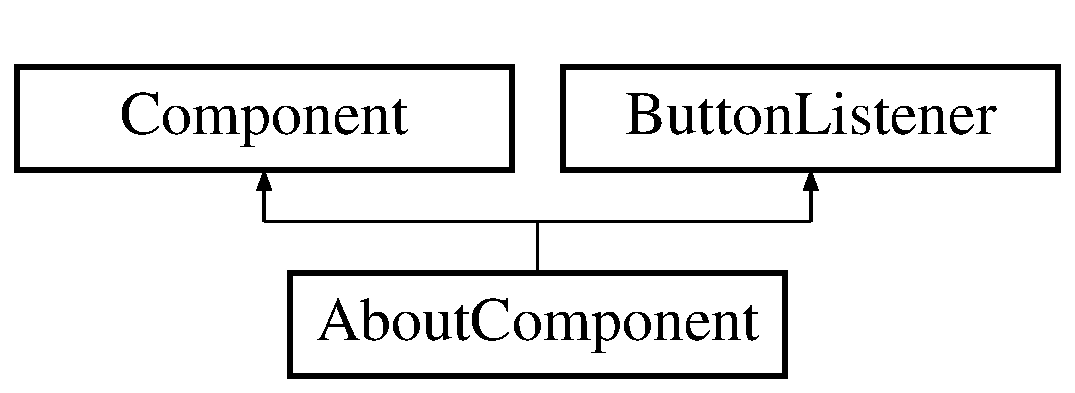
\includegraphics[height=2.000000cm]{class_about_component}
\end{center}
\end{figure}
\subsection*{Public Types}
\begin{DoxyCompactItemize}
\item 
enum \hyperlink{class_about_component_adac6eef89f47d0117da0f79f422e2f62}{Colour\+Ids} \{ \hyperlink{class_about_component_adac6eef89f47d0117da0f79f422e2f62ac6e56a04d1eef0a46cf4831b6d3caff0}{background\+Colour\+Id} = 0x2000700, 
\hyperlink{class_about_component_adac6eef89f47d0117da0f79f422e2f62af51a26ebd265fde96621b8a7398f3b61}{text\+Colour\+Id} = 0x2000701
 \}
\end{DoxyCompactItemize}
\subsection*{Public Member Functions}
\begin{DoxyCompactItemize}
\item 
\hyperlink{class_about_component_adfd6b751d7637bbd845e1e6ab874ec65}{About\+Component} ()
\item 
\hyperlink{class_about_component_a3a5957650ccd2427a90124832bb4555e}{$\sim$\+About\+Component} ()
\item 
\hyperlink{tk_8h_aba408b7cd755a96426e004c015f5de8e}{void} \hyperlink{class_about_component_ad76680827ff7c87d28a1f88d4870eedf}{paint} (Graphics \&g) override
\item 
\hyperlink{tk_8h_aba408b7cd755a96426e004c015f5de8e}{void} \hyperlink{class_about_component_aaa5fc1e5edb4051be9722b8d2a661a82}{resized} () override
\item 
\hyperlink{tk_8h_aba408b7cd755a96426e004c015f5de8e}{void} \hyperlink{class_about_component_acd2a7bcceaab84af892e437f68ae6cda}{button\+Clicked} (Button $\ast$button\+That\+Was\+Clicked) override
\end{DoxyCompactItemize}


\subsection{Member Enumeration Documentation}
\index{About\+Component@{About\+Component}!Colour\+Ids@{Colour\+Ids}}
\index{Colour\+Ids@{Colour\+Ids}!About\+Component@{About\+Component}}
\subsubsection[{\texorpdfstring{Colour\+Ids}{ColourIds}}]{\setlength{\rightskip}{0pt plus 5cm}enum {\bf About\+Component\+::\+Colour\+Ids}}\hypertarget{class_about_component_adac6eef89f47d0117da0f79f422e2f62}{}\label{class_about_component_adac6eef89f47d0117da0f79f422e2f62}
\begin{Desc}
\item[Enumerator]\par
\begin{description}
\index{background\+Colour\+Id@{background\+Colour\+Id}!About\+Component@{About\+Component}}\index{About\+Component@{About\+Component}!background\+Colour\+Id@{background\+Colour\+Id}}\item[{\em 
background\+Colour\+Id\hypertarget{class_about_component_adac6eef89f47d0117da0f79f422e2f62ac6e56a04d1eef0a46cf4831b6d3caff0}{}\label{class_about_component_adac6eef89f47d0117da0f79f422e2f62ac6e56a04d1eef0a46cf4831b6d3caff0}
}]\index{text\+Colour\+Id@{text\+Colour\+Id}!About\+Component@{About\+Component}}\index{About\+Component@{About\+Component}!text\+Colour\+Id@{text\+Colour\+Id}}\item[{\em 
text\+Colour\+Id\hypertarget{class_about_component_adac6eef89f47d0117da0f79f422e2f62af51a26ebd265fde96621b8a7398f3b61}{}\label{class_about_component_adac6eef89f47d0117da0f79f422e2f62af51a26ebd265fde96621b8a7398f3b61}
}]\end{description}
\end{Desc}


\subsection{Constructor \& Destructor Documentation}
\index{About\+Component@{About\+Component}!About\+Component@{About\+Component}}
\index{About\+Component@{About\+Component}!About\+Component@{About\+Component}}
\subsubsection[{\texorpdfstring{About\+Component()}{AboutComponent()}}]{\setlength{\rightskip}{0pt plus 5cm}About\+Component\+::\+About\+Component (
\begin{DoxyParamCaption}
{}
\end{DoxyParamCaption}
)}\hypertarget{class_about_component_adfd6b751d7637bbd845e1e6ab874ec65}{}\label{class_about_component_adfd6b751d7637bbd845e1e6ab874ec65}
\index{About\+Component@{About\+Component}!````~About\+Component@{$\sim$\+About\+Component}}
\index{````~About\+Component@{$\sim$\+About\+Component}!About\+Component@{About\+Component}}
\subsubsection[{\texorpdfstring{$\sim$\+About\+Component()}{~AboutComponent()}}]{\setlength{\rightskip}{0pt plus 5cm}About\+Component\+::$\sim$\+About\+Component (
\begin{DoxyParamCaption}
{}
\end{DoxyParamCaption}
)}\hypertarget{class_about_component_a3a5957650ccd2427a90124832bb4555e}{}\label{class_about_component_a3a5957650ccd2427a90124832bb4555e}


\subsection{Member Function Documentation}
\index{About\+Component@{About\+Component}!button\+Clicked@{button\+Clicked}}
\index{button\+Clicked@{button\+Clicked}!About\+Component@{About\+Component}}
\subsubsection[{\texorpdfstring{button\+Clicked(\+Button $\ast$button\+That\+Was\+Clicked) override}{buttonClicked(Button *buttonThatWasClicked) override}}]{\setlength{\rightskip}{0pt plus 5cm}{\bf void} About\+Component\+::button\+Clicked (
\begin{DoxyParamCaption}
\item[{Button $\ast$}]{button\+That\+Was\+Clicked}
\end{DoxyParamCaption}
)\hspace{0.3cm}{\ttfamily [override]}}\hypertarget{class_about_component_acd2a7bcceaab84af892e437f68ae6cda}{}\label{class_about_component_acd2a7bcceaab84af892e437f68ae6cda}
\index{About\+Component@{About\+Component}!paint@{paint}}
\index{paint@{paint}!About\+Component@{About\+Component}}
\subsubsection[{\texorpdfstring{paint(\+Graphics \&g) override}{paint(Graphics &g) override}}]{\setlength{\rightskip}{0pt plus 5cm}{\bf void} About\+Component\+::paint (
\begin{DoxyParamCaption}
\item[{Graphics \&}]{g}
\end{DoxyParamCaption}
)\hspace{0.3cm}{\ttfamily [override]}}\hypertarget{class_about_component_ad76680827ff7c87d28a1f88d4870eedf}{}\label{class_about_component_ad76680827ff7c87d28a1f88d4870eedf}
\index{About\+Component@{About\+Component}!resized@{resized}}
\index{resized@{resized}!About\+Component@{About\+Component}}
\subsubsection[{\texorpdfstring{resized() override}{resized() override}}]{\setlength{\rightskip}{0pt plus 5cm}{\bf void} About\+Component\+::resized (
\begin{DoxyParamCaption}
{}
\end{DoxyParamCaption}
)\hspace{0.3cm}{\ttfamily [override]}}\hypertarget{class_about_component_aaa5fc1e5edb4051be9722b8d2a661a82}{}\label{class_about_component_aaa5fc1e5edb4051be9722b8d2a661a82}


The documentation for this class was generated from the following files\+:\begin{DoxyCompactItemize}
\item 
/\+Users/michael/\+J\+U\+C\+E/projects/audealize-\/plugin/\+J\+U\+C\+E Modules/audealize\+\_\+module/ui\+\_\+components/\hyperlink{_about_component_8h}{About\+Component.\+h}\item 
/\+Users/michael/\+J\+U\+C\+E/projects/audealize-\/plugin/\+J\+U\+C\+E Modules/audealize\+\_\+module/ui\+\_\+components/\hyperlink{_about_component_8cpp}{About\+Component.\+cpp}\end{DoxyCompactItemize}

\hypertarget{class_audealize_1_1_audealize_audio_processor}{}\section{Audealize\+:\+:Audealize\+Audio\+Processor Class Reference}
\label{class_audealize_1_1_audealize_audio_processor}\index{Audealize\+::\+Audealize\+Audio\+Processor@{Audealize\+::\+Audealize\+Audio\+Processor}}


{\ttfamily \#include $<$Audealize\+Audio\+Processor.\+h$>$}

Inheritance diagram for Audealize\+:\+:Audealize\+Audio\+Processor\+:\begin{figure}[H]
\begin{center}
\leavevmode
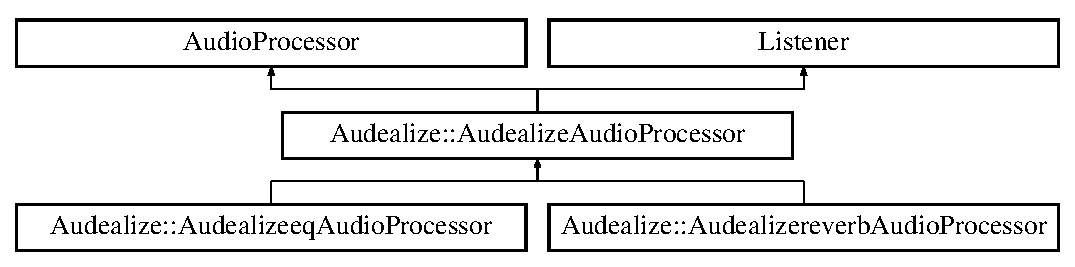
\includegraphics[height=3.000000cm]{class_audealize_1_1_audealize_audio_processor}
\end{center}
\end{figure}
\subsection*{Public Member Functions}
\begin{DoxyCompactItemize}
\item 
\hyperlink{class_audealize_1_1_audealize_audio_processor_a43c50db2160af612bed07847c5799ebe}{Audealize\+Audio\+Processor} (\hyperlink{class_audealize_1_1_audealize_audio_processor}{Audealize\+Audio\+Processor} $\ast$owner=nullptr)
\item 
\hyperlink{class_audealize_1_1_audealize_audio_processor_a7ba6f1b2676b471be401206abc0a08cf}{$\sim$\+Audealize\+Audio\+Processor} ()
\item 
\hyperlink{tk_8h_aba408b7cd755a96426e004c015f5de8e}{void} \hyperlink{class_audealize_1_1_audealize_audio_processor_a23a944b8047d7854728758c0261438ee}{get\+State\+Information} (Memory\+Block \&dest\+Data) override
\item 
\hyperlink{tk_8h_aba408b7cd755a96426e004c015f5de8e}{void} \hyperlink{class_audealize_1_1_audealize_audio_processor_aae3c8f976075ac1f095b4ac71bf91764}{set\+State\+Information} (const \hyperlink{tk_8h_aba408b7cd755a96426e004c015f5de8e}{void} $\ast$data, \hyperlink{tk_8h_a83f82f76e7fed06f4c49d2db94028a6d}{int} size\+In\+Bytes) override
\item 
virtual \hyperlink{tk_8h_aba408b7cd755a96426e004c015f5de8e}{void} \hyperlink{class_audealize_1_1_audealize_audio_processor_a4832111ea2b24bc517f911fa5949ca56}{parameter\+Changed} (const juce\+::\+String \&parameter\+ID, float new\+Value) override
\item 
virtual \hyperlink{tk_8h_aba408b7cd755a96426e004c015f5de8e}{void} \hyperlink{class_audealize_1_1_audealize_audio_processor_af269ce5549d8474f11f26c41aefa51bc}{settings\+From\+Map} (vector$<$ float $>$ settings)
\item 
Audio\+Processor\+Value\+Tree\+State \& \hyperlink{class_audealize_1_1_audealize_audio_processor_ac90ee1235c7947d995ded5a3a494adfe}{get\+Value\+Tree\+State} ()
\item 
\hyperlink{tk_8h_aba408b7cd755a96426e004c015f5de8e}{void} \hyperlink{class_audealize_1_1_audealize_audio_processor_a18d5cd428aa8bac6db26abe6668a7a28}{normalize} (vector$<$ float $>$ $\ast$vals)
\item 
virtual String \hyperlink{class_audealize_1_1_audealize_audio_processor_aa3e347b4bdc34e419ccf350638c38028}{get\+Param\+ID} (\hyperlink{tk_8h_a83f82f76e7fed06f4c49d2db94028a6d}{int} index)
\item 
String \hyperlink{class_audealize_1_1_audealize_audio_processor_a51c55287fa572a64f190073eba193b8f}{get\+Param\+Amount\+ID} ()
\item 
\hyperlink{tk_8h_aba408b7cd755a96426e004c015f5de8e}{void} \hyperlink{class_audealize_1_1_audealize_audio_processor_ade8920185102ceb1bbe69a19e7684d17}{set\+Bypass} (bool bypass)
\item 
bool \hyperlink{class_audealize_1_1_audealize_audio_processor_a169490241e1d2fee31441e18a3c32f58}{is\+Bypassed} ()
\item 
Audio\+Processor\+Value\+Tree\+State $\ast$ \hyperlink{class_audealize_1_1_audealize_audio_processor_a78578b6f542baf5a016ba1e93bf09f5c}{get\+State} ()
\item 
Undo\+Manager $\ast$ \hyperlink{class_audealize_1_1_audealize_audio_processor_ab6dc016d76b7fdf017324d99152825a3}{get\+Undo\+Manager} ()
\item 
Audio\+Processor\+Parameter $\ast$ \hyperlink{class_audealize_1_1_audealize_audio_processor_a436bbcaf366e9b32248f30304677a176}{get\+Parameter\+Ptr} (\hyperlink{tk_8h_a83f82f76e7fed06f4c49d2db94028a6d}{int} idx)
\item 
Audio\+Processor\+Parameter $\ast$ \hyperlink{class_audealize_1_1_audealize_audio_processor_afc5192d771658654d3be356cec36972a}{get\+Parameter\+Ptr\+From\+ID} (String param\+ID)
\item 
bool \hyperlink{class_audealize_1_1_audealize_audio_processor_a70ac8d869b16af3ca9a17486c1677134}{is\+Meta\+Parameter} (\hyperlink{tk_8h_a83f82f76e7fed06f4c49d2db94028a6d}{int} parameter\+Index) const  override
\end{DoxyCompactItemize}
\subsection*{Public Attributes}
\begin{DoxyCompactItemize}
\item 
\hyperlink{tk_8h_a83f82f76e7fed06f4c49d2db94028a6d}{int} \hyperlink{class_audealize_1_1_audealize_audio_processor_aa750e5a364f633d448d82fc2afc7c05a}{last\+U\+I\+Width}
\item 
\hyperlink{tk_8h_a83f82f76e7fed06f4c49d2db94028a6d}{int} \hyperlink{class_audealize_1_1_audealize_audio_processor_a05d825c7d24ae469cdebed82d92e9034}{last\+U\+I\+Height}
\end{DoxyCompactItemize}
\subsection*{Protected Member Functions}
\begin{DoxyCompactItemize}
\item 
\hyperlink{class_audealize_1_1_audealize_audio_processor_a175bb9f9d6be77b4bab3c38dd5351ed0}{J\+U\+C\+E\+\_\+\+D\+E\+C\+L\+A\+R\+E\+\_\+\+N\+O\+N\+\_\+\+C\+O\+P\+Y\+A\+B\+L\+E\+\_\+\+W\+I\+T\+H\+\_\+\+L\+E\+A\+K\+\_\+\+D\+E\+T\+E\+C\+T\+OR} (\hyperlink{class_audealize_1_1_audealize_audio_processor}{Audealize\+Audio\+Processor})
\end{DoxyCompactItemize}
\subsection*{Protected Attributes}
\begin{DoxyCompactItemize}
\item 
Audio\+Processor\+Value\+Tree\+State $\ast$ \hyperlink{class_audealize_1_1_audealize_audio_processor_a91e3f2ebc485c04a2ae0c651c9dd4a1e}{m\+State}
\item 
Undo\+Manager $\ast$ \hyperlink{class_audealize_1_1_audealize_audio_processor_aad11b053db8e6f9ae61afa610126b23d}{m\+Undo\+Manager}
\item 
vector$<$ float $>$ \hyperlink{class_audealize_1_1_audealize_audio_processor_a799580d9637076562aafa74de6e166b8}{m\+Param\+Settings}
\item 
\hyperlink{class_audealize_1_1_audealize_audio_processor}{Audealize\+Audio\+Processor} $\ast$ \hyperlink{class_audealize_1_1_audealize_audio_processor_acd64a89d7e6550c2db7ec1d2a0c8281e}{m\+Owner}
\item 
bool \hyperlink{class_audealize_1_1_audealize_audio_processor_a8f8e6d2d636f070c9dcce80725bb67f3}{m\+Bypass}
\item 
String \hyperlink{class_audealize_1_1_audealize_audio_processor_a8c51332f043fbb80c2fa573a7f753c8a}{param\+Amount\+Id}
\item 
float \hyperlink{class_audealize_1_1_audealize_audio_processor_af232a68cdeacc57765eed0122da6ce27}{m\+Amount}
\end{DoxyCompactItemize}


\subsection{Constructor \& Destructor Documentation}
\index{Audealize\+::\+Audealize\+Audio\+Processor@{Audealize\+::\+Audealize\+Audio\+Processor}!Audealize\+Audio\+Processor@{Audealize\+Audio\+Processor}}
\index{Audealize\+Audio\+Processor@{Audealize\+Audio\+Processor}!Audealize\+::\+Audealize\+Audio\+Processor@{Audealize\+::\+Audealize\+Audio\+Processor}}
\subsubsection[{\texorpdfstring{Audealize\+Audio\+Processor(\+Audealize\+Audio\+Processor $\ast$owner=nullptr)}{AudealizeAudioProcessor(AudealizeAudioProcessor *owner=nullptr)}}]{\setlength{\rightskip}{0pt plus 5cm}Audealize\+::\+Audealize\+Audio\+Processor\+::\+Audealize\+Audio\+Processor (
\begin{DoxyParamCaption}
\item[{{\bf Audealize\+Audio\+Processor} $\ast$}]{owner = {\ttfamily nullptr}}
\end{DoxyParamCaption}
)\hspace{0.3cm}{\ttfamily [inline]}}\hypertarget{class_audealize_1_1_audealize_audio_processor_a43c50db2160af612bed07847c5799ebe}{}\label{class_audealize_1_1_audealize_audio_processor_a43c50db2160af612bed07847c5799ebe}
\index{Audealize\+::\+Audealize\+Audio\+Processor@{Audealize\+::\+Audealize\+Audio\+Processor}!````~Audealize\+Audio\+Processor@{$\sim$\+Audealize\+Audio\+Processor}}
\index{````~Audealize\+Audio\+Processor@{$\sim$\+Audealize\+Audio\+Processor}!Audealize\+::\+Audealize\+Audio\+Processor@{Audealize\+::\+Audealize\+Audio\+Processor}}
\subsubsection[{\texorpdfstring{$\sim$\+Audealize\+Audio\+Processor()}{~AudealizeAudioProcessor()}}]{\setlength{\rightskip}{0pt plus 5cm}Audealize\+::\+Audealize\+Audio\+Processor\+::$\sim$\+Audealize\+Audio\+Processor (
\begin{DoxyParamCaption}
{}
\end{DoxyParamCaption}
)\hspace{0.3cm}{\ttfamily [inline]}}\hypertarget{class_audealize_1_1_audealize_audio_processor_a7ba6f1b2676b471be401206abc0a08cf}{}\label{class_audealize_1_1_audealize_audio_processor_a7ba6f1b2676b471be401206abc0a08cf}


\subsection{Member Function Documentation}
\index{Audealize\+::\+Audealize\+Audio\+Processor@{Audealize\+::\+Audealize\+Audio\+Processor}!get\+Param\+Amount\+ID@{get\+Param\+Amount\+ID}}
\index{get\+Param\+Amount\+ID@{get\+Param\+Amount\+ID}!Audealize\+::\+Audealize\+Audio\+Processor@{Audealize\+::\+Audealize\+Audio\+Processor}}
\subsubsection[{\texorpdfstring{get\+Param\+Amount\+I\+D()}{getParamAmountID()}}]{\setlength{\rightskip}{0pt plus 5cm}String Audealize\+::\+Audealize\+Audio\+Processor\+::get\+Param\+Amount\+ID (
\begin{DoxyParamCaption}
{}
\end{DoxyParamCaption}
)\hspace{0.3cm}{\ttfamily [inline]}}\hypertarget{class_audealize_1_1_audealize_audio_processor_a51c55287fa572a64f190073eba193b8f}{}\label{class_audealize_1_1_audealize_audio_processor_a51c55287fa572a64f190073eba193b8f}
\index{Audealize\+::\+Audealize\+Audio\+Processor@{Audealize\+::\+Audealize\+Audio\+Processor}!get\+Parameter\+Ptr@{get\+Parameter\+Ptr}}
\index{get\+Parameter\+Ptr@{get\+Parameter\+Ptr}!Audealize\+::\+Audealize\+Audio\+Processor@{Audealize\+::\+Audealize\+Audio\+Processor}}
\subsubsection[{\texorpdfstring{get\+Parameter\+Ptr(int idx)}{getParameterPtr(int idx)}}]{\setlength{\rightskip}{0pt plus 5cm}Audio\+Processor\+Parameter$\ast$ Audealize\+::\+Audealize\+Audio\+Processor\+::get\+Parameter\+Ptr (
\begin{DoxyParamCaption}
\item[{{\bf int}}]{idx}
\end{DoxyParamCaption}
)\hspace{0.3cm}{\ttfamily [inline]}}\hypertarget{class_audealize_1_1_audealize_audio_processor_a436bbcaf366e9b32248f30304677a176}{}\label{class_audealize_1_1_audealize_audio_processor_a436bbcaf366e9b32248f30304677a176}
\index{Audealize\+::\+Audealize\+Audio\+Processor@{Audealize\+::\+Audealize\+Audio\+Processor}!get\+Parameter\+Ptr\+From\+ID@{get\+Parameter\+Ptr\+From\+ID}}
\index{get\+Parameter\+Ptr\+From\+ID@{get\+Parameter\+Ptr\+From\+ID}!Audealize\+::\+Audealize\+Audio\+Processor@{Audealize\+::\+Audealize\+Audio\+Processor}}
\subsubsection[{\texorpdfstring{get\+Parameter\+Ptr\+From\+I\+D(\+String param\+I\+D)}{getParameterPtrFromID(String paramID)}}]{\setlength{\rightskip}{0pt plus 5cm}Audio\+Processor\+Parameter$\ast$ Audealize\+::\+Audealize\+Audio\+Processor\+::get\+Parameter\+Ptr\+From\+ID (
\begin{DoxyParamCaption}
\item[{String}]{param\+ID}
\end{DoxyParamCaption}
)\hspace{0.3cm}{\ttfamily [inline]}}\hypertarget{class_audealize_1_1_audealize_audio_processor_afc5192d771658654d3be356cec36972a}{}\label{class_audealize_1_1_audealize_audio_processor_afc5192d771658654d3be356cec36972a}
\index{Audealize\+::\+Audealize\+Audio\+Processor@{Audealize\+::\+Audealize\+Audio\+Processor}!get\+Param\+ID@{get\+Param\+ID}}
\index{get\+Param\+ID@{get\+Param\+ID}!Audealize\+::\+Audealize\+Audio\+Processor@{Audealize\+::\+Audealize\+Audio\+Processor}}
\subsubsection[{\texorpdfstring{get\+Param\+I\+D(int index)}{getParamID(int index)}}]{\setlength{\rightskip}{0pt plus 5cm}virtual String Audealize\+::\+Audealize\+Audio\+Processor\+::get\+Param\+ID (
\begin{DoxyParamCaption}
\item[{{\bf int}}]{index}
\end{DoxyParamCaption}
)\hspace{0.3cm}{\ttfamily [inline]}, {\ttfamily [virtual]}}\hypertarget{class_audealize_1_1_audealize_audio_processor_aa3e347b4bdc34e419ccf350638c38028}{}\label{class_audealize_1_1_audealize_audio_processor_aa3e347b4bdc34e419ccf350638c38028}
Returns a string with the parameter ID of one of the parameters


\begin{DoxyParams}{Parameters}
{\em index} & \\
\hline
\end{DoxyParams}


Reimplemented in \hyperlink{class_audealize_1_1_audealizeeq_audio_processor_a692e0576747a20bc080b971dccd84241}{Audealize\+::\+Audealizeeq\+Audio\+Processor}, and \hyperlink{class_audealize_1_1_audealizereverb_audio_processor_a20e3cb24628efda50a559ce164a7fed5}{Audealize\+::\+Audealizereverb\+Audio\+Processor}.

\index{Audealize\+::\+Audealize\+Audio\+Processor@{Audealize\+::\+Audealize\+Audio\+Processor}!get\+State@{get\+State}}
\index{get\+State@{get\+State}!Audealize\+::\+Audealize\+Audio\+Processor@{Audealize\+::\+Audealize\+Audio\+Processor}}
\subsubsection[{\texorpdfstring{get\+State()}{getState()}}]{\setlength{\rightskip}{0pt plus 5cm}Audio\+Processor\+Value\+Tree\+State$\ast$ Audealize\+::\+Audealize\+Audio\+Processor\+::get\+State (
\begin{DoxyParamCaption}
{}
\end{DoxyParamCaption}
)\hspace{0.3cm}{\ttfamily [inline]}}\hypertarget{class_audealize_1_1_audealize_audio_processor_a78578b6f542baf5a016ba1e93bf09f5c}{}\label{class_audealize_1_1_audealize_audio_processor_a78578b6f542baf5a016ba1e93bf09f5c}
\index{Audealize\+::\+Audealize\+Audio\+Processor@{Audealize\+::\+Audealize\+Audio\+Processor}!get\+State\+Information@{get\+State\+Information}}
\index{get\+State\+Information@{get\+State\+Information}!Audealize\+::\+Audealize\+Audio\+Processor@{Audealize\+::\+Audealize\+Audio\+Processor}}
\subsubsection[{\texorpdfstring{get\+State\+Information(\+Memory\+Block \&dest\+Data) override}{getStateInformation(MemoryBlock &destData) override}}]{\setlength{\rightskip}{0pt plus 5cm}{\bf void} Audealize\+::\+Audealize\+Audio\+Processor\+::get\+State\+Information (
\begin{DoxyParamCaption}
\item[{Memory\+Block \&}]{dest\+Data}
\end{DoxyParamCaption}
)\hspace{0.3cm}{\ttfamily [inline]}, {\ttfamily [override]}}\hypertarget{class_audealize_1_1_audealize_audio_processor_a23a944b8047d7854728758c0261438ee}{}\label{class_audealize_1_1_audealize_audio_processor_a23a944b8047d7854728758c0261438ee}
Stores parameter data in a given memory block.


\begin{DoxyParams}{Parameters}
{\em dest\+Data} & Memory block in which to store parameter data \\
\hline
\end{DoxyParams}
\index{Audealize\+::\+Audealize\+Audio\+Processor@{Audealize\+::\+Audealize\+Audio\+Processor}!get\+Undo\+Manager@{get\+Undo\+Manager}}
\index{get\+Undo\+Manager@{get\+Undo\+Manager}!Audealize\+::\+Audealize\+Audio\+Processor@{Audealize\+::\+Audealize\+Audio\+Processor}}
\subsubsection[{\texorpdfstring{get\+Undo\+Manager()}{getUndoManager()}}]{\setlength{\rightskip}{0pt plus 5cm}Undo\+Manager$\ast$ Audealize\+::\+Audealize\+Audio\+Processor\+::get\+Undo\+Manager (
\begin{DoxyParamCaption}
{}
\end{DoxyParamCaption}
)\hspace{0.3cm}{\ttfamily [inline]}}\hypertarget{class_audealize_1_1_audealize_audio_processor_ab6dc016d76b7fdf017324d99152825a3}{}\label{class_audealize_1_1_audealize_audio_processor_ab6dc016d76b7fdf017324d99152825a3}
\index{Audealize\+::\+Audealize\+Audio\+Processor@{Audealize\+::\+Audealize\+Audio\+Processor}!get\+Value\+Tree\+State@{get\+Value\+Tree\+State}}
\index{get\+Value\+Tree\+State@{get\+Value\+Tree\+State}!Audealize\+::\+Audealize\+Audio\+Processor@{Audealize\+::\+Audealize\+Audio\+Processor}}
\subsubsection[{\texorpdfstring{get\+Value\+Tree\+State()}{getValueTreeState()}}]{\setlength{\rightskip}{0pt plus 5cm}Audio\+Processor\+Value\+Tree\+State\& Audealize\+::\+Audealize\+Audio\+Processor\+::get\+Value\+Tree\+State (
\begin{DoxyParamCaption}
{}
\end{DoxyParamCaption}
)\hspace{0.3cm}{\ttfamily [inline]}}\hypertarget{class_audealize_1_1_audealize_audio_processor_ac90ee1235c7947d995ded5a3a494adfe}{}\label{class_audealize_1_1_audealize_audio_processor_ac90ee1235c7947d995ded5a3a494adfe}
Returns the Audio\+Processor\+Value\+Tree\+State

\begin{DoxyReturn}{Returns}
an Audio\+Processor\+Value\+Tree\+State 
\end{DoxyReturn}
\index{Audealize\+::\+Audealize\+Audio\+Processor@{Audealize\+::\+Audealize\+Audio\+Processor}!is\+Bypassed@{is\+Bypassed}}
\index{is\+Bypassed@{is\+Bypassed}!Audealize\+::\+Audealize\+Audio\+Processor@{Audealize\+::\+Audealize\+Audio\+Processor}}
\subsubsection[{\texorpdfstring{is\+Bypassed()}{isBypassed()}}]{\setlength{\rightskip}{0pt plus 5cm}bool Audealize\+::\+Audealize\+Audio\+Processor\+::is\+Bypassed (
\begin{DoxyParamCaption}
{}
\end{DoxyParamCaption}
)\hspace{0.3cm}{\ttfamily [inline]}}\hypertarget{class_audealize_1_1_audealize_audio_processor_a169490241e1d2fee31441e18a3c32f58}{}\label{class_audealize_1_1_audealize_audio_processor_a169490241e1d2fee31441e18a3c32f58}
\index{Audealize\+::\+Audealize\+Audio\+Processor@{Audealize\+::\+Audealize\+Audio\+Processor}!is\+Meta\+Parameter@{is\+Meta\+Parameter}}
\index{is\+Meta\+Parameter@{is\+Meta\+Parameter}!Audealize\+::\+Audealize\+Audio\+Processor@{Audealize\+::\+Audealize\+Audio\+Processor}}
\subsubsection[{\texorpdfstring{is\+Meta\+Parameter(int parameter\+Index) const  override}{isMetaParameter(int parameterIndex) const  override}}]{\setlength{\rightskip}{0pt plus 5cm}bool Audealize\+::\+Audealize\+Audio\+Processor\+::is\+Meta\+Parameter (
\begin{DoxyParamCaption}
\item[{{\bf int}}]{parameter\+Index}
\end{DoxyParamCaption}
) const\hspace{0.3cm}{\ttfamily [inline]}, {\ttfamily [override]}}\hypertarget{class_audealize_1_1_audealize_audio_processor_a70ac8d869b16af3ca9a17486c1677134}{}\label{class_audealize_1_1_audealize_audio_processor_a70ac8d869b16af3ca9a17486c1677134}
\index{Audealize\+::\+Audealize\+Audio\+Processor@{Audealize\+::\+Audealize\+Audio\+Processor}!J\+U\+C\+E\+\_\+\+D\+E\+C\+L\+A\+R\+E\+\_\+\+N\+O\+N\+\_\+\+C\+O\+P\+Y\+A\+B\+L\+E\+\_\+\+W\+I\+T\+H\+\_\+\+L\+E\+A\+K\+\_\+\+D\+E\+T\+E\+C\+T\+OR@{J\+U\+C\+E\+\_\+\+D\+E\+C\+L\+A\+R\+E\+\_\+\+N\+O\+N\+\_\+\+C\+O\+P\+Y\+A\+B\+L\+E\+\_\+\+W\+I\+T\+H\+\_\+\+L\+E\+A\+K\+\_\+\+D\+E\+T\+E\+C\+T\+OR}}
\index{J\+U\+C\+E\+\_\+\+D\+E\+C\+L\+A\+R\+E\+\_\+\+N\+O\+N\+\_\+\+C\+O\+P\+Y\+A\+B\+L\+E\+\_\+\+W\+I\+T\+H\+\_\+\+L\+E\+A\+K\+\_\+\+D\+E\+T\+E\+C\+T\+OR@{J\+U\+C\+E\+\_\+\+D\+E\+C\+L\+A\+R\+E\+\_\+\+N\+O\+N\+\_\+\+C\+O\+P\+Y\+A\+B\+L\+E\+\_\+\+W\+I\+T\+H\+\_\+\+L\+E\+A\+K\+\_\+\+D\+E\+T\+E\+C\+T\+OR}!Audealize\+::\+Audealize\+Audio\+Processor@{Audealize\+::\+Audealize\+Audio\+Processor}}
\subsubsection[{\texorpdfstring{J\+U\+C\+E\+\_\+\+D\+E\+C\+L\+A\+R\+E\+\_\+\+N\+O\+N\+\_\+\+C\+O\+P\+Y\+A\+B\+L\+E\+\_\+\+W\+I\+T\+H\+\_\+\+L\+E\+A\+K\+\_\+\+D\+E\+T\+E\+C\+T\+O\+R(\+Audealize\+Audio\+Processor)}{JUCE_DECLARE_NON_COPYABLE_WITH_LEAK_DETECTOR(AudealizeAudioProcessor)}}]{\setlength{\rightskip}{0pt plus 5cm}Audealize\+::\+Audealize\+Audio\+Processor\+::\+J\+U\+C\+E\+\_\+\+D\+E\+C\+L\+A\+R\+E\+\_\+\+N\+O\+N\+\_\+\+C\+O\+P\+Y\+A\+B\+L\+E\+\_\+\+W\+I\+T\+H\+\_\+\+L\+E\+A\+K\+\_\+\+D\+E\+T\+E\+C\+T\+OR (
\begin{DoxyParamCaption}
\item[{{\bf Audealize\+Audio\+Processor}}]{}
\end{DoxyParamCaption}
)\hspace{0.3cm}{\ttfamily [protected]}}\hypertarget{class_audealize_1_1_audealize_audio_processor_a175bb9f9d6be77b4bab3c38dd5351ed0}{}\label{class_audealize_1_1_audealize_audio_processor_a175bb9f9d6be77b4bab3c38dd5351ed0}
\index{Audealize\+::\+Audealize\+Audio\+Processor@{Audealize\+::\+Audealize\+Audio\+Processor}!normalize@{normalize}}
\index{normalize@{normalize}!Audealize\+::\+Audealize\+Audio\+Processor@{Audealize\+::\+Audealize\+Audio\+Processor}}
\subsubsection[{\texorpdfstring{normalize(vector$<$ float $>$ $\ast$vals)}{normalize(vector< float > *vals)}}]{\setlength{\rightskip}{0pt plus 5cm}{\bf void} Audealize\+::\+Audealize\+Audio\+Processor\+::normalize (
\begin{DoxyParamCaption}
\item[{vector$<$ float $>$ $\ast$}]{vals}
\end{DoxyParamCaption}
)\hspace{0.3cm}{\ttfamily [inline]}}\hypertarget{class_audealize_1_1_audealize_audio_processor_a18d5cd428aa8bac6db26abe6668a7a28}{}\label{class_audealize_1_1_audealize_audio_processor_a18d5cd428aa8bac6db26abe6668a7a28}
Normalizes a vector of floats


\begin{DoxyParams}{Parameters}
{\em vals} & \\
\hline
\end{DoxyParams}
\index{Audealize\+::\+Audealize\+Audio\+Processor@{Audealize\+::\+Audealize\+Audio\+Processor}!parameter\+Changed@{parameter\+Changed}}
\index{parameter\+Changed@{parameter\+Changed}!Audealize\+::\+Audealize\+Audio\+Processor@{Audealize\+::\+Audealize\+Audio\+Processor}}
\subsubsection[{\texorpdfstring{parameter\+Changed(const juce\+::\+String \&parameter\+I\+D, float new\+Value) override}{parameterChanged(const juce::String &parameterID, float newValue) override}}]{\setlength{\rightskip}{0pt plus 5cm}virtual {\bf void} Audealize\+::\+Audealize\+Audio\+Processor\+::parameter\+Changed (
\begin{DoxyParamCaption}
\item[{const juce\+::\+String \&}]{parameter\+ID, }
\item[{float}]{new\+Value}
\end{DoxyParamCaption}
)\hspace{0.3cm}{\ttfamily [inline]}, {\ttfamily [override]}, {\ttfamily [virtual]}}\hypertarget{class_audealize_1_1_audealize_audio_processor_a4832111ea2b24bc517f911fa5949ca56}{}\label{class_audealize_1_1_audealize_audio_processor_a4832111ea2b24bc517f911fa5949ca56}
Called by an Audio\+Processor\+Editor to notify Audio\+Processor of parameter value changes


\begin{DoxyParams}{Parameters}
{\em parameter\+ID} & The ID of the parameter that was changed \\
\hline
{\em new\+Value} & The new value for that parameter \\
\hline
\end{DoxyParams}


Reimplemented in \hyperlink{class_audealize_1_1_audealizeeq_audio_processor_a25c85696329c21a201963733bc46d957}{Audealize\+::\+Audealizeeq\+Audio\+Processor}, and \hyperlink{class_audealize_1_1_audealizereverb_audio_processor_aafb771cae87f2ce62ca2451d80678277}{Audealize\+::\+Audealizereverb\+Audio\+Processor}.

\index{Audealize\+::\+Audealize\+Audio\+Processor@{Audealize\+::\+Audealize\+Audio\+Processor}!set\+Bypass@{set\+Bypass}}
\index{set\+Bypass@{set\+Bypass}!Audealize\+::\+Audealize\+Audio\+Processor@{Audealize\+::\+Audealize\+Audio\+Processor}}
\subsubsection[{\texorpdfstring{set\+Bypass(bool bypass)}{setBypass(bool bypass)}}]{\setlength{\rightskip}{0pt plus 5cm}{\bf void} Audealize\+::\+Audealize\+Audio\+Processor\+::set\+Bypass (
\begin{DoxyParamCaption}
\item[{bool}]{bypass}
\end{DoxyParamCaption}
)\hspace{0.3cm}{\ttfamily [inline]}}\hypertarget{class_audealize_1_1_audealize_audio_processor_ade8920185102ceb1bbe69a19e7684d17}{}\label{class_audealize_1_1_audealize_audio_processor_ade8920185102ceb1bbe69a19e7684d17}
\index{Audealize\+::\+Audealize\+Audio\+Processor@{Audealize\+::\+Audealize\+Audio\+Processor}!set\+State\+Information@{set\+State\+Information}}
\index{set\+State\+Information@{set\+State\+Information}!Audealize\+::\+Audealize\+Audio\+Processor@{Audealize\+::\+Audealize\+Audio\+Processor}}
\subsubsection[{\texorpdfstring{set\+State\+Information(const void $\ast$data, int size\+In\+Bytes) override}{setStateInformation(const void *data, int sizeInBytes) override}}]{\setlength{\rightskip}{0pt plus 5cm}{\bf void} Audealize\+::\+Audealize\+Audio\+Processor\+::set\+State\+Information (
\begin{DoxyParamCaption}
\item[{const {\bf void} $\ast$}]{data, }
\item[{{\bf int}}]{size\+In\+Bytes}
\end{DoxyParamCaption}
)\hspace{0.3cm}{\ttfamily [inline]}, {\ttfamily [override]}}\hypertarget{class_audealize_1_1_audealize_audio_processor_aae3c8f976075ac1f095b4ac71bf91764}{}\label{class_audealize_1_1_audealize_audio_processor_aae3c8f976075ac1f095b4ac71bf91764}
Restores parameters from state data saved in a memory block


\begin{DoxyParams}{Parameters}
{\em data} & Pointer to the memory block \\
\hline
{\em size\+In\+Bytes} & Size of the memory block in bytes \\
\hline
\end{DoxyParams}
\index{Audealize\+::\+Audealize\+Audio\+Processor@{Audealize\+::\+Audealize\+Audio\+Processor}!settings\+From\+Map@{settings\+From\+Map}}
\index{settings\+From\+Map@{settings\+From\+Map}!Audealize\+::\+Audealize\+Audio\+Processor@{Audealize\+::\+Audealize\+Audio\+Processor}}
\subsubsection[{\texorpdfstring{settings\+From\+Map(vector$<$ float $>$ settings)}{settingsFromMap(vector< float > settings)}}]{\setlength{\rightskip}{0pt plus 5cm}virtual {\bf void} Audealize\+::\+Audealize\+Audio\+Processor\+::settings\+From\+Map (
\begin{DoxyParamCaption}
\item[{vector$<$ float $>$}]{settings}
\end{DoxyParamCaption}
)\hspace{0.3cm}{\ttfamily [inline]}, {\ttfamily [virtual]}}\hypertarget{class_audealize_1_1_audealize_audio_processor_af269ce5549d8474f11f26c41aefa51bc}{}\label{class_audealize_1_1_audealize_audio_processor_af269ce5549d8474f11f26c41aefa51bc}
Set the states of all parameters with a vector$<$float$>$. To be called by a \hyperlink{class_audealize_1_1_word_map}{Word\+Map}


\begin{DoxyParams}{Parameters}
{\em settings} & a vector of floats \\
\hline
\end{DoxyParams}


Reimplemented in \hyperlink{class_audealize_1_1_audealizeeq_audio_processor_adda624ec0e28dbc41777aa76ed9ce974}{Audealize\+::\+Audealizeeq\+Audio\+Processor}, and \hyperlink{class_audealize_1_1_audealizereverb_audio_processor_a4a9a5828a3cbbb084a3025009500faf9}{Audealize\+::\+Audealizereverb\+Audio\+Processor}.



\subsection{Member Data Documentation}
\index{Audealize\+::\+Audealize\+Audio\+Processor@{Audealize\+::\+Audealize\+Audio\+Processor}!last\+U\+I\+Height@{last\+U\+I\+Height}}
\index{last\+U\+I\+Height@{last\+U\+I\+Height}!Audealize\+::\+Audealize\+Audio\+Processor@{Audealize\+::\+Audealize\+Audio\+Processor}}
\subsubsection[{\texorpdfstring{last\+U\+I\+Height}{lastUIHeight}}]{\setlength{\rightskip}{0pt plus 5cm}{\bf int} Audealize\+::\+Audealize\+Audio\+Processor\+::last\+U\+I\+Height}\hypertarget{class_audealize_1_1_audealize_audio_processor_a05d825c7d24ae469cdebed82d92e9034}{}\label{class_audealize_1_1_audealize_audio_processor_a05d825c7d24ae469cdebed82d92e9034}
\index{Audealize\+::\+Audealize\+Audio\+Processor@{Audealize\+::\+Audealize\+Audio\+Processor}!last\+U\+I\+Width@{last\+U\+I\+Width}}
\index{last\+U\+I\+Width@{last\+U\+I\+Width}!Audealize\+::\+Audealize\+Audio\+Processor@{Audealize\+::\+Audealize\+Audio\+Processor}}
\subsubsection[{\texorpdfstring{last\+U\+I\+Width}{lastUIWidth}}]{\setlength{\rightskip}{0pt plus 5cm}{\bf int} Audealize\+::\+Audealize\+Audio\+Processor\+::last\+U\+I\+Width}\hypertarget{class_audealize_1_1_audealize_audio_processor_aa750e5a364f633d448d82fc2afc7c05a}{}\label{class_audealize_1_1_audealize_audio_processor_aa750e5a364f633d448d82fc2afc7c05a}
\index{Audealize\+::\+Audealize\+Audio\+Processor@{Audealize\+::\+Audealize\+Audio\+Processor}!m\+Amount@{m\+Amount}}
\index{m\+Amount@{m\+Amount}!Audealize\+::\+Audealize\+Audio\+Processor@{Audealize\+::\+Audealize\+Audio\+Processor}}
\subsubsection[{\texorpdfstring{m\+Amount}{mAmount}}]{\setlength{\rightskip}{0pt plus 5cm}float Audealize\+::\+Audealize\+Audio\+Processor\+::m\+Amount\hspace{0.3cm}{\ttfamily [protected]}}\hypertarget{class_audealize_1_1_audealize_audio_processor_af232a68cdeacc57765eed0122da6ce27}{}\label{class_audealize_1_1_audealize_audio_processor_af232a68cdeacc57765eed0122da6ce27}
\index{Audealize\+::\+Audealize\+Audio\+Processor@{Audealize\+::\+Audealize\+Audio\+Processor}!m\+Bypass@{m\+Bypass}}
\index{m\+Bypass@{m\+Bypass}!Audealize\+::\+Audealize\+Audio\+Processor@{Audealize\+::\+Audealize\+Audio\+Processor}}
\subsubsection[{\texorpdfstring{m\+Bypass}{mBypass}}]{\setlength{\rightskip}{0pt plus 5cm}bool Audealize\+::\+Audealize\+Audio\+Processor\+::m\+Bypass\hspace{0.3cm}{\ttfamily [protected]}}\hypertarget{class_audealize_1_1_audealize_audio_processor_a8f8e6d2d636f070c9dcce80725bb67f3}{}\label{class_audealize_1_1_audealize_audio_processor_a8f8e6d2d636f070c9dcce80725bb67f3}
\index{Audealize\+::\+Audealize\+Audio\+Processor@{Audealize\+::\+Audealize\+Audio\+Processor}!m\+Owner@{m\+Owner}}
\index{m\+Owner@{m\+Owner}!Audealize\+::\+Audealize\+Audio\+Processor@{Audealize\+::\+Audealize\+Audio\+Processor}}
\subsubsection[{\texorpdfstring{m\+Owner}{mOwner}}]{\setlength{\rightskip}{0pt plus 5cm}{\bf Audealize\+Audio\+Processor}$\ast$ Audealize\+::\+Audealize\+Audio\+Processor\+::m\+Owner\hspace{0.3cm}{\ttfamily [protected]}}\hypertarget{class_audealize_1_1_audealize_audio_processor_acd64a89d7e6550c2db7ec1d2a0c8281e}{}\label{class_audealize_1_1_audealize_audio_processor_acd64a89d7e6550c2db7ec1d2a0c8281e}
\index{Audealize\+::\+Audealize\+Audio\+Processor@{Audealize\+::\+Audealize\+Audio\+Processor}!m\+Param\+Settings@{m\+Param\+Settings}}
\index{m\+Param\+Settings@{m\+Param\+Settings}!Audealize\+::\+Audealize\+Audio\+Processor@{Audealize\+::\+Audealize\+Audio\+Processor}}
\subsubsection[{\texorpdfstring{m\+Param\+Settings}{mParamSettings}}]{\setlength{\rightskip}{0pt plus 5cm}vector$<$float$>$ Audealize\+::\+Audealize\+Audio\+Processor\+::m\+Param\+Settings\hspace{0.3cm}{\ttfamily [protected]}}\hypertarget{class_audealize_1_1_audealize_audio_processor_a799580d9637076562aafa74de6e166b8}{}\label{class_audealize_1_1_audealize_audio_processor_a799580d9637076562aafa74de6e166b8}
\index{Audealize\+::\+Audealize\+Audio\+Processor@{Audealize\+::\+Audealize\+Audio\+Processor}!m\+State@{m\+State}}
\index{m\+State@{m\+State}!Audealize\+::\+Audealize\+Audio\+Processor@{Audealize\+::\+Audealize\+Audio\+Processor}}
\subsubsection[{\texorpdfstring{m\+State}{mState}}]{\setlength{\rightskip}{0pt plus 5cm}Audio\+Processor\+Value\+Tree\+State$\ast$ Audealize\+::\+Audealize\+Audio\+Processor\+::m\+State\hspace{0.3cm}{\ttfamily [protected]}}\hypertarget{class_audealize_1_1_audealize_audio_processor_a91e3f2ebc485c04a2ae0c651c9dd4a1e}{}\label{class_audealize_1_1_audealize_audio_processor_a91e3f2ebc485c04a2ae0c651c9dd4a1e}
\index{Audealize\+::\+Audealize\+Audio\+Processor@{Audealize\+::\+Audealize\+Audio\+Processor}!m\+Undo\+Manager@{m\+Undo\+Manager}}
\index{m\+Undo\+Manager@{m\+Undo\+Manager}!Audealize\+::\+Audealize\+Audio\+Processor@{Audealize\+::\+Audealize\+Audio\+Processor}}
\subsubsection[{\texorpdfstring{m\+Undo\+Manager}{mUndoManager}}]{\setlength{\rightskip}{0pt plus 5cm}Undo\+Manager$\ast$ Audealize\+::\+Audealize\+Audio\+Processor\+::m\+Undo\+Manager\hspace{0.3cm}{\ttfamily [protected]}}\hypertarget{class_audealize_1_1_audealize_audio_processor_aad11b053db8e6f9ae61afa610126b23d}{}\label{class_audealize_1_1_audealize_audio_processor_aad11b053db8e6f9ae61afa610126b23d}
\index{Audealize\+::\+Audealize\+Audio\+Processor@{Audealize\+::\+Audealize\+Audio\+Processor}!param\+Amount\+Id@{param\+Amount\+Id}}
\index{param\+Amount\+Id@{param\+Amount\+Id}!Audealize\+::\+Audealize\+Audio\+Processor@{Audealize\+::\+Audealize\+Audio\+Processor}}
\subsubsection[{\texorpdfstring{param\+Amount\+Id}{paramAmountId}}]{\setlength{\rightskip}{0pt plus 5cm}String Audealize\+::\+Audealize\+Audio\+Processor\+::param\+Amount\+Id\hspace{0.3cm}{\ttfamily [protected]}}\hypertarget{class_audealize_1_1_audealize_audio_processor_a8c51332f043fbb80c2fa573a7f753c8a}{}\label{class_audealize_1_1_audealize_audio_processor_a8c51332f043fbb80c2fa573a7f753c8a}


The documentation for this class was generated from the following file\+:\begin{DoxyCompactItemize}
\item 
/\+Users/michael/\+J\+U\+C\+E/projects/audealize-\/plugin/\+J\+U\+C\+E Modules/audealize\+\_\+module/audio\+\_\+processors/\hyperlink{_audealize_audio_processor_8h}{Audealize\+Audio\+Processor.\+h}\end{DoxyCompactItemize}

\hypertarget{class_audealize_1_1_audealizeeq_audio_processor}{}\section{Audealize\+:\+:Audealizeeq\+Audio\+Processor Class Reference}
\label{class_audealize_1_1_audealizeeq_audio_processor}\index{Audealize\+::\+Audealizeeq\+Audio\+Processor@{Audealize\+::\+Audealizeeq\+Audio\+Processor}}


{\ttfamily \#include $<$Audealize\+E\+Q\+Audio\+Processor.\+h$>$}

Inheritance diagram for Audealize\+:\+:Audealizeeq\+Audio\+Processor\+:\begin{figure}[H]
\begin{center}
\leavevmode
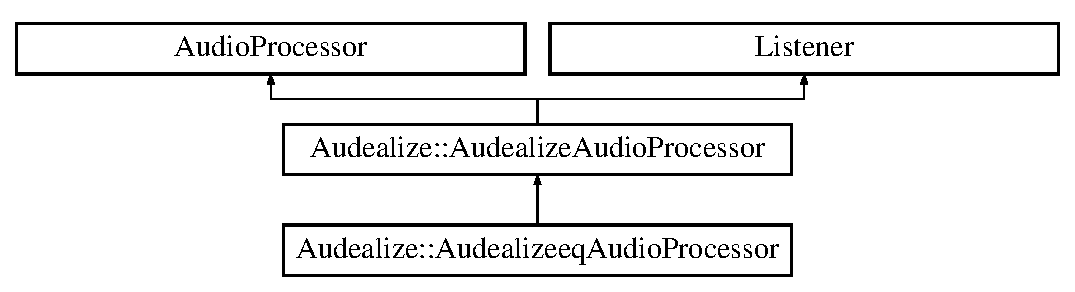
\includegraphics[height=3.000000cm]{class_audealize_1_1_audealizeeq_audio_processor}
\end{center}
\end{figure}
\subsection*{Public Member Functions}
\begin{DoxyCompactItemize}
\item 
\hyperlink{class_audealize_1_1_audealizeeq_audio_processor_ad3f864e2039bf76b23315ee5454ef198}{Audealizeeq\+Audio\+Processor} (\hyperlink{class_audealize_1_1_audealize_audio_processor}{Audealize\+Audio\+Processor} $\ast$owner=nullptr)
\item 
\hyperlink{class_audealize_1_1_audealizeeq_audio_processor_a9a77f54b0503b3949b51ccf0a94a63ed}{$\sim$\+Audealizeeq\+Audio\+Processor} ()
\item 
\hyperlink{tk_8h_aba408b7cd755a96426e004c015f5de8e}{void} \hyperlink{class_audealize_1_1_audealizeeq_audio_processor_a4bba4adcf5b948a1e1e1d78d21432efd}{prepare\+To\+Play} (double sample\+Rate, \hyperlink{tk_8h_a83f82f76e7fed06f4c49d2db94028a6d}{int} samples\+Per\+Block) override
\item 
\hyperlink{tk_8h_aba408b7cd755a96426e004c015f5de8e}{void} \hyperlink{class_audealize_1_1_audealizeeq_audio_processor_ac002e503f882352da067e88bbdd3e994}{release\+Resources} () override
\item 
bool \hyperlink{class_audealize_1_1_audealizeeq_audio_processor_abcd1446899a51c06397970535af8cb64}{set\+Preferred\+Bus\+Arrangement} (bool is\+Input, \hyperlink{tk_8h_a83f82f76e7fed06f4c49d2db94028a6d}{int} bus, const Audio\+Channel\+Set \&preferred\+Set) override
\item 
\hyperlink{tk_8h_aba408b7cd755a96426e004c015f5de8e}{void} \hyperlink{class_audealize_1_1_audealizeeq_audio_processor_a215bf8fc1c14a5a8f586ad9463b33d0a}{process\+Block} (Audio\+Sample\+Buffer \&, Midi\+Buffer \&) override
\item 
\hyperlink{class_audealize_1_1_audealize_u_i}{Audealize\+UI} $\ast$ \hyperlink{class_audealize_1_1_audealizeeq_audio_processor_a18452a450268fa3e3cadd491525fe01c}{create\+Editor\+For\+Multi\+Effect} ()
\item 
Audio\+Processor\+Editor $\ast$ \hyperlink{class_audealize_1_1_audealizeeq_audio_processor_abb95853d018607894a95abf40ca6e308}{create\+Editor} () override
\item 
bool \hyperlink{class_audealize_1_1_audealizeeq_audio_processor_a97650263b1f2399d88f51bef0d2ad0a3}{has\+Editor} () const  override
\item 
const String \hyperlink{class_audealize_1_1_audealizeeq_audio_processor_a7f7b09545ea360ad27d2493467965891}{get\+Name} () const  override
\item 
bool \hyperlink{class_audealize_1_1_audealizeeq_audio_processor_a9e820616ada66ac1788fbaa48f1afd40}{accepts\+Midi} () const  override
\item 
bool \hyperlink{class_audealize_1_1_audealizeeq_audio_processor_a784691486ca80271a1f2fcee9ad32542}{produces\+Midi} () const  override
\item 
double \hyperlink{class_audealize_1_1_audealizeeq_audio_processor_a2c3fb8c06b4ffe89c921b961fa73af25}{get\+Tail\+Length\+Seconds} () const  override
\item 
\hyperlink{tk_8h_a83f82f76e7fed06f4c49d2db94028a6d}{int} \hyperlink{class_audealize_1_1_audealizeeq_audio_processor_a11bd93cafb127cdbc624e16f62582d52}{get\+Num\+Programs} () override
\item 
\hyperlink{tk_8h_a83f82f76e7fed06f4c49d2db94028a6d}{int} \hyperlink{class_audealize_1_1_audealizeeq_audio_processor_a5cb00c25aa26c2b65b6a848a415342bd}{get\+Current\+Program} () override
\item 
\hyperlink{tk_8h_aba408b7cd755a96426e004c015f5de8e}{void} \hyperlink{class_audealize_1_1_audealizeeq_audio_processor_ab6d138c59bb721764c33d4af3f26e97e}{set\+Current\+Program} (\hyperlink{tk_8h_a83f82f76e7fed06f4c49d2db94028a6d}{int} index) override
\item 
const String \hyperlink{class_audealize_1_1_audealizeeq_audio_processor_adce52ddadf23a6731b91685eb2693ca1}{get\+Program\+Name} (\hyperlink{tk_8h_a83f82f76e7fed06f4c49d2db94028a6d}{int} index) override
\item 
\hyperlink{tk_8h_aba408b7cd755a96426e004c015f5de8e}{void} \hyperlink{class_audealize_1_1_audealizeeq_audio_processor_aa77d0be3fce3b96cd822902b55e2d984}{change\+Program\+Name} (\hyperlink{tk_8h_a83f82f76e7fed06f4c49d2db94028a6d}{int} index, const String \&new\+Name) override
\item 
\hyperlink{tk_8h_aba408b7cd755a96426e004c015f5de8e}{void} \hyperlink{class_audealize_1_1_audealizeeq_audio_processor_a25c85696329c21a201963733bc46d957}{parameter\+Changed} (const juce\+::\+String \&parameter\+ID, float new\+Value) override
\item 
\hyperlink{tk_8h_aba408b7cd755a96426e004c015f5de8e}{void} \hyperlink{class_audealize_1_1_audealizeeq_audio_processor_adda624ec0e28dbc41777aa76ed9ce974}{settings\+From\+Map} (vector$<$ float $>$ settings) override
\item 
String \hyperlink{class_audealize_1_1_audealizeeq_audio_processor_a692e0576747a20bc080b971dccd84241}{get\+Param\+ID} (\hyperlink{tk_8h_a83f82f76e7fed06f4c49d2db94028a6d}{int} index) override
\item 
bool \hyperlink{class_audealize_1_1_audealizeeq_audio_processor_a1e14e27cbd9ea51776deccfd0ec4f4a8}{is\+Parameter\+Automatable} (\hyperlink{tk_8h_a83f82f76e7fed06f4c49d2db94028a6d}{int} index)
\end{DoxyCompactItemize}
\subsection*{Additional Inherited Members}


\subsection{Constructor \& Destructor Documentation}
\index{Audealize\+::\+Audealizeeq\+Audio\+Processor@{Audealize\+::\+Audealizeeq\+Audio\+Processor}!Audealizeeq\+Audio\+Processor@{Audealizeeq\+Audio\+Processor}}
\index{Audealizeeq\+Audio\+Processor@{Audealizeeq\+Audio\+Processor}!Audealize\+::\+Audealizeeq\+Audio\+Processor@{Audealize\+::\+Audealizeeq\+Audio\+Processor}}
\subsubsection[{\texorpdfstring{Audealizeeq\+Audio\+Processor(\+Audealize\+Audio\+Processor $\ast$owner=nullptr)}{AudealizeeqAudioProcessor(AudealizeAudioProcessor *owner=nullptr)}}]{\setlength{\rightskip}{0pt plus 5cm}Audealizeeq\+Audio\+Processor\+::\+Audealizeeq\+Audio\+Processor (
\begin{DoxyParamCaption}
\item[{{\bf Audealize\+Audio\+Processor} $\ast$}]{owner = {\ttfamily nullptr}}
\end{DoxyParamCaption}
)}\hypertarget{class_audealize_1_1_audealizeeq_audio_processor_ad3f864e2039bf76b23315ee5454ef198}{}\label{class_audealize_1_1_audealizeeq_audio_processor_ad3f864e2039bf76b23315ee5454ef198}
\index{Audealize\+::\+Audealizeeq\+Audio\+Processor@{Audealize\+::\+Audealizeeq\+Audio\+Processor}!````~Audealizeeq\+Audio\+Processor@{$\sim$\+Audealizeeq\+Audio\+Processor}}
\index{````~Audealizeeq\+Audio\+Processor@{$\sim$\+Audealizeeq\+Audio\+Processor}!Audealize\+::\+Audealizeeq\+Audio\+Processor@{Audealize\+::\+Audealizeeq\+Audio\+Processor}}
\subsubsection[{\texorpdfstring{$\sim$\+Audealizeeq\+Audio\+Processor()}{~AudealizeeqAudioProcessor()}}]{\setlength{\rightskip}{0pt plus 5cm}Audealizeeq\+Audio\+Processor\+::$\sim$\+Audealizeeq\+Audio\+Processor (
\begin{DoxyParamCaption}
{}
\end{DoxyParamCaption}
)}\hypertarget{class_audealize_1_1_audealizeeq_audio_processor_a9a77f54b0503b3949b51ccf0a94a63ed}{}\label{class_audealize_1_1_audealizeeq_audio_processor_a9a77f54b0503b3949b51ccf0a94a63ed}


\subsection{Member Function Documentation}
\index{Audealize\+::\+Audealizeeq\+Audio\+Processor@{Audealize\+::\+Audealizeeq\+Audio\+Processor}!accepts\+Midi@{accepts\+Midi}}
\index{accepts\+Midi@{accepts\+Midi}!Audealize\+::\+Audealizeeq\+Audio\+Processor@{Audealize\+::\+Audealizeeq\+Audio\+Processor}}
\subsubsection[{\texorpdfstring{accepts\+Midi() const  override}{acceptsMidi() const  override}}]{\setlength{\rightskip}{0pt plus 5cm}bool Audealizeeq\+Audio\+Processor\+::accepts\+Midi (
\begin{DoxyParamCaption}
{}
\end{DoxyParamCaption}
) const\hspace{0.3cm}{\ttfamily [override]}}\hypertarget{class_audealize_1_1_audealizeeq_audio_processor_a9e820616ada66ac1788fbaa48f1afd40}{}\label{class_audealize_1_1_audealizeeq_audio_processor_a9e820616ada66ac1788fbaa48f1afd40}
\index{Audealize\+::\+Audealizeeq\+Audio\+Processor@{Audealize\+::\+Audealizeeq\+Audio\+Processor}!change\+Program\+Name@{change\+Program\+Name}}
\index{change\+Program\+Name@{change\+Program\+Name}!Audealize\+::\+Audealizeeq\+Audio\+Processor@{Audealize\+::\+Audealizeeq\+Audio\+Processor}}
\subsubsection[{\texorpdfstring{change\+Program\+Name(int index, const String \&new\+Name) override}{changeProgramName(int index, const String &newName) override}}]{\setlength{\rightskip}{0pt plus 5cm}{\bf void} Audealizeeq\+Audio\+Processor\+::change\+Program\+Name (
\begin{DoxyParamCaption}
\item[{{\bf int}}]{index, }
\item[{const String \&}]{new\+Name}
\end{DoxyParamCaption}
)\hspace{0.3cm}{\ttfamily [override]}}\hypertarget{class_audealize_1_1_audealizeeq_audio_processor_aa77d0be3fce3b96cd822902b55e2d984}{}\label{class_audealize_1_1_audealizeeq_audio_processor_aa77d0be3fce3b96cd822902b55e2d984}
\index{Audealize\+::\+Audealizeeq\+Audio\+Processor@{Audealize\+::\+Audealizeeq\+Audio\+Processor}!create\+Editor@{create\+Editor}}
\index{create\+Editor@{create\+Editor}!Audealize\+::\+Audealizeeq\+Audio\+Processor@{Audealize\+::\+Audealizeeq\+Audio\+Processor}}
\subsubsection[{\texorpdfstring{create\+Editor() override}{createEditor() override}}]{\setlength{\rightskip}{0pt plus 5cm}Audio\+Processor\+Editor $\ast$ Audealizeeq\+Audio\+Processor\+::create\+Editor (
\begin{DoxyParamCaption}
{}
\end{DoxyParamCaption}
)\hspace{0.3cm}{\ttfamily [override]}}\hypertarget{class_audealize_1_1_audealizeeq_audio_processor_abb95853d018607894a95abf40ca6e308}{}\label{class_audealize_1_1_audealizeeq_audio_processor_abb95853d018607894a95abf40ca6e308}
\index{Audealize\+::\+Audealizeeq\+Audio\+Processor@{Audealize\+::\+Audealizeeq\+Audio\+Processor}!create\+Editor\+For\+Multi\+Effect@{create\+Editor\+For\+Multi\+Effect}}
\index{create\+Editor\+For\+Multi\+Effect@{create\+Editor\+For\+Multi\+Effect}!Audealize\+::\+Audealizeeq\+Audio\+Processor@{Audealize\+::\+Audealizeeq\+Audio\+Processor}}
\subsubsection[{\texorpdfstring{create\+Editor\+For\+Multi\+Effect()}{createEditorForMultiEffect()}}]{\setlength{\rightskip}{0pt plus 5cm}{\bf Audealize\+UI} $\ast$ Audealizeeq\+Audio\+Processor\+::create\+Editor\+For\+Multi\+Effect (
\begin{DoxyParamCaption}
{}
\end{DoxyParamCaption}
)}\hypertarget{class_audealize_1_1_audealizeeq_audio_processor_a18452a450268fa3e3cadd491525fe01c}{}\label{class_audealize_1_1_audealizeeq_audio_processor_a18452a450268fa3e3cadd491525fe01c}
\index{Audealize\+::\+Audealizeeq\+Audio\+Processor@{Audealize\+::\+Audealizeeq\+Audio\+Processor}!get\+Current\+Program@{get\+Current\+Program}}
\index{get\+Current\+Program@{get\+Current\+Program}!Audealize\+::\+Audealizeeq\+Audio\+Processor@{Audealize\+::\+Audealizeeq\+Audio\+Processor}}
\subsubsection[{\texorpdfstring{get\+Current\+Program() override}{getCurrentProgram() override}}]{\setlength{\rightskip}{0pt plus 5cm}{\bf int} Audealizeeq\+Audio\+Processor\+::get\+Current\+Program (
\begin{DoxyParamCaption}
{}
\end{DoxyParamCaption}
)\hspace{0.3cm}{\ttfamily [override]}}\hypertarget{class_audealize_1_1_audealizeeq_audio_processor_a5cb00c25aa26c2b65b6a848a415342bd}{}\label{class_audealize_1_1_audealizeeq_audio_processor_a5cb00c25aa26c2b65b6a848a415342bd}
\index{Audealize\+::\+Audealizeeq\+Audio\+Processor@{Audealize\+::\+Audealizeeq\+Audio\+Processor}!get\+Name@{get\+Name}}
\index{get\+Name@{get\+Name}!Audealize\+::\+Audealizeeq\+Audio\+Processor@{Audealize\+::\+Audealizeeq\+Audio\+Processor}}
\subsubsection[{\texorpdfstring{get\+Name() const  override}{getName() const  override}}]{\setlength{\rightskip}{0pt plus 5cm}const String Audealizeeq\+Audio\+Processor\+::get\+Name (
\begin{DoxyParamCaption}
{}
\end{DoxyParamCaption}
) const\hspace{0.3cm}{\ttfamily [override]}}\hypertarget{class_audealize_1_1_audealizeeq_audio_processor_a7f7b09545ea360ad27d2493467965891}{}\label{class_audealize_1_1_audealizeeq_audio_processor_a7f7b09545ea360ad27d2493467965891}
\index{Audealize\+::\+Audealizeeq\+Audio\+Processor@{Audealize\+::\+Audealizeeq\+Audio\+Processor}!get\+Num\+Programs@{get\+Num\+Programs}}
\index{get\+Num\+Programs@{get\+Num\+Programs}!Audealize\+::\+Audealizeeq\+Audio\+Processor@{Audealize\+::\+Audealizeeq\+Audio\+Processor}}
\subsubsection[{\texorpdfstring{get\+Num\+Programs() override}{getNumPrograms() override}}]{\setlength{\rightskip}{0pt plus 5cm}{\bf int} Audealizeeq\+Audio\+Processor\+::get\+Num\+Programs (
\begin{DoxyParamCaption}
{}
\end{DoxyParamCaption}
)\hspace{0.3cm}{\ttfamily [override]}}\hypertarget{class_audealize_1_1_audealizeeq_audio_processor_a11bd93cafb127cdbc624e16f62582d52}{}\label{class_audealize_1_1_audealizeeq_audio_processor_a11bd93cafb127cdbc624e16f62582d52}
\index{Audealize\+::\+Audealizeeq\+Audio\+Processor@{Audealize\+::\+Audealizeeq\+Audio\+Processor}!get\+Param\+ID@{get\+Param\+ID}}
\index{get\+Param\+ID@{get\+Param\+ID}!Audealize\+::\+Audealizeeq\+Audio\+Processor@{Audealize\+::\+Audealizeeq\+Audio\+Processor}}
\subsubsection[{\texorpdfstring{get\+Param\+I\+D(int index) override}{getParamID(int index) override}}]{\setlength{\rightskip}{0pt plus 5cm}String Audealizeeq\+Audio\+Processor\+::get\+Param\+ID (
\begin{DoxyParamCaption}
\item[{{\bf int}}]{index}
\end{DoxyParamCaption}
)\hspace{0.3cm}{\ttfamily [inline]}, {\ttfamily [override]}, {\ttfamily [virtual]}}\hypertarget{class_audealize_1_1_audealizeeq_audio_processor_a692e0576747a20bc080b971dccd84241}{}\label{class_audealize_1_1_audealizeeq_audio_processor_a692e0576747a20bc080b971dccd84241}
Returns a string with the parameter ID of one of the parameters


\begin{DoxyParams}{Parameters}
{\em index} & \\
\hline
\end{DoxyParams}


Reimplemented from \hyperlink{class_audealize_1_1_audealize_audio_processor_aa3e347b4bdc34e419ccf350638c38028}{Audealize\+::\+Audealize\+Audio\+Processor}.

\index{Audealize\+::\+Audealizeeq\+Audio\+Processor@{Audealize\+::\+Audealizeeq\+Audio\+Processor}!get\+Program\+Name@{get\+Program\+Name}}
\index{get\+Program\+Name@{get\+Program\+Name}!Audealize\+::\+Audealizeeq\+Audio\+Processor@{Audealize\+::\+Audealizeeq\+Audio\+Processor}}
\subsubsection[{\texorpdfstring{get\+Program\+Name(int index) override}{getProgramName(int index) override}}]{\setlength{\rightskip}{0pt plus 5cm}const String Audealizeeq\+Audio\+Processor\+::get\+Program\+Name (
\begin{DoxyParamCaption}
\item[{{\bf int}}]{index}
\end{DoxyParamCaption}
)\hspace{0.3cm}{\ttfamily [override]}}\hypertarget{class_audealize_1_1_audealizeeq_audio_processor_adce52ddadf23a6731b91685eb2693ca1}{}\label{class_audealize_1_1_audealizeeq_audio_processor_adce52ddadf23a6731b91685eb2693ca1}
\index{Audealize\+::\+Audealizeeq\+Audio\+Processor@{Audealize\+::\+Audealizeeq\+Audio\+Processor}!get\+Tail\+Length\+Seconds@{get\+Tail\+Length\+Seconds}}
\index{get\+Tail\+Length\+Seconds@{get\+Tail\+Length\+Seconds}!Audealize\+::\+Audealizeeq\+Audio\+Processor@{Audealize\+::\+Audealizeeq\+Audio\+Processor}}
\subsubsection[{\texorpdfstring{get\+Tail\+Length\+Seconds() const  override}{getTailLengthSeconds() const  override}}]{\setlength{\rightskip}{0pt plus 5cm}double Audealizeeq\+Audio\+Processor\+::get\+Tail\+Length\+Seconds (
\begin{DoxyParamCaption}
{}
\end{DoxyParamCaption}
) const\hspace{0.3cm}{\ttfamily [override]}}\hypertarget{class_audealize_1_1_audealizeeq_audio_processor_a2c3fb8c06b4ffe89c921b961fa73af25}{}\label{class_audealize_1_1_audealizeeq_audio_processor_a2c3fb8c06b4ffe89c921b961fa73af25}
\index{Audealize\+::\+Audealizeeq\+Audio\+Processor@{Audealize\+::\+Audealizeeq\+Audio\+Processor}!has\+Editor@{has\+Editor}}
\index{has\+Editor@{has\+Editor}!Audealize\+::\+Audealizeeq\+Audio\+Processor@{Audealize\+::\+Audealizeeq\+Audio\+Processor}}
\subsubsection[{\texorpdfstring{has\+Editor() const  override}{hasEditor() const  override}}]{\setlength{\rightskip}{0pt plus 5cm}bool Audealizeeq\+Audio\+Processor\+::has\+Editor (
\begin{DoxyParamCaption}
{}
\end{DoxyParamCaption}
) const\hspace{0.3cm}{\ttfamily [override]}}\hypertarget{class_audealize_1_1_audealizeeq_audio_processor_a97650263b1f2399d88f51bef0d2ad0a3}{}\label{class_audealize_1_1_audealizeeq_audio_processor_a97650263b1f2399d88f51bef0d2ad0a3}
\index{Audealize\+::\+Audealizeeq\+Audio\+Processor@{Audealize\+::\+Audealizeeq\+Audio\+Processor}!is\+Parameter\+Automatable@{is\+Parameter\+Automatable}}
\index{is\+Parameter\+Automatable@{is\+Parameter\+Automatable}!Audealize\+::\+Audealizeeq\+Audio\+Processor@{Audealize\+::\+Audealizeeq\+Audio\+Processor}}
\subsubsection[{\texorpdfstring{is\+Parameter\+Automatable(int index)}{isParameterAutomatable(int index)}}]{\setlength{\rightskip}{0pt plus 5cm}bool Audealize\+::\+Audealizeeq\+Audio\+Processor\+::is\+Parameter\+Automatable (
\begin{DoxyParamCaption}
\item[{{\bf int}}]{index}
\end{DoxyParamCaption}
)\hspace{0.3cm}{\ttfamily [inline]}}\hypertarget{class_audealize_1_1_audealizeeq_audio_processor_a1e14e27cbd9ea51776deccfd0ec4f4a8}{}\label{class_audealize_1_1_audealizeeq_audio_processor_a1e14e27cbd9ea51776deccfd0ec4f4a8}
\index{Audealize\+::\+Audealizeeq\+Audio\+Processor@{Audealize\+::\+Audealizeeq\+Audio\+Processor}!parameter\+Changed@{parameter\+Changed}}
\index{parameter\+Changed@{parameter\+Changed}!Audealize\+::\+Audealizeeq\+Audio\+Processor@{Audealize\+::\+Audealizeeq\+Audio\+Processor}}
\subsubsection[{\texorpdfstring{parameter\+Changed(const juce\+::\+String \&parameter\+I\+D, float new\+Value) override}{parameterChanged(const juce::String &parameterID, float newValue) override}}]{\setlength{\rightskip}{0pt plus 5cm}{\bf void} Audealizeeq\+Audio\+Processor\+::parameter\+Changed (
\begin{DoxyParamCaption}
\item[{const juce\+::\+String \&}]{parameter\+ID, }
\item[{float}]{new\+Value}
\end{DoxyParamCaption}
)\hspace{0.3cm}{\ttfamily [override]}, {\ttfamily [virtual]}}\hypertarget{class_audealize_1_1_audealizeeq_audio_processor_a25c85696329c21a201963733bc46d957}{}\label{class_audealize_1_1_audealizeeq_audio_processor_a25c85696329c21a201963733bc46d957}
Called by an Audio\+Processor\+Editor to notify Audio\+Processor of parameter value changes


\begin{DoxyParams}{Parameters}
{\em parameter\+ID} & The ID of the parameter that was changed \\
\hline
{\em new\+Value} & The new value for that parameter \\
\hline
\end{DoxyParams}


Reimplemented from \hyperlink{class_audealize_1_1_audealize_audio_processor_a4832111ea2b24bc517f911fa5949ca56}{Audealize\+::\+Audealize\+Audio\+Processor}.

\index{Audealize\+::\+Audealizeeq\+Audio\+Processor@{Audealize\+::\+Audealizeeq\+Audio\+Processor}!prepare\+To\+Play@{prepare\+To\+Play}}
\index{prepare\+To\+Play@{prepare\+To\+Play}!Audealize\+::\+Audealizeeq\+Audio\+Processor@{Audealize\+::\+Audealizeeq\+Audio\+Processor}}
\subsubsection[{\texorpdfstring{prepare\+To\+Play(double sample\+Rate, int samples\+Per\+Block) override}{prepareToPlay(double sampleRate, int samplesPerBlock) override}}]{\setlength{\rightskip}{0pt plus 5cm}{\bf void} Audealizeeq\+Audio\+Processor\+::prepare\+To\+Play (
\begin{DoxyParamCaption}
\item[{double}]{sample\+Rate, }
\item[{{\bf int}}]{samples\+Per\+Block}
\end{DoxyParamCaption}
)\hspace{0.3cm}{\ttfamily [override]}}\hypertarget{class_audealize_1_1_audealizeeq_audio_processor_a4bba4adcf5b948a1e1e1d78d21432efd}{}\label{class_audealize_1_1_audealizeeq_audio_processor_a4bba4adcf5b948a1e1e1d78d21432efd}
\index{Audealize\+::\+Audealizeeq\+Audio\+Processor@{Audealize\+::\+Audealizeeq\+Audio\+Processor}!process\+Block@{process\+Block}}
\index{process\+Block@{process\+Block}!Audealize\+::\+Audealizeeq\+Audio\+Processor@{Audealize\+::\+Audealizeeq\+Audio\+Processor}}
\subsubsection[{\texorpdfstring{process\+Block(\+Audio\+Sample\+Buffer \&, Midi\+Buffer \&) override}{processBlock(AudioSampleBuffer &, MidiBuffer &) override}}]{\setlength{\rightskip}{0pt plus 5cm}{\bf void} Audealizeeq\+Audio\+Processor\+::process\+Block (
\begin{DoxyParamCaption}
\item[{Audio\+Sample\+Buffer \&}]{buffer, }
\item[{Midi\+Buffer \&}]{midi\+Messages}
\end{DoxyParamCaption}
)\hspace{0.3cm}{\ttfamily [override]}}\hypertarget{class_audealize_1_1_audealizeeq_audio_processor_a215bf8fc1c14a5a8f586ad9463b33d0a}{}\label{class_audealize_1_1_audealizeeq_audio_processor_a215bf8fc1c14a5a8f586ad9463b33d0a}
\index{Audealize\+::\+Audealizeeq\+Audio\+Processor@{Audealize\+::\+Audealizeeq\+Audio\+Processor}!produces\+Midi@{produces\+Midi}}
\index{produces\+Midi@{produces\+Midi}!Audealize\+::\+Audealizeeq\+Audio\+Processor@{Audealize\+::\+Audealizeeq\+Audio\+Processor}}
\subsubsection[{\texorpdfstring{produces\+Midi() const  override}{producesMidi() const  override}}]{\setlength{\rightskip}{0pt plus 5cm}bool Audealizeeq\+Audio\+Processor\+::produces\+Midi (
\begin{DoxyParamCaption}
{}
\end{DoxyParamCaption}
) const\hspace{0.3cm}{\ttfamily [override]}}\hypertarget{class_audealize_1_1_audealizeeq_audio_processor_a784691486ca80271a1f2fcee9ad32542}{}\label{class_audealize_1_1_audealizeeq_audio_processor_a784691486ca80271a1f2fcee9ad32542}
\index{Audealize\+::\+Audealizeeq\+Audio\+Processor@{Audealize\+::\+Audealizeeq\+Audio\+Processor}!release\+Resources@{release\+Resources}}
\index{release\+Resources@{release\+Resources}!Audealize\+::\+Audealizeeq\+Audio\+Processor@{Audealize\+::\+Audealizeeq\+Audio\+Processor}}
\subsubsection[{\texorpdfstring{release\+Resources() override}{releaseResources() override}}]{\setlength{\rightskip}{0pt plus 5cm}{\bf void} Audealizeeq\+Audio\+Processor\+::release\+Resources (
\begin{DoxyParamCaption}
{}
\end{DoxyParamCaption}
)\hspace{0.3cm}{\ttfamily [override]}}\hypertarget{class_audealize_1_1_audealizeeq_audio_processor_ac002e503f882352da067e88bbdd3e994}{}\label{class_audealize_1_1_audealizeeq_audio_processor_ac002e503f882352da067e88bbdd3e994}
\index{Audealize\+::\+Audealizeeq\+Audio\+Processor@{Audealize\+::\+Audealizeeq\+Audio\+Processor}!set\+Current\+Program@{set\+Current\+Program}}
\index{set\+Current\+Program@{set\+Current\+Program}!Audealize\+::\+Audealizeeq\+Audio\+Processor@{Audealize\+::\+Audealizeeq\+Audio\+Processor}}
\subsubsection[{\texorpdfstring{set\+Current\+Program(int index) override}{setCurrentProgram(int index) override}}]{\setlength{\rightskip}{0pt plus 5cm}{\bf void} Audealizeeq\+Audio\+Processor\+::set\+Current\+Program (
\begin{DoxyParamCaption}
\item[{{\bf int}}]{index}
\end{DoxyParamCaption}
)\hspace{0.3cm}{\ttfamily [override]}}\hypertarget{class_audealize_1_1_audealizeeq_audio_processor_ab6d138c59bb721764c33d4af3f26e97e}{}\label{class_audealize_1_1_audealizeeq_audio_processor_ab6d138c59bb721764c33d4af3f26e97e}
\index{Audealize\+::\+Audealizeeq\+Audio\+Processor@{Audealize\+::\+Audealizeeq\+Audio\+Processor}!set\+Preferred\+Bus\+Arrangement@{set\+Preferred\+Bus\+Arrangement}}
\index{set\+Preferred\+Bus\+Arrangement@{set\+Preferred\+Bus\+Arrangement}!Audealize\+::\+Audealizeeq\+Audio\+Processor@{Audealize\+::\+Audealizeeq\+Audio\+Processor}}
\subsubsection[{\texorpdfstring{set\+Preferred\+Bus\+Arrangement(bool is\+Input, int bus, const Audio\+Channel\+Set \&preferred\+Set) override}{setPreferredBusArrangement(bool isInput, int bus, const AudioChannelSet &preferredSet) override}}]{\setlength{\rightskip}{0pt plus 5cm}bool Audealizeeq\+Audio\+Processor\+::set\+Preferred\+Bus\+Arrangement (
\begin{DoxyParamCaption}
\item[{bool}]{is\+Input, }
\item[{{\bf int}}]{bus, }
\item[{const Audio\+Channel\+Set \&}]{preferred\+Set}
\end{DoxyParamCaption}
)\hspace{0.3cm}{\ttfamily [override]}}\hypertarget{class_audealize_1_1_audealizeeq_audio_processor_abcd1446899a51c06397970535af8cb64}{}\label{class_audealize_1_1_audealizeeq_audio_processor_abcd1446899a51c06397970535af8cb64}
\index{Audealize\+::\+Audealizeeq\+Audio\+Processor@{Audealize\+::\+Audealizeeq\+Audio\+Processor}!settings\+From\+Map@{settings\+From\+Map}}
\index{settings\+From\+Map@{settings\+From\+Map}!Audealize\+::\+Audealizeeq\+Audio\+Processor@{Audealize\+::\+Audealizeeq\+Audio\+Processor}}
\subsubsection[{\texorpdfstring{settings\+From\+Map(vector$<$ float $>$ settings) override}{settingsFromMap(vector< float > settings) override}}]{\setlength{\rightskip}{0pt plus 5cm}{\bf void} Audealizeeq\+Audio\+Processor\+::settings\+From\+Map (
\begin{DoxyParamCaption}
\item[{vector$<$ float $>$}]{settings}
\end{DoxyParamCaption}
)\hspace{0.3cm}{\ttfamily [override]}, {\ttfamily [virtual]}}\hypertarget{class_audealize_1_1_audealizeeq_audio_processor_adda624ec0e28dbc41777aa76ed9ce974}{}\label{class_audealize_1_1_audealizeeq_audio_processor_adda624ec0e28dbc41777aa76ed9ce974}
Set the states of all parameters with a vector$<$float$>$. To be called by a \hyperlink{class_audealize_1_1_word_map}{Word\+Map}


\begin{DoxyParams}{Parameters}
{\em settings} & a vector of floats \\
\hline
\end{DoxyParams}


Reimplemented from \hyperlink{class_audealize_1_1_audealize_audio_processor_af269ce5549d8474f11f26c41aefa51bc}{Audealize\+::\+Audealize\+Audio\+Processor}.



The documentation for this class was generated from the following files\+:\begin{DoxyCompactItemize}
\item 
/\+Users/michael/\+J\+U\+C\+E/projects/audealize-\/plugin/\+J\+U\+C\+E Modules/audealize\+\_\+module/audio\+\_\+processors/\hyperlink{_audealize_e_q_audio_processor_8h}{Audealize\+E\+Q\+Audio\+Processor.\+h}\item 
/\+Users/michael/\+J\+U\+C\+E/projects/audealize-\/plugin/\+J\+U\+C\+E Modules/audealize\+\_\+module/audio\+\_\+processors/\hyperlink{_audealize_e_q_audio_processor_8cpp}{Audealize\+E\+Q\+Audio\+Processor.\+cpp}\end{DoxyCompactItemize}

\hypertarget{class_audealize_1_1_audealize_fonts}{}\section{Audealize\+:\+:Audealize\+Fonts Class Reference}
\label{class_audealize_1_1_audealize_fonts}\index{Audealize\+::\+Audealize\+Fonts@{Audealize\+::\+Audealize\+Fonts}}


{\ttfamily \#include $<$Fonts.\+h$>$}

\subsection*{Static Public Attributes}
\begin{DoxyCompactItemize}
\item 
static const char $\ast$ \hyperlink{class_audealize_1_1_audealize_fonts_a1fea272dd7aae1975ddd34c53c2c7733}{Roboto\+Regular\+\_\+ttf} = (const char$\ast$) roboto\+\_\+binary\+\_\+data
\item 
static const \hyperlink{tk_8h_a83f82f76e7fed06f4c49d2db94028a6d}{int} \hyperlink{class_audealize_1_1_audealize_fonts_a39ba7d9c918c682a7551e41d3dc15ae7}{Roboto\+Regular\+\_\+ttf\+Size} = 145348
\end{DoxyCompactItemize}


\subsection{Member Data Documentation}
\index{Audealize\+::\+Audealize\+Fonts@{Audealize\+::\+Audealize\+Fonts}!Roboto\+Regular\+\_\+ttf@{Roboto\+Regular\+\_\+ttf}}
\index{Roboto\+Regular\+\_\+ttf@{Roboto\+Regular\+\_\+ttf}!Audealize\+::\+Audealize\+Fonts@{Audealize\+::\+Audealize\+Fonts}}
\subsubsection[{\texorpdfstring{Roboto\+Regular\+\_\+ttf}{RobotoRegular_ttf}}]{\setlength{\rightskip}{0pt plus 5cm}const char $\ast$ Audealize\+::\+Audealize\+Fonts\+::\+Roboto\+Regular\+\_\+ttf = (const char$\ast$) roboto\+\_\+binary\+\_\+data\hspace{0.3cm}{\ttfamily [static]}}\hypertarget{class_audealize_1_1_audealize_fonts_a1fea272dd7aae1975ddd34c53c2c7733}{}\label{class_audealize_1_1_audealize_fonts_a1fea272dd7aae1975ddd34c53c2c7733}
\index{Audealize\+::\+Audealize\+Fonts@{Audealize\+::\+Audealize\+Fonts}!Roboto\+Regular\+\_\+ttf\+Size@{Roboto\+Regular\+\_\+ttf\+Size}}
\index{Roboto\+Regular\+\_\+ttf\+Size@{Roboto\+Regular\+\_\+ttf\+Size}!Audealize\+::\+Audealize\+Fonts@{Audealize\+::\+Audealize\+Fonts}}
\subsubsection[{\texorpdfstring{Roboto\+Regular\+\_\+ttf\+Size}{RobotoRegular_ttfSize}}]{\setlength{\rightskip}{0pt plus 5cm}const {\bf int} Audealize\+::\+Audealize\+Fonts\+::\+Roboto\+Regular\+\_\+ttf\+Size = 145348\hspace{0.3cm}{\ttfamily [static]}}\hypertarget{class_audealize_1_1_audealize_fonts_a39ba7d9c918c682a7551e41d3dc15ae7}{}\label{class_audealize_1_1_audealize_fonts_a39ba7d9c918c682a7551e41d3dc15ae7}


The documentation for this class was generated from the following files\+:\begin{DoxyCompactItemize}
\item 
/\+Users/michael/\+J\+U\+C\+E/projects/audealize-\/plugin/\+J\+U\+C\+E Modules/audealize\+\_\+module/resources/\hyperlink{_fonts_8h}{Fonts.\+h}\item 
/\+Users/michael/\+J\+U\+C\+E/projects/audealize-\/plugin/\+J\+U\+C\+E Modules/audealize\+\_\+module/resources/\hyperlink{_fonts_8cpp}{Fonts.\+cpp}\end{DoxyCompactItemize}

\hypertarget{class_audealize_1_1_audealize_images}{}\section{Audealize\+:\+:Audealize\+Images Class Reference}
\label{class_audealize_1_1_audealize_images}\index{Audealize\+::\+Audealize\+Images@{Audealize\+::\+Audealize\+Images}}


{\ttfamily \#include $<$Audealize\+Images.\+h$>$}

\subsection*{Static Public Attributes}
\begin{DoxyCompactItemize}
\item 
static const char $\ast$ \hyperlink{class_audealize_1_1_audealize_images_a648e121e873c0d48aa50001c65ee4383}{dark\+Mode\+Button\+\_\+svg} = (const char$\ast$) resource\+\_\+\+Audealize\+Images\+\_\+dark\+Mode\+Button\+\_\+svg
\item 
static const \hyperlink{tk_8h_a83f82f76e7fed06f4c49d2db94028a6d}{int} \hyperlink{class_audealize_1_1_audealize_images_a3448b57ddf0d2ac3f32012295f0dbc6a}{dark\+Mode\+Button\+\_\+svg\+Size} = 2944
\item 
static const char $\ast$ \hyperlink{class_audealize_1_1_audealize_images_abaf4f444d78268f7b4655d1edf9b5337}{iallogo\+\_\+svg} = (const char$\ast$) resource\+\_\+\+Audealize\+Images\+\_\+iallogo\+\_\+svg
\item 
static const \hyperlink{tk_8h_a83f82f76e7fed06f4c49d2db94028a6d}{int} \hyperlink{class_audealize_1_1_audealize_images_a3216060c18fed8e493a28e3f39a020a1}{iallogo\+\_\+svg\+Size} = 2987
\item 
static const char $\ast$ \hyperlink{class_audealize_1_1_audealize_images_a603300f72b88442487d1862ecc025337}{power\+Button\+\_\+svg} = (const char$\ast$) resource\+\_\+\+Audealize\+Images\+\_\+power\+Button\+\_\+svg
\item 
static const \hyperlink{tk_8h_a83f82f76e7fed06f4c49d2db94028a6d}{int} \hyperlink{class_audealize_1_1_audealize_images_afb26f9d7d3a8496bb571eea5b5de1077}{power\+Button\+\_\+svg\+Size} = 4377
\end{DoxyCompactItemize}


\subsection{Member Data Documentation}
\index{Audealize\+::\+Audealize\+Images@{Audealize\+::\+Audealize\+Images}!dark\+Mode\+Button\+\_\+svg@{dark\+Mode\+Button\+\_\+svg}}
\index{dark\+Mode\+Button\+\_\+svg@{dark\+Mode\+Button\+\_\+svg}!Audealize\+::\+Audealize\+Images@{Audealize\+::\+Audealize\+Images}}
\subsubsection[{\texorpdfstring{dark\+Mode\+Button\+\_\+svg}{darkModeButton_svg}}]{\setlength{\rightskip}{0pt plus 5cm}const char $\ast$ Audealize\+Images\+::dark\+Mode\+Button\+\_\+svg = (const char$\ast$) resource\+\_\+\+Audealize\+Images\+\_\+dark\+Mode\+Button\+\_\+svg\hspace{0.3cm}{\ttfamily [static]}}\hypertarget{class_audealize_1_1_audealize_images_a648e121e873c0d48aa50001c65ee4383}{}\label{class_audealize_1_1_audealize_images_a648e121e873c0d48aa50001c65ee4383}
\index{Audealize\+::\+Audealize\+Images@{Audealize\+::\+Audealize\+Images}!dark\+Mode\+Button\+\_\+svg\+Size@{dark\+Mode\+Button\+\_\+svg\+Size}}
\index{dark\+Mode\+Button\+\_\+svg\+Size@{dark\+Mode\+Button\+\_\+svg\+Size}!Audealize\+::\+Audealize\+Images@{Audealize\+::\+Audealize\+Images}}
\subsubsection[{\texorpdfstring{dark\+Mode\+Button\+\_\+svg\+Size}{darkModeButton_svgSize}}]{\setlength{\rightskip}{0pt plus 5cm}const {\bf int} Audealize\+Images\+::dark\+Mode\+Button\+\_\+svg\+Size = 2944\hspace{0.3cm}{\ttfamily [static]}}\hypertarget{class_audealize_1_1_audealize_images_a3448b57ddf0d2ac3f32012295f0dbc6a}{}\label{class_audealize_1_1_audealize_images_a3448b57ddf0d2ac3f32012295f0dbc6a}
\index{Audealize\+::\+Audealize\+Images@{Audealize\+::\+Audealize\+Images}!iallogo\+\_\+svg@{iallogo\+\_\+svg}}
\index{iallogo\+\_\+svg@{iallogo\+\_\+svg}!Audealize\+::\+Audealize\+Images@{Audealize\+::\+Audealize\+Images}}
\subsubsection[{\texorpdfstring{iallogo\+\_\+svg}{iallogo_svg}}]{\setlength{\rightskip}{0pt plus 5cm}const char $\ast$ Audealize\+Images\+::iallogo\+\_\+svg = (const char$\ast$) resource\+\_\+\+Audealize\+Images\+\_\+iallogo\+\_\+svg\hspace{0.3cm}{\ttfamily [static]}}\hypertarget{class_audealize_1_1_audealize_images_abaf4f444d78268f7b4655d1edf9b5337}{}\label{class_audealize_1_1_audealize_images_abaf4f444d78268f7b4655d1edf9b5337}
\index{Audealize\+::\+Audealize\+Images@{Audealize\+::\+Audealize\+Images}!iallogo\+\_\+svg\+Size@{iallogo\+\_\+svg\+Size}}
\index{iallogo\+\_\+svg\+Size@{iallogo\+\_\+svg\+Size}!Audealize\+::\+Audealize\+Images@{Audealize\+::\+Audealize\+Images}}
\subsubsection[{\texorpdfstring{iallogo\+\_\+svg\+Size}{iallogo_svgSize}}]{\setlength{\rightskip}{0pt plus 5cm}const {\bf int} Audealize\+Images\+::iallogo\+\_\+svg\+Size = 2987\hspace{0.3cm}{\ttfamily [static]}}\hypertarget{class_audealize_1_1_audealize_images_a3216060c18fed8e493a28e3f39a020a1}{}\label{class_audealize_1_1_audealize_images_a3216060c18fed8e493a28e3f39a020a1}
\index{Audealize\+::\+Audealize\+Images@{Audealize\+::\+Audealize\+Images}!power\+Button\+\_\+svg@{power\+Button\+\_\+svg}}
\index{power\+Button\+\_\+svg@{power\+Button\+\_\+svg}!Audealize\+::\+Audealize\+Images@{Audealize\+::\+Audealize\+Images}}
\subsubsection[{\texorpdfstring{power\+Button\+\_\+svg}{powerButton_svg}}]{\setlength{\rightskip}{0pt plus 5cm}const char $\ast$ Audealize\+Images\+::power\+Button\+\_\+svg = (const char$\ast$) resource\+\_\+\+Audealize\+Images\+\_\+power\+Button\+\_\+svg\hspace{0.3cm}{\ttfamily [static]}}\hypertarget{class_audealize_1_1_audealize_images_a603300f72b88442487d1862ecc025337}{}\label{class_audealize_1_1_audealize_images_a603300f72b88442487d1862ecc025337}
\index{Audealize\+::\+Audealize\+Images@{Audealize\+::\+Audealize\+Images}!power\+Button\+\_\+svg\+Size@{power\+Button\+\_\+svg\+Size}}
\index{power\+Button\+\_\+svg\+Size@{power\+Button\+\_\+svg\+Size}!Audealize\+::\+Audealize\+Images@{Audealize\+::\+Audealize\+Images}}
\subsubsection[{\texorpdfstring{power\+Button\+\_\+svg\+Size}{powerButton_svgSize}}]{\setlength{\rightskip}{0pt plus 5cm}const {\bf int} Audealize\+Images\+::power\+Button\+\_\+svg\+Size = 4377\hspace{0.3cm}{\ttfamily [static]}}\hypertarget{class_audealize_1_1_audealize_images_afb26f9d7d3a8496bb571eea5b5de1077}{}\label{class_audealize_1_1_audealize_images_afb26f9d7d3a8496bb571eea5b5de1077}


The documentation for this class was generated from the following files\+:\begin{DoxyCompactItemize}
\item 
/\+Users/michael/\+J\+U\+C\+E/projects/audealize-\/plugin/\+J\+U\+C\+E Modules/audealize\+\_\+module/resources/\hyperlink{_audealize_images_8h}{Audealize\+Images.\+h}\item 
/\+Users/michael/\+J\+U\+C\+E/projects/audealize-\/plugin/\+J\+U\+C\+E Modules/audealize\+\_\+module/resources/\hyperlink{_audealize_images_8cpp}{Audealize\+Images.\+cpp}\end{DoxyCompactItemize}

\hypertarget{class_audealize_1_1_audealize_look_and_feel}{}\section{Audealize\+:\+:Audealize\+Look\+And\+Feel Class Reference}
\label{class_audealize_1_1_audealize_look_and_feel}\index{Audealize\+::\+Audealize\+Look\+And\+Feel@{Audealize\+::\+Audealize\+Look\+And\+Feel}}


{\ttfamily \#include $<$Look\+And\+Feel.\+h$>$}

Inheritance diagram for Audealize\+:\+:Audealize\+Look\+And\+Feel\+:\begin{figure}[H]
\begin{center}
\leavevmode
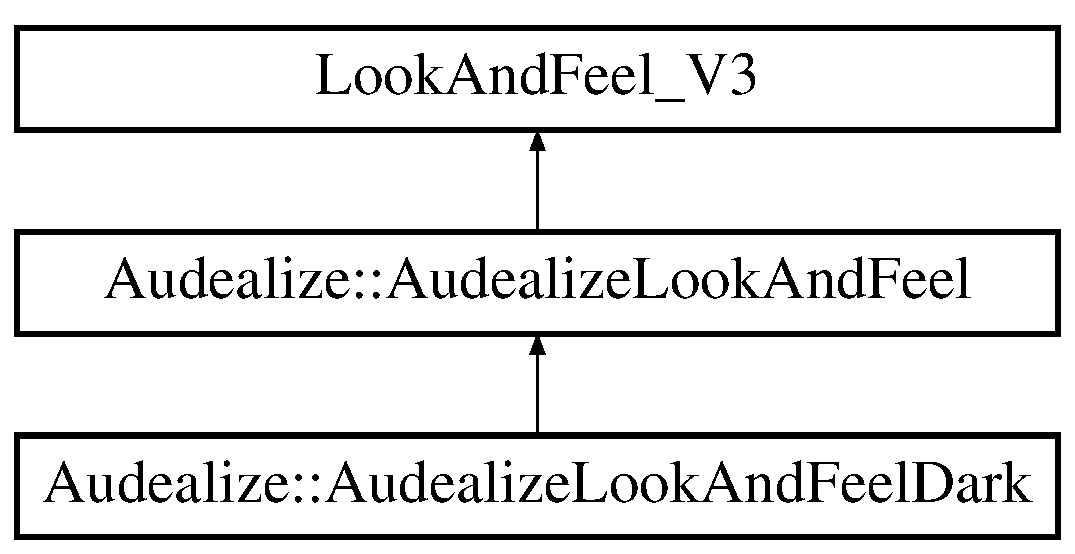
\includegraphics[height=3.000000cm]{class_audealize_1_1_audealize_look_and_feel}
\end{center}
\end{figure}
\subsection*{Public Member Functions}
\begin{DoxyCompactItemize}
\item 
\hyperlink{class_audealize_1_1_audealize_look_and_feel_a157d9f7894bfa68344eacffcf1ad5a3b}{Audealize\+Look\+And\+Feel} ()
\item 
\hyperlink{class_audealize_1_1_audealize_look_and_feel_ac7df5803f0b99f7a1457a51083b3ab4b}{$\sim$\+Audealize\+Look\+And\+Feel} ()
\item 
bool \hyperlink{class_audealize_1_1_audealize_look_and_feel_a01c479960bad8e8d1c323638c6079a53}{is\+Dark\+Mode\+Active} ()
\item 
bool \hyperlink{class_audealize_1_1_audealize_look_and_feel_a342e31b1c34e5589a07481020ee36d20}{will\+Draw\+Outlines} ()
\item 
\hyperlink{tk_8h_aba408b7cd755a96426e004c015f5de8e}{void} \hyperlink{class_audealize_1_1_audealize_look_and_feel_a4a2eef3d96e63217bf12107ed0a886fe}{set\+Outlines} (bool enabled)
\item 
\hyperlink{tk_8h_aba408b7cd755a96426e004c015f5de8e}{void} \hyperlink{class_audealize_1_1_audealize_look_and_feel_a33f411b9ad518d118382fff627b6fd32}{draw\+Tab\+Area\+Behind\+Front\+Button} (Tabbed\+Button\+Bar \&bar, Graphics \&g, const \hyperlink{tk_8h_a83f82f76e7fed06f4c49d2db94028a6d}{int} w, const \hyperlink{tk_8h_a83f82f76e7fed06f4c49d2db94028a6d}{int} h) override
\item 
\hyperlink{tk_8h_aba408b7cd755a96426e004c015f5de8e}{void} \hyperlink{class_audealize_1_1_audealize_look_and_feel_aac0146d30456eae67536f716bb7d9776}{draw\+Tab\+Button} (Tab\+Bar\+Button \&button, Graphics \&g, bool is\+Mouse\+Over, bool is\+Mouse\+Down) override
\item 
\hyperlink{tk_8h_aba408b7cd755a96426e004c015f5de8e}{void} \hyperlink{class_audealize_1_1_audealize_look_and_feel_a152c1f980c72b1287ba02dc1b2dd2b24}{draw\+Button\+Shape} (Graphics \&g, const Path \&\hyperlink{class_audealize_1_1_audealize_look_and_feel_a58cf84e200bd9f7b6f8677c82245d9b9}{outline}, Colour base\+Colour, float \hyperlink{tk_8h_a67be2f4b9d9c5b3559139bfb072e2e81}{height})
\item 
\hyperlink{tk_8h_aba408b7cd755a96426e004c015f5de8e}{void} \hyperlink{class_audealize_1_1_audealize_look_and_feel_a935f07ee09a1c4e1252515d789aebde7}{draw\+Button\+Background} (Graphics \&g, Button \&button, const Colour \&background\+Colour, bool is\+Mouse\+Over\+Button, bool is\+Button\+Down) override
\item 
\hyperlink{tk_8h_aba408b7cd755a96426e004c015f5de8e}{void} \hyperlink{class_audealize_1_1_audealize_look_and_feel_a259295272bbe8d0519e613095b11969f}{draw\+Tick\+Box} (Graphics \&g, Component \&component, float \hyperlink{tk_8h_a61ebd54d47cc56787649a3b8f126bda1}{x}, float \hyperlink{tk_8h_a40f4f3601c0eaa8ca46b1a164264696d}{y}, float w, float h, const bool ticked, const bool is\+Enabled, const bool is\+Mouse\+Over\+Button, const bool is\+Button\+Down) override
\item 
\hyperlink{tk_8h_aba408b7cd755a96426e004c015f5de8e}{void} \hyperlink{class_audealize_1_1_audealize_look_and_feel_a576ee093c7ed4b816d113b0ec330412a}{draw\+Linear\+Slider\+Thumb} (Graphics \&g, \hyperlink{tk_8h_a83f82f76e7fed06f4c49d2db94028a6d}{int} \hyperlink{tk_8h_a61ebd54d47cc56787649a3b8f126bda1}{x}, \hyperlink{tk_8h_a83f82f76e7fed06f4c49d2db94028a6d}{int} \hyperlink{tk_8h_a40f4f3601c0eaa8ca46b1a164264696d}{y}, \hyperlink{tk_8h_a83f82f76e7fed06f4c49d2db94028a6d}{int} \hyperlink{tk_8h_a29e50a5401c1396b3a2aa3487f74d468}{width}, \hyperlink{tk_8h_a83f82f76e7fed06f4c49d2db94028a6d}{int} \hyperlink{tk_8h_a67be2f4b9d9c5b3559139bfb072e2e81}{height}, float slider\+Pos, float min\+Slider\+Pos, float max\+Slider\+Pos, const Slider\+::\+Slider\+Style style, Slider \&slider) override
\item 
\hyperlink{tk_8h_aba408b7cd755a96426e004c015f5de8e}{void} \hyperlink{class_audealize_1_1_audealize_look_and_feel_ab7b6c57db22006140a1f94a7f98f8924}{draw\+Linear\+Slider\+Background} (Graphics \&g, \hyperlink{tk_8h_a83f82f76e7fed06f4c49d2db94028a6d}{int} \hyperlink{tk_8h_a61ebd54d47cc56787649a3b8f126bda1}{x}, \hyperlink{tk_8h_a83f82f76e7fed06f4c49d2db94028a6d}{int} \hyperlink{tk_8h_a40f4f3601c0eaa8ca46b1a164264696d}{y}, \hyperlink{tk_8h_a83f82f76e7fed06f4c49d2db94028a6d}{int} \hyperlink{tk_8h_a29e50a5401c1396b3a2aa3487f74d468}{width}, \hyperlink{tk_8h_a83f82f76e7fed06f4c49d2db94028a6d}{int} \hyperlink{tk_8h_a67be2f4b9d9c5b3559139bfb072e2e81}{height}, float, float, float, const Slider\+::\+Slider\+Style, Slider \&slider) override
\item 
\hyperlink{tk_8h_aba408b7cd755a96426e004c015f5de8e}{void} \hyperlink{class_audealize_1_1_audealize_look_and_feel_a9d3000b1c7346202c12983718f0e8a10}{draw\+Linear\+Slider} (Graphics \&g, \hyperlink{tk_8h_a83f82f76e7fed06f4c49d2db94028a6d}{int} \hyperlink{tk_8h_a61ebd54d47cc56787649a3b8f126bda1}{x}, \hyperlink{tk_8h_a83f82f76e7fed06f4c49d2db94028a6d}{int} \hyperlink{tk_8h_a40f4f3601c0eaa8ca46b1a164264696d}{y}, \hyperlink{tk_8h_a83f82f76e7fed06f4c49d2db94028a6d}{int} \hyperlink{tk_8h_a29e50a5401c1396b3a2aa3487f74d468}{width}, \hyperlink{tk_8h_a83f82f76e7fed06f4c49d2db94028a6d}{int} \hyperlink{tk_8h_a67be2f4b9d9c5b3559139bfb072e2e81}{height}, float slider\+Pos, float min\+Slider\+Pos, float max\+Slider\+Pos, const Slider\+::\+Slider\+Style style, Slider \&slider) override
\item 
\hyperlink{tk_8h_aba408b7cd755a96426e004c015f5de8e}{void} \hyperlink{class_audealize_1_1_audealize_look_and_feel_a499afecdf56503cf84ba32e513dc5641}{draw\+Rotary\+Slider} (Graphics \&g, \hyperlink{tk_8h_a83f82f76e7fed06f4c49d2db94028a6d}{int} \hyperlink{tk_8h_a61ebd54d47cc56787649a3b8f126bda1}{x}, \hyperlink{tk_8h_a83f82f76e7fed06f4c49d2db94028a6d}{int} \hyperlink{tk_8h_a40f4f3601c0eaa8ca46b1a164264696d}{y}, \hyperlink{tk_8h_a83f82f76e7fed06f4c49d2db94028a6d}{int} \hyperlink{tk_8h_a29e50a5401c1396b3a2aa3487f74d468}{width}, \hyperlink{tk_8h_a83f82f76e7fed06f4c49d2db94028a6d}{int} \hyperlink{tk_8h_a67be2f4b9d9c5b3559139bfb072e2e81}{height}, float slider\+Pos, const float rotary\+Start\+Angle, const float rotary\+End\+Angle, Slider \&slider) override
\item 
\hyperlink{tk_8h_aba408b7cd755a96426e004c015f5de8e}{void} \hyperlink{class_audealize_1_1_audealize_look_and_feel_af6bc9337802f4e7d45e7317272beae74}{draw\+Rotary\+Slider\+Centered} (Graphics \&g, \hyperlink{tk_8h_a83f82f76e7fed06f4c49d2db94028a6d}{int} \hyperlink{tk_8h_a61ebd54d47cc56787649a3b8f126bda1}{x}, \hyperlink{tk_8h_a83f82f76e7fed06f4c49d2db94028a6d}{int} \hyperlink{tk_8h_a40f4f3601c0eaa8ca46b1a164264696d}{y}, \hyperlink{tk_8h_a83f82f76e7fed06f4c49d2db94028a6d}{int} \hyperlink{tk_8h_a29e50a5401c1396b3a2aa3487f74d468}{width}, \hyperlink{tk_8h_a83f82f76e7fed06f4c49d2db94028a6d}{int} \hyperlink{tk_8h_a67be2f4b9d9c5b3559139bfb072e2e81}{height}, float slider\+Pos, const float rotary\+Start\+Angle, const float rotary\+End\+Angle, Slider \&slider)
\item 
\hyperlink{tk_8h_aba408b7cd755a96426e004c015f5de8e}{void} \hyperlink{class_audealize_1_1_audealize_look_and_feel_ac6fbb1cbd9835cda592405c3d6bfbbe0}{draw\+Corner\+Resizer} (Graphics \&g, \hyperlink{tk_8h_a83f82f76e7fed06f4c49d2db94028a6d}{int} w, \hyperlink{tk_8h_a83f82f76e7fed06f4c49d2db94028a6d}{int} h, bool, bool) override
\item 
\hyperlink{tk_8h_aba408b7cd755a96426e004c015f5de8e}{void} \hyperlink{class_audealize_1_1_audealize_look_and_feel_ad54c6fe23f965ec0658f591b8c4875d2}{draw\+Text\+Editor\+Outline} (Graphics \&g, \hyperlink{tk_8h_a83f82f76e7fed06f4c49d2db94028a6d}{int} \hyperlink{tk_8h_a29e50a5401c1396b3a2aa3487f74d468}{width}, \hyperlink{tk_8h_a83f82f76e7fed06f4c49d2db94028a6d}{int} \hyperlink{tk_8h_a67be2f4b9d9c5b3559139bfb072e2e81}{height}, Text\+Editor \&text\+Editor) override
\item 
\hyperlink{tk_8h_a83f82f76e7fed06f4c49d2db94028a6d}{int} \hyperlink{class_audealize_1_1_audealize_look_and_feel_a06dea0eade1a0d91363be0587189a740}{get\+Tab\+Button\+Overlap} (\hyperlink{tk_8h_a83f82f76e7fed06f4c49d2db94028a6d}{int}) override
\item 
\hyperlink{tk_8h_a83f82f76e7fed06f4c49d2db94028a6d}{int} \hyperlink{class_audealize_1_1_audealize_look_and_feel_a065a60ac311f37f2961e1a730002f286}{get\+Tab\+Button\+Space\+Around\+Image} () override
\item 
\hyperlink{tk_8h_a83f82f76e7fed06f4c49d2db94028a6d}{int} \hyperlink{class_audealize_1_1_audealize_look_and_feel_a07ad47fae31adfbba2da2c32ce1d9a2f}{get\+Tab\+Button\+Best\+Width} (Tab\+Bar\+Button \&button, \hyperlink{tk_8h_a83f82f76e7fed06f4c49d2db94028a6d}{int} tab\+Depth) override
\item 
\hyperlink{tk_8h_aba408b7cd755a96426e004c015f5de8e}{void} \hyperlink{class_audealize_1_1_audealize_look_and_feel_a40911e2845c867d1cae029381fb3e549}{create\+Tab\+Text\+Layout} (const Tab\+Bar\+Button \&button, float length, float depth, Colour colour, Text\+Layout \&text\+Layout)
\item 
\hyperlink{wngrind_8h_a5a194e58b8cdf07d26c5155458b894e5}{Typeface\+::\+Ptr} \hyperlink{class_audealize_1_1_audealize_look_and_feel_ab4c1fd338f94c2805ff2cd2c74693340}{get\+Typeface\+For\+Font} (const Font \&font) override
\end{DoxyCompactItemize}
\subsection*{Protected Member Functions}
\begin{DoxyCompactItemize}
\item 
\hyperlink{class_audealize_1_1_audealize_look_and_feel_a13d4fd771a8b1b529d40d16638dff301}{J\+U\+C\+E\+\_\+\+D\+E\+C\+L\+A\+R\+E\+\_\+\+N\+O\+N\+\_\+\+C\+O\+P\+Y\+A\+B\+L\+E\+\_\+\+W\+I\+T\+H\+\_\+\+L\+E\+A\+K\+\_\+\+D\+E\+T\+E\+C\+T\+OR} (\hyperlink{class_audealize_1_1_audealize_look_and_feel}{Audealize\+Look\+And\+Feel})
\end{DoxyCompactItemize}
\subsection*{Protected Attributes}
\begin{DoxyCompactItemize}
\item 
bool \hyperlink{class_audealize_1_1_audealize_look_and_feel_abf69c4abd23d537b60d64affb4043239}{is\+Dark\+Mode}
\item 
bool \hyperlink{class_audealize_1_1_audealize_look_and_feel_a07cd4432ef608356358e0cf9bc7c023d}{should\+Draw\+Outlines}
\item 
Colour \hyperlink{class_audealize_1_1_audealize_look_and_feel_a58cf84e200bd9f7b6f8677c82245d9b9}{outline}
\item 
Colour \hyperlink{class_audealize_1_1_audealize_look_and_feel_aaf004191d1a34a05f02bf31a24bc2865}{tick\+Box\+Fill}
\end{DoxyCompactItemize}


\subsection{Constructor \& Destructor Documentation}
\index{Audealize\+::\+Audealize\+Look\+And\+Feel@{Audealize\+::\+Audealize\+Look\+And\+Feel}!Audealize\+Look\+And\+Feel@{Audealize\+Look\+And\+Feel}}
\index{Audealize\+Look\+And\+Feel@{Audealize\+Look\+And\+Feel}!Audealize\+::\+Audealize\+Look\+And\+Feel@{Audealize\+::\+Audealize\+Look\+And\+Feel}}
\subsubsection[{\texorpdfstring{Audealize\+Look\+And\+Feel()}{AudealizeLookAndFeel()}}]{\setlength{\rightskip}{0pt plus 5cm}Audealize\+::\+Audealize\+Look\+And\+Feel\+::\+Audealize\+Look\+And\+Feel (
\begin{DoxyParamCaption}
{}
\end{DoxyParamCaption}
)}\hypertarget{class_audealize_1_1_audealize_look_and_feel_a157d9f7894bfa68344eacffcf1ad5a3b}{}\label{class_audealize_1_1_audealize_look_and_feel_a157d9f7894bfa68344eacffcf1ad5a3b}
\index{Audealize\+::\+Audealize\+Look\+And\+Feel@{Audealize\+::\+Audealize\+Look\+And\+Feel}!````~Audealize\+Look\+And\+Feel@{$\sim$\+Audealize\+Look\+And\+Feel}}
\index{````~Audealize\+Look\+And\+Feel@{$\sim$\+Audealize\+Look\+And\+Feel}!Audealize\+::\+Audealize\+Look\+And\+Feel@{Audealize\+::\+Audealize\+Look\+And\+Feel}}
\subsubsection[{\texorpdfstring{$\sim$\+Audealize\+Look\+And\+Feel()}{~AudealizeLookAndFeel()}}]{\setlength{\rightskip}{0pt plus 5cm}Audealize\+::\+Audealize\+Look\+And\+Feel\+::$\sim$\+Audealize\+Look\+And\+Feel (
\begin{DoxyParamCaption}
{}
\end{DoxyParamCaption}
)}\hypertarget{class_audealize_1_1_audealize_look_and_feel_ac7df5803f0b99f7a1457a51083b3ab4b}{}\label{class_audealize_1_1_audealize_look_and_feel_ac7df5803f0b99f7a1457a51083b3ab4b}


\subsection{Member Function Documentation}
\index{Audealize\+::\+Audealize\+Look\+And\+Feel@{Audealize\+::\+Audealize\+Look\+And\+Feel}!create\+Tab\+Text\+Layout@{create\+Tab\+Text\+Layout}}
\index{create\+Tab\+Text\+Layout@{create\+Tab\+Text\+Layout}!Audealize\+::\+Audealize\+Look\+And\+Feel@{Audealize\+::\+Audealize\+Look\+And\+Feel}}
\subsubsection[{\texorpdfstring{create\+Tab\+Text\+Layout(const Tab\+Bar\+Button \&button, float length, float depth, Colour colour, Text\+Layout \&text\+Layout)}{createTabTextLayout(const TabBarButton &button, float length, float depth, Colour colour, TextLayout &textLayout)}}]{\setlength{\rightskip}{0pt plus 5cm}{\bf void} Audealize\+::\+Audealize\+Look\+And\+Feel\+::create\+Tab\+Text\+Layout (
\begin{DoxyParamCaption}
\item[{const Tab\+Bar\+Button \&}]{button, }
\item[{float}]{length, }
\item[{float}]{depth, }
\item[{Colour}]{colour, }
\item[{Text\+Layout \&}]{text\+Layout}
\end{DoxyParamCaption}
)}\hypertarget{class_audealize_1_1_audealize_look_and_feel_a40911e2845c867d1cae029381fb3e549}{}\label{class_audealize_1_1_audealize_look_and_feel_a40911e2845c867d1cae029381fb3e549}
\index{Audealize\+::\+Audealize\+Look\+And\+Feel@{Audealize\+::\+Audealize\+Look\+And\+Feel}!draw\+Button\+Background@{draw\+Button\+Background}}
\index{draw\+Button\+Background@{draw\+Button\+Background}!Audealize\+::\+Audealize\+Look\+And\+Feel@{Audealize\+::\+Audealize\+Look\+And\+Feel}}
\subsubsection[{\texorpdfstring{draw\+Button\+Background(\+Graphics \&g, Button \&button, const Colour \&background\+Colour, bool is\+Mouse\+Over\+Button, bool is\+Button\+Down) override}{drawButtonBackground(Graphics &g, Button &button, const Colour &backgroundColour, bool isMouseOverButton, bool isButtonDown) override}}]{\setlength{\rightskip}{0pt plus 5cm}{\bf void} Audealize\+::\+Audealize\+Look\+And\+Feel\+::draw\+Button\+Background (
\begin{DoxyParamCaption}
\item[{Graphics \&}]{g, }
\item[{Button \&}]{button, }
\item[{const Colour \&}]{background\+Colour, }
\item[{bool}]{is\+Mouse\+Over\+Button, }
\item[{bool}]{is\+Button\+Down}
\end{DoxyParamCaption}
)\hspace{0.3cm}{\ttfamily [override]}}\hypertarget{class_audealize_1_1_audealize_look_and_feel_a935f07ee09a1c4e1252515d789aebde7}{}\label{class_audealize_1_1_audealize_look_and_feel_a935f07ee09a1c4e1252515d789aebde7}
\index{Audealize\+::\+Audealize\+Look\+And\+Feel@{Audealize\+::\+Audealize\+Look\+And\+Feel}!draw\+Button\+Shape@{draw\+Button\+Shape}}
\index{draw\+Button\+Shape@{draw\+Button\+Shape}!Audealize\+::\+Audealize\+Look\+And\+Feel@{Audealize\+::\+Audealize\+Look\+And\+Feel}}
\subsubsection[{\texorpdfstring{draw\+Button\+Shape(\+Graphics \&g, const Path \&outline, Colour base\+Colour, float height)}{drawButtonShape(Graphics &g, const Path &outline, Colour baseColour, float height)}}]{\setlength{\rightskip}{0pt plus 5cm}{\bf void} Audealize\+::\+Audealize\+Look\+And\+Feel\+::draw\+Button\+Shape (
\begin{DoxyParamCaption}
\item[{Graphics \&}]{g, }
\item[{const Path \&}]{outline, }
\item[{Colour}]{base\+Colour, }
\item[{float}]{height}
\end{DoxyParamCaption}
)}\hypertarget{class_audealize_1_1_audealize_look_and_feel_a152c1f980c72b1287ba02dc1b2dd2b24}{}\label{class_audealize_1_1_audealize_look_and_feel_a152c1f980c72b1287ba02dc1b2dd2b24}
\index{Audealize\+::\+Audealize\+Look\+And\+Feel@{Audealize\+::\+Audealize\+Look\+And\+Feel}!draw\+Corner\+Resizer@{draw\+Corner\+Resizer}}
\index{draw\+Corner\+Resizer@{draw\+Corner\+Resizer}!Audealize\+::\+Audealize\+Look\+And\+Feel@{Audealize\+::\+Audealize\+Look\+And\+Feel}}
\subsubsection[{\texorpdfstring{draw\+Corner\+Resizer(\+Graphics \&g, int w, int h, bool, bool) override}{drawCornerResizer(Graphics &g, int w, int h, bool, bool) override}}]{\setlength{\rightskip}{0pt plus 5cm}{\bf void} Audealize\+::\+Audealize\+Look\+And\+Feel\+::draw\+Corner\+Resizer (
\begin{DoxyParamCaption}
\item[{Graphics \&}]{g, }
\item[{{\bf int}}]{w, }
\item[{{\bf int}}]{h, }
\item[{bool}]{, }
\item[{bool}]{}
\end{DoxyParamCaption}
)\hspace{0.3cm}{\ttfamily [override]}}\hypertarget{class_audealize_1_1_audealize_look_and_feel_ac6fbb1cbd9835cda592405c3d6bfbbe0}{}\label{class_audealize_1_1_audealize_look_and_feel_ac6fbb1cbd9835cda592405c3d6bfbbe0}
\index{Audealize\+::\+Audealize\+Look\+And\+Feel@{Audealize\+::\+Audealize\+Look\+And\+Feel}!draw\+Linear\+Slider@{draw\+Linear\+Slider}}
\index{draw\+Linear\+Slider@{draw\+Linear\+Slider}!Audealize\+::\+Audealize\+Look\+And\+Feel@{Audealize\+::\+Audealize\+Look\+And\+Feel}}
\subsubsection[{\texorpdfstring{draw\+Linear\+Slider(\+Graphics \&g, int x, int y, int width, int height, float slider\+Pos, float min\+Slider\+Pos, float max\+Slider\+Pos, const Slider\+::\+Slider\+Style style, Slider \&slider) override}{drawLinearSlider(Graphics &g, int x, int y, int width, int height, float sliderPos, float minSliderPos, float maxSliderPos, const Slider::SliderStyle style, Slider &slider) override}}]{\setlength{\rightskip}{0pt plus 5cm}{\bf void} Audealize\+::\+Audealize\+Look\+And\+Feel\+::draw\+Linear\+Slider (
\begin{DoxyParamCaption}
\item[{Graphics \&}]{g, }
\item[{{\bf int}}]{x, }
\item[{{\bf int}}]{y, }
\item[{{\bf int}}]{width, }
\item[{{\bf int}}]{height, }
\item[{float}]{slider\+Pos, }
\item[{float}]{min\+Slider\+Pos, }
\item[{float}]{max\+Slider\+Pos, }
\item[{const Slider\+::\+Slider\+Style}]{style, }
\item[{Slider \&}]{slider}
\end{DoxyParamCaption}
)\hspace{0.3cm}{\ttfamily [override]}}\hypertarget{class_audealize_1_1_audealize_look_and_feel_a9d3000b1c7346202c12983718f0e8a10}{}\label{class_audealize_1_1_audealize_look_and_feel_a9d3000b1c7346202c12983718f0e8a10}
\index{Audealize\+::\+Audealize\+Look\+And\+Feel@{Audealize\+::\+Audealize\+Look\+And\+Feel}!draw\+Linear\+Slider\+Background@{draw\+Linear\+Slider\+Background}}
\index{draw\+Linear\+Slider\+Background@{draw\+Linear\+Slider\+Background}!Audealize\+::\+Audealize\+Look\+And\+Feel@{Audealize\+::\+Audealize\+Look\+And\+Feel}}
\subsubsection[{\texorpdfstring{draw\+Linear\+Slider\+Background(\+Graphics \&g, int x, int y, int width, int height, float, float, float, const Slider\+::\+Slider\+Style, Slider \&slider) override}{drawLinearSliderBackground(Graphics &g, int x, int y, int width, int height, float, float, float, const Slider::SliderStyle, Slider &slider) override}}]{\setlength{\rightskip}{0pt plus 5cm}{\bf void} Audealize\+::\+Audealize\+Look\+And\+Feel\+::draw\+Linear\+Slider\+Background (
\begin{DoxyParamCaption}
\item[{Graphics \&}]{g, }
\item[{{\bf int}}]{x, }
\item[{{\bf int}}]{y, }
\item[{{\bf int}}]{width, }
\item[{{\bf int}}]{height, }
\item[{float}]{, }
\item[{float}]{, }
\item[{float}]{, }
\item[{const Slider\+::\+Slider\+Style}]{, }
\item[{Slider \&}]{slider}
\end{DoxyParamCaption}
)\hspace{0.3cm}{\ttfamily [override]}}\hypertarget{class_audealize_1_1_audealize_look_and_feel_ab7b6c57db22006140a1f94a7f98f8924}{}\label{class_audealize_1_1_audealize_look_and_feel_ab7b6c57db22006140a1f94a7f98f8924}
\index{Audealize\+::\+Audealize\+Look\+And\+Feel@{Audealize\+::\+Audealize\+Look\+And\+Feel}!draw\+Linear\+Slider\+Thumb@{draw\+Linear\+Slider\+Thumb}}
\index{draw\+Linear\+Slider\+Thumb@{draw\+Linear\+Slider\+Thumb}!Audealize\+::\+Audealize\+Look\+And\+Feel@{Audealize\+::\+Audealize\+Look\+And\+Feel}}
\subsubsection[{\texorpdfstring{draw\+Linear\+Slider\+Thumb(\+Graphics \&g, int x, int y, int width, int height, float slider\+Pos, float min\+Slider\+Pos, float max\+Slider\+Pos, const Slider\+::\+Slider\+Style style, Slider \&slider) override}{drawLinearSliderThumb(Graphics &g, int x, int y, int width, int height, float sliderPos, float minSliderPos, float maxSliderPos, const Slider::SliderStyle style, Slider &slider) override}}]{\setlength{\rightskip}{0pt plus 5cm}{\bf void} Audealize\+::\+Audealize\+Look\+And\+Feel\+::draw\+Linear\+Slider\+Thumb (
\begin{DoxyParamCaption}
\item[{Graphics \&}]{g, }
\item[{{\bf int}}]{x, }
\item[{{\bf int}}]{y, }
\item[{{\bf int}}]{width, }
\item[{{\bf int}}]{height, }
\item[{float}]{slider\+Pos, }
\item[{float}]{min\+Slider\+Pos, }
\item[{float}]{max\+Slider\+Pos, }
\item[{const Slider\+::\+Slider\+Style}]{style, }
\item[{Slider \&}]{slider}
\end{DoxyParamCaption}
)\hspace{0.3cm}{\ttfamily [override]}}\hypertarget{class_audealize_1_1_audealize_look_and_feel_a576ee093c7ed4b816d113b0ec330412a}{}\label{class_audealize_1_1_audealize_look_and_feel_a576ee093c7ed4b816d113b0ec330412a}
\index{Audealize\+::\+Audealize\+Look\+And\+Feel@{Audealize\+::\+Audealize\+Look\+And\+Feel}!draw\+Rotary\+Slider@{draw\+Rotary\+Slider}}
\index{draw\+Rotary\+Slider@{draw\+Rotary\+Slider}!Audealize\+::\+Audealize\+Look\+And\+Feel@{Audealize\+::\+Audealize\+Look\+And\+Feel}}
\subsubsection[{\texorpdfstring{draw\+Rotary\+Slider(\+Graphics \&g, int x, int y, int width, int height, float slider\+Pos, const float rotary\+Start\+Angle, const float rotary\+End\+Angle, Slider \&slider) override}{drawRotarySlider(Graphics &g, int x, int y, int width, int height, float sliderPos, const float rotaryStartAngle, const float rotaryEndAngle, Slider &slider) override}}]{\setlength{\rightskip}{0pt plus 5cm}{\bf void} Audealize\+::\+Audealize\+Look\+And\+Feel\+::draw\+Rotary\+Slider (
\begin{DoxyParamCaption}
\item[{Graphics \&}]{g, }
\item[{{\bf int}}]{x, }
\item[{{\bf int}}]{y, }
\item[{{\bf int}}]{width, }
\item[{{\bf int}}]{height, }
\item[{float}]{slider\+Pos, }
\item[{const float}]{rotary\+Start\+Angle, }
\item[{const float}]{rotary\+End\+Angle, }
\item[{Slider \&}]{slider}
\end{DoxyParamCaption}
)\hspace{0.3cm}{\ttfamily [override]}}\hypertarget{class_audealize_1_1_audealize_look_and_feel_a499afecdf56503cf84ba32e513dc5641}{}\label{class_audealize_1_1_audealize_look_and_feel_a499afecdf56503cf84ba32e513dc5641}
\index{Audealize\+::\+Audealize\+Look\+And\+Feel@{Audealize\+::\+Audealize\+Look\+And\+Feel}!draw\+Rotary\+Slider\+Centered@{draw\+Rotary\+Slider\+Centered}}
\index{draw\+Rotary\+Slider\+Centered@{draw\+Rotary\+Slider\+Centered}!Audealize\+::\+Audealize\+Look\+And\+Feel@{Audealize\+::\+Audealize\+Look\+And\+Feel}}
\subsubsection[{\texorpdfstring{draw\+Rotary\+Slider\+Centered(\+Graphics \&g, int x, int y, int width, int height, float slider\+Pos, const float rotary\+Start\+Angle, const float rotary\+End\+Angle, Slider \&slider)}{drawRotarySliderCentered(Graphics &g, int x, int y, int width, int height, float sliderPos, const float rotaryStartAngle, const float rotaryEndAngle, Slider &slider)}}]{\setlength{\rightskip}{0pt plus 5cm}{\bf void} Audealize\+::\+Audealize\+Look\+And\+Feel\+::draw\+Rotary\+Slider\+Centered (
\begin{DoxyParamCaption}
\item[{Graphics \&}]{g, }
\item[{{\bf int}}]{x, }
\item[{{\bf int}}]{y, }
\item[{{\bf int}}]{width, }
\item[{{\bf int}}]{height, }
\item[{float}]{slider\+Pos, }
\item[{const float}]{rotary\+Start\+Angle, }
\item[{const float}]{rotary\+End\+Angle, }
\item[{Slider \&}]{slider}
\end{DoxyParamCaption}
)}\hypertarget{class_audealize_1_1_audealize_look_and_feel_af6bc9337802f4e7d45e7317272beae74}{}\label{class_audealize_1_1_audealize_look_and_feel_af6bc9337802f4e7d45e7317272beae74}
\index{Audealize\+::\+Audealize\+Look\+And\+Feel@{Audealize\+::\+Audealize\+Look\+And\+Feel}!draw\+Tab\+Area\+Behind\+Front\+Button@{draw\+Tab\+Area\+Behind\+Front\+Button}}
\index{draw\+Tab\+Area\+Behind\+Front\+Button@{draw\+Tab\+Area\+Behind\+Front\+Button}!Audealize\+::\+Audealize\+Look\+And\+Feel@{Audealize\+::\+Audealize\+Look\+And\+Feel}}
\subsubsection[{\texorpdfstring{draw\+Tab\+Area\+Behind\+Front\+Button(\+Tabbed\+Button\+Bar \&bar, Graphics \&g, const int w, const int h) override}{drawTabAreaBehindFrontButton(TabbedButtonBar &bar, Graphics &g, const int w, const int h) override}}]{\setlength{\rightskip}{0pt plus 5cm}{\bf void} Audealize\+::\+Audealize\+Look\+And\+Feel\+::draw\+Tab\+Area\+Behind\+Front\+Button (
\begin{DoxyParamCaption}
\item[{Tabbed\+Button\+Bar \&}]{bar, }
\item[{Graphics \&}]{g, }
\item[{const {\bf int}}]{w, }
\item[{const {\bf int}}]{h}
\end{DoxyParamCaption}
)\hspace{0.3cm}{\ttfamily [override]}}\hypertarget{class_audealize_1_1_audealize_look_and_feel_a33f411b9ad518d118382fff627b6fd32}{}\label{class_audealize_1_1_audealize_look_and_feel_a33f411b9ad518d118382fff627b6fd32}
\index{Audealize\+::\+Audealize\+Look\+And\+Feel@{Audealize\+::\+Audealize\+Look\+And\+Feel}!draw\+Tab\+Button@{draw\+Tab\+Button}}
\index{draw\+Tab\+Button@{draw\+Tab\+Button}!Audealize\+::\+Audealize\+Look\+And\+Feel@{Audealize\+::\+Audealize\+Look\+And\+Feel}}
\subsubsection[{\texorpdfstring{draw\+Tab\+Button(\+Tab\+Bar\+Button \&button, Graphics \&g, bool is\+Mouse\+Over, bool is\+Mouse\+Down) override}{drawTabButton(TabBarButton &button, Graphics &g, bool isMouseOver, bool isMouseDown) override}}]{\setlength{\rightskip}{0pt plus 5cm}{\bf void} Audealize\+::\+Audealize\+Look\+And\+Feel\+::draw\+Tab\+Button (
\begin{DoxyParamCaption}
\item[{Tab\+Bar\+Button \&}]{button, }
\item[{Graphics \&}]{g, }
\item[{bool}]{is\+Mouse\+Over, }
\item[{bool}]{is\+Mouse\+Down}
\end{DoxyParamCaption}
)\hspace{0.3cm}{\ttfamily [override]}}\hypertarget{class_audealize_1_1_audealize_look_and_feel_aac0146d30456eae67536f716bb7d9776}{}\label{class_audealize_1_1_audealize_look_and_feel_aac0146d30456eae67536f716bb7d9776}
\index{Audealize\+::\+Audealize\+Look\+And\+Feel@{Audealize\+::\+Audealize\+Look\+And\+Feel}!draw\+Text\+Editor\+Outline@{draw\+Text\+Editor\+Outline}}
\index{draw\+Text\+Editor\+Outline@{draw\+Text\+Editor\+Outline}!Audealize\+::\+Audealize\+Look\+And\+Feel@{Audealize\+::\+Audealize\+Look\+And\+Feel}}
\subsubsection[{\texorpdfstring{draw\+Text\+Editor\+Outline(\+Graphics \&g, int width, int height, Text\+Editor \&text\+Editor) override}{drawTextEditorOutline(Graphics &g, int width, int height, TextEditor &textEditor) override}}]{\setlength{\rightskip}{0pt plus 5cm}{\bf void} Audealize\+::\+Audealize\+Look\+And\+Feel\+::draw\+Text\+Editor\+Outline (
\begin{DoxyParamCaption}
\item[{Graphics \&}]{g, }
\item[{{\bf int}}]{width, }
\item[{{\bf int}}]{height, }
\item[{Text\+Editor \&}]{text\+Editor}
\end{DoxyParamCaption}
)\hspace{0.3cm}{\ttfamily [override]}}\hypertarget{class_audealize_1_1_audealize_look_and_feel_ad54c6fe23f965ec0658f591b8c4875d2}{}\label{class_audealize_1_1_audealize_look_and_feel_ad54c6fe23f965ec0658f591b8c4875d2}
\index{Audealize\+::\+Audealize\+Look\+And\+Feel@{Audealize\+::\+Audealize\+Look\+And\+Feel}!draw\+Tick\+Box@{draw\+Tick\+Box}}
\index{draw\+Tick\+Box@{draw\+Tick\+Box}!Audealize\+::\+Audealize\+Look\+And\+Feel@{Audealize\+::\+Audealize\+Look\+And\+Feel}}
\subsubsection[{\texorpdfstring{draw\+Tick\+Box(\+Graphics \&g, Component \&component, float x, float y, float w, float h, const bool ticked, const bool is\+Enabled, const bool is\+Mouse\+Over\+Button, const bool is\+Button\+Down) override}{drawTickBox(Graphics &g, Component &component, float x, float y, float w, float h, const bool ticked, const bool isEnabled, const bool isMouseOverButton, const bool isButtonDown) override}}]{\setlength{\rightskip}{0pt plus 5cm}{\bf void} Audealize\+::\+Audealize\+Look\+And\+Feel\+::draw\+Tick\+Box (
\begin{DoxyParamCaption}
\item[{Graphics \&}]{g, }
\item[{Component \&}]{component, }
\item[{float}]{x, }
\item[{float}]{y, }
\item[{float}]{w, }
\item[{float}]{h, }
\item[{const bool}]{ticked, }
\item[{const bool}]{is\+Enabled, }
\item[{const bool}]{is\+Mouse\+Over\+Button, }
\item[{const bool}]{is\+Button\+Down}
\end{DoxyParamCaption}
)\hspace{0.3cm}{\ttfamily [override]}}\hypertarget{class_audealize_1_1_audealize_look_and_feel_a259295272bbe8d0519e613095b11969f}{}\label{class_audealize_1_1_audealize_look_and_feel_a259295272bbe8d0519e613095b11969f}
\index{Audealize\+::\+Audealize\+Look\+And\+Feel@{Audealize\+::\+Audealize\+Look\+And\+Feel}!get\+Tab\+Button\+Best\+Width@{get\+Tab\+Button\+Best\+Width}}
\index{get\+Tab\+Button\+Best\+Width@{get\+Tab\+Button\+Best\+Width}!Audealize\+::\+Audealize\+Look\+And\+Feel@{Audealize\+::\+Audealize\+Look\+And\+Feel}}
\subsubsection[{\texorpdfstring{get\+Tab\+Button\+Best\+Width(\+Tab\+Bar\+Button \&button, int tab\+Depth) override}{getTabButtonBestWidth(TabBarButton &button, int tabDepth) override}}]{\setlength{\rightskip}{0pt plus 5cm}{\bf int} Audealize\+::\+Audealize\+Look\+And\+Feel\+::get\+Tab\+Button\+Best\+Width (
\begin{DoxyParamCaption}
\item[{Tab\+Bar\+Button \&}]{button, }
\item[{{\bf int}}]{tab\+Depth}
\end{DoxyParamCaption}
)\hspace{0.3cm}{\ttfamily [override]}}\hypertarget{class_audealize_1_1_audealize_look_and_feel_a07ad47fae31adfbba2da2c32ce1d9a2f}{}\label{class_audealize_1_1_audealize_look_and_feel_a07ad47fae31adfbba2da2c32ce1d9a2f}
\index{Audealize\+::\+Audealize\+Look\+And\+Feel@{Audealize\+::\+Audealize\+Look\+And\+Feel}!get\+Tab\+Button\+Overlap@{get\+Tab\+Button\+Overlap}}
\index{get\+Tab\+Button\+Overlap@{get\+Tab\+Button\+Overlap}!Audealize\+::\+Audealize\+Look\+And\+Feel@{Audealize\+::\+Audealize\+Look\+And\+Feel}}
\subsubsection[{\texorpdfstring{get\+Tab\+Button\+Overlap(int) override}{getTabButtonOverlap(int) override}}]{\setlength{\rightskip}{0pt plus 5cm}{\bf int} Audealize\+::\+Audealize\+Look\+And\+Feel\+::get\+Tab\+Button\+Overlap (
\begin{DoxyParamCaption}
\item[{{\bf int}}]{}
\end{DoxyParamCaption}
)\hspace{0.3cm}{\ttfamily [inline]}, {\ttfamily [override]}}\hypertarget{class_audealize_1_1_audealize_look_and_feel_a06dea0eade1a0d91363be0587189a740}{}\label{class_audealize_1_1_audealize_look_and_feel_a06dea0eade1a0d91363be0587189a740}
\index{Audealize\+::\+Audealize\+Look\+And\+Feel@{Audealize\+::\+Audealize\+Look\+And\+Feel}!get\+Tab\+Button\+Space\+Around\+Image@{get\+Tab\+Button\+Space\+Around\+Image}}
\index{get\+Tab\+Button\+Space\+Around\+Image@{get\+Tab\+Button\+Space\+Around\+Image}!Audealize\+::\+Audealize\+Look\+And\+Feel@{Audealize\+::\+Audealize\+Look\+And\+Feel}}
\subsubsection[{\texorpdfstring{get\+Tab\+Button\+Space\+Around\+Image() override}{getTabButtonSpaceAroundImage() override}}]{\setlength{\rightskip}{0pt plus 5cm}{\bf int} Audealize\+::\+Audealize\+Look\+And\+Feel\+::get\+Tab\+Button\+Space\+Around\+Image (
\begin{DoxyParamCaption}
{}
\end{DoxyParamCaption}
)\hspace{0.3cm}{\ttfamily [inline]}, {\ttfamily [override]}}\hypertarget{class_audealize_1_1_audealize_look_and_feel_a065a60ac311f37f2961e1a730002f286}{}\label{class_audealize_1_1_audealize_look_and_feel_a065a60ac311f37f2961e1a730002f286}
\index{Audealize\+::\+Audealize\+Look\+And\+Feel@{Audealize\+::\+Audealize\+Look\+And\+Feel}!get\+Typeface\+For\+Font@{get\+Typeface\+For\+Font}}
\index{get\+Typeface\+For\+Font@{get\+Typeface\+For\+Font}!Audealize\+::\+Audealize\+Look\+And\+Feel@{Audealize\+::\+Audealize\+Look\+And\+Feel}}
\subsubsection[{\texorpdfstring{get\+Typeface\+For\+Font(const Font \&font) override}{getTypefaceForFont(const Font &font) override}}]{\setlength{\rightskip}{0pt plus 5cm}{\bf Typeface\+::\+Ptr} Audealize\+::\+Audealize\+Look\+And\+Feel\+::get\+Typeface\+For\+Font (
\begin{DoxyParamCaption}
\item[{const Font \&}]{font}
\end{DoxyParamCaption}
)\hspace{0.3cm}{\ttfamily [inline]}, {\ttfamily [override]}}\hypertarget{class_audealize_1_1_audealize_look_and_feel_ab4c1fd338f94c2805ff2cd2c74693340}{}\label{class_audealize_1_1_audealize_look_and_feel_ab4c1fd338f94c2805ff2cd2c74693340}
\index{Audealize\+::\+Audealize\+Look\+And\+Feel@{Audealize\+::\+Audealize\+Look\+And\+Feel}!is\+Dark\+Mode\+Active@{is\+Dark\+Mode\+Active}}
\index{is\+Dark\+Mode\+Active@{is\+Dark\+Mode\+Active}!Audealize\+::\+Audealize\+Look\+And\+Feel@{Audealize\+::\+Audealize\+Look\+And\+Feel}}
\subsubsection[{\texorpdfstring{is\+Dark\+Mode\+Active()}{isDarkModeActive()}}]{\setlength{\rightskip}{0pt plus 5cm}bool Audealize\+::\+Audealize\+Look\+And\+Feel\+::is\+Dark\+Mode\+Active (
\begin{DoxyParamCaption}
{}
\end{DoxyParamCaption}
)\hspace{0.3cm}{\ttfamily [inline]}}\hypertarget{class_audealize_1_1_audealize_look_and_feel_a01c479960bad8e8d1c323638c6079a53}{}\label{class_audealize_1_1_audealize_look_and_feel_a01c479960bad8e8d1c323638c6079a53}
\index{Audealize\+::\+Audealize\+Look\+And\+Feel@{Audealize\+::\+Audealize\+Look\+And\+Feel}!J\+U\+C\+E\+\_\+\+D\+E\+C\+L\+A\+R\+E\+\_\+\+N\+O\+N\+\_\+\+C\+O\+P\+Y\+A\+B\+L\+E\+\_\+\+W\+I\+T\+H\+\_\+\+L\+E\+A\+K\+\_\+\+D\+E\+T\+E\+C\+T\+OR@{J\+U\+C\+E\+\_\+\+D\+E\+C\+L\+A\+R\+E\+\_\+\+N\+O\+N\+\_\+\+C\+O\+P\+Y\+A\+B\+L\+E\+\_\+\+W\+I\+T\+H\+\_\+\+L\+E\+A\+K\+\_\+\+D\+E\+T\+E\+C\+T\+OR}}
\index{J\+U\+C\+E\+\_\+\+D\+E\+C\+L\+A\+R\+E\+\_\+\+N\+O\+N\+\_\+\+C\+O\+P\+Y\+A\+B\+L\+E\+\_\+\+W\+I\+T\+H\+\_\+\+L\+E\+A\+K\+\_\+\+D\+E\+T\+E\+C\+T\+OR@{J\+U\+C\+E\+\_\+\+D\+E\+C\+L\+A\+R\+E\+\_\+\+N\+O\+N\+\_\+\+C\+O\+P\+Y\+A\+B\+L\+E\+\_\+\+W\+I\+T\+H\+\_\+\+L\+E\+A\+K\+\_\+\+D\+E\+T\+E\+C\+T\+OR}!Audealize\+::\+Audealize\+Look\+And\+Feel@{Audealize\+::\+Audealize\+Look\+And\+Feel}}
\subsubsection[{\texorpdfstring{J\+U\+C\+E\+\_\+\+D\+E\+C\+L\+A\+R\+E\+\_\+\+N\+O\+N\+\_\+\+C\+O\+P\+Y\+A\+B\+L\+E\+\_\+\+W\+I\+T\+H\+\_\+\+L\+E\+A\+K\+\_\+\+D\+E\+T\+E\+C\+T\+O\+R(\+Audealize\+Look\+And\+Feel)}{JUCE_DECLARE_NON_COPYABLE_WITH_LEAK_DETECTOR(AudealizeLookAndFeel)}}]{\setlength{\rightskip}{0pt plus 5cm}Audealize\+::\+Audealize\+Look\+And\+Feel\+::\+J\+U\+C\+E\+\_\+\+D\+E\+C\+L\+A\+R\+E\+\_\+\+N\+O\+N\+\_\+\+C\+O\+P\+Y\+A\+B\+L\+E\+\_\+\+W\+I\+T\+H\+\_\+\+L\+E\+A\+K\+\_\+\+D\+E\+T\+E\+C\+T\+OR (
\begin{DoxyParamCaption}
\item[{{\bf Audealize\+Look\+And\+Feel}}]{}
\end{DoxyParamCaption}
)\hspace{0.3cm}{\ttfamily [protected]}}\hypertarget{class_audealize_1_1_audealize_look_and_feel_a13d4fd771a8b1b529d40d16638dff301}{}\label{class_audealize_1_1_audealize_look_and_feel_a13d4fd771a8b1b529d40d16638dff301}
\index{Audealize\+::\+Audealize\+Look\+And\+Feel@{Audealize\+::\+Audealize\+Look\+And\+Feel}!set\+Outlines@{set\+Outlines}}
\index{set\+Outlines@{set\+Outlines}!Audealize\+::\+Audealize\+Look\+And\+Feel@{Audealize\+::\+Audealize\+Look\+And\+Feel}}
\subsubsection[{\texorpdfstring{set\+Outlines(bool enabled)}{setOutlines(bool enabled)}}]{\setlength{\rightskip}{0pt plus 5cm}{\bf void} Audealize\+::\+Audealize\+Look\+And\+Feel\+::set\+Outlines (
\begin{DoxyParamCaption}
\item[{bool}]{enabled}
\end{DoxyParamCaption}
)}\hypertarget{class_audealize_1_1_audealize_look_and_feel_a4a2eef3d96e63217bf12107ed0a886fe}{}\label{class_audealize_1_1_audealize_look_and_feel_a4a2eef3d96e63217bf12107ed0a886fe}
\index{Audealize\+::\+Audealize\+Look\+And\+Feel@{Audealize\+::\+Audealize\+Look\+And\+Feel}!will\+Draw\+Outlines@{will\+Draw\+Outlines}}
\index{will\+Draw\+Outlines@{will\+Draw\+Outlines}!Audealize\+::\+Audealize\+Look\+And\+Feel@{Audealize\+::\+Audealize\+Look\+And\+Feel}}
\subsubsection[{\texorpdfstring{will\+Draw\+Outlines()}{willDrawOutlines()}}]{\setlength{\rightskip}{0pt plus 5cm}bool Audealize\+::\+Audealize\+Look\+And\+Feel\+::will\+Draw\+Outlines (
\begin{DoxyParamCaption}
{}
\end{DoxyParamCaption}
)\hspace{0.3cm}{\ttfamily [inline]}}\hypertarget{class_audealize_1_1_audealize_look_and_feel_a342e31b1c34e5589a07481020ee36d20}{}\label{class_audealize_1_1_audealize_look_and_feel_a342e31b1c34e5589a07481020ee36d20}


\subsection{Member Data Documentation}
\index{Audealize\+::\+Audealize\+Look\+And\+Feel@{Audealize\+::\+Audealize\+Look\+And\+Feel}!is\+Dark\+Mode@{is\+Dark\+Mode}}
\index{is\+Dark\+Mode@{is\+Dark\+Mode}!Audealize\+::\+Audealize\+Look\+And\+Feel@{Audealize\+::\+Audealize\+Look\+And\+Feel}}
\subsubsection[{\texorpdfstring{is\+Dark\+Mode}{isDarkMode}}]{\setlength{\rightskip}{0pt plus 5cm}bool Audealize\+::\+Audealize\+Look\+And\+Feel\+::is\+Dark\+Mode\hspace{0.3cm}{\ttfamily [protected]}}\hypertarget{class_audealize_1_1_audealize_look_and_feel_abf69c4abd23d537b60d64affb4043239}{}\label{class_audealize_1_1_audealize_look_and_feel_abf69c4abd23d537b60d64affb4043239}
\index{Audealize\+::\+Audealize\+Look\+And\+Feel@{Audealize\+::\+Audealize\+Look\+And\+Feel}!outline@{outline}}
\index{outline@{outline}!Audealize\+::\+Audealize\+Look\+And\+Feel@{Audealize\+::\+Audealize\+Look\+And\+Feel}}
\subsubsection[{\texorpdfstring{outline}{outline}}]{\setlength{\rightskip}{0pt plus 5cm}Colour Audealize\+::\+Audealize\+Look\+And\+Feel\+::outline\hspace{0.3cm}{\ttfamily [protected]}}\hypertarget{class_audealize_1_1_audealize_look_and_feel_a58cf84e200bd9f7b6f8677c82245d9b9}{}\label{class_audealize_1_1_audealize_look_and_feel_a58cf84e200bd9f7b6f8677c82245d9b9}
\index{Audealize\+::\+Audealize\+Look\+And\+Feel@{Audealize\+::\+Audealize\+Look\+And\+Feel}!should\+Draw\+Outlines@{should\+Draw\+Outlines}}
\index{should\+Draw\+Outlines@{should\+Draw\+Outlines}!Audealize\+::\+Audealize\+Look\+And\+Feel@{Audealize\+::\+Audealize\+Look\+And\+Feel}}
\subsubsection[{\texorpdfstring{should\+Draw\+Outlines}{shouldDrawOutlines}}]{\setlength{\rightskip}{0pt plus 5cm}bool Audealize\+::\+Audealize\+Look\+And\+Feel\+::should\+Draw\+Outlines\hspace{0.3cm}{\ttfamily [protected]}}\hypertarget{class_audealize_1_1_audealize_look_and_feel_a07cd4432ef608356358e0cf9bc7c023d}{}\label{class_audealize_1_1_audealize_look_and_feel_a07cd4432ef608356358e0cf9bc7c023d}
\index{Audealize\+::\+Audealize\+Look\+And\+Feel@{Audealize\+::\+Audealize\+Look\+And\+Feel}!tick\+Box\+Fill@{tick\+Box\+Fill}}
\index{tick\+Box\+Fill@{tick\+Box\+Fill}!Audealize\+::\+Audealize\+Look\+And\+Feel@{Audealize\+::\+Audealize\+Look\+And\+Feel}}
\subsubsection[{\texorpdfstring{tick\+Box\+Fill}{tickBoxFill}}]{\setlength{\rightskip}{0pt plus 5cm}Colour Audealize\+::\+Audealize\+Look\+And\+Feel\+::tick\+Box\+Fill\hspace{0.3cm}{\ttfamily [protected]}}\hypertarget{class_audealize_1_1_audealize_look_and_feel_aaf004191d1a34a05f02bf31a24bc2865}{}\label{class_audealize_1_1_audealize_look_and_feel_aaf004191d1a34a05f02bf31a24bc2865}


The documentation for this class was generated from the following files\+:\begin{DoxyCompactItemize}
\item 
/\+Users/michael/\+J\+U\+C\+E/projects/audealize-\/plugin/\+J\+U\+C\+E Modules/audealize\+\_\+module/\+Look\+And\+Feel/\hyperlink{_look_and_feel_8h}{Look\+And\+Feel.\+h}\item 
/\+Users/michael/\+J\+U\+C\+E/projects/audealize-\/plugin/\+J\+U\+C\+E Modules/audealize\+\_\+module/\+Look\+And\+Feel/\hyperlink{_look_and_feel_8cpp}{Look\+And\+Feel.\+cpp}\end{DoxyCompactItemize}

\hypertarget{class_audealize_1_1_audealize_look_and_feel_dark}{}\section{Audealize\+:\+:Audealize\+Look\+And\+Feel\+Dark Class Reference}
\label{class_audealize_1_1_audealize_look_and_feel_dark}\index{Audealize\+::\+Audealize\+Look\+And\+Feel\+Dark@{Audealize\+::\+Audealize\+Look\+And\+Feel\+Dark}}


{\ttfamily \#include $<$Look\+And\+Feel.\+h$>$}

Inheritance diagram for Audealize\+:\+:Audealize\+Look\+And\+Feel\+Dark\+:\begin{figure}[H]
\begin{center}
\leavevmode
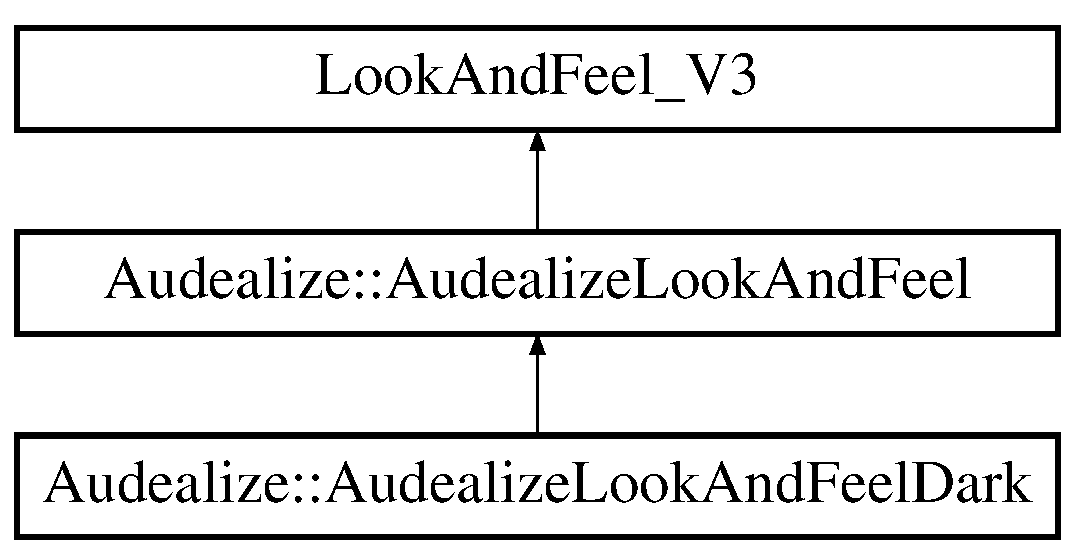
\includegraphics[height=3.000000cm]{class_audealize_1_1_audealize_look_and_feel_dark}
\end{center}
\end{figure}
\subsection*{Public Member Functions}
\begin{DoxyCompactItemize}
\item 
\hyperlink{class_audealize_1_1_audealize_look_and_feel_dark_a2e8455f1559d436d138018adf98309a0}{Audealize\+Look\+And\+Feel\+Dark} ()
\item 
\hyperlink{class_audealize_1_1_audealize_look_and_feel_dark_add9751cc72a16847de562ca3d535fadb}{$\sim$\+Audealize\+Look\+And\+Feel\+Dark} ()
\item 
\hyperlink{class_audealize_1_1_audealize_look_and_feel_dark_aecafbaa94c26a85838c215b39920f081}{J\+U\+C\+E\+\_\+\+D\+E\+C\+L\+A\+R\+E\+\_\+\+N\+O\+N\+\_\+\+C\+O\+P\+Y\+A\+B\+L\+E\+\_\+\+W\+I\+T\+H\+\_\+\+L\+E\+A\+K\+\_\+\+D\+E\+T\+E\+C\+T\+OR} (\hyperlink{class_audealize_1_1_audealize_look_and_feel_dark}{Audealize\+Look\+And\+Feel\+Dark})
\end{DoxyCompactItemize}
\subsection*{Additional Inherited Members}


\subsection{Constructor \& Destructor Documentation}
\index{Audealize\+::\+Audealize\+Look\+And\+Feel\+Dark@{Audealize\+::\+Audealize\+Look\+And\+Feel\+Dark}!Audealize\+Look\+And\+Feel\+Dark@{Audealize\+Look\+And\+Feel\+Dark}}
\index{Audealize\+Look\+And\+Feel\+Dark@{Audealize\+Look\+And\+Feel\+Dark}!Audealize\+::\+Audealize\+Look\+And\+Feel\+Dark@{Audealize\+::\+Audealize\+Look\+And\+Feel\+Dark}}
\subsubsection[{\texorpdfstring{Audealize\+Look\+And\+Feel\+Dark()}{AudealizeLookAndFeelDark()}}]{\setlength{\rightskip}{0pt plus 5cm}Audealize\+::\+Audealize\+Look\+And\+Feel\+Dark\+::\+Audealize\+Look\+And\+Feel\+Dark (
\begin{DoxyParamCaption}
{}
\end{DoxyParamCaption}
)}\hypertarget{class_audealize_1_1_audealize_look_and_feel_dark_a2e8455f1559d436d138018adf98309a0}{}\label{class_audealize_1_1_audealize_look_and_feel_dark_a2e8455f1559d436d138018adf98309a0}
\index{Audealize\+::\+Audealize\+Look\+And\+Feel\+Dark@{Audealize\+::\+Audealize\+Look\+And\+Feel\+Dark}!````~Audealize\+Look\+And\+Feel\+Dark@{$\sim$\+Audealize\+Look\+And\+Feel\+Dark}}
\index{````~Audealize\+Look\+And\+Feel\+Dark@{$\sim$\+Audealize\+Look\+And\+Feel\+Dark}!Audealize\+::\+Audealize\+Look\+And\+Feel\+Dark@{Audealize\+::\+Audealize\+Look\+And\+Feel\+Dark}}
\subsubsection[{\texorpdfstring{$\sim$\+Audealize\+Look\+And\+Feel\+Dark()}{~AudealizeLookAndFeelDark()}}]{\setlength{\rightskip}{0pt plus 5cm}Audealize\+::\+Audealize\+Look\+And\+Feel\+Dark\+::$\sim$\+Audealize\+Look\+And\+Feel\+Dark (
\begin{DoxyParamCaption}
{}
\end{DoxyParamCaption}
)\hspace{0.3cm}{\ttfamily [inline]}}\hypertarget{class_audealize_1_1_audealize_look_and_feel_dark_add9751cc72a16847de562ca3d535fadb}{}\label{class_audealize_1_1_audealize_look_and_feel_dark_add9751cc72a16847de562ca3d535fadb}


\subsection{Member Function Documentation}
\index{Audealize\+::\+Audealize\+Look\+And\+Feel\+Dark@{Audealize\+::\+Audealize\+Look\+And\+Feel\+Dark}!J\+U\+C\+E\+\_\+\+D\+E\+C\+L\+A\+R\+E\+\_\+\+N\+O\+N\+\_\+\+C\+O\+P\+Y\+A\+B\+L\+E\+\_\+\+W\+I\+T\+H\+\_\+\+L\+E\+A\+K\+\_\+\+D\+E\+T\+E\+C\+T\+OR@{J\+U\+C\+E\+\_\+\+D\+E\+C\+L\+A\+R\+E\+\_\+\+N\+O\+N\+\_\+\+C\+O\+P\+Y\+A\+B\+L\+E\+\_\+\+W\+I\+T\+H\+\_\+\+L\+E\+A\+K\+\_\+\+D\+E\+T\+E\+C\+T\+OR}}
\index{J\+U\+C\+E\+\_\+\+D\+E\+C\+L\+A\+R\+E\+\_\+\+N\+O\+N\+\_\+\+C\+O\+P\+Y\+A\+B\+L\+E\+\_\+\+W\+I\+T\+H\+\_\+\+L\+E\+A\+K\+\_\+\+D\+E\+T\+E\+C\+T\+OR@{J\+U\+C\+E\+\_\+\+D\+E\+C\+L\+A\+R\+E\+\_\+\+N\+O\+N\+\_\+\+C\+O\+P\+Y\+A\+B\+L\+E\+\_\+\+W\+I\+T\+H\+\_\+\+L\+E\+A\+K\+\_\+\+D\+E\+T\+E\+C\+T\+OR}!Audealize\+::\+Audealize\+Look\+And\+Feel\+Dark@{Audealize\+::\+Audealize\+Look\+And\+Feel\+Dark}}
\subsubsection[{\texorpdfstring{J\+U\+C\+E\+\_\+\+D\+E\+C\+L\+A\+R\+E\+\_\+\+N\+O\+N\+\_\+\+C\+O\+P\+Y\+A\+B\+L\+E\+\_\+\+W\+I\+T\+H\+\_\+\+L\+E\+A\+K\+\_\+\+D\+E\+T\+E\+C\+T\+O\+R(\+Audealize\+Look\+And\+Feel\+Dark)}{JUCE_DECLARE_NON_COPYABLE_WITH_LEAK_DETECTOR(AudealizeLookAndFeelDark)}}]{\setlength{\rightskip}{0pt plus 5cm}Audealize\+::\+Audealize\+Look\+And\+Feel\+Dark\+::\+J\+U\+C\+E\+\_\+\+D\+E\+C\+L\+A\+R\+E\+\_\+\+N\+O\+N\+\_\+\+C\+O\+P\+Y\+A\+B\+L\+E\+\_\+\+W\+I\+T\+H\+\_\+\+L\+E\+A\+K\+\_\+\+D\+E\+T\+E\+C\+T\+OR (
\begin{DoxyParamCaption}
\item[{{\bf Audealize\+Look\+And\+Feel\+Dark}}]{}
\end{DoxyParamCaption}
)}\hypertarget{class_audealize_1_1_audealize_look_and_feel_dark_aecafbaa94c26a85838c215b39920f081}{}\label{class_audealize_1_1_audealize_look_and_feel_dark_aecafbaa94c26a85838c215b39920f081}


The documentation for this class was generated from the following files\+:\begin{DoxyCompactItemize}
\item 
/\+Users/michael/\+J\+U\+C\+E/projects/audealize-\/plugin/\+J\+U\+C\+E Modules/audealize\+\_\+module/\+Look\+And\+Feel/\hyperlink{_look_and_feel_8h}{Look\+And\+Feel.\+h}\item 
/\+Users/michael/\+J\+U\+C\+E/projects/audealize-\/plugin/\+J\+U\+C\+E Modules/audealize\+\_\+module/\+Look\+And\+Feel/\hyperlink{_look_and_feel_8cpp}{Look\+And\+Feel.\+cpp}\end{DoxyCompactItemize}

\hypertarget{class_audealize_1_1_audealize_multi_u_i}{}\section{Audealize\+:\+:Audealize\+Multi\+UI Class Reference}
\label{class_audealize_1_1_audealize_multi_u_i}\index{Audealize\+::\+Audealize\+Multi\+UI@{Audealize\+::\+Audealize\+Multi\+UI}}


{\ttfamily \#include $<$Audealize\+Multi\+U\+I.\+h$>$}

Inheritance diagram for Audealize\+:\+:Audealize\+Multi\+UI\+:\begin{figure}[H]
\begin{center}
\leavevmode
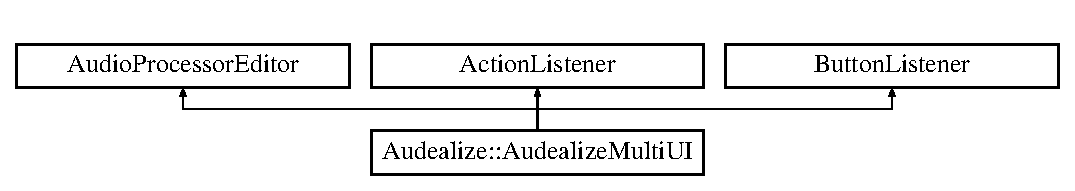
\includegraphics[height=2.000000cm]{class_audealize_1_1_audealize_multi_u_i}
\end{center}
\end{figure}
\subsection*{Public Types}
\begin{DoxyCompactItemize}
\item 
enum \hyperlink{class_audealize_1_1_audealize_multi_u_i_a01035122e067982c82c8f5089904664e}{Colour\+Ids} \{ \hyperlink{class_audealize_1_1_audealize_multi_u_i_a01035122e067982c82c8f5089904664ea2b0d2df5e6ab5243d08f5090d47a8bb2}{background\+Colour\+Id} = 0x2000200, 
\hyperlink{class_audealize_1_1_audealize_multi_u_i_a01035122e067982c82c8f5089904664eaf0d4a96439bd092d6e314fa9ef6b7101}{text\+Colour\+Id} = 0x2000201, 
\hyperlink{class_audealize_1_1_audealize_multi_u_i_a01035122e067982c82c8f5089904664ea8060121e236497f75f7e0742a486e77e}{outline\+Colour\+Id} = 0x2000202, 
\hyperlink{class_audealize_1_1_audealize_multi_u_i_a01035122e067982c82c8f5089904664ea15aae76df19e38f6dee3d232eda5ebd9}{accent\+Colour\+Id} = 0x2000203
 \}
\end{DoxyCompactItemize}
\subsection*{Public Member Functions}
\begin{DoxyCompactItemize}
\item 
\hyperlink{class_audealize_1_1_audealize_multi_u_i_ac89a054f68a45a9eb6c882b4955a0706}{Audealize\+Multi\+UI} (Audio\+Processor \&p, vector$<$ \hyperlink{class_audealize_1_1_audealize_u_i}{Audealize\+UI} $\ast$ $>$ Audealize\+U\+Is)
\item 
\hyperlink{class_audealize_1_1_audealize_multi_u_i_a7d648ba966c595fec2509e339d27b85e}{$\sim$\+Audealize\+Multi\+UI} ()
\item 
\hyperlink{tk_8h_aba408b7cd755a96426e004c015f5de8e}{void} \hyperlink{class_audealize_1_1_audealize_multi_u_i_a3e535c084b7cf39cf8c84fb101f3aef7}{action\+Listener\+Callback} (const juce\+::\+String \&message) override
\item 
\hyperlink{tk_8h_aba408b7cd755a96426e004c015f5de8e}{void} \hyperlink{class_audealize_1_1_audealize_multi_u_i_a956752a920dbb47b7d33e8b498b59cbf}{paint} (Graphics \&g) override
\item 
\hyperlink{tk_8h_aba408b7cd755a96426e004c015f5de8e}{void} \hyperlink{class_audealize_1_1_audealize_multi_u_i_a56cb38579022ba7a1687935c19ff0f7f}{resized} () override
\item 
\hyperlink{tk_8h_aba408b7cd755a96426e004c015f5de8e}{void} \hyperlink{class_audealize_1_1_audealize_multi_u_i_adaa160f3fcd6bed60331f109f2a23acd}{children\+Changed} () override
\item 
\hyperlink{tk_8h_aba408b7cd755a96426e004c015f5de8e}{void} \hyperlink{class_audealize_1_1_audealize_multi_u_i_aff9e86f204aee21ee4f6fb1dfa1e643f}{look\+And\+Feel\+Changed} () override
\item 
\hyperlink{tk_8h_aba408b7cd755a96426e004c015f5de8e}{void} \hyperlink{class_audealize_1_1_audealize_multi_u_i_aec895e0203ce37db39920602c93177ff}{button\+Clicked} (Button $\ast$button\+That\+Was\+Clicked) override
\end{DoxyCompactItemize}


\subsection{Member Enumeration Documentation}
\index{Audealize\+::\+Audealize\+Multi\+UI@{Audealize\+::\+Audealize\+Multi\+UI}!Colour\+Ids@{Colour\+Ids}}
\index{Colour\+Ids@{Colour\+Ids}!Audealize\+::\+Audealize\+Multi\+UI@{Audealize\+::\+Audealize\+Multi\+UI}}
\subsubsection[{\texorpdfstring{Colour\+Ids}{ColourIds}}]{\setlength{\rightskip}{0pt plus 5cm}enum {\bf Audealize\+::\+Audealize\+Multi\+U\+I\+::\+Colour\+Ids}}\hypertarget{class_audealize_1_1_audealize_multi_u_i_a01035122e067982c82c8f5089904664e}{}\label{class_audealize_1_1_audealize_multi_u_i_a01035122e067982c82c8f5089904664e}
\begin{Desc}
\item[Enumerator]\par
\begin{description}
\index{background\+Colour\+Id@{background\+Colour\+Id}!Audealize\+::\+Audealize\+Multi\+UI@{Audealize\+::\+Audealize\+Multi\+UI}}\index{Audealize\+::\+Audealize\+Multi\+UI@{Audealize\+::\+Audealize\+Multi\+UI}!background\+Colour\+Id@{background\+Colour\+Id}}\item[{\em 
background\+Colour\+Id\hypertarget{class_audealize_1_1_audealize_multi_u_i_a01035122e067982c82c8f5089904664ea2b0d2df5e6ab5243d08f5090d47a8bb2}{}\label{class_audealize_1_1_audealize_multi_u_i_a01035122e067982c82c8f5089904664ea2b0d2df5e6ab5243d08f5090d47a8bb2}
}]\index{text\+Colour\+Id@{text\+Colour\+Id}!Audealize\+::\+Audealize\+Multi\+UI@{Audealize\+::\+Audealize\+Multi\+UI}}\index{Audealize\+::\+Audealize\+Multi\+UI@{Audealize\+::\+Audealize\+Multi\+UI}!text\+Colour\+Id@{text\+Colour\+Id}}\item[{\em 
text\+Colour\+Id\hypertarget{class_audealize_1_1_audealize_multi_u_i_a01035122e067982c82c8f5089904664eaf0d4a96439bd092d6e314fa9ef6b7101}{}\label{class_audealize_1_1_audealize_multi_u_i_a01035122e067982c82c8f5089904664eaf0d4a96439bd092d6e314fa9ef6b7101}
}]\index{outline\+Colour\+Id@{outline\+Colour\+Id}!Audealize\+::\+Audealize\+Multi\+UI@{Audealize\+::\+Audealize\+Multi\+UI}}\index{Audealize\+::\+Audealize\+Multi\+UI@{Audealize\+::\+Audealize\+Multi\+UI}!outline\+Colour\+Id@{outline\+Colour\+Id}}\item[{\em 
outline\+Colour\+Id\hypertarget{class_audealize_1_1_audealize_multi_u_i_a01035122e067982c82c8f5089904664ea8060121e236497f75f7e0742a486e77e}{}\label{class_audealize_1_1_audealize_multi_u_i_a01035122e067982c82c8f5089904664ea8060121e236497f75f7e0742a486e77e}
}]\index{accent\+Colour\+Id@{accent\+Colour\+Id}!Audealize\+::\+Audealize\+Multi\+UI@{Audealize\+::\+Audealize\+Multi\+UI}}\index{Audealize\+::\+Audealize\+Multi\+UI@{Audealize\+::\+Audealize\+Multi\+UI}!accent\+Colour\+Id@{accent\+Colour\+Id}}\item[{\em 
accent\+Colour\+Id\hypertarget{class_audealize_1_1_audealize_multi_u_i_a01035122e067982c82c8f5089904664ea15aae76df19e38f6dee3d232eda5ebd9}{}\label{class_audealize_1_1_audealize_multi_u_i_a01035122e067982c82c8f5089904664ea15aae76df19e38f6dee3d232eda5ebd9}
}]\end{description}
\end{Desc}


\subsection{Constructor \& Destructor Documentation}
\index{Audealize\+::\+Audealize\+Multi\+UI@{Audealize\+::\+Audealize\+Multi\+UI}!Audealize\+Multi\+UI@{Audealize\+Multi\+UI}}
\index{Audealize\+Multi\+UI@{Audealize\+Multi\+UI}!Audealize\+::\+Audealize\+Multi\+UI@{Audealize\+::\+Audealize\+Multi\+UI}}
\subsubsection[{\texorpdfstring{Audealize\+Multi\+U\+I(\+Audio\+Processor \&p, vector$<$ Audealize\+U\+I $\ast$ $>$ Audealize\+U\+Is)}{AudealizeMultiUI(AudioProcessor &p, vector< AudealizeUI * > AudealizeUIs)}}]{\setlength{\rightskip}{0pt plus 5cm}Audealize\+Multi\+U\+I\+::\+Audealize\+Multi\+UI (
\begin{DoxyParamCaption}
\item[{Audio\+Processor \&}]{p, }
\item[{vector$<$ {\bf Audealize\+UI} $\ast$ $>$}]{Audealize\+U\+Is}
\end{DoxyParamCaption}
)}\hypertarget{class_audealize_1_1_audealize_multi_u_i_ac89a054f68a45a9eb6c882b4955a0706}{}\label{class_audealize_1_1_audealize_multi_u_i_ac89a054f68a45a9eb6c882b4955a0706}
\index{Audealize\+::\+Audealize\+Multi\+UI@{Audealize\+::\+Audealize\+Multi\+UI}!````~Audealize\+Multi\+UI@{$\sim$\+Audealize\+Multi\+UI}}
\index{````~Audealize\+Multi\+UI@{$\sim$\+Audealize\+Multi\+UI}!Audealize\+::\+Audealize\+Multi\+UI@{Audealize\+::\+Audealize\+Multi\+UI}}
\subsubsection[{\texorpdfstring{$\sim$\+Audealize\+Multi\+U\+I()}{~AudealizeMultiUI()}}]{\setlength{\rightskip}{0pt plus 5cm}Audealize\+Multi\+U\+I\+::$\sim$\+Audealize\+Multi\+UI (
\begin{DoxyParamCaption}
{}
\end{DoxyParamCaption}
)}\hypertarget{class_audealize_1_1_audealize_multi_u_i_a7d648ba966c595fec2509e339d27b85e}{}\label{class_audealize_1_1_audealize_multi_u_i_a7d648ba966c595fec2509e339d27b85e}


\subsection{Member Function Documentation}
\index{Audealize\+::\+Audealize\+Multi\+UI@{Audealize\+::\+Audealize\+Multi\+UI}!action\+Listener\+Callback@{action\+Listener\+Callback}}
\index{action\+Listener\+Callback@{action\+Listener\+Callback}!Audealize\+::\+Audealize\+Multi\+UI@{Audealize\+::\+Audealize\+Multi\+UI}}
\subsubsection[{\texorpdfstring{action\+Listener\+Callback(const juce\+::\+String \&message) override}{actionListenerCallback(const juce::String &message) override}}]{\setlength{\rightskip}{0pt plus 5cm}{\bf void} Audealize\+Multi\+U\+I\+::action\+Listener\+Callback (
\begin{DoxyParamCaption}
\item[{const juce\+::\+String \&}]{message}
\end{DoxyParamCaption}
)\hspace{0.3cm}{\ttfamily [override]}}\hypertarget{class_audealize_1_1_audealize_multi_u_i_a3e535c084b7cf39cf8c84fb101f3aef7}{}\label{class_audealize_1_1_audealize_multi_u_i_a3e535c084b7cf39cf8c84fb101f3aef7}
\index{Audealize\+::\+Audealize\+Multi\+UI@{Audealize\+::\+Audealize\+Multi\+UI}!button\+Clicked@{button\+Clicked}}
\index{button\+Clicked@{button\+Clicked}!Audealize\+::\+Audealize\+Multi\+UI@{Audealize\+::\+Audealize\+Multi\+UI}}
\subsubsection[{\texorpdfstring{button\+Clicked(\+Button $\ast$button\+That\+Was\+Clicked) override}{buttonClicked(Button *buttonThatWasClicked) override}}]{\setlength{\rightskip}{0pt plus 5cm}{\bf void} Audealize\+Multi\+U\+I\+::button\+Clicked (
\begin{DoxyParamCaption}
\item[{Button $\ast$}]{button\+That\+Was\+Clicked}
\end{DoxyParamCaption}
)\hspace{0.3cm}{\ttfamily [override]}}\hypertarget{class_audealize_1_1_audealize_multi_u_i_aec895e0203ce37db39920602c93177ff}{}\label{class_audealize_1_1_audealize_multi_u_i_aec895e0203ce37db39920602c93177ff}
\index{Audealize\+::\+Audealize\+Multi\+UI@{Audealize\+::\+Audealize\+Multi\+UI}!children\+Changed@{children\+Changed}}
\index{children\+Changed@{children\+Changed}!Audealize\+::\+Audealize\+Multi\+UI@{Audealize\+::\+Audealize\+Multi\+UI}}
\subsubsection[{\texorpdfstring{children\+Changed() override}{childrenChanged() override}}]{\setlength{\rightskip}{0pt plus 5cm}{\bf void} Audealize\+Multi\+U\+I\+::children\+Changed (
\begin{DoxyParamCaption}
{}
\end{DoxyParamCaption}
)\hspace{0.3cm}{\ttfamily [override]}}\hypertarget{class_audealize_1_1_audealize_multi_u_i_adaa160f3fcd6bed60331f109f2a23acd}{}\label{class_audealize_1_1_audealize_multi_u_i_adaa160f3fcd6bed60331f109f2a23acd}
\index{Audealize\+::\+Audealize\+Multi\+UI@{Audealize\+::\+Audealize\+Multi\+UI}!look\+And\+Feel\+Changed@{look\+And\+Feel\+Changed}}
\index{look\+And\+Feel\+Changed@{look\+And\+Feel\+Changed}!Audealize\+::\+Audealize\+Multi\+UI@{Audealize\+::\+Audealize\+Multi\+UI}}
\subsubsection[{\texorpdfstring{look\+And\+Feel\+Changed() override}{lookAndFeelChanged() override}}]{\setlength{\rightskip}{0pt plus 5cm}{\bf void} Audealize\+Multi\+U\+I\+::look\+And\+Feel\+Changed (
\begin{DoxyParamCaption}
{}
\end{DoxyParamCaption}
)\hspace{0.3cm}{\ttfamily [override]}}\hypertarget{class_audealize_1_1_audealize_multi_u_i_aff9e86f204aee21ee4f6fb1dfa1e643f}{}\label{class_audealize_1_1_audealize_multi_u_i_aff9e86f204aee21ee4f6fb1dfa1e643f}
\index{Audealize\+::\+Audealize\+Multi\+UI@{Audealize\+::\+Audealize\+Multi\+UI}!paint@{paint}}
\index{paint@{paint}!Audealize\+::\+Audealize\+Multi\+UI@{Audealize\+::\+Audealize\+Multi\+UI}}
\subsubsection[{\texorpdfstring{paint(\+Graphics \&g) override}{paint(Graphics &g) override}}]{\setlength{\rightskip}{0pt plus 5cm}{\bf void} Audealize\+Multi\+U\+I\+::paint (
\begin{DoxyParamCaption}
\item[{Graphics \&}]{g}
\end{DoxyParamCaption}
)\hspace{0.3cm}{\ttfamily [override]}}\hypertarget{class_audealize_1_1_audealize_multi_u_i_a956752a920dbb47b7d33e8b498b59cbf}{}\label{class_audealize_1_1_audealize_multi_u_i_a956752a920dbb47b7d33e8b498b59cbf}
\index{Audealize\+::\+Audealize\+Multi\+UI@{Audealize\+::\+Audealize\+Multi\+UI}!resized@{resized}}
\index{resized@{resized}!Audealize\+::\+Audealize\+Multi\+UI@{Audealize\+::\+Audealize\+Multi\+UI}}
\subsubsection[{\texorpdfstring{resized() override}{resized() override}}]{\setlength{\rightskip}{0pt plus 5cm}{\bf void} Audealize\+Multi\+U\+I\+::resized (
\begin{DoxyParamCaption}
{}
\end{DoxyParamCaption}
)\hspace{0.3cm}{\ttfamily [override]}}\hypertarget{class_audealize_1_1_audealize_multi_u_i_a56cb38579022ba7a1687935c19ff0f7f}{}\label{class_audealize_1_1_audealize_multi_u_i_a56cb38579022ba7a1687935c19ff0f7f}


The documentation for this class was generated from the following files\+:\begin{DoxyCompactItemize}
\item 
/\+Users/michael/\+J\+U\+C\+E/projects/audealize-\/plugin/\+J\+U\+C\+E Modules/audealize\+\_\+module/ui\+\_\+components/\hyperlink{_audealize_multi_u_i_8h}{Audealize\+Multi\+U\+I.\+h}\item 
/\+Users/michael/\+J\+U\+C\+E/projects/audealize-\/plugin/\+J\+U\+C\+E Modules/audealize\+\_\+module/ui\+\_\+components/\hyperlink{_audealize_multi_u_i_8cpp}{Audealize\+Multi\+U\+I.\+cpp}\end{DoxyCompactItemize}

\hypertarget{class_audealize_1_1_audealizereverb_audio_processor}{}\section{Audealize\+:\+:Audealizereverb\+Audio\+Processor Class Reference}
\label{class_audealize_1_1_audealizereverb_audio_processor}\index{Audealize\+::\+Audealizereverb\+Audio\+Processor@{Audealize\+::\+Audealizereverb\+Audio\+Processor}}


{\ttfamily \#include $<$Audealize\+Reverb\+Audio\+Processor.\+h$>$}

Inheritance diagram for Audealize\+:\+:Audealizereverb\+Audio\+Processor\+:\begin{figure}[H]
\begin{center}
\leavevmode
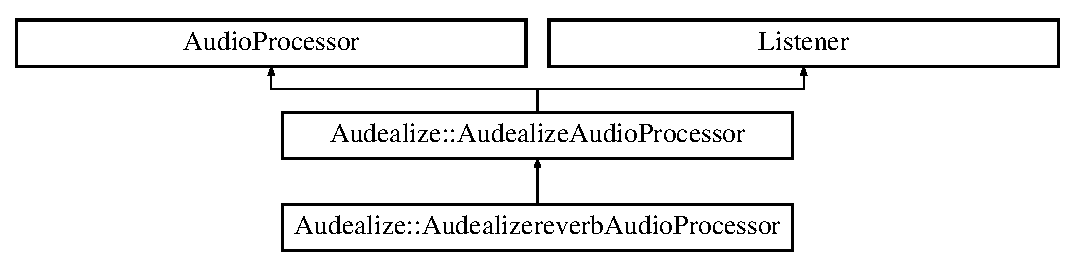
\includegraphics[height=3.000000cm]{class_audealize_1_1_audealizereverb_audio_processor}
\end{center}
\end{figure}
\subsection*{Public Types}
\begin{DoxyCompactItemize}
\item 
enum \hyperlink{class_audealize_1_1_audealizereverb_audio_processor_a89e8659eef504fb10db0e64f9a0f551f}{Parameters} \{ \\*
\hyperlink{class_audealize_1_1_audealizereverb_audio_processor_a89e8659eef504fb10db0e64f9a0f551fab32a709c98309797cc74541db7c0e9a8}{k\+ParamD}, 
\hyperlink{class_audealize_1_1_audealizereverb_audio_processor_a89e8659eef504fb10db0e64f9a0f551fa0e4e0548802fd678b2a5554a73f3ad0b}{k\+ParamG}, 
\hyperlink{class_audealize_1_1_audealizereverb_audio_processor_a89e8659eef504fb10db0e64f9a0f551fa7d549f2640f3108cfbbd556a099a04c3}{k\+ParamM}, 
\hyperlink{class_audealize_1_1_audealizereverb_audio_processor_a89e8659eef504fb10db0e64f9a0f551fa7b684621273041ffe5630add316cda13}{k\+ParamF}, 
\\*
\hyperlink{class_audealize_1_1_audealizereverb_audio_processor_a89e8659eef504fb10db0e64f9a0f551fa40899a272bfa2c98843024801fca4d2a}{k\+ParamE}, 
\hyperlink{class_audealize_1_1_audealizereverb_audio_processor_a89e8659eef504fb10db0e64f9a0f551fac9acd4f2971053b24a99295f73be0fb2}{k\+Param\+Amount}, 
\hyperlink{class_audealize_1_1_audealizereverb_audio_processor_a89e8659eef504fb10db0e64f9a0f551fafa0a87245f3807917fddc2d3468ae409}{k\+Num\+Params}
 \}
\end{DoxyCompactItemize}
\subsection*{Public Member Functions}
\begin{DoxyCompactItemize}
\item 
\hyperlink{class_audealize_1_1_audealizereverb_audio_processor_ab13b216b97097d2cc33c4bccc4a02bcd}{Audealizereverb\+Audio\+Processor} (\hyperlink{class_audealize_1_1_audealize_audio_processor}{Audealize\+Audio\+Processor} $\ast$owner=nullptr)
\item 
\hyperlink{class_audealize_1_1_audealizereverb_audio_processor_a072bd395dad1b0ad6f027dce4b38ef84}{$\sim$\+Audealizereverb\+Audio\+Processor} ()
\item 
\hyperlink{tk_8h_aba408b7cd755a96426e004c015f5de8e}{void} \hyperlink{class_audealize_1_1_audealizereverb_audio_processor_a9487b00227e636a6fd543dbebb794f35}{prepare\+To\+Play} (double sample\+Rate, \hyperlink{tk_8h_a83f82f76e7fed06f4c49d2db94028a6d}{int} samples\+Per\+Block) override
\item 
\hyperlink{tk_8h_aba408b7cd755a96426e004c015f5de8e}{void} \hyperlink{class_audealize_1_1_audealizereverb_audio_processor_a43ca36f8e13479007f433b477b59b974}{release\+Resources} () override
\item 
bool \hyperlink{class_audealize_1_1_audealizereverb_audio_processor_a2c4ac43c34d351508db48853de9c9049}{set\+Preferred\+Bus\+Arrangement} (bool is\+Input, \hyperlink{tk_8h_a83f82f76e7fed06f4c49d2db94028a6d}{int} bus, const Audio\+Channel\+Set \&preferred\+Set) override
\item 
\hyperlink{tk_8h_aba408b7cd755a96426e004c015f5de8e}{void} \hyperlink{class_audealize_1_1_audealizereverb_audio_processor_a9af25624b77d56ded58de45556332390}{process\+Block} (Audio\+Sample\+Buffer \&, Midi\+Buffer \&) override
\item 
\hyperlink{class_audealize_1_1_audealize_u_i}{Audealize\+UI} $\ast$ \hyperlink{class_audealize_1_1_audealizereverb_audio_processor_aa784ca4a70eb061b53091a76feff6b68}{create\+Editor\+For\+Multi\+Effect} ()
\item 
Audio\+Processor\+Editor $\ast$ \hyperlink{class_audealize_1_1_audealizereverb_audio_processor_a84ceaa6c3bf26df9f6cd92550b823613}{create\+Editor} () override
\item 
bool \hyperlink{class_audealize_1_1_audealizereverb_audio_processor_ada6fb4aa0fa2889e3f2efb43c0599f32}{has\+Editor} () const  override
\item 
const String \hyperlink{class_audealize_1_1_audealizereverb_audio_processor_ab5ba301ae52e6114644445dba35d1a37}{get\+Name} () const  override
\item 
bool \hyperlink{class_audealize_1_1_audealizereverb_audio_processor_a070d7a6bf9617fcf3e8ff901d973c3e4}{accepts\+Midi} () const  override
\item 
bool \hyperlink{class_audealize_1_1_audealizereverb_audio_processor_abd5d8bacc498bdac1eeea1bedd4b2e17}{produces\+Midi} () const  override
\item 
double \hyperlink{class_audealize_1_1_audealizereverb_audio_processor_a622a48a5741afbfe65114a031fd6521d}{get\+Tail\+Length\+Seconds} () const  override
\item 
\hyperlink{tk_8h_a83f82f76e7fed06f4c49d2db94028a6d}{int} \hyperlink{class_audealize_1_1_audealizereverb_audio_processor_a59f63e65b4ecadd00c3cc932a0538c21}{get\+Num\+Programs} () override
\item 
\hyperlink{tk_8h_a83f82f76e7fed06f4c49d2db94028a6d}{int} \hyperlink{class_audealize_1_1_audealizereverb_audio_processor_a1088d42f1aa689ff1b5122d372739888}{get\+Current\+Program} () override
\item 
\hyperlink{tk_8h_aba408b7cd755a96426e004c015f5de8e}{void} \hyperlink{class_audealize_1_1_audealizereverb_audio_processor_a47fc36254b2bef0a0427143868e0128e}{set\+Current\+Program} (\hyperlink{tk_8h_a83f82f76e7fed06f4c49d2db94028a6d}{int} index) override
\item 
const String \hyperlink{class_audealize_1_1_audealizereverb_audio_processor_ab9f79aecbdb3781429d5903a29116e0c}{get\+Program\+Name} (\hyperlink{tk_8h_a83f82f76e7fed06f4c49d2db94028a6d}{int} index) override
\item 
\hyperlink{tk_8h_aba408b7cd755a96426e004c015f5de8e}{void} \hyperlink{class_audealize_1_1_audealizereverb_audio_processor_ac24bb57c2e0a915d93597c8b40a947cf}{change\+Program\+Name} (\hyperlink{tk_8h_a83f82f76e7fed06f4c49d2db94028a6d}{int} index, const String \&new\+Name) override
\item 
\hyperlink{tk_8h_aba408b7cd755a96426e004c015f5de8e}{void} \hyperlink{class_audealize_1_1_audealizereverb_audio_processor_aafb771cae87f2ce62ca2451d80678277}{parameter\+Changed} (const juce\+::\+String \&parameter\+ID, float new\+Value) override
\item 
\hyperlink{tk_8h_aba408b7cd755a96426e004c015f5de8e}{void} \hyperlink{class_audealize_1_1_audealizereverb_audio_processor_a4a9a5828a3cbbb084a3025009500faf9}{settings\+From\+Map} (vector$<$ float $>$ settings) override
\item 
String \hyperlink{class_audealize_1_1_audealizereverb_audio_processor_a20e3cb24628efda50a559ce164a7fed5}{get\+Param\+ID} (\hyperlink{tk_8h_a83f82f76e7fed06f4c49d2db94028a6d}{int} index) override
\item 
\hyperlink{tk_8h_a83f82f76e7fed06f4c49d2db94028a6d}{int} \hyperlink{class_audealize_1_1_audealizereverb_audio_processor_a10250897a1cd4d63389f27deae3d615b}{get\+Param\+Idx} (String param\+Id)
\item 
bool \hyperlink{class_audealize_1_1_audealizereverb_audio_processor_abaa19b64ec3373e411c7c327c9d93b61}{is\+Parameter\+Automatable} (\hyperlink{tk_8h_a83f82f76e7fed06f4c49d2db94028a6d}{int} index)
\end{DoxyCompactItemize}
\subsection*{Static Public Attributes}
\begin{DoxyCompactItemize}
\item 
static String \hyperlink{class_audealize_1_1_audealizereverb_audio_processor_a5075b2df5f4540e479d2dddc6f5178a9}{paramD}
\item 
static String \hyperlink{class_audealize_1_1_audealizereverb_audio_processor_a2a3fc9c4b12a08e68aa8457cae9ce3ff}{paramG}
\item 
static String \hyperlink{class_audealize_1_1_audealizereverb_audio_processor_a3e3ec2690abdac5cbca63fccd0f0d362}{paramM}
\item 
static String \hyperlink{class_audealize_1_1_audealizereverb_audio_processor_a44f3dca41c6e7237c5c1898b1048c1c4}{paramF}
\item 
static String \hyperlink{class_audealize_1_1_audealizereverb_audio_processor_a9aba74977dd6a007c7c0bee781204750}{paramE}
\end{DoxyCompactItemize}
\subsection*{Additional Inherited Members}


\subsection{Member Enumeration Documentation}
\index{Audealize\+::\+Audealizereverb\+Audio\+Processor@{Audealize\+::\+Audealizereverb\+Audio\+Processor}!Parameters@{Parameters}}
\index{Parameters@{Parameters}!Audealize\+::\+Audealizereverb\+Audio\+Processor@{Audealize\+::\+Audealizereverb\+Audio\+Processor}}
\subsubsection[{\texorpdfstring{Parameters}{Parameters}}]{\setlength{\rightskip}{0pt plus 5cm}enum {\bf Audealize\+::\+Audealizereverb\+Audio\+Processor\+::\+Parameters}}\hypertarget{class_audealize_1_1_audealizereverb_audio_processor_a89e8659eef504fb10db0e64f9a0f551f}{}\label{class_audealize_1_1_audealizereverb_audio_processor_a89e8659eef504fb10db0e64f9a0f551f}
\begin{Desc}
\item[Enumerator]\par
\begin{description}
\index{k\+ParamD@{k\+ParamD}!Audealize\+::\+Audealizereverb\+Audio\+Processor@{Audealize\+::\+Audealizereverb\+Audio\+Processor}}\index{Audealize\+::\+Audealizereverb\+Audio\+Processor@{Audealize\+::\+Audealizereverb\+Audio\+Processor}!k\+ParamD@{k\+ParamD}}\item[{\em 
k\+ParamD\hypertarget{class_audealize_1_1_audealizereverb_audio_processor_a89e8659eef504fb10db0e64f9a0f551fab32a709c98309797cc74541db7c0e9a8}{}\label{class_audealize_1_1_audealizereverb_audio_processor_a89e8659eef504fb10db0e64f9a0f551fab32a709c98309797cc74541db7c0e9a8}
}]\index{k\+ParamG@{k\+ParamG}!Audealize\+::\+Audealizereverb\+Audio\+Processor@{Audealize\+::\+Audealizereverb\+Audio\+Processor}}\index{Audealize\+::\+Audealizereverb\+Audio\+Processor@{Audealize\+::\+Audealizereverb\+Audio\+Processor}!k\+ParamG@{k\+ParamG}}\item[{\em 
k\+ParamG\hypertarget{class_audealize_1_1_audealizereverb_audio_processor_a89e8659eef504fb10db0e64f9a0f551fa0e4e0548802fd678b2a5554a73f3ad0b}{}\label{class_audealize_1_1_audealizereverb_audio_processor_a89e8659eef504fb10db0e64f9a0f551fa0e4e0548802fd678b2a5554a73f3ad0b}
}]\index{k\+ParamM@{k\+ParamM}!Audealize\+::\+Audealizereverb\+Audio\+Processor@{Audealize\+::\+Audealizereverb\+Audio\+Processor}}\index{Audealize\+::\+Audealizereverb\+Audio\+Processor@{Audealize\+::\+Audealizereverb\+Audio\+Processor}!k\+ParamM@{k\+ParamM}}\item[{\em 
k\+ParamM\hypertarget{class_audealize_1_1_audealizereverb_audio_processor_a89e8659eef504fb10db0e64f9a0f551fa7d549f2640f3108cfbbd556a099a04c3}{}\label{class_audealize_1_1_audealizereverb_audio_processor_a89e8659eef504fb10db0e64f9a0f551fa7d549f2640f3108cfbbd556a099a04c3}
}]\index{k\+ParamF@{k\+ParamF}!Audealize\+::\+Audealizereverb\+Audio\+Processor@{Audealize\+::\+Audealizereverb\+Audio\+Processor}}\index{Audealize\+::\+Audealizereverb\+Audio\+Processor@{Audealize\+::\+Audealizereverb\+Audio\+Processor}!k\+ParamF@{k\+ParamF}}\item[{\em 
k\+ParamF\hypertarget{class_audealize_1_1_audealizereverb_audio_processor_a89e8659eef504fb10db0e64f9a0f551fa7b684621273041ffe5630add316cda13}{}\label{class_audealize_1_1_audealizereverb_audio_processor_a89e8659eef504fb10db0e64f9a0f551fa7b684621273041ffe5630add316cda13}
}]\index{k\+ParamE@{k\+ParamE}!Audealize\+::\+Audealizereverb\+Audio\+Processor@{Audealize\+::\+Audealizereverb\+Audio\+Processor}}\index{Audealize\+::\+Audealizereverb\+Audio\+Processor@{Audealize\+::\+Audealizereverb\+Audio\+Processor}!k\+ParamE@{k\+ParamE}}\item[{\em 
k\+ParamE\hypertarget{class_audealize_1_1_audealizereverb_audio_processor_a89e8659eef504fb10db0e64f9a0f551fa40899a272bfa2c98843024801fca4d2a}{}\label{class_audealize_1_1_audealizereverb_audio_processor_a89e8659eef504fb10db0e64f9a0f551fa40899a272bfa2c98843024801fca4d2a}
}]\index{k\+Param\+Amount@{k\+Param\+Amount}!Audealize\+::\+Audealizereverb\+Audio\+Processor@{Audealize\+::\+Audealizereverb\+Audio\+Processor}}\index{Audealize\+::\+Audealizereverb\+Audio\+Processor@{Audealize\+::\+Audealizereverb\+Audio\+Processor}!k\+Param\+Amount@{k\+Param\+Amount}}\item[{\em 
k\+Param\+Amount\hypertarget{class_audealize_1_1_audealizereverb_audio_processor_a89e8659eef504fb10db0e64f9a0f551fac9acd4f2971053b24a99295f73be0fb2}{}\label{class_audealize_1_1_audealizereverb_audio_processor_a89e8659eef504fb10db0e64f9a0f551fac9acd4f2971053b24a99295f73be0fb2}
}]\index{k\+Num\+Params@{k\+Num\+Params}!Audealize\+::\+Audealizereverb\+Audio\+Processor@{Audealize\+::\+Audealizereverb\+Audio\+Processor}}\index{Audealize\+::\+Audealizereverb\+Audio\+Processor@{Audealize\+::\+Audealizereverb\+Audio\+Processor}!k\+Num\+Params@{k\+Num\+Params}}\item[{\em 
k\+Num\+Params\hypertarget{class_audealize_1_1_audealizereverb_audio_processor_a89e8659eef504fb10db0e64f9a0f551fafa0a87245f3807917fddc2d3468ae409}{}\label{class_audealize_1_1_audealizereverb_audio_processor_a89e8659eef504fb10db0e64f9a0f551fafa0a87245f3807917fddc2d3468ae409}
}]\end{description}
\end{Desc}


\subsection{Constructor \& Destructor Documentation}
\index{Audealize\+::\+Audealizereverb\+Audio\+Processor@{Audealize\+::\+Audealizereverb\+Audio\+Processor}!Audealizereverb\+Audio\+Processor@{Audealizereverb\+Audio\+Processor}}
\index{Audealizereverb\+Audio\+Processor@{Audealizereverb\+Audio\+Processor}!Audealize\+::\+Audealizereverb\+Audio\+Processor@{Audealize\+::\+Audealizereverb\+Audio\+Processor}}
\subsubsection[{\texorpdfstring{Audealizereverb\+Audio\+Processor(\+Audealize\+Audio\+Processor $\ast$owner=nullptr)}{AudealizereverbAudioProcessor(AudealizeAudioProcessor *owner=nullptr)}}]{\setlength{\rightskip}{0pt plus 5cm}Audealizereverb\+Audio\+Processor\+::\+Audealizereverb\+Audio\+Processor (
\begin{DoxyParamCaption}
\item[{{\bf Audealize\+Audio\+Processor} $\ast$}]{owner = {\ttfamily nullptr}}
\end{DoxyParamCaption}
)}\hypertarget{class_audealize_1_1_audealizereverb_audio_processor_ab13b216b97097d2cc33c4bccc4a02bcd}{}\label{class_audealize_1_1_audealizereverb_audio_processor_ab13b216b97097d2cc33c4bccc4a02bcd}
\index{Audealize\+::\+Audealizereverb\+Audio\+Processor@{Audealize\+::\+Audealizereverb\+Audio\+Processor}!````~Audealizereverb\+Audio\+Processor@{$\sim$\+Audealizereverb\+Audio\+Processor}}
\index{````~Audealizereverb\+Audio\+Processor@{$\sim$\+Audealizereverb\+Audio\+Processor}!Audealize\+::\+Audealizereverb\+Audio\+Processor@{Audealize\+::\+Audealizereverb\+Audio\+Processor}}
\subsubsection[{\texorpdfstring{$\sim$\+Audealizereverb\+Audio\+Processor()}{~AudealizereverbAudioProcessor()}}]{\setlength{\rightskip}{0pt plus 5cm}Audealizereverb\+Audio\+Processor\+::$\sim$\+Audealizereverb\+Audio\+Processor (
\begin{DoxyParamCaption}
{}
\end{DoxyParamCaption}
)}\hypertarget{class_audealize_1_1_audealizereverb_audio_processor_a072bd395dad1b0ad6f027dce4b38ef84}{}\label{class_audealize_1_1_audealizereverb_audio_processor_a072bd395dad1b0ad6f027dce4b38ef84}


\subsection{Member Function Documentation}
\index{Audealize\+::\+Audealizereverb\+Audio\+Processor@{Audealize\+::\+Audealizereverb\+Audio\+Processor}!accepts\+Midi@{accepts\+Midi}}
\index{accepts\+Midi@{accepts\+Midi}!Audealize\+::\+Audealizereverb\+Audio\+Processor@{Audealize\+::\+Audealizereverb\+Audio\+Processor}}
\subsubsection[{\texorpdfstring{accepts\+Midi() const  override}{acceptsMidi() const  override}}]{\setlength{\rightskip}{0pt plus 5cm}bool Audealizereverb\+Audio\+Processor\+::accepts\+Midi (
\begin{DoxyParamCaption}
{}
\end{DoxyParamCaption}
) const\hspace{0.3cm}{\ttfamily [override]}}\hypertarget{class_audealize_1_1_audealizereverb_audio_processor_a070d7a6bf9617fcf3e8ff901d973c3e4}{}\label{class_audealize_1_1_audealizereverb_audio_processor_a070d7a6bf9617fcf3e8ff901d973c3e4}
\index{Audealize\+::\+Audealizereverb\+Audio\+Processor@{Audealize\+::\+Audealizereverb\+Audio\+Processor}!change\+Program\+Name@{change\+Program\+Name}}
\index{change\+Program\+Name@{change\+Program\+Name}!Audealize\+::\+Audealizereverb\+Audio\+Processor@{Audealize\+::\+Audealizereverb\+Audio\+Processor}}
\subsubsection[{\texorpdfstring{change\+Program\+Name(int index, const String \&new\+Name) override}{changeProgramName(int index, const String &newName) override}}]{\setlength{\rightskip}{0pt plus 5cm}{\bf void} Audealizereverb\+Audio\+Processor\+::change\+Program\+Name (
\begin{DoxyParamCaption}
\item[{{\bf int}}]{index, }
\item[{const String \&}]{new\+Name}
\end{DoxyParamCaption}
)\hspace{0.3cm}{\ttfamily [override]}}\hypertarget{class_audealize_1_1_audealizereverb_audio_processor_ac24bb57c2e0a915d93597c8b40a947cf}{}\label{class_audealize_1_1_audealizereverb_audio_processor_ac24bb57c2e0a915d93597c8b40a947cf}
\index{Audealize\+::\+Audealizereverb\+Audio\+Processor@{Audealize\+::\+Audealizereverb\+Audio\+Processor}!create\+Editor@{create\+Editor}}
\index{create\+Editor@{create\+Editor}!Audealize\+::\+Audealizereverb\+Audio\+Processor@{Audealize\+::\+Audealizereverb\+Audio\+Processor}}
\subsubsection[{\texorpdfstring{create\+Editor() override}{createEditor() override}}]{\setlength{\rightskip}{0pt plus 5cm}Audio\+Processor\+Editor $\ast$ Audealizereverb\+Audio\+Processor\+::create\+Editor (
\begin{DoxyParamCaption}
{}
\end{DoxyParamCaption}
)\hspace{0.3cm}{\ttfamily [override]}}\hypertarget{class_audealize_1_1_audealizereverb_audio_processor_a84ceaa6c3bf26df9f6cd92550b823613}{}\label{class_audealize_1_1_audealizereverb_audio_processor_a84ceaa6c3bf26df9f6cd92550b823613}
\index{Audealize\+::\+Audealizereverb\+Audio\+Processor@{Audealize\+::\+Audealizereverb\+Audio\+Processor}!create\+Editor\+For\+Multi\+Effect@{create\+Editor\+For\+Multi\+Effect}}
\index{create\+Editor\+For\+Multi\+Effect@{create\+Editor\+For\+Multi\+Effect}!Audealize\+::\+Audealizereverb\+Audio\+Processor@{Audealize\+::\+Audealizereverb\+Audio\+Processor}}
\subsubsection[{\texorpdfstring{create\+Editor\+For\+Multi\+Effect()}{createEditorForMultiEffect()}}]{\setlength{\rightskip}{0pt plus 5cm}{\bf Audealize\+UI} $\ast$ Audealizereverb\+Audio\+Processor\+::create\+Editor\+For\+Multi\+Effect (
\begin{DoxyParamCaption}
{}
\end{DoxyParamCaption}
)}\hypertarget{class_audealize_1_1_audealizereverb_audio_processor_aa784ca4a70eb061b53091a76feff6b68}{}\label{class_audealize_1_1_audealizereverb_audio_processor_aa784ca4a70eb061b53091a76feff6b68}
\index{Audealize\+::\+Audealizereverb\+Audio\+Processor@{Audealize\+::\+Audealizereverb\+Audio\+Processor}!get\+Current\+Program@{get\+Current\+Program}}
\index{get\+Current\+Program@{get\+Current\+Program}!Audealize\+::\+Audealizereverb\+Audio\+Processor@{Audealize\+::\+Audealizereverb\+Audio\+Processor}}
\subsubsection[{\texorpdfstring{get\+Current\+Program() override}{getCurrentProgram() override}}]{\setlength{\rightskip}{0pt plus 5cm}{\bf int} Audealizereverb\+Audio\+Processor\+::get\+Current\+Program (
\begin{DoxyParamCaption}
{}
\end{DoxyParamCaption}
)\hspace{0.3cm}{\ttfamily [override]}}\hypertarget{class_audealize_1_1_audealizereverb_audio_processor_a1088d42f1aa689ff1b5122d372739888}{}\label{class_audealize_1_1_audealizereverb_audio_processor_a1088d42f1aa689ff1b5122d372739888}
\index{Audealize\+::\+Audealizereverb\+Audio\+Processor@{Audealize\+::\+Audealizereverb\+Audio\+Processor}!get\+Name@{get\+Name}}
\index{get\+Name@{get\+Name}!Audealize\+::\+Audealizereverb\+Audio\+Processor@{Audealize\+::\+Audealizereverb\+Audio\+Processor}}
\subsubsection[{\texorpdfstring{get\+Name() const  override}{getName() const  override}}]{\setlength{\rightskip}{0pt plus 5cm}const String Audealizereverb\+Audio\+Processor\+::get\+Name (
\begin{DoxyParamCaption}
{}
\end{DoxyParamCaption}
) const\hspace{0.3cm}{\ttfamily [override]}}\hypertarget{class_audealize_1_1_audealizereverb_audio_processor_ab5ba301ae52e6114644445dba35d1a37}{}\label{class_audealize_1_1_audealizereverb_audio_processor_ab5ba301ae52e6114644445dba35d1a37}
\index{Audealize\+::\+Audealizereverb\+Audio\+Processor@{Audealize\+::\+Audealizereverb\+Audio\+Processor}!get\+Num\+Programs@{get\+Num\+Programs}}
\index{get\+Num\+Programs@{get\+Num\+Programs}!Audealize\+::\+Audealizereverb\+Audio\+Processor@{Audealize\+::\+Audealizereverb\+Audio\+Processor}}
\subsubsection[{\texorpdfstring{get\+Num\+Programs() override}{getNumPrograms() override}}]{\setlength{\rightskip}{0pt plus 5cm}{\bf int} Audealizereverb\+Audio\+Processor\+::get\+Num\+Programs (
\begin{DoxyParamCaption}
{}
\end{DoxyParamCaption}
)\hspace{0.3cm}{\ttfamily [override]}}\hypertarget{class_audealize_1_1_audealizereverb_audio_processor_a59f63e65b4ecadd00c3cc932a0538c21}{}\label{class_audealize_1_1_audealizereverb_audio_processor_a59f63e65b4ecadd00c3cc932a0538c21}
\index{Audealize\+::\+Audealizereverb\+Audio\+Processor@{Audealize\+::\+Audealizereverb\+Audio\+Processor}!get\+Param\+ID@{get\+Param\+ID}}
\index{get\+Param\+ID@{get\+Param\+ID}!Audealize\+::\+Audealizereverb\+Audio\+Processor@{Audealize\+::\+Audealizereverb\+Audio\+Processor}}
\subsubsection[{\texorpdfstring{get\+Param\+I\+D(int index) override}{getParamID(int index) override}}]{\setlength{\rightskip}{0pt plus 5cm}String Audealizereverb\+Audio\+Processor\+::get\+Param\+ID (
\begin{DoxyParamCaption}
\item[{{\bf int}}]{index}
\end{DoxyParamCaption}
)\hspace{0.3cm}{\ttfamily [inline]}, {\ttfamily [override]}, {\ttfamily [virtual]}}\hypertarget{class_audealize_1_1_audealizereverb_audio_processor_a20e3cb24628efda50a559ce164a7fed5}{}\label{class_audealize_1_1_audealizereverb_audio_processor_a20e3cb24628efda50a559ce164a7fed5}
Transaltes a parameter index to its corresponding ID string 

Reimplemented from \hyperlink{class_audealize_1_1_audealize_audio_processor_aa3e347b4bdc34e419ccf350638c38028}{Audealize\+::\+Audealize\+Audio\+Processor}.

\index{Audealize\+::\+Audealizereverb\+Audio\+Processor@{Audealize\+::\+Audealizereverb\+Audio\+Processor}!get\+Param\+Idx@{get\+Param\+Idx}}
\index{get\+Param\+Idx@{get\+Param\+Idx}!Audealize\+::\+Audealizereverb\+Audio\+Processor@{Audealize\+::\+Audealizereverb\+Audio\+Processor}}
\subsubsection[{\texorpdfstring{get\+Param\+Idx(\+String param\+Id)}{getParamIdx(String paramId)}}]{\setlength{\rightskip}{0pt plus 5cm}{\bf int} Audealizereverb\+Audio\+Processor\+::get\+Param\+Idx (
\begin{DoxyParamCaption}
\item[{String}]{param\+Id}
\end{DoxyParamCaption}
)\hspace{0.3cm}{\ttfamily [inline]}}\hypertarget{class_audealize_1_1_audealizereverb_audio_processor_a10250897a1cd4d63389f27deae3d615b}{}\label{class_audealize_1_1_audealizereverb_audio_processor_a10250897a1cd4d63389f27deae3d615b}
\index{Audealize\+::\+Audealizereverb\+Audio\+Processor@{Audealize\+::\+Audealizereverb\+Audio\+Processor}!get\+Program\+Name@{get\+Program\+Name}}
\index{get\+Program\+Name@{get\+Program\+Name}!Audealize\+::\+Audealizereverb\+Audio\+Processor@{Audealize\+::\+Audealizereverb\+Audio\+Processor}}
\subsubsection[{\texorpdfstring{get\+Program\+Name(int index) override}{getProgramName(int index) override}}]{\setlength{\rightskip}{0pt plus 5cm}const String Audealizereverb\+Audio\+Processor\+::get\+Program\+Name (
\begin{DoxyParamCaption}
\item[{{\bf int}}]{index}
\end{DoxyParamCaption}
)\hspace{0.3cm}{\ttfamily [override]}}\hypertarget{class_audealize_1_1_audealizereverb_audio_processor_ab9f79aecbdb3781429d5903a29116e0c}{}\label{class_audealize_1_1_audealizereverb_audio_processor_ab9f79aecbdb3781429d5903a29116e0c}
\index{Audealize\+::\+Audealizereverb\+Audio\+Processor@{Audealize\+::\+Audealizereverb\+Audio\+Processor}!get\+Tail\+Length\+Seconds@{get\+Tail\+Length\+Seconds}}
\index{get\+Tail\+Length\+Seconds@{get\+Tail\+Length\+Seconds}!Audealize\+::\+Audealizereverb\+Audio\+Processor@{Audealize\+::\+Audealizereverb\+Audio\+Processor}}
\subsubsection[{\texorpdfstring{get\+Tail\+Length\+Seconds() const  override}{getTailLengthSeconds() const  override}}]{\setlength{\rightskip}{0pt plus 5cm}double Audealizereverb\+Audio\+Processor\+::get\+Tail\+Length\+Seconds (
\begin{DoxyParamCaption}
{}
\end{DoxyParamCaption}
) const\hspace{0.3cm}{\ttfamily [override]}}\hypertarget{class_audealize_1_1_audealizereverb_audio_processor_a622a48a5741afbfe65114a031fd6521d}{}\label{class_audealize_1_1_audealizereverb_audio_processor_a622a48a5741afbfe65114a031fd6521d}
\index{Audealize\+::\+Audealizereverb\+Audio\+Processor@{Audealize\+::\+Audealizereverb\+Audio\+Processor}!has\+Editor@{has\+Editor}}
\index{has\+Editor@{has\+Editor}!Audealize\+::\+Audealizereverb\+Audio\+Processor@{Audealize\+::\+Audealizereverb\+Audio\+Processor}}
\subsubsection[{\texorpdfstring{has\+Editor() const  override}{hasEditor() const  override}}]{\setlength{\rightskip}{0pt plus 5cm}bool Audealizereverb\+Audio\+Processor\+::has\+Editor (
\begin{DoxyParamCaption}
{}
\end{DoxyParamCaption}
) const\hspace{0.3cm}{\ttfamily [override]}}\hypertarget{class_audealize_1_1_audealizereverb_audio_processor_ada6fb4aa0fa2889e3f2efb43c0599f32}{}\label{class_audealize_1_1_audealizereverb_audio_processor_ada6fb4aa0fa2889e3f2efb43c0599f32}
\index{Audealize\+::\+Audealizereverb\+Audio\+Processor@{Audealize\+::\+Audealizereverb\+Audio\+Processor}!is\+Parameter\+Automatable@{is\+Parameter\+Automatable}}
\index{is\+Parameter\+Automatable@{is\+Parameter\+Automatable}!Audealize\+::\+Audealizereverb\+Audio\+Processor@{Audealize\+::\+Audealizereverb\+Audio\+Processor}}
\subsubsection[{\texorpdfstring{is\+Parameter\+Automatable(int index)}{isParameterAutomatable(int index)}}]{\setlength{\rightskip}{0pt plus 5cm}bool Audealize\+::\+Audealizereverb\+Audio\+Processor\+::is\+Parameter\+Automatable (
\begin{DoxyParamCaption}
\item[{{\bf int}}]{index}
\end{DoxyParamCaption}
)\hspace{0.3cm}{\ttfamily [inline]}}\hypertarget{class_audealize_1_1_audealizereverb_audio_processor_abaa19b64ec3373e411c7c327c9d93b61}{}\label{class_audealize_1_1_audealizereverb_audio_processor_abaa19b64ec3373e411c7c327c9d93b61}
\index{Audealize\+::\+Audealizereverb\+Audio\+Processor@{Audealize\+::\+Audealizereverb\+Audio\+Processor}!parameter\+Changed@{parameter\+Changed}}
\index{parameter\+Changed@{parameter\+Changed}!Audealize\+::\+Audealizereverb\+Audio\+Processor@{Audealize\+::\+Audealizereverb\+Audio\+Processor}}
\subsubsection[{\texorpdfstring{parameter\+Changed(const juce\+::\+String \&parameter\+I\+D, float new\+Value) override}{parameterChanged(const juce::String &parameterID, float newValue) override}}]{\setlength{\rightskip}{0pt plus 5cm}{\bf void} Audealizereverb\+Audio\+Processor\+::parameter\+Changed (
\begin{DoxyParamCaption}
\item[{const juce\+::\+String \&}]{parameter\+ID, }
\item[{float}]{new\+Value}
\end{DoxyParamCaption}
)\hspace{0.3cm}{\ttfamily [override]}, {\ttfamily [virtual]}}\hypertarget{class_audealize_1_1_audealizereverb_audio_processor_aafb771cae87f2ce62ca2451d80678277}{}\label{class_audealize_1_1_audealizereverb_audio_processor_aafb771cae87f2ce62ca2451d80678277}
Called by an Audio\+Processor\+Editor to notify Audio\+Processor of parameter value changes


\begin{DoxyParams}{Parameters}
{\em parameter\+ID} & The ID of the parameter that was changed \\
\hline
{\em new\+Value} & The new value for that parameter \\
\hline
\end{DoxyParams}


Reimplemented from \hyperlink{class_audealize_1_1_audealize_audio_processor_a4832111ea2b24bc517f911fa5949ca56}{Audealize\+::\+Audealize\+Audio\+Processor}.

\index{Audealize\+::\+Audealizereverb\+Audio\+Processor@{Audealize\+::\+Audealizereverb\+Audio\+Processor}!prepare\+To\+Play@{prepare\+To\+Play}}
\index{prepare\+To\+Play@{prepare\+To\+Play}!Audealize\+::\+Audealizereverb\+Audio\+Processor@{Audealize\+::\+Audealizereverb\+Audio\+Processor}}
\subsubsection[{\texorpdfstring{prepare\+To\+Play(double sample\+Rate, int samples\+Per\+Block) override}{prepareToPlay(double sampleRate, int samplesPerBlock) override}}]{\setlength{\rightskip}{0pt plus 5cm}{\bf void} Audealizereverb\+Audio\+Processor\+::prepare\+To\+Play (
\begin{DoxyParamCaption}
\item[{double}]{sample\+Rate, }
\item[{{\bf int}}]{samples\+Per\+Block}
\end{DoxyParamCaption}
)\hspace{0.3cm}{\ttfamily [override]}}\hypertarget{class_audealize_1_1_audealizereverb_audio_processor_a9487b00227e636a6fd543dbebb794f35}{}\label{class_audealize_1_1_audealizereverb_audio_processor_a9487b00227e636a6fd543dbebb794f35}
\index{Audealize\+::\+Audealizereverb\+Audio\+Processor@{Audealize\+::\+Audealizereverb\+Audio\+Processor}!process\+Block@{process\+Block}}
\index{process\+Block@{process\+Block}!Audealize\+::\+Audealizereverb\+Audio\+Processor@{Audealize\+::\+Audealizereverb\+Audio\+Processor}}
\subsubsection[{\texorpdfstring{process\+Block(\+Audio\+Sample\+Buffer \&, Midi\+Buffer \&) override}{processBlock(AudioSampleBuffer &, MidiBuffer &) override}}]{\setlength{\rightskip}{0pt plus 5cm}{\bf void} Audealizereverb\+Audio\+Processor\+::process\+Block (
\begin{DoxyParamCaption}
\item[{Audio\+Sample\+Buffer \&}]{buffer, }
\item[{Midi\+Buffer \&}]{midi\+Messages}
\end{DoxyParamCaption}
)\hspace{0.3cm}{\ttfamily [override]}}\hypertarget{class_audealize_1_1_audealizereverb_audio_processor_a9af25624b77d56ded58de45556332390}{}\label{class_audealize_1_1_audealizereverb_audio_processor_a9af25624b77d56ded58de45556332390}
\index{Audealize\+::\+Audealizereverb\+Audio\+Processor@{Audealize\+::\+Audealizereverb\+Audio\+Processor}!produces\+Midi@{produces\+Midi}}
\index{produces\+Midi@{produces\+Midi}!Audealize\+::\+Audealizereverb\+Audio\+Processor@{Audealize\+::\+Audealizereverb\+Audio\+Processor}}
\subsubsection[{\texorpdfstring{produces\+Midi() const  override}{producesMidi() const  override}}]{\setlength{\rightskip}{0pt plus 5cm}bool Audealizereverb\+Audio\+Processor\+::produces\+Midi (
\begin{DoxyParamCaption}
{}
\end{DoxyParamCaption}
) const\hspace{0.3cm}{\ttfamily [override]}}\hypertarget{class_audealize_1_1_audealizereverb_audio_processor_abd5d8bacc498bdac1eeea1bedd4b2e17}{}\label{class_audealize_1_1_audealizereverb_audio_processor_abd5d8bacc498bdac1eeea1bedd4b2e17}
\index{Audealize\+::\+Audealizereverb\+Audio\+Processor@{Audealize\+::\+Audealizereverb\+Audio\+Processor}!release\+Resources@{release\+Resources}}
\index{release\+Resources@{release\+Resources}!Audealize\+::\+Audealizereverb\+Audio\+Processor@{Audealize\+::\+Audealizereverb\+Audio\+Processor}}
\subsubsection[{\texorpdfstring{release\+Resources() override}{releaseResources() override}}]{\setlength{\rightskip}{0pt plus 5cm}{\bf void} Audealizereverb\+Audio\+Processor\+::release\+Resources (
\begin{DoxyParamCaption}
{}
\end{DoxyParamCaption}
)\hspace{0.3cm}{\ttfamily [override]}}\hypertarget{class_audealize_1_1_audealizereverb_audio_processor_a43ca36f8e13479007f433b477b59b974}{}\label{class_audealize_1_1_audealizereverb_audio_processor_a43ca36f8e13479007f433b477b59b974}
\index{Audealize\+::\+Audealizereverb\+Audio\+Processor@{Audealize\+::\+Audealizereverb\+Audio\+Processor}!set\+Current\+Program@{set\+Current\+Program}}
\index{set\+Current\+Program@{set\+Current\+Program}!Audealize\+::\+Audealizereverb\+Audio\+Processor@{Audealize\+::\+Audealizereverb\+Audio\+Processor}}
\subsubsection[{\texorpdfstring{set\+Current\+Program(int index) override}{setCurrentProgram(int index) override}}]{\setlength{\rightskip}{0pt plus 5cm}{\bf void} Audealizereverb\+Audio\+Processor\+::set\+Current\+Program (
\begin{DoxyParamCaption}
\item[{{\bf int}}]{index}
\end{DoxyParamCaption}
)\hspace{0.3cm}{\ttfamily [override]}}\hypertarget{class_audealize_1_1_audealizereverb_audio_processor_a47fc36254b2bef0a0427143868e0128e}{}\label{class_audealize_1_1_audealizereverb_audio_processor_a47fc36254b2bef0a0427143868e0128e}
\index{Audealize\+::\+Audealizereverb\+Audio\+Processor@{Audealize\+::\+Audealizereverb\+Audio\+Processor}!set\+Preferred\+Bus\+Arrangement@{set\+Preferred\+Bus\+Arrangement}}
\index{set\+Preferred\+Bus\+Arrangement@{set\+Preferred\+Bus\+Arrangement}!Audealize\+::\+Audealizereverb\+Audio\+Processor@{Audealize\+::\+Audealizereverb\+Audio\+Processor}}
\subsubsection[{\texorpdfstring{set\+Preferred\+Bus\+Arrangement(bool is\+Input, int bus, const Audio\+Channel\+Set \&preferred\+Set) override}{setPreferredBusArrangement(bool isInput, int bus, const AudioChannelSet &preferredSet) override}}]{\setlength{\rightskip}{0pt plus 5cm}bool Audealizereverb\+Audio\+Processor\+::set\+Preferred\+Bus\+Arrangement (
\begin{DoxyParamCaption}
\item[{bool}]{is\+Input, }
\item[{{\bf int}}]{bus, }
\item[{const Audio\+Channel\+Set \&}]{preferred\+Set}
\end{DoxyParamCaption}
)\hspace{0.3cm}{\ttfamily [override]}}\hypertarget{class_audealize_1_1_audealizereverb_audio_processor_a2c4ac43c34d351508db48853de9c9049}{}\label{class_audealize_1_1_audealizereverb_audio_processor_a2c4ac43c34d351508db48853de9c9049}
\index{Audealize\+::\+Audealizereverb\+Audio\+Processor@{Audealize\+::\+Audealizereverb\+Audio\+Processor}!settings\+From\+Map@{settings\+From\+Map}}
\index{settings\+From\+Map@{settings\+From\+Map}!Audealize\+::\+Audealizereverb\+Audio\+Processor@{Audealize\+::\+Audealizereverb\+Audio\+Processor}}
\subsubsection[{\texorpdfstring{settings\+From\+Map(vector$<$ float $>$ settings) override}{settingsFromMap(vector< float > settings) override}}]{\setlength{\rightskip}{0pt plus 5cm}{\bf void} Audealizereverb\+Audio\+Processor\+::settings\+From\+Map (
\begin{DoxyParamCaption}
\item[{vector$<$ float $>$}]{settings}
\end{DoxyParamCaption}
)\hspace{0.3cm}{\ttfamily [override]}, {\ttfamily [virtual]}}\hypertarget{class_audealize_1_1_audealizereverb_audio_processor_a4a9a5828a3cbbb084a3025009500faf9}{}\label{class_audealize_1_1_audealizereverb_audio_processor_a4a9a5828a3cbbb084a3025009500faf9}
Set the states of all parameters with a vector$<$float$>$. To be called by a \hyperlink{class_audealize_1_1_word_map}{Word\+Map}


\begin{DoxyParams}{Parameters}
{\em settings} & a vector of floats \\
\hline
\end{DoxyParams}


Reimplemented from \hyperlink{class_audealize_1_1_audealize_audio_processor_af269ce5549d8474f11f26c41aefa51bc}{Audealize\+::\+Audealize\+Audio\+Processor}.



\subsection{Member Data Documentation}
\index{Audealize\+::\+Audealizereverb\+Audio\+Processor@{Audealize\+::\+Audealizereverb\+Audio\+Processor}!paramD@{paramD}}
\index{paramD@{paramD}!Audealize\+::\+Audealizereverb\+Audio\+Processor@{Audealize\+::\+Audealizereverb\+Audio\+Processor}}
\subsubsection[{\texorpdfstring{paramD}{paramD}}]{\setlength{\rightskip}{0pt plus 5cm}String Audealizereverb\+Audio\+Processor\+::paramD\hspace{0.3cm}{\ttfamily [static]}}\hypertarget{class_audealize_1_1_audealizereverb_audio_processor_a5075b2df5f4540e479d2dddc6f5178a9}{}\label{class_audealize_1_1_audealizereverb_audio_processor_a5075b2df5f4540e479d2dddc6f5178a9}
\index{Audealize\+::\+Audealizereverb\+Audio\+Processor@{Audealize\+::\+Audealizereverb\+Audio\+Processor}!paramE@{paramE}}
\index{paramE@{paramE}!Audealize\+::\+Audealizereverb\+Audio\+Processor@{Audealize\+::\+Audealizereverb\+Audio\+Processor}}
\subsubsection[{\texorpdfstring{paramE}{paramE}}]{\setlength{\rightskip}{0pt plus 5cm}String Audealizereverb\+Audio\+Processor\+::paramE\hspace{0.3cm}{\ttfamily [static]}}\hypertarget{class_audealize_1_1_audealizereverb_audio_processor_a9aba74977dd6a007c7c0bee781204750}{}\label{class_audealize_1_1_audealizereverb_audio_processor_a9aba74977dd6a007c7c0bee781204750}
\index{Audealize\+::\+Audealizereverb\+Audio\+Processor@{Audealize\+::\+Audealizereverb\+Audio\+Processor}!paramF@{paramF}}
\index{paramF@{paramF}!Audealize\+::\+Audealizereverb\+Audio\+Processor@{Audealize\+::\+Audealizereverb\+Audio\+Processor}}
\subsubsection[{\texorpdfstring{paramF}{paramF}}]{\setlength{\rightskip}{0pt plus 5cm}String Audealizereverb\+Audio\+Processor\+::paramF\hspace{0.3cm}{\ttfamily [static]}}\hypertarget{class_audealize_1_1_audealizereverb_audio_processor_a44f3dca41c6e7237c5c1898b1048c1c4}{}\label{class_audealize_1_1_audealizereverb_audio_processor_a44f3dca41c6e7237c5c1898b1048c1c4}
\index{Audealize\+::\+Audealizereverb\+Audio\+Processor@{Audealize\+::\+Audealizereverb\+Audio\+Processor}!paramG@{paramG}}
\index{paramG@{paramG}!Audealize\+::\+Audealizereverb\+Audio\+Processor@{Audealize\+::\+Audealizereverb\+Audio\+Processor}}
\subsubsection[{\texorpdfstring{paramG}{paramG}}]{\setlength{\rightskip}{0pt plus 5cm}String Audealizereverb\+Audio\+Processor\+::paramG\hspace{0.3cm}{\ttfamily [static]}}\hypertarget{class_audealize_1_1_audealizereverb_audio_processor_a2a3fc9c4b12a08e68aa8457cae9ce3ff}{}\label{class_audealize_1_1_audealizereverb_audio_processor_a2a3fc9c4b12a08e68aa8457cae9ce3ff}
\index{Audealize\+::\+Audealizereverb\+Audio\+Processor@{Audealize\+::\+Audealizereverb\+Audio\+Processor}!paramM@{paramM}}
\index{paramM@{paramM}!Audealize\+::\+Audealizereverb\+Audio\+Processor@{Audealize\+::\+Audealizereverb\+Audio\+Processor}}
\subsubsection[{\texorpdfstring{paramM}{paramM}}]{\setlength{\rightskip}{0pt plus 5cm}String Audealizereverb\+Audio\+Processor\+::paramM\hspace{0.3cm}{\ttfamily [static]}}\hypertarget{class_audealize_1_1_audealizereverb_audio_processor_a3e3ec2690abdac5cbca63fccd0f0d362}{}\label{class_audealize_1_1_audealizereverb_audio_processor_a3e3ec2690abdac5cbca63fccd0f0d362}


The documentation for this class was generated from the following files\+:\begin{DoxyCompactItemize}
\item 
/\+Users/michael/\+J\+U\+C\+E/projects/audealize-\/plugin/\+J\+U\+C\+E Modules/audealize\+\_\+module/audio\+\_\+processors/\hyperlink{_audealize_reverb_audio_processor_8h}{Audealize\+Reverb\+Audio\+Processor.\+h}\item 
/\+Users/michael/\+J\+U\+C\+E/projects/audealize-\/plugin/\+J\+U\+C\+E Modules/audealize\+\_\+module/audio\+\_\+processors/\hyperlink{_audealize_reverb_audio_processor_8cpp}{Audealize\+Reverb\+Audio\+Processor.\+cpp}\end{DoxyCompactItemize}

\hypertarget{class_audealize_1_1_audealize_slider}{}\section{Audealize\+:\+:Audealize\+Slider Class Reference}
\label{class_audealize_1_1_audealize_slider}\index{Audealize\+::\+Audealize\+Slider@{Audealize\+::\+Audealize\+Slider}}


{\ttfamily \#include $<$Audealize\+Slider.\+h$>$}

Inheritance diagram for Audealize\+:\+:Audealize\+Slider\+:\begin{figure}[H]
\begin{center}
\leavevmode
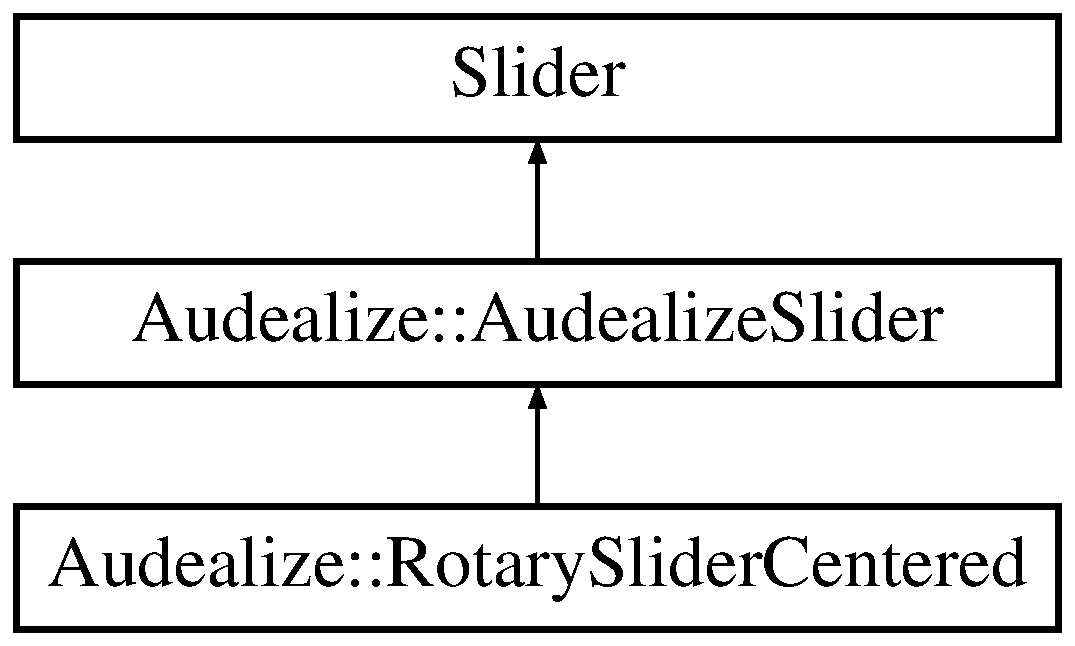
\includegraphics[height=3.000000cm]{class_audealize_1_1_audealize_slider}
\end{center}
\end{figure}
\subsection*{Public Member Functions}
\begin{DoxyCompactItemize}
\item 
\hyperlink{class_audealize_1_1_audealize_slider_a9f5d47d4aef86ee8ea80d12bd85fd75f}{Audealize\+Slider} ()
\item 
\hyperlink{class_audealize_1_1_audealize_slider_a6658b7093118d4412236c877dd92274d}{$\sim$\+Audealize\+Slider} ()
\item 
String \hyperlink{class_audealize_1_1_audealize_slider_ad878601b8f7fee2b4715d8863c0fb2c8}{get\+Text\+From\+Value} (double \hyperlink{tk_8h_a177a0765f574ef6642002696d9cd82d0}{value}) override
\item 
double \hyperlink{class_audealize_1_1_audealize_slider_a361a1e00ca8ef5efdedf24a624d3b683}{get\+Value\+From\+Text} (const juce\+::\+String \&text) override
\item 
\hyperlink{tk_8h_aba408b7cd755a96426e004c015f5de8e}{void} \hyperlink{class_audealize_1_1_audealize_slider_a70ec585c217aafd7a1a7d8d584bf33b1}{set\+Value\+To\+Text\+Function} (std\+::function$<$ String(float)$>$ f)
\item 
\hyperlink{tk_8h_aba408b7cd755a96426e004c015f5de8e}{void} \hyperlink{class_audealize_1_1_audealize_slider_a9211015084c99898254ec989251712aa}{set\+Text\+To\+Value\+Function} (std\+::function$<$ float(String)$>$ f)
\end{DoxyCompactItemize}


\subsection{Constructor \& Destructor Documentation}
\index{Audealize\+::\+Audealize\+Slider@{Audealize\+::\+Audealize\+Slider}!Audealize\+Slider@{Audealize\+Slider}}
\index{Audealize\+Slider@{Audealize\+Slider}!Audealize\+::\+Audealize\+Slider@{Audealize\+::\+Audealize\+Slider}}
\subsubsection[{\texorpdfstring{Audealize\+Slider()}{AudealizeSlider()}}]{\setlength{\rightskip}{0pt plus 5cm}Audealize\+::\+Audealize\+Slider\+::\+Audealize\+Slider (
\begin{DoxyParamCaption}
{}
\end{DoxyParamCaption}
)\hspace{0.3cm}{\ttfamily [inline]}}\hypertarget{class_audealize_1_1_audealize_slider_a9f5d47d4aef86ee8ea80d12bd85fd75f}{}\label{class_audealize_1_1_audealize_slider_a9f5d47d4aef86ee8ea80d12bd85fd75f}
\index{Audealize\+::\+Audealize\+Slider@{Audealize\+::\+Audealize\+Slider}!````~Audealize\+Slider@{$\sim$\+Audealize\+Slider}}
\index{````~Audealize\+Slider@{$\sim$\+Audealize\+Slider}!Audealize\+::\+Audealize\+Slider@{Audealize\+::\+Audealize\+Slider}}
\subsubsection[{\texorpdfstring{$\sim$\+Audealize\+Slider()}{~AudealizeSlider()}}]{\setlength{\rightskip}{0pt plus 5cm}Audealize\+::\+Audealize\+Slider\+::$\sim$\+Audealize\+Slider (
\begin{DoxyParamCaption}
{}
\end{DoxyParamCaption}
)\hspace{0.3cm}{\ttfamily [inline]}}\hypertarget{class_audealize_1_1_audealize_slider_a6658b7093118d4412236c877dd92274d}{}\label{class_audealize_1_1_audealize_slider_a6658b7093118d4412236c877dd92274d}


\subsection{Member Function Documentation}
\index{Audealize\+::\+Audealize\+Slider@{Audealize\+::\+Audealize\+Slider}!get\+Text\+From\+Value@{get\+Text\+From\+Value}}
\index{get\+Text\+From\+Value@{get\+Text\+From\+Value}!Audealize\+::\+Audealize\+Slider@{Audealize\+::\+Audealize\+Slider}}
\subsubsection[{\texorpdfstring{get\+Text\+From\+Value(double value) override}{getTextFromValue(double value) override}}]{\setlength{\rightskip}{0pt plus 5cm}String Audealize\+::\+Audealize\+Slider\+::get\+Text\+From\+Value (
\begin{DoxyParamCaption}
\item[{double}]{value}
\end{DoxyParamCaption}
)\hspace{0.3cm}{\ttfamily [inline]}, {\ttfamily [override]}}\hypertarget{class_audealize_1_1_audealize_slider_ad878601b8f7fee2b4715d8863c0fb2c8}{}\label{class_audealize_1_1_audealize_slider_ad878601b8f7fee2b4715d8863c0fb2c8}
Returns a String representation of the slider\textquotesingle{}s value. Used when displaying value in a textbox Inherited from juce\+::\+Slider


\begin{DoxyParams}{Parameters}
{\em value} & a double\\
\hline
\end{DoxyParams}
\begin{DoxyReturn}{Returns}
a String reprsentation of the value 
\end{DoxyReturn}
\index{Audealize\+::\+Audealize\+Slider@{Audealize\+::\+Audealize\+Slider}!get\+Value\+From\+Text@{get\+Value\+From\+Text}}
\index{get\+Value\+From\+Text@{get\+Value\+From\+Text}!Audealize\+::\+Audealize\+Slider@{Audealize\+::\+Audealize\+Slider}}
\subsubsection[{\texorpdfstring{get\+Value\+From\+Text(const juce\+::\+String \&text) override}{getValueFromText(const juce::String &text) override}}]{\setlength{\rightskip}{0pt plus 5cm}double Audealize\+::\+Audealize\+Slider\+::get\+Value\+From\+Text (
\begin{DoxyParamCaption}
\item[{const juce\+::\+String \&}]{text}
\end{DoxyParamCaption}
)\hspace{0.3cm}{\ttfamily [inline]}, {\ttfamily [override]}}\hypertarget{class_audealize_1_1_audealize_slider_a361a1e00ca8ef5efdedf24a624d3b683}{}\label{class_audealize_1_1_audealize_slider_a361a1e00ca8ef5efdedf24a624d3b683}
Parses a string containing the value of a slider and returns a double representation of that value Used when setting slider value through a text box. Inherited from juce\+::\+Slider


\begin{DoxyParams}{Parameters}
{\em text} & T\+He String to be parsed\\
\hline
\end{DoxyParams}
\begin{DoxyReturn}{Returns}
The value as a double 
\end{DoxyReturn}
\index{Audealize\+::\+Audealize\+Slider@{Audealize\+::\+Audealize\+Slider}!set\+Text\+To\+Value\+Function@{set\+Text\+To\+Value\+Function}}
\index{set\+Text\+To\+Value\+Function@{set\+Text\+To\+Value\+Function}!Audealize\+::\+Audealize\+Slider@{Audealize\+::\+Audealize\+Slider}}
\subsubsection[{\texorpdfstring{set\+Text\+To\+Value\+Function(std\+::function$<$ float(\+String)$>$ f)}{setTextToValueFunction(std::function< float(String)> f)}}]{\setlength{\rightskip}{0pt plus 5cm}{\bf void} Audealize\+::\+Audealize\+Slider\+::set\+Text\+To\+Value\+Function (
\begin{DoxyParamCaption}
\item[{std\+::function$<$ float(String)$>$}]{f}
\end{DoxyParamCaption}
)\hspace{0.3cm}{\ttfamily [inline]}}\hypertarget{class_audealize_1_1_audealize_slider_a9211015084c99898254ec989251712aa}{}\label{class_audealize_1_1_audealize_slider_a9211015084c99898254ec989251712aa}
Set a custom text to value function for the slider


\begin{DoxyParams}{Parameters}
{\em f} & a std\+::function$<$float (\+String)$>$ \\
\hline
\end{DoxyParams}
\index{Audealize\+::\+Audealize\+Slider@{Audealize\+::\+Audealize\+Slider}!set\+Value\+To\+Text\+Function@{set\+Value\+To\+Text\+Function}}
\index{set\+Value\+To\+Text\+Function@{set\+Value\+To\+Text\+Function}!Audealize\+::\+Audealize\+Slider@{Audealize\+::\+Audealize\+Slider}}
\subsubsection[{\texorpdfstring{set\+Value\+To\+Text\+Function(std\+::function$<$ String(float)$>$ f)}{setValueToTextFunction(std::function< String(float)> f)}}]{\setlength{\rightskip}{0pt plus 5cm}{\bf void} Audealize\+::\+Audealize\+Slider\+::set\+Value\+To\+Text\+Function (
\begin{DoxyParamCaption}
\item[{std\+::function$<$ String(float)$>$}]{f}
\end{DoxyParamCaption}
)\hspace{0.3cm}{\ttfamily [inline]}}\hypertarget{class_audealize_1_1_audealize_slider_a70ec585c217aafd7a1a7d8d584bf33b1}{}\label{class_audealize_1_1_audealize_slider_a70ec585c217aafd7a1a7d8d584bf33b1}
Set a custom value to text function for the slider


\begin{DoxyParams}{Parameters}
{\em f} & a std\+::function$<$\+String (float)$>$ \\
\hline
\end{DoxyParams}


The documentation for this class was generated from the following file\+:\begin{DoxyCompactItemize}
\item 
/\+Users/michael/\+J\+U\+C\+E/projects/audealize-\/plugin/\+J\+U\+C\+E Modules/audealize\+\_\+module/ui\+\_\+components/\hyperlink{_audealize_slider_8h}{Audealize\+Slider.\+h}\end{DoxyCompactItemize}

\hypertarget{class_audealize_1_1_audealize_tabbed_component}{}\section{Audealize\+:\+:Audealize\+Tabbed\+Component Class Reference}
\label{class_audealize_1_1_audealize_tabbed_component}\index{Audealize\+::\+Audealize\+Tabbed\+Component@{Audealize\+::\+Audealize\+Tabbed\+Component}}


{\ttfamily \#include $<$Audealize\+Tabbed\+Component.\+h$>$}

Inheritance diagram for Audealize\+:\+:Audealize\+Tabbed\+Component\+:\begin{figure}[H]
\begin{center}
\leavevmode
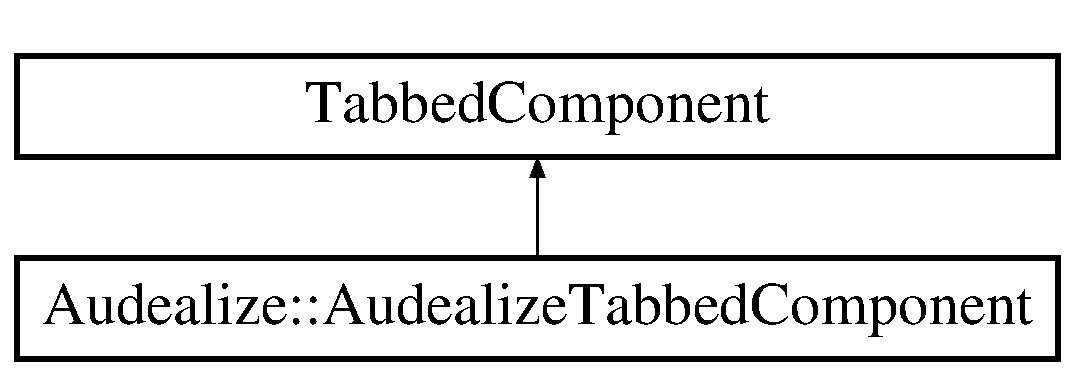
\includegraphics[height=2.000000cm]{class_audealize_1_1_audealize_tabbed_component}
\end{center}
\end{figure}
\subsection*{Public Types}
\begin{DoxyCompactItemize}
\item 
enum \hyperlink{class_audealize_1_1_audealize_tabbed_component_aa816a099502c5633df0e477993dd1f2d}{Colour\+Ids} \{ \hyperlink{class_audealize_1_1_audealize_tabbed_component_aa816a099502c5633df0e477993dd1f2da6f6ddd411d9553470397a3f46ee5a8b5}{background\+Colour\+Id} = 0x2000600
 \}
\end{DoxyCompactItemize}
\subsection*{Public Member Functions}
\begin{DoxyCompactItemize}
\item 
\hyperlink{class_audealize_1_1_audealize_tabbed_component_afb946c219ed21ef8e2878649023b0b45}{Audealize\+Tabbed\+Component} (const Tabbed\+Button\+Bar\+::\+Orientation orientation)
\item 
\hyperlink{class_audealize_1_1_audealize_tabbed_component_afbef708d0c2657fb343766020a765478}{$\sim$\+Audealize\+Tabbed\+Component} ()
\item 
\hyperlink{tk_8h_aba408b7cd755a96426e004c015f5de8e}{void} \hyperlink{class_audealize_1_1_audealize_tabbed_component_a43df12a792bbf2cc294a95b1ead79f44}{resized} () override
\item 
\hyperlink{tk_8h_aba408b7cd755a96426e004c015f5de8e}{void} \hyperlink{class_audealize_1_1_audealize_tabbed_component_ae4250795a18e9f1f20b440c8a52bc3e5}{look\+And\+Feel\+Changed} () override
\item 
\hyperlink{class_audealize_1_1_audealize_tabbed_component_aa732f48f26a303ec7f9e1188852bca6d}{J\+U\+C\+E\+\_\+\+D\+E\+C\+L\+A\+R\+E\+\_\+\+N\+O\+N\+\_\+\+C\+O\+P\+Y\+A\+B\+L\+E\+\_\+\+W\+I\+T\+H\+\_\+\+L\+E\+A\+K\+\_\+\+D\+E\+T\+E\+C\+T\+OR} (\hyperlink{class_audealize_1_1_audealize_tabbed_component}{Audealize\+Tabbed\+Component})
\end{DoxyCompactItemize}


\subsection{Member Enumeration Documentation}
\index{Audealize\+::\+Audealize\+Tabbed\+Component@{Audealize\+::\+Audealize\+Tabbed\+Component}!Colour\+Ids@{Colour\+Ids}}
\index{Colour\+Ids@{Colour\+Ids}!Audealize\+::\+Audealize\+Tabbed\+Component@{Audealize\+::\+Audealize\+Tabbed\+Component}}
\subsubsection[{\texorpdfstring{Colour\+Ids}{ColourIds}}]{\setlength{\rightskip}{0pt plus 5cm}enum {\bf Audealize\+::\+Audealize\+Tabbed\+Component\+::\+Colour\+Ids}}\hypertarget{class_audealize_1_1_audealize_tabbed_component_aa816a099502c5633df0e477993dd1f2d}{}\label{class_audealize_1_1_audealize_tabbed_component_aa816a099502c5633df0e477993dd1f2d}
\begin{Desc}
\item[Enumerator]\par
\begin{description}
\index{background\+Colour\+Id@{background\+Colour\+Id}!Audealize\+::\+Audealize\+Tabbed\+Component@{Audealize\+::\+Audealize\+Tabbed\+Component}}\index{Audealize\+::\+Audealize\+Tabbed\+Component@{Audealize\+::\+Audealize\+Tabbed\+Component}!background\+Colour\+Id@{background\+Colour\+Id}}\item[{\em 
background\+Colour\+Id\hypertarget{class_audealize_1_1_audealize_tabbed_component_aa816a099502c5633df0e477993dd1f2da6f6ddd411d9553470397a3f46ee5a8b5}{}\label{class_audealize_1_1_audealize_tabbed_component_aa816a099502c5633df0e477993dd1f2da6f6ddd411d9553470397a3f46ee5a8b5}
}]\end{description}
\end{Desc}


\subsection{Constructor \& Destructor Documentation}
\index{Audealize\+::\+Audealize\+Tabbed\+Component@{Audealize\+::\+Audealize\+Tabbed\+Component}!Audealize\+Tabbed\+Component@{Audealize\+Tabbed\+Component}}
\index{Audealize\+Tabbed\+Component@{Audealize\+Tabbed\+Component}!Audealize\+::\+Audealize\+Tabbed\+Component@{Audealize\+::\+Audealize\+Tabbed\+Component}}
\subsubsection[{\texorpdfstring{Audealize\+Tabbed\+Component(const Tabbed\+Button\+Bar\+::\+Orientation orientation)}{AudealizeTabbedComponent(const TabbedButtonBar::Orientation orientation)}}]{\setlength{\rightskip}{0pt plus 5cm}Audealize\+::\+Audealize\+Tabbed\+Component\+::\+Audealize\+Tabbed\+Component (
\begin{DoxyParamCaption}
\item[{const Tabbed\+Button\+Bar\+::\+Orientation}]{orientation}
\end{DoxyParamCaption}
)\hspace{0.3cm}{\ttfamily [inline]}}\hypertarget{class_audealize_1_1_audealize_tabbed_component_afb946c219ed21ef8e2878649023b0b45}{}\label{class_audealize_1_1_audealize_tabbed_component_afb946c219ed21ef8e2878649023b0b45}
\index{Audealize\+::\+Audealize\+Tabbed\+Component@{Audealize\+::\+Audealize\+Tabbed\+Component}!````~Audealize\+Tabbed\+Component@{$\sim$\+Audealize\+Tabbed\+Component}}
\index{````~Audealize\+Tabbed\+Component@{$\sim$\+Audealize\+Tabbed\+Component}!Audealize\+::\+Audealize\+Tabbed\+Component@{Audealize\+::\+Audealize\+Tabbed\+Component}}
\subsubsection[{\texorpdfstring{$\sim$\+Audealize\+Tabbed\+Component()}{~AudealizeTabbedComponent()}}]{\setlength{\rightskip}{0pt plus 5cm}Audealize\+::\+Audealize\+Tabbed\+Component\+::$\sim$\+Audealize\+Tabbed\+Component (
\begin{DoxyParamCaption}
{}
\end{DoxyParamCaption}
)\hspace{0.3cm}{\ttfamily [inline]}}\hypertarget{class_audealize_1_1_audealize_tabbed_component_afbef708d0c2657fb343766020a765478}{}\label{class_audealize_1_1_audealize_tabbed_component_afbef708d0c2657fb343766020a765478}


\subsection{Member Function Documentation}
\index{Audealize\+::\+Audealize\+Tabbed\+Component@{Audealize\+::\+Audealize\+Tabbed\+Component}!J\+U\+C\+E\+\_\+\+D\+E\+C\+L\+A\+R\+E\+\_\+\+N\+O\+N\+\_\+\+C\+O\+P\+Y\+A\+B\+L\+E\+\_\+\+W\+I\+T\+H\+\_\+\+L\+E\+A\+K\+\_\+\+D\+E\+T\+E\+C\+T\+OR@{J\+U\+C\+E\+\_\+\+D\+E\+C\+L\+A\+R\+E\+\_\+\+N\+O\+N\+\_\+\+C\+O\+P\+Y\+A\+B\+L\+E\+\_\+\+W\+I\+T\+H\+\_\+\+L\+E\+A\+K\+\_\+\+D\+E\+T\+E\+C\+T\+OR}}
\index{J\+U\+C\+E\+\_\+\+D\+E\+C\+L\+A\+R\+E\+\_\+\+N\+O\+N\+\_\+\+C\+O\+P\+Y\+A\+B\+L\+E\+\_\+\+W\+I\+T\+H\+\_\+\+L\+E\+A\+K\+\_\+\+D\+E\+T\+E\+C\+T\+OR@{J\+U\+C\+E\+\_\+\+D\+E\+C\+L\+A\+R\+E\+\_\+\+N\+O\+N\+\_\+\+C\+O\+P\+Y\+A\+B\+L\+E\+\_\+\+W\+I\+T\+H\+\_\+\+L\+E\+A\+K\+\_\+\+D\+E\+T\+E\+C\+T\+OR}!Audealize\+::\+Audealize\+Tabbed\+Component@{Audealize\+::\+Audealize\+Tabbed\+Component}}
\subsubsection[{\texorpdfstring{J\+U\+C\+E\+\_\+\+D\+E\+C\+L\+A\+R\+E\+\_\+\+N\+O\+N\+\_\+\+C\+O\+P\+Y\+A\+B\+L\+E\+\_\+\+W\+I\+T\+H\+\_\+\+L\+E\+A\+K\+\_\+\+D\+E\+T\+E\+C\+T\+O\+R(\+Audealize\+Tabbed\+Component)}{JUCE_DECLARE_NON_COPYABLE_WITH_LEAK_DETECTOR(AudealizeTabbedComponent)}}]{\setlength{\rightskip}{0pt plus 5cm}Audealize\+::\+Audealize\+Tabbed\+Component\+::\+J\+U\+C\+E\+\_\+\+D\+E\+C\+L\+A\+R\+E\+\_\+\+N\+O\+N\+\_\+\+C\+O\+P\+Y\+A\+B\+L\+E\+\_\+\+W\+I\+T\+H\+\_\+\+L\+E\+A\+K\+\_\+\+D\+E\+T\+E\+C\+T\+OR (
\begin{DoxyParamCaption}
\item[{{\bf Audealize\+Tabbed\+Component}}]{}
\end{DoxyParamCaption}
)}\hypertarget{class_audealize_1_1_audealize_tabbed_component_aa732f48f26a303ec7f9e1188852bca6d}{}\label{class_audealize_1_1_audealize_tabbed_component_aa732f48f26a303ec7f9e1188852bca6d}
\index{Audealize\+::\+Audealize\+Tabbed\+Component@{Audealize\+::\+Audealize\+Tabbed\+Component}!look\+And\+Feel\+Changed@{look\+And\+Feel\+Changed}}
\index{look\+And\+Feel\+Changed@{look\+And\+Feel\+Changed}!Audealize\+::\+Audealize\+Tabbed\+Component@{Audealize\+::\+Audealize\+Tabbed\+Component}}
\subsubsection[{\texorpdfstring{look\+And\+Feel\+Changed() override}{lookAndFeelChanged() override}}]{\setlength{\rightskip}{0pt plus 5cm}{\bf void} Audealize\+::\+Audealize\+Tabbed\+Component\+::look\+And\+Feel\+Changed (
\begin{DoxyParamCaption}
{}
\end{DoxyParamCaption}
)\hspace{0.3cm}{\ttfamily [inline]}, {\ttfamily [override]}}\hypertarget{class_audealize_1_1_audealize_tabbed_component_ae4250795a18e9f1f20b440c8a52bc3e5}{}\label{class_audealize_1_1_audealize_tabbed_component_ae4250795a18e9f1f20b440c8a52bc3e5}
\index{Audealize\+::\+Audealize\+Tabbed\+Component@{Audealize\+::\+Audealize\+Tabbed\+Component}!resized@{resized}}
\index{resized@{resized}!Audealize\+::\+Audealize\+Tabbed\+Component@{Audealize\+::\+Audealize\+Tabbed\+Component}}
\subsubsection[{\texorpdfstring{resized() override}{resized() override}}]{\setlength{\rightskip}{0pt plus 5cm}{\bf void} Audealize\+::\+Audealize\+Tabbed\+Component\+::resized (
\begin{DoxyParamCaption}
{}
\end{DoxyParamCaption}
)\hspace{0.3cm}{\ttfamily [inline]}, {\ttfamily [override]}}\hypertarget{class_audealize_1_1_audealize_tabbed_component_a43df12a792bbf2cc294a95b1ead79f44}{}\label{class_audealize_1_1_audealize_tabbed_component_a43df12a792bbf2cc294a95b1ead79f44}


The documentation for this class was generated from the following file\+:\begin{DoxyCompactItemize}
\item 
/\+Users/michael/\+J\+U\+C\+E/projects/audealize-\/plugin/\+J\+U\+C\+E Modules/audealize\+\_\+module/ui\+\_\+components/\hyperlink{_audealize_tabbed_component_8h}{Audealize\+Tabbed\+Component.\+h}\end{DoxyCompactItemize}

\hypertarget{class_audealize_1_1_audealize_u_i}{}\section{Audealize\+:\+:Audealize\+UI Class Reference}
\label{class_audealize_1_1_audealize_u_i}\index{Audealize\+::\+Audealize\+UI@{Audealize\+::\+Audealize\+UI}}


{\ttfamily \#include $<$Audealize\+U\+I.\+h$>$}

Inheritance diagram for Audealize\+:\+:Audealize\+UI\+:\begin{figure}[H]
\begin{center}
\leavevmode
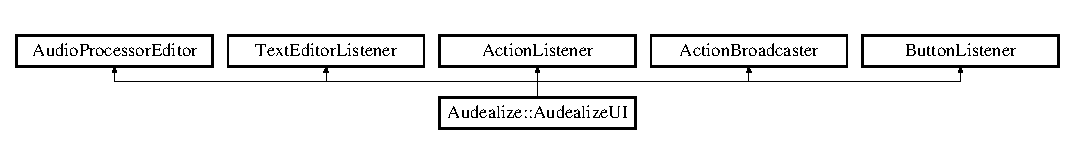
\includegraphics[height=1.503356cm]{class_audealize_1_1_audealize_u_i}
\end{center}
\end{figure}
\subsection*{Public Types}
\begin{DoxyCompactItemize}
\item 
enum \hyperlink{class_audealize_1_1_audealize_u_i_adc546ab367782c1aa6d8420d9786c0c1}{Colour\+Ids} \{ \hyperlink{class_audealize_1_1_audealize_u_i_adc546ab367782c1aa6d8420d9786c0c1ad891d56619a1d1e986de7568c16791c6}{background\+Colour\+Id} = 0x2000100, 
\hyperlink{class_audealize_1_1_audealize_u_i_adc546ab367782c1aa6d8420d9786c0c1a36cc2511875aeb658835ecefe2000219}{text\+Colour\+Id} = 0x2000101
 \}
\end{DoxyCompactItemize}
\subsection*{Public Member Functions}
\begin{DoxyCompactItemize}
\item 
\hyperlink{class_audealize_1_1_audealize_u_i_a5200044a18f6357b4b218e2e4d10fcce}{Audealize\+UI} (\hyperlink{class_audealize_1_1_audealize_audio_processor}{Audealize\+Audio\+Processor} \&p, Scoped\+Pointer$<$ \hyperlink{class_audealize_1_1_traditional_u_i}{Traditional\+UI} $>$ t, String path\+To\+Points, String effect\+Type, bool \hyperlink{class_audealize_1_1_audealize_u_i_ac5cfa0dc74706b4df821f7addfcc108d}{is\+Plugin\+Multi\+Effect}=false)
\item 
\hyperlink{class_audealize_1_1_audealize_u_i_a77d239387e49d6e032f434f15f4631e0}{$\sim$\+Audealize\+UI} ()
\item 
\hyperlink{tk_8h_aba408b7cd755a96426e004c015f5de8e}{void} \hyperlink{class_audealize_1_1_audealize_u_i_a6f5f606a15f0e656af570de10172c690}{text\+Editor\+Return\+Key\+Pressed} (Text\+Editor \&editor) override
\item 
\hyperlink{tk_8h_aba408b7cd755a96426e004c015f5de8e}{void} \hyperlink{class_audealize_1_1_audealize_u_i_a11662118bb8a50472f486fee23e81a14}{language\+Alert} ()
\item 
\hyperlink{tk_8h_aba408b7cd755a96426e004c015f5de8e}{void} \hyperlink{class_audealize_1_1_audealize_u_i_a886ff0e83c14fc96b469d4764f820791}{action\+Listener\+Callback} (const String \&message) override
\item 
\hyperlink{tk_8h_aba408b7cd755a96426e004c015f5de8e}{void} \hyperlink{class_audealize_1_1_audealize_u_i_aeaf15fc6ba8e3f536fa627a1c80b2c64}{paint} (Graphics \&g) override
\item 
\hyperlink{tk_8h_aba408b7cd755a96426e004c015f5de8e}{void} \hyperlink{class_audealize_1_1_audealize_u_i_a76ddb32329ed8550dc8b9bbbf44fb50d}{resized} () override
\item 
\hyperlink{tk_8h_aba408b7cd755a96426e004c015f5de8e}{void} \hyperlink{class_audealize_1_1_audealize_u_i_a2d29f30e6b9dc0d7012c58e4a5e3a84e}{button\+Clicked} (Button $\ast$button\+That\+Was\+Clicked) override
\item 
\hyperlink{tk_8h_aba408b7cd755a96426e004c015f5de8e}{void} \hyperlink{class_audealize_1_1_audealize_u_i_a0949b75681b58a8ca6063a6c1f56ca92}{look\+And\+Feel\+Changed} () override
\item 
\hyperlink{tk_8h_aba408b7cd755a96426e004c015f5de8e}{void} \hyperlink{class_audealize_1_1_audealize_u_i_ab56c907e41ba7bdd871c0aceccf0b60e}{children\+Changed} () override
\item 
\hyperlink{tk_8h_aba408b7cd755a96426e004c015f5de8e}{void} \hyperlink{class_audealize_1_1_audealize_u_i_a975132dcdae4462a1fd700864c8fda9e}{set\+Bypassed} (bool is\+Bypassed)
\item 
bool \hyperlink{class_audealize_1_1_audealize_u_i_aeca6fb4ba3fc507cbc655cbea3495e8a}{is\+Traditional\+U\+I\+Visible} ()
\item 
Text\+Button $\ast$ \hyperlink{class_audealize_1_1_audealize_u_i_a1b6c043013abf9ece8e7134e913c4d63}{get\+Traditional\+U\+I\+Button} ()
\item 
Text\+Button $\ast$ \hyperlink{class_audealize_1_1_audealize_u_i_aa7b47494a406382edfffdb2c79263f43}{get\+Bypass\+Button} ()
\item 
\hyperlink{class_audealize_1_1_traditional_u_i}{Traditional\+UI} $\ast$ \hyperlink{class_audealize_1_1_audealize_u_i_a3aacc48123b4709bb0349fdfc75ae9ff}{get\+Traditional\+UI} ()
\item 
\hyperlink{class_typeahead_editor}{Typeahead\+Editor} $\ast$ \hyperlink{class_audealize_1_1_audealize_u_i_a5dc6ab0b86b64964fd30d470c360c74f}{get\+Search\+Bar} ()
\item 
\hyperlink{class_audealize_1_1_word_map}{Word\+Map} $\ast$ \hyperlink{class_audealize_1_1_audealize_u_i_affc13f7dc31cb1544b4e73fa7c8faa07}{get\+Word\+Map} ()
\item 
String \hyperlink{class_audealize_1_1_audealize_u_i_a2ba5a78e8ea3e16f6a925015f76495a3}{get\+Effect\+Name} ()
\item 
\hyperlink{tk_8h_a83f82f76e7fed06f4c49d2db94028a6d}{int} \hyperlink{class_audealize_1_1_audealize_u_i_abac99c4e9398e756b332e3c2893c45c2}{get\+Word\+Map\+Height} ()
\item 
bool \hyperlink{class_audealize_1_1_audealize_u_i_ac5cfa0dc74706b4df821f7addfcc108d}{is\+Plugin\+Multi\+Effect} ()
\item 
bool \hyperlink{class_audealize_1_1_audealize_u_i_a5e547f20b6675dface86ee0e3c92f174}{is\+Effect\+Enabled} ()
\end{DoxyCompactItemize}


\subsection{Member Enumeration Documentation}
\index{Audealize\+::\+Audealize\+UI@{Audealize\+::\+Audealize\+UI}!Colour\+Ids@{Colour\+Ids}}
\index{Colour\+Ids@{Colour\+Ids}!Audealize\+::\+Audealize\+UI@{Audealize\+::\+Audealize\+UI}}
\subsubsection[{\texorpdfstring{Colour\+Ids}{ColourIds}}]{\setlength{\rightskip}{0pt plus 5cm}enum {\bf Audealize\+::\+Audealize\+U\+I\+::\+Colour\+Ids}}\hypertarget{class_audealize_1_1_audealize_u_i_adc546ab367782c1aa6d8420d9786c0c1}{}\label{class_audealize_1_1_audealize_u_i_adc546ab367782c1aa6d8420d9786c0c1}
\begin{Desc}
\item[Enumerator]\par
\begin{description}
\index{background\+Colour\+Id@{background\+Colour\+Id}!Audealize\+::\+Audealize\+UI@{Audealize\+::\+Audealize\+UI}}\index{Audealize\+::\+Audealize\+UI@{Audealize\+::\+Audealize\+UI}!background\+Colour\+Id@{background\+Colour\+Id}}\item[{\em 
background\+Colour\+Id\hypertarget{class_audealize_1_1_audealize_u_i_adc546ab367782c1aa6d8420d9786c0c1ad891d56619a1d1e986de7568c16791c6}{}\label{class_audealize_1_1_audealize_u_i_adc546ab367782c1aa6d8420d9786c0c1ad891d56619a1d1e986de7568c16791c6}
}]\index{text\+Colour\+Id@{text\+Colour\+Id}!Audealize\+::\+Audealize\+UI@{Audealize\+::\+Audealize\+UI}}\index{Audealize\+::\+Audealize\+UI@{Audealize\+::\+Audealize\+UI}!text\+Colour\+Id@{text\+Colour\+Id}}\item[{\em 
text\+Colour\+Id\hypertarget{class_audealize_1_1_audealize_u_i_adc546ab367782c1aa6d8420d9786c0c1a36cc2511875aeb658835ecefe2000219}{}\label{class_audealize_1_1_audealize_u_i_adc546ab367782c1aa6d8420d9786c0c1a36cc2511875aeb658835ecefe2000219}
}]\end{description}
\end{Desc}


\subsection{Constructor \& Destructor Documentation}
\index{Audealize\+::\+Audealize\+UI@{Audealize\+::\+Audealize\+UI}!Audealize\+UI@{Audealize\+UI}}
\index{Audealize\+UI@{Audealize\+UI}!Audealize\+::\+Audealize\+UI@{Audealize\+::\+Audealize\+UI}}
\subsubsection[{\texorpdfstring{Audealize\+U\+I(\+Audealize\+Audio\+Processor \&p, Scoped\+Pointer$<$ Traditional\+U\+I $>$ t, String path\+To\+Points, String effect\+Type, bool is\+Plugin\+Multi\+Effect=false)}{AudealizeUI(AudealizeAudioProcessor &p, ScopedPointer< TraditionalUI > t, String pathToPoints, String effectType, bool isPluginMultiEffect=false)}}]{\setlength{\rightskip}{0pt plus 5cm}Audealize\+::\+Audealize\+U\+I\+::\+Audealize\+UI (
\begin{DoxyParamCaption}
\item[{{\bf Audealize\+Audio\+Processor} \&}]{p, }
\item[{Scoped\+Pointer$<$ {\bf Traditional\+UI} $>$}]{t, }
\item[{String}]{path\+To\+Points, }
\item[{String}]{effect\+Type, }
\item[{bool}]{is\+Plugin\+Multi\+Effect = {\ttfamily false}}
\end{DoxyParamCaption}
)}\hypertarget{class_audealize_1_1_audealize_u_i_a5200044a18f6357b4b218e2e4d10fcce}{}\label{class_audealize_1_1_audealize_u_i_a5200044a18f6357b4b218e2e4d10fcce}
\index{Audealize\+::\+Audealize\+UI@{Audealize\+::\+Audealize\+UI}!````~Audealize\+UI@{$\sim$\+Audealize\+UI}}
\index{````~Audealize\+UI@{$\sim$\+Audealize\+UI}!Audealize\+::\+Audealize\+UI@{Audealize\+::\+Audealize\+UI}}
\subsubsection[{\texorpdfstring{$\sim$\+Audealize\+U\+I()}{~AudealizeUI()}}]{\setlength{\rightskip}{0pt plus 5cm}Audealize\+::\+Audealize\+U\+I\+::$\sim$\+Audealize\+UI (
\begin{DoxyParamCaption}
{}
\end{DoxyParamCaption}
)}\hypertarget{class_audealize_1_1_audealize_u_i_a77d239387e49d6e032f434f15f4631e0}{}\label{class_audealize_1_1_audealize_u_i_a77d239387e49d6e032f434f15f4631e0}


\subsection{Member Function Documentation}
\index{Audealize\+::\+Audealize\+UI@{Audealize\+::\+Audealize\+UI}!action\+Listener\+Callback@{action\+Listener\+Callback}}
\index{action\+Listener\+Callback@{action\+Listener\+Callback}!Audealize\+::\+Audealize\+UI@{Audealize\+::\+Audealize\+UI}}
\subsubsection[{\texorpdfstring{action\+Listener\+Callback(const String \&message) override}{actionListenerCallback(const String &message) override}}]{\setlength{\rightskip}{0pt plus 5cm}{\bf void} Audealize\+::\+Audealize\+U\+I\+::action\+Listener\+Callback (
\begin{DoxyParamCaption}
\item[{const String \&}]{message}
\end{DoxyParamCaption}
)\hspace{0.3cm}{\ttfamily [override]}}\hypertarget{class_audealize_1_1_audealize_u_i_a886ff0e83c14fc96b469d4764f820791}{}\label{class_audealize_1_1_audealize_u_i_a886ff0e83c14fc96b469d4764f820791}
Listens for changes broadcast by an Action\+Broadcaster Updates the set of descriptors searched by the search bar when language is changed


\begin{DoxyParams}{Parameters}
{\em message} & A string containing the message received \\
\hline
\end{DoxyParams}
\index{Audealize\+::\+Audealize\+UI@{Audealize\+::\+Audealize\+UI}!button\+Clicked@{button\+Clicked}}
\index{button\+Clicked@{button\+Clicked}!Audealize\+::\+Audealize\+UI@{Audealize\+::\+Audealize\+UI}}
\subsubsection[{\texorpdfstring{button\+Clicked(\+Button $\ast$button\+That\+Was\+Clicked) override}{buttonClicked(Button *buttonThatWasClicked) override}}]{\setlength{\rightskip}{0pt plus 5cm}{\bf void} Audealize\+::\+Audealize\+U\+I\+::button\+Clicked (
\begin{DoxyParamCaption}
\item[{Button $\ast$}]{button\+That\+Was\+Clicked}
\end{DoxyParamCaption}
)\hspace{0.3cm}{\ttfamily [override]}}\hypertarget{class_audealize_1_1_audealize_u_i_a2d29f30e6b9dc0d7012c58e4a5e3a84e}{}\label{class_audealize_1_1_audealize_u_i_a2d29f30e6b9dc0d7012c58e4a5e3a84e}
Called when a button is clicked (language selection or traditional UI hide/show)


\begin{DoxyParams}{Parameters}
{\em button\+That\+Was\+Clicked} & \\
\hline
\end{DoxyParams}
\index{Audealize\+::\+Audealize\+UI@{Audealize\+::\+Audealize\+UI}!children\+Changed@{children\+Changed}}
\index{children\+Changed@{children\+Changed}!Audealize\+::\+Audealize\+UI@{Audealize\+::\+Audealize\+UI}}
\subsubsection[{\texorpdfstring{children\+Changed() override}{childrenChanged() override}}]{\setlength{\rightskip}{0pt plus 5cm}{\bf void} Audealize\+::\+Audealize\+U\+I\+::children\+Changed (
\begin{DoxyParamCaption}
{}
\end{DoxyParamCaption}
)\hspace{0.3cm}{\ttfamily [override]}}\hypertarget{class_audealize_1_1_audealize_u_i_ab56c907e41ba7bdd871c0aceccf0b60e}{}\label{class_audealize_1_1_audealize_u_i_ab56c907e41ba7bdd871c0aceccf0b60e}
\index{Audealize\+::\+Audealize\+UI@{Audealize\+::\+Audealize\+UI}!get\+Bypass\+Button@{get\+Bypass\+Button}}
\index{get\+Bypass\+Button@{get\+Bypass\+Button}!Audealize\+::\+Audealize\+UI@{Audealize\+::\+Audealize\+UI}}
\subsubsection[{\texorpdfstring{get\+Bypass\+Button()}{getBypassButton()}}]{\setlength{\rightskip}{0pt plus 5cm}Text\+Button$\ast$ Audealize\+::\+Audealize\+U\+I\+::get\+Bypass\+Button (
\begin{DoxyParamCaption}
{}
\end{DoxyParamCaption}
)\hspace{0.3cm}{\ttfamily [inline]}}\hypertarget{class_audealize_1_1_audealize_u_i_aa7b47494a406382edfffdb2c79263f43}{}\label{class_audealize_1_1_audealize_u_i_aa7b47494a406382edfffdb2c79263f43}
\index{Audealize\+::\+Audealize\+UI@{Audealize\+::\+Audealize\+UI}!get\+Effect\+Name@{get\+Effect\+Name}}
\index{get\+Effect\+Name@{get\+Effect\+Name}!Audealize\+::\+Audealize\+UI@{Audealize\+::\+Audealize\+UI}}
\subsubsection[{\texorpdfstring{get\+Effect\+Name()}{getEffectName()}}]{\setlength{\rightskip}{0pt plus 5cm}String Audealize\+::\+Audealize\+U\+I\+::get\+Effect\+Name (
\begin{DoxyParamCaption}
{}
\end{DoxyParamCaption}
)\hspace{0.3cm}{\ttfamily [inline]}}\hypertarget{class_audealize_1_1_audealize_u_i_a2ba5a78e8ea3e16f6a925015f76495a3}{}\label{class_audealize_1_1_audealize_u_i_a2ba5a78e8ea3e16f6a925015f76495a3}
\index{Audealize\+::\+Audealize\+UI@{Audealize\+::\+Audealize\+UI}!get\+Search\+Bar@{get\+Search\+Bar}}
\index{get\+Search\+Bar@{get\+Search\+Bar}!Audealize\+::\+Audealize\+UI@{Audealize\+::\+Audealize\+UI}}
\subsubsection[{\texorpdfstring{get\+Search\+Bar()}{getSearchBar()}}]{\setlength{\rightskip}{0pt plus 5cm}{\bf Typeahead\+Editor}$\ast$ Audealize\+::\+Audealize\+U\+I\+::get\+Search\+Bar (
\begin{DoxyParamCaption}
{}
\end{DoxyParamCaption}
)\hspace{0.3cm}{\ttfamily [inline]}}\hypertarget{class_audealize_1_1_audealize_u_i_a5dc6ab0b86b64964fd30d470c360c74f}{}\label{class_audealize_1_1_audealize_u_i_a5dc6ab0b86b64964fd30d470c360c74f}
\index{Audealize\+::\+Audealize\+UI@{Audealize\+::\+Audealize\+UI}!get\+Traditional\+UI@{get\+Traditional\+UI}}
\index{get\+Traditional\+UI@{get\+Traditional\+UI}!Audealize\+::\+Audealize\+UI@{Audealize\+::\+Audealize\+UI}}
\subsubsection[{\texorpdfstring{get\+Traditional\+U\+I()}{getTraditionalUI()}}]{\setlength{\rightskip}{0pt plus 5cm}{\bf Traditional\+UI}$\ast$ Audealize\+::\+Audealize\+U\+I\+::get\+Traditional\+UI (
\begin{DoxyParamCaption}
{}
\end{DoxyParamCaption}
)\hspace{0.3cm}{\ttfamily [inline]}}\hypertarget{class_audealize_1_1_audealize_u_i_a3aacc48123b4709bb0349fdfc75ae9ff}{}\label{class_audealize_1_1_audealize_u_i_a3aacc48123b4709bb0349fdfc75ae9ff}
\index{Audealize\+::\+Audealize\+UI@{Audealize\+::\+Audealize\+UI}!get\+Traditional\+U\+I\+Button@{get\+Traditional\+U\+I\+Button}}
\index{get\+Traditional\+U\+I\+Button@{get\+Traditional\+U\+I\+Button}!Audealize\+::\+Audealize\+UI@{Audealize\+::\+Audealize\+UI}}
\subsubsection[{\texorpdfstring{get\+Traditional\+U\+I\+Button()}{getTraditionalUIButton()}}]{\setlength{\rightskip}{0pt plus 5cm}Text\+Button$\ast$ Audealize\+::\+Audealize\+U\+I\+::get\+Traditional\+U\+I\+Button (
\begin{DoxyParamCaption}
{}
\end{DoxyParamCaption}
)\hspace{0.3cm}{\ttfamily [inline]}}\hypertarget{class_audealize_1_1_audealize_u_i_a1b6c043013abf9ece8e7134e913c4d63}{}\label{class_audealize_1_1_audealize_u_i_a1b6c043013abf9ece8e7134e913c4d63}
\index{Audealize\+::\+Audealize\+UI@{Audealize\+::\+Audealize\+UI}!get\+Word\+Map@{get\+Word\+Map}}
\index{get\+Word\+Map@{get\+Word\+Map}!Audealize\+::\+Audealize\+UI@{Audealize\+::\+Audealize\+UI}}
\subsubsection[{\texorpdfstring{get\+Word\+Map()}{getWordMap()}}]{\setlength{\rightskip}{0pt plus 5cm}{\bf Word\+Map}$\ast$ Audealize\+::\+Audealize\+U\+I\+::get\+Word\+Map (
\begin{DoxyParamCaption}
{}
\end{DoxyParamCaption}
)\hspace{0.3cm}{\ttfamily [inline]}}\hypertarget{class_audealize_1_1_audealize_u_i_affc13f7dc31cb1544b4e73fa7c8faa07}{}\label{class_audealize_1_1_audealize_u_i_affc13f7dc31cb1544b4e73fa7c8faa07}
\index{Audealize\+::\+Audealize\+UI@{Audealize\+::\+Audealize\+UI}!get\+Word\+Map\+Height@{get\+Word\+Map\+Height}}
\index{get\+Word\+Map\+Height@{get\+Word\+Map\+Height}!Audealize\+::\+Audealize\+UI@{Audealize\+::\+Audealize\+UI}}
\subsubsection[{\texorpdfstring{get\+Word\+Map\+Height()}{getWordMapHeight()}}]{\setlength{\rightskip}{0pt plus 5cm}{\bf int} Audealize\+::\+Audealize\+U\+I\+::get\+Word\+Map\+Height (
\begin{DoxyParamCaption}
{}
\end{DoxyParamCaption}
)\hspace{0.3cm}{\ttfamily [inline]}}\hypertarget{class_audealize_1_1_audealize_u_i_abac99c4e9398e756b332e3c2893c45c2}{}\label{class_audealize_1_1_audealize_u_i_abac99c4e9398e756b332e3c2893c45c2}
\index{Audealize\+::\+Audealize\+UI@{Audealize\+::\+Audealize\+UI}!is\+Effect\+Enabled@{is\+Effect\+Enabled}}
\index{is\+Effect\+Enabled@{is\+Effect\+Enabled}!Audealize\+::\+Audealize\+UI@{Audealize\+::\+Audealize\+UI}}
\subsubsection[{\texorpdfstring{is\+Effect\+Enabled()}{isEffectEnabled()}}]{\setlength{\rightskip}{0pt plus 5cm}bool Audealize\+::\+Audealize\+U\+I\+::is\+Effect\+Enabled (
\begin{DoxyParamCaption}
{}
\end{DoxyParamCaption}
)\hspace{0.3cm}{\ttfamily [inline]}}\hypertarget{class_audealize_1_1_audealize_u_i_a5e547f20b6675dface86ee0e3c92f174}{}\label{class_audealize_1_1_audealize_u_i_a5e547f20b6675dface86ee0e3c92f174}
\index{Audealize\+::\+Audealize\+UI@{Audealize\+::\+Audealize\+UI}!is\+Plugin\+Multi\+Effect@{is\+Plugin\+Multi\+Effect}}
\index{is\+Plugin\+Multi\+Effect@{is\+Plugin\+Multi\+Effect}!Audealize\+::\+Audealize\+UI@{Audealize\+::\+Audealize\+UI}}
\subsubsection[{\texorpdfstring{is\+Plugin\+Multi\+Effect()}{isPluginMultiEffect()}}]{\setlength{\rightskip}{0pt plus 5cm}bool Audealize\+::\+Audealize\+U\+I\+::is\+Plugin\+Multi\+Effect (
\begin{DoxyParamCaption}
{}
\end{DoxyParamCaption}
)\hspace{0.3cm}{\ttfamily [inline]}}\hypertarget{class_audealize_1_1_audealize_u_i_ac5cfa0dc74706b4df821f7addfcc108d}{}\label{class_audealize_1_1_audealize_u_i_ac5cfa0dc74706b4df821f7addfcc108d}
\index{Audealize\+::\+Audealize\+UI@{Audealize\+::\+Audealize\+UI}!is\+Traditional\+U\+I\+Visible@{is\+Traditional\+U\+I\+Visible}}
\index{is\+Traditional\+U\+I\+Visible@{is\+Traditional\+U\+I\+Visible}!Audealize\+::\+Audealize\+UI@{Audealize\+::\+Audealize\+UI}}
\subsubsection[{\texorpdfstring{is\+Traditional\+U\+I\+Visible()}{isTraditionalUIVisible()}}]{\setlength{\rightskip}{0pt plus 5cm}bool Audealize\+::\+Audealize\+U\+I\+::is\+Traditional\+U\+I\+Visible (
\begin{DoxyParamCaption}
{}
\end{DoxyParamCaption}
)\hspace{0.3cm}{\ttfamily [inline]}}\hypertarget{class_audealize_1_1_audealize_u_i_aeca6fb4ba3fc507cbc655cbea3495e8a}{}\label{class_audealize_1_1_audealize_u_i_aeca6fb4ba3fc507cbc655cbea3495e8a}
\index{Audealize\+::\+Audealize\+UI@{Audealize\+::\+Audealize\+UI}!language\+Alert@{language\+Alert}}
\index{language\+Alert@{language\+Alert}!Audealize\+::\+Audealize\+UI@{Audealize\+::\+Audealize\+UI}}
\subsubsection[{\texorpdfstring{language\+Alert()}{languageAlert()}}]{\setlength{\rightskip}{0pt plus 5cm}{\bf void} Audealize\+::\+Audealize\+U\+I\+::language\+Alert (
\begin{DoxyParamCaption}
{}
\end{DoxyParamCaption}
)}\hypertarget{class_audealize_1_1_audealize_u_i_a11662118bb8a50472f486fee23e81a14}{}\label{class_audealize_1_1_audealize_u_i_a11662118bb8a50472f486fee23e81a14}
Displays m\+Alert\+Box if user tries to select $<$1 language \index{Audealize\+::\+Audealize\+UI@{Audealize\+::\+Audealize\+UI}!look\+And\+Feel\+Changed@{look\+And\+Feel\+Changed}}
\index{look\+And\+Feel\+Changed@{look\+And\+Feel\+Changed}!Audealize\+::\+Audealize\+UI@{Audealize\+::\+Audealize\+UI}}
\subsubsection[{\texorpdfstring{look\+And\+Feel\+Changed() override}{lookAndFeelChanged() override}}]{\setlength{\rightskip}{0pt plus 5cm}{\bf void} Audealize\+::\+Audealize\+U\+I\+::look\+And\+Feel\+Changed (
\begin{DoxyParamCaption}
{}
\end{DoxyParamCaption}
)\hspace{0.3cm}{\ttfamily [override]}}\hypertarget{class_audealize_1_1_audealize_u_i_a0949b75681b58a8ca6063a6c1f56ca92}{}\label{class_audealize_1_1_audealize_u_i_a0949b75681b58a8ca6063a6c1f56ca92}
\index{Audealize\+::\+Audealize\+UI@{Audealize\+::\+Audealize\+UI}!paint@{paint}}
\index{paint@{paint}!Audealize\+::\+Audealize\+UI@{Audealize\+::\+Audealize\+UI}}
\subsubsection[{\texorpdfstring{paint(\+Graphics \&g) override}{paint(Graphics &g) override}}]{\setlength{\rightskip}{0pt plus 5cm}{\bf void} Audealize\+::\+Audealize\+U\+I\+::paint (
\begin{DoxyParamCaption}
\item[{Graphics \&}]{g}
\end{DoxyParamCaption}
)\hspace{0.3cm}{\ttfamily [override]}}\hypertarget{class_audealize_1_1_audealize_u_i_aeaf15fc6ba8e3f536fa627a1c80b2c64}{}\label{class_audealize_1_1_audealize_u_i_aeaf15fc6ba8e3f536fa627a1c80b2c64}
\index{Audealize\+::\+Audealize\+UI@{Audealize\+::\+Audealize\+UI}!resized@{resized}}
\index{resized@{resized}!Audealize\+::\+Audealize\+UI@{Audealize\+::\+Audealize\+UI}}
\subsubsection[{\texorpdfstring{resized() override}{resized() override}}]{\setlength{\rightskip}{0pt plus 5cm}{\bf void} Audealize\+::\+Audealize\+U\+I\+::resized (
\begin{DoxyParamCaption}
{}
\end{DoxyParamCaption}
)\hspace{0.3cm}{\ttfamily [override]}}\hypertarget{class_audealize_1_1_audealize_u_i_a76ddb32329ed8550dc8b9bbbf44fb50d}{}\label{class_audealize_1_1_audealize_u_i_a76ddb32329ed8550dc8b9bbbf44fb50d}
Called when the plugin window is resized. This is where the layout of the UI is defined \index{Audealize\+::\+Audealize\+UI@{Audealize\+::\+Audealize\+UI}!set\+Bypassed@{set\+Bypassed}}
\index{set\+Bypassed@{set\+Bypassed}!Audealize\+::\+Audealize\+UI@{Audealize\+::\+Audealize\+UI}}
\subsubsection[{\texorpdfstring{set\+Bypassed(bool is\+Bypassed)}{setBypassed(bool isBypassed)}}]{\setlength{\rightskip}{0pt plus 5cm}{\bf void} Audealize\+::\+Audealize\+U\+I\+::set\+Bypassed (
\begin{DoxyParamCaption}
\item[{bool}]{is\+Bypassed}
\end{DoxyParamCaption}
)\hspace{0.3cm}{\ttfamily [inline]}}\hypertarget{class_audealize_1_1_audealize_u_i_a975132dcdae4462a1fd700864c8fda9e}{}\label{class_audealize_1_1_audealize_u_i_a975132dcdae4462a1fd700864c8fda9e}
\index{Audealize\+::\+Audealize\+UI@{Audealize\+::\+Audealize\+UI}!text\+Editor\+Return\+Key\+Pressed@{text\+Editor\+Return\+Key\+Pressed}}
\index{text\+Editor\+Return\+Key\+Pressed@{text\+Editor\+Return\+Key\+Pressed}!Audealize\+::\+Audealize\+UI@{Audealize\+::\+Audealize\+UI}}
\subsubsection[{\texorpdfstring{text\+Editor\+Return\+Key\+Pressed(\+Text\+Editor \&editor) override}{textEditorReturnKeyPressed(TextEditor &editor) override}}]{\setlength{\rightskip}{0pt plus 5cm}{\bf void} Audealize\+::\+Audealize\+U\+I\+::text\+Editor\+Return\+Key\+Pressed (
\begin{DoxyParamCaption}
\item[{Text\+Editor \&}]{editor}
\end{DoxyParamCaption}
)\hspace{0.3cm}{\ttfamily [override]}}\hypertarget{class_audealize_1_1_audealize_u_i_a6f5f606a15f0e656af570de10172c690}{}\label{class_audealize_1_1_audealize_u_i_a6f5f606a15f0e656af570de10172c690}
Called when return key is pressed in search bar, selects word on map 

The documentation for this class was generated from the following files\+:\begin{DoxyCompactItemize}
\item 
/\+Users/michael/\+J\+U\+C\+E/projects/audealize-\/plugin/\+J\+U\+C\+E Modules/audealize\+\_\+module/ui\+\_\+components/\hyperlink{_audealize_u_i_8h}{Audealize\+U\+I.\+h}\item 
/\+Users/michael/\+J\+U\+C\+E/projects/audealize-\/plugin/\+J\+U\+C\+E Modules/audealize\+\_\+module/ui\+\_\+components/\hyperlink{_audealize_u_i_8cpp}{Audealize\+U\+I.\+cpp}\end{DoxyCompactItemize}

\hypertarget{class_audealize_1_1_audio_effect}{}\section{Audealize\+:\+:Audio\+Effect Class Reference}
\label{class_audealize_1_1_audio_effect}\index{Audealize\+::\+Audio\+Effect@{Audealize\+::\+Audio\+Effect}}


{\ttfamily \#include $<$Audio\+Effect.\+h$>$}

Inheritance diagram for Audealize\+:\+:Audio\+Effect\+:\begin{figure}[H]
\begin{center}
\leavevmode
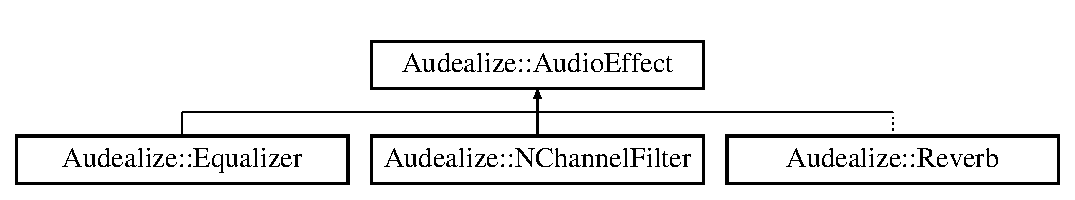
\includegraphics[height=2.000000cm]{class_audealize_1_1_audio_effect}
\end{center}
\end{figure}
\subsection*{Public Member Functions}
\begin{DoxyCompactItemize}
\item 
\hyperlink{class_audealize_1_1_audio_effect_ac730d3e11025310b13019073268174de}{Audio\+Effect} (float sample\+Rate=44100)
\item 
virtual \hyperlink{class_audealize_1_1_audio_effect_a3cd9fc8ee2b2bb4bd313772014651fd0}{$\sim$\+Audio\+Effect} ()
\item 
virtual float \hyperlink{class_audealize_1_1_audio_effect_ab77548a457702d189087163a696d4215}{process\+Sample} (float sample, \hyperlink{tk_8h_a83f82f76e7fed06f4c49d2db94028a6d}{int} channel\+Idx)
\item 
virtual \hyperlink{tk_8h_aba408b7cd755a96426e004c015f5de8e}{void} \hyperlink{class_audealize_1_1_audio_effect_a343c4a44c067e2605d18dcb578ae1302}{process\+Block} (float $\ast$const samples, \hyperlink{tk_8h_a83f82f76e7fed06f4c49d2db94028a6d}{int} num\+Samples, \hyperlink{tk_8h_a83f82f76e7fed06f4c49d2db94028a6d}{int} channel\+Idx)
\item 
virtual \hyperlink{tk_8h_aba408b7cd755a96426e004c015f5de8e}{void} \hyperlink{class_audealize_1_1_audio_effect_a5ff34c0371f2311dc026bca5ba245faa}{set\+Sample\+Rate} (float sample\+Rate)
\item 
float \hyperlink{class_audealize_1_1_audio_effect_aa1d51c95f452a5d71f97908a13751166}{get\+Sample\+Rate} ()
\end{DoxyCompactItemize}
\subsection*{Protected Attributes}
\begin{DoxyCompactItemize}
\item 
float \hyperlink{class_audealize_1_1_audio_effect_acd609287d863778dcb7e27ea208b17ba}{m\+Sample\+Rate}
\end{DoxyCompactItemize}


\subsection{Constructor \& Destructor Documentation}
\index{Audealize\+::\+Audio\+Effect@{Audealize\+::\+Audio\+Effect}!Audio\+Effect@{Audio\+Effect}}
\index{Audio\+Effect@{Audio\+Effect}!Audealize\+::\+Audio\+Effect@{Audealize\+::\+Audio\+Effect}}
\subsubsection[{\texorpdfstring{Audio\+Effect(float sample\+Rate=44100)}{AudioEffect(float sampleRate=44100)}}]{\setlength{\rightskip}{0pt plus 5cm}Audealize\+::\+Audio\+Effect\+::\+Audio\+Effect (
\begin{DoxyParamCaption}
\item[{float}]{sample\+Rate = {\ttfamily 44100}}
\end{DoxyParamCaption}
)\hspace{0.3cm}{\ttfamily [inline]}}\hypertarget{class_audealize_1_1_audio_effect_ac730d3e11025310b13019073268174de}{}\label{class_audealize_1_1_audio_effect_ac730d3e11025310b13019073268174de}
\index{Audealize\+::\+Audio\+Effect@{Audealize\+::\+Audio\+Effect}!````~Audio\+Effect@{$\sim$\+Audio\+Effect}}
\index{````~Audio\+Effect@{$\sim$\+Audio\+Effect}!Audealize\+::\+Audio\+Effect@{Audealize\+::\+Audio\+Effect}}
\subsubsection[{\texorpdfstring{$\sim$\+Audio\+Effect()}{~AudioEffect()}}]{\setlength{\rightskip}{0pt plus 5cm}virtual Audealize\+::\+Audio\+Effect\+::$\sim$\+Audio\+Effect (
\begin{DoxyParamCaption}
{}
\end{DoxyParamCaption}
)\hspace{0.3cm}{\ttfamily [inline]}, {\ttfamily [virtual]}}\hypertarget{class_audealize_1_1_audio_effect_a3cd9fc8ee2b2bb4bd313772014651fd0}{}\label{class_audealize_1_1_audio_effect_a3cd9fc8ee2b2bb4bd313772014651fd0}


\subsection{Member Function Documentation}
\index{Audealize\+::\+Audio\+Effect@{Audealize\+::\+Audio\+Effect}!get\+Sample\+Rate@{get\+Sample\+Rate}}
\index{get\+Sample\+Rate@{get\+Sample\+Rate}!Audealize\+::\+Audio\+Effect@{Audealize\+::\+Audio\+Effect}}
\subsubsection[{\texorpdfstring{get\+Sample\+Rate()}{getSampleRate()}}]{\setlength{\rightskip}{0pt plus 5cm}float Audealize\+::\+Audio\+Effect\+::get\+Sample\+Rate (
\begin{DoxyParamCaption}
{}
\end{DoxyParamCaption}
)\hspace{0.3cm}{\ttfamily [inline]}}\hypertarget{class_audealize_1_1_audio_effect_aa1d51c95f452a5d71f97908a13751166}{}\label{class_audealize_1_1_audio_effect_aa1d51c95f452a5d71f97908a13751166}
\index{Audealize\+::\+Audio\+Effect@{Audealize\+::\+Audio\+Effect}!process\+Block@{process\+Block}}
\index{process\+Block@{process\+Block}!Audealize\+::\+Audio\+Effect@{Audealize\+::\+Audio\+Effect}}
\subsubsection[{\texorpdfstring{process\+Block(float $\ast$const samples, int num\+Samples, int channel\+Idx)}{processBlock(float *const samples, int numSamples, int channelIdx)}}]{\setlength{\rightskip}{0pt plus 5cm}virtual {\bf void} Audealize\+::\+Audio\+Effect\+::process\+Block (
\begin{DoxyParamCaption}
\item[{float $\ast$const}]{samples, }
\item[{{\bf int}}]{num\+Samples, }
\item[{{\bf int}}]{channel\+Idx}
\end{DoxyParamCaption}
)\hspace{0.3cm}{\ttfamily [inline]}, {\ttfamily [virtual]}}\hypertarget{class_audealize_1_1_audio_effect_a343c4a44c067e2605d18dcb578ae1302}{}\label{class_audealize_1_1_audio_effect_a343c4a44c067e2605d18dcb578ae1302}
Process a block of audio


\begin{DoxyParams}{Parameters}
{\em samples} & Pointer to an array of audio samples \\
\hline
{\em num\+Samples} & Number of samples \\
\hline
{\em channel\+Idx} & Channel index \\
\hline
\end{DoxyParams}
\index{Audealize\+::\+Audio\+Effect@{Audealize\+::\+Audio\+Effect}!process\+Sample@{process\+Sample}}
\index{process\+Sample@{process\+Sample}!Audealize\+::\+Audio\+Effect@{Audealize\+::\+Audio\+Effect}}
\subsubsection[{\texorpdfstring{process\+Sample(float sample, int channel\+Idx)}{processSample(float sample, int channelIdx)}}]{\setlength{\rightskip}{0pt plus 5cm}virtual float Audealize\+::\+Audio\+Effect\+::process\+Sample (
\begin{DoxyParamCaption}
\item[{float}]{sample, }
\item[{{\bf int}}]{channel\+Idx}
\end{DoxyParamCaption}
)\hspace{0.3cm}{\ttfamily [inline]}, {\ttfamily [virtual]}}\hypertarget{class_audealize_1_1_audio_effect_ab77548a457702d189087163a696d4215}{}\label{class_audealize_1_1_audio_effect_ab77548a457702d189087163a696d4215}
Process an individual sample of audio. Should be overriden by child class


\begin{DoxyParams}{Parameters}
{\em sample} & Sample of audio to process \\
\hline
{\em channel\+Idx} & Channel index (0 = mono)\\
\hline
\end{DoxyParams}
\begin{DoxyReturn}{Returns}
A sample of processed audio 
\end{DoxyReturn}


Reimplemented in \hyperlink{class_audealize_1_1_n_channel_filter_ad9e59288f93255e0c31e1e83dd80928f}{Audealize\+::\+N\+Channel\+Filter}, and \hyperlink{class_audealize_1_1_equalizer_a71cadea6dfac69d667ecda5046177a00}{Audealize\+::\+Equalizer}.

\index{Audealize\+::\+Audio\+Effect@{Audealize\+::\+Audio\+Effect}!set\+Sample\+Rate@{set\+Sample\+Rate}}
\index{set\+Sample\+Rate@{set\+Sample\+Rate}!Audealize\+::\+Audio\+Effect@{Audealize\+::\+Audio\+Effect}}
\subsubsection[{\texorpdfstring{set\+Sample\+Rate(float sample\+Rate)}{setSampleRate(float sampleRate)}}]{\setlength{\rightskip}{0pt plus 5cm}virtual {\bf void} Audealize\+::\+Audio\+Effect\+::set\+Sample\+Rate (
\begin{DoxyParamCaption}
\item[{float}]{sample\+Rate}
\end{DoxyParamCaption}
)\hspace{0.3cm}{\ttfamily [inline]}, {\ttfamily [virtual]}}\hypertarget{class_audealize_1_1_audio_effect_a5ff34c0371f2311dc026bca5ba245faa}{}\label{class_audealize_1_1_audio_effect_a5ff34c0371f2311dc026bca5ba245faa}
Set the sample rate of the \hyperlink{class_audealize_1_1_audio_effect}{Audio\+Effect}


\begin{DoxyParams}{Parameters}
{\em sample\+Rate} & \\
\hline
\end{DoxyParams}


Reimplemented in \hyperlink{class_audealize_1_1_reverb_a1b4ea565c1c25b62911c5b650f84f844}{Audealize\+::\+Reverb}, \hyperlink{class_audealize_1_1_n_channel_filter_ad8b99b93cbe402948f007c9dde8e48bf}{Audealize\+::\+N\+Channel\+Filter}, and \hyperlink{class_audealize_1_1_equalizer_a8206b7f21b22f9c9f223014ab754c1b3}{Audealize\+::\+Equalizer}.



\subsection{Member Data Documentation}
\index{Audealize\+::\+Audio\+Effect@{Audealize\+::\+Audio\+Effect}!m\+Sample\+Rate@{m\+Sample\+Rate}}
\index{m\+Sample\+Rate@{m\+Sample\+Rate}!Audealize\+::\+Audio\+Effect@{Audealize\+::\+Audio\+Effect}}
\subsubsection[{\texorpdfstring{m\+Sample\+Rate}{mSampleRate}}]{\setlength{\rightskip}{0pt plus 5cm}float Audealize\+::\+Audio\+Effect\+::m\+Sample\+Rate\hspace{0.3cm}{\ttfamily [protected]}}\hypertarget{class_audealize_1_1_audio_effect_acd609287d863778dcb7e27ea208b17ba}{}\label{class_audealize_1_1_audio_effect_acd609287d863778dcb7e27ea208b17ba}


The documentation for this class was generated from the following file\+:\begin{DoxyCompactItemize}
\item 
/\+Users/michael/\+J\+U\+C\+E/projects/audealize-\/plugin/\+J\+U\+C\+E Modules/audealize\+\_\+module/effects/\hyperlink{_audio_effect_8h}{Audio\+Effect.\+h}\end{DoxyCompactItemize}

\hypertarget{classdsp_1_1auto__buffer}{}\section{dsp\+:\+:auto\+\_\+buffer$<$ N, T $>$ Class Template Reference}
\label{classdsp_1_1auto__buffer}\index{dsp\+::auto\+\_\+buffer$<$ N, T $>$@{dsp\+::auto\+\_\+buffer$<$ N, T $>$}}


{\ttfamily \#include $<$buffer.\+h$>$}

Inheritance diagram for dsp\+:\+:auto\+\_\+buffer$<$ N, T $>$\+:\begin{figure}[H]
\begin{center}
\leavevmode
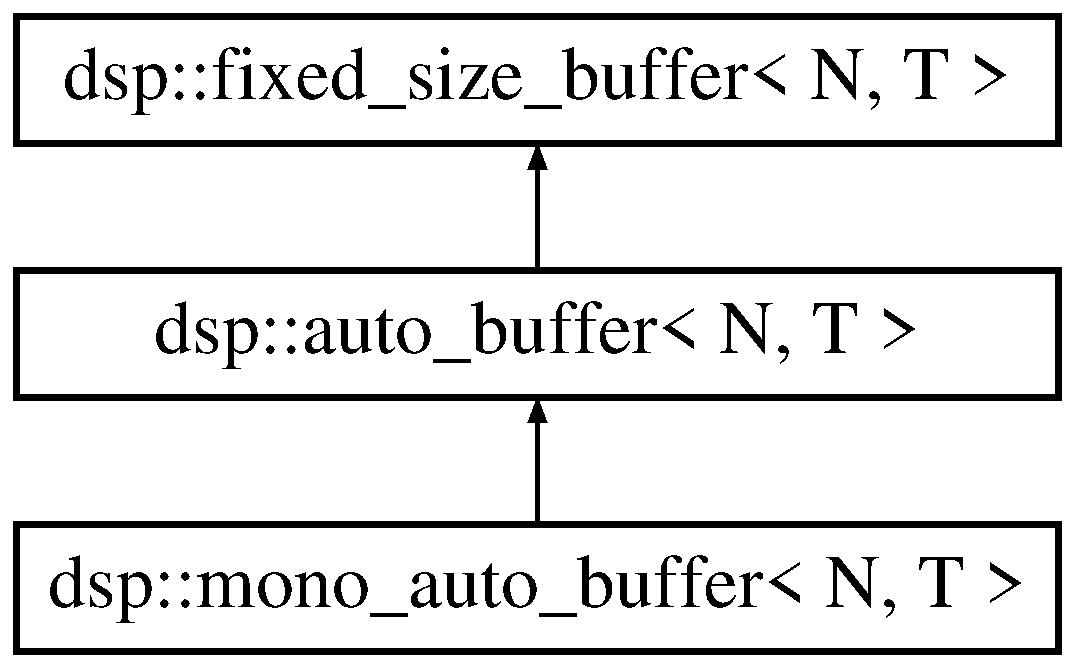
\includegraphics[height=3.000000cm]{classdsp_1_1auto__buffer}
\end{center}
\end{figure}
\subsection*{Public Member Functions}
\begin{DoxyCompactItemize}
\item 
T $\ast$ \hyperlink{classdsp_1_1auto__buffer_a3f378ebc4515836e087526c92042d8cd}{data} () const 
\item 
T \& \hyperlink{classdsp_1_1auto__buffer_a746b0f8aab9be3b0e3c43376ec5beabf}{operator\mbox{[}$\,$\mbox{]}} (\hyperlink{tk_8h_a83f82f76e7fed06f4c49d2db94028a6d}{int} \hyperlink{wn_8c_a1910d262855b71da353ed0d07a6c7823}{pos})
\item 
const T \& \hyperlink{classdsp_1_1auto__buffer_a64f2249cac72679227f44846aebeeb78}{operator\mbox{[}$\,$\mbox{]}} (\hyperlink{tk_8h_a83f82f76e7fed06f4c49d2db94028a6d}{int} \hyperlink{wn_8c_a1910d262855b71da353ed0d07a6c7823}{pos}) const 
\end{DoxyCompactItemize}
\subsection*{Additional Inherited Members}


\subsection{Member Function Documentation}
\index{dsp\+::auto\+\_\+buffer@{dsp\+::auto\+\_\+buffer}!data@{data}}
\index{data@{data}!dsp\+::auto\+\_\+buffer@{dsp\+::auto\+\_\+buffer}}
\subsubsection[{\texorpdfstring{data() const }{data() const }}]{\setlength{\rightskip}{0pt plus 5cm}template$<$int N, class T = float$>$ T$\ast$ {\bf dsp\+::auto\+\_\+buffer}$<$ N, T $>$\+::data (
\begin{DoxyParamCaption}
{}
\end{DoxyParamCaption}
) const\hspace{0.3cm}{\ttfamily [inline]}}\hypertarget{classdsp_1_1auto__buffer_a3f378ebc4515836e087526c92042d8cd}{}\label{classdsp_1_1auto__buffer_a3f378ebc4515836e087526c92042d8cd}
\index{dsp\+::auto\+\_\+buffer@{dsp\+::auto\+\_\+buffer}!operator\mbox{[}$\,$\mbox{]}@{operator[]}}
\index{operator\mbox{[}$\,$\mbox{]}@{operator[]}!dsp\+::auto\+\_\+buffer@{dsp\+::auto\+\_\+buffer}}
\subsubsection[{\texorpdfstring{operator[](int pos)}{operator[](int pos)}}]{\setlength{\rightskip}{0pt plus 5cm}template$<$int N, class T = float$>$ T\& {\bf dsp\+::auto\+\_\+buffer}$<$ N, T $>$\+::operator\mbox{[}$\,$\mbox{]} (
\begin{DoxyParamCaption}
\item[{{\bf int}}]{pos}
\end{DoxyParamCaption}
)\hspace{0.3cm}{\ttfamily [inline]}}\hypertarget{classdsp_1_1auto__buffer_a746b0f8aab9be3b0e3c43376ec5beabf}{}\label{classdsp_1_1auto__buffer_a746b0f8aab9be3b0e3c43376ec5beabf}
\index{dsp\+::auto\+\_\+buffer@{dsp\+::auto\+\_\+buffer}!operator\mbox{[}$\,$\mbox{]}@{operator[]}}
\index{operator\mbox{[}$\,$\mbox{]}@{operator[]}!dsp\+::auto\+\_\+buffer@{dsp\+::auto\+\_\+buffer}}
\subsubsection[{\texorpdfstring{operator[](int pos) const }{operator[](int pos) const }}]{\setlength{\rightskip}{0pt plus 5cm}template$<$int N, class T = float$>$ const T\& {\bf dsp\+::auto\+\_\+buffer}$<$ N, T $>$\+::operator\mbox{[}$\,$\mbox{]} (
\begin{DoxyParamCaption}
\item[{{\bf int}}]{pos}
\end{DoxyParamCaption}
) const\hspace{0.3cm}{\ttfamily [inline]}}\hypertarget{classdsp_1_1auto__buffer_a64f2249cac72679227f44846aebeeb78}{}\label{classdsp_1_1auto__buffer_a64f2249cac72679227f44846aebeeb78}


The documentation for this class was generated from the following file\+:\begin{DoxyCompactItemize}
\item 
/\+Users/michael/\+J\+U\+C\+E/projects/audealize-\/plugin/\+J\+U\+C\+E Modules/audealize\+\_\+module/utils/calf\+\_\+dsp\+\_\+library/\hyperlink{buffer_8h}{buffer.\+h}\end{DoxyCompactItemize}

\hypertarget{classnlohmann_1_1basic__json}{}\section{nlohmann\+:\+:basic\+\_\+json$<$ Object\+Type, Array\+Type, String\+Type, Boolean\+Type, Number\+Integer\+Type, Number\+Unsigned\+Type, Number\+Float\+Type, Allocator\+Type $>$ Class Template Reference}
\label{classnlohmann_1_1basic__json}\index{nlohmann\+::basic\+\_\+json$<$ Object\+Type, Array\+Type, String\+Type, Boolean\+Type, Number\+Integer\+Type, Number\+Unsigned\+Type, Number\+Float\+Type, Allocator\+Type $>$@{nlohmann\+::basic\+\_\+json$<$ Object\+Type, Array\+Type, String\+Type, Boolean\+Type, Number\+Integer\+Type, Number\+Unsigned\+Type, Number\+Float\+Type, Allocator\+Type $>$}}


a class to store J\+S\+ON values  




{\ttfamily \#include $<$json.\+hpp$>$}

\subsection*{Classes}
\begin{DoxyCompactItemize}
\item 
class \hyperlink{classnlohmann_1_1basic__json_1_1const__iterator}{const\+\_\+iterator}
\begin{DoxyCompactList}\small\item\em a const random access iterator for the \hyperlink{classnlohmann_1_1basic__json}{basic\+\_\+json} class \end{DoxyCompactList}\item 
class \hyperlink{classnlohmann_1_1basic__json_1_1iterator}{iterator}
\begin{DoxyCompactList}\small\item\em a mutable random access iterator for the \hyperlink{classnlohmann_1_1basic__json}{basic\+\_\+json} class \end{DoxyCompactList}\item 
class \hyperlink{classnlohmann_1_1basic__json_1_1json__pointer}{json\+\_\+pointer}
\begin{DoxyCompactList}\small\item\em J\+S\+ON Pointer. \end{DoxyCompactList}\item 
class \hyperlink{classnlohmann_1_1basic__json_1_1json__reverse__iterator}{json\+\_\+reverse\+\_\+iterator}
\begin{DoxyCompactList}\small\item\em a template for a reverse iterator class \end{DoxyCompactList}\end{DoxyCompactItemize}
\subsection*{Public Types}
\begin{DoxyCompactItemize}
\item 
enum \hyperlink{classnlohmann_1_1basic__json_a231b02148577b69a154b2ce2c87a5522}{value\+\_\+t} \+: uint8\+\_\+t \{ \\*
\hyperlink{classnlohmann_1_1basic__json_a231b02148577b69a154b2ce2c87a5522a37a6259cc0c1dae299a7866489dff0bd}{value\+\_\+t\+::null}, 
\hyperlink{classnlohmann_1_1basic__json_a231b02148577b69a154b2ce2c87a5522aa8cfde6331bd59eb2ac96f8911c4b666}{value\+\_\+t\+::object}, 
\hyperlink{classnlohmann_1_1basic__json_a231b02148577b69a154b2ce2c87a5522af1f713c9e000f5d3f280adbd124df4f5}{value\+\_\+t\+::array}, 
\hyperlink{classnlohmann_1_1basic__json_a231b02148577b69a154b2ce2c87a5522ab45cffe084dd3d20d928bee85e7b0f21}{value\+\_\+t\+::string}, 
\\*
\hyperlink{classnlohmann_1_1basic__json_a231b02148577b69a154b2ce2c87a5522a84e2c64f38f78ba3ea5c905ab5a2da27}{value\+\_\+t\+::boolean}, 
\hyperlink{classnlohmann_1_1basic__json_a231b02148577b69a154b2ce2c87a5522a5763da164f8659d94a56e29df64b4bcc}{value\+\_\+t\+::number\+\_\+integer}, 
\hyperlink{classnlohmann_1_1basic__json_a231b02148577b69a154b2ce2c87a5522adce7cc8ec29055c4158828921f2f265e}{value\+\_\+t\+::number\+\_\+unsigned}, 
\hyperlink{classnlohmann_1_1basic__json_a231b02148577b69a154b2ce2c87a5522ad9966ecb59667235a57b4b999a649eef}{value\+\_\+t\+::number\+\_\+float}, 
\\*
\hyperlink{classnlohmann_1_1basic__json_a231b02148577b69a154b2ce2c87a5522a94708897ec9db8647dfe695714c98e46}{value\+\_\+t\+::discarded}
 \}\begin{DoxyCompactList}\small\item\em the J\+S\+ON type enumeration \end{DoxyCompactList}
\item 
enum \hyperlink{classnlohmann_1_1basic__json_aea1c863b719b4ca5b77188c171bbfafe}{parse\+\_\+event\+\_\+t} \+: uint8\+\_\+t \{ \\*
\hyperlink{classnlohmann_1_1basic__json_aea1c863b719b4ca5b77188c171bbfafeae73f17027cb0acbb537f29d0a6944b26}{parse\+\_\+event\+\_\+t\+::object\+\_\+start}, 
\hyperlink{classnlohmann_1_1basic__json_aea1c863b719b4ca5b77188c171bbfafeaf63e2a2468a37aa4f394fcc3bcb8249c}{parse\+\_\+event\+\_\+t\+::object\+\_\+end}, 
\hyperlink{classnlohmann_1_1basic__json_aea1c863b719b4ca5b77188c171bbfafeaa4388a3d92419edbb1c6efd4d52461f3}{parse\+\_\+event\+\_\+t\+::array\+\_\+start}, 
\hyperlink{classnlohmann_1_1basic__json_aea1c863b719b4ca5b77188c171bbfafea49642fb732aa2e112188fba1f9d3ef7f}{parse\+\_\+event\+\_\+t\+::array\+\_\+end}, 
\\*
\hyperlink{classnlohmann_1_1basic__json_aea1c863b719b4ca5b77188c171bbfafea3c6e0b8a9c15224a8228b9a98ca1531d}{parse\+\_\+event\+\_\+t\+::key}, 
\hyperlink{classnlohmann_1_1basic__json_aea1c863b719b4ca5b77188c171bbfafea2063c1608d6e0baf80249c42e2be5804}{parse\+\_\+event\+\_\+t\+::value}
 \}\begin{DoxyCompactList}\small\item\em J\+S\+ON callback events. \end{DoxyCompactList}
\item 
using \hyperlink{classnlohmann_1_1basic__json_a9e35475e2027520a78e09f460dbe048a}{parser\+\_\+callback\+\_\+t} = std\+::function$<$ bool(\hyperlink{tk_8h_a83f82f76e7fed06f4c49d2db94028a6d}{int} depth, \hyperlink{classnlohmann_1_1basic__json_aea1c863b719b4ca5b77188c171bbfafe}{parse\+\_\+event\+\_\+t} event, \hyperlink{classnlohmann_1_1basic__json}{basic\+\_\+json} \&parsed)$>$
\begin{DoxyCompactList}\small\item\em per-\/element parser callback type \end{DoxyCompactList}\end{DoxyCompactItemize}
\subsection*{Static Public Member Functions}
\begin{DoxyCompactItemize}
\item 
static \hyperlink{classnlohmann_1_1basic__json_aa44ce84b9ac506b905b8fb56c9a0989d}{allocator\+\_\+type} \hyperlink{classnlohmann_1_1basic__json_a1a446a48beed4ea564addfd12d235793}{get\+\_\+allocator} ()
\begin{DoxyCompactList}\small\item\em returns the allocator associated with the container \end{DoxyCompactList}\end{DoxyCompactItemize}
\subsection*{container types}
\begin{DoxyCompactItemize}
\item 
using \hyperlink{classnlohmann_1_1basic__json_ac8d45b57874b4a6e9c07f7d3b5daa1f9}{value\+\_\+type} = \hyperlink{classnlohmann_1_1basic__json}{basic\+\_\+json}
\begin{DoxyCompactList}\small\item\em the type of elements in a \hyperlink{classnlohmann_1_1basic__json}{basic\+\_\+json} container \end{DoxyCompactList}\item 
using \hyperlink{classnlohmann_1_1basic__json_a3ec8e17be8732fe436e9d6733f52b7a3}{reference} = \hyperlink{classnlohmann_1_1basic__json_ac8d45b57874b4a6e9c07f7d3b5daa1f9}{value\+\_\+type} \&
\begin{DoxyCompactList}\small\item\em the type of an element reference \end{DoxyCompactList}\item 
using \hyperlink{classnlohmann_1_1basic__json_af677a29b0e66edc9f66e5167e4667071}{const\+\_\+reference} = const \hyperlink{classnlohmann_1_1basic__json_ac8d45b57874b4a6e9c07f7d3b5daa1f9}{value\+\_\+type} \&
\begin{DoxyCompactList}\small\item\em the type of an element const reference \end{DoxyCompactList}\item 
using \hyperlink{classnlohmann_1_1basic__json_aec316934a555dd1acdd3600e5d4a4cdf}{difference\+\_\+type} = std\+::ptrdiff\+\_\+t
\begin{DoxyCompactList}\small\item\em a type to represent differences between iterators \end{DoxyCompactList}\item 
using \hyperlink{classnlohmann_1_1basic__json_a1579a8f72a230358d6cd1a6e8a62859b}{size\+\_\+type} = std\+::size\+\_\+t
\begin{DoxyCompactList}\small\item\em a type to represent container sizes \end{DoxyCompactList}\item 
using \hyperlink{classnlohmann_1_1basic__json_aa44ce84b9ac506b905b8fb56c9a0989d}{allocator\+\_\+type} = Allocator\+Type$<$ \hyperlink{classnlohmann_1_1basic__json}{basic\+\_\+json} $>$
\begin{DoxyCompactList}\small\item\em the allocator type \end{DoxyCompactList}\item 
using \hyperlink{classnlohmann_1_1basic__json_a9d1b58099dc64695fcf2847ab0b2a7c7}{pointer} = typename std\+::allocator\+\_\+traits$<$ \hyperlink{classnlohmann_1_1basic__json_aa44ce84b9ac506b905b8fb56c9a0989d}{allocator\+\_\+type} $>$\+::\hyperlink{classnlohmann_1_1basic__json_a9d1b58099dc64695fcf2847ab0b2a7c7}{pointer}
\begin{DoxyCompactList}\small\item\em the type of an element pointer \end{DoxyCompactList}\item 
using \hyperlink{classnlohmann_1_1basic__json_a06efb200b69942eacd1ea22d0f6ccebb}{const\+\_\+pointer} = typename std\+::allocator\+\_\+traits$<$ \hyperlink{classnlohmann_1_1basic__json_aa44ce84b9ac506b905b8fb56c9a0989d}{allocator\+\_\+type} $>$\+::\hyperlink{classnlohmann_1_1basic__json_a06efb200b69942eacd1ea22d0f6ccebb}{const\+\_\+pointer}
\begin{DoxyCompactList}\small\item\em the type of an element const pointer \end{DoxyCompactList}\item 
using \hyperlink{classnlohmann_1_1basic__json_a2f1f83aa187a56dc5ec7a7027065ac8a}{reverse\+\_\+iterator} = \hyperlink{classnlohmann_1_1basic__json_1_1json__reverse__iterator}{json\+\_\+reverse\+\_\+iterator}$<$ typename \hyperlink{classnlohmann_1_1basic__json_1_1iterator}{basic\+\_\+json\+::iterator} $>$
\begin{DoxyCompactList}\small\item\em a reverse iterator for a \hyperlink{classnlohmann_1_1basic__json}{basic\+\_\+json} container \end{DoxyCompactList}\item 
using \hyperlink{classnlohmann_1_1basic__json_ae336fff01f4b78e3e16e5008dc8dbc00}{const\+\_\+reverse\+\_\+iterator} = \hyperlink{classnlohmann_1_1basic__json_1_1json__reverse__iterator}{json\+\_\+reverse\+\_\+iterator}$<$ typename \hyperlink{classnlohmann_1_1basic__json_1_1const__iterator}{basic\+\_\+json\+::const\+\_\+iterator} $>$
\begin{DoxyCompactList}\small\item\em a const reverse iterator for a \hyperlink{classnlohmann_1_1basic__json}{basic\+\_\+json} container \end{DoxyCompactList}\end{DoxyCompactItemize}
\subsection*{J\+S\+ON value data types}
\begin{DoxyCompactItemize}
\item 
using \hyperlink{classnlohmann_1_1basic__json_a0ac9894c9de8dc551cf2e5f1c605537f}{object\+\_\+t} = Object\+Type$<$ String\+Type, \hyperlink{classnlohmann_1_1basic__json}{basic\+\_\+json}, std\+::less$<$ String\+Type $>$, Allocator\+Type$<$ std\+::pair$<$ const String\+Type, \hyperlink{classnlohmann_1_1basic__json}{basic\+\_\+json} $>$$>$$>$
\begin{DoxyCompactList}\small\item\em a type for an object \end{DoxyCompactList}\item 
using \hyperlink{classnlohmann_1_1basic__json_ab00b882d39306d663c23dab110f5cae0}{array\+\_\+t} = Array\+Type$<$ \hyperlink{classnlohmann_1_1basic__json}{basic\+\_\+json}, Allocator\+Type$<$ \hyperlink{classnlohmann_1_1basic__json}{basic\+\_\+json} $>$$>$
\begin{DoxyCompactList}\small\item\em a type for an array \end{DoxyCompactList}\item 
using \hyperlink{classnlohmann_1_1basic__json_ab63e618bbb0371042b1bec17f5891f42}{string\+\_\+t} = String\+Type
\begin{DoxyCompactList}\small\item\em a type for a string \end{DoxyCompactList}\item 
using \hyperlink{classnlohmann_1_1basic__json_af3bc3e83aa162d7ba4df16a949872723}{boolean\+\_\+t} = Boolean\+Type
\begin{DoxyCompactList}\small\item\em a type for a boolean \end{DoxyCompactList}\item 
using \hyperlink{classnlohmann_1_1basic__json_ac4b10b2364f26ce47bdb9a413ff04a59}{number\+\_\+integer\+\_\+t} = Number\+Integer\+Type
\begin{DoxyCompactList}\small\item\em a type for a number (integer) \end{DoxyCompactList}\item 
using \hyperlink{classnlohmann_1_1basic__json_a60a04166c122072ab11eaf9845d9cd1d}{number\+\_\+unsigned\+\_\+t} = Number\+Unsigned\+Type
\begin{DoxyCompactList}\small\item\em a type for a number (unsigned) \end{DoxyCompactList}\item 
using \hyperlink{classnlohmann_1_1basic__json_a74a0013e847fdc574b48f931f0e757e1}{number\+\_\+float\+\_\+t} = Number\+Float\+Type
\begin{DoxyCompactList}\small\item\em a type for a number (floating-\/point) \end{DoxyCompactList}\end{DoxyCompactItemize}
\subsection*{constructors and destructors}
\begin{DoxyCompactItemize}
\item 
static \hyperlink{classnlohmann_1_1basic__json}{basic\+\_\+json} \hyperlink{classnlohmann_1_1basic__json_a5685815624b086caa532f41e853d4b0f}{array} (std\+::initializer\+\_\+list$<$ \hyperlink{classnlohmann_1_1basic__json}{basic\+\_\+json} $>$ init=std\+::initializer\+\_\+list$<$ \hyperlink{classnlohmann_1_1basic__json}{basic\+\_\+json} $>$())
\begin{DoxyCompactList}\small\item\em explicitly create an array from an initializer list \end{DoxyCompactList}\item 
static \hyperlink{classnlohmann_1_1basic__json}{basic\+\_\+json} \hyperlink{classnlohmann_1_1basic__json_ad25b2f8c21e241e2d63455537a9294ff}{object} (std\+::initializer\+\_\+list$<$ \hyperlink{classnlohmann_1_1basic__json}{basic\+\_\+json} $>$ init=std\+::initializer\+\_\+list$<$ \hyperlink{classnlohmann_1_1basic__json}{basic\+\_\+json} $>$())
\begin{DoxyCompactList}\small\item\em explicitly create an object from an initializer list \end{DoxyCompactList}\item 
\hyperlink{classnlohmann_1_1basic__json_a8f77085bd98c97a983d9ba12efbf6148}{basic\+\_\+json} (const \hyperlink{classnlohmann_1_1basic__json_a231b02148577b69a154b2ce2c87a5522}{value\+\_\+t} \hyperlink{classnlohmann_1_1basic__json_ac8d45b57874b4a6e9c07f7d3b5daa1f9}{value\+\_\+type})
\begin{DoxyCompactList}\small\item\em create an empty value with a given type \end{DoxyCompactList}\item 
\hyperlink{classnlohmann_1_1basic__json_a53771a7a4f2787125e55f64448f24ce6}{basic\+\_\+json} ()=default
\begin{DoxyCompactList}\small\item\em create a null object (implicitly) \end{DoxyCompactList}\item 
\hyperlink{classnlohmann_1_1basic__json_ade0e56c8c320d7f342e7a5697e6d6f7e}{basic\+\_\+json} (std\+::nullptr\+\_\+t) noexcept
\begin{DoxyCompactList}\small\item\em create a null object (explicitly) \end{DoxyCompactList}\item 
\hyperlink{classnlohmann_1_1basic__json_a9af5ea68c88f423ddf35216aff7f1813}{basic\+\_\+json} (const \hyperlink{classnlohmann_1_1basic__json_a0ac9894c9de8dc551cf2e5f1c605537f}{object\+\_\+t} \&val)
\begin{DoxyCompactList}\small\item\em create an object (explicit) \end{DoxyCompactList}\item 
{\footnotesize template$<$class Compatible\+Object\+Type , typename std\+::enable\+\_\+if$<$                                                                  std\+::is\+\_\+constructible$<$ typename object\+\_\+t\+::key\+\_\+type, typename Compatible\+Object\+Type\+::key\+\_\+type $>$\+::value and                                                               std\+::is\+\_\+constructible$<$ basic\+\_\+json, typename Compatible\+Object\+Type\+::mapped\+\_\+type $>$\+::value, int $>$\+::type  = 0$>$ }\\\hyperlink{classnlohmann_1_1basic__json_ab7be2bc58ae0c2c2c30d40f15d6399f8}{basic\+\_\+json} (const Compatible\+Object\+Type \&val)
\begin{DoxyCompactList}\small\item\em create an object (implicit) \end{DoxyCompactList}\item 
\hyperlink{classnlohmann_1_1basic__json_a3aaf41d385f0d9a93deb92f9b14ae0cf}{basic\+\_\+json} (const \hyperlink{classnlohmann_1_1basic__json_ab00b882d39306d663c23dab110f5cae0}{array\+\_\+t} \&val)
\begin{DoxyCompactList}\small\item\em create an array (explicit) \end{DoxyCompactList}\item 
{\footnotesize template$<$class Compatible\+Array\+Type , typename std\+::enable\+\_\+if$<$                                                                  not std\+::is\+\_\+same$<$ Compatible\+Array\+Type, typename basic\+\_\+json\+\_\+t\+::iterator $>$\+::value and                                                               not std\+::is\+\_\+same$<$ Compatible\+Array\+Type, typename basic\+\_\+json\+\_\+t\+::const\+\_\+iterator $>$\+::value and                                                               not std\+::is\+\_\+same$<$ Compatible\+Array\+Type, typename basic\+\_\+json\+\_\+t\+::reverse\+\_\+iterator $>$\+::value and                                                               not std\+::is\+\_\+same$<$ Compatible\+Array\+Type, typename basic\+\_\+json\+\_\+t\+::const\+\_\+reverse\+\_\+iterator $>$\+::value and                                                               not std\+::is\+\_\+same$<$ Compatible\+Array\+Type, typename array\+\_\+t\+::iterator $>$\+::value and                                                               not std\+::is\+\_\+same$<$ Compatible\+Array\+Type, typename array\+\_\+t\+::const\+\_\+iterator $>$\+::value and                                                               std\+::is\+\_\+constructible$<$ basic\+\_\+json, typename Compatible\+Array\+Type\+::value\+\_\+type $>$\+::value, int $>$\+::type  = 0$>$ }\\\hyperlink{classnlohmann_1_1basic__json_a81aaaab0f3b326afda2d226daab4f1e1}{basic\+\_\+json} (const Compatible\+Array\+Type \&val)
\begin{DoxyCompactList}\small\item\em create an array (implicit) \end{DoxyCompactList}\item 
\hyperlink{classnlohmann_1_1basic__json_ab8b43d92a042dde96c28aeea81dd52de}{basic\+\_\+json} (const \hyperlink{classnlohmann_1_1basic__json_ab63e618bbb0371042b1bec17f5891f42}{string\+\_\+t} \&val)
\begin{DoxyCompactList}\small\item\em create a string (explicit) \end{DoxyCompactList}\item 
\hyperlink{classnlohmann_1_1basic__json_a3654da9a84deaf61899c4eee5b93c2c5}{basic\+\_\+json} (const typename string\+\_\+t\+::value\+\_\+type $\ast$val)
\begin{DoxyCompactList}\small\item\em create a string (explicit) \end{DoxyCompactList}\item 
{\footnotesize template$<$class Compatible\+String\+Type , typename std\+::enable\+\_\+if$<$                                                                  std\+::is\+\_\+constructible$<$ string\+\_\+t, Compatible\+String\+Type $>$\+::value, int $>$\+::type  = 0$>$ }\\\hyperlink{classnlohmann_1_1basic__json_ae85d91b0620650bcd9993e09d0e287d9}{basic\+\_\+json} (const Compatible\+String\+Type \&val)
\begin{DoxyCompactList}\small\item\em create a string (implicit) \end{DoxyCompactList}\item 
\hyperlink{classnlohmann_1_1basic__json_aac36af84d907b5c3e469af889661620a}{basic\+\_\+json} (\hyperlink{classnlohmann_1_1basic__json_af3bc3e83aa162d7ba4df16a949872723}{boolean\+\_\+t} val) noexcept
\begin{DoxyCompactList}\small\item\em create a boolean (explicit) \end{DoxyCompactList}\item 
{\footnotesize template$<$typename T , typename std\+::enable\+\_\+if$<$                                                              not(std\+::is\+\_\+same$<$ T, int $>$\+::value)                                                           and std\+::is\+\_\+same$<$ T, number\+\_\+integer\+\_\+t $>$\+::value                                                           , int $>$\+::type  = 0$>$ }\\\hyperlink{classnlohmann_1_1basic__json_a0d838bc7ffca6017f51167e0a8ffd9b6}{basic\+\_\+json} (const \hyperlink{classnlohmann_1_1basic__json_ac4b10b2364f26ce47bdb9a413ff04a59}{number\+\_\+integer\+\_\+t} val) noexcept
\begin{DoxyCompactList}\small\item\em create an integer number (explicit) \end{DoxyCompactList}\item 
\hyperlink{classnlohmann_1_1basic__json_a70ae1f0747f5b7a89979512866474f1a}{basic\+\_\+json} (const \hyperlink{tk_8h_a83f82f76e7fed06f4c49d2db94028a6d}{int} val) noexcept
\begin{DoxyCompactList}\small\item\em create an integer number from an enum type (explicit) \end{DoxyCompactList}\item 
{\footnotesize template$<$typename Compatible\+Number\+Integer\+Type , typename std\+::enable\+\_\+if$<$                                                              std\+::is\+\_\+constructible$<$ number\+\_\+integer\+\_\+t, Compatible\+Number\+Integer\+Type $>$\+::value and                                                           std\+::numeric\+\_\+limits$<$ Compatible\+Number\+Integer\+Type $>$\+::is\+\_\+integer and                                                           std\+::numeric\+\_\+limits$<$ Compatible\+Number\+Integer\+Type $>$\+::is\+\_\+signed,                                                           Compatible\+Number\+Integer\+Type $>$\+::type  = 0$>$ }\\\hyperlink{classnlohmann_1_1basic__json_ad2eddc2c13ab084f067eaba65d381ad2}{basic\+\_\+json} (const Compatible\+Number\+Integer\+Type val) noexcept
\begin{DoxyCompactList}\small\item\em create an integer number (implicit) \end{DoxyCompactList}\item 
{\footnotesize template$<$typename T , typename std\+::enable\+\_\+if$<$                                                              not(std\+::is\+\_\+same$<$ T, int $>$\+::value)                                                           and std\+::is\+\_\+same$<$ T, number\+\_\+unsigned\+\_\+t $>$\+::value                                                           , int $>$\+::type  = 0$>$ }\\\hyperlink{classnlohmann_1_1basic__json_a85b09b03916d3d1e73373f49cdd4136d}{basic\+\_\+json} (const \hyperlink{classnlohmann_1_1basic__json_a60a04166c122072ab11eaf9845d9cd1d}{number\+\_\+unsigned\+\_\+t} val) noexcept
\begin{DoxyCompactList}\small\item\em create an unsigned integer number (explicit) \end{DoxyCompactList}\item 
{\footnotesize template$<$typename Compatible\+Number\+Unsigned\+Type , typename std\+::enable\+\_\+if$<$                                                                  std\+::is\+\_\+constructible$<$ number\+\_\+unsigned\+\_\+t, Compatible\+Number\+Unsigned\+Type $>$\+::value and                                                               std\+::numeric\+\_\+limits$<$ Compatible\+Number\+Unsigned\+Type $>$\+::is\+\_\+integer and                                                               not std\+::numeric\+\_\+limits$<$ Compatible\+Number\+Unsigned\+Type $>$\+::is\+\_\+signed,                                                               Compatible\+Number\+Unsigned\+Type $>$\+::type  = 0$>$ }\\\hyperlink{classnlohmann_1_1basic__json_a68a5f34b164a07b8ced13fcf2b7ec834}{basic\+\_\+json} (const Compatible\+Number\+Unsigned\+Type val) noexcept
\begin{DoxyCompactList}\small\item\em create an unsigned number (implicit) \end{DoxyCompactList}\item 
\hyperlink{classnlohmann_1_1basic__json_a2badcf191deabf579abcf8d3654da26f}{basic\+\_\+json} (const \hyperlink{classnlohmann_1_1basic__json_a74a0013e847fdc574b48f931f0e757e1}{number\+\_\+float\+\_\+t} val) noexcept
\begin{DoxyCompactList}\small\item\em create a floating-\/point number (explicit) \end{DoxyCompactList}\item 
{\footnotesize template$<$typename Compatible\+Number\+Float\+Type , typename  = typename std\+::enable\+\_\+if$<$                 std\+::is\+\_\+constructible$<$number\+\_\+float\+\_\+t, Compatible\+Number\+Float\+Type$>$\+::value and                 std\+::is\+\_\+floating\+\_\+point$<$\+Compatible\+Number\+Float\+Type$>$\+::value$>$\+::type$>$ }\\\hyperlink{classnlohmann_1_1basic__json_a4bbdfd6dd8d2e6fc9ac5d81ef61ba3fe}{basic\+\_\+json} (const Compatible\+Number\+Float\+Type val) noexcept
\begin{DoxyCompactList}\small\item\em create an floating-\/point number (implicit) \end{DoxyCompactList}\item 
\hyperlink{classnlohmann_1_1basic__json_afeb998aec45296bc2050bd1c41ef41eb}{basic\+\_\+json} (std\+::initializer\+\_\+list$<$ \hyperlink{classnlohmann_1_1basic__json}{basic\+\_\+json} $>$ init, bool type\+\_\+deduction=true, \hyperlink{classnlohmann_1_1basic__json_a231b02148577b69a154b2ce2c87a5522}{value\+\_\+t} manual\+\_\+type=\hyperlink{classnlohmann_1_1basic__json_a231b02148577b69a154b2ce2c87a5522af1f713c9e000f5d3f280adbd124df4f5}{value\+\_\+t\+::array})
\begin{DoxyCompactList}\small\item\em create a container (array or object) from an initializer list \end{DoxyCompactList}\item 
\hyperlink{classnlohmann_1_1basic__json_a112a2d8e76345ea64f71e2985fee4c52}{basic\+\_\+json} (\hyperlink{classnlohmann_1_1basic__json_a1579a8f72a230358d6cd1a6e8a62859b}{size\+\_\+type} cnt, const \hyperlink{classnlohmann_1_1basic__json}{basic\+\_\+json} \&val)
\begin{DoxyCompactList}\small\item\em construct an array with count copies of given value \end{DoxyCompactList}\item 
{\footnotesize template$<$class Input\+IT , typename std\+::enable\+\_\+if$<$                                                                  std\+::is\+\_\+same$<$ Input\+I\+T, typename basic\+\_\+json\+\_\+t\+::iterator $>$\+::value or                                                               std\+::is\+\_\+same$<$ Input\+I\+T, typename basic\+\_\+json\+\_\+t\+::const\+\_\+iterator $>$\+::value                                                               , int $>$\+::type  = 0$>$ }\\\hyperlink{classnlohmann_1_1basic__json_af7acf3838a79363356f24538941a559c}{basic\+\_\+json} (Input\+IT first, Input\+IT last)
\begin{DoxyCompactList}\small\item\em construct a J\+S\+ON container given an iterator range \end{DoxyCompactList}\item 
\hyperlink{classnlohmann_1_1basic__json_a9857835334d38ba04959e348ca6be208}{basic\+\_\+json} (std\+::istream \&i, \hyperlink{classnlohmann_1_1basic__json_a9e35475e2027520a78e09f460dbe048a}{parser\+\_\+callback\+\_\+t} cb=nullptr)
\begin{DoxyCompactList}\small\item\em construct a J\+S\+ON value given an input stream \end{DoxyCompactList}\item 
\hyperlink{classnlohmann_1_1basic__json_a4ab93491f82545342562c7ee7e3166c7}{basic\+\_\+json} (const \hyperlink{classnlohmann_1_1basic__json}{basic\+\_\+json} \&other)
\begin{DoxyCompactList}\small\item\em copy constructor \end{DoxyCompactList}\item 
\hyperlink{classnlohmann_1_1basic__json_a73e150cbcba5643cb89de8f515eb64e2}{basic\+\_\+json} (\hyperlink{classnlohmann_1_1basic__json}{basic\+\_\+json} \&\&other) noexcept
\begin{DoxyCompactList}\small\item\em move constructor \end{DoxyCompactList}\item 
\hyperlink{classnlohmann_1_1basic__json_a3ec8e17be8732fe436e9d6733f52b7a3}{reference} \& \hyperlink{classnlohmann_1_1basic__json_a7c3182cfabc0bdd9f3a14216fe0e8154}{operator=} (\hyperlink{classnlohmann_1_1basic__json}{basic\+\_\+json} other) noexcept(                       std\+::is\+\_\+nothrow\+\_\+move\+\_\+constructible$<$ \hyperlink{classnlohmann_1_1basic__json_a231b02148577b69a154b2ce2c87a5522}{value\+\_\+t} $>$\+::\hyperlink{tk_8h_a177a0765f574ef6642002696d9cd82d0}{value} and                       std\+::is\+\_\+nothrow\+\_\+move\+\_\+assignable$<$ \hyperlink{classnlohmann_1_1basic__json_a231b02148577b69a154b2ce2c87a5522}{value\+\_\+t} $>$\+::\hyperlink{tk_8h_a177a0765f574ef6642002696d9cd82d0}{value} and                       std\+::is\+\_\+nothrow\+\_\+move\+\_\+constructible$<$ json\+\_\+value $>$\+::\hyperlink{tk_8h_a177a0765f574ef6642002696d9cd82d0}{value} and                       std\+::is\+\_\+nothrow\+\_\+move\+\_\+assignable$<$ json\+\_\+value $>$\+::\hyperlink{tk_8h_a177a0765f574ef6642002696d9cd82d0}{value}       )
\begin{DoxyCompactList}\small\item\em copy assignment \end{DoxyCompactList}\item 
\hyperlink{classnlohmann_1_1basic__json_a947b5b2a832e490858dbdddfe7085831}{$\sim$basic\+\_\+json} ()
\begin{DoxyCompactList}\small\item\em destructor \end{DoxyCompactList}\end{DoxyCompactItemize}
\subsection*{object inspection}
\begin{DoxyCompactItemize}
\item 
\hyperlink{classnlohmann_1_1basic__json_ab63e618bbb0371042b1bec17f5891f42}{string\+\_\+t} \hyperlink{classnlohmann_1_1basic__json_a805e3f3a2f374da0e14942eec7400e40}{dump} (const \hyperlink{tk_8h_a83f82f76e7fed06f4c49d2db94028a6d}{int} indent=-\/1) const 
\begin{DoxyCompactList}\small\item\em serialization \end{DoxyCompactList}\item 
constexpr \hyperlink{classnlohmann_1_1basic__json_a231b02148577b69a154b2ce2c87a5522}{value\+\_\+t} \hyperlink{classnlohmann_1_1basic__json_a848cbae3bd3502ffbf738320bf5eb3aa}{type} () const  noexcept
\begin{DoxyCompactList}\small\item\em return the type of the J\+S\+ON value (explicit) \end{DoxyCompactList}\item 
constexpr bool \hyperlink{classnlohmann_1_1basic__json_a7c774ef0eceff6d06095f617e2dbd488}{is\+\_\+primitive} () const  noexcept
\begin{DoxyCompactList}\small\item\em return whether type is primitive \end{DoxyCompactList}\item 
constexpr bool \hyperlink{classnlohmann_1_1basic__json_a558b345044c38a9f6ad522592cc700c8}{is\+\_\+structured} () const  noexcept
\begin{DoxyCompactList}\small\item\em return whether type is structured \end{DoxyCompactList}\item 
constexpr bool \hyperlink{classnlohmann_1_1basic__json_a685d9d6a8a45bfcb8455b147257cdffb}{is\+\_\+null} () const  noexcept
\begin{DoxyCompactList}\small\item\em return whether value is null \end{DoxyCompactList}\item 
constexpr bool \hyperlink{classnlohmann_1_1basic__json_a8f7e67d903f918cd08261219fb47a9f0}{is\+\_\+boolean} () const  noexcept
\begin{DoxyCompactList}\small\item\em return whether value is a boolean \end{DoxyCompactList}\item 
constexpr bool \hyperlink{classnlohmann_1_1basic__json_a1407f91b4689bbc56d1a3c401a5bb649}{is\+\_\+number} () const  noexcept
\begin{DoxyCompactList}\small\item\em return whether value is a number \end{DoxyCompactList}\item 
constexpr bool \hyperlink{classnlohmann_1_1basic__json_a87499fdb56ca6f0df2242c3335c3dc9b}{is\+\_\+number\+\_\+integer} () const  noexcept
\begin{DoxyCompactList}\small\item\em return whether value is an integer number \end{DoxyCompactList}\item 
constexpr bool \hyperlink{classnlohmann_1_1basic__json_a693b411d9c5ad0d168a0013cfb80b8e5}{is\+\_\+number\+\_\+unsigned} () const  noexcept
\begin{DoxyCompactList}\small\item\em return whether value is an unsigned integer number \end{DoxyCompactList}\item 
constexpr bool \hyperlink{classnlohmann_1_1basic__json_a628733b45cd0e32bd59efea149f40b4b}{is\+\_\+number\+\_\+float} () const  noexcept
\begin{DoxyCompactList}\small\item\em return whether value is a floating-\/point number \end{DoxyCompactList}\item 
constexpr bool \hyperlink{classnlohmann_1_1basic__json_a0d96ff13001977a93d65f0a97279d316}{is\+\_\+object} () const  noexcept
\begin{DoxyCompactList}\small\item\em return whether value is an object \end{DoxyCompactList}\item 
constexpr bool \hyperlink{classnlohmann_1_1basic__json_a1af360cb513cc32f28e80ddd0b9d7666}{is\+\_\+array} () const  noexcept
\begin{DoxyCompactList}\small\item\em return whether value is an array \end{DoxyCompactList}\item 
constexpr bool \hyperlink{classnlohmann_1_1basic__json_ab22c8d61eca51f0308c263487bd35f03}{is\+\_\+string} () const  noexcept
\begin{DoxyCompactList}\small\item\em return whether value is a string \end{DoxyCompactList}\item 
constexpr bool \hyperlink{classnlohmann_1_1basic__json_a66c051561828b2c4eeaad896a72bec99}{is\+\_\+discarded} () const  noexcept
\begin{DoxyCompactList}\small\item\em return whether value is discarded \end{DoxyCompactList}\item 
constexpr \hyperlink{classnlohmann_1_1basic__json_a101cd941eb8a5c299660449c71d0e75e}{operator value\+\_\+t} () const  noexcept
\begin{DoxyCompactList}\small\item\em return the type of the J\+S\+ON value (implicit) \end{DoxyCompactList}\end{DoxyCompactItemize}
\subsection*{value access}
\begin{DoxyCompactItemize}
\item 
{\footnotesize template$<$typename Value\+Type , typename std\+::enable\+\_\+if$<$                                                              not std\+::is\+\_\+pointer$<$ Value\+Type $>$\+::value                                                           , int $>$\+::type  = 0$>$ }\\Value\+Type \hyperlink{classnlohmann_1_1basic__json_a20bfb2ca6d4c421c74bb3e53328cd437}{get} () const 
\begin{DoxyCompactList}\small\item\em get a value (explicit) \end{DoxyCompactList}\item 
{\footnotesize template$<$typename Pointer\+Type , typename std\+::enable\+\_\+if$<$                                                              std\+::is\+\_\+pointer$<$ Pointer\+Type $>$\+::value                                                           , int $>$\+::type  = 0$>$ }\\Pointer\+Type \hyperlink{classnlohmann_1_1basic__json_ac5693cff1df0775cd3fbe960412cde4b}{get} () noexcept
\begin{DoxyCompactList}\small\item\em get a pointer value (explicit) \end{DoxyCompactList}\item 
{\footnotesize template$<$typename Pointer\+Type , typename std\+::enable\+\_\+if$<$                                                              std\+::is\+\_\+pointer$<$ Pointer\+Type $>$\+::value                                                           , int $>$\+::type  = 0$>$ }\\constexpr const Pointer\+Type \hyperlink{classnlohmann_1_1basic__json_a363da77bc39cae041d59ee334ac4f41b}{get} () const  noexcept
\begin{DoxyCompactList}\small\item\em get a pointer value (explicit) \end{DoxyCompactList}\item 
{\footnotesize template$<$typename Pointer\+Type , typename std\+::enable\+\_\+if$<$                                                              std\+::is\+\_\+pointer$<$ Pointer\+Type $>$\+::value                                                           , int $>$\+::type  = 0$>$ }\\Pointer\+Type \hyperlink{classnlohmann_1_1basic__json_a7ab11375ed2e29c2fcb6119386851445}{get\+\_\+ptr} () noexcept
\begin{DoxyCompactList}\small\item\em get a pointer value (implicit) \end{DoxyCompactList}\item 
{\footnotesize template$<$typename Pointer\+Type , typename std\+::enable\+\_\+if$<$                                                              std\+::is\+\_\+pointer$<$ Pointer\+Type $>$\+::value                                                           and std\+::is\+\_\+const$<$ typename std\+::remove\+\_\+pointer$<$ Pointer\+Type $>$\+::type $>$\+::value                                                           , int $>$\+::type  = 0$>$ }\\constexpr const Pointer\+Type \hyperlink{classnlohmann_1_1basic__json_aad65e0bc388897192bf361c24c1d6dda}{get\+\_\+ptr} () const  noexcept
\begin{DoxyCompactList}\small\item\em get a pointer value (implicit) \end{DoxyCompactList}\item 
{\footnotesize template$<$typename Reference\+Type , typename std\+::enable\+\_\+if$<$                                                              std\+::is\+\_\+reference$<$ Reference\+Type $>$\+::value                                                           , int $>$\+::type  = 0$>$ }\\Reference\+Type \hyperlink{classnlohmann_1_1basic__json_a4f332e90f3cae562d0c3fa6ba48f74f9}{get\+\_\+ref} ()
\begin{DoxyCompactList}\small\item\em get a reference value (implicit) \end{DoxyCompactList}\item 
{\footnotesize template$<$typename Reference\+Type , typename std\+::enable\+\_\+if$<$                                                              std\+::is\+\_\+reference$<$ Reference\+Type $>$\+::value                                                           and std\+::is\+\_\+const$<$ typename std\+::remove\+\_\+reference$<$ Reference\+Type $>$\+::type $>$\+::value                                                           , int $>$\+::type  = 0$>$ }\\Reference\+Type \hyperlink{classnlohmann_1_1basic__json_aa669d997ddc03566de5438781254b32b}{get\+\_\+ref} () const 
\begin{DoxyCompactList}\small\item\em get a reference value (implicit) \end{DoxyCompactList}\item 
{\footnotesize template$<$typename Value\+Type , typename std\+::enable\+\_\+if$<$                                                                      not std\+::is\+\_\+pointer$<$ Value\+Type $>$\+::value                                                                   and not std\+::is\+\_\+same$<$ Value\+Type, typename string\+\_\+t\+::value\+\_\+type $>$\+::value                                                                   and not std\+::is\+\_\+same$<$ Value\+Type, std\+::initializer\+\_\+list$<$ typename string\+\_\+t\+::value\+\_\+type $>$$>$\+::value                                                                   , int $>$\+::type  = 0$>$ }\\\hyperlink{classnlohmann_1_1basic__json_aef496a56163710084e13612ab73e6ed2}{operator Value\+Type} () const 
\begin{DoxyCompactList}\small\item\em get a value (implicit) \end{DoxyCompactList}\end{DoxyCompactItemize}
\subsection*{element access}
\begin{DoxyCompactItemize}
\item 
\hyperlink{classnlohmann_1_1basic__json_a3ec8e17be8732fe436e9d6733f52b7a3}{reference} \hyperlink{classnlohmann_1_1basic__json_a214a8c22d616fd3567b88932c07436c9}{at} (\hyperlink{classnlohmann_1_1basic__json_a1579a8f72a230358d6cd1a6e8a62859b}{size\+\_\+type} idx)
\begin{DoxyCompactList}\small\item\em access specified array element with bounds checking \end{DoxyCompactList}\item 
\hyperlink{classnlohmann_1_1basic__json_af677a29b0e66edc9f66e5167e4667071}{const\+\_\+reference} \hyperlink{classnlohmann_1_1basic__json_ab31368c0b67f8e4f291a45e6498018be}{at} (\hyperlink{classnlohmann_1_1basic__json_a1579a8f72a230358d6cd1a6e8a62859b}{size\+\_\+type} idx) const 
\begin{DoxyCompactList}\small\item\em access specified array element with bounds checking \end{DoxyCompactList}\item 
\hyperlink{classnlohmann_1_1basic__json_a3ec8e17be8732fe436e9d6733f52b7a3}{reference} \hyperlink{classnlohmann_1_1basic__json_a7ed92d56cb313b243c1917696ffdf074}{at} (const typename object\+\_\+t\+::key\+\_\+type \&key)
\begin{DoxyCompactList}\small\item\em access specified object element with bounds checking \end{DoxyCompactList}\item 
\hyperlink{classnlohmann_1_1basic__json_af677a29b0e66edc9f66e5167e4667071}{const\+\_\+reference} \hyperlink{classnlohmann_1_1basic__json_a674de1ee73e6bf4843fc5dc1351fb726}{at} (const typename object\+\_\+t\+::key\+\_\+type \&key) const 
\begin{DoxyCompactList}\small\item\em access specified object element with bounds checking \end{DoxyCompactList}\item 
\hyperlink{classnlohmann_1_1basic__json_a3ec8e17be8732fe436e9d6733f52b7a3}{reference} \hyperlink{classnlohmann_1_1basic__json_a59732a1de287a7301cca19a7a7748159}{operator\mbox{[}$\,$\mbox{]}} (\hyperlink{classnlohmann_1_1basic__json_a1579a8f72a230358d6cd1a6e8a62859b}{size\+\_\+type} idx)
\begin{DoxyCompactList}\small\item\em access specified array element \end{DoxyCompactList}\item 
\hyperlink{classnlohmann_1_1basic__json_af677a29b0e66edc9f66e5167e4667071}{const\+\_\+reference} \hyperlink{classnlohmann_1_1basic__json_a99f2e765029e51dd0fff018650f92eea}{operator\mbox{[}$\,$\mbox{]}} (\hyperlink{classnlohmann_1_1basic__json_a1579a8f72a230358d6cd1a6e8a62859b}{size\+\_\+type} idx) const 
\begin{DoxyCompactList}\small\item\em access specified array element \end{DoxyCompactList}\item 
\hyperlink{classnlohmann_1_1basic__json_a3ec8e17be8732fe436e9d6733f52b7a3}{reference} \hyperlink{classnlohmann_1_1basic__json_a92fbb711a36b5ce78ee228b26787c034}{operator\mbox{[}$\,$\mbox{]}} (const typename object\+\_\+t\+::key\+\_\+type \&key)
\begin{DoxyCompactList}\small\item\em access specified object element \end{DoxyCompactList}\item 
\hyperlink{classnlohmann_1_1basic__json_af677a29b0e66edc9f66e5167e4667071}{const\+\_\+reference} \hyperlink{classnlohmann_1_1basic__json_a2e26bd0b0168abb61f67ad5bcd5b9fa1}{operator\mbox{[}$\,$\mbox{]}} (const typename object\+\_\+t\+::key\+\_\+type \&key) const 
\begin{DoxyCompactList}\small\item\em read-\/only access specified object element \end{DoxyCompactList}\item 
{\footnotesize template$<$typename T , std\+::size\+\_\+t n$>$ }\\\hyperlink{classnlohmann_1_1basic__json_a3ec8e17be8732fe436e9d6733f52b7a3}{reference} \hyperlink{classnlohmann_1_1basic__json_a140b8251f82e99ad279dcad5c977e26b}{operator\mbox{[}$\,$\mbox{]}} (T $\ast$(\&key)\mbox{[}n\mbox{]})
\begin{DoxyCompactList}\small\item\em access specified object element \end{DoxyCompactList}\item 
{\footnotesize template$<$typename T , std\+::size\+\_\+t n$>$ }\\\hyperlink{classnlohmann_1_1basic__json_af677a29b0e66edc9f66e5167e4667071}{const\+\_\+reference} \hyperlink{classnlohmann_1_1basic__json_ad9cd312208273fb3fb2adf1f6d8d34ae}{operator\mbox{[}$\,$\mbox{]}} (T $\ast$(\&key)\mbox{[}n\mbox{]}) const 
\begin{DoxyCompactList}\small\item\em read-\/only access specified object element \end{DoxyCompactList}\item 
{\footnotesize template$<$typename T $>$ }\\\hyperlink{classnlohmann_1_1basic__json_a3ec8e17be8732fe436e9d6733f52b7a3}{reference} \hyperlink{classnlohmann_1_1basic__json_ac7c006e2345a76859c4802db7d130e0e}{operator\mbox{[}$\,$\mbox{]}} (T $\ast$key)
\begin{DoxyCompactList}\small\item\em access specified object element \end{DoxyCompactList}\item 
{\footnotesize template$<$typename T $>$ }\\\hyperlink{classnlohmann_1_1basic__json_af677a29b0e66edc9f66e5167e4667071}{const\+\_\+reference} \hyperlink{classnlohmann_1_1basic__json_aa6fd72df1ce9f80e61012784c598456e}{operator\mbox{[}$\,$\mbox{]}} (T $\ast$key) const 
\begin{DoxyCompactList}\small\item\em read-\/only access specified object element \end{DoxyCompactList}\item 
{\footnotesize template$<$class Value\+Type , typename std\+::enable\+\_\+if$<$                                                                  std\+::is\+\_\+convertible$<$ basic\+\_\+json\+\_\+t, Value\+Type $>$\+::value                                                               , int $>$\+::type  = 0$>$ }\\Value\+Type \hyperlink{classnlohmann_1_1basic__json_a0a2cbbd95862a623e7dc5c37e67dead0}{value} (const typename object\+\_\+t\+::key\+\_\+type \&key, Value\+Type default\+\_\+value) const 
\begin{DoxyCompactList}\small\item\em access specified object element with default value \end{DoxyCompactList}\item 
\hyperlink{classnlohmann_1_1basic__json_ab63e618bbb0371042b1bec17f5891f42}{string\+\_\+t} \hyperlink{classnlohmann_1_1basic__json_af071057ebab57744f5767eb369e99d42}{value} (const typename object\+\_\+t\+::key\+\_\+type \&key, const char $\ast$default\+\_\+value) const 
\begin{DoxyCompactList}\small\item\em overload for a default value of type const char$\ast$ \end{DoxyCompactList}\item 
\hyperlink{classnlohmann_1_1basic__json_a3ec8e17be8732fe436e9d6733f52b7a3}{reference} \hyperlink{classnlohmann_1_1basic__json_aa45753034bea87f9d2c0c42ace9ff75c}{front} ()
\begin{DoxyCompactList}\small\item\em access the first element \end{DoxyCompactList}\item 
\hyperlink{classnlohmann_1_1basic__json_af677a29b0e66edc9f66e5167e4667071}{const\+\_\+reference} \hyperlink{classnlohmann_1_1basic__json_a8032645ce3109a7a4899badd90fa3480}{front} () const 
\begin{DoxyCompactList}\small\item\em access the first element \end{DoxyCompactList}\item 
\hyperlink{classnlohmann_1_1basic__json_a3ec8e17be8732fe436e9d6733f52b7a3}{reference} \hyperlink{classnlohmann_1_1basic__json_a71b1d38ef402dfee58fba1fe01fa67f5}{back} ()
\begin{DoxyCompactList}\small\item\em access the last element \end{DoxyCompactList}\item 
\hyperlink{classnlohmann_1_1basic__json_af677a29b0e66edc9f66e5167e4667071}{const\+\_\+reference} \hyperlink{classnlohmann_1_1basic__json_a098482190447461f47f80b99bf2519f6}{back} () const 
\begin{DoxyCompactList}\small\item\em access the last element \end{DoxyCompactList}\item 
{\footnotesize template$<$class Interator\+Type , typename std\+::enable\+\_\+if$<$                                                                  std\+::is\+\_\+same$<$ Interator\+Type, typename basic\+\_\+json\+\_\+t\+::iterator $>$\+::value or                                                               std\+::is\+\_\+same$<$ Interator\+Type, typename basic\+\_\+json\+\_\+t\+::const\+\_\+iterator $>$\+::value                                                               , int $>$\+::type  = 0$>$ }\\Interator\+Type \hyperlink{classnlohmann_1_1basic__json_a45e789042a23138eba2b69f34df9fc45}{erase} (Interator\+Type \hyperlink{wn_8c_a1910d262855b71da353ed0d07a6c7823}{pos})
\begin{DoxyCompactList}\small\item\em remove element given an iterator \end{DoxyCompactList}\item 
{\footnotesize template$<$class Interator\+Type , typename std\+::enable\+\_\+if$<$                                                                  std\+::is\+\_\+same$<$ Interator\+Type, typename basic\+\_\+json\+\_\+t\+::iterator $>$\+::value or                                                               std\+::is\+\_\+same$<$ Interator\+Type, typename basic\+\_\+json\+\_\+t\+::const\+\_\+iterator $>$\+::value                                                               , int $>$\+::type  = 0$>$ }\\Interator\+Type \hyperlink{classnlohmann_1_1basic__json_a263a9ecde33a1f2ff63dcd15d5e42cb7}{erase} (Interator\+Type first, Interator\+Type last)
\begin{DoxyCompactList}\small\item\em remove elements given an iterator range \end{DoxyCompactList}\item 
\hyperlink{classnlohmann_1_1basic__json_a1579a8f72a230358d6cd1a6e8a62859b}{size\+\_\+type} \hyperlink{classnlohmann_1_1basic__json_aa36e72ffc3241b960fe9186d19e03bc3}{erase} (const typename object\+\_\+t\+::key\+\_\+type \&key)
\begin{DoxyCompactList}\small\item\em remove element from a J\+S\+ON object given a key \end{DoxyCompactList}\item 
\hyperlink{tk_8h_aba408b7cd755a96426e004c015f5de8e}{void} \hyperlink{classnlohmann_1_1basic__json_a3da254c422ede5495f2815c5e48c00c5}{erase} (const \hyperlink{classnlohmann_1_1basic__json_a1579a8f72a230358d6cd1a6e8a62859b}{size\+\_\+type} idx)
\begin{DoxyCompactList}\small\item\em remove element from a J\+S\+ON array given an index \end{DoxyCompactList}\end{DoxyCompactItemize}
\subsection*{lookup}
\begin{DoxyCompactItemize}
\item 
\hyperlink{classnlohmann_1_1basic__json_1_1iterator}{iterator} \hyperlink{classnlohmann_1_1basic__json_affe7e160e7bb06eed83c8b437af4692f}{find} (typename object\+\_\+t\+::key\+\_\+type key)
\begin{DoxyCompactList}\small\item\em find an element in a J\+S\+ON object \end{DoxyCompactList}\item 
\hyperlink{classnlohmann_1_1basic__json_1_1const__iterator}{const\+\_\+iterator} \hyperlink{classnlohmann_1_1basic__json_aaa687595d7627925fbf6d6eb97e2021e}{find} (typename object\+\_\+t\+::key\+\_\+type key) const 
\begin{DoxyCompactList}\small\item\em find an element in a J\+S\+ON object \end{DoxyCompactList}\item 
\hyperlink{classnlohmann_1_1basic__json_a1579a8f72a230358d6cd1a6e8a62859b}{size\+\_\+type} \hyperlink{classnlohmann_1_1basic__json_a51b0036310d8aa5858fecc0d91127f27}{count} (typename object\+\_\+t\+::key\+\_\+type key) const 
\begin{DoxyCompactList}\small\item\em returns the number of occurrences of a key in a J\+S\+ON object \end{DoxyCompactList}\end{DoxyCompactItemize}
\subsection*{iterators}
\begin{DoxyCompactItemize}
\item 
static iteration\+\_\+proxy$<$ \hyperlink{classnlohmann_1_1basic__json_1_1iterator}{iterator} $>$ \hyperlink{classnlohmann_1_1basic__json_ab936779c70bec68343ef440ed13251e5}{iterator\+\_\+wrapper} (\hyperlink{classnlohmann_1_1basic__json_a3ec8e17be8732fe436e9d6733f52b7a3}{reference} cont)
\begin{DoxyCompactList}\small\item\em wrapper to access iterator member functions in range-\/based for \end{DoxyCompactList}\item 
static iteration\+\_\+proxy$<$ \hyperlink{classnlohmann_1_1basic__json_1_1const__iterator}{const\+\_\+iterator} $>$ \hyperlink{classnlohmann_1_1basic__json_af148cdab12df5bf86119fac735ccaac5}{iterator\+\_\+wrapper} (\hyperlink{classnlohmann_1_1basic__json_af677a29b0e66edc9f66e5167e4667071}{const\+\_\+reference} cont)
\begin{DoxyCompactList}\small\item\em wrapper to access iterator member functions in range-\/based for \end{DoxyCompactList}\item 
\hyperlink{classnlohmann_1_1basic__json_1_1iterator}{iterator} \hyperlink{classnlohmann_1_1basic__json_ad4e381c54039607be08d7af41a1f6ad1}{begin} () noexcept
\begin{DoxyCompactList}\small\item\em returns an iterator to the first element \end{DoxyCompactList}\item 
\hyperlink{classnlohmann_1_1basic__json_1_1const__iterator}{const\+\_\+iterator} \hyperlink{classnlohmann_1_1basic__json_a86a477c16dac3bdd4929fee2db394256}{begin} () const  noexcept
\begin{DoxyCompactList}\small\item\em returns a const iterator to the first element \end{DoxyCompactList}\item 
\hyperlink{classnlohmann_1_1basic__json_1_1const__iterator}{const\+\_\+iterator} \hyperlink{classnlohmann_1_1basic__json_aa7205e1926d3aea98adeced91b0ff5fb}{cbegin} () const  noexcept
\begin{DoxyCompactList}\small\item\em returns a const iterator to the first element \end{DoxyCompactList}\item 
\hyperlink{classnlohmann_1_1basic__json_1_1iterator}{iterator} \hyperlink{classnlohmann_1_1basic__json_a12ccf14d39ddae52f6c7e126105a230b}{end} () noexcept
\begin{DoxyCompactList}\small\item\em returns an iterator to one past the last element \end{DoxyCompactList}\item 
\hyperlink{classnlohmann_1_1basic__json_1_1const__iterator}{const\+\_\+iterator} \hyperlink{classnlohmann_1_1basic__json_a68f0a8c4618d57523384ec7ecd2f5819}{end} () const  noexcept
\begin{DoxyCompactList}\small\item\em returns a const iterator to one past the last element \end{DoxyCompactList}\item 
\hyperlink{classnlohmann_1_1basic__json_1_1const__iterator}{const\+\_\+iterator} \hyperlink{classnlohmann_1_1basic__json_a19dfb04c297ffb5f0ef84abfa4a5a087}{cend} () const  noexcept
\begin{DoxyCompactList}\small\item\em returns a const iterator to one past the last element \end{DoxyCompactList}\item 
\hyperlink{classnlohmann_1_1basic__json_a2f1f83aa187a56dc5ec7a7027065ac8a}{reverse\+\_\+iterator} \hyperlink{classnlohmann_1_1basic__json_a62ccf5b9b3674aec2403fbc02da03db8}{rbegin} () noexcept
\begin{DoxyCompactList}\small\item\em returns an iterator to the reverse-\/beginning \end{DoxyCompactList}\item 
\hyperlink{classnlohmann_1_1basic__json_ae336fff01f4b78e3e16e5008dc8dbc00}{const\+\_\+reverse\+\_\+iterator} \hyperlink{classnlohmann_1_1basic__json_a4635e8c6d5a4599f12a76368e325acd8}{rbegin} () const  noexcept
\begin{DoxyCompactList}\small\item\em returns a const reverse iterator to the last element \end{DoxyCompactList}\item 
\hyperlink{classnlohmann_1_1basic__json_a2f1f83aa187a56dc5ec7a7027065ac8a}{reverse\+\_\+iterator} \hyperlink{classnlohmann_1_1basic__json_aaa160a960dd3dd90856a72b1d8dbe707}{rend} () noexcept
\begin{DoxyCompactList}\small\item\em returns an iterator to the reverse-\/end \end{DoxyCompactList}\item 
\hyperlink{classnlohmann_1_1basic__json_ae336fff01f4b78e3e16e5008dc8dbc00}{const\+\_\+reverse\+\_\+iterator} \hyperlink{classnlohmann_1_1basic__json_a018ea61dbc973192d2ffc6bccc50696b}{rend} () const  noexcept
\begin{DoxyCompactList}\small\item\em returns a const reverse iterator to one before the first \end{DoxyCompactList}\item 
\hyperlink{classnlohmann_1_1basic__json_ae336fff01f4b78e3e16e5008dc8dbc00}{const\+\_\+reverse\+\_\+iterator} \hyperlink{classnlohmann_1_1basic__json_a43c08a393368eb674d0dcdbe301aafe3}{crbegin} () const  noexcept
\begin{DoxyCompactList}\small\item\em returns a const reverse iterator to the last element \end{DoxyCompactList}\item 
\hyperlink{classnlohmann_1_1basic__json_ae336fff01f4b78e3e16e5008dc8dbc00}{const\+\_\+reverse\+\_\+iterator} \hyperlink{classnlohmann_1_1basic__json_aae7eb3b91d7f68e86396c5c6b683445f}{crend} () const  noexcept
\begin{DoxyCompactList}\small\item\em returns a const reverse iterator to one before the first \end{DoxyCompactList}\end{DoxyCompactItemize}
\subsection*{capacity}
\begin{DoxyCompactItemize}
\item 
bool \hyperlink{classnlohmann_1_1basic__json_a90239431815c94b0a334f7f4c55eb859}{empty} () const  noexcept
\begin{DoxyCompactList}\small\item\em checks whether the container is empty \end{DoxyCompactList}\item 
\hyperlink{classnlohmann_1_1basic__json_a1579a8f72a230358d6cd1a6e8a62859b}{size\+\_\+type} \hyperlink{classnlohmann_1_1basic__json_a01833b332b68d9af1f7cd7a816c39e49}{size} () const  noexcept
\begin{DoxyCompactList}\small\item\em returns the number of elements \end{DoxyCompactList}\item 
\hyperlink{classnlohmann_1_1basic__json_a1579a8f72a230358d6cd1a6e8a62859b}{size\+\_\+type} \hyperlink{classnlohmann_1_1basic__json_ad5514a7435f246fc5335856465022a7a}{max\+\_\+size} () const  noexcept
\begin{DoxyCompactList}\small\item\em returns the maximum possible number of elements \end{DoxyCompactList}\end{DoxyCompactItemize}
\subsection*{modifiers}
\begin{DoxyCompactItemize}
\item 
\hyperlink{tk_8h_aba408b7cd755a96426e004c015f5de8e}{void} \hyperlink{classnlohmann_1_1basic__json_ad6e51670e9c0052856f3fee01df5c44f}{clear} () noexcept
\begin{DoxyCompactList}\small\item\em clears the contents \end{DoxyCompactList}\item 
\hyperlink{tk_8h_aba408b7cd755a96426e004c015f5de8e}{void} \hyperlink{classnlohmann_1_1basic__json_a486b96adbf4886c38e38c952394a220f}{push\+\_\+back} (\hyperlink{classnlohmann_1_1basic__json}{basic\+\_\+json} \&\&val)
\begin{DoxyCompactList}\small\item\em add an object to an array \end{DoxyCompactList}\item 
\hyperlink{classnlohmann_1_1basic__json_a3ec8e17be8732fe436e9d6733f52b7a3}{reference} \hyperlink{classnlohmann_1_1basic__json_a1c1aa2d148a3e4ce0d4e50cf5b894f41}{operator+=} (\hyperlink{classnlohmann_1_1basic__json}{basic\+\_\+json} \&\&val)
\begin{DoxyCompactList}\small\item\em add an object to an array \end{DoxyCompactList}\item 
\hyperlink{tk_8h_aba408b7cd755a96426e004c015f5de8e}{void} \hyperlink{classnlohmann_1_1basic__json_a6f3dfd3e83a1e907d7946b47fcd7ceba}{push\+\_\+back} (const \hyperlink{classnlohmann_1_1basic__json}{basic\+\_\+json} \&val)
\begin{DoxyCompactList}\small\item\em add an object to an array \end{DoxyCompactList}\item 
\hyperlink{classnlohmann_1_1basic__json_a3ec8e17be8732fe436e9d6733f52b7a3}{reference} \hyperlink{classnlohmann_1_1basic__json_a80c21170db6b5ffd9274b3f351cebadc}{operator+=} (const \hyperlink{classnlohmann_1_1basic__json}{basic\+\_\+json} \&val)
\begin{DoxyCompactList}\small\item\em add an object to an array \end{DoxyCompactList}\item 
\hyperlink{tk_8h_aba408b7cd755a96426e004c015f5de8e}{void} \hyperlink{classnlohmann_1_1basic__json_a5212588544f6d2266384c3be9bfda0c5}{push\+\_\+back} (const typename object\+\_\+t\+::value\+\_\+type \&val)
\begin{DoxyCompactList}\small\item\em add an object to an object \end{DoxyCompactList}\item 
\hyperlink{classnlohmann_1_1basic__json_a3ec8e17be8732fe436e9d6733f52b7a3}{reference} \hyperlink{classnlohmann_1_1basic__json_a9486a272e034c0548305d7a12f3045e6}{operator+=} (const typename object\+\_\+t\+::value\+\_\+type \&val)
\begin{DoxyCompactList}\small\item\em add an object to an object \end{DoxyCompactList}\item 
\hyperlink{tk_8h_aba408b7cd755a96426e004c015f5de8e}{void} \hyperlink{classnlohmann_1_1basic__json_a9c9b4932b26a9630e1a3f25ea42a2c43}{push\+\_\+back} (std\+::initializer\+\_\+list$<$ \hyperlink{classnlohmann_1_1basic__json}{basic\+\_\+json} $>$ init)
\begin{DoxyCompactList}\small\item\em add an object to an object \end{DoxyCompactList}\item 
\hyperlink{classnlohmann_1_1basic__json_a3ec8e17be8732fe436e9d6733f52b7a3}{reference} \hyperlink{classnlohmann_1_1basic__json_aa0033766b4d3134b9bb57d81762d75a2}{operator+=} (std\+::initializer\+\_\+list$<$ \hyperlink{classnlohmann_1_1basic__json}{basic\+\_\+json} $>$ init)
\begin{DoxyCompactList}\small\item\em add an object to an object \end{DoxyCompactList}\item 
\hyperlink{classnlohmann_1_1basic__json_1_1iterator}{iterator} \hyperlink{classnlohmann_1_1basic__json_a7f7bbb3a9efef2e2442f538a24c1c47b}{insert} (\hyperlink{classnlohmann_1_1basic__json_1_1const__iterator}{const\+\_\+iterator} \hyperlink{wn_8c_a1910d262855b71da353ed0d07a6c7823}{pos}, const \hyperlink{classnlohmann_1_1basic__json}{basic\+\_\+json} \&val)
\begin{DoxyCompactList}\small\item\em inserts element \end{DoxyCompactList}\item 
\hyperlink{classnlohmann_1_1basic__json_1_1iterator}{iterator} \hyperlink{classnlohmann_1_1basic__json_a8468efcfcd95db15f46887b29924ed5c}{insert} (\hyperlink{classnlohmann_1_1basic__json_1_1const__iterator}{const\+\_\+iterator} \hyperlink{wn_8c_a1910d262855b71da353ed0d07a6c7823}{pos}, \hyperlink{classnlohmann_1_1basic__json}{basic\+\_\+json} \&\&val)
\begin{DoxyCompactList}\small\item\em inserts element \end{DoxyCompactList}\item 
\hyperlink{classnlohmann_1_1basic__json_1_1iterator}{iterator} \hyperlink{classnlohmann_1_1basic__json_a624025acfcf64364d98424402b837bc6}{insert} (\hyperlink{classnlohmann_1_1basic__json_1_1const__iterator}{const\+\_\+iterator} \hyperlink{wn_8c_a1910d262855b71da353ed0d07a6c7823}{pos}, \hyperlink{classnlohmann_1_1basic__json_a1579a8f72a230358d6cd1a6e8a62859b}{size\+\_\+type} cnt, const \hyperlink{classnlohmann_1_1basic__json}{basic\+\_\+json} \&val)
\begin{DoxyCompactList}\small\item\em inserts elements \end{DoxyCompactList}\item 
\hyperlink{classnlohmann_1_1basic__json_1_1iterator}{iterator} \hyperlink{classnlohmann_1_1basic__json_aeaa0644fd6b99af364e772092268dfd6}{insert} (\hyperlink{classnlohmann_1_1basic__json_1_1const__iterator}{const\+\_\+iterator} \hyperlink{wn_8c_a1910d262855b71da353ed0d07a6c7823}{pos}, \hyperlink{classnlohmann_1_1basic__json_1_1const__iterator}{const\+\_\+iterator} first, \hyperlink{classnlohmann_1_1basic__json_1_1const__iterator}{const\+\_\+iterator} last)
\begin{DoxyCompactList}\small\item\em inserts elements \end{DoxyCompactList}\item 
\hyperlink{classnlohmann_1_1basic__json_1_1iterator}{iterator} \hyperlink{classnlohmann_1_1basic__json_aadb4e5be88221e5e28cdb752332f3d13}{insert} (\hyperlink{classnlohmann_1_1basic__json_1_1const__iterator}{const\+\_\+iterator} \hyperlink{wn_8c_a1910d262855b71da353ed0d07a6c7823}{pos}, std\+::initializer\+\_\+list$<$ \hyperlink{classnlohmann_1_1basic__json}{basic\+\_\+json} $>$ ilist)
\begin{DoxyCompactList}\small\item\em inserts elements \end{DoxyCompactList}\item 
\hyperlink{tk_8h_aba408b7cd755a96426e004c015f5de8e}{void} \hyperlink{classnlohmann_1_1basic__json_af77614992e38b355b9213940051cc582}{swap} (\hyperlink{classnlohmann_1_1basic__json_a3ec8e17be8732fe436e9d6733f52b7a3}{reference} other) noexcept(                       std\+::is\+\_\+nothrow\+\_\+move\+\_\+constructible$<$ \hyperlink{classnlohmann_1_1basic__json_a231b02148577b69a154b2ce2c87a5522}{value\+\_\+t} $>$\+::\hyperlink{tk_8h_a177a0765f574ef6642002696d9cd82d0}{value} and                       std\+::is\+\_\+nothrow\+\_\+move\+\_\+assignable$<$ \hyperlink{classnlohmann_1_1basic__json_a231b02148577b69a154b2ce2c87a5522}{value\+\_\+t} $>$\+::\hyperlink{tk_8h_a177a0765f574ef6642002696d9cd82d0}{value} and                       std\+::is\+\_\+nothrow\+\_\+move\+\_\+constructible$<$ json\+\_\+value $>$\+::\hyperlink{tk_8h_a177a0765f574ef6642002696d9cd82d0}{value} and                       std\+::is\+\_\+nothrow\+\_\+move\+\_\+assignable$<$ json\+\_\+value $>$\+::\hyperlink{tk_8h_a177a0765f574ef6642002696d9cd82d0}{value}       )
\begin{DoxyCompactList}\small\item\em exchanges the values \end{DoxyCompactList}\item 
\hyperlink{tk_8h_aba408b7cd755a96426e004c015f5de8e}{void} \hyperlink{classnlohmann_1_1basic__json_a8209621de6184d9eabe136b7c8f61935}{swap} (\hyperlink{classnlohmann_1_1basic__json_ab00b882d39306d663c23dab110f5cae0}{array\+\_\+t} \&other)
\begin{DoxyCompactList}\small\item\em exchanges the values \end{DoxyCompactList}\item 
\hyperlink{tk_8h_aba408b7cd755a96426e004c015f5de8e}{void} \hyperlink{classnlohmann_1_1basic__json_a38ee0f09a318d003add75e0787040794}{swap} (\hyperlink{classnlohmann_1_1basic__json_a0ac9894c9de8dc551cf2e5f1c605537f}{object\+\_\+t} \&other)
\begin{DoxyCompactList}\small\item\em exchanges the values \end{DoxyCompactList}\item 
\hyperlink{tk_8h_aba408b7cd755a96426e004c015f5de8e}{void} \hyperlink{classnlohmann_1_1basic__json_a86089c703a2e563b9f760c2f8408efa7}{swap} (\hyperlink{classnlohmann_1_1basic__json_ab63e618bbb0371042b1bec17f5891f42}{string\+\_\+t} \&other)
\begin{DoxyCompactList}\small\item\em exchanges the values \end{DoxyCompactList}\end{DoxyCompactItemize}
\subsection*{lexicographical comparison operators}
\begin{DoxyCompactItemize}
\item 
bool \hyperlink{classnlohmann_1_1basic__json_a24d7df0b5b41319dbab2713d3641faf7}{operator$<$} (const \hyperlink{classnlohmann_1_1basic__json_a231b02148577b69a154b2ce2c87a5522}{value\+\_\+t} lhs, const \hyperlink{classnlohmann_1_1basic__json_a231b02148577b69a154b2ce2c87a5522}{value\+\_\+t} rhs) noexcept
\begin{DoxyCompactList}\small\item\em comparison operator for J\+S\+ON types \end{DoxyCompactList}\item 
bool \hyperlink{classnlohmann_1_1basic__json_a122640e7e2db1814fc7bbb3c122ec76e}{operator==} (\hyperlink{classnlohmann_1_1basic__json_af677a29b0e66edc9f66e5167e4667071}{const\+\_\+reference} lhs, \hyperlink{classnlohmann_1_1basic__json_af677a29b0e66edc9f66e5167e4667071}{const\+\_\+reference} rhs) noexcept
\begin{DoxyCompactList}\small\item\em comparison\+: equal \end{DoxyCompactList}\item 
bool \hyperlink{classnlohmann_1_1basic__json_a9730b9f7bc2150e641fe20198d4477c7}{operator==} (\hyperlink{classnlohmann_1_1basic__json_af677a29b0e66edc9f66e5167e4667071}{const\+\_\+reference} v, std\+::nullptr\+\_\+t) noexcept
\begin{DoxyCompactList}\small\item\em comparison\+: equal \end{DoxyCompactList}\item 
bool \hyperlink{classnlohmann_1_1basic__json_a98e05a2c9b8f74bd60442772cddeee52}{operator==} (std\+::nullptr\+\_\+t, \hyperlink{classnlohmann_1_1basic__json_af677a29b0e66edc9f66e5167e4667071}{const\+\_\+reference} v) noexcept
\begin{DoxyCompactList}\small\item\em comparison\+: equal \end{DoxyCompactList}\item 
bool \hyperlink{classnlohmann_1_1basic__json_a6e2e21da48f5d9471716cd868a068327}{operator!=} (\hyperlink{classnlohmann_1_1basic__json_af677a29b0e66edc9f66e5167e4667071}{const\+\_\+reference} lhs, \hyperlink{classnlohmann_1_1basic__json_af677a29b0e66edc9f66e5167e4667071}{const\+\_\+reference} rhs) noexcept
\begin{DoxyCompactList}\small\item\em comparison\+: not equal \end{DoxyCompactList}\item 
bool \hyperlink{classnlohmann_1_1basic__json_ae347859ec88176ef76a0cbe5b4514fcf}{operator!=} (\hyperlink{classnlohmann_1_1basic__json_af677a29b0e66edc9f66e5167e4667071}{const\+\_\+reference} v, std\+::nullptr\+\_\+t) noexcept
\begin{DoxyCompactList}\small\item\em comparison\+: not equal \end{DoxyCompactList}\item 
bool \hyperlink{classnlohmann_1_1basic__json_a7f97a91ad8f1d5cf0b9213bd24f247c4}{operator!=} (std\+::nullptr\+\_\+t, \hyperlink{classnlohmann_1_1basic__json_af677a29b0e66edc9f66e5167e4667071}{const\+\_\+reference} v) noexcept
\begin{DoxyCompactList}\small\item\em comparison\+: not equal \end{DoxyCompactList}\item 
bool \hyperlink{classnlohmann_1_1basic__json_aacd442b66140c764c594ac8ad7dfd5b3}{operator$<$} (\hyperlink{classnlohmann_1_1basic__json_af677a29b0e66edc9f66e5167e4667071}{const\+\_\+reference} lhs, \hyperlink{classnlohmann_1_1basic__json_af677a29b0e66edc9f66e5167e4667071}{const\+\_\+reference} rhs) noexcept
\begin{DoxyCompactList}\small\item\em comparison\+: less than \end{DoxyCompactList}\item 
bool \hyperlink{classnlohmann_1_1basic__json_a5c8bb5200f5eac10d31e26be46e5b1ac}{operator$<$=} (\hyperlink{classnlohmann_1_1basic__json_af677a29b0e66edc9f66e5167e4667071}{const\+\_\+reference} lhs, \hyperlink{classnlohmann_1_1basic__json_af677a29b0e66edc9f66e5167e4667071}{const\+\_\+reference} rhs) noexcept
\begin{DoxyCompactList}\small\item\em comparison\+: less than or equal \end{DoxyCompactList}\item 
bool \hyperlink{classnlohmann_1_1basic__json_a87db51b6b936fb2ea293cdbc8702dcb8}{operator$>$} (\hyperlink{classnlohmann_1_1basic__json_af677a29b0e66edc9f66e5167e4667071}{const\+\_\+reference} lhs, \hyperlink{classnlohmann_1_1basic__json_af677a29b0e66edc9f66e5167e4667071}{const\+\_\+reference} rhs) noexcept
\begin{DoxyCompactList}\small\item\em comparison\+: greater than \end{DoxyCompactList}\item 
bool \hyperlink{classnlohmann_1_1basic__json_a74a943800c7f103d0990d7eef82c6453}{operator$>$=} (\hyperlink{classnlohmann_1_1basic__json_af677a29b0e66edc9f66e5167e4667071}{const\+\_\+reference} lhs, \hyperlink{classnlohmann_1_1basic__json_af677a29b0e66edc9f66e5167e4667071}{const\+\_\+reference} rhs) noexcept
\begin{DoxyCompactList}\small\item\em comparison\+: greater than or equal \end{DoxyCompactList}\end{DoxyCompactItemize}
\subsection*{serialization}
\begin{DoxyCompactItemize}
\item 
std\+::ostream \& \hyperlink{classnlohmann_1_1basic__json_a5e34c5435e557d0bf666bd7311211405}{operator$<$$<$} (std\+::ostream \&o, const \hyperlink{classnlohmann_1_1basic__json}{basic\+\_\+json} \&j)
\begin{DoxyCompactList}\small\item\em serialize to stream \end{DoxyCompactList}\item 
std\+::ostream \& \hyperlink{classnlohmann_1_1basic__json_a34d6a60dd99e9f33b8273a1c8db5669b}{operator$>$$>$} (const \hyperlink{classnlohmann_1_1basic__json}{basic\+\_\+json} \&j, std\+::ostream \&o)
\begin{DoxyCompactList}\small\item\em serialize to stream \end{DoxyCompactList}\end{DoxyCompactItemize}
\subsection*{deserialization}
\begin{DoxyCompactItemize}
\item 
static \hyperlink{classnlohmann_1_1basic__json}{basic\+\_\+json} \hyperlink{classnlohmann_1_1basic__json_a35303ad045a06c2a79dc28ac29652e86}{parse} (const \hyperlink{classnlohmann_1_1basic__json_ab63e618bbb0371042b1bec17f5891f42}{string\+\_\+t} \&s, \hyperlink{classnlohmann_1_1basic__json_a9e35475e2027520a78e09f460dbe048a}{parser\+\_\+callback\+\_\+t} cb=nullptr)
\begin{DoxyCompactList}\small\item\em deserialize from string \end{DoxyCompactList}\item 
static \hyperlink{classnlohmann_1_1basic__json}{basic\+\_\+json} \hyperlink{classnlohmann_1_1basic__json_a13c4d2ab4e7ee2f92be785a7b12948ff}{parse} (std\+::istream \&i, \hyperlink{classnlohmann_1_1basic__json_a9e35475e2027520a78e09f460dbe048a}{parser\+\_\+callback\+\_\+t} cb=nullptr)
\begin{DoxyCompactList}\small\item\em deserialize from stream \end{DoxyCompactList}\item 
static \hyperlink{classnlohmann_1_1basic__json}{basic\+\_\+json} \hyperlink{classnlohmann_1_1basic__json_ab81f2801779e6cb9d98770860af2e39a}{parse} (std\+::istream \&\&i, \hyperlink{classnlohmann_1_1basic__json_a9e35475e2027520a78e09f460dbe048a}{parser\+\_\+callback\+\_\+t} cb=nullptr)
\begin{DoxyCompactList}\small\item\em deserialize from stream \end{DoxyCompactList}\item 
std\+::istream \& \hyperlink{classnlohmann_1_1basic__json_a60ca396028b8d9714c6e10efbf475af6}{operator$<$$<$} (\hyperlink{classnlohmann_1_1basic__json}{basic\+\_\+json} \&j, std\+::istream \&i)
\begin{DoxyCompactList}\small\item\em deserialize from stream \end{DoxyCompactList}\item 
std\+::istream \& \hyperlink{classnlohmann_1_1basic__json_aaf363408931d76472ded14017e59c9e8}{operator$>$$>$} (std\+::istream \&i, \hyperlink{classnlohmann_1_1basic__json}{basic\+\_\+json} \&j)
\begin{DoxyCompactList}\small\item\em deserialize from stream \end{DoxyCompactList}\end{DoxyCompactItemize}
\subsection*{J\+S\+ON Pointer functions}
\begin{DoxyCompactItemize}
\item 
\hyperlink{classnlohmann_1_1basic__json_a3ec8e17be8732fe436e9d6733f52b7a3}{reference} \hyperlink{classnlohmann_1_1basic__json_a7605b20debcc12fc44bd9f2075122a87}{operator\mbox{[}$\,$\mbox{]}} (const \hyperlink{classnlohmann_1_1basic__json_1_1json__pointer}{json\+\_\+pointer} \&ptr)
\begin{DoxyCompactList}\small\item\em access specified element via J\+S\+ON Pointer \end{DoxyCompactList}\item 
\hyperlink{classnlohmann_1_1basic__json_af677a29b0e66edc9f66e5167e4667071}{const\+\_\+reference} \hyperlink{classnlohmann_1_1basic__json_a76347b37f07c75049f5164053a6cf81a}{operator\mbox{[}$\,$\mbox{]}} (const \hyperlink{classnlohmann_1_1basic__json_1_1json__pointer}{json\+\_\+pointer} \&ptr) const 
\begin{DoxyCompactList}\small\item\em access specified element via J\+S\+ON Pointer \end{DoxyCompactList}\item 
\hyperlink{classnlohmann_1_1basic__json_a3ec8e17be8732fe436e9d6733f52b7a3}{reference} \hyperlink{classnlohmann_1_1basic__json_a649aef71e5d952499da7ad3b8e7c9236}{at} (const \hyperlink{classnlohmann_1_1basic__json_1_1json__pointer}{json\+\_\+pointer} \&ptr)
\begin{DoxyCompactList}\small\item\em access specified element via J\+S\+ON Pointer \end{DoxyCompactList}\item 
\hyperlink{classnlohmann_1_1basic__json_af677a29b0e66edc9f66e5167e4667071}{const\+\_\+reference} \hyperlink{classnlohmann_1_1basic__json_a0d46dd5ef4992fb80f9f0d9f56f16eae}{at} (const \hyperlink{classnlohmann_1_1basic__json_1_1json__pointer}{json\+\_\+pointer} \&ptr) const 
\begin{DoxyCompactList}\small\item\em access specified element via J\+S\+ON Pointer \end{DoxyCompactList}\item 
\hyperlink{classnlohmann_1_1basic__json}{basic\+\_\+json} \hyperlink{classnlohmann_1_1basic__json_a5327abb014dec211593b00959830650e}{flatten} () const 
\begin{DoxyCompactList}\small\item\em return flattened J\+S\+ON value \end{DoxyCompactList}\item 
\hyperlink{classnlohmann_1_1basic__json}{basic\+\_\+json} \hyperlink{classnlohmann_1_1basic__json_a0389c5dd86adc512e5826d7ff610f776}{unflatten} () const 
\begin{DoxyCompactList}\small\item\em unflatten a previously flattened J\+S\+ON value \end{DoxyCompactList}\end{DoxyCompactItemize}
\subsection*{J\+S\+ON Patch functions}
\begin{DoxyCompactItemize}
\item 
static \hyperlink{classnlohmann_1_1basic__json}{basic\+\_\+json} \hyperlink{classnlohmann_1_1basic__json_a618a5c5c9f8889032657370c8247a587}{diff} (const \hyperlink{classnlohmann_1_1basic__json}{basic\+\_\+json} \&source, const \hyperlink{classnlohmann_1_1basic__json}{basic\+\_\+json} \&target, std\+::string path=\char`\"{}\char`\"{})
\begin{DoxyCompactList}\small\item\em creates a diff as a J\+S\+ON patch \end{DoxyCompactList}\item 
\hyperlink{classnlohmann_1_1basic__json}{basic\+\_\+json} \hyperlink{classnlohmann_1_1basic__json_aa41e1083435cf317a253947eb1ff318d}{patch} (const \hyperlink{classnlohmann_1_1basic__json}{basic\+\_\+json} \&json\+\_\+patch) const 
\begin{DoxyCompactList}\small\item\em applies a J\+S\+ON patch \end{DoxyCompactList}\end{DoxyCompactItemize}


\subsection{Detailed Description}
\subsubsection*{template$<$template$<$ typename U, typename V, typename...\+Args $>$ class Object\+Type = std\+::map, template$<$ typename U, typename...\+Args $>$ class Array\+Type = std\+::vector, class String\+Type = std\+::string, class Boolean\+Type = bool, class Number\+Integer\+Type = std\+::int64\+\_\+t, class Number\+Unsigned\+Type = std\+::uint64\+\_\+t, class Number\+Float\+Type = double, template$<$ typename U $>$ class Allocator\+Type = std\+::allocator$>$\\*
class nlohmann\+::basic\+\_\+json$<$ Object\+Type, Array\+Type, String\+Type, Boolean\+Type, Number\+Integer\+Type, Number\+Unsigned\+Type, Number\+Float\+Type, Allocator\+Type $>$}

a class to store J\+S\+ON values 


\begin{DoxyTemplParams}{Template Parameters}
{\em Object\+Type} & type for J\+S\+ON objects ({\ttfamily std\+::map} by default; will be used in \hyperlink{classnlohmann_1_1basic__json_a0ac9894c9de8dc551cf2e5f1c605537f}{object\+\_\+t}) \\
\hline
{\em Array\+Type} & type for J\+S\+ON arrays ({\ttfamily std\+::vector} by default; will be used in \hyperlink{classnlohmann_1_1basic__json_ab00b882d39306d663c23dab110f5cae0}{array\+\_\+t}) \\
\hline
{\em String\+Type} & type for J\+S\+ON strings and object keys ({\ttfamily std\+::string} by default; will be used in \hyperlink{classnlohmann_1_1basic__json_ab63e618bbb0371042b1bec17f5891f42}{string\+\_\+t}) \\
\hline
{\em Boolean\+Type} & type for J\+S\+ON booleans ({\ttfamily bool} by default; will be used in \hyperlink{classnlohmann_1_1basic__json_af3bc3e83aa162d7ba4df16a949872723}{boolean\+\_\+t}) \\
\hline
{\em Number\+Integer\+Type} & type for J\+S\+ON integer numbers ({\ttfamily int64\+\_\+t} by default; will be used in \hyperlink{classnlohmann_1_1basic__json_ac4b10b2364f26ce47bdb9a413ff04a59}{number\+\_\+integer\+\_\+t}) \\
\hline
{\em Number\+Unsigned\+Type} & type for J\+S\+ON unsigned integer numbers ({\ttfamily {\ttfamily uint64\+\_\+t}} by default; will be used in \hyperlink{classnlohmann_1_1basic__json_a60a04166c122072ab11eaf9845d9cd1d}{number\+\_\+unsigned\+\_\+t}) \\
\hline
{\em Number\+Float\+Type} & type for J\+S\+ON floating-\/point numbers ({\ttfamily double} by default; will be used in \hyperlink{classnlohmann_1_1basic__json_a74a0013e847fdc574b48f931f0e757e1}{number\+\_\+float\+\_\+t}) \\
\hline
{\em Allocator\+Type} & type of the allocator to use ({\ttfamily std\+::allocator} by default)\\
\hline
\end{DoxyTemplParams}
The class satisfies the following concept requirements\+:
\begin{DoxyItemize}
\item Basic
\begin{DoxyItemize}
\item \href{http://en.cppreference.com/w/cpp/concept/DefaultConstructible}{\tt Default\+Constructible}\+: J\+S\+ON values can be default constructed. The result will be a J\+S\+ON null value.
\item \href{http://en.cppreference.com/w/cpp/concept/MoveConstructible}{\tt Move\+Constructible}\+: A J\+S\+ON value can be constructed from an rvalue argument.
\item \href{http://en.cppreference.com/w/cpp/concept/CopyConstructible}{\tt Copy\+Constructible}\+: A J\+S\+ON value can be copy-\/constructed from an lvalue expression.
\item \href{http://en.cppreference.com/w/cpp/concept/MoveAssignable}{\tt Move\+Assignable}\+: A J\+S\+ON value van be assigned from an rvalue argument.
\item \href{http://en.cppreference.com/w/cpp/concept/CopyAssignable}{\tt Copy\+Assignable}\+: A J\+S\+ON value can be copy-\/assigned from an lvalue expression.
\item \href{http://en.cppreference.com/w/cpp/concept/Destructible}{\tt Destructible}\+: J\+S\+ON values can be destructed.
\end{DoxyItemize}
\item Layout
\begin{DoxyItemize}
\item \href{http://en.cppreference.com/w/cpp/concept/StandardLayoutType}{\tt Standard\+Layout\+Type}\+: J\+S\+ON values have \href{http://en.cppreference.com/w/cpp/language/data_members#Standard_layout}{\tt standard layout}\+: All non-\/static data members are private and standard layout types, the class has no virtual functions or (virtual) base classes.
\end{DoxyItemize}
\item Library-\/wide
\begin{DoxyItemize}
\item \href{http://en.cppreference.com/w/cpp/concept/EqualityComparable}{\tt Equality\+Comparable}\+: J\+S\+ON values can be compared with {\ttfamily ==}, see \hyperlink{classnlohmann_1_1basic__json_a122640e7e2db1814fc7bbb3c122ec76e}{operator==(const\+\_\+reference,const\+\_\+reference)}.
\item \href{http://en.cppreference.com/w/cpp/concept/LessThanComparable}{\tt Less\+Than\+Comparable}\+: J\+S\+ON values can be compared with {\ttfamily $<$}, see \hyperlink{classnlohmann_1_1basic__json_aacd442b66140c764c594ac8ad7dfd5b3}{operator$<$(const\+\_\+reference,const\+\_\+reference)}.
\item \href{http://en.cppreference.com/w/cpp/concept/Swappable}{\tt Swappable}\+: Any J\+S\+ON lvalue or rvalue of can be swapped with any lvalue or rvalue of other compatible types, using unqualified function call \hyperlink{classnlohmann_1_1basic__json_af77614992e38b355b9213940051cc582}{swap()}.
\item \href{http://en.cppreference.com/w/cpp/concept/NullablePointer}{\tt Nullable\+Pointer}\+: J\+S\+ON values can be compared against {\ttfamily std\+::nullptr\+\_\+t} objects which are used to model the {\ttfamily null} value.
\end{DoxyItemize}
\item Container
\begin{DoxyItemize}
\item \href{http://en.cppreference.com/w/cpp/concept/Container}{\tt Container}\+: J\+S\+ON values can be used like S\+TL containers and provide iterator access.
\item \href{http://en.cppreference.com/w/cpp/concept/ReversibleContainer}{\tt Reversible\+Container}; J\+S\+ON values can be used like S\+TL containers and provide reverse iterator access.
\end{DoxyItemize}
\end{DoxyItemize}

\begin{DoxySeeAlso}{See also}
\href{http://rfc7159.net/rfc7159}{\tt R\+FC 7159\+: The Java\+Script Object Notation (J\+S\+ON) Data Interchange Format}
\end{DoxySeeAlso}
\begin{DoxySince}{Since}
version 1.\+0.\+0 
\end{DoxySince}


\subsection{Member Typedef Documentation}
\index{nlohmann\+::basic\+\_\+json@{nlohmann\+::basic\+\_\+json}!allocator\+\_\+type@{allocator\+\_\+type}}
\index{allocator\+\_\+type@{allocator\+\_\+type}!nlohmann\+::basic\+\_\+json@{nlohmann\+::basic\+\_\+json}}
\subsubsection[{\texorpdfstring{allocator\+\_\+type}{allocator_type}}]{\setlength{\rightskip}{0pt plus 5cm}template$<$template$<$ typename U, typename V, typename...\+Args $>$ class Object\+Type = std\+::map, template$<$ typename U, typename...\+Args $>$ class Array\+Type = std\+::vector, class String\+Type  = std\+::string, class Boolean\+Type  = bool, class Number\+Integer\+Type  = std\+::int64\+\_\+t, class Number\+Unsigned\+Type  = std\+::uint64\+\_\+t, class Number\+Float\+Type  = double, template$<$ typename U $>$ class Allocator\+Type = std\+::allocator$>$ using {\bf nlohmann\+::basic\+\_\+json}$<$ Object\+Type, Array\+Type, String\+Type, Boolean\+Type, Number\+Integer\+Type, Number\+Unsigned\+Type, Number\+Float\+Type, Allocator\+Type $>$\+::{\bf allocator\+\_\+type} =  Allocator\+Type$<${\bf basic\+\_\+json}$>$}\hypertarget{classnlohmann_1_1basic__json_aa44ce84b9ac506b905b8fb56c9a0989d}{}\label{classnlohmann_1_1basic__json_aa44ce84b9ac506b905b8fb56c9a0989d}


the allocator type 

\index{nlohmann\+::basic\+\_\+json@{nlohmann\+::basic\+\_\+json}!array\+\_\+t@{array\+\_\+t}}
\index{array\+\_\+t@{array\+\_\+t}!nlohmann\+::basic\+\_\+json@{nlohmann\+::basic\+\_\+json}}
\subsubsection[{\texorpdfstring{array\+\_\+t}{array_t}}]{\setlength{\rightskip}{0pt plus 5cm}template$<$template$<$ typename U, typename V, typename...\+Args $>$ class Object\+Type = std\+::map, template$<$ typename U, typename...\+Args $>$ class Array\+Type = std\+::vector, class String\+Type  = std\+::string, class Boolean\+Type  = bool, class Number\+Integer\+Type  = std\+::int64\+\_\+t, class Number\+Unsigned\+Type  = std\+::uint64\+\_\+t, class Number\+Float\+Type  = double, template$<$ typename U $>$ class Allocator\+Type = std\+::allocator$>$ using {\bf nlohmann\+::basic\+\_\+json}$<$ Object\+Type, Array\+Type, String\+Type, Boolean\+Type, Number\+Integer\+Type, Number\+Unsigned\+Type, Number\+Float\+Type, Allocator\+Type $>$\+::{\bf array\+\_\+t} =  Array\+Type$<${\bf basic\+\_\+json}, Allocator\+Type$<${\bf basic\+\_\+json}$>$$>$}\hypertarget{classnlohmann_1_1basic__json_ab00b882d39306d663c23dab110f5cae0}{}\label{classnlohmann_1_1basic__json_ab00b882d39306d663c23dab110f5cae0}


a type for an array 

\href{http://rfc7159.net/rfc7159}{\tt R\+FC 7159} describes J\+S\+ON arrays as follows\+: \begin{quote}
An array is an ordered sequence of zero or more values. \end{quote}


To store objects in C++, a type is defined by the template parameters explained below.


\begin{DoxyTemplParams}{Template Parameters}
{\em Array\+Type} & container type to store arrays (e.\+g., {\ttfamily std\+::vector} or {\ttfamily std\+::list}) \\
\hline
{\em Allocator\+Type} & allocator to use for arrays (e.\+g., {\ttfamily std\+::allocator})\\
\hline
\end{DoxyTemplParams}
\subparagraph*{Default type}

With the default values for {\itshape Array\+Type} ({\ttfamily std\+::vector}) and {\itshape Allocator\+Type} ({\ttfamily std\+::allocator}), the default value for {\itshape array\+\_\+t} is\+:


\begin{DoxyCode}
std::vector<
  \hyperlink{classnlohmann_1_1basic__json_a53771a7a4f2787125e55f64448f24ce6}{basic\_json}, \textcolor{comment}{// value\_type}
  std::allocator<basic\_json> \textcolor{comment}{// allocator\_type}
>
\end{DoxyCode}


\subparagraph*{Limits}

\href{http://rfc7159.net/rfc7159}{\tt R\+FC 7159} specifies\+: \begin{quote}
An implementation may set limits on the maximum depth of nesting. \end{quote}


In this class, the array\textquotesingle{}s limit of nesting is not constraint explicitly. However, a maximum depth of nesting may be introduced by the compiler or runtime environment. A theoretical limit can be queried by calling the \hyperlink{classnlohmann_1_1basic__json_ad5514a7435f246fc5335856465022a7a}{max\+\_\+size} function of a J\+S\+ON array.

\subparagraph*{Storage}

Arrays are stored as pointers in a \hyperlink{classnlohmann_1_1basic__json}{basic\+\_\+json} type. That is, for any access to array values, a pointer of type {\ttfamily array\+\_\+t$\ast$} must be dereferenced.

\begin{DoxySeeAlso}{See also}
\hyperlink{classnlohmann_1_1basic__json_a0ac9894c9de8dc551cf2e5f1c605537f}{object\+\_\+t} -- \hyperlink{classnlohmann_1_1basic__json_a848cbae3bd3502ffbf738320bf5eb3aa}{type} for an \hyperlink{classnlohmann_1_1basic__json_ad25b2f8c21e241e2d63455537a9294ff}{object} \hyperlink{classnlohmann_1_1basic__json_a0a2cbbd95862a623e7dc5c37e67dead0}{value}
\end{DoxySeeAlso}
\begin{DoxySince}{Since}
version 1.\+0.\+0 
\end{DoxySince}
\index{nlohmann\+::basic\+\_\+json@{nlohmann\+::basic\+\_\+json}!boolean\+\_\+t@{boolean\+\_\+t}}
\index{boolean\+\_\+t@{boolean\+\_\+t}!nlohmann\+::basic\+\_\+json@{nlohmann\+::basic\+\_\+json}}
\subsubsection[{\texorpdfstring{boolean\+\_\+t}{boolean_t}}]{\setlength{\rightskip}{0pt plus 5cm}template$<$template$<$ typename U, typename V, typename...\+Args $>$ class Object\+Type = std\+::map, template$<$ typename U, typename...\+Args $>$ class Array\+Type = std\+::vector, class String\+Type  = std\+::string, class Boolean\+Type  = bool, class Number\+Integer\+Type  = std\+::int64\+\_\+t, class Number\+Unsigned\+Type  = std\+::uint64\+\_\+t, class Number\+Float\+Type  = double, template$<$ typename U $>$ class Allocator\+Type = std\+::allocator$>$ using {\bf nlohmann\+::basic\+\_\+json}$<$ Object\+Type, Array\+Type, String\+Type, Boolean\+Type, Number\+Integer\+Type, Number\+Unsigned\+Type, Number\+Float\+Type, Allocator\+Type $>$\+::{\bf boolean\+\_\+t} =  Boolean\+Type}\hypertarget{classnlohmann_1_1basic__json_af3bc3e83aa162d7ba4df16a949872723}{}\label{classnlohmann_1_1basic__json_af3bc3e83aa162d7ba4df16a949872723}


a type for a boolean 

\href{http://rfc7159.net/rfc7159}{\tt R\+FC 7159} implicitly describes a boolean as a type which differentiates the two literals {\ttfamily true} and {\ttfamily false}.

To store objects in C++, a type is defined by the template parameter {\itshape Boolean\+Type} which chooses the type to use.

\subparagraph*{Default type}

With the default values for {\itshape Boolean\+Type} ({\ttfamily bool}), the default value for {\itshape boolean\+\_\+t} is\+:


\begin{DoxyCode}
\textcolor{keywordtype}{bool}
\end{DoxyCode}


\subparagraph*{Storage}

Boolean values are stored directly inside a \hyperlink{classnlohmann_1_1basic__json}{basic\+\_\+json} type.

\begin{DoxySince}{Since}
version 1.\+0.\+0 
\end{DoxySince}
\index{nlohmann\+::basic\+\_\+json@{nlohmann\+::basic\+\_\+json}!const\+\_\+pointer@{const\+\_\+pointer}}
\index{const\+\_\+pointer@{const\+\_\+pointer}!nlohmann\+::basic\+\_\+json@{nlohmann\+::basic\+\_\+json}}
\subsubsection[{\texorpdfstring{const\+\_\+pointer}{const_pointer}}]{\setlength{\rightskip}{0pt plus 5cm}template$<$template$<$ typename U, typename V, typename...\+Args $>$ class Object\+Type = std\+::map, template$<$ typename U, typename...\+Args $>$ class Array\+Type = std\+::vector, class String\+Type  = std\+::string, class Boolean\+Type  = bool, class Number\+Integer\+Type  = std\+::int64\+\_\+t, class Number\+Unsigned\+Type  = std\+::uint64\+\_\+t, class Number\+Float\+Type  = double, template$<$ typename U $>$ class Allocator\+Type = std\+::allocator$>$ using {\bf nlohmann\+::basic\+\_\+json}$<$ Object\+Type, Array\+Type, String\+Type, Boolean\+Type, Number\+Integer\+Type, Number\+Unsigned\+Type, Number\+Float\+Type, Allocator\+Type $>$\+::{\bf const\+\_\+pointer} =  typename std\+::allocator\+\_\+traits$<${\bf allocator\+\_\+type}$>$\+::{\bf const\+\_\+pointer}}\hypertarget{classnlohmann_1_1basic__json_a06efb200b69942eacd1ea22d0f6ccebb}{}\label{classnlohmann_1_1basic__json_a06efb200b69942eacd1ea22d0f6ccebb}


the type of an element const pointer 

\index{nlohmann\+::basic\+\_\+json@{nlohmann\+::basic\+\_\+json}!const\+\_\+reference@{const\+\_\+reference}}
\index{const\+\_\+reference@{const\+\_\+reference}!nlohmann\+::basic\+\_\+json@{nlohmann\+::basic\+\_\+json}}
\subsubsection[{\texorpdfstring{const\+\_\+reference}{const_reference}}]{\setlength{\rightskip}{0pt plus 5cm}template$<$template$<$ typename U, typename V, typename...\+Args $>$ class Object\+Type = std\+::map, template$<$ typename U, typename...\+Args $>$ class Array\+Type = std\+::vector, class String\+Type  = std\+::string, class Boolean\+Type  = bool, class Number\+Integer\+Type  = std\+::int64\+\_\+t, class Number\+Unsigned\+Type  = std\+::uint64\+\_\+t, class Number\+Float\+Type  = double, template$<$ typename U $>$ class Allocator\+Type = std\+::allocator$>$ using {\bf nlohmann\+::basic\+\_\+json}$<$ Object\+Type, Array\+Type, String\+Type, Boolean\+Type, Number\+Integer\+Type, Number\+Unsigned\+Type, Number\+Float\+Type, Allocator\+Type $>$\+::{\bf const\+\_\+reference} =  const {\bf value\+\_\+type}\&}\hypertarget{classnlohmann_1_1basic__json_af677a29b0e66edc9f66e5167e4667071}{}\label{classnlohmann_1_1basic__json_af677a29b0e66edc9f66e5167e4667071}


the type of an element const reference 

\index{nlohmann\+::basic\+\_\+json@{nlohmann\+::basic\+\_\+json}!const\+\_\+reverse\+\_\+iterator@{const\+\_\+reverse\+\_\+iterator}}
\index{const\+\_\+reverse\+\_\+iterator@{const\+\_\+reverse\+\_\+iterator}!nlohmann\+::basic\+\_\+json@{nlohmann\+::basic\+\_\+json}}
\subsubsection[{\texorpdfstring{const\+\_\+reverse\+\_\+iterator}{const_reverse_iterator}}]{\setlength{\rightskip}{0pt plus 5cm}template$<$template$<$ typename U, typename V, typename...\+Args $>$ class Object\+Type = std\+::map, template$<$ typename U, typename...\+Args $>$ class Array\+Type = std\+::vector, class String\+Type  = std\+::string, class Boolean\+Type  = bool, class Number\+Integer\+Type  = std\+::int64\+\_\+t, class Number\+Unsigned\+Type  = std\+::uint64\+\_\+t, class Number\+Float\+Type  = double, template$<$ typename U $>$ class Allocator\+Type = std\+::allocator$>$ using {\bf nlohmann\+::basic\+\_\+json}$<$ Object\+Type, Array\+Type, String\+Type, Boolean\+Type, Number\+Integer\+Type, Number\+Unsigned\+Type, Number\+Float\+Type, Allocator\+Type $>$\+::{\bf const\+\_\+reverse\+\_\+iterator} =  {\bf json\+\_\+reverse\+\_\+iterator}$<$typename {\bf basic\+\_\+json\+::const\+\_\+iterator}$>$}\hypertarget{classnlohmann_1_1basic__json_ae336fff01f4b78e3e16e5008dc8dbc00}{}\label{classnlohmann_1_1basic__json_ae336fff01f4b78e3e16e5008dc8dbc00}


a const reverse iterator for a \hyperlink{classnlohmann_1_1basic__json}{basic\+\_\+json} container 

\index{nlohmann\+::basic\+\_\+json@{nlohmann\+::basic\+\_\+json}!difference\+\_\+type@{difference\+\_\+type}}
\index{difference\+\_\+type@{difference\+\_\+type}!nlohmann\+::basic\+\_\+json@{nlohmann\+::basic\+\_\+json}}
\subsubsection[{\texorpdfstring{difference\+\_\+type}{difference_type}}]{\setlength{\rightskip}{0pt plus 5cm}template$<$template$<$ typename U, typename V, typename...\+Args $>$ class Object\+Type = std\+::map, template$<$ typename U, typename...\+Args $>$ class Array\+Type = std\+::vector, class String\+Type  = std\+::string, class Boolean\+Type  = bool, class Number\+Integer\+Type  = std\+::int64\+\_\+t, class Number\+Unsigned\+Type  = std\+::uint64\+\_\+t, class Number\+Float\+Type  = double, template$<$ typename U $>$ class Allocator\+Type = std\+::allocator$>$ using {\bf nlohmann\+::basic\+\_\+json}$<$ Object\+Type, Array\+Type, String\+Type, Boolean\+Type, Number\+Integer\+Type, Number\+Unsigned\+Type, Number\+Float\+Type, Allocator\+Type $>$\+::{\bf difference\+\_\+type} =  std\+::ptrdiff\+\_\+t}\hypertarget{classnlohmann_1_1basic__json_aec316934a555dd1acdd3600e5d4a4cdf}{}\label{classnlohmann_1_1basic__json_aec316934a555dd1acdd3600e5d4a4cdf}


a type to represent differences between iterators 

\index{nlohmann\+::basic\+\_\+json@{nlohmann\+::basic\+\_\+json}!number\+\_\+float\+\_\+t@{number\+\_\+float\+\_\+t}}
\index{number\+\_\+float\+\_\+t@{number\+\_\+float\+\_\+t}!nlohmann\+::basic\+\_\+json@{nlohmann\+::basic\+\_\+json}}
\subsubsection[{\texorpdfstring{number\+\_\+float\+\_\+t}{number_float_t}}]{\setlength{\rightskip}{0pt plus 5cm}template$<$template$<$ typename U, typename V, typename...\+Args $>$ class Object\+Type = std\+::map, template$<$ typename U, typename...\+Args $>$ class Array\+Type = std\+::vector, class String\+Type  = std\+::string, class Boolean\+Type  = bool, class Number\+Integer\+Type  = std\+::int64\+\_\+t, class Number\+Unsigned\+Type  = std\+::uint64\+\_\+t, class Number\+Float\+Type  = double, template$<$ typename U $>$ class Allocator\+Type = std\+::allocator$>$ using {\bf nlohmann\+::basic\+\_\+json}$<$ Object\+Type, Array\+Type, String\+Type, Boolean\+Type, Number\+Integer\+Type, Number\+Unsigned\+Type, Number\+Float\+Type, Allocator\+Type $>$\+::{\bf number\+\_\+float\+\_\+t} =  Number\+Float\+Type}\hypertarget{classnlohmann_1_1basic__json_a74a0013e847fdc574b48f931f0e757e1}{}\label{classnlohmann_1_1basic__json_a74a0013e847fdc574b48f931f0e757e1}


a type for a number (floating-\/point) 

\href{http://rfc7159.net/rfc7159}{\tt R\+FC 7159} describes numbers as follows\+: \begin{quote}
The representation of numbers is similar to that used in most programming languages. A number is represented in base 10 using decimal digits. It contains an integer component that may be prefixed with an optional minus sign, which may be followed by a fraction part and/or an exponent part. Leading zeros are not allowed. (...) Numeric values that cannot be represented in the grammar below (such as Infinity and NaN) are not permitted. \end{quote}


This description includes both integer and floating-\/point numbers. However, C++ allows more precise storage if it is known whether the number is a signed integer, an unsigned integer or a floating-\/point number. Therefore, three different types, \hyperlink{classnlohmann_1_1basic__json_ac4b10b2364f26ce47bdb9a413ff04a59}{number\+\_\+integer\+\_\+t}, \hyperlink{classnlohmann_1_1basic__json_a60a04166c122072ab11eaf9845d9cd1d}{number\+\_\+unsigned\+\_\+t} and \hyperlink{classnlohmann_1_1basic__json_a74a0013e847fdc574b48f931f0e757e1}{number\+\_\+float\+\_\+t} are used.

To store floating-\/point numbers in C++, a type is defined by the template parameter {\itshape Number\+Float\+Type} which chooses the type to use.

\subparagraph*{Default type}

With the default values for {\itshape Number\+Float\+Type} ({\ttfamily double}), the default value for {\itshape number\+\_\+float\+\_\+t} is\+:


\begin{DoxyCode}
\textcolor{keywordtype}{double}
\end{DoxyCode}


\subparagraph*{Default behavior}


\begin{DoxyItemize}
\item The restrictions about leading zeros is not enforced in C++. Instead, leading zeros in floating-\/point literals will be ignored. Internally, the value will be stored as decimal number. For instance, the C++ floating-\/point literal {\ttfamily 01.\+2} will be serialized to {\ttfamily 1.\+2}. During deserialization, leading zeros yield an error.
\item Not-\/a-\/number (NaN) values will be serialized to {\ttfamily null}.
\end{DoxyItemize}

\subparagraph*{Limits}

\href{http://rfc7159.net/rfc7159}{\tt R\+FC 7159} states\+: \begin{quote}
This specification allows implementations to set limits on the range and precision of numbers accepted. Since software that implements I\+E\+EE 754-\/2008 binary64 (double precision) numbers is generally available and widely used, good interoperability can be achieved by implementations that expect no more precision or range than these provide, in the sense that implementations will approximate J\+S\+ON numbers within the expected precision. \end{quote}


This implementation does exactly follow this approach, as it uses double precision floating-\/point numbers. Note values smaller than {\ttfamily -\/1.\+79769313486232e+308} and values greater than {\ttfamily 1.\+79769313486232e+308} will be stored as NaN internally and be serialized to {\ttfamily null}.

\subparagraph*{Storage}

Floating-\/point number values are stored directly inside a \hyperlink{classnlohmann_1_1basic__json}{basic\+\_\+json} type.

\begin{DoxySeeAlso}{See also}
\hyperlink{classnlohmann_1_1basic__json_ac4b10b2364f26ce47bdb9a413ff04a59}{number\+\_\+integer\+\_\+t} -- \hyperlink{classnlohmann_1_1basic__json_a848cbae3bd3502ffbf738320bf5eb3aa}{type} for number values (integer)

\hyperlink{classnlohmann_1_1basic__json_a60a04166c122072ab11eaf9845d9cd1d}{number\+\_\+unsigned\+\_\+t} -- \hyperlink{classnlohmann_1_1basic__json_a848cbae3bd3502ffbf738320bf5eb3aa}{type} for number values (unsigned integer)
\end{DoxySeeAlso}
\begin{DoxySince}{Since}
version 1.\+0.\+0 
\end{DoxySince}
\index{nlohmann\+::basic\+\_\+json@{nlohmann\+::basic\+\_\+json}!number\+\_\+integer\+\_\+t@{number\+\_\+integer\+\_\+t}}
\index{number\+\_\+integer\+\_\+t@{number\+\_\+integer\+\_\+t}!nlohmann\+::basic\+\_\+json@{nlohmann\+::basic\+\_\+json}}
\subsubsection[{\texorpdfstring{number\+\_\+integer\+\_\+t}{number_integer_t}}]{\setlength{\rightskip}{0pt plus 5cm}template$<$template$<$ typename U, typename V, typename...\+Args $>$ class Object\+Type = std\+::map, template$<$ typename U, typename...\+Args $>$ class Array\+Type = std\+::vector, class String\+Type  = std\+::string, class Boolean\+Type  = bool, class Number\+Integer\+Type  = std\+::int64\+\_\+t, class Number\+Unsigned\+Type  = std\+::uint64\+\_\+t, class Number\+Float\+Type  = double, template$<$ typename U $>$ class Allocator\+Type = std\+::allocator$>$ using {\bf nlohmann\+::basic\+\_\+json}$<$ Object\+Type, Array\+Type, String\+Type, Boolean\+Type, Number\+Integer\+Type, Number\+Unsigned\+Type, Number\+Float\+Type, Allocator\+Type $>$\+::{\bf number\+\_\+integer\+\_\+t} =  Number\+Integer\+Type}\hypertarget{classnlohmann_1_1basic__json_ac4b10b2364f26ce47bdb9a413ff04a59}{}\label{classnlohmann_1_1basic__json_ac4b10b2364f26ce47bdb9a413ff04a59}


a type for a number (integer) 

\href{http://rfc7159.net/rfc7159}{\tt R\+FC 7159} describes numbers as follows\+: \begin{quote}
The representation of numbers is similar to that used in most programming languages. A number is represented in base 10 using decimal digits. It contains an integer component that may be prefixed with an optional minus sign, which may be followed by a fraction part and/or an exponent part. Leading zeros are not allowed. (...) Numeric values that cannot be represented in the grammar below (such as Infinity and NaN) are not permitted. \end{quote}


This description includes both integer and floating-\/point numbers. However, C++ allows more precise storage if it is known whether the number is a signed integer, an unsigned integer or a floating-\/point number. Therefore, three different types, \hyperlink{classnlohmann_1_1basic__json_ac4b10b2364f26ce47bdb9a413ff04a59}{number\+\_\+integer\+\_\+t}, \hyperlink{classnlohmann_1_1basic__json_a60a04166c122072ab11eaf9845d9cd1d}{number\+\_\+unsigned\+\_\+t} and \hyperlink{classnlohmann_1_1basic__json_a74a0013e847fdc574b48f931f0e757e1}{number\+\_\+float\+\_\+t} are used.

To store integer numbers in C++, a type is defined by the template parameter {\itshape Number\+Integer\+Type} which chooses the type to use.

\subparagraph*{Default type}

With the default values for {\itshape Number\+Integer\+Type} ({\ttfamily int64\+\_\+t}), the default value for {\itshape number\+\_\+integer\+\_\+t} is\+:


\begin{DoxyCode}
int64\_t
\end{DoxyCode}


\subparagraph*{Default behavior}


\begin{DoxyItemize}
\item The restrictions about leading zeros is not enforced in C++. Instead, leading zeros in integer literals lead to an interpretation as octal number. Internally, the value will be stored as decimal number. For instance, the C++ integer literal {\ttfamily 010} will be serialized to {\ttfamily 8}. During deserialization, leading zeros yield an error.
\item Not-\/a-\/number (NaN) values will be serialized to {\ttfamily null}.
\end{DoxyItemize}

\subparagraph*{Limits}

\href{http://rfc7159.net/rfc7159}{\tt R\+FC 7159} specifies\+: \begin{quote}
An implementation may set limits on the range and precision of numbers. \end{quote}


When the default type is used, the maximal integer number that can be stored is {\ttfamily 9223372036854775807} (I\+N\+T64\+\_\+\+M\+AX) and the minimal integer number that can be stored is {\ttfamily -\/9223372036854775808} (I\+N\+T64\+\_\+\+M\+IN). Integer numbers that are out of range will yield over/underflow when used in a constructor. During deserialization, too large or small integer numbers will be automatically be stored as \hyperlink{classnlohmann_1_1basic__json_a60a04166c122072ab11eaf9845d9cd1d}{number\+\_\+unsigned\+\_\+t} or \hyperlink{classnlohmann_1_1basic__json_a74a0013e847fdc574b48f931f0e757e1}{number\+\_\+float\+\_\+t}.

\href{http://rfc7159.net/rfc7159}{\tt R\+FC 7159} further states\+: \begin{quote}
Note that when such software is used, numbers that are integers and are in the range $[-2^{53}+1, 2^{53}-1]$ are interoperable in the sense that implementations will agree exactly on their numeric values. \end{quote}


As this range is a subrange of the exactly supported range \mbox{[}I\+N\+T64\+\_\+\+M\+IN, I\+N\+T64\+\_\+\+M\+AX\mbox{]}, this class\textquotesingle{}s integer type is interoperable.

\subparagraph*{Storage}

Integer number values are stored directly inside a \hyperlink{classnlohmann_1_1basic__json}{basic\+\_\+json} type.

\begin{DoxySeeAlso}{See also}
\hyperlink{classnlohmann_1_1basic__json_a74a0013e847fdc574b48f931f0e757e1}{number\+\_\+float\+\_\+t} -- \hyperlink{classnlohmann_1_1basic__json_a848cbae3bd3502ffbf738320bf5eb3aa}{type} for number values (floating-\/point)

\hyperlink{classnlohmann_1_1basic__json_a60a04166c122072ab11eaf9845d9cd1d}{number\+\_\+unsigned\+\_\+t} -- \hyperlink{classnlohmann_1_1basic__json_a848cbae3bd3502ffbf738320bf5eb3aa}{type} for number values (unsigned integer)
\end{DoxySeeAlso}
\begin{DoxySince}{Since}
version 1.\+0.\+0 
\end{DoxySince}
\index{nlohmann\+::basic\+\_\+json@{nlohmann\+::basic\+\_\+json}!number\+\_\+unsigned\+\_\+t@{number\+\_\+unsigned\+\_\+t}}
\index{number\+\_\+unsigned\+\_\+t@{number\+\_\+unsigned\+\_\+t}!nlohmann\+::basic\+\_\+json@{nlohmann\+::basic\+\_\+json}}
\subsubsection[{\texorpdfstring{number\+\_\+unsigned\+\_\+t}{number_unsigned_t}}]{\setlength{\rightskip}{0pt plus 5cm}template$<$template$<$ typename U, typename V, typename...\+Args $>$ class Object\+Type = std\+::map, template$<$ typename U, typename...\+Args $>$ class Array\+Type = std\+::vector, class String\+Type  = std\+::string, class Boolean\+Type  = bool, class Number\+Integer\+Type  = std\+::int64\+\_\+t, class Number\+Unsigned\+Type  = std\+::uint64\+\_\+t, class Number\+Float\+Type  = double, template$<$ typename U $>$ class Allocator\+Type = std\+::allocator$>$ using {\bf nlohmann\+::basic\+\_\+json}$<$ Object\+Type, Array\+Type, String\+Type, Boolean\+Type, Number\+Integer\+Type, Number\+Unsigned\+Type, Number\+Float\+Type, Allocator\+Type $>$\+::{\bf number\+\_\+unsigned\+\_\+t} =  Number\+Unsigned\+Type}\hypertarget{classnlohmann_1_1basic__json_a60a04166c122072ab11eaf9845d9cd1d}{}\label{classnlohmann_1_1basic__json_a60a04166c122072ab11eaf9845d9cd1d}


a type for a number (unsigned) 

\href{http://rfc7159.net/rfc7159}{\tt R\+FC 7159} describes numbers as follows\+: \begin{quote}
The representation of numbers is similar to that used in most programming languages. A number is represented in base 10 using decimal digits. It contains an integer component that may be prefixed with an optional minus sign, which may be followed by a fraction part and/or an exponent part. Leading zeros are not allowed. (...) Numeric values that cannot be represented in the grammar below (such as Infinity and NaN) are not permitted. \end{quote}


This description includes both integer and floating-\/point numbers. However, C++ allows more precise storage if it is known whether the number is a signed integer, an unsigned integer or a floating-\/point number. Therefore, three different types, \hyperlink{classnlohmann_1_1basic__json_ac4b10b2364f26ce47bdb9a413ff04a59}{number\+\_\+integer\+\_\+t}, \hyperlink{classnlohmann_1_1basic__json_a60a04166c122072ab11eaf9845d9cd1d}{number\+\_\+unsigned\+\_\+t} and \hyperlink{classnlohmann_1_1basic__json_a74a0013e847fdc574b48f931f0e757e1}{number\+\_\+float\+\_\+t} are used.

To store unsigned integer numbers in C++, a type is defined by the template parameter {\itshape Number\+Unsigned\+Type} which chooses the type to use.

\subparagraph*{Default type}

With the default values for {\itshape Number\+Unsigned\+Type} ({\ttfamily uint64\+\_\+t}), the default value for {\itshape number\+\_\+unsigned\+\_\+t} is\+:


\begin{DoxyCode}
uint64\_t
\end{DoxyCode}


\subparagraph*{Default behavior}


\begin{DoxyItemize}
\item The restrictions about leading zeros is not enforced in C++. Instead, leading zeros in integer literals lead to an interpretation as octal number. Internally, the value will be stored as decimal number. For instance, the C++ integer literal {\ttfamily 010} will be serialized to {\ttfamily 8}. During deserialization, leading zeros yield an error.
\item Not-\/a-\/number (NaN) values will be serialized to {\ttfamily null}.
\end{DoxyItemize}

\subparagraph*{Limits}

\href{http://rfc7159.net/rfc7159}{\tt R\+FC 7159} specifies\+: \begin{quote}
An implementation may set limits on the range and precision of numbers. \end{quote}


When the default type is used, the maximal integer number that can be stored is {\ttfamily 18446744073709551615} (U\+I\+N\+T64\+\_\+\+M\+AX) and the minimal integer number that can be stored is {\ttfamily 0}. Integer numbers that are out of range will yield over/underflow when used in a constructor. During deserialization, too large or small integer numbers will be automatically be stored as \hyperlink{classnlohmann_1_1basic__json_ac4b10b2364f26ce47bdb9a413ff04a59}{number\+\_\+integer\+\_\+t} or \hyperlink{classnlohmann_1_1basic__json_a74a0013e847fdc574b48f931f0e757e1}{number\+\_\+float\+\_\+t}.

\href{http://rfc7159.net/rfc7159}{\tt R\+FC 7159} further states\+: \begin{quote}
Note that when such software is used, numbers that are integers and are in the range $[-2^{53}+1, 2^{53}-1]$ are interoperable in the sense that implementations will agree exactly on their numeric values. \end{quote}


As this range is a subrange (when considered in conjunction with the number\+\_\+integer\+\_\+t type) of the exactly supported range \mbox{[}0, U\+I\+N\+T64\+\_\+\+M\+AX\mbox{]}, this class\textquotesingle{}s integer type is interoperable.

\subparagraph*{Storage}

Integer number values are stored directly inside a \hyperlink{classnlohmann_1_1basic__json}{basic\+\_\+json} type.

\begin{DoxySeeAlso}{See also}
\hyperlink{classnlohmann_1_1basic__json_a74a0013e847fdc574b48f931f0e757e1}{number\+\_\+float\+\_\+t} -- \hyperlink{classnlohmann_1_1basic__json_a848cbae3bd3502ffbf738320bf5eb3aa}{type} for number values (floating-\/point)

\hyperlink{classnlohmann_1_1basic__json_ac4b10b2364f26ce47bdb9a413ff04a59}{number\+\_\+integer\+\_\+t} -- \hyperlink{classnlohmann_1_1basic__json_a848cbae3bd3502ffbf738320bf5eb3aa}{type} for number values (integer)
\end{DoxySeeAlso}
\begin{DoxySince}{Since}
version 2.\+0.\+0 
\end{DoxySince}
\index{nlohmann\+::basic\+\_\+json@{nlohmann\+::basic\+\_\+json}!object\+\_\+t@{object\+\_\+t}}
\index{object\+\_\+t@{object\+\_\+t}!nlohmann\+::basic\+\_\+json@{nlohmann\+::basic\+\_\+json}}
\subsubsection[{\texorpdfstring{object\+\_\+t}{object_t}}]{\setlength{\rightskip}{0pt plus 5cm}template$<$template$<$ typename U, typename V, typename...\+Args $>$ class Object\+Type = std\+::map, template$<$ typename U, typename...\+Args $>$ class Array\+Type = std\+::vector, class String\+Type  = std\+::string, class Boolean\+Type  = bool, class Number\+Integer\+Type  = std\+::int64\+\_\+t, class Number\+Unsigned\+Type  = std\+::uint64\+\_\+t, class Number\+Float\+Type  = double, template$<$ typename U $>$ class Allocator\+Type = std\+::allocator$>$ using {\bf nlohmann\+::basic\+\_\+json}$<$ Object\+Type, Array\+Type, String\+Type, Boolean\+Type, Number\+Integer\+Type, Number\+Unsigned\+Type, Number\+Float\+Type, Allocator\+Type $>$\+::{\bf object\+\_\+t} =  Object\+Type$<$String\+Type, {\bf basic\+\_\+json}, std\+::less$<$String\+Type$>$, Allocator\+Type$<$std\+::pair$<$const String\+Type, {\bf basic\+\_\+json}$>$$>$$>$}\hypertarget{classnlohmann_1_1basic__json_a0ac9894c9de8dc551cf2e5f1c605537f}{}\label{classnlohmann_1_1basic__json_a0ac9894c9de8dc551cf2e5f1c605537f}


a type for an object 

\href{http://rfc7159.net/rfc7159}{\tt R\+FC 7159} describes J\+S\+ON objects as follows\+: \begin{quote}
An object is an unordered collection of zero or more name/value pairs, where a name is a string and a value is a string, number, boolean, null, object, or array. \end{quote}


To store objects in C++, a type is defined by the template parameters described below.


\begin{DoxyTemplParams}{Template Parameters}
{\em Object\+Type} & the container to store objects (e.\+g., {\ttfamily std\+::map} or {\ttfamily std\+::unordered\+\_\+map}) \\
\hline
{\em String\+Type} & the type of the keys or names (e.\+g., {\ttfamily std\+::string}). The comparison function {\ttfamily std\+::less$<$String\+Type$>$} is used to order elements inside the container. \\
\hline
{\em Allocator\+Type} & the allocator to use for objects (e.\+g., {\ttfamily std\+::allocator})\\
\hline
\end{DoxyTemplParams}
\subparagraph*{Default type}

With the default values for {\itshape Object\+Type} ({\ttfamily std\+::map}), {\itshape String\+Type} ({\ttfamily std\+::string}), and {\itshape Allocator\+Type} ({\ttfamily std\+::allocator}), the default value for {\itshape object\+\_\+t} is\+:


\begin{DoxyCode}
std::map<
  std::string, \textcolor{comment}{// key\_type}
  \hyperlink{classnlohmann_1_1basic__json_a53771a7a4f2787125e55f64448f24ce6}{basic\_json}, \textcolor{comment}{// value\_type}
  std::less<std::string>, \textcolor{comment}{// key\_compare}
  std::allocator<std::pair<const std::string, basic\_json>> \textcolor{comment}{// allocator\_type}
>
\end{DoxyCode}


\subparagraph*{Behavior}

The choice of {\itshape object\+\_\+t} influences the behavior of the J\+S\+ON class. With the default type, objects have the following behavior\+:


\begin{DoxyItemize}
\item When all names are unique, objects will be interoperable in the sense that all software implementations receiving that object will agree on the name-\/value mappings.
\item When the names within an object are not unique, later stored name/value pairs overwrite previously stored name/value pairs, leaving the used names unique. For instance, {\ttfamily \{\char`\"{}key\char`\"{}\+: 1\}} and {\ttfamily \{\char`\"{}key\char`\"{}\+: 2, \char`\"{}key\char`\"{}\+: 1\}} will be treated as equal and both stored as {\ttfamily \{\char`\"{}key\char`\"{}\+: 1\}}.
\item Internally, name/value pairs are stored in lexicographical order of the names. Objects will also be serialized (see \hyperlink{classnlohmann_1_1basic__json_a805e3f3a2f374da0e14942eec7400e40}{dump}) in this order. For instance, {\ttfamily \{\char`\"{}b\char`\"{}\+: 1, \char`\"{}a\char`\"{}\+: 2\}} and {\ttfamily \{\char`\"{}a\char`\"{}\+: 2, \char`\"{}b\char`\"{}\+: 1\}} will be stored and serialized as {\ttfamily \{\char`\"{}a\char`\"{}\+: 2, \char`\"{}b\char`\"{}\+: 1\}}.
\item When comparing objects, the order of the name/value pairs is irrelevant. This makes objects interoperable in the sense that they will not be affected by these differences. For instance, {\ttfamily \{\char`\"{}b\char`\"{}\+: 1, \char`\"{}a\char`\"{}\+: 2\}} and {\ttfamily \{\char`\"{}a\char`\"{}\+: 2, \char`\"{}b\char`\"{}\+: 1\}} will be treated as equal.
\end{DoxyItemize}

\subparagraph*{Limits}

\href{http://rfc7159.net/rfc7159}{\tt R\+FC 7159} specifies\+: \begin{quote}
An implementation may set limits on the maximum depth of nesting. \end{quote}


In this class, the object\textquotesingle{}s limit of nesting is not constraint explicitly. However, a maximum depth of nesting may be introduced by the compiler or runtime environment. A theoretical limit can be queried by calling the \hyperlink{classnlohmann_1_1basic__json_ad5514a7435f246fc5335856465022a7a}{max\+\_\+size} function of a J\+S\+ON object.

\subparagraph*{Storage}

Objects are stored as pointers in a \hyperlink{classnlohmann_1_1basic__json}{basic\+\_\+json} type. That is, for any access to object values, a pointer of type {\ttfamily object\+\_\+t$\ast$} must be dereferenced.

\begin{DoxySeeAlso}{See also}
\hyperlink{classnlohmann_1_1basic__json_ab00b882d39306d663c23dab110f5cae0}{array\+\_\+t} -- \hyperlink{classnlohmann_1_1basic__json_a848cbae3bd3502ffbf738320bf5eb3aa}{type} for an \hyperlink{classnlohmann_1_1basic__json_a5685815624b086caa532f41e853d4b0f}{array} \hyperlink{classnlohmann_1_1basic__json_a0a2cbbd95862a623e7dc5c37e67dead0}{value}
\end{DoxySeeAlso}
\begin{DoxySince}{Since}
version 1.\+0.\+0
\end{DoxySince}
\begin{DoxyNote}{Note}
The order name/value pairs are added to the object is {\itshape not} preserved by the library. Therefore, iterating an object may return name/value pairs in a different order than they were originally stored. In fact, keys will be traversed in alphabetical order as {\ttfamily std\+::map} with {\ttfamily std\+::less} is used by default. Please note this behavior conforms to \href{http://rfc7159.net/rfc7159}{\tt R\+FC 7159}, because any order implements the specified \char`\"{}unordered\char`\"{} nature of J\+S\+ON objects. 
\end{DoxyNote}
\index{nlohmann\+::basic\+\_\+json@{nlohmann\+::basic\+\_\+json}!parser\+\_\+callback\+\_\+t@{parser\+\_\+callback\+\_\+t}}
\index{parser\+\_\+callback\+\_\+t@{parser\+\_\+callback\+\_\+t}!nlohmann\+::basic\+\_\+json@{nlohmann\+::basic\+\_\+json}}
\subsubsection[{\texorpdfstring{parser\+\_\+callback\+\_\+t}{parser_callback_t}}]{\setlength{\rightskip}{0pt plus 5cm}template$<$template$<$ typename U, typename V, typename...\+Args $>$ class Object\+Type = std\+::map, template$<$ typename U, typename...\+Args $>$ class Array\+Type = std\+::vector, class String\+Type  = std\+::string, class Boolean\+Type  = bool, class Number\+Integer\+Type  = std\+::int64\+\_\+t, class Number\+Unsigned\+Type  = std\+::uint64\+\_\+t, class Number\+Float\+Type  = double, template$<$ typename U $>$ class Allocator\+Type = std\+::allocator$>$ using {\bf nlohmann\+::basic\+\_\+json}$<$ Object\+Type, Array\+Type, String\+Type, Boolean\+Type, Number\+Integer\+Type, Number\+Unsigned\+Type, Number\+Float\+Type, Allocator\+Type $>$\+::{\bf parser\+\_\+callback\+\_\+t} =  std\+::function$<$bool({\bf int} depth, {\bf parse\+\_\+event\+\_\+t} event, {\bf basic\+\_\+json}\& parsed)$>$}\hypertarget{classnlohmann_1_1basic__json_a9e35475e2027520a78e09f460dbe048a}{}\label{classnlohmann_1_1basic__json_a9e35475e2027520a78e09f460dbe048a}


per-\/element parser callback type 

With a parser callback function, the result of parsing a J\+S\+ON text can be influenced. When passed to \hyperlink{classnlohmann_1_1basic__json_a13c4d2ab4e7ee2f92be785a7b12948ff}{parse(std\+::istream\&, parser\+\_\+callback\+\_\+t)} or \hyperlink{classnlohmann_1_1basic__json_a35303ad045a06c2a79dc28ac29652e86}{parse(const string\+\_\+t\&, parser\+\_\+callback\+\_\+t)}, it is called on certain events (passed as \hyperlink{classnlohmann_1_1basic__json_aea1c863b719b4ca5b77188c171bbfafe}{parse\+\_\+event\+\_\+t} via parameter {\itshape event}) with a set recursion depth {\itshape depth} and context J\+S\+ON value {\itshape parsed}. The return value of the callback function is a boolean indicating whether the element that emitted the callback shall be kept or not.

We distinguish six scenarios (determined by the event type) in which the callback function can be called. The following table describes the values of the parameters {\itshape depth}, {\itshape event}, and {\itshape parsed}.

\tabulinesep=1mm
\begin{longtabu} spread 0pt [c]{*4{|X[-1]}|}
\hline
\rowcolor{\tableheadbgcolor}{\bf parameter {\itshape event} }&{\bf description }&{\bf parameter {\itshape depth} }&{\bf parameter {\itshape parsed}  }\\\cline{1-4}
\endfirsthead
\hline
\endfoot
\hline
\rowcolor{\tableheadbgcolor}{\bf parameter {\itshape event} }&{\bf description }&{\bf parameter {\itshape depth} }&{\bf parameter {\itshape parsed}  }\\\cline{1-4}
\endhead
\hyperlink{classnlohmann_1_1basic__json_aea1c863b719b4ca5b77188c171bbfafeae73f17027cb0acbb537f29d0a6944b26}{parse\+\_\+event\+\_\+t\+::object\+\_\+start} &the parser read {\ttfamily \{} and started to process a J\+S\+ON object &depth of the parent of the J\+S\+ON object &a J\+S\+ON value with type discarded \\\cline{1-4}
\hyperlink{classnlohmann_1_1basic__json_aea1c863b719b4ca5b77188c171bbfafea3c6e0b8a9c15224a8228b9a98ca1531d}{parse\+\_\+event\+\_\+t\+::key} &the parser read a key of a value in an object &depth of the currently parsed J\+S\+ON object &a J\+S\+ON string containing the key \\\cline{1-4}
\hyperlink{classnlohmann_1_1basic__json_aea1c863b719b4ca5b77188c171bbfafeaf63e2a2468a37aa4f394fcc3bcb8249c}{parse\+\_\+event\+\_\+t\+::object\+\_\+end} &the parser read {\ttfamily \}} and finished processing a J\+S\+ON object &depth of the parent of the J\+S\+ON object &the parsed J\+S\+ON object \\\cline{1-4}
\hyperlink{classnlohmann_1_1basic__json_aea1c863b719b4ca5b77188c171bbfafeaa4388a3d92419edbb1c6efd4d52461f3}{parse\+\_\+event\+\_\+t\+::array\+\_\+start} &the parser read {\ttfamily \mbox{[}} and started to process a J\+S\+ON array &depth of the parent of the J\+S\+ON array &a J\+S\+ON value with type discarded \\\cline{1-4}
\hyperlink{classnlohmann_1_1basic__json_aea1c863b719b4ca5b77188c171bbfafea49642fb732aa2e112188fba1f9d3ef7f}{parse\+\_\+event\+\_\+t\+::array\+\_\+end} &the parser read {\ttfamily \mbox{]}} and finished processing a J\+S\+ON array &depth of the parent of the J\+S\+ON array &the parsed J\+S\+ON array \\\cline{1-4}
\hyperlink{classnlohmann_1_1basic__json_aea1c863b719b4ca5b77188c171bbfafea2063c1608d6e0baf80249c42e2be5804}{parse\+\_\+event\+\_\+t\+::value} &the parser finished reading a J\+S\+ON value &depth of the value &the parsed J\+S\+ON value \\\cline{1-4}
\end{longtabu}
Discarding a value (i.\+e., returning {\ttfamily false}) has different effects depending on the context in which function was called\+:


\begin{DoxyItemize}
\item Discarded values in structured types are skipped. That is, the parser will behave as if the discarded value was never read.
\item In case a value outside a structured type is skipped, it is replaced with {\ttfamily null}. This case happens if the top-\/level element is skipped.
\end{DoxyItemize}


\begin{DoxyParams}[1]{Parameters}
\mbox{\tt in}  & {\em depth} & the depth of the recursion during parsing\\
\hline
\mbox{\tt in}  & {\em event} & an event of type parse\+\_\+event\+\_\+t indicating the context in the callback function has been called\\
\hline
\mbox{\tt in,out}  & {\em parsed} & the current intermediate parse result; note that writing to this value has no effect for \hyperlink{classnlohmann_1_1basic__json_aea1c863b719b4ca5b77188c171bbfafea3c6e0b8a9c15224a8228b9a98ca1531d}{parse\+\_\+event\+\_\+t\+::key} events\\
\hline
\end{DoxyParams}
\begin{DoxyReturn}{Returns}
Whether the J\+S\+ON value which called the function during parsing should be kept ({\ttfamily true}) or not ({\ttfamily false}). In the latter case, it is either skipped completely or replaced by an empty discarded object.
\end{DoxyReturn}
\begin{DoxySeeAlso}{See also}
\hyperlink{classnlohmann_1_1basic__json_a13c4d2ab4e7ee2f92be785a7b12948ff}{parse(std\+::istream\&, parser\+\_\+callback\+\_\+t)} or \hyperlink{classnlohmann_1_1basic__json_a35303ad045a06c2a79dc28ac29652e86}{parse(const string\+\_\+t\&, parser\+\_\+callback\+\_\+t)} for examples
\end{DoxySeeAlso}
\begin{DoxySince}{Since}
version 1.\+0.\+0 
\end{DoxySince}
\index{nlohmann\+::basic\+\_\+json@{nlohmann\+::basic\+\_\+json}!pointer@{pointer}}
\index{pointer@{pointer}!nlohmann\+::basic\+\_\+json@{nlohmann\+::basic\+\_\+json}}
\subsubsection[{\texorpdfstring{pointer}{pointer}}]{\setlength{\rightskip}{0pt plus 5cm}template$<$template$<$ typename U, typename V, typename...\+Args $>$ class Object\+Type = std\+::map, template$<$ typename U, typename...\+Args $>$ class Array\+Type = std\+::vector, class String\+Type  = std\+::string, class Boolean\+Type  = bool, class Number\+Integer\+Type  = std\+::int64\+\_\+t, class Number\+Unsigned\+Type  = std\+::uint64\+\_\+t, class Number\+Float\+Type  = double, template$<$ typename U $>$ class Allocator\+Type = std\+::allocator$>$ using {\bf nlohmann\+::basic\+\_\+json}$<$ Object\+Type, Array\+Type, String\+Type, Boolean\+Type, Number\+Integer\+Type, Number\+Unsigned\+Type, Number\+Float\+Type, Allocator\+Type $>$\+::{\bf pointer} =  typename std\+::allocator\+\_\+traits$<${\bf allocator\+\_\+type}$>$\+::{\bf pointer}}\hypertarget{classnlohmann_1_1basic__json_a9d1b58099dc64695fcf2847ab0b2a7c7}{}\label{classnlohmann_1_1basic__json_a9d1b58099dc64695fcf2847ab0b2a7c7}


the type of an element pointer 

\index{nlohmann\+::basic\+\_\+json@{nlohmann\+::basic\+\_\+json}!reference@{reference}}
\index{reference@{reference}!nlohmann\+::basic\+\_\+json@{nlohmann\+::basic\+\_\+json}}
\subsubsection[{\texorpdfstring{reference}{reference}}]{\setlength{\rightskip}{0pt plus 5cm}template$<$template$<$ typename U, typename V, typename...\+Args $>$ class Object\+Type = std\+::map, template$<$ typename U, typename...\+Args $>$ class Array\+Type = std\+::vector, class String\+Type  = std\+::string, class Boolean\+Type  = bool, class Number\+Integer\+Type  = std\+::int64\+\_\+t, class Number\+Unsigned\+Type  = std\+::uint64\+\_\+t, class Number\+Float\+Type  = double, template$<$ typename U $>$ class Allocator\+Type = std\+::allocator$>$ using {\bf nlohmann\+::basic\+\_\+json}$<$ Object\+Type, Array\+Type, String\+Type, Boolean\+Type, Number\+Integer\+Type, Number\+Unsigned\+Type, Number\+Float\+Type, Allocator\+Type $>$\+::{\bf reference} =  {\bf value\+\_\+type}\&}\hypertarget{classnlohmann_1_1basic__json_a3ec8e17be8732fe436e9d6733f52b7a3}{}\label{classnlohmann_1_1basic__json_a3ec8e17be8732fe436e9d6733f52b7a3}


the type of an element reference 

\index{nlohmann\+::basic\+\_\+json@{nlohmann\+::basic\+\_\+json}!reverse\+\_\+iterator@{reverse\+\_\+iterator}}
\index{reverse\+\_\+iterator@{reverse\+\_\+iterator}!nlohmann\+::basic\+\_\+json@{nlohmann\+::basic\+\_\+json}}
\subsubsection[{\texorpdfstring{reverse\+\_\+iterator}{reverse_iterator}}]{\setlength{\rightskip}{0pt plus 5cm}template$<$template$<$ typename U, typename V, typename...\+Args $>$ class Object\+Type = std\+::map, template$<$ typename U, typename...\+Args $>$ class Array\+Type = std\+::vector, class String\+Type  = std\+::string, class Boolean\+Type  = bool, class Number\+Integer\+Type  = std\+::int64\+\_\+t, class Number\+Unsigned\+Type  = std\+::uint64\+\_\+t, class Number\+Float\+Type  = double, template$<$ typename U $>$ class Allocator\+Type = std\+::allocator$>$ using {\bf nlohmann\+::basic\+\_\+json}$<$ Object\+Type, Array\+Type, String\+Type, Boolean\+Type, Number\+Integer\+Type, Number\+Unsigned\+Type, Number\+Float\+Type, Allocator\+Type $>$\+::{\bf reverse\+\_\+iterator} =  {\bf json\+\_\+reverse\+\_\+iterator}$<$typename {\bf basic\+\_\+json\+::iterator}$>$}\hypertarget{classnlohmann_1_1basic__json_a2f1f83aa187a56dc5ec7a7027065ac8a}{}\label{classnlohmann_1_1basic__json_a2f1f83aa187a56dc5ec7a7027065ac8a}


a reverse iterator for a \hyperlink{classnlohmann_1_1basic__json}{basic\+\_\+json} container 

\index{nlohmann\+::basic\+\_\+json@{nlohmann\+::basic\+\_\+json}!size\+\_\+type@{size\+\_\+type}}
\index{size\+\_\+type@{size\+\_\+type}!nlohmann\+::basic\+\_\+json@{nlohmann\+::basic\+\_\+json}}
\subsubsection[{\texorpdfstring{size\+\_\+type}{size_type}}]{\setlength{\rightskip}{0pt plus 5cm}template$<$template$<$ typename U, typename V, typename...\+Args $>$ class Object\+Type = std\+::map, template$<$ typename U, typename...\+Args $>$ class Array\+Type = std\+::vector, class String\+Type  = std\+::string, class Boolean\+Type  = bool, class Number\+Integer\+Type  = std\+::int64\+\_\+t, class Number\+Unsigned\+Type  = std\+::uint64\+\_\+t, class Number\+Float\+Type  = double, template$<$ typename U $>$ class Allocator\+Type = std\+::allocator$>$ using {\bf nlohmann\+::basic\+\_\+json}$<$ Object\+Type, Array\+Type, String\+Type, Boolean\+Type, Number\+Integer\+Type, Number\+Unsigned\+Type, Number\+Float\+Type, Allocator\+Type $>$\+::{\bf size\+\_\+type} =  std\+::size\+\_\+t}\hypertarget{classnlohmann_1_1basic__json_a1579a8f72a230358d6cd1a6e8a62859b}{}\label{classnlohmann_1_1basic__json_a1579a8f72a230358d6cd1a6e8a62859b}


a type to represent container sizes 

\index{nlohmann\+::basic\+\_\+json@{nlohmann\+::basic\+\_\+json}!string\+\_\+t@{string\+\_\+t}}
\index{string\+\_\+t@{string\+\_\+t}!nlohmann\+::basic\+\_\+json@{nlohmann\+::basic\+\_\+json}}
\subsubsection[{\texorpdfstring{string\+\_\+t}{string_t}}]{\setlength{\rightskip}{0pt plus 5cm}template$<$template$<$ typename U, typename V, typename...\+Args $>$ class Object\+Type = std\+::map, template$<$ typename U, typename...\+Args $>$ class Array\+Type = std\+::vector, class String\+Type  = std\+::string, class Boolean\+Type  = bool, class Number\+Integer\+Type  = std\+::int64\+\_\+t, class Number\+Unsigned\+Type  = std\+::uint64\+\_\+t, class Number\+Float\+Type  = double, template$<$ typename U $>$ class Allocator\+Type = std\+::allocator$>$ using {\bf nlohmann\+::basic\+\_\+json}$<$ Object\+Type, Array\+Type, String\+Type, Boolean\+Type, Number\+Integer\+Type, Number\+Unsigned\+Type, Number\+Float\+Type, Allocator\+Type $>$\+::{\bf string\+\_\+t} =  String\+Type}\hypertarget{classnlohmann_1_1basic__json_ab63e618bbb0371042b1bec17f5891f42}{}\label{classnlohmann_1_1basic__json_ab63e618bbb0371042b1bec17f5891f42}


a type for a string 

\href{http://rfc7159.net/rfc7159}{\tt R\+FC 7159} describes J\+S\+ON strings as follows\+: \begin{quote}
A string is a sequence of zero or more Unicode characters. \end{quote}


To store objects in C++, a type is defined by the template parameter described below. Unicode values are split by the J\+S\+ON class into byte-\/sized characters during deserialization.


\begin{DoxyTemplParams}{Template Parameters}
{\em String\+Type} & the container to store strings (e.\+g., {\ttfamily std\+::string}). Note this container is used for keys/names in objects, see \hyperlink{classnlohmann_1_1basic__json_a0ac9894c9de8dc551cf2e5f1c605537f}{object\+\_\+t}.\\
\hline
\end{DoxyTemplParams}
\subparagraph*{Default type}

With the default values for {\itshape String\+Type} ({\ttfamily std\+::string}), the default value for {\itshape string\+\_\+t} is\+:


\begin{DoxyCode}
std::string
\end{DoxyCode}


\subparagraph*{String comparison}

\href{http://rfc7159.net/rfc7159}{\tt R\+FC 7159} states\+: \begin{quote}
Software implementations are typically required to test names of object members for equality. Implementations that transform the textual representation into sequences of Unicode code units and then perform the comparison numerically, code unit by code unit, are interoperable in the sense that implementations will agree in all cases on equality or inequality of two strings. For example, implementations that compare strings with escaped characters unconverted may incorrectly find that {\ttfamily \char`\"{}a\textbackslash{}\textbackslash{}\textbackslash{}\textbackslash{}b\char`\"{}} and {\ttfamily \char`\"{}a\textbackslash{}\textbackslash{}u005\+Cb\char`\"{}} are not equal. \end{quote}


This implementation is interoperable as it does compare strings code unit by code unit.

\subparagraph*{Storage}

String values are stored as pointers in a \hyperlink{classnlohmann_1_1basic__json}{basic\+\_\+json} type. That is, for any access to string values, a pointer of type {\ttfamily string\+\_\+t$\ast$} must be dereferenced.

\begin{DoxySince}{Since}
version 1.\+0.\+0 
\end{DoxySince}
\index{nlohmann\+::basic\+\_\+json@{nlohmann\+::basic\+\_\+json}!value\+\_\+type@{value\+\_\+type}}
\index{value\+\_\+type@{value\+\_\+type}!nlohmann\+::basic\+\_\+json@{nlohmann\+::basic\+\_\+json}}
\subsubsection[{\texorpdfstring{value\+\_\+type}{value_type}}]{\setlength{\rightskip}{0pt plus 5cm}template$<$template$<$ typename U, typename V, typename...\+Args $>$ class Object\+Type = std\+::map, template$<$ typename U, typename...\+Args $>$ class Array\+Type = std\+::vector, class String\+Type  = std\+::string, class Boolean\+Type  = bool, class Number\+Integer\+Type  = std\+::int64\+\_\+t, class Number\+Unsigned\+Type  = std\+::uint64\+\_\+t, class Number\+Float\+Type  = double, template$<$ typename U $>$ class Allocator\+Type = std\+::allocator$>$ using {\bf nlohmann\+::basic\+\_\+json}$<$ Object\+Type, Array\+Type, String\+Type, Boolean\+Type, Number\+Integer\+Type, Number\+Unsigned\+Type, Number\+Float\+Type, Allocator\+Type $>$\+::{\bf value\+\_\+type} =  {\bf basic\+\_\+json}}\hypertarget{classnlohmann_1_1basic__json_ac8d45b57874b4a6e9c07f7d3b5daa1f9}{}\label{classnlohmann_1_1basic__json_ac8d45b57874b4a6e9c07f7d3b5daa1f9}


the type of elements in a \hyperlink{classnlohmann_1_1basic__json}{basic\+\_\+json} container 



\subsection{Member Enumeration Documentation}
\index{nlohmann\+::basic\+\_\+json@{nlohmann\+::basic\+\_\+json}!parse\+\_\+event\+\_\+t@{parse\+\_\+event\+\_\+t}}
\index{parse\+\_\+event\+\_\+t@{parse\+\_\+event\+\_\+t}!nlohmann\+::basic\+\_\+json@{nlohmann\+::basic\+\_\+json}}
\subsubsection[{\texorpdfstring{parse\+\_\+event\+\_\+t}{parse_event_t}}]{\setlength{\rightskip}{0pt plus 5cm}template$<$template$<$ typename U, typename V, typename...\+Args $>$ class Object\+Type = std\+::map, template$<$ typename U, typename...\+Args $>$ class Array\+Type = std\+::vector, class String\+Type  = std\+::string, class Boolean\+Type  = bool, class Number\+Integer\+Type  = std\+::int64\+\_\+t, class Number\+Unsigned\+Type  = std\+::uint64\+\_\+t, class Number\+Float\+Type  = double, template$<$ typename U $>$ class Allocator\+Type = std\+::allocator$>$ enum {\bf nlohmann\+::basic\+\_\+json\+::parse\+\_\+event\+\_\+t} \+: uint8\+\_\+t\hspace{0.3cm}{\ttfamily [strong]}}\hypertarget{classnlohmann_1_1basic__json_aea1c863b719b4ca5b77188c171bbfafe}{}\label{classnlohmann_1_1basic__json_aea1c863b719b4ca5b77188c171bbfafe}


J\+S\+ON callback events. 

This enumeration lists the parser events that can trigger calling a callback function of type \hyperlink{classnlohmann_1_1basic__json_a9e35475e2027520a78e09f460dbe048a}{parser\+\_\+callback\+\_\+t} during parsing.

\begin{DoxySince}{Since}
version 1.\+0.\+0 
\end{DoxySince}
\begin{Desc}
\item[Enumerator]\par
\begin{description}
\index{object\+\_\+start@{object\+\_\+start}!nlohmann\+::basic\+\_\+json@{nlohmann\+::basic\+\_\+json}}\index{nlohmann\+::basic\+\_\+json@{nlohmann\+::basic\+\_\+json}!object\+\_\+start@{object\+\_\+start}}\item[{\em 
object\+\_\+start\hypertarget{classnlohmann_1_1basic__json_aea1c863b719b4ca5b77188c171bbfafeae73f17027cb0acbb537f29d0a6944b26}{}\label{classnlohmann_1_1basic__json_aea1c863b719b4ca5b77188c171bbfafeae73f17027cb0acbb537f29d0a6944b26}
}]the parser read {\ttfamily \{} and started to process a J\+S\+ON object \index{object\+\_\+end@{object\+\_\+end}!nlohmann\+::basic\+\_\+json@{nlohmann\+::basic\+\_\+json}}\index{nlohmann\+::basic\+\_\+json@{nlohmann\+::basic\+\_\+json}!object\+\_\+end@{object\+\_\+end}}\item[{\em 
object\+\_\+end\hypertarget{classnlohmann_1_1basic__json_aea1c863b719b4ca5b77188c171bbfafeaf63e2a2468a37aa4f394fcc3bcb8249c}{}\label{classnlohmann_1_1basic__json_aea1c863b719b4ca5b77188c171bbfafeaf63e2a2468a37aa4f394fcc3bcb8249c}
}]the parser read {\ttfamily \}} and finished processing a J\+S\+ON object \index{array\+\_\+start@{array\+\_\+start}!nlohmann\+::basic\+\_\+json@{nlohmann\+::basic\+\_\+json}}\index{nlohmann\+::basic\+\_\+json@{nlohmann\+::basic\+\_\+json}!array\+\_\+start@{array\+\_\+start}}\item[{\em 
array\+\_\+start\hypertarget{classnlohmann_1_1basic__json_aea1c863b719b4ca5b77188c171bbfafeaa4388a3d92419edbb1c6efd4d52461f3}{}\label{classnlohmann_1_1basic__json_aea1c863b719b4ca5b77188c171bbfafeaa4388a3d92419edbb1c6efd4d52461f3}
}]the parser read {\ttfamily \mbox{[}} and started to process a J\+S\+ON array \index{array\+\_\+end@{array\+\_\+end}!nlohmann\+::basic\+\_\+json@{nlohmann\+::basic\+\_\+json}}\index{nlohmann\+::basic\+\_\+json@{nlohmann\+::basic\+\_\+json}!array\+\_\+end@{array\+\_\+end}}\item[{\em 
array\+\_\+end\hypertarget{classnlohmann_1_1basic__json_aea1c863b719b4ca5b77188c171bbfafea49642fb732aa2e112188fba1f9d3ef7f}{}\label{classnlohmann_1_1basic__json_aea1c863b719b4ca5b77188c171bbfafea49642fb732aa2e112188fba1f9d3ef7f}
}]the parser read {\ttfamily \mbox{]}} and finished processing a J\+S\+ON array \index{key@{key}!nlohmann\+::basic\+\_\+json@{nlohmann\+::basic\+\_\+json}}\index{nlohmann\+::basic\+\_\+json@{nlohmann\+::basic\+\_\+json}!key@{key}}\item[{\em 
key\hypertarget{classnlohmann_1_1basic__json_aea1c863b719b4ca5b77188c171bbfafea3c6e0b8a9c15224a8228b9a98ca1531d}{}\label{classnlohmann_1_1basic__json_aea1c863b719b4ca5b77188c171bbfafea3c6e0b8a9c15224a8228b9a98ca1531d}
}]the parser read a key of a value in an object \index{value@{value}!nlohmann\+::basic\+\_\+json@{nlohmann\+::basic\+\_\+json}}\index{nlohmann\+::basic\+\_\+json@{nlohmann\+::basic\+\_\+json}!value@{value}}\item[{\em 
value\hypertarget{classnlohmann_1_1basic__json_aea1c863b719b4ca5b77188c171bbfafea2063c1608d6e0baf80249c42e2be5804}{}\label{classnlohmann_1_1basic__json_aea1c863b719b4ca5b77188c171bbfafea2063c1608d6e0baf80249c42e2be5804}
}]the parser finished reading a J\+S\+ON value \end{description}
\end{Desc}
\index{nlohmann\+::basic\+\_\+json@{nlohmann\+::basic\+\_\+json}!value\+\_\+t@{value\+\_\+t}}
\index{value\+\_\+t@{value\+\_\+t}!nlohmann\+::basic\+\_\+json@{nlohmann\+::basic\+\_\+json}}
\subsubsection[{\texorpdfstring{value\+\_\+t}{value_t}}]{\setlength{\rightskip}{0pt plus 5cm}template$<$template$<$ typename U, typename V, typename...\+Args $>$ class Object\+Type = std\+::map, template$<$ typename U, typename...\+Args $>$ class Array\+Type = std\+::vector, class String\+Type  = std\+::string, class Boolean\+Type  = bool, class Number\+Integer\+Type  = std\+::int64\+\_\+t, class Number\+Unsigned\+Type  = std\+::uint64\+\_\+t, class Number\+Float\+Type  = double, template$<$ typename U $>$ class Allocator\+Type = std\+::allocator$>$ enum {\bf nlohmann\+::basic\+\_\+json\+::value\+\_\+t} \+: uint8\+\_\+t\hspace{0.3cm}{\ttfamily [strong]}}\hypertarget{classnlohmann_1_1basic__json_a231b02148577b69a154b2ce2c87a5522}{}\label{classnlohmann_1_1basic__json_a231b02148577b69a154b2ce2c87a5522}


the J\+S\+ON type enumeration 

This enumeration collects the different J\+S\+ON types. It is internally used to distinguish the stored values, and the functions \hyperlink{classnlohmann_1_1basic__json_a685d9d6a8a45bfcb8455b147257cdffb}{is\+\_\+null()}, \hyperlink{classnlohmann_1_1basic__json_a0d96ff13001977a93d65f0a97279d316}{is\+\_\+object()}, \hyperlink{classnlohmann_1_1basic__json_a1af360cb513cc32f28e80ddd0b9d7666}{is\+\_\+array()}, \hyperlink{classnlohmann_1_1basic__json_ab22c8d61eca51f0308c263487bd35f03}{is\+\_\+string()}, \hyperlink{classnlohmann_1_1basic__json_a8f7e67d903f918cd08261219fb47a9f0}{is\+\_\+boolean()}, \hyperlink{classnlohmann_1_1basic__json_a1407f91b4689bbc56d1a3c401a5bb649}{is\+\_\+number()}, and \hyperlink{classnlohmann_1_1basic__json_a66c051561828b2c4eeaad896a72bec99}{is\+\_\+discarded()} rely on it.

\begin{DoxySince}{Since}
version 1.\+0.\+0 
\end{DoxySince}
\begin{Desc}
\item[Enumerator]\par
\begin{description}
\index{null@{null}!nlohmann\+::basic\+\_\+json@{nlohmann\+::basic\+\_\+json}}\index{nlohmann\+::basic\+\_\+json@{nlohmann\+::basic\+\_\+json}!null@{null}}\item[{\em 
null\hypertarget{classnlohmann_1_1basic__json_a231b02148577b69a154b2ce2c87a5522a37a6259cc0c1dae299a7866489dff0bd}{}\label{classnlohmann_1_1basic__json_a231b02148577b69a154b2ce2c87a5522a37a6259cc0c1dae299a7866489dff0bd}
}]null value \index{object@{object}!nlohmann\+::basic\+\_\+json@{nlohmann\+::basic\+\_\+json}}\index{nlohmann\+::basic\+\_\+json@{nlohmann\+::basic\+\_\+json}!object@{object}}\item[{\em 
object\hypertarget{classnlohmann_1_1basic__json_a231b02148577b69a154b2ce2c87a5522aa8cfde6331bd59eb2ac96f8911c4b666}{}\label{classnlohmann_1_1basic__json_a231b02148577b69a154b2ce2c87a5522aa8cfde6331bd59eb2ac96f8911c4b666}
}]object (unordered set of name/value pairs) \index{array@{array}!nlohmann\+::basic\+\_\+json@{nlohmann\+::basic\+\_\+json}}\index{nlohmann\+::basic\+\_\+json@{nlohmann\+::basic\+\_\+json}!array@{array}}\item[{\em 
array\hypertarget{classnlohmann_1_1basic__json_a231b02148577b69a154b2ce2c87a5522af1f713c9e000f5d3f280adbd124df4f5}{}\label{classnlohmann_1_1basic__json_a231b02148577b69a154b2ce2c87a5522af1f713c9e000f5d3f280adbd124df4f5}
}]array (ordered collection of values) \index{string@{string}!nlohmann\+::basic\+\_\+json@{nlohmann\+::basic\+\_\+json}}\index{nlohmann\+::basic\+\_\+json@{nlohmann\+::basic\+\_\+json}!string@{string}}\item[{\em 
string\hypertarget{classnlohmann_1_1basic__json_a231b02148577b69a154b2ce2c87a5522ab45cffe084dd3d20d928bee85e7b0f21}{}\label{classnlohmann_1_1basic__json_a231b02148577b69a154b2ce2c87a5522ab45cffe084dd3d20d928bee85e7b0f21}
}]string value \index{boolean@{boolean}!nlohmann\+::basic\+\_\+json@{nlohmann\+::basic\+\_\+json}}\index{nlohmann\+::basic\+\_\+json@{nlohmann\+::basic\+\_\+json}!boolean@{boolean}}\item[{\em 
boolean\hypertarget{classnlohmann_1_1basic__json_a231b02148577b69a154b2ce2c87a5522a84e2c64f38f78ba3ea5c905ab5a2da27}{}\label{classnlohmann_1_1basic__json_a231b02148577b69a154b2ce2c87a5522a84e2c64f38f78ba3ea5c905ab5a2da27}
}]boolean value \index{number\+\_\+integer@{number\+\_\+integer}!nlohmann\+::basic\+\_\+json@{nlohmann\+::basic\+\_\+json}}\index{nlohmann\+::basic\+\_\+json@{nlohmann\+::basic\+\_\+json}!number\+\_\+integer@{number\+\_\+integer}}\item[{\em 
number\+\_\+integer\hypertarget{classnlohmann_1_1basic__json_a231b02148577b69a154b2ce2c87a5522a5763da164f8659d94a56e29df64b4bcc}{}\label{classnlohmann_1_1basic__json_a231b02148577b69a154b2ce2c87a5522a5763da164f8659d94a56e29df64b4bcc}
}]number value (integer) \index{number\+\_\+unsigned@{number\+\_\+unsigned}!nlohmann\+::basic\+\_\+json@{nlohmann\+::basic\+\_\+json}}\index{nlohmann\+::basic\+\_\+json@{nlohmann\+::basic\+\_\+json}!number\+\_\+unsigned@{number\+\_\+unsigned}}\item[{\em 
number\+\_\+unsigned\hypertarget{classnlohmann_1_1basic__json_a231b02148577b69a154b2ce2c87a5522adce7cc8ec29055c4158828921f2f265e}{}\label{classnlohmann_1_1basic__json_a231b02148577b69a154b2ce2c87a5522adce7cc8ec29055c4158828921f2f265e}
}]number value (unsigned integer) \index{number\+\_\+float@{number\+\_\+float}!nlohmann\+::basic\+\_\+json@{nlohmann\+::basic\+\_\+json}}\index{nlohmann\+::basic\+\_\+json@{nlohmann\+::basic\+\_\+json}!number\+\_\+float@{number\+\_\+float}}\item[{\em 
number\+\_\+float\hypertarget{classnlohmann_1_1basic__json_a231b02148577b69a154b2ce2c87a5522ad9966ecb59667235a57b4b999a649eef}{}\label{classnlohmann_1_1basic__json_a231b02148577b69a154b2ce2c87a5522ad9966ecb59667235a57b4b999a649eef}
}]number value (floating-\/point) \index{discarded@{discarded}!nlohmann\+::basic\+\_\+json@{nlohmann\+::basic\+\_\+json}}\index{nlohmann\+::basic\+\_\+json@{nlohmann\+::basic\+\_\+json}!discarded@{discarded}}\item[{\em 
discarded\hypertarget{classnlohmann_1_1basic__json_a231b02148577b69a154b2ce2c87a5522a94708897ec9db8647dfe695714c98e46}{}\label{classnlohmann_1_1basic__json_a231b02148577b69a154b2ce2c87a5522a94708897ec9db8647dfe695714c98e46}
}]discarded by the the parser callback function \end{description}
\end{Desc}


\subsection{Constructor \& Destructor Documentation}
\index{nlohmann\+::basic\+\_\+json@{nlohmann\+::basic\+\_\+json}!basic\+\_\+json@{basic\+\_\+json}}
\index{basic\+\_\+json@{basic\+\_\+json}!nlohmann\+::basic\+\_\+json@{nlohmann\+::basic\+\_\+json}}
\subsubsection[{\texorpdfstring{basic\+\_\+json(const value\+\_\+t value\+\_\+type)}{basic_json(const value_t value_type)}}]{\setlength{\rightskip}{0pt plus 5cm}template$<$template$<$ typename U, typename V, typename...\+Args $>$ class Object\+Type = std\+::map, template$<$ typename U, typename...\+Args $>$ class Array\+Type = std\+::vector, class String\+Type  = std\+::string, class Boolean\+Type  = bool, class Number\+Integer\+Type  = std\+::int64\+\_\+t, class Number\+Unsigned\+Type  = std\+::uint64\+\_\+t, class Number\+Float\+Type  = double, template$<$ typename U $>$ class Allocator\+Type = std\+::allocator$>$ {\bf nlohmann\+::basic\+\_\+json}$<$ Object\+Type, Array\+Type, String\+Type, Boolean\+Type, Number\+Integer\+Type, Number\+Unsigned\+Type, Number\+Float\+Type, Allocator\+Type $>$\+::{\bf basic\+\_\+json} (
\begin{DoxyParamCaption}
\item[{const {\bf value\+\_\+t}}]{value\+\_\+type}
\end{DoxyParamCaption}
)\hspace{0.3cm}{\ttfamily [inline]}}\hypertarget{classnlohmann_1_1basic__json_a8f77085bd98c97a983d9ba12efbf6148}{}\label{classnlohmann_1_1basic__json_a8f77085bd98c97a983d9ba12efbf6148}


create an empty value with a given type 

Create an empty J\+S\+ON value with a given type. The value will be default initialized with an empty value which depends on the type\+:

\tabulinesep=1mm
\begin{longtabu} spread 0pt [c]{*2{|X[-1]}|}
\hline
\rowcolor{\tableheadbgcolor}{\bf Value type }&{\bf initial value  }\\\cline{1-2}
\endfirsthead
\hline
\endfoot
\hline
\rowcolor{\tableheadbgcolor}{\bf Value type }&{\bf initial value  }\\\cline{1-2}
\endhead
null &{\ttfamily null} \\\cline{1-2}
boolean &{\ttfamily false} \\\cline{1-2}
string &{\ttfamily \char`\"{}\char`\"{}} \\\cline{1-2}
number &{\ttfamily 0} \\\cline{1-2}
object &{\ttfamily \{\}} \\\cline{1-2}
array &{\ttfamily \mbox{[}\mbox{]}} \\\cline{1-2}
\end{longtabu}

\begin{DoxyParams}[1]{Parameters}
\mbox{\tt in}  & {\em value\+\_\+type} & the type of the value to create\\
\hline
\end{DoxyParams}
Constant.


\begin{DoxyExceptions}{Exceptions}
{\em std\+::bad\+\_\+alloc} & if allocation for object, array, or string value fails\\
\hline
\end{DoxyExceptions}
\{The following code shows the constructor for different \hyperlink{classnlohmann_1_1basic__json_a231b02148577b69a154b2ce2c87a5522}{value\+\_\+t} values,basic\+\_\+json\+\_\+\+\_\+value\+\_\+t\}

\begin{DoxySeeAlso}{See also}
\hyperlink{classnlohmann_1_1basic__json_ade0e56c8c320d7f342e7a5697e6d6f7e}{basic\+\_\+json(std\+::nullptr\+\_\+t)} -- create a {\ttfamily null} \hyperlink{classnlohmann_1_1basic__json_a0a2cbbd95862a623e7dc5c37e67dead0}{value} 

\hyperlink{classnlohmann_1_1basic__json_aac36af84d907b5c3e469af889661620a}{basic\+\_\+json(boolean\+\_\+t value)} -- create a boolean \hyperlink{classnlohmann_1_1basic__json_a0a2cbbd95862a623e7dc5c37e67dead0}{value} 

\hyperlink{classnlohmann_1_1basic__json_ab8b43d92a042dde96c28aeea81dd52de}{basic\+\_\+json(const string\+\_\+t\&)} -- create a string \hyperlink{classnlohmann_1_1basic__json_a0a2cbbd95862a623e7dc5c37e67dead0}{value} 

\hyperlink{classnlohmann_1_1basic__json_a9af5ea68c88f423ddf35216aff7f1813}{basic\+\_\+json(const object\+\_\+t\&)} -- create a \hyperlink{classnlohmann_1_1basic__json_ad25b2f8c21e241e2d63455537a9294ff}{object} \hyperlink{classnlohmann_1_1basic__json_a0a2cbbd95862a623e7dc5c37e67dead0}{value} 

\hyperlink{classnlohmann_1_1basic__json_a3aaf41d385f0d9a93deb92f9b14ae0cf}{basic\+\_\+json(const array\+\_\+t\&)} -- create a \hyperlink{classnlohmann_1_1basic__json_a5685815624b086caa532f41e853d4b0f}{array} \hyperlink{classnlohmann_1_1basic__json_a0a2cbbd95862a623e7dc5c37e67dead0}{value} 

\hyperlink{classnlohmann_1_1basic__json_a2badcf191deabf579abcf8d3654da26f}{basic\+\_\+json(const number\+\_\+float\+\_\+t)} -- create a number (floating-\/point) \hyperlink{classnlohmann_1_1basic__json_a0a2cbbd95862a623e7dc5c37e67dead0}{value} 

\hyperlink{classnlohmann_1_1basic__json_a0d838bc7ffca6017f51167e0a8ffd9b6}{basic\+\_\+json(const number\+\_\+integer\+\_\+t)} -- create a number (integer) \hyperlink{classnlohmann_1_1basic__json_a0a2cbbd95862a623e7dc5c37e67dead0}{value} 

\hyperlink{classnlohmann_1_1basic__json_a85b09b03916d3d1e73373f49cdd4136d}{basic\+\_\+json(const number\+\_\+unsigned\+\_\+t)} -- create a number (unsigned) \hyperlink{classnlohmann_1_1basic__json_a0a2cbbd95862a623e7dc5c37e67dead0}{value}
\end{DoxySeeAlso}
\begin{DoxySince}{Since}
version 1.\+0.\+0 
\end{DoxySince}
\index{nlohmann\+::basic\+\_\+json@{nlohmann\+::basic\+\_\+json}!basic\+\_\+json@{basic\+\_\+json}}
\index{basic\+\_\+json@{basic\+\_\+json}!nlohmann\+::basic\+\_\+json@{nlohmann\+::basic\+\_\+json}}
\subsubsection[{\texorpdfstring{basic\+\_\+json()=default}{basic_json()=default}}]{\setlength{\rightskip}{0pt plus 5cm}template$<$template$<$ typename U, typename V, typename...\+Args $>$ class Object\+Type = std\+::map, template$<$ typename U, typename...\+Args $>$ class Array\+Type = std\+::vector, class String\+Type  = std\+::string, class Boolean\+Type  = bool, class Number\+Integer\+Type  = std\+::int64\+\_\+t, class Number\+Unsigned\+Type  = std\+::uint64\+\_\+t, class Number\+Float\+Type  = double, template$<$ typename U $>$ class Allocator\+Type = std\+::allocator$>$ {\bf nlohmann\+::basic\+\_\+json}$<$ Object\+Type, Array\+Type, String\+Type, Boolean\+Type, Number\+Integer\+Type, Number\+Unsigned\+Type, Number\+Float\+Type, Allocator\+Type $>$\+::{\bf basic\+\_\+json} (
\begin{DoxyParamCaption}
{}
\end{DoxyParamCaption}
)\hspace{0.3cm}{\ttfamily [default]}}\hypertarget{classnlohmann_1_1basic__json_a53771a7a4f2787125e55f64448f24ce6}{}\label{classnlohmann_1_1basic__json_a53771a7a4f2787125e55f64448f24ce6}


create a null object (implicitly) 

Create a {\ttfamily null} J\+S\+ON value. This is the implicit version of the {\ttfamily null} value constructor as it takes no parameters.

Constant.

No-\/throw guarantee\+: this constructor never throws exceptions.

This function helps {\ttfamily \hyperlink{classnlohmann_1_1basic__json}{basic\+\_\+json}} satisfying the \href{http://en.cppreference.com/w/cpp/concept/Container}{\tt Container} requirements\+:
\begin{DoxyItemize}
\item The complexity is constant.
\item As postcondition, it holds\+: {\ttfamily \hyperlink{classnlohmann_1_1basic__json_a53771a7a4f2787125e55f64448f24ce6}{basic\+\_\+json()}.\hyperlink{classnlohmann_1_1basic__json_a90239431815c94b0a334f7f4c55eb859}{empty()} == true}.
\end{DoxyItemize}

\{The following code shows the constructor for a {\ttfamily null} J\+S\+ON value.,\hyperlink{classnlohmann_1_1basic__json}{basic\+\_\+json}\}

\begin{DoxySeeAlso}{See also}
\hyperlink{classnlohmann_1_1basic__json_ade0e56c8c320d7f342e7a5697e6d6f7e}{basic\+\_\+json(std\+::nullptr\+\_\+t)} -- create a {\ttfamily null} \hyperlink{classnlohmann_1_1basic__json_a0a2cbbd95862a623e7dc5c37e67dead0}{value}
\end{DoxySeeAlso}
\begin{DoxySince}{Since}
version 1.\+0.\+0 
\end{DoxySince}
\index{nlohmann\+::basic\+\_\+json@{nlohmann\+::basic\+\_\+json}!basic\+\_\+json@{basic\+\_\+json}}
\index{basic\+\_\+json@{basic\+\_\+json}!nlohmann\+::basic\+\_\+json@{nlohmann\+::basic\+\_\+json}}
\subsubsection[{\texorpdfstring{basic\+\_\+json(std\+::nullptr\+\_\+t) noexcept}{basic_json(std::nullptr_t) noexcept}}]{\setlength{\rightskip}{0pt plus 5cm}template$<$template$<$ typename U, typename V, typename...\+Args $>$ class Object\+Type = std\+::map, template$<$ typename U, typename...\+Args $>$ class Array\+Type = std\+::vector, class String\+Type  = std\+::string, class Boolean\+Type  = bool, class Number\+Integer\+Type  = std\+::int64\+\_\+t, class Number\+Unsigned\+Type  = std\+::uint64\+\_\+t, class Number\+Float\+Type  = double, template$<$ typename U $>$ class Allocator\+Type = std\+::allocator$>$ {\bf nlohmann\+::basic\+\_\+json}$<$ Object\+Type, Array\+Type, String\+Type, Boolean\+Type, Number\+Integer\+Type, Number\+Unsigned\+Type, Number\+Float\+Type, Allocator\+Type $>$\+::{\bf basic\+\_\+json} (
\begin{DoxyParamCaption}
\item[{std\+::nullptr\+\_\+t}]{}
\end{DoxyParamCaption}
)\hspace{0.3cm}{\ttfamily [inline]}, {\ttfamily [noexcept]}}\hypertarget{classnlohmann_1_1basic__json_ade0e56c8c320d7f342e7a5697e6d6f7e}{}\label{classnlohmann_1_1basic__json_ade0e56c8c320d7f342e7a5697e6d6f7e}


create a null object (explicitly) 

Create a {\ttfamily null} J\+S\+ON value. This is the explicitly version of the {\ttfamily null} value constructor as it takes a null pointer as parameter. It allows to create {\ttfamily null} values by explicitly assigning a {\ttfamily nullptr} to a J\+S\+ON value. The passed null pointer itself is not read -- it is only used to choose the right constructor.

Constant.

No-\/throw guarantee\+: this constructor never throws exceptions.

\{The following code shows the constructor with null pointer parameter.,basic\+\_\+json\+\_\+\+\_\+nullptr\+\_\+t\}

\begin{DoxySeeAlso}{See also}
\hyperlink{classnlohmann_1_1basic__json_a53771a7a4f2787125e55f64448f24ce6}{basic\+\_\+json()} -- default constructor (implicitly creating a {\ttfamily null} \hyperlink{classnlohmann_1_1basic__json_a0a2cbbd95862a623e7dc5c37e67dead0}{value})
\end{DoxySeeAlso}
\begin{DoxySince}{Since}
version 1.\+0.\+0 
\end{DoxySince}
\index{nlohmann\+::basic\+\_\+json@{nlohmann\+::basic\+\_\+json}!basic\+\_\+json@{basic\+\_\+json}}
\index{basic\+\_\+json@{basic\+\_\+json}!nlohmann\+::basic\+\_\+json@{nlohmann\+::basic\+\_\+json}}
\subsubsection[{\texorpdfstring{basic\+\_\+json(const object\+\_\+t \&val)}{basic_json(const object_t &val)}}]{\setlength{\rightskip}{0pt plus 5cm}template$<$template$<$ typename U, typename V, typename...\+Args $>$ class Object\+Type = std\+::map, template$<$ typename U, typename...\+Args $>$ class Array\+Type = std\+::vector, class String\+Type  = std\+::string, class Boolean\+Type  = bool, class Number\+Integer\+Type  = std\+::int64\+\_\+t, class Number\+Unsigned\+Type  = std\+::uint64\+\_\+t, class Number\+Float\+Type  = double, template$<$ typename U $>$ class Allocator\+Type = std\+::allocator$>$ {\bf nlohmann\+::basic\+\_\+json}$<$ Object\+Type, Array\+Type, String\+Type, Boolean\+Type, Number\+Integer\+Type, Number\+Unsigned\+Type, Number\+Float\+Type, Allocator\+Type $>$\+::{\bf basic\+\_\+json} (
\begin{DoxyParamCaption}
\item[{const {\bf object\+\_\+t} \&}]{val}
\end{DoxyParamCaption}
)\hspace{0.3cm}{\ttfamily [inline]}}\hypertarget{classnlohmann_1_1basic__json_a9af5ea68c88f423ddf35216aff7f1813}{}\label{classnlohmann_1_1basic__json_a9af5ea68c88f423ddf35216aff7f1813}


create an object (explicit) 

Create an object J\+S\+ON value with a given content.


\begin{DoxyParams}[1]{Parameters}
\mbox{\tt in}  & {\em val} & a value for the object\\
\hline
\end{DoxyParams}
Linear in the size of the passed {\itshape val}.


\begin{DoxyExceptions}{Exceptions}
{\em std\+::bad\+\_\+alloc} & if allocation for object value fails\\
\hline
\end{DoxyExceptions}
\{The following code shows the constructor with an \hyperlink{classnlohmann_1_1basic__json_a0ac9894c9de8dc551cf2e5f1c605537f}{object\+\_\+t} parameter.,basic\+\_\+json\+\_\+\+\_\+object\+\_\+t\}

\begin{DoxySeeAlso}{See also}
\hyperlink{classnlohmann_1_1basic__json_ab7be2bc58ae0c2c2c30d40f15d6399f8}{basic\+\_\+json(const Compatible\+Object\+Type\&)} -- create an \hyperlink{classnlohmann_1_1basic__json_ad25b2f8c21e241e2d63455537a9294ff}{object} \hyperlink{classnlohmann_1_1basic__json_a0a2cbbd95862a623e7dc5c37e67dead0}{value} from a compatible S\+TL container
\end{DoxySeeAlso}
\begin{DoxySince}{Since}
version 1.\+0.\+0 
\end{DoxySince}
\index{nlohmann\+::basic\+\_\+json@{nlohmann\+::basic\+\_\+json}!basic\+\_\+json@{basic\+\_\+json}}
\index{basic\+\_\+json@{basic\+\_\+json}!nlohmann\+::basic\+\_\+json@{nlohmann\+::basic\+\_\+json}}
\subsubsection[{\texorpdfstring{basic\+\_\+json(const Compatible\+Object\+Type \&val)}{basic_json(const CompatibleObjectType &val)}}]{\setlength{\rightskip}{0pt plus 5cm}template$<$template$<$ typename U, typename V, typename...\+Args $>$ class Object\+Type = std\+::map, template$<$ typename U, typename...\+Args $>$ class Array\+Type = std\+::vector, class String\+Type  = std\+::string, class Boolean\+Type  = bool, class Number\+Integer\+Type  = std\+::int64\+\_\+t, class Number\+Unsigned\+Type  = std\+::uint64\+\_\+t, class Number\+Float\+Type  = double, template$<$ typename U $>$ class Allocator\+Type = std\+::allocator$>$ template$<$class Compatible\+Object\+Type , typename std\+::enable\+\_\+if$<$                                                                  std\+::is\+\_\+constructible$<$ typename object\+\_\+t\+::key\+\_\+type, typename Compatible\+Object\+Type\+::key\+\_\+type $>$\+::value and                                                               std\+::is\+\_\+constructible$<$ basic\+\_\+json, typename Compatible\+Object\+Type\+::mapped\+\_\+type $>$\+::value, int $>$\+::type  = 0$>$ {\bf nlohmann\+::basic\+\_\+json}$<$ Object\+Type, Array\+Type, String\+Type, Boolean\+Type, Number\+Integer\+Type, Number\+Unsigned\+Type, Number\+Float\+Type, Allocator\+Type $>$\+::{\bf basic\+\_\+json} (
\begin{DoxyParamCaption}
\item[{const Compatible\+Object\+Type \&}]{val}
\end{DoxyParamCaption}
)\hspace{0.3cm}{\ttfamily [inline]}}\hypertarget{classnlohmann_1_1basic__json_ab7be2bc58ae0c2c2c30d40f15d6399f8}{}\label{classnlohmann_1_1basic__json_ab7be2bc58ae0c2c2c30d40f15d6399f8}


create an object (implicit) 

Create an object J\+S\+ON value with a given content. This constructor allows any type {\itshape Compatible\+Object\+Type} that can be used to construct values of type \hyperlink{classnlohmann_1_1basic__json_a0ac9894c9de8dc551cf2e5f1c605537f}{object\+\_\+t}.


\begin{DoxyTemplParams}{Template Parameters}
{\em Compatible\+Object\+Type} & An object type whose {\ttfamily key\+\_\+type} and {\ttfamily value\+\_\+type} is compatible to \hyperlink{classnlohmann_1_1basic__json_a0ac9894c9de8dc551cf2e5f1c605537f}{object\+\_\+t}. Examples include {\ttfamily std\+::map}, {\ttfamily std\+::unordered\+\_\+map}, {\ttfamily std\+::multimap}, and {\ttfamily std\+::unordered\+\_\+multimap} with a {\ttfamily key\+\_\+type} of {\ttfamily std\+::string}, and a {\ttfamily value\+\_\+type} from which a \hyperlink{classnlohmann_1_1basic__json}{basic\+\_\+json} value can be constructed.\\
\hline
\end{DoxyTemplParams}

\begin{DoxyParams}[1]{Parameters}
\mbox{\tt in}  & {\em val} & a value for the object\\
\hline
\end{DoxyParams}
Linear in the size of the passed {\itshape val}.


\begin{DoxyExceptions}{Exceptions}
{\em std\+::bad\+\_\+alloc} & if allocation for object value fails\\
\hline
\end{DoxyExceptions}
\{The following code shows the constructor with several compatible object type parameters.,basic\+\_\+json\+\_\+\+\_\+\+Compatible\+Object\+Type\}

\begin{DoxySeeAlso}{See also}
\hyperlink{classnlohmann_1_1basic__json_a9af5ea68c88f423ddf35216aff7f1813}{basic\+\_\+json(const object\+\_\+t\&)} -- create an \hyperlink{classnlohmann_1_1basic__json_ad25b2f8c21e241e2d63455537a9294ff}{object} \hyperlink{classnlohmann_1_1basic__json_a0a2cbbd95862a623e7dc5c37e67dead0}{value}
\end{DoxySeeAlso}
\begin{DoxySince}{Since}
version 1.\+0.\+0 
\end{DoxySince}
\index{nlohmann\+::basic\+\_\+json@{nlohmann\+::basic\+\_\+json}!basic\+\_\+json@{basic\+\_\+json}}
\index{basic\+\_\+json@{basic\+\_\+json}!nlohmann\+::basic\+\_\+json@{nlohmann\+::basic\+\_\+json}}
\subsubsection[{\texorpdfstring{basic\+\_\+json(const array\+\_\+t \&val)}{basic_json(const array_t &val)}}]{\setlength{\rightskip}{0pt plus 5cm}template$<$template$<$ typename U, typename V, typename...\+Args $>$ class Object\+Type = std\+::map, template$<$ typename U, typename...\+Args $>$ class Array\+Type = std\+::vector, class String\+Type  = std\+::string, class Boolean\+Type  = bool, class Number\+Integer\+Type  = std\+::int64\+\_\+t, class Number\+Unsigned\+Type  = std\+::uint64\+\_\+t, class Number\+Float\+Type  = double, template$<$ typename U $>$ class Allocator\+Type = std\+::allocator$>$ {\bf nlohmann\+::basic\+\_\+json}$<$ Object\+Type, Array\+Type, String\+Type, Boolean\+Type, Number\+Integer\+Type, Number\+Unsigned\+Type, Number\+Float\+Type, Allocator\+Type $>$\+::{\bf basic\+\_\+json} (
\begin{DoxyParamCaption}
\item[{const {\bf array\+\_\+t} \&}]{val}
\end{DoxyParamCaption}
)\hspace{0.3cm}{\ttfamily [inline]}}\hypertarget{classnlohmann_1_1basic__json_a3aaf41d385f0d9a93deb92f9b14ae0cf}{}\label{classnlohmann_1_1basic__json_a3aaf41d385f0d9a93deb92f9b14ae0cf}


create an array (explicit) 

Create an array J\+S\+ON value with a given content.


\begin{DoxyParams}[1]{Parameters}
\mbox{\tt in}  & {\em val} & a value for the array\\
\hline
\end{DoxyParams}
Linear in the size of the passed {\itshape val}.


\begin{DoxyExceptions}{Exceptions}
{\em std\+::bad\+\_\+alloc} & if allocation for array value fails\\
\hline
\end{DoxyExceptions}
\{The following code shows the constructor with an \hyperlink{classnlohmann_1_1basic__json_ab00b882d39306d663c23dab110f5cae0}{array\+\_\+t} parameter.,basic\+\_\+json\+\_\+\+\_\+array\+\_\+t\}

\begin{DoxySeeAlso}{See also}
\hyperlink{classnlohmann_1_1basic__json_a81aaaab0f3b326afda2d226daab4f1e1}{basic\+\_\+json(const Compatible\+Array\+Type\&)} -- create an \hyperlink{classnlohmann_1_1basic__json_a5685815624b086caa532f41e853d4b0f}{array} \hyperlink{classnlohmann_1_1basic__json_a0a2cbbd95862a623e7dc5c37e67dead0}{value} from a compatible S\+TL containers
\end{DoxySeeAlso}
\begin{DoxySince}{Since}
version 1.\+0.\+0 
\end{DoxySince}
\index{nlohmann\+::basic\+\_\+json@{nlohmann\+::basic\+\_\+json}!basic\+\_\+json@{basic\+\_\+json}}
\index{basic\+\_\+json@{basic\+\_\+json}!nlohmann\+::basic\+\_\+json@{nlohmann\+::basic\+\_\+json}}
\subsubsection[{\texorpdfstring{basic\+\_\+json(const Compatible\+Array\+Type \&val)}{basic_json(const CompatibleArrayType &val)}}]{\setlength{\rightskip}{0pt plus 5cm}template$<$template$<$ typename U, typename V, typename...\+Args $>$ class Object\+Type = std\+::map, template$<$ typename U, typename...\+Args $>$ class Array\+Type = std\+::vector, class String\+Type  = std\+::string, class Boolean\+Type  = bool, class Number\+Integer\+Type  = std\+::int64\+\_\+t, class Number\+Unsigned\+Type  = std\+::uint64\+\_\+t, class Number\+Float\+Type  = double, template$<$ typename U $>$ class Allocator\+Type = std\+::allocator$>$ template$<$class Compatible\+Array\+Type , typename std\+::enable\+\_\+if$<$                                                                  not std\+::is\+\_\+same$<$ Compatible\+Array\+Type, typename basic\+\_\+json\+\_\+t\+::iterator $>$\+::value and                                                               not std\+::is\+\_\+same$<$ Compatible\+Array\+Type, typename basic\+\_\+json\+\_\+t\+::const\+\_\+iterator $>$\+::value and                                                               not std\+::is\+\_\+same$<$ Compatible\+Array\+Type, typename basic\+\_\+json\+\_\+t\+::reverse\+\_\+iterator $>$\+::value and                                                               not std\+::is\+\_\+same$<$ Compatible\+Array\+Type, typename basic\+\_\+json\+\_\+t\+::const\+\_\+reverse\+\_\+iterator $>$\+::value and                                                               not std\+::is\+\_\+same$<$ Compatible\+Array\+Type, typename array\+\_\+t\+::iterator $>$\+::value and                                                               not std\+::is\+\_\+same$<$ Compatible\+Array\+Type, typename array\+\_\+t\+::const\+\_\+iterator $>$\+::value and                                                               std\+::is\+\_\+constructible$<$ basic\+\_\+json, typename Compatible\+Array\+Type\+::value\+\_\+type $>$\+::value, int $>$\+::type  = 0$>$ {\bf nlohmann\+::basic\+\_\+json}$<$ Object\+Type, Array\+Type, String\+Type, Boolean\+Type, Number\+Integer\+Type, Number\+Unsigned\+Type, Number\+Float\+Type, Allocator\+Type $>$\+::{\bf basic\+\_\+json} (
\begin{DoxyParamCaption}
\item[{const Compatible\+Array\+Type \&}]{val}
\end{DoxyParamCaption}
)\hspace{0.3cm}{\ttfamily [inline]}}\hypertarget{classnlohmann_1_1basic__json_a81aaaab0f3b326afda2d226daab4f1e1}{}\label{classnlohmann_1_1basic__json_a81aaaab0f3b326afda2d226daab4f1e1}


create an array (implicit) 

Create an array J\+S\+ON value with a given content. This constructor allows any type {\itshape Compatible\+Array\+Type} that can be used to construct values of type \hyperlink{classnlohmann_1_1basic__json_ab00b882d39306d663c23dab110f5cae0}{array\+\_\+t}.


\begin{DoxyTemplParams}{Template Parameters}
{\em Compatible\+Array\+Type} & An object type whose {\ttfamily value\+\_\+type} is compatible to \hyperlink{classnlohmann_1_1basic__json_ab00b882d39306d663c23dab110f5cae0}{array\+\_\+t}. Examples include {\ttfamily std\+::vector}, {\ttfamily std\+::deque}, {\ttfamily std\+::list}, {\ttfamily std\+::forward\+\_\+list}, {\ttfamily std\+::array}, {\ttfamily std\+::set}, {\ttfamily std\+::unordered\+\_\+set}, {\ttfamily std\+::multiset}, and {\ttfamily unordered\+\_\+multiset} with a {\ttfamily value\+\_\+type} from which a \hyperlink{classnlohmann_1_1basic__json}{basic\+\_\+json} value can be constructed.\\
\hline
\end{DoxyTemplParams}

\begin{DoxyParams}[1]{Parameters}
\mbox{\tt in}  & {\em val} & a value for the array\\
\hline
\end{DoxyParams}
Linear in the size of the passed {\itshape val}.


\begin{DoxyExceptions}{Exceptions}
{\em std\+::bad\+\_\+alloc} & if allocation for array value fails\\
\hline
\end{DoxyExceptions}
\{The following code shows the constructor with several compatible array type parameters.,basic\+\_\+json\+\_\+\+\_\+\+Compatible\+Array\+Type\}

\begin{DoxySeeAlso}{See also}
\hyperlink{classnlohmann_1_1basic__json_a3aaf41d385f0d9a93deb92f9b14ae0cf}{basic\+\_\+json(const array\+\_\+t\&)} -- create an \hyperlink{classnlohmann_1_1basic__json_a5685815624b086caa532f41e853d4b0f}{array} \hyperlink{classnlohmann_1_1basic__json_a0a2cbbd95862a623e7dc5c37e67dead0}{value}
\end{DoxySeeAlso}
\begin{DoxySince}{Since}
version 1.\+0.\+0 
\end{DoxySince}
\index{nlohmann\+::basic\+\_\+json@{nlohmann\+::basic\+\_\+json}!basic\+\_\+json@{basic\+\_\+json}}
\index{basic\+\_\+json@{basic\+\_\+json}!nlohmann\+::basic\+\_\+json@{nlohmann\+::basic\+\_\+json}}
\subsubsection[{\texorpdfstring{basic\+\_\+json(const string\+\_\+t \&val)}{basic_json(const string_t &val)}}]{\setlength{\rightskip}{0pt plus 5cm}template$<$template$<$ typename U, typename V, typename...\+Args $>$ class Object\+Type = std\+::map, template$<$ typename U, typename...\+Args $>$ class Array\+Type = std\+::vector, class String\+Type  = std\+::string, class Boolean\+Type  = bool, class Number\+Integer\+Type  = std\+::int64\+\_\+t, class Number\+Unsigned\+Type  = std\+::uint64\+\_\+t, class Number\+Float\+Type  = double, template$<$ typename U $>$ class Allocator\+Type = std\+::allocator$>$ {\bf nlohmann\+::basic\+\_\+json}$<$ Object\+Type, Array\+Type, String\+Type, Boolean\+Type, Number\+Integer\+Type, Number\+Unsigned\+Type, Number\+Float\+Type, Allocator\+Type $>$\+::{\bf basic\+\_\+json} (
\begin{DoxyParamCaption}
\item[{const {\bf string\+\_\+t} \&}]{val}
\end{DoxyParamCaption}
)\hspace{0.3cm}{\ttfamily [inline]}}\hypertarget{classnlohmann_1_1basic__json_ab8b43d92a042dde96c28aeea81dd52de}{}\label{classnlohmann_1_1basic__json_ab8b43d92a042dde96c28aeea81dd52de}


create a string (explicit) 

Create an string J\+S\+ON value with a given content.


\begin{DoxyParams}[1]{Parameters}
\mbox{\tt in}  & {\em val} & a value for the string\\
\hline
\end{DoxyParams}
Linear in the size of the passed {\itshape val}.


\begin{DoxyExceptions}{Exceptions}
{\em std\+::bad\+\_\+alloc} & if allocation for string value fails\\
\hline
\end{DoxyExceptions}
\{The following code shows the constructor with an \hyperlink{classnlohmann_1_1basic__json_ab63e618bbb0371042b1bec17f5891f42}{string\+\_\+t} parameter.,basic\+\_\+json\+\_\+\+\_\+string\+\_\+t\}

\begin{DoxySeeAlso}{See also}
\hyperlink{classnlohmann_1_1basic__json_a3654da9a84deaf61899c4eee5b93c2c5}{basic\+\_\+json(const typename string\+\_\+t\+::value\+\_\+type$\ast$)} -- create a string \hyperlink{classnlohmann_1_1basic__json_a0a2cbbd95862a623e7dc5c37e67dead0}{value} from a character \hyperlink{structpointer}{pointer} 

\hyperlink{classnlohmann_1_1basic__json_ae85d91b0620650bcd9993e09d0e287d9}{basic\+\_\+json(const Compatible\+String\+Type\&)} -- create a string \hyperlink{classnlohmann_1_1basic__json_a0a2cbbd95862a623e7dc5c37e67dead0}{value} from a compatible string container
\end{DoxySeeAlso}
\begin{DoxySince}{Since}
version 1.\+0.\+0 
\end{DoxySince}
\index{nlohmann\+::basic\+\_\+json@{nlohmann\+::basic\+\_\+json}!basic\+\_\+json@{basic\+\_\+json}}
\index{basic\+\_\+json@{basic\+\_\+json}!nlohmann\+::basic\+\_\+json@{nlohmann\+::basic\+\_\+json}}
\subsubsection[{\texorpdfstring{basic\+\_\+json(const typename string\+\_\+t\+::value\+\_\+type $\ast$val)}{basic_json(const typename string_t::value_type *val)}}]{\setlength{\rightskip}{0pt plus 5cm}template$<$template$<$ typename U, typename V, typename...\+Args $>$ class Object\+Type = std\+::map, template$<$ typename U, typename...\+Args $>$ class Array\+Type = std\+::vector, class String\+Type  = std\+::string, class Boolean\+Type  = bool, class Number\+Integer\+Type  = std\+::int64\+\_\+t, class Number\+Unsigned\+Type  = std\+::uint64\+\_\+t, class Number\+Float\+Type  = double, template$<$ typename U $>$ class Allocator\+Type = std\+::allocator$>$ {\bf nlohmann\+::basic\+\_\+json}$<$ Object\+Type, Array\+Type, String\+Type, Boolean\+Type, Number\+Integer\+Type, Number\+Unsigned\+Type, Number\+Float\+Type, Allocator\+Type $>$\+::{\bf basic\+\_\+json} (
\begin{DoxyParamCaption}
\item[{const typename string\+\_\+t\+::value\+\_\+type $\ast$}]{val}
\end{DoxyParamCaption}
)\hspace{0.3cm}{\ttfamily [inline]}}\hypertarget{classnlohmann_1_1basic__json_a3654da9a84deaf61899c4eee5b93c2c5}{}\label{classnlohmann_1_1basic__json_a3654da9a84deaf61899c4eee5b93c2c5}


create a string (explicit) 

Create a string J\+S\+ON value with a given content.


\begin{DoxyParams}[1]{Parameters}
\mbox{\tt in}  & {\em val} & a literal value for the string\\
\hline
\end{DoxyParams}
Linear in the size of the passed {\itshape val}.


\begin{DoxyExceptions}{Exceptions}
{\em std\+::bad\+\_\+alloc} & if allocation for string value fails\\
\hline
\end{DoxyExceptions}
\{The following code shows the constructor with string literal parameter.,basic\+\_\+json\+\_\+\+\_\+string\+\_\+t\+\_\+value\+\_\+type\}

\begin{DoxySeeAlso}{See also}
\hyperlink{classnlohmann_1_1basic__json_ab8b43d92a042dde96c28aeea81dd52de}{basic\+\_\+json(const string\+\_\+t\&)} -- create a string \hyperlink{classnlohmann_1_1basic__json_a0a2cbbd95862a623e7dc5c37e67dead0}{value} 

\hyperlink{classnlohmann_1_1basic__json_ae85d91b0620650bcd9993e09d0e287d9}{basic\+\_\+json(const Compatible\+String\+Type\&)} -- create a string \hyperlink{classnlohmann_1_1basic__json_a0a2cbbd95862a623e7dc5c37e67dead0}{value} from a compatible string container
\end{DoxySeeAlso}
\begin{DoxySince}{Since}
version 1.\+0.\+0 
\end{DoxySince}
\index{nlohmann\+::basic\+\_\+json@{nlohmann\+::basic\+\_\+json}!basic\+\_\+json@{basic\+\_\+json}}
\index{basic\+\_\+json@{basic\+\_\+json}!nlohmann\+::basic\+\_\+json@{nlohmann\+::basic\+\_\+json}}
\subsubsection[{\texorpdfstring{basic\+\_\+json(const Compatible\+String\+Type \&val)}{basic_json(const CompatibleStringType &val)}}]{\setlength{\rightskip}{0pt plus 5cm}template$<$template$<$ typename U, typename V, typename...\+Args $>$ class Object\+Type = std\+::map, template$<$ typename U, typename...\+Args $>$ class Array\+Type = std\+::vector, class String\+Type  = std\+::string, class Boolean\+Type  = bool, class Number\+Integer\+Type  = std\+::int64\+\_\+t, class Number\+Unsigned\+Type  = std\+::uint64\+\_\+t, class Number\+Float\+Type  = double, template$<$ typename U $>$ class Allocator\+Type = std\+::allocator$>$ template$<$class Compatible\+String\+Type , typename std\+::enable\+\_\+if$<$                                                                  std\+::is\+\_\+constructible$<$ string\+\_\+t, Compatible\+String\+Type $>$\+::value, int $>$\+::type  = 0$>$ {\bf nlohmann\+::basic\+\_\+json}$<$ Object\+Type, Array\+Type, String\+Type, Boolean\+Type, Number\+Integer\+Type, Number\+Unsigned\+Type, Number\+Float\+Type, Allocator\+Type $>$\+::{\bf basic\+\_\+json} (
\begin{DoxyParamCaption}
\item[{const Compatible\+String\+Type \&}]{val}
\end{DoxyParamCaption}
)\hspace{0.3cm}{\ttfamily [inline]}}\hypertarget{classnlohmann_1_1basic__json_ae85d91b0620650bcd9993e09d0e287d9}{}\label{classnlohmann_1_1basic__json_ae85d91b0620650bcd9993e09d0e287d9}


create a string (implicit) 

Create a string J\+S\+ON value with a given content.


\begin{DoxyParams}[1]{Parameters}
\mbox{\tt in}  & {\em val} & a value for the string\\
\hline
\end{DoxyParams}

\begin{DoxyTemplParams}{Template Parameters}
{\em Compatible\+String\+Type} & an string type which is compatible to \hyperlink{classnlohmann_1_1basic__json_ab63e618bbb0371042b1bec17f5891f42}{string\+\_\+t}, for instance {\ttfamily std\+::string}.\\
\hline
\end{DoxyTemplParams}
Linear in the size of the passed {\itshape val}.


\begin{DoxyExceptions}{Exceptions}
{\em std\+::bad\+\_\+alloc} & if allocation for string value fails\\
\hline
\end{DoxyExceptions}
\{The following code shows the construction of a string value from a compatible type.,basic\+\_\+json\+\_\+\+\_\+\+Compatible\+String\+Type\}

\begin{DoxySeeAlso}{See also}
\hyperlink{classnlohmann_1_1basic__json_ab8b43d92a042dde96c28aeea81dd52de}{basic\+\_\+json(const string\+\_\+t\&)} -- create a string \hyperlink{classnlohmann_1_1basic__json_a0a2cbbd95862a623e7dc5c37e67dead0}{value} 

\hyperlink{classnlohmann_1_1basic__json_a3654da9a84deaf61899c4eee5b93c2c5}{basic\+\_\+json(const typename string\+\_\+t\+::value\+\_\+type$\ast$)} -- create a string \hyperlink{classnlohmann_1_1basic__json_a0a2cbbd95862a623e7dc5c37e67dead0}{value} from a character \hyperlink{structpointer}{pointer}
\end{DoxySeeAlso}
\begin{DoxySince}{Since}
version 1.\+0.\+0 
\end{DoxySince}
\index{nlohmann\+::basic\+\_\+json@{nlohmann\+::basic\+\_\+json}!basic\+\_\+json@{basic\+\_\+json}}
\index{basic\+\_\+json@{basic\+\_\+json}!nlohmann\+::basic\+\_\+json@{nlohmann\+::basic\+\_\+json}}
\subsubsection[{\texorpdfstring{basic\+\_\+json(boolean\+\_\+t val) noexcept}{basic_json(boolean_t val) noexcept}}]{\setlength{\rightskip}{0pt plus 5cm}template$<$template$<$ typename U, typename V, typename...\+Args $>$ class Object\+Type = std\+::map, template$<$ typename U, typename...\+Args $>$ class Array\+Type = std\+::vector, class String\+Type  = std\+::string, class Boolean\+Type  = bool, class Number\+Integer\+Type  = std\+::int64\+\_\+t, class Number\+Unsigned\+Type  = std\+::uint64\+\_\+t, class Number\+Float\+Type  = double, template$<$ typename U $>$ class Allocator\+Type = std\+::allocator$>$ {\bf nlohmann\+::basic\+\_\+json}$<$ Object\+Type, Array\+Type, String\+Type, Boolean\+Type, Number\+Integer\+Type, Number\+Unsigned\+Type, Number\+Float\+Type, Allocator\+Type $>$\+::{\bf basic\+\_\+json} (
\begin{DoxyParamCaption}
\item[{{\bf boolean\+\_\+t}}]{val}
\end{DoxyParamCaption}
)\hspace{0.3cm}{\ttfamily [inline]}, {\ttfamily [noexcept]}}\hypertarget{classnlohmann_1_1basic__json_aac36af84d907b5c3e469af889661620a}{}\label{classnlohmann_1_1basic__json_aac36af84d907b5c3e469af889661620a}


create a boolean (explicit) 

Creates a J\+S\+ON boolean type from a given value.


\begin{DoxyParams}[1]{Parameters}
\mbox{\tt in}  & {\em val} & a boolean value to store\\
\hline
\end{DoxyParams}
Constant.

\{The example below demonstrates boolean values.,basic\+\_\+json\+\_\+\+\_\+boolean\+\_\+t\}

\begin{DoxySince}{Since}
version 1.\+0.\+0 
\end{DoxySince}
\index{nlohmann\+::basic\+\_\+json@{nlohmann\+::basic\+\_\+json}!basic\+\_\+json@{basic\+\_\+json}}
\index{basic\+\_\+json@{basic\+\_\+json}!nlohmann\+::basic\+\_\+json@{nlohmann\+::basic\+\_\+json}}
\subsubsection[{\texorpdfstring{basic\+\_\+json(const number\+\_\+integer\+\_\+t val) noexcept}{basic_json(const number_integer_t val) noexcept}}]{\setlength{\rightskip}{0pt plus 5cm}template$<$template$<$ typename U, typename V, typename...\+Args $>$ class Object\+Type = std\+::map, template$<$ typename U, typename...\+Args $>$ class Array\+Type = std\+::vector, class String\+Type  = std\+::string, class Boolean\+Type  = bool, class Number\+Integer\+Type  = std\+::int64\+\_\+t, class Number\+Unsigned\+Type  = std\+::uint64\+\_\+t, class Number\+Float\+Type  = double, template$<$ typename U $>$ class Allocator\+Type = std\+::allocator$>$ template$<$typename T , typename std\+::enable\+\_\+if$<$                                                              not(std\+::is\+\_\+same$<$ T, int $>$\+::value)                                                           and std\+::is\+\_\+same$<$ T, number\+\_\+integer\+\_\+t $>$\+::value                                                           , int $>$\+::type  = 0$>$ {\bf nlohmann\+::basic\+\_\+json}$<$ Object\+Type, Array\+Type, String\+Type, Boolean\+Type, Number\+Integer\+Type, Number\+Unsigned\+Type, Number\+Float\+Type, Allocator\+Type $>$\+::{\bf basic\+\_\+json} (
\begin{DoxyParamCaption}
\item[{const {\bf number\+\_\+integer\+\_\+t}}]{val}
\end{DoxyParamCaption}
)\hspace{0.3cm}{\ttfamily [inline]}, {\ttfamily [noexcept]}}\hypertarget{classnlohmann_1_1basic__json_a0d838bc7ffca6017f51167e0a8ffd9b6}{}\label{classnlohmann_1_1basic__json_a0d838bc7ffca6017f51167e0a8ffd9b6}


create an integer number (explicit) 

Create an integer number J\+S\+ON value with a given content.


\begin{DoxyTemplParams}{Template Parameters}
{\em T} & A helper type to remove this function via S\+F\+I\+N\+AE in case \hyperlink{classnlohmann_1_1basic__json_ac4b10b2364f26ce47bdb9a413ff04a59}{number\+\_\+integer\+\_\+t} is the same as {\ttfamily int}. In this case, this constructor would have the same signature as \hyperlink{classnlohmann_1_1basic__json_a70ae1f0747f5b7a89979512866474f1a}{basic\+\_\+json(const int value)}. Note the helper type {\itshape T} is not visible in this constructor\textquotesingle{}s interface.\\
\hline
\end{DoxyTemplParams}

\begin{DoxyParams}[1]{Parameters}
\mbox{\tt in}  & {\em val} & an integer to create a J\+S\+ON number from\\
\hline
\end{DoxyParams}
Constant.

\{The example below shows the construction of an integer number value.,basic\+\_\+json\+\_\+\+\_\+number\+\_\+integer\+\_\+t\}

\begin{DoxySeeAlso}{See also}
\hyperlink{classnlohmann_1_1basic__json_a70ae1f0747f5b7a89979512866474f1a}{basic\+\_\+json(const int)} -- create a number \hyperlink{classnlohmann_1_1basic__json_a0a2cbbd95862a623e7dc5c37e67dead0}{value} (integer) 

\hyperlink{classnlohmann_1_1basic__json_ad2eddc2c13ab084f067eaba65d381ad2}{basic\+\_\+json(const Compatible\+Number\+Integer\+Type)} -- create a number \hyperlink{classnlohmann_1_1basic__json_a0a2cbbd95862a623e7dc5c37e67dead0}{value} (integer) from a compatible number \hyperlink{classnlohmann_1_1basic__json_a848cbae3bd3502ffbf738320bf5eb3aa}{type}
\end{DoxySeeAlso}
\begin{DoxySince}{Since}
version 1.\+0.\+0 
\end{DoxySince}
\index{nlohmann\+::basic\+\_\+json@{nlohmann\+::basic\+\_\+json}!basic\+\_\+json@{basic\+\_\+json}}
\index{basic\+\_\+json@{basic\+\_\+json}!nlohmann\+::basic\+\_\+json@{nlohmann\+::basic\+\_\+json}}
\subsubsection[{\texorpdfstring{basic\+\_\+json(const int val) noexcept}{basic_json(const int val) noexcept}}]{\setlength{\rightskip}{0pt plus 5cm}template$<$template$<$ typename U, typename V, typename...\+Args $>$ class Object\+Type = std\+::map, template$<$ typename U, typename...\+Args $>$ class Array\+Type = std\+::vector, class String\+Type  = std\+::string, class Boolean\+Type  = bool, class Number\+Integer\+Type  = std\+::int64\+\_\+t, class Number\+Unsigned\+Type  = std\+::uint64\+\_\+t, class Number\+Float\+Type  = double, template$<$ typename U $>$ class Allocator\+Type = std\+::allocator$>$ {\bf nlohmann\+::basic\+\_\+json}$<$ Object\+Type, Array\+Type, String\+Type, Boolean\+Type, Number\+Integer\+Type, Number\+Unsigned\+Type, Number\+Float\+Type, Allocator\+Type $>$\+::{\bf basic\+\_\+json} (
\begin{DoxyParamCaption}
\item[{const {\bf int}}]{val}
\end{DoxyParamCaption}
)\hspace{0.3cm}{\ttfamily [inline]}, {\ttfamily [noexcept]}}\hypertarget{classnlohmann_1_1basic__json_a70ae1f0747f5b7a89979512866474f1a}{}\label{classnlohmann_1_1basic__json_a70ae1f0747f5b7a89979512866474f1a}


create an integer number from an enum type (explicit) 

Create an integer number J\+S\+ON value with a given content.


\begin{DoxyParams}[1]{Parameters}
\mbox{\tt in}  & {\em val} & an integer to create a J\+S\+ON number from\\
\hline
\end{DoxyParams}
\begin{DoxyNote}{Note}
This constructor allows to pass enums directly to a constructor. As C++ has no way of specifying the type of an anonymous enum explicitly, we can only rely on the fact that such values implicitly convert to int. As int may already be the same type of number\+\_\+integer\+\_\+t, we may need to switch off the constructor \hyperlink{classnlohmann_1_1basic__json_a0d838bc7ffca6017f51167e0a8ffd9b6}{basic\+\_\+json(const number\+\_\+integer\+\_\+t)}.
\end{DoxyNote}
Constant.

\{The example below shows the construction of an integer number value from an anonymous enum.,basic\+\_\+json\+\_\+\+\_\+const\+\_\+int\}

\begin{DoxySeeAlso}{See also}
\hyperlink{classnlohmann_1_1basic__json_a0d838bc7ffca6017f51167e0a8ffd9b6}{basic\+\_\+json(const number\+\_\+integer\+\_\+t)} -- create a number \hyperlink{classnlohmann_1_1basic__json_a0a2cbbd95862a623e7dc5c37e67dead0}{value} (integer) 

\hyperlink{classnlohmann_1_1basic__json_ad2eddc2c13ab084f067eaba65d381ad2}{basic\+\_\+json(const Compatible\+Number\+Integer\+Type)} -- create a number \hyperlink{classnlohmann_1_1basic__json_a0a2cbbd95862a623e7dc5c37e67dead0}{value} (integer) from a compatible number \hyperlink{classnlohmann_1_1basic__json_a848cbae3bd3502ffbf738320bf5eb3aa}{type}
\end{DoxySeeAlso}
\begin{DoxySince}{Since}
version 1.\+0.\+0 
\end{DoxySince}
\index{nlohmann\+::basic\+\_\+json@{nlohmann\+::basic\+\_\+json}!basic\+\_\+json@{basic\+\_\+json}}
\index{basic\+\_\+json@{basic\+\_\+json}!nlohmann\+::basic\+\_\+json@{nlohmann\+::basic\+\_\+json}}
\subsubsection[{\texorpdfstring{basic\+\_\+json(const Compatible\+Number\+Integer\+Type val) noexcept}{basic_json(const CompatibleNumberIntegerType val) noexcept}}]{\setlength{\rightskip}{0pt plus 5cm}template$<$template$<$ typename U, typename V, typename...\+Args $>$ class Object\+Type = std\+::map, template$<$ typename U, typename...\+Args $>$ class Array\+Type = std\+::vector, class String\+Type  = std\+::string, class Boolean\+Type  = bool, class Number\+Integer\+Type  = std\+::int64\+\_\+t, class Number\+Unsigned\+Type  = std\+::uint64\+\_\+t, class Number\+Float\+Type  = double, template$<$ typename U $>$ class Allocator\+Type = std\+::allocator$>$ template$<$typename Compatible\+Number\+Integer\+Type , typename std\+::enable\+\_\+if$<$                                                              std\+::is\+\_\+constructible$<$ number\+\_\+integer\+\_\+t, Compatible\+Number\+Integer\+Type $>$\+::value and                                                           std\+::numeric\+\_\+limits$<$ Compatible\+Number\+Integer\+Type $>$\+::is\+\_\+integer and                                                           std\+::numeric\+\_\+limits$<$ Compatible\+Number\+Integer\+Type $>$\+::is\+\_\+signed,                                                           Compatible\+Number\+Integer\+Type $>$\+::type  = 0$>$ {\bf nlohmann\+::basic\+\_\+json}$<$ Object\+Type, Array\+Type, String\+Type, Boolean\+Type, Number\+Integer\+Type, Number\+Unsigned\+Type, Number\+Float\+Type, Allocator\+Type $>$\+::{\bf basic\+\_\+json} (
\begin{DoxyParamCaption}
\item[{const Compatible\+Number\+Integer\+Type}]{val}
\end{DoxyParamCaption}
)\hspace{0.3cm}{\ttfamily [inline]}, {\ttfamily [noexcept]}}\hypertarget{classnlohmann_1_1basic__json_ad2eddc2c13ab084f067eaba65d381ad2}{}\label{classnlohmann_1_1basic__json_ad2eddc2c13ab084f067eaba65d381ad2}


create an integer number (implicit) 

Create an integer number J\+S\+ON value with a given content. This constructor allows any type {\itshape Compatible\+Number\+Integer\+Type} that can be used to construct values of type \hyperlink{classnlohmann_1_1basic__json_ac4b10b2364f26ce47bdb9a413ff04a59}{number\+\_\+integer\+\_\+t}.


\begin{DoxyTemplParams}{Template Parameters}
{\em Compatible\+Number\+Integer\+Type} & An integer type which is compatible to \hyperlink{classnlohmann_1_1basic__json_ac4b10b2364f26ce47bdb9a413ff04a59}{number\+\_\+integer\+\_\+t}. Examples include the types {\ttfamily int}, {\ttfamily int32\+\_\+t}, {\ttfamily long}, and {\ttfamily short}.\\
\hline
\end{DoxyTemplParams}

\begin{DoxyParams}[1]{Parameters}
\mbox{\tt in}  & {\em val} & an integer to create a J\+S\+ON number from\\
\hline
\end{DoxyParams}
Constant.

\{The example below shows the construction of several integer number values from compatible types.,basic\+\_\+json\+\_\+\+\_\+\+Compatible\+Integer\+Number\+Type\}

\begin{DoxySeeAlso}{See also}
\hyperlink{classnlohmann_1_1basic__json_a0d838bc7ffca6017f51167e0a8ffd9b6}{basic\+\_\+json(const number\+\_\+integer\+\_\+t)} -- create a number \hyperlink{classnlohmann_1_1basic__json_a0a2cbbd95862a623e7dc5c37e67dead0}{value} (integer) 

\hyperlink{classnlohmann_1_1basic__json_a70ae1f0747f5b7a89979512866474f1a}{basic\+\_\+json(const int)} -- create a number \hyperlink{classnlohmann_1_1basic__json_a0a2cbbd95862a623e7dc5c37e67dead0}{value} (integer)
\end{DoxySeeAlso}
\begin{DoxySince}{Since}
version 1.\+0.\+0 
\end{DoxySince}
\index{nlohmann\+::basic\+\_\+json@{nlohmann\+::basic\+\_\+json}!basic\+\_\+json@{basic\+\_\+json}}
\index{basic\+\_\+json@{basic\+\_\+json}!nlohmann\+::basic\+\_\+json@{nlohmann\+::basic\+\_\+json}}
\subsubsection[{\texorpdfstring{basic\+\_\+json(const number\+\_\+unsigned\+\_\+t val) noexcept}{basic_json(const number_unsigned_t val) noexcept}}]{\setlength{\rightskip}{0pt plus 5cm}template$<$template$<$ typename U, typename V, typename...\+Args $>$ class Object\+Type = std\+::map, template$<$ typename U, typename...\+Args $>$ class Array\+Type = std\+::vector, class String\+Type  = std\+::string, class Boolean\+Type  = bool, class Number\+Integer\+Type  = std\+::int64\+\_\+t, class Number\+Unsigned\+Type  = std\+::uint64\+\_\+t, class Number\+Float\+Type  = double, template$<$ typename U $>$ class Allocator\+Type = std\+::allocator$>$ template$<$typename T , typename std\+::enable\+\_\+if$<$                                                              not(std\+::is\+\_\+same$<$ T, int $>$\+::value)                                                           and std\+::is\+\_\+same$<$ T, number\+\_\+unsigned\+\_\+t $>$\+::value                                                           , int $>$\+::type  = 0$>$ {\bf nlohmann\+::basic\+\_\+json}$<$ Object\+Type, Array\+Type, String\+Type, Boolean\+Type, Number\+Integer\+Type, Number\+Unsigned\+Type, Number\+Float\+Type, Allocator\+Type $>$\+::{\bf basic\+\_\+json} (
\begin{DoxyParamCaption}
\item[{const {\bf number\+\_\+unsigned\+\_\+t}}]{val}
\end{DoxyParamCaption}
)\hspace{0.3cm}{\ttfamily [inline]}, {\ttfamily [noexcept]}}\hypertarget{classnlohmann_1_1basic__json_a85b09b03916d3d1e73373f49cdd4136d}{}\label{classnlohmann_1_1basic__json_a85b09b03916d3d1e73373f49cdd4136d}


create an unsigned integer number (explicit) 

Create an unsigned integer number J\+S\+ON value with a given content.


\begin{DoxyTemplParams}{Template Parameters}
{\em T} & helper type to compare number\+\_\+unsigned\+\_\+t and unsigned int (not visible in) the interface.\\
\hline
\end{DoxyTemplParams}

\begin{DoxyParams}[1]{Parameters}
\mbox{\tt in}  & {\em val} & an integer to create a J\+S\+ON number from\\
\hline
\end{DoxyParams}
Constant.

\begin{DoxySeeAlso}{See also}
\hyperlink{classnlohmann_1_1basic__json_a68a5f34b164a07b8ced13fcf2b7ec834}{basic\+\_\+json(const Compatible\+Number\+Unsigned\+Type)} -- create a number \hyperlink{classnlohmann_1_1basic__json_a0a2cbbd95862a623e7dc5c37e67dead0}{value} (unsigned integer) from a compatible number \hyperlink{classnlohmann_1_1basic__json_a848cbae3bd3502ffbf738320bf5eb3aa}{type}
\end{DoxySeeAlso}
\begin{DoxySince}{Since}
version 2.\+0.\+0 
\end{DoxySince}
\index{nlohmann\+::basic\+\_\+json@{nlohmann\+::basic\+\_\+json}!basic\+\_\+json@{basic\+\_\+json}}
\index{basic\+\_\+json@{basic\+\_\+json}!nlohmann\+::basic\+\_\+json@{nlohmann\+::basic\+\_\+json}}
\subsubsection[{\texorpdfstring{basic\+\_\+json(const Compatible\+Number\+Unsigned\+Type val) noexcept}{basic_json(const CompatibleNumberUnsignedType val) noexcept}}]{\setlength{\rightskip}{0pt plus 5cm}template$<$template$<$ typename U, typename V, typename...\+Args $>$ class Object\+Type = std\+::map, template$<$ typename U, typename...\+Args $>$ class Array\+Type = std\+::vector, class String\+Type  = std\+::string, class Boolean\+Type  = bool, class Number\+Integer\+Type  = std\+::int64\+\_\+t, class Number\+Unsigned\+Type  = std\+::uint64\+\_\+t, class Number\+Float\+Type  = double, template$<$ typename U $>$ class Allocator\+Type = std\+::allocator$>$ template$<$typename Compatible\+Number\+Unsigned\+Type , typename std\+::enable\+\_\+if$<$                                                                  std\+::is\+\_\+constructible$<$ number\+\_\+unsigned\+\_\+t, Compatible\+Number\+Unsigned\+Type $>$\+::value and                                                               std\+::numeric\+\_\+limits$<$ Compatible\+Number\+Unsigned\+Type $>$\+::is\+\_\+integer and                                                               not std\+::numeric\+\_\+limits$<$ Compatible\+Number\+Unsigned\+Type $>$\+::is\+\_\+signed,                                                               Compatible\+Number\+Unsigned\+Type $>$\+::type  = 0$>$ {\bf nlohmann\+::basic\+\_\+json}$<$ Object\+Type, Array\+Type, String\+Type, Boolean\+Type, Number\+Integer\+Type, Number\+Unsigned\+Type, Number\+Float\+Type, Allocator\+Type $>$\+::{\bf basic\+\_\+json} (
\begin{DoxyParamCaption}
\item[{const Compatible\+Number\+Unsigned\+Type}]{val}
\end{DoxyParamCaption}
)\hspace{0.3cm}{\ttfamily [inline]}, {\ttfamily [noexcept]}}\hypertarget{classnlohmann_1_1basic__json_a68a5f34b164a07b8ced13fcf2b7ec834}{}\label{classnlohmann_1_1basic__json_a68a5f34b164a07b8ced13fcf2b7ec834}


create an unsigned number (implicit) 

Create an unsigned number J\+S\+ON value with a given content. This constructor allows any type {\itshape Compatible\+Number\+Unsigned\+Type} that can be used to construct values of type \hyperlink{classnlohmann_1_1basic__json_a60a04166c122072ab11eaf9845d9cd1d}{number\+\_\+unsigned\+\_\+t}.


\begin{DoxyTemplParams}{Template Parameters}
{\em Compatible\+Number\+Unsigned\+Type} & An integer type which is compatible to \hyperlink{classnlohmann_1_1basic__json_a60a04166c122072ab11eaf9845d9cd1d}{number\+\_\+unsigned\+\_\+t}. Examples may include the types {\ttfamily unsigned int}, {\ttfamily uint32\+\_\+t}, or {\ttfamily unsigned short}.\\
\hline
\end{DoxyTemplParams}

\begin{DoxyParams}[1]{Parameters}
\mbox{\tt in}  & {\em val} & an unsigned integer to create a J\+S\+ON number from\\
\hline
\end{DoxyParams}
Constant.

\begin{DoxySeeAlso}{See also}
\hyperlink{classnlohmann_1_1basic__json_a85b09b03916d3d1e73373f49cdd4136d}{basic\+\_\+json(const number\+\_\+unsigned\+\_\+t)} -- create a number \hyperlink{classnlohmann_1_1basic__json_a0a2cbbd95862a623e7dc5c37e67dead0}{value} (unsigned)
\end{DoxySeeAlso}
\begin{DoxySince}{Since}
version 2.\+0.\+0 
\end{DoxySince}
\index{nlohmann\+::basic\+\_\+json@{nlohmann\+::basic\+\_\+json}!basic\+\_\+json@{basic\+\_\+json}}
\index{basic\+\_\+json@{basic\+\_\+json}!nlohmann\+::basic\+\_\+json@{nlohmann\+::basic\+\_\+json}}
\subsubsection[{\texorpdfstring{basic\+\_\+json(const number\+\_\+float\+\_\+t val) noexcept}{basic_json(const number_float_t val) noexcept}}]{\setlength{\rightskip}{0pt plus 5cm}template$<$template$<$ typename U, typename V, typename...\+Args $>$ class Object\+Type = std\+::map, template$<$ typename U, typename...\+Args $>$ class Array\+Type = std\+::vector, class String\+Type  = std\+::string, class Boolean\+Type  = bool, class Number\+Integer\+Type  = std\+::int64\+\_\+t, class Number\+Unsigned\+Type  = std\+::uint64\+\_\+t, class Number\+Float\+Type  = double, template$<$ typename U $>$ class Allocator\+Type = std\+::allocator$>$ {\bf nlohmann\+::basic\+\_\+json}$<$ Object\+Type, Array\+Type, String\+Type, Boolean\+Type, Number\+Integer\+Type, Number\+Unsigned\+Type, Number\+Float\+Type, Allocator\+Type $>$\+::{\bf basic\+\_\+json} (
\begin{DoxyParamCaption}
\item[{const {\bf number\+\_\+float\+\_\+t}}]{val}
\end{DoxyParamCaption}
)\hspace{0.3cm}{\ttfamily [inline]}, {\ttfamily [noexcept]}}\hypertarget{classnlohmann_1_1basic__json_a2badcf191deabf579abcf8d3654da26f}{}\label{classnlohmann_1_1basic__json_a2badcf191deabf579abcf8d3654da26f}


create a floating-\/point number (explicit) 

Create a floating-\/point number J\+S\+ON value with a given content.


\begin{DoxyParams}[1]{Parameters}
\mbox{\tt in}  & {\em val} & a floating-\/point value to create a J\+S\+ON number from\\
\hline
\end{DoxyParams}
\begin{DoxyNote}{Note}
\href{http://www.rfc-editor.org/rfc/rfc7159.txt}{\tt R\+FC 7159}, section 6 disallows NaN values\+: \begin{quote}
Numeric values that cannot be represented in the grammar below (such as Infinity and NaN) are not permitted. \end{quote}
In case the parameter {\itshape val} is not a number, a J\+S\+ON null value is created instead.
\end{DoxyNote}
Constant.

\{The following example creates several floating-\/point values.,basic\+\_\+json\+\_\+\+\_\+number\+\_\+float\+\_\+t\}

\begin{DoxySeeAlso}{See also}
\hyperlink{classnlohmann_1_1basic__json_a4bbdfd6dd8d2e6fc9ac5d81ef61ba3fe}{basic\+\_\+json(const Compatible\+Number\+Float\+Type)} -- create a number \hyperlink{classnlohmann_1_1basic__json_a0a2cbbd95862a623e7dc5c37e67dead0}{value} (floating-\/point) from a compatible number \hyperlink{classnlohmann_1_1basic__json_a848cbae3bd3502ffbf738320bf5eb3aa}{type}
\end{DoxySeeAlso}
\begin{DoxySince}{Since}
version 1.\+0.\+0 
\end{DoxySince}
\index{nlohmann\+::basic\+\_\+json@{nlohmann\+::basic\+\_\+json}!basic\+\_\+json@{basic\+\_\+json}}
\index{basic\+\_\+json@{basic\+\_\+json}!nlohmann\+::basic\+\_\+json@{nlohmann\+::basic\+\_\+json}}
\subsubsection[{\texorpdfstring{basic\+\_\+json(const Compatible\+Number\+Float\+Type val) noexcept}{basic_json(const CompatibleNumberFloatType val) noexcept}}]{\setlength{\rightskip}{0pt plus 5cm}template$<$template$<$ typename U, typename V, typename...\+Args $>$ class Object\+Type = std\+::map, template$<$ typename U, typename...\+Args $>$ class Array\+Type = std\+::vector, class String\+Type  = std\+::string, class Boolean\+Type  = bool, class Number\+Integer\+Type  = std\+::int64\+\_\+t, class Number\+Unsigned\+Type  = std\+::uint64\+\_\+t, class Number\+Float\+Type  = double, template$<$ typename U $>$ class Allocator\+Type = std\+::allocator$>$ template$<$typename Compatible\+Number\+Float\+Type , typename  = typename std\+::enable\+\_\+if$<$                 std\+::is\+\_\+constructible$<$number\+\_\+float\+\_\+t, Compatible\+Number\+Float\+Type$>$\+::value and                 std\+::is\+\_\+floating\+\_\+point$<$\+Compatible\+Number\+Float\+Type$>$\+::value$>$\+::type$>$ {\bf nlohmann\+::basic\+\_\+json}$<$ Object\+Type, Array\+Type, String\+Type, Boolean\+Type, Number\+Integer\+Type, Number\+Unsigned\+Type, Number\+Float\+Type, Allocator\+Type $>$\+::{\bf basic\+\_\+json} (
\begin{DoxyParamCaption}
\item[{const Compatible\+Number\+Float\+Type}]{val}
\end{DoxyParamCaption}
)\hspace{0.3cm}{\ttfamily [inline]}, {\ttfamily [noexcept]}}\hypertarget{classnlohmann_1_1basic__json_a4bbdfd6dd8d2e6fc9ac5d81ef61ba3fe}{}\label{classnlohmann_1_1basic__json_a4bbdfd6dd8d2e6fc9ac5d81ef61ba3fe}


create an floating-\/point number (implicit) 

Create an floating-\/point number J\+S\+ON value with a given content. This constructor allows any type {\itshape Compatible\+Number\+Float\+Type} that can be used to construct values of type \hyperlink{classnlohmann_1_1basic__json_a74a0013e847fdc574b48f931f0e757e1}{number\+\_\+float\+\_\+t}.


\begin{DoxyTemplParams}{Template Parameters}
{\em Compatible\+Number\+Float\+Type} & A floating-\/point type which is compatible to \hyperlink{classnlohmann_1_1basic__json_a74a0013e847fdc574b48f931f0e757e1}{number\+\_\+float\+\_\+t}. Examples may include the types {\ttfamily float} or {\ttfamily double}.\\
\hline
\end{DoxyTemplParams}

\begin{DoxyParams}[1]{Parameters}
\mbox{\tt in}  & {\em val} & a floating-\/point to create a J\+S\+ON number from\\
\hline
\end{DoxyParams}
\begin{DoxyNote}{Note}
\href{http://www.rfc-editor.org/rfc/rfc7159.txt}{\tt R\+FC 7159}, section 6 disallows NaN values\+: \begin{quote}
Numeric values that cannot be represented in the grammar below (such as Infinity and NaN) are not permitted. \end{quote}
In case the parameter {\itshape val} is not a number, a J\+S\+ON null value is created instead.
\end{DoxyNote}
Constant.

\{The example below shows the construction of several floating-\/point number values from compatible types.,basic\+\_\+json\+\_\+\+\_\+\+Compatible\+Number\+Float\+Type\}

\begin{DoxySeeAlso}{See also}
\hyperlink{classnlohmann_1_1basic__json_a2badcf191deabf579abcf8d3654da26f}{basic\+\_\+json(const number\+\_\+float\+\_\+t)} -- create a number \hyperlink{classnlohmann_1_1basic__json_a0a2cbbd95862a623e7dc5c37e67dead0}{value} (floating-\/point)
\end{DoxySeeAlso}
\begin{DoxySince}{Since}
version 1.\+0.\+0 
\end{DoxySince}
\index{nlohmann\+::basic\+\_\+json@{nlohmann\+::basic\+\_\+json}!basic\+\_\+json@{basic\+\_\+json}}
\index{basic\+\_\+json@{basic\+\_\+json}!nlohmann\+::basic\+\_\+json@{nlohmann\+::basic\+\_\+json}}
\subsubsection[{\texorpdfstring{basic\+\_\+json(std\+::initializer\+\_\+list$<$ basic\+\_\+json $>$ init, bool type\+\_\+deduction=true, value\+\_\+t manual\+\_\+type=value\+\_\+t\+::array)}{basic_json(std::initializer_list< basic_json > init, bool type_deduction=true, value_t manual_type=value_t::array)}}]{\setlength{\rightskip}{0pt plus 5cm}template$<$template$<$ typename U, typename V, typename...\+Args $>$ class Object\+Type = std\+::map, template$<$ typename U, typename...\+Args $>$ class Array\+Type = std\+::vector, class String\+Type  = std\+::string, class Boolean\+Type  = bool, class Number\+Integer\+Type  = std\+::int64\+\_\+t, class Number\+Unsigned\+Type  = std\+::uint64\+\_\+t, class Number\+Float\+Type  = double, template$<$ typename U $>$ class Allocator\+Type = std\+::allocator$>$ {\bf nlohmann\+::basic\+\_\+json}$<$ Object\+Type, Array\+Type, String\+Type, Boolean\+Type, Number\+Integer\+Type, Number\+Unsigned\+Type, Number\+Float\+Type, Allocator\+Type $>$\+::{\bf basic\+\_\+json} (
\begin{DoxyParamCaption}
\item[{std\+::initializer\+\_\+list$<$ {\bf basic\+\_\+json}$<$ Object\+Type, Array\+Type, String\+Type, Boolean\+Type, Number\+Integer\+Type, Number\+Unsigned\+Type, Number\+Float\+Type, Allocator\+Type $>$ $>$}]{init, }
\item[{bool}]{type\+\_\+deduction = {\ttfamily true}, }
\item[{{\bf value\+\_\+t}}]{manual\+\_\+type = {\ttfamily {\bf value\+\_\+t\+::array}}}
\end{DoxyParamCaption}
)\hspace{0.3cm}{\ttfamily [inline]}}\hypertarget{classnlohmann_1_1basic__json_afeb998aec45296bc2050bd1c41ef41eb}{}\label{classnlohmann_1_1basic__json_afeb998aec45296bc2050bd1c41ef41eb}


create a container (array or object) from an initializer list 

Creates a J\+S\+ON value of type array or object from the passed initializer list {\itshape init}. In case {\itshape type\+\_\+deduction} is {\ttfamily true} (default), the type of the J\+S\+ON value to be created is deducted from the initializer list {\itshape init} according to the following rules\+:


\begin{DoxyEnumerate}
\item If the list is empty, an empty J\+S\+ON object value {\ttfamily \{\}} is created.
\item If the list consists of pairs whose first element is a string, a J\+S\+ON object value is created where the first elements of the pairs are treated as keys and the second elements are as values.
\item In all other cases, an array is created.
\end{DoxyEnumerate}

The rules aim to create the best fit between a C++ initializer list and J\+S\+ON values. The rationale is as follows\+:


\begin{DoxyEnumerate}
\item The empty initializer list is written as {\ttfamily \{\}} which is exactly an empty J\+S\+ON object.
\item C++ has now way of describing mapped types other than to list a list of pairs. As J\+S\+ON requires that keys must be of type string, rule 2 is the weakest constraint one can pose on initializer lists to interpret them as an object.
\item In all other cases, the initializer list could not be interpreted as J\+S\+ON object type, so interpreting it as J\+S\+ON array type is safe.
\end{DoxyEnumerate}

With the rules described above, the following J\+S\+ON values cannot be expressed by an initializer list\+:


\begin{DoxyItemize}
\item the empty array ({\ttfamily \mbox{[}\mbox{]}})\+: use \hyperlink{classnlohmann_1_1basic__json_a5685815624b086caa532f41e853d4b0f}{array(std\+::initializer\+\_\+list$<$basic\+\_\+json$>$)} with an empty initializer list in this case
\item arrays whose elements satisfy rule 2\+: use \hyperlink{classnlohmann_1_1basic__json_a5685815624b086caa532f41e853d4b0f}{array(std\+::initializer\+\_\+list$<$basic\+\_\+json$>$)} with the same initializer list in this case
\end{DoxyItemize}

\begin{DoxyNote}{Note}
When used without parentheses around an empty initializer list, \hyperlink{classnlohmann_1_1basic__json_a53771a7a4f2787125e55f64448f24ce6}{basic\+\_\+json()} is called instead of this function, yielding the J\+S\+ON null value.
\end{DoxyNote}

\begin{DoxyParams}[1]{Parameters}
\mbox{\tt in}  & {\em init} & initializer list with J\+S\+ON values\\
\hline
\mbox{\tt in}  & {\em type\+\_\+deduction} & internal parameter; when set to {\ttfamily true}, the type of the J\+S\+ON value is deducted from the initializer list {\itshape init}; when set to {\ttfamily false}, the type provided via {\itshape manual\+\_\+type} is forced. This mode is used by the functions \hyperlink{classnlohmann_1_1basic__json_a5685815624b086caa532f41e853d4b0f}{array(std\+::initializer\+\_\+list$<$basic\+\_\+json$>$)} and \hyperlink{classnlohmann_1_1basic__json_ad25b2f8c21e241e2d63455537a9294ff}{object(std\+::initializer\+\_\+list$<$basic\+\_\+json$>$)}.\\
\hline
\mbox{\tt in}  & {\em manual\+\_\+type} & internal parameter; when {\itshape type\+\_\+deduction} is set to {\ttfamily false}, the created J\+S\+ON value will use the provided type (only \hyperlink{classnlohmann_1_1basic__json_a231b02148577b69a154b2ce2c87a5522af1f713c9e000f5d3f280adbd124df4f5}{value\+\_\+t\+::array} and \hyperlink{classnlohmann_1_1basic__json_a231b02148577b69a154b2ce2c87a5522aa8cfde6331bd59eb2ac96f8911c4b666}{value\+\_\+t\+::object} are valid); when {\itshape type\+\_\+deduction} is set to {\ttfamily true}, this parameter has no effect\\
\hline
\end{DoxyParams}

\begin{DoxyExceptions}{Exceptions}
{\em std\+::domain\+\_\+error} & if {\itshape type\+\_\+deduction} is {\ttfamily false}, {\itshape manual\+\_\+type} is {\ttfamily \hyperlink{classnlohmann_1_1basic__json_a231b02148577b69a154b2ce2c87a5522aa8cfde6331bd59eb2ac96f8911c4b666}{value\+\_\+t\+::object}}, but {\itshape init} contains an element which is not a pair whose first element is a string; example\+: {\ttfamily \char`\"{}cannot create object from
initializer list\char`\"{}}\\
\hline
\end{DoxyExceptions}
Linear in the size of the initializer list {\itshape init}.

\{The example below shows how J\+S\+ON values are created from initializer lists.,basic\+\_\+json\+\_\+\+\_\+list\+\_\+init\+\_\+t\}

\begin{DoxySeeAlso}{See also}
\hyperlink{classnlohmann_1_1basic__json_a5685815624b086caa532f41e853d4b0f}{array(std\+::initializer\+\_\+list$<$basic\+\_\+json$>$)} -- create a J\+S\+ON \hyperlink{classnlohmann_1_1basic__json_a5685815624b086caa532f41e853d4b0f}{array} \hyperlink{classnlohmann_1_1basic__json_a0a2cbbd95862a623e7dc5c37e67dead0}{value} from an initializer list 

\hyperlink{classnlohmann_1_1basic__json_ad25b2f8c21e241e2d63455537a9294ff}{object(std\+::initializer\+\_\+list$<$basic\+\_\+json$>$)} -- create a J\+S\+ON \hyperlink{classnlohmann_1_1basic__json_ad25b2f8c21e241e2d63455537a9294ff}{object} \hyperlink{classnlohmann_1_1basic__json_a0a2cbbd95862a623e7dc5c37e67dead0}{value} from an initializer list
\end{DoxySeeAlso}
\begin{DoxySince}{Since}
version 1.\+0.\+0 
\end{DoxySince}
\index{nlohmann\+::basic\+\_\+json@{nlohmann\+::basic\+\_\+json}!basic\+\_\+json@{basic\+\_\+json}}
\index{basic\+\_\+json@{basic\+\_\+json}!nlohmann\+::basic\+\_\+json@{nlohmann\+::basic\+\_\+json}}
\subsubsection[{\texorpdfstring{basic\+\_\+json(size\+\_\+type cnt, const basic\+\_\+json \&val)}{basic_json(size_type cnt, const basic_json &val)}}]{\setlength{\rightskip}{0pt plus 5cm}template$<$template$<$ typename U, typename V, typename...\+Args $>$ class Object\+Type = std\+::map, template$<$ typename U, typename...\+Args $>$ class Array\+Type = std\+::vector, class String\+Type  = std\+::string, class Boolean\+Type  = bool, class Number\+Integer\+Type  = std\+::int64\+\_\+t, class Number\+Unsigned\+Type  = std\+::uint64\+\_\+t, class Number\+Float\+Type  = double, template$<$ typename U $>$ class Allocator\+Type = std\+::allocator$>$ {\bf nlohmann\+::basic\+\_\+json}$<$ Object\+Type, Array\+Type, String\+Type, Boolean\+Type, Number\+Integer\+Type, Number\+Unsigned\+Type, Number\+Float\+Type, Allocator\+Type $>$\+::{\bf basic\+\_\+json} (
\begin{DoxyParamCaption}
\item[{{\bf size\+\_\+type}}]{cnt, }
\item[{const {\bf basic\+\_\+json}$<$ Object\+Type, Array\+Type, String\+Type, Boolean\+Type, Number\+Integer\+Type, Number\+Unsigned\+Type, Number\+Float\+Type, Allocator\+Type $>$ \&}]{val}
\end{DoxyParamCaption}
)\hspace{0.3cm}{\ttfamily [inline]}}\hypertarget{classnlohmann_1_1basic__json_a112a2d8e76345ea64f71e2985fee4c52}{}\label{classnlohmann_1_1basic__json_a112a2d8e76345ea64f71e2985fee4c52}


construct an array with count copies of given value 

Constructs a J\+S\+ON array value by creating {\itshape cnt} copies of a passed value. In case {\itshape cnt} is {\ttfamily 0}, an empty array is created. As postcondition, {\ttfamily std\+::distance(\hyperlink{classnlohmann_1_1basic__json_ad4e381c54039607be08d7af41a1f6ad1}{begin()},\hyperlink{classnlohmann_1_1basic__json_a12ccf14d39ddae52f6c7e126105a230b}{end()}) == cnt} holds.


\begin{DoxyParams}[1]{Parameters}
\mbox{\tt in}  & {\em cnt} & the number of J\+S\+ON copies of {\itshape val} to create \\
\hline
\mbox{\tt in}  & {\em val} & the J\+S\+ON value to copy\\
\hline
\end{DoxyParams}
Linear in {\itshape cnt}.

\{The following code shows examples for the \hyperlink{classnlohmann_1_1basic__json}{basic\+\_\+json}(size\+\_\+type\textbackslash{}, const \hyperlink{classnlohmann_1_1basic__json}{basic\+\_\+json}\&) constructor.,basic\+\_\+json\+\_\+\+\_\+size\+\_\+type\+\_\+basic\+\_\+json\}

\begin{DoxySince}{Since}
version 1.\+0.\+0 
\end{DoxySince}
\index{nlohmann\+::basic\+\_\+json@{nlohmann\+::basic\+\_\+json}!basic\+\_\+json@{basic\+\_\+json}}
\index{basic\+\_\+json@{basic\+\_\+json}!nlohmann\+::basic\+\_\+json@{nlohmann\+::basic\+\_\+json}}
\subsubsection[{\texorpdfstring{basic\+\_\+json(\+Input\+I\+T first, Input\+I\+T last)}{basic_json(InputIT first, InputIT last)}}]{\setlength{\rightskip}{0pt plus 5cm}template$<$template$<$ typename U, typename V, typename...\+Args $>$ class Object\+Type = std\+::map, template$<$ typename U, typename...\+Args $>$ class Array\+Type = std\+::vector, class String\+Type  = std\+::string, class Boolean\+Type  = bool, class Number\+Integer\+Type  = std\+::int64\+\_\+t, class Number\+Unsigned\+Type  = std\+::uint64\+\_\+t, class Number\+Float\+Type  = double, template$<$ typename U $>$ class Allocator\+Type = std\+::allocator$>$ template$<$class Input\+IT , typename std\+::enable\+\_\+if$<$                                                                  std\+::is\+\_\+same$<$ Input\+I\+T, typename basic\+\_\+json\+\_\+t\+::iterator $>$\+::value or                                                               std\+::is\+\_\+same$<$ Input\+I\+T, typename basic\+\_\+json\+\_\+t\+::const\+\_\+iterator $>$\+::value                                                               , int $>$\+::type  = 0$>$ {\bf nlohmann\+::basic\+\_\+json}$<$ Object\+Type, Array\+Type, String\+Type, Boolean\+Type, Number\+Integer\+Type, Number\+Unsigned\+Type, Number\+Float\+Type, Allocator\+Type $>$\+::{\bf basic\+\_\+json} (
\begin{DoxyParamCaption}
\item[{Input\+IT}]{first, }
\item[{Input\+IT}]{last}
\end{DoxyParamCaption}
)\hspace{0.3cm}{\ttfamily [inline]}}\hypertarget{classnlohmann_1_1basic__json_af7acf3838a79363356f24538941a559c}{}\label{classnlohmann_1_1basic__json_af7acf3838a79363356f24538941a559c}


construct a J\+S\+ON container given an iterator range 

Constructs the J\+S\+ON value with the contents of the range {\ttfamily \mbox{[}first, last)}. The semantics depends on the different types a J\+S\+ON value can have\+:
\begin{DoxyItemize}
\item In case of primitive types (number, boolean, or string), {\itshape first} must be {\ttfamily \hyperlink{classnlohmann_1_1basic__json_ad4e381c54039607be08d7af41a1f6ad1}{begin()}} and {\itshape last} must be {\ttfamily \hyperlink{classnlohmann_1_1basic__json_a12ccf14d39ddae52f6c7e126105a230b}{end()}}. In this case, the value is copied. Otherwise, std\+::out\+\_\+of\+\_\+range is thrown.
\item In case of structured types (array, object), the constructor behaves as similar versions for {\ttfamily std\+::vector}.
\item In case of a null type, std\+::domain\+\_\+error is thrown.
\end{DoxyItemize}


\begin{DoxyTemplParams}{Template Parameters}
{\em Input\+IT} & an input iterator type (\hyperlink{classnlohmann_1_1basic__json_1_1iterator}{iterator} or \hyperlink{classnlohmann_1_1basic__json_1_1const__iterator}{const\+\_\+iterator})\\
\hline
\end{DoxyTemplParams}

\begin{DoxyParams}[1]{Parameters}
\mbox{\tt in}  & {\em first} & begin of the range to copy from (included) \\
\hline
\mbox{\tt in}  & {\em last} & end of the range to copy from (excluded)\\
\hline
\end{DoxyParams}

\begin{DoxyExceptions}{Exceptions}
{\em std\+::domain\+\_\+error} & if iterators are not compatible; that is, do not belong to the same J\+S\+ON value; example\+: {\ttfamily \char`\"{}iterators are not compatible\char`\"{}} \\
\hline
{\em std\+::out\+\_\+of\+\_\+range} & if iterators are for a primitive type (number, boolean, or string) where an out of range error can be detected easily; example\+: {\ttfamily \char`\"{}iterators out of range\char`\"{}} \\
\hline
{\em std\+::bad\+\_\+alloc} & if allocation for object, array, or string fails \\
\hline
{\em std\+::domain\+\_\+error} & if called with a null value; example\+: {\ttfamily \char`\"{}cannot
use construct with iterators from null\char`\"{}}\\
\hline
\end{DoxyExceptions}
Linear in distance between {\itshape first} and {\itshape last}.

\{The example below shows several ways to create J\+S\+ON values by specifying a subrange with iterators.,basic\+\_\+json\+\_\+\+\_\+\+Input\+It\+\_\+\+Input\+It\}

\begin{DoxySince}{Since}
version 1.\+0.\+0 
\end{DoxySince}
\index{nlohmann\+::basic\+\_\+json@{nlohmann\+::basic\+\_\+json}!basic\+\_\+json@{basic\+\_\+json}}
\index{basic\+\_\+json@{basic\+\_\+json}!nlohmann\+::basic\+\_\+json@{nlohmann\+::basic\+\_\+json}}
\subsubsection[{\texorpdfstring{basic\+\_\+json(std\+::istream \&i, parser\+\_\+callback\+\_\+t cb=nullptr)}{basic_json(std::istream &i, parser_callback_t cb=nullptr)}}]{\setlength{\rightskip}{0pt plus 5cm}template$<$template$<$ typename U, typename V, typename...\+Args $>$ class Object\+Type = std\+::map, template$<$ typename U, typename...\+Args $>$ class Array\+Type = std\+::vector, class String\+Type  = std\+::string, class Boolean\+Type  = bool, class Number\+Integer\+Type  = std\+::int64\+\_\+t, class Number\+Unsigned\+Type  = std\+::uint64\+\_\+t, class Number\+Float\+Type  = double, template$<$ typename U $>$ class Allocator\+Type = std\+::allocator$>$ {\bf nlohmann\+::basic\+\_\+json}$<$ Object\+Type, Array\+Type, String\+Type, Boolean\+Type, Number\+Integer\+Type, Number\+Unsigned\+Type, Number\+Float\+Type, Allocator\+Type $>$\+::{\bf basic\+\_\+json} (
\begin{DoxyParamCaption}
\item[{std\+::istream \&}]{i, }
\item[{{\bf parser\+\_\+callback\+\_\+t}}]{cb = {\ttfamily nullptr}}
\end{DoxyParamCaption}
)\hspace{0.3cm}{\ttfamily [inline]}, {\ttfamily [explicit]}}\hypertarget{classnlohmann_1_1basic__json_a9857835334d38ba04959e348ca6be208}{}\label{classnlohmann_1_1basic__json_a9857835334d38ba04959e348ca6be208}


construct a J\+S\+ON value given an input stream 


\begin{DoxyParams}[1]{Parameters}
\mbox{\tt in,out}  & {\em i} & stream to read a serialized J\+S\+ON value from \\
\hline
\mbox{\tt in}  & {\em cb} & a parser callback function of type \hyperlink{classnlohmann_1_1basic__json_a9e35475e2027520a78e09f460dbe048a}{parser\+\_\+callback\+\_\+t} which is used to control the deserialization by filtering unwanted values (optional)\\
\hline
\end{DoxyParams}
Linear in the length of the input. The parser is a predictive L\+L(1) parser. The complexity can be higher if the parser callback function {\itshape cb} has a super-\/linear complexity.

\begin{DoxyNote}{Note}
A U\+T\+F-\/8 byte order mark is silently ignored.
\end{DoxyNote}
\{The example below demonstrates constructing a J\+S\+ON value from a {\ttfamily std\+::stringstream} with and without callback function.,basic\+\_\+json\+\_\+\+\_\+istream\}

\begin{DoxySince}{Since}
version 2.\+0.\+0 
\end{DoxySince}
\index{nlohmann\+::basic\+\_\+json@{nlohmann\+::basic\+\_\+json}!basic\+\_\+json@{basic\+\_\+json}}
\index{basic\+\_\+json@{basic\+\_\+json}!nlohmann\+::basic\+\_\+json@{nlohmann\+::basic\+\_\+json}}
\subsubsection[{\texorpdfstring{basic\+\_\+json(const basic\+\_\+json \&other)}{basic_json(const basic_json &other)}}]{\setlength{\rightskip}{0pt plus 5cm}template$<$template$<$ typename U, typename V, typename...\+Args $>$ class Object\+Type = std\+::map, template$<$ typename U, typename...\+Args $>$ class Array\+Type = std\+::vector, class String\+Type  = std\+::string, class Boolean\+Type  = bool, class Number\+Integer\+Type  = std\+::int64\+\_\+t, class Number\+Unsigned\+Type  = std\+::uint64\+\_\+t, class Number\+Float\+Type  = double, template$<$ typename U $>$ class Allocator\+Type = std\+::allocator$>$ {\bf nlohmann\+::basic\+\_\+json}$<$ Object\+Type, Array\+Type, String\+Type, Boolean\+Type, Number\+Integer\+Type, Number\+Unsigned\+Type, Number\+Float\+Type, Allocator\+Type $>$\+::{\bf basic\+\_\+json} (
\begin{DoxyParamCaption}
\item[{const {\bf basic\+\_\+json}$<$ Object\+Type, Array\+Type, String\+Type, Boolean\+Type, Number\+Integer\+Type, Number\+Unsigned\+Type, Number\+Float\+Type, Allocator\+Type $>$ \&}]{other}
\end{DoxyParamCaption}
)\hspace{0.3cm}{\ttfamily [inline]}}\hypertarget{classnlohmann_1_1basic__json_a4ab93491f82545342562c7ee7e3166c7}{}\label{classnlohmann_1_1basic__json_a4ab93491f82545342562c7ee7e3166c7}


copy constructor 

Creates a copy of a given J\+S\+ON value.


\begin{DoxyParams}[1]{Parameters}
\mbox{\tt in}  & {\em other} & the J\+S\+ON value to copy\\
\hline
\end{DoxyParams}
Linear in the size of {\itshape other}.

This function helps {\ttfamily \hyperlink{classnlohmann_1_1basic__json}{basic\+\_\+json}} satisfying the \href{http://en.cppreference.com/w/cpp/concept/Container}{\tt Container} requirements\+:
\begin{DoxyItemize}
\item The complexity is linear.
\item As postcondition, it holds\+: {\ttfamily other == basic\+\_\+json(other)}.
\end{DoxyItemize}


\begin{DoxyExceptions}{Exceptions}
{\em std\+::bad\+\_\+alloc} & if allocation for object, array, or string fails.\\
\hline
\end{DoxyExceptions}
\{The following code shows an example for the copy constructor.,basic\+\_\+json\+\_\+\+\_\+basic\+\_\+json\}

\begin{DoxySince}{Since}
version 1.\+0.\+0 
\end{DoxySince}
\index{nlohmann\+::basic\+\_\+json@{nlohmann\+::basic\+\_\+json}!basic\+\_\+json@{basic\+\_\+json}}
\index{basic\+\_\+json@{basic\+\_\+json}!nlohmann\+::basic\+\_\+json@{nlohmann\+::basic\+\_\+json}}
\subsubsection[{\texorpdfstring{basic\+\_\+json(basic\+\_\+json \&\&other) noexcept}{basic_json(basic_json &&other) noexcept}}]{\setlength{\rightskip}{0pt plus 5cm}template$<$template$<$ typename U, typename V, typename...\+Args $>$ class Object\+Type = std\+::map, template$<$ typename U, typename...\+Args $>$ class Array\+Type = std\+::vector, class String\+Type  = std\+::string, class Boolean\+Type  = bool, class Number\+Integer\+Type  = std\+::int64\+\_\+t, class Number\+Unsigned\+Type  = std\+::uint64\+\_\+t, class Number\+Float\+Type  = double, template$<$ typename U $>$ class Allocator\+Type = std\+::allocator$>$ {\bf nlohmann\+::basic\+\_\+json}$<$ Object\+Type, Array\+Type, String\+Type, Boolean\+Type, Number\+Integer\+Type, Number\+Unsigned\+Type, Number\+Float\+Type, Allocator\+Type $>$\+::{\bf basic\+\_\+json} (
\begin{DoxyParamCaption}
\item[{{\bf basic\+\_\+json}$<$ Object\+Type, Array\+Type, String\+Type, Boolean\+Type, Number\+Integer\+Type, Number\+Unsigned\+Type, Number\+Float\+Type, Allocator\+Type $>$ \&\&}]{other}
\end{DoxyParamCaption}
)\hspace{0.3cm}{\ttfamily [inline]}, {\ttfamily [noexcept]}}\hypertarget{classnlohmann_1_1basic__json_a73e150cbcba5643cb89de8f515eb64e2}{}\label{classnlohmann_1_1basic__json_a73e150cbcba5643cb89de8f515eb64e2}


move constructor 

Move constructor. Constructs a J\+S\+ON value with the contents of the given value {\itshape other} using move semantics. It \char`\"{}steals\char`\"{} the resources from {\itshape other} and leaves it as J\+S\+ON null value.


\begin{DoxyParams}[1]{Parameters}
\mbox{\tt in,out}  & {\em other} & value to move to this object\\
\hline
\end{DoxyParams}
\begin{DoxyPostcond}{Postcondition}
{\itshape other} is a J\+S\+ON null value
\end{DoxyPostcond}
Constant.

\{The code below shows the move constructor explicitly called via std\+::move.,basic\+\_\+json\+\_\+\+\_\+moveconstructor\}

\begin{DoxySince}{Since}
version 1.\+0.\+0 
\end{DoxySince}
\index{nlohmann\+::basic\+\_\+json@{nlohmann\+::basic\+\_\+json}!````~basic\+\_\+json@{$\sim$basic\+\_\+json}}
\index{````~basic\+\_\+json@{$\sim$basic\+\_\+json}!nlohmann\+::basic\+\_\+json@{nlohmann\+::basic\+\_\+json}}
\subsubsection[{\texorpdfstring{$\sim$basic\+\_\+json()}{~basic_json()}}]{\setlength{\rightskip}{0pt plus 5cm}template$<$template$<$ typename U, typename V, typename...\+Args $>$ class Object\+Type = std\+::map, template$<$ typename U, typename...\+Args $>$ class Array\+Type = std\+::vector, class String\+Type  = std\+::string, class Boolean\+Type  = bool, class Number\+Integer\+Type  = std\+::int64\+\_\+t, class Number\+Unsigned\+Type  = std\+::uint64\+\_\+t, class Number\+Float\+Type  = double, template$<$ typename U $>$ class Allocator\+Type = std\+::allocator$>$ {\bf nlohmann\+::basic\+\_\+json}$<$ Object\+Type, Array\+Type, String\+Type, Boolean\+Type, Number\+Integer\+Type, Number\+Unsigned\+Type, Number\+Float\+Type, Allocator\+Type $>$\+::$\sim${\bf basic\+\_\+json} (
\begin{DoxyParamCaption}
{}
\end{DoxyParamCaption}
)\hspace{0.3cm}{\ttfamily [inline]}}\hypertarget{classnlohmann_1_1basic__json_a947b5b2a832e490858dbdddfe7085831}{}\label{classnlohmann_1_1basic__json_a947b5b2a832e490858dbdddfe7085831}


destructor 

Destroys the J\+S\+ON value and frees all allocated memory.

Linear.

This function helps {\ttfamily \hyperlink{classnlohmann_1_1basic__json}{basic\+\_\+json}} satisfying the \href{http://en.cppreference.com/w/cpp/concept/Container}{\tt Container} requirements\+:
\begin{DoxyItemize}
\item The complexity is linear.
\item All stored elements are destroyed and all memory is freed.
\end{DoxyItemize}

\begin{DoxySince}{Since}
version 1.\+0.\+0 
\end{DoxySince}


\subsection{Member Function Documentation}
\index{nlohmann\+::basic\+\_\+json@{nlohmann\+::basic\+\_\+json}!array@{array}}
\index{array@{array}!nlohmann\+::basic\+\_\+json@{nlohmann\+::basic\+\_\+json}}
\subsubsection[{\texorpdfstring{array(std\+::initializer\+\_\+list$<$ basic\+\_\+json $>$ init=std\+::initializer\+\_\+list$<$ basic\+\_\+json $>$())}{array(std::initializer_list< basic_json > init=std::initializer_list< basic_json >())}}]{\setlength{\rightskip}{0pt plus 5cm}template$<$template$<$ typename U, typename V, typename...\+Args $>$ class Object\+Type = std\+::map, template$<$ typename U, typename...\+Args $>$ class Array\+Type = std\+::vector, class String\+Type  = std\+::string, class Boolean\+Type  = bool, class Number\+Integer\+Type  = std\+::int64\+\_\+t, class Number\+Unsigned\+Type  = std\+::uint64\+\_\+t, class Number\+Float\+Type  = double, template$<$ typename U $>$ class Allocator\+Type = std\+::allocator$>$ static {\bf basic\+\_\+json} {\bf nlohmann\+::basic\+\_\+json}$<$ Object\+Type, Array\+Type, String\+Type, Boolean\+Type, Number\+Integer\+Type, Number\+Unsigned\+Type, Number\+Float\+Type, Allocator\+Type $>$\+::array (
\begin{DoxyParamCaption}
\item[{std\+::initializer\+\_\+list$<$ {\bf basic\+\_\+json}$<$ Object\+Type, Array\+Type, String\+Type, Boolean\+Type, Number\+Integer\+Type, Number\+Unsigned\+Type, Number\+Float\+Type, Allocator\+Type $>$ $>$}]{init = {\ttfamily std\+:\+:initializer\+\_\+list$<${\bf basic\+\_\+json}$<$~ObjectType,~ArrayType,~StringType,~BooleanType,~NumberIntegerType,~NumberUnsignedType,~NumberFloatType,~AllocatorType~$>$$>$()}}
\end{DoxyParamCaption}
)\hspace{0.3cm}{\ttfamily [inline]}, {\ttfamily [static]}}\hypertarget{classnlohmann_1_1basic__json_a5685815624b086caa532f41e853d4b0f}{}\label{classnlohmann_1_1basic__json_a5685815624b086caa532f41e853d4b0f}


explicitly create an array from an initializer list 

Creates a J\+S\+ON array value from a given initializer list. That is, given a list of values {\ttfamily a, b, c}, creates the J\+S\+ON value {\ttfamily \mbox{[}a, b, c\mbox{]}}. If the initializer list is empty, the empty array {\ttfamily \mbox{[}\mbox{]}} is created.

\begin{DoxyNote}{Note}
This function is only needed to express two edge cases that cannot be realized with the initializer list constructor (\hyperlink{classnlohmann_1_1basic__json_afeb998aec45296bc2050bd1c41ef41eb}{basic\+\_\+json(std\+::initializer\+\_\+list$<$basic\+\_\+json$>$, bool, value\+\_\+t)}). These cases are\+:
\begin{DoxyEnumerate}
\item creating an array whose elements are all pairs whose first element is a string -- in this case, the initializer list constructor would create an object, taking the first elements as keys
\item creating an empty array -- passing the empty initializer list to the initializer list constructor yields an empty object
\end{DoxyEnumerate}
\end{DoxyNote}

\begin{DoxyParams}[1]{Parameters}
\mbox{\tt in}  & {\em init} & initializer list with J\+S\+ON values to create an array from (optional)\\
\hline
\end{DoxyParams}
\begin{DoxyReturn}{Returns}
J\+S\+ON array value
\end{DoxyReturn}
Linear in the size of {\itshape init}.

\{The following code shows an example for the {\ttfamily array} function.,array\}

\begin{DoxySeeAlso}{See also}
\hyperlink{classnlohmann_1_1basic__json_afeb998aec45296bc2050bd1c41ef41eb}{basic\+\_\+json(std\+::initializer\+\_\+list$<$basic\+\_\+json$>$, bool, value\+\_\+t)} -- create a J\+S\+ON \hyperlink{classnlohmann_1_1basic__json_a0a2cbbd95862a623e7dc5c37e67dead0}{value} from an initializer list 

\hyperlink{classnlohmann_1_1basic__json_ad25b2f8c21e241e2d63455537a9294ff}{object(std\+::initializer\+\_\+list$<$basic\+\_\+json$>$)} -- create a J\+S\+ON \hyperlink{classnlohmann_1_1basic__json_ad25b2f8c21e241e2d63455537a9294ff}{object} \hyperlink{classnlohmann_1_1basic__json_a0a2cbbd95862a623e7dc5c37e67dead0}{value} from an initializer list
\end{DoxySeeAlso}
\begin{DoxySince}{Since}
version 1.\+0.\+0 
\end{DoxySince}
\index{nlohmann\+::basic\+\_\+json@{nlohmann\+::basic\+\_\+json}!at@{at}}
\index{at@{at}!nlohmann\+::basic\+\_\+json@{nlohmann\+::basic\+\_\+json}}
\subsubsection[{\texorpdfstring{at(size\+\_\+type idx)}{at(size_type idx)}}]{\setlength{\rightskip}{0pt plus 5cm}template$<$template$<$ typename U, typename V, typename...\+Args $>$ class Object\+Type = std\+::map, template$<$ typename U, typename...\+Args $>$ class Array\+Type = std\+::vector, class String\+Type  = std\+::string, class Boolean\+Type  = bool, class Number\+Integer\+Type  = std\+::int64\+\_\+t, class Number\+Unsigned\+Type  = std\+::uint64\+\_\+t, class Number\+Float\+Type  = double, template$<$ typename U $>$ class Allocator\+Type = std\+::allocator$>$ {\bf reference} {\bf nlohmann\+::basic\+\_\+json}$<$ Object\+Type, Array\+Type, String\+Type, Boolean\+Type, Number\+Integer\+Type, Number\+Unsigned\+Type, Number\+Float\+Type, Allocator\+Type $>$\+::at (
\begin{DoxyParamCaption}
\item[{{\bf size\+\_\+type}}]{idx}
\end{DoxyParamCaption}
)\hspace{0.3cm}{\ttfamily [inline]}}\hypertarget{classnlohmann_1_1basic__json_a214a8c22d616fd3567b88932c07436c9}{}\label{classnlohmann_1_1basic__json_a214a8c22d616fd3567b88932c07436c9}


access specified array element with bounds checking 

Returns a reference to the element at specified location {\itshape idx}, with bounds checking.


\begin{DoxyParams}[1]{Parameters}
\mbox{\tt in}  & {\em idx} & index of the element to access\\
\hline
\end{DoxyParams}
\begin{DoxyReturn}{Returns}
reference to the element at index {\itshape idx} 
\end{DoxyReturn}

\begin{DoxyExceptions}{Exceptions}
{\em std\+::domain\+\_\+error} & if the J\+S\+ON value is not an array; example\+: {\ttfamily \char`\"{}cannot use at() with string\char`\"{}} \\
\hline
{\em std\+::out\+\_\+of\+\_\+range} & if the index {\itshape idx} is out of range of the array; that is, {\ttfamily idx $>$= \hyperlink{classnlohmann_1_1basic__json_a01833b332b68d9af1f7cd7a816c39e49}{size()}}; example\+: {\ttfamily \char`\"{}array index 7 is out of range\char`\"{}}\\
\hline
\end{DoxyExceptions}
Constant.

\{The example below shows how array elements can be read and written using {\ttfamily \hyperlink{classnlohmann_1_1basic__json_a214a8c22d616fd3567b88932c07436c9}{at()}}.,at\+\_\+\+\_\+size\+\_\+type\}

\begin{DoxySince}{Since}
version 1.\+0.\+0 
\end{DoxySince}
\index{nlohmann\+::basic\+\_\+json@{nlohmann\+::basic\+\_\+json}!at@{at}}
\index{at@{at}!nlohmann\+::basic\+\_\+json@{nlohmann\+::basic\+\_\+json}}
\subsubsection[{\texorpdfstring{at(size\+\_\+type idx) const }{at(size_type idx) const }}]{\setlength{\rightskip}{0pt plus 5cm}template$<$template$<$ typename U, typename V, typename...\+Args $>$ class Object\+Type = std\+::map, template$<$ typename U, typename...\+Args $>$ class Array\+Type = std\+::vector, class String\+Type  = std\+::string, class Boolean\+Type  = bool, class Number\+Integer\+Type  = std\+::int64\+\_\+t, class Number\+Unsigned\+Type  = std\+::uint64\+\_\+t, class Number\+Float\+Type  = double, template$<$ typename U $>$ class Allocator\+Type = std\+::allocator$>$ {\bf const\+\_\+reference} {\bf nlohmann\+::basic\+\_\+json}$<$ Object\+Type, Array\+Type, String\+Type, Boolean\+Type, Number\+Integer\+Type, Number\+Unsigned\+Type, Number\+Float\+Type, Allocator\+Type $>$\+::at (
\begin{DoxyParamCaption}
\item[{{\bf size\+\_\+type}}]{idx}
\end{DoxyParamCaption}
) const\hspace{0.3cm}{\ttfamily [inline]}}\hypertarget{classnlohmann_1_1basic__json_ab31368c0b67f8e4f291a45e6498018be}{}\label{classnlohmann_1_1basic__json_ab31368c0b67f8e4f291a45e6498018be}


access specified array element with bounds checking 

Returns a const reference to the element at specified location {\itshape idx}, with bounds checking.


\begin{DoxyParams}[1]{Parameters}
\mbox{\tt in}  & {\em idx} & index of the element to access\\
\hline
\end{DoxyParams}
\begin{DoxyReturn}{Returns}
const reference to the element at index {\itshape idx} 
\end{DoxyReturn}

\begin{DoxyExceptions}{Exceptions}
{\em std\+::domain\+\_\+error} & if the J\+S\+ON value is not an array; example\+: {\ttfamily \char`\"{}cannot use at() with string\char`\"{}} \\
\hline
{\em std\+::out\+\_\+of\+\_\+range} & if the index {\itshape idx} is out of range of the array; that is, {\ttfamily idx $>$= \hyperlink{classnlohmann_1_1basic__json_a01833b332b68d9af1f7cd7a816c39e49}{size()}}; example\+: {\ttfamily \char`\"{}array index 7 is out of range\char`\"{}}\\
\hline
\end{DoxyExceptions}
Constant.

\{The example below shows how array elements can be read using {\ttfamily \hyperlink{classnlohmann_1_1basic__json_a214a8c22d616fd3567b88932c07436c9}{at()}}.,at\+\_\+\+\_\+size\+\_\+type\+\_\+const\}

\begin{DoxySince}{Since}
version 1.\+0.\+0 
\end{DoxySince}
\index{nlohmann\+::basic\+\_\+json@{nlohmann\+::basic\+\_\+json}!at@{at}}
\index{at@{at}!nlohmann\+::basic\+\_\+json@{nlohmann\+::basic\+\_\+json}}
\subsubsection[{\texorpdfstring{at(const typename object\+\_\+t\+::key\+\_\+type \&key)}{at(const typename object_t::key_type &key)}}]{\setlength{\rightskip}{0pt plus 5cm}template$<$template$<$ typename U, typename V, typename...\+Args $>$ class Object\+Type = std\+::map, template$<$ typename U, typename...\+Args $>$ class Array\+Type = std\+::vector, class String\+Type  = std\+::string, class Boolean\+Type  = bool, class Number\+Integer\+Type  = std\+::int64\+\_\+t, class Number\+Unsigned\+Type  = std\+::uint64\+\_\+t, class Number\+Float\+Type  = double, template$<$ typename U $>$ class Allocator\+Type = std\+::allocator$>$ {\bf reference} {\bf nlohmann\+::basic\+\_\+json}$<$ Object\+Type, Array\+Type, String\+Type, Boolean\+Type, Number\+Integer\+Type, Number\+Unsigned\+Type, Number\+Float\+Type, Allocator\+Type $>$\+::at (
\begin{DoxyParamCaption}
\item[{const typename object\+\_\+t\+::key\+\_\+type \&}]{key}
\end{DoxyParamCaption}
)\hspace{0.3cm}{\ttfamily [inline]}}\hypertarget{classnlohmann_1_1basic__json_a7ed92d56cb313b243c1917696ffdf074}{}\label{classnlohmann_1_1basic__json_a7ed92d56cb313b243c1917696ffdf074}


access specified object element with bounds checking 

Returns a reference to the element at with specified key {\itshape key}, with bounds checking.


\begin{DoxyParams}[1]{Parameters}
\mbox{\tt in}  & {\em key} & key of the element to access\\
\hline
\end{DoxyParams}
\begin{DoxyReturn}{Returns}
reference to the element at key {\itshape key} 
\end{DoxyReturn}

\begin{DoxyExceptions}{Exceptions}
{\em std\+::domain\+\_\+error} & if the J\+S\+ON value is not an object; example\+: {\ttfamily \char`\"{}cannot use at() with boolean\char`\"{}} \\
\hline
{\em std\+::out\+\_\+of\+\_\+range} & if the key {\itshape key} is is not stored in the object; that is, {\ttfamily find(key) == \hyperlink{classnlohmann_1_1basic__json_a12ccf14d39ddae52f6c7e126105a230b}{end()}}; example\+: {\ttfamily \char`\"{}key \char`\"{}the fast\char`\"{} not found\char`\"{}}\\
\hline
\end{DoxyExceptions}
Logarithmic in the size of the container.

\{The example below shows how object elements can be read and written using {\ttfamily \hyperlink{classnlohmann_1_1basic__json_a214a8c22d616fd3567b88932c07436c9}{at()}}.,at\+\_\+\+\_\+object\+\_\+t\+\_\+key\+\_\+type\}

\begin{DoxySeeAlso}{See also}
\hyperlink{classnlohmann_1_1basic__json_a92fbb711a36b5ce78ee228b26787c034}{operator\mbox{[}$\,$\mbox{]}(const typename object\+\_\+t\+::key\+\_\+type\&)} for unchecked access by \hyperlink{classnlohmann_1_1basic__json_a3ec8e17be8732fe436e9d6733f52b7a3}{reference} 

\hyperlink{classnlohmann_1_1basic__json_a0a2cbbd95862a623e7dc5c37e67dead0}{value()} for access by \hyperlink{classnlohmann_1_1basic__json_a0a2cbbd95862a623e7dc5c37e67dead0}{value} with a default \hyperlink{classnlohmann_1_1basic__json_a0a2cbbd95862a623e7dc5c37e67dead0}{value}
\end{DoxySeeAlso}
\begin{DoxySince}{Since}
version 1.\+0.\+0 
\end{DoxySince}
\index{nlohmann\+::basic\+\_\+json@{nlohmann\+::basic\+\_\+json}!at@{at}}
\index{at@{at}!nlohmann\+::basic\+\_\+json@{nlohmann\+::basic\+\_\+json}}
\subsubsection[{\texorpdfstring{at(const typename object\+\_\+t\+::key\+\_\+type \&key) const }{at(const typename object_t::key_type &key) const }}]{\setlength{\rightskip}{0pt plus 5cm}template$<$template$<$ typename U, typename V, typename...\+Args $>$ class Object\+Type = std\+::map, template$<$ typename U, typename...\+Args $>$ class Array\+Type = std\+::vector, class String\+Type  = std\+::string, class Boolean\+Type  = bool, class Number\+Integer\+Type  = std\+::int64\+\_\+t, class Number\+Unsigned\+Type  = std\+::uint64\+\_\+t, class Number\+Float\+Type  = double, template$<$ typename U $>$ class Allocator\+Type = std\+::allocator$>$ {\bf const\+\_\+reference} {\bf nlohmann\+::basic\+\_\+json}$<$ Object\+Type, Array\+Type, String\+Type, Boolean\+Type, Number\+Integer\+Type, Number\+Unsigned\+Type, Number\+Float\+Type, Allocator\+Type $>$\+::at (
\begin{DoxyParamCaption}
\item[{const typename object\+\_\+t\+::key\+\_\+type \&}]{key}
\end{DoxyParamCaption}
) const\hspace{0.3cm}{\ttfamily [inline]}}\hypertarget{classnlohmann_1_1basic__json_a674de1ee73e6bf4843fc5dc1351fb726}{}\label{classnlohmann_1_1basic__json_a674de1ee73e6bf4843fc5dc1351fb726}


access specified object element with bounds checking 

Returns a const reference to the element at with specified key {\itshape key}, with bounds checking.


\begin{DoxyParams}[1]{Parameters}
\mbox{\tt in}  & {\em key} & key of the element to access\\
\hline
\end{DoxyParams}
\begin{DoxyReturn}{Returns}
const reference to the element at key {\itshape key} 
\end{DoxyReturn}

\begin{DoxyExceptions}{Exceptions}
{\em std\+::domain\+\_\+error} & if the J\+S\+ON value is not an object; example\+: {\ttfamily \char`\"{}cannot use at() with boolean\char`\"{}} \\
\hline
{\em std\+::out\+\_\+of\+\_\+range} & if the key {\itshape key} is is not stored in the object; that is, {\ttfamily find(key) == \hyperlink{classnlohmann_1_1basic__json_a12ccf14d39ddae52f6c7e126105a230b}{end()}}; example\+: {\ttfamily \char`\"{}key \char`\"{}the fast\char`\"{} not found\char`\"{}}\\
\hline
\end{DoxyExceptions}
Logarithmic in the size of the container.

\{The example below shows how object elements can be read using {\ttfamily \hyperlink{classnlohmann_1_1basic__json_a214a8c22d616fd3567b88932c07436c9}{at()}}.,at\+\_\+\+\_\+object\+\_\+t\+\_\+key\+\_\+type\+\_\+const\}

\begin{DoxySeeAlso}{See also}
\hyperlink{classnlohmann_1_1basic__json_a92fbb711a36b5ce78ee228b26787c034}{operator\mbox{[}$\,$\mbox{]}(const typename object\+\_\+t\+::key\+\_\+type\&)} for unchecked access by \hyperlink{classnlohmann_1_1basic__json_a3ec8e17be8732fe436e9d6733f52b7a3}{reference} 

\hyperlink{classnlohmann_1_1basic__json_a0a2cbbd95862a623e7dc5c37e67dead0}{value()} for access by \hyperlink{classnlohmann_1_1basic__json_a0a2cbbd95862a623e7dc5c37e67dead0}{value} with a default \hyperlink{classnlohmann_1_1basic__json_a0a2cbbd95862a623e7dc5c37e67dead0}{value}
\end{DoxySeeAlso}
\begin{DoxySince}{Since}
version 1.\+0.\+0 
\end{DoxySince}
\index{nlohmann\+::basic\+\_\+json@{nlohmann\+::basic\+\_\+json}!at@{at}}
\index{at@{at}!nlohmann\+::basic\+\_\+json@{nlohmann\+::basic\+\_\+json}}
\subsubsection[{\texorpdfstring{at(const json\+\_\+pointer \&ptr)}{at(const json_pointer &ptr)}}]{\setlength{\rightskip}{0pt plus 5cm}template$<$template$<$ typename U, typename V, typename...\+Args $>$ class Object\+Type = std\+::map, template$<$ typename U, typename...\+Args $>$ class Array\+Type = std\+::vector, class String\+Type  = std\+::string, class Boolean\+Type  = bool, class Number\+Integer\+Type  = std\+::int64\+\_\+t, class Number\+Unsigned\+Type  = std\+::uint64\+\_\+t, class Number\+Float\+Type  = double, template$<$ typename U $>$ class Allocator\+Type = std\+::allocator$>$ {\bf reference} {\bf nlohmann\+::basic\+\_\+json}$<$ Object\+Type, Array\+Type, String\+Type, Boolean\+Type, Number\+Integer\+Type, Number\+Unsigned\+Type, Number\+Float\+Type, Allocator\+Type $>$\+::at (
\begin{DoxyParamCaption}
\item[{const {\bf json\+\_\+pointer} \&}]{ptr}
\end{DoxyParamCaption}
)\hspace{0.3cm}{\ttfamily [inline]}}\hypertarget{classnlohmann_1_1basic__json_a649aef71e5d952499da7ad3b8e7c9236}{}\label{classnlohmann_1_1basic__json_a649aef71e5d952499da7ad3b8e7c9236}


access specified element via J\+S\+ON Pointer 

Returns a reference to the element at with specified J\+S\+ON pointer {\itshape ptr}, with bounds checking.


\begin{DoxyParams}[1]{Parameters}
\mbox{\tt in}  & {\em ptr} & J\+S\+ON pointer to the desired element\\
\hline
\end{DoxyParams}
\begin{DoxyReturn}{Returns}
reference to the element pointed to by {\itshape ptr} 
\end{DoxyReturn}
Constant.


\begin{DoxyExceptions}{Exceptions}
{\em std\+::out\+\_\+of\+\_\+range} & if the J\+S\+ON pointer can not be resolved \\
\hline
{\em std\+::domain\+\_\+error} & if an array index begins with \textquotesingle{}0\textquotesingle{} \\
\hline
{\em std\+::invalid\+\_\+argument} & if an array index was not a number\\
\hline
\end{DoxyExceptions}
\{The behavior is shown in the example.,at\+\_\+json\+\_\+pointer\}

\begin{DoxySince}{Since}
version 2.\+0.\+0 
\end{DoxySince}
\index{nlohmann\+::basic\+\_\+json@{nlohmann\+::basic\+\_\+json}!at@{at}}
\index{at@{at}!nlohmann\+::basic\+\_\+json@{nlohmann\+::basic\+\_\+json}}
\subsubsection[{\texorpdfstring{at(const json\+\_\+pointer \&ptr) const }{at(const json_pointer &ptr) const }}]{\setlength{\rightskip}{0pt plus 5cm}template$<$template$<$ typename U, typename V, typename...\+Args $>$ class Object\+Type = std\+::map, template$<$ typename U, typename...\+Args $>$ class Array\+Type = std\+::vector, class String\+Type  = std\+::string, class Boolean\+Type  = bool, class Number\+Integer\+Type  = std\+::int64\+\_\+t, class Number\+Unsigned\+Type  = std\+::uint64\+\_\+t, class Number\+Float\+Type  = double, template$<$ typename U $>$ class Allocator\+Type = std\+::allocator$>$ {\bf const\+\_\+reference} {\bf nlohmann\+::basic\+\_\+json}$<$ Object\+Type, Array\+Type, String\+Type, Boolean\+Type, Number\+Integer\+Type, Number\+Unsigned\+Type, Number\+Float\+Type, Allocator\+Type $>$\+::at (
\begin{DoxyParamCaption}
\item[{const {\bf json\+\_\+pointer} \&}]{ptr}
\end{DoxyParamCaption}
) const\hspace{0.3cm}{\ttfamily [inline]}}\hypertarget{classnlohmann_1_1basic__json_a0d46dd5ef4992fb80f9f0d9f56f16eae}{}\label{classnlohmann_1_1basic__json_a0d46dd5ef4992fb80f9f0d9f56f16eae}


access specified element via J\+S\+ON Pointer 

Returns a const reference to the element at with specified J\+S\+ON pointer {\itshape ptr}, with bounds checking.


\begin{DoxyParams}[1]{Parameters}
\mbox{\tt in}  & {\em ptr} & J\+S\+ON pointer to the desired element\\
\hline
\end{DoxyParams}
\begin{DoxyReturn}{Returns}
reference to the element pointed to by {\itshape ptr} 
\end{DoxyReturn}
Constant.


\begin{DoxyExceptions}{Exceptions}
{\em std\+::out\+\_\+of\+\_\+range} & if the J\+S\+ON pointer can not be resolved \\
\hline
{\em std\+::domain\+\_\+error} & if an array index begins with \textquotesingle{}0\textquotesingle{} \\
\hline
{\em std\+::invalid\+\_\+argument} & if an array index was not a number\\
\hline
\end{DoxyExceptions}
\{The behavior is shown in the example.,at\+\_\+json\+\_\+pointer\+\_\+const\}

\begin{DoxySince}{Since}
version 2.\+0.\+0 
\end{DoxySince}
\index{nlohmann\+::basic\+\_\+json@{nlohmann\+::basic\+\_\+json}!back@{back}}
\index{back@{back}!nlohmann\+::basic\+\_\+json@{nlohmann\+::basic\+\_\+json}}
\subsubsection[{\texorpdfstring{back()}{back()}}]{\setlength{\rightskip}{0pt plus 5cm}template$<$template$<$ typename U, typename V, typename...\+Args $>$ class Object\+Type = std\+::map, template$<$ typename U, typename...\+Args $>$ class Array\+Type = std\+::vector, class String\+Type  = std\+::string, class Boolean\+Type  = bool, class Number\+Integer\+Type  = std\+::int64\+\_\+t, class Number\+Unsigned\+Type  = std\+::uint64\+\_\+t, class Number\+Float\+Type  = double, template$<$ typename U $>$ class Allocator\+Type = std\+::allocator$>$ {\bf reference} {\bf nlohmann\+::basic\+\_\+json}$<$ Object\+Type, Array\+Type, String\+Type, Boolean\+Type, Number\+Integer\+Type, Number\+Unsigned\+Type, Number\+Float\+Type, Allocator\+Type $>$\+::back (
\begin{DoxyParamCaption}
{}
\end{DoxyParamCaption}
)\hspace{0.3cm}{\ttfamily [inline]}}\hypertarget{classnlohmann_1_1basic__json_a71b1d38ef402dfee58fba1fe01fa67f5}{}\label{classnlohmann_1_1basic__json_a71b1d38ef402dfee58fba1fe01fa67f5}


access the last element 

Returns a reference to the last element in the container. For a J\+S\+ON container {\ttfamily c}, the expression {\ttfamily c.\+back()} is equivalent to 
\begin{DoxyCode}
\textcolor{keyword}{auto} tmp = c.end();
--tmp;
\textcolor{keywordflow}{return} *tmp;
\end{DoxyCode}


\begin{DoxyReturn}{Returns}
In case of a structured type (array or object), a reference to the last element is returned. In cast of number, string, or boolean values, a reference to the value is returned.
\end{DoxyReturn}
Constant.

\begin{DoxyPrecond}{Precondition}
The J\+S\+ON value must not be {\ttfamily null} (would throw {\ttfamily std\+::out\+\_\+of\+\_\+range}) or an empty array or object (undefined behavior, guarded by assertions). 
\end{DoxyPrecond}
\begin{DoxyPostcond}{Postcondition}
The J\+S\+ON value remains unchanged.
\end{DoxyPostcond}

\begin{DoxyExceptions}{Exceptions}
{\em std\+::out\+\_\+of\+\_\+range} & when called on {\ttfamily null} value.\\
\hline
\end{DoxyExceptions}
\{The following code shows an example for {\ttfamily \hyperlink{classnlohmann_1_1basic__json_a71b1d38ef402dfee58fba1fe01fa67f5}{back()}}.,back\}

\begin{DoxySeeAlso}{See also}
\hyperlink{classnlohmann_1_1basic__json_aa45753034bea87f9d2c0c42ace9ff75c}{front()} -- access the first element
\end{DoxySeeAlso}
\begin{DoxySince}{Since}
version 1.\+0.\+0 
\end{DoxySince}
\index{nlohmann\+::basic\+\_\+json@{nlohmann\+::basic\+\_\+json}!back@{back}}
\index{back@{back}!nlohmann\+::basic\+\_\+json@{nlohmann\+::basic\+\_\+json}}
\subsubsection[{\texorpdfstring{back() const }{back() const }}]{\setlength{\rightskip}{0pt plus 5cm}template$<$template$<$ typename U, typename V, typename...\+Args $>$ class Object\+Type = std\+::map, template$<$ typename U, typename...\+Args $>$ class Array\+Type = std\+::vector, class String\+Type  = std\+::string, class Boolean\+Type  = bool, class Number\+Integer\+Type  = std\+::int64\+\_\+t, class Number\+Unsigned\+Type  = std\+::uint64\+\_\+t, class Number\+Float\+Type  = double, template$<$ typename U $>$ class Allocator\+Type = std\+::allocator$>$ {\bf const\+\_\+reference} {\bf nlohmann\+::basic\+\_\+json}$<$ Object\+Type, Array\+Type, String\+Type, Boolean\+Type, Number\+Integer\+Type, Number\+Unsigned\+Type, Number\+Float\+Type, Allocator\+Type $>$\+::back (
\begin{DoxyParamCaption}
{}
\end{DoxyParamCaption}
) const\hspace{0.3cm}{\ttfamily [inline]}}\hypertarget{classnlohmann_1_1basic__json_a098482190447461f47f80b99bf2519f6}{}\label{classnlohmann_1_1basic__json_a098482190447461f47f80b99bf2519f6}


access the last element 

Returns a reference to the last element in the container. For a J\+S\+ON container {\ttfamily c}, the expression {\ttfamily c.\+back()} is equivalent to 
\begin{DoxyCode}
\textcolor{keyword}{auto} tmp = c.end();
--tmp;
\textcolor{keywordflow}{return} *tmp;
\end{DoxyCode}


\begin{DoxyReturn}{Returns}
In case of a structured type (array or object), a reference to the last element is returned. In cast of number, string, or boolean values, a reference to the value is returned.
\end{DoxyReturn}
Constant.

\begin{DoxyPrecond}{Precondition}
The J\+S\+ON value must not be {\ttfamily null} (would throw {\ttfamily std\+::out\+\_\+of\+\_\+range}) or an empty array or object (undefined behavior, guarded by assertions). 
\end{DoxyPrecond}
\begin{DoxyPostcond}{Postcondition}
The J\+S\+ON value remains unchanged.
\end{DoxyPostcond}

\begin{DoxyExceptions}{Exceptions}
{\em std\+::out\+\_\+of\+\_\+range} & when called on {\ttfamily null} value.\\
\hline
\end{DoxyExceptions}
\{The following code shows an example for {\ttfamily \hyperlink{classnlohmann_1_1basic__json_a71b1d38ef402dfee58fba1fe01fa67f5}{back()}}.,back\}

\begin{DoxySeeAlso}{See also}
\hyperlink{classnlohmann_1_1basic__json_aa45753034bea87f9d2c0c42ace9ff75c}{front()} -- access the first element
\end{DoxySeeAlso}
\begin{DoxySince}{Since}
version 1.\+0.\+0 
\end{DoxySince}
\index{nlohmann\+::basic\+\_\+json@{nlohmann\+::basic\+\_\+json}!begin@{begin}}
\index{begin@{begin}!nlohmann\+::basic\+\_\+json@{nlohmann\+::basic\+\_\+json}}
\subsubsection[{\texorpdfstring{begin() noexcept}{begin() noexcept}}]{\setlength{\rightskip}{0pt plus 5cm}template$<$template$<$ typename U, typename V, typename...\+Args $>$ class Object\+Type = std\+::map, template$<$ typename U, typename...\+Args $>$ class Array\+Type = std\+::vector, class String\+Type  = std\+::string, class Boolean\+Type  = bool, class Number\+Integer\+Type  = std\+::int64\+\_\+t, class Number\+Unsigned\+Type  = std\+::uint64\+\_\+t, class Number\+Float\+Type  = double, template$<$ typename U $>$ class Allocator\+Type = std\+::allocator$>$ {\bf iterator} {\bf nlohmann\+::basic\+\_\+json}$<$ Object\+Type, Array\+Type, String\+Type, Boolean\+Type, Number\+Integer\+Type, Number\+Unsigned\+Type, Number\+Float\+Type, Allocator\+Type $>$\+::begin (
\begin{DoxyParamCaption}
{}
\end{DoxyParamCaption}
)\hspace{0.3cm}{\ttfamily [inline]}, {\ttfamily [noexcept]}}\hypertarget{classnlohmann_1_1basic__json_ad4e381c54039607be08d7af41a1f6ad1}{}\label{classnlohmann_1_1basic__json_ad4e381c54039607be08d7af41a1f6ad1}


returns an iterator to the first element 

Returns an iterator to the first element.

 \begin{DoxyReturn}{Returns}
iterator to the first element
\end{DoxyReturn}
Constant.

This function helps {\ttfamily \hyperlink{classnlohmann_1_1basic__json}{basic\+\_\+json}} satisfying the \href{http://en.cppreference.com/w/cpp/concept/Container}{\tt Container} requirements\+:
\begin{DoxyItemize}
\item The complexity is constant.
\end{DoxyItemize}

\{The following code shows an example for {\ttfamily \hyperlink{classnlohmann_1_1basic__json_ad4e381c54039607be08d7af41a1f6ad1}{begin()}}.,begin\}

\begin{DoxySeeAlso}{See also}
\hyperlink{classnlohmann_1_1basic__json_aa7205e1926d3aea98adeced91b0ff5fb}{cbegin()} -- returns a const \hyperlink{classnlohmann_1_1basic__json_1_1iterator}{iterator} to the beginning 

\hyperlink{classnlohmann_1_1basic__json_a12ccf14d39ddae52f6c7e126105a230b}{end()} -- returns an \hyperlink{classnlohmann_1_1basic__json_1_1iterator}{iterator} to the \hyperlink{classnlohmann_1_1basic__json_a12ccf14d39ddae52f6c7e126105a230b}{end} 

\hyperlink{classnlohmann_1_1basic__json_a19dfb04c297ffb5f0ef84abfa4a5a087}{cend()} -- returns a const \hyperlink{classnlohmann_1_1basic__json_1_1iterator}{iterator} to the \hyperlink{classnlohmann_1_1basic__json_a12ccf14d39ddae52f6c7e126105a230b}{end}
\end{DoxySeeAlso}
\begin{DoxySince}{Since}
version 1.\+0.\+0 
\end{DoxySince}
\index{nlohmann\+::basic\+\_\+json@{nlohmann\+::basic\+\_\+json}!begin@{begin}}
\index{begin@{begin}!nlohmann\+::basic\+\_\+json@{nlohmann\+::basic\+\_\+json}}
\subsubsection[{\texorpdfstring{begin() const  noexcept}{begin() const  noexcept}}]{\setlength{\rightskip}{0pt plus 5cm}template$<$template$<$ typename U, typename V, typename...\+Args $>$ class Object\+Type = std\+::map, template$<$ typename U, typename...\+Args $>$ class Array\+Type = std\+::vector, class String\+Type  = std\+::string, class Boolean\+Type  = bool, class Number\+Integer\+Type  = std\+::int64\+\_\+t, class Number\+Unsigned\+Type  = std\+::uint64\+\_\+t, class Number\+Float\+Type  = double, template$<$ typename U $>$ class Allocator\+Type = std\+::allocator$>$ {\bf const\+\_\+iterator} {\bf nlohmann\+::basic\+\_\+json}$<$ Object\+Type, Array\+Type, String\+Type, Boolean\+Type, Number\+Integer\+Type, Number\+Unsigned\+Type, Number\+Float\+Type, Allocator\+Type $>$\+::begin (
\begin{DoxyParamCaption}
{}
\end{DoxyParamCaption}
) const\hspace{0.3cm}{\ttfamily [inline]}, {\ttfamily [noexcept]}}\hypertarget{classnlohmann_1_1basic__json_a86a477c16dac3bdd4929fee2db394256}{}\label{classnlohmann_1_1basic__json_a86a477c16dac3bdd4929fee2db394256}


returns a const iterator to the first element 

Returns a const iterator to the first element.

 \begin{DoxyReturn}{Returns}
const iterator to the first element
\end{DoxyReturn}
Constant.

This function helps {\ttfamily \hyperlink{classnlohmann_1_1basic__json}{basic\+\_\+json}} satisfying the \href{http://en.cppreference.com/w/cpp/concept/Container}{\tt Container} requirements\+:
\begin{DoxyItemize}
\item The complexity is constant.
\item Has the semantics of {\ttfamily const\+\_\+cast$<$const \hyperlink{classnlohmann_1_1basic__json}{basic\+\_\+json}\&$>$($\ast$this).\hyperlink{classnlohmann_1_1basic__json_ad4e381c54039607be08d7af41a1f6ad1}{begin()}}.
\end{DoxyItemize}

\{The following code shows an example for {\ttfamily \hyperlink{classnlohmann_1_1basic__json_aa7205e1926d3aea98adeced91b0ff5fb}{cbegin()}}.,cbegin\}

\begin{DoxySeeAlso}{See also}
\hyperlink{classnlohmann_1_1basic__json_ad4e381c54039607be08d7af41a1f6ad1}{begin()} -- returns an \hyperlink{classnlohmann_1_1basic__json_1_1iterator}{iterator} to the beginning 

\hyperlink{classnlohmann_1_1basic__json_a12ccf14d39ddae52f6c7e126105a230b}{end()} -- returns an \hyperlink{classnlohmann_1_1basic__json_1_1iterator}{iterator} to the \hyperlink{classnlohmann_1_1basic__json_a12ccf14d39ddae52f6c7e126105a230b}{end} 

\hyperlink{classnlohmann_1_1basic__json_a19dfb04c297ffb5f0ef84abfa4a5a087}{cend()} -- returns a const \hyperlink{classnlohmann_1_1basic__json_1_1iterator}{iterator} to the \hyperlink{classnlohmann_1_1basic__json_a12ccf14d39ddae52f6c7e126105a230b}{end}
\end{DoxySeeAlso}
\begin{DoxySince}{Since}
version 1.\+0.\+0 
\end{DoxySince}
\index{nlohmann\+::basic\+\_\+json@{nlohmann\+::basic\+\_\+json}!cbegin@{cbegin}}
\index{cbegin@{cbegin}!nlohmann\+::basic\+\_\+json@{nlohmann\+::basic\+\_\+json}}
\subsubsection[{\texorpdfstring{cbegin() const  noexcept}{cbegin() const  noexcept}}]{\setlength{\rightskip}{0pt plus 5cm}template$<$template$<$ typename U, typename V, typename...\+Args $>$ class Object\+Type = std\+::map, template$<$ typename U, typename...\+Args $>$ class Array\+Type = std\+::vector, class String\+Type  = std\+::string, class Boolean\+Type  = bool, class Number\+Integer\+Type  = std\+::int64\+\_\+t, class Number\+Unsigned\+Type  = std\+::uint64\+\_\+t, class Number\+Float\+Type  = double, template$<$ typename U $>$ class Allocator\+Type = std\+::allocator$>$ {\bf const\+\_\+iterator} {\bf nlohmann\+::basic\+\_\+json}$<$ Object\+Type, Array\+Type, String\+Type, Boolean\+Type, Number\+Integer\+Type, Number\+Unsigned\+Type, Number\+Float\+Type, Allocator\+Type $>$\+::cbegin (
\begin{DoxyParamCaption}
{}
\end{DoxyParamCaption}
) const\hspace{0.3cm}{\ttfamily [inline]}, {\ttfamily [noexcept]}}\hypertarget{classnlohmann_1_1basic__json_aa7205e1926d3aea98adeced91b0ff5fb}{}\label{classnlohmann_1_1basic__json_aa7205e1926d3aea98adeced91b0ff5fb}


returns a const iterator to the first element 

Returns a const iterator to the first element.

 \begin{DoxyReturn}{Returns}
const iterator to the first element
\end{DoxyReturn}
Constant.

This function helps {\ttfamily \hyperlink{classnlohmann_1_1basic__json}{basic\+\_\+json}} satisfying the \href{http://en.cppreference.com/w/cpp/concept/Container}{\tt Container} requirements\+:
\begin{DoxyItemize}
\item The complexity is constant.
\item Has the semantics of {\ttfamily const\+\_\+cast$<$const \hyperlink{classnlohmann_1_1basic__json}{basic\+\_\+json}\&$>$($\ast$this).\hyperlink{classnlohmann_1_1basic__json_ad4e381c54039607be08d7af41a1f6ad1}{begin()}}.
\end{DoxyItemize}

\{The following code shows an example for {\ttfamily \hyperlink{classnlohmann_1_1basic__json_aa7205e1926d3aea98adeced91b0ff5fb}{cbegin()}}.,cbegin\}

\begin{DoxySeeAlso}{See also}
\hyperlink{classnlohmann_1_1basic__json_ad4e381c54039607be08d7af41a1f6ad1}{begin()} -- returns an \hyperlink{classnlohmann_1_1basic__json_1_1iterator}{iterator} to the beginning 

\hyperlink{classnlohmann_1_1basic__json_a12ccf14d39ddae52f6c7e126105a230b}{end()} -- returns an \hyperlink{classnlohmann_1_1basic__json_1_1iterator}{iterator} to the \hyperlink{classnlohmann_1_1basic__json_a12ccf14d39ddae52f6c7e126105a230b}{end} 

\hyperlink{classnlohmann_1_1basic__json_a19dfb04c297ffb5f0ef84abfa4a5a087}{cend()} -- returns a const \hyperlink{classnlohmann_1_1basic__json_1_1iterator}{iterator} to the \hyperlink{classnlohmann_1_1basic__json_a12ccf14d39ddae52f6c7e126105a230b}{end}
\end{DoxySeeAlso}
\begin{DoxySince}{Since}
version 1.\+0.\+0 
\end{DoxySince}
\index{nlohmann\+::basic\+\_\+json@{nlohmann\+::basic\+\_\+json}!cend@{cend}}
\index{cend@{cend}!nlohmann\+::basic\+\_\+json@{nlohmann\+::basic\+\_\+json}}
\subsubsection[{\texorpdfstring{cend() const  noexcept}{cend() const  noexcept}}]{\setlength{\rightskip}{0pt plus 5cm}template$<$template$<$ typename U, typename V, typename...\+Args $>$ class Object\+Type = std\+::map, template$<$ typename U, typename...\+Args $>$ class Array\+Type = std\+::vector, class String\+Type  = std\+::string, class Boolean\+Type  = bool, class Number\+Integer\+Type  = std\+::int64\+\_\+t, class Number\+Unsigned\+Type  = std\+::uint64\+\_\+t, class Number\+Float\+Type  = double, template$<$ typename U $>$ class Allocator\+Type = std\+::allocator$>$ {\bf const\+\_\+iterator} {\bf nlohmann\+::basic\+\_\+json}$<$ Object\+Type, Array\+Type, String\+Type, Boolean\+Type, Number\+Integer\+Type, Number\+Unsigned\+Type, Number\+Float\+Type, Allocator\+Type $>$\+::cend (
\begin{DoxyParamCaption}
{}
\end{DoxyParamCaption}
) const\hspace{0.3cm}{\ttfamily [inline]}, {\ttfamily [noexcept]}}\hypertarget{classnlohmann_1_1basic__json_a19dfb04c297ffb5f0ef84abfa4a5a087}{}\label{classnlohmann_1_1basic__json_a19dfb04c297ffb5f0ef84abfa4a5a087}


returns a const iterator to one past the last element 

Returns a const iterator to one past the last element.

 \begin{DoxyReturn}{Returns}
const iterator one past the last element
\end{DoxyReturn}
Constant.

This function helps {\ttfamily \hyperlink{classnlohmann_1_1basic__json}{basic\+\_\+json}} satisfying the \href{http://en.cppreference.com/w/cpp/concept/Container}{\tt Container} requirements\+:
\begin{DoxyItemize}
\item The complexity is constant.
\item Has the semantics of {\ttfamily const\+\_\+cast$<$const \hyperlink{classnlohmann_1_1basic__json}{basic\+\_\+json}\&$>$($\ast$this).\hyperlink{classnlohmann_1_1basic__json_a12ccf14d39ddae52f6c7e126105a230b}{end()}}.
\end{DoxyItemize}

\{The following code shows an example for {\ttfamily \hyperlink{classnlohmann_1_1basic__json_a19dfb04c297ffb5f0ef84abfa4a5a087}{cend()}}.,cend\}

\begin{DoxySeeAlso}{See also}
\hyperlink{classnlohmann_1_1basic__json_a12ccf14d39ddae52f6c7e126105a230b}{end()} -- returns an \hyperlink{classnlohmann_1_1basic__json_1_1iterator}{iterator} to the \hyperlink{classnlohmann_1_1basic__json_a12ccf14d39ddae52f6c7e126105a230b}{end} 

\hyperlink{classnlohmann_1_1basic__json_ad4e381c54039607be08d7af41a1f6ad1}{begin()} -- returns an \hyperlink{classnlohmann_1_1basic__json_1_1iterator}{iterator} to the beginning 

\hyperlink{classnlohmann_1_1basic__json_aa7205e1926d3aea98adeced91b0ff5fb}{cbegin()} -- returns a const \hyperlink{classnlohmann_1_1basic__json_1_1iterator}{iterator} to the beginning
\end{DoxySeeAlso}
\begin{DoxySince}{Since}
version 1.\+0.\+0 
\end{DoxySince}
\index{nlohmann\+::basic\+\_\+json@{nlohmann\+::basic\+\_\+json}!clear@{clear}}
\index{clear@{clear}!nlohmann\+::basic\+\_\+json@{nlohmann\+::basic\+\_\+json}}
\subsubsection[{\texorpdfstring{clear() noexcept}{clear() noexcept}}]{\setlength{\rightskip}{0pt plus 5cm}template$<$template$<$ typename U, typename V, typename...\+Args $>$ class Object\+Type = std\+::map, template$<$ typename U, typename...\+Args $>$ class Array\+Type = std\+::vector, class String\+Type  = std\+::string, class Boolean\+Type  = bool, class Number\+Integer\+Type  = std\+::int64\+\_\+t, class Number\+Unsigned\+Type  = std\+::uint64\+\_\+t, class Number\+Float\+Type  = double, template$<$ typename U $>$ class Allocator\+Type = std\+::allocator$>$ {\bf void} {\bf nlohmann\+::basic\+\_\+json}$<$ Object\+Type, Array\+Type, String\+Type, Boolean\+Type, Number\+Integer\+Type, Number\+Unsigned\+Type, Number\+Float\+Type, Allocator\+Type $>$\+::clear (
\begin{DoxyParamCaption}
{}
\end{DoxyParamCaption}
)\hspace{0.3cm}{\ttfamily [inline]}, {\ttfamily [noexcept]}}\hypertarget{classnlohmann_1_1basic__json_ad6e51670e9c0052856f3fee01df5c44f}{}\label{classnlohmann_1_1basic__json_ad6e51670e9c0052856f3fee01df5c44f}


clears the contents 

Clears the content of a J\+S\+ON value and resets it to the default value as if \hyperlink{classnlohmann_1_1basic__json_a8f77085bd98c97a983d9ba12efbf6148}{basic\+\_\+json(value\+\_\+t)} would have been called\+:

\tabulinesep=1mm
\begin{longtabu} spread 0pt [c]{*2{|X[-1]}|}
\hline
\rowcolor{\tableheadbgcolor}{\bf Value type }&{\bf initial value  }\\\cline{1-2}
\endfirsthead
\hline
\endfoot
\hline
\rowcolor{\tableheadbgcolor}{\bf Value type }&{\bf initial value  }\\\cline{1-2}
\endhead
null &{\ttfamily null} \\\cline{1-2}
boolean &{\ttfamily false} \\\cline{1-2}
string &{\ttfamily \char`\"{}\char`\"{}} \\\cline{1-2}
number &{\ttfamily 0} \\\cline{1-2}
object &{\ttfamily \{\}} \\\cline{1-2}
array &{\ttfamily \mbox{[}\mbox{]}} \\\cline{1-2}
\end{longtabu}
\begin{DoxyNote}{Note}
Floating-\/point numbers are set to {\ttfamily 0.\+0} which will be serialized to {\ttfamily 0}. The vale type remains \hyperlink{classnlohmann_1_1basic__json_a74a0013e847fdc574b48f931f0e757e1}{number\+\_\+float\+\_\+t}.
\end{DoxyNote}
Linear in the size of the J\+S\+ON value.

\{The example below shows the effect of {\ttfamily \hyperlink{classnlohmann_1_1basic__json_ad6e51670e9c0052856f3fee01df5c44f}{clear()}} to different J\+S\+ON types.,clear\}

\begin{DoxySince}{Since}
version 1.\+0.\+0 
\end{DoxySince}
\index{nlohmann\+::basic\+\_\+json@{nlohmann\+::basic\+\_\+json}!count@{count}}
\index{count@{count}!nlohmann\+::basic\+\_\+json@{nlohmann\+::basic\+\_\+json}}
\subsubsection[{\texorpdfstring{count(typename object\+\_\+t\+::key\+\_\+type key) const }{count(typename object_t::key_type key) const }}]{\setlength{\rightskip}{0pt plus 5cm}template$<$template$<$ typename U, typename V, typename...\+Args $>$ class Object\+Type = std\+::map, template$<$ typename U, typename...\+Args $>$ class Array\+Type = std\+::vector, class String\+Type  = std\+::string, class Boolean\+Type  = bool, class Number\+Integer\+Type  = std\+::int64\+\_\+t, class Number\+Unsigned\+Type  = std\+::uint64\+\_\+t, class Number\+Float\+Type  = double, template$<$ typename U $>$ class Allocator\+Type = std\+::allocator$>$ {\bf size\+\_\+type} {\bf nlohmann\+::basic\+\_\+json}$<$ Object\+Type, Array\+Type, String\+Type, Boolean\+Type, Number\+Integer\+Type, Number\+Unsigned\+Type, Number\+Float\+Type, Allocator\+Type $>$\+::count (
\begin{DoxyParamCaption}
\item[{typename object\+\_\+t\+::key\+\_\+type}]{key}
\end{DoxyParamCaption}
) const\hspace{0.3cm}{\ttfamily [inline]}}\hypertarget{classnlohmann_1_1basic__json_a51b0036310d8aa5858fecc0d91127f27}{}\label{classnlohmann_1_1basic__json_a51b0036310d8aa5858fecc0d91127f27}


returns the number of occurrences of a key in a J\+S\+ON object 

Returns the number of elements with key {\itshape key}. If Object\+Type is the default {\ttfamily std\+::map} type, the return value will always be {\ttfamily 0} ({\itshape key} was not found) or {\ttfamily 1} ({\itshape key} was found).


\begin{DoxyParams}[1]{Parameters}
\mbox{\tt in}  & {\em key} & key value of the element to count\\
\hline
\end{DoxyParams}
\begin{DoxyReturn}{Returns}
Number of elements with key {\itshape key}. If the J\+S\+ON value is not an object, the return value will be {\ttfamily 0}.
\end{DoxyReturn}
Logarithmic in the size of the J\+S\+ON object.

\{The example shows how {\ttfamily \hyperlink{classnlohmann_1_1basic__json_a51b0036310d8aa5858fecc0d91127f27}{count()}} is used.,count\}

\begin{DoxySince}{Since}
version 1.\+0.\+0 
\end{DoxySince}
\index{nlohmann\+::basic\+\_\+json@{nlohmann\+::basic\+\_\+json}!crbegin@{crbegin}}
\index{crbegin@{crbegin}!nlohmann\+::basic\+\_\+json@{nlohmann\+::basic\+\_\+json}}
\subsubsection[{\texorpdfstring{crbegin() const  noexcept}{crbegin() const  noexcept}}]{\setlength{\rightskip}{0pt plus 5cm}template$<$template$<$ typename U, typename V, typename...\+Args $>$ class Object\+Type = std\+::map, template$<$ typename U, typename...\+Args $>$ class Array\+Type = std\+::vector, class String\+Type  = std\+::string, class Boolean\+Type  = bool, class Number\+Integer\+Type  = std\+::int64\+\_\+t, class Number\+Unsigned\+Type  = std\+::uint64\+\_\+t, class Number\+Float\+Type  = double, template$<$ typename U $>$ class Allocator\+Type = std\+::allocator$>$ {\bf const\+\_\+reverse\+\_\+iterator} {\bf nlohmann\+::basic\+\_\+json}$<$ Object\+Type, Array\+Type, String\+Type, Boolean\+Type, Number\+Integer\+Type, Number\+Unsigned\+Type, Number\+Float\+Type, Allocator\+Type $>$\+::crbegin (
\begin{DoxyParamCaption}
{}
\end{DoxyParamCaption}
) const\hspace{0.3cm}{\ttfamily [inline]}, {\ttfamily [noexcept]}}\hypertarget{classnlohmann_1_1basic__json_a43c08a393368eb674d0dcdbe301aafe3}{}\label{classnlohmann_1_1basic__json_a43c08a393368eb674d0dcdbe301aafe3}


returns a const reverse iterator to the last element 

Returns a const iterator to the reverse-\/beginning; that is, the last element.

  Constant.

This function helps {\ttfamily \hyperlink{classnlohmann_1_1basic__json}{basic\+\_\+json}} satisfying the \href{http://en.cppreference.com/w/cpp/concept/ReversibleContainer}{\tt Reversible\+Container} requirements\+:
\begin{DoxyItemize}
\item The complexity is constant.
\item Has the semantics of {\ttfamily const\+\_\+cast$<$const \hyperlink{classnlohmann_1_1basic__json}{basic\+\_\+json}\&$>$($\ast$this).\hyperlink{classnlohmann_1_1basic__json_a62ccf5b9b3674aec2403fbc02da03db8}{rbegin()}}.
\end{DoxyItemize}

\{The following code shows an example for {\ttfamily \hyperlink{classnlohmann_1_1basic__json_a43c08a393368eb674d0dcdbe301aafe3}{crbegin()}}.,crbegin\}

\begin{DoxySeeAlso}{See also}
\hyperlink{classnlohmann_1_1basic__json_a62ccf5b9b3674aec2403fbc02da03db8}{rbegin()} -- returns a reverse \hyperlink{classnlohmann_1_1basic__json_1_1iterator}{iterator} to the beginning 

\hyperlink{classnlohmann_1_1basic__json_aaa160a960dd3dd90856a72b1d8dbe707}{rend()} -- returns a reverse \hyperlink{classnlohmann_1_1basic__json_1_1iterator}{iterator} to the \hyperlink{classnlohmann_1_1basic__json_a12ccf14d39ddae52f6c7e126105a230b}{end} 

\hyperlink{classnlohmann_1_1basic__json_aae7eb3b91d7f68e86396c5c6b683445f}{crend()} -- returns a const reverse \hyperlink{classnlohmann_1_1basic__json_1_1iterator}{iterator} to the \hyperlink{classnlohmann_1_1basic__json_a12ccf14d39ddae52f6c7e126105a230b}{end}
\end{DoxySeeAlso}
\begin{DoxySince}{Since}
version 1.\+0.\+0 
\end{DoxySince}
\index{nlohmann\+::basic\+\_\+json@{nlohmann\+::basic\+\_\+json}!crend@{crend}}
\index{crend@{crend}!nlohmann\+::basic\+\_\+json@{nlohmann\+::basic\+\_\+json}}
\subsubsection[{\texorpdfstring{crend() const  noexcept}{crend() const  noexcept}}]{\setlength{\rightskip}{0pt plus 5cm}template$<$template$<$ typename U, typename V, typename...\+Args $>$ class Object\+Type = std\+::map, template$<$ typename U, typename...\+Args $>$ class Array\+Type = std\+::vector, class String\+Type  = std\+::string, class Boolean\+Type  = bool, class Number\+Integer\+Type  = std\+::int64\+\_\+t, class Number\+Unsigned\+Type  = std\+::uint64\+\_\+t, class Number\+Float\+Type  = double, template$<$ typename U $>$ class Allocator\+Type = std\+::allocator$>$ {\bf const\+\_\+reverse\+\_\+iterator} {\bf nlohmann\+::basic\+\_\+json}$<$ Object\+Type, Array\+Type, String\+Type, Boolean\+Type, Number\+Integer\+Type, Number\+Unsigned\+Type, Number\+Float\+Type, Allocator\+Type $>$\+::crend (
\begin{DoxyParamCaption}
{}
\end{DoxyParamCaption}
) const\hspace{0.3cm}{\ttfamily [inline]}, {\ttfamily [noexcept]}}\hypertarget{classnlohmann_1_1basic__json_aae7eb3b91d7f68e86396c5c6b683445f}{}\label{classnlohmann_1_1basic__json_aae7eb3b91d7f68e86396c5c6b683445f}


returns a const reverse iterator to one before the first 

Returns a const reverse iterator to the reverse-\/end; that is, one before the first element.

  Constant.

This function helps {\ttfamily \hyperlink{classnlohmann_1_1basic__json}{basic\+\_\+json}} satisfying the \href{http://en.cppreference.com/w/cpp/concept/ReversibleContainer}{\tt Reversible\+Container} requirements\+:
\begin{DoxyItemize}
\item The complexity is constant.
\item Has the semantics of {\ttfamily const\+\_\+cast$<$const \hyperlink{classnlohmann_1_1basic__json}{basic\+\_\+json}\&$>$($\ast$this).\hyperlink{classnlohmann_1_1basic__json_aaa160a960dd3dd90856a72b1d8dbe707}{rend()}}.
\end{DoxyItemize}

\{The following code shows an example for {\ttfamily \hyperlink{classnlohmann_1_1basic__json_aae7eb3b91d7f68e86396c5c6b683445f}{crend()}}.,crend\}

\begin{DoxySeeAlso}{See also}
\hyperlink{classnlohmann_1_1basic__json_aaa160a960dd3dd90856a72b1d8dbe707}{rend()} -- returns a reverse \hyperlink{classnlohmann_1_1basic__json_1_1iterator}{iterator} to the \hyperlink{classnlohmann_1_1basic__json_a12ccf14d39ddae52f6c7e126105a230b}{end} 

\hyperlink{classnlohmann_1_1basic__json_a62ccf5b9b3674aec2403fbc02da03db8}{rbegin()} -- returns a reverse \hyperlink{classnlohmann_1_1basic__json_1_1iterator}{iterator} to the beginning 

\hyperlink{classnlohmann_1_1basic__json_a43c08a393368eb674d0dcdbe301aafe3}{crbegin()} -- returns a const reverse \hyperlink{classnlohmann_1_1basic__json_1_1iterator}{iterator} to the beginning
\end{DoxySeeAlso}
\begin{DoxySince}{Since}
version 1.\+0.\+0 
\end{DoxySince}
\index{nlohmann\+::basic\+\_\+json@{nlohmann\+::basic\+\_\+json}!diff@{diff}}
\index{diff@{diff}!nlohmann\+::basic\+\_\+json@{nlohmann\+::basic\+\_\+json}}
\subsubsection[{\texorpdfstring{diff(const basic\+\_\+json \&source, const basic\+\_\+json \&target, std\+::string path="""")}{diff(const basic_json &source, const basic_json &target, std::string path="")}}]{\setlength{\rightskip}{0pt plus 5cm}template$<$template$<$ typename U, typename V, typename...\+Args $>$ class Object\+Type = std\+::map, template$<$ typename U, typename...\+Args $>$ class Array\+Type = std\+::vector, class String\+Type  = std\+::string, class Boolean\+Type  = bool, class Number\+Integer\+Type  = std\+::int64\+\_\+t, class Number\+Unsigned\+Type  = std\+::uint64\+\_\+t, class Number\+Float\+Type  = double, template$<$ typename U $>$ class Allocator\+Type = std\+::allocator$>$ static {\bf basic\+\_\+json} {\bf nlohmann\+::basic\+\_\+json}$<$ Object\+Type, Array\+Type, String\+Type, Boolean\+Type, Number\+Integer\+Type, Number\+Unsigned\+Type, Number\+Float\+Type, Allocator\+Type $>$\+::diff (
\begin{DoxyParamCaption}
\item[{const {\bf basic\+\_\+json}$<$ Object\+Type, Array\+Type, String\+Type, Boolean\+Type, Number\+Integer\+Type, Number\+Unsigned\+Type, Number\+Float\+Type, Allocator\+Type $>$ \&}]{source, }
\item[{const {\bf basic\+\_\+json}$<$ Object\+Type, Array\+Type, String\+Type, Boolean\+Type, Number\+Integer\+Type, Number\+Unsigned\+Type, Number\+Float\+Type, Allocator\+Type $>$ \&}]{target, }
\item[{std\+::string}]{path = {\ttfamily \char`\"{}\char`\"{}}}
\end{DoxyParamCaption}
)\hspace{0.3cm}{\ttfamily [inline]}, {\ttfamily [static]}}\hypertarget{classnlohmann_1_1basic__json_a618a5c5c9f8889032657370c8247a587}{}\label{classnlohmann_1_1basic__json_a618a5c5c9f8889032657370c8247a587}


creates a diff as a J\+S\+ON patch 

Creates a \href{http://jsonpatch.com}{\tt J\+S\+ON Patch} so that value {\itshape source} can be changed into the value {\itshape target} by calling \hyperlink{classnlohmann_1_1basic__json_aa41e1083435cf317a253947eb1ff318d}{patch} function.

\begin{DoxyInvariant}{Invariant}
For two J\+S\+ON values {\itshape source} and {\itshape target}, the following code yields always {\ttfamily true}\+: 
\begin{DoxyCode}
source.patch(\hyperlink{classnlohmann_1_1basic__json_a618a5c5c9f8889032657370c8247a587}{diff}(source, target)) == target;
\end{DoxyCode}

\end{DoxyInvariant}
\begin{DoxyNote}{Note}
Currently, only {\ttfamily remove}, {\ttfamily add}, and {\ttfamily replace} operations are generated.
\end{DoxyNote}

\begin{DoxyParams}[1]{Parameters}
\mbox{\tt in}  & {\em source} & J\+S\+ON value to copare from \\
\hline
\mbox{\tt in}  & {\em target} & J\+S\+ON value to copare against \\
\hline
\mbox{\tt in}  & {\em path} & helper value to create J\+S\+ON pointers\\
\hline
\end{DoxyParams}
\begin{DoxyReturn}{Returns}
a J\+S\+ON patch to convert the {\itshape source} to {\itshape target} 
\end{DoxyReturn}
Linear in the lengths of {\itshape source} and {\itshape target}.

\{The following code shows how a J\+S\+ON patch is created as a diff for two J\+S\+ON values.,diff\}

\begin{DoxySeeAlso}{See also}
\hyperlink{classnlohmann_1_1basic__json_aa41e1083435cf317a253947eb1ff318d}{patch} -- apply a J\+S\+ON \hyperlink{classnlohmann_1_1basic__json_aa41e1083435cf317a253947eb1ff318d}{patch}

\href{https://tools.ietf.org/html/rfc6902}{\tt R\+FC 6902 (J\+S\+ON Patch)}
\end{DoxySeeAlso}
\begin{DoxySince}{Since}
version 2.\+0.\+0 
\end{DoxySince}
\index{nlohmann\+::basic\+\_\+json@{nlohmann\+::basic\+\_\+json}!dump@{dump}}
\index{dump@{dump}!nlohmann\+::basic\+\_\+json@{nlohmann\+::basic\+\_\+json}}
\subsubsection[{\texorpdfstring{dump(const int indent=-\/1) const }{dump(const int indent=-1) const }}]{\setlength{\rightskip}{0pt plus 5cm}template$<$template$<$ typename U, typename V, typename...\+Args $>$ class Object\+Type = std\+::map, template$<$ typename U, typename...\+Args $>$ class Array\+Type = std\+::vector, class String\+Type  = std\+::string, class Boolean\+Type  = bool, class Number\+Integer\+Type  = std\+::int64\+\_\+t, class Number\+Unsigned\+Type  = std\+::uint64\+\_\+t, class Number\+Float\+Type  = double, template$<$ typename U $>$ class Allocator\+Type = std\+::allocator$>$ {\bf string\+\_\+t} {\bf nlohmann\+::basic\+\_\+json}$<$ Object\+Type, Array\+Type, String\+Type, Boolean\+Type, Number\+Integer\+Type, Number\+Unsigned\+Type, Number\+Float\+Type, Allocator\+Type $>$\+::dump (
\begin{DoxyParamCaption}
\item[{const {\bf int}}]{indent = {\ttfamily -\/1}}
\end{DoxyParamCaption}
) const\hspace{0.3cm}{\ttfamily [inline]}}\hypertarget{classnlohmann_1_1basic__json_a805e3f3a2f374da0e14942eec7400e40}{}\label{classnlohmann_1_1basic__json_a805e3f3a2f374da0e14942eec7400e40}


serialization 

Serialization function for J\+S\+ON values. The function tries to mimic Python\textquotesingle{}s {\ttfamily json.\+dumps()} function, and currently supports its {\ttfamily indent} parameter.


\begin{DoxyParams}[1]{Parameters}
\mbox{\tt in}  & {\em indent} & if indent is nonnegative, then array elements and object members will be pretty-\/printed with that indent level. An indent level of 0 will only insert newlines. -\/1 (the default) selects the most compact representation\\
\hline
\end{DoxyParams}
\begin{DoxyReturn}{Returns}
string containing the serialization of the J\+S\+ON value
\end{DoxyReturn}
Linear.

\{The following example shows the effect of different {\itshape indent} parameters to the result of the serialization.,dump\}

\begin{DoxySeeAlso}{See also}
\href{https://docs.python.org/2/library/json.html#json.dump}{\tt https\+://docs.\+python.\+org/2/library/json.\+html\#json.\+dump}
\end{DoxySeeAlso}
\begin{DoxySince}{Since}
version 1.\+0.\+0 
\end{DoxySince}
\index{nlohmann\+::basic\+\_\+json@{nlohmann\+::basic\+\_\+json}!empty@{empty}}
\index{empty@{empty}!nlohmann\+::basic\+\_\+json@{nlohmann\+::basic\+\_\+json}}
\subsubsection[{\texorpdfstring{empty() const  noexcept}{empty() const  noexcept}}]{\setlength{\rightskip}{0pt plus 5cm}template$<$template$<$ typename U, typename V, typename...\+Args $>$ class Object\+Type = std\+::map, template$<$ typename U, typename...\+Args $>$ class Array\+Type = std\+::vector, class String\+Type  = std\+::string, class Boolean\+Type  = bool, class Number\+Integer\+Type  = std\+::int64\+\_\+t, class Number\+Unsigned\+Type  = std\+::uint64\+\_\+t, class Number\+Float\+Type  = double, template$<$ typename U $>$ class Allocator\+Type = std\+::allocator$>$ bool {\bf nlohmann\+::basic\+\_\+json}$<$ Object\+Type, Array\+Type, String\+Type, Boolean\+Type, Number\+Integer\+Type, Number\+Unsigned\+Type, Number\+Float\+Type, Allocator\+Type $>$\+::empty (
\begin{DoxyParamCaption}
{}
\end{DoxyParamCaption}
) const\hspace{0.3cm}{\ttfamily [inline]}, {\ttfamily [noexcept]}}\hypertarget{classnlohmann_1_1basic__json_a90239431815c94b0a334f7f4c55eb859}{}\label{classnlohmann_1_1basic__json_a90239431815c94b0a334f7f4c55eb859}


checks whether the container is empty 

Checks if a J\+S\+ON value has no elements.

\begin{DoxyReturn}{Returns}
The return value depends on the different types and is defined as follows\+: \tabulinesep=1mm
\begin{longtabu} spread 0pt [c]{*2{|X[-1]}|}
\hline
\rowcolor{\tableheadbgcolor}{\bf Value type }&{\bf return value  }\\\cline{1-2}
\endfirsthead
\hline
\endfoot
\hline
\rowcolor{\tableheadbgcolor}{\bf Value type }&{\bf return value  }\\\cline{1-2}
\endhead
null &{\ttfamily true} \\\cline{1-2}
boolean &{\ttfamily false} \\\cline{1-2}
string &{\ttfamily false} \\\cline{1-2}
number &{\ttfamily false} \\\cline{1-2}
object &result of function {\ttfamily object\+\_\+t\+::empty()} \\\cline{1-2}
array &result of function {\ttfamily array\+\_\+t\+::empty()} \\\cline{1-2}
\end{longtabu}
Constant, as long as \hyperlink{classnlohmann_1_1basic__json_ab00b882d39306d663c23dab110f5cae0}{array\+\_\+t} and \hyperlink{classnlohmann_1_1basic__json_a0ac9894c9de8dc551cf2e5f1c605537f}{object\+\_\+t} satisfy the Container concept; that is, their {\ttfamily \hyperlink{classnlohmann_1_1basic__json_a90239431815c94b0a334f7f4c55eb859}{empty()}} functions have constant complexity.
\end{DoxyReturn}
This function helps {\ttfamily \hyperlink{classnlohmann_1_1basic__json}{basic\+\_\+json}} satisfying the \href{http://en.cppreference.com/w/cpp/concept/Container}{\tt Container} requirements\+:
\begin{DoxyItemize}
\item The complexity is constant.
\item Has the semantics of {\ttfamily \hyperlink{classnlohmann_1_1basic__json_ad4e381c54039607be08d7af41a1f6ad1}{begin()} == \hyperlink{classnlohmann_1_1basic__json_a12ccf14d39ddae52f6c7e126105a230b}{end()}}.
\end{DoxyItemize}

\{The following code uses {\ttfamily \hyperlink{classnlohmann_1_1basic__json_a90239431815c94b0a334f7f4c55eb859}{empty()}} to check if a J\+S\+ON object contains any elements.,empty\}

\begin{DoxySeeAlso}{See also}
\hyperlink{classnlohmann_1_1basic__json_a01833b332b68d9af1f7cd7a816c39e49}{size()} -- returns the number of elements
\end{DoxySeeAlso}
\begin{DoxySince}{Since}
version 1.\+0.\+0 
\end{DoxySince}
\index{nlohmann\+::basic\+\_\+json@{nlohmann\+::basic\+\_\+json}!end@{end}}
\index{end@{end}!nlohmann\+::basic\+\_\+json@{nlohmann\+::basic\+\_\+json}}
\subsubsection[{\texorpdfstring{end() noexcept}{end() noexcept}}]{\setlength{\rightskip}{0pt plus 5cm}template$<$template$<$ typename U, typename V, typename...\+Args $>$ class Object\+Type = std\+::map, template$<$ typename U, typename...\+Args $>$ class Array\+Type = std\+::vector, class String\+Type  = std\+::string, class Boolean\+Type  = bool, class Number\+Integer\+Type  = std\+::int64\+\_\+t, class Number\+Unsigned\+Type  = std\+::uint64\+\_\+t, class Number\+Float\+Type  = double, template$<$ typename U $>$ class Allocator\+Type = std\+::allocator$>$ {\bf iterator} {\bf nlohmann\+::basic\+\_\+json}$<$ Object\+Type, Array\+Type, String\+Type, Boolean\+Type, Number\+Integer\+Type, Number\+Unsigned\+Type, Number\+Float\+Type, Allocator\+Type $>$\+::end (
\begin{DoxyParamCaption}
{}
\end{DoxyParamCaption}
)\hspace{0.3cm}{\ttfamily [inline]}, {\ttfamily [noexcept]}}\hypertarget{classnlohmann_1_1basic__json_a12ccf14d39ddae52f6c7e126105a230b}{}\label{classnlohmann_1_1basic__json_a12ccf14d39ddae52f6c7e126105a230b}


returns an iterator to one past the last element 

Returns an iterator to one past the last element.

 \begin{DoxyReturn}{Returns}
iterator one past the last element
\end{DoxyReturn}
Constant.

This function helps {\ttfamily \hyperlink{classnlohmann_1_1basic__json}{basic\+\_\+json}} satisfying the \href{http://en.cppreference.com/w/cpp/concept/Container}{\tt Container} requirements\+:
\begin{DoxyItemize}
\item The complexity is constant.
\end{DoxyItemize}

\{The following code shows an example for {\ttfamily \hyperlink{classnlohmann_1_1basic__json_a12ccf14d39ddae52f6c7e126105a230b}{end()}}.,end\}

\begin{DoxySeeAlso}{See also}
\hyperlink{classnlohmann_1_1basic__json_a19dfb04c297ffb5f0ef84abfa4a5a087}{cend()} -- returns a const \hyperlink{classnlohmann_1_1basic__json_1_1iterator}{iterator} to the \hyperlink{classnlohmann_1_1basic__json_a12ccf14d39ddae52f6c7e126105a230b}{end} 

\hyperlink{classnlohmann_1_1basic__json_ad4e381c54039607be08d7af41a1f6ad1}{begin()} -- returns an \hyperlink{classnlohmann_1_1basic__json_1_1iterator}{iterator} to the beginning 

\hyperlink{classnlohmann_1_1basic__json_aa7205e1926d3aea98adeced91b0ff5fb}{cbegin()} -- returns a const \hyperlink{classnlohmann_1_1basic__json_1_1iterator}{iterator} to the beginning
\end{DoxySeeAlso}
\begin{DoxySince}{Since}
version 1.\+0.\+0 
\end{DoxySince}
\index{nlohmann\+::basic\+\_\+json@{nlohmann\+::basic\+\_\+json}!end@{end}}
\index{end@{end}!nlohmann\+::basic\+\_\+json@{nlohmann\+::basic\+\_\+json}}
\subsubsection[{\texorpdfstring{end() const  noexcept}{end() const  noexcept}}]{\setlength{\rightskip}{0pt plus 5cm}template$<$template$<$ typename U, typename V, typename...\+Args $>$ class Object\+Type = std\+::map, template$<$ typename U, typename...\+Args $>$ class Array\+Type = std\+::vector, class String\+Type  = std\+::string, class Boolean\+Type  = bool, class Number\+Integer\+Type  = std\+::int64\+\_\+t, class Number\+Unsigned\+Type  = std\+::uint64\+\_\+t, class Number\+Float\+Type  = double, template$<$ typename U $>$ class Allocator\+Type = std\+::allocator$>$ {\bf const\+\_\+iterator} {\bf nlohmann\+::basic\+\_\+json}$<$ Object\+Type, Array\+Type, String\+Type, Boolean\+Type, Number\+Integer\+Type, Number\+Unsigned\+Type, Number\+Float\+Type, Allocator\+Type $>$\+::end (
\begin{DoxyParamCaption}
{}
\end{DoxyParamCaption}
) const\hspace{0.3cm}{\ttfamily [inline]}, {\ttfamily [noexcept]}}\hypertarget{classnlohmann_1_1basic__json_a68f0a8c4618d57523384ec7ecd2f5819}{}\label{classnlohmann_1_1basic__json_a68f0a8c4618d57523384ec7ecd2f5819}


returns a const iterator to one past the last element 

Returns a const iterator to one past the last element.

 \begin{DoxyReturn}{Returns}
const iterator one past the last element
\end{DoxyReturn}
Constant.

This function helps {\ttfamily \hyperlink{classnlohmann_1_1basic__json}{basic\+\_\+json}} satisfying the \href{http://en.cppreference.com/w/cpp/concept/Container}{\tt Container} requirements\+:
\begin{DoxyItemize}
\item The complexity is constant.
\item Has the semantics of {\ttfamily const\+\_\+cast$<$const \hyperlink{classnlohmann_1_1basic__json}{basic\+\_\+json}\&$>$($\ast$this).\hyperlink{classnlohmann_1_1basic__json_a12ccf14d39ddae52f6c7e126105a230b}{end()}}.
\end{DoxyItemize}

\{The following code shows an example for {\ttfamily \hyperlink{classnlohmann_1_1basic__json_a19dfb04c297ffb5f0ef84abfa4a5a087}{cend()}}.,cend\}

\begin{DoxySeeAlso}{See also}
\hyperlink{classnlohmann_1_1basic__json_a12ccf14d39ddae52f6c7e126105a230b}{end()} -- returns an \hyperlink{classnlohmann_1_1basic__json_1_1iterator}{iterator} to the \hyperlink{classnlohmann_1_1basic__json_a12ccf14d39ddae52f6c7e126105a230b}{end} 

\hyperlink{classnlohmann_1_1basic__json_ad4e381c54039607be08d7af41a1f6ad1}{begin()} -- returns an \hyperlink{classnlohmann_1_1basic__json_1_1iterator}{iterator} to the beginning 

\hyperlink{classnlohmann_1_1basic__json_aa7205e1926d3aea98adeced91b0ff5fb}{cbegin()} -- returns a const \hyperlink{classnlohmann_1_1basic__json_1_1iterator}{iterator} to the beginning
\end{DoxySeeAlso}
\begin{DoxySince}{Since}
version 1.\+0.\+0 
\end{DoxySince}
\index{nlohmann\+::basic\+\_\+json@{nlohmann\+::basic\+\_\+json}!erase@{erase}}
\index{erase@{erase}!nlohmann\+::basic\+\_\+json@{nlohmann\+::basic\+\_\+json}}
\subsubsection[{\texorpdfstring{erase(\+Interator\+Type pos)}{erase(InteratorType pos)}}]{\setlength{\rightskip}{0pt plus 5cm}template$<$template$<$ typename U, typename V, typename...\+Args $>$ class Object\+Type = std\+::map, template$<$ typename U, typename...\+Args $>$ class Array\+Type = std\+::vector, class String\+Type  = std\+::string, class Boolean\+Type  = bool, class Number\+Integer\+Type  = std\+::int64\+\_\+t, class Number\+Unsigned\+Type  = std\+::uint64\+\_\+t, class Number\+Float\+Type  = double, template$<$ typename U $>$ class Allocator\+Type = std\+::allocator$>$ template$<$class Interator\+Type , typename std\+::enable\+\_\+if$<$                                                                  std\+::is\+\_\+same$<$ Interator\+Type, typename basic\+\_\+json\+\_\+t\+::iterator $>$\+::value or                                                               std\+::is\+\_\+same$<$ Interator\+Type, typename basic\+\_\+json\+\_\+t\+::const\+\_\+iterator $>$\+::value                                                               , int $>$\+::type  = 0$>$ Interator\+Type {\bf nlohmann\+::basic\+\_\+json}$<$ Object\+Type, Array\+Type, String\+Type, Boolean\+Type, Number\+Integer\+Type, Number\+Unsigned\+Type, Number\+Float\+Type, Allocator\+Type $>$\+::erase (
\begin{DoxyParamCaption}
\item[{Interator\+Type}]{pos}
\end{DoxyParamCaption}
)\hspace{0.3cm}{\ttfamily [inline]}}\hypertarget{classnlohmann_1_1basic__json_a45e789042a23138eba2b69f34df9fc45}{}\label{classnlohmann_1_1basic__json_a45e789042a23138eba2b69f34df9fc45}


remove element given an iterator 

Removes the element specified by iterator {\itshape pos}. The iterator {\itshape pos} must be valid and dereferenceable. Thus the {\ttfamily \hyperlink{classnlohmann_1_1basic__json_a12ccf14d39ddae52f6c7e126105a230b}{end()}} iterator (which is valid, but is not dereferenceable) cannot be used as a value for {\itshape pos}.

If called on a primitive type other than {\ttfamily null}, the resulting J\+S\+ON value will be {\ttfamily null}.


\begin{DoxyParams}[1]{Parameters}
\mbox{\tt in}  & {\em pos} & iterator to the element to remove \\
\hline
\end{DoxyParams}
\begin{DoxyReturn}{Returns}
Iterator following the last removed element. If the iterator {\itshape pos} refers to the last element, the {\ttfamily \hyperlink{classnlohmann_1_1basic__json_a12ccf14d39ddae52f6c7e126105a230b}{end()}} iterator is returned.
\end{DoxyReturn}

\begin{DoxyTemplParams}{Template Parameters}
{\em Interator\+Type} & an \hyperlink{classnlohmann_1_1basic__json_1_1iterator}{iterator} or \hyperlink{classnlohmann_1_1basic__json_1_1const__iterator}{const\+\_\+iterator}\\
\hline
\end{DoxyTemplParams}
\begin{DoxyPostcond}{Postcondition}
Invalidates iterators and references at or after the point of the erase, including the {\ttfamily \hyperlink{classnlohmann_1_1basic__json_a12ccf14d39ddae52f6c7e126105a230b}{end()}} iterator.
\end{DoxyPostcond}

\begin{DoxyExceptions}{Exceptions}
{\em std\+::domain\+\_\+error} & if called on a {\ttfamily null} value; example\+: {\ttfamily \char`\"{}cannot
use erase() with null\char`\"{}} \\
\hline
{\em std\+::domain\+\_\+error} & if called on an iterator which does not belong to the current J\+S\+ON value; example\+: {\ttfamily \char`\"{}iterator does not fit current value\char`\"{}} \\
\hline
{\em std\+::out\+\_\+of\+\_\+range} & if called on a primitive type with invalid iterator (i.\+e., any iterator which is not {\ttfamily \hyperlink{classnlohmann_1_1basic__json_ad4e381c54039607be08d7af41a1f6ad1}{begin()}}); example\+: {\ttfamily \char`\"{}iterator
out of range\char`\"{}}\\
\hline
\end{DoxyExceptions}
The complexity depends on the type\+:
\begin{DoxyItemize}
\item objects\+: amortized constant
\item arrays\+: linear in distance between pos and the end of the container
\item strings\+: linear in the length of the string
\item other types\+: constant
\end{DoxyItemize}

\{The example shows the result of {\ttfamily \hyperlink{classnlohmann_1_1basic__json_a45e789042a23138eba2b69f34df9fc45}{erase()}} for different J\+S\+ON types.,erase\+\_\+\+\_\+\+Iterator\+Type\}

\begin{DoxySeeAlso}{See also}
\hyperlink{classnlohmann_1_1basic__json_a263a9ecde33a1f2ff63dcd15d5e42cb7}{erase(\+Interator\+Type, Interator\+Type)} -- removes the elements in the given range 

\hyperlink{classnlohmann_1_1basic__json_aa36e72ffc3241b960fe9186d19e03bc3}{erase(const typename object\+\_\+t\+::key\+\_\+type\&)} -- removes the element from an \hyperlink{classnlohmann_1_1basic__json_ad25b2f8c21e241e2d63455537a9294ff}{object} \hyperlink{classnlohmann_1_1basic__json_a214a8c22d616fd3567b88932c07436c9}{at} the given key 

\hyperlink{classnlohmann_1_1basic__json_a3da254c422ede5495f2815c5e48c00c5}{erase(const size\+\_\+type)} -- removes the element from an \hyperlink{classnlohmann_1_1basic__json_a5685815624b086caa532f41e853d4b0f}{array} \hyperlink{classnlohmann_1_1basic__json_a214a8c22d616fd3567b88932c07436c9}{at} the given index
\end{DoxySeeAlso}
\begin{DoxySince}{Since}
version 1.\+0.\+0 
\end{DoxySince}
\index{nlohmann\+::basic\+\_\+json@{nlohmann\+::basic\+\_\+json}!erase@{erase}}
\index{erase@{erase}!nlohmann\+::basic\+\_\+json@{nlohmann\+::basic\+\_\+json}}
\subsubsection[{\texorpdfstring{erase(\+Interator\+Type first, Interator\+Type last)}{erase(InteratorType first, InteratorType last)}}]{\setlength{\rightskip}{0pt plus 5cm}template$<$template$<$ typename U, typename V, typename...\+Args $>$ class Object\+Type = std\+::map, template$<$ typename U, typename...\+Args $>$ class Array\+Type = std\+::vector, class String\+Type  = std\+::string, class Boolean\+Type  = bool, class Number\+Integer\+Type  = std\+::int64\+\_\+t, class Number\+Unsigned\+Type  = std\+::uint64\+\_\+t, class Number\+Float\+Type  = double, template$<$ typename U $>$ class Allocator\+Type = std\+::allocator$>$ template$<$class Interator\+Type , typename std\+::enable\+\_\+if$<$                                                                  std\+::is\+\_\+same$<$ Interator\+Type, typename basic\+\_\+json\+\_\+t\+::iterator $>$\+::value or                                                               std\+::is\+\_\+same$<$ Interator\+Type, typename basic\+\_\+json\+\_\+t\+::const\+\_\+iterator $>$\+::value                                                               , int $>$\+::type  = 0$>$ Interator\+Type {\bf nlohmann\+::basic\+\_\+json}$<$ Object\+Type, Array\+Type, String\+Type, Boolean\+Type, Number\+Integer\+Type, Number\+Unsigned\+Type, Number\+Float\+Type, Allocator\+Type $>$\+::erase (
\begin{DoxyParamCaption}
\item[{Interator\+Type}]{first, }
\item[{Interator\+Type}]{last}
\end{DoxyParamCaption}
)\hspace{0.3cm}{\ttfamily [inline]}}\hypertarget{classnlohmann_1_1basic__json_a263a9ecde33a1f2ff63dcd15d5e42cb7}{}\label{classnlohmann_1_1basic__json_a263a9ecde33a1f2ff63dcd15d5e42cb7}


remove elements given an iterator range 

Removes the element specified by the range {\ttfamily \mbox{[}first; last)}. The iterator {\itshape first} does not need to be dereferenceable if {\ttfamily first == last}\+: erasing an empty range is a no-\/op.

If called on a primitive type other than {\ttfamily null}, the resulting J\+S\+ON value will be {\ttfamily null}.


\begin{DoxyParams}[1]{Parameters}
\mbox{\tt in}  & {\em first} & iterator to the beginning of the range to remove \\
\hline
\mbox{\tt in}  & {\em last} & iterator past the end of the range to remove \\
\hline
\end{DoxyParams}
\begin{DoxyReturn}{Returns}
Iterator following the last removed element. If the iterator {\itshape second} refers to the last element, the {\ttfamily \hyperlink{classnlohmann_1_1basic__json_a12ccf14d39ddae52f6c7e126105a230b}{end()}} iterator is returned.
\end{DoxyReturn}

\begin{DoxyTemplParams}{Template Parameters}
{\em Interator\+Type} & an \hyperlink{classnlohmann_1_1basic__json_1_1iterator}{iterator} or \hyperlink{classnlohmann_1_1basic__json_1_1const__iterator}{const\+\_\+iterator}\\
\hline
\end{DoxyTemplParams}
\begin{DoxyPostcond}{Postcondition}
Invalidates iterators and references at or after the point of the erase, including the {\ttfamily \hyperlink{classnlohmann_1_1basic__json_a12ccf14d39ddae52f6c7e126105a230b}{end()}} iterator.
\end{DoxyPostcond}

\begin{DoxyExceptions}{Exceptions}
{\em std\+::domain\+\_\+error} & if called on a {\ttfamily null} value; example\+: {\ttfamily \char`\"{}cannot
use erase() with null\char`\"{}} \\
\hline
{\em std\+::domain\+\_\+error} & if called on iterators which does not belong to the current J\+S\+ON value; example\+: {\ttfamily \char`\"{}iterators do not fit current value\char`\"{}} \\
\hline
{\em std\+::out\+\_\+of\+\_\+range} & if called on a primitive type with invalid iterators (i.\+e., if {\ttfamily first != \hyperlink{classnlohmann_1_1basic__json_ad4e381c54039607be08d7af41a1f6ad1}{begin()}} and {\ttfamily last != \hyperlink{classnlohmann_1_1basic__json_a12ccf14d39ddae52f6c7e126105a230b}{end()}}); example\+: {\ttfamily \char`\"{}iterators out of range\char`\"{}}\\
\hline
\end{DoxyExceptions}
The complexity depends on the type\+:
\begin{DoxyItemize}
\item objects\+: {\ttfamily log(size()) + std\+::distance(first, last)}
\item arrays\+: linear in the distance between {\itshape first} and {\itshape last}, plus linear in the distance between {\itshape last} and end of the container
\item strings\+: linear in the length of the string
\item other types\+: constant
\end{DoxyItemize}

\{The example shows the result of {\ttfamily \hyperlink{classnlohmann_1_1basic__json_a45e789042a23138eba2b69f34df9fc45}{erase()}} for different J\+S\+ON types.,erase\+\_\+\+\_\+\+Iterator\+Type\+\_\+\+Iterator\+Type\}

\begin{DoxySeeAlso}{See also}
\hyperlink{classnlohmann_1_1basic__json_a45e789042a23138eba2b69f34df9fc45}{erase(\+Interator\+Type)} -- removes the element \hyperlink{classnlohmann_1_1basic__json_a214a8c22d616fd3567b88932c07436c9}{at} a given position 

\hyperlink{classnlohmann_1_1basic__json_aa36e72ffc3241b960fe9186d19e03bc3}{erase(const typename object\+\_\+t\+::key\+\_\+type\&)} -- removes the element from an \hyperlink{classnlohmann_1_1basic__json_ad25b2f8c21e241e2d63455537a9294ff}{object} \hyperlink{classnlohmann_1_1basic__json_a214a8c22d616fd3567b88932c07436c9}{at} the given key 

\hyperlink{classnlohmann_1_1basic__json_a3da254c422ede5495f2815c5e48c00c5}{erase(const size\+\_\+type)} -- removes the element from an \hyperlink{classnlohmann_1_1basic__json_a5685815624b086caa532f41e853d4b0f}{array} \hyperlink{classnlohmann_1_1basic__json_a214a8c22d616fd3567b88932c07436c9}{at} the given index
\end{DoxySeeAlso}
\begin{DoxySince}{Since}
version 1.\+0.\+0 
\end{DoxySince}
\index{nlohmann\+::basic\+\_\+json@{nlohmann\+::basic\+\_\+json}!erase@{erase}}
\index{erase@{erase}!nlohmann\+::basic\+\_\+json@{nlohmann\+::basic\+\_\+json}}
\subsubsection[{\texorpdfstring{erase(const typename object\+\_\+t\+::key\+\_\+type \&key)}{erase(const typename object_t::key_type &key)}}]{\setlength{\rightskip}{0pt plus 5cm}template$<$template$<$ typename U, typename V, typename...\+Args $>$ class Object\+Type = std\+::map, template$<$ typename U, typename...\+Args $>$ class Array\+Type = std\+::vector, class String\+Type  = std\+::string, class Boolean\+Type  = bool, class Number\+Integer\+Type  = std\+::int64\+\_\+t, class Number\+Unsigned\+Type  = std\+::uint64\+\_\+t, class Number\+Float\+Type  = double, template$<$ typename U $>$ class Allocator\+Type = std\+::allocator$>$ {\bf size\+\_\+type} {\bf nlohmann\+::basic\+\_\+json}$<$ Object\+Type, Array\+Type, String\+Type, Boolean\+Type, Number\+Integer\+Type, Number\+Unsigned\+Type, Number\+Float\+Type, Allocator\+Type $>$\+::erase (
\begin{DoxyParamCaption}
\item[{const typename object\+\_\+t\+::key\+\_\+type \&}]{key}
\end{DoxyParamCaption}
)\hspace{0.3cm}{\ttfamily [inline]}}\hypertarget{classnlohmann_1_1basic__json_aa36e72ffc3241b960fe9186d19e03bc3}{}\label{classnlohmann_1_1basic__json_aa36e72ffc3241b960fe9186d19e03bc3}


remove element from a J\+S\+ON object given a key 

Removes elements from a J\+S\+ON object with the key value {\itshape key}.


\begin{DoxyParams}[1]{Parameters}
\mbox{\tt in}  & {\em key} & value of the elements to remove\\
\hline
\end{DoxyParams}
\begin{DoxyReturn}{Returns}
Number of elements removed. If {\itshape Object\+Type} is the default {\ttfamily std\+::map} type, the return value will always be {\ttfamily 0} ({\itshape key} was not found) or {\ttfamily 1} ({\itshape key} was found).
\end{DoxyReturn}
\begin{DoxyPostcond}{Postcondition}
References and iterators to the erased elements are invalidated. Other references and iterators are not affected.
\end{DoxyPostcond}

\begin{DoxyExceptions}{Exceptions}
{\em std\+::domain\+\_\+error} & when called on a type other than J\+S\+ON object; example\+: {\ttfamily \char`\"{}cannot use erase() with null\char`\"{}}\\
\hline
\end{DoxyExceptions}
{\ttfamily log(size()) + count(key)}

\{The example shows the effect of {\ttfamily \hyperlink{classnlohmann_1_1basic__json_a45e789042a23138eba2b69f34df9fc45}{erase()}}.,erase\+\_\+\+\_\+key\+\_\+type\}

\begin{DoxySeeAlso}{See also}
\hyperlink{classnlohmann_1_1basic__json_a45e789042a23138eba2b69f34df9fc45}{erase(\+Interator\+Type)} -- removes the element \hyperlink{classnlohmann_1_1basic__json_a214a8c22d616fd3567b88932c07436c9}{at} a given position 

\hyperlink{classnlohmann_1_1basic__json_a263a9ecde33a1f2ff63dcd15d5e42cb7}{erase(\+Interator\+Type, Interator\+Type)} -- removes the elements in the given range 

\hyperlink{classnlohmann_1_1basic__json_a3da254c422ede5495f2815c5e48c00c5}{erase(const size\+\_\+type)} -- removes the element from an \hyperlink{classnlohmann_1_1basic__json_a5685815624b086caa532f41e853d4b0f}{array} \hyperlink{classnlohmann_1_1basic__json_a214a8c22d616fd3567b88932c07436c9}{at} the given index
\end{DoxySeeAlso}
\begin{DoxySince}{Since}
version 1.\+0.\+0 
\end{DoxySince}
\index{nlohmann\+::basic\+\_\+json@{nlohmann\+::basic\+\_\+json}!erase@{erase}}
\index{erase@{erase}!nlohmann\+::basic\+\_\+json@{nlohmann\+::basic\+\_\+json}}
\subsubsection[{\texorpdfstring{erase(const size\+\_\+type idx)}{erase(const size_type idx)}}]{\setlength{\rightskip}{0pt plus 5cm}template$<$template$<$ typename U, typename V, typename...\+Args $>$ class Object\+Type = std\+::map, template$<$ typename U, typename...\+Args $>$ class Array\+Type = std\+::vector, class String\+Type  = std\+::string, class Boolean\+Type  = bool, class Number\+Integer\+Type  = std\+::int64\+\_\+t, class Number\+Unsigned\+Type  = std\+::uint64\+\_\+t, class Number\+Float\+Type  = double, template$<$ typename U $>$ class Allocator\+Type = std\+::allocator$>$ {\bf void} {\bf nlohmann\+::basic\+\_\+json}$<$ Object\+Type, Array\+Type, String\+Type, Boolean\+Type, Number\+Integer\+Type, Number\+Unsigned\+Type, Number\+Float\+Type, Allocator\+Type $>$\+::erase (
\begin{DoxyParamCaption}
\item[{const {\bf size\+\_\+type}}]{idx}
\end{DoxyParamCaption}
)\hspace{0.3cm}{\ttfamily [inline]}}\hypertarget{classnlohmann_1_1basic__json_a3da254c422ede5495f2815c5e48c00c5}{}\label{classnlohmann_1_1basic__json_a3da254c422ede5495f2815c5e48c00c5}


remove element from a J\+S\+ON array given an index 

Removes element from a J\+S\+ON array at the index {\itshape idx}.


\begin{DoxyParams}[1]{Parameters}
\mbox{\tt in}  & {\em idx} & index of the element to remove\\
\hline
\end{DoxyParams}

\begin{DoxyExceptions}{Exceptions}
{\em std\+::domain\+\_\+error} & when called on a type other than J\+S\+ON array; example\+: {\ttfamily \char`\"{}cannot use erase() with null\char`\"{}} \\
\hline
{\em std\+::out\+\_\+of\+\_\+range} & when {\ttfamily idx $>$= \hyperlink{classnlohmann_1_1basic__json_a01833b332b68d9af1f7cd7a816c39e49}{size()}}; example\+: {\ttfamily \char`\"{}array index 17
is out of range\char`\"{}}\\
\hline
\end{DoxyExceptions}
Linear in distance between {\itshape idx} and the end of the container.

\{The example shows the effect of {\ttfamily \hyperlink{classnlohmann_1_1basic__json_a45e789042a23138eba2b69f34df9fc45}{erase()}}.,erase\+\_\+\+\_\+size\+\_\+type\}

\begin{DoxySeeAlso}{See also}
\hyperlink{classnlohmann_1_1basic__json_a45e789042a23138eba2b69f34df9fc45}{erase(\+Interator\+Type)} -- removes the element \hyperlink{classnlohmann_1_1basic__json_a214a8c22d616fd3567b88932c07436c9}{at} a given position 

\hyperlink{classnlohmann_1_1basic__json_a263a9ecde33a1f2ff63dcd15d5e42cb7}{erase(\+Interator\+Type, Interator\+Type)} -- removes the elements in the given range 

\hyperlink{classnlohmann_1_1basic__json_aa36e72ffc3241b960fe9186d19e03bc3}{erase(const typename object\+\_\+t\+::key\+\_\+type\&)} -- removes the element from an \hyperlink{classnlohmann_1_1basic__json_ad25b2f8c21e241e2d63455537a9294ff}{object} \hyperlink{classnlohmann_1_1basic__json_a214a8c22d616fd3567b88932c07436c9}{at} the given key
\end{DoxySeeAlso}
\begin{DoxySince}{Since}
version 1.\+0.\+0 
\end{DoxySince}
\index{nlohmann\+::basic\+\_\+json@{nlohmann\+::basic\+\_\+json}!find@{find}}
\index{find@{find}!nlohmann\+::basic\+\_\+json@{nlohmann\+::basic\+\_\+json}}
\subsubsection[{\texorpdfstring{find(typename object\+\_\+t\+::key\+\_\+type key)}{find(typename object_t::key_type key)}}]{\setlength{\rightskip}{0pt plus 5cm}template$<$template$<$ typename U, typename V, typename...\+Args $>$ class Object\+Type = std\+::map, template$<$ typename U, typename...\+Args $>$ class Array\+Type = std\+::vector, class String\+Type  = std\+::string, class Boolean\+Type  = bool, class Number\+Integer\+Type  = std\+::int64\+\_\+t, class Number\+Unsigned\+Type  = std\+::uint64\+\_\+t, class Number\+Float\+Type  = double, template$<$ typename U $>$ class Allocator\+Type = std\+::allocator$>$ {\bf iterator} {\bf nlohmann\+::basic\+\_\+json}$<$ Object\+Type, Array\+Type, String\+Type, Boolean\+Type, Number\+Integer\+Type, Number\+Unsigned\+Type, Number\+Float\+Type, Allocator\+Type $>$\+::find (
\begin{DoxyParamCaption}
\item[{typename object\+\_\+t\+::key\+\_\+type}]{key}
\end{DoxyParamCaption}
)\hspace{0.3cm}{\ttfamily [inline]}}\hypertarget{classnlohmann_1_1basic__json_affe7e160e7bb06eed83c8b437af4692f}{}\label{classnlohmann_1_1basic__json_affe7e160e7bb06eed83c8b437af4692f}


find an element in a J\+S\+ON object 

Finds an element in a J\+S\+ON object with key equivalent to {\itshape key}. If the element is not found or the J\+S\+ON value is not an object, \hyperlink{classnlohmann_1_1basic__json_a12ccf14d39ddae52f6c7e126105a230b}{end()} is returned.


\begin{DoxyParams}[1]{Parameters}
\mbox{\tt in}  & {\em key} & key value of the element to search for\\
\hline
\end{DoxyParams}
\begin{DoxyReturn}{Returns}
Iterator to an element with key equivalent to {\itshape key}. If no such element is found, past-\/the-\/end (see \hyperlink{classnlohmann_1_1basic__json_a12ccf14d39ddae52f6c7e126105a230b}{end()}) iterator is returned.
\end{DoxyReturn}
Logarithmic in the size of the J\+S\+ON object.

\{The example shows how {\ttfamily \hyperlink{classnlohmann_1_1basic__json_affe7e160e7bb06eed83c8b437af4692f}{find()}} is used.,find\+\_\+\+\_\+key\+\_\+type\}

\begin{DoxySince}{Since}
version 1.\+0.\+0 
\end{DoxySince}
\index{nlohmann\+::basic\+\_\+json@{nlohmann\+::basic\+\_\+json}!find@{find}}
\index{find@{find}!nlohmann\+::basic\+\_\+json@{nlohmann\+::basic\+\_\+json}}
\subsubsection[{\texorpdfstring{find(typename object\+\_\+t\+::key\+\_\+type key) const }{find(typename object_t::key_type key) const }}]{\setlength{\rightskip}{0pt plus 5cm}template$<$template$<$ typename U, typename V, typename...\+Args $>$ class Object\+Type = std\+::map, template$<$ typename U, typename...\+Args $>$ class Array\+Type = std\+::vector, class String\+Type  = std\+::string, class Boolean\+Type  = bool, class Number\+Integer\+Type  = std\+::int64\+\_\+t, class Number\+Unsigned\+Type  = std\+::uint64\+\_\+t, class Number\+Float\+Type  = double, template$<$ typename U $>$ class Allocator\+Type = std\+::allocator$>$ {\bf const\+\_\+iterator} {\bf nlohmann\+::basic\+\_\+json}$<$ Object\+Type, Array\+Type, String\+Type, Boolean\+Type, Number\+Integer\+Type, Number\+Unsigned\+Type, Number\+Float\+Type, Allocator\+Type $>$\+::find (
\begin{DoxyParamCaption}
\item[{typename object\+\_\+t\+::key\+\_\+type}]{key}
\end{DoxyParamCaption}
) const\hspace{0.3cm}{\ttfamily [inline]}}\hypertarget{classnlohmann_1_1basic__json_aaa687595d7627925fbf6d6eb97e2021e}{}\label{classnlohmann_1_1basic__json_aaa687595d7627925fbf6d6eb97e2021e}


find an element in a J\+S\+ON object 

find an element in a J\+S\+ON object Finds an element in a J\+S\+ON object with key equivalent to {\itshape key}. If the element is not found or the J\+S\+ON value is not an object, \hyperlink{classnlohmann_1_1basic__json_a12ccf14d39ddae52f6c7e126105a230b}{end()} is returned.


\begin{DoxyParams}[1]{Parameters}
\mbox{\tt in}  & {\em key} & key value of the element to search for\\
\hline
\end{DoxyParams}
\begin{DoxyReturn}{Returns}
Iterator to an element with key equivalent to {\itshape key}. If no such element is found, past-\/the-\/end (see \hyperlink{classnlohmann_1_1basic__json_a12ccf14d39ddae52f6c7e126105a230b}{end()}) iterator is returned.
\end{DoxyReturn}
Logarithmic in the size of the J\+S\+ON object.

\{The example shows how {\ttfamily \hyperlink{classnlohmann_1_1basic__json_affe7e160e7bb06eed83c8b437af4692f}{find()}} is used.,find\+\_\+\+\_\+key\+\_\+type\}

\begin{DoxySince}{Since}
version 1.\+0.\+0 
\end{DoxySince}
\index{nlohmann\+::basic\+\_\+json@{nlohmann\+::basic\+\_\+json}!flatten@{flatten}}
\index{flatten@{flatten}!nlohmann\+::basic\+\_\+json@{nlohmann\+::basic\+\_\+json}}
\subsubsection[{\texorpdfstring{flatten() const }{flatten() const }}]{\setlength{\rightskip}{0pt plus 5cm}template$<$template$<$ typename U, typename V, typename...\+Args $>$ class Object\+Type = std\+::map, template$<$ typename U, typename...\+Args $>$ class Array\+Type = std\+::vector, class String\+Type  = std\+::string, class Boolean\+Type  = bool, class Number\+Integer\+Type  = std\+::int64\+\_\+t, class Number\+Unsigned\+Type  = std\+::uint64\+\_\+t, class Number\+Float\+Type  = double, template$<$ typename U $>$ class Allocator\+Type = std\+::allocator$>$ {\bf basic\+\_\+json} {\bf nlohmann\+::basic\+\_\+json}$<$ Object\+Type, Array\+Type, String\+Type, Boolean\+Type, Number\+Integer\+Type, Number\+Unsigned\+Type, Number\+Float\+Type, Allocator\+Type $>$\+::flatten (
\begin{DoxyParamCaption}
{}
\end{DoxyParamCaption}
) const\hspace{0.3cm}{\ttfamily [inline]}}\hypertarget{classnlohmann_1_1basic__json_a5327abb014dec211593b00959830650e}{}\label{classnlohmann_1_1basic__json_a5327abb014dec211593b00959830650e}


return flattened J\+S\+ON value 

The function creates a J\+S\+ON object whose keys are J\+S\+ON pointers (see \href{https://tools.ietf.org/html/rfc6901}{\tt R\+FC 6901}) and whose values are all primitive. The original J\+S\+ON value can be restored using the \hyperlink{classnlohmann_1_1basic__json_a0389c5dd86adc512e5826d7ff610f776}{unflatten()} function.

\begin{DoxyReturn}{Returns}
an object that maps J\+S\+ON pointers to primitve values
\end{DoxyReturn}
\begin{DoxyNote}{Note}
Empty objects and arrays are flattened to {\ttfamily null} and will not be reconstructed correctly by the \hyperlink{classnlohmann_1_1basic__json_a0389c5dd86adc512e5826d7ff610f776}{unflatten()} function.
\end{DoxyNote}
Linear in the size the J\+S\+ON value.

\{The following code shows how a J\+S\+ON object is flattened to an object whose keys consist of J\+S\+ON pointers.,flatten\}

\begin{DoxySeeAlso}{See also}
\hyperlink{classnlohmann_1_1basic__json_a0389c5dd86adc512e5826d7ff610f776}{unflatten()} for the reverse function
\end{DoxySeeAlso}
\begin{DoxySince}{Since}
version 2.\+0.\+0 
\end{DoxySince}
\index{nlohmann\+::basic\+\_\+json@{nlohmann\+::basic\+\_\+json}!front@{front}}
\index{front@{front}!nlohmann\+::basic\+\_\+json@{nlohmann\+::basic\+\_\+json}}
\subsubsection[{\texorpdfstring{front()}{front()}}]{\setlength{\rightskip}{0pt plus 5cm}template$<$template$<$ typename U, typename V, typename...\+Args $>$ class Object\+Type = std\+::map, template$<$ typename U, typename...\+Args $>$ class Array\+Type = std\+::vector, class String\+Type  = std\+::string, class Boolean\+Type  = bool, class Number\+Integer\+Type  = std\+::int64\+\_\+t, class Number\+Unsigned\+Type  = std\+::uint64\+\_\+t, class Number\+Float\+Type  = double, template$<$ typename U $>$ class Allocator\+Type = std\+::allocator$>$ {\bf reference} {\bf nlohmann\+::basic\+\_\+json}$<$ Object\+Type, Array\+Type, String\+Type, Boolean\+Type, Number\+Integer\+Type, Number\+Unsigned\+Type, Number\+Float\+Type, Allocator\+Type $>$\+::front (
\begin{DoxyParamCaption}
{}
\end{DoxyParamCaption}
)\hspace{0.3cm}{\ttfamily [inline]}}\hypertarget{classnlohmann_1_1basic__json_aa45753034bea87f9d2c0c42ace9ff75c}{}\label{classnlohmann_1_1basic__json_aa45753034bea87f9d2c0c42ace9ff75c}


access the first element 

Returns a reference to the first element in the container. For a J\+S\+ON container {\ttfamily c}, the expression {\ttfamily c.\+front()} is equivalent to {\ttfamily $\ast$c.\hyperlink{classnlohmann_1_1basic__json_ad4e381c54039607be08d7af41a1f6ad1}{begin()}}.

\begin{DoxyReturn}{Returns}
In case of a structured type (array or object), a reference to the first element is returned. In cast of number, string, or boolean values, a reference to the value is returned.
\end{DoxyReturn}
Constant.

\begin{DoxyPrecond}{Precondition}
The J\+S\+ON value must not be {\ttfamily null} (would throw {\ttfamily std\+::out\+\_\+of\+\_\+range}) or an empty array or object (undefined behavior, guarded by assertions). 
\end{DoxyPrecond}
\begin{DoxyPostcond}{Postcondition}
The J\+S\+ON value remains unchanged.
\end{DoxyPostcond}

\begin{DoxyExceptions}{Exceptions}
{\em std\+::out\+\_\+of\+\_\+range} & when called on {\ttfamily null} value\\
\hline
\end{DoxyExceptions}
\{The following code shows an example for {\ttfamily \hyperlink{classnlohmann_1_1basic__json_aa45753034bea87f9d2c0c42ace9ff75c}{front()}}.,front\}

\begin{DoxySeeAlso}{See also}
\hyperlink{classnlohmann_1_1basic__json_a71b1d38ef402dfee58fba1fe01fa67f5}{back()} -- access the last element
\end{DoxySeeAlso}
\begin{DoxySince}{Since}
version 1.\+0.\+0 
\end{DoxySince}
\index{nlohmann\+::basic\+\_\+json@{nlohmann\+::basic\+\_\+json}!front@{front}}
\index{front@{front}!nlohmann\+::basic\+\_\+json@{nlohmann\+::basic\+\_\+json}}
\subsubsection[{\texorpdfstring{front() const }{front() const }}]{\setlength{\rightskip}{0pt plus 5cm}template$<$template$<$ typename U, typename V, typename...\+Args $>$ class Object\+Type = std\+::map, template$<$ typename U, typename...\+Args $>$ class Array\+Type = std\+::vector, class String\+Type  = std\+::string, class Boolean\+Type  = bool, class Number\+Integer\+Type  = std\+::int64\+\_\+t, class Number\+Unsigned\+Type  = std\+::uint64\+\_\+t, class Number\+Float\+Type  = double, template$<$ typename U $>$ class Allocator\+Type = std\+::allocator$>$ {\bf const\+\_\+reference} {\bf nlohmann\+::basic\+\_\+json}$<$ Object\+Type, Array\+Type, String\+Type, Boolean\+Type, Number\+Integer\+Type, Number\+Unsigned\+Type, Number\+Float\+Type, Allocator\+Type $>$\+::front (
\begin{DoxyParamCaption}
{}
\end{DoxyParamCaption}
) const\hspace{0.3cm}{\ttfamily [inline]}}\hypertarget{classnlohmann_1_1basic__json_a8032645ce3109a7a4899badd90fa3480}{}\label{classnlohmann_1_1basic__json_a8032645ce3109a7a4899badd90fa3480}


access the first element 

Returns a reference to the first element in the container. For a J\+S\+ON container {\ttfamily c}, the expression {\ttfamily c.\+front()} is equivalent to {\ttfamily $\ast$c.\hyperlink{classnlohmann_1_1basic__json_ad4e381c54039607be08d7af41a1f6ad1}{begin()}}.

\begin{DoxyReturn}{Returns}
In case of a structured type (array or object), a reference to the first element is returned. In cast of number, string, or boolean values, a reference to the value is returned.
\end{DoxyReturn}
Constant.

\begin{DoxyPrecond}{Precondition}
The J\+S\+ON value must not be {\ttfamily null} (would throw {\ttfamily std\+::out\+\_\+of\+\_\+range}) or an empty array or object (undefined behavior, guarded by assertions). 
\end{DoxyPrecond}
\begin{DoxyPostcond}{Postcondition}
The J\+S\+ON value remains unchanged.
\end{DoxyPostcond}

\begin{DoxyExceptions}{Exceptions}
{\em std\+::out\+\_\+of\+\_\+range} & when called on {\ttfamily null} value\\
\hline
\end{DoxyExceptions}
\{The following code shows an example for {\ttfamily \hyperlink{classnlohmann_1_1basic__json_aa45753034bea87f9d2c0c42ace9ff75c}{front()}}.,front\}

\begin{DoxySeeAlso}{See also}
\hyperlink{classnlohmann_1_1basic__json_a71b1d38ef402dfee58fba1fe01fa67f5}{back()} -- access the last element
\end{DoxySeeAlso}
\begin{DoxySince}{Since}
version 1.\+0.\+0 
\end{DoxySince}
\index{nlohmann\+::basic\+\_\+json@{nlohmann\+::basic\+\_\+json}!get@{get}}
\index{get@{get}!nlohmann\+::basic\+\_\+json@{nlohmann\+::basic\+\_\+json}}
\subsubsection[{\texorpdfstring{get() const }{get() const }}]{\setlength{\rightskip}{0pt plus 5cm}template$<$template$<$ typename U, typename V, typename...\+Args $>$ class Object\+Type = std\+::map, template$<$ typename U, typename...\+Args $>$ class Array\+Type = std\+::vector, class String\+Type  = std\+::string, class Boolean\+Type  = bool, class Number\+Integer\+Type  = std\+::int64\+\_\+t, class Number\+Unsigned\+Type  = std\+::uint64\+\_\+t, class Number\+Float\+Type  = double, template$<$ typename U $>$ class Allocator\+Type = std\+::allocator$>$ template$<$typename Value\+Type , typename std\+::enable\+\_\+if$<$                                                              not std\+::is\+\_\+pointer$<$ Value\+Type $>$\+::value                                                           , int $>$\+::type  = 0$>$ Value\+Type {\bf nlohmann\+::basic\+\_\+json}$<$ Object\+Type, Array\+Type, String\+Type, Boolean\+Type, Number\+Integer\+Type, Number\+Unsigned\+Type, Number\+Float\+Type, Allocator\+Type $>$\+::get (
\begin{DoxyParamCaption}
{}
\end{DoxyParamCaption}
) const\hspace{0.3cm}{\ttfamily [inline]}}\hypertarget{classnlohmann_1_1basic__json_a20bfb2ca6d4c421c74bb3e53328cd437}{}\label{classnlohmann_1_1basic__json_a20bfb2ca6d4c421c74bb3e53328cd437}


get a value (explicit) 

Explicit type conversion between the J\+S\+ON value and a compatible value.


\begin{DoxyTemplParams}{Template Parameters}
{\em Value\+Type} & non-\/pointer type compatible to the J\+S\+ON value, for instance {\ttfamily int} for J\+S\+ON integer numbers, {\ttfamily bool} for J\+S\+ON booleans, or {\ttfamily std\+::vector} types for J\+S\+ON arrays\\
\hline
\end{DoxyTemplParams}
\begin{DoxyReturn}{Returns}
copy of the J\+S\+ON value, converted to type {\itshape Value\+Type} 
\end{DoxyReturn}

\begin{DoxyExceptions}{Exceptions}
{\em std\+::domain\+\_\+error} & in case passed type {\itshape Value\+Type} is incompatible to J\+S\+ON; example\+: {\ttfamily \char`\"{}type must be object, but is null\char`\"{}}\\
\hline
\end{DoxyExceptions}
Linear in the size of the J\+S\+ON value.

\{The example below shows several conversions from J\+S\+ON values to other types. There a few things to note\+: (1) Floating-\/point numbers can be converted to integers\textbackslash{}, (2) A J\+S\+ON array can be converted to a standard {\ttfamily std\+::vector$<$short$>$}\textbackslash{}, (3) A J\+S\+ON object can be converted to C++ associative containers such as {\ttfamily std\+::unordered\+\_\+map$<$std\+::string\textbackslash{}, json$>$}.,get\+\_\+\+\_\+\+Value\+Type\+\_\+const\}

\begin{DoxySeeAlso}{See also}
\hyperlink{classnlohmann_1_1basic__json_aef496a56163710084e13612ab73e6ed2}{operator Value\+Type() const} for implicit conversion 

\hyperlink{classnlohmann_1_1basic__json_ac5693cff1df0775cd3fbe960412cde4b}{get()} for pointer-\/member access
\end{DoxySeeAlso}
\begin{DoxySince}{Since}
version 1.\+0.\+0 
\end{DoxySince}
\index{nlohmann\+::basic\+\_\+json@{nlohmann\+::basic\+\_\+json}!get@{get}}
\index{get@{get}!nlohmann\+::basic\+\_\+json@{nlohmann\+::basic\+\_\+json}}
\subsubsection[{\texorpdfstring{get() noexcept}{get() noexcept}}]{\setlength{\rightskip}{0pt plus 5cm}template$<$template$<$ typename U, typename V, typename...\+Args $>$ class Object\+Type = std\+::map, template$<$ typename U, typename...\+Args $>$ class Array\+Type = std\+::vector, class String\+Type  = std\+::string, class Boolean\+Type  = bool, class Number\+Integer\+Type  = std\+::int64\+\_\+t, class Number\+Unsigned\+Type  = std\+::uint64\+\_\+t, class Number\+Float\+Type  = double, template$<$ typename U $>$ class Allocator\+Type = std\+::allocator$>$ template$<$typename Pointer\+Type , typename std\+::enable\+\_\+if$<$                                                              std\+::is\+\_\+pointer$<$ Pointer\+Type $>$\+::value                                                           , int $>$\+::type  = 0$>$ Pointer\+Type {\bf nlohmann\+::basic\+\_\+json}$<$ Object\+Type, Array\+Type, String\+Type, Boolean\+Type, Number\+Integer\+Type, Number\+Unsigned\+Type, Number\+Float\+Type, Allocator\+Type $>$\+::get (
\begin{DoxyParamCaption}
{}
\end{DoxyParamCaption}
)\hspace{0.3cm}{\ttfamily [inline]}, {\ttfamily [noexcept]}}\hypertarget{classnlohmann_1_1basic__json_ac5693cff1df0775cd3fbe960412cde4b}{}\label{classnlohmann_1_1basic__json_ac5693cff1df0775cd3fbe960412cde4b}


get a pointer value (explicit) 

Explicit pointer access to the internally stored J\+S\+ON value. No copies are made.

\begin{DoxyWarning}{Warning}
The pointer becomes invalid if the underlying J\+S\+ON object changes.
\end{DoxyWarning}

\begin{DoxyTemplParams}{Template Parameters}
{\em Pointer\+Type} & pointer type; must be a pointer to \hyperlink{classnlohmann_1_1basic__json_ab00b882d39306d663c23dab110f5cae0}{array\+\_\+t}, \hyperlink{classnlohmann_1_1basic__json_a0ac9894c9de8dc551cf2e5f1c605537f}{object\+\_\+t}, \hyperlink{classnlohmann_1_1basic__json_ab63e618bbb0371042b1bec17f5891f42}{string\+\_\+t}, \hyperlink{classnlohmann_1_1basic__json_af3bc3e83aa162d7ba4df16a949872723}{boolean\+\_\+t}, \hyperlink{classnlohmann_1_1basic__json_ac4b10b2364f26ce47bdb9a413ff04a59}{number\+\_\+integer\+\_\+t}, \hyperlink{classnlohmann_1_1basic__json_a60a04166c122072ab11eaf9845d9cd1d}{number\+\_\+unsigned\+\_\+t}, or \hyperlink{classnlohmann_1_1basic__json_a74a0013e847fdc574b48f931f0e757e1}{number\+\_\+float\+\_\+t}.\\
\hline
\end{DoxyTemplParams}
\begin{DoxyReturn}{Returns}
pointer to the internally stored J\+S\+ON value if the requested pointer type {\itshape Pointer\+Type} fits to the J\+S\+ON value; {\ttfamily nullptr} otherwise
\end{DoxyReturn}
Constant.

\{The example below shows how pointers to internal values of a J\+S\+ON value can be requested. Note that no type conversions are made and a {\ttfamily nullptr} is returned if the value and the requested pointer type does not match.,get\+\_\+\+\_\+\+Pointer\+Type\}

\begin{DoxySeeAlso}{See also}
\hyperlink{classnlohmann_1_1basic__json_a7ab11375ed2e29c2fcb6119386851445}{get\+\_\+ptr()} for explicit pointer-\/member access
\end{DoxySeeAlso}
\begin{DoxySince}{Since}
version 1.\+0.\+0 
\end{DoxySince}
\index{nlohmann\+::basic\+\_\+json@{nlohmann\+::basic\+\_\+json}!get@{get}}
\index{get@{get}!nlohmann\+::basic\+\_\+json@{nlohmann\+::basic\+\_\+json}}
\subsubsection[{\texorpdfstring{get() const  noexcept}{get() const  noexcept}}]{\setlength{\rightskip}{0pt plus 5cm}template$<$template$<$ typename U, typename V, typename...\+Args $>$ class Object\+Type = std\+::map, template$<$ typename U, typename...\+Args $>$ class Array\+Type = std\+::vector, class String\+Type  = std\+::string, class Boolean\+Type  = bool, class Number\+Integer\+Type  = std\+::int64\+\_\+t, class Number\+Unsigned\+Type  = std\+::uint64\+\_\+t, class Number\+Float\+Type  = double, template$<$ typename U $>$ class Allocator\+Type = std\+::allocator$>$ template$<$typename Pointer\+Type , typename std\+::enable\+\_\+if$<$                                                              std\+::is\+\_\+pointer$<$ Pointer\+Type $>$\+::value                                                           , int $>$\+::type  = 0$>$ constexpr const Pointer\+Type {\bf nlohmann\+::basic\+\_\+json}$<$ Object\+Type, Array\+Type, String\+Type, Boolean\+Type, Number\+Integer\+Type, Number\+Unsigned\+Type, Number\+Float\+Type, Allocator\+Type $>$\+::get (
\begin{DoxyParamCaption}
{}
\end{DoxyParamCaption}
) const\hspace{0.3cm}{\ttfamily [inline]}, {\ttfamily [noexcept]}}\hypertarget{classnlohmann_1_1basic__json_a363da77bc39cae041d59ee334ac4f41b}{}\label{classnlohmann_1_1basic__json_a363da77bc39cae041d59ee334ac4f41b}


get a pointer value (explicit) 

get a pointer value (explicit) Explicit pointer access to the internally stored J\+S\+ON value. No copies are made.

\begin{DoxyWarning}{Warning}
The pointer becomes invalid if the underlying J\+S\+ON object changes.
\end{DoxyWarning}

\begin{DoxyTemplParams}{Template Parameters}
{\em Pointer\+Type} & pointer type; must be a pointer to \hyperlink{classnlohmann_1_1basic__json_ab00b882d39306d663c23dab110f5cae0}{array\+\_\+t}, \hyperlink{classnlohmann_1_1basic__json_a0ac9894c9de8dc551cf2e5f1c605537f}{object\+\_\+t}, \hyperlink{classnlohmann_1_1basic__json_ab63e618bbb0371042b1bec17f5891f42}{string\+\_\+t}, \hyperlink{classnlohmann_1_1basic__json_af3bc3e83aa162d7ba4df16a949872723}{boolean\+\_\+t}, \hyperlink{classnlohmann_1_1basic__json_ac4b10b2364f26ce47bdb9a413ff04a59}{number\+\_\+integer\+\_\+t}, \hyperlink{classnlohmann_1_1basic__json_a60a04166c122072ab11eaf9845d9cd1d}{number\+\_\+unsigned\+\_\+t}, or \hyperlink{classnlohmann_1_1basic__json_a74a0013e847fdc574b48f931f0e757e1}{number\+\_\+float\+\_\+t}.\\
\hline
\end{DoxyTemplParams}
\begin{DoxyReturn}{Returns}
pointer to the internally stored J\+S\+ON value if the requested pointer type {\itshape Pointer\+Type} fits to the J\+S\+ON value; {\ttfamily nullptr} otherwise
\end{DoxyReturn}
Constant.

\{The example below shows how pointers to internal values of a J\+S\+ON value can be requested. Note that no type conversions are made and a {\ttfamily nullptr} is returned if the value and the requested pointer type does not match.,get\+\_\+\+\_\+\+Pointer\+Type\}

\begin{DoxySeeAlso}{See also}
\hyperlink{classnlohmann_1_1basic__json_a7ab11375ed2e29c2fcb6119386851445}{get\+\_\+ptr()} for explicit pointer-\/member access
\end{DoxySeeAlso}
\begin{DoxySince}{Since}
version 1.\+0.\+0 
\end{DoxySince}
\index{nlohmann\+::basic\+\_\+json@{nlohmann\+::basic\+\_\+json}!get\+\_\+allocator@{get\+\_\+allocator}}
\index{get\+\_\+allocator@{get\+\_\+allocator}!nlohmann\+::basic\+\_\+json@{nlohmann\+::basic\+\_\+json}}
\subsubsection[{\texorpdfstring{get\+\_\+allocator()}{get_allocator()}}]{\setlength{\rightskip}{0pt plus 5cm}template$<$template$<$ typename U, typename V, typename...\+Args $>$ class Object\+Type = std\+::map, template$<$ typename U, typename...\+Args $>$ class Array\+Type = std\+::vector, class String\+Type  = std\+::string, class Boolean\+Type  = bool, class Number\+Integer\+Type  = std\+::int64\+\_\+t, class Number\+Unsigned\+Type  = std\+::uint64\+\_\+t, class Number\+Float\+Type  = double, template$<$ typename U $>$ class Allocator\+Type = std\+::allocator$>$ static {\bf allocator\+\_\+type} {\bf nlohmann\+::basic\+\_\+json}$<$ Object\+Type, Array\+Type, String\+Type, Boolean\+Type, Number\+Integer\+Type, Number\+Unsigned\+Type, Number\+Float\+Type, Allocator\+Type $>$\+::get\+\_\+allocator (
\begin{DoxyParamCaption}
{}
\end{DoxyParamCaption}
)\hspace{0.3cm}{\ttfamily [inline]}, {\ttfamily [static]}}\hypertarget{classnlohmann_1_1basic__json_a1a446a48beed4ea564addfd12d235793}{}\label{classnlohmann_1_1basic__json_a1a446a48beed4ea564addfd12d235793}


returns the allocator associated with the container 

\index{nlohmann\+::basic\+\_\+json@{nlohmann\+::basic\+\_\+json}!get\+\_\+ptr@{get\+\_\+ptr}}
\index{get\+\_\+ptr@{get\+\_\+ptr}!nlohmann\+::basic\+\_\+json@{nlohmann\+::basic\+\_\+json}}
\subsubsection[{\texorpdfstring{get\+\_\+ptr() noexcept}{get_ptr() noexcept}}]{\setlength{\rightskip}{0pt plus 5cm}template$<$template$<$ typename U, typename V, typename...\+Args $>$ class Object\+Type = std\+::map, template$<$ typename U, typename...\+Args $>$ class Array\+Type = std\+::vector, class String\+Type  = std\+::string, class Boolean\+Type  = bool, class Number\+Integer\+Type  = std\+::int64\+\_\+t, class Number\+Unsigned\+Type  = std\+::uint64\+\_\+t, class Number\+Float\+Type  = double, template$<$ typename U $>$ class Allocator\+Type = std\+::allocator$>$ template$<$typename Pointer\+Type , typename std\+::enable\+\_\+if$<$                                                              std\+::is\+\_\+pointer$<$ Pointer\+Type $>$\+::value                                                           , int $>$\+::type  = 0$>$ Pointer\+Type {\bf nlohmann\+::basic\+\_\+json}$<$ Object\+Type, Array\+Type, String\+Type, Boolean\+Type, Number\+Integer\+Type, Number\+Unsigned\+Type, Number\+Float\+Type, Allocator\+Type $>$\+::get\+\_\+ptr (
\begin{DoxyParamCaption}
{}
\end{DoxyParamCaption}
)\hspace{0.3cm}{\ttfamily [inline]}, {\ttfamily [noexcept]}}\hypertarget{classnlohmann_1_1basic__json_a7ab11375ed2e29c2fcb6119386851445}{}\label{classnlohmann_1_1basic__json_a7ab11375ed2e29c2fcb6119386851445}


get a pointer value (implicit) 

Implicit pointer access to the internally stored J\+S\+ON value. No copies are made.

\begin{DoxyWarning}{Warning}
Writing data to the pointee of the result yields an undefined state.
\end{DoxyWarning}

\begin{DoxyTemplParams}{Template Parameters}
{\em Pointer\+Type} & pointer type; must be a pointer to \hyperlink{classnlohmann_1_1basic__json_ab00b882d39306d663c23dab110f5cae0}{array\+\_\+t}, \hyperlink{classnlohmann_1_1basic__json_a0ac9894c9de8dc551cf2e5f1c605537f}{object\+\_\+t}, \hyperlink{classnlohmann_1_1basic__json_ab63e618bbb0371042b1bec17f5891f42}{string\+\_\+t}, \hyperlink{classnlohmann_1_1basic__json_af3bc3e83aa162d7ba4df16a949872723}{boolean\+\_\+t}, \hyperlink{classnlohmann_1_1basic__json_ac4b10b2364f26ce47bdb9a413ff04a59}{number\+\_\+integer\+\_\+t}, \hyperlink{classnlohmann_1_1basic__json_a60a04166c122072ab11eaf9845d9cd1d}{number\+\_\+unsigned\+\_\+t}, or \hyperlink{classnlohmann_1_1basic__json_a74a0013e847fdc574b48f931f0e757e1}{number\+\_\+float\+\_\+t}.\\
\hline
\end{DoxyTemplParams}
\begin{DoxyReturn}{Returns}
pointer to the internally stored J\+S\+ON value if the requested pointer type {\itshape Pointer\+Type} fits to the J\+S\+ON value; {\ttfamily nullptr} otherwise
\end{DoxyReturn}
Constant.

\{The example below shows how pointers to internal values of a J\+S\+ON value can be requested. Note that no type conversions are made and a {\ttfamily nullptr} is returned if the value and the requested pointer type does not match.,get\+\_\+ptr\}

\begin{DoxySince}{Since}
version 1.\+0.\+0 
\end{DoxySince}
\index{nlohmann\+::basic\+\_\+json@{nlohmann\+::basic\+\_\+json}!get\+\_\+ptr@{get\+\_\+ptr}}
\index{get\+\_\+ptr@{get\+\_\+ptr}!nlohmann\+::basic\+\_\+json@{nlohmann\+::basic\+\_\+json}}
\subsubsection[{\texorpdfstring{get\+\_\+ptr() const  noexcept}{get_ptr() const  noexcept}}]{\setlength{\rightskip}{0pt plus 5cm}template$<$template$<$ typename U, typename V, typename...\+Args $>$ class Object\+Type = std\+::map, template$<$ typename U, typename...\+Args $>$ class Array\+Type = std\+::vector, class String\+Type  = std\+::string, class Boolean\+Type  = bool, class Number\+Integer\+Type  = std\+::int64\+\_\+t, class Number\+Unsigned\+Type  = std\+::uint64\+\_\+t, class Number\+Float\+Type  = double, template$<$ typename U $>$ class Allocator\+Type = std\+::allocator$>$ template$<$typename Pointer\+Type , typename std\+::enable\+\_\+if$<$                                                              std\+::is\+\_\+pointer$<$ Pointer\+Type $>$\+::value                                                           and std\+::is\+\_\+const$<$ typename std\+::remove\+\_\+pointer$<$ Pointer\+Type $>$\+::type $>$\+::value                                                           , int $>$\+::type  = 0$>$ constexpr const Pointer\+Type {\bf nlohmann\+::basic\+\_\+json}$<$ Object\+Type, Array\+Type, String\+Type, Boolean\+Type, Number\+Integer\+Type, Number\+Unsigned\+Type, Number\+Float\+Type, Allocator\+Type $>$\+::get\+\_\+ptr (
\begin{DoxyParamCaption}
{}
\end{DoxyParamCaption}
) const\hspace{0.3cm}{\ttfamily [inline]}, {\ttfamily [noexcept]}}\hypertarget{classnlohmann_1_1basic__json_aad65e0bc388897192bf361c24c1d6dda}{}\label{classnlohmann_1_1basic__json_aad65e0bc388897192bf361c24c1d6dda}


get a pointer value (implicit) 

get a pointer value (implicit) Implicit pointer access to the internally stored J\+S\+ON value. No copies are made.

\begin{DoxyWarning}{Warning}
Writing data to the pointee of the result yields an undefined state.
\end{DoxyWarning}

\begin{DoxyTemplParams}{Template Parameters}
{\em Pointer\+Type} & pointer type; must be a pointer to \hyperlink{classnlohmann_1_1basic__json_ab00b882d39306d663c23dab110f5cae0}{array\+\_\+t}, \hyperlink{classnlohmann_1_1basic__json_a0ac9894c9de8dc551cf2e5f1c605537f}{object\+\_\+t}, \hyperlink{classnlohmann_1_1basic__json_ab63e618bbb0371042b1bec17f5891f42}{string\+\_\+t}, \hyperlink{classnlohmann_1_1basic__json_af3bc3e83aa162d7ba4df16a949872723}{boolean\+\_\+t}, \hyperlink{classnlohmann_1_1basic__json_ac4b10b2364f26ce47bdb9a413ff04a59}{number\+\_\+integer\+\_\+t}, \hyperlink{classnlohmann_1_1basic__json_a60a04166c122072ab11eaf9845d9cd1d}{number\+\_\+unsigned\+\_\+t}, or \hyperlink{classnlohmann_1_1basic__json_a74a0013e847fdc574b48f931f0e757e1}{number\+\_\+float\+\_\+t}.\\
\hline
\end{DoxyTemplParams}
\begin{DoxyReturn}{Returns}
pointer to the internally stored J\+S\+ON value if the requested pointer type {\itshape Pointer\+Type} fits to the J\+S\+ON value; {\ttfamily nullptr} otherwise
\end{DoxyReturn}
Constant.

\{The example below shows how pointers to internal values of a J\+S\+ON value can be requested. Note that no type conversions are made and a {\ttfamily nullptr} is returned if the value and the requested pointer type does not match.,get\+\_\+ptr\}

\begin{DoxySince}{Since}
version 1.\+0.\+0 
\end{DoxySince}
\index{nlohmann\+::basic\+\_\+json@{nlohmann\+::basic\+\_\+json}!get\+\_\+ref@{get\+\_\+ref}}
\index{get\+\_\+ref@{get\+\_\+ref}!nlohmann\+::basic\+\_\+json@{nlohmann\+::basic\+\_\+json}}
\subsubsection[{\texorpdfstring{get\+\_\+ref()}{get_ref()}}]{\setlength{\rightskip}{0pt plus 5cm}template$<$template$<$ typename U, typename V, typename...\+Args $>$ class Object\+Type = std\+::map, template$<$ typename U, typename...\+Args $>$ class Array\+Type = std\+::vector, class String\+Type  = std\+::string, class Boolean\+Type  = bool, class Number\+Integer\+Type  = std\+::int64\+\_\+t, class Number\+Unsigned\+Type  = std\+::uint64\+\_\+t, class Number\+Float\+Type  = double, template$<$ typename U $>$ class Allocator\+Type = std\+::allocator$>$ template$<$typename Reference\+Type , typename std\+::enable\+\_\+if$<$                                                              std\+::is\+\_\+reference$<$ Reference\+Type $>$\+::value                                                           , int $>$\+::type  = 0$>$ Reference\+Type {\bf nlohmann\+::basic\+\_\+json}$<$ Object\+Type, Array\+Type, String\+Type, Boolean\+Type, Number\+Integer\+Type, Number\+Unsigned\+Type, Number\+Float\+Type, Allocator\+Type $>$\+::get\+\_\+ref (
\begin{DoxyParamCaption}
{}
\end{DoxyParamCaption}
)\hspace{0.3cm}{\ttfamily [inline]}}\hypertarget{classnlohmann_1_1basic__json_a4f332e90f3cae562d0c3fa6ba48f74f9}{}\label{classnlohmann_1_1basic__json_a4f332e90f3cae562d0c3fa6ba48f74f9}


get a reference value (implicit) 

Implict reference access to the internally stored J\+S\+ON value. No copies are made.

\begin{DoxyWarning}{Warning}
Writing data to the referee of the result yields an undefined state.
\end{DoxyWarning}

\begin{DoxyTemplParams}{Template Parameters}
{\em Reference\+Type} & reference type; must be a reference to \hyperlink{classnlohmann_1_1basic__json_ab00b882d39306d663c23dab110f5cae0}{array\+\_\+t}, \hyperlink{classnlohmann_1_1basic__json_a0ac9894c9de8dc551cf2e5f1c605537f}{object\+\_\+t}, \hyperlink{classnlohmann_1_1basic__json_ab63e618bbb0371042b1bec17f5891f42}{string\+\_\+t}, \hyperlink{classnlohmann_1_1basic__json_af3bc3e83aa162d7ba4df16a949872723}{boolean\+\_\+t}, \hyperlink{classnlohmann_1_1basic__json_ac4b10b2364f26ce47bdb9a413ff04a59}{number\+\_\+integer\+\_\+t}, or \hyperlink{classnlohmann_1_1basic__json_a74a0013e847fdc574b48f931f0e757e1}{number\+\_\+float\+\_\+t}.\\
\hline
\end{DoxyTemplParams}
\begin{DoxyReturn}{Returns}
reference to the internally stored J\+S\+ON value if the requested reference type {\itshape Reference\+Type} fits to the J\+S\+ON value; throws std\+::domain\+\_\+error otherwise
\end{DoxyReturn}

\begin{DoxyExceptions}{Exceptions}
{\em std\+::domain\+\_\+error} & in case passed type {\itshape Reference\+Type} is incompatible with the stored J\+S\+ON value\\
\hline
\end{DoxyExceptions}
Constant.

\{The example shows several calls to {\ttfamily \hyperlink{classnlohmann_1_1basic__json_a4f332e90f3cae562d0c3fa6ba48f74f9}{get\+\_\+ref()}}.,get\+\_\+ref\}

\begin{DoxySince}{Since}
version 1.\+1.\+0 
\end{DoxySince}
\index{nlohmann\+::basic\+\_\+json@{nlohmann\+::basic\+\_\+json}!get\+\_\+ref@{get\+\_\+ref}}
\index{get\+\_\+ref@{get\+\_\+ref}!nlohmann\+::basic\+\_\+json@{nlohmann\+::basic\+\_\+json}}
\subsubsection[{\texorpdfstring{get\+\_\+ref() const }{get_ref() const }}]{\setlength{\rightskip}{0pt plus 5cm}template$<$template$<$ typename U, typename V, typename...\+Args $>$ class Object\+Type = std\+::map, template$<$ typename U, typename...\+Args $>$ class Array\+Type = std\+::vector, class String\+Type  = std\+::string, class Boolean\+Type  = bool, class Number\+Integer\+Type  = std\+::int64\+\_\+t, class Number\+Unsigned\+Type  = std\+::uint64\+\_\+t, class Number\+Float\+Type  = double, template$<$ typename U $>$ class Allocator\+Type = std\+::allocator$>$ template$<$typename Reference\+Type , typename std\+::enable\+\_\+if$<$                                                              std\+::is\+\_\+reference$<$ Reference\+Type $>$\+::value                                                           and std\+::is\+\_\+const$<$ typename std\+::remove\+\_\+reference$<$ Reference\+Type $>$\+::type $>$\+::value                                                           , int $>$\+::type  = 0$>$ Reference\+Type {\bf nlohmann\+::basic\+\_\+json}$<$ Object\+Type, Array\+Type, String\+Type, Boolean\+Type, Number\+Integer\+Type, Number\+Unsigned\+Type, Number\+Float\+Type, Allocator\+Type $>$\+::get\+\_\+ref (
\begin{DoxyParamCaption}
{}
\end{DoxyParamCaption}
) const\hspace{0.3cm}{\ttfamily [inline]}}\hypertarget{classnlohmann_1_1basic__json_aa669d997ddc03566de5438781254b32b}{}\label{classnlohmann_1_1basic__json_aa669d997ddc03566de5438781254b32b}


get a reference value (implicit) 

get a reference value (implicit) Implict reference access to the internally stored J\+S\+ON value. No copies are made.

\begin{DoxyWarning}{Warning}
Writing data to the referee of the result yields an undefined state.
\end{DoxyWarning}

\begin{DoxyTemplParams}{Template Parameters}
{\em Reference\+Type} & reference type; must be a reference to \hyperlink{classnlohmann_1_1basic__json_ab00b882d39306d663c23dab110f5cae0}{array\+\_\+t}, \hyperlink{classnlohmann_1_1basic__json_a0ac9894c9de8dc551cf2e5f1c605537f}{object\+\_\+t}, \hyperlink{classnlohmann_1_1basic__json_ab63e618bbb0371042b1bec17f5891f42}{string\+\_\+t}, \hyperlink{classnlohmann_1_1basic__json_af3bc3e83aa162d7ba4df16a949872723}{boolean\+\_\+t}, \hyperlink{classnlohmann_1_1basic__json_ac4b10b2364f26ce47bdb9a413ff04a59}{number\+\_\+integer\+\_\+t}, or \hyperlink{classnlohmann_1_1basic__json_a74a0013e847fdc574b48f931f0e757e1}{number\+\_\+float\+\_\+t}.\\
\hline
\end{DoxyTemplParams}
\begin{DoxyReturn}{Returns}
reference to the internally stored J\+S\+ON value if the requested reference type {\itshape Reference\+Type} fits to the J\+S\+ON value; throws std\+::domain\+\_\+error otherwise
\end{DoxyReturn}

\begin{DoxyExceptions}{Exceptions}
{\em std\+::domain\+\_\+error} & in case passed type {\itshape Reference\+Type} is incompatible with the stored J\+S\+ON value\\
\hline
\end{DoxyExceptions}
Constant.

\{The example shows several calls to {\ttfamily \hyperlink{classnlohmann_1_1basic__json_a4f332e90f3cae562d0c3fa6ba48f74f9}{get\+\_\+ref()}}.,get\+\_\+ref\}

\begin{DoxySince}{Since}
version 1.\+1.\+0 
\end{DoxySince}
\index{nlohmann\+::basic\+\_\+json@{nlohmann\+::basic\+\_\+json}!insert@{insert}}
\index{insert@{insert}!nlohmann\+::basic\+\_\+json@{nlohmann\+::basic\+\_\+json}}
\subsubsection[{\texorpdfstring{insert(const\+\_\+iterator pos, const basic\+\_\+json \&val)}{insert(const_iterator pos, const basic_json &val)}}]{\setlength{\rightskip}{0pt plus 5cm}template$<$template$<$ typename U, typename V, typename...\+Args $>$ class Object\+Type = std\+::map, template$<$ typename U, typename...\+Args $>$ class Array\+Type = std\+::vector, class String\+Type  = std\+::string, class Boolean\+Type  = bool, class Number\+Integer\+Type  = std\+::int64\+\_\+t, class Number\+Unsigned\+Type  = std\+::uint64\+\_\+t, class Number\+Float\+Type  = double, template$<$ typename U $>$ class Allocator\+Type = std\+::allocator$>$ {\bf iterator} {\bf nlohmann\+::basic\+\_\+json}$<$ Object\+Type, Array\+Type, String\+Type, Boolean\+Type, Number\+Integer\+Type, Number\+Unsigned\+Type, Number\+Float\+Type, Allocator\+Type $>$\+::insert (
\begin{DoxyParamCaption}
\item[{{\bf const\+\_\+iterator}}]{pos, }
\item[{const {\bf basic\+\_\+json}$<$ Object\+Type, Array\+Type, String\+Type, Boolean\+Type, Number\+Integer\+Type, Number\+Unsigned\+Type, Number\+Float\+Type, Allocator\+Type $>$ \&}]{val}
\end{DoxyParamCaption}
)\hspace{0.3cm}{\ttfamily [inline]}}\hypertarget{classnlohmann_1_1basic__json_a7f7bbb3a9efef2e2442f538a24c1c47b}{}\label{classnlohmann_1_1basic__json_a7f7bbb3a9efef2e2442f538a24c1c47b}


inserts element 

Inserts element {\itshape val} before iterator {\itshape pos}.


\begin{DoxyParams}[1]{Parameters}
\mbox{\tt in}  & {\em pos} & iterator before which the content will be inserted; may be the \hyperlink{classnlohmann_1_1basic__json_a12ccf14d39ddae52f6c7e126105a230b}{end()} iterator \\
\hline
\mbox{\tt in}  & {\em val} & element to insert \\
\hline
\end{DoxyParams}
\begin{DoxyReturn}{Returns}
iterator pointing to the inserted {\itshape val}.
\end{DoxyReturn}

\begin{DoxyExceptions}{Exceptions}
{\em std\+::domain\+\_\+error} & if called on J\+S\+ON values other than arrays; example\+: {\ttfamily \char`\"{}cannot use insert() with string\char`\"{}} \\
\hline
{\em std\+::domain\+\_\+error} & if {\itshape pos} is not an iterator of $\ast$this; example\+: {\ttfamily \char`\"{}iterator does not fit current value\char`\"{}}\\
\hline
\end{DoxyExceptions}
Constant plus linear in the distance between pos and end of the container.

\{The example shows how {\ttfamily \hyperlink{classnlohmann_1_1basic__json_a7f7bbb3a9efef2e2442f538a24c1c47b}{insert()}} is used.,insert\}

\begin{DoxySince}{Since}
version 1.\+0.\+0 
\end{DoxySince}
\index{nlohmann\+::basic\+\_\+json@{nlohmann\+::basic\+\_\+json}!insert@{insert}}
\index{insert@{insert}!nlohmann\+::basic\+\_\+json@{nlohmann\+::basic\+\_\+json}}
\subsubsection[{\texorpdfstring{insert(const\+\_\+iterator pos, basic\+\_\+json \&\&val)}{insert(const_iterator pos, basic_json &&val)}}]{\setlength{\rightskip}{0pt plus 5cm}template$<$template$<$ typename U, typename V, typename...\+Args $>$ class Object\+Type = std\+::map, template$<$ typename U, typename...\+Args $>$ class Array\+Type = std\+::vector, class String\+Type  = std\+::string, class Boolean\+Type  = bool, class Number\+Integer\+Type  = std\+::int64\+\_\+t, class Number\+Unsigned\+Type  = std\+::uint64\+\_\+t, class Number\+Float\+Type  = double, template$<$ typename U $>$ class Allocator\+Type = std\+::allocator$>$ {\bf iterator} {\bf nlohmann\+::basic\+\_\+json}$<$ Object\+Type, Array\+Type, String\+Type, Boolean\+Type, Number\+Integer\+Type, Number\+Unsigned\+Type, Number\+Float\+Type, Allocator\+Type $>$\+::insert (
\begin{DoxyParamCaption}
\item[{{\bf const\+\_\+iterator}}]{pos, }
\item[{{\bf basic\+\_\+json}$<$ Object\+Type, Array\+Type, String\+Type, Boolean\+Type, Number\+Integer\+Type, Number\+Unsigned\+Type, Number\+Float\+Type, Allocator\+Type $>$ \&\&}]{val}
\end{DoxyParamCaption}
)\hspace{0.3cm}{\ttfamily [inline]}}\hypertarget{classnlohmann_1_1basic__json_a8468efcfcd95db15f46887b29924ed5c}{}\label{classnlohmann_1_1basic__json_a8468efcfcd95db15f46887b29924ed5c}


inserts element 

inserts element Inserts element {\itshape val} before iterator {\itshape pos}.


\begin{DoxyParams}[1]{Parameters}
\mbox{\tt in}  & {\em pos} & iterator before which the content will be inserted; may be the \hyperlink{classnlohmann_1_1basic__json_a12ccf14d39ddae52f6c7e126105a230b}{end()} iterator \\
\hline
\mbox{\tt in}  & {\em val} & element to insert \\
\hline
\end{DoxyParams}
\begin{DoxyReturn}{Returns}
iterator pointing to the inserted {\itshape val}.
\end{DoxyReturn}

\begin{DoxyExceptions}{Exceptions}
{\em std\+::domain\+\_\+error} & if called on J\+S\+ON values other than arrays; example\+: {\ttfamily \char`\"{}cannot use insert() with string\char`\"{}} \\
\hline
{\em std\+::domain\+\_\+error} & if {\itshape pos} is not an iterator of $\ast$this; example\+: {\ttfamily \char`\"{}iterator does not fit current value\char`\"{}}\\
\hline
\end{DoxyExceptions}
Constant plus linear in the distance between pos and end of the container.

\{The example shows how {\ttfamily \hyperlink{classnlohmann_1_1basic__json_a7f7bbb3a9efef2e2442f538a24c1c47b}{insert()}} is used.,insert\}

\begin{DoxySince}{Since}
version 1.\+0.\+0 
\end{DoxySince}
\index{nlohmann\+::basic\+\_\+json@{nlohmann\+::basic\+\_\+json}!insert@{insert}}
\index{insert@{insert}!nlohmann\+::basic\+\_\+json@{nlohmann\+::basic\+\_\+json}}
\subsubsection[{\texorpdfstring{insert(const\+\_\+iterator pos, size\+\_\+type cnt, const basic\+\_\+json \&val)}{insert(const_iterator pos, size_type cnt, const basic_json &val)}}]{\setlength{\rightskip}{0pt plus 5cm}template$<$template$<$ typename U, typename V, typename...\+Args $>$ class Object\+Type = std\+::map, template$<$ typename U, typename...\+Args $>$ class Array\+Type = std\+::vector, class String\+Type  = std\+::string, class Boolean\+Type  = bool, class Number\+Integer\+Type  = std\+::int64\+\_\+t, class Number\+Unsigned\+Type  = std\+::uint64\+\_\+t, class Number\+Float\+Type  = double, template$<$ typename U $>$ class Allocator\+Type = std\+::allocator$>$ {\bf iterator} {\bf nlohmann\+::basic\+\_\+json}$<$ Object\+Type, Array\+Type, String\+Type, Boolean\+Type, Number\+Integer\+Type, Number\+Unsigned\+Type, Number\+Float\+Type, Allocator\+Type $>$\+::insert (
\begin{DoxyParamCaption}
\item[{{\bf const\+\_\+iterator}}]{pos, }
\item[{{\bf size\+\_\+type}}]{cnt, }
\item[{const {\bf basic\+\_\+json}$<$ Object\+Type, Array\+Type, String\+Type, Boolean\+Type, Number\+Integer\+Type, Number\+Unsigned\+Type, Number\+Float\+Type, Allocator\+Type $>$ \&}]{val}
\end{DoxyParamCaption}
)\hspace{0.3cm}{\ttfamily [inline]}}\hypertarget{classnlohmann_1_1basic__json_a624025acfcf64364d98424402b837bc6}{}\label{classnlohmann_1_1basic__json_a624025acfcf64364d98424402b837bc6}


inserts elements 

Inserts {\itshape cnt} copies of {\itshape val} before iterator {\itshape pos}.


\begin{DoxyParams}[1]{Parameters}
\mbox{\tt in}  & {\em pos} & iterator before which the content will be inserted; may be the \hyperlink{classnlohmann_1_1basic__json_a12ccf14d39ddae52f6c7e126105a230b}{end()} iterator \\
\hline
\mbox{\tt in}  & {\em cnt} & number of copies of {\itshape val} to insert \\
\hline
\mbox{\tt in}  & {\em val} & element to insert \\
\hline
\end{DoxyParams}
\begin{DoxyReturn}{Returns}
iterator pointing to the first element inserted, or {\itshape pos} if {\ttfamily cnt==0}
\end{DoxyReturn}

\begin{DoxyExceptions}{Exceptions}
{\em std\+::domain\+\_\+error} & if called on J\+S\+ON values other than arrays; example\+: {\ttfamily \char`\"{}cannot use insert() with string\char`\"{}} \\
\hline
{\em std\+::domain\+\_\+error} & if {\itshape pos} is not an iterator of $\ast$this; example\+: {\ttfamily \char`\"{}iterator does not fit current value\char`\"{}}\\
\hline
\end{DoxyExceptions}
Linear in {\itshape cnt} plus linear in the distance between {\itshape pos} and end of the container.

\{The example shows how {\ttfamily \hyperlink{classnlohmann_1_1basic__json_a7f7bbb3a9efef2e2442f538a24c1c47b}{insert()}} is used.,insert\+\_\+\+\_\+count\}

\begin{DoxySince}{Since}
version 1.\+0.\+0 
\end{DoxySince}
\index{nlohmann\+::basic\+\_\+json@{nlohmann\+::basic\+\_\+json}!insert@{insert}}
\index{insert@{insert}!nlohmann\+::basic\+\_\+json@{nlohmann\+::basic\+\_\+json}}
\subsubsection[{\texorpdfstring{insert(const\+\_\+iterator pos, const\+\_\+iterator first, const\+\_\+iterator last)}{insert(const_iterator pos, const_iterator first, const_iterator last)}}]{\setlength{\rightskip}{0pt plus 5cm}template$<$template$<$ typename U, typename V, typename...\+Args $>$ class Object\+Type = std\+::map, template$<$ typename U, typename...\+Args $>$ class Array\+Type = std\+::vector, class String\+Type  = std\+::string, class Boolean\+Type  = bool, class Number\+Integer\+Type  = std\+::int64\+\_\+t, class Number\+Unsigned\+Type  = std\+::uint64\+\_\+t, class Number\+Float\+Type  = double, template$<$ typename U $>$ class Allocator\+Type = std\+::allocator$>$ {\bf iterator} {\bf nlohmann\+::basic\+\_\+json}$<$ Object\+Type, Array\+Type, String\+Type, Boolean\+Type, Number\+Integer\+Type, Number\+Unsigned\+Type, Number\+Float\+Type, Allocator\+Type $>$\+::insert (
\begin{DoxyParamCaption}
\item[{{\bf const\+\_\+iterator}}]{pos, }
\item[{{\bf const\+\_\+iterator}}]{first, }
\item[{{\bf const\+\_\+iterator}}]{last}
\end{DoxyParamCaption}
)\hspace{0.3cm}{\ttfamily [inline]}}\hypertarget{classnlohmann_1_1basic__json_aeaa0644fd6b99af364e772092268dfd6}{}\label{classnlohmann_1_1basic__json_aeaa0644fd6b99af364e772092268dfd6}


inserts elements 

Inserts elements from range {\ttfamily \mbox{[}first, last)} before iterator {\itshape pos}.


\begin{DoxyParams}[1]{Parameters}
\mbox{\tt in}  & {\em pos} & iterator before which the content will be inserted; may be the \hyperlink{classnlohmann_1_1basic__json_a12ccf14d39ddae52f6c7e126105a230b}{end()} iterator \\
\hline
\mbox{\tt in}  & {\em first} & begin of the range of elements to insert \\
\hline
\mbox{\tt in}  & {\em last} & end of the range of elements to insert\\
\hline
\end{DoxyParams}

\begin{DoxyExceptions}{Exceptions}
{\em std\+::domain\+\_\+error} & if called on J\+S\+ON values other than arrays; example\+: {\ttfamily \char`\"{}cannot use insert() with string\char`\"{}} \\
\hline
{\em std\+::domain\+\_\+error} & if {\itshape pos} is not an iterator of $\ast$this; example\+: {\ttfamily \char`\"{}iterator does not fit current value\char`\"{}} \\
\hline
{\em std\+::domain\+\_\+error} & if {\itshape first} and {\itshape last} do not belong to the same J\+S\+ON value; example\+: {\ttfamily \char`\"{}iterators do not fit\char`\"{}} \\
\hline
{\em std\+::domain\+\_\+error} & if {\itshape first} or {\itshape last} are iterators into container for which insert is called; example\+: {\ttfamily \char`\"{}passed iterators may not
belong to container\char`\"{}}\\
\hline
\end{DoxyExceptions}
\begin{DoxyReturn}{Returns}
iterator pointing to the first element inserted, or {\itshape pos} if {\ttfamily first==last}
\end{DoxyReturn}
Linear in {\ttfamily std\+::distance(first, last)} plus linear in the distance between {\itshape pos} and end of the container.

\{The example shows how {\ttfamily \hyperlink{classnlohmann_1_1basic__json_a7f7bbb3a9efef2e2442f538a24c1c47b}{insert()}} is used.,insert\+\_\+\+\_\+range\}

\begin{DoxySince}{Since}
version 1.\+0.\+0 
\end{DoxySince}
\index{nlohmann\+::basic\+\_\+json@{nlohmann\+::basic\+\_\+json}!insert@{insert}}
\index{insert@{insert}!nlohmann\+::basic\+\_\+json@{nlohmann\+::basic\+\_\+json}}
\subsubsection[{\texorpdfstring{insert(const\+\_\+iterator pos, std\+::initializer\+\_\+list$<$ basic\+\_\+json $>$ ilist)}{insert(const_iterator pos, std::initializer_list< basic_json > ilist)}}]{\setlength{\rightskip}{0pt plus 5cm}template$<$template$<$ typename U, typename V, typename...\+Args $>$ class Object\+Type = std\+::map, template$<$ typename U, typename...\+Args $>$ class Array\+Type = std\+::vector, class String\+Type  = std\+::string, class Boolean\+Type  = bool, class Number\+Integer\+Type  = std\+::int64\+\_\+t, class Number\+Unsigned\+Type  = std\+::uint64\+\_\+t, class Number\+Float\+Type  = double, template$<$ typename U $>$ class Allocator\+Type = std\+::allocator$>$ {\bf iterator} {\bf nlohmann\+::basic\+\_\+json}$<$ Object\+Type, Array\+Type, String\+Type, Boolean\+Type, Number\+Integer\+Type, Number\+Unsigned\+Type, Number\+Float\+Type, Allocator\+Type $>$\+::insert (
\begin{DoxyParamCaption}
\item[{{\bf const\+\_\+iterator}}]{pos, }
\item[{std\+::initializer\+\_\+list$<$ {\bf basic\+\_\+json}$<$ Object\+Type, Array\+Type, String\+Type, Boolean\+Type, Number\+Integer\+Type, Number\+Unsigned\+Type, Number\+Float\+Type, Allocator\+Type $>$ $>$}]{ilist}
\end{DoxyParamCaption}
)\hspace{0.3cm}{\ttfamily [inline]}}\hypertarget{classnlohmann_1_1basic__json_aadb4e5be88221e5e28cdb752332f3d13}{}\label{classnlohmann_1_1basic__json_aadb4e5be88221e5e28cdb752332f3d13}


inserts elements 

Inserts elements from initializer list {\itshape ilist} before iterator {\itshape pos}.


\begin{DoxyParams}[1]{Parameters}
\mbox{\tt in}  & {\em pos} & iterator before which the content will be inserted; may be the \hyperlink{classnlohmann_1_1basic__json_a12ccf14d39ddae52f6c7e126105a230b}{end()} iterator \\
\hline
\mbox{\tt in}  & {\em ilist} & initializer list to insert the values from\\
\hline
\end{DoxyParams}

\begin{DoxyExceptions}{Exceptions}
{\em std\+::domain\+\_\+error} & if called on J\+S\+ON values other than arrays; example\+: {\ttfamily \char`\"{}cannot use insert() with string\char`\"{}} \\
\hline
{\em std\+::domain\+\_\+error} & if {\itshape pos} is not an iterator of $\ast$this; example\+: {\ttfamily \char`\"{}iterator does not fit current value\char`\"{}}\\
\hline
\end{DoxyExceptions}
\begin{DoxyReturn}{Returns}
iterator pointing to the first element inserted, or {\itshape pos} if {\ttfamily ilist} is empty
\end{DoxyReturn}
Linear in {\ttfamily ilist.\+size()} plus linear in the distance between {\itshape pos} and end of the container.

\{The example shows how {\ttfamily \hyperlink{classnlohmann_1_1basic__json_a7f7bbb3a9efef2e2442f538a24c1c47b}{insert()}} is used.,insert\+\_\+\+\_\+ilist\}

\begin{DoxySince}{Since}
version 1.\+0.\+0 
\end{DoxySince}
\index{nlohmann\+::basic\+\_\+json@{nlohmann\+::basic\+\_\+json}!is\+\_\+array@{is\+\_\+array}}
\index{is\+\_\+array@{is\+\_\+array}!nlohmann\+::basic\+\_\+json@{nlohmann\+::basic\+\_\+json}}
\subsubsection[{\texorpdfstring{is\+\_\+array() const  noexcept}{is_array() const  noexcept}}]{\setlength{\rightskip}{0pt plus 5cm}template$<$template$<$ typename U, typename V, typename...\+Args $>$ class Object\+Type = std\+::map, template$<$ typename U, typename...\+Args $>$ class Array\+Type = std\+::vector, class String\+Type  = std\+::string, class Boolean\+Type  = bool, class Number\+Integer\+Type  = std\+::int64\+\_\+t, class Number\+Unsigned\+Type  = std\+::uint64\+\_\+t, class Number\+Float\+Type  = double, template$<$ typename U $>$ class Allocator\+Type = std\+::allocator$>$ constexpr bool {\bf nlohmann\+::basic\+\_\+json}$<$ Object\+Type, Array\+Type, String\+Type, Boolean\+Type, Number\+Integer\+Type, Number\+Unsigned\+Type, Number\+Float\+Type, Allocator\+Type $>$\+::is\+\_\+array (
\begin{DoxyParamCaption}
{}
\end{DoxyParamCaption}
) const\hspace{0.3cm}{\ttfamily [inline]}, {\ttfamily [noexcept]}}\hypertarget{classnlohmann_1_1basic__json_a1af360cb513cc32f28e80ddd0b9d7666}{}\label{classnlohmann_1_1basic__json_a1af360cb513cc32f28e80ddd0b9d7666}


return whether value is an array 

This function returns true iff the J\+S\+ON value is an array.

\begin{DoxyReturn}{Returns}
{\ttfamily true} if type is array, {\ttfamily false} otherwise.
\end{DoxyReturn}
Constant.

No-\/throw guarantee\+: this member function never throws exceptions.

\{The following code exemplifies {\ttfamily \hyperlink{classnlohmann_1_1basic__json_a1af360cb513cc32f28e80ddd0b9d7666}{is\+\_\+array()}} for all J\+S\+ON types.,is\+\_\+array\}

\begin{DoxySince}{Since}
version 1.\+0.\+0 
\end{DoxySince}
\index{nlohmann\+::basic\+\_\+json@{nlohmann\+::basic\+\_\+json}!is\+\_\+boolean@{is\+\_\+boolean}}
\index{is\+\_\+boolean@{is\+\_\+boolean}!nlohmann\+::basic\+\_\+json@{nlohmann\+::basic\+\_\+json}}
\subsubsection[{\texorpdfstring{is\+\_\+boolean() const  noexcept}{is_boolean() const  noexcept}}]{\setlength{\rightskip}{0pt plus 5cm}template$<$template$<$ typename U, typename V, typename...\+Args $>$ class Object\+Type = std\+::map, template$<$ typename U, typename...\+Args $>$ class Array\+Type = std\+::vector, class String\+Type  = std\+::string, class Boolean\+Type  = bool, class Number\+Integer\+Type  = std\+::int64\+\_\+t, class Number\+Unsigned\+Type  = std\+::uint64\+\_\+t, class Number\+Float\+Type  = double, template$<$ typename U $>$ class Allocator\+Type = std\+::allocator$>$ constexpr bool {\bf nlohmann\+::basic\+\_\+json}$<$ Object\+Type, Array\+Type, String\+Type, Boolean\+Type, Number\+Integer\+Type, Number\+Unsigned\+Type, Number\+Float\+Type, Allocator\+Type $>$\+::is\+\_\+boolean (
\begin{DoxyParamCaption}
{}
\end{DoxyParamCaption}
) const\hspace{0.3cm}{\ttfamily [inline]}, {\ttfamily [noexcept]}}\hypertarget{classnlohmann_1_1basic__json_a8f7e67d903f918cd08261219fb47a9f0}{}\label{classnlohmann_1_1basic__json_a8f7e67d903f918cd08261219fb47a9f0}


return whether value is a boolean 

This function returns true iff the J\+S\+ON value is a boolean.

\begin{DoxyReturn}{Returns}
{\ttfamily true} if type is boolean, {\ttfamily false} otherwise.
\end{DoxyReturn}
Constant.

No-\/throw guarantee\+: this member function never throws exceptions.

\{The following code exemplifies {\ttfamily \hyperlink{classnlohmann_1_1basic__json_a8f7e67d903f918cd08261219fb47a9f0}{is\+\_\+boolean()}} for all J\+S\+ON types.,is\+\_\+boolean\}

\begin{DoxySince}{Since}
version 1.\+0.\+0 
\end{DoxySince}
\index{nlohmann\+::basic\+\_\+json@{nlohmann\+::basic\+\_\+json}!is\+\_\+discarded@{is\+\_\+discarded}}
\index{is\+\_\+discarded@{is\+\_\+discarded}!nlohmann\+::basic\+\_\+json@{nlohmann\+::basic\+\_\+json}}
\subsubsection[{\texorpdfstring{is\+\_\+discarded() const  noexcept}{is_discarded() const  noexcept}}]{\setlength{\rightskip}{0pt plus 5cm}template$<$template$<$ typename U, typename V, typename...\+Args $>$ class Object\+Type = std\+::map, template$<$ typename U, typename...\+Args $>$ class Array\+Type = std\+::vector, class String\+Type  = std\+::string, class Boolean\+Type  = bool, class Number\+Integer\+Type  = std\+::int64\+\_\+t, class Number\+Unsigned\+Type  = std\+::uint64\+\_\+t, class Number\+Float\+Type  = double, template$<$ typename U $>$ class Allocator\+Type = std\+::allocator$>$ constexpr bool {\bf nlohmann\+::basic\+\_\+json}$<$ Object\+Type, Array\+Type, String\+Type, Boolean\+Type, Number\+Integer\+Type, Number\+Unsigned\+Type, Number\+Float\+Type, Allocator\+Type $>$\+::is\+\_\+discarded (
\begin{DoxyParamCaption}
{}
\end{DoxyParamCaption}
) const\hspace{0.3cm}{\ttfamily [inline]}, {\ttfamily [noexcept]}}\hypertarget{classnlohmann_1_1basic__json_a66c051561828b2c4eeaad896a72bec99}{}\label{classnlohmann_1_1basic__json_a66c051561828b2c4eeaad896a72bec99}


return whether value is discarded 

This function returns true iff the J\+S\+ON value was discarded during parsing with a callback function (see \hyperlink{classnlohmann_1_1basic__json_a9e35475e2027520a78e09f460dbe048a}{parser\+\_\+callback\+\_\+t}).

\begin{DoxyNote}{Note}
This function will always be {\ttfamily false} for J\+S\+ON values after parsing. That is, discarded values can only occur during parsing, but will be removed when inside a structured value or replaced by null in other cases.
\end{DoxyNote}
\begin{DoxyReturn}{Returns}
{\ttfamily true} if type is discarded, {\ttfamily false} otherwise.
\end{DoxyReturn}
Constant.

No-\/throw guarantee\+: this member function never throws exceptions.

\{The following code exemplifies {\ttfamily \hyperlink{classnlohmann_1_1basic__json_a66c051561828b2c4eeaad896a72bec99}{is\+\_\+discarded()}} for all J\+S\+ON types.,is\+\_\+discarded\}

\begin{DoxySince}{Since}
version 1.\+0.\+0 
\end{DoxySince}
\index{nlohmann\+::basic\+\_\+json@{nlohmann\+::basic\+\_\+json}!is\+\_\+null@{is\+\_\+null}}
\index{is\+\_\+null@{is\+\_\+null}!nlohmann\+::basic\+\_\+json@{nlohmann\+::basic\+\_\+json}}
\subsubsection[{\texorpdfstring{is\+\_\+null() const  noexcept}{is_null() const  noexcept}}]{\setlength{\rightskip}{0pt plus 5cm}template$<$template$<$ typename U, typename V, typename...\+Args $>$ class Object\+Type = std\+::map, template$<$ typename U, typename...\+Args $>$ class Array\+Type = std\+::vector, class String\+Type  = std\+::string, class Boolean\+Type  = bool, class Number\+Integer\+Type  = std\+::int64\+\_\+t, class Number\+Unsigned\+Type  = std\+::uint64\+\_\+t, class Number\+Float\+Type  = double, template$<$ typename U $>$ class Allocator\+Type = std\+::allocator$>$ constexpr bool {\bf nlohmann\+::basic\+\_\+json}$<$ Object\+Type, Array\+Type, String\+Type, Boolean\+Type, Number\+Integer\+Type, Number\+Unsigned\+Type, Number\+Float\+Type, Allocator\+Type $>$\+::is\+\_\+null (
\begin{DoxyParamCaption}
{}
\end{DoxyParamCaption}
) const\hspace{0.3cm}{\ttfamily [inline]}, {\ttfamily [noexcept]}}\hypertarget{classnlohmann_1_1basic__json_a685d9d6a8a45bfcb8455b147257cdffb}{}\label{classnlohmann_1_1basic__json_a685d9d6a8a45bfcb8455b147257cdffb}


return whether value is null 

This function returns true iff the J\+S\+ON value is null.

\begin{DoxyReturn}{Returns}
{\ttfamily true} if type is null, {\ttfamily false} otherwise.
\end{DoxyReturn}
Constant.

No-\/throw guarantee\+: this member function never throws exceptions.

\{The following code exemplifies {\ttfamily \hyperlink{classnlohmann_1_1basic__json_a685d9d6a8a45bfcb8455b147257cdffb}{is\+\_\+null()}} for all J\+S\+ON types.,is\+\_\+null\}

\begin{DoxySince}{Since}
version 1.\+0.\+0 
\end{DoxySince}
\index{nlohmann\+::basic\+\_\+json@{nlohmann\+::basic\+\_\+json}!is\+\_\+number@{is\+\_\+number}}
\index{is\+\_\+number@{is\+\_\+number}!nlohmann\+::basic\+\_\+json@{nlohmann\+::basic\+\_\+json}}
\subsubsection[{\texorpdfstring{is\+\_\+number() const  noexcept}{is_number() const  noexcept}}]{\setlength{\rightskip}{0pt plus 5cm}template$<$template$<$ typename U, typename V, typename...\+Args $>$ class Object\+Type = std\+::map, template$<$ typename U, typename...\+Args $>$ class Array\+Type = std\+::vector, class String\+Type  = std\+::string, class Boolean\+Type  = bool, class Number\+Integer\+Type  = std\+::int64\+\_\+t, class Number\+Unsigned\+Type  = std\+::uint64\+\_\+t, class Number\+Float\+Type  = double, template$<$ typename U $>$ class Allocator\+Type = std\+::allocator$>$ constexpr bool {\bf nlohmann\+::basic\+\_\+json}$<$ Object\+Type, Array\+Type, String\+Type, Boolean\+Type, Number\+Integer\+Type, Number\+Unsigned\+Type, Number\+Float\+Type, Allocator\+Type $>$\+::is\+\_\+number (
\begin{DoxyParamCaption}
{}
\end{DoxyParamCaption}
) const\hspace{0.3cm}{\ttfamily [inline]}, {\ttfamily [noexcept]}}\hypertarget{classnlohmann_1_1basic__json_a1407f91b4689bbc56d1a3c401a5bb649}{}\label{classnlohmann_1_1basic__json_a1407f91b4689bbc56d1a3c401a5bb649}


return whether value is a number 

This function returns true iff the J\+S\+ON value is a number. This includes both integer and floating-\/point values.

\begin{DoxyReturn}{Returns}
{\ttfamily true} if type is number (regardless whether integer, unsigned integer or floating-\/type), {\ttfamily false} otherwise.
\end{DoxyReturn}
Constant.

No-\/throw guarantee\+: this member function never throws exceptions.

\{The following code exemplifies {\ttfamily \hyperlink{classnlohmann_1_1basic__json_a1407f91b4689bbc56d1a3c401a5bb649}{is\+\_\+number()}} for all J\+S\+ON types.,is\+\_\+number\}

\begin{DoxySeeAlso}{See also}
\hyperlink{classnlohmann_1_1basic__json_a87499fdb56ca6f0df2242c3335c3dc9b}{is\+\_\+number\+\_\+integer()} -- check if \hyperlink{classnlohmann_1_1basic__json_a0a2cbbd95862a623e7dc5c37e67dead0}{value} is an integer or unsigned integer number 

\hyperlink{classnlohmann_1_1basic__json_a693b411d9c5ad0d168a0013cfb80b8e5}{is\+\_\+number\+\_\+unsigned()} -- check if \hyperlink{classnlohmann_1_1basic__json_a0a2cbbd95862a623e7dc5c37e67dead0}{value} is an unsigned integer number 

\hyperlink{classnlohmann_1_1basic__json_a628733b45cd0e32bd59efea149f40b4b}{is\+\_\+number\+\_\+float()} -- check if \hyperlink{classnlohmann_1_1basic__json_a0a2cbbd95862a623e7dc5c37e67dead0}{value} is a floating-\/point number
\end{DoxySeeAlso}
\begin{DoxySince}{Since}
version 1.\+0.\+0 
\end{DoxySince}
\index{nlohmann\+::basic\+\_\+json@{nlohmann\+::basic\+\_\+json}!is\+\_\+number\+\_\+float@{is\+\_\+number\+\_\+float}}
\index{is\+\_\+number\+\_\+float@{is\+\_\+number\+\_\+float}!nlohmann\+::basic\+\_\+json@{nlohmann\+::basic\+\_\+json}}
\subsubsection[{\texorpdfstring{is\+\_\+number\+\_\+float() const  noexcept}{is_number_float() const  noexcept}}]{\setlength{\rightskip}{0pt plus 5cm}template$<$template$<$ typename U, typename V, typename...\+Args $>$ class Object\+Type = std\+::map, template$<$ typename U, typename...\+Args $>$ class Array\+Type = std\+::vector, class String\+Type  = std\+::string, class Boolean\+Type  = bool, class Number\+Integer\+Type  = std\+::int64\+\_\+t, class Number\+Unsigned\+Type  = std\+::uint64\+\_\+t, class Number\+Float\+Type  = double, template$<$ typename U $>$ class Allocator\+Type = std\+::allocator$>$ constexpr bool {\bf nlohmann\+::basic\+\_\+json}$<$ Object\+Type, Array\+Type, String\+Type, Boolean\+Type, Number\+Integer\+Type, Number\+Unsigned\+Type, Number\+Float\+Type, Allocator\+Type $>$\+::is\+\_\+number\+\_\+float (
\begin{DoxyParamCaption}
{}
\end{DoxyParamCaption}
) const\hspace{0.3cm}{\ttfamily [inline]}, {\ttfamily [noexcept]}}\hypertarget{classnlohmann_1_1basic__json_a628733b45cd0e32bd59efea149f40b4b}{}\label{classnlohmann_1_1basic__json_a628733b45cd0e32bd59efea149f40b4b}


return whether value is a floating-\/point number 

This function returns true iff the J\+S\+ON value is a floating-\/point number. This excludes integer and unsigned integer values.

\begin{DoxyReturn}{Returns}
{\ttfamily true} if type is a floating-\/point number, {\ttfamily false} otherwise.
\end{DoxyReturn}
Constant.

No-\/throw guarantee\+: this member function never throws exceptions.

\{The following code exemplifies {\ttfamily \hyperlink{classnlohmann_1_1basic__json_a628733b45cd0e32bd59efea149f40b4b}{is\+\_\+number\+\_\+float()}} for all J\+S\+ON types.,is\+\_\+number\+\_\+float\}

\begin{DoxySeeAlso}{See also}
\hyperlink{classnlohmann_1_1basic__json_a1407f91b4689bbc56d1a3c401a5bb649}{is\+\_\+number()} -- check if \hyperlink{classnlohmann_1_1basic__json_a0a2cbbd95862a623e7dc5c37e67dead0}{value} is number 

\hyperlink{classnlohmann_1_1basic__json_a87499fdb56ca6f0df2242c3335c3dc9b}{is\+\_\+number\+\_\+integer()} -- check if \hyperlink{classnlohmann_1_1basic__json_a0a2cbbd95862a623e7dc5c37e67dead0}{value} is an integer number 

\hyperlink{classnlohmann_1_1basic__json_a693b411d9c5ad0d168a0013cfb80b8e5}{is\+\_\+number\+\_\+unsigned()} -- check if \hyperlink{classnlohmann_1_1basic__json_a0a2cbbd95862a623e7dc5c37e67dead0}{value} is an unsigned integer number
\end{DoxySeeAlso}
\begin{DoxySince}{Since}
version 1.\+0.\+0 
\end{DoxySince}
\index{nlohmann\+::basic\+\_\+json@{nlohmann\+::basic\+\_\+json}!is\+\_\+number\+\_\+integer@{is\+\_\+number\+\_\+integer}}
\index{is\+\_\+number\+\_\+integer@{is\+\_\+number\+\_\+integer}!nlohmann\+::basic\+\_\+json@{nlohmann\+::basic\+\_\+json}}
\subsubsection[{\texorpdfstring{is\+\_\+number\+\_\+integer() const  noexcept}{is_number_integer() const  noexcept}}]{\setlength{\rightskip}{0pt plus 5cm}template$<$template$<$ typename U, typename V, typename...\+Args $>$ class Object\+Type = std\+::map, template$<$ typename U, typename...\+Args $>$ class Array\+Type = std\+::vector, class String\+Type  = std\+::string, class Boolean\+Type  = bool, class Number\+Integer\+Type  = std\+::int64\+\_\+t, class Number\+Unsigned\+Type  = std\+::uint64\+\_\+t, class Number\+Float\+Type  = double, template$<$ typename U $>$ class Allocator\+Type = std\+::allocator$>$ constexpr bool {\bf nlohmann\+::basic\+\_\+json}$<$ Object\+Type, Array\+Type, String\+Type, Boolean\+Type, Number\+Integer\+Type, Number\+Unsigned\+Type, Number\+Float\+Type, Allocator\+Type $>$\+::is\+\_\+number\+\_\+integer (
\begin{DoxyParamCaption}
{}
\end{DoxyParamCaption}
) const\hspace{0.3cm}{\ttfamily [inline]}, {\ttfamily [noexcept]}}\hypertarget{classnlohmann_1_1basic__json_a87499fdb56ca6f0df2242c3335c3dc9b}{}\label{classnlohmann_1_1basic__json_a87499fdb56ca6f0df2242c3335c3dc9b}


return whether value is an integer number 

This function returns true iff the J\+S\+ON value is an integer or unsigned integer number. This excludes floating-\/point values.

\begin{DoxyReturn}{Returns}
{\ttfamily true} if type is an integer or unsigned integer number, {\ttfamily false} otherwise.
\end{DoxyReturn}
Constant.

No-\/throw guarantee\+: this member function never throws exceptions.

\{The following code exemplifies {\ttfamily \hyperlink{classnlohmann_1_1basic__json_a87499fdb56ca6f0df2242c3335c3dc9b}{is\+\_\+number\+\_\+integer()}} for all J\+S\+ON types.,is\+\_\+number\+\_\+integer\}

\begin{DoxySeeAlso}{See also}
\hyperlink{classnlohmann_1_1basic__json_a1407f91b4689bbc56d1a3c401a5bb649}{is\+\_\+number()} -- check if \hyperlink{classnlohmann_1_1basic__json_a0a2cbbd95862a623e7dc5c37e67dead0}{value} is a number 

\hyperlink{classnlohmann_1_1basic__json_a693b411d9c5ad0d168a0013cfb80b8e5}{is\+\_\+number\+\_\+unsigned()} -- check if \hyperlink{classnlohmann_1_1basic__json_a0a2cbbd95862a623e7dc5c37e67dead0}{value} is an unsigned integer number 

\hyperlink{classnlohmann_1_1basic__json_a628733b45cd0e32bd59efea149f40b4b}{is\+\_\+number\+\_\+float()} -- check if \hyperlink{classnlohmann_1_1basic__json_a0a2cbbd95862a623e7dc5c37e67dead0}{value} is a floating-\/point number
\end{DoxySeeAlso}
\begin{DoxySince}{Since}
version 1.\+0.\+0 
\end{DoxySince}
\index{nlohmann\+::basic\+\_\+json@{nlohmann\+::basic\+\_\+json}!is\+\_\+number\+\_\+unsigned@{is\+\_\+number\+\_\+unsigned}}
\index{is\+\_\+number\+\_\+unsigned@{is\+\_\+number\+\_\+unsigned}!nlohmann\+::basic\+\_\+json@{nlohmann\+::basic\+\_\+json}}
\subsubsection[{\texorpdfstring{is\+\_\+number\+\_\+unsigned() const  noexcept}{is_number_unsigned() const  noexcept}}]{\setlength{\rightskip}{0pt plus 5cm}template$<$template$<$ typename U, typename V, typename...\+Args $>$ class Object\+Type = std\+::map, template$<$ typename U, typename...\+Args $>$ class Array\+Type = std\+::vector, class String\+Type  = std\+::string, class Boolean\+Type  = bool, class Number\+Integer\+Type  = std\+::int64\+\_\+t, class Number\+Unsigned\+Type  = std\+::uint64\+\_\+t, class Number\+Float\+Type  = double, template$<$ typename U $>$ class Allocator\+Type = std\+::allocator$>$ constexpr bool {\bf nlohmann\+::basic\+\_\+json}$<$ Object\+Type, Array\+Type, String\+Type, Boolean\+Type, Number\+Integer\+Type, Number\+Unsigned\+Type, Number\+Float\+Type, Allocator\+Type $>$\+::is\+\_\+number\+\_\+unsigned (
\begin{DoxyParamCaption}
{}
\end{DoxyParamCaption}
) const\hspace{0.3cm}{\ttfamily [inline]}, {\ttfamily [noexcept]}}\hypertarget{classnlohmann_1_1basic__json_a693b411d9c5ad0d168a0013cfb80b8e5}{}\label{classnlohmann_1_1basic__json_a693b411d9c5ad0d168a0013cfb80b8e5}


return whether value is an unsigned integer number 

This function returns true iff the J\+S\+ON value is an unsigned integer number. This excludes floating-\/point and (signed) integer values.

\begin{DoxyReturn}{Returns}
{\ttfamily true} if type is an unsigned integer number, {\ttfamily false} otherwise.
\end{DoxyReturn}
Constant.

No-\/throw guarantee\+: this member function never throws exceptions.

\{The following code exemplifies {\ttfamily \hyperlink{classnlohmann_1_1basic__json_a693b411d9c5ad0d168a0013cfb80b8e5}{is\+\_\+number\+\_\+unsigned()}} for all J\+S\+ON types.,is\+\_\+number\+\_\+unsigned\}

\begin{DoxySeeAlso}{See also}
\hyperlink{classnlohmann_1_1basic__json_a1407f91b4689bbc56d1a3c401a5bb649}{is\+\_\+number()} -- check if \hyperlink{classnlohmann_1_1basic__json_a0a2cbbd95862a623e7dc5c37e67dead0}{value} is a number 

\hyperlink{classnlohmann_1_1basic__json_a87499fdb56ca6f0df2242c3335c3dc9b}{is\+\_\+number\+\_\+integer()} -- check if \hyperlink{classnlohmann_1_1basic__json_a0a2cbbd95862a623e7dc5c37e67dead0}{value} is an integer or unsigned integer number 

\hyperlink{classnlohmann_1_1basic__json_a628733b45cd0e32bd59efea149f40b4b}{is\+\_\+number\+\_\+float()} -- check if \hyperlink{classnlohmann_1_1basic__json_a0a2cbbd95862a623e7dc5c37e67dead0}{value} is a floating-\/point number
\end{DoxySeeAlso}
\begin{DoxySince}{Since}
version 2.\+0.\+0 
\end{DoxySince}
\index{nlohmann\+::basic\+\_\+json@{nlohmann\+::basic\+\_\+json}!is\+\_\+object@{is\+\_\+object}}
\index{is\+\_\+object@{is\+\_\+object}!nlohmann\+::basic\+\_\+json@{nlohmann\+::basic\+\_\+json}}
\subsubsection[{\texorpdfstring{is\+\_\+object() const  noexcept}{is_object() const  noexcept}}]{\setlength{\rightskip}{0pt plus 5cm}template$<$template$<$ typename U, typename V, typename...\+Args $>$ class Object\+Type = std\+::map, template$<$ typename U, typename...\+Args $>$ class Array\+Type = std\+::vector, class String\+Type  = std\+::string, class Boolean\+Type  = bool, class Number\+Integer\+Type  = std\+::int64\+\_\+t, class Number\+Unsigned\+Type  = std\+::uint64\+\_\+t, class Number\+Float\+Type  = double, template$<$ typename U $>$ class Allocator\+Type = std\+::allocator$>$ constexpr bool {\bf nlohmann\+::basic\+\_\+json}$<$ Object\+Type, Array\+Type, String\+Type, Boolean\+Type, Number\+Integer\+Type, Number\+Unsigned\+Type, Number\+Float\+Type, Allocator\+Type $>$\+::is\+\_\+object (
\begin{DoxyParamCaption}
{}
\end{DoxyParamCaption}
) const\hspace{0.3cm}{\ttfamily [inline]}, {\ttfamily [noexcept]}}\hypertarget{classnlohmann_1_1basic__json_a0d96ff13001977a93d65f0a97279d316}{}\label{classnlohmann_1_1basic__json_a0d96ff13001977a93d65f0a97279d316}


return whether value is an object 

This function returns true iff the J\+S\+ON value is an object.

\begin{DoxyReturn}{Returns}
{\ttfamily true} if type is object, {\ttfamily false} otherwise.
\end{DoxyReturn}
Constant.

No-\/throw guarantee\+: this member function never throws exceptions.

\{The following code exemplifies {\ttfamily \hyperlink{classnlohmann_1_1basic__json_a0d96ff13001977a93d65f0a97279d316}{is\+\_\+object()}} for all J\+S\+ON types.,is\+\_\+object\}

\begin{DoxySince}{Since}
version 1.\+0.\+0 
\end{DoxySince}
\index{nlohmann\+::basic\+\_\+json@{nlohmann\+::basic\+\_\+json}!is\+\_\+primitive@{is\+\_\+primitive}}
\index{is\+\_\+primitive@{is\+\_\+primitive}!nlohmann\+::basic\+\_\+json@{nlohmann\+::basic\+\_\+json}}
\subsubsection[{\texorpdfstring{is\+\_\+primitive() const  noexcept}{is_primitive() const  noexcept}}]{\setlength{\rightskip}{0pt plus 5cm}template$<$template$<$ typename U, typename V, typename...\+Args $>$ class Object\+Type = std\+::map, template$<$ typename U, typename...\+Args $>$ class Array\+Type = std\+::vector, class String\+Type  = std\+::string, class Boolean\+Type  = bool, class Number\+Integer\+Type  = std\+::int64\+\_\+t, class Number\+Unsigned\+Type  = std\+::uint64\+\_\+t, class Number\+Float\+Type  = double, template$<$ typename U $>$ class Allocator\+Type = std\+::allocator$>$ constexpr bool {\bf nlohmann\+::basic\+\_\+json}$<$ Object\+Type, Array\+Type, String\+Type, Boolean\+Type, Number\+Integer\+Type, Number\+Unsigned\+Type, Number\+Float\+Type, Allocator\+Type $>$\+::is\+\_\+primitive (
\begin{DoxyParamCaption}
{}
\end{DoxyParamCaption}
) const\hspace{0.3cm}{\ttfamily [inline]}, {\ttfamily [noexcept]}}\hypertarget{classnlohmann_1_1basic__json_a7c774ef0eceff6d06095f617e2dbd488}{}\label{classnlohmann_1_1basic__json_a7c774ef0eceff6d06095f617e2dbd488}


return whether type is primitive 

This function returns true iff the J\+S\+ON type is primitive (string, number, boolean, or null).

\begin{DoxyReturn}{Returns}
{\ttfamily true} if type is primitive (string, number, boolean, or null), {\ttfamily false} otherwise.
\end{DoxyReturn}
Constant.

No-\/throw guarantee\+: this member function never throws exceptions.

\{The following code exemplifies {\ttfamily \hyperlink{classnlohmann_1_1basic__json_a7c774ef0eceff6d06095f617e2dbd488}{is\+\_\+primitive()}} for all J\+S\+ON types.,is\+\_\+primitive\}

\begin{DoxySeeAlso}{See also}
\hyperlink{classnlohmann_1_1basic__json_a558b345044c38a9f6ad522592cc700c8}{is\+\_\+structured()} -- returns whether J\+S\+ON \hyperlink{classnlohmann_1_1basic__json_a0a2cbbd95862a623e7dc5c37e67dead0}{value} is structured 

\hyperlink{classnlohmann_1_1basic__json_a685d9d6a8a45bfcb8455b147257cdffb}{is\+\_\+null()} -- returns whether J\+S\+ON \hyperlink{classnlohmann_1_1basic__json_a0a2cbbd95862a623e7dc5c37e67dead0}{value} is {\ttfamily null} 

\hyperlink{classnlohmann_1_1basic__json_ab22c8d61eca51f0308c263487bd35f03}{is\+\_\+string()} -- returns whether J\+S\+ON \hyperlink{classnlohmann_1_1basic__json_a0a2cbbd95862a623e7dc5c37e67dead0}{value} is a string 

\hyperlink{classnlohmann_1_1basic__json_a8f7e67d903f918cd08261219fb47a9f0}{is\+\_\+boolean()} -- returns whether J\+S\+ON \hyperlink{classnlohmann_1_1basic__json_a0a2cbbd95862a623e7dc5c37e67dead0}{value} is a boolean 

\hyperlink{classnlohmann_1_1basic__json_a1407f91b4689bbc56d1a3c401a5bb649}{is\+\_\+number()} -- returns whether J\+S\+ON \hyperlink{classnlohmann_1_1basic__json_a0a2cbbd95862a623e7dc5c37e67dead0}{value} is a number
\end{DoxySeeAlso}
\begin{DoxySince}{Since}
version 1.\+0.\+0 
\end{DoxySince}
\index{nlohmann\+::basic\+\_\+json@{nlohmann\+::basic\+\_\+json}!is\+\_\+string@{is\+\_\+string}}
\index{is\+\_\+string@{is\+\_\+string}!nlohmann\+::basic\+\_\+json@{nlohmann\+::basic\+\_\+json}}
\subsubsection[{\texorpdfstring{is\+\_\+string() const  noexcept}{is_string() const  noexcept}}]{\setlength{\rightskip}{0pt plus 5cm}template$<$template$<$ typename U, typename V, typename...\+Args $>$ class Object\+Type = std\+::map, template$<$ typename U, typename...\+Args $>$ class Array\+Type = std\+::vector, class String\+Type  = std\+::string, class Boolean\+Type  = bool, class Number\+Integer\+Type  = std\+::int64\+\_\+t, class Number\+Unsigned\+Type  = std\+::uint64\+\_\+t, class Number\+Float\+Type  = double, template$<$ typename U $>$ class Allocator\+Type = std\+::allocator$>$ constexpr bool {\bf nlohmann\+::basic\+\_\+json}$<$ Object\+Type, Array\+Type, String\+Type, Boolean\+Type, Number\+Integer\+Type, Number\+Unsigned\+Type, Number\+Float\+Type, Allocator\+Type $>$\+::is\+\_\+string (
\begin{DoxyParamCaption}
{}
\end{DoxyParamCaption}
) const\hspace{0.3cm}{\ttfamily [inline]}, {\ttfamily [noexcept]}}\hypertarget{classnlohmann_1_1basic__json_ab22c8d61eca51f0308c263487bd35f03}{}\label{classnlohmann_1_1basic__json_ab22c8d61eca51f0308c263487bd35f03}


return whether value is a string 

This function returns true iff the J\+S\+ON value is a string.

\begin{DoxyReturn}{Returns}
{\ttfamily true} if type is string, {\ttfamily false} otherwise.
\end{DoxyReturn}
Constant.

No-\/throw guarantee\+: this member function never throws exceptions.

\{The following code exemplifies {\ttfamily \hyperlink{classnlohmann_1_1basic__json_ab22c8d61eca51f0308c263487bd35f03}{is\+\_\+string()}} for all J\+S\+ON types.,is\+\_\+string\}

\begin{DoxySince}{Since}
version 1.\+0.\+0 
\end{DoxySince}
\index{nlohmann\+::basic\+\_\+json@{nlohmann\+::basic\+\_\+json}!is\+\_\+structured@{is\+\_\+structured}}
\index{is\+\_\+structured@{is\+\_\+structured}!nlohmann\+::basic\+\_\+json@{nlohmann\+::basic\+\_\+json}}
\subsubsection[{\texorpdfstring{is\+\_\+structured() const  noexcept}{is_structured() const  noexcept}}]{\setlength{\rightskip}{0pt plus 5cm}template$<$template$<$ typename U, typename V, typename...\+Args $>$ class Object\+Type = std\+::map, template$<$ typename U, typename...\+Args $>$ class Array\+Type = std\+::vector, class String\+Type  = std\+::string, class Boolean\+Type  = bool, class Number\+Integer\+Type  = std\+::int64\+\_\+t, class Number\+Unsigned\+Type  = std\+::uint64\+\_\+t, class Number\+Float\+Type  = double, template$<$ typename U $>$ class Allocator\+Type = std\+::allocator$>$ constexpr bool {\bf nlohmann\+::basic\+\_\+json}$<$ Object\+Type, Array\+Type, String\+Type, Boolean\+Type, Number\+Integer\+Type, Number\+Unsigned\+Type, Number\+Float\+Type, Allocator\+Type $>$\+::is\+\_\+structured (
\begin{DoxyParamCaption}
{}
\end{DoxyParamCaption}
) const\hspace{0.3cm}{\ttfamily [inline]}, {\ttfamily [noexcept]}}\hypertarget{classnlohmann_1_1basic__json_a558b345044c38a9f6ad522592cc700c8}{}\label{classnlohmann_1_1basic__json_a558b345044c38a9f6ad522592cc700c8}


return whether type is structured 

This function returns true iff the J\+S\+ON type is structured (array or object).

\begin{DoxyReturn}{Returns}
{\ttfamily true} if type is structured (array or object), {\ttfamily false} otherwise.
\end{DoxyReturn}
Constant.

No-\/throw guarantee\+: this member function never throws exceptions.

\{The following code exemplifies {\ttfamily \hyperlink{classnlohmann_1_1basic__json_a558b345044c38a9f6ad522592cc700c8}{is\+\_\+structured()}} for all J\+S\+ON types.,is\+\_\+structured\}

\begin{DoxySeeAlso}{See also}
\hyperlink{classnlohmann_1_1basic__json_a7c774ef0eceff6d06095f617e2dbd488}{is\+\_\+primitive()} -- returns whether \hyperlink{classnlohmann_1_1basic__json_a0a2cbbd95862a623e7dc5c37e67dead0}{value} is primitive 

\hyperlink{classnlohmann_1_1basic__json_a1af360cb513cc32f28e80ddd0b9d7666}{is\+\_\+array()} -- returns whether \hyperlink{classnlohmann_1_1basic__json_a0a2cbbd95862a623e7dc5c37e67dead0}{value} is an \hyperlink{classnlohmann_1_1basic__json_a5685815624b086caa532f41e853d4b0f}{array} 

\hyperlink{classnlohmann_1_1basic__json_a0d96ff13001977a93d65f0a97279d316}{is\+\_\+object()} -- returns whether \hyperlink{classnlohmann_1_1basic__json_a0a2cbbd95862a623e7dc5c37e67dead0}{value} is an \hyperlink{classnlohmann_1_1basic__json_ad25b2f8c21e241e2d63455537a9294ff}{object}
\end{DoxySeeAlso}
\begin{DoxySince}{Since}
version 1.\+0.\+0 
\end{DoxySince}
\index{nlohmann\+::basic\+\_\+json@{nlohmann\+::basic\+\_\+json}!iterator\+\_\+wrapper@{iterator\+\_\+wrapper}}
\index{iterator\+\_\+wrapper@{iterator\+\_\+wrapper}!nlohmann\+::basic\+\_\+json@{nlohmann\+::basic\+\_\+json}}
\subsubsection[{\texorpdfstring{iterator\+\_\+wrapper(reference cont)}{iterator_wrapper(reference cont)}}]{\setlength{\rightskip}{0pt plus 5cm}template$<$template$<$ typename U, typename V, typename...\+Args $>$ class Object\+Type = std\+::map, template$<$ typename U, typename...\+Args $>$ class Array\+Type = std\+::vector, class String\+Type  = std\+::string, class Boolean\+Type  = bool, class Number\+Integer\+Type  = std\+::int64\+\_\+t, class Number\+Unsigned\+Type  = std\+::uint64\+\_\+t, class Number\+Float\+Type  = double, template$<$ typename U $>$ class Allocator\+Type = std\+::allocator$>$ static iteration\+\_\+proxy$<${\bf iterator}$>$ {\bf nlohmann\+::basic\+\_\+json}$<$ Object\+Type, Array\+Type, String\+Type, Boolean\+Type, Number\+Integer\+Type, Number\+Unsigned\+Type, Number\+Float\+Type, Allocator\+Type $>$\+::iterator\+\_\+wrapper (
\begin{DoxyParamCaption}
\item[{{\bf reference}}]{cont}
\end{DoxyParamCaption}
)\hspace{0.3cm}{\ttfamily [inline]}, {\ttfamily [static]}}\hypertarget{classnlohmann_1_1basic__json_ab936779c70bec68343ef440ed13251e5}{}\label{classnlohmann_1_1basic__json_ab936779c70bec68343ef440ed13251e5}


wrapper to access iterator member functions in range-\/based for 

This function allows to access \hyperlink{classnlohmann_1_1basic__json_1_1const__iterator_a5d4320e24fcb7df041ff2c95d976dba0}{iterator\+::key()} and \hyperlink{classnlohmann_1_1basic__json_1_1iterator_a8ffbf287736048e683f58306fdb8701f}{iterator\+::value()} during range-\/based for loops. In these loops, a reference to the J\+S\+ON values is returned, so there is no access to the underlying iterator.

\begin{DoxyNote}{Note}
The name of this function is not yet final and may change in the future. 
\end{DoxyNote}
\index{nlohmann\+::basic\+\_\+json@{nlohmann\+::basic\+\_\+json}!iterator\+\_\+wrapper@{iterator\+\_\+wrapper}}
\index{iterator\+\_\+wrapper@{iterator\+\_\+wrapper}!nlohmann\+::basic\+\_\+json@{nlohmann\+::basic\+\_\+json}}
\subsubsection[{\texorpdfstring{iterator\+\_\+wrapper(const\+\_\+reference cont)}{iterator_wrapper(const_reference cont)}}]{\setlength{\rightskip}{0pt plus 5cm}template$<$template$<$ typename U, typename V, typename...\+Args $>$ class Object\+Type = std\+::map, template$<$ typename U, typename...\+Args $>$ class Array\+Type = std\+::vector, class String\+Type  = std\+::string, class Boolean\+Type  = bool, class Number\+Integer\+Type  = std\+::int64\+\_\+t, class Number\+Unsigned\+Type  = std\+::uint64\+\_\+t, class Number\+Float\+Type  = double, template$<$ typename U $>$ class Allocator\+Type = std\+::allocator$>$ static iteration\+\_\+proxy$<${\bf const\+\_\+iterator}$>$ {\bf nlohmann\+::basic\+\_\+json}$<$ Object\+Type, Array\+Type, String\+Type, Boolean\+Type, Number\+Integer\+Type, Number\+Unsigned\+Type, Number\+Float\+Type, Allocator\+Type $>$\+::iterator\+\_\+wrapper (
\begin{DoxyParamCaption}
\item[{{\bf const\+\_\+reference}}]{cont}
\end{DoxyParamCaption}
)\hspace{0.3cm}{\ttfamily [inline]}, {\ttfamily [static]}}\hypertarget{classnlohmann_1_1basic__json_af148cdab12df5bf86119fac735ccaac5}{}\label{classnlohmann_1_1basic__json_af148cdab12df5bf86119fac735ccaac5}


wrapper to access iterator member functions in range-\/based for 

This function allows to access \hyperlink{classnlohmann_1_1basic__json_1_1const__iterator_a5d4320e24fcb7df041ff2c95d976dba0}{iterator\+::key()} and \hyperlink{classnlohmann_1_1basic__json_1_1iterator_a8ffbf287736048e683f58306fdb8701f}{iterator\+::value()} during range-\/based for loops. In these loops, a reference to the J\+S\+ON values is returned, so there is no access to the underlying iterator.

\begin{DoxyNote}{Note}
The name of this function is not yet final and may change in the future. 
\end{DoxyNote}
\index{nlohmann\+::basic\+\_\+json@{nlohmann\+::basic\+\_\+json}!max\+\_\+size@{max\+\_\+size}}
\index{max\+\_\+size@{max\+\_\+size}!nlohmann\+::basic\+\_\+json@{nlohmann\+::basic\+\_\+json}}
\subsubsection[{\texorpdfstring{max\+\_\+size() const  noexcept}{max_size() const  noexcept}}]{\setlength{\rightskip}{0pt plus 5cm}template$<$template$<$ typename U, typename V, typename...\+Args $>$ class Object\+Type = std\+::map, template$<$ typename U, typename...\+Args $>$ class Array\+Type = std\+::vector, class String\+Type  = std\+::string, class Boolean\+Type  = bool, class Number\+Integer\+Type  = std\+::int64\+\_\+t, class Number\+Unsigned\+Type  = std\+::uint64\+\_\+t, class Number\+Float\+Type  = double, template$<$ typename U $>$ class Allocator\+Type = std\+::allocator$>$ {\bf size\+\_\+type} {\bf nlohmann\+::basic\+\_\+json}$<$ Object\+Type, Array\+Type, String\+Type, Boolean\+Type, Number\+Integer\+Type, Number\+Unsigned\+Type, Number\+Float\+Type, Allocator\+Type $>$\+::max\+\_\+size (
\begin{DoxyParamCaption}
{}
\end{DoxyParamCaption}
) const\hspace{0.3cm}{\ttfamily [inline]}, {\ttfamily [noexcept]}}\hypertarget{classnlohmann_1_1basic__json_ad5514a7435f246fc5335856465022a7a}{}\label{classnlohmann_1_1basic__json_ad5514a7435f246fc5335856465022a7a}


returns the maximum possible number of elements 

Returns the maximum number of elements a J\+S\+ON value is able to hold due to system or library implementation limitations, i.\+e. {\ttfamily std\+::distance(\hyperlink{classnlohmann_1_1basic__json_ad4e381c54039607be08d7af41a1f6ad1}{begin()}, \hyperlink{classnlohmann_1_1basic__json_a12ccf14d39ddae52f6c7e126105a230b}{end()})} for the J\+S\+ON value.

\begin{DoxyReturn}{Returns}
The return value depends on the different types and is defined as follows\+: \tabulinesep=1mm
\begin{longtabu} spread 0pt [c]{*2{|X[-1]}|}
\hline
\rowcolor{\tableheadbgcolor}{\bf Value type }&{\bf return value  }\\\cline{1-2}
\endfirsthead
\hline
\endfoot
\hline
\rowcolor{\tableheadbgcolor}{\bf Value type }&{\bf return value  }\\\cline{1-2}
\endhead
null &{\ttfamily 0} (same as {\ttfamily \hyperlink{classnlohmann_1_1basic__json_a01833b332b68d9af1f7cd7a816c39e49}{size()}}) \\\cline{1-2}
boolean &{\ttfamily 1} (same as {\ttfamily \hyperlink{classnlohmann_1_1basic__json_a01833b332b68d9af1f7cd7a816c39e49}{size()}}) \\\cline{1-2}
string &{\ttfamily 1} (same as {\ttfamily \hyperlink{classnlohmann_1_1basic__json_a01833b332b68d9af1f7cd7a816c39e49}{size()}}) \\\cline{1-2}
number &{\ttfamily 1} (same as {\ttfamily \hyperlink{classnlohmann_1_1basic__json_a01833b332b68d9af1f7cd7a816c39e49}{size()}}) \\\cline{1-2}
object &result of function {\ttfamily object\+\_\+t\+::max\+\_\+size()} \\\cline{1-2}
array &result of function {\ttfamily array\+\_\+t\+::max\+\_\+size()} \\\cline{1-2}
\end{longtabu}
Constant, as long as \hyperlink{classnlohmann_1_1basic__json_ab00b882d39306d663c23dab110f5cae0}{array\+\_\+t} and \hyperlink{classnlohmann_1_1basic__json_a0ac9894c9de8dc551cf2e5f1c605537f}{object\+\_\+t} satisfy the Container concept; that is, their {\ttfamily \hyperlink{classnlohmann_1_1basic__json_ad5514a7435f246fc5335856465022a7a}{max\+\_\+size()}} functions have constant complexity.
\end{DoxyReturn}
This function helps {\ttfamily \hyperlink{classnlohmann_1_1basic__json}{basic\+\_\+json}} satisfying the \href{http://en.cppreference.com/w/cpp/concept/Container}{\tt Container} requirements\+:
\begin{DoxyItemize}
\item The complexity is constant.
\item Has the semantics of returning {\ttfamily b.\+size()} where {\ttfamily b} is the largest possible J\+S\+ON value.
\end{DoxyItemize}

\{The following code calls {\ttfamily \hyperlink{classnlohmann_1_1basic__json_ad5514a7435f246fc5335856465022a7a}{max\+\_\+size()}} on the different value types. Note the output is implementation specific.,max\+\_\+size\}

\begin{DoxySeeAlso}{See also}
\hyperlink{classnlohmann_1_1basic__json_a01833b332b68d9af1f7cd7a816c39e49}{size()} -- returns the number of elements
\end{DoxySeeAlso}
\begin{DoxySince}{Since}
version 1.\+0.\+0 
\end{DoxySince}
\index{nlohmann\+::basic\+\_\+json@{nlohmann\+::basic\+\_\+json}!object@{object}}
\index{object@{object}!nlohmann\+::basic\+\_\+json@{nlohmann\+::basic\+\_\+json}}
\subsubsection[{\texorpdfstring{object(std\+::initializer\+\_\+list$<$ basic\+\_\+json $>$ init=std\+::initializer\+\_\+list$<$ basic\+\_\+json $>$())}{object(std::initializer_list< basic_json > init=std::initializer_list< basic_json >())}}]{\setlength{\rightskip}{0pt plus 5cm}template$<$template$<$ typename U, typename V, typename...\+Args $>$ class Object\+Type = std\+::map, template$<$ typename U, typename...\+Args $>$ class Array\+Type = std\+::vector, class String\+Type  = std\+::string, class Boolean\+Type  = bool, class Number\+Integer\+Type  = std\+::int64\+\_\+t, class Number\+Unsigned\+Type  = std\+::uint64\+\_\+t, class Number\+Float\+Type  = double, template$<$ typename U $>$ class Allocator\+Type = std\+::allocator$>$ static {\bf basic\+\_\+json} {\bf nlohmann\+::basic\+\_\+json}$<$ Object\+Type, Array\+Type, String\+Type, Boolean\+Type, Number\+Integer\+Type, Number\+Unsigned\+Type, Number\+Float\+Type, Allocator\+Type $>$\+::object (
\begin{DoxyParamCaption}
\item[{std\+::initializer\+\_\+list$<$ {\bf basic\+\_\+json}$<$ Object\+Type, Array\+Type, String\+Type, Boolean\+Type, Number\+Integer\+Type, Number\+Unsigned\+Type, Number\+Float\+Type, Allocator\+Type $>$ $>$}]{init = {\ttfamily std\+:\+:initializer\+\_\+list$<${\bf basic\+\_\+json}$<$~ObjectType,~ArrayType,~StringType,~BooleanType,~NumberIntegerType,~NumberUnsignedType,~NumberFloatType,~AllocatorType~$>$$>$()}}
\end{DoxyParamCaption}
)\hspace{0.3cm}{\ttfamily [inline]}, {\ttfamily [static]}}\hypertarget{classnlohmann_1_1basic__json_ad25b2f8c21e241e2d63455537a9294ff}{}\label{classnlohmann_1_1basic__json_ad25b2f8c21e241e2d63455537a9294ff}


explicitly create an object from an initializer list 

Creates a J\+S\+ON object value from a given initializer list. The initializer lists elements must be pairs, and their first elements must be strings. If the initializer list is empty, the empty object {\ttfamily \{\}} is created.

\begin{DoxyNote}{Note}
This function is only added for symmetry reasons. In contrast to the related function \hyperlink{classnlohmann_1_1basic__json_a5685815624b086caa532f41e853d4b0f}{array(std\+::initializer\+\_\+list$<$basic\+\_\+json$>$)}, there are no cases which can only be expressed by this function. That is, any initializer list {\itshape init} can also be passed to the initializer list constructor \hyperlink{classnlohmann_1_1basic__json}{basic\+\_\+json}(std\+::initializer\+\_\+list$<$basic\+\_\+json$>$, bool, value\+\_\+t).
\end{DoxyNote}

\begin{DoxyParams}[1]{Parameters}
\mbox{\tt in}  & {\em init} & initializer list to create an object from (optional)\\
\hline
\end{DoxyParams}
\begin{DoxyReturn}{Returns}
J\+S\+ON object value
\end{DoxyReturn}

\begin{DoxyExceptions}{Exceptions}
{\em std\+::domain\+\_\+error} & if {\itshape init} is not a pair whose first elements are strings; thrown by \hyperlink{classnlohmann_1_1basic__json_afeb998aec45296bc2050bd1c41ef41eb}{basic\+\_\+json(std\+::initializer\+\_\+list$<$basic\+\_\+json$>$, bool, value\+\_\+t)}\\
\hline
\end{DoxyExceptions}
Linear in the size of {\itshape init}.

\{The following code shows an example for the {\ttfamily object} function.,object\}

\begin{DoxySeeAlso}{See also}
\hyperlink{classnlohmann_1_1basic__json_afeb998aec45296bc2050bd1c41ef41eb}{basic\+\_\+json(std\+::initializer\+\_\+list$<$basic\+\_\+json$>$, bool, value\+\_\+t)} -- create a J\+S\+ON \hyperlink{classnlohmann_1_1basic__json_a0a2cbbd95862a623e7dc5c37e67dead0}{value} from an initializer list 

\hyperlink{classnlohmann_1_1basic__json_a5685815624b086caa532f41e853d4b0f}{array(std\+::initializer\+\_\+list$<$basic\+\_\+json$>$)} -- create a J\+S\+ON \hyperlink{classnlohmann_1_1basic__json_a5685815624b086caa532f41e853d4b0f}{array} \hyperlink{classnlohmann_1_1basic__json_a0a2cbbd95862a623e7dc5c37e67dead0}{value} from an initializer list
\end{DoxySeeAlso}
\begin{DoxySince}{Since}
version 1.\+0.\+0 
\end{DoxySince}
\index{nlohmann\+::basic\+\_\+json@{nlohmann\+::basic\+\_\+json}!operator value\+\_\+t@{operator value\+\_\+t}}
\index{operator value\+\_\+t@{operator value\+\_\+t}!nlohmann\+::basic\+\_\+json@{nlohmann\+::basic\+\_\+json}}
\subsubsection[{\texorpdfstring{operator value\+\_\+t() const  noexcept}{operator value_t() const  noexcept}}]{\setlength{\rightskip}{0pt plus 5cm}template$<$template$<$ typename U, typename V, typename...\+Args $>$ class Object\+Type = std\+::map, template$<$ typename U, typename...\+Args $>$ class Array\+Type = std\+::vector, class String\+Type  = std\+::string, class Boolean\+Type  = bool, class Number\+Integer\+Type  = std\+::int64\+\_\+t, class Number\+Unsigned\+Type  = std\+::uint64\+\_\+t, class Number\+Float\+Type  = double, template$<$ typename U $>$ class Allocator\+Type = std\+::allocator$>$ constexpr {\bf nlohmann\+::basic\+\_\+json}$<$ Object\+Type, Array\+Type, String\+Type, Boolean\+Type, Number\+Integer\+Type, Number\+Unsigned\+Type, Number\+Float\+Type, Allocator\+Type $>$\+::operator {\bf value\+\_\+t} (
\begin{DoxyParamCaption}
{}
\end{DoxyParamCaption}
) const\hspace{0.3cm}{\ttfamily [inline]}, {\ttfamily [noexcept]}}\hypertarget{classnlohmann_1_1basic__json_a101cd941eb8a5c299660449c71d0e75e}{}\label{classnlohmann_1_1basic__json_a101cd941eb8a5c299660449c71d0e75e}


return the type of the J\+S\+ON value (implicit) 

Implicitly return the type of the J\+S\+ON value as a value from the \hyperlink{classnlohmann_1_1basic__json_a231b02148577b69a154b2ce2c87a5522}{value\+\_\+t} enumeration.

\begin{DoxyReturn}{Returns}
the type of the J\+S\+ON value
\end{DoxyReturn}
Constant.

No-\/throw guarantee\+: this member function never throws exceptions.

\{The following code exemplifies the \hyperlink{classnlohmann_1_1basic__json_a231b02148577b69a154b2ce2c87a5522}{value\+\_\+t} operator for all J\+S\+ON types.,operator\+\_\+\+\_\+value\+\_\+t\}

\begin{DoxySince}{Since}
version 1.\+0.\+0 
\end{DoxySince}
\index{nlohmann\+::basic\+\_\+json@{nlohmann\+::basic\+\_\+json}!operator Value\+Type@{operator Value\+Type}}
\index{operator Value\+Type@{operator Value\+Type}!nlohmann\+::basic\+\_\+json@{nlohmann\+::basic\+\_\+json}}
\subsubsection[{\texorpdfstring{operator Value\+Type() const }{operator ValueType() const }}]{\setlength{\rightskip}{0pt plus 5cm}template$<$template$<$ typename U, typename V, typename...\+Args $>$ class Object\+Type = std\+::map, template$<$ typename U, typename...\+Args $>$ class Array\+Type = std\+::vector, class String\+Type  = std\+::string, class Boolean\+Type  = bool, class Number\+Integer\+Type  = std\+::int64\+\_\+t, class Number\+Unsigned\+Type  = std\+::uint64\+\_\+t, class Number\+Float\+Type  = double, template$<$ typename U $>$ class Allocator\+Type = std\+::allocator$>$ template$<$typename Value\+Type , typename std\+::enable\+\_\+if$<$                                                                      not std\+::is\+\_\+pointer$<$ Value\+Type $>$\+::value                                                                   and not std\+::is\+\_\+same$<$ Value\+Type, typename string\+\_\+t\+::value\+\_\+type $>$\+::value                                                                   and not std\+::is\+\_\+same$<$ Value\+Type, std\+::initializer\+\_\+list$<$ typename string\+\_\+t\+::value\+\_\+type $>$$>$\+::value                                                                   , int $>$\+::type  = 0$>$ {\bf nlohmann\+::basic\+\_\+json}$<$ Object\+Type, Array\+Type, String\+Type, Boolean\+Type, Number\+Integer\+Type, Number\+Unsigned\+Type, Number\+Float\+Type, Allocator\+Type $>$\+::operator Value\+Type (
\begin{DoxyParamCaption}
{}
\end{DoxyParamCaption}
) const\hspace{0.3cm}{\ttfamily [inline]}}\hypertarget{classnlohmann_1_1basic__json_aef496a56163710084e13612ab73e6ed2}{}\label{classnlohmann_1_1basic__json_aef496a56163710084e13612ab73e6ed2}


get a value (implicit) 

Implicit type conversion between the J\+S\+ON value and a compatible value. The call is realized by calling \hyperlink{classnlohmann_1_1basic__json_a20bfb2ca6d4c421c74bb3e53328cd437}{get() const}.


\begin{DoxyTemplParams}{Template Parameters}
{\em Value\+Type} & non-\/pointer type compatible to the J\+S\+ON value, for instance {\ttfamily int} for J\+S\+ON integer numbers, {\ttfamily bool} for J\+S\+ON booleans, or {\ttfamily std\+::vector} types for J\+S\+ON arrays. The character type of \hyperlink{classnlohmann_1_1basic__json_ab63e618bbb0371042b1bec17f5891f42}{string\+\_\+t} as well as an initializer list of this type is excluded to avoid ambiguities as these types implicitly convert to {\ttfamily std\+::string}.\\
\hline
\end{DoxyTemplParams}
\begin{DoxyReturn}{Returns}
copy of the J\+S\+ON value, converted to type {\itshape Value\+Type} 
\end{DoxyReturn}

\begin{DoxyExceptions}{Exceptions}
{\em std\+::domain\+\_\+error} & in case passed type {\itshape Value\+Type} is incompatible to J\+S\+ON, thrown by \hyperlink{classnlohmann_1_1basic__json_a20bfb2ca6d4c421c74bb3e53328cd437}{get() const}\\
\hline
\end{DoxyExceptions}
Linear in the size of the J\+S\+ON value.

\{The example below shows several conversions from J\+S\+ON values to other types. There a few things to note\+: (1) Floating-\/point numbers can be converted to integers\textbackslash{}, (2) A J\+S\+ON array can be converted to a standard {\ttfamily std\+::vector$<$short$>$}\textbackslash{}, (3) A J\+S\+ON object can be converted to C++ associative containers such as {\ttfamily std\+::unordered\+\_\+map$<$std\+::string\textbackslash{}, json$>$}.,operator\+\_\+\+\_\+\+Value\+Type\}

\begin{DoxySince}{Since}
version 1.\+0.\+0 
\end{DoxySince}
\index{nlohmann\+::basic\+\_\+json@{nlohmann\+::basic\+\_\+json}!operator+=@{operator+=}}
\index{operator+=@{operator+=}!nlohmann\+::basic\+\_\+json@{nlohmann\+::basic\+\_\+json}}
\subsubsection[{\texorpdfstring{operator+=(basic\+\_\+json \&\&val)}{operator+=(basic_json &&val)}}]{\setlength{\rightskip}{0pt plus 5cm}template$<$template$<$ typename U, typename V, typename...\+Args $>$ class Object\+Type = std\+::map, template$<$ typename U, typename...\+Args $>$ class Array\+Type = std\+::vector, class String\+Type  = std\+::string, class Boolean\+Type  = bool, class Number\+Integer\+Type  = std\+::int64\+\_\+t, class Number\+Unsigned\+Type  = std\+::uint64\+\_\+t, class Number\+Float\+Type  = double, template$<$ typename U $>$ class Allocator\+Type = std\+::allocator$>$ {\bf reference} {\bf nlohmann\+::basic\+\_\+json}$<$ Object\+Type, Array\+Type, String\+Type, Boolean\+Type, Number\+Integer\+Type, Number\+Unsigned\+Type, Number\+Float\+Type, Allocator\+Type $>$\+::operator+= (
\begin{DoxyParamCaption}
\item[{{\bf basic\+\_\+json}$<$ Object\+Type, Array\+Type, String\+Type, Boolean\+Type, Number\+Integer\+Type, Number\+Unsigned\+Type, Number\+Float\+Type, Allocator\+Type $>$ \&\&}]{val}
\end{DoxyParamCaption}
)\hspace{0.3cm}{\ttfamily [inline]}}\hypertarget{classnlohmann_1_1basic__json_a1c1aa2d148a3e4ce0d4e50cf5b894f41}{}\label{classnlohmann_1_1basic__json_a1c1aa2d148a3e4ce0d4e50cf5b894f41}


add an object to an array 

add an object to an array Appends the given element {\itshape val} to the end of the J\+S\+ON value. If the function is called on a J\+S\+ON null value, an empty array is created before appending {\itshape val}.


\begin{DoxyParams}[1]{Parameters}
\mbox{\tt in}  & {\em val} & the value to add to the J\+S\+ON array\\
\hline
\end{DoxyParams}

\begin{DoxyExceptions}{Exceptions}
{\em std\+::domain\+\_\+error} & when called on a type other than J\+S\+ON array or null; example\+: {\ttfamily \char`\"{}cannot use push\+\_\+back() with number\char`\"{}}\\
\hline
\end{DoxyExceptions}
Amortized constant.

\{The example shows how {\ttfamily \hyperlink{classnlohmann_1_1basic__json_a486b96adbf4886c38e38c952394a220f}{push\+\_\+back()}} and {\ttfamily +=} can be used to add elements to a J\+S\+ON array. Note how the {\ttfamily null} value was silently converted to a J\+S\+ON array.,push\+\_\+back\}

\begin{DoxySince}{Since}
version 1.\+0.\+0 
\end{DoxySince}
\index{nlohmann\+::basic\+\_\+json@{nlohmann\+::basic\+\_\+json}!operator+=@{operator+=}}
\index{operator+=@{operator+=}!nlohmann\+::basic\+\_\+json@{nlohmann\+::basic\+\_\+json}}
\subsubsection[{\texorpdfstring{operator+=(const basic\+\_\+json \&val)}{operator+=(const basic_json &val)}}]{\setlength{\rightskip}{0pt plus 5cm}template$<$template$<$ typename U, typename V, typename...\+Args $>$ class Object\+Type = std\+::map, template$<$ typename U, typename...\+Args $>$ class Array\+Type = std\+::vector, class String\+Type  = std\+::string, class Boolean\+Type  = bool, class Number\+Integer\+Type  = std\+::int64\+\_\+t, class Number\+Unsigned\+Type  = std\+::uint64\+\_\+t, class Number\+Float\+Type  = double, template$<$ typename U $>$ class Allocator\+Type = std\+::allocator$>$ {\bf reference} {\bf nlohmann\+::basic\+\_\+json}$<$ Object\+Type, Array\+Type, String\+Type, Boolean\+Type, Number\+Integer\+Type, Number\+Unsigned\+Type, Number\+Float\+Type, Allocator\+Type $>$\+::operator+= (
\begin{DoxyParamCaption}
\item[{const {\bf basic\+\_\+json}$<$ Object\+Type, Array\+Type, String\+Type, Boolean\+Type, Number\+Integer\+Type, Number\+Unsigned\+Type, Number\+Float\+Type, Allocator\+Type $>$ \&}]{val}
\end{DoxyParamCaption}
)\hspace{0.3cm}{\ttfamily [inline]}}\hypertarget{classnlohmann_1_1basic__json_a80c21170db6b5ffd9274b3f351cebadc}{}\label{classnlohmann_1_1basic__json_a80c21170db6b5ffd9274b3f351cebadc}


add an object to an array 

add an object to an array Appends the given element {\itshape val} to the end of the J\+S\+ON value. If the function is called on a J\+S\+ON null value, an empty array is created before appending {\itshape val}.


\begin{DoxyParams}[1]{Parameters}
\mbox{\tt in}  & {\em val} & the value to add to the J\+S\+ON array\\
\hline
\end{DoxyParams}

\begin{DoxyExceptions}{Exceptions}
{\em std\+::domain\+\_\+error} & when called on a type other than J\+S\+ON array or null; example\+: {\ttfamily \char`\"{}cannot use push\+\_\+back() with number\char`\"{}}\\
\hline
\end{DoxyExceptions}
Amortized constant.

\{The example shows how {\ttfamily \hyperlink{classnlohmann_1_1basic__json_a486b96adbf4886c38e38c952394a220f}{push\+\_\+back()}} and {\ttfamily +=} can be used to add elements to a J\+S\+ON array. Note how the {\ttfamily null} value was silently converted to a J\+S\+ON array.,push\+\_\+back\}

\begin{DoxySince}{Since}
version 1.\+0.\+0 
\end{DoxySince}
\index{nlohmann\+::basic\+\_\+json@{nlohmann\+::basic\+\_\+json}!operator+=@{operator+=}}
\index{operator+=@{operator+=}!nlohmann\+::basic\+\_\+json@{nlohmann\+::basic\+\_\+json}}
\subsubsection[{\texorpdfstring{operator+=(const typename object\+\_\+t\+::value\+\_\+type \&val)}{operator+=(const typename object_t::value_type &val)}}]{\setlength{\rightskip}{0pt plus 5cm}template$<$template$<$ typename U, typename V, typename...\+Args $>$ class Object\+Type = std\+::map, template$<$ typename U, typename...\+Args $>$ class Array\+Type = std\+::vector, class String\+Type  = std\+::string, class Boolean\+Type  = bool, class Number\+Integer\+Type  = std\+::int64\+\_\+t, class Number\+Unsigned\+Type  = std\+::uint64\+\_\+t, class Number\+Float\+Type  = double, template$<$ typename U $>$ class Allocator\+Type = std\+::allocator$>$ {\bf reference} {\bf nlohmann\+::basic\+\_\+json}$<$ Object\+Type, Array\+Type, String\+Type, Boolean\+Type, Number\+Integer\+Type, Number\+Unsigned\+Type, Number\+Float\+Type, Allocator\+Type $>$\+::operator+= (
\begin{DoxyParamCaption}
\item[{const typename object\+\_\+t\+::value\+\_\+type \&}]{val}
\end{DoxyParamCaption}
)\hspace{0.3cm}{\ttfamily [inline]}}\hypertarget{classnlohmann_1_1basic__json_a9486a272e034c0548305d7a12f3045e6}{}\label{classnlohmann_1_1basic__json_a9486a272e034c0548305d7a12f3045e6}


add an object to an object 

add an object to an object Inserts the given element {\itshape val} to the J\+S\+ON object. If the function is called on a J\+S\+ON null value, an empty object is created before inserting {\itshape val}.


\begin{DoxyParams}[1]{Parameters}
\mbox{\tt in}  & {\em val} & the value to add to the J\+S\+ON object\\
\hline
\end{DoxyParams}

\begin{DoxyExceptions}{Exceptions}
{\em std\+::domain\+\_\+error} & when called on a type other than J\+S\+ON object or null; example\+: {\ttfamily \char`\"{}cannot use push\+\_\+back() with number\char`\"{}}\\
\hline
\end{DoxyExceptions}
Logarithmic in the size of the container, O(log({\ttfamily \hyperlink{classnlohmann_1_1basic__json_a01833b332b68d9af1f7cd7a816c39e49}{size()}})).

\{The example shows how {\ttfamily \hyperlink{classnlohmann_1_1basic__json_a486b96adbf4886c38e38c952394a220f}{push\+\_\+back()}} and {\ttfamily +=} can be used to add elements to a J\+S\+ON object. Note how the {\ttfamily null} value was silently converted to a J\+S\+ON object.,push\+\_\+back\+\_\+\+\_\+object\+\_\+t\+\_\+\+\_\+value\}

\begin{DoxySince}{Since}
version 1.\+0.\+0 
\end{DoxySince}
\index{nlohmann\+::basic\+\_\+json@{nlohmann\+::basic\+\_\+json}!operator+=@{operator+=}}
\index{operator+=@{operator+=}!nlohmann\+::basic\+\_\+json@{nlohmann\+::basic\+\_\+json}}
\subsubsection[{\texorpdfstring{operator+=(std\+::initializer\+\_\+list$<$ basic\+\_\+json $>$ init)}{operator+=(std::initializer_list< basic_json > init)}}]{\setlength{\rightskip}{0pt plus 5cm}template$<$template$<$ typename U, typename V, typename...\+Args $>$ class Object\+Type = std\+::map, template$<$ typename U, typename...\+Args $>$ class Array\+Type = std\+::vector, class String\+Type  = std\+::string, class Boolean\+Type  = bool, class Number\+Integer\+Type  = std\+::int64\+\_\+t, class Number\+Unsigned\+Type  = std\+::uint64\+\_\+t, class Number\+Float\+Type  = double, template$<$ typename U $>$ class Allocator\+Type = std\+::allocator$>$ {\bf reference} {\bf nlohmann\+::basic\+\_\+json}$<$ Object\+Type, Array\+Type, String\+Type, Boolean\+Type, Number\+Integer\+Type, Number\+Unsigned\+Type, Number\+Float\+Type, Allocator\+Type $>$\+::operator+= (
\begin{DoxyParamCaption}
\item[{std\+::initializer\+\_\+list$<$ {\bf basic\+\_\+json}$<$ Object\+Type, Array\+Type, String\+Type, Boolean\+Type, Number\+Integer\+Type, Number\+Unsigned\+Type, Number\+Float\+Type, Allocator\+Type $>$ $>$}]{init}
\end{DoxyParamCaption}
)\hspace{0.3cm}{\ttfamily [inline]}}\hypertarget{classnlohmann_1_1basic__json_aa0033766b4d3134b9bb57d81762d75a2}{}\label{classnlohmann_1_1basic__json_aa0033766b4d3134b9bb57d81762d75a2}


add an object to an object 

add an object to an object This function allows to use {\ttfamily push\+\_\+back} with an initializer list. In case


\begin{DoxyEnumerate}
\item the current value is an object,
\item the initializer list {\itshape init} contains only two elements, and
\item the first element of {\itshape init} is a string,
\end{DoxyEnumerate}

{\itshape init} is converted into an object element and added using \hyperlink{classnlohmann_1_1basic__json_a5212588544f6d2266384c3be9bfda0c5}{push\+\_\+back(const typename object\+\_\+t\+::value\+\_\+type\&)}. Otherwise, {\itshape init} is converted to a J\+S\+ON value and added using \hyperlink{classnlohmann_1_1basic__json_a486b96adbf4886c38e38c952394a220f}{push\+\_\+back(basic\+\_\+json\&\&)}.


\begin{DoxyParams}{Parameters}
{\em init} & an initializer list\\
\hline
\end{DoxyParams}
Linear in the size of the initializer list {\itshape init}.

\begin{DoxyNote}{Note}
This function is required to resolve an ambiguous overload error, because pairs like {\ttfamily \{\char`\"{}key\char`\"{}, \char`\"{}value\char`\"{}\}} can be both interpreted as {\ttfamily object\+\_\+t\+::value\+\_\+type} or {\ttfamily std\+::initializer\+\_\+list$<$\hyperlink{classnlohmann_1_1basic__json}{basic\+\_\+json}$>$}, see \href{https://github.com/nlohmann/json/issues/235}{\tt https\+://github.\+com/nlohmann/json/issues/235} for more information.
\end{DoxyNote}
\{The example shows how initializer lists are treated as objects when possible.,push\+\_\+back\+\_\+\+\_\+initializer\+\_\+list\} \index{nlohmann\+::basic\+\_\+json@{nlohmann\+::basic\+\_\+json}!operator=@{operator=}}
\index{operator=@{operator=}!nlohmann\+::basic\+\_\+json@{nlohmann\+::basic\+\_\+json}}
\subsubsection[{\texorpdfstring{operator=(basic\+\_\+json other) noexcept(                       std\+::is\+\_\+nothrow\+\_\+move\+\_\+constructible$<$ value\+\_\+t $>$\+::value and                       std\+::is\+\_\+nothrow\+\_\+move\+\_\+assignable$<$ value\+\_\+t $>$\+::value and                       std\+::is\+\_\+nothrow\+\_\+move\+\_\+constructible$<$ json\+\_\+value $>$\+::value and                       std\+::is\+\_\+nothrow\+\_\+move\+\_\+assignable$<$ json\+\_\+value $>$\+::value       )}{operator=(basic_json other) noexcept(                       std::is_nothrow_move_constructible< value_t >::value and                       std::is_nothrow_move_assignable< value_t >::value and                       std::is_nothrow_move_constructible< json_value >::value and                       std::is_nothrow_move_assignable< json_value >::value       )}}]{\setlength{\rightskip}{0pt plus 5cm}template$<$template$<$ typename U, typename V, typename...\+Args $>$ class Object\+Type = std\+::map, template$<$ typename U, typename...\+Args $>$ class Array\+Type = std\+::vector, class String\+Type  = std\+::string, class Boolean\+Type  = bool, class Number\+Integer\+Type  = std\+::int64\+\_\+t, class Number\+Unsigned\+Type  = std\+::uint64\+\_\+t, class Number\+Float\+Type  = double, template$<$ typename U $>$ class Allocator\+Type = std\+::allocator$>$ {\bf reference}\& {\bf nlohmann\+::basic\+\_\+json}$<$ Object\+Type, Array\+Type, String\+Type, Boolean\+Type, Number\+Integer\+Type, Number\+Unsigned\+Type, Number\+Float\+Type, Allocator\+Type $>$\+::operator= (
\begin{DoxyParamCaption}
\item[{{\bf basic\+\_\+json}$<$ Object\+Type, Array\+Type, String\+Type, Boolean\+Type, Number\+Integer\+Type, Number\+Unsigned\+Type, Number\+Float\+Type, Allocator\+Type $>$}]{other}
\end{DoxyParamCaption}
)\hspace{0.3cm}{\ttfamily [inline]}, {\ttfamily [noexcept]}}\hypertarget{classnlohmann_1_1basic__json_a7c3182cfabc0bdd9f3a14216fe0e8154}{}\label{classnlohmann_1_1basic__json_a7c3182cfabc0bdd9f3a14216fe0e8154}


copy assignment 

Copy assignment operator. Copies a J\+S\+ON value via the \char`\"{}copy and swap\char`\"{} strategy\+: It is expressed in terms of the copy constructor, destructor, and the \hyperlink{classnlohmann_1_1basic__json_af77614992e38b355b9213940051cc582}{swap()} member function.


\begin{DoxyParams}[1]{Parameters}
\mbox{\tt in}  & {\em other} & value to copy from\\
\hline
\end{DoxyParams}
Linear.

This function helps {\ttfamily \hyperlink{classnlohmann_1_1basic__json}{basic\+\_\+json}} satisfying the \href{http://en.cppreference.com/w/cpp/concept/Container}{\tt Container} requirements\+:
\begin{DoxyItemize}
\item The complexity is linear.
\end{DoxyItemize}

\{The code below shows and example for the copy assignment. It creates a copy of value {\ttfamily a} which is then swapped with {\ttfamily b}. Finally\textbackslash{}, the copy of {\ttfamily a} (which is the null value after the swap) is destroyed.,basic\+\_\+json\+\_\+\+\_\+copyassignment\}

\begin{DoxySince}{Since}
version 1.\+0.\+0 
\end{DoxySince}
\index{nlohmann\+::basic\+\_\+json@{nlohmann\+::basic\+\_\+json}!operator\mbox{[}$\,$\mbox{]}@{operator[]}}
\index{operator\mbox{[}$\,$\mbox{]}@{operator[]}!nlohmann\+::basic\+\_\+json@{nlohmann\+::basic\+\_\+json}}
\subsubsection[{\texorpdfstring{operator[](size\+\_\+type idx)}{operator[](size_type idx)}}]{\setlength{\rightskip}{0pt plus 5cm}template$<$template$<$ typename U, typename V, typename...\+Args $>$ class Object\+Type = std\+::map, template$<$ typename U, typename...\+Args $>$ class Array\+Type = std\+::vector, class String\+Type  = std\+::string, class Boolean\+Type  = bool, class Number\+Integer\+Type  = std\+::int64\+\_\+t, class Number\+Unsigned\+Type  = std\+::uint64\+\_\+t, class Number\+Float\+Type  = double, template$<$ typename U $>$ class Allocator\+Type = std\+::allocator$>$ {\bf reference} {\bf nlohmann\+::basic\+\_\+json}$<$ Object\+Type, Array\+Type, String\+Type, Boolean\+Type, Number\+Integer\+Type, Number\+Unsigned\+Type, Number\+Float\+Type, Allocator\+Type $>$\+::operator\mbox{[}$\,$\mbox{]} (
\begin{DoxyParamCaption}
\item[{{\bf size\+\_\+type}}]{idx}
\end{DoxyParamCaption}
)\hspace{0.3cm}{\ttfamily [inline]}}\hypertarget{classnlohmann_1_1basic__json_a59732a1de287a7301cca19a7a7748159}{}\label{classnlohmann_1_1basic__json_a59732a1de287a7301cca19a7a7748159}


access specified array element 

Returns a reference to the element at specified location {\itshape idx}.

\begin{DoxyNote}{Note}
If {\itshape idx} is beyond the range of the array (i.\+e., {\ttfamily idx $>$= \hyperlink{classnlohmann_1_1basic__json_a01833b332b68d9af1f7cd7a816c39e49}{size()}}), then the array is silently filled up with {\ttfamily null} values to make {\ttfamily idx} a valid reference to the last stored element.
\end{DoxyNote}

\begin{DoxyParams}[1]{Parameters}
\mbox{\tt in}  & {\em idx} & index of the element to access\\
\hline
\end{DoxyParams}
\begin{DoxyReturn}{Returns}
reference to the element at index {\itshape idx} 
\end{DoxyReturn}

\begin{DoxyExceptions}{Exceptions}
{\em std\+::domain\+\_\+error} & if J\+S\+ON is not an array or null; example\+: {\ttfamily \char`\"{}cannot use operator\mbox{[}$\,$\mbox{]} with string\char`\"{}}\\
\hline
\end{DoxyExceptions}
Constant if {\itshape idx} is in the range of the array. Otherwise linear in {\ttfamily idx -\/ \hyperlink{classnlohmann_1_1basic__json_a01833b332b68d9af1f7cd7a816c39e49}{size()}}.

\{The example below shows how array elements can be read and written using {\ttfamily \mbox{[}\mbox{]}} operator. Note the addition of {\ttfamily null} values.,operatorarray\+\_\+\+\_\+size\+\_\+type\}

\begin{DoxySince}{Since}
version 1.\+0.\+0 
\end{DoxySince}
\index{nlohmann\+::basic\+\_\+json@{nlohmann\+::basic\+\_\+json}!operator\mbox{[}$\,$\mbox{]}@{operator[]}}
\index{operator\mbox{[}$\,$\mbox{]}@{operator[]}!nlohmann\+::basic\+\_\+json@{nlohmann\+::basic\+\_\+json}}
\subsubsection[{\texorpdfstring{operator[](size\+\_\+type idx) const }{operator[](size_type idx) const }}]{\setlength{\rightskip}{0pt plus 5cm}template$<$template$<$ typename U, typename V, typename...\+Args $>$ class Object\+Type = std\+::map, template$<$ typename U, typename...\+Args $>$ class Array\+Type = std\+::vector, class String\+Type  = std\+::string, class Boolean\+Type  = bool, class Number\+Integer\+Type  = std\+::int64\+\_\+t, class Number\+Unsigned\+Type  = std\+::uint64\+\_\+t, class Number\+Float\+Type  = double, template$<$ typename U $>$ class Allocator\+Type = std\+::allocator$>$ {\bf const\+\_\+reference} {\bf nlohmann\+::basic\+\_\+json}$<$ Object\+Type, Array\+Type, String\+Type, Boolean\+Type, Number\+Integer\+Type, Number\+Unsigned\+Type, Number\+Float\+Type, Allocator\+Type $>$\+::operator\mbox{[}$\,$\mbox{]} (
\begin{DoxyParamCaption}
\item[{{\bf size\+\_\+type}}]{idx}
\end{DoxyParamCaption}
) const\hspace{0.3cm}{\ttfamily [inline]}}\hypertarget{classnlohmann_1_1basic__json_a99f2e765029e51dd0fff018650f92eea}{}\label{classnlohmann_1_1basic__json_a99f2e765029e51dd0fff018650f92eea}


access specified array element 

Returns a const reference to the element at specified location {\itshape idx}.


\begin{DoxyParams}[1]{Parameters}
\mbox{\tt in}  & {\em idx} & index of the element to access\\
\hline
\end{DoxyParams}
\begin{DoxyReturn}{Returns}
const reference to the element at index {\itshape idx} 
\end{DoxyReturn}

\begin{DoxyExceptions}{Exceptions}
{\em std\+::domain\+\_\+error} & if J\+S\+ON is not an array; example\+: {\ttfamily \char`\"{}cannot use
operator\mbox{[}$\,$\mbox{]} with null\char`\"{}}\\
\hline
\end{DoxyExceptions}
Constant.

\{The example below shows how array elements can be read using the {\ttfamily \mbox{[}\mbox{]}} operator.,operatorarray\+\_\+\+\_\+size\+\_\+type\+\_\+const\}

\begin{DoxySince}{Since}
version 1.\+0.\+0 
\end{DoxySince}
\index{nlohmann\+::basic\+\_\+json@{nlohmann\+::basic\+\_\+json}!operator\mbox{[}$\,$\mbox{]}@{operator[]}}
\index{operator\mbox{[}$\,$\mbox{]}@{operator[]}!nlohmann\+::basic\+\_\+json@{nlohmann\+::basic\+\_\+json}}
\subsubsection[{\texorpdfstring{operator[](const typename object\+\_\+t\+::key\+\_\+type \&key)}{operator[](const typename object_t::key_type &key)}}]{\setlength{\rightskip}{0pt plus 5cm}template$<$template$<$ typename U, typename V, typename...\+Args $>$ class Object\+Type = std\+::map, template$<$ typename U, typename...\+Args $>$ class Array\+Type = std\+::vector, class String\+Type  = std\+::string, class Boolean\+Type  = bool, class Number\+Integer\+Type  = std\+::int64\+\_\+t, class Number\+Unsigned\+Type  = std\+::uint64\+\_\+t, class Number\+Float\+Type  = double, template$<$ typename U $>$ class Allocator\+Type = std\+::allocator$>$ {\bf reference} {\bf nlohmann\+::basic\+\_\+json}$<$ Object\+Type, Array\+Type, String\+Type, Boolean\+Type, Number\+Integer\+Type, Number\+Unsigned\+Type, Number\+Float\+Type, Allocator\+Type $>$\+::operator\mbox{[}$\,$\mbox{]} (
\begin{DoxyParamCaption}
\item[{const typename object\+\_\+t\+::key\+\_\+type \&}]{key}
\end{DoxyParamCaption}
)\hspace{0.3cm}{\ttfamily [inline]}}\hypertarget{classnlohmann_1_1basic__json_a92fbb711a36b5ce78ee228b26787c034}{}\label{classnlohmann_1_1basic__json_a92fbb711a36b5ce78ee228b26787c034}


access specified object element 

Returns a reference to the element at with specified key {\itshape key}.

\begin{DoxyNote}{Note}
If {\itshape key} is not found in the object, then it is silently added to the object and filled with a {\ttfamily null} value to make {\ttfamily key} a valid reference. In case the value was {\ttfamily null} before, it is converted to an object.
\end{DoxyNote}

\begin{DoxyParams}[1]{Parameters}
\mbox{\tt in}  & {\em key} & key of the element to access\\
\hline
\end{DoxyParams}
\begin{DoxyReturn}{Returns}
reference to the element at key {\itshape key} 
\end{DoxyReturn}

\begin{DoxyExceptions}{Exceptions}
{\em std\+::domain\+\_\+error} & if J\+S\+ON is not an object or null; example\+: {\ttfamily \char`\"{}cannot use operator\mbox{[}$\,$\mbox{]} with string\char`\"{}}\\
\hline
\end{DoxyExceptions}
Logarithmic in the size of the container.

\{The example below shows how object elements can be read and written using the {\ttfamily \mbox{[}\mbox{]}} operator.,operatorarray\+\_\+\+\_\+key\+\_\+type\}

\begin{DoxySeeAlso}{See also}
\hyperlink{classnlohmann_1_1basic__json_a7ed92d56cb313b243c1917696ffdf074}{at(const typename object\+\_\+t\+::key\+\_\+type\&)} for access by \hyperlink{classnlohmann_1_1basic__json_a3ec8e17be8732fe436e9d6733f52b7a3}{reference} with range checking 

\hyperlink{classnlohmann_1_1basic__json_a0a2cbbd95862a623e7dc5c37e67dead0}{value()} for access by \hyperlink{classnlohmann_1_1basic__json_a0a2cbbd95862a623e7dc5c37e67dead0}{value} with a default \hyperlink{classnlohmann_1_1basic__json_a0a2cbbd95862a623e7dc5c37e67dead0}{value}
\end{DoxySeeAlso}
\begin{DoxySince}{Since}
version 1.\+0.\+0 
\end{DoxySince}
\index{nlohmann\+::basic\+\_\+json@{nlohmann\+::basic\+\_\+json}!operator\mbox{[}$\,$\mbox{]}@{operator[]}}
\index{operator\mbox{[}$\,$\mbox{]}@{operator[]}!nlohmann\+::basic\+\_\+json@{nlohmann\+::basic\+\_\+json}}
\subsubsection[{\texorpdfstring{operator[](const typename object\+\_\+t\+::key\+\_\+type \&key) const }{operator[](const typename object_t::key_type &key) const }}]{\setlength{\rightskip}{0pt plus 5cm}template$<$template$<$ typename U, typename V, typename...\+Args $>$ class Object\+Type = std\+::map, template$<$ typename U, typename...\+Args $>$ class Array\+Type = std\+::vector, class String\+Type  = std\+::string, class Boolean\+Type  = bool, class Number\+Integer\+Type  = std\+::int64\+\_\+t, class Number\+Unsigned\+Type  = std\+::uint64\+\_\+t, class Number\+Float\+Type  = double, template$<$ typename U $>$ class Allocator\+Type = std\+::allocator$>$ {\bf const\+\_\+reference} {\bf nlohmann\+::basic\+\_\+json}$<$ Object\+Type, Array\+Type, String\+Type, Boolean\+Type, Number\+Integer\+Type, Number\+Unsigned\+Type, Number\+Float\+Type, Allocator\+Type $>$\+::operator\mbox{[}$\,$\mbox{]} (
\begin{DoxyParamCaption}
\item[{const typename object\+\_\+t\+::key\+\_\+type \&}]{key}
\end{DoxyParamCaption}
) const\hspace{0.3cm}{\ttfamily [inline]}}\hypertarget{classnlohmann_1_1basic__json_a2e26bd0b0168abb61f67ad5bcd5b9fa1}{}\label{classnlohmann_1_1basic__json_a2e26bd0b0168abb61f67ad5bcd5b9fa1}


read-\/only access specified object element 

Returns a const reference to the element at with specified key {\itshape key}. No bounds checking is performed.

\begin{DoxyWarning}{Warning}
If the element with key {\itshape key} does not exist, the behavior is undefined.
\end{DoxyWarning}

\begin{DoxyParams}[1]{Parameters}
\mbox{\tt in}  & {\em key} & key of the element to access\\
\hline
\end{DoxyParams}
\begin{DoxyReturn}{Returns}
const reference to the element at key {\itshape key} 
\end{DoxyReturn}

\begin{DoxyExceptions}{Exceptions}
{\em std\+::domain\+\_\+error} & if J\+S\+ON is not an object; example\+: {\ttfamily \char`\"{}cannot use
operator\mbox{[}$\,$\mbox{]} with null\char`\"{}}\\
\hline
\end{DoxyExceptions}
Logarithmic in the size of the container.

\{The example below shows how object elements can be read using the {\ttfamily \mbox{[}\mbox{]}} operator.,operatorarray\+\_\+\+\_\+key\+\_\+type\+\_\+const\}

\begin{DoxySeeAlso}{See also}
\hyperlink{classnlohmann_1_1basic__json_a7ed92d56cb313b243c1917696ffdf074}{at(const typename object\+\_\+t\+::key\+\_\+type\&)} for access by \hyperlink{classnlohmann_1_1basic__json_a3ec8e17be8732fe436e9d6733f52b7a3}{reference} with range checking 

\hyperlink{classnlohmann_1_1basic__json_a0a2cbbd95862a623e7dc5c37e67dead0}{value()} for access by \hyperlink{classnlohmann_1_1basic__json_a0a2cbbd95862a623e7dc5c37e67dead0}{value} with a default \hyperlink{classnlohmann_1_1basic__json_a0a2cbbd95862a623e7dc5c37e67dead0}{value}
\end{DoxySeeAlso}
\begin{DoxySince}{Since}
version 1.\+0.\+0 
\end{DoxySince}
\index{nlohmann\+::basic\+\_\+json@{nlohmann\+::basic\+\_\+json}!operator\mbox{[}$\,$\mbox{]}@{operator[]}}
\index{operator\mbox{[}$\,$\mbox{]}@{operator[]}!nlohmann\+::basic\+\_\+json@{nlohmann\+::basic\+\_\+json}}
\subsubsection[{\texorpdfstring{operator[](\+T $\ast$(\&key)[n])}{operator[](T *(&key)[n])}}]{\setlength{\rightskip}{0pt plus 5cm}template$<$template$<$ typename U, typename V, typename...\+Args $>$ class Object\+Type = std\+::map, template$<$ typename U, typename...\+Args $>$ class Array\+Type = std\+::vector, class String\+Type  = std\+::string, class Boolean\+Type  = bool, class Number\+Integer\+Type  = std\+::int64\+\_\+t, class Number\+Unsigned\+Type  = std\+::uint64\+\_\+t, class Number\+Float\+Type  = double, template$<$ typename U $>$ class Allocator\+Type = std\+::allocator$>$ template$<$typename T , std\+::size\+\_\+t n$>$ {\bf reference} {\bf nlohmann\+::basic\+\_\+json}$<$ Object\+Type, Array\+Type, String\+Type, Boolean\+Type, Number\+Integer\+Type, Number\+Unsigned\+Type, Number\+Float\+Type, Allocator\+Type $>$\+::operator\mbox{[}$\,$\mbox{]} (
\begin{DoxyParamCaption}
\item[{T $\ast$(\&)}]{key\mbox{[}n\mbox{]}}
\end{DoxyParamCaption}
)\hspace{0.3cm}{\ttfamily [inline]}}\hypertarget{classnlohmann_1_1basic__json_a140b8251f82e99ad279dcad5c977e26b}{}\label{classnlohmann_1_1basic__json_a140b8251f82e99ad279dcad5c977e26b}


access specified object element 

Returns a reference to the element at with specified key {\itshape key}.

\begin{DoxyNote}{Note}
If {\itshape key} is not found in the object, then it is silently added to the object and filled with a {\ttfamily null} value to make {\ttfamily key} a valid reference. In case the value was {\ttfamily null} before, it is converted to an object.
\end{DoxyNote}

\begin{DoxyParams}[1]{Parameters}
\mbox{\tt in}  & {\em key} & key of the element to access\\
\hline
\end{DoxyParams}
\begin{DoxyReturn}{Returns}
reference to the element at key {\itshape key} 
\end{DoxyReturn}

\begin{DoxyExceptions}{Exceptions}
{\em std\+::domain\+\_\+error} & if J\+S\+ON is not an object or null; example\+: {\ttfamily \char`\"{}cannot use operator\mbox{[}$\,$\mbox{]} with string\char`\"{}}\\
\hline
\end{DoxyExceptions}
Logarithmic in the size of the container.

\{The example below shows how object elements can be read and written using the {\ttfamily \mbox{[}\mbox{]}} operator.,operatorarray\+\_\+\+\_\+key\+\_\+type\}

\begin{DoxySeeAlso}{See also}
\hyperlink{classnlohmann_1_1basic__json_a7ed92d56cb313b243c1917696ffdf074}{at(const typename object\+\_\+t\+::key\+\_\+type\&)} for access by \hyperlink{classnlohmann_1_1basic__json_a3ec8e17be8732fe436e9d6733f52b7a3}{reference} with range checking 

\hyperlink{classnlohmann_1_1basic__json_a0a2cbbd95862a623e7dc5c37e67dead0}{value()} for access by \hyperlink{classnlohmann_1_1basic__json_a0a2cbbd95862a623e7dc5c37e67dead0}{value} with a default \hyperlink{classnlohmann_1_1basic__json_a0a2cbbd95862a623e7dc5c37e67dead0}{value}
\end{DoxySeeAlso}
\begin{DoxySince}{Since}
version 1.\+0.\+0 
\end{DoxySince}
\index{nlohmann\+::basic\+\_\+json@{nlohmann\+::basic\+\_\+json}!operator\mbox{[}$\,$\mbox{]}@{operator[]}}
\index{operator\mbox{[}$\,$\mbox{]}@{operator[]}!nlohmann\+::basic\+\_\+json@{nlohmann\+::basic\+\_\+json}}
\subsubsection[{\texorpdfstring{operator[](\+T $\ast$(\&key)[n]) const }{operator[](T *(&key)[n]) const }}]{\setlength{\rightskip}{0pt plus 5cm}template$<$template$<$ typename U, typename V, typename...\+Args $>$ class Object\+Type = std\+::map, template$<$ typename U, typename...\+Args $>$ class Array\+Type = std\+::vector, class String\+Type  = std\+::string, class Boolean\+Type  = bool, class Number\+Integer\+Type  = std\+::int64\+\_\+t, class Number\+Unsigned\+Type  = std\+::uint64\+\_\+t, class Number\+Float\+Type  = double, template$<$ typename U $>$ class Allocator\+Type = std\+::allocator$>$ template$<$typename T , std\+::size\+\_\+t n$>$ {\bf const\+\_\+reference} {\bf nlohmann\+::basic\+\_\+json}$<$ Object\+Type, Array\+Type, String\+Type, Boolean\+Type, Number\+Integer\+Type, Number\+Unsigned\+Type, Number\+Float\+Type, Allocator\+Type $>$\+::operator\mbox{[}$\,$\mbox{]} (
\begin{DoxyParamCaption}
\item[{T $\ast$(\&)}]{key\mbox{[}n\mbox{]}}
\end{DoxyParamCaption}
) const\hspace{0.3cm}{\ttfamily [inline]}}\hypertarget{classnlohmann_1_1basic__json_ad9cd312208273fb3fb2adf1f6d8d34ae}{}\label{classnlohmann_1_1basic__json_ad9cd312208273fb3fb2adf1f6d8d34ae}


read-\/only access specified object element 

Returns a const reference to the element at with specified key {\itshape key}. No bounds checking is performed.

\begin{DoxyWarning}{Warning}
If the element with key {\itshape key} does not exist, the behavior is undefined.
\end{DoxyWarning}
\begin{DoxyNote}{Note}
This function is required for compatibility reasons with Clang.
\end{DoxyNote}

\begin{DoxyParams}[1]{Parameters}
\mbox{\tt in}  & {\em key} & key of the element to access\\
\hline
\end{DoxyParams}
\begin{DoxyReturn}{Returns}
const reference to the element at key {\itshape key} 
\end{DoxyReturn}

\begin{DoxyExceptions}{Exceptions}
{\em std\+::domain\+\_\+error} & if J\+S\+ON is not an object; example\+: {\ttfamily \char`\"{}cannot use
operator\mbox{[}$\,$\mbox{]} with null\char`\"{}}\\
\hline
\end{DoxyExceptions}
Logarithmic in the size of the container.

\{The example below shows how object elements can be read using the {\ttfamily \mbox{[}\mbox{]}} operator.,operatorarray\+\_\+\+\_\+key\+\_\+type\+\_\+const\}

\begin{DoxySeeAlso}{See also}
\hyperlink{classnlohmann_1_1basic__json_a7ed92d56cb313b243c1917696ffdf074}{at(const typename object\+\_\+t\+::key\+\_\+type\&)} for access by \hyperlink{classnlohmann_1_1basic__json_a3ec8e17be8732fe436e9d6733f52b7a3}{reference} with range checking 

\hyperlink{classnlohmann_1_1basic__json_a0a2cbbd95862a623e7dc5c37e67dead0}{value()} for access by \hyperlink{classnlohmann_1_1basic__json_a0a2cbbd95862a623e7dc5c37e67dead0}{value} with a default \hyperlink{classnlohmann_1_1basic__json_a0a2cbbd95862a623e7dc5c37e67dead0}{value}
\end{DoxySeeAlso}
\begin{DoxySince}{Since}
version 1.\+0.\+0 
\end{DoxySince}
\index{nlohmann\+::basic\+\_\+json@{nlohmann\+::basic\+\_\+json}!operator\mbox{[}$\,$\mbox{]}@{operator[]}}
\index{operator\mbox{[}$\,$\mbox{]}@{operator[]}!nlohmann\+::basic\+\_\+json@{nlohmann\+::basic\+\_\+json}}
\subsubsection[{\texorpdfstring{operator[](\+T $\ast$key)}{operator[](T *key)}}]{\setlength{\rightskip}{0pt plus 5cm}template$<$template$<$ typename U, typename V, typename...\+Args $>$ class Object\+Type = std\+::map, template$<$ typename U, typename...\+Args $>$ class Array\+Type = std\+::vector, class String\+Type  = std\+::string, class Boolean\+Type  = bool, class Number\+Integer\+Type  = std\+::int64\+\_\+t, class Number\+Unsigned\+Type  = std\+::uint64\+\_\+t, class Number\+Float\+Type  = double, template$<$ typename U $>$ class Allocator\+Type = std\+::allocator$>$ template$<$typename T $>$ {\bf reference} {\bf nlohmann\+::basic\+\_\+json}$<$ Object\+Type, Array\+Type, String\+Type, Boolean\+Type, Number\+Integer\+Type, Number\+Unsigned\+Type, Number\+Float\+Type, Allocator\+Type $>$\+::operator\mbox{[}$\,$\mbox{]} (
\begin{DoxyParamCaption}
\item[{T $\ast$}]{key}
\end{DoxyParamCaption}
)\hspace{0.3cm}{\ttfamily [inline]}}\hypertarget{classnlohmann_1_1basic__json_ac7c006e2345a76859c4802db7d130e0e}{}\label{classnlohmann_1_1basic__json_ac7c006e2345a76859c4802db7d130e0e}


access specified object element 

Returns a reference to the element at with specified key {\itshape key}.

\begin{DoxyNote}{Note}
If {\itshape key} is not found in the object, then it is silently added to the object and filled with a {\ttfamily null} value to make {\ttfamily key} a valid reference. In case the value was {\ttfamily null} before, it is converted to an object.
\end{DoxyNote}

\begin{DoxyParams}[1]{Parameters}
\mbox{\tt in}  & {\em key} & key of the element to access\\
\hline
\end{DoxyParams}
\begin{DoxyReturn}{Returns}
reference to the element at key {\itshape key} 
\end{DoxyReturn}

\begin{DoxyExceptions}{Exceptions}
{\em std\+::domain\+\_\+error} & if J\+S\+ON is not an object or null; example\+: {\ttfamily \char`\"{}cannot use operator\mbox{[}$\,$\mbox{]} with string\char`\"{}}\\
\hline
\end{DoxyExceptions}
Logarithmic in the size of the container.

\{The example below shows how object elements can be read and written using the {\ttfamily \mbox{[}\mbox{]}} operator.,operatorarray\+\_\+\+\_\+key\+\_\+type\}

\begin{DoxySeeAlso}{See also}
\hyperlink{classnlohmann_1_1basic__json_a7ed92d56cb313b243c1917696ffdf074}{at(const typename object\+\_\+t\+::key\+\_\+type\&)} for access by \hyperlink{classnlohmann_1_1basic__json_a3ec8e17be8732fe436e9d6733f52b7a3}{reference} with range checking 

\hyperlink{classnlohmann_1_1basic__json_a0a2cbbd95862a623e7dc5c37e67dead0}{value()} for access by \hyperlink{classnlohmann_1_1basic__json_a0a2cbbd95862a623e7dc5c37e67dead0}{value} with a default \hyperlink{classnlohmann_1_1basic__json_a0a2cbbd95862a623e7dc5c37e67dead0}{value}
\end{DoxySeeAlso}
\begin{DoxySince}{Since}
version 1.\+1.\+0 
\end{DoxySince}
\index{nlohmann\+::basic\+\_\+json@{nlohmann\+::basic\+\_\+json}!operator\mbox{[}$\,$\mbox{]}@{operator[]}}
\index{operator\mbox{[}$\,$\mbox{]}@{operator[]}!nlohmann\+::basic\+\_\+json@{nlohmann\+::basic\+\_\+json}}
\subsubsection[{\texorpdfstring{operator[](\+T $\ast$key) const }{operator[](T *key) const }}]{\setlength{\rightskip}{0pt plus 5cm}template$<$template$<$ typename U, typename V, typename...\+Args $>$ class Object\+Type = std\+::map, template$<$ typename U, typename...\+Args $>$ class Array\+Type = std\+::vector, class String\+Type  = std\+::string, class Boolean\+Type  = bool, class Number\+Integer\+Type  = std\+::int64\+\_\+t, class Number\+Unsigned\+Type  = std\+::uint64\+\_\+t, class Number\+Float\+Type  = double, template$<$ typename U $>$ class Allocator\+Type = std\+::allocator$>$ template$<$typename T $>$ {\bf const\+\_\+reference} {\bf nlohmann\+::basic\+\_\+json}$<$ Object\+Type, Array\+Type, String\+Type, Boolean\+Type, Number\+Integer\+Type, Number\+Unsigned\+Type, Number\+Float\+Type, Allocator\+Type $>$\+::operator\mbox{[}$\,$\mbox{]} (
\begin{DoxyParamCaption}
\item[{T $\ast$}]{key}
\end{DoxyParamCaption}
) const\hspace{0.3cm}{\ttfamily [inline]}}\hypertarget{classnlohmann_1_1basic__json_aa6fd72df1ce9f80e61012784c598456e}{}\label{classnlohmann_1_1basic__json_aa6fd72df1ce9f80e61012784c598456e}


read-\/only access specified object element 

Returns a const reference to the element at with specified key {\itshape key}. No bounds checking is performed.

\begin{DoxyWarning}{Warning}
If the element with key {\itshape key} does not exist, the behavior is undefined.
\end{DoxyWarning}

\begin{DoxyParams}[1]{Parameters}
\mbox{\tt in}  & {\em key} & key of the element to access\\
\hline
\end{DoxyParams}
\begin{DoxyReturn}{Returns}
const reference to the element at key {\itshape key} 
\end{DoxyReturn}

\begin{DoxyExceptions}{Exceptions}
{\em std\+::domain\+\_\+error} & if J\+S\+ON is not an object; example\+: {\ttfamily \char`\"{}cannot use
operator\mbox{[}$\,$\mbox{]} with null\char`\"{}}\\
\hline
\end{DoxyExceptions}
Logarithmic in the size of the container.

\{The example below shows how object elements can be read using the {\ttfamily \mbox{[}\mbox{]}} operator.,operatorarray\+\_\+\+\_\+key\+\_\+type\+\_\+const\}

\begin{DoxySeeAlso}{See also}
\hyperlink{classnlohmann_1_1basic__json_a7ed92d56cb313b243c1917696ffdf074}{at(const typename object\+\_\+t\+::key\+\_\+type\&)} for access by \hyperlink{classnlohmann_1_1basic__json_a3ec8e17be8732fe436e9d6733f52b7a3}{reference} with range checking 

\hyperlink{classnlohmann_1_1basic__json_a0a2cbbd95862a623e7dc5c37e67dead0}{value()} for access by \hyperlink{classnlohmann_1_1basic__json_a0a2cbbd95862a623e7dc5c37e67dead0}{value} with a default \hyperlink{classnlohmann_1_1basic__json_a0a2cbbd95862a623e7dc5c37e67dead0}{value}
\end{DoxySeeAlso}
\begin{DoxySince}{Since}
version 1.\+1.\+0 
\end{DoxySince}
\index{nlohmann\+::basic\+\_\+json@{nlohmann\+::basic\+\_\+json}!operator\mbox{[}$\,$\mbox{]}@{operator[]}}
\index{operator\mbox{[}$\,$\mbox{]}@{operator[]}!nlohmann\+::basic\+\_\+json@{nlohmann\+::basic\+\_\+json}}
\subsubsection[{\texorpdfstring{operator[](const json\+\_\+pointer \&ptr)}{operator[](const json_pointer &ptr)}}]{\setlength{\rightskip}{0pt plus 5cm}template$<$template$<$ typename U, typename V, typename...\+Args $>$ class Object\+Type = std\+::map, template$<$ typename U, typename...\+Args $>$ class Array\+Type = std\+::vector, class String\+Type  = std\+::string, class Boolean\+Type  = bool, class Number\+Integer\+Type  = std\+::int64\+\_\+t, class Number\+Unsigned\+Type  = std\+::uint64\+\_\+t, class Number\+Float\+Type  = double, template$<$ typename U $>$ class Allocator\+Type = std\+::allocator$>$ {\bf reference} {\bf nlohmann\+::basic\+\_\+json}$<$ Object\+Type, Array\+Type, String\+Type, Boolean\+Type, Number\+Integer\+Type, Number\+Unsigned\+Type, Number\+Float\+Type, Allocator\+Type $>$\+::operator\mbox{[}$\,$\mbox{]} (
\begin{DoxyParamCaption}
\item[{const {\bf json\+\_\+pointer} \&}]{ptr}
\end{DoxyParamCaption}
)\hspace{0.3cm}{\ttfamily [inline]}}\hypertarget{classnlohmann_1_1basic__json_a7605b20debcc12fc44bd9f2075122a87}{}\label{classnlohmann_1_1basic__json_a7605b20debcc12fc44bd9f2075122a87}


access specified element via J\+S\+ON Pointer 

Uses a J\+S\+ON pointer to retrieve a reference to the respective J\+S\+ON value. No bound checking is performed. Similar to \hyperlink{classnlohmann_1_1basic__json_a59732a1de287a7301cca19a7a7748159}{operator\mbox{[}\mbox{]}}(const typename object\+\_\+t\+::key\+\_\+type\&), {\ttfamily null} values are created in arrays and objects if necessary.

In particular\+:
\begin{DoxyItemize}
\item If the J\+S\+ON pointer points to an object key that does not exist, it is created an filled with a {\ttfamily null} value before a reference to it is returned.
\item If the J\+S\+ON pointer points to an array index that does not exist, it is created an filled with a {\ttfamily null} value before a reference to it is returned. All indices between the current maximum and the given index are also filled with {\ttfamily null}.
\item The special value {\ttfamily -\/} is treated as a synonym for the index past the end.
\end{DoxyItemize}


\begin{DoxyParams}[1]{Parameters}
\mbox{\tt in}  & {\em ptr} & a J\+S\+ON pointer\\
\hline
\end{DoxyParams}
\begin{DoxyReturn}{Returns}
reference to the element pointed to by {\itshape ptr} 
\end{DoxyReturn}
Constant.


\begin{DoxyExceptions}{Exceptions}
{\em std\+::out\+\_\+of\+\_\+range} & if the J\+S\+ON pointer can not be resolved \\
\hline
{\em std\+::domain\+\_\+error} & if an array index begins with \textquotesingle{}0\textquotesingle{} \\
\hline
{\em std\+::invalid\+\_\+argument} & if an array index was not a number\\
\hline
\end{DoxyExceptions}
\{The behavior is shown in the example.,operatorjson\+\_\+pointer\}

\begin{DoxySince}{Since}
version 2.\+0.\+0 
\end{DoxySince}
\index{nlohmann\+::basic\+\_\+json@{nlohmann\+::basic\+\_\+json}!operator\mbox{[}$\,$\mbox{]}@{operator[]}}
\index{operator\mbox{[}$\,$\mbox{]}@{operator[]}!nlohmann\+::basic\+\_\+json@{nlohmann\+::basic\+\_\+json}}
\subsubsection[{\texorpdfstring{operator[](const json\+\_\+pointer \&ptr) const }{operator[](const json_pointer &ptr) const }}]{\setlength{\rightskip}{0pt plus 5cm}template$<$template$<$ typename U, typename V, typename...\+Args $>$ class Object\+Type = std\+::map, template$<$ typename U, typename...\+Args $>$ class Array\+Type = std\+::vector, class String\+Type  = std\+::string, class Boolean\+Type  = bool, class Number\+Integer\+Type  = std\+::int64\+\_\+t, class Number\+Unsigned\+Type  = std\+::uint64\+\_\+t, class Number\+Float\+Type  = double, template$<$ typename U $>$ class Allocator\+Type = std\+::allocator$>$ {\bf const\+\_\+reference} {\bf nlohmann\+::basic\+\_\+json}$<$ Object\+Type, Array\+Type, String\+Type, Boolean\+Type, Number\+Integer\+Type, Number\+Unsigned\+Type, Number\+Float\+Type, Allocator\+Type $>$\+::operator\mbox{[}$\,$\mbox{]} (
\begin{DoxyParamCaption}
\item[{const {\bf json\+\_\+pointer} \&}]{ptr}
\end{DoxyParamCaption}
) const\hspace{0.3cm}{\ttfamily [inline]}}\hypertarget{classnlohmann_1_1basic__json_a76347b37f07c75049f5164053a6cf81a}{}\label{classnlohmann_1_1basic__json_a76347b37f07c75049f5164053a6cf81a}


access specified element via J\+S\+ON Pointer 

Uses a J\+S\+ON pointer to retrieve a reference to the respective J\+S\+ON value. No bound checking is performed. The function does not change the J\+S\+ON value; no {\ttfamily null} values are created. In particular, the the special value {\ttfamily -\/} yields an exception.


\begin{DoxyParams}[1]{Parameters}
\mbox{\tt in}  & {\em ptr} & J\+S\+ON pointer to the desired element\\
\hline
\end{DoxyParams}
\begin{DoxyReturn}{Returns}
const reference to the element pointed to by {\itshape ptr} 
\end{DoxyReturn}
Constant.


\begin{DoxyExceptions}{Exceptions}
{\em std\+::out\+\_\+of\+\_\+range} & if the J\+S\+ON pointer can not be resolved \\
\hline
{\em std\+::domain\+\_\+error} & if an array index begins with \textquotesingle{}0\textquotesingle{} \\
\hline
{\em std\+::invalid\+\_\+argument} & if an array index was not a number\\
\hline
\end{DoxyExceptions}
\{The behavior is shown in the example.,operatorjson\+\_\+pointer\+\_\+const\}

\begin{DoxySince}{Since}
version 2.\+0.\+0 
\end{DoxySince}
\index{nlohmann\+::basic\+\_\+json@{nlohmann\+::basic\+\_\+json}!parse@{parse}}
\index{parse@{parse}!nlohmann\+::basic\+\_\+json@{nlohmann\+::basic\+\_\+json}}
\subsubsection[{\texorpdfstring{parse(const string\+\_\+t \&s, parser\+\_\+callback\+\_\+t cb=nullptr)}{parse(const string_t &s, parser_callback_t cb=nullptr)}}]{\setlength{\rightskip}{0pt plus 5cm}template$<$template$<$ typename U, typename V, typename...\+Args $>$ class Object\+Type = std\+::map, template$<$ typename U, typename...\+Args $>$ class Array\+Type = std\+::vector, class String\+Type  = std\+::string, class Boolean\+Type  = bool, class Number\+Integer\+Type  = std\+::int64\+\_\+t, class Number\+Unsigned\+Type  = std\+::uint64\+\_\+t, class Number\+Float\+Type  = double, template$<$ typename U $>$ class Allocator\+Type = std\+::allocator$>$ static {\bf basic\+\_\+json} {\bf nlohmann\+::basic\+\_\+json}$<$ Object\+Type, Array\+Type, String\+Type, Boolean\+Type, Number\+Integer\+Type, Number\+Unsigned\+Type, Number\+Float\+Type, Allocator\+Type $>$\+::parse (
\begin{DoxyParamCaption}
\item[{const {\bf string\+\_\+t} \&}]{s, }
\item[{{\bf parser\+\_\+callback\+\_\+t}}]{cb = {\ttfamily nullptr}}
\end{DoxyParamCaption}
)\hspace{0.3cm}{\ttfamily [inline]}, {\ttfamily [static]}}\hypertarget{classnlohmann_1_1basic__json_a35303ad045a06c2a79dc28ac29652e86}{}\label{classnlohmann_1_1basic__json_a35303ad045a06c2a79dc28ac29652e86}


deserialize from string 


\begin{DoxyParams}[1]{Parameters}
\mbox{\tt in}  & {\em s} & string to read a serialized J\+S\+ON value from \\
\hline
\mbox{\tt in}  & {\em cb} & a parser callback function of type \hyperlink{classnlohmann_1_1basic__json_a9e35475e2027520a78e09f460dbe048a}{parser\+\_\+callback\+\_\+t} which is used to control the deserialization by filtering unwanted values (optional)\\
\hline
\end{DoxyParams}
\begin{DoxyReturn}{Returns}
result of the deserialization
\end{DoxyReturn}
Linear in the length of the input. The parser is a predictive L\+L(1) parser. The complexity can be higher if the parser callback function {\itshape cb} has a super-\/linear complexity.

\begin{DoxyNote}{Note}
A U\+T\+F-\/8 byte order mark is silently ignored.
\end{DoxyNote}
\{The example below demonstrates the {\ttfamily \hyperlink{classnlohmann_1_1basic__json_a35303ad045a06c2a79dc28ac29652e86}{parse()}} function with and without callback function.,parse\+\_\+\+\_\+string\+\_\+\+\_\+parser\+\_\+callback\+\_\+t\}

\begin{DoxySeeAlso}{See also}
\hyperlink{classnlohmann_1_1basic__json_a13c4d2ab4e7ee2f92be785a7b12948ff}{parse(std\+::istream\&, parser\+\_\+callback\+\_\+t)} for a version that reads from an input stream
\end{DoxySeeAlso}
\begin{DoxySince}{Since}
version 1.\+0.\+0 
\end{DoxySince}
\index{nlohmann\+::basic\+\_\+json@{nlohmann\+::basic\+\_\+json}!parse@{parse}}
\index{parse@{parse}!nlohmann\+::basic\+\_\+json@{nlohmann\+::basic\+\_\+json}}
\subsubsection[{\texorpdfstring{parse(std\+::istream \&i, parser\+\_\+callback\+\_\+t cb=nullptr)}{parse(std::istream &i, parser_callback_t cb=nullptr)}}]{\setlength{\rightskip}{0pt plus 5cm}template$<$template$<$ typename U, typename V, typename...\+Args $>$ class Object\+Type = std\+::map, template$<$ typename U, typename...\+Args $>$ class Array\+Type = std\+::vector, class String\+Type  = std\+::string, class Boolean\+Type  = bool, class Number\+Integer\+Type  = std\+::int64\+\_\+t, class Number\+Unsigned\+Type  = std\+::uint64\+\_\+t, class Number\+Float\+Type  = double, template$<$ typename U $>$ class Allocator\+Type = std\+::allocator$>$ static {\bf basic\+\_\+json} {\bf nlohmann\+::basic\+\_\+json}$<$ Object\+Type, Array\+Type, String\+Type, Boolean\+Type, Number\+Integer\+Type, Number\+Unsigned\+Type, Number\+Float\+Type, Allocator\+Type $>$\+::parse (
\begin{DoxyParamCaption}
\item[{std\+::istream \&}]{i, }
\item[{{\bf parser\+\_\+callback\+\_\+t}}]{cb = {\ttfamily nullptr}}
\end{DoxyParamCaption}
)\hspace{0.3cm}{\ttfamily [inline]}, {\ttfamily [static]}}\hypertarget{classnlohmann_1_1basic__json_a13c4d2ab4e7ee2f92be785a7b12948ff}{}\label{classnlohmann_1_1basic__json_a13c4d2ab4e7ee2f92be785a7b12948ff}


deserialize from stream 


\begin{DoxyParams}[1]{Parameters}
\mbox{\tt in,out}  & {\em i} & stream to read a serialized J\+S\+ON value from \\
\hline
\mbox{\tt in}  & {\em cb} & a parser callback function of type \hyperlink{classnlohmann_1_1basic__json_a9e35475e2027520a78e09f460dbe048a}{parser\+\_\+callback\+\_\+t} which is used to control the deserialization by filtering unwanted values (optional)\\
\hline
\end{DoxyParams}
\begin{DoxyReturn}{Returns}
result of the deserialization
\end{DoxyReturn}
Linear in the length of the input. The parser is a predictive L\+L(1) parser. The complexity can be higher if the parser callback function {\itshape cb} has a super-\/linear complexity.

\begin{DoxyNote}{Note}
A U\+T\+F-\/8 byte order mark is silently ignored.
\end{DoxyNote}
\{The example below demonstrates the {\ttfamily \hyperlink{classnlohmann_1_1basic__json_a35303ad045a06c2a79dc28ac29652e86}{parse()}} function with and without callback function.,parse\+\_\+\+\_\+istream\+\_\+\+\_\+parser\+\_\+callback\+\_\+t\}

\begin{DoxySeeAlso}{See also}
\hyperlink{classnlohmann_1_1basic__json_a35303ad045a06c2a79dc28ac29652e86}{parse(const string\+\_\+t\&, parser\+\_\+callback\+\_\+t)} for a version that reads from a string
\end{DoxySeeAlso}
\begin{DoxySince}{Since}
version 1.\+0.\+0 
\end{DoxySince}
\index{nlohmann\+::basic\+\_\+json@{nlohmann\+::basic\+\_\+json}!parse@{parse}}
\index{parse@{parse}!nlohmann\+::basic\+\_\+json@{nlohmann\+::basic\+\_\+json}}
\subsubsection[{\texorpdfstring{parse(std\+::istream \&\&i, parser\+\_\+callback\+\_\+t cb=nullptr)}{parse(std::istream &&i, parser_callback_t cb=nullptr)}}]{\setlength{\rightskip}{0pt plus 5cm}template$<$template$<$ typename U, typename V, typename...\+Args $>$ class Object\+Type = std\+::map, template$<$ typename U, typename...\+Args $>$ class Array\+Type = std\+::vector, class String\+Type  = std\+::string, class Boolean\+Type  = bool, class Number\+Integer\+Type  = std\+::int64\+\_\+t, class Number\+Unsigned\+Type  = std\+::uint64\+\_\+t, class Number\+Float\+Type  = double, template$<$ typename U $>$ class Allocator\+Type = std\+::allocator$>$ static {\bf basic\+\_\+json} {\bf nlohmann\+::basic\+\_\+json}$<$ Object\+Type, Array\+Type, String\+Type, Boolean\+Type, Number\+Integer\+Type, Number\+Unsigned\+Type, Number\+Float\+Type, Allocator\+Type $>$\+::parse (
\begin{DoxyParamCaption}
\item[{std\+::istream \&\&}]{i, }
\item[{{\bf parser\+\_\+callback\+\_\+t}}]{cb = {\ttfamily nullptr}}
\end{DoxyParamCaption}
)\hspace{0.3cm}{\ttfamily [inline]}, {\ttfamily [static]}}\hypertarget{classnlohmann_1_1basic__json_ab81f2801779e6cb9d98770860af2e39a}{}\label{classnlohmann_1_1basic__json_ab81f2801779e6cb9d98770860af2e39a}


deserialize from stream 


\begin{DoxyParams}[1]{Parameters}
\mbox{\tt in,out}  & {\em i} & stream to read a serialized J\+S\+ON value from \\
\hline
\mbox{\tt in}  & {\em cb} & a parser callback function of type \hyperlink{classnlohmann_1_1basic__json_a9e35475e2027520a78e09f460dbe048a}{parser\+\_\+callback\+\_\+t} which is used to control the deserialization by filtering unwanted values (optional)\\
\hline
\end{DoxyParams}
\begin{DoxyReturn}{Returns}
result of the deserialization
\end{DoxyReturn}
Linear in the length of the input. The parser is a predictive L\+L(1) parser. The complexity can be higher if the parser callback function {\itshape cb} has a super-\/linear complexity.

\begin{DoxyNote}{Note}
A U\+T\+F-\/8 byte order mark is silently ignored.
\end{DoxyNote}
\{The example below demonstrates the {\ttfamily \hyperlink{classnlohmann_1_1basic__json_a35303ad045a06c2a79dc28ac29652e86}{parse()}} function with and without callback function.,parse\+\_\+\+\_\+istream\+\_\+\+\_\+parser\+\_\+callback\+\_\+t\}

\begin{DoxySeeAlso}{See also}
\hyperlink{classnlohmann_1_1basic__json_a35303ad045a06c2a79dc28ac29652e86}{parse(const string\+\_\+t\&, parser\+\_\+callback\+\_\+t)} for a version that reads from a string
\end{DoxySeeAlso}
\begin{DoxySince}{Since}
version 1.\+0.\+0 
\end{DoxySince}
\index{nlohmann\+::basic\+\_\+json@{nlohmann\+::basic\+\_\+json}!patch@{patch}}
\index{patch@{patch}!nlohmann\+::basic\+\_\+json@{nlohmann\+::basic\+\_\+json}}
\subsubsection[{\texorpdfstring{patch(const basic\+\_\+json \&json\+\_\+patch) const }{patch(const basic_json &json_patch) const }}]{\setlength{\rightskip}{0pt plus 5cm}template$<$template$<$ typename U, typename V, typename...\+Args $>$ class Object\+Type = std\+::map, template$<$ typename U, typename...\+Args $>$ class Array\+Type = std\+::vector, class String\+Type  = std\+::string, class Boolean\+Type  = bool, class Number\+Integer\+Type  = std\+::int64\+\_\+t, class Number\+Unsigned\+Type  = std\+::uint64\+\_\+t, class Number\+Float\+Type  = double, template$<$ typename U $>$ class Allocator\+Type = std\+::allocator$>$ {\bf basic\+\_\+json} {\bf nlohmann\+::basic\+\_\+json}$<$ Object\+Type, Array\+Type, String\+Type, Boolean\+Type, Number\+Integer\+Type, Number\+Unsigned\+Type, Number\+Float\+Type, Allocator\+Type $>$\+::patch (
\begin{DoxyParamCaption}
\item[{const {\bf basic\+\_\+json}$<$ Object\+Type, Array\+Type, String\+Type, Boolean\+Type, Number\+Integer\+Type, Number\+Unsigned\+Type, Number\+Float\+Type, Allocator\+Type $>$ \&}]{json\+\_\+patch}
\end{DoxyParamCaption}
) const\hspace{0.3cm}{\ttfamily [inline]}}\hypertarget{classnlohmann_1_1basic__json_aa41e1083435cf317a253947eb1ff318d}{}\label{classnlohmann_1_1basic__json_aa41e1083435cf317a253947eb1ff318d}


applies a J\+S\+ON patch 

\href{http://jsonpatch.com}{\tt J\+S\+ON Patch} defines a J\+S\+ON document structure for expressing a sequence of operations to apply to a J\+S\+ON) document. With this funcion, a J\+S\+ON Patch is applied to the current J\+S\+ON value by executing all operations from the patch.


\begin{DoxyParams}[1]{Parameters}
\mbox{\tt in}  & {\em json\+\_\+patch} & J\+S\+ON patch document \\
\hline
\end{DoxyParams}
\begin{DoxyReturn}{Returns}
patched document
\end{DoxyReturn}
\begin{DoxyNote}{Note}
The application of a patch is atomic\+: Either all operations succeed and the patched document is returned or an exception is thrown. In any case, the original value is not changed\+: the patch is applied to a copy of the value.
\end{DoxyNote}

\begin{DoxyExceptions}{Exceptions}
{\em std\+::out\+\_\+of\+\_\+range} & if a J\+S\+ON pointer inside the patch could not be resolved successfully in the current J\+S\+ON value; example\+: {\ttfamily \char`\"{}key baz
not found\char`\"{}} \\
\hline
{\em invalid\+\_\+argument} & if the J\+S\+ON patch is malformed (e.\+g., mandatory attributes are missing); example\+: {\ttfamily \char`\"{}operation add must have member path\char`\"{}}\\
\hline
\end{DoxyExceptions}
Linear in the size of the J\+S\+ON value and the length of the J\+S\+ON patch. As usually only a fraction of the J\+S\+ON value is affected by the patch, the complexity can usually be neglected.

\{The following code shows how a J\+S\+ON patch is applied to a value.,patch\}

\begin{DoxySeeAlso}{See also}
\hyperlink{classnlohmann_1_1basic__json_a618a5c5c9f8889032657370c8247a587}{diff} -- create a J\+S\+ON \hyperlink{classnlohmann_1_1basic__json_aa41e1083435cf317a253947eb1ff318d}{patch} by comparing two J\+S\+ON values

\href{https://tools.ietf.org/html/rfc6902}{\tt R\+FC 6902 (J\+S\+ON Patch)} 

\href{https://tools.ietf.org/html/rfc6901}{\tt R\+FC 6901 (J\+S\+ON Pointer)}
\end{DoxySeeAlso}
\begin{DoxySince}{Since}
version 2.\+0.\+0 
\end{DoxySince}
\index{nlohmann\+::basic\+\_\+json@{nlohmann\+::basic\+\_\+json}!push\+\_\+back@{push\+\_\+back}}
\index{push\+\_\+back@{push\+\_\+back}!nlohmann\+::basic\+\_\+json@{nlohmann\+::basic\+\_\+json}}
\subsubsection[{\texorpdfstring{push\+\_\+back(basic\+\_\+json \&\&val)}{push_back(basic_json &&val)}}]{\setlength{\rightskip}{0pt plus 5cm}template$<$template$<$ typename U, typename V, typename...\+Args $>$ class Object\+Type = std\+::map, template$<$ typename U, typename...\+Args $>$ class Array\+Type = std\+::vector, class String\+Type  = std\+::string, class Boolean\+Type  = bool, class Number\+Integer\+Type  = std\+::int64\+\_\+t, class Number\+Unsigned\+Type  = std\+::uint64\+\_\+t, class Number\+Float\+Type  = double, template$<$ typename U $>$ class Allocator\+Type = std\+::allocator$>$ {\bf void} {\bf nlohmann\+::basic\+\_\+json}$<$ Object\+Type, Array\+Type, String\+Type, Boolean\+Type, Number\+Integer\+Type, Number\+Unsigned\+Type, Number\+Float\+Type, Allocator\+Type $>$\+::push\+\_\+back (
\begin{DoxyParamCaption}
\item[{{\bf basic\+\_\+json}$<$ Object\+Type, Array\+Type, String\+Type, Boolean\+Type, Number\+Integer\+Type, Number\+Unsigned\+Type, Number\+Float\+Type, Allocator\+Type $>$ \&\&}]{val}
\end{DoxyParamCaption}
)\hspace{0.3cm}{\ttfamily [inline]}}\hypertarget{classnlohmann_1_1basic__json_a486b96adbf4886c38e38c952394a220f}{}\label{classnlohmann_1_1basic__json_a486b96adbf4886c38e38c952394a220f}


add an object to an array 

Appends the given element {\itshape val} to the end of the J\+S\+ON value. If the function is called on a J\+S\+ON null value, an empty array is created before appending {\itshape val}.


\begin{DoxyParams}[1]{Parameters}
\mbox{\tt in}  & {\em val} & the value to add to the J\+S\+ON array\\
\hline
\end{DoxyParams}

\begin{DoxyExceptions}{Exceptions}
{\em std\+::domain\+\_\+error} & when called on a type other than J\+S\+ON array or null; example\+: {\ttfamily \char`\"{}cannot use push\+\_\+back() with number\char`\"{}}\\
\hline
\end{DoxyExceptions}
Amortized constant.

\{The example shows how {\ttfamily \hyperlink{classnlohmann_1_1basic__json_a486b96adbf4886c38e38c952394a220f}{push\+\_\+back()}} and {\ttfamily +=} can be used to add elements to a J\+S\+ON array. Note how the {\ttfamily null} value was silently converted to a J\+S\+ON array.,push\+\_\+back\}

\begin{DoxySince}{Since}
version 1.\+0.\+0 
\end{DoxySince}
\index{nlohmann\+::basic\+\_\+json@{nlohmann\+::basic\+\_\+json}!push\+\_\+back@{push\+\_\+back}}
\index{push\+\_\+back@{push\+\_\+back}!nlohmann\+::basic\+\_\+json@{nlohmann\+::basic\+\_\+json}}
\subsubsection[{\texorpdfstring{push\+\_\+back(const basic\+\_\+json \&val)}{push_back(const basic_json &val)}}]{\setlength{\rightskip}{0pt plus 5cm}template$<$template$<$ typename U, typename V, typename...\+Args $>$ class Object\+Type = std\+::map, template$<$ typename U, typename...\+Args $>$ class Array\+Type = std\+::vector, class String\+Type  = std\+::string, class Boolean\+Type  = bool, class Number\+Integer\+Type  = std\+::int64\+\_\+t, class Number\+Unsigned\+Type  = std\+::uint64\+\_\+t, class Number\+Float\+Type  = double, template$<$ typename U $>$ class Allocator\+Type = std\+::allocator$>$ {\bf void} {\bf nlohmann\+::basic\+\_\+json}$<$ Object\+Type, Array\+Type, String\+Type, Boolean\+Type, Number\+Integer\+Type, Number\+Unsigned\+Type, Number\+Float\+Type, Allocator\+Type $>$\+::push\+\_\+back (
\begin{DoxyParamCaption}
\item[{const {\bf basic\+\_\+json}$<$ Object\+Type, Array\+Type, String\+Type, Boolean\+Type, Number\+Integer\+Type, Number\+Unsigned\+Type, Number\+Float\+Type, Allocator\+Type $>$ \&}]{val}
\end{DoxyParamCaption}
)\hspace{0.3cm}{\ttfamily [inline]}}\hypertarget{classnlohmann_1_1basic__json_a6f3dfd3e83a1e907d7946b47fcd7ceba}{}\label{classnlohmann_1_1basic__json_a6f3dfd3e83a1e907d7946b47fcd7ceba}


add an object to an array 

add an object to an array Appends the given element {\itshape val} to the end of the J\+S\+ON value. If the function is called on a J\+S\+ON null value, an empty array is created before appending {\itshape val}.


\begin{DoxyParams}[1]{Parameters}
\mbox{\tt in}  & {\em val} & the value to add to the J\+S\+ON array\\
\hline
\end{DoxyParams}

\begin{DoxyExceptions}{Exceptions}
{\em std\+::domain\+\_\+error} & when called on a type other than J\+S\+ON array or null; example\+: {\ttfamily \char`\"{}cannot use push\+\_\+back() with number\char`\"{}}\\
\hline
\end{DoxyExceptions}
Amortized constant.

\{The example shows how {\ttfamily \hyperlink{classnlohmann_1_1basic__json_a486b96adbf4886c38e38c952394a220f}{push\+\_\+back()}} and {\ttfamily +=} can be used to add elements to a J\+S\+ON array. Note how the {\ttfamily null} value was silently converted to a J\+S\+ON array.,push\+\_\+back\}

\begin{DoxySince}{Since}
version 1.\+0.\+0 
\end{DoxySince}
\index{nlohmann\+::basic\+\_\+json@{nlohmann\+::basic\+\_\+json}!push\+\_\+back@{push\+\_\+back}}
\index{push\+\_\+back@{push\+\_\+back}!nlohmann\+::basic\+\_\+json@{nlohmann\+::basic\+\_\+json}}
\subsubsection[{\texorpdfstring{push\+\_\+back(const typename object\+\_\+t\+::value\+\_\+type \&val)}{push_back(const typename object_t::value_type &val)}}]{\setlength{\rightskip}{0pt plus 5cm}template$<$template$<$ typename U, typename V, typename...\+Args $>$ class Object\+Type = std\+::map, template$<$ typename U, typename...\+Args $>$ class Array\+Type = std\+::vector, class String\+Type  = std\+::string, class Boolean\+Type  = bool, class Number\+Integer\+Type  = std\+::int64\+\_\+t, class Number\+Unsigned\+Type  = std\+::uint64\+\_\+t, class Number\+Float\+Type  = double, template$<$ typename U $>$ class Allocator\+Type = std\+::allocator$>$ {\bf void} {\bf nlohmann\+::basic\+\_\+json}$<$ Object\+Type, Array\+Type, String\+Type, Boolean\+Type, Number\+Integer\+Type, Number\+Unsigned\+Type, Number\+Float\+Type, Allocator\+Type $>$\+::push\+\_\+back (
\begin{DoxyParamCaption}
\item[{const typename object\+\_\+t\+::value\+\_\+type \&}]{val}
\end{DoxyParamCaption}
)\hspace{0.3cm}{\ttfamily [inline]}}\hypertarget{classnlohmann_1_1basic__json_a5212588544f6d2266384c3be9bfda0c5}{}\label{classnlohmann_1_1basic__json_a5212588544f6d2266384c3be9bfda0c5}


add an object to an object 

Inserts the given element {\itshape val} to the J\+S\+ON object. If the function is called on a J\+S\+ON null value, an empty object is created before inserting {\itshape val}.


\begin{DoxyParams}[1]{Parameters}
\mbox{\tt in}  & {\em val} & the value to add to the J\+S\+ON object\\
\hline
\end{DoxyParams}

\begin{DoxyExceptions}{Exceptions}
{\em std\+::domain\+\_\+error} & when called on a type other than J\+S\+ON object or null; example\+: {\ttfamily \char`\"{}cannot use push\+\_\+back() with number\char`\"{}}\\
\hline
\end{DoxyExceptions}
Logarithmic in the size of the container, O(log({\ttfamily \hyperlink{classnlohmann_1_1basic__json_a01833b332b68d9af1f7cd7a816c39e49}{size()}})).

\{The example shows how {\ttfamily \hyperlink{classnlohmann_1_1basic__json_a486b96adbf4886c38e38c952394a220f}{push\+\_\+back()}} and {\ttfamily +=} can be used to add elements to a J\+S\+ON object. Note how the {\ttfamily null} value was silently converted to a J\+S\+ON object.,push\+\_\+back\+\_\+\+\_\+object\+\_\+t\+\_\+\+\_\+value\}

\begin{DoxySince}{Since}
version 1.\+0.\+0 
\end{DoxySince}
\index{nlohmann\+::basic\+\_\+json@{nlohmann\+::basic\+\_\+json}!push\+\_\+back@{push\+\_\+back}}
\index{push\+\_\+back@{push\+\_\+back}!nlohmann\+::basic\+\_\+json@{nlohmann\+::basic\+\_\+json}}
\subsubsection[{\texorpdfstring{push\+\_\+back(std\+::initializer\+\_\+list$<$ basic\+\_\+json $>$ init)}{push_back(std::initializer_list< basic_json > init)}}]{\setlength{\rightskip}{0pt plus 5cm}template$<$template$<$ typename U, typename V, typename...\+Args $>$ class Object\+Type = std\+::map, template$<$ typename U, typename...\+Args $>$ class Array\+Type = std\+::vector, class String\+Type  = std\+::string, class Boolean\+Type  = bool, class Number\+Integer\+Type  = std\+::int64\+\_\+t, class Number\+Unsigned\+Type  = std\+::uint64\+\_\+t, class Number\+Float\+Type  = double, template$<$ typename U $>$ class Allocator\+Type = std\+::allocator$>$ {\bf void} {\bf nlohmann\+::basic\+\_\+json}$<$ Object\+Type, Array\+Type, String\+Type, Boolean\+Type, Number\+Integer\+Type, Number\+Unsigned\+Type, Number\+Float\+Type, Allocator\+Type $>$\+::push\+\_\+back (
\begin{DoxyParamCaption}
\item[{std\+::initializer\+\_\+list$<$ {\bf basic\+\_\+json}$<$ Object\+Type, Array\+Type, String\+Type, Boolean\+Type, Number\+Integer\+Type, Number\+Unsigned\+Type, Number\+Float\+Type, Allocator\+Type $>$ $>$}]{init}
\end{DoxyParamCaption}
)\hspace{0.3cm}{\ttfamily [inline]}}\hypertarget{classnlohmann_1_1basic__json_a9c9b4932b26a9630e1a3f25ea42a2c43}{}\label{classnlohmann_1_1basic__json_a9c9b4932b26a9630e1a3f25ea42a2c43}


add an object to an object 

This function allows to use {\ttfamily push\+\_\+back} with an initializer list. In case


\begin{DoxyEnumerate}
\item the current value is an object,
\item the initializer list {\itshape init} contains only two elements, and
\item the first element of {\itshape init} is a string,
\end{DoxyEnumerate}

{\itshape init} is converted into an object element and added using \hyperlink{classnlohmann_1_1basic__json_a5212588544f6d2266384c3be9bfda0c5}{push\+\_\+back(const typename object\+\_\+t\+::value\+\_\+type\&)}. Otherwise, {\itshape init} is converted to a J\+S\+ON value and added using \hyperlink{classnlohmann_1_1basic__json_a486b96adbf4886c38e38c952394a220f}{push\+\_\+back(basic\+\_\+json\&\&)}.


\begin{DoxyParams}{Parameters}
{\em init} & an initializer list\\
\hline
\end{DoxyParams}
Linear in the size of the initializer list {\itshape init}.

\begin{DoxyNote}{Note}
This function is required to resolve an ambiguous overload error, because pairs like {\ttfamily \{\char`\"{}key\char`\"{}, \char`\"{}value\char`\"{}\}} can be both interpreted as {\ttfamily object\+\_\+t\+::value\+\_\+type} or {\ttfamily std\+::initializer\+\_\+list$<$\hyperlink{classnlohmann_1_1basic__json}{basic\+\_\+json}$>$}, see \href{https://github.com/nlohmann/json/issues/235}{\tt https\+://github.\+com/nlohmann/json/issues/235} for more information.
\end{DoxyNote}
\{The example shows how initializer lists are treated as objects when possible.,push\+\_\+back\+\_\+\+\_\+initializer\+\_\+list\} \index{nlohmann\+::basic\+\_\+json@{nlohmann\+::basic\+\_\+json}!rbegin@{rbegin}}
\index{rbegin@{rbegin}!nlohmann\+::basic\+\_\+json@{nlohmann\+::basic\+\_\+json}}
\subsubsection[{\texorpdfstring{rbegin() noexcept}{rbegin() noexcept}}]{\setlength{\rightskip}{0pt plus 5cm}template$<$template$<$ typename U, typename V, typename...\+Args $>$ class Object\+Type = std\+::map, template$<$ typename U, typename...\+Args $>$ class Array\+Type = std\+::vector, class String\+Type  = std\+::string, class Boolean\+Type  = bool, class Number\+Integer\+Type  = std\+::int64\+\_\+t, class Number\+Unsigned\+Type  = std\+::uint64\+\_\+t, class Number\+Float\+Type  = double, template$<$ typename U $>$ class Allocator\+Type = std\+::allocator$>$ {\bf reverse\+\_\+iterator} {\bf nlohmann\+::basic\+\_\+json}$<$ Object\+Type, Array\+Type, String\+Type, Boolean\+Type, Number\+Integer\+Type, Number\+Unsigned\+Type, Number\+Float\+Type, Allocator\+Type $>$\+::rbegin (
\begin{DoxyParamCaption}
{}
\end{DoxyParamCaption}
)\hspace{0.3cm}{\ttfamily [inline]}, {\ttfamily [noexcept]}}\hypertarget{classnlohmann_1_1basic__json_a62ccf5b9b3674aec2403fbc02da03db8}{}\label{classnlohmann_1_1basic__json_a62ccf5b9b3674aec2403fbc02da03db8}


returns an iterator to the reverse-\/beginning 

Returns an iterator to the reverse-\/beginning; that is, the last element.

  Constant.

This function helps {\ttfamily \hyperlink{classnlohmann_1_1basic__json}{basic\+\_\+json}} satisfying the \href{http://en.cppreference.com/w/cpp/concept/ReversibleContainer}{\tt Reversible\+Container} requirements\+:
\begin{DoxyItemize}
\item The complexity is constant.
\item Has the semantics of {\ttfamily reverse\+\_\+iterator(end())}.
\end{DoxyItemize}

\{The following code shows an example for {\ttfamily \hyperlink{classnlohmann_1_1basic__json_a62ccf5b9b3674aec2403fbc02da03db8}{rbegin()}}.,rbegin\}

\begin{DoxySeeAlso}{See also}
\hyperlink{classnlohmann_1_1basic__json_a43c08a393368eb674d0dcdbe301aafe3}{crbegin()} -- returns a const reverse \hyperlink{classnlohmann_1_1basic__json_1_1iterator}{iterator} to the beginning 

\hyperlink{classnlohmann_1_1basic__json_aaa160a960dd3dd90856a72b1d8dbe707}{rend()} -- returns a reverse \hyperlink{classnlohmann_1_1basic__json_1_1iterator}{iterator} to the \hyperlink{classnlohmann_1_1basic__json_a12ccf14d39ddae52f6c7e126105a230b}{end} 

\hyperlink{classnlohmann_1_1basic__json_aae7eb3b91d7f68e86396c5c6b683445f}{crend()} -- returns a const reverse \hyperlink{classnlohmann_1_1basic__json_1_1iterator}{iterator} to the \hyperlink{classnlohmann_1_1basic__json_a12ccf14d39ddae52f6c7e126105a230b}{end}
\end{DoxySeeAlso}
\begin{DoxySince}{Since}
version 1.\+0.\+0 
\end{DoxySince}
\index{nlohmann\+::basic\+\_\+json@{nlohmann\+::basic\+\_\+json}!rbegin@{rbegin}}
\index{rbegin@{rbegin}!nlohmann\+::basic\+\_\+json@{nlohmann\+::basic\+\_\+json}}
\subsubsection[{\texorpdfstring{rbegin() const  noexcept}{rbegin() const  noexcept}}]{\setlength{\rightskip}{0pt plus 5cm}template$<$template$<$ typename U, typename V, typename...\+Args $>$ class Object\+Type = std\+::map, template$<$ typename U, typename...\+Args $>$ class Array\+Type = std\+::vector, class String\+Type  = std\+::string, class Boolean\+Type  = bool, class Number\+Integer\+Type  = std\+::int64\+\_\+t, class Number\+Unsigned\+Type  = std\+::uint64\+\_\+t, class Number\+Float\+Type  = double, template$<$ typename U $>$ class Allocator\+Type = std\+::allocator$>$ {\bf const\+\_\+reverse\+\_\+iterator} {\bf nlohmann\+::basic\+\_\+json}$<$ Object\+Type, Array\+Type, String\+Type, Boolean\+Type, Number\+Integer\+Type, Number\+Unsigned\+Type, Number\+Float\+Type, Allocator\+Type $>$\+::rbegin (
\begin{DoxyParamCaption}
{}
\end{DoxyParamCaption}
) const\hspace{0.3cm}{\ttfamily [inline]}, {\ttfamily [noexcept]}}\hypertarget{classnlohmann_1_1basic__json_a4635e8c6d5a4599f12a76368e325acd8}{}\label{classnlohmann_1_1basic__json_a4635e8c6d5a4599f12a76368e325acd8}


returns a const reverse iterator to the last element 

Returns a const iterator to the reverse-\/beginning; that is, the last element.

  Constant.

This function helps {\ttfamily \hyperlink{classnlohmann_1_1basic__json}{basic\+\_\+json}} satisfying the \href{http://en.cppreference.com/w/cpp/concept/ReversibleContainer}{\tt Reversible\+Container} requirements\+:
\begin{DoxyItemize}
\item The complexity is constant.
\item Has the semantics of {\ttfamily const\+\_\+cast$<$const \hyperlink{classnlohmann_1_1basic__json}{basic\+\_\+json}\&$>$($\ast$this).\hyperlink{classnlohmann_1_1basic__json_a62ccf5b9b3674aec2403fbc02da03db8}{rbegin()}}.
\end{DoxyItemize}

\{The following code shows an example for {\ttfamily \hyperlink{classnlohmann_1_1basic__json_a43c08a393368eb674d0dcdbe301aafe3}{crbegin()}}.,crbegin\}

\begin{DoxySeeAlso}{See also}
\hyperlink{classnlohmann_1_1basic__json_a62ccf5b9b3674aec2403fbc02da03db8}{rbegin()} -- returns a reverse \hyperlink{classnlohmann_1_1basic__json_1_1iterator}{iterator} to the beginning 

\hyperlink{classnlohmann_1_1basic__json_aaa160a960dd3dd90856a72b1d8dbe707}{rend()} -- returns a reverse \hyperlink{classnlohmann_1_1basic__json_1_1iterator}{iterator} to the \hyperlink{classnlohmann_1_1basic__json_a12ccf14d39ddae52f6c7e126105a230b}{end} 

\hyperlink{classnlohmann_1_1basic__json_aae7eb3b91d7f68e86396c5c6b683445f}{crend()} -- returns a const reverse \hyperlink{classnlohmann_1_1basic__json_1_1iterator}{iterator} to the \hyperlink{classnlohmann_1_1basic__json_a12ccf14d39ddae52f6c7e126105a230b}{end}
\end{DoxySeeAlso}
\begin{DoxySince}{Since}
version 1.\+0.\+0 
\end{DoxySince}
\index{nlohmann\+::basic\+\_\+json@{nlohmann\+::basic\+\_\+json}!rend@{rend}}
\index{rend@{rend}!nlohmann\+::basic\+\_\+json@{nlohmann\+::basic\+\_\+json}}
\subsubsection[{\texorpdfstring{rend() noexcept}{rend() noexcept}}]{\setlength{\rightskip}{0pt plus 5cm}template$<$template$<$ typename U, typename V, typename...\+Args $>$ class Object\+Type = std\+::map, template$<$ typename U, typename...\+Args $>$ class Array\+Type = std\+::vector, class String\+Type  = std\+::string, class Boolean\+Type  = bool, class Number\+Integer\+Type  = std\+::int64\+\_\+t, class Number\+Unsigned\+Type  = std\+::uint64\+\_\+t, class Number\+Float\+Type  = double, template$<$ typename U $>$ class Allocator\+Type = std\+::allocator$>$ {\bf reverse\+\_\+iterator} {\bf nlohmann\+::basic\+\_\+json}$<$ Object\+Type, Array\+Type, String\+Type, Boolean\+Type, Number\+Integer\+Type, Number\+Unsigned\+Type, Number\+Float\+Type, Allocator\+Type $>$\+::rend (
\begin{DoxyParamCaption}
{}
\end{DoxyParamCaption}
)\hspace{0.3cm}{\ttfamily [inline]}, {\ttfamily [noexcept]}}\hypertarget{classnlohmann_1_1basic__json_aaa160a960dd3dd90856a72b1d8dbe707}{}\label{classnlohmann_1_1basic__json_aaa160a960dd3dd90856a72b1d8dbe707}


returns an iterator to the reverse-\/end 

Returns an iterator to the reverse-\/end; that is, one before the first element.

  Constant.

This function helps {\ttfamily \hyperlink{classnlohmann_1_1basic__json}{basic\+\_\+json}} satisfying the \href{http://en.cppreference.com/w/cpp/concept/ReversibleContainer}{\tt Reversible\+Container} requirements\+:
\begin{DoxyItemize}
\item The complexity is constant.
\item Has the semantics of {\ttfamily reverse\+\_\+iterator(begin())}.
\end{DoxyItemize}

\{The following code shows an example for {\ttfamily \hyperlink{classnlohmann_1_1basic__json_aaa160a960dd3dd90856a72b1d8dbe707}{rend()}}.,rend\}

\begin{DoxySeeAlso}{See also}
\hyperlink{classnlohmann_1_1basic__json_aae7eb3b91d7f68e86396c5c6b683445f}{crend()} -- returns a const reverse \hyperlink{classnlohmann_1_1basic__json_1_1iterator}{iterator} to the \hyperlink{classnlohmann_1_1basic__json_a12ccf14d39ddae52f6c7e126105a230b}{end} 

\hyperlink{classnlohmann_1_1basic__json_a62ccf5b9b3674aec2403fbc02da03db8}{rbegin()} -- returns a reverse \hyperlink{classnlohmann_1_1basic__json_1_1iterator}{iterator} to the beginning 

\hyperlink{classnlohmann_1_1basic__json_a43c08a393368eb674d0dcdbe301aafe3}{crbegin()} -- returns a const reverse \hyperlink{classnlohmann_1_1basic__json_1_1iterator}{iterator} to the beginning
\end{DoxySeeAlso}
\begin{DoxySince}{Since}
version 1.\+0.\+0 
\end{DoxySince}
\index{nlohmann\+::basic\+\_\+json@{nlohmann\+::basic\+\_\+json}!rend@{rend}}
\index{rend@{rend}!nlohmann\+::basic\+\_\+json@{nlohmann\+::basic\+\_\+json}}
\subsubsection[{\texorpdfstring{rend() const  noexcept}{rend() const  noexcept}}]{\setlength{\rightskip}{0pt plus 5cm}template$<$template$<$ typename U, typename V, typename...\+Args $>$ class Object\+Type = std\+::map, template$<$ typename U, typename...\+Args $>$ class Array\+Type = std\+::vector, class String\+Type  = std\+::string, class Boolean\+Type  = bool, class Number\+Integer\+Type  = std\+::int64\+\_\+t, class Number\+Unsigned\+Type  = std\+::uint64\+\_\+t, class Number\+Float\+Type  = double, template$<$ typename U $>$ class Allocator\+Type = std\+::allocator$>$ {\bf const\+\_\+reverse\+\_\+iterator} {\bf nlohmann\+::basic\+\_\+json}$<$ Object\+Type, Array\+Type, String\+Type, Boolean\+Type, Number\+Integer\+Type, Number\+Unsigned\+Type, Number\+Float\+Type, Allocator\+Type $>$\+::rend (
\begin{DoxyParamCaption}
{}
\end{DoxyParamCaption}
) const\hspace{0.3cm}{\ttfamily [inline]}, {\ttfamily [noexcept]}}\hypertarget{classnlohmann_1_1basic__json_a018ea61dbc973192d2ffc6bccc50696b}{}\label{classnlohmann_1_1basic__json_a018ea61dbc973192d2ffc6bccc50696b}


returns a const reverse iterator to one before the first 

Returns a const reverse iterator to the reverse-\/end; that is, one before the first element.

  Constant.

This function helps {\ttfamily \hyperlink{classnlohmann_1_1basic__json}{basic\+\_\+json}} satisfying the \href{http://en.cppreference.com/w/cpp/concept/ReversibleContainer}{\tt Reversible\+Container} requirements\+:
\begin{DoxyItemize}
\item The complexity is constant.
\item Has the semantics of {\ttfamily const\+\_\+cast$<$const \hyperlink{classnlohmann_1_1basic__json}{basic\+\_\+json}\&$>$($\ast$this).\hyperlink{classnlohmann_1_1basic__json_aaa160a960dd3dd90856a72b1d8dbe707}{rend()}}.
\end{DoxyItemize}

\{The following code shows an example for {\ttfamily \hyperlink{classnlohmann_1_1basic__json_aae7eb3b91d7f68e86396c5c6b683445f}{crend()}}.,crend\}

\begin{DoxySeeAlso}{See also}
\hyperlink{classnlohmann_1_1basic__json_aaa160a960dd3dd90856a72b1d8dbe707}{rend()} -- returns a reverse \hyperlink{classnlohmann_1_1basic__json_1_1iterator}{iterator} to the \hyperlink{classnlohmann_1_1basic__json_a12ccf14d39ddae52f6c7e126105a230b}{end} 

\hyperlink{classnlohmann_1_1basic__json_a62ccf5b9b3674aec2403fbc02da03db8}{rbegin()} -- returns a reverse \hyperlink{classnlohmann_1_1basic__json_1_1iterator}{iterator} to the beginning 

\hyperlink{classnlohmann_1_1basic__json_a43c08a393368eb674d0dcdbe301aafe3}{crbegin()} -- returns a const reverse \hyperlink{classnlohmann_1_1basic__json_1_1iterator}{iterator} to the beginning
\end{DoxySeeAlso}
\begin{DoxySince}{Since}
version 1.\+0.\+0 
\end{DoxySince}
\index{nlohmann\+::basic\+\_\+json@{nlohmann\+::basic\+\_\+json}!size@{size}}
\index{size@{size}!nlohmann\+::basic\+\_\+json@{nlohmann\+::basic\+\_\+json}}
\subsubsection[{\texorpdfstring{size() const  noexcept}{size() const  noexcept}}]{\setlength{\rightskip}{0pt plus 5cm}template$<$template$<$ typename U, typename V, typename...\+Args $>$ class Object\+Type = std\+::map, template$<$ typename U, typename...\+Args $>$ class Array\+Type = std\+::vector, class String\+Type  = std\+::string, class Boolean\+Type  = bool, class Number\+Integer\+Type  = std\+::int64\+\_\+t, class Number\+Unsigned\+Type  = std\+::uint64\+\_\+t, class Number\+Float\+Type  = double, template$<$ typename U $>$ class Allocator\+Type = std\+::allocator$>$ {\bf size\+\_\+type} {\bf nlohmann\+::basic\+\_\+json}$<$ Object\+Type, Array\+Type, String\+Type, Boolean\+Type, Number\+Integer\+Type, Number\+Unsigned\+Type, Number\+Float\+Type, Allocator\+Type $>$\+::size (
\begin{DoxyParamCaption}
{}
\end{DoxyParamCaption}
) const\hspace{0.3cm}{\ttfamily [inline]}, {\ttfamily [noexcept]}}\hypertarget{classnlohmann_1_1basic__json_a01833b332b68d9af1f7cd7a816c39e49}{}\label{classnlohmann_1_1basic__json_a01833b332b68d9af1f7cd7a816c39e49}


returns the number of elements 

Returns the number of elements in a J\+S\+ON value.

\begin{DoxyReturn}{Returns}
The return value depends on the different types and is defined as follows\+: \tabulinesep=1mm
\begin{longtabu} spread 0pt [c]{*2{|X[-1]}|}
\hline
\rowcolor{\tableheadbgcolor}{\bf Value type }&{\bf return value  }\\\cline{1-2}
\endfirsthead
\hline
\endfoot
\hline
\rowcolor{\tableheadbgcolor}{\bf Value type }&{\bf return value  }\\\cline{1-2}
\endhead
null &{\ttfamily 0} \\\cline{1-2}
boolean &{\ttfamily 1} \\\cline{1-2}
string &{\ttfamily 1} \\\cline{1-2}
number &{\ttfamily 1} \\\cline{1-2}
object &result of function object\+\_\+t\+::size() \\\cline{1-2}
array &result of function array\+\_\+t\+::size() \\\cline{1-2}
\end{longtabu}
Constant, as long as \hyperlink{classnlohmann_1_1basic__json_ab00b882d39306d663c23dab110f5cae0}{array\+\_\+t} and \hyperlink{classnlohmann_1_1basic__json_a0ac9894c9de8dc551cf2e5f1c605537f}{object\+\_\+t} satisfy the Container concept; that is, their \hyperlink{classnlohmann_1_1basic__json_a01833b332b68d9af1f7cd7a816c39e49}{size()} functions have constant complexity.
\end{DoxyReturn}
This function helps {\ttfamily \hyperlink{classnlohmann_1_1basic__json}{basic\+\_\+json}} satisfying the \href{http://en.cppreference.com/w/cpp/concept/Container}{\tt Container} requirements\+:
\begin{DoxyItemize}
\item The complexity is constant.
\item Has the semantics of {\ttfamily std\+::distance(\hyperlink{classnlohmann_1_1basic__json_ad4e381c54039607be08d7af41a1f6ad1}{begin()}, \hyperlink{classnlohmann_1_1basic__json_a12ccf14d39ddae52f6c7e126105a230b}{end()})}.
\end{DoxyItemize}

\{The following code calls {\ttfamily \hyperlink{classnlohmann_1_1basic__json_a01833b332b68d9af1f7cd7a816c39e49}{size()}} on the different value types.,size\}

\begin{DoxySeeAlso}{See also}
\hyperlink{classnlohmann_1_1basic__json_a90239431815c94b0a334f7f4c55eb859}{empty()} -- checks whether the container is \hyperlink{classnlohmann_1_1basic__json_a90239431815c94b0a334f7f4c55eb859}{empty} 

\hyperlink{classnlohmann_1_1basic__json_ad5514a7435f246fc5335856465022a7a}{max\+\_\+size()} -- returns the maximal number of elements
\end{DoxySeeAlso}
\begin{DoxySince}{Since}
version 1.\+0.\+0 
\end{DoxySince}
\index{nlohmann\+::basic\+\_\+json@{nlohmann\+::basic\+\_\+json}!swap@{swap}}
\index{swap@{swap}!nlohmann\+::basic\+\_\+json@{nlohmann\+::basic\+\_\+json}}
\subsubsection[{\texorpdfstring{swap(reference other) noexcept(                       std\+::is\+\_\+nothrow\+\_\+move\+\_\+constructible$<$ value\+\_\+t $>$\+::value and                       std\+::is\+\_\+nothrow\+\_\+move\+\_\+assignable$<$ value\+\_\+t $>$\+::value and                       std\+::is\+\_\+nothrow\+\_\+move\+\_\+constructible$<$ json\+\_\+value $>$\+::value and                       std\+::is\+\_\+nothrow\+\_\+move\+\_\+assignable$<$ json\+\_\+value $>$\+::value       )}{swap(reference other) noexcept(                       std::is_nothrow_move_constructible< value_t >::value and                       std::is_nothrow_move_assignable< value_t >::value and                       std::is_nothrow_move_constructible< json_value >::value and                       std::is_nothrow_move_assignable< json_value >::value       )}}]{\setlength{\rightskip}{0pt plus 5cm}template$<$template$<$ typename U, typename V, typename...\+Args $>$ class Object\+Type = std\+::map, template$<$ typename U, typename...\+Args $>$ class Array\+Type = std\+::vector, class String\+Type  = std\+::string, class Boolean\+Type  = bool, class Number\+Integer\+Type  = std\+::int64\+\_\+t, class Number\+Unsigned\+Type  = std\+::uint64\+\_\+t, class Number\+Float\+Type  = double, template$<$ typename U $>$ class Allocator\+Type = std\+::allocator$>$ {\bf void} {\bf nlohmann\+::basic\+\_\+json}$<$ Object\+Type, Array\+Type, String\+Type, Boolean\+Type, Number\+Integer\+Type, Number\+Unsigned\+Type, Number\+Float\+Type, Allocator\+Type $>$\+::swap (
\begin{DoxyParamCaption}
\item[{{\bf reference}}]{other}
\end{DoxyParamCaption}
)\hspace{0.3cm}{\ttfamily [inline]}, {\ttfamily [noexcept]}}\hypertarget{classnlohmann_1_1basic__json_af77614992e38b355b9213940051cc582}{}\label{classnlohmann_1_1basic__json_af77614992e38b355b9213940051cc582}


exchanges the values 

Exchanges the contents of the J\+S\+ON value with those of {\itshape other}. Does not invoke any move, copy, or swap operations on individual elements. All iterators and references remain valid. The past-\/the-\/end iterator is invalidated.


\begin{DoxyParams}[1]{Parameters}
\mbox{\tt in,out}  & {\em other} & J\+S\+ON value to exchange the contents with\\
\hline
\end{DoxyParams}
Constant.

\{The example below shows how J\+S\+ON values can be swapped with {\ttfamily \hyperlink{classnlohmann_1_1basic__json_af77614992e38b355b9213940051cc582}{swap()}}.,swap\+\_\+\+\_\+reference\}

\begin{DoxySince}{Since}
version 1.\+0.\+0 
\end{DoxySince}
\index{nlohmann\+::basic\+\_\+json@{nlohmann\+::basic\+\_\+json}!swap@{swap}}
\index{swap@{swap}!nlohmann\+::basic\+\_\+json@{nlohmann\+::basic\+\_\+json}}
\subsubsection[{\texorpdfstring{swap(array\+\_\+t \&other)}{swap(array_t &other)}}]{\setlength{\rightskip}{0pt plus 5cm}template$<$template$<$ typename U, typename V, typename...\+Args $>$ class Object\+Type = std\+::map, template$<$ typename U, typename...\+Args $>$ class Array\+Type = std\+::vector, class String\+Type  = std\+::string, class Boolean\+Type  = bool, class Number\+Integer\+Type  = std\+::int64\+\_\+t, class Number\+Unsigned\+Type  = std\+::uint64\+\_\+t, class Number\+Float\+Type  = double, template$<$ typename U $>$ class Allocator\+Type = std\+::allocator$>$ {\bf void} {\bf nlohmann\+::basic\+\_\+json}$<$ Object\+Type, Array\+Type, String\+Type, Boolean\+Type, Number\+Integer\+Type, Number\+Unsigned\+Type, Number\+Float\+Type, Allocator\+Type $>$\+::swap (
\begin{DoxyParamCaption}
\item[{{\bf array\+\_\+t} \&}]{other}
\end{DoxyParamCaption}
)\hspace{0.3cm}{\ttfamily [inline]}}\hypertarget{classnlohmann_1_1basic__json_a8209621de6184d9eabe136b7c8f61935}{}\label{classnlohmann_1_1basic__json_a8209621de6184d9eabe136b7c8f61935}


exchanges the values 

Exchanges the contents of a J\+S\+ON array with those of {\itshape other}. Does not invoke any move, copy, or swap operations on individual elements. All iterators and references remain valid. The past-\/the-\/end iterator is invalidated.


\begin{DoxyParams}[1]{Parameters}
\mbox{\tt in,out}  & {\em other} & array to exchange the contents with\\
\hline
\end{DoxyParams}

\begin{DoxyExceptions}{Exceptions}
{\em std\+::domain\+\_\+error} & when J\+S\+ON value is not an array; example\+: {\ttfamily \char`\"{}cannot
use swap() with string\char`\"{}}\\
\hline
\end{DoxyExceptions}
Constant.

\{The example below shows how arrays can be swapped with {\ttfamily \hyperlink{classnlohmann_1_1basic__json_af77614992e38b355b9213940051cc582}{swap()}}.,swap\+\_\+\+\_\+array\+\_\+t\}

\begin{DoxySince}{Since}
version 1.\+0.\+0 
\end{DoxySince}
\index{nlohmann\+::basic\+\_\+json@{nlohmann\+::basic\+\_\+json}!swap@{swap}}
\index{swap@{swap}!nlohmann\+::basic\+\_\+json@{nlohmann\+::basic\+\_\+json}}
\subsubsection[{\texorpdfstring{swap(object\+\_\+t \&other)}{swap(object_t &other)}}]{\setlength{\rightskip}{0pt plus 5cm}template$<$template$<$ typename U, typename V, typename...\+Args $>$ class Object\+Type = std\+::map, template$<$ typename U, typename...\+Args $>$ class Array\+Type = std\+::vector, class String\+Type  = std\+::string, class Boolean\+Type  = bool, class Number\+Integer\+Type  = std\+::int64\+\_\+t, class Number\+Unsigned\+Type  = std\+::uint64\+\_\+t, class Number\+Float\+Type  = double, template$<$ typename U $>$ class Allocator\+Type = std\+::allocator$>$ {\bf void} {\bf nlohmann\+::basic\+\_\+json}$<$ Object\+Type, Array\+Type, String\+Type, Boolean\+Type, Number\+Integer\+Type, Number\+Unsigned\+Type, Number\+Float\+Type, Allocator\+Type $>$\+::swap (
\begin{DoxyParamCaption}
\item[{{\bf object\+\_\+t} \&}]{other}
\end{DoxyParamCaption}
)\hspace{0.3cm}{\ttfamily [inline]}}\hypertarget{classnlohmann_1_1basic__json_a38ee0f09a318d003add75e0787040794}{}\label{classnlohmann_1_1basic__json_a38ee0f09a318d003add75e0787040794}


exchanges the values 

Exchanges the contents of a J\+S\+ON object with those of {\itshape other}. Does not invoke any move, copy, or swap operations on individual elements. All iterators and references remain valid. The past-\/the-\/end iterator is invalidated.


\begin{DoxyParams}[1]{Parameters}
\mbox{\tt in,out}  & {\em other} & object to exchange the contents with\\
\hline
\end{DoxyParams}

\begin{DoxyExceptions}{Exceptions}
{\em std\+::domain\+\_\+error} & when J\+S\+ON value is not an object; example\+: {\ttfamily \char`\"{}cannot use swap() with string\char`\"{}}\\
\hline
\end{DoxyExceptions}
Constant.

\{The example below shows how objects can be swapped with {\ttfamily \hyperlink{classnlohmann_1_1basic__json_af77614992e38b355b9213940051cc582}{swap()}}.,swap\+\_\+\+\_\+object\+\_\+t\}

\begin{DoxySince}{Since}
version 1.\+0.\+0 
\end{DoxySince}
\index{nlohmann\+::basic\+\_\+json@{nlohmann\+::basic\+\_\+json}!swap@{swap}}
\index{swap@{swap}!nlohmann\+::basic\+\_\+json@{nlohmann\+::basic\+\_\+json}}
\subsubsection[{\texorpdfstring{swap(string\+\_\+t \&other)}{swap(string_t &other)}}]{\setlength{\rightskip}{0pt plus 5cm}template$<$template$<$ typename U, typename V, typename...\+Args $>$ class Object\+Type = std\+::map, template$<$ typename U, typename...\+Args $>$ class Array\+Type = std\+::vector, class String\+Type  = std\+::string, class Boolean\+Type  = bool, class Number\+Integer\+Type  = std\+::int64\+\_\+t, class Number\+Unsigned\+Type  = std\+::uint64\+\_\+t, class Number\+Float\+Type  = double, template$<$ typename U $>$ class Allocator\+Type = std\+::allocator$>$ {\bf void} {\bf nlohmann\+::basic\+\_\+json}$<$ Object\+Type, Array\+Type, String\+Type, Boolean\+Type, Number\+Integer\+Type, Number\+Unsigned\+Type, Number\+Float\+Type, Allocator\+Type $>$\+::swap (
\begin{DoxyParamCaption}
\item[{{\bf string\+\_\+t} \&}]{other}
\end{DoxyParamCaption}
)\hspace{0.3cm}{\ttfamily [inline]}}\hypertarget{classnlohmann_1_1basic__json_a86089c703a2e563b9f760c2f8408efa7}{}\label{classnlohmann_1_1basic__json_a86089c703a2e563b9f760c2f8408efa7}


exchanges the values 

Exchanges the contents of a J\+S\+ON string with those of {\itshape other}. Does not invoke any move, copy, or swap operations on individual elements. All iterators and references remain valid. The past-\/the-\/end iterator is invalidated.


\begin{DoxyParams}[1]{Parameters}
\mbox{\tt in,out}  & {\em other} & string to exchange the contents with\\
\hline
\end{DoxyParams}

\begin{DoxyExceptions}{Exceptions}
{\em std\+::domain\+\_\+error} & when J\+S\+ON value is not a string; example\+: {\ttfamily \char`\"{}cannot
use swap() with boolean\char`\"{}}\\
\hline
\end{DoxyExceptions}
Constant.

\{The example below shows how strings can be swapped with {\ttfamily \hyperlink{classnlohmann_1_1basic__json_af77614992e38b355b9213940051cc582}{swap()}}.,swap\+\_\+\+\_\+string\+\_\+t\}

\begin{DoxySince}{Since}
version 1.\+0.\+0 
\end{DoxySince}
\index{nlohmann\+::basic\+\_\+json@{nlohmann\+::basic\+\_\+json}!type@{type}}
\index{type@{type}!nlohmann\+::basic\+\_\+json@{nlohmann\+::basic\+\_\+json}}
\subsubsection[{\texorpdfstring{type() const  noexcept}{type() const  noexcept}}]{\setlength{\rightskip}{0pt plus 5cm}template$<$template$<$ typename U, typename V, typename...\+Args $>$ class Object\+Type = std\+::map, template$<$ typename U, typename...\+Args $>$ class Array\+Type = std\+::vector, class String\+Type  = std\+::string, class Boolean\+Type  = bool, class Number\+Integer\+Type  = std\+::int64\+\_\+t, class Number\+Unsigned\+Type  = std\+::uint64\+\_\+t, class Number\+Float\+Type  = double, template$<$ typename U $>$ class Allocator\+Type = std\+::allocator$>$ constexpr {\bf value\+\_\+t} {\bf nlohmann\+::basic\+\_\+json}$<$ Object\+Type, Array\+Type, String\+Type, Boolean\+Type, Number\+Integer\+Type, Number\+Unsigned\+Type, Number\+Float\+Type, Allocator\+Type $>$\+::type (
\begin{DoxyParamCaption}
{}
\end{DoxyParamCaption}
) const\hspace{0.3cm}{\ttfamily [inline]}, {\ttfamily [noexcept]}}\hypertarget{classnlohmann_1_1basic__json_a848cbae3bd3502ffbf738320bf5eb3aa}{}\label{classnlohmann_1_1basic__json_a848cbae3bd3502ffbf738320bf5eb3aa}


return the type of the J\+S\+ON value (explicit) 

Return the type of the J\+S\+ON value as a value from the \hyperlink{classnlohmann_1_1basic__json_a231b02148577b69a154b2ce2c87a5522}{value\+\_\+t} enumeration.

\begin{DoxyReturn}{Returns}
the type of the J\+S\+ON value
\end{DoxyReturn}
Constant.

No-\/throw guarantee\+: this member function never throws exceptions.

\{The following code exemplifies {\ttfamily \hyperlink{classnlohmann_1_1basic__json_a848cbae3bd3502ffbf738320bf5eb3aa}{type()}} for all J\+S\+ON types.,type\}

\begin{DoxySince}{Since}
version 1.\+0.\+0 
\end{DoxySince}
\index{nlohmann\+::basic\+\_\+json@{nlohmann\+::basic\+\_\+json}!unflatten@{unflatten}}
\index{unflatten@{unflatten}!nlohmann\+::basic\+\_\+json@{nlohmann\+::basic\+\_\+json}}
\subsubsection[{\texorpdfstring{unflatten() const }{unflatten() const }}]{\setlength{\rightskip}{0pt plus 5cm}template$<$template$<$ typename U, typename V, typename...\+Args $>$ class Object\+Type = std\+::map, template$<$ typename U, typename...\+Args $>$ class Array\+Type = std\+::vector, class String\+Type  = std\+::string, class Boolean\+Type  = bool, class Number\+Integer\+Type  = std\+::int64\+\_\+t, class Number\+Unsigned\+Type  = std\+::uint64\+\_\+t, class Number\+Float\+Type  = double, template$<$ typename U $>$ class Allocator\+Type = std\+::allocator$>$ {\bf basic\+\_\+json} {\bf nlohmann\+::basic\+\_\+json}$<$ Object\+Type, Array\+Type, String\+Type, Boolean\+Type, Number\+Integer\+Type, Number\+Unsigned\+Type, Number\+Float\+Type, Allocator\+Type $>$\+::unflatten (
\begin{DoxyParamCaption}
{}
\end{DoxyParamCaption}
) const\hspace{0.3cm}{\ttfamily [inline]}}\hypertarget{classnlohmann_1_1basic__json_a0389c5dd86adc512e5826d7ff610f776}{}\label{classnlohmann_1_1basic__json_a0389c5dd86adc512e5826d7ff610f776}


unflatten a previously flattened J\+S\+ON value 

The function restores the arbitrary nesting of a J\+S\+ON value that has been flattened before using the \hyperlink{classnlohmann_1_1basic__json_a5327abb014dec211593b00959830650e}{flatten()} function. The J\+S\+ON value must meet certain constraints\+:
\begin{DoxyEnumerate}
\item The value must be an object.
\item The keys must be J\+S\+ON pointers (see \href{https://tools.ietf.org/html/rfc6901}{\tt R\+FC 6901})
\item The mapped values must be primitive J\+S\+ON types.
\end{DoxyEnumerate}

\begin{DoxyReturn}{Returns}
the original J\+S\+ON from a flattened version
\end{DoxyReturn}
\begin{DoxyNote}{Note}
Empty objects and arrays are flattened by \hyperlink{classnlohmann_1_1basic__json_a5327abb014dec211593b00959830650e}{flatten()} to {\ttfamily null} values and can not unflattened to their original type. Apart from this example, for a J\+S\+ON value {\ttfamily j}, the following is always true\+: {\ttfamily j == j.\+flatten().\hyperlink{classnlohmann_1_1basic__json_a0389c5dd86adc512e5826d7ff610f776}{unflatten()}}.
\end{DoxyNote}
Linear in the size the J\+S\+ON value.

\{The following code shows how a flattened J\+S\+ON object is unflattened into the original nested J\+S\+ON object.,unflatten\}

\begin{DoxySeeAlso}{See also}
\hyperlink{classnlohmann_1_1basic__json_a5327abb014dec211593b00959830650e}{flatten()} for the reverse function
\end{DoxySeeAlso}
\begin{DoxySince}{Since}
version 2.\+0.\+0 
\end{DoxySince}
\index{nlohmann\+::basic\+\_\+json@{nlohmann\+::basic\+\_\+json}!value@{value}}
\index{value@{value}!nlohmann\+::basic\+\_\+json@{nlohmann\+::basic\+\_\+json}}
\subsubsection[{\texorpdfstring{value(const typename object\+\_\+t\+::key\+\_\+type \&key, Value\+Type default\+\_\+value) const }{value(const typename object_t::key_type &key, ValueType default_value) const }}]{\setlength{\rightskip}{0pt plus 5cm}template$<$template$<$ typename U, typename V, typename...\+Args $>$ class Object\+Type = std\+::map, template$<$ typename U, typename...\+Args $>$ class Array\+Type = std\+::vector, class String\+Type  = std\+::string, class Boolean\+Type  = bool, class Number\+Integer\+Type  = std\+::int64\+\_\+t, class Number\+Unsigned\+Type  = std\+::uint64\+\_\+t, class Number\+Float\+Type  = double, template$<$ typename U $>$ class Allocator\+Type = std\+::allocator$>$ template$<$class Value\+Type , typename std\+::enable\+\_\+if$<$                                                                  std\+::is\+\_\+convertible$<$ basic\+\_\+json\+\_\+t, Value\+Type $>$\+::value                                                               , int $>$\+::type  = 0$>$ Value\+Type {\bf nlohmann\+::basic\+\_\+json}$<$ Object\+Type, Array\+Type, String\+Type, Boolean\+Type, Number\+Integer\+Type, Number\+Unsigned\+Type, Number\+Float\+Type, Allocator\+Type $>$\+::{\bf value} (
\begin{DoxyParamCaption}
\item[{const typename object\+\_\+t\+::key\+\_\+type \&}]{key, }
\item[{Value\+Type}]{default\+\_\+value}
\end{DoxyParamCaption}
) const\hspace{0.3cm}{\ttfamily [inline]}}\hypertarget{classnlohmann_1_1basic__json_a0a2cbbd95862a623e7dc5c37e67dead0}{}\label{classnlohmann_1_1basic__json_a0a2cbbd95862a623e7dc5c37e67dead0}


access specified object element with default value 

Returns either a copy of an object\textquotesingle{}s element at the specified key {\itshape key} or a given default value if no element with key {\itshape key} exists.

The function is basically equivalent to executing 
\begin{DoxyCode}
\textcolor{keywordflow}{try} \{
    \textcolor{keywordflow}{return} \hyperlink{classnlohmann_1_1basic__json_a214a8c22d616fd3567b88932c07436c9}{at}(key);
\} \textcolor{keywordflow}{catch}(std::out\_of\_range) \{
    \textcolor{keywordflow}{return} default\_value;
\}
\end{DoxyCode}


\begin{DoxyNote}{Note}
Unlike \hyperlink{classnlohmann_1_1basic__json_a7ed92d56cb313b243c1917696ffdf074}{at(const typename object\+\_\+t\+::key\+\_\+type\&)}, this function does not throw if the given key {\itshape key} was not found.

Unlike \hyperlink{classnlohmann_1_1basic__json_a92fbb711a36b5ce78ee228b26787c034}{operator\mbox{[}$\,$\mbox{]}(const typename object\+\_\+t\+::key\+\_\+type\& key)}, this function does not implicitly add an element to the position defined by {\itshape key}. This function is furthermore also applicable to const objects.
\end{DoxyNote}

\begin{DoxyParams}[1]{Parameters}
\mbox{\tt in}  & {\em key} & key of the element to access \\
\hline
\mbox{\tt in}  & {\em default\+\_\+value} & the value to return if {\itshape key} is not found\\
\hline
\end{DoxyParams}

\begin{DoxyTemplParams}{Template Parameters}
{\em Value\+Type} & type compatible to J\+S\+ON values, for instance {\ttfamily int} for J\+S\+ON integer numbers, {\ttfamily bool} for J\+S\+ON booleans, or {\ttfamily std\+::vector} types for J\+S\+ON arrays. Note the type of the expected value at {\itshape key} and the default value {\itshape default\+\_\+value} must be compatible.\\
\hline
\end{DoxyTemplParams}
\begin{DoxyReturn}{Returns}
copy of the element at key {\itshape key} or {\itshape default\+\_\+value} if {\itshape key} is not found
\end{DoxyReturn}

\begin{DoxyExceptions}{Exceptions}
{\em std\+::domain\+\_\+error} & if J\+S\+ON is not an object; example\+: {\ttfamily \char`\"{}cannot use
value() with null\char`\"{}}\\
\hline
\end{DoxyExceptions}
Logarithmic in the size of the container.

\{The example below shows how object elements can be queried with a default value.,basic\+\_\+json\+\_\+\+\_\+value\}

\begin{DoxySeeAlso}{See also}
\hyperlink{classnlohmann_1_1basic__json_a7ed92d56cb313b243c1917696ffdf074}{at(const typename object\+\_\+t\+::key\+\_\+type\&)} for access by \hyperlink{classnlohmann_1_1basic__json_a3ec8e17be8732fe436e9d6733f52b7a3}{reference} with range checking 

\hyperlink{classnlohmann_1_1basic__json_a92fbb711a36b5ce78ee228b26787c034}{operator\mbox{[}$\,$\mbox{]}(const typename object\+\_\+t\+::key\+\_\+type\&)} for unchecked access by \hyperlink{classnlohmann_1_1basic__json_a3ec8e17be8732fe436e9d6733f52b7a3}{reference}
\end{DoxySeeAlso}
\begin{DoxySince}{Since}
version 1.\+0.\+0 
\end{DoxySince}
\index{nlohmann\+::basic\+\_\+json@{nlohmann\+::basic\+\_\+json}!value@{value}}
\index{value@{value}!nlohmann\+::basic\+\_\+json@{nlohmann\+::basic\+\_\+json}}
\subsubsection[{\texorpdfstring{value(const typename object\+\_\+t\+::key\+\_\+type \&key, const char $\ast$default\+\_\+value) const }{value(const typename object_t::key_type &key, const char *default_value) const }}]{\setlength{\rightskip}{0pt plus 5cm}template$<$template$<$ typename U, typename V, typename...\+Args $>$ class Object\+Type = std\+::map, template$<$ typename U, typename...\+Args $>$ class Array\+Type = std\+::vector, class String\+Type  = std\+::string, class Boolean\+Type  = bool, class Number\+Integer\+Type  = std\+::int64\+\_\+t, class Number\+Unsigned\+Type  = std\+::uint64\+\_\+t, class Number\+Float\+Type  = double, template$<$ typename U $>$ class Allocator\+Type = std\+::allocator$>$ {\bf string\+\_\+t} {\bf nlohmann\+::basic\+\_\+json}$<$ Object\+Type, Array\+Type, String\+Type, Boolean\+Type, Number\+Integer\+Type, Number\+Unsigned\+Type, Number\+Float\+Type, Allocator\+Type $>$\+::{\bf value} (
\begin{DoxyParamCaption}
\item[{const typename object\+\_\+t\+::key\+\_\+type \&}]{key, }
\item[{const char $\ast$}]{default\+\_\+value}
\end{DoxyParamCaption}
) const\hspace{0.3cm}{\ttfamily [inline]}}\hypertarget{classnlohmann_1_1basic__json_af071057ebab57744f5767eb369e99d42}{}\label{classnlohmann_1_1basic__json_af071057ebab57744f5767eb369e99d42}


overload for a default value of type const char$\ast$ 

access specified object element with default value Returns either a copy of an object\textquotesingle{}s element at the specified key {\itshape key} or a given default value if no element with key {\itshape key} exists.

The function is basically equivalent to executing 
\begin{DoxyCode}
\textcolor{keywordflow}{try} \{
    \textcolor{keywordflow}{return} \hyperlink{classnlohmann_1_1basic__json_a214a8c22d616fd3567b88932c07436c9}{at}(key);
\} \textcolor{keywordflow}{catch}(std::out\_of\_range) \{
    \textcolor{keywordflow}{return} default\_value;
\}
\end{DoxyCode}


\begin{DoxyNote}{Note}
Unlike \hyperlink{classnlohmann_1_1basic__json_a7ed92d56cb313b243c1917696ffdf074}{at(const typename object\+\_\+t\+::key\+\_\+type\&)}, this function does not throw if the given key {\itshape key} was not found.

Unlike \hyperlink{classnlohmann_1_1basic__json_a92fbb711a36b5ce78ee228b26787c034}{operator\mbox{[}$\,$\mbox{]}(const typename object\+\_\+t\+::key\+\_\+type\& key)}, this function does not implicitly add an element to the position defined by {\itshape key}. This function is furthermore also applicable to const objects.
\end{DoxyNote}

\begin{DoxyParams}[1]{Parameters}
\mbox{\tt in}  & {\em key} & key of the element to access \\
\hline
\mbox{\tt in}  & {\em default\+\_\+value} & the value to return if {\itshape key} is not found\\
\hline
\end{DoxyParams}

\begin{DoxyTemplParams}{Template Parameters}
{\em Value\+Type} & type compatible to J\+S\+ON values, for instance {\ttfamily int} for J\+S\+ON integer numbers, {\ttfamily bool} for J\+S\+ON booleans, or {\ttfamily std\+::vector} types for J\+S\+ON arrays. Note the type of the expected value at {\itshape key} and the default value {\itshape default\+\_\+value} must be compatible.\\
\hline
\end{DoxyTemplParams}
\begin{DoxyReturn}{Returns}
copy of the element at key {\itshape key} or {\itshape default\+\_\+value} if {\itshape key} is not found
\end{DoxyReturn}

\begin{DoxyExceptions}{Exceptions}
{\em std\+::domain\+\_\+error} & if J\+S\+ON is not an object; example\+: {\ttfamily \char`\"{}cannot use
value() with null\char`\"{}}\\
\hline
\end{DoxyExceptions}
Logarithmic in the size of the container.

\{The example below shows how object elements can be queried with a default value.,basic\+\_\+json\+\_\+\+\_\+value\}

\begin{DoxySeeAlso}{See also}
\hyperlink{classnlohmann_1_1basic__json_a7ed92d56cb313b243c1917696ffdf074}{at(const typename object\+\_\+t\+::key\+\_\+type\&)} for access by \hyperlink{classnlohmann_1_1basic__json_a3ec8e17be8732fe436e9d6733f52b7a3}{reference} with range checking 

\hyperlink{classnlohmann_1_1basic__json_a92fbb711a36b5ce78ee228b26787c034}{operator\mbox{[}$\,$\mbox{]}(const typename object\+\_\+t\+::key\+\_\+type\&)} for unchecked access by \hyperlink{classnlohmann_1_1basic__json_a3ec8e17be8732fe436e9d6733f52b7a3}{reference}
\end{DoxySeeAlso}
\begin{DoxySince}{Since}
version 1.\+0.\+0 
\end{DoxySince}


\subsection{Friends And Related Function Documentation}
\index{nlohmann\+::basic\+\_\+json@{nlohmann\+::basic\+\_\+json}!operator"!=@{operator"!=}}
\index{operator"!=@{operator"!=}!nlohmann\+::basic\+\_\+json@{nlohmann\+::basic\+\_\+json}}
\subsubsection[{\texorpdfstring{operator"!=}{operator!=}}]{\setlength{\rightskip}{0pt plus 5cm}template$<$template$<$ typename U, typename V, typename...\+Args $>$ class Object\+Type = std\+::map, template$<$ typename U, typename...\+Args $>$ class Array\+Type = std\+::vector, class String\+Type  = std\+::string, class Boolean\+Type  = bool, class Number\+Integer\+Type  = std\+::int64\+\_\+t, class Number\+Unsigned\+Type  = std\+::uint64\+\_\+t, class Number\+Float\+Type  = double, template$<$ typename U $>$ class Allocator\+Type = std\+::allocator$>$ bool operator!= (
\begin{DoxyParamCaption}
\item[{{\bf const\+\_\+reference}}]{lhs, }
\item[{{\bf const\+\_\+reference}}]{rhs}
\end{DoxyParamCaption}
)\hspace{0.3cm}{\ttfamily [friend]}}\hypertarget{classnlohmann_1_1basic__json_a6e2e21da48f5d9471716cd868a068327}{}\label{classnlohmann_1_1basic__json_a6e2e21da48f5d9471716cd868a068327}


comparison\+: not equal 

Compares two J\+S\+ON values for inequality by calculating {\ttfamily not (lhs == rhs)}.


\begin{DoxyParams}[1]{Parameters}
\mbox{\tt in}  & {\em lhs} & first J\+S\+ON value to consider \\
\hline
\mbox{\tt in}  & {\em rhs} & second J\+S\+ON value to consider \\
\hline
\end{DoxyParams}
\begin{DoxyReturn}{Returns}
whether the values {\itshape lhs} and {\itshape rhs} are not equal
\end{DoxyReturn}
Linear.

\{The example demonstrates comparing several J\+S\+ON types.,operator\+\_\+\+\_\+notequal\}

\begin{DoxySince}{Since}
version 1.\+0.\+0 
\end{DoxySince}
\index{nlohmann\+::basic\+\_\+json@{nlohmann\+::basic\+\_\+json}!operator"!=@{operator"!=}}
\index{operator"!=@{operator"!=}!nlohmann\+::basic\+\_\+json@{nlohmann\+::basic\+\_\+json}}
\subsubsection[{\texorpdfstring{operator"!=}{operator!=}}]{\setlength{\rightskip}{0pt plus 5cm}template$<$template$<$ typename U, typename V, typename...\+Args $>$ class Object\+Type = std\+::map, template$<$ typename U, typename...\+Args $>$ class Array\+Type = std\+::vector, class String\+Type  = std\+::string, class Boolean\+Type  = bool, class Number\+Integer\+Type  = std\+::int64\+\_\+t, class Number\+Unsigned\+Type  = std\+::uint64\+\_\+t, class Number\+Float\+Type  = double, template$<$ typename U $>$ class Allocator\+Type = std\+::allocator$>$ bool operator!= (
\begin{DoxyParamCaption}
\item[{{\bf const\+\_\+reference}}]{v, }
\item[{std\+::nullptr\+\_\+t}]{}
\end{DoxyParamCaption}
)\hspace{0.3cm}{\ttfamily [friend]}}\hypertarget{classnlohmann_1_1basic__json_ae347859ec88176ef76a0cbe5b4514fcf}{}\label{classnlohmann_1_1basic__json_ae347859ec88176ef76a0cbe5b4514fcf}


comparison\+: not equal 

The functions compares the given J\+S\+ON value against a null pointer. As the null pointer can be used to initialize a J\+S\+ON value to null, a comparison of J\+S\+ON value {\itshape v} with a null pointer should be equivalent to call {\ttfamily not v.\+is\+\_\+null()}.


\begin{DoxyParams}[1]{Parameters}
\mbox{\tt in}  & {\em v} & J\+S\+ON value to consider \\
\hline
\end{DoxyParams}
\begin{DoxyReturn}{Returns}
whether {\itshape v} is not null
\end{DoxyReturn}
Constant.

\{The example compares several J\+S\+ON types to the null pointer. ,operator\+\_\+\+\_\+notequal\+\_\+\+\_\+nullptr\+\_\+t\}

\begin{DoxySince}{Since}
version 1.\+0.\+0 
\end{DoxySince}
\index{nlohmann\+::basic\+\_\+json@{nlohmann\+::basic\+\_\+json}!operator"!=@{operator"!=}}
\index{operator"!=@{operator"!=}!nlohmann\+::basic\+\_\+json@{nlohmann\+::basic\+\_\+json}}
\subsubsection[{\texorpdfstring{operator"!=}{operator!=}}]{\setlength{\rightskip}{0pt plus 5cm}template$<$template$<$ typename U, typename V, typename...\+Args $>$ class Object\+Type = std\+::map, template$<$ typename U, typename...\+Args $>$ class Array\+Type = std\+::vector, class String\+Type  = std\+::string, class Boolean\+Type  = bool, class Number\+Integer\+Type  = std\+::int64\+\_\+t, class Number\+Unsigned\+Type  = std\+::uint64\+\_\+t, class Number\+Float\+Type  = double, template$<$ typename U $>$ class Allocator\+Type = std\+::allocator$>$ bool operator!= (
\begin{DoxyParamCaption}
\item[{std\+::nullptr\+\_\+t}]{, }
\item[{{\bf const\+\_\+reference}}]{v}
\end{DoxyParamCaption}
)\hspace{0.3cm}{\ttfamily [friend]}}\hypertarget{classnlohmann_1_1basic__json_a7f97a91ad8f1d5cf0b9213bd24f247c4}{}\label{classnlohmann_1_1basic__json_a7f97a91ad8f1d5cf0b9213bd24f247c4}


comparison\+: not equal 

comparison\+: not equal The functions compares the given J\+S\+ON value against a null pointer. As the null pointer can be used to initialize a J\+S\+ON value to null, a comparison of J\+S\+ON value {\itshape v} with a null pointer should be equivalent to call {\ttfamily not v.\+is\+\_\+null()}.


\begin{DoxyParams}[1]{Parameters}
\mbox{\tt in}  & {\em v} & J\+S\+ON value to consider \\
\hline
\end{DoxyParams}
\begin{DoxyReturn}{Returns}
whether {\itshape v} is not null
\end{DoxyReturn}
Constant.

\{The example compares several J\+S\+ON types to the null pointer. ,operator\+\_\+\+\_\+notequal\+\_\+\+\_\+nullptr\+\_\+t\}

\begin{DoxySince}{Since}
version 1.\+0.\+0 
\end{DoxySince}
\index{nlohmann\+::basic\+\_\+json@{nlohmann\+::basic\+\_\+json}!operator$<$@{operator$<$}}
\index{operator$<$@{operator$<$}!nlohmann\+::basic\+\_\+json@{nlohmann\+::basic\+\_\+json}}
\subsubsection[{\texorpdfstring{operator$<$}{operator<}}]{\setlength{\rightskip}{0pt plus 5cm}template$<$template$<$ typename U, typename V, typename...\+Args $>$ class Object\+Type = std\+::map, template$<$ typename U, typename...\+Args $>$ class Array\+Type = std\+::vector, class String\+Type  = std\+::string, class Boolean\+Type  = bool, class Number\+Integer\+Type  = std\+::int64\+\_\+t, class Number\+Unsigned\+Type  = std\+::uint64\+\_\+t, class Number\+Float\+Type  = double, template$<$ typename U $>$ class Allocator\+Type = std\+::allocator$>$ bool operator$<$ (
\begin{DoxyParamCaption}
\item[{const {\bf value\+\_\+t}}]{lhs, }
\item[{const {\bf value\+\_\+t}}]{rhs}
\end{DoxyParamCaption}
)\hspace{0.3cm}{\ttfamily [friend]}}\hypertarget{classnlohmann_1_1basic__json_a24d7df0b5b41319dbab2713d3641faf7}{}\label{classnlohmann_1_1basic__json_a24d7df0b5b41319dbab2713d3641faf7}


comparison operator for J\+S\+ON types 

Returns an ordering that is similar to Python\+:
\begin{DoxyItemize}
\item order\+: null $<$ boolean $<$ number $<$ object $<$ array $<$ string
\item furthermore, each type is not smaller than itself
\end{DoxyItemize}

\begin{DoxySince}{Since}
version 1.\+0.\+0 
\end{DoxySince}
\index{nlohmann\+::basic\+\_\+json@{nlohmann\+::basic\+\_\+json}!operator$<$@{operator$<$}}
\index{operator$<$@{operator$<$}!nlohmann\+::basic\+\_\+json@{nlohmann\+::basic\+\_\+json}}
\subsubsection[{\texorpdfstring{operator$<$}{operator<}}]{\setlength{\rightskip}{0pt plus 5cm}template$<$template$<$ typename U, typename V, typename...\+Args $>$ class Object\+Type = std\+::map, template$<$ typename U, typename...\+Args $>$ class Array\+Type = std\+::vector, class String\+Type  = std\+::string, class Boolean\+Type  = bool, class Number\+Integer\+Type  = std\+::int64\+\_\+t, class Number\+Unsigned\+Type  = std\+::uint64\+\_\+t, class Number\+Float\+Type  = double, template$<$ typename U $>$ class Allocator\+Type = std\+::allocator$>$ bool operator$<$ (
\begin{DoxyParamCaption}
\item[{{\bf const\+\_\+reference}}]{lhs, }
\item[{{\bf const\+\_\+reference}}]{rhs}
\end{DoxyParamCaption}
)\hspace{0.3cm}{\ttfamily [friend]}}\hypertarget{classnlohmann_1_1basic__json_aacd442b66140c764c594ac8ad7dfd5b3}{}\label{classnlohmann_1_1basic__json_aacd442b66140c764c594ac8ad7dfd5b3}


comparison\+: less than 

Compares whether one J\+S\+ON value {\itshape lhs} is less than another J\+S\+ON value {\itshape rhs} according to the following rules\+:
\begin{DoxyItemize}
\item If {\itshape lhs} and {\itshape rhs} have the same type, the values are compared using the default {\ttfamily $<$} operator.
\item Integer and floating-\/point numbers are automatically converted before comparison
\item In case {\itshape lhs} and {\itshape rhs} have different types, the values are ignored and the order of the types is considered, see \hyperlink{classnlohmann_1_1basic__json_a24d7df0b5b41319dbab2713d3641faf7}{operator$<$(const value\+\_\+t, const value\+\_\+t)}.
\end{DoxyItemize}


\begin{DoxyParams}[1]{Parameters}
\mbox{\tt in}  & {\em lhs} & first J\+S\+ON value to consider \\
\hline
\mbox{\tt in}  & {\em rhs} & second J\+S\+ON value to consider \\
\hline
\end{DoxyParams}
\begin{DoxyReturn}{Returns}
whether {\itshape lhs} is less than {\itshape rhs} 
\end{DoxyReturn}
Linear.

\{The example demonstrates comparing several J\+S\+ON types.,operator\+\_\+\+\_\+less\}

\begin{DoxySince}{Since}
version 1.\+0.\+0 
\end{DoxySince}
\index{nlohmann\+::basic\+\_\+json@{nlohmann\+::basic\+\_\+json}!operator$<$$<$@{operator$<$$<$}}
\index{operator$<$$<$@{operator$<$$<$}!nlohmann\+::basic\+\_\+json@{nlohmann\+::basic\+\_\+json}}
\subsubsection[{\texorpdfstring{operator$<$$<$}{operator<<}}]{\setlength{\rightskip}{0pt plus 5cm}template$<$template$<$ typename U, typename V, typename...\+Args $>$ class Object\+Type = std\+::map, template$<$ typename U, typename...\+Args $>$ class Array\+Type = std\+::vector, class String\+Type  = std\+::string, class Boolean\+Type  = bool, class Number\+Integer\+Type  = std\+::int64\+\_\+t, class Number\+Unsigned\+Type  = std\+::uint64\+\_\+t, class Number\+Float\+Type  = double, template$<$ typename U $>$ class Allocator\+Type = std\+::allocator$>$ std\+::ostream\& operator$<$$<$ (
\begin{DoxyParamCaption}
\item[{std\+::ostream \&}]{o, }
\item[{const {\bf basic\+\_\+json}$<$ Object\+Type, Array\+Type, String\+Type, Boolean\+Type, Number\+Integer\+Type, Number\+Unsigned\+Type, Number\+Float\+Type, Allocator\+Type $>$ \&}]{j}
\end{DoxyParamCaption}
)\hspace{0.3cm}{\ttfamily [friend]}}\hypertarget{classnlohmann_1_1basic__json_a5e34c5435e557d0bf666bd7311211405}{}\label{classnlohmann_1_1basic__json_a5e34c5435e557d0bf666bd7311211405}


serialize to stream 

Serialize the given J\+S\+ON value {\itshape j} to the output stream {\itshape o}. The J\+S\+ON value will be serialized using the \hyperlink{classnlohmann_1_1basic__json_a805e3f3a2f374da0e14942eec7400e40}{dump} member function. The indentation of the output can be controlled with the member variable {\ttfamily width} of the output stream {\itshape o}. For instance, using the manipulator {\ttfamily std\+::setw(4)} on {\itshape o} sets the indentation level to {\ttfamily 4} and the serialization result is the same as calling {\ttfamily dump(4)}.


\begin{DoxyParams}[1]{Parameters}
\mbox{\tt in,out}  & {\em o} & stream to serialize to \\
\hline
\mbox{\tt in}  & {\em j} & J\+S\+ON value to serialize\\
\hline
\end{DoxyParams}
\begin{DoxyReturn}{Returns}
the stream {\itshape o} 
\end{DoxyReturn}
Linear.

\{The example below shows the serialization with different parameters to {\ttfamily width} to adjust the indentation level.,operator\+\_\+serialize\}

\begin{DoxySince}{Since}
version 1.\+0.\+0 
\end{DoxySince}
\index{nlohmann\+::basic\+\_\+json@{nlohmann\+::basic\+\_\+json}!operator$<$$<$@{operator$<$$<$}}
\index{operator$<$$<$@{operator$<$$<$}!nlohmann\+::basic\+\_\+json@{nlohmann\+::basic\+\_\+json}}
\subsubsection[{\texorpdfstring{operator$<$$<$}{operator<<}}]{\setlength{\rightskip}{0pt plus 5cm}template$<$template$<$ typename U, typename V, typename...\+Args $>$ class Object\+Type = std\+::map, template$<$ typename U, typename...\+Args $>$ class Array\+Type = std\+::vector, class String\+Type  = std\+::string, class Boolean\+Type  = bool, class Number\+Integer\+Type  = std\+::int64\+\_\+t, class Number\+Unsigned\+Type  = std\+::uint64\+\_\+t, class Number\+Float\+Type  = double, template$<$ typename U $>$ class Allocator\+Type = std\+::allocator$>$ std\+::istream\& operator$<$$<$ (
\begin{DoxyParamCaption}
\item[{{\bf basic\+\_\+json}$<$ Object\+Type, Array\+Type, String\+Type, Boolean\+Type, Number\+Integer\+Type, Number\+Unsigned\+Type, Number\+Float\+Type, Allocator\+Type $>$ \&}]{j, }
\item[{std\+::istream \&}]{i}
\end{DoxyParamCaption}
)\hspace{0.3cm}{\ttfamily [friend]}}\hypertarget{classnlohmann_1_1basic__json_a60ca396028b8d9714c6e10efbf475af6}{}\label{classnlohmann_1_1basic__json_a60ca396028b8d9714c6e10efbf475af6}


deserialize from stream 

Deserializes an input stream to a J\+S\+ON value.


\begin{DoxyParams}[1]{Parameters}
\mbox{\tt in,out}  & {\em i} & input stream to read a serialized J\+S\+ON value from \\
\hline
\mbox{\tt in,out}  & {\em j} & J\+S\+ON value to write the deserialized input to\\
\hline
\end{DoxyParams}

\begin{DoxyExceptions}{Exceptions}
{\em std\+::invalid\+\_\+argument} & in case of parse errors\\
\hline
\end{DoxyExceptions}
Linear in the length of the input. The parser is a predictive L\+L(1) parser.

\begin{DoxyNote}{Note}
A U\+T\+F-\/8 byte order mark is silently ignored.
\end{DoxyNote}
\{The example below shows how a J\+S\+ON value is constructed by reading a serialization from a stream.,operator\+\_\+deserialize\}

\begin{DoxySeeAlso}{See also}
\hyperlink{classnlohmann_1_1basic__json_a13c4d2ab4e7ee2f92be785a7b12948ff}{parse(std\+::istream\&, parser\+\_\+callback\+\_\+t)} for a variant with a parser callback function to filter values while parsing
\end{DoxySeeAlso}
\begin{DoxySince}{Since}
version 1.\+0.\+0 
\end{DoxySince}
\index{nlohmann\+::basic\+\_\+json@{nlohmann\+::basic\+\_\+json}!operator$<$=@{operator$<$=}}
\index{operator$<$=@{operator$<$=}!nlohmann\+::basic\+\_\+json@{nlohmann\+::basic\+\_\+json}}
\subsubsection[{\texorpdfstring{operator$<$=}{operator<=}}]{\setlength{\rightskip}{0pt plus 5cm}template$<$template$<$ typename U, typename V, typename...\+Args $>$ class Object\+Type = std\+::map, template$<$ typename U, typename...\+Args $>$ class Array\+Type = std\+::vector, class String\+Type  = std\+::string, class Boolean\+Type  = bool, class Number\+Integer\+Type  = std\+::int64\+\_\+t, class Number\+Unsigned\+Type  = std\+::uint64\+\_\+t, class Number\+Float\+Type  = double, template$<$ typename U $>$ class Allocator\+Type = std\+::allocator$>$ bool operator$<$= (
\begin{DoxyParamCaption}
\item[{{\bf const\+\_\+reference}}]{lhs, }
\item[{{\bf const\+\_\+reference}}]{rhs}
\end{DoxyParamCaption}
)\hspace{0.3cm}{\ttfamily [friend]}}\hypertarget{classnlohmann_1_1basic__json_a5c8bb5200f5eac10d31e26be46e5b1ac}{}\label{classnlohmann_1_1basic__json_a5c8bb5200f5eac10d31e26be46e5b1ac}


comparison\+: less than or equal 

Compares whether one J\+S\+ON value {\itshape lhs} is less than or equal to another J\+S\+ON value by calculating {\ttfamily not (rhs $<$ lhs)}.


\begin{DoxyParams}[1]{Parameters}
\mbox{\tt in}  & {\em lhs} & first J\+S\+ON value to consider \\
\hline
\mbox{\tt in}  & {\em rhs} & second J\+S\+ON value to consider \\
\hline
\end{DoxyParams}
\begin{DoxyReturn}{Returns}
whether {\itshape lhs} is less than or equal to {\itshape rhs} 
\end{DoxyReturn}
Linear.

\{The example demonstrates comparing several J\+S\+ON types.,operator\+\_\+\+\_\+greater\}

\begin{DoxySince}{Since}
version 1.\+0.\+0 
\end{DoxySince}
\index{nlohmann\+::basic\+\_\+json@{nlohmann\+::basic\+\_\+json}!operator==@{operator==}}
\index{operator==@{operator==}!nlohmann\+::basic\+\_\+json@{nlohmann\+::basic\+\_\+json}}
\subsubsection[{\texorpdfstring{operator==}{operator==}}]{\setlength{\rightskip}{0pt plus 5cm}template$<$template$<$ typename U, typename V, typename...\+Args $>$ class Object\+Type = std\+::map, template$<$ typename U, typename...\+Args $>$ class Array\+Type = std\+::vector, class String\+Type  = std\+::string, class Boolean\+Type  = bool, class Number\+Integer\+Type  = std\+::int64\+\_\+t, class Number\+Unsigned\+Type  = std\+::uint64\+\_\+t, class Number\+Float\+Type  = double, template$<$ typename U $>$ class Allocator\+Type = std\+::allocator$>$ bool operator== (
\begin{DoxyParamCaption}
\item[{{\bf const\+\_\+reference}}]{lhs, }
\item[{{\bf const\+\_\+reference}}]{rhs}
\end{DoxyParamCaption}
)\hspace{0.3cm}{\ttfamily [friend]}}\hypertarget{classnlohmann_1_1basic__json_a122640e7e2db1814fc7bbb3c122ec76e}{}\label{classnlohmann_1_1basic__json_a122640e7e2db1814fc7bbb3c122ec76e}


comparison\+: equal 

Compares two J\+S\+ON values for equality according to the following rules\+:
\begin{DoxyItemize}
\item Two J\+S\+ON values are equal if (1) they are from the same type and (2) their stored values are the same.
\item Integer and floating-\/point numbers are automatically converted before comparison. Floating-\/point numbers are compared indirectly\+: two floating-\/point numbers {\ttfamily f1} and {\ttfamily f2} are considered equal if neither {\ttfamily f1 $>$ f2} nor {\ttfamily f2 $>$ f1} holds.
\item Two J\+S\+ON null values are equal.
\end{DoxyItemize}


\begin{DoxyParams}[1]{Parameters}
\mbox{\tt in}  & {\em lhs} & first J\+S\+ON value to consider \\
\hline
\mbox{\tt in}  & {\em rhs} & second J\+S\+ON value to consider \\
\hline
\end{DoxyParams}
\begin{DoxyReturn}{Returns}
whether the values {\itshape lhs} and {\itshape rhs} are equal
\end{DoxyReturn}
Linear.

\{The example demonstrates comparing several J\+S\+ON types.,operator\+\_\+\+\_\+equal\}

\begin{DoxySince}{Since}
version 1.\+0.\+0 
\end{DoxySince}
\index{nlohmann\+::basic\+\_\+json@{nlohmann\+::basic\+\_\+json}!operator==@{operator==}}
\index{operator==@{operator==}!nlohmann\+::basic\+\_\+json@{nlohmann\+::basic\+\_\+json}}
\subsubsection[{\texorpdfstring{operator==}{operator==}}]{\setlength{\rightskip}{0pt plus 5cm}template$<$template$<$ typename U, typename V, typename...\+Args $>$ class Object\+Type = std\+::map, template$<$ typename U, typename...\+Args $>$ class Array\+Type = std\+::vector, class String\+Type  = std\+::string, class Boolean\+Type  = bool, class Number\+Integer\+Type  = std\+::int64\+\_\+t, class Number\+Unsigned\+Type  = std\+::uint64\+\_\+t, class Number\+Float\+Type  = double, template$<$ typename U $>$ class Allocator\+Type = std\+::allocator$>$ bool operator== (
\begin{DoxyParamCaption}
\item[{{\bf const\+\_\+reference}}]{v, }
\item[{std\+::nullptr\+\_\+t}]{}
\end{DoxyParamCaption}
)\hspace{0.3cm}{\ttfamily [friend]}}\hypertarget{classnlohmann_1_1basic__json_a9730b9f7bc2150e641fe20198d4477c7}{}\label{classnlohmann_1_1basic__json_a9730b9f7bc2150e641fe20198d4477c7}


comparison\+: equal 

The functions compares the given J\+S\+ON value against a null pointer. As the null pointer can be used to initialize a J\+S\+ON value to null, a comparison of J\+S\+ON value {\itshape v} with a null pointer should be equivalent to call {\ttfamily v.\+is\+\_\+null()}.


\begin{DoxyParams}[1]{Parameters}
\mbox{\tt in}  & {\em v} & J\+S\+ON value to consider \\
\hline
\end{DoxyParams}
\begin{DoxyReturn}{Returns}
whether {\itshape v} is null
\end{DoxyReturn}
Constant.

\{The example compares several J\+S\+ON types to the null pointer. ,operator\+\_\+\+\_\+equal\+\_\+\+\_\+nullptr\+\_\+t\}

\begin{DoxySince}{Since}
version 1.\+0.\+0 
\end{DoxySince}
\index{nlohmann\+::basic\+\_\+json@{nlohmann\+::basic\+\_\+json}!operator==@{operator==}}
\index{operator==@{operator==}!nlohmann\+::basic\+\_\+json@{nlohmann\+::basic\+\_\+json}}
\subsubsection[{\texorpdfstring{operator==}{operator==}}]{\setlength{\rightskip}{0pt plus 5cm}template$<$template$<$ typename U, typename V, typename...\+Args $>$ class Object\+Type = std\+::map, template$<$ typename U, typename...\+Args $>$ class Array\+Type = std\+::vector, class String\+Type  = std\+::string, class Boolean\+Type  = bool, class Number\+Integer\+Type  = std\+::int64\+\_\+t, class Number\+Unsigned\+Type  = std\+::uint64\+\_\+t, class Number\+Float\+Type  = double, template$<$ typename U $>$ class Allocator\+Type = std\+::allocator$>$ bool operator== (
\begin{DoxyParamCaption}
\item[{std\+::nullptr\+\_\+t}]{, }
\item[{{\bf const\+\_\+reference}}]{v}
\end{DoxyParamCaption}
)\hspace{0.3cm}{\ttfamily [friend]}}\hypertarget{classnlohmann_1_1basic__json_a98e05a2c9b8f74bd60442772cddeee52}{}\label{classnlohmann_1_1basic__json_a98e05a2c9b8f74bd60442772cddeee52}


comparison\+: equal 

comparison\+: equal The functions compares the given J\+S\+ON value against a null pointer. As the null pointer can be used to initialize a J\+S\+ON value to null, a comparison of J\+S\+ON value {\itshape v} with a null pointer should be equivalent to call {\ttfamily v.\+is\+\_\+null()}.


\begin{DoxyParams}[1]{Parameters}
\mbox{\tt in}  & {\em v} & J\+S\+ON value to consider \\
\hline
\end{DoxyParams}
\begin{DoxyReturn}{Returns}
whether {\itshape v} is null
\end{DoxyReturn}
Constant.

\{The example compares several J\+S\+ON types to the null pointer. ,operator\+\_\+\+\_\+equal\+\_\+\+\_\+nullptr\+\_\+t\}

\begin{DoxySince}{Since}
version 1.\+0.\+0 
\end{DoxySince}
\index{nlohmann\+::basic\+\_\+json@{nlohmann\+::basic\+\_\+json}!operator$>$@{operator$>$}}
\index{operator$>$@{operator$>$}!nlohmann\+::basic\+\_\+json@{nlohmann\+::basic\+\_\+json}}
\subsubsection[{\texorpdfstring{operator$>$}{operator>}}]{\setlength{\rightskip}{0pt plus 5cm}template$<$template$<$ typename U, typename V, typename...\+Args $>$ class Object\+Type = std\+::map, template$<$ typename U, typename...\+Args $>$ class Array\+Type = std\+::vector, class String\+Type  = std\+::string, class Boolean\+Type  = bool, class Number\+Integer\+Type  = std\+::int64\+\_\+t, class Number\+Unsigned\+Type  = std\+::uint64\+\_\+t, class Number\+Float\+Type  = double, template$<$ typename U $>$ class Allocator\+Type = std\+::allocator$>$ bool operator$>$ (
\begin{DoxyParamCaption}
\item[{{\bf const\+\_\+reference}}]{lhs, }
\item[{{\bf const\+\_\+reference}}]{rhs}
\end{DoxyParamCaption}
)\hspace{0.3cm}{\ttfamily [friend]}}\hypertarget{classnlohmann_1_1basic__json_a87db51b6b936fb2ea293cdbc8702dcb8}{}\label{classnlohmann_1_1basic__json_a87db51b6b936fb2ea293cdbc8702dcb8}


comparison\+: greater than 

Compares whether one J\+S\+ON value {\itshape lhs} is greater than another J\+S\+ON value by calculating {\ttfamily not (lhs $<$= rhs)}.


\begin{DoxyParams}[1]{Parameters}
\mbox{\tt in}  & {\em lhs} & first J\+S\+ON value to consider \\
\hline
\mbox{\tt in}  & {\em rhs} & second J\+S\+ON value to consider \\
\hline
\end{DoxyParams}
\begin{DoxyReturn}{Returns}
whether {\itshape lhs} is greater than to {\itshape rhs} 
\end{DoxyReturn}
Linear.

\{The example demonstrates comparing several J\+S\+ON types.,operator\+\_\+\+\_\+lessequal\}

\begin{DoxySince}{Since}
version 1.\+0.\+0 
\end{DoxySince}
\index{nlohmann\+::basic\+\_\+json@{nlohmann\+::basic\+\_\+json}!operator$>$=@{operator$>$=}}
\index{operator$>$=@{operator$>$=}!nlohmann\+::basic\+\_\+json@{nlohmann\+::basic\+\_\+json}}
\subsubsection[{\texorpdfstring{operator$>$=}{operator>=}}]{\setlength{\rightskip}{0pt plus 5cm}template$<$template$<$ typename U, typename V, typename...\+Args $>$ class Object\+Type = std\+::map, template$<$ typename U, typename...\+Args $>$ class Array\+Type = std\+::vector, class String\+Type  = std\+::string, class Boolean\+Type  = bool, class Number\+Integer\+Type  = std\+::int64\+\_\+t, class Number\+Unsigned\+Type  = std\+::uint64\+\_\+t, class Number\+Float\+Type  = double, template$<$ typename U $>$ class Allocator\+Type = std\+::allocator$>$ bool operator$>$= (
\begin{DoxyParamCaption}
\item[{{\bf const\+\_\+reference}}]{lhs, }
\item[{{\bf const\+\_\+reference}}]{rhs}
\end{DoxyParamCaption}
)\hspace{0.3cm}{\ttfamily [friend]}}\hypertarget{classnlohmann_1_1basic__json_a74a943800c7f103d0990d7eef82c6453}{}\label{classnlohmann_1_1basic__json_a74a943800c7f103d0990d7eef82c6453}


comparison\+: greater than or equal 

Compares whether one J\+S\+ON value {\itshape lhs} is greater than or equal to another J\+S\+ON value by calculating {\ttfamily not (lhs $<$ rhs)}.


\begin{DoxyParams}[1]{Parameters}
\mbox{\tt in}  & {\em lhs} & first J\+S\+ON value to consider \\
\hline
\mbox{\tt in}  & {\em rhs} & second J\+S\+ON value to consider \\
\hline
\end{DoxyParams}
\begin{DoxyReturn}{Returns}
whether {\itshape lhs} is greater than or equal to {\itshape rhs} 
\end{DoxyReturn}
Linear.

\{The example demonstrates comparing several J\+S\+ON types.,operator\+\_\+\+\_\+greaterequal\}

\begin{DoxySince}{Since}
version 1.\+0.\+0 
\end{DoxySince}
\index{nlohmann\+::basic\+\_\+json@{nlohmann\+::basic\+\_\+json}!operator$>$$>$@{operator$>$$>$}}
\index{operator$>$$>$@{operator$>$$>$}!nlohmann\+::basic\+\_\+json@{nlohmann\+::basic\+\_\+json}}
\subsubsection[{\texorpdfstring{operator$>$$>$}{operator>>}}]{\setlength{\rightskip}{0pt plus 5cm}template$<$template$<$ typename U, typename V, typename...\+Args $>$ class Object\+Type = std\+::map, template$<$ typename U, typename...\+Args $>$ class Array\+Type = std\+::vector, class String\+Type  = std\+::string, class Boolean\+Type  = bool, class Number\+Integer\+Type  = std\+::int64\+\_\+t, class Number\+Unsigned\+Type  = std\+::uint64\+\_\+t, class Number\+Float\+Type  = double, template$<$ typename U $>$ class Allocator\+Type = std\+::allocator$>$ std\+::ostream\& operator$>$$>$ (
\begin{DoxyParamCaption}
\item[{const {\bf basic\+\_\+json}$<$ Object\+Type, Array\+Type, String\+Type, Boolean\+Type, Number\+Integer\+Type, Number\+Unsigned\+Type, Number\+Float\+Type, Allocator\+Type $>$ \&}]{j, }
\item[{std\+::ostream \&}]{o}
\end{DoxyParamCaption}
)\hspace{0.3cm}{\ttfamily [friend]}}\hypertarget{classnlohmann_1_1basic__json_a34d6a60dd99e9f33b8273a1c8db5669b}{}\label{classnlohmann_1_1basic__json_a34d6a60dd99e9f33b8273a1c8db5669b}


serialize to stream 

serialize to stream Serialize the given J\+S\+ON value {\itshape j} to the output stream {\itshape o}. The J\+S\+ON value will be serialized using the \hyperlink{classnlohmann_1_1basic__json_a805e3f3a2f374da0e14942eec7400e40}{dump} member function. The indentation of the output can be controlled with the member variable {\ttfamily width} of the output stream {\itshape o}. For instance, using the manipulator {\ttfamily std\+::setw(4)} on {\itshape o} sets the indentation level to {\ttfamily 4} and the serialization result is the same as calling {\ttfamily dump(4)}.


\begin{DoxyParams}[1]{Parameters}
\mbox{\tt in,out}  & {\em o} & stream to serialize to \\
\hline
\mbox{\tt in}  & {\em j} & J\+S\+ON value to serialize\\
\hline
\end{DoxyParams}
\begin{DoxyReturn}{Returns}
the stream {\itshape o} 
\end{DoxyReturn}
Linear.

\{The example below shows the serialization with different parameters to {\ttfamily width} to adjust the indentation level.,operator\+\_\+serialize\}

\begin{DoxySince}{Since}
version 1.\+0.\+0 
\end{DoxySince}
\index{nlohmann\+::basic\+\_\+json@{nlohmann\+::basic\+\_\+json}!operator$>$$>$@{operator$>$$>$}}
\index{operator$>$$>$@{operator$>$$>$}!nlohmann\+::basic\+\_\+json@{nlohmann\+::basic\+\_\+json}}
\subsubsection[{\texorpdfstring{operator$>$$>$}{operator>>}}]{\setlength{\rightskip}{0pt plus 5cm}template$<$template$<$ typename U, typename V, typename...\+Args $>$ class Object\+Type = std\+::map, template$<$ typename U, typename...\+Args $>$ class Array\+Type = std\+::vector, class String\+Type  = std\+::string, class Boolean\+Type  = bool, class Number\+Integer\+Type  = std\+::int64\+\_\+t, class Number\+Unsigned\+Type  = std\+::uint64\+\_\+t, class Number\+Float\+Type  = double, template$<$ typename U $>$ class Allocator\+Type = std\+::allocator$>$ std\+::istream\& operator$>$$>$ (
\begin{DoxyParamCaption}
\item[{std\+::istream \&}]{i, }
\item[{{\bf basic\+\_\+json}$<$ Object\+Type, Array\+Type, String\+Type, Boolean\+Type, Number\+Integer\+Type, Number\+Unsigned\+Type, Number\+Float\+Type, Allocator\+Type $>$ \&}]{j}
\end{DoxyParamCaption}
)\hspace{0.3cm}{\ttfamily [friend]}}\hypertarget{classnlohmann_1_1basic__json_aaf363408931d76472ded14017e59c9e8}{}\label{classnlohmann_1_1basic__json_aaf363408931d76472ded14017e59c9e8}


deserialize from stream 

deserialize from stream Deserializes an input stream to a J\+S\+ON value.


\begin{DoxyParams}[1]{Parameters}
\mbox{\tt in,out}  & {\em i} & input stream to read a serialized J\+S\+ON value from \\
\hline
\mbox{\tt in,out}  & {\em j} & J\+S\+ON value to write the deserialized input to\\
\hline
\end{DoxyParams}

\begin{DoxyExceptions}{Exceptions}
{\em std\+::invalid\+\_\+argument} & in case of parse errors\\
\hline
\end{DoxyExceptions}
Linear in the length of the input. The parser is a predictive L\+L(1) parser.

\begin{DoxyNote}{Note}
A U\+T\+F-\/8 byte order mark is silently ignored.
\end{DoxyNote}
\{The example below shows how a J\+S\+ON value is constructed by reading a serialization from a stream.,operator\+\_\+deserialize\}

\begin{DoxySeeAlso}{See also}
\hyperlink{classnlohmann_1_1basic__json_a13c4d2ab4e7ee2f92be785a7b12948ff}{parse(std\+::istream\&, parser\+\_\+callback\+\_\+t)} for a variant with a parser callback function to filter values while parsing
\end{DoxySeeAlso}
\begin{DoxySince}{Since}
version 1.\+0.\+0 
\end{DoxySince}


The documentation for this class was generated from the following file\+:\begin{DoxyCompactItemize}
\item 
/\+Users/michael/\+J\+U\+C\+E/projects/audealize-\/plugin/\+J\+U\+C\+E Modules/audealize\+\_\+module/utils/\hyperlink{json_8hpp}{json.\+hpp}\end{DoxyCompactItemize}

\hypertarget{class_biquad}{}\section{Biquad Class Reference}
\label{class_biquad}\index{Biquad@{Biquad}}


{\ttfamily \#include $<$Biquad.\+h$>$}

\subsection*{Public Member Functions}
\begin{DoxyCompactItemize}
\item 
\hyperlink{class_biquad_a52dca857188efd568cce9e763c1fcb82}{Biquad} ()
\item 
\hyperlink{class_biquad_ada943de98865e09aa4fb284f368c06de}{Biquad} (\hyperlink{tk_8h_a83f82f76e7fed06f4c49d2db94028a6d}{int} \hyperlink{class_biquad_adc7cf1c0aa8f3cb9287e686e35e8fdfb}{type}, double \hyperlink{class_biquad_a223165fbb9f80fa89ac932bb8701db8c}{Fc}, double \hyperlink{class_biquad_a7127af163ead5c37a030d97a5671e407}{Q}, double peak\+Gain\+DB)
\item 
\hyperlink{class_biquad_aff003d89792b3b5dfd2f5c9fb30ef44b}{$\sim$\+Biquad} ()
\item 
\hyperlink{tk_8h_aba408b7cd755a96426e004c015f5de8e}{void} \hyperlink{class_biquad_a2cb9d1f049c15282915b628284f75bb2}{set\+Type} (\hyperlink{tk_8h_a83f82f76e7fed06f4c49d2db94028a6d}{int} \hyperlink{class_biquad_adc7cf1c0aa8f3cb9287e686e35e8fdfb}{type})
\item 
\hyperlink{tk_8h_aba408b7cd755a96426e004c015f5de8e}{void} \hyperlink{class_biquad_a2bb9e12e3cecac96952c37f3c20b6e30}{setQ} (double \hyperlink{class_biquad_a7127af163ead5c37a030d97a5671e407}{Q})
\item 
\hyperlink{tk_8h_aba408b7cd755a96426e004c015f5de8e}{void} \hyperlink{class_biquad_a20fe8e31fcbaca47c66230e14b40a142}{set\+Fc} (double \hyperlink{class_biquad_a223165fbb9f80fa89ac932bb8701db8c}{Fc})
\item 
\hyperlink{tk_8h_aba408b7cd755a96426e004c015f5de8e}{void} \hyperlink{class_biquad_aaf1c3d49d7e50265d05578996e995649}{set\+Peak\+Gain} (double peak\+Gain\+DB)
\item 
\hyperlink{tk_8h_aba408b7cd755a96426e004c015f5de8e}{void} \hyperlink{class_biquad_a215b40b75328f9fb32d6f3a725d2ca8e}{set\+Biquad} (\hyperlink{tk_8h_a83f82f76e7fed06f4c49d2db94028a6d}{int} \hyperlink{class_biquad_adc7cf1c0aa8f3cb9287e686e35e8fdfb}{type}, double \hyperlink{class_biquad_a223165fbb9f80fa89ac932bb8701db8c}{Fc}, double \hyperlink{class_biquad_a7127af163ead5c37a030d97a5671e407}{Q}, double \hyperlink{class_biquad_aa3c93d845d4e455481c0ccbe52c58ff3}{peak\+Gain})
\item 
float \hyperlink{class_biquad_a3a5433af6f3d6f1b14fd304cd8cdd42e}{process} (float in)
\end{DoxyCompactItemize}
\subsection*{Protected Member Functions}
\begin{DoxyCompactItemize}
\item 
\hyperlink{tk_8h_aba408b7cd755a96426e004c015f5de8e}{void} \hyperlink{class_biquad_a5502c359e0f4a3f4e499f850b3bae0c4}{calc\+Biquad} (\hyperlink{tk_8h_aba408b7cd755a96426e004c015f5de8e}{void})
\end{DoxyCompactItemize}
\subsection*{Protected Attributes}
\begin{DoxyCompactItemize}
\item 
\hyperlink{tk_8h_a83f82f76e7fed06f4c49d2db94028a6d}{int} \hyperlink{class_biquad_adc7cf1c0aa8f3cb9287e686e35e8fdfb}{type}
\item 
double \hyperlink{class_biquad_a3935a031426afb5b553eb610f7e1244d}{a0}
\item 
double \hyperlink{class_biquad_a855ab8ca17ada2b0e2adfa88ef2af654}{a1}
\item 
double \hyperlink{class_biquad_a4459dce473745d248a911e2451f9308c}{a2}
\item 
double \hyperlink{class_biquad_ad6850cc5eb42a1f28b4c003a685e9eaa}{b1}
\item 
double \hyperlink{class_biquad_a37dae5591bb40ec3d0c655cac57ab8c5}{b2}
\item 
double \hyperlink{class_biquad_a223165fbb9f80fa89ac932bb8701db8c}{Fc}
\item 
double \hyperlink{class_biquad_a7127af163ead5c37a030d97a5671e407}{Q}
\item 
double \hyperlink{class_biquad_aa3c93d845d4e455481c0ccbe52c58ff3}{peak\+Gain}
\item 
double \hyperlink{class_biquad_abe704b2b7ed691ca061cd3fac1cf52c9}{z1}
\item 
double \hyperlink{class_biquad_a9ff7a9ffd22d135eda519b9fb5950d38}{z2}
\end{DoxyCompactItemize}


\subsection{Constructor \& Destructor Documentation}
\index{Biquad@{Biquad}!Biquad@{Biquad}}
\index{Biquad@{Biquad}!Biquad@{Biquad}}
\subsubsection[{\texorpdfstring{Biquad()}{Biquad()}}]{\setlength{\rightskip}{0pt plus 5cm}Biquad\+::\+Biquad (
\begin{DoxyParamCaption}
{}
\end{DoxyParamCaption}
)}\hypertarget{class_biquad_a52dca857188efd568cce9e763c1fcb82}{}\label{class_biquad_a52dca857188efd568cce9e763c1fcb82}
\index{Biquad@{Biquad}!Biquad@{Biquad}}
\index{Biquad@{Biquad}!Biquad@{Biquad}}
\subsubsection[{\texorpdfstring{Biquad(int type, double Fc, double Q, double peak\+Gain\+D\+B)}{Biquad(int type, double Fc, double Q, double peakGainDB)}}]{\setlength{\rightskip}{0pt plus 5cm}Biquad\+::\+Biquad (
\begin{DoxyParamCaption}
\item[{{\bf int}}]{type, }
\item[{double}]{Fc, }
\item[{double}]{Q, }
\item[{double}]{peak\+Gain\+DB}
\end{DoxyParamCaption}
)}\hypertarget{class_biquad_ada943de98865e09aa4fb284f368c06de}{}\label{class_biquad_ada943de98865e09aa4fb284f368c06de}
\index{Biquad@{Biquad}!````~Biquad@{$\sim$\+Biquad}}
\index{````~Biquad@{$\sim$\+Biquad}!Biquad@{Biquad}}
\subsubsection[{\texorpdfstring{$\sim$\+Biquad()}{~Biquad()}}]{\setlength{\rightskip}{0pt plus 5cm}Biquad\+::$\sim$\+Biquad (
\begin{DoxyParamCaption}
{}
\end{DoxyParamCaption}
)}\hypertarget{class_biquad_aff003d89792b3b5dfd2f5c9fb30ef44b}{}\label{class_biquad_aff003d89792b3b5dfd2f5c9fb30ef44b}


\subsection{Member Function Documentation}
\index{Biquad@{Biquad}!calc\+Biquad@{calc\+Biquad}}
\index{calc\+Biquad@{calc\+Biquad}!Biquad@{Biquad}}
\subsubsection[{\texorpdfstring{calc\+Biquad(void)}{calcBiquad(void)}}]{\setlength{\rightskip}{0pt plus 5cm}{\bf void} Biquad\+::calc\+Biquad (
\begin{DoxyParamCaption}
\item[{{\bf void}}]{}
\end{DoxyParamCaption}
)\hspace{0.3cm}{\ttfamily [protected]}}\hypertarget{class_biquad_a5502c359e0f4a3f4e499f850b3bae0c4}{}\label{class_biquad_a5502c359e0f4a3f4e499f850b3bae0c4}
\index{Biquad@{Biquad}!process@{process}}
\index{process@{process}!Biquad@{Biquad}}
\subsubsection[{\texorpdfstring{process(float in)}{process(float in)}}]{\setlength{\rightskip}{0pt plus 5cm}float Biquad\+::process (
\begin{DoxyParamCaption}
\item[{float}]{in}
\end{DoxyParamCaption}
)\hspace{0.3cm}{\ttfamily [inline]}}\hypertarget{class_biquad_a3a5433af6f3d6f1b14fd304cd8cdd42e}{}\label{class_biquad_a3a5433af6f3d6f1b14fd304cd8cdd42e}
\index{Biquad@{Biquad}!set\+Biquad@{set\+Biquad}}
\index{set\+Biquad@{set\+Biquad}!Biquad@{Biquad}}
\subsubsection[{\texorpdfstring{set\+Biquad(int type, double Fc, double Q, double peak\+Gain)}{setBiquad(int type, double Fc, double Q, double peakGain)}}]{\setlength{\rightskip}{0pt plus 5cm}{\bf void} Biquad\+::set\+Biquad (
\begin{DoxyParamCaption}
\item[{{\bf int}}]{type, }
\item[{double}]{Fc, }
\item[{double}]{Q, }
\item[{double}]{peak\+Gain}
\end{DoxyParamCaption}
)}\hypertarget{class_biquad_a215b40b75328f9fb32d6f3a725d2ca8e}{}\label{class_biquad_a215b40b75328f9fb32d6f3a725d2ca8e}
\index{Biquad@{Biquad}!set\+Fc@{set\+Fc}}
\index{set\+Fc@{set\+Fc}!Biquad@{Biquad}}
\subsubsection[{\texorpdfstring{set\+Fc(double Fc)}{setFc(double Fc)}}]{\setlength{\rightskip}{0pt plus 5cm}{\bf void} Biquad\+::set\+Fc (
\begin{DoxyParamCaption}
\item[{double}]{Fc}
\end{DoxyParamCaption}
)}\hypertarget{class_biquad_a20fe8e31fcbaca47c66230e14b40a142}{}\label{class_biquad_a20fe8e31fcbaca47c66230e14b40a142}
\index{Biquad@{Biquad}!set\+Peak\+Gain@{set\+Peak\+Gain}}
\index{set\+Peak\+Gain@{set\+Peak\+Gain}!Biquad@{Biquad}}
\subsubsection[{\texorpdfstring{set\+Peak\+Gain(double peak\+Gain\+D\+B)}{setPeakGain(double peakGainDB)}}]{\setlength{\rightskip}{0pt plus 5cm}{\bf void} Biquad\+::set\+Peak\+Gain (
\begin{DoxyParamCaption}
\item[{double}]{peak\+Gain\+DB}
\end{DoxyParamCaption}
)}\hypertarget{class_biquad_aaf1c3d49d7e50265d05578996e995649}{}\label{class_biquad_aaf1c3d49d7e50265d05578996e995649}
\index{Biquad@{Biquad}!setQ@{setQ}}
\index{setQ@{setQ}!Biquad@{Biquad}}
\subsubsection[{\texorpdfstring{set\+Q(double Q)}{setQ(double Q)}}]{\setlength{\rightskip}{0pt plus 5cm}{\bf void} Biquad\+::setQ (
\begin{DoxyParamCaption}
\item[{double}]{Q}
\end{DoxyParamCaption}
)}\hypertarget{class_biquad_a2bb9e12e3cecac96952c37f3c20b6e30}{}\label{class_biquad_a2bb9e12e3cecac96952c37f3c20b6e30}
\index{Biquad@{Biquad}!set\+Type@{set\+Type}}
\index{set\+Type@{set\+Type}!Biquad@{Biquad}}
\subsubsection[{\texorpdfstring{set\+Type(int type)}{setType(int type)}}]{\setlength{\rightskip}{0pt plus 5cm}{\bf void} Biquad\+::set\+Type (
\begin{DoxyParamCaption}
\item[{{\bf int}}]{type}
\end{DoxyParamCaption}
)}\hypertarget{class_biquad_a2cb9d1f049c15282915b628284f75bb2}{}\label{class_biquad_a2cb9d1f049c15282915b628284f75bb2}


\subsection{Member Data Documentation}
\index{Biquad@{Biquad}!a0@{a0}}
\index{a0@{a0}!Biquad@{Biquad}}
\subsubsection[{\texorpdfstring{a0}{a0}}]{\setlength{\rightskip}{0pt plus 5cm}double Biquad\+::a0\hspace{0.3cm}{\ttfamily [protected]}}\hypertarget{class_biquad_a3935a031426afb5b553eb610f7e1244d}{}\label{class_biquad_a3935a031426afb5b553eb610f7e1244d}
\index{Biquad@{Biquad}!a1@{a1}}
\index{a1@{a1}!Biquad@{Biquad}}
\subsubsection[{\texorpdfstring{a1}{a1}}]{\setlength{\rightskip}{0pt plus 5cm}double Biquad\+::a1\hspace{0.3cm}{\ttfamily [protected]}}\hypertarget{class_biquad_a855ab8ca17ada2b0e2adfa88ef2af654}{}\label{class_biquad_a855ab8ca17ada2b0e2adfa88ef2af654}
\index{Biquad@{Biquad}!a2@{a2}}
\index{a2@{a2}!Biquad@{Biquad}}
\subsubsection[{\texorpdfstring{a2}{a2}}]{\setlength{\rightskip}{0pt plus 5cm}double Biquad\+::a2\hspace{0.3cm}{\ttfamily [protected]}}\hypertarget{class_biquad_a4459dce473745d248a911e2451f9308c}{}\label{class_biquad_a4459dce473745d248a911e2451f9308c}
\index{Biquad@{Biquad}!b1@{b1}}
\index{b1@{b1}!Biquad@{Biquad}}
\subsubsection[{\texorpdfstring{b1}{b1}}]{\setlength{\rightskip}{0pt plus 5cm}double Biquad\+::b1\hspace{0.3cm}{\ttfamily [protected]}}\hypertarget{class_biquad_ad6850cc5eb42a1f28b4c003a685e9eaa}{}\label{class_biquad_ad6850cc5eb42a1f28b4c003a685e9eaa}
\index{Biquad@{Biquad}!b2@{b2}}
\index{b2@{b2}!Biquad@{Biquad}}
\subsubsection[{\texorpdfstring{b2}{b2}}]{\setlength{\rightskip}{0pt plus 5cm}double Biquad\+::b2\hspace{0.3cm}{\ttfamily [protected]}}\hypertarget{class_biquad_a37dae5591bb40ec3d0c655cac57ab8c5}{}\label{class_biquad_a37dae5591bb40ec3d0c655cac57ab8c5}
\index{Biquad@{Biquad}!Fc@{Fc}}
\index{Fc@{Fc}!Biquad@{Biquad}}
\subsubsection[{\texorpdfstring{Fc}{Fc}}]{\setlength{\rightskip}{0pt plus 5cm}double Biquad\+::\+Fc\hspace{0.3cm}{\ttfamily [protected]}}\hypertarget{class_biquad_a223165fbb9f80fa89ac932bb8701db8c}{}\label{class_biquad_a223165fbb9f80fa89ac932bb8701db8c}
\index{Biquad@{Biquad}!peak\+Gain@{peak\+Gain}}
\index{peak\+Gain@{peak\+Gain}!Biquad@{Biquad}}
\subsubsection[{\texorpdfstring{peak\+Gain}{peakGain}}]{\setlength{\rightskip}{0pt plus 5cm}double Biquad\+::peak\+Gain\hspace{0.3cm}{\ttfamily [protected]}}\hypertarget{class_biquad_aa3c93d845d4e455481c0ccbe52c58ff3}{}\label{class_biquad_aa3c93d845d4e455481c0ccbe52c58ff3}
\index{Biquad@{Biquad}!Q@{Q}}
\index{Q@{Q}!Biquad@{Biquad}}
\subsubsection[{\texorpdfstring{Q}{Q}}]{\setlength{\rightskip}{0pt plus 5cm}double Biquad\+::Q\hspace{0.3cm}{\ttfamily [protected]}}\hypertarget{class_biquad_a7127af163ead5c37a030d97a5671e407}{}\label{class_biquad_a7127af163ead5c37a030d97a5671e407}
\index{Biquad@{Biquad}!type@{type}}
\index{type@{type}!Biquad@{Biquad}}
\subsubsection[{\texorpdfstring{type}{type}}]{\setlength{\rightskip}{0pt plus 5cm}{\bf int} Biquad\+::type\hspace{0.3cm}{\ttfamily [protected]}}\hypertarget{class_biquad_adc7cf1c0aa8f3cb9287e686e35e8fdfb}{}\label{class_biquad_adc7cf1c0aa8f3cb9287e686e35e8fdfb}
\index{Biquad@{Biquad}!z1@{z1}}
\index{z1@{z1}!Biquad@{Biquad}}
\subsubsection[{\texorpdfstring{z1}{z1}}]{\setlength{\rightskip}{0pt plus 5cm}double Biquad\+::z1\hspace{0.3cm}{\ttfamily [protected]}}\hypertarget{class_biquad_abe704b2b7ed691ca061cd3fac1cf52c9}{}\label{class_biquad_abe704b2b7ed691ca061cd3fac1cf52c9}
\index{Biquad@{Biquad}!z2@{z2}}
\index{z2@{z2}!Biquad@{Biquad}}
\subsubsection[{\texorpdfstring{z2}{z2}}]{\setlength{\rightskip}{0pt plus 5cm}double Biquad\+::z2\hspace{0.3cm}{\ttfamily [protected]}}\hypertarget{class_biquad_a9ff7a9ffd22d135eda519b9fb5950d38}{}\label{class_biquad_a9ff7a9ffd22d135eda519b9fb5950d38}


The documentation for this class was generated from the following files\+:\begin{DoxyCompactItemize}
\item 
/\+Users/michael/\+J\+U\+C\+E/projects/audealize-\/plugin/\+J\+U\+C\+E Modules/audealize\+\_\+module/utils/\hyperlink{_biquad_8h}{Biquad.\+h}\item 
/\+Users/michael/\+J\+U\+C\+E/projects/audealize-\/plugin/\+J\+U\+C\+E Modules/audealize\+\_\+module/utils/\hyperlink{_biquad_8cpp}{Biquad.\+cpp}\end{DoxyCompactItemize}

\hypertarget{structdsp_1_1buffer__traits}{}\section{dsp\+:\+:buffer\+\_\+traits$<$ T $>$ Struct Template Reference}
\label{structdsp_1_1buffer__traits}\index{dsp\+::buffer\+\_\+traits$<$ T $>$@{dsp\+::buffer\+\_\+traits$<$ T $>$}}


{\ttfamily \#include $<$buffer.\+h$>$}



The documentation for this struct was generated from the following file\+:\begin{DoxyCompactItemize}
\item 
/\+Users/michael/\+J\+U\+C\+E/projects/audealize-\/plugin/\+J\+U\+C\+E Modules/audealize\+\_\+module/utils/calf\+\_\+dsp\+\_\+library/\hyperlink{buffer_8h}{buffer.\+h}\end{DoxyCompactItemize}

\hypertarget{structdsp_1_1buffer__traits_3_01fixed__size__buffer_3_01_n_00_01_t_01_4_01_4}{}\section{dsp\+:\+:buffer\+\_\+traits$<$ fixed\+\_\+size\+\_\+buffer$<$ N, T $>$ $>$ Struct Template Reference}
\label{structdsp_1_1buffer__traits_3_01fixed__size__buffer_3_01_n_00_01_t_01_4_01_4}\index{dsp\+::buffer\+\_\+traits$<$ fixed\+\_\+size\+\_\+buffer$<$ N, T $>$ $>$@{dsp\+::buffer\+\_\+traits$<$ fixed\+\_\+size\+\_\+buffer$<$ N, T $>$ $>$}}


this class template defines some basic position operations for fixed\+\_\+size\+\_\+buffers  




{\ttfamily \#include $<$buffer.\+h$>$}

\subsection*{Public Member Functions}
\begin{DoxyCompactItemize}
\item 
\hyperlink{tk_8h_a83f82f76e7fed06f4c49d2db94028a6d}{int} \hyperlink{structdsp_1_1buffer__traits_3_01fixed__size__buffer_3_01_n_00_01_t_01_4_01_4_a97df3fb46361a012761496cfda5f0e34}{inc\+\_\+wrap} (\hyperlink{tk_8h_a83f82f76e7fed06f4c49d2db94028a6d}{int} \hyperlink{wn_8c_a1910d262855b71da353ed0d07a6c7823}{pos}) const 
\item 
\hyperlink{tk_8h_a83f82f76e7fed06f4c49d2db94028a6d}{int} \hyperlink{structdsp_1_1buffer__traits_3_01fixed__size__buffer_3_01_n_00_01_t_01_4_01_4_ac3927f38474faf32fdd335e000ee2748}{pos\+\_\+diff} (\hyperlink{tk_8h_a83f82f76e7fed06f4c49d2db94028a6d}{int} pos1, \hyperlink{tk_8h_a83f82f76e7fed06f4c49d2db94028a6d}{int} pos2) const 
\end{DoxyCompactItemize}


\subsection{Detailed Description}
\subsubsection*{template$<$int N, class T$>$\\*
struct dsp\+::buffer\+\_\+traits$<$ fixed\+\_\+size\+\_\+buffer$<$ N, T $>$ $>$}

this class template defines some basic position operations for fixed\+\_\+size\+\_\+buffers 

\subsection{Member Function Documentation}
\index{dsp\+::buffer\+\_\+traits$<$ fixed\+\_\+size\+\_\+buffer$<$ N, T $>$ $>$@{dsp\+::buffer\+\_\+traits$<$ fixed\+\_\+size\+\_\+buffer$<$ N, T $>$ $>$}!inc\+\_\+wrap@{inc\+\_\+wrap}}
\index{inc\+\_\+wrap@{inc\+\_\+wrap}!dsp\+::buffer\+\_\+traits$<$ fixed\+\_\+size\+\_\+buffer$<$ N, T $>$ $>$@{dsp\+::buffer\+\_\+traits$<$ fixed\+\_\+size\+\_\+buffer$<$ N, T $>$ $>$}}
\subsubsection[{\texorpdfstring{inc\+\_\+wrap(int pos) const }{inc_wrap(int pos) const }}]{\setlength{\rightskip}{0pt plus 5cm}template$<$int N, class T $>$ {\bf int} {\bf dsp\+::buffer\+\_\+traits}$<$ {\bf fixed\+\_\+size\+\_\+buffer}$<$ N, T $>$ $>$\+::inc\+\_\+wrap (
\begin{DoxyParamCaption}
\item[{{\bf int}}]{pos}
\end{DoxyParamCaption}
) const\hspace{0.3cm}{\ttfamily [inline]}}\hypertarget{structdsp_1_1buffer__traits_3_01fixed__size__buffer_3_01_n_00_01_t_01_4_01_4_a97df3fb46361a012761496cfda5f0e34}{}\label{structdsp_1_1buffer__traits_3_01fixed__size__buffer_3_01_n_00_01_t_01_4_01_4_a97df3fb46361a012761496cfda5f0e34}
\index{dsp\+::buffer\+\_\+traits$<$ fixed\+\_\+size\+\_\+buffer$<$ N, T $>$ $>$@{dsp\+::buffer\+\_\+traits$<$ fixed\+\_\+size\+\_\+buffer$<$ N, T $>$ $>$}!pos\+\_\+diff@{pos\+\_\+diff}}
\index{pos\+\_\+diff@{pos\+\_\+diff}!dsp\+::buffer\+\_\+traits$<$ fixed\+\_\+size\+\_\+buffer$<$ N, T $>$ $>$@{dsp\+::buffer\+\_\+traits$<$ fixed\+\_\+size\+\_\+buffer$<$ N, T $>$ $>$}}
\subsubsection[{\texorpdfstring{pos\+\_\+diff(int pos1, int pos2) const }{pos_diff(int pos1, int pos2) const }}]{\setlength{\rightskip}{0pt plus 5cm}template$<$int N, class T $>$ {\bf int} {\bf dsp\+::buffer\+\_\+traits}$<$ {\bf fixed\+\_\+size\+\_\+buffer}$<$ N, T $>$ $>$\+::pos\+\_\+diff (
\begin{DoxyParamCaption}
\item[{{\bf int}}]{pos1, }
\item[{{\bf int}}]{pos2}
\end{DoxyParamCaption}
) const\hspace{0.3cm}{\ttfamily [inline]}}\hypertarget{structdsp_1_1buffer__traits_3_01fixed__size__buffer_3_01_n_00_01_t_01_4_01_4_ac3927f38474faf32fdd335e000ee2748}{}\label{structdsp_1_1buffer__traits_3_01fixed__size__buffer_3_01_n_00_01_t_01_4_01_4_ac3927f38474faf32fdd335e000ee2748}


The documentation for this struct was generated from the following file\+:\begin{DoxyCompactItemize}
\item 
/\+Users/michael/\+J\+U\+C\+E/projects/audealize-\/plugin/\+J\+U\+C\+E Modules/audealize\+\_\+module/utils/calf\+\_\+dsp\+\_\+library/\hyperlink{buffer_8h}{buffer.\+h}\end{DoxyCompactItemize}

\hypertarget{class_audealize_1_1_bypass_button}{}\section{Audealize\+:\+:Bypass\+Button Class Reference}
\label{class_audealize_1_1_bypass_button}\index{Audealize\+::\+Bypass\+Button@{Audealize\+::\+Bypass\+Button}}


{\ttfamily \#include $<$Bypass\+Button.\+h$>$}

Inheritance diagram for Audealize\+:\+:Bypass\+Button\+:\begin{figure}[H]
\begin{center}
\leavevmode
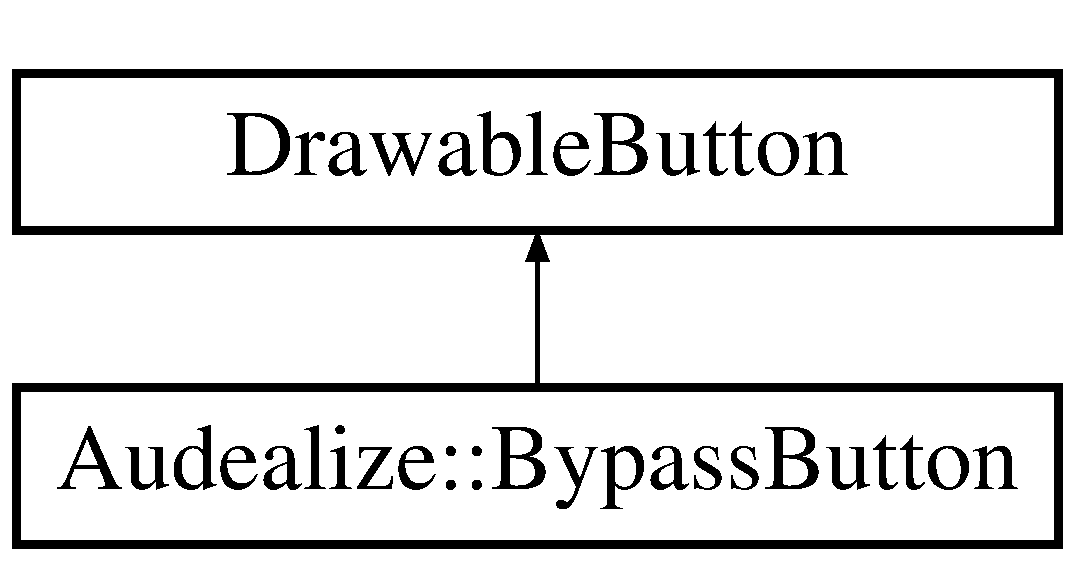
\includegraphics[height=2.000000cm]{class_audealize_1_1_bypass_button}
\end{center}
\end{figure}
\subsection*{Public Types}
\begin{DoxyCompactItemize}
\item 
enum \hyperlink{class_audealize_1_1_bypass_button_a82be721eb2e882505c0e1c47e7f23a04}{Colour\+Ids} \{ \hyperlink{class_audealize_1_1_bypass_button_a82be721eb2e882505c0e1c47e7f23a04a3d3a64c3628718fc55324463d34049da}{off\+Colour\+Id} = 0x2000900, 
\hyperlink{class_audealize_1_1_bypass_button_a82be721eb2e882505c0e1c47e7f23a04a1ec53dd2ba394a9eb1c9f7fea87b2e9c}{on\+Colour\+Id} = 0x2000901
 \}
\end{DoxyCompactItemize}
\subsection*{Public Member Functions}
\begin{DoxyCompactItemize}
\item 
\hyperlink{class_audealize_1_1_bypass_button_acd4cf48194a2537bd05691f586eae9b9}{Bypass\+Button} ()
\item 
\hyperlink{class_audealize_1_1_bypass_button_a1f07bc84de772d603aab713987049d16}{$\sim$\+Bypass\+Button} ()
\item 
\hyperlink{tk_8h_aba408b7cd755a96426e004c015f5de8e}{void} \hyperlink{class_audealize_1_1_bypass_button_adda4dc38f9cebc36bf8fda5563ee2768}{look\+And\+Feel\+Changed} () override
\item 
\hyperlink{tk_8h_aba408b7cd755a96426e004c015f5de8e}{void} \hyperlink{class_audealize_1_1_bypass_button_af3af03dfd3c4773e82943f85101b004b}{paint\+Button} (Graphics \&g, const bool is\+Mouse\+Over\+Button, const bool is\+Button\+Down) override
\end{DoxyCompactItemize}


\subsection{Member Enumeration Documentation}
\index{Audealize\+::\+Bypass\+Button@{Audealize\+::\+Bypass\+Button}!Colour\+Ids@{Colour\+Ids}}
\index{Colour\+Ids@{Colour\+Ids}!Audealize\+::\+Bypass\+Button@{Audealize\+::\+Bypass\+Button}}
\subsubsection[{\texorpdfstring{Colour\+Ids}{ColourIds}}]{\setlength{\rightskip}{0pt plus 5cm}enum {\bf Audealize\+::\+Bypass\+Button\+::\+Colour\+Ids}}\hypertarget{class_audealize_1_1_bypass_button_a82be721eb2e882505c0e1c47e7f23a04}{}\label{class_audealize_1_1_bypass_button_a82be721eb2e882505c0e1c47e7f23a04}
\begin{Desc}
\item[Enumerator]\par
\begin{description}
\index{off\+Colour\+Id@{off\+Colour\+Id}!Audealize\+::\+Bypass\+Button@{Audealize\+::\+Bypass\+Button}}\index{Audealize\+::\+Bypass\+Button@{Audealize\+::\+Bypass\+Button}!off\+Colour\+Id@{off\+Colour\+Id}}\item[{\em 
off\+Colour\+Id\hypertarget{class_audealize_1_1_bypass_button_a82be721eb2e882505c0e1c47e7f23a04a3d3a64c3628718fc55324463d34049da}{}\label{class_audealize_1_1_bypass_button_a82be721eb2e882505c0e1c47e7f23a04a3d3a64c3628718fc55324463d34049da}
}]\index{on\+Colour\+Id@{on\+Colour\+Id}!Audealize\+::\+Bypass\+Button@{Audealize\+::\+Bypass\+Button}}\index{Audealize\+::\+Bypass\+Button@{Audealize\+::\+Bypass\+Button}!on\+Colour\+Id@{on\+Colour\+Id}}\item[{\em 
on\+Colour\+Id\hypertarget{class_audealize_1_1_bypass_button_a82be721eb2e882505c0e1c47e7f23a04a1ec53dd2ba394a9eb1c9f7fea87b2e9c}{}\label{class_audealize_1_1_bypass_button_a82be721eb2e882505c0e1c47e7f23a04a1ec53dd2ba394a9eb1c9f7fea87b2e9c}
}]\end{description}
\end{Desc}


\subsection{Constructor \& Destructor Documentation}
\index{Audealize\+::\+Bypass\+Button@{Audealize\+::\+Bypass\+Button}!Bypass\+Button@{Bypass\+Button}}
\index{Bypass\+Button@{Bypass\+Button}!Audealize\+::\+Bypass\+Button@{Audealize\+::\+Bypass\+Button}}
\subsubsection[{\texorpdfstring{Bypass\+Button()}{BypassButton()}}]{\setlength{\rightskip}{0pt plus 5cm}Audealize\+::\+Bypass\+Button\+::\+Bypass\+Button (
\begin{DoxyParamCaption}
{}
\end{DoxyParamCaption}
)\hspace{0.3cm}{\ttfamily [inline]}}\hypertarget{class_audealize_1_1_bypass_button_acd4cf48194a2537bd05691f586eae9b9}{}\label{class_audealize_1_1_bypass_button_acd4cf48194a2537bd05691f586eae9b9}
\index{Audealize\+::\+Bypass\+Button@{Audealize\+::\+Bypass\+Button}!````~Bypass\+Button@{$\sim$\+Bypass\+Button}}
\index{````~Bypass\+Button@{$\sim$\+Bypass\+Button}!Audealize\+::\+Bypass\+Button@{Audealize\+::\+Bypass\+Button}}
\subsubsection[{\texorpdfstring{$\sim$\+Bypass\+Button()}{~BypassButton()}}]{\setlength{\rightskip}{0pt plus 5cm}Audealize\+::\+Bypass\+Button\+::$\sim$\+Bypass\+Button (
\begin{DoxyParamCaption}
{}
\end{DoxyParamCaption}
)\hspace{0.3cm}{\ttfamily [inline]}}\hypertarget{class_audealize_1_1_bypass_button_a1f07bc84de772d603aab713987049d16}{}\label{class_audealize_1_1_bypass_button_a1f07bc84de772d603aab713987049d16}


\subsection{Member Function Documentation}
\index{Audealize\+::\+Bypass\+Button@{Audealize\+::\+Bypass\+Button}!look\+And\+Feel\+Changed@{look\+And\+Feel\+Changed}}
\index{look\+And\+Feel\+Changed@{look\+And\+Feel\+Changed}!Audealize\+::\+Bypass\+Button@{Audealize\+::\+Bypass\+Button}}
\subsubsection[{\texorpdfstring{look\+And\+Feel\+Changed() override}{lookAndFeelChanged() override}}]{\setlength{\rightskip}{0pt plus 5cm}{\bf void} Audealize\+::\+Bypass\+Button\+::look\+And\+Feel\+Changed (
\begin{DoxyParamCaption}
{}
\end{DoxyParamCaption}
)\hspace{0.3cm}{\ttfamily [inline]}, {\ttfamily [override]}}\hypertarget{class_audealize_1_1_bypass_button_adda4dc38f9cebc36bf8fda5563ee2768}{}\label{class_audealize_1_1_bypass_button_adda4dc38f9cebc36bf8fda5563ee2768}
\index{Audealize\+::\+Bypass\+Button@{Audealize\+::\+Bypass\+Button}!paint\+Button@{paint\+Button}}
\index{paint\+Button@{paint\+Button}!Audealize\+::\+Bypass\+Button@{Audealize\+::\+Bypass\+Button}}
\subsubsection[{\texorpdfstring{paint\+Button(\+Graphics \&g, const bool is\+Mouse\+Over\+Button, const bool is\+Button\+Down) override}{paintButton(Graphics &g, const bool isMouseOverButton, const bool isButtonDown) override}}]{\setlength{\rightskip}{0pt plus 5cm}{\bf void} Audealize\+::\+Bypass\+Button\+::paint\+Button (
\begin{DoxyParamCaption}
\item[{Graphics \&}]{g, }
\item[{const bool}]{is\+Mouse\+Over\+Button, }
\item[{const bool}]{is\+Button\+Down}
\end{DoxyParamCaption}
)\hspace{0.3cm}{\ttfamily [inline]}, {\ttfamily [override]}}\hypertarget{class_audealize_1_1_bypass_button_af3af03dfd3c4773e82943f85101b004b}{}\label{class_audealize_1_1_bypass_button_af3af03dfd3c4773e82943f85101b004b}


The documentation for this class was generated from the following file\+:\begin{DoxyCompactItemize}
\item 
/\+Users/michael/\+J\+U\+C\+E/projects/audealize-\/plugin/\+J\+U\+C\+E Modules/audealize\+\_\+module/ui\+\_\+components/\hyperlink{_bypass_button_8h}{Bypass\+Button.\+h}\end{DoxyCompactItemize}

\hypertarget{classdsp_1_1circular__buffer}{}\section{dsp\+:\+:circular\+\_\+buffer$<$ B $>$ Class Template Reference}
\label{classdsp_1_1circular__buffer}\index{dsp\+::circular\+\_\+buffer$<$ B $>$@{dsp\+::circular\+\_\+buffer$<$ B $>$}}


this is useless for now (and untested too)  




{\ttfamily \#include $<$buffer.\+h$>$}

Inheritance diagram for dsp\+:\+:circular\+\_\+buffer$<$ B $>$\+:\begin{figure}[H]
\begin{center}
\leavevmode
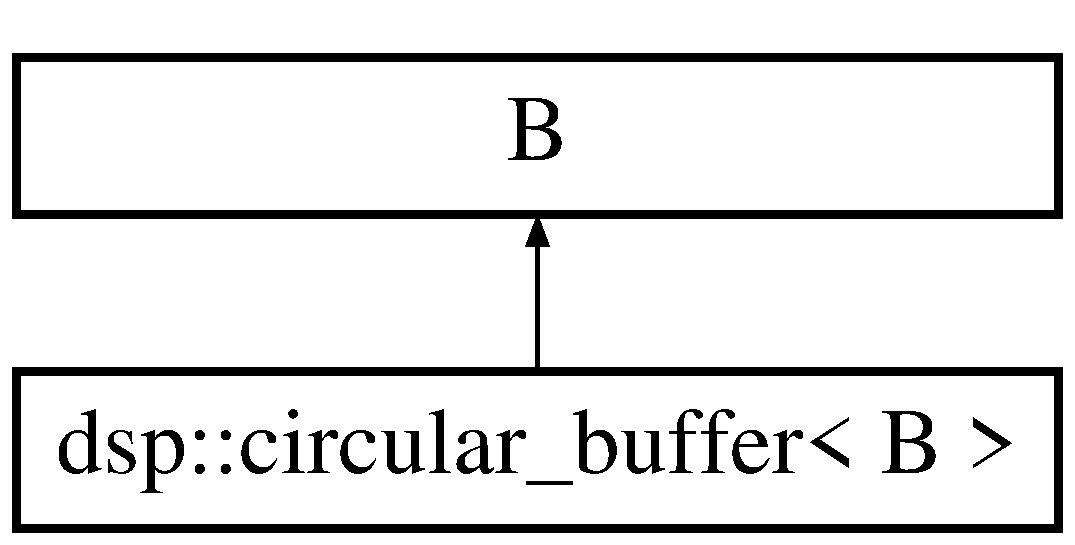
\includegraphics[height=2.000000cm]{classdsp_1_1circular__buffer}
\end{center}
\end{figure}


\subsection{Detailed Description}
\subsubsection*{template$<$class B$>$\\*
class dsp\+::circular\+\_\+buffer$<$ B $>$}

this is useless for now (and untested too) 

The documentation for this class was generated from the following file\+:\begin{DoxyCompactItemize}
\item 
/\+Users/michael/\+J\+U\+C\+E/projects/audealize-\/plugin/\+J\+U\+C\+E Modules/audealize\+\_\+module/utils/calf\+\_\+dsp\+\_\+library/\hyperlink{buffer_8h}{buffer.\+h}\end{DoxyCompactItemize}

\hypertarget{classnlohmann_1_1basic__json_1_1const__iterator}{}\section{nlohmann\+:\+:basic\+\_\+json$<$ Object\+Type, Array\+Type, String\+Type, Boolean\+Type, Number\+Integer\+Type, Number\+Unsigned\+Type, Number\+Float\+Type, Allocator\+Type $>$\+:\+:const\+\_\+iterator Class Reference}
\label{classnlohmann_1_1basic__json_1_1const__iterator}\index{nlohmann\+::basic\+\_\+json$<$ Object\+Type, Array\+Type, String\+Type, Boolean\+Type, Number\+Integer\+Type, Number\+Unsigned\+Type, Number\+Float\+Type, Allocator\+Type $>$\+::const\+\_\+iterator@{nlohmann\+::basic\+\_\+json$<$ Object\+Type, Array\+Type, String\+Type, Boolean\+Type, Number\+Integer\+Type, Number\+Unsigned\+Type, Number\+Float\+Type, Allocator\+Type $>$\+::const\+\_\+iterator}}


a const random access iterator for the \hyperlink{classnlohmann_1_1basic__json}{basic\+\_\+json} class  




{\ttfamily \#include $<$json.\+hpp$>$}

Inheritance diagram for nlohmann\+:\+:basic\+\_\+json$<$ Object\+Type, Array\+Type, String\+Type, Boolean\+Type, Number\+Integer\+Type, Number\+Unsigned\+Type, Number\+Float\+Type, Allocator\+Type $>$\+:\+:const\+\_\+iterator\+:\begin{figure}[H]
\begin{center}
\leavevmode
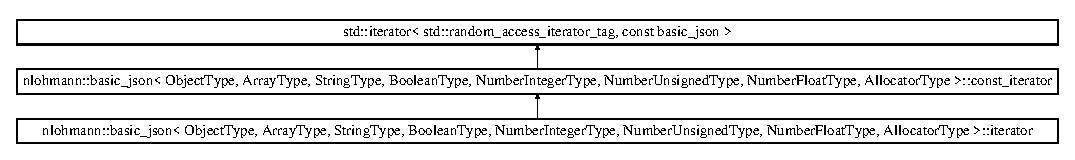
\includegraphics[height=1.705584cm]{classnlohmann_1_1basic__json_1_1const__iterator}
\end{center}
\end{figure}
\subsection*{Public Types}
\begin{DoxyCompactItemize}
\item 
using \hyperlink{classnlohmann_1_1basic__json_1_1const__iterator_a9ea0497199b1e96ce9cadd1f202ec343}{value\+\_\+type} = typename \hyperlink{classnlohmann_1_1basic__json_ac8d45b57874b4a6e9c07f7d3b5daa1f9}{basic\+\_\+json\+::value\+\_\+type}
\begin{DoxyCompactList}\small\item\em the type of the values when the iterator is dereferenced \end{DoxyCompactList}\item 
using \hyperlink{classnlohmann_1_1basic__json_1_1const__iterator_a49d7c3e9ef3280df03052cce988b792f}{difference\+\_\+type} = typename \hyperlink{classnlohmann_1_1basic__json_aec316934a555dd1acdd3600e5d4a4cdf}{basic\+\_\+json\+::difference\+\_\+type}
\begin{DoxyCompactList}\small\item\em a type to represent differences between iterators \end{DoxyCompactList}\item 
using \hyperlink{classnlohmann_1_1basic__json_1_1const__iterator_a1da96fc3054d547e7706d3a2f073f389}{pointer} = typename \hyperlink{classnlohmann_1_1basic__json_a06efb200b69942eacd1ea22d0f6ccebb}{basic\+\_\+json\+::const\+\_\+pointer}
\begin{DoxyCompactList}\small\item\em defines a pointer to the type iterated over (value\+\_\+type) \end{DoxyCompactList}\item 
using \hyperlink{classnlohmann_1_1basic__json_1_1const__iterator_aefd248cac6493eed1e6ff53ba6a63eb2}{reference} = typename \hyperlink{classnlohmann_1_1basic__json_af677a29b0e66edc9f66e5167e4667071}{basic\+\_\+json\+::const\+\_\+reference}
\begin{DoxyCompactList}\small\item\em defines a reference to the type iterated over (value\+\_\+type) \end{DoxyCompactList}\item 
using \hyperlink{classnlohmann_1_1basic__json_1_1const__iterator_a821560d64f50525162097f19b1392e7f}{iterator\+\_\+category} = std\+::bidirectional\+\_\+iterator\+\_\+tag
\begin{DoxyCompactList}\small\item\em the category of the iterator \end{DoxyCompactList}\end{DoxyCompactItemize}
\subsection*{Public Member Functions}
\begin{DoxyCompactItemize}
\item 
\hyperlink{classnlohmann_1_1basic__json_1_1const__iterator_ac6fdaff67857f82a623e5cc253917639}{const\+\_\+iterator} ()=default
\begin{DoxyCompactList}\small\item\em default constructor \end{DoxyCompactList}\item 
\hyperlink{classnlohmann_1_1basic__json_1_1const__iterator_a23de834b11bd895209aa65c100ab9ceb}{const\+\_\+iterator} (\hyperlink{classnlohmann_1_1basic__json_1_1const__iterator_a1da96fc3054d547e7706d3a2f073f389}{pointer} \hyperlink{classnlohmann_1_1basic__json_ad25b2f8c21e241e2d63455537a9294ff}{object}) noexcept
\begin{DoxyCompactList}\small\item\em constructor for a given J\+S\+ON instance \end{DoxyCompactList}\item 
\hyperlink{classnlohmann_1_1basic__json_1_1const__iterator_a6b950c6bc081ac1ec1540ec05ceb2603}{const\+\_\+iterator} (const \hyperlink{classnlohmann_1_1basic__json_1_1iterator}{iterator} \&other) noexcept
\begin{DoxyCompactList}\small\item\em copy constructor given a nonconst iterator \end{DoxyCompactList}\item 
\hyperlink{classnlohmann_1_1basic__json_1_1const__iterator_a18c35a6735d3da96b4fc026421c05dd8}{const\+\_\+iterator} (const \hyperlink{classnlohmann_1_1basic__json_1_1const__iterator}{const\+\_\+iterator} \&other) noexcept
\begin{DoxyCompactList}\small\item\em copy constructor \end{DoxyCompactList}\item 
\hyperlink{classnlohmann_1_1basic__json_1_1const__iterator}{const\+\_\+iterator} \& \hyperlink{classnlohmann_1_1basic__json_1_1const__iterator_a5521515067b6597cb0b55a9c547a7a2b}{operator=} (\hyperlink{classnlohmann_1_1basic__json_1_1const__iterator}{const\+\_\+iterator} other) noexcept(                                       std\+::is\+\_\+nothrow\+\_\+move\+\_\+constructible$<$ \hyperlink{classnlohmann_1_1basic__json_1_1const__iterator_a1da96fc3054d547e7706d3a2f073f389}{pointer} $>$\+::\hyperlink{tk_8h_a177a0765f574ef6642002696d9cd82d0}{value} and                                       std\+::is\+\_\+nothrow\+\_\+move\+\_\+assignable$<$ \hyperlink{classnlohmann_1_1basic__json_1_1const__iterator_a1da96fc3054d547e7706d3a2f073f389}{pointer} $>$\+::\hyperlink{tk_8h_a177a0765f574ef6642002696d9cd82d0}{value} and                                       std\+::is\+\_\+nothrow\+\_\+move\+\_\+constructible$<$ internal\+\_\+iterator $>$\+::\hyperlink{tk_8h_a177a0765f574ef6642002696d9cd82d0}{value} and                                       std\+::is\+\_\+nothrow\+\_\+move\+\_\+assignable$<$ internal\+\_\+iterator $>$\+::\hyperlink{tk_8h_a177a0765f574ef6642002696d9cd82d0}{value}                       )
\begin{DoxyCompactList}\small\item\em copy assignment \end{DoxyCompactList}\item 
\hyperlink{classnlohmann_1_1basic__json_1_1const__iterator_aefd248cac6493eed1e6ff53ba6a63eb2}{reference} \hyperlink{classnlohmann_1_1basic__json_1_1const__iterator_ab3029a1a83cf46dc28ad443bbad0c74d}{operator$\ast$} () const 
\begin{DoxyCompactList}\small\item\em return a reference to the value pointed to by the iterator \end{DoxyCompactList}\item 
\hyperlink{classnlohmann_1_1basic__json_1_1const__iterator_a1da96fc3054d547e7706d3a2f073f389}{pointer} \hyperlink{classnlohmann_1_1basic__json_1_1const__iterator_a8be837e4d902887676dd837abe9098d3}{operator-\/$>$} () const 
\begin{DoxyCompactList}\small\item\em dereference the iterator \end{DoxyCompactList}\item 
\hyperlink{classnlohmann_1_1basic__json_1_1const__iterator}{const\+\_\+iterator} \hyperlink{classnlohmann_1_1basic__json_1_1const__iterator_a8dbaec5bf8ccba3225520356629061cb}{operator++} (\hyperlink{tk_8h_a83f82f76e7fed06f4c49d2db94028a6d}{int})
\begin{DoxyCompactList}\small\item\em post-\/increment (it++) \end{DoxyCompactList}\item 
\hyperlink{classnlohmann_1_1basic__json_1_1const__iterator}{const\+\_\+iterator} \& \hyperlink{classnlohmann_1_1basic__json_1_1const__iterator_a8fbb15efd97599209a7def77af8e748e}{operator++} ()
\begin{DoxyCompactList}\small\item\em pre-\/increment (++it) \end{DoxyCompactList}\item 
\hyperlink{classnlohmann_1_1basic__json_1_1const__iterator}{const\+\_\+iterator} \hyperlink{classnlohmann_1_1basic__json_1_1const__iterator_a6cab1c2ed7e2a014980e2a5717f43a64}{operator-\/-\/} (\hyperlink{tk_8h_a83f82f76e7fed06f4c49d2db94028a6d}{int})
\begin{DoxyCompactList}\small\item\em post-\/decrement (it--) \end{DoxyCompactList}\item 
\hyperlink{classnlohmann_1_1basic__json_1_1const__iterator}{const\+\_\+iterator} \& \hyperlink{classnlohmann_1_1basic__json_1_1const__iterator_adeb2ff3fdf3cc301b72db109934c9199}{operator-\/-\/} ()
\begin{DoxyCompactList}\small\item\em pre-\/decrement (--it) \end{DoxyCompactList}\item 
bool \hyperlink{classnlohmann_1_1basic__json_1_1const__iterator_ab4c0b9baaec9ebc4837158e272f6c803}{operator==} (const \hyperlink{classnlohmann_1_1basic__json_1_1const__iterator}{const\+\_\+iterator} \&other) const 
\begin{DoxyCompactList}\small\item\em comparison\+: equal \end{DoxyCompactList}\item 
bool \hyperlink{classnlohmann_1_1basic__json_1_1const__iterator_a9e4c6e48e3c2f3ff357ef8215b8c8fca}{operator!=} (const \hyperlink{classnlohmann_1_1basic__json_1_1const__iterator}{const\+\_\+iterator} \&other) const 
\begin{DoxyCompactList}\small\item\em comparison\+: not equal \end{DoxyCompactList}\item 
bool \hyperlink{classnlohmann_1_1basic__json_1_1const__iterator_a65f491b515e5967e9c0b40289e3c0ff3}{operator$<$} (const \hyperlink{classnlohmann_1_1basic__json_1_1const__iterator}{const\+\_\+iterator} \&other) const 
\begin{DoxyCompactList}\small\item\em comparison\+: smaller \end{DoxyCompactList}\item 
bool \hyperlink{classnlohmann_1_1basic__json_1_1const__iterator_a6b682f09787eff62f03493d45aa05902}{operator$<$=} (const \hyperlink{classnlohmann_1_1basic__json_1_1const__iterator}{const\+\_\+iterator} \&other) const 
\begin{DoxyCompactList}\small\item\em comparison\+: less than or equal \end{DoxyCompactList}\item 
bool \hyperlink{classnlohmann_1_1basic__json_1_1const__iterator_acb6cd0ff760933afeb7f93e5207f3646}{operator$>$} (const \hyperlink{classnlohmann_1_1basic__json_1_1const__iterator}{const\+\_\+iterator} \&other) const 
\begin{DoxyCompactList}\small\item\em comparison\+: greater than \end{DoxyCompactList}\item 
bool \hyperlink{classnlohmann_1_1basic__json_1_1const__iterator_af6941c3711dabb2e64960dd57e00d201}{operator$>$=} (const \hyperlink{classnlohmann_1_1basic__json_1_1const__iterator}{const\+\_\+iterator} \&other) const 
\begin{DoxyCompactList}\small\item\em comparison\+: greater than or equal \end{DoxyCompactList}\item 
\hyperlink{classnlohmann_1_1basic__json_1_1const__iterator}{const\+\_\+iterator} \& \hyperlink{classnlohmann_1_1basic__json_1_1const__iterator_a0d5820d1dda9dea3bbeb029cacf68522}{operator+=} (\hyperlink{classnlohmann_1_1basic__json_1_1const__iterator_a49d7c3e9ef3280df03052cce988b792f}{difference\+\_\+type} i)
\begin{DoxyCompactList}\small\item\em add to iterator \end{DoxyCompactList}\item 
\hyperlink{classnlohmann_1_1basic__json_1_1const__iterator}{const\+\_\+iterator} \& \hyperlink{classnlohmann_1_1basic__json_1_1const__iterator_aefac8f3e390ac917f021761f4a8f8e71}{operator-\/=} (\hyperlink{classnlohmann_1_1basic__json_1_1const__iterator_a49d7c3e9ef3280df03052cce988b792f}{difference\+\_\+type} i)
\begin{DoxyCompactList}\small\item\em subtract from iterator \end{DoxyCompactList}\item 
\hyperlink{classnlohmann_1_1basic__json_1_1const__iterator}{const\+\_\+iterator} \hyperlink{classnlohmann_1_1basic__json_1_1const__iterator_a7a80257f2303210b0a5d056fc0b30b40}{operator+} (\hyperlink{classnlohmann_1_1basic__json_1_1const__iterator_a49d7c3e9ef3280df03052cce988b792f}{difference\+\_\+type} i)
\begin{DoxyCompactList}\small\item\em add to iterator \end{DoxyCompactList}\item 
\hyperlink{classnlohmann_1_1basic__json_1_1const__iterator}{const\+\_\+iterator} \hyperlink{classnlohmann_1_1basic__json_1_1const__iterator_abc4552ba2fe39e7901a83dd6d4dec151}{operator-\/} (\hyperlink{classnlohmann_1_1basic__json_1_1const__iterator_a49d7c3e9ef3280df03052cce988b792f}{difference\+\_\+type} i)
\begin{DoxyCompactList}\small\item\em subtract from iterator \end{DoxyCompactList}\item 
\hyperlink{classnlohmann_1_1basic__json_1_1const__iterator_a49d7c3e9ef3280df03052cce988b792f}{difference\+\_\+type} \hyperlink{classnlohmann_1_1basic__json_1_1const__iterator_a5e4d98a8f95e2eccde8cd48c19efa196}{operator-\/} (const \hyperlink{classnlohmann_1_1basic__json_1_1const__iterator}{const\+\_\+iterator} \&other) const 
\begin{DoxyCompactList}\small\item\em return difference \end{DoxyCompactList}\item 
\hyperlink{classnlohmann_1_1basic__json_1_1const__iterator_aefd248cac6493eed1e6ff53ba6a63eb2}{reference} \hyperlink{classnlohmann_1_1basic__json_1_1const__iterator_a7bd530bfbbc58ac77308c087120c21fa}{operator\mbox{[}$\,$\mbox{]}} (\hyperlink{classnlohmann_1_1basic__json_1_1const__iterator_a49d7c3e9ef3280df03052cce988b792f}{difference\+\_\+type} n) const 
\begin{DoxyCompactList}\small\item\em access to successor \end{DoxyCompactList}\item 
object\+\_\+t\+::key\+\_\+type \hyperlink{classnlohmann_1_1basic__json_1_1const__iterator_a5d4320e24fcb7df041ff2c95d976dba0}{key} () const 
\begin{DoxyCompactList}\small\item\em return the key of an object iterator \end{DoxyCompactList}\item 
\hyperlink{classnlohmann_1_1basic__json_1_1const__iterator_aefd248cac6493eed1e6ff53ba6a63eb2}{reference} \hyperlink{classnlohmann_1_1basic__json_1_1const__iterator_ac75e80d30b6169ee2a29ec93fb4d2acd}{value} () const 
\begin{DoxyCompactList}\small\item\em return the value of an iterator \end{DoxyCompactList}\end{DoxyCompactItemize}
\subsection*{Friends}
\begin{DoxyCompactItemize}
\item 
class \hyperlink{classnlohmann_1_1basic__json_1_1const__iterator_ada3100cdb8700566051828f1355fa745}{basic\+\_\+json}
\begin{DoxyCompactList}\small\item\em allow \hyperlink{classnlohmann_1_1basic__json}{basic\+\_\+json} to access private members \end{DoxyCompactList}\end{DoxyCompactItemize}


\subsection{Detailed Description}
\subsubsection*{template$<$template$<$ typename U, typename V, typename...\+Args $>$ class Object\+Type = std\+::map, template$<$ typename U, typename...\+Args $>$ class Array\+Type = std\+::vector, class String\+Type = std\+::string, class Boolean\+Type = bool, class Number\+Integer\+Type = std\+::int64\+\_\+t, class Number\+Unsigned\+Type = std\+::uint64\+\_\+t, class Number\+Float\+Type = double, template$<$ typename U $>$ class Allocator\+Type = std\+::allocator$>$\\*
class nlohmann\+::basic\+\_\+json$<$ Object\+Type, Array\+Type, String\+Type, Boolean\+Type, Number\+Integer\+Type, Number\+Unsigned\+Type, Number\+Float\+Type, Allocator\+Type $>$\+::const\+\_\+iterator}

a const random access iterator for the \hyperlink{classnlohmann_1_1basic__json}{basic\+\_\+json} class 

This class implements a const iterator for the \hyperlink{classnlohmann_1_1basic__json}{basic\+\_\+json} class. From this class, the \hyperlink{classnlohmann_1_1basic__json_1_1iterator}{iterator} class is derived.

The class satisfies the following concept requirements\+:
\begin{DoxyItemize}
\item \href{http://en.cppreference.com/w/cpp/concept/RandomAccessIterator}{\tt Random\+Access\+Iterator}\+: The iterator that can be moved to point (forward and backward) to any element in constant time.
\end{DoxyItemize}

\begin{DoxySince}{Since}
version 1.\+0.\+0 
\end{DoxySince}


\subsection{Member Typedef Documentation}
\index{nlohmann\+::basic\+\_\+json\+::const\+\_\+iterator@{nlohmann\+::basic\+\_\+json\+::const\+\_\+iterator}!difference\+\_\+type@{difference\+\_\+type}}
\index{difference\+\_\+type@{difference\+\_\+type}!nlohmann\+::basic\+\_\+json\+::const\+\_\+iterator@{nlohmann\+::basic\+\_\+json\+::const\+\_\+iterator}}
\subsubsection[{\texorpdfstring{difference\+\_\+type}{difference_type}}]{\setlength{\rightskip}{0pt plus 5cm}template$<$template$<$ typename U, typename V, typename...\+Args $>$ class Object\+Type = std\+::map, template$<$ typename U, typename...\+Args $>$ class Array\+Type = std\+::vector, class String\+Type  = std\+::string, class Boolean\+Type  = bool, class Number\+Integer\+Type  = std\+::int64\+\_\+t, class Number\+Unsigned\+Type  = std\+::uint64\+\_\+t, class Number\+Float\+Type  = double, template$<$ typename U $>$ class Allocator\+Type = std\+::allocator$>$ using {\bf nlohmann\+::basic\+\_\+json}$<$ Object\+Type, Array\+Type, String\+Type, Boolean\+Type, Number\+Integer\+Type, Number\+Unsigned\+Type, Number\+Float\+Type, Allocator\+Type $>$\+::{\bf const\+\_\+iterator\+::difference\+\_\+type} =  typename {\bf basic\+\_\+json\+::difference\+\_\+type}}\hypertarget{classnlohmann_1_1basic__json_1_1const__iterator_a49d7c3e9ef3280df03052cce988b792f}{}\label{classnlohmann_1_1basic__json_1_1const__iterator_a49d7c3e9ef3280df03052cce988b792f}


a type to represent differences between iterators 

\index{nlohmann\+::basic\+\_\+json\+::const\+\_\+iterator@{nlohmann\+::basic\+\_\+json\+::const\+\_\+iterator}!iterator\+\_\+category@{iterator\+\_\+category}}
\index{iterator\+\_\+category@{iterator\+\_\+category}!nlohmann\+::basic\+\_\+json\+::const\+\_\+iterator@{nlohmann\+::basic\+\_\+json\+::const\+\_\+iterator}}
\subsubsection[{\texorpdfstring{iterator\+\_\+category}{iterator_category}}]{\setlength{\rightskip}{0pt plus 5cm}template$<$template$<$ typename U, typename V, typename...\+Args $>$ class Object\+Type = std\+::map, template$<$ typename U, typename...\+Args $>$ class Array\+Type = std\+::vector, class String\+Type  = std\+::string, class Boolean\+Type  = bool, class Number\+Integer\+Type  = std\+::int64\+\_\+t, class Number\+Unsigned\+Type  = std\+::uint64\+\_\+t, class Number\+Float\+Type  = double, template$<$ typename U $>$ class Allocator\+Type = std\+::allocator$>$ using {\bf nlohmann\+::basic\+\_\+json}$<$ Object\+Type, Array\+Type, String\+Type, Boolean\+Type, Number\+Integer\+Type, Number\+Unsigned\+Type, Number\+Float\+Type, Allocator\+Type $>$\+::{\bf const\+\_\+iterator\+::iterator\+\_\+category} =  std\+::bidirectional\+\_\+iterator\+\_\+tag}\hypertarget{classnlohmann_1_1basic__json_1_1const__iterator_a821560d64f50525162097f19b1392e7f}{}\label{classnlohmann_1_1basic__json_1_1const__iterator_a821560d64f50525162097f19b1392e7f}


the category of the iterator 

\index{nlohmann\+::basic\+\_\+json\+::const\+\_\+iterator@{nlohmann\+::basic\+\_\+json\+::const\+\_\+iterator}!pointer@{pointer}}
\index{pointer@{pointer}!nlohmann\+::basic\+\_\+json\+::const\+\_\+iterator@{nlohmann\+::basic\+\_\+json\+::const\+\_\+iterator}}
\subsubsection[{\texorpdfstring{pointer}{pointer}}]{\setlength{\rightskip}{0pt plus 5cm}template$<$template$<$ typename U, typename V, typename...\+Args $>$ class Object\+Type = std\+::map, template$<$ typename U, typename...\+Args $>$ class Array\+Type = std\+::vector, class String\+Type  = std\+::string, class Boolean\+Type  = bool, class Number\+Integer\+Type  = std\+::int64\+\_\+t, class Number\+Unsigned\+Type  = std\+::uint64\+\_\+t, class Number\+Float\+Type  = double, template$<$ typename U $>$ class Allocator\+Type = std\+::allocator$>$ using {\bf nlohmann\+::basic\+\_\+json}$<$ Object\+Type, Array\+Type, String\+Type, Boolean\+Type, Number\+Integer\+Type, Number\+Unsigned\+Type, Number\+Float\+Type, Allocator\+Type $>$\+::{\bf const\+\_\+iterator\+::pointer} =  typename {\bf basic\+\_\+json\+::const\+\_\+pointer}}\hypertarget{classnlohmann_1_1basic__json_1_1const__iterator_a1da96fc3054d547e7706d3a2f073f389}{}\label{classnlohmann_1_1basic__json_1_1const__iterator_a1da96fc3054d547e7706d3a2f073f389}


defines a pointer to the type iterated over (value\+\_\+type) 

\index{nlohmann\+::basic\+\_\+json\+::const\+\_\+iterator@{nlohmann\+::basic\+\_\+json\+::const\+\_\+iterator}!reference@{reference}}
\index{reference@{reference}!nlohmann\+::basic\+\_\+json\+::const\+\_\+iterator@{nlohmann\+::basic\+\_\+json\+::const\+\_\+iterator}}
\subsubsection[{\texorpdfstring{reference}{reference}}]{\setlength{\rightskip}{0pt plus 5cm}template$<$template$<$ typename U, typename V, typename...\+Args $>$ class Object\+Type = std\+::map, template$<$ typename U, typename...\+Args $>$ class Array\+Type = std\+::vector, class String\+Type  = std\+::string, class Boolean\+Type  = bool, class Number\+Integer\+Type  = std\+::int64\+\_\+t, class Number\+Unsigned\+Type  = std\+::uint64\+\_\+t, class Number\+Float\+Type  = double, template$<$ typename U $>$ class Allocator\+Type = std\+::allocator$>$ using {\bf nlohmann\+::basic\+\_\+json}$<$ Object\+Type, Array\+Type, String\+Type, Boolean\+Type, Number\+Integer\+Type, Number\+Unsigned\+Type, Number\+Float\+Type, Allocator\+Type $>$\+::{\bf const\+\_\+iterator\+::reference} =  typename {\bf basic\+\_\+json\+::const\+\_\+reference}}\hypertarget{classnlohmann_1_1basic__json_1_1const__iterator_aefd248cac6493eed1e6ff53ba6a63eb2}{}\label{classnlohmann_1_1basic__json_1_1const__iterator_aefd248cac6493eed1e6ff53ba6a63eb2}


defines a reference to the type iterated over (value\+\_\+type) 

\index{nlohmann\+::basic\+\_\+json\+::const\+\_\+iterator@{nlohmann\+::basic\+\_\+json\+::const\+\_\+iterator}!value\+\_\+type@{value\+\_\+type}}
\index{value\+\_\+type@{value\+\_\+type}!nlohmann\+::basic\+\_\+json\+::const\+\_\+iterator@{nlohmann\+::basic\+\_\+json\+::const\+\_\+iterator}}
\subsubsection[{\texorpdfstring{value\+\_\+type}{value_type}}]{\setlength{\rightskip}{0pt plus 5cm}template$<$template$<$ typename U, typename V, typename...\+Args $>$ class Object\+Type = std\+::map, template$<$ typename U, typename...\+Args $>$ class Array\+Type = std\+::vector, class String\+Type  = std\+::string, class Boolean\+Type  = bool, class Number\+Integer\+Type  = std\+::int64\+\_\+t, class Number\+Unsigned\+Type  = std\+::uint64\+\_\+t, class Number\+Float\+Type  = double, template$<$ typename U $>$ class Allocator\+Type = std\+::allocator$>$ using {\bf nlohmann\+::basic\+\_\+json}$<$ Object\+Type, Array\+Type, String\+Type, Boolean\+Type, Number\+Integer\+Type, Number\+Unsigned\+Type, Number\+Float\+Type, Allocator\+Type $>$\+::{\bf const\+\_\+iterator\+::value\+\_\+type} =  typename {\bf basic\+\_\+json\+::value\+\_\+type}}\hypertarget{classnlohmann_1_1basic__json_1_1const__iterator_a9ea0497199b1e96ce9cadd1f202ec343}{}\label{classnlohmann_1_1basic__json_1_1const__iterator_a9ea0497199b1e96ce9cadd1f202ec343}


the type of the values when the iterator is dereferenced 



\subsection{Constructor \& Destructor Documentation}
\index{nlohmann\+::basic\+\_\+json\+::const\+\_\+iterator@{nlohmann\+::basic\+\_\+json\+::const\+\_\+iterator}!const\+\_\+iterator@{const\+\_\+iterator}}
\index{const\+\_\+iterator@{const\+\_\+iterator}!nlohmann\+::basic\+\_\+json\+::const\+\_\+iterator@{nlohmann\+::basic\+\_\+json\+::const\+\_\+iterator}}
\subsubsection[{\texorpdfstring{const\+\_\+iterator()=default}{const_iterator()=default}}]{\setlength{\rightskip}{0pt plus 5cm}template$<$template$<$ typename U, typename V, typename...\+Args $>$ class Object\+Type = std\+::map, template$<$ typename U, typename...\+Args $>$ class Array\+Type = std\+::vector, class String\+Type  = std\+::string, class Boolean\+Type  = bool, class Number\+Integer\+Type  = std\+::int64\+\_\+t, class Number\+Unsigned\+Type  = std\+::uint64\+\_\+t, class Number\+Float\+Type  = double, template$<$ typename U $>$ class Allocator\+Type = std\+::allocator$>$ {\bf nlohmann\+::basic\+\_\+json}$<$ Object\+Type, Array\+Type, String\+Type, Boolean\+Type, Number\+Integer\+Type, Number\+Unsigned\+Type, Number\+Float\+Type, Allocator\+Type $>$\+::const\+\_\+iterator\+::const\+\_\+iterator (
\begin{DoxyParamCaption}
{}
\end{DoxyParamCaption}
)\hspace{0.3cm}{\ttfamily [default]}}\hypertarget{classnlohmann_1_1basic__json_1_1const__iterator_ac6fdaff67857f82a623e5cc253917639}{}\label{classnlohmann_1_1basic__json_1_1const__iterator_ac6fdaff67857f82a623e5cc253917639}


default constructor 

\index{nlohmann\+::basic\+\_\+json\+::const\+\_\+iterator@{nlohmann\+::basic\+\_\+json\+::const\+\_\+iterator}!const\+\_\+iterator@{const\+\_\+iterator}}
\index{const\+\_\+iterator@{const\+\_\+iterator}!nlohmann\+::basic\+\_\+json\+::const\+\_\+iterator@{nlohmann\+::basic\+\_\+json\+::const\+\_\+iterator}}
\subsubsection[{\texorpdfstring{const\+\_\+iterator(pointer object) noexcept}{const_iterator(pointer object) noexcept}}]{\setlength{\rightskip}{0pt plus 5cm}template$<$template$<$ typename U, typename V, typename...\+Args $>$ class Object\+Type = std\+::map, template$<$ typename U, typename...\+Args $>$ class Array\+Type = std\+::vector, class String\+Type  = std\+::string, class Boolean\+Type  = bool, class Number\+Integer\+Type  = std\+::int64\+\_\+t, class Number\+Unsigned\+Type  = std\+::uint64\+\_\+t, class Number\+Float\+Type  = double, template$<$ typename U $>$ class Allocator\+Type = std\+::allocator$>$ {\bf nlohmann\+::basic\+\_\+json}$<$ Object\+Type, Array\+Type, String\+Type, Boolean\+Type, Number\+Integer\+Type, Number\+Unsigned\+Type, Number\+Float\+Type, Allocator\+Type $>$\+::const\+\_\+iterator\+::const\+\_\+iterator (
\begin{DoxyParamCaption}
\item[{{\bf pointer}}]{object}
\end{DoxyParamCaption}
)\hspace{0.3cm}{\ttfamily [inline]}, {\ttfamily [explicit]}, {\ttfamily [noexcept]}}\hypertarget{classnlohmann_1_1basic__json_1_1const__iterator_a23de834b11bd895209aa65c100ab9ceb}{}\label{classnlohmann_1_1basic__json_1_1const__iterator_a23de834b11bd895209aa65c100ab9ceb}


constructor for a given J\+S\+ON instance 

\index{nlohmann\+::basic\+\_\+json\+::const\+\_\+iterator@{nlohmann\+::basic\+\_\+json\+::const\+\_\+iterator}!const\+\_\+iterator@{const\+\_\+iterator}}
\index{const\+\_\+iterator@{const\+\_\+iterator}!nlohmann\+::basic\+\_\+json\+::const\+\_\+iterator@{nlohmann\+::basic\+\_\+json\+::const\+\_\+iterator}}
\subsubsection[{\texorpdfstring{const\+\_\+iterator(const iterator \&other) noexcept}{const_iterator(const iterator &other) noexcept}}]{\setlength{\rightskip}{0pt plus 5cm}template$<$template$<$ typename U, typename V, typename...\+Args $>$ class Object\+Type = std\+::map, template$<$ typename U, typename...\+Args $>$ class Array\+Type = std\+::vector, class String\+Type  = std\+::string, class Boolean\+Type  = bool, class Number\+Integer\+Type  = std\+::int64\+\_\+t, class Number\+Unsigned\+Type  = std\+::uint64\+\_\+t, class Number\+Float\+Type  = double, template$<$ typename U $>$ class Allocator\+Type = std\+::allocator$>$ {\bf nlohmann\+::basic\+\_\+json}$<$ Object\+Type, Array\+Type, String\+Type, Boolean\+Type, Number\+Integer\+Type, Number\+Unsigned\+Type, Number\+Float\+Type, Allocator\+Type $>$\+::const\+\_\+iterator\+::const\+\_\+iterator (
\begin{DoxyParamCaption}
\item[{const {\bf iterator} \&}]{other}
\end{DoxyParamCaption}
)\hspace{0.3cm}{\ttfamily [inline]}, {\ttfamily [explicit]}, {\ttfamily [noexcept]}}\hypertarget{classnlohmann_1_1basic__json_1_1const__iterator_a6b950c6bc081ac1ec1540ec05ceb2603}{}\label{classnlohmann_1_1basic__json_1_1const__iterator_a6b950c6bc081ac1ec1540ec05ceb2603}


copy constructor given a nonconst iterator 

\index{nlohmann\+::basic\+\_\+json\+::const\+\_\+iterator@{nlohmann\+::basic\+\_\+json\+::const\+\_\+iterator}!const\+\_\+iterator@{const\+\_\+iterator}}
\index{const\+\_\+iterator@{const\+\_\+iterator}!nlohmann\+::basic\+\_\+json\+::const\+\_\+iterator@{nlohmann\+::basic\+\_\+json\+::const\+\_\+iterator}}
\subsubsection[{\texorpdfstring{const\+\_\+iterator(const const\+\_\+iterator \&other) noexcept}{const_iterator(const const_iterator &other) noexcept}}]{\setlength{\rightskip}{0pt plus 5cm}template$<$template$<$ typename U, typename V, typename...\+Args $>$ class Object\+Type = std\+::map, template$<$ typename U, typename...\+Args $>$ class Array\+Type = std\+::vector, class String\+Type  = std\+::string, class Boolean\+Type  = bool, class Number\+Integer\+Type  = std\+::int64\+\_\+t, class Number\+Unsigned\+Type  = std\+::uint64\+\_\+t, class Number\+Float\+Type  = double, template$<$ typename U $>$ class Allocator\+Type = std\+::allocator$>$ {\bf nlohmann\+::basic\+\_\+json}$<$ Object\+Type, Array\+Type, String\+Type, Boolean\+Type, Number\+Integer\+Type, Number\+Unsigned\+Type, Number\+Float\+Type, Allocator\+Type $>$\+::const\+\_\+iterator\+::const\+\_\+iterator (
\begin{DoxyParamCaption}
\item[{const {\bf const\+\_\+iterator} \&}]{other}
\end{DoxyParamCaption}
)\hspace{0.3cm}{\ttfamily [inline]}, {\ttfamily [noexcept]}}\hypertarget{classnlohmann_1_1basic__json_1_1const__iterator_a18c35a6735d3da96b4fc026421c05dd8}{}\label{classnlohmann_1_1basic__json_1_1const__iterator_a18c35a6735d3da96b4fc026421c05dd8}


copy constructor 



\subsection{Member Function Documentation}
\index{nlohmann\+::basic\+\_\+json\+::const\+\_\+iterator@{nlohmann\+::basic\+\_\+json\+::const\+\_\+iterator}!key@{key}}
\index{key@{key}!nlohmann\+::basic\+\_\+json\+::const\+\_\+iterator@{nlohmann\+::basic\+\_\+json\+::const\+\_\+iterator}}
\subsubsection[{\texorpdfstring{key() const }{key() const }}]{\setlength{\rightskip}{0pt plus 5cm}template$<$template$<$ typename U, typename V, typename...\+Args $>$ class Object\+Type = std\+::map, template$<$ typename U, typename...\+Args $>$ class Array\+Type = std\+::vector, class String\+Type  = std\+::string, class Boolean\+Type  = bool, class Number\+Integer\+Type  = std\+::int64\+\_\+t, class Number\+Unsigned\+Type  = std\+::uint64\+\_\+t, class Number\+Float\+Type  = double, template$<$ typename U $>$ class Allocator\+Type = std\+::allocator$>$ object\+\_\+t\+::key\+\_\+type {\bf nlohmann\+::basic\+\_\+json}$<$ Object\+Type, Array\+Type, String\+Type, Boolean\+Type, Number\+Integer\+Type, Number\+Unsigned\+Type, Number\+Float\+Type, Allocator\+Type $>$\+::const\+\_\+iterator\+::key (
\begin{DoxyParamCaption}
{}
\end{DoxyParamCaption}
) const\hspace{0.3cm}{\ttfamily [inline]}}\hypertarget{classnlohmann_1_1basic__json_1_1const__iterator_a5d4320e24fcb7df041ff2c95d976dba0}{}\label{classnlohmann_1_1basic__json_1_1const__iterator_a5d4320e24fcb7df041ff2c95d976dba0}


return the key of an object iterator 

\index{nlohmann\+::basic\+\_\+json\+::const\+\_\+iterator@{nlohmann\+::basic\+\_\+json\+::const\+\_\+iterator}!operator"!=@{operator"!=}}
\index{operator"!=@{operator"!=}!nlohmann\+::basic\+\_\+json\+::const\+\_\+iterator@{nlohmann\+::basic\+\_\+json\+::const\+\_\+iterator}}
\subsubsection[{\texorpdfstring{operator"!=(const const\+\_\+iterator \&other) const }{operator!=(const const_iterator &other) const }}]{\setlength{\rightskip}{0pt plus 5cm}template$<$template$<$ typename U, typename V, typename...\+Args $>$ class Object\+Type = std\+::map, template$<$ typename U, typename...\+Args $>$ class Array\+Type = std\+::vector, class String\+Type  = std\+::string, class Boolean\+Type  = bool, class Number\+Integer\+Type  = std\+::int64\+\_\+t, class Number\+Unsigned\+Type  = std\+::uint64\+\_\+t, class Number\+Float\+Type  = double, template$<$ typename U $>$ class Allocator\+Type = std\+::allocator$>$ bool {\bf nlohmann\+::basic\+\_\+json}$<$ Object\+Type, Array\+Type, String\+Type, Boolean\+Type, Number\+Integer\+Type, Number\+Unsigned\+Type, Number\+Float\+Type, Allocator\+Type $>$\+::const\+\_\+iterator\+::operator!= (
\begin{DoxyParamCaption}
\item[{const {\bf const\+\_\+iterator} \&}]{other}
\end{DoxyParamCaption}
) const\hspace{0.3cm}{\ttfamily [inline]}}\hypertarget{classnlohmann_1_1basic__json_1_1const__iterator_a9e4c6e48e3c2f3ff357ef8215b8c8fca}{}\label{classnlohmann_1_1basic__json_1_1const__iterator_a9e4c6e48e3c2f3ff357ef8215b8c8fca}


comparison\+: not equal 

\index{nlohmann\+::basic\+\_\+json\+::const\+\_\+iterator@{nlohmann\+::basic\+\_\+json\+::const\+\_\+iterator}!operator$\ast$@{operator$\ast$}}
\index{operator$\ast$@{operator$\ast$}!nlohmann\+::basic\+\_\+json\+::const\+\_\+iterator@{nlohmann\+::basic\+\_\+json\+::const\+\_\+iterator}}
\subsubsection[{\texorpdfstring{operator$\ast$() const }{operator*() const }}]{\setlength{\rightskip}{0pt plus 5cm}template$<$template$<$ typename U, typename V, typename...\+Args $>$ class Object\+Type = std\+::map, template$<$ typename U, typename...\+Args $>$ class Array\+Type = std\+::vector, class String\+Type  = std\+::string, class Boolean\+Type  = bool, class Number\+Integer\+Type  = std\+::int64\+\_\+t, class Number\+Unsigned\+Type  = std\+::uint64\+\_\+t, class Number\+Float\+Type  = double, template$<$ typename U $>$ class Allocator\+Type = std\+::allocator$>$ {\bf reference} {\bf nlohmann\+::basic\+\_\+json}$<$ Object\+Type, Array\+Type, String\+Type, Boolean\+Type, Number\+Integer\+Type, Number\+Unsigned\+Type, Number\+Float\+Type, Allocator\+Type $>$\+::const\+\_\+iterator\+::operator$\ast$ (
\begin{DoxyParamCaption}
{}
\end{DoxyParamCaption}
) const\hspace{0.3cm}{\ttfamily [inline]}}\hypertarget{classnlohmann_1_1basic__json_1_1const__iterator_ab3029a1a83cf46dc28ad443bbad0c74d}{}\label{classnlohmann_1_1basic__json_1_1const__iterator_ab3029a1a83cf46dc28ad443bbad0c74d}


return a reference to the value pointed to by the iterator 

\index{nlohmann\+::basic\+\_\+json\+::const\+\_\+iterator@{nlohmann\+::basic\+\_\+json\+::const\+\_\+iterator}!operator+@{operator+}}
\index{operator+@{operator+}!nlohmann\+::basic\+\_\+json\+::const\+\_\+iterator@{nlohmann\+::basic\+\_\+json\+::const\+\_\+iterator}}
\subsubsection[{\texorpdfstring{operator+(difference\+\_\+type i)}{operator+(difference_type i)}}]{\setlength{\rightskip}{0pt plus 5cm}template$<$template$<$ typename U, typename V, typename...\+Args $>$ class Object\+Type = std\+::map, template$<$ typename U, typename...\+Args $>$ class Array\+Type = std\+::vector, class String\+Type  = std\+::string, class Boolean\+Type  = bool, class Number\+Integer\+Type  = std\+::int64\+\_\+t, class Number\+Unsigned\+Type  = std\+::uint64\+\_\+t, class Number\+Float\+Type  = double, template$<$ typename U $>$ class Allocator\+Type = std\+::allocator$>$ {\bf const\+\_\+iterator} {\bf nlohmann\+::basic\+\_\+json}$<$ Object\+Type, Array\+Type, String\+Type, Boolean\+Type, Number\+Integer\+Type, Number\+Unsigned\+Type, Number\+Float\+Type, Allocator\+Type $>$\+::const\+\_\+iterator\+::operator+ (
\begin{DoxyParamCaption}
\item[{{\bf difference\+\_\+type}}]{i}
\end{DoxyParamCaption}
)\hspace{0.3cm}{\ttfamily [inline]}}\hypertarget{classnlohmann_1_1basic__json_1_1const__iterator_a7a80257f2303210b0a5d056fc0b30b40}{}\label{classnlohmann_1_1basic__json_1_1const__iterator_a7a80257f2303210b0a5d056fc0b30b40}


add to iterator 

\index{nlohmann\+::basic\+\_\+json\+::const\+\_\+iterator@{nlohmann\+::basic\+\_\+json\+::const\+\_\+iterator}!operator++@{operator++}}
\index{operator++@{operator++}!nlohmann\+::basic\+\_\+json\+::const\+\_\+iterator@{nlohmann\+::basic\+\_\+json\+::const\+\_\+iterator}}
\subsubsection[{\texorpdfstring{operator++(int)}{operator++(int)}}]{\setlength{\rightskip}{0pt plus 5cm}template$<$template$<$ typename U, typename V, typename...\+Args $>$ class Object\+Type = std\+::map, template$<$ typename U, typename...\+Args $>$ class Array\+Type = std\+::vector, class String\+Type  = std\+::string, class Boolean\+Type  = bool, class Number\+Integer\+Type  = std\+::int64\+\_\+t, class Number\+Unsigned\+Type  = std\+::uint64\+\_\+t, class Number\+Float\+Type  = double, template$<$ typename U $>$ class Allocator\+Type = std\+::allocator$>$ {\bf const\+\_\+iterator} {\bf nlohmann\+::basic\+\_\+json}$<$ Object\+Type, Array\+Type, String\+Type, Boolean\+Type, Number\+Integer\+Type, Number\+Unsigned\+Type, Number\+Float\+Type, Allocator\+Type $>$\+::const\+\_\+iterator\+::operator++ (
\begin{DoxyParamCaption}
\item[{{\bf int}}]{}
\end{DoxyParamCaption}
)\hspace{0.3cm}{\ttfamily [inline]}}\hypertarget{classnlohmann_1_1basic__json_1_1const__iterator_a8dbaec5bf8ccba3225520356629061cb}{}\label{classnlohmann_1_1basic__json_1_1const__iterator_a8dbaec5bf8ccba3225520356629061cb}


post-\/increment (it++) 

\index{nlohmann\+::basic\+\_\+json\+::const\+\_\+iterator@{nlohmann\+::basic\+\_\+json\+::const\+\_\+iterator}!operator++@{operator++}}
\index{operator++@{operator++}!nlohmann\+::basic\+\_\+json\+::const\+\_\+iterator@{nlohmann\+::basic\+\_\+json\+::const\+\_\+iterator}}
\subsubsection[{\texorpdfstring{operator++()}{operator++()}}]{\setlength{\rightskip}{0pt plus 5cm}template$<$template$<$ typename U, typename V, typename...\+Args $>$ class Object\+Type = std\+::map, template$<$ typename U, typename...\+Args $>$ class Array\+Type = std\+::vector, class String\+Type  = std\+::string, class Boolean\+Type  = bool, class Number\+Integer\+Type  = std\+::int64\+\_\+t, class Number\+Unsigned\+Type  = std\+::uint64\+\_\+t, class Number\+Float\+Type  = double, template$<$ typename U $>$ class Allocator\+Type = std\+::allocator$>$ {\bf const\+\_\+iterator}\& {\bf nlohmann\+::basic\+\_\+json}$<$ Object\+Type, Array\+Type, String\+Type, Boolean\+Type, Number\+Integer\+Type, Number\+Unsigned\+Type, Number\+Float\+Type, Allocator\+Type $>$\+::const\+\_\+iterator\+::operator++ (
\begin{DoxyParamCaption}
{}
\end{DoxyParamCaption}
)\hspace{0.3cm}{\ttfamily [inline]}}\hypertarget{classnlohmann_1_1basic__json_1_1const__iterator_a8fbb15efd97599209a7def77af8e748e}{}\label{classnlohmann_1_1basic__json_1_1const__iterator_a8fbb15efd97599209a7def77af8e748e}


pre-\/increment (++it) 

\index{nlohmann\+::basic\+\_\+json\+::const\+\_\+iterator@{nlohmann\+::basic\+\_\+json\+::const\+\_\+iterator}!operator+=@{operator+=}}
\index{operator+=@{operator+=}!nlohmann\+::basic\+\_\+json\+::const\+\_\+iterator@{nlohmann\+::basic\+\_\+json\+::const\+\_\+iterator}}
\subsubsection[{\texorpdfstring{operator+=(difference\+\_\+type i)}{operator+=(difference_type i)}}]{\setlength{\rightskip}{0pt plus 5cm}template$<$template$<$ typename U, typename V, typename...\+Args $>$ class Object\+Type = std\+::map, template$<$ typename U, typename...\+Args $>$ class Array\+Type = std\+::vector, class String\+Type  = std\+::string, class Boolean\+Type  = bool, class Number\+Integer\+Type  = std\+::int64\+\_\+t, class Number\+Unsigned\+Type  = std\+::uint64\+\_\+t, class Number\+Float\+Type  = double, template$<$ typename U $>$ class Allocator\+Type = std\+::allocator$>$ {\bf const\+\_\+iterator}\& {\bf nlohmann\+::basic\+\_\+json}$<$ Object\+Type, Array\+Type, String\+Type, Boolean\+Type, Number\+Integer\+Type, Number\+Unsigned\+Type, Number\+Float\+Type, Allocator\+Type $>$\+::const\+\_\+iterator\+::operator+= (
\begin{DoxyParamCaption}
\item[{{\bf difference\+\_\+type}}]{i}
\end{DoxyParamCaption}
)\hspace{0.3cm}{\ttfamily [inline]}}\hypertarget{classnlohmann_1_1basic__json_1_1const__iterator_a0d5820d1dda9dea3bbeb029cacf68522}{}\label{classnlohmann_1_1basic__json_1_1const__iterator_a0d5820d1dda9dea3bbeb029cacf68522}


add to iterator 

\index{nlohmann\+::basic\+\_\+json\+::const\+\_\+iterator@{nlohmann\+::basic\+\_\+json\+::const\+\_\+iterator}!operator-\/@{operator-\/}}
\index{operator-\/@{operator-\/}!nlohmann\+::basic\+\_\+json\+::const\+\_\+iterator@{nlohmann\+::basic\+\_\+json\+::const\+\_\+iterator}}
\subsubsection[{\texorpdfstring{operator-\/(difference\+\_\+type i)}{operator-(difference_type i)}}]{\setlength{\rightskip}{0pt plus 5cm}template$<$template$<$ typename U, typename V, typename...\+Args $>$ class Object\+Type = std\+::map, template$<$ typename U, typename...\+Args $>$ class Array\+Type = std\+::vector, class String\+Type  = std\+::string, class Boolean\+Type  = bool, class Number\+Integer\+Type  = std\+::int64\+\_\+t, class Number\+Unsigned\+Type  = std\+::uint64\+\_\+t, class Number\+Float\+Type  = double, template$<$ typename U $>$ class Allocator\+Type = std\+::allocator$>$ {\bf const\+\_\+iterator} {\bf nlohmann\+::basic\+\_\+json}$<$ Object\+Type, Array\+Type, String\+Type, Boolean\+Type, Number\+Integer\+Type, Number\+Unsigned\+Type, Number\+Float\+Type, Allocator\+Type $>$\+::const\+\_\+iterator\+::operator-\/ (
\begin{DoxyParamCaption}
\item[{{\bf difference\+\_\+type}}]{i}
\end{DoxyParamCaption}
)\hspace{0.3cm}{\ttfamily [inline]}}\hypertarget{classnlohmann_1_1basic__json_1_1const__iterator_abc4552ba2fe39e7901a83dd6d4dec151}{}\label{classnlohmann_1_1basic__json_1_1const__iterator_abc4552ba2fe39e7901a83dd6d4dec151}


subtract from iterator 

\index{nlohmann\+::basic\+\_\+json\+::const\+\_\+iterator@{nlohmann\+::basic\+\_\+json\+::const\+\_\+iterator}!operator-\/@{operator-\/}}
\index{operator-\/@{operator-\/}!nlohmann\+::basic\+\_\+json\+::const\+\_\+iterator@{nlohmann\+::basic\+\_\+json\+::const\+\_\+iterator}}
\subsubsection[{\texorpdfstring{operator-\/(const const\+\_\+iterator \&other) const }{operator-(const const_iterator &other) const }}]{\setlength{\rightskip}{0pt plus 5cm}template$<$template$<$ typename U, typename V, typename...\+Args $>$ class Object\+Type = std\+::map, template$<$ typename U, typename...\+Args $>$ class Array\+Type = std\+::vector, class String\+Type  = std\+::string, class Boolean\+Type  = bool, class Number\+Integer\+Type  = std\+::int64\+\_\+t, class Number\+Unsigned\+Type  = std\+::uint64\+\_\+t, class Number\+Float\+Type  = double, template$<$ typename U $>$ class Allocator\+Type = std\+::allocator$>$ {\bf difference\+\_\+type} {\bf nlohmann\+::basic\+\_\+json}$<$ Object\+Type, Array\+Type, String\+Type, Boolean\+Type, Number\+Integer\+Type, Number\+Unsigned\+Type, Number\+Float\+Type, Allocator\+Type $>$\+::const\+\_\+iterator\+::operator-\/ (
\begin{DoxyParamCaption}
\item[{const {\bf const\+\_\+iterator} \&}]{other}
\end{DoxyParamCaption}
) const\hspace{0.3cm}{\ttfamily [inline]}}\hypertarget{classnlohmann_1_1basic__json_1_1const__iterator_a5e4d98a8f95e2eccde8cd48c19efa196}{}\label{classnlohmann_1_1basic__json_1_1const__iterator_a5e4d98a8f95e2eccde8cd48c19efa196}


return difference 

\index{nlohmann\+::basic\+\_\+json\+::const\+\_\+iterator@{nlohmann\+::basic\+\_\+json\+::const\+\_\+iterator}!operator-\/-\/@{operator-\/-\/}}
\index{operator-\/-\/@{operator-\/-\/}!nlohmann\+::basic\+\_\+json\+::const\+\_\+iterator@{nlohmann\+::basic\+\_\+json\+::const\+\_\+iterator}}
\subsubsection[{\texorpdfstring{operator-\/-\/(int)}{operator--(int)}}]{\setlength{\rightskip}{0pt plus 5cm}template$<$template$<$ typename U, typename V, typename...\+Args $>$ class Object\+Type = std\+::map, template$<$ typename U, typename...\+Args $>$ class Array\+Type = std\+::vector, class String\+Type  = std\+::string, class Boolean\+Type  = bool, class Number\+Integer\+Type  = std\+::int64\+\_\+t, class Number\+Unsigned\+Type  = std\+::uint64\+\_\+t, class Number\+Float\+Type  = double, template$<$ typename U $>$ class Allocator\+Type = std\+::allocator$>$ {\bf const\+\_\+iterator} {\bf nlohmann\+::basic\+\_\+json}$<$ Object\+Type, Array\+Type, String\+Type, Boolean\+Type, Number\+Integer\+Type, Number\+Unsigned\+Type, Number\+Float\+Type, Allocator\+Type $>$\+::const\+\_\+iterator\+::operator-\/-\/ (
\begin{DoxyParamCaption}
\item[{{\bf int}}]{}
\end{DoxyParamCaption}
)\hspace{0.3cm}{\ttfamily [inline]}}\hypertarget{classnlohmann_1_1basic__json_1_1const__iterator_a6cab1c2ed7e2a014980e2a5717f43a64}{}\label{classnlohmann_1_1basic__json_1_1const__iterator_a6cab1c2ed7e2a014980e2a5717f43a64}


post-\/decrement (it--) 

\index{nlohmann\+::basic\+\_\+json\+::const\+\_\+iterator@{nlohmann\+::basic\+\_\+json\+::const\+\_\+iterator}!operator-\/-\/@{operator-\/-\/}}
\index{operator-\/-\/@{operator-\/-\/}!nlohmann\+::basic\+\_\+json\+::const\+\_\+iterator@{nlohmann\+::basic\+\_\+json\+::const\+\_\+iterator}}
\subsubsection[{\texorpdfstring{operator-\/-\/()}{operator--()}}]{\setlength{\rightskip}{0pt plus 5cm}template$<$template$<$ typename U, typename V, typename...\+Args $>$ class Object\+Type = std\+::map, template$<$ typename U, typename...\+Args $>$ class Array\+Type = std\+::vector, class String\+Type  = std\+::string, class Boolean\+Type  = bool, class Number\+Integer\+Type  = std\+::int64\+\_\+t, class Number\+Unsigned\+Type  = std\+::uint64\+\_\+t, class Number\+Float\+Type  = double, template$<$ typename U $>$ class Allocator\+Type = std\+::allocator$>$ {\bf const\+\_\+iterator}\& {\bf nlohmann\+::basic\+\_\+json}$<$ Object\+Type, Array\+Type, String\+Type, Boolean\+Type, Number\+Integer\+Type, Number\+Unsigned\+Type, Number\+Float\+Type, Allocator\+Type $>$\+::const\+\_\+iterator\+::operator-\/-\/ (
\begin{DoxyParamCaption}
{}
\end{DoxyParamCaption}
)\hspace{0.3cm}{\ttfamily [inline]}}\hypertarget{classnlohmann_1_1basic__json_1_1const__iterator_adeb2ff3fdf3cc301b72db109934c9199}{}\label{classnlohmann_1_1basic__json_1_1const__iterator_adeb2ff3fdf3cc301b72db109934c9199}


pre-\/decrement (--it) 

\index{nlohmann\+::basic\+\_\+json\+::const\+\_\+iterator@{nlohmann\+::basic\+\_\+json\+::const\+\_\+iterator}!operator-\/=@{operator-\/=}}
\index{operator-\/=@{operator-\/=}!nlohmann\+::basic\+\_\+json\+::const\+\_\+iterator@{nlohmann\+::basic\+\_\+json\+::const\+\_\+iterator}}
\subsubsection[{\texorpdfstring{operator-\/=(difference\+\_\+type i)}{operator-=(difference_type i)}}]{\setlength{\rightskip}{0pt plus 5cm}template$<$template$<$ typename U, typename V, typename...\+Args $>$ class Object\+Type = std\+::map, template$<$ typename U, typename...\+Args $>$ class Array\+Type = std\+::vector, class String\+Type  = std\+::string, class Boolean\+Type  = bool, class Number\+Integer\+Type  = std\+::int64\+\_\+t, class Number\+Unsigned\+Type  = std\+::uint64\+\_\+t, class Number\+Float\+Type  = double, template$<$ typename U $>$ class Allocator\+Type = std\+::allocator$>$ {\bf const\+\_\+iterator}\& {\bf nlohmann\+::basic\+\_\+json}$<$ Object\+Type, Array\+Type, String\+Type, Boolean\+Type, Number\+Integer\+Type, Number\+Unsigned\+Type, Number\+Float\+Type, Allocator\+Type $>$\+::const\+\_\+iterator\+::operator-\/= (
\begin{DoxyParamCaption}
\item[{{\bf difference\+\_\+type}}]{i}
\end{DoxyParamCaption}
)\hspace{0.3cm}{\ttfamily [inline]}}\hypertarget{classnlohmann_1_1basic__json_1_1const__iterator_aefac8f3e390ac917f021761f4a8f8e71}{}\label{classnlohmann_1_1basic__json_1_1const__iterator_aefac8f3e390ac917f021761f4a8f8e71}


subtract from iterator 

\index{nlohmann\+::basic\+\_\+json\+::const\+\_\+iterator@{nlohmann\+::basic\+\_\+json\+::const\+\_\+iterator}!operator-\/$>$@{operator-\/$>$}}
\index{operator-\/$>$@{operator-\/$>$}!nlohmann\+::basic\+\_\+json\+::const\+\_\+iterator@{nlohmann\+::basic\+\_\+json\+::const\+\_\+iterator}}
\subsubsection[{\texorpdfstring{operator-\/$>$() const }{operator->() const }}]{\setlength{\rightskip}{0pt plus 5cm}template$<$template$<$ typename U, typename V, typename...\+Args $>$ class Object\+Type = std\+::map, template$<$ typename U, typename...\+Args $>$ class Array\+Type = std\+::vector, class String\+Type  = std\+::string, class Boolean\+Type  = bool, class Number\+Integer\+Type  = std\+::int64\+\_\+t, class Number\+Unsigned\+Type  = std\+::uint64\+\_\+t, class Number\+Float\+Type  = double, template$<$ typename U $>$ class Allocator\+Type = std\+::allocator$>$ {\bf pointer} {\bf nlohmann\+::basic\+\_\+json}$<$ Object\+Type, Array\+Type, String\+Type, Boolean\+Type, Number\+Integer\+Type, Number\+Unsigned\+Type, Number\+Float\+Type, Allocator\+Type $>$\+::const\+\_\+iterator\+::operator-\/$>$ (
\begin{DoxyParamCaption}
{}
\end{DoxyParamCaption}
) const\hspace{0.3cm}{\ttfamily [inline]}}\hypertarget{classnlohmann_1_1basic__json_1_1const__iterator_a8be837e4d902887676dd837abe9098d3}{}\label{classnlohmann_1_1basic__json_1_1const__iterator_a8be837e4d902887676dd837abe9098d3}


dereference the iterator 

\index{nlohmann\+::basic\+\_\+json\+::const\+\_\+iterator@{nlohmann\+::basic\+\_\+json\+::const\+\_\+iterator}!operator$<$@{operator$<$}}
\index{operator$<$@{operator$<$}!nlohmann\+::basic\+\_\+json\+::const\+\_\+iterator@{nlohmann\+::basic\+\_\+json\+::const\+\_\+iterator}}
\subsubsection[{\texorpdfstring{operator$<$(const const\+\_\+iterator \&other) const }{operator<(const const_iterator &other) const }}]{\setlength{\rightskip}{0pt plus 5cm}template$<$template$<$ typename U, typename V, typename...\+Args $>$ class Object\+Type = std\+::map, template$<$ typename U, typename...\+Args $>$ class Array\+Type = std\+::vector, class String\+Type  = std\+::string, class Boolean\+Type  = bool, class Number\+Integer\+Type  = std\+::int64\+\_\+t, class Number\+Unsigned\+Type  = std\+::uint64\+\_\+t, class Number\+Float\+Type  = double, template$<$ typename U $>$ class Allocator\+Type = std\+::allocator$>$ bool {\bf nlohmann\+::basic\+\_\+json}$<$ Object\+Type, Array\+Type, String\+Type, Boolean\+Type, Number\+Integer\+Type, Number\+Unsigned\+Type, Number\+Float\+Type, Allocator\+Type $>$\+::const\+\_\+iterator\+::operator$<$ (
\begin{DoxyParamCaption}
\item[{const {\bf const\+\_\+iterator} \&}]{other}
\end{DoxyParamCaption}
) const\hspace{0.3cm}{\ttfamily [inline]}}\hypertarget{classnlohmann_1_1basic__json_1_1const__iterator_a65f491b515e5967e9c0b40289e3c0ff3}{}\label{classnlohmann_1_1basic__json_1_1const__iterator_a65f491b515e5967e9c0b40289e3c0ff3}


comparison\+: smaller 

\index{nlohmann\+::basic\+\_\+json\+::const\+\_\+iterator@{nlohmann\+::basic\+\_\+json\+::const\+\_\+iterator}!operator$<$=@{operator$<$=}}
\index{operator$<$=@{operator$<$=}!nlohmann\+::basic\+\_\+json\+::const\+\_\+iterator@{nlohmann\+::basic\+\_\+json\+::const\+\_\+iterator}}
\subsubsection[{\texorpdfstring{operator$<$=(const const\+\_\+iterator \&other) const }{operator<=(const const_iterator &other) const }}]{\setlength{\rightskip}{0pt plus 5cm}template$<$template$<$ typename U, typename V, typename...\+Args $>$ class Object\+Type = std\+::map, template$<$ typename U, typename...\+Args $>$ class Array\+Type = std\+::vector, class String\+Type  = std\+::string, class Boolean\+Type  = bool, class Number\+Integer\+Type  = std\+::int64\+\_\+t, class Number\+Unsigned\+Type  = std\+::uint64\+\_\+t, class Number\+Float\+Type  = double, template$<$ typename U $>$ class Allocator\+Type = std\+::allocator$>$ bool {\bf nlohmann\+::basic\+\_\+json}$<$ Object\+Type, Array\+Type, String\+Type, Boolean\+Type, Number\+Integer\+Type, Number\+Unsigned\+Type, Number\+Float\+Type, Allocator\+Type $>$\+::const\+\_\+iterator\+::operator$<$= (
\begin{DoxyParamCaption}
\item[{const {\bf const\+\_\+iterator} \&}]{other}
\end{DoxyParamCaption}
) const\hspace{0.3cm}{\ttfamily [inline]}}\hypertarget{classnlohmann_1_1basic__json_1_1const__iterator_a6b682f09787eff62f03493d45aa05902}{}\label{classnlohmann_1_1basic__json_1_1const__iterator_a6b682f09787eff62f03493d45aa05902}


comparison\+: less than or equal 

\index{nlohmann\+::basic\+\_\+json\+::const\+\_\+iterator@{nlohmann\+::basic\+\_\+json\+::const\+\_\+iterator}!operator=@{operator=}}
\index{operator=@{operator=}!nlohmann\+::basic\+\_\+json\+::const\+\_\+iterator@{nlohmann\+::basic\+\_\+json\+::const\+\_\+iterator}}
\subsubsection[{\texorpdfstring{operator=(const\+\_\+iterator other) noexcept(                                       std\+::is\+\_\+nothrow\+\_\+move\+\_\+constructible$<$ pointer $>$\+::value and                                       std\+::is\+\_\+nothrow\+\_\+move\+\_\+assignable$<$ pointer $>$\+::value and                                       std\+::is\+\_\+nothrow\+\_\+move\+\_\+constructible$<$ internal\+\_\+iterator $>$\+::value and                                       std\+::is\+\_\+nothrow\+\_\+move\+\_\+assignable$<$ internal\+\_\+iterator $>$\+::value                       )}{operator=(const_iterator other) noexcept(                                       std::is_nothrow_move_constructible< pointer >::value and                                       std::is_nothrow_move_assignable< pointer >::value and                                       std::is_nothrow_move_constructible< internal_iterator >::value and                                       std::is_nothrow_move_assignable< internal_iterator >::value                       )}}]{\setlength{\rightskip}{0pt plus 5cm}template$<$template$<$ typename U, typename V, typename...\+Args $>$ class Object\+Type = std\+::map, template$<$ typename U, typename...\+Args $>$ class Array\+Type = std\+::vector, class String\+Type  = std\+::string, class Boolean\+Type  = bool, class Number\+Integer\+Type  = std\+::int64\+\_\+t, class Number\+Unsigned\+Type  = std\+::uint64\+\_\+t, class Number\+Float\+Type  = double, template$<$ typename U $>$ class Allocator\+Type = std\+::allocator$>$ {\bf const\+\_\+iterator}\& {\bf nlohmann\+::basic\+\_\+json}$<$ Object\+Type, Array\+Type, String\+Type, Boolean\+Type, Number\+Integer\+Type, Number\+Unsigned\+Type, Number\+Float\+Type, Allocator\+Type $>$\+::const\+\_\+iterator\+::operator= (
\begin{DoxyParamCaption}
\item[{{\bf const\+\_\+iterator}}]{other}
\end{DoxyParamCaption}
)\hspace{0.3cm}{\ttfamily [inline]}, {\ttfamily [noexcept]}}\hypertarget{classnlohmann_1_1basic__json_1_1const__iterator_a5521515067b6597cb0b55a9c547a7a2b}{}\label{classnlohmann_1_1basic__json_1_1const__iterator_a5521515067b6597cb0b55a9c547a7a2b}


copy assignment 

\index{nlohmann\+::basic\+\_\+json\+::const\+\_\+iterator@{nlohmann\+::basic\+\_\+json\+::const\+\_\+iterator}!operator==@{operator==}}
\index{operator==@{operator==}!nlohmann\+::basic\+\_\+json\+::const\+\_\+iterator@{nlohmann\+::basic\+\_\+json\+::const\+\_\+iterator}}
\subsubsection[{\texorpdfstring{operator==(const const\+\_\+iterator \&other) const }{operator==(const const_iterator &other) const }}]{\setlength{\rightskip}{0pt plus 5cm}template$<$template$<$ typename U, typename V, typename...\+Args $>$ class Object\+Type = std\+::map, template$<$ typename U, typename...\+Args $>$ class Array\+Type = std\+::vector, class String\+Type  = std\+::string, class Boolean\+Type  = bool, class Number\+Integer\+Type  = std\+::int64\+\_\+t, class Number\+Unsigned\+Type  = std\+::uint64\+\_\+t, class Number\+Float\+Type  = double, template$<$ typename U $>$ class Allocator\+Type = std\+::allocator$>$ bool {\bf nlohmann\+::basic\+\_\+json}$<$ Object\+Type, Array\+Type, String\+Type, Boolean\+Type, Number\+Integer\+Type, Number\+Unsigned\+Type, Number\+Float\+Type, Allocator\+Type $>$\+::const\+\_\+iterator\+::operator== (
\begin{DoxyParamCaption}
\item[{const {\bf const\+\_\+iterator} \&}]{other}
\end{DoxyParamCaption}
) const\hspace{0.3cm}{\ttfamily [inline]}}\hypertarget{classnlohmann_1_1basic__json_1_1const__iterator_ab4c0b9baaec9ebc4837158e272f6c803}{}\label{classnlohmann_1_1basic__json_1_1const__iterator_ab4c0b9baaec9ebc4837158e272f6c803}


comparison\+: equal 

\index{nlohmann\+::basic\+\_\+json\+::const\+\_\+iterator@{nlohmann\+::basic\+\_\+json\+::const\+\_\+iterator}!operator$>$@{operator$>$}}
\index{operator$>$@{operator$>$}!nlohmann\+::basic\+\_\+json\+::const\+\_\+iterator@{nlohmann\+::basic\+\_\+json\+::const\+\_\+iterator}}
\subsubsection[{\texorpdfstring{operator$>$(const const\+\_\+iterator \&other) const }{operator>(const const_iterator &other) const }}]{\setlength{\rightskip}{0pt plus 5cm}template$<$template$<$ typename U, typename V, typename...\+Args $>$ class Object\+Type = std\+::map, template$<$ typename U, typename...\+Args $>$ class Array\+Type = std\+::vector, class String\+Type  = std\+::string, class Boolean\+Type  = bool, class Number\+Integer\+Type  = std\+::int64\+\_\+t, class Number\+Unsigned\+Type  = std\+::uint64\+\_\+t, class Number\+Float\+Type  = double, template$<$ typename U $>$ class Allocator\+Type = std\+::allocator$>$ bool {\bf nlohmann\+::basic\+\_\+json}$<$ Object\+Type, Array\+Type, String\+Type, Boolean\+Type, Number\+Integer\+Type, Number\+Unsigned\+Type, Number\+Float\+Type, Allocator\+Type $>$\+::const\+\_\+iterator\+::operator$>$ (
\begin{DoxyParamCaption}
\item[{const {\bf const\+\_\+iterator} \&}]{other}
\end{DoxyParamCaption}
) const\hspace{0.3cm}{\ttfamily [inline]}}\hypertarget{classnlohmann_1_1basic__json_1_1const__iterator_acb6cd0ff760933afeb7f93e5207f3646}{}\label{classnlohmann_1_1basic__json_1_1const__iterator_acb6cd0ff760933afeb7f93e5207f3646}


comparison\+: greater than 

\index{nlohmann\+::basic\+\_\+json\+::const\+\_\+iterator@{nlohmann\+::basic\+\_\+json\+::const\+\_\+iterator}!operator$>$=@{operator$>$=}}
\index{operator$>$=@{operator$>$=}!nlohmann\+::basic\+\_\+json\+::const\+\_\+iterator@{nlohmann\+::basic\+\_\+json\+::const\+\_\+iterator}}
\subsubsection[{\texorpdfstring{operator$>$=(const const\+\_\+iterator \&other) const }{operator>=(const const_iterator &other) const }}]{\setlength{\rightskip}{0pt plus 5cm}template$<$template$<$ typename U, typename V, typename...\+Args $>$ class Object\+Type = std\+::map, template$<$ typename U, typename...\+Args $>$ class Array\+Type = std\+::vector, class String\+Type  = std\+::string, class Boolean\+Type  = bool, class Number\+Integer\+Type  = std\+::int64\+\_\+t, class Number\+Unsigned\+Type  = std\+::uint64\+\_\+t, class Number\+Float\+Type  = double, template$<$ typename U $>$ class Allocator\+Type = std\+::allocator$>$ bool {\bf nlohmann\+::basic\+\_\+json}$<$ Object\+Type, Array\+Type, String\+Type, Boolean\+Type, Number\+Integer\+Type, Number\+Unsigned\+Type, Number\+Float\+Type, Allocator\+Type $>$\+::const\+\_\+iterator\+::operator$>$= (
\begin{DoxyParamCaption}
\item[{const {\bf const\+\_\+iterator} \&}]{other}
\end{DoxyParamCaption}
) const\hspace{0.3cm}{\ttfamily [inline]}}\hypertarget{classnlohmann_1_1basic__json_1_1const__iterator_af6941c3711dabb2e64960dd57e00d201}{}\label{classnlohmann_1_1basic__json_1_1const__iterator_af6941c3711dabb2e64960dd57e00d201}


comparison\+: greater than or equal 

\index{nlohmann\+::basic\+\_\+json\+::const\+\_\+iterator@{nlohmann\+::basic\+\_\+json\+::const\+\_\+iterator}!operator\mbox{[}$\,$\mbox{]}@{operator[]}}
\index{operator\mbox{[}$\,$\mbox{]}@{operator[]}!nlohmann\+::basic\+\_\+json\+::const\+\_\+iterator@{nlohmann\+::basic\+\_\+json\+::const\+\_\+iterator}}
\subsubsection[{\texorpdfstring{operator[](difference\+\_\+type n) const }{operator[](difference_type n) const }}]{\setlength{\rightskip}{0pt plus 5cm}template$<$template$<$ typename U, typename V, typename...\+Args $>$ class Object\+Type = std\+::map, template$<$ typename U, typename...\+Args $>$ class Array\+Type = std\+::vector, class String\+Type  = std\+::string, class Boolean\+Type  = bool, class Number\+Integer\+Type  = std\+::int64\+\_\+t, class Number\+Unsigned\+Type  = std\+::uint64\+\_\+t, class Number\+Float\+Type  = double, template$<$ typename U $>$ class Allocator\+Type = std\+::allocator$>$ {\bf reference} {\bf nlohmann\+::basic\+\_\+json}$<$ Object\+Type, Array\+Type, String\+Type, Boolean\+Type, Number\+Integer\+Type, Number\+Unsigned\+Type, Number\+Float\+Type, Allocator\+Type $>$\+::const\+\_\+iterator\+::operator\mbox{[}$\,$\mbox{]} (
\begin{DoxyParamCaption}
\item[{{\bf difference\+\_\+type}}]{n}
\end{DoxyParamCaption}
) const\hspace{0.3cm}{\ttfamily [inline]}}\hypertarget{classnlohmann_1_1basic__json_1_1const__iterator_a7bd530bfbbc58ac77308c087120c21fa}{}\label{classnlohmann_1_1basic__json_1_1const__iterator_a7bd530bfbbc58ac77308c087120c21fa}


access to successor 

\index{nlohmann\+::basic\+\_\+json\+::const\+\_\+iterator@{nlohmann\+::basic\+\_\+json\+::const\+\_\+iterator}!value@{value}}
\index{value@{value}!nlohmann\+::basic\+\_\+json\+::const\+\_\+iterator@{nlohmann\+::basic\+\_\+json\+::const\+\_\+iterator}}
\subsubsection[{\texorpdfstring{value() const }{value() const }}]{\setlength{\rightskip}{0pt plus 5cm}template$<$template$<$ typename U, typename V, typename...\+Args $>$ class Object\+Type = std\+::map, template$<$ typename U, typename...\+Args $>$ class Array\+Type = std\+::vector, class String\+Type  = std\+::string, class Boolean\+Type  = bool, class Number\+Integer\+Type  = std\+::int64\+\_\+t, class Number\+Unsigned\+Type  = std\+::uint64\+\_\+t, class Number\+Float\+Type  = double, template$<$ typename U $>$ class Allocator\+Type = std\+::allocator$>$ {\bf reference} {\bf nlohmann\+::basic\+\_\+json}$<$ Object\+Type, Array\+Type, String\+Type, Boolean\+Type, Number\+Integer\+Type, Number\+Unsigned\+Type, Number\+Float\+Type, Allocator\+Type $>$\+::const\+\_\+iterator\+::value (
\begin{DoxyParamCaption}
{}
\end{DoxyParamCaption}
) const\hspace{0.3cm}{\ttfamily [inline]}}\hypertarget{classnlohmann_1_1basic__json_1_1const__iterator_ac75e80d30b6169ee2a29ec93fb4d2acd}{}\label{classnlohmann_1_1basic__json_1_1const__iterator_ac75e80d30b6169ee2a29ec93fb4d2acd}


return the value of an iterator 



\subsection{Friends And Related Function Documentation}
\index{nlohmann\+::basic\+\_\+json\+::const\+\_\+iterator@{nlohmann\+::basic\+\_\+json\+::const\+\_\+iterator}!basic\+\_\+json@{basic\+\_\+json}}
\index{basic\+\_\+json@{basic\+\_\+json}!nlohmann\+::basic\+\_\+json\+::const\+\_\+iterator@{nlohmann\+::basic\+\_\+json\+::const\+\_\+iterator}}
\subsubsection[{\texorpdfstring{basic\+\_\+json}{basic_json}}]{\setlength{\rightskip}{0pt plus 5cm}template$<$template$<$ typename U, typename V, typename...\+Args $>$ class Object\+Type = std\+::map, template$<$ typename U, typename...\+Args $>$ class Array\+Type = std\+::vector, class String\+Type  = std\+::string, class Boolean\+Type  = bool, class Number\+Integer\+Type  = std\+::int64\+\_\+t, class Number\+Unsigned\+Type  = std\+::uint64\+\_\+t, class Number\+Float\+Type  = double, template$<$ typename U $>$ class Allocator\+Type = std\+::allocator$>$ friend class {\bf basic\+\_\+json}\hspace{0.3cm}{\ttfamily [friend]}}\hypertarget{classnlohmann_1_1basic__json_1_1const__iterator_ada3100cdb8700566051828f1355fa745}{}\label{classnlohmann_1_1basic__json_1_1const__iterator_ada3100cdb8700566051828f1355fa745}


allow \hyperlink{classnlohmann_1_1basic__json}{basic\+\_\+json} to access private members 



The documentation for this class was generated from the following file\+:\begin{DoxyCompactItemize}
\item 
/\+Users/michael/\+J\+U\+C\+E/projects/audealize-\/plugin/\+J\+U\+C\+E Modules/audealize\+\_\+module/utils/\hyperlink{json_8hpp}{json.\+hpp}\end{DoxyCompactItemize}

\hypertarget{classdsp_1_1decay}{}\section{dsp\+:\+:decay Class Reference}
\label{classdsp_1_1decay}\index{dsp\+::decay@{dsp\+::decay}}


{\ttfamily \#include $<$primitives.\+h$>$}

\subsection*{Public Member Functions}
\begin{DoxyCompactItemize}
\item 
\hyperlink{classdsp_1_1decay_aeffae2bc061f4917e195befd61ff5748}{decay} ()
\item 
bool \hyperlink{classdsp_1_1decay_a8a028f316ab26c51c584b47a70b4ab41}{get\+\_\+active} ()
\item 
double \hyperlink{classdsp_1_1decay_a98445c5ea83b0a2ca618aadafcb008cf}{get} ()
\item 
\hyperlink{tk_8h_aba408b7cd755a96426e004c015f5de8e}{void} \hyperlink{classdsp_1_1decay_a9881a9de2882dfa0c0b4c30321d3f1ec}{set} (double v)
\item 
\hyperlink{tk_8h_aba408b7cd755a96426e004c015f5de8e}{void} \hyperlink{classdsp_1_1decay_ab6ef69c8dc23b9d836726a9abb73dda4}{reinit} ()
\begin{DoxyCompactList}\small\item\em reinitialise envelope (must be called if shape changes from linear to exponential or vice versa in the middle of envelope) \end{DoxyCompactList}\item 
\hyperlink{tk_8h_aba408b7cd755a96426e004c015f5de8e}{void} \hyperlink{classdsp_1_1decay_afcf3bd1da490629f9238b760e311c442}{add} (double v)
\item 
\hyperlink{tk_8h_aba408b7cd755a96426e004c015f5de8e}{void} \hyperlink{classdsp_1_1decay_a40f4ee2f3c739a9793cdc93378d7cf9e}{age\+\_\+exp} (double constant, double epsilon)
\item 
\hyperlink{tk_8h_aba408b7cd755a96426e004c015f5de8e}{void} \hyperlink{classdsp_1_1decay_a82c3af3d66dfdcc0a2fa3555dd1c7bfd}{age\+\_\+lin} (double constant, double epsilon)
\item 
\hyperlink{tk_8h_aba408b7cd755a96426e004c015f5de8e}{void} \hyperlink{classdsp_1_1decay_a5d7e77ead25f75a32d8cc759a827bb80}{deactivate} ()
\end{DoxyCompactItemize}
\subsection*{Static Public Member Functions}
\begin{DoxyCompactItemize}
\item 
static double \hyperlink{classdsp_1_1decay_a3ba2af3ab3cd68f49713d112cc829294}{calc\+\_\+exp\+\_\+constant} (double times, double cycles)
\end{DoxyCompactItemize}


\subsection{Detailed Description}
decay-\/only envelope (linear or exponential); deactivates itself when it goes below a set point (epsilon) 

\subsection{Constructor \& Destructor Documentation}
\index{dsp\+::decay@{dsp\+::decay}!decay@{decay}}
\index{decay@{decay}!dsp\+::decay@{dsp\+::decay}}
\subsubsection[{\texorpdfstring{decay()}{decay()}}]{\setlength{\rightskip}{0pt plus 5cm}dsp\+::decay\+::decay (
\begin{DoxyParamCaption}
{}
\end{DoxyParamCaption}
)\hspace{0.3cm}{\ttfamily [inline]}}\hypertarget{classdsp_1_1decay_aeffae2bc061f4917e195befd61ff5748}{}\label{classdsp_1_1decay_aeffae2bc061f4917e195befd61ff5748}


\subsection{Member Function Documentation}
\index{dsp\+::decay@{dsp\+::decay}!add@{add}}
\index{add@{add}!dsp\+::decay@{dsp\+::decay}}
\subsubsection[{\texorpdfstring{add(double v)}{add(double v)}}]{\setlength{\rightskip}{0pt plus 5cm}{\bf void} dsp\+::decay\+::add (
\begin{DoxyParamCaption}
\item[{double}]{v}
\end{DoxyParamCaption}
)\hspace{0.3cm}{\ttfamily [inline]}}\hypertarget{classdsp_1_1decay_afcf3bd1da490629f9238b760e311c442}{}\label{classdsp_1_1decay_afcf3bd1da490629f9238b760e311c442}
\index{dsp\+::decay@{dsp\+::decay}!age\+\_\+exp@{age\+\_\+exp}}
\index{age\+\_\+exp@{age\+\_\+exp}!dsp\+::decay@{dsp\+::decay}}
\subsubsection[{\texorpdfstring{age\+\_\+exp(double constant, double epsilon)}{age_exp(double constant, double epsilon)}}]{\setlength{\rightskip}{0pt plus 5cm}{\bf void} dsp\+::decay\+::age\+\_\+exp (
\begin{DoxyParamCaption}
\item[{double}]{constant, }
\item[{double}]{epsilon}
\end{DoxyParamCaption}
)\hspace{0.3cm}{\ttfamily [inline]}}\hypertarget{classdsp_1_1decay_a40f4ee2f3c739a9793cdc93378d7cf9e}{}\label{classdsp_1_1decay_a40f4ee2f3c739a9793cdc93378d7cf9e}
\index{dsp\+::decay@{dsp\+::decay}!age\+\_\+lin@{age\+\_\+lin}}
\index{age\+\_\+lin@{age\+\_\+lin}!dsp\+::decay@{dsp\+::decay}}
\subsubsection[{\texorpdfstring{age\+\_\+lin(double constant, double epsilon)}{age_lin(double constant, double epsilon)}}]{\setlength{\rightskip}{0pt plus 5cm}{\bf void} dsp\+::decay\+::age\+\_\+lin (
\begin{DoxyParamCaption}
\item[{double}]{constant, }
\item[{double}]{epsilon}
\end{DoxyParamCaption}
)\hspace{0.3cm}{\ttfamily [inline]}}\hypertarget{classdsp_1_1decay_a82c3af3d66dfdcc0a2fa3555dd1c7bfd}{}\label{classdsp_1_1decay_a82c3af3d66dfdcc0a2fa3555dd1c7bfd}
\index{dsp\+::decay@{dsp\+::decay}!calc\+\_\+exp\+\_\+constant@{calc\+\_\+exp\+\_\+constant}}
\index{calc\+\_\+exp\+\_\+constant@{calc\+\_\+exp\+\_\+constant}!dsp\+::decay@{dsp\+::decay}}
\subsubsection[{\texorpdfstring{calc\+\_\+exp\+\_\+constant(double times, double cycles)}{calc_exp_constant(double times, double cycles)}}]{\setlength{\rightskip}{0pt plus 5cm}static double dsp\+::decay\+::calc\+\_\+exp\+\_\+constant (
\begin{DoxyParamCaption}
\item[{double}]{times, }
\item[{double}]{cycles}
\end{DoxyParamCaption}
)\hspace{0.3cm}{\ttfamily [inline]}, {\ttfamily [static]}}\hypertarget{classdsp_1_1decay_a3ba2af3ab3cd68f49713d112cc829294}{}\label{classdsp_1_1decay_a3ba2af3ab3cd68f49713d112cc829294}
\index{dsp\+::decay@{dsp\+::decay}!deactivate@{deactivate}}
\index{deactivate@{deactivate}!dsp\+::decay@{dsp\+::decay}}
\subsubsection[{\texorpdfstring{deactivate()}{deactivate()}}]{\setlength{\rightskip}{0pt plus 5cm}{\bf void} dsp\+::decay\+::deactivate (
\begin{DoxyParamCaption}
{}
\end{DoxyParamCaption}
)\hspace{0.3cm}{\ttfamily [inline]}}\hypertarget{classdsp_1_1decay_a5d7e77ead25f75a32d8cc759a827bb80}{}\label{classdsp_1_1decay_a5d7e77ead25f75a32d8cc759a827bb80}
\index{dsp\+::decay@{dsp\+::decay}!get@{get}}
\index{get@{get}!dsp\+::decay@{dsp\+::decay}}
\subsubsection[{\texorpdfstring{get()}{get()}}]{\setlength{\rightskip}{0pt plus 5cm}double dsp\+::decay\+::get (
\begin{DoxyParamCaption}
{}
\end{DoxyParamCaption}
)\hspace{0.3cm}{\ttfamily [inline]}}\hypertarget{classdsp_1_1decay_a98445c5ea83b0a2ca618aadafcb008cf}{}\label{classdsp_1_1decay_a98445c5ea83b0a2ca618aadafcb008cf}
\index{dsp\+::decay@{dsp\+::decay}!get\+\_\+active@{get\+\_\+active}}
\index{get\+\_\+active@{get\+\_\+active}!dsp\+::decay@{dsp\+::decay}}
\subsubsection[{\texorpdfstring{get\+\_\+active()}{get_active()}}]{\setlength{\rightskip}{0pt plus 5cm}bool dsp\+::decay\+::get\+\_\+active (
\begin{DoxyParamCaption}
{}
\end{DoxyParamCaption}
)\hspace{0.3cm}{\ttfamily [inline]}}\hypertarget{classdsp_1_1decay_a8a028f316ab26c51c584b47a70b4ab41}{}\label{classdsp_1_1decay_a8a028f316ab26c51c584b47a70b4ab41}
\index{dsp\+::decay@{dsp\+::decay}!reinit@{reinit}}
\index{reinit@{reinit}!dsp\+::decay@{dsp\+::decay}}
\subsubsection[{\texorpdfstring{reinit()}{reinit()}}]{\setlength{\rightskip}{0pt plus 5cm}{\bf void} dsp\+::decay\+::reinit (
\begin{DoxyParamCaption}
{}
\end{DoxyParamCaption}
)\hspace{0.3cm}{\ttfamily [inline]}}\hypertarget{classdsp_1_1decay_ab6ef69c8dc23b9d836726a9abb73dda4}{}\label{classdsp_1_1decay_ab6ef69c8dc23b9d836726a9abb73dda4}


reinitialise envelope (must be called if shape changes from linear to exponential or vice versa in the middle of envelope) 

\index{dsp\+::decay@{dsp\+::decay}!set@{set}}
\index{set@{set}!dsp\+::decay@{dsp\+::decay}}
\subsubsection[{\texorpdfstring{set(double v)}{set(double v)}}]{\setlength{\rightskip}{0pt plus 5cm}{\bf void} dsp\+::decay\+::set (
\begin{DoxyParamCaption}
\item[{double}]{v}
\end{DoxyParamCaption}
)\hspace{0.3cm}{\ttfamily [inline]}}\hypertarget{classdsp_1_1decay_a9881a9de2882dfa0c0b4c30321d3f1ec}{}\label{classdsp_1_1decay_a9881a9de2882dfa0c0b4c30321d3f1ec}


The documentation for this class was generated from the following file\+:\begin{DoxyCompactItemize}
\item 
/\+Users/michael/\+J\+U\+C\+E/projects/audealize-\/plugin/\+J\+U\+C\+E Modules/audealize\+\_\+module/utils/calf\+\_\+dsp\+\_\+library/\hyperlink{primitives_8h}{primitives.\+h}\end{DoxyCompactItemize}

\hypertarget{classdsp_1_1dynamic__buffer}{}\section{dsp\+:\+:dynamic\+\_\+buffer$<$ T $>$ Class Template Reference}
\label{classdsp_1_1dynamic__buffer}\index{dsp\+::dynamic\+\_\+buffer$<$ T $>$@{dsp\+::dynamic\+\_\+buffer$<$ T $>$}}


{\ttfamily \#include $<$buffer.\+h$>$}

\subsection*{Public Member Functions}
\begin{DoxyCompactItemize}
\item 
\hyperlink{classdsp_1_1dynamic__buffer_a748581ae60aad9f3ef18b751700dd640}{dynamic\+\_\+buffer} ()
\item 
\hyperlink{classdsp_1_1dynamic__buffer_a9acd3f9a910db3843c15f252218f33d5}{dynamic\+\_\+buffer} (T $\ast$\+\_\+buf, \hyperlink{tk_8h_a83f82f76e7fed06f4c49d2db94028a6d}{int} \+\_\+buf\+\_\+size, bool \+\_\+own)
\item 
\hyperlink{classdsp_1_1dynamic__buffer_aab21f527b264c8b77384c5406a4d2658}{dynamic\+\_\+buffer} (\hyperlink{tk_8h_a83f82f76e7fed06f4c49d2db94028a6d}{int} \+\_\+size)
\item 
T $\ast$ \hyperlink{classdsp_1_1dynamic__buffer_a9809aeeba0d90a679a153600133a03a5}{data} ()
\item 
const T $\ast$ \hyperlink{classdsp_1_1dynamic__buffer_a333dee51920cd06759dd64bf1feca53f}{data} () const 
\item 
\hyperlink{tk_8h_a83f82f76e7fed06f4c49d2db94028a6d}{int} \hyperlink{classdsp_1_1dynamic__buffer_ab4b47bc63b61aacf805745621cde63d7}{size} ()
\item 
\hyperlink{tk_8h_aba408b7cd755a96426e004c015f5de8e}{void} \hyperlink{classdsp_1_1dynamic__buffer_a06af3bbb073bae8d5f9f567206f5e146}{resize} (\hyperlink{tk_8h_a83f82f76e7fed06f4c49d2db94028a6d}{int} new\+\_\+size, bool fill\+\_\+with\+\_\+zeros=false)
\item 
T \& \hyperlink{classdsp_1_1dynamic__buffer_a615aba921e32730a784f9674fa538b5f}{operator\mbox{[}$\,$\mbox{]}} (\hyperlink{tk_8h_a83f82f76e7fed06f4c49d2db94028a6d}{int} \hyperlink{wn_8c_a1910d262855b71da353ed0d07a6c7823}{pos})
\item 
const T \& \hyperlink{classdsp_1_1dynamic__buffer_ae0d1d8048256f7adb4f0b8c98f01cf21}{operator\mbox{[}$\,$\mbox{]}} (\hyperlink{tk_8h_a83f82f76e7fed06f4c49d2db94028a6d}{int} \hyperlink{wn_8c_a1910d262855b71da353ed0d07a6c7823}{pos}) const 
\item 
\hyperlink{classdsp_1_1dynamic__buffer_a0f2284cd81fe7473f1f251d208fc2c66}{$\sim$dynamic\+\_\+buffer} ()
\end{DoxyCompactItemize}


\subsection{Constructor \& Destructor Documentation}
\index{dsp\+::dynamic\+\_\+buffer@{dsp\+::dynamic\+\_\+buffer}!dynamic\+\_\+buffer@{dynamic\+\_\+buffer}}
\index{dynamic\+\_\+buffer@{dynamic\+\_\+buffer}!dsp\+::dynamic\+\_\+buffer@{dsp\+::dynamic\+\_\+buffer}}
\subsubsection[{\texorpdfstring{dynamic\+\_\+buffer()}{dynamic_buffer()}}]{\setlength{\rightskip}{0pt plus 5cm}template$<$class T  = float$>$ {\bf dsp\+::dynamic\+\_\+buffer}$<$ T $>$\+::{\bf dynamic\+\_\+buffer} (
\begin{DoxyParamCaption}
{}
\end{DoxyParamCaption}
)\hspace{0.3cm}{\ttfamily [inline]}}\hypertarget{classdsp_1_1dynamic__buffer_a748581ae60aad9f3ef18b751700dd640}{}\label{classdsp_1_1dynamic__buffer_a748581ae60aad9f3ef18b751700dd640}
\index{dsp\+::dynamic\+\_\+buffer@{dsp\+::dynamic\+\_\+buffer}!dynamic\+\_\+buffer@{dynamic\+\_\+buffer}}
\index{dynamic\+\_\+buffer@{dynamic\+\_\+buffer}!dsp\+::dynamic\+\_\+buffer@{dsp\+::dynamic\+\_\+buffer}}
\subsubsection[{\texorpdfstring{dynamic\+\_\+buffer(\+T $\ast$\+\_\+buf, int \+\_\+buf\+\_\+size, bool \+\_\+own)}{dynamic_buffer(T *_buf, int _buf_size, bool _own)}}]{\setlength{\rightskip}{0pt plus 5cm}template$<$class T  = float$>$ {\bf dsp\+::dynamic\+\_\+buffer}$<$ T $>$\+::{\bf dynamic\+\_\+buffer} (
\begin{DoxyParamCaption}
\item[{T $\ast$}]{\+\_\+buf, }
\item[{{\bf int}}]{\+\_\+buf\+\_\+size, }
\item[{bool}]{\+\_\+own}
\end{DoxyParamCaption}
)\hspace{0.3cm}{\ttfamily [inline]}}\hypertarget{classdsp_1_1dynamic__buffer_a9acd3f9a910db3843c15f252218f33d5}{}\label{classdsp_1_1dynamic__buffer_a9acd3f9a910db3843c15f252218f33d5}
\index{dsp\+::dynamic\+\_\+buffer@{dsp\+::dynamic\+\_\+buffer}!dynamic\+\_\+buffer@{dynamic\+\_\+buffer}}
\index{dynamic\+\_\+buffer@{dynamic\+\_\+buffer}!dsp\+::dynamic\+\_\+buffer@{dsp\+::dynamic\+\_\+buffer}}
\subsubsection[{\texorpdfstring{dynamic\+\_\+buffer(int \+\_\+size)}{dynamic_buffer(int _size)}}]{\setlength{\rightskip}{0pt plus 5cm}template$<$class T  = float$>$ {\bf dsp\+::dynamic\+\_\+buffer}$<$ T $>$\+::{\bf dynamic\+\_\+buffer} (
\begin{DoxyParamCaption}
\item[{{\bf int}}]{\+\_\+size}
\end{DoxyParamCaption}
)\hspace{0.3cm}{\ttfamily [inline]}}\hypertarget{classdsp_1_1dynamic__buffer_aab21f527b264c8b77384c5406a4d2658}{}\label{classdsp_1_1dynamic__buffer_aab21f527b264c8b77384c5406a4d2658}
\index{dsp\+::dynamic\+\_\+buffer@{dsp\+::dynamic\+\_\+buffer}!````~dynamic\+\_\+buffer@{$\sim$dynamic\+\_\+buffer}}
\index{````~dynamic\+\_\+buffer@{$\sim$dynamic\+\_\+buffer}!dsp\+::dynamic\+\_\+buffer@{dsp\+::dynamic\+\_\+buffer}}
\subsubsection[{\texorpdfstring{$\sim$dynamic\+\_\+buffer()}{~dynamic_buffer()}}]{\setlength{\rightskip}{0pt plus 5cm}template$<$class T  = float$>$ {\bf dsp\+::dynamic\+\_\+buffer}$<$ T $>$\+::$\sim${\bf dynamic\+\_\+buffer} (
\begin{DoxyParamCaption}
{}
\end{DoxyParamCaption}
)\hspace{0.3cm}{\ttfamily [inline]}}\hypertarget{classdsp_1_1dynamic__buffer_a0f2284cd81fe7473f1f251d208fc2c66}{}\label{classdsp_1_1dynamic__buffer_a0f2284cd81fe7473f1f251d208fc2c66}


\subsection{Member Function Documentation}
\index{dsp\+::dynamic\+\_\+buffer@{dsp\+::dynamic\+\_\+buffer}!data@{data}}
\index{data@{data}!dsp\+::dynamic\+\_\+buffer@{dsp\+::dynamic\+\_\+buffer}}
\subsubsection[{\texorpdfstring{data()}{data()}}]{\setlength{\rightskip}{0pt plus 5cm}template$<$class T  = float$>$ T$\ast$ {\bf dsp\+::dynamic\+\_\+buffer}$<$ T $>$\+::data (
\begin{DoxyParamCaption}
{}
\end{DoxyParamCaption}
)\hspace{0.3cm}{\ttfamily [inline]}}\hypertarget{classdsp_1_1dynamic__buffer_a9809aeeba0d90a679a153600133a03a5}{}\label{classdsp_1_1dynamic__buffer_a9809aeeba0d90a679a153600133a03a5}
\index{dsp\+::dynamic\+\_\+buffer@{dsp\+::dynamic\+\_\+buffer}!data@{data}}
\index{data@{data}!dsp\+::dynamic\+\_\+buffer@{dsp\+::dynamic\+\_\+buffer}}
\subsubsection[{\texorpdfstring{data() const }{data() const }}]{\setlength{\rightskip}{0pt plus 5cm}template$<$class T  = float$>$ const T$\ast$ {\bf dsp\+::dynamic\+\_\+buffer}$<$ T $>$\+::data (
\begin{DoxyParamCaption}
{}
\end{DoxyParamCaption}
) const\hspace{0.3cm}{\ttfamily [inline]}}\hypertarget{classdsp_1_1dynamic__buffer_a333dee51920cd06759dd64bf1feca53f}{}\label{classdsp_1_1dynamic__buffer_a333dee51920cd06759dd64bf1feca53f}
\index{dsp\+::dynamic\+\_\+buffer@{dsp\+::dynamic\+\_\+buffer}!operator\mbox{[}$\,$\mbox{]}@{operator[]}}
\index{operator\mbox{[}$\,$\mbox{]}@{operator[]}!dsp\+::dynamic\+\_\+buffer@{dsp\+::dynamic\+\_\+buffer}}
\subsubsection[{\texorpdfstring{operator[](int pos)}{operator[](int pos)}}]{\setlength{\rightskip}{0pt plus 5cm}template$<$class T  = float$>$ T\& {\bf dsp\+::dynamic\+\_\+buffer}$<$ T $>$\+::operator\mbox{[}$\,$\mbox{]} (
\begin{DoxyParamCaption}
\item[{{\bf int}}]{pos}
\end{DoxyParamCaption}
)\hspace{0.3cm}{\ttfamily [inline]}}\hypertarget{classdsp_1_1dynamic__buffer_a615aba921e32730a784f9674fa538b5f}{}\label{classdsp_1_1dynamic__buffer_a615aba921e32730a784f9674fa538b5f}
\index{dsp\+::dynamic\+\_\+buffer@{dsp\+::dynamic\+\_\+buffer}!operator\mbox{[}$\,$\mbox{]}@{operator[]}}
\index{operator\mbox{[}$\,$\mbox{]}@{operator[]}!dsp\+::dynamic\+\_\+buffer@{dsp\+::dynamic\+\_\+buffer}}
\subsubsection[{\texorpdfstring{operator[](int pos) const }{operator[](int pos) const }}]{\setlength{\rightskip}{0pt plus 5cm}template$<$class T  = float$>$ const T\& {\bf dsp\+::dynamic\+\_\+buffer}$<$ T $>$\+::operator\mbox{[}$\,$\mbox{]} (
\begin{DoxyParamCaption}
\item[{{\bf int}}]{pos}
\end{DoxyParamCaption}
) const\hspace{0.3cm}{\ttfamily [inline]}}\hypertarget{classdsp_1_1dynamic__buffer_ae0d1d8048256f7adb4f0b8c98f01cf21}{}\label{classdsp_1_1dynamic__buffer_ae0d1d8048256f7adb4f0b8c98f01cf21}
\index{dsp\+::dynamic\+\_\+buffer@{dsp\+::dynamic\+\_\+buffer}!resize@{resize}}
\index{resize@{resize}!dsp\+::dynamic\+\_\+buffer@{dsp\+::dynamic\+\_\+buffer}}
\subsubsection[{\texorpdfstring{resize(int new\+\_\+size, bool fill\+\_\+with\+\_\+zeros=false)}{resize(int new_size, bool fill_with_zeros=false)}}]{\setlength{\rightskip}{0pt plus 5cm}template$<$class T  = float$>$ {\bf void} {\bf dsp\+::dynamic\+\_\+buffer}$<$ T $>$\+::resize (
\begin{DoxyParamCaption}
\item[{{\bf int}}]{new\+\_\+size, }
\item[{bool}]{fill\+\_\+with\+\_\+zeros = {\ttfamily false}}
\end{DoxyParamCaption}
)\hspace{0.3cm}{\ttfamily [inline]}}\hypertarget{classdsp_1_1dynamic__buffer_a06af3bbb073bae8d5f9f567206f5e146}{}\label{classdsp_1_1dynamic__buffer_a06af3bbb073bae8d5f9f567206f5e146}
\index{dsp\+::dynamic\+\_\+buffer@{dsp\+::dynamic\+\_\+buffer}!size@{size}}
\index{size@{size}!dsp\+::dynamic\+\_\+buffer@{dsp\+::dynamic\+\_\+buffer}}
\subsubsection[{\texorpdfstring{size()}{size()}}]{\setlength{\rightskip}{0pt plus 5cm}template$<$class T  = float$>$ {\bf int} {\bf dsp\+::dynamic\+\_\+buffer}$<$ T $>$\+::size (
\begin{DoxyParamCaption}
{}
\end{DoxyParamCaption}
)\hspace{0.3cm}{\ttfamily [inline]}}\hypertarget{classdsp_1_1dynamic__buffer_ab4b47bc63b61aacf805745621cde63d7}{}\label{classdsp_1_1dynamic__buffer_ab4b47bc63b61aacf805745621cde63d7}


The documentation for this class was generated from the following file\+:\begin{DoxyCompactItemize}
\item 
/\+Users/michael/\+J\+U\+C\+E/projects/audealize-\/plugin/\+J\+U\+C\+E Modules/audealize\+\_\+module/utils/calf\+\_\+dsp\+\_\+library/\hyperlink{buffer_8h}{buffer.\+h}\end{DoxyCompactItemize}

\hypertarget{class_audealize_1_1_equalizer}{}\section{Audealize\+:\+:Equalizer Class Reference}
\label{class_audealize_1_1_equalizer}\index{Audealize\+::\+Equalizer@{Audealize\+::\+Equalizer}}


{\ttfamily \#include $<$Equalizer.\+h$>$}

Inheritance diagram for Audealize\+:\+:Equalizer\+:\begin{figure}[H]
\begin{center}
\leavevmode
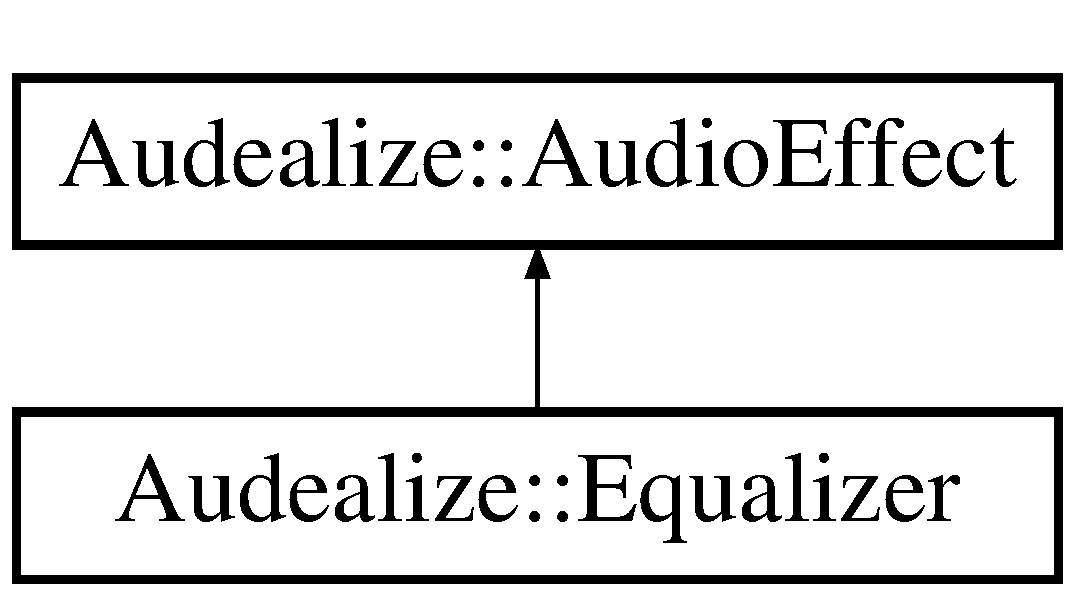
\includegraphics[height=2.000000cm]{class_audealize_1_1_equalizer}
\end{center}
\end{figure}
\subsection*{Public Member Functions}
\begin{DoxyCompactItemize}
\item 
\hyperlink{class_audealize_1_1_equalizer_a551e481ffa4ac763c51b3fefa8db5a9d}{Equalizer} (vector$<$ float $>$ freqs, float sample\+Rate)
\item 
float \hyperlink{class_audealize_1_1_equalizer_a71cadea6dfac69d667ecda5046177a00}{process\+Sample} (float sample, \hyperlink{tk_8h_a83f82f76e7fed06f4c49d2db94028a6d}{int} channel\+Idx)
\item 
\hyperlink{tk_8h_aba408b7cd755a96426e004c015f5de8e}{void} \hyperlink{class_audealize_1_1_equalizer_a782dd682924a6d5d00a16407d35851ff}{set\+Equalizer} (vector$<$ float $>$ freqs, vector$<$ float $>$ gains)
\item 
\hyperlink{tk_8h_aba408b7cd755a96426e004c015f5de8e}{void} \hyperlink{class_audealize_1_1_equalizer_a32f93b1dd52f8fd2ea4445f024b2ab3a}{set\+Freqs} (vector$<$ float $>$ freqs)
\item 
\hyperlink{tk_8h_aba408b7cd755a96426e004c015f5de8e}{void} \hyperlink{class_audealize_1_1_equalizer_ab7105904dc9dad6ab49a6bf9aec82d18}{set\+Gains} (vector$<$ float $>$ gains)
\item 
\hyperlink{tk_8h_aba408b7cd755a96426e004c015f5de8e}{void} \hyperlink{class_audealize_1_1_equalizer_a281c8f1e77ed51241bf0e5103c47c848}{set\+Band\+Gain} (\hyperlink{tk_8h_a83f82f76e7fed06f4c49d2db94028a6d}{int} band\+Idx, float gain\+DB)
\item 
\hyperlink{tk_8h_aba408b7cd755a96426e004c015f5de8e}{void} \hyperlink{class_audealize_1_1_equalizer_a28d3bc5a80540ea5d0c7eae9089643ed}{setQ} (float Q)
\item 
\hyperlink{tk_8h_aba408b7cd755a96426e004c015f5de8e}{void} \hyperlink{class_audealize_1_1_equalizer_a8206b7f21b22f9c9f223014ab754c1b3}{set\+Sample\+Rate} (float sample\+Rate)
\item 
float \hyperlink{class_audealize_1_1_equalizer_ac73ade538a329b9ba112549b6194712c}{get\+Band\+Freq} (\hyperlink{tk_8h_a83f82f76e7fed06f4c49d2db94028a6d}{int} band\+Idx)
\item 
float \hyperlink{class_audealize_1_1_equalizer_a9a33b0c95b6da66e88e64b13fa1f55fb}{get\+Band\+Gain} (\hyperlink{tk_8h_a83f82f76e7fed06f4c49d2db94028a6d}{int} band\+Idx)
\item 
float \hyperlink{class_audealize_1_1_equalizer_a7878230c60e603ed49c978f07a5f0f5f}{get\+Sample\+Rate} ()
\item 
float \hyperlink{class_audealize_1_1_equalizer_aecd4b2b16d30b774ba573a17fa50592f}{get\+Num\+Channels} ()
\end{DoxyCompactItemize}
\subsection*{Additional Inherited Members}


\subsection{Constructor \& Destructor Documentation}
\index{Audealize\+::\+Equalizer@{Audealize\+::\+Equalizer}!Equalizer@{Equalizer}}
\index{Equalizer@{Equalizer}!Audealize\+::\+Equalizer@{Audealize\+::\+Equalizer}}
\subsubsection[{\texorpdfstring{Equalizer(vector$<$ float $>$ freqs, float sample\+Rate)}{Equalizer(vector< float > freqs, float sampleRate)}}]{\setlength{\rightskip}{0pt plus 5cm}Audealize\+::\+Equalizer\+::\+Equalizer (
\begin{DoxyParamCaption}
\item[{vector$<$ float $>$}]{freqs, }
\item[{float}]{sample\+Rate}
\end{DoxyParamCaption}
)\hspace{0.3cm}{\ttfamily [inline]}}\hypertarget{class_audealize_1_1_equalizer_a551e481ffa4ac763c51b3fefa8db5a9d}{}\label{class_audealize_1_1_equalizer_a551e481ffa4ac763c51b3fefa8db5a9d}


\subsection{Member Function Documentation}
\index{Audealize\+::\+Equalizer@{Audealize\+::\+Equalizer}!get\+Band\+Freq@{get\+Band\+Freq}}
\index{get\+Band\+Freq@{get\+Band\+Freq}!Audealize\+::\+Equalizer@{Audealize\+::\+Equalizer}}
\subsubsection[{\texorpdfstring{get\+Band\+Freq(int band\+Idx)}{getBandFreq(int bandIdx)}}]{\setlength{\rightskip}{0pt plus 5cm}float Audealize\+::\+Equalizer\+::get\+Band\+Freq (
\begin{DoxyParamCaption}
\item[{{\bf int}}]{band\+Idx}
\end{DoxyParamCaption}
)\hspace{0.3cm}{\ttfamily [inline]}}\hypertarget{class_audealize_1_1_equalizer_ac73ade538a329b9ba112549b6194712c}{}\label{class_audealize_1_1_equalizer_ac73ade538a329b9ba112549b6194712c}
returns the center frequency of one of the filters in the bank given its index


\begin{DoxyParams}{Parameters}
{\em band\+Idx} & index of the filter\\
\hline
\end{DoxyParams}
\begin{DoxyReturn}{Returns}
the center frequency of the filter 
\end{DoxyReturn}
\index{Audealize\+::\+Equalizer@{Audealize\+::\+Equalizer}!get\+Band\+Gain@{get\+Band\+Gain}}
\index{get\+Band\+Gain@{get\+Band\+Gain}!Audealize\+::\+Equalizer@{Audealize\+::\+Equalizer}}
\subsubsection[{\texorpdfstring{get\+Band\+Gain(int band\+Idx)}{getBandGain(int bandIdx)}}]{\setlength{\rightskip}{0pt plus 5cm}float Audealize\+::\+Equalizer\+::get\+Band\+Gain (
\begin{DoxyParamCaption}
\item[{{\bf int}}]{band\+Idx}
\end{DoxyParamCaption}
)\hspace{0.3cm}{\ttfamily [inline]}}\hypertarget{class_audealize_1_1_equalizer_a9a33b0c95b6da66e88e64b13fa1f55fb}{}\label{class_audealize_1_1_equalizer_a9a33b0c95b6da66e88e64b13fa1f55fb}
returns the gain of one of the filters in the bank given its index


\begin{DoxyParams}{Parameters}
{\em band\+Idx} & -\/ index of the filter\\
\hline
\end{DoxyParams}
\begin{DoxyReturn}{Returns}
the gain of the filter 
\end{DoxyReturn}
\index{Audealize\+::\+Equalizer@{Audealize\+::\+Equalizer}!get\+Num\+Channels@{get\+Num\+Channels}}
\index{get\+Num\+Channels@{get\+Num\+Channels}!Audealize\+::\+Equalizer@{Audealize\+::\+Equalizer}}
\subsubsection[{\texorpdfstring{get\+Num\+Channels()}{getNumChannels()}}]{\setlength{\rightskip}{0pt plus 5cm}float Audealize\+::\+Equalizer\+::get\+Num\+Channels (
\begin{DoxyParamCaption}
{}
\end{DoxyParamCaption}
)\hspace{0.3cm}{\ttfamily [inline]}}\hypertarget{class_audealize_1_1_equalizer_aecd4b2b16d30b774ba573a17fa50592f}{}\label{class_audealize_1_1_equalizer_aecd4b2b16d30b774ba573a17fa50592f}
\index{Audealize\+::\+Equalizer@{Audealize\+::\+Equalizer}!get\+Sample\+Rate@{get\+Sample\+Rate}}
\index{get\+Sample\+Rate@{get\+Sample\+Rate}!Audealize\+::\+Equalizer@{Audealize\+::\+Equalizer}}
\subsubsection[{\texorpdfstring{get\+Sample\+Rate()}{getSampleRate()}}]{\setlength{\rightskip}{0pt plus 5cm}float Audealize\+::\+Equalizer\+::get\+Sample\+Rate (
\begin{DoxyParamCaption}
{}
\end{DoxyParamCaption}
)\hspace{0.3cm}{\ttfamily [inline]}}\hypertarget{class_audealize_1_1_equalizer_a7878230c60e603ed49c978f07a5f0f5f}{}\label{class_audealize_1_1_equalizer_a7878230c60e603ed49c978f07a5f0f5f}
\index{Audealize\+::\+Equalizer@{Audealize\+::\+Equalizer}!process\+Sample@{process\+Sample}}
\index{process\+Sample@{process\+Sample}!Audealize\+::\+Equalizer@{Audealize\+::\+Equalizer}}
\subsubsection[{\texorpdfstring{process\+Sample(float sample, int channel\+Idx)}{processSample(float sample, int channelIdx)}}]{\setlength{\rightskip}{0pt plus 5cm}float Audealize\+::\+Equalizer\+::process\+Sample (
\begin{DoxyParamCaption}
\item[{float}]{sample, }
\item[{{\bf int}}]{channel\+Idx}
\end{DoxyParamCaption}
)\hspace{0.3cm}{\ttfamily [inline]}, {\ttfamily [virtual]}}\hypertarget{class_audealize_1_1_equalizer_a71cadea6dfac69d667ecda5046177a00}{}\label{class_audealize_1_1_equalizer_a71cadea6dfac69d667ecda5046177a00}
Process a single sample of audio


\begin{DoxyParams}{Parameters}
{\em sample} & A float audio sample \\
\hline
{\em channel\+Idx} & Channel index \mbox{[}0, num channels)\\
\hline
\end{DoxyParams}
\begin{DoxyReturn}{Returns}
the filtered Sample 
\end{DoxyReturn}


Reimplemented from \hyperlink{class_audealize_1_1_audio_effect_ab77548a457702d189087163a696d4215}{Audealize\+::\+Audio\+Effect}.

\index{Audealize\+::\+Equalizer@{Audealize\+::\+Equalizer}!set\+Band\+Gain@{set\+Band\+Gain}}
\index{set\+Band\+Gain@{set\+Band\+Gain}!Audealize\+::\+Equalizer@{Audealize\+::\+Equalizer}}
\subsubsection[{\texorpdfstring{set\+Band\+Gain(int band\+Idx, float gain\+D\+B)}{setBandGain(int bandIdx, float gainDB)}}]{\setlength{\rightskip}{0pt plus 5cm}{\bf void} Audealize\+::\+Equalizer\+::set\+Band\+Gain (
\begin{DoxyParamCaption}
\item[{{\bf int}}]{band\+Idx, }
\item[{float}]{gain\+DB}
\end{DoxyParamCaption}
)\hspace{0.3cm}{\ttfamily [inline]}}\hypertarget{class_audealize_1_1_equalizer_a281c8f1e77ed51241bf0e5103c47c848}{}\label{class_audealize_1_1_equalizer_a281c8f1e77ed51241bf0e5103c47c848}
Sets the gain of an individual EQ band


\begin{DoxyParams}{Parameters}
{\em band\+Idx} & \hyperlink{struct_index}{Index} of band to be set \\
\hline
{\em gain\+DB} & Band gain in dB \\
\hline
\end{DoxyParams}
\index{Audealize\+::\+Equalizer@{Audealize\+::\+Equalizer}!set\+Equalizer@{set\+Equalizer}}
\index{set\+Equalizer@{set\+Equalizer}!Audealize\+::\+Equalizer@{Audealize\+::\+Equalizer}}
\subsubsection[{\texorpdfstring{set\+Equalizer(vector$<$ float $>$ freqs, vector$<$ float $>$ gains)}{setEqualizer(vector< float > freqs, vector< float > gains)}}]{\setlength{\rightskip}{0pt plus 5cm}{\bf void} Audealize\+::\+Equalizer\+::set\+Equalizer (
\begin{DoxyParamCaption}
\item[{vector$<$ float $>$}]{freqs, }
\item[{vector$<$ float $>$}]{gains}
\end{DoxyParamCaption}
)\hspace{0.3cm}{\ttfamily [inline]}}\hypertarget{class_audealize_1_1_equalizer_a782dd682924a6d5d00a16407d35851ff}{}\label{class_audealize_1_1_equalizer_a782dd682924a6d5d00a16407d35851ff}
Sets the frequencies and gains of the eq bands


\begin{DoxyParams}{Parameters}
{\em freqs} & Vector of floats containing band frequencies \\
\hline
{\em gains} & Vector of floats containing band gains \\
\hline
\end{DoxyParams}
\index{Audealize\+::\+Equalizer@{Audealize\+::\+Equalizer}!set\+Freqs@{set\+Freqs}}
\index{set\+Freqs@{set\+Freqs}!Audealize\+::\+Equalizer@{Audealize\+::\+Equalizer}}
\subsubsection[{\texorpdfstring{set\+Freqs(vector$<$ float $>$ freqs)}{setFreqs(vector< float > freqs)}}]{\setlength{\rightskip}{0pt plus 5cm}{\bf void} Audealize\+::\+Equalizer\+::set\+Freqs (
\begin{DoxyParamCaption}
\item[{vector$<$ float $>$}]{freqs}
\end{DoxyParamCaption}
)\hspace{0.3cm}{\ttfamily [inline]}}\hypertarget{class_audealize_1_1_equalizer_a32f93b1dd52f8fd2ea4445f024b2ab3a}{}\label{class_audealize_1_1_equalizer_a32f93b1dd52f8fd2ea4445f024b2ab3a}
Sets the frequencies of the EQ bands


\begin{DoxyParams}{Parameters}
{\em freqs} & Vector of floats containing the new eq band frequencies \\
\hline
\end{DoxyParams}
\index{Audealize\+::\+Equalizer@{Audealize\+::\+Equalizer}!set\+Gains@{set\+Gains}}
\index{set\+Gains@{set\+Gains}!Audealize\+::\+Equalizer@{Audealize\+::\+Equalizer}}
\subsubsection[{\texorpdfstring{set\+Gains(vector$<$ float $>$ gains)}{setGains(vector< float > gains)}}]{\setlength{\rightskip}{0pt plus 5cm}{\bf void} Audealize\+::\+Equalizer\+::set\+Gains (
\begin{DoxyParamCaption}
\item[{vector$<$ float $>$}]{gains}
\end{DoxyParamCaption}
)\hspace{0.3cm}{\ttfamily [inline]}}\hypertarget{class_audealize_1_1_equalizer_ab7105904dc9dad6ab49a6bf9aec82d18}{}\label{class_audealize_1_1_equalizer_ab7105904dc9dad6ab49a6bf9aec82d18}
Sets the gains of the EQ bands


\begin{DoxyParams}{Parameters}
{\em gains} & Vector of floats containing band gains in dB \\
\hline
\end{DoxyParams}
\index{Audealize\+::\+Equalizer@{Audealize\+::\+Equalizer}!setQ@{setQ}}
\index{setQ@{setQ}!Audealize\+::\+Equalizer@{Audealize\+::\+Equalizer}}
\subsubsection[{\texorpdfstring{set\+Q(float Q)}{setQ(float Q)}}]{\setlength{\rightskip}{0pt plus 5cm}{\bf void} Audealize\+::\+Equalizer\+::setQ (
\begin{DoxyParamCaption}
\item[{float}]{Q}
\end{DoxyParamCaption}
)\hspace{0.3cm}{\ttfamily [inline]}}\hypertarget{class_audealize_1_1_equalizer_a28d3bc5a80540ea5d0c7eae9089643ed}{}\label{class_audealize_1_1_equalizer_a28d3bc5a80540ea5d0c7eae9089643ed}
Sets the Q values of the filters


\begin{DoxyParams}{Parameters}
{\em Q} & value \\
\hline
\end{DoxyParams}
\index{Audealize\+::\+Equalizer@{Audealize\+::\+Equalizer}!set\+Sample\+Rate@{set\+Sample\+Rate}}
\index{set\+Sample\+Rate@{set\+Sample\+Rate}!Audealize\+::\+Equalizer@{Audealize\+::\+Equalizer}}
\subsubsection[{\texorpdfstring{set\+Sample\+Rate(float sample\+Rate)}{setSampleRate(float sampleRate)}}]{\setlength{\rightskip}{0pt plus 5cm}{\bf void} Audealize\+::\+Equalizer\+::set\+Sample\+Rate (
\begin{DoxyParamCaption}
\item[{float}]{sample\+Rate}
\end{DoxyParamCaption}
)\hspace{0.3cm}{\ttfamily [inline]}, {\ttfamily [virtual]}}\hypertarget{class_audealize_1_1_equalizer_a8206b7f21b22f9c9f223014ab754c1b3}{}\label{class_audealize_1_1_equalizer_a8206b7f21b22f9c9f223014ab754c1b3}
Sets the sample rate of the filters


\begin{DoxyParams}{Parameters}
{\em sample\+Rate} & Sample Rate \\
\hline
\end{DoxyParams}


Reimplemented from \hyperlink{class_audealize_1_1_audio_effect_a5ff34c0371f2311dc026bca5ba245faa}{Audealize\+::\+Audio\+Effect}.



The documentation for this class was generated from the following file\+:\begin{DoxyCompactItemize}
\item 
/\+Users/michael/\+J\+U\+C\+E/projects/audealize-\/plugin/\+J\+U\+C\+E Modules/audealize\+\_\+module/effects/\hyperlink{_equalizer_8h}{Equalizer.\+h}\end{DoxyCompactItemize}

\hypertarget{classdsp_1_1fixed__size__buffer}{}\section{dsp\+:\+:fixed\+\_\+size\+\_\+buffer$<$ N, T $>$ Class Template Reference}
\label{classdsp_1_1fixed__size__buffer}\index{dsp\+::fixed\+\_\+size\+\_\+buffer$<$ N, T $>$@{dsp\+::fixed\+\_\+size\+\_\+buffer$<$ N, T $>$}}


{\ttfamily \#include $<$buffer.\+h$>$}

Inheritance diagram for dsp\+:\+:fixed\+\_\+size\+\_\+buffer$<$ N, T $>$\+:\begin{figure}[H]
\begin{center}
\leavevmode
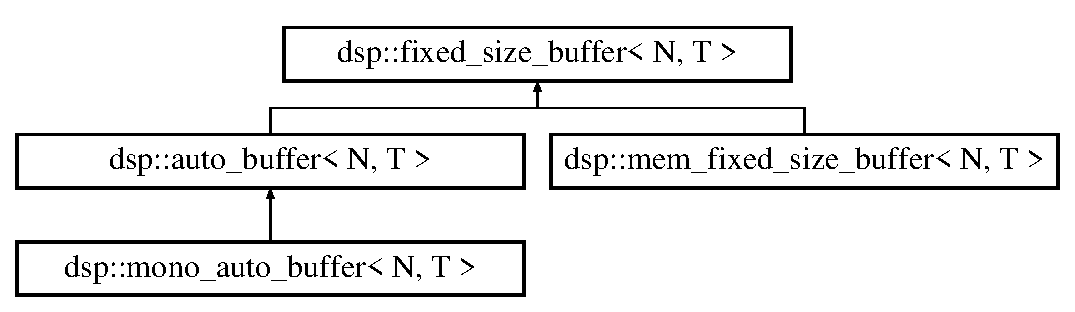
\includegraphics[height=3.000000cm]{classdsp_1_1fixed__size__buffer}
\end{center}
\end{figure}
\subsection*{Public Types}
\begin{DoxyCompactItemize}
\item 
enum \{ \hyperlink{classdsp_1_1fixed__size__buffer_a200b23db4a04ad08b4a70a92c968b926adac6e851d4004a6f36b7047c2e026ca7}{buffer\+\_\+size} = N
 \}
\item 
typedef T \hyperlink{classdsp_1_1fixed__size__buffer_af51fc2bdaf146ea493c21079f8c7f491}{data\+\_\+type}
\end{DoxyCompactItemize}
\subsection*{Public Member Functions}
\begin{DoxyCompactItemize}
\item 
\hyperlink{tk_8h_a83f82f76e7fed06f4c49d2db94028a6d}{int} \hyperlink{classdsp_1_1fixed__size__buffer_ab06273b70b7382769e58f6ff6c998808}{size} ()
\end{DoxyCompactItemize}


\subsection{Member Typedef Documentation}
\index{dsp\+::fixed\+\_\+size\+\_\+buffer@{dsp\+::fixed\+\_\+size\+\_\+buffer}!data\+\_\+type@{data\+\_\+type}}
\index{data\+\_\+type@{data\+\_\+type}!dsp\+::fixed\+\_\+size\+\_\+buffer@{dsp\+::fixed\+\_\+size\+\_\+buffer}}
\subsubsection[{\texorpdfstring{data\+\_\+type}{data_type}}]{\setlength{\rightskip}{0pt plus 5cm}template$<$int N, class T = float$>$ typedef T {\bf dsp\+::fixed\+\_\+size\+\_\+buffer}$<$ N, T $>$\+::{\bf data\+\_\+type}}\hypertarget{classdsp_1_1fixed__size__buffer_af51fc2bdaf146ea493c21079f8c7f491}{}\label{classdsp_1_1fixed__size__buffer_af51fc2bdaf146ea493c21079f8c7f491}


\subsection{Member Enumeration Documentation}
\subsubsection[{\texorpdfstring{anonymous enum}{anonymous enum}}]{\setlength{\rightskip}{0pt plus 5cm}template$<$int N, class T = float$>$ anonymous enum}\hypertarget{classdsp_1_1fixed__size__buffer_a200b23db4a04ad08b4a70a92c968b926}{}\label{classdsp_1_1fixed__size__buffer_a200b23db4a04ad08b4a70a92c968b926}
\begin{Desc}
\item[Enumerator]\par
\begin{description}
\index{buffer\+\_\+size@{buffer\+\_\+size}!dsp\+::fixed\+\_\+size\+\_\+buffer@{dsp\+::fixed\+\_\+size\+\_\+buffer}}\index{dsp\+::fixed\+\_\+size\+\_\+buffer@{dsp\+::fixed\+\_\+size\+\_\+buffer}!buffer\+\_\+size@{buffer\+\_\+size}}\item[{\em 
buffer\+\_\+size\hypertarget{classdsp_1_1fixed__size__buffer_a200b23db4a04ad08b4a70a92c968b926adac6e851d4004a6f36b7047c2e026ca7}{}\label{classdsp_1_1fixed__size__buffer_a200b23db4a04ad08b4a70a92c968b926adac6e851d4004a6f36b7047c2e026ca7}
}]\end{description}
\end{Desc}


\subsection{Member Function Documentation}
\index{dsp\+::fixed\+\_\+size\+\_\+buffer@{dsp\+::fixed\+\_\+size\+\_\+buffer}!size@{size}}
\index{size@{size}!dsp\+::fixed\+\_\+size\+\_\+buffer@{dsp\+::fixed\+\_\+size\+\_\+buffer}}
\subsubsection[{\texorpdfstring{size()}{size()}}]{\setlength{\rightskip}{0pt plus 5cm}template$<$int N, class T = float$>$ {\bf int} {\bf dsp\+::fixed\+\_\+size\+\_\+buffer}$<$ N, T $>$\+::size (
\begin{DoxyParamCaption}
{}
\end{DoxyParamCaption}
)\hspace{0.3cm}{\ttfamily [inline]}}\hypertarget{classdsp_1_1fixed__size__buffer_ab06273b70b7382769e58f6ff6c998808}{}\label{classdsp_1_1fixed__size__buffer_ab06273b70b7382769e58f6ff6c998808}


The documentation for this class was generated from the following file\+:\begin{DoxyCompactItemize}
\item 
/\+Users/michael/\+J\+U\+C\+E/projects/audealize-\/plugin/\+J\+U\+C\+E Modules/audealize\+\_\+module/utils/calf\+\_\+dsp\+\_\+library/\hyperlink{buffer_8h}{buffer.\+h}\end{DoxyCompactItemize}

\hypertarget{structflist}{}\section{flist Struct Reference}
\label{structflist}\index{flist@{flist}}


{\ttfamily \#include $<$wngrind.\+h$>$}

\subsection*{Public Attributes}
\begin{DoxyCompactItemize}
\item 
char $\ast$ \hyperlink{structflist_aca7b1dc3ad7664a865180232c249d879}{fname}
\item 
\hyperlink{tk_8h_a83f82f76e7fed06f4c49d2db94028a6d}{int} \hyperlink{structflist_a57f4fa00c5ad209ba0cc464a358abeaa}{present}
\end{DoxyCompactItemize}


\subsection{Member Data Documentation}
\index{flist@{flist}!fname@{fname}}
\index{fname@{fname}!flist@{flist}}
\subsubsection[{\texorpdfstring{fname}{fname}}]{\setlength{\rightskip}{0pt plus 5cm}char$\ast$ flist\+::fname}\hypertarget{structflist_aca7b1dc3ad7664a865180232c249d879}{}\label{structflist_aca7b1dc3ad7664a865180232c249d879}
\index{flist@{flist}!present@{present}}
\index{present@{present}!flist@{flist}}
\subsubsection[{\texorpdfstring{present}{present}}]{\setlength{\rightskip}{0pt plus 5cm}{\bf int} flist\+::present}\hypertarget{structflist_a57f4fa00c5ad209ba0cc464a358abeaa}{}\label{structflist_a57f4fa00c5ad209ba0cc464a358abeaa}


The documentation for this struct was generated from the following file\+:\begin{DoxyCompactItemize}
\item 
/\+Users/michael/\+J\+U\+C\+E/projects/audealize-\/plugin/\+J\+U\+C\+E Modules/audealize\+\_\+module/\+Word\+Net-\/3.\+0/include/\hyperlink{wngrind_8h}{wngrind.\+h}\end{DoxyCompactItemize}

\hypertarget{structframelist}{}\section{framelist Struct Reference}
\label{structframelist}\index{framelist@{framelist}}


{\ttfamily \#include $<$wngrind.\+h$>$}

\subsection*{Public Attributes}
\begin{DoxyCompactItemize}
\item 
struct \hyperlink{structframelist}{framelist} $\ast$ \hyperlink{structframelist_ab7604ebc526bd9fa0bdf4acc3cca9ae3}{fnext}
\item 
unsigned long \hyperlink{structframelist_a18ec28e2cbeaac6f6e2529ea25ced4fd}{frames} \mbox{[}(\hyperlink{wn_8h_a4b6b859e1e3f6021a360390be287ca2c}{N\+U\+M\+F\+R\+A\+M\+ES}/32)+1\mbox{]}
\item 
unsigned char \hyperlink{structframelist_af71c96731b860d8287e90f11cae1787b}{frwdnum}
\end{DoxyCompactItemize}


\subsection{Member Data Documentation}
\index{framelist@{framelist}!fnext@{fnext}}
\index{fnext@{fnext}!framelist@{framelist}}
\subsubsection[{\texorpdfstring{fnext}{fnext}}]{\setlength{\rightskip}{0pt plus 5cm}struct {\bf framelist}$\ast$ framelist\+::fnext}\hypertarget{structframelist_ab7604ebc526bd9fa0bdf4acc3cca9ae3}{}\label{structframelist_ab7604ebc526bd9fa0bdf4acc3cca9ae3}
\index{framelist@{framelist}!frames@{frames}}
\index{frames@{frames}!framelist@{framelist}}
\subsubsection[{\texorpdfstring{frames}{frames}}]{\setlength{\rightskip}{0pt plus 5cm}unsigned long framelist\+::frames\mbox{[}({\bf N\+U\+M\+F\+R\+A\+M\+ES}/32)+1\mbox{]}}\hypertarget{structframelist_a18ec28e2cbeaac6f6e2529ea25ced4fd}{}\label{structframelist_a18ec28e2cbeaac6f6e2529ea25ced4fd}
\index{framelist@{framelist}!frwdnum@{frwdnum}}
\index{frwdnum@{frwdnum}!framelist@{framelist}}
\subsubsection[{\texorpdfstring{frwdnum}{frwdnum}}]{\setlength{\rightskip}{0pt plus 5cm}unsigned char framelist\+::frwdnum}\hypertarget{structframelist_af71c96731b860d8287e90f11cae1787b}{}\label{structframelist_af71c96731b860d8287e90f11cae1787b}


The documentation for this struct was generated from the following file\+:\begin{DoxyCompactItemize}
\item 
/\+Users/michael/\+J\+U\+C\+E/projects/audealize-\/plugin/\+J\+U\+C\+E Modules/audealize\+\_\+module/\+Word\+Net-\/3.\+0/include/\hyperlink{wngrind_8h}{wngrind.\+h}\end{DoxyCompactItemize}

\hypertarget{class_audealize_1_1_graphic_e_q_component}{}\section{Audealize\+:\+:Graphic\+E\+Q\+Component Class Reference}
\label{class_audealize_1_1_graphic_e_q_component}\index{Audealize\+::\+Graphic\+E\+Q\+Component@{Audealize\+::\+Graphic\+E\+Q\+Component}}


{\ttfamily \#include $<$Graphic\+E\+Q\+Component.\+h$>$}

Inheritance diagram for Audealize\+:\+:Graphic\+E\+Q\+Component\+:\begin{figure}[H]
\begin{center}
\leavevmode
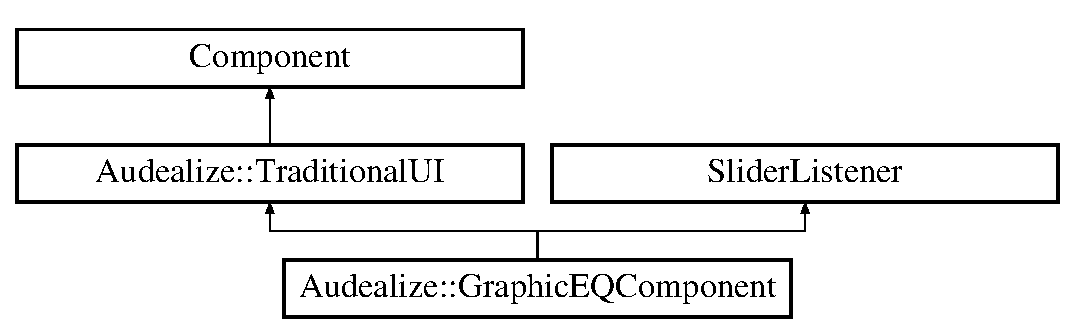
\includegraphics[height=3.000000cm]{class_audealize_1_1_graphic_e_q_component}
\end{center}
\end{figure}
\subsection*{Public Types}
\begin{DoxyCompactItemize}
\item 
enum \hyperlink{class_audealize_1_1_graphic_e_q_component_a08b168efce2d6a649d317828325c2560}{Colour\+Ids} \{ \hyperlink{class_audealize_1_1_graphic_e_q_component_a08b168efce2d6a649d317828325c2560a19c6e5f5d03b6ac92e3eb1a9af3f6070}{tick\+Mark\+Colour\+Id} = 0x2000500
 \}
\end{DoxyCompactItemize}
\subsection*{Public Member Functions}
\begin{DoxyCompactItemize}
\item 
\hyperlink{class_audealize_1_1_graphic_e_q_component_ab690c00e0781736ace023674f37b3c54}{Graphic\+E\+Q\+Component} (\hyperlink{class_audealize_1_1_audealize_audio_processor}{Audealize\+Audio\+Processor} \&p, \hyperlink{tk_8h_a83f82f76e7fed06f4c49d2db94028a6d}{int} num\+Bands, Normalisable\+Range$<$ float $>$ gain\+Range)
\item 
\hyperlink{class_audealize_1_1_graphic_e_q_component_ad7f4ce7f4997722a486d67c3004d06ff}{$\sim$\+Graphic\+E\+Q\+Component} ()
\item 
\hyperlink{tk_8h_aba408b7cd755a96426e004c015f5de8e}{void} \hyperlink{class_audealize_1_1_graphic_e_q_component_aeaf0f48b8d94f1cdf56054f86f3b8ce9}{paint} (Graphics \&g) override
\item 
\hyperlink{tk_8h_aba408b7cd755a96426e004c015f5de8e}{void} \hyperlink{class_audealize_1_1_graphic_e_q_component_ab0348fd0be5be5c8eddeef17af65cd9a}{resized} () override
\item 
\hyperlink{tk_8h_aba408b7cd755a96426e004c015f5de8e}{void} \hyperlink{class_audealize_1_1_graphic_e_q_component_a8ba560fc23f1bb04d4f1ac8fe76bb49d}{slider\+Value\+Changed} (Slider $\ast$slider) override
\item 
\hyperlink{tk_8h_aba408b7cd755a96426e004c015f5de8e}{void} \hyperlink{class_audealize_1_1_graphic_e_q_component_a70d9867ba976483e0890c84ae6dd9d22}{slider\+Drag\+Started} (Slider $\ast$slider) override
\item 
\hyperlink{tk_8h_aba408b7cd755a96426e004c015f5de8e}{void} \hyperlink{class_audealize_1_1_graphic_e_q_component_a8ee6528363295d20b538bfa57f9d09e4}{slider\+Drag\+Ended} (Slider $\ast$slider) override
\end{DoxyCompactItemize}
\subsection*{Additional Inherited Members}


\subsection{Member Enumeration Documentation}
\index{Audealize\+::\+Graphic\+E\+Q\+Component@{Audealize\+::\+Graphic\+E\+Q\+Component}!Colour\+Ids@{Colour\+Ids}}
\index{Colour\+Ids@{Colour\+Ids}!Audealize\+::\+Graphic\+E\+Q\+Component@{Audealize\+::\+Graphic\+E\+Q\+Component}}
\subsubsection[{\texorpdfstring{Colour\+Ids}{ColourIds}}]{\setlength{\rightskip}{0pt plus 5cm}enum {\bf Audealize\+::\+Graphic\+E\+Q\+Component\+::\+Colour\+Ids}}\hypertarget{class_audealize_1_1_graphic_e_q_component_a08b168efce2d6a649d317828325c2560}{}\label{class_audealize_1_1_graphic_e_q_component_a08b168efce2d6a649d317828325c2560}
\begin{Desc}
\item[Enumerator]\par
\begin{description}
\index{tick\+Mark\+Colour\+Id@{tick\+Mark\+Colour\+Id}!Audealize\+::\+Graphic\+E\+Q\+Component@{Audealize\+::\+Graphic\+E\+Q\+Component}}\index{Audealize\+::\+Graphic\+E\+Q\+Component@{Audealize\+::\+Graphic\+E\+Q\+Component}!tick\+Mark\+Colour\+Id@{tick\+Mark\+Colour\+Id}}\item[{\em 
tick\+Mark\+Colour\+Id\hypertarget{class_audealize_1_1_graphic_e_q_component_a08b168efce2d6a649d317828325c2560a19c6e5f5d03b6ac92e3eb1a9af3f6070}{}\label{class_audealize_1_1_graphic_e_q_component_a08b168efce2d6a649d317828325c2560a19c6e5f5d03b6ac92e3eb1a9af3f6070}
}]\end{description}
\end{Desc}


\subsection{Constructor \& Destructor Documentation}
\index{Audealize\+::\+Graphic\+E\+Q\+Component@{Audealize\+::\+Graphic\+E\+Q\+Component}!Graphic\+E\+Q\+Component@{Graphic\+E\+Q\+Component}}
\index{Graphic\+E\+Q\+Component@{Graphic\+E\+Q\+Component}!Audealize\+::\+Graphic\+E\+Q\+Component@{Audealize\+::\+Graphic\+E\+Q\+Component}}
\subsubsection[{\texorpdfstring{Graphic\+E\+Q\+Component(\+Audealize\+Audio\+Processor \&p, int num\+Bands, Normalisable\+Range$<$ float $>$ gain\+Range)}{GraphicEQComponent(AudealizeAudioProcessor &p, int numBands, NormalisableRange< float > gainRange)}}]{\setlength{\rightskip}{0pt plus 5cm}Audealize\+::\+Graphic\+E\+Q\+Component\+::\+Graphic\+E\+Q\+Component (
\begin{DoxyParamCaption}
\item[{{\bf Audealize\+Audio\+Processor} \&}]{p, }
\item[{{\bf int}}]{num\+Bands, }
\item[{Normalisable\+Range$<$ float $>$}]{gain\+Range}
\end{DoxyParamCaption}
)}\hypertarget{class_audealize_1_1_graphic_e_q_component_ab690c00e0781736ace023674f37b3c54}{}\label{class_audealize_1_1_graphic_e_q_component_ab690c00e0781736ace023674f37b3c54}
\index{Audealize\+::\+Graphic\+E\+Q\+Component@{Audealize\+::\+Graphic\+E\+Q\+Component}!````~Graphic\+E\+Q\+Component@{$\sim$\+Graphic\+E\+Q\+Component}}
\index{````~Graphic\+E\+Q\+Component@{$\sim$\+Graphic\+E\+Q\+Component}!Audealize\+::\+Graphic\+E\+Q\+Component@{Audealize\+::\+Graphic\+E\+Q\+Component}}
\subsubsection[{\texorpdfstring{$\sim$\+Graphic\+E\+Q\+Component()}{~GraphicEQComponent()}}]{\setlength{\rightskip}{0pt plus 5cm}Audealize\+::\+Graphic\+E\+Q\+Component\+::$\sim$\+Graphic\+E\+Q\+Component (
\begin{DoxyParamCaption}
{}
\end{DoxyParamCaption}
)}\hypertarget{class_audealize_1_1_graphic_e_q_component_ad7f4ce7f4997722a486d67c3004d06ff}{}\label{class_audealize_1_1_graphic_e_q_component_ad7f4ce7f4997722a486d67c3004d06ff}


\subsection{Member Function Documentation}
\index{Audealize\+::\+Graphic\+E\+Q\+Component@{Audealize\+::\+Graphic\+E\+Q\+Component}!paint@{paint}}
\index{paint@{paint}!Audealize\+::\+Graphic\+E\+Q\+Component@{Audealize\+::\+Graphic\+E\+Q\+Component}}
\subsubsection[{\texorpdfstring{paint(\+Graphics \&g) override}{paint(Graphics &g) override}}]{\setlength{\rightskip}{0pt plus 5cm}{\bf void} Audealize\+::\+Graphic\+E\+Q\+Component\+::paint (
\begin{DoxyParamCaption}
\item[{Graphics \&}]{g}
\end{DoxyParamCaption}
)\hspace{0.3cm}{\ttfamily [override]}}\hypertarget{class_audealize_1_1_graphic_e_q_component_aeaf0f48b8d94f1cdf56054f86f3b8ce9}{}\label{class_audealize_1_1_graphic_e_q_component_aeaf0f48b8d94f1cdf56054f86f3b8ce9}
\index{Audealize\+::\+Graphic\+E\+Q\+Component@{Audealize\+::\+Graphic\+E\+Q\+Component}!resized@{resized}}
\index{resized@{resized}!Audealize\+::\+Graphic\+E\+Q\+Component@{Audealize\+::\+Graphic\+E\+Q\+Component}}
\subsubsection[{\texorpdfstring{resized() override}{resized() override}}]{\setlength{\rightskip}{0pt plus 5cm}{\bf void} Audealize\+::\+Graphic\+E\+Q\+Component\+::resized (
\begin{DoxyParamCaption}
{}
\end{DoxyParamCaption}
)\hspace{0.3cm}{\ttfamily [override]}}\hypertarget{class_audealize_1_1_graphic_e_q_component_ab0348fd0be5be5c8eddeef17af65cd9a}{}\label{class_audealize_1_1_graphic_e_q_component_ab0348fd0be5be5c8eddeef17af65cd9a}
\index{Audealize\+::\+Graphic\+E\+Q\+Component@{Audealize\+::\+Graphic\+E\+Q\+Component}!slider\+Drag\+Ended@{slider\+Drag\+Ended}}
\index{slider\+Drag\+Ended@{slider\+Drag\+Ended}!Audealize\+::\+Graphic\+E\+Q\+Component@{Audealize\+::\+Graphic\+E\+Q\+Component}}
\subsubsection[{\texorpdfstring{slider\+Drag\+Ended(\+Slider $\ast$slider) override}{sliderDragEnded(Slider *slider) override}}]{\setlength{\rightskip}{0pt plus 5cm}{\bf void} Audealize\+::\+Graphic\+E\+Q\+Component\+::slider\+Drag\+Ended (
\begin{DoxyParamCaption}
\item[{Slider $\ast$}]{slider}
\end{DoxyParamCaption}
)\hspace{0.3cm}{\ttfamily [inline]}, {\ttfamily [override]}}\hypertarget{class_audealize_1_1_graphic_e_q_component_a8ee6528363295d20b538bfa57f9d09e4}{}\label{class_audealize_1_1_graphic_e_q_component_a8ee6528363295d20b538bfa57f9d09e4}
\index{Audealize\+::\+Graphic\+E\+Q\+Component@{Audealize\+::\+Graphic\+E\+Q\+Component}!slider\+Drag\+Started@{slider\+Drag\+Started}}
\index{slider\+Drag\+Started@{slider\+Drag\+Started}!Audealize\+::\+Graphic\+E\+Q\+Component@{Audealize\+::\+Graphic\+E\+Q\+Component}}
\subsubsection[{\texorpdfstring{slider\+Drag\+Started(\+Slider $\ast$slider) override}{sliderDragStarted(Slider *slider) override}}]{\setlength{\rightskip}{0pt plus 5cm}{\bf void} Audealize\+::\+Graphic\+E\+Q\+Component\+::slider\+Drag\+Started (
\begin{DoxyParamCaption}
\item[{Slider $\ast$}]{slider}
\end{DoxyParamCaption}
)\hspace{0.3cm}{\ttfamily [inline]}, {\ttfamily [override]}}\hypertarget{class_audealize_1_1_graphic_e_q_component_a70d9867ba976483e0890c84ae6dd9d22}{}\label{class_audealize_1_1_graphic_e_q_component_a70d9867ba976483e0890c84ae6dd9d22}
\index{Audealize\+::\+Graphic\+E\+Q\+Component@{Audealize\+::\+Graphic\+E\+Q\+Component}!slider\+Value\+Changed@{slider\+Value\+Changed}}
\index{slider\+Value\+Changed@{slider\+Value\+Changed}!Audealize\+::\+Graphic\+E\+Q\+Component@{Audealize\+::\+Graphic\+E\+Q\+Component}}
\subsubsection[{\texorpdfstring{slider\+Value\+Changed(\+Slider $\ast$slider) override}{sliderValueChanged(Slider *slider) override}}]{\setlength{\rightskip}{0pt plus 5cm}{\bf void} Audealize\+::\+Graphic\+E\+Q\+Component\+::slider\+Value\+Changed (
\begin{DoxyParamCaption}
\item[{Slider $\ast$}]{slider}
\end{DoxyParamCaption}
)\hspace{0.3cm}{\ttfamily [override]}}\hypertarget{class_audealize_1_1_graphic_e_q_component_a8ba560fc23f1bb04d4f1ac8fe76bb49d}{}\label{class_audealize_1_1_graphic_e_q_component_a8ba560fc23f1bb04d4f1ac8fe76bb49d}


The documentation for this class was generated from the following files\+:\begin{DoxyCompactItemize}
\item 
/\+Users/michael/\+J\+U\+C\+E/projects/audealize-\/plugin/\+J\+U\+C\+E Modules/audealize\+\_\+module/ui\+\_\+components/\hyperlink{_graphic_e_q_component_8h}{Graphic\+E\+Q\+Component.\+h}\item 
/\+Users/michael/\+J\+U\+C\+E/projects/audealize-\/plugin/\+J\+U\+C\+E Modules/audealize\+\_\+module/ui\+\_\+components/\hyperlink{_graphic_e_q_component_8cpp}{Graphic\+E\+Q\+Component.\+cpp}\end{DoxyCompactItemize}

\hypertarget{structstd_1_1hash_3_01nlohmann_1_1json_01_4}{}\section{std\+:\+:hash$<$ nlohmann\+:\+:json $>$ Struct Template Reference}
\label{structstd_1_1hash_3_01nlohmann_1_1json_01_4}\index{std\+::hash$<$ nlohmann\+::json $>$@{std\+::hash$<$ nlohmann\+::json $>$}}


hash value for J\+S\+ON objects  




{\ttfamily \#include $<$json.\+hpp$>$}

\subsection*{Public Member Functions}
\begin{DoxyCompactItemize}
\item 
std\+::size\+\_\+t \hyperlink{structstd_1_1hash_3_01nlohmann_1_1json_01_4_afd03f6ad53db22868ca4163a8200b2f9}{operator()} (const \hyperlink{namespacenlohmann_a2bfd99e845a2e5cd90aeaf1b1431f474}{nlohmann\+::json} \&j) const 
\begin{DoxyCompactList}\small\item\em return a hash value for a J\+S\+ON object \end{DoxyCompactList}\end{DoxyCompactItemize}


\subsection{Detailed Description}
\subsubsection*{template$<$$>$\\*
struct std\+::hash$<$ nlohmann\+::json $>$}

hash value for J\+S\+ON objects 

\subsection{Member Function Documentation}
\index{std\+::hash$<$ nlohmann\+::json $>$@{std\+::hash$<$ nlohmann\+::json $>$}!operator()@{operator()}}
\index{operator()@{operator()}!std\+::hash$<$ nlohmann\+::json $>$@{std\+::hash$<$ nlohmann\+::json $>$}}
\subsubsection[{\texorpdfstring{operator()(const nlohmann\+::json \&j) const }{operator()(const nlohmann::json &j) const }}]{\setlength{\rightskip}{0pt plus 5cm}std\+::size\+\_\+t {\bf std\+::hash}$<$ {\bf nlohmann\+::json} $>$\+::operator() (
\begin{DoxyParamCaption}
\item[{const {\bf nlohmann\+::json} \&}]{j}
\end{DoxyParamCaption}
) const\hspace{0.3cm}{\ttfamily [inline]}}\hypertarget{structstd_1_1hash_3_01nlohmann_1_1json_01_4_afd03f6ad53db22868ca4163a8200b2f9}{}\label{structstd_1_1hash_3_01nlohmann_1_1json_01_4_afd03f6ad53db22868ca4163a8200b2f9}


return a hash value for a J\+S\+ON object 

\begin{DoxySince}{Since}
version 1.\+0.\+0 
\end{DoxySince}


The documentation for this struct was generated from the following file\+:\begin{DoxyCompactItemize}
\item 
/\+Users/michael/\+J\+U\+C\+E/projects/audealize-\/plugin/\+J\+U\+C\+E Modules/audealize\+\_\+module/utils/\hyperlink{json_8hpp}{json.\+hpp}\end{DoxyCompactItemize}

\hypertarget{struct_index}{}\section{Index Struct Reference}
\label{struct_index}\index{Index@{Index}}


{\ttfamily \#include $<$wn.\+h$>$}

\subsection*{Public Attributes}
\begin{DoxyCompactItemize}
\item 
long \hyperlink{struct_index_aa58b6c13e494b8b076a576f4218b54b8}{idxoffset}
\item 
char $\ast$ \hyperlink{struct_index_ac836b68129dd28ed751e34b28701f6d2}{wd}
\item 
char $\ast$ \hyperlink{struct_index_ac14f4a78de133597a538b4c5a653171f}{pos}
\item 
\hyperlink{tk_8h_a83f82f76e7fed06f4c49d2db94028a6d}{int} \hyperlink{struct_index_a5b08ae094c1311cf18490673ab27721c}{sense\+\_\+cnt}
\item 
\hyperlink{tk_8h_a83f82f76e7fed06f4c49d2db94028a6d}{int} \hyperlink{struct_index_af0f57fedd585897131dc29950dd6c84d}{off\+\_\+cnt}
\item 
\hyperlink{tk_8h_a83f82f76e7fed06f4c49d2db94028a6d}{int} \hyperlink{struct_index_ad039685d966a205dfedc4de92469621c}{tagged\+\_\+cnt}
\item 
unsigned long $\ast$ \hyperlink{struct_index_a6f12f7b36fe11a906efd16d5e85fca42}{offset}
\item 
\hyperlink{tk_8h_a83f82f76e7fed06f4c49d2db94028a6d}{int} \hyperlink{struct_index_a37820a4bcfd41466390618e3b685416c}{ptruse\+\_\+cnt}
\item 
\hyperlink{tk_8h_a83f82f76e7fed06f4c49d2db94028a6d}{int} $\ast$ \hyperlink{struct_index_ae3a68cdff947c09c59fdbe09c8fa3cd5}{ptruse}
\end{DoxyCompactItemize}


\subsection{Member Data Documentation}
\index{Index@{Index}!idxoffset@{idxoffset}}
\index{idxoffset@{idxoffset}!Index@{Index}}
\subsubsection[{\texorpdfstring{idxoffset}{idxoffset}}]{\setlength{\rightskip}{0pt plus 5cm}long Index\+::idxoffset}\hypertarget{struct_index_aa58b6c13e494b8b076a576f4218b54b8}{}\label{struct_index_aa58b6c13e494b8b076a576f4218b54b8}
\index{Index@{Index}!off\+\_\+cnt@{off\+\_\+cnt}}
\index{off\+\_\+cnt@{off\+\_\+cnt}!Index@{Index}}
\subsubsection[{\texorpdfstring{off\+\_\+cnt}{off_cnt}}]{\setlength{\rightskip}{0pt plus 5cm}{\bf int} Index\+::off\+\_\+cnt}\hypertarget{struct_index_af0f57fedd585897131dc29950dd6c84d}{}\label{struct_index_af0f57fedd585897131dc29950dd6c84d}
\index{Index@{Index}!offset@{offset}}
\index{offset@{offset}!Index@{Index}}
\subsubsection[{\texorpdfstring{offset}{offset}}]{\setlength{\rightskip}{0pt plus 5cm}unsigned long$\ast$ Index\+::offset}\hypertarget{struct_index_a6f12f7b36fe11a906efd16d5e85fca42}{}\label{struct_index_a6f12f7b36fe11a906efd16d5e85fca42}
\index{Index@{Index}!pos@{pos}}
\index{pos@{pos}!Index@{Index}}
\subsubsection[{\texorpdfstring{pos}{pos}}]{\setlength{\rightskip}{0pt plus 5cm}char$\ast$ Index\+::pos}\hypertarget{struct_index_ac14f4a78de133597a538b4c5a653171f}{}\label{struct_index_ac14f4a78de133597a538b4c5a653171f}
\index{Index@{Index}!ptruse@{ptruse}}
\index{ptruse@{ptruse}!Index@{Index}}
\subsubsection[{\texorpdfstring{ptruse}{ptruse}}]{\setlength{\rightskip}{0pt plus 5cm}{\bf int}$\ast$ Index\+::ptruse}\hypertarget{struct_index_ae3a68cdff947c09c59fdbe09c8fa3cd5}{}\label{struct_index_ae3a68cdff947c09c59fdbe09c8fa3cd5}
\index{Index@{Index}!ptruse\+\_\+cnt@{ptruse\+\_\+cnt}}
\index{ptruse\+\_\+cnt@{ptruse\+\_\+cnt}!Index@{Index}}
\subsubsection[{\texorpdfstring{ptruse\+\_\+cnt}{ptruse_cnt}}]{\setlength{\rightskip}{0pt plus 5cm}{\bf int} Index\+::ptruse\+\_\+cnt}\hypertarget{struct_index_a37820a4bcfd41466390618e3b685416c}{}\label{struct_index_a37820a4bcfd41466390618e3b685416c}
\index{Index@{Index}!sense\+\_\+cnt@{sense\+\_\+cnt}}
\index{sense\+\_\+cnt@{sense\+\_\+cnt}!Index@{Index}}
\subsubsection[{\texorpdfstring{sense\+\_\+cnt}{sense_cnt}}]{\setlength{\rightskip}{0pt plus 5cm}{\bf int} Index\+::sense\+\_\+cnt}\hypertarget{struct_index_a5b08ae094c1311cf18490673ab27721c}{}\label{struct_index_a5b08ae094c1311cf18490673ab27721c}
\index{Index@{Index}!tagged\+\_\+cnt@{tagged\+\_\+cnt}}
\index{tagged\+\_\+cnt@{tagged\+\_\+cnt}!Index@{Index}}
\subsubsection[{\texorpdfstring{tagged\+\_\+cnt}{tagged_cnt}}]{\setlength{\rightskip}{0pt plus 5cm}{\bf int} Index\+::tagged\+\_\+cnt}\hypertarget{struct_index_ad039685d966a205dfedc4de92469621c}{}\label{struct_index_ad039685d966a205dfedc4de92469621c}
\index{Index@{Index}!wd@{wd}}
\index{wd@{wd}!Index@{Index}}
\subsubsection[{\texorpdfstring{wd}{wd}}]{\setlength{\rightskip}{0pt plus 5cm}char$\ast$ Index\+::wd}\hypertarget{struct_index_ac836b68129dd28ed751e34b28701f6d2}{}\label{struct_index_ac836b68129dd28ed751e34b28701f6d2}


The documentation for this struct was generated from the following file\+:\begin{DoxyCompactItemize}
\item 
/\+Users/michael/\+J\+U\+C\+E/projects/audealize-\/plugin/\+J\+U\+C\+E Modules/audealize\+\_\+module/\+Word\+Net-\/3.\+0/include/\hyperlink{wn_8h}{wn.\+h}\end{DoxyCompactItemize}

\hypertarget{classnlohmann_1_1basic__json_1_1iterator}{}\section{nlohmann\+:\+:basic\+\_\+json$<$ Object\+Type, Array\+Type, String\+Type, Boolean\+Type, Number\+Integer\+Type, Number\+Unsigned\+Type, Number\+Float\+Type, Allocator\+Type $>$\+:\+:iterator Class Reference}
\label{classnlohmann_1_1basic__json_1_1iterator}\index{nlohmann\+::basic\+\_\+json$<$ Object\+Type, Array\+Type, String\+Type, Boolean\+Type, Number\+Integer\+Type, Number\+Unsigned\+Type, Number\+Float\+Type, Allocator\+Type $>$\+::iterator@{nlohmann\+::basic\+\_\+json$<$ Object\+Type, Array\+Type, String\+Type, Boolean\+Type, Number\+Integer\+Type, Number\+Unsigned\+Type, Number\+Float\+Type, Allocator\+Type $>$\+::iterator}}


a mutable random access iterator for the \hyperlink{classnlohmann_1_1basic__json}{basic\+\_\+json} class  




{\ttfamily \#include $<$json.\+hpp$>$}

Inheritance diagram for nlohmann\+:\+:basic\+\_\+json$<$ Object\+Type, Array\+Type, String\+Type, Boolean\+Type, Number\+Integer\+Type, Number\+Unsigned\+Type, Number\+Float\+Type, Allocator\+Type $>$\+:\+:iterator\+:\begin{figure}[H]
\begin{center}
\leavevmode
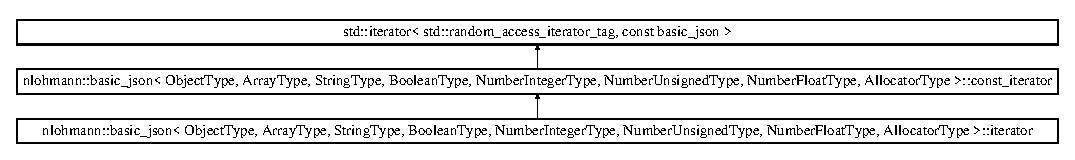
\includegraphics[height=1.705584cm]{classnlohmann_1_1basic__json_1_1iterator}
\end{center}
\end{figure}
\subsection*{Public Types}
\begin{DoxyCompactItemize}
\item 
using \hyperlink{classnlohmann_1_1basic__json_1_1iterator_ac48754e4dc48d65d95294bd170dcd857}{base\+\_\+iterator} = \hyperlink{classnlohmann_1_1basic__json_1_1const__iterator}{const\+\_\+iterator}
\item 
using \hyperlink{classnlohmann_1_1basic__json_1_1iterator_a3aae1df93a78b201d98e178c1c7d02a7}{pointer} = typename \hyperlink{classnlohmann_1_1basic__json_a9d1b58099dc64695fcf2847ab0b2a7c7}{basic\+\_\+json\+::pointer}
\item 
using \hyperlink{classnlohmann_1_1basic__json_1_1iterator_a97aff5d71246774267a81066460dd1cf}{reference} = typename \hyperlink{classnlohmann_1_1basic__json_a3ec8e17be8732fe436e9d6733f52b7a3}{basic\+\_\+json\+::reference}
\end{DoxyCompactItemize}
\subsection*{Public Member Functions}
\begin{DoxyCompactItemize}
\item 
\hyperlink{classnlohmann_1_1basic__json_1_1iterator_a47fb2dbbbfaf65c0ccfa99aeaed920a1}{iterator} ()=default
\begin{DoxyCompactList}\small\item\em default constructor \end{DoxyCompactList}\item 
\hyperlink{classnlohmann_1_1basic__json_1_1iterator_a085fe0d8cf459b5b1ae7b518b933ae7d}{iterator} (\hyperlink{classnlohmann_1_1basic__json_1_1const__iterator_a1da96fc3054d547e7706d3a2f073f389}{pointer} \hyperlink{classnlohmann_1_1basic__json_ad25b2f8c21e241e2d63455537a9294ff}{object}) noexcept
\begin{DoxyCompactList}\small\item\em constructor for a given J\+S\+ON instance \end{DoxyCompactList}\item 
\hyperlink{classnlohmann_1_1basic__json_1_1iterator_a1de0975e812c83e74d118b3e1063f335}{iterator} (const \hyperlink{classnlohmann_1_1basic__json_1_1iterator}{iterator} \&other) noexcept
\begin{DoxyCompactList}\small\item\em copy constructor \end{DoxyCompactList}\item 
\hyperlink{classnlohmann_1_1basic__json_1_1iterator}{iterator} \& \hyperlink{classnlohmann_1_1basic__json_1_1iterator_a3db892729714c4e7eaf60c00ee96e2e9}{operator=} (\hyperlink{classnlohmann_1_1basic__json_1_1iterator}{iterator} other) noexcept(                                       std\+::is\+\_\+nothrow\+\_\+move\+\_\+constructible$<$ \hyperlink{classnlohmann_1_1basic__json_1_1const__iterator_a1da96fc3054d547e7706d3a2f073f389}{pointer} $>$\+::\hyperlink{tk_8h_a177a0765f574ef6642002696d9cd82d0}{value} and                                       std\+::is\+\_\+nothrow\+\_\+move\+\_\+assignable$<$ \hyperlink{classnlohmann_1_1basic__json_1_1const__iterator_a1da96fc3054d547e7706d3a2f073f389}{pointer} $>$\+::\hyperlink{tk_8h_a177a0765f574ef6642002696d9cd82d0}{value} and                                       std\+::is\+\_\+nothrow\+\_\+move\+\_\+constructible$<$ internal\+\_\+iterator $>$\+::\hyperlink{tk_8h_a177a0765f574ef6642002696d9cd82d0}{value} and                                       std\+::is\+\_\+nothrow\+\_\+move\+\_\+assignable$<$ internal\+\_\+iterator $>$\+::\hyperlink{tk_8h_a177a0765f574ef6642002696d9cd82d0}{value}                       )
\begin{DoxyCompactList}\small\item\em copy assignment \end{DoxyCompactList}\item 
\hyperlink{classnlohmann_1_1basic__json_1_1const__iterator_aefd248cac6493eed1e6ff53ba6a63eb2}{reference} \hyperlink{classnlohmann_1_1basic__json_1_1iterator_acbd82115f9232c3d3b5dacc78315b9da}{operator$\ast$} () const 
\begin{DoxyCompactList}\small\item\em return a reference to the value pointed to by the iterator \end{DoxyCompactList}\item 
\hyperlink{classnlohmann_1_1basic__json_1_1const__iterator_a1da96fc3054d547e7706d3a2f073f389}{pointer} \hyperlink{classnlohmann_1_1basic__json_1_1iterator_a8de46badb5b2177c85c672a71bcca017}{operator-\/$>$} () const 
\begin{DoxyCompactList}\small\item\em dereference the iterator \end{DoxyCompactList}\item 
\hyperlink{classnlohmann_1_1basic__json_1_1iterator}{iterator} \hyperlink{classnlohmann_1_1basic__json_1_1iterator_a2943e49b3d88e6ee5793c5923ab2ede9}{operator++} (\hyperlink{tk_8h_a83f82f76e7fed06f4c49d2db94028a6d}{int})
\begin{DoxyCompactList}\small\item\em post-\/increment (it++) \end{DoxyCompactList}\item 
\hyperlink{classnlohmann_1_1basic__json_1_1iterator}{iterator} \& \hyperlink{classnlohmann_1_1basic__json_1_1iterator_a050b7fa21051ea57e5b0cc03668b5d4a}{operator++} ()
\begin{DoxyCompactList}\small\item\em pre-\/increment (++it) \end{DoxyCompactList}\item 
\hyperlink{classnlohmann_1_1basic__json_1_1iterator}{iterator} \hyperlink{classnlohmann_1_1basic__json_1_1iterator_ab4f238aa5fcf452b1884b748b0395b1f}{operator-\/-\/} (\hyperlink{tk_8h_a83f82f76e7fed06f4c49d2db94028a6d}{int})
\begin{DoxyCompactList}\small\item\em post-\/decrement (it--) \end{DoxyCompactList}\item 
\hyperlink{classnlohmann_1_1basic__json_1_1iterator}{iterator} \& \hyperlink{classnlohmann_1_1basic__json_1_1iterator_ab3679dc63b3a59edb98b1c2b96d8683c}{operator-\/-\/} ()
\begin{DoxyCompactList}\small\item\em pre-\/decrement (--it) \end{DoxyCompactList}\item 
\hyperlink{classnlohmann_1_1basic__json_1_1iterator}{iterator} \& \hyperlink{classnlohmann_1_1basic__json_1_1iterator_ae0c848dbc0af1cde15771d45d775b27c}{operator+=} (\hyperlink{classnlohmann_1_1basic__json_1_1const__iterator_a49d7c3e9ef3280df03052cce988b792f}{difference\+\_\+type} i)
\begin{DoxyCompactList}\small\item\em add to iterator \end{DoxyCompactList}\item 
\hyperlink{classnlohmann_1_1basic__json_1_1iterator}{iterator} \& \hyperlink{classnlohmann_1_1basic__json_1_1iterator_afe86d48d3e4e5ebdaaec162b3cf0e95c}{operator-\/=} (\hyperlink{classnlohmann_1_1basic__json_1_1const__iterator_a49d7c3e9ef3280df03052cce988b792f}{difference\+\_\+type} i)
\begin{DoxyCompactList}\small\item\em subtract from iterator \end{DoxyCompactList}\item 
\hyperlink{classnlohmann_1_1basic__json_1_1iterator}{iterator} \hyperlink{classnlohmann_1_1basic__json_1_1iterator_a56952f8d5702541f0d88e6a764d2ae36}{operator+} (\hyperlink{classnlohmann_1_1basic__json_1_1const__iterator_a49d7c3e9ef3280df03052cce988b792f}{difference\+\_\+type} i)
\begin{DoxyCompactList}\small\item\em add to iterator \end{DoxyCompactList}\item 
\hyperlink{classnlohmann_1_1basic__json_1_1iterator}{iterator} \hyperlink{classnlohmann_1_1basic__json_1_1iterator_a790f550ff168095c83c2e459c575916c}{operator-\/} (\hyperlink{classnlohmann_1_1basic__json_1_1const__iterator_a49d7c3e9ef3280df03052cce988b792f}{difference\+\_\+type} i)
\begin{DoxyCompactList}\small\item\em subtract from iterator \end{DoxyCompactList}\item 
\hyperlink{classnlohmann_1_1basic__json_1_1const__iterator_a49d7c3e9ef3280df03052cce988b792f}{difference\+\_\+type} \hyperlink{classnlohmann_1_1basic__json_1_1iterator_a9f3940ac5fb2c6ff8045ed59b8a0866f}{operator-\/} (const \hyperlink{classnlohmann_1_1basic__json_1_1iterator}{iterator} \&other) const 
\begin{DoxyCompactList}\small\item\em return difference \end{DoxyCompactList}\item 
\hyperlink{classnlohmann_1_1basic__json_1_1const__iterator_aefd248cac6493eed1e6ff53ba6a63eb2}{reference} \hyperlink{classnlohmann_1_1basic__json_1_1iterator_a7e01532727c10f87926dac4eb8e170f4}{operator\mbox{[}$\,$\mbox{]}} (\hyperlink{classnlohmann_1_1basic__json_1_1const__iterator_a49d7c3e9ef3280df03052cce988b792f}{difference\+\_\+type} n) const 
\begin{DoxyCompactList}\small\item\em access to successor \end{DoxyCompactList}\item 
\hyperlink{classnlohmann_1_1basic__json_1_1const__iterator_aefd248cac6493eed1e6ff53ba6a63eb2}{reference} \hyperlink{classnlohmann_1_1basic__json_1_1iterator_a8ffbf287736048e683f58306fdb8701f}{value} () const 
\begin{DoxyCompactList}\small\item\em return the value of an iterator \end{DoxyCompactList}\end{DoxyCompactItemize}


\subsection{Detailed Description}
\subsubsection*{template$<$template$<$ typename U, typename V, typename...\+Args $>$ class Object\+Type = std\+::map, template$<$ typename U, typename...\+Args $>$ class Array\+Type = std\+::vector, class String\+Type = std\+::string, class Boolean\+Type = bool, class Number\+Integer\+Type = std\+::int64\+\_\+t, class Number\+Unsigned\+Type = std\+::uint64\+\_\+t, class Number\+Float\+Type = double, template$<$ typename U $>$ class Allocator\+Type = std\+::allocator$>$\\*
class nlohmann\+::basic\+\_\+json$<$ Object\+Type, Array\+Type, String\+Type, Boolean\+Type, Number\+Integer\+Type, Number\+Unsigned\+Type, Number\+Float\+Type, Allocator\+Type $>$\+::iterator}

a mutable random access iterator for the \hyperlink{classnlohmann_1_1basic__json}{basic\+\_\+json} class 

The class satisfies the following concept requirements\+:
\begin{DoxyItemize}
\item \href{http://en.cppreference.com/w/cpp/concept/RandomAccessIterator}{\tt Random\+Access\+Iterator}\+: The iterator that can be moved to point (forward and backward) to any element in constant time.
\item \href{http://en.cppreference.com/w/cpp/concept/OutputIterator}{\tt Output\+Iterator}\+: It is possible to write to the pointed-\/to element.
\end{DoxyItemize}

\begin{DoxySince}{Since}
version 1.\+0.\+0 
\end{DoxySince}


\subsection{Member Typedef Documentation}
\index{nlohmann\+::basic\+\_\+json\+::iterator@{nlohmann\+::basic\+\_\+json\+::iterator}!base\+\_\+iterator@{base\+\_\+iterator}}
\index{base\+\_\+iterator@{base\+\_\+iterator}!nlohmann\+::basic\+\_\+json\+::iterator@{nlohmann\+::basic\+\_\+json\+::iterator}}
\subsubsection[{\texorpdfstring{base\+\_\+iterator}{base_iterator}}]{\setlength{\rightskip}{0pt plus 5cm}template$<$template$<$ typename U, typename V, typename...\+Args $>$ class Object\+Type = std\+::map, template$<$ typename U, typename...\+Args $>$ class Array\+Type = std\+::vector, class String\+Type  = std\+::string, class Boolean\+Type  = bool, class Number\+Integer\+Type  = std\+::int64\+\_\+t, class Number\+Unsigned\+Type  = std\+::uint64\+\_\+t, class Number\+Float\+Type  = double, template$<$ typename U $>$ class Allocator\+Type = std\+::allocator$>$ using {\bf nlohmann\+::basic\+\_\+json}$<$ Object\+Type, Array\+Type, String\+Type, Boolean\+Type, Number\+Integer\+Type, Number\+Unsigned\+Type, Number\+Float\+Type, Allocator\+Type $>$\+::{\bf iterator\+::base\+\_\+iterator} =  {\bf const\+\_\+iterator}}\hypertarget{classnlohmann_1_1basic__json_1_1iterator_ac48754e4dc48d65d95294bd170dcd857}{}\label{classnlohmann_1_1basic__json_1_1iterator_ac48754e4dc48d65d95294bd170dcd857}
\index{nlohmann\+::basic\+\_\+json\+::iterator@{nlohmann\+::basic\+\_\+json\+::iterator}!pointer@{pointer}}
\index{pointer@{pointer}!nlohmann\+::basic\+\_\+json\+::iterator@{nlohmann\+::basic\+\_\+json\+::iterator}}
\subsubsection[{\texorpdfstring{pointer}{pointer}}]{\setlength{\rightskip}{0pt plus 5cm}template$<$template$<$ typename U, typename V, typename...\+Args $>$ class Object\+Type = std\+::map, template$<$ typename U, typename...\+Args $>$ class Array\+Type = std\+::vector, class String\+Type  = std\+::string, class Boolean\+Type  = bool, class Number\+Integer\+Type  = std\+::int64\+\_\+t, class Number\+Unsigned\+Type  = std\+::uint64\+\_\+t, class Number\+Float\+Type  = double, template$<$ typename U $>$ class Allocator\+Type = std\+::allocator$>$ using {\bf nlohmann\+::basic\+\_\+json}$<$ Object\+Type, Array\+Type, String\+Type, Boolean\+Type, Number\+Integer\+Type, Number\+Unsigned\+Type, Number\+Float\+Type, Allocator\+Type $>$\+::{\bf iterator\+::pointer} =  typename {\bf basic\+\_\+json\+::pointer}}\hypertarget{classnlohmann_1_1basic__json_1_1iterator_a3aae1df93a78b201d98e178c1c7d02a7}{}\label{classnlohmann_1_1basic__json_1_1iterator_a3aae1df93a78b201d98e178c1c7d02a7}
\index{nlohmann\+::basic\+\_\+json\+::iterator@{nlohmann\+::basic\+\_\+json\+::iterator}!reference@{reference}}
\index{reference@{reference}!nlohmann\+::basic\+\_\+json\+::iterator@{nlohmann\+::basic\+\_\+json\+::iterator}}
\subsubsection[{\texorpdfstring{reference}{reference}}]{\setlength{\rightskip}{0pt plus 5cm}template$<$template$<$ typename U, typename V, typename...\+Args $>$ class Object\+Type = std\+::map, template$<$ typename U, typename...\+Args $>$ class Array\+Type = std\+::vector, class String\+Type  = std\+::string, class Boolean\+Type  = bool, class Number\+Integer\+Type  = std\+::int64\+\_\+t, class Number\+Unsigned\+Type  = std\+::uint64\+\_\+t, class Number\+Float\+Type  = double, template$<$ typename U $>$ class Allocator\+Type = std\+::allocator$>$ using {\bf nlohmann\+::basic\+\_\+json}$<$ Object\+Type, Array\+Type, String\+Type, Boolean\+Type, Number\+Integer\+Type, Number\+Unsigned\+Type, Number\+Float\+Type, Allocator\+Type $>$\+::{\bf iterator\+::reference} =  typename {\bf basic\+\_\+json\+::reference}}\hypertarget{classnlohmann_1_1basic__json_1_1iterator_a97aff5d71246774267a81066460dd1cf}{}\label{classnlohmann_1_1basic__json_1_1iterator_a97aff5d71246774267a81066460dd1cf}


\subsection{Constructor \& Destructor Documentation}
\index{nlohmann\+::basic\+\_\+json\+::iterator@{nlohmann\+::basic\+\_\+json\+::iterator}!iterator@{iterator}}
\index{iterator@{iterator}!nlohmann\+::basic\+\_\+json\+::iterator@{nlohmann\+::basic\+\_\+json\+::iterator}}
\subsubsection[{\texorpdfstring{iterator()=default}{iterator()=default}}]{\setlength{\rightskip}{0pt plus 5cm}template$<$template$<$ typename U, typename V, typename...\+Args $>$ class Object\+Type = std\+::map, template$<$ typename U, typename...\+Args $>$ class Array\+Type = std\+::vector, class String\+Type  = std\+::string, class Boolean\+Type  = bool, class Number\+Integer\+Type  = std\+::int64\+\_\+t, class Number\+Unsigned\+Type  = std\+::uint64\+\_\+t, class Number\+Float\+Type  = double, template$<$ typename U $>$ class Allocator\+Type = std\+::allocator$>$ {\bf nlohmann\+::basic\+\_\+json}$<$ Object\+Type, Array\+Type, String\+Type, Boolean\+Type, Number\+Integer\+Type, Number\+Unsigned\+Type, Number\+Float\+Type, Allocator\+Type $>$\+::iterator\+::iterator (
\begin{DoxyParamCaption}
{}
\end{DoxyParamCaption}
)\hspace{0.3cm}{\ttfamily [default]}}\hypertarget{classnlohmann_1_1basic__json_1_1iterator_a47fb2dbbbfaf65c0ccfa99aeaed920a1}{}\label{classnlohmann_1_1basic__json_1_1iterator_a47fb2dbbbfaf65c0ccfa99aeaed920a1}


default constructor 

\index{nlohmann\+::basic\+\_\+json\+::iterator@{nlohmann\+::basic\+\_\+json\+::iterator}!iterator@{iterator}}
\index{iterator@{iterator}!nlohmann\+::basic\+\_\+json\+::iterator@{nlohmann\+::basic\+\_\+json\+::iterator}}
\subsubsection[{\texorpdfstring{iterator(pointer object) noexcept}{iterator(pointer object) noexcept}}]{\setlength{\rightskip}{0pt plus 5cm}template$<$template$<$ typename U, typename V, typename...\+Args $>$ class Object\+Type = std\+::map, template$<$ typename U, typename...\+Args $>$ class Array\+Type = std\+::vector, class String\+Type  = std\+::string, class Boolean\+Type  = bool, class Number\+Integer\+Type  = std\+::int64\+\_\+t, class Number\+Unsigned\+Type  = std\+::uint64\+\_\+t, class Number\+Float\+Type  = double, template$<$ typename U $>$ class Allocator\+Type = std\+::allocator$>$ {\bf nlohmann\+::basic\+\_\+json}$<$ Object\+Type, Array\+Type, String\+Type, Boolean\+Type, Number\+Integer\+Type, Number\+Unsigned\+Type, Number\+Float\+Type, Allocator\+Type $>$\+::iterator\+::iterator (
\begin{DoxyParamCaption}
\item[{{\bf pointer}}]{object}
\end{DoxyParamCaption}
)\hspace{0.3cm}{\ttfamily [inline]}, {\ttfamily [explicit]}, {\ttfamily [noexcept]}}\hypertarget{classnlohmann_1_1basic__json_1_1iterator_a085fe0d8cf459b5b1ae7b518b933ae7d}{}\label{classnlohmann_1_1basic__json_1_1iterator_a085fe0d8cf459b5b1ae7b518b933ae7d}


constructor for a given J\+S\+ON instance 

\index{nlohmann\+::basic\+\_\+json\+::iterator@{nlohmann\+::basic\+\_\+json\+::iterator}!iterator@{iterator}}
\index{iterator@{iterator}!nlohmann\+::basic\+\_\+json\+::iterator@{nlohmann\+::basic\+\_\+json\+::iterator}}
\subsubsection[{\texorpdfstring{iterator(const iterator \&other) noexcept}{iterator(const iterator &other) noexcept}}]{\setlength{\rightskip}{0pt plus 5cm}template$<$template$<$ typename U, typename V, typename...\+Args $>$ class Object\+Type = std\+::map, template$<$ typename U, typename...\+Args $>$ class Array\+Type = std\+::vector, class String\+Type  = std\+::string, class Boolean\+Type  = bool, class Number\+Integer\+Type  = std\+::int64\+\_\+t, class Number\+Unsigned\+Type  = std\+::uint64\+\_\+t, class Number\+Float\+Type  = double, template$<$ typename U $>$ class Allocator\+Type = std\+::allocator$>$ {\bf nlohmann\+::basic\+\_\+json}$<$ Object\+Type, Array\+Type, String\+Type, Boolean\+Type, Number\+Integer\+Type, Number\+Unsigned\+Type, Number\+Float\+Type, Allocator\+Type $>$\+::iterator\+::iterator (
\begin{DoxyParamCaption}
\item[{const {\bf iterator} \&}]{other}
\end{DoxyParamCaption}
)\hspace{0.3cm}{\ttfamily [inline]}, {\ttfamily [noexcept]}}\hypertarget{classnlohmann_1_1basic__json_1_1iterator_a1de0975e812c83e74d118b3e1063f335}{}\label{classnlohmann_1_1basic__json_1_1iterator_a1de0975e812c83e74d118b3e1063f335}


copy constructor 



\subsection{Member Function Documentation}
\index{nlohmann\+::basic\+\_\+json\+::iterator@{nlohmann\+::basic\+\_\+json\+::iterator}!operator$\ast$@{operator$\ast$}}
\index{operator$\ast$@{operator$\ast$}!nlohmann\+::basic\+\_\+json\+::iterator@{nlohmann\+::basic\+\_\+json\+::iterator}}
\subsubsection[{\texorpdfstring{operator$\ast$() const }{operator*() const }}]{\setlength{\rightskip}{0pt plus 5cm}template$<$template$<$ typename U, typename V, typename...\+Args $>$ class Object\+Type = std\+::map, template$<$ typename U, typename...\+Args $>$ class Array\+Type = std\+::vector, class String\+Type  = std\+::string, class Boolean\+Type  = bool, class Number\+Integer\+Type  = std\+::int64\+\_\+t, class Number\+Unsigned\+Type  = std\+::uint64\+\_\+t, class Number\+Float\+Type  = double, template$<$ typename U $>$ class Allocator\+Type = std\+::allocator$>$ {\bf reference} {\bf nlohmann\+::basic\+\_\+json}$<$ Object\+Type, Array\+Type, String\+Type, Boolean\+Type, Number\+Integer\+Type, Number\+Unsigned\+Type, Number\+Float\+Type, Allocator\+Type $>$\+::iterator\+::operator$\ast$ (
\begin{DoxyParamCaption}
{}
\end{DoxyParamCaption}
) const\hspace{0.3cm}{\ttfamily [inline]}}\hypertarget{classnlohmann_1_1basic__json_1_1iterator_acbd82115f9232c3d3b5dacc78315b9da}{}\label{classnlohmann_1_1basic__json_1_1iterator_acbd82115f9232c3d3b5dacc78315b9da}


return a reference to the value pointed to by the iterator 

\index{nlohmann\+::basic\+\_\+json\+::iterator@{nlohmann\+::basic\+\_\+json\+::iterator}!operator+@{operator+}}
\index{operator+@{operator+}!nlohmann\+::basic\+\_\+json\+::iterator@{nlohmann\+::basic\+\_\+json\+::iterator}}
\subsubsection[{\texorpdfstring{operator+(difference\+\_\+type i)}{operator+(difference_type i)}}]{\setlength{\rightskip}{0pt plus 5cm}template$<$template$<$ typename U, typename V, typename...\+Args $>$ class Object\+Type = std\+::map, template$<$ typename U, typename...\+Args $>$ class Array\+Type = std\+::vector, class String\+Type  = std\+::string, class Boolean\+Type  = bool, class Number\+Integer\+Type  = std\+::int64\+\_\+t, class Number\+Unsigned\+Type  = std\+::uint64\+\_\+t, class Number\+Float\+Type  = double, template$<$ typename U $>$ class Allocator\+Type = std\+::allocator$>$ {\bf iterator} {\bf nlohmann\+::basic\+\_\+json}$<$ Object\+Type, Array\+Type, String\+Type, Boolean\+Type, Number\+Integer\+Type, Number\+Unsigned\+Type, Number\+Float\+Type, Allocator\+Type $>$\+::iterator\+::operator+ (
\begin{DoxyParamCaption}
\item[{{\bf difference\+\_\+type}}]{i}
\end{DoxyParamCaption}
)\hspace{0.3cm}{\ttfamily [inline]}}\hypertarget{classnlohmann_1_1basic__json_1_1iterator_a56952f8d5702541f0d88e6a764d2ae36}{}\label{classnlohmann_1_1basic__json_1_1iterator_a56952f8d5702541f0d88e6a764d2ae36}


add to iterator 

\index{nlohmann\+::basic\+\_\+json\+::iterator@{nlohmann\+::basic\+\_\+json\+::iterator}!operator++@{operator++}}
\index{operator++@{operator++}!nlohmann\+::basic\+\_\+json\+::iterator@{nlohmann\+::basic\+\_\+json\+::iterator}}
\subsubsection[{\texorpdfstring{operator++(int)}{operator++(int)}}]{\setlength{\rightskip}{0pt plus 5cm}template$<$template$<$ typename U, typename V, typename...\+Args $>$ class Object\+Type = std\+::map, template$<$ typename U, typename...\+Args $>$ class Array\+Type = std\+::vector, class String\+Type  = std\+::string, class Boolean\+Type  = bool, class Number\+Integer\+Type  = std\+::int64\+\_\+t, class Number\+Unsigned\+Type  = std\+::uint64\+\_\+t, class Number\+Float\+Type  = double, template$<$ typename U $>$ class Allocator\+Type = std\+::allocator$>$ {\bf iterator} {\bf nlohmann\+::basic\+\_\+json}$<$ Object\+Type, Array\+Type, String\+Type, Boolean\+Type, Number\+Integer\+Type, Number\+Unsigned\+Type, Number\+Float\+Type, Allocator\+Type $>$\+::iterator\+::operator++ (
\begin{DoxyParamCaption}
\item[{{\bf int}}]{}
\end{DoxyParamCaption}
)\hspace{0.3cm}{\ttfamily [inline]}}\hypertarget{classnlohmann_1_1basic__json_1_1iterator_a2943e49b3d88e6ee5793c5923ab2ede9}{}\label{classnlohmann_1_1basic__json_1_1iterator_a2943e49b3d88e6ee5793c5923ab2ede9}


post-\/increment (it++) 

\index{nlohmann\+::basic\+\_\+json\+::iterator@{nlohmann\+::basic\+\_\+json\+::iterator}!operator++@{operator++}}
\index{operator++@{operator++}!nlohmann\+::basic\+\_\+json\+::iterator@{nlohmann\+::basic\+\_\+json\+::iterator}}
\subsubsection[{\texorpdfstring{operator++()}{operator++()}}]{\setlength{\rightskip}{0pt plus 5cm}template$<$template$<$ typename U, typename V, typename...\+Args $>$ class Object\+Type = std\+::map, template$<$ typename U, typename...\+Args $>$ class Array\+Type = std\+::vector, class String\+Type  = std\+::string, class Boolean\+Type  = bool, class Number\+Integer\+Type  = std\+::int64\+\_\+t, class Number\+Unsigned\+Type  = std\+::uint64\+\_\+t, class Number\+Float\+Type  = double, template$<$ typename U $>$ class Allocator\+Type = std\+::allocator$>$ {\bf iterator}\& {\bf nlohmann\+::basic\+\_\+json}$<$ Object\+Type, Array\+Type, String\+Type, Boolean\+Type, Number\+Integer\+Type, Number\+Unsigned\+Type, Number\+Float\+Type, Allocator\+Type $>$\+::iterator\+::operator++ (
\begin{DoxyParamCaption}
{}
\end{DoxyParamCaption}
)\hspace{0.3cm}{\ttfamily [inline]}}\hypertarget{classnlohmann_1_1basic__json_1_1iterator_a050b7fa21051ea57e5b0cc03668b5d4a}{}\label{classnlohmann_1_1basic__json_1_1iterator_a050b7fa21051ea57e5b0cc03668b5d4a}


pre-\/increment (++it) 

\index{nlohmann\+::basic\+\_\+json\+::iterator@{nlohmann\+::basic\+\_\+json\+::iterator}!operator+=@{operator+=}}
\index{operator+=@{operator+=}!nlohmann\+::basic\+\_\+json\+::iterator@{nlohmann\+::basic\+\_\+json\+::iterator}}
\subsubsection[{\texorpdfstring{operator+=(difference\+\_\+type i)}{operator+=(difference_type i)}}]{\setlength{\rightskip}{0pt plus 5cm}template$<$template$<$ typename U, typename V, typename...\+Args $>$ class Object\+Type = std\+::map, template$<$ typename U, typename...\+Args $>$ class Array\+Type = std\+::vector, class String\+Type  = std\+::string, class Boolean\+Type  = bool, class Number\+Integer\+Type  = std\+::int64\+\_\+t, class Number\+Unsigned\+Type  = std\+::uint64\+\_\+t, class Number\+Float\+Type  = double, template$<$ typename U $>$ class Allocator\+Type = std\+::allocator$>$ {\bf iterator}\& {\bf nlohmann\+::basic\+\_\+json}$<$ Object\+Type, Array\+Type, String\+Type, Boolean\+Type, Number\+Integer\+Type, Number\+Unsigned\+Type, Number\+Float\+Type, Allocator\+Type $>$\+::iterator\+::operator+= (
\begin{DoxyParamCaption}
\item[{{\bf difference\+\_\+type}}]{i}
\end{DoxyParamCaption}
)\hspace{0.3cm}{\ttfamily [inline]}}\hypertarget{classnlohmann_1_1basic__json_1_1iterator_ae0c848dbc0af1cde15771d45d775b27c}{}\label{classnlohmann_1_1basic__json_1_1iterator_ae0c848dbc0af1cde15771d45d775b27c}


add to iterator 

\index{nlohmann\+::basic\+\_\+json\+::iterator@{nlohmann\+::basic\+\_\+json\+::iterator}!operator-\/@{operator-\/}}
\index{operator-\/@{operator-\/}!nlohmann\+::basic\+\_\+json\+::iterator@{nlohmann\+::basic\+\_\+json\+::iterator}}
\subsubsection[{\texorpdfstring{operator-\/(difference\+\_\+type i)}{operator-(difference_type i)}}]{\setlength{\rightskip}{0pt plus 5cm}template$<$template$<$ typename U, typename V, typename...\+Args $>$ class Object\+Type = std\+::map, template$<$ typename U, typename...\+Args $>$ class Array\+Type = std\+::vector, class String\+Type  = std\+::string, class Boolean\+Type  = bool, class Number\+Integer\+Type  = std\+::int64\+\_\+t, class Number\+Unsigned\+Type  = std\+::uint64\+\_\+t, class Number\+Float\+Type  = double, template$<$ typename U $>$ class Allocator\+Type = std\+::allocator$>$ {\bf iterator} {\bf nlohmann\+::basic\+\_\+json}$<$ Object\+Type, Array\+Type, String\+Type, Boolean\+Type, Number\+Integer\+Type, Number\+Unsigned\+Type, Number\+Float\+Type, Allocator\+Type $>$\+::iterator\+::operator-\/ (
\begin{DoxyParamCaption}
\item[{{\bf difference\+\_\+type}}]{i}
\end{DoxyParamCaption}
)\hspace{0.3cm}{\ttfamily [inline]}}\hypertarget{classnlohmann_1_1basic__json_1_1iterator_a790f550ff168095c83c2e459c575916c}{}\label{classnlohmann_1_1basic__json_1_1iterator_a790f550ff168095c83c2e459c575916c}


subtract from iterator 

\index{nlohmann\+::basic\+\_\+json\+::iterator@{nlohmann\+::basic\+\_\+json\+::iterator}!operator-\/@{operator-\/}}
\index{operator-\/@{operator-\/}!nlohmann\+::basic\+\_\+json\+::iterator@{nlohmann\+::basic\+\_\+json\+::iterator}}
\subsubsection[{\texorpdfstring{operator-\/(const iterator \&other) const }{operator-(const iterator &other) const }}]{\setlength{\rightskip}{0pt plus 5cm}template$<$template$<$ typename U, typename V, typename...\+Args $>$ class Object\+Type = std\+::map, template$<$ typename U, typename...\+Args $>$ class Array\+Type = std\+::vector, class String\+Type  = std\+::string, class Boolean\+Type  = bool, class Number\+Integer\+Type  = std\+::int64\+\_\+t, class Number\+Unsigned\+Type  = std\+::uint64\+\_\+t, class Number\+Float\+Type  = double, template$<$ typename U $>$ class Allocator\+Type = std\+::allocator$>$ {\bf difference\+\_\+type} {\bf nlohmann\+::basic\+\_\+json}$<$ Object\+Type, Array\+Type, String\+Type, Boolean\+Type, Number\+Integer\+Type, Number\+Unsigned\+Type, Number\+Float\+Type, Allocator\+Type $>$\+::iterator\+::operator-\/ (
\begin{DoxyParamCaption}
\item[{const {\bf iterator} \&}]{other}
\end{DoxyParamCaption}
) const\hspace{0.3cm}{\ttfamily [inline]}}\hypertarget{classnlohmann_1_1basic__json_1_1iterator_a9f3940ac5fb2c6ff8045ed59b8a0866f}{}\label{classnlohmann_1_1basic__json_1_1iterator_a9f3940ac5fb2c6ff8045ed59b8a0866f}


return difference 

\index{nlohmann\+::basic\+\_\+json\+::iterator@{nlohmann\+::basic\+\_\+json\+::iterator}!operator-\/-\/@{operator-\/-\/}}
\index{operator-\/-\/@{operator-\/-\/}!nlohmann\+::basic\+\_\+json\+::iterator@{nlohmann\+::basic\+\_\+json\+::iterator}}
\subsubsection[{\texorpdfstring{operator-\/-\/(int)}{operator--(int)}}]{\setlength{\rightskip}{0pt plus 5cm}template$<$template$<$ typename U, typename V, typename...\+Args $>$ class Object\+Type = std\+::map, template$<$ typename U, typename...\+Args $>$ class Array\+Type = std\+::vector, class String\+Type  = std\+::string, class Boolean\+Type  = bool, class Number\+Integer\+Type  = std\+::int64\+\_\+t, class Number\+Unsigned\+Type  = std\+::uint64\+\_\+t, class Number\+Float\+Type  = double, template$<$ typename U $>$ class Allocator\+Type = std\+::allocator$>$ {\bf iterator} {\bf nlohmann\+::basic\+\_\+json}$<$ Object\+Type, Array\+Type, String\+Type, Boolean\+Type, Number\+Integer\+Type, Number\+Unsigned\+Type, Number\+Float\+Type, Allocator\+Type $>$\+::iterator\+::operator-\/-\/ (
\begin{DoxyParamCaption}
\item[{{\bf int}}]{}
\end{DoxyParamCaption}
)\hspace{0.3cm}{\ttfamily [inline]}}\hypertarget{classnlohmann_1_1basic__json_1_1iterator_ab4f238aa5fcf452b1884b748b0395b1f}{}\label{classnlohmann_1_1basic__json_1_1iterator_ab4f238aa5fcf452b1884b748b0395b1f}


post-\/decrement (it--) 

\index{nlohmann\+::basic\+\_\+json\+::iterator@{nlohmann\+::basic\+\_\+json\+::iterator}!operator-\/-\/@{operator-\/-\/}}
\index{operator-\/-\/@{operator-\/-\/}!nlohmann\+::basic\+\_\+json\+::iterator@{nlohmann\+::basic\+\_\+json\+::iterator}}
\subsubsection[{\texorpdfstring{operator-\/-\/()}{operator--()}}]{\setlength{\rightskip}{0pt plus 5cm}template$<$template$<$ typename U, typename V, typename...\+Args $>$ class Object\+Type = std\+::map, template$<$ typename U, typename...\+Args $>$ class Array\+Type = std\+::vector, class String\+Type  = std\+::string, class Boolean\+Type  = bool, class Number\+Integer\+Type  = std\+::int64\+\_\+t, class Number\+Unsigned\+Type  = std\+::uint64\+\_\+t, class Number\+Float\+Type  = double, template$<$ typename U $>$ class Allocator\+Type = std\+::allocator$>$ {\bf iterator}\& {\bf nlohmann\+::basic\+\_\+json}$<$ Object\+Type, Array\+Type, String\+Type, Boolean\+Type, Number\+Integer\+Type, Number\+Unsigned\+Type, Number\+Float\+Type, Allocator\+Type $>$\+::iterator\+::operator-\/-\/ (
\begin{DoxyParamCaption}
{}
\end{DoxyParamCaption}
)\hspace{0.3cm}{\ttfamily [inline]}}\hypertarget{classnlohmann_1_1basic__json_1_1iterator_ab3679dc63b3a59edb98b1c2b96d8683c}{}\label{classnlohmann_1_1basic__json_1_1iterator_ab3679dc63b3a59edb98b1c2b96d8683c}


pre-\/decrement (--it) 

\index{nlohmann\+::basic\+\_\+json\+::iterator@{nlohmann\+::basic\+\_\+json\+::iterator}!operator-\/=@{operator-\/=}}
\index{operator-\/=@{operator-\/=}!nlohmann\+::basic\+\_\+json\+::iterator@{nlohmann\+::basic\+\_\+json\+::iterator}}
\subsubsection[{\texorpdfstring{operator-\/=(difference\+\_\+type i)}{operator-=(difference_type i)}}]{\setlength{\rightskip}{0pt plus 5cm}template$<$template$<$ typename U, typename V, typename...\+Args $>$ class Object\+Type = std\+::map, template$<$ typename U, typename...\+Args $>$ class Array\+Type = std\+::vector, class String\+Type  = std\+::string, class Boolean\+Type  = bool, class Number\+Integer\+Type  = std\+::int64\+\_\+t, class Number\+Unsigned\+Type  = std\+::uint64\+\_\+t, class Number\+Float\+Type  = double, template$<$ typename U $>$ class Allocator\+Type = std\+::allocator$>$ {\bf iterator}\& {\bf nlohmann\+::basic\+\_\+json}$<$ Object\+Type, Array\+Type, String\+Type, Boolean\+Type, Number\+Integer\+Type, Number\+Unsigned\+Type, Number\+Float\+Type, Allocator\+Type $>$\+::iterator\+::operator-\/= (
\begin{DoxyParamCaption}
\item[{{\bf difference\+\_\+type}}]{i}
\end{DoxyParamCaption}
)\hspace{0.3cm}{\ttfamily [inline]}}\hypertarget{classnlohmann_1_1basic__json_1_1iterator_afe86d48d3e4e5ebdaaec162b3cf0e95c}{}\label{classnlohmann_1_1basic__json_1_1iterator_afe86d48d3e4e5ebdaaec162b3cf0e95c}


subtract from iterator 

\index{nlohmann\+::basic\+\_\+json\+::iterator@{nlohmann\+::basic\+\_\+json\+::iterator}!operator-\/$>$@{operator-\/$>$}}
\index{operator-\/$>$@{operator-\/$>$}!nlohmann\+::basic\+\_\+json\+::iterator@{nlohmann\+::basic\+\_\+json\+::iterator}}
\subsubsection[{\texorpdfstring{operator-\/$>$() const }{operator->() const }}]{\setlength{\rightskip}{0pt plus 5cm}template$<$template$<$ typename U, typename V, typename...\+Args $>$ class Object\+Type = std\+::map, template$<$ typename U, typename...\+Args $>$ class Array\+Type = std\+::vector, class String\+Type  = std\+::string, class Boolean\+Type  = bool, class Number\+Integer\+Type  = std\+::int64\+\_\+t, class Number\+Unsigned\+Type  = std\+::uint64\+\_\+t, class Number\+Float\+Type  = double, template$<$ typename U $>$ class Allocator\+Type = std\+::allocator$>$ {\bf pointer} {\bf nlohmann\+::basic\+\_\+json}$<$ Object\+Type, Array\+Type, String\+Type, Boolean\+Type, Number\+Integer\+Type, Number\+Unsigned\+Type, Number\+Float\+Type, Allocator\+Type $>$\+::iterator\+::operator-\/$>$ (
\begin{DoxyParamCaption}
{}
\end{DoxyParamCaption}
) const\hspace{0.3cm}{\ttfamily [inline]}}\hypertarget{classnlohmann_1_1basic__json_1_1iterator_a8de46badb5b2177c85c672a71bcca017}{}\label{classnlohmann_1_1basic__json_1_1iterator_a8de46badb5b2177c85c672a71bcca017}


dereference the iterator 

\index{nlohmann\+::basic\+\_\+json\+::iterator@{nlohmann\+::basic\+\_\+json\+::iterator}!operator=@{operator=}}
\index{operator=@{operator=}!nlohmann\+::basic\+\_\+json\+::iterator@{nlohmann\+::basic\+\_\+json\+::iterator}}
\subsubsection[{\texorpdfstring{operator=(iterator other) noexcept(                                       std\+::is\+\_\+nothrow\+\_\+move\+\_\+constructible$<$ pointer $>$\+::value and                                       std\+::is\+\_\+nothrow\+\_\+move\+\_\+assignable$<$ pointer $>$\+::value and                                       std\+::is\+\_\+nothrow\+\_\+move\+\_\+constructible$<$ internal\+\_\+iterator $>$\+::value and                                       std\+::is\+\_\+nothrow\+\_\+move\+\_\+assignable$<$ internal\+\_\+iterator $>$\+::value                       )}{operator=(iterator other) noexcept(                                       std::is_nothrow_move_constructible< pointer >::value and                                       std::is_nothrow_move_assignable< pointer >::value and                                       std::is_nothrow_move_constructible< internal_iterator >::value and                                       std::is_nothrow_move_assignable< internal_iterator >::value                       )}}]{\setlength{\rightskip}{0pt plus 5cm}template$<$template$<$ typename U, typename V, typename...\+Args $>$ class Object\+Type = std\+::map, template$<$ typename U, typename...\+Args $>$ class Array\+Type = std\+::vector, class String\+Type  = std\+::string, class Boolean\+Type  = bool, class Number\+Integer\+Type  = std\+::int64\+\_\+t, class Number\+Unsigned\+Type  = std\+::uint64\+\_\+t, class Number\+Float\+Type  = double, template$<$ typename U $>$ class Allocator\+Type = std\+::allocator$>$ {\bf iterator}\& {\bf nlohmann\+::basic\+\_\+json}$<$ Object\+Type, Array\+Type, String\+Type, Boolean\+Type, Number\+Integer\+Type, Number\+Unsigned\+Type, Number\+Float\+Type, Allocator\+Type $>$\+::iterator\+::operator= (
\begin{DoxyParamCaption}
\item[{{\bf iterator}}]{other}
\end{DoxyParamCaption}
)\hspace{0.3cm}{\ttfamily [inline]}, {\ttfamily [noexcept]}}\hypertarget{classnlohmann_1_1basic__json_1_1iterator_a3db892729714c4e7eaf60c00ee96e2e9}{}\label{classnlohmann_1_1basic__json_1_1iterator_a3db892729714c4e7eaf60c00ee96e2e9}


copy assignment 

\index{nlohmann\+::basic\+\_\+json\+::iterator@{nlohmann\+::basic\+\_\+json\+::iterator}!operator\mbox{[}$\,$\mbox{]}@{operator[]}}
\index{operator\mbox{[}$\,$\mbox{]}@{operator[]}!nlohmann\+::basic\+\_\+json\+::iterator@{nlohmann\+::basic\+\_\+json\+::iterator}}
\subsubsection[{\texorpdfstring{operator[](difference\+\_\+type n) const }{operator[](difference_type n) const }}]{\setlength{\rightskip}{0pt plus 5cm}template$<$template$<$ typename U, typename V, typename...\+Args $>$ class Object\+Type = std\+::map, template$<$ typename U, typename...\+Args $>$ class Array\+Type = std\+::vector, class String\+Type  = std\+::string, class Boolean\+Type  = bool, class Number\+Integer\+Type  = std\+::int64\+\_\+t, class Number\+Unsigned\+Type  = std\+::uint64\+\_\+t, class Number\+Float\+Type  = double, template$<$ typename U $>$ class Allocator\+Type = std\+::allocator$>$ {\bf reference} {\bf nlohmann\+::basic\+\_\+json}$<$ Object\+Type, Array\+Type, String\+Type, Boolean\+Type, Number\+Integer\+Type, Number\+Unsigned\+Type, Number\+Float\+Type, Allocator\+Type $>$\+::iterator\+::operator\mbox{[}$\,$\mbox{]} (
\begin{DoxyParamCaption}
\item[{{\bf difference\+\_\+type}}]{n}
\end{DoxyParamCaption}
) const\hspace{0.3cm}{\ttfamily [inline]}}\hypertarget{classnlohmann_1_1basic__json_1_1iterator_a7e01532727c10f87926dac4eb8e170f4}{}\label{classnlohmann_1_1basic__json_1_1iterator_a7e01532727c10f87926dac4eb8e170f4}


access to successor 

\index{nlohmann\+::basic\+\_\+json\+::iterator@{nlohmann\+::basic\+\_\+json\+::iterator}!value@{value}}
\index{value@{value}!nlohmann\+::basic\+\_\+json\+::iterator@{nlohmann\+::basic\+\_\+json\+::iterator}}
\subsubsection[{\texorpdfstring{value() const }{value() const }}]{\setlength{\rightskip}{0pt plus 5cm}template$<$template$<$ typename U, typename V, typename...\+Args $>$ class Object\+Type = std\+::map, template$<$ typename U, typename...\+Args $>$ class Array\+Type = std\+::vector, class String\+Type  = std\+::string, class Boolean\+Type  = bool, class Number\+Integer\+Type  = std\+::int64\+\_\+t, class Number\+Unsigned\+Type  = std\+::uint64\+\_\+t, class Number\+Float\+Type  = double, template$<$ typename U $>$ class Allocator\+Type = std\+::allocator$>$ {\bf reference} {\bf nlohmann\+::basic\+\_\+json}$<$ Object\+Type, Array\+Type, String\+Type, Boolean\+Type, Number\+Integer\+Type, Number\+Unsigned\+Type, Number\+Float\+Type, Allocator\+Type $>$\+::iterator\+::value (
\begin{DoxyParamCaption}
{}
\end{DoxyParamCaption}
) const\hspace{0.3cm}{\ttfamily [inline]}}\hypertarget{classnlohmann_1_1basic__json_1_1iterator_a8ffbf287736048e683f58306fdb8701f}{}\label{classnlohmann_1_1basic__json_1_1iterator_a8ffbf287736048e683f58306fdb8701f}


return the value of an iterator 



The documentation for this class was generated from the following file\+:\begin{DoxyCompactItemize}
\item 
/\+Users/michael/\+J\+U\+C\+E/projects/audealize-\/plugin/\+J\+U\+C\+E Modules/audealize\+\_\+module/utils/\hyperlink{json_8hpp}{json.\+hpp}\end{DoxyCompactItemize}

\hypertarget{classnlohmann_1_1basic__json_1_1json__pointer}{}\section{nlohmann\+:\+:basic\+\_\+json$<$ Object\+Type, Array\+Type, String\+Type, Boolean\+Type, Number\+Integer\+Type, Number\+Unsigned\+Type, Number\+Float\+Type, Allocator\+Type $>$\+:\+:json\+\_\+pointer Class Reference}
\label{classnlohmann_1_1basic__json_1_1json__pointer}\index{nlohmann\+::basic\+\_\+json$<$ Object\+Type, Array\+Type, String\+Type, Boolean\+Type, Number\+Integer\+Type, Number\+Unsigned\+Type, Number\+Float\+Type, Allocator\+Type $>$\+::json\+\_\+pointer@{nlohmann\+::basic\+\_\+json$<$ Object\+Type, Array\+Type, String\+Type, Boolean\+Type, Number\+Integer\+Type, Number\+Unsigned\+Type, Number\+Float\+Type, Allocator\+Type $>$\+::json\+\_\+pointer}}


J\+S\+ON Pointer.  




{\ttfamily \#include $<$json.\+hpp$>$}

\subsection*{Public Member Functions}
\begin{DoxyCompactItemize}
\item 
\hyperlink{classnlohmann_1_1basic__json_1_1json__pointer_ae12db117a2742d826465080979d7c835}{json\+\_\+pointer} (const std\+::string \&s=\char`\"{}\char`\"{})
\begin{DoxyCompactList}\small\item\em create J\+S\+ON pointer \end{DoxyCompactList}\item 
std\+::string \hyperlink{classnlohmann_1_1basic__json_1_1json__pointer_a14fda25789660bdc3f2de652fec35f61}{to\+\_\+string} () const  noexcept
\begin{DoxyCompactList}\small\item\em return a string representation of the J\+S\+ON pointer \end{DoxyCompactList}\item 
\hyperlink{classnlohmann_1_1basic__json_1_1json__pointer_a344b49c70c83ff591be767072c87336e}{operator std\+::string} () const 
\begin{DoxyCompactList}\small\item\em return a string representation of the J\+S\+ON pointer \end{DoxyCompactList}\end{DoxyCompactItemize}
\subsection*{Friends}
\begin{DoxyCompactItemize}
\item 
class \hyperlink{classnlohmann_1_1basic__json_1_1json__pointer_ada3100cdb8700566051828f1355fa745}{basic\+\_\+json}
\begin{DoxyCompactList}\small\item\em allow \hyperlink{classnlohmann_1_1basic__json}{basic\+\_\+json} to access private members \end{DoxyCompactList}\end{DoxyCompactItemize}


\subsection{Detailed Description}
\subsubsection*{template$<$template$<$ typename U, typename V, typename...\+Args $>$ class Object\+Type = std\+::map, template$<$ typename U, typename...\+Args $>$ class Array\+Type = std\+::vector, class String\+Type = std\+::string, class Boolean\+Type = bool, class Number\+Integer\+Type = std\+::int64\+\_\+t, class Number\+Unsigned\+Type = std\+::uint64\+\_\+t, class Number\+Float\+Type = double, template$<$ typename U $>$ class Allocator\+Type = std\+::allocator$>$\\*
class nlohmann\+::basic\+\_\+json$<$ Object\+Type, Array\+Type, String\+Type, Boolean\+Type, Number\+Integer\+Type, Number\+Unsigned\+Type, Number\+Float\+Type, Allocator\+Type $>$\+::json\+\_\+pointer}

J\+S\+ON Pointer. 

A J\+S\+ON pointer defines a string syntax for identifying a specific value within a J\+S\+ON document. It can be used with functions {\ttfamily at} and {\ttfamily operator\mbox{[}\mbox{]}}. Furthermore, J\+S\+ON pointers are the base for J\+S\+ON patches.

\begin{DoxySeeAlso}{See also}
\href{https://tools.ietf.org/html/rfc6901}{\tt R\+FC 6901}
\end{DoxySeeAlso}
\begin{DoxySince}{Since}
version 2.\+0.\+0 
\end{DoxySince}


\subsection{Constructor \& Destructor Documentation}
\index{nlohmann\+::basic\+\_\+json\+::json\+\_\+pointer@{nlohmann\+::basic\+\_\+json\+::json\+\_\+pointer}!json\+\_\+pointer@{json\+\_\+pointer}}
\index{json\+\_\+pointer@{json\+\_\+pointer}!nlohmann\+::basic\+\_\+json\+::json\+\_\+pointer@{nlohmann\+::basic\+\_\+json\+::json\+\_\+pointer}}
\subsubsection[{\texorpdfstring{json\+\_\+pointer(const std\+::string \&s="""")}{json_pointer(const std::string &s="")}}]{\setlength{\rightskip}{0pt plus 5cm}template$<$template$<$ typename U, typename V, typename...\+Args $>$ class Object\+Type = std\+::map, template$<$ typename U, typename...\+Args $>$ class Array\+Type = std\+::vector, class String\+Type  = std\+::string, class Boolean\+Type  = bool, class Number\+Integer\+Type  = std\+::int64\+\_\+t, class Number\+Unsigned\+Type  = std\+::uint64\+\_\+t, class Number\+Float\+Type  = double, template$<$ typename U $>$ class Allocator\+Type = std\+::allocator$>$ {\bf nlohmann\+::basic\+\_\+json}$<$ Object\+Type, Array\+Type, String\+Type, Boolean\+Type, Number\+Integer\+Type, Number\+Unsigned\+Type, Number\+Float\+Type, Allocator\+Type $>$\+::json\+\_\+pointer\+::json\+\_\+pointer (
\begin{DoxyParamCaption}
\item[{const std\+::string \&}]{s = {\ttfamily \char`\"{}\char`\"{}}}
\end{DoxyParamCaption}
)\hspace{0.3cm}{\ttfamily [inline]}, {\ttfamily [explicit]}}\hypertarget{classnlohmann_1_1basic__json_1_1json__pointer_ae12db117a2742d826465080979d7c835}{}\label{classnlohmann_1_1basic__json_1_1json__pointer_ae12db117a2742d826465080979d7c835}


create J\+S\+ON pointer 

Create a J\+S\+ON pointer according to the syntax described in \href{https://tools.ietf.org/html/rfc6901#section-3}{\tt Section 3 of R\+F\+C6901}.


\begin{DoxyParams}[1]{Parameters}
\mbox{\tt in}  & {\em s} & string representing the J\+S\+ON pointer; if omitted, the empty string is assumed which references the whole J\+S\+ON value\\
\hline
\end{DoxyParams}

\begin{DoxyExceptions}{Exceptions}
{\em std\+::domain\+\_\+error} & if reference token is nonempty and does not begin with a slash ({\ttfamily /}); example\+: {\ttfamily \char`\"{}\+J\+S\+O\+N pointer must be empty or
begin with /\char`\"{}} \\
\hline
{\em std\+::domain\+\_\+error} & if a tilde ({\ttfamily $\sim$}) is not followed by {\ttfamily 0} (representing {\ttfamily $\sim$}) or {\ttfamily 1} (representing {\ttfamily /}); example\+: {\ttfamily \char`\"{}escape error\+:
$\sim$ must be followed with 0 or 1\char`\"{}}\\
\hline
\end{DoxyExceptions}
\{The example shows the construction several valid J\+S\+ON pointers as well as the exceptional behavior.,\hyperlink{classnlohmann_1_1basic__json_1_1json__pointer}{json\+\_\+pointer}\}

\begin{DoxySince}{Since}
version 2.\+0.\+0 
\end{DoxySince}


\subsection{Member Function Documentation}
\index{nlohmann\+::basic\+\_\+json\+::json\+\_\+pointer@{nlohmann\+::basic\+\_\+json\+::json\+\_\+pointer}!operator std\+::string@{operator std\+::string}}
\index{operator std\+::string@{operator std\+::string}!nlohmann\+::basic\+\_\+json\+::json\+\_\+pointer@{nlohmann\+::basic\+\_\+json\+::json\+\_\+pointer}}
\subsubsection[{\texorpdfstring{operator std\+::string() const }{operator std::string() const }}]{\setlength{\rightskip}{0pt plus 5cm}template$<$template$<$ typename U, typename V, typename...\+Args $>$ class Object\+Type = std\+::map, template$<$ typename U, typename...\+Args $>$ class Array\+Type = std\+::vector, class String\+Type  = std\+::string, class Boolean\+Type  = bool, class Number\+Integer\+Type  = std\+::int64\+\_\+t, class Number\+Unsigned\+Type  = std\+::uint64\+\_\+t, class Number\+Float\+Type  = double, template$<$ typename U $>$ class Allocator\+Type = std\+::allocator$>$ {\bf nlohmann\+::basic\+\_\+json}$<$ Object\+Type, Array\+Type, String\+Type, Boolean\+Type, Number\+Integer\+Type, Number\+Unsigned\+Type, Number\+Float\+Type, Allocator\+Type $>$\+::json\+\_\+pointer\+::operator std\+::string (
\begin{DoxyParamCaption}
{}
\end{DoxyParamCaption}
) const\hspace{0.3cm}{\ttfamily [inline]}}\hypertarget{classnlohmann_1_1basic__json_1_1json__pointer_a344b49c70c83ff591be767072c87336e}{}\label{classnlohmann_1_1basic__json_1_1json__pointer_a344b49c70c83ff591be767072c87336e}


return a string representation of the J\+S\+ON pointer 

\begin{DoxyInvariant}{Invariant}
For each J\+S\+ON pointer {\ttfamily ptr}, it holds\+: 
\begin{DoxyCode}
ptr == \hyperlink{classnlohmann_1_1basic__json_1_1json__pointer_ae12db117a2742d826465080979d7c835}{json\_pointer}(ptr.to\_string());
\end{DoxyCode}

\end{DoxyInvariant}
\begin{DoxyReturn}{Returns}
a string representation of the J\+S\+ON pointer
\end{DoxyReturn}
\{The example shows the result of {\ttfamily to\+\_\+string}., json\+\_\+pointer\+\_\+\+\_\+to\+\_\+string\}

\begin{DoxySince}{Since}
version 2.\+0.\+0 
\end{DoxySince}
\index{nlohmann\+::basic\+\_\+json\+::json\+\_\+pointer@{nlohmann\+::basic\+\_\+json\+::json\+\_\+pointer}!to\+\_\+string@{to\+\_\+string}}
\index{to\+\_\+string@{to\+\_\+string}!nlohmann\+::basic\+\_\+json\+::json\+\_\+pointer@{nlohmann\+::basic\+\_\+json\+::json\+\_\+pointer}}
\subsubsection[{\texorpdfstring{to\+\_\+string() const  noexcept}{to_string() const  noexcept}}]{\setlength{\rightskip}{0pt plus 5cm}template$<$template$<$ typename U, typename V, typename...\+Args $>$ class Object\+Type = std\+::map, template$<$ typename U, typename...\+Args $>$ class Array\+Type = std\+::vector, class String\+Type  = std\+::string, class Boolean\+Type  = bool, class Number\+Integer\+Type  = std\+::int64\+\_\+t, class Number\+Unsigned\+Type  = std\+::uint64\+\_\+t, class Number\+Float\+Type  = double, template$<$ typename U $>$ class Allocator\+Type = std\+::allocator$>$ std\+::string {\bf nlohmann\+::basic\+\_\+json}$<$ Object\+Type, Array\+Type, String\+Type, Boolean\+Type, Number\+Integer\+Type, Number\+Unsigned\+Type, Number\+Float\+Type, Allocator\+Type $>$\+::json\+\_\+pointer\+::to\+\_\+string (
\begin{DoxyParamCaption}
{}
\end{DoxyParamCaption}
) const\hspace{0.3cm}{\ttfamily [inline]}, {\ttfamily [noexcept]}}\hypertarget{classnlohmann_1_1basic__json_1_1json__pointer_a14fda25789660bdc3f2de652fec35f61}{}\label{classnlohmann_1_1basic__json_1_1json__pointer_a14fda25789660bdc3f2de652fec35f61}


return a string representation of the J\+S\+ON pointer 

\begin{DoxyInvariant}{Invariant}
For each J\+S\+ON pointer {\ttfamily ptr}, it holds\+: 
\begin{DoxyCode}
ptr == \hyperlink{classnlohmann_1_1basic__json_1_1json__pointer_ae12db117a2742d826465080979d7c835}{json\_pointer}(ptr.to\_string());
\end{DoxyCode}

\end{DoxyInvariant}
\begin{DoxyReturn}{Returns}
a string representation of the J\+S\+ON pointer
\end{DoxyReturn}
\{The example shows the result of {\ttfamily to\+\_\+string}., json\+\_\+pointer\+\_\+\+\_\+to\+\_\+string\}

\begin{DoxySince}{Since}
version 2.\+0.\+0 
\end{DoxySince}


\subsection{Friends And Related Function Documentation}
\index{nlohmann\+::basic\+\_\+json\+::json\+\_\+pointer@{nlohmann\+::basic\+\_\+json\+::json\+\_\+pointer}!basic\+\_\+json@{basic\+\_\+json}}
\index{basic\+\_\+json@{basic\+\_\+json}!nlohmann\+::basic\+\_\+json\+::json\+\_\+pointer@{nlohmann\+::basic\+\_\+json\+::json\+\_\+pointer}}
\subsubsection[{\texorpdfstring{basic\+\_\+json}{basic_json}}]{\setlength{\rightskip}{0pt plus 5cm}template$<$template$<$ typename U, typename V, typename...\+Args $>$ class Object\+Type = std\+::map, template$<$ typename U, typename...\+Args $>$ class Array\+Type = std\+::vector, class String\+Type  = std\+::string, class Boolean\+Type  = bool, class Number\+Integer\+Type  = std\+::int64\+\_\+t, class Number\+Unsigned\+Type  = std\+::uint64\+\_\+t, class Number\+Float\+Type  = double, template$<$ typename U $>$ class Allocator\+Type = std\+::allocator$>$ friend class {\bf basic\+\_\+json}\hspace{0.3cm}{\ttfamily [friend]}}\hypertarget{classnlohmann_1_1basic__json_1_1json__pointer_ada3100cdb8700566051828f1355fa745}{}\label{classnlohmann_1_1basic__json_1_1json__pointer_ada3100cdb8700566051828f1355fa745}


allow \hyperlink{classnlohmann_1_1basic__json}{basic\+\_\+json} to access private members 



The documentation for this class was generated from the following file\+:\begin{DoxyCompactItemize}
\item 
/\+Users/michael/\+J\+U\+C\+E/projects/audealize-\/plugin/\+J\+U\+C\+E Modules/audealize\+\_\+module/utils/\hyperlink{json_8hpp}{json.\+hpp}\end{DoxyCompactItemize}

\hypertarget{classnlohmann_1_1basic__json_1_1json__reverse__iterator}{}\section{nlohmann\+:\+:basic\+\_\+json$<$ Object\+Type, Array\+Type, String\+Type, Boolean\+Type, Number\+Integer\+Type, Number\+Unsigned\+Type, Number\+Float\+Type, Allocator\+Type $>$\+:\+:json\+\_\+reverse\+\_\+iterator$<$ Base $>$ Class Template Reference}
\label{classnlohmann_1_1basic__json_1_1json__reverse__iterator}\index{nlohmann\+::basic\+\_\+json$<$ Object\+Type, Array\+Type, String\+Type, Boolean\+Type, Number\+Integer\+Type, Number\+Unsigned\+Type, Number\+Float\+Type, Allocator\+Type $>$\+::json\+\_\+reverse\+\_\+iterator$<$ Base $>$@{nlohmann\+::basic\+\_\+json$<$ Object\+Type, Array\+Type, String\+Type, Boolean\+Type, Number\+Integer\+Type, Number\+Unsigned\+Type, Number\+Float\+Type, Allocator\+Type $>$\+::json\+\_\+reverse\+\_\+iterator$<$ Base $>$}}


a template for a reverse iterator class  




{\ttfamily \#include $<$json.\+hpp$>$}

Inheritance diagram for nlohmann\+:\+:basic\+\_\+json$<$ Object\+Type, Array\+Type, String\+Type, Boolean\+Type, Number\+Integer\+Type, Number\+Unsigned\+Type, Number\+Float\+Type, Allocator\+Type $>$\+:\+:json\+\_\+reverse\+\_\+iterator$<$ Base $>$\+:\begin{figure}[H]
\begin{center}
\leavevmode
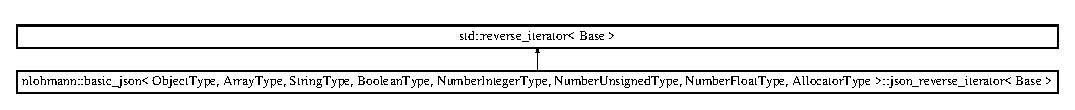
\includegraphics[height=1.036078cm]{classnlohmann_1_1basic__json_1_1json__reverse__iterator}
\end{center}
\end{figure}
\subsection*{Public Types}
\begin{DoxyCompactItemize}
\item 
using \hyperlink{classnlohmann_1_1basic__json_1_1json__reverse__iterator_a9ebc4c99e6fc90c965af0f39ad2ca70e}{base\+\_\+iterator} = std\+::reverse\+\_\+iterator$<$ Base $>$
\begin{DoxyCompactList}\small\item\em shortcut to the reverse iterator adaptor \end{DoxyCompactList}\item 
using \hyperlink{classnlohmann_1_1basic__json_1_1json__reverse__iterator_a7265535f39299824f9712a2ca15013c3}{reference} = typename Base\+::reference
\begin{DoxyCompactList}\small\item\em the reference type for the pointed-\/to element \end{DoxyCompactList}\end{DoxyCompactItemize}
\subsection*{Public Member Functions}
\begin{DoxyCompactItemize}
\item 
\hyperlink{classnlohmann_1_1basic__json_1_1json__reverse__iterator_a86c97bbb8ebe19aef4656cf796e30e99}{json\+\_\+reverse\+\_\+iterator} (const typename base\+\_\+iterator\+::iterator\+\_\+type \&it) noexcept
\begin{DoxyCompactList}\small\item\em create reverse iterator from iterator \end{DoxyCompactList}\item 
\hyperlink{classnlohmann_1_1basic__json_1_1json__reverse__iterator_a530f042e2ab1c83dddfc344931b0375a}{json\+\_\+reverse\+\_\+iterator} (const \hyperlink{classnlohmann_1_1basic__json_1_1json__reverse__iterator_a9ebc4c99e6fc90c965af0f39ad2ca70e}{base\+\_\+iterator} \&it) noexcept
\begin{DoxyCompactList}\small\item\em create reverse iterator from base class \end{DoxyCompactList}\item 
\hyperlink{classnlohmann_1_1basic__json_1_1json__reverse__iterator}{json\+\_\+reverse\+\_\+iterator} \hyperlink{classnlohmann_1_1basic__json_1_1json__reverse__iterator_a545a8204cfd6836eb85abc3113a0bb28}{operator++} (\hyperlink{tk_8h_a83f82f76e7fed06f4c49d2db94028a6d}{int})
\begin{DoxyCompactList}\small\item\em post-\/increment (it++) \end{DoxyCompactList}\item 
\hyperlink{classnlohmann_1_1basic__json_1_1json__reverse__iterator}{json\+\_\+reverse\+\_\+iterator} \& \hyperlink{classnlohmann_1_1basic__json_1_1json__reverse__iterator_a4aede52d6ee253a510897518b59e09c0}{operator++} ()
\begin{DoxyCompactList}\small\item\em pre-\/increment (++it) \end{DoxyCompactList}\item 
\hyperlink{classnlohmann_1_1basic__json_1_1json__reverse__iterator}{json\+\_\+reverse\+\_\+iterator} \hyperlink{classnlohmann_1_1basic__json_1_1json__reverse__iterator_a693439bffe56a9a8cf53bc4a06b911ff}{operator-\/-\/} (\hyperlink{tk_8h_a83f82f76e7fed06f4c49d2db94028a6d}{int})
\begin{DoxyCompactList}\small\item\em post-\/decrement (it--) \end{DoxyCompactList}\item 
\hyperlink{classnlohmann_1_1basic__json_1_1json__reverse__iterator}{json\+\_\+reverse\+\_\+iterator} \& \hyperlink{classnlohmann_1_1basic__json_1_1json__reverse__iterator_a563a7bd281e9919798d18396107fb05c}{operator-\/-\/} ()
\begin{DoxyCompactList}\small\item\em pre-\/decrement (--it) \end{DoxyCompactList}\item 
\hyperlink{classnlohmann_1_1basic__json_1_1json__reverse__iterator}{json\+\_\+reverse\+\_\+iterator} \& \hyperlink{classnlohmann_1_1basic__json_1_1json__reverse__iterator_a9accc9dd9f9033f50c0ab6bcf337ffe0}{operator+=} (\hyperlink{classnlohmann_1_1basic__json_aec316934a555dd1acdd3600e5d4a4cdf}{difference\+\_\+type} i)
\begin{DoxyCompactList}\small\item\em add to iterator \end{DoxyCompactList}\item 
\hyperlink{classnlohmann_1_1basic__json_1_1json__reverse__iterator}{json\+\_\+reverse\+\_\+iterator} \hyperlink{classnlohmann_1_1basic__json_1_1json__reverse__iterator_a99ee137dab7e5c948457f6a5321b54b1}{operator+} (\hyperlink{classnlohmann_1_1basic__json_aec316934a555dd1acdd3600e5d4a4cdf}{difference\+\_\+type} i) const 
\begin{DoxyCompactList}\small\item\em add to iterator \end{DoxyCompactList}\item 
\hyperlink{classnlohmann_1_1basic__json_1_1json__reverse__iterator}{json\+\_\+reverse\+\_\+iterator} \hyperlink{classnlohmann_1_1basic__json_1_1json__reverse__iterator_ac2634bee082633671125e909dffad40a}{operator-\/} (\hyperlink{classnlohmann_1_1basic__json_aec316934a555dd1acdd3600e5d4a4cdf}{difference\+\_\+type} i) const 
\begin{DoxyCompactList}\small\item\em subtract from iterator \end{DoxyCompactList}\item 
\hyperlink{classnlohmann_1_1basic__json_aec316934a555dd1acdd3600e5d4a4cdf}{difference\+\_\+type} \hyperlink{classnlohmann_1_1basic__json_1_1json__reverse__iterator_a115fae3dd8ae02669fedae0545ce1cbc}{operator-\/} (const \hyperlink{classnlohmann_1_1basic__json_1_1json__reverse__iterator}{json\+\_\+reverse\+\_\+iterator} \&other) const 
\begin{DoxyCompactList}\small\item\em return difference \end{DoxyCompactList}\item 
\hyperlink{classnlohmann_1_1basic__json_1_1json__reverse__iterator_a7265535f39299824f9712a2ca15013c3}{reference} \hyperlink{classnlohmann_1_1basic__json_1_1json__reverse__iterator_ad4ec2bbb8347e7aa3b58e616fd6c7f40}{operator\mbox{[}$\,$\mbox{]}} (\hyperlink{classnlohmann_1_1basic__json_aec316934a555dd1acdd3600e5d4a4cdf}{difference\+\_\+type} n) const 
\begin{DoxyCompactList}\small\item\em access to successor \end{DoxyCompactList}\item 
object\+\_\+t\+::key\+\_\+type \hyperlink{classnlohmann_1_1basic__json_1_1json__reverse__iterator_acecae6d237fcf14c909fb42b9d2e2955}{key} () const 
\begin{DoxyCompactList}\small\item\em return the key of an object iterator \end{DoxyCompactList}\item 
\hyperlink{classnlohmann_1_1basic__json_1_1json__reverse__iterator_a7265535f39299824f9712a2ca15013c3}{reference} \hyperlink{classnlohmann_1_1basic__json_1_1json__reverse__iterator_aca5116682e206dac48f8a56716a3280b}{value} () const 
\begin{DoxyCompactList}\small\item\em return the value of an iterator \end{DoxyCompactList}\end{DoxyCompactItemize}


\subsection{Detailed Description}
\subsubsection*{template$<$template$<$ typename U, typename V, typename...\+Args $>$ class Object\+Type = std\+::map, template$<$ typename U, typename...\+Args $>$ class Array\+Type = std\+::vector, class String\+Type = std\+::string, class Boolean\+Type = bool, class Number\+Integer\+Type = std\+::int64\+\_\+t, class Number\+Unsigned\+Type = std\+::uint64\+\_\+t, class Number\+Float\+Type = double, template$<$ typename U $>$ class Allocator\+Type = std\+::allocator$>$\\*
template$<$typename Base$>$\\*
class nlohmann\+::basic\+\_\+json$<$ Object\+Type, Array\+Type, String\+Type, Boolean\+Type, Number\+Integer\+Type, Number\+Unsigned\+Type, Number\+Float\+Type, Allocator\+Type $>$\+::json\+\_\+reverse\+\_\+iterator$<$ Base $>$}

a template for a reverse iterator class 


\begin{DoxyTemplParams}{Template Parameters}
{\em Base} & the base iterator type to reverse. Valid types are \hyperlink{classnlohmann_1_1basic__json_1_1iterator}{iterator} (to create \hyperlink{classnlohmann_1_1basic__json_a2f1f83aa187a56dc5ec7a7027065ac8a}{reverse\+\_\+iterator}) and \hyperlink{classnlohmann_1_1basic__json_1_1const__iterator}{const\+\_\+iterator} (to create \hyperlink{classnlohmann_1_1basic__json_ae336fff01f4b78e3e16e5008dc8dbc00}{const\+\_\+reverse\+\_\+iterator}).\\
\hline
\end{DoxyTemplParams}
The class satisfies the following concept requirements\+:
\begin{DoxyItemize}
\item \href{http://en.cppreference.com/w/cpp/concept/RandomAccessIterator}{\tt Random\+Access\+Iterator}\+: The iterator that can be moved to point (forward and backward) to any element in constant time.
\item \href{http://en.cppreference.com/w/cpp/concept/OutputIterator}{\tt Output\+Iterator}\+: It is possible to write to the pointed-\/to element (only if {\itshape Base} is \hyperlink{classnlohmann_1_1basic__json_1_1iterator}{iterator}).
\end{DoxyItemize}

\begin{DoxySince}{Since}
version 1.\+0.\+0 
\end{DoxySince}


\subsection{Member Typedef Documentation}
\index{nlohmann\+::basic\+\_\+json\+::json\+\_\+reverse\+\_\+iterator@{nlohmann\+::basic\+\_\+json\+::json\+\_\+reverse\+\_\+iterator}!base\+\_\+iterator@{base\+\_\+iterator}}
\index{base\+\_\+iterator@{base\+\_\+iterator}!nlohmann\+::basic\+\_\+json\+::json\+\_\+reverse\+\_\+iterator@{nlohmann\+::basic\+\_\+json\+::json\+\_\+reverse\+\_\+iterator}}
\subsubsection[{\texorpdfstring{base\+\_\+iterator}{base_iterator}}]{\setlength{\rightskip}{0pt plus 5cm}template$<$template$<$ typename U, typename V, typename...\+Args $>$ class Object\+Type = std\+::map, template$<$ typename U, typename...\+Args $>$ class Array\+Type = std\+::vector, class String\+Type  = std\+::string, class Boolean\+Type  = bool, class Number\+Integer\+Type  = std\+::int64\+\_\+t, class Number\+Unsigned\+Type  = std\+::uint64\+\_\+t, class Number\+Float\+Type  = double, template$<$ typename U $>$ class Allocator\+Type = std\+::allocator$>$ template$<$typename Base $>$ using {\bf nlohmann\+::basic\+\_\+json}$<$ Object\+Type, Array\+Type, String\+Type, Boolean\+Type, Number\+Integer\+Type, Number\+Unsigned\+Type, Number\+Float\+Type, Allocator\+Type $>$\+::{\bf json\+\_\+reverse\+\_\+iterator}$<$ Base $>$\+::{\bf base\+\_\+iterator} =  std\+::reverse\+\_\+iterator$<$Base$>$}\hypertarget{classnlohmann_1_1basic__json_1_1json__reverse__iterator_a9ebc4c99e6fc90c965af0f39ad2ca70e}{}\label{classnlohmann_1_1basic__json_1_1json__reverse__iterator_a9ebc4c99e6fc90c965af0f39ad2ca70e}


shortcut to the reverse iterator adaptor 

\index{nlohmann\+::basic\+\_\+json\+::json\+\_\+reverse\+\_\+iterator@{nlohmann\+::basic\+\_\+json\+::json\+\_\+reverse\+\_\+iterator}!reference@{reference}}
\index{reference@{reference}!nlohmann\+::basic\+\_\+json\+::json\+\_\+reverse\+\_\+iterator@{nlohmann\+::basic\+\_\+json\+::json\+\_\+reverse\+\_\+iterator}}
\subsubsection[{\texorpdfstring{reference}{reference}}]{\setlength{\rightskip}{0pt plus 5cm}template$<$template$<$ typename U, typename V, typename...\+Args $>$ class Object\+Type = std\+::map, template$<$ typename U, typename...\+Args $>$ class Array\+Type = std\+::vector, class String\+Type  = std\+::string, class Boolean\+Type  = bool, class Number\+Integer\+Type  = std\+::int64\+\_\+t, class Number\+Unsigned\+Type  = std\+::uint64\+\_\+t, class Number\+Float\+Type  = double, template$<$ typename U $>$ class Allocator\+Type = std\+::allocator$>$ template$<$typename Base $>$ using {\bf nlohmann\+::basic\+\_\+json}$<$ Object\+Type, Array\+Type, String\+Type, Boolean\+Type, Number\+Integer\+Type, Number\+Unsigned\+Type, Number\+Float\+Type, Allocator\+Type $>$\+::{\bf json\+\_\+reverse\+\_\+iterator}$<$ Base $>$\+::{\bf reference} =  typename Base\+::reference}\hypertarget{classnlohmann_1_1basic__json_1_1json__reverse__iterator_a7265535f39299824f9712a2ca15013c3}{}\label{classnlohmann_1_1basic__json_1_1json__reverse__iterator_a7265535f39299824f9712a2ca15013c3}


the reference type for the pointed-\/to element 



\subsection{Constructor \& Destructor Documentation}
\index{nlohmann\+::basic\+\_\+json\+::json\+\_\+reverse\+\_\+iterator@{nlohmann\+::basic\+\_\+json\+::json\+\_\+reverse\+\_\+iterator}!json\+\_\+reverse\+\_\+iterator@{json\+\_\+reverse\+\_\+iterator}}
\index{json\+\_\+reverse\+\_\+iterator@{json\+\_\+reverse\+\_\+iterator}!nlohmann\+::basic\+\_\+json\+::json\+\_\+reverse\+\_\+iterator@{nlohmann\+::basic\+\_\+json\+::json\+\_\+reverse\+\_\+iterator}}
\subsubsection[{\texorpdfstring{json\+\_\+reverse\+\_\+iterator(const typename base\+\_\+iterator\+::iterator\+\_\+type \&it) noexcept}{json_reverse_iterator(const typename base_iterator::iterator_type &it) noexcept}}]{\setlength{\rightskip}{0pt plus 5cm}template$<$template$<$ typename U, typename V, typename...\+Args $>$ class Object\+Type = std\+::map, template$<$ typename U, typename...\+Args $>$ class Array\+Type = std\+::vector, class String\+Type  = std\+::string, class Boolean\+Type  = bool, class Number\+Integer\+Type  = std\+::int64\+\_\+t, class Number\+Unsigned\+Type  = std\+::uint64\+\_\+t, class Number\+Float\+Type  = double, template$<$ typename U $>$ class Allocator\+Type = std\+::allocator$>$ template$<$typename Base $>$ {\bf nlohmann\+::basic\+\_\+json}$<$ Object\+Type, Array\+Type, String\+Type, Boolean\+Type, Number\+Integer\+Type, Number\+Unsigned\+Type, Number\+Float\+Type, Allocator\+Type $>$\+::{\bf json\+\_\+reverse\+\_\+iterator}$<$ Base $>$\+::{\bf json\+\_\+reverse\+\_\+iterator} (
\begin{DoxyParamCaption}
\item[{const typename base\+\_\+iterator\+::iterator\+\_\+type \&}]{it}
\end{DoxyParamCaption}
)\hspace{0.3cm}{\ttfamily [inline]}, {\ttfamily [noexcept]}}\hypertarget{classnlohmann_1_1basic__json_1_1json__reverse__iterator_a86c97bbb8ebe19aef4656cf796e30e99}{}\label{classnlohmann_1_1basic__json_1_1json__reverse__iterator_a86c97bbb8ebe19aef4656cf796e30e99}


create reverse iterator from iterator 

\index{nlohmann\+::basic\+\_\+json\+::json\+\_\+reverse\+\_\+iterator@{nlohmann\+::basic\+\_\+json\+::json\+\_\+reverse\+\_\+iterator}!json\+\_\+reverse\+\_\+iterator@{json\+\_\+reverse\+\_\+iterator}}
\index{json\+\_\+reverse\+\_\+iterator@{json\+\_\+reverse\+\_\+iterator}!nlohmann\+::basic\+\_\+json\+::json\+\_\+reverse\+\_\+iterator@{nlohmann\+::basic\+\_\+json\+::json\+\_\+reverse\+\_\+iterator}}
\subsubsection[{\texorpdfstring{json\+\_\+reverse\+\_\+iterator(const base\+\_\+iterator \&it) noexcept}{json_reverse_iterator(const base_iterator &it) noexcept}}]{\setlength{\rightskip}{0pt plus 5cm}template$<$template$<$ typename U, typename V, typename...\+Args $>$ class Object\+Type = std\+::map, template$<$ typename U, typename...\+Args $>$ class Array\+Type = std\+::vector, class String\+Type  = std\+::string, class Boolean\+Type  = bool, class Number\+Integer\+Type  = std\+::int64\+\_\+t, class Number\+Unsigned\+Type  = std\+::uint64\+\_\+t, class Number\+Float\+Type  = double, template$<$ typename U $>$ class Allocator\+Type = std\+::allocator$>$ template$<$typename Base $>$ {\bf nlohmann\+::basic\+\_\+json}$<$ Object\+Type, Array\+Type, String\+Type, Boolean\+Type, Number\+Integer\+Type, Number\+Unsigned\+Type, Number\+Float\+Type, Allocator\+Type $>$\+::{\bf json\+\_\+reverse\+\_\+iterator}$<$ Base $>$\+::{\bf json\+\_\+reverse\+\_\+iterator} (
\begin{DoxyParamCaption}
\item[{const {\bf base\+\_\+iterator} \&}]{it}
\end{DoxyParamCaption}
)\hspace{0.3cm}{\ttfamily [inline]}, {\ttfamily [noexcept]}}\hypertarget{classnlohmann_1_1basic__json_1_1json__reverse__iterator_a530f042e2ab1c83dddfc344931b0375a}{}\label{classnlohmann_1_1basic__json_1_1json__reverse__iterator_a530f042e2ab1c83dddfc344931b0375a}


create reverse iterator from base class 



\subsection{Member Function Documentation}
\index{nlohmann\+::basic\+\_\+json\+::json\+\_\+reverse\+\_\+iterator@{nlohmann\+::basic\+\_\+json\+::json\+\_\+reverse\+\_\+iterator}!key@{key}}
\index{key@{key}!nlohmann\+::basic\+\_\+json\+::json\+\_\+reverse\+\_\+iterator@{nlohmann\+::basic\+\_\+json\+::json\+\_\+reverse\+\_\+iterator}}
\subsubsection[{\texorpdfstring{key() const }{key() const }}]{\setlength{\rightskip}{0pt plus 5cm}template$<$template$<$ typename U, typename V, typename...\+Args $>$ class Object\+Type = std\+::map, template$<$ typename U, typename...\+Args $>$ class Array\+Type = std\+::vector, class String\+Type  = std\+::string, class Boolean\+Type  = bool, class Number\+Integer\+Type  = std\+::int64\+\_\+t, class Number\+Unsigned\+Type  = std\+::uint64\+\_\+t, class Number\+Float\+Type  = double, template$<$ typename U $>$ class Allocator\+Type = std\+::allocator$>$ template$<$typename Base $>$ object\+\_\+t\+::key\+\_\+type {\bf nlohmann\+::basic\+\_\+json}$<$ Object\+Type, Array\+Type, String\+Type, Boolean\+Type, Number\+Integer\+Type, Number\+Unsigned\+Type, Number\+Float\+Type, Allocator\+Type $>$\+::{\bf json\+\_\+reverse\+\_\+iterator}$<$ Base $>$\+::key (
\begin{DoxyParamCaption}
{}
\end{DoxyParamCaption}
) const\hspace{0.3cm}{\ttfamily [inline]}}\hypertarget{classnlohmann_1_1basic__json_1_1json__reverse__iterator_acecae6d237fcf14c909fb42b9d2e2955}{}\label{classnlohmann_1_1basic__json_1_1json__reverse__iterator_acecae6d237fcf14c909fb42b9d2e2955}


return the key of an object iterator 

\index{nlohmann\+::basic\+\_\+json\+::json\+\_\+reverse\+\_\+iterator@{nlohmann\+::basic\+\_\+json\+::json\+\_\+reverse\+\_\+iterator}!operator+@{operator+}}
\index{operator+@{operator+}!nlohmann\+::basic\+\_\+json\+::json\+\_\+reverse\+\_\+iterator@{nlohmann\+::basic\+\_\+json\+::json\+\_\+reverse\+\_\+iterator}}
\subsubsection[{\texorpdfstring{operator+(difference\+\_\+type i) const }{operator+(difference_type i) const }}]{\setlength{\rightskip}{0pt plus 5cm}template$<$template$<$ typename U, typename V, typename...\+Args $>$ class Object\+Type = std\+::map, template$<$ typename U, typename...\+Args $>$ class Array\+Type = std\+::vector, class String\+Type  = std\+::string, class Boolean\+Type  = bool, class Number\+Integer\+Type  = std\+::int64\+\_\+t, class Number\+Unsigned\+Type  = std\+::uint64\+\_\+t, class Number\+Float\+Type  = double, template$<$ typename U $>$ class Allocator\+Type = std\+::allocator$>$ template$<$typename Base $>$ {\bf json\+\_\+reverse\+\_\+iterator} {\bf nlohmann\+::basic\+\_\+json}$<$ Object\+Type, Array\+Type, String\+Type, Boolean\+Type, Number\+Integer\+Type, Number\+Unsigned\+Type, Number\+Float\+Type, Allocator\+Type $>$\+::{\bf json\+\_\+reverse\+\_\+iterator}$<$ Base $>$\+::operator+ (
\begin{DoxyParamCaption}
\item[{{\bf difference\+\_\+type}}]{i}
\end{DoxyParamCaption}
) const\hspace{0.3cm}{\ttfamily [inline]}}\hypertarget{classnlohmann_1_1basic__json_1_1json__reverse__iterator_a99ee137dab7e5c948457f6a5321b54b1}{}\label{classnlohmann_1_1basic__json_1_1json__reverse__iterator_a99ee137dab7e5c948457f6a5321b54b1}


add to iterator 

\index{nlohmann\+::basic\+\_\+json\+::json\+\_\+reverse\+\_\+iterator@{nlohmann\+::basic\+\_\+json\+::json\+\_\+reverse\+\_\+iterator}!operator++@{operator++}}
\index{operator++@{operator++}!nlohmann\+::basic\+\_\+json\+::json\+\_\+reverse\+\_\+iterator@{nlohmann\+::basic\+\_\+json\+::json\+\_\+reverse\+\_\+iterator}}
\subsubsection[{\texorpdfstring{operator++(int)}{operator++(int)}}]{\setlength{\rightskip}{0pt plus 5cm}template$<$template$<$ typename U, typename V, typename...\+Args $>$ class Object\+Type = std\+::map, template$<$ typename U, typename...\+Args $>$ class Array\+Type = std\+::vector, class String\+Type  = std\+::string, class Boolean\+Type  = bool, class Number\+Integer\+Type  = std\+::int64\+\_\+t, class Number\+Unsigned\+Type  = std\+::uint64\+\_\+t, class Number\+Float\+Type  = double, template$<$ typename U $>$ class Allocator\+Type = std\+::allocator$>$ template$<$typename Base $>$ {\bf json\+\_\+reverse\+\_\+iterator} {\bf nlohmann\+::basic\+\_\+json}$<$ Object\+Type, Array\+Type, String\+Type, Boolean\+Type, Number\+Integer\+Type, Number\+Unsigned\+Type, Number\+Float\+Type, Allocator\+Type $>$\+::{\bf json\+\_\+reverse\+\_\+iterator}$<$ Base $>$\+::operator++ (
\begin{DoxyParamCaption}
\item[{{\bf int}}]{}
\end{DoxyParamCaption}
)\hspace{0.3cm}{\ttfamily [inline]}}\hypertarget{classnlohmann_1_1basic__json_1_1json__reverse__iterator_a545a8204cfd6836eb85abc3113a0bb28}{}\label{classnlohmann_1_1basic__json_1_1json__reverse__iterator_a545a8204cfd6836eb85abc3113a0bb28}


post-\/increment (it++) 

\index{nlohmann\+::basic\+\_\+json\+::json\+\_\+reverse\+\_\+iterator@{nlohmann\+::basic\+\_\+json\+::json\+\_\+reverse\+\_\+iterator}!operator++@{operator++}}
\index{operator++@{operator++}!nlohmann\+::basic\+\_\+json\+::json\+\_\+reverse\+\_\+iterator@{nlohmann\+::basic\+\_\+json\+::json\+\_\+reverse\+\_\+iterator}}
\subsubsection[{\texorpdfstring{operator++()}{operator++()}}]{\setlength{\rightskip}{0pt plus 5cm}template$<$template$<$ typename U, typename V, typename...\+Args $>$ class Object\+Type = std\+::map, template$<$ typename U, typename...\+Args $>$ class Array\+Type = std\+::vector, class String\+Type  = std\+::string, class Boolean\+Type  = bool, class Number\+Integer\+Type  = std\+::int64\+\_\+t, class Number\+Unsigned\+Type  = std\+::uint64\+\_\+t, class Number\+Float\+Type  = double, template$<$ typename U $>$ class Allocator\+Type = std\+::allocator$>$ template$<$typename Base $>$ {\bf json\+\_\+reverse\+\_\+iterator}\& {\bf nlohmann\+::basic\+\_\+json}$<$ Object\+Type, Array\+Type, String\+Type, Boolean\+Type, Number\+Integer\+Type, Number\+Unsigned\+Type, Number\+Float\+Type, Allocator\+Type $>$\+::{\bf json\+\_\+reverse\+\_\+iterator}$<$ Base $>$\+::operator++ (
\begin{DoxyParamCaption}
{}
\end{DoxyParamCaption}
)\hspace{0.3cm}{\ttfamily [inline]}}\hypertarget{classnlohmann_1_1basic__json_1_1json__reverse__iterator_a4aede52d6ee253a510897518b59e09c0}{}\label{classnlohmann_1_1basic__json_1_1json__reverse__iterator_a4aede52d6ee253a510897518b59e09c0}


pre-\/increment (++it) 

\index{nlohmann\+::basic\+\_\+json\+::json\+\_\+reverse\+\_\+iterator@{nlohmann\+::basic\+\_\+json\+::json\+\_\+reverse\+\_\+iterator}!operator+=@{operator+=}}
\index{operator+=@{operator+=}!nlohmann\+::basic\+\_\+json\+::json\+\_\+reverse\+\_\+iterator@{nlohmann\+::basic\+\_\+json\+::json\+\_\+reverse\+\_\+iterator}}
\subsubsection[{\texorpdfstring{operator+=(difference\+\_\+type i)}{operator+=(difference_type i)}}]{\setlength{\rightskip}{0pt plus 5cm}template$<$template$<$ typename U, typename V, typename...\+Args $>$ class Object\+Type = std\+::map, template$<$ typename U, typename...\+Args $>$ class Array\+Type = std\+::vector, class String\+Type  = std\+::string, class Boolean\+Type  = bool, class Number\+Integer\+Type  = std\+::int64\+\_\+t, class Number\+Unsigned\+Type  = std\+::uint64\+\_\+t, class Number\+Float\+Type  = double, template$<$ typename U $>$ class Allocator\+Type = std\+::allocator$>$ template$<$typename Base $>$ {\bf json\+\_\+reverse\+\_\+iterator}\& {\bf nlohmann\+::basic\+\_\+json}$<$ Object\+Type, Array\+Type, String\+Type, Boolean\+Type, Number\+Integer\+Type, Number\+Unsigned\+Type, Number\+Float\+Type, Allocator\+Type $>$\+::{\bf json\+\_\+reverse\+\_\+iterator}$<$ Base $>$\+::operator+= (
\begin{DoxyParamCaption}
\item[{{\bf difference\+\_\+type}}]{i}
\end{DoxyParamCaption}
)\hspace{0.3cm}{\ttfamily [inline]}}\hypertarget{classnlohmann_1_1basic__json_1_1json__reverse__iterator_a9accc9dd9f9033f50c0ab6bcf337ffe0}{}\label{classnlohmann_1_1basic__json_1_1json__reverse__iterator_a9accc9dd9f9033f50c0ab6bcf337ffe0}


add to iterator 

\index{nlohmann\+::basic\+\_\+json\+::json\+\_\+reverse\+\_\+iterator@{nlohmann\+::basic\+\_\+json\+::json\+\_\+reverse\+\_\+iterator}!operator-\/@{operator-\/}}
\index{operator-\/@{operator-\/}!nlohmann\+::basic\+\_\+json\+::json\+\_\+reverse\+\_\+iterator@{nlohmann\+::basic\+\_\+json\+::json\+\_\+reverse\+\_\+iterator}}
\subsubsection[{\texorpdfstring{operator-\/(difference\+\_\+type i) const }{operator-(difference_type i) const }}]{\setlength{\rightskip}{0pt plus 5cm}template$<$template$<$ typename U, typename V, typename...\+Args $>$ class Object\+Type = std\+::map, template$<$ typename U, typename...\+Args $>$ class Array\+Type = std\+::vector, class String\+Type  = std\+::string, class Boolean\+Type  = bool, class Number\+Integer\+Type  = std\+::int64\+\_\+t, class Number\+Unsigned\+Type  = std\+::uint64\+\_\+t, class Number\+Float\+Type  = double, template$<$ typename U $>$ class Allocator\+Type = std\+::allocator$>$ template$<$typename Base $>$ {\bf json\+\_\+reverse\+\_\+iterator} {\bf nlohmann\+::basic\+\_\+json}$<$ Object\+Type, Array\+Type, String\+Type, Boolean\+Type, Number\+Integer\+Type, Number\+Unsigned\+Type, Number\+Float\+Type, Allocator\+Type $>$\+::{\bf json\+\_\+reverse\+\_\+iterator}$<$ Base $>$\+::operator-\/ (
\begin{DoxyParamCaption}
\item[{{\bf difference\+\_\+type}}]{i}
\end{DoxyParamCaption}
) const\hspace{0.3cm}{\ttfamily [inline]}}\hypertarget{classnlohmann_1_1basic__json_1_1json__reverse__iterator_ac2634bee082633671125e909dffad40a}{}\label{classnlohmann_1_1basic__json_1_1json__reverse__iterator_ac2634bee082633671125e909dffad40a}


subtract from iterator 

\index{nlohmann\+::basic\+\_\+json\+::json\+\_\+reverse\+\_\+iterator@{nlohmann\+::basic\+\_\+json\+::json\+\_\+reverse\+\_\+iterator}!operator-\/@{operator-\/}}
\index{operator-\/@{operator-\/}!nlohmann\+::basic\+\_\+json\+::json\+\_\+reverse\+\_\+iterator@{nlohmann\+::basic\+\_\+json\+::json\+\_\+reverse\+\_\+iterator}}
\subsubsection[{\texorpdfstring{operator-\/(const json\+\_\+reverse\+\_\+iterator \&other) const }{operator-(const json_reverse_iterator &other) const }}]{\setlength{\rightskip}{0pt plus 5cm}template$<$template$<$ typename U, typename V, typename...\+Args $>$ class Object\+Type = std\+::map, template$<$ typename U, typename...\+Args $>$ class Array\+Type = std\+::vector, class String\+Type  = std\+::string, class Boolean\+Type  = bool, class Number\+Integer\+Type  = std\+::int64\+\_\+t, class Number\+Unsigned\+Type  = std\+::uint64\+\_\+t, class Number\+Float\+Type  = double, template$<$ typename U $>$ class Allocator\+Type = std\+::allocator$>$ template$<$typename Base $>$ {\bf difference\+\_\+type} {\bf nlohmann\+::basic\+\_\+json}$<$ Object\+Type, Array\+Type, String\+Type, Boolean\+Type, Number\+Integer\+Type, Number\+Unsigned\+Type, Number\+Float\+Type, Allocator\+Type $>$\+::{\bf json\+\_\+reverse\+\_\+iterator}$<$ Base $>$\+::operator-\/ (
\begin{DoxyParamCaption}
\item[{const {\bf json\+\_\+reverse\+\_\+iterator}$<$ Base $>$ \&}]{other}
\end{DoxyParamCaption}
) const\hspace{0.3cm}{\ttfamily [inline]}}\hypertarget{classnlohmann_1_1basic__json_1_1json__reverse__iterator_a115fae3dd8ae02669fedae0545ce1cbc}{}\label{classnlohmann_1_1basic__json_1_1json__reverse__iterator_a115fae3dd8ae02669fedae0545ce1cbc}


return difference 

\index{nlohmann\+::basic\+\_\+json\+::json\+\_\+reverse\+\_\+iterator@{nlohmann\+::basic\+\_\+json\+::json\+\_\+reverse\+\_\+iterator}!operator-\/-\/@{operator-\/-\/}}
\index{operator-\/-\/@{operator-\/-\/}!nlohmann\+::basic\+\_\+json\+::json\+\_\+reverse\+\_\+iterator@{nlohmann\+::basic\+\_\+json\+::json\+\_\+reverse\+\_\+iterator}}
\subsubsection[{\texorpdfstring{operator-\/-\/(int)}{operator--(int)}}]{\setlength{\rightskip}{0pt plus 5cm}template$<$template$<$ typename U, typename V, typename...\+Args $>$ class Object\+Type = std\+::map, template$<$ typename U, typename...\+Args $>$ class Array\+Type = std\+::vector, class String\+Type  = std\+::string, class Boolean\+Type  = bool, class Number\+Integer\+Type  = std\+::int64\+\_\+t, class Number\+Unsigned\+Type  = std\+::uint64\+\_\+t, class Number\+Float\+Type  = double, template$<$ typename U $>$ class Allocator\+Type = std\+::allocator$>$ template$<$typename Base $>$ {\bf json\+\_\+reverse\+\_\+iterator} {\bf nlohmann\+::basic\+\_\+json}$<$ Object\+Type, Array\+Type, String\+Type, Boolean\+Type, Number\+Integer\+Type, Number\+Unsigned\+Type, Number\+Float\+Type, Allocator\+Type $>$\+::{\bf json\+\_\+reverse\+\_\+iterator}$<$ Base $>$\+::operator-\/-\/ (
\begin{DoxyParamCaption}
\item[{{\bf int}}]{}
\end{DoxyParamCaption}
)\hspace{0.3cm}{\ttfamily [inline]}}\hypertarget{classnlohmann_1_1basic__json_1_1json__reverse__iterator_a693439bffe56a9a8cf53bc4a06b911ff}{}\label{classnlohmann_1_1basic__json_1_1json__reverse__iterator_a693439bffe56a9a8cf53bc4a06b911ff}


post-\/decrement (it--) 

\index{nlohmann\+::basic\+\_\+json\+::json\+\_\+reverse\+\_\+iterator@{nlohmann\+::basic\+\_\+json\+::json\+\_\+reverse\+\_\+iterator}!operator-\/-\/@{operator-\/-\/}}
\index{operator-\/-\/@{operator-\/-\/}!nlohmann\+::basic\+\_\+json\+::json\+\_\+reverse\+\_\+iterator@{nlohmann\+::basic\+\_\+json\+::json\+\_\+reverse\+\_\+iterator}}
\subsubsection[{\texorpdfstring{operator-\/-\/()}{operator--()}}]{\setlength{\rightskip}{0pt plus 5cm}template$<$template$<$ typename U, typename V, typename...\+Args $>$ class Object\+Type = std\+::map, template$<$ typename U, typename...\+Args $>$ class Array\+Type = std\+::vector, class String\+Type  = std\+::string, class Boolean\+Type  = bool, class Number\+Integer\+Type  = std\+::int64\+\_\+t, class Number\+Unsigned\+Type  = std\+::uint64\+\_\+t, class Number\+Float\+Type  = double, template$<$ typename U $>$ class Allocator\+Type = std\+::allocator$>$ template$<$typename Base $>$ {\bf json\+\_\+reverse\+\_\+iterator}\& {\bf nlohmann\+::basic\+\_\+json}$<$ Object\+Type, Array\+Type, String\+Type, Boolean\+Type, Number\+Integer\+Type, Number\+Unsigned\+Type, Number\+Float\+Type, Allocator\+Type $>$\+::{\bf json\+\_\+reverse\+\_\+iterator}$<$ Base $>$\+::operator-\/-\/ (
\begin{DoxyParamCaption}
{}
\end{DoxyParamCaption}
)\hspace{0.3cm}{\ttfamily [inline]}}\hypertarget{classnlohmann_1_1basic__json_1_1json__reverse__iterator_a563a7bd281e9919798d18396107fb05c}{}\label{classnlohmann_1_1basic__json_1_1json__reverse__iterator_a563a7bd281e9919798d18396107fb05c}


pre-\/decrement (--it) 

\index{nlohmann\+::basic\+\_\+json\+::json\+\_\+reverse\+\_\+iterator@{nlohmann\+::basic\+\_\+json\+::json\+\_\+reverse\+\_\+iterator}!operator\mbox{[}$\,$\mbox{]}@{operator[]}}
\index{operator\mbox{[}$\,$\mbox{]}@{operator[]}!nlohmann\+::basic\+\_\+json\+::json\+\_\+reverse\+\_\+iterator@{nlohmann\+::basic\+\_\+json\+::json\+\_\+reverse\+\_\+iterator}}
\subsubsection[{\texorpdfstring{operator[](difference\+\_\+type n) const }{operator[](difference_type n) const }}]{\setlength{\rightskip}{0pt plus 5cm}template$<$template$<$ typename U, typename V, typename...\+Args $>$ class Object\+Type = std\+::map, template$<$ typename U, typename...\+Args $>$ class Array\+Type = std\+::vector, class String\+Type  = std\+::string, class Boolean\+Type  = bool, class Number\+Integer\+Type  = std\+::int64\+\_\+t, class Number\+Unsigned\+Type  = std\+::uint64\+\_\+t, class Number\+Float\+Type  = double, template$<$ typename U $>$ class Allocator\+Type = std\+::allocator$>$ template$<$typename Base $>$ {\bf reference} {\bf nlohmann\+::basic\+\_\+json}$<$ Object\+Type, Array\+Type, String\+Type, Boolean\+Type, Number\+Integer\+Type, Number\+Unsigned\+Type, Number\+Float\+Type, Allocator\+Type $>$\+::{\bf json\+\_\+reverse\+\_\+iterator}$<$ Base $>$\+::operator\mbox{[}$\,$\mbox{]} (
\begin{DoxyParamCaption}
\item[{{\bf difference\+\_\+type}}]{n}
\end{DoxyParamCaption}
) const\hspace{0.3cm}{\ttfamily [inline]}}\hypertarget{classnlohmann_1_1basic__json_1_1json__reverse__iterator_ad4ec2bbb8347e7aa3b58e616fd6c7f40}{}\label{classnlohmann_1_1basic__json_1_1json__reverse__iterator_ad4ec2bbb8347e7aa3b58e616fd6c7f40}


access to successor 

\index{nlohmann\+::basic\+\_\+json\+::json\+\_\+reverse\+\_\+iterator@{nlohmann\+::basic\+\_\+json\+::json\+\_\+reverse\+\_\+iterator}!value@{value}}
\index{value@{value}!nlohmann\+::basic\+\_\+json\+::json\+\_\+reverse\+\_\+iterator@{nlohmann\+::basic\+\_\+json\+::json\+\_\+reverse\+\_\+iterator}}
\subsubsection[{\texorpdfstring{value() const }{value() const }}]{\setlength{\rightskip}{0pt plus 5cm}template$<$template$<$ typename U, typename V, typename...\+Args $>$ class Object\+Type = std\+::map, template$<$ typename U, typename...\+Args $>$ class Array\+Type = std\+::vector, class String\+Type  = std\+::string, class Boolean\+Type  = bool, class Number\+Integer\+Type  = std\+::int64\+\_\+t, class Number\+Unsigned\+Type  = std\+::uint64\+\_\+t, class Number\+Float\+Type  = double, template$<$ typename U $>$ class Allocator\+Type = std\+::allocator$>$ template$<$typename Base $>$ {\bf reference} {\bf nlohmann\+::basic\+\_\+json}$<$ Object\+Type, Array\+Type, String\+Type, Boolean\+Type, Number\+Integer\+Type, Number\+Unsigned\+Type, Number\+Float\+Type, Allocator\+Type $>$\+::{\bf json\+\_\+reverse\+\_\+iterator}$<$ Base $>$\+::{\bf value} (
\begin{DoxyParamCaption}
{}
\end{DoxyParamCaption}
) const\hspace{0.3cm}{\ttfamily [inline]}}\hypertarget{classnlohmann_1_1basic__json_1_1json__reverse__iterator_aca5116682e206dac48f8a56716a3280b}{}\label{classnlohmann_1_1basic__json_1_1json__reverse__iterator_aca5116682e206dac48f8a56716a3280b}


return the value of an iterator 



The documentation for this class was generated from the following file\+:\begin{DoxyCompactItemize}
\item 
/\+Users/michael/\+J\+U\+C\+E/projects/audealize-\/plugin/\+J\+U\+C\+E Modules/audealize\+\_\+module/utils/\hyperlink{json_8hpp}{json.\+hpp}\end{DoxyCompactItemize}

\hypertarget{classdsp_1_1mem__fixed__size__buffer}{}\section{dsp\+:\+:mem\+\_\+fixed\+\_\+size\+\_\+buffer$<$ N, T $>$ Class Template Reference}
\label{classdsp_1_1mem__fixed__size__buffer}\index{dsp\+::mem\+\_\+fixed\+\_\+size\+\_\+buffer$<$ N, T $>$@{dsp\+::mem\+\_\+fixed\+\_\+size\+\_\+buffer$<$ N, T $>$}}


{\ttfamily \#include $<$buffer.\+h$>$}

Inheritance diagram for dsp\+:\+:mem\+\_\+fixed\+\_\+size\+\_\+buffer$<$ N, T $>$\+:\begin{figure}[H]
\begin{center}
\leavevmode
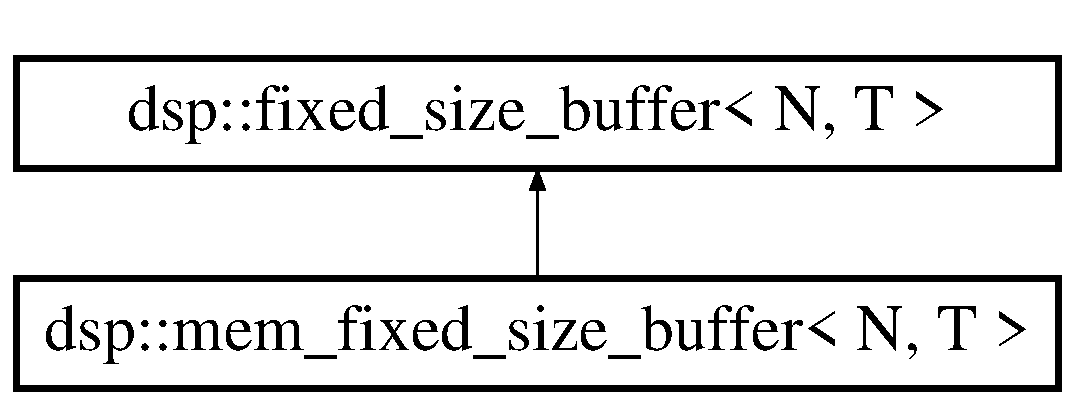
\includegraphics[height=2.000000cm]{classdsp_1_1mem__fixed__size__buffer}
\end{center}
\end{figure}
\subsection*{Public Member Functions}
\begin{DoxyCompactItemize}
\item 
\hyperlink{classdsp_1_1mem__fixed__size__buffer_afcab7849f108bac63d9e4f7eb20032b3}{mem\+\_\+fixed\+\_\+size\+\_\+buffer} (T ubuf\mbox{[}N\mbox{]})
\item 
\hyperlink{tk_8h_aba408b7cd755a96426e004c015f5de8e}{void} \hyperlink{classdsp_1_1mem__fixed__size__buffer_a1ade90c3ddcbd1a4656990ce6d01d6c9}{set\+\_\+data} (T buf\mbox{[}N\mbox{]})
\item 
T $\ast$ \hyperlink{classdsp_1_1mem__fixed__size__buffer_a1c66f7515b8455167ab0d3c7a33c0a53}{data} ()
\item 
const T $\ast$ \hyperlink{classdsp_1_1mem__fixed__size__buffer_aa5229ad32bd8790de3d08a5a0a59f7af}{data} () const 
\item 
T \& \hyperlink{classdsp_1_1mem__fixed__size__buffer_af1b0a0bd7aa13ce032db9973c7cc9a12}{operator\mbox{[}$\,$\mbox{]}} (\hyperlink{tk_8h_a83f82f76e7fed06f4c49d2db94028a6d}{int} \hyperlink{wn_8c_a1910d262855b71da353ed0d07a6c7823}{pos})
\item 
const T \& \hyperlink{classdsp_1_1mem__fixed__size__buffer_a8bfa99040e15d638a458dc1c194d98ea}{operator\mbox{[}$\,$\mbox{]}} (\hyperlink{tk_8h_a83f82f76e7fed06f4c49d2db94028a6d}{int} \hyperlink{wn_8c_a1910d262855b71da353ed0d07a6c7823}{pos}) const 
\end{DoxyCompactItemize}
\subsection*{Additional Inherited Members}


\subsection{Constructor \& Destructor Documentation}
\index{dsp\+::mem\+\_\+fixed\+\_\+size\+\_\+buffer@{dsp\+::mem\+\_\+fixed\+\_\+size\+\_\+buffer}!mem\+\_\+fixed\+\_\+size\+\_\+buffer@{mem\+\_\+fixed\+\_\+size\+\_\+buffer}}
\index{mem\+\_\+fixed\+\_\+size\+\_\+buffer@{mem\+\_\+fixed\+\_\+size\+\_\+buffer}!dsp\+::mem\+\_\+fixed\+\_\+size\+\_\+buffer@{dsp\+::mem\+\_\+fixed\+\_\+size\+\_\+buffer}}
\subsubsection[{\texorpdfstring{mem\+\_\+fixed\+\_\+size\+\_\+buffer(\+T ubuf[N])}{mem_fixed_size_buffer(T ubuf[N])}}]{\setlength{\rightskip}{0pt plus 5cm}template$<$int N, class T  = float$>$ {\bf dsp\+::mem\+\_\+fixed\+\_\+size\+\_\+buffer}$<$ N, T $>$\+::{\bf mem\+\_\+fixed\+\_\+size\+\_\+buffer} (
\begin{DoxyParamCaption}
\item[{T}]{ubuf\mbox{[}\+N\mbox{]}}
\end{DoxyParamCaption}
)\hspace{0.3cm}{\ttfamily [inline]}}\hypertarget{classdsp_1_1mem__fixed__size__buffer_afcab7849f108bac63d9e4f7eb20032b3}{}\label{classdsp_1_1mem__fixed__size__buffer_afcab7849f108bac63d9e4f7eb20032b3}


\subsection{Member Function Documentation}
\index{dsp\+::mem\+\_\+fixed\+\_\+size\+\_\+buffer@{dsp\+::mem\+\_\+fixed\+\_\+size\+\_\+buffer}!data@{data}}
\index{data@{data}!dsp\+::mem\+\_\+fixed\+\_\+size\+\_\+buffer@{dsp\+::mem\+\_\+fixed\+\_\+size\+\_\+buffer}}
\subsubsection[{\texorpdfstring{data()}{data()}}]{\setlength{\rightskip}{0pt plus 5cm}template$<$int N, class T  = float$>$ T$\ast$ {\bf dsp\+::mem\+\_\+fixed\+\_\+size\+\_\+buffer}$<$ N, T $>$\+::data (
\begin{DoxyParamCaption}
{}
\end{DoxyParamCaption}
)\hspace{0.3cm}{\ttfamily [inline]}}\hypertarget{classdsp_1_1mem__fixed__size__buffer_a1c66f7515b8455167ab0d3c7a33c0a53}{}\label{classdsp_1_1mem__fixed__size__buffer_a1c66f7515b8455167ab0d3c7a33c0a53}
\index{dsp\+::mem\+\_\+fixed\+\_\+size\+\_\+buffer@{dsp\+::mem\+\_\+fixed\+\_\+size\+\_\+buffer}!data@{data}}
\index{data@{data}!dsp\+::mem\+\_\+fixed\+\_\+size\+\_\+buffer@{dsp\+::mem\+\_\+fixed\+\_\+size\+\_\+buffer}}
\subsubsection[{\texorpdfstring{data() const }{data() const }}]{\setlength{\rightskip}{0pt plus 5cm}template$<$int N, class T  = float$>$ const T$\ast$ {\bf dsp\+::mem\+\_\+fixed\+\_\+size\+\_\+buffer}$<$ N, T $>$\+::data (
\begin{DoxyParamCaption}
{}
\end{DoxyParamCaption}
) const\hspace{0.3cm}{\ttfamily [inline]}}\hypertarget{classdsp_1_1mem__fixed__size__buffer_aa5229ad32bd8790de3d08a5a0a59f7af}{}\label{classdsp_1_1mem__fixed__size__buffer_aa5229ad32bd8790de3d08a5a0a59f7af}
\index{dsp\+::mem\+\_\+fixed\+\_\+size\+\_\+buffer@{dsp\+::mem\+\_\+fixed\+\_\+size\+\_\+buffer}!operator\mbox{[}$\,$\mbox{]}@{operator[]}}
\index{operator\mbox{[}$\,$\mbox{]}@{operator[]}!dsp\+::mem\+\_\+fixed\+\_\+size\+\_\+buffer@{dsp\+::mem\+\_\+fixed\+\_\+size\+\_\+buffer}}
\subsubsection[{\texorpdfstring{operator[](int pos)}{operator[](int pos)}}]{\setlength{\rightskip}{0pt plus 5cm}template$<$int N, class T  = float$>$ T\& {\bf dsp\+::mem\+\_\+fixed\+\_\+size\+\_\+buffer}$<$ N, T $>$\+::operator\mbox{[}$\,$\mbox{]} (
\begin{DoxyParamCaption}
\item[{{\bf int}}]{pos}
\end{DoxyParamCaption}
)\hspace{0.3cm}{\ttfamily [inline]}}\hypertarget{classdsp_1_1mem__fixed__size__buffer_af1b0a0bd7aa13ce032db9973c7cc9a12}{}\label{classdsp_1_1mem__fixed__size__buffer_af1b0a0bd7aa13ce032db9973c7cc9a12}
\index{dsp\+::mem\+\_\+fixed\+\_\+size\+\_\+buffer@{dsp\+::mem\+\_\+fixed\+\_\+size\+\_\+buffer}!operator\mbox{[}$\,$\mbox{]}@{operator[]}}
\index{operator\mbox{[}$\,$\mbox{]}@{operator[]}!dsp\+::mem\+\_\+fixed\+\_\+size\+\_\+buffer@{dsp\+::mem\+\_\+fixed\+\_\+size\+\_\+buffer}}
\subsubsection[{\texorpdfstring{operator[](int pos) const }{operator[](int pos) const }}]{\setlength{\rightskip}{0pt plus 5cm}template$<$int N, class T  = float$>$ const T\& {\bf dsp\+::mem\+\_\+fixed\+\_\+size\+\_\+buffer}$<$ N, T $>$\+::operator\mbox{[}$\,$\mbox{]} (
\begin{DoxyParamCaption}
\item[{{\bf int}}]{pos}
\end{DoxyParamCaption}
) const\hspace{0.3cm}{\ttfamily [inline]}}\hypertarget{classdsp_1_1mem__fixed__size__buffer_a8bfa99040e15d638a458dc1c194d98ea}{}\label{classdsp_1_1mem__fixed__size__buffer_a8bfa99040e15d638a458dc1c194d98ea}
\index{dsp\+::mem\+\_\+fixed\+\_\+size\+\_\+buffer@{dsp\+::mem\+\_\+fixed\+\_\+size\+\_\+buffer}!set\+\_\+data@{set\+\_\+data}}
\index{set\+\_\+data@{set\+\_\+data}!dsp\+::mem\+\_\+fixed\+\_\+size\+\_\+buffer@{dsp\+::mem\+\_\+fixed\+\_\+size\+\_\+buffer}}
\subsubsection[{\texorpdfstring{set\+\_\+data(\+T buf[N])}{set_data(T buf[N])}}]{\setlength{\rightskip}{0pt plus 5cm}template$<$int N, class T  = float$>$ {\bf void} {\bf dsp\+::mem\+\_\+fixed\+\_\+size\+\_\+buffer}$<$ N, T $>$\+::set\+\_\+data (
\begin{DoxyParamCaption}
\item[{T}]{buf\mbox{[}\+N\mbox{]}}
\end{DoxyParamCaption}
)\hspace{0.3cm}{\ttfamily [inline]}}\hypertarget{classdsp_1_1mem__fixed__size__buffer_a1ade90c3ddcbd1a4656990ce6d01d6c9}{}\label{classdsp_1_1mem__fixed__size__buffer_a1ade90c3ddcbd1a4656990ce6d01d6c9}


The documentation for this class was generated from the following file\+:\begin{DoxyCompactItemize}
\item 
/\+Users/michael/\+J\+U\+C\+E/projects/audealize-\/plugin/\+J\+U\+C\+E Modules/audealize\+\_\+module/utils/calf\+\_\+dsp\+\_\+library/\hyperlink{buffer_8h}{buffer.\+h}\end{DoxyCompactItemize}

\hypertarget{classdsp_1_1mono__auto__buffer}{}\section{dsp\+:\+:mono\+\_\+auto\+\_\+buffer$<$ N, T $>$ Class Template Reference}
\label{classdsp_1_1mono__auto__buffer}\index{dsp\+::mono\+\_\+auto\+\_\+buffer$<$ N, T $>$@{dsp\+::mono\+\_\+auto\+\_\+buffer$<$ N, T $>$}}


this is useless for now  




{\ttfamily \#include $<$buffer.\+h$>$}

Inheritance diagram for dsp\+:\+:mono\+\_\+auto\+\_\+buffer$<$ N, T $>$\+:\begin{figure}[H]
\begin{center}
\leavevmode
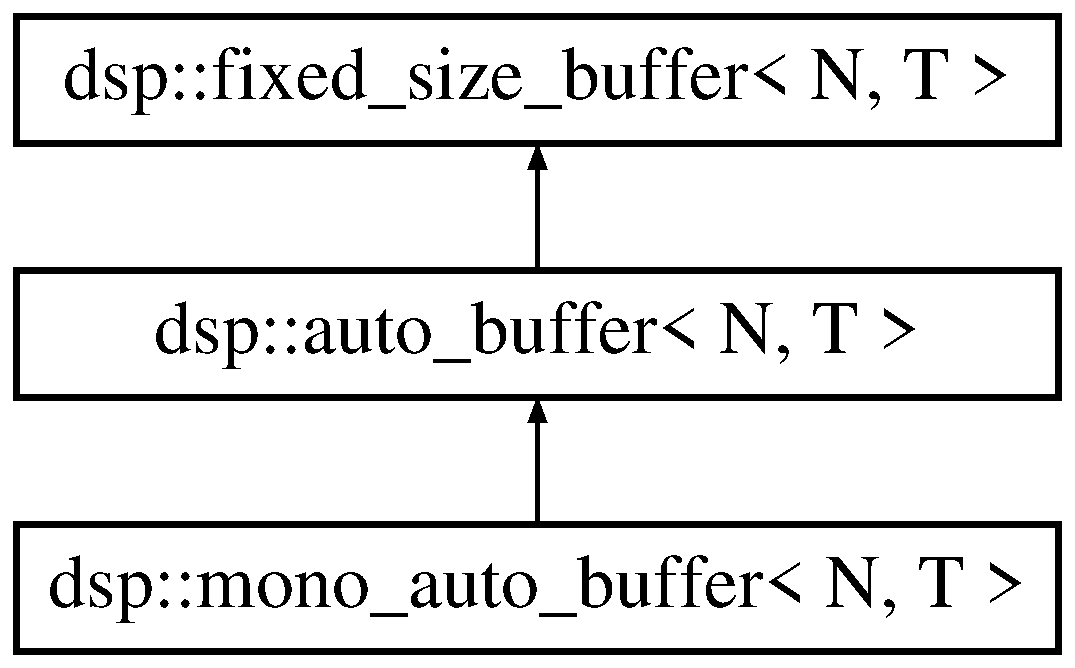
\includegraphics[height=3.000000cm]{classdsp_1_1mono__auto__buffer}
\end{center}
\end{figure}
\subsection*{Additional Inherited Members}


\subsection{Detailed Description}
\subsubsection*{template$<$int N, class T = float$>$\\*
class dsp\+::mono\+\_\+auto\+\_\+buffer$<$ N, T $>$}

this is useless for now 

The documentation for this class was generated from the following file\+:\begin{DoxyCompactItemize}
\item 
/\+Users/michael/\+J\+U\+C\+E/projects/audealize-\/plugin/\+J\+U\+C\+E Modules/audealize\+\_\+module/utils/calf\+\_\+dsp\+\_\+library/\hyperlink{buffer_8h}{buffer.\+h}\end{DoxyCompactItemize}

\hypertarget{class_audealize_1_1_n_channel_filter}{}\section{Audealize\+:\+:N\+Channel\+Filter Class Reference}
\label{class_audealize_1_1_n_channel_filter}\index{Audealize\+::\+N\+Channel\+Filter@{Audealize\+::\+N\+Channel\+Filter}}


{\ttfamily \#include $<$N\+Channel\+Filter.\+h$>$}

Inheritance diagram for Audealize\+:\+:N\+Channel\+Filter\+:\begin{figure}[H]
\begin{center}
\leavevmode
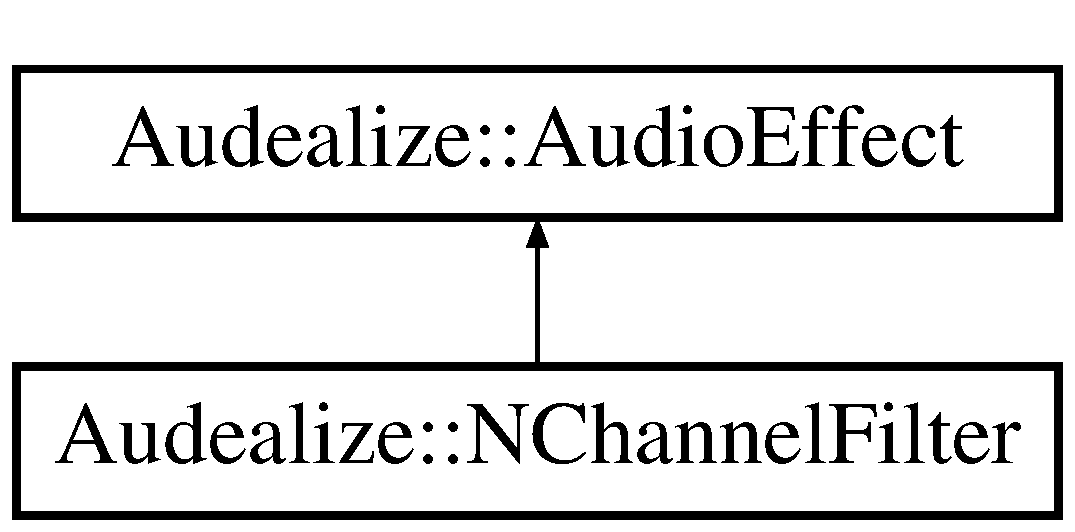
\includegraphics[height=2.000000cm]{class_audealize_1_1_n_channel_filter}
\end{center}
\end{figure}
\subsection*{Public Types}
\begin{DoxyCompactItemize}
\item 
enum \hyperlink{class_audealize_1_1_n_channel_filter_aa3b51c2ea2faf3df7c9b8e55fe96568d}{type} \{ \\*
\hyperlink{class_audealize_1_1_n_channel_filter_aa3b51c2ea2faf3df7c9b8e55fe96568daeea9759fdb6ec40965dc5582ef4b8d07}{bq\+\_\+type\+\_\+lowpass} = 0, 
\hyperlink{class_audealize_1_1_n_channel_filter_aa3b51c2ea2faf3df7c9b8e55fe96568daf2c73c23de5dbf784e796dff2e719505}{bq\+\_\+type\+\_\+highpass}, 
\hyperlink{class_audealize_1_1_n_channel_filter_aa3b51c2ea2faf3df7c9b8e55fe96568dab6181703666febaf3b6ca15c2c342f2f}{bq\+\_\+type\+\_\+bandpass}, 
\hyperlink{class_audealize_1_1_n_channel_filter_aa3b51c2ea2faf3df7c9b8e55fe96568da32cfe8bb5d44261f087ebdd6074debb6}{bq\+\_\+type\+\_\+notch}, 
\\*
\hyperlink{class_audealize_1_1_n_channel_filter_aa3b51c2ea2faf3df7c9b8e55fe96568daed82396d60dff469e7eabb04507cea40}{bq\+\_\+type\+\_\+peak}, 
\hyperlink{class_audealize_1_1_n_channel_filter_aa3b51c2ea2faf3df7c9b8e55fe96568da1def096bd4c43f3b83da70d7520b7fb1}{bq\+\_\+type\+\_\+lowshelf}, 
\hyperlink{class_audealize_1_1_n_channel_filter_aa3b51c2ea2faf3df7c9b8e55fe96568daaa91c04e635b6d257eb8d2ada57e1429}{bq\+\_\+type\+\_\+highshelf}
 \}
\end{DoxyCompactItemize}
\subsection*{Public Member Functions}
\begin{DoxyCompactItemize}
\item 
\hyperlink{class_audealize_1_1_n_channel_filter_acc6d3d78401e206842648266e95de06f}{N\+Channel\+Filter} ()
\item 
\hyperlink{class_audealize_1_1_n_channel_filter_a983b87834355f20e3f8ecdf8bd939c84}{N\+Channel\+Filter} (\hyperlink{tk_8h_a83f82f76e7fed06f4c49d2db94028a6d}{int} \hyperlink{class_audealize_1_1_n_channel_filter_aa3b51c2ea2faf3df7c9b8e55fe96568d}{type}, \hyperlink{tk_8h_a83f82f76e7fed06f4c49d2db94028a6d}{int} num\+Channels, float Fc, float Q, float gain\+DB, float sample\+Rate)
\item 
float \hyperlink{class_audealize_1_1_n_channel_filter_ad9e59288f93255e0c31e1e83dd80928f}{process\+Sample} (float sample, \hyperlink{tk_8h_a83f82f76e7fed06f4c49d2db94028a6d}{int} channel\+Idx)
\item 
\hyperlink{tk_8h_aba408b7cd755a96426e004c015f5de8e}{void} \hyperlink{class_audealize_1_1_n_channel_filter_a2d5867f9fb2c4c7b8f73ac5620ab7eb6}{set\+Filter} (\hyperlink{tk_8h_a83f82f76e7fed06f4c49d2db94028a6d}{int} \hyperlink{class_audealize_1_1_n_channel_filter_aa3b51c2ea2faf3df7c9b8e55fe96568d}{type}, float Fc, float Q, float gain\+DB, float sample\+Rate)
\item 
\hyperlink{tk_8h_aba408b7cd755a96426e004c015f5de8e}{void} \hyperlink{class_audealize_1_1_n_channel_filter_a4213694ea47179d3387e1c64288f29df}{set\+Freq} (float Fc)
\item 
\hyperlink{tk_8h_aba408b7cd755a96426e004c015f5de8e}{void} \hyperlink{class_audealize_1_1_n_channel_filter_ab104c9dfb0692cd0623dea3f22033fd5}{set\+Type} (\hyperlink{tk_8h_a83f82f76e7fed06f4c49d2db94028a6d}{int} \hyperlink{class_audealize_1_1_n_channel_filter_aa3b51c2ea2faf3df7c9b8e55fe96568d}{type})
\item 
\hyperlink{tk_8h_aba408b7cd755a96426e004c015f5de8e}{void} \hyperlink{class_audealize_1_1_n_channel_filter_a5c62308bbba1feb99c3d2fc633d3f055}{set\+Gain} (float gain\+DB)
\item 
\hyperlink{tk_8h_aba408b7cd755a96426e004c015f5de8e}{void} \hyperlink{class_audealize_1_1_n_channel_filter_ad901f2c36cad41011670f05badb7bf45}{set\+Num\+Channels} (\hyperlink{tk_8h_a83f82f76e7fed06f4c49d2db94028a6d}{int} num\+Channels)
\item 
\hyperlink{tk_8h_aba408b7cd755a96426e004c015f5de8e}{void} \hyperlink{class_audealize_1_1_n_channel_filter_ad8b99b93cbe402948f007c9dde8e48bf}{set\+Sample\+Rate} (float sample\+Rate)
\item 
\hyperlink{tk_8h_a83f82f76e7fed06f4c49d2db94028a6d}{int} \hyperlink{class_audealize_1_1_n_channel_filter_afa2ba7a3a53cb500f7263074427d63db}{get\+Num\+Channels} ()
\item 
\hyperlink{tk_8h_a83f82f76e7fed06f4c49d2db94028a6d}{int} \hyperlink{class_audealize_1_1_n_channel_filter_a1ff68a140343d7828506a920cfdf3325}{get\+Type} ()
\item 
float \hyperlink{class_audealize_1_1_n_channel_filter_a8f4d53307d5667c5c16d9d81cb3f0613}{get\+Freq} ()
\item 
float \hyperlink{class_audealize_1_1_n_channel_filter_a617f6a9421d661be1367e7a6834f3106}{get\+Gain} ()
\end{DoxyCompactItemize}
\subsection*{Additional Inherited Members}


\subsection{Member Enumeration Documentation}
\index{Audealize\+::\+N\+Channel\+Filter@{Audealize\+::\+N\+Channel\+Filter}!type@{type}}
\index{type@{type}!Audealize\+::\+N\+Channel\+Filter@{Audealize\+::\+N\+Channel\+Filter}}
\subsubsection[{\texorpdfstring{type}{type}}]{\setlength{\rightskip}{0pt plus 5cm}enum {\bf Audealize\+::\+N\+Channel\+Filter\+::type}}\hypertarget{class_audealize_1_1_n_channel_filter_aa3b51c2ea2faf3df7c9b8e55fe96568d}{}\label{class_audealize_1_1_n_channel_filter_aa3b51c2ea2faf3df7c9b8e55fe96568d}
\begin{Desc}
\item[Enumerator]\par
\begin{description}
\index{bq\+\_\+type\+\_\+lowpass@{bq\+\_\+type\+\_\+lowpass}!Audealize\+::\+N\+Channel\+Filter@{Audealize\+::\+N\+Channel\+Filter}}\index{Audealize\+::\+N\+Channel\+Filter@{Audealize\+::\+N\+Channel\+Filter}!bq\+\_\+type\+\_\+lowpass@{bq\+\_\+type\+\_\+lowpass}}\item[{\em 
bq\+\_\+type\+\_\+lowpass\hypertarget{class_audealize_1_1_n_channel_filter_aa3b51c2ea2faf3df7c9b8e55fe96568daeea9759fdb6ec40965dc5582ef4b8d07}{}\label{class_audealize_1_1_n_channel_filter_aa3b51c2ea2faf3df7c9b8e55fe96568daeea9759fdb6ec40965dc5582ef4b8d07}
}]\index{bq\+\_\+type\+\_\+highpass@{bq\+\_\+type\+\_\+highpass}!Audealize\+::\+N\+Channel\+Filter@{Audealize\+::\+N\+Channel\+Filter}}\index{Audealize\+::\+N\+Channel\+Filter@{Audealize\+::\+N\+Channel\+Filter}!bq\+\_\+type\+\_\+highpass@{bq\+\_\+type\+\_\+highpass}}\item[{\em 
bq\+\_\+type\+\_\+highpass\hypertarget{class_audealize_1_1_n_channel_filter_aa3b51c2ea2faf3df7c9b8e55fe96568daf2c73c23de5dbf784e796dff2e719505}{}\label{class_audealize_1_1_n_channel_filter_aa3b51c2ea2faf3df7c9b8e55fe96568daf2c73c23de5dbf784e796dff2e719505}
}]\index{bq\+\_\+type\+\_\+bandpass@{bq\+\_\+type\+\_\+bandpass}!Audealize\+::\+N\+Channel\+Filter@{Audealize\+::\+N\+Channel\+Filter}}\index{Audealize\+::\+N\+Channel\+Filter@{Audealize\+::\+N\+Channel\+Filter}!bq\+\_\+type\+\_\+bandpass@{bq\+\_\+type\+\_\+bandpass}}\item[{\em 
bq\+\_\+type\+\_\+bandpass\hypertarget{class_audealize_1_1_n_channel_filter_aa3b51c2ea2faf3df7c9b8e55fe96568dab6181703666febaf3b6ca15c2c342f2f}{}\label{class_audealize_1_1_n_channel_filter_aa3b51c2ea2faf3df7c9b8e55fe96568dab6181703666febaf3b6ca15c2c342f2f}
}]\index{bq\+\_\+type\+\_\+notch@{bq\+\_\+type\+\_\+notch}!Audealize\+::\+N\+Channel\+Filter@{Audealize\+::\+N\+Channel\+Filter}}\index{Audealize\+::\+N\+Channel\+Filter@{Audealize\+::\+N\+Channel\+Filter}!bq\+\_\+type\+\_\+notch@{bq\+\_\+type\+\_\+notch}}\item[{\em 
bq\+\_\+type\+\_\+notch\hypertarget{class_audealize_1_1_n_channel_filter_aa3b51c2ea2faf3df7c9b8e55fe96568da32cfe8bb5d44261f087ebdd6074debb6}{}\label{class_audealize_1_1_n_channel_filter_aa3b51c2ea2faf3df7c9b8e55fe96568da32cfe8bb5d44261f087ebdd6074debb6}
}]\index{bq\+\_\+type\+\_\+peak@{bq\+\_\+type\+\_\+peak}!Audealize\+::\+N\+Channel\+Filter@{Audealize\+::\+N\+Channel\+Filter}}\index{Audealize\+::\+N\+Channel\+Filter@{Audealize\+::\+N\+Channel\+Filter}!bq\+\_\+type\+\_\+peak@{bq\+\_\+type\+\_\+peak}}\item[{\em 
bq\+\_\+type\+\_\+peak\hypertarget{class_audealize_1_1_n_channel_filter_aa3b51c2ea2faf3df7c9b8e55fe96568daed82396d60dff469e7eabb04507cea40}{}\label{class_audealize_1_1_n_channel_filter_aa3b51c2ea2faf3df7c9b8e55fe96568daed82396d60dff469e7eabb04507cea40}
}]\index{bq\+\_\+type\+\_\+lowshelf@{bq\+\_\+type\+\_\+lowshelf}!Audealize\+::\+N\+Channel\+Filter@{Audealize\+::\+N\+Channel\+Filter}}\index{Audealize\+::\+N\+Channel\+Filter@{Audealize\+::\+N\+Channel\+Filter}!bq\+\_\+type\+\_\+lowshelf@{bq\+\_\+type\+\_\+lowshelf}}\item[{\em 
bq\+\_\+type\+\_\+lowshelf\hypertarget{class_audealize_1_1_n_channel_filter_aa3b51c2ea2faf3df7c9b8e55fe96568da1def096bd4c43f3b83da70d7520b7fb1}{}\label{class_audealize_1_1_n_channel_filter_aa3b51c2ea2faf3df7c9b8e55fe96568da1def096bd4c43f3b83da70d7520b7fb1}
}]\index{bq\+\_\+type\+\_\+highshelf@{bq\+\_\+type\+\_\+highshelf}!Audealize\+::\+N\+Channel\+Filter@{Audealize\+::\+N\+Channel\+Filter}}\index{Audealize\+::\+N\+Channel\+Filter@{Audealize\+::\+N\+Channel\+Filter}!bq\+\_\+type\+\_\+highshelf@{bq\+\_\+type\+\_\+highshelf}}\item[{\em 
bq\+\_\+type\+\_\+highshelf\hypertarget{class_audealize_1_1_n_channel_filter_aa3b51c2ea2faf3df7c9b8e55fe96568daaa91c04e635b6d257eb8d2ada57e1429}{}\label{class_audealize_1_1_n_channel_filter_aa3b51c2ea2faf3df7c9b8e55fe96568daaa91c04e635b6d257eb8d2ada57e1429}
}]\end{description}
\end{Desc}


\subsection{Constructor \& Destructor Documentation}
\index{Audealize\+::\+N\+Channel\+Filter@{Audealize\+::\+N\+Channel\+Filter}!N\+Channel\+Filter@{N\+Channel\+Filter}}
\index{N\+Channel\+Filter@{N\+Channel\+Filter}!Audealize\+::\+N\+Channel\+Filter@{Audealize\+::\+N\+Channel\+Filter}}
\subsubsection[{\texorpdfstring{N\+Channel\+Filter()}{NChannelFilter()}}]{\setlength{\rightskip}{0pt plus 5cm}Audealize\+::\+N\+Channel\+Filter\+::\+N\+Channel\+Filter (
\begin{DoxyParamCaption}
{}
\end{DoxyParamCaption}
)\hspace{0.3cm}{\ttfamily [inline]}}\hypertarget{class_audealize_1_1_n_channel_filter_acc6d3d78401e206842648266e95de06f}{}\label{class_audealize_1_1_n_channel_filter_acc6d3d78401e206842648266e95de06f}
\index{Audealize\+::\+N\+Channel\+Filter@{Audealize\+::\+N\+Channel\+Filter}!N\+Channel\+Filter@{N\+Channel\+Filter}}
\index{N\+Channel\+Filter@{N\+Channel\+Filter}!Audealize\+::\+N\+Channel\+Filter@{Audealize\+::\+N\+Channel\+Filter}}
\subsubsection[{\texorpdfstring{N\+Channel\+Filter(int type, int num\+Channels, float Fc, float Q, float gain\+D\+B, float sample\+Rate)}{NChannelFilter(int type, int numChannels, float Fc, float Q, float gainDB, float sampleRate)}}]{\setlength{\rightskip}{0pt plus 5cm}Audealize\+::\+N\+Channel\+Filter\+::\+N\+Channel\+Filter (
\begin{DoxyParamCaption}
\item[{{\bf int}}]{type, }
\item[{{\bf int}}]{num\+Channels, }
\item[{float}]{Fc, }
\item[{float}]{Q, }
\item[{float}]{gain\+DB, }
\item[{float}]{sample\+Rate}
\end{DoxyParamCaption}
)\hspace{0.3cm}{\ttfamily [inline]}}\hypertarget{class_audealize_1_1_n_channel_filter_a983b87834355f20e3f8ecdf8bd939c84}{}\label{class_audealize_1_1_n_channel_filter_a983b87834355f20e3f8ecdf8bd939c84}


\subsection{Member Function Documentation}
\index{Audealize\+::\+N\+Channel\+Filter@{Audealize\+::\+N\+Channel\+Filter}!get\+Freq@{get\+Freq}}
\index{get\+Freq@{get\+Freq}!Audealize\+::\+N\+Channel\+Filter@{Audealize\+::\+N\+Channel\+Filter}}
\subsubsection[{\texorpdfstring{get\+Freq()}{getFreq()}}]{\setlength{\rightskip}{0pt plus 5cm}float Audealize\+::\+N\+Channel\+Filter\+::get\+Freq (
\begin{DoxyParamCaption}
{}
\end{DoxyParamCaption}
)\hspace{0.3cm}{\ttfamily [inline]}}\hypertarget{class_audealize_1_1_n_channel_filter_a8f4d53307d5667c5c16d9d81cb3f0613}{}\label{class_audealize_1_1_n_channel_filter_a8f4d53307d5667c5c16d9d81cb3f0613}
\index{Audealize\+::\+N\+Channel\+Filter@{Audealize\+::\+N\+Channel\+Filter}!get\+Gain@{get\+Gain}}
\index{get\+Gain@{get\+Gain}!Audealize\+::\+N\+Channel\+Filter@{Audealize\+::\+N\+Channel\+Filter}}
\subsubsection[{\texorpdfstring{get\+Gain()}{getGain()}}]{\setlength{\rightskip}{0pt plus 5cm}float Audealize\+::\+N\+Channel\+Filter\+::get\+Gain (
\begin{DoxyParamCaption}
{}
\end{DoxyParamCaption}
)\hspace{0.3cm}{\ttfamily [inline]}}\hypertarget{class_audealize_1_1_n_channel_filter_a617f6a9421d661be1367e7a6834f3106}{}\label{class_audealize_1_1_n_channel_filter_a617f6a9421d661be1367e7a6834f3106}
\index{Audealize\+::\+N\+Channel\+Filter@{Audealize\+::\+N\+Channel\+Filter}!get\+Num\+Channels@{get\+Num\+Channels}}
\index{get\+Num\+Channels@{get\+Num\+Channels}!Audealize\+::\+N\+Channel\+Filter@{Audealize\+::\+N\+Channel\+Filter}}
\subsubsection[{\texorpdfstring{get\+Num\+Channels()}{getNumChannels()}}]{\setlength{\rightskip}{0pt plus 5cm}{\bf int} Audealize\+::\+N\+Channel\+Filter\+::get\+Num\+Channels (
\begin{DoxyParamCaption}
{}
\end{DoxyParamCaption}
)\hspace{0.3cm}{\ttfamily [inline]}}\hypertarget{class_audealize_1_1_n_channel_filter_afa2ba7a3a53cb500f7263074427d63db}{}\label{class_audealize_1_1_n_channel_filter_afa2ba7a3a53cb500f7263074427d63db}
\index{Audealize\+::\+N\+Channel\+Filter@{Audealize\+::\+N\+Channel\+Filter}!get\+Type@{get\+Type}}
\index{get\+Type@{get\+Type}!Audealize\+::\+N\+Channel\+Filter@{Audealize\+::\+N\+Channel\+Filter}}
\subsubsection[{\texorpdfstring{get\+Type()}{getType()}}]{\setlength{\rightskip}{0pt plus 5cm}{\bf int} Audealize\+::\+N\+Channel\+Filter\+::get\+Type (
\begin{DoxyParamCaption}
{}
\end{DoxyParamCaption}
)\hspace{0.3cm}{\ttfamily [inline]}}\hypertarget{class_audealize_1_1_n_channel_filter_a1ff68a140343d7828506a920cfdf3325}{}\label{class_audealize_1_1_n_channel_filter_a1ff68a140343d7828506a920cfdf3325}
\index{Audealize\+::\+N\+Channel\+Filter@{Audealize\+::\+N\+Channel\+Filter}!process\+Sample@{process\+Sample}}
\index{process\+Sample@{process\+Sample}!Audealize\+::\+N\+Channel\+Filter@{Audealize\+::\+N\+Channel\+Filter}}
\subsubsection[{\texorpdfstring{process\+Sample(float sample, int channel\+Idx)}{processSample(float sample, int channelIdx)}}]{\setlength{\rightskip}{0pt plus 5cm}float Audealize\+::\+N\+Channel\+Filter\+::process\+Sample (
\begin{DoxyParamCaption}
\item[{float}]{sample, }
\item[{{\bf int}}]{channel\+Idx}
\end{DoxyParamCaption}
)\hspace{0.3cm}{\ttfamily [inline]}, {\ttfamily [virtual]}}\hypertarget{class_audealize_1_1_n_channel_filter_ad9e59288f93255e0c31e1e83dd80928f}{}\label{class_audealize_1_1_n_channel_filter_ad9e59288f93255e0c31e1e83dd80928f}
Process a single sample of audio


\begin{DoxyParams}{Parameters}
{\em sample} & A float audio sample \\
\hline
{\em channel\+Idx} & Channel index\\
\hline
\end{DoxyParams}
\begin{DoxyReturn}{Returns}
the filtered Sample 
\end{DoxyReturn}


Reimplemented from \hyperlink{class_audealize_1_1_audio_effect_ab77548a457702d189087163a696d4215}{Audealize\+::\+Audio\+Effect}.

\index{Audealize\+::\+N\+Channel\+Filter@{Audealize\+::\+N\+Channel\+Filter}!set\+Filter@{set\+Filter}}
\index{set\+Filter@{set\+Filter}!Audealize\+::\+N\+Channel\+Filter@{Audealize\+::\+N\+Channel\+Filter}}
\subsubsection[{\texorpdfstring{set\+Filter(int type, float Fc, float Q, float gain\+D\+B, float sample\+Rate)}{setFilter(int type, float Fc, float Q, float gainDB, float sampleRate)}}]{\setlength{\rightskip}{0pt plus 5cm}{\bf void} Audealize\+::\+N\+Channel\+Filter\+::set\+Filter (
\begin{DoxyParamCaption}
\item[{{\bf int}}]{type, }
\item[{float}]{Fc, }
\item[{float}]{Q, }
\item[{float}]{gain\+DB, }
\item[{float}]{sample\+Rate}
\end{DoxyParamCaption}
)\hspace{0.3cm}{\ttfamily [inline]}}\hypertarget{class_audealize_1_1_n_channel_filter_a2d5867f9fb2c4c7b8f73ac5620ab7eb6}{}\label{class_audealize_1_1_n_channel_filter_a2d5867f9fb2c4c7b8f73ac5620ab7eb6}
Sets the type, center frequency, Q, and gain of the filters


\begin{DoxyParams}{Parameters}
{\em type} & \\
\hline
\end{DoxyParams}
\begin{DoxySeeAlso}{See also}
\hyperlink{class_audealize_1_1_n_channel_filter_aa3b51c2ea2faf3df7c9b8e55fe96568d}{N\+Channel\+Filter\+::type} 
\end{DoxySeeAlso}

\begin{DoxyParams}{Parameters}
{\em Fc} & Center frequency in Hz \\
\hline
{\em Q} & Q value \\
\hline
{\em gain\+DB} & filter gain in dB \\
\hline
{\em sample\+Rate} & Sample rate \\
\hline
\end{DoxyParams}
\index{Audealize\+::\+N\+Channel\+Filter@{Audealize\+::\+N\+Channel\+Filter}!set\+Freq@{set\+Freq}}
\index{set\+Freq@{set\+Freq}!Audealize\+::\+N\+Channel\+Filter@{Audealize\+::\+N\+Channel\+Filter}}
\subsubsection[{\texorpdfstring{set\+Freq(float Fc)}{setFreq(float Fc)}}]{\setlength{\rightskip}{0pt plus 5cm}{\bf void} Audealize\+::\+N\+Channel\+Filter\+::set\+Freq (
\begin{DoxyParamCaption}
\item[{float}]{Fc}
\end{DoxyParamCaption}
)\hspace{0.3cm}{\ttfamily [inline]}}\hypertarget{class_audealize_1_1_n_channel_filter_a4213694ea47179d3387e1c64288f29df}{}\label{class_audealize_1_1_n_channel_filter_a4213694ea47179d3387e1c64288f29df}
Sets the center frequency of the filters


\begin{DoxyParams}{Parameters}
{\em Fc} & Center frequency in Hz \\
\hline
\end{DoxyParams}
\index{Audealize\+::\+N\+Channel\+Filter@{Audealize\+::\+N\+Channel\+Filter}!set\+Gain@{set\+Gain}}
\index{set\+Gain@{set\+Gain}!Audealize\+::\+N\+Channel\+Filter@{Audealize\+::\+N\+Channel\+Filter}}
\subsubsection[{\texorpdfstring{set\+Gain(float gain\+D\+B)}{setGain(float gainDB)}}]{\setlength{\rightskip}{0pt plus 5cm}{\bf void} Audealize\+::\+N\+Channel\+Filter\+::set\+Gain (
\begin{DoxyParamCaption}
\item[{float}]{gain\+DB}
\end{DoxyParamCaption}
)\hspace{0.3cm}{\ttfamily [inline]}}\hypertarget{class_audealize_1_1_n_channel_filter_a5c62308bbba1feb99c3d2fc633d3f055}{}\label{class_audealize_1_1_n_channel_filter_a5c62308bbba1feb99c3d2fc633d3f055}
Sets the filter gain in dB


\begin{DoxyParams}{Parameters}
{\em gain\+DB} & Filter gain in dB \\
\hline
\end{DoxyParams}
\index{Audealize\+::\+N\+Channel\+Filter@{Audealize\+::\+N\+Channel\+Filter}!set\+Num\+Channels@{set\+Num\+Channels}}
\index{set\+Num\+Channels@{set\+Num\+Channels}!Audealize\+::\+N\+Channel\+Filter@{Audealize\+::\+N\+Channel\+Filter}}
\subsubsection[{\texorpdfstring{set\+Num\+Channels(int num\+Channels)}{setNumChannels(int numChannels)}}]{\setlength{\rightskip}{0pt plus 5cm}{\bf void} Audealize\+::\+N\+Channel\+Filter\+::set\+Num\+Channels (
\begin{DoxyParamCaption}
\item[{{\bf int}}]{num\+Channels}
\end{DoxyParamCaption}
)\hspace{0.3cm}{\ttfamily [inline]}}\hypertarget{class_audealize_1_1_n_channel_filter_ad901f2c36cad41011670f05badb7bf45}{}\label{class_audealize_1_1_n_channel_filter_ad901f2c36cad41011670f05badb7bf45}
Sets the number of audio channels for the filter to process (1=mono, 2=stereo, etc.)


\begin{DoxyParams}{Parameters}
{\em num\+Channels} & New number of channels \\
\hline
\end{DoxyParams}
\index{Audealize\+::\+N\+Channel\+Filter@{Audealize\+::\+N\+Channel\+Filter}!set\+Sample\+Rate@{set\+Sample\+Rate}}
\index{set\+Sample\+Rate@{set\+Sample\+Rate}!Audealize\+::\+N\+Channel\+Filter@{Audealize\+::\+N\+Channel\+Filter}}
\subsubsection[{\texorpdfstring{set\+Sample\+Rate(float sample\+Rate)}{setSampleRate(float sampleRate)}}]{\setlength{\rightskip}{0pt plus 5cm}{\bf void} Audealize\+::\+N\+Channel\+Filter\+::set\+Sample\+Rate (
\begin{DoxyParamCaption}
\item[{float}]{sample\+Rate}
\end{DoxyParamCaption}
)\hspace{0.3cm}{\ttfamily [inline]}, {\ttfamily [virtual]}}\hypertarget{class_audealize_1_1_n_channel_filter_ad8b99b93cbe402948f007c9dde8e48bf}{}\label{class_audealize_1_1_n_channel_filter_ad8b99b93cbe402948f007c9dde8e48bf}
Sets the sample rate of the filter


\begin{DoxyParams}{Parameters}
{\em sample\+Rate} & Sample rate \\
\hline
\end{DoxyParams}


Reimplemented from \hyperlink{class_audealize_1_1_audio_effect_a5ff34c0371f2311dc026bca5ba245faa}{Audealize\+::\+Audio\+Effect}.

\index{Audealize\+::\+N\+Channel\+Filter@{Audealize\+::\+N\+Channel\+Filter}!set\+Type@{set\+Type}}
\index{set\+Type@{set\+Type}!Audealize\+::\+N\+Channel\+Filter@{Audealize\+::\+N\+Channel\+Filter}}
\subsubsection[{\texorpdfstring{set\+Type(int type)}{setType(int type)}}]{\setlength{\rightskip}{0pt plus 5cm}{\bf void} Audealize\+::\+N\+Channel\+Filter\+::set\+Type (
\begin{DoxyParamCaption}
\item[{{\bf int}}]{type}
\end{DoxyParamCaption}
)\hspace{0.3cm}{\ttfamily [inline]}}\hypertarget{class_audealize_1_1_n_channel_filter_ab104c9dfb0692cd0623dea3f22033fd5}{}\label{class_audealize_1_1_n_channel_filter_ab104c9dfb0692cd0623dea3f22033fd5}
Sets the type of the filters \begin{DoxySeeAlso}{See also}
\hyperlink{class_audealize_1_1_n_channel_filter_aa3b51c2ea2faf3df7c9b8e55fe96568d}{N\+Channel\+Filter\+::type}
\end{DoxySeeAlso}

\begin{DoxyParams}{Parameters}
{\em type} & Filter type \\
\hline
\end{DoxyParams}


The documentation for this class was generated from the following file\+:\begin{DoxyCompactItemize}
\item 
/\+Users/michael/\+J\+U\+C\+E/projects/audealize-\/plugin/\+J\+U\+C\+E Modules/audealize\+\_\+module/effects/\hyperlink{_n_channel_filter_8h}{N\+Channel\+Filter.\+h}\end{DoxyCompactItemize}

\hypertarget{structdsp_1_1note__desc}{}\section{dsp\+:\+:note\+\_\+desc Struct Reference}
\label{structdsp_1_1note__desc}\index{dsp\+::note\+\_\+desc@{dsp\+::note\+\_\+desc}}


{\ttfamily \#include $<$primitives.\+h$>$}

\subsection*{Public Attributes}
\begin{DoxyCompactItemize}
\item 
\hyperlink{tk_8h_a83f82f76e7fed06f4c49d2db94028a6d}{int} \hyperlink{structdsp_1_1note__desc_a84886c1623012754e704bccceff2bf77}{note}
\item 
double \hyperlink{structdsp_1_1note__desc_aba3eed02a28f8eff6f3356b736514b36}{cents}
\item 
double \hyperlink{structdsp_1_1note__desc_a0623db31608eb3fbf3e14ac444cb432b}{freq}
\item 
\hyperlink{tk_8h_a83f82f76e7fed06f4c49d2db94028a6d}{int} \hyperlink{structdsp_1_1note__desc_a6d055655b05fa2cdcf90e78a30707c9a}{octave}
\item 
const char $\ast$ \hyperlink{structdsp_1_1note__desc_a15af0c113deeaec3f7c67ad6377f1316}{name}
\end{DoxyCompactItemize}


\subsection{Member Data Documentation}
\index{dsp\+::note\+\_\+desc@{dsp\+::note\+\_\+desc}!cents@{cents}}
\index{cents@{cents}!dsp\+::note\+\_\+desc@{dsp\+::note\+\_\+desc}}
\subsubsection[{\texorpdfstring{cents}{cents}}]{\setlength{\rightskip}{0pt plus 5cm}double dsp\+::note\+\_\+desc\+::cents}\hypertarget{structdsp_1_1note__desc_aba3eed02a28f8eff6f3356b736514b36}{}\label{structdsp_1_1note__desc_aba3eed02a28f8eff6f3356b736514b36}
\index{dsp\+::note\+\_\+desc@{dsp\+::note\+\_\+desc}!freq@{freq}}
\index{freq@{freq}!dsp\+::note\+\_\+desc@{dsp\+::note\+\_\+desc}}
\subsubsection[{\texorpdfstring{freq}{freq}}]{\setlength{\rightskip}{0pt plus 5cm}double dsp\+::note\+\_\+desc\+::freq}\hypertarget{structdsp_1_1note__desc_a0623db31608eb3fbf3e14ac444cb432b}{}\label{structdsp_1_1note__desc_a0623db31608eb3fbf3e14ac444cb432b}
\index{dsp\+::note\+\_\+desc@{dsp\+::note\+\_\+desc}!name@{name}}
\index{name@{name}!dsp\+::note\+\_\+desc@{dsp\+::note\+\_\+desc}}
\subsubsection[{\texorpdfstring{name}{name}}]{\setlength{\rightskip}{0pt plus 5cm}const char$\ast$ dsp\+::note\+\_\+desc\+::name}\hypertarget{structdsp_1_1note__desc_a15af0c113deeaec3f7c67ad6377f1316}{}\label{structdsp_1_1note__desc_a15af0c113deeaec3f7c67ad6377f1316}
\index{dsp\+::note\+\_\+desc@{dsp\+::note\+\_\+desc}!note@{note}}
\index{note@{note}!dsp\+::note\+\_\+desc@{dsp\+::note\+\_\+desc}}
\subsubsection[{\texorpdfstring{note}{note}}]{\setlength{\rightskip}{0pt plus 5cm}{\bf int} dsp\+::note\+\_\+desc\+::note}\hypertarget{structdsp_1_1note__desc_a84886c1623012754e704bccceff2bf77}{}\label{structdsp_1_1note__desc_a84886c1623012754e704bccceff2bf77}
\index{dsp\+::note\+\_\+desc@{dsp\+::note\+\_\+desc}!octave@{octave}}
\index{octave@{octave}!dsp\+::note\+\_\+desc@{dsp\+::note\+\_\+desc}}
\subsubsection[{\texorpdfstring{octave}{octave}}]{\setlength{\rightskip}{0pt plus 5cm}{\bf int} dsp\+::note\+\_\+desc\+::octave}\hypertarget{structdsp_1_1note__desc_a6d055655b05fa2cdcf90e78a30707c9a}{}\label{structdsp_1_1note__desc_a6d055655b05fa2cdcf90e78a30707c9a}


The documentation for this struct was generated from the following file\+:\begin{DoxyCompactItemize}
\item 
/\+Users/michael/\+J\+U\+C\+E/projects/audealize-\/plugin/\+J\+U\+C\+E Modules/audealize\+\_\+module/utils/calf\+\_\+dsp\+\_\+library/\hyperlink{primitives_8h}{primitives.\+h}\end{DoxyCompactItemize}

\hypertarget{classdsp_1_1onepole}{}\section{dsp\+:\+:onepole$<$ T, Coeff $>$ Class Template Reference}
\label{classdsp_1_1onepole}\index{dsp\+::onepole$<$ T, Coeff $>$@{dsp\+::onepole$<$ T, Coeff $>$}}


{\ttfamily \#include $<$onepole.\+h$>$}

\subsection*{Public Types}
\begin{DoxyCompactItemize}
\item 
typedef std\+::complex$<$ double $>$ \hyperlink{classdsp_1_1onepole_aa3ec578cfbf7c9821819c7fb6fef5bfb}{cfloat}
\end{DoxyCompactItemize}
\subsection*{Public Member Functions}
\begin{DoxyCompactItemize}
\item 
\hyperlink{classdsp_1_1onepole_a6a29484ab686197b64f7d6d8872706ad}{onepole} ()
\item 
\hyperlink{tk_8h_aba408b7cd755a96426e004c015f5de8e}{void} \hyperlink{classdsp_1_1onepole_afcc16a107ad32e99890f31091846c655}{set\+\_\+lp} (float fc, float sr)
\begin{DoxyCompactList}\small\item\em Set coefficients for a lowpass filter. \end{DoxyCompactList}\item 
\hyperlink{tk_8h_aba408b7cd755a96426e004c015f5de8e}{void} \hyperlink{classdsp_1_1onepole_a939fe858452e1f1b9a0e68de5dbf1f68}{set\+\_\+ap} (float fc, float sr)
\begin{DoxyCompactList}\small\item\em Set coefficients for an allpass filter. \end{DoxyCompactList}\item 
\hyperlink{tk_8h_aba408b7cd755a96426e004c015f5de8e}{void} \hyperlink{classdsp_1_1onepole_aeaf997e6a253519b1bdca33140b19a6a}{set\+\_\+ap\+\_\+w} (float w)
\item 
\hyperlink{tk_8h_aba408b7cd755a96426e004c015f5de8e}{void} \hyperlink{classdsp_1_1onepole_ab97a2d677e34c7632abff18b56d32d11}{set\+\_\+hp} (float fc, float sr)
\begin{DoxyCompactList}\small\item\em Set coefficients for a highpass filter. \end{DoxyCompactList}\item 
T \hyperlink{classdsp_1_1onepole_a523462e7a7952e48a68d62399a56c096}{process} (T in)
\begin{DoxyCompactList}\small\item\em Process one sample. \end{DoxyCompactList}\item 
T \hyperlink{classdsp_1_1onepole_a1269577e3ca2bb9071f9a1fe00454f73}{process\+\_\+lp} (T in)
\begin{DoxyCompactList}\small\item\em Process one sample, assuming it\textquotesingle{}s a lowpass filter (optimized special case) \end{DoxyCompactList}\item 
T \hyperlink{classdsp_1_1onepole_ab7bb0b90b38f0f9777f5d38dc2f9de17}{process\+\_\+hp} (T in)
\begin{DoxyCompactList}\small\item\em Process one sample, assuming it\textquotesingle{}s a highpass filter (optimized special case) \end{DoxyCompactList}\item 
T \hyperlink{classdsp_1_1onepole_ae028f57818ff34c1c2320582fe94e97a}{process\+\_\+ap} (T in)
\begin{DoxyCompactList}\small\item\em Process one sample, assuming it\textquotesingle{}s an allpass filter (optimized special case) \end{DoxyCompactList}\item 
T \hyperlink{classdsp_1_1onepole_a43039093c73288de193d91d84d9cceea}{process\+\_\+ap} (T in, float \&\hyperlink{classdsp_1_1onepole_a43750f73796581da8310aa56fc0914a8}{x1}, float \&\hyperlink{classdsp_1_1onepole_a4de5f5e37475dfa0b6a3f44827bb1272}{y1})
\begin{DoxyCompactList}\small\item\em Process one sample using external state variables. \end{DoxyCompactList}\item 
T \hyperlink{classdsp_1_1onepole_a642a17ac8c926e6137be1c5144fb63cb}{process\+\_\+ap} (T in, float \&\hyperlink{classdsp_1_1onepole_a43750f73796581da8310aa56fc0914a8}{x1}, float \&\hyperlink{classdsp_1_1onepole_a4de5f5e37475dfa0b6a3f44827bb1272}{y1}, float \hyperlink{classdsp_1_1onepole_add0620a77694639de6532365beb0c73c}{a0})
\begin{DoxyCompactList}\small\item\em Process one sample using external state variables, including filter coeff. \end{DoxyCompactList}\item 
bool \hyperlink{classdsp_1_1onepole_a772fdfa1e9f2ac2bb12d77d117c15c9a}{empty} () const 
\item 
\hyperlink{tk_8h_aba408b7cd755a96426e004c015f5de8e}{void} \hyperlink{classdsp_1_1onepole_adfb66de53e160495d200d8a8cb060967}{sanitize} ()
\item 
\hyperlink{tk_8h_aba408b7cd755a96426e004c015f5de8e}{void} \hyperlink{classdsp_1_1onepole_a7173d7a7b486b1f071e75941d60f13bf}{reset} ()
\item 
{\footnotesize template$<$class U $>$ }\\\hyperlink{tk_8h_aba408b7cd755a96426e004c015f5de8e}{void} \hyperlink{classdsp_1_1onepole_ab82fdedc9505047889e6ef8b5ca110eb}{copy\+\_\+coeffs} (const \hyperlink{classdsp_1_1onepole}{onepole}$<$ U $>$ \&src)
\item 
float \hyperlink{classdsp_1_1onepole_a4c52265c295ef35b0f9155a4c2252f45}{freq\+\_\+gain} (float freq, float sr) const 
\item 
\hyperlink{classdsp_1_1onepole_aa3ec578cfbf7c9821819c7fb6fef5bfb}{cfloat} \hyperlink{classdsp_1_1onepole_ad3f5849e3f86bb84a6707e3198cbd8b7}{h\+\_\+z} (const \hyperlink{classdsp_1_1onepole_aa3ec578cfbf7c9821819c7fb6fef5bfb}{cfloat} \&z) const 
\end{DoxyCompactItemize}
\subsection*{Public Attributes}
\begin{DoxyCompactItemize}
\item 
T \hyperlink{classdsp_1_1onepole_a43750f73796581da8310aa56fc0914a8}{x1}
\item 
T \hyperlink{classdsp_1_1onepole_a4de5f5e37475dfa0b6a3f44827bb1272}{y1}
\item 
Coeff \hyperlink{classdsp_1_1onepole_add0620a77694639de6532365beb0c73c}{a0}
\item 
Coeff \hyperlink{classdsp_1_1onepole_a43906c356c0006dfbf32d7b989749767}{a1}
\item 
Coeff \hyperlink{classdsp_1_1onepole_afcd7b74b224a81a705f6824df2d55351}{b1}
\end{DoxyCompactItemize}


\subsection{Detailed Description}
\subsubsection*{template$<$class T = float, class Coeff = float$>$\\*
class dsp\+::onepole$<$ T, Coeff $>$}

one-\/pole filter, for floating point values coefficient calculation is based on bilinear transform, and the code itself is based on my very old One\+Signal lib lp and hp are {\itshape somewhat} tested, allpass is not tested at all don\textquotesingle{}t use this for integers because it won\textquotesingle{}t work 

\subsection{Member Typedef Documentation}
\index{dsp\+::onepole@{dsp\+::onepole}!cfloat@{cfloat}}
\index{cfloat@{cfloat}!dsp\+::onepole@{dsp\+::onepole}}
\subsubsection[{\texorpdfstring{cfloat}{cfloat}}]{\setlength{\rightskip}{0pt plus 5cm}template$<$class T = float, class Coeff = float$>$ typedef std\+::complex$<$double$>$ {\bf dsp\+::onepole}$<$ T, Coeff $>$\+::{\bf cfloat}}\hypertarget{classdsp_1_1onepole_aa3ec578cfbf7c9821819c7fb6fef5bfb}{}\label{classdsp_1_1onepole_aa3ec578cfbf7c9821819c7fb6fef5bfb}


\subsection{Constructor \& Destructor Documentation}
\index{dsp\+::onepole@{dsp\+::onepole}!onepole@{onepole}}
\index{onepole@{onepole}!dsp\+::onepole@{dsp\+::onepole}}
\subsubsection[{\texorpdfstring{onepole()}{onepole()}}]{\setlength{\rightskip}{0pt plus 5cm}template$<$class T = float, class Coeff = float$>$ {\bf dsp\+::onepole}$<$ T, Coeff $>$\+::{\bf onepole} (
\begin{DoxyParamCaption}
{}
\end{DoxyParamCaption}
)\hspace{0.3cm}{\ttfamily [inline]}}\hypertarget{classdsp_1_1onepole_a6a29484ab686197b64f7d6d8872706ad}{}\label{classdsp_1_1onepole_a6a29484ab686197b64f7d6d8872706ad}


\subsection{Member Function Documentation}
\index{dsp\+::onepole@{dsp\+::onepole}!copy\+\_\+coeffs@{copy\+\_\+coeffs}}
\index{copy\+\_\+coeffs@{copy\+\_\+coeffs}!dsp\+::onepole@{dsp\+::onepole}}
\subsubsection[{\texorpdfstring{copy\+\_\+coeffs(const onepole$<$ U $>$ \&src)}{copy_coeffs(const onepole< U > &src)}}]{\setlength{\rightskip}{0pt plus 5cm}template$<$class T = float, class Coeff = float$>$ template$<$class U $>$ {\bf void} {\bf dsp\+::onepole}$<$ T, Coeff $>$\+::copy\+\_\+coeffs (
\begin{DoxyParamCaption}
\item[{const {\bf onepole}$<$ U $>$ \&}]{src}
\end{DoxyParamCaption}
)\hspace{0.3cm}{\ttfamily [inline]}}\hypertarget{classdsp_1_1onepole_ab82fdedc9505047889e6ef8b5ca110eb}{}\label{classdsp_1_1onepole_ab82fdedc9505047889e6ef8b5ca110eb}
\index{dsp\+::onepole@{dsp\+::onepole}!empty@{empty}}
\index{empty@{empty}!dsp\+::onepole@{dsp\+::onepole}}
\subsubsection[{\texorpdfstring{empty() const }{empty() const }}]{\setlength{\rightskip}{0pt plus 5cm}template$<$class T = float, class Coeff = float$>$ bool {\bf dsp\+::onepole}$<$ T, Coeff $>$\+::empty (
\begin{DoxyParamCaption}
{}
\end{DoxyParamCaption}
) const\hspace{0.3cm}{\ttfamily [inline]}}\hypertarget{classdsp_1_1onepole_a772fdfa1e9f2ac2bb12d77d117c15c9a}{}\label{classdsp_1_1onepole_a772fdfa1e9f2ac2bb12d77d117c15c9a}
\index{dsp\+::onepole@{dsp\+::onepole}!freq\+\_\+gain@{freq\+\_\+gain}}
\index{freq\+\_\+gain@{freq\+\_\+gain}!dsp\+::onepole@{dsp\+::onepole}}
\subsubsection[{\texorpdfstring{freq\+\_\+gain(float freq, float sr) const }{freq_gain(float freq, float sr) const }}]{\setlength{\rightskip}{0pt plus 5cm}template$<$class T = float, class Coeff = float$>$ float {\bf dsp\+::onepole}$<$ T, Coeff $>$\+::freq\+\_\+gain (
\begin{DoxyParamCaption}
\item[{float}]{freq, }
\item[{float}]{sr}
\end{DoxyParamCaption}
) const\hspace{0.3cm}{\ttfamily [inline]}}\hypertarget{classdsp_1_1onepole_a4c52265c295ef35b0f9155a4c2252f45}{}\label{classdsp_1_1onepole_a4c52265c295ef35b0f9155a4c2252f45}
Return the filter\textquotesingle{}s gain at frequency freq 
\begin{DoxyParams}{Parameters}
{\em freq} & Frequency to look up \\
\hline
{\em sr} & Filter sample rate (used to convert frequency to angular frequency) \\
\hline
\end{DoxyParams}
\index{dsp\+::onepole@{dsp\+::onepole}!h\+\_\+z@{h\+\_\+z}}
\index{h\+\_\+z@{h\+\_\+z}!dsp\+::onepole@{dsp\+::onepole}}
\subsubsection[{\texorpdfstring{h\+\_\+z(const cfloat \&z) const }{h_z(const cfloat &z) const }}]{\setlength{\rightskip}{0pt plus 5cm}template$<$class T = float, class Coeff = float$>$ {\bf cfloat} {\bf dsp\+::onepole}$<$ T, Coeff $>$\+::h\+\_\+z (
\begin{DoxyParamCaption}
\item[{const {\bf cfloat} \&}]{z}
\end{DoxyParamCaption}
) const\hspace{0.3cm}{\ttfamily [inline]}}\hypertarget{classdsp_1_1onepole_ad3f5849e3f86bb84a6707e3198cbd8b7}{}\label{classdsp_1_1onepole_ad3f5849e3f86bb84a6707e3198cbd8b7}
Return H(z) the filter\textquotesingle{}s gain at frequency freq 
\begin{DoxyParams}{Parameters}
{\em z} & Z variable (e$^\wedge$jw) \\
\hline
\end{DoxyParams}
\index{dsp\+::onepole@{dsp\+::onepole}!process@{process}}
\index{process@{process}!dsp\+::onepole@{dsp\+::onepole}}
\subsubsection[{\texorpdfstring{process(\+T in)}{process(T in)}}]{\setlength{\rightskip}{0pt plus 5cm}template$<$class T = float, class Coeff = float$>$ T {\bf dsp\+::onepole}$<$ T, Coeff $>$\+::process (
\begin{DoxyParamCaption}
\item[{T}]{in}
\end{DoxyParamCaption}
)\hspace{0.3cm}{\ttfamily [inline]}}\hypertarget{classdsp_1_1onepole_a523462e7a7952e48a68d62399a56c096}{}\label{classdsp_1_1onepole_a523462e7a7952e48a68d62399a56c096}


Process one sample. 

\index{dsp\+::onepole@{dsp\+::onepole}!process\+\_\+ap@{process\+\_\+ap}}
\index{process\+\_\+ap@{process\+\_\+ap}!dsp\+::onepole@{dsp\+::onepole}}
\subsubsection[{\texorpdfstring{process\+\_\+ap(\+T in)}{process_ap(T in)}}]{\setlength{\rightskip}{0pt plus 5cm}template$<$class T = float, class Coeff = float$>$ T {\bf dsp\+::onepole}$<$ T, Coeff $>$\+::process\+\_\+ap (
\begin{DoxyParamCaption}
\item[{T}]{in}
\end{DoxyParamCaption}
)\hspace{0.3cm}{\ttfamily [inline]}}\hypertarget{classdsp_1_1onepole_ae028f57818ff34c1c2320582fe94e97a}{}\label{classdsp_1_1onepole_ae028f57818ff34c1c2320582fe94e97a}


Process one sample, assuming it\textquotesingle{}s an allpass filter (optimized special case) 

\index{dsp\+::onepole@{dsp\+::onepole}!process\+\_\+ap@{process\+\_\+ap}}
\index{process\+\_\+ap@{process\+\_\+ap}!dsp\+::onepole@{dsp\+::onepole}}
\subsubsection[{\texorpdfstring{process\+\_\+ap(\+T in, float \&x1, float \&y1)}{process_ap(T in, float &x1, float &y1)}}]{\setlength{\rightskip}{0pt plus 5cm}template$<$class T = float, class Coeff = float$>$ T {\bf dsp\+::onepole}$<$ T, Coeff $>$\+::process\+\_\+ap (
\begin{DoxyParamCaption}
\item[{T}]{in, }
\item[{float \&}]{x1, }
\item[{float \&}]{y1}
\end{DoxyParamCaption}
)\hspace{0.3cm}{\ttfamily [inline]}}\hypertarget{classdsp_1_1onepole_a43039093c73288de193d91d84d9cceea}{}\label{classdsp_1_1onepole_a43039093c73288de193d91d84d9cceea}


Process one sample using external state variables. 

\index{dsp\+::onepole@{dsp\+::onepole}!process\+\_\+ap@{process\+\_\+ap}}
\index{process\+\_\+ap@{process\+\_\+ap}!dsp\+::onepole@{dsp\+::onepole}}
\subsubsection[{\texorpdfstring{process\+\_\+ap(\+T in, float \&x1, float \&y1, float a0)}{process_ap(T in, float &x1, float &y1, float a0)}}]{\setlength{\rightskip}{0pt plus 5cm}template$<$class T = float, class Coeff = float$>$ T {\bf dsp\+::onepole}$<$ T, Coeff $>$\+::process\+\_\+ap (
\begin{DoxyParamCaption}
\item[{T}]{in, }
\item[{float \&}]{x1, }
\item[{float \&}]{y1, }
\item[{float}]{a0}
\end{DoxyParamCaption}
)\hspace{0.3cm}{\ttfamily [inline]}}\hypertarget{classdsp_1_1onepole_a642a17ac8c926e6137be1c5144fb63cb}{}\label{classdsp_1_1onepole_a642a17ac8c926e6137be1c5144fb63cb}


Process one sample using external state variables, including filter coeff. 

\index{dsp\+::onepole@{dsp\+::onepole}!process\+\_\+hp@{process\+\_\+hp}}
\index{process\+\_\+hp@{process\+\_\+hp}!dsp\+::onepole@{dsp\+::onepole}}
\subsubsection[{\texorpdfstring{process\+\_\+hp(\+T in)}{process_hp(T in)}}]{\setlength{\rightskip}{0pt plus 5cm}template$<$class T = float, class Coeff = float$>$ T {\bf dsp\+::onepole}$<$ T, Coeff $>$\+::process\+\_\+hp (
\begin{DoxyParamCaption}
\item[{T}]{in}
\end{DoxyParamCaption}
)\hspace{0.3cm}{\ttfamily [inline]}}\hypertarget{classdsp_1_1onepole_ab7bb0b90b38f0f9777f5d38dc2f9de17}{}\label{classdsp_1_1onepole_ab7bb0b90b38f0f9777f5d38dc2f9de17}


Process one sample, assuming it\textquotesingle{}s a highpass filter (optimized special case) 

\index{dsp\+::onepole@{dsp\+::onepole}!process\+\_\+lp@{process\+\_\+lp}}
\index{process\+\_\+lp@{process\+\_\+lp}!dsp\+::onepole@{dsp\+::onepole}}
\subsubsection[{\texorpdfstring{process\+\_\+lp(\+T in)}{process_lp(T in)}}]{\setlength{\rightskip}{0pt plus 5cm}template$<$class T = float, class Coeff = float$>$ T {\bf dsp\+::onepole}$<$ T, Coeff $>$\+::process\+\_\+lp (
\begin{DoxyParamCaption}
\item[{T}]{in}
\end{DoxyParamCaption}
)\hspace{0.3cm}{\ttfamily [inline]}}\hypertarget{classdsp_1_1onepole_a1269577e3ca2bb9071f9a1fe00454f73}{}\label{classdsp_1_1onepole_a1269577e3ca2bb9071f9a1fe00454f73}


Process one sample, assuming it\textquotesingle{}s a lowpass filter (optimized special case) 

\index{dsp\+::onepole@{dsp\+::onepole}!reset@{reset}}
\index{reset@{reset}!dsp\+::onepole@{dsp\+::onepole}}
\subsubsection[{\texorpdfstring{reset()}{reset()}}]{\setlength{\rightskip}{0pt plus 5cm}template$<$class T = float, class Coeff = float$>$ {\bf void} {\bf dsp\+::onepole}$<$ T, Coeff $>$\+::reset (
\begin{DoxyParamCaption}
{}
\end{DoxyParamCaption}
)\hspace{0.3cm}{\ttfamily [inline]}}\hypertarget{classdsp_1_1onepole_a7173d7a7b486b1f071e75941d60f13bf}{}\label{classdsp_1_1onepole_a7173d7a7b486b1f071e75941d60f13bf}
\index{dsp\+::onepole@{dsp\+::onepole}!sanitize@{sanitize}}
\index{sanitize@{sanitize}!dsp\+::onepole@{dsp\+::onepole}}
\subsubsection[{\texorpdfstring{sanitize()}{sanitize()}}]{\setlength{\rightskip}{0pt plus 5cm}template$<$class T = float, class Coeff = float$>$ {\bf void} {\bf dsp\+::onepole}$<$ T, Coeff $>$\+::sanitize (
\begin{DoxyParamCaption}
{}
\end{DoxyParamCaption}
)\hspace{0.3cm}{\ttfamily [inline]}}\hypertarget{classdsp_1_1onepole_adfb66de53e160495d200d8a8cb060967}{}\label{classdsp_1_1onepole_adfb66de53e160495d200d8a8cb060967}
\index{dsp\+::onepole@{dsp\+::onepole}!set\+\_\+ap@{set\+\_\+ap}}
\index{set\+\_\+ap@{set\+\_\+ap}!dsp\+::onepole@{dsp\+::onepole}}
\subsubsection[{\texorpdfstring{set\+\_\+ap(float fc, float sr)}{set_ap(float fc, float sr)}}]{\setlength{\rightskip}{0pt plus 5cm}template$<$class T = float, class Coeff = float$>$ {\bf void} {\bf dsp\+::onepole}$<$ T, Coeff $>$\+::set\+\_\+ap (
\begin{DoxyParamCaption}
\item[{float}]{fc, }
\item[{float}]{sr}
\end{DoxyParamCaption}
)\hspace{0.3cm}{\ttfamily [inline]}}\hypertarget{classdsp_1_1onepole_a939fe858452e1f1b9a0e68de5dbf1f68}{}\label{classdsp_1_1onepole_a939fe858452e1f1b9a0e68de5dbf1f68}


Set coefficients for an allpass filter. 

\index{dsp\+::onepole@{dsp\+::onepole}!set\+\_\+ap\+\_\+w@{set\+\_\+ap\+\_\+w}}
\index{set\+\_\+ap\+\_\+w@{set\+\_\+ap\+\_\+w}!dsp\+::onepole@{dsp\+::onepole}}
\subsubsection[{\texorpdfstring{set\+\_\+ap\+\_\+w(float w)}{set_ap_w(float w)}}]{\setlength{\rightskip}{0pt plus 5cm}template$<$class T = float, class Coeff = float$>$ {\bf void} {\bf dsp\+::onepole}$<$ T, Coeff $>$\+::set\+\_\+ap\+\_\+w (
\begin{DoxyParamCaption}
\item[{float}]{w}
\end{DoxyParamCaption}
)\hspace{0.3cm}{\ttfamily [inline]}}\hypertarget{classdsp_1_1onepole_aeaf997e6a253519b1bdca33140b19a6a}{}\label{classdsp_1_1onepole_aeaf997e6a253519b1bdca33140b19a6a}
Set coefficients for an allpass filter, using omega instead of fc and sr omega = (PI / 2) $\ast$ fc / sr \index{dsp\+::onepole@{dsp\+::onepole}!set\+\_\+hp@{set\+\_\+hp}}
\index{set\+\_\+hp@{set\+\_\+hp}!dsp\+::onepole@{dsp\+::onepole}}
\subsubsection[{\texorpdfstring{set\+\_\+hp(float fc, float sr)}{set_hp(float fc, float sr)}}]{\setlength{\rightskip}{0pt plus 5cm}template$<$class T = float, class Coeff = float$>$ {\bf void} {\bf dsp\+::onepole}$<$ T, Coeff $>$\+::set\+\_\+hp (
\begin{DoxyParamCaption}
\item[{float}]{fc, }
\item[{float}]{sr}
\end{DoxyParamCaption}
)\hspace{0.3cm}{\ttfamily [inline]}}\hypertarget{classdsp_1_1onepole_ab97a2d677e34c7632abff18b56d32d11}{}\label{classdsp_1_1onepole_ab97a2d677e34c7632abff18b56d32d11}


Set coefficients for a highpass filter. 

\index{dsp\+::onepole@{dsp\+::onepole}!set\+\_\+lp@{set\+\_\+lp}}
\index{set\+\_\+lp@{set\+\_\+lp}!dsp\+::onepole@{dsp\+::onepole}}
\subsubsection[{\texorpdfstring{set\+\_\+lp(float fc, float sr)}{set_lp(float fc, float sr)}}]{\setlength{\rightskip}{0pt plus 5cm}template$<$class T = float, class Coeff = float$>$ {\bf void} {\bf dsp\+::onepole}$<$ T, Coeff $>$\+::set\+\_\+lp (
\begin{DoxyParamCaption}
\item[{float}]{fc, }
\item[{float}]{sr}
\end{DoxyParamCaption}
)\hspace{0.3cm}{\ttfamily [inline]}}\hypertarget{classdsp_1_1onepole_afcc16a107ad32e99890f31091846c655}{}\label{classdsp_1_1onepole_afcc16a107ad32e99890f31091846c655}


Set coefficients for a lowpass filter. 



\subsection{Member Data Documentation}
\index{dsp\+::onepole@{dsp\+::onepole}!a0@{a0}}
\index{a0@{a0}!dsp\+::onepole@{dsp\+::onepole}}
\subsubsection[{\texorpdfstring{a0}{a0}}]{\setlength{\rightskip}{0pt plus 5cm}template$<$class T = float, class Coeff = float$>$ Coeff {\bf dsp\+::onepole}$<$ T, Coeff $>$\+::a0}\hypertarget{classdsp_1_1onepole_add0620a77694639de6532365beb0c73c}{}\label{classdsp_1_1onepole_add0620a77694639de6532365beb0c73c}
\index{dsp\+::onepole@{dsp\+::onepole}!a1@{a1}}
\index{a1@{a1}!dsp\+::onepole@{dsp\+::onepole}}
\subsubsection[{\texorpdfstring{a1}{a1}}]{\setlength{\rightskip}{0pt plus 5cm}template$<$class T = float, class Coeff = float$>$ Coeff {\bf dsp\+::onepole}$<$ T, Coeff $>$\+::a1}\hypertarget{classdsp_1_1onepole_a43906c356c0006dfbf32d7b989749767}{}\label{classdsp_1_1onepole_a43906c356c0006dfbf32d7b989749767}
\index{dsp\+::onepole@{dsp\+::onepole}!b1@{b1}}
\index{b1@{b1}!dsp\+::onepole@{dsp\+::onepole}}
\subsubsection[{\texorpdfstring{b1}{b1}}]{\setlength{\rightskip}{0pt plus 5cm}template$<$class T = float, class Coeff = float$>$ Coeff {\bf dsp\+::onepole}$<$ T, Coeff $>$\+::b1}\hypertarget{classdsp_1_1onepole_afcd7b74b224a81a705f6824df2d55351}{}\label{classdsp_1_1onepole_afcd7b74b224a81a705f6824df2d55351}
\index{dsp\+::onepole@{dsp\+::onepole}!x1@{x1}}
\index{x1@{x1}!dsp\+::onepole@{dsp\+::onepole}}
\subsubsection[{\texorpdfstring{x1}{x1}}]{\setlength{\rightskip}{0pt plus 5cm}template$<$class T = float, class Coeff = float$>$ T {\bf dsp\+::onepole}$<$ T, Coeff $>$\+::x1}\hypertarget{classdsp_1_1onepole_a43750f73796581da8310aa56fc0914a8}{}\label{classdsp_1_1onepole_a43750f73796581da8310aa56fc0914a8}
\index{dsp\+::onepole@{dsp\+::onepole}!y1@{y1}}
\index{y1@{y1}!dsp\+::onepole@{dsp\+::onepole}}
\subsubsection[{\texorpdfstring{y1}{y1}}]{\setlength{\rightskip}{0pt plus 5cm}template$<$class T = float, class Coeff = float$>$ T {\bf dsp\+::onepole}$<$ T, Coeff $>$\+::y1}\hypertarget{classdsp_1_1onepole_a4de5f5e37475dfa0b6a3f44827bb1272}{}\label{classdsp_1_1onepole_a4de5f5e37475dfa0b6a3f44827bb1272}


The documentation for this class was generated from the following file\+:\begin{DoxyCompactItemize}
\item 
/\+Users/michael/\+J\+U\+C\+E/projects/audealize-\/plugin/\+J\+U\+C\+E Modules/audealize\+\_\+module/utils/calf\+\_\+dsp\+\_\+library/\hyperlink{onepole_8h}{onepole.\+h}\end{DoxyCompactItemize}

\hypertarget{structpointer}{}\section{pointer Struct Reference}
\label{structpointer}\index{pointer@{pointer}}


{\ttfamily \#include $<$wngrind.\+h$>$}

\subsection*{Public Attributes}
\begin{DoxyCompactItemize}
\item 
struct \hyperlink{structpointer}{pointer} $\ast$ \hyperlink{structpointer_a191952bc0b9b802975d59b1e9c663080}{pnext}
\item 
struct \hyperlink{structsymbol}{symbol} $\ast$ \hyperlink{structpointer_a1e80a677e0a813fedff45f1a74698ffa}{pword}
\item 
struct \hyperlink{structsymbol}{symbol} $\ast$ \hyperlink{structpointer_aae2b5fcdb1d0ab1eac2bb62dbe1e51b1}{pslite}
\item 
struct \hyperlink{structsynset}{synset} $\ast$ \hyperlink{structpointer_ae01149051e6e0c9bf23af66a344e75c4}{psynset}
\item 
unsigned char \hyperlink{structpointer_aa839df8d7055383f0db6381ea17247e7}{pfilenum}
\item 
unsigned char \hyperlink{structpointer_af021d79af2091e7b5e83f2488e57ff15}{psensenum}
\item 
unsigned char \hyperlink{structpointer_a1f1b809e01cb5b8a3e173daad25c618b}{pslite\+\_\+sense}
\item 
unsigned char \hyperlink{structpointer_a41d60761061d4a59d7505718e3ce238c}{phead}
\item 
unsigned char \hyperlink{structpointer_a0a439e7d33e942b0fe6a83d69b3f3692}{ptype}
\item 
unsigned char \hyperlink{structpointer_aabc225612d909de56a62ed8fd17df4da}{status}
\item 
short \hyperlink{structpointer_a35bac714d020359eae5c177754c79290}{fromwdnum}
\item 
short \hyperlink{structpointer_ad23ff477ec4f2bb93594e8c5b295a573}{towdnum}
\end{DoxyCompactItemize}


\subsection{Member Data Documentation}
\index{pointer@{pointer}!fromwdnum@{fromwdnum}}
\index{fromwdnum@{fromwdnum}!pointer@{pointer}}
\subsubsection[{\texorpdfstring{fromwdnum}{fromwdnum}}]{\setlength{\rightskip}{0pt plus 5cm}short pointer\+::fromwdnum}\hypertarget{structpointer_a35bac714d020359eae5c177754c79290}{}\label{structpointer_a35bac714d020359eae5c177754c79290}
\index{pointer@{pointer}!pfilenum@{pfilenum}}
\index{pfilenum@{pfilenum}!pointer@{pointer}}
\subsubsection[{\texorpdfstring{pfilenum}{pfilenum}}]{\setlength{\rightskip}{0pt plus 5cm}unsigned char pointer\+::pfilenum}\hypertarget{structpointer_aa839df8d7055383f0db6381ea17247e7}{}\label{structpointer_aa839df8d7055383f0db6381ea17247e7}
\index{pointer@{pointer}!phead@{phead}}
\index{phead@{phead}!pointer@{pointer}}
\subsubsection[{\texorpdfstring{phead}{phead}}]{\setlength{\rightskip}{0pt plus 5cm}unsigned char pointer\+::phead}\hypertarget{structpointer_a41d60761061d4a59d7505718e3ce238c}{}\label{structpointer_a41d60761061d4a59d7505718e3ce238c}
\index{pointer@{pointer}!pnext@{pnext}}
\index{pnext@{pnext}!pointer@{pointer}}
\subsubsection[{\texorpdfstring{pnext}{pnext}}]{\setlength{\rightskip}{0pt plus 5cm}struct {\bf pointer}$\ast$ pointer\+::pnext}\hypertarget{structpointer_a191952bc0b9b802975d59b1e9c663080}{}\label{structpointer_a191952bc0b9b802975d59b1e9c663080}
\index{pointer@{pointer}!psensenum@{psensenum}}
\index{psensenum@{psensenum}!pointer@{pointer}}
\subsubsection[{\texorpdfstring{psensenum}{psensenum}}]{\setlength{\rightskip}{0pt plus 5cm}unsigned char pointer\+::psensenum}\hypertarget{structpointer_af021d79af2091e7b5e83f2488e57ff15}{}\label{structpointer_af021d79af2091e7b5e83f2488e57ff15}
\index{pointer@{pointer}!pslite@{pslite}}
\index{pslite@{pslite}!pointer@{pointer}}
\subsubsection[{\texorpdfstring{pslite}{pslite}}]{\setlength{\rightskip}{0pt plus 5cm}struct {\bf symbol}$\ast$ pointer\+::pslite}\hypertarget{structpointer_aae2b5fcdb1d0ab1eac2bb62dbe1e51b1}{}\label{structpointer_aae2b5fcdb1d0ab1eac2bb62dbe1e51b1}
\index{pointer@{pointer}!pslite\+\_\+sense@{pslite\+\_\+sense}}
\index{pslite\+\_\+sense@{pslite\+\_\+sense}!pointer@{pointer}}
\subsubsection[{\texorpdfstring{pslite\+\_\+sense}{pslite_sense}}]{\setlength{\rightskip}{0pt plus 5cm}unsigned char pointer\+::pslite\+\_\+sense}\hypertarget{structpointer_a1f1b809e01cb5b8a3e173daad25c618b}{}\label{structpointer_a1f1b809e01cb5b8a3e173daad25c618b}
\index{pointer@{pointer}!psynset@{psynset}}
\index{psynset@{psynset}!pointer@{pointer}}
\subsubsection[{\texorpdfstring{psynset}{psynset}}]{\setlength{\rightskip}{0pt plus 5cm}struct {\bf synset}$\ast$ pointer\+::psynset}\hypertarget{structpointer_ae01149051e6e0c9bf23af66a344e75c4}{}\label{structpointer_ae01149051e6e0c9bf23af66a344e75c4}
\index{pointer@{pointer}!ptype@{ptype}}
\index{ptype@{ptype}!pointer@{pointer}}
\subsubsection[{\texorpdfstring{ptype}{ptype}}]{\setlength{\rightskip}{0pt plus 5cm}unsigned char pointer\+::ptype}\hypertarget{structpointer_a0a439e7d33e942b0fe6a83d69b3f3692}{}\label{structpointer_a0a439e7d33e942b0fe6a83d69b3f3692}
\index{pointer@{pointer}!pword@{pword}}
\index{pword@{pword}!pointer@{pointer}}
\subsubsection[{\texorpdfstring{pword}{pword}}]{\setlength{\rightskip}{0pt plus 5cm}struct {\bf symbol}$\ast$ pointer\+::pword}\hypertarget{structpointer_a1e80a677e0a813fedff45f1a74698ffa}{}\label{structpointer_a1e80a677e0a813fedff45f1a74698ffa}
\index{pointer@{pointer}!status@{status}}
\index{status@{status}!pointer@{pointer}}
\subsubsection[{\texorpdfstring{status}{status}}]{\setlength{\rightskip}{0pt plus 5cm}unsigned char pointer\+::status}\hypertarget{structpointer_aabc225612d909de56a62ed8fd17df4da}{}\label{structpointer_aabc225612d909de56a62ed8fd17df4da}
\index{pointer@{pointer}!towdnum@{towdnum}}
\index{towdnum@{towdnum}!pointer@{pointer}}
\subsubsection[{\texorpdfstring{towdnum}{towdnum}}]{\setlength{\rightskip}{0pt plus 5cm}short pointer\+::towdnum}\hypertarget{structpointer_ad23ff477ec4f2bb93594e8c5b295a573}{}\label{structpointer_ad23ff477ec4f2bb93594e8c5b295a573}


The documentation for this struct was generated from the following file\+:\begin{DoxyCompactItemize}
\item 
/\+Users/michael/\+J\+U\+C\+E/projects/audealize-\/plugin/\+J\+U\+C\+E Modules/audealize\+\_\+module/\+Word\+Net-\/3.\+0/include/\hyperlink{wngrind_8h}{wngrind.\+h}\end{DoxyCompactItemize}

\hypertarget{class_audealize_1_1_properties}{}\section{Audealize\+:\+:Properties Class Reference}
\label{class_audealize_1_1_properties}\index{Audealize\+::\+Properties@{Audealize\+::\+Properties}}


{\ttfamily \#include $<$properties.\+h$>$}

\subsection*{Classes}
\begin{DoxyCompactItemize}
\item 
struct \hyperlink{struct_audealize_1_1_properties_1_1property_ids}{property\+Ids}
\end{DoxyCompactItemize}
\subsection*{Static Public Member Functions}
\begin{DoxyCompactItemize}
\item 
static \hyperlink{tk_8h_aba408b7cd755a96426e004c015f5de8e}{void} \hyperlink{class_audealize_1_1_properties_a5fd61e0b3e2ef18813404e5780dc6682}{write\+Properties\+To\+File} (var properties)
\item 
static File \hyperlink{class_audealize_1_1_properties_a834a6e7a3141abe29d9efac85607e084}{load\+Properties\+File} ()
\item 
static var \hyperlink{class_audealize_1_1_properties_afdb11258af4ee48a91d244e6a9cdc6e0}{load\+Properties\+Var} ()
\item 
static var \hyperlink{class_audealize_1_1_properties_a19a50c0d4e45ac5577d15df31b4b7786}{get\+Property} (Identifier property\+Name)
\end{DoxyCompactItemize}


\subsection{Member Function Documentation}
\index{Audealize\+::\+Properties@{Audealize\+::\+Properties}!get\+Property@{get\+Property}}
\index{get\+Property@{get\+Property}!Audealize\+::\+Properties@{Audealize\+::\+Properties}}
\subsubsection[{\texorpdfstring{get\+Property(\+Identifier property\+Name)}{getProperty(Identifier propertyName)}}]{\setlength{\rightskip}{0pt plus 5cm}static var Audealize\+::\+Properties\+::get\+Property (
\begin{DoxyParamCaption}
\item[{Identifier}]{property\+Name}
\end{DoxyParamCaption}
)\hspace{0.3cm}{\ttfamily [inline]}, {\ttfamily [static]}}\hypertarget{class_audealize_1_1_properties_a19a50c0d4e45ac5577d15df31b4b7786}{}\label{class_audealize_1_1_properties_a19a50c0d4e45ac5577d15df31b4b7786}
\index{Audealize\+::\+Properties@{Audealize\+::\+Properties}!load\+Properties\+File@{load\+Properties\+File}}
\index{load\+Properties\+File@{load\+Properties\+File}!Audealize\+::\+Properties@{Audealize\+::\+Properties}}
\subsubsection[{\texorpdfstring{load\+Properties\+File()}{loadPropertiesFile()}}]{\setlength{\rightskip}{0pt plus 5cm}static File Audealize\+::\+Properties\+::load\+Properties\+File (
\begin{DoxyParamCaption}
{}
\end{DoxyParamCaption}
)\hspace{0.3cm}{\ttfamily [inline]}, {\ttfamily [static]}}\hypertarget{class_audealize_1_1_properties_a834a6e7a3141abe29d9efac85607e084}{}\label{class_audealize_1_1_properties_a834a6e7a3141abe29d9efac85607e084}
\index{Audealize\+::\+Properties@{Audealize\+::\+Properties}!load\+Properties\+Var@{load\+Properties\+Var}}
\index{load\+Properties\+Var@{load\+Properties\+Var}!Audealize\+::\+Properties@{Audealize\+::\+Properties}}
\subsubsection[{\texorpdfstring{load\+Properties\+Var()}{loadPropertiesVar()}}]{\setlength{\rightskip}{0pt plus 5cm}static var Audealize\+::\+Properties\+::load\+Properties\+Var (
\begin{DoxyParamCaption}
{}
\end{DoxyParamCaption}
)\hspace{0.3cm}{\ttfamily [inline]}, {\ttfamily [static]}}\hypertarget{class_audealize_1_1_properties_afdb11258af4ee48a91d244e6a9cdc6e0}{}\label{class_audealize_1_1_properties_afdb11258af4ee48a91d244e6a9cdc6e0}
\index{Audealize\+::\+Properties@{Audealize\+::\+Properties}!write\+Properties\+To\+File@{write\+Properties\+To\+File}}
\index{write\+Properties\+To\+File@{write\+Properties\+To\+File}!Audealize\+::\+Properties@{Audealize\+::\+Properties}}
\subsubsection[{\texorpdfstring{write\+Properties\+To\+File(var properties)}{writePropertiesToFile(var properties)}}]{\setlength{\rightskip}{0pt plus 5cm}static {\bf void} Audealize\+::\+Properties\+::write\+Properties\+To\+File (
\begin{DoxyParamCaption}
\item[{var}]{properties}
\end{DoxyParamCaption}
)\hspace{0.3cm}{\ttfamily [inline]}, {\ttfamily [static]}}\hypertarget{class_audealize_1_1_properties_a5fd61e0b3e2ef18813404e5780dc6682}{}\label{class_audealize_1_1_properties_a5fd61e0b3e2ef18813404e5780dc6682}


The documentation for this class was generated from the following file\+:\begin{DoxyCompactItemize}
\item 
/\+Users/michael/\+J\+U\+C\+E/projects/audealize-\/plugin/\+J\+U\+C\+E Modules/audealize\+\_\+module/utils/\hyperlink{properties_8h}{properties.\+h}\end{DoxyCompactItemize}

\hypertarget{struct_audealize_1_1_properties_1_1property_ids}{}\section{Audealize\+:\+:Properties\+:\+:property\+Ids Struct Reference}
\label{struct_audealize_1_1_properties_1_1property_ids}\index{Audealize\+::\+Properties\+::property\+Ids@{Audealize\+::\+Properties\+::property\+Ids}}


{\ttfamily \#include $<$properties.\+h$>$}

\subsection*{Static Public Attributes}
\begin{DoxyCompactItemize}
\item 
static const Identifier \hyperlink{struct_audealize_1_1_properties_1_1property_ids_ac923e49d8c252be90f90bed7292bf378}{dark\+Mode} = \char`\"{}darkmode\char`\"{}
\item 
static const Identifier \hyperlink{struct_audealize_1_1_properties_1_1property_ids_a0104341c16f19ea1043a55fe9a478c80}{eq\+Data\+Path} = \char`\"{}eq\+Data\+Path\char`\"{}
\item 
static const Identifier \hyperlink{struct_audealize_1_1_properties_1_1property_ids_a55966884d5356be5b001664c9a175f42}{reverb\+Data\+Path} = \char`\"{}reverb\+Data\+Path\char`\"{}
\end{DoxyCompactItemize}


\subsection{Member Data Documentation}
\index{Audealize\+::\+Properties\+::property\+Ids@{Audealize\+::\+Properties\+::property\+Ids}!dark\+Mode@{dark\+Mode}}
\index{dark\+Mode@{dark\+Mode}!Audealize\+::\+Properties\+::property\+Ids@{Audealize\+::\+Properties\+::property\+Ids}}
\subsubsection[{\texorpdfstring{dark\+Mode}{darkMode}}]{\setlength{\rightskip}{0pt plus 5cm}const Identifier Audealize\+::\+Properties\+::property\+Ids\+::dark\+Mode = \char`\"{}darkmode\char`\"{}\hspace{0.3cm}{\ttfamily [static]}}\hypertarget{struct_audealize_1_1_properties_1_1property_ids_ac923e49d8c252be90f90bed7292bf378}{}\label{struct_audealize_1_1_properties_1_1property_ids_ac923e49d8c252be90f90bed7292bf378}
\index{Audealize\+::\+Properties\+::property\+Ids@{Audealize\+::\+Properties\+::property\+Ids}!eq\+Data\+Path@{eq\+Data\+Path}}
\index{eq\+Data\+Path@{eq\+Data\+Path}!Audealize\+::\+Properties\+::property\+Ids@{Audealize\+::\+Properties\+::property\+Ids}}
\subsubsection[{\texorpdfstring{eq\+Data\+Path}{eqDataPath}}]{\setlength{\rightskip}{0pt plus 5cm}const Identifier Audealize\+::\+Properties\+::property\+Ids\+::eq\+Data\+Path = \char`\"{}eq\+Data\+Path\char`\"{}\hspace{0.3cm}{\ttfamily [static]}}\hypertarget{struct_audealize_1_1_properties_1_1property_ids_a0104341c16f19ea1043a55fe9a478c80}{}\label{struct_audealize_1_1_properties_1_1property_ids_a0104341c16f19ea1043a55fe9a478c80}
\index{Audealize\+::\+Properties\+::property\+Ids@{Audealize\+::\+Properties\+::property\+Ids}!reverb\+Data\+Path@{reverb\+Data\+Path}}
\index{reverb\+Data\+Path@{reverb\+Data\+Path}!Audealize\+::\+Properties\+::property\+Ids@{Audealize\+::\+Properties\+::property\+Ids}}
\subsubsection[{\texorpdfstring{reverb\+Data\+Path}{reverbDataPath}}]{\setlength{\rightskip}{0pt plus 5cm}const Identifier Audealize\+::\+Properties\+::property\+Ids\+::reverb\+Data\+Path = \char`\"{}reverb\+Data\+Path\char`\"{}\hspace{0.3cm}{\ttfamily [static]}}\hypertarget{struct_audealize_1_1_properties_1_1property_ids_a55966884d5356be5b001664c9a175f42}{}\label{struct_audealize_1_1_properties_1_1property_ids_a55966884d5356be5b001664c9a175f42}


The documentation for this struct was generated from the following files\+:\begin{DoxyCompactItemize}
\item 
/\+Users/michael/\+J\+U\+C\+E/projects/audealize-\/plugin/\+J\+U\+C\+E Modules/audealize\+\_\+module/utils/\hyperlink{properties_8h}{properties.\+h}\item 
/\+Users/michael/\+J\+U\+C\+E/projects/audealize-\/plugin/\+J\+U\+C\+E Modules/audealize\+\_\+module/utils/\hyperlink{properties_8cpp}{properties.\+cpp}\end{DoxyCompactItemize}

\hypertarget{structrelgrp}{}\section{relgrp Struct Reference}
\label{structrelgrp}\index{relgrp@{relgrp}}
\subsection*{Public Attributes}
\begin{DoxyCompactItemize}
\item 
\hyperlink{tk_8h_a83f82f76e7fed06f4c49d2db94028a6d}{int} \hyperlink{structrelgrp_adbaef9665fe24d3d15c9696c9cccc9b1}{senses} \mbox{[}\hyperlink{wn_8h_a42d3a85982c9dac42fdf1b7d9b2ddfd7}{M\+A\+X\+S\+E\+N\+SE}\mbox{]}
\item 
struct \hyperlink{structrelgrp}{relgrp} $\ast$ \hyperlink{structrelgrp_abf8e1b05d485e0585c143268293cdbb0}{next}
\end{DoxyCompactItemize}


\subsection{Member Data Documentation}
\index{relgrp@{relgrp}!next@{next}}
\index{next@{next}!relgrp@{relgrp}}
\subsubsection[{\texorpdfstring{next}{next}}]{\setlength{\rightskip}{0pt plus 5cm}struct {\bf relgrp}$\ast$ relgrp\+::next}\hypertarget{structrelgrp_abf8e1b05d485e0585c143268293cdbb0}{}\label{structrelgrp_abf8e1b05d485e0585c143268293cdbb0}
\index{relgrp@{relgrp}!senses@{senses}}
\index{senses@{senses}!relgrp@{relgrp}}
\subsubsection[{\texorpdfstring{senses}{senses}}]{\setlength{\rightskip}{0pt plus 5cm}{\bf int} relgrp\+::senses\mbox{[}{\bf M\+A\+X\+S\+E\+N\+SE}\mbox{]}}\hypertarget{structrelgrp_adbaef9665fe24d3d15c9696c9cccc9b1}{}\label{structrelgrp_adbaef9665fe24d3d15c9696c9cccc9b1}


The documentation for this struct was generated from the following file\+:\begin{DoxyCompactItemize}
\item 
/\+Users/michael/\+J\+U\+C\+E/projects/audealize-\/plugin/\+J\+U\+C\+E Modules/audealize\+\_\+module/\+Word\+Net-\/3.\+0/lib/\hyperlink{search_8c}{search.\+c}\end{DoxyCompactItemize}

\hypertarget{class_audealize_1_1_reverb}{}\section{Audealize\+:\+:Reverb Class Reference}
\label{class_audealize_1_1_reverb}\index{Audealize\+::\+Reverb@{Audealize\+::\+Reverb}}


{\ttfamily \#include $<$Reverb.\+h$>$}

Inheritance diagram for Audealize\+:\+:Reverb\+:\begin{figure}[H]
\begin{center}
\leavevmode
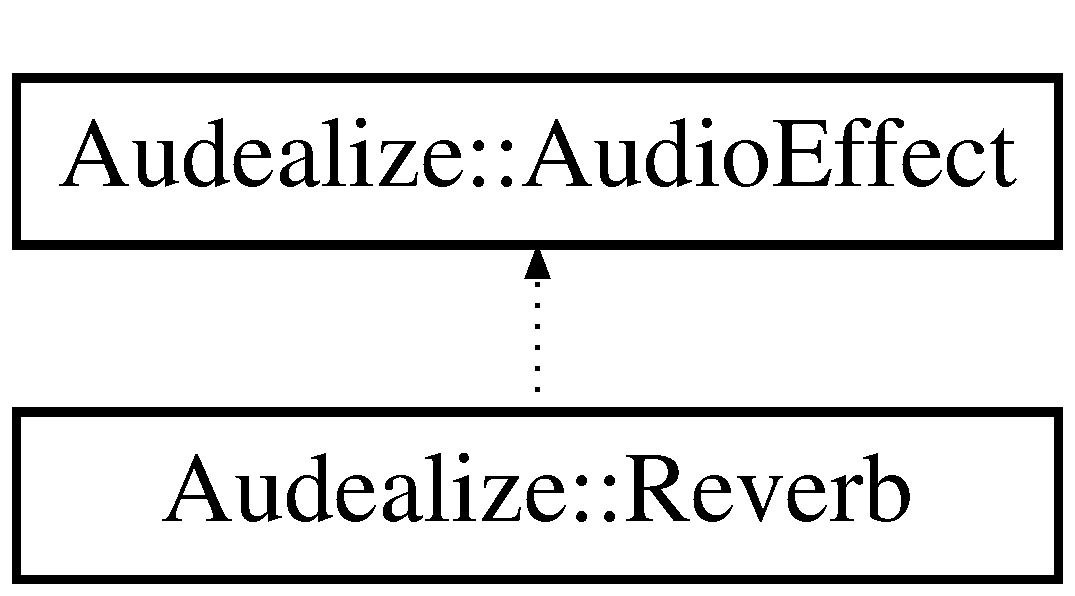
\includegraphics[height=2.000000cm]{class_audealize_1_1_reverb}
\end{center}
\end{figure}
\subsection*{Public Member Functions}
\begin{DoxyCompactItemize}
\item 
\hyperlink{class_audealize_1_1_reverb_a6bb1409a11f960eafff156ab2a6f60a3}{Reverb} ()
\item 
\hyperlink{class_audealize_1_1_reverb_a53286010677ee1e5a2a81e3ea9688c1c}{$\sim$\+Reverb} ()
\item 
\hyperlink{tk_8h_aba408b7cd755a96426e004c015f5de8e}{void} \hyperlink{class_audealize_1_1_reverb_a6e6224a37e50c83e7dbe2f3c9c1814d8}{process\+Mono\+Block} (float $\ast$channel\+Data, \hyperlink{tk_8h_a83f82f76e7fed06f4c49d2db94028a6d}{int} block\+Size)
\item 
\hyperlink{tk_8h_aba408b7cd755a96426e004c015f5de8e}{void} \hyperlink{class_audealize_1_1_reverb_a9351a471cd711bfa2a347bdca084d397}{process\+Stereo\+Block} (float $\ast$channel\+Data1, float $\ast$channel\+Data2, \hyperlink{tk_8h_a83f82f76e7fed06f4c49d2db94028a6d}{int} block\+Size)
\item 
\hyperlink{tk_8h_aba408b7cd755a96426e004c015f5de8e}{void} \hyperlink{class_audealize_1_1_reverb_a301a030f103e237741614e22498834ff}{init} (float d\+\_\+val, float g\+\_\+val, float m\+\_\+val, float f\+\_\+val, float E\+\_\+val, float wetdry\+\_\+val, float sample\+Rate)
\item 
\hyperlink{tk_8h_aba408b7cd755a96426e004c015f5de8e}{void} \hyperlink{class_audealize_1_1_reverb_a8b4944f1ed31c1226f52fe91e44f6472}{set\+\_\+d} (float d\+\_\+val)
\item 
\hyperlink{tk_8h_aba408b7cd755a96426e004c015f5de8e}{void} \hyperlink{class_audealize_1_1_reverb_ae60ddead2f69f41bab5d89f2dc70916c}{set\+\_\+g} (float g\+\_\+val)
\item 
\hyperlink{tk_8h_aba408b7cd755a96426e004c015f5de8e}{void} \hyperlink{class_audealize_1_1_reverb_a7e8039fe4f4a71c4c46fa74ae76e15f7}{set\+\_\+m} (float m\+\_\+val)
\item 
\hyperlink{tk_8h_aba408b7cd755a96426e004c015f5de8e}{void} \hyperlink{class_audealize_1_1_reverb_a1dd995a1df58a6db8df8213cef896158}{set\+\_\+f} (float f\+\_\+val)
\item 
\hyperlink{tk_8h_aba408b7cd755a96426e004c015f5de8e}{void} \hyperlink{class_audealize_1_1_reverb_a81166e0d284f3266f1a5a646e78abe42}{set\+\_\+E} (float E\+\_\+val)
\item 
\hyperlink{tk_8h_aba408b7cd755a96426e004c015f5de8e}{void} \hyperlink{class_audealize_1_1_reverb_a95bffc24800591faf3458cf489c3bcae}{set\+\_\+wetdry} (float wetdry\+\_\+val)
\item 
\hyperlink{tk_8h_aba408b7cd755a96426e004c015f5de8e}{void} \hyperlink{class_audealize_1_1_reverb_a1b4ea565c1c25b62911c5b650f84f844}{set\+Sample\+Rate} (float sample\+Rate)
\item 
\hyperlink{tk_8h_aba408b7cd755a96426e004c015f5de8e}{void} \hyperlink{class_audealize_1_1_reverb_a9727c0f0980b94856beb3f3b43a3944a}{reset\+Buffs} ()
\item 
float \hyperlink{class_audealize_1_1_reverb_a9a52f3a5300722b6add8b495fa195b1f}{get\+\_\+d} ()
\item 
float \hyperlink{class_audealize_1_1_reverb_a100b4faf2b256968bf7c95c0644a3695}{get\+\_\+g} ()
\item 
float \hyperlink{class_audealize_1_1_reverb_a85bcdef1598afb2c7982a45d8f558ed8}{get\+\_\+m} ()
\item 
float \hyperlink{class_audealize_1_1_reverb_a9fb1ab04f1e17f1cb1241066c1fecb54}{get\+\_\+f} ()
\item 
float \hyperlink{class_audealize_1_1_reverb_a4ce71ce2f1677cd3b43db9a22490b7fd}{get\+\_\+E} ()
\item 
float \hyperlink{class_audealize_1_1_reverb_a9801b05791b7eef0eb0f04d84d1a27e3}{get\+\_\+wetdry} ()
\end{DoxyCompactItemize}


\subsection{Constructor \& Destructor Documentation}
\index{Audealize\+::\+Reverb@{Audealize\+::\+Reverb}!Reverb@{Reverb}}
\index{Reverb@{Reverb}!Audealize\+::\+Reverb@{Audealize\+::\+Reverb}}
\subsubsection[{\texorpdfstring{Reverb()}{Reverb()}}]{\setlength{\rightskip}{0pt plus 5cm}Audealize\+::\+Reverb\+::\+Reverb (
\begin{DoxyParamCaption}
{}
\end{DoxyParamCaption}
)\hspace{0.3cm}{\ttfamily [inline]}}\hypertarget{class_audealize_1_1_reverb_a6bb1409a11f960eafff156ab2a6f60a3}{}\label{class_audealize_1_1_reverb_a6bb1409a11f960eafff156ab2a6f60a3}
\index{Audealize\+::\+Reverb@{Audealize\+::\+Reverb}!````~Reverb@{$\sim$\+Reverb}}
\index{````~Reverb@{$\sim$\+Reverb}!Audealize\+::\+Reverb@{Audealize\+::\+Reverb}}
\subsubsection[{\texorpdfstring{$\sim$\+Reverb()}{~Reverb()}}]{\setlength{\rightskip}{0pt plus 5cm}Audealize\+::\+Reverb\+::$\sim$\+Reverb (
\begin{DoxyParamCaption}
{}
\end{DoxyParamCaption}
)\hspace{0.3cm}{\ttfamily [inline]}}\hypertarget{class_audealize_1_1_reverb_a53286010677ee1e5a2a81e3ea9688c1c}{}\label{class_audealize_1_1_reverb_a53286010677ee1e5a2a81e3ea9688c1c}


\subsection{Member Function Documentation}
\index{Audealize\+::\+Reverb@{Audealize\+::\+Reverb}!get\+\_\+d@{get\+\_\+d}}
\index{get\+\_\+d@{get\+\_\+d}!Audealize\+::\+Reverb@{Audealize\+::\+Reverb}}
\subsubsection[{\texorpdfstring{get\+\_\+d()}{get_d()}}]{\setlength{\rightskip}{0pt plus 5cm}float Audealize\+::\+Reverb\+::get\+\_\+d (
\begin{DoxyParamCaption}
{}
\end{DoxyParamCaption}
)\hspace{0.3cm}{\ttfamily [inline]}}\hypertarget{class_audealize_1_1_reverb_a9a52f3a5300722b6add8b495fa195b1f}{}\label{class_audealize_1_1_reverb_a9a52f3a5300722b6add8b495fa195b1f}
Getters for main reverberator parameters \index{Audealize\+::\+Reverb@{Audealize\+::\+Reverb}!get\+\_\+E@{get\+\_\+E}}
\index{get\+\_\+E@{get\+\_\+E}!Audealize\+::\+Reverb@{Audealize\+::\+Reverb}}
\subsubsection[{\texorpdfstring{get\+\_\+\+E()}{get_E()}}]{\setlength{\rightskip}{0pt plus 5cm}float Audealize\+::\+Reverb\+::get\+\_\+E (
\begin{DoxyParamCaption}
{}
\end{DoxyParamCaption}
)\hspace{0.3cm}{\ttfamily [inline]}}\hypertarget{class_audealize_1_1_reverb_a4ce71ce2f1677cd3b43db9a22490b7fd}{}\label{class_audealize_1_1_reverb_a4ce71ce2f1677cd3b43db9a22490b7fd}
\index{Audealize\+::\+Reverb@{Audealize\+::\+Reverb}!get\+\_\+f@{get\+\_\+f}}
\index{get\+\_\+f@{get\+\_\+f}!Audealize\+::\+Reverb@{Audealize\+::\+Reverb}}
\subsubsection[{\texorpdfstring{get\+\_\+f()}{get_f()}}]{\setlength{\rightskip}{0pt plus 5cm}float Audealize\+::\+Reverb\+::get\+\_\+f (
\begin{DoxyParamCaption}
{}
\end{DoxyParamCaption}
)\hspace{0.3cm}{\ttfamily [inline]}}\hypertarget{class_audealize_1_1_reverb_a9fb1ab04f1e17f1cb1241066c1fecb54}{}\label{class_audealize_1_1_reverb_a9fb1ab04f1e17f1cb1241066c1fecb54}
\index{Audealize\+::\+Reverb@{Audealize\+::\+Reverb}!get\+\_\+g@{get\+\_\+g}}
\index{get\+\_\+g@{get\+\_\+g}!Audealize\+::\+Reverb@{Audealize\+::\+Reverb}}
\subsubsection[{\texorpdfstring{get\+\_\+g()}{get_g()}}]{\setlength{\rightskip}{0pt plus 5cm}float Audealize\+::\+Reverb\+::get\+\_\+g (
\begin{DoxyParamCaption}
{}
\end{DoxyParamCaption}
)\hspace{0.3cm}{\ttfamily [inline]}}\hypertarget{class_audealize_1_1_reverb_a100b4faf2b256968bf7c95c0644a3695}{}\label{class_audealize_1_1_reverb_a100b4faf2b256968bf7c95c0644a3695}
\index{Audealize\+::\+Reverb@{Audealize\+::\+Reverb}!get\+\_\+m@{get\+\_\+m}}
\index{get\+\_\+m@{get\+\_\+m}!Audealize\+::\+Reverb@{Audealize\+::\+Reverb}}
\subsubsection[{\texorpdfstring{get\+\_\+m()}{get_m()}}]{\setlength{\rightskip}{0pt plus 5cm}float Audealize\+::\+Reverb\+::get\+\_\+m (
\begin{DoxyParamCaption}
{}
\end{DoxyParamCaption}
)\hspace{0.3cm}{\ttfamily [inline]}}\hypertarget{class_audealize_1_1_reverb_a85bcdef1598afb2c7982a45d8f558ed8}{}\label{class_audealize_1_1_reverb_a85bcdef1598afb2c7982a45d8f558ed8}
\index{Audealize\+::\+Reverb@{Audealize\+::\+Reverb}!get\+\_\+wetdry@{get\+\_\+wetdry}}
\index{get\+\_\+wetdry@{get\+\_\+wetdry}!Audealize\+::\+Reverb@{Audealize\+::\+Reverb}}
\subsubsection[{\texorpdfstring{get\+\_\+wetdry()}{get_wetdry()}}]{\setlength{\rightskip}{0pt plus 5cm}float Audealize\+::\+Reverb\+::get\+\_\+wetdry (
\begin{DoxyParamCaption}
{}
\end{DoxyParamCaption}
)\hspace{0.3cm}{\ttfamily [inline]}}\hypertarget{class_audealize_1_1_reverb_a9801b05791b7eef0eb0f04d84d1a27e3}{}\label{class_audealize_1_1_reverb_a9801b05791b7eef0eb0f04d84d1a27e3}
\index{Audealize\+::\+Reverb@{Audealize\+::\+Reverb}!init@{init}}
\index{init@{init}!Audealize\+::\+Reverb@{Audealize\+::\+Reverb}}
\subsubsection[{\texorpdfstring{init(float d\+\_\+val, float g\+\_\+val, float m\+\_\+val, float f\+\_\+val, float E\+\_\+val, float wetdry\+\_\+val, float sample\+Rate)}{init(float d_val, float g_val, float m_val, float f_val, float E_val, float wetdry_val, float sampleRate)}}]{\setlength{\rightskip}{0pt plus 5cm}{\bf void} Audealize\+::\+Reverb\+::init (
\begin{DoxyParamCaption}
\item[{float}]{d\+\_\+val, }
\item[{float}]{g\+\_\+val, }
\item[{float}]{m\+\_\+val, }
\item[{float}]{f\+\_\+val, }
\item[{float}]{E\+\_\+val, }
\item[{float}]{wetdry\+\_\+val, }
\item[{float}]{sample\+Rate}
\end{DoxyParamCaption}
)\hspace{0.3cm}{\ttfamily [inline]}}\hypertarget{class_audealize_1_1_reverb_a301a030f103e237741614e22498834ff}{}\label{class_audealize_1_1_reverb_a301a030f103e237741614e22498834ff}
Set all parameters at once. (Intended to be called from J\+U\+C\+E\+::\+Audio\+Processor\+::prepare\+To\+Play) \index{Audealize\+::\+Reverb@{Audealize\+::\+Reverb}!process\+Mono\+Block@{process\+Mono\+Block}}
\index{process\+Mono\+Block@{process\+Mono\+Block}!Audealize\+::\+Reverb@{Audealize\+::\+Reverb}}
\subsubsection[{\texorpdfstring{process\+Mono\+Block(float $\ast$channel\+Data, int block\+Size)}{processMonoBlock(float *channelData, int blockSize)}}]{\setlength{\rightskip}{0pt plus 5cm}{\bf void} Audealize\+::\+Reverb\+::process\+Mono\+Block (
\begin{DoxyParamCaption}
\item[{float $\ast$}]{channel\+Data, }
\item[{{\bf int}}]{block\+Size}
\end{DoxyParamCaption}
)\hspace{0.3cm}{\ttfamily [inline]}}\hypertarget{class_audealize_1_1_reverb_a6e6224a37e50c83e7dbe2f3c9c1814d8}{}\label{class_audealize_1_1_reverb_a6e6224a37e50c83e7dbe2f3c9c1814d8}
Process a block of mono audio


\begin{DoxyParams}{Parameters}
{\em channel\+Data} & Pointer to a block of samples \\
\hline
{\em block\+Size} & Number of samples in the block \\
\hline
\end{DoxyParams}
\index{Audealize\+::\+Reverb@{Audealize\+::\+Reverb}!process\+Stereo\+Block@{process\+Stereo\+Block}}
\index{process\+Stereo\+Block@{process\+Stereo\+Block}!Audealize\+::\+Reverb@{Audealize\+::\+Reverb}}
\subsubsection[{\texorpdfstring{process\+Stereo\+Block(float $\ast$channel\+Data1, float $\ast$channel\+Data2, int block\+Size)}{processStereoBlock(float *channelData1, float *channelData2, int blockSize)}}]{\setlength{\rightskip}{0pt plus 5cm}{\bf void} Audealize\+::\+Reverb\+::process\+Stereo\+Block (
\begin{DoxyParamCaption}
\item[{float $\ast$}]{channel\+Data1, }
\item[{float $\ast$}]{channel\+Data2, }
\item[{{\bf int}}]{block\+Size}
\end{DoxyParamCaption}
)\hspace{0.3cm}{\ttfamily [inline]}}\hypertarget{class_audealize_1_1_reverb_a9351a471cd711bfa2a347bdca084d397}{}\label{class_audealize_1_1_reverb_a9351a471cd711bfa2a347bdca084d397}
Process a block of stereo audio


\begin{DoxyParams}{Parameters}
{\em channel\+Data1} & Block of samples corresponding to channel 1 \\
\hline
{\em channel\+Data2} & Block of samples corresponding to channel 2 \\
\hline
{\em block\+Size} & Number of samples in each block \\
\hline
\end{DoxyParams}
\index{Audealize\+::\+Reverb@{Audealize\+::\+Reverb}!reset\+Buffs@{reset\+Buffs}}
\index{reset\+Buffs@{reset\+Buffs}!Audealize\+::\+Reverb@{Audealize\+::\+Reverb}}
\subsubsection[{\texorpdfstring{reset\+Buffs()}{resetBuffs()}}]{\setlength{\rightskip}{0pt plus 5cm}{\bf void} Audealize\+::\+Reverb\+::reset\+Buffs (
\begin{DoxyParamCaption}
{}
\end{DoxyParamCaption}
)\hspace{0.3cm}{\ttfamily [inline]}}\hypertarget{class_audealize_1_1_reverb_a9727c0f0980b94856beb3f3b43a3944a}{}\label{class_audealize_1_1_reverb_a9727c0f0980b94856beb3f3b43a3944a}
Zero out all buffers \index{Audealize\+::\+Reverb@{Audealize\+::\+Reverb}!set\+\_\+d@{set\+\_\+d}}
\index{set\+\_\+d@{set\+\_\+d}!Audealize\+::\+Reverb@{Audealize\+::\+Reverb}}
\subsubsection[{\texorpdfstring{set\+\_\+d(float d\+\_\+val)}{set_d(float d_val)}}]{\setlength{\rightskip}{0pt plus 5cm}{\bf void} Audealize\+::\+Reverb\+::set\+\_\+d (
\begin{DoxyParamCaption}
\item[{float}]{d\+\_\+val}
\end{DoxyParamCaption}
)\hspace{0.3cm}{\ttfamily [inline]}}\hypertarget{class_audealize_1_1_reverb_a8b4944f1ed31c1226f52fe91e44f6472}{}\label{class_audealize_1_1_reverb_a8b4944f1ed31c1226f52fe91e44f6472}
Individual setters for reverberator parameters \index{Audealize\+::\+Reverb@{Audealize\+::\+Reverb}!set\+\_\+E@{set\+\_\+E}}
\index{set\+\_\+E@{set\+\_\+E}!Audealize\+::\+Reverb@{Audealize\+::\+Reverb}}
\subsubsection[{\texorpdfstring{set\+\_\+\+E(float E\+\_\+val)}{set_E(float E_val)}}]{\setlength{\rightskip}{0pt plus 5cm}{\bf void} Audealize\+::\+Reverb\+::set\+\_\+E (
\begin{DoxyParamCaption}
\item[{float}]{E\+\_\+val}
\end{DoxyParamCaption}
)\hspace{0.3cm}{\ttfamily [inline]}}\hypertarget{class_audealize_1_1_reverb_a81166e0d284f3266f1a5a646e78abe42}{}\label{class_audealize_1_1_reverb_a81166e0d284f3266f1a5a646e78abe42}
\index{Audealize\+::\+Reverb@{Audealize\+::\+Reverb}!set\+\_\+f@{set\+\_\+f}}
\index{set\+\_\+f@{set\+\_\+f}!Audealize\+::\+Reverb@{Audealize\+::\+Reverb}}
\subsubsection[{\texorpdfstring{set\+\_\+f(float f\+\_\+val)}{set_f(float f_val)}}]{\setlength{\rightskip}{0pt plus 5cm}{\bf void} Audealize\+::\+Reverb\+::set\+\_\+f (
\begin{DoxyParamCaption}
\item[{float}]{f\+\_\+val}
\end{DoxyParamCaption}
)\hspace{0.3cm}{\ttfamily [inline]}}\hypertarget{class_audealize_1_1_reverb_a1dd995a1df58a6db8df8213cef896158}{}\label{class_audealize_1_1_reverb_a1dd995a1df58a6db8df8213cef896158}
\index{Audealize\+::\+Reverb@{Audealize\+::\+Reverb}!set\+\_\+g@{set\+\_\+g}}
\index{set\+\_\+g@{set\+\_\+g}!Audealize\+::\+Reverb@{Audealize\+::\+Reverb}}
\subsubsection[{\texorpdfstring{set\+\_\+g(float g\+\_\+val)}{set_g(float g_val)}}]{\setlength{\rightskip}{0pt plus 5cm}{\bf void} Audealize\+::\+Reverb\+::set\+\_\+g (
\begin{DoxyParamCaption}
\item[{float}]{g\+\_\+val}
\end{DoxyParamCaption}
)\hspace{0.3cm}{\ttfamily [inline]}}\hypertarget{class_audealize_1_1_reverb_ae60ddead2f69f41bab5d89f2dc70916c}{}\label{class_audealize_1_1_reverb_ae60ddead2f69f41bab5d89f2dc70916c}
\index{Audealize\+::\+Reverb@{Audealize\+::\+Reverb}!set\+\_\+m@{set\+\_\+m}}
\index{set\+\_\+m@{set\+\_\+m}!Audealize\+::\+Reverb@{Audealize\+::\+Reverb}}
\subsubsection[{\texorpdfstring{set\+\_\+m(float m\+\_\+val)}{set_m(float m_val)}}]{\setlength{\rightskip}{0pt plus 5cm}{\bf void} Audealize\+::\+Reverb\+::set\+\_\+m (
\begin{DoxyParamCaption}
\item[{float}]{m\+\_\+val}
\end{DoxyParamCaption}
)\hspace{0.3cm}{\ttfamily [inline]}}\hypertarget{class_audealize_1_1_reverb_a7e8039fe4f4a71c4c46fa74ae76e15f7}{}\label{class_audealize_1_1_reverb_a7e8039fe4f4a71c4c46fa74ae76e15f7}
\index{Audealize\+::\+Reverb@{Audealize\+::\+Reverb}!set\+\_\+wetdry@{set\+\_\+wetdry}}
\index{set\+\_\+wetdry@{set\+\_\+wetdry}!Audealize\+::\+Reverb@{Audealize\+::\+Reverb}}
\subsubsection[{\texorpdfstring{set\+\_\+wetdry(float wetdry\+\_\+val)}{set_wetdry(float wetdry_val)}}]{\setlength{\rightskip}{0pt plus 5cm}{\bf void} Audealize\+::\+Reverb\+::set\+\_\+wetdry (
\begin{DoxyParamCaption}
\item[{float}]{wetdry\+\_\+val}
\end{DoxyParamCaption}
)\hspace{0.3cm}{\ttfamily [inline]}}\hypertarget{class_audealize_1_1_reverb_a95bffc24800591faf3458cf489c3bcae}{}\label{class_audealize_1_1_reverb_a95bffc24800591faf3458cf489c3bcae}
\index{Audealize\+::\+Reverb@{Audealize\+::\+Reverb}!set\+Sample\+Rate@{set\+Sample\+Rate}}
\index{set\+Sample\+Rate@{set\+Sample\+Rate}!Audealize\+::\+Reverb@{Audealize\+::\+Reverb}}
\subsubsection[{\texorpdfstring{set\+Sample\+Rate(float sample\+Rate)}{setSampleRate(float sampleRate)}}]{\setlength{\rightskip}{0pt plus 5cm}{\bf void} Audealize\+::\+Reverb\+::set\+Sample\+Rate (
\begin{DoxyParamCaption}
\item[{float}]{sample\+Rate}
\end{DoxyParamCaption}
)\hspace{0.3cm}{\ttfamily [inline]}, {\ttfamily [virtual]}}\hypertarget{class_audealize_1_1_reverb_a1b4ea565c1c25b62911c5b650f84f844}{}\label{class_audealize_1_1_reverb_a1b4ea565c1c25b62911c5b650f84f844}
Overload \hyperlink{class_audealize_1_1_audio_effect_a5ff34c0371f2311dc026bca5ba245faa}{Audio\+Effect\+::set\+Sample\+Rate} to update any variables dependent on the sample rate 

Reimplemented from \hyperlink{class_audealize_1_1_audio_effect_a5ff34c0371f2311dc026bca5ba245faa}{Audealize\+::\+Audio\+Effect}.



The documentation for this class was generated from the following file\+:\begin{DoxyCompactItemize}
\item 
/\+Users/michael/\+J\+U\+C\+E/projects/audealize-\/plugin/\+J\+U\+C\+E Modules/audealize\+\_\+module/effects/\hyperlink{_reverb_8h}{Reverb.\+h}\end{DoxyCompactItemize}

\hypertarget{class_audealize_1_1_reverb_component}{}\section{Audealize\+:\+:Reverb\+Component Class Reference}
\label{class_audealize_1_1_reverb_component}\index{Audealize\+::\+Reverb\+Component@{Audealize\+::\+Reverb\+Component}}


{\ttfamily \#include $<$Reverb\+Component.\+h$>$}

Inheritance diagram for Audealize\+:\+:Reverb\+Component\+:\begin{figure}[H]
\begin{center}
\leavevmode
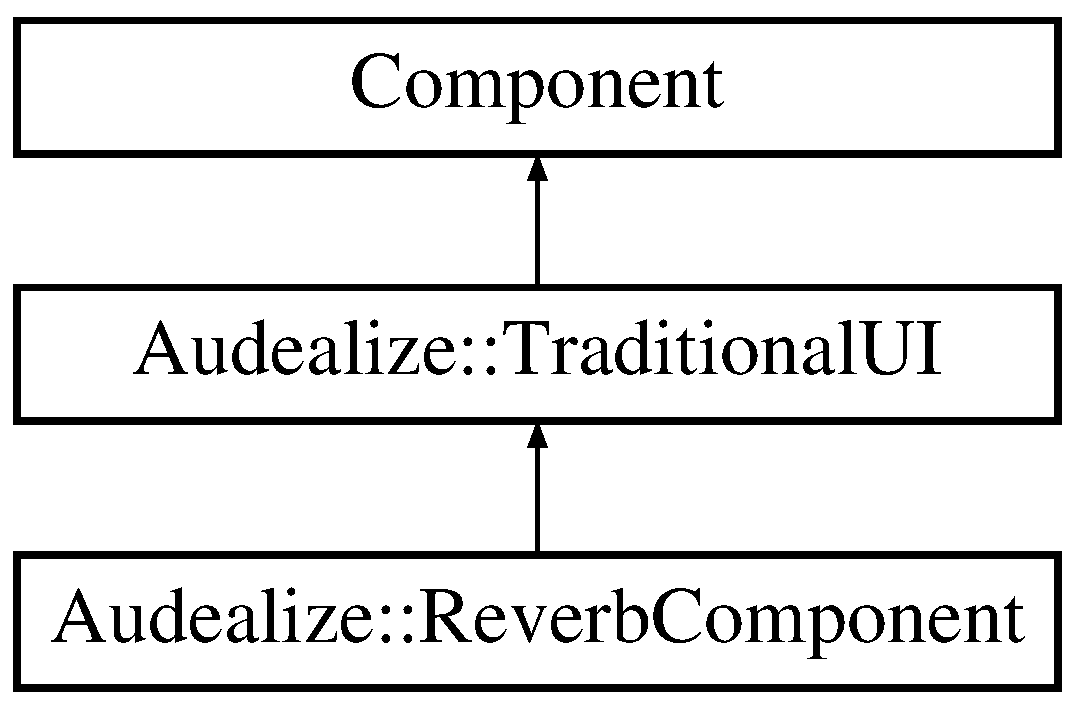
\includegraphics[height=3.000000cm]{class_audealize_1_1_reverb_component}
\end{center}
\end{figure}
\subsection*{Public Member Functions}
\begin{DoxyCompactItemize}
\item 
\hyperlink{class_audealize_1_1_reverb_component_ae1177cd6ddb6c6addd9aedf327947c39}{Reverb\+Component} (\hyperlink{class_audealize_1_1_audealize_audio_processor}{Audealize\+Audio\+Processor} \&p)
\item 
\hyperlink{class_audealize_1_1_reverb_component_a31254ec9fcb3f4684183ae68c2ba0b66}{$\sim$\+Reverb\+Component} ()
\item 
\hyperlink{tk_8h_aba408b7cd755a96426e004c015f5de8e}{void} \hyperlink{class_audealize_1_1_reverb_component_a46e9b76ae332f9ae4065e3c4bce91b45}{paint} (Graphics \&g) override
\item 
\hyperlink{tk_8h_aba408b7cd755a96426e004c015f5de8e}{void} \hyperlink{class_audealize_1_1_reverb_component_afd0030d4012d58c8f59ed41edeb04f90}{resized} () override
\end{DoxyCompactItemize}
\subsection*{Additional Inherited Members}


\subsection{Constructor \& Destructor Documentation}
\index{Audealize\+::\+Reverb\+Component@{Audealize\+::\+Reverb\+Component}!Reverb\+Component@{Reverb\+Component}}
\index{Reverb\+Component@{Reverb\+Component}!Audealize\+::\+Reverb\+Component@{Audealize\+::\+Reverb\+Component}}
\subsubsection[{\texorpdfstring{Reverb\+Component(\+Audealize\+Audio\+Processor \&p)}{ReverbComponent(AudealizeAudioProcessor &p)}}]{\setlength{\rightskip}{0pt plus 5cm}Audealize\+::\+Reverb\+Component\+::\+Reverb\+Component (
\begin{DoxyParamCaption}
\item[{{\bf Audealize\+Audio\+Processor} \&}]{p}
\end{DoxyParamCaption}
)}\hypertarget{class_audealize_1_1_reverb_component_ae1177cd6ddb6c6addd9aedf327947c39}{}\label{class_audealize_1_1_reverb_component_ae1177cd6ddb6c6addd9aedf327947c39}
\index{Audealize\+::\+Reverb\+Component@{Audealize\+::\+Reverb\+Component}!````~Reverb\+Component@{$\sim$\+Reverb\+Component}}
\index{````~Reverb\+Component@{$\sim$\+Reverb\+Component}!Audealize\+::\+Reverb\+Component@{Audealize\+::\+Reverb\+Component}}
\subsubsection[{\texorpdfstring{$\sim$\+Reverb\+Component()}{~ReverbComponent()}}]{\setlength{\rightskip}{0pt plus 5cm}Audealize\+::\+Reverb\+Component\+::$\sim$\+Reverb\+Component (
\begin{DoxyParamCaption}
{}
\end{DoxyParamCaption}
)}\hypertarget{class_audealize_1_1_reverb_component_a31254ec9fcb3f4684183ae68c2ba0b66}{}\label{class_audealize_1_1_reverb_component_a31254ec9fcb3f4684183ae68c2ba0b66}


\subsection{Member Function Documentation}
\index{Audealize\+::\+Reverb\+Component@{Audealize\+::\+Reverb\+Component}!paint@{paint}}
\index{paint@{paint}!Audealize\+::\+Reverb\+Component@{Audealize\+::\+Reverb\+Component}}
\subsubsection[{\texorpdfstring{paint(\+Graphics \&g) override}{paint(Graphics &g) override}}]{\setlength{\rightskip}{0pt plus 5cm}{\bf void} Audealize\+::\+Reverb\+Component\+::paint (
\begin{DoxyParamCaption}
\item[{Graphics \&}]{g}
\end{DoxyParamCaption}
)\hspace{0.3cm}{\ttfamily [override]}}\hypertarget{class_audealize_1_1_reverb_component_a46e9b76ae332f9ae4065e3c4bce91b45}{}\label{class_audealize_1_1_reverb_component_a46e9b76ae332f9ae4065e3c4bce91b45}
\index{Audealize\+::\+Reverb\+Component@{Audealize\+::\+Reverb\+Component}!resized@{resized}}
\index{resized@{resized}!Audealize\+::\+Reverb\+Component@{Audealize\+::\+Reverb\+Component}}
\subsubsection[{\texorpdfstring{resized() override}{resized() override}}]{\setlength{\rightskip}{0pt plus 5cm}{\bf void} Audealize\+::\+Reverb\+Component\+::resized (
\begin{DoxyParamCaption}
{}
\end{DoxyParamCaption}
)\hspace{0.3cm}{\ttfamily [override]}}\hypertarget{class_audealize_1_1_reverb_component_afd0030d4012d58c8f59ed41edeb04f90}{}\label{class_audealize_1_1_reverb_component_afd0030d4012d58c8f59ed41edeb04f90}


The documentation for this class was generated from the following files\+:\begin{DoxyCompactItemize}
\item 
/\+Users/michael/\+J\+U\+C\+E/projects/audealize-\/plugin/\+J\+U\+C\+E Modules/audealize\+\_\+module/ui\+\_\+components/\hyperlink{_reverb_component_8h}{Reverb\+Component.\+h}\item 
/\+Users/michael/\+J\+U\+C\+E/projects/audealize-\/plugin/\+J\+U\+C\+E Modules/audealize\+\_\+module/ui\+\_\+components/\hyperlink{_reverb_component_8cpp}{Reverb\+Component.\+cpp}\end{DoxyCompactItemize}

\hypertarget{class_audealize_1_1_rotary_slider_centered}{}\section{Audealize\+:\+:Rotary\+Slider\+Centered Class Reference}
\label{class_audealize_1_1_rotary_slider_centered}\index{Audealize\+::\+Rotary\+Slider\+Centered@{Audealize\+::\+Rotary\+Slider\+Centered}}


{\ttfamily \#include $<$Rotary\+Slider\+Centered.\+h$>$}

Inheritance diagram for Audealize\+:\+:Rotary\+Slider\+Centered\+:\begin{figure}[H]
\begin{center}
\leavevmode
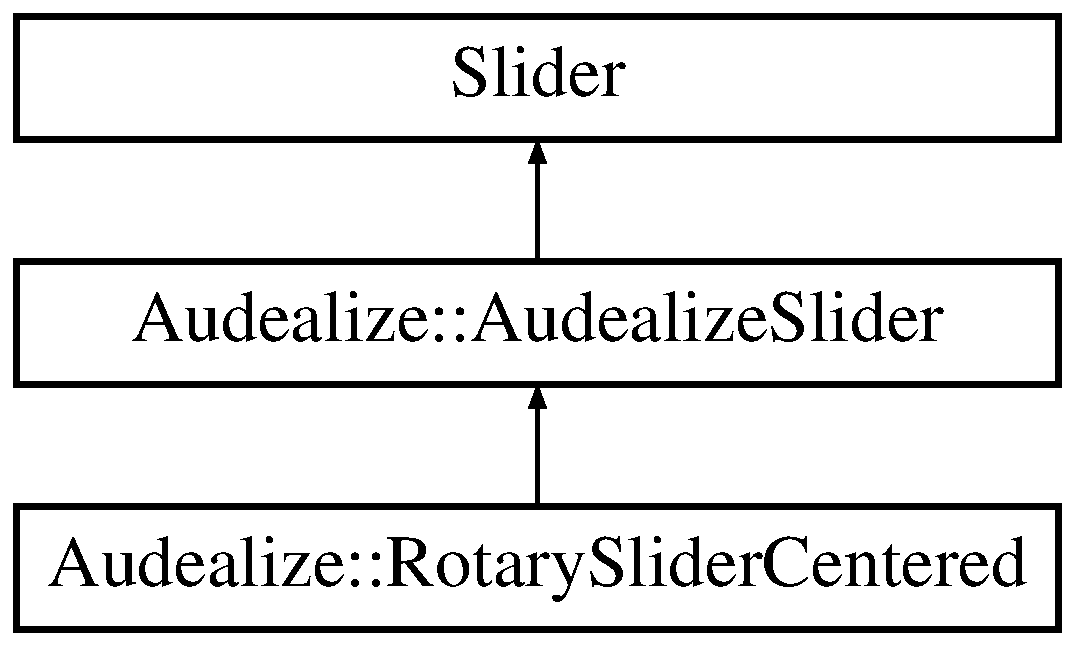
\includegraphics[height=3.000000cm]{class_audealize_1_1_rotary_slider_centered}
\end{center}
\end{figure}
\subsection*{Public Member Functions}
\begin{DoxyCompactItemize}
\item 
\hyperlink{class_audealize_1_1_rotary_slider_centered_a72f81f0092f3470e912818a4461f0278}{Rotary\+Slider\+Centered} ()
\item 
\hyperlink{class_audealize_1_1_rotary_slider_centered_a88e45289d12a91580c9ffb7e5943b4e0}{$\sim$\+Rotary\+Slider\+Centered} ()
\item 
\hyperlink{tk_8h_aba408b7cd755a96426e004c015f5de8e}{void} \hyperlink{class_audealize_1_1_rotary_slider_centered_afca4e8db6f0eb641e945514f46cc8ca7}{paint} (Graphics \&g) override
\end{DoxyCompactItemize}


\subsection{Constructor \& Destructor Documentation}
\index{Audealize\+::\+Rotary\+Slider\+Centered@{Audealize\+::\+Rotary\+Slider\+Centered}!Rotary\+Slider\+Centered@{Rotary\+Slider\+Centered}}
\index{Rotary\+Slider\+Centered@{Rotary\+Slider\+Centered}!Audealize\+::\+Rotary\+Slider\+Centered@{Audealize\+::\+Rotary\+Slider\+Centered}}
\subsubsection[{\texorpdfstring{Rotary\+Slider\+Centered()}{RotarySliderCentered()}}]{\setlength{\rightskip}{0pt plus 5cm}Audealize\+::\+Rotary\+Slider\+Centered\+::\+Rotary\+Slider\+Centered (
\begin{DoxyParamCaption}
{}
\end{DoxyParamCaption}
)\hspace{0.3cm}{\ttfamily [inline]}}\hypertarget{class_audealize_1_1_rotary_slider_centered_a72f81f0092f3470e912818a4461f0278}{}\label{class_audealize_1_1_rotary_slider_centered_a72f81f0092f3470e912818a4461f0278}
\index{Audealize\+::\+Rotary\+Slider\+Centered@{Audealize\+::\+Rotary\+Slider\+Centered}!````~Rotary\+Slider\+Centered@{$\sim$\+Rotary\+Slider\+Centered}}
\index{````~Rotary\+Slider\+Centered@{$\sim$\+Rotary\+Slider\+Centered}!Audealize\+::\+Rotary\+Slider\+Centered@{Audealize\+::\+Rotary\+Slider\+Centered}}
\subsubsection[{\texorpdfstring{$\sim$\+Rotary\+Slider\+Centered()}{~RotarySliderCentered()}}]{\setlength{\rightskip}{0pt plus 5cm}Audealize\+::\+Rotary\+Slider\+Centered\+::$\sim$\+Rotary\+Slider\+Centered (
\begin{DoxyParamCaption}
{}
\end{DoxyParamCaption}
)\hspace{0.3cm}{\ttfamily [inline]}}\hypertarget{class_audealize_1_1_rotary_slider_centered_a88e45289d12a91580c9ffb7e5943b4e0}{}\label{class_audealize_1_1_rotary_slider_centered_a88e45289d12a91580c9ffb7e5943b4e0}


\subsection{Member Function Documentation}
\index{Audealize\+::\+Rotary\+Slider\+Centered@{Audealize\+::\+Rotary\+Slider\+Centered}!paint@{paint}}
\index{paint@{paint}!Audealize\+::\+Rotary\+Slider\+Centered@{Audealize\+::\+Rotary\+Slider\+Centered}}
\subsubsection[{\texorpdfstring{paint(\+Graphics \&g) override}{paint(Graphics &g) override}}]{\setlength{\rightskip}{0pt plus 5cm}{\bf void} Audealize\+::\+Rotary\+Slider\+Centered\+::paint (
\begin{DoxyParamCaption}
\item[{Graphics \&}]{g}
\end{DoxyParamCaption}
)\hspace{0.3cm}{\ttfamily [inline]}, {\ttfamily [override]}}\hypertarget{class_audealize_1_1_rotary_slider_centered_afca4e8db6f0eb641e945514f46cc8ca7}{}\label{class_audealize_1_1_rotary_slider_centered_afca4e8db6f0eb641e945514f46cc8ca7}


The documentation for this class was generated from the following file\+:\begin{DoxyCompactItemize}
\item 
/\+Users/michael/\+J\+U\+C\+E/projects/audealize-\/plugin/\+J\+U\+C\+E Modules/audealize\+\_\+module/ui\+\_\+components/\hyperlink{_rotary_slider_centered_8h}{Rotary\+Slider\+Centered.\+h}\end{DoxyCompactItemize}

\hypertarget{structdsp_1_1sample__traits}{}\section{dsp\+:\+:sample\+\_\+traits$<$ T $>$ Struct Template Reference}
\label{structdsp_1_1sample__traits}\index{dsp\+::sample\+\_\+traits$<$ T $>$@{dsp\+::sample\+\_\+traits$<$ T $>$}}


{\ttfamily \#include $<$buffer.\+h$>$}

\subsection*{Public Types}
\begin{DoxyCompactItemize}
\item 
enum \{ \hyperlink{structdsp_1_1sample__traits_ae7a6cec7b50f595d913e58efda9cbabaa4c4d1528912adaf37d04b70c09f467c0}{channels} = 1, 
\hyperlink{structdsp_1_1sample__traits_ae7a6cec7b50f595d913e58efda9cbabaaebe24230df11df9608b35d5e8d0aea43}{bps} = sizeof(T)$\ast$8
 \}
\end{DoxyCompactItemize}


\subsection{Member Enumeration Documentation}
\subsubsection[{\texorpdfstring{anonymous enum}{anonymous enum}}]{\setlength{\rightskip}{0pt plus 5cm}template$<$class T $>$ anonymous enum}\hypertarget{structdsp_1_1sample__traits_ae7a6cec7b50f595d913e58efda9cbaba}{}\label{structdsp_1_1sample__traits_ae7a6cec7b50f595d913e58efda9cbaba}
\begin{Desc}
\item[Enumerator]\par
\begin{description}
\index{channels@{channels}!dsp\+::sample\+\_\+traits@{dsp\+::sample\+\_\+traits}}\index{dsp\+::sample\+\_\+traits@{dsp\+::sample\+\_\+traits}!channels@{channels}}\item[{\em 
channels\hypertarget{structdsp_1_1sample__traits_ae7a6cec7b50f595d913e58efda9cbabaa4c4d1528912adaf37d04b70c09f467c0}{}\label{structdsp_1_1sample__traits_ae7a6cec7b50f595d913e58efda9cbabaa4c4d1528912adaf37d04b70c09f467c0}
}]\index{bps@{bps}!dsp\+::sample\+\_\+traits@{dsp\+::sample\+\_\+traits}}\index{dsp\+::sample\+\_\+traits@{dsp\+::sample\+\_\+traits}!bps@{bps}}\item[{\em 
bps\hypertarget{structdsp_1_1sample__traits_ae7a6cec7b50f595d913e58efda9cbabaaebe24230df11df9608b35d5e8d0aea43}{}\label{structdsp_1_1sample__traits_ae7a6cec7b50f595d913e58efda9cbabaaebe24230df11df9608b35d5e8d0aea43}
}]\end{description}
\end{Desc}


The documentation for this struct was generated from the following file\+:\begin{DoxyCompactItemize}
\item 
/\+Users/michael/\+J\+U\+C\+E/projects/audealize-\/plugin/\+J\+U\+C\+E Modules/audealize\+\_\+module/utils/calf\+\_\+dsp\+\_\+library/\hyperlink{buffer_8h}{buffer.\+h}\end{DoxyCompactItemize}

\hypertarget{structdsp_1_1sample__traits_3_01stereo__sample_3_01_t_01_4_01_4}{}\section{dsp\+:\+:sample\+\_\+traits$<$ stereo\+\_\+sample$<$ T $>$ $>$ Struct Template Reference}
\label{structdsp_1_1sample__traits_3_01stereo__sample_3_01_t_01_4_01_4}\index{dsp\+::sample\+\_\+traits$<$ stereo\+\_\+sample$<$ T $>$ $>$@{dsp\+::sample\+\_\+traits$<$ stereo\+\_\+sample$<$ T $>$ $>$}}


{\ttfamily \#include $<$buffer.\+h$>$}

\subsection*{Public Types}
\begin{DoxyCompactItemize}
\item 
enum \{ \hyperlink{structdsp_1_1sample__traits_3_01stereo__sample_3_01_t_01_4_01_4_a169d0791c5961ed65fa69bf8b4afb143ae461a0132d158ac4e90d19bbae513187}{channels} = 2, 
\hyperlink{structdsp_1_1sample__traits_3_01stereo__sample_3_01_t_01_4_01_4_a169d0791c5961ed65fa69bf8b4afb143a3a5d7d0c99ecbf37fc8fe76b118f6681}{bps} = sizeof(T)$\ast$8
 \}
\end{DoxyCompactItemize}


\subsection{Member Enumeration Documentation}
\subsubsection[{\texorpdfstring{anonymous enum}{anonymous enum}}]{\setlength{\rightskip}{0pt plus 5cm}template$<$class T $>$ anonymous enum}\hypertarget{structdsp_1_1sample__traits_3_01stereo__sample_3_01_t_01_4_01_4_a169d0791c5961ed65fa69bf8b4afb143}{}\label{structdsp_1_1sample__traits_3_01stereo__sample_3_01_t_01_4_01_4_a169d0791c5961ed65fa69bf8b4afb143}
\begin{Desc}
\item[Enumerator]\par
\begin{description}
\index{channels@{channels}!dsp\+::sample\+\_\+traits$<$ stereo\+\_\+sample$<$ T $>$ $>$@{dsp\+::sample\+\_\+traits$<$ stereo\+\_\+sample$<$ T $>$ $>$}}\index{dsp\+::sample\+\_\+traits$<$ stereo\+\_\+sample$<$ T $>$ $>$@{dsp\+::sample\+\_\+traits$<$ stereo\+\_\+sample$<$ T $>$ $>$}!channels@{channels}}\item[{\em 
channels\hypertarget{structdsp_1_1sample__traits_3_01stereo__sample_3_01_t_01_4_01_4_a169d0791c5961ed65fa69bf8b4afb143ae461a0132d158ac4e90d19bbae513187}{}\label{structdsp_1_1sample__traits_3_01stereo__sample_3_01_t_01_4_01_4_a169d0791c5961ed65fa69bf8b4afb143ae461a0132d158ac4e90d19bbae513187}
}]\index{bps@{bps}!dsp\+::sample\+\_\+traits$<$ stereo\+\_\+sample$<$ T $>$ $>$@{dsp\+::sample\+\_\+traits$<$ stereo\+\_\+sample$<$ T $>$ $>$}}\index{dsp\+::sample\+\_\+traits$<$ stereo\+\_\+sample$<$ T $>$ $>$@{dsp\+::sample\+\_\+traits$<$ stereo\+\_\+sample$<$ T $>$ $>$}!bps@{bps}}\item[{\em 
bps\hypertarget{structdsp_1_1sample__traits_3_01stereo__sample_3_01_t_01_4_01_4_a169d0791c5961ed65fa69bf8b4afb143a3a5d7d0c99ecbf37fc8fe76b118f6681}{}\label{structdsp_1_1sample__traits_3_01stereo__sample_3_01_t_01_4_01_4_a169d0791c5961ed65fa69bf8b4afb143a3a5d7d0c99ecbf37fc8fe76b118f6681}
}]\end{description}
\end{Desc}


The documentation for this struct was generated from the following file\+:\begin{DoxyCompactItemize}
\item 
/\+Users/michael/\+J\+U\+C\+E/projects/audealize-\/plugin/\+J\+U\+C\+E Modules/audealize\+\_\+module/utils/calf\+\_\+dsp\+\_\+library/\hyperlink{buffer_8h}{buffer.\+h}\end{DoxyCompactItemize}

\hypertarget{struct_search_results}{}\section{Search\+Results Struct Reference}
\label{struct_search_results}\index{Search\+Results@{Search\+Results}}


{\ttfamily \#include $<$wn.\+h$>$}

\subsection*{Public Attributes}
\begin{DoxyCompactItemize}
\item 
\hyperlink{tk_8h_a83f82f76e7fed06f4c49d2db94028a6d}{int} \hyperlink{struct_search_results_aae62c7484f383b417e285aec5c970442}{Sense\+Count} \mbox{[}\hyperlink{wn_8h_a37015012ec8e5fa8eda98b5c5ba5de66}{M\+A\+X\+\_\+\+F\+O\+R\+MS}\mbox{]}
\item 
\hyperlink{tk_8h_a83f82f76e7fed06f4c49d2db94028a6d}{int} \hyperlink{struct_search_results_a2bf1ec846a76e7de779ee452b3dc1d31}{Out\+Sense\+Count} \mbox{[}\hyperlink{wn_8h_a37015012ec8e5fa8eda98b5c5ba5de66}{M\+A\+X\+\_\+\+F\+O\+R\+MS}\mbox{]}
\item 
\hyperlink{tk_8h_a83f82f76e7fed06f4c49d2db94028a6d}{int} \hyperlink{struct_search_results_a3cb1e8bcdba3c1db8d01a291fd2f0464}{numforms}
\item 
\hyperlink{tk_8h_a83f82f76e7fed06f4c49d2db94028a6d}{int} \hyperlink{struct_search_results_a58323667030ac776a25d4f58013c260e}{printcnt}
\item 
char $\ast$ \hyperlink{struct_search_results_a63f8ae7e0f22fe1fba2b8d386466e19f}{searchbuf}
\item 
\hyperlink{wn_8h_a2f65100e62667dc16b013f56bdfc697b}{Synset\+Ptr} \hyperlink{struct_search_results_ad1b692c6bc782eec6e6921f3bc098bc3}{searchds}
\end{DoxyCompactItemize}


\subsection{Member Data Documentation}
\index{Search\+Results@{Search\+Results}!numforms@{numforms}}
\index{numforms@{numforms}!Search\+Results@{Search\+Results}}
\subsubsection[{\texorpdfstring{numforms}{numforms}}]{\setlength{\rightskip}{0pt plus 5cm}{\bf int} Search\+Results\+::numforms}\hypertarget{struct_search_results_a3cb1e8bcdba3c1db8d01a291fd2f0464}{}\label{struct_search_results_a3cb1e8bcdba3c1db8d01a291fd2f0464}
\index{Search\+Results@{Search\+Results}!Out\+Sense\+Count@{Out\+Sense\+Count}}
\index{Out\+Sense\+Count@{Out\+Sense\+Count}!Search\+Results@{Search\+Results}}
\subsubsection[{\texorpdfstring{Out\+Sense\+Count}{OutSenseCount}}]{\setlength{\rightskip}{0pt plus 5cm}{\bf int} Search\+Results\+::\+Out\+Sense\+Count\mbox{[}{\bf M\+A\+X\+\_\+\+F\+O\+R\+MS}\mbox{]}}\hypertarget{struct_search_results_a2bf1ec846a76e7de779ee452b3dc1d31}{}\label{struct_search_results_a2bf1ec846a76e7de779ee452b3dc1d31}
\index{Search\+Results@{Search\+Results}!printcnt@{printcnt}}
\index{printcnt@{printcnt}!Search\+Results@{Search\+Results}}
\subsubsection[{\texorpdfstring{printcnt}{printcnt}}]{\setlength{\rightskip}{0pt plus 5cm}{\bf int} Search\+Results\+::printcnt}\hypertarget{struct_search_results_a58323667030ac776a25d4f58013c260e}{}\label{struct_search_results_a58323667030ac776a25d4f58013c260e}
\index{Search\+Results@{Search\+Results}!searchbuf@{searchbuf}}
\index{searchbuf@{searchbuf}!Search\+Results@{Search\+Results}}
\subsubsection[{\texorpdfstring{searchbuf}{searchbuf}}]{\setlength{\rightskip}{0pt plus 5cm}char$\ast$ Search\+Results\+::searchbuf}\hypertarget{struct_search_results_a63f8ae7e0f22fe1fba2b8d386466e19f}{}\label{struct_search_results_a63f8ae7e0f22fe1fba2b8d386466e19f}
\index{Search\+Results@{Search\+Results}!searchds@{searchds}}
\index{searchds@{searchds}!Search\+Results@{Search\+Results}}
\subsubsection[{\texorpdfstring{searchds}{searchds}}]{\setlength{\rightskip}{0pt plus 5cm}{\bf Synset\+Ptr} Search\+Results\+::searchds}\hypertarget{struct_search_results_ad1b692c6bc782eec6e6921f3bc098bc3}{}\label{struct_search_results_ad1b692c6bc782eec6e6921f3bc098bc3}
\index{Search\+Results@{Search\+Results}!Sense\+Count@{Sense\+Count}}
\index{Sense\+Count@{Sense\+Count}!Search\+Results@{Search\+Results}}
\subsubsection[{\texorpdfstring{Sense\+Count}{SenseCount}}]{\setlength{\rightskip}{0pt plus 5cm}{\bf int} Search\+Results\+::\+Sense\+Count\mbox{[}{\bf M\+A\+X\+\_\+\+F\+O\+R\+MS}\mbox{]}}\hypertarget{struct_search_results_aae62c7484f383b417e285aec5c970442}{}\label{struct_search_results_aae62c7484f383b417e285aec5c970442}


The documentation for this struct was generated from the following file\+:\begin{DoxyCompactItemize}
\item 
/\+Users/michael/\+J\+U\+C\+E/projects/audealize-\/plugin/\+J\+U\+C\+E Modules/audealize\+\_\+module/\+Word\+Net-\/3.\+0/include/\hyperlink{wn_8h}{wn.\+h}\end{DoxyCompactItemize}

\hypertarget{structsi}{}\section{si Struct Reference}
\label{structsi}\index{si@{si}}


{\ttfamily \#include $<$wn.\+h$>$}

\subsection*{Public Attributes}
\begin{DoxyCompactItemize}
\item 
char $\ast$ \hyperlink{structsi_a7d25bf9fa3d1e894b3ae00f566ae9ac3}{sensekey}
\item 
char $\ast$ \hyperlink{structsi_aa35a67e5e45bbaca9d67987fa30d2db7}{word}
\item 
long \hyperlink{structsi_a573254d3379e963da558dab37028026b}{loc}
\item 
\hyperlink{tk_8h_a83f82f76e7fed06f4c49d2db94028a6d}{int} \hyperlink{structsi_af11b305927aaf7756d19b368c9773633}{wnsense}
\item 
\hyperlink{tk_8h_a83f82f76e7fed06f4c49d2db94028a6d}{int} \hyperlink{structsi_a97565b93a0664af82de3e39367f4d858}{tag\+\_\+cnt}
\item 
struct \hyperlink{structsi}{si} $\ast$ \hyperlink{structsi_a5cd5584a9a3a7aea720b822375204cee}{nextsi}
\end{DoxyCompactItemize}


\subsection{Member Data Documentation}
\index{si@{si}!loc@{loc}}
\index{loc@{loc}!si@{si}}
\subsubsection[{\texorpdfstring{loc}{loc}}]{\setlength{\rightskip}{0pt plus 5cm}long si\+::loc}\hypertarget{structsi_a573254d3379e963da558dab37028026b}{}\label{structsi_a573254d3379e963da558dab37028026b}
\index{si@{si}!nextsi@{nextsi}}
\index{nextsi@{nextsi}!si@{si}}
\subsubsection[{\texorpdfstring{nextsi}{nextsi}}]{\setlength{\rightskip}{0pt plus 5cm}struct {\bf si}$\ast$ si\+::nextsi}\hypertarget{structsi_a5cd5584a9a3a7aea720b822375204cee}{}\label{structsi_a5cd5584a9a3a7aea720b822375204cee}
\index{si@{si}!sensekey@{sensekey}}
\index{sensekey@{sensekey}!si@{si}}
\subsubsection[{\texorpdfstring{sensekey}{sensekey}}]{\setlength{\rightskip}{0pt plus 5cm}char$\ast$ si\+::sensekey}\hypertarget{structsi_a7d25bf9fa3d1e894b3ae00f566ae9ac3}{}\label{structsi_a7d25bf9fa3d1e894b3ae00f566ae9ac3}
\index{si@{si}!tag\+\_\+cnt@{tag\+\_\+cnt}}
\index{tag\+\_\+cnt@{tag\+\_\+cnt}!si@{si}}
\subsubsection[{\texorpdfstring{tag\+\_\+cnt}{tag_cnt}}]{\setlength{\rightskip}{0pt plus 5cm}{\bf int} si\+::tag\+\_\+cnt}\hypertarget{structsi_a97565b93a0664af82de3e39367f4d858}{}\label{structsi_a97565b93a0664af82de3e39367f4d858}
\index{si@{si}!wnsense@{wnsense}}
\index{wnsense@{wnsense}!si@{si}}
\subsubsection[{\texorpdfstring{wnsense}{wnsense}}]{\setlength{\rightskip}{0pt plus 5cm}{\bf int} si\+::wnsense}\hypertarget{structsi_af11b305927aaf7756d19b368c9773633}{}\label{structsi_af11b305927aaf7756d19b368c9773633}
\index{si@{si}!word@{word}}
\index{word@{word}!si@{si}}
\subsubsection[{\texorpdfstring{word}{word}}]{\setlength{\rightskip}{0pt plus 5cm}char$\ast$ si\+::word}\hypertarget{structsi_aa35a67e5e45bbaca9d67987fa30d2db7}{}\label{structsi_aa35a67e5e45bbaca9d67987fa30d2db7}


The documentation for this struct was generated from the following file\+:\begin{DoxyCompactItemize}
\item 
/\+Users/michael/\+J\+U\+C\+E/projects/audealize-\/plugin/\+J\+U\+C\+E Modules/audealize\+\_\+module/\+Word\+Net-\/3.\+0/include/\hyperlink{wn_8h}{wn.\+h}\end{DoxyCompactItemize}

\hypertarget{structdsp_1_1simple__delay}{}\section{dsp\+:\+:simple\+\_\+delay$<$ N, T $>$ Struct Template Reference}
\label{structdsp_1_1simple__delay}\index{dsp\+::simple\+\_\+delay$<$ N, T $>$@{dsp\+::simple\+\_\+delay$<$ N, T $>$}}


{\ttfamily \#include $<$delay.\+h$>$}

\subsection*{Public Member Functions}
\begin{DoxyCompactItemize}
\item 
\hyperlink{structdsp_1_1simple__delay_a0d885e9f04535c0cb64e0759575b10b8}{simple\+\_\+delay} ()
\item 
\hyperlink{tk_8h_aba408b7cd755a96426e004c015f5de8e}{void} \hyperlink{structdsp_1_1simple__delay_a79ac7019946026e74da39e7dc7a7a7cd}{reset} ()
\item 
\hyperlink{tk_8h_aba408b7cd755a96426e004c015f5de8e}{void} \hyperlink{structdsp_1_1simple__delay_a98fae2630863b66ce1dec93013ef7b95}{put} (T idata)
\item 
{\footnotesize template$<$class U $>$ }\\\hyperlink{tk_8h_aba408b7cd755a96426e004c015f5de8e}{void} \hyperlink{structdsp_1_1simple__delay_a8951d40b34a7d30c5f335c5a038c1510}{get} (U \&odata, \hyperlink{tk_8h_a83f82f76e7fed06f4c49d2db94028a6d}{int} delay)
\item 
T \hyperlink{structdsp_1_1simple__delay_a9233f169d46f095332f0da73ee59d323}{process} (T idata, \hyperlink{tk_8h_a83f82f76e7fed06f4c49d2db94028a6d}{int} delay)
\item 
{\footnotesize template$<$class U $>$ }\\\hyperlink{tk_8h_aba408b7cd755a96426e004c015f5de8e}{void} \hyperlink{structdsp_1_1simple__delay_adeff2bb309485a26d002405bd8459231}{get\+\_\+interp} (U \&odata, \hyperlink{tk_8h_a83f82f76e7fed06f4c49d2db94028a6d}{int} delay, float udelay)
\item 
T \hyperlink{structdsp_1_1simple__delay_a768cbffd6111bcfc2762c8f98de9e8ae}{get\+\_\+interp\+\_\+1616} (unsigned \hyperlink{tk_8h_a83f82f76e7fed06f4c49d2db94028a6d}{int} delay)
\item 
T \hyperlink{structdsp_1_1simple__delay_ada1a70652c9018d3c12e1387212aba48}{process\+\_\+comb} (T in, unsigned \hyperlink{tk_8h_a83f82f76e7fed06f4c49d2db94028a6d}{int} delay, float fb)
\item 
T \hyperlink{structdsp_1_1simple__delay_a85b17601c47142064b525f3feefe2d58}{process\+\_\+comb\+\_\+lerp16} (T in, unsigned \hyperlink{tk_8h_a83f82f76e7fed06f4c49d2db94028a6d}{int} delay, float udelay, float fb)
\item 
T \hyperlink{structdsp_1_1simple__delay_ab4db01f4d6f98b2d901216369e5d9816}{process\+\_\+allpass\+\_\+comb} (T in, unsigned \hyperlink{tk_8h_a83f82f76e7fed06f4c49d2db94028a6d}{int} delay, float fb)
\item 
T \hyperlink{structdsp_1_1simple__delay_ae84725c74f1d55bcc1ba54e5bb4320fb}{process\+\_\+allpass\+\_\+comb\+\_\+lerp16} (T in, unsigned \hyperlink{tk_8h_a83f82f76e7fed06f4c49d2db94028a6d}{int} delay, float fb)
\end{DoxyCompactItemize}
\subsection*{Public Attributes}
\begin{DoxyCompactItemize}
\item 
\hyperlink{classdsp_1_1auto__buffer}{auto\+\_\+buffer}$<$ N, T $>$ \hyperlink{structdsp_1_1simple__delay_a3f3b931dc9dc0e55acc53d256caf3269}{data}
\item 
\hyperlink{tk_8h_a83f82f76e7fed06f4c49d2db94028a6d}{int} \hyperlink{structdsp_1_1simple__delay_a52cf3237061eecf494828977959bcbd8}{pos}
\end{DoxyCompactItemize}


\subsection{Detailed Description}
\subsubsection*{template$<$int N, class T$>$\\*
struct dsp\+::simple\+\_\+delay$<$ N, T $>$}

Delay primitive. Can be used for most delay stuff, including variable (modulated) delays like chorus/flanger. Note that for modulated delay effects use of Get\+Interp is preferred, because it handles fractional positions and uses linear interpolation, which sounds better most of the time.


\begin{DoxyParams}{Parameters}
{\em N} & maximum length \\
\hline
{\em C} & number of channels read/written for each sample (1 mono, 2 stereo etc) \\
\hline
\end{DoxyParams}


\subsection{Constructor \& Destructor Documentation}
\index{dsp\+::simple\+\_\+delay@{dsp\+::simple\+\_\+delay}!simple\+\_\+delay@{simple\+\_\+delay}}
\index{simple\+\_\+delay@{simple\+\_\+delay}!dsp\+::simple\+\_\+delay@{dsp\+::simple\+\_\+delay}}
\subsubsection[{\texorpdfstring{simple\+\_\+delay()}{simple_delay()}}]{\setlength{\rightskip}{0pt plus 5cm}template$<$int N, class T $>$ {\bf dsp\+::simple\+\_\+delay}$<$ N, T $>$\+::{\bf simple\+\_\+delay} (
\begin{DoxyParamCaption}
{}
\end{DoxyParamCaption}
)\hspace{0.3cm}{\ttfamily [inline]}}\hypertarget{structdsp_1_1simple__delay_a0d885e9f04535c0cb64e0759575b10b8}{}\label{structdsp_1_1simple__delay_a0d885e9f04535c0cb64e0759575b10b8}


\subsection{Member Function Documentation}
\index{dsp\+::simple\+\_\+delay@{dsp\+::simple\+\_\+delay}!get@{get}}
\index{get@{get}!dsp\+::simple\+\_\+delay@{dsp\+::simple\+\_\+delay}}
\subsubsection[{\texorpdfstring{get(\+U \&odata, int delay)}{get(U &odata, int delay)}}]{\setlength{\rightskip}{0pt plus 5cm}template$<$int N, class T $>$ template$<$class U $>$ {\bf void} {\bf dsp\+::simple\+\_\+delay}$<$ N, T $>$\+::get (
\begin{DoxyParamCaption}
\item[{U \&}]{odata, }
\item[{{\bf int}}]{delay}
\end{DoxyParamCaption}
)\hspace{0.3cm}{\ttfamily [inline]}}\hypertarget{structdsp_1_1simple__delay_a8951d40b34a7d30c5f335c5a038c1510}{}\label{structdsp_1_1simple__delay_a8951d40b34a7d30c5f335c5a038c1510}
Read one C-\/channel sample into odata\mbox{[}0\mbox{]}, odata\mbox{[}1\mbox{]} etc into buffer. Don\textquotesingle{}t use for modulated delays (chorus/flanger etc) unless you want them to crackle and generally sound ugly 
\begin{DoxyParams}{Parameters}
{\em odata} & pointer to write into \\
\hline
{\em delay} & delay relative to current writing pos \\
\hline
\end{DoxyParams}
\index{dsp\+::simple\+\_\+delay@{dsp\+::simple\+\_\+delay}!get\+\_\+interp@{get\+\_\+interp}}
\index{get\+\_\+interp@{get\+\_\+interp}!dsp\+::simple\+\_\+delay@{dsp\+::simple\+\_\+delay}}
\subsubsection[{\texorpdfstring{get\+\_\+interp(\+U \&odata, int delay, float udelay)}{get_interp(U &odata, int delay, float udelay)}}]{\setlength{\rightskip}{0pt plus 5cm}template$<$int N, class T $>$ template$<$class U $>$ {\bf void} {\bf dsp\+::simple\+\_\+delay}$<$ N, T $>$\+::get\+\_\+interp (
\begin{DoxyParamCaption}
\item[{U \&}]{odata, }
\item[{{\bf int}}]{delay, }
\item[{float}]{udelay}
\end{DoxyParamCaption}
)\hspace{0.3cm}{\ttfamily [inline]}}\hypertarget{structdsp_1_1simple__delay_adeff2bb309485a26d002405bd8459231}{}\label{structdsp_1_1simple__delay_adeff2bb309485a26d002405bd8459231}
Read one C-\/channel sample at fractional position. This version can be used for modulated delays, because it uses linear interpolation. 
\begin{DoxyParams}{Parameters}
{\em odata} & value to write into \\
\hline
{\em delay} & delay relative to current writing pos \\
\hline
{\em udelay} & fractional delay (0..1) \\
\hline
\end{DoxyParams}
\index{dsp\+::simple\+\_\+delay@{dsp\+::simple\+\_\+delay}!get\+\_\+interp\+\_\+1616@{get\+\_\+interp\+\_\+1616}}
\index{get\+\_\+interp\+\_\+1616@{get\+\_\+interp\+\_\+1616}!dsp\+::simple\+\_\+delay@{dsp\+::simple\+\_\+delay}}
\subsubsection[{\texorpdfstring{get\+\_\+interp\+\_\+1616(unsigned int delay)}{get_interp_1616(unsigned int delay)}}]{\setlength{\rightskip}{0pt plus 5cm}template$<$int N, class T $>$ T {\bf dsp\+::simple\+\_\+delay}$<$ N, T $>$\+::get\+\_\+interp\+\_\+1616 (
\begin{DoxyParamCaption}
\item[{unsigned {\bf int}}]{delay}
\end{DoxyParamCaption}
)\hspace{0.3cm}{\ttfamily [inline]}}\hypertarget{structdsp_1_1simple__delay_a768cbffd6111bcfc2762c8f98de9e8ae}{}\label{structdsp_1_1simple__delay_a768cbffd6111bcfc2762c8f98de9e8ae}
Read one C-\/channel sample at fractional position. This version can be used for modulated delays, because it uses linear interpolation. 
\begin{DoxyParams}{Parameters}
{\em odata} & value to write into \\
\hline
{\em delay} & delay relative to current writing pos \\
\hline
{\em udelay} & fractional delay (0..1) \\
\hline
\end{DoxyParams}
\index{dsp\+::simple\+\_\+delay@{dsp\+::simple\+\_\+delay}!process@{process}}
\index{process@{process}!dsp\+::simple\+\_\+delay@{dsp\+::simple\+\_\+delay}}
\subsubsection[{\texorpdfstring{process(\+T idata, int delay)}{process(T idata, int delay)}}]{\setlength{\rightskip}{0pt plus 5cm}template$<$int N, class T $>$ T {\bf dsp\+::simple\+\_\+delay}$<$ N, T $>$\+::process (
\begin{DoxyParamCaption}
\item[{T}]{idata, }
\item[{{\bf int}}]{delay}
\end{DoxyParamCaption}
)\hspace{0.3cm}{\ttfamily [inline]}}\hypertarget{structdsp_1_1simple__delay_a9233f169d46f095332f0da73ee59d323}{}\label{structdsp_1_1simple__delay_a9233f169d46f095332f0da73ee59d323}
Read and write during the same function call \index{dsp\+::simple\+\_\+delay@{dsp\+::simple\+\_\+delay}!process\+\_\+allpass\+\_\+comb@{process\+\_\+allpass\+\_\+comb}}
\index{process\+\_\+allpass\+\_\+comb@{process\+\_\+allpass\+\_\+comb}!dsp\+::simple\+\_\+delay@{dsp\+::simple\+\_\+delay}}
\subsubsection[{\texorpdfstring{process\+\_\+allpass\+\_\+comb(\+T in, unsigned int delay, float fb)}{process_allpass_comb(T in, unsigned int delay, float fb)}}]{\setlength{\rightskip}{0pt plus 5cm}template$<$int N, class T $>$ T {\bf dsp\+::simple\+\_\+delay}$<$ N, T $>$\+::process\+\_\+allpass\+\_\+comb (
\begin{DoxyParamCaption}
\item[{T}]{in, }
\item[{unsigned {\bf int}}]{delay, }
\item[{float}]{fb}
\end{DoxyParamCaption}
)\hspace{0.3cm}{\ttfamily [inline]}}\hypertarget{structdsp_1_1simple__delay_ab4db01f4d6f98b2d901216369e5d9816}{}\label{structdsp_1_1simple__delay_ab4db01f4d6f98b2d901216369e5d9816}
Comb allpass filter. The comb filter with additional direct path, which is supposed to cancel the coloration. 
\begin{DoxyParams}{Parameters}
{\em in} & input signal \\
\hline
{\em delay} & delay length (must be $<$N and integer) \\
\hline
{\em fb} & feedback (must be $<$1 or it will be unstable) \\
\hline
\end{DoxyParams}
\index{dsp\+::simple\+\_\+delay@{dsp\+::simple\+\_\+delay}!process\+\_\+allpass\+\_\+comb\+\_\+lerp16@{process\+\_\+allpass\+\_\+comb\+\_\+lerp16}}
\index{process\+\_\+allpass\+\_\+comb\+\_\+lerp16@{process\+\_\+allpass\+\_\+comb\+\_\+lerp16}!dsp\+::simple\+\_\+delay@{dsp\+::simple\+\_\+delay}}
\subsubsection[{\texorpdfstring{process\+\_\+allpass\+\_\+comb\+\_\+lerp16(\+T in, unsigned int delay, float fb)}{process_allpass_comb_lerp16(T in, unsigned int delay, float fb)}}]{\setlength{\rightskip}{0pt plus 5cm}template$<$int N, class T $>$ T {\bf dsp\+::simple\+\_\+delay}$<$ N, T $>$\+::process\+\_\+allpass\+\_\+comb\+\_\+lerp16 (
\begin{DoxyParamCaption}
\item[{T}]{in, }
\item[{unsigned {\bf int}}]{delay, }
\item[{float}]{fb}
\end{DoxyParamCaption}
)\hspace{0.3cm}{\ttfamily [inline]}}\hypertarget{structdsp_1_1simple__delay_ae84725c74f1d55bcc1ba54e5bb4320fb}{}\label{structdsp_1_1simple__delay_ae84725c74f1d55bcc1ba54e5bb4320fb}
Comb allpass filter. The comb filter with additional direct path, which is supposed to cancel the coloration. 
\begin{DoxyParams}{Parameters}
{\em in} & input signal \\
\hline
{\em delay} & fractional delay length (must be $<$ 65536 $\ast$ N) \\
\hline
{\em fb} & feedback (must be $<$1 or it will be unstable) \\
\hline
\end{DoxyParams}
\index{dsp\+::simple\+\_\+delay@{dsp\+::simple\+\_\+delay}!process\+\_\+comb@{process\+\_\+comb}}
\index{process\+\_\+comb@{process\+\_\+comb}!dsp\+::simple\+\_\+delay@{dsp\+::simple\+\_\+delay}}
\subsubsection[{\texorpdfstring{process\+\_\+comb(\+T in, unsigned int delay, float fb)}{process_comb(T in, unsigned int delay, float fb)}}]{\setlength{\rightskip}{0pt plus 5cm}template$<$int N, class T $>$ T {\bf dsp\+::simple\+\_\+delay}$<$ N, T $>$\+::process\+\_\+comb (
\begin{DoxyParamCaption}
\item[{T}]{in, }
\item[{unsigned {\bf int}}]{delay, }
\item[{float}]{fb}
\end{DoxyParamCaption}
)\hspace{0.3cm}{\ttfamily [inline]}}\hypertarget{structdsp_1_1simple__delay_ada1a70652c9018d3c12e1387212aba48}{}\label{structdsp_1_1simple__delay_ada1a70652c9018d3c12e1387212aba48}
Comb filter. Feedback delay line with given delay and feedback values 
\begin{DoxyParams}{Parameters}
{\em in} & input signal \\
\hline
{\em delay} & delay length (must be $<$N and integer) \\
\hline
{\em fb} & feedback (must be $<$1 or it will be unstable) \\
\hline
\end{DoxyParams}
\index{dsp\+::simple\+\_\+delay@{dsp\+::simple\+\_\+delay}!process\+\_\+comb\+\_\+lerp16@{process\+\_\+comb\+\_\+lerp16}}
\index{process\+\_\+comb\+\_\+lerp16@{process\+\_\+comb\+\_\+lerp16}!dsp\+::simple\+\_\+delay@{dsp\+::simple\+\_\+delay}}
\subsubsection[{\texorpdfstring{process\+\_\+comb\+\_\+lerp16(\+T in, unsigned int delay, float udelay, float fb)}{process_comb_lerp16(T in, unsigned int delay, float udelay, float fb)}}]{\setlength{\rightskip}{0pt plus 5cm}template$<$int N, class T $>$ T {\bf dsp\+::simple\+\_\+delay}$<$ N, T $>$\+::process\+\_\+comb\+\_\+lerp16 (
\begin{DoxyParamCaption}
\item[{T}]{in, }
\item[{unsigned {\bf int}}]{delay, }
\item[{float}]{udelay, }
\item[{float}]{fb}
\end{DoxyParamCaption}
)\hspace{0.3cm}{\ttfamily [inline]}}\hypertarget{structdsp_1_1simple__delay_a85b17601c47142064b525f3feefe2d58}{}\label{structdsp_1_1simple__delay_a85b17601c47142064b525f3feefe2d58}
Comb filter with linear interpolation. Feedback delay line with given delay and feedback values Note that linear interpolation introduces some weird effects in frequency response. 
\begin{DoxyParams}{Parameters}
{\em in} & input signal \\
\hline
{\em delay} & fractional delay length (must be $<$ 65536 $\ast$ N) \\
\hline
{\em fb} & feedback (must be $<$1 or it will be unstable) \\
\hline
\end{DoxyParams}
\index{dsp\+::simple\+\_\+delay@{dsp\+::simple\+\_\+delay}!put@{put}}
\index{put@{put}!dsp\+::simple\+\_\+delay@{dsp\+::simple\+\_\+delay}}
\subsubsection[{\texorpdfstring{put(\+T idata)}{put(T idata)}}]{\setlength{\rightskip}{0pt plus 5cm}template$<$int N, class T $>$ {\bf void} {\bf dsp\+::simple\+\_\+delay}$<$ N, T $>$\+::put (
\begin{DoxyParamCaption}
\item[{T}]{idata}
\end{DoxyParamCaption}
)\hspace{0.3cm}{\ttfamily [inline]}}\hypertarget{structdsp_1_1simple__delay_a98fae2630863b66ce1dec93013ef7b95}{}\label{structdsp_1_1simple__delay_a98fae2630863b66ce1dec93013ef7b95}
Write one C-\/channel sample from idata\mbox{[}0\mbox{]}, idata\mbox{[}1\mbox{]} etc into buffer \index{dsp\+::simple\+\_\+delay@{dsp\+::simple\+\_\+delay}!reset@{reset}}
\index{reset@{reset}!dsp\+::simple\+\_\+delay@{dsp\+::simple\+\_\+delay}}
\subsubsection[{\texorpdfstring{reset()}{reset()}}]{\setlength{\rightskip}{0pt plus 5cm}template$<$int N, class T $>$ {\bf void} {\bf dsp\+::simple\+\_\+delay}$<$ N, T $>$\+::reset (
\begin{DoxyParamCaption}
{}
\end{DoxyParamCaption}
)\hspace{0.3cm}{\ttfamily [inline]}}\hypertarget{structdsp_1_1simple__delay_a79ac7019946026e74da39e7dc7a7a7cd}{}\label{structdsp_1_1simple__delay_a79ac7019946026e74da39e7dc7a7a7cd}


\subsection{Member Data Documentation}
\index{dsp\+::simple\+\_\+delay@{dsp\+::simple\+\_\+delay}!data@{data}}
\index{data@{data}!dsp\+::simple\+\_\+delay@{dsp\+::simple\+\_\+delay}}
\subsubsection[{\texorpdfstring{data}{data}}]{\setlength{\rightskip}{0pt plus 5cm}template$<$int N, class T $>$ {\bf auto\+\_\+buffer}$<$N, T$>$ {\bf dsp\+::simple\+\_\+delay}$<$ N, T $>$\+::data}\hypertarget{structdsp_1_1simple__delay_a3f3b931dc9dc0e55acc53d256caf3269}{}\label{structdsp_1_1simple__delay_a3f3b931dc9dc0e55acc53d256caf3269}
\index{dsp\+::simple\+\_\+delay@{dsp\+::simple\+\_\+delay}!pos@{pos}}
\index{pos@{pos}!dsp\+::simple\+\_\+delay@{dsp\+::simple\+\_\+delay}}
\subsubsection[{\texorpdfstring{pos}{pos}}]{\setlength{\rightskip}{0pt plus 5cm}template$<$int N, class T $>$ {\bf int} {\bf dsp\+::simple\+\_\+delay}$<$ N, T $>$\+::pos}\hypertarget{structdsp_1_1simple__delay_a52cf3237061eecf494828977959bcbd8}{}\label{structdsp_1_1simple__delay_a52cf3237061eecf494828977959bcbd8}


The documentation for this struct was generated from the following file\+:\begin{DoxyCompactItemize}
\item 
/\+Users/michael/\+J\+U\+C\+E/projects/audealize-\/plugin/\+J\+U\+C\+E Modules/audealize\+\_\+module/utils/calf\+\_\+dsp\+\_\+library/\hyperlink{delay_8h}{delay.\+h}\end{DoxyCompactItemize}

\hypertarget{classdsp_1_1sine__table}{}\section{dsp\+:\+:sine\+\_\+table$<$ T, N, Multiplier $>$ Class Template Reference}
\label{classdsp_1_1sine__table}\index{dsp\+::sine\+\_\+table$<$ T, N, Multiplier $>$@{dsp\+::sine\+\_\+table$<$ T, N, Multiplier $>$}}


{\ttfamily \#include $<$primitives.\+h$>$}

\subsection*{Public Member Functions}
\begin{DoxyCompactItemize}
\item 
\hyperlink{classdsp_1_1sine__table_a13c8f68bb5be06ef19a97307f4eed31d}{sine\+\_\+table} ()
\end{DoxyCompactItemize}
\subsection*{Static Public Attributes}
\begin{DoxyCompactItemize}
\item 
static bool \hyperlink{classdsp_1_1sine__table_a8141404e40150c7f5dfa74030c99857f}{initialized} = false
\item 
static T \hyperlink{classdsp_1_1sine__table_a7d7a84443865684c94276034afb0c60e}{data} \mbox{[}N+1\mbox{]}
\end{DoxyCompactItemize}


\subsection{Detailed Description}
\subsubsection*{template$<$class T, int N, int Multiplier$>$\\*
class dsp\+::sine\+\_\+table$<$ T, N, Multiplier $>$}

typical precalculated sine table 

\subsection{Constructor \& Destructor Documentation}
\index{dsp\+::sine\+\_\+table@{dsp\+::sine\+\_\+table}!sine\+\_\+table@{sine\+\_\+table}}
\index{sine\+\_\+table@{sine\+\_\+table}!dsp\+::sine\+\_\+table@{dsp\+::sine\+\_\+table}}
\subsubsection[{\texorpdfstring{sine\+\_\+table()}{sine_table()}}]{\setlength{\rightskip}{0pt plus 5cm}template$<$class T , int N, int Multiplier$>$ {\bf dsp\+::sine\+\_\+table}$<$ T, N, Multiplier $>$\+::{\bf sine\+\_\+table} (
\begin{DoxyParamCaption}
{}
\end{DoxyParamCaption}
)\hspace{0.3cm}{\ttfamily [inline]}}\hypertarget{classdsp_1_1sine__table_a13c8f68bb5be06ef19a97307f4eed31d}{}\label{classdsp_1_1sine__table_a13c8f68bb5be06ef19a97307f4eed31d}


\subsection{Member Data Documentation}
\index{dsp\+::sine\+\_\+table@{dsp\+::sine\+\_\+table}!data@{data}}
\index{data@{data}!dsp\+::sine\+\_\+table@{dsp\+::sine\+\_\+table}}
\subsubsection[{\texorpdfstring{data}{data}}]{\setlength{\rightskip}{0pt plus 5cm}template$<$class T , int N, int Multiplier$>$ T {\bf dsp\+::sine\+\_\+table}$<$ T, N, Multiplier $>$\+::data\hspace{0.3cm}{\ttfamily [static]}}\hypertarget{classdsp_1_1sine__table_a7d7a84443865684c94276034afb0c60e}{}\label{classdsp_1_1sine__table_a7d7a84443865684c94276034afb0c60e}
\index{dsp\+::sine\+\_\+table@{dsp\+::sine\+\_\+table}!initialized@{initialized}}
\index{initialized@{initialized}!dsp\+::sine\+\_\+table@{dsp\+::sine\+\_\+table}}
\subsubsection[{\texorpdfstring{initialized}{initialized}}]{\setlength{\rightskip}{0pt plus 5cm}template$<$class T , int N, int Multiplier$>$ bool {\bf dsp\+::sine\+\_\+table}$<$ T, N, Multiplier $>$\+::initialized = false\hspace{0.3cm}{\ttfamily [static]}}\hypertarget{classdsp_1_1sine__table_a8141404e40150c7f5dfa74030c99857f}{}\label{classdsp_1_1sine__table_a8141404e40150c7f5dfa74030c99857f}


The documentation for this class was generated from the following file\+:\begin{DoxyCompactItemize}
\item 
/\+Users/michael/\+J\+U\+C\+E/projects/audealize-\/plugin/\+J\+U\+C\+E Modules/audealize\+\_\+module/utils/calf\+\_\+dsp\+\_\+library/\hyperlink{primitives_8h}{primitives.\+h}\end{DoxyCompactItemize}

\hypertarget{structss}{}\section{ss Struct Reference}
\label{structss}\index{ss@{ss}}


{\ttfamily \#include $<$wn.\+h$>$}

\subsection*{Public Attributes}
\begin{DoxyCompactItemize}
\item 
long \hyperlink{structss_a2735ebc4a2255ac0d93388829bdfc3e4}{hereiam}
\item 
\hyperlink{tk_8h_a83f82f76e7fed06f4c49d2db94028a6d}{int} \hyperlink{structss_a09a53c62d97f07f71e903e9bf20e0569}{sstype}
\item 
\hyperlink{tk_8h_a83f82f76e7fed06f4c49d2db94028a6d}{int} \hyperlink{structss_a90ef575bd4857f1a855fec8afa06133d}{fnum}
\item 
char $\ast$ \hyperlink{structss_a5c620e134818e530561609b3a70855d8}{pos}
\item 
\hyperlink{tk_8h_a83f82f76e7fed06f4c49d2db94028a6d}{int} \hyperlink{structss_af6d56eee3ae23982feaf061a4bc744aa}{wcount}
\item 
char $\ast$$\ast$ \hyperlink{structss_acf11f446ef714859a43663592ca69011}{words}
\item 
\hyperlink{tk_8h_a83f82f76e7fed06f4c49d2db94028a6d}{int} $\ast$ \hyperlink{structss_a67bc5dcd90d3bd4199ea6a9bc2ad5ba9}{lexid}
\item 
\hyperlink{tk_8h_a83f82f76e7fed06f4c49d2db94028a6d}{int} $\ast$ \hyperlink{structss_afb132c5c6332a6eb070e8bf4f596d95e}{wnsns}
\item 
\hyperlink{tk_8h_a83f82f76e7fed06f4c49d2db94028a6d}{int} \hyperlink{structss_a64c10e3319c3941af3dfa93d688a61ee}{whichword}
\item 
\hyperlink{tk_8h_a83f82f76e7fed06f4c49d2db94028a6d}{int} \hyperlink{structss_a94c55d4ba20fb71ec9a15c3cad5908c3}{ptrcount}
\item 
\hyperlink{tk_8h_a83f82f76e7fed06f4c49d2db94028a6d}{int} $\ast$ \hyperlink{structss_a28a64f32ffb2270b47e8b081cf126f86}{ptrtyp}
\item 
long $\ast$ \hyperlink{structss_abeec9f8e331d6d5044a0f419795b7617}{ptroff}
\item 
\hyperlink{tk_8h_a83f82f76e7fed06f4c49d2db94028a6d}{int} $\ast$ \hyperlink{structss_a24e3dd6d00615d5b6d667bc0fd8ebc5d}{ppos}
\item 
\hyperlink{tk_8h_a83f82f76e7fed06f4c49d2db94028a6d}{int} $\ast$ \hyperlink{structss_a3c06729c14d2671362ed646847f38543}{pto}
\item 
\hyperlink{tk_8h_a83f82f76e7fed06f4c49d2db94028a6d}{int} $\ast$ \hyperlink{structss_a219d70ec0d6964c9e130e56efdcfc023}{pfrm}
\item 
\hyperlink{tk_8h_a83f82f76e7fed06f4c49d2db94028a6d}{int} \hyperlink{structss_a31b9e8373177240ee915f1771e412857}{fcount}
\item 
\hyperlink{tk_8h_a83f82f76e7fed06f4c49d2db94028a6d}{int} $\ast$ \hyperlink{structss_a851f63b6d6b9b498c05069ac0d629558}{frmid}
\item 
\hyperlink{tk_8h_a83f82f76e7fed06f4c49d2db94028a6d}{int} $\ast$ \hyperlink{structss_adbc4bb64467cc5c3277a26c328d62d13}{frmto}
\item 
char $\ast$ \hyperlink{structss_af0f10499bbe4fc24963c245d2d260a01}{defn}
\item 
unsigned \hyperlink{tk_8h_a83f82f76e7fed06f4c49d2db94028a6d}{int} \hyperlink{structss_a6b5c53f2fdb6f7ed6a6f481635243d91}{key}
\item 
struct \hyperlink{structss}{ss} $\ast$ \hyperlink{structss_ac96e106ae36a3e5753d128b0ba1062e3}{nextss}
\item 
struct \hyperlink{structss}{ss} $\ast$ \hyperlink{structss_accfb527bfae7564e938d07535f0c4f91}{nextform}
\item 
\hyperlink{tk_8h_a83f82f76e7fed06f4c49d2db94028a6d}{int} \hyperlink{structss_a953f57361ada78f42e92025845b170b2}{searchtype}
\item 
struct \hyperlink{structss}{ss} $\ast$ \hyperlink{structss_a7164557cea8a6a736ad575b00a3ed50a}{ptrlist}
\item 
char $\ast$ \hyperlink{structss_a9e98f64f5f98eed4510d83ac5b0a60de}{headword}
\item 
short \hyperlink{structss_a7f1252d072acd35a8ffb115b02698af4}{headsense}
\end{DoxyCompactItemize}


\subsection{Member Data Documentation}
\index{ss@{ss}!defn@{defn}}
\index{defn@{defn}!ss@{ss}}
\subsubsection[{\texorpdfstring{defn}{defn}}]{\setlength{\rightskip}{0pt plus 5cm}char$\ast$ ss\+::defn}\hypertarget{structss_af0f10499bbe4fc24963c245d2d260a01}{}\label{structss_af0f10499bbe4fc24963c245d2d260a01}
\index{ss@{ss}!fcount@{fcount}}
\index{fcount@{fcount}!ss@{ss}}
\subsubsection[{\texorpdfstring{fcount}{fcount}}]{\setlength{\rightskip}{0pt plus 5cm}{\bf int} ss\+::fcount}\hypertarget{structss_a31b9e8373177240ee915f1771e412857}{}\label{structss_a31b9e8373177240ee915f1771e412857}
\index{ss@{ss}!fnum@{fnum}}
\index{fnum@{fnum}!ss@{ss}}
\subsubsection[{\texorpdfstring{fnum}{fnum}}]{\setlength{\rightskip}{0pt plus 5cm}{\bf int} ss\+::fnum}\hypertarget{structss_a90ef575bd4857f1a855fec8afa06133d}{}\label{structss_a90ef575bd4857f1a855fec8afa06133d}
\index{ss@{ss}!frmid@{frmid}}
\index{frmid@{frmid}!ss@{ss}}
\subsubsection[{\texorpdfstring{frmid}{frmid}}]{\setlength{\rightskip}{0pt plus 5cm}{\bf int}$\ast$ ss\+::frmid}\hypertarget{structss_a851f63b6d6b9b498c05069ac0d629558}{}\label{structss_a851f63b6d6b9b498c05069ac0d629558}
\index{ss@{ss}!frmto@{frmto}}
\index{frmto@{frmto}!ss@{ss}}
\subsubsection[{\texorpdfstring{frmto}{frmto}}]{\setlength{\rightskip}{0pt plus 5cm}{\bf int}$\ast$ ss\+::frmto}\hypertarget{structss_adbc4bb64467cc5c3277a26c328d62d13}{}\label{structss_adbc4bb64467cc5c3277a26c328d62d13}
\index{ss@{ss}!headsense@{headsense}}
\index{headsense@{headsense}!ss@{ss}}
\subsubsection[{\texorpdfstring{headsense}{headsense}}]{\setlength{\rightskip}{0pt plus 5cm}short ss\+::headsense}\hypertarget{structss_a7f1252d072acd35a8ffb115b02698af4}{}\label{structss_a7f1252d072acd35a8ffb115b02698af4}
\index{ss@{ss}!headword@{headword}}
\index{headword@{headword}!ss@{ss}}
\subsubsection[{\texorpdfstring{headword}{headword}}]{\setlength{\rightskip}{0pt plus 5cm}char$\ast$ ss\+::headword}\hypertarget{structss_a9e98f64f5f98eed4510d83ac5b0a60de}{}\label{structss_a9e98f64f5f98eed4510d83ac5b0a60de}
\index{ss@{ss}!hereiam@{hereiam}}
\index{hereiam@{hereiam}!ss@{ss}}
\subsubsection[{\texorpdfstring{hereiam}{hereiam}}]{\setlength{\rightskip}{0pt plus 5cm}long ss\+::hereiam}\hypertarget{structss_a2735ebc4a2255ac0d93388829bdfc3e4}{}\label{structss_a2735ebc4a2255ac0d93388829bdfc3e4}
\index{ss@{ss}!key@{key}}
\index{key@{key}!ss@{ss}}
\subsubsection[{\texorpdfstring{key}{key}}]{\setlength{\rightskip}{0pt plus 5cm}unsigned {\bf int} ss\+::key}\hypertarget{structss_a6b5c53f2fdb6f7ed6a6f481635243d91}{}\label{structss_a6b5c53f2fdb6f7ed6a6f481635243d91}
\index{ss@{ss}!lexid@{lexid}}
\index{lexid@{lexid}!ss@{ss}}
\subsubsection[{\texorpdfstring{lexid}{lexid}}]{\setlength{\rightskip}{0pt plus 5cm}{\bf int}$\ast$ ss\+::lexid}\hypertarget{structss_a67bc5dcd90d3bd4199ea6a9bc2ad5ba9}{}\label{structss_a67bc5dcd90d3bd4199ea6a9bc2ad5ba9}
\index{ss@{ss}!nextform@{nextform}}
\index{nextform@{nextform}!ss@{ss}}
\subsubsection[{\texorpdfstring{nextform}{nextform}}]{\setlength{\rightskip}{0pt plus 5cm}struct {\bf ss}$\ast$ ss\+::nextform}\hypertarget{structss_accfb527bfae7564e938d07535f0c4f91}{}\label{structss_accfb527bfae7564e938d07535f0c4f91}
\index{ss@{ss}!nextss@{nextss}}
\index{nextss@{nextss}!ss@{ss}}
\subsubsection[{\texorpdfstring{nextss}{nextss}}]{\setlength{\rightskip}{0pt plus 5cm}struct {\bf ss}$\ast$ ss\+::nextss}\hypertarget{structss_ac96e106ae36a3e5753d128b0ba1062e3}{}\label{structss_ac96e106ae36a3e5753d128b0ba1062e3}
\index{ss@{ss}!pfrm@{pfrm}}
\index{pfrm@{pfrm}!ss@{ss}}
\subsubsection[{\texorpdfstring{pfrm}{pfrm}}]{\setlength{\rightskip}{0pt plus 5cm}{\bf int}$\ast$ ss\+::pfrm}\hypertarget{structss_a219d70ec0d6964c9e130e56efdcfc023}{}\label{structss_a219d70ec0d6964c9e130e56efdcfc023}
\index{ss@{ss}!pos@{pos}}
\index{pos@{pos}!ss@{ss}}
\subsubsection[{\texorpdfstring{pos}{pos}}]{\setlength{\rightskip}{0pt plus 5cm}char$\ast$ ss\+::pos}\hypertarget{structss_a5c620e134818e530561609b3a70855d8}{}\label{structss_a5c620e134818e530561609b3a70855d8}
\index{ss@{ss}!ppos@{ppos}}
\index{ppos@{ppos}!ss@{ss}}
\subsubsection[{\texorpdfstring{ppos}{ppos}}]{\setlength{\rightskip}{0pt plus 5cm}{\bf int}$\ast$ ss\+::ppos}\hypertarget{structss_a24e3dd6d00615d5b6d667bc0fd8ebc5d}{}\label{structss_a24e3dd6d00615d5b6d667bc0fd8ebc5d}
\index{ss@{ss}!pto@{pto}}
\index{pto@{pto}!ss@{ss}}
\subsubsection[{\texorpdfstring{pto}{pto}}]{\setlength{\rightskip}{0pt plus 5cm}{\bf int}$\ast$ ss\+::pto}\hypertarget{structss_a3c06729c14d2671362ed646847f38543}{}\label{structss_a3c06729c14d2671362ed646847f38543}
\index{ss@{ss}!ptrcount@{ptrcount}}
\index{ptrcount@{ptrcount}!ss@{ss}}
\subsubsection[{\texorpdfstring{ptrcount}{ptrcount}}]{\setlength{\rightskip}{0pt plus 5cm}{\bf int} ss\+::ptrcount}\hypertarget{structss_a94c55d4ba20fb71ec9a15c3cad5908c3}{}\label{structss_a94c55d4ba20fb71ec9a15c3cad5908c3}
\index{ss@{ss}!ptrlist@{ptrlist}}
\index{ptrlist@{ptrlist}!ss@{ss}}
\subsubsection[{\texorpdfstring{ptrlist}{ptrlist}}]{\setlength{\rightskip}{0pt plus 5cm}struct {\bf ss}$\ast$ ss\+::ptrlist}\hypertarget{structss_a7164557cea8a6a736ad575b00a3ed50a}{}\label{structss_a7164557cea8a6a736ad575b00a3ed50a}
\index{ss@{ss}!ptroff@{ptroff}}
\index{ptroff@{ptroff}!ss@{ss}}
\subsubsection[{\texorpdfstring{ptroff}{ptroff}}]{\setlength{\rightskip}{0pt plus 5cm}long$\ast$ ss\+::ptroff}\hypertarget{structss_abeec9f8e331d6d5044a0f419795b7617}{}\label{structss_abeec9f8e331d6d5044a0f419795b7617}
\index{ss@{ss}!ptrtyp@{ptrtyp}}
\index{ptrtyp@{ptrtyp}!ss@{ss}}
\subsubsection[{\texorpdfstring{ptrtyp}{ptrtyp}}]{\setlength{\rightskip}{0pt plus 5cm}{\bf int}$\ast$ ss\+::ptrtyp}\hypertarget{structss_a28a64f32ffb2270b47e8b081cf126f86}{}\label{structss_a28a64f32ffb2270b47e8b081cf126f86}
\index{ss@{ss}!searchtype@{searchtype}}
\index{searchtype@{searchtype}!ss@{ss}}
\subsubsection[{\texorpdfstring{searchtype}{searchtype}}]{\setlength{\rightskip}{0pt plus 5cm}{\bf int} ss\+::searchtype}\hypertarget{structss_a953f57361ada78f42e92025845b170b2}{}\label{structss_a953f57361ada78f42e92025845b170b2}
\index{ss@{ss}!sstype@{sstype}}
\index{sstype@{sstype}!ss@{ss}}
\subsubsection[{\texorpdfstring{sstype}{sstype}}]{\setlength{\rightskip}{0pt plus 5cm}{\bf int} ss\+::sstype}\hypertarget{structss_a09a53c62d97f07f71e903e9bf20e0569}{}\label{structss_a09a53c62d97f07f71e903e9bf20e0569}
\index{ss@{ss}!wcount@{wcount}}
\index{wcount@{wcount}!ss@{ss}}
\subsubsection[{\texorpdfstring{wcount}{wcount}}]{\setlength{\rightskip}{0pt plus 5cm}{\bf int} ss\+::wcount}\hypertarget{structss_af6d56eee3ae23982feaf061a4bc744aa}{}\label{structss_af6d56eee3ae23982feaf061a4bc744aa}
\index{ss@{ss}!whichword@{whichword}}
\index{whichword@{whichword}!ss@{ss}}
\subsubsection[{\texorpdfstring{whichword}{whichword}}]{\setlength{\rightskip}{0pt plus 5cm}{\bf int} ss\+::whichword}\hypertarget{structss_a64c10e3319c3941af3dfa93d688a61ee}{}\label{structss_a64c10e3319c3941af3dfa93d688a61ee}
\index{ss@{ss}!wnsns@{wnsns}}
\index{wnsns@{wnsns}!ss@{ss}}
\subsubsection[{\texorpdfstring{wnsns}{wnsns}}]{\setlength{\rightskip}{0pt plus 5cm}{\bf int}$\ast$ ss\+::wnsns}\hypertarget{structss_afb132c5c6332a6eb070e8bf4f596d95e}{}\label{structss_afb132c5c6332a6eb070e8bf4f596d95e}
\index{ss@{ss}!words@{words}}
\index{words@{words}!ss@{ss}}
\subsubsection[{\texorpdfstring{words}{words}}]{\setlength{\rightskip}{0pt plus 5cm}char$\ast$$\ast$ ss\+::words}\hypertarget{structss_acf11f446ef714859a43663592ca69011}{}\label{structss_acf11f446ef714859a43663592ca69011}


The documentation for this struct was generated from the following file\+:\begin{DoxyCompactItemize}
\item 
/\+Users/michael/\+J\+U\+C\+E/projects/audealize-\/plugin/\+J\+U\+C\+E Modules/audealize\+\_\+module/\+Word\+Net-\/3.\+0/include/\hyperlink{wn_8h}{wn.\+h}\end{DoxyCompactItemize}

\hypertarget{classdsp_1_1stereo__auto__buffer}{}\section{dsp\+:\+:stereo\+\_\+auto\+\_\+buffer$<$ N, T $>$ Class Template Reference}
\label{classdsp_1_1stereo__auto__buffer}\index{dsp\+::stereo\+\_\+auto\+\_\+buffer$<$ N, T $>$@{dsp\+::stereo\+\_\+auto\+\_\+buffer$<$ N, T $>$}}


this is useless for now  




{\ttfamily \#include $<$buffer.\+h$>$}

Inheritance diagram for dsp\+:\+:stereo\+\_\+auto\+\_\+buffer$<$ N, T $>$\+:\begin{figure}[H]
\begin{center}
\leavevmode
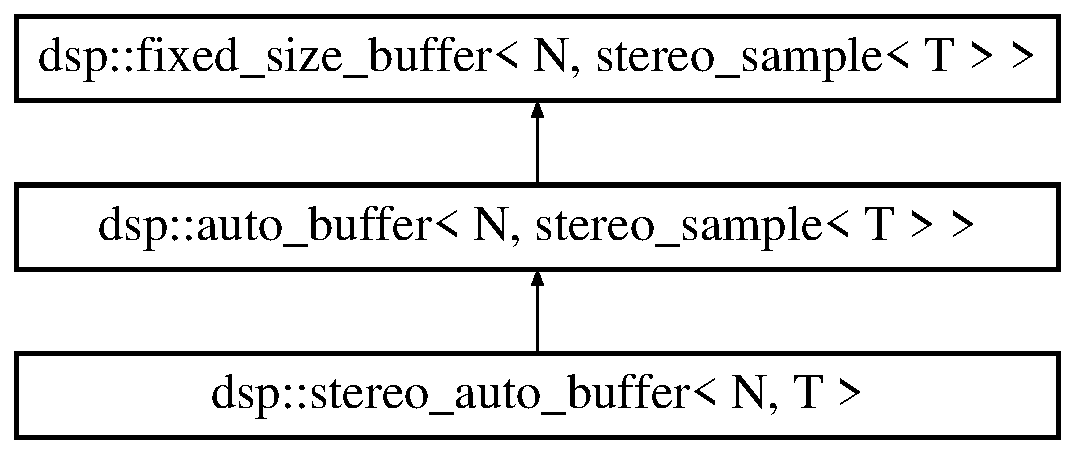
\includegraphics[height=3.000000cm]{classdsp_1_1stereo__auto__buffer}
\end{center}
\end{figure}
\subsection*{Additional Inherited Members}


\subsection{Detailed Description}
\subsubsection*{template$<$int N, class T = float$>$\\*
class dsp\+::stereo\+\_\+auto\+\_\+buffer$<$ N, T $>$}

this is useless for now 

The documentation for this class was generated from the following file\+:\begin{DoxyCompactItemize}
\item 
/\+Users/michael/\+J\+U\+C\+E/projects/audealize-\/plugin/\+J\+U\+C\+E Modules/audealize\+\_\+module/utils/calf\+\_\+dsp\+\_\+library/\hyperlink{buffer_8h}{buffer.\+h}\end{DoxyCompactItemize}

\hypertarget{structdsp_1_1stereo__sample}{}\section{dsp\+:\+:stereo\+\_\+sample$<$ T $>$ Struct Template Reference}
\label{structdsp_1_1stereo__sample}\index{dsp\+::stereo\+\_\+sample$<$ T $>$@{dsp\+::stereo\+\_\+sample$<$ T $>$}}


{\ttfamily \#include $<$primitives.\+h$>$}

\subsection*{Public Member Functions}
\begin{DoxyCompactItemize}
\item 
\hyperlink{structdsp_1_1stereo__sample_a70acefe335f719b3e6e3e277050da752}{stereo\+\_\+sample} ()
\begin{DoxyCompactList}\small\item\em default constructor -\/ preserves T\textquotesingle{}s semantics (ie. no implicit initialization to 0) \end{DoxyCompactList}\item 
\hyperlink{structdsp_1_1stereo__sample_ac56c19e0d3a0deee6a318bff34b8bf48}{stereo\+\_\+sample} (T \+\_\+left, T \+\_\+right)
\item 
\hyperlink{structdsp_1_1stereo__sample_a73795bccf46a690a4cfad057866ee7c8}{stereo\+\_\+sample} (T \+\_\+both)
\item 
{\footnotesize template$<$typename U $>$ }\\\hyperlink{structdsp_1_1stereo__sample_a3e9b0be236fb44d0b9ff9a33aee7d151}{stereo\+\_\+sample} (const \hyperlink{structdsp_1_1stereo__sample}{stereo\+\_\+sample}$<$ U $>$ \&\hyperlink{tk_8h_a177a0765f574ef6642002696d9cd82d0}{value})
\item 
\hyperlink{structdsp_1_1stereo__sample}{stereo\+\_\+sample} \& \hyperlink{structdsp_1_1stereo__sample_a57ba82d63fdb251fbe74cfbaefd45ac0}{operator=} (const T \&\hyperlink{tk_8h_a177a0765f574ef6642002696d9cd82d0}{value})
\item 
{\footnotesize template$<$typename U $>$ }\\\hyperlink{structdsp_1_1stereo__sample}{stereo\+\_\+sample} \& \hyperlink{structdsp_1_1stereo__sample_a4af279aca9661aecaa5979420e25720a}{operator=} (const \hyperlink{structdsp_1_1stereo__sample}{stereo\+\_\+sample}$<$ U $>$ \&\hyperlink{tk_8h_a177a0765f574ef6642002696d9cd82d0}{value})
\item 
\hyperlink{structdsp_1_1stereo__sample}{stereo\+\_\+sample} \& \hyperlink{structdsp_1_1stereo__sample_a07354a18f3eb6b5579791aa119fb36fb}{operator$\ast$=} (const T \&multiplier)
\item 
\hyperlink{structdsp_1_1stereo__sample}{stereo\+\_\+sample} \& \hyperlink{structdsp_1_1stereo__sample_a191a1dad0717772f763a2b52556f7281}{operator+=} (const \hyperlink{structdsp_1_1stereo__sample}{stereo\+\_\+sample}$<$ T $>$ \&\hyperlink{tk_8h_a177a0765f574ef6642002696d9cd82d0}{value})
\item 
\hyperlink{structdsp_1_1stereo__sample}{stereo\+\_\+sample} \& \hyperlink{structdsp_1_1stereo__sample_a4a96f575237d712f41973333023be7b4}{operator-\/=} (const \hyperlink{structdsp_1_1stereo__sample}{stereo\+\_\+sample}$<$ T $>$ \&\hyperlink{tk_8h_a177a0765f574ef6642002696d9cd82d0}{value})
\item 
{\footnotesize template$<$typename U $>$ }\\\hyperlink{structdsp_1_1stereo__sample}{stereo\+\_\+sample}$<$ U $>$ \hyperlink{structdsp_1_1stereo__sample_a7cd922059e31dc561f2c1aacf522d132}{operator$\ast$} (const U \&\hyperlink{tk_8h_a177a0765f574ef6642002696d9cd82d0}{value}) const 
\item 
\hyperlink{structdsp_1_1stereo__sample}{stereo\+\_\+sample}$<$ T $>$ \hyperlink{structdsp_1_1stereo__sample_a4dd61a95133277cd2e3fe345cb17f5f5}{operator+} (const \hyperlink{structdsp_1_1stereo__sample}{stereo\+\_\+sample}$<$ T $>$ \&\hyperlink{tk_8h_a177a0765f574ef6642002696d9cd82d0}{value})
\item 
\hyperlink{structdsp_1_1stereo__sample}{stereo\+\_\+sample}$<$ T $>$ \hyperlink{structdsp_1_1stereo__sample_afc1f323b87a8cfe546d796d6b7949fdd}{operator-\/} (const \hyperlink{structdsp_1_1stereo__sample}{stereo\+\_\+sample}$<$ T $>$ \&\hyperlink{tk_8h_a177a0765f574ef6642002696d9cd82d0}{value})
\item 
\hyperlink{structdsp_1_1stereo__sample}{stereo\+\_\+sample}$<$ T $>$ \hyperlink{structdsp_1_1stereo__sample_afc698f85d35454bd6cc5c52a29f4623a}{operator+} (const T \&\hyperlink{tk_8h_a177a0765f574ef6642002696d9cd82d0}{value})
\item 
\hyperlink{structdsp_1_1stereo__sample}{stereo\+\_\+sample}$<$ T $>$ \hyperlink{structdsp_1_1stereo__sample_a55ce56f876f111ea9c15b343c1ff0a90}{operator-\/} (const T \&\hyperlink{tk_8h_a177a0765f574ef6642002696d9cd82d0}{value})
\item 
\hyperlink{structdsp_1_1stereo__sample}{stereo\+\_\+sample}$<$ float $>$ \hyperlink{structdsp_1_1stereo__sample_af8444c6f9d75fbb5c671a73f975f1d16}{operator+} (float \hyperlink{tk_8h_a177a0765f574ef6642002696d9cd82d0}{value})
\item 
\hyperlink{structdsp_1_1stereo__sample}{stereo\+\_\+sample}$<$ float $>$ \hyperlink{structdsp_1_1stereo__sample_a86b59d6e7568916173775dd02ea974e3}{operator-\/} (float \hyperlink{tk_8h_a177a0765f574ef6642002696d9cd82d0}{value})
\item 
\hyperlink{structdsp_1_1stereo__sample}{stereo\+\_\+sample}$<$ double $>$ \hyperlink{structdsp_1_1stereo__sample_a9c23fa03b8d61c5df471014cb185480b}{operator+} (double \hyperlink{tk_8h_a177a0765f574ef6642002696d9cd82d0}{value})
\item 
\hyperlink{structdsp_1_1stereo__sample}{stereo\+\_\+sample}$<$ double $>$ \hyperlink{structdsp_1_1stereo__sample_ad090d9dce19953a7f03b02d46693cfa2}{operator-\/} (double \hyperlink{tk_8h_a177a0765f574ef6642002696d9cd82d0}{value})
\end{DoxyCompactItemize}
\subsection*{Public Attributes}
\begin{DoxyCompactItemize}
\item 
T \hyperlink{structdsp_1_1stereo__sample_ac084edf0dde1202d8da6b38feee52b2a}{left}
\item 
T \hyperlink{structdsp_1_1stereo__sample_a9fb6419f7d1167ff3e26bbbf14d48500}{right}
\end{DoxyCompactItemize}


\subsection{Constructor \& Destructor Documentation}
\index{dsp\+::stereo\+\_\+sample@{dsp\+::stereo\+\_\+sample}!stereo\+\_\+sample@{stereo\+\_\+sample}}
\index{stereo\+\_\+sample@{stereo\+\_\+sample}!dsp\+::stereo\+\_\+sample@{dsp\+::stereo\+\_\+sample}}
\subsubsection[{\texorpdfstring{stereo\+\_\+sample()}{stereo_sample()}}]{\setlength{\rightskip}{0pt plus 5cm}template$<$class T = float$>$ {\bf dsp\+::stereo\+\_\+sample}$<$ T $>$\+::{\bf stereo\+\_\+sample} (
\begin{DoxyParamCaption}
{}
\end{DoxyParamCaption}
)\hspace{0.3cm}{\ttfamily [inline]}}\hypertarget{structdsp_1_1stereo__sample_a70acefe335f719b3e6e3e277050da752}{}\label{structdsp_1_1stereo__sample_a70acefe335f719b3e6e3e277050da752}


default constructor -\/ preserves T\textquotesingle{}s semantics (ie. no implicit initialization to 0) 

\index{dsp\+::stereo\+\_\+sample@{dsp\+::stereo\+\_\+sample}!stereo\+\_\+sample@{stereo\+\_\+sample}}
\index{stereo\+\_\+sample@{stereo\+\_\+sample}!dsp\+::stereo\+\_\+sample@{dsp\+::stereo\+\_\+sample}}
\subsubsection[{\texorpdfstring{stereo\+\_\+sample(\+T \+\_\+left, T \+\_\+right)}{stereo_sample(T _left, T _right)}}]{\setlength{\rightskip}{0pt plus 5cm}template$<$class T = float$>$ {\bf dsp\+::stereo\+\_\+sample}$<$ T $>$\+::{\bf stereo\+\_\+sample} (
\begin{DoxyParamCaption}
\item[{T}]{\+\_\+left, }
\item[{T}]{\+\_\+right}
\end{DoxyParamCaption}
)\hspace{0.3cm}{\ttfamily [inline]}}\hypertarget{structdsp_1_1stereo__sample_ac56c19e0d3a0deee6a318bff34b8bf48}{}\label{structdsp_1_1stereo__sample_ac56c19e0d3a0deee6a318bff34b8bf48}
\index{dsp\+::stereo\+\_\+sample@{dsp\+::stereo\+\_\+sample}!stereo\+\_\+sample@{stereo\+\_\+sample}}
\index{stereo\+\_\+sample@{stereo\+\_\+sample}!dsp\+::stereo\+\_\+sample@{dsp\+::stereo\+\_\+sample}}
\subsubsection[{\texorpdfstring{stereo\+\_\+sample(\+T \+\_\+both)}{stereo_sample(T _both)}}]{\setlength{\rightskip}{0pt plus 5cm}template$<$class T = float$>$ {\bf dsp\+::stereo\+\_\+sample}$<$ T $>$\+::{\bf stereo\+\_\+sample} (
\begin{DoxyParamCaption}
\item[{T}]{\+\_\+both}
\end{DoxyParamCaption}
)\hspace{0.3cm}{\ttfamily [inline]}}\hypertarget{structdsp_1_1stereo__sample_a73795bccf46a690a4cfad057866ee7c8}{}\label{structdsp_1_1stereo__sample_a73795bccf46a690a4cfad057866ee7c8}
\index{dsp\+::stereo\+\_\+sample@{dsp\+::stereo\+\_\+sample}!stereo\+\_\+sample@{stereo\+\_\+sample}}
\index{stereo\+\_\+sample@{stereo\+\_\+sample}!dsp\+::stereo\+\_\+sample@{dsp\+::stereo\+\_\+sample}}
\subsubsection[{\texorpdfstring{stereo\+\_\+sample(const stereo\+\_\+sample$<$ U $>$ \&value)}{stereo_sample(const stereo_sample< U > &value)}}]{\setlength{\rightskip}{0pt plus 5cm}template$<$class T = float$>$ template$<$typename U $>$ {\bf dsp\+::stereo\+\_\+sample}$<$ T $>$\+::{\bf stereo\+\_\+sample} (
\begin{DoxyParamCaption}
\item[{const {\bf stereo\+\_\+sample}$<$ U $>$ \&}]{value}
\end{DoxyParamCaption}
)\hspace{0.3cm}{\ttfamily [inline]}}\hypertarget{structdsp_1_1stereo__sample_a3e9b0be236fb44d0b9ff9a33aee7d151}{}\label{structdsp_1_1stereo__sample_a3e9b0be236fb44d0b9ff9a33aee7d151}


\subsection{Member Function Documentation}
\index{dsp\+::stereo\+\_\+sample@{dsp\+::stereo\+\_\+sample}!operator$\ast$@{operator$\ast$}}
\index{operator$\ast$@{operator$\ast$}!dsp\+::stereo\+\_\+sample@{dsp\+::stereo\+\_\+sample}}
\subsubsection[{\texorpdfstring{operator$\ast$(const U \&value) const }{operator*(const U &value) const }}]{\setlength{\rightskip}{0pt plus 5cm}template$<$class T = float$>$ template$<$typename U $>$ {\bf stereo\+\_\+sample}$<$U$>$ {\bf dsp\+::stereo\+\_\+sample}$<$ T $>$\+::operator$\ast$ (
\begin{DoxyParamCaption}
\item[{const U \&}]{value}
\end{DoxyParamCaption}
) const\hspace{0.3cm}{\ttfamily [inline]}}\hypertarget{structdsp_1_1stereo__sample_a7cd922059e31dc561f2c1aacf522d132}{}\label{structdsp_1_1stereo__sample_a7cd922059e31dc561f2c1aacf522d132}
\index{dsp\+::stereo\+\_\+sample@{dsp\+::stereo\+\_\+sample}!operator$\ast$=@{operator$\ast$=}}
\index{operator$\ast$=@{operator$\ast$=}!dsp\+::stereo\+\_\+sample@{dsp\+::stereo\+\_\+sample}}
\subsubsection[{\texorpdfstring{operator$\ast$=(const T \&multiplier)}{operator*=(const T &multiplier)}}]{\setlength{\rightskip}{0pt plus 5cm}template$<$class T = float$>$ {\bf stereo\+\_\+sample}\& {\bf dsp\+::stereo\+\_\+sample}$<$ T $>$\+::operator$\ast$= (
\begin{DoxyParamCaption}
\item[{const T \&}]{multiplier}
\end{DoxyParamCaption}
)\hspace{0.3cm}{\ttfamily [inline]}}\hypertarget{structdsp_1_1stereo__sample_a07354a18f3eb6b5579791aa119fb36fb}{}\label{structdsp_1_1stereo__sample_a07354a18f3eb6b5579791aa119fb36fb}
\index{dsp\+::stereo\+\_\+sample@{dsp\+::stereo\+\_\+sample}!operator+@{operator+}}
\index{operator+@{operator+}!dsp\+::stereo\+\_\+sample@{dsp\+::stereo\+\_\+sample}}
\subsubsection[{\texorpdfstring{operator+(const stereo\+\_\+sample$<$ T $>$ \&value)}{operator+(const stereo_sample< T > &value)}}]{\setlength{\rightskip}{0pt plus 5cm}template$<$class T = float$>$ {\bf stereo\+\_\+sample}$<$T$>$ {\bf dsp\+::stereo\+\_\+sample}$<$ T $>$\+::operator+ (
\begin{DoxyParamCaption}
\item[{const {\bf stereo\+\_\+sample}$<$ T $>$ \&}]{value}
\end{DoxyParamCaption}
)\hspace{0.3cm}{\ttfamily [inline]}}\hypertarget{structdsp_1_1stereo__sample_a4dd61a95133277cd2e3fe345cb17f5f5}{}\label{structdsp_1_1stereo__sample_a4dd61a95133277cd2e3fe345cb17f5f5}
\index{dsp\+::stereo\+\_\+sample@{dsp\+::stereo\+\_\+sample}!operator+@{operator+}}
\index{operator+@{operator+}!dsp\+::stereo\+\_\+sample@{dsp\+::stereo\+\_\+sample}}
\subsubsection[{\texorpdfstring{operator+(const T \&value)}{operator+(const T &value)}}]{\setlength{\rightskip}{0pt plus 5cm}template$<$class T = float$>$ {\bf stereo\+\_\+sample}$<$T$>$ {\bf dsp\+::stereo\+\_\+sample}$<$ T $>$\+::operator+ (
\begin{DoxyParamCaption}
\item[{const T \&}]{value}
\end{DoxyParamCaption}
)\hspace{0.3cm}{\ttfamily [inline]}}\hypertarget{structdsp_1_1stereo__sample_afc698f85d35454bd6cc5c52a29f4623a}{}\label{structdsp_1_1stereo__sample_afc698f85d35454bd6cc5c52a29f4623a}
\index{dsp\+::stereo\+\_\+sample@{dsp\+::stereo\+\_\+sample}!operator+@{operator+}}
\index{operator+@{operator+}!dsp\+::stereo\+\_\+sample@{dsp\+::stereo\+\_\+sample}}
\subsubsection[{\texorpdfstring{operator+(float value)}{operator+(float value)}}]{\setlength{\rightskip}{0pt plus 5cm}template$<$class T = float$>$ {\bf stereo\+\_\+sample}$<$float$>$ {\bf dsp\+::stereo\+\_\+sample}$<$ T $>$\+::operator+ (
\begin{DoxyParamCaption}
\item[{float}]{value}
\end{DoxyParamCaption}
)\hspace{0.3cm}{\ttfamily [inline]}}\hypertarget{structdsp_1_1stereo__sample_af8444c6f9d75fbb5c671a73f975f1d16}{}\label{structdsp_1_1stereo__sample_af8444c6f9d75fbb5c671a73f975f1d16}
\index{dsp\+::stereo\+\_\+sample@{dsp\+::stereo\+\_\+sample}!operator+@{operator+}}
\index{operator+@{operator+}!dsp\+::stereo\+\_\+sample@{dsp\+::stereo\+\_\+sample}}
\subsubsection[{\texorpdfstring{operator+(double value)}{operator+(double value)}}]{\setlength{\rightskip}{0pt plus 5cm}template$<$class T = float$>$ {\bf stereo\+\_\+sample}$<$double$>$ {\bf dsp\+::stereo\+\_\+sample}$<$ T $>$\+::operator+ (
\begin{DoxyParamCaption}
\item[{double}]{value}
\end{DoxyParamCaption}
)\hspace{0.3cm}{\ttfamily [inline]}}\hypertarget{structdsp_1_1stereo__sample_a9c23fa03b8d61c5df471014cb185480b}{}\label{structdsp_1_1stereo__sample_a9c23fa03b8d61c5df471014cb185480b}
\index{dsp\+::stereo\+\_\+sample@{dsp\+::stereo\+\_\+sample}!operator+=@{operator+=}}
\index{operator+=@{operator+=}!dsp\+::stereo\+\_\+sample@{dsp\+::stereo\+\_\+sample}}
\subsubsection[{\texorpdfstring{operator+=(const stereo\+\_\+sample$<$ T $>$ \&value)}{operator+=(const stereo_sample< T > &value)}}]{\setlength{\rightskip}{0pt plus 5cm}template$<$class T = float$>$ {\bf stereo\+\_\+sample}\& {\bf dsp\+::stereo\+\_\+sample}$<$ T $>$\+::operator+= (
\begin{DoxyParamCaption}
\item[{const {\bf stereo\+\_\+sample}$<$ T $>$ \&}]{value}
\end{DoxyParamCaption}
)\hspace{0.3cm}{\ttfamily [inline]}}\hypertarget{structdsp_1_1stereo__sample_a191a1dad0717772f763a2b52556f7281}{}\label{structdsp_1_1stereo__sample_a191a1dad0717772f763a2b52556f7281}
\index{dsp\+::stereo\+\_\+sample@{dsp\+::stereo\+\_\+sample}!operator-\/@{operator-\/}}
\index{operator-\/@{operator-\/}!dsp\+::stereo\+\_\+sample@{dsp\+::stereo\+\_\+sample}}
\subsubsection[{\texorpdfstring{operator-\/(const stereo\+\_\+sample$<$ T $>$ \&value)}{operator-(const stereo_sample< T > &value)}}]{\setlength{\rightskip}{0pt plus 5cm}template$<$class T = float$>$ {\bf stereo\+\_\+sample}$<$T$>$ {\bf dsp\+::stereo\+\_\+sample}$<$ T $>$\+::operator-\/ (
\begin{DoxyParamCaption}
\item[{const {\bf stereo\+\_\+sample}$<$ T $>$ \&}]{value}
\end{DoxyParamCaption}
)\hspace{0.3cm}{\ttfamily [inline]}}\hypertarget{structdsp_1_1stereo__sample_afc1f323b87a8cfe546d796d6b7949fdd}{}\label{structdsp_1_1stereo__sample_afc1f323b87a8cfe546d796d6b7949fdd}
\index{dsp\+::stereo\+\_\+sample@{dsp\+::stereo\+\_\+sample}!operator-\/@{operator-\/}}
\index{operator-\/@{operator-\/}!dsp\+::stereo\+\_\+sample@{dsp\+::stereo\+\_\+sample}}
\subsubsection[{\texorpdfstring{operator-\/(const T \&value)}{operator-(const T &value)}}]{\setlength{\rightskip}{0pt plus 5cm}template$<$class T = float$>$ {\bf stereo\+\_\+sample}$<$T$>$ {\bf dsp\+::stereo\+\_\+sample}$<$ T $>$\+::operator-\/ (
\begin{DoxyParamCaption}
\item[{const T \&}]{value}
\end{DoxyParamCaption}
)\hspace{0.3cm}{\ttfamily [inline]}}\hypertarget{structdsp_1_1stereo__sample_a55ce56f876f111ea9c15b343c1ff0a90}{}\label{structdsp_1_1stereo__sample_a55ce56f876f111ea9c15b343c1ff0a90}
\index{dsp\+::stereo\+\_\+sample@{dsp\+::stereo\+\_\+sample}!operator-\/@{operator-\/}}
\index{operator-\/@{operator-\/}!dsp\+::stereo\+\_\+sample@{dsp\+::stereo\+\_\+sample}}
\subsubsection[{\texorpdfstring{operator-\/(float value)}{operator-(float value)}}]{\setlength{\rightskip}{0pt plus 5cm}template$<$class T = float$>$ {\bf stereo\+\_\+sample}$<$float$>$ {\bf dsp\+::stereo\+\_\+sample}$<$ T $>$\+::operator-\/ (
\begin{DoxyParamCaption}
\item[{float}]{value}
\end{DoxyParamCaption}
)\hspace{0.3cm}{\ttfamily [inline]}}\hypertarget{structdsp_1_1stereo__sample_a86b59d6e7568916173775dd02ea974e3}{}\label{structdsp_1_1stereo__sample_a86b59d6e7568916173775dd02ea974e3}
\index{dsp\+::stereo\+\_\+sample@{dsp\+::stereo\+\_\+sample}!operator-\/@{operator-\/}}
\index{operator-\/@{operator-\/}!dsp\+::stereo\+\_\+sample@{dsp\+::stereo\+\_\+sample}}
\subsubsection[{\texorpdfstring{operator-\/(double value)}{operator-(double value)}}]{\setlength{\rightskip}{0pt plus 5cm}template$<$class T = float$>$ {\bf stereo\+\_\+sample}$<$double$>$ {\bf dsp\+::stereo\+\_\+sample}$<$ T $>$\+::operator-\/ (
\begin{DoxyParamCaption}
\item[{double}]{value}
\end{DoxyParamCaption}
)\hspace{0.3cm}{\ttfamily [inline]}}\hypertarget{structdsp_1_1stereo__sample_ad090d9dce19953a7f03b02d46693cfa2}{}\label{structdsp_1_1stereo__sample_ad090d9dce19953a7f03b02d46693cfa2}
\index{dsp\+::stereo\+\_\+sample@{dsp\+::stereo\+\_\+sample}!operator-\/=@{operator-\/=}}
\index{operator-\/=@{operator-\/=}!dsp\+::stereo\+\_\+sample@{dsp\+::stereo\+\_\+sample}}
\subsubsection[{\texorpdfstring{operator-\/=(const stereo\+\_\+sample$<$ T $>$ \&value)}{operator-=(const stereo_sample< T > &value)}}]{\setlength{\rightskip}{0pt plus 5cm}template$<$class T = float$>$ {\bf stereo\+\_\+sample}\& {\bf dsp\+::stereo\+\_\+sample}$<$ T $>$\+::operator-\/= (
\begin{DoxyParamCaption}
\item[{const {\bf stereo\+\_\+sample}$<$ T $>$ \&}]{value}
\end{DoxyParamCaption}
)\hspace{0.3cm}{\ttfamily [inline]}}\hypertarget{structdsp_1_1stereo__sample_a4a96f575237d712f41973333023be7b4}{}\label{structdsp_1_1stereo__sample_a4a96f575237d712f41973333023be7b4}
\index{dsp\+::stereo\+\_\+sample@{dsp\+::stereo\+\_\+sample}!operator=@{operator=}}
\index{operator=@{operator=}!dsp\+::stereo\+\_\+sample@{dsp\+::stereo\+\_\+sample}}
\subsubsection[{\texorpdfstring{operator=(const T \&value)}{operator=(const T &value)}}]{\setlength{\rightskip}{0pt plus 5cm}template$<$class T = float$>$ {\bf stereo\+\_\+sample}\& {\bf dsp\+::stereo\+\_\+sample}$<$ T $>$\+::operator= (
\begin{DoxyParamCaption}
\item[{const T \&}]{value}
\end{DoxyParamCaption}
)\hspace{0.3cm}{\ttfamily [inline]}}\hypertarget{structdsp_1_1stereo__sample_a57ba82d63fdb251fbe74cfbaefd45ac0}{}\label{structdsp_1_1stereo__sample_a57ba82d63fdb251fbe74cfbaefd45ac0}
\index{dsp\+::stereo\+\_\+sample@{dsp\+::stereo\+\_\+sample}!operator=@{operator=}}
\index{operator=@{operator=}!dsp\+::stereo\+\_\+sample@{dsp\+::stereo\+\_\+sample}}
\subsubsection[{\texorpdfstring{operator=(const stereo\+\_\+sample$<$ U $>$ \&value)}{operator=(const stereo_sample< U > &value)}}]{\setlength{\rightskip}{0pt plus 5cm}template$<$class T = float$>$ template$<$typename U $>$ {\bf stereo\+\_\+sample}\& {\bf dsp\+::stereo\+\_\+sample}$<$ T $>$\+::operator= (
\begin{DoxyParamCaption}
\item[{const {\bf stereo\+\_\+sample}$<$ U $>$ \&}]{value}
\end{DoxyParamCaption}
)\hspace{0.3cm}{\ttfamily [inline]}}\hypertarget{structdsp_1_1stereo__sample_a4af279aca9661aecaa5979420e25720a}{}\label{structdsp_1_1stereo__sample_a4af279aca9661aecaa5979420e25720a}


\subsection{Member Data Documentation}
\index{dsp\+::stereo\+\_\+sample@{dsp\+::stereo\+\_\+sample}!left@{left}}
\index{left@{left}!dsp\+::stereo\+\_\+sample@{dsp\+::stereo\+\_\+sample}}
\subsubsection[{\texorpdfstring{left}{left}}]{\setlength{\rightskip}{0pt plus 5cm}template$<$class T = float$>$ T {\bf dsp\+::stereo\+\_\+sample}$<$ T $>$\+::left}\hypertarget{structdsp_1_1stereo__sample_ac084edf0dde1202d8da6b38feee52b2a}{}\label{structdsp_1_1stereo__sample_ac084edf0dde1202d8da6b38feee52b2a}
\index{dsp\+::stereo\+\_\+sample@{dsp\+::stereo\+\_\+sample}!right@{right}}
\index{right@{right}!dsp\+::stereo\+\_\+sample@{dsp\+::stereo\+\_\+sample}}
\subsubsection[{\texorpdfstring{right}{right}}]{\setlength{\rightskip}{0pt plus 5cm}template$<$class T = float$>$ T {\bf dsp\+::stereo\+\_\+sample}$<$ T $>$\+::right}\hypertarget{structdsp_1_1stereo__sample_a9fb6419f7d1167ff3e26bbbf14d48500}{}\label{structdsp_1_1stereo__sample_a9fb6419f7d1167ff3e26bbbf14d48500}


The documentation for this struct was generated from the following file\+:\begin{DoxyCompactItemize}
\item 
/\+Users/michael/\+J\+U\+C\+E/projects/audealize-\/plugin/\+J\+U\+C\+E Modules/audealize\+\_\+module/utils/calf\+\_\+dsp\+\_\+library/\hyperlink{primitives_8h}{primitives.\+h}\end{DoxyCompactItemize}

\hypertarget{structsymbol}{}\section{symbol Struct Reference}
\label{structsymbol}\index{symbol@{symbol}}


{\ttfamily \#include $<$wngrind.\+h$>$}

\subsection*{Public Attributes}
\begin{DoxyCompactItemize}
\item 
struct \hyperlink{structsymbol}{symbol} $\ast$ \hyperlink{structsymbol_a5720b8e7b0fbd499f1d001f04d39d67e}{symnext}
\item 
struct \hyperlink{structsynlist}{synlist} $\ast$ \hyperlink{structsymbol_a2cd0744aa0880eab684564abef2ee29e}{syns}
\item 
unsigned char \hyperlink{structsymbol_a797fcb09a193bde8feb95b83b8be14f0}{sensecnt} \mbox{[}\hyperlink{wn_8h_a3d6b4ec100d3ded8506abe9af8757eb9}{N\+U\+M\+P\+A\+R\+TS}+1\mbox{]}
\item 
char $\ast$ \hyperlink{structsymbol_a18eeb23c50b308114cecaf64a042ef6c}{label}
\end{DoxyCompactItemize}


\subsection{Member Data Documentation}
\index{symbol@{symbol}!label@{label}}
\index{label@{label}!symbol@{symbol}}
\subsubsection[{\texorpdfstring{label}{label}}]{\setlength{\rightskip}{0pt plus 5cm}char$\ast$ symbol\+::label}\hypertarget{structsymbol_a18eeb23c50b308114cecaf64a042ef6c}{}\label{structsymbol_a18eeb23c50b308114cecaf64a042ef6c}
\index{symbol@{symbol}!sensecnt@{sensecnt}}
\index{sensecnt@{sensecnt}!symbol@{symbol}}
\subsubsection[{\texorpdfstring{sensecnt}{sensecnt}}]{\setlength{\rightskip}{0pt plus 5cm}unsigned char symbol\+::sensecnt\mbox{[}{\bf N\+U\+M\+P\+A\+R\+TS}+1\mbox{]}}\hypertarget{structsymbol_a797fcb09a193bde8feb95b83b8be14f0}{}\label{structsymbol_a797fcb09a193bde8feb95b83b8be14f0}
\index{symbol@{symbol}!symnext@{symnext}}
\index{symnext@{symnext}!symbol@{symbol}}
\subsubsection[{\texorpdfstring{symnext}{symnext}}]{\setlength{\rightskip}{0pt plus 5cm}struct {\bf symbol}$\ast$ symbol\+::symnext}\hypertarget{structsymbol_a5720b8e7b0fbd499f1d001f04d39d67e}{}\label{structsymbol_a5720b8e7b0fbd499f1d001f04d39d67e}
\index{symbol@{symbol}!syns@{syns}}
\index{syns@{syns}!symbol@{symbol}}
\subsubsection[{\texorpdfstring{syns}{syns}}]{\setlength{\rightskip}{0pt plus 5cm}struct {\bf synlist}$\ast$ symbol\+::syns}\hypertarget{structsymbol_a2cd0744aa0880eab684564abef2ee29e}{}\label{structsymbol_a2cd0744aa0880eab684564abef2ee29e}


The documentation for this struct was generated from the following file\+:\begin{DoxyCompactItemize}
\item 
/\+Users/michael/\+J\+U\+C\+E/projects/audealize-\/plugin/\+J\+U\+C\+E Modules/audealize\+\_\+module/\+Word\+Net-\/3.\+0/include/\hyperlink{wngrind_8h}{wngrind.\+h}\end{DoxyCompactItemize}

\hypertarget{structsynlist}{}\section{synlist Struct Reference}
\label{structsynlist}\index{synlist@{synlist}}


{\ttfamily \#include $<$wngrind.\+h$>$}

\subsection*{Public Attributes}
\begin{DoxyCompactItemize}
\item 
struct \hyperlink{structsynlist}{synlist} $\ast$ \hyperlink{structsynlist_aa876afb1c31ffb1d4110cf1ea7fdd9fc}{snext}
\item 
struct \hyperlink{structsynonym}{synonym} $\ast$ \hyperlink{structsynlist_a8d1e2127237274f07903ffa05710f201}{psyn}
\end{DoxyCompactItemize}


\subsection{Member Data Documentation}
\index{synlist@{synlist}!psyn@{psyn}}
\index{psyn@{psyn}!synlist@{synlist}}
\subsubsection[{\texorpdfstring{psyn}{psyn}}]{\setlength{\rightskip}{0pt plus 5cm}struct {\bf synonym}$\ast$ synlist\+::psyn}\hypertarget{structsynlist_a8d1e2127237274f07903ffa05710f201}{}\label{structsynlist_a8d1e2127237274f07903ffa05710f201}
\index{synlist@{synlist}!snext@{snext}}
\index{snext@{snext}!synlist@{synlist}}
\subsubsection[{\texorpdfstring{snext}{snext}}]{\setlength{\rightskip}{0pt plus 5cm}struct {\bf synlist}$\ast$ synlist\+::snext}\hypertarget{structsynlist_aa876afb1c31ffb1d4110cf1ea7fdd9fc}{}\label{structsynlist_aa876afb1c31ffb1d4110cf1ea7fdd9fc}


The documentation for this struct was generated from the following file\+:\begin{DoxyCompactItemize}
\item 
/\+Users/michael/\+J\+U\+C\+E/projects/audealize-\/plugin/\+J\+U\+C\+E Modules/audealize\+\_\+module/\+Word\+Net-\/3.\+0/include/\hyperlink{wngrind_8h}{wngrind.\+h}\end{DoxyCompactItemize}

\hypertarget{structsynonym}{}\section{synonym Struct Reference}
\label{structsynonym}\index{synonym@{synonym}}


{\ttfamily \#include $<$wngrind.\+h$>$}

\subsection*{Public Attributes}
\begin{DoxyCompactItemize}
\item 
struct \hyperlink{structsynonym}{synonym} $\ast$ \hyperlink{structsynonym_aa52cb3012712a599111a9306c6c7821f}{synnext}
\item 
struct \hyperlink{structsynset}{synset} $\ast$ \hyperlink{structsynonym_afb6e3d7b4af47cbd982c32381054bf6d}{ss}
\item 
struct \hyperlink{structsymbol}{symbol} $\ast$ \hyperlink{structsynonym_a76fb3a2c037b88010fd0f402ca48f1e2}{word}
\item 
short \hyperlink{structsynonym_a2ae26eef29c66c22ce2b6d3c4cb00884}{sswdnum}
\item 
short \hyperlink{structsynonym_aa8d3b5cfe5c1655dd17dbeb33c5a32ee}{tagcnt}
\item 
unsigned char \hyperlink{structsynonym_a5c9bd36f2044cf3efe20bdc80047fa87}{wnsensenum}
\item 
unsigned char \hyperlink{structsynonym_af4c83833e99b2c620defd3be9346f47c}{sensenum}
\item 
unsigned char \hyperlink{structsynonym_a4950ed90421213474467e7e809c7b1cf}{adjclass}
\item 
unsigned char \hyperlink{structsynonym_a8d20f5c5cfb4f4bcb1f638e21ebdcbc6}{infanss}
\item 
char $\ast$ \hyperlink{structsynonym_ad03a38ac09acf1a4aeaf8c1793e354aa}{label}
\end{DoxyCompactItemize}


\subsection{Member Data Documentation}
\index{synonym@{synonym}!adjclass@{adjclass}}
\index{adjclass@{adjclass}!synonym@{synonym}}
\subsubsection[{\texorpdfstring{adjclass}{adjclass}}]{\setlength{\rightskip}{0pt plus 5cm}unsigned char synonym\+::adjclass}\hypertarget{structsynonym_a4950ed90421213474467e7e809c7b1cf}{}\label{structsynonym_a4950ed90421213474467e7e809c7b1cf}
\index{synonym@{synonym}!infanss@{infanss}}
\index{infanss@{infanss}!synonym@{synonym}}
\subsubsection[{\texorpdfstring{infanss}{infanss}}]{\setlength{\rightskip}{0pt plus 5cm}unsigned char synonym\+::infanss}\hypertarget{structsynonym_a8d20f5c5cfb4f4bcb1f638e21ebdcbc6}{}\label{structsynonym_a8d20f5c5cfb4f4bcb1f638e21ebdcbc6}
\index{synonym@{synonym}!label@{label}}
\index{label@{label}!synonym@{synonym}}
\subsubsection[{\texorpdfstring{label}{label}}]{\setlength{\rightskip}{0pt plus 5cm}char$\ast$ synonym\+::label}\hypertarget{structsynonym_ad03a38ac09acf1a4aeaf8c1793e354aa}{}\label{structsynonym_ad03a38ac09acf1a4aeaf8c1793e354aa}
\index{synonym@{synonym}!sensenum@{sensenum}}
\index{sensenum@{sensenum}!synonym@{synonym}}
\subsubsection[{\texorpdfstring{sensenum}{sensenum}}]{\setlength{\rightskip}{0pt plus 5cm}unsigned char synonym\+::sensenum}\hypertarget{structsynonym_af4c83833e99b2c620defd3be9346f47c}{}\label{structsynonym_af4c83833e99b2c620defd3be9346f47c}
\index{synonym@{synonym}!ss@{ss}}
\index{ss@{ss}!synonym@{synonym}}
\subsubsection[{\texorpdfstring{ss}{ss}}]{\setlength{\rightskip}{0pt plus 5cm}struct {\bf synset}$\ast$ synonym\+::ss}\hypertarget{structsynonym_afb6e3d7b4af47cbd982c32381054bf6d}{}\label{structsynonym_afb6e3d7b4af47cbd982c32381054bf6d}
\index{synonym@{synonym}!sswdnum@{sswdnum}}
\index{sswdnum@{sswdnum}!synonym@{synonym}}
\subsubsection[{\texorpdfstring{sswdnum}{sswdnum}}]{\setlength{\rightskip}{0pt plus 5cm}short synonym\+::sswdnum}\hypertarget{structsynonym_a2ae26eef29c66c22ce2b6d3c4cb00884}{}\label{structsynonym_a2ae26eef29c66c22ce2b6d3c4cb00884}
\index{synonym@{synonym}!synnext@{synnext}}
\index{synnext@{synnext}!synonym@{synonym}}
\subsubsection[{\texorpdfstring{synnext}{synnext}}]{\setlength{\rightskip}{0pt plus 5cm}struct {\bf synonym}$\ast$ synonym\+::synnext}\hypertarget{structsynonym_aa52cb3012712a599111a9306c6c7821f}{}\label{structsynonym_aa52cb3012712a599111a9306c6c7821f}
\index{synonym@{synonym}!tagcnt@{tagcnt}}
\index{tagcnt@{tagcnt}!synonym@{synonym}}
\subsubsection[{\texorpdfstring{tagcnt}{tagcnt}}]{\setlength{\rightskip}{0pt plus 5cm}short synonym\+::tagcnt}\hypertarget{structsynonym_aa8d3b5cfe5c1655dd17dbeb33c5a32ee}{}\label{structsynonym_aa8d3b5cfe5c1655dd17dbeb33c5a32ee}
\index{synonym@{synonym}!wnsensenum@{wnsensenum}}
\index{wnsensenum@{wnsensenum}!synonym@{synonym}}
\subsubsection[{\texorpdfstring{wnsensenum}{wnsensenum}}]{\setlength{\rightskip}{0pt plus 5cm}unsigned char synonym\+::wnsensenum}\hypertarget{structsynonym_a5c9bd36f2044cf3efe20bdc80047fa87}{}\label{structsynonym_a5c9bd36f2044cf3efe20bdc80047fa87}
\index{synonym@{synonym}!word@{word}}
\index{word@{word}!synonym@{synonym}}
\subsubsection[{\texorpdfstring{word}{word}}]{\setlength{\rightskip}{0pt plus 5cm}struct {\bf symbol}$\ast$ synonym\+::word}\hypertarget{structsynonym_a76fb3a2c037b88010fd0f402ca48f1e2}{}\label{structsynonym_a76fb3a2c037b88010fd0f402ca48f1e2}


The documentation for this struct was generated from the following file\+:\begin{DoxyCompactItemize}
\item 
/\+Users/michael/\+J\+U\+C\+E/projects/audealize-\/plugin/\+J\+U\+C\+E Modules/audealize\+\_\+module/\+Word\+Net-\/3.\+0/include/\hyperlink{wngrind_8h}{wngrind.\+h}\end{DoxyCompactItemize}

\hypertarget{structsynset}{}\section{synset Struct Reference}
\label{structsynset}\index{synset@{synset}}


{\ttfamily \#include $<$wngrind.\+h$>$}

\subsection*{Public Attributes}
\begin{DoxyCompactItemize}
\item 
struct \hyperlink{structsynset}{synset} $\ast$ \hyperlink{structsynset_aba0cb8e929001cfb128d5c9f084e8854}{ssnext}
\item 
struct \hyperlink{structsynset}{synset} $\ast$ \hyperlink{structsynset_a4b6f0786fa124be59a726e1f28d5410a}{fans}
\item 
struct \hyperlink{structsynonym}{synonym} $\ast$ \hyperlink{structsynset_a27ca954987020967d38de075237e117e}{syns}
\item 
struct \hyperlink{structpointer}{pointer} $\ast$ \hyperlink{structsynset_ae62d0b3a9db00ab03cbd28e2f046c0d7}{ptrs}
\item 
struct \hyperlink{structframelist}{framelist} $\ast$ \hyperlink{structsynset_a4271481470c53551fe7759980393a9ee}{frames}
\item 
char $\ast$ \hyperlink{structsynset_a5d8d31dd3cd275dbcdb2e080de0c639b}{defn}
\item 
unsigned \hyperlink{tk_8h_a83f82f76e7fed06f4c49d2db94028a6d}{int} \hyperlink{structsynset_a84f62854ad2a5034801fc54270ebb8cc}{key}
\item 
unsigned char \hyperlink{structsynset_a8b146700698360902c31167a67d7f4d3}{part}
\item 
unsigned char \hyperlink{structsynset_a8cf7735311d10373e10c2a640868db01}{isfanss}
\item 
unsigned char \hyperlink{structsynset_a4e662ac65d3322d41a86a950551c64a5}{filenum}
\item 
\hyperlink{tk_8h_a83f82f76e7fed06f4c49d2db94028a6d}{int} \hyperlink{structsynset_ab3c4105b791fd23aec59322c589e6878}{clusnum}
\item 
\hyperlink{tk_8h_a83f82f76e7fed06f4c49d2db94028a6d}{int} \hyperlink{structsynset_a8c9026d3d58cd2ddbb18a2b0f8457cbe}{lineno}
\item 
long \hyperlink{structsynset_a5dfd3c1aea28ff9f1396f80fa0a6e253}{filepos}
\end{DoxyCompactItemize}


\subsection{Member Data Documentation}
\index{synset@{synset}!clusnum@{clusnum}}
\index{clusnum@{clusnum}!synset@{synset}}
\subsubsection[{\texorpdfstring{clusnum}{clusnum}}]{\setlength{\rightskip}{0pt plus 5cm}{\bf int} synset\+::clusnum}\hypertarget{structsynset_ab3c4105b791fd23aec59322c589e6878}{}\label{structsynset_ab3c4105b791fd23aec59322c589e6878}
\index{synset@{synset}!defn@{defn}}
\index{defn@{defn}!synset@{synset}}
\subsubsection[{\texorpdfstring{defn}{defn}}]{\setlength{\rightskip}{0pt plus 5cm}char$\ast$ synset\+::defn}\hypertarget{structsynset_a5d8d31dd3cd275dbcdb2e080de0c639b}{}\label{structsynset_a5d8d31dd3cd275dbcdb2e080de0c639b}
\index{synset@{synset}!fans@{fans}}
\index{fans@{fans}!synset@{synset}}
\subsubsection[{\texorpdfstring{fans}{fans}}]{\setlength{\rightskip}{0pt plus 5cm}struct {\bf synset}$\ast$ synset\+::fans}\hypertarget{structsynset_a4b6f0786fa124be59a726e1f28d5410a}{}\label{structsynset_a4b6f0786fa124be59a726e1f28d5410a}
\index{synset@{synset}!filenum@{filenum}}
\index{filenum@{filenum}!synset@{synset}}
\subsubsection[{\texorpdfstring{filenum}{filenum}}]{\setlength{\rightskip}{0pt plus 5cm}unsigned char synset\+::filenum}\hypertarget{structsynset_a4e662ac65d3322d41a86a950551c64a5}{}\label{structsynset_a4e662ac65d3322d41a86a950551c64a5}
\index{synset@{synset}!filepos@{filepos}}
\index{filepos@{filepos}!synset@{synset}}
\subsubsection[{\texorpdfstring{filepos}{filepos}}]{\setlength{\rightskip}{0pt plus 5cm}long synset\+::filepos}\hypertarget{structsynset_a5dfd3c1aea28ff9f1396f80fa0a6e253}{}\label{structsynset_a5dfd3c1aea28ff9f1396f80fa0a6e253}
\index{synset@{synset}!frames@{frames}}
\index{frames@{frames}!synset@{synset}}
\subsubsection[{\texorpdfstring{frames}{frames}}]{\setlength{\rightskip}{0pt plus 5cm}struct {\bf framelist}$\ast$ synset\+::frames}\hypertarget{structsynset_a4271481470c53551fe7759980393a9ee}{}\label{structsynset_a4271481470c53551fe7759980393a9ee}
\index{synset@{synset}!isfanss@{isfanss}}
\index{isfanss@{isfanss}!synset@{synset}}
\subsubsection[{\texorpdfstring{isfanss}{isfanss}}]{\setlength{\rightskip}{0pt plus 5cm}unsigned char synset\+::isfanss}\hypertarget{structsynset_a8cf7735311d10373e10c2a640868db01}{}\label{structsynset_a8cf7735311d10373e10c2a640868db01}
\index{synset@{synset}!key@{key}}
\index{key@{key}!synset@{synset}}
\subsubsection[{\texorpdfstring{key}{key}}]{\setlength{\rightskip}{0pt plus 5cm}unsigned {\bf int} synset\+::key}\hypertarget{structsynset_a84f62854ad2a5034801fc54270ebb8cc}{}\label{structsynset_a84f62854ad2a5034801fc54270ebb8cc}
\index{synset@{synset}!lineno@{lineno}}
\index{lineno@{lineno}!synset@{synset}}
\subsubsection[{\texorpdfstring{lineno}{lineno}}]{\setlength{\rightskip}{0pt plus 5cm}{\bf int} synset\+::lineno}\hypertarget{structsynset_a8c9026d3d58cd2ddbb18a2b0f8457cbe}{}\label{structsynset_a8c9026d3d58cd2ddbb18a2b0f8457cbe}
\index{synset@{synset}!part@{part}}
\index{part@{part}!synset@{synset}}
\subsubsection[{\texorpdfstring{part}{part}}]{\setlength{\rightskip}{0pt plus 5cm}unsigned char synset\+::part}\hypertarget{structsynset_a8b146700698360902c31167a67d7f4d3}{}\label{structsynset_a8b146700698360902c31167a67d7f4d3}
\index{synset@{synset}!ptrs@{ptrs}}
\index{ptrs@{ptrs}!synset@{synset}}
\subsubsection[{\texorpdfstring{ptrs}{ptrs}}]{\setlength{\rightskip}{0pt plus 5cm}struct {\bf pointer}$\ast$ synset\+::ptrs}\hypertarget{structsynset_ae62d0b3a9db00ab03cbd28e2f046c0d7}{}\label{structsynset_ae62d0b3a9db00ab03cbd28e2f046c0d7}
\index{synset@{synset}!ssnext@{ssnext}}
\index{ssnext@{ssnext}!synset@{synset}}
\subsubsection[{\texorpdfstring{ssnext}{ssnext}}]{\setlength{\rightskip}{0pt plus 5cm}struct {\bf synset}$\ast$ synset\+::ssnext}\hypertarget{structsynset_aba0cb8e929001cfb128d5c9f084e8854}{}\label{structsynset_aba0cb8e929001cfb128d5c9f084e8854}
\index{synset@{synset}!syns@{syns}}
\index{syns@{syns}!synset@{synset}}
\subsubsection[{\texorpdfstring{syns}{syns}}]{\setlength{\rightskip}{0pt plus 5cm}struct {\bf synonym}$\ast$ synset\+::syns}\hypertarget{structsynset_a27ca954987020967d38de075237e117e}{}\label{structsynset_a27ca954987020967d38de075237e117e}


The documentation for this struct was generated from the following file\+:\begin{DoxyCompactItemize}
\item 
/\+Users/michael/\+J\+U\+C\+E/projects/audealize-\/plugin/\+J\+U\+C\+E Modules/audealize\+\_\+module/\+Word\+Net-\/3.\+0/include/\hyperlink{wngrind_8h}{wngrind.\+h}\end{DoxyCompactItemize}

\hypertarget{struct_tk___argv_info}{}\section{Tk\+\_\+\+Argv\+Info Struct Reference}
\label{struct_tk___argv_info}\index{Tk\+\_\+\+Argv\+Info@{Tk\+\_\+\+Argv\+Info}}


{\ttfamily \#include $<$tk.\+h$>$}

\subsection*{Public Attributes}
\begin{DoxyCompactItemize}
\item 
char $\ast$ \hyperlink{struct_tk___argv_info_a22bb0557bd6b65aca1eb686371c38561}{key}
\item 
\hyperlink{tk_8h_a83f82f76e7fed06f4c49d2db94028a6d}{int} \hyperlink{struct_tk___argv_info_a24a7807435bbaa0e4a92c9508b7626e8}{type}
\item 
char $\ast$ \hyperlink{struct_tk___argv_info_af76b30767502e5e5009c4f9e813df831}{src}
\item 
char $\ast$ \hyperlink{struct_tk___argv_info_a02e17f3d3f8bfa6f0d941e659236a7d2}{dst}
\item 
char $\ast$ \hyperlink{struct_tk___argv_info_a2b1f109586e813d96307e5a3d686de3a}{help}
\end{DoxyCompactItemize}


\subsection{Member Data Documentation}
\index{Tk\+\_\+\+Argv\+Info@{Tk\+\_\+\+Argv\+Info}!dst@{dst}}
\index{dst@{dst}!Tk\+\_\+\+Argv\+Info@{Tk\+\_\+\+Argv\+Info}}
\subsubsection[{\texorpdfstring{dst}{dst}}]{\setlength{\rightskip}{0pt plus 5cm}char$\ast$ Tk\+\_\+\+Argv\+Info\+::dst}\hypertarget{struct_tk___argv_info_a02e17f3d3f8bfa6f0d941e659236a7d2}{}\label{struct_tk___argv_info_a02e17f3d3f8bfa6f0d941e659236a7d2}
\index{Tk\+\_\+\+Argv\+Info@{Tk\+\_\+\+Argv\+Info}!help@{help}}
\index{help@{help}!Tk\+\_\+\+Argv\+Info@{Tk\+\_\+\+Argv\+Info}}
\subsubsection[{\texorpdfstring{help}{help}}]{\setlength{\rightskip}{0pt plus 5cm}char$\ast$ Tk\+\_\+\+Argv\+Info\+::help}\hypertarget{struct_tk___argv_info_a2b1f109586e813d96307e5a3d686de3a}{}\label{struct_tk___argv_info_a2b1f109586e813d96307e5a3d686de3a}
\index{Tk\+\_\+\+Argv\+Info@{Tk\+\_\+\+Argv\+Info}!key@{key}}
\index{key@{key}!Tk\+\_\+\+Argv\+Info@{Tk\+\_\+\+Argv\+Info}}
\subsubsection[{\texorpdfstring{key}{key}}]{\setlength{\rightskip}{0pt plus 5cm}char$\ast$ Tk\+\_\+\+Argv\+Info\+::key}\hypertarget{struct_tk___argv_info_a22bb0557bd6b65aca1eb686371c38561}{}\label{struct_tk___argv_info_a22bb0557bd6b65aca1eb686371c38561}
\index{Tk\+\_\+\+Argv\+Info@{Tk\+\_\+\+Argv\+Info}!src@{src}}
\index{src@{src}!Tk\+\_\+\+Argv\+Info@{Tk\+\_\+\+Argv\+Info}}
\subsubsection[{\texorpdfstring{src}{src}}]{\setlength{\rightskip}{0pt plus 5cm}char$\ast$ Tk\+\_\+\+Argv\+Info\+::src}\hypertarget{struct_tk___argv_info_af76b30767502e5e5009c4f9e813df831}{}\label{struct_tk___argv_info_af76b30767502e5e5009c4f9e813df831}
\index{Tk\+\_\+\+Argv\+Info@{Tk\+\_\+\+Argv\+Info}!type@{type}}
\index{type@{type}!Tk\+\_\+\+Argv\+Info@{Tk\+\_\+\+Argv\+Info}}
\subsubsection[{\texorpdfstring{type}{type}}]{\setlength{\rightskip}{0pt plus 5cm}{\bf int} Tk\+\_\+\+Argv\+Info\+::type}\hypertarget{struct_tk___argv_info_a24a7807435bbaa0e4a92c9508b7626e8}{}\label{struct_tk___argv_info_a24a7807435bbaa0e4a92c9508b7626e8}


The documentation for this struct was generated from the following file\+:\begin{DoxyCompactItemize}
\item 
/\+Users/michael/\+J\+U\+C\+E/projects/audealize-\/plugin/\+J\+U\+C\+E Modules/audealize\+\_\+module/\+Word\+Net-\/3.\+0/include/tk/\hyperlink{tk_8h}{tk.\+h}\end{DoxyCompactItemize}

\hypertarget{struct_tk___canvas_text_info}{}\section{Tk\+\_\+\+Canvas\+Text\+Info Struct Reference}
\label{struct_tk___canvas_text_info}\index{Tk\+\_\+\+Canvas\+Text\+Info@{Tk\+\_\+\+Canvas\+Text\+Info}}


{\ttfamily \#include $<$tk.\+h$>$}

\subsection*{Public Attributes}
\begin{DoxyCompactItemize}
\item 
\hyperlink{tk_8h_a7691523098431859a6f7514f1422e545}{Tk\+\_\+3\+D\+Border} \hyperlink{struct_tk___canvas_text_info_a0c982453aa80c185cadd090e2a9f1b3a}{sel\+Border}
\item 
\hyperlink{tk_8h_a83f82f76e7fed06f4c49d2db94028a6d}{int} \hyperlink{struct_tk___canvas_text_info_a5ccfecb7762d87edaf98ec8f0fec8b5f}{sel\+Border\+Width}
\item 
X\+Color $\ast$ \hyperlink{struct_tk___canvas_text_info_a9c085ae5c3bf346fd3a7030d90a7434e}{sel\+Fg\+Color\+Ptr}
\item 
\hyperlink{struct_tk___item}{Tk\+\_\+\+Item} $\ast$ \hyperlink{struct_tk___canvas_text_info_a65a86c6ba06d36ac5568fb31418d2db8}{sel\+Item\+Ptr}
\item 
\hyperlink{tk_8h_a83f82f76e7fed06f4c49d2db94028a6d}{int} \hyperlink{struct_tk___canvas_text_info_a59c9b66d8b3525a8c1003f47958501f5}{select\+First}
\item 
\hyperlink{tk_8h_a83f82f76e7fed06f4c49d2db94028a6d}{int} \hyperlink{struct_tk___canvas_text_info_a22c8153c3204404b935ce2a4da70a057}{select\+Last}
\item 
\hyperlink{struct_tk___item}{Tk\+\_\+\+Item} $\ast$ \hyperlink{struct_tk___canvas_text_info_ac237925f3940fa261bc70e1944209471}{anchor\+Item\+Ptr}
\item 
\hyperlink{tk_8h_a83f82f76e7fed06f4c49d2db94028a6d}{int} \hyperlink{struct_tk___canvas_text_info_a2ffd95dd1d017e24328803d1509010f0}{select\+Anchor}
\item 
\hyperlink{tk_8h_a7691523098431859a6f7514f1422e545}{Tk\+\_\+3\+D\+Border} \hyperlink{struct_tk___canvas_text_info_ab71f7bc903de4553d6b3947039c14cc9}{insert\+Border}
\item 
\hyperlink{tk_8h_a83f82f76e7fed06f4c49d2db94028a6d}{int} \hyperlink{struct_tk___canvas_text_info_a81bf75c4fe1aa4c87230d72672756d62}{insert\+Width}
\item 
\hyperlink{tk_8h_a83f82f76e7fed06f4c49d2db94028a6d}{int} \hyperlink{struct_tk___canvas_text_info_a5db3567a3897fc85e868b6f281cd9fb0}{insert\+Border\+Width}
\item 
\hyperlink{struct_tk___item}{Tk\+\_\+\+Item} $\ast$ \hyperlink{struct_tk___canvas_text_info_a44fd05a38814f0bc436b199cc820c317}{focus\+Item\+Ptr}
\item 
\hyperlink{tk_8h_a83f82f76e7fed06f4c49d2db94028a6d}{int} \hyperlink{struct_tk___canvas_text_info_a817b1de619d13d4a997e1a21bd4f272e}{got\+Focus}
\item 
\hyperlink{tk_8h_a83f82f76e7fed06f4c49d2db94028a6d}{int} \hyperlink{struct_tk___canvas_text_info_acf2553931c91106e32fc6a58cd8bdee3}{cursor\+On}
\end{DoxyCompactItemize}


\subsection{Member Data Documentation}
\index{Tk\+\_\+\+Canvas\+Text\+Info@{Tk\+\_\+\+Canvas\+Text\+Info}!anchor\+Item\+Ptr@{anchor\+Item\+Ptr}}
\index{anchor\+Item\+Ptr@{anchor\+Item\+Ptr}!Tk\+\_\+\+Canvas\+Text\+Info@{Tk\+\_\+\+Canvas\+Text\+Info}}
\subsubsection[{\texorpdfstring{anchor\+Item\+Ptr}{anchorItemPtr}}]{\setlength{\rightskip}{0pt plus 5cm}{\bf Tk\+\_\+\+Item}$\ast$ Tk\+\_\+\+Canvas\+Text\+Info\+::anchor\+Item\+Ptr}\hypertarget{struct_tk___canvas_text_info_ac237925f3940fa261bc70e1944209471}{}\label{struct_tk___canvas_text_info_ac237925f3940fa261bc70e1944209471}
\index{Tk\+\_\+\+Canvas\+Text\+Info@{Tk\+\_\+\+Canvas\+Text\+Info}!cursor\+On@{cursor\+On}}
\index{cursor\+On@{cursor\+On}!Tk\+\_\+\+Canvas\+Text\+Info@{Tk\+\_\+\+Canvas\+Text\+Info}}
\subsubsection[{\texorpdfstring{cursor\+On}{cursorOn}}]{\setlength{\rightskip}{0pt plus 5cm}{\bf int} Tk\+\_\+\+Canvas\+Text\+Info\+::cursor\+On}\hypertarget{struct_tk___canvas_text_info_acf2553931c91106e32fc6a58cd8bdee3}{}\label{struct_tk___canvas_text_info_acf2553931c91106e32fc6a58cd8bdee3}
\index{Tk\+\_\+\+Canvas\+Text\+Info@{Tk\+\_\+\+Canvas\+Text\+Info}!focus\+Item\+Ptr@{focus\+Item\+Ptr}}
\index{focus\+Item\+Ptr@{focus\+Item\+Ptr}!Tk\+\_\+\+Canvas\+Text\+Info@{Tk\+\_\+\+Canvas\+Text\+Info}}
\subsubsection[{\texorpdfstring{focus\+Item\+Ptr}{focusItemPtr}}]{\setlength{\rightskip}{0pt plus 5cm}{\bf Tk\+\_\+\+Item}$\ast$ Tk\+\_\+\+Canvas\+Text\+Info\+::focus\+Item\+Ptr}\hypertarget{struct_tk___canvas_text_info_a44fd05a38814f0bc436b199cc820c317}{}\label{struct_tk___canvas_text_info_a44fd05a38814f0bc436b199cc820c317}
\index{Tk\+\_\+\+Canvas\+Text\+Info@{Tk\+\_\+\+Canvas\+Text\+Info}!got\+Focus@{got\+Focus}}
\index{got\+Focus@{got\+Focus}!Tk\+\_\+\+Canvas\+Text\+Info@{Tk\+\_\+\+Canvas\+Text\+Info}}
\subsubsection[{\texorpdfstring{got\+Focus}{gotFocus}}]{\setlength{\rightskip}{0pt plus 5cm}{\bf int} Tk\+\_\+\+Canvas\+Text\+Info\+::got\+Focus}\hypertarget{struct_tk___canvas_text_info_a817b1de619d13d4a997e1a21bd4f272e}{}\label{struct_tk___canvas_text_info_a817b1de619d13d4a997e1a21bd4f272e}
\index{Tk\+\_\+\+Canvas\+Text\+Info@{Tk\+\_\+\+Canvas\+Text\+Info}!insert\+Border@{insert\+Border}}
\index{insert\+Border@{insert\+Border}!Tk\+\_\+\+Canvas\+Text\+Info@{Tk\+\_\+\+Canvas\+Text\+Info}}
\subsubsection[{\texorpdfstring{insert\+Border}{insertBorder}}]{\setlength{\rightskip}{0pt plus 5cm}{\bf Tk\+\_\+3\+D\+Border} Tk\+\_\+\+Canvas\+Text\+Info\+::insert\+Border}\hypertarget{struct_tk___canvas_text_info_ab71f7bc903de4553d6b3947039c14cc9}{}\label{struct_tk___canvas_text_info_ab71f7bc903de4553d6b3947039c14cc9}
\index{Tk\+\_\+\+Canvas\+Text\+Info@{Tk\+\_\+\+Canvas\+Text\+Info}!insert\+Border\+Width@{insert\+Border\+Width}}
\index{insert\+Border\+Width@{insert\+Border\+Width}!Tk\+\_\+\+Canvas\+Text\+Info@{Tk\+\_\+\+Canvas\+Text\+Info}}
\subsubsection[{\texorpdfstring{insert\+Border\+Width}{insertBorderWidth}}]{\setlength{\rightskip}{0pt plus 5cm}{\bf int} Tk\+\_\+\+Canvas\+Text\+Info\+::insert\+Border\+Width}\hypertarget{struct_tk___canvas_text_info_a5db3567a3897fc85e868b6f281cd9fb0}{}\label{struct_tk___canvas_text_info_a5db3567a3897fc85e868b6f281cd9fb0}
\index{Tk\+\_\+\+Canvas\+Text\+Info@{Tk\+\_\+\+Canvas\+Text\+Info}!insert\+Width@{insert\+Width}}
\index{insert\+Width@{insert\+Width}!Tk\+\_\+\+Canvas\+Text\+Info@{Tk\+\_\+\+Canvas\+Text\+Info}}
\subsubsection[{\texorpdfstring{insert\+Width}{insertWidth}}]{\setlength{\rightskip}{0pt plus 5cm}{\bf int} Tk\+\_\+\+Canvas\+Text\+Info\+::insert\+Width}\hypertarget{struct_tk___canvas_text_info_a81bf75c4fe1aa4c87230d72672756d62}{}\label{struct_tk___canvas_text_info_a81bf75c4fe1aa4c87230d72672756d62}
\index{Tk\+\_\+\+Canvas\+Text\+Info@{Tk\+\_\+\+Canvas\+Text\+Info}!sel\+Border@{sel\+Border}}
\index{sel\+Border@{sel\+Border}!Tk\+\_\+\+Canvas\+Text\+Info@{Tk\+\_\+\+Canvas\+Text\+Info}}
\subsubsection[{\texorpdfstring{sel\+Border}{selBorder}}]{\setlength{\rightskip}{0pt plus 5cm}{\bf Tk\+\_\+3\+D\+Border} Tk\+\_\+\+Canvas\+Text\+Info\+::sel\+Border}\hypertarget{struct_tk___canvas_text_info_a0c982453aa80c185cadd090e2a9f1b3a}{}\label{struct_tk___canvas_text_info_a0c982453aa80c185cadd090e2a9f1b3a}
\index{Tk\+\_\+\+Canvas\+Text\+Info@{Tk\+\_\+\+Canvas\+Text\+Info}!sel\+Border\+Width@{sel\+Border\+Width}}
\index{sel\+Border\+Width@{sel\+Border\+Width}!Tk\+\_\+\+Canvas\+Text\+Info@{Tk\+\_\+\+Canvas\+Text\+Info}}
\subsubsection[{\texorpdfstring{sel\+Border\+Width}{selBorderWidth}}]{\setlength{\rightskip}{0pt plus 5cm}{\bf int} Tk\+\_\+\+Canvas\+Text\+Info\+::sel\+Border\+Width}\hypertarget{struct_tk___canvas_text_info_a5ccfecb7762d87edaf98ec8f0fec8b5f}{}\label{struct_tk___canvas_text_info_a5ccfecb7762d87edaf98ec8f0fec8b5f}
\index{Tk\+\_\+\+Canvas\+Text\+Info@{Tk\+\_\+\+Canvas\+Text\+Info}!select\+Anchor@{select\+Anchor}}
\index{select\+Anchor@{select\+Anchor}!Tk\+\_\+\+Canvas\+Text\+Info@{Tk\+\_\+\+Canvas\+Text\+Info}}
\subsubsection[{\texorpdfstring{select\+Anchor}{selectAnchor}}]{\setlength{\rightskip}{0pt plus 5cm}{\bf int} Tk\+\_\+\+Canvas\+Text\+Info\+::select\+Anchor}\hypertarget{struct_tk___canvas_text_info_a2ffd95dd1d017e24328803d1509010f0}{}\label{struct_tk___canvas_text_info_a2ffd95dd1d017e24328803d1509010f0}
\index{Tk\+\_\+\+Canvas\+Text\+Info@{Tk\+\_\+\+Canvas\+Text\+Info}!select\+First@{select\+First}}
\index{select\+First@{select\+First}!Tk\+\_\+\+Canvas\+Text\+Info@{Tk\+\_\+\+Canvas\+Text\+Info}}
\subsubsection[{\texorpdfstring{select\+First}{selectFirst}}]{\setlength{\rightskip}{0pt plus 5cm}{\bf int} Tk\+\_\+\+Canvas\+Text\+Info\+::select\+First}\hypertarget{struct_tk___canvas_text_info_a59c9b66d8b3525a8c1003f47958501f5}{}\label{struct_tk___canvas_text_info_a59c9b66d8b3525a8c1003f47958501f5}
\index{Tk\+\_\+\+Canvas\+Text\+Info@{Tk\+\_\+\+Canvas\+Text\+Info}!select\+Last@{select\+Last}}
\index{select\+Last@{select\+Last}!Tk\+\_\+\+Canvas\+Text\+Info@{Tk\+\_\+\+Canvas\+Text\+Info}}
\subsubsection[{\texorpdfstring{select\+Last}{selectLast}}]{\setlength{\rightskip}{0pt plus 5cm}{\bf int} Tk\+\_\+\+Canvas\+Text\+Info\+::select\+Last}\hypertarget{struct_tk___canvas_text_info_a22c8153c3204404b935ce2a4da70a057}{}\label{struct_tk___canvas_text_info_a22c8153c3204404b935ce2a4da70a057}
\index{Tk\+\_\+\+Canvas\+Text\+Info@{Tk\+\_\+\+Canvas\+Text\+Info}!sel\+Fg\+Color\+Ptr@{sel\+Fg\+Color\+Ptr}}
\index{sel\+Fg\+Color\+Ptr@{sel\+Fg\+Color\+Ptr}!Tk\+\_\+\+Canvas\+Text\+Info@{Tk\+\_\+\+Canvas\+Text\+Info}}
\subsubsection[{\texorpdfstring{sel\+Fg\+Color\+Ptr}{selFgColorPtr}}]{\setlength{\rightskip}{0pt plus 5cm}X\+Color$\ast$ Tk\+\_\+\+Canvas\+Text\+Info\+::sel\+Fg\+Color\+Ptr}\hypertarget{struct_tk___canvas_text_info_a9c085ae5c3bf346fd3a7030d90a7434e}{}\label{struct_tk___canvas_text_info_a9c085ae5c3bf346fd3a7030d90a7434e}
\index{Tk\+\_\+\+Canvas\+Text\+Info@{Tk\+\_\+\+Canvas\+Text\+Info}!sel\+Item\+Ptr@{sel\+Item\+Ptr}}
\index{sel\+Item\+Ptr@{sel\+Item\+Ptr}!Tk\+\_\+\+Canvas\+Text\+Info@{Tk\+\_\+\+Canvas\+Text\+Info}}
\subsubsection[{\texorpdfstring{sel\+Item\+Ptr}{selItemPtr}}]{\setlength{\rightskip}{0pt plus 5cm}{\bf Tk\+\_\+\+Item}$\ast$ Tk\+\_\+\+Canvas\+Text\+Info\+::sel\+Item\+Ptr}\hypertarget{struct_tk___canvas_text_info_a65a86c6ba06d36ac5568fb31418d2db8}{}\label{struct_tk___canvas_text_info_a65a86c6ba06d36ac5568fb31418d2db8}


The documentation for this struct was generated from the following file\+:\begin{DoxyCompactItemize}
\item 
/\+Users/michael/\+J\+U\+C\+E/projects/audealize-\/plugin/\+J\+U\+C\+E Modules/audealize\+\_\+module/\+Word\+Net-\/3.\+0/include/tk/\hyperlink{tk_8h}{tk.\+h}\end{DoxyCompactItemize}

\hypertarget{struct_tk___class_procs}{}\section{Tk\+\_\+\+Class\+Procs Struct Reference}
\label{struct_tk___class_procs}\index{Tk\+\_\+\+Class\+Procs@{Tk\+\_\+\+Class\+Procs}}


{\ttfamily \#include $<$tk.\+h$>$}

\subsection*{Public Attributes}
\begin{DoxyCompactItemize}
\item 
unsigned \hyperlink{tk_8h_a83f82f76e7fed06f4c49d2db94028a6d}{int} \hyperlink{struct_tk___class_procs_ae3c696f19a9b4f801c0bea57e231be25}{size}
\item 
Tk\+\_\+\+Class\+World\+Changed\+Proc $\ast$ \hyperlink{struct_tk___class_procs_add8fc1b8ee534ecdb794e688d1b8fb89}{world\+Changed\+Proc}
\item 
Tk\+\_\+\+Class\+Create\+Proc $\ast$ \hyperlink{struct_tk___class_procs_aa9f9f5a77760ccbc86662bc3a59c6837}{create\+Proc}
\item 
Tk\+\_\+\+Class\+Modal\+Proc $\ast$ \hyperlink{struct_tk___class_procs_a8c86cd6fc798790df9566604a4d09db2}{modal\+Proc}
\end{DoxyCompactItemize}


\subsection{Member Data Documentation}
\index{Tk\+\_\+\+Class\+Procs@{Tk\+\_\+\+Class\+Procs}!create\+Proc@{create\+Proc}}
\index{create\+Proc@{create\+Proc}!Tk\+\_\+\+Class\+Procs@{Tk\+\_\+\+Class\+Procs}}
\subsubsection[{\texorpdfstring{create\+Proc}{createProc}}]{\setlength{\rightskip}{0pt plus 5cm}Tk\+\_\+\+Class\+Create\+Proc$\ast$ Tk\+\_\+\+Class\+Procs\+::create\+Proc}\hypertarget{struct_tk___class_procs_aa9f9f5a77760ccbc86662bc3a59c6837}{}\label{struct_tk___class_procs_aa9f9f5a77760ccbc86662bc3a59c6837}
\index{Tk\+\_\+\+Class\+Procs@{Tk\+\_\+\+Class\+Procs}!modal\+Proc@{modal\+Proc}}
\index{modal\+Proc@{modal\+Proc}!Tk\+\_\+\+Class\+Procs@{Tk\+\_\+\+Class\+Procs}}
\subsubsection[{\texorpdfstring{modal\+Proc}{modalProc}}]{\setlength{\rightskip}{0pt plus 5cm}Tk\+\_\+\+Class\+Modal\+Proc$\ast$ Tk\+\_\+\+Class\+Procs\+::modal\+Proc}\hypertarget{struct_tk___class_procs_a8c86cd6fc798790df9566604a4d09db2}{}\label{struct_tk___class_procs_a8c86cd6fc798790df9566604a4d09db2}
\index{Tk\+\_\+\+Class\+Procs@{Tk\+\_\+\+Class\+Procs}!size@{size}}
\index{size@{size}!Tk\+\_\+\+Class\+Procs@{Tk\+\_\+\+Class\+Procs}}
\subsubsection[{\texorpdfstring{size}{size}}]{\setlength{\rightskip}{0pt plus 5cm}unsigned {\bf int} Tk\+\_\+\+Class\+Procs\+::size}\hypertarget{struct_tk___class_procs_ae3c696f19a9b4f801c0bea57e231be25}{}\label{struct_tk___class_procs_ae3c696f19a9b4f801c0bea57e231be25}
\index{Tk\+\_\+\+Class\+Procs@{Tk\+\_\+\+Class\+Procs}!world\+Changed\+Proc@{world\+Changed\+Proc}}
\index{world\+Changed\+Proc@{world\+Changed\+Proc}!Tk\+\_\+\+Class\+Procs@{Tk\+\_\+\+Class\+Procs}}
\subsubsection[{\texorpdfstring{world\+Changed\+Proc}{worldChangedProc}}]{\setlength{\rightskip}{0pt plus 5cm}Tk\+\_\+\+Class\+World\+Changed\+Proc$\ast$ Tk\+\_\+\+Class\+Procs\+::world\+Changed\+Proc}\hypertarget{struct_tk___class_procs_add8fc1b8ee534ecdb794e688d1b8fb89}{}\label{struct_tk___class_procs_add8fc1b8ee534ecdb794e688d1b8fb89}


The documentation for this struct was generated from the following file\+:\begin{DoxyCompactItemize}
\item 
/\+Users/michael/\+J\+U\+C\+E/projects/audealize-\/plugin/\+J\+U\+C\+E Modules/audealize\+\_\+module/\+Word\+Net-\/3.\+0/include/tk/\hyperlink{tk_8h}{tk.\+h}\end{DoxyCompactItemize}

\hypertarget{struct_tk___config_spec}{}\section{Tk\+\_\+\+Config\+Spec Struct Reference}
\label{struct_tk___config_spec}\index{Tk\+\_\+\+Config\+Spec@{Tk\+\_\+\+Config\+Spec}}


{\ttfamily \#include $<$tk.\+h$>$}

\subsection*{Public Attributes}
\begin{DoxyCompactItemize}
\item 
\hyperlink{tk_8h_a83f82f76e7fed06f4c49d2db94028a6d}{int} \hyperlink{struct_tk___config_spec_a8c15f842b9585b72d6d410b9940fb466}{type}
\item 
char $\ast$ \hyperlink{struct_tk___config_spec_a73ae3f47967e7adaca96ce13b1e9a7eb}{argv\+Name}
\item 
\hyperlink{tk_8h_aab6f7e0c4f113c8e02feee260e7c4414}{Tk\+\_\+\+Uid} \hyperlink{struct_tk___config_spec_adddd909ae42e41aa39f4c744e2430bc3}{db\+Name}
\item 
\hyperlink{tk_8h_aab6f7e0c4f113c8e02feee260e7c4414}{Tk\+\_\+\+Uid} \hyperlink{struct_tk___config_spec_adc73766f556af28e7cf0b3d08819525a}{db\+Class}
\item 
\hyperlink{tk_8h_aab6f7e0c4f113c8e02feee260e7c4414}{Tk\+\_\+\+Uid} \hyperlink{struct_tk___config_spec_a3444fc1c691e8292450df2b0229fe27f}{def\+Value}
\item 
\hyperlink{tk_8h_a83f82f76e7fed06f4c49d2db94028a6d}{int} \hyperlink{struct_tk___config_spec_acd6e8e61c4363aa9bf961791f32b77a2}{offset}
\item 
\hyperlink{tk_8h_a83f82f76e7fed06f4c49d2db94028a6d}{int} \hyperlink{struct_tk___config_spec_a660c0a0ea239a8241157115eb3331a5a}{spec\+Flags}
\item 
\hyperlink{struct_tk___custom_option}{Tk\+\_\+\+Custom\+Option} $\ast$ \hyperlink{struct_tk___config_spec_a9adada94bc1967a849359798e91b348b}{custom\+Ptr}
\end{DoxyCompactItemize}


\subsection{Member Data Documentation}
\index{Tk\+\_\+\+Config\+Spec@{Tk\+\_\+\+Config\+Spec}!argv\+Name@{argv\+Name}}
\index{argv\+Name@{argv\+Name}!Tk\+\_\+\+Config\+Spec@{Tk\+\_\+\+Config\+Spec}}
\subsubsection[{\texorpdfstring{argv\+Name}{argvName}}]{\setlength{\rightskip}{0pt plus 5cm}char$\ast$ Tk\+\_\+\+Config\+Spec\+::argv\+Name}\hypertarget{struct_tk___config_spec_a73ae3f47967e7adaca96ce13b1e9a7eb}{}\label{struct_tk___config_spec_a73ae3f47967e7adaca96ce13b1e9a7eb}
\index{Tk\+\_\+\+Config\+Spec@{Tk\+\_\+\+Config\+Spec}!custom\+Ptr@{custom\+Ptr}}
\index{custom\+Ptr@{custom\+Ptr}!Tk\+\_\+\+Config\+Spec@{Tk\+\_\+\+Config\+Spec}}
\subsubsection[{\texorpdfstring{custom\+Ptr}{customPtr}}]{\setlength{\rightskip}{0pt plus 5cm}{\bf Tk\+\_\+\+Custom\+Option}$\ast$ Tk\+\_\+\+Config\+Spec\+::custom\+Ptr}\hypertarget{struct_tk___config_spec_a9adada94bc1967a849359798e91b348b}{}\label{struct_tk___config_spec_a9adada94bc1967a849359798e91b348b}
\index{Tk\+\_\+\+Config\+Spec@{Tk\+\_\+\+Config\+Spec}!db\+Class@{db\+Class}}
\index{db\+Class@{db\+Class}!Tk\+\_\+\+Config\+Spec@{Tk\+\_\+\+Config\+Spec}}
\subsubsection[{\texorpdfstring{db\+Class}{dbClass}}]{\setlength{\rightskip}{0pt plus 5cm}{\bf Tk\+\_\+\+Uid} Tk\+\_\+\+Config\+Spec\+::db\+Class}\hypertarget{struct_tk___config_spec_adc73766f556af28e7cf0b3d08819525a}{}\label{struct_tk___config_spec_adc73766f556af28e7cf0b3d08819525a}
\index{Tk\+\_\+\+Config\+Spec@{Tk\+\_\+\+Config\+Spec}!db\+Name@{db\+Name}}
\index{db\+Name@{db\+Name}!Tk\+\_\+\+Config\+Spec@{Tk\+\_\+\+Config\+Spec}}
\subsubsection[{\texorpdfstring{db\+Name}{dbName}}]{\setlength{\rightskip}{0pt plus 5cm}{\bf Tk\+\_\+\+Uid} Tk\+\_\+\+Config\+Spec\+::db\+Name}\hypertarget{struct_tk___config_spec_adddd909ae42e41aa39f4c744e2430bc3}{}\label{struct_tk___config_spec_adddd909ae42e41aa39f4c744e2430bc3}
\index{Tk\+\_\+\+Config\+Spec@{Tk\+\_\+\+Config\+Spec}!def\+Value@{def\+Value}}
\index{def\+Value@{def\+Value}!Tk\+\_\+\+Config\+Spec@{Tk\+\_\+\+Config\+Spec}}
\subsubsection[{\texorpdfstring{def\+Value}{defValue}}]{\setlength{\rightskip}{0pt plus 5cm}{\bf Tk\+\_\+\+Uid} Tk\+\_\+\+Config\+Spec\+::def\+Value}\hypertarget{struct_tk___config_spec_a3444fc1c691e8292450df2b0229fe27f}{}\label{struct_tk___config_spec_a3444fc1c691e8292450df2b0229fe27f}
\index{Tk\+\_\+\+Config\+Spec@{Tk\+\_\+\+Config\+Spec}!offset@{offset}}
\index{offset@{offset}!Tk\+\_\+\+Config\+Spec@{Tk\+\_\+\+Config\+Spec}}
\subsubsection[{\texorpdfstring{offset}{offset}}]{\setlength{\rightskip}{0pt plus 5cm}{\bf int} Tk\+\_\+\+Config\+Spec\+::offset}\hypertarget{struct_tk___config_spec_acd6e8e61c4363aa9bf961791f32b77a2}{}\label{struct_tk___config_spec_acd6e8e61c4363aa9bf961791f32b77a2}
\index{Tk\+\_\+\+Config\+Spec@{Tk\+\_\+\+Config\+Spec}!spec\+Flags@{spec\+Flags}}
\index{spec\+Flags@{spec\+Flags}!Tk\+\_\+\+Config\+Spec@{Tk\+\_\+\+Config\+Spec}}
\subsubsection[{\texorpdfstring{spec\+Flags}{specFlags}}]{\setlength{\rightskip}{0pt plus 5cm}{\bf int} Tk\+\_\+\+Config\+Spec\+::spec\+Flags}\hypertarget{struct_tk___config_spec_a660c0a0ea239a8241157115eb3331a5a}{}\label{struct_tk___config_spec_a660c0a0ea239a8241157115eb3331a5a}
\index{Tk\+\_\+\+Config\+Spec@{Tk\+\_\+\+Config\+Spec}!type@{type}}
\index{type@{type}!Tk\+\_\+\+Config\+Spec@{Tk\+\_\+\+Config\+Spec}}
\subsubsection[{\texorpdfstring{type}{type}}]{\setlength{\rightskip}{0pt plus 5cm}{\bf int} Tk\+\_\+\+Config\+Spec\+::type}\hypertarget{struct_tk___config_spec_a8c15f842b9585b72d6d410b9940fb466}{}\label{struct_tk___config_spec_a8c15f842b9585b72d6d410b9940fb466}


The documentation for this struct was generated from the following file\+:\begin{DoxyCompactItemize}
\item 
/\+Users/michael/\+J\+U\+C\+E/projects/audealize-\/plugin/\+J\+U\+C\+E Modules/audealize\+\_\+module/\+Word\+Net-\/3.\+0/include/tk/\hyperlink{tk_8h}{tk.\+h}\end{DoxyCompactItemize}

\hypertarget{struct_tk___custom_option}{}\section{Tk\+\_\+\+Custom\+Option Struct Reference}
\label{struct_tk___custom_option}\index{Tk\+\_\+\+Custom\+Option@{Tk\+\_\+\+Custom\+Option}}


{\ttfamily \#include $<$tk.\+h$>$}

\subsection*{Public Attributes}
\begin{DoxyCompactItemize}
\item 
Tk\+\_\+\+Option\+Parse\+Proc $\ast$ \hyperlink{struct_tk___custom_option_a9aaaa3ae7603113a4b0f9b2f11bc92ca}{parse\+Proc}
\item 
Tk\+\_\+\+Option\+Print\+Proc $\ast$ \hyperlink{struct_tk___custom_option_a733c30edacbbec75301f524627af86ac}{print\+Proc}
\item 
\hyperlink{tk_8h_accf84b4d725a8f41e04d6333768a6001}{Client\+Data} \hyperlink{struct_tk___custom_option_a23bebc59cc0313fee78020261e16b6e4}{client\+Data}
\end{DoxyCompactItemize}


\subsection{Member Data Documentation}
\index{Tk\+\_\+\+Custom\+Option@{Tk\+\_\+\+Custom\+Option}!client\+Data@{client\+Data}}
\index{client\+Data@{client\+Data}!Tk\+\_\+\+Custom\+Option@{Tk\+\_\+\+Custom\+Option}}
\subsubsection[{\texorpdfstring{client\+Data}{clientData}}]{\setlength{\rightskip}{0pt plus 5cm}{\bf Client\+Data} Tk\+\_\+\+Custom\+Option\+::client\+Data}\hypertarget{struct_tk___custom_option_a23bebc59cc0313fee78020261e16b6e4}{}\label{struct_tk___custom_option_a23bebc59cc0313fee78020261e16b6e4}
\index{Tk\+\_\+\+Custom\+Option@{Tk\+\_\+\+Custom\+Option}!parse\+Proc@{parse\+Proc}}
\index{parse\+Proc@{parse\+Proc}!Tk\+\_\+\+Custom\+Option@{Tk\+\_\+\+Custom\+Option}}
\subsubsection[{\texorpdfstring{parse\+Proc}{parseProc}}]{\setlength{\rightskip}{0pt plus 5cm}Tk\+\_\+\+Option\+Parse\+Proc$\ast$ Tk\+\_\+\+Custom\+Option\+::parse\+Proc}\hypertarget{struct_tk___custom_option_a9aaaa3ae7603113a4b0f9b2f11bc92ca}{}\label{struct_tk___custom_option_a9aaaa3ae7603113a4b0f9b2f11bc92ca}
\index{Tk\+\_\+\+Custom\+Option@{Tk\+\_\+\+Custom\+Option}!print\+Proc@{print\+Proc}}
\index{print\+Proc@{print\+Proc}!Tk\+\_\+\+Custom\+Option@{Tk\+\_\+\+Custom\+Option}}
\subsubsection[{\texorpdfstring{print\+Proc}{printProc}}]{\setlength{\rightskip}{0pt plus 5cm}Tk\+\_\+\+Option\+Print\+Proc$\ast$ Tk\+\_\+\+Custom\+Option\+::print\+Proc}\hypertarget{struct_tk___custom_option_a733c30edacbbec75301f524627af86ac}{}\label{struct_tk___custom_option_a733c30edacbbec75301f524627af86ac}


The documentation for this struct was generated from the following file\+:\begin{DoxyCompactItemize}
\item 
/\+Users/michael/\+J\+U\+C\+E/projects/audealize-\/plugin/\+J\+U\+C\+E Modules/audealize\+\_\+module/\+Word\+Net-\/3.\+0/include/tk/\hyperlink{tk_8h}{tk.\+h}\end{DoxyCompactItemize}

\hypertarget{struct_tk___dash}{}\section{Tk\+\_\+\+Dash Struct Reference}
\label{struct_tk___dash}\index{Tk\+\_\+\+Dash@{Tk\+\_\+\+Dash}}


{\ttfamily \#include $<$tk.\+h$>$}

\subsection*{Public Attributes}
\begin{DoxyCompactItemize}
\item 
\hyperlink{tk_8h_a83f82f76e7fed06f4c49d2db94028a6d}{int} \hyperlink{struct_tk___dash_ab85451ac5b95c1d7007f48b761f11869}{number}
\item 
\begin{tabbing}
xx\=xx\=xx\=xx\=xx\=xx\=xx\=xx\=xx\=\kill
union \{\\
\>char $\ast$ \hyperlink{struct_tk___dash_af91bddbb52ea7c859c39ef6a566386bb}{pt}\\
\>char \hyperlink{struct_tk___dash_ab742573724fff29cccf795cd12eba93e}{array} \mbox{[}sizeof(char $\ast$)\mbox{]}\\
\} \hyperlink{struct_tk___dash_ad7f17cc62138295d531b0484909cffaf}{pattern}\\

\end{tabbing}\end{DoxyCompactItemize}


\subsection{Member Data Documentation}
\index{Tk\+\_\+\+Dash@{Tk\+\_\+\+Dash}!array@{array}}
\index{array@{array}!Tk\+\_\+\+Dash@{Tk\+\_\+\+Dash}}
\subsubsection[{\texorpdfstring{array}{array}}]{\setlength{\rightskip}{0pt plus 5cm}char Tk\+\_\+\+Dash\+::array\mbox{[}sizeof(char $\ast$)\mbox{]}}\hypertarget{struct_tk___dash_ab742573724fff29cccf795cd12eba93e}{}\label{struct_tk___dash_ab742573724fff29cccf795cd12eba93e}
\index{Tk\+\_\+\+Dash@{Tk\+\_\+\+Dash}!number@{number}}
\index{number@{number}!Tk\+\_\+\+Dash@{Tk\+\_\+\+Dash}}
\subsubsection[{\texorpdfstring{number}{number}}]{\setlength{\rightskip}{0pt plus 5cm}{\bf int} Tk\+\_\+\+Dash\+::number}\hypertarget{struct_tk___dash_ab85451ac5b95c1d7007f48b761f11869}{}\label{struct_tk___dash_ab85451ac5b95c1d7007f48b761f11869}
\index{Tk\+\_\+\+Dash@{Tk\+\_\+\+Dash}!pattern@{pattern}}
\index{pattern@{pattern}!Tk\+\_\+\+Dash@{Tk\+\_\+\+Dash}}
\subsubsection[{\texorpdfstring{pattern}{pattern}}]{\setlength{\rightskip}{0pt plus 5cm}union \{ ... \}   Tk\+\_\+\+Dash\+::pattern}\hypertarget{struct_tk___dash_ad7f17cc62138295d531b0484909cffaf}{}\label{struct_tk___dash_ad7f17cc62138295d531b0484909cffaf}
\index{Tk\+\_\+\+Dash@{Tk\+\_\+\+Dash}!pt@{pt}}
\index{pt@{pt}!Tk\+\_\+\+Dash@{Tk\+\_\+\+Dash}}
\subsubsection[{\texorpdfstring{pt}{pt}}]{\setlength{\rightskip}{0pt plus 5cm}char$\ast$ Tk\+\_\+\+Dash\+::pt}\hypertarget{struct_tk___dash_af91bddbb52ea7c859c39ef6a566386bb}{}\label{struct_tk___dash_af91bddbb52ea7c859c39ef6a566386bb}


The documentation for this struct was generated from the following file\+:\begin{DoxyCompactItemize}
\item 
/\+Users/michael/\+J\+U\+C\+E/projects/audealize-\/plugin/\+J\+U\+C\+E Modules/audealize\+\_\+module/\+Word\+Net-\/3.\+0/include/tk/\hyperlink{tk_8h}{tk.\+h}\end{DoxyCompactItemize}

\hypertarget{struct_tk___element_option_spec}{}\section{Tk\+\_\+\+Element\+Option\+Spec Struct Reference}
\label{struct_tk___element_option_spec}\index{Tk\+\_\+\+Element\+Option\+Spec@{Tk\+\_\+\+Element\+Option\+Spec}}


{\ttfamily \#include $<$tk.\+h$>$}

\subsection*{Public Attributes}
\begin{DoxyCompactItemize}
\item 
char $\ast$ \hyperlink{struct_tk___element_option_spec_a3e67de5f1ef5cda2be7cfce7ddbdb49e}{name}
\item 
\hyperlink{tk_8h_a440f69c905cb5ac2c6a744380e595391}{Tk\+\_\+\+Option\+Type} \hyperlink{struct_tk___element_option_spec_ad8e53a5ce17f76b90d096f8fa5006303}{type}
\end{DoxyCompactItemize}


\subsection{Member Data Documentation}
\index{Tk\+\_\+\+Element\+Option\+Spec@{Tk\+\_\+\+Element\+Option\+Spec}!name@{name}}
\index{name@{name}!Tk\+\_\+\+Element\+Option\+Spec@{Tk\+\_\+\+Element\+Option\+Spec}}
\subsubsection[{\texorpdfstring{name}{name}}]{\setlength{\rightskip}{0pt plus 5cm}char$\ast$ Tk\+\_\+\+Element\+Option\+Spec\+::name}\hypertarget{struct_tk___element_option_spec_a3e67de5f1ef5cda2be7cfce7ddbdb49e}{}\label{struct_tk___element_option_spec_a3e67de5f1ef5cda2be7cfce7ddbdb49e}
\index{Tk\+\_\+\+Element\+Option\+Spec@{Tk\+\_\+\+Element\+Option\+Spec}!type@{type}}
\index{type@{type}!Tk\+\_\+\+Element\+Option\+Spec@{Tk\+\_\+\+Element\+Option\+Spec}}
\subsubsection[{\texorpdfstring{type}{type}}]{\setlength{\rightskip}{0pt plus 5cm}{\bf Tk\+\_\+\+Option\+Type} Tk\+\_\+\+Element\+Option\+Spec\+::type}\hypertarget{struct_tk___element_option_spec_ad8e53a5ce17f76b90d096f8fa5006303}{}\label{struct_tk___element_option_spec_ad8e53a5ce17f76b90d096f8fa5006303}


The documentation for this struct was generated from the following file\+:\begin{DoxyCompactItemize}
\item 
/\+Users/michael/\+J\+U\+C\+E/projects/audealize-\/plugin/\+J\+U\+C\+E Modules/audealize\+\_\+module/\+Word\+Net-\/3.\+0/include/tk/\hyperlink{tk_8h}{tk.\+h}\end{DoxyCompactItemize}

\hypertarget{struct_tk___element_spec}{}\section{Tk\+\_\+\+Element\+Spec Struct Reference}
\label{struct_tk___element_spec}\index{Tk\+\_\+\+Element\+Spec@{Tk\+\_\+\+Element\+Spec}}


{\ttfamily \#include $<$tk.\+h$>$}

\subsection*{Public Attributes}
\begin{DoxyCompactItemize}
\item 
\hyperlink{tk_8h_a83f82f76e7fed06f4c49d2db94028a6d}{int} \hyperlink{struct_tk___element_spec_a0a91b405beabe4970b16248c3706c77b}{version}
\item 
char $\ast$ \hyperlink{struct_tk___element_spec_adc1d733bb6d92bc58bfcf0953f9ffd9d}{name}
\item 
\hyperlink{struct_tk___element_option_spec}{Tk\+\_\+\+Element\+Option\+Spec} $\ast$ \hyperlink{struct_tk___element_spec_af066011845b070a93c98ac7d3bd09762}{options}
\item 
Tk\+\_\+\+Get\+Element\+Size\+Proc $\ast$ \hyperlink{struct_tk___element_spec_a571364fa1ddf1fbff1e895dec371d26e}{get\+Size}
\item 
Tk\+\_\+\+Get\+Element\+Box\+Proc $\ast$ \hyperlink{struct_tk___element_spec_a33cfa221f84d6d990caea07ae9855642}{get\+Box}
\item 
Tk\+\_\+\+Get\+Element\+Border\+Width\+Proc $\ast$ \hyperlink{struct_tk___element_spec_a9df58f19518543330455fef2858b6a30}{get\+Border\+Width}
\item 
Tk\+\_\+\+Draw\+Element\+Proc $\ast$ \hyperlink{struct_tk___element_spec_a69889eff787342b1af6d5670fef55493}{draw}
\end{DoxyCompactItemize}


\subsection{Member Data Documentation}
\index{Tk\+\_\+\+Element\+Spec@{Tk\+\_\+\+Element\+Spec}!draw@{draw}}
\index{draw@{draw}!Tk\+\_\+\+Element\+Spec@{Tk\+\_\+\+Element\+Spec}}
\subsubsection[{\texorpdfstring{draw}{draw}}]{\setlength{\rightskip}{0pt plus 5cm}Tk\+\_\+\+Draw\+Element\+Proc$\ast$ Tk\+\_\+\+Element\+Spec\+::draw}\hypertarget{struct_tk___element_spec_a69889eff787342b1af6d5670fef55493}{}\label{struct_tk___element_spec_a69889eff787342b1af6d5670fef55493}
\index{Tk\+\_\+\+Element\+Spec@{Tk\+\_\+\+Element\+Spec}!get\+Border\+Width@{get\+Border\+Width}}
\index{get\+Border\+Width@{get\+Border\+Width}!Tk\+\_\+\+Element\+Spec@{Tk\+\_\+\+Element\+Spec}}
\subsubsection[{\texorpdfstring{get\+Border\+Width}{getBorderWidth}}]{\setlength{\rightskip}{0pt plus 5cm}Tk\+\_\+\+Get\+Element\+Border\+Width\+Proc$\ast$ Tk\+\_\+\+Element\+Spec\+::get\+Border\+Width}\hypertarget{struct_tk___element_spec_a9df58f19518543330455fef2858b6a30}{}\label{struct_tk___element_spec_a9df58f19518543330455fef2858b6a30}
\index{Tk\+\_\+\+Element\+Spec@{Tk\+\_\+\+Element\+Spec}!get\+Box@{get\+Box}}
\index{get\+Box@{get\+Box}!Tk\+\_\+\+Element\+Spec@{Tk\+\_\+\+Element\+Spec}}
\subsubsection[{\texorpdfstring{get\+Box}{getBox}}]{\setlength{\rightskip}{0pt plus 5cm}Tk\+\_\+\+Get\+Element\+Box\+Proc$\ast$ Tk\+\_\+\+Element\+Spec\+::get\+Box}\hypertarget{struct_tk___element_spec_a33cfa221f84d6d990caea07ae9855642}{}\label{struct_tk___element_spec_a33cfa221f84d6d990caea07ae9855642}
\index{Tk\+\_\+\+Element\+Spec@{Tk\+\_\+\+Element\+Spec}!get\+Size@{get\+Size}}
\index{get\+Size@{get\+Size}!Tk\+\_\+\+Element\+Spec@{Tk\+\_\+\+Element\+Spec}}
\subsubsection[{\texorpdfstring{get\+Size}{getSize}}]{\setlength{\rightskip}{0pt plus 5cm}Tk\+\_\+\+Get\+Element\+Size\+Proc$\ast$ Tk\+\_\+\+Element\+Spec\+::get\+Size}\hypertarget{struct_tk___element_spec_a571364fa1ddf1fbff1e895dec371d26e}{}\label{struct_tk___element_spec_a571364fa1ddf1fbff1e895dec371d26e}
\index{Tk\+\_\+\+Element\+Spec@{Tk\+\_\+\+Element\+Spec}!name@{name}}
\index{name@{name}!Tk\+\_\+\+Element\+Spec@{Tk\+\_\+\+Element\+Spec}}
\subsubsection[{\texorpdfstring{name}{name}}]{\setlength{\rightskip}{0pt plus 5cm}char$\ast$ Tk\+\_\+\+Element\+Spec\+::name}\hypertarget{struct_tk___element_spec_adc1d733bb6d92bc58bfcf0953f9ffd9d}{}\label{struct_tk___element_spec_adc1d733bb6d92bc58bfcf0953f9ffd9d}
\index{Tk\+\_\+\+Element\+Spec@{Tk\+\_\+\+Element\+Spec}!options@{options}}
\index{options@{options}!Tk\+\_\+\+Element\+Spec@{Tk\+\_\+\+Element\+Spec}}
\subsubsection[{\texorpdfstring{options}{options}}]{\setlength{\rightskip}{0pt plus 5cm}{\bf Tk\+\_\+\+Element\+Option\+Spec}$\ast$ Tk\+\_\+\+Element\+Spec\+::options}\hypertarget{struct_tk___element_spec_af066011845b070a93c98ac7d3bd09762}{}\label{struct_tk___element_spec_af066011845b070a93c98ac7d3bd09762}
\index{Tk\+\_\+\+Element\+Spec@{Tk\+\_\+\+Element\+Spec}!version@{version}}
\index{version@{version}!Tk\+\_\+\+Element\+Spec@{Tk\+\_\+\+Element\+Spec}}
\subsubsection[{\texorpdfstring{version}{version}}]{\setlength{\rightskip}{0pt plus 5cm}{\bf int} Tk\+\_\+\+Element\+Spec\+::version}\hypertarget{struct_tk___element_spec_a0a91b405beabe4970b16248c3706c77b}{}\label{struct_tk___element_spec_a0a91b405beabe4970b16248c3706c77b}


The documentation for this struct was generated from the following file\+:\begin{DoxyCompactItemize}
\item 
/\+Users/michael/\+J\+U\+C\+E/projects/audealize-\/plugin/\+J\+U\+C\+E Modules/audealize\+\_\+module/\+Word\+Net-\/3.\+0/include/tk/\hyperlink{tk_8h}{tk.\+h}\end{DoxyCompactItemize}

\hypertarget{struct_tk___fake_win}{}\section{Tk\+\_\+\+Fake\+Win Struct Reference}
\label{struct_tk___fake_win}\index{Tk\+\_\+\+Fake\+Win@{Tk\+\_\+\+Fake\+Win}}


{\ttfamily \#include $<$tk.\+h$>$}

\subsection*{Public Attributes}
\begin{DoxyCompactItemize}
\item 
Display $\ast$ \hyperlink{struct_tk___fake_win_a09d36b507895acb199cbae58c3e1974e}{display}
\item 
char $\ast$ \hyperlink{struct_tk___fake_win_a7556ea2b1ae15fc70e41d14535bcaac3}{dummy1}
\item 
\hyperlink{tk_8h_a83f82f76e7fed06f4c49d2db94028a6d}{int} \hyperlink{struct_tk___fake_win_ad61f57629f72955b69e92fbb74e30174}{screen\+Num}
\item 
Visual $\ast$ \hyperlink{struct_tk___fake_win_af66780cc2c20348a6103afd45ba10bb2}{visual}
\item 
\hyperlink{tk_8h_a83f82f76e7fed06f4c49d2db94028a6d}{int} \hyperlink{struct_tk___fake_win_ab5aa14fa5a96724bcd1c9d3cf62869aa}{depth}
\item 
\hyperlink{tk_8h_a98fe30ba305baa90aa6ae1f474c1e338}{Window} \hyperlink{struct_tk___fake_win_a6677dcc720dc9930caa2a103869d7c94}{window}
\item 
char $\ast$ \hyperlink{struct_tk___fake_win_a06d75c80abbe68af44597b6af0cadef3}{dummy2}
\item 
char $\ast$ \hyperlink{struct_tk___fake_win_a3c9bd28b705af86cb8d42d748f64b3e6}{dummy3}
\item 
\hyperlink{tk_8h_ab756137de3ee74edc2501bd0d761e37c}{Tk\+\_\+\+Window} \hyperlink{struct_tk___fake_win_a2cfb563043080a6ac3c8cd6016af3ec5}{parent\+Ptr}
\item 
char $\ast$ \hyperlink{struct_tk___fake_win_ae35dcec0e5f7808319ee7bf2d1916c8f}{dummy4}
\item 
char $\ast$ \hyperlink{struct_tk___fake_win_a49da8c375d5dfda0ad455bc36cfb0fc1}{dummy5}
\item 
char $\ast$ \hyperlink{struct_tk___fake_win_ab285506d5e282f3184043ab875f5146f}{path\+Name}
\item 
\hyperlink{tk_8h_aab6f7e0c4f113c8e02feee260e7c4414}{Tk\+\_\+\+Uid} \hyperlink{struct_tk___fake_win_a8afbaefad495d4a913a37a9333ff0967}{name\+Uid}
\item 
\hyperlink{tk_8h_aab6f7e0c4f113c8e02feee260e7c4414}{Tk\+\_\+\+Uid} \hyperlink{struct_tk___fake_win_a62ddbd801ce123efe0183830400ad60d}{class\+Uid}
\item 
X\+Window\+Changes \hyperlink{struct_tk___fake_win_a53191790ced99df24efc09d6744682e4}{changes}
\item 
unsigned \hyperlink{tk_8h_a83f82f76e7fed06f4c49d2db94028a6d}{int} \hyperlink{struct_tk___fake_win_a33579cd3c8157d93cc67fc892ad3dafc}{dummy6}
\item 
X\+Set\+Window\+Attributes \hyperlink{struct_tk___fake_win_a9c99251c375ca65b21f8320ffd732708}{atts}
\item 
unsigned long \hyperlink{struct_tk___fake_win_a3beb3abf5290883773cd674388110b29}{dummy7}
\item 
unsigned \hyperlink{tk_8h_a83f82f76e7fed06f4c49d2db94028a6d}{int} \hyperlink{struct_tk___fake_win_aa1bab8321b8b5cfc0f18836e3aeda882}{flags}
\item 
char $\ast$ \hyperlink{struct_tk___fake_win_a91e23d9a8e9e071e95daabc578c57aeb}{dummy8}
\item 
\hyperlink{tk_8h_accf84b4d725a8f41e04d6333768a6001}{Client\+Data} $\ast$ \hyperlink{struct_tk___fake_win_a3310379bccbef47352bce8c5585fa106}{dummy10}
\item 
\hyperlink{tk_8h_a83f82f76e7fed06f4c49d2db94028a6d}{int} \hyperlink{struct_tk___fake_win_ace49912fe742c6596e6e66ec8bf0e0b3}{dummy11}
\item 
\hyperlink{tk_8h_a83f82f76e7fed06f4c49d2db94028a6d}{int} \hyperlink{struct_tk___fake_win_a217bceb87fa184120b2808fce8f2ce6f}{dummy12}
\item 
char $\ast$ \hyperlink{struct_tk___fake_win_ad2ed26056385810d59e1a1f4ae11bd22}{dummy13}
\item 
char $\ast$ \hyperlink{struct_tk___fake_win_ad87756c383191b62c5ab0b936045e72d}{dummy14}
\item 
\hyperlink{tk_8h_accf84b4d725a8f41e04d6333768a6001}{Client\+Data} \hyperlink{struct_tk___fake_win_a4fb2bb838b245d15486791592ff8a7cd}{dummy15}
\item 
\hyperlink{tk_8h_a83f82f76e7fed06f4c49d2db94028a6d}{int} \hyperlink{struct_tk___fake_win_a478b1536f5936629a9002d2af2b6e445}{req\+Width}
\item 
\hyperlink{tk_8h_a83f82f76e7fed06f4c49d2db94028a6d}{int} \hyperlink{struct_tk___fake_win_a3164fa753117e5c1315ed4d734d27e91}{req\+Height}
\item 
\hyperlink{tk_8h_a83f82f76e7fed06f4c49d2db94028a6d}{int} \hyperlink{struct_tk___fake_win_a42b3c985135bc0c162f8655dbd71e81c}{internal\+Border\+Left}
\item 
char $\ast$ \hyperlink{struct_tk___fake_win_a0ddceff3435987c46acf401cbde9b2c2}{dummy16}
\item 
char $\ast$ \hyperlink{struct_tk___fake_win_a4fb3f822d877f206a289eaa79c37a9ad}{dummy17}
\item 
\hyperlink{tk_8h_accf84b4d725a8f41e04d6333768a6001}{Client\+Data} \hyperlink{struct_tk___fake_win_a83d21989a0843e863a3affc38269bb64}{dummy18}
\item 
char $\ast$ \hyperlink{struct_tk___fake_win_a840ea16c5cf8dc3a119136a0543c2578}{dummy19}
\item 
\hyperlink{tk_8h_a83f82f76e7fed06f4c49d2db94028a6d}{int} \hyperlink{struct_tk___fake_win_aba3a66d3c94114e75076aa5f2af7fb68}{internal\+Border\+Right}
\item 
\hyperlink{tk_8h_a83f82f76e7fed06f4c49d2db94028a6d}{int} \hyperlink{struct_tk___fake_win_acb57244152049081d43f90398afbee07}{internal\+Border\+Top}
\item 
\hyperlink{tk_8h_a83f82f76e7fed06f4c49d2db94028a6d}{int} \hyperlink{struct_tk___fake_win_a8157d3e278ae2f19a63788f5e08e3fc2}{internal\+Border\+Bottom}
\item 
\hyperlink{tk_8h_a83f82f76e7fed06f4c49d2db94028a6d}{int} \hyperlink{struct_tk___fake_win_a7155d939b5cd9cf75bdf42b9b5c16ab8}{min\+Req\+Width}
\item 
\hyperlink{tk_8h_a83f82f76e7fed06f4c49d2db94028a6d}{int} \hyperlink{struct_tk___fake_win_a9b04053b8ac572102882817392e3b4ba}{min\+Req\+Height}
\end{DoxyCompactItemize}


\subsection{Member Data Documentation}
\index{Tk\+\_\+\+Fake\+Win@{Tk\+\_\+\+Fake\+Win}!atts@{atts}}
\index{atts@{atts}!Tk\+\_\+\+Fake\+Win@{Tk\+\_\+\+Fake\+Win}}
\subsubsection[{\texorpdfstring{atts}{atts}}]{\setlength{\rightskip}{0pt plus 5cm}X\+Set\+Window\+Attributes Tk\+\_\+\+Fake\+Win\+::atts}\hypertarget{struct_tk___fake_win_a9c99251c375ca65b21f8320ffd732708}{}\label{struct_tk___fake_win_a9c99251c375ca65b21f8320ffd732708}
\index{Tk\+\_\+\+Fake\+Win@{Tk\+\_\+\+Fake\+Win}!changes@{changes}}
\index{changes@{changes}!Tk\+\_\+\+Fake\+Win@{Tk\+\_\+\+Fake\+Win}}
\subsubsection[{\texorpdfstring{changes}{changes}}]{\setlength{\rightskip}{0pt plus 5cm}X\+Window\+Changes Tk\+\_\+\+Fake\+Win\+::changes}\hypertarget{struct_tk___fake_win_a53191790ced99df24efc09d6744682e4}{}\label{struct_tk___fake_win_a53191790ced99df24efc09d6744682e4}
\index{Tk\+\_\+\+Fake\+Win@{Tk\+\_\+\+Fake\+Win}!class\+Uid@{class\+Uid}}
\index{class\+Uid@{class\+Uid}!Tk\+\_\+\+Fake\+Win@{Tk\+\_\+\+Fake\+Win}}
\subsubsection[{\texorpdfstring{class\+Uid}{classUid}}]{\setlength{\rightskip}{0pt plus 5cm}{\bf Tk\+\_\+\+Uid} Tk\+\_\+\+Fake\+Win\+::class\+Uid}\hypertarget{struct_tk___fake_win_a62ddbd801ce123efe0183830400ad60d}{}\label{struct_tk___fake_win_a62ddbd801ce123efe0183830400ad60d}
\index{Tk\+\_\+\+Fake\+Win@{Tk\+\_\+\+Fake\+Win}!depth@{depth}}
\index{depth@{depth}!Tk\+\_\+\+Fake\+Win@{Tk\+\_\+\+Fake\+Win}}
\subsubsection[{\texorpdfstring{depth}{depth}}]{\setlength{\rightskip}{0pt plus 5cm}{\bf int} Tk\+\_\+\+Fake\+Win\+::depth}\hypertarget{struct_tk___fake_win_ab5aa14fa5a96724bcd1c9d3cf62869aa}{}\label{struct_tk___fake_win_ab5aa14fa5a96724bcd1c9d3cf62869aa}
\index{Tk\+\_\+\+Fake\+Win@{Tk\+\_\+\+Fake\+Win}!display@{display}}
\index{display@{display}!Tk\+\_\+\+Fake\+Win@{Tk\+\_\+\+Fake\+Win}}
\subsubsection[{\texorpdfstring{display}{display}}]{\setlength{\rightskip}{0pt plus 5cm}Display$\ast$ Tk\+\_\+\+Fake\+Win\+::display}\hypertarget{struct_tk___fake_win_a09d36b507895acb199cbae58c3e1974e}{}\label{struct_tk___fake_win_a09d36b507895acb199cbae58c3e1974e}
\index{Tk\+\_\+\+Fake\+Win@{Tk\+\_\+\+Fake\+Win}!dummy1@{dummy1}}
\index{dummy1@{dummy1}!Tk\+\_\+\+Fake\+Win@{Tk\+\_\+\+Fake\+Win}}
\subsubsection[{\texorpdfstring{dummy1}{dummy1}}]{\setlength{\rightskip}{0pt plus 5cm}char$\ast$ Tk\+\_\+\+Fake\+Win\+::dummy1}\hypertarget{struct_tk___fake_win_a7556ea2b1ae15fc70e41d14535bcaac3}{}\label{struct_tk___fake_win_a7556ea2b1ae15fc70e41d14535bcaac3}
\index{Tk\+\_\+\+Fake\+Win@{Tk\+\_\+\+Fake\+Win}!dummy10@{dummy10}}
\index{dummy10@{dummy10}!Tk\+\_\+\+Fake\+Win@{Tk\+\_\+\+Fake\+Win}}
\subsubsection[{\texorpdfstring{dummy10}{dummy10}}]{\setlength{\rightskip}{0pt plus 5cm}{\bf Client\+Data}$\ast$ Tk\+\_\+\+Fake\+Win\+::dummy10}\hypertarget{struct_tk___fake_win_a3310379bccbef47352bce8c5585fa106}{}\label{struct_tk___fake_win_a3310379bccbef47352bce8c5585fa106}
\index{Tk\+\_\+\+Fake\+Win@{Tk\+\_\+\+Fake\+Win}!dummy11@{dummy11}}
\index{dummy11@{dummy11}!Tk\+\_\+\+Fake\+Win@{Tk\+\_\+\+Fake\+Win}}
\subsubsection[{\texorpdfstring{dummy11}{dummy11}}]{\setlength{\rightskip}{0pt plus 5cm}{\bf int} Tk\+\_\+\+Fake\+Win\+::dummy11}\hypertarget{struct_tk___fake_win_ace49912fe742c6596e6e66ec8bf0e0b3}{}\label{struct_tk___fake_win_ace49912fe742c6596e6e66ec8bf0e0b3}
\index{Tk\+\_\+\+Fake\+Win@{Tk\+\_\+\+Fake\+Win}!dummy12@{dummy12}}
\index{dummy12@{dummy12}!Tk\+\_\+\+Fake\+Win@{Tk\+\_\+\+Fake\+Win}}
\subsubsection[{\texorpdfstring{dummy12}{dummy12}}]{\setlength{\rightskip}{0pt plus 5cm}{\bf int} Tk\+\_\+\+Fake\+Win\+::dummy12}\hypertarget{struct_tk___fake_win_a217bceb87fa184120b2808fce8f2ce6f}{}\label{struct_tk___fake_win_a217bceb87fa184120b2808fce8f2ce6f}
\index{Tk\+\_\+\+Fake\+Win@{Tk\+\_\+\+Fake\+Win}!dummy13@{dummy13}}
\index{dummy13@{dummy13}!Tk\+\_\+\+Fake\+Win@{Tk\+\_\+\+Fake\+Win}}
\subsubsection[{\texorpdfstring{dummy13}{dummy13}}]{\setlength{\rightskip}{0pt plus 5cm}char$\ast$ Tk\+\_\+\+Fake\+Win\+::dummy13}\hypertarget{struct_tk___fake_win_ad2ed26056385810d59e1a1f4ae11bd22}{}\label{struct_tk___fake_win_ad2ed26056385810d59e1a1f4ae11bd22}
\index{Tk\+\_\+\+Fake\+Win@{Tk\+\_\+\+Fake\+Win}!dummy14@{dummy14}}
\index{dummy14@{dummy14}!Tk\+\_\+\+Fake\+Win@{Tk\+\_\+\+Fake\+Win}}
\subsubsection[{\texorpdfstring{dummy14}{dummy14}}]{\setlength{\rightskip}{0pt plus 5cm}char$\ast$ Tk\+\_\+\+Fake\+Win\+::dummy14}\hypertarget{struct_tk___fake_win_ad87756c383191b62c5ab0b936045e72d}{}\label{struct_tk___fake_win_ad87756c383191b62c5ab0b936045e72d}
\index{Tk\+\_\+\+Fake\+Win@{Tk\+\_\+\+Fake\+Win}!dummy15@{dummy15}}
\index{dummy15@{dummy15}!Tk\+\_\+\+Fake\+Win@{Tk\+\_\+\+Fake\+Win}}
\subsubsection[{\texorpdfstring{dummy15}{dummy15}}]{\setlength{\rightskip}{0pt plus 5cm}{\bf Client\+Data} Tk\+\_\+\+Fake\+Win\+::dummy15}\hypertarget{struct_tk___fake_win_a4fb2bb838b245d15486791592ff8a7cd}{}\label{struct_tk___fake_win_a4fb2bb838b245d15486791592ff8a7cd}
\index{Tk\+\_\+\+Fake\+Win@{Tk\+\_\+\+Fake\+Win}!dummy16@{dummy16}}
\index{dummy16@{dummy16}!Tk\+\_\+\+Fake\+Win@{Tk\+\_\+\+Fake\+Win}}
\subsubsection[{\texorpdfstring{dummy16}{dummy16}}]{\setlength{\rightskip}{0pt plus 5cm}char$\ast$ Tk\+\_\+\+Fake\+Win\+::dummy16}\hypertarget{struct_tk___fake_win_a0ddceff3435987c46acf401cbde9b2c2}{}\label{struct_tk___fake_win_a0ddceff3435987c46acf401cbde9b2c2}
\index{Tk\+\_\+\+Fake\+Win@{Tk\+\_\+\+Fake\+Win}!dummy17@{dummy17}}
\index{dummy17@{dummy17}!Tk\+\_\+\+Fake\+Win@{Tk\+\_\+\+Fake\+Win}}
\subsubsection[{\texorpdfstring{dummy17}{dummy17}}]{\setlength{\rightskip}{0pt plus 5cm}char$\ast$ Tk\+\_\+\+Fake\+Win\+::dummy17}\hypertarget{struct_tk___fake_win_a4fb3f822d877f206a289eaa79c37a9ad}{}\label{struct_tk___fake_win_a4fb3f822d877f206a289eaa79c37a9ad}
\index{Tk\+\_\+\+Fake\+Win@{Tk\+\_\+\+Fake\+Win}!dummy18@{dummy18}}
\index{dummy18@{dummy18}!Tk\+\_\+\+Fake\+Win@{Tk\+\_\+\+Fake\+Win}}
\subsubsection[{\texorpdfstring{dummy18}{dummy18}}]{\setlength{\rightskip}{0pt plus 5cm}{\bf Client\+Data} Tk\+\_\+\+Fake\+Win\+::dummy18}\hypertarget{struct_tk___fake_win_a83d21989a0843e863a3affc38269bb64}{}\label{struct_tk___fake_win_a83d21989a0843e863a3affc38269bb64}
\index{Tk\+\_\+\+Fake\+Win@{Tk\+\_\+\+Fake\+Win}!dummy19@{dummy19}}
\index{dummy19@{dummy19}!Tk\+\_\+\+Fake\+Win@{Tk\+\_\+\+Fake\+Win}}
\subsubsection[{\texorpdfstring{dummy19}{dummy19}}]{\setlength{\rightskip}{0pt plus 5cm}char$\ast$ Tk\+\_\+\+Fake\+Win\+::dummy19}\hypertarget{struct_tk___fake_win_a840ea16c5cf8dc3a119136a0543c2578}{}\label{struct_tk___fake_win_a840ea16c5cf8dc3a119136a0543c2578}
\index{Tk\+\_\+\+Fake\+Win@{Tk\+\_\+\+Fake\+Win}!dummy2@{dummy2}}
\index{dummy2@{dummy2}!Tk\+\_\+\+Fake\+Win@{Tk\+\_\+\+Fake\+Win}}
\subsubsection[{\texorpdfstring{dummy2}{dummy2}}]{\setlength{\rightskip}{0pt plus 5cm}char$\ast$ Tk\+\_\+\+Fake\+Win\+::dummy2}\hypertarget{struct_tk___fake_win_a06d75c80abbe68af44597b6af0cadef3}{}\label{struct_tk___fake_win_a06d75c80abbe68af44597b6af0cadef3}
\index{Tk\+\_\+\+Fake\+Win@{Tk\+\_\+\+Fake\+Win}!dummy3@{dummy3}}
\index{dummy3@{dummy3}!Tk\+\_\+\+Fake\+Win@{Tk\+\_\+\+Fake\+Win}}
\subsubsection[{\texorpdfstring{dummy3}{dummy3}}]{\setlength{\rightskip}{0pt plus 5cm}char$\ast$ Tk\+\_\+\+Fake\+Win\+::dummy3}\hypertarget{struct_tk___fake_win_a3c9bd28b705af86cb8d42d748f64b3e6}{}\label{struct_tk___fake_win_a3c9bd28b705af86cb8d42d748f64b3e6}
\index{Tk\+\_\+\+Fake\+Win@{Tk\+\_\+\+Fake\+Win}!dummy4@{dummy4}}
\index{dummy4@{dummy4}!Tk\+\_\+\+Fake\+Win@{Tk\+\_\+\+Fake\+Win}}
\subsubsection[{\texorpdfstring{dummy4}{dummy4}}]{\setlength{\rightskip}{0pt plus 5cm}char$\ast$ Tk\+\_\+\+Fake\+Win\+::dummy4}\hypertarget{struct_tk___fake_win_ae35dcec0e5f7808319ee7bf2d1916c8f}{}\label{struct_tk___fake_win_ae35dcec0e5f7808319ee7bf2d1916c8f}
\index{Tk\+\_\+\+Fake\+Win@{Tk\+\_\+\+Fake\+Win}!dummy5@{dummy5}}
\index{dummy5@{dummy5}!Tk\+\_\+\+Fake\+Win@{Tk\+\_\+\+Fake\+Win}}
\subsubsection[{\texorpdfstring{dummy5}{dummy5}}]{\setlength{\rightskip}{0pt plus 5cm}char$\ast$ Tk\+\_\+\+Fake\+Win\+::dummy5}\hypertarget{struct_tk___fake_win_a49da8c375d5dfda0ad455bc36cfb0fc1}{}\label{struct_tk___fake_win_a49da8c375d5dfda0ad455bc36cfb0fc1}
\index{Tk\+\_\+\+Fake\+Win@{Tk\+\_\+\+Fake\+Win}!dummy6@{dummy6}}
\index{dummy6@{dummy6}!Tk\+\_\+\+Fake\+Win@{Tk\+\_\+\+Fake\+Win}}
\subsubsection[{\texorpdfstring{dummy6}{dummy6}}]{\setlength{\rightskip}{0pt plus 5cm}unsigned {\bf int} Tk\+\_\+\+Fake\+Win\+::dummy6}\hypertarget{struct_tk___fake_win_a33579cd3c8157d93cc67fc892ad3dafc}{}\label{struct_tk___fake_win_a33579cd3c8157d93cc67fc892ad3dafc}
\index{Tk\+\_\+\+Fake\+Win@{Tk\+\_\+\+Fake\+Win}!dummy7@{dummy7}}
\index{dummy7@{dummy7}!Tk\+\_\+\+Fake\+Win@{Tk\+\_\+\+Fake\+Win}}
\subsubsection[{\texorpdfstring{dummy7}{dummy7}}]{\setlength{\rightskip}{0pt plus 5cm}unsigned long Tk\+\_\+\+Fake\+Win\+::dummy7}\hypertarget{struct_tk___fake_win_a3beb3abf5290883773cd674388110b29}{}\label{struct_tk___fake_win_a3beb3abf5290883773cd674388110b29}
\index{Tk\+\_\+\+Fake\+Win@{Tk\+\_\+\+Fake\+Win}!dummy8@{dummy8}}
\index{dummy8@{dummy8}!Tk\+\_\+\+Fake\+Win@{Tk\+\_\+\+Fake\+Win}}
\subsubsection[{\texorpdfstring{dummy8}{dummy8}}]{\setlength{\rightskip}{0pt plus 5cm}char$\ast$ Tk\+\_\+\+Fake\+Win\+::dummy8}\hypertarget{struct_tk___fake_win_a91e23d9a8e9e071e95daabc578c57aeb}{}\label{struct_tk___fake_win_a91e23d9a8e9e071e95daabc578c57aeb}
\index{Tk\+\_\+\+Fake\+Win@{Tk\+\_\+\+Fake\+Win}!flags@{flags}}
\index{flags@{flags}!Tk\+\_\+\+Fake\+Win@{Tk\+\_\+\+Fake\+Win}}
\subsubsection[{\texorpdfstring{flags}{flags}}]{\setlength{\rightskip}{0pt plus 5cm}unsigned {\bf int} Tk\+\_\+\+Fake\+Win\+::flags}\hypertarget{struct_tk___fake_win_aa1bab8321b8b5cfc0f18836e3aeda882}{}\label{struct_tk___fake_win_aa1bab8321b8b5cfc0f18836e3aeda882}
\index{Tk\+\_\+\+Fake\+Win@{Tk\+\_\+\+Fake\+Win}!internal\+Border\+Bottom@{internal\+Border\+Bottom}}
\index{internal\+Border\+Bottom@{internal\+Border\+Bottom}!Tk\+\_\+\+Fake\+Win@{Tk\+\_\+\+Fake\+Win}}
\subsubsection[{\texorpdfstring{internal\+Border\+Bottom}{internalBorderBottom}}]{\setlength{\rightskip}{0pt plus 5cm}{\bf int} Tk\+\_\+\+Fake\+Win\+::internal\+Border\+Bottom}\hypertarget{struct_tk___fake_win_a8157d3e278ae2f19a63788f5e08e3fc2}{}\label{struct_tk___fake_win_a8157d3e278ae2f19a63788f5e08e3fc2}
\index{Tk\+\_\+\+Fake\+Win@{Tk\+\_\+\+Fake\+Win}!internal\+Border\+Left@{internal\+Border\+Left}}
\index{internal\+Border\+Left@{internal\+Border\+Left}!Tk\+\_\+\+Fake\+Win@{Tk\+\_\+\+Fake\+Win}}
\subsubsection[{\texorpdfstring{internal\+Border\+Left}{internalBorderLeft}}]{\setlength{\rightskip}{0pt plus 5cm}{\bf int} Tk\+\_\+\+Fake\+Win\+::internal\+Border\+Left}\hypertarget{struct_tk___fake_win_a42b3c985135bc0c162f8655dbd71e81c}{}\label{struct_tk___fake_win_a42b3c985135bc0c162f8655dbd71e81c}
\index{Tk\+\_\+\+Fake\+Win@{Tk\+\_\+\+Fake\+Win}!internal\+Border\+Right@{internal\+Border\+Right}}
\index{internal\+Border\+Right@{internal\+Border\+Right}!Tk\+\_\+\+Fake\+Win@{Tk\+\_\+\+Fake\+Win}}
\subsubsection[{\texorpdfstring{internal\+Border\+Right}{internalBorderRight}}]{\setlength{\rightskip}{0pt plus 5cm}{\bf int} Tk\+\_\+\+Fake\+Win\+::internal\+Border\+Right}\hypertarget{struct_tk___fake_win_aba3a66d3c94114e75076aa5f2af7fb68}{}\label{struct_tk___fake_win_aba3a66d3c94114e75076aa5f2af7fb68}
\index{Tk\+\_\+\+Fake\+Win@{Tk\+\_\+\+Fake\+Win}!internal\+Border\+Top@{internal\+Border\+Top}}
\index{internal\+Border\+Top@{internal\+Border\+Top}!Tk\+\_\+\+Fake\+Win@{Tk\+\_\+\+Fake\+Win}}
\subsubsection[{\texorpdfstring{internal\+Border\+Top}{internalBorderTop}}]{\setlength{\rightskip}{0pt plus 5cm}{\bf int} Tk\+\_\+\+Fake\+Win\+::internal\+Border\+Top}\hypertarget{struct_tk___fake_win_acb57244152049081d43f90398afbee07}{}\label{struct_tk___fake_win_acb57244152049081d43f90398afbee07}
\index{Tk\+\_\+\+Fake\+Win@{Tk\+\_\+\+Fake\+Win}!min\+Req\+Height@{min\+Req\+Height}}
\index{min\+Req\+Height@{min\+Req\+Height}!Tk\+\_\+\+Fake\+Win@{Tk\+\_\+\+Fake\+Win}}
\subsubsection[{\texorpdfstring{min\+Req\+Height}{minReqHeight}}]{\setlength{\rightskip}{0pt plus 5cm}{\bf int} Tk\+\_\+\+Fake\+Win\+::min\+Req\+Height}\hypertarget{struct_tk___fake_win_a9b04053b8ac572102882817392e3b4ba}{}\label{struct_tk___fake_win_a9b04053b8ac572102882817392e3b4ba}
\index{Tk\+\_\+\+Fake\+Win@{Tk\+\_\+\+Fake\+Win}!min\+Req\+Width@{min\+Req\+Width}}
\index{min\+Req\+Width@{min\+Req\+Width}!Tk\+\_\+\+Fake\+Win@{Tk\+\_\+\+Fake\+Win}}
\subsubsection[{\texorpdfstring{min\+Req\+Width}{minReqWidth}}]{\setlength{\rightskip}{0pt plus 5cm}{\bf int} Tk\+\_\+\+Fake\+Win\+::min\+Req\+Width}\hypertarget{struct_tk___fake_win_a7155d939b5cd9cf75bdf42b9b5c16ab8}{}\label{struct_tk___fake_win_a7155d939b5cd9cf75bdf42b9b5c16ab8}
\index{Tk\+\_\+\+Fake\+Win@{Tk\+\_\+\+Fake\+Win}!name\+Uid@{name\+Uid}}
\index{name\+Uid@{name\+Uid}!Tk\+\_\+\+Fake\+Win@{Tk\+\_\+\+Fake\+Win}}
\subsubsection[{\texorpdfstring{name\+Uid}{nameUid}}]{\setlength{\rightskip}{0pt plus 5cm}{\bf Tk\+\_\+\+Uid} Tk\+\_\+\+Fake\+Win\+::name\+Uid}\hypertarget{struct_tk___fake_win_a8afbaefad495d4a913a37a9333ff0967}{}\label{struct_tk___fake_win_a8afbaefad495d4a913a37a9333ff0967}
\index{Tk\+\_\+\+Fake\+Win@{Tk\+\_\+\+Fake\+Win}!parent\+Ptr@{parent\+Ptr}}
\index{parent\+Ptr@{parent\+Ptr}!Tk\+\_\+\+Fake\+Win@{Tk\+\_\+\+Fake\+Win}}
\subsubsection[{\texorpdfstring{parent\+Ptr}{parentPtr}}]{\setlength{\rightskip}{0pt plus 5cm}{\bf Tk\+\_\+\+Window} Tk\+\_\+\+Fake\+Win\+::parent\+Ptr}\hypertarget{struct_tk___fake_win_a2cfb563043080a6ac3c8cd6016af3ec5}{}\label{struct_tk___fake_win_a2cfb563043080a6ac3c8cd6016af3ec5}
\index{Tk\+\_\+\+Fake\+Win@{Tk\+\_\+\+Fake\+Win}!path\+Name@{path\+Name}}
\index{path\+Name@{path\+Name}!Tk\+\_\+\+Fake\+Win@{Tk\+\_\+\+Fake\+Win}}
\subsubsection[{\texorpdfstring{path\+Name}{pathName}}]{\setlength{\rightskip}{0pt plus 5cm}char$\ast$ Tk\+\_\+\+Fake\+Win\+::path\+Name}\hypertarget{struct_tk___fake_win_ab285506d5e282f3184043ab875f5146f}{}\label{struct_tk___fake_win_ab285506d5e282f3184043ab875f5146f}
\index{Tk\+\_\+\+Fake\+Win@{Tk\+\_\+\+Fake\+Win}!req\+Height@{req\+Height}}
\index{req\+Height@{req\+Height}!Tk\+\_\+\+Fake\+Win@{Tk\+\_\+\+Fake\+Win}}
\subsubsection[{\texorpdfstring{req\+Height}{reqHeight}}]{\setlength{\rightskip}{0pt plus 5cm}{\bf int} Tk\+\_\+\+Fake\+Win\+::req\+Height}\hypertarget{struct_tk___fake_win_a3164fa753117e5c1315ed4d734d27e91}{}\label{struct_tk___fake_win_a3164fa753117e5c1315ed4d734d27e91}
\index{Tk\+\_\+\+Fake\+Win@{Tk\+\_\+\+Fake\+Win}!req\+Width@{req\+Width}}
\index{req\+Width@{req\+Width}!Tk\+\_\+\+Fake\+Win@{Tk\+\_\+\+Fake\+Win}}
\subsubsection[{\texorpdfstring{req\+Width}{reqWidth}}]{\setlength{\rightskip}{0pt plus 5cm}{\bf int} Tk\+\_\+\+Fake\+Win\+::req\+Width}\hypertarget{struct_tk___fake_win_a478b1536f5936629a9002d2af2b6e445}{}\label{struct_tk___fake_win_a478b1536f5936629a9002d2af2b6e445}
\index{Tk\+\_\+\+Fake\+Win@{Tk\+\_\+\+Fake\+Win}!screen\+Num@{screen\+Num}}
\index{screen\+Num@{screen\+Num}!Tk\+\_\+\+Fake\+Win@{Tk\+\_\+\+Fake\+Win}}
\subsubsection[{\texorpdfstring{screen\+Num}{screenNum}}]{\setlength{\rightskip}{0pt plus 5cm}{\bf int} Tk\+\_\+\+Fake\+Win\+::screen\+Num}\hypertarget{struct_tk___fake_win_ad61f57629f72955b69e92fbb74e30174}{}\label{struct_tk___fake_win_ad61f57629f72955b69e92fbb74e30174}
\index{Tk\+\_\+\+Fake\+Win@{Tk\+\_\+\+Fake\+Win}!visual@{visual}}
\index{visual@{visual}!Tk\+\_\+\+Fake\+Win@{Tk\+\_\+\+Fake\+Win}}
\subsubsection[{\texorpdfstring{visual}{visual}}]{\setlength{\rightskip}{0pt plus 5cm}Visual$\ast$ Tk\+\_\+\+Fake\+Win\+::visual}\hypertarget{struct_tk___fake_win_af66780cc2c20348a6103afd45ba10bb2}{}\label{struct_tk___fake_win_af66780cc2c20348a6103afd45ba10bb2}
\index{Tk\+\_\+\+Fake\+Win@{Tk\+\_\+\+Fake\+Win}!window@{window}}
\index{window@{window}!Tk\+\_\+\+Fake\+Win@{Tk\+\_\+\+Fake\+Win}}
\subsubsection[{\texorpdfstring{window}{window}}]{\setlength{\rightskip}{0pt plus 5cm}{\bf Window} Tk\+\_\+\+Fake\+Win\+::window}\hypertarget{struct_tk___fake_win_a6677dcc720dc9930caa2a103869d7c94}{}\label{struct_tk___fake_win_a6677dcc720dc9930caa2a103869d7c94}


The documentation for this struct was generated from the following file\+:\begin{DoxyCompactItemize}
\item 
/\+Users/michael/\+J\+U\+C\+E/projects/audealize-\/plugin/\+J\+U\+C\+E Modules/audealize\+\_\+module/\+Word\+Net-\/3.\+0/include/tk/\hyperlink{tk_8h}{tk.\+h}\end{DoxyCompactItemize}

\hypertarget{struct_tk___font_metrics}{}\section{Tk\+\_\+\+Font\+Metrics Struct Reference}
\label{struct_tk___font_metrics}\index{Tk\+\_\+\+Font\+Metrics@{Tk\+\_\+\+Font\+Metrics}}


{\ttfamily \#include $<$tk.\+h$>$}

\subsection*{Public Attributes}
\begin{DoxyCompactItemize}
\item 
\hyperlink{tk_8h_a83f82f76e7fed06f4c49d2db94028a6d}{int} \hyperlink{struct_tk___font_metrics_a02b61ee0e57ffa73569b90a7cb11c98a}{ascent}
\item 
\hyperlink{tk_8h_a83f82f76e7fed06f4c49d2db94028a6d}{int} \hyperlink{struct_tk___font_metrics_affbe0da253471d0bb4c24e742befd6a9}{descent}
\item 
\hyperlink{tk_8h_a83f82f76e7fed06f4c49d2db94028a6d}{int} \hyperlink{struct_tk___font_metrics_ab5a9c7940e6681a59cbf0400b16b76a7}{linespace}
\end{DoxyCompactItemize}


\subsection{Member Data Documentation}
\index{Tk\+\_\+\+Font\+Metrics@{Tk\+\_\+\+Font\+Metrics}!ascent@{ascent}}
\index{ascent@{ascent}!Tk\+\_\+\+Font\+Metrics@{Tk\+\_\+\+Font\+Metrics}}
\subsubsection[{\texorpdfstring{ascent}{ascent}}]{\setlength{\rightskip}{0pt plus 5cm}{\bf int} Tk\+\_\+\+Font\+Metrics\+::ascent}\hypertarget{struct_tk___font_metrics_a02b61ee0e57ffa73569b90a7cb11c98a}{}\label{struct_tk___font_metrics_a02b61ee0e57ffa73569b90a7cb11c98a}
\index{Tk\+\_\+\+Font\+Metrics@{Tk\+\_\+\+Font\+Metrics}!descent@{descent}}
\index{descent@{descent}!Tk\+\_\+\+Font\+Metrics@{Tk\+\_\+\+Font\+Metrics}}
\subsubsection[{\texorpdfstring{descent}{descent}}]{\setlength{\rightskip}{0pt plus 5cm}{\bf int} Tk\+\_\+\+Font\+Metrics\+::descent}\hypertarget{struct_tk___font_metrics_affbe0da253471d0bb4c24e742befd6a9}{}\label{struct_tk___font_metrics_affbe0da253471d0bb4c24e742befd6a9}
\index{Tk\+\_\+\+Font\+Metrics@{Tk\+\_\+\+Font\+Metrics}!linespace@{linespace}}
\index{linespace@{linespace}!Tk\+\_\+\+Font\+Metrics@{Tk\+\_\+\+Font\+Metrics}}
\subsubsection[{\texorpdfstring{linespace}{linespace}}]{\setlength{\rightskip}{0pt plus 5cm}{\bf int} Tk\+\_\+\+Font\+Metrics\+::linespace}\hypertarget{struct_tk___font_metrics_ab5a9c7940e6681a59cbf0400b16b76a7}{}\label{struct_tk___font_metrics_ab5a9c7940e6681a59cbf0400b16b76a7}


The documentation for this struct was generated from the following file\+:\begin{DoxyCompactItemize}
\item 
/\+Users/michael/\+J\+U\+C\+E/projects/audealize-\/plugin/\+J\+U\+C\+E Modules/audealize\+\_\+module/\+Word\+Net-\/3.\+0/include/tk/\hyperlink{tk_8h}{tk.\+h}\end{DoxyCompactItemize}

\hypertarget{struct_tk___geom_mgr}{}\section{Tk\+\_\+\+Geom\+Mgr Struct Reference}
\label{struct_tk___geom_mgr}\index{Tk\+\_\+\+Geom\+Mgr@{Tk\+\_\+\+Geom\+Mgr}}


{\ttfamily \#include $<$tk.\+h$>$}

\subsection*{Public Attributes}
\begin{DoxyCompactItemize}
\item 
char $\ast$ \hyperlink{struct_tk___geom_mgr_aa9a68eac3f48eca0c5b1f5490702a3de}{name}
\item 
Tk\+\_\+\+Geom\+Request\+Proc $\ast$ \hyperlink{struct_tk___geom_mgr_a6121b0d4e6cb73c29c35000edbb15fe6}{request\+Proc}
\item 
Tk\+\_\+\+Geom\+Lost\+Slave\+Proc $\ast$ \hyperlink{struct_tk___geom_mgr_a47fc90a5395219f3132043d536554a4f}{lost\+Slave\+Proc}
\end{DoxyCompactItemize}


\subsection{Member Data Documentation}
\index{Tk\+\_\+\+Geom\+Mgr@{Tk\+\_\+\+Geom\+Mgr}!lost\+Slave\+Proc@{lost\+Slave\+Proc}}
\index{lost\+Slave\+Proc@{lost\+Slave\+Proc}!Tk\+\_\+\+Geom\+Mgr@{Tk\+\_\+\+Geom\+Mgr}}
\subsubsection[{\texorpdfstring{lost\+Slave\+Proc}{lostSlaveProc}}]{\setlength{\rightskip}{0pt plus 5cm}Tk\+\_\+\+Geom\+Lost\+Slave\+Proc$\ast$ Tk\+\_\+\+Geom\+Mgr\+::lost\+Slave\+Proc}\hypertarget{struct_tk___geom_mgr_a47fc90a5395219f3132043d536554a4f}{}\label{struct_tk___geom_mgr_a47fc90a5395219f3132043d536554a4f}
\index{Tk\+\_\+\+Geom\+Mgr@{Tk\+\_\+\+Geom\+Mgr}!name@{name}}
\index{name@{name}!Tk\+\_\+\+Geom\+Mgr@{Tk\+\_\+\+Geom\+Mgr}}
\subsubsection[{\texorpdfstring{name}{name}}]{\setlength{\rightskip}{0pt plus 5cm}char$\ast$ Tk\+\_\+\+Geom\+Mgr\+::name}\hypertarget{struct_tk___geom_mgr_aa9a68eac3f48eca0c5b1f5490702a3de}{}\label{struct_tk___geom_mgr_aa9a68eac3f48eca0c5b1f5490702a3de}
\index{Tk\+\_\+\+Geom\+Mgr@{Tk\+\_\+\+Geom\+Mgr}!request\+Proc@{request\+Proc}}
\index{request\+Proc@{request\+Proc}!Tk\+\_\+\+Geom\+Mgr@{Tk\+\_\+\+Geom\+Mgr}}
\subsubsection[{\texorpdfstring{request\+Proc}{requestProc}}]{\setlength{\rightskip}{0pt plus 5cm}Tk\+\_\+\+Geom\+Request\+Proc$\ast$ Tk\+\_\+\+Geom\+Mgr\+::request\+Proc}\hypertarget{struct_tk___geom_mgr_a6121b0d4e6cb73c29c35000edbb15fe6}{}\label{struct_tk___geom_mgr_a6121b0d4e6cb73c29c35000edbb15fe6}


The documentation for this struct was generated from the following file\+:\begin{DoxyCompactItemize}
\item 
/\+Users/michael/\+J\+U\+C\+E/projects/audealize-\/plugin/\+J\+U\+C\+E Modules/audealize\+\_\+module/\+Word\+Net-\/3.\+0/include/tk/\hyperlink{tk_8h}{tk.\+h}\end{DoxyCompactItemize}

\hypertarget{struct_tk___image_type}{}\section{Tk\+\_\+\+Image\+Type Struct Reference}
\label{struct_tk___image_type}\index{Tk\+\_\+\+Image\+Type@{Tk\+\_\+\+Image\+Type}}


{\ttfamily \#include $<$tk.\+h$>$}

\subsection*{Public Attributes}
\begin{DoxyCompactItemize}
\item 
char $\ast$ \hyperlink{struct_tk___image_type_a8850ff18244023233df8c7e747cf5a88}{name}
\item 
Tk\+\_\+\+Image\+Create\+Proc $\ast$ \hyperlink{struct_tk___image_type_a2205b7ae3645184ace53ce24d171997a}{create\+Proc}
\item 
Tk\+\_\+\+Image\+Get\+Proc $\ast$ \hyperlink{struct_tk___image_type_ae798f195257d43c5c2245cb8b1f9eda1}{get\+Proc}
\item 
Tk\+\_\+\+Image\+Display\+Proc $\ast$ \hyperlink{struct_tk___image_type_a38087208acff84a804f0f16e80fe69e3}{display\+Proc}
\item 
Tk\+\_\+\+Image\+Free\+Proc $\ast$ \hyperlink{struct_tk___image_type_af1f13f7151296a83331f59f5bc47273d}{free\+Proc}
\item 
Tk\+\_\+\+Image\+Delete\+Proc $\ast$ \hyperlink{struct_tk___image_type_a2c3d348bf166f30f2ce600b6a0658dfb}{delete\+Proc}
\item 
Tk\+\_\+\+Image\+Postscript\+Proc $\ast$ \hyperlink{struct_tk___image_type_a6fc75c13b1aa0e721ead11b18cb5f4f3}{postscript\+Proc}
\item 
struct \hyperlink{struct_tk___image_type}{Tk\+\_\+\+Image\+Type} $\ast$ \hyperlink{struct_tk___image_type_abcc7ba7e2104e1b86c8ec7ef05d9aa36}{next\+Ptr}
\item 
char $\ast$ \hyperlink{struct_tk___image_type_a358fe063076b6d9b70966e5fc500c41f}{reserved}
\end{DoxyCompactItemize}


\subsection{Member Data Documentation}
\index{Tk\+\_\+\+Image\+Type@{Tk\+\_\+\+Image\+Type}!create\+Proc@{create\+Proc}}
\index{create\+Proc@{create\+Proc}!Tk\+\_\+\+Image\+Type@{Tk\+\_\+\+Image\+Type}}
\subsubsection[{\texorpdfstring{create\+Proc}{createProc}}]{\setlength{\rightskip}{0pt plus 5cm}Tk\+\_\+\+Image\+Create\+Proc$\ast$ Tk\+\_\+\+Image\+Type\+::create\+Proc}\hypertarget{struct_tk___image_type_a2205b7ae3645184ace53ce24d171997a}{}\label{struct_tk___image_type_a2205b7ae3645184ace53ce24d171997a}
\index{Tk\+\_\+\+Image\+Type@{Tk\+\_\+\+Image\+Type}!delete\+Proc@{delete\+Proc}}
\index{delete\+Proc@{delete\+Proc}!Tk\+\_\+\+Image\+Type@{Tk\+\_\+\+Image\+Type}}
\subsubsection[{\texorpdfstring{delete\+Proc}{deleteProc}}]{\setlength{\rightskip}{0pt plus 5cm}Tk\+\_\+\+Image\+Delete\+Proc$\ast$ Tk\+\_\+\+Image\+Type\+::delete\+Proc}\hypertarget{struct_tk___image_type_a2c3d348bf166f30f2ce600b6a0658dfb}{}\label{struct_tk___image_type_a2c3d348bf166f30f2ce600b6a0658dfb}
\index{Tk\+\_\+\+Image\+Type@{Tk\+\_\+\+Image\+Type}!display\+Proc@{display\+Proc}}
\index{display\+Proc@{display\+Proc}!Tk\+\_\+\+Image\+Type@{Tk\+\_\+\+Image\+Type}}
\subsubsection[{\texorpdfstring{display\+Proc}{displayProc}}]{\setlength{\rightskip}{0pt plus 5cm}Tk\+\_\+\+Image\+Display\+Proc$\ast$ Tk\+\_\+\+Image\+Type\+::display\+Proc}\hypertarget{struct_tk___image_type_a38087208acff84a804f0f16e80fe69e3}{}\label{struct_tk___image_type_a38087208acff84a804f0f16e80fe69e3}
\index{Tk\+\_\+\+Image\+Type@{Tk\+\_\+\+Image\+Type}!free\+Proc@{free\+Proc}}
\index{free\+Proc@{free\+Proc}!Tk\+\_\+\+Image\+Type@{Tk\+\_\+\+Image\+Type}}
\subsubsection[{\texorpdfstring{free\+Proc}{freeProc}}]{\setlength{\rightskip}{0pt plus 5cm}Tk\+\_\+\+Image\+Free\+Proc$\ast$ Tk\+\_\+\+Image\+Type\+::free\+Proc}\hypertarget{struct_tk___image_type_af1f13f7151296a83331f59f5bc47273d}{}\label{struct_tk___image_type_af1f13f7151296a83331f59f5bc47273d}
\index{Tk\+\_\+\+Image\+Type@{Tk\+\_\+\+Image\+Type}!get\+Proc@{get\+Proc}}
\index{get\+Proc@{get\+Proc}!Tk\+\_\+\+Image\+Type@{Tk\+\_\+\+Image\+Type}}
\subsubsection[{\texorpdfstring{get\+Proc}{getProc}}]{\setlength{\rightskip}{0pt plus 5cm}Tk\+\_\+\+Image\+Get\+Proc$\ast$ Tk\+\_\+\+Image\+Type\+::get\+Proc}\hypertarget{struct_tk___image_type_ae798f195257d43c5c2245cb8b1f9eda1}{}\label{struct_tk___image_type_ae798f195257d43c5c2245cb8b1f9eda1}
\index{Tk\+\_\+\+Image\+Type@{Tk\+\_\+\+Image\+Type}!name@{name}}
\index{name@{name}!Tk\+\_\+\+Image\+Type@{Tk\+\_\+\+Image\+Type}}
\subsubsection[{\texorpdfstring{name}{name}}]{\setlength{\rightskip}{0pt plus 5cm}char$\ast$ Tk\+\_\+\+Image\+Type\+::name}\hypertarget{struct_tk___image_type_a8850ff18244023233df8c7e747cf5a88}{}\label{struct_tk___image_type_a8850ff18244023233df8c7e747cf5a88}
\index{Tk\+\_\+\+Image\+Type@{Tk\+\_\+\+Image\+Type}!next\+Ptr@{next\+Ptr}}
\index{next\+Ptr@{next\+Ptr}!Tk\+\_\+\+Image\+Type@{Tk\+\_\+\+Image\+Type}}
\subsubsection[{\texorpdfstring{next\+Ptr}{nextPtr}}]{\setlength{\rightskip}{0pt plus 5cm}struct {\bf Tk\+\_\+\+Image\+Type}$\ast$ Tk\+\_\+\+Image\+Type\+::next\+Ptr}\hypertarget{struct_tk___image_type_abcc7ba7e2104e1b86c8ec7ef05d9aa36}{}\label{struct_tk___image_type_abcc7ba7e2104e1b86c8ec7ef05d9aa36}
\index{Tk\+\_\+\+Image\+Type@{Tk\+\_\+\+Image\+Type}!postscript\+Proc@{postscript\+Proc}}
\index{postscript\+Proc@{postscript\+Proc}!Tk\+\_\+\+Image\+Type@{Tk\+\_\+\+Image\+Type}}
\subsubsection[{\texorpdfstring{postscript\+Proc}{postscriptProc}}]{\setlength{\rightskip}{0pt plus 5cm}Tk\+\_\+\+Image\+Postscript\+Proc$\ast$ Tk\+\_\+\+Image\+Type\+::postscript\+Proc}\hypertarget{struct_tk___image_type_a6fc75c13b1aa0e721ead11b18cb5f4f3}{}\label{struct_tk___image_type_a6fc75c13b1aa0e721ead11b18cb5f4f3}
\index{Tk\+\_\+\+Image\+Type@{Tk\+\_\+\+Image\+Type}!reserved@{reserved}}
\index{reserved@{reserved}!Tk\+\_\+\+Image\+Type@{Tk\+\_\+\+Image\+Type}}
\subsubsection[{\texorpdfstring{reserved}{reserved}}]{\setlength{\rightskip}{0pt plus 5cm}char$\ast$ Tk\+\_\+\+Image\+Type\+::reserved}\hypertarget{struct_tk___image_type_a358fe063076b6d9b70966e5fc500c41f}{}\label{struct_tk___image_type_a358fe063076b6d9b70966e5fc500c41f}


The documentation for this struct was generated from the following file\+:\begin{DoxyCompactItemize}
\item 
/\+Users/michael/\+J\+U\+C\+E/projects/audealize-\/plugin/\+J\+U\+C\+E Modules/audealize\+\_\+module/\+Word\+Net-\/3.\+0/include/tk/\hyperlink{tk_8h}{tk.\+h}\end{DoxyCompactItemize}

\hypertarget{struct_tk___item}{}\section{Tk\+\_\+\+Item Struct Reference}
\label{struct_tk___item}\index{Tk\+\_\+\+Item@{Tk\+\_\+\+Item}}


{\ttfamily \#include $<$tk.\+h$>$}

\subsection*{Public Attributes}
\begin{DoxyCompactItemize}
\item 
\hyperlink{tk_8h_a83f82f76e7fed06f4c49d2db94028a6d}{int} \hyperlink{struct_tk___item_a3975709657bbd095e05b41e8b0cc1cf2}{id}
\item 
struct \hyperlink{struct_tk___item}{Tk\+\_\+\+Item} $\ast$ \hyperlink{struct_tk___item_a6c418b231340a944319106b60a4b2b04}{next\+Ptr}
\item 
\hyperlink{tk_8h_aab6f7e0c4f113c8e02feee260e7c4414}{Tk\+\_\+\+Uid} \hyperlink{struct_tk___item_abf015c60d26597fbc5ed25ee4247c8d0}{static\+Tag\+Space} \mbox{[}\hyperlink{tk_8h_ad117703fe867d3b06d13ae81353cc6cb}{T\+K\+\_\+\+T\+A\+G\+\_\+\+S\+P\+A\+CE}\mbox{]}
\item 
\hyperlink{tk_8h_aab6f7e0c4f113c8e02feee260e7c4414}{Tk\+\_\+\+Uid} $\ast$ \hyperlink{struct_tk___item_a28c591367d6cc332e0be57ebc04af75e}{tag\+Ptr}
\item 
\hyperlink{tk_8h_a83f82f76e7fed06f4c49d2db94028a6d}{int} \hyperlink{struct_tk___item_a33559e8870c9e3f4623119185c54a8da}{tag\+Space}
\item 
\hyperlink{tk_8h_a83f82f76e7fed06f4c49d2db94028a6d}{int} \hyperlink{struct_tk___item_aae8bc2476c4906d39b0c0898ba7b3cca}{num\+Tags}
\item 
struct \hyperlink{struct_tk___item_type}{Tk\+\_\+\+Item\+Type} $\ast$ \hyperlink{struct_tk___item_a2b274e7dd5f04d40a45bf43cb8d5abae}{type\+Ptr}
\item 
\hyperlink{tk_8h_a83f82f76e7fed06f4c49d2db94028a6d}{int} \hyperlink{struct_tk___item_a0fb4908b6598afb490737ae7149d4cd8}{x1}
\item 
\hyperlink{tk_8h_a83f82f76e7fed06f4c49d2db94028a6d}{int} \hyperlink{struct_tk___item_a019374f8a73a4f99e56dcb989bd75c1e}{y1}
\item 
\hyperlink{tk_8h_a83f82f76e7fed06f4c49d2db94028a6d}{int} \hyperlink{struct_tk___item_a92ad5cc59f538b798b89d2e9b06e73ce}{x2}
\item 
\hyperlink{tk_8h_a83f82f76e7fed06f4c49d2db94028a6d}{int} \hyperlink{struct_tk___item_a5b7fb153dc7ecb1f394e2f5192884865}{y2}
\item 
struct \hyperlink{struct_tk___item}{Tk\+\_\+\+Item} $\ast$ \hyperlink{struct_tk___item_aa91f5c8c1644698bcc325fe341f6eb4b}{prev\+Ptr}
\item 
\hyperlink{tk_8h_ac421715315b3e7514bb0e174e7b96f36}{Tk\+\_\+\+State} \hyperlink{struct_tk___item_a7849c5f06a0c1906be9d01d5a541041e}{state}
\item 
char $\ast$ \hyperlink{struct_tk___item_a60db64f7b86f16c19861f9ac5c6b4a41}{reserved1}
\item 
\hyperlink{tk_8h_a83f82f76e7fed06f4c49d2db94028a6d}{int} \hyperlink{struct_tk___item_a50941534e2fba5830217ee44f25dc799}{redraw\+\_\+flags}
\end{DoxyCompactItemize}


\subsection{Member Data Documentation}
\index{Tk\+\_\+\+Item@{Tk\+\_\+\+Item}!id@{id}}
\index{id@{id}!Tk\+\_\+\+Item@{Tk\+\_\+\+Item}}
\subsubsection[{\texorpdfstring{id}{id}}]{\setlength{\rightskip}{0pt plus 5cm}{\bf int} Tk\+\_\+\+Item\+::id}\hypertarget{struct_tk___item_a3975709657bbd095e05b41e8b0cc1cf2}{}\label{struct_tk___item_a3975709657bbd095e05b41e8b0cc1cf2}
\index{Tk\+\_\+\+Item@{Tk\+\_\+\+Item}!next\+Ptr@{next\+Ptr}}
\index{next\+Ptr@{next\+Ptr}!Tk\+\_\+\+Item@{Tk\+\_\+\+Item}}
\subsubsection[{\texorpdfstring{next\+Ptr}{nextPtr}}]{\setlength{\rightskip}{0pt plus 5cm}struct {\bf Tk\+\_\+\+Item}$\ast$ Tk\+\_\+\+Item\+::next\+Ptr}\hypertarget{struct_tk___item_a6c418b231340a944319106b60a4b2b04}{}\label{struct_tk___item_a6c418b231340a944319106b60a4b2b04}
\index{Tk\+\_\+\+Item@{Tk\+\_\+\+Item}!num\+Tags@{num\+Tags}}
\index{num\+Tags@{num\+Tags}!Tk\+\_\+\+Item@{Tk\+\_\+\+Item}}
\subsubsection[{\texorpdfstring{num\+Tags}{numTags}}]{\setlength{\rightskip}{0pt plus 5cm}{\bf int} Tk\+\_\+\+Item\+::num\+Tags}\hypertarget{struct_tk___item_aae8bc2476c4906d39b0c0898ba7b3cca}{}\label{struct_tk___item_aae8bc2476c4906d39b0c0898ba7b3cca}
\index{Tk\+\_\+\+Item@{Tk\+\_\+\+Item}!prev\+Ptr@{prev\+Ptr}}
\index{prev\+Ptr@{prev\+Ptr}!Tk\+\_\+\+Item@{Tk\+\_\+\+Item}}
\subsubsection[{\texorpdfstring{prev\+Ptr}{prevPtr}}]{\setlength{\rightskip}{0pt plus 5cm}struct {\bf Tk\+\_\+\+Item}$\ast$ Tk\+\_\+\+Item\+::prev\+Ptr}\hypertarget{struct_tk___item_aa91f5c8c1644698bcc325fe341f6eb4b}{}\label{struct_tk___item_aa91f5c8c1644698bcc325fe341f6eb4b}
\index{Tk\+\_\+\+Item@{Tk\+\_\+\+Item}!redraw\+\_\+flags@{redraw\+\_\+flags}}
\index{redraw\+\_\+flags@{redraw\+\_\+flags}!Tk\+\_\+\+Item@{Tk\+\_\+\+Item}}
\subsubsection[{\texorpdfstring{redraw\+\_\+flags}{redraw_flags}}]{\setlength{\rightskip}{0pt plus 5cm}{\bf int} Tk\+\_\+\+Item\+::redraw\+\_\+flags}\hypertarget{struct_tk___item_a50941534e2fba5830217ee44f25dc799}{}\label{struct_tk___item_a50941534e2fba5830217ee44f25dc799}
\index{Tk\+\_\+\+Item@{Tk\+\_\+\+Item}!reserved1@{reserved1}}
\index{reserved1@{reserved1}!Tk\+\_\+\+Item@{Tk\+\_\+\+Item}}
\subsubsection[{\texorpdfstring{reserved1}{reserved1}}]{\setlength{\rightskip}{0pt plus 5cm}char$\ast$ Tk\+\_\+\+Item\+::reserved1}\hypertarget{struct_tk___item_a60db64f7b86f16c19861f9ac5c6b4a41}{}\label{struct_tk___item_a60db64f7b86f16c19861f9ac5c6b4a41}
\index{Tk\+\_\+\+Item@{Tk\+\_\+\+Item}!state@{state}}
\index{state@{state}!Tk\+\_\+\+Item@{Tk\+\_\+\+Item}}
\subsubsection[{\texorpdfstring{state}{state}}]{\setlength{\rightskip}{0pt plus 5cm}{\bf Tk\+\_\+\+State} Tk\+\_\+\+Item\+::state}\hypertarget{struct_tk___item_a7849c5f06a0c1906be9d01d5a541041e}{}\label{struct_tk___item_a7849c5f06a0c1906be9d01d5a541041e}
\index{Tk\+\_\+\+Item@{Tk\+\_\+\+Item}!static\+Tag\+Space@{static\+Tag\+Space}}
\index{static\+Tag\+Space@{static\+Tag\+Space}!Tk\+\_\+\+Item@{Tk\+\_\+\+Item}}
\subsubsection[{\texorpdfstring{static\+Tag\+Space}{staticTagSpace}}]{\setlength{\rightskip}{0pt plus 5cm}{\bf Tk\+\_\+\+Uid} Tk\+\_\+\+Item\+::static\+Tag\+Space\mbox{[}{\bf T\+K\+\_\+\+T\+A\+G\+\_\+\+S\+P\+A\+CE}\mbox{]}}\hypertarget{struct_tk___item_abf015c60d26597fbc5ed25ee4247c8d0}{}\label{struct_tk___item_abf015c60d26597fbc5ed25ee4247c8d0}
\index{Tk\+\_\+\+Item@{Tk\+\_\+\+Item}!tag\+Ptr@{tag\+Ptr}}
\index{tag\+Ptr@{tag\+Ptr}!Tk\+\_\+\+Item@{Tk\+\_\+\+Item}}
\subsubsection[{\texorpdfstring{tag\+Ptr}{tagPtr}}]{\setlength{\rightskip}{0pt plus 5cm}{\bf Tk\+\_\+\+Uid}$\ast$ Tk\+\_\+\+Item\+::tag\+Ptr}\hypertarget{struct_tk___item_a28c591367d6cc332e0be57ebc04af75e}{}\label{struct_tk___item_a28c591367d6cc332e0be57ebc04af75e}
\index{Tk\+\_\+\+Item@{Tk\+\_\+\+Item}!tag\+Space@{tag\+Space}}
\index{tag\+Space@{tag\+Space}!Tk\+\_\+\+Item@{Tk\+\_\+\+Item}}
\subsubsection[{\texorpdfstring{tag\+Space}{tagSpace}}]{\setlength{\rightskip}{0pt plus 5cm}{\bf int} Tk\+\_\+\+Item\+::tag\+Space}\hypertarget{struct_tk___item_a33559e8870c9e3f4623119185c54a8da}{}\label{struct_tk___item_a33559e8870c9e3f4623119185c54a8da}
\index{Tk\+\_\+\+Item@{Tk\+\_\+\+Item}!type\+Ptr@{type\+Ptr}}
\index{type\+Ptr@{type\+Ptr}!Tk\+\_\+\+Item@{Tk\+\_\+\+Item}}
\subsubsection[{\texorpdfstring{type\+Ptr}{typePtr}}]{\setlength{\rightskip}{0pt plus 5cm}struct {\bf Tk\+\_\+\+Item\+Type}$\ast$ Tk\+\_\+\+Item\+::type\+Ptr}\hypertarget{struct_tk___item_a2b274e7dd5f04d40a45bf43cb8d5abae}{}\label{struct_tk___item_a2b274e7dd5f04d40a45bf43cb8d5abae}
\index{Tk\+\_\+\+Item@{Tk\+\_\+\+Item}!x1@{x1}}
\index{x1@{x1}!Tk\+\_\+\+Item@{Tk\+\_\+\+Item}}
\subsubsection[{\texorpdfstring{x1}{x1}}]{\setlength{\rightskip}{0pt plus 5cm}{\bf int} Tk\+\_\+\+Item\+::x1}\hypertarget{struct_tk___item_a0fb4908b6598afb490737ae7149d4cd8}{}\label{struct_tk___item_a0fb4908b6598afb490737ae7149d4cd8}
\index{Tk\+\_\+\+Item@{Tk\+\_\+\+Item}!x2@{x2}}
\index{x2@{x2}!Tk\+\_\+\+Item@{Tk\+\_\+\+Item}}
\subsubsection[{\texorpdfstring{x2}{x2}}]{\setlength{\rightskip}{0pt plus 5cm}{\bf int} Tk\+\_\+\+Item\+::x2}\hypertarget{struct_tk___item_a92ad5cc59f538b798b89d2e9b06e73ce}{}\label{struct_tk___item_a92ad5cc59f538b798b89d2e9b06e73ce}
\index{Tk\+\_\+\+Item@{Tk\+\_\+\+Item}!y1@{y1}}
\index{y1@{y1}!Tk\+\_\+\+Item@{Tk\+\_\+\+Item}}
\subsubsection[{\texorpdfstring{y1}{y1}}]{\setlength{\rightskip}{0pt plus 5cm}{\bf int} Tk\+\_\+\+Item\+::y1}\hypertarget{struct_tk___item_a019374f8a73a4f99e56dcb989bd75c1e}{}\label{struct_tk___item_a019374f8a73a4f99e56dcb989bd75c1e}
\index{Tk\+\_\+\+Item@{Tk\+\_\+\+Item}!y2@{y2}}
\index{y2@{y2}!Tk\+\_\+\+Item@{Tk\+\_\+\+Item}}
\subsubsection[{\texorpdfstring{y2}{y2}}]{\setlength{\rightskip}{0pt plus 5cm}{\bf int} Tk\+\_\+\+Item\+::y2}\hypertarget{struct_tk___item_a5b7fb153dc7ecb1f394e2f5192884865}{}\label{struct_tk___item_a5b7fb153dc7ecb1f394e2f5192884865}


The documentation for this struct was generated from the following file\+:\begin{DoxyCompactItemize}
\item 
/\+Users/michael/\+J\+U\+C\+E/projects/audealize-\/plugin/\+J\+U\+C\+E Modules/audealize\+\_\+module/\+Word\+Net-\/3.\+0/include/tk/\hyperlink{tk_8h}{tk.\+h}\end{DoxyCompactItemize}

\hypertarget{struct_tk___item_type}{}\section{Tk\+\_\+\+Item\+Type Struct Reference}
\label{struct_tk___item_type}\index{Tk\+\_\+\+Item\+Type@{Tk\+\_\+\+Item\+Type}}


{\ttfamily \#include $<$tk.\+h$>$}

\subsection*{Public Attributes}
\begin{DoxyCompactItemize}
\item 
char $\ast$ \hyperlink{struct_tk___item_type_ae0bb1e33f2d6513abf5df5ba768076ed}{name}
\item 
\hyperlink{tk_8h_a83f82f76e7fed06f4c49d2db94028a6d}{int} \hyperlink{struct_tk___item_type_af8ca95c0cd5e2370527177da0b144523}{item\+Size}
\item 
Tk\+\_\+\+Item\+Create\+Proc $\ast$ \hyperlink{struct_tk___item_type_a8aa2cfaa686fcfd4ed553982c3748376}{create\+Proc}
\item 
\hyperlink{struct_tk___config_spec}{Tk\+\_\+\+Config\+Spec} $\ast$ \hyperlink{struct_tk___item_type_a63b2a92fdc2c488c3306a0b9ba460017}{config\+Specs}
\item 
Tk\+\_\+\+Item\+Configure\+Proc $\ast$ \hyperlink{struct_tk___item_type_aaade5e66e42505c9a34d857fb2c505fa}{config\+Proc}
\item 
Tk\+\_\+\+Item\+Coord\+Proc $\ast$ \hyperlink{struct_tk___item_type_ae1ebdf955083d6c3ccee11e7878948b6}{coord\+Proc}
\item 
Tk\+\_\+\+Item\+Delete\+Proc $\ast$ \hyperlink{struct_tk___item_type_a2db0977c9dd7d88d641cb1bd1736b7ec}{delete\+Proc}
\item 
Tk\+\_\+\+Item\+Display\+Proc $\ast$ \hyperlink{struct_tk___item_type_a8060346c44902fab0e9d05832290bee8}{display\+Proc}
\item 
\hyperlink{tk_8h_a83f82f76e7fed06f4c49d2db94028a6d}{int} \hyperlink{struct_tk___item_type_a8da252dbcc6a33571a750bbdce75eb4b}{always\+Redraw}
\item 
Tk\+\_\+\+Item\+Point\+Proc $\ast$ \hyperlink{struct_tk___item_type_a71b6b301e239157c4c62322fdf5a8ee2}{point\+Proc}
\item 
Tk\+\_\+\+Item\+Area\+Proc $\ast$ \hyperlink{struct_tk___item_type_a41b3f409e52b00c97fbf53ab0811a019}{area\+Proc}
\item 
Tk\+\_\+\+Item\+Postscript\+Proc $\ast$ \hyperlink{struct_tk___item_type_afc66dbfd50afc93a61a097ff1b942530}{postscript\+Proc}
\item 
Tk\+\_\+\+Item\+Scale\+Proc $\ast$ \hyperlink{struct_tk___item_type_a7ff690ba7376afe6202e9706eff28345}{scale\+Proc}
\item 
Tk\+\_\+\+Item\+Translate\+Proc $\ast$ \hyperlink{struct_tk___item_type_abf1eac491b529a71298b1ee73f6dd62f}{translate\+Proc}
\item 
Tk\+\_\+\+Item\+Index\+Proc $\ast$ \hyperlink{struct_tk___item_type_a8327e1bd75455037969fdcd63c89dd5a}{index\+Proc}
\item 
Tk\+\_\+\+Item\+Cursor\+Proc $\ast$ \hyperlink{struct_tk___item_type_a14050f95d3ef78401c92afb2d616416a}{icursor\+Proc}
\item 
Tk\+\_\+\+Item\+Selection\+Proc $\ast$ \hyperlink{struct_tk___item_type_ac643afb8df2a00d9ab157ae40c6bfbe6}{selection\+Proc}
\item 
Tk\+\_\+\+Item\+Insert\+Proc $\ast$ \hyperlink{struct_tk___item_type_a955d4a622d1f9fd2a6e365b3aa89289c}{insert\+Proc}
\item 
Tk\+\_\+\+Item\+D\+Chars\+Proc $\ast$ \hyperlink{struct_tk___item_type_ad558970c5aa8276ef6a0c7e3b0360723}{d\+Chars\+Proc}
\item 
struct \hyperlink{struct_tk___item_type}{Tk\+\_\+\+Item\+Type} $\ast$ \hyperlink{struct_tk___item_type_a971280f7d5299cf8c43e2fa343b57b3b}{next\+Ptr}
\item 
char $\ast$ \hyperlink{struct_tk___item_type_afa36a3c3c1e14b426482d6f07d05fe7f}{reserved1}
\item 
\hyperlink{tk_8h_a83f82f76e7fed06f4c49d2db94028a6d}{int} \hyperlink{struct_tk___item_type_a360bb68ffba4fec3daee44194fd48ede}{reserved2}
\item 
char $\ast$ \hyperlink{struct_tk___item_type_ac1941c0ea1d2657068c60dcb7fa71d35}{reserved3}
\item 
char $\ast$ \hyperlink{struct_tk___item_type_a45856e8d3d31e75f8e3f9fd8d18f1871}{reserved4}
\end{DoxyCompactItemize}


\subsection{Member Data Documentation}
\index{Tk\+\_\+\+Item\+Type@{Tk\+\_\+\+Item\+Type}!always\+Redraw@{always\+Redraw}}
\index{always\+Redraw@{always\+Redraw}!Tk\+\_\+\+Item\+Type@{Tk\+\_\+\+Item\+Type}}
\subsubsection[{\texorpdfstring{always\+Redraw}{alwaysRedraw}}]{\setlength{\rightskip}{0pt plus 5cm}{\bf int} Tk\+\_\+\+Item\+Type\+::always\+Redraw}\hypertarget{struct_tk___item_type_a8da252dbcc6a33571a750bbdce75eb4b}{}\label{struct_tk___item_type_a8da252dbcc6a33571a750bbdce75eb4b}
\index{Tk\+\_\+\+Item\+Type@{Tk\+\_\+\+Item\+Type}!area\+Proc@{area\+Proc}}
\index{area\+Proc@{area\+Proc}!Tk\+\_\+\+Item\+Type@{Tk\+\_\+\+Item\+Type}}
\subsubsection[{\texorpdfstring{area\+Proc}{areaProc}}]{\setlength{\rightskip}{0pt plus 5cm}Tk\+\_\+\+Item\+Area\+Proc$\ast$ Tk\+\_\+\+Item\+Type\+::area\+Proc}\hypertarget{struct_tk___item_type_a41b3f409e52b00c97fbf53ab0811a019}{}\label{struct_tk___item_type_a41b3f409e52b00c97fbf53ab0811a019}
\index{Tk\+\_\+\+Item\+Type@{Tk\+\_\+\+Item\+Type}!config\+Proc@{config\+Proc}}
\index{config\+Proc@{config\+Proc}!Tk\+\_\+\+Item\+Type@{Tk\+\_\+\+Item\+Type}}
\subsubsection[{\texorpdfstring{config\+Proc}{configProc}}]{\setlength{\rightskip}{0pt plus 5cm}Tk\+\_\+\+Item\+Configure\+Proc$\ast$ Tk\+\_\+\+Item\+Type\+::config\+Proc}\hypertarget{struct_tk___item_type_aaade5e66e42505c9a34d857fb2c505fa}{}\label{struct_tk___item_type_aaade5e66e42505c9a34d857fb2c505fa}
\index{Tk\+\_\+\+Item\+Type@{Tk\+\_\+\+Item\+Type}!config\+Specs@{config\+Specs}}
\index{config\+Specs@{config\+Specs}!Tk\+\_\+\+Item\+Type@{Tk\+\_\+\+Item\+Type}}
\subsubsection[{\texorpdfstring{config\+Specs}{configSpecs}}]{\setlength{\rightskip}{0pt plus 5cm}{\bf Tk\+\_\+\+Config\+Spec}$\ast$ Tk\+\_\+\+Item\+Type\+::config\+Specs}\hypertarget{struct_tk___item_type_a63b2a92fdc2c488c3306a0b9ba460017}{}\label{struct_tk___item_type_a63b2a92fdc2c488c3306a0b9ba460017}
\index{Tk\+\_\+\+Item\+Type@{Tk\+\_\+\+Item\+Type}!coord\+Proc@{coord\+Proc}}
\index{coord\+Proc@{coord\+Proc}!Tk\+\_\+\+Item\+Type@{Tk\+\_\+\+Item\+Type}}
\subsubsection[{\texorpdfstring{coord\+Proc}{coordProc}}]{\setlength{\rightskip}{0pt plus 5cm}Tk\+\_\+\+Item\+Coord\+Proc$\ast$ Tk\+\_\+\+Item\+Type\+::coord\+Proc}\hypertarget{struct_tk___item_type_ae1ebdf955083d6c3ccee11e7878948b6}{}\label{struct_tk___item_type_ae1ebdf955083d6c3ccee11e7878948b6}
\index{Tk\+\_\+\+Item\+Type@{Tk\+\_\+\+Item\+Type}!create\+Proc@{create\+Proc}}
\index{create\+Proc@{create\+Proc}!Tk\+\_\+\+Item\+Type@{Tk\+\_\+\+Item\+Type}}
\subsubsection[{\texorpdfstring{create\+Proc}{createProc}}]{\setlength{\rightskip}{0pt plus 5cm}Tk\+\_\+\+Item\+Create\+Proc$\ast$ Tk\+\_\+\+Item\+Type\+::create\+Proc}\hypertarget{struct_tk___item_type_a8aa2cfaa686fcfd4ed553982c3748376}{}\label{struct_tk___item_type_a8aa2cfaa686fcfd4ed553982c3748376}
\index{Tk\+\_\+\+Item\+Type@{Tk\+\_\+\+Item\+Type}!d\+Chars\+Proc@{d\+Chars\+Proc}}
\index{d\+Chars\+Proc@{d\+Chars\+Proc}!Tk\+\_\+\+Item\+Type@{Tk\+\_\+\+Item\+Type}}
\subsubsection[{\texorpdfstring{d\+Chars\+Proc}{dCharsProc}}]{\setlength{\rightskip}{0pt plus 5cm}Tk\+\_\+\+Item\+D\+Chars\+Proc$\ast$ Tk\+\_\+\+Item\+Type\+::d\+Chars\+Proc}\hypertarget{struct_tk___item_type_ad558970c5aa8276ef6a0c7e3b0360723}{}\label{struct_tk___item_type_ad558970c5aa8276ef6a0c7e3b0360723}
\index{Tk\+\_\+\+Item\+Type@{Tk\+\_\+\+Item\+Type}!delete\+Proc@{delete\+Proc}}
\index{delete\+Proc@{delete\+Proc}!Tk\+\_\+\+Item\+Type@{Tk\+\_\+\+Item\+Type}}
\subsubsection[{\texorpdfstring{delete\+Proc}{deleteProc}}]{\setlength{\rightskip}{0pt plus 5cm}Tk\+\_\+\+Item\+Delete\+Proc$\ast$ Tk\+\_\+\+Item\+Type\+::delete\+Proc}\hypertarget{struct_tk___item_type_a2db0977c9dd7d88d641cb1bd1736b7ec}{}\label{struct_tk___item_type_a2db0977c9dd7d88d641cb1bd1736b7ec}
\index{Tk\+\_\+\+Item\+Type@{Tk\+\_\+\+Item\+Type}!display\+Proc@{display\+Proc}}
\index{display\+Proc@{display\+Proc}!Tk\+\_\+\+Item\+Type@{Tk\+\_\+\+Item\+Type}}
\subsubsection[{\texorpdfstring{display\+Proc}{displayProc}}]{\setlength{\rightskip}{0pt plus 5cm}Tk\+\_\+\+Item\+Display\+Proc$\ast$ Tk\+\_\+\+Item\+Type\+::display\+Proc}\hypertarget{struct_tk___item_type_a8060346c44902fab0e9d05832290bee8}{}\label{struct_tk___item_type_a8060346c44902fab0e9d05832290bee8}
\index{Tk\+\_\+\+Item\+Type@{Tk\+\_\+\+Item\+Type}!icursor\+Proc@{icursor\+Proc}}
\index{icursor\+Proc@{icursor\+Proc}!Tk\+\_\+\+Item\+Type@{Tk\+\_\+\+Item\+Type}}
\subsubsection[{\texorpdfstring{icursor\+Proc}{icursorProc}}]{\setlength{\rightskip}{0pt plus 5cm}Tk\+\_\+\+Item\+Cursor\+Proc$\ast$ Tk\+\_\+\+Item\+Type\+::icursor\+Proc}\hypertarget{struct_tk___item_type_a14050f95d3ef78401c92afb2d616416a}{}\label{struct_tk___item_type_a14050f95d3ef78401c92afb2d616416a}
\index{Tk\+\_\+\+Item\+Type@{Tk\+\_\+\+Item\+Type}!index\+Proc@{index\+Proc}}
\index{index\+Proc@{index\+Proc}!Tk\+\_\+\+Item\+Type@{Tk\+\_\+\+Item\+Type}}
\subsubsection[{\texorpdfstring{index\+Proc}{indexProc}}]{\setlength{\rightskip}{0pt plus 5cm}Tk\+\_\+\+Item\+Index\+Proc$\ast$ Tk\+\_\+\+Item\+Type\+::index\+Proc}\hypertarget{struct_tk___item_type_a8327e1bd75455037969fdcd63c89dd5a}{}\label{struct_tk___item_type_a8327e1bd75455037969fdcd63c89dd5a}
\index{Tk\+\_\+\+Item\+Type@{Tk\+\_\+\+Item\+Type}!insert\+Proc@{insert\+Proc}}
\index{insert\+Proc@{insert\+Proc}!Tk\+\_\+\+Item\+Type@{Tk\+\_\+\+Item\+Type}}
\subsubsection[{\texorpdfstring{insert\+Proc}{insertProc}}]{\setlength{\rightskip}{0pt plus 5cm}Tk\+\_\+\+Item\+Insert\+Proc$\ast$ Tk\+\_\+\+Item\+Type\+::insert\+Proc}\hypertarget{struct_tk___item_type_a955d4a622d1f9fd2a6e365b3aa89289c}{}\label{struct_tk___item_type_a955d4a622d1f9fd2a6e365b3aa89289c}
\index{Tk\+\_\+\+Item\+Type@{Tk\+\_\+\+Item\+Type}!item\+Size@{item\+Size}}
\index{item\+Size@{item\+Size}!Tk\+\_\+\+Item\+Type@{Tk\+\_\+\+Item\+Type}}
\subsubsection[{\texorpdfstring{item\+Size}{itemSize}}]{\setlength{\rightskip}{0pt plus 5cm}{\bf int} Tk\+\_\+\+Item\+Type\+::item\+Size}\hypertarget{struct_tk___item_type_af8ca95c0cd5e2370527177da0b144523}{}\label{struct_tk___item_type_af8ca95c0cd5e2370527177da0b144523}
\index{Tk\+\_\+\+Item\+Type@{Tk\+\_\+\+Item\+Type}!name@{name}}
\index{name@{name}!Tk\+\_\+\+Item\+Type@{Tk\+\_\+\+Item\+Type}}
\subsubsection[{\texorpdfstring{name}{name}}]{\setlength{\rightskip}{0pt plus 5cm}char$\ast$ Tk\+\_\+\+Item\+Type\+::name}\hypertarget{struct_tk___item_type_ae0bb1e33f2d6513abf5df5ba768076ed}{}\label{struct_tk___item_type_ae0bb1e33f2d6513abf5df5ba768076ed}
\index{Tk\+\_\+\+Item\+Type@{Tk\+\_\+\+Item\+Type}!next\+Ptr@{next\+Ptr}}
\index{next\+Ptr@{next\+Ptr}!Tk\+\_\+\+Item\+Type@{Tk\+\_\+\+Item\+Type}}
\subsubsection[{\texorpdfstring{next\+Ptr}{nextPtr}}]{\setlength{\rightskip}{0pt plus 5cm}struct {\bf Tk\+\_\+\+Item\+Type}$\ast$ Tk\+\_\+\+Item\+Type\+::next\+Ptr}\hypertarget{struct_tk___item_type_a971280f7d5299cf8c43e2fa343b57b3b}{}\label{struct_tk___item_type_a971280f7d5299cf8c43e2fa343b57b3b}
\index{Tk\+\_\+\+Item\+Type@{Tk\+\_\+\+Item\+Type}!point\+Proc@{point\+Proc}}
\index{point\+Proc@{point\+Proc}!Tk\+\_\+\+Item\+Type@{Tk\+\_\+\+Item\+Type}}
\subsubsection[{\texorpdfstring{point\+Proc}{pointProc}}]{\setlength{\rightskip}{0pt plus 5cm}Tk\+\_\+\+Item\+Point\+Proc$\ast$ Tk\+\_\+\+Item\+Type\+::point\+Proc}\hypertarget{struct_tk___item_type_a71b6b301e239157c4c62322fdf5a8ee2}{}\label{struct_tk___item_type_a71b6b301e239157c4c62322fdf5a8ee2}
\index{Tk\+\_\+\+Item\+Type@{Tk\+\_\+\+Item\+Type}!postscript\+Proc@{postscript\+Proc}}
\index{postscript\+Proc@{postscript\+Proc}!Tk\+\_\+\+Item\+Type@{Tk\+\_\+\+Item\+Type}}
\subsubsection[{\texorpdfstring{postscript\+Proc}{postscriptProc}}]{\setlength{\rightskip}{0pt plus 5cm}Tk\+\_\+\+Item\+Postscript\+Proc$\ast$ Tk\+\_\+\+Item\+Type\+::postscript\+Proc}\hypertarget{struct_tk___item_type_afc66dbfd50afc93a61a097ff1b942530}{}\label{struct_tk___item_type_afc66dbfd50afc93a61a097ff1b942530}
\index{Tk\+\_\+\+Item\+Type@{Tk\+\_\+\+Item\+Type}!reserved1@{reserved1}}
\index{reserved1@{reserved1}!Tk\+\_\+\+Item\+Type@{Tk\+\_\+\+Item\+Type}}
\subsubsection[{\texorpdfstring{reserved1}{reserved1}}]{\setlength{\rightskip}{0pt plus 5cm}char$\ast$ Tk\+\_\+\+Item\+Type\+::reserved1}\hypertarget{struct_tk___item_type_afa36a3c3c1e14b426482d6f07d05fe7f}{}\label{struct_tk___item_type_afa36a3c3c1e14b426482d6f07d05fe7f}
\index{Tk\+\_\+\+Item\+Type@{Tk\+\_\+\+Item\+Type}!reserved2@{reserved2}}
\index{reserved2@{reserved2}!Tk\+\_\+\+Item\+Type@{Tk\+\_\+\+Item\+Type}}
\subsubsection[{\texorpdfstring{reserved2}{reserved2}}]{\setlength{\rightskip}{0pt plus 5cm}{\bf int} Tk\+\_\+\+Item\+Type\+::reserved2}\hypertarget{struct_tk___item_type_a360bb68ffba4fec3daee44194fd48ede}{}\label{struct_tk___item_type_a360bb68ffba4fec3daee44194fd48ede}
\index{Tk\+\_\+\+Item\+Type@{Tk\+\_\+\+Item\+Type}!reserved3@{reserved3}}
\index{reserved3@{reserved3}!Tk\+\_\+\+Item\+Type@{Tk\+\_\+\+Item\+Type}}
\subsubsection[{\texorpdfstring{reserved3}{reserved3}}]{\setlength{\rightskip}{0pt plus 5cm}char$\ast$ Tk\+\_\+\+Item\+Type\+::reserved3}\hypertarget{struct_tk___item_type_ac1941c0ea1d2657068c60dcb7fa71d35}{}\label{struct_tk___item_type_ac1941c0ea1d2657068c60dcb7fa71d35}
\index{Tk\+\_\+\+Item\+Type@{Tk\+\_\+\+Item\+Type}!reserved4@{reserved4}}
\index{reserved4@{reserved4}!Tk\+\_\+\+Item\+Type@{Tk\+\_\+\+Item\+Type}}
\subsubsection[{\texorpdfstring{reserved4}{reserved4}}]{\setlength{\rightskip}{0pt plus 5cm}char$\ast$ Tk\+\_\+\+Item\+Type\+::reserved4}\hypertarget{struct_tk___item_type_a45856e8d3d31e75f8e3f9fd8d18f1871}{}\label{struct_tk___item_type_a45856e8d3d31e75f8e3f9fd8d18f1871}
\index{Tk\+\_\+\+Item\+Type@{Tk\+\_\+\+Item\+Type}!scale\+Proc@{scale\+Proc}}
\index{scale\+Proc@{scale\+Proc}!Tk\+\_\+\+Item\+Type@{Tk\+\_\+\+Item\+Type}}
\subsubsection[{\texorpdfstring{scale\+Proc}{scaleProc}}]{\setlength{\rightskip}{0pt plus 5cm}Tk\+\_\+\+Item\+Scale\+Proc$\ast$ Tk\+\_\+\+Item\+Type\+::scale\+Proc}\hypertarget{struct_tk___item_type_a7ff690ba7376afe6202e9706eff28345}{}\label{struct_tk___item_type_a7ff690ba7376afe6202e9706eff28345}
\index{Tk\+\_\+\+Item\+Type@{Tk\+\_\+\+Item\+Type}!selection\+Proc@{selection\+Proc}}
\index{selection\+Proc@{selection\+Proc}!Tk\+\_\+\+Item\+Type@{Tk\+\_\+\+Item\+Type}}
\subsubsection[{\texorpdfstring{selection\+Proc}{selectionProc}}]{\setlength{\rightskip}{0pt plus 5cm}Tk\+\_\+\+Item\+Selection\+Proc$\ast$ Tk\+\_\+\+Item\+Type\+::selection\+Proc}\hypertarget{struct_tk___item_type_ac643afb8df2a00d9ab157ae40c6bfbe6}{}\label{struct_tk___item_type_ac643afb8df2a00d9ab157ae40c6bfbe6}
\index{Tk\+\_\+\+Item\+Type@{Tk\+\_\+\+Item\+Type}!translate\+Proc@{translate\+Proc}}
\index{translate\+Proc@{translate\+Proc}!Tk\+\_\+\+Item\+Type@{Tk\+\_\+\+Item\+Type}}
\subsubsection[{\texorpdfstring{translate\+Proc}{translateProc}}]{\setlength{\rightskip}{0pt plus 5cm}Tk\+\_\+\+Item\+Translate\+Proc$\ast$ Tk\+\_\+\+Item\+Type\+::translate\+Proc}\hypertarget{struct_tk___item_type_abf1eac491b529a71298b1ee73f6dd62f}{}\label{struct_tk___item_type_abf1eac491b529a71298b1ee73f6dd62f}


The documentation for this struct was generated from the following file\+:\begin{DoxyCompactItemize}
\item 
/\+Users/michael/\+J\+U\+C\+E/projects/audealize-\/plugin/\+J\+U\+C\+E Modules/audealize\+\_\+module/\+Word\+Net-\/3.\+0/include/tk/\hyperlink{tk_8h}{tk.\+h}\end{DoxyCompactItemize}

\hypertarget{struct_tk___obj_custom_option}{}\section{Tk\+\_\+\+Obj\+Custom\+Option Struct Reference}
\label{struct_tk___obj_custom_option}\index{Tk\+\_\+\+Obj\+Custom\+Option@{Tk\+\_\+\+Obj\+Custom\+Option}}


{\ttfamily \#include $<$tk.\+h$>$}

\subsection*{Public Attributes}
\begin{DoxyCompactItemize}
\item 
char $\ast$ \hyperlink{struct_tk___obj_custom_option_abe94a301d88cda5613d3b0ae1f833bb8}{name}
\item 
Tk\+\_\+\+Custom\+Option\+Set\+Proc $\ast$ \hyperlink{struct_tk___obj_custom_option_a0b8c5efcf6191f3ff9d1b0da30a35a9e}{set\+Proc}
\item 
Tk\+\_\+\+Custom\+Option\+Get\+Proc $\ast$ \hyperlink{struct_tk___obj_custom_option_a0c79eb691380bc360eb088fb372aed6e}{get\+Proc}
\item 
Tk\+\_\+\+Custom\+Option\+Restore\+Proc $\ast$ \hyperlink{struct_tk___obj_custom_option_ac506ef6f955f558df4bd86c14d2aac87}{restore\+Proc}
\item 
Tk\+\_\+\+Custom\+Option\+Free\+Proc $\ast$ \hyperlink{struct_tk___obj_custom_option_a68329c7127ecd0dc11d7bbfbbae930cd}{free\+Proc}
\item 
\hyperlink{tk_8h_accf84b4d725a8f41e04d6333768a6001}{Client\+Data} \hyperlink{struct_tk___obj_custom_option_a1827541a10491504ec689163be1910af}{client\+Data}
\end{DoxyCompactItemize}


\subsection{Member Data Documentation}
\index{Tk\+\_\+\+Obj\+Custom\+Option@{Tk\+\_\+\+Obj\+Custom\+Option}!client\+Data@{client\+Data}}
\index{client\+Data@{client\+Data}!Tk\+\_\+\+Obj\+Custom\+Option@{Tk\+\_\+\+Obj\+Custom\+Option}}
\subsubsection[{\texorpdfstring{client\+Data}{clientData}}]{\setlength{\rightskip}{0pt plus 5cm}{\bf Client\+Data} Tk\+\_\+\+Obj\+Custom\+Option\+::client\+Data}\hypertarget{struct_tk___obj_custom_option_a1827541a10491504ec689163be1910af}{}\label{struct_tk___obj_custom_option_a1827541a10491504ec689163be1910af}
\index{Tk\+\_\+\+Obj\+Custom\+Option@{Tk\+\_\+\+Obj\+Custom\+Option}!free\+Proc@{free\+Proc}}
\index{free\+Proc@{free\+Proc}!Tk\+\_\+\+Obj\+Custom\+Option@{Tk\+\_\+\+Obj\+Custom\+Option}}
\subsubsection[{\texorpdfstring{free\+Proc}{freeProc}}]{\setlength{\rightskip}{0pt plus 5cm}Tk\+\_\+\+Custom\+Option\+Free\+Proc$\ast$ Tk\+\_\+\+Obj\+Custom\+Option\+::free\+Proc}\hypertarget{struct_tk___obj_custom_option_a68329c7127ecd0dc11d7bbfbbae930cd}{}\label{struct_tk___obj_custom_option_a68329c7127ecd0dc11d7bbfbbae930cd}
\index{Tk\+\_\+\+Obj\+Custom\+Option@{Tk\+\_\+\+Obj\+Custom\+Option}!get\+Proc@{get\+Proc}}
\index{get\+Proc@{get\+Proc}!Tk\+\_\+\+Obj\+Custom\+Option@{Tk\+\_\+\+Obj\+Custom\+Option}}
\subsubsection[{\texorpdfstring{get\+Proc}{getProc}}]{\setlength{\rightskip}{0pt plus 5cm}Tk\+\_\+\+Custom\+Option\+Get\+Proc$\ast$ Tk\+\_\+\+Obj\+Custom\+Option\+::get\+Proc}\hypertarget{struct_tk___obj_custom_option_a0c79eb691380bc360eb088fb372aed6e}{}\label{struct_tk___obj_custom_option_a0c79eb691380bc360eb088fb372aed6e}
\index{Tk\+\_\+\+Obj\+Custom\+Option@{Tk\+\_\+\+Obj\+Custom\+Option}!name@{name}}
\index{name@{name}!Tk\+\_\+\+Obj\+Custom\+Option@{Tk\+\_\+\+Obj\+Custom\+Option}}
\subsubsection[{\texorpdfstring{name}{name}}]{\setlength{\rightskip}{0pt plus 5cm}char$\ast$ Tk\+\_\+\+Obj\+Custom\+Option\+::name}\hypertarget{struct_tk___obj_custom_option_abe94a301d88cda5613d3b0ae1f833bb8}{}\label{struct_tk___obj_custom_option_abe94a301d88cda5613d3b0ae1f833bb8}
\index{Tk\+\_\+\+Obj\+Custom\+Option@{Tk\+\_\+\+Obj\+Custom\+Option}!restore\+Proc@{restore\+Proc}}
\index{restore\+Proc@{restore\+Proc}!Tk\+\_\+\+Obj\+Custom\+Option@{Tk\+\_\+\+Obj\+Custom\+Option}}
\subsubsection[{\texorpdfstring{restore\+Proc}{restoreProc}}]{\setlength{\rightskip}{0pt plus 5cm}Tk\+\_\+\+Custom\+Option\+Restore\+Proc$\ast$ Tk\+\_\+\+Obj\+Custom\+Option\+::restore\+Proc}\hypertarget{struct_tk___obj_custom_option_ac506ef6f955f558df4bd86c14d2aac87}{}\label{struct_tk___obj_custom_option_ac506ef6f955f558df4bd86c14d2aac87}
\index{Tk\+\_\+\+Obj\+Custom\+Option@{Tk\+\_\+\+Obj\+Custom\+Option}!set\+Proc@{set\+Proc}}
\index{set\+Proc@{set\+Proc}!Tk\+\_\+\+Obj\+Custom\+Option@{Tk\+\_\+\+Obj\+Custom\+Option}}
\subsubsection[{\texorpdfstring{set\+Proc}{setProc}}]{\setlength{\rightskip}{0pt plus 5cm}Tk\+\_\+\+Custom\+Option\+Set\+Proc$\ast$ Tk\+\_\+\+Obj\+Custom\+Option\+::set\+Proc}\hypertarget{struct_tk___obj_custom_option_a0b8c5efcf6191f3ff9d1b0da30a35a9e}{}\label{struct_tk___obj_custom_option_a0b8c5efcf6191f3ff9d1b0da30a35a9e}


The documentation for this struct was generated from the following file\+:\begin{DoxyCompactItemize}
\item 
/\+Users/michael/\+J\+U\+C\+E/projects/audealize-\/plugin/\+J\+U\+C\+E Modules/audealize\+\_\+module/\+Word\+Net-\/3.\+0/include/tk/\hyperlink{tk_8h}{tk.\+h}\end{DoxyCompactItemize}

\hypertarget{struct_tk___option_spec}{}\section{Tk\+\_\+\+Option\+Spec Struct Reference}
\label{struct_tk___option_spec}\index{Tk\+\_\+\+Option\+Spec@{Tk\+\_\+\+Option\+Spec}}


{\ttfamily \#include $<$tk.\+h$>$}

\subsection*{Public Attributes}
\begin{DoxyCompactItemize}
\item 
\hyperlink{tk_8h_a440f69c905cb5ac2c6a744380e595391}{Tk\+\_\+\+Option\+Type} \hyperlink{struct_tk___option_spec_ab061f1e0a600adc3853c2417016154b9}{type}
\item 
char $\ast$ \hyperlink{struct_tk___option_spec_a0f4f4cebd2da47c933b0dfbe835ac17f}{option\+Name}
\item 
char $\ast$ \hyperlink{struct_tk___option_spec_a5de5e24c3e05eef47e5f65e9dbc650cc}{db\+Name}
\item 
char $\ast$ \hyperlink{struct_tk___option_spec_a8f6d96b7a08f99dc77f6671f72af8b06}{db\+Class}
\item 
char $\ast$ \hyperlink{struct_tk___option_spec_a983c96fc8bf3a39e3b8df61e1b3883dd}{def\+Value}
\item 
\hyperlink{tk_8h_a83f82f76e7fed06f4c49d2db94028a6d}{int} \hyperlink{struct_tk___option_spec_a5855e59f7bbf2ec2d99adc22e846338f}{obj\+Offset}
\item 
\hyperlink{tk_8h_a83f82f76e7fed06f4c49d2db94028a6d}{int} \hyperlink{struct_tk___option_spec_a72913a7f86eabff79019bd2aed7107d6}{internal\+Offset}
\item 
\hyperlink{tk_8h_a83f82f76e7fed06f4c49d2db94028a6d}{int} \hyperlink{struct_tk___option_spec_af3c7d7f6198f6d87795424b7c37d9121}{flags}
\item 
\hyperlink{tk_8h_accf84b4d725a8f41e04d6333768a6001}{Client\+Data} \hyperlink{struct_tk___option_spec_a6ef842fb68942ff4f22e4c68d725ada3}{client\+Data}
\item 
\hyperlink{tk_8h_a83f82f76e7fed06f4c49d2db94028a6d}{int} \hyperlink{struct_tk___option_spec_a0b457348947bf8a05918905810f02ed9}{type\+Mask}
\end{DoxyCompactItemize}


\subsection{Member Data Documentation}
\index{Tk\+\_\+\+Option\+Spec@{Tk\+\_\+\+Option\+Spec}!client\+Data@{client\+Data}}
\index{client\+Data@{client\+Data}!Tk\+\_\+\+Option\+Spec@{Tk\+\_\+\+Option\+Spec}}
\subsubsection[{\texorpdfstring{client\+Data}{clientData}}]{\setlength{\rightskip}{0pt plus 5cm}{\bf Client\+Data} Tk\+\_\+\+Option\+Spec\+::client\+Data}\hypertarget{struct_tk___option_spec_a6ef842fb68942ff4f22e4c68d725ada3}{}\label{struct_tk___option_spec_a6ef842fb68942ff4f22e4c68d725ada3}
\index{Tk\+\_\+\+Option\+Spec@{Tk\+\_\+\+Option\+Spec}!db\+Class@{db\+Class}}
\index{db\+Class@{db\+Class}!Tk\+\_\+\+Option\+Spec@{Tk\+\_\+\+Option\+Spec}}
\subsubsection[{\texorpdfstring{db\+Class}{dbClass}}]{\setlength{\rightskip}{0pt plus 5cm}char$\ast$ Tk\+\_\+\+Option\+Spec\+::db\+Class}\hypertarget{struct_tk___option_spec_a8f6d96b7a08f99dc77f6671f72af8b06}{}\label{struct_tk___option_spec_a8f6d96b7a08f99dc77f6671f72af8b06}
\index{Tk\+\_\+\+Option\+Spec@{Tk\+\_\+\+Option\+Spec}!db\+Name@{db\+Name}}
\index{db\+Name@{db\+Name}!Tk\+\_\+\+Option\+Spec@{Tk\+\_\+\+Option\+Spec}}
\subsubsection[{\texorpdfstring{db\+Name}{dbName}}]{\setlength{\rightskip}{0pt plus 5cm}char$\ast$ Tk\+\_\+\+Option\+Spec\+::db\+Name}\hypertarget{struct_tk___option_spec_a5de5e24c3e05eef47e5f65e9dbc650cc}{}\label{struct_tk___option_spec_a5de5e24c3e05eef47e5f65e9dbc650cc}
\index{Tk\+\_\+\+Option\+Spec@{Tk\+\_\+\+Option\+Spec}!def\+Value@{def\+Value}}
\index{def\+Value@{def\+Value}!Tk\+\_\+\+Option\+Spec@{Tk\+\_\+\+Option\+Spec}}
\subsubsection[{\texorpdfstring{def\+Value}{defValue}}]{\setlength{\rightskip}{0pt plus 5cm}char$\ast$ Tk\+\_\+\+Option\+Spec\+::def\+Value}\hypertarget{struct_tk___option_spec_a983c96fc8bf3a39e3b8df61e1b3883dd}{}\label{struct_tk___option_spec_a983c96fc8bf3a39e3b8df61e1b3883dd}
\index{Tk\+\_\+\+Option\+Spec@{Tk\+\_\+\+Option\+Spec}!flags@{flags}}
\index{flags@{flags}!Tk\+\_\+\+Option\+Spec@{Tk\+\_\+\+Option\+Spec}}
\subsubsection[{\texorpdfstring{flags}{flags}}]{\setlength{\rightskip}{0pt plus 5cm}{\bf int} Tk\+\_\+\+Option\+Spec\+::flags}\hypertarget{struct_tk___option_spec_af3c7d7f6198f6d87795424b7c37d9121}{}\label{struct_tk___option_spec_af3c7d7f6198f6d87795424b7c37d9121}
\index{Tk\+\_\+\+Option\+Spec@{Tk\+\_\+\+Option\+Spec}!internal\+Offset@{internal\+Offset}}
\index{internal\+Offset@{internal\+Offset}!Tk\+\_\+\+Option\+Spec@{Tk\+\_\+\+Option\+Spec}}
\subsubsection[{\texorpdfstring{internal\+Offset}{internalOffset}}]{\setlength{\rightskip}{0pt plus 5cm}{\bf int} Tk\+\_\+\+Option\+Spec\+::internal\+Offset}\hypertarget{struct_tk___option_spec_a72913a7f86eabff79019bd2aed7107d6}{}\label{struct_tk___option_spec_a72913a7f86eabff79019bd2aed7107d6}
\index{Tk\+\_\+\+Option\+Spec@{Tk\+\_\+\+Option\+Spec}!obj\+Offset@{obj\+Offset}}
\index{obj\+Offset@{obj\+Offset}!Tk\+\_\+\+Option\+Spec@{Tk\+\_\+\+Option\+Spec}}
\subsubsection[{\texorpdfstring{obj\+Offset}{objOffset}}]{\setlength{\rightskip}{0pt plus 5cm}{\bf int} Tk\+\_\+\+Option\+Spec\+::obj\+Offset}\hypertarget{struct_tk___option_spec_a5855e59f7bbf2ec2d99adc22e846338f}{}\label{struct_tk___option_spec_a5855e59f7bbf2ec2d99adc22e846338f}
\index{Tk\+\_\+\+Option\+Spec@{Tk\+\_\+\+Option\+Spec}!option\+Name@{option\+Name}}
\index{option\+Name@{option\+Name}!Tk\+\_\+\+Option\+Spec@{Tk\+\_\+\+Option\+Spec}}
\subsubsection[{\texorpdfstring{option\+Name}{optionName}}]{\setlength{\rightskip}{0pt plus 5cm}char$\ast$ Tk\+\_\+\+Option\+Spec\+::option\+Name}\hypertarget{struct_tk___option_spec_a0f4f4cebd2da47c933b0dfbe835ac17f}{}\label{struct_tk___option_spec_a0f4f4cebd2da47c933b0dfbe835ac17f}
\index{Tk\+\_\+\+Option\+Spec@{Tk\+\_\+\+Option\+Spec}!type@{type}}
\index{type@{type}!Tk\+\_\+\+Option\+Spec@{Tk\+\_\+\+Option\+Spec}}
\subsubsection[{\texorpdfstring{type}{type}}]{\setlength{\rightskip}{0pt plus 5cm}{\bf Tk\+\_\+\+Option\+Type} Tk\+\_\+\+Option\+Spec\+::type}\hypertarget{struct_tk___option_spec_ab061f1e0a600adc3853c2417016154b9}{}\label{struct_tk___option_spec_ab061f1e0a600adc3853c2417016154b9}
\index{Tk\+\_\+\+Option\+Spec@{Tk\+\_\+\+Option\+Spec}!type\+Mask@{type\+Mask}}
\index{type\+Mask@{type\+Mask}!Tk\+\_\+\+Option\+Spec@{Tk\+\_\+\+Option\+Spec}}
\subsubsection[{\texorpdfstring{type\+Mask}{typeMask}}]{\setlength{\rightskip}{0pt plus 5cm}{\bf int} Tk\+\_\+\+Option\+Spec\+::type\+Mask}\hypertarget{struct_tk___option_spec_a0b457348947bf8a05918905810f02ed9}{}\label{struct_tk___option_spec_a0b457348947bf8a05918905810f02ed9}


The documentation for this struct was generated from the following file\+:\begin{DoxyCompactItemize}
\item 
/\+Users/michael/\+J\+U\+C\+E/projects/audealize-\/plugin/\+J\+U\+C\+E Modules/audealize\+\_\+module/\+Word\+Net-\/3.\+0/include/tk/\hyperlink{tk_8h}{tk.\+h}\end{DoxyCompactItemize}

\hypertarget{struct_tk___outline}{}\section{Tk\+\_\+\+Outline Struct Reference}
\label{struct_tk___outline}\index{Tk\+\_\+\+Outline@{Tk\+\_\+\+Outline}}


{\ttfamily \#include $<$tk.\+h$>$}

\subsection*{Public Attributes}
\begin{DoxyCompactItemize}
\item 
GC \hyperlink{struct_tk___outline_ab96f1c5c142a4beb60295887384ed97b}{gc}
\item 
double \hyperlink{struct_tk___outline_a7b475a2386ac7bff182f0231673cd609}{width}
\item 
double \hyperlink{struct_tk___outline_a43d738d7c3b9ec91a12a1c14f1088e8d}{active\+Width}
\item 
double \hyperlink{struct_tk___outline_ae82cdf1f56316a49a9ad3ffd726310e5}{disabled\+Width}
\item 
\hyperlink{tk_8h_a83f82f76e7fed06f4c49d2db94028a6d}{int} \hyperlink{struct_tk___outline_aba3bde453130414f6e8aa4f8a43a9920}{offset}
\item 
\hyperlink{struct_tk___dash}{Tk\+\_\+\+Dash} \hyperlink{struct_tk___outline_a2c2f3f26c552cb8b4f35906b552c8f6c}{dash}
\item 
\hyperlink{struct_tk___dash}{Tk\+\_\+\+Dash} \hyperlink{struct_tk___outline_ada5e71c0394238bae873ce2d0bbeb8a0}{active\+Dash}
\item 
\hyperlink{struct_tk___dash}{Tk\+\_\+\+Dash} \hyperlink{struct_tk___outline_a0fc646dff6c4f8e826b3b75a2baa511d}{disabled\+Dash}
\item 
V\+O\+ID $\ast$ \hyperlink{struct_tk___outline_af8b13602a9d770d590642795c402cd81}{reserved1}
\item 
V\+O\+ID $\ast$ \hyperlink{struct_tk___outline_a31ae2768cfa61e05cb7f792a47cb22cd}{reserved2}
\item 
V\+O\+ID $\ast$ \hyperlink{struct_tk___outline_a62836603a85a2d0cfbe1626105c7c8d9}{reserved3}
\item 
\hyperlink{struct_tk___t_s_offset}{Tk\+\_\+\+T\+S\+Offset} \hyperlink{struct_tk___outline_ae94964d53046bb4ad5325b804e62a64d}{tsoffset}
\item 
X\+Color $\ast$ \hyperlink{struct_tk___outline_adba866fbc46298d96b7c52813426329f}{color}
\item 
X\+Color $\ast$ \hyperlink{struct_tk___outline_ad3c00a64f63e9d4553714f2180c5ae82}{active\+Color}
\item 
X\+Color $\ast$ \hyperlink{struct_tk___outline_a35148bd3a36783777f53f7db1c6b03fc}{disabled\+Color}
\item 
Pixmap \hyperlink{struct_tk___outline_a6e54c1b95e3199debb0a3f9a330b92f8}{stipple}
\item 
Pixmap \hyperlink{struct_tk___outline_a1a0045aa6dfd0f3e8230ea52bad79f7f}{active\+Stipple}
\item 
Pixmap \hyperlink{struct_tk___outline_ac3f18b357119c46b8c038c966d351dd5}{disabled\+Stipple}
\end{DoxyCompactItemize}


\subsection{Member Data Documentation}
\index{Tk\+\_\+\+Outline@{Tk\+\_\+\+Outline}!active\+Color@{active\+Color}}
\index{active\+Color@{active\+Color}!Tk\+\_\+\+Outline@{Tk\+\_\+\+Outline}}
\subsubsection[{\texorpdfstring{active\+Color}{activeColor}}]{\setlength{\rightskip}{0pt plus 5cm}X\+Color$\ast$ Tk\+\_\+\+Outline\+::active\+Color}\hypertarget{struct_tk___outline_ad3c00a64f63e9d4553714f2180c5ae82}{}\label{struct_tk___outline_ad3c00a64f63e9d4553714f2180c5ae82}
\index{Tk\+\_\+\+Outline@{Tk\+\_\+\+Outline}!active\+Dash@{active\+Dash}}
\index{active\+Dash@{active\+Dash}!Tk\+\_\+\+Outline@{Tk\+\_\+\+Outline}}
\subsubsection[{\texorpdfstring{active\+Dash}{activeDash}}]{\setlength{\rightskip}{0pt plus 5cm}{\bf Tk\+\_\+\+Dash} Tk\+\_\+\+Outline\+::active\+Dash}\hypertarget{struct_tk___outline_ada5e71c0394238bae873ce2d0bbeb8a0}{}\label{struct_tk___outline_ada5e71c0394238bae873ce2d0bbeb8a0}
\index{Tk\+\_\+\+Outline@{Tk\+\_\+\+Outline}!active\+Stipple@{active\+Stipple}}
\index{active\+Stipple@{active\+Stipple}!Tk\+\_\+\+Outline@{Tk\+\_\+\+Outline}}
\subsubsection[{\texorpdfstring{active\+Stipple}{activeStipple}}]{\setlength{\rightskip}{0pt plus 5cm}Pixmap Tk\+\_\+\+Outline\+::active\+Stipple}\hypertarget{struct_tk___outline_a1a0045aa6dfd0f3e8230ea52bad79f7f}{}\label{struct_tk___outline_a1a0045aa6dfd0f3e8230ea52bad79f7f}
\index{Tk\+\_\+\+Outline@{Tk\+\_\+\+Outline}!active\+Width@{active\+Width}}
\index{active\+Width@{active\+Width}!Tk\+\_\+\+Outline@{Tk\+\_\+\+Outline}}
\subsubsection[{\texorpdfstring{active\+Width}{activeWidth}}]{\setlength{\rightskip}{0pt plus 5cm}double Tk\+\_\+\+Outline\+::active\+Width}\hypertarget{struct_tk___outline_a43d738d7c3b9ec91a12a1c14f1088e8d}{}\label{struct_tk___outline_a43d738d7c3b9ec91a12a1c14f1088e8d}
\index{Tk\+\_\+\+Outline@{Tk\+\_\+\+Outline}!color@{color}}
\index{color@{color}!Tk\+\_\+\+Outline@{Tk\+\_\+\+Outline}}
\subsubsection[{\texorpdfstring{color}{color}}]{\setlength{\rightskip}{0pt plus 5cm}X\+Color$\ast$ Tk\+\_\+\+Outline\+::color}\hypertarget{struct_tk___outline_adba866fbc46298d96b7c52813426329f}{}\label{struct_tk___outline_adba866fbc46298d96b7c52813426329f}
\index{Tk\+\_\+\+Outline@{Tk\+\_\+\+Outline}!dash@{dash}}
\index{dash@{dash}!Tk\+\_\+\+Outline@{Tk\+\_\+\+Outline}}
\subsubsection[{\texorpdfstring{dash}{dash}}]{\setlength{\rightskip}{0pt plus 5cm}{\bf Tk\+\_\+\+Dash} Tk\+\_\+\+Outline\+::dash}\hypertarget{struct_tk___outline_a2c2f3f26c552cb8b4f35906b552c8f6c}{}\label{struct_tk___outline_a2c2f3f26c552cb8b4f35906b552c8f6c}
\index{Tk\+\_\+\+Outline@{Tk\+\_\+\+Outline}!disabled\+Color@{disabled\+Color}}
\index{disabled\+Color@{disabled\+Color}!Tk\+\_\+\+Outline@{Tk\+\_\+\+Outline}}
\subsubsection[{\texorpdfstring{disabled\+Color}{disabledColor}}]{\setlength{\rightskip}{0pt plus 5cm}X\+Color$\ast$ Tk\+\_\+\+Outline\+::disabled\+Color}\hypertarget{struct_tk___outline_a35148bd3a36783777f53f7db1c6b03fc}{}\label{struct_tk___outline_a35148bd3a36783777f53f7db1c6b03fc}
\index{Tk\+\_\+\+Outline@{Tk\+\_\+\+Outline}!disabled\+Dash@{disabled\+Dash}}
\index{disabled\+Dash@{disabled\+Dash}!Tk\+\_\+\+Outline@{Tk\+\_\+\+Outline}}
\subsubsection[{\texorpdfstring{disabled\+Dash}{disabledDash}}]{\setlength{\rightskip}{0pt plus 5cm}{\bf Tk\+\_\+\+Dash} Tk\+\_\+\+Outline\+::disabled\+Dash}\hypertarget{struct_tk___outline_a0fc646dff6c4f8e826b3b75a2baa511d}{}\label{struct_tk___outline_a0fc646dff6c4f8e826b3b75a2baa511d}
\index{Tk\+\_\+\+Outline@{Tk\+\_\+\+Outline}!disabled\+Stipple@{disabled\+Stipple}}
\index{disabled\+Stipple@{disabled\+Stipple}!Tk\+\_\+\+Outline@{Tk\+\_\+\+Outline}}
\subsubsection[{\texorpdfstring{disabled\+Stipple}{disabledStipple}}]{\setlength{\rightskip}{0pt plus 5cm}Pixmap Tk\+\_\+\+Outline\+::disabled\+Stipple}\hypertarget{struct_tk___outline_ac3f18b357119c46b8c038c966d351dd5}{}\label{struct_tk___outline_ac3f18b357119c46b8c038c966d351dd5}
\index{Tk\+\_\+\+Outline@{Tk\+\_\+\+Outline}!disabled\+Width@{disabled\+Width}}
\index{disabled\+Width@{disabled\+Width}!Tk\+\_\+\+Outline@{Tk\+\_\+\+Outline}}
\subsubsection[{\texorpdfstring{disabled\+Width}{disabledWidth}}]{\setlength{\rightskip}{0pt plus 5cm}double Tk\+\_\+\+Outline\+::disabled\+Width}\hypertarget{struct_tk___outline_ae82cdf1f56316a49a9ad3ffd726310e5}{}\label{struct_tk___outline_ae82cdf1f56316a49a9ad3ffd726310e5}
\index{Tk\+\_\+\+Outline@{Tk\+\_\+\+Outline}!gc@{gc}}
\index{gc@{gc}!Tk\+\_\+\+Outline@{Tk\+\_\+\+Outline}}
\subsubsection[{\texorpdfstring{gc}{gc}}]{\setlength{\rightskip}{0pt plus 5cm}GC Tk\+\_\+\+Outline\+::gc}\hypertarget{struct_tk___outline_ab96f1c5c142a4beb60295887384ed97b}{}\label{struct_tk___outline_ab96f1c5c142a4beb60295887384ed97b}
\index{Tk\+\_\+\+Outline@{Tk\+\_\+\+Outline}!offset@{offset}}
\index{offset@{offset}!Tk\+\_\+\+Outline@{Tk\+\_\+\+Outline}}
\subsubsection[{\texorpdfstring{offset}{offset}}]{\setlength{\rightskip}{0pt plus 5cm}{\bf int} Tk\+\_\+\+Outline\+::offset}\hypertarget{struct_tk___outline_aba3bde453130414f6e8aa4f8a43a9920}{}\label{struct_tk___outline_aba3bde453130414f6e8aa4f8a43a9920}
\index{Tk\+\_\+\+Outline@{Tk\+\_\+\+Outline}!reserved1@{reserved1}}
\index{reserved1@{reserved1}!Tk\+\_\+\+Outline@{Tk\+\_\+\+Outline}}
\subsubsection[{\texorpdfstring{reserved1}{reserved1}}]{\setlength{\rightskip}{0pt plus 5cm}V\+O\+ID$\ast$ Tk\+\_\+\+Outline\+::reserved1}\hypertarget{struct_tk___outline_af8b13602a9d770d590642795c402cd81}{}\label{struct_tk___outline_af8b13602a9d770d590642795c402cd81}
\index{Tk\+\_\+\+Outline@{Tk\+\_\+\+Outline}!reserved2@{reserved2}}
\index{reserved2@{reserved2}!Tk\+\_\+\+Outline@{Tk\+\_\+\+Outline}}
\subsubsection[{\texorpdfstring{reserved2}{reserved2}}]{\setlength{\rightskip}{0pt plus 5cm}V\+O\+ID$\ast$ Tk\+\_\+\+Outline\+::reserved2}\hypertarget{struct_tk___outline_a31ae2768cfa61e05cb7f792a47cb22cd}{}\label{struct_tk___outline_a31ae2768cfa61e05cb7f792a47cb22cd}
\index{Tk\+\_\+\+Outline@{Tk\+\_\+\+Outline}!reserved3@{reserved3}}
\index{reserved3@{reserved3}!Tk\+\_\+\+Outline@{Tk\+\_\+\+Outline}}
\subsubsection[{\texorpdfstring{reserved3}{reserved3}}]{\setlength{\rightskip}{0pt plus 5cm}V\+O\+ID$\ast$ Tk\+\_\+\+Outline\+::reserved3}\hypertarget{struct_tk___outline_a62836603a85a2d0cfbe1626105c7c8d9}{}\label{struct_tk___outline_a62836603a85a2d0cfbe1626105c7c8d9}
\index{Tk\+\_\+\+Outline@{Tk\+\_\+\+Outline}!stipple@{stipple}}
\index{stipple@{stipple}!Tk\+\_\+\+Outline@{Tk\+\_\+\+Outline}}
\subsubsection[{\texorpdfstring{stipple}{stipple}}]{\setlength{\rightskip}{0pt plus 5cm}Pixmap Tk\+\_\+\+Outline\+::stipple}\hypertarget{struct_tk___outline_a6e54c1b95e3199debb0a3f9a330b92f8}{}\label{struct_tk___outline_a6e54c1b95e3199debb0a3f9a330b92f8}
\index{Tk\+\_\+\+Outline@{Tk\+\_\+\+Outline}!tsoffset@{tsoffset}}
\index{tsoffset@{tsoffset}!Tk\+\_\+\+Outline@{Tk\+\_\+\+Outline}}
\subsubsection[{\texorpdfstring{tsoffset}{tsoffset}}]{\setlength{\rightskip}{0pt plus 5cm}{\bf Tk\+\_\+\+T\+S\+Offset} Tk\+\_\+\+Outline\+::tsoffset}\hypertarget{struct_tk___outline_ae94964d53046bb4ad5325b804e62a64d}{}\label{struct_tk___outline_ae94964d53046bb4ad5325b804e62a64d}
\index{Tk\+\_\+\+Outline@{Tk\+\_\+\+Outline}!width@{width}}
\index{width@{width}!Tk\+\_\+\+Outline@{Tk\+\_\+\+Outline}}
\subsubsection[{\texorpdfstring{width}{width}}]{\setlength{\rightskip}{0pt plus 5cm}double Tk\+\_\+\+Outline\+::width}\hypertarget{struct_tk___outline_a7b475a2386ac7bff182f0231673cd609}{}\label{struct_tk___outline_a7b475a2386ac7bff182f0231673cd609}


The documentation for this struct was generated from the following file\+:\begin{DoxyCompactItemize}
\item 
/\+Users/michael/\+J\+U\+C\+E/projects/audealize-\/plugin/\+J\+U\+C\+E Modules/audealize\+\_\+module/\+Word\+Net-\/3.\+0/include/tk/\hyperlink{tk_8h}{tk.\+h}\end{DoxyCompactItemize}

\hypertarget{struct_tk___photo_image_block}{}\section{Tk\+\_\+\+Photo\+Image\+Block Struct Reference}
\label{struct_tk___photo_image_block}\index{Tk\+\_\+\+Photo\+Image\+Block@{Tk\+\_\+\+Photo\+Image\+Block}}


{\ttfamily \#include $<$tk.\+h$>$}

\subsection*{Public Attributes}
\begin{DoxyCompactItemize}
\item 
unsigned char $\ast$ \hyperlink{struct_tk___photo_image_block_a64241caa85c0dea5bef3ab2e7f603549}{pixel\+Ptr}
\item 
\hyperlink{tk_8h_a83f82f76e7fed06f4c49d2db94028a6d}{int} \hyperlink{struct_tk___photo_image_block_a3f607860560e4fc21497c49545531ac9}{width}
\item 
\hyperlink{tk_8h_a83f82f76e7fed06f4c49d2db94028a6d}{int} \hyperlink{struct_tk___photo_image_block_a33509d99d582daf950993ea7f1454a36}{height}
\item 
\hyperlink{tk_8h_a83f82f76e7fed06f4c49d2db94028a6d}{int} \hyperlink{struct_tk___photo_image_block_a7eb396ad73318a19e4c3ac0b12bc37e5}{pitch}
\item 
\hyperlink{tk_8h_a83f82f76e7fed06f4c49d2db94028a6d}{int} \hyperlink{struct_tk___photo_image_block_a5f220a949e02d5b64dafda4f49d57d9b}{pixel\+Size}
\item 
\hyperlink{tk_8h_a83f82f76e7fed06f4c49d2db94028a6d}{int} \hyperlink{struct_tk___photo_image_block_a41761f33de576b138426aba79525f107}{offset} \mbox{[}4\mbox{]}
\end{DoxyCompactItemize}


\subsection{Member Data Documentation}
\index{Tk\+\_\+\+Photo\+Image\+Block@{Tk\+\_\+\+Photo\+Image\+Block}!height@{height}}
\index{height@{height}!Tk\+\_\+\+Photo\+Image\+Block@{Tk\+\_\+\+Photo\+Image\+Block}}
\subsubsection[{\texorpdfstring{height}{height}}]{\setlength{\rightskip}{0pt plus 5cm}{\bf int} Tk\+\_\+\+Photo\+Image\+Block\+::height}\hypertarget{struct_tk___photo_image_block_a33509d99d582daf950993ea7f1454a36}{}\label{struct_tk___photo_image_block_a33509d99d582daf950993ea7f1454a36}
\index{Tk\+\_\+\+Photo\+Image\+Block@{Tk\+\_\+\+Photo\+Image\+Block}!offset@{offset}}
\index{offset@{offset}!Tk\+\_\+\+Photo\+Image\+Block@{Tk\+\_\+\+Photo\+Image\+Block}}
\subsubsection[{\texorpdfstring{offset}{offset}}]{\setlength{\rightskip}{0pt plus 5cm}{\bf int} Tk\+\_\+\+Photo\+Image\+Block\+::offset\mbox{[}4\mbox{]}}\hypertarget{struct_tk___photo_image_block_a41761f33de576b138426aba79525f107}{}\label{struct_tk___photo_image_block_a41761f33de576b138426aba79525f107}
\index{Tk\+\_\+\+Photo\+Image\+Block@{Tk\+\_\+\+Photo\+Image\+Block}!pitch@{pitch}}
\index{pitch@{pitch}!Tk\+\_\+\+Photo\+Image\+Block@{Tk\+\_\+\+Photo\+Image\+Block}}
\subsubsection[{\texorpdfstring{pitch}{pitch}}]{\setlength{\rightskip}{0pt plus 5cm}{\bf int} Tk\+\_\+\+Photo\+Image\+Block\+::pitch}\hypertarget{struct_tk___photo_image_block_a7eb396ad73318a19e4c3ac0b12bc37e5}{}\label{struct_tk___photo_image_block_a7eb396ad73318a19e4c3ac0b12bc37e5}
\index{Tk\+\_\+\+Photo\+Image\+Block@{Tk\+\_\+\+Photo\+Image\+Block}!pixel\+Ptr@{pixel\+Ptr}}
\index{pixel\+Ptr@{pixel\+Ptr}!Tk\+\_\+\+Photo\+Image\+Block@{Tk\+\_\+\+Photo\+Image\+Block}}
\subsubsection[{\texorpdfstring{pixel\+Ptr}{pixelPtr}}]{\setlength{\rightskip}{0pt plus 5cm}unsigned char$\ast$ Tk\+\_\+\+Photo\+Image\+Block\+::pixel\+Ptr}\hypertarget{struct_tk___photo_image_block_a64241caa85c0dea5bef3ab2e7f603549}{}\label{struct_tk___photo_image_block_a64241caa85c0dea5bef3ab2e7f603549}
\index{Tk\+\_\+\+Photo\+Image\+Block@{Tk\+\_\+\+Photo\+Image\+Block}!pixel\+Size@{pixel\+Size}}
\index{pixel\+Size@{pixel\+Size}!Tk\+\_\+\+Photo\+Image\+Block@{Tk\+\_\+\+Photo\+Image\+Block}}
\subsubsection[{\texorpdfstring{pixel\+Size}{pixelSize}}]{\setlength{\rightskip}{0pt plus 5cm}{\bf int} Tk\+\_\+\+Photo\+Image\+Block\+::pixel\+Size}\hypertarget{struct_tk___photo_image_block_a5f220a949e02d5b64dafda4f49d57d9b}{}\label{struct_tk___photo_image_block_a5f220a949e02d5b64dafda4f49d57d9b}
\index{Tk\+\_\+\+Photo\+Image\+Block@{Tk\+\_\+\+Photo\+Image\+Block}!width@{width}}
\index{width@{width}!Tk\+\_\+\+Photo\+Image\+Block@{Tk\+\_\+\+Photo\+Image\+Block}}
\subsubsection[{\texorpdfstring{width}{width}}]{\setlength{\rightskip}{0pt plus 5cm}{\bf int} Tk\+\_\+\+Photo\+Image\+Block\+::width}\hypertarget{struct_tk___photo_image_block_a3f607860560e4fc21497c49545531ac9}{}\label{struct_tk___photo_image_block_a3f607860560e4fc21497c49545531ac9}


The documentation for this struct was generated from the following file\+:\begin{DoxyCompactItemize}
\item 
/\+Users/michael/\+J\+U\+C\+E/projects/audealize-\/plugin/\+J\+U\+C\+E Modules/audealize\+\_\+module/\+Word\+Net-\/3.\+0/include/tk/\hyperlink{tk_8h}{tk.\+h}\end{DoxyCompactItemize}

\hypertarget{struct_tk___photo_image_format}{}\section{Tk\+\_\+\+Photo\+Image\+Format Struct Reference}
\label{struct_tk___photo_image_format}\index{Tk\+\_\+\+Photo\+Image\+Format@{Tk\+\_\+\+Photo\+Image\+Format}}


{\ttfamily \#include $<$tk.\+h$>$}

\subsection*{Public Attributes}
\begin{DoxyCompactItemize}
\item 
char $\ast$ \hyperlink{struct_tk___photo_image_format_af71332629f571a15739ffcfdaa3e189e}{name}
\item 
Tk\+\_\+\+Image\+File\+Match\+Proc $\ast$ \hyperlink{struct_tk___photo_image_format_a140ce196c1691579431baad209e4be40}{file\+Match\+Proc}
\item 
Tk\+\_\+\+Image\+String\+Match\+Proc $\ast$ \hyperlink{struct_tk___photo_image_format_a8acd703ea8ae51743741cf1ed977fc13}{string\+Match\+Proc}
\item 
Tk\+\_\+\+Image\+File\+Read\+Proc $\ast$ \hyperlink{struct_tk___photo_image_format_abad7694c87106ccba8571d2058d49e6f}{file\+Read\+Proc}
\item 
Tk\+\_\+\+Image\+String\+Read\+Proc $\ast$ \hyperlink{struct_tk___photo_image_format_a1f3cf1bee713671b67033aff6ecc4f70}{string\+Read\+Proc}
\item 
Tk\+\_\+\+Image\+File\+Write\+Proc $\ast$ \hyperlink{struct_tk___photo_image_format_a6945c4d73c61e25a7abba47a6af49431}{file\+Write\+Proc}
\item 
Tk\+\_\+\+Image\+String\+Write\+Proc $\ast$ \hyperlink{struct_tk___photo_image_format_a577d032e743abaa18337ddb0bc7fb499}{string\+Write\+Proc}
\item 
struct \hyperlink{struct_tk___photo_image_format}{Tk\+\_\+\+Photo\+Image\+Format} $\ast$ \hyperlink{struct_tk___photo_image_format_add05c1edda9fefcd7a424949107c7798}{next\+Ptr}
\end{DoxyCompactItemize}


\subsection{Member Data Documentation}
\index{Tk\+\_\+\+Photo\+Image\+Format@{Tk\+\_\+\+Photo\+Image\+Format}!file\+Match\+Proc@{file\+Match\+Proc}}
\index{file\+Match\+Proc@{file\+Match\+Proc}!Tk\+\_\+\+Photo\+Image\+Format@{Tk\+\_\+\+Photo\+Image\+Format}}
\subsubsection[{\texorpdfstring{file\+Match\+Proc}{fileMatchProc}}]{\setlength{\rightskip}{0pt plus 5cm}Tk\+\_\+\+Image\+File\+Match\+Proc$\ast$ Tk\+\_\+\+Photo\+Image\+Format\+::file\+Match\+Proc}\hypertarget{struct_tk___photo_image_format_a140ce196c1691579431baad209e4be40}{}\label{struct_tk___photo_image_format_a140ce196c1691579431baad209e4be40}
\index{Tk\+\_\+\+Photo\+Image\+Format@{Tk\+\_\+\+Photo\+Image\+Format}!file\+Read\+Proc@{file\+Read\+Proc}}
\index{file\+Read\+Proc@{file\+Read\+Proc}!Tk\+\_\+\+Photo\+Image\+Format@{Tk\+\_\+\+Photo\+Image\+Format}}
\subsubsection[{\texorpdfstring{file\+Read\+Proc}{fileReadProc}}]{\setlength{\rightskip}{0pt plus 5cm}Tk\+\_\+\+Image\+File\+Read\+Proc$\ast$ Tk\+\_\+\+Photo\+Image\+Format\+::file\+Read\+Proc}\hypertarget{struct_tk___photo_image_format_abad7694c87106ccba8571d2058d49e6f}{}\label{struct_tk___photo_image_format_abad7694c87106ccba8571d2058d49e6f}
\index{Tk\+\_\+\+Photo\+Image\+Format@{Tk\+\_\+\+Photo\+Image\+Format}!file\+Write\+Proc@{file\+Write\+Proc}}
\index{file\+Write\+Proc@{file\+Write\+Proc}!Tk\+\_\+\+Photo\+Image\+Format@{Tk\+\_\+\+Photo\+Image\+Format}}
\subsubsection[{\texorpdfstring{file\+Write\+Proc}{fileWriteProc}}]{\setlength{\rightskip}{0pt plus 5cm}Tk\+\_\+\+Image\+File\+Write\+Proc$\ast$ Tk\+\_\+\+Photo\+Image\+Format\+::file\+Write\+Proc}\hypertarget{struct_tk___photo_image_format_a6945c4d73c61e25a7abba47a6af49431}{}\label{struct_tk___photo_image_format_a6945c4d73c61e25a7abba47a6af49431}
\index{Tk\+\_\+\+Photo\+Image\+Format@{Tk\+\_\+\+Photo\+Image\+Format}!name@{name}}
\index{name@{name}!Tk\+\_\+\+Photo\+Image\+Format@{Tk\+\_\+\+Photo\+Image\+Format}}
\subsubsection[{\texorpdfstring{name}{name}}]{\setlength{\rightskip}{0pt plus 5cm}char$\ast$ Tk\+\_\+\+Photo\+Image\+Format\+::name}\hypertarget{struct_tk___photo_image_format_af71332629f571a15739ffcfdaa3e189e}{}\label{struct_tk___photo_image_format_af71332629f571a15739ffcfdaa3e189e}
\index{Tk\+\_\+\+Photo\+Image\+Format@{Tk\+\_\+\+Photo\+Image\+Format}!next\+Ptr@{next\+Ptr}}
\index{next\+Ptr@{next\+Ptr}!Tk\+\_\+\+Photo\+Image\+Format@{Tk\+\_\+\+Photo\+Image\+Format}}
\subsubsection[{\texorpdfstring{next\+Ptr}{nextPtr}}]{\setlength{\rightskip}{0pt plus 5cm}struct {\bf Tk\+\_\+\+Photo\+Image\+Format}$\ast$ Tk\+\_\+\+Photo\+Image\+Format\+::next\+Ptr}\hypertarget{struct_tk___photo_image_format_add05c1edda9fefcd7a424949107c7798}{}\label{struct_tk___photo_image_format_add05c1edda9fefcd7a424949107c7798}
\index{Tk\+\_\+\+Photo\+Image\+Format@{Tk\+\_\+\+Photo\+Image\+Format}!string\+Match\+Proc@{string\+Match\+Proc}}
\index{string\+Match\+Proc@{string\+Match\+Proc}!Tk\+\_\+\+Photo\+Image\+Format@{Tk\+\_\+\+Photo\+Image\+Format}}
\subsubsection[{\texorpdfstring{string\+Match\+Proc}{stringMatchProc}}]{\setlength{\rightskip}{0pt plus 5cm}Tk\+\_\+\+Image\+String\+Match\+Proc$\ast$ Tk\+\_\+\+Photo\+Image\+Format\+::string\+Match\+Proc}\hypertarget{struct_tk___photo_image_format_a8acd703ea8ae51743741cf1ed977fc13}{}\label{struct_tk___photo_image_format_a8acd703ea8ae51743741cf1ed977fc13}
\index{Tk\+\_\+\+Photo\+Image\+Format@{Tk\+\_\+\+Photo\+Image\+Format}!string\+Read\+Proc@{string\+Read\+Proc}}
\index{string\+Read\+Proc@{string\+Read\+Proc}!Tk\+\_\+\+Photo\+Image\+Format@{Tk\+\_\+\+Photo\+Image\+Format}}
\subsubsection[{\texorpdfstring{string\+Read\+Proc}{stringReadProc}}]{\setlength{\rightskip}{0pt plus 5cm}Tk\+\_\+\+Image\+String\+Read\+Proc$\ast$ Tk\+\_\+\+Photo\+Image\+Format\+::string\+Read\+Proc}\hypertarget{struct_tk___photo_image_format_a1f3cf1bee713671b67033aff6ecc4f70}{}\label{struct_tk___photo_image_format_a1f3cf1bee713671b67033aff6ecc4f70}
\index{Tk\+\_\+\+Photo\+Image\+Format@{Tk\+\_\+\+Photo\+Image\+Format}!string\+Write\+Proc@{string\+Write\+Proc}}
\index{string\+Write\+Proc@{string\+Write\+Proc}!Tk\+\_\+\+Photo\+Image\+Format@{Tk\+\_\+\+Photo\+Image\+Format}}
\subsubsection[{\texorpdfstring{string\+Write\+Proc}{stringWriteProc}}]{\setlength{\rightskip}{0pt plus 5cm}Tk\+\_\+\+Image\+String\+Write\+Proc$\ast$ Tk\+\_\+\+Photo\+Image\+Format\+::string\+Write\+Proc}\hypertarget{struct_tk___photo_image_format_a577d032e743abaa18337ddb0bc7fb499}{}\label{struct_tk___photo_image_format_a577d032e743abaa18337ddb0bc7fb499}


The documentation for this struct was generated from the following file\+:\begin{DoxyCompactItemize}
\item 
/\+Users/michael/\+J\+U\+C\+E/projects/audealize-\/plugin/\+J\+U\+C\+E Modules/audealize\+\_\+module/\+Word\+Net-\/3.\+0/include/tk/\hyperlink{tk_8h}{tk.\+h}\end{DoxyCompactItemize}

\hypertarget{struct_tk___saved_option}{}\section{Tk\+\_\+\+Saved\+Option Struct Reference}
\label{struct_tk___saved_option}\index{Tk\+\_\+\+Saved\+Option@{Tk\+\_\+\+Saved\+Option}}


{\ttfamily \#include $<$tk.\+h$>$}

\subsection*{Public Attributes}
\begin{DoxyCompactItemize}
\item 
struct Tk\+Option $\ast$ \hyperlink{struct_tk___saved_option_aea85e3eba9e5265f663bb85ef0d2dcba}{option\+Ptr}
\item 
Tcl\+\_\+\+Obj $\ast$ \hyperlink{struct_tk___saved_option_a49f053db9eeb33e8ecab8e2c534b73ab}{value\+Ptr}
\item 
double \hyperlink{struct_tk___saved_option_ad62e65b29022731ae9a874ab98aecce8}{internal\+Form}
\end{DoxyCompactItemize}


\subsection{Member Data Documentation}
\index{Tk\+\_\+\+Saved\+Option@{Tk\+\_\+\+Saved\+Option}!internal\+Form@{internal\+Form}}
\index{internal\+Form@{internal\+Form}!Tk\+\_\+\+Saved\+Option@{Tk\+\_\+\+Saved\+Option}}
\subsubsection[{\texorpdfstring{internal\+Form}{internalForm}}]{\setlength{\rightskip}{0pt plus 5cm}double Tk\+\_\+\+Saved\+Option\+::internal\+Form}\hypertarget{struct_tk___saved_option_ad62e65b29022731ae9a874ab98aecce8}{}\label{struct_tk___saved_option_ad62e65b29022731ae9a874ab98aecce8}
\index{Tk\+\_\+\+Saved\+Option@{Tk\+\_\+\+Saved\+Option}!option\+Ptr@{option\+Ptr}}
\index{option\+Ptr@{option\+Ptr}!Tk\+\_\+\+Saved\+Option@{Tk\+\_\+\+Saved\+Option}}
\subsubsection[{\texorpdfstring{option\+Ptr}{optionPtr}}]{\setlength{\rightskip}{0pt plus 5cm}struct Tk\+Option$\ast$ Tk\+\_\+\+Saved\+Option\+::option\+Ptr}\hypertarget{struct_tk___saved_option_aea85e3eba9e5265f663bb85ef0d2dcba}{}\label{struct_tk___saved_option_aea85e3eba9e5265f663bb85ef0d2dcba}
\index{Tk\+\_\+\+Saved\+Option@{Tk\+\_\+\+Saved\+Option}!value\+Ptr@{value\+Ptr}}
\index{value\+Ptr@{value\+Ptr}!Tk\+\_\+\+Saved\+Option@{Tk\+\_\+\+Saved\+Option}}
\subsubsection[{\texorpdfstring{value\+Ptr}{valuePtr}}]{\setlength{\rightskip}{0pt plus 5cm}Tcl\+\_\+\+Obj$\ast$ Tk\+\_\+\+Saved\+Option\+::value\+Ptr}\hypertarget{struct_tk___saved_option_a49f053db9eeb33e8ecab8e2c534b73ab}{}\label{struct_tk___saved_option_a49f053db9eeb33e8ecab8e2c534b73ab}


The documentation for this struct was generated from the following file\+:\begin{DoxyCompactItemize}
\item 
/\+Users/michael/\+J\+U\+C\+E/projects/audealize-\/plugin/\+J\+U\+C\+E Modules/audealize\+\_\+module/\+Word\+Net-\/3.\+0/include/tk/\hyperlink{tk_8h}{tk.\+h}\end{DoxyCompactItemize}

\hypertarget{struct_tk___saved_options}{}\section{Tk\+\_\+\+Saved\+Options Struct Reference}
\label{struct_tk___saved_options}\index{Tk\+\_\+\+Saved\+Options@{Tk\+\_\+\+Saved\+Options}}


{\ttfamily \#include $<$tk.\+h$>$}

\subsection*{Public Attributes}
\begin{DoxyCompactItemize}
\item 
char $\ast$ \hyperlink{struct_tk___saved_options_a7f2d523f73ed349fad480ebc3d56f00c}{record\+Ptr}
\item 
\hyperlink{tk_8h_ab756137de3ee74edc2501bd0d761e37c}{Tk\+\_\+\+Window} \hyperlink{struct_tk___saved_options_a0464e3b345d3e7826c032a3e5711b754}{tkwin}
\item 
\hyperlink{tk_8h_a83f82f76e7fed06f4c49d2db94028a6d}{int} \hyperlink{struct_tk___saved_options_a101134ab8693f5b67b4313ab9e44e76d}{num\+Items}
\item 
\hyperlink{struct_tk___saved_option}{Tk\+\_\+\+Saved\+Option} \hyperlink{struct_tk___saved_options_a187993757563f1e63ee491fcac230d00}{items} \mbox{[}\hyperlink{tk_8h_a9a7d42c8862fa42c35c4d788fc0d94f7}{T\+K\+\_\+\+N\+U\+M\+\_\+\+S\+A\+V\+E\+D\+\_\+\+O\+P\+T\+I\+O\+NS}\mbox{]}
\item 
struct \hyperlink{struct_tk___saved_options}{Tk\+\_\+\+Saved\+Options} $\ast$ \hyperlink{struct_tk___saved_options_a7527bfee924e87d562d0c83877d3ea7e}{next\+Ptr}
\end{DoxyCompactItemize}


\subsection{Member Data Documentation}
\index{Tk\+\_\+\+Saved\+Options@{Tk\+\_\+\+Saved\+Options}!items@{items}}
\index{items@{items}!Tk\+\_\+\+Saved\+Options@{Tk\+\_\+\+Saved\+Options}}
\subsubsection[{\texorpdfstring{items}{items}}]{\setlength{\rightskip}{0pt plus 5cm}{\bf Tk\+\_\+\+Saved\+Option} Tk\+\_\+\+Saved\+Options\+::items\mbox{[}{\bf T\+K\+\_\+\+N\+U\+M\+\_\+\+S\+A\+V\+E\+D\+\_\+\+O\+P\+T\+I\+O\+NS}\mbox{]}}\hypertarget{struct_tk___saved_options_a187993757563f1e63ee491fcac230d00}{}\label{struct_tk___saved_options_a187993757563f1e63ee491fcac230d00}
\index{Tk\+\_\+\+Saved\+Options@{Tk\+\_\+\+Saved\+Options}!next\+Ptr@{next\+Ptr}}
\index{next\+Ptr@{next\+Ptr}!Tk\+\_\+\+Saved\+Options@{Tk\+\_\+\+Saved\+Options}}
\subsubsection[{\texorpdfstring{next\+Ptr}{nextPtr}}]{\setlength{\rightskip}{0pt plus 5cm}struct {\bf Tk\+\_\+\+Saved\+Options}$\ast$ Tk\+\_\+\+Saved\+Options\+::next\+Ptr}\hypertarget{struct_tk___saved_options_a7527bfee924e87d562d0c83877d3ea7e}{}\label{struct_tk___saved_options_a7527bfee924e87d562d0c83877d3ea7e}
\index{Tk\+\_\+\+Saved\+Options@{Tk\+\_\+\+Saved\+Options}!num\+Items@{num\+Items}}
\index{num\+Items@{num\+Items}!Tk\+\_\+\+Saved\+Options@{Tk\+\_\+\+Saved\+Options}}
\subsubsection[{\texorpdfstring{num\+Items}{numItems}}]{\setlength{\rightskip}{0pt plus 5cm}{\bf int} Tk\+\_\+\+Saved\+Options\+::num\+Items}\hypertarget{struct_tk___saved_options_a101134ab8693f5b67b4313ab9e44e76d}{}\label{struct_tk___saved_options_a101134ab8693f5b67b4313ab9e44e76d}
\index{Tk\+\_\+\+Saved\+Options@{Tk\+\_\+\+Saved\+Options}!record\+Ptr@{record\+Ptr}}
\index{record\+Ptr@{record\+Ptr}!Tk\+\_\+\+Saved\+Options@{Tk\+\_\+\+Saved\+Options}}
\subsubsection[{\texorpdfstring{record\+Ptr}{recordPtr}}]{\setlength{\rightskip}{0pt plus 5cm}char$\ast$ Tk\+\_\+\+Saved\+Options\+::record\+Ptr}\hypertarget{struct_tk___saved_options_a7f2d523f73ed349fad480ebc3d56f00c}{}\label{struct_tk___saved_options_a7f2d523f73ed349fad480ebc3d56f00c}
\index{Tk\+\_\+\+Saved\+Options@{Tk\+\_\+\+Saved\+Options}!tkwin@{tkwin}}
\index{tkwin@{tkwin}!Tk\+\_\+\+Saved\+Options@{Tk\+\_\+\+Saved\+Options}}
\subsubsection[{\texorpdfstring{tkwin}{tkwin}}]{\setlength{\rightskip}{0pt plus 5cm}{\bf Tk\+\_\+\+Window} Tk\+\_\+\+Saved\+Options\+::tkwin}\hypertarget{struct_tk___saved_options_a0464e3b345d3e7826c032a3e5711b754}{}\label{struct_tk___saved_options_a0464e3b345d3e7826c032a3e5711b754}


The documentation for this struct was generated from the following file\+:\begin{DoxyCompactItemize}
\item 
/\+Users/michael/\+J\+U\+C\+E/projects/audealize-\/plugin/\+J\+U\+C\+E Modules/audealize\+\_\+module/\+Word\+Net-\/3.\+0/include/tk/\hyperlink{tk_8h}{tk.\+h}\end{DoxyCompactItemize}

\hypertarget{struct_tk___smooth_method}{}\section{Tk\+\_\+\+Smooth\+Method Struct Reference}
\label{struct_tk___smooth_method}\index{Tk\+\_\+\+Smooth\+Method@{Tk\+\_\+\+Smooth\+Method}}


{\ttfamily \#include $<$tk.\+h$>$}

\subsection*{Public Member Functions}
\begin{DoxyCompactItemize}
\item 
\hyperlink{tk_8h_a83f82f76e7fed06f4c49d2db94028a6d}{int} coord\+Proc \hyperlink{struct_tk___smooth_method_a888296e3081c3160a9469fdd82cd2fde}{\+\_\+\+A\+N\+S\+I\+\_\+\+A\+R\+G\+S\+\_\+} ((\hyperlink{tk_8h_a48928ad64693bd6179f628ad883f3250}{Tk\+\_\+\+Canvas} canvas, double $\ast$point\+Ptr, \hyperlink{tk_8h_a83f82f76e7fed06f4c49d2db94028a6d}{int} num\+Points, \hyperlink{tk_8h_a83f82f76e7fed06f4c49d2db94028a6d}{int} num\+Steps, X\+Point x\+Points\mbox{[}$\,$\mbox{]}, double dbl\+Points\mbox{[}$\,$\mbox{]}))
\item 
\hyperlink{tk_8h_aba408b7cd755a96426e004c015f5de8e}{void} postscript\+Proc \hyperlink{struct_tk___smooth_method_a9281803d81c494b47e06852300a9775b}{\+\_\+\+A\+N\+S\+I\+\_\+\+A\+R\+G\+S\+\_\+} ((Tcl\+\_\+\+Interp $\ast$\hyperlink{tk_8h_a5ab79c0f5849ee8e6a2e955a6c536cc0}{interp}, \hyperlink{tk_8h_a48928ad64693bd6179f628ad883f3250}{Tk\+\_\+\+Canvas} canvas, double $\ast$coord\+Ptr, \hyperlink{tk_8h_a83f82f76e7fed06f4c49d2db94028a6d}{int} num\+Points, \hyperlink{tk_8h_a83f82f76e7fed06f4c49d2db94028a6d}{int} num\+Steps))
\end{DoxyCompactItemize}
\subsection*{Public Attributes}
\begin{DoxyCompactItemize}
\item 
char $\ast$ \hyperlink{struct_tk___smooth_method_a538eaa7a8b35a3ad3683c951c83b9753}{name}
\end{DoxyCompactItemize}


\subsection{Member Function Documentation}
\index{Tk\+\_\+\+Smooth\+Method@{Tk\+\_\+\+Smooth\+Method}!\+\_\+\+A\+N\+S\+I\+\_\+\+A\+R\+G\+S\+\_\+@{\+\_\+\+A\+N\+S\+I\+\_\+\+A\+R\+G\+S\+\_\+}}
\index{\+\_\+\+A\+N\+S\+I\+\_\+\+A\+R\+G\+S\+\_\+@{\+\_\+\+A\+N\+S\+I\+\_\+\+A\+R\+G\+S\+\_\+}!Tk\+\_\+\+Smooth\+Method@{Tk\+\_\+\+Smooth\+Method}}
\subsubsection[{\texorpdfstring{\+\_\+\+A\+N\+S\+I\+\_\+\+A\+R\+G\+S\+\_\+((\+Tk\+\_\+\+Canvas canvas, double $\ast$point\+Ptr, int num\+Points, int num\+Steps, X\+Point x\+Points[], double dbl\+Points[]))}{_ANSI_ARGS_((Tk_Canvas canvas, double *pointPtr, int numPoints, int numSteps, XPoint xPoints[], double dblPoints[]))}}]{\setlength{\rightskip}{0pt plus 5cm}{\bf int} coord\+Proc Tk\+\_\+\+Smooth\+Method\+::\+\_\+\+A\+N\+S\+I\+\_\+\+A\+R\+G\+S\+\_\+ (
\begin{DoxyParamCaption}
\item[{({\bf Tk\+\_\+\+Canvas} canvas, double $\ast$point\+Ptr, {\bf int} num\+Points, {\bf int} num\+Steps, X\+Point x\+Points\mbox{[}$\,$\mbox{]}, double dbl\+Points\mbox{[}$\,$\mbox{]})}]{}
\end{DoxyParamCaption}
)}\hypertarget{struct_tk___smooth_method_a888296e3081c3160a9469fdd82cd2fde}{}\label{struct_tk___smooth_method_a888296e3081c3160a9469fdd82cd2fde}
\index{Tk\+\_\+\+Smooth\+Method@{Tk\+\_\+\+Smooth\+Method}!\+\_\+\+A\+N\+S\+I\+\_\+\+A\+R\+G\+S\+\_\+@{\+\_\+\+A\+N\+S\+I\+\_\+\+A\+R\+G\+S\+\_\+}}
\index{\+\_\+\+A\+N\+S\+I\+\_\+\+A\+R\+G\+S\+\_\+@{\+\_\+\+A\+N\+S\+I\+\_\+\+A\+R\+G\+S\+\_\+}!Tk\+\_\+\+Smooth\+Method@{Tk\+\_\+\+Smooth\+Method}}
\subsubsection[{\texorpdfstring{\+\_\+\+A\+N\+S\+I\+\_\+\+A\+R\+G\+S\+\_\+((\+Tcl\+\_\+\+Interp $\ast$interp, Tk\+\_\+\+Canvas canvas, double $\ast$coord\+Ptr, int num\+Points, int num\+Steps))}{_ANSI_ARGS_((Tcl_Interp *interp, Tk_Canvas canvas, double *coordPtr, int numPoints, int numSteps))}}]{\setlength{\rightskip}{0pt plus 5cm}{\bf void} postscript\+Proc Tk\+\_\+\+Smooth\+Method\+::\+\_\+\+A\+N\+S\+I\+\_\+\+A\+R\+G\+S\+\_\+ (
\begin{DoxyParamCaption}
\item[{(Tcl\+\_\+\+Interp $\ast${\bf interp}, {\bf Tk\+\_\+\+Canvas} canvas, double $\ast$coord\+Ptr, {\bf int} num\+Points, {\bf int} num\+Steps)}]{}
\end{DoxyParamCaption}
)}\hypertarget{struct_tk___smooth_method_a9281803d81c494b47e06852300a9775b}{}\label{struct_tk___smooth_method_a9281803d81c494b47e06852300a9775b}


\subsection{Member Data Documentation}
\index{Tk\+\_\+\+Smooth\+Method@{Tk\+\_\+\+Smooth\+Method}!name@{name}}
\index{name@{name}!Tk\+\_\+\+Smooth\+Method@{Tk\+\_\+\+Smooth\+Method}}
\subsubsection[{\texorpdfstring{name}{name}}]{\setlength{\rightskip}{0pt plus 5cm}char$\ast$ Tk\+\_\+\+Smooth\+Method\+::name}\hypertarget{struct_tk___smooth_method_a538eaa7a8b35a3ad3683c951c83b9753}{}\label{struct_tk___smooth_method_a538eaa7a8b35a3ad3683c951c83b9753}


The documentation for this struct was generated from the following file\+:\begin{DoxyCompactItemize}
\item 
/\+Users/michael/\+J\+U\+C\+E/projects/audealize-\/plugin/\+J\+U\+C\+E Modules/audealize\+\_\+module/\+Word\+Net-\/3.\+0/include/tk/\hyperlink{tk_8h}{tk.\+h}\end{DoxyCompactItemize}

\hypertarget{struct_tk___t_s_offset}{}\section{Tk\+\_\+\+T\+S\+Offset Struct Reference}
\label{struct_tk___t_s_offset}\index{Tk\+\_\+\+T\+S\+Offset@{Tk\+\_\+\+T\+S\+Offset}}


{\ttfamily \#include $<$tk.\+h$>$}

\subsection*{Public Attributes}
\begin{DoxyCompactItemize}
\item 
\hyperlink{tk_8h_a83f82f76e7fed06f4c49d2db94028a6d}{int} \hyperlink{struct_tk___t_s_offset_a3d5d97c2a18216a2f8830ffa8b74c21b}{flags}
\item 
\hyperlink{tk_8h_a83f82f76e7fed06f4c49d2db94028a6d}{int} \hyperlink{struct_tk___t_s_offset_a0e997d5fe16a40439797b51b94ca0fa9}{xoffset}
\item 
\hyperlink{tk_8h_a83f82f76e7fed06f4c49d2db94028a6d}{int} \hyperlink{struct_tk___t_s_offset_a90258dbc306549c161476e4766b5ce0a}{yoffset}
\end{DoxyCompactItemize}


\subsection{Member Data Documentation}
\index{Tk\+\_\+\+T\+S\+Offset@{Tk\+\_\+\+T\+S\+Offset}!flags@{flags}}
\index{flags@{flags}!Tk\+\_\+\+T\+S\+Offset@{Tk\+\_\+\+T\+S\+Offset}}
\subsubsection[{\texorpdfstring{flags}{flags}}]{\setlength{\rightskip}{0pt plus 5cm}{\bf int} Tk\+\_\+\+T\+S\+Offset\+::flags}\hypertarget{struct_tk___t_s_offset_a3d5d97c2a18216a2f8830ffa8b74c21b}{}\label{struct_tk___t_s_offset_a3d5d97c2a18216a2f8830ffa8b74c21b}
\index{Tk\+\_\+\+T\+S\+Offset@{Tk\+\_\+\+T\+S\+Offset}!xoffset@{xoffset}}
\index{xoffset@{xoffset}!Tk\+\_\+\+T\+S\+Offset@{Tk\+\_\+\+T\+S\+Offset}}
\subsubsection[{\texorpdfstring{xoffset}{xoffset}}]{\setlength{\rightskip}{0pt plus 5cm}{\bf int} Tk\+\_\+\+T\+S\+Offset\+::xoffset}\hypertarget{struct_tk___t_s_offset_a0e997d5fe16a40439797b51b94ca0fa9}{}\label{struct_tk___t_s_offset_a0e997d5fe16a40439797b51b94ca0fa9}
\index{Tk\+\_\+\+T\+S\+Offset@{Tk\+\_\+\+T\+S\+Offset}!yoffset@{yoffset}}
\index{yoffset@{yoffset}!Tk\+\_\+\+T\+S\+Offset@{Tk\+\_\+\+T\+S\+Offset}}
\subsubsection[{\texorpdfstring{yoffset}{yoffset}}]{\setlength{\rightskip}{0pt plus 5cm}{\bf int} Tk\+\_\+\+T\+S\+Offset\+::yoffset}\hypertarget{struct_tk___t_s_offset_a90258dbc306549c161476e4766b5ce0a}{}\label{struct_tk___t_s_offset_a90258dbc306549c161476e4766b5ce0a}


The documentation for this struct was generated from the following file\+:\begin{DoxyCompactItemize}
\item 
/\+Users/michael/\+J\+U\+C\+E/projects/audealize-\/plugin/\+J\+U\+C\+E Modules/audealize\+\_\+module/\+Word\+Net-\/3.\+0/include/tk/\hyperlink{tk_8h}{tk.\+h}\end{DoxyCompactItemize}

\hypertarget{struct_tk_stub_hooks}{}\section{Tk\+Stub\+Hooks Struct Reference}
\label{struct_tk_stub_hooks}\index{Tk\+Stub\+Hooks@{Tk\+Stub\+Hooks}}


{\ttfamily \#include $<$tk\+Decls.\+h$>$}

\subsection*{Public Attributes}
\begin{DoxyCompactItemize}
\item 
struct Tk\+Plat\+Stubs $\ast$ \hyperlink{struct_tk_stub_hooks_aa07ff4b87048eef11197f59d9e08af65}{tk\+Plat\+Stubs}
\item 
struct Tk\+Int\+Stubs $\ast$ \hyperlink{struct_tk_stub_hooks_a92567acfa99f713588c9c46d69c34be6}{tk\+Int\+Stubs}
\item 
struct Tk\+Int\+Plat\+Stubs $\ast$ \hyperlink{struct_tk_stub_hooks_ae36506a0cf923615438d142fffe65dc5}{tk\+Int\+Plat\+Stubs}
\item 
struct Tk\+Int\+Xlib\+Stubs $\ast$ \hyperlink{struct_tk_stub_hooks_a9be5cddb8d929624a951b7573b9952b0}{tk\+Int\+Xlib\+Stubs}
\end{DoxyCompactItemize}


\subsection{Member Data Documentation}
\index{Tk\+Stub\+Hooks@{Tk\+Stub\+Hooks}!tk\+Int\+Plat\+Stubs@{tk\+Int\+Plat\+Stubs}}
\index{tk\+Int\+Plat\+Stubs@{tk\+Int\+Plat\+Stubs}!Tk\+Stub\+Hooks@{Tk\+Stub\+Hooks}}
\subsubsection[{\texorpdfstring{tk\+Int\+Plat\+Stubs}{tkIntPlatStubs}}]{\setlength{\rightskip}{0pt plus 5cm}struct Tk\+Int\+Plat\+Stubs$\ast$ Tk\+Stub\+Hooks\+::tk\+Int\+Plat\+Stubs}\hypertarget{struct_tk_stub_hooks_ae36506a0cf923615438d142fffe65dc5}{}\label{struct_tk_stub_hooks_ae36506a0cf923615438d142fffe65dc5}
\index{Tk\+Stub\+Hooks@{Tk\+Stub\+Hooks}!tk\+Int\+Stubs@{tk\+Int\+Stubs}}
\index{tk\+Int\+Stubs@{tk\+Int\+Stubs}!Tk\+Stub\+Hooks@{Tk\+Stub\+Hooks}}
\subsubsection[{\texorpdfstring{tk\+Int\+Stubs}{tkIntStubs}}]{\setlength{\rightskip}{0pt plus 5cm}struct Tk\+Int\+Stubs$\ast$ Tk\+Stub\+Hooks\+::tk\+Int\+Stubs}\hypertarget{struct_tk_stub_hooks_a92567acfa99f713588c9c46d69c34be6}{}\label{struct_tk_stub_hooks_a92567acfa99f713588c9c46d69c34be6}
\index{Tk\+Stub\+Hooks@{Tk\+Stub\+Hooks}!tk\+Int\+Xlib\+Stubs@{tk\+Int\+Xlib\+Stubs}}
\index{tk\+Int\+Xlib\+Stubs@{tk\+Int\+Xlib\+Stubs}!Tk\+Stub\+Hooks@{Tk\+Stub\+Hooks}}
\subsubsection[{\texorpdfstring{tk\+Int\+Xlib\+Stubs}{tkIntXlibStubs}}]{\setlength{\rightskip}{0pt plus 5cm}struct Tk\+Int\+Xlib\+Stubs$\ast$ Tk\+Stub\+Hooks\+::tk\+Int\+Xlib\+Stubs}\hypertarget{struct_tk_stub_hooks_a9be5cddb8d929624a951b7573b9952b0}{}\label{struct_tk_stub_hooks_a9be5cddb8d929624a951b7573b9952b0}
\index{Tk\+Stub\+Hooks@{Tk\+Stub\+Hooks}!tk\+Plat\+Stubs@{tk\+Plat\+Stubs}}
\index{tk\+Plat\+Stubs@{tk\+Plat\+Stubs}!Tk\+Stub\+Hooks@{Tk\+Stub\+Hooks}}
\subsubsection[{\texorpdfstring{tk\+Plat\+Stubs}{tkPlatStubs}}]{\setlength{\rightskip}{0pt plus 5cm}struct Tk\+Plat\+Stubs$\ast$ Tk\+Stub\+Hooks\+::tk\+Plat\+Stubs}\hypertarget{struct_tk_stub_hooks_aa07ff4b87048eef11197f59d9e08af65}{}\label{struct_tk_stub_hooks_aa07ff4b87048eef11197f59d9e08af65}


The documentation for this struct was generated from the following file\+:\begin{DoxyCompactItemize}
\item 
/\+Users/michael/\+J\+U\+C\+E/projects/audealize-\/plugin/\+J\+U\+C\+E Modules/audealize\+\_\+module/\+Word\+Net-\/3.\+0/include/tk/\hyperlink{tk_decls_8h}{tk\+Decls.\+h}\end{DoxyCompactItemize}

\hypertarget{struct_tk_stubs}{}\section{Tk\+Stubs Struct Reference}
\label{struct_tk_stubs}\index{Tk\+Stubs@{Tk\+Stubs}}


{\ttfamily \#include $<$tk\+Decls.\+h$>$}

\subsection*{Public Member Functions}
\begin{DoxyCompactItemize}
\item 
\hyperlink{tk_8h_aba408b7cd755a96426e004c015f5de8e}{void} tk\+\_\+\+Main\+Loop \hyperlink{struct_tk_stubs_a1b0b6656fc34138c9365eb1f7bc58784}{\+\_\+\+A\+N\+S\+I\+\_\+\+A\+R\+G\+S\+\_\+} ((\hyperlink{tk_8h_aba408b7cd755a96426e004c015f5de8e}{void}))
\item 
X\+Color $\ast$tk\+\_\+3\+D\+Border\+Color \hyperlink{struct_tk_stubs_a749fd3feac065e84dc5d5b15d88f1073}{\+\_\+\+A\+N\+S\+I\+\_\+\+A\+R\+G\+S\+\_\+} ((\hyperlink{tk_8h_a7691523098431859a6f7514f1422e545}{Tk\+\_\+3\+D\+Border} border))
\item 
GC tk\+\_\+3\+D\+Border\+GC \hyperlink{struct_tk_stubs_a60456059e4fdbc38c909f3e8bcd4f7bc}{\+\_\+\+A\+N\+S\+I\+\_\+\+A\+R\+G\+S\+\_\+} ((\hyperlink{tk_8h_ab756137de3ee74edc2501bd0d761e37c}{Tk\+\_\+\+Window} \hyperlink{tk_8h_a35df722e7e1b6efd651683b8be7c1490}{tkwin}, \hyperlink{tk_8h_a7691523098431859a6f7514f1422e545}{Tk\+\_\+3\+D\+Border} border, \hyperlink{tk_8h_a83f82f76e7fed06f4c49d2db94028a6d}{int} which))
\item 
\hyperlink{tk_8h_aba408b7cd755a96426e004c015f5de8e}{void} tk\+\_\+3\+D\+Horizontal\+Bevel \hyperlink{struct_tk_stubs_abf7dd622ba8315a9b3f4a2d533eca442}{\+\_\+\+A\+N\+S\+I\+\_\+\+A\+R\+G\+S\+\_\+} ((\hyperlink{tk_8h_ab756137de3ee74edc2501bd0d761e37c}{Tk\+\_\+\+Window} \hyperlink{tk_8h_a35df722e7e1b6efd651683b8be7c1490}{tkwin}, Drawable \hyperlink{tk_8h_aa51f8466cbc86ba8ba27b8e32a0361c7}{drawable}, \hyperlink{tk_8h_a7691523098431859a6f7514f1422e545}{Tk\+\_\+3\+D\+Border} border, \hyperlink{tk_8h_a83f82f76e7fed06f4c49d2db94028a6d}{int} \hyperlink{tk_8h_a61ebd54d47cc56787649a3b8f126bda1}{x}, \hyperlink{tk_8h_a83f82f76e7fed06f4c49d2db94028a6d}{int} \hyperlink{tk_8h_a40f4f3601c0eaa8ca46b1a164264696d}{y}, \hyperlink{tk_8h_a83f82f76e7fed06f4c49d2db94028a6d}{int} \hyperlink{tk_8h_a29e50a5401c1396b3a2aa3487f74d468}{width}, \hyperlink{tk_8h_a83f82f76e7fed06f4c49d2db94028a6d}{int} \hyperlink{tk_8h_a67be2f4b9d9c5b3559139bfb072e2e81}{height}, \hyperlink{tk_8h_a83f82f76e7fed06f4c49d2db94028a6d}{int} left\+In, \hyperlink{tk_8h_a83f82f76e7fed06f4c49d2db94028a6d}{int} right\+In, \hyperlink{tk_8h_a83f82f76e7fed06f4c49d2db94028a6d}{int} top\+Bevel, \hyperlink{tk_8h_a83f82f76e7fed06f4c49d2db94028a6d}{int} relief))
\item 
\hyperlink{tk_8h_aba408b7cd755a96426e004c015f5de8e}{void} tk\+\_\+3\+D\+Vertical\+Bevel \hyperlink{struct_tk_stubs_af2a43852609d377cbd9ba828a0a9381d}{\+\_\+\+A\+N\+S\+I\+\_\+\+A\+R\+G\+S\+\_\+} ((\hyperlink{tk_8h_ab756137de3ee74edc2501bd0d761e37c}{Tk\+\_\+\+Window} \hyperlink{tk_8h_a35df722e7e1b6efd651683b8be7c1490}{tkwin}, Drawable \hyperlink{tk_8h_aa51f8466cbc86ba8ba27b8e32a0361c7}{drawable}, \hyperlink{tk_8h_a7691523098431859a6f7514f1422e545}{Tk\+\_\+3\+D\+Border} border, \hyperlink{tk_8h_a83f82f76e7fed06f4c49d2db94028a6d}{int} \hyperlink{tk_8h_a61ebd54d47cc56787649a3b8f126bda1}{x}, \hyperlink{tk_8h_a83f82f76e7fed06f4c49d2db94028a6d}{int} \hyperlink{tk_8h_a40f4f3601c0eaa8ca46b1a164264696d}{y}, \hyperlink{tk_8h_a83f82f76e7fed06f4c49d2db94028a6d}{int} \hyperlink{tk_8h_a29e50a5401c1396b3a2aa3487f74d468}{width}, \hyperlink{tk_8h_a83f82f76e7fed06f4c49d2db94028a6d}{int} \hyperlink{tk_8h_a67be2f4b9d9c5b3559139bfb072e2e81}{height}, \hyperlink{tk_8h_a83f82f76e7fed06f4c49d2db94028a6d}{int} left\+Bevel, \hyperlink{tk_8h_a83f82f76e7fed06f4c49d2db94028a6d}{int} relief))
\item 
\hyperlink{tk_8h_aba408b7cd755a96426e004c015f5de8e}{void} tk\+\_\+\+Add\+Option \hyperlink{struct_tk_stubs_ad1474eafc602a264ee3c77369811737f}{\+\_\+\+A\+N\+S\+I\+\_\+\+A\+R\+G\+S\+\_\+} ((\hyperlink{tk_8h_ab756137de3ee74edc2501bd0d761e37c}{Tk\+\_\+\+Window} \hyperlink{tk_8h_a35df722e7e1b6efd651683b8be7c1490}{tkwin}, C\+O\+N\+ST char $\ast$\hyperlink{tk_8h_a2946c588fc7fa2fa5b43ac54b7872725}{name}, C\+O\+N\+ST char $\ast$\hyperlink{tk_8h_a177a0765f574ef6642002696d9cd82d0}{value}, \hyperlink{tk_8h_a83f82f76e7fed06f4c49d2db94028a6d}{int} priority))
\item 
\hyperlink{tk_8h_aba408b7cd755a96426e004c015f5de8e}{void} tk\+\_\+\+Bind\+Event \hyperlink{struct_tk_stubs_a9668bf36e9d126d978ea8a73679ce053}{\+\_\+\+A\+N\+S\+I\+\_\+\+A\+R\+G\+S\+\_\+} ((\hyperlink{tk_8h_aba3b4bb6109d20b6e4bf79b230f23566}{Tk\+\_\+\+Binding\+Table} binding\+Table, X\+Event $\ast$\hyperlink{tk_8h_ae77df3008d9d1ca96e9ad7711231c7c1}{event\+Ptr}, \hyperlink{tk_8h_ab756137de3ee74edc2501bd0d761e37c}{Tk\+\_\+\+Window} \hyperlink{tk_8h_a35df722e7e1b6efd651683b8be7c1490}{tkwin}, \hyperlink{tk_8h_a83f82f76e7fed06f4c49d2db94028a6d}{int} num\+Objects, \hyperlink{tk_8h_accf84b4d725a8f41e04d6333768a6001}{Client\+Data} $\ast$object\+Ptr))
\item 
\hyperlink{tk_8h_aba408b7cd755a96426e004c015f5de8e}{void} tk\+\_\+\+Canvas\+Drawable\+Coords \hyperlink{struct_tk_stubs_ae09b19dc561285c3fce5ee73441c0b5f}{\+\_\+\+A\+N\+S\+I\+\_\+\+A\+R\+G\+S\+\_\+} ((\hyperlink{tk_8h_a48928ad64693bd6179f628ad883f3250}{Tk\+\_\+\+Canvas} canvas, double \hyperlink{tk_8h_a61ebd54d47cc56787649a3b8f126bda1}{x}, double \hyperlink{tk_8h_a40f4f3601c0eaa8ca46b1a164264696d}{y}, short $\ast$drawable\+X\+Ptr, short $\ast$drawable\+Y\+Ptr))
\item 
\hyperlink{tk_8h_aba408b7cd755a96426e004c015f5de8e}{void} tk\+\_\+\+Canvas\+Eventually\+Redraw \hyperlink{struct_tk_stubs_a229d921edf42342fcffac2b272d24ddc}{\+\_\+\+A\+N\+S\+I\+\_\+\+A\+R\+G\+S\+\_\+} ((\hyperlink{tk_8h_a48928ad64693bd6179f628ad883f3250}{Tk\+\_\+\+Canvas} canvas, \hyperlink{tk_8h_a83f82f76e7fed06f4c49d2db94028a6d}{int} x1, \hyperlink{tk_8h_a83f82f76e7fed06f4c49d2db94028a6d}{int} y1, \hyperlink{tk_8h_a83f82f76e7fed06f4c49d2db94028a6d}{int} x2, \hyperlink{tk_8h_a83f82f76e7fed06f4c49d2db94028a6d}{int} y2))
\item 
\hyperlink{tk_8h_a83f82f76e7fed06f4c49d2db94028a6d}{int} tk\+\_\+\+Canvas\+Get\+Coord \hyperlink{struct_tk_stubs_a511fed2094bb2442af2f1a54e8be5c51}{\+\_\+\+A\+N\+S\+I\+\_\+\+A\+R\+G\+S\+\_\+} ((Tcl\+\_\+\+Interp $\ast$\hyperlink{tk_8h_a5ab79c0f5849ee8e6a2e955a6c536cc0}{interp}, \hyperlink{tk_8h_a48928ad64693bd6179f628ad883f3250}{Tk\+\_\+\+Canvas} canvas, C\+O\+N\+ST char $\ast$\hyperlink{morph_8c_ab50d783982593ef993ea0b68f7ad8b80}{str}, double $\ast$double\+Ptr))
\item 
\hyperlink{struct_tk___canvas_text_info}{Tk\+\_\+\+Canvas\+Text\+Info} $\ast$tk\+\_\+\+Canvas\+Get\+Text\+Info \hyperlink{struct_tk_stubs_a5b0a45dc44d8c42a206758e3a5b27c13}{\+\_\+\+A\+N\+S\+I\+\_\+\+A\+R\+G\+S\+\_\+} ((\hyperlink{tk_8h_a48928ad64693bd6179f628ad883f3250}{Tk\+\_\+\+Canvas} canvas))
\item 
\hyperlink{tk_8h_a83f82f76e7fed06f4c49d2db94028a6d}{int} tk\+\_\+\+Canvas\+Ps\+Bitmap \hyperlink{struct_tk_stubs_a5d4ea4bd178ae35e015bab9b895af93e}{\+\_\+\+A\+N\+S\+I\+\_\+\+A\+R\+G\+S\+\_\+} ((Tcl\+\_\+\+Interp $\ast$\hyperlink{tk_8h_a5ab79c0f5849ee8e6a2e955a6c536cc0}{interp}, \hyperlink{tk_8h_a48928ad64693bd6179f628ad883f3250}{Tk\+\_\+\+Canvas} canvas, Pixmap bitmap, \hyperlink{tk_8h_a83f82f76e7fed06f4c49d2db94028a6d}{int} \hyperlink{tk_8h_a61ebd54d47cc56787649a3b8f126bda1}{x}, \hyperlink{tk_8h_a83f82f76e7fed06f4c49d2db94028a6d}{int} \hyperlink{tk_8h_a40f4f3601c0eaa8ca46b1a164264696d}{y}, \hyperlink{tk_8h_a83f82f76e7fed06f4c49d2db94028a6d}{int} \hyperlink{tk_8h_a29e50a5401c1396b3a2aa3487f74d468}{width}, \hyperlink{tk_8h_a83f82f76e7fed06f4c49d2db94028a6d}{int} \hyperlink{tk_8h_a67be2f4b9d9c5b3559139bfb072e2e81}{height}))
\item 
\hyperlink{tk_8h_a83f82f76e7fed06f4c49d2db94028a6d}{int} tk\+\_\+\+Canvas\+Ps\+Color \hyperlink{struct_tk_stubs_a95b9b6153f54a7f4ed50220fb119ef98}{\+\_\+\+A\+N\+S\+I\+\_\+\+A\+R\+G\+S\+\_\+} ((Tcl\+\_\+\+Interp $\ast$\hyperlink{tk_8h_a5ab79c0f5849ee8e6a2e955a6c536cc0}{interp}, \hyperlink{tk_8h_a48928ad64693bd6179f628ad883f3250}{Tk\+\_\+\+Canvas} canvas, X\+Color $\ast$color\+Ptr))
\item 
\hyperlink{tk_8h_a83f82f76e7fed06f4c49d2db94028a6d}{int} tk\+\_\+\+Canvas\+Ps\+Font \hyperlink{struct_tk_stubs_a6c94559667129847a0b2c214e91f4d8c}{\+\_\+\+A\+N\+S\+I\+\_\+\+A\+R\+G\+S\+\_\+} ((Tcl\+\_\+\+Interp $\ast$\hyperlink{tk_8h_a5ab79c0f5849ee8e6a2e955a6c536cc0}{interp}, \hyperlink{tk_8h_a48928ad64693bd6179f628ad883f3250}{Tk\+\_\+\+Canvas} canvas, \hyperlink{tk_8h_a9fc14938fbad69507d71d60fe79e26f6}{Tk\+\_\+\+Font} font))
\item 
\hyperlink{tk_8h_aba408b7cd755a96426e004c015f5de8e}{void} tk\+\_\+\+Canvas\+Ps\+Path \hyperlink{struct_tk_stubs_a65bbe8992fba96eecb8e8d9306207abf}{\+\_\+\+A\+N\+S\+I\+\_\+\+A\+R\+G\+S\+\_\+} ((Tcl\+\_\+\+Interp $\ast$\hyperlink{tk_8h_a5ab79c0f5849ee8e6a2e955a6c536cc0}{interp}, \hyperlink{tk_8h_a48928ad64693bd6179f628ad883f3250}{Tk\+\_\+\+Canvas} canvas, double $\ast$coord\+Ptr, \hyperlink{tk_8h_a83f82f76e7fed06f4c49d2db94028a6d}{int} num\+Points))
\item 
\hyperlink{tk_8h_a83f82f76e7fed06f4c49d2db94028a6d}{int} tk\+\_\+\+Canvas\+Ps\+Stipple \hyperlink{struct_tk_stubs_a60159bb7d81bd3a3a16425d29f1d430f}{\+\_\+\+A\+N\+S\+I\+\_\+\+A\+R\+G\+S\+\_\+} ((Tcl\+\_\+\+Interp $\ast$\hyperlink{tk_8h_a5ab79c0f5849ee8e6a2e955a6c536cc0}{interp}, \hyperlink{tk_8h_a48928ad64693bd6179f628ad883f3250}{Tk\+\_\+\+Canvas} canvas, Pixmap bitmap))
\item 
double tk\+\_\+\+Canvas\+PsY \hyperlink{struct_tk_stubs_ae5ff9157c29cb5269dd8de9e16d274a3}{\+\_\+\+A\+N\+S\+I\+\_\+\+A\+R\+G\+S\+\_\+} ((\hyperlink{tk_8h_a48928ad64693bd6179f628ad883f3250}{Tk\+\_\+\+Canvas} canvas, double \hyperlink{tk_8h_a40f4f3601c0eaa8ca46b1a164264696d}{y}))
\item 
\hyperlink{tk_8h_aba408b7cd755a96426e004c015f5de8e}{void} tk\+\_\+\+Canvas\+Set\+Stipple\+Origin \hyperlink{struct_tk_stubs_a6a6ec4d7600b4b3719101f0641964b65}{\+\_\+\+A\+N\+S\+I\+\_\+\+A\+R\+G\+S\+\_\+} ((\hyperlink{tk_8h_a48928ad64693bd6179f628ad883f3250}{Tk\+\_\+\+Canvas} canvas, GC gc))
\item 
\hyperlink{tk_8h_a83f82f76e7fed06f4c49d2db94028a6d}{int} tk\+\_\+\+Canvas\+Tags\+Parse\+Proc \hyperlink{struct_tk_stubs_a3a457022ad263a91fe1f676dd394b867}{\+\_\+\+A\+N\+S\+I\+\_\+\+A\+R\+G\+S\+\_\+} ((\hyperlink{tk_8h_accf84b4d725a8f41e04d6333768a6001}{Client\+Data} client\+Data, Tcl\+\_\+\+Interp $\ast$\hyperlink{tk_8h_a5ab79c0f5849ee8e6a2e955a6c536cc0}{interp}, \hyperlink{tk_8h_ab756137de3ee74edc2501bd0d761e37c}{Tk\+\_\+\+Window} \hyperlink{tk_8h_a35df722e7e1b6efd651683b8be7c1490}{tkwin}, C\+O\+N\+ST char $\ast$\hyperlink{tk_8h_a177a0765f574ef6642002696d9cd82d0}{value}, char $\ast$\hyperlink{tk_8h_afd6092a0b5521b8d68bf11fab880cf9d}{widg\+Rec}, \hyperlink{tk_8h_a83f82f76e7fed06f4c49d2db94028a6d}{int} \hyperlink{tk_8h_a639d138baf6d6446a1490e5202738702}{offset}))
\item 
char $\ast$tk\+\_\+\+Canvas\+Tags\+Print\+Proc \hyperlink{struct_tk_stubs_a1ad5407b3f46201507774ee8f4f1d17a}{\+\_\+\+A\+N\+S\+I\+\_\+\+A\+R\+G\+S\+\_\+} ((\hyperlink{tk_8h_accf84b4d725a8f41e04d6333768a6001}{Client\+Data} client\+Data, \hyperlink{tk_8h_ab756137de3ee74edc2501bd0d761e37c}{Tk\+\_\+\+Window} \hyperlink{tk_8h_a35df722e7e1b6efd651683b8be7c1490}{tkwin}, char $\ast$\hyperlink{tk_8h_afd6092a0b5521b8d68bf11fab880cf9d}{widg\+Rec}, \hyperlink{tk_8h_a83f82f76e7fed06f4c49d2db94028a6d}{int} \hyperlink{tk_8h_a639d138baf6d6446a1490e5202738702}{offset}, Tcl\+\_\+\+Free\+Proc $\ast$$\ast$free\+Proc\+Ptr))
\item 
\hyperlink{tk_8h_ab756137de3ee74edc2501bd0d761e37c}{Tk\+\_\+\+Window} tk\+\_\+\+Canvas\+Tkwin \hyperlink{struct_tk_stubs_a4a10fa3e71d3b518165dbda122d2b691}{\+\_\+\+A\+N\+S\+I\+\_\+\+A\+R\+G\+S\+\_\+} ((\hyperlink{tk_8h_a48928ad64693bd6179f628ad883f3250}{Tk\+\_\+\+Canvas} canvas))
\item 
\hyperlink{tk_8h_aba408b7cd755a96426e004c015f5de8e}{void} tk\+\_\+\+Canvas\+Window\+Coords \hyperlink{struct_tk_stubs_a93dfb687d8ada070033a5923f60ad625}{\+\_\+\+A\+N\+S\+I\+\_\+\+A\+R\+G\+S\+\_\+} ((\hyperlink{tk_8h_a48928ad64693bd6179f628ad883f3250}{Tk\+\_\+\+Canvas} canvas, double \hyperlink{tk_8h_a61ebd54d47cc56787649a3b8f126bda1}{x}, double \hyperlink{tk_8h_a40f4f3601c0eaa8ca46b1a164264696d}{y}, short $\ast$screen\+X\+Ptr, short $\ast$screen\+Y\+Ptr))
\item 
\hyperlink{tk_8h_aba408b7cd755a96426e004c015f5de8e}{void} tk\+\_\+\+Change\+Window\+Attributes \hyperlink{struct_tk_stubs_a073091b7a437bf81d25c47cfe73760e1}{\+\_\+\+A\+N\+S\+I\+\_\+\+A\+R\+G\+S\+\_\+} ((\hyperlink{tk_8h_ab756137de3ee74edc2501bd0d761e37c}{Tk\+\_\+\+Window} \hyperlink{tk_8h_a35df722e7e1b6efd651683b8be7c1490}{tkwin}, unsigned long value\+Mask, X\+Set\+Window\+Attributes $\ast$atts\+Ptr))
\item 
\hyperlink{tk_8h_a83f82f76e7fed06f4c49d2db94028a6d}{int} tk\+\_\+\+Char\+Bbox \hyperlink{struct_tk_stubs_a5ad13cfaa0a5f12f6c659033e9c7451d}{\+\_\+\+A\+N\+S\+I\+\_\+\+A\+R\+G\+S\+\_\+} ((\hyperlink{tk_8h_aac15dd7e96fec9e6c8255fd454d4d617}{Tk\+\_\+\+Text\+Layout} layout, \hyperlink{tk_8h_a83f82f76e7fed06f4c49d2db94028a6d}{int} index, \hyperlink{tk_8h_a83f82f76e7fed06f4c49d2db94028a6d}{int} $\ast$\hyperlink{tk_8h_ae202ae4feabc593f4cee4ff3cc92de6f}{x\+Ptr}, \hyperlink{tk_8h_a83f82f76e7fed06f4c49d2db94028a6d}{int} $\ast$\hyperlink{tk_8h_a6863a98c2237d5bb953ef29dfe737d9a}{y\+Ptr}, \hyperlink{tk_8h_a83f82f76e7fed06f4c49d2db94028a6d}{int} $\ast$\hyperlink{tk_8h_a9d4e66c5fb59e1d411890002b9532c50}{width\+Ptr}, \hyperlink{tk_8h_a83f82f76e7fed06f4c49d2db94028a6d}{int} $\ast$\hyperlink{tk_8h_aad4802414ac93ed83b125396e0a1a083}{height\+Ptr}))
\item 
\hyperlink{tk_8h_aba408b7cd755a96426e004c015f5de8e}{void} tk\+\_\+\+Clear\+Selection \hyperlink{struct_tk_stubs_a0d040b7f6e2c92be167e7d04b11fe728}{\+\_\+\+A\+N\+S\+I\+\_\+\+A\+R\+G\+S\+\_\+} ((\hyperlink{tk_8h_ab756137de3ee74edc2501bd0d761e37c}{Tk\+\_\+\+Window} \hyperlink{tk_8h_a35df722e7e1b6efd651683b8be7c1490}{tkwin}, Atom selection))
\item 
\hyperlink{tk_8h_a83f82f76e7fed06f4c49d2db94028a6d}{int} tk\+\_\+\+Clipboard\+Append \hyperlink{struct_tk_stubs_af807588cb5616453dfebe65b044350e7}{\+\_\+\+A\+N\+S\+I\+\_\+\+A\+R\+G\+S\+\_\+} ((Tcl\+\_\+\+Interp $\ast$\hyperlink{tk_8h_a5ab79c0f5849ee8e6a2e955a6c536cc0}{interp}, \hyperlink{tk_8h_ab756137de3ee74edc2501bd0d761e37c}{Tk\+\_\+\+Window} \hyperlink{tk_8h_a35df722e7e1b6efd651683b8be7c1490}{tkwin}, Atom target, Atom \hyperlink{tk_8h_a0ba71cf135249ea84ec2787d3eab31b2}{format}, char $\ast$\hyperlink{tk_8h_ae219e7be5d9bd22ef50fff361dbd779f}{buffer}))
\item 
\hyperlink{tk_8h_a83f82f76e7fed06f4c49d2db94028a6d}{int} tk\+\_\+\+Clipboard\+Clear \hyperlink{struct_tk_stubs_aa4d10a4a8ae3303b2b58c1aa8326fc2a}{\+\_\+\+A\+N\+S\+I\+\_\+\+A\+R\+G\+S\+\_\+} ((Tcl\+\_\+\+Interp $\ast$\hyperlink{tk_8h_a5ab79c0f5849ee8e6a2e955a6c536cc0}{interp}, \hyperlink{tk_8h_ab756137de3ee74edc2501bd0d761e37c}{Tk\+\_\+\+Window} \hyperlink{tk_8h_a35df722e7e1b6efd651683b8be7c1490}{tkwin}))
\item 
\hyperlink{tk_8h_a83f82f76e7fed06f4c49d2db94028a6d}{int} tk\+\_\+\+Configure\+Info \hyperlink{struct_tk_stubs_ae8f6e96f0344d09227cb34744fc702b5}{\+\_\+\+A\+N\+S\+I\+\_\+\+A\+R\+G\+S\+\_\+} ((Tcl\+\_\+\+Interp $\ast$\hyperlink{tk_8h_a5ab79c0f5849ee8e6a2e955a6c536cc0}{interp}, \hyperlink{tk_8h_ab756137de3ee74edc2501bd0d761e37c}{Tk\+\_\+\+Window} \hyperlink{tk_8h_a35df722e7e1b6efd651683b8be7c1490}{tkwin}, \hyperlink{struct_tk___config_spec}{Tk\+\_\+\+Config\+Spec} $\ast$specs, char $\ast$\hyperlink{tk_8h_afd6092a0b5521b8d68bf11fab880cf9d}{widg\+Rec}, C\+O\+N\+ST char $\ast$argv\+Name, \hyperlink{tk_8h_a83f82f76e7fed06f4c49d2db94028a6d}{int} \hyperlink{tk_8h_ad69672397d9b83691bf9a26eb31af69f}{flags}))
\item 
\hyperlink{tk_8h_a83f82f76e7fed06f4c49d2db94028a6d}{int} tk\+\_\+\+Configure\+Value \hyperlink{struct_tk_stubs_ad9e2328297335d35294f5d1984be5df4}{\+\_\+\+A\+N\+S\+I\+\_\+\+A\+R\+G\+S\+\_\+} ((Tcl\+\_\+\+Interp $\ast$\hyperlink{tk_8h_a5ab79c0f5849ee8e6a2e955a6c536cc0}{interp}, \hyperlink{tk_8h_ab756137de3ee74edc2501bd0d761e37c}{Tk\+\_\+\+Window} \hyperlink{tk_8h_a35df722e7e1b6efd651683b8be7c1490}{tkwin}, \hyperlink{struct_tk___config_spec}{Tk\+\_\+\+Config\+Spec} $\ast$specs, char $\ast$\hyperlink{tk_8h_afd6092a0b5521b8d68bf11fab880cf9d}{widg\+Rec}, C\+O\+N\+ST char $\ast$argv\+Name, \hyperlink{tk_8h_a83f82f76e7fed06f4c49d2db94028a6d}{int} \hyperlink{tk_8h_ad69672397d9b83691bf9a26eb31af69f}{flags}))
\item 
\hyperlink{tk_8h_a83f82f76e7fed06f4c49d2db94028a6d}{int} tk\+\_\+\+Configure\+Widget \hyperlink{struct_tk_stubs_ac602913d33f4a7da749269aab0a75200}{\+\_\+\+A\+N\+S\+I\+\_\+\+A\+R\+G\+S\+\_\+} ((Tcl\+\_\+\+Interp $\ast$\hyperlink{tk_8h_a5ab79c0f5849ee8e6a2e955a6c536cc0}{interp}, \hyperlink{tk_8h_ab756137de3ee74edc2501bd0d761e37c}{Tk\+\_\+\+Window} \hyperlink{tk_8h_a35df722e7e1b6efd651683b8be7c1490}{tkwin}, \hyperlink{struct_tk___config_spec}{Tk\+\_\+\+Config\+Spec} $\ast$specs, \hyperlink{tk_8h_a83f82f76e7fed06f4c49d2db94028a6d}{int} argc, C\+O\+N\+S\+T84 char $\ast$$\ast$argv, char $\ast$\hyperlink{tk_8h_afd6092a0b5521b8d68bf11fab880cf9d}{widg\+Rec}, \hyperlink{tk_8h_a83f82f76e7fed06f4c49d2db94028a6d}{int} \hyperlink{tk_8h_ad69672397d9b83691bf9a26eb31af69f}{flags}))
\item 
\hyperlink{tk_8h_aba408b7cd755a96426e004c015f5de8e}{void} tk\+\_\+\+Configure\+Window \hyperlink{struct_tk_stubs_aa7f780e414aebb9f16c512397426cfa0}{\+\_\+\+A\+N\+S\+I\+\_\+\+A\+R\+G\+S\+\_\+} ((\hyperlink{tk_8h_ab756137de3ee74edc2501bd0d761e37c}{Tk\+\_\+\+Window} \hyperlink{tk_8h_a35df722e7e1b6efd651683b8be7c1490}{tkwin}, unsigned \hyperlink{tk_8h_a83f82f76e7fed06f4c49d2db94028a6d}{int} value\+Mask, X\+Window\+Changes $\ast$value\+Ptr))
\item 
\hyperlink{tk_8h_aac15dd7e96fec9e6c8255fd454d4d617}{Tk\+\_\+\+Text\+Layout} tk\+\_\+\+Compute\+Text\+Layout \hyperlink{struct_tk_stubs_a291b2ab0b4bcc8436027038f6f4512c0}{\+\_\+\+A\+N\+S\+I\+\_\+\+A\+R\+G\+S\+\_\+} ((\hyperlink{tk_8h_a9fc14938fbad69507d71d60fe79e26f6}{Tk\+\_\+\+Font} font, C\+O\+N\+ST char $\ast$\hyperlink{morph_8c_ab50d783982593ef993ea0b68f7ad8b80}{str}, \hyperlink{tk_8h_a83f82f76e7fed06f4c49d2db94028a6d}{int} num\+Chars, \hyperlink{tk_8h_a83f82f76e7fed06f4c49d2db94028a6d}{int} wrap\+Length, \hyperlink{tk_8h_a2c8a512a18c19d2498860e209884d50c}{Tk\+\_\+\+Justify} justify, \hyperlink{tk_8h_a83f82f76e7fed06f4c49d2db94028a6d}{int} \hyperlink{tk_8h_ad69672397d9b83691bf9a26eb31af69f}{flags}, \hyperlink{tk_8h_a83f82f76e7fed06f4c49d2db94028a6d}{int} $\ast$\hyperlink{tk_8h_a9d4e66c5fb59e1d411890002b9532c50}{width\+Ptr}, \hyperlink{tk_8h_a83f82f76e7fed06f4c49d2db94028a6d}{int} $\ast$\hyperlink{tk_8h_aad4802414ac93ed83b125396e0a1a083}{height\+Ptr}))
\item 
\hyperlink{tk_8h_ab756137de3ee74edc2501bd0d761e37c}{Tk\+\_\+\+Window} tk\+\_\+\+Coords\+To\+Window \hyperlink{struct_tk_stubs_aa4aeb01bfa3984873d9f5fa100893bf6}{\+\_\+\+A\+N\+S\+I\+\_\+\+A\+R\+G\+S\+\_\+} ((\hyperlink{tk_8h_a83f82f76e7fed06f4c49d2db94028a6d}{int} rootX, \hyperlink{tk_8h_a83f82f76e7fed06f4c49d2db94028a6d}{int} rootY, \hyperlink{tk_8h_ab756137de3ee74edc2501bd0d761e37c}{Tk\+\_\+\+Window} \hyperlink{tk_8h_a35df722e7e1b6efd651683b8be7c1490}{tkwin}))
\item 
unsigned long tk\+\_\+\+Create\+Binding \hyperlink{struct_tk_stubs_a2e676bf26bea7c3c85c438f33ae335d2}{\+\_\+\+A\+N\+S\+I\+\_\+\+A\+R\+G\+S\+\_\+} ((Tcl\+\_\+\+Interp $\ast$\hyperlink{tk_8h_a5ab79c0f5849ee8e6a2e955a6c536cc0}{interp}, \hyperlink{tk_8h_aba3b4bb6109d20b6e4bf79b230f23566}{Tk\+\_\+\+Binding\+Table} binding\+Table, \hyperlink{tk_8h_accf84b4d725a8f41e04d6333768a6001}{Client\+Data} object, C\+O\+N\+ST char $\ast$event\+Str, C\+O\+N\+ST char $\ast$command, \hyperlink{tk_8h_a83f82f76e7fed06f4c49d2db94028a6d}{int} append))
\item 
\hyperlink{tk_8h_aba3b4bb6109d20b6e4bf79b230f23566}{Tk\+\_\+\+Binding\+Table} tk\+\_\+\+Create\+Binding\+Table \hyperlink{struct_tk_stubs_a339154f1d0dad10279cbc9c24b6b74d9}{\+\_\+\+A\+N\+S\+I\+\_\+\+A\+R\+G\+S\+\_\+} ((Tcl\+\_\+\+Interp $\ast$\hyperlink{tk_8h_a5ab79c0f5849ee8e6a2e955a6c536cc0}{interp}))
\item 
\hyperlink{tk_8h_a928c3fe7035efef54a033adeab316a46}{Tk\+\_\+\+Error\+Handler} tk\+\_\+\+Create\+Error\+Handler \hyperlink{struct_tk_stubs_a3beddea9f5d7faf604a3c3e12598c5b9}{\+\_\+\+A\+N\+S\+I\+\_\+\+A\+R\+G\+S\+\_\+} ((Display $\ast$\hyperlink{tk_8h_afc08b650bd5c7e58f8133cc830a2ef84}{display}, \hyperlink{tk_8h_a83f82f76e7fed06f4c49d2db94028a6d}{int} err\+Num, \hyperlink{tk_8h_a83f82f76e7fed06f4c49d2db94028a6d}{int} request, \hyperlink{tk_8h_a83f82f76e7fed06f4c49d2db94028a6d}{int} minor\+Code, Tk\+\_\+\+Error\+Proc $\ast$error\+Proc, \hyperlink{tk_8h_accf84b4d725a8f41e04d6333768a6001}{Client\+Data} client\+Data))
\item 
\hyperlink{tk_8h_aba408b7cd755a96426e004c015f5de8e}{void} tk\+\_\+\+Create\+Event\+Handler \hyperlink{struct_tk_stubs_a10c82780e8c52162c180c93222b0d215}{\+\_\+\+A\+N\+S\+I\+\_\+\+A\+R\+G\+S\+\_\+} ((\hyperlink{tk_8h_ab756137de3ee74edc2501bd0d761e37c}{Tk\+\_\+\+Window} token, unsigned long mask, Tk\+\_\+\+Event\+Proc $\ast$proc, \hyperlink{tk_8h_accf84b4d725a8f41e04d6333768a6001}{Client\+Data} client\+Data))
\item 
\hyperlink{tk_8h_aba408b7cd755a96426e004c015f5de8e}{void} tk\+\_\+\+Create\+Generic\+Handler \hyperlink{struct_tk_stubs_a0fe98d42aa707076041191c822cf1d50}{\+\_\+\+A\+N\+S\+I\+\_\+\+A\+R\+G\+S\+\_\+} ((Tk\+\_\+\+Generic\+Proc $\ast$proc, \hyperlink{tk_8h_accf84b4d725a8f41e04d6333768a6001}{Client\+Data} client\+Data))
\item 
\hyperlink{tk_8h_aba408b7cd755a96426e004c015f5de8e}{void} tk\+\_\+\+Create\+Image\+Type \hyperlink{struct_tk_stubs_abf5f8279cab44217401edb704c66da0b}{\+\_\+\+A\+N\+S\+I\+\_\+\+A\+R\+G\+S\+\_\+} ((\hyperlink{struct_tk___image_type}{Tk\+\_\+\+Image\+Type} $\ast$\hyperlink{tk_8h_aa93ff76198031a582cbff2fad6d80ca6}{type\+Ptr}))
\item 
\hyperlink{tk_8h_aba408b7cd755a96426e004c015f5de8e}{void} tk\+\_\+\+Create\+Item\+Type \hyperlink{struct_tk_stubs_aa02570d8edd283f5a7259e7f30755344}{\+\_\+\+A\+N\+S\+I\+\_\+\+A\+R\+G\+S\+\_\+} ((\hyperlink{struct_tk___item_type}{Tk\+\_\+\+Item\+Type} $\ast$\hyperlink{tk_8h_aa93ff76198031a582cbff2fad6d80ca6}{type\+Ptr}))
\item 
\hyperlink{tk_8h_aba408b7cd755a96426e004c015f5de8e}{void} tk\+\_\+\+Create\+Photo\+Image\+Format \hyperlink{struct_tk_stubs_aa854e33647ab57c45b4a50090318ca99}{\+\_\+\+A\+N\+S\+I\+\_\+\+A\+R\+G\+S\+\_\+} ((\hyperlink{struct_tk___photo_image_format}{Tk\+\_\+\+Photo\+Image\+Format} $\ast$format\+Ptr))
\item 
\hyperlink{tk_8h_aba408b7cd755a96426e004c015f5de8e}{void} tk\+\_\+\+Create\+Sel\+Handler \hyperlink{struct_tk_stubs_a45ffe68a658101c114f9e6f24776859f}{\+\_\+\+A\+N\+S\+I\+\_\+\+A\+R\+G\+S\+\_\+} ((\hyperlink{tk_8h_ab756137de3ee74edc2501bd0d761e37c}{Tk\+\_\+\+Window} \hyperlink{tk_8h_a35df722e7e1b6efd651683b8be7c1490}{tkwin}, Atom selection, Atom target, Tk\+\_\+\+Selection\+Proc $\ast$proc, \hyperlink{tk_8h_accf84b4d725a8f41e04d6333768a6001}{Client\+Data} client\+Data, Atom \hyperlink{tk_8h_a0ba71cf135249ea84ec2787d3eab31b2}{format}))
\item 
\hyperlink{tk_8h_ab756137de3ee74edc2501bd0d761e37c}{Tk\+\_\+\+Window} tk\+\_\+\+Create\+Window \hyperlink{struct_tk_stubs_a6f4cd8a554283502ecd13b9103d1f226}{\+\_\+\+A\+N\+S\+I\+\_\+\+A\+R\+G\+S\+\_\+} ((Tcl\+\_\+\+Interp $\ast$\hyperlink{tk_8h_a5ab79c0f5849ee8e6a2e955a6c536cc0}{interp}, \hyperlink{tk_8h_ab756137de3ee74edc2501bd0d761e37c}{Tk\+\_\+\+Window} \hyperlink{tk_8h_a5bd0fe2ecadcfa6c142914cb359aea47}{parent}, C\+O\+N\+ST char $\ast$\hyperlink{tk_8h_a2946c588fc7fa2fa5b43ac54b7872725}{name}, C\+O\+N\+ST char $\ast$screen\+Name))
\item 
\hyperlink{tk_8h_ab756137de3ee74edc2501bd0d761e37c}{Tk\+\_\+\+Window} tk\+\_\+\+Create\+Window\+From\+Path \hyperlink{struct_tk_stubs_ab1be5c40e8ff8e1db9587c06d0f2a509}{\+\_\+\+A\+N\+S\+I\+\_\+\+A\+R\+G\+S\+\_\+} ((Tcl\+\_\+\+Interp $\ast$\hyperlink{tk_8h_a5ab79c0f5849ee8e6a2e955a6c536cc0}{interp}, \hyperlink{tk_8h_ab756137de3ee74edc2501bd0d761e37c}{Tk\+\_\+\+Window} \hyperlink{tk_8h_a35df722e7e1b6efd651683b8be7c1490}{tkwin}, C\+O\+N\+ST char $\ast$path\+Name, C\+O\+N\+ST char $\ast$screen\+Name))
\item 
\hyperlink{tk_8h_a83f82f76e7fed06f4c49d2db94028a6d}{int} tk\+\_\+\+Define\+Bitmap \hyperlink{struct_tk_stubs_ae877f058c0ea610c40a88902d5bed208}{\+\_\+\+A\+N\+S\+I\+\_\+\+A\+R\+G\+S\+\_\+} ((Tcl\+\_\+\+Interp $\ast$\hyperlink{tk_8h_a5ab79c0f5849ee8e6a2e955a6c536cc0}{interp}, C\+O\+N\+ST char $\ast$\hyperlink{tk_8h_a2946c588fc7fa2fa5b43ac54b7872725}{name}, C\+O\+N\+ST char $\ast$source, \hyperlink{tk_8h_a83f82f76e7fed06f4c49d2db94028a6d}{int} \hyperlink{tk_8h_a29e50a5401c1396b3a2aa3487f74d468}{width}, \hyperlink{tk_8h_a83f82f76e7fed06f4c49d2db94028a6d}{int} \hyperlink{tk_8h_a67be2f4b9d9c5b3559139bfb072e2e81}{height}))
\item 
\hyperlink{tk_8h_aba408b7cd755a96426e004c015f5de8e}{void} tk\+\_\+\+Define\+Cursor \hyperlink{struct_tk_stubs_aa00ae292a65f4e9309cdeaf794b6dd5a}{\+\_\+\+A\+N\+S\+I\+\_\+\+A\+R\+G\+S\+\_\+} ((\hyperlink{tk_8h_ab756137de3ee74edc2501bd0d761e37c}{Tk\+\_\+\+Window} window, \hyperlink{tk_8h_a9505b763a290e218b96e0e83fc275691}{Tk\+\_\+\+Cursor} cursor))
\item 
\hyperlink{tk_8h_aba408b7cd755a96426e004c015f5de8e}{void} tk\+\_\+\+Delete\+All\+Bindings \hyperlink{struct_tk_stubs_ac8d3c67b3358d46ec68d6bfe720d768c}{\+\_\+\+A\+N\+S\+I\+\_\+\+A\+R\+G\+S\+\_\+} ((\hyperlink{tk_8h_aba3b4bb6109d20b6e4bf79b230f23566}{Tk\+\_\+\+Binding\+Table} binding\+Table, \hyperlink{tk_8h_accf84b4d725a8f41e04d6333768a6001}{Client\+Data} object))
\item 
\hyperlink{tk_8h_a83f82f76e7fed06f4c49d2db94028a6d}{int} tk\+\_\+\+Delete\+Binding \hyperlink{struct_tk_stubs_aa2a4802fbc9c39220c3c4ae30408d3e8}{\+\_\+\+A\+N\+S\+I\+\_\+\+A\+R\+G\+S\+\_\+} ((Tcl\+\_\+\+Interp $\ast$\hyperlink{tk_8h_a5ab79c0f5849ee8e6a2e955a6c536cc0}{interp}, \hyperlink{tk_8h_aba3b4bb6109d20b6e4bf79b230f23566}{Tk\+\_\+\+Binding\+Table} binding\+Table, \hyperlink{tk_8h_accf84b4d725a8f41e04d6333768a6001}{Client\+Data} object, C\+O\+N\+ST char $\ast$event\+Str))
\item 
\hyperlink{tk_8h_aba408b7cd755a96426e004c015f5de8e}{void} tk\+\_\+\+Delete\+Binding\+Table \hyperlink{struct_tk_stubs_aaaac1107795e6e5923cf070fc20e8622}{\+\_\+\+A\+N\+S\+I\+\_\+\+A\+R\+G\+S\+\_\+} ((\hyperlink{tk_8h_aba3b4bb6109d20b6e4bf79b230f23566}{Tk\+\_\+\+Binding\+Table} binding\+Table))
\item 
\hyperlink{tk_8h_aba408b7cd755a96426e004c015f5de8e}{void} tk\+\_\+\+Delete\+Error\+Handler \hyperlink{struct_tk_stubs_af99e7bcb1f71c57f695b53f3b49be8ad}{\+\_\+\+A\+N\+S\+I\+\_\+\+A\+R\+G\+S\+\_\+} ((\hyperlink{tk_8h_a928c3fe7035efef54a033adeab316a46}{Tk\+\_\+\+Error\+Handler} handler))
\item 
\hyperlink{tk_8h_aba408b7cd755a96426e004c015f5de8e}{void} tk\+\_\+\+Delete\+Event\+Handler \hyperlink{struct_tk_stubs_a554322b5db03015b0e947b4d4780841b}{\+\_\+\+A\+N\+S\+I\+\_\+\+A\+R\+G\+S\+\_\+} ((\hyperlink{tk_8h_ab756137de3ee74edc2501bd0d761e37c}{Tk\+\_\+\+Window} token, unsigned long mask, Tk\+\_\+\+Event\+Proc $\ast$proc, \hyperlink{tk_8h_accf84b4d725a8f41e04d6333768a6001}{Client\+Data} client\+Data))
\item 
\hyperlink{tk_8h_aba408b7cd755a96426e004c015f5de8e}{void} tk\+\_\+\+Delete\+Generic\+Handler \hyperlink{struct_tk_stubs_a28090e2333d80a814b3d93e2e17cfc05}{\+\_\+\+A\+N\+S\+I\+\_\+\+A\+R\+G\+S\+\_\+} ((Tk\+\_\+\+Generic\+Proc $\ast$proc, \hyperlink{tk_8h_accf84b4d725a8f41e04d6333768a6001}{Client\+Data} client\+Data))
\item 
\hyperlink{tk_8h_aba408b7cd755a96426e004c015f5de8e}{void} tk\+\_\+\+Delete\+Image \hyperlink{struct_tk_stubs_afca15c2e855f56c7aa309601df2b5671}{\+\_\+\+A\+N\+S\+I\+\_\+\+A\+R\+G\+S\+\_\+} ((Tcl\+\_\+\+Interp $\ast$\hyperlink{tk_8h_a5ab79c0f5849ee8e6a2e955a6c536cc0}{interp}, C\+O\+N\+ST char $\ast$\hyperlink{tk_8h_a2946c588fc7fa2fa5b43ac54b7872725}{name}))
\item 
\hyperlink{tk_8h_aba408b7cd755a96426e004c015f5de8e}{void} tk\+\_\+\+Delete\+Sel\+Handler \hyperlink{struct_tk_stubs_a099ccd495b7a2251ad9510740cadb9df}{\+\_\+\+A\+N\+S\+I\+\_\+\+A\+R\+G\+S\+\_\+} ((\hyperlink{tk_8h_ab756137de3ee74edc2501bd0d761e37c}{Tk\+\_\+\+Window} \hyperlink{tk_8h_a35df722e7e1b6efd651683b8be7c1490}{tkwin}, Atom selection, Atom target))
\item 
\hyperlink{tk_8h_aba408b7cd755a96426e004c015f5de8e}{void} tk\+\_\+\+Destroy\+Window \hyperlink{struct_tk_stubs_ac8bb0e8b2e9f6b3e1b2f13b2d7b50317}{\+\_\+\+A\+N\+S\+I\+\_\+\+A\+R\+G\+S\+\_\+} ((\hyperlink{tk_8h_ab756137de3ee74edc2501bd0d761e37c}{Tk\+\_\+\+Window} \hyperlink{tk_8h_a35df722e7e1b6efd651683b8be7c1490}{tkwin}))
\item 
C\+O\+N\+S\+T84\+\_\+\+R\+E\+T\+U\+RN char $\ast$tk\+\_\+\+Display\+Name \hyperlink{struct_tk_stubs_a0bdb42cc8648885a22c0a2d803ff7e75}{\+\_\+\+A\+N\+S\+I\+\_\+\+A\+R\+G\+S\+\_\+} ((\hyperlink{tk_8h_ab756137de3ee74edc2501bd0d761e37c}{Tk\+\_\+\+Window} \hyperlink{tk_8h_a35df722e7e1b6efd651683b8be7c1490}{tkwin}))
\item 
\hyperlink{tk_8h_a83f82f76e7fed06f4c49d2db94028a6d}{int} tk\+\_\+\+Distance\+To\+Text\+Layout \hyperlink{struct_tk_stubs_a2f7bece180a4473de89beb07e547383a}{\+\_\+\+A\+N\+S\+I\+\_\+\+A\+R\+G\+S\+\_\+} ((\hyperlink{tk_8h_aac15dd7e96fec9e6c8255fd454d4d617}{Tk\+\_\+\+Text\+Layout} layout, \hyperlink{tk_8h_a83f82f76e7fed06f4c49d2db94028a6d}{int} \hyperlink{tk_8h_a61ebd54d47cc56787649a3b8f126bda1}{x}, \hyperlink{tk_8h_a83f82f76e7fed06f4c49d2db94028a6d}{int} \hyperlink{tk_8h_a40f4f3601c0eaa8ca46b1a164264696d}{y}))
\item 
\hyperlink{tk_8h_aba408b7cd755a96426e004c015f5de8e}{void} tk\+\_\+\+Draw3\+D\+Polygon \hyperlink{struct_tk_stubs_a77d15fb0892797c2041af6a711d1df52}{\+\_\+\+A\+N\+S\+I\+\_\+\+A\+R\+G\+S\+\_\+} ((\hyperlink{tk_8h_ab756137de3ee74edc2501bd0d761e37c}{Tk\+\_\+\+Window} \hyperlink{tk_8h_a35df722e7e1b6efd651683b8be7c1490}{tkwin}, Drawable \hyperlink{tk_8h_aa51f8466cbc86ba8ba27b8e32a0361c7}{drawable}, \hyperlink{tk_8h_a7691523098431859a6f7514f1422e545}{Tk\+\_\+3\+D\+Border} border, X\+Point $\ast$point\+Ptr, \hyperlink{tk_8h_a83f82f76e7fed06f4c49d2db94028a6d}{int} num\+Points, \hyperlink{tk_8h_a83f82f76e7fed06f4c49d2db94028a6d}{int} border\+Width, \hyperlink{tk_8h_a83f82f76e7fed06f4c49d2db94028a6d}{int} left\+Relief))
\item 
\hyperlink{tk_8h_aba408b7cd755a96426e004c015f5de8e}{void} tk\+\_\+\+Draw3\+D\+Rectangle \hyperlink{struct_tk_stubs_a935ffc3f263c9304942ae1435b2cd4b7}{\+\_\+\+A\+N\+S\+I\+\_\+\+A\+R\+G\+S\+\_\+} ((\hyperlink{tk_8h_ab756137de3ee74edc2501bd0d761e37c}{Tk\+\_\+\+Window} \hyperlink{tk_8h_a35df722e7e1b6efd651683b8be7c1490}{tkwin}, Drawable \hyperlink{tk_8h_aa51f8466cbc86ba8ba27b8e32a0361c7}{drawable}, \hyperlink{tk_8h_a7691523098431859a6f7514f1422e545}{Tk\+\_\+3\+D\+Border} border, \hyperlink{tk_8h_a83f82f76e7fed06f4c49d2db94028a6d}{int} \hyperlink{tk_8h_a61ebd54d47cc56787649a3b8f126bda1}{x}, \hyperlink{tk_8h_a83f82f76e7fed06f4c49d2db94028a6d}{int} \hyperlink{tk_8h_a40f4f3601c0eaa8ca46b1a164264696d}{y}, \hyperlink{tk_8h_a83f82f76e7fed06f4c49d2db94028a6d}{int} \hyperlink{tk_8h_a29e50a5401c1396b3a2aa3487f74d468}{width}, \hyperlink{tk_8h_a83f82f76e7fed06f4c49d2db94028a6d}{int} \hyperlink{tk_8h_a67be2f4b9d9c5b3559139bfb072e2e81}{height}, \hyperlink{tk_8h_a83f82f76e7fed06f4c49d2db94028a6d}{int} border\+Width, \hyperlink{tk_8h_a83f82f76e7fed06f4c49d2db94028a6d}{int} relief))
\item 
\hyperlink{tk_8h_aba408b7cd755a96426e004c015f5de8e}{void} tk\+\_\+\+Draw\+Chars \hyperlink{struct_tk_stubs_a4518669ee0664eab0b4b58e432b16b3b}{\+\_\+\+A\+N\+S\+I\+\_\+\+A\+R\+G\+S\+\_\+} ((Display $\ast$\hyperlink{tk_8h_afc08b650bd5c7e58f8133cc830a2ef84}{display}, Drawable \hyperlink{tk_8h_aa51f8466cbc86ba8ba27b8e32a0361c7}{drawable}, GC gc, \hyperlink{tk_8h_a9fc14938fbad69507d71d60fe79e26f6}{Tk\+\_\+\+Font} tkfont, C\+O\+N\+ST char $\ast$source, \hyperlink{tk_8h_a83f82f76e7fed06f4c49d2db94028a6d}{int} num\+Bytes, \hyperlink{tk_8h_a83f82f76e7fed06f4c49d2db94028a6d}{int} \hyperlink{tk_8h_a61ebd54d47cc56787649a3b8f126bda1}{x}, \hyperlink{tk_8h_a83f82f76e7fed06f4c49d2db94028a6d}{int} \hyperlink{tk_8h_a40f4f3601c0eaa8ca46b1a164264696d}{y}))
\item 
\hyperlink{tk_8h_aba408b7cd755a96426e004c015f5de8e}{void} tk\+\_\+\+Draw\+Focus\+Highlight \hyperlink{struct_tk_stubs_a8d70f68bd14c16c5067fa70f18991554}{\+\_\+\+A\+N\+S\+I\+\_\+\+A\+R\+G\+S\+\_\+} ((\hyperlink{tk_8h_ab756137de3ee74edc2501bd0d761e37c}{Tk\+\_\+\+Window} \hyperlink{tk_8h_a35df722e7e1b6efd651683b8be7c1490}{tkwin}, GC gc, \hyperlink{tk_8h_a83f82f76e7fed06f4c49d2db94028a6d}{int} \hyperlink{tk_8h_a29e50a5401c1396b3a2aa3487f74d468}{width}, Drawable \hyperlink{tk_8h_aa51f8466cbc86ba8ba27b8e32a0361c7}{drawable}))
\item 
\hyperlink{tk_8h_aba408b7cd755a96426e004c015f5de8e}{void} tk\+\_\+\+Draw\+Text\+Layout \hyperlink{struct_tk_stubs_a3a44bf73b46672932adec80e4d24e213}{\+\_\+\+A\+N\+S\+I\+\_\+\+A\+R\+G\+S\+\_\+} ((Display $\ast$\hyperlink{tk_8h_afc08b650bd5c7e58f8133cc830a2ef84}{display}, Drawable \hyperlink{tk_8h_aa51f8466cbc86ba8ba27b8e32a0361c7}{drawable}, GC gc, \hyperlink{tk_8h_aac15dd7e96fec9e6c8255fd454d4d617}{Tk\+\_\+\+Text\+Layout} layout, \hyperlink{tk_8h_a83f82f76e7fed06f4c49d2db94028a6d}{int} \hyperlink{tk_8h_a61ebd54d47cc56787649a3b8f126bda1}{x}, \hyperlink{tk_8h_a83f82f76e7fed06f4c49d2db94028a6d}{int} \hyperlink{tk_8h_a40f4f3601c0eaa8ca46b1a164264696d}{y}, \hyperlink{tk_8h_a83f82f76e7fed06f4c49d2db94028a6d}{int} first\+Char, \hyperlink{tk_8h_a83f82f76e7fed06f4c49d2db94028a6d}{int} last\+Char))
\item 
\hyperlink{tk_8h_aba408b7cd755a96426e004c015f5de8e}{void} tk\+\_\+\+Fill3\+D\+Polygon \hyperlink{struct_tk_stubs_af9bbe88e8bd143d48c079266618c0ad1}{\+\_\+\+A\+N\+S\+I\+\_\+\+A\+R\+G\+S\+\_\+} ((\hyperlink{tk_8h_ab756137de3ee74edc2501bd0d761e37c}{Tk\+\_\+\+Window} \hyperlink{tk_8h_a35df722e7e1b6efd651683b8be7c1490}{tkwin}, Drawable \hyperlink{tk_8h_aa51f8466cbc86ba8ba27b8e32a0361c7}{drawable}, \hyperlink{tk_8h_a7691523098431859a6f7514f1422e545}{Tk\+\_\+3\+D\+Border} border, X\+Point $\ast$point\+Ptr, \hyperlink{tk_8h_a83f82f76e7fed06f4c49d2db94028a6d}{int} num\+Points, \hyperlink{tk_8h_a83f82f76e7fed06f4c49d2db94028a6d}{int} border\+Width, \hyperlink{tk_8h_a83f82f76e7fed06f4c49d2db94028a6d}{int} left\+Relief))
\item 
\hyperlink{tk_8h_aba408b7cd755a96426e004c015f5de8e}{void} tk\+\_\+\+Fill3\+D\+Rectangle \hyperlink{struct_tk_stubs_a7bc08d94a47778d4df1f2fc628686b9c}{\+\_\+\+A\+N\+S\+I\+\_\+\+A\+R\+G\+S\+\_\+} ((\hyperlink{tk_8h_ab756137de3ee74edc2501bd0d761e37c}{Tk\+\_\+\+Window} \hyperlink{tk_8h_a35df722e7e1b6efd651683b8be7c1490}{tkwin}, Drawable \hyperlink{tk_8h_aa51f8466cbc86ba8ba27b8e32a0361c7}{drawable}, \hyperlink{tk_8h_a7691523098431859a6f7514f1422e545}{Tk\+\_\+3\+D\+Border} border, \hyperlink{tk_8h_a83f82f76e7fed06f4c49d2db94028a6d}{int} \hyperlink{tk_8h_a61ebd54d47cc56787649a3b8f126bda1}{x}, \hyperlink{tk_8h_a83f82f76e7fed06f4c49d2db94028a6d}{int} \hyperlink{tk_8h_a40f4f3601c0eaa8ca46b1a164264696d}{y}, \hyperlink{tk_8h_a83f82f76e7fed06f4c49d2db94028a6d}{int} \hyperlink{tk_8h_a29e50a5401c1396b3a2aa3487f74d468}{width}, \hyperlink{tk_8h_a83f82f76e7fed06f4c49d2db94028a6d}{int} \hyperlink{tk_8h_a67be2f4b9d9c5b3559139bfb072e2e81}{height}, \hyperlink{tk_8h_a83f82f76e7fed06f4c49d2db94028a6d}{int} border\+Width, \hyperlink{tk_8h_a83f82f76e7fed06f4c49d2db94028a6d}{int} relief))
\item 
\hyperlink{tk_8h_a520235ad96306582a0c61a587616c338}{Tk\+\_\+\+Photo\+Handle} tk\+\_\+\+Find\+Photo \hyperlink{struct_tk_stubs_a8df216b71762ab4bc419a31929e3ede6}{\+\_\+\+A\+N\+S\+I\+\_\+\+A\+R\+G\+S\+\_\+} ((Tcl\+\_\+\+Interp $\ast$\hyperlink{tk_8h_a5ab79c0f5849ee8e6a2e955a6c536cc0}{interp}, C\+O\+N\+ST char $\ast$image\+Name))
\item 
Font tk\+\_\+\+Font\+Id \hyperlink{struct_tk_stubs_a04dc9a2846ffa101c82e3e0031abcf4d}{\+\_\+\+A\+N\+S\+I\+\_\+\+A\+R\+G\+S\+\_\+} ((\hyperlink{tk_8h_a9fc14938fbad69507d71d60fe79e26f6}{Tk\+\_\+\+Font} font))
\item 
\hyperlink{tk_8h_aba408b7cd755a96426e004c015f5de8e}{void} tk\+\_\+\+Free3\+D\+Border \hyperlink{struct_tk_stubs_a99ca7c5ac5dafb5a9e8fa5cd0172e857}{\+\_\+\+A\+N\+S\+I\+\_\+\+A\+R\+G\+S\+\_\+} ((\hyperlink{tk_8h_a7691523098431859a6f7514f1422e545}{Tk\+\_\+3\+D\+Border} border))
\item 
\hyperlink{tk_8h_aba408b7cd755a96426e004c015f5de8e}{void} tk\+\_\+\+Free\+Bitmap \hyperlink{struct_tk_stubs_a9264137f068100d18d0d4c79ef631406}{\+\_\+\+A\+N\+S\+I\+\_\+\+A\+R\+G\+S\+\_\+} ((Display $\ast$\hyperlink{tk_8h_afc08b650bd5c7e58f8133cc830a2ef84}{display}, Pixmap bitmap))
\item 
\hyperlink{tk_8h_aba408b7cd755a96426e004c015f5de8e}{void} tk\+\_\+\+Free\+Color \hyperlink{struct_tk_stubs_a9e2ea7e38b04625b1b0bfff1e9eadb62}{\+\_\+\+A\+N\+S\+I\+\_\+\+A\+R\+G\+S\+\_\+} ((X\+Color $\ast$color\+Ptr))
\item 
\hyperlink{tk_8h_aba408b7cd755a96426e004c015f5de8e}{void} tk\+\_\+\+Free\+Colormap \hyperlink{struct_tk_stubs_a5a02ca887481709d795330e50ce645d2}{\+\_\+\+A\+N\+S\+I\+\_\+\+A\+R\+G\+S\+\_\+} ((Display $\ast$\hyperlink{tk_8h_afc08b650bd5c7e58f8133cc830a2ef84}{display}, Colormap colormap))
\item 
\hyperlink{tk_8h_aba408b7cd755a96426e004c015f5de8e}{void} tk\+\_\+\+Free\+Cursor \hyperlink{struct_tk_stubs_ace8bd8a42f94c0b0b89111c6979801dc}{\+\_\+\+A\+N\+S\+I\+\_\+\+A\+R\+G\+S\+\_\+} ((Display $\ast$\hyperlink{tk_8h_afc08b650bd5c7e58f8133cc830a2ef84}{display}, \hyperlink{tk_8h_a9505b763a290e218b96e0e83fc275691}{Tk\+\_\+\+Cursor} cursor))
\item 
\hyperlink{tk_8h_aba408b7cd755a96426e004c015f5de8e}{void} tk\+\_\+\+Free\+Font \hyperlink{struct_tk_stubs_ab3e3280e439ce0dee1e449f8e7ae73b1}{\+\_\+\+A\+N\+S\+I\+\_\+\+A\+R\+G\+S\+\_\+} ((\hyperlink{tk_8h_a9fc14938fbad69507d71d60fe79e26f6}{Tk\+\_\+\+Font} f))
\item 
\hyperlink{tk_8h_aba408b7cd755a96426e004c015f5de8e}{void} tk\+\_\+\+Free\+GC \hyperlink{struct_tk_stubs_ab3ade2b1ce9b59a3ecce44a3e26c6777}{\+\_\+\+A\+N\+S\+I\+\_\+\+A\+R\+G\+S\+\_\+} ((Display $\ast$\hyperlink{tk_8h_afc08b650bd5c7e58f8133cc830a2ef84}{display}, GC gc))
\item 
\hyperlink{tk_8h_aba408b7cd755a96426e004c015f5de8e}{void} tk\+\_\+\+Free\+Image \hyperlink{struct_tk_stubs_a2002928fa6019d8e58203a46b03cba0c}{\+\_\+\+A\+N\+S\+I\+\_\+\+A\+R\+G\+S\+\_\+} ((\hyperlink{tk_8h_af60ba3faf35d89dcf5c785d1a055e3e6}{Tk\+\_\+\+Image} image))
\item 
\hyperlink{tk_8h_aba408b7cd755a96426e004c015f5de8e}{void} tk\+\_\+\+Free\+Options \hyperlink{struct_tk_stubs_a057681ae1aa725b23dae78ccda509a09}{\+\_\+\+A\+N\+S\+I\+\_\+\+A\+R\+G\+S\+\_\+} ((\hyperlink{struct_tk___config_spec}{Tk\+\_\+\+Config\+Spec} $\ast$specs, char $\ast$\hyperlink{tk_8h_afd6092a0b5521b8d68bf11fab880cf9d}{widg\+Rec}, Display $\ast$\hyperlink{tk_8h_afc08b650bd5c7e58f8133cc830a2ef84}{display}, \hyperlink{tk_8h_a83f82f76e7fed06f4c49d2db94028a6d}{int} need\+Flags))
\item 
\hyperlink{tk_8h_aba408b7cd755a96426e004c015f5de8e}{void} tk\+\_\+\+Free\+Pixmap \hyperlink{struct_tk_stubs_a1e1b89d84709e029f6056ef9a1ffdf37}{\+\_\+\+A\+N\+S\+I\+\_\+\+A\+R\+G\+S\+\_\+} ((Display $\ast$\hyperlink{tk_8h_afc08b650bd5c7e58f8133cc830a2ef84}{display}, Pixmap pixmap))
\item 
\hyperlink{tk_8h_aba408b7cd755a96426e004c015f5de8e}{void} tk\+\_\+\+Free\+Text\+Layout \hyperlink{struct_tk_stubs_a0fa300b5a94d58a3b47d2f123315ef4b}{\+\_\+\+A\+N\+S\+I\+\_\+\+A\+R\+G\+S\+\_\+} ((\hyperlink{tk_8h_aac15dd7e96fec9e6c8255fd454d4d617}{Tk\+\_\+\+Text\+Layout} text\+Layout))
\item 
\hyperlink{tk_8h_aba408b7cd755a96426e004c015f5de8e}{void} tk\+\_\+\+Free\+X\+Id \hyperlink{struct_tk_stubs_adb656df20d856f49baefc84d21e27919}{\+\_\+\+A\+N\+S\+I\+\_\+\+A\+R\+G\+S\+\_\+} ((Display $\ast$\hyperlink{tk_8h_afc08b650bd5c7e58f8133cc830a2ef84}{display}, X\+ID xid))
\item 
GC tk\+\_\+\+G\+C\+For\+Color \hyperlink{struct_tk_stubs_a22103be45b78df4cacbfbdcdcc465316}{\+\_\+\+A\+N\+S\+I\+\_\+\+A\+R\+G\+S\+\_\+} ((X\+Color $\ast$color\+Ptr, Drawable \hyperlink{tk_8h_aa51f8466cbc86ba8ba27b8e32a0361c7}{drawable}))
\item 
\hyperlink{tk_8h_aba408b7cd755a96426e004c015f5de8e}{void} tk\+\_\+\+Geometry\+Request \hyperlink{struct_tk_stubs_adddcb0195805cf3c5b9f2341bb68dc1d}{\+\_\+\+A\+N\+S\+I\+\_\+\+A\+R\+G\+S\+\_\+} ((\hyperlink{tk_8h_ab756137de3ee74edc2501bd0d761e37c}{Tk\+\_\+\+Window} \hyperlink{tk_8h_a35df722e7e1b6efd651683b8be7c1490}{tkwin}, \hyperlink{tk_8h_a83f82f76e7fed06f4c49d2db94028a6d}{int} req\+Width, \hyperlink{tk_8h_a83f82f76e7fed06f4c49d2db94028a6d}{int} req\+Height))
\item 
\hyperlink{tk_8h_a7691523098431859a6f7514f1422e545}{Tk\+\_\+3\+D\+Border} tk\+\_\+\+Get3\+D\+Border \hyperlink{struct_tk_stubs_a2227763b1b429dd74b207a0cb0c3beaf}{\+\_\+\+A\+N\+S\+I\+\_\+\+A\+R\+G\+S\+\_\+} ((Tcl\+\_\+\+Interp $\ast$\hyperlink{tk_8h_a5ab79c0f5849ee8e6a2e955a6c536cc0}{interp}, \hyperlink{tk_8h_ab756137de3ee74edc2501bd0d761e37c}{Tk\+\_\+\+Window} \hyperlink{tk_8h_a35df722e7e1b6efd651683b8be7c1490}{tkwin}, \hyperlink{tk_8h_aab6f7e0c4f113c8e02feee260e7c4414}{Tk\+\_\+\+Uid} color\+Name))
\item 
\hyperlink{tk_8h_aba408b7cd755a96426e004c015f5de8e}{void} tk\+\_\+\+Get\+All\+Bindings \hyperlink{struct_tk_stubs_a0149b97622d8811173a6db98ceb41fa4}{\+\_\+\+A\+N\+S\+I\+\_\+\+A\+R\+G\+S\+\_\+} ((Tcl\+\_\+\+Interp $\ast$\hyperlink{tk_8h_a5ab79c0f5849ee8e6a2e955a6c536cc0}{interp}, \hyperlink{tk_8h_aba3b4bb6109d20b6e4bf79b230f23566}{Tk\+\_\+\+Binding\+Table} binding\+Table, \hyperlink{tk_8h_accf84b4d725a8f41e04d6333768a6001}{Client\+Data} object))
\item 
\hyperlink{tk_8h_a83f82f76e7fed06f4c49d2db94028a6d}{int} tk\+\_\+\+Get\+Anchor \hyperlink{struct_tk_stubs_aa3ec34432120d4536f072f34088158ca}{\+\_\+\+A\+N\+S\+I\+\_\+\+A\+R\+G\+S\+\_\+} ((Tcl\+\_\+\+Interp $\ast$\hyperlink{tk_8h_a5ab79c0f5849ee8e6a2e955a6c536cc0}{interp}, C\+O\+N\+ST char $\ast$\hyperlink{morph_8c_ab50d783982593ef993ea0b68f7ad8b80}{str}, \hyperlink{tk_8h_a808936cc13d4585115aa0be26f21a167}{Tk\+\_\+\+Anchor} $\ast$anchor\+Ptr))
\item 
C\+O\+N\+S\+T84\+\_\+\+R\+E\+T\+U\+RN char $\ast$tk\+\_\+\+Get\+Atom\+Name \hyperlink{struct_tk_stubs_a910080773a8aa516d14960c57ba0929d}{\+\_\+\+A\+N\+S\+I\+\_\+\+A\+R\+G\+S\+\_\+} ((\hyperlink{tk_8h_ab756137de3ee74edc2501bd0d761e37c}{Tk\+\_\+\+Window} \hyperlink{tk_8h_a35df722e7e1b6efd651683b8be7c1490}{tkwin}, Atom atom))
\item 
C\+O\+N\+S\+T84\+\_\+\+R\+E\+T\+U\+RN char $\ast$tk\+\_\+\+Get\+Binding \hyperlink{struct_tk_stubs_ae07672b50a829a48aea17b6ff737bbc9}{\+\_\+\+A\+N\+S\+I\+\_\+\+A\+R\+G\+S\+\_\+} ((Tcl\+\_\+\+Interp $\ast$\hyperlink{tk_8h_a5ab79c0f5849ee8e6a2e955a6c536cc0}{interp}, \hyperlink{tk_8h_aba3b4bb6109d20b6e4bf79b230f23566}{Tk\+\_\+\+Binding\+Table} binding\+Table, \hyperlink{tk_8h_accf84b4d725a8f41e04d6333768a6001}{Client\+Data} object, C\+O\+N\+ST char $\ast$event\+Str))
\item 
Pixmap tk\+\_\+\+Get\+Bitmap \hyperlink{struct_tk_stubs_a3547b53aa66c4328c0e2578018c77b8e}{\+\_\+\+A\+N\+S\+I\+\_\+\+A\+R\+G\+S\+\_\+} ((Tcl\+\_\+\+Interp $\ast$\hyperlink{tk_8h_a5ab79c0f5849ee8e6a2e955a6c536cc0}{interp}, \hyperlink{tk_8h_ab756137de3ee74edc2501bd0d761e37c}{Tk\+\_\+\+Window} \hyperlink{tk_8h_a35df722e7e1b6efd651683b8be7c1490}{tkwin}, C\+O\+N\+ST char $\ast$\hyperlink{morph_8c_ab50d783982593ef993ea0b68f7ad8b80}{str}))
\item 
Pixmap tk\+\_\+\+Get\+Bitmap\+From\+Data \hyperlink{struct_tk_stubs_af2b1049a4e23570a50ba28cd4803f5fa}{\+\_\+\+A\+N\+S\+I\+\_\+\+A\+R\+G\+S\+\_\+} ((Tcl\+\_\+\+Interp $\ast$\hyperlink{tk_8h_a5ab79c0f5849ee8e6a2e955a6c536cc0}{interp}, \hyperlink{tk_8h_ab756137de3ee74edc2501bd0d761e37c}{Tk\+\_\+\+Window} \hyperlink{tk_8h_a35df722e7e1b6efd651683b8be7c1490}{tkwin}, C\+O\+N\+ST char $\ast$source, \hyperlink{tk_8h_a83f82f76e7fed06f4c49d2db94028a6d}{int} \hyperlink{tk_8h_a29e50a5401c1396b3a2aa3487f74d468}{width}, \hyperlink{tk_8h_a83f82f76e7fed06f4c49d2db94028a6d}{int} \hyperlink{tk_8h_a67be2f4b9d9c5b3559139bfb072e2e81}{height}))
\item 
\hyperlink{tk_8h_a83f82f76e7fed06f4c49d2db94028a6d}{int} tk\+\_\+\+Get\+Cap\+Style \hyperlink{struct_tk_stubs_ab550b462bd64504b8af5e1cd875789ba}{\+\_\+\+A\+N\+S\+I\+\_\+\+A\+R\+G\+S\+\_\+} ((Tcl\+\_\+\+Interp $\ast$\hyperlink{tk_8h_a5ab79c0f5849ee8e6a2e955a6c536cc0}{interp}, C\+O\+N\+ST char $\ast$\hyperlink{morph_8c_ab50d783982593ef993ea0b68f7ad8b80}{str}, \hyperlink{tk_8h_a83f82f76e7fed06f4c49d2db94028a6d}{int} $\ast$cap\+Ptr))
\item 
X\+Color $\ast$tk\+\_\+\+Get\+Color \hyperlink{struct_tk_stubs_a7226dbcce86cc330d802e2989566788c}{\+\_\+\+A\+N\+S\+I\+\_\+\+A\+R\+G\+S\+\_\+} ((Tcl\+\_\+\+Interp $\ast$\hyperlink{tk_8h_a5ab79c0f5849ee8e6a2e955a6c536cc0}{interp}, \hyperlink{tk_8h_ab756137de3ee74edc2501bd0d761e37c}{Tk\+\_\+\+Window} \hyperlink{tk_8h_a35df722e7e1b6efd651683b8be7c1490}{tkwin}, \hyperlink{tk_8h_aab6f7e0c4f113c8e02feee260e7c4414}{Tk\+\_\+\+Uid} \hyperlink{tk_8h_a2946c588fc7fa2fa5b43ac54b7872725}{name}))
\item 
X\+Color $\ast$tk\+\_\+\+Get\+Color\+By\+Value \hyperlink{struct_tk_stubs_a15974db6e8a5a4a6d6d58fd60ed5b20c}{\+\_\+\+A\+N\+S\+I\+\_\+\+A\+R\+G\+S\+\_\+} ((\hyperlink{tk_8h_ab756137de3ee74edc2501bd0d761e37c}{Tk\+\_\+\+Window} \hyperlink{tk_8h_a35df722e7e1b6efd651683b8be7c1490}{tkwin}, X\+Color $\ast$color\+Ptr))
\item 
Colormap tk\+\_\+\+Get\+Colormap \hyperlink{struct_tk_stubs_a04afa1fdc932832234cd68ccd973d2f0}{\+\_\+\+A\+N\+S\+I\+\_\+\+A\+R\+G\+S\+\_\+} ((Tcl\+\_\+\+Interp $\ast$\hyperlink{tk_8h_a5ab79c0f5849ee8e6a2e955a6c536cc0}{interp}, \hyperlink{tk_8h_ab756137de3ee74edc2501bd0d761e37c}{Tk\+\_\+\+Window} \hyperlink{tk_8h_a35df722e7e1b6efd651683b8be7c1490}{tkwin}, C\+O\+N\+ST char $\ast$\hyperlink{morph_8c_ab50d783982593ef993ea0b68f7ad8b80}{str}))
\item 
\hyperlink{tk_8h_a9505b763a290e218b96e0e83fc275691}{Tk\+\_\+\+Cursor} tk\+\_\+\+Get\+Cursor \hyperlink{struct_tk_stubs_a08ab6ac5aad2d92525fdf68dcb9f625f}{\+\_\+\+A\+N\+S\+I\+\_\+\+A\+R\+G\+S\+\_\+} ((Tcl\+\_\+\+Interp $\ast$\hyperlink{tk_8h_a5ab79c0f5849ee8e6a2e955a6c536cc0}{interp}, \hyperlink{tk_8h_ab756137de3ee74edc2501bd0d761e37c}{Tk\+\_\+\+Window} \hyperlink{tk_8h_a35df722e7e1b6efd651683b8be7c1490}{tkwin}, \hyperlink{tk_8h_aab6f7e0c4f113c8e02feee260e7c4414}{Tk\+\_\+\+Uid} \hyperlink{morph_8c_ab50d783982593ef993ea0b68f7ad8b80}{str}))
\item 
\hyperlink{tk_8h_a9505b763a290e218b96e0e83fc275691}{Tk\+\_\+\+Cursor} tk\+\_\+\+Get\+Cursor\+From\+Data \hyperlink{struct_tk_stubs_a1f1350bdc9f4d98ceb16ee2b8118f760}{\+\_\+\+A\+N\+S\+I\+\_\+\+A\+R\+G\+S\+\_\+} ((Tcl\+\_\+\+Interp $\ast$\hyperlink{tk_8h_a5ab79c0f5849ee8e6a2e955a6c536cc0}{interp}, \hyperlink{tk_8h_ab756137de3ee74edc2501bd0d761e37c}{Tk\+\_\+\+Window} \hyperlink{tk_8h_a35df722e7e1b6efd651683b8be7c1490}{tkwin}, C\+O\+N\+ST char $\ast$source, C\+O\+N\+ST char $\ast$mask, \hyperlink{tk_8h_a83f82f76e7fed06f4c49d2db94028a6d}{int} \hyperlink{tk_8h_a29e50a5401c1396b3a2aa3487f74d468}{width}, \hyperlink{tk_8h_a83f82f76e7fed06f4c49d2db94028a6d}{int} \hyperlink{tk_8h_a67be2f4b9d9c5b3559139bfb072e2e81}{height}, \hyperlink{tk_8h_a83f82f76e7fed06f4c49d2db94028a6d}{int} x\+Hot, \hyperlink{tk_8h_a83f82f76e7fed06f4c49d2db94028a6d}{int} y\+Hot, \hyperlink{tk_8h_aab6f7e0c4f113c8e02feee260e7c4414}{Tk\+\_\+\+Uid} fg, \hyperlink{tk_8h_aab6f7e0c4f113c8e02feee260e7c4414}{Tk\+\_\+\+Uid} bg))
\item 
\hyperlink{tk_8h_a9fc14938fbad69507d71d60fe79e26f6}{Tk\+\_\+\+Font} tk\+\_\+\+Get\+Font \hyperlink{struct_tk_stubs_af94cc60cb23d1c71f7b401652fb2f7db}{\+\_\+\+A\+N\+S\+I\+\_\+\+A\+R\+G\+S\+\_\+} ((Tcl\+\_\+\+Interp $\ast$\hyperlink{tk_8h_a5ab79c0f5849ee8e6a2e955a6c536cc0}{interp}, \hyperlink{tk_8h_ab756137de3ee74edc2501bd0d761e37c}{Tk\+\_\+\+Window} \hyperlink{tk_8h_a35df722e7e1b6efd651683b8be7c1490}{tkwin}, C\+O\+N\+ST char $\ast$\hyperlink{morph_8c_ab50d783982593ef993ea0b68f7ad8b80}{str}))
\item 
\hyperlink{tk_8h_a9fc14938fbad69507d71d60fe79e26f6}{Tk\+\_\+\+Font} tk\+\_\+\+Get\+Font\+From\+Obj \hyperlink{struct_tk_stubs_ab71faadbf0b4b7738280627fe767b37a}{\+\_\+\+A\+N\+S\+I\+\_\+\+A\+R\+G\+S\+\_\+} ((\hyperlink{tk_8h_ab756137de3ee74edc2501bd0d761e37c}{Tk\+\_\+\+Window} \hyperlink{tk_8h_a35df722e7e1b6efd651683b8be7c1490}{tkwin}, Tcl\+\_\+\+Obj $\ast$obj\+Ptr))
\item 
\hyperlink{tk_8h_aba408b7cd755a96426e004c015f5de8e}{void} tk\+\_\+\+Get\+Font\+Metrics \hyperlink{struct_tk_stubs_afbccf6130233a4fabb79487b8fd5e579}{\+\_\+\+A\+N\+S\+I\+\_\+\+A\+R\+G\+S\+\_\+} ((\hyperlink{tk_8h_a9fc14938fbad69507d71d60fe79e26f6}{Tk\+\_\+\+Font} font, \hyperlink{struct_tk___font_metrics}{Tk\+\_\+\+Font\+Metrics} $\ast$fm\+Ptr))
\item 
GC tk\+\_\+\+Get\+GC \hyperlink{struct_tk_stubs_acfc329c845ed272a35340d6a242ee66c}{\+\_\+\+A\+N\+S\+I\+\_\+\+A\+R\+G\+S\+\_\+} ((\hyperlink{tk_8h_ab756137de3ee74edc2501bd0d761e37c}{Tk\+\_\+\+Window} \hyperlink{tk_8h_a35df722e7e1b6efd651683b8be7c1490}{tkwin}, unsigned long value\+Mask, X\+G\+C\+Values $\ast$value\+Ptr))
\item 
\hyperlink{tk_8h_af60ba3faf35d89dcf5c785d1a055e3e6}{Tk\+\_\+\+Image} tk\+\_\+\+Get\+Image \hyperlink{struct_tk_stubs_a0046d017c85eaa7deb0e5835b22e0ec8}{\+\_\+\+A\+N\+S\+I\+\_\+\+A\+R\+G\+S\+\_\+} ((Tcl\+\_\+\+Interp $\ast$\hyperlink{tk_8h_a5ab79c0f5849ee8e6a2e955a6c536cc0}{interp}, \hyperlink{tk_8h_ab756137de3ee74edc2501bd0d761e37c}{Tk\+\_\+\+Window} \hyperlink{tk_8h_a35df722e7e1b6efd651683b8be7c1490}{tkwin}, C\+O\+N\+ST char $\ast$\hyperlink{tk_8h_a2946c588fc7fa2fa5b43ac54b7872725}{name}, Tk\+\_\+\+Image\+Changed\+Proc $\ast$change\+Proc, \hyperlink{tk_8h_accf84b4d725a8f41e04d6333768a6001}{Client\+Data} client\+Data))
\item 
\hyperlink{tk_8h_accf84b4d725a8f41e04d6333768a6001}{Client\+Data} tk\+\_\+\+Get\+Image\+Master\+Data \hyperlink{struct_tk_stubs_adfa6a3c68e09f5cc40d207533d09af9b}{\+\_\+\+A\+N\+S\+I\+\_\+\+A\+R\+G\+S\+\_\+} ((Tcl\+\_\+\+Interp $\ast$\hyperlink{tk_8h_a5ab79c0f5849ee8e6a2e955a6c536cc0}{interp}, C\+O\+N\+ST char $\ast$\hyperlink{tk_8h_a2946c588fc7fa2fa5b43ac54b7872725}{name}, \hyperlink{struct_tk___image_type}{Tk\+\_\+\+Image\+Type} $\ast$$\ast$type\+Ptr\+Ptr))
\item 
\hyperlink{struct_tk___item_type}{Tk\+\_\+\+Item\+Type} $\ast$tk\+\_\+\+Get\+Item\+Types \hyperlink{struct_tk_stubs_af64f13909f7f4f3e7427561c27532ab8}{\+\_\+\+A\+N\+S\+I\+\_\+\+A\+R\+G\+S\+\_\+} ((\hyperlink{tk_8h_aba408b7cd755a96426e004c015f5de8e}{void}))
\item 
\hyperlink{tk_8h_a83f82f76e7fed06f4c49d2db94028a6d}{int} tk\+\_\+\+Get\+Join\+Style \hyperlink{struct_tk_stubs_af5f12f948a0342f3fba8ed2607680127}{\+\_\+\+A\+N\+S\+I\+\_\+\+A\+R\+G\+S\+\_\+} ((Tcl\+\_\+\+Interp $\ast$\hyperlink{tk_8h_a5ab79c0f5849ee8e6a2e955a6c536cc0}{interp}, C\+O\+N\+ST char $\ast$\hyperlink{morph_8c_ab50d783982593ef993ea0b68f7ad8b80}{str}, \hyperlink{tk_8h_a83f82f76e7fed06f4c49d2db94028a6d}{int} $\ast$join\+Ptr))
\item 
\hyperlink{tk_8h_a83f82f76e7fed06f4c49d2db94028a6d}{int} tk\+\_\+\+Get\+Justify \hyperlink{struct_tk_stubs_af97d02522fc7e93978bc19886b6b2bf9}{\+\_\+\+A\+N\+S\+I\+\_\+\+A\+R\+G\+S\+\_\+} ((Tcl\+\_\+\+Interp $\ast$\hyperlink{tk_8h_a5ab79c0f5849ee8e6a2e955a6c536cc0}{interp}, C\+O\+N\+ST char $\ast$\hyperlink{morph_8c_ab50d783982593ef993ea0b68f7ad8b80}{str}, \hyperlink{tk_8h_a2c8a512a18c19d2498860e209884d50c}{Tk\+\_\+\+Justify} $\ast$justify\+Ptr))
\item 
\hyperlink{tk_8h_a83f82f76e7fed06f4c49d2db94028a6d}{int} tk\+\_\+\+Get\+Num\+Main\+Windows \hyperlink{struct_tk_stubs_a442895dcba411beb86aade915d18ad8e}{\+\_\+\+A\+N\+S\+I\+\_\+\+A\+R\+G\+S\+\_\+} ((\hyperlink{tk_8h_aba408b7cd755a96426e004c015f5de8e}{void}))
\item 
\hyperlink{tk_8h_aab6f7e0c4f113c8e02feee260e7c4414}{Tk\+\_\+\+Uid} tk\+\_\+\+Get\+Option \hyperlink{struct_tk_stubs_a7a42b6287653834dda3eaf4b0e89d300}{\+\_\+\+A\+N\+S\+I\+\_\+\+A\+R\+G\+S\+\_\+} ((\hyperlink{tk_8h_ab756137de3ee74edc2501bd0d761e37c}{Tk\+\_\+\+Window} \hyperlink{tk_8h_a35df722e7e1b6efd651683b8be7c1490}{tkwin}, C\+O\+N\+ST char $\ast$\hyperlink{tk_8h_a2946c588fc7fa2fa5b43ac54b7872725}{name}, C\+O\+N\+ST char $\ast$class\+Name))
\item 
\hyperlink{tk_8h_a83f82f76e7fed06f4c49d2db94028a6d}{int} tk\+\_\+\+Get\+Pixels \hyperlink{struct_tk_stubs_a1c9052162cde6ba3e0337fa8ae467ce1}{\+\_\+\+A\+N\+S\+I\+\_\+\+A\+R\+G\+S\+\_\+} ((Tcl\+\_\+\+Interp $\ast$\hyperlink{tk_8h_a5ab79c0f5849ee8e6a2e955a6c536cc0}{interp}, \hyperlink{tk_8h_ab756137de3ee74edc2501bd0d761e37c}{Tk\+\_\+\+Window} \hyperlink{tk_8h_a35df722e7e1b6efd651683b8be7c1490}{tkwin}, C\+O\+N\+ST char $\ast$\hyperlink{morph_8c_ab50d783982593ef993ea0b68f7ad8b80}{str}, \hyperlink{tk_8h_a83f82f76e7fed06f4c49d2db94028a6d}{int} $\ast$int\+Ptr))
\item 
Pixmap tk\+\_\+\+Get\+Pixmap \hyperlink{struct_tk_stubs_a9f21dcdf1d98fe4f86356738447178a6}{\+\_\+\+A\+N\+S\+I\+\_\+\+A\+R\+G\+S\+\_\+} ((Display $\ast$\hyperlink{tk_8h_afc08b650bd5c7e58f8133cc830a2ef84}{display}, Drawable \hyperlink{tk_8h_a22f9147e8149ab2d2d9d221d52337f46}{d}, \hyperlink{tk_8h_a83f82f76e7fed06f4c49d2db94028a6d}{int} \hyperlink{tk_8h_a29e50a5401c1396b3a2aa3487f74d468}{width}, \hyperlink{tk_8h_a83f82f76e7fed06f4c49d2db94028a6d}{int} \hyperlink{tk_8h_a67be2f4b9d9c5b3559139bfb072e2e81}{height}, \hyperlink{tk_8h_a83f82f76e7fed06f4c49d2db94028a6d}{int} depth))
\item 
\hyperlink{tk_8h_a83f82f76e7fed06f4c49d2db94028a6d}{int} tk\+\_\+\+Get\+Relief \hyperlink{struct_tk_stubs_a600d93c98b836a59bc0c9517c7022184}{\+\_\+\+A\+N\+S\+I\+\_\+\+A\+R\+G\+S\+\_\+} ((Tcl\+\_\+\+Interp $\ast$\hyperlink{tk_8h_a5ab79c0f5849ee8e6a2e955a6c536cc0}{interp}, C\+O\+N\+ST char $\ast$\hyperlink{tk_8h_a2946c588fc7fa2fa5b43ac54b7872725}{name}, \hyperlink{tk_8h_a83f82f76e7fed06f4c49d2db94028a6d}{int} $\ast$relief\+Ptr))
\item 
\hyperlink{tk_8h_aba408b7cd755a96426e004c015f5de8e}{void} tk\+\_\+\+Get\+Root\+Coords \hyperlink{struct_tk_stubs_a8edf222f655b3a01b074fdbcfedbe157}{\+\_\+\+A\+N\+S\+I\+\_\+\+A\+R\+G\+S\+\_\+} ((\hyperlink{tk_8h_ab756137de3ee74edc2501bd0d761e37c}{Tk\+\_\+\+Window} \hyperlink{tk_8h_a35df722e7e1b6efd651683b8be7c1490}{tkwin}, \hyperlink{tk_8h_a83f82f76e7fed06f4c49d2db94028a6d}{int} $\ast$\hyperlink{tk_8h_ae202ae4feabc593f4cee4ff3cc92de6f}{x\+Ptr}, \hyperlink{tk_8h_a83f82f76e7fed06f4c49d2db94028a6d}{int} $\ast$\hyperlink{tk_8h_a6863a98c2237d5bb953ef29dfe737d9a}{y\+Ptr}))
\item 
\hyperlink{tk_8h_a83f82f76e7fed06f4c49d2db94028a6d}{int} tk\+\_\+\+Get\+Scroll\+Info \hyperlink{struct_tk_stubs_ac20679442f5674092e3b372869478fcf}{\+\_\+\+A\+N\+S\+I\+\_\+\+A\+R\+G\+S\+\_\+} ((Tcl\+\_\+\+Interp $\ast$\hyperlink{tk_8h_a5ab79c0f5849ee8e6a2e955a6c536cc0}{interp}, \hyperlink{tk_8h_a83f82f76e7fed06f4c49d2db94028a6d}{int} argc, C\+O\+N\+S\+T84 char $\ast$$\ast$argv, double $\ast$dbl\+Ptr, \hyperlink{tk_8h_a83f82f76e7fed06f4c49d2db94028a6d}{int} $\ast$int\+Ptr))
\item 
\hyperlink{tk_8h_a83f82f76e7fed06f4c49d2db94028a6d}{int} tk\+\_\+\+Get\+Screen\+MM \hyperlink{struct_tk_stubs_abca11da314142235919981811724d8d2}{\+\_\+\+A\+N\+S\+I\+\_\+\+A\+R\+G\+S\+\_\+} ((Tcl\+\_\+\+Interp $\ast$\hyperlink{tk_8h_a5ab79c0f5849ee8e6a2e955a6c536cc0}{interp}, \hyperlink{tk_8h_ab756137de3ee74edc2501bd0d761e37c}{Tk\+\_\+\+Window} \hyperlink{tk_8h_a35df722e7e1b6efd651683b8be7c1490}{tkwin}, C\+O\+N\+ST char $\ast$\hyperlink{morph_8c_ab50d783982593ef993ea0b68f7ad8b80}{str}, double $\ast$double\+Ptr))
\item 
\hyperlink{tk_8h_a83f82f76e7fed06f4c49d2db94028a6d}{int} tk\+\_\+\+Get\+Selection \hyperlink{struct_tk_stubs_a1c682845e51e7869fa8437307f5f5254}{\+\_\+\+A\+N\+S\+I\+\_\+\+A\+R\+G\+S\+\_\+} ((Tcl\+\_\+\+Interp $\ast$\hyperlink{tk_8h_a5ab79c0f5849ee8e6a2e955a6c536cc0}{interp}, \hyperlink{tk_8h_ab756137de3ee74edc2501bd0d761e37c}{Tk\+\_\+\+Window} \hyperlink{tk_8h_a35df722e7e1b6efd651683b8be7c1490}{tkwin}, Atom selection, Atom target, Tk\+\_\+\+Get\+Sel\+Proc $\ast$proc, \hyperlink{tk_8h_accf84b4d725a8f41e04d6333768a6001}{Client\+Data} client\+Data))
\item 
\hyperlink{tk_8h_aab6f7e0c4f113c8e02feee260e7c4414}{Tk\+\_\+\+Uid} tk\+\_\+\+Get\+Uid \hyperlink{struct_tk_stubs_abd3307bc5f870660d2d238b8bdd50556}{\+\_\+\+A\+N\+S\+I\+\_\+\+A\+R\+G\+S\+\_\+} ((C\+O\+N\+ST char $\ast$\hyperlink{morph_8c_ab50d783982593ef993ea0b68f7ad8b80}{str}))
\item 
Visual $\ast$tk\+\_\+\+Get\+Visual \hyperlink{struct_tk_stubs_a9745d62d79fcdce997f5c43e08ed8c48}{\+\_\+\+A\+N\+S\+I\+\_\+\+A\+R\+G\+S\+\_\+} ((Tcl\+\_\+\+Interp $\ast$\hyperlink{tk_8h_a5ab79c0f5849ee8e6a2e955a6c536cc0}{interp}, \hyperlink{tk_8h_ab756137de3ee74edc2501bd0d761e37c}{Tk\+\_\+\+Window} \hyperlink{tk_8h_a35df722e7e1b6efd651683b8be7c1490}{tkwin}, C\+O\+N\+ST char $\ast$\hyperlink{morph_8c_ab50d783982593ef993ea0b68f7ad8b80}{str}, \hyperlink{tk_8h_a83f82f76e7fed06f4c49d2db94028a6d}{int} $\ast$depth\+Ptr, Colormap $\ast$colormap\+Ptr))
\item 
\hyperlink{tk_8h_aba408b7cd755a96426e004c015f5de8e}{void} tk\+\_\+\+Get\+V\+Root\+Geometry \hyperlink{struct_tk_stubs_a1602910b5a2ec4ea99fd26dd1b97d356}{\+\_\+\+A\+N\+S\+I\+\_\+\+A\+R\+G\+S\+\_\+} ((\hyperlink{tk_8h_ab756137de3ee74edc2501bd0d761e37c}{Tk\+\_\+\+Window} \hyperlink{tk_8h_a35df722e7e1b6efd651683b8be7c1490}{tkwin}, \hyperlink{tk_8h_a83f82f76e7fed06f4c49d2db94028a6d}{int} $\ast$\hyperlink{tk_8h_ae202ae4feabc593f4cee4ff3cc92de6f}{x\+Ptr}, \hyperlink{tk_8h_a83f82f76e7fed06f4c49d2db94028a6d}{int} $\ast$\hyperlink{tk_8h_a6863a98c2237d5bb953ef29dfe737d9a}{y\+Ptr}, \hyperlink{tk_8h_a83f82f76e7fed06f4c49d2db94028a6d}{int} $\ast$\hyperlink{tk_8h_a9d4e66c5fb59e1d411890002b9532c50}{width\+Ptr}, \hyperlink{tk_8h_a83f82f76e7fed06f4c49d2db94028a6d}{int} $\ast$\hyperlink{tk_8h_aad4802414ac93ed83b125396e0a1a083}{height\+Ptr}))
\item 
\hyperlink{tk_8h_a83f82f76e7fed06f4c49d2db94028a6d}{int} tk\+\_\+\+Grab \hyperlink{struct_tk_stubs_af8d57b44fb5dd25471013a2e49618e4a}{\+\_\+\+A\+N\+S\+I\+\_\+\+A\+R\+G\+S\+\_\+} ((Tcl\+\_\+\+Interp $\ast$\hyperlink{tk_8h_a5ab79c0f5849ee8e6a2e955a6c536cc0}{interp}, \hyperlink{tk_8h_ab756137de3ee74edc2501bd0d761e37c}{Tk\+\_\+\+Window} \hyperlink{tk_8h_a35df722e7e1b6efd651683b8be7c1490}{tkwin}, \hyperlink{tk_8h_a83f82f76e7fed06f4c49d2db94028a6d}{int} grab\+Global))
\item 
\hyperlink{tk_8h_aba408b7cd755a96426e004c015f5de8e}{void} tk\+\_\+\+Handle\+Event \hyperlink{struct_tk_stubs_a1acd43954218ed027911429b56d8d725}{\+\_\+\+A\+N\+S\+I\+\_\+\+A\+R\+G\+S\+\_\+} ((X\+Event $\ast$\hyperlink{tk_8h_ae77df3008d9d1ca96e9ad7711231c7c1}{event\+Ptr}))
\item 
\hyperlink{tk_8h_ab756137de3ee74edc2501bd0d761e37c}{Tk\+\_\+\+Window} tk\+\_\+\+Id\+To\+Window \hyperlink{struct_tk_stubs_a99c32fd49363585f20b561714da253eb}{\+\_\+\+A\+N\+S\+I\+\_\+\+A\+R\+G\+S\+\_\+} ((Display $\ast$\hyperlink{tk_8h_afc08b650bd5c7e58f8133cc830a2ef84}{display}, \hyperlink{tk_8h_a98fe30ba305baa90aa6ae1f474c1e338}{Window} window))
\item 
\hyperlink{tk_8h_aba408b7cd755a96426e004c015f5de8e}{void} tk\+\_\+\+Image\+Changed \hyperlink{struct_tk_stubs_a04c8f46afa7e07abeae83b0361613d78}{\+\_\+\+A\+N\+S\+I\+\_\+\+A\+R\+G\+S\+\_\+} ((\hyperlink{tk_8h_ad1c40558b614f021b1ee67583405e5f3}{Tk\+\_\+\+Image\+Master} \hyperlink{tk_8h_a4c3181206cf851b0b3fbf82051ff6c41}{master}, \hyperlink{tk_8h_a83f82f76e7fed06f4c49d2db94028a6d}{int} \hyperlink{tk_8h_a61ebd54d47cc56787649a3b8f126bda1}{x}, \hyperlink{tk_8h_a83f82f76e7fed06f4c49d2db94028a6d}{int} \hyperlink{tk_8h_a40f4f3601c0eaa8ca46b1a164264696d}{y}, \hyperlink{tk_8h_a83f82f76e7fed06f4c49d2db94028a6d}{int} \hyperlink{tk_8h_a29e50a5401c1396b3a2aa3487f74d468}{width}, \hyperlink{tk_8h_a83f82f76e7fed06f4c49d2db94028a6d}{int} \hyperlink{tk_8h_a67be2f4b9d9c5b3559139bfb072e2e81}{height}, \hyperlink{tk_8h_a83f82f76e7fed06f4c49d2db94028a6d}{int} \hyperlink{tk_8h_a94bde051683c4f5573b2cab711f733b6}{image\+Width}, \hyperlink{tk_8h_a83f82f76e7fed06f4c49d2db94028a6d}{int} \hyperlink{tk_8h_ad26d0d42265661e670433e5e1e9688fb}{image\+Height}))
\item 
\hyperlink{tk_8h_a83f82f76e7fed06f4c49d2db94028a6d}{int} tk\+\_\+\+Init \hyperlink{struct_tk_stubs_aaad55072854ce470aebd2b69340b5a94}{\+\_\+\+A\+N\+S\+I\+\_\+\+A\+R\+G\+S\+\_\+} ((Tcl\+\_\+\+Interp $\ast$\hyperlink{tk_8h_a5ab79c0f5849ee8e6a2e955a6c536cc0}{interp}))
\item 
Atom tk\+\_\+\+Intern\+Atom \hyperlink{struct_tk_stubs_ad0913fe3a0db7250f981033f92c257fe}{\+\_\+\+A\+N\+S\+I\+\_\+\+A\+R\+G\+S\+\_\+} ((\hyperlink{tk_8h_ab756137de3ee74edc2501bd0d761e37c}{Tk\+\_\+\+Window} \hyperlink{tk_8h_a35df722e7e1b6efd651683b8be7c1490}{tkwin}, C\+O\+N\+ST char $\ast$\hyperlink{tk_8h_a2946c588fc7fa2fa5b43ac54b7872725}{name}))
\item 
\hyperlink{tk_8h_a83f82f76e7fed06f4c49d2db94028a6d}{int} tk\+\_\+\+Intersect\+Text\+Layout \hyperlink{struct_tk_stubs_a9777543c5ca762ac9d78fb989f4995ce}{\+\_\+\+A\+N\+S\+I\+\_\+\+A\+R\+G\+S\+\_\+} ((\hyperlink{tk_8h_aac15dd7e96fec9e6c8255fd454d4d617}{Tk\+\_\+\+Text\+Layout} layout, \hyperlink{tk_8h_a83f82f76e7fed06f4c49d2db94028a6d}{int} \hyperlink{tk_8h_a61ebd54d47cc56787649a3b8f126bda1}{x}, \hyperlink{tk_8h_a83f82f76e7fed06f4c49d2db94028a6d}{int} \hyperlink{tk_8h_a40f4f3601c0eaa8ca46b1a164264696d}{y}, \hyperlink{tk_8h_a83f82f76e7fed06f4c49d2db94028a6d}{int} \hyperlink{tk_8h_a29e50a5401c1396b3a2aa3487f74d468}{width}, \hyperlink{tk_8h_a83f82f76e7fed06f4c49d2db94028a6d}{int} \hyperlink{tk_8h_a67be2f4b9d9c5b3559139bfb072e2e81}{height}))
\item 
\hyperlink{tk_8h_aba408b7cd755a96426e004c015f5de8e}{void} tk\+\_\+\+Maintain\+Geometry \hyperlink{struct_tk_stubs_a91f97007bbd91be59af50db627d631c0}{\+\_\+\+A\+N\+S\+I\+\_\+\+A\+R\+G\+S\+\_\+} ((\hyperlink{tk_8h_ab756137de3ee74edc2501bd0d761e37c}{Tk\+\_\+\+Window} slave, \hyperlink{tk_8h_ab756137de3ee74edc2501bd0d761e37c}{Tk\+\_\+\+Window} \hyperlink{tk_8h_a4c3181206cf851b0b3fbf82051ff6c41}{master}, \hyperlink{tk_8h_a83f82f76e7fed06f4c49d2db94028a6d}{int} \hyperlink{tk_8h_a61ebd54d47cc56787649a3b8f126bda1}{x}, \hyperlink{tk_8h_a83f82f76e7fed06f4c49d2db94028a6d}{int} \hyperlink{tk_8h_a40f4f3601c0eaa8ca46b1a164264696d}{y}, \hyperlink{tk_8h_a83f82f76e7fed06f4c49d2db94028a6d}{int} \hyperlink{tk_8h_a29e50a5401c1396b3a2aa3487f74d468}{width}, \hyperlink{tk_8h_a83f82f76e7fed06f4c49d2db94028a6d}{int} \hyperlink{tk_8h_a67be2f4b9d9c5b3559139bfb072e2e81}{height}))
\item 
\hyperlink{tk_8h_ab756137de3ee74edc2501bd0d761e37c}{Tk\+\_\+\+Window} tk\+\_\+\+Main\+Window \hyperlink{struct_tk_stubs_ac81403b7104d0720739285d80a07109e}{\+\_\+\+A\+N\+S\+I\+\_\+\+A\+R\+G\+S\+\_\+} ((Tcl\+\_\+\+Interp $\ast$\hyperlink{tk_8h_a5ab79c0f5849ee8e6a2e955a6c536cc0}{interp}))
\item 
\hyperlink{tk_8h_aba408b7cd755a96426e004c015f5de8e}{void} tk\+\_\+\+Make\+Window\+Exist \hyperlink{struct_tk_stubs_a7e4db8d0330678b035feac3156e118a3}{\+\_\+\+A\+N\+S\+I\+\_\+\+A\+R\+G\+S\+\_\+} ((\hyperlink{tk_8h_ab756137de3ee74edc2501bd0d761e37c}{Tk\+\_\+\+Window} \hyperlink{tk_8h_a35df722e7e1b6efd651683b8be7c1490}{tkwin}))
\item 
\hyperlink{tk_8h_aba408b7cd755a96426e004c015f5de8e}{void} tk\+\_\+\+Manage\+Geometry \hyperlink{struct_tk_stubs_a7c25eda0218c5e6c1104952f6eb0a944}{\+\_\+\+A\+N\+S\+I\+\_\+\+A\+R\+G\+S\+\_\+} ((\hyperlink{tk_8h_ab756137de3ee74edc2501bd0d761e37c}{Tk\+\_\+\+Window} \hyperlink{tk_8h_a35df722e7e1b6efd651683b8be7c1490}{tkwin}, \hyperlink{struct_tk___geom_mgr}{Tk\+\_\+\+Geom\+Mgr} $\ast$mgr\+Ptr, \hyperlink{tk_8h_accf84b4d725a8f41e04d6333768a6001}{Client\+Data} client\+Data))
\item 
\hyperlink{tk_8h_aba408b7cd755a96426e004c015f5de8e}{void} tk\+\_\+\+Map\+Window \hyperlink{struct_tk_stubs_a2384d4b966a16070f4531ab66c659105}{\+\_\+\+A\+N\+S\+I\+\_\+\+A\+R\+G\+S\+\_\+} ((\hyperlink{tk_8h_ab756137de3ee74edc2501bd0d761e37c}{Tk\+\_\+\+Window} \hyperlink{tk_8h_a35df722e7e1b6efd651683b8be7c1490}{tkwin}))
\item 
\hyperlink{tk_8h_a83f82f76e7fed06f4c49d2db94028a6d}{int} tk\+\_\+\+Measure\+Chars \hyperlink{struct_tk_stubs_a2409e27438a015eda1c5bd3b505c93c2}{\+\_\+\+A\+N\+S\+I\+\_\+\+A\+R\+G\+S\+\_\+} ((\hyperlink{tk_8h_a9fc14938fbad69507d71d60fe79e26f6}{Tk\+\_\+\+Font} tkfont, C\+O\+N\+ST char $\ast$source, \hyperlink{tk_8h_a83f82f76e7fed06f4c49d2db94028a6d}{int} num\+Bytes, \hyperlink{tk_8h_a83f82f76e7fed06f4c49d2db94028a6d}{int} max\+Pixels, \hyperlink{tk_8h_a83f82f76e7fed06f4c49d2db94028a6d}{int} \hyperlink{tk_8h_ad69672397d9b83691bf9a26eb31af69f}{flags}, \hyperlink{tk_8h_a83f82f76e7fed06f4c49d2db94028a6d}{int} $\ast$length\+Ptr))
\item 
\hyperlink{tk_8h_aba408b7cd755a96426e004c015f5de8e}{void} tk\+\_\+\+Move\+Resize\+Window \hyperlink{struct_tk_stubs_aa3b45fa26bcd8bb64b33075c9c378c23}{\+\_\+\+A\+N\+S\+I\+\_\+\+A\+R\+G\+S\+\_\+} ((\hyperlink{tk_8h_ab756137de3ee74edc2501bd0d761e37c}{Tk\+\_\+\+Window} \hyperlink{tk_8h_a35df722e7e1b6efd651683b8be7c1490}{tkwin}, \hyperlink{tk_8h_a83f82f76e7fed06f4c49d2db94028a6d}{int} \hyperlink{tk_8h_a61ebd54d47cc56787649a3b8f126bda1}{x}, \hyperlink{tk_8h_a83f82f76e7fed06f4c49d2db94028a6d}{int} \hyperlink{tk_8h_a40f4f3601c0eaa8ca46b1a164264696d}{y}, \hyperlink{tk_8h_a83f82f76e7fed06f4c49d2db94028a6d}{int} \hyperlink{tk_8h_a29e50a5401c1396b3a2aa3487f74d468}{width}, \hyperlink{tk_8h_a83f82f76e7fed06f4c49d2db94028a6d}{int} \hyperlink{tk_8h_a67be2f4b9d9c5b3559139bfb072e2e81}{height}))
\item 
\hyperlink{tk_8h_aba408b7cd755a96426e004c015f5de8e}{void} tk\+\_\+\+Move\+Window \hyperlink{struct_tk_stubs_a315704b61e9a1ca82adff2f37e0078a0}{\+\_\+\+A\+N\+S\+I\+\_\+\+A\+R\+G\+S\+\_\+} ((\hyperlink{tk_8h_ab756137de3ee74edc2501bd0d761e37c}{Tk\+\_\+\+Window} \hyperlink{tk_8h_a35df722e7e1b6efd651683b8be7c1490}{tkwin}, \hyperlink{tk_8h_a83f82f76e7fed06f4c49d2db94028a6d}{int} \hyperlink{tk_8h_a61ebd54d47cc56787649a3b8f126bda1}{x}, \hyperlink{tk_8h_a83f82f76e7fed06f4c49d2db94028a6d}{int} \hyperlink{tk_8h_a40f4f3601c0eaa8ca46b1a164264696d}{y}))
\item 
\hyperlink{tk_8h_aba408b7cd755a96426e004c015f5de8e}{void} tk\+\_\+\+Move\+Toplevel\+Window \hyperlink{struct_tk_stubs_a79a74ac86bbebb79aea754080de6df21}{\+\_\+\+A\+N\+S\+I\+\_\+\+A\+R\+G\+S\+\_\+} ((\hyperlink{tk_8h_ab756137de3ee74edc2501bd0d761e37c}{Tk\+\_\+\+Window} \hyperlink{tk_8h_a35df722e7e1b6efd651683b8be7c1490}{tkwin}, \hyperlink{tk_8h_a83f82f76e7fed06f4c49d2db94028a6d}{int} \hyperlink{tk_8h_a61ebd54d47cc56787649a3b8f126bda1}{x}, \hyperlink{tk_8h_a83f82f76e7fed06f4c49d2db94028a6d}{int} \hyperlink{tk_8h_a40f4f3601c0eaa8ca46b1a164264696d}{y}))
\item 
C\+O\+N\+S\+T84\+\_\+\+R\+E\+T\+U\+RN char $\ast$tk\+\_\+\+Name\+Of3\+D\+Border \hyperlink{struct_tk_stubs_a1a82a14d82a33ea1117b81c3c1fdcbb5}{\+\_\+\+A\+N\+S\+I\+\_\+\+A\+R\+G\+S\+\_\+} ((\hyperlink{tk_8h_a7691523098431859a6f7514f1422e545}{Tk\+\_\+3\+D\+Border} border))
\item 
C\+O\+N\+S\+T84\+\_\+\+R\+E\+T\+U\+RN char $\ast$tk\+\_\+\+Name\+Of\+Anchor \hyperlink{struct_tk_stubs_ab494a69b0da2f210fe8851274622fca4}{\+\_\+\+A\+N\+S\+I\+\_\+\+A\+R\+G\+S\+\_\+} ((\hyperlink{tk_8h_a808936cc13d4585115aa0be26f21a167}{Tk\+\_\+\+Anchor} anchor))
\item 
C\+O\+N\+S\+T84\+\_\+\+R\+E\+T\+U\+RN char $\ast$tk\+\_\+\+Name\+Of\+Bitmap \hyperlink{struct_tk_stubs_ab3598acb35f050de97d58727d7f9f4e7}{\+\_\+\+A\+N\+S\+I\+\_\+\+A\+R\+G\+S\+\_\+} ((Display $\ast$\hyperlink{tk_8h_afc08b650bd5c7e58f8133cc830a2ef84}{display}, Pixmap bitmap))
\item 
C\+O\+N\+S\+T84\+\_\+\+R\+E\+T\+U\+RN char $\ast$tk\+\_\+\+Name\+Of\+Cap\+Style \hyperlink{struct_tk_stubs_aaacf1ddf415a270a0286745965ca86b5}{\+\_\+\+A\+N\+S\+I\+\_\+\+A\+R\+G\+S\+\_\+} ((\hyperlink{tk_8h_a83f82f76e7fed06f4c49d2db94028a6d}{int} cap))
\item 
C\+O\+N\+S\+T84\+\_\+\+R\+E\+T\+U\+RN char $\ast$tk\+\_\+\+Name\+Of\+Color \hyperlink{struct_tk_stubs_a6305cfa32025b67754064873df71029c}{\+\_\+\+A\+N\+S\+I\+\_\+\+A\+R\+G\+S\+\_\+} ((X\+Color $\ast$color\+Ptr))
\item 
C\+O\+N\+S\+T84\+\_\+\+R\+E\+T\+U\+RN char $\ast$tk\+\_\+\+Name\+Of\+Cursor \hyperlink{struct_tk_stubs_ae72de6dd6c8629f13e53a50df4a04cdd}{\+\_\+\+A\+N\+S\+I\+\_\+\+A\+R\+G\+S\+\_\+} ((Display $\ast$\hyperlink{tk_8h_afc08b650bd5c7e58f8133cc830a2ef84}{display}, \hyperlink{tk_8h_a9505b763a290e218b96e0e83fc275691}{Tk\+\_\+\+Cursor} cursor))
\item 
C\+O\+N\+S\+T84\+\_\+\+R\+E\+T\+U\+RN char $\ast$tk\+\_\+\+Name\+Of\+Font \hyperlink{struct_tk_stubs_a914cfa3dd20ef3fab009c22987b22d12}{\+\_\+\+A\+N\+S\+I\+\_\+\+A\+R\+G\+S\+\_\+} ((\hyperlink{tk_8h_a9fc14938fbad69507d71d60fe79e26f6}{Tk\+\_\+\+Font} font))
\item 
C\+O\+N\+S\+T84\+\_\+\+R\+E\+T\+U\+RN char $\ast$tk\+\_\+\+Name\+Of\+Image \hyperlink{struct_tk_stubs_acf6e74c994ef5812513d53fe67767652}{\+\_\+\+A\+N\+S\+I\+\_\+\+A\+R\+G\+S\+\_\+} ((\hyperlink{tk_8h_ad1c40558b614f021b1ee67583405e5f3}{Tk\+\_\+\+Image\+Master} image\+Master))
\item 
C\+O\+N\+S\+T84\+\_\+\+R\+E\+T\+U\+RN char $\ast$tk\+\_\+\+Name\+Of\+Join\+Style \hyperlink{struct_tk_stubs_a994c4d46323832925f346f291cc7a2c1}{\+\_\+\+A\+N\+S\+I\+\_\+\+A\+R\+G\+S\+\_\+} ((\hyperlink{tk_8h_a83f82f76e7fed06f4c49d2db94028a6d}{int} join))
\item 
C\+O\+N\+S\+T84\+\_\+\+R\+E\+T\+U\+RN char $\ast$tk\+\_\+\+Name\+Of\+Justify \hyperlink{struct_tk_stubs_a7885b89c0383444f9749b552bed0c8b7}{\+\_\+\+A\+N\+S\+I\+\_\+\+A\+R\+G\+S\+\_\+} ((\hyperlink{tk_8h_a2c8a512a18c19d2498860e209884d50c}{Tk\+\_\+\+Justify} justify))
\item 
C\+O\+N\+S\+T84\+\_\+\+R\+E\+T\+U\+RN char $\ast$tk\+\_\+\+Name\+Of\+Relief \hyperlink{struct_tk_stubs_aece4eac114fb4ff9df03e2844ce6053f}{\+\_\+\+A\+N\+S\+I\+\_\+\+A\+R\+G\+S\+\_\+} ((\hyperlink{tk_8h_a83f82f76e7fed06f4c49d2db94028a6d}{int} relief))
\item 
\hyperlink{tk_8h_ab756137de3ee74edc2501bd0d761e37c}{Tk\+\_\+\+Window} tk\+\_\+\+Name\+To\+Window \hyperlink{struct_tk_stubs_a86d17698f44aae82e9da43dea3b8b5c6}{\+\_\+\+A\+N\+S\+I\+\_\+\+A\+R\+G\+S\+\_\+} ((Tcl\+\_\+\+Interp $\ast$\hyperlink{tk_8h_a5ab79c0f5849ee8e6a2e955a6c536cc0}{interp}, C\+O\+N\+ST char $\ast$path\+Name, \hyperlink{tk_8h_ab756137de3ee74edc2501bd0d761e37c}{Tk\+\_\+\+Window} \hyperlink{tk_8h_a35df722e7e1b6efd651683b8be7c1490}{tkwin}))
\item 
\hyperlink{tk_8h_aba408b7cd755a96426e004c015f5de8e}{void} tk\+\_\+\+Own\+Selection \hyperlink{struct_tk_stubs_a361542a6eecc0f37a322efeba6bdcc7f}{\+\_\+\+A\+N\+S\+I\+\_\+\+A\+R\+G\+S\+\_\+} ((\hyperlink{tk_8h_ab756137de3ee74edc2501bd0d761e37c}{Tk\+\_\+\+Window} \hyperlink{tk_8h_a35df722e7e1b6efd651683b8be7c1490}{tkwin}, Atom selection, Tk\+\_\+\+Lost\+Sel\+Proc $\ast$proc, \hyperlink{tk_8h_accf84b4d725a8f41e04d6333768a6001}{Client\+Data} client\+Data))
\item 
\hyperlink{tk_8h_a83f82f76e7fed06f4c49d2db94028a6d}{int} tk\+\_\+\+Parse\+Argv \hyperlink{struct_tk_stubs_afbff5c2616a4cf4e97c5851480084b69}{\+\_\+\+A\+N\+S\+I\+\_\+\+A\+R\+G\+S\+\_\+} ((Tcl\+\_\+\+Interp $\ast$\hyperlink{tk_8h_a5ab79c0f5849ee8e6a2e955a6c536cc0}{interp}, \hyperlink{tk_8h_ab756137de3ee74edc2501bd0d761e37c}{Tk\+\_\+\+Window} \hyperlink{tk_8h_a35df722e7e1b6efd651683b8be7c1490}{tkwin}, \hyperlink{tk_8h_a83f82f76e7fed06f4c49d2db94028a6d}{int} $\ast$argc\+Ptr, C\+O\+N\+S\+T84 char $\ast$$\ast$argv, \hyperlink{struct_tk___argv_info}{Tk\+\_\+\+Argv\+Info} $\ast$arg\+Table, \hyperlink{tk_8h_a83f82f76e7fed06f4c49d2db94028a6d}{int} \hyperlink{tk_8h_ad69672397d9b83691bf9a26eb31af69f}{flags}))
\item 
\hyperlink{tk_8h_aba408b7cd755a96426e004c015f5de8e}{void} tk\+\_\+\+Photo\+Put\+Block\+\_\+\+No\+Composite \hyperlink{struct_tk_stubs_ab150df79d29a716d0a9ee057cc6118f4}{\+\_\+\+A\+N\+S\+I\+\_\+\+A\+R\+G\+S\+\_\+} ((\hyperlink{tk_8h_a520235ad96306582a0c61a587616c338}{Tk\+\_\+\+Photo\+Handle} handle, \hyperlink{struct_tk___photo_image_block}{Tk\+\_\+\+Photo\+Image\+Block} $\ast$\hyperlink{tk_8h_ad9894239163ee938b57f0c9d6a659af9}{block\+Ptr}, \hyperlink{tk_8h_a83f82f76e7fed06f4c49d2db94028a6d}{int} \hyperlink{tk_8h_a61ebd54d47cc56787649a3b8f126bda1}{x}, \hyperlink{tk_8h_a83f82f76e7fed06f4c49d2db94028a6d}{int} \hyperlink{tk_8h_a40f4f3601c0eaa8ca46b1a164264696d}{y}, \hyperlink{tk_8h_a83f82f76e7fed06f4c49d2db94028a6d}{int} \hyperlink{tk_8h_a29e50a5401c1396b3a2aa3487f74d468}{width}, \hyperlink{tk_8h_a83f82f76e7fed06f4c49d2db94028a6d}{int} \hyperlink{tk_8h_a67be2f4b9d9c5b3559139bfb072e2e81}{height}))
\item 
\hyperlink{tk_8h_aba408b7cd755a96426e004c015f5de8e}{void} tk\+\_\+\+Photo\+Put\+Zoomed\+Block\+\_\+\+No\+Composite \hyperlink{struct_tk_stubs_a2a6fe28db6bf98ae2df7e0d98320ffa6}{\+\_\+\+A\+N\+S\+I\+\_\+\+A\+R\+G\+S\+\_\+} ((\hyperlink{tk_8h_a520235ad96306582a0c61a587616c338}{Tk\+\_\+\+Photo\+Handle} handle, \hyperlink{struct_tk___photo_image_block}{Tk\+\_\+\+Photo\+Image\+Block} $\ast$\hyperlink{tk_8h_ad9894239163ee938b57f0c9d6a659af9}{block\+Ptr}, \hyperlink{tk_8h_a83f82f76e7fed06f4c49d2db94028a6d}{int} \hyperlink{tk_8h_a61ebd54d47cc56787649a3b8f126bda1}{x}, \hyperlink{tk_8h_a83f82f76e7fed06f4c49d2db94028a6d}{int} \hyperlink{tk_8h_a40f4f3601c0eaa8ca46b1a164264696d}{y}, \hyperlink{tk_8h_a83f82f76e7fed06f4c49d2db94028a6d}{int} \hyperlink{tk_8h_a29e50a5401c1396b3a2aa3487f74d468}{width}, \hyperlink{tk_8h_a83f82f76e7fed06f4c49d2db94028a6d}{int} \hyperlink{tk_8h_a67be2f4b9d9c5b3559139bfb072e2e81}{height}, \hyperlink{tk_8h_a83f82f76e7fed06f4c49d2db94028a6d}{int} zoomX, \hyperlink{tk_8h_a83f82f76e7fed06f4c49d2db94028a6d}{int} zoomY, \hyperlink{tk_8h_a83f82f76e7fed06f4c49d2db94028a6d}{int} subsampleX, \hyperlink{tk_8h_a83f82f76e7fed06f4c49d2db94028a6d}{int} subsampleY))
\item 
\hyperlink{tk_8h_a83f82f76e7fed06f4c49d2db94028a6d}{int} tk\+\_\+\+Photo\+Get\+Image \hyperlink{struct_tk_stubs_a42f9776dd2c94fa19b30fcf731e79c1d}{\+\_\+\+A\+N\+S\+I\+\_\+\+A\+R\+G\+S\+\_\+} ((\hyperlink{tk_8h_a520235ad96306582a0c61a587616c338}{Tk\+\_\+\+Photo\+Handle} handle, \hyperlink{struct_tk___photo_image_block}{Tk\+\_\+\+Photo\+Image\+Block} $\ast$\hyperlink{tk_8h_ad9894239163ee938b57f0c9d6a659af9}{block\+Ptr}))
\item 
\hyperlink{tk_8h_aba408b7cd755a96426e004c015f5de8e}{void} tk\+\_\+\+Photo\+Blank \hyperlink{struct_tk_stubs_a9892625b134fb3537797d613e68f7929}{\+\_\+\+A\+N\+S\+I\+\_\+\+A\+R\+G\+S\+\_\+} ((\hyperlink{tk_8h_a520235ad96306582a0c61a587616c338}{Tk\+\_\+\+Photo\+Handle} handle))
\item 
\hyperlink{tk_8h_aba408b7cd755a96426e004c015f5de8e}{void} tk\+\_\+\+Photo\+Expand \hyperlink{struct_tk_stubs_a05644b56a51f3b0ab0701d5187f2bff3}{\+\_\+\+A\+N\+S\+I\+\_\+\+A\+R\+G\+S\+\_\+} ((\hyperlink{tk_8h_a520235ad96306582a0c61a587616c338}{Tk\+\_\+\+Photo\+Handle} handle, \hyperlink{tk_8h_a83f82f76e7fed06f4c49d2db94028a6d}{int} \hyperlink{tk_8h_a29e50a5401c1396b3a2aa3487f74d468}{width}, \hyperlink{tk_8h_a83f82f76e7fed06f4c49d2db94028a6d}{int} \hyperlink{tk_8h_a67be2f4b9d9c5b3559139bfb072e2e81}{height}))
\item 
\hyperlink{tk_8h_aba408b7cd755a96426e004c015f5de8e}{void} tk\+\_\+\+Photo\+Get\+Size \hyperlink{struct_tk_stubs_abb99b6333149fcfe49765e2ba9ba6ea4}{\+\_\+\+A\+N\+S\+I\+\_\+\+A\+R\+G\+S\+\_\+} ((\hyperlink{tk_8h_a520235ad96306582a0c61a587616c338}{Tk\+\_\+\+Photo\+Handle} handle, \hyperlink{tk_8h_a83f82f76e7fed06f4c49d2db94028a6d}{int} $\ast$\hyperlink{tk_8h_a9d4e66c5fb59e1d411890002b9532c50}{width\+Ptr}, \hyperlink{tk_8h_a83f82f76e7fed06f4c49d2db94028a6d}{int} $\ast$\hyperlink{tk_8h_aad4802414ac93ed83b125396e0a1a083}{height\+Ptr}))
\item 
\hyperlink{tk_8h_aba408b7cd755a96426e004c015f5de8e}{void} tk\+\_\+\+Photo\+Set\+Size \hyperlink{struct_tk_stubs_ad486ba20feeb75cdb8237c3b4a4a13e2}{\+\_\+\+A\+N\+S\+I\+\_\+\+A\+R\+G\+S\+\_\+} ((\hyperlink{tk_8h_a520235ad96306582a0c61a587616c338}{Tk\+\_\+\+Photo\+Handle} handle, \hyperlink{tk_8h_a83f82f76e7fed06f4c49d2db94028a6d}{int} \hyperlink{tk_8h_a29e50a5401c1396b3a2aa3487f74d468}{width}, \hyperlink{tk_8h_a83f82f76e7fed06f4c49d2db94028a6d}{int} \hyperlink{tk_8h_a67be2f4b9d9c5b3559139bfb072e2e81}{height}))
\item 
\hyperlink{tk_8h_a83f82f76e7fed06f4c49d2db94028a6d}{int} tk\+\_\+\+Point\+To\+Char \hyperlink{struct_tk_stubs_a110ac6be09930975221f826e30326027}{\+\_\+\+A\+N\+S\+I\+\_\+\+A\+R\+G\+S\+\_\+} ((\hyperlink{tk_8h_aac15dd7e96fec9e6c8255fd454d4d617}{Tk\+\_\+\+Text\+Layout} layout, \hyperlink{tk_8h_a83f82f76e7fed06f4c49d2db94028a6d}{int} \hyperlink{tk_8h_a61ebd54d47cc56787649a3b8f126bda1}{x}, \hyperlink{tk_8h_a83f82f76e7fed06f4c49d2db94028a6d}{int} \hyperlink{tk_8h_a40f4f3601c0eaa8ca46b1a164264696d}{y}))
\item 
\hyperlink{tk_8h_a83f82f76e7fed06f4c49d2db94028a6d}{int} tk\+\_\+\+Postscript\+Font\+Name \hyperlink{struct_tk_stubs_ac6e5acc53349b8bc0a629c21fa2153aa}{\+\_\+\+A\+N\+S\+I\+\_\+\+A\+R\+G\+S\+\_\+} ((\hyperlink{tk_8h_a9fc14938fbad69507d71d60fe79e26f6}{Tk\+\_\+\+Font} tkfont, Tcl\+\_\+\+D\+String $\ast$ds\+Ptr))
\item 
\hyperlink{tk_8h_aba408b7cd755a96426e004c015f5de8e}{void} tk\+\_\+\+Preserve\+Colormap \hyperlink{struct_tk_stubs_ab38214f46999233b6d6b278eb4d58f77}{\+\_\+\+A\+N\+S\+I\+\_\+\+A\+R\+G\+S\+\_\+} ((Display $\ast$\hyperlink{tk_8h_afc08b650bd5c7e58f8133cc830a2ef84}{display}, Colormap colormap))
\item 
\hyperlink{tk_8h_aba408b7cd755a96426e004c015f5de8e}{void} tk\+\_\+\+Queue\+Window\+Event \hyperlink{struct_tk_stubs_a5eb0438bce94782d51850c731dc2bed2}{\+\_\+\+A\+N\+S\+I\+\_\+\+A\+R\+G\+S\+\_\+} ((X\+Event $\ast$\hyperlink{tk_8h_ae77df3008d9d1ca96e9ad7711231c7c1}{event\+Ptr}, Tcl\+\_\+\+Queue\+Position position))
\item 
\hyperlink{tk_8h_aba408b7cd755a96426e004c015f5de8e}{void} tk\+\_\+\+Redraw\+Image \hyperlink{struct_tk_stubs_ad227964d8779d08b727c38a1ee610400}{\+\_\+\+A\+N\+S\+I\+\_\+\+A\+R\+G\+S\+\_\+} ((\hyperlink{tk_8h_af60ba3faf35d89dcf5c785d1a055e3e6}{Tk\+\_\+\+Image} image, \hyperlink{tk_8h_a83f82f76e7fed06f4c49d2db94028a6d}{int} \hyperlink{tk_8h_a48975fb3904a65e57f8fb5ad31022d29}{imageX}, \hyperlink{tk_8h_a83f82f76e7fed06f4c49d2db94028a6d}{int} \hyperlink{tk_8h_a3f8fa3cfec3e3975d0943dbf2eff2546}{imageY}, \hyperlink{tk_8h_a83f82f76e7fed06f4c49d2db94028a6d}{int} \hyperlink{tk_8h_a29e50a5401c1396b3a2aa3487f74d468}{width}, \hyperlink{tk_8h_a83f82f76e7fed06f4c49d2db94028a6d}{int} \hyperlink{tk_8h_a67be2f4b9d9c5b3559139bfb072e2e81}{height}, Drawable \hyperlink{tk_8h_aa51f8466cbc86ba8ba27b8e32a0361c7}{drawable}, \hyperlink{tk_8h_a83f82f76e7fed06f4c49d2db94028a6d}{int} \hyperlink{tk_8h_adfd7db0ea2f722f6f3ed50793e61c890}{drawableX}, \hyperlink{tk_8h_a83f82f76e7fed06f4c49d2db94028a6d}{int} \hyperlink{tk_8h_a9b8c7c4448b6b659f451073aff7af8c0}{drawableY}))
\item 
\hyperlink{tk_8h_aba408b7cd755a96426e004c015f5de8e}{void} tk\+\_\+\+Resize\+Window \hyperlink{struct_tk_stubs_ad76f2cefb27e69d21c6d43fa712fb5a1}{\+\_\+\+A\+N\+S\+I\+\_\+\+A\+R\+G\+S\+\_\+} ((\hyperlink{tk_8h_ab756137de3ee74edc2501bd0d761e37c}{Tk\+\_\+\+Window} \hyperlink{tk_8h_a35df722e7e1b6efd651683b8be7c1490}{tkwin}, \hyperlink{tk_8h_a83f82f76e7fed06f4c49d2db94028a6d}{int} \hyperlink{tk_8h_a29e50a5401c1396b3a2aa3487f74d468}{width}, \hyperlink{tk_8h_a83f82f76e7fed06f4c49d2db94028a6d}{int} \hyperlink{tk_8h_a67be2f4b9d9c5b3559139bfb072e2e81}{height}))
\item 
\hyperlink{tk_8h_a83f82f76e7fed06f4c49d2db94028a6d}{int} tk\+\_\+\+Restack\+Window \hyperlink{struct_tk_stubs_af52d8d5a0fde5a7082e735bbb07093a8}{\+\_\+\+A\+N\+S\+I\+\_\+\+A\+R\+G\+S\+\_\+} ((\hyperlink{tk_8h_ab756137de3ee74edc2501bd0d761e37c}{Tk\+\_\+\+Window} \hyperlink{tk_8h_a35df722e7e1b6efd651683b8be7c1490}{tkwin}, \hyperlink{tk_8h_a83f82f76e7fed06f4c49d2db94028a6d}{int} above\+Below, \hyperlink{tk_8h_ab756137de3ee74edc2501bd0d761e37c}{Tk\+\_\+\+Window} other))
\item 
Tk\+\_\+\+Restrict\+Proc $\ast$tk\+\_\+\+Restrict\+Events \hyperlink{struct_tk_stubs_a376d3c6efb315881e0a0f9636bfc81fb}{\+\_\+\+A\+N\+S\+I\+\_\+\+A\+R\+G\+S\+\_\+} ((Tk\+\_\+\+Restrict\+Proc $\ast$proc, \hyperlink{tk_8h_accf84b4d725a8f41e04d6333768a6001}{Client\+Data} arg, \hyperlink{tk_8h_accf84b4d725a8f41e04d6333768a6001}{Client\+Data} $\ast$prev\+Arg\+Ptr))
\item 
\hyperlink{tk_8h_a83f82f76e7fed06f4c49d2db94028a6d}{int} tk\+\_\+\+Safe\+Init \hyperlink{struct_tk_stubs_a8b1523c7f1186c2b8139aa8f3a4c194c}{\+\_\+\+A\+N\+S\+I\+\_\+\+A\+R\+G\+S\+\_\+} ((Tcl\+\_\+\+Interp $\ast$\hyperlink{tk_8h_a5ab79c0f5849ee8e6a2e955a6c536cc0}{interp}))
\item 
C\+O\+N\+ST char $\ast$tk\+\_\+\+Set\+App\+Name \hyperlink{struct_tk_stubs_aa7bee9ef5717a2f0cfe022b866ed8962}{\+\_\+\+A\+N\+S\+I\+\_\+\+A\+R\+G\+S\+\_\+} ((\hyperlink{tk_8h_ab756137de3ee74edc2501bd0d761e37c}{Tk\+\_\+\+Window} \hyperlink{tk_8h_a35df722e7e1b6efd651683b8be7c1490}{tkwin}, C\+O\+N\+ST char $\ast$\hyperlink{tk_8h_a2946c588fc7fa2fa5b43ac54b7872725}{name}))
\item 
\hyperlink{tk_8h_aba408b7cd755a96426e004c015f5de8e}{void} tk\+\_\+\+Set\+Background\+From\+Border \hyperlink{struct_tk_stubs_a33923e73f23ee6d00540e88b3fec5dca}{\+\_\+\+A\+N\+S\+I\+\_\+\+A\+R\+G\+S\+\_\+} ((\hyperlink{tk_8h_ab756137de3ee74edc2501bd0d761e37c}{Tk\+\_\+\+Window} \hyperlink{tk_8h_a35df722e7e1b6efd651683b8be7c1490}{tkwin}, \hyperlink{tk_8h_a7691523098431859a6f7514f1422e545}{Tk\+\_\+3\+D\+Border} border))
\item 
\hyperlink{tk_8h_aba408b7cd755a96426e004c015f5de8e}{void} tk\+\_\+\+Set\+Class \hyperlink{struct_tk_stubs_af426af73327c205cc77af27dd7c860b1}{\+\_\+\+A\+N\+S\+I\+\_\+\+A\+R\+G\+S\+\_\+} ((\hyperlink{tk_8h_ab756137de3ee74edc2501bd0d761e37c}{Tk\+\_\+\+Window} \hyperlink{tk_8h_a35df722e7e1b6efd651683b8be7c1490}{tkwin}, C\+O\+N\+ST char $\ast$class\+Name))
\item 
\hyperlink{tk_8h_aba408b7cd755a96426e004c015f5de8e}{void} tk\+\_\+\+Set\+Grid \hyperlink{struct_tk_stubs_a9919641c3570b5b3e9fa0cd923525e9d}{\+\_\+\+A\+N\+S\+I\+\_\+\+A\+R\+G\+S\+\_\+} ((\hyperlink{tk_8h_ab756137de3ee74edc2501bd0d761e37c}{Tk\+\_\+\+Window} \hyperlink{tk_8h_a35df722e7e1b6efd651683b8be7c1490}{tkwin}, \hyperlink{tk_8h_a83f82f76e7fed06f4c49d2db94028a6d}{int} req\+Width, \hyperlink{tk_8h_a83f82f76e7fed06f4c49d2db94028a6d}{int} req\+Height, \hyperlink{tk_8h_a83f82f76e7fed06f4c49d2db94028a6d}{int} grid\+Width, \hyperlink{tk_8h_a83f82f76e7fed06f4c49d2db94028a6d}{int} grid\+Height))
\item 
\hyperlink{tk_8h_aba408b7cd755a96426e004c015f5de8e}{void} tk\+\_\+\+Set\+Internal\+Border \hyperlink{struct_tk_stubs_aa854a8c6c2ed3fe54cf43fada166d865}{\+\_\+\+A\+N\+S\+I\+\_\+\+A\+R\+G\+S\+\_\+} ((\hyperlink{tk_8h_ab756137de3ee74edc2501bd0d761e37c}{Tk\+\_\+\+Window} \hyperlink{tk_8h_a35df722e7e1b6efd651683b8be7c1490}{tkwin}, \hyperlink{tk_8h_a83f82f76e7fed06f4c49d2db94028a6d}{int} \hyperlink{tk_8h_a29e50a5401c1396b3a2aa3487f74d468}{width}))
\item 
\hyperlink{tk_8h_aba408b7cd755a96426e004c015f5de8e}{void} tk\+\_\+\+Set\+Window\+Background \hyperlink{struct_tk_stubs_a4c04814dd60a3c3f067d06d0d7fd79fa}{\+\_\+\+A\+N\+S\+I\+\_\+\+A\+R\+G\+S\+\_\+} ((\hyperlink{tk_8h_ab756137de3ee74edc2501bd0d761e37c}{Tk\+\_\+\+Window} \hyperlink{tk_8h_a35df722e7e1b6efd651683b8be7c1490}{tkwin}, unsigned long pixel))
\item 
\hyperlink{tk_8h_aba408b7cd755a96426e004c015f5de8e}{void} tk\+\_\+\+Set\+Window\+Background\+Pixmap \hyperlink{struct_tk_stubs_a19d2677b7b35b205fea4bec94580981e}{\+\_\+\+A\+N\+S\+I\+\_\+\+A\+R\+G\+S\+\_\+} ((\hyperlink{tk_8h_ab756137de3ee74edc2501bd0d761e37c}{Tk\+\_\+\+Window} \hyperlink{tk_8h_a35df722e7e1b6efd651683b8be7c1490}{tkwin}, Pixmap pixmap))
\item 
\hyperlink{tk_8h_aba408b7cd755a96426e004c015f5de8e}{void} tk\+\_\+\+Set\+Window\+Border \hyperlink{struct_tk_stubs_ae9072e0d0fbbcd0ccc84ebfe13a6ba90}{\+\_\+\+A\+N\+S\+I\+\_\+\+A\+R\+G\+S\+\_\+} ((\hyperlink{tk_8h_ab756137de3ee74edc2501bd0d761e37c}{Tk\+\_\+\+Window} \hyperlink{tk_8h_a35df722e7e1b6efd651683b8be7c1490}{tkwin}, unsigned long pixel))
\item 
\hyperlink{tk_8h_aba408b7cd755a96426e004c015f5de8e}{void} tk\+\_\+\+Set\+Window\+Border\+Width \hyperlink{struct_tk_stubs_a1ed7612dadc035ea08178ab7ee6b0c0a}{\+\_\+\+A\+N\+S\+I\+\_\+\+A\+R\+G\+S\+\_\+} ((\hyperlink{tk_8h_ab756137de3ee74edc2501bd0d761e37c}{Tk\+\_\+\+Window} \hyperlink{tk_8h_a35df722e7e1b6efd651683b8be7c1490}{tkwin}, \hyperlink{tk_8h_a83f82f76e7fed06f4c49d2db94028a6d}{int} \hyperlink{tk_8h_a29e50a5401c1396b3a2aa3487f74d468}{width}))
\item 
\hyperlink{tk_8h_aba408b7cd755a96426e004c015f5de8e}{void} tk\+\_\+\+Set\+Window\+Border\+Pixmap \hyperlink{struct_tk_stubs_a37de90f56b0d05405f7943f2521f7dbf}{\+\_\+\+A\+N\+S\+I\+\_\+\+A\+R\+G\+S\+\_\+} ((\hyperlink{tk_8h_ab756137de3ee74edc2501bd0d761e37c}{Tk\+\_\+\+Window} \hyperlink{tk_8h_a35df722e7e1b6efd651683b8be7c1490}{tkwin}, Pixmap pixmap))
\item 
\hyperlink{tk_8h_aba408b7cd755a96426e004c015f5de8e}{void} tk\+\_\+\+Set\+Window\+Colormap \hyperlink{struct_tk_stubs_ae75cb1510673c18d8454057236d260a9}{\+\_\+\+A\+N\+S\+I\+\_\+\+A\+R\+G\+S\+\_\+} ((\hyperlink{tk_8h_ab756137de3ee74edc2501bd0d761e37c}{Tk\+\_\+\+Window} \hyperlink{tk_8h_a35df722e7e1b6efd651683b8be7c1490}{tkwin}, Colormap colormap))
\item 
\hyperlink{tk_8h_a83f82f76e7fed06f4c49d2db94028a6d}{int} tk\+\_\+\+Set\+Window\+Visual \hyperlink{struct_tk_stubs_a887c390543239e06334fcef66b20040d}{\+\_\+\+A\+N\+S\+I\+\_\+\+A\+R\+G\+S\+\_\+} ((\hyperlink{tk_8h_ab756137de3ee74edc2501bd0d761e37c}{Tk\+\_\+\+Window} \hyperlink{tk_8h_a35df722e7e1b6efd651683b8be7c1490}{tkwin}, Visual $\ast$visual, \hyperlink{tk_8h_a83f82f76e7fed06f4c49d2db94028a6d}{int} depth, Colormap colormap))
\item 
\hyperlink{tk_8h_aba408b7cd755a96426e004c015f5de8e}{void} tk\+\_\+\+Size\+Of\+Bitmap \hyperlink{struct_tk_stubs_a7c1093b03c93d84961ed5215f350c890}{\+\_\+\+A\+N\+S\+I\+\_\+\+A\+R\+G\+S\+\_\+} ((Display $\ast$\hyperlink{tk_8h_afc08b650bd5c7e58f8133cc830a2ef84}{display}, Pixmap bitmap, \hyperlink{tk_8h_a83f82f76e7fed06f4c49d2db94028a6d}{int} $\ast$\hyperlink{tk_8h_a9d4e66c5fb59e1d411890002b9532c50}{width\+Ptr}, \hyperlink{tk_8h_a83f82f76e7fed06f4c49d2db94028a6d}{int} $\ast$\hyperlink{tk_8h_aad4802414ac93ed83b125396e0a1a083}{height\+Ptr}))
\item 
\hyperlink{tk_8h_aba408b7cd755a96426e004c015f5de8e}{void} tk\+\_\+\+Size\+Of\+Image \hyperlink{struct_tk_stubs_ac98e4fb19cca58d437aec08543639059}{\+\_\+\+A\+N\+S\+I\+\_\+\+A\+R\+G\+S\+\_\+} ((\hyperlink{tk_8h_af60ba3faf35d89dcf5c785d1a055e3e6}{Tk\+\_\+\+Image} image, \hyperlink{tk_8h_a83f82f76e7fed06f4c49d2db94028a6d}{int} $\ast$\hyperlink{tk_8h_a9d4e66c5fb59e1d411890002b9532c50}{width\+Ptr}, \hyperlink{tk_8h_a83f82f76e7fed06f4c49d2db94028a6d}{int} $\ast$\hyperlink{tk_8h_aad4802414ac93ed83b125396e0a1a083}{height\+Ptr}))
\item 
\hyperlink{tk_8h_a83f82f76e7fed06f4c49d2db94028a6d}{int} tk\+\_\+\+Strict\+Motif \hyperlink{struct_tk_stubs_a150e5344f6874c504ae5667c68ee1bd9}{\+\_\+\+A\+N\+S\+I\+\_\+\+A\+R\+G\+S\+\_\+} ((\hyperlink{tk_8h_ab756137de3ee74edc2501bd0d761e37c}{Tk\+\_\+\+Window} \hyperlink{tk_8h_a35df722e7e1b6efd651683b8be7c1490}{tkwin}))
\item 
\hyperlink{tk_8h_aba408b7cd755a96426e004c015f5de8e}{void} tk\+\_\+\+Text\+Layout\+To\+Postscript \hyperlink{struct_tk_stubs_a2bdac9a0e8bb7fe2cdd2522077587e15}{\+\_\+\+A\+N\+S\+I\+\_\+\+A\+R\+G\+S\+\_\+} ((Tcl\+\_\+\+Interp $\ast$\hyperlink{tk_8h_a5ab79c0f5849ee8e6a2e955a6c536cc0}{interp}, \hyperlink{tk_8h_aac15dd7e96fec9e6c8255fd454d4d617}{Tk\+\_\+\+Text\+Layout} layout))
\item 
\hyperlink{tk_8h_a83f82f76e7fed06f4c49d2db94028a6d}{int} tk\+\_\+\+Text\+Width \hyperlink{struct_tk_stubs_aa5b02b2e7475c4699495cb4df4d0abdf}{\+\_\+\+A\+N\+S\+I\+\_\+\+A\+R\+G\+S\+\_\+} ((\hyperlink{tk_8h_a9fc14938fbad69507d71d60fe79e26f6}{Tk\+\_\+\+Font} font, C\+O\+N\+ST char $\ast$\hyperlink{morph_8c_ab50d783982593ef993ea0b68f7ad8b80}{str}, \hyperlink{tk_8h_a83f82f76e7fed06f4c49d2db94028a6d}{int} num\+Bytes))
\item 
\hyperlink{tk_8h_aba408b7cd755a96426e004c015f5de8e}{void} tk\+\_\+\+Undefine\+Cursor \hyperlink{struct_tk_stubs_ab94e7dd53f3b95776e270cdac3512537}{\+\_\+\+A\+N\+S\+I\+\_\+\+A\+R\+G\+S\+\_\+} ((\hyperlink{tk_8h_ab756137de3ee74edc2501bd0d761e37c}{Tk\+\_\+\+Window} window))
\item 
\hyperlink{tk_8h_aba408b7cd755a96426e004c015f5de8e}{void} tk\+\_\+\+Underline\+Chars \hyperlink{struct_tk_stubs_a1bc020d0207b2209385034386868caed}{\+\_\+\+A\+N\+S\+I\+\_\+\+A\+R\+G\+S\+\_\+} ((Display $\ast$\hyperlink{tk_8h_afc08b650bd5c7e58f8133cc830a2ef84}{display}, Drawable \hyperlink{tk_8h_aa51f8466cbc86ba8ba27b8e32a0361c7}{drawable}, GC gc, \hyperlink{tk_8h_a9fc14938fbad69507d71d60fe79e26f6}{Tk\+\_\+\+Font} tkfont, C\+O\+N\+ST char $\ast$source, \hyperlink{tk_8h_a83f82f76e7fed06f4c49d2db94028a6d}{int} \hyperlink{tk_8h_a61ebd54d47cc56787649a3b8f126bda1}{x}, \hyperlink{tk_8h_a83f82f76e7fed06f4c49d2db94028a6d}{int} \hyperlink{tk_8h_a40f4f3601c0eaa8ca46b1a164264696d}{y}, \hyperlink{tk_8h_a83f82f76e7fed06f4c49d2db94028a6d}{int} first\+Byte, \hyperlink{tk_8h_a83f82f76e7fed06f4c49d2db94028a6d}{int} last\+Byte))
\item 
\hyperlink{tk_8h_aba408b7cd755a96426e004c015f5de8e}{void} tk\+\_\+\+Underline\+Text\+Layout \hyperlink{struct_tk_stubs_a81d53ca63531237d11891511bc3b2bf3}{\+\_\+\+A\+N\+S\+I\+\_\+\+A\+R\+G\+S\+\_\+} ((Display $\ast$\hyperlink{tk_8h_afc08b650bd5c7e58f8133cc830a2ef84}{display}, Drawable \hyperlink{tk_8h_aa51f8466cbc86ba8ba27b8e32a0361c7}{drawable}, GC gc, \hyperlink{tk_8h_aac15dd7e96fec9e6c8255fd454d4d617}{Tk\+\_\+\+Text\+Layout} layout, \hyperlink{tk_8h_a83f82f76e7fed06f4c49d2db94028a6d}{int} \hyperlink{tk_8h_a61ebd54d47cc56787649a3b8f126bda1}{x}, \hyperlink{tk_8h_a83f82f76e7fed06f4c49d2db94028a6d}{int} \hyperlink{tk_8h_a40f4f3601c0eaa8ca46b1a164264696d}{y}, \hyperlink{tk_8h_a83f82f76e7fed06f4c49d2db94028a6d}{int} underline))
\item 
\hyperlink{tk_8h_aba408b7cd755a96426e004c015f5de8e}{void} tk\+\_\+\+Ungrab \hyperlink{struct_tk_stubs_aad88132226b9d8904b244d8913ac1647}{\+\_\+\+A\+N\+S\+I\+\_\+\+A\+R\+G\+S\+\_\+} ((\hyperlink{tk_8h_ab756137de3ee74edc2501bd0d761e37c}{Tk\+\_\+\+Window} \hyperlink{tk_8h_a35df722e7e1b6efd651683b8be7c1490}{tkwin}))
\item 
\hyperlink{tk_8h_aba408b7cd755a96426e004c015f5de8e}{void} tk\+\_\+\+Unmaintain\+Geometry \hyperlink{struct_tk_stubs_a7c6ffd109c74428be9bc5676f7491c52}{\+\_\+\+A\+N\+S\+I\+\_\+\+A\+R\+G\+S\+\_\+} ((\hyperlink{tk_8h_ab756137de3ee74edc2501bd0d761e37c}{Tk\+\_\+\+Window} slave, \hyperlink{tk_8h_ab756137de3ee74edc2501bd0d761e37c}{Tk\+\_\+\+Window} \hyperlink{tk_8h_a4c3181206cf851b0b3fbf82051ff6c41}{master}))
\item 
\hyperlink{tk_8h_aba408b7cd755a96426e004c015f5de8e}{void} tk\+\_\+\+Unmap\+Window \hyperlink{struct_tk_stubs_ad80e3275c1db86ad73a64b80237d0fad}{\+\_\+\+A\+N\+S\+I\+\_\+\+A\+R\+G\+S\+\_\+} ((\hyperlink{tk_8h_ab756137de3ee74edc2501bd0d761e37c}{Tk\+\_\+\+Window} \hyperlink{tk_8h_a35df722e7e1b6efd651683b8be7c1490}{tkwin}))
\item 
\hyperlink{tk_8h_aba408b7cd755a96426e004c015f5de8e}{void} tk\+\_\+\+Unset\+Grid \hyperlink{struct_tk_stubs_aef5d9ab15440bad30a9159bd3ed229a5}{\+\_\+\+A\+N\+S\+I\+\_\+\+A\+R\+G\+S\+\_\+} ((\hyperlink{tk_8h_ab756137de3ee74edc2501bd0d761e37c}{Tk\+\_\+\+Window} \hyperlink{tk_8h_a35df722e7e1b6efd651683b8be7c1490}{tkwin}))
\item 
\hyperlink{tk_8h_aba408b7cd755a96426e004c015f5de8e}{void} tk\+\_\+\+Update\+Pointer \hyperlink{struct_tk_stubs_a74666da4ec57952038eb06370577f45b}{\+\_\+\+A\+N\+S\+I\+\_\+\+A\+R\+G\+S\+\_\+} ((\hyperlink{tk_8h_ab756137de3ee74edc2501bd0d761e37c}{Tk\+\_\+\+Window} \hyperlink{tk_8h_a35df722e7e1b6efd651683b8be7c1490}{tkwin}, \hyperlink{tk_8h_a83f82f76e7fed06f4c49d2db94028a6d}{int} \hyperlink{tk_8h_a61ebd54d47cc56787649a3b8f126bda1}{x}, \hyperlink{tk_8h_a83f82f76e7fed06f4c49d2db94028a6d}{int} \hyperlink{tk_8h_a40f4f3601c0eaa8ca46b1a164264696d}{y}, \hyperlink{tk_8h_a83f82f76e7fed06f4c49d2db94028a6d}{int} \hyperlink{tk_8h_a918d008222fe1f52f05e6129115c30eb}{state}))
\item 
Pixmap tk\+\_\+\+Alloc\+Bitmap\+From\+Obj \hyperlink{struct_tk_stubs_a9b9b1ccf01b1b9fc6d0f3c0088ea00c9}{\+\_\+\+A\+N\+S\+I\+\_\+\+A\+R\+G\+S\+\_\+} ((Tcl\+\_\+\+Interp $\ast$\hyperlink{tk_8h_a5ab79c0f5849ee8e6a2e955a6c536cc0}{interp}, \hyperlink{tk_8h_ab756137de3ee74edc2501bd0d761e37c}{Tk\+\_\+\+Window} \hyperlink{tk_8h_a35df722e7e1b6efd651683b8be7c1490}{tkwin}, Tcl\+\_\+\+Obj $\ast$obj\+Ptr))
\item 
\hyperlink{tk_8h_a7691523098431859a6f7514f1422e545}{Tk\+\_\+3\+D\+Border} tk\+\_\+\+Alloc3\+D\+Border\+From\+Obj \hyperlink{struct_tk_stubs_aa35e07154cb96788d7c27a2eebc240a4}{\+\_\+\+A\+N\+S\+I\+\_\+\+A\+R\+G\+S\+\_\+} ((Tcl\+\_\+\+Interp $\ast$\hyperlink{tk_8h_a5ab79c0f5849ee8e6a2e955a6c536cc0}{interp}, \hyperlink{tk_8h_ab756137de3ee74edc2501bd0d761e37c}{Tk\+\_\+\+Window} \hyperlink{tk_8h_a35df722e7e1b6efd651683b8be7c1490}{tkwin}, Tcl\+\_\+\+Obj $\ast$obj\+Ptr))
\item 
X\+Color $\ast$tk\+\_\+\+Alloc\+Color\+From\+Obj \hyperlink{struct_tk_stubs_a46c1213a66c3869bf73e7237241f9e0a}{\+\_\+\+A\+N\+S\+I\+\_\+\+A\+R\+G\+S\+\_\+} ((Tcl\+\_\+\+Interp $\ast$\hyperlink{tk_8h_a5ab79c0f5849ee8e6a2e955a6c536cc0}{interp}, \hyperlink{tk_8h_ab756137de3ee74edc2501bd0d761e37c}{Tk\+\_\+\+Window} \hyperlink{tk_8h_a35df722e7e1b6efd651683b8be7c1490}{tkwin}, Tcl\+\_\+\+Obj $\ast$obj\+Ptr))
\item 
\hyperlink{tk_8h_a9505b763a290e218b96e0e83fc275691}{Tk\+\_\+\+Cursor} tk\+\_\+\+Alloc\+Cursor\+From\+Obj \hyperlink{struct_tk_stubs_a0d1aedf74b238a4ffff050cd59d3066a}{\+\_\+\+A\+N\+S\+I\+\_\+\+A\+R\+G\+S\+\_\+} ((Tcl\+\_\+\+Interp $\ast$\hyperlink{tk_8h_a5ab79c0f5849ee8e6a2e955a6c536cc0}{interp}, \hyperlink{tk_8h_ab756137de3ee74edc2501bd0d761e37c}{Tk\+\_\+\+Window} \hyperlink{tk_8h_a35df722e7e1b6efd651683b8be7c1490}{tkwin}, Tcl\+\_\+\+Obj $\ast$obj\+Ptr))
\item 
\hyperlink{tk_8h_a9fc14938fbad69507d71d60fe79e26f6}{Tk\+\_\+\+Font} tk\+\_\+\+Alloc\+Font\+From\+Obj \hyperlink{struct_tk_stubs_a913907c2ec9c8e46f6a9bc519b677fba}{\+\_\+\+A\+N\+S\+I\+\_\+\+A\+R\+G\+S\+\_\+} ((Tcl\+\_\+\+Interp $\ast$\hyperlink{tk_8h_a5ab79c0f5849ee8e6a2e955a6c536cc0}{interp}, \hyperlink{tk_8h_ab756137de3ee74edc2501bd0d761e37c}{Tk\+\_\+\+Window} \hyperlink{tk_8h_a35df722e7e1b6efd651683b8be7c1490}{tkwin}, Tcl\+\_\+\+Obj $\ast$obj\+Ptr))
\item 
\hyperlink{tk_8h_ae181e27708067a6390bf088d8a17b5e1}{Tk\+\_\+\+Option\+Table} tk\+\_\+\+Create\+Option\+Table \hyperlink{struct_tk_stubs_a3cde371966943e9eb1df4d7f07bbcd28}{\+\_\+\+A\+N\+S\+I\+\_\+\+A\+R\+G\+S\+\_\+} ((Tcl\+\_\+\+Interp $\ast$\hyperlink{tk_8h_a5ab79c0f5849ee8e6a2e955a6c536cc0}{interp}, C\+O\+N\+ST \hyperlink{struct_tk___option_spec}{Tk\+\_\+\+Option\+Spec} $\ast$template\+Ptr))
\item 
\hyperlink{tk_8h_aba408b7cd755a96426e004c015f5de8e}{void} tk\+\_\+\+Delete\+Option\+Table \hyperlink{struct_tk_stubs_a87d88e73b466dc4886458a0c2bcabde9}{\+\_\+\+A\+N\+S\+I\+\_\+\+A\+R\+G\+S\+\_\+} ((\hyperlink{tk_8h_ae181e27708067a6390bf088d8a17b5e1}{Tk\+\_\+\+Option\+Table} option\+Table))
\item 
\hyperlink{tk_8h_aba408b7cd755a96426e004c015f5de8e}{void} tk\+\_\+\+Free3\+D\+Border\+From\+Obj \hyperlink{struct_tk_stubs_ad473365c1c1ed233443c667f2c83f17c}{\+\_\+\+A\+N\+S\+I\+\_\+\+A\+R\+G\+S\+\_\+} ((\hyperlink{tk_8h_ab756137de3ee74edc2501bd0d761e37c}{Tk\+\_\+\+Window} \hyperlink{tk_8h_a35df722e7e1b6efd651683b8be7c1490}{tkwin}, Tcl\+\_\+\+Obj $\ast$obj\+Ptr))
\item 
\hyperlink{tk_8h_aba408b7cd755a96426e004c015f5de8e}{void} tk\+\_\+\+Free\+Bitmap\+From\+Obj \hyperlink{struct_tk_stubs_a5367d1b9b017292bc4eb38dd84cd81a9}{\+\_\+\+A\+N\+S\+I\+\_\+\+A\+R\+G\+S\+\_\+} ((\hyperlink{tk_8h_ab756137de3ee74edc2501bd0d761e37c}{Tk\+\_\+\+Window} \hyperlink{tk_8h_a35df722e7e1b6efd651683b8be7c1490}{tkwin}, Tcl\+\_\+\+Obj $\ast$obj\+Ptr))
\item 
\hyperlink{tk_8h_aba408b7cd755a96426e004c015f5de8e}{void} tk\+\_\+\+Free\+Color\+From\+Obj \hyperlink{struct_tk_stubs_a66b488f87a3b2020a79aa1e4ca174980}{\+\_\+\+A\+N\+S\+I\+\_\+\+A\+R\+G\+S\+\_\+} ((\hyperlink{tk_8h_ab756137de3ee74edc2501bd0d761e37c}{Tk\+\_\+\+Window} \hyperlink{tk_8h_a35df722e7e1b6efd651683b8be7c1490}{tkwin}, Tcl\+\_\+\+Obj $\ast$obj\+Ptr))
\item 
\hyperlink{tk_8h_aba408b7cd755a96426e004c015f5de8e}{void} tk\+\_\+\+Free\+Config\+Options \hyperlink{struct_tk_stubs_a61fad5e87d797a705d797e30bb4ac4d4}{\+\_\+\+A\+N\+S\+I\+\_\+\+A\+R\+G\+S\+\_\+} ((char $\ast$\hyperlink{tk_8h_ac9ba2e58d9bf54ae4b21855053aa52da}{record\+Ptr}, \hyperlink{tk_8h_ae181e27708067a6390bf088d8a17b5e1}{Tk\+\_\+\+Option\+Table} option\+Token, \hyperlink{tk_8h_ab756137de3ee74edc2501bd0d761e37c}{Tk\+\_\+\+Window} \hyperlink{tk_8h_a35df722e7e1b6efd651683b8be7c1490}{tkwin}))
\item 
\hyperlink{tk_8h_aba408b7cd755a96426e004c015f5de8e}{void} tk\+\_\+\+Free\+Saved\+Options \hyperlink{struct_tk_stubs_a5a94dbf64ce46d145eeda2d75b36cbc7}{\+\_\+\+A\+N\+S\+I\+\_\+\+A\+R\+G\+S\+\_\+} ((\hyperlink{struct_tk___saved_options}{Tk\+\_\+\+Saved\+Options} $\ast$save\+Ptr))
\item 
\hyperlink{tk_8h_aba408b7cd755a96426e004c015f5de8e}{void} tk\+\_\+\+Free\+Cursor\+From\+Obj \hyperlink{struct_tk_stubs_acc771ebd015bded5835f01343532f367}{\+\_\+\+A\+N\+S\+I\+\_\+\+A\+R\+G\+S\+\_\+} ((\hyperlink{tk_8h_ab756137de3ee74edc2501bd0d761e37c}{Tk\+\_\+\+Window} \hyperlink{tk_8h_a35df722e7e1b6efd651683b8be7c1490}{tkwin}, Tcl\+\_\+\+Obj $\ast$obj\+Ptr))
\item 
\hyperlink{tk_8h_aba408b7cd755a96426e004c015f5de8e}{void} tk\+\_\+\+Free\+Font\+From\+Obj \hyperlink{struct_tk_stubs_a01dc611d5539b4c1c7753191ac34d12d}{\+\_\+\+A\+N\+S\+I\+\_\+\+A\+R\+G\+S\+\_\+} ((\hyperlink{tk_8h_ab756137de3ee74edc2501bd0d761e37c}{Tk\+\_\+\+Window} \hyperlink{tk_8h_a35df722e7e1b6efd651683b8be7c1490}{tkwin}, Tcl\+\_\+\+Obj $\ast$obj\+Ptr))
\item 
\hyperlink{tk_8h_a7691523098431859a6f7514f1422e545}{Tk\+\_\+3\+D\+Border} tk\+\_\+\+Get3\+D\+Border\+From\+Obj \hyperlink{struct_tk_stubs_a1cac9ba23efc4830e54bb456bb5b4181}{\+\_\+\+A\+N\+S\+I\+\_\+\+A\+R\+G\+S\+\_\+} ((\hyperlink{tk_8h_ab756137de3ee74edc2501bd0d761e37c}{Tk\+\_\+\+Window} \hyperlink{tk_8h_a35df722e7e1b6efd651683b8be7c1490}{tkwin}, Tcl\+\_\+\+Obj $\ast$obj\+Ptr))
\item 
\hyperlink{tk_8h_a83f82f76e7fed06f4c49d2db94028a6d}{int} tk\+\_\+\+Get\+Anchor\+From\+Obj \hyperlink{struct_tk_stubs_a69d532117375b0034e3572e72f0f955e}{\+\_\+\+A\+N\+S\+I\+\_\+\+A\+R\+G\+S\+\_\+} ((Tcl\+\_\+\+Interp $\ast$\hyperlink{tk_8h_a5ab79c0f5849ee8e6a2e955a6c536cc0}{interp}, Tcl\+\_\+\+Obj $\ast$obj\+Ptr, \hyperlink{tk_8h_a808936cc13d4585115aa0be26f21a167}{Tk\+\_\+\+Anchor} $\ast$anchor\+Ptr))
\item 
Pixmap tk\+\_\+\+Get\+Bitmap\+From\+Obj \hyperlink{struct_tk_stubs_aa89361c36830713698b2cec82ed43c91}{\+\_\+\+A\+N\+S\+I\+\_\+\+A\+R\+G\+S\+\_\+} ((\hyperlink{tk_8h_ab756137de3ee74edc2501bd0d761e37c}{Tk\+\_\+\+Window} \hyperlink{tk_8h_a35df722e7e1b6efd651683b8be7c1490}{tkwin}, Tcl\+\_\+\+Obj $\ast$obj\+Ptr))
\item 
X\+Color $\ast$tk\+\_\+\+Get\+Color\+From\+Obj \hyperlink{struct_tk_stubs_aa2450d96d8305b5b470f0e0fcc57589b}{\+\_\+\+A\+N\+S\+I\+\_\+\+A\+R\+G\+S\+\_\+} ((\hyperlink{tk_8h_ab756137de3ee74edc2501bd0d761e37c}{Tk\+\_\+\+Window} \hyperlink{tk_8h_a35df722e7e1b6efd651683b8be7c1490}{tkwin}, Tcl\+\_\+\+Obj $\ast$obj\+Ptr))
\item 
\hyperlink{tk_8h_a9505b763a290e218b96e0e83fc275691}{Tk\+\_\+\+Cursor} tk\+\_\+\+Get\+Cursor\+From\+Obj \hyperlink{struct_tk_stubs_a5bbd0643434bd64d9e048aca1851b5f2}{\+\_\+\+A\+N\+S\+I\+\_\+\+A\+R\+G\+S\+\_\+} ((\hyperlink{tk_8h_ab756137de3ee74edc2501bd0d761e37c}{Tk\+\_\+\+Window} \hyperlink{tk_8h_a35df722e7e1b6efd651683b8be7c1490}{tkwin}, Tcl\+\_\+\+Obj $\ast$obj\+Ptr))
\item 
Tcl\+\_\+\+Obj $\ast$tk\+\_\+\+Get\+Option\+Info \hyperlink{struct_tk_stubs_a6894abc91f3b08a72a8936af3dcb1b0a}{\+\_\+\+A\+N\+S\+I\+\_\+\+A\+R\+G\+S\+\_\+} ((Tcl\+\_\+\+Interp $\ast$\hyperlink{tk_8h_a5ab79c0f5849ee8e6a2e955a6c536cc0}{interp}, char $\ast$\hyperlink{tk_8h_ac9ba2e58d9bf54ae4b21855053aa52da}{record\+Ptr}, \hyperlink{tk_8h_ae181e27708067a6390bf088d8a17b5e1}{Tk\+\_\+\+Option\+Table} option\+Table, Tcl\+\_\+\+Obj $\ast$name\+Ptr, \hyperlink{tk_8h_ab756137de3ee74edc2501bd0d761e37c}{Tk\+\_\+\+Window} \hyperlink{tk_8h_a35df722e7e1b6efd651683b8be7c1490}{tkwin}))
\item 
Tcl\+\_\+\+Obj $\ast$tk\+\_\+\+Get\+Option\+Value \hyperlink{struct_tk_stubs_a38e2cf1225e64bfb923c74a96da46060}{\+\_\+\+A\+N\+S\+I\+\_\+\+A\+R\+G\+S\+\_\+} ((Tcl\+\_\+\+Interp $\ast$\hyperlink{tk_8h_a5ab79c0f5849ee8e6a2e955a6c536cc0}{interp}, char $\ast$\hyperlink{tk_8h_ac9ba2e58d9bf54ae4b21855053aa52da}{record\+Ptr}, \hyperlink{tk_8h_ae181e27708067a6390bf088d8a17b5e1}{Tk\+\_\+\+Option\+Table} option\+Table, Tcl\+\_\+\+Obj $\ast$name\+Ptr, \hyperlink{tk_8h_ab756137de3ee74edc2501bd0d761e37c}{Tk\+\_\+\+Window} \hyperlink{tk_8h_a35df722e7e1b6efd651683b8be7c1490}{tkwin}))
\item 
\hyperlink{tk_8h_a83f82f76e7fed06f4c49d2db94028a6d}{int} tk\+\_\+\+Get\+Justify\+From\+Obj \hyperlink{struct_tk_stubs_a34f69e8ae361d2bd8a68a6cd61a442fa}{\+\_\+\+A\+N\+S\+I\+\_\+\+A\+R\+G\+S\+\_\+} ((Tcl\+\_\+\+Interp $\ast$\hyperlink{tk_8h_a5ab79c0f5849ee8e6a2e955a6c536cc0}{interp}, Tcl\+\_\+\+Obj $\ast$obj\+Ptr, \hyperlink{tk_8h_a2c8a512a18c19d2498860e209884d50c}{Tk\+\_\+\+Justify} $\ast$justify\+Ptr))
\item 
\hyperlink{tk_8h_a83f82f76e7fed06f4c49d2db94028a6d}{int} tk\+\_\+\+Get\+M\+M\+From\+Obj \hyperlink{struct_tk_stubs_ac673eee95341453a71ca8ee6da4c8d35}{\+\_\+\+A\+N\+S\+I\+\_\+\+A\+R\+G\+S\+\_\+} ((Tcl\+\_\+\+Interp $\ast$\hyperlink{tk_8h_a5ab79c0f5849ee8e6a2e955a6c536cc0}{interp}, \hyperlink{tk_8h_ab756137de3ee74edc2501bd0d761e37c}{Tk\+\_\+\+Window} \hyperlink{tk_8h_a35df722e7e1b6efd651683b8be7c1490}{tkwin}, Tcl\+\_\+\+Obj $\ast$obj\+Ptr, double $\ast$double\+Ptr))
\item 
\hyperlink{tk_8h_a83f82f76e7fed06f4c49d2db94028a6d}{int} tk\+\_\+\+Get\+Pixels\+From\+Obj \hyperlink{struct_tk_stubs_a92d5843c6f19dca002ad0a623f4c2940}{\+\_\+\+A\+N\+S\+I\+\_\+\+A\+R\+G\+S\+\_\+} ((Tcl\+\_\+\+Interp $\ast$\hyperlink{tk_8h_a5ab79c0f5849ee8e6a2e955a6c536cc0}{interp}, \hyperlink{tk_8h_ab756137de3ee74edc2501bd0d761e37c}{Tk\+\_\+\+Window} \hyperlink{tk_8h_a35df722e7e1b6efd651683b8be7c1490}{tkwin}, Tcl\+\_\+\+Obj $\ast$obj\+Ptr, \hyperlink{tk_8h_a83f82f76e7fed06f4c49d2db94028a6d}{int} $\ast$int\+Ptr))
\item 
\hyperlink{tk_8h_a83f82f76e7fed06f4c49d2db94028a6d}{int} tk\+\_\+\+Get\+Relief\+From\+Obj \hyperlink{struct_tk_stubs_a9d008b2dbe1b877d3674c6c9e033a2e4}{\+\_\+\+A\+N\+S\+I\+\_\+\+A\+R\+G\+S\+\_\+} ((Tcl\+\_\+\+Interp $\ast$\hyperlink{tk_8h_a5ab79c0f5849ee8e6a2e955a6c536cc0}{interp}, Tcl\+\_\+\+Obj $\ast$obj\+Ptr, \hyperlink{tk_8h_a83f82f76e7fed06f4c49d2db94028a6d}{int} $\ast$result\+Ptr))
\item 
\hyperlink{tk_8h_a83f82f76e7fed06f4c49d2db94028a6d}{int} tk\+\_\+\+Get\+Scroll\+Info\+Obj \hyperlink{struct_tk_stubs_ae59a5f2ff45bc70b51010733c8bf0db4}{\+\_\+\+A\+N\+S\+I\+\_\+\+A\+R\+G\+S\+\_\+} ((Tcl\+\_\+\+Interp $\ast$\hyperlink{tk_8h_a5ab79c0f5849ee8e6a2e955a6c536cc0}{interp}, \hyperlink{tk_8h_a83f82f76e7fed06f4c49d2db94028a6d}{int} \hyperlink{tk_8h_aee01b275ba283bcf6685c7418eaac825}{objc}, Tcl\+\_\+\+Obj $\ast$C\+O\+N\+ST \hyperlink{tk_8h_af1de41a05d78e51286e10037e26edbb1}{objv}\mbox{[}$\,$\mbox{]}, double $\ast$dbl\+Ptr, \hyperlink{tk_8h_a83f82f76e7fed06f4c49d2db94028a6d}{int} $\ast$int\+Ptr))
\item 
\hyperlink{tk_8h_a83f82f76e7fed06f4c49d2db94028a6d}{int} tk\+\_\+\+Init\+Options \hyperlink{struct_tk_stubs_a06b9c8188f0d27d76fdad3b0da68ef71}{\+\_\+\+A\+N\+S\+I\+\_\+\+A\+R\+G\+S\+\_\+} ((Tcl\+\_\+\+Interp $\ast$\hyperlink{tk_8h_a5ab79c0f5849ee8e6a2e955a6c536cc0}{interp}, char $\ast$\hyperlink{tk_8h_ac9ba2e58d9bf54ae4b21855053aa52da}{record\+Ptr}, \hyperlink{tk_8h_ae181e27708067a6390bf088d8a17b5e1}{Tk\+\_\+\+Option\+Table} option\+Token, \hyperlink{tk_8h_ab756137de3ee74edc2501bd0d761e37c}{Tk\+\_\+\+Window} \hyperlink{tk_8h_a35df722e7e1b6efd651683b8be7c1490}{tkwin}))
\item 
\hyperlink{tk_8h_aba408b7cd755a96426e004c015f5de8e}{void} tk\+\_\+\+Main\+Ex \hyperlink{struct_tk_stubs_a1b6cc328a86d68b789512e122b00d989}{\+\_\+\+A\+N\+S\+I\+\_\+\+A\+R\+G\+S\+\_\+} ((\hyperlink{tk_8h_a83f82f76e7fed06f4c49d2db94028a6d}{int} argc, char $\ast$$\ast$argv, Tcl\+\_\+\+App\+Init\+Proc $\ast$app\+Init\+Proc, Tcl\+\_\+\+Interp $\ast$\hyperlink{tk_8h_a5ab79c0f5849ee8e6a2e955a6c536cc0}{interp}))
\item 
\hyperlink{tk_8h_aba408b7cd755a96426e004c015f5de8e}{void} tk\+\_\+\+Restore\+Saved\+Options \hyperlink{struct_tk_stubs_a6ee92dcbd32eb0d1666c2d13d27ae425}{\+\_\+\+A\+N\+S\+I\+\_\+\+A\+R\+G\+S\+\_\+} ((\hyperlink{struct_tk___saved_options}{Tk\+\_\+\+Saved\+Options} $\ast$save\+Ptr))
\item 
\hyperlink{tk_8h_a83f82f76e7fed06f4c49d2db94028a6d}{int} tk\+\_\+\+Set\+Options \hyperlink{struct_tk_stubs_a9a800b05abd8a58761116557c9a36cb3}{\+\_\+\+A\+N\+S\+I\+\_\+\+A\+R\+G\+S\+\_\+} ((Tcl\+\_\+\+Interp $\ast$\hyperlink{tk_8h_a5ab79c0f5849ee8e6a2e955a6c536cc0}{interp}, char $\ast$\hyperlink{tk_8h_ac9ba2e58d9bf54ae4b21855053aa52da}{record\+Ptr}, \hyperlink{tk_8h_ae181e27708067a6390bf088d8a17b5e1}{Tk\+\_\+\+Option\+Table} option\+Table, \hyperlink{tk_8h_a83f82f76e7fed06f4c49d2db94028a6d}{int} \hyperlink{tk_8h_aee01b275ba283bcf6685c7418eaac825}{objc}, Tcl\+\_\+\+Obj $\ast$C\+O\+N\+ST \hyperlink{tk_8h_af1de41a05d78e51286e10037e26edbb1}{objv}\mbox{[}$\,$\mbox{]}, \hyperlink{tk_8h_ab756137de3ee74edc2501bd0d761e37c}{Tk\+\_\+\+Window} \hyperlink{tk_8h_a35df722e7e1b6efd651683b8be7c1490}{tkwin}, \hyperlink{struct_tk___saved_options}{Tk\+\_\+\+Saved\+Options} $\ast$save\+Ptr, \hyperlink{tk_8h_a83f82f76e7fed06f4c49d2db94028a6d}{int} $\ast$mask\+Ptr))
\item 
\hyperlink{tk_8h_aba408b7cd755a96426e004c015f5de8e}{void} tk\+\_\+\+Init\+Console\+Channels \hyperlink{struct_tk_stubs_a7fba427d2b9252e62b95454fd409a6f7}{\+\_\+\+A\+N\+S\+I\+\_\+\+A\+R\+G\+S\+\_\+} ((Tcl\+\_\+\+Interp $\ast$\hyperlink{tk_8h_a5ab79c0f5849ee8e6a2e955a6c536cc0}{interp}))
\item 
\hyperlink{tk_8h_a83f82f76e7fed06f4c49d2db94028a6d}{int} tk\+\_\+\+Create\+Console\+Window \hyperlink{struct_tk_stubs_a9fbbba0d1cb3e013c2cae6f7e74f95ed}{\+\_\+\+A\+N\+S\+I\+\_\+\+A\+R\+G\+S\+\_\+} ((Tcl\+\_\+\+Interp $\ast$\hyperlink{tk_8h_a5ab79c0f5849ee8e6a2e955a6c536cc0}{interp}))
\item 
\hyperlink{tk_8h_aba408b7cd755a96426e004c015f5de8e}{void} tk\+\_\+\+Create\+Smooth\+Method \hyperlink{struct_tk_stubs_ae766928c0250b3e4f9ab5f765d8511d3}{\+\_\+\+A\+N\+S\+I\+\_\+\+A\+R\+G\+S\+\_\+} ((Tcl\+\_\+\+Interp $\ast$\hyperlink{tk_8h_a5ab79c0f5849ee8e6a2e955a6c536cc0}{interp}, \hyperlink{struct_tk___smooth_method}{Tk\+\_\+\+Smooth\+Method} $\ast$method))
\item 
\hyperlink{tk_8h_a83f82f76e7fed06f4c49d2db94028a6d}{int} tk\+\_\+\+Get\+Dash \hyperlink{struct_tk_stubs_afd6803c9d70e25201cc2fb12742e9329}{\+\_\+\+A\+N\+S\+I\+\_\+\+A\+R\+G\+S\+\_\+} ((Tcl\+\_\+\+Interp $\ast$\hyperlink{tk_8h_a5ab79c0f5849ee8e6a2e955a6c536cc0}{interp}, C\+O\+N\+ST char $\ast$\hyperlink{tk_8h_a177a0765f574ef6642002696d9cd82d0}{value}, \hyperlink{struct_tk___dash}{Tk\+\_\+\+Dash} $\ast$dash))
\item 
\hyperlink{tk_8h_aba408b7cd755a96426e004c015f5de8e}{void} tk\+\_\+\+Create\+Outline \hyperlink{struct_tk_stubs_a175eda6b615bcb56afdc61f25b4434be}{\+\_\+\+A\+N\+S\+I\+\_\+\+A\+R\+G\+S\+\_\+} ((\hyperlink{struct_tk___outline}{Tk\+\_\+\+Outline} $\ast$outline))
\item 
\hyperlink{tk_8h_aba408b7cd755a96426e004c015f5de8e}{void} tk\+\_\+\+Delete\+Outline \hyperlink{struct_tk_stubs_a2c6f602e1e35c0fb77174c7f549fd9bb}{\+\_\+\+A\+N\+S\+I\+\_\+\+A\+R\+G\+S\+\_\+} ((Display $\ast$\hyperlink{tk_8h_afc08b650bd5c7e58f8133cc830a2ef84}{display}, \hyperlink{struct_tk___outline}{Tk\+\_\+\+Outline} $\ast$outline))
\item 
\hyperlink{tk_8h_a83f82f76e7fed06f4c49d2db94028a6d}{int} tk\+\_\+\+Config\+Outline\+GC \hyperlink{struct_tk_stubs_a14e68d58d889f381cd9c14816459da78}{\+\_\+\+A\+N\+S\+I\+\_\+\+A\+R\+G\+S\+\_\+} ((X\+G\+C\+Values $\ast$gc\+Values, \hyperlink{tk_8h_a48928ad64693bd6179f628ad883f3250}{Tk\+\_\+\+Canvas} canvas, \hyperlink{struct_tk___item}{Tk\+\_\+\+Item} $\ast$item, \hyperlink{struct_tk___outline}{Tk\+\_\+\+Outline} $\ast$outline))
\item 
\hyperlink{tk_8h_a83f82f76e7fed06f4c49d2db94028a6d}{int} tk\+\_\+\+Change\+Outline\+GC \hyperlink{struct_tk_stubs_a55657faa738d7943c1e4c518a842f0ea}{\+\_\+\+A\+N\+S\+I\+\_\+\+A\+R\+G\+S\+\_\+} ((\hyperlink{tk_8h_a48928ad64693bd6179f628ad883f3250}{Tk\+\_\+\+Canvas} canvas, \hyperlink{struct_tk___item}{Tk\+\_\+\+Item} $\ast$item, \hyperlink{struct_tk___outline}{Tk\+\_\+\+Outline} $\ast$outline))
\item 
\hyperlink{tk_8h_a83f82f76e7fed06f4c49d2db94028a6d}{int} tk\+\_\+\+Reset\+Outline\+GC \hyperlink{struct_tk_stubs_af972c16f3e1771074731fa2ce995afee}{\+\_\+\+A\+N\+S\+I\+\_\+\+A\+R\+G\+S\+\_\+} ((\hyperlink{tk_8h_a48928ad64693bd6179f628ad883f3250}{Tk\+\_\+\+Canvas} canvas, \hyperlink{struct_tk___item}{Tk\+\_\+\+Item} $\ast$item, \hyperlink{struct_tk___outline}{Tk\+\_\+\+Outline} $\ast$outline))
\item 
\hyperlink{tk_8h_a83f82f76e7fed06f4c49d2db94028a6d}{int} tk\+\_\+\+Canvas\+Ps\+Outline \hyperlink{struct_tk_stubs_a14251e308d6644aed9ecf835d150f48b}{\+\_\+\+A\+N\+S\+I\+\_\+\+A\+R\+G\+S\+\_\+} ((\hyperlink{tk_8h_a48928ad64693bd6179f628ad883f3250}{Tk\+\_\+\+Canvas} canvas, \hyperlink{struct_tk___item}{Tk\+\_\+\+Item} $\ast$item, \hyperlink{struct_tk___outline}{Tk\+\_\+\+Outline} $\ast$outline))
\item 
\hyperlink{tk_8h_aba408b7cd755a96426e004c015f5de8e}{void} tk\+\_\+\+Set\+T\+S\+Origin \hyperlink{struct_tk_stubs_a972b6cc408e91d1b17d2a7fe5d730b35}{\+\_\+\+A\+N\+S\+I\+\_\+\+A\+R\+G\+S\+\_\+} ((\hyperlink{tk_8h_ab756137de3ee74edc2501bd0d761e37c}{Tk\+\_\+\+Window} \hyperlink{tk_8h_a35df722e7e1b6efd651683b8be7c1490}{tkwin}, GC gc, \hyperlink{tk_8h_a83f82f76e7fed06f4c49d2db94028a6d}{int} \hyperlink{tk_8h_a61ebd54d47cc56787649a3b8f126bda1}{x}, \hyperlink{tk_8h_a83f82f76e7fed06f4c49d2db94028a6d}{int} \hyperlink{tk_8h_a40f4f3601c0eaa8ca46b1a164264696d}{y}))
\item 
\hyperlink{tk_8h_a83f82f76e7fed06f4c49d2db94028a6d}{int} tk\+\_\+\+Canvas\+Get\+Coord\+From\+Obj \hyperlink{struct_tk_stubs_aaedc4742974fc51ebc1131c06f4555b0}{\+\_\+\+A\+N\+S\+I\+\_\+\+A\+R\+G\+S\+\_\+} ((Tcl\+\_\+\+Interp $\ast$\hyperlink{tk_8h_a5ab79c0f5849ee8e6a2e955a6c536cc0}{interp}, \hyperlink{tk_8h_a48928ad64693bd6179f628ad883f3250}{Tk\+\_\+\+Canvas} canvas, Tcl\+\_\+\+Obj $\ast$obj, double $\ast$double\+Ptr))
\item 
\hyperlink{tk_8h_aba408b7cd755a96426e004c015f5de8e}{void} tk\+\_\+\+Canvas\+Set\+Offset \hyperlink{struct_tk_stubs_a2b202f1083cb5a2cf6cd06a3fc3a2e02}{\+\_\+\+A\+N\+S\+I\+\_\+\+A\+R\+G\+S\+\_\+} ((\hyperlink{tk_8h_a48928ad64693bd6179f628ad883f3250}{Tk\+\_\+\+Canvas} canvas, GC gc, \hyperlink{struct_tk___t_s_offset}{Tk\+\_\+\+T\+S\+Offset} $\ast$\hyperlink{tk_8h_a639d138baf6d6446a1490e5202738702}{offset}))
\item 
\hyperlink{tk_8h_aba408b7cd755a96426e004c015f5de8e}{void} tk\+\_\+\+Dither\+Photo \hyperlink{struct_tk_stubs_af708312c7a9b78e21f6846ea2e198793}{\+\_\+\+A\+N\+S\+I\+\_\+\+A\+R\+G\+S\+\_\+} ((\hyperlink{tk_8h_a520235ad96306582a0c61a587616c338}{Tk\+\_\+\+Photo\+Handle} handle, \hyperlink{tk_8h_a83f82f76e7fed06f4c49d2db94028a6d}{int} \hyperlink{tk_8h_a61ebd54d47cc56787649a3b8f126bda1}{x}, \hyperlink{tk_8h_a83f82f76e7fed06f4c49d2db94028a6d}{int} \hyperlink{tk_8h_a40f4f3601c0eaa8ca46b1a164264696d}{y}, \hyperlink{tk_8h_a83f82f76e7fed06f4c49d2db94028a6d}{int} \hyperlink{tk_8h_a29e50a5401c1396b3a2aa3487f74d468}{width}, \hyperlink{tk_8h_a83f82f76e7fed06f4c49d2db94028a6d}{int} \hyperlink{tk_8h_a67be2f4b9d9c5b3559139bfb072e2e81}{height}))
\item 
\hyperlink{tk_8h_a83f82f76e7fed06f4c49d2db94028a6d}{int} tk\+\_\+\+Postscript\+Bitmap \hyperlink{struct_tk_stubs_a2e3e804bc04874682c87c9677c0ea922}{\+\_\+\+A\+N\+S\+I\+\_\+\+A\+R\+G\+S\+\_\+} ((Tcl\+\_\+\+Interp $\ast$\hyperlink{tk_8h_a5ab79c0f5849ee8e6a2e955a6c536cc0}{interp}, \hyperlink{tk_8h_ab756137de3ee74edc2501bd0d761e37c}{Tk\+\_\+\+Window} \hyperlink{tk_8h_a35df722e7e1b6efd651683b8be7c1490}{tkwin}, \hyperlink{tk_8h_abbbe48b566673bbd7f1d88a4e7ea1f69}{Tk\+\_\+\+Postscript\+Info} ps\+Info, Pixmap bitmap, \hyperlink{tk_8h_a83f82f76e7fed06f4c49d2db94028a6d}{int} startX, \hyperlink{tk_8h_a83f82f76e7fed06f4c49d2db94028a6d}{int} startY, \hyperlink{tk_8h_a83f82f76e7fed06f4c49d2db94028a6d}{int} \hyperlink{tk_8h_a29e50a5401c1396b3a2aa3487f74d468}{width}, \hyperlink{tk_8h_a83f82f76e7fed06f4c49d2db94028a6d}{int} \hyperlink{tk_8h_a67be2f4b9d9c5b3559139bfb072e2e81}{height}))
\item 
\hyperlink{tk_8h_a83f82f76e7fed06f4c49d2db94028a6d}{int} tk\+\_\+\+Postscript\+Color \hyperlink{struct_tk_stubs_a559cb8dedd912f54c2b1790d80e78acf}{\+\_\+\+A\+N\+S\+I\+\_\+\+A\+R\+G\+S\+\_\+} ((Tcl\+\_\+\+Interp $\ast$\hyperlink{tk_8h_a5ab79c0f5849ee8e6a2e955a6c536cc0}{interp}, \hyperlink{tk_8h_abbbe48b566673bbd7f1d88a4e7ea1f69}{Tk\+\_\+\+Postscript\+Info} ps\+Info, X\+Color $\ast$color\+Ptr))
\item 
\hyperlink{tk_8h_a83f82f76e7fed06f4c49d2db94028a6d}{int} tk\+\_\+\+Postscript\+Font \hyperlink{struct_tk_stubs_aa58cd7e78717e15a1a6947253037829b}{\+\_\+\+A\+N\+S\+I\+\_\+\+A\+R\+G\+S\+\_\+} ((Tcl\+\_\+\+Interp $\ast$\hyperlink{tk_8h_a5ab79c0f5849ee8e6a2e955a6c536cc0}{interp}, \hyperlink{tk_8h_abbbe48b566673bbd7f1d88a4e7ea1f69}{Tk\+\_\+\+Postscript\+Info} ps\+Info, \hyperlink{tk_8h_a9fc14938fbad69507d71d60fe79e26f6}{Tk\+\_\+\+Font} font))
\item 
\hyperlink{tk_8h_a83f82f76e7fed06f4c49d2db94028a6d}{int} tk\+\_\+\+Postscript\+Image \hyperlink{struct_tk_stubs_ab7abf2087a38ceb3074e673f328a3873}{\+\_\+\+A\+N\+S\+I\+\_\+\+A\+R\+G\+S\+\_\+} ((\hyperlink{tk_8h_af60ba3faf35d89dcf5c785d1a055e3e6}{Tk\+\_\+\+Image} image, Tcl\+\_\+\+Interp $\ast$\hyperlink{tk_8h_a5ab79c0f5849ee8e6a2e955a6c536cc0}{interp}, \hyperlink{tk_8h_ab756137de3ee74edc2501bd0d761e37c}{Tk\+\_\+\+Window} \hyperlink{tk_8h_a35df722e7e1b6efd651683b8be7c1490}{tkwin}, \hyperlink{tk_8h_abbbe48b566673bbd7f1d88a4e7ea1f69}{Tk\+\_\+\+Postscript\+Info} \hyperlink{tk_8h_a5a199ae0dd5d21c195198b5da12ac3b8}{psinfo}, \hyperlink{tk_8h_a83f82f76e7fed06f4c49d2db94028a6d}{int} \hyperlink{tk_8h_a61ebd54d47cc56787649a3b8f126bda1}{x}, \hyperlink{tk_8h_a83f82f76e7fed06f4c49d2db94028a6d}{int} \hyperlink{tk_8h_a40f4f3601c0eaa8ca46b1a164264696d}{y}, \hyperlink{tk_8h_a83f82f76e7fed06f4c49d2db94028a6d}{int} \hyperlink{tk_8h_a29e50a5401c1396b3a2aa3487f74d468}{width}, \hyperlink{tk_8h_a83f82f76e7fed06f4c49d2db94028a6d}{int} \hyperlink{tk_8h_a67be2f4b9d9c5b3559139bfb072e2e81}{height}, \hyperlink{tk_8h_a83f82f76e7fed06f4c49d2db94028a6d}{int} \hyperlink{tk_8h_a6d7ef5444eb3674ae926dae4fd4956b6}{prepass}))
\item 
\hyperlink{tk_8h_aba408b7cd755a96426e004c015f5de8e}{void} tk\+\_\+\+Postscript\+Path \hyperlink{struct_tk_stubs_a3c1dbde316818086b1715e6593ea5f71}{\+\_\+\+A\+N\+S\+I\+\_\+\+A\+R\+G\+S\+\_\+} ((Tcl\+\_\+\+Interp $\ast$\hyperlink{tk_8h_a5ab79c0f5849ee8e6a2e955a6c536cc0}{interp}, \hyperlink{tk_8h_abbbe48b566673bbd7f1d88a4e7ea1f69}{Tk\+\_\+\+Postscript\+Info} ps\+Info, double $\ast$coord\+Ptr, \hyperlink{tk_8h_a83f82f76e7fed06f4c49d2db94028a6d}{int} num\+Points))
\item 
\hyperlink{tk_8h_a83f82f76e7fed06f4c49d2db94028a6d}{int} tk\+\_\+\+Postscript\+Stipple \hyperlink{struct_tk_stubs_a1a37d6c7d7db977fcb941ffda904f2a5}{\+\_\+\+A\+N\+S\+I\+\_\+\+A\+R\+G\+S\+\_\+} ((Tcl\+\_\+\+Interp $\ast$\hyperlink{tk_8h_a5ab79c0f5849ee8e6a2e955a6c536cc0}{interp}, \hyperlink{tk_8h_ab756137de3ee74edc2501bd0d761e37c}{Tk\+\_\+\+Window} \hyperlink{tk_8h_a35df722e7e1b6efd651683b8be7c1490}{tkwin}, \hyperlink{tk_8h_abbbe48b566673bbd7f1d88a4e7ea1f69}{Tk\+\_\+\+Postscript\+Info} ps\+Info, Pixmap bitmap))
\item 
double tk\+\_\+\+PostscriptY \hyperlink{struct_tk_stubs_aab5c2bfc0b6a4489e98849d48365f50c}{\+\_\+\+A\+N\+S\+I\+\_\+\+A\+R\+G\+S\+\_\+} ((double \hyperlink{tk_8h_a40f4f3601c0eaa8ca46b1a164264696d}{y}, \hyperlink{tk_8h_abbbe48b566673bbd7f1d88a4e7ea1f69}{Tk\+\_\+\+Postscript\+Info} ps\+Info))
\item 
\hyperlink{tk_8h_a83f82f76e7fed06f4c49d2db94028a6d}{int} tk\+\_\+\+Postscript\+Photo \hyperlink{struct_tk_stubs_a6a360201eaef3a5a8066df93bfef342b}{\+\_\+\+A\+N\+S\+I\+\_\+\+A\+R\+G\+S\+\_\+} ((Tcl\+\_\+\+Interp $\ast$\hyperlink{tk_8h_a5ab79c0f5849ee8e6a2e955a6c536cc0}{interp}, \hyperlink{struct_tk___photo_image_block}{Tk\+\_\+\+Photo\+Image\+Block} $\ast$\hyperlink{tk_8h_ad9894239163ee938b57f0c9d6a659af9}{block\+Ptr}, \hyperlink{tk_8h_abbbe48b566673bbd7f1d88a4e7ea1f69}{Tk\+\_\+\+Postscript\+Info} ps\+Info, \hyperlink{tk_8h_a83f82f76e7fed06f4c49d2db94028a6d}{int} \hyperlink{tk_8h_a29e50a5401c1396b3a2aa3487f74d468}{width}, \hyperlink{tk_8h_a83f82f76e7fed06f4c49d2db94028a6d}{int} \hyperlink{tk_8h_a67be2f4b9d9c5b3559139bfb072e2e81}{height}))
\item 
\hyperlink{tk_8h_aba408b7cd755a96426e004c015f5de8e}{void} tk\+\_\+\+Create\+Client\+Message\+Handler \hyperlink{struct_tk_stubs_a09664a71e608313da2098a810e269f91}{\+\_\+\+A\+N\+S\+I\+\_\+\+A\+R\+G\+S\+\_\+} ((Tk\+\_\+\+Client\+Message\+Proc $\ast$proc))
\item 
\hyperlink{tk_8h_aba408b7cd755a96426e004c015f5de8e}{void} tk\+\_\+\+Delete\+Client\+Message\+Handler \hyperlink{struct_tk_stubs_a0935b2b03cb655b8d501c2ecddcefbf0}{\+\_\+\+A\+N\+S\+I\+\_\+\+A\+R\+G\+S\+\_\+} ((Tk\+\_\+\+Client\+Message\+Proc $\ast$proc))
\item 
\hyperlink{tk_8h_ab756137de3ee74edc2501bd0d761e37c}{Tk\+\_\+\+Window} tk\+\_\+\+Create\+Anonymous\+Window \hyperlink{struct_tk_stubs_a87eac524b3902b620a97b1c566bd331f}{\+\_\+\+A\+N\+S\+I\+\_\+\+A\+R\+G\+S\+\_\+} ((Tcl\+\_\+\+Interp $\ast$\hyperlink{tk_8h_a5ab79c0f5849ee8e6a2e955a6c536cc0}{interp}, \hyperlink{tk_8h_ab756137de3ee74edc2501bd0d761e37c}{Tk\+\_\+\+Window} \hyperlink{tk_8h_a5bd0fe2ecadcfa6c142914cb359aea47}{parent}, C\+O\+N\+ST char $\ast$screen\+Name))
\item 
\hyperlink{tk_8h_aba408b7cd755a96426e004c015f5de8e}{void} tk\+\_\+\+Set\+Class\+Procs \hyperlink{struct_tk_stubs_a831ee1271685da754ffd88bd1b105598}{\+\_\+\+A\+N\+S\+I\+\_\+\+A\+R\+G\+S\+\_\+} ((\hyperlink{tk_8h_ab756137de3ee74edc2501bd0d761e37c}{Tk\+\_\+\+Window} \hyperlink{tk_8h_a35df722e7e1b6efd651683b8be7c1490}{tkwin}, \hyperlink{struct_tk___class_procs}{Tk\+\_\+\+Class\+Procs} $\ast$procs, \hyperlink{tk_8h_accf84b4d725a8f41e04d6333768a6001}{Client\+Data} \hyperlink{tk_8h_ac47390498f6a0cdb40c6e0fbbfad9571}{instance\+Data}))
\item 
\hyperlink{tk_8h_aba408b7cd755a96426e004c015f5de8e}{void} tk\+\_\+\+Set\+Internal\+Border\+Ex \hyperlink{struct_tk_stubs_a558e1d1cdd9f79a067742efd0dad1a0e}{\+\_\+\+A\+N\+S\+I\+\_\+\+A\+R\+G\+S\+\_\+} ((\hyperlink{tk_8h_ab756137de3ee74edc2501bd0d761e37c}{Tk\+\_\+\+Window} \hyperlink{tk_8h_a35df722e7e1b6efd651683b8be7c1490}{tkwin}, \hyperlink{tk_8h_a83f82f76e7fed06f4c49d2db94028a6d}{int} left, \hyperlink{tk_8h_a83f82f76e7fed06f4c49d2db94028a6d}{int} right, \hyperlink{tk_8h_a83f82f76e7fed06f4c49d2db94028a6d}{int} top, \hyperlink{tk_8h_a83f82f76e7fed06f4c49d2db94028a6d}{int} bottom))
\item 
\hyperlink{tk_8h_aba408b7cd755a96426e004c015f5de8e}{void} tk\+\_\+\+Set\+Minimum\+Request\+Size \hyperlink{struct_tk_stubs_ac4d67b4333e574e5dd7c993fbf3ed51c}{\+\_\+\+A\+N\+S\+I\+\_\+\+A\+R\+G\+S\+\_\+} ((\hyperlink{tk_8h_ab756137de3ee74edc2501bd0d761e37c}{Tk\+\_\+\+Window} \hyperlink{tk_8h_a35df722e7e1b6efd651683b8be7c1490}{tkwin}, \hyperlink{tk_8h_a83f82f76e7fed06f4c49d2db94028a6d}{int} min\+Width, \hyperlink{tk_8h_a83f82f76e7fed06f4c49d2db94028a6d}{int} min\+Height))
\item 
\hyperlink{tk_8h_aba408b7cd755a96426e004c015f5de8e}{void} tk\+\_\+\+Set\+Caret\+Pos \hyperlink{struct_tk_stubs_a09e73b95c7a23953cc74586d779debb5}{\+\_\+\+A\+N\+S\+I\+\_\+\+A\+R\+G\+S\+\_\+} ((\hyperlink{tk_8h_ab756137de3ee74edc2501bd0d761e37c}{Tk\+\_\+\+Window} \hyperlink{tk_8h_a35df722e7e1b6efd651683b8be7c1490}{tkwin}, \hyperlink{tk_8h_a83f82f76e7fed06f4c49d2db94028a6d}{int} \hyperlink{tk_8h_a61ebd54d47cc56787649a3b8f126bda1}{x}, \hyperlink{tk_8h_a83f82f76e7fed06f4c49d2db94028a6d}{int} \hyperlink{tk_8h_a40f4f3601c0eaa8ca46b1a164264696d}{y}, \hyperlink{tk_8h_a83f82f76e7fed06f4c49d2db94028a6d}{int} \hyperlink{tk_8h_a67be2f4b9d9c5b3559139bfb072e2e81}{height}))
\item 
\hyperlink{tk_8h_aba408b7cd755a96426e004c015f5de8e}{void} tk\+\_\+\+Photo\+Put\+Block \hyperlink{struct_tk_stubs_a601b5e775f6dbede5e61fb46a79afe6a}{\+\_\+\+A\+N\+S\+I\+\_\+\+A\+R\+G\+S\+\_\+} ((\hyperlink{tk_8h_a520235ad96306582a0c61a587616c338}{Tk\+\_\+\+Photo\+Handle} handle, \hyperlink{struct_tk___photo_image_block}{Tk\+\_\+\+Photo\+Image\+Block} $\ast$\hyperlink{tk_8h_ad9894239163ee938b57f0c9d6a659af9}{block\+Ptr}, \hyperlink{tk_8h_a83f82f76e7fed06f4c49d2db94028a6d}{int} \hyperlink{tk_8h_a61ebd54d47cc56787649a3b8f126bda1}{x}, \hyperlink{tk_8h_a83f82f76e7fed06f4c49d2db94028a6d}{int} \hyperlink{tk_8h_a40f4f3601c0eaa8ca46b1a164264696d}{y}, \hyperlink{tk_8h_a83f82f76e7fed06f4c49d2db94028a6d}{int} \hyperlink{tk_8h_a29e50a5401c1396b3a2aa3487f74d468}{width}, \hyperlink{tk_8h_a83f82f76e7fed06f4c49d2db94028a6d}{int} \hyperlink{tk_8h_a67be2f4b9d9c5b3559139bfb072e2e81}{height}, \hyperlink{tk_8h_a83f82f76e7fed06f4c49d2db94028a6d}{int} comp\+Rule))
\item 
\hyperlink{tk_8h_aba408b7cd755a96426e004c015f5de8e}{void} tk\+\_\+\+Photo\+Put\+Zoomed\+Block \hyperlink{struct_tk_stubs_a1c02ab989426bb95eeabf1dbec6edf0d}{\+\_\+\+A\+N\+S\+I\+\_\+\+A\+R\+G\+S\+\_\+} ((\hyperlink{tk_8h_a520235ad96306582a0c61a587616c338}{Tk\+\_\+\+Photo\+Handle} handle, \hyperlink{struct_tk___photo_image_block}{Tk\+\_\+\+Photo\+Image\+Block} $\ast$\hyperlink{tk_8h_ad9894239163ee938b57f0c9d6a659af9}{block\+Ptr}, \hyperlink{tk_8h_a83f82f76e7fed06f4c49d2db94028a6d}{int} \hyperlink{tk_8h_a61ebd54d47cc56787649a3b8f126bda1}{x}, \hyperlink{tk_8h_a83f82f76e7fed06f4c49d2db94028a6d}{int} \hyperlink{tk_8h_a40f4f3601c0eaa8ca46b1a164264696d}{y}, \hyperlink{tk_8h_a83f82f76e7fed06f4c49d2db94028a6d}{int} \hyperlink{tk_8h_a29e50a5401c1396b3a2aa3487f74d468}{width}, \hyperlink{tk_8h_a83f82f76e7fed06f4c49d2db94028a6d}{int} \hyperlink{tk_8h_a67be2f4b9d9c5b3559139bfb072e2e81}{height}, \hyperlink{tk_8h_a83f82f76e7fed06f4c49d2db94028a6d}{int} zoomX, \hyperlink{tk_8h_a83f82f76e7fed06f4c49d2db94028a6d}{int} zoomY, \hyperlink{tk_8h_a83f82f76e7fed06f4c49d2db94028a6d}{int} subsampleX, \hyperlink{tk_8h_a83f82f76e7fed06f4c49d2db94028a6d}{int} subsampleY, \hyperlink{tk_8h_a83f82f76e7fed06f4c49d2db94028a6d}{int} comp\+Rule))
\item 
\hyperlink{tk_8h_a83f82f76e7fed06f4c49d2db94028a6d}{int} tk\+\_\+\+Collapse\+Motion\+Events \hyperlink{struct_tk_stubs_a15e1b9b5158a171124357ca0240bacfa}{\+\_\+\+A\+N\+S\+I\+\_\+\+A\+R\+G\+S\+\_\+} ((Display $\ast$\hyperlink{tk_8h_afc08b650bd5c7e58f8133cc830a2ef84}{display}, \hyperlink{tk_8h_a83f82f76e7fed06f4c49d2db94028a6d}{int} collapse))
\item 
\hyperlink{tk_8h_a5548a72d8f6b89a6fb29c011e02df14f}{Tk\+\_\+\+Style\+Engine} tk\+\_\+\+Register\+Style\+Engine \hyperlink{struct_tk_stubs_ab61667117169a742cd5777dcce6550bd}{\+\_\+\+A\+N\+S\+I\+\_\+\+A\+R\+G\+S\+\_\+} ((C\+O\+N\+ST char $\ast$\hyperlink{tk_8h_a2946c588fc7fa2fa5b43ac54b7872725}{name}, \hyperlink{tk_8h_a5548a72d8f6b89a6fb29c011e02df14f}{Tk\+\_\+\+Style\+Engine} \hyperlink{tk_8h_a5bd0fe2ecadcfa6c142914cb359aea47}{parent}))
\item 
\hyperlink{tk_8h_a5548a72d8f6b89a6fb29c011e02df14f}{Tk\+\_\+\+Style\+Engine} tk\+\_\+\+Get\+Style\+Engine \hyperlink{struct_tk_stubs_a995050b60a9dc0254f504cbf528db76c}{\+\_\+\+A\+N\+S\+I\+\_\+\+A\+R\+G\+S\+\_\+} ((C\+O\+N\+ST char $\ast$\hyperlink{tk_8h_a2946c588fc7fa2fa5b43ac54b7872725}{name}))
\item 
\hyperlink{tk_8h_a83f82f76e7fed06f4c49d2db94028a6d}{int} tk\+\_\+\+Register\+Styled\+Element \hyperlink{struct_tk_stubs_a6c7fe30e4150b0c22429b2766e4a8521}{\+\_\+\+A\+N\+S\+I\+\_\+\+A\+R\+G\+S\+\_\+} ((\hyperlink{tk_8h_a5548a72d8f6b89a6fb29c011e02df14f}{Tk\+\_\+\+Style\+Engine} engine, \hyperlink{struct_tk___element_spec}{Tk\+\_\+\+Element\+Spec} $\ast$template\+Ptr))
\item 
\hyperlink{tk_8h_a83f82f76e7fed06f4c49d2db94028a6d}{int} tk\+\_\+\+Get\+Element\+Id \hyperlink{struct_tk_stubs_abf70c7a66b3cb902dea93a8a0277582f}{\+\_\+\+A\+N\+S\+I\+\_\+\+A\+R\+G\+S\+\_\+} ((C\+O\+N\+ST char $\ast$\hyperlink{tk_8h_a2946c588fc7fa2fa5b43ac54b7872725}{name}))
\item 
\hyperlink{tk_8h_aa71c7ce9e7b5bd71b0a8afd9fdb6e860}{Tk\+\_\+\+Style} tk\+\_\+\+Create\+Style \hyperlink{struct_tk_stubs_a1e8c7067f5352ad3d54a9ecc7d7a7d57}{\+\_\+\+A\+N\+S\+I\+\_\+\+A\+R\+G\+S\+\_\+} ((C\+O\+N\+ST char $\ast$\hyperlink{tk_8h_a2946c588fc7fa2fa5b43ac54b7872725}{name}, \hyperlink{tk_8h_a5548a72d8f6b89a6fb29c011e02df14f}{Tk\+\_\+\+Style\+Engine} engine, \hyperlink{tk_8h_accf84b4d725a8f41e04d6333768a6001}{Client\+Data} client\+Data))
\item 
\hyperlink{tk_8h_aa71c7ce9e7b5bd71b0a8afd9fdb6e860}{Tk\+\_\+\+Style} tk\+\_\+\+Get\+Style \hyperlink{struct_tk_stubs_ac4e994945117e52202d8cf10a30f8277}{\+\_\+\+A\+N\+S\+I\+\_\+\+A\+R\+G\+S\+\_\+} ((Tcl\+\_\+\+Interp $\ast$\hyperlink{tk_8h_a5ab79c0f5849ee8e6a2e955a6c536cc0}{interp}, C\+O\+N\+ST char $\ast$\hyperlink{tk_8h_a2946c588fc7fa2fa5b43ac54b7872725}{name}))
\item 
\hyperlink{tk_8h_aba408b7cd755a96426e004c015f5de8e}{void} tk\+\_\+\+Free\+Style \hyperlink{struct_tk_stubs_a83d6de3b97a87ef8b490576c8bfe7d12}{\+\_\+\+A\+N\+S\+I\+\_\+\+A\+R\+G\+S\+\_\+} ((\hyperlink{tk_8h_aa71c7ce9e7b5bd71b0a8afd9fdb6e860}{Tk\+\_\+\+Style} style))
\item 
C\+O\+N\+ST char $\ast$tk\+\_\+\+Name\+Of\+Style \hyperlink{struct_tk_stubs_abdbe46c3a9034f9031b7cb6eaf64115c}{\+\_\+\+A\+N\+S\+I\+\_\+\+A\+R\+G\+S\+\_\+} ((\hyperlink{tk_8h_aa71c7ce9e7b5bd71b0a8afd9fdb6e860}{Tk\+\_\+\+Style} style))
\item 
\hyperlink{tk_8h_aa71c7ce9e7b5bd71b0a8afd9fdb6e860}{Tk\+\_\+\+Style} tk\+\_\+\+Alloc\+Style\+From\+Obj \hyperlink{struct_tk_stubs_a0cf7ba7873cbce351c24e57b7b69070d}{\+\_\+\+A\+N\+S\+I\+\_\+\+A\+R\+G\+S\+\_\+} ((Tcl\+\_\+\+Interp $\ast$\hyperlink{tk_8h_a5ab79c0f5849ee8e6a2e955a6c536cc0}{interp}, Tcl\+\_\+\+Obj $\ast$obj\+Ptr))
\item 
\hyperlink{tk_8h_aa71c7ce9e7b5bd71b0a8afd9fdb6e860}{Tk\+\_\+\+Style} tk\+\_\+\+Get\+Style\+From\+Obj \hyperlink{struct_tk_stubs_a6338f51ac267a712744e463cabcbc684}{\+\_\+\+A\+N\+S\+I\+\_\+\+A\+R\+G\+S\+\_\+} ((Tcl\+\_\+\+Obj $\ast$obj\+Ptr))
\item 
\hyperlink{tk_8h_aba408b7cd755a96426e004c015f5de8e}{void} tk\+\_\+\+Free\+Style\+From\+Obj \hyperlink{struct_tk_stubs_aceec75ccd4eddbf520c758fdeaa30850}{\+\_\+\+A\+N\+S\+I\+\_\+\+A\+R\+G\+S\+\_\+} ((Tcl\+\_\+\+Obj $\ast$obj\+Ptr))
\item 
\hyperlink{tk_8h_a9ad9f56129bda39e45e496bc690e4fc5}{Tk\+\_\+\+Styled\+Element} tk\+\_\+\+Get\+Styled\+Element \hyperlink{struct_tk_stubs_a10f25ad8d6c1d4eb96e33da6e5db4759}{\+\_\+\+A\+N\+S\+I\+\_\+\+A\+R\+G\+S\+\_\+} ((\hyperlink{tk_8h_aa71c7ce9e7b5bd71b0a8afd9fdb6e860}{Tk\+\_\+\+Style} style, \hyperlink{tk_8h_a83f82f76e7fed06f4c49d2db94028a6d}{int} element\+Id, \hyperlink{tk_8h_ae181e27708067a6390bf088d8a17b5e1}{Tk\+\_\+\+Option\+Table} option\+Table))
\item 
\hyperlink{tk_8h_aba408b7cd755a96426e004c015f5de8e}{void} tk\+\_\+\+Get\+Element\+Size \hyperlink{struct_tk_stubs_a9bff325ceade9c6aa9f43369c3db4fba}{\+\_\+\+A\+N\+S\+I\+\_\+\+A\+R\+G\+S\+\_\+} ((\hyperlink{tk_8h_aa71c7ce9e7b5bd71b0a8afd9fdb6e860}{Tk\+\_\+\+Style} style, \hyperlink{tk_8h_a9ad9f56129bda39e45e496bc690e4fc5}{Tk\+\_\+\+Styled\+Element} element, char $\ast$\hyperlink{tk_8h_ac9ba2e58d9bf54ae4b21855053aa52da}{record\+Ptr}, \hyperlink{tk_8h_ab756137de3ee74edc2501bd0d761e37c}{Tk\+\_\+\+Window} \hyperlink{tk_8h_a35df722e7e1b6efd651683b8be7c1490}{tkwin}, \hyperlink{tk_8h_a83f82f76e7fed06f4c49d2db94028a6d}{int} \hyperlink{tk_8h_a29e50a5401c1396b3a2aa3487f74d468}{width}, \hyperlink{tk_8h_a83f82f76e7fed06f4c49d2db94028a6d}{int} \hyperlink{tk_8h_a67be2f4b9d9c5b3559139bfb072e2e81}{height}, \hyperlink{tk_8h_a83f82f76e7fed06f4c49d2db94028a6d}{int} \hyperlink{tk_8h_a32439d4657a2f3b9b9054b532864c88a}{inner}, \hyperlink{tk_8h_a83f82f76e7fed06f4c49d2db94028a6d}{int} $\ast$\hyperlink{tk_8h_a9d4e66c5fb59e1d411890002b9532c50}{width\+Ptr}, \hyperlink{tk_8h_a83f82f76e7fed06f4c49d2db94028a6d}{int} $\ast$\hyperlink{tk_8h_aad4802414ac93ed83b125396e0a1a083}{height\+Ptr}))
\item 
\hyperlink{tk_8h_aba408b7cd755a96426e004c015f5de8e}{void} tk\+\_\+\+Get\+Element\+Box \hyperlink{struct_tk_stubs_a07bcf7f6f6735626eccd668deb1da2a2}{\+\_\+\+A\+N\+S\+I\+\_\+\+A\+R\+G\+S\+\_\+} ((\hyperlink{tk_8h_aa71c7ce9e7b5bd71b0a8afd9fdb6e860}{Tk\+\_\+\+Style} style, \hyperlink{tk_8h_a9ad9f56129bda39e45e496bc690e4fc5}{Tk\+\_\+\+Styled\+Element} element, char $\ast$\hyperlink{tk_8h_ac9ba2e58d9bf54ae4b21855053aa52da}{record\+Ptr}, \hyperlink{tk_8h_ab756137de3ee74edc2501bd0d761e37c}{Tk\+\_\+\+Window} \hyperlink{tk_8h_a35df722e7e1b6efd651683b8be7c1490}{tkwin}, \hyperlink{tk_8h_a83f82f76e7fed06f4c49d2db94028a6d}{int} \hyperlink{tk_8h_a61ebd54d47cc56787649a3b8f126bda1}{x}, \hyperlink{tk_8h_a83f82f76e7fed06f4c49d2db94028a6d}{int} \hyperlink{tk_8h_a40f4f3601c0eaa8ca46b1a164264696d}{y}, \hyperlink{tk_8h_a83f82f76e7fed06f4c49d2db94028a6d}{int} \hyperlink{tk_8h_a29e50a5401c1396b3a2aa3487f74d468}{width}, \hyperlink{tk_8h_a83f82f76e7fed06f4c49d2db94028a6d}{int} \hyperlink{tk_8h_a67be2f4b9d9c5b3559139bfb072e2e81}{height}, \hyperlink{tk_8h_a83f82f76e7fed06f4c49d2db94028a6d}{int} \hyperlink{tk_8h_a32439d4657a2f3b9b9054b532864c88a}{inner}, \hyperlink{tk_8h_a83f82f76e7fed06f4c49d2db94028a6d}{int} $\ast$\hyperlink{tk_8h_ae202ae4feabc593f4cee4ff3cc92de6f}{x\+Ptr}, \hyperlink{tk_8h_a83f82f76e7fed06f4c49d2db94028a6d}{int} $\ast$\hyperlink{tk_8h_a6863a98c2237d5bb953ef29dfe737d9a}{y\+Ptr}, \hyperlink{tk_8h_a83f82f76e7fed06f4c49d2db94028a6d}{int} $\ast$\hyperlink{tk_8h_a9d4e66c5fb59e1d411890002b9532c50}{width\+Ptr}, \hyperlink{tk_8h_a83f82f76e7fed06f4c49d2db94028a6d}{int} $\ast$\hyperlink{tk_8h_aad4802414ac93ed83b125396e0a1a083}{height\+Ptr}))
\item 
\hyperlink{tk_8h_a83f82f76e7fed06f4c49d2db94028a6d}{int} tk\+\_\+\+Get\+Element\+Border\+Width \hyperlink{struct_tk_stubs_adf4fd8be92650c4aac7f286b095694e5}{\+\_\+\+A\+N\+S\+I\+\_\+\+A\+R\+G\+S\+\_\+} ((\hyperlink{tk_8h_aa71c7ce9e7b5bd71b0a8afd9fdb6e860}{Tk\+\_\+\+Style} style, \hyperlink{tk_8h_a9ad9f56129bda39e45e496bc690e4fc5}{Tk\+\_\+\+Styled\+Element} element, char $\ast$\hyperlink{tk_8h_ac9ba2e58d9bf54ae4b21855053aa52da}{record\+Ptr}, \hyperlink{tk_8h_ab756137de3ee74edc2501bd0d761e37c}{Tk\+\_\+\+Window} \hyperlink{tk_8h_a35df722e7e1b6efd651683b8be7c1490}{tkwin}))
\item 
\hyperlink{tk_8h_aba408b7cd755a96426e004c015f5de8e}{void} tk\+\_\+\+Draw\+Element \hyperlink{struct_tk_stubs_a56024c4607b1ba53f8cde8007e551b77}{\+\_\+\+A\+N\+S\+I\+\_\+\+A\+R\+G\+S\+\_\+} ((\hyperlink{tk_8h_aa71c7ce9e7b5bd71b0a8afd9fdb6e860}{Tk\+\_\+\+Style} style, \hyperlink{tk_8h_a9ad9f56129bda39e45e496bc690e4fc5}{Tk\+\_\+\+Styled\+Element} element, char $\ast$\hyperlink{tk_8h_ac9ba2e58d9bf54ae4b21855053aa52da}{record\+Ptr}, \hyperlink{tk_8h_ab756137de3ee74edc2501bd0d761e37c}{Tk\+\_\+\+Window} \hyperlink{tk_8h_a35df722e7e1b6efd651683b8be7c1490}{tkwin}, Drawable \hyperlink{tk_8h_a22f9147e8149ab2d2d9d221d52337f46}{d}, \hyperlink{tk_8h_a83f82f76e7fed06f4c49d2db94028a6d}{int} \hyperlink{tk_8h_a61ebd54d47cc56787649a3b8f126bda1}{x}, \hyperlink{tk_8h_a83f82f76e7fed06f4c49d2db94028a6d}{int} \hyperlink{tk_8h_a40f4f3601c0eaa8ca46b1a164264696d}{y}, \hyperlink{tk_8h_a83f82f76e7fed06f4c49d2db94028a6d}{int} \hyperlink{tk_8h_a29e50a5401c1396b3a2aa3487f74d468}{width}, \hyperlink{tk_8h_a83f82f76e7fed06f4c49d2db94028a6d}{int} \hyperlink{tk_8h_a67be2f4b9d9c5b3559139bfb072e2e81}{height}, \hyperlink{tk_8h_a83f82f76e7fed06f4c49d2db94028a6d}{int} \hyperlink{tk_8h_a918d008222fe1f52f05e6129115c30eb}{state}))
\end{DoxyCompactItemize}
\subsection*{Public Attributes}
\begin{DoxyCompactItemize}
\item 
\hyperlink{tk_8h_a83f82f76e7fed06f4c49d2db94028a6d}{int} \hyperlink{struct_tk_stubs_a562f2a3f8399590ac2757edecb5bd084}{magic}
\item 
struct \hyperlink{struct_tk_stub_hooks}{Tk\+Stub\+Hooks} $\ast$ \hyperlink{struct_tk_stubs_aa9c2bd375d5928465a59d2269d58edcf}{hooks}
\item 
\hyperlink{tk_8h_aba408b7cd755a96426e004c015f5de8e}{void} $\ast$ \hyperlink{struct_tk_stubs_aaaa64061caa69206db19c2a818ab2de6}{reserved218}
\item 
\hyperlink{tk_8h_aba408b7cd755a96426e004c015f5de8e}{void} $\ast$ \hyperlink{struct_tk_stubs_aa20e10a582c6fe434d88073d5a21c7c9}{reserved219}
\end{DoxyCompactItemize}


\subsection{Member Function Documentation}
\index{Tk\+Stubs@{Tk\+Stubs}!\+\_\+\+A\+N\+S\+I\+\_\+\+A\+R\+G\+S\+\_\+@{\+\_\+\+A\+N\+S\+I\+\_\+\+A\+R\+G\+S\+\_\+}}
\index{\+\_\+\+A\+N\+S\+I\+\_\+\+A\+R\+G\+S\+\_\+@{\+\_\+\+A\+N\+S\+I\+\_\+\+A\+R\+G\+S\+\_\+}!Tk\+Stubs@{Tk\+Stubs}}
\subsubsection[{\texorpdfstring{\+\_\+\+A\+N\+S\+I\+\_\+\+A\+R\+G\+S\+\_\+((void))}{_ANSI_ARGS_((void))}}]{\setlength{\rightskip}{0pt plus 5cm}{\bf void} tk\+\_\+\+Main\+Loop Tk\+Stubs\+::\+\_\+\+A\+N\+S\+I\+\_\+\+A\+R\+G\+S\+\_\+ (
\begin{DoxyParamCaption}
\item[{({\bf void})}]{}
\end{DoxyParamCaption}
)}\hypertarget{struct_tk_stubs_a1b0b6656fc34138c9365eb1f7bc58784}{}\label{struct_tk_stubs_a1b0b6656fc34138c9365eb1f7bc58784}
\index{Tk\+Stubs@{Tk\+Stubs}!\+\_\+\+A\+N\+S\+I\+\_\+\+A\+R\+G\+S\+\_\+@{\+\_\+\+A\+N\+S\+I\+\_\+\+A\+R\+G\+S\+\_\+}}
\index{\+\_\+\+A\+N\+S\+I\+\_\+\+A\+R\+G\+S\+\_\+@{\+\_\+\+A\+N\+S\+I\+\_\+\+A\+R\+G\+S\+\_\+}!Tk\+Stubs@{Tk\+Stubs}}
\subsubsection[{\texorpdfstring{\+\_\+\+A\+N\+S\+I\+\_\+\+A\+R\+G\+S\+\_\+((\+Tk\+\_\+3\+D\+Border border))}{_ANSI_ARGS_((Tk_3DBorder border))}}]{\setlength{\rightskip}{0pt plus 5cm}X\+Color$\ast$ tk\+\_\+3\+D\+Border\+Color Tk\+Stubs\+::\+\_\+\+A\+N\+S\+I\+\_\+\+A\+R\+G\+S\+\_\+ (
\begin{DoxyParamCaption}
\item[{({\bf Tk\+\_\+3\+D\+Border} border)}]{}
\end{DoxyParamCaption}
)}\hypertarget{struct_tk_stubs_a749fd3feac065e84dc5d5b15d88f1073}{}\label{struct_tk_stubs_a749fd3feac065e84dc5d5b15d88f1073}
\index{Tk\+Stubs@{Tk\+Stubs}!\+\_\+\+A\+N\+S\+I\+\_\+\+A\+R\+G\+S\+\_\+@{\+\_\+\+A\+N\+S\+I\+\_\+\+A\+R\+G\+S\+\_\+}}
\index{\+\_\+\+A\+N\+S\+I\+\_\+\+A\+R\+G\+S\+\_\+@{\+\_\+\+A\+N\+S\+I\+\_\+\+A\+R\+G\+S\+\_\+}!Tk\+Stubs@{Tk\+Stubs}}
\subsubsection[{\texorpdfstring{\+\_\+\+A\+N\+S\+I\+\_\+\+A\+R\+G\+S\+\_\+((\+Tk\+\_\+\+Window tkwin, Tk\+\_\+3\+D\+Border border, int which))}{_ANSI_ARGS_((Tk_Window tkwin, Tk_3DBorder border, int which))}}]{\setlength{\rightskip}{0pt plus 5cm}GC tk\+\_\+3\+D\+Border\+GC Tk\+Stubs\+::\+\_\+\+A\+N\+S\+I\+\_\+\+A\+R\+G\+S\+\_\+ (
\begin{DoxyParamCaption}
\item[{({\bf Tk\+\_\+\+Window} {\bf tkwin}, {\bf Tk\+\_\+3\+D\+Border} border, {\bf int} which)}]{}
\end{DoxyParamCaption}
)}\hypertarget{struct_tk_stubs_a60456059e4fdbc38c909f3e8bcd4f7bc}{}\label{struct_tk_stubs_a60456059e4fdbc38c909f3e8bcd4f7bc}
\index{Tk\+Stubs@{Tk\+Stubs}!\+\_\+\+A\+N\+S\+I\+\_\+\+A\+R\+G\+S\+\_\+@{\+\_\+\+A\+N\+S\+I\+\_\+\+A\+R\+G\+S\+\_\+}}
\index{\+\_\+\+A\+N\+S\+I\+\_\+\+A\+R\+G\+S\+\_\+@{\+\_\+\+A\+N\+S\+I\+\_\+\+A\+R\+G\+S\+\_\+}!Tk\+Stubs@{Tk\+Stubs}}
\subsubsection[{\texorpdfstring{\+\_\+\+A\+N\+S\+I\+\_\+\+A\+R\+G\+S\+\_\+((\+Tk\+\_\+\+Window tkwin, Drawable drawable, Tk\+\_\+3\+D\+Border border, int x, int y, int width, int height, int left\+In, int right\+In, int top\+Bevel, int relief))}{_ANSI_ARGS_((Tk_Window tkwin, Drawable drawable, Tk_3DBorder border, int x, int y, int width, int height, int leftIn, int rightIn, int topBevel, int relief))}}]{\setlength{\rightskip}{0pt plus 5cm}{\bf void} tk\+\_\+3\+D\+Horizontal\+Bevel Tk\+Stubs\+::\+\_\+\+A\+N\+S\+I\+\_\+\+A\+R\+G\+S\+\_\+ (
\begin{DoxyParamCaption}
\item[{({\bf Tk\+\_\+\+Window} {\bf tkwin}, Drawable {\bf drawable}, {\bf Tk\+\_\+3\+D\+Border} border, {\bf int} {\bf x}, {\bf int} {\bf y}, {\bf int} {\bf width}, {\bf int} {\bf height}, {\bf int} left\+In, {\bf int} right\+In, {\bf int} top\+Bevel, {\bf int} relief)}]{}
\end{DoxyParamCaption}
)}\hypertarget{struct_tk_stubs_abf7dd622ba8315a9b3f4a2d533eca442}{}\label{struct_tk_stubs_abf7dd622ba8315a9b3f4a2d533eca442}
\index{Tk\+Stubs@{Tk\+Stubs}!\+\_\+\+A\+N\+S\+I\+\_\+\+A\+R\+G\+S\+\_\+@{\+\_\+\+A\+N\+S\+I\+\_\+\+A\+R\+G\+S\+\_\+}}
\index{\+\_\+\+A\+N\+S\+I\+\_\+\+A\+R\+G\+S\+\_\+@{\+\_\+\+A\+N\+S\+I\+\_\+\+A\+R\+G\+S\+\_\+}!Tk\+Stubs@{Tk\+Stubs}}
\subsubsection[{\texorpdfstring{\+\_\+\+A\+N\+S\+I\+\_\+\+A\+R\+G\+S\+\_\+((\+Tk\+\_\+\+Window tkwin, Drawable drawable, Tk\+\_\+3\+D\+Border border, int x, int y, int width, int height, int left\+Bevel, int relief))}{_ANSI_ARGS_((Tk_Window tkwin, Drawable drawable, Tk_3DBorder border, int x, int y, int width, int height, int leftBevel, int relief))}}]{\setlength{\rightskip}{0pt plus 5cm}{\bf void} tk\+\_\+3\+D\+Vertical\+Bevel Tk\+Stubs\+::\+\_\+\+A\+N\+S\+I\+\_\+\+A\+R\+G\+S\+\_\+ (
\begin{DoxyParamCaption}
\item[{({\bf Tk\+\_\+\+Window} {\bf tkwin}, Drawable {\bf drawable}, {\bf Tk\+\_\+3\+D\+Border} border, {\bf int} {\bf x}, {\bf int} {\bf y}, {\bf int} {\bf width}, {\bf int} {\bf height}, {\bf int} left\+Bevel, {\bf int} relief)}]{}
\end{DoxyParamCaption}
)}\hypertarget{struct_tk_stubs_af2a43852609d377cbd9ba828a0a9381d}{}\label{struct_tk_stubs_af2a43852609d377cbd9ba828a0a9381d}
\index{Tk\+Stubs@{Tk\+Stubs}!\+\_\+\+A\+N\+S\+I\+\_\+\+A\+R\+G\+S\+\_\+@{\+\_\+\+A\+N\+S\+I\+\_\+\+A\+R\+G\+S\+\_\+}}
\index{\+\_\+\+A\+N\+S\+I\+\_\+\+A\+R\+G\+S\+\_\+@{\+\_\+\+A\+N\+S\+I\+\_\+\+A\+R\+G\+S\+\_\+}!Tk\+Stubs@{Tk\+Stubs}}
\subsubsection[{\texorpdfstring{\+\_\+\+A\+N\+S\+I\+\_\+\+A\+R\+G\+S\+\_\+((\+Tk\+\_\+\+Window tkwin, C\+O\+N\+S\+T char $\ast$name, C\+O\+N\+S\+T char $\ast$value, int priority))}{_ANSI_ARGS_((Tk_Window tkwin, CONST char *name, CONST char *value, int priority))}}]{\setlength{\rightskip}{0pt plus 5cm}{\bf void} tk\+\_\+\+Add\+Option Tk\+Stubs\+::\+\_\+\+A\+N\+S\+I\+\_\+\+A\+R\+G\+S\+\_\+ (
\begin{DoxyParamCaption}
\item[{({\bf Tk\+\_\+\+Window} {\bf tkwin}, C\+O\+N\+ST char $\ast${\bf name}, C\+O\+N\+ST char $\ast${\bf value}, {\bf int} priority)}]{}
\end{DoxyParamCaption}
)}\hypertarget{struct_tk_stubs_ad1474eafc602a264ee3c77369811737f}{}\label{struct_tk_stubs_ad1474eafc602a264ee3c77369811737f}
\index{Tk\+Stubs@{Tk\+Stubs}!\+\_\+\+A\+N\+S\+I\+\_\+\+A\+R\+G\+S\+\_\+@{\+\_\+\+A\+N\+S\+I\+\_\+\+A\+R\+G\+S\+\_\+}}
\index{\+\_\+\+A\+N\+S\+I\+\_\+\+A\+R\+G\+S\+\_\+@{\+\_\+\+A\+N\+S\+I\+\_\+\+A\+R\+G\+S\+\_\+}!Tk\+Stubs@{Tk\+Stubs}}
\subsubsection[{\texorpdfstring{\+\_\+\+A\+N\+S\+I\+\_\+\+A\+R\+G\+S\+\_\+((\+Tk\+\_\+\+Binding\+Table binding\+Table, X\+Event $\ast$event\+Ptr, Tk\+\_\+\+Window tkwin, int num\+Objects, Client\+Data $\ast$object\+Ptr))}{_ANSI_ARGS_((Tk_BindingTable bindingTable, XEvent *eventPtr, Tk_Window tkwin, int numObjects, ClientData *objectPtr))}}]{\setlength{\rightskip}{0pt plus 5cm}{\bf void} tk\+\_\+\+Bind\+Event Tk\+Stubs\+::\+\_\+\+A\+N\+S\+I\+\_\+\+A\+R\+G\+S\+\_\+ (
\begin{DoxyParamCaption}
\item[{({\bf Tk\+\_\+\+Binding\+Table} binding\+Table, X\+Event $\ast${\bf event\+Ptr}, {\bf Tk\+\_\+\+Window} {\bf tkwin}, {\bf int} num\+Objects, {\bf Client\+Data} $\ast$object\+Ptr)}]{}
\end{DoxyParamCaption}
)}\hypertarget{struct_tk_stubs_a9668bf36e9d126d978ea8a73679ce053}{}\label{struct_tk_stubs_a9668bf36e9d126d978ea8a73679ce053}
\index{Tk\+Stubs@{Tk\+Stubs}!\+\_\+\+A\+N\+S\+I\+\_\+\+A\+R\+G\+S\+\_\+@{\+\_\+\+A\+N\+S\+I\+\_\+\+A\+R\+G\+S\+\_\+}}
\index{\+\_\+\+A\+N\+S\+I\+\_\+\+A\+R\+G\+S\+\_\+@{\+\_\+\+A\+N\+S\+I\+\_\+\+A\+R\+G\+S\+\_\+}!Tk\+Stubs@{Tk\+Stubs}}
\subsubsection[{\texorpdfstring{\+\_\+\+A\+N\+S\+I\+\_\+\+A\+R\+G\+S\+\_\+((\+Tk\+\_\+\+Canvas canvas, double x, double y, short $\ast$drawable\+X\+Ptr, short $\ast$drawable\+Y\+Ptr))}{_ANSI_ARGS_((Tk_Canvas canvas, double x, double y, short *drawableXPtr, short *drawableYPtr))}}]{\setlength{\rightskip}{0pt plus 5cm}{\bf void} tk\+\_\+\+Canvas\+Drawable\+Coords Tk\+Stubs\+::\+\_\+\+A\+N\+S\+I\+\_\+\+A\+R\+G\+S\+\_\+ (
\begin{DoxyParamCaption}
\item[{({\bf Tk\+\_\+\+Canvas} canvas, double {\bf x}, double {\bf y}, short $\ast$drawable\+X\+Ptr, short $\ast$drawable\+Y\+Ptr)}]{}
\end{DoxyParamCaption}
)}\hypertarget{struct_tk_stubs_ae09b19dc561285c3fce5ee73441c0b5f}{}\label{struct_tk_stubs_ae09b19dc561285c3fce5ee73441c0b5f}
\index{Tk\+Stubs@{Tk\+Stubs}!\+\_\+\+A\+N\+S\+I\+\_\+\+A\+R\+G\+S\+\_\+@{\+\_\+\+A\+N\+S\+I\+\_\+\+A\+R\+G\+S\+\_\+}}
\index{\+\_\+\+A\+N\+S\+I\+\_\+\+A\+R\+G\+S\+\_\+@{\+\_\+\+A\+N\+S\+I\+\_\+\+A\+R\+G\+S\+\_\+}!Tk\+Stubs@{Tk\+Stubs}}
\subsubsection[{\texorpdfstring{\+\_\+\+A\+N\+S\+I\+\_\+\+A\+R\+G\+S\+\_\+((\+Tk\+\_\+\+Canvas canvas, int x1, int y1, int x2, int y2))}{_ANSI_ARGS_((Tk_Canvas canvas, int x1, int y1, int x2, int y2))}}]{\setlength{\rightskip}{0pt plus 5cm}{\bf void} tk\+\_\+\+Canvas\+Eventually\+Redraw Tk\+Stubs\+::\+\_\+\+A\+N\+S\+I\+\_\+\+A\+R\+G\+S\+\_\+ (
\begin{DoxyParamCaption}
\item[{({\bf Tk\+\_\+\+Canvas} canvas, {\bf int} x1, {\bf int} y1, {\bf int} x2, {\bf int} y2)}]{}
\end{DoxyParamCaption}
)}\hypertarget{struct_tk_stubs_a229d921edf42342fcffac2b272d24ddc}{}\label{struct_tk_stubs_a229d921edf42342fcffac2b272d24ddc}
\index{Tk\+Stubs@{Tk\+Stubs}!\+\_\+\+A\+N\+S\+I\+\_\+\+A\+R\+G\+S\+\_\+@{\+\_\+\+A\+N\+S\+I\+\_\+\+A\+R\+G\+S\+\_\+}}
\index{\+\_\+\+A\+N\+S\+I\+\_\+\+A\+R\+G\+S\+\_\+@{\+\_\+\+A\+N\+S\+I\+\_\+\+A\+R\+G\+S\+\_\+}!Tk\+Stubs@{Tk\+Stubs}}
\subsubsection[{\texorpdfstring{\+\_\+\+A\+N\+S\+I\+\_\+\+A\+R\+G\+S\+\_\+((\+Tcl\+\_\+\+Interp $\ast$interp, Tk\+\_\+\+Canvas canvas, C\+O\+N\+S\+T char $\ast$str, double $\ast$double\+Ptr))}{_ANSI_ARGS_((Tcl_Interp *interp, Tk_Canvas canvas, CONST char *str, double *doublePtr))}}]{\setlength{\rightskip}{0pt plus 5cm}{\bf int} tk\+\_\+\+Canvas\+Get\+Coord Tk\+Stubs\+::\+\_\+\+A\+N\+S\+I\+\_\+\+A\+R\+G\+S\+\_\+ (
\begin{DoxyParamCaption}
\item[{(Tcl\+\_\+\+Interp $\ast${\bf interp}, {\bf Tk\+\_\+\+Canvas} canvas, C\+O\+N\+ST char $\ast${\bf str}, double $\ast$double\+Ptr)}]{}
\end{DoxyParamCaption}
)}\hypertarget{struct_tk_stubs_a511fed2094bb2442af2f1a54e8be5c51}{}\label{struct_tk_stubs_a511fed2094bb2442af2f1a54e8be5c51}
\index{Tk\+Stubs@{Tk\+Stubs}!\+\_\+\+A\+N\+S\+I\+\_\+\+A\+R\+G\+S\+\_\+@{\+\_\+\+A\+N\+S\+I\+\_\+\+A\+R\+G\+S\+\_\+}}
\index{\+\_\+\+A\+N\+S\+I\+\_\+\+A\+R\+G\+S\+\_\+@{\+\_\+\+A\+N\+S\+I\+\_\+\+A\+R\+G\+S\+\_\+}!Tk\+Stubs@{Tk\+Stubs}}
\subsubsection[{\texorpdfstring{\+\_\+\+A\+N\+S\+I\+\_\+\+A\+R\+G\+S\+\_\+((\+Tk\+\_\+\+Canvas canvas))}{_ANSI_ARGS_((Tk_Canvas canvas))}}]{\setlength{\rightskip}{0pt plus 5cm}{\bf Tk\+\_\+\+Canvas\+Text\+Info}$\ast$ tk\+\_\+\+Canvas\+Get\+Text\+Info Tk\+Stubs\+::\+\_\+\+A\+N\+S\+I\+\_\+\+A\+R\+G\+S\+\_\+ (
\begin{DoxyParamCaption}
\item[{({\bf Tk\+\_\+\+Canvas} canvas)}]{}
\end{DoxyParamCaption}
)}\hypertarget{struct_tk_stubs_a5b0a45dc44d8c42a206758e3a5b27c13}{}\label{struct_tk_stubs_a5b0a45dc44d8c42a206758e3a5b27c13}
\index{Tk\+Stubs@{Tk\+Stubs}!\+\_\+\+A\+N\+S\+I\+\_\+\+A\+R\+G\+S\+\_\+@{\+\_\+\+A\+N\+S\+I\+\_\+\+A\+R\+G\+S\+\_\+}}
\index{\+\_\+\+A\+N\+S\+I\+\_\+\+A\+R\+G\+S\+\_\+@{\+\_\+\+A\+N\+S\+I\+\_\+\+A\+R\+G\+S\+\_\+}!Tk\+Stubs@{Tk\+Stubs}}
\subsubsection[{\texorpdfstring{\+\_\+\+A\+N\+S\+I\+\_\+\+A\+R\+G\+S\+\_\+((\+Tcl\+\_\+\+Interp $\ast$interp, Tk\+\_\+\+Canvas canvas, Pixmap bitmap, int x, int y, int width, int height))}{_ANSI_ARGS_((Tcl_Interp *interp, Tk_Canvas canvas, Pixmap bitmap, int x, int y, int width, int height))}}]{\setlength{\rightskip}{0pt plus 5cm}{\bf int} tk\+\_\+\+Canvas\+Ps\+Bitmap Tk\+Stubs\+::\+\_\+\+A\+N\+S\+I\+\_\+\+A\+R\+G\+S\+\_\+ (
\begin{DoxyParamCaption}
\item[{(Tcl\+\_\+\+Interp $\ast${\bf interp}, {\bf Tk\+\_\+\+Canvas} canvas, Pixmap bitmap, {\bf int} {\bf x}, {\bf int} {\bf y}, {\bf int} {\bf width}, {\bf int} {\bf height})}]{}
\end{DoxyParamCaption}
)}\hypertarget{struct_tk_stubs_a5d4ea4bd178ae35e015bab9b895af93e}{}\label{struct_tk_stubs_a5d4ea4bd178ae35e015bab9b895af93e}
\index{Tk\+Stubs@{Tk\+Stubs}!\+\_\+\+A\+N\+S\+I\+\_\+\+A\+R\+G\+S\+\_\+@{\+\_\+\+A\+N\+S\+I\+\_\+\+A\+R\+G\+S\+\_\+}}
\index{\+\_\+\+A\+N\+S\+I\+\_\+\+A\+R\+G\+S\+\_\+@{\+\_\+\+A\+N\+S\+I\+\_\+\+A\+R\+G\+S\+\_\+}!Tk\+Stubs@{Tk\+Stubs}}
\subsubsection[{\texorpdfstring{\+\_\+\+A\+N\+S\+I\+\_\+\+A\+R\+G\+S\+\_\+((\+Tcl\+\_\+\+Interp $\ast$interp, Tk\+\_\+\+Canvas canvas, X\+Color $\ast$color\+Ptr))}{_ANSI_ARGS_((Tcl_Interp *interp, Tk_Canvas canvas, XColor *colorPtr))}}]{\setlength{\rightskip}{0pt plus 5cm}{\bf int} tk\+\_\+\+Canvas\+Ps\+Color Tk\+Stubs\+::\+\_\+\+A\+N\+S\+I\+\_\+\+A\+R\+G\+S\+\_\+ (
\begin{DoxyParamCaption}
\item[{(Tcl\+\_\+\+Interp $\ast${\bf interp}, {\bf Tk\+\_\+\+Canvas} canvas, X\+Color $\ast$color\+Ptr)}]{}
\end{DoxyParamCaption}
)}\hypertarget{struct_tk_stubs_a95b9b6153f54a7f4ed50220fb119ef98}{}\label{struct_tk_stubs_a95b9b6153f54a7f4ed50220fb119ef98}
\index{Tk\+Stubs@{Tk\+Stubs}!\+\_\+\+A\+N\+S\+I\+\_\+\+A\+R\+G\+S\+\_\+@{\+\_\+\+A\+N\+S\+I\+\_\+\+A\+R\+G\+S\+\_\+}}
\index{\+\_\+\+A\+N\+S\+I\+\_\+\+A\+R\+G\+S\+\_\+@{\+\_\+\+A\+N\+S\+I\+\_\+\+A\+R\+G\+S\+\_\+}!Tk\+Stubs@{Tk\+Stubs}}
\subsubsection[{\texorpdfstring{\+\_\+\+A\+N\+S\+I\+\_\+\+A\+R\+G\+S\+\_\+((\+Tcl\+\_\+\+Interp $\ast$interp, Tk\+\_\+\+Canvas canvas, Tk\+\_\+\+Font font))}{_ANSI_ARGS_((Tcl_Interp *interp, Tk_Canvas canvas, Tk_Font font))}}]{\setlength{\rightskip}{0pt plus 5cm}{\bf int} tk\+\_\+\+Canvas\+Ps\+Font Tk\+Stubs\+::\+\_\+\+A\+N\+S\+I\+\_\+\+A\+R\+G\+S\+\_\+ (
\begin{DoxyParamCaption}
\item[{(Tcl\+\_\+\+Interp $\ast${\bf interp}, {\bf Tk\+\_\+\+Canvas} canvas, {\bf Tk\+\_\+\+Font} font)}]{}
\end{DoxyParamCaption}
)}\hypertarget{struct_tk_stubs_a6c94559667129847a0b2c214e91f4d8c}{}\label{struct_tk_stubs_a6c94559667129847a0b2c214e91f4d8c}
\index{Tk\+Stubs@{Tk\+Stubs}!\+\_\+\+A\+N\+S\+I\+\_\+\+A\+R\+G\+S\+\_\+@{\+\_\+\+A\+N\+S\+I\+\_\+\+A\+R\+G\+S\+\_\+}}
\index{\+\_\+\+A\+N\+S\+I\+\_\+\+A\+R\+G\+S\+\_\+@{\+\_\+\+A\+N\+S\+I\+\_\+\+A\+R\+G\+S\+\_\+}!Tk\+Stubs@{Tk\+Stubs}}
\subsubsection[{\texorpdfstring{\+\_\+\+A\+N\+S\+I\+\_\+\+A\+R\+G\+S\+\_\+((\+Tcl\+\_\+\+Interp $\ast$interp, Tk\+\_\+\+Canvas canvas, double $\ast$coord\+Ptr, int num\+Points))}{_ANSI_ARGS_((Tcl_Interp *interp, Tk_Canvas canvas, double *coordPtr, int numPoints))}}]{\setlength{\rightskip}{0pt plus 5cm}{\bf void} tk\+\_\+\+Canvas\+Ps\+Path Tk\+Stubs\+::\+\_\+\+A\+N\+S\+I\+\_\+\+A\+R\+G\+S\+\_\+ (
\begin{DoxyParamCaption}
\item[{(Tcl\+\_\+\+Interp $\ast${\bf interp}, {\bf Tk\+\_\+\+Canvas} canvas, double $\ast$coord\+Ptr, {\bf int} num\+Points)}]{}
\end{DoxyParamCaption}
)}\hypertarget{struct_tk_stubs_a65bbe8992fba96eecb8e8d9306207abf}{}\label{struct_tk_stubs_a65bbe8992fba96eecb8e8d9306207abf}
\index{Tk\+Stubs@{Tk\+Stubs}!\+\_\+\+A\+N\+S\+I\+\_\+\+A\+R\+G\+S\+\_\+@{\+\_\+\+A\+N\+S\+I\+\_\+\+A\+R\+G\+S\+\_\+}}
\index{\+\_\+\+A\+N\+S\+I\+\_\+\+A\+R\+G\+S\+\_\+@{\+\_\+\+A\+N\+S\+I\+\_\+\+A\+R\+G\+S\+\_\+}!Tk\+Stubs@{Tk\+Stubs}}
\subsubsection[{\texorpdfstring{\+\_\+\+A\+N\+S\+I\+\_\+\+A\+R\+G\+S\+\_\+((\+Tcl\+\_\+\+Interp $\ast$interp, Tk\+\_\+\+Canvas canvas, Pixmap bitmap))}{_ANSI_ARGS_((Tcl_Interp *interp, Tk_Canvas canvas, Pixmap bitmap))}}]{\setlength{\rightskip}{0pt plus 5cm}{\bf int} tk\+\_\+\+Canvas\+Ps\+Stipple Tk\+Stubs\+::\+\_\+\+A\+N\+S\+I\+\_\+\+A\+R\+G\+S\+\_\+ (
\begin{DoxyParamCaption}
\item[{(Tcl\+\_\+\+Interp $\ast${\bf interp}, {\bf Tk\+\_\+\+Canvas} canvas, Pixmap bitmap)}]{}
\end{DoxyParamCaption}
)}\hypertarget{struct_tk_stubs_a60159bb7d81bd3a3a16425d29f1d430f}{}\label{struct_tk_stubs_a60159bb7d81bd3a3a16425d29f1d430f}
\index{Tk\+Stubs@{Tk\+Stubs}!\+\_\+\+A\+N\+S\+I\+\_\+\+A\+R\+G\+S\+\_\+@{\+\_\+\+A\+N\+S\+I\+\_\+\+A\+R\+G\+S\+\_\+}}
\index{\+\_\+\+A\+N\+S\+I\+\_\+\+A\+R\+G\+S\+\_\+@{\+\_\+\+A\+N\+S\+I\+\_\+\+A\+R\+G\+S\+\_\+}!Tk\+Stubs@{Tk\+Stubs}}
\subsubsection[{\texorpdfstring{\+\_\+\+A\+N\+S\+I\+\_\+\+A\+R\+G\+S\+\_\+((\+Tk\+\_\+\+Canvas canvas, double y))}{_ANSI_ARGS_((Tk_Canvas canvas, double y))}}]{\setlength{\rightskip}{0pt plus 5cm}double tk\+\_\+\+Canvas\+PsY Tk\+Stubs\+::\+\_\+\+A\+N\+S\+I\+\_\+\+A\+R\+G\+S\+\_\+ (
\begin{DoxyParamCaption}
\item[{({\bf Tk\+\_\+\+Canvas} canvas, double {\bf y})}]{}
\end{DoxyParamCaption}
)}\hypertarget{struct_tk_stubs_ae5ff9157c29cb5269dd8de9e16d274a3}{}\label{struct_tk_stubs_ae5ff9157c29cb5269dd8de9e16d274a3}
\index{Tk\+Stubs@{Tk\+Stubs}!\+\_\+\+A\+N\+S\+I\+\_\+\+A\+R\+G\+S\+\_\+@{\+\_\+\+A\+N\+S\+I\+\_\+\+A\+R\+G\+S\+\_\+}}
\index{\+\_\+\+A\+N\+S\+I\+\_\+\+A\+R\+G\+S\+\_\+@{\+\_\+\+A\+N\+S\+I\+\_\+\+A\+R\+G\+S\+\_\+}!Tk\+Stubs@{Tk\+Stubs}}
\subsubsection[{\texorpdfstring{\+\_\+\+A\+N\+S\+I\+\_\+\+A\+R\+G\+S\+\_\+((\+Tk\+\_\+\+Canvas canvas, G\+C gc))}{_ANSI_ARGS_((Tk_Canvas canvas, GC gc))}}]{\setlength{\rightskip}{0pt plus 5cm}{\bf void} tk\+\_\+\+Canvas\+Set\+Stipple\+Origin Tk\+Stubs\+::\+\_\+\+A\+N\+S\+I\+\_\+\+A\+R\+G\+S\+\_\+ (
\begin{DoxyParamCaption}
\item[{({\bf Tk\+\_\+\+Canvas} canvas, GC gc)}]{}
\end{DoxyParamCaption}
)}\hypertarget{struct_tk_stubs_a6a6ec4d7600b4b3719101f0641964b65}{}\label{struct_tk_stubs_a6a6ec4d7600b4b3719101f0641964b65}
\index{Tk\+Stubs@{Tk\+Stubs}!\+\_\+\+A\+N\+S\+I\+\_\+\+A\+R\+G\+S\+\_\+@{\+\_\+\+A\+N\+S\+I\+\_\+\+A\+R\+G\+S\+\_\+}}
\index{\+\_\+\+A\+N\+S\+I\+\_\+\+A\+R\+G\+S\+\_\+@{\+\_\+\+A\+N\+S\+I\+\_\+\+A\+R\+G\+S\+\_\+}!Tk\+Stubs@{Tk\+Stubs}}
\subsubsection[{\texorpdfstring{\+\_\+\+A\+N\+S\+I\+\_\+\+A\+R\+G\+S\+\_\+((\+Client\+Data client\+Data, Tcl\+\_\+\+Interp $\ast$interp, Tk\+\_\+\+Window tkwin, C\+O\+N\+S\+T char $\ast$value, char $\ast$widg\+Rec, int offset))}{_ANSI_ARGS_((ClientData clientData, Tcl_Interp *interp, Tk_Window tkwin, CONST char *value, char *widgRec, int offset))}}]{\setlength{\rightskip}{0pt plus 5cm}{\bf int} tk\+\_\+\+Canvas\+Tags\+Parse\+Proc Tk\+Stubs\+::\+\_\+\+A\+N\+S\+I\+\_\+\+A\+R\+G\+S\+\_\+ (
\begin{DoxyParamCaption}
\item[{({\bf Client\+Data} client\+Data, Tcl\+\_\+\+Interp $\ast${\bf interp}, {\bf Tk\+\_\+\+Window} {\bf tkwin}, C\+O\+N\+ST char $\ast${\bf value}, char $\ast${\bf widg\+Rec}, {\bf int} {\bf offset})}]{}
\end{DoxyParamCaption}
)}\hypertarget{struct_tk_stubs_a3a457022ad263a91fe1f676dd394b867}{}\label{struct_tk_stubs_a3a457022ad263a91fe1f676dd394b867}
\index{Tk\+Stubs@{Tk\+Stubs}!\+\_\+\+A\+N\+S\+I\+\_\+\+A\+R\+G\+S\+\_\+@{\+\_\+\+A\+N\+S\+I\+\_\+\+A\+R\+G\+S\+\_\+}}
\index{\+\_\+\+A\+N\+S\+I\+\_\+\+A\+R\+G\+S\+\_\+@{\+\_\+\+A\+N\+S\+I\+\_\+\+A\+R\+G\+S\+\_\+}!Tk\+Stubs@{Tk\+Stubs}}
\subsubsection[{\texorpdfstring{\+\_\+\+A\+N\+S\+I\+\_\+\+A\+R\+G\+S\+\_\+((\+Client\+Data client\+Data, Tk\+\_\+\+Window tkwin, char $\ast$widg\+Rec, int offset, Tcl\+\_\+\+Free\+Proc $\ast$$\ast$free\+Proc\+Ptr))}{_ANSI_ARGS_((ClientData clientData, Tk_Window tkwin, char *widgRec, int offset, Tcl_FreeProc **freeProcPtr))}}]{\setlength{\rightskip}{0pt plus 5cm}char$\ast$ tk\+\_\+\+Canvas\+Tags\+Print\+Proc Tk\+Stubs\+::\+\_\+\+A\+N\+S\+I\+\_\+\+A\+R\+G\+S\+\_\+ (
\begin{DoxyParamCaption}
\item[{({\bf Client\+Data} client\+Data, {\bf Tk\+\_\+\+Window} {\bf tkwin}, char $\ast${\bf widg\+Rec}, {\bf int} {\bf offset}, Tcl\+\_\+\+Free\+Proc $\ast$$\ast$free\+Proc\+Ptr)}]{}
\end{DoxyParamCaption}
)}\hypertarget{struct_tk_stubs_a1ad5407b3f46201507774ee8f4f1d17a}{}\label{struct_tk_stubs_a1ad5407b3f46201507774ee8f4f1d17a}
\index{Tk\+Stubs@{Tk\+Stubs}!\+\_\+\+A\+N\+S\+I\+\_\+\+A\+R\+G\+S\+\_\+@{\+\_\+\+A\+N\+S\+I\+\_\+\+A\+R\+G\+S\+\_\+}}
\index{\+\_\+\+A\+N\+S\+I\+\_\+\+A\+R\+G\+S\+\_\+@{\+\_\+\+A\+N\+S\+I\+\_\+\+A\+R\+G\+S\+\_\+}!Tk\+Stubs@{Tk\+Stubs}}
\subsubsection[{\texorpdfstring{\+\_\+\+A\+N\+S\+I\+\_\+\+A\+R\+G\+S\+\_\+((\+Tk\+\_\+\+Canvas canvas))}{_ANSI_ARGS_((Tk_Canvas canvas))}}]{\setlength{\rightskip}{0pt plus 5cm}{\bf Tk\+\_\+\+Window} tk\+\_\+\+Canvas\+Tkwin Tk\+Stubs\+::\+\_\+\+A\+N\+S\+I\+\_\+\+A\+R\+G\+S\+\_\+ (
\begin{DoxyParamCaption}
\item[{({\bf Tk\+\_\+\+Canvas} canvas)}]{}
\end{DoxyParamCaption}
)}\hypertarget{struct_tk_stubs_a4a10fa3e71d3b518165dbda122d2b691}{}\label{struct_tk_stubs_a4a10fa3e71d3b518165dbda122d2b691}
\index{Tk\+Stubs@{Tk\+Stubs}!\+\_\+\+A\+N\+S\+I\+\_\+\+A\+R\+G\+S\+\_\+@{\+\_\+\+A\+N\+S\+I\+\_\+\+A\+R\+G\+S\+\_\+}}
\index{\+\_\+\+A\+N\+S\+I\+\_\+\+A\+R\+G\+S\+\_\+@{\+\_\+\+A\+N\+S\+I\+\_\+\+A\+R\+G\+S\+\_\+}!Tk\+Stubs@{Tk\+Stubs}}
\subsubsection[{\texorpdfstring{\+\_\+\+A\+N\+S\+I\+\_\+\+A\+R\+G\+S\+\_\+((\+Tk\+\_\+\+Canvas canvas, double x, double y, short $\ast$screen\+X\+Ptr, short $\ast$screen\+Y\+Ptr))}{_ANSI_ARGS_((Tk_Canvas canvas, double x, double y, short *screenXPtr, short *screenYPtr))}}]{\setlength{\rightskip}{0pt plus 5cm}{\bf void} tk\+\_\+\+Canvas\+Window\+Coords Tk\+Stubs\+::\+\_\+\+A\+N\+S\+I\+\_\+\+A\+R\+G\+S\+\_\+ (
\begin{DoxyParamCaption}
\item[{({\bf Tk\+\_\+\+Canvas} canvas, double {\bf x}, double {\bf y}, short $\ast$screen\+X\+Ptr, short $\ast$screen\+Y\+Ptr)}]{}
\end{DoxyParamCaption}
)}\hypertarget{struct_tk_stubs_a93dfb687d8ada070033a5923f60ad625}{}\label{struct_tk_stubs_a93dfb687d8ada070033a5923f60ad625}
\index{Tk\+Stubs@{Tk\+Stubs}!\+\_\+\+A\+N\+S\+I\+\_\+\+A\+R\+G\+S\+\_\+@{\+\_\+\+A\+N\+S\+I\+\_\+\+A\+R\+G\+S\+\_\+}}
\index{\+\_\+\+A\+N\+S\+I\+\_\+\+A\+R\+G\+S\+\_\+@{\+\_\+\+A\+N\+S\+I\+\_\+\+A\+R\+G\+S\+\_\+}!Tk\+Stubs@{Tk\+Stubs}}
\subsubsection[{\texorpdfstring{\+\_\+\+A\+N\+S\+I\+\_\+\+A\+R\+G\+S\+\_\+((\+Tk\+\_\+\+Window tkwin, unsigned long value\+Mask, X\+Set\+Window\+Attributes $\ast$atts\+Ptr))}{_ANSI_ARGS_((Tk_Window tkwin, unsigned long valueMask, XSetWindowAttributes *attsPtr))}}]{\setlength{\rightskip}{0pt plus 5cm}{\bf void} tk\+\_\+\+Change\+Window\+Attributes Tk\+Stubs\+::\+\_\+\+A\+N\+S\+I\+\_\+\+A\+R\+G\+S\+\_\+ (
\begin{DoxyParamCaption}
\item[{({\bf Tk\+\_\+\+Window} {\bf tkwin}, unsigned long value\+Mask, X\+Set\+Window\+Attributes $\ast$atts\+Ptr)}]{}
\end{DoxyParamCaption}
)}\hypertarget{struct_tk_stubs_a073091b7a437bf81d25c47cfe73760e1}{}\label{struct_tk_stubs_a073091b7a437bf81d25c47cfe73760e1}
\index{Tk\+Stubs@{Tk\+Stubs}!\+\_\+\+A\+N\+S\+I\+\_\+\+A\+R\+G\+S\+\_\+@{\+\_\+\+A\+N\+S\+I\+\_\+\+A\+R\+G\+S\+\_\+}}
\index{\+\_\+\+A\+N\+S\+I\+\_\+\+A\+R\+G\+S\+\_\+@{\+\_\+\+A\+N\+S\+I\+\_\+\+A\+R\+G\+S\+\_\+}!Tk\+Stubs@{Tk\+Stubs}}
\subsubsection[{\texorpdfstring{\+\_\+\+A\+N\+S\+I\+\_\+\+A\+R\+G\+S\+\_\+((\+Tk\+\_\+\+Text\+Layout layout, int index, int $\ast$x\+Ptr, int $\ast$y\+Ptr, int $\ast$width\+Ptr, int $\ast$height\+Ptr))}{_ANSI_ARGS_((Tk_TextLayout layout, int index, int *xPtr, int *yPtr, int *widthPtr, int *heightPtr))}}]{\setlength{\rightskip}{0pt plus 5cm}{\bf int} tk\+\_\+\+Char\+Bbox Tk\+Stubs\+::\+\_\+\+A\+N\+S\+I\+\_\+\+A\+R\+G\+S\+\_\+ (
\begin{DoxyParamCaption}
\item[{({\bf Tk\+\_\+\+Text\+Layout} layout, {\bf int} index, {\bf int} $\ast${\bf x\+Ptr}, {\bf int} $\ast${\bf y\+Ptr}, {\bf int} $\ast${\bf width\+Ptr}, {\bf int} $\ast${\bf height\+Ptr})}]{}
\end{DoxyParamCaption}
)}\hypertarget{struct_tk_stubs_a5ad13cfaa0a5f12f6c659033e9c7451d}{}\label{struct_tk_stubs_a5ad13cfaa0a5f12f6c659033e9c7451d}
\index{Tk\+Stubs@{Tk\+Stubs}!\+\_\+\+A\+N\+S\+I\+\_\+\+A\+R\+G\+S\+\_\+@{\+\_\+\+A\+N\+S\+I\+\_\+\+A\+R\+G\+S\+\_\+}}
\index{\+\_\+\+A\+N\+S\+I\+\_\+\+A\+R\+G\+S\+\_\+@{\+\_\+\+A\+N\+S\+I\+\_\+\+A\+R\+G\+S\+\_\+}!Tk\+Stubs@{Tk\+Stubs}}
\subsubsection[{\texorpdfstring{\+\_\+\+A\+N\+S\+I\+\_\+\+A\+R\+G\+S\+\_\+((\+Tk\+\_\+\+Window tkwin, Atom selection))}{_ANSI_ARGS_((Tk_Window tkwin, Atom selection))}}]{\setlength{\rightskip}{0pt plus 5cm}{\bf void} tk\+\_\+\+Clear\+Selection Tk\+Stubs\+::\+\_\+\+A\+N\+S\+I\+\_\+\+A\+R\+G\+S\+\_\+ (
\begin{DoxyParamCaption}
\item[{({\bf Tk\+\_\+\+Window} {\bf tkwin}, Atom selection)}]{}
\end{DoxyParamCaption}
)}\hypertarget{struct_tk_stubs_a0d040b7f6e2c92be167e7d04b11fe728}{}\label{struct_tk_stubs_a0d040b7f6e2c92be167e7d04b11fe728}
\index{Tk\+Stubs@{Tk\+Stubs}!\+\_\+\+A\+N\+S\+I\+\_\+\+A\+R\+G\+S\+\_\+@{\+\_\+\+A\+N\+S\+I\+\_\+\+A\+R\+G\+S\+\_\+}}
\index{\+\_\+\+A\+N\+S\+I\+\_\+\+A\+R\+G\+S\+\_\+@{\+\_\+\+A\+N\+S\+I\+\_\+\+A\+R\+G\+S\+\_\+}!Tk\+Stubs@{Tk\+Stubs}}
\subsubsection[{\texorpdfstring{\+\_\+\+A\+N\+S\+I\+\_\+\+A\+R\+G\+S\+\_\+((\+Tcl\+\_\+\+Interp $\ast$interp, Tk\+\_\+\+Window tkwin, Atom target, Atom format, char $\ast$buffer))}{_ANSI_ARGS_((Tcl_Interp *interp, Tk_Window tkwin, Atom target, Atom format, char *buffer))}}]{\setlength{\rightskip}{0pt plus 5cm}{\bf int} tk\+\_\+\+Clipboard\+Append Tk\+Stubs\+::\+\_\+\+A\+N\+S\+I\+\_\+\+A\+R\+G\+S\+\_\+ (
\begin{DoxyParamCaption}
\item[{(Tcl\+\_\+\+Interp $\ast${\bf interp}, {\bf Tk\+\_\+\+Window} {\bf tkwin}, Atom target, Atom {\bf format}, char $\ast${\bf buffer})}]{}
\end{DoxyParamCaption}
)}\hypertarget{struct_tk_stubs_af807588cb5616453dfebe65b044350e7}{}\label{struct_tk_stubs_af807588cb5616453dfebe65b044350e7}
\index{Tk\+Stubs@{Tk\+Stubs}!\+\_\+\+A\+N\+S\+I\+\_\+\+A\+R\+G\+S\+\_\+@{\+\_\+\+A\+N\+S\+I\+\_\+\+A\+R\+G\+S\+\_\+}}
\index{\+\_\+\+A\+N\+S\+I\+\_\+\+A\+R\+G\+S\+\_\+@{\+\_\+\+A\+N\+S\+I\+\_\+\+A\+R\+G\+S\+\_\+}!Tk\+Stubs@{Tk\+Stubs}}
\subsubsection[{\texorpdfstring{\+\_\+\+A\+N\+S\+I\+\_\+\+A\+R\+G\+S\+\_\+((\+Tcl\+\_\+\+Interp $\ast$interp, Tk\+\_\+\+Window tkwin))}{_ANSI_ARGS_((Tcl_Interp *interp, Tk_Window tkwin))}}]{\setlength{\rightskip}{0pt plus 5cm}{\bf int} tk\+\_\+\+Clipboard\+Clear Tk\+Stubs\+::\+\_\+\+A\+N\+S\+I\+\_\+\+A\+R\+G\+S\+\_\+ (
\begin{DoxyParamCaption}
\item[{(Tcl\+\_\+\+Interp $\ast${\bf interp}, {\bf Tk\+\_\+\+Window} {\bf tkwin})}]{}
\end{DoxyParamCaption}
)}\hypertarget{struct_tk_stubs_aa4d10a4a8ae3303b2b58c1aa8326fc2a}{}\label{struct_tk_stubs_aa4d10a4a8ae3303b2b58c1aa8326fc2a}
\index{Tk\+Stubs@{Tk\+Stubs}!\+\_\+\+A\+N\+S\+I\+\_\+\+A\+R\+G\+S\+\_\+@{\+\_\+\+A\+N\+S\+I\+\_\+\+A\+R\+G\+S\+\_\+}}
\index{\+\_\+\+A\+N\+S\+I\+\_\+\+A\+R\+G\+S\+\_\+@{\+\_\+\+A\+N\+S\+I\+\_\+\+A\+R\+G\+S\+\_\+}!Tk\+Stubs@{Tk\+Stubs}}
\subsubsection[{\texorpdfstring{\+\_\+\+A\+N\+S\+I\+\_\+\+A\+R\+G\+S\+\_\+((\+Tcl\+\_\+\+Interp $\ast$interp, Tk\+\_\+\+Window tkwin, Tk\+\_\+\+Config\+Spec $\ast$specs, char $\ast$widg\+Rec, C\+O\+N\+S\+T char $\ast$argv\+Name, int flags))}{_ANSI_ARGS_((Tcl_Interp *interp, Tk_Window tkwin, Tk_ConfigSpec *specs, char *widgRec, CONST char *argvName, int flags))}}]{\setlength{\rightskip}{0pt plus 5cm}{\bf int} tk\+\_\+\+Configure\+Info Tk\+Stubs\+::\+\_\+\+A\+N\+S\+I\+\_\+\+A\+R\+G\+S\+\_\+ (
\begin{DoxyParamCaption}
\item[{(Tcl\+\_\+\+Interp $\ast${\bf interp}, {\bf Tk\+\_\+\+Window} {\bf tkwin}, {\bf Tk\+\_\+\+Config\+Spec} $\ast$specs, char $\ast${\bf widg\+Rec}, C\+O\+N\+ST char $\ast$argv\+Name, {\bf int} {\bf flags})}]{}
\end{DoxyParamCaption}
)}\hypertarget{struct_tk_stubs_ae8f6e96f0344d09227cb34744fc702b5}{}\label{struct_tk_stubs_ae8f6e96f0344d09227cb34744fc702b5}
\index{Tk\+Stubs@{Tk\+Stubs}!\+\_\+\+A\+N\+S\+I\+\_\+\+A\+R\+G\+S\+\_\+@{\+\_\+\+A\+N\+S\+I\+\_\+\+A\+R\+G\+S\+\_\+}}
\index{\+\_\+\+A\+N\+S\+I\+\_\+\+A\+R\+G\+S\+\_\+@{\+\_\+\+A\+N\+S\+I\+\_\+\+A\+R\+G\+S\+\_\+}!Tk\+Stubs@{Tk\+Stubs}}
\subsubsection[{\texorpdfstring{\+\_\+\+A\+N\+S\+I\+\_\+\+A\+R\+G\+S\+\_\+((\+Tcl\+\_\+\+Interp $\ast$interp, Tk\+\_\+\+Window tkwin, Tk\+\_\+\+Config\+Spec $\ast$specs, char $\ast$widg\+Rec, C\+O\+N\+S\+T char $\ast$argv\+Name, int flags))}{_ANSI_ARGS_((Tcl_Interp *interp, Tk_Window tkwin, Tk_ConfigSpec *specs, char *widgRec, CONST char *argvName, int flags))}}]{\setlength{\rightskip}{0pt plus 5cm}{\bf int} tk\+\_\+\+Configure\+Value Tk\+Stubs\+::\+\_\+\+A\+N\+S\+I\+\_\+\+A\+R\+G\+S\+\_\+ (
\begin{DoxyParamCaption}
\item[{(Tcl\+\_\+\+Interp $\ast${\bf interp}, {\bf Tk\+\_\+\+Window} {\bf tkwin}, {\bf Tk\+\_\+\+Config\+Spec} $\ast$specs, char $\ast${\bf widg\+Rec}, C\+O\+N\+ST char $\ast$argv\+Name, {\bf int} {\bf flags})}]{}
\end{DoxyParamCaption}
)}\hypertarget{struct_tk_stubs_ad9e2328297335d35294f5d1984be5df4}{}\label{struct_tk_stubs_ad9e2328297335d35294f5d1984be5df4}
\index{Tk\+Stubs@{Tk\+Stubs}!\+\_\+\+A\+N\+S\+I\+\_\+\+A\+R\+G\+S\+\_\+@{\+\_\+\+A\+N\+S\+I\+\_\+\+A\+R\+G\+S\+\_\+}}
\index{\+\_\+\+A\+N\+S\+I\+\_\+\+A\+R\+G\+S\+\_\+@{\+\_\+\+A\+N\+S\+I\+\_\+\+A\+R\+G\+S\+\_\+}!Tk\+Stubs@{Tk\+Stubs}}
\subsubsection[{\texorpdfstring{\+\_\+\+A\+N\+S\+I\+\_\+\+A\+R\+G\+S\+\_\+((\+Tcl\+\_\+\+Interp $\ast$interp, Tk\+\_\+\+Window tkwin, Tk\+\_\+\+Config\+Spec $\ast$specs, int argc, C\+O\+N\+S\+T84 char $\ast$$\ast$argv, char $\ast$widg\+Rec, int flags))}{_ANSI_ARGS_((Tcl_Interp *interp, Tk_Window tkwin, Tk_ConfigSpec *specs, int argc, CONST84 char **argv, char *widgRec, int flags))}}]{\setlength{\rightskip}{0pt plus 5cm}{\bf int} tk\+\_\+\+Configure\+Widget Tk\+Stubs\+::\+\_\+\+A\+N\+S\+I\+\_\+\+A\+R\+G\+S\+\_\+ (
\begin{DoxyParamCaption}
\item[{(Tcl\+\_\+\+Interp $\ast${\bf interp}, {\bf Tk\+\_\+\+Window} {\bf tkwin}, {\bf Tk\+\_\+\+Config\+Spec} $\ast$specs, {\bf int} argc, C\+O\+N\+S\+T84 char $\ast$$\ast$argv, char $\ast${\bf widg\+Rec}, {\bf int} {\bf flags})}]{}
\end{DoxyParamCaption}
)}\hypertarget{struct_tk_stubs_ac602913d33f4a7da749269aab0a75200}{}\label{struct_tk_stubs_ac602913d33f4a7da749269aab0a75200}
\index{Tk\+Stubs@{Tk\+Stubs}!\+\_\+\+A\+N\+S\+I\+\_\+\+A\+R\+G\+S\+\_\+@{\+\_\+\+A\+N\+S\+I\+\_\+\+A\+R\+G\+S\+\_\+}}
\index{\+\_\+\+A\+N\+S\+I\+\_\+\+A\+R\+G\+S\+\_\+@{\+\_\+\+A\+N\+S\+I\+\_\+\+A\+R\+G\+S\+\_\+}!Tk\+Stubs@{Tk\+Stubs}}
\subsubsection[{\texorpdfstring{\+\_\+\+A\+N\+S\+I\+\_\+\+A\+R\+G\+S\+\_\+((\+Tk\+\_\+\+Window tkwin, unsigned int value\+Mask, X\+Window\+Changes $\ast$value\+Ptr))}{_ANSI_ARGS_((Tk_Window tkwin, unsigned int valueMask, XWindowChanges *valuePtr))}}]{\setlength{\rightskip}{0pt plus 5cm}{\bf void} tk\+\_\+\+Configure\+Window Tk\+Stubs\+::\+\_\+\+A\+N\+S\+I\+\_\+\+A\+R\+G\+S\+\_\+ (
\begin{DoxyParamCaption}
\item[{({\bf Tk\+\_\+\+Window} {\bf tkwin}, unsigned {\bf int} value\+Mask, X\+Window\+Changes $\ast$value\+Ptr)}]{}
\end{DoxyParamCaption}
)}\hypertarget{struct_tk_stubs_aa7f780e414aebb9f16c512397426cfa0}{}\label{struct_tk_stubs_aa7f780e414aebb9f16c512397426cfa0}
\index{Tk\+Stubs@{Tk\+Stubs}!\+\_\+\+A\+N\+S\+I\+\_\+\+A\+R\+G\+S\+\_\+@{\+\_\+\+A\+N\+S\+I\+\_\+\+A\+R\+G\+S\+\_\+}}
\index{\+\_\+\+A\+N\+S\+I\+\_\+\+A\+R\+G\+S\+\_\+@{\+\_\+\+A\+N\+S\+I\+\_\+\+A\+R\+G\+S\+\_\+}!Tk\+Stubs@{Tk\+Stubs}}
\subsubsection[{\texorpdfstring{\+\_\+\+A\+N\+S\+I\+\_\+\+A\+R\+G\+S\+\_\+((\+Tk\+\_\+\+Font font, C\+O\+N\+S\+T char $\ast$str, int num\+Chars, int wrap\+Length, Tk\+\_\+\+Justify justify, int flags, int $\ast$width\+Ptr, int $\ast$height\+Ptr))}{_ANSI_ARGS_((Tk_Font font, CONST char *str, int numChars, int wrapLength, Tk_Justify justify, int flags, int *widthPtr, int *heightPtr))}}]{\setlength{\rightskip}{0pt plus 5cm}{\bf Tk\+\_\+\+Text\+Layout} tk\+\_\+\+Compute\+Text\+Layout Tk\+Stubs\+::\+\_\+\+A\+N\+S\+I\+\_\+\+A\+R\+G\+S\+\_\+ (
\begin{DoxyParamCaption}
\item[{({\bf Tk\+\_\+\+Font} font, C\+O\+N\+ST char $\ast${\bf str}, {\bf int} num\+Chars, {\bf int} wrap\+Length, {\bf Tk\+\_\+\+Justify} justify, {\bf int} {\bf flags}, {\bf int} $\ast${\bf width\+Ptr}, {\bf int} $\ast${\bf height\+Ptr})}]{}
\end{DoxyParamCaption}
)}\hypertarget{struct_tk_stubs_a291b2ab0b4bcc8436027038f6f4512c0}{}\label{struct_tk_stubs_a291b2ab0b4bcc8436027038f6f4512c0}
\index{Tk\+Stubs@{Tk\+Stubs}!\+\_\+\+A\+N\+S\+I\+\_\+\+A\+R\+G\+S\+\_\+@{\+\_\+\+A\+N\+S\+I\+\_\+\+A\+R\+G\+S\+\_\+}}
\index{\+\_\+\+A\+N\+S\+I\+\_\+\+A\+R\+G\+S\+\_\+@{\+\_\+\+A\+N\+S\+I\+\_\+\+A\+R\+G\+S\+\_\+}!Tk\+Stubs@{Tk\+Stubs}}
\subsubsection[{\texorpdfstring{\+\_\+\+A\+N\+S\+I\+\_\+\+A\+R\+G\+S\+\_\+((int root\+X, int root\+Y, Tk\+\_\+\+Window tkwin))}{_ANSI_ARGS_((int rootX, int rootY, Tk_Window tkwin))}}]{\setlength{\rightskip}{0pt plus 5cm}{\bf Tk\+\_\+\+Window} tk\+\_\+\+Coords\+To\+Window Tk\+Stubs\+::\+\_\+\+A\+N\+S\+I\+\_\+\+A\+R\+G\+S\+\_\+ (
\begin{DoxyParamCaption}
\item[{({\bf int} rootX, {\bf int} rootY, {\bf Tk\+\_\+\+Window} {\bf tkwin})}]{}
\end{DoxyParamCaption}
)}\hypertarget{struct_tk_stubs_aa4aeb01bfa3984873d9f5fa100893bf6}{}\label{struct_tk_stubs_aa4aeb01bfa3984873d9f5fa100893bf6}
\index{Tk\+Stubs@{Tk\+Stubs}!\+\_\+\+A\+N\+S\+I\+\_\+\+A\+R\+G\+S\+\_\+@{\+\_\+\+A\+N\+S\+I\+\_\+\+A\+R\+G\+S\+\_\+}}
\index{\+\_\+\+A\+N\+S\+I\+\_\+\+A\+R\+G\+S\+\_\+@{\+\_\+\+A\+N\+S\+I\+\_\+\+A\+R\+G\+S\+\_\+}!Tk\+Stubs@{Tk\+Stubs}}
\subsubsection[{\texorpdfstring{\+\_\+\+A\+N\+S\+I\+\_\+\+A\+R\+G\+S\+\_\+((\+Tcl\+\_\+\+Interp $\ast$interp, Tk\+\_\+\+Binding\+Table binding\+Table, Client\+Data object, C\+O\+N\+S\+T char $\ast$event\+Str, C\+O\+N\+S\+T char $\ast$command, int append))}{_ANSI_ARGS_((Tcl_Interp *interp, Tk_BindingTable bindingTable, ClientData object, CONST char *eventStr, CONST char *command, int append))}}]{\setlength{\rightskip}{0pt plus 5cm}unsigned long tk\+\_\+\+Create\+Binding Tk\+Stubs\+::\+\_\+\+A\+N\+S\+I\+\_\+\+A\+R\+G\+S\+\_\+ (
\begin{DoxyParamCaption}
\item[{(Tcl\+\_\+\+Interp $\ast${\bf interp}, {\bf Tk\+\_\+\+Binding\+Table} binding\+Table, {\bf Client\+Data} object, C\+O\+N\+ST char $\ast$event\+Str, C\+O\+N\+ST char $\ast$command, {\bf int} append)}]{}
\end{DoxyParamCaption}
)}\hypertarget{struct_tk_stubs_a2e676bf26bea7c3c85c438f33ae335d2}{}\label{struct_tk_stubs_a2e676bf26bea7c3c85c438f33ae335d2}
\index{Tk\+Stubs@{Tk\+Stubs}!\+\_\+\+A\+N\+S\+I\+\_\+\+A\+R\+G\+S\+\_\+@{\+\_\+\+A\+N\+S\+I\+\_\+\+A\+R\+G\+S\+\_\+}}
\index{\+\_\+\+A\+N\+S\+I\+\_\+\+A\+R\+G\+S\+\_\+@{\+\_\+\+A\+N\+S\+I\+\_\+\+A\+R\+G\+S\+\_\+}!Tk\+Stubs@{Tk\+Stubs}}
\subsubsection[{\texorpdfstring{\+\_\+\+A\+N\+S\+I\+\_\+\+A\+R\+G\+S\+\_\+((\+Tcl\+\_\+\+Interp $\ast$interp))}{_ANSI_ARGS_((Tcl_Interp *interp))}}]{\setlength{\rightskip}{0pt plus 5cm}{\bf Tk\+\_\+\+Binding\+Table} tk\+\_\+\+Create\+Binding\+Table Tk\+Stubs\+::\+\_\+\+A\+N\+S\+I\+\_\+\+A\+R\+G\+S\+\_\+ (
\begin{DoxyParamCaption}
\item[{(Tcl\+\_\+\+Interp $\ast${\bf interp})}]{}
\end{DoxyParamCaption}
)}\hypertarget{struct_tk_stubs_a339154f1d0dad10279cbc9c24b6b74d9}{}\label{struct_tk_stubs_a339154f1d0dad10279cbc9c24b6b74d9}
\index{Tk\+Stubs@{Tk\+Stubs}!\+\_\+\+A\+N\+S\+I\+\_\+\+A\+R\+G\+S\+\_\+@{\+\_\+\+A\+N\+S\+I\+\_\+\+A\+R\+G\+S\+\_\+}}
\index{\+\_\+\+A\+N\+S\+I\+\_\+\+A\+R\+G\+S\+\_\+@{\+\_\+\+A\+N\+S\+I\+\_\+\+A\+R\+G\+S\+\_\+}!Tk\+Stubs@{Tk\+Stubs}}
\subsubsection[{\texorpdfstring{\+\_\+\+A\+N\+S\+I\+\_\+\+A\+R\+G\+S\+\_\+((\+Display $\ast$display, int err\+Num, int request, int minor\+Code, Tk\+\_\+\+Error\+Proc $\ast$error\+Proc, Client\+Data client\+Data))}{_ANSI_ARGS_((Display *display, int errNum, int request, int minorCode, Tk_ErrorProc *errorProc, ClientData clientData))}}]{\setlength{\rightskip}{0pt plus 5cm}{\bf Tk\+\_\+\+Error\+Handler} tk\+\_\+\+Create\+Error\+Handler Tk\+Stubs\+::\+\_\+\+A\+N\+S\+I\+\_\+\+A\+R\+G\+S\+\_\+ (
\begin{DoxyParamCaption}
\item[{(Display $\ast${\bf display}, {\bf int} err\+Num, {\bf int} request, {\bf int} minor\+Code, Tk\+\_\+\+Error\+Proc $\ast$error\+Proc, {\bf Client\+Data} client\+Data)}]{}
\end{DoxyParamCaption}
)}\hypertarget{struct_tk_stubs_a3beddea9f5d7faf604a3c3e12598c5b9}{}\label{struct_tk_stubs_a3beddea9f5d7faf604a3c3e12598c5b9}
\index{Tk\+Stubs@{Tk\+Stubs}!\+\_\+\+A\+N\+S\+I\+\_\+\+A\+R\+G\+S\+\_\+@{\+\_\+\+A\+N\+S\+I\+\_\+\+A\+R\+G\+S\+\_\+}}
\index{\+\_\+\+A\+N\+S\+I\+\_\+\+A\+R\+G\+S\+\_\+@{\+\_\+\+A\+N\+S\+I\+\_\+\+A\+R\+G\+S\+\_\+}!Tk\+Stubs@{Tk\+Stubs}}
\subsubsection[{\texorpdfstring{\+\_\+\+A\+N\+S\+I\+\_\+\+A\+R\+G\+S\+\_\+((\+Tk\+\_\+\+Window token, unsigned long mask, Tk\+\_\+\+Event\+Proc $\ast$proc, Client\+Data client\+Data))}{_ANSI_ARGS_((Tk_Window token, unsigned long mask, Tk_EventProc *proc, ClientData clientData))}}]{\setlength{\rightskip}{0pt plus 5cm}{\bf void} tk\+\_\+\+Create\+Event\+Handler Tk\+Stubs\+::\+\_\+\+A\+N\+S\+I\+\_\+\+A\+R\+G\+S\+\_\+ (
\begin{DoxyParamCaption}
\item[{({\bf Tk\+\_\+\+Window} token, unsigned long mask, Tk\+\_\+\+Event\+Proc $\ast$proc, {\bf Client\+Data} client\+Data)}]{}
\end{DoxyParamCaption}
)}\hypertarget{struct_tk_stubs_a10c82780e8c52162c180c93222b0d215}{}\label{struct_tk_stubs_a10c82780e8c52162c180c93222b0d215}
\index{Tk\+Stubs@{Tk\+Stubs}!\+\_\+\+A\+N\+S\+I\+\_\+\+A\+R\+G\+S\+\_\+@{\+\_\+\+A\+N\+S\+I\+\_\+\+A\+R\+G\+S\+\_\+}}
\index{\+\_\+\+A\+N\+S\+I\+\_\+\+A\+R\+G\+S\+\_\+@{\+\_\+\+A\+N\+S\+I\+\_\+\+A\+R\+G\+S\+\_\+}!Tk\+Stubs@{Tk\+Stubs}}
\subsubsection[{\texorpdfstring{\+\_\+\+A\+N\+S\+I\+\_\+\+A\+R\+G\+S\+\_\+((\+Tk\+\_\+\+Generic\+Proc $\ast$proc, Client\+Data client\+Data))}{_ANSI_ARGS_((Tk_GenericProc *proc, ClientData clientData))}}]{\setlength{\rightskip}{0pt plus 5cm}{\bf void} tk\+\_\+\+Create\+Generic\+Handler Tk\+Stubs\+::\+\_\+\+A\+N\+S\+I\+\_\+\+A\+R\+G\+S\+\_\+ (
\begin{DoxyParamCaption}
\item[{(Tk\+\_\+\+Generic\+Proc $\ast$proc, {\bf Client\+Data} client\+Data)}]{}
\end{DoxyParamCaption}
)}\hypertarget{struct_tk_stubs_a0fe98d42aa707076041191c822cf1d50}{}\label{struct_tk_stubs_a0fe98d42aa707076041191c822cf1d50}
\index{Tk\+Stubs@{Tk\+Stubs}!\+\_\+\+A\+N\+S\+I\+\_\+\+A\+R\+G\+S\+\_\+@{\+\_\+\+A\+N\+S\+I\+\_\+\+A\+R\+G\+S\+\_\+}}
\index{\+\_\+\+A\+N\+S\+I\+\_\+\+A\+R\+G\+S\+\_\+@{\+\_\+\+A\+N\+S\+I\+\_\+\+A\+R\+G\+S\+\_\+}!Tk\+Stubs@{Tk\+Stubs}}
\subsubsection[{\texorpdfstring{\+\_\+\+A\+N\+S\+I\+\_\+\+A\+R\+G\+S\+\_\+((\+Tk\+\_\+\+Image\+Type $\ast$type\+Ptr))}{_ANSI_ARGS_((Tk_ImageType *typePtr))}}]{\setlength{\rightskip}{0pt plus 5cm}{\bf void} tk\+\_\+\+Create\+Image\+Type Tk\+Stubs\+::\+\_\+\+A\+N\+S\+I\+\_\+\+A\+R\+G\+S\+\_\+ (
\begin{DoxyParamCaption}
\item[{({\bf Tk\+\_\+\+Image\+Type} $\ast${\bf type\+Ptr})}]{}
\end{DoxyParamCaption}
)}\hypertarget{struct_tk_stubs_abf5f8279cab44217401edb704c66da0b}{}\label{struct_tk_stubs_abf5f8279cab44217401edb704c66da0b}
\index{Tk\+Stubs@{Tk\+Stubs}!\+\_\+\+A\+N\+S\+I\+\_\+\+A\+R\+G\+S\+\_\+@{\+\_\+\+A\+N\+S\+I\+\_\+\+A\+R\+G\+S\+\_\+}}
\index{\+\_\+\+A\+N\+S\+I\+\_\+\+A\+R\+G\+S\+\_\+@{\+\_\+\+A\+N\+S\+I\+\_\+\+A\+R\+G\+S\+\_\+}!Tk\+Stubs@{Tk\+Stubs}}
\subsubsection[{\texorpdfstring{\+\_\+\+A\+N\+S\+I\+\_\+\+A\+R\+G\+S\+\_\+((\+Tk\+\_\+\+Item\+Type $\ast$type\+Ptr))}{_ANSI_ARGS_((Tk_ItemType *typePtr))}}]{\setlength{\rightskip}{0pt plus 5cm}{\bf void} tk\+\_\+\+Create\+Item\+Type Tk\+Stubs\+::\+\_\+\+A\+N\+S\+I\+\_\+\+A\+R\+G\+S\+\_\+ (
\begin{DoxyParamCaption}
\item[{({\bf Tk\+\_\+\+Item\+Type} $\ast${\bf type\+Ptr})}]{}
\end{DoxyParamCaption}
)}\hypertarget{struct_tk_stubs_aa02570d8edd283f5a7259e7f30755344}{}\label{struct_tk_stubs_aa02570d8edd283f5a7259e7f30755344}
\index{Tk\+Stubs@{Tk\+Stubs}!\+\_\+\+A\+N\+S\+I\+\_\+\+A\+R\+G\+S\+\_\+@{\+\_\+\+A\+N\+S\+I\+\_\+\+A\+R\+G\+S\+\_\+}}
\index{\+\_\+\+A\+N\+S\+I\+\_\+\+A\+R\+G\+S\+\_\+@{\+\_\+\+A\+N\+S\+I\+\_\+\+A\+R\+G\+S\+\_\+}!Tk\+Stubs@{Tk\+Stubs}}
\subsubsection[{\texorpdfstring{\+\_\+\+A\+N\+S\+I\+\_\+\+A\+R\+G\+S\+\_\+((\+Tk\+\_\+\+Photo\+Image\+Format $\ast$format\+Ptr))}{_ANSI_ARGS_((Tk_PhotoImageFormat *formatPtr))}}]{\setlength{\rightskip}{0pt plus 5cm}{\bf void} tk\+\_\+\+Create\+Photo\+Image\+Format Tk\+Stubs\+::\+\_\+\+A\+N\+S\+I\+\_\+\+A\+R\+G\+S\+\_\+ (
\begin{DoxyParamCaption}
\item[{({\bf Tk\+\_\+\+Photo\+Image\+Format} $\ast$format\+Ptr)}]{}
\end{DoxyParamCaption}
)}\hypertarget{struct_tk_stubs_aa854e33647ab57c45b4a50090318ca99}{}\label{struct_tk_stubs_aa854e33647ab57c45b4a50090318ca99}
\index{Tk\+Stubs@{Tk\+Stubs}!\+\_\+\+A\+N\+S\+I\+\_\+\+A\+R\+G\+S\+\_\+@{\+\_\+\+A\+N\+S\+I\+\_\+\+A\+R\+G\+S\+\_\+}}
\index{\+\_\+\+A\+N\+S\+I\+\_\+\+A\+R\+G\+S\+\_\+@{\+\_\+\+A\+N\+S\+I\+\_\+\+A\+R\+G\+S\+\_\+}!Tk\+Stubs@{Tk\+Stubs}}
\subsubsection[{\texorpdfstring{\+\_\+\+A\+N\+S\+I\+\_\+\+A\+R\+G\+S\+\_\+((\+Tk\+\_\+\+Window tkwin, Atom selection, Atom target, Tk\+\_\+\+Selection\+Proc $\ast$proc, Client\+Data client\+Data, Atom format))}{_ANSI_ARGS_((Tk_Window tkwin, Atom selection, Atom target, Tk_SelectionProc *proc, ClientData clientData, Atom format))}}]{\setlength{\rightskip}{0pt plus 5cm}{\bf void} tk\+\_\+\+Create\+Sel\+Handler Tk\+Stubs\+::\+\_\+\+A\+N\+S\+I\+\_\+\+A\+R\+G\+S\+\_\+ (
\begin{DoxyParamCaption}
\item[{({\bf Tk\+\_\+\+Window} {\bf tkwin}, Atom selection, Atom target, Tk\+\_\+\+Selection\+Proc $\ast$proc, {\bf Client\+Data} client\+Data, Atom {\bf format})}]{}
\end{DoxyParamCaption}
)}\hypertarget{struct_tk_stubs_a45ffe68a658101c114f9e6f24776859f}{}\label{struct_tk_stubs_a45ffe68a658101c114f9e6f24776859f}
\index{Tk\+Stubs@{Tk\+Stubs}!\+\_\+\+A\+N\+S\+I\+\_\+\+A\+R\+G\+S\+\_\+@{\+\_\+\+A\+N\+S\+I\+\_\+\+A\+R\+G\+S\+\_\+}}
\index{\+\_\+\+A\+N\+S\+I\+\_\+\+A\+R\+G\+S\+\_\+@{\+\_\+\+A\+N\+S\+I\+\_\+\+A\+R\+G\+S\+\_\+}!Tk\+Stubs@{Tk\+Stubs}}
\subsubsection[{\texorpdfstring{\+\_\+\+A\+N\+S\+I\+\_\+\+A\+R\+G\+S\+\_\+((\+Tcl\+\_\+\+Interp $\ast$interp, Tk\+\_\+\+Window parent, C\+O\+N\+S\+T char $\ast$name, C\+O\+N\+S\+T char $\ast$screen\+Name))}{_ANSI_ARGS_((Tcl_Interp *interp, Tk_Window parent, CONST char *name, CONST char *screenName))}}]{\setlength{\rightskip}{0pt plus 5cm}{\bf Tk\+\_\+\+Window} tk\+\_\+\+Create\+Window Tk\+Stubs\+::\+\_\+\+A\+N\+S\+I\+\_\+\+A\+R\+G\+S\+\_\+ (
\begin{DoxyParamCaption}
\item[{(Tcl\+\_\+\+Interp $\ast${\bf interp}, {\bf Tk\+\_\+\+Window} {\bf parent}, C\+O\+N\+ST char $\ast${\bf name}, C\+O\+N\+ST char $\ast$screen\+Name)}]{}
\end{DoxyParamCaption}
)}\hypertarget{struct_tk_stubs_a6f4cd8a554283502ecd13b9103d1f226}{}\label{struct_tk_stubs_a6f4cd8a554283502ecd13b9103d1f226}
\index{Tk\+Stubs@{Tk\+Stubs}!\+\_\+\+A\+N\+S\+I\+\_\+\+A\+R\+G\+S\+\_\+@{\+\_\+\+A\+N\+S\+I\+\_\+\+A\+R\+G\+S\+\_\+}}
\index{\+\_\+\+A\+N\+S\+I\+\_\+\+A\+R\+G\+S\+\_\+@{\+\_\+\+A\+N\+S\+I\+\_\+\+A\+R\+G\+S\+\_\+}!Tk\+Stubs@{Tk\+Stubs}}
\subsubsection[{\texorpdfstring{\+\_\+\+A\+N\+S\+I\+\_\+\+A\+R\+G\+S\+\_\+((\+Tcl\+\_\+\+Interp $\ast$interp, Tk\+\_\+\+Window tkwin, C\+O\+N\+S\+T char $\ast$path\+Name, C\+O\+N\+S\+T char $\ast$screen\+Name))}{_ANSI_ARGS_((Tcl_Interp *interp, Tk_Window tkwin, CONST char *pathName, CONST char *screenName))}}]{\setlength{\rightskip}{0pt plus 5cm}{\bf Tk\+\_\+\+Window} tk\+\_\+\+Create\+Window\+From\+Path Tk\+Stubs\+::\+\_\+\+A\+N\+S\+I\+\_\+\+A\+R\+G\+S\+\_\+ (
\begin{DoxyParamCaption}
\item[{(Tcl\+\_\+\+Interp $\ast${\bf interp}, {\bf Tk\+\_\+\+Window} {\bf tkwin}, C\+O\+N\+ST char $\ast$path\+Name, C\+O\+N\+ST char $\ast$screen\+Name)}]{}
\end{DoxyParamCaption}
)}\hypertarget{struct_tk_stubs_ab1be5c40e8ff8e1db9587c06d0f2a509}{}\label{struct_tk_stubs_ab1be5c40e8ff8e1db9587c06d0f2a509}
\index{Tk\+Stubs@{Tk\+Stubs}!\+\_\+\+A\+N\+S\+I\+\_\+\+A\+R\+G\+S\+\_\+@{\+\_\+\+A\+N\+S\+I\+\_\+\+A\+R\+G\+S\+\_\+}}
\index{\+\_\+\+A\+N\+S\+I\+\_\+\+A\+R\+G\+S\+\_\+@{\+\_\+\+A\+N\+S\+I\+\_\+\+A\+R\+G\+S\+\_\+}!Tk\+Stubs@{Tk\+Stubs}}
\subsubsection[{\texorpdfstring{\+\_\+\+A\+N\+S\+I\+\_\+\+A\+R\+G\+S\+\_\+((\+Tcl\+\_\+\+Interp $\ast$interp, C\+O\+N\+S\+T char $\ast$name, C\+O\+N\+S\+T char $\ast$source, int width, int height))}{_ANSI_ARGS_((Tcl_Interp *interp, CONST char *name, CONST char *source, int width, int height))}}]{\setlength{\rightskip}{0pt plus 5cm}{\bf int} tk\+\_\+\+Define\+Bitmap Tk\+Stubs\+::\+\_\+\+A\+N\+S\+I\+\_\+\+A\+R\+G\+S\+\_\+ (
\begin{DoxyParamCaption}
\item[{(Tcl\+\_\+\+Interp $\ast${\bf interp}, C\+O\+N\+ST char $\ast${\bf name}, C\+O\+N\+ST char $\ast$source, {\bf int} {\bf width}, {\bf int} {\bf height})}]{}
\end{DoxyParamCaption}
)}\hypertarget{struct_tk_stubs_ae877f058c0ea610c40a88902d5bed208}{}\label{struct_tk_stubs_ae877f058c0ea610c40a88902d5bed208}
\index{Tk\+Stubs@{Tk\+Stubs}!\+\_\+\+A\+N\+S\+I\+\_\+\+A\+R\+G\+S\+\_\+@{\+\_\+\+A\+N\+S\+I\+\_\+\+A\+R\+G\+S\+\_\+}}
\index{\+\_\+\+A\+N\+S\+I\+\_\+\+A\+R\+G\+S\+\_\+@{\+\_\+\+A\+N\+S\+I\+\_\+\+A\+R\+G\+S\+\_\+}!Tk\+Stubs@{Tk\+Stubs}}
\subsubsection[{\texorpdfstring{\+\_\+\+A\+N\+S\+I\+\_\+\+A\+R\+G\+S\+\_\+((\+Tk\+\_\+\+Window window, Tk\+\_\+\+Cursor cursor))}{_ANSI_ARGS_((Tk_Window window, Tk_Cursor cursor))}}]{\setlength{\rightskip}{0pt plus 5cm}{\bf void} tk\+\_\+\+Define\+Cursor Tk\+Stubs\+::\+\_\+\+A\+N\+S\+I\+\_\+\+A\+R\+G\+S\+\_\+ (
\begin{DoxyParamCaption}
\item[{({\bf Tk\+\_\+\+Window} window, {\bf Tk\+\_\+\+Cursor} cursor)}]{}
\end{DoxyParamCaption}
)}\hypertarget{struct_tk_stubs_aa00ae292a65f4e9309cdeaf794b6dd5a}{}\label{struct_tk_stubs_aa00ae292a65f4e9309cdeaf794b6dd5a}
\index{Tk\+Stubs@{Tk\+Stubs}!\+\_\+\+A\+N\+S\+I\+\_\+\+A\+R\+G\+S\+\_\+@{\+\_\+\+A\+N\+S\+I\+\_\+\+A\+R\+G\+S\+\_\+}}
\index{\+\_\+\+A\+N\+S\+I\+\_\+\+A\+R\+G\+S\+\_\+@{\+\_\+\+A\+N\+S\+I\+\_\+\+A\+R\+G\+S\+\_\+}!Tk\+Stubs@{Tk\+Stubs}}
\subsubsection[{\texorpdfstring{\+\_\+\+A\+N\+S\+I\+\_\+\+A\+R\+G\+S\+\_\+((\+Tk\+\_\+\+Binding\+Table binding\+Table, Client\+Data object))}{_ANSI_ARGS_((Tk_BindingTable bindingTable, ClientData object))}}]{\setlength{\rightskip}{0pt plus 5cm}{\bf void} tk\+\_\+\+Delete\+All\+Bindings Tk\+Stubs\+::\+\_\+\+A\+N\+S\+I\+\_\+\+A\+R\+G\+S\+\_\+ (
\begin{DoxyParamCaption}
\item[{({\bf Tk\+\_\+\+Binding\+Table} binding\+Table, {\bf Client\+Data} object)}]{}
\end{DoxyParamCaption}
)}\hypertarget{struct_tk_stubs_ac8d3c67b3358d46ec68d6bfe720d768c}{}\label{struct_tk_stubs_ac8d3c67b3358d46ec68d6bfe720d768c}
\index{Tk\+Stubs@{Tk\+Stubs}!\+\_\+\+A\+N\+S\+I\+\_\+\+A\+R\+G\+S\+\_\+@{\+\_\+\+A\+N\+S\+I\+\_\+\+A\+R\+G\+S\+\_\+}}
\index{\+\_\+\+A\+N\+S\+I\+\_\+\+A\+R\+G\+S\+\_\+@{\+\_\+\+A\+N\+S\+I\+\_\+\+A\+R\+G\+S\+\_\+}!Tk\+Stubs@{Tk\+Stubs}}
\subsubsection[{\texorpdfstring{\+\_\+\+A\+N\+S\+I\+\_\+\+A\+R\+G\+S\+\_\+((\+Tcl\+\_\+\+Interp $\ast$interp, Tk\+\_\+\+Binding\+Table binding\+Table, Client\+Data object, C\+O\+N\+S\+T char $\ast$event\+Str))}{_ANSI_ARGS_((Tcl_Interp *interp, Tk_BindingTable bindingTable, ClientData object, CONST char *eventStr))}}]{\setlength{\rightskip}{0pt plus 5cm}{\bf int} tk\+\_\+\+Delete\+Binding Tk\+Stubs\+::\+\_\+\+A\+N\+S\+I\+\_\+\+A\+R\+G\+S\+\_\+ (
\begin{DoxyParamCaption}
\item[{(Tcl\+\_\+\+Interp $\ast${\bf interp}, {\bf Tk\+\_\+\+Binding\+Table} binding\+Table, {\bf Client\+Data} object, C\+O\+N\+ST char $\ast$event\+Str)}]{}
\end{DoxyParamCaption}
)}\hypertarget{struct_tk_stubs_aa2a4802fbc9c39220c3c4ae30408d3e8}{}\label{struct_tk_stubs_aa2a4802fbc9c39220c3c4ae30408d3e8}
\index{Tk\+Stubs@{Tk\+Stubs}!\+\_\+\+A\+N\+S\+I\+\_\+\+A\+R\+G\+S\+\_\+@{\+\_\+\+A\+N\+S\+I\+\_\+\+A\+R\+G\+S\+\_\+}}
\index{\+\_\+\+A\+N\+S\+I\+\_\+\+A\+R\+G\+S\+\_\+@{\+\_\+\+A\+N\+S\+I\+\_\+\+A\+R\+G\+S\+\_\+}!Tk\+Stubs@{Tk\+Stubs}}
\subsubsection[{\texorpdfstring{\+\_\+\+A\+N\+S\+I\+\_\+\+A\+R\+G\+S\+\_\+((\+Tk\+\_\+\+Binding\+Table binding\+Table))}{_ANSI_ARGS_((Tk_BindingTable bindingTable))}}]{\setlength{\rightskip}{0pt plus 5cm}{\bf void} tk\+\_\+\+Delete\+Binding\+Table Tk\+Stubs\+::\+\_\+\+A\+N\+S\+I\+\_\+\+A\+R\+G\+S\+\_\+ (
\begin{DoxyParamCaption}
\item[{({\bf Tk\+\_\+\+Binding\+Table} binding\+Table)}]{}
\end{DoxyParamCaption}
)}\hypertarget{struct_tk_stubs_aaaac1107795e6e5923cf070fc20e8622}{}\label{struct_tk_stubs_aaaac1107795e6e5923cf070fc20e8622}
\index{Tk\+Stubs@{Tk\+Stubs}!\+\_\+\+A\+N\+S\+I\+\_\+\+A\+R\+G\+S\+\_\+@{\+\_\+\+A\+N\+S\+I\+\_\+\+A\+R\+G\+S\+\_\+}}
\index{\+\_\+\+A\+N\+S\+I\+\_\+\+A\+R\+G\+S\+\_\+@{\+\_\+\+A\+N\+S\+I\+\_\+\+A\+R\+G\+S\+\_\+}!Tk\+Stubs@{Tk\+Stubs}}
\subsubsection[{\texorpdfstring{\+\_\+\+A\+N\+S\+I\+\_\+\+A\+R\+G\+S\+\_\+((\+Tk\+\_\+\+Error\+Handler handler))}{_ANSI_ARGS_((Tk_ErrorHandler handler))}}]{\setlength{\rightskip}{0pt plus 5cm}{\bf void} tk\+\_\+\+Delete\+Error\+Handler Tk\+Stubs\+::\+\_\+\+A\+N\+S\+I\+\_\+\+A\+R\+G\+S\+\_\+ (
\begin{DoxyParamCaption}
\item[{({\bf Tk\+\_\+\+Error\+Handler} handler)}]{}
\end{DoxyParamCaption}
)}\hypertarget{struct_tk_stubs_af99e7bcb1f71c57f695b53f3b49be8ad}{}\label{struct_tk_stubs_af99e7bcb1f71c57f695b53f3b49be8ad}
\index{Tk\+Stubs@{Tk\+Stubs}!\+\_\+\+A\+N\+S\+I\+\_\+\+A\+R\+G\+S\+\_\+@{\+\_\+\+A\+N\+S\+I\+\_\+\+A\+R\+G\+S\+\_\+}}
\index{\+\_\+\+A\+N\+S\+I\+\_\+\+A\+R\+G\+S\+\_\+@{\+\_\+\+A\+N\+S\+I\+\_\+\+A\+R\+G\+S\+\_\+}!Tk\+Stubs@{Tk\+Stubs}}
\subsubsection[{\texorpdfstring{\+\_\+\+A\+N\+S\+I\+\_\+\+A\+R\+G\+S\+\_\+((\+Tk\+\_\+\+Window token, unsigned long mask, Tk\+\_\+\+Event\+Proc $\ast$proc, Client\+Data client\+Data))}{_ANSI_ARGS_((Tk_Window token, unsigned long mask, Tk_EventProc *proc, ClientData clientData))}}]{\setlength{\rightskip}{0pt plus 5cm}{\bf void} tk\+\_\+\+Delete\+Event\+Handler Tk\+Stubs\+::\+\_\+\+A\+N\+S\+I\+\_\+\+A\+R\+G\+S\+\_\+ (
\begin{DoxyParamCaption}
\item[{({\bf Tk\+\_\+\+Window} token, unsigned long mask, Tk\+\_\+\+Event\+Proc $\ast$proc, {\bf Client\+Data} client\+Data)}]{}
\end{DoxyParamCaption}
)}\hypertarget{struct_tk_stubs_a554322b5db03015b0e947b4d4780841b}{}\label{struct_tk_stubs_a554322b5db03015b0e947b4d4780841b}
\index{Tk\+Stubs@{Tk\+Stubs}!\+\_\+\+A\+N\+S\+I\+\_\+\+A\+R\+G\+S\+\_\+@{\+\_\+\+A\+N\+S\+I\+\_\+\+A\+R\+G\+S\+\_\+}}
\index{\+\_\+\+A\+N\+S\+I\+\_\+\+A\+R\+G\+S\+\_\+@{\+\_\+\+A\+N\+S\+I\+\_\+\+A\+R\+G\+S\+\_\+}!Tk\+Stubs@{Tk\+Stubs}}
\subsubsection[{\texorpdfstring{\+\_\+\+A\+N\+S\+I\+\_\+\+A\+R\+G\+S\+\_\+((\+Tk\+\_\+\+Generic\+Proc $\ast$proc, Client\+Data client\+Data))}{_ANSI_ARGS_((Tk_GenericProc *proc, ClientData clientData))}}]{\setlength{\rightskip}{0pt plus 5cm}{\bf void} tk\+\_\+\+Delete\+Generic\+Handler Tk\+Stubs\+::\+\_\+\+A\+N\+S\+I\+\_\+\+A\+R\+G\+S\+\_\+ (
\begin{DoxyParamCaption}
\item[{(Tk\+\_\+\+Generic\+Proc $\ast$proc, {\bf Client\+Data} client\+Data)}]{}
\end{DoxyParamCaption}
)}\hypertarget{struct_tk_stubs_a28090e2333d80a814b3d93e2e17cfc05}{}\label{struct_tk_stubs_a28090e2333d80a814b3d93e2e17cfc05}
\index{Tk\+Stubs@{Tk\+Stubs}!\+\_\+\+A\+N\+S\+I\+\_\+\+A\+R\+G\+S\+\_\+@{\+\_\+\+A\+N\+S\+I\+\_\+\+A\+R\+G\+S\+\_\+}}
\index{\+\_\+\+A\+N\+S\+I\+\_\+\+A\+R\+G\+S\+\_\+@{\+\_\+\+A\+N\+S\+I\+\_\+\+A\+R\+G\+S\+\_\+}!Tk\+Stubs@{Tk\+Stubs}}
\subsubsection[{\texorpdfstring{\+\_\+\+A\+N\+S\+I\+\_\+\+A\+R\+G\+S\+\_\+((\+Tcl\+\_\+\+Interp $\ast$interp, C\+O\+N\+S\+T char $\ast$name))}{_ANSI_ARGS_((Tcl_Interp *interp, CONST char *name))}}]{\setlength{\rightskip}{0pt plus 5cm}{\bf void} tk\+\_\+\+Delete\+Image Tk\+Stubs\+::\+\_\+\+A\+N\+S\+I\+\_\+\+A\+R\+G\+S\+\_\+ (
\begin{DoxyParamCaption}
\item[{(Tcl\+\_\+\+Interp $\ast${\bf interp}, C\+O\+N\+ST char $\ast${\bf name})}]{}
\end{DoxyParamCaption}
)}\hypertarget{struct_tk_stubs_afca15c2e855f56c7aa309601df2b5671}{}\label{struct_tk_stubs_afca15c2e855f56c7aa309601df2b5671}
\index{Tk\+Stubs@{Tk\+Stubs}!\+\_\+\+A\+N\+S\+I\+\_\+\+A\+R\+G\+S\+\_\+@{\+\_\+\+A\+N\+S\+I\+\_\+\+A\+R\+G\+S\+\_\+}}
\index{\+\_\+\+A\+N\+S\+I\+\_\+\+A\+R\+G\+S\+\_\+@{\+\_\+\+A\+N\+S\+I\+\_\+\+A\+R\+G\+S\+\_\+}!Tk\+Stubs@{Tk\+Stubs}}
\subsubsection[{\texorpdfstring{\+\_\+\+A\+N\+S\+I\+\_\+\+A\+R\+G\+S\+\_\+((\+Tk\+\_\+\+Window tkwin, Atom selection, Atom target))}{_ANSI_ARGS_((Tk_Window tkwin, Atom selection, Atom target))}}]{\setlength{\rightskip}{0pt plus 5cm}{\bf void} tk\+\_\+\+Delete\+Sel\+Handler Tk\+Stubs\+::\+\_\+\+A\+N\+S\+I\+\_\+\+A\+R\+G\+S\+\_\+ (
\begin{DoxyParamCaption}
\item[{({\bf Tk\+\_\+\+Window} {\bf tkwin}, Atom selection, Atom target)}]{}
\end{DoxyParamCaption}
)}\hypertarget{struct_tk_stubs_a099ccd495b7a2251ad9510740cadb9df}{}\label{struct_tk_stubs_a099ccd495b7a2251ad9510740cadb9df}
\index{Tk\+Stubs@{Tk\+Stubs}!\+\_\+\+A\+N\+S\+I\+\_\+\+A\+R\+G\+S\+\_\+@{\+\_\+\+A\+N\+S\+I\+\_\+\+A\+R\+G\+S\+\_\+}}
\index{\+\_\+\+A\+N\+S\+I\+\_\+\+A\+R\+G\+S\+\_\+@{\+\_\+\+A\+N\+S\+I\+\_\+\+A\+R\+G\+S\+\_\+}!Tk\+Stubs@{Tk\+Stubs}}
\subsubsection[{\texorpdfstring{\+\_\+\+A\+N\+S\+I\+\_\+\+A\+R\+G\+S\+\_\+((\+Tk\+\_\+\+Window tkwin))}{_ANSI_ARGS_((Tk_Window tkwin))}}]{\setlength{\rightskip}{0pt plus 5cm}{\bf void} tk\+\_\+\+Destroy\+Window Tk\+Stubs\+::\+\_\+\+A\+N\+S\+I\+\_\+\+A\+R\+G\+S\+\_\+ (
\begin{DoxyParamCaption}
\item[{({\bf Tk\+\_\+\+Window} {\bf tkwin})}]{}
\end{DoxyParamCaption}
)}\hypertarget{struct_tk_stubs_ac8bb0e8b2e9f6b3e1b2f13b2d7b50317}{}\label{struct_tk_stubs_ac8bb0e8b2e9f6b3e1b2f13b2d7b50317}
\index{Tk\+Stubs@{Tk\+Stubs}!\+\_\+\+A\+N\+S\+I\+\_\+\+A\+R\+G\+S\+\_\+@{\+\_\+\+A\+N\+S\+I\+\_\+\+A\+R\+G\+S\+\_\+}}
\index{\+\_\+\+A\+N\+S\+I\+\_\+\+A\+R\+G\+S\+\_\+@{\+\_\+\+A\+N\+S\+I\+\_\+\+A\+R\+G\+S\+\_\+}!Tk\+Stubs@{Tk\+Stubs}}
\subsubsection[{\texorpdfstring{\+\_\+\+A\+N\+S\+I\+\_\+\+A\+R\+G\+S\+\_\+((\+Tk\+\_\+\+Window tkwin))}{_ANSI_ARGS_((Tk_Window tkwin))}}]{\setlength{\rightskip}{0pt plus 5cm}C\+O\+N\+S\+T84\+\_\+\+R\+E\+T\+U\+RN char$\ast$ tk\+\_\+\+Display\+Name Tk\+Stubs\+::\+\_\+\+A\+N\+S\+I\+\_\+\+A\+R\+G\+S\+\_\+ (
\begin{DoxyParamCaption}
\item[{({\bf Tk\+\_\+\+Window} {\bf tkwin})}]{}
\end{DoxyParamCaption}
)}\hypertarget{struct_tk_stubs_a0bdb42cc8648885a22c0a2d803ff7e75}{}\label{struct_tk_stubs_a0bdb42cc8648885a22c0a2d803ff7e75}
\index{Tk\+Stubs@{Tk\+Stubs}!\+\_\+\+A\+N\+S\+I\+\_\+\+A\+R\+G\+S\+\_\+@{\+\_\+\+A\+N\+S\+I\+\_\+\+A\+R\+G\+S\+\_\+}}
\index{\+\_\+\+A\+N\+S\+I\+\_\+\+A\+R\+G\+S\+\_\+@{\+\_\+\+A\+N\+S\+I\+\_\+\+A\+R\+G\+S\+\_\+}!Tk\+Stubs@{Tk\+Stubs}}
\subsubsection[{\texorpdfstring{\+\_\+\+A\+N\+S\+I\+\_\+\+A\+R\+G\+S\+\_\+((\+Tk\+\_\+\+Text\+Layout layout, int x, int y))}{_ANSI_ARGS_((Tk_TextLayout layout, int x, int y))}}]{\setlength{\rightskip}{0pt plus 5cm}{\bf int} tk\+\_\+\+Distance\+To\+Text\+Layout Tk\+Stubs\+::\+\_\+\+A\+N\+S\+I\+\_\+\+A\+R\+G\+S\+\_\+ (
\begin{DoxyParamCaption}
\item[{({\bf Tk\+\_\+\+Text\+Layout} layout, {\bf int} {\bf x}, {\bf int} {\bf y})}]{}
\end{DoxyParamCaption}
)}\hypertarget{struct_tk_stubs_a2f7bece180a4473de89beb07e547383a}{}\label{struct_tk_stubs_a2f7bece180a4473de89beb07e547383a}
\index{Tk\+Stubs@{Tk\+Stubs}!\+\_\+\+A\+N\+S\+I\+\_\+\+A\+R\+G\+S\+\_\+@{\+\_\+\+A\+N\+S\+I\+\_\+\+A\+R\+G\+S\+\_\+}}
\index{\+\_\+\+A\+N\+S\+I\+\_\+\+A\+R\+G\+S\+\_\+@{\+\_\+\+A\+N\+S\+I\+\_\+\+A\+R\+G\+S\+\_\+}!Tk\+Stubs@{Tk\+Stubs}}
\subsubsection[{\texorpdfstring{\+\_\+\+A\+N\+S\+I\+\_\+\+A\+R\+G\+S\+\_\+((\+Tk\+\_\+\+Window tkwin, Drawable drawable, Tk\+\_\+3\+D\+Border border, X\+Point $\ast$point\+Ptr, int num\+Points, int border\+Width, int left\+Relief))}{_ANSI_ARGS_((Tk_Window tkwin, Drawable drawable, Tk_3DBorder border, XPoint *pointPtr, int numPoints, int borderWidth, int leftRelief))}}]{\setlength{\rightskip}{0pt plus 5cm}{\bf void} tk\+\_\+\+Draw3\+D\+Polygon Tk\+Stubs\+::\+\_\+\+A\+N\+S\+I\+\_\+\+A\+R\+G\+S\+\_\+ (
\begin{DoxyParamCaption}
\item[{({\bf Tk\+\_\+\+Window} {\bf tkwin}, Drawable {\bf drawable}, {\bf Tk\+\_\+3\+D\+Border} border, X\+Point $\ast$point\+Ptr, {\bf int} num\+Points, {\bf int} border\+Width, {\bf int} left\+Relief)}]{}
\end{DoxyParamCaption}
)}\hypertarget{struct_tk_stubs_a77d15fb0892797c2041af6a711d1df52}{}\label{struct_tk_stubs_a77d15fb0892797c2041af6a711d1df52}
\index{Tk\+Stubs@{Tk\+Stubs}!\+\_\+\+A\+N\+S\+I\+\_\+\+A\+R\+G\+S\+\_\+@{\+\_\+\+A\+N\+S\+I\+\_\+\+A\+R\+G\+S\+\_\+}}
\index{\+\_\+\+A\+N\+S\+I\+\_\+\+A\+R\+G\+S\+\_\+@{\+\_\+\+A\+N\+S\+I\+\_\+\+A\+R\+G\+S\+\_\+}!Tk\+Stubs@{Tk\+Stubs}}
\subsubsection[{\texorpdfstring{\+\_\+\+A\+N\+S\+I\+\_\+\+A\+R\+G\+S\+\_\+((\+Tk\+\_\+\+Window tkwin, Drawable drawable, Tk\+\_\+3\+D\+Border border, int x, int y, int width, int height, int border\+Width, int relief))}{_ANSI_ARGS_((Tk_Window tkwin, Drawable drawable, Tk_3DBorder border, int x, int y, int width, int height, int borderWidth, int relief))}}]{\setlength{\rightskip}{0pt plus 5cm}{\bf void} tk\+\_\+\+Draw3\+D\+Rectangle Tk\+Stubs\+::\+\_\+\+A\+N\+S\+I\+\_\+\+A\+R\+G\+S\+\_\+ (
\begin{DoxyParamCaption}
\item[{({\bf Tk\+\_\+\+Window} {\bf tkwin}, Drawable {\bf drawable}, {\bf Tk\+\_\+3\+D\+Border} border, {\bf int} {\bf x}, {\bf int} {\bf y}, {\bf int} {\bf width}, {\bf int} {\bf height}, {\bf int} border\+Width, {\bf int} relief)}]{}
\end{DoxyParamCaption}
)}\hypertarget{struct_tk_stubs_a935ffc3f263c9304942ae1435b2cd4b7}{}\label{struct_tk_stubs_a935ffc3f263c9304942ae1435b2cd4b7}
\index{Tk\+Stubs@{Tk\+Stubs}!\+\_\+\+A\+N\+S\+I\+\_\+\+A\+R\+G\+S\+\_\+@{\+\_\+\+A\+N\+S\+I\+\_\+\+A\+R\+G\+S\+\_\+}}
\index{\+\_\+\+A\+N\+S\+I\+\_\+\+A\+R\+G\+S\+\_\+@{\+\_\+\+A\+N\+S\+I\+\_\+\+A\+R\+G\+S\+\_\+}!Tk\+Stubs@{Tk\+Stubs}}
\subsubsection[{\texorpdfstring{\+\_\+\+A\+N\+S\+I\+\_\+\+A\+R\+G\+S\+\_\+((\+Display $\ast$display, Drawable drawable, G\+C gc, Tk\+\_\+\+Font tkfont, C\+O\+N\+S\+T char $\ast$source, int num\+Bytes, int x, int y))}{_ANSI_ARGS_((Display *display, Drawable drawable, GC gc, Tk_Font tkfont, CONST char *source, int numBytes, int x, int y))}}]{\setlength{\rightskip}{0pt plus 5cm}{\bf void} tk\+\_\+\+Draw\+Chars Tk\+Stubs\+::\+\_\+\+A\+N\+S\+I\+\_\+\+A\+R\+G\+S\+\_\+ (
\begin{DoxyParamCaption}
\item[{(Display $\ast${\bf display}, Drawable {\bf drawable}, GC gc, {\bf Tk\+\_\+\+Font} tkfont, C\+O\+N\+ST char $\ast$source, {\bf int} num\+Bytes, {\bf int} {\bf x}, {\bf int} {\bf y})}]{}
\end{DoxyParamCaption}
)}\hypertarget{struct_tk_stubs_a4518669ee0664eab0b4b58e432b16b3b}{}\label{struct_tk_stubs_a4518669ee0664eab0b4b58e432b16b3b}
\index{Tk\+Stubs@{Tk\+Stubs}!\+\_\+\+A\+N\+S\+I\+\_\+\+A\+R\+G\+S\+\_\+@{\+\_\+\+A\+N\+S\+I\+\_\+\+A\+R\+G\+S\+\_\+}}
\index{\+\_\+\+A\+N\+S\+I\+\_\+\+A\+R\+G\+S\+\_\+@{\+\_\+\+A\+N\+S\+I\+\_\+\+A\+R\+G\+S\+\_\+}!Tk\+Stubs@{Tk\+Stubs}}
\subsubsection[{\texorpdfstring{\+\_\+\+A\+N\+S\+I\+\_\+\+A\+R\+G\+S\+\_\+((\+Tk\+\_\+\+Window tkwin, G\+C gc, int width, Drawable drawable))}{_ANSI_ARGS_((Tk_Window tkwin, GC gc, int width, Drawable drawable))}}]{\setlength{\rightskip}{0pt plus 5cm}{\bf void} tk\+\_\+\+Draw\+Focus\+Highlight Tk\+Stubs\+::\+\_\+\+A\+N\+S\+I\+\_\+\+A\+R\+G\+S\+\_\+ (
\begin{DoxyParamCaption}
\item[{({\bf Tk\+\_\+\+Window} {\bf tkwin}, GC gc, {\bf int} {\bf width}, Drawable {\bf drawable})}]{}
\end{DoxyParamCaption}
)}\hypertarget{struct_tk_stubs_a8d70f68bd14c16c5067fa70f18991554}{}\label{struct_tk_stubs_a8d70f68bd14c16c5067fa70f18991554}
\index{Tk\+Stubs@{Tk\+Stubs}!\+\_\+\+A\+N\+S\+I\+\_\+\+A\+R\+G\+S\+\_\+@{\+\_\+\+A\+N\+S\+I\+\_\+\+A\+R\+G\+S\+\_\+}}
\index{\+\_\+\+A\+N\+S\+I\+\_\+\+A\+R\+G\+S\+\_\+@{\+\_\+\+A\+N\+S\+I\+\_\+\+A\+R\+G\+S\+\_\+}!Tk\+Stubs@{Tk\+Stubs}}
\subsubsection[{\texorpdfstring{\+\_\+\+A\+N\+S\+I\+\_\+\+A\+R\+G\+S\+\_\+((\+Display $\ast$display, Drawable drawable, G\+C gc, Tk\+\_\+\+Text\+Layout layout, int x, int y, int first\+Char, int last\+Char))}{_ANSI_ARGS_((Display *display, Drawable drawable, GC gc, Tk_TextLayout layout, int x, int y, int firstChar, int lastChar))}}]{\setlength{\rightskip}{0pt plus 5cm}{\bf void} tk\+\_\+\+Draw\+Text\+Layout Tk\+Stubs\+::\+\_\+\+A\+N\+S\+I\+\_\+\+A\+R\+G\+S\+\_\+ (
\begin{DoxyParamCaption}
\item[{(Display $\ast${\bf display}, Drawable {\bf drawable}, GC gc, {\bf Tk\+\_\+\+Text\+Layout} layout, {\bf int} {\bf x}, {\bf int} {\bf y}, {\bf int} first\+Char, {\bf int} last\+Char)}]{}
\end{DoxyParamCaption}
)}\hypertarget{struct_tk_stubs_a3a44bf73b46672932adec80e4d24e213}{}\label{struct_tk_stubs_a3a44bf73b46672932adec80e4d24e213}
\index{Tk\+Stubs@{Tk\+Stubs}!\+\_\+\+A\+N\+S\+I\+\_\+\+A\+R\+G\+S\+\_\+@{\+\_\+\+A\+N\+S\+I\+\_\+\+A\+R\+G\+S\+\_\+}}
\index{\+\_\+\+A\+N\+S\+I\+\_\+\+A\+R\+G\+S\+\_\+@{\+\_\+\+A\+N\+S\+I\+\_\+\+A\+R\+G\+S\+\_\+}!Tk\+Stubs@{Tk\+Stubs}}
\subsubsection[{\texorpdfstring{\+\_\+\+A\+N\+S\+I\+\_\+\+A\+R\+G\+S\+\_\+((\+Tk\+\_\+\+Window tkwin, Drawable drawable, Tk\+\_\+3\+D\+Border border, X\+Point $\ast$point\+Ptr, int num\+Points, int border\+Width, int left\+Relief))}{_ANSI_ARGS_((Tk_Window tkwin, Drawable drawable, Tk_3DBorder border, XPoint *pointPtr, int numPoints, int borderWidth, int leftRelief))}}]{\setlength{\rightskip}{0pt plus 5cm}{\bf void} tk\+\_\+\+Fill3\+D\+Polygon Tk\+Stubs\+::\+\_\+\+A\+N\+S\+I\+\_\+\+A\+R\+G\+S\+\_\+ (
\begin{DoxyParamCaption}
\item[{({\bf Tk\+\_\+\+Window} {\bf tkwin}, Drawable {\bf drawable}, {\bf Tk\+\_\+3\+D\+Border} border, X\+Point $\ast$point\+Ptr, {\bf int} num\+Points, {\bf int} border\+Width, {\bf int} left\+Relief)}]{}
\end{DoxyParamCaption}
)}\hypertarget{struct_tk_stubs_af9bbe88e8bd143d48c079266618c0ad1}{}\label{struct_tk_stubs_af9bbe88e8bd143d48c079266618c0ad1}
\index{Tk\+Stubs@{Tk\+Stubs}!\+\_\+\+A\+N\+S\+I\+\_\+\+A\+R\+G\+S\+\_\+@{\+\_\+\+A\+N\+S\+I\+\_\+\+A\+R\+G\+S\+\_\+}}
\index{\+\_\+\+A\+N\+S\+I\+\_\+\+A\+R\+G\+S\+\_\+@{\+\_\+\+A\+N\+S\+I\+\_\+\+A\+R\+G\+S\+\_\+}!Tk\+Stubs@{Tk\+Stubs}}
\subsubsection[{\texorpdfstring{\+\_\+\+A\+N\+S\+I\+\_\+\+A\+R\+G\+S\+\_\+((\+Tk\+\_\+\+Window tkwin, Drawable drawable, Tk\+\_\+3\+D\+Border border, int x, int y, int width, int height, int border\+Width, int relief))}{_ANSI_ARGS_((Tk_Window tkwin, Drawable drawable, Tk_3DBorder border, int x, int y, int width, int height, int borderWidth, int relief))}}]{\setlength{\rightskip}{0pt plus 5cm}{\bf void} tk\+\_\+\+Fill3\+D\+Rectangle Tk\+Stubs\+::\+\_\+\+A\+N\+S\+I\+\_\+\+A\+R\+G\+S\+\_\+ (
\begin{DoxyParamCaption}
\item[{({\bf Tk\+\_\+\+Window} {\bf tkwin}, Drawable {\bf drawable}, {\bf Tk\+\_\+3\+D\+Border} border, {\bf int} {\bf x}, {\bf int} {\bf y}, {\bf int} {\bf width}, {\bf int} {\bf height}, {\bf int} border\+Width, {\bf int} relief)}]{}
\end{DoxyParamCaption}
)}\hypertarget{struct_tk_stubs_a7bc08d94a47778d4df1f2fc628686b9c}{}\label{struct_tk_stubs_a7bc08d94a47778d4df1f2fc628686b9c}
\index{Tk\+Stubs@{Tk\+Stubs}!\+\_\+\+A\+N\+S\+I\+\_\+\+A\+R\+G\+S\+\_\+@{\+\_\+\+A\+N\+S\+I\+\_\+\+A\+R\+G\+S\+\_\+}}
\index{\+\_\+\+A\+N\+S\+I\+\_\+\+A\+R\+G\+S\+\_\+@{\+\_\+\+A\+N\+S\+I\+\_\+\+A\+R\+G\+S\+\_\+}!Tk\+Stubs@{Tk\+Stubs}}
\subsubsection[{\texorpdfstring{\+\_\+\+A\+N\+S\+I\+\_\+\+A\+R\+G\+S\+\_\+((\+Tcl\+\_\+\+Interp $\ast$interp, C\+O\+N\+S\+T char $\ast$image\+Name))}{_ANSI_ARGS_((Tcl_Interp *interp, CONST char *imageName))}}]{\setlength{\rightskip}{0pt plus 5cm}{\bf Tk\+\_\+\+Photo\+Handle} tk\+\_\+\+Find\+Photo Tk\+Stubs\+::\+\_\+\+A\+N\+S\+I\+\_\+\+A\+R\+G\+S\+\_\+ (
\begin{DoxyParamCaption}
\item[{(Tcl\+\_\+\+Interp $\ast${\bf interp}, C\+O\+N\+ST char $\ast$image\+Name)}]{}
\end{DoxyParamCaption}
)}\hypertarget{struct_tk_stubs_a8df216b71762ab4bc419a31929e3ede6}{}\label{struct_tk_stubs_a8df216b71762ab4bc419a31929e3ede6}
\index{Tk\+Stubs@{Tk\+Stubs}!\+\_\+\+A\+N\+S\+I\+\_\+\+A\+R\+G\+S\+\_\+@{\+\_\+\+A\+N\+S\+I\+\_\+\+A\+R\+G\+S\+\_\+}}
\index{\+\_\+\+A\+N\+S\+I\+\_\+\+A\+R\+G\+S\+\_\+@{\+\_\+\+A\+N\+S\+I\+\_\+\+A\+R\+G\+S\+\_\+}!Tk\+Stubs@{Tk\+Stubs}}
\subsubsection[{\texorpdfstring{\+\_\+\+A\+N\+S\+I\+\_\+\+A\+R\+G\+S\+\_\+((\+Tk\+\_\+\+Font font))}{_ANSI_ARGS_((Tk_Font font))}}]{\setlength{\rightskip}{0pt plus 5cm}Font tk\+\_\+\+Font\+Id Tk\+Stubs\+::\+\_\+\+A\+N\+S\+I\+\_\+\+A\+R\+G\+S\+\_\+ (
\begin{DoxyParamCaption}
\item[{({\bf Tk\+\_\+\+Font} font)}]{}
\end{DoxyParamCaption}
)}\hypertarget{struct_tk_stubs_a04dc9a2846ffa101c82e3e0031abcf4d}{}\label{struct_tk_stubs_a04dc9a2846ffa101c82e3e0031abcf4d}
\index{Tk\+Stubs@{Tk\+Stubs}!\+\_\+\+A\+N\+S\+I\+\_\+\+A\+R\+G\+S\+\_\+@{\+\_\+\+A\+N\+S\+I\+\_\+\+A\+R\+G\+S\+\_\+}}
\index{\+\_\+\+A\+N\+S\+I\+\_\+\+A\+R\+G\+S\+\_\+@{\+\_\+\+A\+N\+S\+I\+\_\+\+A\+R\+G\+S\+\_\+}!Tk\+Stubs@{Tk\+Stubs}}
\subsubsection[{\texorpdfstring{\+\_\+\+A\+N\+S\+I\+\_\+\+A\+R\+G\+S\+\_\+((\+Tk\+\_\+3\+D\+Border border))}{_ANSI_ARGS_((Tk_3DBorder border))}}]{\setlength{\rightskip}{0pt plus 5cm}{\bf void} tk\+\_\+\+Free3\+D\+Border Tk\+Stubs\+::\+\_\+\+A\+N\+S\+I\+\_\+\+A\+R\+G\+S\+\_\+ (
\begin{DoxyParamCaption}
\item[{({\bf Tk\+\_\+3\+D\+Border} border)}]{}
\end{DoxyParamCaption}
)}\hypertarget{struct_tk_stubs_a99ca7c5ac5dafb5a9e8fa5cd0172e857}{}\label{struct_tk_stubs_a99ca7c5ac5dafb5a9e8fa5cd0172e857}
\index{Tk\+Stubs@{Tk\+Stubs}!\+\_\+\+A\+N\+S\+I\+\_\+\+A\+R\+G\+S\+\_\+@{\+\_\+\+A\+N\+S\+I\+\_\+\+A\+R\+G\+S\+\_\+}}
\index{\+\_\+\+A\+N\+S\+I\+\_\+\+A\+R\+G\+S\+\_\+@{\+\_\+\+A\+N\+S\+I\+\_\+\+A\+R\+G\+S\+\_\+}!Tk\+Stubs@{Tk\+Stubs}}
\subsubsection[{\texorpdfstring{\+\_\+\+A\+N\+S\+I\+\_\+\+A\+R\+G\+S\+\_\+((\+Display $\ast$display, Pixmap bitmap))}{_ANSI_ARGS_((Display *display, Pixmap bitmap))}}]{\setlength{\rightskip}{0pt plus 5cm}{\bf void} tk\+\_\+\+Free\+Bitmap Tk\+Stubs\+::\+\_\+\+A\+N\+S\+I\+\_\+\+A\+R\+G\+S\+\_\+ (
\begin{DoxyParamCaption}
\item[{(Display $\ast${\bf display}, Pixmap bitmap)}]{}
\end{DoxyParamCaption}
)}\hypertarget{struct_tk_stubs_a9264137f068100d18d0d4c79ef631406}{}\label{struct_tk_stubs_a9264137f068100d18d0d4c79ef631406}
\index{Tk\+Stubs@{Tk\+Stubs}!\+\_\+\+A\+N\+S\+I\+\_\+\+A\+R\+G\+S\+\_\+@{\+\_\+\+A\+N\+S\+I\+\_\+\+A\+R\+G\+S\+\_\+}}
\index{\+\_\+\+A\+N\+S\+I\+\_\+\+A\+R\+G\+S\+\_\+@{\+\_\+\+A\+N\+S\+I\+\_\+\+A\+R\+G\+S\+\_\+}!Tk\+Stubs@{Tk\+Stubs}}
\subsubsection[{\texorpdfstring{\+\_\+\+A\+N\+S\+I\+\_\+\+A\+R\+G\+S\+\_\+((\+X\+Color $\ast$color\+Ptr))}{_ANSI_ARGS_((XColor *colorPtr))}}]{\setlength{\rightskip}{0pt plus 5cm}{\bf void} tk\+\_\+\+Free\+Color Tk\+Stubs\+::\+\_\+\+A\+N\+S\+I\+\_\+\+A\+R\+G\+S\+\_\+ (
\begin{DoxyParamCaption}
\item[{(X\+Color $\ast$color\+Ptr)}]{}
\end{DoxyParamCaption}
)}\hypertarget{struct_tk_stubs_a9e2ea7e38b04625b1b0bfff1e9eadb62}{}\label{struct_tk_stubs_a9e2ea7e38b04625b1b0bfff1e9eadb62}
\index{Tk\+Stubs@{Tk\+Stubs}!\+\_\+\+A\+N\+S\+I\+\_\+\+A\+R\+G\+S\+\_\+@{\+\_\+\+A\+N\+S\+I\+\_\+\+A\+R\+G\+S\+\_\+}}
\index{\+\_\+\+A\+N\+S\+I\+\_\+\+A\+R\+G\+S\+\_\+@{\+\_\+\+A\+N\+S\+I\+\_\+\+A\+R\+G\+S\+\_\+}!Tk\+Stubs@{Tk\+Stubs}}
\subsubsection[{\texorpdfstring{\+\_\+\+A\+N\+S\+I\+\_\+\+A\+R\+G\+S\+\_\+((\+Display $\ast$display, Colormap colormap))}{_ANSI_ARGS_((Display *display, Colormap colormap))}}]{\setlength{\rightskip}{0pt plus 5cm}{\bf void} tk\+\_\+\+Free\+Colormap Tk\+Stubs\+::\+\_\+\+A\+N\+S\+I\+\_\+\+A\+R\+G\+S\+\_\+ (
\begin{DoxyParamCaption}
\item[{(Display $\ast${\bf display}, Colormap colormap)}]{}
\end{DoxyParamCaption}
)}\hypertarget{struct_tk_stubs_a5a02ca887481709d795330e50ce645d2}{}\label{struct_tk_stubs_a5a02ca887481709d795330e50ce645d2}
\index{Tk\+Stubs@{Tk\+Stubs}!\+\_\+\+A\+N\+S\+I\+\_\+\+A\+R\+G\+S\+\_\+@{\+\_\+\+A\+N\+S\+I\+\_\+\+A\+R\+G\+S\+\_\+}}
\index{\+\_\+\+A\+N\+S\+I\+\_\+\+A\+R\+G\+S\+\_\+@{\+\_\+\+A\+N\+S\+I\+\_\+\+A\+R\+G\+S\+\_\+}!Tk\+Stubs@{Tk\+Stubs}}
\subsubsection[{\texorpdfstring{\+\_\+\+A\+N\+S\+I\+\_\+\+A\+R\+G\+S\+\_\+((\+Display $\ast$display, Tk\+\_\+\+Cursor cursor))}{_ANSI_ARGS_((Display *display, Tk_Cursor cursor))}}]{\setlength{\rightskip}{0pt plus 5cm}{\bf void} tk\+\_\+\+Free\+Cursor Tk\+Stubs\+::\+\_\+\+A\+N\+S\+I\+\_\+\+A\+R\+G\+S\+\_\+ (
\begin{DoxyParamCaption}
\item[{(Display $\ast${\bf display}, {\bf Tk\+\_\+\+Cursor} cursor)}]{}
\end{DoxyParamCaption}
)}\hypertarget{struct_tk_stubs_ace8bd8a42f94c0b0b89111c6979801dc}{}\label{struct_tk_stubs_ace8bd8a42f94c0b0b89111c6979801dc}
\index{Tk\+Stubs@{Tk\+Stubs}!\+\_\+\+A\+N\+S\+I\+\_\+\+A\+R\+G\+S\+\_\+@{\+\_\+\+A\+N\+S\+I\+\_\+\+A\+R\+G\+S\+\_\+}}
\index{\+\_\+\+A\+N\+S\+I\+\_\+\+A\+R\+G\+S\+\_\+@{\+\_\+\+A\+N\+S\+I\+\_\+\+A\+R\+G\+S\+\_\+}!Tk\+Stubs@{Tk\+Stubs}}
\subsubsection[{\texorpdfstring{\+\_\+\+A\+N\+S\+I\+\_\+\+A\+R\+G\+S\+\_\+((\+Tk\+\_\+\+Font f))}{_ANSI_ARGS_((Tk_Font f))}}]{\setlength{\rightskip}{0pt plus 5cm}{\bf void} tk\+\_\+\+Free\+Font Tk\+Stubs\+::\+\_\+\+A\+N\+S\+I\+\_\+\+A\+R\+G\+S\+\_\+ (
\begin{DoxyParamCaption}
\item[{({\bf Tk\+\_\+\+Font} f)}]{}
\end{DoxyParamCaption}
)}\hypertarget{struct_tk_stubs_ab3e3280e439ce0dee1e449f8e7ae73b1}{}\label{struct_tk_stubs_ab3e3280e439ce0dee1e449f8e7ae73b1}
\index{Tk\+Stubs@{Tk\+Stubs}!\+\_\+\+A\+N\+S\+I\+\_\+\+A\+R\+G\+S\+\_\+@{\+\_\+\+A\+N\+S\+I\+\_\+\+A\+R\+G\+S\+\_\+}}
\index{\+\_\+\+A\+N\+S\+I\+\_\+\+A\+R\+G\+S\+\_\+@{\+\_\+\+A\+N\+S\+I\+\_\+\+A\+R\+G\+S\+\_\+}!Tk\+Stubs@{Tk\+Stubs}}
\subsubsection[{\texorpdfstring{\+\_\+\+A\+N\+S\+I\+\_\+\+A\+R\+G\+S\+\_\+((\+Display $\ast$display, G\+C gc))}{_ANSI_ARGS_((Display *display, GC gc))}}]{\setlength{\rightskip}{0pt plus 5cm}{\bf void} tk\+\_\+\+Free\+GC Tk\+Stubs\+::\+\_\+\+A\+N\+S\+I\+\_\+\+A\+R\+G\+S\+\_\+ (
\begin{DoxyParamCaption}
\item[{(Display $\ast${\bf display}, GC gc)}]{}
\end{DoxyParamCaption}
)}\hypertarget{struct_tk_stubs_ab3ade2b1ce9b59a3ecce44a3e26c6777}{}\label{struct_tk_stubs_ab3ade2b1ce9b59a3ecce44a3e26c6777}
\index{Tk\+Stubs@{Tk\+Stubs}!\+\_\+\+A\+N\+S\+I\+\_\+\+A\+R\+G\+S\+\_\+@{\+\_\+\+A\+N\+S\+I\+\_\+\+A\+R\+G\+S\+\_\+}}
\index{\+\_\+\+A\+N\+S\+I\+\_\+\+A\+R\+G\+S\+\_\+@{\+\_\+\+A\+N\+S\+I\+\_\+\+A\+R\+G\+S\+\_\+}!Tk\+Stubs@{Tk\+Stubs}}
\subsubsection[{\texorpdfstring{\+\_\+\+A\+N\+S\+I\+\_\+\+A\+R\+G\+S\+\_\+((\+Tk\+\_\+\+Image image))}{_ANSI_ARGS_((Tk_Image image))}}]{\setlength{\rightskip}{0pt plus 5cm}{\bf void} tk\+\_\+\+Free\+Image Tk\+Stubs\+::\+\_\+\+A\+N\+S\+I\+\_\+\+A\+R\+G\+S\+\_\+ (
\begin{DoxyParamCaption}
\item[{({\bf Tk\+\_\+\+Image} image)}]{}
\end{DoxyParamCaption}
)}\hypertarget{struct_tk_stubs_a2002928fa6019d8e58203a46b03cba0c}{}\label{struct_tk_stubs_a2002928fa6019d8e58203a46b03cba0c}
\index{Tk\+Stubs@{Tk\+Stubs}!\+\_\+\+A\+N\+S\+I\+\_\+\+A\+R\+G\+S\+\_\+@{\+\_\+\+A\+N\+S\+I\+\_\+\+A\+R\+G\+S\+\_\+}}
\index{\+\_\+\+A\+N\+S\+I\+\_\+\+A\+R\+G\+S\+\_\+@{\+\_\+\+A\+N\+S\+I\+\_\+\+A\+R\+G\+S\+\_\+}!Tk\+Stubs@{Tk\+Stubs}}
\subsubsection[{\texorpdfstring{\+\_\+\+A\+N\+S\+I\+\_\+\+A\+R\+G\+S\+\_\+((\+Tk\+\_\+\+Config\+Spec $\ast$specs, char $\ast$widg\+Rec, Display $\ast$display, int need\+Flags))}{_ANSI_ARGS_((Tk_ConfigSpec *specs, char *widgRec, Display *display, int needFlags))}}]{\setlength{\rightskip}{0pt plus 5cm}{\bf void} tk\+\_\+\+Free\+Options Tk\+Stubs\+::\+\_\+\+A\+N\+S\+I\+\_\+\+A\+R\+G\+S\+\_\+ (
\begin{DoxyParamCaption}
\item[{({\bf Tk\+\_\+\+Config\+Spec} $\ast$specs, char $\ast${\bf widg\+Rec}, Display $\ast${\bf display}, {\bf int} need\+Flags)}]{}
\end{DoxyParamCaption}
)}\hypertarget{struct_tk_stubs_a057681ae1aa725b23dae78ccda509a09}{}\label{struct_tk_stubs_a057681ae1aa725b23dae78ccda509a09}
\index{Tk\+Stubs@{Tk\+Stubs}!\+\_\+\+A\+N\+S\+I\+\_\+\+A\+R\+G\+S\+\_\+@{\+\_\+\+A\+N\+S\+I\+\_\+\+A\+R\+G\+S\+\_\+}}
\index{\+\_\+\+A\+N\+S\+I\+\_\+\+A\+R\+G\+S\+\_\+@{\+\_\+\+A\+N\+S\+I\+\_\+\+A\+R\+G\+S\+\_\+}!Tk\+Stubs@{Tk\+Stubs}}
\subsubsection[{\texorpdfstring{\+\_\+\+A\+N\+S\+I\+\_\+\+A\+R\+G\+S\+\_\+((\+Display $\ast$display, Pixmap pixmap))}{_ANSI_ARGS_((Display *display, Pixmap pixmap))}}]{\setlength{\rightskip}{0pt plus 5cm}{\bf void} tk\+\_\+\+Free\+Pixmap Tk\+Stubs\+::\+\_\+\+A\+N\+S\+I\+\_\+\+A\+R\+G\+S\+\_\+ (
\begin{DoxyParamCaption}
\item[{(Display $\ast${\bf display}, Pixmap pixmap)}]{}
\end{DoxyParamCaption}
)}\hypertarget{struct_tk_stubs_a1e1b89d84709e029f6056ef9a1ffdf37}{}\label{struct_tk_stubs_a1e1b89d84709e029f6056ef9a1ffdf37}
\index{Tk\+Stubs@{Tk\+Stubs}!\+\_\+\+A\+N\+S\+I\+\_\+\+A\+R\+G\+S\+\_\+@{\+\_\+\+A\+N\+S\+I\+\_\+\+A\+R\+G\+S\+\_\+}}
\index{\+\_\+\+A\+N\+S\+I\+\_\+\+A\+R\+G\+S\+\_\+@{\+\_\+\+A\+N\+S\+I\+\_\+\+A\+R\+G\+S\+\_\+}!Tk\+Stubs@{Tk\+Stubs}}
\subsubsection[{\texorpdfstring{\+\_\+\+A\+N\+S\+I\+\_\+\+A\+R\+G\+S\+\_\+((\+Tk\+\_\+\+Text\+Layout text\+Layout))}{_ANSI_ARGS_((Tk_TextLayout textLayout))}}]{\setlength{\rightskip}{0pt plus 5cm}{\bf void} tk\+\_\+\+Free\+Text\+Layout Tk\+Stubs\+::\+\_\+\+A\+N\+S\+I\+\_\+\+A\+R\+G\+S\+\_\+ (
\begin{DoxyParamCaption}
\item[{({\bf Tk\+\_\+\+Text\+Layout} text\+Layout)}]{}
\end{DoxyParamCaption}
)}\hypertarget{struct_tk_stubs_a0fa300b5a94d58a3b47d2f123315ef4b}{}\label{struct_tk_stubs_a0fa300b5a94d58a3b47d2f123315ef4b}
\index{Tk\+Stubs@{Tk\+Stubs}!\+\_\+\+A\+N\+S\+I\+\_\+\+A\+R\+G\+S\+\_\+@{\+\_\+\+A\+N\+S\+I\+\_\+\+A\+R\+G\+S\+\_\+}}
\index{\+\_\+\+A\+N\+S\+I\+\_\+\+A\+R\+G\+S\+\_\+@{\+\_\+\+A\+N\+S\+I\+\_\+\+A\+R\+G\+S\+\_\+}!Tk\+Stubs@{Tk\+Stubs}}
\subsubsection[{\texorpdfstring{\+\_\+\+A\+N\+S\+I\+\_\+\+A\+R\+G\+S\+\_\+((\+Display $\ast$display, X\+I\+D xid))}{_ANSI_ARGS_((Display *display, XID xid))}}]{\setlength{\rightskip}{0pt plus 5cm}{\bf void} tk\+\_\+\+Free\+X\+Id Tk\+Stubs\+::\+\_\+\+A\+N\+S\+I\+\_\+\+A\+R\+G\+S\+\_\+ (
\begin{DoxyParamCaption}
\item[{(Display $\ast${\bf display}, X\+ID xid)}]{}
\end{DoxyParamCaption}
)}\hypertarget{struct_tk_stubs_adb656df20d856f49baefc84d21e27919}{}\label{struct_tk_stubs_adb656df20d856f49baefc84d21e27919}
\index{Tk\+Stubs@{Tk\+Stubs}!\+\_\+\+A\+N\+S\+I\+\_\+\+A\+R\+G\+S\+\_\+@{\+\_\+\+A\+N\+S\+I\+\_\+\+A\+R\+G\+S\+\_\+}}
\index{\+\_\+\+A\+N\+S\+I\+\_\+\+A\+R\+G\+S\+\_\+@{\+\_\+\+A\+N\+S\+I\+\_\+\+A\+R\+G\+S\+\_\+}!Tk\+Stubs@{Tk\+Stubs}}
\subsubsection[{\texorpdfstring{\+\_\+\+A\+N\+S\+I\+\_\+\+A\+R\+G\+S\+\_\+((\+X\+Color $\ast$color\+Ptr, Drawable drawable))}{_ANSI_ARGS_((XColor *colorPtr, Drawable drawable))}}]{\setlength{\rightskip}{0pt plus 5cm}GC tk\+\_\+\+G\+C\+For\+Color Tk\+Stubs\+::\+\_\+\+A\+N\+S\+I\+\_\+\+A\+R\+G\+S\+\_\+ (
\begin{DoxyParamCaption}
\item[{(X\+Color $\ast$color\+Ptr, Drawable {\bf drawable})}]{}
\end{DoxyParamCaption}
)}\hypertarget{struct_tk_stubs_a22103be45b78df4cacbfbdcdcc465316}{}\label{struct_tk_stubs_a22103be45b78df4cacbfbdcdcc465316}
\index{Tk\+Stubs@{Tk\+Stubs}!\+\_\+\+A\+N\+S\+I\+\_\+\+A\+R\+G\+S\+\_\+@{\+\_\+\+A\+N\+S\+I\+\_\+\+A\+R\+G\+S\+\_\+}}
\index{\+\_\+\+A\+N\+S\+I\+\_\+\+A\+R\+G\+S\+\_\+@{\+\_\+\+A\+N\+S\+I\+\_\+\+A\+R\+G\+S\+\_\+}!Tk\+Stubs@{Tk\+Stubs}}
\subsubsection[{\texorpdfstring{\+\_\+\+A\+N\+S\+I\+\_\+\+A\+R\+G\+S\+\_\+((\+Tk\+\_\+\+Window tkwin, int req\+Width, int req\+Height))}{_ANSI_ARGS_((Tk_Window tkwin, int reqWidth, int reqHeight))}}]{\setlength{\rightskip}{0pt plus 5cm}{\bf void} tk\+\_\+\+Geometry\+Request Tk\+Stubs\+::\+\_\+\+A\+N\+S\+I\+\_\+\+A\+R\+G\+S\+\_\+ (
\begin{DoxyParamCaption}
\item[{({\bf Tk\+\_\+\+Window} {\bf tkwin}, {\bf int} req\+Width, {\bf int} req\+Height)}]{}
\end{DoxyParamCaption}
)}\hypertarget{struct_tk_stubs_adddcb0195805cf3c5b9f2341bb68dc1d}{}\label{struct_tk_stubs_adddcb0195805cf3c5b9f2341bb68dc1d}
\index{Tk\+Stubs@{Tk\+Stubs}!\+\_\+\+A\+N\+S\+I\+\_\+\+A\+R\+G\+S\+\_\+@{\+\_\+\+A\+N\+S\+I\+\_\+\+A\+R\+G\+S\+\_\+}}
\index{\+\_\+\+A\+N\+S\+I\+\_\+\+A\+R\+G\+S\+\_\+@{\+\_\+\+A\+N\+S\+I\+\_\+\+A\+R\+G\+S\+\_\+}!Tk\+Stubs@{Tk\+Stubs}}
\subsubsection[{\texorpdfstring{\+\_\+\+A\+N\+S\+I\+\_\+\+A\+R\+G\+S\+\_\+((\+Tcl\+\_\+\+Interp $\ast$interp, Tk\+\_\+\+Window tkwin, Tk\+\_\+\+Uid color\+Name))}{_ANSI_ARGS_((Tcl_Interp *interp, Tk_Window tkwin, Tk_Uid colorName))}}]{\setlength{\rightskip}{0pt plus 5cm}{\bf Tk\+\_\+3\+D\+Border} tk\+\_\+\+Get3\+D\+Border Tk\+Stubs\+::\+\_\+\+A\+N\+S\+I\+\_\+\+A\+R\+G\+S\+\_\+ (
\begin{DoxyParamCaption}
\item[{(Tcl\+\_\+\+Interp $\ast${\bf interp}, {\bf Tk\+\_\+\+Window} {\bf tkwin}, {\bf Tk\+\_\+\+Uid} color\+Name)}]{}
\end{DoxyParamCaption}
)}\hypertarget{struct_tk_stubs_a2227763b1b429dd74b207a0cb0c3beaf}{}\label{struct_tk_stubs_a2227763b1b429dd74b207a0cb0c3beaf}
\index{Tk\+Stubs@{Tk\+Stubs}!\+\_\+\+A\+N\+S\+I\+\_\+\+A\+R\+G\+S\+\_\+@{\+\_\+\+A\+N\+S\+I\+\_\+\+A\+R\+G\+S\+\_\+}}
\index{\+\_\+\+A\+N\+S\+I\+\_\+\+A\+R\+G\+S\+\_\+@{\+\_\+\+A\+N\+S\+I\+\_\+\+A\+R\+G\+S\+\_\+}!Tk\+Stubs@{Tk\+Stubs}}
\subsubsection[{\texorpdfstring{\+\_\+\+A\+N\+S\+I\+\_\+\+A\+R\+G\+S\+\_\+((\+Tcl\+\_\+\+Interp $\ast$interp, Tk\+\_\+\+Binding\+Table binding\+Table, Client\+Data object))}{_ANSI_ARGS_((Tcl_Interp *interp, Tk_BindingTable bindingTable, ClientData object))}}]{\setlength{\rightskip}{0pt plus 5cm}{\bf void} tk\+\_\+\+Get\+All\+Bindings Tk\+Stubs\+::\+\_\+\+A\+N\+S\+I\+\_\+\+A\+R\+G\+S\+\_\+ (
\begin{DoxyParamCaption}
\item[{(Tcl\+\_\+\+Interp $\ast${\bf interp}, {\bf Tk\+\_\+\+Binding\+Table} binding\+Table, {\bf Client\+Data} object)}]{}
\end{DoxyParamCaption}
)}\hypertarget{struct_tk_stubs_a0149b97622d8811173a6db98ceb41fa4}{}\label{struct_tk_stubs_a0149b97622d8811173a6db98ceb41fa4}
\index{Tk\+Stubs@{Tk\+Stubs}!\+\_\+\+A\+N\+S\+I\+\_\+\+A\+R\+G\+S\+\_\+@{\+\_\+\+A\+N\+S\+I\+\_\+\+A\+R\+G\+S\+\_\+}}
\index{\+\_\+\+A\+N\+S\+I\+\_\+\+A\+R\+G\+S\+\_\+@{\+\_\+\+A\+N\+S\+I\+\_\+\+A\+R\+G\+S\+\_\+}!Tk\+Stubs@{Tk\+Stubs}}
\subsubsection[{\texorpdfstring{\+\_\+\+A\+N\+S\+I\+\_\+\+A\+R\+G\+S\+\_\+((\+Tcl\+\_\+\+Interp $\ast$interp, C\+O\+N\+S\+T char $\ast$str, Tk\+\_\+\+Anchor $\ast$anchor\+Ptr))}{_ANSI_ARGS_((Tcl_Interp *interp, CONST char *str, Tk_Anchor *anchorPtr))}}]{\setlength{\rightskip}{0pt plus 5cm}{\bf int} tk\+\_\+\+Get\+Anchor Tk\+Stubs\+::\+\_\+\+A\+N\+S\+I\+\_\+\+A\+R\+G\+S\+\_\+ (
\begin{DoxyParamCaption}
\item[{(Tcl\+\_\+\+Interp $\ast${\bf interp}, C\+O\+N\+ST char $\ast${\bf str}, {\bf Tk\+\_\+\+Anchor} $\ast$anchor\+Ptr)}]{}
\end{DoxyParamCaption}
)}\hypertarget{struct_tk_stubs_aa3ec34432120d4536f072f34088158ca}{}\label{struct_tk_stubs_aa3ec34432120d4536f072f34088158ca}
\index{Tk\+Stubs@{Tk\+Stubs}!\+\_\+\+A\+N\+S\+I\+\_\+\+A\+R\+G\+S\+\_\+@{\+\_\+\+A\+N\+S\+I\+\_\+\+A\+R\+G\+S\+\_\+}}
\index{\+\_\+\+A\+N\+S\+I\+\_\+\+A\+R\+G\+S\+\_\+@{\+\_\+\+A\+N\+S\+I\+\_\+\+A\+R\+G\+S\+\_\+}!Tk\+Stubs@{Tk\+Stubs}}
\subsubsection[{\texorpdfstring{\+\_\+\+A\+N\+S\+I\+\_\+\+A\+R\+G\+S\+\_\+((\+Tk\+\_\+\+Window tkwin, Atom atom))}{_ANSI_ARGS_((Tk_Window tkwin, Atom atom))}}]{\setlength{\rightskip}{0pt plus 5cm}C\+O\+N\+S\+T84\+\_\+\+R\+E\+T\+U\+RN char$\ast$ tk\+\_\+\+Get\+Atom\+Name Tk\+Stubs\+::\+\_\+\+A\+N\+S\+I\+\_\+\+A\+R\+G\+S\+\_\+ (
\begin{DoxyParamCaption}
\item[{({\bf Tk\+\_\+\+Window} {\bf tkwin}, Atom atom)}]{}
\end{DoxyParamCaption}
)}\hypertarget{struct_tk_stubs_a910080773a8aa516d14960c57ba0929d}{}\label{struct_tk_stubs_a910080773a8aa516d14960c57ba0929d}
\index{Tk\+Stubs@{Tk\+Stubs}!\+\_\+\+A\+N\+S\+I\+\_\+\+A\+R\+G\+S\+\_\+@{\+\_\+\+A\+N\+S\+I\+\_\+\+A\+R\+G\+S\+\_\+}}
\index{\+\_\+\+A\+N\+S\+I\+\_\+\+A\+R\+G\+S\+\_\+@{\+\_\+\+A\+N\+S\+I\+\_\+\+A\+R\+G\+S\+\_\+}!Tk\+Stubs@{Tk\+Stubs}}
\subsubsection[{\texorpdfstring{\+\_\+\+A\+N\+S\+I\+\_\+\+A\+R\+G\+S\+\_\+((\+Tcl\+\_\+\+Interp $\ast$interp, Tk\+\_\+\+Binding\+Table binding\+Table, Client\+Data object, C\+O\+N\+S\+T char $\ast$event\+Str))}{_ANSI_ARGS_((Tcl_Interp *interp, Tk_BindingTable bindingTable, ClientData object, CONST char *eventStr))}}]{\setlength{\rightskip}{0pt plus 5cm}C\+O\+N\+S\+T84\+\_\+\+R\+E\+T\+U\+RN char$\ast$ tk\+\_\+\+Get\+Binding Tk\+Stubs\+::\+\_\+\+A\+N\+S\+I\+\_\+\+A\+R\+G\+S\+\_\+ (
\begin{DoxyParamCaption}
\item[{(Tcl\+\_\+\+Interp $\ast${\bf interp}, {\bf Tk\+\_\+\+Binding\+Table} binding\+Table, {\bf Client\+Data} object, C\+O\+N\+ST char $\ast$event\+Str)}]{}
\end{DoxyParamCaption}
)}\hypertarget{struct_tk_stubs_ae07672b50a829a48aea17b6ff737bbc9}{}\label{struct_tk_stubs_ae07672b50a829a48aea17b6ff737bbc9}
\index{Tk\+Stubs@{Tk\+Stubs}!\+\_\+\+A\+N\+S\+I\+\_\+\+A\+R\+G\+S\+\_\+@{\+\_\+\+A\+N\+S\+I\+\_\+\+A\+R\+G\+S\+\_\+}}
\index{\+\_\+\+A\+N\+S\+I\+\_\+\+A\+R\+G\+S\+\_\+@{\+\_\+\+A\+N\+S\+I\+\_\+\+A\+R\+G\+S\+\_\+}!Tk\+Stubs@{Tk\+Stubs}}
\subsubsection[{\texorpdfstring{\+\_\+\+A\+N\+S\+I\+\_\+\+A\+R\+G\+S\+\_\+((\+Tcl\+\_\+\+Interp $\ast$interp, Tk\+\_\+\+Window tkwin, C\+O\+N\+S\+T char $\ast$str))}{_ANSI_ARGS_((Tcl_Interp *interp, Tk_Window tkwin, CONST char *str))}}]{\setlength{\rightskip}{0pt plus 5cm}Pixmap tk\+\_\+\+Get\+Bitmap Tk\+Stubs\+::\+\_\+\+A\+N\+S\+I\+\_\+\+A\+R\+G\+S\+\_\+ (
\begin{DoxyParamCaption}
\item[{(Tcl\+\_\+\+Interp $\ast${\bf interp}, {\bf Tk\+\_\+\+Window} {\bf tkwin}, C\+O\+N\+ST char $\ast${\bf str})}]{}
\end{DoxyParamCaption}
)}\hypertarget{struct_tk_stubs_a3547b53aa66c4328c0e2578018c77b8e}{}\label{struct_tk_stubs_a3547b53aa66c4328c0e2578018c77b8e}
\index{Tk\+Stubs@{Tk\+Stubs}!\+\_\+\+A\+N\+S\+I\+\_\+\+A\+R\+G\+S\+\_\+@{\+\_\+\+A\+N\+S\+I\+\_\+\+A\+R\+G\+S\+\_\+}}
\index{\+\_\+\+A\+N\+S\+I\+\_\+\+A\+R\+G\+S\+\_\+@{\+\_\+\+A\+N\+S\+I\+\_\+\+A\+R\+G\+S\+\_\+}!Tk\+Stubs@{Tk\+Stubs}}
\subsubsection[{\texorpdfstring{\+\_\+\+A\+N\+S\+I\+\_\+\+A\+R\+G\+S\+\_\+((\+Tcl\+\_\+\+Interp $\ast$interp, Tk\+\_\+\+Window tkwin, C\+O\+N\+S\+T char $\ast$source, int width, int height))}{_ANSI_ARGS_((Tcl_Interp *interp, Tk_Window tkwin, CONST char *source, int width, int height))}}]{\setlength{\rightskip}{0pt plus 5cm}Pixmap tk\+\_\+\+Get\+Bitmap\+From\+Data Tk\+Stubs\+::\+\_\+\+A\+N\+S\+I\+\_\+\+A\+R\+G\+S\+\_\+ (
\begin{DoxyParamCaption}
\item[{(Tcl\+\_\+\+Interp $\ast${\bf interp}, {\bf Tk\+\_\+\+Window} {\bf tkwin}, C\+O\+N\+ST char $\ast$source, {\bf int} {\bf width}, {\bf int} {\bf height})}]{}
\end{DoxyParamCaption}
)}\hypertarget{struct_tk_stubs_af2b1049a4e23570a50ba28cd4803f5fa}{}\label{struct_tk_stubs_af2b1049a4e23570a50ba28cd4803f5fa}
\index{Tk\+Stubs@{Tk\+Stubs}!\+\_\+\+A\+N\+S\+I\+\_\+\+A\+R\+G\+S\+\_\+@{\+\_\+\+A\+N\+S\+I\+\_\+\+A\+R\+G\+S\+\_\+}}
\index{\+\_\+\+A\+N\+S\+I\+\_\+\+A\+R\+G\+S\+\_\+@{\+\_\+\+A\+N\+S\+I\+\_\+\+A\+R\+G\+S\+\_\+}!Tk\+Stubs@{Tk\+Stubs}}
\subsubsection[{\texorpdfstring{\+\_\+\+A\+N\+S\+I\+\_\+\+A\+R\+G\+S\+\_\+((\+Tcl\+\_\+\+Interp $\ast$interp, C\+O\+N\+S\+T char $\ast$str, int $\ast$cap\+Ptr))}{_ANSI_ARGS_((Tcl_Interp *interp, CONST char *str, int *capPtr))}}]{\setlength{\rightskip}{0pt plus 5cm}{\bf int} tk\+\_\+\+Get\+Cap\+Style Tk\+Stubs\+::\+\_\+\+A\+N\+S\+I\+\_\+\+A\+R\+G\+S\+\_\+ (
\begin{DoxyParamCaption}
\item[{(Tcl\+\_\+\+Interp $\ast${\bf interp}, C\+O\+N\+ST char $\ast${\bf str}, {\bf int} $\ast$cap\+Ptr)}]{}
\end{DoxyParamCaption}
)}\hypertarget{struct_tk_stubs_ab550b462bd64504b8af5e1cd875789ba}{}\label{struct_tk_stubs_ab550b462bd64504b8af5e1cd875789ba}
\index{Tk\+Stubs@{Tk\+Stubs}!\+\_\+\+A\+N\+S\+I\+\_\+\+A\+R\+G\+S\+\_\+@{\+\_\+\+A\+N\+S\+I\+\_\+\+A\+R\+G\+S\+\_\+}}
\index{\+\_\+\+A\+N\+S\+I\+\_\+\+A\+R\+G\+S\+\_\+@{\+\_\+\+A\+N\+S\+I\+\_\+\+A\+R\+G\+S\+\_\+}!Tk\+Stubs@{Tk\+Stubs}}
\subsubsection[{\texorpdfstring{\+\_\+\+A\+N\+S\+I\+\_\+\+A\+R\+G\+S\+\_\+((\+Tcl\+\_\+\+Interp $\ast$interp, Tk\+\_\+\+Window tkwin, Tk\+\_\+\+Uid name))}{_ANSI_ARGS_((Tcl_Interp *interp, Tk_Window tkwin, Tk_Uid name))}}]{\setlength{\rightskip}{0pt plus 5cm}X\+Color$\ast$ tk\+\_\+\+Get\+Color Tk\+Stubs\+::\+\_\+\+A\+N\+S\+I\+\_\+\+A\+R\+G\+S\+\_\+ (
\begin{DoxyParamCaption}
\item[{(Tcl\+\_\+\+Interp $\ast${\bf interp}, {\bf Tk\+\_\+\+Window} {\bf tkwin}, {\bf Tk\+\_\+\+Uid} {\bf name})}]{}
\end{DoxyParamCaption}
)}\hypertarget{struct_tk_stubs_a7226dbcce86cc330d802e2989566788c}{}\label{struct_tk_stubs_a7226dbcce86cc330d802e2989566788c}
\index{Tk\+Stubs@{Tk\+Stubs}!\+\_\+\+A\+N\+S\+I\+\_\+\+A\+R\+G\+S\+\_\+@{\+\_\+\+A\+N\+S\+I\+\_\+\+A\+R\+G\+S\+\_\+}}
\index{\+\_\+\+A\+N\+S\+I\+\_\+\+A\+R\+G\+S\+\_\+@{\+\_\+\+A\+N\+S\+I\+\_\+\+A\+R\+G\+S\+\_\+}!Tk\+Stubs@{Tk\+Stubs}}
\subsubsection[{\texorpdfstring{\+\_\+\+A\+N\+S\+I\+\_\+\+A\+R\+G\+S\+\_\+((\+Tk\+\_\+\+Window tkwin, X\+Color $\ast$color\+Ptr))}{_ANSI_ARGS_((Tk_Window tkwin, XColor *colorPtr))}}]{\setlength{\rightskip}{0pt plus 5cm}X\+Color$\ast$ tk\+\_\+\+Get\+Color\+By\+Value Tk\+Stubs\+::\+\_\+\+A\+N\+S\+I\+\_\+\+A\+R\+G\+S\+\_\+ (
\begin{DoxyParamCaption}
\item[{({\bf Tk\+\_\+\+Window} {\bf tkwin}, X\+Color $\ast$color\+Ptr)}]{}
\end{DoxyParamCaption}
)}\hypertarget{struct_tk_stubs_a15974db6e8a5a4a6d6d58fd60ed5b20c}{}\label{struct_tk_stubs_a15974db6e8a5a4a6d6d58fd60ed5b20c}
\index{Tk\+Stubs@{Tk\+Stubs}!\+\_\+\+A\+N\+S\+I\+\_\+\+A\+R\+G\+S\+\_\+@{\+\_\+\+A\+N\+S\+I\+\_\+\+A\+R\+G\+S\+\_\+}}
\index{\+\_\+\+A\+N\+S\+I\+\_\+\+A\+R\+G\+S\+\_\+@{\+\_\+\+A\+N\+S\+I\+\_\+\+A\+R\+G\+S\+\_\+}!Tk\+Stubs@{Tk\+Stubs}}
\subsubsection[{\texorpdfstring{\+\_\+\+A\+N\+S\+I\+\_\+\+A\+R\+G\+S\+\_\+((\+Tcl\+\_\+\+Interp $\ast$interp, Tk\+\_\+\+Window tkwin, C\+O\+N\+S\+T char $\ast$str))}{_ANSI_ARGS_((Tcl_Interp *interp, Tk_Window tkwin, CONST char *str))}}]{\setlength{\rightskip}{0pt plus 5cm}Colormap tk\+\_\+\+Get\+Colormap Tk\+Stubs\+::\+\_\+\+A\+N\+S\+I\+\_\+\+A\+R\+G\+S\+\_\+ (
\begin{DoxyParamCaption}
\item[{(Tcl\+\_\+\+Interp $\ast${\bf interp}, {\bf Tk\+\_\+\+Window} {\bf tkwin}, C\+O\+N\+ST char $\ast${\bf str})}]{}
\end{DoxyParamCaption}
)}\hypertarget{struct_tk_stubs_a04afa1fdc932832234cd68ccd973d2f0}{}\label{struct_tk_stubs_a04afa1fdc932832234cd68ccd973d2f0}
\index{Tk\+Stubs@{Tk\+Stubs}!\+\_\+\+A\+N\+S\+I\+\_\+\+A\+R\+G\+S\+\_\+@{\+\_\+\+A\+N\+S\+I\+\_\+\+A\+R\+G\+S\+\_\+}}
\index{\+\_\+\+A\+N\+S\+I\+\_\+\+A\+R\+G\+S\+\_\+@{\+\_\+\+A\+N\+S\+I\+\_\+\+A\+R\+G\+S\+\_\+}!Tk\+Stubs@{Tk\+Stubs}}
\subsubsection[{\texorpdfstring{\+\_\+\+A\+N\+S\+I\+\_\+\+A\+R\+G\+S\+\_\+((\+Tcl\+\_\+\+Interp $\ast$interp, Tk\+\_\+\+Window tkwin, Tk\+\_\+\+Uid str))}{_ANSI_ARGS_((Tcl_Interp *interp, Tk_Window tkwin, Tk_Uid str))}}]{\setlength{\rightskip}{0pt plus 5cm}{\bf Tk\+\_\+\+Cursor} tk\+\_\+\+Get\+Cursor Tk\+Stubs\+::\+\_\+\+A\+N\+S\+I\+\_\+\+A\+R\+G\+S\+\_\+ (
\begin{DoxyParamCaption}
\item[{(Tcl\+\_\+\+Interp $\ast${\bf interp}, {\bf Tk\+\_\+\+Window} {\bf tkwin}, {\bf Tk\+\_\+\+Uid} {\bf str})}]{}
\end{DoxyParamCaption}
)}\hypertarget{struct_tk_stubs_a08ab6ac5aad2d92525fdf68dcb9f625f}{}\label{struct_tk_stubs_a08ab6ac5aad2d92525fdf68dcb9f625f}
\index{Tk\+Stubs@{Tk\+Stubs}!\+\_\+\+A\+N\+S\+I\+\_\+\+A\+R\+G\+S\+\_\+@{\+\_\+\+A\+N\+S\+I\+\_\+\+A\+R\+G\+S\+\_\+}}
\index{\+\_\+\+A\+N\+S\+I\+\_\+\+A\+R\+G\+S\+\_\+@{\+\_\+\+A\+N\+S\+I\+\_\+\+A\+R\+G\+S\+\_\+}!Tk\+Stubs@{Tk\+Stubs}}
\subsubsection[{\texorpdfstring{\+\_\+\+A\+N\+S\+I\+\_\+\+A\+R\+G\+S\+\_\+((\+Tcl\+\_\+\+Interp $\ast$interp, Tk\+\_\+\+Window tkwin, C\+O\+N\+S\+T char $\ast$source, C\+O\+N\+S\+T char $\ast$mask, int width, int height, int x\+Hot, int y\+Hot, Tk\+\_\+\+Uid fg, Tk\+\_\+\+Uid bg))}{_ANSI_ARGS_((Tcl_Interp *interp, Tk_Window tkwin, CONST char *source, CONST char *mask, int width, int height, int xHot, int yHot, Tk_Uid fg, Tk_Uid bg))}}]{\setlength{\rightskip}{0pt plus 5cm}{\bf Tk\+\_\+\+Cursor} tk\+\_\+\+Get\+Cursor\+From\+Data Tk\+Stubs\+::\+\_\+\+A\+N\+S\+I\+\_\+\+A\+R\+G\+S\+\_\+ (
\begin{DoxyParamCaption}
\item[{(Tcl\+\_\+\+Interp $\ast${\bf interp}, {\bf Tk\+\_\+\+Window} {\bf tkwin}, C\+O\+N\+ST char $\ast$source, C\+O\+N\+ST char $\ast$mask, {\bf int} {\bf width}, {\bf int} {\bf height}, {\bf int} x\+Hot, {\bf int} y\+Hot, {\bf Tk\+\_\+\+Uid} fg, {\bf Tk\+\_\+\+Uid} bg)}]{}
\end{DoxyParamCaption}
)}\hypertarget{struct_tk_stubs_a1f1350bdc9f4d98ceb16ee2b8118f760}{}\label{struct_tk_stubs_a1f1350bdc9f4d98ceb16ee2b8118f760}
\index{Tk\+Stubs@{Tk\+Stubs}!\+\_\+\+A\+N\+S\+I\+\_\+\+A\+R\+G\+S\+\_\+@{\+\_\+\+A\+N\+S\+I\+\_\+\+A\+R\+G\+S\+\_\+}}
\index{\+\_\+\+A\+N\+S\+I\+\_\+\+A\+R\+G\+S\+\_\+@{\+\_\+\+A\+N\+S\+I\+\_\+\+A\+R\+G\+S\+\_\+}!Tk\+Stubs@{Tk\+Stubs}}
\subsubsection[{\texorpdfstring{\+\_\+\+A\+N\+S\+I\+\_\+\+A\+R\+G\+S\+\_\+((\+Tcl\+\_\+\+Interp $\ast$interp, Tk\+\_\+\+Window tkwin, C\+O\+N\+S\+T char $\ast$str))}{_ANSI_ARGS_((Tcl_Interp *interp, Tk_Window tkwin, CONST char *str))}}]{\setlength{\rightskip}{0pt plus 5cm}{\bf Tk\+\_\+\+Font} tk\+\_\+\+Get\+Font Tk\+Stubs\+::\+\_\+\+A\+N\+S\+I\+\_\+\+A\+R\+G\+S\+\_\+ (
\begin{DoxyParamCaption}
\item[{(Tcl\+\_\+\+Interp $\ast${\bf interp}, {\bf Tk\+\_\+\+Window} {\bf tkwin}, C\+O\+N\+ST char $\ast${\bf str})}]{}
\end{DoxyParamCaption}
)}\hypertarget{struct_tk_stubs_af94cc60cb23d1c71f7b401652fb2f7db}{}\label{struct_tk_stubs_af94cc60cb23d1c71f7b401652fb2f7db}
\index{Tk\+Stubs@{Tk\+Stubs}!\+\_\+\+A\+N\+S\+I\+\_\+\+A\+R\+G\+S\+\_\+@{\+\_\+\+A\+N\+S\+I\+\_\+\+A\+R\+G\+S\+\_\+}}
\index{\+\_\+\+A\+N\+S\+I\+\_\+\+A\+R\+G\+S\+\_\+@{\+\_\+\+A\+N\+S\+I\+\_\+\+A\+R\+G\+S\+\_\+}!Tk\+Stubs@{Tk\+Stubs}}
\subsubsection[{\texorpdfstring{\+\_\+\+A\+N\+S\+I\+\_\+\+A\+R\+G\+S\+\_\+((\+Tk\+\_\+\+Window tkwin, Tcl\+\_\+\+Obj $\ast$obj\+Ptr))}{_ANSI_ARGS_((Tk_Window tkwin, Tcl_Obj *objPtr))}}]{\setlength{\rightskip}{0pt plus 5cm}{\bf Tk\+\_\+\+Font} tk\+\_\+\+Get\+Font\+From\+Obj Tk\+Stubs\+::\+\_\+\+A\+N\+S\+I\+\_\+\+A\+R\+G\+S\+\_\+ (
\begin{DoxyParamCaption}
\item[{({\bf Tk\+\_\+\+Window} {\bf tkwin}, Tcl\+\_\+\+Obj $\ast$obj\+Ptr)}]{}
\end{DoxyParamCaption}
)}\hypertarget{struct_tk_stubs_ab71faadbf0b4b7738280627fe767b37a}{}\label{struct_tk_stubs_ab71faadbf0b4b7738280627fe767b37a}
\index{Tk\+Stubs@{Tk\+Stubs}!\+\_\+\+A\+N\+S\+I\+\_\+\+A\+R\+G\+S\+\_\+@{\+\_\+\+A\+N\+S\+I\+\_\+\+A\+R\+G\+S\+\_\+}}
\index{\+\_\+\+A\+N\+S\+I\+\_\+\+A\+R\+G\+S\+\_\+@{\+\_\+\+A\+N\+S\+I\+\_\+\+A\+R\+G\+S\+\_\+}!Tk\+Stubs@{Tk\+Stubs}}
\subsubsection[{\texorpdfstring{\+\_\+\+A\+N\+S\+I\+\_\+\+A\+R\+G\+S\+\_\+((\+Tk\+\_\+\+Font font, Tk\+\_\+\+Font\+Metrics $\ast$fm\+Ptr))}{_ANSI_ARGS_((Tk_Font font, Tk_FontMetrics *fmPtr))}}]{\setlength{\rightskip}{0pt plus 5cm}{\bf void} tk\+\_\+\+Get\+Font\+Metrics Tk\+Stubs\+::\+\_\+\+A\+N\+S\+I\+\_\+\+A\+R\+G\+S\+\_\+ (
\begin{DoxyParamCaption}
\item[{({\bf Tk\+\_\+\+Font} font, {\bf Tk\+\_\+\+Font\+Metrics} $\ast$fm\+Ptr)}]{}
\end{DoxyParamCaption}
)}\hypertarget{struct_tk_stubs_afbccf6130233a4fabb79487b8fd5e579}{}\label{struct_tk_stubs_afbccf6130233a4fabb79487b8fd5e579}
\index{Tk\+Stubs@{Tk\+Stubs}!\+\_\+\+A\+N\+S\+I\+\_\+\+A\+R\+G\+S\+\_\+@{\+\_\+\+A\+N\+S\+I\+\_\+\+A\+R\+G\+S\+\_\+}}
\index{\+\_\+\+A\+N\+S\+I\+\_\+\+A\+R\+G\+S\+\_\+@{\+\_\+\+A\+N\+S\+I\+\_\+\+A\+R\+G\+S\+\_\+}!Tk\+Stubs@{Tk\+Stubs}}
\subsubsection[{\texorpdfstring{\+\_\+\+A\+N\+S\+I\+\_\+\+A\+R\+G\+S\+\_\+((\+Tk\+\_\+\+Window tkwin, unsigned long value\+Mask, X\+G\+C\+Values $\ast$value\+Ptr))}{_ANSI_ARGS_((Tk_Window tkwin, unsigned long valueMask, XGCValues *valuePtr))}}]{\setlength{\rightskip}{0pt plus 5cm}GC tk\+\_\+\+Get\+GC Tk\+Stubs\+::\+\_\+\+A\+N\+S\+I\+\_\+\+A\+R\+G\+S\+\_\+ (
\begin{DoxyParamCaption}
\item[{({\bf Tk\+\_\+\+Window} {\bf tkwin}, unsigned long value\+Mask, X\+G\+C\+Values $\ast$value\+Ptr)}]{}
\end{DoxyParamCaption}
)}\hypertarget{struct_tk_stubs_acfc329c845ed272a35340d6a242ee66c}{}\label{struct_tk_stubs_acfc329c845ed272a35340d6a242ee66c}
\index{Tk\+Stubs@{Tk\+Stubs}!\+\_\+\+A\+N\+S\+I\+\_\+\+A\+R\+G\+S\+\_\+@{\+\_\+\+A\+N\+S\+I\+\_\+\+A\+R\+G\+S\+\_\+}}
\index{\+\_\+\+A\+N\+S\+I\+\_\+\+A\+R\+G\+S\+\_\+@{\+\_\+\+A\+N\+S\+I\+\_\+\+A\+R\+G\+S\+\_\+}!Tk\+Stubs@{Tk\+Stubs}}
\subsubsection[{\texorpdfstring{\+\_\+\+A\+N\+S\+I\+\_\+\+A\+R\+G\+S\+\_\+((\+Tcl\+\_\+\+Interp $\ast$interp, Tk\+\_\+\+Window tkwin, C\+O\+N\+S\+T char $\ast$name, Tk\+\_\+\+Image\+Changed\+Proc $\ast$change\+Proc, Client\+Data client\+Data))}{_ANSI_ARGS_((Tcl_Interp *interp, Tk_Window tkwin, CONST char *name, Tk_ImageChangedProc *changeProc, ClientData clientData))}}]{\setlength{\rightskip}{0pt plus 5cm}{\bf Tk\+\_\+\+Image} tk\+\_\+\+Get\+Image Tk\+Stubs\+::\+\_\+\+A\+N\+S\+I\+\_\+\+A\+R\+G\+S\+\_\+ (
\begin{DoxyParamCaption}
\item[{(Tcl\+\_\+\+Interp $\ast${\bf interp}, {\bf Tk\+\_\+\+Window} {\bf tkwin}, C\+O\+N\+ST char $\ast${\bf name}, Tk\+\_\+\+Image\+Changed\+Proc $\ast$change\+Proc, {\bf Client\+Data} client\+Data)}]{}
\end{DoxyParamCaption}
)}\hypertarget{struct_tk_stubs_a0046d017c85eaa7deb0e5835b22e0ec8}{}\label{struct_tk_stubs_a0046d017c85eaa7deb0e5835b22e0ec8}
\index{Tk\+Stubs@{Tk\+Stubs}!\+\_\+\+A\+N\+S\+I\+\_\+\+A\+R\+G\+S\+\_\+@{\+\_\+\+A\+N\+S\+I\+\_\+\+A\+R\+G\+S\+\_\+}}
\index{\+\_\+\+A\+N\+S\+I\+\_\+\+A\+R\+G\+S\+\_\+@{\+\_\+\+A\+N\+S\+I\+\_\+\+A\+R\+G\+S\+\_\+}!Tk\+Stubs@{Tk\+Stubs}}
\subsubsection[{\texorpdfstring{\+\_\+\+A\+N\+S\+I\+\_\+\+A\+R\+G\+S\+\_\+((\+Tcl\+\_\+\+Interp $\ast$interp, C\+O\+N\+S\+T char $\ast$name, Tk\+\_\+\+Image\+Type $\ast$$\ast$type\+Ptr\+Ptr))}{_ANSI_ARGS_((Tcl_Interp *interp, CONST char *name, Tk_ImageType **typePtrPtr))}}]{\setlength{\rightskip}{0pt plus 5cm}{\bf Client\+Data} tk\+\_\+\+Get\+Image\+Master\+Data Tk\+Stubs\+::\+\_\+\+A\+N\+S\+I\+\_\+\+A\+R\+G\+S\+\_\+ (
\begin{DoxyParamCaption}
\item[{(Tcl\+\_\+\+Interp $\ast${\bf interp}, C\+O\+N\+ST char $\ast${\bf name}, {\bf Tk\+\_\+\+Image\+Type} $\ast$$\ast$type\+Ptr\+Ptr)}]{}
\end{DoxyParamCaption}
)}\hypertarget{struct_tk_stubs_adfa6a3c68e09f5cc40d207533d09af9b}{}\label{struct_tk_stubs_adfa6a3c68e09f5cc40d207533d09af9b}
\index{Tk\+Stubs@{Tk\+Stubs}!\+\_\+\+A\+N\+S\+I\+\_\+\+A\+R\+G\+S\+\_\+@{\+\_\+\+A\+N\+S\+I\+\_\+\+A\+R\+G\+S\+\_\+}}
\index{\+\_\+\+A\+N\+S\+I\+\_\+\+A\+R\+G\+S\+\_\+@{\+\_\+\+A\+N\+S\+I\+\_\+\+A\+R\+G\+S\+\_\+}!Tk\+Stubs@{Tk\+Stubs}}
\subsubsection[{\texorpdfstring{\+\_\+\+A\+N\+S\+I\+\_\+\+A\+R\+G\+S\+\_\+((void))}{_ANSI_ARGS_((void))}}]{\setlength{\rightskip}{0pt plus 5cm}{\bf Tk\+\_\+\+Item\+Type}$\ast$ tk\+\_\+\+Get\+Item\+Types Tk\+Stubs\+::\+\_\+\+A\+N\+S\+I\+\_\+\+A\+R\+G\+S\+\_\+ (
\begin{DoxyParamCaption}
\item[{({\bf void})}]{}
\end{DoxyParamCaption}
)}\hypertarget{struct_tk_stubs_af64f13909f7f4f3e7427561c27532ab8}{}\label{struct_tk_stubs_af64f13909f7f4f3e7427561c27532ab8}
\index{Tk\+Stubs@{Tk\+Stubs}!\+\_\+\+A\+N\+S\+I\+\_\+\+A\+R\+G\+S\+\_\+@{\+\_\+\+A\+N\+S\+I\+\_\+\+A\+R\+G\+S\+\_\+}}
\index{\+\_\+\+A\+N\+S\+I\+\_\+\+A\+R\+G\+S\+\_\+@{\+\_\+\+A\+N\+S\+I\+\_\+\+A\+R\+G\+S\+\_\+}!Tk\+Stubs@{Tk\+Stubs}}
\subsubsection[{\texorpdfstring{\+\_\+\+A\+N\+S\+I\+\_\+\+A\+R\+G\+S\+\_\+((\+Tcl\+\_\+\+Interp $\ast$interp, C\+O\+N\+S\+T char $\ast$str, int $\ast$join\+Ptr))}{_ANSI_ARGS_((Tcl_Interp *interp, CONST char *str, int *joinPtr))}}]{\setlength{\rightskip}{0pt plus 5cm}{\bf int} tk\+\_\+\+Get\+Join\+Style Tk\+Stubs\+::\+\_\+\+A\+N\+S\+I\+\_\+\+A\+R\+G\+S\+\_\+ (
\begin{DoxyParamCaption}
\item[{(Tcl\+\_\+\+Interp $\ast${\bf interp}, C\+O\+N\+ST char $\ast${\bf str}, {\bf int} $\ast$join\+Ptr)}]{}
\end{DoxyParamCaption}
)}\hypertarget{struct_tk_stubs_af5f12f948a0342f3fba8ed2607680127}{}\label{struct_tk_stubs_af5f12f948a0342f3fba8ed2607680127}
\index{Tk\+Stubs@{Tk\+Stubs}!\+\_\+\+A\+N\+S\+I\+\_\+\+A\+R\+G\+S\+\_\+@{\+\_\+\+A\+N\+S\+I\+\_\+\+A\+R\+G\+S\+\_\+}}
\index{\+\_\+\+A\+N\+S\+I\+\_\+\+A\+R\+G\+S\+\_\+@{\+\_\+\+A\+N\+S\+I\+\_\+\+A\+R\+G\+S\+\_\+}!Tk\+Stubs@{Tk\+Stubs}}
\subsubsection[{\texorpdfstring{\+\_\+\+A\+N\+S\+I\+\_\+\+A\+R\+G\+S\+\_\+((\+Tcl\+\_\+\+Interp $\ast$interp, C\+O\+N\+S\+T char $\ast$str, Tk\+\_\+\+Justify $\ast$justify\+Ptr))}{_ANSI_ARGS_((Tcl_Interp *interp, CONST char *str, Tk_Justify *justifyPtr))}}]{\setlength{\rightskip}{0pt plus 5cm}{\bf int} tk\+\_\+\+Get\+Justify Tk\+Stubs\+::\+\_\+\+A\+N\+S\+I\+\_\+\+A\+R\+G\+S\+\_\+ (
\begin{DoxyParamCaption}
\item[{(Tcl\+\_\+\+Interp $\ast${\bf interp}, C\+O\+N\+ST char $\ast${\bf str}, {\bf Tk\+\_\+\+Justify} $\ast$justify\+Ptr)}]{}
\end{DoxyParamCaption}
)}\hypertarget{struct_tk_stubs_af97d02522fc7e93978bc19886b6b2bf9}{}\label{struct_tk_stubs_af97d02522fc7e93978bc19886b6b2bf9}
\index{Tk\+Stubs@{Tk\+Stubs}!\+\_\+\+A\+N\+S\+I\+\_\+\+A\+R\+G\+S\+\_\+@{\+\_\+\+A\+N\+S\+I\+\_\+\+A\+R\+G\+S\+\_\+}}
\index{\+\_\+\+A\+N\+S\+I\+\_\+\+A\+R\+G\+S\+\_\+@{\+\_\+\+A\+N\+S\+I\+\_\+\+A\+R\+G\+S\+\_\+}!Tk\+Stubs@{Tk\+Stubs}}
\subsubsection[{\texorpdfstring{\+\_\+\+A\+N\+S\+I\+\_\+\+A\+R\+G\+S\+\_\+((void))}{_ANSI_ARGS_((void))}}]{\setlength{\rightskip}{0pt plus 5cm}{\bf int} tk\+\_\+\+Get\+Num\+Main\+Windows Tk\+Stubs\+::\+\_\+\+A\+N\+S\+I\+\_\+\+A\+R\+G\+S\+\_\+ (
\begin{DoxyParamCaption}
\item[{({\bf void})}]{}
\end{DoxyParamCaption}
)}\hypertarget{struct_tk_stubs_a442895dcba411beb86aade915d18ad8e}{}\label{struct_tk_stubs_a442895dcba411beb86aade915d18ad8e}
\index{Tk\+Stubs@{Tk\+Stubs}!\+\_\+\+A\+N\+S\+I\+\_\+\+A\+R\+G\+S\+\_\+@{\+\_\+\+A\+N\+S\+I\+\_\+\+A\+R\+G\+S\+\_\+}}
\index{\+\_\+\+A\+N\+S\+I\+\_\+\+A\+R\+G\+S\+\_\+@{\+\_\+\+A\+N\+S\+I\+\_\+\+A\+R\+G\+S\+\_\+}!Tk\+Stubs@{Tk\+Stubs}}
\subsubsection[{\texorpdfstring{\+\_\+\+A\+N\+S\+I\+\_\+\+A\+R\+G\+S\+\_\+((\+Tk\+\_\+\+Window tkwin, C\+O\+N\+S\+T char $\ast$name, C\+O\+N\+S\+T char $\ast$class\+Name))}{_ANSI_ARGS_((Tk_Window tkwin, CONST char *name, CONST char *className))}}]{\setlength{\rightskip}{0pt plus 5cm}{\bf Tk\+\_\+\+Uid} tk\+\_\+\+Get\+Option Tk\+Stubs\+::\+\_\+\+A\+N\+S\+I\+\_\+\+A\+R\+G\+S\+\_\+ (
\begin{DoxyParamCaption}
\item[{({\bf Tk\+\_\+\+Window} {\bf tkwin}, C\+O\+N\+ST char $\ast${\bf name}, C\+O\+N\+ST char $\ast$class\+Name)}]{}
\end{DoxyParamCaption}
)}\hypertarget{struct_tk_stubs_a7a42b6287653834dda3eaf4b0e89d300}{}\label{struct_tk_stubs_a7a42b6287653834dda3eaf4b0e89d300}
\index{Tk\+Stubs@{Tk\+Stubs}!\+\_\+\+A\+N\+S\+I\+\_\+\+A\+R\+G\+S\+\_\+@{\+\_\+\+A\+N\+S\+I\+\_\+\+A\+R\+G\+S\+\_\+}}
\index{\+\_\+\+A\+N\+S\+I\+\_\+\+A\+R\+G\+S\+\_\+@{\+\_\+\+A\+N\+S\+I\+\_\+\+A\+R\+G\+S\+\_\+}!Tk\+Stubs@{Tk\+Stubs}}
\subsubsection[{\texorpdfstring{\+\_\+\+A\+N\+S\+I\+\_\+\+A\+R\+G\+S\+\_\+((\+Tcl\+\_\+\+Interp $\ast$interp, Tk\+\_\+\+Window tkwin, C\+O\+N\+S\+T char $\ast$str, int $\ast$int\+Ptr))}{_ANSI_ARGS_((Tcl_Interp *interp, Tk_Window tkwin, CONST char *str, int *intPtr))}}]{\setlength{\rightskip}{0pt plus 5cm}{\bf int} tk\+\_\+\+Get\+Pixels Tk\+Stubs\+::\+\_\+\+A\+N\+S\+I\+\_\+\+A\+R\+G\+S\+\_\+ (
\begin{DoxyParamCaption}
\item[{(Tcl\+\_\+\+Interp $\ast${\bf interp}, {\bf Tk\+\_\+\+Window} {\bf tkwin}, C\+O\+N\+ST char $\ast${\bf str}, {\bf int} $\ast$int\+Ptr)}]{}
\end{DoxyParamCaption}
)}\hypertarget{struct_tk_stubs_a1c9052162cde6ba3e0337fa8ae467ce1}{}\label{struct_tk_stubs_a1c9052162cde6ba3e0337fa8ae467ce1}
\index{Tk\+Stubs@{Tk\+Stubs}!\+\_\+\+A\+N\+S\+I\+\_\+\+A\+R\+G\+S\+\_\+@{\+\_\+\+A\+N\+S\+I\+\_\+\+A\+R\+G\+S\+\_\+}}
\index{\+\_\+\+A\+N\+S\+I\+\_\+\+A\+R\+G\+S\+\_\+@{\+\_\+\+A\+N\+S\+I\+\_\+\+A\+R\+G\+S\+\_\+}!Tk\+Stubs@{Tk\+Stubs}}
\subsubsection[{\texorpdfstring{\+\_\+\+A\+N\+S\+I\+\_\+\+A\+R\+G\+S\+\_\+((\+Display $\ast$display, Drawable d, int width, int height, int depth))}{_ANSI_ARGS_((Display *display, Drawable d, int width, int height, int depth))}}]{\setlength{\rightskip}{0pt plus 5cm}Pixmap tk\+\_\+\+Get\+Pixmap Tk\+Stubs\+::\+\_\+\+A\+N\+S\+I\+\_\+\+A\+R\+G\+S\+\_\+ (
\begin{DoxyParamCaption}
\item[{(Display $\ast${\bf display}, Drawable {\bf d}, {\bf int} {\bf width}, {\bf int} {\bf height}, {\bf int} depth)}]{}
\end{DoxyParamCaption}
)}\hypertarget{struct_tk_stubs_a9f21dcdf1d98fe4f86356738447178a6}{}\label{struct_tk_stubs_a9f21dcdf1d98fe4f86356738447178a6}
\index{Tk\+Stubs@{Tk\+Stubs}!\+\_\+\+A\+N\+S\+I\+\_\+\+A\+R\+G\+S\+\_\+@{\+\_\+\+A\+N\+S\+I\+\_\+\+A\+R\+G\+S\+\_\+}}
\index{\+\_\+\+A\+N\+S\+I\+\_\+\+A\+R\+G\+S\+\_\+@{\+\_\+\+A\+N\+S\+I\+\_\+\+A\+R\+G\+S\+\_\+}!Tk\+Stubs@{Tk\+Stubs}}
\subsubsection[{\texorpdfstring{\+\_\+\+A\+N\+S\+I\+\_\+\+A\+R\+G\+S\+\_\+((\+Tcl\+\_\+\+Interp $\ast$interp, C\+O\+N\+S\+T char $\ast$name, int $\ast$relief\+Ptr))}{_ANSI_ARGS_((Tcl_Interp *interp, CONST char *name, int *reliefPtr))}}]{\setlength{\rightskip}{0pt plus 5cm}{\bf int} tk\+\_\+\+Get\+Relief Tk\+Stubs\+::\+\_\+\+A\+N\+S\+I\+\_\+\+A\+R\+G\+S\+\_\+ (
\begin{DoxyParamCaption}
\item[{(Tcl\+\_\+\+Interp $\ast${\bf interp}, C\+O\+N\+ST char $\ast${\bf name}, {\bf int} $\ast$relief\+Ptr)}]{}
\end{DoxyParamCaption}
)}\hypertarget{struct_tk_stubs_a600d93c98b836a59bc0c9517c7022184}{}\label{struct_tk_stubs_a600d93c98b836a59bc0c9517c7022184}
\index{Tk\+Stubs@{Tk\+Stubs}!\+\_\+\+A\+N\+S\+I\+\_\+\+A\+R\+G\+S\+\_\+@{\+\_\+\+A\+N\+S\+I\+\_\+\+A\+R\+G\+S\+\_\+}}
\index{\+\_\+\+A\+N\+S\+I\+\_\+\+A\+R\+G\+S\+\_\+@{\+\_\+\+A\+N\+S\+I\+\_\+\+A\+R\+G\+S\+\_\+}!Tk\+Stubs@{Tk\+Stubs}}
\subsubsection[{\texorpdfstring{\+\_\+\+A\+N\+S\+I\+\_\+\+A\+R\+G\+S\+\_\+((\+Tk\+\_\+\+Window tkwin, int $\ast$x\+Ptr, int $\ast$y\+Ptr))}{_ANSI_ARGS_((Tk_Window tkwin, int *xPtr, int *yPtr))}}]{\setlength{\rightskip}{0pt plus 5cm}{\bf void} tk\+\_\+\+Get\+Root\+Coords Tk\+Stubs\+::\+\_\+\+A\+N\+S\+I\+\_\+\+A\+R\+G\+S\+\_\+ (
\begin{DoxyParamCaption}
\item[{({\bf Tk\+\_\+\+Window} {\bf tkwin}, {\bf int} $\ast${\bf x\+Ptr}, {\bf int} $\ast${\bf y\+Ptr})}]{}
\end{DoxyParamCaption}
)}\hypertarget{struct_tk_stubs_a8edf222f655b3a01b074fdbcfedbe157}{}\label{struct_tk_stubs_a8edf222f655b3a01b074fdbcfedbe157}
\index{Tk\+Stubs@{Tk\+Stubs}!\+\_\+\+A\+N\+S\+I\+\_\+\+A\+R\+G\+S\+\_\+@{\+\_\+\+A\+N\+S\+I\+\_\+\+A\+R\+G\+S\+\_\+}}
\index{\+\_\+\+A\+N\+S\+I\+\_\+\+A\+R\+G\+S\+\_\+@{\+\_\+\+A\+N\+S\+I\+\_\+\+A\+R\+G\+S\+\_\+}!Tk\+Stubs@{Tk\+Stubs}}
\subsubsection[{\texorpdfstring{\+\_\+\+A\+N\+S\+I\+\_\+\+A\+R\+G\+S\+\_\+((\+Tcl\+\_\+\+Interp $\ast$interp, int argc, C\+O\+N\+S\+T84 char $\ast$$\ast$argv, double $\ast$dbl\+Ptr, int $\ast$int\+Ptr))}{_ANSI_ARGS_((Tcl_Interp *interp, int argc, CONST84 char **argv, double *dblPtr, int *intPtr))}}]{\setlength{\rightskip}{0pt plus 5cm}{\bf int} tk\+\_\+\+Get\+Scroll\+Info Tk\+Stubs\+::\+\_\+\+A\+N\+S\+I\+\_\+\+A\+R\+G\+S\+\_\+ (
\begin{DoxyParamCaption}
\item[{(Tcl\+\_\+\+Interp $\ast${\bf interp}, {\bf int} argc, C\+O\+N\+S\+T84 char $\ast$$\ast$argv, double $\ast$dbl\+Ptr, {\bf int} $\ast$int\+Ptr)}]{}
\end{DoxyParamCaption}
)}\hypertarget{struct_tk_stubs_ac20679442f5674092e3b372869478fcf}{}\label{struct_tk_stubs_ac20679442f5674092e3b372869478fcf}
\index{Tk\+Stubs@{Tk\+Stubs}!\+\_\+\+A\+N\+S\+I\+\_\+\+A\+R\+G\+S\+\_\+@{\+\_\+\+A\+N\+S\+I\+\_\+\+A\+R\+G\+S\+\_\+}}
\index{\+\_\+\+A\+N\+S\+I\+\_\+\+A\+R\+G\+S\+\_\+@{\+\_\+\+A\+N\+S\+I\+\_\+\+A\+R\+G\+S\+\_\+}!Tk\+Stubs@{Tk\+Stubs}}
\subsubsection[{\texorpdfstring{\+\_\+\+A\+N\+S\+I\+\_\+\+A\+R\+G\+S\+\_\+((\+Tcl\+\_\+\+Interp $\ast$interp, Tk\+\_\+\+Window tkwin, C\+O\+N\+S\+T char $\ast$str, double $\ast$double\+Ptr))}{_ANSI_ARGS_((Tcl_Interp *interp, Tk_Window tkwin, CONST char *str, double *doublePtr))}}]{\setlength{\rightskip}{0pt plus 5cm}{\bf int} tk\+\_\+\+Get\+Screen\+MM Tk\+Stubs\+::\+\_\+\+A\+N\+S\+I\+\_\+\+A\+R\+G\+S\+\_\+ (
\begin{DoxyParamCaption}
\item[{(Tcl\+\_\+\+Interp $\ast${\bf interp}, {\bf Tk\+\_\+\+Window} {\bf tkwin}, C\+O\+N\+ST char $\ast${\bf str}, double $\ast$double\+Ptr)}]{}
\end{DoxyParamCaption}
)}\hypertarget{struct_tk_stubs_abca11da314142235919981811724d8d2}{}\label{struct_tk_stubs_abca11da314142235919981811724d8d2}
\index{Tk\+Stubs@{Tk\+Stubs}!\+\_\+\+A\+N\+S\+I\+\_\+\+A\+R\+G\+S\+\_\+@{\+\_\+\+A\+N\+S\+I\+\_\+\+A\+R\+G\+S\+\_\+}}
\index{\+\_\+\+A\+N\+S\+I\+\_\+\+A\+R\+G\+S\+\_\+@{\+\_\+\+A\+N\+S\+I\+\_\+\+A\+R\+G\+S\+\_\+}!Tk\+Stubs@{Tk\+Stubs}}
\subsubsection[{\texorpdfstring{\+\_\+\+A\+N\+S\+I\+\_\+\+A\+R\+G\+S\+\_\+((\+Tcl\+\_\+\+Interp $\ast$interp, Tk\+\_\+\+Window tkwin, Atom selection, Atom target, Tk\+\_\+\+Get\+Sel\+Proc $\ast$proc, Client\+Data client\+Data))}{_ANSI_ARGS_((Tcl_Interp *interp, Tk_Window tkwin, Atom selection, Atom target, Tk_GetSelProc *proc, ClientData clientData))}}]{\setlength{\rightskip}{0pt plus 5cm}{\bf int} tk\+\_\+\+Get\+Selection Tk\+Stubs\+::\+\_\+\+A\+N\+S\+I\+\_\+\+A\+R\+G\+S\+\_\+ (
\begin{DoxyParamCaption}
\item[{(Tcl\+\_\+\+Interp $\ast${\bf interp}, {\bf Tk\+\_\+\+Window} {\bf tkwin}, Atom selection, Atom target, Tk\+\_\+\+Get\+Sel\+Proc $\ast$proc, {\bf Client\+Data} client\+Data)}]{}
\end{DoxyParamCaption}
)}\hypertarget{struct_tk_stubs_a1c682845e51e7869fa8437307f5f5254}{}\label{struct_tk_stubs_a1c682845e51e7869fa8437307f5f5254}
\index{Tk\+Stubs@{Tk\+Stubs}!\+\_\+\+A\+N\+S\+I\+\_\+\+A\+R\+G\+S\+\_\+@{\+\_\+\+A\+N\+S\+I\+\_\+\+A\+R\+G\+S\+\_\+}}
\index{\+\_\+\+A\+N\+S\+I\+\_\+\+A\+R\+G\+S\+\_\+@{\+\_\+\+A\+N\+S\+I\+\_\+\+A\+R\+G\+S\+\_\+}!Tk\+Stubs@{Tk\+Stubs}}
\subsubsection[{\texorpdfstring{\+\_\+\+A\+N\+S\+I\+\_\+\+A\+R\+G\+S\+\_\+((\+C\+O\+N\+S\+T char $\ast$str))}{_ANSI_ARGS_((CONST char *str))}}]{\setlength{\rightskip}{0pt plus 5cm}{\bf Tk\+\_\+\+Uid} tk\+\_\+\+Get\+Uid Tk\+Stubs\+::\+\_\+\+A\+N\+S\+I\+\_\+\+A\+R\+G\+S\+\_\+ (
\begin{DoxyParamCaption}
\item[{(C\+O\+N\+ST char $\ast${\bf str})}]{}
\end{DoxyParamCaption}
)}\hypertarget{struct_tk_stubs_abd3307bc5f870660d2d238b8bdd50556}{}\label{struct_tk_stubs_abd3307bc5f870660d2d238b8bdd50556}
\index{Tk\+Stubs@{Tk\+Stubs}!\+\_\+\+A\+N\+S\+I\+\_\+\+A\+R\+G\+S\+\_\+@{\+\_\+\+A\+N\+S\+I\+\_\+\+A\+R\+G\+S\+\_\+}}
\index{\+\_\+\+A\+N\+S\+I\+\_\+\+A\+R\+G\+S\+\_\+@{\+\_\+\+A\+N\+S\+I\+\_\+\+A\+R\+G\+S\+\_\+}!Tk\+Stubs@{Tk\+Stubs}}
\subsubsection[{\texorpdfstring{\+\_\+\+A\+N\+S\+I\+\_\+\+A\+R\+G\+S\+\_\+((\+Tcl\+\_\+\+Interp $\ast$interp, Tk\+\_\+\+Window tkwin, C\+O\+N\+S\+T char $\ast$str, int $\ast$depth\+Ptr, Colormap $\ast$colormap\+Ptr))}{_ANSI_ARGS_((Tcl_Interp *interp, Tk_Window tkwin, CONST char *str, int *depthPtr, Colormap *colormapPtr))}}]{\setlength{\rightskip}{0pt plus 5cm}Visual$\ast$ tk\+\_\+\+Get\+Visual Tk\+Stubs\+::\+\_\+\+A\+N\+S\+I\+\_\+\+A\+R\+G\+S\+\_\+ (
\begin{DoxyParamCaption}
\item[{(Tcl\+\_\+\+Interp $\ast${\bf interp}, {\bf Tk\+\_\+\+Window} {\bf tkwin}, C\+O\+N\+ST char $\ast${\bf str}, {\bf int} $\ast$depth\+Ptr, Colormap $\ast$colormap\+Ptr)}]{}
\end{DoxyParamCaption}
)}\hypertarget{struct_tk_stubs_a9745d62d79fcdce997f5c43e08ed8c48}{}\label{struct_tk_stubs_a9745d62d79fcdce997f5c43e08ed8c48}
\index{Tk\+Stubs@{Tk\+Stubs}!\+\_\+\+A\+N\+S\+I\+\_\+\+A\+R\+G\+S\+\_\+@{\+\_\+\+A\+N\+S\+I\+\_\+\+A\+R\+G\+S\+\_\+}}
\index{\+\_\+\+A\+N\+S\+I\+\_\+\+A\+R\+G\+S\+\_\+@{\+\_\+\+A\+N\+S\+I\+\_\+\+A\+R\+G\+S\+\_\+}!Tk\+Stubs@{Tk\+Stubs}}
\subsubsection[{\texorpdfstring{\+\_\+\+A\+N\+S\+I\+\_\+\+A\+R\+G\+S\+\_\+((\+Tk\+\_\+\+Window tkwin, int $\ast$x\+Ptr, int $\ast$y\+Ptr, int $\ast$width\+Ptr, int $\ast$height\+Ptr))}{_ANSI_ARGS_((Tk_Window tkwin, int *xPtr, int *yPtr, int *widthPtr, int *heightPtr))}}]{\setlength{\rightskip}{0pt plus 5cm}{\bf void} tk\+\_\+\+Get\+V\+Root\+Geometry Tk\+Stubs\+::\+\_\+\+A\+N\+S\+I\+\_\+\+A\+R\+G\+S\+\_\+ (
\begin{DoxyParamCaption}
\item[{({\bf Tk\+\_\+\+Window} {\bf tkwin}, {\bf int} $\ast${\bf x\+Ptr}, {\bf int} $\ast${\bf y\+Ptr}, {\bf int} $\ast${\bf width\+Ptr}, {\bf int} $\ast${\bf height\+Ptr})}]{}
\end{DoxyParamCaption}
)}\hypertarget{struct_tk_stubs_a1602910b5a2ec4ea99fd26dd1b97d356}{}\label{struct_tk_stubs_a1602910b5a2ec4ea99fd26dd1b97d356}
\index{Tk\+Stubs@{Tk\+Stubs}!\+\_\+\+A\+N\+S\+I\+\_\+\+A\+R\+G\+S\+\_\+@{\+\_\+\+A\+N\+S\+I\+\_\+\+A\+R\+G\+S\+\_\+}}
\index{\+\_\+\+A\+N\+S\+I\+\_\+\+A\+R\+G\+S\+\_\+@{\+\_\+\+A\+N\+S\+I\+\_\+\+A\+R\+G\+S\+\_\+}!Tk\+Stubs@{Tk\+Stubs}}
\subsubsection[{\texorpdfstring{\+\_\+\+A\+N\+S\+I\+\_\+\+A\+R\+G\+S\+\_\+((\+Tcl\+\_\+\+Interp $\ast$interp, Tk\+\_\+\+Window tkwin, int grab\+Global))}{_ANSI_ARGS_((Tcl_Interp *interp, Tk_Window tkwin, int grabGlobal))}}]{\setlength{\rightskip}{0pt plus 5cm}{\bf int} tk\+\_\+\+Grab Tk\+Stubs\+::\+\_\+\+A\+N\+S\+I\+\_\+\+A\+R\+G\+S\+\_\+ (
\begin{DoxyParamCaption}
\item[{(Tcl\+\_\+\+Interp $\ast${\bf interp}, {\bf Tk\+\_\+\+Window} {\bf tkwin}, {\bf int} grab\+Global)}]{}
\end{DoxyParamCaption}
)}\hypertarget{struct_tk_stubs_af8d57b44fb5dd25471013a2e49618e4a}{}\label{struct_tk_stubs_af8d57b44fb5dd25471013a2e49618e4a}
\index{Tk\+Stubs@{Tk\+Stubs}!\+\_\+\+A\+N\+S\+I\+\_\+\+A\+R\+G\+S\+\_\+@{\+\_\+\+A\+N\+S\+I\+\_\+\+A\+R\+G\+S\+\_\+}}
\index{\+\_\+\+A\+N\+S\+I\+\_\+\+A\+R\+G\+S\+\_\+@{\+\_\+\+A\+N\+S\+I\+\_\+\+A\+R\+G\+S\+\_\+}!Tk\+Stubs@{Tk\+Stubs}}
\subsubsection[{\texorpdfstring{\+\_\+\+A\+N\+S\+I\+\_\+\+A\+R\+G\+S\+\_\+((\+X\+Event $\ast$event\+Ptr))}{_ANSI_ARGS_((XEvent *eventPtr))}}]{\setlength{\rightskip}{0pt plus 5cm}{\bf void} tk\+\_\+\+Handle\+Event Tk\+Stubs\+::\+\_\+\+A\+N\+S\+I\+\_\+\+A\+R\+G\+S\+\_\+ (
\begin{DoxyParamCaption}
\item[{(X\+Event $\ast${\bf event\+Ptr})}]{}
\end{DoxyParamCaption}
)}\hypertarget{struct_tk_stubs_a1acd43954218ed027911429b56d8d725}{}\label{struct_tk_stubs_a1acd43954218ed027911429b56d8d725}
\index{Tk\+Stubs@{Tk\+Stubs}!\+\_\+\+A\+N\+S\+I\+\_\+\+A\+R\+G\+S\+\_\+@{\+\_\+\+A\+N\+S\+I\+\_\+\+A\+R\+G\+S\+\_\+}}
\index{\+\_\+\+A\+N\+S\+I\+\_\+\+A\+R\+G\+S\+\_\+@{\+\_\+\+A\+N\+S\+I\+\_\+\+A\+R\+G\+S\+\_\+}!Tk\+Stubs@{Tk\+Stubs}}
\subsubsection[{\texorpdfstring{\+\_\+\+A\+N\+S\+I\+\_\+\+A\+R\+G\+S\+\_\+((\+Display $\ast$display, Window window))}{_ANSI_ARGS_((Display *display, Window window))}}]{\setlength{\rightskip}{0pt plus 5cm}{\bf Tk\+\_\+\+Window} tk\+\_\+\+Id\+To\+Window Tk\+Stubs\+::\+\_\+\+A\+N\+S\+I\+\_\+\+A\+R\+G\+S\+\_\+ (
\begin{DoxyParamCaption}
\item[{(Display $\ast${\bf display}, {\bf Window} window)}]{}
\end{DoxyParamCaption}
)}\hypertarget{struct_tk_stubs_a99c32fd49363585f20b561714da253eb}{}\label{struct_tk_stubs_a99c32fd49363585f20b561714da253eb}
\index{Tk\+Stubs@{Tk\+Stubs}!\+\_\+\+A\+N\+S\+I\+\_\+\+A\+R\+G\+S\+\_\+@{\+\_\+\+A\+N\+S\+I\+\_\+\+A\+R\+G\+S\+\_\+}}
\index{\+\_\+\+A\+N\+S\+I\+\_\+\+A\+R\+G\+S\+\_\+@{\+\_\+\+A\+N\+S\+I\+\_\+\+A\+R\+G\+S\+\_\+}!Tk\+Stubs@{Tk\+Stubs}}
\subsubsection[{\texorpdfstring{\+\_\+\+A\+N\+S\+I\+\_\+\+A\+R\+G\+S\+\_\+((\+Tk\+\_\+\+Image\+Master master, int x, int y, int width, int height, int image\+Width, int image\+Height))}{_ANSI_ARGS_((Tk_ImageMaster master, int x, int y, int width, int height, int imageWidth, int imageHeight))}}]{\setlength{\rightskip}{0pt plus 5cm}{\bf void} tk\+\_\+\+Image\+Changed Tk\+Stubs\+::\+\_\+\+A\+N\+S\+I\+\_\+\+A\+R\+G\+S\+\_\+ (
\begin{DoxyParamCaption}
\item[{({\bf Tk\+\_\+\+Image\+Master} {\bf master}, {\bf int} {\bf x}, {\bf int} {\bf y}, {\bf int} {\bf width}, {\bf int} {\bf height}, {\bf int} {\bf image\+Width}, {\bf int} {\bf image\+Height})}]{}
\end{DoxyParamCaption}
)}\hypertarget{struct_tk_stubs_a04c8f46afa7e07abeae83b0361613d78}{}\label{struct_tk_stubs_a04c8f46afa7e07abeae83b0361613d78}
\index{Tk\+Stubs@{Tk\+Stubs}!\+\_\+\+A\+N\+S\+I\+\_\+\+A\+R\+G\+S\+\_\+@{\+\_\+\+A\+N\+S\+I\+\_\+\+A\+R\+G\+S\+\_\+}}
\index{\+\_\+\+A\+N\+S\+I\+\_\+\+A\+R\+G\+S\+\_\+@{\+\_\+\+A\+N\+S\+I\+\_\+\+A\+R\+G\+S\+\_\+}!Tk\+Stubs@{Tk\+Stubs}}
\subsubsection[{\texorpdfstring{\+\_\+\+A\+N\+S\+I\+\_\+\+A\+R\+G\+S\+\_\+((\+Tcl\+\_\+\+Interp $\ast$interp))}{_ANSI_ARGS_((Tcl_Interp *interp))}}]{\setlength{\rightskip}{0pt plus 5cm}{\bf int} tk\+\_\+\+Init Tk\+Stubs\+::\+\_\+\+A\+N\+S\+I\+\_\+\+A\+R\+G\+S\+\_\+ (
\begin{DoxyParamCaption}
\item[{(Tcl\+\_\+\+Interp $\ast${\bf interp})}]{}
\end{DoxyParamCaption}
)}\hypertarget{struct_tk_stubs_aaad55072854ce470aebd2b69340b5a94}{}\label{struct_tk_stubs_aaad55072854ce470aebd2b69340b5a94}
\index{Tk\+Stubs@{Tk\+Stubs}!\+\_\+\+A\+N\+S\+I\+\_\+\+A\+R\+G\+S\+\_\+@{\+\_\+\+A\+N\+S\+I\+\_\+\+A\+R\+G\+S\+\_\+}}
\index{\+\_\+\+A\+N\+S\+I\+\_\+\+A\+R\+G\+S\+\_\+@{\+\_\+\+A\+N\+S\+I\+\_\+\+A\+R\+G\+S\+\_\+}!Tk\+Stubs@{Tk\+Stubs}}
\subsubsection[{\texorpdfstring{\+\_\+\+A\+N\+S\+I\+\_\+\+A\+R\+G\+S\+\_\+((\+Tk\+\_\+\+Window tkwin, C\+O\+N\+S\+T char $\ast$name))}{_ANSI_ARGS_((Tk_Window tkwin, CONST char *name))}}]{\setlength{\rightskip}{0pt plus 5cm}Atom tk\+\_\+\+Intern\+Atom Tk\+Stubs\+::\+\_\+\+A\+N\+S\+I\+\_\+\+A\+R\+G\+S\+\_\+ (
\begin{DoxyParamCaption}
\item[{({\bf Tk\+\_\+\+Window} {\bf tkwin}, C\+O\+N\+ST char $\ast${\bf name})}]{}
\end{DoxyParamCaption}
)}\hypertarget{struct_tk_stubs_ad0913fe3a0db7250f981033f92c257fe}{}\label{struct_tk_stubs_ad0913fe3a0db7250f981033f92c257fe}
\index{Tk\+Stubs@{Tk\+Stubs}!\+\_\+\+A\+N\+S\+I\+\_\+\+A\+R\+G\+S\+\_\+@{\+\_\+\+A\+N\+S\+I\+\_\+\+A\+R\+G\+S\+\_\+}}
\index{\+\_\+\+A\+N\+S\+I\+\_\+\+A\+R\+G\+S\+\_\+@{\+\_\+\+A\+N\+S\+I\+\_\+\+A\+R\+G\+S\+\_\+}!Tk\+Stubs@{Tk\+Stubs}}
\subsubsection[{\texorpdfstring{\+\_\+\+A\+N\+S\+I\+\_\+\+A\+R\+G\+S\+\_\+((\+Tk\+\_\+\+Text\+Layout layout, int x, int y, int width, int height))}{_ANSI_ARGS_((Tk_TextLayout layout, int x, int y, int width, int height))}}]{\setlength{\rightskip}{0pt plus 5cm}{\bf int} tk\+\_\+\+Intersect\+Text\+Layout Tk\+Stubs\+::\+\_\+\+A\+N\+S\+I\+\_\+\+A\+R\+G\+S\+\_\+ (
\begin{DoxyParamCaption}
\item[{({\bf Tk\+\_\+\+Text\+Layout} layout, {\bf int} {\bf x}, {\bf int} {\bf y}, {\bf int} {\bf width}, {\bf int} {\bf height})}]{}
\end{DoxyParamCaption}
)}\hypertarget{struct_tk_stubs_a9777543c5ca762ac9d78fb989f4995ce}{}\label{struct_tk_stubs_a9777543c5ca762ac9d78fb989f4995ce}
\index{Tk\+Stubs@{Tk\+Stubs}!\+\_\+\+A\+N\+S\+I\+\_\+\+A\+R\+G\+S\+\_\+@{\+\_\+\+A\+N\+S\+I\+\_\+\+A\+R\+G\+S\+\_\+}}
\index{\+\_\+\+A\+N\+S\+I\+\_\+\+A\+R\+G\+S\+\_\+@{\+\_\+\+A\+N\+S\+I\+\_\+\+A\+R\+G\+S\+\_\+}!Tk\+Stubs@{Tk\+Stubs}}
\subsubsection[{\texorpdfstring{\+\_\+\+A\+N\+S\+I\+\_\+\+A\+R\+G\+S\+\_\+((\+Tk\+\_\+\+Window slave, Tk\+\_\+\+Window master, int x, int y, int width, int height))}{_ANSI_ARGS_((Tk_Window slave, Tk_Window master, int x, int y, int width, int height))}}]{\setlength{\rightskip}{0pt plus 5cm}{\bf void} tk\+\_\+\+Maintain\+Geometry Tk\+Stubs\+::\+\_\+\+A\+N\+S\+I\+\_\+\+A\+R\+G\+S\+\_\+ (
\begin{DoxyParamCaption}
\item[{({\bf Tk\+\_\+\+Window} slave, {\bf Tk\+\_\+\+Window} {\bf master}, {\bf int} {\bf x}, {\bf int} {\bf y}, {\bf int} {\bf width}, {\bf int} {\bf height})}]{}
\end{DoxyParamCaption}
)}\hypertarget{struct_tk_stubs_a91f97007bbd91be59af50db627d631c0}{}\label{struct_tk_stubs_a91f97007bbd91be59af50db627d631c0}
\index{Tk\+Stubs@{Tk\+Stubs}!\+\_\+\+A\+N\+S\+I\+\_\+\+A\+R\+G\+S\+\_\+@{\+\_\+\+A\+N\+S\+I\+\_\+\+A\+R\+G\+S\+\_\+}}
\index{\+\_\+\+A\+N\+S\+I\+\_\+\+A\+R\+G\+S\+\_\+@{\+\_\+\+A\+N\+S\+I\+\_\+\+A\+R\+G\+S\+\_\+}!Tk\+Stubs@{Tk\+Stubs}}
\subsubsection[{\texorpdfstring{\+\_\+\+A\+N\+S\+I\+\_\+\+A\+R\+G\+S\+\_\+((\+Tcl\+\_\+\+Interp $\ast$interp))}{_ANSI_ARGS_((Tcl_Interp *interp))}}]{\setlength{\rightskip}{0pt plus 5cm}{\bf Tk\+\_\+\+Window} tk\+\_\+\+Main\+Window Tk\+Stubs\+::\+\_\+\+A\+N\+S\+I\+\_\+\+A\+R\+G\+S\+\_\+ (
\begin{DoxyParamCaption}
\item[{(Tcl\+\_\+\+Interp $\ast${\bf interp})}]{}
\end{DoxyParamCaption}
)}\hypertarget{struct_tk_stubs_ac81403b7104d0720739285d80a07109e}{}\label{struct_tk_stubs_ac81403b7104d0720739285d80a07109e}
\index{Tk\+Stubs@{Tk\+Stubs}!\+\_\+\+A\+N\+S\+I\+\_\+\+A\+R\+G\+S\+\_\+@{\+\_\+\+A\+N\+S\+I\+\_\+\+A\+R\+G\+S\+\_\+}}
\index{\+\_\+\+A\+N\+S\+I\+\_\+\+A\+R\+G\+S\+\_\+@{\+\_\+\+A\+N\+S\+I\+\_\+\+A\+R\+G\+S\+\_\+}!Tk\+Stubs@{Tk\+Stubs}}
\subsubsection[{\texorpdfstring{\+\_\+\+A\+N\+S\+I\+\_\+\+A\+R\+G\+S\+\_\+((\+Tk\+\_\+\+Window tkwin))}{_ANSI_ARGS_((Tk_Window tkwin))}}]{\setlength{\rightskip}{0pt plus 5cm}{\bf void} tk\+\_\+\+Make\+Window\+Exist Tk\+Stubs\+::\+\_\+\+A\+N\+S\+I\+\_\+\+A\+R\+G\+S\+\_\+ (
\begin{DoxyParamCaption}
\item[{({\bf Tk\+\_\+\+Window} {\bf tkwin})}]{}
\end{DoxyParamCaption}
)}\hypertarget{struct_tk_stubs_a7e4db8d0330678b035feac3156e118a3}{}\label{struct_tk_stubs_a7e4db8d0330678b035feac3156e118a3}
\index{Tk\+Stubs@{Tk\+Stubs}!\+\_\+\+A\+N\+S\+I\+\_\+\+A\+R\+G\+S\+\_\+@{\+\_\+\+A\+N\+S\+I\+\_\+\+A\+R\+G\+S\+\_\+}}
\index{\+\_\+\+A\+N\+S\+I\+\_\+\+A\+R\+G\+S\+\_\+@{\+\_\+\+A\+N\+S\+I\+\_\+\+A\+R\+G\+S\+\_\+}!Tk\+Stubs@{Tk\+Stubs}}
\subsubsection[{\texorpdfstring{\+\_\+\+A\+N\+S\+I\+\_\+\+A\+R\+G\+S\+\_\+((\+Tk\+\_\+\+Window tkwin, Tk\+\_\+\+Geom\+Mgr $\ast$mgr\+Ptr, Client\+Data client\+Data))}{_ANSI_ARGS_((Tk_Window tkwin, Tk_GeomMgr *mgrPtr, ClientData clientData))}}]{\setlength{\rightskip}{0pt plus 5cm}{\bf void} tk\+\_\+\+Manage\+Geometry Tk\+Stubs\+::\+\_\+\+A\+N\+S\+I\+\_\+\+A\+R\+G\+S\+\_\+ (
\begin{DoxyParamCaption}
\item[{({\bf Tk\+\_\+\+Window} {\bf tkwin}, {\bf Tk\+\_\+\+Geom\+Mgr} $\ast$mgr\+Ptr, {\bf Client\+Data} client\+Data)}]{}
\end{DoxyParamCaption}
)}\hypertarget{struct_tk_stubs_a7c25eda0218c5e6c1104952f6eb0a944}{}\label{struct_tk_stubs_a7c25eda0218c5e6c1104952f6eb0a944}
\index{Tk\+Stubs@{Tk\+Stubs}!\+\_\+\+A\+N\+S\+I\+\_\+\+A\+R\+G\+S\+\_\+@{\+\_\+\+A\+N\+S\+I\+\_\+\+A\+R\+G\+S\+\_\+}}
\index{\+\_\+\+A\+N\+S\+I\+\_\+\+A\+R\+G\+S\+\_\+@{\+\_\+\+A\+N\+S\+I\+\_\+\+A\+R\+G\+S\+\_\+}!Tk\+Stubs@{Tk\+Stubs}}
\subsubsection[{\texorpdfstring{\+\_\+\+A\+N\+S\+I\+\_\+\+A\+R\+G\+S\+\_\+((\+Tk\+\_\+\+Window tkwin))}{_ANSI_ARGS_((Tk_Window tkwin))}}]{\setlength{\rightskip}{0pt plus 5cm}{\bf void} tk\+\_\+\+Map\+Window Tk\+Stubs\+::\+\_\+\+A\+N\+S\+I\+\_\+\+A\+R\+G\+S\+\_\+ (
\begin{DoxyParamCaption}
\item[{({\bf Tk\+\_\+\+Window} {\bf tkwin})}]{}
\end{DoxyParamCaption}
)}\hypertarget{struct_tk_stubs_a2384d4b966a16070f4531ab66c659105}{}\label{struct_tk_stubs_a2384d4b966a16070f4531ab66c659105}
\index{Tk\+Stubs@{Tk\+Stubs}!\+\_\+\+A\+N\+S\+I\+\_\+\+A\+R\+G\+S\+\_\+@{\+\_\+\+A\+N\+S\+I\+\_\+\+A\+R\+G\+S\+\_\+}}
\index{\+\_\+\+A\+N\+S\+I\+\_\+\+A\+R\+G\+S\+\_\+@{\+\_\+\+A\+N\+S\+I\+\_\+\+A\+R\+G\+S\+\_\+}!Tk\+Stubs@{Tk\+Stubs}}
\subsubsection[{\texorpdfstring{\+\_\+\+A\+N\+S\+I\+\_\+\+A\+R\+G\+S\+\_\+((\+Tk\+\_\+\+Font tkfont, C\+O\+N\+S\+T char $\ast$source, int num\+Bytes, int max\+Pixels, int flags, int $\ast$length\+Ptr))}{_ANSI_ARGS_((Tk_Font tkfont, CONST char *source, int numBytes, int maxPixels, int flags, int *lengthPtr))}}]{\setlength{\rightskip}{0pt plus 5cm}{\bf int} tk\+\_\+\+Measure\+Chars Tk\+Stubs\+::\+\_\+\+A\+N\+S\+I\+\_\+\+A\+R\+G\+S\+\_\+ (
\begin{DoxyParamCaption}
\item[{({\bf Tk\+\_\+\+Font} tkfont, C\+O\+N\+ST char $\ast$source, {\bf int} num\+Bytes, {\bf int} max\+Pixels, {\bf int} {\bf flags}, {\bf int} $\ast$length\+Ptr)}]{}
\end{DoxyParamCaption}
)}\hypertarget{struct_tk_stubs_a2409e27438a015eda1c5bd3b505c93c2}{}\label{struct_tk_stubs_a2409e27438a015eda1c5bd3b505c93c2}
\index{Tk\+Stubs@{Tk\+Stubs}!\+\_\+\+A\+N\+S\+I\+\_\+\+A\+R\+G\+S\+\_\+@{\+\_\+\+A\+N\+S\+I\+\_\+\+A\+R\+G\+S\+\_\+}}
\index{\+\_\+\+A\+N\+S\+I\+\_\+\+A\+R\+G\+S\+\_\+@{\+\_\+\+A\+N\+S\+I\+\_\+\+A\+R\+G\+S\+\_\+}!Tk\+Stubs@{Tk\+Stubs}}
\subsubsection[{\texorpdfstring{\+\_\+\+A\+N\+S\+I\+\_\+\+A\+R\+G\+S\+\_\+((\+Tk\+\_\+\+Window tkwin, int x, int y, int width, int height))}{_ANSI_ARGS_((Tk_Window tkwin, int x, int y, int width, int height))}}]{\setlength{\rightskip}{0pt plus 5cm}{\bf void} tk\+\_\+\+Move\+Resize\+Window Tk\+Stubs\+::\+\_\+\+A\+N\+S\+I\+\_\+\+A\+R\+G\+S\+\_\+ (
\begin{DoxyParamCaption}
\item[{({\bf Tk\+\_\+\+Window} {\bf tkwin}, {\bf int} {\bf x}, {\bf int} {\bf y}, {\bf int} {\bf width}, {\bf int} {\bf height})}]{}
\end{DoxyParamCaption}
)}\hypertarget{struct_tk_stubs_aa3b45fa26bcd8bb64b33075c9c378c23}{}\label{struct_tk_stubs_aa3b45fa26bcd8bb64b33075c9c378c23}
\index{Tk\+Stubs@{Tk\+Stubs}!\+\_\+\+A\+N\+S\+I\+\_\+\+A\+R\+G\+S\+\_\+@{\+\_\+\+A\+N\+S\+I\+\_\+\+A\+R\+G\+S\+\_\+}}
\index{\+\_\+\+A\+N\+S\+I\+\_\+\+A\+R\+G\+S\+\_\+@{\+\_\+\+A\+N\+S\+I\+\_\+\+A\+R\+G\+S\+\_\+}!Tk\+Stubs@{Tk\+Stubs}}
\subsubsection[{\texorpdfstring{\+\_\+\+A\+N\+S\+I\+\_\+\+A\+R\+G\+S\+\_\+((\+Tk\+\_\+\+Window tkwin, int x, int y))}{_ANSI_ARGS_((Tk_Window tkwin, int x, int y))}}]{\setlength{\rightskip}{0pt plus 5cm}{\bf void} tk\+\_\+\+Move\+Window Tk\+Stubs\+::\+\_\+\+A\+N\+S\+I\+\_\+\+A\+R\+G\+S\+\_\+ (
\begin{DoxyParamCaption}
\item[{({\bf Tk\+\_\+\+Window} {\bf tkwin}, {\bf int} {\bf x}, {\bf int} {\bf y})}]{}
\end{DoxyParamCaption}
)}\hypertarget{struct_tk_stubs_a315704b61e9a1ca82adff2f37e0078a0}{}\label{struct_tk_stubs_a315704b61e9a1ca82adff2f37e0078a0}
\index{Tk\+Stubs@{Tk\+Stubs}!\+\_\+\+A\+N\+S\+I\+\_\+\+A\+R\+G\+S\+\_\+@{\+\_\+\+A\+N\+S\+I\+\_\+\+A\+R\+G\+S\+\_\+}}
\index{\+\_\+\+A\+N\+S\+I\+\_\+\+A\+R\+G\+S\+\_\+@{\+\_\+\+A\+N\+S\+I\+\_\+\+A\+R\+G\+S\+\_\+}!Tk\+Stubs@{Tk\+Stubs}}
\subsubsection[{\texorpdfstring{\+\_\+\+A\+N\+S\+I\+\_\+\+A\+R\+G\+S\+\_\+((\+Tk\+\_\+\+Window tkwin, int x, int y))}{_ANSI_ARGS_((Tk_Window tkwin, int x, int y))}}]{\setlength{\rightskip}{0pt plus 5cm}{\bf void} tk\+\_\+\+Move\+Toplevel\+Window Tk\+Stubs\+::\+\_\+\+A\+N\+S\+I\+\_\+\+A\+R\+G\+S\+\_\+ (
\begin{DoxyParamCaption}
\item[{({\bf Tk\+\_\+\+Window} {\bf tkwin}, {\bf int} {\bf x}, {\bf int} {\bf y})}]{}
\end{DoxyParamCaption}
)}\hypertarget{struct_tk_stubs_a79a74ac86bbebb79aea754080de6df21}{}\label{struct_tk_stubs_a79a74ac86bbebb79aea754080de6df21}
\index{Tk\+Stubs@{Tk\+Stubs}!\+\_\+\+A\+N\+S\+I\+\_\+\+A\+R\+G\+S\+\_\+@{\+\_\+\+A\+N\+S\+I\+\_\+\+A\+R\+G\+S\+\_\+}}
\index{\+\_\+\+A\+N\+S\+I\+\_\+\+A\+R\+G\+S\+\_\+@{\+\_\+\+A\+N\+S\+I\+\_\+\+A\+R\+G\+S\+\_\+}!Tk\+Stubs@{Tk\+Stubs}}
\subsubsection[{\texorpdfstring{\+\_\+\+A\+N\+S\+I\+\_\+\+A\+R\+G\+S\+\_\+((\+Tk\+\_\+3\+D\+Border border))}{_ANSI_ARGS_((Tk_3DBorder border))}}]{\setlength{\rightskip}{0pt plus 5cm}C\+O\+N\+S\+T84\+\_\+\+R\+E\+T\+U\+RN char$\ast$ tk\+\_\+\+Name\+Of3\+D\+Border Tk\+Stubs\+::\+\_\+\+A\+N\+S\+I\+\_\+\+A\+R\+G\+S\+\_\+ (
\begin{DoxyParamCaption}
\item[{({\bf Tk\+\_\+3\+D\+Border} border)}]{}
\end{DoxyParamCaption}
)}\hypertarget{struct_tk_stubs_a1a82a14d82a33ea1117b81c3c1fdcbb5}{}\label{struct_tk_stubs_a1a82a14d82a33ea1117b81c3c1fdcbb5}
\index{Tk\+Stubs@{Tk\+Stubs}!\+\_\+\+A\+N\+S\+I\+\_\+\+A\+R\+G\+S\+\_\+@{\+\_\+\+A\+N\+S\+I\+\_\+\+A\+R\+G\+S\+\_\+}}
\index{\+\_\+\+A\+N\+S\+I\+\_\+\+A\+R\+G\+S\+\_\+@{\+\_\+\+A\+N\+S\+I\+\_\+\+A\+R\+G\+S\+\_\+}!Tk\+Stubs@{Tk\+Stubs}}
\subsubsection[{\texorpdfstring{\+\_\+\+A\+N\+S\+I\+\_\+\+A\+R\+G\+S\+\_\+((\+Tk\+\_\+\+Anchor anchor))}{_ANSI_ARGS_((Tk_Anchor anchor))}}]{\setlength{\rightskip}{0pt plus 5cm}C\+O\+N\+S\+T84\+\_\+\+R\+E\+T\+U\+RN char$\ast$ tk\+\_\+\+Name\+Of\+Anchor Tk\+Stubs\+::\+\_\+\+A\+N\+S\+I\+\_\+\+A\+R\+G\+S\+\_\+ (
\begin{DoxyParamCaption}
\item[{({\bf Tk\+\_\+\+Anchor} anchor)}]{}
\end{DoxyParamCaption}
)}\hypertarget{struct_tk_stubs_ab494a69b0da2f210fe8851274622fca4}{}\label{struct_tk_stubs_ab494a69b0da2f210fe8851274622fca4}
\index{Tk\+Stubs@{Tk\+Stubs}!\+\_\+\+A\+N\+S\+I\+\_\+\+A\+R\+G\+S\+\_\+@{\+\_\+\+A\+N\+S\+I\+\_\+\+A\+R\+G\+S\+\_\+}}
\index{\+\_\+\+A\+N\+S\+I\+\_\+\+A\+R\+G\+S\+\_\+@{\+\_\+\+A\+N\+S\+I\+\_\+\+A\+R\+G\+S\+\_\+}!Tk\+Stubs@{Tk\+Stubs}}
\subsubsection[{\texorpdfstring{\+\_\+\+A\+N\+S\+I\+\_\+\+A\+R\+G\+S\+\_\+((\+Display $\ast$display, Pixmap bitmap))}{_ANSI_ARGS_((Display *display, Pixmap bitmap))}}]{\setlength{\rightskip}{0pt plus 5cm}C\+O\+N\+S\+T84\+\_\+\+R\+E\+T\+U\+RN char$\ast$ tk\+\_\+\+Name\+Of\+Bitmap Tk\+Stubs\+::\+\_\+\+A\+N\+S\+I\+\_\+\+A\+R\+G\+S\+\_\+ (
\begin{DoxyParamCaption}
\item[{(Display $\ast${\bf display}, Pixmap bitmap)}]{}
\end{DoxyParamCaption}
)}\hypertarget{struct_tk_stubs_ab3598acb35f050de97d58727d7f9f4e7}{}\label{struct_tk_stubs_ab3598acb35f050de97d58727d7f9f4e7}
\index{Tk\+Stubs@{Tk\+Stubs}!\+\_\+\+A\+N\+S\+I\+\_\+\+A\+R\+G\+S\+\_\+@{\+\_\+\+A\+N\+S\+I\+\_\+\+A\+R\+G\+S\+\_\+}}
\index{\+\_\+\+A\+N\+S\+I\+\_\+\+A\+R\+G\+S\+\_\+@{\+\_\+\+A\+N\+S\+I\+\_\+\+A\+R\+G\+S\+\_\+}!Tk\+Stubs@{Tk\+Stubs}}
\subsubsection[{\texorpdfstring{\+\_\+\+A\+N\+S\+I\+\_\+\+A\+R\+G\+S\+\_\+((int cap))}{_ANSI_ARGS_((int cap))}}]{\setlength{\rightskip}{0pt plus 5cm}C\+O\+N\+S\+T84\+\_\+\+R\+E\+T\+U\+RN char$\ast$ tk\+\_\+\+Name\+Of\+Cap\+Style Tk\+Stubs\+::\+\_\+\+A\+N\+S\+I\+\_\+\+A\+R\+G\+S\+\_\+ (
\begin{DoxyParamCaption}
\item[{({\bf int} cap)}]{}
\end{DoxyParamCaption}
)}\hypertarget{struct_tk_stubs_aaacf1ddf415a270a0286745965ca86b5}{}\label{struct_tk_stubs_aaacf1ddf415a270a0286745965ca86b5}
\index{Tk\+Stubs@{Tk\+Stubs}!\+\_\+\+A\+N\+S\+I\+\_\+\+A\+R\+G\+S\+\_\+@{\+\_\+\+A\+N\+S\+I\+\_\+\+A\+R\+G\+S\+\_\+}}
\index{\+\_\+\+A\+N\+S\+I\+\_\+\+A\+R\+G\+S\+\_\+@{\+\_\+\+A\+N\+S\+I\+\_\+\+A\+R\+G\+S\+\_\+}!Tk\+Stubs@{Tk\+Stubs}}
\subsubsection[{\texorpdfstring{\+\_\+\+A\+N\+S\+I\+\_\+\+A\+R\+G\+S\+\_\+((\+X\+Color $\ast$color\+Ptr))}{_ANSI_ARGS_((XColor *colorPtr))}}]{\setlength{\rightskip}{0pt plus 5cm}C\+O\+N\+S\+T84\+\_\+\+R\+E\+T\+U\+RN char$\ast$ tk\+\_\+\+Name\+Of\+Color Tk\+Stubs\+::\+\_\+\+A\+N\+S\+I\+\_\+\+A\+R\+G\+S\+\_\+ (
\begin{DoxyParamCaption}
\item[{(X\+Color $\ast$color\+Ptr)}]{}
\end{DoxyParamCaption}
)}\hypertarget{struct_tk_stubs_a6305cfa32025b67754064873df71029c}{}\label{struct_tk_stubs_a6305cfa32025b67754064873df71029c}
\index{Tk\+Stubs@{Tk\+Stubs}!\+\_\+\+A\+N\+S\+I\+\_\+\+A\+R\+G\+S\+\_\+@{\+\_\+\+A\+N\+S\+I\+\_\+\+A\+R\+G\+S\+\_\+}}
\index{\+\_\+\+A\+N\+S\+I\+\_\+\+A\+R\+G\+S\+\_\+@{\+\_\+\+A\+N\+S\+I\+\_\+\+A\+R\+G\+S\+\_\+}!Tk\+Stubs@{Tk\+Stubs}}
\subsubsection[{\texorpdfstring{\+\_\+\+A\+N\+S\+I\+\_\+\+A\+R\+G\+S\+\_\+((\+Display $\ast$display, Tk\+\_\+\+Cursor cursor))}{_ANSI_ARGS_((Display *display, Tk_Cursor cursor))}}]{\setlength{\rightskip}{0pt plus 5cm}C\+O\+N\+S\+T84\+\_\+\+R\+E\+T\+U\+RN char$\ast$ tk\+\_\+\+Name\+Of\+Cursor Tk\+Stubs\+::\+\_\+\+A\+N\+S\+I\+\_\+\+A\+R\+G\+S\+\_\+ (
\begin{DoxyParamCaption}
\item[{(Display $\ast${\bf display}, {\bf Tk\+\_\+\+Cursor} cursor)}]{}
\end{DoxyParamCaption}
)}\hypertarget{struct_tk_stubs_ae72de6dd6c8629f13e53a50df4a04cdd}{}\label{struct_tk_stubs_ae72de6dd6c8629f13e53a50df4a04cdd}
\index{Tk\+Stubs@{Tk\+Stubs}!\+\_\+\+A\+N\+S\+I\+\_\+\+A\+R\+G\+S\+\_\+@{\+\_\+\+A\+N\+S\+I\+\_\+\+A\+R\+G\+S\+\_\+}}
\index{\+\_\+\+A\+N\+S\+I\+\_\+\+A\+R\+G\+S\+\_\+@{\+\_\+\+A\+N\+S\+I\+\_\+\+A\+R\+G\+S\+\_\+}!Tk\+Stubs@{Tk\+Stubs}}
\subsubsection[{\texorpdfstring{\+\_\+\+A\+N\+S\+I\+\_\+\+A\+R\+G\+S\+\_\+((\+Tk\+\_\+\+Font font))}{_ANSI_ARGS_((Tk_Font font))}}]{\setlength{\rightskip}{0pt plus 5cm}C\+O\+N\+S\+T84\+\_\+\+R\+E\+T\+U\+RN char$\ast$ tk\+\_\+\+Name\+Of\+Font Tk\+Stubs\+::\+\_\+\+A\+N\+S\+I\+\_\+\+A\+R\+G\+S\+\_\+ (
\begin{DoxyParamCaption}
\item[{({\bf Tk\+\_\+\+Font} font)}]{}
\end{DoxyParamCaption}
)}\hypertarget{struct_tk_stubs_a914cfa3dd20ef3fab009c22987b22d12}{}\label{struct_tk_stubs_a914cfa3dd20ef3fab009c22987b22d12}
\index{Tk\+Stubs@{Tk\+Stubs}!\+\_\+\+A\+N\+S\+I\+\_\+\+A\+R\+G\+S\+\_\+@{\+\_\+\+A\+N\+S\+I\+\_\+\+A\+R\+G\+S\+\_\+}}
\index{\+\_\+\+A\+N\+S\+I\+\_\+\+A\+R\+G\+S\+\_\+@{\+\_\+\+A\+N\+S\+I\+\_\+\+A\+R\+G\+S\+\_\+}!Tk\+Stubs@{Tk\+Stubs}}
\subsubsection[{\texorpdfstring{\+\_\+\+A\+N\+S\+I\+\_\+\+A\+R\+G\+S\+\_\+((\+Tk\+\_\+\+Image\+Master image\+Master))}{_ANSI_ARGS_((Tk_ImageMaster imageMaster))}}]{\setlength{\rightskip}{0pt plus 5cm}C\+O\+N\+S\+T84\+\_\+\+R\+E\+T\+U\+RN char$\ast$ tk\+\_\+\+Name\+Of\+Image Tk\+Stubs\+::\+\_\+\+A\+N\+S\+I\+\_\+\+A\+R\+G\+S\+\_\+ (
\begin{DoxyParamCaption}
\item[{({\bf Tk\+\_\+\+Image\+Master} image\+Master)}]{}
\end{DoxyParamCaption}
)}\hypertarget{struct_tk_stubs_acf6e74c994ef5812513d53fe67767652}{}\label{struct_tk_stubs_acf6e74c994ef5812513d53fe67767652}
\index{Tk\+Stubs@{Tk\+Stubs}!\+\_\+\+A\+N\+S\+I\+\_\+\+A\+R\+G\+S\+\_\+@{\+\_\+\+A\+N\+S\+I\+\_\+\+A\+R\+G\+S\+\_\+}}
\index{\+\_\+\+A\+N\+S\+I\+\_\+\+A\+R\+G\+S\+\_\+@{\+\_\+\+A\+N\+S\+I\+\_\+\+A\+R\+G\+S\+\_\+}!Tk\+Stubs@{Tk\+Stubs}}
\subsubsection[{\texorpdfstring{\+\_\+\+A\+N\+S\+I\+\_\+\+A\+R\+G\+S\+\_\+((int join))}{_ANSI_ARGS_((int join))}}]{\setlength{\rightskip}{0pt plus 5cm}C\+O\+N\+S\+T84\+\_\+\+R\+E\+T\+U\+RN char$\ast$ tk\+\_\+\+Name\+Of\+Join\+Style Tk\+Stubs\+::\+\_\+\+A\+N\+S\+I\+\_\+\+A\+R\+G\+S\+\_\+ (
\begin{DoxyParamCaption}
\item[{({\bf int} join)}]{}
\end{DoxyParamCaption}
)}\hypertarget{struct_tk_stubs_a994c4d46323832925f346f291cc7a2c1}{}\label{struct_tk_stubs_a994c4d46323832925f346f291cc7a2c1}
\index{Tk\+Stubs@{Tk\+Stubs}!\+\_\+\+A\+N\+S\+I\+\_\+\+A\+R\+G\+S\+\_\+@{\+\_\+\+A\+N\+S\+I\+\_\+\+A\+R\+G\+S\+\_\+}}
\index{\+\_\+\+A\+N\+S\+I\+\_\+\+A\+R\+G\+S\+\_\+@{\+\_\+\+A\+N\+S\+I\+\_\+\+A\+R\+G\+S\+\_\+}!Tk\+Stubs@{Tk\+Stubs}}
\subsubsection[{\texorpdfstring{\+\_\+\+A\+N\+S\+I\+\_\+\+A\+R\+G\+S\+\_\+((\+Tk\+\_\+\+Justify justify))}{_ANSI_ARGS_((Tk_Justify justify))}}]{\setlength{\rightskip}{0pt plus 5cm}C\+O\+N\+S\+T84\+\_\+\+R\+E\+T\+U\+RN char$\ast$ tk\+\_\+\+Name\+Of\+Justify Tk\+Stubs\+::\+\_\+\+A\+N\+S\+I\+\_\+\+A\+R\+G\+S\+\_\+ (
\begin{DoxyParamCaption}
\item[{({\bf Tk\+\_\+\+Justify} justify)}]{}
\end{DoxyParamCaption}
)}\hypertarget{struct_tk_stubs_a7885b89c0383444f9749b552bed0c8b7}{}\label{struct_tk_stubs_a7885b89c0383444f9749b552bed0c8b7}
\index{Tk\+Stubs@{Tk\+Stubs}!\+\_\+\+A\+N\+S\+I\+\_\+\+A\+R\+G\+S\+\_\+@{\+\_\+\+A\+N\+S\+I\+\_\+\+A\+R\+G\+S\+\_\+}}
\index{\+\_\+\+A\+N\+S\+I\+\_\+\+A\+R\+G\+S\+\_\+@{\+\_\+\+A\+N\+S\+I\+\_\+\+A\+R\+G\+S\+\_\+}!Tk\+Stubs@{Tk\+Stubs}}
\subsubsection[{\texorpdfstring{\+\_\+\+A\+N\+S\+I\+\_\+\+A\+R\+G\+S\+\_\+((int relief))}{_ANSI_ARGS_((int relief))}}]{\setlength{\rightskip}{0pt plus 5cm}C\+O\+N\+S\+T84\+\_\+\+R\+E\+T\+U\+RN char$\ast$ tk\+\_\+\+Name\+Of\+Relief Tk\+Stubs\+::\+\_\+\+A\+N\+S\+I\+\_\+\+A\+R\+G\+S\+\_\+ (
\begin{DoxyParamCaption}
\item[{({\bf int} relief)}]{}
\end{DoxyParamCaption}
)}\hypertarget{struct_tk_stubs_aece4eac114fb4ff9df03e2844ce6053f}{}\label{struct_tk_stubs_aece4eac114fb4ff9df03e2844ce6053f}
\index{Tk\+Stubs@{Tk\+Stubs}!\+\_\+\+A\+N\+S\+I\+\_\+\+A\+R\+G\+S\+\_\+@{\+\_\+\+A\+N\+S\+I\+\_\+\+A\+R\+G\+S\+\_\+}}
\index{\+\_\+\+A\+N\+S\+I\+\_\+\+A\+R\+G\+S\+\_\+@{\+\_\+\+A\+N\+S\+I\+\_\+\+A\+R\+G\+S\+\_\+}!Tk\+Stubs@{Tk\+Stubs}}
\subsubsection[{\texorpdfstring{\+\_\+\+A\+N\+S\+I\+\_\+\+A\+R\+G\+S\+\_\+((\+Tcl\+\_\+\+Interp $\ast$interp, C\+O\+N\+S\+T char $\ast$path\+Name, Tk\+\_\+\+Window tkwin))}{_ANSI_ARGS_((Tcl_Interp *interp, CONST char *pathName, Tk_Window tkwin))}}]{\setlength{\rightskip}{0pt plus 5cm}{\bf Tk\+\_\+\+Window} tk\+\_\+\+Name\+To\+Window Tk\+Stubs\+::\+\_\+\+A\+N\+S\+I\+\_\+\+A\+R\+G\+S\+\_\+ (
\begin{DoxyParamCaption}
\item[{(Tcl\+\_\+\+Interp $\ast${\bf interp}, C\+O\+N\+ST char $\ast$path\+Name, {\bf Tk\+\_\+\+Window} {\bf tkwin})}]{}
\end{DoxyParamCaption}
)}\hypertarget{struct_tk_stubs_a86d17698f44aae82e9da43dea3b8b5c6}{}\label{struct_tk_stubs_a86d17698f44aae82e9da43dea3b8b5c6}
\index{Tk\+Stubs@{Tk\+Stubs}!\+\_\+\+A\+N\+S\+I\+\_\+\+A\+R\+G\+S\+\_\+@{\+\_\+\+A\+N\+S\+I\+\_\+\+A\+R\+G\+S\+\_\+}}
\index{\+\_\+\+A\+N\+S\+I\+\_\+\+A\+R\+G\+S\+\_\+@{\+\_\+\+A\+N\+S\+I\+\_\+\+A\+R\+G\+S\+\_\+}!Tk\+Stubs@{Tk\+Stubs}}
\subsubsection[{\texorpdfstring{\+\_\+\+A\+N\+S\+I\+\_\+\+A\+R\+G\+S\+\_\+((\+Tk\+\_\+\+Window tkwin, Atom selection, Tk\+\_\+\+Lost\+Sel\+Proc $\ast$proc, Client\+Data client\+Data))}{_ANSI_ARGS_((Tk_Window tkwin, Atom selection, Tk_LostSelProc *proc, ClientData clientData))}}]{\setlength{\rightskip}{0pt plus 5cm}{\bf void} tk\+\_\+\+Own\+Selection Tk\+Stubs\+::\+\_\+\+A\+N\+S\+I\+\_\+\+A\+R\+G\+S\+\_\+ (
\begin{DoxyParamCaption}
\item[{({\bf Tk\+\_\+\+Window} {\bf tkwin}, Atom selection, Tk\+\_\+\+Lost\+Sel\+Proc $\ast$proc, {\bf Client\+Data} client\+Data)}]{}
\end{DoxyParamCaption}
)}\hypertarget{struct_tk_stubs_a361542a6eecc0f37a322efeba6bdcc7f}{}\label{struct_tk_stubs_a361542a6eecc0f37a322efeba6bdcc7f}
\index{Tk\+Stubs@{Tk\+Stubs}!\+\_\+\+A\+N\+S\+I\+\_\+\+A\+R\+G\+S\+\_\+@{\+\_\+\+A\+N\+S\+I\+\_\+\+A\+R\+G\+S\+\_\+}}
\index{\+\_\+\+A\+N\+S\+I\+\_\+\+A\+R\+G\+S\+\_\+@{\+\_\+\+A\+N\+S\+I\+\_\+\+A\+R\+G\+S\+\_\+}!Tk\+Stubs@{Tk\+Stubs}}
\subsubsection[{\texorpdfstring{\+\_\+\+A\+N\+S\+I\+\_\+\+A\+R\+G\+S\+\_\+((\+Tcl\+\_\+\+Interp $\ast$interp, Tk\+\_\+\+Window tkwin, int $\ast$argc\+Ptr, C\+O\+N\+S\+T84 char $\ast$$\ast$argv, Tk\+\_\+\+Argv\+Info $\ast$arg\+Table, int flags))}{_ANSI_ARGS_((Tcl_Interp *interp, Tk_Window tkwin, int *argcPtr, CONST84 char **argv, Tk_ArgvInfo *argTable, int flags))}}]{\setlength{\rightskip}{0pt plus 5cm}{\bf int} tk\+\_\+\+Parse\+Argv Tk\+Stubs\+::\+\_\+\+A\+N\+S\+I\+\_\+\+A\+R\+G\+S\+\_\+ (
\begin{DoxyParamCaption}
\item[{(Tcl\+\_\+\+Interp $\ast${\bf interp}, {\bf Tk\+\_\+\+Window} {\bf tkwin}, {\bf int} $\ast$argc\+Ptr, C\+O\+N\+S\+T84 char $\ast$$\ast$argv, {\bf Tk\+\_\+\+Argv\+Info} $\ast$arg\+Table, {\bf int} {\bf flags})}]{}
\end{DoxyParamCaption}
)}\hypertarget{struct_tk_stubs_afbff5c2616a4cf4e97c5851480084b69}{}\label{struct_tk_stubs_afbff5c2616a4cf4e97c5851480084b69}
\index{Tk\+Stubs@{Tk\+Stubs}!\+\_\+\+A\+N\+S\+I\+\_\+\+A\+R\+G\+S\+\_\+@{\+\_\+\+A\+N\+S\+I\+\_\+\+A\+R\+G\+S\+\_\+}}
\index{\+\_\+\+A\+N\+S\+I\+\_\+\+A\+R\+G\+S\+\_\+@{\+\_\+\+A\+N\+S\+I\+\_\+\+A\+R\+G\+S\+\_\+}!Tk\+Stubs@{Tk\+Stubs}}
\subsubsection[{\texorpdfstring{\+\_\+\+A\+N\+S\+I\+\_\+\+A\+R\+G\+S\+\_\+((\+Tk\+\_\+\+Photo\+Handle handle, Tk\+\_\+\+Photo\+Image\+Block $\ast$block\+Ptr, int x, int y, int width, int height))}{_ANSI_ARGS_((Tk_PhotoHandle handle, Tk_PhotoImageBlock *blockPtr, int x, int y, int width, int height))}}]{\setlength{\rightskip}{0pt plus 5cm}{\bf void} tk\+\_\+\+Photo\+Put\+Block\+\_\+\+No\+Composite Tk\+Stubs\+::\+\_\+\+A\+N\+S\+I\+\_\+\+A\+R\+G\+S\+\_\+ (
\begin{DoxyParamCaption}
\item[{({\bf Tk\+\_\+\+Photo\+Handle} handle, {\bf Tk\+\_\+\+Photo\+Image\+Block} $\ast${\bf block\+Ptr}, {\bf int} {\bf x}, {\bf int} {\bf y}, {\bf int} {\bf width}, {\bf int} {\bf height})}]{}
\end{DoxyParamCaption}
)}\hypertarget{struct_tk_stubs_ab150df79d29a716d0a9ee057cc6118f4}{}\label{struct_tk_stubs_ab150df79d29a716d0a9ee057cc6118f4}
\index{Tk\+Stubs@{Tk\+Stubs}!\+\_\+\+A\+N\+S\+I\+\_\+\+A\+R\+G\+S\+\_\+@{\+\_\+\+A\+N\+S\+I\+\_\+\+A\+R\+G\+S\+\_\+}}
\index{\+\_\+\+A\+N\+S\+I\+\_\+\+A\+R\+G\+S\+\_\+@{\+\_\+\+A\+N\+S\+I\+\_\+\+A\+R\+G\+S\+\_\+}!Tk\+Stubs@{Tk\+Stubs}}
\subsubsection[{\texorpdfstring{\+\_\+\+A\+N\+S\+I\+\_\+\+A\+R\+G\+S\+\_\+((\+Tk\+\_\+\+Photo\+Handle handle, Tk\+\_\+\+Photo\+Image\+Block $\ast$block\+Ptr, int x, int y, int width, int height, int zoom\+X, int zoom\+Y, int subsample\+X, int subsample\+Y))}{_ANSI_ARGS_((Tk_PhotoHandle handle, Tk_PhotoImageBlock *blockPtr, int x, int y, int width, int height, int zoomX, int zoomY, int subsampleX, int subsampleY))}}]{\setlength{\rightskip}{0pt plus 5cm}{\bf void} tk\+\_\+\+Photo\+Put\+Zoomed\+Block\+\_\+\+No\+Composite Tk\+Stubs\+::\+\_\+\+A\+N\+S\+I\+\_\+\+A\+R\+G\+S\+\_\+ (
\begin{DoxyParamCaption}
\item[{({\bf Tk\+\_\+\+Photo\+Handle} handle, {\bf Tk\+\_\+\+Photo\+Image\+Block} $\ast${\bf block\+Ptr}, {\bf int} {\bf x}, {\bf int} {\bf y}, {\bf int} {\bf width}, {\bf int} {\bf height}, {\bf int} zoomX, {\bf int} zoomY, {\bf int} subsampleX, {\bf int} subsampleY)}]{}
\end{DoxyParamCaption}
)}\hypertarget{struct_tk_stubs_a2a6fe28db6bf98ae2df7e0d98320ffa6}{}\label{struct_tk_stubs_a2a6fe28db6bf98ae2df7e0d98320ffa6}
\index{Tk\+Stubs@{Tk\+Stubs}!\+\_\+\+A\+N\+S\+I\+\_\+\+A\+R\+G\+S\+\_\+@{\+\_\+\+A\+N\+S\+I\+\_\+\+A\+R\+G\+S\+\_\+}}
\index{\+\_\+\+A\+N\+S\+I\+\_\+\+A\+R\+G\+S\+\_\+@{\+\_\+\+A\+N\+S\+I\+\_\+\+A\+R\+G\+S\+\_\+}!Tk\+Stubs@{Tk\+Stubs}}
\subsubsection[{\texorpdfstring{\+\_\+\+A\+N\+S\+I\+\_\+\+A\+R\+G\+S\+\_\+((\+Tk\+\_\+\+Photo\+Handle handle, Tk\+\_\+\+Photo\+Image\+Block $\ast$block\+Ptr))}{_ANSI_ARGS_((Tk_PhotoHandle handle, Tk_PhotoImageBlock *blockPtr))}}]{\setlength{\rightskip}{0pt plus 5cm}{\bf int} tk\+\_\+\+Photo\+Get\+Image Tk\+Stubs\+::\+\_\+\+A\+N\+S\+I\+\_\+\+A\+R\+G\+S\+\_\+ (
\begin{DoxyParamCaption}
\item[{({\bf Tk\+\_\+\+Photo\+Handle} handle, {\bf Tk\+\_\+\+Photo\+Image\+Block} $\ast${\bf block\+Ptr})}]{}
\end{DoxyParamCaption}
)}\hypertarget{struct_tk_stubs_a42f9776dd2c94fa19b30fcf731e79c1d}{}\label{struct_tk_stubs_a42f9776dd2c94fa19b30fcf731e79c1d}
\index{Tk\+Stubs@{Tk\+Stubs}!\+\_\+\+A\+N\+S\+I\+\_\+\+A\+R\+G\+S\+\_\+@{\+\_\+\+A\+N\+S\+I\+\_\+\+A\+R\+G\+S\+\_\+}}
\index{\+\_\+\+A\+N\+S\+I\+\_\+\+A\+R\+G\+S\+\_\+@{\+\_\+\+A\+N\+S\+I\+\_\+\+A\+R\+G\+S\+\_\+}!Tk\+Stubs@{Tk\+Stubs}}
\subsubsection[{\texorpdfstring{\+\_\+\+A\+N\+S\+I\+\_\+\+A\+R\+G\+S\+\_\+((\+Tk\+\_\+\+Photo\+Handle handle))}{_ANSI_ARGS_((Tk_PhotoHandle handle))}}]{\setlength{\rightskip}{0pt plus 5cm}{\bf void} tk\+\_\+\+Photo\+Blank Tk\+Stubs\+::\+\_\+\+A\+N\+S\+I\+\_\+\+A\+R\+G\+S\+\_\+ (
\begin{DoxyParamCaption}
\item[{({\bf Tk\+\_\+\+Photo\+Handle} handle)}]{}
\end{DoxyParamCaption}
)}\hypertarget{struct_tk_stubs_a9892625b134fb3537797d613e68f7929}{}\label{struct_tk_stubs_a9892625b134fb3537797d613e68f7929}
\index{Tk\+Stubs@{Tk\+Stubs}!\+\_\+\+A\+N\+S\+I\+\_\+\+A\+R\+G\+S\+\_\+@{\+\_\+\+A\+N\+S\+I\+\_\+\+A\+R\+G\+S\+\_\+}}
\index{\+\_\+\+A\+N\+S\+I\+\_\+\+A\+R\+G\+S\+\_\+@{\+\_\+\+A\+N\+S\+I\+\_\+\+A\+R\+G\+S\+\_\+}!Tk\+Stubs@{Tk\+Stubs}}
\subsubsection[{\texorpdfstring{\+\_\+\+A\+N\+S\+I\+\_\+\+A\+R\+G\+S\+\_\+((\+Tk\+\_\+\+Photo\+Handle handle, int width, int height))}{_ANSI_ARGS_((Tk_PhotoHandle handle, int width, int height))}}]{\setlength{\rightskip}{0pt plus 5cm}{\bf void} tk\+\_\+\+Photo\+Expand Tk\+Stubs\+::\+\_\+\+A\+N\+S\+I\+\_\+\+A\+R\+G\+S\+\_\+ (
\begin{DoxyParamCaption}
\item[{({\bf Tk\+\_\+\+Photo\+Handle} handle, {\bf int} {\bf width}, {\bf int} {\bf height})}]{}
\end{DoxyParamCaption}
)}\hypertarget{struct_tk_stubs_a05644b56a51f3b0ab0701d5187f2bff3}{}\label{struct_tk_stubs_a05644b56a51f3b0ab0701d5187f2bff3}
\index{Tk\+Stubs@{Tk\+Stubs}!\+\_\+\+A\+N\+S\+I\+\_\+\+A\+R\+G\+S\+\_\+@{\+\_\+\+A\+N\+S\+I\+\_\+\+A\+R\+G\+S\+\_\+}}
\index{\+\_\+\+A\+N\+S\+I\+\_\+\+A\+R\+G\+S\+\_\+@{\+\_\+\+A\+N\+S\+I\+\_\+\+A\+R\+G\+S\+\_\+}!Tk\+Stubs@{Tk\+Stubs}}
\subsubsection[{\texorpdfstring{\+\_\+\+A\+N\+S\+I\+\_\+\+A\+R\+G\+S\+\_\+((\+Tk\+\_\+\+Photo\+Handle handle, int $\ast$width\+Ptr, int $\ast$height\+Ptr))}{_ANSI_ARGS_((Tk_PhotoHandle handle, int *widthPtr, int *heightPtr))}}]{\setlength{\rightskip}{0pt plus 5cm}{\bf void} tk\+\_\+\+Photo\+Get\+Size Tk\+Stubs\+::\+\_\+\+A\+N\+S\+I\+\_\+\+A\+R\+G\+S\+\_\+ (
\begin{DoxyParamCaption}
\item[{({\bf Tk\+\_\+\+Photo\+Handle} handle, {\bf int} $\ast${\bf width\+Ptr}, {\bf int} $\ast${\bf height\+Ptr})}]{}
\end{DoxyParamCaption}
)}\hypertarget{struct_tk_stubs_abb99b6333149fcfe49765e2ba9ba6ea4}{}\label{struct_tk_stubs_abb99b6333149fcfe49765e2ba9ba6ea4}
\index{Tk\+Stubs@{Tk\+Stubs}!\+\_\+\+A\+N\+S\+I\+\_\+\+A\+R\+G\+S\+\_\+@{\+\_\+\+A\+N\+S\+I\+\_\+\+A\+R\+G\+S\+\_\+}}
\index{\+\_\+\+A\+N\+S\+I\+\_\+\+A\+R\+G\+S\+\_\+@{\+\_\+\+A\+N\+S\+I\+\_\+\+A\+R\+G\+S\+\_\+}!Tk\+Stubs@{Tk\+Stubs}}
\subsubsection[{\texorpdfstring{\+\_\+\+A\+N\+S\+I\+\_\+\+A\+R\+G\+S\+\_\+((\+Tk\+\_\+\+Photo\+Handle handle, int width, int height))}{_ANSI_ARGS_((Tk_PhotoHandle handle, int width, int height))}}]{\setlength{\rightskip}{0pt plus 5cm}{\bf void} tk\+\_\+\+Photo\+Set\+Size Tk\+Stubs\+::\+\_\+\+A\+N\+S\+I\+\_\+\+A\+R\+G\+S\+\_\+ (
\begin{DoxyParamCaption}
\item[{({\bf Tk\+\_\+\+Photo\+Handle} handle, {\bf int} {\bf width}, {\bf int} {\bf height})}]{}
\end{DoxyParamCaption}
)}\hypertarget{struct_tk_stubs_ad486ba20feeb75cdb8237c3b4a4a13e2}{}\label{struct_tk_stubs_ad486ba20feeb75cdb8237c3b4a4a13e2}
\index{Tk\+Stubs@{Tk\+Stubs}!\+\_\+\+A\+N\+S\+I\+\_\+\+A\+R\+G\+S\+\_\+@{\+\_\+\+A\+N\+S\+I\+\_\+\+A\+R\+G\+S\+\_\+}}
\index{\+\_\+\+A\+N\+S\+I\+\_\+\+A\+R\+G\+S\+\_\+@{\+\_\+\+A\+N\+S\+I\+\_\+\+A\+R\+G\+S\+\_\+}!Tk\+Stubs@{Tk\+Stubs}}
\subsubsection[{\texorpdfstring{\+\_\+\+A\+N\+S\+I\+\_\+\+A\+R\+G\+S\+\_\+((\+Tk\+\_\+\+Text\+Layout layout, int x, int y))}{_ANSI_ARGS_((Tk_TextLayout layout, int x, int y))}}]{\setlength{\rightskip}{0pt plus 5cm}{\bf int} tk\+\_\+\+Point\+To\+Char Tk\+Stubs\+::\+\_\+\+A\+N\+S\+I\+\_\+\+A\+R\+G\+S\+\_\+ (
\begin{DoxyParamCaption}
\item[{({\bf Tk\+\_\+\+Text\+Layout} layout, {\bf int} {\bf x}, {\bf int} {\bf y})}]{}
\end{DoxyParamCaption}
)}\hypertarget{struct_tk_stubs_a110ac6be09930975221f826e30326027}{}\label{struct_tk_stubs_a110ac6be09930975221f826e30326027}
\index{Tk\+Stubs@{Tk\+Stubs}!\+\_\+\+A\+N\+S\+I\+\_\+\+A\+R\+G\+S\+\_\+@{\+\_\+\+A\+N\+S\+I\+\_\+\+A\+R\+G\+S\+\_\+}}
\index{\+\_\+\+A\+N\+S\+I\+\_\+\+A\+R\+G\+S\+\_\+@{\+\_\+\+A\+N\+S\+I\+\_\+\+A\+R\+G\+S\+\_\+}!Tk\+Stubs@{Tk\+Stubs}}
\subsubsection[{\texorpdfstring{\+\_\+\+A\+N\+S\+I\+\_\+\+A\+R\+G\+S\+\_\+((\+Tk\+\_\+\+Font tkfont, Tcl\+\_\+\+D\+String $\ast$ds\+Ptr))}{_ANSI_ARGS_((Tk_Font tkfont, Tcl_DString *dsPtr))}}]{\setlength{\rightskip}{0pt plus 5cm}{\bf int} tk\+\_\+\+Postscript\+Font\+Name Tk\+Stubs\+::\+\_\+\+A\+N\+S\+I\+\_\+\+A\+R\+G\+S\+\_\+ (
\begin{DoxyParamCaption}
\item[{({\bf Tk\+\_\+\+Font} tkfont, Tcl\+\_\+\+D\+String $\ast$ds\+Ptr)}]{}
\end{DoxyParamCaption}
)}\hypertarget{struct_tk_stubs_ac6e5acc53349b8bc0a629c21fa2153aa}{}\label{struct_tk_stubs_ac6e5acc53349b8bc0a629c21fa2153aa}
\index{Tk\+Stubs@{Tk\+Stubs}!\+\_\+\+A\+N\+S\+I\+\_\+\+A\+R\+G\+S\+\_\+@{\+\_\+\+A\+N\+S\+I\+\_\+\+A\+R\+G\+S\+\_\+}}
\index{\+\_\+\+A\+N\+S\+I\+\_\+\+A\+R\+G\+S\+\_\+@{\+\_\+\+A\+N\+S\+I\+\_\+\+A\+R\+G\+S\+\_\+}!Tk\+Stubs@{Tk\+Stubs}}
\subsubsection[{\texorpdfstring{\+\_\+\+A\+N\+S\+I\+\_\+\+A\+R\+G\+S\+\_\+((\+Display $\ast$display, Colormap colormap))}{_ANSI_ARGS_((Display *display, Colormap colormap))}}]{\setlength{\rightskip}{0pt plus 5cm}{\bf void} tk\+\_\+\+Preserve\+Colormap Tk\+Stubs\+::\+\_\+\+A\+N\+S\+I\+\_\+\+A\+R\+G\+S\+\_\+ (
\begin{DoxyParamCaption}
\item[{(Display $\ast${\bf display}, Colormap colormap)}]{}
\end{DoxyParamCaption}
)}\hypertarget{struct_tk_stubs_ab38214f46999233b6d6b278eb4d58f77}{}\label{struct_tk_stubs_ab38214f46999233b6d6b278eb4d58f77}
\index{Tk\+Stubs@{Tk\+Stubs}!\+\_\+\+A\+N\+S\+I\+\_\+\+A\+R\+G\+S\+\_\+@{\+\_\+\+A\+N\+S\+I\+\_\+\+A\+R\+G\+S\+\_\+}}
\index{\+\_\+\+A\+N\+S\+I\+\_\+\+A\+R\+G\+S\+\_\+@{\+\_\+\+A\+N\+S\+I\+\_\+\+A\+R\+G\+S\+\_\+}!Tk\+Stubs@{Tk\+Stubs}}
\subsubsection[{\texorpdfstring{\+\_\+\+A\+N\+S\+I\+\_\+\+A\+R\+G\+S\+\_\+((\+X\+Event $\ast$event\+Ptr, Tcl\+\_\+\+Queue\+Position position))}{_ANSI_ARGS_((XEvent *eventPtr, Tcl_QueuePosition position))}}]{\setlength{\rightskip}{0pt plus 5cm}{\bf void} tk\+\_\+\+Queue\+Window\+Event Tk\+Stubs\+::\+\_\+\+A\+N\+S\+I\+\_\+\+A\+R\+G\+S\+\_\+ (
\begin{DoxyParamCaption}
\item[{(X\+Event $\ast${\bf event\+Ptr}, Tcl\+\_\+\+Queue\+Position position)}]{}
\end{DoxyParamCaption}
)}\hypertarget{struct_tk_stubs_a5eb0438bce94782d51850c731dc2bed2}{}\label{struct_tk_stubs_a5eb0438bce94782d51850c731dc2bed2}
\index{Tk\+Stubs@{Tk\+Stubs}!\+\_\+\+A\+N\+S\+I\+\_\+\+A\+R\+G\+S\+\_\+@{\+\_\+\+A\+N\+S\+I\+\_\+\+A\+R\+G\+S\+\_\+}}
\index{\+\_\+\+A\+N\+S\+I\+\_\+\+A\+R\+G\+S\+\_\+@{\+\_\+\+A\+N\+S\+I\+\_\+\+A\+R\+G\+S\+\_\+}!Tk\+Stubs@{Tk\+Stubs}}
\subsubsection[{\texorpdfstring{\+\_\+\+A\+N\+S\+I\+\_\+\+A\+R\+G\+S\+\_\+((\+Tk\+\_\+\+Image image, int image\+X, int image\+Y, int width, int height, Drawable drawable, int drawable\+X, int drawable\+Y))}{_ANSI_ARGS_((Tk_Image image, int imageX, int imageY, int width, int height, Drawable drawable, int drawableX, int drawableY))}}]{\setlength{\rightskip}{0pt plus 5cm}{\bf void} tk\+\_\+\+Redraw\+Image Tk\+Stubs\+::\+\_\+\+A\+N\+S\+I\+\_\+\+A\+R\+G\+S\+\_\+ (
\begin{DoxyParamCaption}
\item[{({\bf Tk\+\_\+\+Image} image, {\bf int} {\bf imageX}, {\bf int} {\bf imageY}, {\bf int} {\bf width}, {\bf int} {\bf height}, Drawable {\bf drawable}, {\bf int} {\bf drawableX}, {\bf int} {\bf drawableY})}]{}
\end{DoxyParamCaption}
)}\hypertarget{struct_tk_stubs_ad227964d8779d08b727c38a1ee610400}{}\label{struct_tk_stubs_ad227964d8779d08b727c38a1ee610400}
\index{Tk\+Stubs@{Tk\+Stubs}!\+\_\+\+A\+N\+S\+I\+\_\+\+A\+R\+G\+S\+\_\+@{\+\_\+\+A\+N\+S\+I\+\_\+\+A\+R\+G\+S\+\_\+}}
\index{\+\_\+\+A\+N\+S\+I\+\_\+\+A\+R\+G\+S\+\_\+@{\+\_\+\+A\+N\+S\+I\+\_\+\+A\+R\+G\+S\+\_\+}!Tk\+Stubs@{Tk\+Stubs}}
\subsubsection[{\texorpdfstring{\+\_\+\+A\+N\+S\+I\+\_\+\+A\+R\+G\+S\+\_\+((\+Tk\+\_\+\+Window tkwin, int width, int height))}{_ANSI_ARGS_((Tk_Window tkwin, int width, int height))}}]{\setlength{\rightskip}{0pt plus 5cm}{\bf void} tk\+\_\+\+Resize\+Window Tk\+Stubs\+::\+\_\+\+A\+N\+S\+I\+\_\+\+A\+R\+G\+S\+\_\+ (
\begin{DoxyParamCaption}
\item[{({\bf Tk\+\_\+\+Window} {\bf tkwin}, {\bf int} {\bf width}, {\bf int} {\bf height})}]{}
\end{DoxyParamCaption}
)}\hypertarget{struct_tk_stubs_ad76f2cefb27e69d21c6d43fa712fb5a1}{}\label{struct_tk_stubs_ad76f2cefb27e69d21c6d43fa712fb5a1}
\index{Tk\+Stubs@{Tk\+Stubs}!\+\_\+\+A\+N\+S\+I\+\_\+\+A\+R\+G\+S\+\_\+@{\+\_\+\+A\+N\+S\+I\+\_\+\+A\+R\+G\+S\+\_\+}}
\index{\+\_\+\+A\+N\+S\+I\+\_\+\+A\+R\+G\+S\+\_\+@{\+\_\+\+A\+N\+S\+I\+\_\+\+A\+R\+G\+S\+\_\+}!Tk\+Stubs@{Tk\+Stubs}}
\subsubsection[{\texorpdfstring{\+\_\+\+A\+N\+S\+I\+\_\+\+A\+R\+G\+S\+\_\+((\+Tk\+\_\+\+Window tkwin, int above\+Below, Tk\+\_\+\+Window other))}{_ANSI_ARGS_((Tk_Window tkwin, int aboveBelow, Tk_Window other))}}]{\setlength{\rightskip}{0pt plus 5cm}{\bf int} tk\+\_\+\+Restack\+Window Tk\+Stubs\+::\+\_\+\+A\+N\+S\+I\+\_\+\+A\+R\+G\+S\+\_\+ (
\begin{DoxyParamCaption}
\item[{({\bf Tk\+\_\+\+Window} {\bf tkwin}, {\bf int} above\+Below, {\bf Tk\+\_\+\+Window} other)}]{}
\end{DoxyParamCaption}
)}\hypertarget{struct_tk_stubs_af52d8d5a0fde5a7082e735bbb07093a8}{}\label{struct_tk_stubs_af52d8d5a0fde5a7082e735bbb07093a8}
\index{Tk\+Stubs@{Tk\+Stubs}!\+\_\+\+A\+N\+S\+I\+\_\+\+A\+R\+G\+S\+\_\+@{\+\_\+\+A\+N\+S\+I\+\_\+\+A\+R\+G\+S\+\_\+}}
\index{\+\_\+\+A\+N\+S\+I\+\_\+\+A\+R\+G\+S\+\_\+@{\+\_\+\+A\+N\+S\+I\+\_\+\+A\+R\+G\+S\+\_\+}!Tk\+Stubs@{Tk\+Stubs}}
\subsubsection[{\texorpdfstring{\+\_\+\+A\+N\+S\+I\+\_\+\+A\+R\+G\+S\+\_\+((\+Tk\+\_\+\+Restrict\+Proc $\ast$proc, Client\+Data arg, Client\+Data $\ast$prev\+Arg\+Ptr))}{_ANSI_ARGS_((Tk_RestrictProc *proc, ClientData arg, ClientData *prevArgPtr))}}]{\setlength{\rightskip}{0pt plus 5cm}Tk\+\_\+\+Restrict\+Proc$\ast$ tk\+\_\+\+Restrict\+Events Tk\+Stubs\+::\+\_\+\+A\+N\+S\+I\+\_\+\+A\+R\+G\+S\+\_\+ (
\begin{DoxyParamCaption}
\item[{(Tk\+\_\+\+Restrict\+Proc $\ast$proc, {\bf Client\+Data} arg, {\bf Client\+Data} $\ast$prev\+Arg\+Ptr)}]{}
\end{DoxyParamCaption}
)}\hypertarget{struct_tk_stubs_a376d3c6efb315881e0a0f9636bfc81fb}{}\label{struct_tk_stubs_a376d3c6efb315881e0a0f9636bfc81fb}
\index{Tk\+Stubs@{Tk\+Stubs}!\+\_\+\+A\+N\+S\+I\+\_\+\+A\+R\+G\+S\+\_\+@{\+\_\+\+A\+N\+S\+I\+\_\+\+A\+R\+G\+S\+\_\+}}
\index{\+\_\+\+A\+N\+S\+I\+\_\+\+A\+R\+G\+S\+\_\+@{\+\_\+\+A\+N\+S\+I\+\_\+\+A\+R\+G\+S\+\_\+}!Tk\+Stubs@{Tk\+Stubs}}
\subsubsection[{\texorpdfstring{\+\_\+\+A\+N\+S\+I\+\_\+\+A\+R\+G\+S\+\_\+((\+Tcl\+\_\+\+Interp $\ast$interp))}{_ANSI_ARGS_((Tcl_Interp *interp))}}]{\setlength{\rightskip}{0pt plus 5cm}{\bf int} tk\+\_\+\+Safe\+Init Tk\+Stubs\+::\+\_\+\+A\+N\+S\+I\+\_\+\+A\+R\+G\+S\+\_\+ (
\begin{DoxyParamCaption}
\item[{(Tcl\+\_\+\+Interp $\ast${\bf interp})}]{}
\end{DoxyParamCaption}
)}\hypertarget{struct_tk_stubs_a8b1523c7f1186c2b8139aa8f3a4c194c}{}\label{struct_tk_stubs_a8b1523c7f1186c2b8139aa8f3a4c194c}
\index{Tk\+Stubs@{Tk\+Stubs}!\+\_\+\+A\+N\+S\+I\+\_\+\+A\+R\+G\+S\+\_\+@{\+\_\+\+A\+N\+S\+I\+\_\+\+A\+R\+G\+S\+\_\+}}
\index{\+\_\+\+A\+N\+S\+I\+\_\+\+A\+R\+G\+S\+\_\+@{\+\_\+\+A\+N\+S\+I\+\_\+\+A\+R\+G\+S\+\_\+}!Tk\+Stubs@{Tk\+Stubs}}
\subsubsection[{\texorpdfstring{\+\_\+\+A\+N\+S\+I\+\_\+\+A\+R\+G\+S\+\_\+((\+Tk\+\_\+\+Window tkwin, C\+O\+N\+S\+T char $\ast$name))}{_ANSI_ARGS_((Tk_Window tkwin, CONST char *name))}}]{\setlength{\rightskip}{0pt plus 5cm}C\+O\+N\+ST char$\ast$ tk\+\_\+\+Set\+App\+Name Tk\+Stubs\+::\+\_\+\+A\+N\+S\+I\+\_\+\+A\+R\+G\+S\+\_\+ (
\begin{DoxyParamCaption}
\item[{({\bf Tk\+\_\+\+Window} {\bf tkwin}, C\+O\+N\+ST char $\ast${\bf name})}]{}
\end{DoxyParamCaption}
)}\hypertarget{struct_tk_stubs_aa7bee9ef5717a2f0cfe022b866ed8962}{}\label{struct_tk_stubs_aa7bee9ef5717a2f0cfe022b866ed8962}
\index{Tk\+Stubs@{Tk\+Stubs}!\+\_\+\+A\+N\+S\+I\+\_\+\+A\+R\+G\+S\+\_\+@{\+\_\+\+A\+N\+S\+I\+\_\+\+A\+R\+G\+S\+\_\+}}
\index{\+\_\+\+A\+N\+S\+I\+\_\+\+A\+R\+G\+S\+\_\+@{\+\_\+\+A\+N\+S\+I\+\_\+\+A\+R\+G\+S\+\_\+}!Tk\+Stubs@{Tk\+Stubs}}
\subsubsection[{\texorpdfstring{\+\_\+\+A\+N\+S\+I\+\_\+\+A\+R\+G\+S\+\_\+((\+Tk\+\_\+\+Window tkwin, Tk\+\_\+3\+D\+Border border))}{_ANSI_ARGS_((Tk_Window tkwin, Tk_3DBorder border))}}]{\setlength{\rightskip}{0pt plus 5cm}{\bf void} tk\+\_\+\+Set\+Background\+From\+Border Tk\+Stubs\+::\+\_\+\+A\+N\+S\+I\+\_\+\+A\+R\+G\+S\+\_\+ (
\begin{DoxyParamCaption}
\item[{({\bf Tk\+\_\+\+Window} {\bf tkwin}, {\bf Tk\+\_\+3\+D\+Border} border)}]{}
\end{DoxyParamCaption}
)}\hypertarget{struct_tk_stubs_a33923e73f23ee6d00540e88b3fec5dca}{}\label{struct_tk_stubs_a33923e73f23ee6d00540e88b3fec5dca}
\index{Tk\+Stubs@{Tk\+Stubs}!\+\_\+\+A\+N\+S\+I\+\_\+\+A\+R\+G\+S\+\_\+@{\+\_\+\+A\+N\+S\+I\+\_\+\+A\+R\+G\+S\+\_\+}}
\index{\+\_\+\+A\+N\+S\+I\+\_\+\+A\+R\+G\+S\+\_\+@{\+\_\+\+A\+N\+S\+I\+\_\+\+A\+R\+G\+S\+\_\+}!Tk\+Stubs@{Tk\+Stubs}}
\subsubsection[{\texorpdfstring{\+\_\+\+A\+N\+S\+I\+\_\+\+A\+R\+G\+S\+\_\+((\+Tk\+\_\+\+Window tkwin, C\+O\+N\+S\+T char $\ast$class\+Name))}{_ANSI_ARGS_((Tk_Window tkwin, CONST char *className))}}]{\setlength{\rightskip}{0pt plus 5cm}{\bf void} tk\+\_\+\+Set\+Class Tk\+Stubs\+::\+\_\+\+A\+N\+S\+I\+\_\+\+A\+R\+G\+S\+\_\+ (
\begin{DoxyParamCaption}
\item[{({\bf Tk\+\_\+\+Window} {\bf tkwin}, C\+O\+N\+ST char $\ast$class\+Name)}]{}
\end{DoxyParamCaption}
)}\hypertarget{struct_tk_stubs_af426af73327c205cc77af27dd7c860b1}{}\label{struct_tk_stubs_af426af73327c205cc77af27dd7c860b1}
\index{Tk\+Stubs@{Tk\+Stubs}!\+\_\+\+A\+N\+S\+I\+\_\+\+A\+R\+G\+S\+\_\+@{\+\_\+\+A\+N\+S\+I\+\_\+\+A\+R\+G\+S\+\_\+}}
\index{\+\_\+\+A\+N\+S\+I\+\_\+\+A\+R\+G\+S\+\_\+@{\+\_\+\+A\+N\+S\+I\+\_\+\+A\+R\+G\+S\+\_\+}!Tk\+Stubs@{Tk\+Stubs}}
\subsubsection[{\texorpdfstring{\+\_\+\+A\+N\+S\+I\+\_\+\+A\+R\+G\+S\+\_\+((\+Tk\+\_\+\+Window tkwin, int req\+Width, int req\+Height, int grid\+Width, int grid\+Height))}{_ANSI_ARGS_((Tk_Window tkwin, int reqWidth, int reqHeight, int gridWidth, int gridHeight))}}]{\setlength{\rightskip}{0pt plus 5cm}{\bf void} tk\+\_\+\+Set\+Grid Tk\+Stubs\+::\+\_\+\+A\+N\+S\+I\+\_\+\+A\+R\+G\+S\+\_\+ (
\begin{DoxyParamCaption}
\item[{({\bf Tk\+\_\+\+Window} {\bf tkwin}, {\bf int} req\+Width, {\bf int} req\+Height, {\bf int} grid\+Width, {\bf int} grid\+Height)}]{}
\end{DoxyParamCaption}
)}\hypertarget{struct_tk_stubs_a9919641c3570b5b3e9fa0cd923525e9d}{}\label{struct_tk_stubs_a9919641c3570b5b3e9fa0cd923525e9d}
\index{Tk\+Stubs@{Tk\+Stubs}!\+\_\+\+A\+N\+S\+I\+\_\+\+A\+R\+G\+S\+\_\+@{\+\_\+\+A\+N\+S\+I\+\_\+\+A\+R\+G\+S\+\_\+}}
\index{\+\_\+\+A\+N\+S\+I\+\_\+\+A\+R\+G\+S\+\_\+@{\+\_\+\+A\+N\+S\+I\+\_\+\+A\+R\+G\+S\+\_\+}!Tk\+Stubs@{Tk\+Stubs}}
\subsubsection[{\texorpdfstring{\+\_\+\+A\+N\+S\+I\+\_\+\+A\+R\+G\+S\+\_\+((\+Tk\+\_\+\+Window tkwin, int width))}{_ANSI_ARGS_((Tk_Window tkwin, int width))}}]{\setlength{\rightskip}{0pt plus 5cm}{\bf void} tk\+\_\+\+Set\+Internal\+Border Tk\+Stubs\+::\+\_\+\+A\+N\+S\+I\+\_\+\+A\+R\+G\+S\+\_\+ (
\begin{DoxyParamCaption}
\item[{({\bf Tk\+\_\+\+Window} {\bf tkwin}, {\bf int} {\bf width})}]{}
\end{DoxyParamCaption}
)}\hypertarget{struct_tk_stubs_aa854a8c6c2ed3fe54cf43fada166d865}{}\label{struct_tk_stubs_aa854a8c6c2ed3fe54cf43fada166d865}
\index{Tk\+Stubs@{Tk\+Stubs}!\+\_\+\+A\+N\+S\+I\+\_\+\+A\+R\+G\+S\+\_\+@{\+\_\+\+A\+N\+S\+I\+\_\+\+A\+R\+G\+S\+\_\+}}
\index{\+\_\+\+A\+N\+S\+I\+\_\+\+A\+R\+G\+S\+\_\+@{\+\_\+\+A\+N\+S\+I\+\_\+\+A\+R\+G\+S\+\_\+}!Tk\+Stubs@{Tk\+Stubs}}
\subsubsection[{\texorpdfstring{\+\_\+\+A\+N\+S\+I\+\_\+\+A\+R\+G\+S\+\_\+((\+Tk\+\_\+\+Window tkwin, unsigned long pixel))}{_ANSI_ARGS_((Tk_Window tkwin, unsigned long pixel))}}]{\setlength{\rightskip}{0pt plus 5cm}{\bf void} tk\+\_\+\+Set\+Window\+Background Tk\+Stubs\+::\+\_\+\+A\+N\+S\+I\+\_\+\+A\+R\+G\+S\+\_\+ (
\begin{DoxyParamCaption}
\item[{({\bf Tk\+\_\+\+Window} {\bf tkwin}, unsigned long pixel)}]{}
\end{DoxyParamCaption}
)}\hypertarget{struct_tk_stubs_a4c04814dd60a3c3f067d06d0d7fd79fa}{}\label{struct_tk_stubs_a4c04814dd60a3c3f067d06d0d7fd79fa}
\index{Tk\+Stubs@{Tk\+Stubs}!\+\_\+\+A\+N\+S\+I\+\_\+\+A\+R\+G\+S\+\_\+@{\+\_\+\+A\+N\+S\+I\+\_\+\+A\+R\+G\+S\+\_\+}}
\index{\+\_\+\+A\+N\+S\+I\+\_\+\+A\+R\+G\+S\+\_\+@{\+\_\+\+A\+N\+S\+I\+\_\+\+A\+R\+G\+S\+\_\+}!Tk\+Stubs@{Tk\+Stubs}}
\subsubsection[{\texorpdfstring{\+\_\+\+A\+N\+S\+I\+\_\+\+A\+R\+G\+S\+\_\+((\+Tk\+\_\+\+Window tkwin, Pixmap pixmap))}{_ANSI_ARGS_((Tk_Window tkwin, Pixmap pixmap))}}]{\setlength{\rightskip}{0pt plus 5cm}{\bf void} tk\+\_\+\+Set\+Window\+Background\+Pixmap Tk\+Stubs\+::\+\_\+\+A\+N\+S\+I\+\_\+\+A\+R\+G\+S\+\_\+ (
\begin{DoxyParamCaption}
\item[{({\bf Tk\+\_\+\+Window} {\bf tkwin}, Pixmap pixmap)}]{}
\end{DoxyParamCaption}
)}\hypertarget{struct_tk_stubs_a19d2677b7b35b205fea4bec94580981e}{}\label{struct_tk_stubs_a19d2677b7b35b205fea4bec94580981e}
\index{Tk\+Stubs@{Tk\+Stubs}!\+\_\+\+A\+N\+S\+I\+\_\+\+A\+R\+G\+S\+\_\+@{\+\_\+\+A\+N\+S\+I\+\_\+\+A\+R\+G\+S\+\_\+}}
\index{\+\_\+\+A\+N\+S\+I\+\_\+\+A\+R\+G\+S\+\_\+@{\+\_\+\+A\+N\+S\+I\+\_\+\+A\+R\+G\+S\+\_\+}!Tk\+Stubs@{Tk\+Stubs}}
\subsubsection[{\texorpdfstring{\+\_\+\+A\+N\+S\+I\+\_\+\+A\+R\+G\+S\+\_\+((\+Tk\+\_\+\+Window tkwin, unsigned long pixel))}{_ANSI_ARGS_((Tk_Window tkwin, unsigned long pixel))}}]{\setlength{\rightskip}{0pt plus 5cm}{\bf void} tk\+\_\+\+Set\+Window\+Border Tk\+Stubs\+::\+\_\+\+A\+N\+S\+I\+\_\+\+A\+R\+G\+S\+\_\+ (
\begin{DoxyParamCaption}
\item[{({\bf Tk\+\_\+\+Window} {\bf tkwin}, unsigned long pixel)}]{}
\end{DoxyParamCaption}
)}\hypertarget{struct_tk_stubs_ae9072e0d0fbbcd0ccc84ebfe13a6ba90}{}\label{struct_tk_stubs_ae9072e0d0fbbcd0ccc84ebfe13a6ba90}
\index{Tk\+Stubs@{Tk\+Stubs}!\+\_\+\+A\+N\+S\+I\+\_\+\+A\+R\+G\+S\+\_\+@{\+\_\+\+A\+N\+S\+I\+\_\+\+A\+R\+G\+S\+\_\+}}
\index{\+\_\+\+A\+N\+S\+I\+\_\+\+A\+R\+G\+S\+\_\+@{\+\_\+\+A\+N\+S\+I\+\_\+\+A\+R\+G\+S\+\_\+}!Tk\+Stubs@{Tk\+Stubs}}
\subsubsection[{\texorpdfstring{\+\_\+\+A\+N\+S\+I\+\_\+\+A\+R\+G\+S\+\_\+((\+Tk\+\_\+\+Window tkwin, int width))}{_ANSI_ARGS_((Tk_Window tkwin, int width))}}]{\setlength{\rightskip}{0pt plus 5cm}{\bf void} tk\+\_\+\+Set\+Window\+Border\+Width Tk\+Stubs\+::\+\_\+\+A\+N\+S\+I\+\_\+\+A\+R\+G\+S\+\_\+ (
\begin{DoxyParamCaption}
\item[{({\bf Tk\+\_\+\+Window} {\bf tkwin}, {\bf int} {\bf width})}]{}
\end{DoxyParamCaption}
)}\hypertarget{struct_tk_stubs_a1ed7612dadc035ea08178ab7ee6b0c0a}{}\label{struct_tk_stubs_a1ed7612dadc035ea08178ab7ee6b0c0a}
\index{Tk\+Stubs@{Tk\+Stubs}!\+\_\+\+A\+N\+S\+I\+\_\+\+A\+R\+G\+S\+\_\+@{\+\_\+\+A\+N\+S\+I\+\_\+\+A\+R\+G\+S\+\_\+}}
\index{\+\_\+\+A\+N\+S\+I\+\_\+\+A\+R\+G\+S\+\_\+@{\+\_\+\+A\+N\+S\+I\+\_\+\+A\+R\+G\+S\+\_\+}!Tk\+Stubs@{Tk\+Stubs}}
\subsubsection[{\texorpdfstring{\+\_\+\+A\+N\+S\+I\+\_\+\+A\+R\+G\+S\+\_\+((\+Tk\+\_\+\+Window tkwin, Pixmap pixmap))}{_ANSI_ARGS_((Tk_Window tkwin, Pixmap pixmap))}}]{\setlength{\rightskip}{0pt plus 5cm}{\bf void} tk\+\_\+\+Set\+Window\+Border\+Pixmap Tk\+Stubs\+::\+\_\+\+A\+N\+S\+I\+\_\+\+A\+R\+G\+S\+\_\+ (
\begin{DoxyParamCaption}
\item[{({\bf Tk\+\_\+\+Window} {\bf tkwin}, Pixmap pixmap)}]{}
\end{DoxyParamCaption}
)}\hypertarget{struct_tk_stubs_a37de90f56b0d05405f7943f2521f7dbf}{}\label{struct_tk_stubs_a37de90f56b0d05405f7943f2521f7dbf}
\index{Tk\+Stubs@{Tk\+Stubs}!\+\_\+\+A\+N\+S\+I\+\_\+\+A\+R\+G\+S\+\_\+@{\+\_\+\+A\+N\+S\+I\+\_\+\+A\+R\+G\+S\+\_\+}}
\index{\+\_\+\+A\+N\+S\+I\+\_\+\+A\+R\+G\+S\+\_\+@{\+\_\+\+A\+N\+S\+I\+\_\+\+A\+R\+G\+S\+\_\+}!Tk\+Stubs@{Tk\+Stubs}}
\subsubsection[{\texorpdfstring{\+\_\+\+A\+N\+S\+I\+\_\+\+A\+R\+G\+S\+\_\+((\+Tk\+\_\+\+Window tkwin, Colormap colormap))}{_ANSI_ARGS_((Tk_Window tkwin, Colormap colormap))}}]{\setlength{\rightskip}{0pt plus 5cm}{\bf void} tk\+\_\+\+Set\+Window\+Colormap Tk\+Stubs\+::\+\_\+\+A\+N\+S\+I\+\_\+\+A\+R\+G\+S\+\_\+ (
\begin{DoxyParamCaption}
\item[{({\bf Tk\+\_\+\+Window} {\bf tkwin}, Colormap colormap)}]{}
\end{DoxyParamCaption}
)}\hypertarget{struct_tk_stubs_ae75cb1510673c18d8454057236d260a9}{}\label{struct_tk_stubs_ae75cb1510673c18d8454057236d260a9}
\index{Tk\+Stubs@{Tk\+Stubs}!\+\_\+\+A\+N\+S\+I\+\_\+\+A\+R\+G\+S\+\_\+@{\+\_\+\+A\+N\+S\+I\+\_\+\+A\+R\+G\+S\+\_\+}}
\index{\+\_\+\+A\+N\+S\+I\+\_\+\+A\+R\+G\+S\+\_\+@{\+\_\+\+A\+N\+S\+I\+\_\+\+A\+R\+G\+S\+\_\+}!Tk\+Stubs@{Tk\+Stubs}}
\subsubsection[{\texorpdfstring{\+\_\+\+A\+N\+S\+I\+\_\+\+A\+R\+G\+S\+\_\+((\+Tk\+\_\+\+Window tkwin, Visual $\ast$visual, int depth, Colormap colormap))}{_ANSI_ARGS_((Tk_Window tkwin, Visual *visual, int depth, Colormap colormap))}}]{\setlength{\rightskip}{0pt plus 5cm}{\bf int} tk\+\_\+\+Set\+Window\+Visual Tk\+Stubs\+::\+\_\+\+A\+N\+S\+I\+\_\+\+A\+R\+G\+S\+\_\+ (
\begin{DoxyParamCaption}
\item[{({\bf Tk\+\_\+\+Window} {\bf tkwin}, Visual $\ast$visual, {\bf int} depth, Colormap colormap)}]{}
\end{DoxyParamCaption}
)}\hypertarget{struct_tk_stubs_a887c390543239e06334fcef66b20040d}{}\label{struct_tk_stubs_a887c390543239e06334fcef66b20040d}
\index{Tk\+Stubs@{Tk\+Stubs}!\+\_\+\+A\+N\+S\+I\+\_\+\+A\+R\+G\+S\+\_\+@{\+\_\+\+A\+N\+S\+I\+\_\+\+A\+R\+G\+S\+\_\+}}
\index{\+\_\+\+A\+N\+S\+I\+\_\+\+A\+R\+G\+S\+\_\+@{\+\_\+\+A\+N\+S\+I\+\_\+\+A\+R\+G\+S\+\_\+}!Tk\+Stubs@{Tk\+Stubs}}
\subsubsection[{\texorpdfstring{\+\_\+\+A\+N\+S\+I\+\_\+\+A\+R\+G\+S\+\_\+((\+Display $\ast$display, Pixmap bitmap, int $\ast$width\+Ptr, int $\ast$height\+Ptr))}{_ANSI_ARGS_((Display *display, Pixmap bitmap, int *widthPtr, int *heightPtr))}}]{\setlength{\rightskip}{0pt plus 5cm}{\bf void} tk\+\_\+\+Size\+Of\+Bitmap Tk\+Stubs\+::\+\_\+\+A\+N\+S\+I\+\_\+\+A\+R\+G\+S\+\_\+ (
\begin{DoxyParamCaption}
\item[{(Display $\ast${\bf display}, Pixmap bitmap, {\bf int} $\ast${\bf width\+Ptr}, {\bf int} $\ast${\bf height\+Ptr})}]{}
\end{DoxyParamCaption}
)}\hypertarget{struct_tk_stubs_a7c1093b03c93d84961ed5215f350c890}{}\label{struct_tk_stubs_a7c1093b03c93d84961ed5215f350c890}
\index{Tk\+Stubs@{Tk\+Stubs}!\+\_\+\+A\+N\+S\+I\+\_\+\+A\+R\+G\+S\+\_\+@{\+\_\+\+A\+N\+S\+I\+\_\+\+A\+R\+G\+S\+\_\+}}
\index{\+\_\+\+A\+N\+S\+I\+\_\+\+A\+R\+G\+S\+\_\+@{\+\_\+\+A\+N\+S\+I\+\_\+\+A\+R\+G\+S\+\_\+}!Tk\+Stubs@{Tk\+Stubs}}
\subsubsection[{\texorpdfstring{\+\_\+\+A\+N\+S\+I\+\_\+\+A\+R\+G\+S\+\_\+((\+Tk\+\_\+\+Image image, int $\ast$width\+Ptr, int $\ast$height\+Ptr))}{_ANSI_ARGS_((Tk_Image image, int *widthPtr, int *heightPtr))}}]{\setlength{\rightskip}{0pt plus 5cm}{\bf void} tk\+\_\+\+Size\+Of\+Image Tk\+Stubs\+::\+\_\+\+A\+N\+S\+I\+\_\+\+A\+R\+G\+S\+\_\+ (
\begin{DoxyParamCaption}
\item[{({\bf Tk\+\_\+\+Image} image, {\bf int} $\ast${\bf width\+Ptr}, {\bf int} $\ast${\bf height\+Ptr})}]{}
\end{DoxyParamCaption}
)}\hypertarget{struct_tk_stubs_ac98e4fb19cca58d437aec08543639059}{}\label{struct_tk_stubs_ac98e4fb19cca58d437aec08543639059}
\index{Tk\+Stubs@{Tk\+Stubs}!\+\_\+\+A\+N\+S\+I\+\_\+\+A\+R\+G\+S\+\_\+@{\+\_\+\+A\+N\+S\+I\+\_\+\+A\+R\+G\+S\+\_\+}}
\index{\+\_\+\+A\+N\+S\+I\+\_\+\+A\+R\+G\+S\+\_\+@{\+\_\+\+A\+N\+S\+I\+\_\+\+A\+R\+G\+S\+\_\+}!Tk\+Stubs@{Tk\+Stubs}}
\subsubsection[{\texorpdfstring{\+\_\+\+A\+N\+S\+I\+\_\+\+A\+R\+G\+S\+\_\+((\+Tk\+\_\+\+Window tkwin))}{_ANSI_ARGS_((Tk_Window tkwin))}}]{\setlength{\rightskip}{0pt plus 5cm}{\bf int} tk\+\_\+\+Strict\+Motif Tk\+Stubs\+::\+\_\+\+A\+N\+S\+I\+\_\+\+A\+R\+G\+S\+\_\+ (
\begin{DoxyParamCaption}
\item[{({\bf Tk\+\_\+\+Window} {\bf tkwin})}]{}
\end{DoxyParamCaption}
)}\hypertarget{struct_tk_stubs_a150e5344f6874c504ae5667c68ee1bd9}{}\label{struct_tk_stubs_a150e5344f6874c504ae5667c68ee1bd9}
\index{Tk\+Stubs@{Tk\+Stubs}!\+\_\+\+A\+N\+S\+I\+\_\+\+A\+R\+G\+S\+\_\+@{\+\_\+\+A\+N\+S\+I\+\_\+\+A\+R\+G\+S\+\_\+}}
\index{\+\_\+\+A\+N\+S\+I\+\_\+\+A\+R\+G\+S\+\_\+@{\+\_\+\+A\+N\+S\+I\+\_\+\+A\+R\+G\+S\+\_\+}!Tk\+Stubs@{Tk\+Stubs}}
\subsubsection[{\texorpdfstring{\+\_\+\+A\+N\+S\+I\+\_\+\+A\+R\+G\+S\+\_\+((\+Tcl\+\_\+\+Interp $\ast$interp, Tk\+\_\+\+Text\+Layout layout))}{_ANSI_ARGS_((Tcl_Interp *interp, Tk_TextLayout layout))}}]{\setlength{\rightskip}{0pt plus 5cm}{\bf void} tk\+\_\+\+Text\+Layout\+To\+Postscript Tk\+Stubs\+::\+\_\+\+A\+N\+S\+I\+\_\+\+A\+R\+G\+S\+\_\+ (
\begin{DoxyParamCaption}
\item[{(Tcl\+\_\+\+Interp $\ast${\bf interp}, {\bf Tk\+\_\+\+Text\+Layout} layout)}]{}
\end{DoxyParamCaption}
)}\hypertarget{struct_tk_stubs_a2bdac9a0e8bb7fe2cdd2522077587e15}{}\label{struct_tk_stubs_a2bdac9a0e8bb7fe2cdd2522077587e15}
\index{Tk\+Stubs@{Tk\+Stubs}!\+\_\+\+A\+N\+S\+I\+\_\+\+A\+R\+G\+S\+\_\+@{\+\_\+\+A\+N\+S\+I\+\_\+\+A\+R\+G\+S\+\_\+}}
\index{\+\_\+\+A\+N\+S\+I\+\_\+\+A\+R\+G\+S\+\_\+@{\+\_\+\+A\+N\+S\+I\+\_\+\+A\+R\+G\+S\+\_\+}!Tk\+Stubs@{Tk\+Stubs}}
\subsubsection[{\texorpdfstring{\+\_\+\+A\+N\+S\+I\+\_\+\+A\+R\+G\+S\+\_\+((\+Tk\+\_\+\+Font font, C\+O\+N\+S\+T char $\ast$str, int num\+Bytes))}{_ANSI_ARGS_((Tk_Font font, CONST char *str, int numBytes))}}]{\setlength{\rightskip}{0pt plus 5cm}{\bf int} tk\+\_\+\+Text\+Width Tk\+Stubs\+::\+\_\+\+A\+N\+S\+I\+\_\+\+A\+R\+G\+S\+\_\+ (
\begin{DoxyParamCaption}
\item[{({\bf Tk\+\_\+\+Font} font, C\+O\+N\+ST char $\ast${\bf str}, {\bf int} num\+Bytes)}]{}
\end{DoxyParamCaption}
)}\hypertarget{struct_tk_stubs_aa5b02b2e7475c4699495cb4df4d0abdf}{}\label{struct_tk_stubs_aa5b02b2e7475c4699495cb4df4d0abdf}
\index{Tk\+Stubs@{Tk\+Stubs}!\+\_\+\+A\+N\+S\+I\+\_\+\+A\+R\+G\+S\+\_\+@{\+\_\+\+A\+N\+S\+I\+\_\+\+A\+R\+G\+S\+\_\+}}
\index{\+\_\+\+A\+N\+S\+I\+\_\+\+A\+R\+G\+S\+\_\+@{\+\_\+\+A\+N\+S\+I\+\_\+\+A\+R\+G\+S\+\_\+}!Tk\+Stubs@{Tk\+Stubs}}
\subsubsection[{\texorpdfstring{\+\_\+\+A\+N\+S\+I\+\_\+\+A\+R\+G\+S\+\_\+((\+Tk\+\_\+\+Window window))}{_ANSI_ARGS_((Tk_Window window))}}]{\setlength{\rightskip}{0pt plus 5cm}{\bf void} tk\+\_\+\+Undefine\+Cursor Tk\+Stubs\+::\+\_\+\+A\+N\+S\+I\+\_\+\+A\+R\+G\+S\+\_\+ (
\begin{DoxyParamCaption}
\item[{({\bf Tk\+\_\+\+Window} window)}]{}
\end{DoxyParamCaption}
)}\hypertarget{struct_tk_stubs_ab94e7dd53f3b95776e270cdac3512537}{}\label{struct_tk_stubs_ab94e7dd53f3b95776e270cdac3512537}
\index{Tk\+Stubs@{Tk\+Stubs}!\+\_\+\+A\+N\+S\+I\+\_\+\+A\+R\+G\+S\+\_\+@{\+\_\+\+A\+N\+S\+I\+\_\+\+A\+R\+G\+S\+\_\+}}
\index{\+\_\+\+A\+N\+S\+I\+\_\+\+A\+R\+G\+S\+\_\+@{\+\_\+\+A\+N\+S\+I\+\_\+\+A\+R\+G\+S\+\_\+}!Tk\+Stubs@{Tk\+Stubs}}
\subsubsection[{\texorpdfstring{\+\_\+\+A\+N\+S\+I\+\_\+\+A\+R\+G\+S\+\_\+((\+Display $\ast$display, Drawable drawable, G\+C gc, Tk\+\_\+\+Font tkfont, C\+O\+N\+S\+T char $\ast$source, int x, int y, int first\+Byte, int last\+Byte))}{_ANSI_ARGS_((Display *display, Drawable drawable, GC gc, Tk_Font tkfont, CONST char *source, int x, int y, int firstByte, int lastByte))}}]{\setlength{\rightskip}{0pt plus 5cm}{\bf void} tk\+\_\+\+Underline\+Chars Tk\+Stubs\+::\+\_\+\+A\+N\+S\+I\+\_\+\+A\+R\+G\+S\+\_\+ (
\begin{DoxyParamCaption}
\item[{(Display $\ast${\bf display}, Drawable {\bf drawable}, GC gc, {\bf Tk\+\_\+\+Font} tkfont, C\+O\+N\+ST char $\ast$source, {\bf int} {\bf x}, {\bf int} {\bf y}, {\bf int} first\+Byte, {\bf int} last\+Byte)}]{}
\end{DoxyParamCaption}
)}\hypertarget{struct_tk_stubs_a1bc020d0207b2209385034386868caed}{}\label{struct_tk_stubs_a1bc020d0207b2209385034386868caed}
\index{Tk\+Stubs@{Tk\+Stubs}!\+\_\+\+A\+N\+S\+I\+\_\+\+A\+R\+G\+S\+\_\+@{\+\_\+\+A\+N\+S\+I\+\_\+\+A\+R\+G\+S\+\_\+}}
\index{\+\_\+\+A\+N\+S\+I\+\_\+\+A\+R\+G\+S\+\_\+@{\+\_\+\+A\+N\+S\+I\+\_\+\+A\+R\+G\+S\+\_\+}!Tk\+Stubs@{Tk\+Stubs}}
\subsubsection[{\texorpdfstring{\+\_\+\+A\+N\+S\+I\+\_\+\+A\+R\+G\+S\+\_\+((\+Display $\ast$display, Drawable drawable, G\+C gc, Tk\+\_\+\+Text\+Layout layout, int x, int y, int underline))}{_ANSI_ARGS_((Display *display, Drawable drawable, GC gc, Tk_TextLayout layout, int x, int y, int underline))}}]{\setlength{\rightskip}{0pt plus 5cm}{\bf void} tk\+\_\+\+Underline\+Text\+Layout Tk\+Stubs\+::\+\_\+\+A\+N\+S\+I\+\_\+\+A\+R\+G\+S\+\_\+ (
\begin{DoxyParamCaption}
\item[{(Display $\ast${\bf display}, Drawable {\bf drawable}, GC gc, {\bf Tk\+\_\+\+Text\+Layout} layout, {\bf int} {\bf x}, {\bf int} {\bf y}, {\bf int} underline)}]{}
\end{DoxyParamCaption}
)}\hypertarget{struct_tk_stubs_a81d53ca63531237d11891511bc3b2bf3}{}\label{struct_tk_stubs_a81d53ca63531237d11891511bc3b2bf3}
\index{Tk\+Stubs@{Tk\+Stubs}!\+\_\+\+A\+N\+S\+I\+\_\+\+A\+R\+G\+S\+\_\+@{\+\_\+\+A\+N\+S\+I\+\_\+\+A\+R\+G\+S\+\_\+}}
\index{\+\_\+\+A\+N\+S\+I\+\_\+\+A\+R\+G\+S\+\_\+@{\+\_\+\+A\+N\+S\+I\+\_\+\+A\+R\+G\+S\+\_\+}!Tk\+Stubs@{Tk\+Stubs}}
\subsubsection[{\texorpdfstring{\+\_\+\+A\+N\+S\+I\+\_\+\+A\+R\+G\+S\+\_\+((\+Tk\+\_\+\+Window tkwin))}{_ANSI_ARGS_((Tk_Window tkwin))}}]{\setlength{\rightskip}{0pt plus 5cm}{\bf void} tk\+\_\+\+Ungrab Tk\+Stubs\+::\+\_\+\+A\+N\+S\+I\+\_\+\+A\+R\+G\+S\+\_\+ (
\begin{DoxyParamCaption}
\item[{({\bf Tk\+\_\+\+Window} {\bf tkwin})}]{}
\end{DoxyParamCaption}
)}\hypertarget{struct_tk_stubs_aad88132226b9d8904b244d8913ac1647}{}\label{struct_tk_stubs_aad88132226b9d8904b244d8913ac1647}
\index{Tk\+Stubs@{Tk\+Stubs}!\+\_\+\+A\+N\+S\+I\+\_\+\+A\+R\+G\+S\+\_\+@{\+\_\+\+A\+N\+S\+I\+\_\+\+A\+R\+G\+S\+\_\+}}
\index{\+\_\+\+A\+N\+S\+I\+\_\+\+A\+R\+G\+S\+\_\+@{\+\_\+\+A\+N\+S\+I\+\_\+\+A\+R\+G\+S\+\_\+}!Tk\+Stubs@{Tk\+Stubs}}
\subsubsection[{\texorpdfstring{\+\_\+\+A\+N\+S\+I\+\_\+\+A\+R\+G\+S\+\_\+((\+Tk\+\_\+\+Window slave, Tk\+\_\+\+Window master))}{_ANSI_ARGS_((Tk_Window slave, Tk_Window master))}}]{\setlength{\rightskip}{0pt plus 5cm}{\bf void} tk\+\_\+\+Unmaintain\+Geometry Tk\+Stubs\+::\+\_\+\+A\+N\+S\+I\+\_\+\+A\+R\+G\+S\+\_\+ (
\begin{DoxyParamCaption}
\item[{({\bf Tk\+\_\+\+Window} slave, {\bf Tk\+\_\+\+Window} {\bf master})}]{}
\end{DoxyParamCaption}
)}\hypertarget{struct_tk_stubs_a7c6ffd109c74428be9bc5676f7491c52}{}\label{struct_tk_stubs_a7c6ffd109c74428be9bc5676f7491c52}
\index{Tk\+Stubs@{Tk\+Stubs}!\+\_\+\+A\+N\+S\+I\+\_\+\+A\+R\+G\+S\+\_\+@{\+\_\+\+A\+N\+S\+I\+\_\+\+A\+R\+G\+S\+\_\+}}
\index{\+\_\+\+A\+N\+S\+I\+\_\+\+A\+R\+G\+S\+\_\+@{\+\_\+\+A\+N\+S\+I\+\_\+\+A\+R\+G\+S\+\_\+}!Tk\+Stubs@{Tk\+Stubs}}
\subsubsection[{\texorpdfstring{\+\_\+\+A\+N\+S\+I\+\_\+\+A\+R\+G\+S\+\_\+((\+Tk\+\_\+\+Window tkwin))}{_ANSI_ARGS_((Tk_Window tkwin))}}]{\setlength{\rightskip}{0pt plus 5cm}{\bf void} tk\+\_\+\+Unmap\+Window Tk\+Stubs\+::\+\_\+\+A\+N\+S\+I\+\_\+\+A\+R\+G\+S\+\_\+ (
\begin{DoxyParamCaption}
\item[{({\bf Tk\+\_\+\+Window} {\bf tkwin})}]{}
\end{DoxyParamCaption}
)}\hypertarget{struct_tk_stubs_ad80e3275c1db86ad73a64b80237d0fad}{}\label{struct_tk_stubs_ad80e3275c1db86ad73a64b80237d0fad}
\index{Tk\+Stubs@{Tk\+Stubs}!\+\_\+\+A\+N\+S\+I\+\_\+\+A\+R\+G\+S\+\_\+@{\+\_\+\+A\+N\+S\+I\+\_\+\+A\+R\+G\+S\+\_\+}}
\index{\+\_\+\+A\+N\+S\+I\+\_\+\+A\+R\+G\+S\+\_\+@{\+\_\+\+A\+N\+S\+I\+\_\+\+A\+R\+G\+S\+\_\+}!Tk\+Stubs@{Tk\+Stubs}}
\subsubsection[{\texorpdfstring{\+\_\+\+A\+N\+S\+I\+\_\+\+A\+R\+G\+S\+\_\+((\+Tk\+\_\+\+Window tkwin))}{_ANSI_ARGS_((Tk_Window tkwin))}}]{\setlength{\rightskip}{0pt plus 5cm}{\bf void} tk\+\_\+\+Unset\+Grid Tk\+Stubs\+::\+\_\+\+A\+N\+S\+I\+\_\+\+A\+R\+G\+S\+\_\+ (
\begin{DoxyParamCaption}
\item[{({\bf Tk\+\_\+\+Window} {\bf tkwin})}]{}
\end{DoxyParamCaption}
)}\hypertarget{struct_tk_stubs_aef5d9ab15440bad30a9159bd3ed229a5}{}\label{struct_tk_stubs_aef5d9ab15440bad30a9159bd3ed229a5}
\index{Tk\+Stubs@{Tk\+Stubs}!\+\_\+\+A\+N\+S\+I\+\_\+\+A\+R\+G\+S\+\_\+@{\+\_\+\+A\+N\+S\+I\+\_\+\+A\+R\+G\+S\+\_\+}}
\index{\+\_\+\+A\+N\+S\+I\+\_\+\+A\+R\+G\+S\+\_\+@{\+\_\+\+A\+N\+S\+I\+\_\+\+A\+R\+G\+S\+\_\+}!Tk\+Stubs@{Tk\+Stubs}}
\subsubsection[{\texorpdfstring{\+\_\+\+A\+N\+S\+I\+\_\+\+A\+R\+G\+S\+\_\+((\+Tk\+\_\+\+Window tkwin, int x, int y, int state))}{_ANSI_ARGS_((Tk_Window tkwin, int x, int y, int state))}}]{\setlength{\rightskip}{0pt plus 5cm}{\bf void} tk\+\_\+\+Update\+Pointer Tk\+Stubs\+::\+\_\+\+A\+N\+S\+I\+\_\+\+A\+R\+G\+S\+\_\+ (
\begin{DoxyParamCaption}
\item[{({\bf Tk\+\_\+\+Window} {\bf tkwin}, {\bf int} {\bf x}, {\bf int} {\bf y}, {\bf int} {\bf state})}]{}
\end{DoxyParamCaption}
)}\hypertarget{struct_tk_stubs_a74666da4ec57952038eb06370577f45b}{}\label{struct_tk_stubs_a74666da4ec57952038eb06370577f45b}
\index{Tk\+Stubs@{Tk\+Stubs}!\+\_\+\+A\+N\+S\+I\+\_\+\+A\+R\+G\+S\+\_\+@{\+\_\+\+A\+N\+S\+I\+\_\+\+A\+R\+G\+S\+\_\+}}
\index{\+\_\+\+A\+N\+S\+I\+\_\+\+A\+R\+G\+S\+\_\+@{\+\_\+\+A\+N\+S\+I\+\_\+\+A\+R\+G\+S\+\_\+}!Tk\+Stubs@{Tk\+Stubs}}
\subsubsection[{\texorpdfstring{\+\_\+\+A\+N\+S\+I\+\_\+\+A\+R\+G\+S\+\_\+((\+Tcl\+\_\+\+Interp $\ast$interp, Tk\+\_\+\+Window tkwin, Tcl\+\_\+\+Obj $\ast$obj\+Ptr))}{_ANSI_ARGS_((Tcl_Interp *interp, Tk_Window tkwin, Tcl_Obj *objPtr))}}]{\setlength{\rightskip}{0pt plus 5cm}Pixmap tk\+\_\+\+Alloc\+Bitmap\+From\+Obj Tk\+Stubs\+::\+\_\+\+A\+N\+S\+I\+\_\+\+A\+R\+G\+S\+\_\+ (
\begin{DoxyParamCaption}
\item[{(Tcl\+\_\+\+Interp $\ast${\bf interp}, {\bf Tk\+\_\+\+Window} {\bf tkwin}, Tcl\+\_\+\+Obj $\ast$obj\+Ptr)}]{}
\end{DoxyParamCaption}
)}\hypertarget{struct_tk_stubs_a9b9b1ccf01b1b9fc6d0f3c0088ea00c9}{}\label{struct_tk_stubs_a9b9b1ccf01b1b9fc6d0f3c0088ea00c9}
\index{Tk\+Stubs@{Tk\+Stubs}!\+\_\+\+A\+N\+S\+I\+\_\+\+A\+R\+G\+S\+\_\+@{\+\_\+\+A\+N\+S\+I\+\_\+\+A\+R\+G\+S\+\_\+}}
\index{\+\_\+\+A\+N\+S\+I\+\_\+\+A\+R\+G\+S\+\_\+@{\+\_\+\+A\+N\+S\+I\+\_\+\+A\+R\+G\+S\+\_\+}!Tk\+Stubs@{Tk\+Stubs}}
\subsubsection[{\texorpdfstring{\+\_\+\+A\+N\+S\+I\+\_\+\+A\+R\+G\+S\+\_\+((\+Tcl\+\_\+\+Interp $\ast$interp, Tk\+\_\+\+Window tkwin, Tcl\+\_\+\+Obj $\ast$obj\+Ptr))}{_ANSI_ARGS_((Tcl_Interp *interp, Tk_Window tkwin, Tcl_Obj *objPtr))}}]{\setlength{\rightskip}{0pt plus 5cm}{\bf Tk\+\_\+3\+D\+Border} tk\+\_\+\+Alloc3\+D\+Border\+From\+Obj Tk\+Stubs\+::\+\_\+\+A\+N\+S\+I\+\_\+\+A\+R\+G\+S\+\_\+ (
\begin{DoxyParamCaption}
\item[{(Tcl\+\_\+\+Interp $\ast${\bf interp}, {\bf Tk\+\_\+\+Window} {\bf tkwin}, Tcl\+\_\+\+Obj $\ast$obj\+Ptr)}]{}
\end{DoxyParamCaption}
)}\hypertarget{struct_tk_stubs_aa35e07154cb96788d7c27a2eebc240a4}{}\label{struct_tk_stubs_aa35e07154cb96788d7c27a2eebc240a4}
\index{Tk\+Stubs@{Tk\+Stubs}!\+\_\+\+A\+N\+S\+I\+\_\+\+A\+R\+G\+S\+\_\+@{\+\_\+\+A\+N\+S\+I\+\_\+\+A\+R\+G\+S\+\_\+}}
\index{\+\_\+\+A\+N\+S\+I\+\_\+\+A\+R\+G\+S\+\_\+@{\+\_\+\+A\+N\+S\+I\+\_\+\+A\+R\+G\+S\+\_\+}!Tk\+Stubs@{Tk\+Stubs}}
\subsubsection[{\texorpdfstring{\+\_\+\+A\+N\+S\+I\+\_\+\+A\+R\+G\+S\+\_\+((\+Tcl\+\_\+\+Interp $\ast$interp, Tk\+\_\+\+Window tkwin, Tcl\+\_\+\+Obj $\ast$obj\+Ptr))}{_ANSI_ARGS_((Tcl_Interp *interp, Tk_Window tkwin, Tcl_Obj *objPtr))}}]{\setlength{\rightskip}{0pt plus 5cm}X\+Color$\ast$ tk\+\_\+\+Alloc\+Color\+From\+Obj Tk\+Stubs\+::\+\_\+\+A\+N\+S\+I\+\_\+\+A\+R\+G\+S\+\_\+ (
\begin{DoxyParamCaption}
\item[{(Tcl\+\_\+\+Interp $\ast${\bf interp}, {\bf Tk\+\_\+\+Window} {\bf tkwin}, Tcl\+\_\+\+Obj $\ast$obj\+Ptr)}]{}
\end{DoxyParamCaption}
)}\hypertarget{struct_tk_stubs_a46c1213a66c3869bf73e7237241f9e0a}{}\label{struct_tk_stubs_a46c1213a66c3869bf73e7237241f9e0a}
\index{Tk\+Stubs@{Tk\+Stubs}!\+\_\+\+A\+N\+S\+I\+\_\+\+A\+R\+G\+S\+\_\+@{\+\_\+\+A\+N\+S\+I\+\_\+\+A\+R\+G\+S\+\_\+}}
\index{\+\_\+\+A\+N\+S\+I\+\_\+\+A\+R\+G\+S\+\_\+@{\+\_\+\+A\+N\+S\+I\+\_\+\+A\+R\+G\+S\+\_\+}!Tk\+Stubs@{Tk\+Stubs}}
\subsubsection[{\texorpdfstring{\+\_\+\+A\+N\+S\+I\+\_\+\+A\+R\+G\+S\+\_\+((\+Tcl\+\_\+\+Interp $\ast$interp, Tk\+\_\+\+Window tkwin, Tcl\+\_\+\+Obj $\ast$obj\+Ptr))}{_ANSI_ARGS_((Tcl_Interp *interp, Tk_Window tkwin, Tcl_Obj *objPtr))}}]{\setlength{\rightskip}{0pt plus 5cm}{\bf Tk\+\_\+\+Cursor} tk\+\_\+\+Alloc\+Cursor\+From\+Obj Tk\+Stubs\+::\+\_\+\+A\+N\+S\+I\+\_\+\+A\+R\+G\+S\+\_\+ (
\begin{DoxyParamCaption}
\item[{(Tcl\+\_\+\+Interp $\ast${\bf interp}, {\bf Tk\+\_\+\+Window} {\bf tkwin}, Tcl\+\_\+\+Obj $\ast$obj\+Ptr)}]{}
\end{DoxyParamCaption}
)}\hypertarget{struct_tk_stubs_a0d1aedf74b238a4ffff050cd59d3066a}{}\label{struct_tk_stubs_a0d1aedf74b238a4ffff050cd59d3066a}
\index{Tk\+Stubs@{Tk\+Stubs}!\+\_\+\+A\+N\+S\+I\+\_\+\+A\+R\+G\+S\+\_\+@{\+\_\+\+A\+N\+S\+I\+\_\+\+A\+R\+G\+S\+\_\+}}
\index{\+\_\+\+A\+N\+S\+I\+\_\+\+A\+R\+G\+S\+\_\+@{\+\_\+\+A\+N\+S\+I\+\_\+\+A\+R\+G\+S\+\_\+}!Tk\+Stubs@{Tk\+Stubs}}
\subsubsection[{\texorpdfstring{\+\_\+\+A\+N\+S\+I\+\_\+\+A\+R\+G\+S\+\_\+((\+Tcl\+\_\+\+Interp $\ast$interp, Tk\+\_\+\+Window tkwin, Tcl\+\_\+\+Obj $\ast$obj\+Ptr))}{_ANSI_ARGS_((Tcl_Interp *interp, Tk_Window tkwin, Tcl_Obj *objPtr))}}]{\setlength{\rightskip}{0pt plus 5cm}{\bf Tk\+\_\+\+Font} tk\+\_\+\+Alloc\+Font\+From\+Obj Tk\+Stubs\+::\+\_\+\+A\+N\+S\+I\+\_\+\+A\+R\+G\+S\+\_\+ (
\begin{DoxyParamCaption}
\item[{(Tcl\+\_\+\+Interp $\ast${\bf interp}, {\bf Tk\+\_\+\+Window} {\bf tkwin}, Tcl\+\_\+\+Obj $\ast$obj\+Ptr)}]{}
\end{DoxyParamCaption}
)}\hypertarget{struct_tk_stubs_a913907c2ec9c8e46f6a9bc519b677fba}{}\label{struct_tk_stubs_a913907c2ec9c8e46f6a9bc519b677fba}
\index{Tk\+Stubs@{Tk\+Stubs}!\+\_\+\+A\+N\+S\+I\+\_\+\+A\+R\+G\+S\+\_\+@{\+\_\+\+A\+N\+S\+I\+\_\+\+A\+R\+G\+S\+\_\+}}
\index{\+\_\+\+A\+N\+S\+I\+\_\+\+A\+R\+G\+S\+\_\+@{\+\_\+\+A\+N\+S\+I\+\_\+\+A\+R\+G\+S\+\_\+}!Tk\+Stubs@{Tk\+Stubs}}
\subsubsection[{\texorpdfstring{\+\_\+\+A\+N\+S\+I\+\_\+\+A\+R\+G\+S\+\_\+((\+Tcl\+\_\+\+Interp $\ast$interp, C\+O\+N\+S\+T Tk\+\_\+\+Option\+Spec $\ast$template\+Ptr))}{_ANSI_ARGS_((Tcl_Interp *interp, CONST Tk_OptionSpec *templatePtr))}}]{\setlength{\rightskip}{0pt plus 5cm}{\bf Tk\+\_\+\+Option\+Table} tk\+\_\+\+Create\+Option\+Table Tk\+Stubs\+::\+\_\+\+A\+N\+S\+I\+\_\+\+A\+R\+G\+S\+\_\+ (
\begin{DoxyParamCaption}
\item[{(Tcl\+\_\+\+Interp $\ast${\bf interp}, C\+O\+N\+ST {\bf Tk\+\_\+\+Option\+Spec} $\ast$template\+Ptr)}]{}
\end{DoxyParamCaption}
)}\hypertarget{struct_tk_stubs_a3cde371966943e9eb1df4d7f07bbcd28}{}\label{struct_tk_stubs_a3cde371966943e9eb1df4d7f07bbcd28}
\index{Tk\+Stubs@{Tk\+Stubs}!\+\_\+\+A\+N\+S\+I\+\_\+\+A\+R\+G\+S\+\_\+@{\+\_\+\+A\+N\+S\+I\+\_\+\+A\+R\+G\+S\+\_\+}}
\index{\+\_\+\+A\+N\+S\+I\+\_\+\+A\+R\+G\+S\+\_\+@{\+\_\+\+A\+N\+S\+I\+\_\+\+A\+R\+G\+S\+\_\+}!Tk\+Stubs@{Tk\+Stubs}}
\subsubsection[{\texorpdfstring{\+\_\+\+A\+N\+S\+I\+\_\+\+A\+R\+G\+S\+\_\+((\+Tk\+\_\+\+Option\+Table option\+Table))}{_ANSI_ARGS_((Tk_OptionTable optionTable))}}]{\setlength{\rightskip}{0pt plus 5cm}{\bf void} tk\+\_\+\+Delete\+Option\+Table Tk\+Stubs\+::\+\_\+\+A\+N\+S\+I\+\_\+\+A\+R\+G\+S\+\_\+ (
\begin{DoxyParamCaption}
\item[{({\bf Tk\+\_\+\+Option\+Table} option\+Table)}]{}
\end{DoxyParamCaption}
)}\hypertarget{struct_tk_stubs_a87d88e73b466dc4886458a0c2bcabde9}{}\label{struct_tk_stubs_a87d88e73b466dc4886458a0c2bcabde9}
\index{Tk\+Stubs@{Tk\+Stubs}!\+\_\+\+A\+N\+S\+I\+\_\+\+A\+R\+G\+S\+\_\+@{\+\_\+\+A\+N\+S\+I\+\_\+\+A\+R\+G\+S\+\_\+}}
\index{\+\_\+\+A\+N\+S\+I\+\_\+\+A\+R\+G\+S\+\_\+@{\+\_\+\+A\+N\+S\+I\+\_\+\+A\+R\+G\+S\+\_\+}!Tk\+Stubs@{Tk\+Stubs}}
\subsubsection[{\texorpdfstring{\+\_\+\+A\+N\+S\+I\+\_\+\+A\+R\+G\+S\+\_\+((\+Tk\+\_\+\+Window tkwin, Tcl\+\_\+\+Obj $\ast$obj\+Ptr))}{_ANSI_ARGS_((Tk_Window tkwin, Tcl_Obj *objPtr))}}]{\setlength{\rightskip}{0pt plus 5cm}{\bf void} tk\+\_\+\+Free3\+D\+Border\+From\+Obj Tk\+Stubs\+::\+\_\+\+A\+N\+S\+I\+\_\+\+A\+R\+G\+S\+\_\+ (
\begin{DoxyParamCaption}
\item[{({\bf Tk\+\_\+\+Window} {\bf tkwin}, Tcl\+\_\+\+Obj $\ast$obj\+Ptr)}]{}
\end{DoxyParamCaption}
)}\hypertarget{struct_tk_stubs_ad473365c1c1ed233443c667f2c83f17c}{}\label{struct_tk_stubs_ad473365c1c1ed233443c667f2c83f17c}
\index{Tk\+Stubs@{Tk\+Stubs}!\+\_\+\+A\+N\+S\+I\+\_\+\+A\+R\+G\+S\+\_\+@{\+\_\+\+A\+N\+S\+I\+\_\+\+A\+R\+G\+S\+\_\+}}
\index{\+\_\+\+A\+N\+S\+I\+\_\+\+A\+R\+G\+S\+\_\+@{\+\_\+\+A\+N\+S\+I\+\_\+\+A\+R\+G\+S\+\_\+}!Tk\+Stubs@{Tk\+Stubs}}
\subsubsection[{\texorpdfstring{\+\_\+\+A\+N\+S\+I\+\_\+\+A\+R\+G\+S\+\_\+((\+Tk\+\_\+\+Window tkwin, Tcl\+\_\+\+Obj $\ast$obj\+Ptr))}{_ANSI_ARGS_((Tk_Window tkwin, Tcl_Obj *objPtr))}}]{\setlength{\rightskip}{0pt plus 5cm}{\bf void} tk\+\_\+\+Free\+Bitmap\+From\+Obj Tk\+Stubs\+::\+\_\+\+A\+N\+S\+I\+\_\+\+A\+R\+G\+S\+\_\+ (
\begin{DoxyParamCaption}
\item[{({\bf Tk\+\_\+\+Window} {\bf tkwin}, Tcl\+\_\+\+Obj $\ast$obj\+Ptr)}]{}
\end{DoxyParamCaption}
)}\hypertarget{struct_tk_stubs_a5367d1b9b017292bc4eb38dd84cd81a9}{}\label{struct_tk_stubs_a5367d1b9b017292bc4eb38dd84cd81a9}
\index{Tk\+Stubs@{Tk\+Stubs}!\+\_\+\+A\+N\+S\+I\+\_\+\+A\+R\+G\+S\+\_\+@{\+\_\+\+A\+N\+S\+I\+\_\+\+A\+R\+G\+S\+\_\+}}
\index{\+\_\+\+A\+N\+S\+I\+\_\+\+A\+R\+G\+S\+\_\+@{\+\_\+\+A\+N\+S\+I\+\_\+\+A\+R\+G\+S\+\_\+}!Tk\+Stubs@{Tk\+Stubs}}
\subsubsection[{\texorpdfstring{\+\_\+\+A\+N\+S\+I\+\_\+\+A\+R\+G\+S\+\_\+((\+Tk\+\_\+\+Window tkwin, Tcl\+\_\+\+Obj $\ast$obj\+Ptr))}{_ANSI_ARGS_((Tk_Window tkwin, Tcl_Obj *objPtr))}}]{\setlength{\rightskip}{0pt plus 5cm}{\bf void} tk\+\_\+\+Free\+Color\+From\+Obj Tk\+Stubs\+::\+\_\+\+A\+N\+S\+I\+\_\+\+A\+R\+G\+S\+\_\+ (
\begin{DoxyParamCaption}
\item[{({\bf Tk\+\_\+\+Window} {\bf tkwin}, Tcl\+\_\+\+Obj $\ast$obj\+Ptr)}]{}
\end{DoxyParamCaption}
)}\hypertarget{struct_tk_stubs_a66b488f87a3b2020a79aa1e4ca174980}{}\label{struct_tk_stubs_a66b488f87a3b2020a79aa1e4ca174980}
\index{Tk\+Stubs@{Tk\+Stubs}!\+\_\+\+A\+N\+S\+I\+\_\+\+A\+R\+G\+S\+\_\+@{\+\_\+\+A\+N\+S\+I\+\_\+\+A\+R\+G\+S\+\_\+}}
\index{\+\_\+\+A\+N\+S\+I\+\_\+\+A\+R\+G\+S\+\_\+@{\+\_\+\+A\+N\+S\+I\+\_\+\+A\+R\+G\+S\+\_\+}!Tk\+Stubs@{Tk\+Stubs}}
\subsubsection[{\texorpdfstring{\+\_\+\+A\+N\+S\+I\+\_\+\+A\+R\+G\+S\+\_\+((char $\ast$record\+Ptr, Tk\+\_\+\+Option\+Table option\+Token, Tk\+\_\+\+Window tkwin))}{_ANSI_ARGS_((char *recordPtr, Tk_OptionTable optionToken, Tk_Window tkwin))}}]{\setlength{\rightskip}{0pt plus 5cm}{\bf void} tk\+\_\+\+Free\+Config\+Options Tk\+Stubs\+::\+\_\+\+A\+N\+S\+I\+\_\+\+A\+R\+G\+S\+\_\+ (
\begin{DoxyParamCaption}
\item[{(char $\ast${\bf record\+Ptr}, {\bf Tk\+\_\+\+Option\+Table} option\+Token, {\bf Tk\+\_\+\+Window} {\bf tkwin})}]{}
\end{DoxyParamCaption}
)}\hypertarget{struct_tk_stubs_a61fad5e87d797a705d797e30bb4ac4d4}{}\label{struct_tk_stubs_a61fad5e87d797a705d797e30bb4ac4d4}
\index{Tk\+Stubs@{Tk\+Stubs}!\+\_\+\+A\+N\+S\+I\+\_\+\+A\+R\+G\+S\+\_\+@{\+\_\+\+A\+N\+S\+I\+\_\+\+A\+R\+G\+S\+\_\+}}
\index{\+\_\+\+A\+N\+S\+I\+\_\+\+A\+R\+G\+S\+\_\+@{\+\_\+\+A\+N\+S\+I\+\_\+\+A\+R\+G\+S\+\_\+}!Tk\+Stubs@{Tk\+Stubs}}
\subsubsection[{\texorpdfstring{\+\_\+\+A\+N\+S\+I\+\_\+\+A\+R\+G\+S\+\_\+((\+Tk\+\_\+\+Saved\+Options $\ast$save\+Ptr))}{_ANSI_ARGS_((Tk_SavedOptions *savePtr))}}]{\setlength{\rightskip}{0pt plus 5cm}{\bf void} tk\+\_\+\+Free\+Saved\+Options Tk\+Stubs\+::\+\_\+\+A\+N\+S\+I\+\_\+\+A\+R\+G\+S\+\_\+ (
\begin{DoxyParamCaption}
\item[{({\bf Tk\+\_\+\+Saved\+Options} $\ast$save\+Ptr)}]{}
\end{DoxyParamCaption}
)}\hypertarget{struct_tk_stubs_a5a94dbf64ce46d145eeda2d75b36cbc7}{}\label{struct_tk_stubs_a5a94dbf64ce46d145eeda2d75b36cbc7}
\index{Tk\+Stubs@{Tk\+Stubs}!\+\_\+\+A\+N\+S\+I\+\_\+\+A\+R\+G\+S\+\_\+@{\+\_\+\+A\+N\+S\+I\+\_\+\+A\+R\+G\+S\+\_\+}}
\index{\+\_\+\+A\+N\+S\+I\+\_\+\+A\+R\+G\+S\+\_\+@{\+\_\+\+A\+N\+S\+I\+\_\+\+A\+R\+G\+S\+\_\+}!Tk\+Stubs@{Tk\+Stubs}}
\subsubsection[{\texorpdfstring{\+\_\+\+A\+N\+S\+I\+\_\+\+A\+R\+G\+S\+\_\+((\+Tk\+\_\+\+Window tkwin, Tcl\+\_\+\+Obj $\ast$obj\+Ptr))}{_ANSI_ARGS_((Tk_Window tkwin, Tcl_Obj *objPtr))}}]{\setlength{\rightskip}{0pt plus 5cm}{\bf void} tk\+\_\+\+Free\+Cursor\+From\+Obj Tk\+Stubs\+::\+\_\+\+A\+N\+S\+I\+\_\+\+A\+R\+G\+S\+\_\+ (
\begin{DoxyParamCaption}
\item[{({\bf Tk\+\_\+\+Window} {\bf tkwin}, Tcl\+\_\+\+Obj $\ast$obj\+Ptr)}]{}
\end{DoxyParamCaption}
)}\hypertarget{struct_tk_stubs_acc771ebd015bded5835f01343532f367}{}\label{struct_tk_stubs_acc771ebd015bded5835f01343532f367}
\index{Tk\+Stubs@{Tk\+Stubs}!\+\_\+\+A\+N\+S\+I\+\_\+\+A\+R\+G\+S\+\_\+@{\+\_\+\+A\+N\+S\+I\+\_\+\+A\+R\+G\+S\+\_\+}}
\index{\+\_\+\+A\+N\+S\+I\+\_\+\+A\+R\+G\+S\+\_\+@{\+\_\+\+A\+N\+S\+I\+\_\+\+A\+R\+G\+S\+\_\+}!Tk\+Stubs@{Tk\+Stubs}}
\subsubsection[{\texorpdfstring{\+\_\+\+A\+N\+S\+I\+\_\+\+A\+R\+G\+S\+\_\+((\+Tk\+\_\+\+Window tkwin, Tcl\+\_\+\+Obj $\ast$obj\+Ptr))}{_ANSI_ARGS_((Tk_Window tkwin, Tcl_Obj *objPtr))}}]{\setlength{\rightskip}{0pt plus 5cm}{\bf void} tk\+\_\+\+Free\+Font\+From\+Obj Tk\+Stubs\+::\+\_\+\+A\+N\+S\+I\+\_\+\+A\+R\+G\+S\+\_\+ (
\begin{DoxyParamCaption}
\item[{({\bf Tk\+\_\+\+Window} {\bf tkwin}, Tcl\+\_\+\+Obj $\ast$obj\+Ptr)}]{}
\end{DoxyParamCaption}
)}\hypertarget{struct_tk_stubs_a01dc611d5539b4c1c7753191ac34d12d}{}\label{struct_tk_stubs_a01dc611d5539b4c1c7753191ac34d12d}
\index{Tk\+Stubs@{Tk\+Stubs}!\+\_\+\+A\+N\+S\+I\+\_\+\+A\+R\+G\+S\+\_\+@{\+\_\+\+A\+N\+S\+I\+\_\+\+A\+R\+G\+S\+\_\+}}
\index{\+\_\+\+A\+N\+S\+I\+\_\+\+A\+R\+G\+S\+\_\+@{\+\_\+\+A\+N\+S\+I\+\_\+\+A\+R\+G\+S\+\_\+}!Tk\+Stubs@{Tk\+Stubs}}
\subsubsection[{\texorpdfstring{\+\_\+\+A\+N\+S\+I\+\_\+\+A\+R\+G\+S\+\_\+((\+Tk\+\_\+\+Window tkwin, Tcl\+\_\+\+Obj $\ast$obj\+Ptr))}{_ANSI_ARGS_((Tk_Window tkwin, Tcl_Obj *objPtr))}}]{\setlength{\rightskip}{0pt plus 5cm}{\bf Tk\+\_\+3\+D\+Border} tk\+\_\+\+Get3\+D\+Border\+From\+Obj Tk\+Stubs\+::\+\_\+\+A\+N\+S\+I\+\_\+\+A\+R\+G\+S\+\_\+ (
\begin{DoxyParamCaption}
\item[{({\bf Tk\+\_\+\+Window} {\bf tkwin}, Tcl\+\_\+\+Obj $\ast$obj\+Ptr)}]{}
\end{DoxyParamCaption}
)}\hypertarget{struct_tk_stubs_a1cac9ba23efc4830e54bb456bb5b4181}{}\label{struct_tk_stubs_a1cac9ba23efc4830e54bb456bb5b4181}
\index{Tk\+Stubs@{Tk\+Stubs}!\+\_\+\+A\+N\+S\+I\+\_\+\+A\+R\+G\+S\+\_\+@{\+\_\+\+A\+N\+S\+I\+\_\+\+A\+R\+G\+S\+\_\+}}
\index{\+\_\+\+A\+N\+S\+I\+\_\+\+A\+R\+G\+S\+\_\+@{\+\_\+\+A\+N\+S\+I\+\_\+\+A\+R\+G\+S\+\_\+}!Tk\+Stubs@{Tk\+Stubs}}
\subsubsection[{\texorpdfstring{\+\_\+\+A\+N\+S\+I\+\_\+\+A\+R\+G\+S\+\_\+((\+Tcl\+\_\+\+Interp $\ast$interp, Tcl\+\_\+\+Obj $\ast$obj\+Ptr, Tk\+\_\+\+Anchor $\ast$anchor\+Ptr))}{_ANSI_ARGS_((Tcl_Interp *interp, Tcl_Obj *objPtr, Tk_Anchor *anchorPtr))}}]{\setlength{\rightskip}{0pt plus 5cm}{\bf int} tk\+\_\+\+Get\+Anchor\+From\+Obj Tk\+Stubs\+::\+\_\+\+A\+N\+S\+I\+\_\+\+A\+R\+G\+S\+\_\+ (
\begin{DoxyParamCaption}
\item[{(Tcl\+\_\+\+Interp $\ast${\bf interp}, Tcl\+\_\+\+Obj $\ast$obj\+Ptr, {\bf Tk\+\_\+\+Anchor} $\ast$anchor\+Ptr)}]{}
\end{DoxyParamCaption}
)}\hypertarget{struct_tk_stubs_a69d532117375b0034e3572e72f0f955e}{}\label{struct_tk_stubs_a69d532117375b0034e3572e72f0f955e}
\index{Tk\+Stubs@{Tk\+Stubs}!\+\_\+\+A\+N\+S\+I\+\_\+\+A\+R\+G\+S\+\_\+@{\+\_\+\+A\+N\+S\+I\+\_\+\+A\+R\+G\+S\+\_\+}}
\index{\+\_\+\+A\+N\+S\+I\+\_\+\+A\+R\+G\+S\+\_\+@{\+\_\+\+A\+N\+S\+I\+\_\+\+A\+R\+G\+S\+\_\+}!Tk\+Stubs@{Tk\+Stubs}}
\subsubsection[{\texorpdfstring{\+\_\+\+A\+N\+S\+I\+\_\+\+A\+R\+G\+S\+\_\+((\+Tk\+\_\+\+Window tkwin, Tcl\+\_\+\+Obj $\ast$obj\+Ptr))}{_ANSI_ARGS_((Tk_Window tkwin, Tcl_Obj *objPtr))}}]{\setlength{\rightskip}{0pt plus 5cm}Pixmap tk\+\_\+\+Get\+Bitmap\+From\+Obj Tk\+Stubs\+::\+\_\+\+A\+N\+S\+I\+\_\+\+A\+R\+G\+S\+\_\+ (
\begin{DoxyParamCaption}
\item[{({\bf Tk\+\_\+\+Window} {\bf tkwin}, Tcl\+\_\+\+Obj $\ast$obj\+Ptr)}]{}
\end{DoxyParamCaption}
)}\hypertarget{struct_tk_stubs_aa89361c36830713698b2cec82ed43c91}{}\label{struct_tk_stubs_aa89361c36830713698b2cec82ed43c91}
\index{Tk\+Stubs@{Tk\+Stubs}!\+\_\+\+A\+N\+S\+I\+\_\+\+A\+R\+G\+S\+\_\+@{\+\_\+\+A\+N\+S\+I\+\_\+\+A\+R\+G\+S\+\_\+}}
\index{\+\_\+\+A\+N\+S\+I\+\_\+\+A\+R\+G\+S\+\_\+@{\+\_\+\+A\+N\+S\+I\+\_\+\+A\+R\+G\+S\+\_\+}!Tk\+Stubs@{Tk\+Stubs}}
\subsubsection[{\texorpdfstring{\+\_\+\+A\+N\+S\+I\+\_\+\+A\+R\+G\+S\+\_\+((\+Tk\+\_\+\+Window tkwin, Tcl\+\_\+\+Obj $\ast$obj\+Ptr))}{_ANSI_ARGS_((Tk_Window tkwin, Tcl_Obj *objPtr))}}]{\setlength{\rightskip}{0pt plus 5cm}X\+Color$\ast$ tk\+\_\+\+Get\+Color\+From\+Obj Tk\+Stubs\+::\+\_\+\+A\+N\+S\+I\+\_\+\+A\+R\+G\+S\+\_\+ (
\begin{DoxyParamCaption}
\item[{({\bf Tk\+\_\+\+Window} {\bf tkwin}, Tcl\+\_\+\+Obj $\ast$obj\+Ptr)}]{}
\end{DoxyParamCaption}
)}\hypertarget{struct_tk_stubs_aa2450d96d8305b5b470f0e0fcc57589b}{}\label{struct_tk_stubs_aa2450d96d8305b5b470f0e0fcc57589b}
\index{Tk\+Stubs@{Tk\+Stubs}!\+\_\+\+A\+N\+S\+I\+\_\+\+A\+R\+G\+S\+\_\+@{\+\_\+\+A\+N\+S\+I\+\_\+\+A\+R\+G\+S\+\_\+}}
\index{\+\_\+\+A\+N\+S\+I\+\_\+\+A\+R\+G\+S\+\_\+@{\+\_\+\+A\+N\+S\+I\+\_\+\+A\+R\+G\+S\+\_\+}!Tk\+Stubs@{Tk\+Stubs}}
\subsubsection[{\texorpdfstring{\+\_\+\+A\+N\+S\+I\+\_\+\+A\+R\+G\+S\+\_\+((\+Tk\+\_\+\+Window tkwin, Tcl\+\_\+\+Obj $\ast$obj\+Ptr))}{_ANSI_ARGS_((Tk_Window tkwin, Tcl_Obj *objPtr))}}]{\setlength{\rightskip}{0pt plus 5cm}{\bf Tk\+\_\+\+Cursor} tk\+\_\+\+Get\+Cursor\+From\+Obj Tk\+Stubs\+::\+\_\+\+A\+N\+S\+I\+\_\+\+A\+R\+G\+S\+\_\+ (
\begin{DoxyParamCaption}
\item[{({\bf Tk\+\_\+\+Window} {\bf tkwin}, Tcl\+\_\+\+Obj $\ast$obj\+Ptr)}]{}
\end{DoxyParamCaption}
)}\hypertarget{struct_tk_stubs_a5bbd0643434bd64d9e048aca1851b5f2}{}\label{struct_tk_stubs_a5bbd0643434bd64d9e048aca1851b5f2}
\index{Tk\+Stubs@{Tk\+Stubs}!\+\_\+\+A\+N\+S\+I\+\_\+\+A\+R\+G\+S\+\_\+@{\+\_\+\+A\+N\+S\+I\+\_\+\+A\+R\+G\+S\+\_\+}}
\index{\+\_\+\+A\+N\+S\+I\+\_\+\+A\+R\+G\+S\+\_\+@{\+\_\+\+A\+N\+S\+I\+\_\+\+A\+R\+G\+S\+\_\+}!Tk\+Stubs@{Tk\+Stubs}}
\subsubsection[{\texorpdfstring{\+\_\+\+A\+N\+S\+I\+\_\+\+A\+R\+G\+S\+\_\+((\+Tcl\+\_\+\+Interp $\ast$interp, char $\ast$record\+Ptr, Tk\+\_\+\+Option\+Table option\+Table, Tcl\+\_\+\+Obj $\ast$name\+Ptr, Tk\+\_\+\+Window tkwin))}{_ANSI_ARGS_((Tcl_Interp *interp, char *recordPtr, Tk_OptionTable optionTable, Tcl_Obj *namePtr, Tk_Window tkwin))}}]{\setlength{\rightskip}{0pt plus 5cm}Tcl\+\_\+\+Obj$\ast$ tk\+\_\+\+Get\+Option\+Info Tk\+Stubs\+::\+\_\+\+A\+N\+S\+I\+\_\+\+A\+R\+G\+S\+\_\+ (
\begin{DoxyParamCaption}
\item[{(Tcl\+\_\+\+Interp $\ast${\bf interp}, char $\ast${\bf record\+Ptr}, {\bf Tk\+\_\+\+Option\+Table} option\+Table, Tcl\+\_\+\+Obj $\ast$name\+Ptr, {\bf Tk\+\_\+\+Window} {\bf tkwin})}]{}
\end{DoxyParamCaption}
)}\hypertarget{struct_tk_stubs_a6894abc91f3b08a72a8936af3dcb1b0a}{}\label{struct_tk_stubs_a6894abc91f3b08a72a8936af3dcb1b0a}
\index{Tk\+Stubs@{Tk\+Stubs}!\+\_\+\+A\+N\+S\+I\+\_\+\+A\+R\+G\+S\+\_\+@{\+\_\+\+A\+N\+S\+I\+\_\+\+A\+R\+G\+S\+\_\+}}
\index{\+\_\+\+A\+N\+S\+I\+\_\+\+A\+R\+G\+S\+\_\+@{\+\_\+\+A\+N\+S\+I\+\_\+\+A\+R\+G\+S\+\_\+}!Tk\+Stubs@{Tk\+Stubs}}
\subsubsection[{\texorpdfstring{\+\_\+\+A\+N\+S\+I\+\_\+\+A\+R\+G\+S\+\_\+((\+Tcl\+\_\+\+Interp $\ast$interp, char $\ast$record\+Ptr, Tk\+\_\+\+Option\+Table option\+Table, Tcl\+\_\+\+Obj $\ast$name\+Ptr, Tk\+\_\+\+Window tkwin))}{_ANSI_ARGS_((Tcl_Interp *interp, char *recordPtr, Tk_OptionTable optionTable, Tcl_Obj *namePtr, Tk_Window tkwin))}}]{\setlength{\rightskip}{0pt plus 5cm}Tcl\+\_\+\+Obj$\ast$ tk\+\_\+\+Get\+Option\+Value Tk\+Stubs\+::\+\_\+\+A\+N\+S\+I\+\_\+\+A\+R\+G\+S\+\_\+ (
\begin{DoxyParamCaption}
\item[{(Tcl\+\_\+\+Interp $\ast${\bf interp}, char $\ast${\bf record\+Ptr}, {\bf Tk\+\_\+\+Option\+Table} option\+Table, Tcl\+\_\+\+Obj $\ast$name\+Ptr, {\bf Tk\+\_\+\+Window} {\bf tkwin})}]{}
\end{DoxyParamCaption}
)}\hypertarget{struct_tk_stubs_a38e2cf1225e64bfb923c74a96da46060}{}\label{struct_tk_stubs_a38e2cf1225e64bfb923c74a96da46060}
\index{Tk\+Stubs@{Tk\+Stubs}!\+\_\+\+A\+N\+S\+I\+\_\+\+A\+R\+G\+S\+\_\+@{\+\_\+\+A\+N\+S\+I\+\_\+\+A\+R\+G\+S\+\_\+}}
\index{\+\_\+\+A\+N\+S\+I\+\_\+\+A\+R\+G\+S\+\_\+@{\+\_\+\+A\+N\+S\+I\+\_\+\+A\+R\+G\+S\+\_\+}!Tk\+Stubs@{Tk\+Stubs}}
\subsubsection[{\texorpdfstring{\+\_\+\+A\+N\+S\+I\+\_\+\+A\+R\+G\+S\+\_\+((\+Tcl\+\_\+\+Interp $\ast$interp, Tcl\+\_\+\+Obj $\ast$obj\+Ptr, Tk\+\_\+\+Justify $\ast$justify\+Ptr))}{_ANSI_ARGS_((Tcl_Interp *interp, Tcl_Obj *objPtr, Tk_Justify *justifyPtr))}}]{\setlength{\rightskip}{0pt plus 5cm}{\bf int} tk\+\_\+\+Get\+Justify\+From\+Obj Tk\+Stubs\+::\+\_\+\+A\+N\+S\+I\+\_\+\+A\+R\+G\+S\+\_\+ (
\begin{DoxyParamCaption}
\item[{(Tcl\+\_\+\+Interp $\ast${\bf interp}, Tcl\+\_\+\+Obj $\ast$obj\+Ptr, {\bf Tk\+\_\+\+Justify} $\ast$justify\+Ptr)}]{}
\end{DoxyParamCaption}
)}\hypertarget{struct_tk_stubs_a34f69e8ae361d2bd8a68a6cd61a442fa}{}\label{struct_tk_stubs_a34f69e8ae361d2bd8a68a6cd61a442fa}
\index{Tk\+Stubs@{Tk\+Stubs}!\+\_\+\+A\+N\+S\+I\+\_\+\+A\+R\+G\+S\+\_\+@{\+\_\+\+A\+N\+S\+I\+\_\+\+A\+R\+G\+S\+\_\+}}
\index{\+\_\+\+A\+N\+S\+I\+\_\+\+A\+R\+G\+S\+\_\+@{\+\_\+\+A\+N\+S\+I\+\_\+\+A\+R\+G\+S\+\_\+}!Tk\+Stubs@{Tk\+Stubs}}
\subsubsection[{\texorpdfstring{\+\_\+\+A\+N\+S\+I\+\_\+\+A\+R\+G\+S\+\_\+((\+Tcl\+\_\+\+Interp $\ast$interp, Tk\+\_\+\+Window tkwin, Tcl\+\_\+\+Obj $\ast$obj\+Ptr, double $\ast$double\+Ptr))}{_ANSI_ARGS_((Tcl_Interp *interp, Tk_Window tkwin, Tcl_Obj *objPtr, double *doublePtr))}}]{\setlength{\rightskip}{0pt plus 5cm}{\bf int} tk\+\_\+\+Get\+M\+M\+From\+Obj Tk\+Stubs\+::\+\_\+\+A\+N\+S\+I\+\_\+\+A\+R\+G\+S\+\_\+ (
\begin{DoxyParamCaption}
\item[{(Tcl\+\_\+\+Interp $\ast${\bf interp}, {\bf Tk\+\_\+\+Window} {\bf tkwin}, Tcl\+\_\+\+Obj $\ast$obj\+Ptr, double $\ast$double\+Ptr)}]{}
\end{DoxyParamCaption}
)}\hypertarget{struct_tk_stubs_ac673eee95341453a71ca8ee6da4c8d35}{}\label{struct_tk_stubs_ac673eee95341453a71ca8ee6da4c8d35}
\index{Tk\+Stubs@{Tk\+Stubs}!\+\_\+\+A\+N\+S\+I\+\_\+\+A\+R\+G\+S\+\_\+@{\+\_\+\+A\+N\+S\+I\+\_\+\+A\+R\+G\+S\+\_\+}}
\index{\+\_\+\+A\+N\+S\+I\+\_\+\+A\+R\+G\+S\+\_\+@{\+\_\+\+A\+N\+S\+I\+\_\+\+A\+R\+G\+S\+\_\+}!Tk\+Stubs@{Tk\+Stubs}}
\subsubsection[{\texorpdfstring{\+\_\+\+A\+N\+S\+I\+\_\+\+A\+R\+G\+S\+\_\+((\+Tcl\+\_\+\+Interp $\ast$interp, Tk\+\_\+\+Window tkwin, Tcl\+\_\+\+Obj $\ast$obj\+Ptr, int $\ast$int\+Ptr))}{_ANSI_ARGS_((Tcl_Interp *interp, Tk_Window tkwin, Tcl_Obj *objPtr, int *intPtr))}}]{\setlength{\rightskip}{0pt plus 5cm}{\bf int} tk\+\_\+\+Get\+Pixels\+From\+Obj Tk\+Stubs\+::\+\_\+\+A\+N\+S\+I\+\_\+\+A\+R\+G\+S\+\_\+ (
\begin{DoxyParamCaption}
\item[{(Tcl\+\_\+\+Interp $\ast${\bf interp}, {\bf Tk\+\_\+\+Window} {\bf tkwin}, Tcl\+\_\+\+Obj $\ast$obj\+Ptr, {\bf int} $\ast$int\+Ptr)}]{}
\end{DoxyParamCaption}
)}\hypertarget{struct_tk_stubs_a92d5843c6f19dca002ad0a623f4c2940}{}\label{struct_tk_stubs_a92d5843c6f19dca002ad0a623f4c2940}
\index{Tk\+Stubs@{Tk\+Stubs}!\+\_\+\+A\+N\+S\+I\+\_\+\+A\+R\+G\+S\+\_\+@{\+\_\+\+A\+N\+S\+I\+\_\+\+A\+R\+G\+S\+\_\+}}
\index{\+\_\+\+A\+N\+S\+I\+\_\+\+A\+R\+G\+S\+\_\+@{\+\_\+\+A\+N\+S\+I\+\_\+\+A\+R\+G\+S\+\_\+}!Tk\+Stubs@{Tk\+Stubs}}
\subsubsection[{\texorpdfstring{\+\_\+\+A\+N\+S\+I\+\_\+\+A\+R\+G\+S\+\_\+((\+Tcl\+\_\+\+Interp $\ast$interp, Tcl\+\_\+\+Obj $\ast$obj\+Ptr, int $\ast$result\+Ptr))}{_ANSI_ARGS_((Tcl_Interp *interp, Tcl_Obj *objPtr, int *resultPtr))}}]{\setlength{\rightskip}{0pt plus 5cm}{\bf int} tk\+\_\+\+Get\+Relief\+From\+Obj Tk\+Stubs\+::\+\_\+\+A\+N\+S\+I\+\_\+\+A\+R\+G\+S\+\_\+ (
\begin{DoxyParamCaption}
\item[{(Tcl\+\_\+\+Interp $\ast${\bf interp}, Tcl\+\_\+\+Obj $\ast$obj\+Ptr, {\bf int} $\ast$result\+Ptr)}]{}
\end{DoxyParamCaption}
)}\hypertarget{struct_tk_stubs_a9d008b2dbe1b877d3674c6c9e033a2e4}{}\label{struct_tk_stubs_a9d008b2dbe1b877d3674c6c9e033a2e4}
\index{Tk\+Stubs@{Tk\+Stubs}!\+\_\+\+A\+N\+S\+I\+\_\+\+A\+R\+G\+S\+\_\+@{\+\_\+\+A\+N\+S\+I\+\_\+\+A\+R\+G\+S\+\_\+}}
\index{\+\_\+\+A\+N\+S\+I\+\_\+\+A\+R\+G\+S\+\_\+@{\+\_\+\+A\+N\+S\+I\+\_\+\+A\+R\+G\+S\+\_\+}!Tk\+Stubs@{Tk\+Stubs}}
\subsubsection[{\texorpdfstring{\+\_\+\+A\+N\+S\+I\+\_\+\+A\+R\+G\+S\+\_\+((\+Tcl\+\_\+\+Interp $\ast$interp, int objc, Tcl\+\_\+\+Obj $\ast$\+C\+O\+N\+S\+T objv[], double $\ast$dbl\+Ptr, int $\ast$int\+Ptr))}{_ANSI_ARGS_((Tcl_Interp *interp, int objc, Tcl_Obj *CONST objv[], double *dblPtr, int *intPtr))}}]{\setlength{\rightskip}{0pt plus 5cm}{\bf int} tk\+\_\+\+Get\+Scroll\+Info\+Obj Tk\+Stubs\+::\+\_\+\+A\+N\+S\+I\+\_\+\+A\+R\+G\+S\+\_\+ (
\begin{DoxyParamCaption}
\item[{(Tcl\+\_\+\+Interp $\ast${\bf interp}, {\bf int} {\bf objc}, Tcl\+\_\+\+Obj $\ast$C\+O\+N\+ST {\bf objv}\mbox{[}$\,$\mbox{]}, double $\ast$dbl\+Ptr, {\bf int} $\ast$int\+Ptr)}]{}
\end{DoxyParamCaption}
)}\hypertarget{struct_tk_stubs_ae59a5f2ff45bc70b51010733c8bf0db4}{}\label{struct_tk_stubs_ae59a5f2ff45bc70b51010733c8bf0db4}
\index{Tk\+Stubs@{Tk\+Stubs}!\+\_\+\+A\+N\+S\+I\+\_\+\+A\+R\+G\+S\+\_\+@{\+\_\+\+A\+N\+S\+I\+\_\+\+A\+R\+G\+S\+\_\+}}
\index{\+\_\+\+A\+N\+S\+I\+\_\+\+A\+R\+G\+S\+\_\+@{\+\_\+\+A\+N\+S\+I\+\_\+\+A\+R\+G\+S\+\_\+}!Tk\+Stubs@{Tk\+Stubs}}
\subsubsection[{\texorpdfstring{\+\_\+\+A\+N\+S\+I\+\_\+\+A\+R\+G\+S\+\_\+((\+Tcl\+\_\+\+Interp $\ast$interp, char $\ast$record\+Ptr, Tk\+\_\+\+Option\+Table option\+Token, Tk\+\_\+\+Window tkwin))}{_ANSI_ARGS_((Tcl_Interp *interp, char *recordPtr, Tk_OptionTable optionToken, Tk_Window tkwin))}}]{\setlength{\rightskip}{0pt plus 5cm}{\bf int} tk\+\_\+\+Init\+Options Tk\+Stubs\+::\+\_\+\+A\+N\+S\+I\+\_\+\+A\+R\+G\+S\+\_\+ (
\begin{DoxyParamCaption}
\item[{(Tcl\+\_\+\+Interp $\ast${\bf interp}, char $\ast${\bf record\+Ptr}, {\bf Tk\+\_\+\+Option\+Table} option\+Token, {\bf Tk\+\_\+\+Window} {\bf tkwin})}]{}
\end{DoxyParamCaption}
)}\hypertarget{struct_tk_stubs_a06b9c8188f0d27d76fdad3b0da68ef71}{}\label{struct_tk_stubs_a06b9c8188f0d27d76fdad3b0da68ef71}
\index{Tk\+Stubs@{Tk\+Stubs}!\+\_\+\+A\+N\+S\+I\+\_\+\+A\+R\+G\+S\+\_\+@{\+\_\+\+A\+N\+S\+I\+\_\+\+A\+R\+G\+S\+\_\+}}
\index{\+\_\+\+A\+N\+S\+I\+\_\+\+A\+R\+G\+S\+\_\+@{\+\_\+\+A\+N\+S\+I\+\_\+\+A\+R\+G\+S\+\_\+}!Tk\+Stubs@{Tk\+Stubs}}
\subsubsection[{\texorpdfstring{\+\_\+\+A\+N\+S\+I\+\_\+\+A\+R\+G\+S\+\_\+((int argc, char $\ast$$\ast$argv, Tcl\+\_\+\+App\+Init\+Proc $\ast$app\+Init\+Proc, Tcl\+\_\+\+Interp $\ast$interp))}{_ANSI_ARGS_((int argc, char **argv, Tcl_AppInitProc *appInitProc, Tcl_Interp *interp))}}]{\setlength{\rightskip}{0pt plus 5cm}{\bf void} tk\+\_\+\+Main\+Ex Tk\+Stubs\+::\+\_\+\+A\+N\+S\+I\+\_\+\+A\+R\+G\+S\+\_\+ (
\begin{DoxyParamCaption}
\item[{({\bf int} argc, char $\ast$$\ast$argv, Tcl\+\_\+\+App\+Init\+Proc $\ast$app\+Init\+Proc, Tcl\+\_\+\+Interp $\ast${\bf interp})}]{}
\end{DoxyParamCaption}
)}\hypertarget{struct_tk_stubs_a1b6cc328a86d68b789512e122b00d989}{}\label{struct_tk_stubs_a1b6cc328a86d68b789512e122b00d989}
\index{Tk\+Stubs@{Tk\+Stubs}!\+\_\+\+A\+N\+S\+I\+\_\+\+A\+R\+G\+S\+\_\+@{\+\_\+\+A\+N\+S\+I\+\_\+\+A\+R\+G\+S\+\_\+}}
\index{\+\_\+\+A\+N\+S\+I\+\_\+\+A\+R\+G\+S\+\_\+@{\+\_\+\+A\+N\+S\+I\+\_\+\+A\+R\+G\+S\+\_\+}!Tk\+Stubs@{Tk\+Stubs}}
\subsubsection[{\texorpdfstring{\+\_\+\+A\+N\+S\+I\+\_\+\+A\+R\+G\+S\+\_\+((\+Tk\+\_\+\+Saved\+Options $\ast$save\+Ptr))}{_ANSI_ARGS_((Tk_SavedOptions *savePtr))}}]{\setlength{\rightskip}{0pt plus 5cm}{\bf void} tk\+\_\+\+Restore\+Saved\+Options Tk\+Stubs\+::\+\_\+\+A\+N\+S\+I\+\_\+\+A\+R\+G\+S\+\_\+ (
\begin{DoxyParamCaption}
\item[{({\bf Tk\+\_\+\+Saved\+Options} $\ast$save\+Ptr)}]{}
\end{DoxyParamCaption}
)}\hypertarget{struct_tk_stubs_a6ee92dcbd32eb0d1666c2d13d27ae425}{}\label{struct_tk_stubs_a6ee92dcbd32eb0d1666c2d13d27ae425}
\index{Tk\+Stubs@{Tk\+Stubs}!\+\_\+\+A\+N\+S\+I\+\_\+\+A\+R\+G\+S\+\_\+@{\+\_\+\+A\+N\+S\+I\+\_\+\+A\+R\+G\+S\+\_\+}}
\index{\+\_\+\+A\+N\+S\+I\+\_\+\+A\+R\+G\+S\+\_\+@{\+\_\+\+A\+N\+S\+I\+\_\+\+A\+R\+G\+S\+\_\+}!Tk\+Stubs@{Tk\+Stubs}}
\subsubsection[{\texorpdfstring{\+\_\+\+A\+N\+S\+I\+\_\+\+A\+R\+G\+S\+\_\+((\+Tcl\+\_\+\+Interp $\ast$interp, char $\ast$record\+Ptr, Tk\+\_\+\+Option\+Table option\+Table, int objc, Tcl\+\_\+\+Obj $\ast$\+C\+O\+N\+S\+T objv[], Tk\+\_\+\+Window tkwin, Tk\+\_\+\+Saved\+Options $\ast$save\+Ptr, int $\ast$mask\+Ptr))}{_ANSI_ARGS_((Tcl_Interp *interp, char *recordPtr, Tk_OptionTable optionTable, int objc, Tcl_Obj *CONST objv[], Tk_Window tkwin, Tk_SavedOptions *savePtr, int *maskPtr))}}]{\setlength{\rightskip}{0pt plus 5cm}{\bf int} tk\+\_\+\+Set\+Options Tk\+Stubs\+::\+\_\+\+A\+N\+S\+I\+\_\+\+A\+R\+G\+S\+\_\+ (
\begin{DoxyParamCaption}
\item[{(Tcl\+\_\+\+Interp $\ast${\bf interp}, char $\ast${\bf record\+Ptr}, {\bf Tk\+\_\+\+Option\+Table} option\+Table, {\bf int} {\bf objc}, Tcl\+\_\+\+Obj $\ast$C\+O\+N\+ST {\bf objv}\mbox{[}$\,$\mbox{]}, {\bf Tk\+\_\+\+Window} {\bf tkwin}, {\bf Tk\+\_\+\+Saved\+Options} $\ast$save\+Ptr, {\bf int} $\ast$mask\+Ptr)}]{}
\end{DoxyParamCaption}
)}\hypertarget{struct_tk_stubs_a9a800b05abd8a58761116557c9a36cb3}{}\label{struct_tk_stubs_a9a800b05abd8a58761116557c9a36cb3}
\index{Tk\+Stubs@{Tk\+Stubs}!\+\_\+\+A\+N\+S\+I\+\_\+\+A\+R\+G\+S\+\_\+@{\+\_\+\+A\+N\+S\+I\+\_\+\+A\+R\+G\+S\+\_\+}}
\index{\+\_\+\+A\+N\+S\+I\+\_\+\+A\+R\+G\+S\+\_\+@{\+\_\+\+A\+N\+S\+I\+\_\+\+A\+R\+G\+S\+\_\+}!Tk\+Stubs@{Tk\+Stubs}}
\subsubsection[{\texorpdfstring{\+\_\+\+A\+N\+S\+I\+\_\+\+A\+R\+G\+S\+\_\+((\+Tcl\+\_\+\+Interp $\ast$interp))}{_ANSI_ARGS_((Tcl_Interp *interp))}}]{\setlength{\rightskip}{0pt plus 5cm}{\bf void} tk\+\_\+\+Init\+Console\+Channels Tk\+Stubs\+::\+\_\+\+A\+N\+S\+I\+\_\+\+A\+R\+G\+S\+\_\+ (
\begin{DoxyParamCaption}
\item[{(Tcl\+\_\+\+Interp $\ast${\bf interp})}]{}
\end{DoxyParamCaption}
)}\hypertarget{struct_tk_stubs_a7fba427d2b9252e62b95454fd409a6f7}{}\label{struct_tk_stubs_a7fba427d2b9252e62b95454fd409a6f7}
\index{Tk\+Stubs@{Tk\+Stubs}!\+\_\+\+A\+N\+S\+I\+\_\+\+A\+R\+G\+S\+\_\+@{\+\_\+\+A\+N\+S\+I\+\_\+\+A\+R\+G\+S\+\_\+}}
\index{\+\_\+\+A\+N\+S\+I\+\_\+\+A\+R\+G\+S\+\_\+@{\+\_\+\+A\+N\+S\+I\+\_\+\+A\+R\+G\+S\+\_\+}!Tk\+Stubs@{Tk\+Stubs}}
\subsubsection[{\texorpdfstring{\+\_\+\+A\+N\+S\+I\+\_\+\+A\+R\+G\+S\+\_\+((\+Tcl\+\_\+\+Interp $\ast$interp))}{_ANSI_ARGS_((Tcl_Interp *interp))}}]{\setlength{\rightskip}{0pt plus 5cm}{\bf int} tk\+\_\+\+Create\+Console\+Window Tk\+Stubs\+::\+\_\+\+A\+N\+S\+I\+\_\+\+A\+R\+G\+S\+\_\+ (
\begin{DoxyParamCaption}
\item[{(Tcl\+\_\+\+Interp $\ast${\bf interp})}]{}
\end{DoxyParamCaption}
)}\hypertarget{struct_tk_stubs_a9fbbba0d1cb3e013c2cae6f7e74f95ed}{}\label{struct_tk_stubs_a9fbbba0d1cb3e013c2cae6f7e74f95ed}
\index{Tk\+Stubs@{Tk\+Stubs}!\+\_\+\+A\+N\+S\+I\+\_\+\+A\+R\+G\+S\+\_\+@{\+\_\+\+A\+N\+S\+I\+\_\+\+A\+R\+G\+S\+\_\+}}
\index{\+\_\+\+A\+N\+S\+I\+\_\+\+A\+R\+G\+S\+\_\+@{\+\_\+\+A\+N\+S\+I\+\_\+\+A\+R\+G\+S\+\_\+}!Tk\+Stubs@{Tk\+Stubs}}
\subsubsection[{\texorpdfstring{\+\_\+\+A\+N\+S\+I\+\_\+\+A\+R\+G\+S\+\_\+((\+Tcl\+\_\+\+Interp $\ast$interp, Tk\+\_\+\+Smooth\+Method $\ast$method))}{_ANSI_ARGS_((Tcl_Interp *interp, Tk_SmoothMethod *method))}}]{\setlength{\rightskip}{0pt plus 5cm}{\bf void} tk\+\_\+\+Create\+Smooth\+Method Tk\+Stubs\+::\+\_\+\+A\+N\+S\+I\+\_\+\+A\+R\+G\+S\+\_\+ (
\begin{DoxyParamCaption}
\item[{(Tcl\+\_\+\+Interp $\ast${\bf interp}, {\bf Tk\+\_\+\+Smooth\+Method} $\ast$method)}]{}
\end{DoxyParamCaption}
)}\hypertarget{struct_tk_stubs_ae766928c0250b3e4f9ab5f765d8511d3}{}\label{struct_tk_stubs_ae766928c0250b3e4f9ab5f765d8511d3}
\index{Tk\+Stubs@{Tk\+Stubs}!\+\_\+\+A\+N\+S\+I\+\_\+\+A\+R\+G\+S\+\_\+@{\+\_\+\+A\+N\+S\+I\+\_\+\+A\+R\+G\+S\+\_\+}}
\index{\+\_\+\+A\+N\+S\+I\+\_\+\+A\+R\+G\+S\+\_\+@{\+\_\+\+A\+N\+S\+I\+\_\+\+A\+R\+G\+S\+\_\+}!Tk\+Stubs@{Tk\+Stubs}}
\subsubsection[{\texorpdfstring{\+\_\+\+A\+N\+S\+I\+\_\+\+A\+R\+G\+S\+\_\+((\+Tcl\+\_\+\+Interp $\ast$interp, C\+O\+N\+S\+T char $\ast$value, Tk\+\_\+\+Dash $\ast$dash))}{_ANSI_ARGS_((Tcl_Interp *interp, CONST char *value, Tk_Dash *dash))}}]{\setlength{\rightskip}{0pt plus 5cm}{\bf int} tk\+\_\+\+Get\+Dash Tk\+Stubs\+::\+\_\+\+A\+N\+S\+I\+\_\+\+A\+R\+G\+S\+\_\+ (
\begin{DoxyParamCaption}
\item[{(Tcl\+\_\+\+Interp $\ast${\bf interp}, C\+O\+N\+ST char $\ast${\bf value}, {\bf Tk\+\_\+\+Dash} $\ast$dash)}]{}
\end{DoxyParamCaption}
)}\hypertarget{struct_tk_stubs_afd6803c9d70e25201cc2fb12742e9329}{}\label{struct_tk_stubs_afd6803c9d70e25201cc2fb12742e9329}
\index{Tk\+Stubs@{Tk\+Stubs}!\+\_\+\+A\+N\+S\+I\+\_\+\+A\+R\+G\+S\+\_\+@{\+\_\+\+A\+N\+S\+I\+\_\+\+A\+R\+G\+S\+\_\+}}
\index{\+\_\+\+A\+N\+S\+I\+\_\+\+A\+R\+G\+S\+\_\+@{\+\_\+\+A\+N\+S\+I\+\_\+\+A\+R\+G\+S\+\_\+}!Tk\+Stubs@{Tk\+Stubs}}
\subsubsection[{\texorpdfstring{\+\_\+\+A\+N\+S\+I\+\_\+\+A\+R\+G\+S\+\_\+((\+Tk\+\_\+\+Outline $\ast$outline))}{_ANSI_ARGS_((Tk_Outline *outline))}}]{\setlength{\rightskip}{0pt plus 5cm}{\bf void} tk\+\_\+\+Create\+Outline Tk\+Stubs\+::\+\_\+\+A\+N\+S\+I\+\_\+\+A\+R\+G\+S\+\_\+ (
\begin{DoxyParamCaption}
\item[{({\bf Tk\+\_\+\+Outline} $\ast$outline)}]{}
\end{DoxyParamCaption}
)}\hypertarget{struct_tk_stubs_a175eda6b615bcb56afdc61f25b4434be}{}\label{struct_tk_stubs_a175eda6b615bcb56afdc61f25b4434be}
\index{Tk\+Stubs@{Tk\+Stubs}!\+\_\+\+A\+N\+S\+I\+\_\+\+A\+R\+G\+S\+\_\+@{\+\_\+\+A\+N\+S\+I\+\_\+\+A\+R\+G\+S\+\_\+}}
\index{\+\_\+\+A\+N\+S\+I\+\_\+\+A\+R\+G\+S\+\_\+@{\+\_\+\+A\+N\+S\+I\+\_\+\+A\+R\+G\+S\+\_\+}!Tk\+Stubs@{Tk\+Stubs}}
\subsubsection[{\texorpdfstring{\+\_\+\+A\+N\+S\+I\+\_\+\+A\+R\+G\+S\+\_\+((\+Display $\ast$display, Tk\+\_\+\+Outline $\ast$outline))}{_ANSI_ARGS_((Display *display, Tk_Outline *outline))}}]{\setlength{\rightskip}{0pt plus 5cm}{\bf void} tk\+\_\+\+Delete\+Outline Tk\+Stubs\+::\+\_\+\+A\+N\+S\+I\+\_\+\+A\+R\+G\+S\+\_\+ (
\begin{DoxyParamCaption}
\item[{(Display $\ast${\bf display}, {\bf Tk\+\_\+\+Outline} $\ast$outline)}]{}
\end{DoxyParamCaption}
)}\hypertarget{struct_tk_stubs_a2c6f602e1e35c0fb77174c7f549fd9bb}{}\label{struct_tk_stubs_a2c6f602e1e35c0fb77174c7f549fd9bb}
\index{Tk\+Stubs@{Tk\+Stubs}!\+\_\+\+A\+N\+S\+I\+\_\+\+A\+R\+G\+S\+\_\+@{\+\_\+\+A\+N\+S\+I\+\_\+\+A\+R\+G\+S\+\_\+}}
\index{\+\_\+\+A\+N\+S\+I\+\_\+\+A\+R\+G\+S\+\_\+@{\+\_\+\+A\+N\+S\+I\+\_\+\+A\+R\+G\+S\+\_\+}!Tk\+Stubs@{Tk\+Stubs}}
\subsubsection[{\texorpdfstring{\+\_\+\+A\+N\+S\+I\+\_\+\+A\+R\+G\+S\+\_\+((\+X\+G\+C\+Values $\ast$gc\+Values, Tk\+\_\+\+Canvas canvas, Tk\+\_\+\+Item $\ast$item, Tk\+\_\+\+Outline $\ast$outline))}{_ANSI_ARGS_((XGCValues *gcValues, Tk_Canvas canvas, Tk_Item *item, Tk_Outline *outline))}}]{\setlength{\rightskip}{0pt plus 5cm}{\bf int} tk\+\_\+\+Config\+Outline\+GC Tk\+Stubs\+::\+\_\+\+A\+N\+S\+I\+\_\+\+A\+R\+G\+S\+\_\+ (
\begin{DoxyParamCaption}
\item[{(X\+G\+C\+Values $\ast$gc\+Values, {\bf Tk\+\_\+\+Canvas} canvas, {\bf Tk\+\_\+\+Item} $\ast$item, {\bf Tk\+\_\+\+Outline} $\ast$outline)}]{}
\end{DoxyParamCaption}
)}\hypertarget{struct_tk_stubs_a14e68d58d889f381cd9c14816459da78}{}\label{struct_tk_stubs_a14e68d58d889f381cd9c14816459da78}
\index{Tk\+Stubs@{Tk\+Stubs}!\+\_\+\+A\+N\+S\+I\+\_\+\+A\+R\+G\+S\+\_\+@{\+\_\+\+A\+N\+S\+I\+\_\+\+A\+R\+G\+S\+\_\+}}
\index{\+\_\+\+A\+N\+S\+I\+\_\+\+A\+R\+G\+S\+\_\+@{\+\_\+\+A\+N\+S\+I\+\_\+\+A\+R\+G\+S\+\_\+}!Tk\+Stubs@{Tk\+Stubs}}
\subsubsection[{\texorpdfstring{\+\_\+\+A\+N\+S\+I\+\_\+\+A\+R\+G\+S\+\_\+((\+Tk\+\_\+\+Canvas canvas, Tk\+\_\+\+Item $\ast$item, Tk\+\_\+\+Outline $\ast$outline))}{_ANSI_ARGS_((Tk_Canvas canvas, Tk_Item *item, Tk_Outline *outline))}}]{\setlength{\rightskip}{0pt plus 5cm}{\bf int} tk\+\_\+\+Change\+Outline\+GC Tk\+Stubs\+::\+\_\+\+A\+N\+S\+I\+\_\+\+A\+R\+G\+S\+\_\+ (
\begin{DoxyParamCaption}
\item[{({\bf Tk\+\_\+\+Canvas} canvas, {\bf Tk\+\_\+\+Item} $\ast$item, {\bf Tk\+\_\+\+Outline} $\ast$outline)}]{}
\end{DoxyParamCaption}
)}\hypertarget{struct_tk_stubs_a55657faa738d7943c1e4c518a842f0ea}{}\label{struct_tk_stubs_a55657faa738d7943c1e4c518a842f0ea}
\index{Tk\+Stubs@{Tk\+Stubs}!\+\_\+\+A\+N\+S\+I\+\_\+\+A\+R\+G\+S\+\_\+@{\+\_\+\+A\+N\+S\+I\+\_\+\+A\+R\+G\+S\+\_\+}}
\index{\+\_\+\+A\+N\+S\+I\+\_\+\+A\+R\+G\+S\+\_\+@{\+\_\+\+A\+N\+S\+I\+\_\+\+A\+R\+G\+S\+\_\+}!Tk\+Stubs@{Tk\+Stubs}}
\subsubsection[{\texorpdfstring{\+\_\+\+A\+N\+S\+I\+\_\+\+A\+R\+G\+S\+\_\+((\+Tk\+\_\+\+Canvas canvas, Tk\+\_\+\+Item $\ast$item, Tk\+\_\+\+Outline $\ast$outline))}{_ANSI_ARGS_((Tk_Canvas canvas, Tk_Item *item, Tk_Outline *outline))}}]{\setlength{\rightskip}{0pt plus 5cm}{\bf int} tk\+\_\+\+Reset\+Outline\+GC Tk\+Stubs\+::\+\_\+\+A\+N\+S\+I\+\_\+\+A\+R\+G\+S\+\_\+ (
\begin{DoxyParamCaption}
\item[{({\bf Tk\+\_\+\+Canvas} canvas, {\bf Tk\+\_\+\+Item} $\ast$item, {\bf Tk\+\_\+\+Outline} $\ast$outline)}]{}
\end{DoxyParamCaption}
)}\hypertarget{struct_tk_stubs_af972c16f3e1771074731fa2ce995afee}{}\label{struct_tk_stubs_af972c16f3e1771074731fa2ce995afee}
\index{Tk\+Stubs@{Tk\+Stubs}!\+\_\+\+A\+N\+S\+I\+\_\+\+A\+R\+G\+S\+\_\+@{\+\_\+\+A\+N\+S\+I\+\_\+\+A\+R\+G\+S\+\_\+}}
\index{\+\_\+\+A\+N\+S\+I\+\_\+\+A\+R\+G\+S\+\_\+@{\+\_\+\+A\+N\+S\+I\+\_\+\+A\+R\+G\+S\+\_\+}!Tk\+Stubs@{Tk\+Stubs}}
\subsubsection[{\texorpdfstring{\+\_\+\+A\+N\+S\+I\+\_\+\+A\+R\+G\+S\+\_\+((\+Tk\+\_\+\+Canvas canvas, Tk\+\_\+\+Item $\ast$item, Tk\+\_\+\+Outline $\ast$outline))}{_ANSI_ARGS_((Tk_Canvas canvas, Tk_Item *item, Tk_Outline *outline))}}]{\setlength{\rightskip}{0pt plus 5cm}{\bf int} tk\+\_\+\+Canvas\+Ps\+Outline Tk\+Stubs\+::\+\_\+\+A\+N\+S\+I\+\_\+\+A\+R\+G\+S\+\_\+ (
\begin{DoxyParamCaption}
\item[{({\bf Tk\+\_\+\+Canvas} canvas, {\bf Tk\+\_\+\+Item} $\ast$item, {\bf Tk\+\_\+\+Outline} $\ast$outline)}]{}
\end{DoxyParamCaption}
)}\hypertarget{struct_tk_stubs_a14251e308d6644aed9ecf835d150f48b}{}\label{struct_tk_stubs_a14251e308d6644aed9ecf835d150f48b}
\index{Tk\+Stubs@{Tk\+Stubs}!\+\_\+\+A\+N\+S\+I\+\_\+\+A\+R\+G\+S\+\_\+@{\+\_\+\+A\+N\+S\+I\+\_\+\+A\+R\+G\+S\+\_\+}}
\index{\+\_\+\+A\+N\+S\+I\+\_\+\+A\+R\+G\+S\+\_\+@{\+\_\+\+A\+N\+S\+I\+\_\+\+A\+R\+G\+S\+\_\+}!Tk\+Stubs@{Tk\+Stubs}}
\subsubsection[{\texorpdfstring{\+\_\+\+A\+N\+S\+I\+\_\+\+A\+R\+G\+S\+\_\+((\+Tk\+\_\+\+Window tkwin, G\+C gc, int x, int y))}{_ANSI_ARGS_((Tk_Window tkwin, GC gc, int x, int y))}}]{\setlength{\rightskip}{0pt plus 5cm}{\bf void} tk\+\_\+\+Set\+T\+S\+Origin Tk\+Stubs\+::\+\_\+\+A\+N\+S\+I\+\_\+\+A\+R\+G\+S\+\_\+ (
\begin{DoxyParamCaption}
\item[{({\bf Tk\+\_\+\+Window} {\bf tkwin}, GC gc, {\bf int} {\bf x}, {\bf int} {\bf y})}]{}
\end{DoxyParamCaption}
)}\hypertarget{struct_tk_stubs_a972b6cc408e91d1b17d2a7fe5d730b35}{}\label{struct_tk_stubs_a972b6cc408e91d1b17d2a7fe5d730b35}
\index{Tk\+Stubs@{Tk\+Stubs}!\+\_\+\+A\+N\+S\+I\+\_\+\+A\+R\+G\+S\+\_\+@{\+\_\+\+A\+N\+S\+I\+\_\+\+A\+R\+G\+S\+\_\+}}
\index{\+\_\+\+A\+N\+S\+I\+\_\+\+A\+R\+G\+S\+\_\+@{\+\_\+\+A\+N\+S\+I\+\_\+\+A\+R\+G\+S\+\_\+}!Tk\+Stubs@{Tk\+Stubs}}
\subsubsection[{\texorpdfstring{\+\_\+\+A\+N\+S\+I\+\_\+\+A\+R\+G\+S\+\_\+((\+Tcl\+\_\+\+Interp $\ast$interp, Tk\+\_\+\+Canvas canvas, Tcl\+\_\+\+Obj $\ast$obj, double $\ast$double\+Ptr))}{_ANSI_ARGS_((Tcl_Interp *interp, Tk_Canvas canvas, Tcl_Obj *obj, double *doublePtr))}}]{\setlength{\rightskip}{0pt plus 5cm}{\bf int} tk\+\_\+\+Canvas\+Get\+Coord\+From\+Obj Tk\+Stubs\+::\+\_\+\+A\+N\+S\+I\+\_\+\+A\+R\+G\+S\+\_\+ (
\begin{DoxyParamCaption}
\item[{(Tcl\+\_\+\+Interp $\ast${\bf interp}, {\bf Tk\+\_\+\+Canvas} canvas, Tcl\+\_\+\+Obj $\ast$obj, double $\ast$double\+Ptr)}]{}
\end{DoxyParamCaption}
)}\hypertarget{struct_tk_stubs_aaedc4742974fc51ebc1131c06f4555b0}{}\label{struct_tk_stubs_aaedc4742974fc51ebc1131c06f4555b0}
\index{Tk\+Stubs@{Tk\+Stubs}!\+\_\+\+A\+N\+S\+I\+\_\+\+A\+R\+G\+S\+\_\+@{\+\_\+\+A\+N\+S\+I\+\_\+\+A\+R\+G\+S\+\_\+}}
\index{\+\_\+\+A\+N\+S\+I\+\_\+\+A\+R\+G\+S\+\_\+@{\+\_\+\+A\+N\+S\+I\+\_\+\+A\+R\+G\+S\+\_\+}!Tk\+Stubs@{Tk\+Stubs}}
\subsubsection[{\texorpdfstring{\+\_\+\+A\+N\+S\+I\+\_\+\+A\+R\+G\+S\+\_\+((\+Tk\+\_\+\+Canvas canvas, G\+C gc, Tk\+\_\+\+T\+S\+Offset $\ast$offset))}{_ANSI_ARGS_((Tk_Canvas canvas, GC gc, Tk_TSOffset *offset))}}]{\setlength{\rightskip}{0pt plus 5cm}{\bf void} tk\+\_\+\+Canvas\+Set\+Offset Tk\+Stubs\+::\+\_\+\+A\+N\+S\+I\+\_\+\+A\+R\+G\+S\+\_\+ (
\begin{DoxyParamCaption}
\item[{({\bf Tk\+\_\+\+Canvas} canvas, GC gc, {\bf Tk\+\_\+\+T\+S\+Offset} $\ast${\bf offset})}]{}
\end{DoxyParamCaption}
)}\hypertarget{struct_tk_stubs_a2b202f1083cb5a2cf6cd06a3fc3a2e02}{}\label{struct_tk_stubs_a2b202f1083cb5a2cf6cd06a3fc3a2e02}
\index{Tk\+Stubs@{Tk\+Stubs}!\+\_\+\+A\+N\+S\+I\+\_\+\+A\+R\+G\+S\+\_\+@{\+\_\+\+A\+N\+S\+I\+\_\+\+A\+R\+G\+S\+\_\+}}
\index{\+\_\+\+A\+N\+S\+I\+\_\+\+A\+R\+G\+S\+\_\+@{\+\_\+\+A\+N\+S\+I\+\_\+\+A\+R\+G\+S\+\_\+}!Tk\+Stubs@{Tk\+Stubs}}
\subsubsection[{\texorpdfstring{\+\_\+\+A\+N\+S\+I\+\_\+\+A\+R\+G\+S\+\_\+((\+Tk\+\_\+\+Photo\+Handle handle, int x, int y, int width, int height))}{_ANSI_ARGS_((Tk_PhotoHandle handle, int x, int y, int width, int height))}}]{\setlength{\rightskip}{0pt plus 5cm}{\bf void} tk\+\_\+\+Dither\+Photo Tk\+Stubs\+::\+\_\+\+A\+N\+S\+I\+\_\+\+A\+R\+G\+S\+\_\+ (
\begin{DoxyParamCaption}
\item[{({\bf Tk\+\_\+\+Photo\+Handle} handle, {\bf int} {\bf x}, {\bf int} {\bf y}, {\bf int} {\bf width}, {\bf int} {\bf height})}]{}
\end{DoxyParamCaption}
)}\hypertarget{struct_tk_stubs_af708312c7a9b78e21f6846ea2e198793}{}\label{struct_tk_stubs_af708312c7a9b78e21f6846ea2e198793}
\index{Tk\+Stubs@{Tk\+Stubs}!\+\_\+\+A\+N\+S\+I\+\_\+\+A\+R\+G\+S\+\_\+@{\+\_\+\+A\+N\+S\+I\+\_\+\+A\+R\+G\+S\+\_\+}}
\index{\+\_\+\+A\+N\+S\+I\+\_\+\+A\+R\+G\+S\+\_\+@{\+\_\+\+A\+N\+S\+I\+\_\+\+A\+R\+G\+S\+\_\+}!Tk\+Stubs@{Tk\+Stubs}}
\subsubsection[{\texorpdfstring{\+\_\+\+A\+N\+S\+I\+\_\+\+A\+R\+G\+S\+\_\+((\+Tcl\+\_\+\+Interp $\ast$interp, Tk\+\_\+\+Window tkwin, Tk\+\_\+\+Postscript\+Info ps\+Info, Pixmap bitmap, int start\+X, int start\+Y, int width, int height))}{_ANSI_ARGS_((Tcl_Interp *interp, Tk_Window tkwin, Tk_PostscriptInfo psInfo, Pixmap bitmap, int startX, int startY, int width, int height))}}]{\setlength{\rightskip}{0pt plus 5cm}{\bf int} tk\+\_\+\+Postscript\+Bitmap Tk\+Stubs\+::\+\_\+\+A\+N\+S\+I\+\_\+\+A\+R\+G\+S\+\_\+ (
\begin{DoxyParamCaption}
\item[{(Tcl\+\_\+\+Interp $\ast${\bf interp}, {\bf Tk\+\_\+\+Window} {\bf tkwin}, {\bf Tk\+\_\+\+Postscript\+Info} ps\+Info, Pixmap bitmap, {\bf int} startX, {\bf int} startY, {\bf int} {\bf width}, {\bf int} {\bf height})}]{}
\end{DoxyParamCaption}
)}\hypertarget{struct_tk_stubs_a2e3e804bc04874682c87c9677c0ea922}{}\label{struct_tk_stubs_a2e3e804bc04874682c87c9677c0ea922}
\index{Tk\+Stubs@{Tk\+Stubs}!\+\_\+\+A\+N\+S\+I\+\_\+\+A\+R\+G\+S\+\_\+@{\+\_\+\+A\+N\+S\+I\+\_\+\+A\+R\+G\+S\+\_\+}}
\index{\+\_\+\+A\+N\+S\+I\+\_\+\+A\+R\+G\+S\+\_\+@{\+\_\+\+A\+N\+S\+I\+\_\+\+A\+R\+G\+S\+\_\+}!Tk\+Stubs@{Tk\+Stubs}}
\subsubsection[{\texorpdfstring{\+\_\+\+A\+N\+S\+I\+\_\+\+A\+R\+G\+S\+\_\+((\+Tcl\+\_\+\+Interp $\ast$interp, Tk\+\_\+\+Postscript\+Info ps\+Info, X\+Color $\ast$color\+Ptr))}{_ANSI_ARGS_((Tcl_Interp *interp, Tk_PostscriptInfo psInfo, XColor *colorPtr))}}]{\setlength{\rightskip}{0pt plus 5cm}{\bf int} tk\+\_\+\+Postscript\+Color Tk\+Stubs\+::\+\_\+\+A\+N\+S\+I\+\_\+\+A\+R\+G\+S\+\_\+ (
\begin{DoxyParamCaption}
\item[{(Tcl\+\_\+\+Interp $\ast${\bf interp}, {\bf Tk\+\_\+\+Postscript\+Info} ps\+Info, X\+Color $\ast$color\+Ptr)}]{}
\end{DoxyParamCaption}
)}\hypertarget{struct_tk_stubs_a559cb8dedd912f54c2b1790d80e78acf}{}\label{struct_tk_stubs_a559cb8dedd912f54c2b1790d80e78acf}
\index{Tk\+Stubs@{Tk\+Stubs}!\+\_\+\+A\+N\+S\+I\+\_\+\+A\+R\+G\+S\+\_\+@{\+\_\+\+A\+N\+S\+I\+\_\+\+A\+R\+G\+S\+\_\+}}
\index{\+\_\+\+A\+N\+S\+I\+\_\+\+A\+R\+G\+S\+\_\+@{\+\_\+\+A\+N\+S\+I\+\_\+\+A\+R\+G\+S\+\_\+}!Tk\+Stubs@{Tk\+Stubs}}
\subsubsection[{\texorpdfstring{\+\_\+\+A\+N\+S\+I\+\_\+\+A\+R\+G\+S\+\_\+((\+Tcl\+\_\+\+Interp $\ast$interp, Tk\+\_\+\+Postscript\+Info ps\+Info, Tk\+\_\+\+Font font))}{_ANSI_ARGS_((Tcl_Interp *interp, Tk_PostscriptInfo psInfo, Tk_Font font))}}]{\setlength{\rightskip}{0pt plus 5cm}{\bf int} tk\+\_\+\+Postscript\+Font Tk\+Stubs\+::\+\_\+\+A\+N\+S\+I\+\_\+\+A\+R\+G\+S\+\_\+ (
\begin{DoxyParamCaption}
\item[{(Tcl\+\_\+\+Interp $\ast${\bf interp}, {\bf Tk\+\_\+\+Postscript\+Info} ps\+Info, {\bf Tk\+\_\+\+Font} font)}]{}
\end{DoxyParamCaption}
)}\hypertarget{struct_tk_stubs_aa58cd7e78717e15a1a6947253037829b}{}\label{struct_tk_stubs_aa58cd7e78717e15a1a6947253037829b}
\index{Tk\+Stubs@{Tk\+Stubs}!\+\_\+\+A\+N\+S\+I\+\_\+\+A\+R\+G\+S\+\_\+@{\+\_\+\+A\+N\+S\+I\+\_\+\+A\+R\+G\+S\+\_\+}}
\index{\+\_\+\+A\+N\+S\+I\+\_\+\+A\+R\+G\+S\+\_\+@{\+\_\+\+A\+N\+S\+I\+\_\+\+A\+R\+G\+S\+\_\+}!Tk\+Stubs@{Tk\+Stubs}}
\subsubsection[{\texorpdfstring{\+\_\+\+A\+N\+S\+I\+\_\+\+A\+R\+G\+S\+\_\+((\+Tk\+\_\+\+Image image, Tcl\+\_\+\+Interp $\ast$interp, Tk\+\_\+\+Window tkwin, Tk\+\_\+\+Postscript\+Info psinfo, int x, int y, int width, int height, int prepass))}{_ANSI_ARGS_((Tk_Image image, Tcl_Interp *interp, Tk_Window tkwin, Tk_PostscriptInfo psinfo, int x, int y, int width, int height, int prepass))}}]{\setlength{\rightskip}{0pt plus 5cm}{\bf int} tk\+\_\+\+Postscript\+Image Tk\+Stubs\+::\+\_\+\+A\+N\+S\+I\+\_\+\+A\+R\+G\+S\+\_\+ (
\begin{DoxyParamCaption}
\item[{({\bf Tk\+\_\+\+Image} image, Tcl\+\_\+\+Interp $\ast${\bf interp}, {\bf Tk\+\_\+\+Window} {\bf tkwin}, {\bf Tk\+\_\+\+Postscript\+Info} {\bf psinfo}, {\bf int} {\bf x}, {\bf int} {\bf y}, {\bf int} {\bf width}, {\bf int} {\bf height}, {\bf int} {\bf prepass})}]{}
\end{DoxyParamCaption}
)}\hypertarget{struct_tk_stubs_ab7abf2087a38ceb3074e673f328a3873}{}\label{struct_tk_stubs_ab7abf2087a38ceb3074e673f328a3873}
\index{Tk\+Stubs@{Tk\+Stubs}!\+\_\+\+A\+N\+S\+I\+\_\+\+A\+R\+G\+S\+\_\+@{\+\_\+\+A\+N\+S\+I\+\_\+\+A\+R\+G\+S\+\_\+}}
\index{\+\_\+\+A\+N\+S\+I\+\_\+\+A\+R\+G\+S\+\_\+@{\+\_\+\+A\+N\+S\+I\+\_\+\+A\+R\+G\+S\+\_\+}!Tk\+Stubs@{Tk\+Stubs}}
\subsubsection[{\texorpdfstring{\+\_\+\+A\+N\+S\+I\+\_\+\+A\+R\+G\+S\+\_\+((\+Tcl\+\_\+\+Interp $\ast$interp, Tk\+\_\+\+Postscript\+Info ps\+Info, double $\ast$coord\+Ptr, int num\+Points))}{_ANSI_ARGS_((Tcl_Interp *interp, Tk_PostscriptInfo psInfo, double *coordPtr, int numPoints))}}]{\setlength{\rightskip}{0pt plus 5cm}{\bf void} tk\+\_\+\+Postscript\+Path Tk\+Stubs\+::\+\_\+\+A\+N\+S\+I\+\_\+\+A\+R\+G\+S\+\_\+ (
\begin{DoxyParamCaption}
\item[{(Tcl\+\_\+\+Interp $\ast${\bf interp}, {\bf Tk\+\_\+\+Postscript\+Info} ps\+Info, double $\ast$coord\+Ptr, {\bf int} num\+Points)}]{}
\end{DoxyParamCaption}
)}\hypertarget{struct_tk_stubs_a3c1dbde316818086b1715e6593ea5f71}{}\label{struct_tk_stubs_a3c1dbde316818086b1715e6593ea5f71}
\index{Tk\+Stubs@{Tk\+Stubs}!\+\_\+\+A\+N\+S\+I\+\_\+\+A\+R\+G\+S\+\_\+@{\+\_\+\+A\+N\+S\+I\+\_\+\+A\+R\+G\+S\+\_\+}}
\index{\+\_\+\+A\+N\+S\+I\+\_\+\+A\+R\+G\+S\+\_\+@{\+\_\+\+A\+N\+S\+I\+\_\+\+A\+R\+G\+S\+\_\+}!Tk\+Stubs@{Tk\+Stubs}}
\subsubsection[{\texorpdfstring{\+\_\+\+A\+N\+S\+I\+\_\+\+A\+R\+G\+S\+\_\+((\+Tcl\+\_\+\+Interp $\ast$interp, Tk\+\_\+\+Window tkwin, Tk\+\_\+\+Postscript\+Info ps\+Info, Pixmap bitmap))}{_ANSI_ARGS_((Tcl_Interp *interp, Tk_Window tkwin, Tk_PostscriptInfo psInfo, Pixmap bitmap))}}]{\setlength{\rightskip}{0pt plus 5cm}{\bf int} tk\+\_\+\+Postscript\+Stipple Tk\+Stubs\+::\+\_\+\+A\+N\+S\+I\+\_\+\+A\+R\+G\+S\+\_\+ (
\begin{DoxyParamCaption}
\item[{(Tcl\+\_\+\+Interp $\ast${\bf interp}, {\bf Tk\+\_\+\+Window} {\bf tkwin}, {\bf Tk\+\_\+\+Postscript\+Info} ps\+Info, Pixmap bitmap)}]{}
\end{DoxyParamCaption}
)}\hypertarget{struct_tk_stubs_a1a37d6c7d7db977fcb941ffda904f2a5}{}\label{struct_tk_stubs_a1a37d6c7d7db977fcb941ffda904f2a5}
\index{Tk\+Stubs@{Tk\+Stubs}!\+\_\+\+A\+N\+S\+I\+\_\+\+A\+R\+G\+S\+\_\+@{\+\_\+\+A\+N\+S\+I\+\_\+\+A\+R\+G\+S\+\_\+}}
\index{\+\_\+\+A\+N\+S\+I\+\_\+\+A\+R\+G\+S\+\_\+@{\+\_\+\+A\+N\+S\+I\+\_\+\+A\+R\+G\+S\+\_\+}!Tk\+Stubs@{Tk\+Stubs}}
\subsubsection[{\texorpdfstring{\+\_\+\+A\+N\+S\+I\+\_\+\+A\+R\+G\+S\+\_\+((double y, Tk\+\_\+\+Postscript\+Info ps\+Info))}{_ANSI_ARGS_((double y, Tk_PostscriptInfo psInfo))}}]{\setlength{\rightskip}{0pt plus 5cm}double tk\+\_\+\+PostscriptY Tk\+Stubs\+::\+\_\+\+A\+N\+S\+I\+\_\+\+A\+R\+G\+S\+\_\+ (
\begin{DoxyParamCaption}
\item[{(double {\bf y}, {\bf Tk\+\_\+\+Postscript\+Info} ps\+Info)}]{}
\end{DoxyParamCaption}
)}\hypertarget{struct_tk_stubs_aab5c2bfc0b6a4489e98849d48365f50c}{}\label{struct_tk_stubs_aab5c2bfc0b6a4489e98849d48365f50c}
\index{Tk\+Stubs@{Tk\+Stubs}!\+\_\+\+A\+N\+S\+I\+\_\+\+A\+R\+G\+S\+\_\+@{\+\_\+\+A\+N\+S\+I\+\_\+\+A\+R\+G\+S\+\_\+}}
\index{\+\_\+\+A\+N\+S\+I\+\_\+\+A\+R\+G\+S\+\_\+@{\+\_\+\+A\+N\+S\+I\+\_\+\+A\+R\+G\+S\+\_\+}!Tk\+Stubs@{Tk\+Stubs}}
\subsubsection[{\texorpdfstring{\+\_\+\+A\+N\+S\+I\+\_\+\+A\+R\+G\+S\+\_\+((\+Tcl\+\_\+\+Interp $\ast$interp, Tk\+\_\+\+Photo\+Image\+Block $\ast$block\+Ptr, Tk\+\_\+\+Postscript\+Info ps\+Info, int width, int height))}{_ANSI_ARGS_((Tcl_Interp *interp, Tk_PhotoImageBlock *blockPtr, Tk_PostscriptInfo psInfo, int width, int height))}}]{\setlength{\rightskip}{0pt plus 5cm}{\bf int} tk\+\_\+\+Postscript\+Photo Tk\+Stubs\+::\+\_\+\+A\+N\+S\+I\+\_\+\+A\+R\+G\+S\+\_\+ (
\begin{DoxyParamCaption}
\item[{(Tcl\+\_\+\+Interp $\ast${\bf interp}, {\bf Tk\+\_\+\+Photo\+Image\+Block} $\ast${\bf block\+Ptr}, {\bf Tk\+\_\+\+Postscript\+Info} ps\+Info, {\bf int} {\bf width}, {\bf int} {\bf height})}]{}
\end{DoxyParamCaption}
)}\hypertarget{struct_tk_stubs_a6a360201eaef3a5a8066df93bfef342b}{}\label{struct_tk_stubs_a6a360201eaef3a5a8066df93bfef342b}
\index{Tk\+Stubs@{Tk\+Stubs}!\+\_\+\+A\+N\+S\+I\+\_\+\+A\+R\+G\+S\+\_\+@{\+\_\+\+A\+N\+S\+I\+\_\+\+A\+R\+G\+S\+\_\+}}
\index{\+\_\+\+A\+N\+S\+I\+\_\+\+A\+R\+G\+S\+\_\+@{\+\_\+\+A\+N\+S\+I\+\_\+\+A\+R\+G\+S\+\_\+}!Tk\+Stubs@{Tk\+Stubs}}
\subsubsection[{\texorpdfstring{\+\_\+\+A\+N\+S\+I\+\_\+\+A\+R\+G\+S\+\_\+((\+Tk\+\_\+\+Client\+Message\+Proc $\ast$proc))}{_ANSI_ARGS_((Tk_ClientMessageProc *proc))}}]{\setlength{\rightskip}{0pt plus 5cm}{\bf void} tk\+\_\+\+Create\+Client\+Message\+Handler Tk\+Stubs\+::\+\_\+\+A\+N\+S\+I\+\_\+\+A\+R\+G\+S\+\_\+ (
\begin{DoxyParamCaption}
\item[{(Tk\+\_\+\+Client\+Message\+Proc $\ast$proc)}]{}
\end{DoxyParamCaption}
)}\hypertarget{struct_tk_stubs_a09664a71e608313da2098a810e269f91}{}\label{struct_tk_stubs_a09664a71e608313da2098a810e269f91}
\index{Tk\+Stubs@{Tk\+Stubs}!\+\_\+\+A\+N\+S\+I\+\_\+\+A\+R\+G\+S\+\_\+@{\+\_\+\+A\+N\+S\+I\+\_\+\+A\+R\+G\+S\+\_\+}}
\index{\+\_\+\+A\+N\+S\+I\+\_\+\+A\+R\+G\+S\+\_\+@{\+\_\+\+A\+N\+S\+I\+\_\+\+A\+R\+G\+S\+\_\+}!Tk\+Stubs@{Tk\+Stubs}}
\subsubsection[{\texorpdfstring{\+\_\+\+A\+N\+S\+I\+\_\+\+A\+R\+G\+S\+\_\+((\+Tk\+\_\+\+Client\+Message\+Proc $\ast$proc))}{_ANSI_ARGS_((Tk_ClientMessageProc *proc))}}]{\setlength{\rightskip}{0pt plus 5cm}{\bf void} tk\+\_\+\+Delete\+Client\+Message\+Handler Tk\+Stubs\+::\+\_\+\+A\+N\+S\+I\+\_\+\+A\+R\+G\+S\+\_\+ (
\begin{DoxyParamCaption}
\item[{(Tk\+\_\+\+Client\+Message\+Proc $\ast$proc)}]{}
\end{DoxyParamCaption}
)}\hypertarget{struct_tk_stubs_a0935b2b03cb655b8d501c2ecddcefbf0}{}\label{struct_tk_stubs_a0935b2b03cb655b8d501c2ecddcefbf0}
\index{Tk\+Stubs@{Tk\+Stubs}!\+\_\+\+A\+N\+S\+I\+\_\+\+A\+R\+G\+S\+\_\+@{\+\_\+\+A\+N\+S\+I\+\_\+\+A\+R\+G\+S\+\_\+}}
\index{\+\_\+\+A\+N\+S\+I\+\_\+\+A\+R\+G\+S\+\_\+@{\+\_\+\+A\+N\+S\+I\+\_\+\+A\+R\+G\+S\+\_\+}!Tk\+Stubs@{Tk\+Stubs}}
\subsubsection[{\texorpdfstring{\+\_\+\+A\+N\+S\+I\+\_\+\+A\+R\+G\+S\+\_\+((\+Tcl\+\_\+\+Interp $\ast$interp, Tk\+\_\+\+Window parent, C\+O\+N\+S\+T char $\ast$screen\+Name))}{_ANSI_ARGS_((Tcl_Interp *interp, Tk_Window parent, CONST char *screenName))}}]{\setlength{\rightskip}{0pt plus 5cm}{\bf Tk\+\_\+\+Window} tk\+\_\+\+Create\+Anonymous\+Window Tk\+Stubs\+::\+\_\+\+A\+N\+S\+I\+\_\+\+A\+R\+G\+S\+\_\+ (
\begin{DoxyParamCaption}
\item[{(Tcl\+\_\+\+Interp $\ast${\bf interp}, {\bf Tk\+\_\+\+Window} {\bf parent}, C\+O\+N\+ST char $\ast$screen\+Name)}]{}
\end{DoxyParamCaption}
)}\hypertarget{struct_tk_stubs_a87eac524b3902b620a97b1c566bd331f}{}\label{struct_tk_stubs_a87eac524b3902b620a97b1c566bd331f}
\index{Tk\+Stubs@{Tk\+Stubs}!\+\_\+\+A\+N\+S\+I\+\_\+\+A\+R\+G\+S\+\_\+@{\+\_\+\+A\+N\+S\+I\+\_\+\+A\+R\+G\+S\+\_\+}}
\index{\+\_\+\+A\+N\+S\+I\+\_\+\+A\+R\+G\+S\+\_\+@{\+\_\+\+A\+N\+S\+I\+\_\+\+A\+R\+G\+S\+\_\+}!Tk\+Stubs@{Tk\+Stubs}}
\subsubsection[{\texorpdfstring{\+\_\+\+A\+N\+S\+I\+\_\+\+A\+R\+G\+S\+\_\+((\+Tk\+\_\+\+Window tkwin, Tk\+\_\+\+Class\+Procs $\ast$procs, Client\+Data instance\+Data))}{_ANSI_ARGS_((Tk_Window tkwin, Tk_ClassProcs *procs, ClientData instanceData))}}]{\setlength{\rightskip}{0pt plus 5cm}{\bf void} tk\+\_\+\+Set\+Class\+Procs Tk\+Stubs\+::\+\_\+\+A\+N\+S\+I\+\_\+\+A\+R\+G\+S\+\_\+ (
\begin{DoxyParamCaption}
\item[{({\bf Tk\+\_\+\+Window} {\bf tkwin}, {\bf Tk\+\_\+\+Class\+Procs} $\ast$procs, {\bf Client\+Data} {\bf instance\+Data})}]{}
\end{DoxyParamCaption}
)}\hypertarget{struct_tk_stubs_a831ee1271685da754ffd88bd1b105598}{}\label{struct_tk_stubs_a831ee1271685da754ffd88bd1b105598}
\index{Tk\+Stubs@{Tk\+Stubs}!\+\_\+\+A\+N\+S\+I\+\_\+\+A\+R\+G\+S\+\_\+@{\+\_\+\+A\+N\+S\+I\+\_\+\+A\+R\+G\+S\+\_\+}}
\index{\+\_\+\+A\+N\+S\+I\+\_\+\+A\+R\+G\+S\+\_\+@{\+\_\+\+A\+N\+S\+I\+\_\+\+A\+R\+G\+S\+\_\+}!Tk\+Stubs@{Tk\+Stubs}}
\subsubsection[{\texorpdfstring{\+\_\+\+A\+N\+S\+I\+\_\+\+A\+R\+G\+S\+\_\+((\+Tk\+\_\+\+Window tkwin, int left, int right, int top, int bottom))}{_ANSI_ARGS_((Tk_Window tkwin, int left, int right, int top, int bottom))}}]{\setlength{\rightskip}{0pt plus 5cm}{\bf void} tk\+\_\+\+Set\+Internal\+Border\+Ex Tk\+Stubs\+::\+\_\+\+A\+N\+S\+I\+\_\+\+A\+R\+G\+S\+\_\+ (
\begin{DoxyParamCaption}
\item[{({\bf Tk\+\_\+\+Window} {\bf tkwin}, {\bf int} left, {\bf int} right, {\bf int} top, {\bf int} bottom)}]{}
\end{DoxyParamCaption}
)}\hypertarget{struct_tk_stubs_a558e1d1cdd9f79a067742efd0dad1a0e}{}\label{struct_tk_stubs_a558e1d1cdd9f79a067742efd0dad1a0e}
\index{Tk\+Stubs@{Tk\+Stubs}!\+\_\+\+A\+N\+S\+I\+\_\+\+A\+R\+G\+S\+\_\+@{\+\_\+\+A\+N\+S\+I\+\_\+\+A\+R\+G\+S\+\_\+}}
\index{\+\_\+\+A\+N\+S\+I\+\_\+\+A\+R\+G\+S\+\_\+@{\+\_\+\+A\+N\+S\+I\+\_\+\+A\+R\+G\+S\+\_\+}!Tk\+Stubs@{Tk\+Stubs}}
\subsubsection[{\texorpdfstring{\+\_\+\+A\+N\+S\+I\+\_\+\+A\+R\+G\+S\+\_\+((\+Tk\+\_\+\+Window tkwin, int min\+Width, int min\+Height))}{_ANSI_ARGS_((Tk_Window tkwin, int minWidth, int minHeight))}}]{\setlength{\rightskip}{0pt plus 5cm}{\bf void} tk\+\_\+\+Set\+Minimum\+Request\+Size Tk\+Stubs\+::\+\_\+\+A\+N\+S\+I\+\_\+\+A\+R\+G\+S\+\_\+ (
\begin{DoxyParamCaption}
\item[{({\bf Tk\+\_\+\+Window} {\bf tkwin}, {\bf int} min\+Width, {\bf int} min\+Height)}]{}
\end{DoxyParamCaption}
)}\hypertarget{struct_tk_stubs_ac4d67b4333e574e5dd7c993fbf3ed51c}{}\label{struct_tk_stubs_ac4d67b4333e574e5dd7c993fbf3ed51c}
\index{Tk\+Stubs@{Tk\+Stubs}!\+\_\+\+A\+N\+S\+I\+\_\+\+A\+R\+G\+S\+\_\+@{\+\_\+\+A\+N\+S\+I\+\_\+\+A\+R\+G\+S\+\_\+}}
\index{\+\_\+\+A\+N\+S\+I\+\_\+\+A\+R\+G\+S\+\_\+@{\+\_\+\+A\+N\+S\+I\+\_\+\+A\+R\+G\+S\+\_\+}!Tk\+Stubs@{Tk\+Stubs}}
\subsubsection[{\texorpdfstring{\+\_\+\+A\+N\+S\+I\+\_\+\+A\+R\+G\+S\+\_\+((\+Tk\+\_\+\+Window tkwin, int x, int y, int height))}{_ANSI_ARGS_((Tk_Window tkwin, int x, int y, int height))}}]{\setlength{\rightskip}{0pt plus 5cm}{\bf void} tk\+\_\+\+Set\+Caret\+Pos Tk\+Stubs\+::\+\_\+\+A\+N\+S\+I\+\_\+\+A\+R\+G\+S\+\_\+ (
\begin{DoxyParamCaption}
\item[{({\bf Tk\+\_\+\+Window} {\bf tkwin}, {\bf int} {\bf x}, {\bf int} {\bf y}, {\bf int} {\bf height})}]{}
\end{DoxyParamCaption}
)}\hypertarget{struct_tk_stubs_a09e73b95c7a23953cc74586d779debb5}{}\label{struct_tk_stubs_a09e73b95c7a23953cc74586d779debb5}
\index{Tk\+Stubs@{Tk\+Stubs}!\+\_\+\+A\+N\+S\+I\+\_\+\+A\+R\+G\+S\+\_\+@{\+\_\+\+A\+N\+S\+I\+\_\+\+A\+R\+G\+S\+\_\+}}
\index{\+\_\+\+A\+N\+S\+I\+\_\+\+A\+R\+G\+S\+\_\+@{\+\_\+\+A\+N\+S\+I\+\_\+\+A\+R\+G\+S\+\_\+}!Tk\+Stubs@{Tk\+Stubs}}
\subsubsection[{\texorpdfstring{\+\_\+\+A\+N\+S\+I\+\_\+\+A\+R\+G\+S\+\_\+((\+Tk\+\_\+\+Photo\+Handle handle, Tk\+\_\+\+Photo\+Image\+Block $\ast$block\+Ptr, int x, int y, int width, int height, int comp\+Rule))}{_ANSI_ARGS_((Tk_PhotoHandle handle, Tk_PhotoImageBlock *blockPtr, int x, int y, int width, int height, int compRule))}}]{\setlength{\rightskip}{0pt plus 5cm}{\bf void} tk\+\_\+\+Photo\+Put\+Block Tk\+Stubs\+::\+\_\+\+A\+N\+S\+I\+\_\+\+A\+R\+G\+S\+\_\+ (
\begin{DoxyParamCaption}
\item[{({\bf Tk\+\_\+\+Photo\+Handle} handle, {\bf Tk\+\_\+\+Photo\+Image\+Block} $\ast${\bf block\+Ptr}, {\bf int} {\bf x}, {\bf int} {\bf y}, {\bf int} {\bf width}, {\bf int} {\bf height}, {\bf int} comp\+Rule)}]{}
\end{DoxyParamCaption}
)}\hypertarget{struct_tk_stubs_a601b5e775f6dbede5e61fb46a79afe6a}{}\label{struct_tk_stubs_a601b5e775f6dbede5e61fb46a79afe6a}
\index{Tk\+Stubs@{Tk\+Stubs}!\+\_\+\+A\+N\+S\+I\+\_\+\+A\+R\+G\+S\+\_\+@{\+\_\+\+A\+N\+S\+I\+\_\+\+A\+R\+G\+S\+\_\+}}
\index{\+\_\+\+A\+N\+S\+I\+\_\+\+A\+R\+G\+S\+\_\+@{\+\_\+\+A\+N\+S\+I\+\_\+\+A\+R\+G\+S\+\_\+}!Tk\+Stubs@{Tk\+Stubs}}
\subsubsection[{\texorpdfstring{\+\_\+\+A\+N\+S\+I\+\_\+\+A\+R\+G\+S\+\_\+((\+Tk\+\_\+\+Photo\+Handle handle, Tk\+\_\+\+Photo\+Image\+Block $\ast$block\+Ptr, int x, int y, int width, int height, int zoom\+X, int zoom\+Y, int subsample\+X, int subsample\+Y, int comp\+Rule))}{_ANSI_ARGS_((Tk_PhotoHandle handle, Tk_PhotoImageBlock *blockPtr, int x, int y, int width, int height, int zoomX, int zoomY, int subsampleX, int subsampleY, int compRule))}}]{\setlength{\rightskip}{0pt plus 5cm}{\bf void} tk\+\_\+\+Photo\+Put\+Zoomed\+Block Tk\+Stubs\+::\+\_\+\+A\+N\+S\+I\+\_\+\+A\+R\+G\+S\+\_\+ (
\begin{DoxyParamCaption}
\item[{({\bf Tk\+\_\+\+Photo\+Handle} handle, {\bf Tk\+\_\+\+Photo\+Image\+Block} $\ast${\bf block\+Ptr}, {\bf int} {\bf x}, {\bf int} {\bf y}, {\bf int} {\bf width}, {\bf int} {\bf height}, {\bf int} zoomX, {\bf int} zoomY, {\bf int} subsampleX, {\bf int} subsampleY, {\bf int} comp\+Rule)}]{}
\end{DoxyParamCaption}
)}\hypertarget{struct_tk_stubs_a1c02ab989426bb95eeabf1dbec6edf0d}{}\label{struct_tk_stubs_a1c02ab989426bb95eeabf1dbec6edf0d}
\index{Tk\+Stubs@{Tk\+Stubs}!\+\_\+\+A\+N\+S\+I\+\_\+\+A\+R\+G\+S\+\_\+@{\+\_\+\+A\+N\+S\+I\+\_\+\+A\+R\+G\+S\+\_\+}}
\index{\+\_\+\+A\+N\+S\+I\+\_\+\+A\+R\+G\+S\+\_\+@{\+\_\+\+A\+N\+S\+I\+\_\+\+A\+R\+G\+S\+\_\+}!Tk\+Stubs@{Tk\+Stubs}}
\subsubsection[{\texorpdfstring{\+\_\+\+A\+N\+S\+I\+\_\+\+A\+R\+G\+S\+\_\+((\+Display $\ast$display, int collapse))}{_ANSI_ARGS_((Display *display, int collapse))}}]{\setlength{\rightskip}{0pt plus 5cm}{\bf int} tk\+\_\+\+Collapse\+Motion\+Events Tk\+Stubs\+::\+\_\+\+A\+N\+S\+I\+\_\+\+A\+R\+G\+S\+\_\+ (
\begin{DoxyParamCaption}
\item[{(Display $\ast${\bf display}, {\bf int} collapse)}]{}
\end{DoxyParamCaption}
)}\hypertarget{struct_tk_stubs_a15e1b9b5158a171124357ca0240bacfa}{}\label{struct_tk_stubs_a15e1b9b5158a171124357ca0240bacfa}
\index{Tk\+Stubs@{Tk\+Stubs}!\+\_\+\+A\+N\+S\+I\+\_\+\+A\+R\+G\+S\+\_\+@{\+\_\+\+A\+N\+S\+I\+\_\+\+A\+R\+G\+S\+\_\+}}
\index{\+\_\+\+A\+N\+S\+I\+\_\+\+A\+R\+G\+S\+\_\+@{\+\_\+\+A\+N\+S\+I\+\_\+\+A\+R\+G\+S\+\_\+}!Tk\+Stubs@{Tk\+Stubs}}
\subsubsection[{\texorpdfstring{\+\_\+\+A\+N\+S\+I\+\_\+\+A\+R\+G\+S\+\_\+((\+C\+O\+N\+S\+T char $\ast$name, Tk\+\_\+\+Style\+Engine parent))}{_ANSI_ARGS_((CONST char *name, Tk_StyleEngine parent))}}]{\setlength{\rightskip}{0pt plus 5cm}{\bf Tk\+\_\+\+Style\+Engine} tk\+\_\+\+Register\+Style\+Engine Tk\+Stubs\+::\+\_\+\+A\+N\+S\+I\+\_\+\+A\+R\+G\+S\+\_\+ (
\begin{DoxyParamCaption}
\item[{(C\+O\+N\+ST char $\ast${\bf name}, {\bf Tk\+\_\+\+Style\+Engine} {\bf parent})}]{}
\end{DoxyParamCaption}
)}\hypertarget{struct_tk_stubs_ab61667117169a742cd5777dcce6550bd}{}\label{struct_tk_stubs_ab61667117169a742cd5777dcce6550bd}
\index{Tk\+Stubs@{Tk\+Stubs}!\+\_\+\+A\+N\+S\+I\+\_\+\+A\+R\+G\+S\+\_\+@{\+\_\+\+A\+N\+S\+I\+\_\+\+A\+R\+G\+S\+\_\+}}
\index{\+\_\+\+A\+N\+S\+I\+\_\+\+A\+R\+G\+S\+\_\+@{\+\_\+\+A\+N\+S\+I\+\_\+\+A\+R\+G\+S\+\_\+}!Tk\+Stubs@{Tk\+Stubs}}
\subsubsection[{\texorpdfstring{\+\_\+\+A\+N\+S\+I\+\_\+\+A\+R\+G\+S\+\_\+((\+C\+O\+N\+S\+T char $\ast$name))}{_ANSI_ARGS_((CONST char *name))}}]{\setlength{\rightskip}{0pt plus 5cm}{\bf Tk\+\_\+\+Style\+Engine} tk\+\_\+\+Get\+Style\+Engine Tk\+Stubs\+::\+\_\+\+A\+N\+S\+I\+\_\+\+A\+R\+G\+S\+\_\+ (
\begin{DoxyParamCaption}
\item[{(C\+O\+N\+ST char $\ast${\bf name})}]{}
\end{DoxyParamCaption}
)}\hypertarget{struct_tk_stubs_a995050b60a9dc0254f504cbf528db76c}{}\label{struct_tk_stubs_a995050b60a9dc0254f504cbf528db76c}
\index{Tk\+Stubs@{Tk\+Stubs}!\+\_\+\+A\+N\+S\+I\+\_\+\+A\+R\+G\+S\+\_\+@{\+\_\+\+A\+N\+S\+I\+\_\+\+A\+R\+G\+S\+\_\+}}
\index{\+\_\+\+A\+N\+S\+I\+\_\+\+A\+R\+G\+S\+\_\+@{\+\_\+\+A\+N\+S\+I\+\_\+\+A\+R\+G\+S\+\_\+}!Tk\+Stubs@{Tk\+Stubs}}
\subsubsection[{\texorpdfstring{\+\_\+\+A\+N\+S\+I\+\_\+\+A\+R\+G\+S\+\_\+((\+Tk\+\_\+\+Style\+Engine engine, Tk\+\_\+\+Element\+Spec $\ast$template\+Ptr))}{_ANSI_ARGS_((Tk_StyleEngine engine, Tk_ElementSpec *templatePtr))}}]{\setlength{\rightskip}{0pt plus 5cm}{\bf int} tk\+\_\+\+Register\+Styled\+Element Tk\+Stubs\+::\+\_\+\+A\+N\+S\+I\+\_\+\+A\+R\+G\+S\+\_\+ (
\begin{DoxyParamCaption}
\item[{({\bf Tk\+\_\+\+Style\+Engine} engine, {\bf Tk\+\_\+\+Element\+Spec} $\ast$template\+Ptr)}]{}
\end{DoxyParamCaption}
)}\hypertarget{struct_tk_stubs_a6c7fe30e4150b0c22429b2766e4a8521}{}\label{struct_tk_stubs_a6c7fe30e4150b0c22429b2766e4a8521}
\index{Tk\+Stubs@{Tk\+Stubs}!\+\_\+\+A\+N\+S\+I\+\_\+\+A\+R\+G\+S\+\_\+@{\+\_\+\+A\+N\+S\+I\+\_\+\+A\+R\+G\+S\+\_\+}}
\index{\+\_\+\+A\+N\+S\+I\+\_\+\+A\+R\+G\+S\+\_\+@{\+\_\+\+A\+N\+S\+I\+\_\+\+A\+R\+G\+S\+\_\+}!Tk\+Stubs@{Tk\+Stubs}}
\subsubsection[{\texorpdfstring{\+\_\+\+A\+N\+S\+I\+\_\+\+A\+R\+G\+S\+\_\+((\+C\+O\+N\+S\+T char $\ast$name))}{_ANSI_ARGS_((CONST char *name))}}]{\setlength{\rightskip}{0pt plus 5cm}{\bf int} tk\+\_\+\+Get\+Element\+Id Tk\+Stubs\+::\+\_\+\+A\+N\+S\+I\+\_\+\+A\+R\+G\+S\+\_\+ (
\begin{DoxyParamCaption}
\item[{(C\+O\+N\+ST char $\ast${\bf name})}]{}
\end{DoxyParamCaption}
)}\hypertarget{struct_tk_stubs_abf70c7a66b3cb902dea93a8a0277582f}{}\label{struct_tk_stubs_abf70c7a66b3cb902dea93a8a0277582f}
\index{Tk\+Stubs@{Tk\+Stubs}!\+\_\+\+A\+N\+S\+I\+\_\+\+A\+R\+G\+S\+\_\+@{\+\_\+\+A\+N\+S\+I\+\_\+\+A\+R\+G\+S\+\_\+}}
\index{\+\_\+\+A\+N\+S\+I\+\_\+\+A\+R\+G\+S\+\_\+@{\+\_\+\+A\+N\+S\+I\+\_\+\+A\+R\+G\+S\+\_\+}!Tk\+Stubs@{Tk\+Stubs}}
\subsubsection[{\texorpdfstring{\+\_\+\+A\+N\+S\+I\+\_\+\+A\+R\+G\+S\+\_\+((\+C\+O\+N\+S\+T char $\ast$name, Tk\+\_\+\+Style\+Engine engine, Client\+Data client\+Data))}{_ANSI_ARGS_((CONST char *name, Tk_StyleEngine engine, ClientData clientData))}}]{\setlength{\rightskip}{0pt plus 5cm}{\bf Tk\+\_\+\+Style} tk\+\_\+\+Create\+Style Tk\+Stubs\+::\+\_\+\+A\+N\+S\+I\+\_\+\+A\+R\+G\+S\+\_\+ (
\begin{DoxyParamCaption}
\item[{(C\+O\+N\+ST char $\ast${\bf name}, {\bf Tk\+\_\+\+Style\+Engine} engine, {\bf Client\+Data} client\+Data)}]{}
\end{DoxyParamCaption}
)}\hypertarget{struct_tk_stubs_a1e8c7067f5352ad3d54a9ecc7d7a7d57}{}\label{struct_tk_stubs_a1e8c7067f5352ad3d54a9ecc7d7a7d57}
\index{Tk\+Stubs@{Tk\+Stubs}!\+\_\+\+A\+N\+S\+I\+\_\+\+A\+R\+G\+S\+\_\+@{\+\_\+\+A\+N\+S\+I\+\_\+\+A\+R\+G\+S\+\_\+}}
\index{\+\_\+\+A\+N\+S\+I\+\_\+\+A\+R\+G\+S\+\_\+@{\+\_\+\+A\+N\+S\+I\+\_\+\+A\+R\+G\+S\+\_\+}!Tk\+Stubs@{Tk\+Stubs}}
\subsubsection[{\texorpdfstring{\+\_\+\+A\+N\+S\+I\+\_\+\+A\+R\+G\+S\+\_\+((\+Tcl\+\_\+\+Interp $\ast$interp, C\+O\+N\+S\+T char $\ast$name))}{_ANSI_ARGS_((Tcl_Interp *interp, CONST char *name))}}]{\setlength{\rightskip}{0pt plus 5cm}{\bf Tk\+\_\+\+Style} tk\+\_\+\+Get\+Style Tk\+Stubs\+::\+\_\+\+A\+N\+S\+I\+\_\+\+A\+R\+G\+S\+\_\+ (
\begin{DoxyParamCaption}
\item[{(Tcl\+\_\+\+Interp $\ast${\bf interp}, C\+O\+N\+ST char $\ast${\bf name})}]{}
\end{DoxyParamCaption}
)}\hypertarget{struct_tk_stubs_ac4e994945117e52202d8cf10a30f8277}{}\label{struct_tk_stubs_ac4e994945117e52202d8cf10a30f8277}
\index{Tk\+Stubs@{Tk\+Stubs}!\+\_\+\+A\+N\+S\+I\+\_\+\+A\+R\+G\+S\+\_\+@{\+\_\+\+A\+N\+S\+I\+\_\+\+A\+R\+G\+S\+\_\+}}
\index{\+\_\+\+A\+N\+S\+I\+\_\+\+A\+R\+G\+S\+\_\+@{\+\_\+\+A\+N\+S\+I\+\_\+\+A\+R\+G\+S\+\_\+}!Tk\+Stubs@{Tk\+Stubs}}
\subsubsection[{\texorpdfstring{\+\_\+\+A\+N\+S\+I\+\_\+\+A\+R\+G\+S\+\_\+((\+Tk\+\_\+\+Style style))}{_ANSI_ARGS_((Tk_Style style))}}]{\setlength{\rightskip}{0pt plus 5cm}{\bf void} tk\+\_\+\+Free\+Style Tk\+Stubs\+::\+\_\+\+A\+N\+S\+I\+\_\+\+A\+R\+G\+S\+\_\+ (
\begin{DoxyParamCaption}
\item[{({\bf Tk\+\_\+\+Style} style)}]{}
\end{DoxyParamCaption}
)}\hypertarget{struct_tk_stubs_a83d6de3b97a87ef8b490576c8bfe7d12}{}\label{struct_tk_stubs_a83d6de3b97a87ef8b490576c8bfe7d12}
\index{Tk\+Stubs@{Tk\+Stubs}!\+\_\+\+A\+N\+S\+I\+\_\+\+A\+R\+G\+S\+\_\+@{\+\_\+\+A\+N\+S\+I\+\_\+\+A\+R\+G\+S\+\_\+}}
\index{\+\_\+\+A\+N\+S\+I\+\_\+\+A\+R\+G\+S\+\_\+@{\+\_\+\+A\+N\+S\+I\+\_\+\+A\+R\+G\+S\+\_\+}!Tk\+Stubs@{Tk\+Stubs}}
\subsubsection[{\texorpdfstring{\+\_\+\+A\+N\+S\+I\+\_\+\+A\+R\+G\+S\+\_\+((\+Tk\+\_\+\+Style style))}{_ANSI_ARGS_((Tk_Style style))}}]{\setlength{\rightskip}{0pt plus 5cm}C\+O\+N\+ST char$\ast$ tk\+\_\+\+Name\+Of\+Style Tk\+Stubs\+::\+\_\+\+A\+N\+S\+I\+\_\+\+A\+R\+G\+S\+\_\+ (
\begin{DoxyParamCaption}
\item[{({\bf Tk\+\_\+\+Style} style)}]{}
\end{DoxyParamCaption}
)}\hypertarget{struct_tk_stubs_abdbe46c3a9034f9031b7cb6eaf64115c}{}\label{struct_tk_stubs_abdbe46c3a9034f9031b7cb6eaf64115c}
\index{Tk\+Stubs@{Tk\+Stubs}!\+\_\+\+A\+N\+S\+I\+\_\+\+A\+R\+G\+S\+\_\+@{\+\_\+\+A\+N\+S\+I\+\_\+\+A\+R\+G\+S\+\_\+}}
\index{\+\_\+\+A\+N\+S\+I\+\_\+\+A\+R\+G\+S\+\_\+@{\+\_\+\+A\+N\+S\+I\+\_\+\+A\+R\+G\+S\+\_\+}!Tk\+Stubs@{Tk\+Stubs}}
\subsubsection[{\texorpdfstring{\+\_\+\+A\+N\+S\+I\+\_\+\+A\+R\+G\+S\+\_\+((\+Tcl\+\_\+\+Interp $\ast$interp, Tcl\+\_\+\+Obj $\ast$obj\+Ptr))}{_ANSI_ARGS_((Tcl_Interp *interp, Tcl_Obj *objPtr))}}]{\setlength{\rightskip}{0pt plus 5cm}{\bf Tk\+\_\+\+Style} tk\+\_\+\+Alloc\+Style\+From\+Obj Tk\+Stubs\+::\+\_\+\+A\+N\+S\+I\+\_\+\+A\+R\+G\+S\+\_\+ (
\begin{DoxyParamCaption}
\item[{(Tcl\+\_\+\+Interp $\ast${\bf interp}, Tcl\+\_\+\+Obj $\ast$obj\+Ptr)}]{}
\end{DoxyParamCaption}
)}\hypertarget{struct_tk_stubs_a0cf7ba7873cbce351c24e57b7b69070d}{}\label{struct_tk_stubs_a0cf7ba7873cbce351c24e57b7b69070d}
\index{Tk\+Stubs@{Tk\+Stubs}!\+\_\+\+A\+N\+S\+I\+\_\+\+A\+R\+G\+S\+\_\+@{\+\_\+\+A\+N\+S\+I\+\_\+\+A\+R\+G\+S\+\_\+}}
\index{\+\_\+\+A\+N\+S\+I\+\_\+\+A\+R\+G\+S\+\_\+@{\+\_\+\+A\+N\+S\+I\+\_\+\+A\+R\+G\+S\+\_\+}!Tk\+Stubs@{Tk\+Stubs}}
\subsubsection[{\texorpdfstring{\+\_\+\+A\+N\+S\+I\+\_\+\+A\+R\+G\+S\+\_\+((\+Tcl\+\_\+\+Obj $\ast$obj\+Ptr))}{_ANSI_ARGS_((Tcl_Obj *objPtr))}}]{\setlength{\rightskip}{0pt plus 5cm}{\bf Tk\+\_\+\+Style} tk\+\_\+\+Get\+Style\+From\+Obj Tk\+Stubs\+::\+\_\+\+A\+N\+S\+I\+\_\+\+A\+R\+G\+S\+\_\+ (
\begin{DoxyParamCaption}
\item[{(Tcl\+\_\+\+Obj $\ast$obj\+Ptr)}]{}
\end{DoxyParamCaption}
)}\hypertarget{struct_tk_stubs_a6338f51ac267a712744e463cabcbc684}{}\label{struct_tk_stubs_a6338f51ac267a712744e463cabcbc684}
\index{Tk\+Stubs@{Tk\+Stubs}!\+\_\+\+A\+N\+S\+I\+\_\+\+A\+R\+G\+S\+\_\+@{\+\_\+\+A\+N\+S\+I\+\_\+\+A\+R\+G\+S\+\_\+}}
\index{\+\_\+\+A\+N\+S\+I\+\_\+\+A\+R\+G\+S\+\_\+@{\+\_\+\+A\+N\+S\+I\+\_\+\+A\+R\+G\+S\+\_\+}!Tk\+Stubs@{Tk\+Stubs}}
\subsubsection[{\texorpdfstring{\+\_\+\+A\+N\+S\+I\+\_\+\+A\+R\+G\+S\+\_\+((\+Tcl\+\_\+\+Obj $\ast$obj\+Ptr))}{_ANSI_ARGS_((Tcl_Obj *objPtr))}}]{\setlength{\rightskip}{0pt plus 5cm}{\bf void} tk\+\_\+\+Free\+Style\+From\+Obj Tk\+Stubs\+::\+\_\+\+A\+N\+S\+I\+\_\+\+A\+R\+G\+S\+\_\+ (
\begin{DoxyParamCaption}
\item[{(Tcl\+\_\+\+Obj $\ast$obj\+Ptr)}]{}
\end{DoxyParamCaption}
)}\hypertarget{struct_tk_stubs_aceec75ccd4eddbf520c758fdeaa30850}{}\label{struct_tk_stubs_aceec75ccd4eddbf520c758fdeaa30850}
\index{Tk\+Stubs@{Tk\+Stubs}!\+\_\+\+A\+N\+S\+I\+\_\+\+A\+R\+G\+S\+\_\+@{\+\_\+\+A\+N\+S\+I\+\_\+\+A\+R\+G\+S\+\_\+}}
\index{\+\_\+\+A\+N\+S\+I\+\_\+\+A\+R\+G\+S\+\_\+@{\+\_\+\+A\+N\+S\+I\+\_\+\+A\+R\+G\+S\+\_\+}!Tk\+Stubs@{Tk\+Stubs}}
\subsubsection[{\texorpdfstring{\+\_\+\+A\+N\+S\+I\+\_\+\+A\+R\+G\+S\+\_\+((\+Tk\+\_\+\+Style style, int element\+Id, Tk\+\_\+\+Option\+Table option\+Table))}{_ANSI_ARGS_((Tk_Style style, int elementId, Tk_OptionTable optionTable))}}]{\setlength{\rightskip}{0pt plus 5cm}{\bf Tk\+\_\+\+Styled\+Element} tk\+\_\+\+Get\+Styled\+Element Tk\+Stubs\+::\+\_\+\+A\+N\+S\+I\+\_\+\+A\+R\+G\+S\+\_\+ (
\begin{DoxyParamCaption}
\item[{({\bf Tk\+\_\+\+Style} style, {\bf int} element\+Id, {\bf Tk\+\_\+\+Option\+Table} option\+Table)}]{}
\end{DoxyParamCaption}
)}\hypertarget{struct_tk_stubs_a10f25ad8d6c1d4eb96e33da6e5db4759}{}\label{struct_tk_stubs_a10f25ad8d6c1d4eb96e33da6e5db4759}
\index{Tk\+Stubs@{Tk\+Stubs}!\+\_\+\+A\+N\+S\+I\+\_\+\+A\+R\+G\+S\+\_\+@{\+\_\+\+A\+N\+S\+I\+\_\+\+A\+R\+G\+S\+\_\+}}
\index{\+\_\+\+A\+N\+S\+I\+\_\+\+A\+R\+G\+S\+\_\+@{\+\_\+\+A\+N\+S\+I\+\_\+\+A\+R\+G\+S\+\_\+}!Tk\+Stubs@{Tk\+Stubs}}
\subsubsection[{\texorpdfstring{\+\_\+\+A\+N\+S\+I\+\_\+\+A\+R\+G\+S\+\_\+((\+Tk\+\_\+\+Style style, Tk\+\_\+\+Styled\+Element element, char $\ast$record\+Ptr, Tk\+\_\+\+Window tkwin, int width, int height, int inner, int $\ast$width\+Ptr, int $\ast$height\+Ptr))}{_ANSI_ARGS_((Tk_Style style, Tk_StyledElement element, char *recordPtr, Tk_Window tkwin, int width, int height, int inner, int *widthPtr, int *heightPtr))}}]{\setlength{\rightskip}{0pt plus 5cm}{\bf void} tk\+\_\+\+Get\+Element\+Size Tk\+Stubs\+::\+\_\+\+A\+N\+S\+I\+\_\+\+A\+R\+G\+S\+\_\+ (
\begin{DoxyParamCaption}
\item[{({\bf Tk\+\_\+\+Style} style, {\bf Tk\+\_\+\+Styled\+Element} element, char $\ast${\bf record\+Ptr}, {\bf Tk\+\_\+\+Window} {\bf tkwin}, {\bf int} {\bf width}, {\bf int} {\bf height}, {\bf int} {\bf inner}, {\bf int} $\ast${\bf width\+Ptr}, {\bf int} $\ast${\bf height\+Ptr})}]{}
\end{DoxyParamCaption}
)}\hypertarget{struct_tk_stubs_a9bff325ceade9c6aa9f43369c3db4fba}{}\label{struct_tk_stubs_a9bff325ceade9c6aa9f43369c3db4fba}
\index{Tk\+Stubs@{Tk\+Stubs}!\+\_\+\+A\+N\+S\+I\+\_\+\+A\+R\+G\+S\+\_\+@{\+\_\+\+A\+N\+S\+I\+\_\+\+A\+R\+G\+S\+\_\+}}
\index{\+\_\+\+A\+N\+S\+I\+\_\+\+A\+R\+G\+S\+\_\+@{\+\_\+\+A\+N\+S\+I\+\_\+\+A\+R\+G\+S\+\_\+}!Tk\+Stubs@{Tk\+Stubs}}
\subsubsection[{\texorpdfstring{\+\_\+\+A\+N\+S\+I\+\_\+\+A\+R\+G\+S\+\_\+((\+Tk\+\_\+\+Style style, Tk\+\_\+\+Styled\+Element element, char $\ast$record\+Ptr, Tk\+\_\+\+Window tkwin, int x, int y, int width, int height, int inner, int $\ast$x\+Ptr, int $\ast$y\+Ptr, int $\ast$width\+Ptr, int $\ast$height\+Ptr))}{_ANSI_ARGS_((Tk_Style style, Tk_StyledElement element, char *recordPtr, Tk_Window tkwin, int x, int y, int width, int height, int inner, int *xPtr, int *yPtr, int *widthPtr, int *heightPtr))}}]{\setlength{\rightskip}{0pt plus 5cm}{\bf void} tk\+\_\+\+Get\+Element\+Box Tk\+Stubs\+::\+\_\+\+A\+N\+S\+I\+\_\+\+A\+R\+G\+S\+\_\+ (
\begin{DoxyParamCaption}
\item[{({\bf Tk\+\_\+\+Style} style, {\bf Tk\+\_\+\+Styled\+Element} element, char $\ast${\bf record\+Ptr}, {\bf Tk\+\_\+\+Window} {\bf tkwin}, {\bf int} {\bf x}, {\bf int} {\bf y}, {\bf int} {\bf width}, {\bf int} {\bf height}, {\bf int} {\bf inner}, {\bf int} $\ast${\bf x\+Ptr}, {\bf int} $\ast${\bf y\+Ptr}, {\bf int} $\ast${\bf width\+Ptr}, {\bf int} $\ast${\bf height\+Ptr})}]{}
\end{DoxyParamCaption}
)}\hypertarget{struct_tk_stubs_a07bcf7f6f6735626eccd668deb1da2a2}{}\label{struct_tk_stubs_a07bcf7f6f6735626eccd668deb1da2a2}
\index{Tk\+Stubs@{Tk\+Stubs}!\+\_\+\+A\+N\+S\+I\+\_\+\+A\+R\+G\+S\+\_\+@{\+\_\+\+A\+N\+S\+I\+\_\+\+A\+R\+G\+S\+\_\+}}
\index{\+\_\+\+A\+N\+S\+I\+\_\+\+A\+R\+G\+S\+\_\+@{\+\_\+\+A\+N\+S\+I\+\_\+\+A\+R\+G\+S\+\_\+}!Tk\+Stubs@{Tk\+Stubs}}
\subsubsection[{\texorpdfstring{\+\_\+\+A\+N\+S\+I\+\_\+\+A\+R\+G\+S\+\_\+((\+Tk\+\_\+\+Style style, Tk\+\_\+\+Styled\+Element element, char $\ast$record\+Ptr, Tk\+\_\+\+Window tkwin))}{_ANSI_ARGS_((Tk_Style style, Tk_StyledElement element, char *recordPtr, Tk_Window tkwin))}}]{\setlength{\rightskip}{0pt plus 5cm}{\bf int} tk\+\_\+\+Get\+Element\+Border\+Width Tk\+Stubs\+::\+\_\+\+A\+N\+S\+I\+\_\+\+A\+R\+G\+S\+\_\+ (
\begin{DoxyParamCaption}
\item[{({\bf Tk\+\_\+\+Style} style, {\bf Tk\+\_\+\+Styled\+Element} element, char $\ast${\bf record\+Ptr}, {\bf Tk\+\_\+\+Window} {\bf tkwin})}]{}
\end{DoxyParamCaption}
)}\hypertarget{struct_tk_stubs_adf4fd8be92650c4aac7f286b095694e5}{}\label{struct_tk_stubs_adf4fd8be92650c4aac7f286b095694e5}
\index{Tk\+Stubs@{Tk\+Stubs}!\+\_\+\+A\+N\+S\+I\+\_\+\+A\+R\+G\+S\+\_\+@{\+\_\+\+A\+N\+S\+I\+\_\+\+A\+R\+G\+S\+\_\+}}
\index{\+\_\+\+A\+N\+S\+I\+\_\+\+A\+R\+G\+S\+\_\+@{\+\_\+\+A\+N\+S\+I\+\_\+\+A\+R\+G\+S\+\_\+}!Tk\+Stubs@{Tk\+Stubs}}
\subsubsection[{\texorpdfstring{\+\_\+\+A\+N\+S\+I\+\_\+\+A\+R\+G\+S\+\_\+((\+Tk\+\_\+\+Style style, Tk\+\_\+\+Styled\+Element element, char $\ast$record\+Ptr, Tk\+\_\+\+Window tkwin, Drawable d, int x, int y, int width, int height, int state))}{_ANSI_ARGS_((Tk_Style style, Tk_StyledElement element, char *recordPtr, Tk_Window tkwin, Drawable d, int x, int y, int width, int height, int state))}}]{\setlength{\rightskip}{0pt plus 5cm}{\bf void} tk\+\_\+\+Draw\+Element Tk\+Stubs\+::\+\_\+\+A\+N\+S\+I\+\_\+\+A\+R\+G\+S\+\_\+ (
\begin{DoxyParamCaption}
\item[{({\bf Tk\+\_\+\+Style} style, {\bf Tk\+\_\+\+Styled\+Element} element, char $\ast${\bf record\+Ptr}, {\bf Tk\+\_\+\+Window} {\bf tkwin}, Drawable {\bf d}, {\bf int} {\bf x}, {\bf int} {\bf y}, {\bf int} {\bf width}, {\bf int} {\bf height}, {\bf int} {\bf state})}]{}
\end{DoxyParamCaption}
)}\hypertarget{struct_tk_stubs_a56024c4607b1ba53f8cde8007e551b77}{}\label{struct_tk_stubs_a56024c4607b1ba53f8cde8007e551b77}


\subsection{Member Data Documentation}
\index{Tk\+Stubs@{Tk\+Stubs}!hooks@{hooks}}
\index{hooks@{hooks}!Tk\+Stubs@{Tk\+Stubs}}
\subsubsection[{\texorpdfstring{hooks}{hooks}}]{\setlength{\rightskip}{0pt plus 5cm}struct {\bf Tk\+Stub\+Hooks}$\ast$ Tk\+Stubs\+::hooks}\hypertarget{struct_tk_stubs_aa9c2bd375d5928465a59d2269d58edcf}{}\label{struct_tk_stubs_aa9c2bd375d5928465a59d2269d58edcf}
\index{Tk\+Stubs@{Tk\+Stubs}!magic@{magic}}
\index{magic@{magic}!Tk\+Stubs@{Tk\+Stubs}}
\subsubsection[{\texorpdfstring{magic}{magic}}]{\setlength{\rightskip}{0pt plus 5cm}{\bf int} Tk\+Stubs\+::magic}\hypertarget{struct_tk_stubs_a562f2a3f8399590ac2757edecb5bd084}{}\label{struct_tk_stubs_a562f2a3f8399590ac2757edecb5bd084}
\index{Tk\+Stubs@{Tk\+Stubs}!reserved218@{reserved218}}
\index{reserved218@{reserved218}!Tk\+Stubs@{Tk\+Stubs}}
\subsubsection[{\texorpdfstring{reserved218}{reserved218}}]{\setlength{\rightskip}{0pt plus 5cm}{\bf void}$\ast$ Tk\+Stubs\+::reserved218}\hypertarget{struct_tk_stubs_aaaa64061caa69206db19c2a818ab2de6}{}\label{struct_tk_stubs_aaaa64061caa69206db19c2a818ab2de6}
\index{Tk\+Stubs@{Tk\+Stubs}!reserved219@{reserved219}}
\index{reserved219@{reserved219}!Tk\+Stubs@{Tk\+Stubs}}
\subsubsection[{\texorpdfstring{reserved219}{reserved219}}]{\setlength{\rightskip}{0pt plus 5cm}{\bf void}$\ast$ Tk\+Stubs\+::reserved219}\hypertarget{struct_tk_stubs_aa20e10a582c6fe434d88073d5a21c7c9}{}\label{struct_tk_stubs_aa20e10a582c6fe434d88073d5a21c7c9}


The documentation for this struct was generated from the following file\+:\begin{DoxyCompactItemize}
\item 
/\+Users/michael/\+J\+U\+C\+E/projects/audealize-\/plugin/\+J\+U\+C\+E Modules/audealize\+\_\+module/\+Word\+Net-\/3.\+0/include/tk/\hyperlink{tk_decls_8h}{tk\+Decls.\+h}\end{DoxyCompactItemize}

\hypertarget{class_audealize_1_1_traditional_u_i}{}\section{Audealize\+:\+:Traditional\+UI Class Reference}
\label{class_audealize_1_1_traditional_u_i}\index{Audealize\+::\+Traditional\+UI@{Audealize\+::\+Traditional\+UI}}


{\ttfamily \#include $<$Traditional\+U\+I\+Component.\+h$>$}

Inheritance diagram for Audealize\+:\+:Traditional\+UI\+:\begin{figure}[H]
\begin{center}
\leavevmode
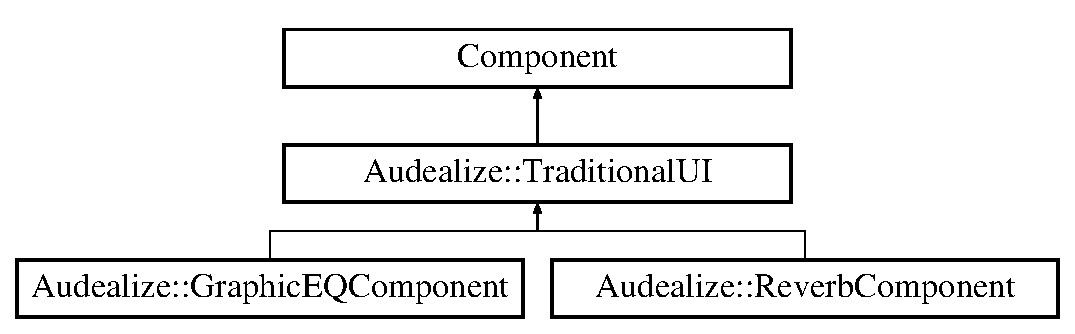
\includegraphics[height=3.000000cm]{class_audealize_1_1_traditional_u_i}
\end{center}
\end{figure}
\subsection*{Public Member Functions}
\begin{DoxyCompactItemize}
\item 
\hyperlink{class_audealize_1_1_traditional_u_i_aee7020626c7d568300b7a4d92a032953}{Traditional\+UI} (\hyperlink{class_audealize_1_1_audealize_audio_processor}{Audealize\+Audio\+Processor} \&p)
\item 
String \hyperlink{class_audealize_1_1_traditional_u_i_a0447dab44d7e62f4382f368b4e3f8bec}{get\+Name} ()
\end{DoxyCompactItemize}
\subsection*{Protected Member Functions}
\begin{DoxyCompactItemize}
\item 
\hyperlink{class_audealize_1_1_traditional_u_i_a4826276319a81e9867e09ccb37320e54}{J\+U\+C\+E\+\_\+\+D\+E\+C\+L\+A\+R\+E\+\_\+\+N\+O\+N\+\_\+\+C\+O\+P\+Y\+A\+B\+L\+E\+\_\+\+W\+I\+T\+H\+\_\+\+L\+E\+A\+K\+\_\+\+D\+E\+T\+E\+C\+T\+OR} (\hyperlink{class_audealize_1_1_traditional_u_i}{Traditional\+UI})
\end{DoxyCompactItemize}
\subsection*{Protected Attributes}
\begin{DoxyCompactItemize}
\item 
\hyperlink{class_audealize_1_1_audealize_audio_processor}{Audealize\+Audio\+Processor} \& \hyperlink{class_audealize_1_1_traditional_u_i_a8907d173ae02664d30ef7eeb09f54bb3}{processor}
\item 
String \hyperlink{class_audealize_1_1_traditional_u_i_a109b231a9fd2e92f49d74ce297283fae}{name}
\end{DoxyCompactItemize}


\subsection{Constructor \& Destructor Documentation}
\index{Audealize\+::\+Traditional\+UI@{Audealize\+::\+Traditional\+UI}!Traditional\+UI@{Traditional\+UI}}
\index{Traditional\+UI@{Traditional\+UI}!Audealize\+::\+Traditional\+UI@{Audealize\+::\+Traditional\+UI}}
\subsubsection[{\texorpdfstring{Traditional\+U\+I(\+Audealize\+Audio\+Processor \&p)}{TraditionalUI(AudealizeAudioProcessor &p)}}]{\setlength{\rightskip}{0pt plus 5cm}Audealize\+::\+Traditional\+U\+I\+::\+Traditional\+UI (
\begin{DoxyParamCaption}
\item[{{\bf Audealize\+Audio\+Processor} \&}]{p}
\end{DoxyParamCaption}
)\hspace{0.3cm}{\ttfamily [inline]}}\hypertarget{class_audealize_1_1_traditional_u_i_aee7020626c7d568300b7a4d92a032953}{}\label{class_audealize_1_1_traditional_u_i_aee7020626c7d568300b7a4d92a032953}


\subsection{Member Function Documentation}
\index{Audealize\+::\+Traditional\+UI@{Audealize\+::\+Traditional\+UI}!get\+Name@{get\+Name}}
\index{get\+Name@{get\+Name}!Audealize\+::\+Traditional\+UI@{Audealize\+::\+Traditional\+UI}}
\subsubsection[{\texorpdfstring{get\+Name()}{getName()}}]{\setlength{\rightskip}{0pt plus 5cm}String Audealize\+::\+Traditional\+U\+I\+::get\+Name (
\begin{DoxyParamCaption}
{}
\end{DoxyParamCaption}
)\hspace{0.3cm}{\ttfamily [inline]}}\hypertarget{class_audealize_1_1_traditional_u_i_a0447dab44d7e62f4382f368b4e3f8bec}{}\label{class_audealize_1_1_traditional_u_i_a0447dab44d7e62f4382f368b4e3f8bec}
\index{Audealize\+::\+Traditional\+UI@{Audealize\+::\+Traditional\+UI}!J\+U\+C\+E\+\_\+\+D\+E\+C\+L\+A\+R\+E\+\_\+\+N\+O\+N\+\_\+\+C\+O\+P\+Y\+A\+B\+L\+E\+\_\+\+W\+I\+T\+H\+\_\+\+L\+E\+A\+K\+\_\+\+D\+E\+T\+E\+C\+T\+OR@{J\+U\+C\+E\+\_\+\+D\+E\+C\+L\+A\+R\+E\+\_\+\+N\+O\+N\+\_\+\+C\+O\+P\+Y\+A\+B\+L\+E\+\_\+\+W\+I\+T\+H\+\_\+\+L\+E\+A\+K\+\_\+\+D\+E\+T\+E\+C\+T\+OR}}
\index{J\+U\+C\+E\+\_\+\+D\+E\+C\+L\+A\+R\+E\+\_\+\+N\+O\+N\+\_\+\+C\+O\+P\+Y\+A\+B\+L\+E\+\_\+\+W\+I\+T\+H\+\_\+\+L\+E\+A\+K\+\_\+\+D\+E\+T\+E\+C\+T\+OR@{J\+U\+C\+E\+\_\+\+D\+E\+C\+L\+A\+R\+E\+\_\+\+N\+O\+N\+\_\+\+C\+O\+P\+Y\+A\+B\+L\+E\+\_\+\+W\+I\+T\+H\+\_\+\+L\+E\+A\+K\+\_\+\+D\+E\+T\+E\+C\+T\+OR}!Audealize\+::\+Traditional\+UI@{Audealize\+::\+Traditional\+UI}}
\subsubsection[{\texorpdfstring{J\+U\+C\+E\+\_\+\+D\+E\+C\+L\+A\+R\+E\+\_\+\+N\+O\+N\+\_\+\+C\+O\+P\+Y\+A\+B\+L\+E\+\_\+\+W\+I\+T\+H\+\_\+\+L\+E\+A\+K\+\_\+\+D\+E\+T\+E\+C\+T\+O\+R(\+Traditional\+U\+I)}{JUCE_DECLARE_NON_COPYABLE_WITH_LEAK_DETECTOR(TraditionalUI)}}]{\setlength{\rightskip}{0pt plus 5cm}Audealize\+::\+Traditional\+U\+I\+::\+J\+U\+C\+E\+\_\+\+D\+E\+C\+L\+A\+R\+E\+\_\+\+N\+O\+N\+\_\+\+C\+O\+P\+Y\+A\+B\+L\+E\+\_\+\+W\+I\+T\+H\+\_\+\+L\+E\+A\+K\+\_\+\+D\+E\+T\+E\+C\+T\+OR (
\begin{DoxyParamCaption}
\item[{{\bf Traditional\+UI}}]{}
\end{DoxyParamCaption}
)\hspace{0.3cm}{\ttfamily [protected]}}\hypertarget{class_audealize_1_1_traditional_u_i_a4826276319a81e9867e09ccb37320e54}{}\label{class_audealize_1_1_traditional_u_i_a4826276319a81e9867e09ccb37320e54}


\subsection{Member Data Documentation}
\index{Audealize\+::\+Traditional\+UI@{Audealize\+::\+Traditional\+UI}!name@{name}}
\index{name@{name}!Audealize\+::\+Traditional\+UI@{Audealize\+::\+Traditional\+UI}}
\subsubsection[{\texorpdfstring{name}{name}}]{\setlength{\rightskip}{0pt plus 5cm}String Audealize\+::\+Traditional\+U\+I\+::name\hspace{0.3cm}{\ttfamily [protected]}}\hypertarget{class_audealize_1_1_traditional_u_i_a109b231a9fd2e92f49d74ce297283fae}{}\label{class_audealize_1_1_traditional_u_i_a109b231a9fd2e92f49d74ce297283fae}
\index{Audealize\+::\+Traditional\+UI@{Audealize\+::\+Traditional\+UI}!processor@{processor}}
\index{processor@{processor}!Audealize\+::\+Traditional\+UI@{Audealize\+::\+Traditional\+UI}}
\subsubsection[{\texorpdfstring{processor}{processor}}]{\setlength{\rightskip}{0pt plus 5cm}{\bf Audealize\+Audio\+Processor}\& Audealize\+::\+Traditional\+U\+I\+::processor\hspace{0.3cm}{\ttfamily [protected]}}\hypertarget{class_audealize_1_1_traditional_u_i_a8907d173ae02664d30ef7eeb09f54bb3}{}\label{class_audealize_1_1_traditional_u_i_a8907d173ae02664d30ef7eeb09f54bb3}


The documentation for this class was generated from the following file\+:\begin{DoxyCompactItemize}
\item 
/\+Users/michael/\+J\+U\+C\+E/projects/audealize-\/plugin/\+J\+U\+C\+E Modules/audealize\+\_\+module/ui\+\_\+components/\hyperlink{_traditional_u_i_component_8h}{Traditional\+U\+I\+Component.\+h}\end{DoxyCompactItemize}

\hypertarget{class_typeahead_editor}{}\section{Typeahead\+Editor Class Reference}
\label{class_typeahead_editor}\index{Typeahead\+Editor@{Typeahead\+Editor}}


{\ttfamily \#include $<$Typeahead\+Popup\+Menu.\+h$>$}

Inheritance diagram for Typeahead\+Editor\+:\begin{figure}[H]
\begin{center}
\leavevmode
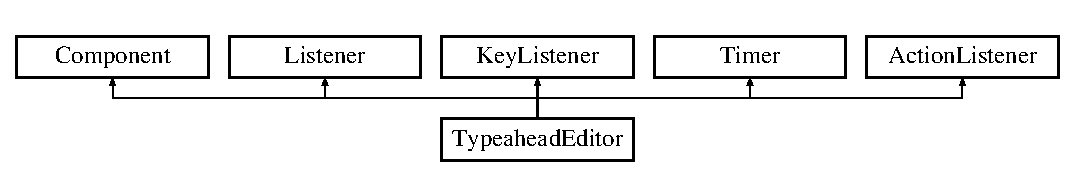
\includegraphics[height=1.931034cm]{class_typeahead_editor}
\end{center}
\end{figure}
\subsection*{Public Member Functions}
\begin{DoxyCompactItemize}
\item 
\hyperlink{class_typeahead_editor_ad8c967c6f8afd68f04c0fda4a7631704}{Typeahead\+Editor} ()
\item 
\hyperlink{class_typeahead_editor_a2c4ccf6fc7191665150f36c88df1fa67}{$\sim$\+Typeahead\+Editor} ()
\item 
\hyperlink{tk_8h_aba408b7cd755a96426e004c015f5de8e}{void} \hyperlink{class_typeahead_editor_a4942e3438d0aa957b7ec729710c70a50}{mouse\+Down} (const Mouse\+Event \&event) override
\item 
\hyperlink{tk_8h_aba408b7cd755a96426e004c015f5de8e}{void} \hyperlink{class_typeahead_editor_a45f73a99da1b4ff012c604765f80e8d0}{set\+Options} (std\+::vector$<$ String $>$ opts)
\item 
\hyperlink{tk_8h_aba408b7cd755a96426e004c015f5de8e}{void} \hyperlink{class_typeahead_editor_a24bfe0b145f960d2765885c62905f7e0}{show\+Menu} ()
\item 
\hyperlink{tk_8h_aba408b7cd755a96426e004c015f5de8e}{void} \hyperlink{class_typeahead_editor_a9e91eee02228481e5651189dbc486d00}{text\+Editor\+Text\+Changed} (Text\+Editor \&) override
\item 
\hyperlink{tk_8h_aba408b7cd755a96426e004c015f5de8e}{void} \hyperlink{class_typeahead_editor_ae1c47bed0eac90df9affad67cd9f755c}{dismiss\+Menu} ()
\item 
\hyperlink{tk_8h_aba408b7cd755a96426e004c015f5de8e}{void} \hyperlink{class_typeahead_editor_ad2d40cb37ad5ef0dd3e9c54384c403d1}{timer\+Callback} () override
\item 
bool \hyperlink{class_typeahead_editor_a3622d6740193b88c7ee5c0a7b2335958}{key\+Pressed} (const Key\+Press \&key, Component $\ast$component) override
\item 
\hyperlink{tk_8h_aba408b7cd755a96426e004c015f5de8e}{void} \hyperlink{class_typeahead_editor_abe5dec053fa695c133250a317a046822}{focus\+Lost} (Focus\+Change\+Type cause) override
\item 
\hyperlink{tk_8h_aba408b7cd755a96426e004c015f5de8e}{void} \hyperlink{class_typeahead_editor_a168babdbdaaa02abdae5172f98ef09db}{resized} () override
\item 
\hyperlink{tk_8h_aba408b7cd755a96426e004c015f5de8e}{void} \hyperlink{class_typeahead_editor_aca498173bb04dfd712f14c5bad4d3b02}{action\+Listener\+Callback} (const juce\+::\+String \&message) override
\item 
\hyperlink{tk_8h_aba408b7cd755a96426e004c015f5de8e}{void} \hyperlink{class_typeahead_editor_a8942bdee20c8dbdf09123404aca1714c}{set\+Multi\+Effect} (vector$<$ String $>$ effect\+Names, vector$<$ String\+Array $>$ descriptors)
\item 
Text\+Editor $\ast$ \hyperlink{class_typeahead_editor_a9b5ee4d14ff67527b270abfa75fcf83d}{get\+Editor} ()
\item 
String\+Array \hyperlink{class_typeahead_editor_a23f3a2809206205be586495f181c853d}{synonyms} (String word)
\item 
bool \hyperlink{class_typeahead_editor_ad92a282d4fe1df28fcff57e3288c5283}{binary\+Search} (String\+Array $\ast$arr, String \hyperlink{morph_8c_ab50d783982593ef993ea0b68f7ad8b80}{str})
\item 
\hyperlink{tk_8h_aba408b7cd755a96426e004c015f5de8e}{void} \hyperlink{class_typeahead_editor_a713f4cffc6f41db8ac347a6b3ffcab9e}{show\+Bubble\+Message} (Attributed\+String \hyperlink{morph_8c_ab50d783982593ef993ea0b68f7ad8b80}{str}, Colour outline\+Color, Colour fill\+Color=Colours\+::white, \hyperlink{tk_8h_a83f82f76e7fed06f4c49d2db94028a6d}{int} time\+In\+MS=1000)
\item 
String\+Array \hyperlink{class_typeahead_editor_a6575dabcc66c032cfc0c4b8b6e2ad327}{get\+Descriptors} ()
\end{DoxyCompactItemize}


\subsection{Detailed Description}
A Text\+Editor component that displays a \hyperlink{class_typeahead_popup_menu}{Typeahead\+Popup\+Menu} below it with suggestions of words 

\subsection{Constructor \& Destructor Documentation}
\index{Typeahead\+Editor@{Typeahead\+Editor}!Typeahead\+Editor@{Typeahead\+Editor}}
\index{Typeahead\+Editor@{Typeahead\+Editor}!Typeahead\+Editor@{Typeahead\+Editor}}
\subsubsection[{\texorpdfstring{Typeahead\+Editor()}{TypeaheadEditor()}}]{\setlength{\rightskip}{0pt plus 5cm}Typeahead\+Editor\+::\+Typeahead\+Editor (
\begin{DoxyParamCaption}
{}
\end{DoxyParamCaption}
)}\hypertarget{class_typeahead_editor_ad8c967c6f8afd68f04c0fda4a7631704}{}\label{class_typeahead_editor_ad8c967c6f8afd68f04c0fda4a7631704}
\index{Typeahead\+Editor@{Typeahead\+Editor}!````~Typeahead\+Editor@{$\sim$\+Typeahead\+Editor}}
\index{````~Typeahead\+Editor@{$\sim$\+Typeahead\+Editor}!Typeahead\+Editor@{Typeahead\+Editor}}
\subsubsection[{\texorpdfstring{$\sim$\+Typeahead\+Editor()}{~TypeaheadEditor()}}]{\setlength{\rightskip}{0pt plus 5cm}Typeahead\+Editor\+::$\sim$\+Typeahead\+Editor (
\begin{DoxyParamCaption}
{}
\end{DoxyParamCaption}
)}\hypertarget{class_typeahead_editor_a2c4ccf6fc7191665150f36c88df1fa67}{}\label{class_typeahead_editor_a2c4ccf6fc7191665150f36c88df1fa67}


\subsection{Member Function Documentation}
\index{Typeahead\+Editor@{Typeahead\+Editor}!action\+Listener\+Callback@{action\+Listener\+Callback}}
\index{action\+Listener\+Callback@{action\+Listener\+Callback}!Typeahead\+Editor@{Typeahead\+Editor}}
\subsubsection[{\texorpdfstring{action\+Listener\+Callback(const juce\+::\+String \&message) override}{actionListenerCallback(const juce::String &message) override}}]{\setlength{\rightskip}{0pt plus 5cm}{\bf void} Typeahead\+Editor\+::action\+Listener\+Callback (
\begin{DoxyParamCaption}
\item[{const juce\+::\+String \&}]{message}
\end{DoxyParamCaption}
)\hspace{0.3cm}{\ttfamily [override]}}\hypertarget{class_typeahead_editor_aca498173bb04dfd712f14c5bad4d3b02}{}\label{class_typeahead_editor_aca498173bb04dfd712f14c5bad4d3b02}
Used to set text of editor when word is selected in a Word\+Map


\begin{DoxyParams}{Parameters}
{\em message} & A string containing the word \\
\hline
\end{DoxyParams}
\index{Typeahead\+Editor@{Typeahead\+Editor}!binary\+Search@{binary\+Search}}
\index{binary\+Search@{binary\+Search}!Typeahead\+Editor@{Typeahead\+Editor}}
\subsubsection[{\texorpdfstring{binary\+Search(\+String\+Array $\ast$arr, String str)}{binarySearch(StringArray *arr, String str)}}]{\setlength{\rightskip}{0pt plus 5cm}bool Typeahead\+Editor\+::binary\+Search (
\begin{DoxyParamCaption}
\item[{String\+Array $\ast$}]{arr, }
\item[{String}]{str}
\end{DoxyParamCaption}
)}\hypertarget{class_typeahead_editor_ad92a282d4fe1df28fcff57e3288c5283}{}\label{class_typeahead_editor_ad92a282d4fe1df28fcff57e3288c5283}
Use binary search to find a String in a String\+Array


\begin{DoxyParams}{Parameters}
{\em arr} & String\+Array \\
\hline
{\em str} & String\\
\hline
\end{DoxyParams}
\begin{DoxyReturn}{Returns}
true if found 
\end{DoxyReturn}
\index{Typeahead\+Editor@{Typeahead\+Editor}!dismiss\+Menu@{dismiss\+Menu}}
\index{dismiss\+Menu@{dismiss\+Menu}!Typeahead\+Editor@{Typeahead\+Editor}}
\subsubsection[{\texorpdfstring{dismiss\+Menu()}{dismissMenu()}}]{\setlength{\rightskip}{0pt plus 5cm}{\bf void} Typeahead\+Editor\+::dismiss\+Menu (
\begin{DoxyParamCaption}
{}
\end{DoxyParamCaption}
)}\hypertarget{class_typeahead_editor_ae1c47bed0eac90df9affad67cd9f755c}{}\label{class_typeahead_editor_ae1c47bed0eac90df9affad67cd9f755c}
Remove the popup menu from the screen \index{Typeahead\+Editor@{Typeahead\+Editor}!focus\+Lost@{focus\+Lost}}
\index{focus\+Lost@{focus\+Lost}!Typeahead\+Editor@{Typeahead\+Editor}}
\subsubsection[{\texorpdfstring{focus\+Lost(\+Focus\+Change\+Type cause) override}{focusLost(FocusChangeType cause) override}}]{\setlength{\rightskip}{0pt plus 5cm}{\bf void} Typeahead\+Editor\+::focus\+Lost (
\begin{DoxyParamCaption}
\item[{Focus\+Change\+Type}]{cause}
\end{DoxyParamCaption}
)\hspace{0.3cm}{\ttfamily [override]}}\hypertarget{class_typeahead_editor_abe5dec053fa695c133250a317a046822}{}\label{class_typeahead_editor_abe5dec053fa695c133250a317a046822}
\index{Typeahead\+Editor@{Typeahead\+Editor}!get\+Descriptors@{get\+Descriptors}}
\index{get\+Descriptors@{get\+Descriptors}!Typeahead\+Editor@{Typeahead\+Editor}}
\subsubsection[{\texorpdfstring{get\+Descriptors()}{getDescriptors()}}]{\setlength{\rightskip}{0pt plus 5cm}String\+Array Typeahead\+Editor\+::get\+Descriptors (
\begin{DoxyParamCaption}
{}
\end{DoxyParamCaption}
)\hspace{0.3cm}{\ttfamily [inline]}}\hypertarget{class_typeahead_editor_a6575dabcc66c032cfc0c4b8b6e2ad327}{}\label{class_typeahead_editor_a6575dabcc66c032cfc0c4b8b6e2ad327}
Returns a String\+Array containing the set of descriptors being searched by this \hyperlink{class_typeahead_editor}{Typeahead\+Editor}

\begin{DoxyReturn}{Returns}
String\+Array 
\end{DoxyReturn}
\index{Typeahead\+Editor@{Typeahead\+Editor}!get\+Editor@{get\+Editor}}
\index{get\+Editor@{get\+Editor}!Typeahead\+Editor@{Typeahead\+Editor}}
\subsubsection[{\texorpdfstring{get\+Editor()}{getEditor()}}]{\setlength{\rightskip}{0pt plus 5cm}Text\+Editor $\ast$ Typeahead\+Editor\+::get\+Editor (
\begin{DoxyParamCaption}
{}
\end{DoxyParamCaption}
)}\hypertarget{class_typeahead_editor_a9b5ee4d14ff67527b270abfa75fcf83d}{}\label{class_typeahead_editor_a9b5ee4d14ff67527b270abfa75fcf83d}
Returns a pointer to the searchbar Text\+Editor

\begin{DoxyReturn}{Returns}
a Text\+Editor$\ast$ 
\end{DoxyReturn}
\index{Typeahead\+Editor@{Typeahead\+Editor}!key\+Pressed@{key\+Pressed}}
\index{key\+Pressed@{key\+Pressed}!Typeahead\+Editor@{Typeahead\+Editor}}
\subsubsection[{\texorpdfstring{key\+Pressed(const Key\+Press \&key, Component $\ast$component) override}{keyPressed(const KeyPress &key, Component *component) override}}]{\setlength{\rightskip}{0pt plus 5cm}bool Typeahead\+Editor\+::key\+Pressed (
\begin{DoxyParamCaption}
\item[{const Key\+Press \&}]{key, }
\item[{Component $\ast$}]{component}
\end{DoxyParamCaption}
)\hspace{0.3cm}{\ttfamily [override]}}\hypertarget{class_typeahead_editor_a3622d6740193b88c7ee5c0a7b2335958}{}\label{class_typeahead_editor_a3622d6740193b88c7ee5c0a7b2335958}
Called when a key is pressed. Inherited from Key\+Listener


\begin{DoxyParams}{Parameters}
{\em key} & Key\+Press\& \\
\hline
{\em component} & The component that has focus\\
\hline
\end{DoxyParams}
\begin{DoxyReturn}{Returns}
bool 
\end{DoxyReturn}
\index{Typeahead\+Editor@{Typeahead\+Editor}!mouse\+Down@{mouse\+Down}}
\index{mouse\+Down@{mouse\+Down}!Typeahead\+Editor@{Typeahead\+Editor}}
\subsubsection[{\texorpdfstring{mouse\+Down(const Mouse\+Event \&event) override}{mouseDown(const MouseEvent &event) override}}]{\setlength{\rightskip}{0pt plus 5cm}{\bf void} Typeahead\+Editor\+::mouse\+Down (
\begin{DoxyParamCaption}
\item[{const Mouse\+Event \&}]{event}
\end{DoxyParamCaption}
)\hspace{0.3cm}{\ttfamily [override]}}\hypertarget{class_typeahead_editor_a4942e3438d0aa957b7ec729710c70a50}{}\label{class_typeahead_editor_a4942e3438d0aa957b7ec729710c70a50}
\index{Typeahead\+Editor@{Typeahead\+Editor}!resized@{resized}}
\index{resized@{resized}!Typeahead\+Editor@{Typeahead\+Editor}}
\subsubsection[{\texorpdfstring{resized() override}{resized() override}}]{\setlength{\rightskip}{0pt plus 5cm}{\bf void} Typeahead\+Editor\+::resized (
\begin{DoxyParamCaption}
{}
\end{DoxyParamCaption}
)\hspace{0.3cm}{\ttfamily [override]}}\hypertarget{class_typeahead_editor_a168babdbdaaa02abdae5172f98ef09db}{}\label{class_typeahead_editor_a168babdbdaaa02abdae5172f98ef09db}
\index{Typeahead\+Editor@{Typeahead\+Editor}!set\+Multi\+Effect@{set\+Multi\+Effect}}
\index{set\+Multi\+Effect@{set\+Multi\+Effect}!Typeahead\+Editor@{Typeahead\+Editor}}
\subsubsection[{\texorpdfstring{set\+Multi\+Effect(vector$<$ String $>$ effect\+Names, vector$<$ String\+Array $>$ descriptors)}{setMultiEffect(vector< String > effectNames, vector< StringArray > descriptors)}}]{\setlength{\rightskip}{0pt plus 5cm}{\bf void} Typeahead\+Editor\+::set\+Multi\+Effect (
\begin{DoxyParamCaption}
\item[{vector$<$ String $>$}]{effect\+Names, }
\item[{vector$<$ String\+Array $>$}]{descriptors}
\end{DoxyParamCaption}
)}\hypertarget{class_typeahead_editor_a8942bdee20c8dbdf09123404aca1714c}{}\label{class_typeahead_editor_a8942bdee20c8dbdf09123404aca1714c}
Tells the \hyperlink{class_typeahead_popup_menu}{Typeahead\+Popup\+Menu} that it is part of a multi effect plugin and should therefore search the descriptor sets for the ther effects


\begin{DoxyParams}{Parameters}
{\em effect\+Names} & vector$<$\+String$>$ list of names of other effects in the plugin (EQ, reverb, etc..) \\
\hline
{\em descriptors} & vector$<$\+String\+Array$>$ containing the sets of descriptors for each other effect/wordmap. Must be in same order as effect\+Names \\
\hline
\end{DoxyParams}
\index{Typeahead\+Editor@{Typeahead\+Editor}!set\+Options@{set\+Options}}
\index{set\+Options@{set\+Options}!Typeahead\+Editor@{Typeahead\+Editor}}
\subsubsection[{\texorpdfstring{set\+Options(std\+::vector$<$ String $>$ opts)}{setOptions(std::vector< String > opts)}}]{\setlength{\rightskip}{0pt plus 5cm}{\bf void} Typeahead\+Editor\+::set\+Options (
\begin{DoxyParamCaption}
\item[{std\+::vector$<$ String $>$}]{opts}
\end{DoxyParamCaption}
)}\hypertarget{class_typeahead_editor_a45f73a99da1b4ff012c604765f80e8d0}{}\label{class_typeahead_editor_a45f73a99da1b4ff012c604765f80e8d0}
Set the list of words to be searched by the texteditor


\begin{DoxyParams}{Parameters}
{\em opts} & a vector$<$\+String$>$ \\
\hline
\end{DoxyParams}
\index{Typeahead\+Editor@{Typeahead\+Editor}!show\+Bubble\+Message@{show\+Bubble\+Message}}
\index{show\+Bubble\+Message@{show\+Bubble\+Message}!Typeahead\+Editor@{Typeahead\+Editor}}
\subsubsection[{\texorpdfstring{show\+Bubble\+Message(\+Attributed\+String str, Colour outline\+Color, Colour fill\+Color=\+Colours\+::white, int time\+In\+M\+S=1000)}{showBubbleMessage(AttributedString str, Colour outlineColor, Colour fillColor=Colours::white, int timeInMS=1000)}}]{\setlength{\rightskip}{0pt plus 5cm}{\bf void} Typeahead\+Editor\+::show\+Bubble\+Message (
\begin{DoxyParamCaption}
\item[{Attributed\+String}]{str, }
\item[{Colour}]{outline\+Color, }
\item[{Colour}]{fill\+Color = {\ttfamily Colours\+:\+:white}, }
\item[{{\bf int}}]{time\+In\+MS = {\ttfamily 1000}}
\end{DoxyParamCaption}
)}\hypertarget{class_typeahead_editor_a713f4cffc6f41db8ac347a6b3ffcab9e}{}\label{class_typeahead_editor_a713f4cffc6f41db8ac347a6b3ffcab9e}
Show a Bubble\+Message\+Component pointed at this \hyperlink{class_typeahead_editor}{Typeahead\+Editor}


\begin{DoxyParams}{Parameters}
{\em str} & The message to be displayed \\
\hline
{\em outline\+Color} & Color of the outline of the Bubble\+Message\+Component \\
\hline
{\em fill\+Color} & Color of the outline of the Bubble\+Message\+Component \\
\hline
{\em time\+In\+MS} & Time (in ms) for Bubble\+Message\+Component to stay visible \\
\hline
\end{DoxyParams}
\index{Typeahead\+Editor@{Typeahead\+Editor}!show\+Menu@{show\+Menu}}
\index{show\+Menu@{show\+Menu}!Typeahead\+Editor@{Typeahead\+Editor}}
\subsubsection[{\texorpdfstring{show\+Menu()}{showMenu()}}]{\setlength{\rightskip}{0pt plus 5cm}{\bf void} Typeahead\+Editor\+::show\+Menu (
\begin{DoxyParamCaption}
{}
\end{DoxyParamCaption}
)}\hypertarget{class_typeahead_editor_a24bfe0b145f960d2765885c62905f7e0}{}\label{class_typeahead_editor_a24bfe0b145f960d2765885c62905f7e0}
Show the \hyperlink{class_typeahead_popup_menu}{Typeahead\+Popup\+Menu} \index{Typeahead\+Editor@{Typeahead\+Editor}!synonyms@{synonyms}}
\index{synonyms@{synonyms}!Typeahead\+Editor@{Typeahead\+Editor}}
\subsubsection[{\texorpdfstring{synonyms(\+String word)}{synonyms(String word)}}]{\setlength{\rightskip}{0pt plus 5cm}String\+Array Typeahead\+Editor\+::synonyms (
\begin{DoxyParamCaption}
\item[{String}]{word}
\end{DoxyParamCaption}
)}\hypertarget{class_typeahead_editor_a23f3a2809206205be586495f181c853d}{}\label{class_typeahead_editor_a23f3a2809206205be586495f181c853d}
Finds synonyms of a given word using Word\+Net


\begin{DoxyParams}{Parameters}
{\em word} & \\
\hline
\end{DoxyParams}
\begin{DoxyReturn}{Returns}
String\+Array of synonyms 
\end{DoxyReturn}
\index{Typeahead\+Editor@{Typeahead\+Editor}!text\+Editor\+Text\+Changed@{text\+Editor\+Text\+Changed}}
\index{text\+Editor\+Text\+Changed@{text\+Editor\+Text\+Changed}!Typeahead\+Editor@{Typeahead\+Editor}}
\subsubsection[{\texorpdfstring{text\+Editor\+Text\+Changed(\+Text\+Editor \&) override}{textEditorTextChanged(TextEditor &) override}}]{\setlength{\rightskip}{0pt plus 5cm}{\bf void} Typeahead\+Editor\+::text\+Editor\+Text\+Changed (
\begin{DoxyParamCaption}
\item[{Text\+Editor \&}]{}
\end{DoxyParamCaption}
)\hspace{0.3cm}{\ttfamily [override]}}\hypertarget{class_typeahead_editor_a9e91eee02228481e5651189dbc486d00}{}\label{class_typeahead_editor_a9e91eee02228481e5651189dbc486d00}
Called when the text of the texteditor is changed Searches for matching words in options, searches for synonyms if none present


\begin{DoxyParams}{Parameters}
{\em Text\+Editor\&} & \\
\hline
\end{DoxyParams}
\index{Typeahead\+Editor@{Typeahead\+Editor}!timer\+Callback@{timer\+Callback}}
\index{timer\+Callback@{timer\+Callback}!Typeahead\+Editor@{Typeahead\+Editor}}
\subsubsection[{\texorpdfstring{timer\+Callback() override}{timerCallback() override}}]{\setlength{\rightskip}{0pt plus 5cm}{\bf void} Typeahead\+Editor\+::timer\+Callback (
\begin{DoxyParamCaption}
{}
\end{DoxyParamCaption}
)\hspace{0.3cm}{\ttfamily [override]}}\hypertarget{class_typeahead_editor_ad2d40cb37ad5ef0dd3e9c54384c403d1}{}\label{class_typeahead_editor_ad2d40cb37ad5ef0dd3e9c54384c403d1}
Inherited from timer 

The documentation for this class was generated from the following files\+:\begin{DoxyCompactItemize}
\item 
/\+Users/michael/\+J\+U\+C\+E/projects/audealize-\/plugin/\+J\+U\+C\+E Modules/audealize\+\_\+module/ui\+\_\+components/\hyperlink{_typeahead_popup_menu_8h}{Typeahead\+Popup\+Menu.\+h}\item 
/\+Users/michael/\+J\+U\+C\+E/projects/audealize-\/plugin/\+J\+U\+C\+E Modules/audealize\+\_\+module/ui\+\_\+components/\hyperlink{_typeahead_popup_menu_8cpp}{Typeahead\+Popup\+Menu.\+cpp}\end{DoxyCompactItemize}

\hypertarget{class_typeahead_popup_menu}{}\section{Typeahead\+Popup\+Menu Class Reference}
\label{class_typeahead_popup_menu}\index{Typeahead\+Popup\+Menu@{Typeahead\+Popup\+Menu}}


{\ttfamily \#include $<$Typeahead\+Popup\+Menu.\+h$>$}

Inheritance diagram for Typeahead\+Popup\+Menu\+:\begin{figure}[H]
\begin{center}
\leavevmode
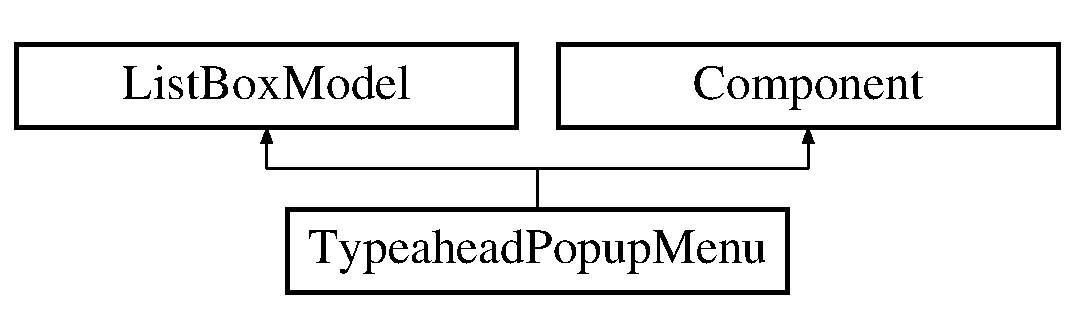
\includegraphics[height=2.000000cm]{class_typeahead_popup_menu}
\end{center}
\end{figure}
\subsection*{Public Types}
\begin{DoxyCompactItemize}
\item 
enum \hyperlink{class_typeahead_popup_menu_ab0938f3a6c7b9349f698cd65a97cdbf9}{Colour\+Ids} \{ \hyperlink{class_typeahead_popup_menu_ab0938f3a6c7b9349f698cd65a97cdbf9a8dd4222711cd9b6ec71091e3ec3dee06}{background\+Colour\+Id} = 0x2000400, 
\hyperlink{class_typeahead_popup_menu_ab0938f3a6c7b9349f698cd65a97cdbf9a2472a86e906ec8973a442008c15cac9d}{text\+Colour\+Id} = 0x2000401, 
\hyperlink{class_typeahead_popup_menu_ab0938f3a6c7b9349f698cd65a97cdbf9ad97aea57b8ccf23a19774c3f64216688}{highlight\+Colour\+Id} = 0x2000402, 
\hyperlink{class_typeahead_popup_menu_ab0938f3a6c7b9349f698cd65a97cdbf9ab02a4a7379c248f384d849cb327d01ae}{text\+Selected\+Colour\+Id} = 0x2000403
 \}
\end{DoxyCompactItemize}
\subsection*{Public Member Functions}
\begin{DoxyCompactItemize}
\item 
\hyperlink{class_typeahead_popup_menu_a877b636f8a9475e8fb5547491de02716}{Typeahead\+Popup\+Menu} ()
\item 
\hyperlink{class_typeahead_popup_menu_a0d2818d9cdac33de4f6af61b1220c193}{$\sim$\+Typeahead\+Popup\+Menu} ()
\item 
\hyperlink{tk_8h_aba408b7cd755a96426e004c015f5de8e}{void} \hyperlink{class_typeahead_popup_menu_a8aaf8378f05583ea02b7a37820b22869}{set\+Items} (const String\+Array \&options\+\_\+)
\item 
\hyperlink{tk_8h_aba408b7cd755a96426e004c015f5de8e}{void} \hyperlink{class_typeahead_popup_menu_aaaf5c6cc15d0c822f129ddbbf2ab8e0c}{resized} () override
\item 
\hyperlink{tk_8h_aba408b7cd755a96426e004c015f5de8e}{void} \hyperlink{class_typeahead_popup_menu_aee87bc561a1b813b5d6e9aa29f0ede0a}{paint} (Graphics \&g) override
\item 
\hyperlink{tk_8h_a83f82f76e7fed06f4c49d2db94028a6d}{int} \hyperlink{class_typeahead_popup_menu_acd831e27150e6264f15e797f22960648}{get\+Num\+Rows} () override
\item 
\hyperlink{tk_8h_aba408b7cd755a96426e004c015f5de8e}{void} \hyperlink{class_typeahead_popup_menu_af277a50a6c5c49e1ade6732bb82f4ad9}{set\+Action\+On\+Item\+Selected} (std\+::function$<$ \hyperlink{tk_8h_aba408b7cd755a96426e004c015f5de8e}{void}(String)$>$ function)
\item 
\hyperlink{tk_8h_aba408b7cd755a96426e004c015f5de8e}{void} \hyperlink{class_typeahead_popup_menu_a764bbdbdd904c7e6aad931bc00ca9050}{list\+Box\+Item\+Clicked} (\hyperlink{tk_8h_a83f82f76e7fed06f4c49d2db94028a6d}{int} row, const Mouse\+Event \&) override
\item 
\hyperlink{tk_8h_aba408b7cd755a96426e004c015f5de8e}{void} \hyperlink{class_typeahead_popup_menu_ac9cd24de1208af4d8d5720490ccddded}{return\+Key\+Pressed} (\hyperlink{tk_8h_a83f82f76e7fed06f4c49d2db94028a6d}{int} last\+Row\+Selected) override
\item 
\hyperlink{tk_8h_aba408b7cd755a96426e004c015f5de8e}{void} \hyperlink{class_typeahead_popup_menu_a96d37090528b014303917c4266ddee46}{paint\+List\+Box\+Item} (\hyperlink{tk_8h_a83f82f76e7fed06f4c49d2db94028a6d}{int} row\+Number, Graphics \&g, \hyperlink{tk_8h_a83f82f76e7fed06f4c49d2db94028a6d}{int} \hyperlink{tk_8h_a29e50a5401c1396b3a2aa3487f74d468}{width}, \hyperlink{tk_8h_a83f82f76e7fed06f4c49d2db94028a6d}{int} \hyperlink{tk_8h_a67be2f4b9d9c5b3559139bfb072e2e81}{height}, bool row\+Is\+Selected) override
\item 
\hyperlink{tk_8h_aba408b7cd755a96426e004c015f5de8e}{void} \hyperlink{class_typeahead_popup_menu_aed235641398929232116e95177aac229}{set\+First\+Item\+Focused} ()
\end{DoxyCompactItemize}


\subsection{Member Enumeration Documentation}
\index{Typeahead\+Popup\+Menu@{Typeahead\+Popup\+Menu}!Colour\+Ids@{Colour\+Ids}}
\index{Colour\+Ids@{Colour\+Ids}!Typeahead\+Popup\+Menu@{Typeahead\+Popup\+Menu}}
\subsubsection[{\texorpdfstring{Colour\+Ids}{ColourIds}}]{\setlength{\rightskip}{0pt plus 5cm}enum {\bf Typeahead\+Popup\+Menu\+::\+Colour\+Ids}}\hypertarget{class_typeahead_popup_menu_ab0938f3a6c7b9349f698cd65a97cdbf9}{}\label{class_typeahead_popup_menu_ab0938f3a6c7b9349f698cd65a97cdbf9}
\begin{Desc}
\item[Enumerator]\par
\begin{description}
\index{background\+Colour\+Id@{background\+Colour\+Id}!Typeahead\+Popup\+Menu@{Typeahead\+Popup\+Menu}}\index{Typeahead\+Popup\+Menu@{Typeahead\+Popup\+Menu}!background\+Colour\+Id@{background\+Colour\+Id}}\item[{\em 
background\+Colour\+Id\hypertarget{class_typeahead_popup_menu_ab0938f3a6c7b9349f698cd65a97cdbf9a8dd4222711cd9b6ec71091e3ec3dee06}{}\label{class_typeahead_popup_menu_ab0938f3a6c7b9349f698cd65a97cdbf9a8dd4222711cd9b6ec71091e3ec3dee06}
}]\index{text\+Colour\+Id@{text\+Colour\+Id}!Typeahead\+Popup\+Menu@{Typeahead\+Popup\+Menu}}\index{Typeahead\+Popup\+Menu@{Typeahead\+Popup\+Menu}!text\+Colour\+Id@{text\+Colour\+Id}}\item[{\em 
text\+Colour\+Id\hypertarget{class_typeahead_popup_menu_ab0938f3a6c7b9349f698cd65a97cdbf9a2472a86e906ec8973a442008c15cac9d}{}\label{class_typeahead_popup_menu_ab0938f3a6c7b9349f698cd65a97cdbf9a2472a86e906ec8973a442008c15cac9d}
}]\index{highlight\+Colour\+Id@{highlight\+Colour\+Id}!Typeahead\+Popup\+Menu@{Typeahead\+Popup\+Menu}}\index{Typeahead\+Popup\+Menu@{Typeahead\+Popup\+Menu}!highlight\+Colour\+Id@{highlight\+Colour\+Id}}\item[{\em 
highlight\+Colour\+Id\hypertarget{class_typeahead_popup_menu_ab0938f3a6c7b9349f698cd65a97cdbf9ad97aea57b8ccf23a19774c3f64216688}{}\label{class_typeahead_popup_menu_ab0938f3a6c7b9349f698cd65a97cdbf9ad97aea57b8ccf23a19774c3f64216688}
}]\index{text\+Selected\+Colour\+Id@{text\+Selected\+Colour\+Id}!Typeahead\+Popup\+Menu@{Typeahead\+Popup\+Menu}}\index{Typeahead\+Popup\+Menu@{Typeahead\+Popup\+Menu}!text\+Selected\+Colour\+Id@{text\+Selected\+Colour\+Id}}\item[{\em 
text\+Selected\+Colour\+Id\hypertarget{class_typeahead_popup_menu_ab0938f3a6c7b9349f698cd65a97cdbf9ab02a4a7379c248f384d849cb327d01ae}{}\label{class_typeahead_popup_menu_ab0938f3a6c7b9349f698cd65a97cdbf9ab02a4a7379c248f384d849cb327d01ae}
}]\end{description}
\end{Desc}


\subsection{Constructor \& Destructor Documentation}
\index{Typeahead\+Popup\+Menu@{Typeahead\+Popup\+Menu}!Typeahead\+Popup\+Menu@{Typeahead\+Popup\+Menu}}
\index{Typeahead\+Popup\+Menu@{Typeahead\+Popup\+Menu}!Typeahead\+Popup\+Menu@{Typeahead\+Popup\+Menu}}
\subsubsection[{\texorpdfstring{Typeahead\+Popup\+Menu()}{TypeaheadPopupMenu()}}]{\setlength{\rightskip}{0pt plus 5cm}Typeahead\+Popup\+Menu\+::\+Typeahead\+Popup\+Menu (
\begin{DoxyParamCaption}
{}
\end{DoxyParamCaption}
)}\hypertarget{class_typeahead_popup_menu_a877b636f8a9475e8fb5547491de02716}{}\label{class_typeahead_popup_menu_a877b636f8a9475e8fb5547491de02716}
\index{Typeahead\+Popup\+Menu@{Typeahead\+Popup\+Menu}!````~Typeahead\+Popup\+Menu@{$\sim$\+Typeahead\+Popup\+Menu}}
\index{````~Typeahead\+Popup\+Menu@{$\sim$\+Typeahead\+Popup\+Menu}!Typeahead\+Popup\+Menu@{Typeahead\+Popup\+Menu}}
\subsubsection[{\texorpdfstring{$\sim$\+Typeahead\+Popup\+Menu()}{~TypeaheadPopupMenu()}}]{\setlength{\rightskip}{0pt plus 5cm}Typeahead\+Popup\+Menu\+::$\sim$\+Typeahead\+Popup\+Menu (
\begin{DoxyParamCaption}
{}
\end{DoxyParamCaption}
)\hspace{0.3cm}{\ttfamily [inline]}}\hypertarget{class_typeahead_popup_menu_a0d2818d9cdac33de4f6af61b1220c193}{}\label{class_typeahead_popup_menu_a0d2818d9cdac33de4f6af61b1220c193}


\subsection{Member Function Documentation}
\index{Typeahead\+Popup\+Menu@{Typeahead\+Popup\+Menu}!get\+Num\+Rows@{get\+Num\+Rows}}
\index{get\+Num\+Rows@{get\+Num\+Rows}!Typeahead\+Popup\+Menu@{Typeahead\+Popup\+Menu}}
\subsubsection[{\texorpdfstring{get\+Num\+Rows() override}{getNumRows() override}}]{\setlength{\rightskip}{0pt plus 5cm}{\bf int} Typeahead\+Popup\+Menu\+::get\+Num\+Rows (
\begin{DoxyParamCaption}
{}
\end{DoxyParamCaption}
)\hspace{0.3cm}{\ttfamily [override]}}\hypertarget{class_typeahead_popup_menu_acd831e27150e6264f15e797f22960648}{}\label{class_typeahead_popup_menu_acd831e27150e6264f15e797f22960648}
\index{Typeahead\+Popup\+Menu@{Typeahead\+Popup\+Menu}!list\+Box\+Item\+Clicked@{list\+Box\+Item\+Clicked}}
\index{list\+Box\+Item\+Clicked@{list\+Box\+Item\+Clicked}!Typeahead\+Popup\+Menu@{Typeahead\+Popup\+Menu}}
\subsubsection[{\texorpdfstring{list\+Box\+Item\+Clicked(int row, const Mouse\+Event \&) override}{listBoxItemClicked(int row, const MouseEvent &) override}}]{\setlength{\rightskip}{0pt plus 5cm}{\bf void} Typeahead\+Popup\+Menu\+::list\+Box\+Item\+Clicked (
\begin{DoxyParamCaption}
\item[{{\bf int}}]{row, }
\item[{const Mouse\+Event \&}]{}
\end{DoxyParamCaption}
)\hspace{0.3cm}{\ttfamily [override]}}\hypertarget{class_typeahead_popup_menu_a764bbdbdd904c7e6aad931bc00ca9050}{}\label{class_typeahead_popup_menu_a764bbdbdd904c7e6aad931bc00ca9050}
Called when an item in the popup menu is clicked


\begin{DoxyParams}{Parameters}
{\em row} & row index \\
\hline
{\em Mouse\+Event\&} & \\
\hline
\end{DoxyParams}
\index{Typeahead\+Popup\+Menu@{Typeahead\+Popup\+Menu}!paint@{paint}}
\index{paint@{paint}!Typeahead\+Popup\+Menu@{Typeahead\+Popup\+Menu}}
\subsubsection[{\texorpdfstring{paint(\+Graphics \&g) override}{paint(Graphics &g) override}}]{\setlength{\rightskip}{0pt plus 5cm}{\bf void} Typeahead\+Popup\+Menu\+::paint (
\begin{DoxyParamCaption}
\item[{Graphics \&}]{g}
\end{DoxyParamCaption}
)\hspace{0.3cm}{\ttfamily [override]}}\hypertarget{class_typeahead_popup_menu_aee87bc561a1b813b5d6e9aa29f0ede0a}{}\label{class_typeahead_popup_menu_aee87bc561a1b813b5d6e9aa29f0ede0a}
\index{Typeahead\+Popup\+Menu@{Typeahead\+Popup\+Menu}!paint\+List\+Box\+Item@{paint\+List\+Box\+Item}}
\index{paint\+List\+Box\+Item@{paint\+List\+Box\+Item}!Typeahead\+Popup\+Menu@{Typeahead\+Popup\+Menu}}
\subsubsection[{\texorpdfstring{paint\+List\+Box\+Item(int row\+Number, Graphics \&g, int width, int height, bool row\+Is\+Selected) override}{paintListBoxItem(int rowNumber, Graphics &g, int width, int height, bool rowIsSelected) override}}]{\setlength{\rightskip}{0pt plus 5cm}{\bf void} Typeahead\+Popup\+Menu\+::paint\+List\+Box\+Item (
\begin{DoxyParamCaption}
\item[{{\bf int}}]{row\+Number, }
\item[{Graphics \&}]{g, }
\item[{{\bf int}}]{width, }
\item[{{\bf int}}]{height, }
\item[{bool}]{row\+Is\+Selected}
\end{DoxyParamCaption}
)\hspace{0.3cm}{\ttfamily [override]}}\hypertarget{class_typeahead_popup_menu_a96d37090528b014303917c4266ddee46}{}\label{class_typeahead_popup_menu_a96d37090528b014303917c4266ddee46}
Paint an individual row of the popup menu


\begin{DoxyParams}{Parameters}
{\em row\+Number} & \\
\hline
{\em g} & Graphics drawing context \\
\hline
{\em width} & \\
\hline
{\em height} & \\
\hline
{\em row\+Is\+Selected} & \\
\hline
\end{DoxyParams}
\index{Typeahead\+Popup\+Menu@{Typeahead\+Popup\+Menu}!resized@{resized}}
\index{resized@{resized}!Typeahead\+Popup\+Menu@{Typeahead\+Popup\+Menu}}
\subsubsection[{\texorpdfstring{resized() override}{resized() override}}]{\setlength{\rightskip}{0pt plus 5cm}{\bf void} Typeahead\+Popup\+Menu\+::resized (
\begin{DoxyParamCaption}
{}
\end{DoxyParamCaption}
)\hspace{0.3cm}{\ttfamily [override]}}\hypertarget{class_typeahead_popup_menu_aaaf5c6cc15d0c822f129ddbbf2ab8e0c}{}\label{class_typeahead_popup_menu_aaaf5c6cc15d0c822f129ddbbf2ab8e0c}
\index{Typeahead\+Popup\+Menu@{Typeahead\+Popup\+Menu}!return\+Key\+Pressed@{return\+Key\+Pressed}}
\index{return\+Key\+Pressed@{return\+Key\+Pressed}!Typeahead\+Popup\+Menu@{Typeahead\+Popup\+Menu}}
\subsubsection[{\texorpdfstring{return\+Key\+Pressed(int last\+Row\+Selected) override}{returnKeyPressed(int lastRowSelected) override}}]{\setlength{\rightskip}{0pt plus 5cm}{\bf void} Typeahead\+Popup\+Menu\+::return\+Key\+Pressed (
\begin{DoxyParamCaption}
\item[{{\bf int}}]{last\+Row\+Selected}
\end{DoxyParamCaption}
)\hspace{0.3cm}{\ttfamily [override]}}\hypertarget{class_typeahead_popup_menu_ac9cd24de1208af4d8d5720490ccddded}{}\label{class_typeahead_popup_menu_ac9cd24de1208af4d8d5720490ccddded}
Called when return key pressed in \hyperlink{class_typeahead_editor}{Typeahead\+Editor}


\begin{DoxyParams}{Parameters}
{\em last\+Row\+Selected} & \\
\hline
\end{DoxyParams}
\index{Typeahead\+Popup\+Menu@{Typeahead\+Popup\+Menu}!set\+Action\+On\+Item\+Selected@{set\+Action\+On\+Item\+Selected}}
\index{set\+Action\+On\+Item\+Selected@{set\+Action\+On\+Item\+Selected}!Typeahead\+Popup\+Menu@{Typeahead\+Popup\+Menu}}
\subsubsection[{\texorpdfstring{set\+Action\+On\+Item\+Selected(std\+::function$<$ void(\+String)$>$ function)}{setActionOnItemSelected(std::function< void(String)> function)}}]{\setlength{\rightskip}{0pt plus 5cm}{\bf void} Typeahead\+Popup\+Menu\+::set\+Action\+On\+Item\+Selected (
\begin{DoxyParamCaption}
\item[{std\+::function$<$ {\bf void}(String)$>$}]{function}
\end{DoxyParamCaption}
)}\hypertarget{class_typeahead_popup_menu_af277a50a6c5c49e1ade6732bb82f4ad9}{}\label{class_typeahead_popup_menu_af277a50a6c5c49e1ade6732bb82f4ad9}
Sets the function to be executed when an item is selected


\begin{DoxyParams}{Parameters}
{\em std\+::function$<$void(\+String)$>$} & function \\
\hline
\end{DoxyParams}
\index{Typeahead\+Popup\+Menu@{Typeahead\+Popup\+Menu}!set\+First\+Item\+Focused@{set\+First\+Item\+Focused}}
\index{set\+First\+Item\+Focused@{set\+First\+Item\+Focused}!Typeahead\+Popup\+Menu@{Typeahead\+Popup\+Menu}}
\subsubsection[{\texorpdfstring{set\+First\+Item\+Focused()}{setFirstItemFocused()}}]{\setlength{\rightskip}{0pt plus 5cm}{\bf void} Typeahead\+Popup\+Menu\+::set\+First\+Item\+Focused (
\begin{DoxyParamCaption}
{}
\end{DoxyParamCaption}
)}\hypertarget{class_typeahead_popup_menu_aed235641398929232116e95177aac229}{}\label{class_typeahead_popup_menu_aed235641398929232116e95177aac229}
\index{Typeahead\+Popup\+Menu@{Typeahead\+Popup\+Menu}!set\+Items@{set\+Items}}
\index{set\+Items@{set\+Items}!Typeahead\+Popup\+Menu@{Typeahead\+Popup\+Menu}}
\subsubsection[{\texorpdfstring{set\+Items(const String\+Array \&options\+\_\+)}{setItems(const StringArray &options_)}}]{\setlength{\rightskip}{0pt plus 5cm}{\bf void} Typeahead\+Popup\+Menu\+::set\+Items (
\begin{DoxyParamCaption}
\item[{const String\+Array \&}]{options\+\_\+}
\end{DoxyParamCaption}
)}\hypertarget{class_typeahead_popup_menu_a8aaf8378f05583ea02b7a37820b22869}{}\label{class_typeahead_popup_menu_a8aaf8378f05583ea02b7a37820b22869}


The documentation for this class was generated from the following files\+:\begin{DoxyCompactItemize}
\item 
/\+Users/michael/\+J\+U\+C\+E/projects/audealize-\/plugin/\+J\+U\+C\+E Modules/audealize\+\_\+module/ui\+\_\+components/\hyperlink{_typeahead_popup_menu_8h}{Typeahead\+Popup\+Menu.\+h}\item 
/\+Users/michael/\+J\+U\+C\+E/projects/audealize-\/plugin/\+J\+U\+C\+E Modules/audealize\+\_\+module/ui\+\_\+components/\hyperlink{_typeahead_popup_menu_8cpp}{Typeahead\+Popup\+Menu.\+cpp}\end{DoxyCompactItemize}

\hypertarget{class_audealize_1_1_word_map}{}\section{Audealize\+:\+:Word\+Map Class Reference}
\label{class_audealize_1_1_word_map}\index{Audealize\+::\+Word\+Map@{Audealize\+::\+Word\+Map}}


{\ttfamily \#include $<$Word\+Map.\+h$>$}

Inheritance diagram for Audealize\+:\+:Word\+Map\+:\begin{figure}[H]
\begin{center}
\leavevmode
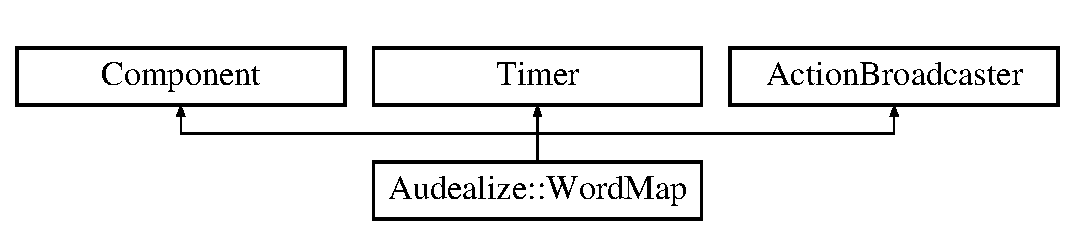
\includegraphics[height=2.000000cm]{class_audealize_1_1_word_map}
\end{center}
\end{figure}
\subsection*{Public Types}
\begin{DoxyCompactItemize}
\item 
enum \hyperlink{class_audealize_1_1_word_map_a34d16d6553efd00f14cf340ab49d179b}{Colour\+Ids} \{ \hyperlink{class_audealize_1_1_word_map_a34d16d6553efd00f14cf340ab49d179ba673055d4d06fcc8459ee599388acb893}{background\+Colour\+Id} = 0x2000300, 
\hyperlink{class_audealize_1_1_word_map_a34d16d6553efd00f14cf340ab49d179bad8c87f1861b658f7a3cb6b6fca0150c2}{outline\+Colour\+Id} = 0x2000301, 
\hyperlink{class_audealize_1_1_word_map_a34d16d6553efd00f14cf340ab49d179ba56a42bc9960505527d9410ebb42ba7bd}{circle\+Colour\+Id} = 0x2000302
 \}
\end{DoxyCompactItemize}
\subsection*{Public Member Functions}
\begin{DoxyCompactItemize}
\item 
\hyperlink{class_audealize_1_1_word_map_a9171cf3dff58036a4a7e7dd0228237f2}{Word\+Map} (\hyperlink{class_audealize_1_1_audealize_audio_processor}{Audealize\+Audio\+Processor} \&p, \hyperlink{_audealize_u_i_8cpp_ab701e3ac61a85b337ec5c1abaad6742d}{json} descriptors)
\item 
\hyperlink{class_audealize_1_1_word_map_ac4a502a1ed5e93552ddd276329111146}{$\sim$\+Word\+Map} ()
\item 
\hyperlink{tk_8h_aba408b7cd755a96426e004c015f5de8e}{void} \hyperlink{class_audealize_1_1_word_map_a780acfabb4341154db019fc173f3265c}{paint} (Graphics \&g) override
\item 
\hyperlink{tk_8h_aba408b7cd755a96426e004c015f5de8e}{void} \hyperlink{class_audealize_1_1_word_map_afc6d89086738cd2b58d42f9ac8972f24}{resized} () override
\item 
\hyperlink{tk_8h_aba408b7cd755a96426e004c015f5de8e}{void} \hyperlink{class_audealize_1_1_word_map_ae9a52d3cfc6b9c1da80b384165e3d61e}{mouse\+Move} (const Mouse\+Event \&e) override
\item 
\hyperlink{tk_8h_aba408b7cd755a96426e004c015f5de8e}{void} \hyperlink{class_audealize_1_1_word_map_a7cc1f91aeed97a5b842a3f7646b7228b}{mouse\+Enter} (const Mouse\+Event \&e) override
\item 
\hyperlink{tk_8h_aba408b7cd755a96426e004c015f5de8e}{void} \hyperlink{class_audealize_1_1_word_map_a33d4e818315cef6037f0419be0178d7a}{mouse\+Exit} (const Mouse\+Event \&e) override
\item 
\hyperlink{tk_8h_aba408b7cd755a96426e004c015f5de8e}{void} \hyperlink{class_audealize_1_1_word_map_aa98ecc9f12940f480e220baea915c988}{mouse\+Down} (const Mouse\+Event \&e) override
\item 
\hyperlink{tk_8h_aba408b7cd755a96426e004c015f5de8e}{void} \hyperlink{class_audealize_1_1_word_map_a350ab0b3b97bde625f0f156dddcade58}{mouse\+Drag} (const Mouse\+Event \&e) override
\item 
\hyperlink{tk_8h_aba408b7cd755a96426e004c015f5de8e}{void} \hyperlink{class_audealize_1_1_word_map_aaffcf9380fd48667dc2bfc20c7ffd52f}{toggle\+Language} (string language, bool enabled)
\item 
bool \hyperlink{class_audealize_1_1_word_map_a28c414999ad1f1adad1172497fdefb1e}{search\+Map\+And\+Select} (String text)
\item 
\hyperlink{tk_8h_aba408b7cd755a96426e004c015f5de8e}{void} \hyperlink{class_audealize_1_1_word_map_a397c4fe25b04fc5cdd68032dfb3a07a2}{timer\+Callback} () override
\item 
\hyperlink{tk_8h_aba408b7cd755a96426e004c015f5de8e}{void} \hyperlink{class_audealize_1_1_word_map_aa21c7e96d2e61e77f8360d22b1d3cc0a}{set\+Min\+Font\+Size} (\hyperlink{tk_8h_a83f82f76e7fed06f4c49d2db94028a6d}{int} font\+Size)
\item 
\hyperlink{tk_8h_aba408b7cd755a96426e004c015f5de8e}{void} \hyperlink{class_audealize_1_1_word_map_aaac54963b7da5eb54623597b6585d717}{set\+Info\+Text\+Size} (\hyperlink{tk_8h_a83f82f76e7fed06f4c49d2db94028a6d}{int} font\+Size)
\item 
vector$<$ String $>$ \hyperlink{class_audealize_1_1_word_map_a427952a0caad74987f0c603f54429b9a}{get\+Words} ()
\item 
\hyperlink{_audealize_u_i_8cpp_ab701e3ac61a85b337ec5c1abaad6742d}{json} \hyperlink{class_audealize_1_1_word_map_aef04b861b84bdc82c798d8d0d2ecd8d6}{get\+Languages} ()
\end{DoxyCompactItemize}


\subsection{Member Enumeration Documentation}
\index{Audealize\+::\+Word\+Map@{Audealize\+::\+Word\+Map}!Colour\+Ids@{Colour\+Ids}}
\index{Colour\+Ids@{Colour\+Ids}!Audealize\+::\+Word\+Map@{Audealize\+::\+Word\+Map}}
\subsubsection[{\texorpdfstring{Colour\+Ids}{ColourIds}}]{\setlength{\rightskip}{0pt plus 5cm}enum {\bf Audealize\+::\+Word\+Map\+::\+Colour\+Ids}}\hypertarget{class_audealize_1_1_word_map_a34d16d6553efd00f14cf340ab49d179b}{}\label{class_audealize_1_1_word_map_a34d16d6553efd00f14cf340ab49d179b}
\begin{Desc}
\item[Enumerator]\par
\begin{description}
\index{background\+Colour\+Id@{background\+Colour\+Id}!Audealize\+::\+Word\+Map@{Audealize\+::\+Word\+Map}}\index{Audealize\+::\+Word\+Map@{Audealize\+::\+Word\+Map}!background\+Colour\+Id@{background\+Colour\+Id}}\item[{\em 
background\+Colour\+Id\hypertarget{class_audealize_1_1_word_map_a34d16d6553efd00f14cf340ab49d179ba673055d4d06fcc8459ee599388acb893}{}\label{class_audealize_1_1_word_map_a34d16d6553efd00f14cf340ab49d179ba673055d4d06fcc8459ee599388acb893}
}]\index{outline\+Colour\+Id@{outline\+Colour\+Id}!Audealize\+::\+Word\+Map@{Audealize\+::\+Word\+Map}}\index{Audealize\+::\+Word\+Map@{Audealize\+::\+Word\+Map}!outline\+Colour\+Id@{outline\+Colour\+Id}}\item[{\em 
outline\+Colour\+Id\hypertarget{class_audealize_1_1_word_map_a34d16d6553efd00f14cf340ab49d179bad8c87f1861b658f7a3cb6b6fca0150c2}{}\label{class_audealize_1_1_word_map_a34d16d6553efd00f14cf340ab49d179bad8c87f1861b658f7a3cb6b6fca0150c2}
}]\index{circle\+Colour\+Id@{circle\+Colour\+Id}!Audealize\+::\+Word\+Map@{Audealize\+::\+Word\+Map}}\index{Audealize\+::\+Word\+Map@{Audealize\+::\+Word\+Map}!circle\+Colour\+Id@{circle\+Colour\+Id}}\item[{\em 
circle\+Colour\+Id\hypertarget{class_audealize_1_1_word_map_a34d16d6553efd00f14cf340ab49d179ba56a42bc9960505527d9410ebb42ba7bd}{}\label{class_audealize_1_1_word_map_a34d16d6553efd00f14cf340ab49d179ba56a42bc9960505527d9410ebb42ba7bd}
}]\end{description}
\end{Desc}


\subsection{Constructor \& Destructor Documentation}
\index{Audealize\+::\+Word\+Map@{Audealize\+::\+Word\+Map}!Word\+Map@{Word\+Map}}
\index{Word\+Map@{Word\+Map}!Audealize\+::\+Word\+Map@{Audealize\+::\+Word\+Map}}
\subsubsection[{\texorpdfstring{Word\+Map(\+Audealize\+Audio\+Processor \&p, json descriptors)}{WordMap(AudealizeAudioProcessor &p, json descriptors)}}]{\setlength{\rightskip}{0pt plus 5cm}Audealize\+::\+Word\+Map\+::\+Word\+Map (
\begin{DoxyParamCaption}
\item[{{\bf Audealize\+Audio\+Processor} \&}]{p, }
\item[{{\bf json}}]{descriptors}
\end{DoxyParamCaption}
)}\hypertarget{class_audealize_1_1_word_map_a9171cf3dff58036a4a7e7dd0228237f2}{}\label{class_audealize_1_1_word_map_a9171cf3dff58036a4a7e7dd0228237f2}
Constructor


\begin{DoxyParams}{Parameters}
{\em p} & an \hyperlink{class_audealize_1_1_audealize_audio_processor}{Audealize\+Audio\+Processor} \\
\hline
{\em descriptors} & an \hyperlink{namespacenlohmann_a2bfd99e845a2e5cd90aeaf1b1431f474}{nlohmann\+::json} dictionary of descriptors and their associated data \\
\hline
\end{DoxyParams}
\index{Audealize\+::\+Word\+Map@{Audealize\+::\+Word\+Map}!````~Word\+Map@{$\sim$\+Word\+Map}}
\index{````~Word\+Map@{$\sim$\+Word\+Map}!Audealize\+::\+Word\+Map@{Audealize\+::\+Word\+Map}}
\subsubsection[{\texorpdfstring{$\sim$\+Word\+Map()}{~WordMap()}}]{\setlength{\rightskip}{0pt plus 5cm}Audealize\+::\+Word\+Map\+::$\sim$\+Word\+Map (
\begin{DoxyParamCaption}
{}
\end{DoxyParamCaption}
)}\hypertarget{class_audealize_1_1_word_map_ac4a502a1ed5e93552ddd276329111146}{}\label{class_audealize_1_1_word_map_ac4a502a1ed5e93552ddd276329111146}


\subsection{Member Function Documentation}
\index{Audealize\+::\+Word\+Map@{Audealize\+::\+Word\+Map}!get\+Languages@{get\+Languages}}
\index{get\+Languages@{get\+Languages}!Audealize\+::\+Word\+Map@{Audealize\+::\+Word\+Map}}
\subsubsection[{\texorpdfstring{get\+Languages()}{getLanguages()}}]{\setlength{\rightskip}{0pt plus 5cm}{\bf json} Audealize\+::\+Word\+Map\+::get\+Languages (
\begin{DoxyParamCaption}
{}
\end{DoxyParamCaption}
)\hspace{0.3cm}{\ttfamily [inline]}}\hypertarget{class_audealize_1_1_word_map_aef04b861b84bdc82c798d8d0d2ecd8d6}{}\label{class_audealize_1_1_word_map_aef04b861b84bdc82c798d8d0d2ecd8d6}
\index{Audealize\+::\+Word\+Map@{Audealize\+::\+Word\+Map}!get\+Words@{get\+Words}}
\index{get\+Words@{get\+Words}!Audealize\+::\+Word\+Map@{Audealize\+::\+Word\+Map}}
\subsubsection[{\texorpdfstring{get\+Words()}{getWords()}}]{\setlength{\rightskip}{0pt plus 5cm}vector$<$String$>$ Audealize\+::\+Word\+Map\+::get\+Words (
\begin{DoxyParamCaption}
{}
\end{DoxyParamCaption}
)\hspace{0.3cm}{\ttfamily [inline]}}\hypertarget{class_audealize_1_1_word_map_a427952a0caad74987f0c603f54429b9a}{}\label{class_audealize_1_1_word_map_a427952a0caad74987f0c603f54429b9a}
\begin{DoxyReturn}{Returns}
a vector of all the words in the map 
\end{DoxyReturn}
\index{Audealize\+::\+Word\+Map@{Audealize\+::\+Word\+Map}!mouse\+Down@{mouse\+Down}}
\index{mouse\+Down@{mouse\+Down}!Audealize\+::\+Word\+Map@{Audealize\+::\+Word\+Map}}
\subsubsection[{\texorpdfstring{mouse\+Down(const Mouse\+Event \&e) override}{mouseDown(const MouseEvent &e) override}}]{\setlength{\rightskip}{0pt plus 5cm}{\bf void} Audealize\+::\+Word\+Map\+::mouse\+Down (
\begin{DoxyParamCaption}
\item[{const Mouse\+Event \&}]{e}
\end{DoxyParamCaption}
)\hspace{0.3cm}{\ttfamily [override]}}\hypertarget{class_audealize_1_1_word_map_aa98ecc9f12940f480e220baea915c988}{}\label{class_audealize_1_1_word_map_aa98ecc9f12940f480e220baea915c988}
\index{Audealize\+::\+Word\+Map@{Audealize\+::\+Word\+Map}!mouse\+Drag@{mouse\+Drag}}
\index{mouse\+Drag@{mouse\+Drag}!Audealize\+::\+Word\+Map@{Audealize\+::\+Word\+Map}}
\subsubsection[{\texorpdfstring{mouse\+Drag(const Mouse\+Event \&e) override}{mouseDrag(const MouseEvent &e) override}}]{\setlength{\rightskip}{0pt plus 5cm}{\bf void} Audealize\+::\+Word\+Map\+::mouse\+Drag (
\begin{DoxyParamCaption}
\item[{const Mouse\+Event \&}]{e}
\end{DoxyParamCaption}
)\hspace{0.3cm}{\ttfamily [override]}}\hypertarget{class_audealize_1_1_word_map_a350ab0b3b97bde625f0f156dddcade58}{}\label{class_audealize_1_1_word_map_a350ab0b3b97bde625f0f156dddcade58}
\index{Audealize\+::\+Word\+Map@{Audealize\+::\+Word\+Map}!mouse\+Enter@{mouse\+Enter}}
\index{mouse\+Enter@{mouse\+Enter}!Audealize\+::\+Word\+Map@{Audealize\+::\+Word\+Map}}
\subsubsection[{\texorpdfstring{mouse\+Enter(const Mouse\+Event \&e) override}{mouseEnter(const MouseEvent &e) override}}]{\setlength{\rightskip}{0pt plus 5cm}{\bf void} Audealize\+::\+Word\+Map\+::mouse\+Enter (
\begin{DoxyParamCaption}
\item[{const Mouse\+Event \&}]{e}
\end{DoxyParamCaption}
)\hspace{0.3cm}{\ttfamily [override]}}\hypertarget{class_audealize_1_1_word_map_a7cc1f91aeed97a5b842a3f7646b7228b}{}\label{class_audealize_1_1_word_map_a7cc1f91aeed97a5b842a3f7646b7228b}
\index{Audealize\+::\+Word\+Map@{Audealize\+::\+Word\+Map}!mouse\+Exit@{mouse\+Exit}}
\index{mouse\+Exit@{mouse\+Exit}!Audealize\+::\+Word\+Map@{Audealize\+::\+Word\+Map}}
\subsubsection[{\texorpdfstring{mouse\+Exit(const Mouse\+Event \&e) override}{mouseExit(const MouseEvent &e) override}}]{\setlength{\rightskip}{0pt plus 5cm}{\bf void} Audealize\+::\+Word\+Map\+::mouse\+Exit (
\begin{DoxyParamCaption}
\item[{const Mouse\+Event \&}]{e}
\end{DoxyParamCaption}
)\hspace{0.3cm}{\ttfamily [override]}}\hypertarget{class_audealize_1_1_word_map_a33d4e818315cef6037f0419be0178d7a}{}\label{class_audealize_1_1_word_map_a33d4e818315cef6037f0419be0178d7a}
\index{Audealize\+::\+Word\+Map@{Audealize\+::\+Word\+Map}!mouse\+Move@{mouse\+Move}}
\index{mouse\+Move@{mouse\+Move}!Audealize\+::\+Word\+Map@{Audealize\+::\+Word\+Map}}
\subsubsection[{\texorpdfstring{mouse\+Move(const Mouse\+Event \&e) override}{mouseMove(const MouseEvent &e) override}}]{\setlength{\rightskip}{0pt plus 5cm}{\bf void} Audealize\+::\+Word\+Map\+::mouse\+Move (
\begin{DoxyParamCaption}
\item[{const Mouse\+Event \&}]{e}
\end{DoxyParamCaption}
)\hspace{0.3cm}{\ttfamily [override]}}\hypertarget{class_audealize_1_1_word_map_ae9a52d3cfc6b9c1da80b384165e3d61e}{}\label{class_audealize_1_1_word_map_ae9a52d3cfc6b9c1da80b384165e3d61e}
\index{Audealize\+::\+Word\+Map@{Audealize\+::\+Word\+Map}!paint@{paint}}
\index{paint@{paint}!Audealize\+::\+Word\+Map@{Audealize\+::\+Word\+Map}}
\subsubsection[{\texorpdfstring{paint(\+Graphics \&g) override}{paint(Graphics &g) override}}]{\setlength{\rightskip}{0pt plus 5cm}{\bf void} Audealize\+::\+Word\+Map\+::paint (
\begin{DoxyParamCaption}
\item[{Graphics \&}]{g}
\end{DoxyParamCaption}
)\hspace{0.3cm}{\ttfamily [override]}}\hypertarget{class_audealize_1_1_word_map_a780acfabb4341154db019fc173f3265c}{}\label{class_audealize_1_1_word_map_a780acfabb4341154db019fc173f3265c}
\index{Audealize\+::\+Word\+Map@{Audealize\+::\+Word\+Map}!resized@{resized}}
\index{resized@{resized}!Audealize\+::\+Word\+Map@{Audealize\+::\+Word\+Map}}
\subsubsection[{\texorpdfstring{resized() override}{resized() override}}]{\setlength{\rightskip}{0pt plus 5cm}{\bf void} Audealize\+::\+Word\+Map\+::resized (
\begin{DoxyParamCaption}
{}
\end{DoxyParamCaption}
)\hspace{0.3cm}{\ttfamily [override]}}\hypertarget{class_audealize_1_1_word_map_afc6d89086738cd2b58d42f9ac8972f24}{}\label{class_audealize_1_1_word_map_afc6d89086738cd2b58d42f9ac8972f24}
\index{Audealize\+::\+Word\+Map@{Audealize\+::\+Word\+Map}!search\+Map\+And\+Select@{search\+Map\+And\+Select}}
\index{search\+Map\+And\+Select@{search\+Map\+And\+Select}!Audealize\+::\+Word\+Map@{Audealize\+::\+Word\+Map}}
\subsubsection[{\texorpdfstring{search\+Map\+And\+Select(\+String text)}{searchMapAndSelect(String text)}}]{\setlength{\rightskip}{0pt plus 5cm}bool Audealize\+::\+Word\+Map\+::search\+Map\+And\+Select (
\begin{DoxyParamCaption}
\item[{String}]{text}
\end{DoxyParamCaption}
)}\hypertarget{class_audealize_1_1_word_map_a28c414999ad1f1adad1172497fdefb1e}{}\label{class_audealize_1_1_word_map_a28c414999ad1f1adad1172497fdefb1e}
Search the map for a descriptor, and select it if it is present


\begin{DoxyParams}{Parameters}
{\em text} & the descriptor to be searched for\\
\hline
\end{DoxyParams}
\begin{DoxyReturn}{Returns}
true if descriptor is in map 
\end{DoxyReturn}
\index{Audealize\+::\+Word\+Map@{Audealize\+::\+Word\+Map}!set\+Info\+Text\+Size@{set\+Info\+Text\+Size}}
\index{set\+Info\+Text\+Size@{set\+Info\+Text\+Size}!Audealize\+::\+Word\+Map@{Audealize\+::\+Word\+Map}}
\subsubsection[{\texorpdfstring{set\+Info\+Text\+Size(int font\+Size)}{setInfoTextSize(int fontSize)}}]{\setlength{\rightskip}{0pt plus 5cm}{\bf void} Audealize\+::\+Word\+Map\+::set\+Info\+Text\+Size (
\begin{DoxyParamCaption}
\item[{{\bf int}}]{font\+Size}
\end{DoxyParamCaption}
)\hspace{0.3cm}{\ttfamily [inline]}}\hypertarget{class_audealize_1_1_word_map_aaac54963b7da5eb54623597b6585d717}{}\label{class_audealize_1_1_word_map_aaac54963b7da5eb54623597b6585d717}
Sets the size of the info text strings displayed at the bottom of the map \index{Audealize\+::\+Word\+Map@{Audealize\+::\+Word\+Map}!set\+Min\+Font\+Size@{set\+Min\+Font\+Size}}
\index{set\+Min\+Font\+Size@{set\+Min\+Font\+Size}!Audealize\+::\+Word\+Map@{Audealize\+::\+Word\+Map}}
\subsubsection[{\texorpdfstring{set\+Min\+Font\+Size(int font\+Size)}{setMinFontSize(int fontSize)}}]{\setlength{\rightskip}{0pt plus 5cm}{\bf void} Audealize\+::\+Word\+Map\+::set\+Min\+Font\+Size (
\begin{DoxyParamCaption}
\item[{{\bf int}}]{font\+Size}
\end{DoxyParamCaption}
)}\hypertarget{class_audealize_1_1_word_map_aa21c7e96d2e61e77f8360d22b1d3cc0a}{}\label{class_audealize_1_1_word_map_aa21c7e96d2e61e77f8360d22b1d3cc0a}
Set the minimum font size for the map \index{Audealize\+::\+Word\+Map@{Audealize\+::\+Word\+Map}!timer\+Callback@{timer\+Callback}}
\index{timer\+Callback@{timer\+Callback}!Audealize\+::\+Word\+Map@{Audealize\+::\+Word\+Map}}
\subsubsection[{\texorpdfstring{timer\+Callback() override}{timerCallback() override}}]{\setlength{\rightskip}{0pt plus 5cm}{\bf void} Audealize\+::\+Word\+Map\+::timer\+Callback (
\begin{DoxyParamCaption}
{}
\end{DoxyParamCaption}
)\hspace{0.3cm}{\ttfamily [override]}}\hypertarget{class_audealize_1_1_word_map_a397c4fe25b04fc5cdd68032dfb3a07a2}{}\label{class_audealize_1_1_word_map_a397c4fe25b04fc5cdd68032dfb3a07a2}
Inherited from J\+U\+C\+E\+::\+Timer \index{Audealize\+::\+Word\+Map@{Audealize\+::\+Word\+Map}!toggle\+Language@{toggle\+Language}}
\index{toggle\+Language@{toggle\+Language}!Audealize\+::\+Word\+Map@{Audealize\+::\+Word\+Map}}
\subsubsection[{\texorpdfstring{toggle\+Language(string language, bool enabled)}{toggleLanguage(string language, bool enabled)}}]{\setlength{\rightskip}{0pt plus 5cm}{\bf void} Audealize\+::\+Word\+Map\+::toggle\+Language (
\begin{DoxyParamCaption}
\item[{string}]{language, }
\item[{bool}]{enabled}
\end{DoxyParamCaption}
)}\hypertarget{class_audealize_1_1_word_map_aaffcf9380fd48667dc2bfc20c7ffd52f}{}\label{class_audealize_1_1_word_map_aaffcf9380fd48667dc2bfc20c7ffd52f}
Enable/disable a language to be plotted on the map


\begin{DoxyParams}{Parameters}
{\em language} & \\
\hline
{\em enabled} & true if language should be plotted \\
\hline
\end{DoxyParams}


The documentation for this class was generated from the following files\+:\begin{DoxyCompactItemize}
\item 
/\+Users/michael/\+J\+U\+C\+E/projects/audealize-\/plugin/\+J\+U\+C\+E Modules/audealize\+\_\+module/ui\+\_\+components/\hyperlink{_word_map_8h}{Word\+Map.\+h}\item 
/\+Users/michael/\+J\+U\+C\+E/projects/audealize-\/plugin/\+J\+U\+C\+E Modules/audealize\+\_\+module/ui\+\_\+components/\hyperlink{_word_map_8cpp}{Word\+Map.\+cpp}\end{DoxyCompactItemize}

\hypertarget{struct_x_activate_deactivate_event}{}\section{X\+Activate\+Deactivate\+Event Struct Reference}
\label{struct_x_activate_deactivate_event}\index{X\+Activate\+Deactivate\+Event@{X\+Activate\+Deactivate\+Event}}


{\ttfamily \#include $<$tk.\+h$>$}

\subsection*{Public Attributes}
\begin{DoxyCompactItemize}
\item 
\hyperlink{tk_8h_a83f82f76e7fed06f4c49d2db94028a6d}{int} \hyperlink{struct_x_activate_deactivate_event_ac4a5d2abebf391042e9a18d1ca3887b3}{type}
\item 
unsigned long \hyperlink{struct_x_activate_deactivate_event_a251bc209858b9c3128d9e5033c581694}{serial}
\item 
Bool \hyperlink{struct_x_activate_deactivate_event_ada925833926718350b0bce03d8ed8818}{send\+\_\+event}
\item 
Display $\ast$ \hyperlink{struct_x_activate_deactivate_event_af02926f45f54663f8be135d4eac280bf}{display}
\item 
\hyperlink{tk_8h_a98fe30ba305baa90aa6ae1f474c1e338}{Window} \hyperlink{struct_x_activate_deactivate_event_a72d16f7aff7621a6ae2512773e8dd8b0}{window}
\end{DoxyCompactItemize}


\subsection{Member Data Documentation}
\index{X\+Activate\+Deactivate\+Event@{X\+Activate\+Deactivate\+Event}!display@{display}}
\index{display@{display}!X\+Activate\+Deactivate\+Event@{X\+Activate\+Deactivate\+Event}}
\subsubsection[{\texorpdfstring{display}{display}}]{\setlength{\rightskip}{0pt plus 5cm}Display$\ast$ X\+Activate\+Deactivate\+Event\+::display}\hypertarget{struct_x_activate_deactivate_event_af02926f45f54663f8be135d4eac280bf}{}\label{struct_x_activate_deactivate_event_af02926f45f54663f8be135d4eac280bf}
\index{X\+Activate\+Deactivate\+Event@{X\+Activate\+Deactivate\+Event}!send\+\_\+event@{send\+\_\+event}}
\index{send\+\_\+event@{send\+\_\+event}!X\+Activate\+Deactivate\+Event@{X\+Activate\+Deactivate\+Event}}
\subsubsection[{\texorpdfstring{send\+\_\+event}{send_event}}]{\setlength{\rightskip}{0pt plus 5cm}Bool X\+Activate\+Deactivate\+Event\+::send\+\_\+event}\hypertarget{struct_x_activate_deactivate_event_ada925833926718350b0bce03d8ed8818}{}\label{struct_x_activate_deactivate_event_ada925833926718350b0bce03d8ed8818}
\index{X\+Activate\+Deactivate\+Event@{X\+Activate\+Deactivate\+Event}!serial@{serial}}
\index{serial@{serial}!X\+Activate\+Deactivate\+Event@{X\+Activate\+Deactivate\+Event}}
\subsubsection[{\texorpdfstring{serial}{serial}}]{\setlength{\rightskip}{0pt plus 5cm}unsigned long X\+Activate\+Deactivate\+Event\+::serial}\hypertarget{struct_x_activate_deactivate_event_a251bc209858b9c3128d9e5033c581694}{}\label{struct_x_activate_deactivate_event_a251bc209858b9c3128d9e5033c581694}
\index{X\+Activate\+Deactivate\+Event@{X\+Activate\+Deactivate\+Event}!type@{type}}
\index{type@{type}!X\+Activate\+Deactivate\+Event@{X\+Activate\+Deactivate\+Event}}
\subsubsection[{\texorpdfstring{type}{type}}]{\setlength{\rightskip}{0pt plus 5cm}{\bf int} X\+Activate\+Deactivate\+Event\+::type}\hypertarget{struct_x_activate_deactivate_event_ac4a5d2abebf391042e9a18d1ca3887b3}{}\label{struct_x_activate_deactivate_event_ac4a5d2abebf391042e9a18d1ca3887b3}
\index{X\+Activate\+Deactivate\+Event@{X\+Activate\+Deactivate\+Event}!window@{window}}
\index{window@{window}!X\+Activate\+Deactivate\+Event@{X\+Activate\+Deactivate\+Event}}
\subsubsection[{\texorpdfstring{window}{window}}]{\setlength{\rightskip}{0pt plus 5cm}{\bf Window} X\+Activate\+Deactivate\+Event\+::window}\hypertarget{struct_x_activate_deactivate_event_a72d16f7aff7621a6ae2512773e8dd8b0}{}\label{struct_x_activate_deactivate_event_a72d16f7aff7621a6ae2512773e8dd8b0}


The documentation for this struct was generated from the following file\+:\begin{DoxyCompactItemize}
\item 
/\+Users/michael/\+J\+U\+C\+E/projects/audealize-\/plugin/\+J\+U\+C\+E Modules/audealize\+\_\+module/\+Word\+Net-\/3.\+0/include/tk/\hyperlink{tk_8h}{tk.\+h}\end{DoxyCompactItemize}

\hypertarget{struct_x_virtual_event}{}\section{X\+Virtual\+Event Struct Reference}
\label{struct_x_virtual_event}\index{X\+Virtual\+Event@{X\+Virtual\+Event}}


{\ttfamily \#include $<$tk.\+h$>$}

\subsection*{Public Attributes}
\begin{DoxyCompactItemize}
\item 
\hyperlink{tk_8h_a83f82f76e7fed06f4c49d2db94028a6d}{int} \hyperlink{struct_x_virtual_event_a46f6ad78d08808570f263d970aeacbc6}{type}
\item 
unsigned long \hyperlink{struct_x_virtual_event_ad614021bf9afa4ce30e1e8e6392602bb}{serial}
\item 
Bool \hyperlink{struct_x_virtual_event_a2c0d3ff68c6dccd710deee1dea489d28}{send\+\_\+event}
\item 
Display $\ast$ \hyperlink{struct_x_virtual_event_a7dedf3f4860eb1f29f87b424f12c6dd1}{display}
\item 
\hyperlink{tk_8h_a98fe30ba305baa90aa6ae1f474c1e338}{Window} \hyperlink{struct_x_virtual_event_acf440f24fc41ffff42a268d61c0cd979}{event}
\item 
\hyperlink{tk_8h_a98fe30ba305baa90aa6ae1f474c1e338}{Window} \hyperlink{struct_x_virtual_event_abf43af16321970ff60633711902760de}{root}
\item 
\hyperlink{tk_8h_a98fe30ba305baa90aa6ae1f474c1e338}{Window} \hyperlink{struct_x_virtual_event_a982abbd9fb51b176fbeb2564637bd70e}{subwindow}
\item 
Time \hyperlink{struct_x_virtual_event_abc37c141d38cdc1072cb9e179f29fd54}{time}
\item 
\hyperlink{tk_8h_a83f82f76e7fed06f4c49d2db94028a6d}{int} \hyperlink{struct_x_virtual_event_a1956d61ba91422712cdf5db29206ffd2}{x}
\item 
\hyperlink{tk_8h_a83f82f76e7fed06f4c49d2db94028a6d}{int} \hyperlink{struct_x_virtual_event_a417c92c5291f14eb8721f60ac1bf4777}{y}
\item 
\hyperlink{tk_8h_a83f82f76e7fed06f4c49d2db94028a6d}{int} \hyperlink{struct_x_virtual_event_ad3d8e1e33d3810c1e8a927c1ea875c36}{x\+\_\+root}
\item 
\hyperlink{tk_8h_a83f82f76e7fed06f4c49d2db94028a6d}{int} \hyperlink{struct_x_virtual_event_adf3f0dd9e602414f1f017c4d4e300e85}{y\+\_\+root}
\item 
unsigned \hyperlink{tk_8h_a83f82f76e7fed06f4c49d2db94028a6d}{int} \hyperlink{struct_x_virtual_event_a2a8cd11e6c02cb5cf3fddce8c804ccc8}{state}
\item 
\hyperlink{tk_8h_aab6f7e0c4f113c8e02feee260e7c4414}{Tk\+\_\+\+Uid} \hyperlink{struct_x_virtual_event_ae3b21c9f99b80aa02c11f6a34334a3cc}{name}
\item 
Bool \hyperlink{struct_x_virtual_event_a24217e3ff01619f3c193633adf47d8d3}{same\+\_\+screen}
\end{DoxyCompactItemize}


\subsection{Member Data Documentation}
\index{X\+Virtual\+Event@{X\+Virtual\+Event}!display@{display}}
\index{display@{display}!X\+Virtual\+Event@{X\+Virtual\+Event}}
\subsubsection[{\texorpdfstring{display}{display}}]{\setlength{\rightskip}{0pt plus 5cm}Display$\ast$ X\+Virtual\+Event\+::display}\hypertarget{struct_x_virtual_event_a7dedf3f4860eb1f29f87b424f12c6dd1}{}\label{struct_x_virtual_event_a7dedf3f4860eb1f29f87b424f12c6dd1}
\index{X\+Virtual\+Event@{X\+Virtual\+Event}!event@{event}}
\index{event@{event}!X\+Virtual\+Event@{X\+Virtual\+Event}}
\subsubsection[{\texorpdfstring{event}{event}}]{\setlength{\rightskip}{0pt plus 5cm}{\bf Window} X\+Virtual\+Event\+::event}\hypertarget{struct_x_virtual_event_acf440f24fc41ffff42a268d61c0cd979}{}\label{struct_x_virtual_event_acf440f24fc41ffff42a268d61c0cd979}
\index{X\+Virtual\+Event@{X\+Virtual\+Event}!name@{name}}
\index{name@{name}!X\+Virtual\+Event@{X\+Virtual\+Event}}
\subsubsection[{\texorpdfstring{name}{name}}]{\setlength{\rightskip}{0pt plus 5cm}{\bf Tk\+\_\+\+Uid} X\+Virtual\+Event\+::name}\hypertarget{struct_x_virtual_event_ae3b21c9f99b80aa02c11f6a34334a3cc}{}\label{struct_x_virtual_event_ae3b21c9f99b80aa02c11f6a34334a3cc}
\index{X\+Virtual\+Event@{X\+Virtual\+Event}!root@{root}}
\index{root@{root}!X\+Virtual\+Event@{X\+Virtual\+Event}}
\subsubsection[{\texorpdfstring{root}{root}}]{\setlength{\rightskip}{0pt plus 5cm}{\bf Window} X\+Virtual\+Event\+::root}\hypertarget{struct_x_virtual_event_abf43af16321970ff60633711902760de}{}\label{struct_x_virtual_event_abf43af16321970ff60633711902760de}
\index{X\+Virtual\+Event@{X\+Virtual\+Event}!same\+\_\+screen@{same\+\_\+screen}}
\index{same\+\_\+screen@{same\+\_\+screen}!X\+Virtual\+Event@{X\+Virtual\+Event}}
\subsubsection[{\texorpdfstring{same\+\_\+screen}{same_screen}}]{\setlength{\rightskip}{0pt plus 5cm}Bool X\+Virtual\+Event\+::same\+\_\+screen}\hypertarget{struct_x_virtual_event_a24217e3ff01619f3c193633adf47d8d3}{}\label{struct_x_virtual_event_a24217e3ff01619f3c193633adf47d8d3}
\index{X\+Virtual\+Event@{X\+Virtual\+Event}!send\+\_\+event@{send\+\_\+event}}
\index{send\+\_\+event@{send\+\_\+event}!X\+Virtual\+Event@{X\+Virtual\+Event}}
\subsubsection[{\texorpdfstring{send\+\_\+event}{send_event}}]{\setlength{\rightskip}{0pt plus 5cm}Bool X\+Virtual\+Event\+::send\+\_\+event}\hypertarget{struct_x_virtual_event_a2c0d3ff68c6dccd710deee1dea489d28}{}\label{struct_x_virtual_event_a2c0d3ff68c6dccd710deee1dea489d28}
\index{X\+Virtual\+Event@{X\+Virtual\+Event}!serial@{serial}}
\index{serial@{serial}!X\+Virtual\+Event@{X\+Virtual\+Event}}
\subsubsection[{\texorpdfstring{serial}{serial}}]{\setlength{\rightskip}{0pt plus 5cm}unsigned long X\+Virtual\+Event\+::serial}\hypertarget{struct_x_virtual_event_ad614021bf9afa4ce30e1e8e6392602bb}{}\label{struct_x_virtual_event_ad614021bf9afa4ce30e1e8e6392602bb}
\index{X\+Virtual\+Event@{X\+Virtual\+Event}!state@{state}}
\index{state@{state}!X\+Virtual\+Event@{X\+Virtual\+Event}}
\subsubsection[{\texorpdfstring{state}{state}}]{\setlength{\rightskip}{0pt plus 5cm}unsigned {\bf int} X\+Virtual\+Event\+::state}\hypertarget{struct_x_virtual_event_a2a8cd11e6c02cb5cf3fddce8c804ccc8}{}\label{struct_x_virtual_event_a2a8cd11e6c02cb5cf3fddce8c804ccc8}
\index{X\+Virtual\+Event@{X\+Virtual\+Event}!subwindow@{subwindow}}
\index{subwindow@{subwindow}!X\+Virtual\+Event@{X\+Virtual\+Event}}
\subsubsection[{\texorpdfstring{subwindow}{subwindow}}]{\setlength{\rightskip}{0pt plus 5cm}{\bf Window} X\+Virtual\+Event\+::subwindow}\hypertarget{struct_x_virtual_event_a982abbd9fb51b176fbeb2564637bd70e}{}\label{struct_x_virtual_event_a982abbd9fb51b176fbeb2564637bd70e}
\index{X\+Virtual\+Event@{X\+Virtual\+Event}!time@{time}}
\index{time@{time}!X\+Virtual\+Event@{X\+Virtual\+Event}}
\subsubsection[{\texorpdfstring{time}{time}}]{\setlength{\rightskip}{0pt plus 5cm}Time X\+Virtual\+Event\+::time}\hypertarget{struct_x_virtual_event_abc37c141d38cdc1072cb9e179f29fd54}{}\label{struct_x_virtual_event_abc37c141d38cdc1072cb9e179f29fd54}
\index{X\+Virtual\+Event@{X\+Virtual\+Event}!type@{type}}
\index{type@{type}!X\+Virtual\+Event@{X\+Virtual\+Event}}
\subsubsection[{\texorpdfstring{type}{type}}]{\setlength{\rightskip}{0pt plus 5cm}{\bf int} X\+Virtual\+Event\+::type}\hypertarget{struct_x_virtual_event_a46f6ad78d08808570f263d970aeacbc6}{}\label{struct_x_virtual_event_a46f6ad78d08808570f263d970aeacbc6}
\index{X\+Virtual\+Event@{X\+Virtual\+Event}!x@{x}}
\index{x@{x}!X\+Virtual\+Event@{X\+Virtual\+Event}}
\subsubsection[{\texorpdfstring{x}{x}}]{\setlength{\rightskip}{0pt plus 5cm}{\bf int} X\+Virtual\+Event\+::x}\hypertarget{struct_x_virtual_event_a1956d61ba91422712cdf5db29206ffd2}{}\label{struct_x_virtual_event_a1956d61ba91422712cdf5db29206ffd2}
\index{X\+Virtual\+Event@{X\+Virtual\+Event}!x\+\_\+root@{x\+\_\+root}}
\index{x\+\_\+root@{x\+\_\+root}!X\+Virtual\+Event@{X\+Virtual\+Event}}
\subsubsection[{\texorpdfstring{x\+\_\+root}{x_root}}]{\setlength{\rightskip}{0pt plus 5cm}{\bf int} X\+Virtual\+Event\+::x\+\_\+root}\hypertarget{struct_x_virtual_event_ad3d8e1e33d3810c1e8a927c1ea875c36}{}\label{struct_x_virtual_event_ad3d8e1e33d3810c1e8a927c1ea875c36}
\index{X\+Virtual\+Event@{X\+Virtual\+Event}!y@{y}}
\index{y@{y}!X\+Virtual\+Event@{X\+Virtual\+Event}}
\subsubsection[{\texorpdfstring{y}{y}}]{\setlength{\rightskip}{0pt plus 5cm}{\bf int} X\+Virtual\+Event\+::y}\hypertarget{struct_x_virtual_event_a417c92c5291f14eb8721f60ac1bf4777}{}\label{struct_x_virtual_event_a417c92c5291f14eb8721f60ac1bf4777}
\index{X\+Virtual\+Event@{X\+Virtual\+Event}!y\+\_\+root@{y\+\_\+root}}
\index{y\+\_\+root@{y\+\_\+root}!X\+Virtual\+Event@{X\+Virtual\+Event}}
\subsubsection[{\texorpdfstring{y\+\_\+root}{y_root}}]{\setlength{\rightskip}{0pt plus 5cm}{\bf int} X\+Virtual\+Event\+::y\+\_\+root}\hypertarget{struct_x_virtual_event_adf3f0dd9e602414f1f017c4d4e300e85}{}\label{struct_x_virtual_event_adf3f0dd9e602414f1f017c4d4e300e85}


The documentation for this struct was generated from the following file\+:\begin{DoxyCompactItemize}
\item 
/\+Users/michael/\+J\+U\+C\+E/projects/audealize-\/plugin/\+J\+U\+C\+E Modules/audealize\+\_\+module/\+Word\+Net-\/3.\+0/include/tk/\hyperlink{tk_8h}{tk.\+h}\end{DoxyCompactItemize}

\chapter{File Documentation}
\hypertarget{audealize__module_8cpp}{}\section{/\+Users/michael/\+J\+U\+C\+E/projects/audealize-\/plugin/\+J\+U\+CE Modules/audealize\+\_\+module/audealize\+\_\+module.cpp File Reference}
\label{audealize__module_8cpp}\index{/\+Users/michael/\+J\+U\+C\+E/projects/audealize-\/plugin/\+J\+U\+C\+E Modules/audealize\+\_\+module/audealize\+\_\+module.\+cpp@{/\+Users/michael/\+J\+U\+C\+E/projects/audealize-\/plugin/\+J\+U\+C\+E Modules/audealize\+\_\+module/audealize\+\_\+module.\+cpp}}
{\ttfamily \#include \char`\"{}App\+Config.\+h\char`\"{}}\\*
{\ttfamily \#include \char`\"{}audealize\+\_\+module.\+h\char`\"{}}\\*
{\ttfamily \#include \char`\"{}Look\+And\+Feel/\+Look\+And\+Feel.\+cpp\char`\"{}}\\*
{\ttfamily \#include \char`\"{}resources/\+Audealize\+Images.\+cpp\char`\"{}}\\*
{\ttfamily \#include \char`\"{}resources/\+Fonts.\+cpp\char`\"{}}\\*
{\ttfamily \#include \char`\"{}ui\+\_\+components/\+About\+Component.\+cpp\char`\"{}}\\*
{\ttfamily \#include \char`\"{}ui\+\_\+components/\+Audealize\+Multi\+U\+I.\+cpp\char`\"{}}\\*
{\ttfamily \#include \char`\"{}ui\+\_\+components/\+Audealize\+U\+I.\+cpp\char`\"{}}\\*
{\ttfamily \#include \char`\"{}ui\+\_\+components/\+Graphic\+E\+Q\+Component.\+cpp\char`\"{}}\\*
{\ttfamily \#include \char`\"{}ui\+\_\+components/\+Reverb\+Component.\+cpp\char`\"{}}\\*
{\ttfamily \#include \char`\"{}ui\+\_\+components/\+Typeahead\+Popup\+Menu.\+cpp\char`\"{}}\\*
{\ttfamily \#include \char`\"{}ui\+\_\+components/\+Word\+Map.\+cpp\char`\"{}}\\*
{\ttfamily \#include \char`\"{}audio\+\_\+processors/\+Audealize\+E\+Q\+Audio\+Processor.\+cpp\char`\"{}}\\*
{\ttfamily \#include \char`\"{}audio\+\_\+processors/\+Audealize\+Reverb\+Audio\+Processor.\+cpp\char`\"{}}\\*
{\ttfamily \#include \char`\"{}utils/\+Biquad.\+cpp\char`\"{}}\\*
{\ttfamily \#include \char`\"{}utils/properties.\+cpp\char`\"{}}\\*

\hypertarget{audealize__module_8h}{}\section{/\+Users/michael/\+J\+U\+C\+E/projects/audealize-\/plugin/\+J\+U\+CE Modules/audealize\+\_\+module/audealize\+\_\+module.h File Reference}
\label{audealize__module_8h}\index{/\+Users/michael/\+J\+U\+C\+E/projects/audealize-\/plugin/\+J\+U\+C\+E Modules/audealize\+\_\+module/audealize\+\_\+module.\+h@{/\+Users/michael/\+J\+U\+C\+E/projects/audealize-\/plugin/\+J\+U\+C\+E Modules/audealize\+\_\+module/audealize\+\_\+module.\+h}}
{\ttfamily \#include $<$vector$>$}\\*
{\ttfamily \#include $<$math.\+h$>$}\\*
{\ttfamily \#include $<$fstream$>$}\\*
{\ttfamily \#include $<$functional$>$}\\*
{\ttfamily \#include \char`\"{}wn.\+h\char`\"{}}\\*
{\ttfamily \#include \char`\"{}../juce\+\_\+core/juce\+\_\+core.\+h\char`\"{}}\\*
{\ttfamily \#include \char`\"{}../juce\+\_\+audio\+\_\+basics/juce\+\_\+audio\+\_\+basics.\+h\char`\"{}}\\*
{\ttfamily \#include \char`\"{}../juce\+\_\+audio\+\_\+processors/juce\+\_\+audio\+\_\+processors.\+h\char`\"{}}\\*
{\ttfamily \#include \char`\"{}../juce\+\_\+graphics/juce\+\_\+graphics.\+h\char`\"{}}\\*
{\ttfamily \#include \char`\"{}../juce\+\_\+gui\+\_\+basics/juce\+\_\+gui\+\_\+basics.\+h\char`\"{}}\\*
{\ttfamily \#include \char`\"{}../juce\+\_\+gui\+\_\+extra/juce\+\_\+gui\+\_\+extra.\+h\char`\"{}}\\*
{\ttfamily \#include \char`\"{}Look\+And\+Feel/\+Look\+And\+Feel.\+h\char`\"{}}\\*
{\ttfamily \#include \char`\"{}resources/\+Audealize\+Images.\+h\char`\"{}}\\*
{\ttfamily \#include \char`\"{}resources/\+Fonts.\+h\char`\"{}}\\*
{\ttfamily \#include \char`\"{}utils/json.\+hpp\char`\"{}}\\*
{\ttfamily \#include \char`\"{}utils/calf\+\_\+dsp\+\_\+library/delay.\+h\char`\"{}}\\*
{\ttfamily \#include \char`\"{}utils/\+Prime\+Factors.\+h\char`\"{}}\\*
{\ttfamily \#include \char`\"{}utils/\+Biquad.\+h\char`\"{}}\\*
{\ttfamily \#include \char`\"{}utils/\+Freq\+To\+Text.\+h\char`\"{}}\\*
{\ttfamily \#include \char`\"{}utils/properties.\+h\char`\"{}}\\*
{\ttfamily \#include \char`\"{}ui\+\_\+components/\+Audealize\+U\+I.\+h\char`\"{}}\\*
{\ttfamily \#include \char`\"{}ui\+\_\+components/\+Word\+Map.\+h\char`\"{}}\\*
{\ttfamily \#include \char`\"{}ui\+\_\+components/\+Graphic\+E\+Q\+Component.\+h\char`\"{}}\\*
{\ttfamily \#include \char`\"{}ui\+\_\+components/\+Typeahead\+Popup\+Menu.\+h\char`\"{}}\\*
{\ttfamily \#include \char`\"{}ui\+\_\+components/\+Traditional\+U\+I\+Component.\+h\char`\"{}}\\*
{\ttfamily \#include \char`\"{}ui\+\_\+components/\+Reverb\+Component.\+h\char`\"{}}\\*
{\ttfamily \#include \char`\"{}ui\+\_\+components/\+Audealize\+Multi\+U\+I.\+h\char`\"{}}\\*
{\ttfamily \#include \char`\"{}ui\+\_\+components/\+Audealize\+Tabbed\+Component.\+h\char`\"{}}\\*
{\ttfamily \#include \char`\"{}ui\+\_\+components/\+About\+Component.\+h\char`\"{}}\\*
{\ttfamily \#include \char`\"{}ui\+\_\+components/\+Audealize\+Slider.\+h\char`\"{}}\\*
{\ttfamily \#include \char`\"{}ui\+\_\+components/\+Rotary\+Slider\+Centered.\+h\char`\"{}}\\*
{\ttfamily \#include \char`\"{}ui\+\_\+components/\+Bypass\+Button.\+h\char`\"{}}\\*
{\ttfamily \#include \char`\"{}effects/\+Audio\+Effect.\+h\char`\"{}}\\*
{\ttfamily \#include \char`\"{}effects/\+N\+Channel\+Filter.\+h\char`\"{}}\\*
{\ttfamily \#include \char`\"{}effects/\+Equalizer.\+h\char`\"{}}\\*
{\ttfamily \#include \char`\"{}effects/\+Reverb.\+h\char`\"{}}\\*
{\ttfamily \#include \char`\"{}audio\+\_\+processors/\+Audealize\+E\+Q\+Audio\+Processor.\+h\char`\"{}}\\*
{\ttfamily \#include \char`\"{}audio\+\_\+processors/\+Audealize\+Reverb\+Audio\+Processor.\+h\char`\"{}}\\*
{\ttfamily \#include \char`\"{}audio\+\_\+processors/\+Audealize\+Audio\+Processor.\+h\char`\"{}}\\*

\hypertarget{audealize__module_8mm}{}\section{/\+Users/michael/\+J\+U\+C\+E/projects/audealize-\/plugin/\+J\+U\+CE Modules/audealize\+\_\+module/audealize\+\_\+module.mm File Reference}
\label{audealize__module_8mm}\index{/\+Users/michael/\+J\+U\+C\+E/projects/audealize-\/plugin/\+J\+U\+C\+E Modules/audealize\+\_\+module/audealize\+\_\+module.\+mm@{/\+Users/michael/\+J\+U\+C\+E/projects/audealize-\/plugin/\+J\+U\+C\+E Modules/audealize\+\_\+module/audealize\+\_\+module.\+mm}}
{\ttfamily \#include \char`\"{}audealize\+\_\+module.\+cpp\char`\"{}}\\*

\hypertarget{_audealize_audio_processor_8h}{}\section{/\+Users/michael/\+J\+U\+C\+E/projects/audealize-\/plugin/\+J\+U\+CE Modules/audealize\+\_\+module/audio\+\_\+processors/\+Audealize\+Audio\+Processor.h File Reference}
\label{_audealize_audio_processor_8h}\index{/\+Users/michael/\+J\+U\+C\+E/projects/audealize-\/plugin/\+J\+U\+C\+E Modules/audealize\+\_\+module/audio\+\_\+processors/\+Audealize\+Audio\+Processor.\+h@{/\+Users/michael/\+J\+U\+C\+E/projects/audealize-\/plugin/\+J\+U\+C\+E Modules/audealize\+\_\+module/audio\+\_\+processors/\+Audealize\+Audio\+Processor.\+h}}
\subsection*{Classes}
\begin{DoxyCompactItemize}
\item 
class \hyperlink{class_audealize_1_1_audealize_audio_processor}{Audealize\+::\+Audealize\+Audio\+Processor}
\end{DoxyCompactItemize}
\subsection*{Namespaces}
\begin{DoxyCompactItemize}
\item 
 \hyperlink{namespace_audealize}{Audealize}
\end{DoxyCompactItemize}

\hypertarget{_audealize_e_q_audio_processor_8cpp}{}\section{/\+Users/michael/\+J\+U\+C\+E/projects/audealize-\/plugin/\+J\+U\+CE Modules/audealize\+\_\+module/audio\+\_\+processors/\+Audealize\+E\+Q\+Audio\+Processor.cpp File Reference}
\label{_audealize_e_q_audio_processor_8cpp}\index{/\+Users/michael/\+J\+U\+C\+E/projects/audealize-\/plugin/\+J\+U\+C\+E Modules/audealize\+\_\+module/audio\+\_\+processors/\+Audealize\+E\+Q\+Audio\+Processor.\+cpp@{/\+Users/michael/\+J\+U\+C\+E/projects/audealize-\/plugin/\+J\+U\+C\+E Modules/audealize\+\_\+module/audio\+\_\+processors/\+Audealize\+E\+Q\+Audio\+Processor.\+cpp}}
{\ttfamily \#include \char`\"{}Audealizeeq\+Audio\+Processor.\+h\char`\"{}}\\*

\hypertarget{_audealize_e_q_audio_processor_8h}{}\section{/\+Users/michael/\+J\+U\+C\+E/projects/audealize-\/plugin/\+J\+U\+CE Modules/audealize\+\_\+module/audio\+\_\+processors/\+Audealize\+E\+Q\+Audio\+Processor.h File Reference}
\label{_audealize_e_q_audio_processor_8h}\index{/\+Users/michael/\+J\+U\+C\+E/projects/audealize-\/plugin/\+J\+U\+C\+E Modules/audealize\+\_\+module/audio\+\_\+processors/\+Audealize\+E\+Q\+Audio\+Processor.\+h@{/\+Users/michael/\+J\+U\+C\+E/projects/audealize-\/plugin/\+J\+U\+C\+E Modules/audealize\+\_\+module/audio\+\_\+processors/\+Audealize\+E\+Q\+Audio\+Processor.\+h}}
\subsection*{Classes}
\begin{DoxyCompactItemize}
\item 
class \hyperlink{class_audealize_1_1_audealizeeq_audio_processor}{Audealize\+::\+Audealizeeq\+Audio\+Processor}
\end{DoxyCompactItemize}
\subsection*{Namespaces}
\begin{DoxyCompactItemize}
\item 
 \hyperlink{namespace_audealize}{Audealize}
\end{DoxyCompactItemize}
\subsection*{Macros}
\begin{DoxyCompactItemize}
\item 
\#define \hyperlink{_audealize_e_q_audio_processor_8h_afd6dd6ebe30c69b1f21635b1fec06f0e}{N\+U\+M\+B\+A\+N\+DS}~40
\end{DoxyCompactItemize}


\subsection{Macro Definition Documentation}
\index{Audealize\+E\+Q\+Audio\+Processor.\+h@{Audealize\+E\+Q\+Audio\+Processor.\+h}!N\+U\+M\+B\+A\+N\+DS@{N\+U\+M\+B\+A\+N\+DS}}
\index{N\+U\+M\+B\+A\+N\+DS@{N\+U\+M\+B\+A\+N\+DS}!Audealize\+E\+Q\+Audio\+Processor.\+h@{Audealize\+E\+Q\+Audio\+Processor.\+h}}
\subsubsection[{\texorpdfstring{N\+U\+M\+B\+A\+N\+DS}{NUMBANDS}}]{\setlength{\rightskip}{0pt plus 5cm}\#define N\+U\+M\+B\+A\+N\+DS~40}\hypertarget{_audealize_e_q_audio_processor_8h_afd6dd6ebe30c69b1f21635b1fec06f0e}{}\label{_audealize_e_q_audio_processor_8h_afd6dd6ebe30c69b1f21635b1fec06f0e}

\hypertarget{_audealize_reverb_audio_processor_8cpp}{}\section{/\+Users/michael/\+J\+U\+C\+E/projects/audealize-\/plugin/\+J\+U\+CE Modules/audealize\+\_\+module/audio\+\_\+processors/\+Audealize\+Reverb\+Audio\+Processor.cpp File Reference}
\label{_audealize_reverb_audio_processor_8cpp}\index{/\+Users/michael/\+J\+U\+C\+E/projects/audealize-\/plugin/\+J\+U\+C\+E Modules/audealize\+\_\+module/audio\+\_\+processors/\+Audealize\+Reverb\+Audio\+Processor.\+cpp@{/\+Users/michael/\+J\+U\+C\+E/projects/audealize-\/plugin/\+J\+U\+C\+E Modules/audealize\+\_\+module/audio\+\_\+processors/\+Audealize\+Reverb\+Audio\+Processor.\+cpp}}
{\ttfamily \#include \char`\"{}Audealize\+Reverb\+Audio\+Processor.\+h\char`\"{}}\\*

\hypertarget{_audealize_reverb_audio_processor_8h}{}\section{/\+Users/michael/\+J\+U\+C\+E/projects/audealize-\/plugin/\+J\+U\+CE Modules/audealize\+\_\+module/audio\+\_\+processors/\+Audealize\+Reverb\+Audio\+Processor.h File Reference}
\label{_audealize_reverb_audio_processor_8h}\index{/\+Users/michael/\+J\+U\+C\+E/projects/audealize-\/plugin/\+J\+U\+C\+E Modules/audealize\+\_\+module/audio\+\_\+processors/\+Audealize\+Reverb\+Audio\+Processor.\+h@{/\+Users/michael/\+J\+U\+C\+E/projects/audealize-\/plugin/\+J\+U\+C\+E Modules/audealize\+\_\+module/audio\+\_\+processors/\+Audealize\+Reverb\+Audio\+Processor.\+h}}
\subsection*{Classes}
\begin{DoxyCompactItemize}
\item 
class \hyperlink{class_audealize_1_1_audealizereverb_audio_processor}{Audealize\+::\+Audealizereverb\+Audio\+Processor}
\end{DoxyCompactItemize}
\subsection*{Namespaces}
\begin{DoxyCompactItemize}
\item 
 \hyperlink{namespace_audealize}{Audealize}
\end{DoxyCompactItemize}

\hypertarget{_audio_effect_8h}{}\section{/\+Users/michael/\+J\+U\+C\+E/projects/audealize-\/plugin/\+J\+U\+CE Modules/audealize\+\_\+module/effects/\+Audio\+Effect.h File Reference}
\label{_audio_effect_8h}\index{/\+Users/michael/\+J\+U\+C\+E/projects/audealize-\/plugin/\+J\+U\+C\+E Modules/audealize\+\_\+module/effects/\+Audio\+Effect.\+h@{/\+Users/michael/\+J\+U\+C\+E/projects/audealize-\/plugin/\+J\+U\+C\+E Modules/audealize\+\_\+module/effects/\+Audio\+Effect.\+h}}
\subsection*{Classes}
\begin{DoxyCompactItemize}
\item 
class \hyperlink{class_audealize_1_1_audio_effect}{Audealize\+::\+Audio\+Effect}
\end{DoxyCompactItemize}
\subsection*{Namespaces}
\begin{DoxyCompactItemize}
\item 
 \hyperlink{namespace_audealize}{Audealize}
\end{DoxyCompactItemize}

\hypertarget{_equalizer_8h}{}\section{/\+Users/michael/\+J\+U\+C\+E/projects/audealize-\/plugin/\+J\+U\+CE Modules/audealize\+\_\+module/effects/\+Equalizer.h File Reference}
\label{_equalizer_8h}\index{/\+Users/michael/\+J\+U\+C\+E/projects/audealize-\/plugin/\+J\+U\+C\+E Modules/audealize\+\_\+module/effects/\+Equalizer.\+h@{/\+Users/michael/\+J\+U\+C\+E/projects/audealize-\/plugin/\+J\+U\+C\+E Modules/audealize\+\_\+module/effects/\+Equalizer.\+h}}
\subsection*{Classes}
\begin{DoxyCompactItemize}
\item 
class \hyperlink{class_audealize_1_1_equalizer}{Audealize\+::\+Equalizer}
\end{DoxyCompactItemize}
\subsection*{Namespaces}
\begin{DoxyCompactItemize}
\item 
 \hyperlink{namespace_audealize}{Audealize}
\end{DoxyCompactItemize}

\hypertarget{_n_channel_filter_8h}{}\section{/\+Users/michael/\+J\+U\+C\+E/projects/audealize-\/plugin/\+J\+U\+CE Modules/audealize\+\_\+module/effects/\+N\+Channel\+Filter.h File Reference}
\label{_n_channel_filter_8h}\index{/\+Users/michael/\+J\+U\+C\+E/projects/audealize-\/plugin/\+J\+U\+C\+E Modules/audealize\+\_\+module/effects/\+N\+Channel\+Filter.\+h@{/\+Users/michael/\+J\+U\+C\+E/projects/audealize-\/plugin/\+J\+U\+C\+E Modules/audealize\+\_\+module/effects/\+N\+Channel\+Filter.\+h}}
\subsection*{Classes}
\begin{DoxyCompactItemize}
\item 
class \hyperlink{class_audealize_1_1_n_channel_filter}{Audealize\+::\+N\+Channel\+Filter}
\end{DoxyCompactItemize}
\subsection*{Namespaces}
\begin{DoxyCompactItemize}
\item 
 \hyperlink{namespace_audealize}{Audealize}
\end{DoxyCompactItemize}

\hypertarget{_reverb_8h}{}\section{/\+Users/michael/\+J\+U\+C\+E/projects/audealize-\/plugin/\+J\+U\+CE Modules/audealize\+\_\+module/effects/\+Reverb.h File Reference}
\label{_reverb_8h}\index{/\+Users/michael/\+J\+U\+C\+E/projects/audealize-\/plugin/\+J\+U\+C\+E Modules/audealize\+\_\+module/effects/\+Reverb.\+h@{/\+Users/michael/\+J\+U\+C\+E/projects/audealize-\/plugin/\+J\+U\+C\+E Modules/audealize\+\_\+module/effects/\+Reverb.\+h}}
\subsection*{Classes}
\begin{DoxyCompactItemize}
\item 
class \hyperlink{class_audealize_1_1_reverb}{Audealize\+::\+Reverb}
\end{DoxyCompactItemize}
\subsection*{Namespaces}
\begin{DoxyCompactItemize}
\item 
 \hyperlink{namespace_audealize}{Audealize}
\end{DoxyCompactItemize}
\subsection*{Macros}
\begin{DoxyCompactItemize}
\item 
\#define \hyperlink{_reverb_8h_aab219e6a11b631eb3026e5a0b3694caa}{A\+L\+L\+P\+A\+S\+S\+G\+A\+IN}~0.\+1f
\item 
\#define \hyperlink{_reverb_8h_a9abd22d26a786404d04bddae554022ee}{M\+I\+N\+D\+E\+L\+AY}~0.\+01f
\item 
\#define \hyperlink{_reverb_8h_a598a3330b3c21701223ee0ca14316eca}{PI}~3.\+1415926535897f
\end{DoxyCompactItemize}


\subsection{Macro Definition Documentation}
\index{Reverb.\+h@{Reverb.\+h}!A\+L\+L\+P\+A\+S\+S\+G\+A\+IN@{A\+L\+L\+P\+A\+S\+S\+G\+A\+IN}}
\index{A\+L\+L\+P\+A\+S\+S\+G\+A\+IN@{A\+L\+L\+P\+A\+S\+S\+G\+A\+IN}!Reverb.\+h@{Reverb.\+h}}
\subsubsection[{\texorpdfstring{A\+L\+L\+P\+A\+S\+S\+G\+A\+IN}{ALLPASSGAIN}}]{\setlength{\rightskip}{0pt plus 5cm}\#define A\+L\+L\+P\+A\+S\+S\+G\+A\+IN~0.\+1f}\hypertarget{_reverb_8h_aab219e6a11b631eb3026e5a0b3694caa}{}\label{_reverb_8h_aab219e6a11b631eb3026e5a0b3694caa}
\index{Reverb.\+h@{Reverb.\+h}!M\+I\+N\+D\+E\+L\+AY@{M\+I\+N\+D\+E\+L\+AY}}
\index{M\+I\+N\+D\+E\+L\+AY@{M\+I\+N\+D\+E\+L\+AY}!Reverb.\+h@{Reverb.\+h}}
\subsubsection[{\texorpdfstring{M\+I\+N\+D\+E\+L\+AY}{MINDELAY}}]{\setlength{\rightskip}{0pt plus 5cm}\#define M\+I\+N\+D\+E\+L\+AY~0.\+01f}\hypertarget{_reverb_8h_a9abd22d26a786404d04bddae554022ee}{}\label{_reverb_8h_a9abd22d26a786404d04bddae554022ee}
\index{Reverb.\+h@{Reverb.\+h}!PI@{PI}}
\index{PI@{PI}!Reverb.\+h@{Reverb.\+h}}
\subsubsection[{\texorpdfstring{PI}{PI}}]{\setlength{\rightskip}{0pt plus 5cm}\#define PI~3.\+1415926535897f}\hypertarget{_reverb_8h_a598a3330b3c21701223ee0ca14316eca}{}\label{_reverb_8h_a598a3330b3c21701223ee0ca14316eca}

\hypertarget{_look_and_feel_8cpp}{}\section{/\+Users/michael/\+J\+U\+C\+E/projects/audealize-\/plugin/\+J\+U\+CE Modules/audealize\+\_\+module/\+Look\+And\+Feel/\+Look\+And\+Feel.cpp File Reference}
\label{_look_and_feel_8cpp}\index{/\+Users/michael/\+J\+U\+C\+E/projects/audealize-\/plugin/\+J\+U\+C\+E Modules/audealize\+\_\+module/\+Look\+And\+Feel/\+Look\+And\+Feel.\+cpp@{/\+Users/michael/\+J\+U\+C\+E/projects/audealize-\/plugin/\+J\+U\+C\+E Modules/audealize\+\_\+module/\+Look\+And\+Feel/\+Look\+And\+Feel.\+cpp}}
{\ttfamily \#include \char`\"{}Look\+And\+Feel.\+h\char`\"{}}\\*
\subsection*{Namespaces}
\begin{DoxyCompactItemize}
\item 
 \hyperlink{namespace_audealize}{Audealize}
\end{DoxyCompactItemize}

\hypertarget{_look_and_feel_8h}{}\section{/\+Users/michael/\+J\+U\+C\+E/projects/audealize-\/plugin/\+J\+U\+CE Modules/audealize\+\_\+module/\+Look\+And\+Feel/\+Look\+And\+Feel.h File Reference}
\label{_look_and_feel_8h}\index{/\+Users/michael/\+J\+U\+C\+E/projects/audealize-\/plugin/\+J\+U\+C\+E Modules/audealize\+\_\+module/\+Look\+And\+Feel/\+Look\+And\+Feel.\+h@{/\+Users/michael/\+J\+U\+C\+E/projects/audealize-\/plugin/\+J\+U\+C\+E Modules/audealize\+\_\+module/\+Look\+And\+Feel/\+Look\+And\+Feel.\+h}}
{\ttfamily \#include \char`\"{}../resources/\+Fonts.\+h\char`\"{}}\\*
\subsection*{Classes}
\begin{DoxyCompactItemize}
\item 
class \hyperlink{class_audealize_1_1_audealize_look_and_feel}{Audealize\+::\+Audealize\+Look\+And\+Feel}
\item 
class \hyperlink{class_audealize_1_1_audealize_look_and_feel_dark}{Audealize\+::\+Audealize\+Look\+And\+Feel\+Dark}
\end{DoxyCompactItemize}
\subsection*{Namespaces}
\begin{DoxyCompactItemize}
\item 
 \hyperlink{namespace_look_and_feel_helpers}{Look\+And\+Feel\+Helpers}
\item 
 \hyperlink{namespace_audealize}{Audealize}
\end{DoxyCompactItemize}

\hypertarget{_audealize_images_8cpp}{}\section{/\+Users/michael/\+J\+U\+C\+E/projects/audealize-\/plugin/\+J\+U\+CE Modules/audealize\+\_\+module/resources/\+Audealize\+Images.cpp File Reference}
\label{_audealize_images_8cpp}\index{/\+Users/michael/\+J\+U\+C\+E/projects/audealize-\/plugin/\+J\+U\+C\+E Modules/audealize\+\_\+module/resources/\+Audealize\+Images.\+cpp@{/\+Users/michael/\+J\+U\+C\+E/projects/audealize-\/plugin/\+J\+U\+C\+E Modules/audealize\+\_\+module/resources/\+Audealize\+Images.\+cpp}}
{\ttfamily \#include \char`\"{}Audealize\+Images.\+h\char`\"{}}\\*

\hypertarget{_audealize_images_8h}{}\section{/\+Users/michael/\+J\+U\+C\+E/projects/audealize-\/plugin/\+J\+U\+CE Modules/audealize\+\_\+module/resources/\+Audealize\+Images.h File Reference}
\label{_audealize_images_8h}\index{/\+Users/michael/\+J\+U\+C\+E/projects/audealize-\/plugin/\+J\+U\+C\+E Modules/audealize\+\_\+module/resources/\+Audealize\+Images.\+h@{/\+Users/michael/\+J\+U\+C\+E/projects/audealize-\/plugin/\+J\+U\+C\+E Modules/audealize\+\_\+module/resources/\+Audealize\+Images.\+h}}
\subsection*{Classes}
\begin{DoxyCompactItemize}
\item 
class \hyperlink{class_audealize_1_1_audealize_images}{Audealize\+::\+Audealize\+Images}
\end{DoxyCompactItemize}
\subsection*{Namespaces}
\begin{DoxyCompactItemize}
\item 
 \hyperlink{namespace_audealize}{Audealize}
\end{DoxyCompactItemize}

\hypertarget{_fonts_8cpp}{}\section{/\+Users/michael/\+J\+U\+C\+E/projects/audealize-\/plugin/\+J\+U\+CE Modules/audealize\+\_\+module/resources/\+Fonts.cpp File Reference}
\label{_fonts_8cpp}\index{/\+Users/michael/\+J\+U\+C\+E/projects/audealize-\/plugin/\+J\+U\+C\+E Modules/audealize\+\_\+module/resources/\+Fonts.\+cpp@{/\+Users/michael/\+J\+U\+C\+E/projects/audealize-\/plugin/\+J\+U\+C\+E Modules/audealize\+\_\+module/resources/\+Fonts.\+cpp}}
{\ttfamily \#include \char`\"{}Fonts.\+h\char`\"{}}\\*

\hypertarget{_fonts_8h}{}\section{/\+Users/michael/\+J\+U\+C\+E/projects/audealize-\/plugin/\+J\+U\+CE Modules/audealize\+\_\+module/resources/\+Fonts.h File Reference}
\label{_fonts_8h}\index{/\+Users/michael/\+J\+U\+C\+E/projects/audealize-\/plugin/\+J\+U\+C\+E Modules/audealize\+\_\+module/resources/\+Fonts.\+h@{/\+Users/michael/\+J\+U\+C\+E/projects/audealize-\/plugin/\+J\+U\+C\+E Modules/audealize\+\_\+module/resources/\+Fonts.\+h}}
\subsection*{Classes}
\begin{DoxyCompactItemize}
\item 
class \hyperlink{class_audealize_1_1_audealize_fonts}{Audealize\+::\+Audealize\+Fonts}
\end{DoxyCompactItemize}
\subsection*{Namespaces}
\begin{DoxyCompactItemize}
\item 
 \hyperlink{namespace_audealize}{Audealize}
\end{DoxyCompactItemize}

\hypertarget{_about_component_8cpp}{}\section{/\+Users/michael/\+J\+U\+C\+E/projects/audealize-\/plugin/\+J\+U\+CE Modules/audealize\+\_\+module/ui\+\_\+components/\+About\+Component.cpp File Reference}
\label{_about_component_8cpp}\index{/\+Users/michael/\+J\+U\+C\+E/projects/audealize-\/plugin/\+J\+U\+C\+E Modules/audealize\+\_\+module/ui\+\_\+components/\+About\+Component.\+cpp@{/\+Users/michael/\+J\+U\+C\+E/projects/audealize-\/plugin/\+J\+U\+C\+E Modules/audealize\+\_\+module/ui\+\_\+components/\+About\+Component.\+cpp}}
{\ttfamily \#include \char`\"{}About\+Component.\+h\char`\"{}}\\*

\hypertarget{_about_component_8h}{}\section{/\+Users/michael/\+J\+U\+C\+E/projects/audealize-\/plugin/\+J\+U\+CE Modules/audealize\+\_\+module/ui\+\_\+components/\+About\+Component.h File Reference}
\label{_about_component_8h}\index{/\+Users/michael/\+J\+U\+C\+E/projects/audealize-\/plugin/\+J\+U\+C\+E Modules/audealize\+\_\+module/ui\+\_\+components/\+About\+Component.\+h@{/\+Users/michael/\+J\+U\+C\+E/projects/audealize-\/plugin/\+J\+U\+C\+E Modules/audealize\+\_\+module/ui\+\_\+components/\+About\+Component.\+h}}
{\ttfamily \#include \char`\"{}../\+Juce\+Library\+Code/\+Juce\+Header.\+h\char`\"{}}\\*
\subsection*{Classes}
\begin{DoxyCompactItemize}
\item 
class \hyperlink{class_about_component}{About\+Component}
\end{DoxyCompactItemize}

\hypertarget{_audealize_multi_u_i_8cpp}{}\section{/\+Users/michael/\+J\+U\+C\+E/projects/audealize-\/plugin/\+J\+U\+CE Modules/audealize\+\_\+module/ui\+\_\+components/\+Audealize\+Multi\+UI.cpp File Reference}
\label{_audealize_multi_u_i_8cpp}\index{/\+Users/michael/\+J\+U\+C\+E/projects/audealize-\/plugin/\+J\+U\+C\+E Modules/audealize\+\_\+module/ui\+\_\+components/\+Audealize\+Multi\+U\+I.\+cpp@{/\+Users/michael/\+J\+U\+C\+E/projects/audealize-\/plugin/\+J\+U\+C\+E Modules/audealize\+\_\+module/ui\+\_\+components/\+Audealize\+Multi\+U\+I.\+cpp}}
{\ttfamily \#include \char`\"{}Audealize\+Multi\+U\+I.\+h\char`\"{}}\\*

\hypertarget{_audealize_multi_u_i_8h}{}\section{/\+Users/michael/\+J\+U\+C\+E/projects/audealize-\/plugin/\+J\+U\+CE Modules/audealize\+\_\+module/ui\+\_\+components/\+Audealize\+Multi\+UI.h File Reference}
\label{_audealize_multi_u_i_8h}\index{/\+Users/michael/\+J\+U\+C\+E/projects/audealize-\/plugin/\+J\+U\+C\+E Modules/audealize\+\_\+module/ui\+\_\+components/\+Audealize\+Multi\+U\+I.\+h@{/\+Users/michael/\+J\+U\+C\+E/projects/audealize-\/plugin/\+J\+U\+C\+E Modules/audealize\+\_\+module/ui\+\_\+components/\+Audealize\+Multi\+U\+I.\+h}}
{\ttfamily \#include \char`\"{}About\+Component.\+h\char`\"{}}\\*
{\ttfamily \#include \char`\"{}Audealize\+Tabbed\+Component.\+h\char`\"{}}\\*
\subsection*{Classes}
\begin{DoxyCompactItemize}
\item 
class \hyperlink{class_audealize_1_1_audealize_multi_u_i}{Audealize\+::\+Audealize\+Multi\+UI}
\end{DoxyCompactItemize}
\subsection*{Namespaces}
\begin{DoxyCompactItemize}
\item 
 \hyperlink{namespace_audealize}{Audealize}
\end{DoxyCompactItemize}

\hypertarget{_audealize_slider_8h}{}\section{/\+Users/michael/\+J\+U\+C\+E/projects/audealize-\/plugin/\+J\+U\+CE Modules/audealize\+\_\+module/ui\+\_\+components/\+Audealize\+Slider.h File Reference}
\label{_audealize_slider_8h}\index{/\+Users/michael/\+J\+U\+C\+E/projects/audealize-\/plugin/\+J\+U\+C\+E Modules/audealize\+\_\+module/ui\+\_\+components/\+Audealize\+Slider.\+h@{/\+Users/michael/\+J\+U\+C\+E/projects/audealize-\/plugin/\+J\+U\+C\+E Modules/audealize\+\_\+module/ui\+\_\+components/\+Audealize\+Slider.\+h}}
\subsection*{Classes}
\begin{DoxyCompactItemize}
\item 
class \hyperlink{class_audealize_1_1_audealize_slider}{Audealize\+::\+Audealize\+Slider}
\end{DoxyCompactItemize}
\subsection*{Namespaces}
\begin{DoxyCompactItemize}
\item 
 \hyperlink{namespace_audealize}{Audealize}
\end{DoxyCompactItemize}

\hypertarget{_audealize_tabbed_component_8h}{}\section{/\+Users/michael/\+J\+U\+C\+E/projects/audealize-\/plugin/\+J\+U\+CE Modules/audealize\+\_\+module/ui\+\_\+components/\+Audealize\+Tabbed\+Component.h File Reference}
\label{_audealize_tabbed_component_8h}\index{/\+Users/michael/\+J\+U\+C\+E/projects/audealize-\/plugin/\+J\+U\+C\+E Modules/audealize\+\_\+module/ui\+\_\+components/\+Audealize\+Tabbed\+Component.\+h@{/\+Users/michael/\+J\+U\+C\+E/projects/audealize-\/plugin/\+J\+U\+C\+E Modules/audealize\+\_\+module/ui\+\_\+components/\+Audealize\+Tabbed\+Component.\+h}}
\subsection*{Classes}
\begin{DoxyCompactItemize}
\item 
class \hyperlink{class_audealize_1_1_audealize_tabbed_component}{Audealize\+::\+Audealize\+Tabbed\+Component}
\end{DoxyCompactItemize}
\subsection*{Namespaces}
\begin{DoxyCompactItemize}
\item 
 \hyperlink{namespace_audealize}{Audealize}
\end{DoxyCompactItemize}

\hypertarget{_audealize_u_i_8cpp}{}\section{/\+Users/michael/\+J\+U\+C\+E/projects/audealize-\/plugin/\+J\+U\+CE Modules/audealize\+\_\+module/ui\+\_\+components/\+Audealize\+UI.cpp File Reference}
\label{_audealize_u_i_8cpp}\index{/\+Users/michael/\+J\+U\+C\+E/projects/audealize-\/plugin/\+J\+U\+C\+E Modules/audealize\+\_\+module/ui\+\_\+components/\+Audealize\+U\+I.\+cpp@{/\+Users/michael/\+J\+U\+C\+E/projects/audealize-\/plugin/\+J\+U\+C\+E Modules/audealize\+\_\+module/ui\+\_\+components/\+Audealize\+U\+I.\+cpp}}
{\ttfamily \#include \char`\"{}Audealize\+U\+I.\+h\char`\"{}}\\*
\subsection*{Namespaces}
\begin{DoxyCompactItemize}
\item 
 \hyperlink{namespace_audealize}{Audealize}
\end{DoxyCompactItemize}
\subsection*{Typedefs}
\begin{DoxyCompactItemize}
\item 
using \hyperlink{_audealize_u_i_8cpp_ab701e3ac61a85b337ec5c1abaad6742d}{json} = \hyperlink{namespacenlohmann_a2bfd99e845a2e5cd90aeaf1b1431f474}{nlohmann\+::json}
\end{DoxyCompactItemize}


\subsection{Typedef Documentation}
\index{Audealize\+U\+I.\+cpp@{Audealize\+U\+I.\+cpp}!json@{json}}
\index{json@{json}!Audealize\+U\+I.\+cpp@{Audealize\+U\+I.\+cpp}}
\subsubsection[{\texorpdfstring{json}{json}}]{\setlength{\rightskip}{0pt plus 5cm}using {\bf json} =  {\bf nlohmann\+::json}}\hypertarget{_audealize_u_i_8cpp_ab701e3ac61a85b337ec5c1abaad6742d}{}\label{_audealize_u_i_8cpp_ab701e3ac61a85b337ec5c1abaad6742d}

\hypertarget{_audealize_u_i_8h}{}\section{/\+Users/michael/\+J\+U\+C\+E/projects/audealize-\/plugin/\+J\+U\+CE Modules/audealize\+\_\+module/ui\+\_\+components/\+Audealize\+UI.h File Reference}
\label{_audealize_u_i_8h}\index{/\+Users/michael/\+J\+U\+C\+E/projects/audealize-\/plugin/\+J\+U\+C\+E Modules/audealize\+\_\+module/ui\+\_\+components/\+Audealize\+U\+I.\+h@{/\+Users/michael/\+J\+U\+C\+E/projects/audealize-\/plugin/\+J\+U\+C\+E Modules/audealize\+\_\+module/ui\+\_\+components/\+Audealize\+U\+I.\+h}}
{\ttfamily \#include $<$fstream$>$}\\*
{\ttfamily \#include \char`\"{}About\+Component.\+h\char`\"{}}\\*
{\ttfamily \#include \char`\"{}Typeahead\+Popup\+Menu.\+h\char`\"{}}\\*
{\ttfamily \#include \char`\"{}Word\+Map.\+h\char`\"{}}\\*
\subsection*{Classes}
\begin{DoxyCompactItemize}
\item 
class \hyperlink{class_audealize_1_1_audealize_u_i}{Audealize\+::\+Audealize\+UI}
\end{DoxyCompactItemize}
\subsection*{Namespaces}
\begin{DoxyCompactItemize}
\item 
 \hyperlink{namespace_audealize}{Audealize}
\end{DoxyCompactItemize}

\hypertarget{_bypass_button_8h}{}\section{/\+Users/michael/\+J\+U\+C\+E/projects/audealize-\/plugin/\+J\+U\+CE Modules/audealize\+\_\+module/ui\+\_\+components/\+Bypass\+Button.h File Reference}
\label{_bypass_button_8h}\index{/\+Users/michael/\+J\+U\+C\+E/projects/audealize-\/plugin/\+J\+U\+C\+E Modules/audealize\+\_\+module/ui\+\_\+components/\+Bypass\+Button.\+h@{/\+Users/michael/\+J\+U\+C\+E/projects/audealize-\/plugin/\+J\+U\+C\+E Modules/audealize\+\_\+module/ui\+\_\+components/\+Bypass\+Button.\+h}}
\subsection*{Classes}
\begin{DoxyCompactItemize}
\item 
class \hyperlink{class_audealize_1_1_bypass_button}{Audealize\+::\+Bypass\+Button}
\end{DoxyCompactItemize}
\subsection*{Namespaces}
\begin{DoxyCompactItemize}
\item 
 \hyperlink{namespace_audealize}{Audealize}
\end{DoxyCompactItemize}

\hypertarget{_graphic_e_q_component_8cpp}{}\section{/\+Users/michael/\+J\+U\+C\+E/projects/audealize-\/plugin/\+J\+U\+CE Modules/audealize\+\_\+module/ui\+\_\+components/\+Graphic\+E\+Q\+Component.cpp File Reference}
\label{_graphic_e_q_component_8cpp}\index{/\+Users/michael/\+J\+U\+C\+E/projects/audealize-\/plugin/\+J\+U\+C\+E Modules/audealize\+\_\+module/ui\+\_\+components/\+Graphic\+E\+Q\+Component.\+cpp@{/\+Users/michael/\+J\+U\+C\+E/projects/audealize-\/plugin/\+J\+U\+C\+E Modules/audealize\+\_\+module/ui\+\_\+components/\+Graphic\+E\+Q\+Component.\+cpp}}
{\ttfamily \#include \char`\"{}Graphic\+E\+Q\+Component.\+h\char`\"{}}\\*
\subsection*{Namespaces}
\begin{DoxyCompactItemize}
\item 
 \hyperlink{namespace_audealize}{Audealize}
\end{DoxyCompactItemize}

\hypertarget{_graphic_e_q_component_8h}{}\section{/\+Users/michael/\+J\+U\+C\+E/projects/audealize-\/plugin/\+J\+U\+CE Modules/audealize\+\_\+module/ui\+\_\+components/\+Graphic\+E\+Q\+Component.h File Reference}
\label{_graphic_e_q_component_8h}\index{/\+Users/michael/\+J\+U\+C\+E/projects/audealize-\/plugin/\+J\+U\+C\+E Modules/audealize\+\_\+module/ui\+\_\+components/\+Graphic\+E\+Q\+Component.\+h@{/\+Users/michael/\+J\+U\+C\+E/projects/audealize-\/plugin/\+J\+U\+C\+E Modules/audealize\+\_\+module/ui\+\_\+components/\+Graphic\+E\+Q\+Component.\+h}}
{\ttfamily \#include $<$sstream$>$}\\*
\subsection*{Classes}
\begin{DoxyCompactItemize}
\item 
class \hyperlink{class_audealize_1_1_graphic_e_q_component}{Audealize\+::\+Graphic\+E\+Q\+Component}
\end{DoxyCompactItemize}
\subsection*{Namespaces}
\begin{DoxyCompactItemize}
\item 
 \hyperlink{namespace_audealize}{Audealize}
\end{DoxyCompactItemize}

\hypertarget{_reverb_component_8cpp}{}\section{/\+Users/michael/\+J\+U\+C\+E/projects/audealize-\/plugin/\+J\+U\+CE Modules/audealize\+\_\+module/ui\+\_\+components/\+Reverb\+Component.cpp File Reference}
\label{_reverb_component_8cpp}\index{/\+Users/michael/\+J\+U\+C\+E/projects/audealize-\/plugin/\+J\+U\+C\+E Modules/audealize\+\_\+module/ui\+\_\+components/\+Reverb\+Component.\+cpp@{/\+Users/michael/\+J\+U\+C\+E/projects/audealize-\/plugin/\+J\+U\+C\+E Modules/audealize\+\_\+module/ui\+\_\+components/\+Reverb\+Component.\+cpp}}
{\ttfamily \#include \char`\"{}Reverb\+Component.\+h\char`\"{}}\\*
\subsection*{Namespaces}
\begin{DoxyCompactItemize}
\item 
 \hyperlink{namespace_audealize}{Audealize}
\end{DoxyCompactItemize}

\hypertarget{_reverb_component_8h}{}\section{/\+Users/michael/\+J\+U\+C\+E/projects/audealize-\/plugin/\+J\+U\+CE Modules/audealize\+\_\+module/ui\+\_\+components/\+Reverb\+Component.h File Reference}
\label{_reverb_component_8h}\index{/\+Users/michael/\+J\+U\+C\+E/projects/audealize-\/plugin/\+J\+U\+C\+E Modules/audealize\+\_\+module/ui\+\_\+components/\+Reverb\+Component.\+h@{/\+Users/michael/\+J\+U\+C\+E/projects/audealize-\/plugin/\+J\+U\+C\+E Modules/audealize\+\_\+module/ui\+\_\+components/\+Reverb\+Component.\+h}}
{\ttfamily \#include \char`\"{}Rotary\+Slider\+Centered.\+h\char`\"{}}\\*
\subsection*{Classes}
\begin{DoxyCompactItemize}
\item 
class \hyperlink{class_audealize_1_1_reverb_component}{Audealize\+::\+Reverb\+Component}
\end{DoxyCompactItemize}
\subsection*{Namespaces}
\begin{DoxyCompactItemize}
\item 
 \hyperlink{namespace_audealize}{Audealize}
\end{DoxyCompactItemize}

\hypertarget{_rotary_slider_centered_8h}{}\section{/\+Users/michael/\+J\+U\+C\+E/projects/audealize-\/plugin/\+J\+U\+CE Modules/audealize\+\_\+module/ui\+\_\+components/\+Rotary\+Slider\+Centered.h File Reference}
\label{_rotary_slider_centered_8h}\index{/\+Users/michael/\+J\+U\+C\+E/projects/audealize-\/plugin/\+J\+U\+C\+E Modules/audealize\+\_\+module/ui\+\_\+components/\+Rotary\+Slider\+Centered.\+h@{/\+Users/michael/\+J\+U\+C\+E/projects/audealize-\/plugin/\+J\+U\+C\+E Modules/audealize\+\_\+module/ui\+\_\+components/\+Rotary\+Slider\+Centered.\+h}}
{\ttfamily \#include \char`\"{}Audealize\+Slider.\+h\char`\"{}}\\*
\subsection*{Classes}
\begin{DoxyCompactItemize}
\item 
class \hyperlink{class_audealize_1_1_rotary_slider_centered}{Audealize\+::\+Rotary\+Slider\+Centered}
\end{DoxyCompactItemize}
\subsection*{Namespaces}
\begin{DoxyCompactItemize}
\item 
 \hyperlink{namespace_audealize}{Audealize}
\end{DoxyCompactItemize}

\hypertarget{_traditional_u_i_component_8h}{}\section{/\+Users/michael/\+J\+U\+C\+E/projects/audealize-\/plugin/\+J\+U\+CE Modules/audealize\+\_\+module/ui\+\_\+components/\+Traditional\+U\+I\+Component.h File Reference}
\label{_traditional_u_i_component_8h}\index{/\+Users/michael/\+J\+U\+C\+E/projects/audealize-\/plugin/\+J\+U\+C\+E Modules/audealize\+\_\+module/ui\+\_\+components/\+Traditional\+U\+I\+Component.\+h@{/\+Users/michael/\+J\+U\+C\+E/projects/audealize-\/plugin/\+J\+U\+C\+E Modules/audealize\+\_\+module/ui\+\_\+components/\+Traditional\+U\+I\+Component.\+h}}
{\ttfamily \#include \char`\"{}../audio\+\_\+processors/\+Audealize\+Audio\+Processor.\+h\char`\"{}}\\*
\subsection*{Classes}
\begin{DoxyCompactItemize}
\item 
class \hyperlink{class_audealize_1_1_traditional_u_i}{Audealize\+::\+Traditional\+UI}
\end{DoxyCompactItemize}
\subsection*{Namespaces}
\begin{DoxyCompactItemize}
\item 
 \hyperlink{namespace_audealize}{Audealize}
\end{DoxyCompactItemize}

\hypertarget{_typeahead_popup_menu_8cpp}{}\section{/\+Users/michael/\+J\+U\+C\+E/projects/audealize-\/plugin/\+J\+U\+CE Modules/audealize\+\_\+module/ui\+\_\+components/\+Typeahead\+Popup\+Menu.cpp File Reference}
\label{_typeahead_popup_menu_8cpp}\index{/\+Users/michael/\+J\+U\+C\+E/projects/audealize-\/plugin/\+J\+U\+C\+E Modules/audealize\+\_\+module/ui\+\_\+components/\+Typeahead\+Popup\+Menu.\+cpp@{/\+Users/michael/\+J\+U\+C\+E/projects/audealize-\/plugin/\+J\+U\+C\+E Modules/audealize\+\_\+module/ui\+\_\+components/\+Typeahead\+Popup\+Menu.\+cpp}}
{\ttfamily \#include \char`\"{}Typeahead\+Popup\+Menu.\+h\char`\"{}}\\*

\hypertarget{_typeahead_popup_menu_8h}{}\section{/\+Users/michael/\+J\+U\+C\+E/projects/audealize-\/plugin/\+J\+U\+CE Modules/audealize\+\_\+module/ui\+\_\+components/\+Typeahead\+Popup\+Menu.h File Reference}
\label{_typeahead_popup_menu_8h}\index{/\+Users/michael/\+J\+U\+C\+E/projects/audealize-\/plugin/\+J\+U\+C\+E Modules/audealize\+\_\+module/ui\+\_\+components/\+Typeahead\+Popup\+Menu.\+h@{/\+Users/michael/\+J\+U\+C\+E/projects/audealize-\/plugin/\+J\+U\+C\+E Modules/audealize\+\_\+module/ui\+\_\+components/\+Typeahead\+Popup\+Menu.\+h}}
\subsection*{Classes}
\begin{DoxyCompactItemize}
\item 
class \hyperlink{class_typeahead_popup_menu}{Typeahead\+Popup\+Menu}
\item 
class \hyperlink{class_typeahead_editor}{Typeahead\+Editor}
\end{DoxyCompactItemize}

\hypertarget{_word_map_8cpp}{}\section{/\+Users/michael/\+J\+U\+C\+E/projects/audealize-\/plugin/\+J\+U\+CE Modules/audealize\+\_\+module/ui\+\_\+components/\+Word\+Map.cpp File Reference}
\label{_word_map_8cpp}\index{/\+Users/michael/\+J\+U\+C\+E/projects/audealize-\/plugin/\+J\+U\+C\+E Modules/audealize\+\_\+module/ui\+\_\+components/\+Word\+Map.\+cpp@{/\+Users/michael/\+J\+U\+C\+E/projects/audealize-\/plugin/\+J\+U\+C\+E Modules/audealize\+\_\+module/ui\+\_\+components/\+Word\+Map.\+cpp}}
{\ttfamily \#include \char`\"{}Word\+Map.\+h\char`\"{}}\\*
\subsection*{Namespaces}
\begin{DoxyCompactItemize}
\item 
 \hyperlink{namespace_audealize}{Audealize}
\end{DoxyCompactItemize}
\subsection*{Typedefs}
\begin{DoxyCompactItemize}
\item 
using \hyperlink{_word_map_8cpp_ab701e3ac61a85b337ec5c1abaad6742d}{json} = \hyperlink{namespacenlohmann_a2bfd99e845a2e5cd90aeaf1b1431f474}{nlohmann\+::json}
\end{DoxyCompactItemize}


\subsection{Typedef Documentation}
\index{Word\+Map.\+cpp@{Word\+Map.\+cpp}!json@{json}}
\index{json@{json}!Word\+Map.\+cpp@{Word\+Map.\+cpp}}
\subsubsection[{\texorpdfstring{json}{json}}]{\setlength{\rightskip}{0pt plus 5cm}using {\bf json} =  {\bf nlohmann\+::json}}\hypertarget{_word_map_8cpp_ab701e3ac61a85b337ec5c1abaad6742d}{}\label{_word_map_8cpp_ab701e3ac61a85b337ec5c1abaad6742d}

\hypertarget{_word_map_8h}{}\section{/\+Users/michael/\+J\+U\+C\+E/projects/audealize-\/plugin/\+J\+U\+CE Modules/audealize\+\_\+module/ui\+\_\+components/\+Word\+Map.h File Reference}
\label{_word_map_8h}\index{/\+Users/michael/\+J\+U\+C\+E/projects/audealize-\/plugin/\+J\+U\+C\+E Modules/audealize\+\_\+module/ui\+\_\+components/\+Word\+Map.\+h@{/\+Users/michael/\+J\+U\+C\+E/projects/audealize-\/plugin/\+J\+U\+C\+E Modules/audealize\+\_\+module/ui\+\_\+components/\+Word\+Map.\+h}}
{\ttfamily \#include $<$float.\+h$>$}\\*
{\ttfamily \#include \char`\"{}../audio\+\_\+processors/\+Audealize\+Audio\+Processor.\+h\char`\"{}}\\*
{\ttfamily \#include \char`\"{}../utils/json.\+hpp\char`\"{}}\\*
{\ttfamily \#include \char`\"{}Traditional\+U\+I\+Component.\+h\char`\"{}}\\*
\subsection*{Classes}
\begin{DoxyCompactItemize}
\item 
class \hyperlink{class_audealize_1_1_word_map}{Audealize\+::\+Word\+Map}
\end{DoxyCompactItemize}
\subsection*{Namespaces}
\begin{DoxyCompactItemize}
\item 
 \hyperlink{namespace_audealize}{Audealize}
\end{DoxyCompactItemize}
\subsection*{Typedefs}
\begin{DoxyCompactItemize}
\item 
using \hyperlink{_word_map_8h_ab701e3ac61a85b337ec5c1abaad6742d}{json} = \hyperlink{namespacenlohmann_a2bfd99e845a2e5cd90aeaf1b1431f474}{nlohmann\+::json}
\end{DoxyCompactItemize}


\subsection{Typedef Documentation}
\index{Word\+Map.\+h@{Word\+Map.\+h}!json@{json}}
\index{json@{json}!Word\+Map.\+h@{Word\+Map.\+h}}
\subsubsection[{\texorpdfstring{json}{json}}]{\setlength{\rightskip}{0pt plus 5cm}using {\bf json} =  {\bf nlohmann\+::json}}\hypertarget{_word_map_8h_ab701e3ac61a85b337ec5c1abaad6742d}{}\label{_word_map_8h_ab701e3ac61a85b337ec5c1abaad6742d}

\hypertarget{_biquad_8cpp}{}\section{/\+Users/michael/\+J\+U\+C\+E/projects/audealize-\/plugin/\+J\+U\+CE Modules/audealize\+\_\+module/utils/\+Biquad.cpp File Reference}
\label{_biquad_8cpp}\index{/\+Users/michael/\+J\+U\+C\+E/projects/audealize-\/plugin/\+J\+U\+C\+E Modules/audealize\+\_\+module/utils/\+Biquad.\+cpp@{/\+Users/michael/\+J\+U\+C\+E/projects/audealize-\/plugin/\+J\+U\+C\+E Modules/audealize\+\_\+module/utils/\+Biquad.\+cpp}}
{\ttfamily \#include $<$math.\+h$>$}\\*
{\ttfamily \#include \char`\"{}Biquad.\+h\char`\"{}}\\*

\hypertarget{_biquad_8h}{}\section{/\+Users/michael/\+J\+U\+C\+E/projects/audealize-\/plugin/\+J\+U\+CE Modules/audealize\+\_\+module/utils/\+Biquad.h File Reference}
\label{_biquad_8h}\index{/\+Users/michael/\+J\+U\+C\+E/projects/audealize-\/plugin/\+J\+U\+C\+E Modules/audealize\+\_\+module/utils/\+Biquad.\+h@{/\+Users/michael/\+J\+U\+C\+E/projects/audealize-\/plugin/\+J\+U\+C\+E Modules/audealize\+\_\+module/utils/\+Biquad.\+h}}
\subsection*{Classes}
\begin{DoxyCompactItemize}
\item 
class \hyperlink{class_biquad}{Biquad}
\end{DoxyCompactItemize}
\subsection*{Enumerations}
\begin{DoxyCompactItemize}
\item 
enum \hyperlink{_biquad_8h_a003314c11751027d3775be65bb1d29d3}{bq\+\_\+types} \{ \\*
\hyperlink{_biquad_8h_a003314c11751027d3775be65bb1d29d3af970915817274e4f944d20b9c29c42a1}{bq\+\_\+type\+\_\+lowpass} = 0, 
\hyperlink{_biquad_8h_a003314c11751027d3775be65bb1d29d3ad96e5c15bd1977d557f43dcb0c5bc02f}{bq\+\_\+type\+\_\+highpass}, 
\hyperlink{_biquad_8h_a003314c11751027d3775be65bb1d29d3acd84b8b34fbdeac1e64e220659d4d3bf}{bq\+\_\+type\+\_\+bandpass}, 
\hyperlink{_biquad_8h_a003314c11751027d3775be65bb1d29d3a8a00a49ab1b30517a13351ec34f684ed}{bq\+\_\+type\+\_\+notch}, 
\\*
\hyperlink{_biquad_8h_a003314c11751027d3775be65bb1d29d3a623c5033e82c9296f45625bb4580cc53}{bq\+\_\+type\+\_\+peak}, 
\hyperlink{_biquad_8h_a003314c11751027d3775be65bb1d29d3a9fc1f3e3f01b1a1f6586fff9c6e71964}{bq\+\_\+type\+\_\+lowshelf}, 
\hyperlink{_biquad_8h_a003314c11751027d3775be65bb1d29d3ad62b036e53f87b2a95c8b290328f1112}{bq\+\_\+type\+\_\+highshelf}
 \}
\end{DoxyCompactItemize}


\subsection{Enumeration Type Documentation}
\index{Biquad.\+h@{Biquad.\+h}!bq\+\_\+types@{bq\+\_\+types}}
\index{bq\+\_\+types@{bq\+\_\+types}!Biquad.\+h@{Biquad.\+h}}
\subsubsection[{\texorpdfstring{bq\+\_\+types}{bq_types}}]{\setlength{\rightskip}{0pt plus 5cm}enum {\bf bq\+\_\+types}}\hypertarget{_biquad_8h_a003314c11751027d3775be65bb1d29d3}{}\label{_biquad_8h_a003314c11751027d3775be65bb1d29d3}
\begin{Desc}
\item[Enumerator]\par
\begin{description}
\index{bq\+\_\+type\+\_\+lowpass@{bq\+\_\+type\+\_\+lowpass}!Biquad.\+h@{Biquad.\+h}}\index{Biquad.\+h@{Biquad.\+h}!bq\+\_\+type\+\_\+lowpass@{bq\+\_\+type\+\_\+lowpass}}\item[{\em 
bq\+\_\+type\+\_\+lowpass\hypertarget{_biquad_8h_a003314c11751027d3775be65bb1d29d3af970915817274e4f944d20b9c29c42a1}{}\label{_biquad_8h_a003314c11751027d3775be65bb1d29d3af970915817274e4f944d20b9c29c42a1}
}]\index{bq\+\_\+type\+\_\+highpass@{bq\+\_\+type\+\_\+highpass}!Biquad.\+h@{Biquad.\+h}}\index{Biquad.\+h@{Biquad.\+h}!bq\+\_\+type\+\_\+highpass@{bq\+\_\+type\+\_\+highpass}}\item[{\em 
bq\+\_\+type\+\_\+highpass\hypertarget{_biquad_8h_a003314c11751027d3775be65bb1d29d3ad96e5c15bd1977d557f43dcb0c5bc02f}{}\label{_biquad_8h_a003314c11751027d3775be65bb1d29d3ad96e5c15bd1977d557f43dcb0c5bc02f}
}]\index{bq\+\_\+type\+\_\+bandpass@{bq\+\_\+type\+\_\+bandpass}!Biquad.\+h@{Biquad.\+h}}\index{Biquad.\+h@{Biquad.\+h}!bq\+\_\+type\+\_\+bandpass@{bq\+\_\+type\+\_\+bandpass}}\item[{\em 
bq\+\_\+type\+\_\+bandpass\hypertarget{_biquad_8h_a003314c11751027d3775be65bb1d29d3acd84b8b34fbdeac1e64e220659d4d3bf}{}\label{_biquad_8h_a003314c11751027d3775be65bb1d29d3acd84b8b34fbdeac1e64e220659d4d3bf}
}]\index{bq\+\_\+type\+\_\+notch@{bq\+\_\+type\+\_\+notch}!Biquad.\+h@{Biquad.\+h}}\index{Biquad.\+h@{Biquad.\+h}!bq\+\_\+type\+\_\+notch@{bq\+\_\+type\+\_\+notch}}\item[{\em 
bq\+\_\+type\+\_\+notch\hypertarget{_biquad_8h_a003314c11751027d3775be65bb1d29d3a8a00a49ab1b30517a13351ec34f684ed}{}\label{_biquad_8h_a003314c11751027d3775be65bb1d29d3a8a00a49ab1b30517a13351ec34f684ed}
}]\index{bq\+\_\+type\+\_\+peak@{bq\+\_\+type\+\_\+peak}!Biquad.\+h@{Biquad.\+h}}\index{Biquad.\+h@{Biquad.\+h}!bq\+\_\+type\+\_\+peak@{bq\+\_\+type\+\_\+peak}}\item[{\em 
bq\+\_\+type\+\_\+peak\hypertarget{_biquad_8h_a003314c11751027d3775be65bb1d29d3a623c5033e82c9296f45625bb4580cc53}{}\label{_biquad_8h_a003314c11751027d3775be65bb1d29d3a623c5033e82c9296f45625bb4580cc53}
}]\index{bq\+\_\+type\+\_\+lowshelf@{bq\+\_\+type\+\_\+lowshelf}!Biquad.\+h@{Biquad.\+h}}\index{Biquad.\+h@{Biquad.\+h}!bq\+\_\+type\+\_\+lowshelf@{bq\+\_\+type\+\_\+lowshelf}}\item[{\em 
bq\+\_\+type\+\_\+lowshelf\hypertarget{_biquad_8h_a003314c11751027d3775be65bb1d29d3a9fc1f3e3f01b1a1f6586fff9c6e71964}{}\label{_biquad_8h_a003314c11751027d3775be65bb1d29d3a9fc1f3e3f01b1a1f6586fff9c6e71964}
}]\index{bq\+\_\+type\+\_\+highshelf@{bq\+\_\+type\+\_\+highshelf}!Biquad.\+h@{Biquad.\+h}}\index{Biquad.\+h@{Biquad.\+h}!bq\+\_\+type\+\_\+highshelf@{bq\+\_\+type\+\_\+highshelf}}\item[{\em 
bq\+\_\+type\+\_\+highshelf\hypertarget{_biquad_8h_a003314c11751027d3775be65bb1d29d3ad62b036e53f87b2a95c8b290328f1112}{}\label{_biquad_8h_a003314c11751027d3775be65bb1d29d3ad62b036e53f87b2a95c8b290328f1112}
}]\end{description}
\end{Desc}

\hypertarget{buffer_8h}{}\section{/\+Users/michael/\+J\+U\+C\+E/projects/audealize-\/plugin/\+J\+U\+CE Modules/audealize\+\_\+module/utils/calf\+\_\+dsp\+\_\+library/buffer.h File Reference}
\label{buffer_8h}\index{/\+Users/michael/\+J\+U\+C\+E/projects/audealize-\/plugin/\+J\+U\+C\+E Modules/audealize\+\_\+module/utils/calf\+\_\+dsp\+\_\+library/buffer.\+h@{/\+Users/michael/\+J\+U\+C\+E/projects/audealize-\/plugin/\+J\+U\+C\+E Modules/audealize\+\_\+module/utils/calf\+\_\+dsp\+\_\+library/buffer.\+h}}
\subsection*{Classes}
\begin{DoxyCompactItemize}
\item 
struct \hyperlink{structdsp_1_1sample__traits}{dsp\+::sample\+\_\+traits$<$ T $>$}
\item 
struct \hyperlink{structdsp_1_1sample__traits_3_01stereo__sample_3_01_t_01_4_01_4}{dsp\+::sample\+\_\+traits$<$ stereo\+\_\+sample$<$ T $>$ $>$}
\item 
class \hyperlink{classdsp_1_1fixed__size__buffer}{dsp\+::fixed\+\_\+size\+\_\+buffer$<$ N, T $>$}
\item 
class \hyperlink{classdsp_1_1mem__fixed__size__buffer}{dsp\+::mem\+\_\+fixed\+\_\+size\+\_\+buffer$<$ N, T $>$}
\item 
class \hyperlink{classdsp_1_1auto__buffer}{dsp\+::auto\+\_\+buffer$<$ N, T $>$}
\item 
class \hyperlink{classdsp_1_1dynamic__buffer}{dsp\+::dynamic\+\_\+buffer$<$ T $>$}
\item 
struct \hyperlink{structdsp_1_1buffer__traits}{dsp\+::buffer\+\_\+traits$<$ T $>$}
\item 
struct \hyperlink{structdsp_1_1buffer__traits_3_01fixed__size__buffer_3_01_n_00_01_t_01_4_01_4}{dsp\+::buffer\+\_\+traits$<$ fixed\+\_\+size\+\_\+buffer$<$ N, T $>$ $>$}
\begin{DoxyCompactList}\small\item\em this class template defines some basic position operations for fixed\+\_\+size\+\_\+buffers \end{DoxyCompactList}\item 
class \hyperlink{classdsp_1_1circular__buffer}{dsp\+::circular\+\_\+buffer$<$ B $>$}
\begin{DoxyCompactList}\small\item\em this is useless for now (and untested too) \end{DoxyCompactList}\item 
class \hyperlink{classdsp_1_1mono__auto__buffer}{dsp\+::mono\+\_\+auto\+\_\+buffer$<$ N, T $>$}
\begin{DoxyCompactList}\small\item\em this is useless for now \end{DoxyCompactList}\item 
class \hyperlink{classdsp_1_1stereo__auto__buffer}{dsp\+::stereo\+\_\+auto\+\_\+buffer$<$ N, T $>$}
\begin{DoxyCompactList}\small\item\em this is useless for now \end{DoxyCompactList}\end{DoxyCompactItemize}
\subsection*{Namespaces}
\begin{DoxyCompactItemize}
\item 
 \hyperlink{namespacedsp}{dsp}
\end{DoxyCompactItemize}
\subsection*{Functions}
\begin{DoxyCompactItemize}
\item 
{\footnotesize template$<$int N$>$ }\\\hyperlink{tk_8h_a83f82f76e7fed06f4c49d2db94028a6d}{int} \hyperlink{namespacedsp_a7449afa1cea11ce3b972f3f9fa107b99}{dsp\+::wrap\+\_\+around} (\hyperlink{tk_8h_a83f82f76e7fed06f4c49d2db94028a6d}{int} a)
\begin{DoxyCompactList}\small\item\em decrease by N if $>$= N (useful for circular buffers) \end{DoxyCompactList}\item 
{\footnotesize template$<$$>$ }\\\hyperlink{tk_8h_a83f82f76e7fed06f4c49d2db94028a6d}{int} \hyperlink{namespacedsp_afffde31b63a42b9b1132b45196dd1e89}{dsp\+::wrap\+\_\+around$<$ 2 $>$} (\hyperlink{tk_8h_a83f82f76e7fed06f4c49d2db94028a6d}{int} a)
\item 
{\footnotesize template$<$$>$ }\\\hyperlink{tk_8h_a83f82f76e7fed06f4c49d2db94028a6d}{int} \hyperlink{namespacedsp_a538a801d8b57010e71956d8bde2e791b}{dsp\+::wrap\+\_\+around$<$ 4 $>$} (\hyperlink{tk_8h_a83f82f76e7fed06f4c49d2db94028a6d}{int} a)
\item 
{\footnotesize template$<$$>$ }\\\hyperlink{tk_8h_a83f82f76e7fed06f4c49d2db94028a6d}{int} \hyperlink{namespacedsp_a8ea22ff9da95484783f6b5223300f29c}{dsp\+::wrap\+\_\+around$<$ 8 $>$} (\hyperlink{tk_8h_a83f82f76e7fed06f4c49d2db94028a6d}{int} a)
\item 
{\footnotesize template$<$$>$ }\\\hyperlink{tk_8h_a83f82f76e7fed06f4c49d2db94028a6d}{int} \hyperlink{namespacedsp_a0ba3a2b3953279ca422baf133bbe5311}{dsp\+::wrap\+\_\+around$<$ 16 $>$} (\hyperlink{tk_8h_a83f82f76e7fed06f4c49d2db94028a6d}{int} a)
\item 
{\footnotesize template$<$$>$ }\\\hyperlink{tk_8h_a83f82f76e7fed06f4c49d2db94028a6d}{int} \hyperlink{namespacedsp_af38eb85e16f50d0326ac58c4cf19e940}{dsp\+::wrap\+\_\+around$<$ 32 $>$} (\hyperlink{tk_8h_a83f82f76e7fed06f4c49d2db94028a6d}{int} a)
\item 
{\footnotesize template$<$$>$ }\\\hyperlink{tk_8h_a83f82f76e7fed06f4c49d2db94028a6d}{int} \hyperlink{namespacedsp_acb589cce928a12a974b21d1faa829b74}{dsp\+::wrap\+\_\+around$<$ 64 $>$} (\hyperlink{tk_8h_a83f82f76e7fed06f4c49d2db94028a6d}{int} a)
\item 
{\footnotesize template$<$$>$ }\\\hyperlink{tk_8h_a83f82f76e7fed06f4c49d2db94028a6d}{int} \hyperlink{namespacedsp_a452ae016f495dcb13546371476b22718}{dsp\+::wrap\+\_\+around$<$ 128 $>$} (\hyperlink{tk_8h_a83f82f76e7fed06f4c49d2db94028a6d}{int} a)
\item 
{\footnotesize template$<$$>$ }\\\hyperlink{tk_8h_a83f82f76e7fed06f4c49d2db94028a6d}{int} \hyperlink{namespacedsp_ae908f5d317aeb85ea97833ef836fb88a}{dsp\+::wrap\+\_\+around$<$ 256 $>$} (\hyperlink{tk_8h_a83f82f76e7fed06f4c49d2db94028a6d}{int} a)
\item 
{\footnotesize template$<$$>$ }\\\hyperlink{tk_8h_a83f82f76e7fed06f4c49d2db94028a6d}{int} \hyperlink{namespacedsp_a01e5b607640a8f936db065f8094a5c63}{dsp\+::wrap\+\_\+around$<$ 512 $>$} (\hyperlink{tk_8h_a83f82f76e7fed06f4c49d2db94028a6d}{int} a)
\item 
{\footnotesize template$<$$>$ }\\\hyperlink{tk_8h_a83f82f76e7fed06f4c49d2db94028a6d}{int} \hyperlink{namespacedsp_aca4e9b59a346239f1688ba2b78debd0f}{dsp\+::wrap\+\_\+around$<$ 1024 $>$} (\hyperlink{tk_8h_a83f82f76e7fed06f4c49d2db94028a6d}{int} a)
\item 
{\footnotesize template$<$$>$ }\\\hyperlink{tk_8h_a83f82f76e7fed06f4c49d2db94028a6d}{int} \hyperlink{namespacedsp_a88398e8b3bff7aaca679e94de17b92e2}{dsp\+::wrap\+\_\+around$<$ 2048 $>$} (\hyperlink{tk_8h_a83f82f76e7fed06f4c49d2db94028a6d}{int} a)
\item 
{\footnotesize template$<$$>$ }\\\hyperlink{tk_8h_a83f82f76e7fed06f4c49d2db94028a6d}{int} \hyperlink{namespacedsp_af6fc92d8ac8826c696bbb995b45b06f9}{dsp\+::wrap\+\_\+around$<$ 4096 $>$} (\hyperlink{tk_8h_a83f82f76e7fed06f4c49d2db94028a6d}{int} a)
\item 
{\footnotesize template$<$$>$ }\\\hyperlink{tk_8h_a83f82f76e7fed06f4c49d2db94028a6d}{int} \hyperlink{namespacedsp_a51e76125c3844192cb144d8ba47f8b84}{dsp\+::wrap\+\_\+around$<$ 8192 $>$} (\hyperlink{tk_8h_a83f82f76e7fed06f4c49d2db94028a6d}{int} a)
\item 
{\footnotesize template$<$$>$ }\\\hyperlink{tk_8h_a83f82f76e7fed06f4c49d2db94028a6d}{int} \hyperlink{namespacedsp_a281059a04915345736238e9e4b40be99}{dsp\+::wrap\+\_\+around$<$ 16384 $>$} (\hyperlink{tk_8h_a83f82f76e7fed06f4c49d2db94028a6d}{int} a)
\item 
{\footnotesize template$<$$>$ }\\\hyperlink{tk_8h_a83f82f76e7fed06f4c49d2db94028a6d}{int} \hyperlink{namespacedsp_a8ef32631a87fdfa248e2e676aa61b87c}{dsp\+::wrap\+\_\+around$<$ 32768 $>$} (\hyperlink{tk_8h_a83f82f76e7fed06f4c49d2db94028a6d}{int} a)
\item 
{\footnotesize template$<$$>$ }\\\hyperlink{tk_8h_a83f82f76e7fed06f4c49d2db94028a6d}{int} \hyperlink{namespacedsp_aee3af6bac39ed962e4302079feeebb5f}{dsp\+::wrap\+\_\+around$<$ 65536 $>$} (\hyperlink{tk_8h_a83f82f76e7fed06f4c49d2db94028a6d}{int} a)
\item 
{\footnotesize template$<$class Buf , class T $>$ }\\\hyperlink{tk_8h_aba408b7cd755a96426e004c015f5de8e}{void} \hyperlink{namespacedsp_aea548b3e98c1b00c7e87bd247acc9c91}{dsp\+::fill} (Buf \&buf, T \hyperlink{tk_8h_a177a0765f574ef6642002696d9cd82d0}{value})
\item 
{\footnotesize template$<$class T $>$ }\\\hyperlink{tk_8h_aba408b7cd755a96426e004c015f5de8e}{void} \hyperlink{namespacedsp_aedf562a51ab2e66798edf93f97d6b4f5}{dsp\+::fill} (T $\ast$data, \hyperlink{tk_8h_a83f82f76e7fed06f4c49d2db94028a6d}{int} size, T \hyperlink{tk_8h_a177a0765f574ef6642002696d9cd82d0}{value})
\item 
{\footnotesize template$<$class T , class U $>$ }\\\hyperlink{tk_8h_aba408b7cd755a96426e004c015f5de8e}{void} \hyperlink{namespacedsp_a345378c56f45236d32e2ed7f1e981b0d}{dsp\+::copy} (T $\ast$dest, U $\ast$src, \hyperlink{tk_8h_a83f82f76e7fed06f4c49d2db94028a6d}{int} size, T scale=1, T add=0)
\item 
{\footnotesize template$<$class T , class U $>$ }\\\hyperlink{tk_8h_aba408b7cd755a96426e004c015f5de8e}{void} \hyperlink{namespacedsp_a7b81ab9f4ef95d1e9778855ded3cf830}{dsp\+::copy\+\_\+buf} (T \&dest\+\_\+buf, const U \&src\+\_\+buf, T scale=1, T add=0)
\end{DoxyCompactItemize}

\hypertarget{delay_8h}{}\section{/\+Users/michael/\+J\+U\+C\+E/projects/audealize-\/plugin/\+J\+U\+CE Modules/audealize\+\_\+module/utils/calf\+\_\+dsp\+\_\+library/delay.h File Reference}
\label{delay_8h}\index{/\+Users/michael/\+J\+U\+C\+E/projects/audealize-\/plugin/\+J\+U\+C\+E Modules/audealize\+\_\+module/utils/calf\+\_\+dsp\+\_\+library/delay.\+h@{/\+Users/michael/\+J\+U\+C\+E/projects/audealize-\/plugin/\+J\+U\+C\+E Modules/audealize\+\_\+module/utils/calf\+\_\+dsp\+\_\+library/delay.\+h}}
{\ttfamily \#include \char`\"{}primitives.\+h\char`\"{}}\\*
{\ttfamily \#include \char`\"{}buffer.\+h\char`\"{}}\\*
{\ttfamily \#include \char`\"{}onepole.\+h\char`\"{}}\\*
\subsection*{Classes}
\begin{DoxyCompactItemize}
\item 
struct \hyperlink{structdsp_1_1simple__delay}{dsp\+::simple\+\_\+delay$<$ N, T $>$}
\end{DoxyCompactItemize}
\subsection*{Namespaces}
\begin{DoxyCompactItemize}
\item 
 \hyperlink{namespacedsp}{dsp}
\end{DoxyCompactItemize}

\hypertarget{onepole_8h}{}\section{/\+Users/michael/\+J\+U\+C\+E/projects/audealize-\/plugin/\+J\+U\+CE Modules/audealize\+\_\+module/utils/calf\+\_\+dsp\+\_\+library/onepole.h File Reference}
\label{onepole_8h}\index{/\+Users/michael/\+J\+U\+C\+E/projects/audealize-\/plugin/\+J\+U\+C\+E Modules/audealize\+\_\+module/utils/calf\+\_\+dsp\+\_\+library/onepole.\+h@{/\+Users/michael/\+J\+U\+C\+E/projects/audealize-\/plugin/\+J\+U\+C\+E Modules/audealize\+\_\+module/utils/calf\+\_\+dsp\+\_\+library/onepole.\+h}}
{\ttfamily \#include \char`\"{}primitives.\+h\char`\"{}}\\*
\subsection*{Classes}
\begin{DoxyCompactItemize}
\item 
class \hyperlink{classdsp_1_1onepole}{dsp\+::onepole$<$ T, Coeff $>$}
\end{DoxyCompactItemize}
\subsection*{Namespaces}
\begin{DoxyCompactItemize}
\item 
 \hyperlink{namespacedsp}{dsp}
\end{DoxyCompactItemize}

\hypertarget{primitives_8h}{}\section{/\+Users/michael/\+J\+U\+C\+E/projects/audealize-\/plugin/\+J\+U\+CE Modules/audealize\+\_\+module/utils/calf\+\_\+dsp\+\_\+library/primitives.h File Reference}
\label{primitives_8h}\index{/\+Users/michael/\+J\+U\+C\+E/projects/audealize-\/plugin/\+J\+U\+C\+E Modules/audealize\+\_\+module/utils/calf\+\_\+dsp\+\_\+library/primitives.\+h@{/\+Users/michael/\+J\+U\+C\+E/projects/audealize-\/plugin/\+J\+U\+C\+E Modules/audealize\+\_\+module/utils/calf\+\_\+dsp\+\_\+library/primitives.\+h}}
{\ttfamily \#include $<$assert.\+h$>$}\\*
{\ttfamily \#include $<$stdint.\+h$>$}\\*
{\ttfamily \#include $<$stdio.\+h$>$}\\*
{\ttfamily \#include $<$string.\+h$>$}\\*
{\ttfamily \#include $<$cmath$>$}\\*
{\ttfamily \#include $<$cstdlib$>$}\\*
{\ttfamily \#include $<$map$>$}\\*
{\ttfamily \#include $<$complex$>$}\\*
\subsection*{Classes}
\begin{DoxyCompactItemize}
\item 
struct \hyperlink{structdsp_1_1stereo__sample}{dsp\+::stereo\+\_\+sample$<$ T $>$}
\item 
class \hyperlink{classdsp_1_1decay}{dsp\+::decay}
\item 
class \hyperlink{classdsp_1_1sine__table}{dsp\+::sine\+\_\+table$<$ T, N, Multiplier $>$}
\item 
struct \hyperlink{structdsp_1_1note__desc}{dsp\+::note\+\_\+desc}
\end{DoxyCompactItemize}
\subsection*{Namespaces}
\begin{DoxyCompactItemize}
\item 
 \hyperlink{namespacedsp}{dsp}
\end{DoxyCompactItemize}
\subsection*{Enumerations}
\begin{DoxyCompactItemize}
\item 
enum \hyperlink{namespacedsp_a62db0a3af67183c65a28083fe474f349}{dsp\+::periodic\+\_\+unit} \{ \hyperlink{namespacedsp_a62db0a3af67183c65a28083fe474f349aae85e1b64cbabef303dac5d03031faa3}{dsp\+::\+U\+N\+I\+T\+\_\+\+B\+PM}, 
\hyperlink{namespacedsp_a62db0a3af67183c65a28083fe474f349a564f5f239715b21f1e19ea21527b86d5}{dsp\+::\+U\+N\+I\+T\+\_\+\+MS}, 
\hyperlink{namespacedsp_a62db0a3af67183c65a28083fe474f349a29ff6f09e74c392cd598fdb0ba4cc0f9}{dsp\+::\+U\+N\+I\+T\+\_\+\+HZ}, 
\hyperlink{namespacedsp_a62db0a3af67183c65a28083fe474f349a5141d8f56fb022a26383c50f6319819e}{dsp\+::\+U\+N\+I\+T\+\_\+\+S\+Y\+NC}
 \}
\end{DoxyCompactItemize}
\subsection*{Functions}
\begin{DoxyCompactItemize}
\item 
\hyperlink{tk_8h_aba408b7cd755a96426e004c015f5de8e}{void} \hyperlink{namespacedsp_a3c28527ad9c78172345c5ff2175d2e1b}{dsp\+::zero} (float \&v)
\begin{DoxyCompactList}\small\item\em Set a float to zero. \end{DoxyCompactList}\item 
\hyperlink{tk_8h_aba408b7cd755a96426e004c015f5de8e}{void} \hyperlink{namespacedsp_a61fb61ea0337243a287f6065184d0434}{dsp\+::zero} (double \&v)
\begin{DoxyCompactList}\small\item\em Set a double to zero. \end{DoxyCompactList}\item 
\hyperlink{tk_8h_aba408b7cd755a96426e004c015f5de8e}{void} \hyperlink{namespacedsp_ad6e8bc40c7492bab0993568bf6a7bd14}{dsp\+::zero} (uint64\+\_\+t \&v)
\begin{DoxyCompactList}\small\item\em Set 64-\/bit unsigned integer value to zero. \end{DoxyCompactList}\item 
\hyperlink{tk_8h_aba408b7cd755a96426e004c015f5de8e}{void} \hyperlink{namespacedsp_a9f9990a5a2bac29871bff5f6c11b1e59}{dsp\+::zero} (uint32\+\_\+t \&v)
\begin{DoxyCompactList}\small\item\em Set 32-\/bit unsigned integer value to zero. \end{DoxyCompactList}\item 
\hyperlink{tk_8h_aba408b7cd755a96426e004c015f5de8e}{void} \hyperlink{namespacedsp_a4a5c4476f87676c2e648162a07500e3d}{dsp\+::zero} (uint16\+\_\+t \&v)
\begin{DoxyCompactList}\small\item\em Set 16-\/bit unsigned integer value to zero. \end{DoxyCompactList}\item 
\hyperlink{tk_8h_aba408b7cd755a96426e004c015f5de8e}{void} \hyperlink{namespacedsp_a8098836a83f20758ef5919b21daf6c82}{dsp\+::zero} (uint8\+\_\+t \&v)
\begin{DoxyCompactList}\small\item\em Set 8-\/bit unsigned integer value to zero. \end{DoxyCompactList}\item 
\hyperlink{tk_8h_aba408b7cd755a96426e004c015f5de8e}{void} \hyperlink{namespacedsp_ae91e184a11c5b13e38f8d4b68450753a}{dsp\+::zero} (int64\+\_\+t \&v)
\begin{DoxyCompactList}\small\item\em Set 64-\/bit signed integer value to zero. \end{DoxyCompactList}\item 
\hyperlink{tk_8h_aba408b7cd755a96426e004c015f5de8e}{void} \hyperlink{namespacedsp_aedf4fcf41ff9169d33f6cdcc20aa3847}{dsp\+::zero} (int32\+\_\+t \&v)
\begin{DoxyCompactList}\small\item\em Set 32-\/bit signed integer value to zero. \end{DoxyCompactList}\item 
\hyperlink{tk_8h_aba408b7cd755a96426e004c015f5de8e}{void} \hyperlink{namespacedsp_a50b7baf4a4f14897839d37d5f58de63b}{dsp\+::zero} (int16\+\_\+t \&v)
\begin{DoxyCompactList}\small\item\em Set 16-\/bit signed integer value to zero. \end{DoxyCompactList}\item 
\hyperlink{tk_8h_aba408b7cd755a96426e004c015f5de8e}{void} \hyperlink{namespacedsp_af140a0801d6191807b799173dd6440f8}{dsp\+::zero} (int8\+\_\+t \&v)
\begin{DoxyCompactList}\small\item\em Set 8-\/bit signed integer value to zero. \end{DoxyCompactList}\item 
{\footnotesize template$<$class T $>$ }\\\hyperlink{tk_8h_aba408b7cd755a96426e004c015f5de8e}{void} \hyperlink{namespacedsp_a1aaff1d9c2e57d505ac50b4f616f8b3a}{dsp\+::zero} (T $\ast$data, unsigned \hyperlink{tk_8h_a83f82f76e7fed06f4c49d2db94028a6d}{int} size)
\begin{DoxyCompactList}\small\item\em Set array (buffer or anything similar) to vector of zeroes. \end{DoxyCompactList}\item 
{\footnotesize template$<$class T $>$ }\\\hyperlink{tk_8h_aba408b7cd755a96426e004c015f5de8e}{void} \hyperlink{namespacedsp_ab366ae27401d13f995b91c5bb224e5a8}{dsp\+::fill} (T $\ast$data, T \hyperlink{tk_8h_a177a0765f574ef6642002696d9cd82d0}{value}, unsigned \hyperlink{tk_8h_a83f82f76e7fed06f4c49d2db94028a6d}{int} size)
\begin{DoxyCompactList}\small\item\em Set array (buffer or anything similar) to vector of values. \end{DoxyCompactList}\item 
{\footnotesize template$<$class T $>$ }\\stereo\+\_\+sample$<$ T $>$ \hyperlink{namespacedsp_a6083af7d30b3df78aa1901cd2c59e414}{dsp\+::operator$\ast$} (const T \&\hyperlink{tk_8h_a177a0765f574ef6642002696d9cd82d0}{value}, const stereo\+\_\+sample$<$ T $>$ \&value2)
\begin{DoxyCompactList}\small\item\em Multiply constant by stereo\+\_\+value. \end{DoxyCompactList}\item 
{\footnotesize template$<$class T $>$ }\\stereo\+\_\+sample$<$ T $>$ \hyperlink{namespacedsp_ae9378b13094e228c4c32af5bed73ddf6}{dsp\+::operator+} (const T \&\hyperlink{tk_8h_a177a0765f574ef6642002696d9cd82d0}{value}, const stereo\+\_\+sample$<$ T $>$ \&value2)
\begin{DoxyCompactList}\small\item\em Add constant to stereo\+\_\+value. \end{DoxyCompactList}\item 
{\footnotesize template$<$class T $>$ }\\stereo\+\_\+sample$<$ T $>$ \hyperlink{namespacedsp_a428ba1571939cf448f27d42b66fe6fe4}{dsp\+::operator-\/} (const T \&\hyperlink{tk_8h_a177a0765f574ef6642002696d9cd82d0}{value}, const stereo\+\_\+sample$<$ T $>$ \&value2)
\begin{DoxyCompactList}\small\item\em Subtract stereo\+\_\+value from constant (yields stereo\+\_\+value of course) \end{DoxyCompactList}\item 
{\footnotesize template$<$typename T $>$ }\\stereo\+\_\+sample$<$ T $>$ \hyperlink{namespacedsp_a431298d10143001b91af3b231dfc7419}{dsp\+::shr} (stereo\+\_\+sample$<$ T $>$ v, \hyperlink{tk_8h_a83f82f76e7fed06f4c49d2db94028a6d}{int} bits=1)
\begin{DoxyCompactList}\small\item\em Shift value right by \textquotesingle{}bits\textquotesingle{} bits (multiply by 2$^\wedge$-\/bits) \end{DoxyCompactList}\item 
{\footnotesize template$<$typename T $>$ }\\\hyperlink{tk_8h_aba408b7cd755a96426e004c015f5de8e}{void} \hyperlink{namespacedsp_ae9696253f1153142a082f212d1d0083f}{dsp\+::zero} (stereo\+\_\+sample$<$ T $>$ \&v)
\begin{DoxyCompactList}\small\item\em Set a stereo\+\_\+sample$<$\+T$>$ value to zero. \end{DoxyCompactList}\item 
{\footnotesize template$<$typename T $>$ }\\T \hyperlink{namespacedsp_a870586ac5ee3dd8c04e793905875a536}{dsp\+::small\+\_\+value} ()
\begin{DoxyCompactList}\small\item\em \textquotesingle{}Small value\textquotesingle{} for integer and other types \end{DoxyCompactList}\item 
{\footnotesize template$<$$>$ }\\float \hyperlink{namespacedsp_abb435f02d9ef5d01c20cf2d59b8f9828}{dsp\+::small\+\_\+value$<$ float $>$} ()
\begin{DoxyCompactList}\small\item\em \textquotesingle{}Small value\textquotesingle{} for floats (2$^\wedge$-\/24) -\/ used for primitive underrun prevention. The value is pretty much arbitrary (allowing for 24-\/bit signals normalized to 1.\+0). \end{DoxyCompactList}\item 
{\footnotesize template$<$$>$ }\\double \hyperlink{namespacedsp_abdd544b53c1b6758e9bf79c88fcade0e}{dsp\+::small\+\_\+value$<$ double $>$} ()
\begin{DoxyCompactList}\small\item\em \textquotesingle{}Small value\textquotesingle{} for doubles (2$^\wedge$-\/24) -\/ used for primitive underrun prevention. The value is pretty much arbitrary. \end{DoxyCompactList}\item 
{\footnotesize template$<$typename T $>$ }\\float \hyperlink{namespacedsp_ac291938d1d181b2d1b79c20fd6fc8b88}{dsp\+::mono} (T v)
\begin{DoxyCompactList}\small\item\em Convert a single value to single value = do nothing \+:) (but it\textquotesingle{}s a generic with specialisation for \hyperlink{structdsp_1_1stereo__sample}{stereo\+\_\+sample}) \end{DoxyCompactList}\item 
{\footnotesize template$<$typename T $>$ }\\T \hyperlink{namespacedsp_acdc0c2104656cbd512f644820696a215}{dsp\+::mono} (stereo\+\_\+sample$<$ T $>$ v)
\begin{DoxyCompactList}\small\item\em Convert a \hyperlink{structdsp_1_1stereo__sample}{stereo\+\_\+sample} to single value by averaging two channels. \end{DoxyCompactList}\item 
{\footnotesize template$<$typename T $>$ }\\T \hyperlink{namespacedsp_ad310e31e6431e2004822d08b40ee5111}{dsp\+::clip} (T \hyperlink{tk_8h_a177a0765f574ef6642002696d9cd82d0}{value}, T min, T max)
\begin{DoxyCompactList}\small\item\em Clip a value to \mbox{[}min, max\mbox{]}. \end{DoxyCompactList}\item 
double \hyperlink{namespacedsp_a95c518d4027020f85f8395f7f33e4892}{dsp\+::clip11} (double \hyperlink{tk_8h_a177a0765f574ef6642002696d9cd82d0}{value})
\begin{DoxyCompactList}\small\item\em Clip a double to \mbox{[}-\/1.\+0, +1.0\mbox{]}. \end{DoxyCompactList}\item 
float \hyperlink{namespacedsp_a6ae773f4c7dca3081520aacbdcc5214f}{dsp\+::clip11} (float \hyperlink{tk_8h_a177a0765f574ef6642002696d9cd82d0}{value})
\begin{DoxyCompactList}\small\item\em Clip a float to \mbox{[}-\/1.\+0f, +1.0f\mbox{]}. \end{DoxyCompactList}\item 
double \hyperlink{namespacedsp_a012aa942a767c4571c1c136a18377f28}{dsp\+::clip01} (double \hyperlink{tk_8h_a177a0765f574ef6642002696d9cd82d0}{value})
\begin{DoxyCompactList}\small\item\em Clip a double to \mbox{[}0.\+0, +1.0\mbox{]}. \end{DoxyCompactList}\item 
float \hyperlink{namespacedsp_a8a58ff00b0b864fffad01ecac5257b18}{dsp\+::clip01} (float \hyperlink{tk_8h_a177a0765f574ef6642002696d9cd82d0}{value})
\begin{DoxyCompactList}\small\item\em Clip a float to \mbox{[}0.\+0f, +1.0f\mbox{]}. \end{DoxyCompactList}\item 
{\footnotesize template$<$typename T , typename U $>$ }\\T \hyperlink{namespacedsp_a39d5fa90621bd9b344c10b81d317b828}{dsp\+::lerp} (T v1, T v2, U mix)
\item 
{\footnotesize template$<$typename T $>$ }\\stereo\+\_\+sample$<$ T $>$ \hyperlink{namespacedsp_ac22836f63065399a64ba3055aff46589}{dsp\+::lerp} (stereo\+\_\+sample$<$ T $>$ \&v1, stereo\+\_\+sample$<$ T $>$ \&v2, float mix)
\item 
\hyperlink{tk_8h_aba408b7cd755a96426e004c015f5de8e}{void} \hyperlink{namespacedsp_aaafcf4f2177c8673092dbfe99b2febb7}{dsp\+::sanitize} (float \&\hyperlink{tk_8h_a177a0765f574ef6642002696d9cd82d0}{value})
\item 
float \hyperlink{namespacedsp_a0c2863a05929fbfdf1c7475313192636}{dsp\+::\+\_\+sanitize} (float \hyperlink{tk_8h_a177a0765f574ef6642002696d9cd82d0}{value})
\item 
\hyperlink{tk_8h_aba408b7cd755a96426e004c015f5de8e}{void} \hyperlink{namespacedsp_ac5c03456d5d02aab8d670977d7e16f0f}{dsp\+::sanitize\+\_\+denormal} (float \&\hyperlink{tk_8h_a177a0765f574ef6642002696d9cd82d0}{value})
\item 
\hyperlink{tk_8h_aba408b7cd755a96426e004c015f5de8e}{void} \hyperlink{namespacedsp_ab5c1632750ec776a122904f6be27e200}{dsp\+::sanitize\+\_\+denormal} (double \&\hyperlink{tk_8h_a177a0765f574ef6642002696d9cd82d0}{value})
\item 
\hyperlink{tk_8h_aba408b7cd755a96426e004c015f5de8e}{void} \hyperlink{namespacedsp_aa9b71af18baffe0cdda2cf64b15727e8}{dsp\+::sanitize} (double \&\hyperlink{tk_8h_a177a0765f574ef6642002696d9cd82d0}{value})
\item 
double \hyperlink{namespacedsp_a3f42698c5c80f560180882cd02ca1eda}{dsp\+::\+\_\+sanitize} (double \hyperlink{tk_8h_a177a0765f574ef6642002696d9cd82d0}{value})
\item 
{\footnotesize template$<$class T $>$ }\\\hyperlink{tk_8h_aba408b7cd755a96426e004c015f5de8e}{void} \hyperlink{namespacedsp_ab2b42db4ce9ee06d121bbaefa42f6303}{dsp\+::sanitize} (stereo\+\_\+sample$<$ T $>$ \&\hyperlink{tk_8h_a177a0765f574ef6642002696d9cd82d0}{value})
\item 
float \hyperlink{namespacedsp_a934554c35e4d3e171cea6a1236fa6651}{dsp\+::fract16} (unsigned \hyperlink{tk_8h_a83f82f76e7fed06f4c49d2db94028a6d}{int} \hyperlink{tk_8h_a177a0765f574ef6642002696d9cd82d0}{value})
\item 
\hyperlink{tk_8h_a83f82f76e7fed06f4c49d2db94028a6d}{int} \hyperlink{namespacedsp_aa7895889a13d54d21ea6855e30cc4568}{dsp\+::fastf2i\+\_\+drm} (float f)
\begin{DoxyCompactList}\small\item\em fast float to int conversion using default rounding mode \end{DoxyCompactList}\item 
float \hyperlink{namespacedsp_ae051685d0a6b779c924320f3b7bc386b}{dsp\+::note\+\_\+to\+\_\+hz} (double note, double detune\+\_\+cents=0.\+0)
\begin{DoxyCompactList}\small\item\em Convert M\+I\+DI note to frequency in Hz. \end{DoxyCompactList}\item 
float \hyperlink{namespacedsp_a91d4003f1af255de0db6beb7faf427bf}{dsp\+::normalized\+\_\+hermite} (float t, float p0, float p1, float m0, float m1)
\item 
float \hyperlink{namespacedsp_ac0207ae3cdfdaabef07e1ee2d54b86c9}{dsp\+::hermite\+\_\+interpolation} (float \hyperlink{tk_8h_a61ebd54d47cc56787649a3b8f126bda1}{x}, float x0, float x1, float p0, float p1, float m0, float m1)
\item 
float \hyperlink{namespacedsp_af441d67e5db3daed2a36c4641b6bf29f}{dsp\+::amp2dB} (float amp)
\begin{DoxyCompactList}\small\item\em convert amplitude value to dB \end{DoxyCompactList}\item 
float \hyperlink{namespacedsp_a726ba9431c151f703cc5a69eb5aa6209}{dsp\+::d\+B2amp} (float db)
\begin{DoxyCompactList}\small\item\em convert dB to amplitude value \end{DoxyCompactList}\item 
\hyperlink{tk_8h_aba408b7cd755a96426e004c015f5de8e}{void} \hyperlink{namespacedsp_ac0591aa52b45eacee9c26d4e098aad47}{dsp\+::print\+\_\+bits} (size\+\_\+t const size, \hyperlink{tk_8h_aba408b7cd755a96426e004c015f5de8e}{void} const $\ast$const ptr)
\item 
note\+\_\+desc \hyperlink{namespacedsp_a9d37528f13e4cc1cf77ddfc452b32f22}{dsp\+::hz\+\_\+to\+\_\+note} (double hz, double tune)
\item 
double \hyperlink{namespacedsp_a55af7e479ebf261c36067396e682b83b}{dsp\+::convert\+\_\+periodic} (double val, periodic\+\_\+unit unit\+\_\+in, periodic\+\_\+unit unit\+\_\+out)
\end{DoxyCompactItemize}

\hypertarget{_freq_to_text_8h}{}\section{/\+Users/michael/\+J\+U\+C\+E/projects/audealize-\/plugin/\+J\+U\+CE Modules/audealize\+\_\+module/utils/\+Freq\+To\+Text.h File Reference}
\label{_freq_to_text_8h}\index{/\+Users/michael/\+J\+U\+C\+E/projects/audealize-\/plugin/\+J\+U\+C\+E Modules/audealize\+\_\+module/utils/\+Freq\+To\+Text.\+h@{/\+Users/michael/\+J\+U\+C\+E/projects/audealize-\/plugin/\+J\+U\+C\+E Modules/audealize\+\_\+module/utils/\+Freq\+To\+Text.\+h}}

\hypertarget{json_8hpp}{}\section{/\+Users/michael/\+J\+U\+C\+E/projects/audealize-\/plugin/\+J\+U\+CE Modules/audealize\+\_\+module/utils/json.hpp File Reference}
\label{json_8hpp}\index{/\+Users/michael/\+J\+U\+C\+E/projects/audealize-\/plugin/\+J\+U\+C\+E Modules/audealize\+\_\+module/utils/json.\+hpp@{/\+Users/michael/\+J\+U\+C\+E/projects/audealize-\/plugin/\+J\+U\+C\+E Modules/audealize\+\_\+module/utils/json.\+hpp}}
{\ttfamily \#include $<$algorithm$>$}\\*
{\ttfamily \#include $<$array$>$}\\*
{\ttfamily \#include $<$cassert$>$}\\*
{\ttfamily \#include $<$cerrno$>$}\\*
{\ttfamily \#include $<$ciso646$>$}\\*
{\ttfamily \#include $<$cmath$>$}\\*
{\ttfamily \#include $<$cstddef$>$}\\*
{\ttfamily \#include $<$cstdio$>$}\\*
{\ttfamily \#include $<$cstdlib$>$}\\*
{\ttfamily \#include $<$functional$>$}\\*
{\ttfamily \#include $<$initializer\+\_\+list$>$}\\*
{\ttfamily \#include $<$iomanip$>$}\\*
{\ttfamily \#include $<$iostream$>$}\\*
{\ttfamily \#include $<$iterator$>$}\\*
{\ttfamily \#include $<$limits$>$}\\*
{\ttfamily \#include $<$map$>$}\\*
{\ttfamily \#include $<$memory$>$}\\*
{\ttfamily \#include $<$sstream$>$}\\*
{\ttfamily \#include $<$stdexcept$>$}\\*
{\ttfamily \#include $<$string$>$}\\*
{\ttfamily \#include $<$type\+\_\+traits$>$}\\*
{\ttfamily \#include $<$utility$>$}\\*
{\ttfamily \#include $<$vector$>$}\\*
\subsection*{Classes}
\begin{DoxyCompactItemize}
\item 
class \hyperlink{classnlohmann_1_1basic__json}{nlohmann\+::basic\+\_\+json$<$ Object\+Type, Array\+Type, String\+Type, Boolean\+Type, Number\+Integer\+Type, Number\+Unsigned\+Type, Number\+Float\+Type, Allocator\+Type $>$}
\begin{DoxyCompactList}\small\item\em a class to store J\+S\+ON values \end{DoxyCompactList}\item 
class \hyperlink{classnlohmann_1_1basic__json_1_1json__reverse__iterator}{nlohmann\+::basic\+\_\+json$<$ Object\+Type, Array\+Type, String\+Type, Boolean\+Type, Number\+Integer\+Type, Number\+Unsigned\+Type, Number\+Float\+Type, Allocator\+Type $>$\+::json\+\_\+reverse\+\_\+iterator$<$ Base $>$}
\begin{DoxyCompactList}\small\item\em a template for a reverse iterator class \end{DoxyCompactList}\item 
class \hyperlink{classnlohmann_1_1basic__json_1_1const__iterator}{nlohmann\+::basic\+\_\+json$<$ Object\+Type, Array\+Type, String\+Type, Boolean\+Type, Number\+Integer\+Type, Number\+Unsigned\+Type, Number\+Float\+Type, Allocator\+Type $>$\+::const\+\_\+iterator}
\begin{DoxyCompactList}\small\item\em a const random access iterator for the \hyperlink{classnlohmann_1_1basic__json}{basic\+\_\+json} class \end{DoxyCompactList}\item 
class \hyperlink{classnlohmann_1_1basic__json_1_1iterator}{nlohmann\+::basic\+\_\+json$<$ Object\+Type, Array\+Type, String\+Type, Boolean\+Type, Number\+Integer\+Type, Number\+Unsigned\+Type, Number\+Float\+Type, Allocator\+Type $>$\+::iterator}
\begin{DoxyCompactList}\small\item\em a mutable random access iterator for the \hyperlink{classnlohmann_1_1basic__json}{basic\+\_\+json} class \end{DoxyCompactList}\item 
class \hyperlink{classnlohmann_1_1basic__json_1_1json__reverse__iterator}{nlohmann\+::basic\+\_\+json$<$ Object\+Type, Array\+Type, String\+Type, Boolean\+Type, Number\+Integer\+Type, Number\+Unsigned\+Type, Number\+Float\+Type, Allocator\+Type $>$\+::json\+\_\+reverse\+\_\+iterator$<$ Base $>$}
\begin{DoxyCompactList}\small\item\em a template for a reverse iterator class \end{DoxyCompactList}\item 
class \hyperlink{classnlohmann_1_1basic__json_1_1json__pointer}{nlohmann\+::basic\+\_\+json$<$ Object\+Type, Array\+Type, String\+Type, Boolean\+Type, Number\+Integer\+Type, Number\+Unsigned\+Type, Number\+Float\+Type, Allocator\+Type $>$\+::json\+\_\+pointer}
\begin{DoxyCompactList}\small\item\em J\+S\+ON Pointer. \end{DoxyCompactList}\item 
struct \hyperlink{structstd_1_1hash_3_01nlohmann_1_1json_01_4}{std\+::hash$<$ nlohmann\+::json $>$}
\begin{DoxyCompactList}\small\item\em hash value for J\+S\+ON objects \end{DoxyCompactList}\end{DoxyCompactItemize}
\subsection*{Namespaces}
\begin{DoxyCompactItemize}
\item 
 \hyperlink{namespacenlohmann}{nlohmann}
\begin{DoxyCompactList}\small\item\em namespace for Niels Lohmann \end{DoxyCompactList}\item 
 \hyperlink{namespacestd}{std}
\end{DoxyCompactItemize}
\subsection*{Typedefs}
\begin{DoxyCompactItemize}
\item 
using \hyperlink{namespacenlohmann_a2bfd99e845a2e5cd90aeaf1b1431f474}{nlohmann\+::json} = basic\+\_\+json$<$$>$
\begin{DoxyCompactList}\small\item\em default J\+S\+ON class \end{DoxyCompactList}\end{DoxyCompactItemize}
\subsection*{Functions}
\begin{DoxyCompactItemize}
\item 
{\footnotesize template$<$$>$ }\\\hyperlink{tk_8h_aba408b7cd755a96426e004c015f5de8e}{void} \hyperlink{namespacestd_ac944003a5eb4335bbef8da6915848a22}{std\+::swap} (\hyperlink{namespacenlohmann_a2bfd99e845a2e5cd90aeaf1b1431f474}{nlohmann\+::json} \&j1, \hyperlink{namespacenlohmann_a2bfd99e845a2e5cd90aeaf1b1431f474}{nlohmann\+::json} \&j2) noexcept(                                                                           is\+\_\+nothrow\+\_\+move\+\_\+constructible$<$ \hyperlink{namespacenlohmann_a2bfd99e845a2e5cd90aeaf1b1431f474}{nlohmann\+::json} $>$\+::\hyperlink{tk_8h_a177a0765f574ef6642002696d9cd82d0}{value} and                                                                           is\+\_\+nothrow\+\_\+move\+\_\+assignable$<$ \hyperlink{namespacenlohmann_a2bfd99e845a2e5cd90aeaf1b1431f474}{nlohmann\+::json} $>$\+::\hyperlink{tk_8h_a177a0765f574ef6642002696d9cd82d0}{value}                                                           )
\begin{DoxyCompactList}\small\item\em exchanges the values of two J\+S\+ON objects \end{DoxyCompactList}\item 
\hyperlink{namespacenlohmann_a2bfd99e845a2e5cd90aeaf1b1431f474}{nlohmann\+::json} \hyperlink{json_8hpp_a16151263bac825aabcfb14e194084399}{operator\char`\"{}\char`\"{}\+\_\+json} (const char $\ast$s, std\+::size\+\_\+t)
\begin{DoxyCompactList}\small\item\em user-\/defined string literal for J\+S\+ON values \end{DoxyCompactList}\item 
\hyperlink{classnlohmann_1_1basic__json_1_1json__pointer}{nlohmann\+::json\+::json\+\_\+pointer} \hyperlink{json_8hpp_a6655f0607eef66da2a6157775de05e5e}{operator\char`\"{}\char`\"{}\+\_\+json\+\_\+pointer} (const char $\ast$s, std\+::size\+\_\+t)
\begin{DoxyCompactList}\small\item\em user-\/defined string literal for J\+S\+ON pointer \end{DoxyCompactList}\end{DoxyCompactItemize}


\subsection{Function Documentation}
\index{json.\+hpp@{json.\+hpp}!operator\char`\"{}\char`\"{}\+\_\+json@{operator""""\+\_\+json}}
\index{operator\char`\"{}\char`\"{}\+\_\+json@{operator""""\+\_\+json}!json.\+hpp@{json.\+hpp}}
\subsubsection[{\texorpdfstring{operator""""\+\_\+json(const char $\ast$s, std\+::size\+\_\+t)}{operator""_json(const char *s, std::size_t)}}]{\setlength{\rightskip}{0pt plus 5cm}{\bf nlohmann\+::json} operator\char`\"{}\char`\"{}\+\_\+json (
\begin{DoxyParamCaption}
\item[{const char $\ast$}]{s, }
\item[{std\+::size\+\_\+t}]{}
\end{DoxyParamCaption}
)\hspace{0.3cm}{\ttfamily [inline]}}\hypertarget{json_8hpp_a16151263bac825aabcfb14e194084399}{}\label{json_8hpp_a16151263bac825aabcfb14e194084399}


user-\/defined string literal for J\+S\+ON values 

This operator implements a user-\/defined string literal for J\+S\+ON objects. It can be used by adding {\ttfamily \char`\"{}\+\_\+json\char`\"{}} to a string literal and returns a J\+S\+ON object if no parse error occurred.


\begin{DoxyParams}[1]{Parameters}
\mbox{\tt in}  & {\em s} & a string representation of a J\+S\+ON object \\
\hline
\end{DoxyParams}
\begin{DoxyReturn}{Returns}
a J\+S\+ON object
\end{DoxyReturn}
\begin{DoxySince}{Since}
version 1.\+0.\+0 
\end{DoxySince}
\index{json.\+hpp@{json.\+hpp}!operator\char`\"{}\char`\"{}\+\_\+json\+\_\+pointer@{operator""""\+\_\+json\+\_\+pointer}}
\index{operator\char`\"{}\char`\"{}\+\_\+json\+\_\+pointer@{operator""""\+\_\+json\+\_\+pointer}!json.\+hpp@{json.\+hpp}}
\subsubsection[{\texorpdfstring{operator""""\+\_\+json\+\_\+pointer(const char $\ast$s, std\+::size\+\_\+t)}{operator""_json_pointer(const char *s, std::size_t)}}]{\setlength{\rightskip}{0pt plus 5cm}{\bf nlohmann\+::json\+::json\+\_\+pointer} operator\char`\"{}\char`\"{}\+\_\+json\+\_\+pointer (
\begin{DoxyParamCaption}
\item[{const char $\ast$}]{s, }
\item[{std\+::size\+\_\+t}]{}
\end{DoxyParamCaption}
)\hspace{0.3cm}{\ttfamily [inline]}}\hypertarget{json_8hpp_a6655f0607eef66da2a6157775de05e5e}{}\label{json_8hpp_a6655f0607eef66da2a6157775de05e5e}


user-\/defined string literal for J\+S\+ON pointer 

\begin{DoxySince}{Since}
version 2.\+0.\+0 
\end{DoxySince}

\hypertarget{_prime_factors_8h}{}\section{/\+Users/michael/\+J\+U\+C\+E/projects/audealize-\/plugin/\+J\+U\+CE Modules/audealize\+\_\+module/utils/\+Prime\+Factors.h File Reference}
\label{_prime_factors_8h}\index{/\+Users/michael/\+J\+U\+C\+E/projects/audealize-\/plugin/\+J\+U\+C\+E Modules/audealize\+\_\+module/utils/\+Prime\+Factors.\+h@{/\+Users/michael/\+J\+U\+C\+E/projects/audealize-\/plugin/\+J\+U\+C\+E Modules/audealize\+\_\+module/utils/\+Prime\+Factors.\+h}}

\hypertarget{properties_8cpp}{}\section{/\+Users/michael/\+J\+U\+C\+E/projects/audealize-\/plugin/\+J\+U\+CE Modules/audealize\+\_\+module/utils/properties.cpp File Reference}
\label{properties_8cpp}\index{/\+Users/michael/\+J\+U\+C\+E/projects/audealize-\/plugin/\+J\+U\+C\+E Modules/audealize\+\_\+module/utils/properties.\+cpp@{/\+Users/michael/\+J\+U\+C\+E/projects/audealize-\/plugin/\+J\+U\+C\+E Modules/audealize\+\_\+module/utils/properties.\+cpp}}
{\ttfamily \#include \char`\"{}properties.\+h\char`\"{}}\\*

\hypertarget{properties_8h}{}\section{/\+Users/michael/\+J\+U\+C\+E/projects/audealize-\/plugin/\+J\+U\+CE Modules/audealize\+\_\+module/utils/properties.h File Reference}
\label{properties_8h}\index{/\+Users/michael/\+J\+U\+C\+E/projects/audealize-\/plugin/\+J\+U\+C\+E Modules/audealize\+\_\+module/utils/properties.\+h@{/\+Users/michael/\+J\+U\+C\+E/projects/audealize-\/plugin/\+J\+U\+C\+E Modules/audealize\+\_\+module/utils/properties.\+h}}
\subsection*{Classes}
\begin{DoxyCompactItemize}
\item 
class \hyperlink{class_audealize_1_1_properties}{Audealize\+::\+Properties}
\item 
struct \hyperlink{struct_audealize_1_1_properties_1_1property_ids}{Audealize\+::\+Properties\+::property\+Ids}
\end{DoxyCompactItemize}
\subsection*{Namespaces}
\begin{DoxyCompactItemize}
\item 
 \hyperlink{namespace_audealize}{Audealize}
\end{DoxyCompactItemize}
\subsection*{Macros}
\begin{DoxyCompactItemize}
\item 
\#define \hyperlink{properties_8h_a770b21e09373e24bad7d9db28ad6208e}{D\+E\+F\+A\+U\+L\+T\+\_\+\+D\+A\+R\+K\+M\+O\+DE}~\hyperlink{wngrind_8h_aa8cecfc5c5c054d2875c03e77b7be15d}{T\+R\+UE}
\end{DoxyCompactItemize}


\subsection{Macro Definition Documentation}
\index{properties.\+h@{properties.\+h}!D\+E\+F\+A\+U\+L\+T\+\_\+\+D\+A\+R\+K\+M\+O\+DE@{D\+E\+F\+A\+U\+L\+T\+\_\+\+D\+A\+R\+K\+M\+O\+DE}}
\index{D\+E\+F\+A\+U\+L\+T\+\_\+\+D\+A\+R\+K\+M\+O\+DE@{D\+E\+F\+A\+U\+L\+T\+\_\+\+D\+A\+R\+K\+M\+O\+DE}!properties.\+h@{properties.\+h}}
\subsubsection[{\texorpdfstring{D\+E\+F\+A\+U\+L\+T\+\_\+\+D\+A\+R\+K\+M\+O\+DE}{DEFAULT_DARKMODE}}]{\setlength{\rightskip}{0pt plus 5cm}\#define D\+E\+F\+A\+U\+L\+T\+\_\+\+D\+A\+R\+K\+M\+O\+DE~{\bf T\+R\+UE}}\hypertarget{properties_8h_a770b21e09373e24bad7d9db28ad6208e}{}\label{properties_8h_a770b21e09373e24bad7d9db28ad6208e}

\hypertarget{config_8h}{}\section{/\+Users/michael/\+J\+U\+C\+E/projects/audealize-\/plugin/\+J\+U\+CE Modules/audealize\+\_\+module/\+Word\+Net-\/3.0/config.h File Reference}
\label{config_8h}\index{/\+Users/michael/\+J\+U\+C\+E/projects/audealize-\/plugin/\+J\+U\+C\+E Modules/audealize\+\_\+module/\+Word\+Net-\/3.\+0/config.\+h@{/\+Users/michael/\+J\+U\+C\+E/projects/audealize-\/plugin/\+J\+U\+C\+E Modules/audealize\+\_\+module/\+Word\+Net-\/3.\+0/config.\+h}}
\subsection*{Macros}
\begin{DoxyCompactItemize}
\item 
\#define \hyperlink{config_8h_a0672e2d34f3bbe2f6cdad6f307b9d1cf}{D\+E\+F\+A\+U\+L\+T\+P\+A\+TH}~\char`\"{}/usr/local/Word\+Net-\/3.\+0/dict\char`\"{}
\item 
\#define \hyperlink{config_8h_ab90a030ff2790ebdc176660a6dd2a478}{H\+A\+V\+E\+\_\+\+I\+N\+T\+T\+Y\+P\+E\+S\+\_\+H}~1
\item 
\#define \hyperlink{config_8h_aa6ac9015e081885c7f9f780bc4b05ca6}{H\+A\+V\+E\+\_\+\+L\+A\+N\+G\+I\+N\+F\+O\+\_\+\+C\+O\+D\+E\+S\+ET}~1
\item 
\#define \hyperlink{config_8h_aec3873a23961f50c1d92c8f75a50bd40}{H\+A\+V\+E\+\_\+\+L\+O\+C\+A\+L\+E\+\_\+H}~1
\item 
\#define \hyperlink{config_8h_a14503280ca0cb757db915eea09282bfc}{H\+A\+V\+E\+\_\+\+M\+A\+L\+L\+OC}~1
\item 
\#define \hyperlink{config_8h_ae93a78f9d076138897af441c9f86f285}{H\+A\+V\+E\+\_\+\+M\+E\+M\+O\+R\+Y\+\_\+H}~1
\item 
\#define \hyperlink{config_8h_ab6cd6d1c63c1e26ea2d4537b77148354}{H\+A\+V\+E\+\_\+\+S\+T\+D\+I\+N\+T\+\_\+H}~1
\item 
\#define \hyperlink{config_8h_a9e0e434ec1a6ddbd97db12b5a32905e0}{H\+A\+V\+E\+\_\+\+S\+T\+D\+L\+I\+B\+\_\+H}~1
\item 
\#define \hyperlink{config_8h_a37eb0020e42f0ebb6cba24c2888cc48b}{H\+A\+V\+E\+\_\+\+S\+T\+R\+C\+HR}~1
\item 
\#define \hyperlink{config_8h_a41b838eb3b86a0ebbd0981e92a759c0f}{H\+A\+V\+E\+\_\+\+S\+T\+R\+D\+UP}~1
\item 
\#define \hyperlink{config_8h_a405d10d46190bcb0320524c54eafc850}{H\+A\+V\+E\+\_\+\+S\+T\+R\+I\+N\+G\+S\+\_\+H}~1
\item 
\#define \hyperlink{config_8h_ad4c234dd1625255dc626a15886306e7d}{H\+A\+V\+E\+\_\+\+S\+T\+R\+I\+N\+G\+\_\+H}~1
\item 
\#define \hyperlink{config_8h_ac113b1149ff6806b32454e2897354a40}{H\+A\+V\+E\+\_\+\+S\+T\+R\+R\+C\+HR}~1
\item 
\#define \hyperlink{config_8h_a348655482f599e61eeead7304ad0d52d}{H\+A\+V\+E\+\_\+\+S\+T\+R\+S\+TR}~1
\item 
\#define \hyperlink{config_8h_adca0e8e7c3827189abcd6ceae6f60c32}{H\+A\+V\+E\+\_\+\+S\+T\+R\+T\+OL}~1
\item 
\#define \hyperlink{config_8h_ace156430ba007d19b4348a950d0c692b}{H\+A\+V\+E\+\_\+\+S\+Y\+S\+\_\+\+S\+T\+A\+T\+\_\+H}~1
\item 
\#define \hyperlink{config_8h_a69dc70bea5d1f8bd2be9740e974fa666}{H\+A\+V\+E\+\_\+\+S\+Y\+S\+\_\+\+T\+Y\+P\+E\+S\+\_\+H}~1
\item 
\#define \hyperlink{config_8h_a219b06937831d0da94d801ab13987639}{H\+A\+V\+E\+\_\+\+U\+N\+I\+S\+T\+D\+\_\+H}~1
\item 
\#define \hyperlink{config_8h_aca8570fb706c81df371b7f9bc454ae03}{P\+A\+C\+K\+A\+GE}~\char`\"{}Word\+Net\char`\"{}
\item 
\#define \hyperlink{config_8h_a1d1d2d7f8d2f95b376954d649ab03233}{P\+A\+C\+K\+A\+G\+E\+\_\+\+B\+U\+G\+R\+E\+P\+O\+RT}~\char`\"{}wordnet@princeton.\+edu\char`\"{}
\item 
\#define \hyperlink{config_8h_a1c0439e4355794c09b64274849eb0279}{P\+A\+C\+K\+A\+G\+E\+\_\+\+N\+A\+ME}~\char`\"{}Word\+Net\char`\"{}
\item 
\#define \hyperlink{config_8h_ac73e6f903c16eca7710f92e36e1c6fbf}{P\+A\+C\+K\+A\+G\+E\+\_\+\+S\+T\+R\+I\+NG}~\char`\"{}Word\+Net 3.\+0\char`\"{}
\item 
\#define \hyperlink{config_8h_af415af6bfede0e8d5453708afe68651c}{P\+A\+C\+K\+A\+G\+E\+\_\+\+T\+A\+R\+N\+A\+ME}~\char`\"{}wordnet\char`\"{}
\item 
\#define \hyperlink{config_8h_aa326a05d5e30f9e9a4bb0b4469d5d0c0}{P\+A\+C\+K\+A\+G\+E\+\_\+\+V\+E\+R\+S\+I\+ON}~\char`\"{}3.\+0\char`\"{}
\item 
\#define \hyperlink{config_8h_a550e5c272cc3cf3814651721167dcd23}{S\+T\+D\+C\+\_\+\+H\+E\+A\+D\+E\+RS}~1
\item 
\#define \hyperlink{config_8h_a1c6d5de492ac61ad29aec7aa9a436bbf}{V\+E\+R\+S\+I\+ON}~\char`\"{}3.\+0\char`\"{}
\end{DoxyCompactItemize}


\subsection{Macro Definition Documentation}
\index{config.\+h@{config.\+h}!D\+E\+F\+A\+U\+L\+T\+P\+A\+TH@{D\+E\+F\+A\+U\+L\+T\+P\+A\+TH}}
\index{D\+E\+F\+A\+U\+L\+T\+P\+A\+TH@{D\+E\+F\+A\+U\+L\+T\+P\+A\+TH}!config.\+h@{config.\+h}}
\subsubsection[{\texorpdfstring{D\+E\+F\+A\+U\+L\+T\+P\+A\+TH}{DEFAULTPATH}}]{\setlength{\rightskip}{0pt plus 5cm}\#define D\+E\+F\+A\+U\+L\+T\+P\+A\+TH~\char`\"{}/usr/local/Word\+Net-\/3.\+0/dict\char`\"{}}\hypertarget{config_8h_a0672e2d34f3bbe2f6cdad6f307b9d1cf}{}\label{config_8h_a0672e2d34f3bbe2f6cdad6f307b9d1cf}
\index{config.\+h@{config.\+h}!H\+A\+V\+E\+\_\+\+I\+N\+T\+T\+Y\+P\+E\+S\+\_\+H@{H\+A\+V\+E\+\_\+\+I\+N\+T\+T\+Y\+P\+E\+S\+\_\+H}}
\index{H\+A\+V\+E\+\_\+\+I\+N\+T\+T\+Y\+P\+E\+S\+\_\+H@{H\+A\+V\+E\+\_\+\+I\+N\+T\+T\+Y\+P\+E\+S\+\_\+H}!config.\+h@{config.\+h}}
\subsubsection[{\texorpdfstring{H\+A\+V\+E\+\_\+\+I\+N\+T\+T\+Y\+P\+E\+S\+\_\+H}{HAVE_INTTYPES_H}}]{\setlength{\rightskip}{0pt plus 5cm}\#define H\+A\+V\+E\+\_\+\+I\+N\+T\+T\+Y\+P\+E\+S\+\_\+H~1}\hypertarget{config_8h_ab90a030ff2790ebdc176660a6dd2a478}{}\label{config_8h_ab90a030ff2790ebdc176660a6dd2a478}
\index{config.\+h@{config.\+h}!H\+A\+V\+E\+\_\+\+L\+A\+N\+G\+I\+N\+F\+O\+\_\+\+C\+O\+D\+E\+S\+ET@{H\+A\+V\+E\+\_\+\+L\+A\+N\+G\+I\+N\+F\+O\+\_\+\+C\+O\+D\+E\+S\+ET}}
\index{H\+A\+V\+E\+\_\+\+L\+A\+N\+G\+I\+N\+F\+O\+\_\+\+C\+O\+D\+E\+S\+ET@{H\+A\+V\+E\+\_\+\+L\+A\+N\+G\+I\+N\+F\+O\+\_\+\+C\+O\+D\+E\+S\+ET}!config.\+h@{config.\+h}}
\subsubsection[{\texorpdfstring{H\+A\+V\+E\+\_\+\+L\+A\+N\+G\+I\+N\+F\+O\+\_\+\+C\+O\+D\+E\+S\+ET}{HAVE_LANGINFO_CODESET}}]{\setlength{\rightskip}{0pt plus 5cm}\#define H\+A\+V\+E\+\_\+\+L\+A\+N\+G\+I\+N\+F\+O\+\_\+\+C\+O\+D\+E\+S\+ET~1}\hypertarget{config_8h_aa6ac9015e081885c7f9f780bc4b05ca6}{}\label{config_8h_aa6ac9015e081885c7f9f780bc4b05ca6}
\index{config.\+h@{config.\+h}!H\+A\+V\+E\+\_\+\+L\+O\+C\+A\+L\+E\+\_\+H@{H\+A\+V\+E\+\_\+\+L\+O\+C\+A\+L\+E\+\_\+H}}
\index{H\+A\+V\+E\+\_\+\+L\+O\+C\+A\+L\+E\+\_\+H@{H\+A\+V\+E\+\_\+\+L\+O\+C\+A\+L\+E\+\_\+H}!config.\+h@{config.\+h}}
\subsubsection[{\texorpdfstring{H\+A\+V\+E\+\_\+\+L\+O\+C\+A\+L\+E\+\_\+H}{HAVE_LOCALE_H}}]{\setlength{\rightskip}{0pt plus 5cm}\#define H\+A\+V\+E\+\_\+\+L\+O\+C\+A\+L\+E\+\_\+H~1}\hypertarget{config_8h_aec3873a23961f50c1d92c8f75a50bd40}{}\label{config_8h_aec3873a23961f50c1d92c8f75a50bd40}
\index{config.\+h@{config.\+h}!H\+A\+V\+E\+\_\+\+M\+A\+L\+L\+OC@{H\+A\+V\+E\+\_\+\+M\+A\+L\+L\+OC}}
\index{H\+A\+V\+E\+\_\+\+M\+A\+L\+L\+OC@{H\+A\+V\+E\+\_\+\+M\+A\+L\+L\+OC}!config.\+h@{config.\+h}}
\subsubsection[{\texorpdfstring{H\+A\+V\+E\+\_\+\+M\+A\+L\+L\+OC}{HAVE_MALLOC}}]{\setlength{\rightskip}{0pt plus 5cm}\#define H\+A\+V\+E\+\_\+\+M\+A\+L\+L\+OC~1}\hypertarget{config_8h_a14503280ca0cb757db915eea09282bfc}{}\label{config_8h_a14503280ca0cb757db915eea09282bfc}
\index{config.\+h@{config.\+h}!H\+A\+V\+E\+\_\+\+M\+E\+M\+O\+R\+Y\+\_\+H@{H\+A\+V\+E\+\_\+\+M\+E\+M\+O\+R\+Y\+\_\+H}}
\index{H\+A\+V\+E\+\_\+\+M\+E\+M\+O\+R\+Y\+\_\+H@{H\+A\+V\+E\+\_\+\+M\+E\+M\+O\+R\+Y\+\_\+H}!config.\+h@{config.\+h}}
\subsubsection[{\texorpdfstring{H\+A\+V\+E\+\_\+\+M\+E\+M\+O\+R\+Y\+\_\+H}{HAVE_MEMORY_H}}]{\setlength{\rightskip}{0pt plus 5cm}\#define H\+A\+V\+E\+\_\+\+M\+E\+M\+O\+R\+Y\+\_\+H~1}\hypertarget{config_8h_ae93a78f9d076138897af441c9f86f285}{}\label{config_8h_ae93a78f9d076138897af441c9f86f285}
\index{config.\+h@{config.\+h}!H\+A\+V\+E\+\_\+\+S\+T\+D\+I\+N\+T\+\_\+H@{H\+A\+V\+E\+\_\+\+S\+T\+D\+I\+N\+T\+\_\+H}}
\index{H\+A\+V\+E\+\_\+\+S\+T\+D\+I\+N\+T\+\_\+H@{H\+A\+V\+E\+\_\+\+S\+T\+D\+I\+N\+T\+\_\+H}!config.\+h@{config.\+h}}
\subsubsection[{\texorpdfstring{H\+A\+V\+E\+\_\+\+S\+T\+D\+I\+N\+T\+\_\+H}{HAVE_STDINT_H}}]{\setlength{\rightskip}{0pt plus 5cm}\#define H\+A\+V\+E\+\_\+\+S\+T\+D\+I\+N\+T\+\_\+H~1}\hypertarget{config_8h_ab6cd6d1c63c1e26ea2d4537b77148354}{}\label{config_8h_ab6cd6d1c63c1e26ea2d4537b77148354}
\index{config.\+h@{config.\+h}!H\+A\+V\+E\+\_\+\+S\+T\+D\+L\+I\+B\+\_\+H@{H\+A\+V\+E\+\_\+\+S\+T\+D\+L\+I\+B\+\_\+H}}
\index{H\+A\+V\+E\+\_\+\+S\+T\+D\+L\+I\+B\+\_\+H@{H\+A\+V\+E\+\_\+\+S\+T\+D\+L\+I\+B\+\_\+H}!config.\+h@{config.\+h}}
\subsubsection[{\texorpdfstring{H\+A\+V\+E\+\_\+\+S\+T\+D\+L\+I\+B\+\_\+H}{HAVE_STDLIB_H}}]{\setlength{\rightskip}{0pt plus 5cm}\#define H\+A\+V\+E\+\_\+\+S\+T\+D\+L\+I\+B\+\_\+H~1}\hypertarget{config_8h_a9e0e434ec1a6ddbd97db12b5a32905e0}{}\label{config_8h_a9e0e434ec1a6ddbd97db12b5a32905e0}
\index{config.\+h@{config.\+h}!H\+A\+V\+E\+\_\+\+S\+T\+R\+C\+HR@{H\+A\+V\+E\+\_\+\+S\+T\+R\+C\+HR}}
\index{H\+A\+V\+E\+\_\+\+S\+T\+R\+C\+HR@{H\+A\+V\+E\+\_\+\+S\+T\+R\+C\+HR}!config.\+h@{config.\+h}}
\subsubsection[{\texorpdfstring{H\+A\+V\+E\+\_\+\+S\+T\+R\+C\+HR}{HAVE_STRCHR}}]{\setlength{\rightskip}{0pt plus 5cm}\#define H\+A\+V\+E\+\_\+\+S\+T\+R\+C\+HR~1}\hypertarget{config_8h_a37eb0020e42f0ebb6cba24c2888cc48b}{}\label{config_8h_a37eb0020e42f0ebb6cba24c2888cc48b}
\index{config.\+h@{config.\+h}!H\+A\+V\+E\+\_\+\+S\+T\+R\+D\+UP@{H\+A\+V\+E\+\_\+\+S\+T\+R\+D\+UP}}
\index{H\+A\+V\+E\+\_\+\+S\+T\+R\+D\+UP@{H\+A\+V\+E\+\_\+\+S\+T\+R\+D\+UP}!config.\+h@{config.\+h}}
\subsubsection[{\texorpdfstring{H\+A\+V\+E\+\_\+\+S\+T\+R\+D\+UP}{HAVE_STRDUP}}]{\setlength{\rightskip}{0pt plus 5cm}\#define H\+A\+V\+E\+\_\+\+S\+T\+R\+D\+UP~1}\hypertarget{config_8h_a41b838eb3b86a0ebbd0981e92a759c0f}{}\label{config_8h_a41b838eb3b86a0ebbd0981e92a759c0f}
\index{config.\+h@{config.\+h}!H\+A\+V\+E\+\_\+\+S\+T\+R\+I\+N\+G\+\_\+H@{H\+A\+V\+E\+\_\+\+S\+T\+R\+I\+N\+G\+\_\+H}}
\index{H\+A\+V\+E\+\_\+\+S\+T\+R\+I\+N\+G\+\_\+H@{H\+A\+V\+E\+\_\+\+S\+T\+R\+I\+N\+G\+\_\+H}!config.\+h@{config.\+h}}
\subsubsection[{\texorpdfstring{H\+A\+V\+E\+\_\+\+S\+T\+R\+I\+N\+G\+\_\+H}{HAVE_STRING_H}}]{\setlength{\rightskip}{0pt plus 5cm}\#define H\+A\+V\+E\+\_\+\+S\+T\+R\+I\+N\+G\+\_\+H~1}\hypertarget{config_8h_ad4c234dd1625255dc626a15886306e7d}{}\label{config_8h_ad4c234dd1625255dc626a15886306e7d}
\index{config.\+h@{config.\+h}!H\+A\+V\+E\+\_\+\+S\+T\+R\+I\+N\+G\+S\+\_\+H@{H\+A\+V\+E\+\_\+\+S\+T\+R\+I\+N\+G\+S\+\_\+H}}
\index{H\+A\+V\+E\+\_\+\+S\+T\+R\+I\+N\+G\+S\+\_\+H@{H\+A\+V\+E\+\_\+\+S\+T\+R\+I\+N\+G\+S\+\_\+H}!config.\+h@{config.\+h}}
\subsubsection[{\texorpdfstring{H\+A\+V\+E\+\_\+\+S\+T\+R\+I\+N\+G\+S\+\_\+H}{HAVE_STRINGS_H}}]{\setlength{\rightskip}{0pt plus 5cm}\#define H\+A\+V\+E\+\_\+\+S\+T\+R\+I\+N\+G\+S\+\_\+H~1}\hypertarget{config_8h_a405d10d46190bcb0320524c54eafc850}{}\label{config_8h_a405d10d46190bcb0320524c54eafc850}
\index{config.\+h@{config.\+h}!H\+A\+V\+E\+\_\+\+S\+T\+R\+R\+C\+HR@{H\+A\+V\+E\+\_\+\+S\+T\+R\+R\+C\+HR}}
\index{H\+A\+V\+E\+\_\+\+S\+T\+R\+R\+C\+HR@{H\+A\+V\+E\+\_\+\+S\+T\+R\+R\+C\+HR}!config.\+h@{config.\+h}}
\subsubsection[{\texorpdfstring{H\+A\+V\+E\+\_\+\+S\+T\+R\+R\+C\+HR}{HAVE_STRRCHR}}]{\setlength{\rightskip}{0pt plus 5cm}\#define H\+A\+V\+E\+\_\+\+S\+T\+R\+R\+C\+HR~1}\hypertarget{config_8h_ac113b1149ff6806b32454e2897354a40}{}\label{config_8h_ac113b1149ff6806b32454e2897354a40}
\index{config.\+h@{config.\+h}!H\+A\+V\+E\+\_\+\+S\+T\+R\+S\+TR@{H\+A\+V\+E\+\_\+\+S\+T\+R\+S\+TR}}
\index{H\+A\+V\+E\+\_\+\+S\+T\+R\+S\+TR@{H\+A\+V\+E\+\_\+\+S\+T\+R\+S\+TR}!config.\+h@{config.\+h}}
\subsubsection[{\texorpdfstring{H\+A\+V\+E\+\_\+\+S\+T\+R\+S\+TR}{HAVE_STRSTR}}]{\setlength{\rightskip}{0pt plus 5cm}\#define H\+A\+V\+E\+\_\+\+S\+T\+R\+S\+TR~1}\hypertarget{config_8h_a348655482f599e61eeead7304ad0d52d}{}\label{config_8h_a348655482f599e61eeead7304ad0d52d}
\index{config.\+h@{config.\+h}!H\+A\+V\+E\+\_\+\+S\+T\+R\+T\+OL@{H\+A\+V\+E\+\_\+\+S\+T\+R\+T\+OL}}
\index{H\+A\+V\+E\+\_\+\+S\+T\+R\+T\+OL@{H\+A\+V\+E\+\_\+\+S\+T\+R\+T\+OL}!config.\+h@{config.\+h}}
\subsubsection[{\texorpdfstring{H\+A\+V\+E\+\_\+\+S\+T\+R\+T\+OL}{HAVE_STRTOL}}]{\setlength{\rightskip}{0pt plus 5cm}\#define H\+A\+V\+E\+\_\+\+S\+T\+R\+T\+OL~1}\hypertarget{config_8h_adca0e8e7c3827189abcd6ceae6f60c32}{}\label{config_8h_adca0e8e7c3827189abcd6ceae6f60c32}
\index{config.\+h@{config.\+h}!H\+A\+V\+E\+\_\+\+S\+Y\+S\+\_\+\+S\+T\+A\+T\+\_\+H@{H\+A\+V\+E\+\_\+\+S\+Y\+S\+\_\+\+S\+T\+A\+T\+\_\+H}}
\index{H\+A\+V\+E\+\_\+\+S\+Y\+S\+\_\+\+S\+T\+A\+T\+\_\+H@{H\+A\+V\+E\+\_\+\+S\+Y\+S\+\_\+\+S\+T\+A\+T\+\_\+H}!config.\+h@{config.\+h}}
\subsubsection[{\texorpdfstring{H\+A\+V\+E\+\_\+\+S\+Y\+S\+\_\+\+S\+T\+A\+T\+\_\+H}{HAVE_SYS_STAT_H}}]{\setlength{\rightskip}{0pt plus 5cm}\#define H\+A\+V\+E\+\_\+\+S\+Y\+S\+\_\+\+S\+T\+A\+T\+\_\+H~1}\hypertarget{config_8h_ace156430ba007d19b4348a950d0c692b}{}\label{config_8h_ace156430ba007d19b4348a950d0c692b}
\index{config.\+h@{config.\+h}!H\+A\+V\+E\+\_\+\+S\+Y\+S\+\_\+\+T\+Y\+P\+E\+S\+\_\+H@{H\+A\+V\+E\+\_\+\+S\+Y\+S\+\_\+\+T\+Y\+P\+E\+S\+\_\+H}}
\index{H\+A\+V\+E\+\_\+\+S\+Y\+S\+\_\+\+T\+Y\+P\+E\+S\+\_\+H@{H\+A\+V\+E\+\_\+\+S\+Y\+S\+\_\+\+T\+Y\+P\+E\+S\+\_\+H}!config.\+h@{config.\+h}}
\subsubsection[{\texorpdfstring{H\+A\+V\+E\+\_\+\+S\+Y\+S\+\_\+\+T\+Y\+P\+E\+S\+\_\+H}{HAVE_SYS_TYPES_H}}]{\setlength{\rightskip}{0pt plus 5cm}\#define H\+A\+V\+E\+\_\+\+S\+Y\+S\+\_\+\+T\+Y\+P\+E\+S\+\_\+H~1}\hypertarget{config_8h_a69dc70bea5d1f8bd2be9740e974fa666}{}\label{config_8h_a69dc70bea5d1f8bd2be9740e974fa666}
\index{config.\+h@{config.\+h}!H\+A\+V\+E\+\_\+\+U\+N\+I\+S\+T\+D\+\_\+H@{H\+A\+V\+E\+\_\+\+U\+N\+I\+S\+T\+D\+\_\+H}}
\index{H\+A\+V\+E\+\_\+\+U\+N\+I\+S\+T\+D\+\_\+H@{H\+A\+V\+E\+\_\+\+U\+N\+I\+S\+T\+D\+\_\+H}!config.\+h@{config.\+h}}
\subsubsection[{\texorpdfstring{H\+A\+V\+E\+\_\+\+U\+N\+I\+S\+T\+D\+\_\+H}{HAVE_UNISTD_H}}]{\setlength{\rightskip}{0pt plus 5cm}\#define H\+A\+V\+E\+\_\+\+U\+N\+I\+S\+T\+D\+\_\+H~1}\hypertarget{config_8h_a219b06937831d0da94d801ab13987639}{}\label{config_8h_a219b06937831d0da94d801ab13987639}
\index{config.\+h@{config.\+h}!P\+A\+C\+K\+A\+GE@{P\+A\+C\+K\+A\+GE}}
\index{P\+A\+C\+K\+A\+GE@{P\+A\+C\+K\+A\+GE}!config.\+h@{config.\+h}}
\subsubsection[{\texorpdfstring{P\+A\+C\+K\+A\+GE}{PACKAGE}}]{\setlength{\rightskip}{0pt plus 5cm}\#define P\+A\+C\+K\+A\+GE~\char`\"{}Word\+Net\char`\"{}}\hypertarget{config_8h_aca8570fb706c81df371b7f9bc454ae03}{}\label{config_8h_aca8570fb706c81df371b7f9bc454ae03}
\index{config.\+h@{config.\+h}!P\+A\+C\+K\+A\+G\+E\+\_\+\+B\+U\+G\+R\+E\+P\+O\+RT@{P\+A\+C\+K\+A\+G\+E\+\_\+\+B\+U\+G\+R\+E\+P\+O\+RT}}
\index{P\+A\+C\+K\+A\+G\+E\+\_\+\+B\+U\+G\+R\+E\+P\+O\+RT@{P\+A\+C\+K\+A\+G\+E\+\_\+\+B\+U\+G\+R\+E\+P\+O\+RT}!config.\+h@{config.\+h}}
\subsubsection[{\texorpdfstring{P\+A\+C\+K\+A\+G\+E\+\_\+\+B\+U\+G\+R\+E\+P\+O\+RT}{PACKAGE_BUGREPORT}}]{\setlength{\rightskip}{0pt plus 5cm}\#define P\+A\+C\+K\+A\+G\+E\+\_\+\+B\+U\+G\+R\+E\+P\+O\+RT~\char`\"{}wordnet@princeton.\+edu\char`\"{}}\hypertarget{config_8h_a1d1d2d7f8d2f95b376954d649ab03233}{}\label{config_8h_a1d1d2d7f8d2f95b376954d649ab03233}
\index{config.\+h@{config.\+h}!P\+A\+C\+K\+A\+G\+E\+\_\+\+N\+A\+ME@{P\+A\+C\+K\+A\+G\+E\+\_\+\+N\+A\+ME}}
\index{P\+A\+C\+K\+A\+G\+E\+\_\+\+N\+A\+ME@{P\+A\+C\+K\+A\+G\+E\+\_\+\+N\+A\+ME}!config.\+h@{config.\+h}}
\subsubsection[{\texorpdfstring{P\+A\+C\+K\+A\+G\+E\+\_\+\+N\+A\+ME}{PACKAGE_NAME}}]{\setlength{\rightskip}{0pt plus 5cm}\#define P\+A\+C\+K\+A\+G\+E\+\_\+\+N\+A\+ME~\char`\"{}Word\+Net\char`\"{}}\hypertarget{config_8h_a1c0439e4355794c09b64274849eb0279}{}\label{config_8h_a1c0439e4355794c09b64274849eb0279}
\index{config.\+h@{config.\+h}!P\+A\+C\+K\+A\+G\+E\+\_\+\+S\+T\+R\+I\+NG@{P\+A\+C\+K\+A\+G\+E\+\_\+\+S\+T\+R\+I\+NG}}
\index{P\+A\+C\+K\+A\+G\+E\+\_\+\+S\+T\+R\+I\+NG@{P\+A\+C\+K\+A\+G\+E\+\_\+\+S\+T\+R\+I\+NG}!config.\+h@{config.\+h}}
\subsubsection[{\texorpdfstring{P\+A\+C\+K\+A\+G\+E\+\_\+\+S\+T\+R\+I\+NG}{PACKAGE_STRING}}]{\setlength{\rightskip}{0pt plus 5cm}\#define P\+A\+C\+K\+A\+G\+E\+\_\+\+S\+T\+R\+I\+NG~\char`\"{}Word\+Net 3.\+0\char`\"{}}\hypertarget{config_8h_ac73e6f903c16eca7710f92e36e1c6fbf}{}\label{config_8h_ac73e6f903c16eca7710f92e36e1c6fbf}
\index{config.\+h@{config.\+h}!P\+A\+C\+K\+A\+G\+E\+\_\+\+T\+A\+R\+N\+A\+ME@{P\+A\+C\+K\+A\+G\+E\+\_\+\+T\+A\+R\+N\+A\+ME}}
\index{P\+A\+C\+K\+A\+G\+E\+\_\+\+T\+A\+R\+N\+A\+ME@{P\+A\+C\+K\+A\+G\+E\+\_\+\+T\+A\+R\+N\+A\+ME}!config.\+h@{config.\+h}}
\subsubsection[{\texorpdfstring{P\+A\+C\+K\+A\+G\+E\+\_\+\+T\+A\+R\+N\+A\+ME}{PACKAGE_TARNAME}}]{\setlength{\rightskip}{0pt plus 5cm}\#define P\+A\+C\+K\+A\+G\+E\+\_\+\+T\+A\+R\+N\+A\+ME~\char`\"{}wordnet\char`\"{}}\hypertarget{config_8h_af415af6bfede0e8d5453708afe68651c}{}\label{config_8h_af415af6bfede0e8d5453708afe68651c}
\index{config.\+h@{config.\+h}!P\+A\+C\+K\+A\+G\+E\+\_\+\+V\+E\+R\+S\+I\+ON@{P\+A\+C\+K\+A\+G\+E\+\_\+\+V\+E\+R\+S\+I\+ON}}
\index{P\+A\+C\+K\+A\+G\+E\+\_\+\+V\+E\+R\+S\+I\+ON@{P\+A\+C\+K\+A\+G\+E\+\_\+\+V\+E\+R\+S\+I\+ON}!config.\+h@{config.\+h}}
\subsubsection[{\texorpdfstring{P\+A\+C\+K\+A\+G\+E\+\_\+\+V\+E\+R\+S\+I\+ON}{PACKAGE_VERSION}}]{\setlength{\rightskip}{0pt plus 5cm}\#define P\+A\+C\+K\+A\+G\+E\+\_\+\+V\+E\+R\+S\+I\+ON~\char`\"{}3.\+0\char`\"{}}\hypertarget{config_8h_aa326a05d5e30f9e9a4bb0b4469d5d0c0}{}\label{config_8h_aa326a05d5e30f9e9a4bb0b4469d5d0c0}
\index{config.\+h@{config.\+h}!S\+T\+D\+C\+\_\+\+H\+E\+A\+D\+E\+RS@{S\+T\+D\+C\+\_\+\+H\+E\+A\+D\+E\+RS}}
\index{S\+T\+D\+C\+\_\+\+H\+E\+A\+D\+E\+RS@{S\+T\+D\+C\+\_\+\+H\+E\+A\+D\+E\+RS}!config.\+h@{config.\+h}}
\subsubsection[{\texorpdfstring{S\+T\+D\+C\+\_\+\+H\+E\+A\+D\+E\+RS}{STDC_HEADERS}}]{\setlength{\rightskip}{0pt plus 5cm}\#define S\+T\+D\+C\+\_\+\+H\+E\+A\+D\+E\+RS~1}\hypertarget{config_8h_a550e5c272cc3cf3814651721167dcd23}{}\label{config_8h_a550e5c272cc3cf3814651721167dcd23}
\index{config.\+h@{config.\+h}!V\+E\+R\+S\+I\+ON@{V\+E\+R\+S\+I\+ON}}
\index{V\+E\+R\+S\+I\+ON@{V\+E\+R\+S\+I\+ON}!config.\+h@{config.\+h}}
\subsubsection[{\texorpdfstring{V\+E\+R\+S\+I\+ON}{VERSION}}]{\setlength{\rightskip}{0pt plus 5cm}\#define V\+E\+R\+S\+I\+ON~\char`\"{}3.\+0\char`\"{}}\hypertarget{config_8h_a1c6d5de492ac61ad29aec7aa9a436bbf}{}\label{config_8h_a1c6d5de492ac61ad29aec7aa9a436bbf}

\hypertarget{tk_8h}{}\section{/\+Users/michael/\+J\+U\+C\+E/projects/audealize-\/plugin/\+J\+U\+CE Modules/audealize\+\_\+module/\+Word\+Net-\/3.0/include/tk/tk.h File Reference}
\label{tk_8h}\index{/\+Users/michael/\+J\+U\+C\+E/projects/audealize-\/plugin/\+J\+U\+C\+E Modules/audealize\+\_\+module/\+Word\+Net-\/3.\+0/include/tk/tk.\+h@{/\+Users/michael/\+J\+U\+C\+E/projects/audealize-\/plugin/\+J\+U\+C\+E Modules/audealize\+\_\+module/\+Word\+Net-\/3.\+0/include/tk/tk.\+h}}
{\ttfamily \#include $<$tcl.\+h$>$}\\*
{\ttfamily \#include $<$X11/\+Xlib.\+h$>$}\\*
{\ttfamily \#include \char`\"{}tk\+Decls.\+h\char`\"{}}\\*
\subsection*{Classes}
\begin{DoxyCompactItemize}
\item 
struct \hyperlink{struct_tk___option_spec}{Tk\+\_\+\+Option\+Spec}
\item 
struct \hyperlink{struct_tk___obj_custom_option}{Tk\+\_\+\+Obj\+Custom\+Option}
\item 
struct \hyperlink{struct_tk___saved_option}{Tk\+\_\+\+Saved\+Option}
\item 
struct \hyperlink{struct_tk___saved_options}{Tk\+\_\+\+Saved\+Options}
\item 
struct \hyperlink{struct_tk___custom_option}{Tk\+\_\+\+Custom\+Option}
\item 
struct \hyperlink{struct_tk___config_spec}{Tk\+\_\+\+Config\+Spec}
\item 
struct \hyperlink{struct_tk___argv_info}{Tk\+\_\+\+Argv\+Info}
\item 
struct \hyperlink{struct_tk___font_metrics}{Tk\+\_\+\+Font\+Metrics}
\item 
struct \hyperlink{struct_tk___class_procs}{Tk\+\_\+\+Class\+Procs}
\item 
struct \hyperlink{struct_tk___geom_mgr}{Tk\+\_\+\+Geom\+Mgr}
\item 
struct \hyperlink{struct_x_virtual_event}{X\+Virtual\+Event}
\item 
struct \hyperlink{struct_x_activate_deactivate_event}{X\+Activate\+Deactivate\+Event}
\item 
struct \hyperlink{struct_tk___fake_win}{Tk\+\_\+\+Fake\+Win}
\item 
struct \hyperlink{struct_tk___smooth_method}{Tk\+\_\+\+Smooth\+Method}
\item 
struct \hyperlink{struct_tk___item}{Tk\+\_\+\+Item}
\item 
struct \hyperlink{struct_tk___item_type}{Tk\+\_\+\+Item\+Type}
\item 
struct \hyperlink{struct_tk___canvas_text_info}{Tk\+\_\+\+Canvas\+Text\+Info}
\item 
struct \hyperlink{struct_tk___dash}{Tk\+\_\+\+Dash}
\item 
struct \hyperlink{struct_tk___t_s_offset}{Tk\+\_\+\+T\+S\+Offset}
\item 
struct \hyperlink{struct_tk___outline}{Tk\+\_\+\+Outline}
\item 
struct \hyperlink{struct_tk___image_type}{Tk\+\_\+\+Image\+Type}
\item 
struct \hyperlink{struct_tk___photo_image_block}{Tk\+\_\+\+Photo\+Image\+Block}
\item 
struct \hyperlink{struct_tk___photo_image_format}{Tk\+\_\+\+Photo\+Image\+Format}
\item 
struct \hyperlink{struct_tk___element_option_spec}{Tk\+\_\+\+Element\+Option\+Spec}
\item 
struct \hyperlink{struct_tk___element_spec}{Tk\+\_\+\+Element\+Spec}
\end{DoxyCompactItemize}
\subsection*{Macros}
\begin{DoxyCompactItemize}
\item 
\#define \hyperlink{tk_8h_aba615a6737937aae1a1abcf086eb16a6}{T\+K\+\_\+\+M\+A\+J\+O\+R\+\_\+\+V\+E\+R\+S\+I\+ON}~8
\item 
\#define \hyperlink{tk_8h_a2babee677f873b129fddea7153dfe83b}{T\+K\+\_\+\+M\+I\+N\+O\+R\+\_\+\+V\+E\+R\+S\+I\+ON}~4
\item 
\#define \hyperlink{tk_8h_ad241b2c2fa74fcce9936da58028b8db1}{T\+K\+\_\+\+R\+E\+L\+E\+A\+S\+E\+\_\+\+L\+E\+V\+EL}~T\+C\+L\+\_\+\+F\+I\+N\+A\+L\+\_\+\+R\+E\+L\+E\+A\+SE
\item 
\#define \hyperlink{tk_8h_a2a5a2acfc2879d3405202e74d20e43ff}{T\+K\+\_\+\+R\+E\+L\+E\+A\+S\+E\+\_\+\+S\+E\+R\+I\+AL}~8
\item 
\#define \hyperlink{tk_8h_a9962637ae164e9687f891c81a4e799ad}{T\+K\+\_\+\+V\+E\+R\+S\+I\+ON}~\char`\"{}8.\+4\char`\"{}
\item 
\#define \hyperlink{tk_8h_af5af9c7cac920579e6b19350899c54bf}{T\+K\+\_\+\+P\+A\+T\+C\+H\+\_\+\+L\+E\+V\+EL}~\char`\"{}8.\+4.\+8\char`\"{}
\item 
\#define \hyperlink{tk_8h_ab98ba409606a55814d12e79a3fb9a4fd}{T\+K\+\_\+\+O\+P\+T\+I\+O\+N\+\_\+\+N\+U\+L\+L\+\_\+\+OK}~(1 $<$$<$ 0)
\item 
\#define \hyperlink{tk_8h_a34fe127ca3f89a5df193dfb01a0fb3b2}{T\+K\+\_\+\+O\+P\+T\+I\+O\+N\+\_\+\+D\+O\+N\+T\+\_\+\+S\+E\+T\+\_\+\+D\+E\+F\+A\+U\+LT}~(1 $<$$<$ 3)
\item 
\#define \hyperlink{tk_8h_a9769dfe3f67bdd00cc0dd1134a767c97}{Tk\+\_\+\+Offset}(type,  field)~((\hyperlink{tk_8h_a83f82f76e7fed06f4c49d2db94028a6d}{int}) ((char $\ast$) \&((type $\ast$) 0)-\/$>$field))
\item 
\#define \hyperlink{tk_8h_a9a7d42c8862fa42c35c4d788fc0d94f7}{T\+K\+\_\+\+N\+U\+M\+\_\+\+S\+A\+V\+E\+D\+\_\+\+O\+P\+T\+I\+O\+NS}~20
\item 
\#define \hyperlink{tk_8h_a632c5621bfba676b210e5a0c6529ed2a}{T\+K\+\_\+\+C\+O\+N\+F\+I\+G\+\_\+\+A\+R\+G\+V\+\_\+\+O\+N\+LY}~1
\item 
\#define \hyperlink{tk_8h_aa1fbc9b8e17764a001b5b624b6879535}{T\+K\+\_\+\+C\+O\+N\+F\+I\+G\+\_\+\+O\+B\+JS}~0x80
\item 
\#define \hyperlink{tk_8h_a1c82a2c52267e3c28c92afd9d6b12166}{T\+K\+\_\+\+C\+O\+N\+F\+I\+G\+\_\+\+N\+U\+L\+L\+\_\+\+OK}~(1 $<$$<$ 0)
\item 
\#define \hyperlink{tk_8h_a503a2aea2122293655a698e2ab10d142}{T\+K\+\_\+\+C\+O\+N\+F\+I\+G\+\_\+\+C\+O\+L\+O\+R\+\_\+\+O\+N\+LY}~(1 $<$$<$ 1)
\item 
\#define \hyperlink{tk_8h_ae2f5d2724d0a1fd721a8e3c1ac9ec8d5}{T\+K\+\_\+\+C\+O\+N\+F\+I\+G\+\_\+\+M\+O\+N\+O\+\_\+\+O\+N\+LY}~(1 $<$$<$ 2)
\item 
\#define \hyperlink{tk_8h_a9d170a2b920a448bb266c635a811ebe6}{T\+K\+\_\+\+C\+O\+N\+F\+I\+G\+\_\+\+D\+O\+N\+T\+\_\+\+S\+E\+T\+\_\+\+D\+E\+F\+A\+U\+LT}~(1 $<$$<$ 3)
\item 
\#define \hyperlink{tk_8h_ad473eb9cb4f77e9accc1175f3dd73d0d}{T\+K\+\_\+\+C\+O\+N\+F\+I\+G\+\_\+\+O\+P\+T\+I\+O\+N\+\_\+\+S\+P\+E\+C\+I\+F\+I\+ED}~(1 $<$$<$ 4)
\item 
\#define \hyperlink{tk_8h_a61daa248db37d47a36351220717c1743}{T\+K\+\_\+\+C\+O\+N\+F\+I\+G\+\_\+\+U\+S\+E\+R\+\_\+\+B\+IT}~0x100
\item 
\#define \hyperlink{tk_8h_a643951db385241cc0e97e95de06568fd}{T\+K\+\_\+\+A\+R\+G\+V\+\_\+\+C\+O\+N\+S\+T\+A\+NT}~15
\item 
\#define \hyperlink{tk_8h_ab7e63d7c6254092076e0e1fd8e08d0bd}{T\+K\+\_\+\+A\+R\+G\+V\+\_\+\+I\+NT}~16
\item 
\#define \hyperlink{tk_8h_a2b404138dcded02f15ac22fd275de4a1}{T\+K\+\_\+\+A\+R\+G\+V\+\_\+\+S\+T\+R\+I\+NG}~17
\item 
\#define \hyperlink{tk_8h_af701217b12ed960e318b4d959c6f0f6e}{T\+K\+\_\+\+A\+R\+G\+V\+\_\+\+U\+ID}~18
\item 
\#define \hyperlink{tk_8h_a5c83e15e2f4fa213dea9560c75ea99bf}{T\+K\+\_\+\+A\+R\+G\+V\+\_\+\+R\+E\+ST}~19
\item 
\#define \hyperlink{tk_8h_a3237ec101aea089c44d325cec58727d1}{T\+K\+\_\+\+A\+R\+G\+V\+\_\+\+F\+L\+O\+AT}~20
\item 
\#define \hyperlink{tk_8h_a44c8031db136f49655e6d27d7c11adbb}{T\+K\+\_\+\+A\+R\+G\+V\+\_\+\+F\+U\+NC}~21
\item 
\#define \hyperlink{tk_8h_a4464a446e7f2931fcaeb346b6711d1c7}{T\+K\+\_\+\+A\+R\+G\+V\+\_\+\+G\+E\+N\+F\+U\+NC}~22
\item 
\#define \hyperlink{tk_8h_a099e09458bc6b3b5f0ef9b23a7a76c76}{T\+K\+\_\+\+A\+R\+G\+V\+\_\+\+H\+E\+LP}~23
\item 
\#define \hyperlink{tk_8h_a7dc8e8299a49656499f123fce12e5eb8}{T\+K\+\_\+\+A\+R\+G\+V\+\_\+\+C\+O\+N\+S\+T\+\_\+\+O\+P\+T\+I\+ON}~24
\item 
\#define \hyperlink{tk_8h_aae359154acf5382ade57763cf10e1b37}{T\+K\+\_\+\+A\+R\+G\+V\+\_\+\+O\+P\+T\+I\+O\+N\+\_\+\+V\+A\+L\+UE}~25
\item 
\#define \hyperlink{tk_8h_aaf698680a0e4d51a98ae96156e4ba97d}{T\+K\+\_\+\+A\+R\+G\+V\+\_\+\+O\+P\+T\+I\+O\+N\+\_\+\+N\+A\+M\+E\+\_\+\+V\+A\+L\+UE}~26
\item 
\#define \hyperlink{tk_8h_aeb18ab53b078f3bc35f49ca6fe031fb3}{T\+K\+\_\+\+A\+R\+G\+V\+\_\+\+E\+ND}~27
\item 
\#define \hyperlink{tk_8h_a68df7b7d10b6af55fb155a2c7a0b2bbc}{T\+K\+\_\+\+A\+R\+G\+V\+\_\+\+N\+O\+\_\+\+D\+E\+F\+A\+U\+L\+TS}~0x1
\item 
\#define \hyperlink{tk_8h_a51fb8884d6593b4bc07ad2f9980d9925}{T\+K\+\_\+\+A\+R\+G\+V\+\_\+\+N\+O\+\_\+\+L\+E\+F\+T\+O\+V\+E\+RS}~0x2
\item 
\#define \hyperlink{tk_8h_adbbef650ff72cf7716ab2c732e2c7edc}{T\+K\+\_\+\+A\+R\+G\+V\+\_\+\+N\+O\+\_\+\+A\+B\+B\+R\+EV}~0x4
\item 
\#define \hyperlink{tk_8h_a6fbf51df996e1ebd2100ad7883186cb1}{T\+K\+\_\+\+A\+R\+G\+V\+\_\+\+D\+O\+N\+T\+\_\+\+S\+K\+I\+P\+\_\+\+F\+I\+R\+S\+T\+\_\+\+A\+RG}~0x8
\item 
\#define \hyperlink{tk_8h_a77e80aba8dcf89737578d3d9eddbd584}{T\+K\+\_\+\+W\+I\+D\+G\+E\+T\+\_\+\+D\+E\+F\+A\+U\+L\+T\+\_\+\+P\+R\+IO}~20
\item 
\#define \hyperlink{tk_8h_a45ae1b0984558837eaa36a4d123e4ea8}{T\+K\+\_\+\+S\+T\+A\+R\+T\+U\+P\+\_\+\+F\+I\+L\+E\+\_\+\+P\+R\+IO}~40
\item 
\#define \hyperlink{tk_8h_ad8b511bb04b8fa7925fcd4649fbfd2b0}{T\+K\+\_\+\+U\+S\+E\+R\+\_\+\+D\+E\+F\+A\+U\+L\+T\+\_\+\+P\+R\+IO}~60
\item 
\#define \hyperlink{tk_8h_a8a3954512a7859b59709e817eeabaa53}{T\+K\+\_\+\+I\+N\+T\+E\+R\+A\+C\+T\+I\+V\+E\+\_\+\+P\+R\+IO}~80
\item 
\#define \hyperlink{tk_8h_ab17238eb4168bd295c99c925d32360d3}{T\+K\+\_\+\+M\+A\+X\+\_\+\+P\+R\+IO}~100
\item 
\#define \hyperlink{tk_8h_a318cb47e18503154fd19082b4f745e80}{T\+K\+\_\+\+R\+E\+L\+I\+E\+F\+\_\+\+N\+U\+LL}~-\/1
\item 
\#define \hyperlink{tk_8h_ab972f1a93c27e90359ab469b7fbb7341}{T\+K\+\_\+\+R\+E\+L\+I\+E\+F\+\_\+\+F\+L\+AT}~0
\item 
\#define \hyperlink{tk_8h_a6608b41658fd13163c99a4d049438abd}{T\+K\+\_\+\+R\+E\+L\+I\+E\+F\+\_\+\+G\+R\+O\+O\+VE}~1
\item 
\#define \hyperlink{tk_8h_ab6dfc218c468f52c2be93b38a87fe04a}{T\+K\+\_\+\+R\+E\+L\+I\+E\+F\+\_\+\+R\+A\+I\+S\+ED}~2
\item 
\#define \hyperlink{tk_8h_a537896da8f7c2d990696dafa2745f9c9}{T\+K\+\_\+\+R\+E\+L\+I\+E\+F\+\_\+\+R\+I\+D\+GE}~3
\item 
\#define \hyperlink{tk_8h_a4ed84abd53b148cba38b09372c5080cd}{T\+K\+\_\+\+R\+E\+L\+I\+E\+F\+\_\+\+S\+O\+L\+ID}~4
\item 
\#define \hyperlink{tk_8h_a4e209733072880334d63788c62aaa4e3}{T\+K\+\_\+\+R\+E\+L\+I\+E\+F\+\_\+\+S\+U\+N\+K\+EN}~5
\item 
\#define \hyperlink{tk_8h_a4419e3ae1882da8b5476b3d2f7d76472}{T\+K\+\_\+3\+D\+\_\+\+F\+L\+A\+T\+\_\+\+GC}~1
\item 
\#define \hyperlink{tk_8h_a60ac887c368c7b509aca000ac4e024f5}{T\+K\+\_\+3\+D\+\_\+\+L\+I\+G\+H\+T\+\_\+\+GC}~2
\item 
\#define \hyperlink{tk_8h_adab1cf1965aa2f2e1f9eadc85288a349}{T\+K\+\_\+3\+D\+\_\+\+D\+A\+R\+K\+\_\+\+GC}~3
\item 
\#define \hyperlink{tk_8h_aa10308832bc666e184504deba1fef18c}{T\+K\+\_\+\+N\+O\+T\+I\+F\+Y\+\_\+\+S\+H\+A\+RE}~20
\item 
\#define \hyperlink{tk_8h_ac6464f4ced38e5e73326541561dd1732}{T\+K\+\_\+\+W\+H\+O\+L\+E\+\_\+\+W\+O\+R\+DS}~1
\item 
\#define \hyperlink{tk_8h_a7442cf52e8bfb1d6a411e7682164a2f7}{T\+K\+\_\+\+A\+T\+\_\+\+L\+E\+A\+S\+T\+\_\+\+O\+NE}~2
\item 
\#define \hyperlink{tk_8h_ae92addba5792f0037b094d4f7ce2b4b2}{T\+K\+\_\+\+P\+A\+R\+T\+I\+A\+L\+\_\+\+OK}~4
\item 
\#define \hyperlink{tk_8h_a55b327be4a292da52504989059ef050f}{T\+K\+\_\+\+I\+G\+N\+O\+R\+E\+\_\+\+T\+A\+BS}~8
\item 
\#define \hyperlink{tk_8h_a40df649a883c8c75537fa62d487d6074}{T\+K\+\_\+\+I\+G\+N\+O\+R\+E\+\_\+\+N\+E\+W\+L\+I\+N\+ES}~16
\item 
\#define \hyperlink{tk_8h_acefc53a1950ea17b5930fcdc3ed1f49a}{Tk\+\_\+\+Get\+Class\+Proc}(procs,  which)
\item 
\#define \hyperlink{tk_8h_abba9f067ffa1d7856ddd3a96ef042bfd}{T\+K\+\_\+\+S\+C\+R\+O\+L\+L\+\_\+\+M\+O\+V\+E\+TO}~1
\item 
\#define \hyperlink{tk_8h_a44ef53b4c6ba99c97558e5cd4ea500c6}{T\+K\+\_\+\+S\+C\+R\+O\+L\+L\+\_\+\+P\+A\+G\+ES}~2
\item 
\#define \hyperlink{tk_8h_a0bfb9748eb5572a8c06045fbd5fc06c9}{T\+K\+\_\+\+S\+C\+R\+O\+L\+L\+\_\+\+U\+N\+I\+TS}~3
\item 
\#define \hyperlink{tk_8h_a13d0d92ee39c5194178875d6a3eb0ce1}{T\+K\+\_\+\+S\+C\+R\+O\+L\+L\+\_\+\+E\+R\+R\+OR}~4
\item 
\#define \hyperlink{tk_8h_a2a4245968319079f0531b063d56c0e2a}{Virtual\+Event}~(L\+A\+S\+T\+Event)
\item 
\#define \hyperlink{tk_8h_a01cb131afc8b6a0407dcb00f8cf604e4}{Activate\+Notify}~(L\+A\+S\+T\+Event + 1)
\item 
\#define \hyperlink{tk_8h_abaec07776a9b55a451c809d2f962db85}{Deactivate\+Notify}~(L\+A\+S\+T\+Event + 2)
\item 
\#define \hyperlink{tk_8h_a8efd524846d25a27fc97cd2344024453}{Mouse\+Wheel\+Event}~(L\+A\+S\+T\+Event + 3)
\item 
\#define \hyperlink{tk_8h_a9f96aacf5e8dcb7745e67f1b36afac28}{T\+K\+\_\+\+L\+A\+S\+T\+E\+V\+E\+NT}~(L\+A\+S\+T\+Event + 4)
\item 
\#define \hyperlink{tk_8h_a5e5a6b6791126f5fc6a88dbffb415713}{Mouse\+Wheel\+Mask}~(1\+L $<$$<$ 28)
\item 
\#define \hyperlink{tk_8h_a10c5d2c93969e26500fa44c454e5dc16}{Activate\+Mask}~(1\+L $<$$<$ 29)
\item 
\#define \hyperlink{tk_8h_a95bd4f57b14fae8a1ddbd7673eec9c33}{Virtual\+Event\+Mask}~(1\+L $<$$<$ 30)
\item 
\#define \hyperlink{tk_8h_a9f96aacf5e8dcb7745e67f1b36afac28}{T\+K\+\_\+\+L\+A\+S\+T\+E\+V\+E\+NT}~(L\+A\+S\+T\+Event + 4)
\item 
\#define \hyperlink{tk_8h_ab33679e47e6f5ac971c6a2962eb4161c}{Tk\+\_\+\+Display}(\hyperlink{tk_8h_a35df722e7e1b6efd651683b8be7c1490}{tkwin})~(((\hyperlink{struct_tk___fake_win}{Tk\+\_\+\+Fake\+Win} $\ast$) (\hyperlink{tk_8h_a35df722e7e1b6efd651683b8be7c1490}{tkwin}))-\/$>$\hyperlink{tk_8h_afc08b650bd5c7e58f8133cc830a2ef84}{display})
\item 
\#define \hyperlink{tk_8h_ab93919d6323c5371a1adc21b6cb2be3c}{Tk\+\_\+\+Screen\+Number}(\hyperlink{tk_8h_a35df722e7e1b6efd651683b8be7c1490}{tkwin})~(((\hyperlink{struct_tk___fake_win}{Tk\+\_\+\+Fake\+Win} $\ast$) (\hyperlink{tk_8h_a35df722e7e1b6efd651683b8be7c1490}{tkwin}))-\/$>$screen\+Num)
\item 
\#define \hyperlink{tk_8h_af6b3d2a8c0494dee25a1214bf3e83cd4}{Tk\+\_\+\+Screen}(\hyperlink{tk_8h_a35df722e7e1b6efd651683b8be7c1490}{tkwin})
\item 
\#define \hyperlink{tk_8h_af934e99fdd84f96780746e78f4677671}{Tk\+\_\+\+Depth}(\hyperlink{tk_8h_a35df722e7e1b6efd651683b8be7c1490}{tkwin})~(((\hyperlink{struct_tk___fake_win}{Tk\+\_\+\+Fake\+Win} $\ast$) (\hyperlink{tk_8h_a35df722e7e1b6efd651683b8be7c1490}{tkwin}))-\/$>$depth)
\item 
\#define \hyperlink{tk_8h_a6728a55dfeef70390e53f5e5b2d5e398}{Tk\+\_\+\+Visual}(\hyperlink{tk_8h_a35df722e7e1b6efd651683b8be7c1490}{tkwin})~(((\hyperlink{struct_tk___fake_win}{Tk\+\_\+\+Fake\+Win} $\ast$) (\hyperlink{tk_8h_a35df722e7e1b6efd651683b8be7c1490}{tkwin}))-\/$>$visual)
\item 
\#define \hyperlink{tk_8h_a23e94c1084272cbad436020f9fa383b0}{Tk\+\_\+\+Window\+Id}(\hyperlink{tk_8h_a35df722e7e1b6efd651683b8be7c1490}{tkwin})~(((\hyperlink{struct_tk___fake_win}{Tk\+\_\+\+Fake\+Win} $\ast$) (\hyperlink{tk_8h_a35df722e7e1b6efd651683b8be7c1490}{tkwin}))-\/$>$window)
\item 
\#define \hyperlink{tk_8h_a448af772974d393404ef1ffa3e131b05}{Tk\+\_\+\+Path\+Name}(\hyperlink{tk_8h_a35df722e7e1b6efd651683b8be7c1490}{tkwin})~(((\hyperlink{struct_tk___fake_win}{Tk\+\_\+\+Fake\+Win} $\ast$) (\hyperlink{tk_8h_a35df722e7e1b6efd651683b8be7c1490}{tkwin}))-\/$>$path\+Name)
\item 
\#define \hyperlink{tk_8h_ac62233a04b23fc05972a353aaa93f47f}{Tk\+\_\+\+Name}(\hyperlink{tk_8h_a35df722e7e1b6efd651683b8be7c1490}{tkwin})~(((\hyperlink{struct_tk___fake_win}{Tk\+\_\+\+Fake\+Win} $\ast$) (\hyperlink{tk_8h_a35df722e7e1b6efd651683b8be7c1490}{tkwin}))-\/$>$name\+Uid)
\item 
\#define \hyperlink{tk_8h_a113ebf2250577e256eebc2bc50615ce3}{Tk\+\_\+\+Class}(\hyperlink{tk_8h_a35df722e7e1b6efd651683b8be7c1490}{tkwin})~(((\hyperlink{struct_tk___fake_win}{Tk\+\_\+\+Fake\+Win} $\ast$) (\hyperlink{tk_8h_a35df722e7e1b6efd651683b8be7c1490}{tkwin}))-\/$>$class\+Uid)
\item 
\#define \hyperlink{tk_8h_a573a3ccce8f29c998cf30920d7cfa23d}{Tk\+\_\+X}(\hyperlink{tk_8h_a35df722e7e1b6efd651683b8be7c1490}{tkwin})~(((\hyperlink{struct_tk___fake_win}{Tk\+\_\+\+Fake\+Win} $\ast$) (\hyperlink{tk_8h_a35df722e7e1b6efd651683b8be7c1490}{tkwin}))-\/$>$\hyperlink{tk_8h_a61ebd54d47cc56787649a3b8f126bda1}{changes.\+x})
\item 
\#define \hyperlink{tk_8h_a56ad7db52bcadcf9b1cbc1e04650f617}{Tk\+\_\+Y}(\hyperlink{tk_8h_a35df722e7e1b6efd651683b8be7c1490}{tkwin})~(((\hyperlink{struct_tk___fake_win}{Tk\+\_\+\+Fake\+Win} $\ast$) (\hyperlink{tk_8h_a35df722e7e1b6efd651683b8be7c1490}{tkwin}))-\/$>$\hyperlink{tk_8h_a40f4f3601c0eaa8ca46b1a164264696d}{changes.\+y})
\item 
\#define \hyperlink{tk_8h_a4173b441436f0b5584e7e751424abd6f}{Tk\+\_\+\+Width}(\hyperlink{tk_8h_a35df722e7e1b6efd651683b8be7c1490}{tkwin})~(((\hyperlink{struct_tk___fake_win}{Tk\+\_\+\+Fake\+Win} $\ast$) (\hyperlink{tk_8h_a35df722e7e1b6efd651683b8be7c1490}{tkwin}))-\/$>$\hyperlink{tk_8h_a29e50a5401c1396b3a2aa3487f74d468}{changes.\+width})
\item 
\#define \hyperlink{tk_8h_a12c2bef5138e64390eb4271f1452af71}{Tk\+\_\+\+Height}(\hyperlink{tk_8h_a35df722e7e1b6efd651683b8be7c1490}{tkwin})~(((\hyperlink{struct_tk___fake_win}{Tk\+\_\+\+Fake\+Win} $\ast$) (\hyperlink{tk_8h_a35df722e7e1b6efd651683b8be7c1490}{tkwin}))-\/$>$\hyperlink{tk_8h_a67be2f4b9d9c5b3559139bfb072e2e81}{changes.\+height})
\item 
\#define \hyperlink{tk_8h_abb9db21a2630ff0d116863dc2b912482}{Tk\+\_\+\+Changes}(\hyperlink{tk_8h_a35df722e7e1b6efd651683b8be7c1490}{tkwin})~(\&((\hyperlink{struct_tk___fake_win}{Tk\+\_\+\+Fake\+Win} $\ast$) (\hyperlink{tk_8h_a35df722e7e1b6efd651683b8be7c1490}{tkwin}))-\/$>$changes)
\item 
\#define \hyperlink{tk_8h_ac731eb09d0fc87073f0cd90720275844}{Tk\+\_\+\+Attributes}(\hyperlink{tk_8h_a35df722e7e1b6efd651683b8be7c1490}{tkwin})~(\&((\hyperlink{struct_tk___fake_win}{Tk\+\_\+\+Fake\+Win} $\ast$) (\hyperlink{tk_8h_a35df722e7e1b6efd651683b8be7c1490}{tkwin}))-\/$>$atts)
\item 
\#define \hyperlink{tk_8h_a1ae6c6e975748e33fd1f5d3160a11c56}{Tk\+\_\+\+Is\+Embedded}(\hyperlink{tk_8h_a35df722e7e1b6efd651683b8be7c1490}{tkwin})~(((\hyperlink{struct_tk___fake_win}{Tk\+\_\+\+Fake\+Win} $\ast$) (\hyperlink{tk_8h_a35df722e7e1b6efd651683b8be7c1490}{tkwin}))-\/$>$\hyperlink{tk_8h_ad69672397d9b83691bf9a26eb31af69f}{flags} \& \hyperlink{tk_8h_ad59b8a0a1d8a955349385c25929772f6}{T\+K\+\_\+\+E\+M\+B\+E\+D\+D\+ED})
\item 
\#define \hyperlink{tk_8h_afc389662586aadb76d9d21a9f23b9ca4}{Tk\+\_\+\+Is\+Container}(\hyperlink{tk_8h_a35df722e7e1b6efd651683b8be7c1490}{tkwin})~(((\hyperlink{struct_tk___fake_win}{Tk\+\_\+\+Fake\+Win} $\ast$) (\hyperlink{tk_8h_a35df722e7e1b6efd651683b8be7c1490}{tkwin}))-\/$>$\hyperlink{tk_8h_ad69672397d9b83691bf9a26eb31af69f}{flags} \& \hyperlink{tk_8h_a22bd7d5e49f76aae327cf0dc7098f699}{T\+K\+\_\+\+C\+O\+N\+T\+A\+I\+N\+ER})
\item 
\#define \hyperlink{tk_8h_a01266d93160b6e70bd0c0c3274196c00}{Tk\+\_\+\+Is\+Mapped}(\hyperlink{tk_8h_a35df722e7e1b6efd651683b8be7c1490}{tkwin})~(((\hyperlink{struct_tk___fake_win}{Tk\+\_\+\+Fake\+Win} $\ast$) (\hyperlink{tk_8h_a35df722e7e1b6efd651683b8be7c1490}{tkwin}))-\/$>$\hyperlink{tk_8h_ad69672397d9b83691bf9a26eb31af69f}{flags} \& \hyperlink{tk_8h_a3cf5366d03a3328ab80a5d12d7cb00e9}{T\+K\+\_\+\+M\+A\+P\+P\+ED})
\item 
\#define \hyperlink{tk_8h_a216771656956f759f4416f28d0aa87ea}{Tk\+\_\+\+Is\+Top\+Level}(\hyperlink{tk_8h_a35df722e7e1b6efd651683b8be7c1490}{tkwin})~(((\hyperlink{struct_tk___fake_win}{Tk\+\_\+\+Fake\+Win} $\ast$) (\hyperlink{tk_8h_a35df722e7e1b6efd651683b8be7c1490}{tkwin}))-\/$>$\hyperlink{tk_8h_ad69672397d9b83691bf9a26eb31af69f}{flags} \& \hyperlink{tk_8h_adcae2caec502d96ff836cecbdab47488}{T\+K\+\_\+\+T\+O\+P\+\_\+\+L\+E\+V\+EL})
\item 
\#define \hyperlink{tk_8h_a69856c199171227e5a18d22f416234e6}{Tk\+\_\+\+Has\+Wrapper}(\hyperlink{tk_8h_a35df722e7e1b6efd651683b8be7c1490}{tkwin})~(((\hyperlink{struct_tk___fake_win}{Tk\+\_\+\+Fake\+Win} $\ast$) (\hyperlink{tk_8h_a35df722e7e1b6efd651683b8be7c1490}{tkwin}))-\/$>$\hyperlink{tk_8h_ad69672397d9b83691bf9a26eb31af69f}{flags} \& \hyperlink{tk_8h_a214514c34cd6e57509b6b4970a0c1743}{T\+K\+\_\+\+H\+A\+S\+\_\+\+W\+R\+A\+P\+P\+ER})
\item 
\#define \hyperlink{tk_8h_a31d960dbe5399540b0ca7c3c7f87c6b1}{Tk\+\_\+\+Win\+Managed}(\hyperlink{tk_8h_a35df722e7e1b6efd651683b8be7c1490}{tkwin})~(((\hyperlink{struct_tk___fake_win}{Tk\+\_\+\+Fake\+Win} $\ast$) (\hyperlink{tk_8h_a35df722e7e1b6efd651683b8be7c1490}{tkwin}))-\/$>$\hyperlink{tk_8h_ad69672397d9b83691bf9a26eb31af69f}{flags} \& \hyperlink{tk_8h_a73bf20368fb7466ee323ecc48370af9b}{T\+K\+\_\+\+W\+I\+N\+\_\+\+M\+A\+N\+A\+G\+ED})
\item 
\#define \hyperlink{tk_8h_a22e937f8f9bdd39651ad1365590ec580}{Tk\+\_\+\+Top\+Win\+Hierarchy}(\hyperlink{tk_8h_a35df722e7e1b6efd651683b8be7c1490}{tkwin})~(((\hyperlink{struct_tk___fake_win}{Tk\+\_\+\+Fake\+Win} $\ast$) (\hyperlink{tk_8h_a35df722e7e1b6efd651683b8be7c1490}{tkwin}))-\/$>$\hyperlink{tk_8h_ad69672397d9b83691bf9a26eb31af69f}{flags} \& \hyperlink{tk_8h_a90c328de8b37606e7ac2e69522e5ba6d}{T\+K\+\_\+\+T\+O\+P\+\_\+\+H\+I\+E\+R\+A\+R\+C\+HY})
\item 
\#define \hyperlink{tk_8h_a2dcd9460536f94582f3c125b090c3730}{Tk\+\_\+\+Req\+Width}(\hyperlink{tk_8h_a35df722e7e1b6efd651683b8be7c1490}{tkwin})~(((\hyperlink{struct_tk___fake_win}{Tk\+\_\+\+Fake\+Win} $\ast$) (\hyperlink{tk_8h_a35df722e7e1b6efd651683b8be7c1490}{tkwin}))-\/$>$req\+Width)
\item 
\#define \hyperlink{tk_8h_ae4f9e28d779b2e9415efe0f6d1eab65b}{Tk\+\_\+\+Req\+Height}(\hyperlink{tk_8h_a35df722e7e1b6efd651683b8be7c1490}{tkwin})~(((\hyperlink{struct_tk___fake_win}{Tk\+\_\+\+Fake\+Win} $\ast$) (\hyperlink{tk_8h_a35df722e7e1b6efd651683b8be7c1490}{tkwin}))-\/$>$req\+Height)
\item 
\#define \hyperlink{tk_8h_a127aef27a8a473899560b51159673b1c}{Tk\+\_\+\+Internal\+Border\+Width}(\hyperlink{tk_8h_a35df722e7e1b6efd651683b8be7c1490}{tkwin})~(((\hyperlink{struct_tk___fake_win}{Tk\+\_\+\+Fake\+Win} $\ast$) (\hyperlink{tk_8h_a35df722e7e1b6efd651683b8be7c1490}{tkwin}))-\/$>$internal\+Border\+Left)
\item 
\#define \hyperlink{tk_8h_a8bcd784475adc1474fae89bc2fa3edb5}{Tk\+\_\+\+Internal\+Border\+Left}(\hyperlink{tk_8h_a35df722e7e1b6efd651683b8be7c1490}{tkwin})~(((\hyperlink{struct_tk___fake_win}{Tk\+\_\+\+Fake\+Win} $\ast$) (\hyperlink{tk_8h_a35df722e7e1b6efd651683b8be7c1490}{tkwin}))-\/$>$internal\+Border\+Left)
\item 
\#define \hyperlink{tk_8h_a23ed0de4c7d2352ef1565fd500709e56}{Tk\+\_\+\+Internal\+Border\+Right}(\hyperlink{tk_8h_a35df722e7e1b6efd651683b8be7c1490}{tkwin})~(((\hyperlink{struct_tk___fake_win}{Tk\+\_\+\+Fake\+Win} $\ast$) (\hyperlink{tk_8h_a35df722e7e1b6efd651683b8be7c1490}{tkwin}))-\/$>$internal\+Border\+Right)
\item 
\#define \hyperlink{tk_8h_ab764ece37564e79cc7a3a186023b8688}{Tk\+\_\+\+Internal\+Border\+Top}(\hyperlink{tk_8h_a35df722e7e1b6efd651683b8be7c1490}{tkwin})~(((\hyperlink{struct_tk___fake_win}{Tk\+\_\+\+Fake\+Win} $\ast$) (\hyperlink{tk_8h_a35df722e7e1b6efd651683b8be7c1490}{tkwin}))-\/$>$internal\+Border\+Top)
\item 
\#define \hyperlink{tk_8h_ae3ffdf7ce039537bd9f0ba0f54a2085d}{Tk\+\_\+\+Internal\+Border\+Bottom}(\hyperlink{tk_8h_a35df722e7e1b6efd651683b8be7c1490}{tkwin})~(((\hyperlink{struct_tk___fake_win}{Tk\+\_\+\+Fake\+Win} $\ast$) (\hyperlink{tk_8h_a35df722e7e1b6efd651683b8be7c1490}{tkwin}))-\/$>$internal\+Border\+Bottom)
\item 
\#define \hyperlink{tk_8h_a2473d55dd1e060413a86e3adb5916deb}{Tk\+\_\+\+Min\+Req\+Width}(\hyperlink{tk_8h_a35df722e7e1b6efd651683b8be7c1490}{tkwin})~(((\hyperlink{struct_tk___fake_win}{Tk\+\_\+\+Fake\+Win} $\ast$) (\hyperlink{tk_8h_a35df722e7e1b6efd651683b8be7c1490}{tkwin}))-\/$>$min\+Req\+Width)
\item 
\#define \hyperlink{tk_8h_ade19685e5b30907cc310124105d682df}{Tk\+\_\+\+Min\+Req\+Height}(\hyperlink{tk_8h_a35df722e7e1b6efd651683b8be7c1490}{tkwin})~(((\hyperlink{struct_tk___fake_win}{Tk\+\_\+\+Fake\+Win} $\ast$) (\hyperlink{tk_8h_a35df722e7e1b6efd651683b8be7c1490}{tkwin}))-\/$>$min\+Req\+Height)
\item 
\#define \hyperlink{tk_8h_a33963b5a9d8e34de3f808b32cbc95f39}{Tk\+\_\+\+Parent}(\hyperlink{tk_8h_a35df722e7e1b6efd651683b8be7c1490}{tkwin})~(((\hyperlink{struct_tk___fake_win}{Tk\+\_\+\+Fake\+Win} $\ast$) (\hyperlink{tk_8h_a35df722e7e1b6efd651683b8be7c1490}{tkwin}))-\/$>$parent\+Ptr)
\item 
\#define \hyperlink{tk_8h_a2d5d3e02cc54cd1d9b338e295cf4871c}{Tk\+\_\+\+Colormap}(\hyperlink{tk_8h_a35df722e7e1b6efd651683b8be7c1490}{tkwin})~(((\hyperlink{struct_tk___fake_win}{Tk\+\_\+\+Fake\+Win} $\ast$) (\hyperlink{tk_8h_a35df722e7e1b6efd651683b8be7c1490}{tkwin}))-\/$>$atts.\+colormap)
\item 
\#define \hyperlink{tk_8h_a3cf5366d03a3328ab80a5d12d7cb00e9}{T\+K\+\_\+\+M\+A\+P\+P\+ED}~1
\item 
\#define \hyperlink{tk_8h_adcae2caec502d96ff836cecbdab47488}{T\+K\+\_\+\+T\+O\+P\+\_\+\+L\+E\+V\+EL}~2
\item 
\#define \hyperlink{tk_8h_a071169d457215cabc8303ea3686b0031}{T\+K\+\_\+\+A\+L\+R\+E\+A\+D\+Y\+\_\+\+D\+E\+AD}~4
\item 
\#define \hyperlink{tk_8h_aa35e1c8e11eb6385f901dd98be86a91a}{T\+K\+\_\+\+N\+E\+E\+D\+\_\+\+C\+O\+N\+F\+I\+G\+\_\+\+N\+O\+T\+I\+FY}~8
\item 
\#define \hyperlink{tk_8h_a5c8bf57249723231dd4a1879925c269c}{T\+K\+\_\+\+G\+R\+A\+B\+\_\+\+F\+L\+AG}~0x10
\item 
\#define \hyperlink{tk_8h_a105fe2ad366d9f2dd5de378a975cf7e6}{T\+K\+\_\+\+C\+H\+E\+C\+K\+E\+D\+\_\+\+IC}~0x20
\item 
\#define \hyperlink{tk_8h_ad0bc829012735c0112f65ff9867e2e1c}{T\+K\+\_\+\+D\+O\+N\+T\+\_\+\+D\+E\+S\+T\+R\+O\+Y\+\_\+\+W\+I\+N\+D\+OW}~0x40
\item 
\#define \hyperlink{tk_8h_aca69d9159771771f5d00e6f71a62f1a3}{T\+K\+\_\+\+W\+M\+\_\+\+C\+O\+L\+O\+R\+M\+A\+P\+\_\+\+W\+I\+N\+D\+OW}~0x80
\item 
\#define \hyperlink{tk_8h_ad59b8a0a1d8a955349385c25929772f6}{T\+K\+\_\+\+E\+M\+B\+E\+D\+D\+ED}~0x100
\item 
\#define \hyperlink{tk_8h_a22bd7d5e49f76aae327cf0dc7098f699}{T\+K\+\_\+\+C\+O\+N\+T\+A\+I\+N\+ER}~0x200
\item 
\#define \hyperlink{tk_8h_a117740ca654d496994da5d66902035fa}{T\+K\+\_\+\+B\+O\+T\+H\+\_\+\+H\+A\+L\+V\+ES}~0x400
\item 
\#define \hyperlink{tk_8h_a99e1de9c61996a6f51399efcd038422d}{T\+K\+\_\+\+D\+E\+F\+E\+R\+\_\+\+M\+O\+D\+AL}~0x800
\item 
\#define \hyperlink{tk_8h_a7e5dd4d8cbad57ff2781a21adf7e75bd}{T\+K\+\_\+\+W\+R\+A\+P\+P\+ER}~0x1000
\item 
\#define \hyperlink{tk_8h_abfd9a239f64b8024c0486b16bfe476ee}{T\+K\+\_\+\+R\+E\+P\+A\+R\+E\+N\+T\+ED}~0x2000
\item 
\#define \hyperlink{tk_8h_aade302a6365e4dd8ac2bbbf6f696ba25}{T\+K\+\_\+\+A\+N\+O\+N\+Y\+M\+O\+U\+S\+\_\+\+W\+I\+N\+D\+OW}~0x4000
\item 
\#define \hyperlink{tk_8h_a214514c34cd6e57509b6b4970a0c1743}{T\+K\+\_\+\+H\+A\+S\+\_\+\+W\+R\+A\+P\+P\+ER}~0x8000
\item 
\#define \hyperlink{tk_8h_a73bf20368fb7466ee323ecc48370af9b}{T\+K\+\_\+\+W\+I\+N\+\_\+\+M\+A\+N\+A\+G\+ED}~0x10000
\item 
\#define \hyperlink{tk_8h_a90c328de8b37606e7ac2e69522e5ba6d}{T\+K\+\_\+\+T\+O\+P\+\_\+\+H\+I\+E\+R\+A\+R\+C\+HY}~0x20000
\item 
\#define \hyperlink{tk_8h_aabd0a6308ddb4c265acd8c845bf64a08}{T\+K\+\_\+\+P\+R\+O\+P\+\_\+\+P\+R\+O\+P\+C\+H\+A\+N\+GE}~0x40000
\item 
\#define \hyperlink{tk_8h_ad117703fe867d3b06d13ae81353cc6cb}{T\+K\+\_\+\+T\+A\+G\+\_\+\+S\+P\+A\+CE}~3
\item 
\#define \hyperlink{tk_8h_a5b38f7e71c9714eed7549321eb8f731a}{T\+K\+\_\+\+I\+T\+E\+M\+\_\+\+S\+T\+A\+T\+E\+\_\+\+D\+E\+P\+E\+N\+D\+A\+NT}~1
\item 
\#define \hyperlink{tk_8h_ab578badab1abaeeb12cb375bcb85febd}{T\+K\+\_\+\+I\+T\+E\+M\+\_\+\+D\+O\+N\+T\+\_\+\+R\+E\+D\+R\+AW}~2
\item 
\#define \hyperlink{tk_8h_a78f5b87bbaf859ba0f9891e658346242}{T\+K\+\_\+\+O\+F\+F\+S\+E\+T\+\_\+\+I\+N\+D\+EX}~1
\item 
\#define \hyperlink{tk_8h_ac8fc92f900d9fe67c0ea509c7fe35689}{T\+K\+\_\+\+O\+F\+F\+S\+E\+T\+\_\+\+R\+E\+L\+A\+T\+I\+VE}~2
\item 
\#define \hyperlink{tk_8h_ade6b46229f2b006b295eef07f7acc9d1}{T\+K\+\_\+\+O\+F\+F\+S\+E\+T\+\_\+\+L\+E\+FT}~4
\item 
\#define \hyperlink{tk_8h_aed4cf4cbf7c7b228529e3ecd4aa1e88e}{T\+K\+\_\+\+O\+F\+F\+S\+E\+T\+\_\+\+C\+E\+N\+T\+ER}~8
\item 
\#define \hyperlink{tk_8h_a7e7f60d5a5bde5bd41b0a0a4f191e35d}{T\+K\+\_\+\+O\+F\+F\+S\+E\+T\+\_\+\+R\+I\+G\+HT}~16
\item 
\#define \hyperlink{tk_8h_a9de667c729acf5301b64afed11b97ae9}{T\+K\+\_\+\+O\+F\+F\+S\+E\+T\+\_\+\+T\+OP}~32
\item 
\#define \hyperlink{tk_8h_a6dff5ba95fdd93eb568c996baa54e520}{T\+K\+\_\+\+O\+F\+F\+S\+E\+T\+\_\+\+M\+I\+D\+D\+LE}~64
\item 
\#define \hyperlink{tk_8h_a9578498febc9842ad9817ee56b3efe86}{T\+K\+\_\+\+O\+F\+F\+S\+E\+T\+\_\+\+B\+O\+T\+T\+OM}~128
\item 
\#define \hyperlink{tk_8h_ac8ef37dcf195b971392a79d1cbe0a308}{T\+K\+\_\+\+P\+H\+O\+T\+O\+\_\+\+C\+O\+M\+P\+O\+S\+I\+T\+E\+\_\+\+O\+V\+E\+R\+L\+AY}~0
\item 
\#define \hyperlink{tk_8h_a1688a90ecc59926833324edbbcd95509}{T\+K\+\_\+\+P\+H\+O\+T\+O\+\_\+\+C\+O\+M\+P\+O\+S\+I\+T\+E\+\_\+\+S\+ET}~1
\item 
\#define \hyperlink{tk_8h_ae9fadff4f90fb894f277d62724ef06fd}{T\+K\+\_\+\+S\+T\+Y\+L\+E\+\_\+\+V\+E\+R\+S\+I\+O\+N\+\_\+1}~0x1
\item 
\#define \hyperlink{tk_8h_a3fb2e5737a97c1499b8dcae7566e8aaf}{T\+K\+\_\+\+S\+T\+Y\+L\+E\+\_\+\+V\+E\+R\+S\+I\+ON}~\hyperlink{tk_8h_ae9fadff4f90fb894f277d62724ef06fd}{T\+K\+\_\+\+S\+T\+Y\+L\+E\+\_\+\+V\+E\+R\+S\+I\+O\+N\+\_\+1}
\item 
\#define \hyperlink{tk_8h_a87f4a0c83b5c061fbcaab4479ead0ec4}{T\+K\+\_\+\+E\+L\+E\+M\+E\+N\+T\+\_\+\+S\+T\+A\+T\+E\+\_\+\+A\+C\+T\+I\+VE}~1$<$$<$0
\item 
\#define \hyperlink{tk_8h_a4822276185d7507ba9264b4fa8328db8}{T\+K\+\_\+\+E\+L\+E\+M\+E\+N\+T\+\_\+\+S\+T\+A\+T\+E\+\_\+\+D\+I\+S\+A\+B\+L\+ED}~1$<$$<$1
\item 
\#define \hyperlink{tk_8h_a1805643877e9e817185949009a9fe60c}{T\+K\+\_\+\+E\+L\+E\+M\+E\+N\+T\+\_\+\+S\+T\+A\+T\+E\+\_\+\+F\+O\+C\+US}~1$<$$<$2
\item 
\#define \hyperlink{tk_8h_ad8e58856a60c915dcde10c8a78ce90c0}{T\+K\+\_\+\+E\+L\+E\+M\+E\+N\+T\+\_\+\+S\+T\+A\+T\+E\+\_\+\+P\+R\+E\+S\+S\+ED}~1$<$$<$3
\item 
\#define \hyperlink{tk_8h_a008396701be517b093a3a2f1f6c3d932}{T\+K\+\_\+\+R\+E\+A\+D\+A\+B\+LE}~T\+C\+L\+\_\+\+R\+E\+A\+D\+A\+B\+LE
\item 
\#define \hyperlink{tk_8h_abda2e1281734722619c0c95478a69d51}{T\+K\+\_\+\+W\+R\+I\+T\+A\+B\+LE}~T\+C\+L\+\_\+\+W\+R\+I\+T\+A\+B\+LE
\item 
\#define \hyperlink{tk_8h_a3268b9078c32c73870587a64890fb0b4}{T\+K\+\_\+\+E\+X\+C\+E\+P\+T\+I\+ON}~T\+C\+L\+\_\+\+E\+X\+C\+E\+P\+T\+I\+ON
\item 
\#define \hyperlink{tk_8h_a8e09751af15f2f0e5331edbefb5e276b}{T\+K\+\_\+\+D\+O\+N\+T\+\_\+\+W\+A\+IT}~T\+C\+L\+\_\+\+D\+O\+N\+T\+\_\+\+W\+A\+IT
\item 
\#define \hyperlink{tk_8h_acac9892600ead7c7eda6fdc74ab0457b}{T\+K\+\_\+\+X\+\_\+\+E\+V\+E\+N\+TS}~T\+C\+L\+\_\+\+W\+I\+N\+D\+O\+W\+\_\+\+E\+V\+E\+N\+TS
\item 
\#define \hyperlink{tk_8h_a5e53b155230579ec324ebb6655afd8e8}{T\+K\+\_\+\+W\+I\+N\+D\+O\+W\+\_\+\+E\+V\+E\+N\+TS}~T\+C\+L\+\_\+\+W\+I\+N\+D\+O\+W\+\_\+\+E\+V\+E\+N\+TS
\item 
\#define \hyperlink{tk_8h_a52fd01e6087f91717b9107a229d0f1e4}{T\+K\+\_\+\+F\+I\+L\+E\+\_\+\+E\+V\+E\+N\+TS}~T\+C\+L\+\_\+\+F\+I\+L\+E\+\_\+\+E\+V\+E\+N\+TS
\item 
\#define \hyperlink{tk_8h_ab4d86ef52dd008d8aeb4f831371e1f81}{T\+K\+\_\+\+T\+I\+M\+E\+R\+\_\+\+E\+V\+E\+N\+TS}~T\+C\+L\+\_\+\+T\+I\+M\+E\+R\+\_\+\+E\+V\+E\+N\+TS
\item 
\#define \hyperlink{tk_8h_a992f0a47df8ffe35477760a6521b25d5}{T\+K\+\_\+\+I\+D\+L\+E\+\_\+\+E\+V\+E\+N\+TS}~T\+C\+L\+\_\+\+I\+D\+L\+E\+\_\+\+E\+V\+E\+N\+TS
\item 
\#define \hyperlink{tk_8h_aa1a345d89d53301793cfed24efdd1bc2}{T\+K\+\_\+\+A\+L\+L\+\_\+\+E\+V\+E\+N\+TS}~T\+C\+L\+\_\+\+A\+L\+L\+\_\+\+E\+V\+E\+N\+TS
\item 
\#define \hyperlink{tk_8h_a899f239871b443d9da3308d6d0b9833b}{Tk\+\_\+\+Idle\+Proc}~Tcl\+\_\+\+Idle\+Proc
\item 
\#define \hyperlink{tk_8h_acf06aa4afb1745f2eeaa420243c56a1a}{Tk\+\_\+\+File\+Proc}~Tcl\+\_\+\+File\+Proc
\item 
\#define \hyperlink{tk_8h_aaba51559415d45c393acb5cbe47f52f6}{Tk\+\_\+\+Timer\+Proc}~Tcl\+\_\+\+Timer\+Proc
\item 
\#define \hyperlink{tk_8h_aa65de6cfd2aeb8d2d8e0ca1cce6718b8}{Tk\+\_\+\+Timer\+Token}~Tcl\+\_\+\+Timer\+Token
\item 
\#define \hyperlink{tk_8h_aab17473ad2d40efe5cfbe0f2d36b8f88}{Tk\+\_\+\+Background\+Error}~Tcl\+\_\+\+Background\+Error
\item 
\#define \hyperlink{tk_8h_a479d40d35e71326e59c797e2e2811280}{Tk\+\_\+\+Cancel\+Idle\+Call}~Tcl\+\_\+\+Cancel\+Idle\+Call
\item 
\#define \hyperlink{tk_8h_af4a9c3f8c4ea647bc4d957927ae024cc}{Tk\+\_\+\+Create\+File\+Handler}~Tcl\+\_\+\+Create\+File\+Handler
\item 
\#define \hyperlink{tk_8h_a731fad4adc50cf6fe76c51c231b71432}{Tk\+\_\+\+Create\+Timer\+Handler}~Tcl\+\_\+\+Create\+Timer\+Handler
\item 
\#define \hyperlink{tk_8h_afd75e661fbb1fb56fe488b2dbb4ce89e}{Tk\+\_\+\+Delete\+File\+Handler}~Tcl\+\_\+\+Delete\+File\+Handler
\item 
\#define \hyperlink{tk_8h_a8b1baf840878c8d4e179c7646477cc0b}{Tk\+\_\+\+Delete\+Timer\+Handler}~Tcl\+\_\+\+Delete\+Timer\+Handler
\item 
\#define \hyperlink{tk_8h_acec6c6577ab3cd97d1a26139943ca3b3}{Tk\+\_\+\+Do\+One\+Event}~Tcl\+\_\+\+Do\+One\+Event
\item 
\#define \hyperlink{tk_8h_a8a2690e8fbbceedf33ade412f74fdc57}{Tk\+\_\+\+Do\+When\+Idle}~Tcl\+\_\+\+Do\+When\+Idle
\item 
\#define \hyperlink{tk_8h_a7e000218c4ab130a702f461fdf9868f0}{Tk\+\_\+\+Sleep}~Tcl\+\_\+\+Sleep
\item 
\#define \hyperlink{tk_8h_a50e496dcbc5564504fb27e60a95c5561}{Tk\+\_\+\+Eventually\+Free}~Tcl\+\_\+\+Eventually\+Free
\item 
\#define \hyperlink{tk_8h_af12481e013ab8fa502fad6e92e8e8df3}{Tk\+\_\+\+Free\+Proc}~Tcl\+\_\+\+Free\+Proc
\item 
\#define \hyperlink{tk_8h_adc8efa46156c701cffe7f4cf27669a92}{Tk\+\_\+\+Preserve}~Tcl\+\_\+\+Preserve
\item 
\#define \hyperlink{tk_8h_aaa80e29101c4d1377e6a5efc6b77a44e}{Tk\+\_\+\+Release}~Tcl\+\_\+\+Release
\item 
\#define \hyperlink{tk_8h_a4120153bc0af57952c88af56c90c450b}{Tk\+\_\+\+Main}(argc,  argv,  proc)~Tk\+\_\+\+Main\+Ex(argc, argv, proc, Tcl\+\_\+\+Create\+Interp())
\item 
\#define \hyperlink{tk_8h_a49e1b3004d8a79b2c790c6ec05f3fc71}{Tk\+\_\+\+Init\+Stubs}(\hyperlink{tk_8h_a5ab79c0f5849ee8e6a2e955a6c536cc0}{interp},  version,  exact)~Tcl\+\_\+\+Pkg\+Require(\hyperlink{tk_8h_a5ab79c0f5849ee8e6a2e955a6c536cc0}{interp}, \char`\"{}Tk\char`\"{}, version, exact)
\item 
\#define \hyperlink{tk_8h_ae899ff088e7cc1255118ee7b9de7d8ff}{Tk\+\_\+\+Init\+Image\+Args}(\hyperlink{tk_8h_a5ab79c0f5849ee8e6a2e955a6c536cc0}{interp},  argc,  argv)
\item 
\#define \hyperlink{tk_8h_a13ce2db7a86ea56ee18ca82efbf7a933}{T\+C\+L\+\_\+\+S\+T\+O\+R\+A\+G\+E\+\_\+\+C\+L\+A\+SS}~D\+L\+L\+I\+M\+P\+O\+RT
\end{DoxyCompactItemize}
\subsection*{Typedefs}
\begin{DoxyCompactItemize}
\item 
typedef struct Tk\+\_\+\+Binding\+Table\+\_\+ $\ast$ \hyperlink{tk_8h_aba3b4bb6109d20b6e4bf79b230f23566}{Tk\+\_\+\+Binding\+Table}
\item 
typedef struct Tk\+\_\+\+Canvas\+\_\+ $\ast$ \hyperlink{tk_8h_a48928ad64693bd6179f628ad883f3250}{Tk\+\_\+\+Canvas}
\item 
typedef struct Tk\+\_\+\+Cursor\+\_\+ $\ast$ \hyperlink{tk_8h_a9505b763a290e218b96e0e83fc275691}{Tk\+\_\+\+Cursor}
\item 
typedef struct Tk\+\_\+\+Error\+Handler\+\_\+ $\ast$ \hyperlink{tk_8h_a928c3fe7035efef54a033adeab316a46}{Tk\+\_\+\+Error\+Handler}
\item 
typedef struct Tk\+\_\+\+Font\+\_\+ $\ast$ \hyperlink{tk_8h_a9fc14938fbad69507d71d60fe79e26f6}{Tk\+\_\+\+Font}
\item 
typedef struct Tk\+\_\+\+Image\+\_\+\+\_\+ $\ast$ \hyperlink{tk_8h_af60ba3faf35d89dcf5c785d1a055e3e6}{Tk\+\_\+\+Image}
\item 
typedef struct Tk\+\_\+\+Image\+Master\+\_\+ $\ast$ \hyperlink{tk_8h_ad1c40558b614f021b1ee67583405e5f3}{Tk\+\_\+\+Image\+Master}
\item 
typedef struct Tk\+\_\+\+Option\+Table\+\_\+ $\ast$ \hyperlink{tk_8h_ae181e27708067a6390bf088d8a17b5e1}{Tk\+\_\+\+Option\+Table}
\item 
typedef struct Tk\+\_\+\+Postscript\+Info\+\_\+ $\ast$ \hyperlink{tk_8h_abbbe48b566673bbd7f1d88a4e7ea1f69}{Tk\+\_\+\+Postscript\+Info}
\item 
typedef struct Tk\+\_\+\+Text\+Layout\+\_\+ $\ast$ \hyperlink{tk_8h_aac15dd7e96fec9e6c8255fd454d4d617}{Tk\+\_\+\+Text\+Layout}
\item 
typedef struct Tk\+\_\+\+Window\+\_\+ $\ast$ \hyperlink{tk_8h_ab756137de3ee74edc2501bd0d761e37c}{Tk\+\_\+\+Window}
\item 
typedef struct Tk\+\_\+3\+D\+Border\+\_\+ $\ast$ \hyperlink{tk_8h_a7691523098431859a6f7514f1422e545}{Tk\+\_\+3\+D\+Border}
\item 
typedef struct Tk\+\_\+\+Style\+\_\+ $\ast$ \hyperlink{tk_8h_aa71c7ce9e7b5bd71b0a8afd9fdb6e860}{Tk\+\_\+\+Style}
\item 
typedef struct Tk\+\_\+\+Style\+Engine\+\_\+ $\ast$ \hyperlink{tk_8h_a5548a72d8f6b89a6fb29c011e02df14f}{Tk\+\_\+\+Style\+Engine}
\item 
typedef struct Tk\+\_\+\+Styled\+Element\+\_\+ $\ast$ \hyperlink{tk_8h_a9ad9f56129bda39e45e496bc690e4fc5}{Tk\+\_\+\+Styled\+Element}
\item 
typedef C\+O\+N\+ST char $\ast$ \hyperlink{tk_8h_aab6f7e0c4f113c8e02feee260e7c4414}{Tk\+\_\+\+Uid}
\item 
typedef struct \hyperlink{struct_tk___option_spec}{Tk\+\_\+\+Option\+Spec} \hyperlink{tk_8h_a2caa953cc074503c7a46fffd1602e706}{Tk\+\_\+\+Option\+Spec}
\item 
typedef Tcl\+\_\+\+Interp $\ast$ \hyperlink{tk_8h_a5ab79c0f5849ee8e6a2e955a6c536cc0}{interp}
\item 
typedef Tcl\+\_\+\+Interp \hyperlink{tk_8h_ab756137de3ee74edc2501bd0d761e37c}{Tk\+\_\+\+Window} \hyperlink{tk_8h_a35df722e7e1b6efd651683b8be7c1490}{tkwin}
\item 
typedef Tcl\+\_\+\+Interp \hyperlink{tk_8h_ab756137de3ee74edc2501bd0d761e37c}{Tk\+\_\+\+Window} Tcl\+\_\+\+Obj $\ast$$\ast$ \hyperlink{tk_8h_a177a0765f574ef6642002696d9cd82d0}{value}
\item 
typedef Tcl\+\_\+\+Interp \hyperlink{tk_8h_ab756137de3ee74edc2501bd0d761e37c}{Tk\+\_\+\+Window} Tcl\+\_\+\+Obj char $\ast$ \hyperlink{tk_8h_afd6092a0b5521b8d68bf11fab880cf9d}{widg\+Rec}
\item 
typedef Tcl\+\_\+\+Interp \hyperlink{tk_8h_ab756137de3ee74edc2501bd0d761e37c}{Tk\+\_\+\+Window} Tcl\+\_\+\+Obj char \hyperlink{tk_8h_a83f82f76e7fed06f4c49d2db94028a6d}{int} \hyperlink{tk_8h_a639d138baf6d6446a1490e5202738702}{offset}
\item 
typedef Tcl\+\_\+\+Interp \hyperlink{tk_8h_ab756137de3ee74edc2501bd0d761e37c}{Tk\+\_\+\+Window} Tcl\+\_\+\+Obj char \hyperlink{tk_8h_a83f82f76e7fed06f4c49d2db94028a6d}{int} char $\ast$ \hyperlink{tk_8h_a54c34051a940f579f143786da199d521}{save\+Internal\+Ptr}
\item 
typedef Tcl\+\_\+\+Interp \hyperlink{tk_8h_ab756137de3ee74edc2501bd0d761e37c}{Tk\+\_\+\+Window} Tcl\+\_\+\+Obj char \hyperlink{tk_8h_a83f82f76e7fed06f4c49d2db94028a6d}{int} char \hyperlink{tk_8h_a83f82f76e7fed06f4c49d2db94028a6d}{int} \hyperlink{tk_8h_ad69672397d9b83691bf9a26eb31af69f}{flags}
\item 
typedef Tcl\+\_\+\+Obj $\ast$Tk\+\_\+\+Custom\+Option\+Get\+Proc \hyperlink{tk_8h_a42136754ce5c19973cc60e666b9e7c52}{\+\_\+\+A\+N\+S\+I\+\_\+\+A\+R\+G\+S\+\_\+}((\hyperlink{tk_8h_accf84b4d725a8f41e04d6333768a6001}{Client\+Data} client\+Data, \hyperlink{tk_8h_ab756137de3ee74edc2501bd0d761e37c}{Tk\+\_\+\+Window} \hyperlink{tk_8h_a35df722e7e1b6efd651683b8be7c1490}{tkwin}, char $\ast$\hyperlink{tk_8h_afd6092a0b5521b8d68bf11fab880cf9d}{widg\+Rec}, \hyperlink{tk_8h_a83f82f76e7fed06f4c49d2db94028a6d}{int} \hyperlink{tk_8h_a639d138baf6d6446a1490e5202738702}{offset}))
\item 
typedef \hyperlink{tk_8h_ab756137de3ee74edc2501bd0d761e37c}{Tk\+\_\+\+Window} char $\ast$ \hyperlink{tk_8h_a13932f89540a2db8925c385297f54f9e}{internal\+Ptr}
\item 
typedef struct \hyperlink{struct_tk___obj_custom_option}{Tk\+\_\+\+Obj\+Custom\+Option} \hyperlink{tk_8h_a1c115a7aac7cb634db8c0baa832c3c77}{Tk\+\_\+\+Obj\+Custom\+Option}
\item 
typedef struct \hyperlink{struct_tk___saved_option}{Tk\+\_\+\+Saved\+Option} \hyperlink{tk_8h_a5863dcf8ddf890cd97068308a1956b8f}{Tk\+\_\+\+Saved\+Option}
\item 
typedef struct \hyperlink{struct_tk___saved_options}{Tk\+\_\+\+Saved\+Options} \hyperlink{tk_8h_a9e55a123d60c1a92c9ea743ad31ab73c}{Tk\+\_\+\+Saved\+Options}
\item 
typedef struct \hyperlink{struct_tk___custom_option}{Tk\+\_\+\+Custom\+Option} \hyperlink{tk_8h_a158b7c8884bd2a2afa95e91c7c9a315c}{Tk\+\_\+\+Custom\+Option}
\item 
typedef struct \hyperlink{struct_tk___config_spec}{Tk\+\_\+\+Config\+Spec} \hyperlink{tk_8h_ad6f8bb8b5417b207b618dca3bf0896e1}{Tk\+\_\+\+Config\+Spec}
\item 
typedef struct \hyperlink{struct_tk___font_metrics}{Tk\+\_\+\+Font\+Metrics} \hyperlink{tk_8h_abacd53c2d8ee8d08b9b0e9f65c990245}{Tk\+\_\+\+Font\+Metrics}
\item 
typedef \hyperlink{tk_8h_a98fe30ba305baa90aa6ae1f474c1e338}{Window} \hyperlink{tk_8h_a5bd0fe2ecadcfa6c142914cb359aea47}{parent}
\item 
typedef \hyperlink{tk_8h_a98fe30ba305baa90aa6ae1f474c1e338}{Window} \hyperlink{tk_8h_accf84b4d725a8f41e04d6333768a6001}{Client\+Data} \hyperlink{tk_8h_ac47390498f6a0cdb40c6e0fbbfad9571}{instance\+Data}
\item 
typedef X\+Event $\ast$ \hyperlink{tk_8h_ae77df3008d9d1ca96e9ad7711231c7c1}{event\+Ptr}
\item 
typedef struct \hyperlink{struct_tk___class_procs}{Tk\+\_\+\+Class\+Procs} \hyperlink{tk_8h_a320f04f51e15536fd4fcf8fa0701e077}{Tk\+\_\+\+Class\+Procs}
\item 
typedef struct \hyperlink{struct_tk___geom_mgr}{Tk\+\_\+\+Geom\+Mgr} \hyperlink{tk_8h_a41b3ec45cafd436f23d52d1044dcc2e8}{Tk\+\_\+\+Geom\+Mgr}
\item 
typedef \hyperlink{struct_x_activate_deactivate_event}{X\+Activate\+Deactivate\+Event} \hyperlink{tk_8h_ac1580cf8e19d5e5b294b3c14abd0b0b6}{X\+Activate\+Event}
\item 
typedef \hyperlink{struct_x_activate_deactivate_event}{X\+Activate\+Deactivate\+Event} \hyperlink{tk_8h_a02224f5962e82529bbf526f84acdc876}{X\+Deactivate\+Event}
\item 
typedef struct \hyperlink{struct_tk___fake_win}{Tk\+\_\+\+Fake\+Win} \hyperlink{tk_8h_aea24052a684a45db24a97e4aa1b823d3}{Tk\+\_\+\+Fake\+Win}
\item 
typedef struct \hyperlink{struct_tk___smooth_method}{Tk\+\_\+\+Smooth\+Method} \hyperlink{tk_8h_a87f82d5f791dae3b21760d3049f1d0bc}{Tk\+\_\+\+Smooth\+Method}
\item 
typedef struct \hyperlink{struct_tk___item}{Tk\+\_\+\+Item} \hyperlink{tk_8h_aab307af698891e8d57570b25fc512ddd}{Tk\+\_\+\+Item}
\item 
typedef struct \hyperlink{struct_tk___item_type}{Tk\+\_\+\+Item\+Type} \hyperlink{tk_8h_a706cdce1ec7671bd668623f187ce861f}{Tk\+\_\+\+Item\+Type}
\item 
typedef struct \hyperlink{struct_tk___canvas_text_info}{Tk\+\_\+\+Canvas\+Text\+Info} \hyperlink{tk_8h_abc9e95fc53a986ea637315a23f1f16e6}{Tk\+\_\+\+Canvas\+Text\+Info}
\item 
typedef struct \hyperlink{struct_tk___dash}{Tk\+\_\+\+Dash} \hyperlink{tk_8h_abe37fcfa14cd98fb1a0c497be880bc50}{Tk\+\_\+\+Dash}
\item 
typedef struct \hyperlink{struct_tk___t_s_offset}{Tk\+\_\+\+T\+S\+Offset} \hyperlink{tk_8h_ae5b382d212eefa1ef0b7d88b48671654}{Tk\+\_\+\+T\+S\+Offset}
\item 
typedef struct \hyperlink{struct_tk___outline}{Tk\+\_\+\+Outline} \hyperlink{tk_8h_a07d237a25e597f5c1912a56a2498379a}{Tk\+\_\+\+Outline}
\item 
typedef struct \hyperlink{struct_tk___image_type}{Tk\+\_\+\+Image\+Type} \hyperlink{tk_8h_a8710c0bcb25b1545eb18c959e59cab28}{Tk\+\_\+\+Image\+Type}
\item 
typedef char $\ast$ \hyperlink{tk_8h_a2946c588fc7fa2fa5b43ac54b7872725}{name}
\item 
typedef char \hyperlink{tk_8h_a83f82f76e7fed06f4c49d2db94028a6d}{int} \hyperlink{tk_8h_aee01b275ba283bcf6685c7418eaac825}{objc}
\item 
typedef char \hyperlink{tk_8h_a83f82f76e7fed06f4c49d2db94028a6d}{int} Tcl\+\_\+\+Obj $\ast$C\+O\+N\+ST \hyperlink{tk_8h_af1de41a05d78e51286e10037e26edbb1}{objv}\mbox{[}$\,$\mbox{]}
\item 
typedef char \hyperlink{tk_8h_a83f82f76e7fed06f4c49d2db94028a6d}{int} Tcl\+\_\+\+Obj $\ast$C\+O\+N\+ST \hyperlink{struct_tk___image_type}{Tk\+\_\+\+Image\+Type} $\ast$ \hyperlink{tk_8h_aa93ff76198031a582cbff2fad6d80ca6}{type\+Ptr}
\item 
typedef char \hyperlink{tk_8h_a83f82f76e7fed06f4c49d2db94028a6d}{int} Tcl\+\_\+\+Obj $\ast$C\+O\+N\+ST \hyperlink{struct_tk___image_type}{Tk\+\_\+\+Image\+Type} \hyperlink{tk_8h_ad1c40558b614f021b1ee67583405e5f3}{Tk\+\_\+\+Image\+Master} \hyperlink{tk_8h_a4c3181206cf851b0b3fbf82051ff6c41}{master}
\item 
typedef char \hyperlink{tk_8h_a83f82f76e7fed06f4c49d2db94028a6d}{int} Tcl\+\_\+\+Obj $\ast$C\+O\+N\+ST \hyperlink{struct_tk___image_type}{Tk\+\_\+\+Image\+Type} \hyperlink{tk_8h_ad1c40558b614f021b1ee67583405e5f3}{Tk\+\_\+\+Image\+Master} \hyperlink{tk_8h_accf84b4d725a8f41e04d6333768a6001}{Client\+Data} $\ast$ \hyperlink{tk_8h_ad974d2d05006fa9707598f1f40e382f4}{master\+Data\+Ptr}
\item 
typedef \hyperlink{tk_8h_accf84b4d725a8f41e04d6333768a6001}{Client\+Data} \hyperlink{tk_8h_a91f4b79425d18d4553d9fa578b882c80}{master\+Data}
\item 
typedef Display $\ast$ \hyperlink{tk_8h_afc08b650bd5c7e58f8133cc830a2ef84}{display}
\item 
typedef Display Drawable \hyperlink{tk_8h_aa51f8466cbc86ba8ba27b8e32a0361c7}{drawable}
\item 
typedef Display Drawable \hyperlink{tk_8h_a83f82f76e7fed06f4c49d2db94028a6d}{int} \hyperlink{tk_8h_a48975fb3904a65e57f8fb5ad31022d29}{imageX}
\item 
typedef Display Drawable \hyperlink{tk_8h_a83f82f76e7fed06f4c49d2db94028a6d}{int} \hyperlink{tk_8h_a83f82f76e7fed06f4c49d2db94028a6d}{int} \hyperlink{tk_8h_a3f8fa3cfec3e3975d0943dbf2eff2546}{imageY}
\item 
typedef Display Drawable \hyperlink{tk_8h_a83f82f76e7fed06f4c49d2db94028a6d}{int} \hyperlink{tk_8h_a83f82f76e7fed06f4c49d2db94028a6d}{int} \hyperlink{tk_8h_a83f82f76e7fed06f4c49d2db94028a6d}{int} \hyperlink{tk_8h_a29e50a5401c1396b3a2aa3487f74d468}{width}
\item 
typedef Display Drawable \hyperlink{tk_8h_a83f82f76e7fed06f4c49d2db94028a6d}{int} \hyperlink{tk_8h_a83f82f76e7fed06f4c49d2db94028a6d}{int} \hyperlink{tk_8h_a83f82f76e7fed06f4c49d2db94028a6d}{int} \hyperlink{tk_8h_a83f82f76e7fed06f4c49d2db94028a6d}{int} \hyperlink{tk_8h_a67be2f4b9d9c5b3559139bfb072e2e81}{height}
\item 
typedef Display Drawable \hyperlink{tk_8h_a83f82f76e7fed06f4c49d2db94028a6d}{int} \hyperlink{tk_8h_a83f82f76e7fed06f4c49d2db94028a6d}{int} \hyperlink{tk_8h_a83f82f76e7fed06f4c49d2db94028a6d}{int} \hyperlink{tk_8h_a83f82f76e7fed06f4c49d2db94028a6d}{int} \hyperlink{tk_8h_a83f82f76e7fed06f4c49d2db94028a6d}{int} \hyperlink{tk_8h_adfd7db0ea2f722f6f3ed50793e61c890}{drawableX}
\item 
typedef Display Drawable \hyperlink{tk_8h_a83f82f76e7fed06f4c49d2db94028a6d}{int} \hyperlink{tk_8h_a83f82f76e7fed06f4c49d2db94028a6d}{int} \hyperlink{tk_8h_a83f82f76e7fed06f4c49d2db94028a6d}{int} \hyperlink{tk_8h_a83f82f76e7fed06f4c49d2db94028a6d}{int} \hyperlink{tk_8h_a83f82f76e7fed06f4c49d2db94028a6d}{int} \hyperlink{tk_8h_a83f82f76e7fed06f4c49d2db94028a6d}{int} \hyperlink{tk_8h_a9b8c7c4448b6b659f451073aff7af8c0}{drawableY}
\item 
typedef \hyperlink{tk_8h_a83f82f76e7fed06f4c49d2db94028a6d}{int} \hyperlink{tk_8h_a61ebd54d47cc56787649a3b8f126bda1}{x}
\item 
typedef \hyperlink{tk_8h_a83f82f76e7fed06f4c49d2db94028a6d}{int} \hyperlink{tk_8h_a83f82f76e7fed06f4c49d2db94028a6d}{int} \hyperlink{tk_8h_a40f4f3601c0eaa8ca46b1a164264696d}{y}
\item 
typedef \hyperlink{tk_8h_a83f82f76e7fed06f4c49d2db94028a6d}{int} \hyperlink{tk_8h_a83f82f76e7fed06f4c49d2db94028a6d}{int} \hyperlink{tk_8h_a83f82f76e7fed06f4c49d2db94028a6d}{int} \hyperlink{tk_8h_a83f82f76e7fed06f4c49d2db94028a6d}{int} \hyperlink{tk_8h_a83f82f76e7fed06f4c49d2db94028a6d}{int} \hyperlink{tk_8h_a94bde051683c4f5573b2cab711f733b6}{image\+Width}
\item 
typedef \hyperlink{tk_8h_a83f82f76e7fed06f4c49d2db94028a6d}{int} \hyperlink{tk_8h_a83f82f76e7fed06f4c49d2db94028a6d}{int} \hyperlink{tk_8h_a83f82f76e7fed06f4c49d2db94028a6d}{int} \hyperlink{tk_8h_a83f82f76e7fed06f4c49d2db94028a6d}{int} \hyperlink{tk_8h_a83f82f76e7fed06f4c49d2db94028a6d}{int} \hyperlink{tk_8h_a83f82f76e7fed06f4c49d2db94028a6d}{int} \hyperlink{tk_8h_ad26d0d42265661e670433e5e1e9688fb}{image\+Height}
\item 
typedef Tcl\+\_\+\+Interp \hyperlink{tk_8h_ab756137de3ee74edc2501bd0d761e37c}{Tk\+\_\+\+Window} \hyperlink{tk_8h_abbbe48b566673bbd7f1d88a4e7ea1f69}{Tk\+\_\+\+Postscript\+Info} \hyperlink{tk_8h_a5a199ae0dd5d21c195198b5da12ac3b8}{psinfo}
\item 
typedef Tcl\+\_\+\+Interp \hyperlink{tk_8h_ab756137de3ee74edc2501bd0d761e37c}{Tk\+\_\+\+Window} \hyperlink{tk_8h_abbbe48b566673bbd7f1d88a4e7ea1f69}{Tk\+\_\+\+Postscript\+Info} \hyperlink{tk_8h_a83f82f76e7fed06f4c49d2db94028a6d}{int} \hyperlink{tk_8h_a83f82f76e7fed06f4c49d2db94028a6d}{int} \hyperlink{tk_8h_a83f82f76e7fed06f4c49d2db94028a6d}{int} \hyperlink{tk_8h_a83f82f76e7fed06f4c49d2db94028a6d}{int} \hyperlink{tk_8h_a83f82f76e7fed06f4c49d2db94028a6d}{int} \hyperlink{tk_8h_a6d7ef5444eb3674ae926dae4fd4956b6}{prepass}
\item 
typedef \hyperlink{tk_8h_aba408b7cd755a96426e004c015f5de8e}{void} $\ast$ \hyperlink{tk_8h_a520235ad96306582a0c61a587616c338}{Tk\+\_\+\+Photo\+Handle}
\item 
typedef struct \hyperlink{struct_tk___photo_image_block}{Tk\+\_\+\+Photo\+Image\+Block} \hyperlink{tk_8h_a72c099fc663d264f5c5e1e9321147367}{Tk\+\_\+\+Photo\+Image\+Block}
\item 
typedef struct \hyperlink{struct_tk___photo_image_format}{Tk\+\_\+\+Photo\+Image\+Format} \hyperlink{tk_8h_a38f07024f0ef4f5d2f71c5db7b58c98f}{Tk\+\_\+\+Photo\+Image\+Format}
\item 
typedef C\+O\+N\+ST char $\ast$ \hyperlink{tk_8h_acad27910b49625b1b4dc8f18fc80da2d}{file\+Name}
\item 
typedef C\+O\+N\+ST char Tcl\+\_\+\+Obj $\ast$ \hyperlink{tk_8h_a0ba71cf135249ea84ec2787d3eab31b2}{format}
\item 
typedef C\+O\+N\+ST char Tcl\+\_\+\+Obj \hyperlink{tk_8h_a83f82f76e7fed06f4c49d2db94028a6d}{int} $\ast$ \hyperlink{tk_8h_a9d4e66c5fb59e1d411890002b9532c50}{width\+Ptr}
\item 
typedef C\+O\+N\+ST char Tcl\+\_\+\+Obj \hyperlink{tk_8h_a83f82f76e7fed06f4c49d2db94028a6d}{int} \hyperlink{tk_8h_a83f82f76e7fed06f4c49d2db94028a6d}{int} $\ast$ \hyperlink{tk_8h_aad4802414ac93ed83b125396e0a1a083}{height\+Ptr}
\item 
typedef Tcl\+\_\+\+Channel \hyperlink{tk_8h_aaa3a42a3fc3245bc89ec01c4ff983f5a}{chan}
\item 
typedef Tcl\+\_\+\+Channel C\+O\+N\+ST char Tcl\+\_\+\+Obj \hyperlink{tk_8h_a520235ad96306582a0c61a587616c338}{Tk\+\_\+\+Photo\+Handle} \hyperlink{tk_8h_ac4bc4097acbc90dc93e7c335e871d0eb}{image\+Handle}
\item 
typedef Tcl\+\_\+\+Channel C\+O\+N\+ST char Tcl\+\_\+\+Obj \hyperlink{tk_8h_a520235ad96306582a0c61a587616c338}{Tk\+\_\+\+Photo\+Handle} \hyperlink{tk_8h_a83f82f76e7fed06f4c49d2db94028a6d}{int} \hyperlink{tk_8h_acaf30f8f2d3c2a792f89fb0ee314b460}{destX}
\item 
typedef Tcl\+\_\+\+Channel C\+O\+N\+ST char Tcl\+\_\+\+Obj \hyperlink{tk_8h_a520235ad96306582a0c61a587616c338}{Tk\+\_\+\+Photo\+Handle} \hyperlink{tk_8h_a83f82f76e7fed06f4c49d2db94028a6d}{int} \hyperlink{tk_8h_a83f82f76e7fed06f4c49d2db94028a6d}{int} \hyperlink{tk_8h_ad61bbda3d626ceb65198a529c421a92b}{destY}
\item 
typedef Tcl\+\_\+\+Channel C\+O\+N\+ST char Tcl\+\_\+\+Obj \hyperlink{tk_8h_a520235ad96306582a0c61a587616c338}{Tk\+\_\+\+Photo\+Handle} \hyperlink{tk_8h_a83f82f76e7fed06f4c49d2db94028a6d}{int} \hyperlink{tk_8h_a83f82f76e7fed06f4c49d2db94028a6d}{int} \hyperlink{tk_8h_a83f82f76e7fed06f4c49d2db94028a6d}{int} \hyperlink{tk_8h_a83f82f76e7fed06f4c49d2db94028a6d}{int} \hyperlink{tk_8h_a83f82f76e7fed06f4c49d2db94028a6d}{int} \hyperlink{tk_8h_a94bdd224c5e6b2912b1e49dc56302ec5}{srcX}
\item 
typedef Tcl\+\_\+\+Channel C\+O\+N\+ST char Tcl\+\_\+\+Obj \hyperlink{tk_8h_a520235ad96306582a0c61a587616c338}{Tk\+\_\+\+Photo\+Handle} \hyperlink{tk_8h_a83f82f76e7fed06f4c49d2db94028a6d}{int} \hyperlink{tk_8h_a83f82f76e7fed06f4c49d2db94028a6d}{int} \hyperlink{tk_8h_a83f82f76e7fed06f4c49d2db94028a6d}{int} \hyperlink{tk_8h_a83f82f76e7fed06f4c49d2db94028a6d}{int} \hyperlink{tk_8h_a83f82f76e7fed06f4c49d2db94028a6d}{int} \hyperlink{tk_8h_a83f82f76e7fed06f4c49d2db94028a6d}{int} \hyperlink{tk_8h_acf072a20fe66e0a1a4a1238d702a8d4a}{srcY}
\item 
typedef Tcl\+\_\+\+Obj $\ast$ \hyperlink{tk_8h_ad4f5a885ab671c4c36ad334f2d2058ca}{data\+Obj}
\item 
typedef C\+O\+N\+ST char Tcl\+\_\+\+Obj \hyperlink{struct_tk___photo_image_block}{Tk\+\_\+\+Photo\+Image\+Block} $\ast$ \hyperlink{tk_8h_ad9894239163ee938b57f0c9d6a659af9}{block\+Ptr}
\item 
typedef char $\ast$ \hyperlink{tk_8h_ac9ba2e58d9bf54ae4b21855053aa52da}{record\+Ptr}
\item 
typedef char C\+O\+N\+ST \hyperlink{struct_tk___option_spec}{Tk\+\_\+\+Option\+Spec} $\ast$$\ast$ \hyperlink{tk_8h_aca0169cf7edab551ecc1c1ab1988c44b}{options\+Ptr}
\item 
typedef char C\+O\+N\+ST \hyperlink{struct_tk___option_spec}{Tk\+\_\+\+Option\+Spec} \hyperlink{tk_8h_ab756137de3ee74edc2501bd0d761e37c}{Tk\+\_\+\+Window} \hyperlink{tk_8h_a83f82f76e7fed06f4c49d2db94028a6d}{int} \hyperlink{tk_8h_a83f82f76e7fed06f4c49d2db94028a6d}{int} \hyperlink{tk_8h_a83f82f76e7fed06f4c49d2db94028a6d}{int} \hyperlink{tk_8h_a32439d4657a2f3b9b9054b532864c88a}{inner}
\item 
typedef char C\+O\+N\+ST \hyperlink{struct_tk___option_spec}{Tk\+\_\+\+Option\+Spec} \hyperlink{tk_8h_ab756137de3ee74edc2501bd0d761e37c}{Tk\+\_\+\+Window} \hyperlink{tk_8h_a83f82f76e7fed06f4c49d2db94028a6d}{int} \hyperlink{tk_8h_a83f82f76e7fed06f4c49d2db94028a6d}{int} \hyperlink{tk_8h_a83f82f76e7fed06f4c49d2db94028a6d}{int} \hyperlink{tk_8h_a83f82f76e7fed06f4c49d2db94028a6d}{int} \hyperlink{tk_8h_a83f82f76e7fed06f4c49d2db94028a6d}{int} \hyperlink{tk_8h_a83f82f76e7fed06f4c49d2db94028a6d}{int} $\ast$ \hyperlink{tk_8h_ae202ae4feabc593f4cee4ff3cc92de6f}{x\+Ptr}
\item 
typedef char C\+O\+N\+ST \hyperlink{struct_tk___option_spec}{Tk\+\_\+\+Option\+Spec} \hyperlink{tk_8h_ab756137de3ee74edc2501bd0d761e37c}{Tk\+\_\+\+Window} \hyperlink{tk_8h_a83f82f76e7fed06f4c49d2db94028a6d}{int} \hyperlink{tk_8h_a83f82f76e7fed06f4c49d2db94028a6d}{int} \hyperlink{tk_8h_a83f82f76e7fed06f4c49d2db94028a6d}{int} \hyperlink{tk_8h_a83f82f76e7fed06f4c49d2db94028a6d}{int} \hyperlink{tk_8h_a83f82f76e7fed06f4c49d2db94028a6d}{int} \hyperlink{tk_8h_a83f82f76e7fed06f4c49d2db94028a6d}{int} \hyperlink{tk_8h_a83f82f76e7fed06f4c49d2db94028a6d}{int} $\ast$ \hyperlink{tk_8h_a6863a98c2237d5bb953ef29dfe737d9a}{y\+Ptr}
\item 
typedef char C\+O\+N\+ST \hyperlink{struct_tk___option_spec}{Tk\+\_\+\+Option\+Spec} \hyperlink{tk_8h_ab756137de3ee74edc2501bd0d761e37c}{Tk\+\_\+\+Window} Drawable \hyperlink{tk_8h_a22f9147e8149ab2d2d9d221d52337f46}{d}
\item 
typedef char C\+O\+N\+ST \hyperlink{struct_tk___option_spec}{Tk\+\_\+\+Option\+Spec} \hyperlink{tk_8h_ab756137de3ee74edc2501bd0d761e37c}{Tk\+\_\+\+Window} Drawable \hyperlink{tk_8h_a83f82f76e7fed06f4c49d2db94028a6d}{int} \hyperlink{tk_8h_a83f82f76e7fed06f4c49d2db94028a6d}{int} \hyperlink{tk_8h_a83f82f76e7fed06f4c49d2db94028a6d}{int} \hyperlink{tk_8h_a83f82f76e7fed06f4c49d2db94028a6d}{int} \hyperlink{tk_8h_a83f82f76e7fed06f4c49d2db94028a6d}{int} \hyperlink{tk_8h_a918d008222fe1f52f05e6129115c30eb}{state}
\item 
typedef struct \hyperlink{struct_tk___element_option_spec}{Tk\+\_\+\+Element\+Option\+Spec} \hyperlink{tk_8h_a4662442447af51264109ad3b9b245776}{Tk\+\_\+\+Element\+Option\+Spec}
\item 
typedef struct \hyperlink{struct_tk___element_spec}{Tk\+\_\+\+Element\+Spec} \hyperlink{tk_8h_afbee34f72a7f62f6b8d239cbd6f17dbc}{Tk\+\_\+\+Element\+Spec}
\item 
typedef X\+Error\+Event $\ast$ \hyperlink{tk_8h_aa9a911aca6516df0892e10f7b967c04b}{err\+Event\+Ptr}
\item 
typedef Tcl\+\_\+\+Interp char $\ast$ \hyperlink{tk_8h_ada231cf126b945f2a269fa3236ccbc61}{portion}
\item 
typedef \hyperlink{tk_8h_a83f82f76e7fed06f4c49d2db94028a6d}{int} char $\ast$ \hyperlink{tk_8h_ae219e7be5d9bd22ef50fff361dbd779f}{buffer}
\item 
typedef \hyperlink{tk_8h_a83f82f76e7fed06f4c49d2db94028a6d}{int} char \hyperlink{tk_8h_a83f82f76e7fed06f4c49d2db94028a6d}{int} \hyperlink{tk_8h_ab1ffde32333d2bd5957cd22e76c0048b}{max\+Bytes}
\end{DoxyCompactItemize}
\subsection*{Enumerations}
\begin{DoxyCompactItemize}
\item 
enum \hyperlink{tk_8h_a440f69c905cb5ac2c6a744380e595391}{Tk\+\_\+\+Option\+Type} \{ \\*
\hyperlink{tk_8h_a440f69c905cb5ac2c6a744380e595391ac7b63555715b2ae2e2536ebd7ba541c6}{T\+K\+\_\+\+O\+P\+T\+I\+O\+N\+\_\+\+B\+O\+O\+L\+E\+AN}, 
\hyperlink{tk_8h_a440f69c905cb5ac2c6a744380e595391a3f9195de0135dbc46dd6ff6b0c1de013}{T\+K\+\_\+\+O\+P\+T\+I\+O\+N\+\_\+\+I\+NT}, 
\hyperlink{tk_8h_a440f69c905cb5ac2c6a744380e595391a0ef6c45b25aeb6f198a36dba174ab68e}{T\+K\+\_\+\+O\+P\+T\+I\+O\+N\+\_\+\+D\+O\+U\+B\+LE}, 
\hyperlink{tk_8h_a440f69c905cb5ac2c6a744380e595391af9fea6e5e035026f1d9fc20aeec2e856}{T\+K\+\_\+\+O\+P\+T\+I\+O\+N\+\_\+\+S\+T\+R\+I\+NG}, 
\\*
\hyperlink{tk_8h_a440f69c905cb5ac2c6a744380e595391af720a9aae187f6571c420545943d27c0}{T\+K\+\_\+\+O\+P\+T\+I\+O\+N\+\_\+\+S\+T\+R\+I\+N\+G\+\_\+\+T\+A\+B\+LE}, 
\hyperlink{tk_8h_a440f69c905cb5ac2c6a744380e595391aa4a55b519433caf5ee0b81f7ba8e8c20}{T\+K\+\_\+\+O\+P\+T\+I\+O\+N\+\_\+\+C\+O\+L\+OR}, 
\hyperlink{tk_8h_a440f69c905cb5ac2c6a744380e595391a65fd7c0e1141699efbb7010c4298a594}{T\+K\+\_\+\+O\+P\+T\+I\+O\+N\+\_\+\+F\+O\+NT}, 
\hyperlink{tk_8h_a440f69c905cb5ac2c6a744380e595391aedd11393ae5d82199f24c24301d57eb6}{T\+K\+\_\+\+O\+P\+T\+I\+O\+N\+\_\+\+B\+I\+T\+M\+AP}, 
\\*
\hyperlink{tk_8h_a440f69c905cb5ac2c6a744380e595391af559a494c554f4d7d0b2e27ce9810471}{T\+K\+\_\+\+O\+P\+T\+I\+O\+N\+\_\+\+B\+O\+R\+D\+ER}, 
\hyperlink{tk_8h_a440f69c905cb5ac2c6a744380e595391af1f04d17ae5bbdda457f3e6d0053fb86}{T\+K\+\_\+\+O\+P\+T\+I\+O\+N\+\_\+\+R\+E\+L\+I\+EF}, 
\hyperlink{tk_8h_a440f69c905cb5ac2c6a744380e595391a3a7a5734de744343f2f3941ed03b2156}{T\+K\+\_\+\+O\+P\+T\+I\+O\+N\+\_\+\+C\+U\+R\+S\+OR}, 
\hyperlink{tk_8h_a440f69c905cb5ac2c6a744380e595391a5b85473cd6e7437a41baa67e467cc2d2}{T\+K\+\_\+\+O\+P\+T\+I\+O\+N\+\_\+\+J\+U\+S\+T\+I\+FY}, 
\\*
\hyperlink{tk_8h_a440f69c905cb5ac2c6a744380e595391afe6df397995db0b4105c48151167fa85}{T\+K\+\_\+\+O\+P\+T\+I\+O\+N\+\_\+\+A\+N\+C\+H\+OR}, 
\hyperlink{tk_8h_a440f69c905cb5ac2c6a744380e595391acf510e10ad4b3e70a4ebd09e79a6e53f}{T\+K\+\_\+\+O\+P\+T\+I\+O\+N\+\_\+\+S\+Y\+N\+O\+N\+YM}, 
\hyperlink{tk_8h_a440f69c905cb5ac2c6a744380e595391a1362de736990ff6f165baf6bdf278635}{T\+K\+\_\+\+O\+P\+T\+I\+O\+N\+\_\+\+P\+I\+X\+E\+LS}, 
\hyperlink{tk_8h_a440f69c905cb5ac2c6a744380e595391a186435123d307970b81327fcc877fed5}{T\+K\+\_\+\+O\+P\+T\+I\+O\+N\+\_\+\+W\+I\+N\+D\+OW}, 
\\*
\hyperlink{tk_8h_a440f69c905cb5ac2c6a744380e595391a2f9acc3f586c20c8b1b9a00ee59f56fb}{T\+K\+\_\+\+O\+P\+T\+I\+O\+N\+\_\+\+E\+ND}, 
\hyperlink{tk_8h_a440f69c905cb5ac2c6a744380e595391acbfe8a542162a01fc47aaf094d0761f3}{T\+K\+\_\+\+O\+P\+T\+I\+O\+N\+\_\+\+C\+U\+S\+T\+OM}, 
\hyperlink{tk_8h_a440f69c905cb5ac2c6a744380e595391aed3fe5b447b49fbf301ee1605bbbe71a}{T\+K\+\_\+\+O\+P\+T\+I\+O\+N\+\_\+\+S\+T\+Y\+LE}
 \}
\item 
enum \hyperlink{tk_8h_a950c94fd966369c731e72e5cfd49cc4f}{Tk\+\_\+\+Config\+Types} \{ \\*
\hyperlink{tk_8h_a950c94fd966369c731e72e5cfd49cc4fa5199a0394a0727ea7daa401fc53bcc3d}{T\+K\+\_\+\+C\+O\+N\+F\+I\+G\+\_\+\+B\+O\+O\+L\+E\+AN}, 
\hyperlink{tk_8h_a950c94fd966369c731e72e5cfd49cc4fa76d6f32110fad5362b9d7dc8729c07af}{T\+K\+\_\+\+C\+O\+N\+F\+I\+G\+\_\+\+I\+NT}, 
\hyperlink{tk_8h_a950c94fd966369c731e72e5cfd49cc4fa8c05c2ee7d1bca945d5a4a76048252b3}{T\+K\+\_\+\+C\+O\+N\+F\+I\+G\+\_\+\+D\+O\+U\+B\+LE}, 
\hyperlink{tk_8h_a950c94fd966369c731e72e5cfd49cc4fa3dd6554a1f7417bf6219c60ae29c0c7a}{T\+K\+\_\+\+C\+O\+N\+F\+I\+G\+\_\+\+S\+T\+R\+I\+NG}, 
\\*
\hyperlink{tk_8h_a950c94fd966369c731e72e5cfd49cc4fa4e997411dee257372ec9fcdc39719074}{T\+K\+\_\+\+C\+O\+N\+F\+I\+G\+\_\+\+U\+ID}, 
\hyperlink{tk_8h_a950c94fd966369c731e72e5cfd49cc4fa9acecdd148103e19a83eb73fb0b78d3d}{T\+K\+\_\+\+C\+O\+N\+F\+I\+G\+\_\+\+C\+O\+L\+OR}, 
\hyperlink{tk_8h_a950c94fd966369c731e72e5cfd49cc4fa75a6c7d2ab8f23f1088e6c3c67f22059}{T\+K\+\_\+\+C\+O\+N\+F\+I\+G\+\_\+\+F\+O\+NT}, 
\hyperlink{tk_8h_a950c94fd966369c731e72e5cfd49cc4fa8ca4f807641f51d0f2afcbd498588e15}{T\+K\+\_\+\+C\+O\+N\+F\+I\+G\+\_\+\+B\+I\+T\+M\+AP}, 
\\*
\hyperlink{tk_8h_a950c94fd966369c731e72e5cfd49cc4fa485f73c8d661164dd3ab4314e4ed1a15}{T\+K\+\_\+\+C\+O\+N\+F\+I\+G\+\_\+\+B\+O\+R\+D\+ER}, 
\hyperlink{tk_8h_a950c94fd966369c731e72e5cfd49cc4fad97e5ce29462b76eb5bfe55ed23e3bc0}{T\+K\+\_\+\+C\+O\+N\+F\+I\+G\+\_\+\+R\+E\+L\+I\+EF}, 
\hyperlink{tk_8h_a950c94fd966369c731e72e5cfd49cc4fa42f44f47aa6dc9867235225fcb60c05e}{T\+K\+\_\+\+C\+O\+N\+F\+I\+G\+\_\+\+C\+U\+R\+S\+OR}, 
\hyperlink{tk_8h_a950c94fd966369c731e72e5cfd49cc4fa024b2003dcf9670a439dfff24dd7ccbf}{T\+K\+\_\+\+C\+O\+N\+F\+I\+G\+\_\+\+A\+C\+T\+I\+V\+E\+\_\+\+C\+U\+R\+S\+OR}, 
\\*
\hyperlink{tk_8h_a950c94fd966369c731e72e5cfd49cc4faa25571889b16a5ffd3e341455dadfe4e}{T\+K\+\_\+\+C\+O\+N\+F\+I\+G\+\_\+\+J\+U\+S\+T\+I\+FY}, 
\hyperlink{tk_8h_a950c94fd966369c731e72e5cfd49cc4fa1462237a7103fc5c6d68685a0133899a}{T\+K\+\_\+\+C\+O\+N\+F\+I\+G\+\_\+\+A\+N\+C\+H\+OR}, 
\hyperlink{tk_8h_a950c94fd966369c731e72e5cfd49cc4fadec4a5abc16576d57f86e102d3d25aa6}{T\+K\+\_\+\+C\+O\+N\+F\+I\+G\+\_\+\+S\+Y\+N\+O\+N\+YM}, 
\hyperlink{tk_8h_a950c94fd966369c731e72e5cfd49cc4facc5ab06f0e1aa152205164f1bab956bc}{T\+K\+\_\+\+C\+O\+N\+F\+I\+G\+\_\+\+C\+A\+P\+\_\+\+S\+T\+Y\+LE}, 
\\*
\hyperlink{tk_8h_a950c94fd966369c731e72e5cfd49cc4faa06090e2cd32c10353b12afc25ba45bc}{T\+K\+\_\+\+C\+O\+N\+F\+I\+G\+\_\+\+J\+O\+I\+N\+\_\+\+S\+T\+Y\+LE}, 
\hyperlink{tk_8h_a950c94fd966369c731e72e5cfd49cc4fa1a9de7d19a05cfc40efba18e6a208c1a}{T\+K\+\_\+\+C\+O\+N\+F\+I\+G\+\_\+\+P\+I\+X\+E\+LS}, 
\hyperlink{tk_8h_a950c94fd966369c731e72e5cfd49cc4faacbe6afb3c1988fb81fad3d3843ed5bd}{T\+K\+\_\+\+C\+O\+N\+F\+I\+G\+\_\+\+MM}, 
\hyperlink{tk_8h_a950c94fd966369c731e72e5cfd49cc4fa179e505ef79e9d1f2e52ed27181d2c63}{T\+K\+\_\+\+C\+O\+N\+F\+I\+G\+\_\+\+W\+I\+N\+D\+OW}, 
\\*
\hyperlink{tk_8h_a950c94fd966369c731e72e5cfd49cc4faf3e7ad8bf86c3c3ebf78bcc277beb7a9}{T\+K\+\_\+\+C\+O\+N\+F\+I\+G\+\_\+\+C\+U\+S\+T\+OM}, 
\hyperlink{tk_8h_a950c94fd966369c731e72e5cfd49cc4fa7538f24aafdebfbe06d7d05618586199}{T\+K\+\_\+\+C\+O\+N\+F\+I\+G\+\_\+\+E\+ND}
 \}
\item 
enum \hyperlink{tk_8h_a95ee4eca6fb3a2c8f4a7cca8af51cdc7}{Tk\+\_\+\+Restrict\+Action} \{ \hyperlink{tk_8h_a95ee4eca6fb3a2c8f4a7cca8af51cdc7a081ca7b5a47009ddcbf3aa3307ff8234}{T\+K\+\_\+\+D\+E\+F\+E\+R\+\_\+\+E\+V\+E\+NT}, 
\hyperlink{tk_8h_a95ee4eca6fb3a2c8f4a7cca8af51cdc7a53a3cc3910416ecf6e426d2feac64a6d}{T\+K\+\_\+\+P\+R\+O\+C\+E\+S\+S\+\_\+\+E\+V\+E\+NT}, 
\hyperlink{tk_8h_a95ee4eca6fb3a2c8f4a7cca8af51cdc7a2ff92545a7d27bde58a7e9f37dc3072d}{T\+K\+\_\+\+D\+I\+S\+C\+A\+R\+D\+\_\+\+E\+V\+E\+NT}
 \}
\item 
enum \hyperlink{tk_8h_a808936cc13d4585115aa0be26f21a167}{Tk\+\_\+\+Anchor} \{ \\*
\hyperlink{tk_8h_a808936cc13d4585115aa0be26f21a167aace33b3d614dd2c11294bad7e567cd9d}{T\+K\+\_\+\+A\+N\+C\+H\+O\+R\+\_\+N}, 
\hyperlink{tk_8h_a808936cc13d4585115aa0be26f21a167a67df2289ccb4f213426a3ddb5fdc8cb0}{T\+K\+\_\+\+A\+N\+C\+H\+O\+R\+\_\+\+NE}, 
\hyperlink{tk_8h_a808936cc13d4585115aa0be26f21a167a6fe4284fc9c51b3931f0649f533e38f5}{T\+K\+\_\+\+A\+N\+C\+H\+O\+R\+\_\+E}, 
\hyperlink{tk_8h_a808936cc13d4585115aa0be26f21a167a77c27e9fcddab0b49c1ca3239e68c34b}{T\+K\+\_\+\+A\+N\+C\+H\+O\+R\+\_\+\+SE}, 
\\*
\hyperlink{tk_8h_a808936cc13d4585115aa0be26f21a167a4a513fedfcbed4ffaf1ab35016c9ed88}{T\+K\+\_\+\+A\+N\+C\+H\+O\+R\+\_\+S}, 
\hyperlink{tk_8h_a808936cc13d4585115aa0be26f21a167ae26e2eeac241bd0397489a1ff74cacf2}{T\+K\+\_\+\+A\+N\+C\+H\+O\+R\+\_\+\+SW}, 
\hyperlink{tk_8h_a808936cc13d4585115aa0be26f21a167ad93ddf39f83425e78a40fd35f2c792cd}{T\+K\+\_\+\+A\+N\+C\+H\+O\+R\+\_\+W}, 
\hyperlink{tk_8h_a808936cc13d4585115aa0be26f21a167ae193ec5a32805a2ae831325a77f9b674}{T\+K\+\_\+\+A\+N\+C\+H\+O\+R\+\_\+\+NW}, 
\\*
\hyperlink{tk_8h_a808936cc13d4585115aa0be26f21a167a5c803636d14934584fddd0223b79bef1}{T\+K\+\_\+\+A\+N\+C\+H\+O\+R\+\_\+\+C\+E\+N\+T\+ER}
 \}
\item 
enum \hyperlink{tk_8h_a2c8a512a18c19d2498860e209884d50c}{Tk\+\_\+\+Justify} \{ \hyperlink{tk_8h_a2c8a512a18c19d2498860e209884d50cab3d0aac1403ef256399e492960064724}{T\+K\+\_\+\+J\+U\+S\+T\+I\+F\+Y\+\_\+\+L\+E\+FT}, 
\hyperlink{tk_8h_a2c8a512a18c19d2498860e209884d50ca58af23090d4c2c8e17874b7209fcaba4}{T\+K\+\_\+\+J\+U\+S\+T\+I\+F\+Y\+\_\+\+R\+I\+G\+HT}, 
\hyperlink{tk_8h_a2c8a512a18c19d2498860e209884d50ca49cd3dc7061abbf19b41f2a662b9280c}{T\+K\+\_\+\+J\+U\+S\+T\+I\+F\+Y\+\_\+\+C\+E\+N\+T\+ER}
 \}
\item 
enum \hyperlink{tk_8h_ac421715315b3e7514bb0e174e7b96f36}{Tk\+\_\+\+State} \{ \\*
\hyperlink{tk_8h_ac421715315b3e7514bb0e174e7b96f36a49d96485697181cc0cae562c508a8620}{T\+K\+\_\+\+S\+T\+A\+T\+E\+\_\+\+N\+U\+LL} = -\/1, 
\hyperlink{tk_8h_ac421715315b3e7514bb0e174e7b96f36acf303244c269d934f5a9097ba5ea1958}{T\+K\+\_\+\+S\+T\+A\+T\+E\+\_\+\+A\+C\+T\+I\+VE}, 
\hyperlink{tk_8h_ac421715315b3e7514bb0e174e7b96f36a9d7e4afa2c89034bc77aaf6055c5e9e7}{T\+K\+\_\+\+S\+T\+A\+T\+E\+\_\+\+D\+I\+S\+A\+B\+L\+ED}, 
\hyperlink{tk_8h_ac421715315b3e7514bb0e174e7b96f36a80cc4effa53398a7d49d39066bc91993}{T\+K\+\_\+\+S\+T\+A\+T\+E\+\_\+\+N\+O\+R\+M\+AL}, 
\\*
\hyperlink{tk_8h_ac421715315b3e7514bb0e174e7b96f36ad34a75bdb523f22270e139411d3d81f9}{T\+K\+\_\+\+S\+T\+A\+T\+E\+\_\+\+H\+I\+D\+D\+EN}
 \}
\end{DoxyCompactItemize}
\subsection*{Functions}
\begin{DoxyCompactItemize}
\item 
typedef \hyperlink{tk_8h_a518860c1b09b00753d46f03be6da7a55}{int} (Tk\+\_\+\+Custom\+Option\+Set\+Proc) \hyperlink{tk_decls_8h_a1d4a55239a20a466aa434867d9f4fbb0}{\+\_\+\+A\+N\+S\+I\+\_\+\+A\+R\+G\+S\+\_\+}((\hyperlink{tk_8h_accf84b4d725a8f41e04d6333768a6001}{Client\+Data} client\+Data
\item 
typedef \hyperlink{tk_8h_acfd216cb19db64a26091bcb0ba41d306}{void} (Tk\+\_\+\+Custom\+Option\+Restore\+Proc) \hyperlink{tk_decls_8h_a1d4a55239a20a466aa434867d9f4fbb0}{\+\_\+\+A\+N\+S\+I\+\_\+\+A\+R\+G\+S\+\_\+}((\hyperlink{tk_8h_accf84b4d725a8f41e04d6333768a6001}{Client\+Data} client\+Data
\item 
typedef \hyperlink{tk_8h_acc64c0d606ddaf1f4d4960cf12c3d80f}{void} (Tk\+\_\+\+Custom\+Option\+Free\+Proc) \hyperlink{tk_decls_8h_a1d4a55239a20a466aa434867d9f4fbb0}{\+\_\+\+A\+N\+S\+I\+\_\+\+A\+R\+G\+S\+\_\+}((\hyperlink{tk_8h_accf84b4d725a8f41e04d6333768a6001}{Client\+Data} client\+Data
\item 
typedef \hyperlink{tk_8h_aa2c6b081381289a4eff0ce3631abaef1}{int} (Tk\+\_\+\+Option\+Parse\+Proc) \hyperlink{tk_decls_8h_a1d4a55239a20a466aa434867d9f4fbb0}{\+\_\+\+A\+N\+S\+I\+\_\+\+A\+R\+G\+S\+\_\+}((\hyperlink{tk_8h_accf84b4d725a8f41e04d6333768a6001}{Client\+Data} client\+Data
\item 
typedef \hyperlink{tk_8h_a98fe30ba305baa90aa6ae1f474c1e338}{Window} (Tk\+\_\+\+Class\+Create\+Proc) \hyperlink{tk_decls_8h_a1d4a55239a20a466aa434867d9f4fbb0}{\+\_\+\+A\+N\+S\+I\+\_\+\+A\+R\+G\+S\+\_\+}((\hyperlink{tk_8h_ab756137de3ee74edc2501bd0d761e37c}{Tk\+\_\+\+Window} \hyperlink{tk_8h_a35df722e7e1b6efd651683b8be7c1490}{tkwin}
\item 
typedef \hyperlink{tk_8h_aadeb29dfcfd1af1771f0b92618b42e63}{void} (Tk\+\_\+\+Class\+World\+Changed\+Proc) \hyperlink{tk_decls_8h_a1d4a55239a20a466aa434867d9f4fbb0}{\+\_\+\+A\+N\+S\+I\+\_\+\+A\+R\+G\+S\+\_\+}((\hyperlink{tk_8h_accf84b4d725a8f41e04d6333768a6001}{Client\+Data} \hyperlink{tk_8h_ac47390498f6a0cdb40c6e0fbbfad9571}{instance\+Data}))
\item 
typedef \hyperlink{tk_8h_ad5105716dda3716dfbcbd83beffa01b9}{void} (Tk\+\_\+\+Class\+Modal\+Proc) \hyperlink{tk_decls_8h_a1d4a55239a20a466aa434867d9f4fbb0}{\+\_\+\+A\+N\+S\+I\+\_\+\+A\+R\+G\+S\+\_\+}((\hyperlink{tk_8h_ab756137de3ee74edc2501bd0d761e37c}{Tk\+\_\+\+Window} \hyperlink{tk_8h_a35df722e7e1b6efd651683b8be7c1490}{tkwin}
\item 
typedef \hyperlink{tk_8h_afdc9a11e473cca5dadf4c351a41d64d4}{void} (Tk\+\_\+\+Geom\+Request\+Proc) \hyperlink{tk_decls_8h_a1d4a55239a20a466aa434867d9f4fbb0}{\+\_\+\+A\+N\+S\+I\+\_\+\+A\+R\+G\+S\+\_\+}((\hyperlink{tk_8h_accf84b4d725a8f41e04d6333768a6001}{Client\+Data} client\+Data
\item 
typedef \hyperlink{tk_8h_ae5c284d29f2f7cb871b3bbe0a9909669}{void} (Tk\+\_\+\+Geom\+Lost\+Slave\+Proc) \hyperlink{tk_decls_8h_a1d4a55239a20a466aa434867d9f4fbb0}{\+\_\+\+A\+N\+S\+I\+\_\+\+A\+R\+G\+S\+\_\+}((\hyperlink{tk_8h_accf84b4d725a8f41e04d6333768a6001}{Client\+Data} client\+Data
\item 
typedef \hyperlink{tk_8h_a57b67494759984940e42ba6155fe6a80}{int} (Tk\+\_\+\+Image\+Create\+Proc) \hyperlink{tk_decls_8h_a1d4a55239a20a466aa434867d9f4fbb0}{\+\_\+\+A\+N\+S\+I\+\_\+\+A\+R\+G\+S\+\_\+}((Tcl\+\_\+\+Interp $\ast$\hyperlink{tk_8h_a5ab79c0f5849ee8e6a2e955a6c536cc0}{interp}
\item 
typedef \hyperlink{tk_8h_accf84b4d725a8f41e04d6333768a6001}{Client\+Data} (Tk\+\_\+\+Image\+Get\+Proc) \hyperlink{tk_decls_8h_a1d4a55239a20a466aa434867d9f4fbb0}{\+\_\+\+A\+N\+S\+I\+\_\+\+A\+R\+G\+S\+\_\+}((\hyperlink{tk_8h_ab756137de3ee74edc2501bd0d761e37c}{Tk\+\_\+\+Window} \hyperlink{tk_8h_a35df722e7e1b6efd651683b8be7c1490}{tkwin}
\item 
typedef \hyperlink{tk_8h_a01867837d4f2cf0693c96ab166dc8715}{void} (Tk\+\_\+\+Image\+Display\+Proc) \hyperlink{tk_decls_8h_a1d4a55239a20a466aa434867d9f4fbb0}{\+\_\+\+A\+N\+S\+I\+\_\+\+A\+R\+G\+S\+\_\+}((\hyperlink{tk_8h_accf84b4d725a8f41e04d6333768a6001}{Client\+Data} \hyperlink{tk_8h_ac47390498f6a0cdb40c6e0fbbfad9571}{instance\+Data}
\item 
typedef \hyperlink{tk_8h_a18406ccef29135edbda07dd8f83b77e7}{void} (Tk\+\_\+\+Image\+Free\+Proc) \hyperlink{tk_decls_8h_a1d4a55239a20a466aa434867d9f4fbb0}{\+\_\+\+A\+N\+S\+I\+\_\+\+A\+R\+G\+S\+\_\+}((\hyperlink{tk_8h_accf84b4d725a8f41e04d6333768a6001}{Client\+Data} \hyperlink{tk_8h_ac47390498f6a0cdb40c6e0fbbfad9571}{instance\+Data}
\item 
typedef \hyperlink{tk_8h_ad52f723298a30ddca6a23e9ae9a4476a}{void} (Tk\+\_\+\+Image\+Delete\+Proc) \hyperlink{tk_decls_8h_a1d4a55239a20a466aa434867d9f4fbb0}{\+\_\+\+A\+N\+S\+I\+\_\+\+A\+R\+G\+S\+\_\+}((\hyperlink{tk_8h_accf84b4d725a8f41e04d6333768a6001}{Client\+Data} \hyperlink{tk_8h_a91f4b79425d18d4553d9fa578b882c80}{master\+Data}))
\item 
typedef \hyperlink{tk_8h_a6faca9c3426ad7fd38ce985019c39719}{void} (Tk\+\_\+\+Image\+Changed\+Proc) \hyperlink{tk_decls_8h_a1d4a55239a20a466aa434867d9f4fbb0}{\+\_\+\+A\+N\+S\+I\+\_\+\+A\+R\+G\+S\+\_\+}((\hyperlink{tk_8h_accf84b4d725a8f41e04d6333768a6001}{Client\+Data} client\+Data
\item 
typedef \hyperlink{tk_8h_af7f5e6c5f43a325f5e120c074a9a1eb9}{int} (Tk\+\_\+\+Image\+Postscript\+Proc) \hyperlink{tk_decls_8h_a1d4a55239a20a466aa434867d9f4fbb0}{\+\_\+\+A\+N\+S\+I\+\_\+\+A\+R\+G\+S\+\_\+}((\hyperlink{tk_8h_accf84b4d725a8f41e04d6333768a6001}{Client\+Data} client\+Data
\item 
typedef \hyperlink{tk_8h_a64891367fe768599564a704660228bf8}{int} (Tk\+\_\+\+Image\+File\+Match\+Proc) \hyperlink{tk_decls_8h_a1d4a55239a20a466aa434867d9f4fbb0}{\+\_\+\+A\+N\+S\+I\+\_\+\+A\+R\+G\+S\+\_\+}((Tcl\+\_\+\+Channel \hyperlink{tk_8h_aaa3a42a3fc3245bc89ec01c4ff983f5a}{chan}
\item 
typedef \hyperlink{tk_8h_a80053cdddf38103f02a0e87b173f2df5}{int} (Tk\+\_\+\+Image\+String\+Match\+Proc) \hyperlink{tk_decls_8h_a1d4a55239a20a466aa434867d9f4fbb0}{\+\_\+\+A\+N\+S\+I\+\_\+\+A\+R\+G\+S\+\_\+}((Tcl\+\_\+\+Obj $\ast$\hyperlink{tk_8h_ad4f5a885ab671c4c36ad334f2d2058ca}{data\+Obj}
\item 
typedef \hyperlink{tk_8h_a53164cd895e09f526415c728d9f03d15}{int} (Tk\+\_\+\+Image\+File\+Read\+Proc) \hyperlink{tk_decls_8h_a1d4a55239a20a466aa434867d9f4fbb0}{\+\_\+\+A\+N\+S\+I\+\_\+\+A\+R\+G\+S\+\_\+}((Tcl\+\_\+\+Interp $\ast$\hyperlink{tk_8h_a5ab79c0f5849ee8e6a2e955a6c536cc0}{interp}
\item 
typedef \hyperlink{tk_8h_a05f8ce32db228955ee17dc3e76117c39}{int} (Tk\+\_\+\+Image\+String\+Read\+Proc) \hyperlink{tk_decls_8h_a1d4a55239a20a466aa434867d9f4fbb0}{\+\_\+\+A\+N\+S\+I\+\_\+\+A\+R\+G\+S\+\_\+}((Tcl\+\_\+\+Interp $\ast$\hyperlink{tk_8h_a5ab79c0f5849ee8e6a2e955a6c536cc0}{interp}
\item 
typedef \hyperlink{tk_8h_afd400cb90bceda8418d9b6bdf17505fa}{int} (Tk\+\_\+\+Image\+File\+Write\+Proc) \hyperlink{tk_decls_8h_a1d4a55239a20a466aa434867d9f4fbb0}{\+\_\+\+A\+N\+S\+I\+\_\+\+A\+R\+G\+S\+\_\+}((Tcl\+\_\+\+Interp $\ast$\hyperlink{tk_8h_a5ab79c0f5849ee8e6a2e955a6c536cc0}{interp}
\item 
typedef \hyperlink{tk_8h_ae385195c85819ff81279fc4a6840e9a7}{int} (Tk\+\_\+\+Image\+String\+Write\+Proc) \hyperlink{tk_decls_8h_a1d4a55239a20a466aa434867d9f4fbb0}{\+\_\+\+A\+N\+S\+I\+\_\+\+A\+R\+G\+S\+\_\+}((Tcl\+\_\+\+Interp $\ast$\hyperlink{tk_8h_a5ab79c0f5849ee8e6a2e955a6c536cc0}{interp}
\item 
E\+X\+T\+E\+RN \hyperlink{tk_8h_aba408b7cd755a96426e004c015f5de8e}{void} Tk\+\_\+\+Create\+Old\+Image\+Type \hyperlink{tk_8h_a9d2ba842624930b5db82ec952543c390}{\+\_\+\+A\+N\+S\+I\+\_\+\+A\+R\+G\+S\+\_\+} ((\hyperlink{struct_tk___image_type}{Tk\+\_\+\+Image\+Type} $\ast$\hyperlink{tk_8h_aa93ff76198031a582cbff2fad6d80ca6}{type\+Ptr}))
\item 
E\+X\+T\+E\+RN \hyperlink{tk_8h_aba408b7cd755a96426e004c015f5de8e}{void} Tk\+\_\+\+Create\+Old\+Photo\+Image\+Format \hyperlink{tk_8h_ae9a24b7ff2f5c4c699568c5695b9f849}{\+\_\+\+A\+N\+S\+I\+\_\+\+A\+R\+G\+S\+\_\+} ((\hyperlink{struct_tk___photo_image_format}{Tk\+\_\+\+Photo\+Image\+Format} $\ast$format\+Ptr))
\item 
typedef \hyperlink{tk_8h_aa0abb1efe786e74608d2673a039783bc}{void} (Tk\+\_\+\+Get\+Element\+Size\+Proc) \hyperlink{tk_decls_8h_a1d4a55239a20a466aa434867d9f4fbb0}{\+\_\+\+A\+N\+S\+I\+\_\+\+A\+R\+G\+S\+\_\+}((\hyperlink{tk_8h_accf84b4d725a8f41e04d6333768a6001}{Client\+Data} client\+Data
\item 
typedef \hyperlink{tk_8h_a909465a8c9d36e0630b8972e615c48d1}{void} (Tk\+\_\+\+Get\+Element\+Box\+Proc) \hyperlink{tk_decls_8h_a1d4a55239a20a466aa434867d9f4fbb0}{\+\_\+\+A\+N\+S\+I\+\_\+\+A\+R\+G\+S\+\_\+}((\hyperlink{tk_8h_accf84b4d725a8f41e04d6333768a6001}{Client\+Data} client\+Data
\item 
typedef \hyperlink{tk_8h_abc74ef0450f34da75a47202979e81fa5}{int} (Tk\+\_\+\+Get\+Element\+Border\+Width\+Proc) \hyperlink{tk_decls_8h_a1d4a55239a20a466aa434867d9f4fbb0}{\+\_\+\+A\+N\+S\+I\+\_\+\+A\+R\+G\+S\+\_\+}((\hyperlink{tk_8h_accf84b4d725a8f41e04d6333768a6001}{Client\+Data} client\+Data
\item 
typedef \hyperlink{tk_8h_ae6c839c5e60b146fa2627efab1af20c7}{void} (Tk\+\_\+\+Draw\+Element\+Proc) \hyperlink{tk_decls_8h_a1d4a55239a20a466aa434867d9f4fbb0}{\+\_\+\+A\+N\+S\+I\+\_\+\+A\+R\+G\+S\+\_\+}((\hyperlink{tk_8h_accf84b4d725a8f41e04d6333768a6001}{Client\+Data} client\+Data
\item 
C\+O\+N\+ST char $\ast$\hyperlink{tk_8h_a49e1b3004d8a79b2c790c6ec05f3fc71}{Tk\+\_\+\+Init\+Stubs} \hyperlink{tk_8h_a9a741521a47d55c616c0095bc2beaa2f}{\+\_\+\+A\+N\+S\+I\+\_\+\+A\+R\+G\+S\+\_\+} ((Tcl\+\_\+\+Interp $\ast$\hyperlink{tk_8h_a5ab79c0f5849ee8e6a2e955a6c536cc0}{interp}, char $\ast$version, \hyperlink{tk_8h_a83f82f76e7fed06f4c49d2db94028a6d}{int} exact))
\item 
\hyperlink{tk_8h_aba408b7cd755a96426e004c015f5de8e}{void} \hyperlink{tk_8h_ae899ff088e7cc1255118ee7b9de7d8ff}{Tk\+\_\+\+Init\+Image\+Args} \hyperlink{tk_8h_ac67a6b4a8124f806d84327b91d74025e}{\+\_\+\+A\+N\+S\+I\+\_\+\+A\+R\+G\+S\+\_\+} ((Tcl\+\_\+\+Interp $\ast$\hyperlink{tk_8h_a5ab79c0f5849ee8e6a2e955a6c536cc0}{interp}, \hyperlink{tk_8h_a83f82f76e7fed06f4c49d2db94028a6d}{int} argc, char $\ast$$\ast$$\ast$argv))
\item 
typedef \hyperlink{tk_8h_a3ca0f5681861f7da6a86ecf9b25f77d4}{int} (Tk\+\_\+\+Error\+Proc) \hyperlink{tk_decls_8h_a1d4a55239a20a466aa434867d9f4fbb0}{\+\_\+\+A\+N\+S\+I\+\_\+\+A\+R\+G\+S\+\_\+}((\hyperlink{tk_8h_accf84b4d725a8f41e04d6333768a6001}{Client\+Data} client\+Data
\item 
typedef \hyperlink{tk_8h_acec489a3d8b03c6bbbee52e74cfd3f51}{void} (Tk\+\_\+\+Event\+Proc) \hyperlink{tk_decls_8h_a1d4a55239a20a466aa434867d9f4fbb0}{\+\_\+\+A\+N\+S\+I\+\_\+\+A\+R\+G\+S\+\_\+}((\hyperlink{tk_8h_accf84b4d725a8f41e04d6333768a6001}{Client\+Data} client\+Data
\item 
typedef \hyperlink{tk_8h_a5bc0805cbc0936556e1893ae5dc27b0a}{int} (Tk\+\_\+\+Generic\+Proc) \hyperlink{tk_decls_8h_a1d4a55239a20a466aa434867d9f4fbb0}{\+\_\+\+A\+N\+S\+I\+\_\+\+A\+R\+G\+S\+\_\+}((\hyperlink{tk_8h_accf84b4d725a8f41e04d6333768a6001}{Client\+Data} client\+Data
\item 
typedef \hyperlink{tk_8h_a6f0225951c491453ed1b904e10b9daa1}{int} (Tk\+\_\+\+Client\+Message\+Proc) \hyperlink{tk_decls_8h_a1d4a55239a20a466aa434867d9f4fbb0}{\+\_\+\+A\+N\+S\+I\+\_\+\+A\+R\+G\+S\+\_\+}((\hyperlink{tk_8h_ab756137de3ee74edc2501bd0d761e37c}{Tk\+\_\+\+Window} \hyperlink{tk_8h_a35df722e7e1b6efd651683b8be7c1490}{tkwin}
\item 
typedef \hyperlink{tk_8h_adc2c40f5317ea625d939ff3a9ea0e74a}{int} (Tk\+\_\+\+Get\+Sel\+Proc) \hyperlink{tk_decls_8h_a1d4a55239a20a466aa434867d9f4fbb0}{\+\_\+\+A\+N\+S\+I\+\_\+\+A\+R\+G\+S\+\_\+}((\hyperlink{tk_8h_accf84b4d725a8f41e04d6333768a6001}{Client\+Data} client\+Data
\item 
typedef \hyperlink{tk_8h_aba408b7cd755a96426e004c015f5de8e}{void} (Tk\+\_\+\+Lost\+Sel\+Proc) \hyperlink{tk_decls_8h_a1d4a55239a20a466aa434867d9f4fbb0}{\+\_\+\+A\+N\+S\+I\+\_\+\+A\+R\+G\+S\+\_\+}((\hyperlink{tk_8h_accf84b4d725a8f41e04d6333768a6001}{Client\+Data} client\+Data))
\item 
typedef \hyperlink{tk_8h_ad1290dbc17c267717d9d78367729332c}{Tk\+\_\+\+Restrict\+Action} (Tk\+\_\+\+Restrict\+Proc) \hyperlink{tk_decls_8h_a1d4a55239a20a466aa434867d9f4fbb0}{\+\_\+\+A\+N\+S\+I\+\_\+\+A\+R\+G\+S\+\_\+}((\hyperlink{tk_8h_accf84b4d725a8f41e04d6333768a6001}{Client\+Data} client\+Data
\item 
typedef \hyperlink{tk_8h_a83f82f76e7fed06f4c49d2db94028a6d}{int} (Tk\+\_\+\+Selection\+Proc) \hyperlink{tk_decls_8h_a1d4a55239a20a466aa434867d9f4fbb0}{\+\_\+\+A\+N\+S\+I\+\_\+\+A\+R\+G\+S\+\_\+}((\hyperlink{tk_8h_accf84b4d725a8f41e04d6333768a6001}{Client\+Data} client\+Data
\end{DoxyCompactItemize}


\subsection{Macro Definition Documentation}
\index{tk.\+h@{tk.\+h}!Activate\+Mask@{Activate\+Mask}}
\index{Activate\+Mask@{Activate\+Mask}!tk.\+h@{tk.\+h}}
\subsubsection[{\texorpdfstring{Activate\+Mask}{ActivateMask}}]{\setlength{\rightskip}{0pt plus 5cm}\#define Activate\+Mask~(1\+L $<$$<$ 29)}\hypertarget{tk_8h_a10c5d2c93969e26500fa44c454e5dc16}{}\label{tk_8h_a10c5d2c93969e26500fa44c454e5dc16}
\index{tk.\+h@{tk.\+h}!Activate\+Notify@{Activate\+Notify}}
\index{Activate\+Notify@{Activate\+Notify}!tk.\+h@{tk.\+h}}
\subsubsection[{\texorpdfstring{Activate\+Notify}{ActivateNotify}}]{\setlength{\rightskip}{0pt plus 5cm}\#define Activate\+Notify~(L\+A\+S\+T\+Event + 1)}\hypertarget{tk_8h_a01cb131afc8b6a0407dcb00f8cf604e4}{}\label{tk_8h_a01cb131afc8b6a0407dcb00f8cf604e4}
\index{tk.\+h@{tk.\+h}!Deactivate\+Notify@{Deactivate\+Notify}}
\index{Deactivate\+Notify@{Deactivate\+Notify}!tk.\+h@{tk.\+h}}
\subsubsection[{\texorpdfstring{Deactivate\+Notify}{DeactivateNotify}}]{\setlength{\rightskip}{0pt plus 5cm}\#define Deactivate\+Notify~(L\+A\+S\+T\+Event + 2)}\hypertarget{tk_8h_abaec07776a9b55a451c809d2f962db85}{}\label{tk_8h_abaec07776a9b55a451c809d2f962db85}
\index{tk.\+h@{tk.\+h}!Mouse\+Wheel\+Event@{Mouse\+Wheel\+Event}}
\index{Mouse\+Wheel\+Event@{Mouse\+Wheel\+Event}!tk.\+h@{tk.\+h}}
\subsubsection[{\texorpdfstring{Mouse\+Wheel\+Event}{MouseWheelEvent}}]{\setlength{\rightskip}{0pt plus 5cm}\#define Mouse\+Wheel\+Event~(L\+A\+S\+T\+Event + 3)}\hypertarget{tk_8h_a8efd524846d25a27fc97cd2344024453}{}\label{tk_8h_a8efd524846d25a27fc97cd2344024453}
\index{tk.\+h@{tk.\+h}!Mouse\+Wheel\+Mask@{Mouse\+Wheel\+Mask}}
\index{Mouse\+Wheel\+Mask@{Mouse\+Wheel\+Mask}!tk.\+h@{tk.\+h}}
\subsubsection[{\texorpdfstring{Mouse\+Wheel\+Mask}{MouseWheelMask}}]{\setlength{\rightskip}{0pt plus 5cm}\#define Mouse\+Wheel\+Mask~(1\+L $<$$<$ 28)}\hypertarget{tk_8h_a5e5a6b6791126f5fc6a88dbffb415713}{}\label{tk_8h_a5e5a6b6791126f5fc6a88dbffb415713}
\index{tk.\+h@{tk.\+h}!T\+C\+L\+\_\+\+S\+T\+O\+R\+A\+G\+E\+\_\+\+C\+L\+A\+SS@{T\+C\+L\+\_\+\+S\+T\+O\+R\+A\+G\+E\+\_\+\+C\+L\+A\+SS}}
\index{T\+C\+L\+\_\+\+S\+T\+O\+R\+A\+G\+E\+\_\+\+C\+L\+A\+SS@{T\+C\+L\+\_\+\+S\+T\+O\+R\+A\+G\+E\+\_\+\+C\+L\+A\+SS}!tk.\+h@{tk.\+h}}
\subsubsection[{\texorpdfstring{T\+C\+L\+\_\+\+S\+T\+O\+R\+A\+G\+E\+\_\+\+C\+L\+A\+SS}{TCL_STORAGE_CLASS}}]{\setlength{\rightskip}{0pt plus 5cm}\#define T\+C\+L\+\_\+\+S\+T\+O\+R\+A\+G\+E\+\_\+\+C\+L\+A\+SS~D\+L\+L\+I\+M\+P\+O\+RT}\hypertarget{tk_8h_a13ce2db7a86ea56ee18ca82efbf7a933}{}\label{tk_8h_a13ce2db7a86ea56ee18ca82efbf7a933}
\index{tk.\+h@{tk.\+h}!T\+K\+\_\+3\+D\+\_\+\+D\+A\+R\+K\+\_\+\+GC@{T\+K\+\_\+3\+D\+\_\+\+D\+A\+R\+K\+\_\+\+GC}}
\index{T\+K\+\_\+3\+D\+\_\+\+D\+A\+R\+K\+\_\+\+GC@{T\+K\+\_\+3\+D\+\_\+\+D\+A\+R\+K\+\_\+\+GC}!tk.\+h@{tk.\+h}}
\subsubsection[{\texorpdfstring{T\+K\+\_\+3\+D\+\_\+\+D\+A\+R\+K\+\_\+\+GC}{TK_3D_DARK_GC}}]{\setlength{\rightskip}{0pt plus 5cm}\#define T\+K\+\_\+3\+D\+\_\+\+D\+A\+R\+K\+\_\+\+GC~3}\hypertarget{tk_8h_adab1cf1965aa2f2e1f9eadc85288a349}{}\label{tk_8h_adab1cf1965aa2f2e1f9eadc85288a349}
\index{tk.\+h@{tk.\+h}!T\+K\+\_\+3\+D\+\_\+\+F\+L\+A\+T\+\_\+\+GC@{T\+K\+\_\+3\+D\+\_\+\+F\+L\+A\+T\+\_\+\+GC}}
\index{T\+K\+\_\+3\+D\+\_\+\+F\+L\+A\+T\+\_\+\+GC@{T\+K\+\_\+3\+D\+\_\+\+F\+L\+A\+T\+\_\+\+GC}!tk.\+h@{tk.\+h}}
\subsubsection[{\texorpdfstring{T\+K\+\_\+3\+D\+\_\+\+F\+L\+A\+T\+\_\+\+GC}{TK_3D_FLAT_GC}}]{\setlength{\rightskip}{0pt plus 5cm}\#define T\+K\+\_\+3\+D\+\_\+\+F\+L\+A\+T\+\_\+\+GC~1}\hypertarget{tk_8h_a4419e3ae1882da8b5476b3d2f7d76472}{}\label{tk_8h_a4419e3ae1882da8b5476b3d2f7d76472}
\index{tk.\+h@{tk.\+h}!T\+K\+\_\+3\+D\+\_\+\+L\+I\+G\+H\+T\+\_\+\+GC@{T\+K\+\_\+3\+D\+\_\+\+L\+I\+G\+H\+T\+\_\+\+GC}}
\index{T\+K\+\_\+3\+D\+\_\+\+L\+I\+G\+H\+T\+\_\+\+GC@{T\+K\+\_\+3\+D\+\_\+\+L\+I\+G\+H\+T\+\_\+\+GC}!tk.\+h@{tk.\+h}}
\subsubsection[{\texorpdfstring{T\+K\+\_\+3\+D\+\_\+\+L\+I\+G\+H\+T\+\_\+\+GC}{TK_3D_LIGHT_GC}}]{\setlength{\rightskip}{0pt plus 5cm}\#define T\+K\+\_\+3\+D\+\_\+\+L\+I\+G\+H\+T\+\_\+\+GC~2}\hypertarget{tk_8h_a60ac887c368c7b509aca000ac4e024f5}{}\label{tk_8h_a60ac887c368c7b509aca000ac4e024f5}
\index{tk.\+h@{tk.\+h}!T\+K\+\_\+\+A\+L\+L\+\_\+\+E\+V\+E\+N\+TS@{T\+K\+\_\+\+A\+L\+L\+\_\+\+E\+V\+E\+N\+TS}}
\index{T\+K\+\_\+\+A\+L\+L\+\_\+\+E\+V\+E\+N\+TS@{T\+K\+\_\+\+A\+L\+L\+\_\+\+E\+V\+E\+N\+TS}!tk.\+h@{tk.\+h}}
\subsubsection[{\texorpdfstring{T\+K\+\_\+\+A\+L\+L\+\_\+\+E\+V\+E\+N\+TS}{TK_ALL_EVENTS}}]{\setlength{\rightskip}{0pt plus 5cm}\#define T\+K\+\_\+\+A\+L\+L\+\_\+\+E\+V\+E\+N\+TS~T\+C\+L\+\_\+\+A\+L\+L\+\_\+\+E\+V\+E\+N\+TS}\hypertarget{tk_8h_aa1a345d89d53301793cfed24efdd1bc2}{}\label{tk_8h_aa1a345d89d53301793cfed24efdd1bc2}
\index{tk.\+h@{tk.\+h}!T\+K\+\_\+\+A\+L\+R\+E\+A\+D\+Y\+\_\+\+D\+E\+AD@{T\+K\+\_\+\+A\+L\+R\+E\+A\+D\+Y\+\_\+\+D\+E\+AD}}
\index{T\+K\+\_\+\+A\+L\+R\+E\+A\+D\+Y\+\_\+\+D\+E\+AD@{T\+K\+\_\+\+A\+L\+R\+E\+A\+D\+Y\+\_\+\+D\+E\+AD}!tk.\+h@{tk.\+h}}
\subsubsection[{\texorpdfstring{T\+K\+\_\+\+A\+L\+R\+E\+A\+D\+Y\+\_\+\+D\+E\+AD}{TK_ALREADY_DEAD}}]{\setlength{\rightskip}{0pt plus 5cm}\#define T\+K\+\_\+\+A\+L\+R\+E\+A\+D\+Y\+\_\+\+D\+E\+AD~4}\hypertarget{tk_8h_a071169d457215cabc8303ea3686b0031}{}\label{tk_8h_a071169d457215cabc8303ea3686b0031}
\index{tk.\+h@{tk.\+h}!T\+K\+\_\+\+A\+N\+O\+N\+Y\+M\+O\+U\+S\+\_\+\+W\+I\+N\+D\+OW@{T\+K\+\_\+\+A\+N\+O\+N\+Y\+M\+O\+U\+S\+\_\+\+W\+I\+N\+D\+OW}}
\index{T\+K\+\_\+\+A\+N\+O\+N\+Y\+M\+O\+U\+S\+\_\+\+W\+I\+N\+D\+OW@{T\+K\+\_\+\+A\+N\+O\+N\+Y\+M\+O\+U\+S\+\_\+\+W\+I\+N\+D\+OW}!tk.\+h@{tk.\+h}}
\subsubsection[{\texorpdfstring{T\+K\+\_\+\+A\+N\+O\+N\+Y\+M\+O\+U\+S\+\_\+\+W\+I\+N\+D\+OW}{TK_ANONYMOUS_WINDOW}}]{\setlength{\rightskip}{0pt plus 5cm}\#define T\+K\+\_\+\+A\+N\+O\+N\+Y\+M\+O\+U\+S\+\_\+\+W\+I\+N\+D\+OW~0x4000}\hypertarget{tk_8h_aade302a6365e4dd8ac2bbbf6f696ba25}{}\label{tk_8h_aade302a6365e4dd8ac2bbbf6f696ba25}
\index{tk.\+h@{tk.\+h}!T\+K\+\_\+\+A\+R\+G\+V\+\_\+\+C\+O\+N\+S\+T\+\_\+\+O\+P\+T\+I\+ON@{T\+K\+\_\+\+A\+R\+G\+V\+\_\+\+C\+O\+N\+S\+T\+\_\+\+O\+P\+T\+I\+ON}}
\index{T\+K\+\_\+\+A\+R\+G\+V\+\_\+\+C\+O\+N\+S\+T\+\_\+\+O\+P\+T\+I\+ON@{T\+K\+\_\+\+A\+R\+G\+V\+\_\+\+C\+O\+N\+S\+T\+\_\+\+O\+P\+T\+I\+ON}!tk.\+h@{tk.\+h}}
\subsubsection[{\texorpdfstring{T\+K\+\_\+\+A\+R\+G\+V\+\_\+\+C\+O\+N\+S\+T\+\_\+\+O\+P\+T\+I\+ON}{TK_ARGV_CONST_OPTION}}]{\setlength{\rightskip}{0pt plus 5cm}\#define T\+K\+\_\+\+A\+R\+G\+V\+\_\+\+C\+O\+N\+S\+T\+\_\+\+O\+P\+T\+I\+ON~24}\hypertarget{tk_8h_a7dc8e8299a49656499f123fce12e5eb8}{}\label{tk_8h_a7dc8e8299a49656499f123fce12e5eb8}
\index{tk.\+h@{tk.\+h}!T\+K\+\_\+\+A\+R\+G\+V\+\_\+\+C\+O\+N\+S\+T\+A\+NT@{T\+K\+\_\+\+A\+R\+G\+V\+\_\+\+C\+O\+N\+S\+T\+A\+NT}}
\index{T\+K\+\_\+\+A\+R\+G\+V\+\_\+\+C\+O\+N\+S\+T\+A\+NT@{T\+K\+\_\+\+A\+R\+G\+V\+\_\+\+C\+O\+N\+S\+T\+A\+NT}!tk.\+h@{tk.\+h}}
\subsubsection[{\texorpdfstring{T\+K\+\_\+\+A\+R\+G\+V\+\_\+\+C\+O\+N\+S\+T\+A\+NT}{TK_ARGV_CONSTANT}}]{\setlength{\rightskip}{0pt plus 5cm}\#define T\+K\+\_\+\+A\+R\+G\+V\+\_\+\+C\+O\+N\+S\+T\+A\+NT~15}\hypertarget{tk_8h_a643951db385241cc0e97e95de06568fd}{}\label{tk_8h_a643951db385241cc0e97e95de06568fd}
\index{tk.\+h@{tk.\+h}!T\+K\+\_\+\+A\+R\+G\+V\+\_\+\+D\+O\+N\+T\+\_\+\+S\+K\+I\+P\+\_\+\+F\+I\+R\+S\+T\+\_\+\+A\+RG@{T\+K\+\_\+\+A\+R\+G\+V\+\_\+\+D\+O\+N\+T\+\_\+\+S\+K\+I\+P\+\_\+\+F\+I\+R\+S\+T\+\_\+\+A\+RG}}
\index{T\+K\+\_\+\+A\+R\+G\+V\+\_\+\+D\+O\+N\+T\+\_\+\+S\+K\+I\+P\+\_\+\+F\+I\+R\+S\+T\+\_\+\+A\+RG@{T\+K\+\_\+\+A\+R\+G\+V\+\_\+\+D\+O\+N\+T\+\_\+\+S\+K\+I\+P\+\_\+\+F\+I\+R\+S\+T\+\_\+\+A\+RG}!tk.\+h@{tk.\+h}}
\subsubsection[{\texorpdfstring{T\+K\+\_\+\+A\+R\+G\+V\+\_\+\+D\+O\+N\+T\+\_\+\+S\+K\+I\+P\+\_\+\+F\+I\+R\+S\+T\+\_\+\+A\+RG}{TK_ARGV_DONT_SKIP_FIRST_ARG}}]{\setlength{\rightskip}{0pt plus 5cm}\#define T\+K\+\_\+\+A\+R\+G\+V\+\_\+\+D\+O\+N\+T\+\_\+\+S\+K\+I\+P\+\_\+\+F\+I\+R\+S\+T\+\_\+\+A\+RG~0x8}\hypertarget{tk_8h_a6fbf51df996e1ebd2100ad7883186cb1}{}\label{tk_8h_a6fbf51df996e1ebd2100ad7883186cb1}
\index{tk.\+h@{tk.\+h}!T\+K\+\_\+\+A\+R\+G\+V\+\_\+\+E\+ND@{T\+K\+\_\+\+A\+R\+G\+V\+\_\+\+E\+ND}}
\index{T\+K\+\_\+\+A\+R\+G\+V\+\_\+\+E\+ND@{T\+K\+\_\+\+A\+R\+G\+V\+\_\+\+E\+ND}!tk.\+h@{tk.\+h}}
\subsubsection[{\texorpdfstring{T\+K\+\_\+\+A\+R\+G\+V\+\_\+\+E\+ND}{TK_ARGV_END}}]{\setlength{\rightskip}{0pt plus 5cm}\#define T\+K\+\_\+\+A\+R\+G\+V\+\_\+\+E\+ND~27}\hypertarget{tk_8h_aeb18ab53b078f3bc35f49ca6fe031fb3}{}\label{tk_8h_aeb18ab53b078f3bc35f49ca6fe031fb3}
\index{tk.\+h@{tk.\+h}!T\+K\+\_\+\+A\+R\+G\+V\+\_\+\+F\+L\+O\+AT@{T\+K\+\_\+\+A\+R\+G\+V\+\_\+\+F\+L\+O\+AT}}
\index{T\+K\+\_\+\+A\+R\+G\+V\+\_\+\+F\+L\+O\+AT@{T\+K\+\_\+\+A\+R\+G\+V\+\_\+\+F\+L\+O\+AT}!tk.\+h@{tk.\+h}}
\subsubsection[{\texorpdfstring{T\+K\+\_\+\+A\+R\+G\+V\+\_\+\+F\+L\+O\+AT}{TK_ARGV_FLOAT}}]{\setlength{\rightskip}{0pt plus 5cm}\#define T\+K\+\_\+\+A\+R\+G\+V\+\_\+\+F\+L\+O\+AT~20}\hypertarget{tk_8h_a3237ec101aea089c44d325cec58727d1}{}\label{tk_8h_a3237ec101aea089c44d325cec58727d1}
\index{tk.\+h@{tk.\+h}!T\+K\+\_\+\+A\+R\+G\+V\+\_\+\+F\+U\+NC@{T\+K\+\_\+\+A\+R\+G\+V\+\_\+\+F\+U\+NC}}
\index{T\+K\+\_\+\+A\+R\+G\+V\+\_\+\+F\+U\+NC@{T\+K\+\_\+\+A\+R\+G\+V\+\_\+\+F\+U\+NC}!tk.\+h@{tk.\+h}}
\subsubsection[{\texorpdfstring{T\+K\+\_\+\+A\+R\+G\+V\+\_\+\+F\+U\+NC}{TK_ARGV_FUNC}}]{\setlength{\rightskip}{0pt plus 5cm}\#define T\+K\+\_\+\+A\+R\+G\+V\+\_\+\+F\+U\+NC~21}\hypertarget{tk_8h_a44c8031db136f49655e6d27d7c11adbb}{}\label{tk_8h_a44c8031db136f49655e6d27d7c11adbb}
\index{tk.\+h@{tk.\+h}!T\+K\+\_\+\+A\+R\+G\+V\+\_\+\+G\+E\+N\+F\+U\+NC@{T\+K\+\_\+\+A\+R\+G\+V\+\_\+\+G\+E\+N\+F\+U\+NC}}
\index{T\+K\+\_\+\+A\+R\+G\+V\+\_\+\+G\+E\+N\+F\+U\+NC@{T\+K\+\_\+\+A\+R\+G\+V\+\_\+\+G\+E\+N\+F\+U\+NC}!tk.\+h@{tk.\+h}}
\subsubsection[{\texorpdfstring{T\+K\+\_\+\+A\+R\+G\+V\+\_\+\+G\+E\+N\+F\+U\+NC}{TK_ARGV_GENFUNC}}]{\setlength{\rightskip}{0pt plus 5cm}\#define T\+K\+\_\+\+A\+R\+G\+V\+\_\+\+G\+E\+N\+F\+U\+NC~22}\hypertarget{tk_8h_a4464a446e7f2931fcaeb346b6711d1c7}{}\label{tk_8h_a4464a446e7f2931fcaeb346b6711d1c7}
\index{tk.\+h@{tk.\+h}!T\+K\+\_\+\+A\+R\+G\+V\+\_\+\+H\+E\+LP@{T\+K\+\_\+\+A\+R\+G\+V\+\_\+\+H\+E\+LP}}
\index{T\+K\+\_\+\+A\+R\+G\+V\+\_\+\+H\+E\+LP@{T\+K\+\_\+\+A\+R\+G\+V\+\_\+\+H\+E\+LP}!tk.\+h@{tk.\+h}}
\subsubsection[{\texorpdfstring{T\+K\+\_\+\+A\+R\+G\+V\+\_\+\+H\+E\+LP}{TK_ARGV_HELP}}]{\setlength{\rightskip}{0pt plus 5cm}\#define T\+K\+\_\+\+A\+R\+G\+V\+\_\+\+H\+E\+LP~23}\hypertarget{tk_8h_a099e09458bc6b3b5f0ef9b23a7a76c76}{}\label{tk_8h_a099e09458bc6b3b5f0ef9b23a7a76c76}
\index{tk.\+h@{tk.\+h}!T\+K\+\_\+\+A\+R\+G\+V\+\_\+\+I\+NT@{T\+K\+\_\+\+A\+R\+G\+V\+\_\+\+I\+NT}}
\index{T\+K\+\_\+\+A\+R\+G\+V\+\_\+\+I\+NT@{T\+K\+\_\+\+A\+R\+G\+V\+\_\+\+I\+NT}!tk.\+h@{tk.\+h}}
\subsubsection[{\texorpdfstring{T\+K\+\_\+\+A\+R\+G\+V\+\_\+\+I\+NT}{TK_ARGV_INT}}]{\setlength{\rightskip}{0pt plus 5cm}\#define T\+K\+\_\+\+A\+R\+G\+V\+\_\+\+I\+NT~16}\hypertarget{tk_8h_ab7e63d7c6254092076e0e1fd8e08d0bd}{}\label{tk_8h_ab7e63d7c6254092076e0e1fd8e08d0bd}
\index{tk.\+h@{tk.\+h}!T\+K\+\_\+\+A\+R\+G\+V\+\_\+\+N\+O\+\_\+\+A\+B\+B\+R\+EV@{T\+K\+\_\+\+A\+R\+G\+V\+\_\+\+N\+O\+\_\+\+A\+B\+B\+R\+EV}}
\index{T\+K\+\_\+\+A\+R\+G\+V\+\_\+\+N\+O\+\_\+\+A\+B\+B\+R\+EV@{T\+K\+\_\+\+A\+R\+G\+V\+\_\+\+N\+O\+\_\+\+A\+B\+B\+R\+EV}!tk.\+h@{tk.\+h}}
\subsubsection[{\texorpdfstring{T\+K\+\_\+\+A\+R\+G\+V\+\_\+\+N\+O\+\_\+\+A\+B\+B\+R\+EV}{TK_ARGV_NO_ABBREV}}]{\setlength{\rightskip}{0pt plus 5cm}\#define T\+K\+\_\+\+A\+R\+G\+V\+\_\+\+N\+O\+\_\+\+A\+B\+B\+R\+EV~0x4}\hypertarget{tk_8h_adbbef650ff72cf7716ab2c732e2c7edc}{}\label{tk_8h_adbbef650ff72cf7716ab2c732e2c7edc}
\index{tk.\+h@{tk.\+h}!T\+K\+\_\+\+A\+R\+G\+V\+\_\+\+N\+O\+\_\+\+D\+E\+F\+A\+U\+L\+TS@{T\+K\+\_\+\+A\+R\+G\+V\+\_\+\+N\+O\+\_\+\+D\+E\+F\+A\+U\+L\+TS}}
\index{T\+K\+\_\+\+A\+R\+G\+V\+\_\+\+N\+O\+\_\+\+D\+E\+F\+A\+U\+L\+TS@{T\+K\+\_\+\+A\+R\+G\+V\+\_\+\+N\+O\+\_\+\+D\+E\+F\+A\+U\+L\+TS}!tk.\+h@{tk.\+h}}
\subsubsection[{\texorpdfstring{T\+K\+\_\+\+A\+R\+G\+V\+\_\+\+N\+O\+\_\+\+D\+E\+F\+A\+U\+L\+TS}{TK_ARGV_NO_DEFAULTS}}]{\setlength{\rightskip}{0pt plus 5cm}\#define T\+K\+\_\+\+A\+R\+G\+V\+\_\+\+N\+O\+\_\+\+D\+E\+F\+A\+U\+L\+TS~0x1}\hypertarget{tk_8h_a68df7b7d10b6af55fb155a2c7a0b2bbc}{}\label{tk_8h_a68df7b7d10b6af55fb155a2c7a0b2bbc}
\index{tk.\+h@{tk.\+h}!T\+K\+\_\+\+A\+R\+G\+V\+\_\+\+N\+O\+\_\+\+L\+E\+F\+T\+O\+V\+E\+RS@{T\+K\+\_\+\+A\+R\+G\+V\+\_\+\+N\+O\+\_\+\+L\+E\+F\+T\+O\+V\+E\+RS}}
\index{T\+K\+\_\+\+A\+R\+G\+V\+\_\+\+N\+O\+\_\+\+L\+E\+F\+T\+O\+V\+E\+RS@{T\+K\+\_\+\+A\+R\+G\+V\+\_\+\+N\+O\+\_\+\+L\+E\+F\+T\+O\+V\+E\+RS}!tk.\+h@{tk.\+h}}
\subsubsection[{\texorpdfstring{T\+K\+\_\+\+A\+R\+G\+V\+\_\+\+N\+O\+\_\+\+L\+E\+F\+T\+O\+V\+E\+RS}{TK_ARGV_NO_LEFTOVERS}}]{\setlength{\rightskip}{0pt plus 5cm}\#define T\+K\+\_\+\+A\+R\+G\+V\+\_\+\+N\+O\+\_\+\+L\+E\+F\+T\+O\+V\+E\+RS~0x2}\hypertarget{tk_8h_a51fb8884d6593b4bc07ad2f9980d9925}{}\label{tk_8h_a51fb8884d6593b4bc07ad2f9980d9925}
\index{tk.\+h@{tk.\+h}!T\+K\+\_\+\+A\+R\+G\+V\+\_\+\+O\+P\+T\+I\+O\+N\+\_\+\+N\+A\+M\+E\+\_\+\+V\+A\+L\+UE@{T\+K\+\_\+\+A\+R\+G\+V\+\_\+\+O\+P\+T\+I\+O\+N\+\_\+\+N\+A\+M\+E\+\_\+\+V\+A\+L\+UE}}
\index{T\+K\+\_\+\+A\+R\+G\+V\+\_\+\+O\+P\+T\+I\+O\+N\+\_\+\+N\+A\+M\+E\+\_\+\+V\+A\+L\+UE@{T\+K\+\_\+\+A\+R\+G\+V\+\_\+\+O\+P\+T\+I\+O\+N\+\_\+\+N\+A\+M\+E\+\_\+\+V\+A\+L\+UE}!tk.\+h@{tk.\+h}}
\subsubsection[{\texorpdfstring{T\+K\+\_\+\+A\+R\+G\+V\+\_\+\+O\+P\+T\+I\+O\+N\+\_\+\+N\+A\+M\+E\+\_\+\+V\+A\+L\+UE}{TK_ARGV_OPTION_NAME_VALUE}}]{\setlength{\rightskip}{0pt plus 5cm}\#define T\+K\+\_\+\+A\+R\+G\+V\+\_\+\+O\+P\+T\+I\+O\+N\+\_\+\+N\+A\+M\+E\+\_\+\+V\+A\+L\+UE~26}\hypertarget{tk_8h_aaf698680a0e4d51a98ae96156e4ba97d}{}\label{tk_8h_aaf698680a0e4d51a98ae96156e4ba97d}
\index{tk.\+h@{tk.\+h}!T\+K\+\_\+\+A\+R\+G\+V\+\_\+\+O\+P\+T\+I\+O\+N\+\_\+\+V\+A\+L\+UE@{T\+K\+\_\+\+A\+R\+G\+V\+\_\+\+O\+P\+T\+I\+O\+N\+\_\+\+V\+A\+L\+UE}}
\index{T\+K\+\_\+\+A\+R\+G\+V\+\_\+\+O\+P\+T\+I\+O\+N\+\_\+\+V\+A\+L\+UE@{T\+K\+\_\+\+A\+R\+G\+V\+\_\+\+O\+P\+T\+I\+O\+N\+\_\+\+V\+A\+L\+UE}!tk.\+h@{tk.\+h}}
\subsubsection[{\texorpdfstring{T\+K\+\_\+\+A\+R\+G\+V\+\_\+\+O\+P\+T\+I\+O\+N\+\_\+\+V\+A\+L\+UE}{TK_ARGV_OPTION_VALUE}}]{\setlength{\rightskip}{0pt plus 5cm}\#define T\+K\+\_\+\+A\+R\+G\+V\+\_\+\+O\+P\+T\+I\+O\+N\+\_\+\+V\+A\+L\+UE~25}\hypertarget{tk_8h_aae359154acf5382ade57763cf10e1b37}{}\label{tk_8h_aae359154acf5382ade57763cf10e1b37}
\index{tk.\+h@{tk.\+h}!T\+K\+\_\+\+A\+R\+G\+V\+\_\+\+R\+E\+ST@{T\+K\+\_\+\+A\+R\+G\+V\+\_\+\+R\+E\+ST}}
\index{T\+K\+\_\+\+A\+R\+G\+V\+\_\+\+R\+E\+ST@{T\+K\+\_\+\+A\+R\+G\+V\+\_\+\+R\+E\+ST}!tk.\+h@{tk.\+h}}
\subsubsection[{\texorpdfstring{T\+K\+\_\+\+A\+R\+G\+V\+\_\+\+R\+E\+ST}{TK_ARGV_REST}}]{\setlength{\rightskip}{0pt plus 5cm}\#define T\+K\+\_\+\+A\+R\+G\+V\+\_\+\+R\+E\+ST~19}\hypertarget{tk_8h_a5c83e15e2f4fa213dea9560c75ea99bf}{}\label{tk_8h_a5c83e15e2f4fa213dea9560c75ea99bf}
\index{tk.\+h@{tk.\+h}!T\+K\+\_\+\+A\+R\+G\+V\+\_\+\+S\+T\+R\+I\+NG@{T\+K\+\_\+\+A\+R\+G\+V\+\_\+\+S\+T\+R\+I\+NG}}
\index{T\+K\+\_\+\+A\+R\+G\+V\+\_\+\+S\+T\+R\+I\+NG@{T\+K\+\_\+\+A\+R\+G\+V\+\_\+\+S\+T\+R\+I\+NG}!tk.\+h@{tk.\+h}}
\subsubsection[{\texorpdfstring{T\+K\+\_\+\+A\+R\+G\+V\+\_\+\+S\+T\+R\+I\+NG}{TK_ARGV_STRING}}]{\setlength{\rightskip}{0pt plus 5cm}\#define T\+K\+\_\+\+A\+R\+G\+V\+\_\+\+S\+T\+R\+I\+NG~17}\hypertarget{tk_8h_a2b404138dcded02f15ac22fd275de4a1}{}\label{tk_8h_a2b404138dcded02f15ac22fd275de4a1}
\index{tk.\+h@{tk.\+h}!T\+K\+\_\+\+A\+R\+G\+V\+\_\+\+U\+ID@{T\+K\+\_\+\+A\+R\+G\+V\+\_\+\+U\+ID}}
\index{T\+K\+\_\+\+A\+R\+G\+V\+\_\+\+U\+ID@{T\+K\+\_\+\+A\+R\+G\+V\+\_\+\+U\+ID}!tk.\+h@{tk.\+h}}
\subsubsection[{\texorpdfstring{T\+K\+\_\+\+A\+R\+G\+V\+\_\+\+U\+ID}{TK_ARGV_UID}}]{\setlength{\rightskip}{0pt plus 5cm}\#define T\+K\+\_\+\+A\+R\+G\+V\+\_\+\+U\+ID~18}\hypertarget{tk_8h_af701217b12ed960e318b4d959c6f0f6e}{}\label{tk_8h_af701217b12ed960e318b4d959c6f0f6e}
\index{tk.\+h@{tk.\+h}!T\+K\+\_\+\+A\+T\+\_\+\+L\+E\+A\+S\+T\+\_\+\+O\+NE@{T\+K\+\_\+\+A\+T\+\_\+\+L\+E\+A\+S\+T\+\_\+\+O\+NE}}
\index{T\+K\+\_\+\+A\+T\+\_\+\+L\+E\+A\+S\+T\+\_\+\+O\+NE@{T\+K\+\_\+\+A\+T\+\_\+\+L\+E\+A\+S\+T\+\_\+\+O\+NE}!tk.\+h@{tk.\+h}}
\subsubsection[{\texorpdfstring{T\+K\+\_\+\+A\+T\+\_\+\+L\+E\+A\+S\+T\+\_\+\+O\+NE}{TK_AT_LEAST_ONE}}]{\setlength{\rightskip}{0pt plus 5cm}\#define T\+K\+\_\+\+A\+T\+\_\+\+L\+E\+A\+S\+T\+\_\+\+O\+NE~2}\hypertarget{tk_8h_a7442cf52e8bfb1d6a411e7682164a2f7}{}\label{tk_8h_a7442cf52e8bfb1d6a411e7682164a2f7}
\index{tk.\+h@{tk.\+h}!Tk\+\_\+\+Attributes@{Tk\+\_\+\+Attributes}}
\index{Tk\+\_\+\+Attributes@{Tk\+\_\+\+Attributes}!tk.\+h@{tk.\+h}}
\subsubsection[{\texorpdfstring{Tk\+\_\+\+Attributes}{Tk_Attributes}}]{\setlength{\rightskip}{0pt plus 5cm}\#define Tk\+\_\+\+Attributes(
\begin{DoxyParamCaption}
\item[{}]{{\bf tkwin}}
\end{DoxyParamCaption}
)~(\&(({\bf Tk\+\_\+\+Fake\+Win} $\ast$) ({\bf tkwin}))-\/$>$atts)}\hypertarget{tk_8h_ac731eb09d0fc87073f0cd90720275844}{}\label{tk_8h_ac731eb09d0fc87073f0cd90720275844}
\index{tk.\+h@{tk.\+h}!Tk\+\_\+\+Background\+Error@{Tk\+\_\+\+Background\+Error}}
\index{Tk\+\_\+\+Background\+Error@{Tk\+\_\+\+Background\+Error}!tk.\+h@{tk.\+h}}
\subsubsection[{\texorpdfstring{Tk\+\_\+\+Background\+Error}{Tk_BackgroundError}}]{\setlength{\rightskip}{0pt plus 5cm}\#define Tk\+\_\+\+Background\+Error~Tcl\+\_\+\+Background\+Error}\hypertarget{tk_8h_aab17473ad2d40efe5cfbe0f2d36b8f88}{}\label{tk_8h_aab17473ad2d40efe5cfbe0f2d36b8f88}
\index{tk.\+h@{tk.\+h}!T\+K\+\_\+\+B\+O\+T\+H\+\_\+\+H\+A\+L\+V\+ES@{T\+K\+\_\+\+B\+O\+T\+H\+\_\+\+H\+A\+L\+V\+ES}}
\index{T\+K\+\_\+\+B\+O\+T\+H\+\_\+\+H\+A\+L\+V\+ES@{T\+K\+\_\+\+B\+O\+T\+H\+\_\+\+H\+A\+L\+V\+ES}!tk.\+h@{tk.\+h}}
\subsubsection[{\texorpdfstring{T\+K\+\_\+\+B\+O\+T\+H\+\_\+\+H\+A\+L\+V\+ES}{TK_BOTH_HALVES}}]{\setlength{\rightskip}{0pt plus 5cm}\#define T\+K\+\_\+\+B\+O\+T\+H\+\_\+\+H\+A\+L\+V\+ES~0x400}\hypertarget{tk_8h_a117740ca654d496994da5d66902035fa}{}\label{tk_8h_a117740ca654d496994da5d66902035fa}
\index{tk.\+h@{tk.\+h}!Tk\+\_\+\+Cancel\+Idle\+Call@{Tk\+\_\+\+Cancel\+Idle\+Call}}
\index{Tk\+\_\+\+Cancel\+Idle\+Call@{Tk\+\_\+\+Cancel\+Idle\+Call}!tk.\+h@{tk.\+h}}
\subsubsection[{\texorpdfstring{Tk\+\_\+\+Cancel\+Idle\+Call}{Tk_CancelIdleCall}}]{\setlength{\rightskip}{0pt plus 5cm}\#define Tk\+\_\+\+Cancel\+Idle\+Call~Tcl\+\_\+\+Cancel\+Idle\+Call}\hypertarget{tk_8h_a479d40d35e71326e59c797e2e2811280}{}\label{tk_8h_a479d40d35e71326e59c797e2e2811280}
\index{tk.\+h@{tk.\+h}!Tk\+\_\+\+Changes@{Tk\+\_\+\+Changes}}
\index{Tk\+\_\+\+Changes@{Tk\+\_\+\+Changes}!tk.\+h@{tk.\+h}}
\subsubsection[{\texorpdfstring{Tk\+\_\+\+Changes}{Tk_Changes}}]{\setlength{\rightskip}{0pt plus 5cm}\#define Tk\+\_\+\+Changes(
\begin{DoxyParamCaption}
\item[{}]{{\bf tkwin}}
\end{DoxyParamCaption}
)~(\&(({\bf Tk\+\_\+\+Fake\+Win} $\ast$) ({\bf tkwin}))-\/$>$changes)}\hypertarget{tk_8h_abb9db21a2630ff0d116863dc2b912482}{}\label{tk_8h_abb9db21a2630ff0d116863dc2b912482}
\index{tk.\+h@{tk.\+h}!T\+K\+\_\+\+C\+H\+E\+C\+K\+E\+D\+\_\+\+IC@{T\+K\+\_\+\+C\+H\+E\+C\+K\+E\+D\+\_\+\+IC}}
\index{T\+K\+\_\+\+C\+H\+E\+C\+K\+E\+D\+\_\+\+IC@{T\+K\+\_\+\+C\+H\+E\+C\+K\+E\+D\+\_\+\+IC}!tk.\+h@{tk.\+h}}
\subsubsection[{\texorpdfstring{T\+K\+\_\+\+C\+H\+E\+C\+K\+E\+D\+\_\+\+IC}{TK_CHECKED_IC}}]{\setlength{\rightskip}{0pt plus 5cm}\#define T\+K\+\_\+\+C\+H\+E\+C\+K\+E\+D\+\_\+\+IC~0x20}\hypertarget{tk_8h_a105fe2ad366d9f2dd5de378a975cf7e6}{}\label{tk_8h_a105fe2ad366d9f2dd5de378a975cf7e6}
\index{tk.\+h@{tk.\+h}!Tk\+\_\+\+Class@{Tk\+\_\+\+Class}}
\index{Tk\+\_\+\+Class@{Tk\+\_\+\+Class}!tk.\+h@{tk.\+h}}
\subsubsection[{\texorpdfstring{Tk\+\_\+\+Class}{Tk_Class}}]{\setlength{\rightskip}{0pt plus 5cm}\#define Tk\+\_\+\+Class(
\begin{DoxyParamCaption}
\item[{}]{{\bf tkwin}}
\end{DoxyParamCaption}
)~((({\bf Tk\+\_\+\+Fake\+Win} $\ast$) ({\bf tkwin}))-\/$>$class\+Uid)}\hypertarget{tk_8h_a113ebf2250577e256eebc2bc50615ce3}{}\label{tk_8h_a113ebf2250577e256eebc2bc50615ce3}
\index{tk.\+h@{tk.\+h}!Tk\+\_\+\+Colormap@{Tk\+\_\+\+Colormap}}
\index{Tk\+\_\+\+Colormap@{Tk\+\_\+\+Colormap}!tk.\+h@{tk.\+h}}
\subsubsection[{\texorpdfstring{Tk\+\_\+\+Colormap}{Tk_Colormap}}]{\setlength{\rightskip}{0pt plus 5cm}\#define Tk\+\_\+\+Colormap(
\begin{DoxyParamCaption}
\item[{}]{{\bf tkwin}}
\end{DoxyParamCaption}
)~((({\bf Tk\+\_\+\+Fake\+Win} $\ast$) ({\bf tkwin}))-\/$>$atts.\+colormap)}\hypertarget{tk_8h_a2d5d3e02cc54cd1d9b338e295cf4871c}{}\label{tk_8h_a2d5d3e02cc54cd1d9b338e295cf4871c}
\index{tk.\+h@{tk.\+h}!T\+K\+\_\+\+C\+O\+N\+F\+I\+G\+\_\+\+A\+R\+G\+V\+\_\+\+O\+N\+LY@{T\+K\+\_\+\+C\+O\+N\+F\+I\+G\+\_\+\+A\+R\+G\+V\+\_\+\+O\+N\+LY}}
\index{T\+K\+\_\+\+C\+O\+N\+F\+I\+G\+\_\+\+A\+R\+G\+V\+\_\+\+O\+N\+LY@{T\+K\+\_\+\+C\+O\+N\+F\+I\+G\+\_\+\+A\+R\+G\+V\+\_\+\+O\+N\+LY}!tk.\+h@{tk.\+h}}
\subsubsection[{\texorpdfstring{T\+K\+\_\+\+C\+O\+N\+F\+I\+G\+\_\+\+A\+R\+G\+V\+\_\+\+O\+N\+LY}{TK_CONFIG_ARGV_ONLY}}]{\setlength{\rightskip}{0pt plus 5cm}\#define T\+K\+\_\+\+C\+O\+N\+F\+I\+G\+\_\+\+A\+R\+G\+V\+\_\+\+O\+N\+LY~1}\hypertarget{tk_8h_a632c5621bfba676b210e5a0c6529ed2a}{}\label{tk_8h_a632c5621bfba676b210e5a0c6529ed2a}
\index{tk.\+h@{tk.\+h}!T\+K\+\_\+\+C\+O\+N\+F\+I\+G\+\_\+\+C\+O\+L\+O\+R\+\_\+\+O\+N\+LY@{T\+K\+\_\+\+C\+O\+N\+F\+I\+G\+\_\+\+C\+O\+L\+O\+R\+\_\+\+O\+N\+LY}}
\index{T\+K\+\_\+\+C\+O\+N\+F\+I\+G\+\_\+\+C\+O\+L\+O\+R\+\_\+\+O\+N\+LY@{T\+K\+\_\+\+C\+O\+N\+F\+I\+G\+\_\+\+C\+O\+L\+O\+R\+\_\+\+O\+N\+LY}!tk.\+h@{tk.\+h}}
\subsubsection[{\texorpdfstring{T\+K\+\_\+\+C\+O\+N\+F\+I\+G\+\_\+\+C\+O\+L\+O\+R\+\_\+\+O\+N\+LY}{TK_CONFIG_COLOR_ONLY}}]{\setlength{\rightskip}{0pt plus 5cm}\#define T\+K\+\_\+\+C\+O\+N\+F\+I\+G\+\_\+\+C\+O\+L\+O\+R\+\_\+\+O\+N\+LY~(1 $<$$<$ 1)}\hypertarget{tk_8h_a503a2aea2122293655a698e2ab10d142}{}\label{tk_8h_a503a2aea2122293655a698e2ab10d142}
\index{tk.\+h@{tk.\+h}!T\+K\+\_\+\+C\+O\+N\+F\+I\+G\+\_\+\+D\+O\+N\+T\+\_\+\+S\+E\+T\+\_\+\+D\+E\+F\+A\+U\+LT@{T\+K\+\_\+\+C\+O\+N\+F\+I\+G\+\_\+\+D\+O\+N\+T\+\_\+\+S\+E\+T\+\_\+\+D\+E\+F\+A\+U\+LT}}
\index{T\+K\+\_\+\+C\+O\+N\+F\+I\+G\+\_\+\+D\+O\+N\+T\+\_\+\+S\+E\+T\+\_\+\+D\+E\+F\+A\+U\+LT@{T\+K\+\_\+\+C\+O\+N\+F\+I\+G\+\_\+\+D\+O\+N\+T\+\_\+\+S\+E\+T\+\_\+\+D\+E\+F\+A\+U\+LT}!tk.\+h@{tk.\+h}}
\subsubsection[{\texorpdfstring{T\+K\+\_\+\+C\+O\+N\+F\+I\+G\+\_\+\+D\+O\+N\+T\+\_\+\+S\+E\+T\+\_\+\+D\+E\+F\+A\+U\+LT}{TK_CONFIG_DONT_SET_DEFAULT}}]{\setlength{\rightskip}{0pt plus 5cm}\#define T\+K\+\_\+\+C\+O\+N\+F\+I\+G\+\_\+\+D\+O\+N\+T\+\_\+\+S\+E\+T\+\_\+\+D\+E\+F\+A\+U\+LT~(1 $<$$<$ 3)}\hypertarget{tk_8h_a9d170a2b920a448bb266c635a811ebe6}{}\label{tk_8h_a9d170a2b920a448bb266c635a811ebe6}
\index{tk.\+h@{tk.\+h}!T\+K\+\_\+\+C\+O\+N\+F\+I\+G\+\_\+\+M\+O\+N\+O\+\_\+\+O\+N\+LY@{T\+K\+\_\+\+C\+O\+N\+F\+I\+G\+\_\+\+M\+O\+N\+O\+\_\+\+O\+N\+LY}}
\index{T\+K\+\_\+\+C\+O\+N\+F\+I\+G\+\_\+\+M\+O\+N\+O\+\_\+\+O\+N\+LY@{T\+K\+\_\+\+C\+O\+N\+F\+I\+G\+\_\+\+M\+O\+N\+O\+\_\+\+O\+N\+LY}!tk.\+h@{tk.\+h}}
\subsubsection[{\texorpdfstring{T\+K\+\_\+\+C\+O\+N\+F\+I\+G\+\_\+\+M\+O\+N\+O\+\_\+\+O\+N\+LY}{TK_CONFIG_MONO_ONLY}}]{\setlength{\rightskip}{0pt plus 5cm}\#define T\+K\+\_\+\+C\+O\+N\+F\+I\+G\+\_\+\+M\+O\+N\+O\+\_\+\+O\+N\+LY~(1 $<$$<$ 2)}\hypertarget{tk_8h_ae2f5d2724d0a1fd721a8e3c1ac9ec8d5}{}\label{tk_8h_ae2f5d2724d0a1fd721a8e3c1ac9ec8d5}
\index{tk.\+h@{tk.\+h}!T\+K\+\_\+\+C\+O\+N\+F\+I\+G\+\_\+\+N\+U\+L\+L\+\_\+\+OK@{T\+K\+\_\+\+C\+O\+N\+F\+I\+G\+\_\+\+N\+U\+L\+L\+\_\+\+OK}}
\index{T\+K\+\_\+\+C\+O\+N\+F\+I\+G\+\_\+\+N\+U\+L\+L\+\_\+\+OK@{T\+K\+\_\+\+C\+O\+N\+F\+I\+G\+\_\+\+N\+U\+L\+L\+\_\+\+OK}!tk.\+h@{tk.\+h}}
\subsubsection[{\texorpdfstring{T\+K\+\_\+\+C\+O\+N\+F\+I\+G\+\_\+\+N\+U\+L\+L\+\_\+\+OK}{TK_CONFIG_NULL_OK}}]{\setlength{\rightskip}{0pt plus 5cm}\#define T\+K\+\_\+\+C\+O\+N\+F\+I\+G\+\_\+\+N\+U\+L\+L\+\_\+\+OK~(1 $<$$<$ 0)}\hypertarget{tk_8h_a1c82a2c52267e3c28c92afd9d6b12166}{}\label{tk_8h_a1c82a2c52267e3c28c92afd9d6b12166}
\index{tk.\+h@{tk.\+h}!T\+K\+\_\+\+C\+O\+N\+F\+I\+G\+\_\+\+O\+B\+JS@{T\+K\+\_\+\+C\+O\+N\+F\+I\+G\+\_\+\+O\+B\+JS}}
\index{T\+K\+\_\+\+C\+O\+N\+F\+I\+G\+\_\+\+O\+B\+JS@{T\+K\+\_\+\+C\+O\+N\+F\+I\+G\+\_\+\+O\+B\+JS}!tk.\+h@{tk.\+h}}
\subsubsection[{\texorpdfstring{T\+K\+\_\+\+C\+O\+N\+F\+I\+G\+\_\+\+O\+B\+JS}{TK_CONFIG_OBJS}}]{\setlength{\rightskip}{0pt plus 5cm}\#define T\+K\+\_\+\+C\+O\+N\+F\+I\+G\+\_\+\+O\+B\+JS~0x80}\hypertarget{tk_8h_aa1fbc9b8e17764a001b5b624b6879535}{}\label{tk_8h_aa1fbc9b8e17764a001b5b624b6879535}
\index{tk.\+h@{tk.\+h}!T\+K\+\_\+\+C\+O\+N\+F\+I\+G\+\_\+\+O\+P\+T\+I\+O\+N\+\_\+\+S\+P\+E\+C\+I\+F\+I\+ED@{T\+K\+\_\+\+C\+O\+N\+F\+I\+G\+\_\+\+O\+P\+T\+I\+O\+N\+\_\+\+S\+P\+E\+C\+I\+F\+I\+ED}}
\index{T\+K\+\_\+\+C\+O\+N\+F\+I\+G\+\_\+\+O\+P\+T\+I\+O\+N\+\_\+\+S\+P\+E\+C\+I\+F\+I\+ED@{T\+K\+\_\+\+C\+O\+N\+F\+I\+G\+\_\+\+O\+P\+T\+I\+O\+N\+\_\+\+S\+P\+E\+C\+I\+F\+I\+ED}!tk.\+h@{tk.\+h}}
\subsubsection[{\texorpdfstring{T\+K\+\_\+\+C\+O\+N\+F\+I\+G\+\_\+\+O\+P\+T\+I\+O\+N\+\_\+\+S\+P\+E\+C\+I\+F\+I\+ED}{TK_CONFIG_OPTION_SPECIFIED}}]{\setlength{\rightskip}{0pt plus 5cm}\#define T\+K\+\_\+\+C\+O\+N\+F\+I\+G\+\_\+\+O\+P\+T\+I\+O\+N\+\_\+\+S\+P\+E\+C\+I\+F\+I\+ED~(1 $<$$<$ 4)}\hypertarget{tk_8h_ad473eb9cb4f77e9accc1175f3dd73d0d}{}\label{tk_8h_ad473eb9cb4f77e9accc1175f3dd73d0d}
\index{tk.\+h@{tk.\+h}!T\+K\+\_\+\+C\+O\+N\+F\+I\+G\+\_\+\+U\+S\+E\+R\+\_\+\+B\+IT@{T\+K\+\_\+\+C\+O\+N\+F\+I\+G\+\_\+\+U\+S\+E\+R\+\_\+\+B\+IT}}
\index{T\+K\+\_\+\+C\+O\+N\+F\+I\+G\+\_\+\+U\+S\+E\+R\+\_\+\+B\+IT@{T\+K\+\_\+\+C\+O\+N\+F\+I\+G\+\_\+\+U\+S\+E\+R\+\_\+\+B\+IT}!tk.\+h@{tk.\+h}}
\subsubsection[{\texorpdfstring{T\+K\+\_\+\+C\+O\+N\+F\+I\+G\+\_\+\+U\+S\+E\+R\+\_\+\+B\+IT}{TK_CONFIG_USER_BIT}}]{\setlength{\rightskip}{0pt plus 5cm}\#define T\+K\+\_\+\+C\+O\+N\+F\+I\+G\+\_\+\+U\+S\+E\+R\+\_\+\+B\+IT~0x100}\hypertarget{tk_8h_a61daa248db37d47a36351220717c1743}{}\label{tk_8h_a61daa248db37d47a36351220717c1743}
\index{tk.\+h@{tk.\+h}!T\+K\+\_\+\+C\+O\+N\+T\+A\+I\+N\+ER@{T\+K\+\_\+\+C\+O\+N\+T\+A\+I\+N\+ER}}
\index{T\+K\+\_\+\+C\+O\+N\+T\+A\+I\+N\+ER@{T\+K\+\_\+\+C\+O\+N\+T\+A\+I\+N\+ER}!tk.\+h@{tk.\+h}}
\subsubsection[{\texorpdfstring{T\+K\+\_\+\+C\+O\+N\+T\+A\+I\+N\+ER}{TK_CONTAINER}}]{\setlength{\rightskip}{0pt plus 5cm}\#define T\+K\+\_\+\+C\+O\+N\+T\+A\+I\+N\+ER~0x200}\hypertarget{tk_8h_a22bd7d5e49f76aae327cf0dc7098f699}{}\label{tk_8h_a22bd7d5e49f76aae327cf0dc7098f699}
\index{tk.\+h@{tk.\+h}!Tk\+\_\+\+Create\+File\+Handler@{Tk\+\_\+\+Create\+File\+Handler}}
\index{Tk\+\_\+\+Create\+File\+Handler@{Tk\+\_\+\+Create\+File\+Handler}!tk.\+h@{tk.\+h}}
\subsubsection[{\texorpdfstring{Tk\+\_\+\+Create\+File\+Handler}{Tk_CreateFileHandler}}]{\setlength{\rightskip}{0pt plus 5cm}\#define Tk\+\_\+\+Create\+File\+Handler~Tcl\+\_\+\+Create\+File\+Handler}\hypertarget{tk_8h_af4a9c3f8c4ea647bc4d957927ae024cc}{}\label{tk_8h_af4a9c3f8c4ea647bc4d957927ae024cc}
\index{tk.\+h@{tk.\+h}!Tk\+\_\+\+Create\+Timer\+Handler@{Tk\+\_\+\+Create\+Timer\+Handler}}
\index{Tk\+\_\+\+Create\+Timer\+Handler@{Tk\+\_\+\+Create\+Timer\+Handler}!tk.\+h@{tk.\+h}}
\subsubsection[{\texorpdfstring{Tk\+\_\+\+Create\+Timer\+Handler}{Tk_CreateTimerHandler}}]{\setlength{\rightskip}{0pt plus 5cm}\#define Tk\+\_\+\+Create\+Timer\+Handler~Tcl\+\_\+\+Create\+Timer\+Handler}\hypertarget{tk_8h_a731fad4adc50cf6fe76c51c231b71432}{}\label{tk_8h_a731fad4adc50cf6fe76c51c231b71432}
\index{tk.\+h@{tk.\+h}!T\+K\+\_\+\+D\+E\+F\+E\+R\+\_\+\+M\+O\+D\+AL@{T\+K\+\_\+\+D\+E\+F\+E\+R\+\_\+\+M\+O\+D\+AL}}
\index{T\+K\+\_\+\+D\+E\+F\+E\+R\+\_\+\+M\+O\+D\+AL@{T\+K\+\_\+\+D\+E\+F\+E\+R\+\_\+\+M\+O\+D\+AL}!tk.\+h@{tk.\+h}}
\subsubsection[{\texorpdfstring{T\+K\+\_\+\+D\+E\+F\+E\+R\+\_\+\+M\+O\+D\+AL}{TK_DEFER_MODAL}}]{\setlength{\rightskip}{0pt plus 5cm}\#define T\+K\+\_\+\+D\+E\+F\+E\+R\+\_\+\+M\+O\+D\+AL~0x800}\hypertarget{tk_8h_a99e1de9c61996a6f51399efcd038422d}{}\label{tk_8h_a99e1de9c61996a6f51399efcd038422d}
\index{tk.\+h@{tk.\+h}!Tk\+\_\+\+Delete\+File\+Handler@{Tk\+\_\+\+Delete\+File\+Handler}}
\index{Tk\+\_\+\+Delete\+File\+Handler@{Tk\+\_\+\+Delete\+File\+Handler}!tk.\+h@{tk.\+h}}
\subsubsection[{\texorpdfstring{Tk\+\_\+\+Delete\+File\+Handler}{Tk_DeleteFileHandler}}]{\setlength{\rightskip}{0pt plus 5cm}\#define Tk\+\_\+\+Delete\+File\+Handler~Tcl\+\_\+\+Delete\+File\+Handler}\hypertarget{tk_8h_afd75e661fbb1fb56fe488b2dbb4ce89e}{}\label{tk_8h_afd75e661fbb1fb56fe488b2dbb4ce89e}
\index{tk.\+h@{tk.\+h}!Tk\+\_\+\+Delete\+Timer\+Handler@{Tk\+\_\+\+Delete\+Timer\+Handler}}
\index{Tk\+\_\+\+Delete\+Timer\+Handler@{Tk\+\_\+\+Delete\+Timer\+Handler}!tk.\+h@{tk.\+h}}
\subsubsection[{\texorpdfstring{Tk\+\_\+\+Delete\+Timer\+Handler}{Tk_DeleteTimerHandler}}]{\setlength{\rightskip}{0pt plus 5cm}\#define Tk\+\_\+\+Delete\+Timer\+Handler~Tcl\+\_\+\+Delete\+Timer\+Handler}\hypertarget{tk_8h_a8b1baf840878c8d4e179c7646477cc0b}{}\label{tk_8h_a8b1baf840878c8d4e179c7646477cc0b}
\index{tk.\+h@{tk.\+h}!Tk\+\_\+\+Depth@{Tk\+\_\+\+Depth}}
\index{Tk\+\_\+\+Depth@{Tk\+\_\+\+Depth}!tk.\+h@{tk.\+h}}
\subsubsection[{\texorpdfstring{Tk\+\_\+\+Depth}{Tk_Depth}}]{\setlength{\rightskip}{0pt plus 5cm}\#define Tk\+\_\+\+Depth(
\begin{DoxyParamCaption}
\item[{}]{{\bf tkwin}}
\end{DoxyParamCaption}
)~((({\bf Tk\+\_\+\+Fake\+Win} $\ast$) ({\bf tkwin}))-\/$>$depth)}\hypertarget{tk_8h_af934e99fdd84f96780746e78f4677671}{}\label{tk_8h_af934e99fdd84f96780746e78f4677671}
\index{tk.\+h@{tk.\+h}!Tk\+\_\+\+Display@{Tk\+\_\+\+Display}}
\index{Tk\+\_\+\+Display@{Tk\+\_\+\+Display}!tk.\+h@{tk.\+h}}
\subsubsection[{\texorpdfstring{Tk\+\_\+\+Display}{Tk_Display}}]{\setlength{\rightskip}{0pt plus 5cm}\#define Tk\+\_\+\+Display(
\begin{DoxyParamCaption}
\item[{}]{{\bf tkwin}}
\end{DoxyParamCaption}
)~((({\bf Tk\+\_\+\+Fake\+Win} $\ast$) ({\bf tkwin}))-\/$>${\bf display})}\hypertarget{tk_8h_ab33679e47e6f5ac971c6a2962eb4161c}{}\label{tk_8h_ab33679e47e6f5ac971c6a2962eb4161c}
\index{tk.\+h@{tk.\+h}!T\+K\+\_\+\+D\+O\+N\+T\+\_\+\+D\+E\+S\+T\+R\+O\+Y\+\_\+\+W\+I\+N\+D\+OW@{T\+K\+\_\+\+D\+O\+N\+T\+\_\+\+D\+E\+S\+T\+R\+O\+Y\+\_\+\+W\+I\+N\+D\+OW}}
\index{T\+K\+\_\+\+D\+O\+N\+T\+\_\+\+D\+E\+S\+T\+R\+O\+Y\+\_\+\+W\+I\+N\+D\+OW@{T\+K\+\_\+\+D\+O\+N\+T\+\_\+\+D\+E\+S\+T\+R\+O\+Y\+\_\+\+W\+I\+N\+D\+OW}!tk.\+h@{tk.\+h}}
\subsubsection[{\texorpdfstring{T\+K\+\_\+\+D\+O\+N\+T\+\_\+\+D\+E\+S\+T\+R\+O\+Y\+\_\+\+W\+I\+N\+D\+OW}{TK_DONT_DESTROY_WINDOW}}]{\setlength{\rightskip}{0pt plus 5cm}\#define T\+K\+\_\+\+D\+O\+N\+T\+\_\+\+D\+E\+S\+T\+R\+O\+Y\+\_\+\+W\+I\+N\+D\+OW~0x40}\hypertarget{tk_8h_ad0bc829012735c0112f65ff9867e2e1c}{}\label{tk_8h_ad0bc829012735c0112f65ff9867e2e1c}
\index{tk.\+h@{tk.\+h}!T\+K\+\_\+\+D\+O\+N\+T\+\_\+\+W\+A\+IT@{T\+K\+\_\+\+D\+O\+N\+T\+\_\+\+W\+A\+IT}}
\index{T\+K\+\_\+\+D\+O\+N\+T\+\_\+\+W\+A\+IT@{T\+K\+\_\+\+D\+O\+N\+T\+\_\+\+W\+A\+IT}!tk.\+h@{tk.\+h}}
\subsubsection[{\texorpdfstring{T\+K\+\_\+\+D\+O\+N\+T\+\_\+\+W\+A\+IT}{TK_DONT_WAIT}}]{\setlength{\rightskip}{0pt plus 5cm}\#define T\+K\+\_\+\+D\+O\+N\+T\+\_\+\+W\+A\+IT~T\+C\+L\+\_\+\+D\+O\+N\+T\+\_\+\+W\+A\+IT}\hypertarget{tk_8h_a8e09751af15f2f0e5331edbefb5e276b}{}\label{tk_8h_a8e09751af15f2f0e5331edbefb5e276b}
\index{tk.\+h@{tk.\+h}!Tk\+\_\+\+Do\+One\+Event@{Tk\+\_\+\+Do\+One\+Event}}
\index{Tk\+\_\+\+Do\+One\+Event@{Tk\+\_\+\+Do\+One\+Event}!tk.\+h@{tk.\+h}}
\subsubsection[{\texorpdfstring{Tk\+\_\+\+Do\+One\+Event}{Tk_DoOneEvent}}]{\setlength{\rightskip}{0pt plus 5cm}\#define Tk\+\_\+\+Do\+One\+Event~Tcl\+\_\+\+Do\+One\+Event}\hypertarget{tk_8h_acec6c6577ab3cd97d1a26139943ca3b3}{}\label{tk_8h_acec6c6577ab3cd97d1a26139943ca3b3}
\index{tk.\+h@{tk.\+h}!Tk\+\_\+\+Do\+When\+Idle@{Tk\+\_\+\+Do\+When\+Idle}}
\index{Tk\+\_\+\+Do\+When\+Idle@{Tk\+\_\+\+Do\+When\+Idle}!tk.\+h@{tk.\+h}}
\subsubsection[{\texorpdfstring{Tk\+\_\+\+Do\+When\+Idle}{Tk_DoWhenIdle}}]{\setlength{\rightskip}{0pt plus 5cm}\#define Tk\+\_\+\+Do\+When\+Idle~Tcl\+\_\+\+Do\+When\+Idle}\hypertarget{tk_8h_a8a2690e8fbbceedf33ade412f74fdc57}{}\label{tk_8h_a8a2690e8fbbceedf33ade412f74fdc57}
\index{tk.\+h@{tk.\+h}!T\+K\+\_\+\+E\+L\+E\+M\+E\+N\+T\+\_\+\+S\+T\+A\+T\+E\+\_\+\+A\+C\+T\+I\+VE@{T\+K\+\_\+\+E\+L\+E\+M\+E\+N\+T\+\_\+\+S\+T\+A\+T\+E\+\_\+\+A\+C\+T\+I\+VE}}
\index{T\+K\+\_\+\+E\+L\+E\+M\+E\+N\+T\+\_\+\+S\+T\+A\+T\+E\+\_\+\+A\+C\+T\+I\+VE@{T\+K\+\_\+\+E\+L\+E\+M\+E\+N\+T\+\_\+\+S\+T\+A\+T\+E\+\_\+\+A\+C\+T\+I\+VE}!tk.\+h@{tk.\+h}}
\subsubsection[{\texorpdfstring{T\+K\+\_\+\+E\+L\+E\+M\+E\+N\+T\+\_\+\+S\+T\+A\+T\+E\+\_\+\+A\+C\+T\+I\+VE}{TK_ELEMENT_STATE_ACTIVE}}]{\setlength{\rightskip}{0pt plus 5cm}\#define T\+K\+\_\+\+E\+L\+E\+M\+E\+N\+T\+\_\+\+S\+T\+A\+T\+E\+\_\+\+A\+C\+T\+I\+VE~1$<$$<$0}\hypertarget{tk_8h_a87f4a0c83b5c061fbcaab4479ead0ec4}{}\label{tk_8h_a87f4a0c83b5c061fbcaab4479ead0ec4}
\index{tk.\+h@{tk.\+h}!T\+K\+\_\+\+E\+L\+E\+M\+E\+N\+T\+\_\+\+S\+T\+A\+T\+E\+\_\+\+D\+I\+S\+A\+B\+L\+ED@{T\+K\+\_\+\+E\+L\+E\+M\+E\+N\+T\+\_\+\+S\+T\+A\+T\+E\+\_\+\+D\+I\+S\+A\+B\+L\+ED}}
\index{T\+K\+\_\+\+E\+L\+E\+M\+E\+N\+T\+\_\+\+S\+T\+A\+T\+E\+\_\+\+D\+I\+S\+A\+B\+L\+ED@{T\+K\+\_\+\+E\+L\+E\+M\+E\+N\+T\+\_\+\+S\+T\+A\+T\+E\+\_\+\+D\+I\+S\+A\+B\+L\+ED}!tk.\+h@{tk.\+h}}
\subsubsection[{\texorpdfstring{T\+K\+\_\+\+E\+L\+E\+M\+E\+N\+T\+\_\+\+S\+T\+A\+T\+E\+\_\+\+D\+I\+S\+A\+B\+L\+ED}{TK_ELEMENT_STATE_DISABLED}}]{\setlength{\rightskip}{0pt plus 5cm}\#define T\+K\+\_\+\+E\+L\+E\+M\+E\+N\+T\+\_\+\+S\+T\+A\+T\+E\+\_\+\+D\+I\+S\+A\+B\+L\+ED~1$<$$<$1}\hypertarget{tk_8h_a4822276185d7507ba9264b4fa8328db8}{}\label{tk_8h_a4822276185d7507ba9264b4fa8328db8}
\index{tk.\+h@{tk.\+h}!T\+K\+\_\+\+E\+L\+E\+M\+E\+N\+T\+\_\+\+S\+T\+A\+T\+E\+\_\+\+F\+O\+C\+US@{T\+K\+\_\+\+E\+L\+E\+M\+E\+N\+T\+\_\+\+S\+T\+A\+T\+E\+\_\+\+F\+O\+C\+US}}
\index{T\+K\+\_\+\+E\+L\+E\+M\+E\+N\+T\+\_\+\+S\+T\+A\+T\+E\+\_\+\+F\+O\+C\+US@{T\+K\+\_\+\+E\+L\+E\+M\+E\+N\+T\+\_\+\+S\+T\+A\+T\+E\+\_\+\+F\+O\+C\+US}!tk.\+h@{tk.\+h}}
\subsubsection[{\texorpdfstring{T\+K\+\_\+\+E\+L\+E\+M\+E\+N\+T\+\_\+\+S\+T\+A\+T\+E\+\_\+\+F\+O\+C\+US}{TK_ELEMENT_STATE_FOCUS}}]{\setlength{\rightskip}{0pt plus 5cm}\#define T\+K\+\_\+\+E\+L\+E\+M\+E\+N\+T\+\_\+\+S\+T\+A\+T\+E\+\_\+\+F\+O\+C\+US~1$<$$<$2}\hypertarget{tk_8h_a1805643877e9e817185949009a9fe60c}{}\label{tk_8h_a1805643877e9e817185949009a9fe60c}
\index{tk.\+h@{tk.\+h}!T\+K\+\_\+\+E\+L\+E\+M\+E\+N\+T\+\_\+\+S\+T\+A\+T\+E\+\_\+\+P\+R\+E\+S\+S\+ED@{T\+K\+\_\+\+E\+L\+E\+M\+E\+N\+T\+\_\+\+S\+T\+A\+T\+E\+\_\+\+P\+R\+E\+S\+S\+ED}}
\index{T\+K\+\_\+\+E\+L\+E\+M\+E\+N\+T\+\_\+\+S\+T\+A\+T\+E\+\_\+\+P\+R\+E\+S\+S\+ED@{T\+K\+\_\+\+E\+L\+E\+M\+E\+N\+T\+\_\+\+S\+T\+A\+T\+E\+\_\+\+P\+R\+E\+S\+S\+ED}!tk.\+h@{tk.\+h}}
\subsubsection[{\texorpdfstring{T\+K\+\_\+\+E\+L\+E\+M\+E\+N\+T\+\_\+\+S\+T\+A\+T\+E\+\_\+\+P\+R\+E\+S\+S\+ED}{TK_ELEMENT_STATE_PRESSED}}]{\setlength{\rightskip}{0pt plus 5cm}\#define T\+K\+\_\+\+E\+L\+E\+M\+E\+N\+T\+\_\+\+S\+T\+A\+T\+E\+\_\+\+P\+R\+E\+S\+S\+ED~1$<$$<$3}\hypertarget{tk_8h_ad8e58856a60c915dcde10c8a78ce90c0}{}\label{tk_8h_ad8e58856a60c915dcde10c8a78ce90c0}
\index{tk.\+h@{tk.\+h}!T\+K\+\_\+\+E\+M\+B\+E\+D\+D\+ED@{T\+K\+\_\+\+E\+M\+B\+E\+D\+D\+ED}}
\index{T\+K\+\_\+\+E\+M\+B\+E\+D\+D\+ED@{T\+K\+\_\+\+E\+M\+B\+E\+D\+D\+ED}!tk.\+h@{tk.\+h}}
\subsubsection[{\texorpdfstring{T\+K\+\_\+\+E\+M\+B\+E\+D\+D\+ED}{TK_EMBEDDED}}]{\setlength{\rightskip}{0pt plus 5cm}\#define T\+K\+\_\+\+E\+M\+B\+E\+D\+D\+ED~0x100}\hypertarget{tk_8h_ad59b8a0a1d8a955349385c25929772f6}{}\label{tk_8h_ad59b8a0a1d8a955349385c25929772f6}
\index{tk.\+h@{tk.\+h}!Tk\+\_\+\+Eventually\+Free@{Tk\+\_\+\+Eventually\+Free}}
\index{Tk\+\_\+\+Eventually\+Free@{Tk\+\_\+\+Eventually\+Free}!tk.\+h@{tk.\+h}}
\subsubsection[{\texorpdfstring{Tk\+\_\+\+Eventually\+Free}{Tk_EventuallyFree}}]{\setlength{\rightskip}{0pt plus 5cm}\#define Tk\+\_\+\+Eventually\+Free~Tcl\+\_\+\+Eventually\+Free}\hypertarget{tk_8h_a50e496dcbc5564504fb27e60a95c5561}{}\label{tk_8h_a50e496dcbc5564504fb27e60a95c5561}
\index{tk.\+h@{tk.\+h}!T\+K\+\_\+\+E\+X\+C\+E\+P\+T\+I\+ON@{T\+K\+\_\+\+E\+X\+C\+E\+P\+T\+I\+ON}}
\index{T\+K\+\_\+\+E\+X\+C\+E\+P\+T\+I\+ON@{T\+K\+\_\+\+E\+X\+C\+E\+P\+T\+I\+ON}!tk.\+h@{tk.\+h}}
\subsubsection[{\texorpdfstring{T\+K\+\_\+\+E\+X\+C\+E\+P\+T\+I\+ON}{TK_EXCEPTION}}]{\setlength{\rightskip}{0pt plus 5cm}\#define T\+K\+\_\+\+E\+X\+C\+E\+P\+T\+I\+ON~T\+C\+L\+\_\+\+E\+X\+C\+E\+P\+T\+I\+ON}\hypertarget{tk_8h_a3268b9078c32c73870587a64890fb0b4}{}\label{tk_8h_a3268b9078c32c73870587a64890fb0b4}
\index{tk.\+h@{tk.\+h}!T\+K\+\_\+\+F\+I\+L\+E\+\_\+\+E\+V\+E\+N\+TS@{T\+K\+\_\+\+F\+I\+L\+E\+\_\+\+E\+V\+E\+N\+TS}}
\index{T\+K\+\_\+\+F\+I\+L\+E\+\_\+\+E\+V\+E\+N\+TS@{T\+K\+\_\+\+F\+I\+L\+E\+\_\+\+E\+V\+E\+N\+TS}!tk.\+h@{tk.\+h}}
\subsubsection[{\texorpdfstring{T\+K\+\_\+\+F\+I\+L\+E\+\_\+\+E\+V\+E\+N\+TS}{TK_FILE_EVENTS}}]{\setlength{\rightskip}{0pt plus 5cm}\#define T\+K\+\_\+\+F\+I\+L\+E\+\_\+\+E\+V\+E\+N\+TS~T\+C\+L\+\_\+\+F\+I\+L\+E\+\_\+\+E\+V\+E\+N\+TS}\hypertarget{tk_8h_a52fd01e6087f91717b9107a229d0f1e4}{}\label{tk_8h_a52fd01e6087f91717b9107a229d0f1e4}
\index{tk.\+h@{tk.\+h}!Tk\+\_\+\+File\+Proc@{Tk\+\_\+\+File\+Proc}}
\index{Tk\+\_\+\+File\+Proc@{Tk\+\_\+\+File\+Proc}!tk.\+h@{tk.\+h}}
\subsubsection[{\texorpdfstring{Tk\+\_\+\+File\+Proc}{Tk_FileProc}}]{\setlength{\rightskip}{0pt plus 5cm}\#define Tk\+\_\+\+File\+Proc~Tcl\+\_\+\+File\+Proc}\hypertarget{tk_8h_acf06aa4afb1745f2eeaa420243c56a1a}{}\label{tk_8h_acf06aa4afb1745f2eeaa420243c56a1a}
\index{tk.\+h@{tk.\+h}!Tk\+\_\+\+Free\+Proc@{Tk\+\_\+\+Free\+Proc}}
\index{Tk\+\_\+\+Free\+Proc@{Tk\+\_\+\+Free\+Proc}!tk.\+h@{tk.\+h}}
\subsubsection[{\texorpdfstring{Tk\+\_\+\+Free\+Proc}{Tk_FreeProc}}]{\setlength{\rightskip}{0pt plus 5cm}\#define Tk\+\_\+\+Free\+Proc~Tcl\+\_\+\+Free\+Proc}\hypertarget{tk_8h_af12481e013ab8fa502fad6e92e8e8df3}{}\label{tk_8h_af12481e013ab8fa502fad6e92e8e8df3}
\index{tk.\+h@{tk.\+h}!Tk\+\_\+\+Get\+Class\+Proc@{Tk\+\_\+\+Get\+Class\+Proc}}
\index{Tk\+\_\+\+Get\+Class\+Proc@{Tk\+\_\+\+Get\+Class\+Proc}!tk.\+h@{tk.\+h}}
\subsubsection[{\texorpdfstring{Tk\+\_\+\+Get\+Class\+Proc}{Tk_GetClassProc}}]{\setlength{\rightskip}{0pt plus 5cm}\#define Tk\+\_\+\+Get\+Class\+Proc(
\begin{DoxyParamCaption}
\item[{}]{procs, }
\item[{}]{which}
\end{DoxyParamCaption}
)}\hypertarget{tk_8h_acefc53a1950ea17b5930fcdc3ed1f49a}{}\label{tk_8h_acefc53a1950ea17b5930fcdc3ed1f49a}
{\bfseries Value\+:}
\begin{DoxyCode}
(((procs) == \hyperlink{wngrind_8h_a070d2ce7b6bb7e5c05602aa8c308d0c4}{NULL}) ? \hyperlink{wngrind_8h_a070d2ce7b6bb7e5c05602aa8c308d0c4}{NULL} : \(\backslash\)
    (((procs)->size <= \hyperlink{tk_8h_a9769dfe3f67bdd00cc0dd1134a767c97}{Tk\_Offset}(\hyperlink{struct_tk___class_procs}{Tk\_ClassProcs}, which)) ? 
      \hyperlink{wngrind_8h_a070d2ce7b6bb7e5c05602aa8c308d0c4}{NULL}:(procs)->which))
\end{DoxyCode}
\index{tk.\+h@{tk.\+h}!T\+K\+\_\+\+G\+R\+A\+B\+\_\+\+F\+L\+AG@{T\+K\+\_\+\+G\+R\+A\+B\+\_\+\+F\+L\+AG}}
\index{T\+K\+\_\+\+G\+R\+A\+B\+\_\+\+F\+L\+AG@{T\+K\+\_\+\+G\+R\+A\+B\+\_\+\+F\+L\+AG}!tk.\+h@{tk.\+h}}
\subsubsection[{\texorpdfstring{T\+K\+\_\+\+G\+R\+A\+B\+\_\+\+F\+L\+AG}{TK_GRAB_FLAG}}]{\setlength{\rightskip}{0pt plus 5cm}\#define T\+K\+\_\+\+G\+R\+A\+B\+\_\+\+F\+L\+AG~0x10}\hypertarget{tk_8h_a5c8bf57249723231dd4a1879925c269c}{}\label{tk_8h_a5c8bf57249723231dd4a1879925c269c}
\index{tk.\+h@{tk.\+h}!T\+K\+\_\+\+H\+A\+S\+\_\+\+W\+R\+A\+P\+P\+ER@{T\+K\+\_\+\+H\+A\+S\+\_\+\+W\+R\+A\+P\+P\+ER}}
\index{T\+K\+\_\+\+H\+A\+S\+\_\+\+W\+R\+A\+P\+P\+ER@{T\+K\+\_\+\+H\+A\+S\+\_\+\+W\+R\+A\+P\+P\+ER}!tk.\+h@{tk.\+h}}
\subsubsection[{\texorpdfstring{T\+K\+\_\+\+H\+A\+S\+\_\+\+W\+R\+A\+P\+P\+ER}{TK_HAS_WRAPPER}}]{\setlength{\rightskip}{0pt plus 5cm}\#define T\+K\+\_\+\+H\+A\+S\+\_\+\+W\+R\+A\+P\+P\+ER~0x8000}\hypertarget{tk_8h_a214514c34cd6e57509b6b4970a0c1743}{}\label{tk_8h_a214514c34cd6e57509b6b4970a0c1743}
\index{tk.\+h@{tk.\+h}!Tk\+\_\+\+Has\+Wrapper@{Tk\+\_\+\+Has\+Wrapper}}
\index{Tk\+\_\+\+Has\+Wrapper@{Tk\+\_\+\+Has\+Wrapper}!tk.\+h@{tk.\+h}}
\subsubsection[{\texorpdfstring{Tk\+\_\+\+Has\+Wrapper}{Tk_HasWrapper}}]{\setlength{\rightskip}{0pt plus 5cm}\#define Tk\+\_\+\+Has\+Wrapper(
\begin{DoxyParamCaption}
\item[{}]{{\bf tkwin}}
\end{DoxyParamCaption}
)~((({\bf Tk\+\_\+\+Fake\+Win} $\ast$) ({\bf tkwin}))-\/$>${\bf flags} \& {\bf T\+K\+\_\+\+H\+A\+S\+\_\+\+W\+R\+A\+P\+P\+ER})}\hypertarget{tk_8h_a69856c199171227e5a18d22f416234e6}{}\label{tk_8h_a69856c199171227e5a18d22f416234e6}
\index{tk.\+h@{tk.\+h}!Tk\+\_\+\+Height@{Tk\+\_\+\+Height}}
\index{Tk\+\_\+\+Height@{Tk\+\_\+\+Height}!tk.\+h@{tk.\+h}}
\subsubsection[{\texorpdfstring{Tk\+\_\+\+Height}{Tk_Height}}]{\setlength{\rightskip}{0pt plus 5cm}\#define Tk\+\_\+\+Height(
\begin{DoxyParamCaption}
\item[{}]{{\bf tkwin}}
\end{DoxyParamCaption}
)~((({\bf Tk\+\_\+\+Fake\+Win} $\ast$) ({\bf tkwin}))-\/$>${\bf changes.\+height})}\hypertarget{tk_8h_a12c2bef5138e64390eb4271f1452af71}{}\label{tk_8h_a12c2bef5138e64390eb4271f1452af71}
\index{tk.\+h@{tk.\+h}!T\+K\+\_\+\+I\+D\+L\+E\+\_\+\+E\+V\+E\+N\+TS@{T\+K\+\_\+\+I\+D\+L\+E\+\_\+\+E\+V\+E\+N\+TS}}
\index{T\+K\+\_\+\+I\+D\+L\+E\+\_\+\+E\+V\+E\+N\+TS@{T\+K\+\_\+\+I\+D\+L\+E\+\_\+\+E\+V\+E\+N\+TS}!tk.\+h@{tk.\+h}}
\subsubsection[{\texorpdfstring{T\+K\+\_\+\+I\+D\+L\+E\+\_\+\+E\+V\+E\+N\+TS}{TK_IDLE_EVENTS}}]{\setlength{\rightskip}{0pt plus 5cm}\#define T\+K\+\_\+\+I\+D\+L\+E\+\_\+\+E\+V\+E\+N\+TS~T\+C\+L\+\_\+\+I\+D\+L\+E\+\_\+\+E\+V\+E\+N\+TS}\hypertarget{tk_8h_a992f0a47df8ffe35477760a6521b25d5}{}\label{tk_8h_a992f0a47df8ffe35477760a6521b25d5}
\index{tk.\+h@{tk.\+h}!Tk\+\_\+\+Idle\+Proc@{Tk\+\_\+\+Idle\+Proc}}
\index{Tk\+\_\+\+Idle\+Proc@{Tk\+\_\+\+Idle\+Proc}!tk.\+h@{tk.\+h}}
\subsubsection[{\texorpdfstring{Tk\+\_\+\+Idle\+Proc}{Tk_IdleProc}}]{\setlength{\rightskip}{0pt plus 5cm}\#define Tk\+\_\+\+Idle\+Proc~Tcl\+\_\+\+Idle\+Proc}\hypertarget{tk_8h_a899f239871b443d9da3308d6d0b9833b}{}\label{tk_8h_a899f239871b443d9da3308d6d0b9833b}
\index{tk.\+h@{tk.\+h}!T\+K\+\_\+\+I\+G\+N\+O\+R\+E\+\_\+\+N\+E\+W\+L\+I\+N\+ES@{T\+K\+\_\+\+I\+G\+N\+O\+R\+E\+\_\+\+N\+E\+W\+L\+I\+N\+ES}}
\index{T\+K\+\_\+\+I\+G\+N\+O\+R\+E\+\_\+\+N\+E\+W\+L\+I\+N\+ES@{T\+K\+\_\+\+I\+G\+N\+O\+R\+E\+\_\+\+N\+E\+W\+L\+I\+N\+ES}!tk.\+h@{tk.\+h}}
\subsubsection[{\texorpdfstring{T\+K\+\_\+\+I\+G\+N\+O\+R\+E\+\_\+\+N\+E\+W\+L\+I\+N\+ES}{TK_IGNORE_NEWLINES}}]{\setlength{\rightskip}{0pt plus 5cm}\#define T\+K\+\_\+\+I\+G\+N\+O\+R\+E\+\_\+\+N\+E\+W\+L\+I\+N\+ES~16}\hypertarget{tk_8h_a40df649a883c8c75537fa62d487d6074}{}\label{tk_8h_a40df649a883c8c75537fa62d487d6074}
\index{tk.\+h@{tk.\+h}!T\+K\+\_\+\+I\+G\+N\+O\+R\+E\+\_\+\+T\+A\+BS@{T\+K\+\_\+\+I\+G\+N\+O\+R\+E\+\_\+\+T\+A\+BS}}
\index{T\+K\+\_\+\+I\+G\+N\+O\+R\+E\+\_\+\+T\+A\+BS@{T\+K\+\_\+\+I\+G\+N\+O\+R\+E\+\_\+\+T\+A\+BS}!tk.\+h@{tk.\+h}}
\subsubsection[{\texorpdfstring{T\+K\+\_\+\+I\+G\+N\+O\+R\+E\+\_\+\+T\+A\+BS}{TK_IGNORE_TABS}}]{\setlength{\rightskip}{0pt plus 5cm}\#define T\+K\+\_\+\+I\+G\+N\+O\+R\+E\+\_\+\+T\+A\+BS~8}\hypertarget{tk_8h_a55b327be4a292da52504989059ef050f}{}\label{tk_8h_a55b327be4a292da52504989059ef050f}
\index{tk.\+h@{tk.\+h}!Tk\+\_\+\+Init\+Image\+Args@{Tk\+\_\+\+Init\+Image\+Args}}
\index{Tk\+\_\+\+Init\+Image\+Args@{Tk\+\_\+\+Init\+Image\+Args}!tk.\+h@{tk.\+h}}
\subsubsection[{\texorpdfstring{Tk\+\_\+\+Init\+Image\+Args}{Tk_InitImageArgs}}]{\setlength{\rightskip}{0pt plus 5cm}\#define Tk\+\_\+\+Init\+Image\+Args(
\begin{DoxyParamCaption}
\item[{}]{{\bf interp}, }
\item[{}]{argc, }
\item[{}]{argv}
\end{DoxyParamCaption}
)}\hypertarget{tk_8h_ae899ff088e7cc1255118ee7b9de7d8ff}{}\label{tk_8h_ae899ff088e7cc1255118ee7b9de7d8ff}
\index{tk.\+h@{tk.\+h}!Tk\+\_\+\+Init\+Stubs@{Tk\+\_\+\+Init\+Stubs}}
\index{Tk\+\_\+\+Init\+Stubs@{Tk\+\_\+\+Init\+Stubs}!tk.\+h@{tk.\+h}}
\subsubsection[{\texorpdfstring{Tk\+\_\+\+Init\+Stubs}{Tk_InitStubs}}]{\setlength{\rightskip}{0pt plus 5cm}\#define Tk\+\_\+\+Init\+Stubs(
\begin{DoxyParamCaption}
\item[{}]{{\bf interp}, }
\item[{}]{version, }
\item[{}]{exact}
\end{DoxyParamCaption}
)~Tcl\+\_\+\+Pkg\+Require({\bf interp}, \char`\"{}Tk\char`\"{}, version, exact)}\hypertarget{tk_8h_a49e1b3004d8a79b2c790c6ec05f3fc71}{}\label{tk_8h_a49e1b3004d8a79b2c790c6ec05f3fc71}
\index{tk.\+h@{tk.\+h}!T\+K\+\_\+\+I\+N\+T\+E\+R\+A\+C\+T\+I\+V\+E\+\_\+\+P\+R\+IO@{T\+K\+\_\+\+I\+N\+T\+E\+R\+A\+C\+T\+I\+V\+E\+\_\+\+P\+R\+IO}}
\index{T\+K\+\_\+\+I\+N\+T\+E\+R\+A\+C\+T\+I\+V\+E\+\_\+\+P\+R\+IO@{T\+K\+\_\+\+I\+N\+T\+E\+R\+A\+C\+T\+I\+V\+E\+\_\+\+P\+R\+IO}!tk.\+h@{tk.\+h}}
\subsubsection[{\texorpdfstring{T\+K\+\_\+\+I\+N\+T\+E\+R\+A\+C\+T\+I\+V\+E\+\_\+\+P\+R\+IO}{TK_INTERACTIVE_PRIO}}]{\setlength{\rightskip}{0pt plus 5cm}\#define T\+K\+\_\+\+I\+N\+T\+E\+R\+A\+C\+T\+I\+V\+E\+\_\+\+P\+R\+IO~80}\hypertarget{tk_8h_a8a3954512a7859b59709e817eeabaa53}{}\label{tk_8h_a8a3954512a7859b59709e817eeabaa53}
\index{tk.\+h@{tk.\+h}!Tk\+\_\+\+Internal\+Border\+Bottom@{Tk\+\_\+\+Internal\+Border\+Bottom}}
\index{Tk\+\_\+\+Internal\+Border\+Bottom@{Tk\+\_\+\+Internal\+Border\+Bottom}!tk.\+h@{tk.\+h}}
\subsubsection[{\texorpdfstring{Tk\+\_\+\+Internal\+Border\+Bottom}{Tk_InternalBorderBottom}}]{\setlength{\rightskip}{0pt plus 5cm}\#define Tk\+\_\+\+Internal\+Border\+Bottom(
\begin{DoxyParamCaption}
\item[{}]{{\bf tkwin}}
\end{DoxyParamCaption}
)~((({\bf Tk\+\_\+\+Fake\+Win} $\ast$) ({\bf tkwin}))-\/$>$internal\+Border\+Bottom)}\hypertarget{tk_8h_ae3ffdf7ce039537bd9f0ba0f54a2085d}{}\label{tk_8h_ae3ffdf7ce039537bd9f0ba0f54a2085d}
\index{tk.\+h@{tk.\+h}!Tk\+\_\+\+Internal\+Border\+Left@{Tk\+\_\+\+Internal\+Border\+Left}}
\index{Tk\+\_\+\+Internal\+Border\+Left@{Tk\+\_\+\+Internal\+Border\+Left}!tk.\+h@{tk.\+h}}
\subsubsection[{\texorpdfstring{Tk\+\_\+\+Internal\+Border\+Left}{Tk_InternalBorderLeft}}]{\setlength{\rightskip}{0pt plus 5cm}\#define Tk\+\_\+\+Internal\+Border\+Left(
\begin{DoxyParamCaption}
\item[{}]{{\bf tkwin}}
\end{DoxyParamCaption}
)~((({\bf Tk\+\_\+\+Fake\+Win} $\ast$) ({\bf tkwin}))-\/$>$internal\+Border\+Left)}\hypertarget{tk_8h_a8bcd784475adc1474fae89bc2fa3edb5}{}\label{tk_8h_a8bcd784475adc1474fae89bc2fa3edb5}
\index{tk.\+h@{tk.\+h}!Tk\+\_\+\+Internal\+Border\+Right@{Tk\+\_\+\+Internal\+Border\+Right}}
\index{Tk\+\_\+\+Internal\+Border\+Right@{Tk\+\_\+\+Internal\+Border\+Right}!tk.\+h@{tk.\+h}}
\subsubsection[{\texorpdfstring{Tk\+\_\+\+Internal\+Border\+Right}{Tk_InternalBorderRight}}]{\setlength{\rightskip}{0pt plus 5cm}\#define Tk\+\_\+\+Internal\+Border\+Right(
\begin{DoxyParamCaption}
\item[{}]{{\bf tkwin}}
\end{DoxyParamCaption}
)~((({\bf Tk\+\_\+\+Fake\+Win} $\ast$) ({\bf tkwin}))-\/$>$internal\+Border\+Right)}\hypertarget{tk_8h_a23ed0de4c7d2352ef1565fd500709e56}{}\label{tk_8h_a23ed0de4c7d2352ef1565fd500709e56}
\index{tk.\+h@{tk.\+h}!Tk\+\_\+\+Internal\+Border\+Top@{Tk\+\_\+\+Internal\+Border\+Top}}
\index{Tk\+\_\+\+Internal\+Border\+Top@{Tk\+\_\+\+Internal\+Border\+Top}!tk.\+h@{tk.\+h}}
\subsubsection[{\texorpdfstring{Tk\+\_\+\+Internal\+Border\+Top}{Tk_InternalBorderTop}}]{\setlength{\rightskip}{0pt plus 5cm}\#define Tk\+\_\+\+Internal\+Border\+Top(
\begin{DoxyParamCaption}
\item[{}]{{\bf tkwin}}
\end{DoxyParamCaption}
)~((({\bf Tk\+\_\+\+Fake\+Win} $\ast$) ({\bf tkwin}))-\/$>$internal\+Border\+Top)}\hypertarget{tk_8h_ab764ece37564e79cc7a3a186023b8688}{}\label{tk_8h_ab764ece37564e79cc7a3a186023b8688}
\index{tk.\+h@{tk.\+h}!Tk\+\_\+\+Internal\+Border\+Width@{Tk\+\_\+\+Internal\+Border\+Width}}
\index{Tk\+\_\+\+Internal\+Border\+Width@{Tk\+\_\+\+Internal\+Border\+Width}!tk.\+h@{tk.\+h}}
\subsubsection[{\texorpdfstring{Tk\+\_\+\+Internal\+Border\+Width}{Tk_InternalBorderWidth}}]{\setlength{\rightskip}{0pt plus 5cm}\#define Tk\+\_\+\+Internal\+Border\+Width(
\begin{DoxyParamCaption}
\item[{}]{{\bf tkwin}}
\end{DoxyParamCaption}
)~((({\bf Tk\+\_\+\+Fake\+Win} $\ast$) ({\bf tkwin}))-\/$>$internal\+Border\+Left)}\hypertarget{tk_8h_a127aef27a8a473899560b51159673b1c}{}\label{tk_8h_a127aef27a8a473899560b51159673b1c}
\index{tk.\+h@{tk.\+h}!Tk\+\_\+\+Is\+Container@{Tk\+\_\+\+Is\+Container}}
\index{Tk\+\_\+\+Is\+Container@{Tk\+\_\+\+Is\+Container}!tk.\+h@{tk.\+h}}
\subsubsection[{\texorpdfstring{Tk\+\_\+\+Is\+Container}{Tk_IsContainer}}]{\setlength{\rightskip}{0pt plus 5cm}\#define Tk\+\_\+\+Is\+Container(
\begin{DoxyParamCaption}
\item[{}]{{\bf tkwin}}
\end{DoxyParamCaption}
)~((({\bf Tk\+\_\+\+Fake\+Win} $\ast$) ({\bf tkwin}))-\/$>${\bf flags} \& {\bf T\+K\+\_\+\+C\+O\+N\+T\+A\+I\+N\+ER})}\hypertarget{tk_8h_afc389662586aadb76d9d21a9f23b9ca4}{}\label{tk_8h_afc389662586aadb76d9d21a9f23b9ca4}
\index{tk.\+h@{tk.\+h}!Tk\+\_\+\+Is\+Embedded@{Tk\+\_\+\+Is\+Embedded}}
\index{Tk\+\_\+\+Is\+Embedded@{Tk\+\_\+\+Is\+Embedded}!tk.\+h@{tk.\+h}}
\subsubsection[{\texorpdfstring{Tk\+\_\+\+Is\+Embedded}{Tk_IsEmbedded}}]{\setlength{\rightskip}{0pt plus 5cm}\#define Tk\+\_\+\+Is\+Embedded(
\begin{DoxyParamCaption}
\item[{}]{{\bf tkwin}}
\end{DoxyParamCaption}
)~((({\bf Tk\+\_\+\+Fake\+Win} $\ast$) ({\bf tkwin}))-\/$>${\bf flags} \& {\bf T\+K\+\_\+\+E\+M\+B\+E\+D\+D\+ED})}\hypertarget{tk_8h_a1ae6c6e975748e33fd1f5d3160a11c56}{}\label{tk_8h_a1ae6c6e975748e33fd1f5d3160a11c56}
\index{tk.\+h@{tk.\+h}!Tk\+\_\+\+Is\+Mapped@{Tk\+\_\+\+Is\+Mapped}}
\index{Tk\+\_\+\+Is\+Mapped@{Tk\+\_\+\+Is\+Mapped}!tk.\+h@{tk.\+h}}
\subsubsection[{\texorpdfstring{Tk\+\_\+\+Is\+Mapped}{Tk_IsMapped}}]{\setlength{\rightskip}{0pt plus 5cm}\#define Tk\+\_\+\+Is\+Mapped(
\begin{DoxyParamCaption}
\item[{}]{{\bf tkwin}}
\end{DoxyParamCaption}
)~((({\bf Tk\+\_\+\+Fake\+Win} $\ast$) ({\bf tkwin}))-\/$>${\bf flags} \& {\bf T\+K\+\_\+\+M\+A\+P\+P\+ED})}\hypertarget{tk_8h_a01266d93160b6e70bd0c0c3274196c00}{}\label{tk_8h_a01266d93160b6e70bd0c0c3274196c00}
\index{tk.\+h@{tk.\+h}!Tk\+\_\+\+Is\+Top\+Level@{Tk\+\_\+\+Is\+Top\+Level}}
\index{Tk\+\_\+\+Is\+Top\+Level@{Tk\+\_\+\+Is\+Top\+Level}!tk.\+h@{tk.\+h}}
\subsubsection[{\texorpdfstring{Tk\+\_\+\+Is\+Top\+Level}{Tk_IsTopLevel}}]{\setlength{\rightskip}{0pt plus 5cm}\#define Tk\+\_\+\+Is\+Top\+Level(
\begin{DoxyParamCaption}
\item[{}]{{\bf tkwin}}
\end{DoxyParamCaption}
)~((({\bf Tk\+\_\+\+Fake\+Win} $\ast$) ({\bf tkwin}))-\/$>${\bf flags} \& {\bf T\+K\+\_\+\+T\+O\+P\+\_\+\+L\+E\+V\+EL})}\hypertarget{tk_8h_a216771656956f759f4416f28d0aa87ea}{}\label{tk_8h_a216771656956f759f4416f28d0aa87ea}
\index{tk.\+h@{tk.\+h}!T\+K\+\_\+\+I\+T\+E\+M\+\_\+\+D\+O\+N\+T\+\_\+\+R\+E\+D\+R\+AW@{T\+K\+\_\+\+I\+T\+E\+M\+\_\+\+D\+O\+N\+T\+\_\+\+R\+E\+D\+R\+AW}}
\index{T\+K\+\_\+\+I\+T\+E\+M\+\_\+\+D\+O\+N\+T\+\_\+\+R\+E\+D\+R\+AW@{T\+K\+\_\+\+I\+T\+E\+M\+\_\+\+D\+O\+N\+T\+\_\+\+R\+E\+D\+R\+AW}!tk.\+h@{tk.\+h}}
\subsubsection[{\texorpdfstring{T\+K\+\_\+\+I\+T\+E\+M\+\_\+\+D\+O\+N\+T\+\_\+\+R\+E\+D\+R\+AW}{TK_ITEM_DONT_REDRAW}}]{\setlength{\rightskip}{0pt plus 5cm}\#define T\+K\+\_\+\+I\+T\+E\+M\+\_\+\+D\+O\+N\+T\+\_\+\+R\+E\+D\+R\+AW~2}\hypertarget{tk_8h_ab578badab1abaeeb12cb375bcb85febd}{}\label{tk_8h_ab578badab1abaeeb12cb375bcb85febd}
\index{tk.\+h@{tk.\+h}!T\+K\+\_\+\+I\+T\+E\+M\+\_\+\+S\+T\+A\+T\+E\+\_\+\+D\+E\+P\+E\+N\+D\+A\+NT@{T\+K\+\_\+\+I\+T\+E\+M\+\_\+\+S\+T\+A\+T\+E\+\_\+\+D\+E\+P\+E\+N\+D\+A\+NT}}
\index{T\+K\+\_\+\+I\+T\+E\+M\+\_\+\+S\+T\+A\+T\+E\+\_\+\+D\+E\+P\+E\+N\+D\+A\+NT@{T\+K\+\_\+\+I\+T\+E\+M\+\_\+\+S\+T\+A\+T\+E\+\_\+\+D\+E\+P\+E\+N\+D\+A\+NT}!tk.\+h@{tk.\+h}}
\subsubsection[{\texorpdfstring{T\+K\+\_\+\+I\+T\+E\+M\+\_\+\+S\+T\+A\+T\+E\+\_\+\+D\+E\+P\+E\+N\+D\+A\+NT}{TK_ITEM_STATE_DEPENDANT}}]{\setlength{\rightskip}{0pt plus 5cm}\#define T\+K\+\_\+\+I\+T\+E\+M\+\_\+\+S\+T\+A\+T\+E\+\_\+\+D\+E\+P\+E\+N\+D\+A\+NT~1}\hypertarget{tk_8h_a5b38f7e71c9714eed7549321eb8f731a}{}\label{tk_8h_a5b38f7e71c9714eed7549321eb8f731a}
\index{tk.\+h@{tk.\+h}!T\+K\+\_\+\+L\+A\+S\+T\+E\+V\+E\+NT@{T\+K\+\_\+\+L\+A\+S\+T\+E\+V\+E\+NT}}
\index{T\+K\+\_\+\+L\+A\+S\+T\+E\+V\+E\+NT@{T\+K\+\_\+\+L\+A\+S\+T\+E\+V\+E\+NT}!tk.\+h@{tk.\+h}}
\subsubsection[{\texorpdfstring{T\+K\+\_\+\+L\+A\+S\+T\+E\+V\+E\+NT}{TK_LASTEVENT}}]{\setlength{\rightskip}{0pt plus 5cm}\#define T\+K\+\_\+\+L\+A\+S\+T\+E\+V\+E\+NT~(L\+A\+S\+T\+Event + 4)}\hypertarget{tk_8h_a9f96aacf5e8dcb7745e67f1b36afac28}{}\label{tk_8h_a9f96aacf5e8dcb7745e67f1b36afac28}
\index{tk.\+h@{tk.\+h}!T\+K\+\_\+\+L\+A\+S\+T\+E\+V\+E\+NT@{T\+K\+\_\+\+L\+A\+S\+T\+E\+V\+E\+NT}}
\index{T\+K\+\_\+\+L\+A\+S\+T\+E\+V\+E\+NT@{T\+K\+\_\+\+L\+A\+S\+T\+E\+V\+E\+NT}!tk.\+h@{tk.\+h}}
\subsubsection[{\texorpdfstring{T\+K\+\_\+\+L\+A\+S\+T\+E\+V\+E\+NT}{TK_LASTEVENT}}]{\setlength{\rightskip}{0pt plus 5cm}\#define T\+K\+\_\+\+L\+A\+S\+T\+E\+V\+E\+NT~(L\+A\+S\+T\+Event + 4)}\hypertarget{tk_8h_a9f96aacf5e8dcb7745e67f1b36afac28}{}\label{tk_8h_a9f96aacf5e8dcb7745e67f1b36afac28}
\index{tk.\+h@{tk.\+h}!Tk\+\_\+\+Main@{Tk\+\_\+\+Main}}
\index{Tk\+\_\+\+Main@{Tk\+\_\+\+Main}!tk.\+h@{tk.\+h}}
\subsubsection[{\texorpdfstring{Tk\+\_\+\+Main}{Tk_Main}}]{\setlength{\rightskip}{0pt plus 5cm}\#define Tk\+\_\+\+Main(
\begin{DoxyParamCaption}
\item[{}]{argc, }
\item[{}]{argv, }
\item[{}]{proc}
\end{DoxyParamCaption}
)~Tk\+\_\+\+Main\+Ex(argc, argv, proc, Tcl\+\_\+\+Create\+Interp())}\hypertarget{tk_8h_a4120153bc0af57952c88af56c90c450b}{}\label{tk_8h_a4120153bc0af57952c88af56c90c450b}
\index{tk.\+h@{tk.\+h}!T\+K\+\_\+\+M\+A\+J\+O\+R\+\_\+\+V\+E\+R\+S\+I\+ON@{T\+K\+\_\+\+M\+A\+J\+O\+R\+\_\+\+V\+E\+R\+S\+I\+ON}}
\index{T\+K\+\_\+\+M\+A\+J\+O\+R\+\_\+\+V\+E\+R\+S\+I\+ON@{T\+K\+\_\+\+M\+A\+J\+O\+R\+\_\+\+V\+E\+R\+S\+I\+ON}!tk.\+h@{tk.\+h}}
\subsubsection[{\texorpdfstring{T\+K\+\_\+\+M\+A\+J\+O\+R\+\_\+\+V\+E\+R\+S\+I\+ON}{TK_MAJOR_VERSION}}]{\setlength{\rightskip}{0pt plus 5cm}\#define T\+K\+\_\+\+M\+A\+J\+O\+R\+\_\+\+V\+E\+R\+S\+I\+ON~8}\hypertarget{tk_8h_aba615a6737937aae1a1abcf086eb16a6}{}\label{tk_8h_aba615a6737937aae1a1abcf086eb16a6}
\index{tk.\+h@{tk.\+h}!T\+K\+\_\+\+M\+A\+P\+P\+ED@{T\+K\+\_\+\+M\+A\+P\+P\+ED}}
\index{T\+K\+\_\+\+M\+A\+P\+P\+ED@{T\+K\+\_\+\+M\+A\+P\+P\+ED}!tk.\+h@{tk.\+h}}
\subsubsection[{\texorpdfstring{T\+K\+\_\+\+M\+A\+P\+P\+ED}{TK_MAPPED}}]{\setlength{\rightskip}{0pt plus 5cm}\#define T\+K\+\_\+\+M\+A\+P\+P\+ED~1}\hypertarget{tk_8h_a3cf5366d03a3328ab80a5d12d7cb00e9}{}\label{tk_8h_a3cf5366d03a3328ab80a5d12d7cb00e9}
\index{tk.\+h@{tk.\+h}!T\+K\+\_\+\+M\+A\+X\+\_\+\+P\+R\+IO@{T\+K\+\_\+\+M\+A\+X\+\_\+\+P\+R\+IO}}
\index{T\+K\+\_\+\+M\+A\+X\+\_\+\+P\+R\+IO@{T\+K\+\_\+\+M\+A\+X\+\_\+\+P\+R\+IO}!tk.\+h@{tk.\+h}}
\subsubsection[{\texorpdfstring{T\+K\+\_\+\+M\+A\+X\+\_\+\+P\+R\+IO}{TK_MAX_PRIO}}]{\setlength{\rightskip}{0pt plus 5cm}\#define T\+K\+\_\+\+M\+A\+X\+\_\+\+P\+R\+IO~100}\hypertarget{tk_8h_ab17238eb4168bd295c99c925d32360d3}{}\label{tk_8h_ab17238eb4168bd295c99c925d32360d3}
\index{tk.\+h@{tk.\+h}!T\+K\+\_\+\+M\+I\+N\+O\+R\+\_\+\+V\+E\+R\+S\+I\+ON@{T\+K\+\_\+\+M\+I\+N\+O\+R\+\_\+\+V\+E\+R\+S\+I\+ON}}
\index{T\+K\+\_\+\+M\+I\+N\+O\+R\+\_\+\+V\+E\+R\+S\+I\+ON@{T\+K\+\_\+\+M\+I\+N\+O\+R\+\_\+\+V\+E\+R\+S\+I\+ON}!tk.\+h@{tk.\+h}}
\subsubsection[{\texorpdfstring{T\+K\+\_\+\+M\+I\+N\+O\+R\+\_\+\+V\+E\+R\+S\+I\+ON}{TK_MINOR_VERSION}}]{\setlength{\rightskip}{0pt plus 5cm}\#define T\+K\+\_\+\+M\+I\+N\+O\+R\+\_\+\+V\+E\+R\+S\+I\+ON~4}\hypertarget{tk_8h_a2babee677f873b129fddea7153dfe83b}{}\label{tk_8h_a2babee677f873b129fddea7153dfe83b}
\index{tk.\+h@{tk.\+h}!Tk\+\_\+\+Min\+Req\+Height@{Tk\+\_\+\+Min\+Req\+Height}}
\index{Tk\+\_\+\+Min\+Req\+Height@{Tk\+\_\+\+Min\+Req\+Height}!tk.\+h@{tk.\+h}}
\subsubsection[{\texorpdfstring{Tk\+\_\+\+Min\+Req\+Height}{Tk_MinReqHeight}}]{\setlength{\rightskip}{0pt plus 5cm}\#define Tk\+\_\+\+Min\+Req\+Height(
\begin{DoxyParamCaption}
\item[{}]{{\bf tkwin}}
\end{DoxyParamCaption}
)~((({\bf Tk\+\_\+\+Fake\+Win} $\ast$) ({\bf tkwin}))-\/$>$min\+Req\+Height)}\hypertarget{tk_8h_ade19685e5b30907cc310124105d682df}{}\label{tk_8h_ade19685e5b30907cc310124105d682df}
\index{tk.\+h@{tk.\+h}!Tk\+\_\+\+Min\+Req\+Width@{Tk\+\_\+\+Min\+Req\+Width}}
\index{Tk\+\_\+\+Min\+Req\+Width@{Tk\+\_\+\+Min\+Req\+Width}!tk.\+h@{tk.\+h}}
\subsubsection[{\texorpdfstring{Tk\+\_\+\+Min\+Req\+Width}{Tk_MinReqWidth}}]{\setlength{\rightskip}{0pt plus 5cm}\#define Tk\+\_\+\+Min\+Req\+Width(
\begin{DoxyParamCaption}
\item[{}]{{\bf tkwin}}
\end{DoxyParamCaption}
)~((({\bf Tk\+\_\+\+Fake\+Win} $\ast$) ({\bf tkwin}))-\/$>$min\+Req\+Width)}\hypertarget{tk_8h_a2473d55dd1e060413a86e3adb5916deb}{}\label{tk_8h_a2473d55dd1e060413a86e3adb5916deb}
\index{tk.\+h@{tk.\+h}!Tk\+\_\+\+Name@{Tk\+\_\+\+Name}}
\index{Tk\+\_\+\+Name@{Tk\+\_\+\+Name}!tk.\+h@{tk.\+h}}
\subsubsection[{\texorpdfstring{Tk\+\_\+\+Name}{Tk_Name}}]{\setlength{\rightskip}{0pt plus 5cm}\#define Tk\+\_\+\+Name(
\begin{DoxyParamCaption}
\item[{}]{{\bf tkwin}}
\end{DoxyParamCaption}
)~((({\bf Tk\+\_\+\+Fake\+Win} $\ast$) ({\bf tkwin}))-\/$>$name\+Uid)}\hypertarget{tk_8h_ac62233a04b23fc05972a353aaa93f47f}{}\label{tk_8h_ac62233a04b23fc05972a353aaa93f47f}
\index{tk.\+h@{tk.\+h}!T\+K\+\_\+\+N\+E\+E\+D\+\_\+\+C\+O\+N\+F\+I\+G\+\_\+\+N\+O\+T\+I\+FY@{T\+K\+\_\+\+N\+E\+E\+D\+\_\+\+C\+O\+N\+F\+I\+G\+\_\+\+N\+O\+T\+I\+FY}}
\index{T\+K\+\_\+\+N\+E\+E\+D\+\_\+\+C\+O\+N\+F\+I\+G\+\_\+\+N\+O\+T\+I\+FY@{T\+K\+\_\+\+N\+E\+E\+D\+\_\+\+C\+O\+N\+F\+I\+G\+\_\+\+N\+O\+T\+I\+FY}!tk.\+h@{tk.\+h}}
\subsubsection[{\texorpdfstring{T\+K\+\_\+\+N\+E\+E\+D\+\_\+\+C\+O\+N\+F\+I\+G\+\_\+\+N\+O\+T\+I\+FY}{TK_NEED_CONFIG_NOTIFY}}]{\setlength{\rightskip}{0pt plus 5cm}\#define T\+K\+\_\+\+N\+E\+E\+D\+\_\+\+C\+O\+N\+F\+I\+G\+\_\+\+N\+O\+T\+I\+FY~8}\hypertarget{tk_8h_aa35e1c8e11eb6385f901dd98be86a91a}{}\label{tk_8h_aa35e1c8e11eb6385f901dd98be86a91a}
\index{tk.\+h@{tk.\+h}!T\+K\+\_\+\+N\+O\+T\+I\+F\+Y\+\_\+\+S\+H\+A\+RE@{T\+K\+\_\+\+N\+O\+T\+I\+F\+Y\+\_\+\+S\+H\+A\+RE}}
\index{T\+K\+\_\+\+N\+O\+T\+I\+F\+Y\+\_\+\+S\+H\+A\+RE@{T\+K\+\_\+\+N\+O\+T\+I\+F\+Y\+\_\+\+S\+H\+A\+RE}!tk.\+h@{tk.\+h}}
\subsubsection[{\texorpdfstring{T\+K\+\_\+\+N\+O\+T\+I\+F\+Y\+\_\+\+S\+H\+A\+RE}{TK_NOTIFY_SHARE}}]{\setlength{\rightskip}{0pt plus 5cm}\#define T\+K\+\_\+\+N\+O\+T\+I\+F\+Y\+\_\+\+S\+H\+A\+RE~20}\hypertarget{tk_8h_aa10308832bc666e184504deba1fef18c}{}\label{tk_8h_aa10308832bc666e184504deba1fef18c}
\index{tk.\+h@{tk.\+h}!T\+K\+\_\+\+N\+U\+M\+\_\+\+S\+A\+V\+E\+D\+\_\+\+O\+P\+T\+I\+O\+NS@{T\+K\+\_\+\+N\+U\+M\+\_\+\+S\+A\+V\+E\+D\+\_\+\+O\+P\+T\+I\+O\+NS}}
\index{T\+K\+\_\+\+N\+U\+M\+\_\+\+S\+A\+V\+E\+D\+\_\+\+O\+P\+T\+I\+O\+NS@{T\+K\+\_\+\+N\+U\+M\+\_\+\+S\+A\+V\+E\+D\+\_\+\+O\+P\+T\+I\+O\+NS}!tk.\+h@{tk.\+h}}
\subsubsection[{\texorpdfstring{T\+K\+\_\+\+N\+U\+M\+\_\+\+S\+A\+V\+E\+D\+\_\+\+O\+P\+T\+I\+O\+NS}{TK_NUM_SAVED_OPTIONS}}]{\setlength{\rightskip}{0pt plus 5cm}\#define T\+K\+\_\+\+N\+U\+M\+\_\+\+S\+A\+V\+E\+D\+\_\+\+O\+P\+T\+I\+O\+NS~20}\hypertarget{tk_8h_a9a7d42c8862fa42c35c4d788fc0d94f7}{}\label{tk_8h_a9a7d42c8862fa42c35c4d788fc0d94f7}
\index{tk.\+h@{tk.\+h}!Tk\+\_\+\+Offset@{Tk\+\_\+\+Offset}}
\index{Tk\+\_\+\+Offset@{Tk\+\_\+\+Offset}!tk.\+h@{tk.\+h}}
\subsubsection[{\texorpdfstring{Tk\+\_\+\+Offset}{Tk_Offset}}]{\setlength{\rightskip}{0pt plus 5cm}\#define Tk\+\_\+\+Offset(
\begin{DoxyParamCaption}
\item[{}]{type, }
\item[{}]{field}
\end{DoxyParamCaption}
)~(({\bf int}) ((char $\ast$) \&((type $\ast$) 0)-\/$>$field))}\hypertarget{tk_8h_a9769dfe3f67bdd00cc0dd1134a767c97}{}\label{tk_8h_a9769dfe3f67bdd00cc0dd1134a767c97}
\index{tk.\+h@{tk.\+h}!T\+K\+\_\+\+O\+F\+F\+S\+E\+T\+\_\+\+B\+O\+T\+T\+OM@{T\+K\+\_\+\+O\+F\+F\+S\+E\+T\+\_\+\+B\+O\+T\+T\+OM}}
\index{T\+K\+\_\+\+O\+F\+F\+S\+E\+T\+\_\+\+B\+O\+T\+T\+OM@{T\+K\+\_\+\+O\+F\+F\+S\+E\+T\+\_\+\+B\+O\+T\+T\+OM}!tk.\+h@{tk.\+h}}
\subsubsection[{\texorpdfstring{T\+K\+\_\+\+O\+F\+F\+S\+E\+T\+\_\+\+B\+O\+T\+T\+OM}{TK_OFFSET_BOTTOM}}]{\setlength{\rightskip}{0pt plus 5cm}\#define T\+K\+\_\+\+O\+F\+F\+S\+E\+T\+\_\+\+B\+O\+T\+T\+OM~128}\hypertarget{tk_8h_a9578498febc9842ad9817ee56b3efe86}{}\label{tk_8h_a9578498febc9842ad9817ee56b3efe86}
\index{tk.\+h@{tk.\+h}!T\+K\+\_\+\+O\+F\+F\+S\+E\+T\+\_\+\+C\+E\+N\+T\+ER@{T\+K\+\_\+\+O\+F\+F\+S\+E\+T\+\_\+\+C\+E\+N\+T\+ER}}
\index{T\+K\+\_\+\+O\+F\+F\+S\+E\+T\+\_\+\+C\+E\+N\+T\+ER@{T\+K\+\_\+\+O\+F\+F\+S\+E\+T\+\_\+\+C\+E\+N\+T\+ER}!tk.\+h@{tk.\+h}}
\subsubsection[{\texorpdfstring{T\+K\+\_\+\+O\+F\+F\+S\+E\+T\+\_\+\+C\+E\+N\+T\+ER}{TK_OFFSET_CENTER}}]{\setlength{\rightskip}{0pt plus 5cm}\#define T\+K\+\_\+\+O\+F\+F\+S\+E\+T\+\_\+\+C\+E\+N\+T\+ER~8}\hypertarget{tk_8h_aed4cf4cbf7c7b228529e3ecd4aa1e88e}{}\label{tk_8h_aed4cf4cbf7c7b228529e3ecd4aa1e88e}
\index{tk.\+h@{tk.\+h}!T\+K\+\_\+\+O\+F\+F\+S\+E\+T\+\_\+\+I\+N\+D\+EX@{T\+K\+\_\+\+O\+F\+F\+S\+E\+T\+\_\+\+I\+N\+D\+EX}}
\index{T\+K\+\_\+\+O\+F\+F\+S\+E\+T\+\_\+\+I\+N\+D\+EX@{T\+K\+\_\+\+O\+F\+F\+S\+E\+T\+\_\+\+I\+N\+D\+EX}!tk.\+h@{tk.\+h}}
\subsubsection[{\texorpdfstring{T\+K\+\_\+\+O\+F\+F\+S\+E\+T\+\_\+\+I\+N\+D\+EX}{TK_OFFSET_INDEX}}]{\setlength{\rightskip}{0pt plus 5cm}\#define T\+K\+\_\+\+O\+F\+F\+S\+E\+T\+\_\+\+I\+N\+D\+EX~1}\hypertarget{tk_8h_a78f5b87bbaf859ba0f9891e658346242}{}\label{tk_8h_a78f5b87bbaf859ba0f9891e658346242}
\index{tk.\+h@{tk.\+h}!T\+K\+\_\+\+O\+F\+F\+S\+E\+T\+\_\+\+L\+E\+FT@{T\+K\+\_\+\+O\+F\+F\+S\+E\+T\+\_\+\+L\+E\+FT}}
\index{T\+K\+\_\+\+O\+F\+F\+S\+E\+T\+\_\+\+L\+E\+FT@{T\+K\+\_\+\+O\+F\+F\+S\+E\+T\+\_\+\+L\+E\+FT}!tk.\+h@{tk.\+h}}
\subsubsection[{\texorpdfstring{T\+K\+\_\+\+O\+F\+F\+S\+E\+T\+\_\+\+L\+E\+FT}{TK_OFFSET_LEFT}}]{\setlength{\rightskip}{0pt plus 5cm}\#define T\+K\+\_\+\+O\+F\+F\+S\+E\+T\+\_\+\+L\+E\+FT~4}\hypertarget{tk_8h_ade6b46229f2b006b295eef07f7acc9d1}{}\label{tk_8h_ade6b46229f2b006b295eef07f7acc9d1}
\index{tk.\+h@{tk.\+h}!T\+K\+\_\+\+O\+F\+F\+S\+E\+T\+\_\+\+M\+I\+D\+D\+LE@{T\+K\+\_\+\+O\+F\+F\+S\+E\+T\+\_\+\+M\+I\+D\+D\+LE}}
\index{T\+K\+\_\+\+O\+F\+F\+S\+E\+T\+\_\+\+M\+I\+D\+D\+LE@{T\+K\+\_\+\+O\+F\+F\+S\+E\+T\+\_\+\+M\+I\+D\+D\+LE}!tk.\+h@{tk.\+h}}
\subsubsection[{\texorpdfstring{T\+K\+\_\+\+O\+F\+F\+S\+E\+T\+\_\+\+M\+I\+D\+D\+LE}{TK_OFFSET_MIDDLE}}]{\setlength{\rightskip}{0pt plus 5cm}\#define T\+K\+\_\+\+O\+F\+F\+S\+E\+T\+\_\+\+M\+I\+D\+D\+LE~64}\hypertarget{tk_8h_a6dff5ba95fdd93eb568c996baa54e520}{}\label{tk_8h_a6dff5ba95fdd93eb568c996baa54e520}
\index{tk.\+h@{tk.\+h}!T\+K\+\_\+\+O\+F\+F\+S\+E\+T\+\_\+\+R\+E\+L\+A\+T\+I\+VE@{T\+K\+\_\+\+O\+F\+F\+S\+E\+T\+\_\+\+R\+E\+L\+A\+T\+I\+VE}}
\index{T\+K\+\_\+\+O\+F\+F\+S\+E\+T\+\_\+\+R\+E\+L\+A\+T\+I\+VE@{T\+K\+\_\+\+O\+F\+F\+S\+E\+T\+\_\+\+R\+E\+L\+A\+T\+I\+VE}!tk.\+h@{tk.\+h}}
\subsubsection[{\texorpdfstring{T\+K\+\_\+\+O\+F\+F\+S\+E\+T\+\_\+\+R\+E\+L\+A\+T\+I\+VE}{TK_OFFSET_RELATIVE}}]{\setlength{\rightskip}{0pt plus 5cm}\#define T\+K\+\_\+\+O\+F\+F\+S\+E\+T\+\_\+\+R\+E\+L\+A\+T\+I\+VE~2}\hypertarget{tk_8h_ac8fc92f900d9fe67c0ea509c7fe35689}{}\label{tk_8h_ac8fc92f900d9fe67c0ea509c7fe35689}
\index{tk.\+h@{tk.\+h}!T\+K\+\_\+\+O\+F\+F\+S\+E\+T\+\_\+\+R\+I\+G\+HT@{T\+K\+\_\+\+O\+F\+F\+S\+E\+T\+\_\+\+R\+I\+G\+HT}}
\index{T\+K\+\_\+\+O\+F\+F\+S\+E\+T\+\_\+\+R\+I\+G\+HT@{T\+K\+\_\+\+O\+F\+F\+S\+E\+T\+\_\+\+R\+I\+G\+HT}!tk.\+h@{tk.\+h}}
\subsubsection[{\texorpdfstring{T\+K\+\_\+\+O\+F\+F\+S\+E\+T\+\_\+\+R\+I\+G\+HT}{TK_OFFSET_RIGHT}}]{\setlength{\rightskip}{0pt plus 5cm}\#define T\+K\+\_\+\+O\+F\+F\+S\+E\+T\+\_\+\+R\+I\+G\+HT~16}\hypertarget{tk_8h_a7e7f60d5a5bde5bd41b0a0a4f191e35d}{}\label{tk_8h_a7e7f60d5a5bde5bd41b0a0a4f191e35d}
\index{tk.\+h@{tk.\+h}!T\+K\+\_\+\+O\+F\+F\+S\+E\+T\+\_\+\+T\+OP@{T\+K\+\_\+\+O\+F\+F\+S\+E\+T\+\_\+\+T\+OP}}
\index{T\+K\+\_\+\+O\+F\+F\+S\+E\+T\+\_\+\+T\+OP@{T\+K\+\_\+\+O\+F\+F\+S\+E\+T\+\_\+\+T\+OP}!tk.\+h@{tk.\+h}}
\subsubsection[{\texorpdfstring{T\+K\+\_\+\+O\+F\+F\+S\+E\+T\+\_\+\+T\+OP}{TK_OFFSET_TOP}}]{\setlength{\rightskip}{0pt plus 5cm}\#define T\+K\+\_\+\+O\+F\+F\+S\+E\+T\+\_\+\+T\+OP~32}\hypertarget{tk_8h_a9de667c729acf5301b64afed11b97ae9}{}\label{tk_8h_a9de667c729acf5301b64afed11b97ae9}
\index{tk.\+h@{tk.\+h}!T\+K\+\_\+\+O\+P\+T\+I\+O\+N\+\_\+\+D\+O\+N\+T\+\_\+\+S\+E\+T\+\_\+\+D\+E\+F\+A\+U\+LT@{T\+K\+\_\+\+O\+P\+T\+I\+O\+N\+\_\+\+D\+O\+N\+T\+\_\+\+S\+E\+T\+\_\+\+D\+E\+F\+A\+U\+LT}}
\index{T\+K\+\_\+\+O\+P\+T\+I\+O\+N\+\_\+\+D\+O\+N\+T\+\_\+\+S\+E\+T\+\_\+\+D\+E\+F\+A\+U\+LT@{T\+K\+\_\+\+O\+P\+T\+I\+O\+N\+\_\+\+D\+O\+N\+T\+\_\+\+S\+E\+T\+\_\+\+D\+E\+F\+A\+U\+LT}!tk.\+h@{tk.\+h}}
\subsubsection[{\texorpdfstring{T\+K\+\_\+\+O\+P\+T\+I\+O\+N\+\_\+\+D\+O\+N\+T\+\_\+\+S\+E\+T\+\_\+\+D\+E\+F\+A\+U\+LT}{TK_OPTION_DONT_SET_DEFAULT}}]{\setlength{\rightskip}{0pt plus 5cm}\#define T\+K\+\_\+\+O\+P\+T\+I\+O\+N\+\_\+\+D\+O\+N\+T\+\_\+\+S\+E\+T\+\_\+\+D\+E\+F\+A\+U\+LT~(1 $<$$<$ 3)}\hypertarget{tk_8h_a34fe127ca3f89a5df193dfb01a0fb3b2}{}\label{tk_8h_a34fe127ca3f89a5df193dfb01a0fb3b2}
\index{tk.\+h@{tk.\+h}!T\+K\+\_\+\+O\+P\+T\+I\+O\+N\+\_\+\+N\+U\+L\+L\+\_\+\+OK@{T\+K\+\_\+\+O\+P\+T\+I\+O\+N\+\_\+\+N\+U\+L\+L\+\_\+\+OK}}
\index{T\+K\+\_\+\+O\+P\+T\+I\+O\+N\+\_\+\+N\+U\+L\+L\+\_\+\+OK@{T\+K\+\_\+\+O\+P\+T\+I\+O\+N\+\_\+\+N\+U\+L\+L\+\_\+\+OK}!tk.\+h@{tk.\+h}}
\subsubsection[{\texorpdfstring{T\+K\+\_\+\+O\+P\+T\+I\+O\+N\+\_\+\+N\+U\+L\+L\+\_\+\+OK}{TK_OPTION_NULL_OK}}]{\setlength{\rightskip}{0pt plus 5cm}\#define T\+K\+\_\+\+O\+P\+T\+I\+O\+N\+\_\+\+N\+U\+L\+L\+\_\+\+OK~(1 $<$$<$ 0)}\hypertarget{tk_8h_ab98ba409606a55814d12e79a3fb9a4fd}{}\label{tk_8h_ab98ba409606a55814d12e79a3fb9a4fd}
\index{tk.\+h@{tk.\+h}!Tk\+\_\+\+Parent@{Tk\+\_\+\+Parent}}
\index{Tk\+\_\+\+Parent@{Tk\+\_\+\+Parent}!tk.\+h@{tk.\+h}}
\subsubsection[{\texorpdfstring{Tk\+\_\+\+Parent}{Tk_Parent}}]{\setlength{\rightskip}{0pt plus 5cm}\#define Tk\+\_\+\+Parent(
\begin{DoxyParamCaption}
\item[{}]{{\bf tkwin}}
\end{DoxyParamCaption}
)~((({\bf Tk\+\_\+\+Fake\+Win} $\ast$) ({\bf tkwin}))-\/$>$parent\+Ptr)}\hypertarget{tk_8h_a33963b5a9d8e34de3f808b32cbc95f39}{}\label{tk_8h_a33963b5a9d8e34de3f808b32cbc95f39}
\index{tk.\+h@{tk.\+h}!T\+K\+\_\+\+P\+A\+R\+T\+I\+A\+L\+\_\+\+OK@{T\+K\+\_\+\+P\+A\+R\+T\+I\+A\+L\+\_\+\+OK}}
\index{T\+K\+\_\+\+P\+A\+R\+T\+I\+A\+L\+\_\+\+OK@{T\+K\+\_\+\+P\+A\+R\+T\+I\+A\+L\+\_\+\+OK}!tk.\+h@{tk.\+h}}
\subsubsection[{\texorpdfstring{T\+K\+\_\+\+P\+A\+R\+T\+I\+A\+L\+\_\+\+OK}{TK_PARTIAL_OK}}]{\setlength{\rightskip}{0pt plus 5cm}\#define T\+K\+\_\+\+P\+A\+R\+T\+I\+A\+L\+\_\+\+OK~4}\hypertarget{tk_8h_ae92addba5792f0037b094d4f7ce2b4b2}{}\label{tk_8h_ae92addba5792f0037b094d4f7ce2b4b2}
\index{tk.\+h@{tk.\+h}!T\+K\+\_\+\+P\+A\+T\+C\+H\+\_\+\+L\+E\+V\+EL@{T\+K\+\_\+\+P\+A\+T\+C\+H\+\_\+\+L\+E\+V\+EL}}
\index{T\+K\+\_\+\+P\+A\+T\+C\+H\+\_\+\+L\+E\+V\+EL@{T\+K\+\_\+\+P\+A\+T\+C\+H\+\_\+\+L\+E\+V\+EL}!tk.\+h@{tk.\+h}}
\subsubsection[{\texorpdfstring{T\+K\+\_\+\+P\+A\+T\+C\+H\+\_\+\+L\+E\+V\+EL}{TK_PATCH_LEVEL}}]{\setlength{\rightskip}{0pt plus 5cm}\#define T\+K\+\_\+\+P\+A\+T\+C\+H\+\_\+\+L\+E\+V\+EL~\char`\"{}8.\+4.\+8\char`\"{}}\hypertarget{tk_8h_af5af9c7cac920579e6b19350899c54bf}{}\label{tk_8h_af5af9c7cac920579e6b19350899c54bf}
\index{tk.\+h@{tk.\+h}!Tk\+\_\+\+Path\+Name@{Tk\+\_\+\+Path\+Name}}
\index{Tk\+\_\+\+Path\+Name@{Tk\+\_\+\+Path\+Name}!tk.\+h@{tk.\+h}}
\subsubsection[{\texorpdfstring{Tk\+\_\+\+Path\+Name}{Tk_PathName}}]{\setlength{\rightskip}{0pt plus 5cm}\#define Tk\+\_\+\+Path\+Name(
\begin{DoxyParamCaption}
\item[{}]{{\bf tkwin}}
\end{DoxyParamCaption}
)~((({\bf Tk\+\_\+\+Fake\+Win} $\ast$) ({\bf tkwin}))-\/$>$path\+Name)}\hypertarget{tk_8h_a448af772974d393404ef1ffa3e131b05}{}\label{tk_8h_a448af772974d393404ef1ffa3e131b05}
\index{tk.\+h@{tk.\+h}!T\+K\+\_\+\+P\+H\+O\+T\+O\+\_\+\+C\+O\+M\+P\+O\+S\+I\+T\+E\+\_\+\+O\+V\+E\+R\+L\+AY@{T\+K\+\_\+\+P\+H\+O\+T\+O\+\_\+\+C\+O\+M\+P\+O\+S\+I\+T\+E\+\_\+\+O\+V\+E\+R\+L\+AY}}
\index{T\+K\+\_\+\+P\+H\+O\+T\+O\+\_\+\+C\+O\+M\+P\+O\+S\+I\+T\+E\+\_\+\+O\+V\+E\+R\+L\+AY@{T\+K\+\_\+\+P\+H\+O\+T\+O\+\_\+\+C\+O\+M\+P\+O\+S\+I\+T\+E\+\_\+\+O\+V\+E\+R\+L\+AY}!tk.\+h@{tk.\+h}}
\subsubsection[{\texorpdfstring{T\+K\+\_\+\+P\+H\+O\+T\+O\+\_\+\+C\+O\+M\+P\+O\+S\+I\+T\+E\+\_\+\+O\+V\+E\+R\+L\+AY}{TK_PHOTO_COMPOSITE_OVERLAY}}]{\setlength{\rightskip}{0pt plus 5cm}\#define T\+K\+\_\+\+P\+H\+O\+T\+O\+\_\+\+C\+O\+M\+P\+O\+S\+I\+T\+E\+\_\+\+O\+V\+E\+R\+L\+AY~0}\hypertarget{tk_8h_ac8ef37dcf195b971392a79d1cbe0a308}{}\label{tk_8h_ac8ef37dcf195b971392a79d1cbe0a308}
\index{tk.\+h@{tk.\+h}!T\+K\+\_\+\+P\+H\+O\+T\+O\+\_\+\+C\+O\+M\+P\+O\+S\+I\+T\+E\+\_\+\+S\+ET@{T\+K\+\_\+\+P\+H\+O\+T\+O\+\_\+\+C\+O\+M\+P\+O\+S\+I\+T\+E\+\_\+\+S\+ET}}
\index{T\+K\+\_\+\+P\+H\+O\+T\+O\+\_\+\+C\+O\+M\+P\+O\+S\+I\+T\+E\+\_\+\+S\+ET@{T\+K\+\_\+\+P\+H\+O\+T\+O\+\_\+\+C\+O\+M\+P\+O\+S\+I\+T\+E\+\_\+\+S\+ET}!tk.\+h@{tk.\+h}}
\subsubsection[{\texorpdfstring{T\+K\+\_\+\+P\+H\+O\+T\+O\+\_\+\+C\+O\+M\+P\+O\+S\+I\+T\+E\+\_\+\+S\+ET}{TK_PHOTO_COMPOSITE_SET}}]{\setlength{\rightskip}{0pt plus 5cm}\#define T\+K\+\_\+\+P\+H\+O\+T\+O\+\_\+\+C\+O\+M\+P\+O\+S\+I\+T\+E\+\_\+\+S\+ET~1}\hypertarget{tk_8h_a1688a90ecc59926833324edbbcd95509}{}\label{tk_8h_a1688a90ecc59926833324edbbcd95509}
\index{tk.\+h@{tk.\+h}!Tk\+\_\+\+Preserve@{Tk\+\_\+\+Preserve}}
\index{Tk\+\_\+\+Preserve@{Tk\+\_\+\+Preserve}!tk.\+h@{tk.\+h}}
\subsubsection[{\texorpdfstring{Tk\+\_\+\+Preserve}{Tk_Preserve}}]{\setlength{\rightskip}{0pt plus 5cm}\#define Tk\+\_\+\+Preserve~Tcl\+\_\+\+Preserve}\hypertarget{tk_8h_adc8efa46156c701cffe7f4cf27669a92}{}\label{tk_8h_adc8efa46156c701cffe7f4cf27669a92}
\index{tk.\+h@{tk.\+h}!T\+K\+\_\+\+P\+R\+O\+P\+\_\+\+P\+R\+O\+P\+C\+H\+A\+N\+GE@{T\+K\+\_\+\+P\+R\+O\+P\+\_\+\+P\+R\+O\+P\+C\+H\+A\+N\+GE}}
\index{T\+K\+\_\+\+P\+R\+O\+P\+\_\+\+P\+R\+O\+P\+C\+H\+A\+N\+GE@{T\+K\+\_\+\+P\+R\+O\+P\+\_\+\+P\+R\+O\+P\+C\+H\+A\+N\+GE}!tk.\+h@{tk.\+h}}
\subsubsection[{\texorpdfstring{T\+K\+\_\+\+P\+R\+O\+P\+\_\+\+P\+R\+O\+P\+C\+H\+A\+N\+GE}{TK_PROP_PROPCHANGE}}]{\setlength{\rightskip}{0pt plus 5cm}\#define T\+K\+\_\+\+P\+R\+O\+P\+\_\+\+P\+R\+O\+P\+C\+H\+A\+N\+GE~0x40000}\hypertarget{tk_8h_aabd0a6308ddb4c265acd8c845bf64a08}{}\label{tk_8h_aabd0a6308ddb4c265acd8c845bf64a08}
\index{tk.\+h@{tk.\+h}!T\+K\+\_\+\+R\+E\+A\+D\+A\+B\+LE@{T\+K\+\_\+\+R\+E\+A\+D\+A\+B\+LE}}
\index{T\+K\+\_\+\+R\+E\+A\+D\+A\+B\+LE@{T\+K\+\_\+\+R\+E\+A\+D\+A\+B\+LE}!tk.\+h@{tk.\+h}}
\subsubsection[{\texorpdfstring{T\+K\+\_\+\+R\+E\+A\+D\+A\+B\+LE}{TK_READABLE}}]{\setlength{\rightskip}{0pt plus 5cm}\#define T\+K\+\_\+\+R\+E\+A\+D\+A\+B\+LE~T\+C\+L\+\_\+\+R\+E\+A\+D\+A\+B\+LE}\hypertarget{tk_8h_a008396701be517b093a3a2f1f6c3d932}{}\label{tk_8h_a008396701be517b093a3a2f1f6c3d932}
\index{tk.\+h@{tk.\+h}!Tk\+\_\+\+Release@{Tk\+\_\+\+Release}}
\index{Tk\+\_\+\+Release@{Tk\+\_\+\+Release}!tk.\+h@{tk.\+h}}
\subsubsection[{\texorpdfstring{Tk\+\_\+\+Release}{Tk_Release}}]{\setlength{\rightskip}{0pt plus 5cm}\#define Tk\+\_\+\+Release~Tcl\+\_\+\+Release}\hypertarget{tk_8h_aaa80e29101c4d1377e6a5efc6b77a44e}{}\label{tk_8h_aaa80e29101c4d1377e6a5efc6b77a44e}
\index{tk.\+h@{tk.\+h}!T\+K\+\_\+\+R\+E\+L\+E\+A\+S\+E\+\_\+\+L\+E\+V\+EL@{T\+K\+\_\+\+R\+E\+L\+E\+A\+S\+E\+\_\+\+L\+E\+V\+EL}}
\index{T\+K\+\_\+\+R\+E\+L\+E\+A\+S\+E\+\_\+\+L\+E\+V\+EL@{T\+K\+\_\+\+R\+E\+L\+E\+A\+S\+E\+\_\+\+L\+E\+V\+EL}!tk.\+h@{tk.\+h}}
\subsubsection[{\texorpdfstring{T\+K\+\_\+\+R\+E\+L\+E\+A\+S\+E\+\_\+\+L\+E\+V\+EL}{TK_RELEASE_LEVEL}}]{\setlength{\rightskip}{0pt plus 5cm}\#define T\+K\+\_\+\+R\+E\+L\+E\+A\+S\+E\+\_\+\+L\+E\+V\+EL~T\+C\+L\+\_\+\+F\+I\+N\+A\+L\+\_\+\+R\+E\+L\+E\+A\+SE}\hypertarget{tk_8h_ad241b2c2fa74fcce9936da58028b8db1}{}\label{tk_8h_ad241b2c2fa74fcce9936da58028b8db1}
\index{tk.\+h@{tk.\+h}!T\+K\+\_\+\+R\+E\+L\+E\+A\+S\+E\+\_\+\+S\+E\+R\+I\+AL@{T\+K\+\_\+\+R\+E\+L\+E\+A\+S\+E\+\_\+\+S\+E\+R\+I\+AL}}
\index{T\+K\+\_\+\+R\+E\+L\+E\+A\+S\+E\+\_\+\+S\+E\+R\+I\+AL@{T\+K\+\_\+\+R\+E\+L\+E\+A\+S\+E\+\_\+\+S\+E\+R\+I\+AL}!tk.\+h@{tk.\+h}}
\subsubsection[{\texorpdfstring{T\+K\+\_\+\+R\+E\+L\+E\+A\+S\+E\+\_\+\+S\+E\+R\+I\+AL}{TK_RELEASE_SERIAL}}]{\setlength{\rightskip}{0pt plus 5cm}\#define T\+K\+\_\+\+R\+E\+L\+E\+A\+S\+E\+\_\+\+S\+E\+R\+I\+AL~8}\hypertarget{tk_8h_a2a5a2acfc2879d3405202e74d20e43ff}{}\label{tk_8h_a2a5a2acfc2879d3405202e74d20e43ff}
\index{tk.\+h@{tk.\+h}!T\+K\+\_\+\+R\+E\+L\+I\+E\+F\+\_\+\+F\+L\+AT@{T\+K\+\_\+\+R\+E\+L\+I\+E\+F\+\_\+\+F\+L\+AT}}
\index{T\+K\+\_\+\+R\+E\+L\+I\+E\+F\+\_\+\+F\+L\+AT@{T\+K\+\_\+\+R\+E\+L\+I\+E\+F\+\_\+\+F\+L\+AT}!tk.\+h@{tk.\+h}}
\subsubsection[{\texorpdfstring{T\+K\+\_\+\+R\+E\+L\+I\+E\+F\+\_\+\+F\+L\+AT}{TK_RELIEF_FLAT}}]{\setlength{\rightskip}{0pt plus 5cm}\#define T\+K\+\_\+\+R\+E\+L\+I\+E\+F\+\_\+\+F\+L\+AT~0}\hypertarget{tk_8h_ab972f1a93c27e90359ab469b7fbb7341}{}\label{tk_8h_ab972f1a93c27e90359ab469b7fbb7341}
\index{tk.\+h@{tk.\+h}!T\+K\+\_\+\+R\+E\+L\+I\+E\+F\+\_\+\+G\+R\+O\+O\+VE@{T\+K\+\_\+\+R\+E\+L\+I\+E\+F\+\_\+\+G\+R\+O\+O\+VE}}
\index{T\+K\+\_\+\+R\+E\+L\+I\+E\+F\+\_\+\+G\+R\+O\+O\+VE@{T\+K\+\_\+\+R\+E\+L\+I\+E\+F\+\_\+\+G\+R\+O\+O\+VE}!tk.\+h@{tk.\+h}}
\subsubsection[{\texorpdfstring{T\+K\+\_\+\+R\+E\+L\+I\+E\+F\+\_\+\+G\+R\+O\+O\+VE}{TK_RELIEF_GROOVE}}]{\setlength{\rightskip}{0pt plus 5cm}\#define T\+K\+\_\+\+R\+E\+L\+I\+E\+F\+\_\+\+G\+R\+O\+O\+VE~1}\hypertarget{tk_8h_a6608b41658fd13163c99a4d049438abd}{}\label{tk_8h_a6608b41658fd13163c99a4d049438abd}
\index{tk.\+h@{tk.\+h}!T\+K\+\_\+\+R\+E\+L\+I\+E\+F\+\_\+\+N\+U\+LL@{T\+K\+\_\+\+R\+E\+L\+I\+E\+F\+\_\+\+N\+U\+LL}}
\index{T\+K\+\_\+\+R\+E\+L\+I\+E\+F\+\_\+\+N\+U\+LL@{T\+K\+\_\+\+R\+E\+L\+I\+E\+F\+\_\+\+N\+U\+LL}!tk.\+h@{tk.\+h}}
\subsubsection[{\texorpdfstring{T\+K\+\_\+\+R\+E\+L\+I\+E\+F\+\_\+\+N\+U\+LL}{TK_RELIEF_NULL}}]{\setlength{\rightskip}{0pt plus 5cm}\#define T\+K\+\_\+\+R\+E\+L\+I\+E\+F\+\_\+\+N\+U\+LL~-\/1}\hypertarget{tk_8h_a318cb47e18503154fd19082b4f745e80}{}\label{tk_8h_a318cb47e18503154fd19082b4f745e80}
\index{tk.\+h@{tk.\+h}!T\+K\+\_\+\+R\+E\+L\+I\+E\+F\+\_\+\+R\+A\+I\+S\+ED@{T\+K\+\_\+\+R\+E\+L\+I\+E\+F\+\_\+\+R\+A\+I\+S\+ED}}
\index{T\+K\+\_\+\+R\+E\+L\+I\+E\+F\+\_\+\+R\+A\+I\+S\+ED@{T\+K\+\_\+\+R\+E\+L\+I\+E\+F\+\_\+\+R\+A\+I\+S\+ED}!tk.\+h@{tk.\+h}}
\subsubsection[{\texorpdfstring{T\+K\+\_\+\+R\+E\+L\+I\+E\+F\+\_\+\+R\+A\+I\+S\+ED}{TK_RELIEF_RAISED}}]{\setlength{\rightskip}{0pt plus 5cm}\#define T\+K\+\_\+\+R\+E\+L\+I\+E\+F\+\_\+\+R\+A\+I\+S\+ED~2}\hypertarget{tk_8h_ab6dfc218c468f52c2be93b38a87fe04a}{}\label{tk_8h_ab6dfc218c468f52c2be93b38a87fe04a}
\index{tk.\+h@{tk.\+h}!T\+K\+\_\+\+R\+E\+L\+I\+E\+F\+\_\+\+R\+I\+D\+GE@{T\+K\+\_\+\+R\+E\+L\+I\+E\+F\+\_\+\+R\+I\+D\+GE}}
\index{T\+K\+\_\+\+R\+E\+L\+I\+E\+F\+\_\+\+R\+I\+D\+GE@{T\+K\+\_\+\+R\+E\+L\+I\+E\+F\+\_\+\+R\+I\+D\+GE}!tk.\+h@{tk.\+h}}
\subsubsection[{\texorpdfstring{T\+K\+\_\+\+R\+E\+L\+I\+E\+F\+\_\+\+R\+I\+D\+GE}{TK_RELIEF_RIDGE}}]{\setlength{\rightskip}{0pt plus 5cm}\#define T\+K\+\_\+\+R\+E\+L\+I\+E\+F\+\_\+\+R\+I\+D\+GE~3}\hypertarget{tk_8h_a537896da8f7c2d990696dafa2745f9c9}{}\label{tk_8h_a537896da8f7c2d990696dafa2745f9c9}
\index{tk.\+h@{tk.\+h}!T\+K\+\_\+\+R\+E\+L\+I\+E\+F\+\_\+\+S\+O\+L\+ID@{T\+K\+\_\+\+R\+E\+L\+I\+E\+F\+\_\+\+S\+O\+L\+ID}}
\index{T\+K\+\_\+\+R\+E\+L\+I\+E\+F\+\_\+\+S\+O\+L\+ID@{T\+K\+\_\+\+R\+E\+L\+I\+E\+F\+\_\+\+S\+O\+L\+ID}!tk.\+h@{tk.\+h}}
\subsubsection[{\texorpdfstring{T\+K\+\_\+\+R\+E\+L\+I\+E\+F\+\_\+\+S\+O\+L\+ID}{TK_RELIEF_SOLID}}]{\setlength{\rightskip}{0pt plus 5cm}\#define T\+K\+\_\+\+R\+E\+L\+I\+E\+F\+\_\+\+S\+O\+L\+ID~4}\hypertarget{tk_8h_a4ed84abd53b148cba38b09372c5080cd}{}\label{tk_8h_a4ed84abd53b148cba38b09372c5080cd}
\index{tk.\+h@{tk.\+h}!T\+K\+\_\+\+R\+E\+L\+I\+E\+F\+\_\+\+S\+U\+N\+K\+EN@{T\+K\+\_\+\+R\+E\+L\+I\+E\+F\+\_\+\+S\+U\+N\+K\+EN}}
\index{T\+K\+\_\+\+R\+E\+L\+I\+E\+F\+\_\+\+S\+U\+N\+K\+EN@{T\+K\+\_\+\+R\+E\+L\+I\+E\+F\+\_\+\+S\+U\+N\+K\+EN}!tk.\+h@{tk.\+h}}
\subsubsection[{\texorpdfstring{T\+K\+\_\+\+R\+E\+L\+I\+E\+F\+\_\+\+S\+U\+N\+K\+EN}{TK_RELIEF_SUNKEN}}]{\setlength{\rightskip}{0pt plus 5cm}\#define T\+K\+\_\+\+R\+E\+L\+I\+E\+F\+\_\+\+S\+U\+N\+K\+EN~5}\hypertarget{tk_8h_a4e209733072880334d63788c62aaa4e3}{}\label{tk_8h_a4e209733072880334d63788c62aaa4e3}
\index{tk.\+h@{tk.\+h}!T\+K\+\_\+\+R\+E\+P\+A\+R\+E\+N\+T\+ED@{T\+K\+\_\+\+R\+E\+P\+A\+R\+E\+N\+T\+ED}}
\index{T\+K\+\_\+\+R\+E\+P\+A\+R\+E\+N\+T\+ED@{T\+K\+\_\+\+R\+E\+P\+A\+R\+E\+N\+T\+ED}!tk.\+h@{tk.\+h}}
\subsubsection[{\texorpdfstring{T\+K\+\_\+\+R\+E\+P\+A\+R\+E\+N\+T\+ED}{TK_REPARENTED}}]{\setlength{\rightskip}{0pt plus 5cm}\#define T\+K\+\_\+\+R\+E\+P\+A\+R\+E\+N\+T\+ED~0x2000}\hypertarget{tk_8h_abfd9a239f64b8024c0486b16bfe476ee}{}\label{tk_8h_abfd9a239f64b8024c0486b16bfe476ee}
\index{tk.\+h@{tk.\+h}!Tk\+\_\+\+Req\+Height@{Tk\+\_\+\+Req\+Height}}
\index{Tk\+\_\+\+Req\+Height@{Tk\+\_\+\+Req\+Height}!tk.\+h@{tk.\+h}}
\subsubsection[{\texorpdfstring{Tk\+\_\+\+Req\+Height}{Tk_ReqHeight}}]{\setlength{\rightskip}{0pt plus 5cm}\#define Tk\+\_\+\+Req\+Height(
\begin{DoxyParamCaption}
\item[{}]{{\bf tkwin}}
\end{DoxyParamCaption}
)~((({\bf Tk\+\_\+\+Fake\+Win} $\ast$) ({\bf tkwin}))-\/$>$req\+Height)}\hypertarget{tk_8h_ae4f9e28d779b2e9415efe0f6d1eab65b}{}\label{tk_8h_ae4f9e28d779b2e9415efe0f6d1eab65b}
\index{tk.\+h@{tk.\+h}!Tk\+\_\+\+Req\+Width@{Tk\+\_\+\+Req\+Width}}
\index{Tk\+\_\+\+Req\+Width@{Tk\+\_\+\+Req\+Width}!tk.\+h@{tk.\+h}}
\subsubsection[{\texorpdfstring{Tk\+\_\+\+Req\+Width}{Tk_ReqWidth}}]{\setlength{\rightskip}{0pt plus 5cm}\#define Tk\+\_\+\+Req\+Width(
\begin{DoxyParamCaption}
\item[{}]{{\bf tkwin}}
\end{DoxyParamCaption}
)~((({\bf Tk\+\_\+\+Fake\+Win} $\ast$) ({\bf tkwin}))-\/$>$req\+Width)}\hypertarget{tk_8h_a2dcd9460536f94582f3c125b090c3730}{}\label{tk_8h_a2dcd9460536f94582f3c125b090c3730}
\index{tk.\+h@{tk.\+h}!Tk\+\_\+\+Screen@{Tk\+\_\+\+Screen}}
\index{Tk\+\_\+\+Screen@{Tk\+\_\+\+Screen}!tk.\+h@{tk.\+h}}
\subsubsection[{\texorpdfstring{Tk\+\_\+\+Screen}{Tk_Screen}}]{\setlength{\rightskip}{0pt plus 5cm}\#define Tk\+\_\+\+Screen(
\begin{DoxyParamCaption}
\item[{}]{{\bf tkwin}}
\end{DoxyParamCaption}
)}\hypertarget{tk_8h_af6b3d2a8c0494dee25a1214bf3e83cd4}{}\label{tk_8h_af6b3d2a8c0494dee25a1214bf3e83cd4}
{\bfseries Value\+:}
\begin{DoxyCode}
(ScreenOfDisplay(\hyperlink{tk_8h_ab33679e47e6f5ac971c6a2962eb4161c}{Tk\_Display}(\hyperlink{tk_8h_a35df722e7e1b6efd651683b8be7c1490}{tkwin}), \(\backslash\)
    \hyperlink{tk_8h_ab93919d6323c5371a1adc21b6cb2be3c}{Tk\_ScreenNumber}(\hyperlink{tk_8h_a35df722e7e1b6efd651683b8be7c1490}{tkwin})))
\end{DoxyCode}
\index{tk.\+h@{tk.\+h}!Tk\+\_\+\+Screen\+Number@{Tk\+\_\+\+Screen\+Number}}
\index{Tk\+\_\+\+Screen\+Number@{Tk\+\_\+\+Screen\+Number}!tk.\+h@{tk.\+h}}
\subsubsection[{\texorpdfstring{Tk\+\_\+\+Screen\+Number}{Tk_ScreenNumber}}]{\setlength{\rightskip}{0pt plus 5cm}\#define Tk\+\_\+\+Screen\+Number(
\begin{DoxyParamCaption}
\item[{}]{{\bf tkwin}}
\end{DoxyParamCaption}
)~((({\bf Tk\+\_\+\+Fake\+Win} $\ast$) ({\bf tkwin}))-\/$>$screen\+Num)}\hypertarget{tk_8h_ab93919d6323c5371a1adc21b6cb2be3c}{}\label{tk_8h_ab93919d6323c5371a1adc21b6cb2be3c}
\index{tk.\+h@{tk.\+h}!T\+K\+\_\+\+S\+C\+R\+O\+L\+L\+\_\+\+E\+R\+R\+OR@{T\+K\+\_\+\+S\+C\+R\+O\+L\+L\+\_\+\+E\+R\+R\+OR}}
\index{T\+K\+\_\+\+S\+C\+R\+O\+L\+L\+\_\+\+E\+R\+R\+OR@{T\+K\+\_\+\+S\+C\+R\+O\+L\+L\+\_\+\+E\+R\+R\+OR}!tk.\+h@{tk.\+h}}
\subsubsection[{\texorpdfstring{T\+K\+\_\+\+S\+C\+R\+O\+L\+L\+\_\+\+E\+R\+R\+OR}{TK_SCROLL_ERROR}}]{\setlength{\rightskip}{0pt plus 5cm}\#define T\+K\+\_\+\+S\+C\+R\+O\+L\+L\+\_\+\+E\+R\+R\+OR~4}\hypertarget{tk_8h_a13d0d92ee39c5194178875d6a3eb0ce1}{}\label{tk_8h_a13d0d92ee39c5194178875d6a3eb0ce1}
\index{tk.\+h@{tk.\+h}!T\+K\+\_\+\+S\+C\+R\+O\+L\+L\+\_\+\+M\+O\+V\+E\+TO@{T\+K\+\_\+\+S\+C\+R\+O\+L\+L\+\_\+\+M\+O\+V\+E\+TO}}
\index{T\+K\+\_\+\+S\+C\+R\+O\+L\+L\+\_\+\+M\+O\+V\+E\+TO@{T\+K\+\_\+\+S\+C\+R\+O\+L\+L\+\_\+\+M\+O\+V\+E\+TO}!tk.\+h@{tk.\+h}}
\subsubsection[{\texorpdfstring{T\+K\+\_\+\+S\+C\+R\+O\+L\+L\+\_\+\+M\+O\+V\+E\+TO}{TK_SCROLL_MOVETO}}]{\setlength{\rightskip}{0pt plus 5cm}\#define T\+K\+\_\+\+S\+C\+R\+O\+L\+L\+\_\+\+M\+O\+V\+E\+TO~1}\hypertarget{tk_8h_abba9f067ffa1d7856ddd3a96ef042bfd}{}\label{tk_8h_abba9f067ffa1d7856ddd3a96ef042bfd}
\index{tk.\+h@{tk.\+h}!T\+K\+\_\+\+S\+C\+R\+O\+L\+L\+\_\+\+P\+A\+G\+ES@{T\+K\+\_\+\+S\+C\+R\+O\+L\+L\+\_\+\+P\+A\+G\+ES}}
\index{T\+K\+\_\+\+S\+C\+R\+O\+L\+L\+\_\+\+P\+A\+G\+ES@{T\+K\+\_\+\+S\+C\+R\+O\+L\+L\+\_\+\+P\+A\+G\+ES}!tk.\+h@{tk.\+h}}
\subsubsection[{\texorpdfstring{T\+K\+\_\+\+S\+C\+R\+O\+L\+L\+\_\+\+P\+A\+G\+ES}{TK_SCROLL_PAGES}}]{\setlength{\rightskip}{0pt plus 5cm}\#define T\+K\+\_\+\+S\+C\+R\+O\+L\+L\+\_\+\+P\+A\+G\+ES~2}\hypertarget{tk_8h_a44ef53b4c6ba99c97558e5cd4ea500c6}{}\label{tk_8h_a44ef53b4c6ba99c97558e5cd4ea500c6}
\index{tk.\+h@{tk.\+h}!T\+K\+\_\+\+S\+C\+R\+O\+L\+L\+\_\+\+U\+N\+I\+TS@{T\+K\+\_\+\+S\+C\+R\+O\+L\+L\+\_\+\+U\+N\+I\+TS}}
\index{T\+K\+\_\+\+S\+C\+R\+O\+L\+L\+\_\+\+U\+N\+I\+TS@{T\+K\+\_\+\+S\+C\+R\+O\+L\+L\+\_\+\+U\+N\+I\+TS}!tk.\+h@{tk.\+h}}
\subsubsection[{\texorpdfstring{T\+K\+\_\+\+S\+C\+R\+O\+L\+L\+\_\+\+U\+N\+I\+TS}{TK_SCROLL_UNITS}}]{\setlength{\rightskip}{0pt plus 5cm}\#define T\+K\+\_\+\+S\+C\+R\+O\+L\+L\+\_\+\+U\+N\+I\+TS~3}\hypertarget{tk_8h_a0bfb9748eb5572a8c06045fbd5fc06c9}{}\label{tk_8h_a0bfb9748eb5572a8c06045fbd5fc06c9}
\index{tk.\+h@{tk.\+h}!Tk\+\_\+\+Sleep@{Tk\+\_\+\+Sleep}}
\index{Tk\+\_\+\+Sleep@{Tk\+\_\+\+Sleep}!tk.\+h@{tk.\+h}}
\subsubsection[{\texorpdfstring{Tk\+\_\+\+Sleep}{Tk_Sleep}}]{\setlength{\rightskip}{0pt plus 5cm}\#define Tk\+\_\+\+Sleep~Tcl\+\_\+\+Sleep}\hypertarget{tk_8h_a7e000218c4ab130a702f461fdf9868f0}{}\label{tk_8h_a7e000218c4ab130a702f461fdf9868f0}
\index{tk.\+h@{tk.\+h}!T\+K\+\_\+\+S\+T\+A\+R\+T\+U\+P\+\_\+\+F\+I\+L\+E\+\_\+\+P\+R\+IO@{T\+K\+\_\+\+S\+T\+A\+R\+T\+U\+P\+\_\+\+F\+I\+L\+E\+\_\+\+P\+R\+IO}}
\index{T\+K\+\_\+\+S\+T\+A\+R\+T\+U\+P\+\_\+\+F\+I\+L\+E\+\_\+\+P\+R\+IO@{T\+K\+\_\+\+S\+T\+A\+R\+T\+U\+P\+\_\+\+F\+I\+L\+E\+\_\+\+P\+R\+IO}!tk.\+h@{tk.\+h}}
\subsubsection[{\texorpdfstring{T\+K\+\_\+\+S\+T\+A\+R\+T\+U\+P\+\_\+\+F\+I\+L\+E\+\_\+\+P\+R\+IO}{TK_STARTUP_FILE_PRIO}}]{\setlength{\rightskip}{0pt plus 5cm}\#define T\+K\+\_\+\+S\+T\+A\+R\+T\+U\+P\+\_\+\+F\+I\+L\+E\+\_\+\+P\+R\+IO~40}\hypertarget{tk_8h_a45ae1b0984558837eaa36a4d123e4ea8}{}\label{tk_8h_a45ae1b0984558837eaa36a4d123e4ea8}
\index{tk.\+h@{tk.\+h}!T\+K\+\_\+\+S\+T\+Y\+L\+E\+\_\+\+V\+E\+R\+S\+I\+ON@{T\+K\+\_\+\+S\+T\+Y\+L\+E\+\_\+\+V\+E\+R\+S\+I\+ON}}
\index{T\+K\+\_\+\+S\+T\+Y\+L\+E\+\_\+\+V\+E\+R\+S\+I\+ON@{T\+K\+\_\+\+S\+T\+Y\+L\+E\+\_\+\+V\+E\+R\+S\+I\+ON}!tk.\+h@{tk.\+h}}
\subsubsection[{\texorpdfstring{T\+K\+\_\+\+S\+T\+Y\+L\+E\+\_\+\+V\+E\+R\+S\+I\+ON}{TK_STYLE_VERSION}}]{\setlength{\rightskip}{0pt plus 5cm}\#define T\+K\+\_\+\+S\+T\+Y\+L\+E\+\_\+\+V\+E\+R\+S\+I\+ON~{\bf T\+K\+\_\+\+S\+T\+Y\+L\+E\+\_\+\+V\+E\+R\+S\+I\+O\+N\+\_\+1}}\hypertarget{tk_8h_a3fb2e5737a97c1499b8dcae7566e8aaf}{}\label{tk_8h_a3fb2e5737a97c1499b8dcae7566e8aaf}
\index{tk.\+h@{tk.\+h}!T\+K\+\_\+\+S\+T\+Y\+L\+E\+\_\+\+V\+E\+R\+S\+I\+O\+N\+\_\+1@{T\+K\+\_\+\+S\+T\+Y\+L\+E\+\_\+\+V\+E\+R\+S\+I\+O\+N\+\_\+1}}
\index{T\+K\+\_\+\+S\+T\+Y\+L\+E\+\_\+\+V\+E\+R\+S\+I\+O\+N\+\_\+1@{T\+K\+\_\+\+S\+T\+Y\+L\+E\+\_\+\+V\+E\+R\+S\+I\+O\+N\+\_\+1}!tk.\+h@{tk.\+h}}
\subsubsection[{\texorpdfstring{T\+K\+\_\+\+S\+T\+Y\+L\+E\+\_\+\+V\+E\+R\+S\+I\+O\+N\+\_\+1}{TK_STYLE_VERSION_1}}]{\setlength{\rightskip}{0pt plus 5cm}\#define T\+K\+\_\+\+S\+T\+Y\+L\+E\+\_\+\+V\+E\+R\+S\+I\+O\+N\+\_\+1~0x1}\hypertarget{tk_8h_ae9fadff4f90fb894f277d62724ef06fd}{}\label{tk_8h_ae9fadff4f90fb894f277d62724ef06fd}
\index{tk.\+h@{tk.\+h}!T\+K\+\_\+\+T\+A\+G\+\_\+\+S\+P\+A\+CE@{T\+K\+\_\+\+T\+A\+G\+\_\+\+S\+P\+A\+CE}}
\index{T\+K\+\_\+\+T\+A\+G\+\_\+\+S\+P\+A\+CE@{T\+K\+\_\+\+T\+A\+G\+\_\+\+S\+P\+A\+CE}!tk.\+h@{tk.\+h}}
\subsubsection[{\texorpdfstring{T\+K\+\_\+\+T\+A\+G\+\_\+\+S\+P\+A\+CE}{TK_TAG_SPACE}}]{\setlength{\rightskip}{0pt plus 5cm}\#define T\+K\+\_\+\+T\+A\+G\+\_\+\+S\+P\+A\+CE~3}\hypertarget{tk_8h_ad117703fe867d3b06d13ae81353cc6cb}{}\label{tk_8h_ad117703fe867d3b06d13ae81353cc6cb}
\index{tk.\+h@{tk.\+h}!T\+K\+\_\+\+T\+I\+M\+E\+R\+\_\+\+E\+V\+E\+N\+TS@{T\+K\+\_\+\+T\+I\+M\+E\+R\+\_\+\+E\+V\+E\+N\+TS}}
\index{T\+K\+\_\+\+T\+I\+M\+E\+R\+\_\+\+E\+V\+E\+N\+TS@{T\+K\+\_\+\+T\+I\+M\+E\+R\+\_\+\+E\+V\+E\+N\+TS}!tk.\+h@{tk.\+h}}
\subsubsection[{\texorpdfstring{T\+K\+\_\+\+T\+I\+M\+E\+R\+\_\+\+E\+V\+E\+N\+TS}{TK_TIMER_EVENTS}}]{\setlength{\rightskip}{0pt plus 5cm}\#define T\+K\+\_\+\+T\+I\+M\+E\+R\+\_\+\+E\+V\+E\+N\+TS~T\+C\+L\+\_\+\+T\+I\+M\+E\+R\+\_\+\+E\+V\+E\+N\+TS}\hypertarget{tk_8h_ab4d86ef52dd008d8aeb4f831371e1f81}{}\label{tk_8h_ab4d86ef52dd008d8aeb4f831371e1f81}
\index{tk.\+h@{tk.\+h}!Tk\+\_\+\+Timer\+Proc@{Tk\+\_\+\+Timer\+Proc}}
\index{Tk\+\_\+\+Timer\+Proc@{Tk\+\_\+\+Timer\+Proc}!tk.\+h@{tk.\+h}}
\subsubsection[{\texorpdfstring{Tk\+\_\+\+Timer\+Proc}{Tk_TimerProc}}]{\setlength{\rightskip}{0pt plus 5cm}\#define Tk\+\_\+\+Timer\+Proc~Tcl\+\_\+\+Timer\+Proc}\hypertarget{tk_8h_aaba51559415d45c393acb5cbe47f52f6}{}\label{tk_8h_aaba51559415d45c393acb5cbe47f52f6}
\index{tk.\+h@{tk.\+h}!Tk\+\_\+\+Timer\+Token@{Tk\+\_\+\+Timer\+Token}}
\index{Tk\+\_\+\+Timer\+Token@{Tk\+\_\+\+Timer\+Token}!tk.\+h@{tk.\+h}}
\subsubsection[{\texorpdfstring{Tk\+\_\+\+Timer\+Token}{Tk_TimerToken}}]{\setlength{\rightskip}{0pt plus 5cm}\#define Tk\+\_\+\+Timer\+Token~Tcl\+\_\+\+Timer\+Token}\hypertarget{tk_8h_aa65de6cfd2aeb8d2d8e0ca1cce6718b8}{}\label{tk_8h_aa65de6cfd2aeb8d2d8e0ca1cce6718b8}
\index{tk.\+h@{tk.\+h}!T\+K\+\_\+\+T\+O\+P\+\_\+\+H\+I\+E\+R\+A\+R\+C\+HY@{T\+K\+\_\+\+T\+O\+P\+\_\+\+H\+I\+E\+R\+A\+R\+C\+HY}}
\index{T\+K\+\_\+\+T\+O\+P\+\_\+\+H\+I\+E\+R\+A\+R\+C\+HY@{T\+K\+\_\+\+T\+O\+P\+\_\+\+H\+I\+E\+R\+A\+R\+C\+HY}!tk.\+h@{tk.\+h}}
\subsubsection[{\texorpdfstring{T\+K\+\_\+\+T\+O\+P\+\_\+\+H\+I\+E\+R\+A\+R\+C\+HY}{TK_TOP_HIERARCHY}}]{\setlength{\rightskip}{0pt plus 5cm}\#define T\+K\+\_\+\+T\+O\+P\+\_\+\+H\+I\+E\+R\+A\+R\+C\+HY~0x20000}\hypertarget{tk_8h_a90c328de8b37606e7ac2e69522e5ba6d}{}\label{tk_8h_a90c328de8b37606e7ac2e69522e5ba6d}
\index{tk.\+h@{tk.\+h}!T\+K\+\_\+\+T\+O\+P\+\_\+\+L\+E\+V\+EL@{T\+K\+\_\+\+T\+O\+P\+\_\+\+L\+E\+V\+EL}}
\index{T\+K\+\_\+\+T\+O\+P\+\_\+\+L\+E\+V\+EL@{T\+K\+\_\+\+T\+O\+P\+\_\+\+L\+E\+V\+EL}!tk.\+h@{tk.\+h}}
\subsubsection[{\texorpdfstring{T\+K\+\_\+\+T\+O\+P\+\_\+\+L\+E\+V\+EL}{TK_TOP_LEVEL}}]{\setlength{\rightskip}{0pt plus 5cm}\#define T\+K\+\_\+\+T\+O\+P\+\_\+\+L\+E\+V\+EL~2}\hypertarget{tk_8h_adcae2caec502d96ff836cecbdab47488}{}\label{tk_8h_adcae2caec502d96ff836cecbdab47488}
\index{tk.\+h@{tk.\+h}!Tk\+\_\+\+Top\+Win\+Hierarchy@{Tk\+\_\+\+Top\+Win\+Hierarchy}}
\index{Tk\+\_\+\+Top\+Win\+Hierarchy@{Tk\+\_\+\+Top\+Win\+Hierarchy}!tk.\+h@{tk.\+h}}
\subsubsection[{\texorpdfstring{Tk\+\_\+\+Top\+Win\+Hierarchy}{Tk_TopWinHierarchy}}]{\setlength{\rightskip}{0pt plus 5cm}\#define Tk\+\_\+\+Top\+Win\+Hierarchy(
\begin{DoxyParamCaption}
\item[{}]{{\bf tkwin}}
\end{DoxyParamCaption}
)~((({\bf Tk\+\_\+\+Fake\+Win} $\ast$) ({\bf tkwin}))-\/$>${\bf flags} \& {\bf T\+K\+\_\+\+T\+O\+P\+\_\+\+H\+I\+E\+R\+A\+R\+C\+HY})}\hypertarget{tk_8h_a22e937f8f9bdd39651ad1365590ec580}{}\label{tk_8h_a22e937f8f9bdd39651ad1365590ec580}
\index{tk.\+h@{tk.\+h}!T\+K\+\_\+\+U\+S\+E\+R\+\_\+\+D\+E\+F\+A\+U\+L\+T\+\_\+\+P\+R\+IO@{T\+K\+\_\+\+U\+S\+E\+R\+\_\+\+D\+E\+F\+A\+U\+L\+T\+\_\+\+P\+R\+IO}}
\index{T\+K\+\_\+\+U\+S\+E\+R\+\_\+\+D\+E\+F\+A\+U\+L\+T\+\_\+\+P\+R\+IO@{T\+K\+\_\+\+U\+S\+E\+R\+\_\+\+D\+E\+F\+A\+U\+L\+T\+\_\+\+P\+R\+IO}!tk.\+h@{tk.\+h}}
\subsubsection[{\texorpdfstring{T\+K\+\_\+\+U\+S\+E\+R\+\_\+\+D\+E\+F\+A\+U\+L\+T\+\_\+\+P\+R\+IO}{TK_USER_DEFAULT_PRIO}}]{\setlength{\rightskip}{0pt plus 5cm}\#define T\+K\+\_\+\+U\+S\+E\+R\+\_\+\+D\+E\+F\+A\+U\+L\+T\+\_\+\+P\+R\+IO~60}\hypertarget{tk_8h_ad8b511bb04b8fa7925fcd4649fbfd2b0}{}\label{tk_8h_ad8b511bb04b8fa7925fcd4649fbfd2b0}
\index{tk.\+h@{tk.\+h}!T\+K\+\_\+\+V\+E\+R\+S\+I\+ON@{T\+K\+\_\+\+V\+E\+R\+S\+I\+ON}}
\index{T\+K\+\_\+\+V\+E\+R\+S\+I\+ON@{T\+K\+\_\+\+V\+E\+R\+S\+I\+ON}!tk.\+h@{tk.\+h}}
\subsubsection[{\texorpdfstring{T\+K\+\_\+\+V\+E\+R\+S\+I\+ON}{TK_VERSION}}]{\setlength{\rightskip}{0pt plus 5cm}\#define T\+K\+\_\+\+V\+E\+R\+S\+I\+ON~\char`\"{}8.\+4\char`\"{}}\hypertarget{tk_8h_a9962637ae164e9687f891c81a4e799ad}{}\label{tk_8h_a9962637ae164e9687f891c81a4e799ad}
\index{tk.\+h@{tk.\+h}!Tk\+\_\+\+Visual@{Tk\+\_\+\+Visual}}
\index{Tk\+\_\+\+Visual@{Tk\+\_\+\+Visual}!tk.\+h@{tk.\+h}}
\subsubsection[{\texorpdfstring{Tk\+\_\+\+Visual}{Tk_Visual}}]{\setlength{\rightskip}{0pt plus 5cm}\#define Tk\+\_\+\+Visual(
\begin{DoxyParamCaption}
\item[{}]{{\bf tkwin}}
\end{DoxyParamCaption}
)~((({\bf Tk\+\_\+\+Fake\+Win} $\ast$) ({\bf tkwin}))-\/$>$visual)}\hypertarget{tk_8h_a6728a55dfeef70390e53f5e5b2d5e398}{}\label{tk_8h_a6728a55dfeef70390e53f5e5b2d5e398}
\index{tk.\+h@{tk.\+h}!T\+K\+\_\+\+W\+H\+O\+L\+E\+\_\+\+W\+O\+R\+DS@{T\+K\+\_\+\+W\+H\+O\+L\+E\+\_\+\+W\+O\+R\+DS}}
\index{T\+K\+\_\+\+W\+H\+O\+L\+E\+\_\+\+W\+O\+R\+DS@{T\+K\+\_\+\+W\+H\+O\+L\+E\+\_\+\+W\+O\+R\+DS}!tk.\+h@{tk.\+h}}
\subsubsection[{\texorpdfstring{T\+K\+\_\+\+W\+H\+O\+L\+E\+\_\+\+W\+O\+R\+DS}{TK_WHOLE_WORDS}}]{\setlength{\rightskip}{0pt plus 5cm}\#define T\+K\+\_\+\+W\+H\+O\+L\+E\+\_\+\+W\+O\+R\+DS~1}\hypertarget{tk_8h_ac6464f4ced38e5e73326541561dd1732}{}\label{tk_8h_ac6464f4ced38e5e73326541561dd1732}
\index{tk.\+h@{tk.\+h}!T\+K\+\_\+\+W\+I\+D\+G\+E\+T\+\_\+\+D\+E\+F\+A\+U\+L\+T\+\_\+\+P\+R\+IO@{T\+K\+\_\+\+W\+I\+D\+G\+E\+T\+\_\+\+D\+E\+F\+A\+U\+L\+T\+\_\+\+P\+R\+IO}}
\index{T\+K\+\_\+\+W\+I\+D\+G\+E\+T\+\_\+\+D\+E\+F\+A\+U\+L\+T\+\_\+\+P\+R\+IO@{T\+K\+\_\+\+W\+I\+D\+G\+E\+T\+\_\+\+D\+E\+F\+A\+U\+L\+T\+\_\+\+P\+R\+IO}!tk.\+h@{tk.\+h}}
\subsubsection[{\texorpdfstring{T\+K\+\_\+\+W\+I\+D\+G\+E\+T\+\_\+\+D\+E\+F\+A\+U\+L\+T\+\_\+\+P\+R\+IO}{TK_WIDGET_DEFAULT_PRIO}}]{\setlength{\rightskip}{0pt plus 5cm}\#define T\+K\+\_\+\+W\+I\+D\+G\+E\+T\+\_\+\+D\+E\+F\+A\+U\+L\+T\+\_\+\+P\+R\+IO~20}\hypertarget{tk_8h_a77e80aba8dcf89737578d3d9eddbd584}{}\label{tk_8h_a77e80aba8dcf89737578d3d9eddbd584}
\index{tk.\+h@{tk.\+h}!Tk\+\_\+\+Width@{Tk\+\_\+\+Width}}
\index{Tk\+\_\+\+Width@{Tk\+\_\+\+Width}!tk.\+h@{tk.\+h}}
\subsubsection[{\texorpdfstring{Tk\+\_\+\+Width}{Tk_Width}}]{\setlength{\rightskip}{0pt plus 5cm}\#define Tk\+\_\+\+Width(
\begin{DoxyParamCaption}
\item[{}]{{\bf tkwin}}
\end{DoxyParamCaption}
)~((({\bf Tk\+\_\+\+Fake\+Win} $\ast$) ({\bf tkwin}))-\/$>${\bf changes.\+width})}\hypertarget{tk_8h_a4173b441436f0b5584e7e751424abd6f}{}\label{tk_8h_a4173b441436f0b5584e7e751424abd6f}
\index{tk.\+h@{tk.\+h}!T\+K\+\_\+\+W\+I\+N\+\_\+\+M\+A\+N\+A\+G\+ED@{T\+K\+\_\+\+W\+I\+N\+\_\+\+M\+A\+N\+A\+G\+ED}}
\index{T\+K\+\_\+\+W\+I\+N\+\_\+\+M\+A\+N\+A\+G\+ED@{T\+K\+\_\+\+W\+I\+N\+\_\+\+M\+A\+N\+A\+G\+ED}!tk.\+h@{tk.\+h}}
\subsubsection[{\texorpdfstring{T\+K\+\_\+\+W\+I\+N\+\_\+\+M\+A\+N\+A\+G\+ED}{TK_WIN_MANAGED}}]{\setlength{\rightskip}{0pt plus 5cm}\#define T\+K\+\_\+\+W\+I\+N\+\_\+\+M\+A\+N\+A\+G\+ED~0x10000}\hypertarget{tk_8h_a73bf20368fb7466ee323ecc48370af9b}{}\label{tk_8h_a73bf20368fb7466ee323ecc48370af9b}
\index{tk.\+h@{tk.\+h}!T\+K\+\_\+\+W\+I\+N\+D\+O\+W\+\_\+\+E\+V\+E\+N\+TS@{T\+K\+\_\+\+W\+I\+N\+D\+O\+W\+\_\+\+E\+V\+E\+N\+TS}}
\index{T\+K\+\_\+\+W\+I\+N\+D\+O\+W\+\_\+\+E\+V\+E\+N\+TS@{T\+K\+\_\+\+W\+I\+N\+D\+O\+W\+\_\+\+E\+V\+E\+N\+TS}!tk.\+h@{tk.\+h}}
\subsubsection[{\texorpdfstring{T\+K\+\_\+\+W\+I\+N\+D\+O\+W\+\_\+\+E\+V\+E\+N\+TS}{TK_WINDOW_EVENTS}}]{\setlength{\rightskip}{0pt plus 5cm}\#define T\+K\+\_\+\+W\+I\+N\+D\+O\+W\+\_\+\+E\+V\+E\+N\+TS~T\+C\+L\+\_\+\+W\+I\+N\+D\+O\+W\+\_\+\+E\+V\+E\+N\+TS}\hypertarget{tk_8h_a5e53b155230579ec324ebb6655afd8e8}{}\label{tk_8h_a5e53b155230579ec324ebb6655afd8e8}
\index{tk.\+h@{tk.\+h}!Tk\+\_\+\+Window\+Id@{Tk\+\_\+\+Window\+Id}}
\index{Tk\+\_\+\+Window\+Id@{Tk\+\_\+\+Window\+Id}!tk.\+h@{tk.\+h}}
\subsubsection[{\texorpdfstring{Tk\+\_\+\+Window\+Id}{Tk_WindowId}}]{\setlength{\rightskip}{0pt plus 5cm}\#define Tk\+\_\+\+Window\+Id(
\begin{DoxyParamCaption}
\item[{}]{{\bf tkwin}}
\end{DoxyParamCaption}
)~((({\bf Tk\+\_\+\+Fake\+Win} $\ast$) ({\bf tkwin}))-\/$>$window)}\hypertarget{tk_8h_a23e94c1084272cbad436020f9fa383b0}{}\label{tk_8h_a23e94c1084272cbad436020f9fa383b0}
\index{tk.\+h@{tk.\+h}!Tk\+\_\+\+Win\+Managed@{Tk\+\_\+\+Win\+Managed}}
\index{Tk\+\_\+\+Win\+Managed@{Tk\+\_\+\+Win\+Managed}!tk.\+h@{tk.\+h}}
\subsubsection[{\texorpdfstring{Tk\+\_\+\+Win\+Managed}{Tk_WinManaged}}]{\setlength{\rightskip}{0pt plus 5cm}\#define Tk\+\_\+\+Win\+Managed(
\begin{DoxyParamCaption}
\item[{}]{{\bf tkwin}}
\end{DoxyParamCaption}
)~((({\bf Tk\+\_\+\+Fake\+Win} $\ast$) ({\bf tkwin}))-\/$>${\bf flags} \& {\bf T\+K\+\_\+\+W\+I\+N\+\_\+\+M\+A\+N\+A\+G\+ED})}\hypertarget{tk_8h_a31d960dbe5399540b0ca7c3c7f87c6b1}{}\label{tk_8h_a31d960dbe5399540b0ca7c3c7f87c6b1}
\index{tk.\+h@{tk.\+h}!T\+K\+\_\+\+W\+M\+\_\+\+C\+O\+L\+O\+R\+M\+A\+P\+\_\+\+W\+I\+N\+D\+OW@{T\+K\+\_\+\+W\+M\+\_\+\+C\+O\+L\+O\+R\+M\+A\+P\+\_\+\+W\+I\+N\+D\+OW}}
\index{T\+K\+\_\+\+W\+M\+\_\+\+C\+O\+L\+O\+R\+M\+A\+P\+\_\+\+W\+I\+N\+D\+OW@{T\+K\+\_\+\+W\+M\+\_\+\+C\+O\+L\+O\+R\+M\+A\+P\+\_\+\+W\+I\+N\+D\+OW}!tk.\+h@{tk.\+h}}
\subsubsection[{\texorpdfstring{T\+K\+\_\+\+W\+M\+\_\+\+C\+O\+L\+O\+R\+M\+A\+P\+\_\+\+W\+I\+N\+D\+OW}{TK_WM_COLORMAP_WINDOW}}]{\setlength{\rightskip}{0pt plus 5cm}\#define T\+K\+\_\+\+W\+M\+\_\+\+C\+O\+L\+O\+R\+M\+A\+P\+\_\+\+W\+I\+N\+D\+OW~0x80}\hypertarget{tk_8h_aca69d9159771771f5d00e6f71a62f1a3}{}\label{tk_8h_aca69d9159771771f5d00e6f71a62f1a3}
\index{tk.\+h@{tk.\+h}!T\+K\+\_\+\+W\+R\+A\+P\+P\+ER@{T\+K\+\_\+\+W\+R\+A\+P\+P\+ER}}
\index{T\+K\+\_\+\+W\+R\+A\+P\+P\+ER@{T\+K\+\_\+\+W\+R\+A\+P\+P\+ER}!tk.\+h@{tk.\+h}}
\subsubsection[{\texorpdfstring{T\+K\+\_\+\+W\+R\+A\+P\+P\+ER}{TK_WRAPPER}}]{\setlength{\rightskip}{0pt plus 5cm}\#define T\+K\+\_\+\+W\+R\+A\+P\+P\+ER~0x1000}\hypertarget{tk_8h_a7e5dd4d8cbad57ff2781a21adf7e75bd}{}\label{tk_8h_a7e5dd4d8cbad57ff2781a21adf7e75bd}
\index{tk.\+h@{tk.\+h}!T\+K\+\_\+\+W\+R\+I\+T\+A\+B\+LE@{T\+K\+\_\+\+W\+R\+I\+T\+A\+B\+LE}}
\index{T\+K\+\_\+\+W\+R\+I\+T\+A\+B\+LE@{T\+K\+\_\+\+W\+R\+I\+T\+A\+B\+LE}!tk.\+h@{tk.\+h}}
\subsubsection[{\texorpdfstring{T\+K\+\_\+\+W\+R\+I\+T\+A\+B\+LE}{TK_WRITABLE}}]{\setlength{\rightskip}{0pt plus 5cm}\#define T\+K\+\_\+\+W\+R\+I\+T\+A\+B\+LE~T\+C\+L\+\_\+\+W\+R\+I\+T\+A\+B\+LE}\hypertarget{tk_8h_abda2e1281734722619c0c95478a69d51}{}\label{tk_8h_abda2e1281734722619c0c95478a69d51}
\index{tk.\+h@{tk.\+h}!Tk\+\_\+X@{Tk\+\_\+X}}
\index{Tk\+\_\+X@{Tk\+\_\+X}!tk.\+h@{tk.\+h}}
\subsubsection[{\texorpdfstring{Tk\+\_\+X}{Tk_X}}]{\setlength{\rightskip}{0pt plus 5cm}\#define Tk\+\_\+X(
\begin{DoxyParamCaption}
\item[{}]{{\bf tkwin}}
\end{DoxyParamCaption}
)~((({\bf Tk\+\_\+\+Fake\+Win} $\ast$) ({\bf tkwin}))-\/$>${\bf changes.\+x})}\hypertarget{tk_8h_a573a3ccce8f29c998cf30920d7cfa23d}{}\label{tk_8h_a573a3ccce8f29c998cf30920d7cfa23d}
\index{tk.\+h@{tk.\+h}!T\+K\+\_\+\+X\+\_\+\+E\+V\+E\+N\+TS@{T\+K\+\_\+\+X\+\_\+\+E\+V\+E\+N\+TS}}
\index{T\+K\+\_\+\+X\+\_\+\+E\+V\+E\+N\+TS@{T\+K\+\_\+\+X\+\_\+\+E\+V\+E\+N\+TS}!tk.\+h@{tk.\+h}}
\subsubsection[{\texorpdfstring{T\+K\+\_\+\+X\+\_\+\+E\+V\+E\+N\+TS}{TK_X_EVENTS}}]{\setlength{\rightskip}{0pt plus 5cm}\#define T\+K\+\_\+\+X\+\_\+\+E\+V\+E\+N\+TS~T\+C\+L\+\_\+\+W\+I\+N\+D\+O\+W\+\_\+\+E\+V\+E\+N\+TS}\hypertarget{tk_8h_acac9892600ead7c7eda6fdc74ab0457b}{}\label{tk_8h_acac9892600ead7c7eda6fdc74ab0457b}
\index{tk.\+h@{tk.\+h}!Tk\+\_\+Y@{Tk\+\_\+Y}}
\index{Tk\+\_\+Y@{Tk\+\_\+Y}!tk.\+h@{tk.\+h}}
\subsubsection[{\texorpdfstring{Tk\+\_\+Y}{Tk_Y}}]{\setlength{\rightskip}{0pt plus 5cm}\#define Tk\+\_\+Y(
\begin{DoxyParamCaption}
\item[{}]{{\bf tkwin}}
\end{DoxyParamCaption}
)~((({\bf Tk\+\_\+\+Fake\+Win} $\ast$) ({\bf tkwin}))-\/$>${\bf changes.\+y})}\hypertarget{tk_8h_a56ad7db52bcadcf9b1cbc1e04650f617}{}\label{tk_8h_a56ad7db52bcadcf9b1cbc1e04650f617}
\index{tk.\+h@{tk.\+h}!Virtual\+Event@{Virtual\+Event}}
\index{Virtual\+Event@{Virtual\+Event}!tk.\+h@{tk.\+h}}
\subsubsection[{\texorpdfstring{Virtual\+Event}{VirtualEvent}}]{\setlength{\rightskip}{0pt plus 5cm}\#define Virtual\+Event~(L\+A\+S\+T\+Event)}\hypertarget{tk_8h_a2a4245968319079f0531b063d56c0e2a}{}\label{tk_8h_a2a4245968319079f0531b063d56c0e2a}
\index{tk.\+h@{tk.\+h}!Virtual\+Event\+Mask@{Virtual\+Event\+Mask}}
\index{Virtual\+Event\+Mask@{Virtual\+Event\+Mask}!tk.\+h@{tk.\+h}}
\subsubsection[{\texorpdfstring{Virtual\+Event\+Mask}{VirtualEventMask}}]{\setlength{\rightskip}{0pt plus 5cm}\#define Virtual\+Event\+Mask~(1\+L $<$$<$ 30)}\hypertarget{tk_8h_a95bd4f57b14fae8a1ddbd7673eec9c33}{}\label{tk_8h_a95bd4f57b14fae8a1ddbd7673eec9c33}


\subsection{Typedef Documentation}
\index{tk.\+h@{tk.\+h}!\+\_\+\+A\+N\+S\+I\+\_\+\+A\+R\+G\+S\+\_\+@{\+\_\+\+A\+N\+S\+I\+\_\+\+A\+R\+G\+S\+\_\+}}
\index{\+\_\+\+A\+N\+S\+I\+\_\+\+A\+R\+G\+S\+\_\+@{\+\_\+\+A\+N\+S\+I\+\_\+\+A\+R\+G\+S\+\_\+}!tk.\+h@{tk.\+h}}
\subsubsection[{\texorpdfstring{\+\_\+\+A\+N\+S\+I\+\_\+\+A\+R\+G\+S\+\_\+}{_ANSI_ARGS_}}]{\setlength{\rightskip}{0pt plus 5cm}E\+X\+T\+E\+RN {\bf void} Tk\+\_\+\+Free\+Style\+From\+Obj \+\_\+\+A\+N\+S\+I\+\_\+\+A\+R\+G\+S\+\_\+ (
\begin{DoxyParamCaption}
\item[{({\bf Client\+Data} client\+Data, {\bf Tk\+\_\+\+Window} {\bf tkwin}, char $\ast${\bf widg\+Rec}, {\bf int} {\bf offset})}]{}
\end{DoxyParamCaption}
)}\hypertarget{tk_8h_a42136754ce5c19973cc60e666b9e7c52}{}\label{tk_8h_a42136754ce5c19973cc60e666b9e7c52}
\index{tk.\+h@{tk.\+h}!block\+Ptr@{block\+Ptr}}
\index{block\+Ptr@{block\+Ptr}!tk.\+h@{tk.\+h}}
\subsubsection[{\texorpdfstring{block\+Ptr}{blockPtr}}]{\setlength{\rightskip}{0pt plus 5cm}typedef Tcl\+\_\+\+Obj {\bf Tk\+\_\+\+Photo\+Image\+Block} $\ast$ {\bf block\+Ptr}}\hypertarget{tk_8h_ad9894239163ee938b57f0c9d6a659af9}{}\label{tk_8h_ad9894239163ee938b57f0c9d6a659af9}
\index{tk.\+h@{tk.\+h}!buffer@{buffer}}
\index{buffer@{buffer}!tk.\+h@{tk.\+h}}
\subsubsection[{\texorpdfstring{buffer}{buffer}}]{\setlength{\rightskip}{0pt plus 5cm}typedef {\bf int} char$\ast$ {\bf buffer}}\hypertarget{tk_8h_ae219e7be5d9bd22ef50fff361dbd779f}{}\label{tk_8h_ae219e7be5d9bd22ef50fff361dbd779f}
\index{tk.\+h@{tk.\+h}!chan@{chan}}
\index{chan@{chan}!tk.\+h@{tk.\+h}}
\subsubsection[{\texorpdfstring{chan}{chan}}]{\setlength{\rightskip}{0pt plus 5cm}typedef Tcl\+\_\+\+Channel {\bf chan}}\hypertarget{tk_8h_aaa3a42a3fc3245bc89ec01c4ff983f5a}{}\label{tk_8h_aaa3a42a3fc3245bc89ec01c4ff983f5a}
\index{tk.\+h@{tk.\+h}!d@{d}}
\index{d@{d}!tk.\+h@{tk.\+h}}
\subsubsection[{\texorpdfstring{d}{d}}]{\setlength{\rightskip}{0pt plus 5cm}typedef char C\+O\+N\+ST {\bf Tk\+\_\+\+Option\+Spec} {\bf Tk\+\_\+\+Window} Drawable {\bf d}}\hypertarget{tk_8h_a22f9147e8149ab2d2d9d221d52337f46}{}\label{tk_8h_a22f9147e8149ab2d2d9d221d52337f46}
\index{tk.\+h@{tk.\+h}!data\+Obj@{data\+Obj}}
\index{data\+Obj@{data\+Obj}!tk.\+h@{tk.\+h}}
\subsubsection[{\texorpdfstring{data\+Obj}{dataObj}}]{\setlength{\rightskip}{0pt plus 5cm}typedef Tcl\+\_\+\+Obj$\ast$ {\bf data\+Obj}}\hypertarget{tk_8h_ad4f5a885ab671c4c36ad334f2d2058ca}{}\label{tk_8h_ad4f5a885ab671c4c36ad334f2d2058ca}
\index{tk.\+h@{tk.\+h}!destX@{destX}}
\index{destX@{destX}!tk.\+h@{tk.\+h}}
\subsubsection[{\texorpdfstring{destX}{destX}}]{\setlength{\rightskip}{0pt plus 5cm}typedef Tcl\+\_\+\+Obj Tcl\+\_\+\+Obj {\bf Tk\+\_\+\+Photo\+Handle} {\bf int} {\bf destX}}\hypertarget{tk_8h_acaf30f8f2d3c2a792f89fb0ee314b460}{}\label{tk_8h_acaf30f8f2d3c2a792f89fb0ee314b460}
\index{tk.\+h@{tk.\+h}!destY@{destY}}
\index{destY@{destY}!tk.\+h@{tk.\+h}}
\subsubsection[{\texorpdfstring{destY}{destY}}]{\setlength{\rightskip}{0pt plus 5cm}typedef Tcl\+\_\+\+Obj Tcl\+\_\+\+Obj {\bf Tk\+\_\+\+Photo\+Handle} {\bf int} {\bf int} {\bf destY}}\hypertarget{tk_8h_ad61bbda3d626ceb65198a529c421a92b}{}\label{tk_8h_ad61bbda3d626ceb65198a529c421a92b}
\index{tk.\+h@{tk.\+h}!display@{display}}
\index{display@{display}!tk.\+h@{tk.\+h}}
\subsubsection[{\texorpdfstring{display}{display}}]{\setlength{\rightskip}{0pt plus 5cm}typedef Display $\ast$ {\bf display}}\hypertarget{tk_8h_afc08b650bd5c7e58f8133cc830a2ef84}{}\label{tk_8h_afc08b650bd5c7e58f8133cc830a2ef84}
\index{tk.\+h@{tk.\+h}!drawable@{drawable}}
\index{drawable@{drawable}!tk.\+h@{tk.\+h}}
\subsubsection[{\texorpdfstring{drawable}{drawable}}]{\setlength{\rightskip}{0pt plus 5cm}typedef Display Drawable {\bf drawable}}\hypertarget{tk_8h_aa51f8466cbc86ba8ba27b8e32a0361c7}{}\label{tk_8h_aa51f8466cbc86ba8ba27b8e32a0361c7}
\index{tk.\+h@{tk.\+h}!drawableX@{drawableX}}
\index{drawableX@{drawableX}!tk.\+h@{tk.\+h}}
\subsubsection[{\texorpdfstring{drawableX}{drawableX}}]{\setlength{\rightskip}{0pt plus 5cm}typedef Display Drawable {\bf int} {\bf int} {\bf int} {\bf int} {\bf int} {\bf drawableX}}\hypertarget{tk_8h_adfd7db0ea2f722f6f3ed50793e61c890}{}\label{tk_8h_adfd7db0ea2f722f6f3ed50793e61c890}
\index{tk.\+h@{tk.\+h}!drawableY@{drawableY}}
\index{drawableY@{drawableY}!tk.\+h@{tk.\+h}}
\subsubsection[{\texorpdfstring{drawableY}{drawableY}}]{\setlength{\rightskip}{0pt plus 5cm}typedef Display Drawable {\bf int} {\bf int} {\bf int} {\bf int} {\bf int} {\bf int} {\bf drawableY}}\hypertarget{tk_8h_a9b8c7c4448b6b659f451073aff7af8c0}{}\label{tk_8h_a9b8c7c4448b6b659f451073aff7af8c0}
\index{tk.\+h@{tk.\+h}!err\+Event\+Ptr@{err\+Event\+Ptr}}
\index{err\+Event\+Ptr@{err\+Event\+Ptr}!tk.\+h@{tk.\+h}}
\subsubsection[{\texorpdfstring{err\+Event\+Ptr}{errEventPtr}}]{\setlength{\rightskip}{0pt plus 5cm}typedef X\+Error\+Event$\ast$ {\bf err\+Event\+Ptr}}\hypertarget{tk_8h_aa9a911aca6516df0892e10f7b967c04b}{}\label{tk_8h_aa9a911aca6516df0892e10f7b967c04b}
\index{tk.\+h@{tk.\+h}!event\+Ptr@{event\+Ptr}}
\index{event\+Ptr@{event\+Ptr}!tk.\+h@{tk.\+h}}
\subsubsection[{\texorpdfstring{event\+Ptr}{eventPtr}}]{\setlength{\rightskip}{0pt plus 5cm}typedef X\+Event $\ast$ {\bf event\+Ptr}}\hypertarget{tk_8h_ae77df3008d9d1ca96e9ad7711231c7c1}{}\label{tk_8h_ae77df3008d9d1ca96e9ad7711231c7c1}
\index{tk.\+h@{tk.\+h}!file\+Name@{file\+Name}}
\index{file\+Name@{file\+Name}!tk.\+h@{tk.\+h}}
\subsubsection[{\texorpdfstring{file\+Name}{fileName}}]{\setlength{\rightskip}{0pt plus 5cm}typedef C\+O\+N\+ST char $\ast$ {\bf file\+Name}}\hypertarget{tk_8h_acad27910b49625b1b4dc8f18fc80da2d}{}\label{tk_8h_acad27910b49625b1b4dc8f18fc80da2d}
\index{tk.\+h@{tk.\+h}!flags@{flags}}
\index{flags@{flags}!tk.\+h@{tk.\+h}}
\subsubsection[{\texorpdfstring{flags}{flags}}]{\setlength{\rightskip}{0pt plus 5cm}typedef Tcl\+\_\+\+Interp {\bf Tk\+\_\+\+Window} Tcl\+\_\+\+Obj char {\bf int} char {\bf int} {\bf flags}}\hypertarget{tk_8h_ad69672397d9b83691bf9a26eb31af69f}{}\label{tk_8h_ad69672397d9b83691bf9a26eb31af69f}
\index{tk.\+h@{tk.\+h}!format@{format}}
\index{format@{format}!tk.\+h@{tk.\+h}}
\subsubsection[{\texorpdfstring{format}{format}}]{\setlength{\rightskip}{0pt plus 5cm}typedef Tcl\+\_\+\+Obj $\ast$ {\bf format}}\hypertarget{tk_8h_a0ba71cf135249ea84ec2787d3eab31b2}{}\label{tk_8h_a0ba71cf135249ea84ec2787d3eab31b2}
\index{tk.\+h@{tk.\+h}!height@{height}}
\index{height@{height}!tk.\+h@{tk.\+h}}
\subsubsection[{\texorpdfstring{height}{height}}]{\setlength{\rightskip}{0pt plus 5cm}typedef char C\+O\+N\+ST {\bf Tk\+\_\+\+Option\+Spec} {\bf Tk\+\_\+\+Window} Drawable {\bf int} {\bf int} {\bf int} {\bf int} {\bf height}}\hypertarget{tk_8h_a67be2f4b9d9c5b3559139bfb072e2e81}{}\label{tk_8h_a67be2f4b9d9c5b3559139bfb072e2e81}
\index{tk.\+h@{tk.\+h}!height\+Ptr@{height\+Ptr}}
\index{height\+Ptr@{height\+Ptr}!tk.\+h@{tk.\+h}}
\subsubsection[{\texorpdfstring{height\+Ptr}{heightPtr}}]{\setlength{\rightskip}{0pt plus 5cm}typedef char C\+O\+N\+ST {\bf Tk\+\_\+\+Option\+Spec} {\bf Tk\+\_\+\+Window} {\bf int} {\bf int} {\bf int} {\bf int} {\bf int} {\bf int} {\bf int} {\bf int} {\bf int} $\ast$ {\bf height\+Ptr}}\hypertarget{tk_8h_aad4802414ac93ed83b125396e0a1a083}{}\label{tk_8h_aad4802414ac93ed83b125396e0a1a083}
\index{tk.\+h@{tk.\+h}!image\+Handle@{image\+Handle}}
\index{image\+Handle@{image\+Handle}!tk.\+h@{tk.\+h}}
\subsubsection[{\texorpdfstring{image\+Handle}{imageHandle}}]{\setlength{\rightskip}{0pt plus 5cm}typedef Tcl\+\_\+\+Obj Tcl\+\_\+\+Obj {\bf Tk\+\_\+\+Photo\+Handle} {\bf image\+Handle}}\hypertarget{tk_8h_ac4bc4097acbc90dc93e7c335e871d0eb}{}\label{tk_8h_ac4bc4097acbc90dc93e7c335e871d0eb}
\index{tk.\+h@{tk.\+h}!image\+Height@{image\+Height}}
\index{image\+Height@{image\+Height}!tk.\+h@{tk.\+h}}
\subsubsection[{\texorpdfstring{image\+Height}{imageHeight}}]{\setlength{\rightskip}{0pt plus 5cm}typedef {\bf int} {\bf int} {\bf int} {\bf int} {\bf int} {\bf int} {\bf image\+Height}}\hypertarget{tk_8h_ad26d0d42265661e670433e5e1e9688fb}{}\label{tk_8h_ad26d0d42265661e670433e5e1e9688fb}
\index{tk.\+h@{tk.\+h}!image\+Width@{image\+Width}}
\index{image\+Width@{image\+Width}!tk.\+h@{tk.\+h}}
\subsubsection[{\texorpdfstring{image\+Width}{imageWidth}}]{\setlength{\rightskip}{0pt plus 5cm}typedef {\bf int} {\bf int} {\bf int} {\bf int} {\bf int} {\bf image\+Width}}\hypertarget{tk_8h_a94bde051683c4f5573b2cab711f733b6}{}\label{tk_8h_a94bde051683c4f5573b2cab711f733b6}
\index{tk.\+h@{tk.\+h}!imageX@{imageX}}
\index{imageX@{imageX}!tk.\+h@{tk.\+h}}
\subsubsection[{\texorpdfstring{imageX}{imageX}}]{\setlength{\rightskip}{0pt plus 5cm}typedef Display Drawable {\bf int} {\bf imageX}}\hypertarget{tk_8h_a48975fb3904a65e57f8fb5ad31022d29}{}\label{tk_8h_a48975fb3904a65e57f8fb5ad31022d29}
\index{tk.\+h@{tk.\+h}!imageY@{imageY}}
\index{imageY@{imageY}!tk.\+h@{tk.\+h}}
\subsubsection[{\texorpdfstring{imageY}{imageY}}]{\setlength{\rightskip}{0pt plus 5cm}typedef Display Drawable {\bf int} {\bf int} {\bf imageY}}\hypertarget{tk_8h_a3f8fa3cfec3e3975d0943dbf2eff2546}{}\label{tk_8h_a3f8fa3cfec3e3975d0943dbf2eff2546}
\index{tk.\+h@{tk.\+h}!inner@{inner}}
\index{inner@{inner}!tk.\+h@{tk.\+h}}
\subsubsection[{\texorpdfstring{inner}{inner}}]{\setlength{\rightskip}{0pt plus 5cm}typedef char C\+O\+N\+ST {\bf Tk\+\_\+\+Option\+Spec} {\bf Tk\+\_\+\+Window} {\bf int} {\bf int} {\bf int} {\bf int} {\bf int} {\bf inner}}\hypertarget{tk_8h_a32439d4657a2f3b9b9054b532864c88a}{}\label{tk_8h_a32439d4657a2f3b9b9054b532864c88a}
\index{tk.\+h@{tk.\+h}!instance\+Data@{instance\+Data}}
\index{instance\+Data@{instance\+Data}!tk.\+h@{tk.\+h}}
\subsubsection[{\texorpdfstring{instance\+Data}{instanceData}}]{\setlength{\rightskip}{0pt plus 5cm}typedef {\bf Window} {\bf Client\+Data} {\bf instance\+Data}}\hypertarget{tk_8h_ac47390498f6a0cdb40c6e0fbbfad9571}{}\label{tk_8h_ac47390498f6a0cdb40c6e0fbbfad9571}
\index{tk.\+h@{tk.\+h}!internal\+Ptr@{internal\+Ptr}}
\index{internal\+Ptr@{internal\+Ptr}!tk.\+h@{tk.\+h}}
\subsubsection[{\texorpdfstring{internal\+Ptr}{internalPtr}}]{\setlength{\rightskip}{0pt plus 5cm}typedef {\bf Tk\+\_\+\+Window} char $\ast$ {\bf internal\+Ptr}}\hypertarget{tk_8h_a13932f89540a2db8925c385297f54f9e}{}\label{tk_8h_a13932f89540a2db8925c385297f54f9e}
\index{tk.\+h@{tk.\+h}!interp@{interp}}
\index{interp@{interp}!tk.\+h@{tk.\+h}}
\subsubsection[{\texorpdfstring{interp}{interp}}]{\setlength{\rightskip}{0pt plus 5cm}typedef Tcl\+\_\+\+Interp $\ast$ {\bf interp}}\hypertarget{tk_8h_a5ab79c0f5849ee8e6a2e955a6c536cc0}{}\label{tk_8h_a5ab79c0f5849ee8e6a2e955a6c536cc0}
\index{tk.\+h@{tk.\+h}!master@{master}}
\index{master@{master}!tk.\+h@{tk.\+h}}
\subsubsection[{\texorpdfstring{master}{master}}]{\setlength{\rightskip}{0pt plus 5cm}typedef char {\bf int} Tcl\+\_\+\+Obj$\ast$ C\+O\+N\+ST {\bf Tk\+\_\+\+Image\+Type} {\bf Tk\+\_\+\+Image\+Master} {\bf master}}\hypertarget{tk_8h_a4c3181206cf851b0b3fbf82051ff6c41}{}\label{tk_8h_a4c3181206cf851b0b3fbf82051ff6c41}
\index{tk.\+h@{tk.\+h}!master\+Data@{master\+Data}}
\index{master\+Data@{master\+Data}!tk.\+h@{tk.\+h}}
\subsubsection[{\texorpdfstring{master\+Data}{masterData}}]{\setlength{\rightskip}{0pt plus 5cm}typedef {\bf Client\+Data} {\bf master\+Data}}\hypertarget{tk_8h_a91f4b79425d18d4553d9fa578b882c80}{}\label{tk_8h_a91f4b79425d18d4553d9fa578b882c80}
\index{tk.\+h@{tk.\+h}!master\+Data\+Ptr@{master\+Data\+Ptr}}
\index{master\+Data\+Ptr@{master\+Data\+Ptr}!tk.\+h@{tk.\+h}}
\subsubsection[{\texorpdfstring{master\+Data\+Ptr}{masterDataPtr}}]{\setlength{\rightskip}{0pt plus 5cm}typedef char {\bf int} Tcl\+\_\+\+Obj$\ast$ C\+O\+N\+ST {\bf Tk\+\_\+\+Image\+Type} {\bf Tk\+\_\+\+Image\+Master} {\bf Client\+Data}$\ast$ {\bf master\+Data\+Ptr}}\hypertarget{tk_8h_ad974d2d05006fa9707598f1f40e382f4}{}\label{tk_8h_ad974d2d05006fa9707598f1f40e382f4}
\index{tk.\+h@{tk.\+h}!max\+Bytes@{max\+Bytes}}
\index{max\+Bytes@{max\+Bytes}!tk.\+h@{tk.\+h}}
\subsubsection[{\texorpdfstring{max\+Bytes}{maxBytes}}]{\setlength{\rightskip}{0pt plus 5cm}typedef {\bf int} char {\bf int} {\bf max\+Bytes}}\hypertarget{tk_8h_ab1ffde32333d2bd5957cd22e76c0048b}{}\label{tk_8h_ab1ffde32333d2bd5957cd22e76c0048b}
\index{tk.\+h@{tk.\+h}!name@{name}}
\index{name@{name}!tk.\+h@{tk.\+h}}
\subsubsection[{\texorpdfstring{name}{name}}]{\setlength{\rightskip}{0pt plus 5cm}typedef char$\ast$ {\bf name}}\hypertarget{tk_8h_a2946c588fc7fa2fa5b43ac54b7872725}{}\label{tk_8h_a2946c588fc7fa2fa5b43ac54b7872725}
\index{tk.\+h@{tk.\+h}!objc@{objc}}
\index{objc@{objc}!tk.\+h@{tk.\+h}}
\subsubsection[{\texorpdfstring{objc}{objc}}]{\setlength{\rightskip}{0pt plus 5cm}typedef char {\bf int} {\bf objc}}\hypertarget{tk_8h_aee01b275ba283bcf6685c7418eaac825}{}\label{tk_8h_aee01b275ba283bcf6685c7418eaac825}
\index{tk.\+h@{tk.\+h}!objv@{objv}}
\index{objv@{objv}!tk.\+h@{tk.\+h}}
\subsubsection[{\texorpdfstring{objv}{objv}}]{\setlength{\rightskip}{0pt plus 5cm}typedef char {\bf int} Tcl\+\_\+\+Obj$\ast$ C\+O\+N\+ST objv\mbox{[}$\,$\mbox{]}}\hypertarget{tk_8h_af1de41a05d78e51286e10037e26edbb1}{}\label{tk_8h_af1de41a05d78e51286e10037e26edbb1}
\index{tk.\+h@{tk.\+h}!offset@{offset}}
\index{offset@{offset}!tk.\+h@{tk.\+h}}
\subsubsection[{\texorpdfstring{offset}{offset}}]{\setlength{\rightskip}{0pt plus 5cm}typedef {\bf int} {\bf offset}}\hypertarget{tk_8h_a639d138baf6d6446a1490e5202738702}{}\label{tk_8h_a639d138baf6d6446a1490e5202738702}
\index{tk.\+h@{tk.\+h}!options\+Ptr@{options\+Ptr}}
\index{options\+Ptr@{options\+Ptr}!tk.\+h@{tk.\+h}}
\subsubsection[{\texorpdfstring{options\+Ptr}{optionsPtr}}]{\setlength{\rightskip}{0pt plus 5cm}typedef char C\+O\+N\+ST {\bf Tk\+\_\+\+Option\+Spec} $\ast$$\ast$ {\bf options\+Ptr}}\hypertarget{tk_8h_aca0169cf7edab551ecc1c1ab1988c44b}{}\label{tk_8h_aca0169cf7edab551ecc1c1ab1988c44b}
\index{tk.\+h@{tk.\+h}!parent@{parent}}
\index{parent@{parent}!tk.\+h@{tk.\+h}}
\subsubsection[{\texorpdfstring{parent}{parent}}]{\setlength{\rightskip}{0pt plus 5cm}typedef {\bf Window} {\bf parent}}\hypertarget{tk_8h_a5bd0fe2ecadcfa6c142914cb359aea47}{}\label{tk_8h_a5bd0fe2ecadcfa6c142914cb359aea47}
\index{tk.\+h@{tk.\+h}!portion@{portion}}
\index{portion@{portion}!tk.\+h@{tk.\+h}}
\subsubsection[{\texorpdfstring{portion}{portion}}]{\setlength{\rightskip}{0pt plus 5cm}typedef Tcl\+\_\+\+Interp char$\ast$ {\bf portion}}\hypertarget{tk_8h_ada231cf126b945f2a269fa3236ccbc61}{}\label{tk_8h_ada231cf126b945f2a269fa3236ccbc61}
\index{tk.\+h@{tk.\+h}!prepass@{prepass}}
\index{prepass@{prepass}!tk.\+h@{tk.\+h}}
\subsubsection[{\texorpdfstring{prepass}{prepass}}]{\setlength{\rightskip}{0pt plus 5cm}typedef Tcl\+\_\+\+Interp {\bf Tk\+\_\+\+Window} {\bf Tk\+\_\+\+Postscript\+Info} {\bf int} {\bf int} {\bf int} {\bf int} {\bf int} {\bf prepass}}\hypertarget{tk_8h_a6d7ef5444eb3674ae926dae4fd4956b6}{}\label{tk_8h_a6d7ef5444eb3674ae926dae4fd4956b6}
\index{tk.\+h@{tk.\+h}!psinfo@{psinfo}}
\index{psinfo@{psinfo}!tk.\+h@{tk.\+h}}
\subsubsection[{\texorpdfstring{psinfo}{psinfo}}]{\setlength{\rightskip}{0pt plus 5cm}typedef Tcl\+\_\+\+Interp {\bf Tk\+\_\+\+Window} {\bf Tk\+\_\+\+Postscript\+Info} {\bf psinfo}}\hypertarget{tk_8h_a5a199ae0dd5d21c195198b5da12ac3b8}{}\label{tk_8h_a5a199ae0dd5d21c195198b5da12ac3b8}
\index{tk.\+h@{tk.\+h}!record\+Ptr@{record\+Ptr}}
\index{record\+Ptr@{record\+Ptr}!tk.\+h@{tk.\+h}}
\subsubsection[{\texorpdfstring{record\+Ptr}{recordPtr}}]{\setlength{\rightskip}{0pt plus 5cm}typedef char $\ast$ {\bf record\+Ptr}}\hypertarget{tk_8h_ac9ba2e58d9bf54ae4b21855053aa52da}{}\label{tk_8h_ac9ba2e58d9bf54ae4b21855053aa52da}
\index{tk.\+h@{tk.\+h}!save\+Internal\+Ptr@{save\+Internal\+Ptr}}
\index{save\+Internal\+Ptr@{save\+Internal\+Ptr}!tk.\+h@{tk.\+h}}
\subsubsection[{\texorpdfstring{save\+Internal\+Ptr}{saveInternalPtr}}]{\setlength{\rightskip}{0pt plus 5cm}typedef {\bf Tk\+\_\+\+Window} char char $\ast$ {\bf save\+Internal\+Ptr}}\hypertarget{tk_8h_a54c34051a940f579f143786da199d521}{}\label{tk_8h_a54c34051a940f579f143786da199d521}
\index{tk.\+h@{tk.\+h}!srcX@{srcX}}
\index{srcX@{srcX}!tk.\+h@{tk.\+h}}
\subsubsection[{\texorpdfstring{srcX}{srcX}}]{\setlength{\rightskip}{0pt plus 5cm}typedef Tcl\+\_\+\+Obj Tcl\+\_\+\+Obj {\bf Tk\+\_\+\+Photo\+Handle} {\bf int} {\bf int} {\bf int} {\bf int} {\bf int} {\bf srcX}}\hypertarget{tk_8h_a94bdd224c5e6b2912b1e49dc56302ec5}{}\label{tk_8h_a94bdd224c5e6b2912b1e49dc56302ec5}
\index{tk.\+h@{tk.\+h}!srcY@{srcY}}
\index{srcY@{srcY}!tk.\+h@{tk.\+h}}
\subsubsection[{\texorpdfstring{srcY}{srcY}}]{\setlength{\rightskip}{0pt plus 5cm}typedef Tcl\+\_\+\+Obj Tcl\+\_\+\+Obj {\bf Tk\+\_\+\+Photo\+Handle} {\bf int} {\bf int} {\bf int} {\bf int} {\bf int} {\bf int} {\bf srcY}}\hypertarget{tk_8h_acf072a20fe66e0a1a4a1238d702a8d4a}{}\label{tk_8h_acf072a20fe66e0a1a4a1238d702a8d4a}
\index{tk.\+h@{tk.\+h}!state@{state}}
\index{state@{state}!tk.\+h@{tk.\+h}}
\subsubsection[{\texorpdfstring{state}{state}}]{\setlength{\rightskip}{0pt plus 5cm}typedef char C\+O\+N\+ST {\bf Tk\+\_\+\+Option\+Spec} {\bf Tk\+\_\+\+Window} Drawable {\bf int} {\bf int} {\bf int} {\bf int} {\bf int} {\bf state}}\hypertarget{tk_8h_a918d008222fe1f52f05e6129115c30eb}{}\label{tk_8h_a918d008222fe1f52f05e6129115c30eb}
\index{tk.\+h@{tk.\+h}!Tk\+\_\+3\+D\+Border@{Tk\+\_\+3\+D\+Border}}
\index{Tk\+\_\+3\+D\+Border@{Tk\+\_\+3\+D\+Border}!tk.\+h@{tk.\+h}}
\subsubsection[{\texorpdfstring{Tk\+\_\+3\+D\+Border}{Tk_3DBorder}}]{\setlength{\rightskip}{0pt plus 5cm}typedef struct Tk\+\_\+3\+D\+Border\+\_\+$\ast$ {\bf Tk\+\_\+3\+D\+Border}}\hypertarget{tk_8h_a7691523098431859a6f7514f1422e545}{}\label{tk_8h_a7691523098431859a6f7514f1422e545}
\index{tk.\+h@{tk.\+h}!Tk\+\_\+\+Binding\+Table@{Tk\+\_\+\+Binding\+Table}}
\index{Tk\+\_\+\+Binding\+Table@{Tk\+\_\+\+Binding\+Table}!tk.\+h@{tk.\+h}}
\subsubsection[{\texorpdfstring{Tk\+\_\+\+Binding\+Table}{Tk_BindingTable}}]{\setlength{\rightskip}{0pt plus 5cm}typedef struct Tk\+\_\+\+Binding\+Table\+\_\+$\ast$ {\bf Tk\+\_\+\+Binding\+Table}}\hypertarget{tk_8h_aba3b4bb6109d20b6e4bf79b230f23566}{}\label{tk_8h_aba3b4bb6109d20b6e4bf79b230f23566}
\index{tk.\+h@{tk.\+h}!Tk\+\_\+\+Canvas@{Tk\+\_\+\+Canvas}}
\index{Tk\+\_\+\+Canvas@{Tk\+\_\+\+Canvas}!tk.\+h@{tk.\+h}}
\subsubsection[{\texorpdfstring{Tk\+\_\+\+Canvas}{Tk_Canvas}}]{\setlength{\rightskip}{0pt plus 5cm}typedef struct Tk\+\_\+\+Canvas\+\_\+$\ast$ {\bf Tk\+\_\+\+Canvas}}\hypertarget{tk_8h_a48928ad64693bd6179f628ad883f3250}{}\label{tk_8h_a48928ad64693bd6179f628ad883f3250}
\index{tk.\+h@{tk.\+h}!Tk\+\_\+\+Canvas\+Text\+Info@{Tk\+\_\+\+Canvas\+Text\+Info}}
\index{Tk\+\_\+\+Canvas\+Text\+Info@{Tk\+\_\+\+Canvas\+Text\+Info}!tk.\+h@{tk.\+h}}
\subsubsection[{\texorpdfstring{Tk\+\_\+\+Canvas\+Text\+Info}{Tk_CanvasTextInfo}}]{\setlength{\rightskip}{0pt plus 5cm}typedef struct {\bf Tk\+\_\+\+Canvas\+Text\+Info}  {\bf Tk\+\_\+\+Canvas\+Text\+Info}}\hypertarget{tk_8h_abc9e95fc53a986ea637315a23f1f16e6}{}\label{tk_8h_abc9e95fc53a986ea637315a23f1f16e6}
\index{tk.\+h@{tk.\+h}!Tk\+\_\+\+Class\+Procs@{Tk\+\_\+\+Class\+Procs}}
\index{Tk\+\_\+\+Class\+Procs@{Tk\+\_\+\+Class\+Procs}!tk.\+h@{tk.\+h}}
\subsubsection[{\texorpdfstring{Tk\+\_\+\+Class\+Procs}{Tk_ClassProcs}}]{\setlength{\rightskip}{0pt plus 5cm}typedef struct {\bf Tk\+\_\+\+Class\+Procs}  {\bf Tk\+\_\+\+Class\+Procs}}\hypertarget{tk_8h_a320f04f51e15536fd4fcf8fa0701e077}{}\label{tk_8h_a320f04f51e15536fd4fcf8fa0701e077}
\index{tk.\+h@{tk.\+h}!Tk\+\_\+\+Config\+Spec@{Tk\+\_\+\+Config\+Spec}}
\index{Tk\+\_\+\+Config\+Spec@{Tk\+\_\+\+Config\+Spec}!tk.\+h@{tk.\+h}}
\subsubsection[{\texorpdfstring{Tk\+\_\+\+Config\+Spec}{Tk_ConfigSpec}}]{\setlength{\rightskip}{0pt plus 5cm}typedef struct {\bf Tk\+\_\+\+Config\+Spec}  {\bf Tk\+\_\+\+Config\+Spec}}\hypertarget{tk_8h_ad6f8bb8b5417b207b618dca3bf0896e1}{}\label{tk_8h_ad6f8bb8b5417b207b618dca3bf0896e1}
\index{tk.\+h@{tk.\+h}!Tk\+\_\+\+Cursor@{Tk\+\_\+\+Cursor}}
\index{Tk\+\_\+\+Cursor@{Tk\+\_\+\+Cursor}!tk.\+h@{tk.\+h}}
\subsubsection[{\texorpdfstring{Tk\+\_\+\+Cursor}{Tk_Cursor}}]{\setlength{\rightskip}{0pt plus 5cm}typedef struct Tk\+\_\+\+Cursor\+\_\+$\ast$ {\bf Tk\+\_\+\+Cursor}}\hypertarget{tk_8h_a9505b763a290e218b96e0e83fc275691}{}\label{tk_8h_a9505b763a290e218b96e0e83fc275691}
\index{tk.\+h@{tk.\+h}!Tk\+\_\+\+Custom\+Option@{Tk\+\_\+\+Custom\+Option}}
\index{Tk\+\_\+\+Custom\+Option@{Tk\+\_\+\+Custom\+Option}!tk.\+h@{tk.\+h}}
\subsubsection[{\texorpdfstring{Tk\+\_\+\+Custom\+Option}{Tk_CustomOption}}]{\setlength{\rightskip}{0pt plus 5cm}typedef struct {\bf Tk\+\_\+\+Custom\+Option}  {\bf Tk\+\_\+\+Custom\+Option}}\hypertarget{tk_8h_a158b7c8884bd2a2afa95e91c7c9a315c}{}\label{tk_8h_a158b7c8884bd2a2afa95e91c7c9a315c}
\index{tk.\+h@{tk.\+h}!Tk\+\_\+\+Dash@{Tk\+\_\+\+Dash}}
\index{Tk\+\_\+\+Dash@{Tk\+\_\+\+Dash}!tk.\+h@{tk.\+h}}
\subsubsection[{\texorpdfstring{Tk\+\_\+\+Dash}{Tk_Dash}}]{\setlength{\rightskip}{0pt plus 5cm}typedef struct {\bf Tk\+\_\+\+Dash}  {\bf Tk\+\_\+\+Dash}}\hypertarget{tk_8h_abe37fcfa14cd98fb1a0c497be880bc50}{}\label{tk_8h_abe37fcfa14cd98fb1a0c497be880bc50}
\index{tk.\+h@{tk.\+h}!Tk\+\_\+\+Element\+Option\+Spec@{Tk\+\_\+\+Element\+Option\+Spec}}
\index{Tk\+\_\+\+Element\+Option\+Spec@{Tk\+\_\+\+Element\+Option\+Spec}!tk.\+h@{tk.\+h}}
\subsubsection[{\texorpdfstring{Tk\+\_\+\+Element\+Option\+Spec}{Tk_ElementOptionSpec}}]{\setlength{\rightskip}{0pt plus 5cm}typedef struct {\bf Tk\+\_\+\+Element\+Option\+Spec}  {\bf Tk\+\_\+\+Element\+Option\+Spec}}\hypertarget{tk_8h_a4662442447af51264109ad3b9b245776}{}\label{tk_8h_a4662442447af51264109ad3b9b245776}
\index{tk.\+h@{tk.\+h}!Tk\+\_\+\+Element\+Spec@{Tk\+\_\+\+Element\+Spec}}
\index{Tk\+\_\+\+Element\+Spec@{Tk\+\_\+\+Element\+Spec}!tk.\+h@{tk.\+h}}
\subsubsection[{\texorpdfstring{Tk\+\_\+\+Element\+Spec}{Tk_ElementSpec}}]{\setlength{\rightskip}{0pt plus 5cm}typedef struct {\bf Tk\+\_\+\+Element\+Spec}  {\bf Tk\+\_\+\+Element\+Spec}}\hypertarget{tk_8h_afbee34f72a7f62f6b8d239cbd6f17dbc}{}\label{tk_8h_afbee34f72a7f62f6b8d239cbd6f17dbc}
\index{tk.\+h@{tk.\+h}!Tk\+\_\+\+Error\+Handler@{Tk\+\_\+\+Error\+Handler}}
\index{Tk\+\_\+\+Error\+Handler@{Tk\+\_\+\+Error\+Handler}!tk.\+h@{tk.\+h}}
\subsubsection[{\texorpdfstring{Tk\+\_\+\+Error\+Handler}{Tk_ErrorHandler}}]{\setlength{\rightskip}{0pt plus 5cm}typedef struct Tk\+\_\+\+Error\+Handler\+\_\+$\ast$ {\bf Tk\+\_\+\+Error\+Handler}}\hypertarget{tk_8h_a928c3fe7035efef54a033adeab316a46}{}\label{tk_8h_a928c3fe7035efef54a033adeab316a46}
\index{tk.\+h@{tk.\+h}!Tk\+\_\+\+Fake\+Win@{Tk\+\_\+\+Fake\+Win}}
\index{Tk\+\_\+\+Fake\+Win@{Tk\+\_\+\+Fake\+Win}!tk.\+h@{tk.\+h}}
\subsubsection[{\texorpdfstring{Tk\+\_\+\+Fake\+Win}{Tk_FakeWin}}]{\setlength{\rightskip}{0pt plus 5cm}typedef struct {\bf Tk\+\_\+\+Fake\+Win}  {\bf Tk\+\_\+\+Fake\+Win}}\hypertarget{tk_8h_aea24052a684a45db24a97e4aa1b823d3}{}\label{tk_8h_aea24052a684a45db24a97e4aa1b823d3}
\index{tk.\+h@{tk.\+h}!Tk\+\_\+\+Font@{Tk\+\_\+\+Font}}
\index{Tk\+\_\+\+Font@{Tk\+\_\+\+Font}!tk.\+h@{tk.\+h}}
\subsubsection[{\texorpdfstring{Tk\+\_\+\+Font}{Tk_Font}}]{\setlength{\rightskip}{0pt plus 5cm}typedef struct Tk\+\_\+\+Font\+\_\+$\ast$ {\bf Tk\+\_\+\+Font}}\hypertarget{tk_8h_a9fc14938fbad69507d71d60fe79e26f6}{}\label{tk_8h_a9fc14938fbad69507d71d60fe79e26f6}
\index{tk.\+h@{tk.\+h}!Tk\+\_\+\+Font\+Metrics@{Tk\+\_\+\+Font\+Metrics}}
\index{Tk\+\_\+\+Font\+Metrics@{Tk\+\_\+\+Font\+Metrics}!tk.\+h@{tk.\+h}}
\subsubsection[{\texorpdfstring{Tk\+\_\+\+Font\+Metrics}{Tk_FontMetrics}}]{\setlength{\rightskip}{0pt plus 5cm}typedef struct {\bf Tk\+\_\+\+Font\+Metrics}  {\bf Tk\+\_\+\+Font\+Metrics}}\hypertarget{tk_8h_abacd53c2d8ee8d08b9b0e9f65c990245}{}\label{tk_8h_abacd53c2d8ee8d08b9b0e9f65c990245}
\index{tk.\+h@{tk.\+h}!Tk\+\_\+\+Geom\+Mgr@{Tk\+\_\+\+Geom\+Mgr}}
\index{Tk\+\_\+\+Geom\+Mgr@{Tk\+\_\+\+Geom\+Mgr}!tk.\+h@{tk.\+h}}
\subsubsection[{\texorpdfstring{Tk\+\_\+\+Geom\+Mgr}{Tk_GeomMgr}}]{\setlength{\rightskip}{0pt plus 5cm}typedef struct {\bf Tk\+\_\+\+Geom\+Mgr}  {\bf Tk\+\_\+\+Geom\+Mgr}}\hypertarget{tk_8h_a41b3ec45cafd436f23d52d1044dcc2e8}{}\label{tk_8h_a41b3ec45cafd436f23d52d1044dcc2e8}
\index{tk.\+h@{tk.\+h}!Tk\+\_\+\+Image@{Tk\+\_\+\+Image}}
\index{Tk\+\_\+\+Image@{Tk\+\_\+\+Image}!tk.\+h@{tk.\+h}}
\subsubsection[{\texorpdfstring{Tk\+\_\+\+Image}{Tk_Image}}]{\setlength{\rightskip}{0pt plus 5cm}typedef struct Tk\+\_\+\+Image\+\_\+\+\_\+$\ast$ {\bf Tk\+\_\+\+Image}}\hypertarget{tk_8h_af60ba3faf35d89dcf5c785d1a055e3e6}{}\label{tk_8h_af60ba3faf35d89dcf5c785d1a055e3e6}
\index{tk.\+h@{tk.\+h}!Tk\+\_\+\+Image\+Master@{Tk\+\_\+\+Image\+Master}}
\index{Tk\+\_\+\+Image\+Master@{Tk\+\_\+\+Image\+Master}!tk.\+h@{tk.\+h}}
\subsubsection[{\texorpdfstring{Tk\+\_\+\+Image\+Master}{Tk_ImageMaster}}]{\setlength{\rightskip}{0pt plus 5cm}typedef struct Tk\+\_\+\+Image\+Master\+\_\+$\ast$ {\bf Tk\+\_\+\+Image\+Master}}\hypertarget{tk_8h_ad1c40558b614f021b1ee67583405e5f3}{}\label{tk_8h_ad1c40558b614f021b1ee67583405e5f3}
\index{tk.\+h@{tk.\+h}!Tk\+\_\+\+Image\+Type@{Tk\+\_\+\+Image\+Type}}
\index{Tk\+\_\+\+Image\+Type@{Tk\+\_\+\+Image\+Type}!tk.\+h@{tk.\+h}}
\subsubsection[{\texorpdfstring{Tk\+\_\+\+Image\+Type}{Tk_ImageType}}]{\setlength{\rightskip}{0pt plus 5cm}typedef struct {\bf Tk\+\_\+\+Image\+Type} {\bf Tk\+\_\+\+Image\+Type}}\hypertarget{tk_8h_a8710c0bcb25b1545eb18c959e59cab28}{}\label{tk_8h_a8710c0bcb25b1545eb18c959e59cab28}
\index{tk.\+h@{tk.\+h}!Tk\+\_\+\+Item@{Tk\+\_\+\+Item}}
\index{Tk\+\_\+\+Item@{Tk\+\_\+\+Item}!tk.\+h@{tk.\+h}}
\subsubsection[{\texorpdfstring{Tk\+\_\+\+Item}{Tk_Item}}]{\setlength{\rightskip}{0pt plus 5cm}typedef struct {\bf Tk\+\_\+\+Item}  {\bf Tk\+\_\+\+Item}}\hypertarget{tk_8h_aab307af698891e8d57570b25fc512ddd}{}\label{tk_8h_aab307af698891e8d57570b25fc512ddd}
\index{tk.\+h@{tk.\+h}!Tk\+\_\+\+Item\+Type@{Tk\+\_\+\+Item\+Type}}
\index{Tk\+\_\+\+Item\+Type@{Tk\+\_\+\+Item\+Type}!tk.\+h@{tk.\+h}}
\subsubsection[{\texorpdfstring{Tk\+\_\+\+Item\+Type}{Tk_ItemType}}]{\setlength{\rightskip}{0pt plus 5cm}typedef struct {\bf Tk\+\_\+\+Item\+Type}  {\bf Tk\+\_\+\+Item\+Type}}\hypertarget{tk_8h_a706cdce1ec7671bd668623f187ce861f}{}\label{tk_8h_a706cdce1ec7671bd668623f187ce861f}
\index{tk.\+h@{tk.\+h}!Tk\+\_\+\+Obj\+Custom\+Option@{Tk\+\_\+\+Obj\+Custom\+Option}}
\index{Tk\+\_\+\+Obj\+Custom\+Option@{Tk\+\_\+\+Obj\+Custom\+Option}!tk.\+h@{tk.\+h}}
\subsubsection[{\texorpdfstring{Tk\+\_\+\+Obj\+Custom\+Option}{Tk_ObjCustomOption}}]{\setlength{\rightskip}{0pt plus 5cm}typedef struct {\bf Tk\+\_\+\+Obj\+Custom\+Option}  {\bf Tk\+\_\+\+Obj\+Custom\+Option}}\hypertarget{tk_8h_a1c115a7aac7cb634db8c0baa832c3c77}{}\label{tk_8h_a1c115a7aac7cb634db8c0baa832c3c77}
\index{tk.\+h@{tk.\+h}!Tk\+\_\+\+Option\+Spec@{Tk\+\_\+\+Option\+Spec}}
\index{Tk\+\_\+\+Option\+Spec@{Tk\+\_\+\+Option\+Spec}!tk.\+h@{tk.\+h}}
\subsubsection[{\texorpdfstring{Tk\+\_\+\+Option\+Spec}{Tk_OptionSpec}}]{\setlength{\rightskip}{0pt plus 5cm}typedef struct {\bf Tk\+\_\+\+Option\+Spec}  {\bf Tk\+\_\+\+Option\+Spec}}\hypertarget{tk_8h_a2caa953cc074503c7a46fffd1602e706}{}\label{tk_8h_a2caa953cc074503c7a46fffd1602e706}
\index{tk.\+h@{tk.\+h}!Tk\+\_\+\+Option\+Table@{Tk\+\_\+\+Option\+Table}}
\index{Tk\+\_\+\+Option\+Table@{Tk\+\_\+\+Option\+Table}!tk.\+h@{tk.\+h}}
\subsubsection[{\texorpdfstring{Tk\+\_\+\+Option\+Table}{Tk_OptionTable}}]{\setlength{\rightskip}{0pt plus 5cm}typedef struct Tk\+\_\+\+Option\+Table\+\_\+$\ast$ {\bf Tk\+\_\+\+Option\+Table}}\hypertarget{tk_8h_ae181e27708067a6390bf088d8a17b5e1}{}\label{tk_8h_ae181e27708067a6390bf088d8a17b5e1}
\index{tk.\+h@{tk.\+h}!Tk\+\_\+\+Outline@{Tk\+\_\+\+Outline}}
\index{Tk\+\_\+\+Outline@{Tk\+\_\+\+Outline}!tk.\+h@{tk.\+h}}
\subsubsection[{\texorpdfstring{Tk\+\_\+\+Outline}{Tk_Outline}}]{\setlength{\rightskip}{0pt plus 5cm}typedef struct {\bf Tk\+\_\+\+Outline}  {\bf Tk\+\_\+\+Outline}}\hypertarget{tk_8h_a07d237a25e597f5c1912a56a2498379a}{}\label{tk_8h_a07d237a25e597f5c1912a56a2498379a}
\index{tk.\+h@{tk.\+h}!Tk\+\_\+\+Photo\+Handle@{Tk\+\_\+\+Photo\+Handle}}
\index{Tk\+\_\+\+Photo\+Handle@{Tk\+\_\+\+Photo\+Handle}!tk.\+h@{tk.\+h}}
\subsubsection[{\texorpdfstring{Tk\+\_\+\+Photo\+Handle}{Tk_PhotoHandle}}]{\setlength{\rightskip}{0pt plus 5cm}typedef {\bf void}$\ast$ {\bf Tk\+\_\+\+Photo\+Handle}}\hypertarget{tk_8h_a520235ad96306582a0c61a587616c338}{}\label{tk_8h_a520235ad96306582a0c61a587616c338}
\index{tk.\+h@{tk.\+h}!Tk\+\_\+\+Photo\+Image\+Block@{Tk\+\_\+\+Photo\+Image\+Block}}
\index{Tk\+\_\+\+Photo\+Image\+Block@{Tk\+\_\+\+Photo\+Image\+Block}!tk.\+h@{tk.\+h}}
\subsubsection[{\texorpdfstring{Tk\+\_\+\+Photo\+Image\+Block}{Tk_PhotoImageBlock}}]{\setlength{\rightskip}{0pt plus 5cm}typedef struct {\bf Tk\+\_\+\+Photo\+Image\+Block}  {\bf Tk\+\_\+\+Photo\+Image\+Block}}\hypertarget{tk_8h_a72c099fc663d264f5c5e1e9321147367}{}\label{tk_8h_a72c099fc663d264f5c5e1e9321147367}
\index{tk.\+h@{tk.\+h}!Tk\+\_\+\+Photo\+Image\+Format@{Tk\+\_\+\+Photo\+Image\+Format}}
\index{Tk\+\_\+\+Photo\+Image\+Format@{Tk\+\_\+\+Photo\+Image\+Format}!tk.\+h@{tk.\+h}}
\subsubsection[{\texorpdfstring{Tk\+\_\+\+Photo\+Image\+Format}{Tk_PhotoImageFormat}}]{\setlength{\rightskip}{0pt plus 5cm}typedef struct {\bf Tk\+\_\+\+Photo\+Image\+Format} {\bf Tk\+\_\+\+Photo\+Image\+Format}}\hypertarget{tk_8h_a38f07024f0ef4f5d2f71c5db7b58c98f}{}\label{tk_8h_a38f07024f0ef4f5d2f71c5db7b58c98f}
\index{tk.\+h@{tk.\+h}!Tk\+\_\+\+Postscript\+Info@{Tk\+\_\+\+Postscript\+Info}}
\index{Tk\+\_\+\+Postscript\+Info@{Tk\+\_\+\+Postscript\+Info}!tk.\+h@{tk.\+h}}
\subsubsection[{\texorpdfstring{Tk\+\_\+\+Postscript\+Info}{Tk_PostscriptInfo}}]{\setlength{\rightskip}{0pt plus 5cm}typedef struct Tk\+\_\+\+Postscript\+Info\+\_\+$\ast$ {\bf Tk\+\_\+\+Postscript\+Info}}\hypertarget{tk_8h_abbbe48b566673bbd7f1d88a4e7ea1f69}{}\label{tk_8h_abbbe48b566673bbd7f1d88a4e7ea1f69}
\index{tk.\+h@{tk.\+h}!Tk\+\_\+\+Saved\+Option@{Tk\+\_\+\+Saved\+Option}}
\index{Tk\+\_\+\+Saved\+Option@{Tk\+\_\+\+Saved\+Option}!tk.\+h@{tk.\+h}}
\subsubsection[{\texorpdfstring{Tk\+\_\+\+Saved\+Option}{Tk_SavedOption}}]{\setlength{\rightskip}{0pt plus 5cm}typedef struct {\bf Tk\+\_\+\+Saved\+Option}  {\bf Tk\+\_\+\+Saved\+Option}}\hypertarget{tk_8h_a5863dcf8ddf890cd97068308a1956b8f}{}\label{tk_8h_a5863dcf8ddf890cd97068308a1956b8f}
\index{tk.\+h@{tk.\+h}!Tk\+\_\+\+Saved\+Options@{Tk\+\_\+\+Saved\+Options}}
\index{Tk\+\_\+\+Saved\+Options@{Tk\+\_\+\+Saved\+Options}!tk.\+h@{tk.\+h}}
\subsubsection[{\texorpdfstring{Tk\+\_\+\+Saved\+Options}{Tk_SavedOptions}}]{\setlength{\rightskip}{0pt plus 5cm}typedef struct {\bf Tk\+\_\+\+Saved\+Options}  {\bf Tk\+\_\+\+Saved\+Options}}\hypertarget{tk_8h_a9e55a123d60c1a92c9ea743ad31ab73c}{}\label{tk_8h_a9e55a123d60c1a92c9ea743ad31ab73c}
\index{tk.\+h@{tk.\+h}!Tk\+\_\+\+Smooth\+Method@{Tk\+\_\+\+Smooth\+Method}}
\index{Tk\+\_\+\+Smooth\+Method@{Tk\+\_\+\+Smooth\+Method}!tk.\+h@{tk.\+h}}
\subsubsection[{\texorpdfstring{Tk\+\_\+\+Smooth\+Method}{Tk_SmoothMethod}}]{\setlength{\rightskip}{0pt plus 5cm}typedef struct {\bf Tk\+\_\+\+Smooth\+Method}  {\bf Tk\+\_\+\+Smooth\+Method}}\hypertarget{tk_8h_a87f82d5f791dae3b21760d3049f1d0bc}{}\label{tk_8h_a87f82d5f791dae3b21760d3049f1d0bc}
\index{tk.\+h@{tk.\+h}!Tk\+\_\+\+Style@{Tk\+\_\+\+Style}}
\index{Tk\+\_\+\+Style@{Tk\+\_\+\+Style}!tk.\+h@{tk.\+h}}
\subsubsection[{\texorpdfstring{Tk\+\_\+\+Style}{Tk_Style}}]{\setlength{\rightskip}{0pt plus 5cm}typedef struct Tk\+\_\+\+Style\+\_\+$\ast$ {\bf Tk\+\_\+\+Style}}\hypertarget{tk_8h_aa71c7ce9e7b5bd71b0a8afd9fdb6e860}{}\label{tk_8h_aa71c7ce9e7b5bd71b0a8afd9fdb6e860}
\index{tk.\+h@{tk.\+h}!Tk\+\_\+\+Styled\+Element@{Tk\+\_\+\+Styled\+Element}}
\index{Tk\+\_\+\+Styled\+Element@{Tk\+\_\+\+Styled\+Element}!tk.\+h@{tk.\+h}}
\subsubsection[{\texorpdfstring{Tk\+\_\+\+Styled\+Element}{Tk_StyledElement}}]{\setlength{\rightskip}{0pt plus 5cm}typedef struct Tk\+\_\+\+Styled\+Element\+\_\+$\ast$ {\bf Tk\+\_\+\+Styled\+Element}}\hypertarget{tk_8h_a9ad9f56129bda39e45e496bc690e4fc5}{}\label{tk_8h_a9ad9f56129bda39e45e496bc690e4fc5}
\index{tk.\+h@{tk.\+h}!Tk\+\_\+\+Style\+Engine@{Tk\+\_\+\+Style\+Engine}}
\index{Tk\+\_\+\+Style\+Engine@{Tk\+\_\+\+Style\+Engine}!tk.\+h@{tk.\+h}}
\subsubsection[{\texorpdfstring{Tk\+\_\+\+Style\+Engine}{Tk_StyleEngine}}]{\setlength{\rightskip}{0pt plus 5cm}typedef struct Tk\+\_\+\+Style\+Engine\+\_\+$\ast$ {\bf Tk\+\_\+\+Style\+Engine}}\hypertarget{tk_8h_a5548a72d8f6b89a6fb29c011e02df14f}{}\label{tk_8h_a5548a72d8f6b89a6fb29c011e02df14f}
\index{tk.\+h@{tk.\+h}!Tk\+\_\+\+Text\+Layout@{Tk\+\_\+\+Text\+Layout}}
\index{Tk\+\_\+\+Text\+Layout@{Tk\+\_\+\+Text\+Layout}!tk.\+h@{tk.\+h}}
\subsubsection[{\texorpdfstring{Tk\+\_\+\+Text\+Layout}{Tk_TextLayout}}]{\setlength{\rightskip}{0pt plus 5cm}typedef struct Tk\+\_\+\+Text\+Layout\+\_\+$\ast$ {\bf Tk\+\_\+\+Text\+Layout}}\hypertarget{tk_8h_aac15dd7e96fec9e6c8255fd454d4d617}{}\label{tk_8h_aac15dd7e96fec9e6c8255fd454d4d617}
\index{tk.\+h@{tk.\+h}!Tk\+\_\+\+T\+S\+Offset@{Tk\+\_\+\+T\+S\+Offset}}
\index{Tk\+\_\+\+T\+S\+Offset@{Tk\+\_\+\+T\+S\+Offset}!tk.\+h@{tk.\+h}}
\subsubsection[{\texorpdfstring{Tk\+\_\+\+T\+S\+Offset}{Tk_TSOffset}}]{\setlength{\rightskip}{0pt plus 5cm}typedef struct {\bf Tk\+\_\+\+T\+S\+Offset}  {\bf Tk\+\_\+\+T\+S\+Offset}}\hypertarget{tk_8h_ae5b382d212eefa1ef0b7d88b48671654}{}\label{tk_8h_ae5b382d212eefa1ef0b7d88b48671654}
\index{tk.\+h@{tk.\+h}!Tk\+\_\+\+Uid@{Tk\+\_\+\+Uid}}
\index{Tk\+\_\+\+Uid@{Tk\+\_\+\+Uid}!tk.\+h@{tk.\+h}}
\subsubsection[{\texorpdfstring{Tk\+\_\+\+Uid}{Tk_Uid}}]{\setlength{\rightskip}{0pt plus 5cm}typedef C\+O\+N\+ST char$\ast$ {\bf Tk\+\_\+\+Uid}}\hypertarget{tk_8h_aab6f7e0c4f113c8e02feee260e7c4414}{}\label{tk_8h_aab6f7e0c4f113c8e02feee260e7c4414}
\index{tk.\+h@{tk.\+h}!Tk\+\_\+\+Window@{Tk\+\_\+\+Window}}
\index{Tk\+\_\+\+Window@{Tk\+\_\+\+Window}!tk.\+h@{tk.\+h}}
\subsubsection[{\texorpdfstring{Tk\+\_\+\+Window}{Tk_Window}}]{\setlength{\rightskip}{0pt plus 5cm}typedef struct Tk\+\_\+\+Window\+\_\+$\ast$ {\bf Tk\+\_\+\+Window}}\hypertarget{tk_8h_ab756137de3ee74edc2501bd0d761e37c}{}\label{tk_8h_ab756137de3ee74edc2501bd0d761e37c}
\index{tk.\+h@{tk.\+h}!tkwin@{tkwin}}
\index{tkwin@{tkwin}!tk.\+h@{tk.\+h}}
\subsubsection[{\texorpdfstring{tkwin}{tkwin}}]{\setlength{\rightskip}{0pt plus 5cm}typedef char C\+O\+N\+ST {\bf Tk\+\_\+\+Option\+Spec} {\bf Tk\+\_\+\+Window} {\bf tkwin}}\hypertarget{tk_8h_a35df722e7e1b6efd651683b8be7c1490}{}\label{tk_8h_a35df722e7e1b6efd651683b8be7c1490}
\index{tk.\+h@{tk.\+h}!type\+Ptr@{type\+Ptr}}
\index{type\+Ptr@{type\+Ptr}!tk.\+h@{tk.\+h}}
\subsubsection[{\texorpdfstring{type\+Ptr}{typePtr}}]{\setlength{\rightskip}{0pt plus 5cm}typedef char {\bf int} Tcl\+\_\+\+Obj$\ast$ C\+O\+N\+ST {\bf Tk\+\_\+\+Image\+Type}$\ast$ {\bf type\+Ptr}}\hypertarget{tk_8h_aa93ff76198031a582cbff2fad6d80ca6}{}\label{tk_8h_aa93ff76198031a582cbff2fad6d80ca6}
\index{tk.\+h@{tk.\+h}!value@{value}}
\index{value@{value}!tk.\+h@{tk.\+h}}
\subsubsection[{\texorpdfstring{value}{value}}]{\setlength{\rightskip}{0pt plus 5cm}typedef Tcl\+\_\+\+Interp {\bf Tk\+\_\+\+Window} C\+O\+N\+S\+T84 char $\ast$ {\bf value}}\hypertarget{tk_8h_a177a0765f574ef6642002696d9cd82d0}{}\label{tk_8h_a177a0765f574ef6642002696d9cd82d0}
\index{tk.\+h@{tk.\+h}!widg\+Rec@{widg\+Rec}}
\index{widg\+Rec@{widg\+Rec}!tk.\+h@{tk.\+h}}
\subsubsection[{\texorpdfstring{widg\+Rec}{widgRec}}]{\setlength{\rightskip}{0pt plus 5cm}typedef Tcl\+\_\+\+Interp {\bf Tk\+\_\+\+Window} C\+O\+N\+S\+T84 char char $\ast$ {\bf widg\+Rec}}\hypertarget{tk_8h_afd6092a0b5521b8d68bf11fab880cf9d}{}\label{tk_8h_afd6092a0b5521b8d68bf11fab880cf9d}
\index{tk.\+h@{tk.\+h}!width@{width}}
\index{width@{width}!tk.\+h@{tk.\+h}}
\subsubsection[{\texorpdfstring{width}{width}}]{\setlength{\rightskip}{0pt plus 5cm}typedef char C\+O\+N\+ST {\bf Tk\+\_\+\+Option\+Spec} {\bf Tk\+\_\+\+Window} Drawable {\bf int} {\bf int} {\bf int} {\bf width}}\hypertarget{tk_8h_a29e50a5401c1396b3a2aa3487f74d468}{}\label{tk_8h_a29e50a5401c1396b3a2aa3487f74d468}
\index{tk.\+h@{tk.\+h}!width\+Ptr@{width\+Ptr}}
\index{width\+Ptr@{width\+Ptr}!tk.\+h@{tk.\+h}}
\subsubsection[{\texorpdfstring{width\+Ptr}{widthPtr}}]{\setlength{\rightskip}{0pt plus 5cm}typedef char C\+O\+N\+ST {\bf Tk\+\_\+\+Option\+Spec} {\bf Tk\+\_\+\+Window} {\bf int} {\bf int} {\bf int} {\bf int} {\bf int} {\bf int} {\bf int} {\bf int} $\ast$ {\bf width\+Ptr}}\hypertarget{tk_8h_a9d4e66c5fb59e1d411890002b9532c50}{}\label{tk_8h_a9d4e66c5fb59e1d411890002b9532c50}
\index{tk.\+h@{tk.\+h}!x@{x}}
\index{x@{x}!tk.\+h@{tk.\+h}}
\subsubsection[{\texorpdfstring{x}{x}}]{\setlength{\rightskip}{0pt plus 5cm}typedef char C\+O\+N\+ST {\bf Tk\+\_\+\+Option\+Spec} {\bf Tk\+\_\+\+Window} Drawable {\bf int} {\bf x}}\hypertarget{tk_8h_a61ebd54d47cc56787649a3b8f126bda1}{}\label{tk_8h_a61ebd54d47cc56787649a3b8f126bda1}
\index{tk.\+h@{tk.\+h}!X\+Activate\+Event@{X\+Activate\+Event}}
\index{X\+Activate\+Event@{X\+Activate\+Event}!tk.\+h@{tk.\+h}}
\subsubsection[{\texorpdfstring{X\+Activate\+Event}{XActivateEvent}}]{\setlength{\rightskip}{0pt plus 5cm}typedef {\bf X\+Activate\+Deactivate\+Event} {\bf X\+Activate\+Event}}\hypertarget{tk_8h_ac1580cf8e19d5e5b294b3c14abd0b0b6}{}\label{tk_8h_ac1580cf8e19d5e5b294b3c14abd0b0b6}
\index{tk.\+h@{tk.\+h}!X\+Deactivate\+Event@{X\+Deactivate\+Event}}
\index{X\+Deactivate\+Event@{X\+Deactivate\+Event}!tk.\+h@{tk.\+h}}
\subsubsection[{\texorpdfstring{X\+Deactivate\+Event}{XDeactivateEvent}}]{\setlength{\rightskip}{0pt plus 5cm}typedef {\bf X\+Activate\+Deactivate\+Event} {\bf X\+Deactivate\+Event}}\hypertarget{tk_8h_a02224f5962e82529bbf526f84acdc876}{}\label{tk_8h_a02224f5962e82529bbf526f84acdc876}
\index{tk.\+h@{tk.\+h}!x\+Ptr@{x\+Ptr}}
\index{x\+Ptr@{x\+Ptr}!tk.\+h@{tk.\+h}}
\subsubsection[{\texorpdfstring{x\+Ptr}{xPtr}}]{\setlength{\rightskip}{0pt plus 5cm}typedef char C\+O\+N\+ST {\bf Tk\+\_\+\+Option\+Spec} {\bf Tk\+\_\+\+Window} {\bf int} {\bf int} {\bf int} {\bf int} {\bf int} {\bf int}$\ast$ {\bf x\+Ptr}}\hypertarget{tk_8h_ae202ae4feabc593f4cee4ff3cc92de6f}{}\label{tk_8h_ae202ae4feabc593f4cee4ff3cc92de6f}
\index{tk.\+h@{tk.\+h}!y@{y}}
\index{y@{y}!tk.\+h@{tk.\+h}}
\subsubsection[{\texorpdfstring{y}{y}}]{\setlength{\rightskip}{0pt plus 5cm}typedef char C\+O\+N\+ST {\bf Tk\+\_\+\+Option\+Spec} {\bf Tk\+\_\+\+Window} Drawable {\bf int} {\bf int} {\bf y}}\hypertarget{tk_8h_a40f4f3601c0eaa8ca46b1a164264696d}{}\label{tk_8h_a40f4f3601c0eaa8ca46b1a164264696d}
\index{tk.\+h@{tk.\+h}!y\+Ptr@{y\+Ptr}}
\index{y\+Ptr@{y\+Ptr}!tk.\+h@{tk.\+h}}
\subsubsection[{\texorpdfstring{y\+Ptr}{yPtr}}]{\setlength{\rightskip}{0pt plus 5cm}typedef char C\+O\+N\+ST {\bf Tk\+\_\+\+Option\+Spec} {\bf Tk\+\_\+\+Window} {\bf int} {\bf int} {\bf int} {\bf int} {\bf int} {\bf int} {\bf int}$\ast$ {\bf y\+Ptr}}\hypertarget{tk_8h_a6863a98c2237d5bb953ef29dfe737d9a}{}\label{tk_8h_a6863a98c2237d5bb953ef29dfe737d9a}


\subsection{Enumeration Type Documentation}
\index{tk.\+h@{tk.\+h}!Tk\+\_\+\+Anchor@{Tk\+\_\+\+Anchor}}
\index{Tk\+\_\+\+Anchor@{Tk\+\_\+\+Anchor}!tk.\+h@{tk.\+h}}
\subsubsection[{\texorpdfstring{Tk\+\_\+\+Anchor}{Tk_Anchor}}]{\setlength{\rightskip}{0pt plus 5cm}enum {\bf Tk\+\_\+\+Anchor}}\hypertarget{tk_8h_a808936cc13d4585115aa0be26f21a167}{}\label{tk_8h_a808936cc13d4585115aa0be26f21a167}
\begin{Desc}
\item[Enumerator]\par
\begin{description}
\index{T\+K\+\_\+\+A\+N\+C\+H\+O\+R\+\_\+N@{T\+K\+\_\+\+A\+N\+C\+H\+O\+R\+\_\+N}!tk.\+h@{tk.\+h}}\index{tk.\+h@{tk.\+h}!T\+K\+\_\+\+A\+N\+C\+H\+O\+R\+\_\+N@{T\+K\+\_\+\+A\+N\+C\+H\+O\+R\+\_\+N}}\item[{\em 
T\+K\+\_\+\+A\+N\+C\+H\+O\+R\+\_\+N\hypertarget{tk_8h_a808936cc13d4585115aa0be26f21a167aace33b3d614dd2c11294bad7e567cd9d}{}\label{tk_8h_a808936cc13d4585115aa0be26f21a167aace33b3d614dd2c11294bad7e567cd9d}
}]\index{T\+K\+\_\+\+A\+N\+C\+H\+O\+R\+\_\+\+NE@{T\+K\+\_\+\+A\+N\+C\+H\+O\+R\+\_\+\+NE}!tk.\+h@{tk.\+h}}\index{tk.\+h@{tk.\+h}!T\+K\+\_\+\+A\+N\+C\+H\+O\+R\+\_\+\+NE@{T\+K\+\_\+\+A\+N\+C\+H\+O\+R\+\_\+\+NE}}\item[{\em 
T\+K\+\_\+\+A\+N\+C\+H\+O\+R\+\_\+\+NE\hypertarget{tk_8h_a808936cc13d4585115aa0be26f21a167a67df2289ccb4f213426a3ddb5fdc8cb0}{}\label{tk_8h_a808936cc13d4585115aa0be26f21a167a67df2289ccb4f213426a3ddb5fdc8cb0}
}]\index{T\+K\+\_\+\+A\+N\+C\+H\+O\+R\+\_\+E@{T\+K\+\_\+\+A\+N\+C\+H\+O\+R\+\_\+E}!tk.\+h@{tk.\+h}}\index{tk.\+h@{tk.\+h}!T\+K\+\_\+\+A\+N\+C\+H\+O\+R\+\_\+E@{T\+K\+\_\+\+A\+N\+C\+H\+O\+R\+\_\+E}}\item[{\em 
T\+K\+\_\+\+A\+N\+C\+H\+O\+R\+\_\+E\hypertarget{tk_8h_a808936cc13d4585115aa0be26f21a167a6fe4284fc9c51b3931f0649f533e38f5}{}\label{tk_8h_a808936cc13d4585115aa0be26f21a167a6fe4284fc9c51b3931f0649f533e38f5}
}]\index{T\+K\+\_\+\+A\+N\+C\+H\+O\+R\+\_\+\+SE@{T\+K\+\_\+\+A\+N\+C\+H\+O\+R\+\_\+\+SE}!tk.\+h@{tk.\+h}}\index{tk.\+h@{tk.\+h}!T\+K\+\_\+\+A\+N\+C\+H\+O\+R\+\_\+\+SE@{T\+K\+\_\+\+A\+N\+C\+H\+O\+R\+\_\+\+SE}}\item[{\em 
T\+K\+\_\+\+A\+N\+C\+H\+O\+R\+\_\+\+SE\hypertarget{tk_8h_a808936cc13d4585115aa0be26f21a167a77c27e9fcddab0b49c1ca3239e68c34b}{}\label{tk_8h_a808936cc13d4585115aa0be26f21a167a77c27e9fcddab0b49c1ca3239e68c34b}
}]\index{T\+K\+\_\+\+A\+N\+C\+H\+O\+R\+\_\+S@{T\+K\+\_\+\+A\+N\+C\+H\+O\+R\+\_\+S}!tk.\+h@{tk.\+h}}\index{tk.\+h@{tk.\+h}!T\+K\+\_\+\+A\+N\+C\+H\+O\+R\+\_\+S@{T\+K\+\_\+\+A\+N\+C\+H\+O\+R\+\_\+S}}\item[{\em 
T\+K\+\_\+\+A\+N\+C\+H\+O\+R\+\_\+S\hypertarget{tk_8h_a808936cc13d4585115aa0be26f21a167a4a513fedfcbed4ffaf1ab35016c9ed88}{}\label{tk_8h_a808936cc13d4585115aa0be26f21a167a4a513fedfcbed4ffaf1ab35016c9ed88}
}]\index{T\+K\+\_\+\+A\+N\+C\+H\+O\+R\+\_\+\+SW@{T\+K\+\_\+\+A\+N\+C\+H\+O\+R\+\_\+\+SW}!tk.\+h@{tk.\+h}}\index{tk.\+h@{tk.\+h}!T\+K\+\_\+\+A\+N\+C\+H\+O\+R\+\_\+\+SW@{T\+K\+\_\+\+A\+N\+C\+H\+O\+R\+\_\+\+SW}}\item[{\em 
T\+K\+\_\+\+A\+N\+C\+H\+O\+R\+\_\+\+SW\hypertarget{tk_8h_a808936cc13d4585115aa0be26f21a167ae26e2eeac241bd0397489a1ff74cacf2}{}\label{tk_8h_a808936cc13d4585115aa0be26f21a167ae26e2eeac241bd0397489a1ff74cacf2}
}]\index{T\+K\+\_\+\+A\+N\+C\+H\+O\+R\+\_\+W@{T\+K\+\_\+\+A\+N\+C\+H\+O\+R\+\_\+W}!tk.\+h@{tk.\+h}}\index{tk.\+h@{tk.\+h}!T\+K\+\_\+\+A\+N\+C\+H\+O\+R\+\_\+W@{T\+K\+\_\+\+A\+N\+C\+H\+O\+R\+\_\+W}}\item[{\em 
T\+K\+\_\+\+A\+N\+C\+H\+O\+R\+\_\+W\hypertarget{tk_8h_a808936cc13d4585115aa0be26f21a167ad93ddf39f83425e78a40fd35f2c792cd}{}\label{tk_8h_a808936cc13d4585115aa0be26f21a167ad93ddf39f83425e78a40fd35f2c792cd}
}]\index{T\+K\+\_\+\+A\+N\+C\+H\+O\+R\+\_\+\+NW@{T\+K\+\_\+\+A\+N\+C\+H\+O\+R\+\_\+\+NW}!tk.\+h@{tk.\+h}}\index{tk.\+h@{tk.\+h}!T\+K\+\_\+\+A\+N\+C\+H\+O\+R\+\_\+\+NW@{T\+K\+\_\+\+A\+N\+C\+H\+O\+R\+\_\+\+NW}}\item[{\em 
T\+K\+\_\+\+A\+N\+C\+H\+O\+R\+\_\+\+NW\hypertarget{tk_8h_a808936cc13d4585115aa0be26f21a167ae193ec5a32805a2ae831325a77f9b674}{}\label{tk_8h_a808936cc13d4585115aa0be26f21a167ae193ec5a32805a2ae831325a77f9b674}
}]\index{T\+K\+\_\+\+A\+N\+C\+H\+O\+R\+\_\+\+C\+E\+N\+T\+ER@{T\+K\+\_\+\+A\+N\+C\+H\+O\+R\+\_\+\+C\+E\+N\+T\+ER}!tk.\+h@{tk.\+h}}\index{tk.\+h@{tk.\+h}!T\+K\+\_\+\+A\+N\+C\+H\+O\+R\+\_\+\+C\+E\+N\+T\+ER@{T\+K\+\_\+\+A\+N\+C\+H\+O\+R\+\_\+\+C\+E\+N\+T\+ER}}\item[{\em 
T\+K\+\_\+\+A\+N\+C\+H\+O\+R\+\_\+\+C\+E\+N\+T\+ER\hypertarget{tk_8h_a808936cc13d4585115aa0be26f21a167a5c803636d14934584fddd0223b79bef1}{}\label{tk_8h_a808936cc13d4585115aa0be26f21a167a5c803636d14934584fddd0223b79bef1}
}]\end{description}
\end{Desc}
\index{tk.\+h@{tk.\+h}!Tk\+\_\+\+Config\+Types@{Tk\+\_\+\+Config\+Types}}
\index{Tk\+\_\+\+Config\+Types@{Tk\+\_\+\+Config\+Types}!tk.\+h@{tk.\+h}}
\subsubsection[{\texorpdfstring{Tk\+\_\+\+Config\+Types}{Tk_ConfigTypes}}]{\setlength{\rightskip}{0pt plus 5cm}enum {\bf Tk\+\_\+\+Config\+Types}}\hypertarget{tk_8h_a950c94fd966369c731e72e5cfd49cc4f}{}\label{tk_8h_a950c94fd966369c731e72e5cfd49cc4f}
\begin{Desc}
\item[Enumerator]\par
\begin{description}
\index{T\+K\+\_\+\+C\+O\+N\+F\+I\+G\+\_\+\+B\+O\+O\+L\+E\+AN@{T\+K\+\_\+\+C\+O\+N\+F\+I\+G\+\_\+\+B\+O\+O\+L\+E\+AN}!tk.\+h@{tk.\+h}}\index{tk.\+h@{tk.\+h}!T\+K\+\_\+\+C\+O\+N\+F\+I\+G\+\_\+\+B\+O\+O\+L\+E\+AN@{T\+K\+\_\+\+C\+O\+N\+F\+I\+G\+\_\+\+B\+O\+O\+L\+E\+AN}}\item[{\em 
T\+K\+\_\+\+C\+O\+N\+F\+I\+G\+\_\+\+B\+O\+O\+L\+E\+AN\hypertarget{tk_8h_a950c94fd966369c731e72e5cfd49cc4fa5199a0394a0727ea7daa401fc53bcc3d}{}\label{tk_8h_a950c94fd966369c731e72e5cfd49cc4fa5199a0394a0727ea7daa401fc53bcc3d}
}]\index{T\+K\+\_\+\+C\+O\+N\+F\+I\+G\+\_\+\+I\+NT@{T\+K\+\_\+\+C\+O\+N\+F\+I\+G\+\_\+\+I\+NT}!tk.\+h@{tk.\+h}}\index{tk.\+h@{tk.\+h}!T\+K\+\_\+\+C\+O\+N\+F\+I\+G\+\_\+\+I\+NT@{T\+K\+\_\+\+C\+O\+N\+F\+I\+G\+\_\+\+I\+NT}}\item[{\em 
T\+K\+\_\+\+C\+O\+N\+F\+I\+G\+\_\+\+I\+NT\hypertarget{tk_8h_a950c94fd966369c731e72e5cfd49cc4fa76d6f32110fad5362b9d7dc8729c07af}{}\label{tk_8h_a950c94fd966369c731e72e5cfd49cc4fa76d6f32110fad5362b9d7dc8729c07af}
}]\index{T\+K\+\_\+\+C\+O\+N\+F\+I\+G\+\_\+\+D\+O\+U\+B\+LE@{T\+K\+\_\+\+C\+O\+N\+F\+I\+G\+\_\+\+D\+O\+U\+B\+LE}!tk.\+h@{tk.\+h}}\index{tk.\+h@{tk.\+h}!T\+K\+\_\+\+C\+O\+N\+F\+I\+G\+\_\+\+D\+O\+U\+B\+LE@{T\+K\+\_\+\+C\+O\+N\+F\+I\+G\+\_\+\+D\+O\+U\+B\+LE}}\item[{\em 
T\+K\+\_\+\+C\+O\+N\+F\+I\+G\+\_\+\+D\+O\+U\+B\+LE\hypertarget{tk_8h_a950c94fd966369c731e72e5cfd49cc4fa8c05c2ee7d1bca945d5a4a76048252b3}{}\label{tk_8h_a950c94fd966369c731e72e5cfd49cc4fa8c05c2ee7d1bca945d5a4a76048252b3}
}]\index{T\+K\+\_\+\+C\+O\+N\+F\+I\+G\+\_\+\+S\+T\+R\+I\+NG@{T\+K\+\_\+\+C\+O\+N\+F\+I\+G\+\_\+\+S\+T\+R\+I\+NG}!tk.\+h@{tk.\+h}}\index{tk.\+h@{tk.\+h}!T\+K\+\_\+\+C\+O\+N\+F\+I\+G\+\_\+\+S\+T\+R\+I\+NG@{T\+K\+\_\+\+C\+O\+N\+F\+I\+G\+\_\+\+S\+T\+R\+I\+NG}}\item[{\em 
T\+K\+\_\+\+C\+O\+N\+F\+I\+G\+\_\+\+S\+T\+R\+I\+NG\hypertarget{tk_8h_a950c94fd966369c731e72e5cfd49cc4fa3dd6554a1f7417bf6219c60ae29c0c7a}{}\label{tk_8h_a950c94fd966369c731e72e5cfd49cc4fa3dd6554a1f7417bf6219c60ae29c0c7a}
}]\index{T\+K\+\_\+\+C\+O\+N\+F\+I\+G\+\_\+\+U\+ID@{T\+K\+\_\+\+C\+O\+N\+F\+I\+G\+\_\+\+U\+ID}!tk.\+h@{tk.\+h}}\index{tk.\+h@{tk.\+h}!T\+K\+\_\+\+C\+O\+N\+F\+I\+G\+\_\+\+U\+ID@{T\+K\+\_\+\+C\+O\+N\+F\+I\+G\+\_\+\+U\+ID}}\item[{\em 
T\+K\+\_\+\+C\+O\+N\+F\+I\+G\+\_\+\+U\+ID\hypertarget{tk_8h_a950c94fd966369c731e72e5cfd49cc4fa4e997411dee257372ec9fcdc39719074}{}\label{tk_8h_a950c94fd966369c731e72e5cfd49cc4fa4e997411dee257372ec9fcdc39719074}
}]\index{T\+K\+\_\+\+C\+O\+N\+F\+I\+G\+\_\+\+C\+O\+L\+OR@{T\+K\+\_\+\+C\+O\+N\+F\+I\+G\+\_\+\+C\+O\+L\+OR}!tk.\+h@{tk.\+h}}\index{tk.\+h@{tk.\+h}!T\+K\+\_\+\+C\+O\+N\+F\+I\+G\+\_\+\+C\+O\+L\+OR@{T\+K\+\_\+\+C\+O\+N\+F\+I\+G\+\_\+\+C\+O\+L\+OR}}\item[{\em 
T\+K\+\_\+\+C\+O\+N\+F\+I\+G\+\_\+\+C\+O\+L\+OR\hypertarget{tk_8h_a950c94fd966369c731e72e5cfd49cc4fa9acecdd148103e19a83eb73fb0b78d3d}{}\label{tk_8h_a950c94fd966369c731e72e5cfd49cc4fa9acecdd148103e19a83eb73fb0b78d3d}
}]\index{T\+K\+\_\+\+C\+O\+N\+F\+I\+G\+\_\+\+F\+O\+NT@{T\+K\+\_\+\+C\+O\+N\+F\+I\+G\+\_\+\+F\+O\+NT}!tk.\+h@{tk.\+h}}\index{tk.\+h@{tk.\+h}!T\+K\+\_\+\+C\+O\+N\+F\+I\+G\+\_\+\+F\+O\+NT@{T\+K\+\_\+\+C\+O\+N\+F\+I\+G\+\_\+\+F\+O\+NT}}\item[{\em 
T\+K\+\_\+\+C\+O\+N\+F\+I\+G\+\_\+\+F\+O\+NT\hypertarget{tk_8h_a950c94fd966369c731e72e5cfd49cc4fa75a6c7d2ab8f23f1088e6c3c67f22059}{}\label{tk_8h_a950c94fd966369c731e72e5cfd49cc4fa75a6c7d2ab8f23f1088e6c3c67f22059}
}]\index{T\+K\+\_\+\+C\+O\+N\+F\+I\+G\+\_\+\+B\+I\+T\+M\+AP@{T\+K\+\_\+\+C\+O\+N\+F\+I\+G\+\_\+\+B\+I\+T\+M\+AP}!tk.\+h@{tk.\+h}}\index{tk.\+h@{tk.\+h}!T\+K\+\_\+\+C\+O\+N\+F\+I\+G\+\_\+\+B\+I\+T\+M\+AP@{T\+K\+\_\+\+C\+O\+N\+F\+I\+G\+\_\+\+B\+I\+T\+M\+AP}}\item[{\em 
T\+K\+\_\+\+C\+O\+N\+F\+I\+G\+\_\+\+B\+I\+T\+M\+AP\hypertarget{tk_8h_a950c94fd966369c731e72e5cfd49cc4fa8ca4f807641f51d0f2afcbd498588e15}{}\label{tk_8h_a950c94fd966369c731e72e5cfd49cc4fa8ca4f807641f51d0f2afcbd498588e15}
}]\index{T\+K\+\_\+\+C\+O\+N\+F\+I\+G\+\_\+\+B\+O\+R\+D\+ER@{T\+K\+\_\+\+C\+O\+N\+F\+I\+G\+\_\+\+B\+O\+R\+D\+ER}!tk.\+h@{tk.\+h}}\index{tk.\+h@{tk.\+h}!T\+K\+\_\+\+C\+O\+N\+F\+I\+G\+\_\+\+B\+O\+R\+D\+ER@{T\+K\+\_\+\+C\+O\+N\+F\+I\+G\+\_\+\+B\+O\+R\+D\+ER}}\item[{\em 
T\+K\+\_\+\+C\+O\+N\+F\+I\+G\+\_\+\+B\+O\+R\+D\+ER\hypertarget{tk_8h_a950c94fd966369c731e72e5cfd49cc4fa485f73c8d661164dd3ab4314e4ed1a15}{}\label{tk_8h_a950c94fd966369c731e72e5cfd49cc4fa485f73c8d661164dd3ab4314e4ed1a15}
}]\index{T\+K\+\_\+\+C\+O\+N\+F\+I\+G\+\_\+\+R\+E\+L\+I\+EF@{T\+K\+\_\+\+C\+O\+N\+F\+I\+G\+\_\+\+R\+E\+L\+I\+EF}!tk.\+h@{tk.\+h}}\index{tk.\+h@{tk.\+h}!T\+K\+\_\+\+C\+O\+N\+F\+I\+G\+\_\+\+R\+E\+L\+I\+EF@{T\+K\+\_\+\+C\+O\+N\+F\+I\+G\+\_\+\+R\+E\+L\+I\+EF}}\item[{\em 
T\+K\+\_\+\+C\+O\+N\+F\+I\+G\+\_\+\+R\+E\+L\+I\+EF\hypertarget{tk_8h_a950c94fd966369c731e72e5cfd49cc4fad97e5ce29462b76eb5bfe55ed23e3bc0}{}\label{tk_8h_a950c94fd966369c731e72e5cfd49cc4fad97e5ce29462b76eb5bfe55ed23e3bc0}
}]\index{T\+K\+\_\+\+C\+O\+N\+F\+I\+G\+\_\+\+C\+U\+R\+S\+OR@{T\+K\+\_\+\+C\+O\+N\+F\+I\+G\+\_\+\+C\+U\+R\+S\+OR}!tk.\+h@{tk.\+h}}\index{tk.\+h@{tk.\+h}!T\+K\+\_\+\+C\+O\+N\+F\+I\+G\+\_\+\+C\+U\+R\+S\+OR@{T\+K\+\_\+\+C\+O\+N\+F\+I\+G\+\_\+\+C\+U\+R\+S\+OR}}\item[{\em 
T\+K\+\_\+\+C\+O\+N\+F\+I\+G\+\_\+\+C\+U\+R\+S\+OR\hypertarget{tk_8h_a950c94fd966369c731e72e5cfd49cc4fa42f44f47aa6dc9867235225fcb60c05e}{}\label{tk_8h_a950c94fd966369c731e72e5cfd49cc4fa42f44f47aa6dc9867235225fcb60c05e}
}]\index{T\+K\+\_\+\+C\+O\+N\+F\+I\+G\+\_\+\+A\+C\+T\+I\+V\+E\+\_\+\+C\+U\+R\+S\+OR@{T\+K\+\_\+\+C\+O\+N\+F\+I\+G\+\_\+\+A\+C\+T\+I\+V\+E\+\_\+\+C\+U\+R\+S\+OR}!tk.\+h@{tk.\+h}}\index{tk.\+h@{tk.\+h}!T\+K\+\_\+\+C\+O\+N\+F\+I\+G\+\_\+\+A\+C\+T\+I\+V\+E\+\_\+\+C\+U\+R\+S\+OR@{T\+K\+\_\+\+C\+O\+N\+F\+I\+G\+\_\+\+A\+C\+T\+I\+V\+E\+\_\+\+C\+U\+R\+S\+OR}}\item[{\em 
T\+K\+\_\+\+C\+O\+N\+F\+I\+G\+\_\+\+A\+C\+T\+I\+V\+E\+\_\+\+C\+U\+R\+S\+OR\hypertarget{tk_8h_a950c94fd966369c731e72e5cfd49cc4fa024b2003dcf9670a439dfff24dd7ccbf}{}\label{tk_8h_a950c94fd966369c731e72e5cfd49cc4fa024b2003dcf9670a439dfff24dd7ccbf}
}]\index{T\+K\+\_\+\+C\+O\+N\+F\+I\+G\+\_\+\+J\+U\+S\+T\+I\+FY@{T\+K\+\_\+\+C\+O\+N\+F\+I\+G\+\_\+\+J\+U\+S\+T\+I\+FY}!tk.\+h@{tk.\+h}}\index{tk.\+h@{tk.\+h}!T\+K\+\_\+\+C\+O\+N\+F\+I\+G\+\_\+\+J\+U\+S\+T\+I\+FY@{T\+K\+\_\+\+C\+O\+N\+F\+I\+G\+\_\+\+J\+U\+S\+T\+I\+FY}}\item[{\em 
T\+K\+\_\+\+C\+O\+N\+F\+I\+G\+\_\+\+J\+U\+S\+T\+I\+FY\hypertarget{tk_8h_a950c94fd966369c731e72e5cfd49cc4faa25571889b16a5ffd3e341455dadfe4e}{}\label{tk_8h_a950c94fd966369c731e72e5cfd49cc4faa25571889b16a5ffd3e341455dadfe4e}
}]\index{T\+K\+\_\+\+C\+O\+N\+F\+I\+G\+\_\+\+A\+N\+C\+H\+OR@{T\+K\+\_\+\+C\+O\+N\+F\+I\+G\+\_\+\+A\+N\+C\+H\+OR}!tk.\+h@{tk.\+h}}\index{tk.\+h@{tk.\+h}!T\+K\+\_\+\+C\+O\+N\+F\+I\+G\+\_\+\+A\+N\+C\+H\+OR@{T\+K\+\_\+\+C\+O\+N\+F\+I\+G\+\_\+\+A\+N\+C\+H\+OR}}\item[{\em 
T\+K\+\_\+\+C\+O\+N\+F\+I\+G\+\_\+\+A\+N\+C\+H\+OR\hypertarget{tk_8h_a950c94fd966369c731e72e5cfd49cc4fa1462237a7103fc5c6d68685a0133899a}{}\label{tk_8h_a950c94fd966369c731e72e5cfd49cc4fa1462237a7103fc5c6d68685a0133899a}
}]\index{T\+K\+\_\+\+C\+O\+N\+F\+I\+G\+\_\+\+S\+Y\+N\+O\+N\+YM@{T\+K\+\_\+\+C\+O\+N\+F\+I\+G\+\_\+\+S\+Y\+N\+O\+N\+YM}!tk.\+h@{tk.\+h}}\index{tk.\+h@{tk.\+h}!T\+K\+\_\+\+C\+O\+N\+F\+I\+G\+\_\+\+S\+Y\+N\+O\+N\+YM@{T\+K\+\_\+\+C\+O\+N\+F\+I\+G\+\_\+\+S\+Y\+N\+O\+N\+YM}}\item[{\em 
T\+K\+\_\+\+C\+O\+N\+F\+I\+G\+\_\+\+S\+Y\+N\+O\+N\+YM\hypertarget{tk_8h_a950c94fd966369c731e72e5cfd49cc4fadec4a5abc16576d57f86e102d3d25aa6}{}\label{tk_8h_a950c94fd966369c731e72e5cfd49cc4fadec4a5abc16576d57f86e102d3d25aa6}
}]\index{T\+K\+\_\+\+C\+O\+N\+F\+I\+G\+\_\+\+C\+A\+P\+\_\+\+S\+T\+Y\+LE@{T\+K\+\_\+\+C\+O\+N\+F\+I\+G\+\_\+\+C\+A\+P\+\_\+\+S\+T\+Y\+LE}!tk.\+h@{tk.\+h}}\index{tk.\+h@{tk.\+h}!T\+K\+\_\+\+C\+O\+N\+F\+I\+G\+\_\+\+C\+A\+P\+\_\+\+S\+T\+Y\+LE@{T\+K\+\_\+\+C\+O\+N\+F\+I\+G\+\_\+\+C\+A\+P\+\_\+\+S\+T\+Y\+LE}}\item[{\em 
T\+K\+\_\+\+C\+O\+N\+F\+I\+G\+\_\+\+C\+A\+P\+\_\+\+S\+T\+Y\+LE\hypertarget{tk_8h_a950c94fd966369c731e72e5cfd49cc4facc5ab06f0e1aa152205164f1bab956bc}{}\label{tk_8h_a950c94fd966369c731e72e5cfd49cc4facc5ab06f0e1aa152205164f1bab956bc}
}]\index{T\+K\+\_\+\+C\+O\+N\+F\+I\+G\+\_\+\+J\+O\+I\+N\+\_\+\+S\+T\+Y\+LE@{T\+K\+\_\+\+C\+O\+N\+F\+I\+G\+\_\+\+J\+O\+I\+N\+\_\+\+S\+T\+Y\+LE}!tk.\+h@{tk.\+h}}\index{tk.\+h@{tk.\+h}!T\+K\+\_\+\+C\+O\+N\+F\+I\+G\+\_\+\+J\+O\+I\+N\+\_\+\+S\+T\+Y\+LE@{T\+K\+\_\+\+C\+O\+N\+F\+I\+G\+\_\+\+J\+O\+I\+N\+\_\+\+S\+T\+Y\+LE}}\item[{\em 
T\+K\+\_\+\+C\+O\+N\+F\+I\+G\+\_\+\+J\+O\+I\+N\+\_\+\+S\+T\+Y\+LE\hypertarget{tk_8h_a950c94fd966369c731e72e5cfd49cc4faa06090e2cd32c10353b12afc25ba45bc}{}\label{tk_8h_a950c94fd966369c731e72e5cfd49cc4faa06090e2cd32c10353b12afc25ba45bc}
}]\index{T\+K\+\_\+\+C\+O\+N\+F\+I\+G\+\_\+\+P\+I\+X\+E\+LS@{T\+K\+\_\+\+C\+O\+N\+F\+I\+G\+\_\+\+P\+I\+X\+E\+LS}!tk.\+h@{tk.\+h}}\index{tk.\+h@{tk.\+h}!T\+K\+\_\+\+C\+O\+N\+F\+I\+G\+\_\+\+P\+I\+X\+E\+LS@{T\+K\+\_\+\+C\+O\+N\+F\+I\+G\+\_\+\+P\+I\+X\+E\+LS}}\item[{\em 
T\+K\+\_\+\+C\+O\+N\+F\+I\+G\+\_\+\+P\+I\+X\+E\+LS\hypertarget{tk_8h_a950c94fd966369c731e72e5cfd49cc4fa1a9de7d19a05cfc40efba18e6a208c1a}{}\label{tk_8h_a950c94fd966369c731e72e5cfd49cc4fa1a9de7d19a05cfc40efba18e6a208c1a}
}]\index{T\+K\+\_\+\+C\+O\+N\+F\+I\+G\+\_\+\+MM@{T\+K\+\_\+\+C\+O\+N\+F\+I\+G\+\_\+\+MM}!tk.\+h@{tk.\+h}}\index{tk.\+h@{tk.\+h}!T\+K\+\_\+\+C\+O\+N\+F\+I\+G\+\_\+\+MM@{T\+K\+\_\+\+C\+O\+N\+F\+I\+G\+\_\+\+MM}}\item[{\em 
T\+K\+\_\+\+C\+O\+N\+F\+I\+G\+\_\+\+MM\hypertarget{tk_8h_a950c94fd966369c731e72e5cfd49cc4faacbe6afb3c1988fb81fad3d3843ed5bd}{}\label{tk_8h_a950c94fd966369c731e72e5cfd49cc4faacbe6afb3c1988fb81fad3d3843ed5bd}
}]\index{T\+K\+\_\+\+C\+O\+N\+F\+I\+G\+\_\+\+W\+I\+N\+D\+OW@{T\+K\+\_\+\+C\+O\+N\+F\+I\+G\+\_\+\+W\+I\+N\+D\+OW}!tk.\+h@{tk.\+h}}\index{tk.\+h@{tk.\+h}!T\+K\+\_\+\+C\+O\+N\+F\+I\+G\+\_\+\+W\+I\+N\+D\+OW@{T\+K\+\_\+\+C\+O\+N\+F\+I\+G\+\_\+\+W\+I\+N\+D\+OW}}\item[{\em 
T\+K\+\_\+\+C\+O\+N\+F\+I\+G\+\_\+\+W\+I\+N\+D\+OW\hypertarget{tk_8h_a950c94fd966369c731e72e5cfd49cc4fa179e505ef79e9d1f2e52ed27181d2c63}{}\label{tk_8h_a950c94fd966369c731e72e5cfd49cc4fa179e505ef79e9d1f2e52ed27181d2c63}
}]\index{T\+K\+\_\+\+C\+O\+N\+F\+I\+G\+\_\+\+C\+U\+S\+T\+OM@{T\+K\+\_\+\+C\+O\+N\+F\+I\+G\+\_\+\+C\+U\+S\+T\+OM}!tk.\+h@{tk.\+h}}\index{tk.\+h@{tk.\+h}!T\+K\+\_\+\+C\+O\+N\+F\+I\+G\+\_\+\+C\+U\+S\+T\+OM@{T\+K\+\_\+\+C\+O\+N\+F\+I\+G\+\_\+\+C\+U\+S\+T\+OM}}\item[{\em 
T\+K\+\_\+\+C\+O\+N\+F\+I\+G\+\_\+\+C\+U\+S\+T\+OM\hypertarget{tk_8h_a950c94fd966369c731e72e5cfd49cc4faf3e7ad8bf86c3c3ebf78bcc277beb7a9}{}\label{tk_8h_a950c94fd966369c731e72e5cfd49cc4faf3e7ad8bf86c3c3ebf78bcc277beb7a9}
}]\index{T\+K\+\_\+\+C\+O\+N\+F\+I\+G\+\_\+\+E\+ND@{T\+K\+\_\+\+C\+O\+N\+F\+I\+G\+\_\+\+E\+ND}!tk.\+h@{tk.\+h}}\index{tk.\+h@{tk.\+h}!T\+K\+\_\+\+C\+O\+N\+F\+I\+G\+\_\+\+E\+ND@{T\+K\+\_\+\+C\+O\+N\+F\+I\+G\+\_\+\+E\+ND}}\item[{\em 
T\+K\+\_\+\+C\+O\+N\+F\+I\+G\+\_\+\+E\+ND\hypertarget{tk_8h_a950c94fd966369c731e72e5cfd49cc4fa7538f24aafdebfbe06d7d05618586199}{}\label{tk_8h_a950c94fd966369c731e72e5cfd49cc4fa7538f24aafdebfbe06d7d05618586199}
}]\end{description}
\end{Desc}
\index{tk.\+h@{tk.\+h}!Tk\+\_\+\+Justify@{Tk\+\_\+\+Justify}}
\index{Tk\+\_\+\+Justify@{Tk\+\_\+\+Justify}!tk.\+h@{tk.\+h}}
\subsubsection[{\texorpdfstring{Tk\+\_\+\+Justify}{Tk_Justify}}]{\setlength{\rightskip}{0pt plus 5cm}enum {\bf Tk\+\_\+\+Justify}}\hypertarget{tk_8h_a2c8a512a18c19d2498860e209884d50c}{}\label{tk_8h_a2c8a512a18c19d2498860e209884d50c}
\begin{Desc}
\item[Enumerator]\par
\begin{description}
\index{T\+K\+\_\+\+J\+U\+S\+T\+I\+F\+Y\+\_\+\+L\+E\+FT@{T\+K\+\_\+\+J\+U\+S\+T\+I\+F\+Y\+\_\+\+L\+E\+FT}!tk.\+h@{tk.\+h}}\index{tk.\+h@{tk.\+h}!T\+K\+\_\+\+J\+U\+S\+T\+I\+F\+Y\+\_\+\+L\+E\+FT@{T\+K\+\_\+\+J\+U\+S\+T\+I\+F\+Y\+\_\+\+L\+E\+FT}}\item[{\em 
T\+K\+\_\+\+J\+U\+S\+T\+I\+F\+Y\+\_\+\+L\+E\+FT\hypertarget{tk_8h_a2c8a512a18c19d2498860e209884d50cab3d0aac1403ef256399e492960064724}{}\label{tk_8h_a2c8a512a18c19d2498860e209884d50cab3d0aac1403ef256399e492960064724}
}]\index{T\+K\+\_\+\+J\+U\+S\+T\+I\+F\+Y\+\_\+\+R\+I\+G\+HT@{T\+K\+\_\+\+J\+U\+S\+T\+I\+F\+Y\+\_\+\+R\+I\+G\+HT}!tk.\+h@{tk.\+h}}\index{tk.\+h@{tk.\+h}!T\+K\+\_\+\+J\+U\+S\+T\+I\+F\+Y\+\_\+\+R\+I\+G\+HT@{T\+K\+\_\+\+J\+U\+S\+T\+I\+F\+Y\+\_\+\+R\+I\+G\+HT}}\item[{\em 
T\+K\+\_\+\+J\+U\+S\+T\+I\+F\+Y\+\_\+\+R\+I\+G\+HT\hypertarget{tk_8h_a2c8a512a18c19d2498860e209884d50ca58af23090d4c2c8e17874b7209fcaba4}{}\label{tk_8h_a2c8a512a18c19d2498860e209884d50ca58af23090d4c2c8e17874b7209fcaba4}
}]\index{T\+K\+\_\+\+J\+U\+S\+T\+I\+F\+Y\+\_\+\+C\+E\+N\+T\+ER@{T\+K\+\_\+\+J\+U\+S\+T\+I\+F\+Y\+\_\+\+C\+E\+N\+T\+ER}!tk.\+h@{tk.\+h}}\index{tk.\+h@{tk.\+h}!T\+K\+\_\+\+J\+U\+S\+T\+I\+F\+Y\+\_\+\+C\+E\+N\+T\+ER@{T\+K\+\_\+\+J\+U\+S\+T\+I\+F\+Y\+\_\+\+C\+E\+N\+T\+ER}}\item[{\em 
T\+K\+\_\+\+J\+U\+S\+T\+I\+F\+Y\+\_\+\+C\+E\+N\+T\+ER\hypertarget{tk_8h_a2c8a512a18c19d2498860e209884d50ca49cd3dc7061abbf19b41f2a662b9280c}{}\label{tk_8h_a2c8a512a18c19d2498860e209884d50ca49cd3dc7061abbf19b41f2a662b9280c}
}]\end{description}
\end{Desc}
\index{tk.\+h@{tk.\+h}!Tk\+\_\+\+Option\+Type@{Tk\+\_\+\+Option\+Type}}
\index{Tk\+\_\+\+Option\+Type@{Tk\+\_\+\+Option\+Type}!tk.\+h@{tk.\+h}}
\subsubsection[{\texorpdfstring{Tk\+\_\+\+Option\+Type}{Tk_OptionType}}]{\setlength{\rightskip}{0pt plus 5cm}enum {\bf Tk\+\_\+\+Option\+Type}}\hypertarget{tk_8h_a440f69c905cb5ac2c6a744380e595391}{}\label{tk_8h_a440f69c905cb5ac2c6a744380e595391}
\begin{Desc}
\item[Enumerator]\par
\begin{description}
\index{T\+K\+\_\+\+O\+P\+T\+I\+O\+N\+\_\+\+B\+O\+O\+L\+E\+AN@{T\+K\+\_\+\+O\+P\+T\+I\+O\+N\+\_\+\+B\+O\+O\+L\+E\+AN}!tk.\+h@{tk.\+h}}\index{tk.\+h@{tk.\+h}!T\+K\+\_\+\+O\+P\+T\+I\+O\+N\+\_\+\+B\+O\+O\+L\+E\+AN@{T\+K\+\_\+\+O\+P\+T\+I\+O\+N\+\_\+\+B\+O\+O\+L\+E\+AN}}\item[{\em 
T\+K\+\_\+\+O\+P\+T\+I\+O\+N\+\_\+\+B\+O\+O\+L\+E\+AN\hypertarget{tk_8h_a440f69c905cb5ac2c6a744380e595391ac7b63555715b2ae2e2536ebd7ba541c6}{}\label{tk_8h_a440f69c905cb5ac2c6a744380e595391ac7b63555715b2ae2e2536ebd7ba541c6}
}]\index{T\+K\+\_\+\+O\+P\+T\+I\+O\+N\+\_\+\+I\+NT@{T\+K\+\_\+\+O\+P\+T\+I\+O\+N\+\_\+\+I\+NT}!tk.\+h@{tk.\+h}}\index{tk.\+h@{tk.\+h}!T\+K\+\_\+\+O\+P\+T\+I\+O\+N\+\_\+\+I\+NT@{T\+K\+\_\+\+O\+P\+T\+I\+O\+N\+\_\+\+I\+NT}}\item[{\em 
T\+K\+\_\+\+O\+P\+T\+I\+O\+N\+\_\+\+I\+NT\hypertarget{tk_8h_a440f69c905cb5ac2c6a744380e595391a3f9195de0135dbc46dd6ff6b0c1de013}{}\label{tk_8h_a440f69c905cb5ac2c6a744380e595391a3f9195de0135dbc46dd6ff6b0c1de013}
}]\index{T\+K\+\_\+\+O\+P\+T\+I\+O\+N\+\_\+\+D\+O\+U\+B\+LE@{T\+K\+\_\+\+O\+P\+T\+I\+O\+N\+\_\+\+D\+O\+U\+B\+LE}!tk.\+h@{tk.\+h}}\index{tk.\+h@{tk.\+h}!T\+K\+\_\+\+O\+P\+T\+I\+O\+N\+\_\+\+D\+O\+U\+B\+LE@{T\+K\+\_\+\+O\+P\+T\+I\+O\+N\+\_\+\+D\+O\+U\+B\+LE}}\item[{\em 
T\+K\+\_\+\+O\+P\+T\+I\+O\+N\+\_\+\+D\+O\+U\+B\+LE\hypertarget{tk_8h_a440f69c905cb5ac2c6a744380e595391a0ef6c45b25aeb6f198a36dba174ab68e}{}\label{tk_8h_a440f69c905cb5ac2c6a744380e595391a0ef6c45b25aeb6f198a36dba174ab68e}
}]\index{T\+K\+\_\+\+O\+P\+T\+I\+O\+N\+\_\+\+S\+T\+R\+I\+NG@{T\+K\+\_\+\+O\+P\+T\+I\+O\+N\+\_\+\+S\+T\+R\+I\+NG}!tk.\+h@{tk.\+h}}\index{tk.\+h@{tk.\+h}!T\+K\+\_\+\+O\+P\+T\+I\+O\+N\+\_\+\+S\+T\+R\+I\+NG@{T\+K\+\_\+\+O\+P\+T\+I\+O\+N\+\_\+\+S\+T\+R\+I\+NG}}\item[{\em 
T\+K\+\_\+\+O\+P\+T\+I\+O\+N\+\_\+\+S\+T\+R\+I\+NG\hypertarget{tk_8h_a440f69c905cb5ac2c6a744380e595391af9fea6e5e035026f1d9fc20aeec2e856}{}\label{tk_8h_a440f69c905cb5ac2c6a744380e595391af9fea6e5e035026f1d9fc20aeec2e856}
}]\index{T\+K\+\_\+\+O\+P\+T\+I\+O\+N\+\_\+\+S\+T\+R\+I\+N\+G\+\_\+\+T\+A\+B\+LE@{T\+K\+\_\+\+O\+P\+T\+I\+O\+N\+\_\+\+S\+T\+R\+I\+N\+G\+\_\+\+T\+A\+B\+LE}!tk.\+h@{tk.\+h}}\index{tk.\+h@{tk.\+h}!T\+K\+\_\+\+O\+P\+T\+I\+O\+N\+\_\+\+S\+T\+R\+I\+N\+G\+\_\+\+T\+A\+B\+LE@{T\+K\+\_\+\+O\+P\+T\+I\+O\+N\+\_\+\+S\+T\+R\+I\+N\+G\+\_\+\+T\+A\+B\+LE}}\item[{\em 
T\+K\+\_\+\+O\+P\+T\+I\+O\+N\+\_\+\+S\+T\+R\+I\+N\+G\+\_\+\+T\+A\+B\+LE\hypertarget{tk_8h_a440f69c905cb5ac2c6a744380e595391af720a9aae187f6571c420545943d27c0}{}\label{tk_8h_a440f69c905cb5ac2c6a744380e595391af720a9aae187f6571c420545943d27c0}
}]\index{T\+K\+\_\+\+O\+P\+T\+I\+O\+N\+\_\+\+C\+O\+L\+OR@{T\+K\+\_\+\+O\+P\+T\+I\+O\+N\+\_\+\+C\+O\+L\+OR}!tk.\+h@{tk.\+h}}\index{tk.\+h@{tk.\+h}!T\+K\+\_\+\+O\+P\+T\+I\+O\+N\+\_\+\+C\+O\+L\+OR@{T\+K\+\_\+\+O\+P\+T\+I\+O\+N\+\_\+\+C\+O\+L\+OR}}\item[{\em 
T\+K\+\_\+\+O\+P\+T\+I\+O\+N\+\_\+\+C\+O\+L\+OR\hypertarget{tk_8h_a440f69c905cb5ac2c6a744380e595391aa4a55b519433caf5ee0b81f7ba8e8c20}{}\label{tk_8h_a440f69c905cb5ac2c6a744380e595391aa4a55b519433caf5ee0b81f7ba8e8c20}
}]\index{T\+K\+\_\+\+O\+P\+T\+I\+O\+N\+\_\+\+F\+O\+NT@{T\+K\+\_\+\+O\+P\+T\+I\+O\+N\+\_\+\+F\+O\+NT}!tk.\+h@{tk.\+h}}\index{tk.\+h@{tk.\+h}!T\+K\+\_\+\+O\+P\+T\+I\+O\+N\+\_\+\+F\+O\+NT@{T\+K\+\_\+\+O\+P\+T\+I\+O\+N\+\_\+\+F\+O\+NT}}\item[{\em 
T\+K\+\_\+\+O\+P\+T\+I\+O\+N\+\_\+\+F\+O\+NT\hypertarget{tk_8h_a440f69c905cb5ac2c6a744380e595391a65fd7c0e1141699efbb7010c4298a594}{}\label{tk_8h_a440f69c905cb5ac2c6a744380e595391a65fd7c0e1141699efbb7010c4298a594}
}]\index{T\+K\+\_\+\+O\+P\+T\+I\+O\+N\+\_\+\+B\+I\+T\+M\+AP@{T\+K\+\_\+\+O\+P\+T\+I\+O\+N\+\_\+\+B\+I\+T\+M\+AP}!tk.\+h@{tk.\+h}}\index{tk.\+h@{tk.\+h}!T\+K\+\_\+\+O\+P\+T\+I\+O\+N\+\_\+\+B\+I\+T\+M\+AP@{T\+K\+\_\+\+O\+P\+T\+I\+O\+N\+\_\+\+B\+I\+T\+M\+AP}}\item[{\em 
T\+K\+\_\+\+O\+P\+T\+I\+O\+N\+\_\+\+B\+I\+T\+M\+AP\hypertarget{tk_8h_a440f69c905cb5ac2c6a744380e595391aedd11393ae5d82199f24c24301d57eb6}{}\label{tk_8h_a440f69c905cb5ac2c6a744380e595391aedd11393ae5d82199f24c24301d57eb6}
}]\index{T\+K\+\_\+\+O\+P\+T\+I\+O\+N\+\_\+\+B\+O\+R\+D\+ER@{T\+K\+\_\+\+O\+P\+T\+I\+O\+N\+\_\+\+B\+O\+R\+D\+ER}!tk.\+h@{tk.\+h}}\index{tk.\+h@{tk.\+h}!T\+K\+\_\+\+O\+P\+T\+I\+O\+N\+\_\+\+B\+O\+R\+D\+ER@{T\+K\+\_\+\+O\+P\+T\+I\+O\+N\+\_\+\+B\+O\+R\+D\+ER}}\item[{\em 
T\+K\+\_\+\+O\+P\+T\+I\+O\+N\+\_\+\+B\+O\+R\+D\+ER\hypertarget{tk_8h_a440f69c905cb5ac2c6a744380e595391af559a494c554f4d7d0b2e27ce9810471}{}\label{tk_8h_a440f69c905cb5ac2c6a744380e595391af559a494c554f4d7d0b2e27ce9810471}
}]\index{T\+K\+\_\+\+O\+P\+T\+I\+O\+N\+\_\+\+R\+E\+L\+I\+EF@{T\+K\+\_\+\+O\+P\+T\+I\+O\+N\+\_\+\+R\+E\+L\+I\+EF}!tk.\+h@{tk.\+h}}\index{tk.\+h@{tk.\+h}!T\+K\+\_\+\+O\+P\+T\+I\+O\+N\+\_\+\+R\+E\+L\+I\+EF@{T\+K\+\_\+\+O\+P\+T\+I\+O\+N\+\_\+\+R\+E\+L\+I\+EF}}\item[{\em 
T\+K\+\_\+\+O\+P\+T\+I\+O\+N\+\_\+\+R\+E\+L\+I\+EF\hypertarget{tk_8h_a440f69c905cb5ac2c6a744380e595391af1f04d17ae5bbdda457f3e6d0053fb86}{}\label{tk_8h_a440f69c905cb5ac2c6a744380e595391af1f04d17ae5bbdda457f3e6d0053fb86}
}]\index{T\+K\+\_\+\+O\+P\+T\+I\+O\+N\+\_\+\+C\+U\+R\+S\+OR@{T\+K\+\_\+\+O\+P\+T\+I\+O\+N\+\_\+\+C\+U\+R\+S\+OR}!tk.\+h@{tk.\+h}}\index{tk.\+h@{tk.\+h}!T\+K\+\_\+\+O\+P\+T\+I\+O\+N\+\_\+\+C\+U\+R\+S\+OR@{T\+K\+\_\+\+O\+P\+T\+I\+O\+N\+\_\+\+C\+U\+R\+S\+OR}}\item[{\em 
T\+K\+\_\+\+O\+P\+T\+I\+O\+N\+\_\+\+C\+U\+R\+S\+OR\hypertarget{tk_8h_a440f69c905cb5ac2c6a744380e595391a3a7a5734de744343f2f3941ed03b2156}{}\label{tk_8h_a440f69c905cb5ac2c6a744380e595391a3a7a5734de744343f2f3941ed03b2156}
}]\index{T\+K\+\_\+\+O\+P\+T\+I\+O\+N\+\_\+\+J\+U\+S\+T\+I\+FY@{T\+K\+\_\+\+O\+P\+T\+I\+O\+N\+\_\+\+J\+U\+S\+T\+I\+FY}!tk.\+h@{tk.\+h}}\index{tk.\+h@{tk.\+h}!T\+K\+\_\+\+O\+P\+T\+I\+O\+N\+\_\+\+J\+U\+S\+T\+I\+FY@{T\+K\+\_\+\+O\+P\+T\+I\+O\+N\+\_\+\+J\+U\+S\+T\+I\+FY}}\item[{\em 
T\+K\+\_\+\+O\+P\+T\+I\+O\+N\+\_\+\+J\+U\+S\+T\+I\+FY\hypertarget{tk_8h_a440f69c905cb5ac2c6a744380e595391a5b85473cd6e7437a41baa67e467cc2d2}{}\label{tk_8h_a440f69c905cb5ac2c6a744380e595391a5b85473cd6e7437a41baa67e467cc2d2}
}]\index{T\+K\+\_\+\+O\+P\+T\+I\+O\+N\+\_\+\+A\+N\+C\+H\+OR@{T\+K\+\_\+\+O\+P\+T\+I\+O\+N\+\_\+\+A\+N\+C\+H\+OR}!tk.\+h@{tk.\+h}}\index{tk.\+h@{tk.\+h}!T\+K\+\_\+\+O\+P\+T\+I\+O\+N\+\_\+\+A\+N\+C\+H\+OR@{T\+K\+\_\+\+O\+P\+T\+I\+O\+N\+\_\+\+A\+N\+C\+H\+OR}}\item[{\em 
T\+K\+\_\+\+O\+P\+T\+I\+O\+N\+\_\+\+A\+N\+C\+H\+OR\hypertarget{tk_8h_a440f69c905cb5ac2c6a744380e595391afe6df397995db0b4105c48151167fa85}{}\label{tk_8h_a440f69c905cb5ac2c6a744380e595391afe6df397995db0b4105c48151167fa85}
}]\index{T\+K\+\_\+\+O\+P\+T\+I\+O\+N\+\_\+\+S\+Y\+N\+O\+N\+YM@{T\+K\+\_\+\+O\+P\+T\+I\+O\+N\+\_\+\+S\+Y\+N\+O\+N\+YM}!tk.\+h@{tk.\+h}}\index{tk.\+h@{tk.\+h}!T\+K\+\_\+\+O\+P\+T\+I\+O\+N\+\_\+\+S\+Y\+N\+O\+N\+YM@{T\+K\+\_\+\+O\+P\+T\+I\+O\+N\+\_\+\+S\+Y\+N\+O\+N\+YM}}\item[{\em 
T\+K\+\_\+\+O\+P\+T\+I\+O\+N\+\_\+\+S\+Y\+N\+O\+N\+YM\hypertarget{tk_8h_a440f69c905cb5ac2c6a744380e595391acf510e10ad4b3e70a4ebd09e79a6e53f}{}\label{tk_8h_a440f69c905cb5ac2c6a744380e595391acf510e10ad4b3e70a4ebd09e79a6e53f}
}]\index{T\+K\+\_\+\+O\+P\+T\+I\+O\+N\+\_\+\+P\+I\+X\+E\+LS@{T\+K\+\_\+\+O\+P\+T\+I\+O\+N\+\_\+\+P\+I\+X\+E\+LS}!tk.\+h@{tk.\+h}}\index{tk.\+h@{tk.\+h}!T\+K\+\_\+\+O\+P\+T\+I\+O\+N\+\_\+\+P\+I\+X\+E\+LS@{T\+K\+\_\+\+O\+P\+T\+I\+O\+N\+\_\+\+P\+I\+X\+E\+LS}}\item[{\em 
T\+K\+\_\+\+O\+P\+T\+I\+O\+N\+\_\+\+P\+I\+X\+E\+LS\hypertarget{tk_8h_a440f69c905cb5ac2c6a744380e595391a1362de736990ff6f165baf6bdf278635}{}\label{tk_8h_a440f69c905cb5ac2c6a744380e595391a1362de736990ff6f165baf6bdf278635}
}]\index{T\+K\+\_\+\+O\+P\+T\+I\+O\+N\+\_\+\+W\+I\+N\+D\+OW@{T\+K\+\_\+\+O\+P\+T\+I\+O\+N\+\_\+\+W\+I\+N\+D\+OW}!tk.\+h@{tk.\+h}}\index{tk.\+h@{tk.\+h}!T\+K\+\_\+\+O\+P\+T\+I\+O\+N\+\_\+\+W\+I\+N\+D\+OW@{T\+K\+\_\+\+O\+P\+T\+I\+O\+N\+\_\+\+W\+I\+N\+D\+OW}}\item[{\em 
T\+K\+\_\+\+O\+P\+T\+I\+O\+N\+\_\+\+W\+I\+N\+D\+OW\hypertarget{tk_8h_a440f69c905cb5ac2c6a744380e595391a186435123d307970b81327fcc877fed5}{}\label{tk_8h_a440f69c905cb5ac2c6a744380e595391a186435123d307970b81327fcc877fed5}
}]\index{T\+K\+\_\+\+O\+P\+T\+I\+O\+N\+\_\+\+E\+ND@{T\+K\+\_\+\+O\+P\+T\+I\+O\+N\+\_\+\+E\+ND}!tk.\+h@{tk.\+h}}\index{tk.\+h@{tk.\+h}!T\+K\+\_\+\+O\+P\+T\+I\+O\+N\+\_\+\+E\+ND@{T\+K\+\_\+\+O\+P\+T\+I\+O\+N\+\_\+\+E\+ND}}\item[{\em 
T\+K\+\_\+\+O\+P\+T\+I\+O\+N\+\_\+\+E\+ND\hypertarget{tk_8h_a440f69c905cb5ac2c6a744380e595391a2f9acc3f586c20c8b1b9a00ee59f56fb}{}\label{tk_8h_a440f69c905cb5ac2c6a744380e595391a2f9acc3f586c20c8b1b9a00ee59f56fb}
}]\index{T\+K\+\_\+\+O\+P\+T\+I\+O\+N\+\_\+\+C\+U\+S\+T\+OM@{T\+K\+\_\+\+O\+P\+T\+I\+O\+N\+\_\+\+C\+U\+S\+T\+OM}!tk.\+h@{tk.\+h}}\index{tk.\+h@{tk.\+h}!T\+K\+\_\+\+O\+P\+T\+I\+O\+N\+\_\+\+C\+U\+S\+T\+OM@{T\+K\+\_\+\+O\+P\+T\+I\+O\+N\+\_\+\+C\+U\+S\+T\+OM}}\item[{\em 
T\+K\+\_\+\+O\+P\+T\+I\+O\+N\+\_\+\+C\+U\+S\+T\+OM\hypertarget{tk_8h_a440f69c905cb5ac2c6a744380e595391acbfe8a542162a01fc47aaf094d0761f3}{}\label{tk_8h_a440f69c905cb5ac2c6a744380e595391acbfe8a542162a01fc47aaf094d0761f3}
}]\index{T\+K\+\_\+\+O\+P\+T\+I\+O\+N\+\_\+\+S\+T\+Y\+LE@{T\+K\+\_\+\+O\+P\+T\+I\+O\+N\+\_\+\+S\+T\+Y\+LE}!tk.\+h@{tk.\+h}}\index{tk.\+h@{tk.\+h}!T\+K\+\_\+\+O\+P\+T\+I\+O\+N\+\_\+\+S\+T\+Y\+LE@{T\+K\+\_\+\+O\+P\+T\+I\+O\+N\+\_\+\+S\+T\+Y\+LE}}\item[{\em 
T\+K\+\_\+\+O\+P\+T\+I\+O\+N\+\_\+\+S\+T\+Y\+LE\hypertarget{tk_8h_a440f69c905cb5ac2c6a744380e595391aed3fe5b447b49fbf301ee1605bbbe71a}{}\label{tk_8h_a440f69c905cb5ac2c6a744380e595391aed3fe5b447b49fbf301ee1605bbbe71a}
}]\end{description}
\end{Desc}
\index{tk.\+h@{tk.\+h}!Tk\+\_\+\+Restrict\+Action@{Tk\+\_\+\+Restrict\+Action}}
\index{Tk\+\_\+\+Restrict\+Action@{Tk\+\_\+\+Restrict\+Action}!tk.\+h@{tk.\+h}}
\subsubsection[{\texorpdfstring{Tk\+\_\+\+Restrict\+Action}{Tk_RestrictAction}}]{\setlength{\rightskip}{0pt plus 5cm}enum {\bf Tk\+\_\+\+Restrict\+Action}}\hypertarget{tk_8h_a95ee4eca6fb3a2c8f4a7cca8af51cdc7}{}\label{tk_8h_a95ee4eca6fb3a2c8f4a7cca8af51cdc7}
\begin{Desc}
\item[Enumerator]\par
\begin{description}
\index{T\+K\+\_\+\+D\+E\+F\+E\+R\+\_\+\+E\+V\+E\+NT@{T\+K\+\_\+\+D\+E\+F\+E\+R\+\_\+\+E\+V\+E\+NT}!tk.\+h@{tk.\+h}}\index{tk.\+h@{tk.\+h}!T\+K\+\_\+\+D\+E\+F\+E\+R\+\_\+\+E\+V\+E\+NT@{T\+K\+\_\+\+D\+E\+F\+E\+R\+\_\+\+E\+V\+E\+NT}}\item[{\em 
T\+K\+\_\+\+D\+E\+F\+E\+R\+\_\+\+E\+V\+E\+NT\hypertarget{tk_8h_a95ee4eca6fb3a2c8f4a7cca8af51cdc7a081ca7b5a47009ddcbf3aa3307ff8234}{}\label{tk_8h_a95ee4eca6fb3a2c8f4a7cca8af51cdc7a081ca7b5a47009ddcbf3aa3307ff8234}
}]\index{T\+K\+\_\+\+P\+R\+O\+C\+E\+S\+S\+\_\+\+E\+V\+E\+NT@{T\+K\+\_\+\+P\+R\+O\+C\+E\+S\+S\+\_\+\+E\+V\+E\+NT}!tk.\+h@{tk.\+h}}\index{tk.\+h@{tk.\+h}!T\+K\+\_\+\+P\+R\+O\+C\+E\+S\+S\+\_\+\+E\+V\+E\+NT@{T\+K\+\_\+\+P\+R\+O\+C\+E\+S\+S\+\_\+\+E\+V\+E\+NT}}\item[{\em 
T\+K\+\_\+\+P\+R\+O\+C\+E\+S\+S\+\_\+\+E\+V\+E\+NT\hypertarget{tk_8h_a95ee4eca6fb3a2c8f4a7cca8af51cdc7a53a3cc3910416ecf6e426d2feac64a6d}{}\label{tk_8h_a95ee4eca6fb3a2c8f4a7cca8af51cdc7a53a3cc3910416ecf6e426d2feac64a6d}
}]\index{T\+K\+\_\+\+D\+I\+S\+C\+A\+R\+D\+\_\+\+E\+V\+E\+NT@{T\+K\+\_\+\+D\+I\+S\+C\+A\+R\+D\+\_\+\+E\+V\+E\+NT}!tk.\+h@{tk.\+h}}\index{tk.\+h@{tk.\+h}!T\+K\+\_\+\+D\+I\+S\+C\+A\+R\+D\+\_\+\+E\+V\+E\+NT@{T\+K\+\_\+\+D\+I\+S\+C\+A\+R\+D\+\_\+\+E\+V\+E\+NT}}\item[{\em 
T\+K\+\_\+\+D\+I\+S\+C\+A\+R\+D\+\_\+\+E\+V\+E\+NT\hypertarget{tk_8h_a95ee4eca6fb3a2c8f4a7cca8af51cdc7a2ff92545a7d27bde58a7e9f37dc3072d}{}\label{tk_8h_a95ee4eca6fb3a2c8f4a7cca8af51cdc7a2ff92545a7d27bde58a7e9f37dc3072d}
}]\end{description}
\end{Desc}
\index{tk.\+h@{tk.\+h}!Tk\+\_\+\+State@{Tk\+\_\+\+State}}
\index{Tk\+\_\+\+State@{Tk\+\_\+\+State}!tk.\+h@{tk.\+h}}
\subsubsection[{\texorpdfstring{Tk\+\_\+\+State}{Tk_State}}]{\setlength{\rightskip}{0pt plus 5cm}enum {\bf Tk\+\_\+\+State}}\hypertarget{tk_8h_ac421715315b3e7514bb0e174e7b96f36}{}\label{tk_8h_ac421715315b3e7514bb0e174e7b96f36}
\begin{Desc}
\item[Enumerator]\par
\begin{description}
\index{T\+K\+\_\+\+S\+T\+A\+T\+E\+\_\+\+N\+U\+LL@{T\+K\+\_\+\+S\+T\+A\+T\+E\+\_\+\+N\+U\+LL}!tk.\+h@{tk.\+h}}\index{tk.\+h@{tk.\+h}!T\+K\+\_\+\+S\+T\+A\+T\+E\+\_\+\+N\+U\+LL@{T\+K\+\_\+\+S\+T\+A\+T\+E\+\_\+\+N\+U\+LL}}\item[{\em 
T\+K\+\_\+\+S\+T\+A\+T\+E\+\_\+\+N\+U\+LL\hypertarget{tk_8h_ac421715315b3e7514bb0e174e7b96f36a49d96485697181cc0cae562c508a8620}{}\label{tk_8h_ac421715315b3e7514bb0e174e7b96f36a49d96485697181cc0cae562c508a8620}
}]\index{T\+K\+\_\+\+S\+T\+A\+T\+E\+\_\+\+A\+C\+T\+I\+VE@{T\+K\+\_\+\+S\+T\+A\+T\+E\+\_\+\+A\+C\+T\+I\+VE}!tk.\+h@{tk.\+h}}\index{tk.\+h@{tk.\+h}!T\+K\+\_\+\+S\+T\+A\+T\+E\+\_\+\+A\+C\+T\+I\+VE@{T\+K\+\_\+\+S\+T\+A\+T\+E\+\_\+\+A\+C\+T\+I\+VE}}\item[{\em 
T\+K\+\_\+\+S\+T\+A\+T\+E\+\_\+\+A\+C\+T\+I\+VE\hypertarget{tk_8h_ac421715315b3e7514bb0e174e7b96f36acf303244c269d934f5a9097ba5ea1958}{}\label{tk_8h_ac421715315b3e7514bb0e174e7b96f36acf303244c269d934f5a9097ba5ea1958}
}]\index{T\+K\+\_\+\+S\+T\+A\+T\+E\+\_\+\+D\+I\+S\+A\+B\+L\+ED@{T\+K\+\_\+\+S\+T\+A\+T\+E\+\_\+\+D\+I\+S\+A\+B\+L\+ED}!tk.\+h@{tk.\+h}}\index{tk.\+h@{tk.\+h}!T\+K\+\_\+\+S\+T\+A\+T\+E\+\_\+\+D\+I\+S\+A\+B\+L\+ED@{T\+K\+\_\+\+S\+T\+A\+T\+E\+\_\+\+D\+I\+S\+A\+B\+L\+ED}}\item[{\em 
T\+K\+\_\+\+S\+T\+A\+T\+E\+\_\+\+D\+I\+S\+A\+B\+L\+ED\hypertarget{tk_8h_ac421715315b3e7514bb0e174e7b96f36a9d7e4afa2c89034bc77aaf6055c5e9e7}{}\label{tk_8h_ac421715315b3e7514bb0e174e7b96f36a9d7e4afa2c89034bc77aaf6055c5e9e7}
}]\index{T\+K\+\_\+\+S\+T\+A\+T\+E\+\_\+\+N\+O\+R\+M\+AL@{T\+K\+\_\+\+S\+T\+A\+T\+E\+\_\+\+N\+O\+R\+M\+AL}!tk.\+h@{tk.\+h}}\index{tk.\+h@{tk.\+h}!T\+K\+\_\+\+S\+T\+A\+T\+E\+\_\+\+N\+O\+R\+M\+AL@{T\+K\+\_\+\+S\+T\+A\+T\+E\+\_\+\+N\+O\+R\+M\+AL}}\item[{\em 
T\+K\+\_\+\+S\+T\+A\+T\+E\+\_\+\+N\+O\+R\+M\+AL\hypertarget{tk_8h_ac421715315b3e7514bb0e174e7b96f36a80cc4effa53398a7d49d39066bc91993}{}\label{tk_8h_ac421715315b3e7514bb0e174e7b96f36a80cc4effa53398a7d49d39066bc91993}
}]\index{T\+K\+\_\+\+S\+T\+A\+T\+E\+\_\+\+H\+I\+D\+D\+EN@{T\+K\+\_\+\+S\+T\+A\+T\+E\+\_\+\+H\+I\+D\+D\+EN}!tk.\+h@{tk.\+h}}\index{tk.\+h@{tk.\+h}!T\+K\+\_\+\+S\+T\+A\+T\+E\+\_\+\+H\+I\+D\+D\+EN@{T\+K\+\_\+\+S\+T\+A\+T\+E\+\_\+\+H\+I\+D\+D\+EN}}\item[{\em 
T\+K\+\_\+\+S\+T\+A\+T\+E\+\_\+\+H\+I\+D\+D\+EN\hypertarget{tk_8h_ac421715315b3e7514bb0e174e7b96f36ad34a75bdb523f22270e139411d3d81f9}{}\label{tk_8h_ac421715315b3e7514bb0e174e7b96f36ad34a75bdb523f22270e139411d3d81f9}
}]\end{description}
\end{Desc}


\subsection{Function Documentation}
\index{tk.\+h@{tk.\+h}!\+\_\+\+A\+N\+S\+I\+\_\+\+A\+R\+G\+S\+\_\+@{\+\_\+\+A\+N\+S\+I\+\_\+\+A\+R\+G\+S\+\_\+}}
\index{\+\_\+\+A\+N\+S\+I\+\_\+\+A\+R\+G\+S\+\_\+@{\+\_\+\+A\+N\+S\+I\+\_\+\+A\+R\+G\+S\+\_\+}!tk.\+h@{tk.\+h}}
\subsubsection[{\texorpdfstring{\+\_\+\+A\+N\+S\+I\+\_\+\+A\+R\+G\+S\+\_\+((\+Tk\+\_\+\+Image\+Type $\ast$type\+Ptr))}{_ANSI_ARGS_((Tk_ImageType *typePtr))}}]{\setlength{\rightskip}{0pt plus 5cm}E\+X\+T\+E\+RN {\bf void} Tk\+\_\+\+Create\+Old\+Image\+Type \+\_\+\+A\+N\+S\+I\+\_\+\+A\+R\+G\+S\+\_\+ (
\begin{DoxyParamCaption}
\item[{({\bf Tk\+\_\+\+Image\+Type} $\ast${\bf type\+Ptr})}]{}
\end{DoxyParamCaption}
)}\hypertarget{tk_8h_a9d2ba842624930b5db82ec952543c390}{}\label{tk_8h_a9d2ba842624930b5db82ec952543c390}
\index{tk.\+h@{tk.\+h}!\+\_\+\+A\+N\+S\+I\+\_\+\+A\+R\+G\+S\+\_\+@{\+\_\+\+A\+N\+S\+I\+\_\+\+A\+R\+G\+S\+\_\+}}
\index{\+\_\+\+A\+N\+S\+I\+\_\+\+A\+R\+G\+S\+\_\+@{\+\_\+\+A\+N\+S\+I\+\_\+\+A\+R\+G\+S\+\_\+}!tk.\+h@{tk.\+h}}
\subsubsection[{\texorpdfstring{\+\_\+\+A\+N\+S\+I\+\_\+\+A\+R\+G\+S\+\_\+((\+Tk\+\_\+\+Photo\+Image\+Format $\ast$format\+Ptr))}{_ANSI_ARGS_((Tk_PhotoImageFormat *formatPtr))}}]{\setlength{\rightskip}{0pt plus 5cm}E\+X\+T\+E\+RN {\bf void} Tk\+\_\+\+Create\+Old\+Photo\+Image\+Format \+\_\+\+A\+N\+S\+I\+\_\+\+A\+R\+G\+S\+\_\+ (
\begin{DoxyParamCaption}
\item[{({\bf Tk\+\_\+\+Photo\+Image\+Format} $\ast$format\+Ptr)}]{}
\end{DoxyParamCaption}
)}\hypertarget{tk_8h_ae9a24b7ff2f5c4c699568c5695b9f849}{}\label{tk_8h_ae9a24b7ff2f5c4c699568c5695b9f849}
\index{tk.\+h@{tk.\+h}!\+\_\+\+A\+N\+S\+I\+\_\+\+A\+R\+G\+S\+\_\+@{\+\_\+\+A\+N\+S\+I\+\_\+\+A\+R\+G\+S\+\_\+}}
\index{\+\_\+\+A\+N\+S\+I\+\_\+\+A\+R\+G\+S\+\_\+@{\+\_\+\+A\+N\+S\+I\+\_\+\+A\+R\+G\+S\+\_\+}!tk.\+h@{tk.\+h}}
\subsubsection[{\texorpdfstring{\+\_\+\+A\+N\+S\+I\+\_\+\+A\+R\+G\+S\+\_\+((\+Tcl\+\_\+\+Interp $\ast$interp, char $\ast$version, int exact))}{_ANSI_ARGS_((Tcl_Interp *interp, char *version, int exact))}}]{\setlength{\rightskip}{0pt plus 5cm}C\+O\+N\+ST char$\ast$ {\bf Tk\+\_\+\+Init\+Stubs} \+\_\+\+A\+N\+S\+I\+\_\+\+A\+R\+G\+S\+\_\+ (
\begin{DoxyParamCaption}
\item[{(Tcl\+\_\+\+Interp $\ast${\bf interp}, char $\ast$version, {\bf int} exact)}]{}
\end{DoxyParamCaption}
)}\hypertarget{tk_8h_a9a741521a47d55c616c0095bc2beaa2f}{}\label{tk_8h_a9a741521a47d55c616c0095bc2beaa2f}
\index{tk.\+h@{tk.\+h}!\+\_\+\+A\+N\+S\+I\+\_\+\+A\+R\+G\+S\+\_\+@{\+\_\+\+A\+N\+S\+I\+\_\+\+A\+R\+G\+S\+\_\+}}
\index{\+\_\+\+A\+N\+S\+I\+\_\+\+A\+R\+G\+S\+\_\+@{\+\_\+\+A\+N\+S\+I\+\_\+\+A\+R\+G\+S\+\_\+}!tk.\+h@{tk.\+h}}
\subsubsection[{\texorpdfstring{\+\_\+\+A\+N\+S\+I\+\_\+\+A\+R\+G\+S\+\_\+((\+Tcl\+\_\+\+Interp $\ast$interp, int argc, char $\ast$$\ast$$\ast$argv))}{_ANSI_ARGS_((Tcl_Interp *interp, int argc, char ***argv))}}]{\setlength{\rightskip}{0pt plus 5cm}{\bf void} {\bf Tk\+\_\+\+Init\+Image\+Args} \+\_\+\+A\+N\+S\+I\+\_\+\+A\+R\+G\+S\+\_\+ (
\begin{DoxyParamCaption}
\item[{(Tcl\+\_\+\+Interp $\ast${\bf interp}, {\bf int} argc, char $\ast$$\ast$$\ast$argv)}]{}
\end{DoxyParamCaption}
)}\hypertarget{tk_8h_ac67a6b4a8124f806d84327b91d74025e}{}\label{tk_8h_ac67a6b4a8124f806d84327b91d74025e}
\index{tk.\+h@{tk.\+h}!Client\+Data@{Client\+Data}}
\index{Client\+Data@{Client\+Data}!tk.\+h@{tk.\+h}}
\subsubsection[{\texorpdfstring{Client\+Data(\+Tk\+\_\+\+Image\+Get\+Proc) \+\_\+\+A\+N\+S\+I\+\_\+\+A\+R\+G\+S\+\_\+((\+Tk\+\_\+\+Window tkwin}{ClientData(Tk_ImageGetProc) _ANSI_ARGS_((Tk_Window tkwin}}]{\setlength{\rightskip}{0pt plus 5cm}typedef Client\+Data (
\begin{DoxyParamCaption}
\item[{Tk\+\_\+\+Image\+Get\+Proc}]{}
\end{DoxyParamCaption}
)}\hypertarget{tk_8h_accf84b4d725a8f41e04d6333768a6001}{}\label{tk_8h_accf84b4d725a8f41e04d6333768a6001}
\index{tk.\+h@{tk.\+h}!int@{int}}
\index{int@{int}!tk.\+h@{tk.\+h}}
\subsubsection[{\texorpdfstring{int(\+Tk\+\_\+\+Custom\+Option\+Set\+Proc) \+\_\+\+A\+N\+S\+I\+\_\+\+A\+R\+G\+S\+\_\+((\+Client\+Data client\+Data}{int(Tk_CustomOptionSetProc) _ANSI_ARGS_((ClientData clientData}}]{\setlength{\rightskip}{0pt plus 5cm}typedef int (
\begin{DoxyParamCaption}
\item[{Tk\+\_\+\+Custom\+Option\+Set\+Proc}]{}
\end{DoxyParamCaption}
)}\hypertarget{tk_8h_a518860c1b09b00753d46f03be6da7a55}{}\label{tk_8h_a518860c1b09b00753d46f03be6da7a55}
\index{tk.\+h@{tk.\+h}!int@{int}}
\index{int@{int}!tk.\+h@{tk.\+h}}
\subsubsection[{\texorpdfstring{int(\+Tk\+\_\+\+Option\+Parse\+Proc) \+\_\+\+A\+N\+S\+I\+\_\+\+A\+R\+G\+S\+\_\+((\+Client\+Data client\+Data}{int(Tk_OptionParseProc) _ANSI_ARGS_((ClientData clientData}}]{\setlength{\rightskip}{0pt plus 5cm}typedef int (
\begin{DoxyParamCaption}
\item[{Tk\+\_\+\+Option\+Parse\+Proc}]{}
\end{DoxyParamCaption}
)}\hypertarget{tk_8h_aa2c6b081381289a4eff0ce3631abaef1}{}\label{tk_8h_aa2c6b081381289a4eff0ce3631abaef1}
\index{tk.\+h@{tk.\+h}!int@{int}}
\index{int@{int}!tk.\+h@{tk.\+h}}
\subsubsection[{\texorpdfstring{int(\+Tk\+\_\+\+Image\+Create\+Proc) \+\_\+\+A\+N\+S\+I\+\_\+\+A\+R\+G\+S\+\_\+((\+Tcl\+\_\+\+Interp $\ast$interp}{int(Tk_ImageCreateProc) _ANSI_ARGS_((Tcl_Interp *interp}}]{\setlength{\rightskip}{0pt plus 5cm}typedef int (
\begin{DoxyParamCaption}
\item[{Tk\+\_\+\+Image\+Create\+Proc}]{}
\end{DoxyParamCaption}
)}\hypertarget{tk_8h_a57b67494759984940e42ba6155fe6a80}{}\label{tk_8h_a57b67494759984940e42ba6155fe6a80}
\index{tk.\+h@{tk.\+h}!int@{int}}
\index{int@{int}!tk.\+h@{tk.\+h}}
\subsubsection[{\texorpdfstring{int(\+Tk\+\_\+\+Image\+Postscript\+Proc) \+\_\+\+A\+N\+S\+I\+\_\+\+A\+R\+G\+S\+\_\+((\+Client\+Data client\+Data}{int(Tk_ImagePostscriptProc) _ANSI_ARGS_((ClientData clientData}}]{\setlength{\rightskip}{0pt plus 5cm}typedef int (
\begin{DoxyParamCaption}
\item[{Tk\+\_\+\+Image\+Postscript\+Proc}]{}
\end{DoxyParamCaption}
)}\hypertarget{tk_8h_af7f5e6c5f43a325f5e120c074a9a1eb9}{}\label{tk_8h_af7f5e6c5f43a325f5e120c074a9a1eb9}
\index{tk.\+h@{tk.\+h}!int@{int}}
\index{int@{int}!tk.\+h@{tk.\+h}}
\subsubsection[{\texorpdfstring{int(\+Tk\+\_\+\+Image\+File\+Match\+Proc) \+\_\+\+A\+N\+S\+I\+\_\+\+A\+R\+G\+S\+\_\+((\+Tcl\+\_\+\+Channel chan}{int(Tk_ImageFileMatchProc) _ANSI_ARGS_((Tcl_Channel chan}}]{\setlength{\rightskip}{0pt plus 5cm}typedef int (
\begin{DoxyParamCaption}
\item[{Tk\+\_\+\+Image\+File\+Match\+Proc}]{}
\end{DoxyParamCaption}
)}\hypertarget{tk_8h_a64891367fe768599564a704660228bf8}{}\label{tk_8h_a64891367fe768599564a704660228bf8}
\index{tk.\+h@{tk.\+h}!int@{int}}
\index{int@{int}!tk.\+h@{tk.\+h}}
\subsubsection[{\texorpdfstring{int(\+Tk\+\_\+\+Image\+String\+Match\+Proc) \+\_\+\+A\+N\+S\+I\+\_\+\+A\+R\+G\+S\+\_\+((\+Tcl\+\_\+\+Obj $\ast$data\+Obj}{int(Tk_ImageStringMatchProc) _ANSI_ARGS_((Tcl_Obj *dataObj}}]{\setlength{\rightskip}{0pt plus 5cm}typedef int (
\begin{DoxyParamCaption}
\item[{Tk\+\_\+\+Image\+String\+Match\+Proc}]{}
\end{DoxyParamCaption}
)}\hypertarget{tk_8h_a80053cdddf38103f02a0e87b173f2df5}{}\label{tk_8h_a80053cdddf38103f02a0e87b173f2df5}
\index{tk.\+h@{tk.\+h}!int@{int}}
\index{int@{int}!tk.\+h@{tk.\+h}}
\subsubsection[{\texorpdfstring{int(\+Tk\+\_\+\+Image\+File\+Read\+Proc) \+\_\+\+A\+N\+S\+I\+\_\+\+A\+R\+G\+S\+\_\+((\+Tcl\+\_\+\+Interp $\ast$interp}{int(Tk_ImageFileReadProc) _ANSI_ARGS_((Tcl_Interp *interp}}]{\setlength{\rightskip}{0pt plus 5cm}typedef int (
\begin{DoxyParamCaption}
\item[{Tk\+\_\+\+Image\+File\+Read\+Proc}]{}
\end{DoxyParamCaption}
)}\hypertarget{tk_8h_a53164cd895e09f526415c728d9f03d15}{}\label{tk_8h_a53164cd895e09f526415c728d9f03d15}
\index{tk.\+h@{tk.\+h}!int@{int}}
\index{int@{int}!tk.\+h@{tk.\+h}}
\subsubsection[{\texorpdfstring{int(\+Tk\+\_\+\+Image\+String\+Read\+Proc) \+\_\+\+A\+N\+S\+I\+\_\+\+A\+R\+G\+S\+\_\+((\+Tcl\+\_\+\+Interp $\ast$interp}{int(Tk_ImageStringReadProc) _ANSI_ARGS_((Tcl_Interp *interp}}]{\setlength{\rightskip}{0pt plus 5cm}typedef int (
\begin{DoxyParamCaption}
\item[{Tk\+\_\+\+Image\+String\+Read\+Proc}]{}
\end{DoxyParamCaption}
)}\hypertarget{tk_8h_a05f8ce32db228955ee17dc3e76117c39}{}\label{tk_8h_a05f8ce32db228955ee17dc3e76117c39}
\index{tk.\+h@{tk.\+h}!int@{int}}
\index{int@{int}!tk.\+h@{tk.\+h}}
\subsubsection[{\texorpdfstring{int(\+Tk\+\_\+\+Image\+File\+Write\+Proc) \+\_\+\+A\+N\+S\+I\+\_\+\+A\+R\+G\+S\+\_\+((\+Tcl\+\_\+\+Interp $\ast$interp}{int(Tk_ImageFileWriteProc) _ANSI_ARGS_((Tcl_Interp *interp}}]{\setlength{\rightskip}{0pt plus 5cm}typedef int (
\begin{DoxyParamCaption}
\item[{Tk\+\_\+\+Image\+File\+Write\+Proc}]{}
\end{DoxyParamCaption}
)}\hypertarget{tk_8h_afd400cb90bceda8418d9b6bdf17505fa}{}\label{tk_8h_afd400cb90bceda8418d9b6bdf17505fa}
\index{tk.\+h@{tk.\+h}!int@{int}}
\index{int@{int}!tk.\+h@{tk.\+h}}
\subsubsection[{\texorpdfstring{int(\+Tk\+\_\+\+Image\+String\+Write\+Proc) \+\_\+\+A\+N\+S\+I\+\_\+\+A\+R\+G\+S\+\_\+((\+Tcl\+\_\+\+Interp $\ast$interp}{int(Tk_ImageStringWriteProc) _ANSI_ARGS_((Tcl_Interp *interp}}]{\setlength{\rightskip}{0pt plus 5cm}typedef int (
\begin{DoxyParamCaption}
\item[{Tk\+\_\+\+Image\+String\+Write\+Proc}]{}
\end{DoxyParamCaption}
)}\hypertarget{tk_8h_ae385195c85819ff81279fc4a6840e9a7}{}\label{tk_8h_ae385195c85819ff81279fc4a6840e9a7}
\index{tk.\+h@{tk.\+h}!int@{int}}
\index{int@{int}!tk.\+h@{tk.\+h}}
\subsubsection[{\texorpdfstring{int(\+Tk\+\_\+\+Get\+Element\+Border\+Width\+Proc) \+\_\+\+A\+N\+S\+I\+\_\+\+A\+R\+G\+S\+\_\+((\+Client\+Data client\+Data}{int(Tk_GetElementBorderWidthProc) _ANSI_ARGS_((ClientData clientData}}]{\setlength{\rightskip}{0pt plus 5cm}typedef int (
\begin{DoxyParamCaption}
\item[{Tk\+\_\+\+Get\+Element\+Border\+Width\+Proc}]{}
\end{DoxyParamCaption}
)}\hypertarget{tk_8h_abc74ef0450f34da75a47202979e81fa5}{}\label{tk_8h_abc74ef0450f34da75a47202979e81fa5}
\index{tk.\+h@{tk.\+h}!int@{int}}
\index{int@{int}!tk.\+h@{tk.\+h}}
\subsubsection[{\texorpdfstring{int(\+Tk\+\_\+\+Error\+Proc) \+\_\+\+A\+N\+S\+I\+\_\+\+A\+R\+G\+S\+\_\+((\+Client\+Data client\+Data}{int(Tk_ErrorProc) _ANSI_ARGS_((ClientData clientData}}]{\setlength{\rightskip}{0pt plus 5cm}typedef int (
\begin{DoxyParamCaption}
\item[{Tk\+\_\+\+Error\+Proc}]{}
\end{DoxyParamCaption}
)}\hypertarget{tk_8h_a3ca0f5681861f7da6a86ecf9b25f77d4}{}\label{tk_8h_a3ca0f5681861f7da6a86ecf9b25f77d4}
\index{tk.\+h@{tk.\+h}!int@{int}}
\index{int@{int}!tk.\+h@{tk.\+h}}
\subsubsection[{\texorpdfstring{int(\+Tk\+\_\+\+Generic\+Proc) \+\_\+\+A\+N\+S\+I\+\_\+\+A\+R\+G\+S\+\_\+((\+Client\+Data client\+Data}{int(Tk_GenericProc) _ANSI_ARGS_((ClientData clientData}}]{\setlength{\rightskip}{0pt plus 5cm}typedef int (
\begin{DoxyParamCaption}
\item[{Tk\+\_\+\+Generic\+Proc}]{}
\end{DoxyParamCaption}
)}\hypertarget{tk_8h_a5bc0805cbc0936556e1893ae5dc27b0a}{}\label{tk_8h_a5bc0805cbc0936556e1893ae5dc27b0a}
\index{tk.\+h@{tk.\+h}!int@{int}}
\index{int@{int}!tk.\+h@{tk.\+h}}
\subsubsection[{\texorpdfstring{int(\+Tk\+\_\+\+Client\+Message\+Proc) \+\_\+\+A\+N\+S\+I\+\_\+\+A\+R\+G\+S\+\_\+((\+Tk\+\_\+\+Window tkwin}{int(Tk_ClientMessageProc) _ANSI_ARGS_((Tk_Window tkwin}}]{\setlength{\rightskip}{0pt plus 5cm}typedef int (
\begin{DoxyParamCaption}
\item[{Tk\+\_\+\+Client\+Message\+Proc}]{}
\end{DoxyParamCaption}
)}\hypertarget{tk_8h_a6f0225951c491453ed1b904e10b9daa1}{}\label{tk_8h_a6f0225951c491453ed1b904e10b9daa1}
\index{tk.\+h@{tk.\+h}!int@{int}}
\index{int@{int}!tk.\+h@{tk.\+h}}
\subsubsection[{\texorpdfstring{int(\+Tk\+\_\+\+Get\+Sel\+Proc) \+\_\+\+A\+N\+S\+I\+\_\+\+A\+R\+G\+S\+\_\+((\+Client\+Data client\+Data}{int(Tk_GetSelProc) _ANSI_ARGS_((ClientData clientData}}]{\setlength{\rightskip}{0pt plus 5cm}typedef int (
\begin{DoxyParamCaption}
\item[{Tk\+\_\+\+Get\+Sel\+Proc}]{}
\end{DoxyParamCaption}
)}\hypertarget{tk_8h_adc2c40f5317ea625d939ff3a9ea0e74a}{}\label{tk_8h_adc2c40f5317ea625d939ff3a9ea0e74a}
\index{tk.\+h@{tk.\+h}!int@{int}}
\index{int@{int}!tk.\+h@{tk.\+h}}
\subsubsection[{\texorpdfstring{int(\+Tk\+\_\+\+Selection\+Proc) \+\_\+\+A\+N\+S\+I\+\_\+\+A\+R\+G\+S\+\_\+((\+Client\+Data client\+Data}{int(Tk_SelectionProc) _ANSI_ARGS_((ClientData clientData}}]{\setlength{\rightskip}{0pt plus 5cm}typedef int (
\begin{DoxyParamCaption}
\item[{Tk\+\_\+\+Selection\+Proc}]{}
\end{DoxyParamCaption}
)}\hypertarget{tk_8h_a83f82f76e7fed06f4c49d2db94028a6d}{}\label{tk_8h_a83f82f76e7fed06f4c49d2db94028a6d}
\index{tk.\+h@{tk.\+h}!Tk\+\_\+\+Restrict\+Action@{Tk\+\_\+\+Restrict\+Action}}
\index{Tk\+\_\+\+Restrict\+Action@{Tk\+\_\+\+Restrict\+Action}!tk.\+h@{tk.\+h}}
\subsubsection[{\texorpdfstring{Tk\+\_\+\+Restrict\+Action(\+Tk\+\_\+\+Restrict\+Proc) \+\_\+\+A\+N\+S\+I\+\_\+\+A\+R\+G\+S\+\_\+((\+Client\+Data client\+Data}{Tk_RestrictAction(Tk_RestrictProc) _ANSI_ARGS_((ClientData clientData}}]{\setlength{\rightskip}{0pt plus 5cm}typedef {\bf Tk\+\_\+\+Restrict\+Action} (
\begin{DoxyParamCaption}
\item[{Tk\+\_\+\+Restrict\+Proc}]{}
\end{DoxyParamCaption}
)}\hypertarget{tk_8h_ad1290dbc17c267717d9d78367729332c}{}\label{tk_8h_ad1290dbc17c267717d9d78367729332c}
\index{tk.\+h@{tk.\+h}!void@{void}}
\index{void@{void}!tk.\+h@{tk.\+h}}
\subsubsection[{\texorpdfstring{void(\+Tk\+\_\+\+Custom\+Option\+Restore\+Proc) \+\_\+\+A\+N\+S\+I\+\_\+\+A\+R\+G\+S\+\_\+((\+Client\+Data client\+Data}{void(Tk_CustomOptionRestoreProc) _ANSI_ARGS_((ClientData clientData}}]{\setlength{\rightskip}{0pt plus 5cm}typedef void (
\begin{DoxyParamCaption}
\item[{Tk\+\_\+\+Custom\+Option\+Restore\+Proc}]{}
\end{DoxyParamCaption}
)}\hypertarget{tk_8h_acfd216cb19db64a26091bcb0ba41d306}{}\label{tk_8h_acfd216cb19db64a26091bcb0ba41d306}
\index{tk.\+h@{tk.\+h}!void@{void}}
\index{void@{void}!tk.\+h@{tk.\+h}}
\subsubsection[{\texorpdfstring{void(\+Tk\+\_\+\+Custom\+Option\+Free\+Proc) \+\_\+\+A\+N\+S\+I\+\_\+\+A\+R\+G\+S\+\_\+((\+Client\+Data client\+Data}{void(Tk_CustomOptionFreeProc) _ANSI_ARGS_((ClientData clientData}}]{\setlength{\rightskip}{0pt plus 5cm}typedef void (
\begin{DoxyParamCaption}
\item[{Tk\+\_\+\+Custom\+Option\+Free\+Proc}]{}
\end{DoxyParamCaption}
)}\hypertarget{tk_8h_acc64c0d606ddaf1f4d4960cf12c3d80f}{}\label{tk_8h_acc64c0d606ddaf1f4d4960cf12c3d80f}
\index{tk.\+h@{tk.\+h}!void@{void}}
\index{void@{void}!tk.\+h@{tk.\+h}}
\subsubsection[{\texorpdfstring{void(\+Tk\+\_\+\+Class\+World\+Changed\+Proc) \+\_\+\+A\+N\+S\+I\+\_\+\+A\+R\+G\+S\+\_\+((\+Client\+Data instance\+Data))}{void(Tk_ClassWorldChangedProc) _ANSI_ARGS_((ClientData instanceData))}}]{\setlength{\rightskip}{0pt plus 5cm}typedef void (
\begin{DoxyParamCaption}
\item[{Tk\+\_\+\+Class\+World\+Changed\+Proc}]{}
\end{DoxyParamCaption}
)}\hypertarget{tk_8h_aadeb29dfcfd1af1771f0b92618b42e63}{}\label{tk_8h_aadeb29dfcfd1af1771f0b92618b42e63}
\index{tk.\+h@{tk.\+h}!void@{void}}
\index{void@{void}!tk.\+h@{tk.\+h}}
\subsubsection[{\texorpdfstring{void(\+Tk\+\_\+\+Class\+Modal\+Proc) \+\_\+\+A\+N\+S\+I\+\_\+\+A\+R\+G\+S\+\_\+((\+Tk\+\_\+\+Window tkwin}{void(Tk_ClassModalProc) _ANSI_ARGS_((Tk_Window tkwin}}]{\setlength{\rightskip}{0pt plus 5cm}typedef void (
\begin{DoxyParamCaption}
\item[{Tk\+\_\+\+Class\+Modal\+Proc}]{}
\end{DoxyParamCaption}
)}\hypertarget{tk_8h_ad5105716dda3716dfbcbd83beffa01b9}{}\label{tk_8h_ad5105716dda3716dfbcbd83beffa01b9}
\index{tk.\+h@{tk.\+h}!void@{void}}
\index{void@{void}!tk.\+h@{tk.\+h}}
\subsubsection[{\texorpdfstring{void(\+Tk\+\_\+\+Geom\+Request\+Proc) \+\_\+\+A\+N\+S\+I\+\_\+\+A\+R\+G\+S\+\_\+((\+Client\+Data client\+Data}{void(Tk_GeomRequestProc) _ANSI_ARGS_((ClientData clientData}}]{\setlength{\rightskip}{0pt plus 5cm}typedef void (
\begin{DoxyParamCaption}
\item[{Tk\+\_\+\+Geom\+Request\+Proc}]{}
\end{DoxyParamCaption}
)}\hypertarget{tk_8h_afdc9a11e473cca5dadf4c351a41d64d4}{}\label{tk_8h_afdc9a11e473cca5dadf4c351a41d64d4}
\index{tk.\+h@{tk.\+h}!void@{void}}
\index{void@{void}!tk.\+h@{tk.\+h}}
\subsubsection[{\texorpdfstring{void(\+Tk\+\_\+\+Geom\+Lost\+Slave\+Proc) \+\_\+\+A\+N\+S\+I\+\_\+\+A\+R\+G\+S\+\_\+((\+Client\+Data client\+Data}{void(Tk_GeomLostSlaveProc) _ANSI_ARGS_((ClientData clientData}}]{\setlength{\rightskip}{0pt plus 5cm}typedef void (
\begin{DoxyParamCaption}
\item[{Tk\+\_\+\+Geom\+Lost\+Slave\+Proc}]{}
\end{DoxyParamCaption}
)}\hypertarget{tk_8h_ae5c284d29f2f7cb871b3bbe0a9909669}{}\label{tk_8h_ae5c284d29f2f7cb871b3bbe0a9909669}
\index{tk.\+h@{tk.\+h}!void@{void}}
\index{void@{void}!tk.\+h@{tk.\+h}}
\subsubsection[{\texorpdfstring{void(\+Tk\+\_\+\+Image\+Display\+Proc) \+\_\+\+A\+N\+S\+I\+\_\+\+A\+R\+G\+S\+\_\+((\+Client\+Data instance\+Data}{void(Tk_ImageDisplayProc) _ANSI_ARGS_((ClientData instanceData}}]{\setlength{\rightskip}{0pt plus 5cm}typedef void (
\begin{DoxyParamCaption}
\item[{Tk\+\_\+\+Image\+Display\+Proc}]{}
\end{DoxyParamCaption}
)}\hypertarget{tk_8h_a01867837d4f2cf0693c96ab166dc8715}{}\label{tk_8h_a01867837d4f2cf0693c96ab166dc8715}
\index{tk.\+h@{tk.\+h}!void@{void}}
\index{void@{void}!tk.\+h@{tk.\+h}}
\subsubsection[{\texorpdfstring{void(\+Tk\+\_\+\+Image\+Free\+Proc) \+\_\+\+A\+N\+S\+I\+\_\+\+A\+R\+G\+S\+\_\+((\+Client\+Data instance\+Data}{void(Tk_ImageFreeProc) _ANSI_ARGS_((ClientData instanceData}}]{\setlength{\rightskip}{0pt plus 5cm}typedef void (
\begin{DoxyParamCaption}
\item[{Tk\+\_\+\+Image\+Free\+Proc}]{}
\end{DoxyParamCaption}
)}\hypertarget{tk_8h_a18406ccef29135edbda07dd8f83b77e7}{}\label{tk_8h_a18406ccef29135edbda07dd8f83b77e7}
\index{tk.\+h@{tk.\+h}!void@{void}}
\index{void@{void}!tk.\+h@{tk.\+h}}
\subsubsection[{\texorpdfstring{void(\+Tk\+\_\+\+Image\+Delete\+Proc) \+\_\+\+A\+N\+S\+I\+\_\+\+A\+R\+G\+S\+\_\+((\+Client\+Data master\+Data))}{void(Tk_ImageDeleteProc) _ANSI_ARGS_((ClientData masterData))}}]{\setlength{\rightskip}{0pt plus 5cm}typedef void (
\begin{DoxyParamCaption}
\item[{Tk\+\_\+\+Image\+Delete\+Proc}]{}
\end{DoxyParamCaption}
)}\hypertarget{tk_8h_ad52f723298a30ddca6a23e9ae9a4476a}{}\label{tk_8h_ad52f723298a30ddca6a23e9ae9a4476a}
\index{tk.\+h@{tk.\+h}!void@{void}}
\index{void@{void}!tk.\+h@{tk.\+h}}
\subsubsection[{\texorpdfstring{void(\+Tk\+\_\+\+Image\+Changed\+Proc) \+\_\+\+A\+N\+S\+I\+\_\+\+A\+R\+G\+S\+\_\+((\+Client\+Data client\+Data}{void(Tk_ImageChangedProc) _ANSI_ARGS_((ClientData clientData}}]{\setlength{\rightskip}{0pt plus 5cm}typedef void (
\begin{DoxyParamCaption}
\item[{Tk\+\_\+\+Image\+Changed\+Proc}]{}
\end{DoxyParamCaption}
)}\hypertarget{tk_8h_a6faca9c3426ad7fd38ce985019c39719}{}\label{tk_8h_a6faca9c3426ad7fd38ce985019c39719}
\index{tk.\+h@{tk.\+h}!void@{void}}
\index{void@{void}!tk.\+h@{tk.\+h}}
\subsubsection[{\texorpdfstring{void(\+Tk\+\_\+\+Get\+Element\+Size\+Proc) \+\_\+\+A\+N\+S\+I\+\_\+\+A\+R\+G\+S\+\_\+((\+Client\+Data client\+Data}{void(Tk_GetElementSizeProc) _ANSI_ARGS_((ClientData clientData}}]{\setlength{\rightskip}{0pt plus 5cm}typedef void (
\begin{DoxyParamCaption}
\item[{Tk\+\_\+\+Get\+Element\+Size\+Proc}]{}
\end{DoxyParamCaption}
)}\hypertarget{tk_8h_aa0abb1efe786e74608d2673a039783bc}{}\label{tk_8h_aa0abb1efe786e74608d2673a039783bc}
\index{tk.\+h@{tk.\+h}!void@{void}}
\index{void@{void}!tk.\+h@{tk.\+h}}
\subsubsection[{\texorpdfstring{void(\+Tk\+\_\+\+Get\+Element\+Box\+Proc) \+\_\+\+A\+N\+S\+I\+\_\+\+A\+R\+G\+S\+\_\+((\+Client\+Data client\+Data}{void(Tk_GetElementBoxProc) _ANSI_ARGS_((ClientData clientData}}]{\setlength{\rightskip}{0pt plus 5cm}typedef void (
\begin{DoxyParamCaption}
\item[{Tk\+\_\+\+Get\+Element\+Box\+Proc}]{}
\end{DoxyParamCaption}
)}\hypertarget{tk_8h_a909465a8c9d36e0630b8972e615c48d1}{}\label{tk_8h_a909465a8c9d36e0630b8972e615c48d1}
\index{tk.\+h@{tk.\+h}!void@{void}}
\index{void@{void}!tk.\+h@{tk.\+h}}
\subsubsection[{\texorpdfstring{void(\+Tk\+\_\+\+Draw\+Element\+Proc) \+\_\+\+A\+N\+S\+I\+\_\+\+A\+R\+G\+S\+\_\+((\+Client\+Data client\+Data}{void(Tk_DrawElementProc) _ANSI_ARGS_((ClientData clientData}}]{\setlength{\rightskip}{0pt plus 5cm}typedef void (
\begin{DoxyParamCaption}
\item[{Tk\+\_\+\+Draw\+Element\+Proc}]{}
\end{DoxyParamCaption}
)}\hypertarget{tk_8h_ae6c839c5e60b146fa2627efab1af20c7}{}\label{tk_8h_ae6c839c5e60b146fa2627efab1af20c7}
\index{tk.\+h@{tk.\+h}!void@{void}}
\index{void@{void}!tk.\+h@{tk.\+h}}
\subsubsection[{\texorpdfstring{void(\+Tk\+\_\+\+Event\+Proc) \+\_\+\+A\+N\+S\+I\+\_\+\+A\+R\+G\+S\+\_\+((\+Client\+Data client\+Data}{void(Tk_EventProc) _ANSI_ARGS_((ClientData clientData}}]{\setlength{\rightskip}{0pt plus 5cm}typedef void (
\begin{DoxyParamCaption}
\item[{Tk\+\_\+\+Event\+Proc}]{}
\end{DoxyParamCaption}
)}\hypertarget{tk_8h_acec489a3d8b03c6bbbee52e74cfd3f51}{}\label{tk_8h_acec489a3d8b03c6bbbee52e74cfd3f51}
\index{tk.\+h@{tk.\+h}!void@{void}}
\index{void@{void}!tk.\+h@{tk.\+h}}
\subsubsection[{\texorpdfstring{void(\+Tk\+\_\+\+Lost\+Sel\+Proc) \+\_\+\+A\+N\+S\+I\+\_\+\+A\+R\+G\+S\+\_\+((\+Client\+Data client\+Data))}{void(Tk_LostSelProc) _ANSI_ARGS_((ClientData clientData))}}]{\setlength{\rightskip}{0pt plus 5cm}typedef void (
\begin{DoxyParamCaption}
\item[{Tk\+\_\+\+Lost\+Sel\+Proc}]{}
\end{DoxyParamCaption}
)}\hypertarget{tk_8h_aba408b7cd755a96426e004c015f5de8e}{}\label{tk_8h_aba408b7cd755a96426e004c015f5de8e}
\index{tk.\+h@{tk.\+h}!Window@{Window}}
\index{Window@{Window}!tk.\+h@{tk.\+h}}
\subsubsection[{\texorpdfstring{Window(\+Tk\+\_\+\+Class\+Create\+Proc) \+\_\+\+A\+N\+S\+I\+\_\+\+A\+R\+G\+S\+\_\+((\+Tk\+\_\+\+Window tkwin}{Window(Tk_ClassCreateProc) _ANSI_ARGS_((Tk_Window tkwin}}]{\setlength{\rightskip}{0pt plus 5cm}typedef Window (
\begin{DoxyParamCaption}
\item[{Tk\+\_\+\+Class\+Create\+Proc}]{}
\end{DoxyParamCaption}
)}\hypertarget{tk_8h_a98fe30ba305baa90aa6ae1f474c1e338}{}\label{tk_8h_a98fe30ba305baa90aa6ae1f474c1e338}

\hypertarget{tk_decls_8h}{}\section{/\+Users/michael/\+J\+U\+C\+E/projects/audealize-\/plugin/\+J\+U\+CE Modules/audealize\+\_\+module/\+Word\+Net-\/3.0/include/tk/tk\+Decls.h File Reference}
\label{tk_decls_8h}\index{/\+Users/michael/\+J\+U\+C\+E/projects/audealize-\/plugin/\+J\+U\+C\+E Modules/audealize\+\_\+module/\+Word\+Net-\/3.\+0/include/tk/tk\+Decls.\+h@{/\+Users/michael/\+J\+U\+C\+E/projects/audealize-\/plugin/\+J\+U\+C\+E Modules/audealize\+\_\+module/\+Word\+Net-\/3.\+0/include/tk/tk\+Decls.\+h}}
\subsection*{Classes}
\begin{DoxyCompactItemize}
\item 
struct \hyperlink{struct_tk_stub_hooks}{Tk\+Stub\+Hooks}
\item 
struct \hyperlink{struct_tk_stubs}{Tk\+Stubs}
\end{DoxyCompactItemize}
\subsection*{Macros}
\begin{DoxyCompactItemize}
\item 
\#define \hyperlink{tk_decls_8h_a13ce2db7a86ea56ee18ca82efbf7a933}{T\+C\+L\+\_\+\+S\+T\+O\+R\+A\+G\+E\+\_\+\+C\+L\+A\+SS}~D\+L\+L\+I\+M\+P\+O\+RT
\end{DoxyCompactItemize}
\subsection*{Typedefs}
\begin{DoxyCompactItemize}
\item 
typedef struct \hyperlink{struct_tk_stub_hooks}{Tk\+Stub\+Hooks} \hyperlink{tk_decls_8h_a4af82fa9697b1bda9bf59a2d0b582740}{Tk\+Stub\+Hooks}
\item 
typedef struct \hyperlink{struct_tk_stubs}{Tk\+Stubs} \hyperlink{tk_decls_8h_ad59be8240fe47471af0217e8e2753993}{Tk\+Stubs}
\end{DoxyCompactItemize}
\subsection*{Functions}
\begin{DoxyCompactItemize}
\item 
E\+X\+T\+E\+RN \hyperlink{tk_8h_aba408b7cd755a96426e004c015f5de8e}{void} Tk\+\_\+\+Main\+Loop \hyperlink{tk_decls_8h_a96303355d87df942cee609f057575350}{\+\_\+\+A\+N\+S\+I\+\_\+\+A\+R\+G\+S\+\_\+} ((\hyperlink{tk_8h_aba408b7cd755a96426e004c015f5de8e}{void}))
\item 
E\+X\+T\+E\+RN X\+Color $\ast$Tk\+\_\+3\+D\+Border\+Color \hyperlink{tk_decls_8h_a01e7b3c670981feebb31a73e912e3da0}{\+\_\+\+A\+N\+S\+I\+\_\+\+A\+R\+G\+S\+\_\+} ((\hyperlink{tk_8h_a7691523098431859a6f7514f1422e545}{Tk\+\_\+3\+D\+Border} border))
\item 
E\+X\+T\+E\+RN GC Tk\+\_\+3\+D\+Border\+GC \hyperlink{tk_decls_8h_a1cabc9ed856eec22468d06afb9f6ae61}{\+\_\+\+A\+N\+S\+I\+\_\+\+A\+R\+G\+S\+\_\+} ((\hyperlink{tk_8h_ab756137de3ee74edc2501bd0d761e37c}{Tk\+\_\+\+Window} \hyperlink{tk_8h_a35df722e7e1b6efd651683b8be7c1490}{tkwin}, \hyperlink{tk_8h_a7691523098431859a6f7514f1422e545}{Tk\+\_\+3\+D\+Border} border, \hyperlink{tk_8h_a83f82f76e7fed06f4c49d2db94028a6d}{int} which))
\item 
E\+X\+T\+E\+RN \hyperlink{tk_8h_aba408b7cd755a96426e004c015f5de8e}{void} Tk\+\_\+3\+D\+Horizontal\+Bevel \hyperlink{tk_decls_8h_a8b73d6121193f48a4138d42f30442519}{\+\_\+\+A\+N\+S\+I\+\_\+\+A\+R\+G\+S\+\_\+} ((\hyperlink{tk_8h_ab756137de3ee74edc2501bd0d761e37c}{Tk\+\_\+\+Window} \hyperlink{tk_8h_a35df722e7e1b6efd651683b8be7c1490}{tkwin}, Drawable \hyperlink{tk_8h_aa51f8466cbc86ba8ba27b8e32a0361c7}{drawable}, \hyperlink{tk_8h_a7691523098431859a6f7514f1422e545}{Tk\+\_\+3\+D\+Border} border, \hyperlink{tk_8h_a83f82f76e7fed06f4c49d2db94028a6d}{int} \hyperlink{tk_8h_a61ebd54d47cc56787649a3b8f126bda1}{x}, \hyperlink{tk_8h_a83f82f76e7fed06f4c49d2db94028a6d}{int} \hyperlink{tk_8h_a40f4f3601c0eaa8ca46b1a164264696d}{y}, \hyperlink{tk_8h_a83f82f76e7fed06f4c49d2db94028a6d}{int} \hyperlink{tk_8h_a29e50a5401c1396b3a2aa3487f74d468}{width}, \hyperlink{tk_8h_a83f82f76e7fed06f4c49d2db94028a6d}{int} \hyperlink{tk_8h_a67be2f4b9d9c5b3559139bfb072e2e81}{height}, \hyperlink{tk_8h_a83f82f76e7fed06f4c49d2db94028a6d}{int} left\+In, \hyperlink{tk_8h_a83f82f76e7fed06f4c49d2db94028a6d}{int} right\+In, \hyperlink{tk_8h_a83f82f76e7fed06f4c49d2db94028a6d}{int} top\+Bevel, \hyperlink{tk_8h_a83f82f76e7fed06f4c49d2db94028a6d}{int} relief))
\item 
E\+X\+T\+E\+RN \hyperlink{tk_8h_aba408b7cd755a96426e004c015f5de8e}{void} Tk\+\_\+3\+D\+Vertical\+Bevel \hyperlink{tk_decls_8h_a9f3ba26e639a0a60f02ae947f0d28add}{\+\_\+\+A\+N\+S\+I\+\_\+\+A\+R\+G\+S\+\_\+} ((\hyperlink{tk_8h_ab756137de3ee74edc2501bd0d761e37c}{Tk\+\_\+\+Window} \hyperlink{tk_8h_a35df722e7e1b6efd651683b8be7c1490}{tkwin}, Drawable \hyperlink{tk_8h_aa51f8466cbc86ba8ba27b8e32a0361c7}{drawable}, \hyperlink{tk_8h_a7691523098431859a6f7514f1422e545}{Tk\+\_\+3\+D\+Border} border, \hyperlink{tk_8h_a83f82f76e7fed06f4c49d2db94028a6d}{int} \hyperlink{tk_8h_a61ebd54d47cc56787649a3b8f126bda1}{x}, \hyperlink{tk_8h_a83f82f76e7fed06f4c49d2db94028a6d}{int} \hyperlink{tk_8h_a40f4f3601c0eaa8ca46b1a164264696d}{y}, \hyperlink{tk_8h_a83f82f76e7fed06f4c49d2db94028a6d}{int} \hyperlink{tk_8h_a29e50a5401c1396b3a2aa3487f74d468}{width}, \hyperlink{tk_8h_a83f82f76e7fed06f4c49d2db94028a6d}{int} \hyperlink{tk_8h_a67be2f4b9d9c5b3559139bfb072e2e81}{height}, \hyperlink{tk_8h_a83f82f76e7fed06f4c49d2db94028a6d}{int} left\+Bevel, \hyperlink{tk_8h_a83f82f76e7fed06f4c49d2db94028a6d}{int} relief))
\item 
E\+X\+T\+E\+RN \hyperlink{tk_8h_aba408b7cd755a96426e004c015f5de8e}{void} Tk\+\_\+\+Add\+Option \hyperlink{tk_decls_8h_af537386aff452b010154c89e96d833f5}{\+\_\+\+A\+N\+S\+I\+\_\+\+A\+R\+G\+S\+\_\+} ((\hyperlink{tk_8h_ab756137de3ee74edc2501bd0d761e37c}{Tk\+\_\+\+Window} \hyperlink{tk_8h_a35df722e7e1b6efd651683b8be7c1490}{tkwin}, C\+O\+N\+ST char $\ast$\hyperlink{tk_8h_a2946c588fc7fa2fa5b43ac54b7872725}{name}, C\+O\+N\+ST char $\ast$\hyperlink{tk_8h_a177a0765f574ef6642002696d9cd82d0}{value}, \hyperlink{tk_8h_a83f82f76e7fed06f4c49d2db94028a6d}{int} priority))
\item 
E\+X\+T\+E\+RN \hyperlink{tk_8h_aba408b7cd755a96426e004c015f5de8e}{void} Tk\+\_\+\+Bind\+Event \hyperlink{tk_decls_8h_a4ee5cd554ead6357640cc01f762dc70a}{\+\_\+\+A\+N\+S\+I\+\_\+\+A\+R\+G\+S\+\_\+} ((\hyperlink{tk_8h_aba3b4bb6109d20b6e4bf79b230f23566}{Tk\+\_\+\+Binding\+Table} binding\+Table, X\+Event $\ast$\hyperlink{tk_8h_ae77df3008d9d1ca96e9ad7711231c7c1}{event\+Ptr}, \hyperlink{tk_8h_ab756137de3ee74edc2501bd0d761e37c}{Tk\+\_\+\+Window} \hyperlink{tk_8h_a35df722e7e1b6efd651683b8be7c1490}{tkwin}, \hyperlink{tk_8h_a83f82f76e7fed06f4c49d2db94028a6d}{int} num\+Objects, \hyperlink{tk_8h_accf84b4d725a8f41e04d6333768a6001}{Client\+Data} $\ast$object\+Ptr))
\item 
E\+X\+T\+E\+RN \hyperlink{tk_8h_aba408b7cd755a96426e004c015f5de8e}{void} Tk\+\_\+\+Canvas\+Drawable\+Coords \hyperlink{tk_decls_8h_a88643a5e540ed33f1226c14490a72642}{\+\_\+\+A\+N\+S\+I\+\_\+\+A\+R\+G\+S\+\_\+} ((\hyperlink{tk_8h_a48928ad64693bd6179f628ad883f3250}{Tk\+\_\+\+Canvas} canvas, double \hyperlink{tk_8h_a61ebd54d47cc56787649a3b8f126bda1}{x}, double \hyperlink{tk_8h_a40f4f3601c0eaa8ca46b1a164264696d}{y}, short $\ast$drawable\+X\+Ptr, short $\ast$drawable\+Y\+Ptr))
\item 
E\+X\+T\+E\+RN \hyperlink{tk_8h_aba408b7cd755a96426e004c015f5de8e}{void} Tk\+\_\+\+Canvas\+Eventually\+Redraw \hyperlink{tk_decls_8h_ab5fd36f140e9df81ff2962ca826c6fe3}{\+\_\+\+A\+N\+S\+I\+\_\+\+A\+R\+G\+S\+\_\+} ((\hyperlink{tk_8h_a48928ad64693bd6179f628ad883f3250}{Tk\+\_\+\+Canvas} canvas, \hyperlink{tk_8h_a83f82f76e7fed06f4c49d2db94028a6d}{int} x1, \hyperlink{tk_8h_a83f82f76e7fed06f4c49d2db94028a6d}{int} y1, \hyperlink{tk_8h_a83f82f76e7fed06f4c49d2db94028a6d}{int} x2, \hyperlink{tk_8h_a83f82f76e7fed06f4c49d2db94028a6d}{int} y2))
\item 
E\+X\+T\+E\+RN \hyperlink{tk_8h_a83f82f76e7fed06f4c49d2db94028a6d}{int} Tk\+\_\+\+Canvas\+Get\+Coord \hyperlink{tk_decls_8h_ac13ace87fc1b580804f0b166bd426742}{\+\_\+\+A\+N\+S\+I\+\_\+\+A\+R\+G\+S\+\_\+} ((Tcl\+\_\+\+Interp $\ast$\hyperlink{tk_8h_a5ab79c0f5849ee8e6a2e955a6c536cc0}{interp}, \hyperlink{tk_8h_a48928ad64693bd6179f628ad883f3250}{Tk\+\_\+\+Canvas} canvas, C\+O\+N\+ST char $\ast$\hyperlink{morph_8c_ab50d783982593ef993ea0b68f7ad8b80}{str}, double $\ast$double\+Ptr))
\item 
E\+X\+T\+E\+RN \hyperlink{struct_tk___canvas_text_info}{Tk\+\_\+\+Canvas\+Text\+Info} $\ast$Tk\+\_\+\+Canvas\+Get\+Text\+Info \hyperlink{tk_decls_8h_aa9522f5f17734aa92441bda2b7cd61d5}{\+\_\+\+A\+N\+S\+I\+\_\+\+A\+R\+G\+S\+\_\+} ((\hyperlink{tk_8h_a48928ad64693bd6179f628ad883f3250}{Tk\+\_\+\+Canvas} canvas))
\item 
E\+X\+T\+E\+RN \hyperlink{tk_8h_a83f82f76e7fed06f4c49d2db94028a6d}{int} Tk\+\_\+\+Canvas\+Ps\+Bitmap \hyperlink{tk_decls_8h_a14a2f3b55a8ba4fb833134462f87b9f5}{\+\_\+\+A\+N\+S\+I\+\_\+\+A\+R\+G\+S\+\_\+} ((Tcl\+\_\+\+Interp $\ast$\hyperlink{tk_8h_a5ab79c0f5849ee8e6a2e955a6c536cc0}{interp}, \hyperlink{tk_8h_a48928ad64693bd6179f628ad883f3250}{Tk\+\_\+\+Canvas} canvas, Pixmap bitmap, \hyperlink{tk_8h_a83f82f76e7fed06f4c49d2db94028a6d}{int} \hyperlink{tk_8h_a61ebd54d47cc56787649a3b8f126bda1}{x}, \hyperlink{tk_8h_a83f82f76e7fed06f4c49d2db94028a6d}{int} \hyperlink{tk_8h_a40f4f3601c0eaa8ca46b1a164264696d}{y}, \hyperlink{tk_8h_a83f82f76e7fed06f4c49d2db94028a6d}{int} \hyperlink{tk_8h_a29e50a5401c1396b3a2aa3487f74d468}{width}, \hyperlink{tk_8h_a83f82f76e7fed06f4c49d2db94028a6d}{int} \hyperlink{tk_8h_a67be2f4b9d9c5b3559139bfb072e2e81}{height}))
\item 
E\+X\+T\+E\+RN \hyperlink{tk_8h_a83f82f76e7fed06f4c49d2db94028a6d}{int} Tk\+\_\+\+Canvas\+Ps\+Color \hyperlink{tk_decls_8h_a085ddc63b07cbdc04f0a674636d78edc}{\+\_\+\+A\+N\+S\+I\+\_\+\+A\+R\+G\+S\+\_\+} ((Tcl\+\_\+\+Interp $\ast$\hyperlink{tk_8h_a5ab79c0f5849ee8e6a2e955a6c536cc0}{interp}, \hyperlink{tk_8h_a48928ad64693bd6179f628ad883f3250}{Tk\+\_\+\+Canvas} canvas, X\+Color $\ast$color\+Ptr))
\item 
E\+X\+T\+E\+RN \hyperlink{tk_8h_a83f82f76e7fed06f4c49d2db94028a6d}{int} Tk\+\_\+\+Canvas\+Ps\+Font \hyperlink{tk_decls_8h_a3515ddd08a8d68e0f9507cfec8036520}{\+\_\+\+A\+N\+S\+I\+\_\+\+A\+R\+G\+S\+\_\+} ((Tcl\+\_\+\+Interp $\ast$\hyperlink{tk_8h_a5ab79c0f5849ee8e6a2e955a6c536cc0}{interp}, \hyperlink{tk_8h_a48928ad64693bd6179f628ad883f3250}{Tk\+\_\+\+Canvas} canvas, \hyperlink{tk_8h_a9fc14938fbad69507d71d60fe79e26f6}{Tk\+\_\+\+Font} font))
\item 
E\+X\+T\+E\+RN \hyperlink{tk_8h_aba408b7cd755a96426e004c015f5de8e}{void} Tk\+\_\+\+Canvas\+Ps\+Path \hyperlink{tk_decls_8h_a17795014865d3155e78a4c6a6f0e6b91}{\+\_\+\+A\+N\+S\+I\+\_\+\+A\+R\+G\+S\+\_\+} ((Tcl\+\_\+\+Interp $\ast$\hyperlink{tk_8h_a5ab79c0f5849ee8e6a2e955a6c536cc0}{interp}, \hyperlink{tk_8h_a48928ad64693bd6179f628ad883f3250}{Tk\+\_\+\+Canvas} canvas, double $\ast$coord\+Ptr, \hyperlink{tk_8h_a83f82f76e7fed06f4c49d2db94028a6d}{int} num\+Points))
\item 
E\+X\+T\+E\+RN \hyperlink{tk_8h_a83f82f76e7fed06f4c49d2db94028a6d}{int} Tk\+\_\+\+Canvas\+Ps\+Stipple \hyperlink{tk_decls_8h_ac7cdeff25c205f04c5517a20050986c7}{\+\_\+\+A\+N\+S\+I\+\_\+\+A\+R\+G\+S\+\_\+} ((Tcl\+\_\+\+Interp $\ast$\hyperlink{tk_8h_a5ab79c0f5849ee8e6a2e955a6c536cc0}{interp}, \hyperlink{tk_8h_a48928ad64693bd6179f628ad883f3250}{Tk\+\_\+\+Canvas} canvas, Pixmap bitmap))
\item 
E\+X\+T\+E\+RN double Tk\+\_\+\+Canvas\+PsY \hyperlink{tk_decls_8h_a13a9970dc9fd4a14fc53427b9e95c601}{\+\_\+\+A\+N\+S\+I\+\_\+\+A\+R\+G\+S\+\_\+} ((\hyperlink{tk_8h_a48928ad64693bd6179f628ad883f3250}{Tk\+\_\+\+Canvas} canvas, double \hyperlink{tk_8h_a40f4f3601c0eaa8ca46b1a164264696d}{y}))
\item 
E\+X\+T\+E\+RN \hyperlink{tk_8h_aba408b7cd755a96426e004c015f5de8e}{void} Tk\+\_\+\+Canvas\+Set\+Stipple\+Origin \hyperlink{tk_decls_8h_a57719670bd4e3b040582228495253b29}{\+\_\+\+A\+N\+S\+I\+\_\+\+A\+R\+G\+S\+\_\+} ((\hyperlink{tk_8h_a48928ad64693bd6179f628ad883f3250}{Tk\+\_\+\+Canvas} canvas, GC gc))
\item 
E\+X\+T\+E\+RN \hyperlink{tk_8h_a83f82f76e7fed06f4c49d2db94028a6d}{int} Tk\+\_\+\+Canvas\+Tags\+Parse\+Proc \hyperlink{tk_decls_8h_a21ceaee2e06989ecfe1d031d8881c918}{\+\_\+\+A\+N\+S\+I\+\_\+\+A\+R\+G\+S\+\_\+} ((\hyperlink{tk_8h_accf84b4d725a8f41e04d6333768a6001}{Client\+Data} client\+Data, Tcl\+\_\+\+Interp $\ast$\hyperlink{tk_8h_a5ab79c0f5849ee8e6a2e955a6c536cc0}{interp}, \hyperlink{tk_8h_ab756137de3ee74edc2501bd0d761e37c}{Tk\+\_\+\+Window} \hyperlink{tk_8h_a35df722e7e1b6efd651683b8be7c1490}{tkwin}, C\+O\+N\+ST char $\ast$\hyperlink{tk_8h_a177a0765f574ef6642002696d9cd82d0}{value}, char $\ast$\hyperlink{tk_8h_afd6092a0b5521b8d68bf11fab880cf9d}{widg\+Rec}, \hyperlink{tk_8h_a83f82f76e7fed06f4c49d2db94028a6d}{int} \hyperlink{tk_8h_a639d138baf6d6446a1490e5202738702}{offset}))
\item 
E\+X\+T\+E\+RN char $\ast$Tk\+\_\+\+Canvas\+Tags\+Print\+Proc \hyperlink{tk_decls_8h_a3781d120af64ac9da3b0ae352f7643da}{\+\_\+\+A\+N\+S\+I\+\_\+\+A\+R\+G\+S\+\_\+} ((\hyperlink{tk_8h_accf84b4d725a8f41e04d6333768a6001}{Client\+Data} client\+Data, \hyperlink{tk_8h_ab756137de3ee74edc2501bd0d761e37c}{Tk\+\_\+\+Window} \hyperlink{tk_8h_a35df722e7e1b6efd651683b8be7c1490}{tkwin}, char $\ast$\hyperlink{tk_8h_afd6092a0b5521b8d68bf11fab880cf9d}{widg\+Rec}, \hyperlink{tk_8h_a83f82f76e7fed06f4c49d2db94028a6d}{int} \hyperlink{tk_8h_a639d138baf6d6446a1490e5202738702}{offset}, Tcl\+\_\+\+Free\+Proc $\ast$$\ast$free\+Proc\+Ptr))
\item 
E\+X\+T\+E\+RN \hyperlink{tk_8h_aba408b7cd755a96426e004c015f5de8e}{void} Tk\+\_\+\+Canvas\+Window\+Coords \hyperlink{tk_decls_8h_aa62ee3d405129012aa45006c4e8112d8}{\+\_\+\+A\+N\+S\+I\+\_\+\+A\+R\+G\+S\+\_\+} ((\hyperlink{tk_8h_a48928ad64693bd6179f628ad883f3250}{Tk\+\_\+\+Canvas} canvas, double \hyperlink{tk_8h_a61ebd54d47cc56787649a3b8f126bda1}{x}, double \hyperlink{tk_8h_a40f4f3601c0eaa8ca46b1a164264696d}{y}, short $\ast$screen\+X\+Ptr, short $\ast$screen\+Y\+Ptr))
\item 
E\+X\+T\+E\+RN \hyperlink{tk_8h_aba408b7cd755a96426e004c015f5de8e}{void} Tk\+\_\+\+Change\+Window\+Attributes \hyperlink{tk_decls_8h_a688ec92c593f958bcce83fb48009bf47}{\+\_\+\+A\+N\+S\+I\+\_\+\+A\+R\+G\+S\+\_\+} ((\hyperlink{tk_8h_ab756137de3ee74edc2501bd0d761e37c}{Tk\+\_\+\+Window} \hyperlink{tk_8h_a35df722e7e1b6efd651683b8be7c1490}{tkwin}, unsigned long value\+Mask, X\+Set\+Window\+Attributes $\ast$atts\+Ptr))
\item 
E\+X\+T\+E\+RN \hyperlink{tk_8h_a83f82f76e7fed06f4c49d2db94028a6d}{int} Tk\+\_\+\+Char\+Bbox \hyperlink{tk_decls_8h_abf9c16bda4c4ec4bbb634f1e3a601b7c}{\+\_\+\+A\+N\+S\+I\+\_\+\+A\+R\+G\+S\+\_\+} ((\hyperlink{tk_8h_aac15dd7e96fec9e6c8255fd454d4d617}{Tk\+\_\+\+Text\+Layout} layout, \hyperlink{tk_8h_a83f82f76e7fed06f4c49d2db94028a6d}{int} index, \hyperlink{tk_8h_a83f82f76e7fed06f4c49d2db94028a6d}{int} $\ast$\hyperlink{tk_8h_ae202ae4feabc593f4cee4ff3cc92de6f}{x\+Ptr}, \hyperlink{tk_8h_a83f82f76e7fed06f4c49d2db94028a6d}{int} $\ast$\hyperlink{tk_8h_a6863a98c2237d5bb953ef29dfe737d9a}{y\+Ptr}, \hyperlink{tk_8h_a83f82f76e7fed06f4c49d2db94028a6d}{int} $\ast$\hyperlink{tk_8h_a9d4e66c5fb59e1d411890002b9532c50}{width\+Ptr}, \hyperlink{tk_8h_a83f82f76e7fed06f4c49d2db94028a6d}{int} $\ast$\hyperlink{tk_8h_aad4802414ac93ed83b125396e0a1a083}{height\+Ptr}))
\item 
E\+X\+T\+E\+RN \hyperlink{tk_8h_aba408b7cd755a96426e004c015f5de8e}{void} Tk\+\_\+\+Clear\+Selection \hyperlink{tk_decls_8h_a4b7bb161679054eb668a40b6553d4549}{\+\_\+\+A\+N\+S\+I\+\_\+\+A\+R\+G\+S\+\_\+} ((\hyperlink{tk_8h_ab756137de3ee74edc2501bd0d761e37c}{Tk\+\_\+\+Window} \hyperlink{tk_8h_a35df722e7e1b6efd651683b8be7c1490}{tkwin}, Atom selection))
\item 
E\+X\+T\+E\+RN \hyperlink{tk_8h_a83f82f76e7fed06f4c49d2db94028a6d}{int} Tk\+\_\+\+Clipboard\+Append \hyperlink{tk_decls_8h_a3ed9750edb8609ae2c17f1a017bcaf1b}{\+\_\+\+A\+N\+S\+I\+\_\+\+A\+R\+G\+S\+\_\+} ((Tcl\+\_\+\+Interp $\ast$\hyperlink{tk_8h_a5ab79c0f5849ee8e6a2e955a6c536cc0}{interp}, \hyperlink{tk_8h_ab756137de3ee74edc2501bd0d761e37c}{Tk\+\_\+\+Window} \hyperlink{tk_8h_a35df722e7e1b6efd651683b8be7c1490}{tkwin}, Atom target, Atom \hyperlink{tk_8h_a0ba71cf135249ea84ec2787d3eab31b2}{format}, char $\ast$\hyperlink{tk_8h_ae219e7be5d9bd22ef50fff361dbd779f}{buffer}))
\item 
E\+X\+T\+E\+RN \hyperlink{tk_8h_a83f82f76e7fed06f4c49d2db94028a6d}{int} Tk\+\_\+\+Clipboard\+Clear \hyperlink{tk_decls_8h_a1f77a3dd4925b357c722efb6265d69f9}{\+\_\+\+A\+N\+S\+I\+\_\+\+A\+R\+G\+S\+\_\+} ((Tcl\+\_\+\+Interp $\ast$\hyperlink{tk_8h_a5ab79c0f5849ee8e6a2e955a6c536cc0}{interp}, \hyperlink{tk_8h_ab756137de3ee74edc2501bd0d761e37c}{Tk\+\_\+\+Window} \hyperlink{tk_8h_a35df722e7e1b6efd651683b8be7c1490}{tkwin}))
\item 
E\+X\+T\+E\+RN \hyperlink{tk_8h_a83f82f76e7fed06f4c49d2db94028a6d}{int} Tk\+\_\+\+Configure\+Info \hyperlink{tk_decls_8h_a1750af8e87058a770c1248f7b4b25144}{\+\_\+\+A\+N\+S\+I\+\_\+\+A\+R\+G\+S\+\_\+} ((Tcl\+\_\+\+Interp $\ast$\hyperlink{tk_8h_a5ab79c0f5849ee8e6a2e955a6c536cc0}{interp}, \hyperlink{tk_8h_ab756137de3ee74edc2501bd0d761e37c}{Tk\+\_\+\+Window} \hyperlink{tk_8h_a35df722e7e1b6efd651683b8be7c1490}{tkwin}, \hyperlink{struct_tk___config_spec}{Tk\+\_\+\+Config\+Spec} $\ast$specs, char $\ast$\hyperlink{tk_8h_afd6092a0b5521b8d68bf11fab880cf9d}{widg\+Rec}, C\+O\+N\+ST char $\ast$argv\+Name, \hyperlink{tk_8h_a83f82f76e7fed06f4c49d2db94028a6d}{int} \hyperlink{tk_8h_ad69672397d9b83691bf9a26eb31af69f}{flags}))
\item 
E\+X\+T\+E\+RN \hyperlink{tk_8h_a83f82f76e7fed06f4c49d2db94028a6d}{int} Tk\+\_\+\+Configure\+Widget \hyperlink{tk_decls_8h_ae60b22ff963f0718116ef284b1d2ed79}{\+\_\+\+A\+N\+S\+I\+\_\+\+A\+R\+G\+S\+\_\+} ((Tcl\+\_\+\+Interp $\ast$\hyperlink{tk_8h_a5ab79c0f5849ee8e6a2e955a6c536cc0}{interp}, \hyperlink{tk_8h_ab756137de3ee74edc2501bd0d761e37c}{Tk\+\_\+\+Window} \hyperlink{tk_8h_a35df722e7e1b6efd651683b8be7c1490}{tkwin}, \hyperlink{struct_tk___config_spec}{Tk\+\_\+\+Config\+Spec} $\ast$specs, \hyperlink{tk_8h_a83f82f76e7fed06f4c49d2db94028a6d}{int} argc, C\+O\+N\+S\+T84 char $\ast$$\ast$argv, char $\ast$\hyperlink{tk_8h_afd6092a0b5521b8d68bf11fab880cf9d}{widg\+Rec}, \hyperlink{tk_8h_a83f82f76e7fed06f4c49d2db94028a6d}{int} \hyperlink{tk_8h_ad69672397d9b83691bf9a26eb31af69f}{flags}))
\item 
E\+X\+T\+E\+RN \hyperlink{tk_8h_aba408b7cd755a96426e004c015f5de8e}{void} Tk\+\_\+\+Configure\+Window \hyperlink{tk_decls_8h_aa7196bb23a43321caf321c178601dd35}{\+\_\+\+A\+N\+S\+I\+\_\+\+A\+R\+G\+S\+\_\+} ((\hyperlink{tk_8h_ab756137de3ee74edc2501bd0d761e37c}{Tk\+\_\+\+Window} \hyperlink{tk_8h_a35df722e7e1b6efd651683b8be7c1490}{tkwin}, unsigned \hyperlink{tk_8h_a83f82f76e7fed06f4c49d2db94028a6d}{int} value\+Mask, X\+Window\+Changes $\ast$value\+Ptr))
\item 
E\+X\+T\+E\+RN \hyperlink{tk_8h_aac15dd7e96fec9e6c8255fd454d4d617}{Tk\+\_\+\+Text\+Layout} Tk\+\_\+\+Compute\+Text\+Layout \hyperlink{tk_decls_8h_aa91131567fb2b722bd5ca4a1f93d61d9}{\+\_\+\+A\+N\+S\+I\+\_\+\+A\+R\+G\+S\+\_\+} ((\hyperlink{tk_8h_a9fc14938fbad69507d71d60fe79e26f6}{Tk\+\_\+\+Font} font, C\+O\+N\+ST char $\ast$\hyperlink{morph_8c_ab50d783982593ef993ea0b68f7ad8b80}{str}, \hyperlink{tk_8h_a83f82f76e7fed06f4c49d2db94028a6d}{int} num\+Chars, \hyperlink{tk_8h_a83f82f76e7fed06f4c49d2db94028a6d}{int} wrap\+Length, \hyperlink{tk_8h_a2c8a512a18c19d2498860e209884d50c}{Tk\+\_\+\+Justify} justify, \hyperlink{tk_8h_a83f82f76e7fed06f4c49d2db94028a6d}{int} \hyperlink{tk_8h_ad69672397d9b83691bf9a26eb31af69f}{flags}, \hyperlink{tk_8h_a83f82f76e7fed06f4c49d2db94028a6d}{int} $\ast$\hyperlink{tk_8h_a9d4e66c5fb59e1d411890002b9532c50}{width\+Ptr}, \hyperlink{tk_8h_a83f82f76e7fed06f4c49d2db94028a6d}{int} $\ast$\hyperlink{tk_8h_aad4802414ac93ed83b125396e0a1a083}{height\+Ptr}))
\item 
E\+X\+T\+E\+RN \hyperlink{tk_8h_ab756137de3ee74edc2501bd0d761e37c}{Tk\+\_\+\+Window} Tk\+\_\+\+Coords\+To\+Window \hyperlink{tk_decls_8h_a12000dec9a32e160a2fd626608b9754b}{\+\_\+\+A\+N\+S\+I\+\_\+\+A\+R\+G\+S\+\_\+} ((\hyperlink{tk_8h_a83f82f76e7fed06f4c49d2db94028a6d}{int} rootX, \hyperlink{tk_8h_a83f82f76e7fed06f4c49d2db94028a6d}{int} rootY, \hyperlink{tk_8h_ab756137de3ee74edc2501bd0d761e37c}{Tk\+\_\+\+Window} \hyperlink{tk_8h_a35df722e7e1b6efd651683b8be7c1490}{tkwin}))
\item 
E\+X\+T\+E\+RN unsigned long Tk\+\_\+\+Create\+Binding \hyperlink{tk_decls_8h_a369d778761d176cd4e9d0d6fec33bf81}{\+\_\+\+A\+N\+S\+I\+\_\+\+A\+R\+G\+S\+\_\+} ((Tcl\+\_\+\+Interp $\ast$\hyperlink{tk_8h_a5ab79c0f5849ee8e6a2e955a6c536cc0}{interp}, \hyperlink{tk_8h_aba3b4bb6109d20b6e4bf79b230f23566}{Tk\+\_\+\+Binding\+Table} binding\+Table, \hyperlink{tk_8h_accf84b4d725a8f41e04d6333768a6001}{Client\+Data} object, C\+O\+N\+ST char $\ast$event\+Str, C\+O\+N\+ST char $\ast$command, \hyperlink{tk_8h_a83f82f76e7fed06f4c49d2db94028a6d}{int} append))
\item 
E\+X\+T\+E\+RN \hyperlink{tk_8h_aba3b4bb6109d20b6e4bf79b230f23566}{Tk\+\_\+\+Binding\+Table} Tk\+\_\+\+Create\+Binding\+Table \hyperlink{tk_decls_8h_acce400e60dd8df719e030a0c87aaa875}{\+\_\+\+A\+N\+S\+I\+\_\+\+A\+R\+G\+S\+\_\+} ((Tcl\+\_\+\+Interp $\ast$\hyperlink{tk_8h_a5ab79c0f5849ee8e6a2e955a6c536cc0}{interp}))
\item 
E\+X\+T\+E\+RN \hyperlink{tk_8h_a928c3fe7035efef54a033adeab316a46}{Tk\+\_\+\+Error\+Handler} Tk\+\_\+\+Create\+Error\+Handler \hyperlink{tk_decls_8h_afe6f15efe5648dac1f7dba904aca9ace}{\+\_\+\+A\+N\+S\+I\+\_\+\+A\+R\+G\+S\+\_\+} ((Display $\ast$\hyperlink{tk_8h_afc08b650bd5c7e58f8133cc830a2ef84}{display}, \hyperlink{tk_8h_a83f82f76e7fed06f4c49d2db94028a6d}{int} err\+Num, \hyperlink{tk_8h_a83f82f76e7fed06f4c49d2db94028a6d}{int} request, \hyperlink{tk_8h_a83f82f76e7fed06f4c49d2db94028a6d}{int} minor\+Code, Tk\+\_\+\+Error\+Proc $\ast$error\+Proc, \hyperlink{tk_8h_accf84b4d725a8f41e04d6333768a6001}{Client\+Data} client\+Data))
\item 
E\+X\+T\+E\+RN \hyperlink{tk_8h_aba408b7cd755a96426e004c015f5de8e}{void} Tk\+\_\+\+Create\+Event\+Handler \hyperlink{tk_decls_8h_a342f56785ee708e8dccc532c5076d45b}{\+\_\+\+A\+N\+S\+I\+\_\+\+A\+R\+G\+S\+\_\+} ((\hyperlink{tk_8h_ab756137de3ee74edc2501bd0d761e37c}{Tk\+\_\+\+Window} token, unsigned long mask, Tk\+\_\+\+Event\+Proc $\ast$proc, \hyperlink{tk_8h_accf84b4d725a8f41e04d6333768a6001}{Client\+Data} client\+Data))
\item 
E\+X\+T\+E\+RN \hyperlink{tk_8h_aba408b7cd755a96426e004c015f5de8e}{void} Tk\+\_\+\+Create\+Generic\+Handler \hyperlink{tk_decls_8h_a5501aa328132a306686adf107318d065}{\+\_\+\+A\+N\+S\+I\+\_\+\+A\+R\+G\+S\+\_\+} ((Tk\+\_\+\+Generic\+Proc $\ast$proc, \hyperlink{tk_8h_accf84b4d725a8f41e04d6333768a6001}{Client\+Data} client\+Data))
\item 
E\+X\+T\+E\+RN \hyperlink{tk_8h_aba408b7cd755a96426e004c015f5de8e}{void} Tk\+\_\+\+Create\+Image\+Type \hyperlink{tk_decls_8h_a3136defa27df27950e3345f75c70f320}{\+\_\+\+A\+N\+S\+I\+\_\+\+A\+R\+G\+S\+\_\+} ((\hyperlink{struct_tk___image_type}{Tk\+\_\+\+Image\+Type} $\ast$\hyperlink{tk_8h_aa93ff76198031a582cbff2fad6d80ca6}{type\+Ptr}))
\item 
E\+X\+T\+E\+RN \hyperlink{tk_8h_aba408b7cd755a96426e004c015f5de8e}{void} Tk\+\_\+\+Create\+Item\+Type \hyperlink{tk_decls_8h_add566cd3c9097d398c57920d6d765ece}{\+\_\+\+A\+N\+S\+I\+\_\+\+A\+R\+G\+S\+\_\+} ((\hyperlink{struct_tk___item_type}{Tk\+\_\+\+Item\+Type} $\ast$\hyperlink{tk_8h_aa93ff76198031a582cbff2fad6d80ca6}{type\+Ptr}))
\item 
E\+X\+T\+E\+RN \hyperlink{tk_8h_aba408b7cd755a96426e004c015f5de8e}{void} Tk\+\_\+\+Create\+Photo\+Image\+Format \hyperlink{tk_decls_8h_a55e5fdfdb02b5f489e92a845513905b0}{\+\_\+\+A\+N\+S\+I\+\_\+\+A\+R\+G\+S\+\_\+} ((\hyperlink{struct_tk___photo_image_format}{Tk\+\_\+\+Photo\+Image\+Format} $\ast$format\+Ptr))
\item 
E\+X\+T\+E\+RN \hyperlink{tk_8h_aba408b7cd755a96426e004c015f5de8e}{void} Tk\+\_\+\+Create\+Sel\+Handler \hyperlink{tk_decls_8h_a1f0d666fb50b45cc29fc199048506f1d}{\+\_\+\+A\+N\+S\+I\+\_\+\+A\+R\+G\+S\+\_\+} ((\hyperlink{tk_8h_ab756137de3ee74edc2501bd0d761e37c}{Tk\+\_\+\+Window} \hyperlink{tk_8h_a35df722e7e1b6efd651683b8be7c1490}{tkwin}, Atom selection, Atom target, Tk\+\_\+\+Selection\+Proc $\ast$proc, \hyperlink{tk_8h_accf84b4d725a8f41e04d6333768a6001}{Client\+Data} client\+Data, Atom \hyperlink{tk_8h_a0ba71cf135249ea84ec2787d3eab31b2}{format}))
\item 
E\+X\+T\+E\+RN \hyperlink{tk_8h_ab756137de3ee74edc2501bd0d761e37c}{Tk\+\_\+\+Window} Tk\+\_\+\+Create\+Window \hyperlink{tk_decls_8h_a14e79bbb0f776334ab7244bc5cd6d998}{\+\_\+\+A\+N\+S\+I\+\_\+\+A\+R\+G\+S\+\_\+} ((Tcl\+\_\+\+Interp $\ast$\hyperlink{tk_8h_a5ab79c0f5849ee8e6a2e955a6c536cc0}{interp}, \hyperlink{tk_8h_ab756137de3ee74edc2501bd0d761e37c}{Tk\+\_\+\+Window} \hyperlink{tk_8h_a5bd0fe2ecadcfa6c142914cb359aea47}{parent}, C\+O\+N\+ST char $\ast$\hyperlink{tk_8h_a2946c588fc7fa2fa5b43ac54b7872725}{name}, C\+O\+N\+ST char $\ast$screen\+Name))
\item 
E\+X\+T\+E\+RN \hyperlink{tk_8h_ab756137de3ee74edc2501bd0d761e37c}{Tk\+\_\+\+Window} Tk\+\_\+\+Create\+Window\+From\+Path \hyperlink{tk_decls_8h_a963226f4a649da40c1adc9f629975a38}{\+\_\+\+A\+N\+S\+I\+\_\+\+A\+R\+G\+S\+\_\+} ((Tcl\+\_\+\+Interp $\ast$\hyperlink{tk_8h_a5ab79c0f5849ee8e6a2e955a6c536cc0}{interp}, \hyperlink{tk_8h_ab756137de3ee74edc2501bd0d761e37c}{Tk\+\_\+\+Window} \hyperlink{tk_8h_a35df722e7e1b6efd651683b8be7c1490}{tkwin}, C\+O\+N\+ST char $\ast$path\+Name, C\+O\+N\+ST char $\ast$screen\+Name))
\item 
E\+X\+T\+E\+RN \hyperlink{tk_8h_a83f82f76e7fed06f4c49d2db94028a6d}{int} Tk\+\_\+\+Define\+Bitmap \hyperlink{tk_decls_8h_a5be7760f744404b3811fcbeb16441cce}{\+\_\+\+A\+N\+S\+I\+\_\+\+A\+R\+G\+S\+\_\+} ((Tcl\+\_\+\+Interp $\ast$\hyperlink{tk_8h_a5ab79c0f5849ee8e6a2e955a6c536cc0}{interp}, C\+O\+N\+ST char $\ast$\hyperlink{tk_8h_a2946c588fc7fa2fa5b43ac54b7872725}{name}, C\+O\+N\+ST char $\ast$source, \hyperlink{tk_8h_a83f82f76e7fed06f4c49d2db94028a6d}{int} \hyperlink{tk_8h_a29e50a5401c1396b3a2aa3487f74d468}{width}, \hyperlink{tk_8h_a83f82f76e7fed06f4c49d2db94028a6d}{int} \hyperlink{tk_8h_a67be2f4b9d9c5b3559139bfb072e2e81}{height}))
\item 
E\+X\+T\+E\+RN \hyperlink{tk_8h_aba408b7cd755a96426e004c015f5de8e}{void} Tk\+\_\+\+Define\+Cursor \hyperlink{tk_decls_8h_ae6c90278107e38e8c09b533d18b5ad8d}{\+\_\+\+A\+N\+S\+I\+\_\+\+A\+R\+G\+S\+\_\+} ((\hyperlink{tk_8h_ab756137de3ee74edc2501bd0d761e37c}{Tk\+\_\+\+Window} window, \hyperlink{tk_8h_a9505b763a290e218b96e0e83fc275691}{Tk\+\_\+\+Cursor} cursor))
\item 
E\+X\+T\+E\+RN \hyperlink{tk_8h_aba408b7cd755a96426e004c015f5de8e}{void} Tk\+\_\+\+Delete\+All\+Bindings \hyperlink{tk_decls_8h_a342d467c38a5d39428edfdb642a1bd51}{\+\_\+\+A\+N\+S\+I\+\_\+\+A\+R\+G\+S\+\_\+} ((\hyperlink{tk_8h_aba3b4bb6109d20b6e4bf79b230f23566}{Tk\+\_\+\+Binding\+Table} binding\+Table, \hyperlink{tk_8h_accf84b4d725a8f41e04d6333768a6001}{Client\+Data} object))
\item 
E\+X\+T\+E\+RN \hyperlink{tk_8h_a83f82f76e7fed06f4c49d2db94028a6d}{int} Tk\+\_\+\+Delete\+Binding \hyperlink{tk_decls_8h_a9b3914242bd13ec74d996d50c75a7310}{\+\_\+\+A\+N\+S\+I\+\_\+\+A\+R\+G\+S\+\_\+} ((Tcl\+\_\+\+Interp $\ast$\hyperlink{tk_8h_a5ab79c0f5849ee8e6a2e955a6c536cc0}{interp}, \hyperlink{tk_8h_aba3b4bb6109d20b6e4bf79b230f23566}{Tk\+\_\+\+Binding\+Table} binding\+Table, \hyperlink{tk_8h_accf84b4d725a8f41e04d6333768a6001}{Client\+Data} object, C\+O\+N\+ST char $\ast$event\+Str))
\item 
E\+X\+T\+E\+RN \hyperlink{tk_8h_aba408b7cd755a96426e004c015f5de8e}{void} Tk\+\_\+\+Delete\+Binding\+Table \hyperlink{tk_decls_8h_aac5433025a325eca9ea734e706cce309}{\+\_\+\+A\+N\+S\+I\+\_\+\+A\+R\+G\+S\+\_\+} ((\hyperlink{tk_8h_aba3b4bb6109d20b6e4bf79b230f23566}{Tk\+\_\+\+Binding\+Table} binding\+Table))
\item 
E\+X\+T\+E\+RN \hyperlink{tk_8h_aba408b7cd755a96426e004c015f5de8e}{void} Tk\+\_\+\+Delete\+Error\+Handler \hyperlink{tk_decls_8h_aec9f7dd73c5639c082c9fd677c00db31}{\+\_\+\+A\+N\+S\+I\+\_\+\+A\+R\+G\+S\+\_\+} ((\hyperlink{tk_8h_a928c3fe7035efef54a033adeab316a46}{Tk\+\_\+\+Error\+Handler} handler))
\item 
E\+X\+T\+E\+RN \hyperlink{tk_8h_aba408b7cd755a96426e004c015f5de8e}{void} Tk\+\_\+\+Delete\+Image \hyperlink{tk_decls_8h_a55b4f3c527b2ff0caaf110956c64d7c1}{\+\_\+\+A\+N\+S\+I\+\_\+\+A\+R\+G\+S\+\_\+} ((Tcl\+\_\+\+Interp $\ast$\hyperlink{tk_8h_a5ab79c0f5849ee8e6a2e955a6c536cc0}{interp}, C\+O\+N\+ST char $\ast$\hyperlink{tk_8h_a2946c588fc7fa2fa5b43ac54b7872725}{name}))
\item 
E\+X\+T\+E\+RN \hyperlink{tk_8h_aba408b7cd755a96426e004c015f5de8e}{void} Tk\+\_\+\+Delete\+Sel\+Handler \hyperlink{tk_decls_8h_a080e8fe38328f8ba66a475902b4c2f5e}{\+\_\+\+A\+N\+S\+I\+\_\+\+A\+R\+G\+S\+\_\+} ((\hyperlink{tk_8h_ab756137de3ee74edc2501bd0d761e37c}{Tk\+\_\+\+Window} \hyperlink{tk_8h_a35df722e7e1b6efd651683b8be7c1490}{tkwin}, Atom selection, Atom target))
\item 
E\+X\+T\+E\+RN \hyperlink{tk_8h_aba408b7cd755a96426e004c015f5de8e}{void} Tk\+\_\+\+Destroy\+Window \hyperlink{tk_decls_8h_a43de0ba6bb21c939f3c87cb2241fa188}{\+\_\+\+A\+N\+S\+I\+\_\+\+A\+R\+G\+S\+\_\+} ((\hyperlink{tk_8h_ab756137de3ee74edc2501bd0d761e37c}{Tk\+\_\+\+Window} \hyperlink{tk_8h_a35df722e7e1b6efd651683b8be7c1490}{tkwin}))
\item 
E\+X\+T\+E\+RN \hyperlink{tk_8h_a83f82f76e7fed06f4c49d2db94028a6d}{int} Tk\+\_\+\+Distance\+To\+Text\+Layout \hyperlink{tk_decls_8h_ab824d55aeb9e7fd999d319c5c90a1399}{\+\_\+\+A\+N\+S\+I\+\_\+\+A\+R\+G\+S\+\_\+} ((\hyperlink{tk_8h_aac15dd7e96fec9e6c8255fd454d4d617}{Tk\+\_\+\+Text\+Layout} layout, \hyperlink{tk_8h_a83f82f76e7fed06f4c49d2db94028a6d}{int} \hyperlink{tk_8h_a61ebd54d47cc56787649a3b8f126bda1}{x}, \hyperlink{tk_8h_a83f82f76e7fed06f4c49d2db94028a6d}{int} \hyperlink{tk_8h_a40f4f3601c0eaa8ca46b1a164264696d}{y}))
\item 
E\+X\+T\+E\+RN \hyperlink{tk_8h_aba408b7cd755a96426e004c015f5de8e}{void} Tk\+\_\+\+Draw3\+D\+Polygon \hyperlink{tk_decls_8h_aaae016694fcdaf91f3f4db914fffad78}{\+\_\+\+A\+N\+S\+I\+\_\+\+A\+R\+G\+S\+\_\+} ((\hyperlink{tk_8h_ab756137de3ee74edc2501bd0d761e37c}{Tk\+\_\+\+Window} \hyperlink{tk_8h_a35df722e7e1b6efd651683b8be7c1490}{tkwin}, Drawable \hyperlink{tk_8h_aa51f8466cbc86ba8ba27b8e32a0361c7}{drawable}, \hyperlink{tk_8h_a7691523098431859a6f7514f1422e545}{Tk\+\_\+3\+D\+Border} border, X\+Point $\ast$point\+Ptr, \hyperlink{tk_8h_a83f82f76e7fed06f4c49d2db94028a6d}{int} num\+Points, \hyperlink{tk_8h_a83f82f76e7fed06f4c49d2db94028a6d}{int} border\+Width, \hyperlink{tk_8h_a83f82f76e7fed06f4c49d2db94028a6d}{int} left\+Relief))
\item 
E\+X\+T\+E\+RN \hyperlink{tk_8h_aba408b7cd755a96426e004c015f5de8e}{void} Tk\+\_\+\+Draw3\+D\+Rectangle \hyperlink{tk_decls_8h_afb4594cf88cb3c7ee64eca90ae5deeb4}{\+\_\+\+A\+N\+S\+I\+\_\+\+A\+R\+G\+S\+\_\+} ((\hyperlink{tk_8h_ab756137de3ee74edc2501bd0d761e37c}{Tk\+\_\+\+Window} \hyperlink{tk_8h_a35df722e7e1b6efd651683b8be7c1490}{tkwin}, Drawable \hyperlink{tk_8h_aa51f8466cbc86ba8ba27b8e32a0361c7}{drawable}, \hyperlink{tk_8h_a7691523098431859a6f7514f1422e545}{Tk\+\_\+3\+D\+Border} border, \hyperlink{tk_8h_a83f82f76e7fed06f4c49d2db94028a6d}{int} \hyperlink{tk_8h_a61ebd54d47cc56787649a3b8f126bda1}{x}, \hyperlink{tk_8h_a83f82f76e7fed06f4c49d2db94028a6d}{int} \hyperlink{tk_8h_a40f4f3601c0eaa8ca46b1a164264696d}{y}, \hyperlink{tk_8h_a83f82f76e7fed06f4c49d2db94028a6d}{int} \hyperlink{tk_8h_a29e50a5401c1396b3a2aa3487f74d468}{width}, \hyperlink{tk_8h_a83f82f76e7fed06f4c49d2db94028a6d}{int} \hyperlink{tk_8h_a67be2f4b9d9c5b3559139bfb072e2e81}{height}, \hyperlink{tk_8h_a83f82f76e7fed06f4c49d2db94028a6d}{int} border\+Width, \hyperlink{tk_8h_a83f82f76e7fed06f4c49d2db94028a6d}{int} relief))
\item 
E\+X\+T\+E\+RN \hyperlink{tk_8h_aba408b7cd755a96426e004c015f5de8e}{void} Tk\+\_\+\+Draw\+Chars \hyperlink{tk_decls_8h_aca64be5307728ba839bc871137017f56}{\+\_\+\+A\+N\+S\+I\+\_\+\+A\+R\+G\+S\+\_\+} ((Display $\ast$\hyperlink{tk_8h_afc08b650bd5c7e58f8133cc830a2ef84}{display}, Drawable \hyperlink{tk_8h_aa51f8466cbc86ba8ba27b8e32a0361c7}{drawable}, GC gc, \hyperlink{tk_8h_a9fc14938fbad69507d71d60fe79e26f6}{Tk\+\_\+\+Font} tkfont, C\+O\+N\+ST char $\ast$source, \hyperlink{tk_8h_a83f82f76e7fed06f4c49d2db94028a6d}{int} num\+Bytes, \hyperlink{tk_8h_a83f82f76e7fed06f4c49d2db94028a6d}{int} \hyperlink{tk_8h_a61ebd54d47cc56787649a3b8f126bda1}{x}, \hyperlink{tk_8h_a83f82f76e7fed06f4c49d2db94028a6d}{int} \hyperlink{tk_8h_a40f4f3601c0eaa8ca46b1a164264696d}{y}))
\item 
E\+X\+T\+E\+RN \hyperlink{tk_8h_aba408b7cd755a96426e004c015f5de8e}{void} Tk\+\_\+\+Draw\+Focus\+Highlight \hyperlink{tk_decls_8h_a678700e8e8b262524c8fa352b2985e90}{\+\_\+\+A\+N\+S\+I\+\_\+\+A\+R\+G\+S\+\_\+} ((\hyperlink{tk_8h_ab756137de3ee74edc2501bd0d761e37c}{Tk\+\_\+\+Window} \hyperlink{tk_8h_a35df722e7e1b6efd651683b8be7c1490}{tkwin}, GC gc, \hyperlink{tk_8h_a83f82f76e7fed06f4c49d2db94028a6d}{int} \hyperlink{tk_8h_a29e50a5401c1396b3a2aa3487f74d468}{width}, Drawable \hyperlink{tk_8h_aa51f8466cbc86ba8ba27b8e32a0361c7}{drawable}))
\item 
E\+X\+T\+E\+RN \hyperlink{tk_8h_aba408b7cd755a96426e004c015f5de8e}{void} Tk\+\_\+\+Draw\+Text\+Layout \hyperlink{tk_decls_8h_ad06532eebecabcbbf7bf027f38b5cf72}{\+\_\+\+A\+N\+S\+I\+\_\+\+A\+R\+G\+S\+\_\+} ((Display $\ast$\hyperlink{tk_8h_afc08b650bd5c7e58f8133cc830a2ef84}{display}, Drawable \hyperlink{tk_8h_aa51f8466cbc86ba8ba27b8e32a0361c7}{drawable}, GC gc, \hyperlink{tk_8h_aac15dd7e96fec9e6c8255fd454d4d617}{Tk\+\_\+\+Text\+Layout} layout, \hyperlink{tk_8h_a83f82f76e7fed06f4c49d2db94028a6d}{int} \hyperlink{tk_8h_a61ebd54d47cc56787649a3b8f126bda1}{x}, \hyperlink{tk_8h_a83f82f76e7fed06f4c49d2db94028a6d}{int} \hyperlink{tk_8h_a40f4f3601c0eaa8ca46b1a164264696d}{y}, \hyperlink{tk_8h_a83f82f76e7fed06f4c49d2db94028a6d}{int} first\+Char, \hyperlink{tk_8h_a83f82f76e7fed06f4c49d2db94028a6d}{int} last\+Char))
\item 
E\+X\+T\+E\+RN \hyperlink{tk_8h_a520235ad96306582a0c61a587616c338}{Tk\+\_\+\+Photo\+Handle} Tk\+\_\+\+Find\+Photo \hyperlink{tk_decls_8h_ac5ab892106fe92808fe7ebc959a6a6dc}{\+\_\+\+A\+N\+S\+I\+\_\+\+A\+R\+G\+S\+\_\+} ((Tcl\+\_\+\+Interp $\ast$\hyperlink{tk_8h_a5ab79c0f5849ee8e6a2e955a6c536cc0}{interp}, C\+O\+N\+ST char $\ast$image\+Name))
\item 
E\+X\+T\+E\+RN Font Tk\+\_\+\+Font\+Id \hyperlink{tk_decls_8h_adc479e0982c9d8551a1ec808bcad3e8e}{\+\_\+\+A\+N\+S\+I\+\_\+\+A\+R\+G\+S\+\_\+} ((\hyperlink{tk_8h_a9fc14938fbad69507d71d60fe79e26f6}{Tk\+\_\+\+Font} font))
\item 
E\+X\+T\+E\+RN \hyperlink{tk_8h_aba408b7cd755a96426e004c015f5de8e}{void} Tk\+\_\+\+Free\+Bitmap \hyperlink{tk_decls_8h_ae67f414d97490cab571abfc3255f909c}{\+\_\+\+A\+N\+S\+I\+\_\+\+A\+R\+G\+S\+\_\+} ((Display $\ast$\hyperlink{tk_8h_afc08b650bd5c7e58f8133cc830a2ef84}{display}, Pixmap bitmap))
\item 
E\+X\+T\+E\+RN \hyperlink{tk_8h_aba408b7cd755a96426e004c015f5de8e}{void} Tk\+\_\+\+Free\+Color \hyperlink{tk_decls_8h_a4be1633f6c6372b5ee16768a2a34a113}{\+\_\+\+A\+N\+S\+I\+\_\+\+A\+R\+G\+S\+\_\+} ((X\+Color $\ast$color\+Ptr))
\item 
E\+X\+T\+E\+RN \hyperlink{tk_8h_aba408b7cd755a96426e004c015f5de8e}{void} Tk\+\_\+\+Free\+Colormap \hyperlink{tk_decls_8h_af28de1a91d4084e8c1d350226ca87fcc}{\+\_\+\+A\+N\+S\+I\+\_\+\+A\+R\+G\+S\+\_\+} ((Display $\ast$\hyperlink{tk_8h_afc08b650bd5c7e58f8133cc830a2ef84}{display}, Colormap colormap))
\item 
E\+X\+T\+E\+RN \hyperlink{tk_8h_aba408b7cd755a96426e004c015f5de8e}{void} Tk\+\_\+\+Free\+Cursor \hyperlink{tk_decls_8h_a59c3f19f61f91cacc6ab24b9887d7145}{\+\_\+\+A\+N\+S\+I\+\_\+\+A\+R\+G\+S\+\_\+} ((Display $\ast$\hyperlink{tk_8h_afc08b650bd5c7e58f8133cc830a2ef84}{display}, \hyperlink{tk_8h_a9505b763a290e218b96e0e83fc275691}{Tk\+\_\+\+Cursor} cursor))
\item 
E\+X\+T\+E\+RN \hyperlink{tk_8h_aba408b7cd755a96426e004c015f5de8e}{void} Tk\+\_\+\+Free\+Font \hyperlink{tk_decls_8h_aabce28a76c32438abd0d8debdc9b01c7}{\+\_\+\+A\+N\+S\+I\+\_\+\+A\+R\+G\+S\+\_\+} ((\hyperlink{tk_8h_a9fc14938fbad69507d71d60fe79e26f6}{Tk\+\_\+\+Font} f))
\item 
E\+X\+T\+E\+RN \hyperlink{tk_8h_aba408b7cd755a96426e004c015f5de8e}{void} Tk\+\_\+\+Free\+GC \hyperlink{tk_decls_8h_aac330105d3b8ac9a9f5a4211dddcba0e}{\+\_\+\+A\+N\+S\+I\+\_\+\+A\+R\+G\+S\+\_\+} ((Display $\ast$\hyperlink{tk_8h_afc08b650bd5c7e58f8133cc830a2ef84}{display}, GC gc))
\item 
E\+X\+T\+E\+RN \hyperlink{tk_8h_aba408b7cd755a96426e004c015f5de8e}{void} Tk\+\_\+\+Free\+Image \hyperlink{tk_decls_8h_ae9e26fdadc242668573fb4ca0a94e1b6}{\+\_\+\+A\+N\+S\+I\+\_\+\+A\+R\+G\+S\+\_\+} ((\hyperlink{tk_8h_af60ba3faf35d89dcf5c785d1a055e3e6}{Tk\+\_\+\+Image} image))
\item 
E\+X\+T\+E\+RN \hyperlink{tk_8h_aba408b7cd755a96426e004c015f5de8e}{void} Tk\+\_\+\+Free\+Options \hyperlink{tk_decls_8h_a1cfd97ba29750efea3e91f7e20d187d1}{\+\_\+\+A\+N\+S\+I\+\_\+\+A\+R\+G\+S\+\_\+} ((\hyperlink{struct_tk___config_spec}{Tk\+\_\+\+Config\+Spec} $\ast$specs, char $\ast$\hyperlink{tk_8h_afd6092a0b5521b8d68bf11fab880cf9d}{widg\+Rec}, Display $\ast$\hyperlink{tk_8h_afc08b650bd5c7e58f8133cc830a2ef84}{display}, \hyperlink{tk_8h_a83f82f76e7fed06f4c49d2db94028a6d}{int} need\+Flags))
\item 
E\+X\+T\+E\+RN \hyperlink{tk_8h_aba408b7cd755a96426e004c015f5de8e}{void} Tk\+\_\+\+Free\+Pixmap \hyperlink{tk_decls_8h_affe0fb4c4f64a59f459d446e16d8b5e6}{\+\_\+\+A\+N\+S\+I\+\_\+\+A\+R\+G\+S\+\_\+} ((Display $\ast$\hyperlink{tk_8h_afc08b650bd5c7e58f8133cc830a2ef84}{display}, Pixmap pixmap))
\item 
E\+X\+T\+E\+RN \hyperlink{tk_8h_aba408b7cd755a96426e004c015f5de8e}{void} Tk\+\_\+\+Free\+Text\+Layout \hyperlink{tk_decls_8h_a5d6890f1684d5ece8ded60cc73e58efb}{\+\_\+\+A\+N\+S\+I\+\_\+\+A\+R\+G\+S\+\_\+} ((\hyperlink{tk_8h_aac15dd7e96fec9e6c8255fd454d4d617}{Tk\+\_\+\+Text\+Layout} text\+Layout))
\item 
E\+X\+T\+E\+RN \hyperlink{tk_8h_aba408b7cd755a96426e004c015f5de8e}{void} Tk\+\_\+\+Free\+X\+Id \hyperlink{tk_decls_8h_afe0278d62d67c130b8a03b08c3651ceb}{\+\_\+\+A\+N\+S\+I\+\_\+\+A\+R\+G\+S\+\_\+} ((Display $\ast$\hyperlink{tk_8h_afc08b650bd5c7e58f8133cc830a2ef84}{display}, X\+ID xid))
\item 
E\+X\+T\+E\+RN GC Tk\+\_\+\+G\+C\+For\+Color \hyperlink{tk_decls_8h_af082578e097820cc1ffcc73b8459890e}{\+\_\+\+A\+N\+S\+I\+\_\+\+A\+R\+G\+S\+\_\+} ((X\+Color $\ast$color\+Ptr, Drawable \hyperlink{tk_8h_aa51f8466cbc86ba8ba27b8e32a0361c7}{drawable}))
\item 
E\+X\+T\+E\+RN \hyperlink{tk_8h_aba408b7cd755a96426e004c015f5de8e}{void} Tk\+\_\+\+Geometry\+Request \hyperlink{tk_decls_8h_a216720c6b18765362541220ead1118f5}{\+\_\+\+A\+N\+S\+I\+\_\+\+A\+R\+G\+S\+\_\+} ((\hyperlink{tk_8h_ab756137de3ee74edc2501bd0d761e37c}{Tk\+\_\+\+Window} \hyperlink{tk_8h_a35df722e7e1b6efd651683b8be7c1490}{tkwin}, \hyperlink{tk_8h_a83f82f76e7fed06f4c49d2db94028a6d}{int} req\+Width, \hyperlink{tk_8h_a83f82f76e7fed06f4c49d2db94028a6d}{int} req\+Height))
\item 
E\+X\+T\+E\+RN \hyperlink{tk_8h_a7691523098431859a6f7514f1422e545}{Tk\+\_\+3\+D\+Border} Tk\+\_\+\+Get3\+D\+Border \hyperlink{tk_decls_8h_a1e19f53bcd912d7caaf52fcec8324a3c}{\+\_\+\+A\+N\+S\+I\+\_\+\+A\+R\+G\+S\+\_\+} ((Tcl\+\_\+\+Interp $\ast$\hyperlink{tk_8h_a5ab79c0f5849ee8e6a2e955a6c536cc0}{interp}, \hyperlink{tk_8h_ab756137de3ee74edc2501bd0d761e37c}{Tk\+\_\+\+Window} \hyperlink{tk_8h_a35df722e7e1b6efd651683b8be7c1490}{tkwin}, \hyperlink{tk_8h_aab6f7e0c4f113c8e02feee260e7c4414}{Tk\+\_\+\+Uid} color\+Name))
\item 
E\+X\+T\+E\+RN \hyperlink{tk_8h_aba408b7cd755a96426e004c015f5de8e}{void} Tk\+\_\+\+Get\+All\+Bindings \hyperlink{tk_decls_8h_aca56d45dc5e6548e5f7cb26333524e9c}{\+\_\+\+A\+N\+S\+I\+\_\+\+A\+R\+G\+S\+\_\+} ((Tcl\+\_\+\+Interp $\ast$\hyperlink{tk_8h_a5ab79c0f5849ee8e6a2e955a6c536cc0}{interp}, \hyperlink{tk_8h_aba3b4bb6109d20b6e4bf79b230f23566}{Tk\+\_\+\+Binding\+Table} binding\+Table, \hyperlink{tk_8h_accf84b4d725a8f41e04d6333768a6001}{Client\+Data} object))
\item 
E\+X\+T\+E\+RN \hyperlink{tk_8h_a83f82f76e7fed06f4c49d2db94028a6d}{int} Tk\+\_\+\+Get\+Anchor \hyperlink{tk_decls_8h_ae33fa0d082b437cf533cea07b9356964}{\+\_\+\+A\+N\+S\+I\+\_\+\+A\+R\+G\+S\+\_\+} ((Tcl\+\_\+\+Interp $\ast$\hyperlink{tk_8h_a5ab79c0f5849ee8e6a2e955a6c536cc0}{interp}, C\+O\+N\+ST char $\ast$\hyperlink{morph_8c_ab50d783982593ef993ea0b68f7ad8b80}{str}, \hyperlink{tk_8h_a808936cc13d4585115aa0be26f21a167}{Tk\+\_\+\+Anchor} $\ast$anchor\+Ptr))
\item 
E\+X\+T\+E\+RN C\+O\+N\+S\+T84\+\_\+\+R\+E\+T\+U\+RN char $\ast$Tk\+\_\+\+Get\+Atom\+Name \hyperlink{tk_decls_8h_ad316b02eacc1de869b23b2854fd0c2c9}{\+\_\+\+A\+N\+S\+I\+\_\+\+A\+R\+G\+S\+\_\+} ((\hyperlink{tk_8h_ab756137de3ee74edc2501bd0d761e37c}{Tk\+\_\+\+Window} \hyperlink{tk_8h_a35df722e7e1b6efd651683b8be7c1490}{tkwin}, Atom atom))
\item 
E\+X\+T\+E\+RN Pixmap Tk\+\_\+\+Get\+Bitmap \hyperlink{tk_decls_8h_afc4ace3d3cde3e80404f11d13027dddf}{\+\_\+\+A\+N\+S\+I\+\_\+\+A\+R\+G\+S\+\_\+} ((Tcl\+\_\+\+Interp $\ast$\hyperlink{tk_8h_a5ab79c0f5849ee8e6a2e955a6c536cc0}{interp}, \hyperlink{tk_8h_ab756137de3ee74edc2501bd0d761e37c}{Tk\+\_\+\+Window} \hyperlink{tk_8h_a35df722e7e1b6efd651683b8be7c1490}{tkwin}, C\+O\+N\+ST char $\ast$\hyperlink{morph_8c_ab50d783982593ef993ea0b68f7ad8b80}{str}))
\item 
E\+X\+T\+E\+RN Pixmap Tk\+\_\+\+Get\+Bitmap\+From\+Data \hyperlink{tk_decls_8h_a8b98f3a1cb64a89a425d3d1f1a45791f}{\+\_\+\+A\+N\+S\+I\+\_\+\+A\+R\+G\+S\+\_\+} ((Tcl\+\_\+\+Interp $\ast$\hyperlink{tk_8h_a5ab79c0f5849ee8e6a2e955a6c536cc0}{interp}, \hyperlink{tk_8h_ab756137de3ee74edc2501bd0d761e37c}{Tk\+\_\+\+Window} \hyperlink{tk_8h_a35df722e7e1b6efd651683b8be7c1490}{tkwin}, C\+O\+N\+ST char $\ast$source, \hyperlink{tk_8h_a83f82f76e7fed06f4c49d2db94028a6d}{int} \hyperlink{tk_8h_a29e50a5401c1396b3a2aa3487f74d468}{width}, \hyperlink{tk_8h_a83f82f76e7fed06f4c49d2db94028a6d}{int} \hyperlink{tk_8h_a67be2f4b9d9c5b3559139bfb072e2e81}{height}))
\item 
E\+X\+T\+E\+RN \hyperlink{tk_8h_a83f82f76e7fed06f4c49d2db94028a6d}{int} Tk\+\_\+\+Get\+Cap\+Style \hyperlink{tk_decls_8h_ae4a842e43d81d95fcfa882a495fee8f4}{\+\_\+\+A\+N\+S\+I\+\_\+\+A\+R\+G\+S\+\_\+} ((Tcl\+\_\+\+Interp $\ast$\hyperlink{tk_8h_a5ab79c0f5849ee8e6a2e955a6c536cc0}{interp}, C\+O\+N\+ST char $\ast$\hyperlink{morph_8c_ab50d783982593ef993ea0b68f7ad8b80}{str}, \hyperlink{tk_8h_a83f82f76e7fed06f4c49d2db94028a6d}{int} $\ast$cap\+Ptr))
\item 
E\+X\+T\+E\+RN X\+Color $\ast$Tk\+\_\+\+Get\+Color \hyperlink{tk_decls_8h_a87656cb5a43b819bac6142180f014fa2}{\+\_\+\+A\+N\+S\+I\+\_\+\+A\+R\+G\+S\+\_\+} ((Tcl\+\_\+\+Interp $\ast$\hyperlink{tk_8h_a5ab79c0f5849ee8e6a2e955a6c536cc0}{interp}, \hyperlink{tk_8h_ab756137de3ee74edc2501bd0d761e37c}{Tk\+\_\+\+Window} \hyperlink{tk_8h_a35df722e7e1b6efd651683b8be7c1490}{tkwin}, \hyperlink{tk_8h_aab6f7e0c4f113c8e02feee260e7c4414}{Tk\+\_\+\+Uid} \hyperlink{tk_8h_a2946c588fc7fa2fa5b43ac54b7872725}{name}))
\item 
E\+X\+T\+E\+RN X\+Color $\ast$Tk\+\_\+\+Get\+Color\+By\+Value \hyperlink{tk_decls_8h_aa4b472c94c3941d175bee593f7b9d6e5}{\+\_\+\+A\+N\+S\+I\+\_\+\+A\+R\+G\+S\+\_\+} ((\hyperlink{tk_8h_ab756137de3ee74edc2501bd0d761e37c}{Tk\+\_\+\+Window} \hyperlink{tk_8h_a35df722e7e1b6efd651683b8be7c1490}{tkwin}, X\+Color $\ast$color\+Ptr))
\item 
E\+X\+T\+E\+RN \hyperlink{tk_8h_a9505b763a290e218b96e0e83fc275691}{Tk\+\_\+\+Cursor} Tk\+\_\+\+Get\+Cursor\+From\+Data \hyperlink{tk_decls_8h_ad966ef6d21c62884a44d8fb091e30370}{\+\_\+\+A\+N\+S\+I\+\_\+\+A\+R\+G\+S\+\_\+} ((Tcl\+\_\+\+Interp $\ast$\hyperlink{tk_8h_a5ab79c0f5849ee8e6a2e955a6c536cc0}{interp}, \hyperlink{tk_8h_ab756137de3ee74edc2501bd0d761e37c}{Tk\+\_\+\+Window} \hyperlink{tk_8h_a35df722e7e1b6efd651683b8be7c1490}{tkwin}, C\+O\+N\+ST char $\ast$source, C\+O\+N\+ST char $\ast$mask, \hyperlink{tk_8h_a83f82f76e7fed06f4c49d2db94028a6d}{int} \hyperlink{tk_8h_a29e50a5401c1396b3a2aa3487f74d468}{width}, \hyperlink{tk_8h_a83f82f76e7fed06f4c49d2db94028a6d}{int} \hyperlink{tk_8h_a67be2f4b9d9c5b3559139bfb072e2e81}{height}, \hyperlink{tk_8h_a83f82f76e7fed06f4c49d2db94028a6d}{int} x\+Hot, \hyperlink{tk_8h_a83f82f76e7fed06f4c49d2db94028a6d}{int} y\+Hot, \hyperlink{tk_8h_aab6f7e0c4f113c8e02feee260e7c4414}{Tk\+\_\+\+Uid} fg, \hyperlink{tk_8h_aab6f7e0c4f113c8e02feee260e7c4414}{Tk\+\_\+\+Uid} bg))
\item 
E\+X\+T\+E\+RN \hyperlink{tk_8h_a9fc14938fbad69507d71d60fe79e26f6}{Tk\+\_\+\+Font} Tk\+\_\+\+Get\+Font\+From\+Obj \hyperlink{tk_decls_8h_a2f426d4dce66039d587d7788d0ff1b69}{\+\_\+\+A\+N\+S\+I\+\_\+\+A\+R\+G\+S\+\_\+} ((\hyperlink{tk_8h_ab756137de3ee74edc2501bd0d761e37c}{Tk\+\_\+\+Window} \hyperlink{tk_8h_a35df722e7e1b6efd651683b8be7c1490}{tkwin}, Tcl\+\_\+\+Obj $\ast$obj\+Ptr))
\item 
E\+X\+T\+E\+RN \hyperlink{tk_8h_aba408b7cd755a96426e004c015f5de8e}{void} Tk\+\_\+\+Get\+Font\+Metrics \hyperlink{tk_decls_8h_a4ee71c94b6b2d0f85e6aa474f6b824e5}{\+\_\+\+A\+N\+S\+I\+\_\+\+A\+R\+G\+S\+\_\+} ((\hyperlink{tk_8h_a9fc14938fbad69507d71d60fe79e26f6}{Tk\+\_\+\+Font} font, \hyperlink{struct_tk___font_metrics}{Tk\+\_\+\+Font\+Metrics} $\ast$fm\+Ptr))
\item 
E\+X\+T\+E\+RN GC Tk\+\_\+\+Get\+GC \hyperlink{tk_decls_8h_aaf253740eed7f69b8aee40de39d5b4db}{\+\_\+\+A\+N\+S\+I\+\_\+\+A\+R\+G\+S\+\_\+} ((\hyperlink{tk_8h_ab756137de3ee74edc2501bd0d761e37c}{Tk\+\_\+\+Window} \hyperlink{tk_8h_a35df722e7e1b6efd651683b8be7c1490}{tkwin}, unsigned long value\+Mask, X\+G\+C\+Values $\ast$value\+Ptr))
\item 
E\+X\+T\+E\+RN \hyperlink{tk_8h_af60ba3faf35d89dcf5c785d1a055e3e6}{Tk\+\_\+\+Image} Tk\+\_\+\+Get\+Image \hyperlink{tk_decls_8h_a643d2ce400fe88149747a854ea08ad53}{\+\_\+\+A\+N\+S\+I\+\_\+\+A\+R\+G\+S\+\_\+} ((Tcl\+\_\+\+Interp $\ast$\hyperlink{tk_8h_a5ab79c0f5849ee8e6a2e955a6c536cc0}{interp}, \hyperlink{tk_8h_ab756137de3ee74edc2501bd0d761e37c}{Tk\+\_\+\+Window} \hyperlink{tk_8h_a35df722e7e1b6efd651683b8be7c1490}{tkwin}, C\+O\+N\+ST char $\ast$\hyperlink{tk_8h_a2946c588fc7fa2fa5b43ac54b7872725}{name}, Tk\+\_\+\+Image\+Changed\+Proc $\ast$change\+Proc, \hyperlink{tk_8h_accf84b4d725a8f41e04d6333768a6001}{Client\+Data} client\+Data))
\item 
E\+X\+T\+E\+RN \hyperlink{tk_8h_accf84b4d725a8f41e04d6333768a6001}{Client\+Data} Tk\+\_\+\+Get\+Image\+Master\+Data \hyperlink{tk_decls_8h_aa6c79592500435f8eac2164739516801}{\+\_\+\+A\+N\+S\+I\+\_\+\+A\+R\+G\+S\+\_\+} ((Tcl\+\_\+\+Interp $\ast$\hyperlink{tk_8h_a5ab79c0f5849ee8e6a2e955a6c536cc0}{interp}, C\+O\+N\+ST char $\ast$\hyperlink{tk_8h_a2946c588fc7fa2fa5b43ac54b7872725}{name}, \hyperlink{struct_tk___image_type}{Tk\+\_\+\+Image\+Type} $\ast$$\ast$type\+Ptr\+Ptr))
\item 
E\+X\+T\+E\+RN \hyperlink{tk_8h_a83f82f76e7fed06f4c49d2db94028a6d}{int} Tk\+\_\+\+Get\+Join\+Style \hyperlink{tk_decls_8h_aa212210678ef8ece9d66d9a917d37659}{\+\_\+\+A\+N\+S\+I\+\_\+\+A\+R\+G\+S\+\_\+} ((Tcl\+\_\+\+Interp $\ast$\hyperlink{tk_8h_a5ab79c0f5849ee8e6a2e955a6c536cc0}{interp}, C\+O\+N\+ST char $\ast$\hyperlink{morph_8c_ab50d783982593ef993ea0b68f7ad8b80}{str}, \hyperlink{tk_8h_a83f82f76e7fed06f4c49d2db94028a6d}{int} $\ast$join\+Ptr))
\item 
E\+X\+T\+E\+RN \hyperlink{tk_8h_a83f82f76e7fed06f4c49d2db94028a6d}{int} Tk\+\_\+\+Get\+Justify \hyperlink{tk_decls_8h_a7f16e4247525ca753cc01185e9614fcd}{\+\_\+\+A\+N\+S\+I\+\_\+\+A\+R\+G\+S\+\_\+} ((Tcl\+\_\+\+Interp $\ast$\hyperlink{tk_8h_a5ab79c0f5849ee8e6a2e955a6c536cc0}{interp}, C\+O\+N\+ST char $\ast$\hyperlink{morph_8c_ab50d783982593ef993ea0b68f7ad8b80}{str}, \hyperlink{tk_8h_a2c8a512a18c19d2498860e209884d50c}{Tk\+\_\+\+Justify} $\ast$justify\+Ptr))
\item 
E\+X\+T\+E\+RN \hyperlink{tk_8h_aab6f7e0c4f113c8e02feee260e7c4414}{Tk\+\_\+\+Uid} Tk\+\_\+\+Get\+Option \hyperlink{tk_decls_8h_adb0bd33f6c29ecb85d47452ba1e50a78}{\+\_\+\+A\+N\+S\+I\+\_\+\+A\+R\+G\+S\+\_\+} ((\hyperlink{tk_8h_ab756137de3ee74edc2501bd0d761e37c}{Tk\+\_\+\+Window} \hyperlink{tk_8h_a35df722e7e1b6efd651683b8be7c1490}{tkwin}, C\+O\+N\+ST char $\ast$\hyperlink{tk_8h_a2946c588fc7fa2fa5b43ac54b7872725}{name}, C\+O\+N\+ST char $\ast$class\+Name))
\item 
E\+X\+T\+E\+RN \hyperlink{tk_8h_a83f82f76e7fed06f4c49d2db94028a6d}{int} Tk\+\_\+\+Get\+Pixels \hyperlink{tk_decls_8h_a4e836b232382e6bc879881cc15e39779}{\+\_\+\+A\+N\+S\+I\+\_\+\+A\+R\+G\+S\+\_\+} ((Tcl\+\_\+\+Interp $\ast$\hyperlink{tk_8h_a5ab79c0f5849ee8e6a2e955a6c536cc0}{interp}, \hyperlink{tk_8h_ab756137de3ee74edc2501bd0d761e37c}{Tk\+\_\+\+Window} \hyperlink{tk_8h_a35df722e7e1b6efd651683b8be7c1490}{tkwin}, C\+O\+N\+ST char $\ast$\hyperlink{morph_8c_ab50d783982593ef993ea0b68f7ad8b80}{str}, \hyperlink{tk_8h_a83f82f76e7fed06f4c49d2db94028a6d}{int} $\ast$int\+Ptr))
\item 
E\+X\+T\+E\+RN Pixmap Tk\+\_\+\+Get\+Pixmap \hyperlink{tk_decls_8h_a901754b6b028600ed348527f69b7a883}{\+\_\+\+A\+N\+S\+I\+\_\+\+A\+R\+G\+S\+\_\+} ((Display $\ast$\hyperlink{tk_8h_afc08b650bd5c7e58f8133cc830a2ef84}{display}, Drawable \hyperlink{tk_8h_a22f9147e8149ab2d2d9d221d52337f46}{d}, \hyperlink{tk_8h_a83f82f76e7fed06f4c49d2db94028a6d}{int} \hyperlink{tk_8h_a29e50a5401c1396b3a2aa3487f74d468}{width}, \hyperlink{tk_8h_a83f82f76e7fed06f4c49d2db94028a6d}{int} \hyperlink{tk_8h_a67be2f4b9d9c5b3559139bfb072e2e81}{height}, \hyperlink{tk_8h_a83f82f76e7fed06f4c49d2db94028a6d}{int} depth))
\item 
E\+X\+T\+E\+RN \hyperlink{tk_8h_a83f82f76e7fed06f4c49d2db94028a6d}{int} Tk\+\_\+\+Get\+Relief \hyperlink{tk_decls_8h_a37e578a84745701081cb5c6cf18e05f0}{\+\_\+\+A\+N\+S\+I\+\_\+\+A\+R\+G\+S\+\_\+} ((Tcl\+\_\+\+Interp $\ast$\hyperlink{tk_8h_a5ab79c0f5849ee8e6a2e955a6c536cc0}{interp}, C\+O\+N\+ST char $\ast$\hyperlink{tk_8h_a2946c588fc7fa2fa5b43ac54b7872725}{name}, \hyperlink{tk_8h_a83f82f76e7fed06f4c49d2db94028a6d}{int} $\ast$relief\+Ptr))
\item 
E\+X\+T\+E\+RN \hyperlink{tk_8h_aba408b7cd755a96426e004c015f5de8e}{void} Tk\+\_\+\+Get\+Root\+Coords \hyperlink{tk_decls_8h_adfc05b4b5513e208f2ea6a09ccc2f667}{\+\_\+\+A\+N\+S\+I\+\_\+\+A\+R\+G\+S\+\_\+} ((\hyperlink{tk_8h_ab756137de3ee74edc2501bd0d761e37c}{Tk\+\_\+\+Window} \hyperlink{tk_8h_a35df722e7e1b6efd651683b8be7c1490}{tkwin}, \hyperlink{tk_8h_a83f82f76e7fed06f4c49d2db94028a6d}{int} $\ast$\hyperlink{tk_8h_ae202ae4feabc593f4cee4ff3cc92de6f}{x\+Ptr}, \hyperlink{tk_8h_a83f82f76e7fed06f4c49d2db94028a6d}{int} $\ast$\hyperlink{tk_8h_a6863a98c2237d5bb953ef29dfe737d9a}{y\+Ptr}))
\item 
E\+X\+T\+E\+RN \hyperlink{tk_8h_a83f82f76e7fed06f4c49d2db94028a6d}{int} Tk\+\_\+\+Get\+Scroll\+Info \hyperlink{tk_decls_8h_a4971109a841c6ba30338e0f8638fa9f8}{\+\_\+\+A\+N\+S\+I\+\_\+\+A\+R\+G\+S\+\_\+} ((Tcl\+\_\+\+Interp $\ast$\hyperlink{tk_8h_a5ab79c0f5849ee8e6a2e955a6c536cc0}{interp}, \hyperlink{tk_8h_a83f82f76e7fed06f4c49d2db94028a6d}{int} argc, C\+O\+N\+S\+T84 char $\ast$$\ast$argv, double $\ast$dbl\+Ptr, \hyperlink{tk_8h_a83f82f76e7fed06f4c49d2db94028a6d}{int} $\ast$int\+Ptr))
\item 
E\+X\+T\+E\+RN \hyperlink{tk_8h_a83f82f76e7fed06f4c49d2db94028a6d}{int} Tk\+\_\+\+Get\+Screen\+MM \hyperlink{tk_decls_8h_a90d5f26d43727a5e23dabccfea76791d}{\+\_\+\+A\+N\+S\+I\+\_\+\+A\+R\+G\+S\+\_\+} ((Tcl\+\_\+\+Interp $\ast$\hyperlink{tk_8h_a5ab79c0f5849ee8e6a2e955a6c536cc0}{interp}, \hyperlink{tk_8h_ab756137de3ee74edc2501bd0d761e37c}{Tk\+\_\+\+Window} \hyperlink{tk_8h_a35df722e7e1b6efd651683b8be7c1490}{tkwin}, C\+O\+N\+ST char $\ast$\hyperlink{morph_8c_ab50d783982593ef993ea0b68f7ad8b80}{str}, double $\ast$double\+Ptr))
\item 
E\+X\+T\+E\+RN \hyperlink{tk_8h_a83f82f76e7fed06f4c49d2db94028a6d}{int} Tk\+\_\+\+Get\+Selection \hyperlink{tk_decls_8h_af9f36e3b444d2dc14b1e9d4703697f9b}{\+\_\+\+A\+N\+S\+I\+\_\+\+A\+R\+G\+S\+\_\+} ((Tcl\+\_\+\+Interp $\ast$\hyperlink{tk_8h_a5ab79c0f5849ee8e6a2e955a6c536cc0}{interp}, \hyperlink{tk_8h_ab756137de3ee74edc2501bd0d761e37c}{Tk\+\_\+\+Window} \hyperlink{tk_8h_a35df722e7e1b6efd651683b8be7c1490}{tkwin}, Atom selection, Atom target, Tk\+\_\+\+Get\+Sel\+Proc $\ast$proc, \hyperlink{tk_8h_accf84b4d725a8f41e04d6333768a6001}{Client\+Data} client\+Data))
\item 
E\+X\+T\+E\+RN \hyperlink{tk_8h_aab6f7e0c4f113c8e02feee260e7c4414}{Tk\+\_\+\+Uid} Tk\+\_\+\+Get\+Uid \hyperlink{tk_decls_8h_a38017f8b2d0cc3fecb4f3afeeb2d4e15}{\+\_\+\+A\+N\+S\+I\+\_\+\+A\+R\+G\+S\+\_\+} ((C\+O\+N\+ST char $\ast$\hyperlink{morph_8c_ab50d783982593ef993ea0b68f7ad8b80}{str}))
\item 
E\+X\+T\+E\+RN Visual $\ast$Tk\+\_\+\+Get\+Visual \hyperlink{tk_decls_8h_a3abe5ec2927e67829608d44e1ec0f0c9}{\+\_\+\+A\+N\+S\+I\+\_\+\+A\+R\+G\+S\+\_\+} ((Tcl\+\_\+\+Interp $\ast$\hyperlink{tk_8h_a5ab79c0f5849ee8e6a2e955a6c536cc0}{interp}, \hyperlink{tk_8h_ab756137de3ee74edc2501bd0d761e37c}{Tk\+\_\+\+Window} \hyperlink{tk_8h_a35df722e7e1b6efd651683b8be7c1490}{tkwin}, C\+O\+N\+ST char $\ast$\hyperlink{morph_8c_ab50d783982593ef993ea0b68f7ad8b80}{str}, \hyperlink{tk_8h_a83f82f76e7fed06f4c49d2db94028a6d}{int} $\ast$depth\+Ptr, Colormap $\ast$colormap\+Ptr))
\item 
E\+X\+T\+E\+RN \hyperlink{tk_8h_aba408b7cd755a96426e004c015f5de8e}{void} Tk\+\_\+\+Get\+V\+Root\+Geometry \hyperlink{tk_decls_8h_a610cb7692ff7ba6610e60d94789074dd}{\+\_\+\+A\+N\+S\+I\+\_\+\+A\+R\+G\+S\+\_\+} ((\hyperlink{tk_8h_ab756137de3ee74edc2501bd0d761e37c}{Tk\+\_\+\+Window} \hyperlink{tk_8h_a35df722e7e1b6efd651683b8be7c1490}{tkwin}, \hyperlink{tk_8h_a83f82f76e7fed06f4c49d2db94028a6d}{int} $\ast$\hyperlink{tk_8h_ae202ae4feabc593f4cee4ff3cc92de6f}{x\+Ptr}, \hyperlink{tk_8h_a83f82f76e7fed06f4c49d2db94028a6d}{int} $\ast$\hyperlink{tk_8h_a6863a98c2237d5bb953ef29dfe737d9a}{y\+Ptr}, \hyperlink{tk_8h_a83f82f76e7fed06f4c49d2db94028a6d}{int} $\ast$\hyperlink{tk_8h_a9d4e66c5fb59e1d411890002b9532c50}{width\+Ptr}, \hyperlink{tk_8h_a83f82f76e7fed06f4c49d2db94028a6d}{int} $\ast$\hyperlink{tk_8h_aad4802414ac93ed83b125396e0a1a083}{height\+Ptr}))
\item 
E\+X\+T\+E\+RN \hyperlink{tk_8h_a83f82f76e7fed06f4c49d2db94028a6d}{int} Tk\+\_\+\+Grab \hyperlink{tk_decls_8h_a53fdb70d4c6328e89418baaa3d2316ec}{\+\_\+\+A\+N\+S\+I\+\_\+\+A\+R\+G\+S\+\_\+} ((Tcl\+\_\+\+Interp $\ast$\hyperlink{tk_8h_a5ab79c0f5849ee8e6a2e955a6c536cc0}{interp}, \hyperlink{tk_8h_ab756137de3ee74edc2501bd0d761e37c}{Tk\+\_\+\+Window} \hyperlink{tk_8h_a35df722e7e1b6efd651683b8be7c1490}{tkwin}, \hyperlink{tk_8h_a83f82f76e7fed06f4c49d2db94028a6d}{int} grab\+Global))
\item 
E\+X\+T\+E\+RN \hyperlink{tk_8h_aba408b7cd755a96426e004c015f5de8e}{void} Tk\+\_\+\+Handle\+Event \hyperlink{tk_decls_8h_a5177d2a15e7a5271a3eb27b86d3c9d41}{\+\_\+\+A\+N\+S\+I\+\_\+\+A\+R\+G\+S\+\_\+} ((X\+Event $\ast$\hyperlink{tk_8h_ae77df3008d9d1ca96e9ad7711231c7c1}{event\+Ptr}))
\item 
E\+X\+T\+E\+RN \hyperlink{tk_8h_ab756137de3ee74edc2501bd0d761e37c}{Tk\+\_\+\+Window} Tk\+\_\+\+Id\+To\+Window \hyperlink{tk_decls_8h_aad63a36757e192c5995dad110ebb10cb}{\+\_\+\+A\+N\+S\+I\+\_\+\+A\+R\+G\+S\+\_\+} ((Display $\ast$\hyperlink{tk_8h_afc08b650bd5c7e58f8133cc830a2ef84}{display}, \hyperlink{tk_8h_a98fe30ba305baa90aa6ae1f474c1e338}{Window} window))
\item 
E\+X\+T\+E\+RN \hyperlink{tk_8h_aba408b7cd755a96426e004c015f5de8e}{void} Tk\+\_\+\+Image\+Changed \hyperlink{tk_decls_8h_a007781114b5822ff3d963408d6614d4b}{\+\_\+\+A\+N\+S\+I\+\_\+\+A\+R\+G\+S\+\_\+} ((\hyperlink{tk_8h_ad1c40558b614f021b1ee67583405e5f3}{Tk\+\_\+\+Image\+Master} \hyperlink{tk_8h_a4c3181206cf851b0b3fbf82051ff6c41}{master}, \hyperlink{tk_8h_a83f82f76e7fed06f4c49d2db94028a6d}{int} \hyperlink{tk_8h_a61ebd54d47cc56787649a3b8f126bda1}{x}, \hyperlink{tk_8h_a83f82f76e7fed06f4c49d2db94028a6d}{int} \hyperlink{tk_8h_a40f4f3601c0eaa8ca46b1a164264696d}{y}, \hyperlink{tk_8h_a83f82f76e7fed06f4c49d2db94028a6d}{int} \hyperlink{tk_8h_a29e50a5401c1396b3a2aa3487f74d468}{width}, \hyperlink{tk_8h_a83f82f76e7fed06f4c49d2db94028a6d}{int} \hyperlink{tk_8h_a67be2f4b9d9c5b3559139bfb072e2e81}{height}, \hyperlink{tk_8h_a83f82f76e7fed06f4c49d2db94028a6d}{int} \hyperlink{tk_8h_a94bde051683c4f5573b2cab711f733b6}{image\+Width}, \hyperlink{tk_8h_a83f82f76e7fed06f4c49d2db94028a6d}{int} \hyperlink{tk_8h_ad26d0d42265661e670433e5e1e9688fb}{image\+Height}))
\item 
E\+X\+T\+E\+RN Atom Tk\+\_\+\+Intern\+Atom \hyperlink{tk_decls_8h_a577c0d1e0c300e42aa32b0170aec07d7}{\+\_\+\+A\+N\+S\+I\+\_\+\+A\+R\+G\+S\+\_\+} ((\hyperlink{tk_8h_ab756137de3ee74edc2501bd0d761e37c}{Tk\+\_\+\+Window} \hyperlink{tk_8h_a35df722e7e1b6efd651683b8be7c1490}{tkwin}, C\+O\+N\+ST char $\ast$\hyperlink{tk_8h_a2946c588fc7fa2fa5b43ac54b7872725}{name}))
\item 
E\+X\+T\+E\+RN \hyperlink{tk_8h_a83f82f76e7fed06f4c49d2db94028a6d}{int} Tk\+\_\+\+Intersect\+Text\+Layout \hyperlink{tk_decls_8h_ae1b172b066314e4a58e5da06188475d6}{\+\_\+\+A\+N\+S\+I\+\_\+\+A\+R\+G\+S\+\_\+} ((\hyperlink{tk_8h_aac15dd7e96fec9e6c8255fd454d4d617}{Tk\+\_\+\+Text\+Layout} layout, \hyperlink{tk_8h_a83f82f76e7fed06f4c49d2db94028a6d}{int} \hyperlink{tk_8h_a61ebd54d47cc56787649a3b8f126bda1}{x}, \hyperlink{tk_8h_a83f82f76e7fed06f4c49d2db94028a6d}{int} \hyperlink{tk_8h_a40f4f3601c0eaa8ca46b1a164264696d}{y}, \hyperlink{tk_8h_a83f82f76e7fed06f4c49d2db94028a6d}{int} \hyperlink{tk_8h_a29e50a5401c1396b3a2aa3487f74d468}{width}, \hyperlink{tk_8h_a83f82f76e7fed06f4c49d2db94028a6d}{int} \hyperlink{tk_8h_a67be2f4b9d9c5b3559139bfb072e2e81}{height}))
\item 
E\+X\+T\+E\+RN \hyperlink{tk_8h_aba408b7cd755a96426e004c015f5de8e}{void} Tk\+\_\+\+Maintain\+Geometry \hyperlink{tk_decls_8h_a94eb10d3c2223820261bdda99978b48f}{\+\_\+\+A\+N\+S\+I\+\_\+\+A\+R\+G\+S\+\_\+} ((\hyperlink{tk_8h_ab756137de3ee74edc2501bd0d761e37c}{Tk\+\_\+\+Window} slave, \hyperlink{tk_8h_ab756137de3ee74edc2501bd0d761e37c}{Tk\+\_\+\+Window} \hyperlink{tk_8h_a4c3181206cf851b0b3fbf82051ff6c41}{master}, \hyperlink{tk_8h_a83f82f76e7fed06f4c49d2db94028a6d}{int} \hyperlink{tk_8h_a61ebd54d47cc56787649a3b8f126bda1}{x}, \hyperlink{tk_8h_a83f82f76e7fed06f4c49d2db94028a6d}{int} \hyperlink{tk_8h_a40f4f3601c0eaa8ca46b1a164264696d}{y}, \hyperlink{tk_8h_a83f82f76e7fed06f4c49d2db94028a6d}{int} \hyperlink{tk_8h_a29e50a5401c1396b3a2aa3487f74d468}{width}, \hyperlink{tk_8h_a83f82f76e7fed06f4c49d2db94028a6d}{int} \hyperlink{tk_8h_a67be2f4b9d9c5b3559139bfb072e2e81}{height}))
\item 
E\+X\+T\+E\+RN \hyperlink{tk_8h_aba408b7cd755a96426e004c015f5de8e}{void} Tk\+\_\+\+Manage\+Geometry \hyperlink{tk_decls_8h_a084fcc5e11e1236d8f1e343f1d415ba6}{\+\_\+\+A\+N\+S\+I\+\_\+\+A\+R\+G\+S\+\_\+} ((\hyperlink{tk_8h_ab756137de3ee74edc2501bd0d761e37c}{Tk\+\_\+\+Window} \hyperlink{tk_8h_a35df722e7e1b6efd651683b8be7c1490}{tkwin}, \hyperlink{struct_tk___geom_mgr}{Tk\+\_\+\+Geom\+Mgr} $\ast$mgr\+Ptr, \hyperlink{tk_8h_accf84b4d725a8f41e04d6333768a6001}{Client\+Data} client\+Data))
\item 
E\+X\+T\+E\+RN \hyperlink{tk_8h_a83f82f76e7fed06f4c49d2db94028a6d}{int} Tk\+\_\+\+Measure\+Chars \hyperlink{tk_decls_8h_a84a1c51661e37c8710fc8cbe45095a0a}{\+\_\+\+A\+N\+S\+I\+\_\+\+A\+R\+G\+S\+\_\+} ((\hyperlink{tk_8h_a9fc14938fbad69507d71d60fe79e26f6}{Tk\+\_\+\+Font} tkfont, C\+O\+N\+ST char $\ast$source, \hyperlink{tk_8h_a83f82f76e7fed06f4c49d2db94028a6d}{int} num\+Bytes, \hyperlink{tk_8h_a83f82f76e7fed06f4c49d2db94028a6d}{int} max\+Pixels, \hyperlink{tk_8h_a83f82f76e7fed06f4c49d2db94028a6d}{int} \hyperlink{tk_8h_ad69672397d9b83691bf9a26eb31af69f}{flags}, \hyperlink{tk_8h_a83f82f76e7fed06f4c49d2db94028a6d}{int} $\ast$length\+Ptr))
\item 
E\+X\+T\+E\+RN \hyperlink{tk_8h_aba408b7cd755a96426e004c015f5de8e}{void} Tk\+\_\+\+Move\+Resize\+Window \hyperlink{tk_decls_8h_a6091015f3f56b28f1e98ee1eb92ad336}{\+\_\+\+A\+N\+S\+I\+\_\+\+A\+R\+G\+S\+\_\+} ((\hyperlink{tk_8h_ab756137de3ee74edc2501bd0d761e37c}{Tk\+\_\+\+Window} \hyperlink{tk_8h_a35df722e7e1b6efd651683b8be7c1490}{tkwin}, \hyperlink{tk_8h_a83f82f76e7fed06f4c49d2db94028a6d}{int} \hyperlink{tk_8h_a61ebd54d47cc56787649a3b8f126bda1}{x}, \hyperlink{tk_8h_a83f82f76e7fed06f4c49d2db94028a6d}{int} \hyperlink{tk_8h_a40f4f3601c0eaa8ca46b1a164264696d}{y}, \hyperlink{tk_8h_a83f82f76e7fed06f4c49d2db94028a6d}{int} \hyperlink{tk_8h_a29e50a5401c1396b3a2aa3487f74d468}{width}, \hyperlink{tk_8h_a83f82f76e7fed06f4c49d2db94028a6d}{int} \hyperlink{tk_8h_a67be2f4b9d9c5b3559139bfb072e2e81}{height}))
\item 
E\+X\+T\+E\+RN \hyperlink{tk_8h_aba408b7cd755a96426e004c015f5de8e}{void} Tk\+\_\+\+Move\+Window \hyperlink{tk_decls_8h_aecbb6d3d2a70542e248d61c0d7d9ddbf}{\+\_\+\+A\+N\+S\+I\+\_\+\+A\+R\+G\+S\+\_\+} ((\hyperlink{tk_8h_ab756137de3ee74edc2501bd0d761e37c}{Tk\+\_\+\+Window} \hyperlink{tk_8h_a35df722e7e1b6efd651683b8be7c1490}{tkwin}, \hyperlink{tk_8h_a83f82f76e7fed06f4c49d2db94028a6d}{int} \hyperlink{tk_8h_a61ebd54d47cc56787649a3b8f126bda1}{x}, \hyperlink{tk_8h_a83f82f76e7fed06f4c49d2db94028a6d}{int} \hyperlink{tk_8h_a40f4f3601c0eaa8ca46b1a164264696d}{y}))
\item 
E\+X\+T\+E\+RN C\+O\+N\+S\+T84\+\_\+\+R\+E\+T\+U\+RN char $\ast$Tk\+\_\+\+Name\+Of\+Anchor \hyperlink{tk_decls_8h_af8297d72ce3a9a27bc601d567d7d0d95}{\+\_\+\+A\+N\+S\+I\+\_\+\+A\+R\+G\+S\+\_\+} ((\hyperlink{tk_8h_a808936cc13d4585115aa0be26f21a167}{Tk\+\_\+\+Anchor} anchor))
\item 
E\+X\+T\+E\+RN C\+O\+N\+S\+T84\+\_\+\+R\+E\+T\+U\+RN char $\ast$Tk\+\_\+\+Name\+Of\+Cap\+Style \hyperlink{tk_decls_8h_aa800977b0b8be6529888a2c81c7415d2}{\+\_\+\+A\+N\+S\+I\+\_\+\+A\+R\+G\+S\+\_\+} ((\hyperlink{tk_8h_a83f82f76e7fed06f4c49d2db94028a6d}{int} cap))
\item 
E\+X\+T\+E\+RN C\+O\+N\+S\+T84\+\_\+\+R\+E\+T\+U\+RN char $\ast$Tk\+\_\+\+Name\+Of\+Image \hyperlink{tk_decls_8h_a1c97add4805c14ffb78672597ed45e9b}{\+\_\+\+A\+N\+S\+I\+\_\+\+A\+R\+G\+S\+\_\+} ((\hyperlink{tk_8h_ad1c40558b614f021b1ee67583405e5f3}{Tk\+\_\+\+Image\+Master} image\+Master))
\item 
E\+X\+T\+E\+RN C\+O\+N\+S\+T84\+\_\+\+R\+E\+T\+U\+RN char $\ast$Tk\+\_\+\+Name\+Of\+Join\+Style \hyperlink{tk_decls_8h_ad9006d74109d3c46bf70016b41f098e2}{\+\_\+\+A\+N\+S\+I\+\_\+\+A\+R\+G\+S\+\_\+} ((\hyperlink{tk_8h_a83f82f76e7fed06f4c49d2db94028a6d}{int} join))
\item 
E\+X\+T\+E\+RN C\+O\+N\+S\+T84\+\_\+\+R\+E\+T\+U\+RN char $\ast$Tk\+\_\+\+Name\+Of\+Justify \hyperlink{tk_decls_8h_a3963e904696766620db21f2b59054a94}{\+\_\+\+A\+N\+S\+I\+\_\+\+A\+R\+G\+S\+\_\+} ((\hyperlink{tk_8h_a2c8a512a18c19d2498860e209884d50c}{Tk\+\_\+\+Justify} justify))
\item 
E\+X\+T\+E\+RN C\+O\+N\+S\+T84\+\_\+\+R\+E\+T\+U\+RN char $\ast$Tk\+\_\+\+Name\+Of\+Relief \hyperlink{tk_decls_8h_a5eace6d07e995fe7090ee2d0d4daea7b}{\+\_\+\+A\+N\+S\+I\+\_\+\+A\+R\+G\+S\+\_\+} ((\hyperlink{tk_8h_a83f82f76e7fed06f4c49d2db94028a6d}{int} relief))
\item 
E\+X\+T\+E\+RN \hyperlink{tk_8h_ab756137de3ee74edc2501bd0d761e37c}{Tk\+\_\+\+Window} Tk\+\_\+\+Name\+To\+Window \hyperlink{tk_decls_8h_a6fb421742c4d85fcf044d05dfb33c66d}{\+\_\+\+A\+N\+S\+I\+\_\+\+A\+R\+G\+S\+\_\+} ((Tcl\+\_\+\+Interp $\ast$\hyperlink{tk_8h_a5ab79c0f5849ee8e6a2e955a6c536cc0}{interp}, C\+O\+N\+ST char $\ast$path\+Name, \hyperlink{tk_8h_ab756137de3ee74edc2501bd0d761e37c}{Tk\+\_\+\+Window} \hyperlink{tk_8h_a35df722e7e1b6efd651683b8be7c1490}{tkwin}))
\item 
E\+X\+T\+E\+RN \hyperlink{tk_8h_aba408b7cd755a96426e004c015f5de8e}{void} Tk\+\_\+\+Own\+Selection \hyperlink{tk_decls_8h_aad9173866005a17b69eb186be6c86346}{\+\_\+\+A\+N\+S\+I\+\_\+\+A\+R\+G\+S\+\_\+} ((\hyperlink{tk_8h_ab756137de3ee74edc2501bd0d761e37c}{Tk\+\_\+\+Window} \hyperlink{tk_8h_a35df722e7e1b6efd651683b8be7c1490}{tkwin}, Atom selection, Tk\+\_\+\+Lost\+Sel\+Proc $\ast$proc, \hyperlink{tk_8h_accf84b4d725a8f41e04d6333768a6001}{Client\+Data} client\+Data))
\item 
E\+X\+T\+E\+RN \hyperlink{tk_8h_a83f82f76e7fed06f4c49d2db94028a6d}{int} Tk\+\_\+\+Parse\+Argv \hyperlink{tk_decls_8h_a0b268cdea3f6deade70a29c051d79501}{\+\_\+\+A\+N\+S\+I\+\_\+\+A\+R\+G\+S\+\_\+} ((Tcl\+\_\+\+Interp $\ast$\hyperlink{tk_8h_a5ab79c0f5849ee8e6a2e955a6c536cc0}{interp}, \hyperlink{tk_8h_ab756137de3ee74edc2501bd0d761e37c}{Tk\+\_\+\+Window} \hyperlink{tk_8h_a35df722e7e1b6efd651683b8be7c1490}{tkwin}, \hyperlink{tk_8h_a83f82f76e7fed06f4c49d2db94028a6d}{int} $\ast$argc\+Ptr, C\+O\+N\+S\+T84 char $\ast$$\ast$argv, \hyperlink{struct_tk___argv_info}{Tk\+\_\+\+Argv\+Info} $\ast$arg\+Table, \hyperlink{tk_8h_a83f82f76e7fed06f4c49d2db94028a6d}{int} \hyperlink{tk_8h_ad69672397d9b83691bf9a26eb31af69f}{flags}))
\item 
E\+X\+T\+E\+RN \hyperlink{tk_8h_aba408b7cd755a96426e004c015f5de8e}{void} Tk\+\_\+\+Photo\+Put\+Block\+\_\+\+No\+Composite \hyperlink{tk_decls_8h_ac897ca8a629c46d1e38e2317baee052e}{\+\_\+\+A\+N\+S\+I\+\_\+\+A\+R\+G\+S\+\_\+} ((\hyperlink{tk_8h_a520235ad96306582a0c61a587616c338}{Tk\+\_\+\+Photo\+Handle} handle, \hyperlink{struct_tk___photo_image_block}{Tk\+\_\+\+Photo\+Image\+Block} $\ast$\hyperlink{tk_8h_ad9894239163ee938b57f0c9d6a659af9}{block\+Ptr}, \hyperlink{tk_8h_a83f82f76e7fed06f4c49d2db94028a6d}{int} \hyperlink{tk_8h_a61ebd54d47cc56787649a3b8f126bda1}{x}, \hyperlink{tk_8h_a83f82f76e7fed06f4c49d2db94028a6d}{int} \hyperlink{tk_8h_a40f4f3601c0eaa8ca46b1a164264696d}{y}, \hyperlink{tk_8h_a83f82f76e7fed06f4c49d2db94028a6d}{int} \hyperlink{tk_8h_a29e50a5401c1396b3a2aa3487f74d468}{width}, \hyperlink{tk_8h_a83f82f76e7fed06f4c49d2db94028a6d}{int} \hyperlink{tk_8h_a67be2f4b9d9c5b3559139bfb072e2e81}{height}))
\item 
E\+X\+T\+E\+RN \hyperlink{tk_8h_aba408b7cd755a96426e004c015f5de8e}{void} Tk\+\_\+\+Photo\+Put\+Zoomed\+Block\+\_\+\+No\+Composite \hyperlink{tk_decls_8h_a84c991038c6c6ed26e34620ec50ba694}{\+\_\+\+A\+N\+S\+I\+\_\+\+A\+R\+G\+S\+\_\+} ((\hyperlink{tk_8h_a520235ad96306582a0c61a587616c338}{Tk\+\_\+\+Photo\+Handle} handle, \hyperlink{struct_tk___photo_image_block}{Tk\+\_\+\+Photo\+Image\+Block} $\ast$\hyperlink{tk_8h_ad9894239163ee938b57f0c9d6a659af9}{block\+Ptr}, \hyperlink{tk_8h_a83f82f76e7fed06f4c49d2db94028a6d}{int} \hyperlink{tk_8h_a61ebd54d47cc56787649a3b8f126bda1}{x}, \hyperlink{tk_8h_a83f82f76e7fed06f4c49d2db94028a6d}{int} \hyperlink{tk_8h_a40f4f3601c0eaa8ca46b1a164264696d}{y}, \hyperlink{tk_8h_a83f82f76e7fed06f4c49d2db94028a6d}{int} \hyperlink{tk_8h_a29e50a5401c1396b3a2aa3487f74d468}{width}, \hyperlink{tk_8h_a83f82f76e7fed06f4c49d2db94028a6d}{int} \hyperlink{tk_8h_a67be2f4b9d9c5b3559139bfb072e2e81}{height}, \hyperlink{tk_8h_a83f82f76e7fed06f4c49d2db94028a6d}{int} zoomX, \hyperlink{tk_8h_a83f82f76e7fed06f4c49d2db94028a6d}{int} zoomY, \hyperlink{tk_8h_a83f82f76e7fed06f4c49d2db94028a6d}{int} subsampleX, \hyperlink{tk_8h_a83f82f76e7fed06f4c49d2db94028a6d}{int} subsampleY))
\item 
E\+X\+T\+E\+RN \hyperlink{tk_8h_a83f82f76e7fed06f4c49d2db94028a6d}{int} Tk\+\_\+\+Photo\+Get\+Image \hyperlink{tk_decls_8h_a614a1388a5a71071a2ccd76a01ad6396}{\+\_\+\+A\+N\+S\+I\+\_\+\+A\+R\+G\+S\+\_\+} ((\hyperlink{tk_8h_a520235ad96306582a0c61a587616c338}{Tk\+\_\+\+Photo\+Handle} handle, \hyperlink{struct_tk___photo_image_block}{Tk\+\_\+\+Photo\+Image\+Block} $\ast$\hyperlink{tk_8h_ad9894239163ee938b57f0c9d6a659af9}{block\+Ptr}))
\item 
E\+X\+T\+E\+RN \hyperlink{tk_8h_aba408b7cd755a96426e004c015f5de8e}{void} Tk\+\_\+\+Photo\+Blank \hyperlink{tk_decls_8h_a953ca9633c09fd854cdbdd4c87b67e27}{\+\_\+\+A\+N\+S\+I\+\_\+\+A\+R\+G\+S\+\_\+} ((\hyperlink{tk_8h_a520235ad96306582a0c61a587616c338}{Tk\+\_\+\+Photo\+Handle} handle))
\item 
E\+X\+T\+E\+RN \hyperlink{tk_8h_aba408b7cd755a96426e004c015f5de8e}{void} Tk\+\_\+\+Photo\+Expand \hyperlink{tk_decls_8h_a057616bd685cd08b48df3af4ddaef60a}{\+\_\+\+A\+N\+S\+I\+\_\+\+A\+R\+G\+S\+\_\+} ((\hyperlink{tk_8h_a520235ad96306582a0c61a587616c338}{Tk\+\_\+\+Photo\+Handle} handle, \hyperlink{tk_8h_a83f82f76e7fed06f4c49d2db94028a6d}{int} \hyperlink{tk_8h_a29e50a5401c1396b3a2aa3487f74d468}{width}, \hyperlink{tk_8h_a83f82f76e7fed06f4c49d2db94028a6d}{int} \hyperlink{tk_8h_a67be2f4b9d9c5b3559139bfb072e2e81}{height}))
\item 
E\+X\+T\+E\+RN \hyperlink{tk_8h_aba408b7cd755a96426e004c015f5de8e}{void} Tk\+\_\+\+Photo\+Get\+Size \hyperlink{tk_decls_8h_afcbf395eb43ab648fe23ac41ba6232a9}{\+\_\+\+A\+N\+S\+I\+\_\+\+A\+R\+G\+S\+\_\+} ((\hyperlink{tk_8h_a520235ad96306582a0c61a587616c338}{Tk\+\_\+\+Photo\+Handle} handle, \hyperlink{tk_8h_a83f82f76e7fed06f4c49d2db94028a6d}{int} $\ast$\hyperlink{tk_8h_a9d4e66c5fb59e1d411890002b9532c50}{width\+Ptr}, \hyperlink{tk_8h_a83f82f76e7fed06f4c49d2db94028a6d}{int} $\ast$\hyperlink{tk_8h_aad4802414ac93ed83b125396e0a1a083}{height\+Ptr}))
\item 
E\+X\+T\+E\+RN \hyperlink{tk_8h_a83f82f76e7fed06f4c49d2db94028a6d}{int} Tk\+\_\+\+Postscript\+Font\+Name \hyperlink{tk_decls_8h_a630580b7d6abe628fd41d807218c6b97}{\+\_\+\+A\+N\+S\+I\+\_\+\+A\+R\+G\+S\+\_\+} ((\hyperlink{tk_8h_a9fc14938fbad69507d71d60fe79e26f6}{Tk\+\_\+\+Font} tkfont, Tcl\+\_\+\+D\+String $\ast$ds\+Ptr))
\item 
E\+X\+T\+E\+RN \hyperlink{tk_8h_aba408b7cd755a96426e004c015f5de8e}{void} Tk\+\_\+\+Queue\+Window\+Event \hyperlink{tk_decls_8h_a2b214cfc3ce66b6a4c7dfdf7d9e0a5cb}{\+\_\+\+A\+N\+S\+I\+\_\+\+A\+R\+G\+S\+\_\+} ((X\+Event $\ast$\hyperlink{tk_8h_ae77df3008d9d1ca96e9ad7711231c7c1}{event\+Ptr}, Tcl\+\_\+\+Queue\+Position position))
\item 
E\+X\+T\+E\+RN \hyperlink{tk_8h_aba408b7cd755a96426e004c015f5de8e}{void} Tk\+\_\+\+Redraw\+Image \hyperlink{tk_decls_8h_a8d678c5e05e1452e32b24a3436af2b97}{\+\_\+\+A\+N\+S\+I\+\_\+\+A\+R\+G\+S\+\_\+} ((\hyperlink{tk_8h_af60ba3faf35d89dcf5c785d1a055e3e6}{Tk\+\_\+\+Image} image, \hyperlink{tk_8h_a83f82f76e7fed06f4c49d2db94028a6d}{int} \hyperlink{tk_8h_a48975fb3904a65e57f8fb5ad31022d29}{imageX}, \hyperlink{tk_8h_a83f82f76e7fed06f4c49d2db94028a6d}{int} \hyperlink{tk_8h_a3f8fa3cfec3e3975d0943dbf2eff2546}{imageY}, \hyperlink{tk_8h_a83f82f76e7fed06f4c49d2db94028a6d}{int} \hyperlink{tk_8h_a29e50a5401c1396b3a2aa3487f74d468}{width}, \hyperlink{tk_8h_a83f82f76e7fed06f4c49d2db94028a6d}{int} \hyperlink{tk_8h_a67be2f4b9d9c5b3559139bfb072e2e81}{height}, Drawable \hyperlink{tk_8h_aa51f8466cbc86ba8ba27b8e32a0361c7}{drawable}, \hyperlink{tk_8h_a83f82f76e7fed06f4c49d2db94028a6d}{int} \hyperlink{tk_8h_adfd7db0ea2f722f6f3ed50793e61c890}{drawableX}, \hyperlink{tk_8h_a83f82f76e7fed06f4c49d2db94028a6d}{int} \hyperlink{tk_8h_a9b8c7c4448b6b659f451073aff7af8c0}{drawableY}))
\item 
E\+X\+T\+E\+RN \hyperlink{tk_8h_aba408b7cd755a96426e004c015f5de8e}{void} Tk\+\_\+\+Resize\+Window \hyperlink{tk_decls_8h_a0b37f4132dbab991b6f4f6f603ee8dc5}{\+\_\+\+A\+N\+S\+I\+\_\+\+A\+R\+G\+S\+\_\+} ((\hyperlink{tk_8h_ab756137de3ee74edc2501bd0d761e37c}{Tk\+\_\+\+Window} \hyperlink{tk_8h_a35df722e7e1b6efd651683b8be7c1490}{tkwin}, \hyperlink{tk_8h_a83f82f76e7fed06f4c49d2db94028a6d}{int} \hyperlink{tk_8h_a29e50a5401c1396b3a2aa3487f74d468}{width}, \hyperlink{tk_8h_a83f82f76e7fed06f4c49d2db94028a6d}{int} \hyperlink{tk_8h_a67be2f4b9d9c5b3559139bfb072e2e81}{height}))
\item 
E\+X\+T\+E\+RN \hyperlink{tk_8h_a83f82f76e7fed06f4c49d2db94028a6d}{int} Tk\+\_\+\+Restack\+Window \hyperlink{tk_decls_8h_aeb17e3cd175d0f9bf7757f7b0fc6a572}{\+\_\+\+A\+N\+S\+I\+\_\+\+A\+R\+G\+S\+\_\+} ((\hyperlink{tk_8h_ab756137de3ee74edc2501bd0d761e37c}{Tk\+\_\+\+Window} \hyperlink{tk_8h_a35df722e7e1b6efd651683b8be7c1490}{tkwin}, \hyperlink{tk_8h_a83f82f76e7fed06f4c49d2db94028a6d}{int} above\+Below, \hyperlink{tk_8h_ab756137de3ee74edc2501bd0d761e37c}{Tk\+\_\+\+Window} other))
\item 
E\+X\+T\+E\+RN Tk\+\_\+\+Restrict\+Proc $\ast$Tk\+\_\+\+Restrict\+Events \hyperlink{tk_decls_8h_a8a557728a48c9c6eaed2fd1beb0b3b9b}{\+\_\+\+A\+N\+S\+I\+\_\+\+A\+R\+G\+S\+\_\+} ((Tk\+\_\+\+Restrict\+Proc $\ast$proc, \hyperlink{tk_8h_accf84b4d725a8f41e04d6333768a6001}{Client\+Data} arg, \hyperlink{tk_8h_accf84b4d725a8f41e04d6333768a6001}{Client\+Data} $\ast$prev\+Arg\+Ptr))
\item 
E\+X\+T\+E\+RN \hyperlink{tk_8h_aba408b7cd755a96426e004c015f5de8e}{void} Tk\+\_\+\+Set\+Background\+From\+Border \hyperlink{tk_decls_8h_a076e72d1e3893d0935e379bbdbe5139e}{\+\_\+\+A\+N\+S\+I\+\_\+\+A\+R\+G\+S\+\_\+} ((\hyperlink{tk_8h_ab756137de3ee74edc2501bd0d761e37c}{Tk\+\_\+\+Window} \hyperlink{tk_8h_a35df722e7e1b6efd651683b8be7c1490}{tkwin}, \hyperlink{tk_8h_a7691523098431859a6f7514f1422e545}{Tk\+\_\+3\+D\+Border} border))
\item 
E\+X\+T\+E\+RN \hyperlink{tk_8h_aba408b7cd755a96426e004c015f5de8e}{void} Tk\+\_\+\+Set\+Class \hyperlink{tk_decls_8h_a981aa91e084e0de0454863ebd0518af5}{\+\_\+\+A\+N\+S\+I\+\_\+\+A\+R\+G\+S\+\_\+} ((\hyperlink{tk_8h_ab756137de3ee74edc2501bd0d761e37c}{Tk\+\_\+\+Window} \hyperlink{tk_8h_a35df722e7e1b6efd651683b8be7c1490}{tkwin}, C\+O\+N\+ST char $\ast$class\+Name))
\item 
E\+X\+T\+E\+RN \hyperlink{tk_8h_aba408b7cd755a96426e004c015f5de8e}{void} Tk\+\_\+\+Set\+Grid \hyperlink{tk_decls_8h_a02ca0c7a3731a567d986fc481e023cb6}{\+\_\+\+A\+N\+S\+I\+\_\+\+A\+R\+G\+S\+\_\+} ((\hyperlink{tk_8h_ab756137de3ee74edc2501bd0d761e37c}{Tk\+\_\+\+Window} \hyperlink{tk_8h_a35df722e7e1b6efd651683b8be7c1490}{tkwin}, \hyperlink{tk_8h_a83f82f76e7fed06f4c49d2db94028a6d}{int} req\+Width, \hyperlink{tk_8h_a83f82f76e7fed06f4c49d2db94028a6d}{int} req\+Height, \hyperlink{tk_8h_a83f82f76e7fed06f4c49d2db94028a6d}{int} grid\+Width, \hyperlink{tk_8h_a83f82f76e7fed06f4c49d2db94028a6d}{int} grid\+Height))
\item 
E\+X\+T\+E\+RN \hyperlink{tk_8h_aba408b7cd755a96426e004c015f5de8e}{void} Tk\+\_\+\+Set\+Internal\+Border \hyperlink{tk_decls_8h_a4afad4498535b684fe076898a71dd90a}{\+\_\+\+A\+N\+S\+I\+\_\+\+A\+R\+G\+S\+\_\+} ((\hyperlink{tk_8h_ab756137de3ee74edc2501bd0d761e37c}{Tk\+\_\+\+Window} \hyperlink{tk_8h_a35df722e7e1b6efd651683b8be7c1490}{tkwin}, \hyperlink{tk_8h_a83f82f76e7fed06f4c49d2db94028a6d}{int} \hyperlink{tk_8h_a29e50a5401c1396b3a2aa3487f74d468}{width}))
\item 
E\+X\+T\+E\+RN \hyperlink{tk_8h_aba408b7cd755a96426e004c015f5de8e}{void} Tk\+\_\+\+Set\+Window\+Background \hyperlink{tk_decls_8h_adec4a0eaced57698c721047a60e3dd80}{\+\_\+\+A\+N\+S\+I\+\_\+\+A\+R\+G\+S\+\_\+} ((\hyperlink{tk_8h_ab756137de3ee74edc2501bd0d761e37c}{Tk\+\_\+\+Window} \hyperlink{tk_8h_a35df722e7e1b6efd651683b8be7c1490}{tkwin}, unsigned long pixel))
\item 
E\+X\+T\+E\+RN \hyperlink{tk_8h_aba408b7cd755a96426e004c015f5de8e}{void} Tk\+\_\+\+Set\+Window\+Background\+Pixmap \hyperlink{tk_decls_8h_a5049d6c7108535fa0be0ffd4bc78497f}{\+\_\+\+A\+N\+S\+I\+\_\+\+A\+R\+G\+S\+\_\+} ((\hyperlink{tk_8h_ab756137de3ee74edc2501bd0d761e37c}{Tk\+\_\+\+Window} \hyperlink{tk_8h_a35df722e7e1b6efd651683b8be7c1490}{tkwin}, Pixmap pixmap))
\item 
E\+X\+T\+E\+RN \hyperlink{tk_8h_aba408b7cd755a96426e004c015f5de8e}{void} Tk\+\_\+\+Set\+Window\+Colormap \hyperlink{tk_decls_8h_a04e3ea7f1908b3e4c1422267337c9366}{\+\_\+\+A\+N\+S\+I\+\_\+\+A\+R\+G\+S\+\_\+} ((\hyperlink{tk_8h_ab756137de3ee74edc2501bd0d761e37c}{Tk\+\_\+\+Window} \hyperlink{tk_8h_a35df722e7e1b6efd651683b8be7c1490}{tkwin}, Colormap colormap))
\item 
E\+X\+T\+E\+RN \hyperlink{tk_8h_a83f82f76e7fed06f4c49d2db94028a6d}{int} Tk\+\_\+\+Set\+Window\+Visual \hyperlink{tk_decls_8h_a17de192cbe1b930dc5c0c7e1d1a08300}{\+\_\+\+A\+N\+S\+I\+\_\+\+A\+R\+G\+S\+\_\+} ((\hyperlink{tk_8h_ab756137de3ee74edc2501bd0d761e37c}{Tk\+\_\+\+Window} \hyperlink{tk_8h_a35df722e7e1b6efd651683b8be7c1490}{tkwin}, Visual $\ast$visual, \hyperlink{tk_8h_a83f82f76e7fed06f4c49d2db94028a6d}{int} depth, Colormap colormap))
\item 
E\+X\+T\+E\+RN \hyperlink{tk_8h_aba408b7cd755a96426e004c015f5de8e}{void} Tk\+\_\+\+Size\+Of\+Bitmap \hyperlink{tk_decls_8h_a9ed709d31ea0231d4adc44be23453c8f}{\+\_\+\+A\+N\+S\+I\+\_\+\+A\+R\+G\+S\+\_\+} ((Display $\ast$\hyperlink{tk_8h_afc08b650bd5c7e58f8133cc830a2ef84}{display}, Pixmap bitmap, \hyperlink{tk_8h_a83f82f76e7fed06f4c49d2db94028a6d}{int} $\ast$\hyperlink{tk_8h_a9d4e66c5fb59e1d411890002b9532c50}{width\+Ptr}, \hyperlink{tk_8h_a83f82f76e7fed06f4c49d2db94028a6d}{int} $\ast$\hyperlink{tk_8h_aad4802414ac93ed83b125396e0a1a083}{height\+Ptr}))
\item 
E\+X\+T\+E\+RN \hyperlink{tk_8h_aba408b7cd755a96426e004c015f5de8e}{void} Tk\+\_\+\+Size\+Of\+Image \hyperlink{tk_decls_8h_a1307514ee033422c41f8d679a1a75e7e}{\+\_\+\+A\+N\+S\+I\+\_\+\+A\+R\+G\+S\+\_\+} ((\hyperlink{tk_8h_af60ba3faf35d89dcf5c785d1a055e3e6}{Tk\+\_\+\+Image} image, \hyperlink{tk_8h_a83f82f76e7fed06f4c49d2db94028a6d}{int} $\ast$\hyperlink{tk_8h_a9d4e66c5fb59e1d411890002b9532c50}{width\+Ptr}, \hyperlink{tk_8h_a83f82f76e7fed06f4c49d2db94028a6d}{int} $\ast$\hyperlink{tk_8h_aad4802414ac93ed83b125396e0a1a083}{height\+Ptr}))
\item 
E\+X\+T\+E\+RN \hyperlink{tk_8h_aba408b7cd755a96426e004c015f5de8e}{void} Tk\+\_\+\+Text\+Layout\+To\+Postscript \hyperlink{tk_decls_8h_a39d381962160b752293c651ee6822190}{\+\_\+\+A\+N\+S\+I\+\_\+\+A\+R\+G\+S\+\_\+} ((Tcl\+\_\+\+Interp $\ast$\hyperlink{tk_8h_a5ab79c0f5849ee8e6a2e955a6c536cc0}{interp}, \hyperlink{tk_8h_aac15dd7e96fec9e6c8255fd454d4d617}{Tk\+\_\+\+Text\+Layout} layout))
\item 
E\+X\+T\+E\+RN \hyperlink{tk_8h_a83f82f76e7fed06f4c49d2db94028a6d}{int} Tk\+\_\+\+Text\+Width \hyperlink{tk_decls_8h_afacd0ff75486ee53efc85ffb52a2cf37}{\+\_\+\+A\+N\+S\+I\+\_\+\+A\+R\+G\+S\+\_\+} ((\hyperlink{tk_8h_a9fc14938fbad69507d71d60fe79e26f6}{Tk\+\_\+\+Font} font, C\+O\+N\+ST char $\ast$\hyperlink{morph_8c_ab50d783982593ef993ea0b68f7ad8b80}{str}, \hyperlink{tk_8h_a83f82f76e7fed06f4c49d2db94028a6d}{int} num\+Bytes))
\item 
E\+X\+T\+E\+RN \hyperlink{tk_8h_aba408b7cd755a96426e004c015f5de8e}{void} Tk\+\_\+\+Undefine\+Cursor \hyperlink{tk_decls_8h_a4583c91ec457b38dbfc476b817f59d32}{\+\_\+\+A\+N\+S\+I\+\_\+\+A\+R\+G\+S\+\_\+} ((\hyperlink{tk_8h_ab756137de3ee74edc2501bd0d761e37c}{Tk\+\_\+\+Window} window))
\item 
E\+X\+T\+E\+RN \hyperlink{tk_8h_aba408b7cd755a96426e004c015f5de8e}{void} Tk\+\_\+\+Underline\+Chars \hyperlink{tk_decls_8h_adc392da57b0122eb28a9f1330745a8a0}{\+\_\+\+A\+N\+S\+I\+\_\+\+A\+R\+G\+S\+\_\+} ((Display $\ast$\hyperlink{tk_8h_afc08b650bd5c7e58f8133cc830a2ef84}{display}, Drawable \hyperlink{tk_8h_aa51f8466cbc86ba8ba27b8e32a0361c7}{drawable}, GC gc, \hyperlink{tk_8h_a9fc14938fbad69507d71d60fe79e26f6}{Tk\+\_\+\+Font} tkfont, C\+O\+N\+ST char $\ast$source, \hyperlink{tk_8h_a83f82f76e7fed06f4c49d2db94028a6d}{int} \hyperlink{tk_8h_a61ebd54d47cc56787649a3b8f126bda1}{x}, \hyperlink{tk_8h_a83f82f76e7fed06f4c49d2db94028a6d}{int} \hyperlink{tk_8h_a40f4f3601c0eaa8ca46b1a164264696d}{y}, \hyperlink{tk_8h_a83f82f76e7fed06f4c49d2db94028a6d}{int} first\+Byte, \hyperlink{tk_8h_a83f82f76e7fed06f4c49d2db94028a6d}{int} last\+Byte))
\item 
E\+X\+T\+E\+RN \hyperlink{tk_8h_aba408b7cd755a96426e004c015f5de8e}{void} Tk\+\_\+\+Underline\+Text\+Layout \hyperlink{tk_decls_8h_ad641aed9f844ec820b9ab8a0c8420be3}{\+\_\+\+A\+N\+S\+I\+\_\+\+A\+R\+G\+S\+\_\+} ((Display $\ast$\hyperlink{tk_8h_afc08b650bd5c7e58f8133cc830a2ef84}{display}, Drawable \hyperlink{tk_8h_aa51f8466cbc86ba8ba27b8e32a0361c7}{drawable}, GC gc, \hyperlink{tk_8h_aac15dd7e96fec9e6c8255fd454d4d617}{Tk\+\_\+\+Text\+Layout} layout, \hyperlink{tk_8h_a83f82f76e7fed06f4c49d2db94028a6d}{int} \hyperlink{tk_8h_a61ebd54d47cc56787649a3b8f126bda1}{x}, \hyperlink{tk_8h_a83f82f76e7fed06f4c49d2db94028a6d}{int} \hyperlink{tk_8h_a40f4f3601c0eaa8ca46b1a164264696d}{y}, \hyperlink{tk_8h_a83f82f76e7fed06f4c49d2db94028a6d}{int} underline))
\item 
E\+X\+T\+E\+RN \hyperlink{tk_8h_aba408b7cd755a96426e004c015f5de8e}{void} Tk\+\_\+\+Unmaintain\+Geometry \hyperlink{tk_decls_8h_a912966fc96fc328a5794f6f44f4c4b18}{\+\_\+\+A\+N\+S\+I\+\_\+\+A\+R\+G\+S\+\_\+} ((\hyperlink{tk_8h_ab756137de3ee74edc2501bd0d761e37c}{Tk\+\_\+\+Window} slave, \hyperlink{tk_8h_ab756137de3ee74edc2501bd0d761e37c}{Tk\+\_\+\+Window} \hyperlink{tk_8h_a4c3181206cf851b0b3fbf82051ff6c41}{master}))
\item 
E\+X\+T\+E\+RN \hyperlink{tk_8h_aba408b7cd755a96426e004c015f5de8e}{void} Tk\+\_\+\+Update\+Pointer \hyperlink{tk_decls_8h_a28f35e2930e11e221512f5eae9960721}{\+\_\+\+A\+N\+S\+I\+\_\+\+A\+R\+G\+S\+\_\+} ((\hyperlink{tk_8h_ab756137de3ee74edc2501bd0d761e37c}{Tk\+\_\+\+Window} \hyperlink{tk_8h_a35df722e7e1b6efd651683b8be7c1490}{tkwin}, \hyperlink{tk_8h_a83f82f76e7fed06f4c49d2db94028a6d}{int} \hyperlink{tk_8h_a61ebd54d47cc56787649a3b8f126bda1}{x}, \hyperlink{tk_8h_a83f82f76e7fed06f4c49d2db94028a6d}{int} \hyperlink{tk_8h_a40f4f3601c0eaa8ca46b1a164264696d}{y}, \hyperlink{tk_8h_a83f82f76e7fed06f4c49d2db94028a6d}{int} \hyperlink{tk_8h_a918d008222fe1f52f05e6129115c30eb}{state}))
\item 
E\+X\+T\+E\+RN Pixmap Tk\+\_\+\+Alloc\+Bitmap\+From\+Obj \hyperlink{tk_decls_8h_a92784a0abc501a2f466c59a314eece76}{\+\_\+\+A\+N\+S\+I\+\_\+\+A\+R\+G\+S\+\_\+} ((Tcl\+\_\+\+Interp $\ast$\hyperlink{tk_8h_a5ab79c0f5849ee8e6a2e955a6c536cc0}{interp}, \hyperlink{tk_8h_ab756137de3ee74edc2501bd0d761e37c}{Tk\+\_\+\+Window} \hyperlink{tk_8h_a35df722e7e1b6efd651683b8be7c1490}{tkwin}, Tcl\+\_\+\+Obj $\ast$obj\+Ptr))
\item 
E\+X\+T\+E\+RN \hyperlink{tk_8h_ae181e27708067a6390bf088d8a17b5e1}{Tk\+\_\+\+Option\+Table} Tk\+\_\+\+Create\+Option\+Table \hyperlink{tk_decls_8h_aa82b82e7db0f1b7d238a8f1f300cf22c}{\+\_\+\+A\+N\+S\+I\+\_\+\+A\+R\+G\+S\+\_\+} ((Tcl\+\_\+\+Interp $\ast$\hyperlink{tk_8h_a5ab79c0f5849ee8e6a2e955a6c536cc0}{interp}, C\+O\+N\+ST \hyperlink{struct_tk___option_spec}{Tk\+\_\+\+Option\+Spec} $\ast$template\+Ptr))
\item 
E\+X\+T\+E\+RN \hyperlink{tk_8h_aba408b7cd755a96426e004c015f5de8e}{void} Tk\+\_\+\+Delete\+Option\+Table \hyperlink{tk_decls_8h_a8a0d46de5b9017bd1cd23b21694c338d}{\+\_\+\+A\+N\+S\+I\+\_\+\+A\+R\+G\+S\+\_\+} ((\hyperlink{tk_8h_ae181e27708067a6390bf088d8a17b5e1}{Tk\+\_\+\+Option\+Table} option\+Table))
\item 
E\+X\+T\+E\+RN \hyperlink{tk_8h_aba408b7cd755a96426e004c015f5de8e}{void} Tk\+\_\+\+Free\+Config\+Options \hyperlink{tk_decls_8h_aae0c2a6b38fd4cf9a21e3394cbfb80dd}{\+\_\+\+A\+N\+S\+I\+\_\+\+A\+R\+G\+S\+\_\+} ((char $\ast$\hyperlink{tk_8h_ac9ba2e58d9bf54ae4b21855053aa52da}{record\+Ptr}, \hyperlink{tk_8h_ae181e27708067a6390bf088d8a17b5e1}{Tk\+\_\+\+Option\+Table} option\+Token, \hyperlink{tk_8h_ab756137de3ee74edc2501bd0d761e37c}{Tk\+\_\+\+Window} \hyperlink{tk_8h_a35df722e7e1b6efd651683b8be7c1490}{tkwin}))
\item 
E\+X\+T\+E\+RN \hyperlink{tk_8h_aba408b7cd755a96426e004c015f5de8e}{void} Tk\+\_\+\+Free\+Saved\+Options \hyperlink{tk_decls_8h_a94e6dc3428c6ea359c3604c52e59c44e}{\+\_\+\+A\+N\+S\+I\+\_\+\+A\+R\+G\+S\+\_\+} ((\hyperlink{struct_tk___saved_options}{Tk\+\_\+\+Saved\+Options} $\ast$save\+Ptr))
\item 
E\+X\+T\+E\+RN \hyperlink{tk_8h_a83f82f76e7fed06f4c49d2db94028a6d}{int} Tk\+\_\+\+Get\+Anchor\+From\+Obj \hyperlink{tk_decls_8h_aeb775c8017c7bf25b4a43e3485e547dd}{\+\_\+\+A\+N\+S\+I\+\_\+\+A\+R\+G\+S\+\_\+} ((Tcl\+\_\+\+Interp $\ast$\hyperlink{tk_8h_a5ab79c0f5849ee8e6a2e955a6c536cc0}{interp}, Tcl\+\_\+\+Obj $\ast$obj\+Ptr, \hyperlink{tk_8h_a808936cc13d4585115aa0be26f21a167}{Tk\+\_\+\+Anchor} $\ast$anchor\+Ptr))
\item 
E\+X\+T\+E\+RN Tcl\+\_\+\+Obj $\ast$Tk\+\_\+\+Get\+Option\+Info \hyperlink{tk_decls_8h_af99aff288297959729684a415e4f06ba}{\+\_\+\+A\+N\+S\+I\+\_\+\+A\+R\+G\+S\+\_\+} ((Tcl\+\_\+\+Interp $\ast$\hyperlink{tk_8h_a5ab79c0f5849ee8e6a2e955a6c536cc0}{interp}, char $\ast$\hyperlink{tk_8h_ac9ba2e58d9bf54ae4b21855053aa52da}{record\+Ptr}, \hyperlink{tk_8h_ae181e27708067a6390bf088d8a17b5e1}{Tk\+\_\+\+Option\+Table} option\+Table, Tcl\+\_\+\+Obj $\ast$name\+Ptr, \hyperlink{tk_8h_ab756137de3ee74edc2501bd0d761e37c}{Tk\+\_\+\+Window} \hyperlink{tk_8h_a35df722e7e1b6efd651683b8be7c1490}{tkwin}))
\item 
E\+X\+T\+E\+RN \hyperlink{tk_8h_a83f82f76e7fed06f4c49d2db94028a6d}{int} Tk\+\_\+\+Get\+Justify\+From\+Obj \hyperlink{tk_decls_8h_a340f911630136cf7a7f6fcc4b6536eb3}{\+\_\+\+A\+N\+S\+I\+\_\+\+A\+R\+G\+S\+\_\+} ((Tcl\+\_\+\+Interp $\ast$\hyperlink{tk_8h_a5ab79c0f5849ee8e6a2e955a6c536cc0}{interp}, Tcl\+\_\+\+Obj $\ast$obj\+Ptr, \hyperlink{tk_8h_a2c8a512a18c19d2498860e209884d50c}{Tk\+\_\+\+Justify} $\ast$justify\+Ptr))
\item 
E\+X\+T\+E\+RN \hyperlink{tk_8h_a83f82f76e7fed06f4c49d2db94028a6d}{int} Tk\+\_\+\+Get\+M\+M\+From\+Obj \hyperlink{tk_decls_8h_ab1c8426622462364f1cb5f6c01498e12}{\+\_\+\+A\+N\+S\+I\+\_\+\+A\+R\+G\+S\+\_\+} ((Tcl\+\_\+\+Interp $\ast$\hyperlink{tk_8h_a5ab79c0f5849ee8e6a2e955a6c536cc0}{interp}, \hyperlink{tk_8h_ab756137de3ee74edc2501bd0d761e37c}{Tk\+\_\+\+Window} \hyperlink{tk_8h_a35df722e7e1b6efd651683b8be7c1490}{tkwin}, Tcl\+\_\+\+Obj $\ast$obj\+Ptr, double $\ast$double\+Ptr))
\item 
E\+X\+T\+E\+RN \hyperlink{tk_8h_a83f82f76e7fed06f4c49d2db94028a6d}{int} Tk\+\_\+\+Get\+Pixels\+From\+Obj \hyperlink{tk_decls_8h_a81f860231f994ca6af85f2e00d775513}{\+\_\+\+A\+N\+S\+I\+\_\+\+A\+R\+G\+S\+\_\+} ((Tcl\+\_\+\+Interp $\ast$\hyperlink{tk_8h_a5ab79c0f5849ee8e6a2e955a6c536cc0}{interp}, \hyperlink{tk_8h_ab756137de3ee74edc2501bd0d761e37c}{Tk\+\_\+\+Window} \hyperlink{tk_8h_a35df722e7e1b6efd651683b8be7c1490}{tkwin}, Tcl\+\_\+\+Obj $\ast$obj\+Ptr, \hyperlink{tk_8h_a83f82f76e7fed06f4c49d2db94028a6d}{int} $\ast$int\+Ptr))
\item 
E\+X\+T\+E\+RN \hyperlink{tk_8h_a83f82f76e7fed06f4c49d2db94028a6d}{int} Tk\+\_\+\+Get\+Relief\+From\+Obj \hyperlink{tk_decls_8h_ad6f76923f797d75858e9b736142139a9}{\+\_\+\+A\+N\+S\+I\+\_\+\+A\+R\+G\+S\+\_\+} ((Tcl\+\_\+\+Interp $\ast$\hyperlink{tk_8h_a5ab79c0f5849ee8e6a2e955a6c536cc0}{interp}, Tcl\+\_\+\+Obj $\ast$obj\+Ptr, \hyperlink{tk_8h_a83f82f76e7fed06f4c49d2db94028a6d}{int} $\ast$result\+Ptr))
\item 
E\+X\+T\+E\+RN \hyperlink{tk_8h_a83f82f76e7fed06f4c49d2db94028a6d}{int} Tk\+\_\+\+Get\+Scroll\+Info\+Obj \hyperlink{tk_decls_8h_af1569786b84496c6d4b1142f18c92a95}{\+\_\+\+A\+N\+S\+I\+\_\+\+A\+R\+G\+S\+\_\+} ((Tcl\+\_\+\+Interp $\ast$\hyperlink{tk_8h_a5ab79c0f5849ee8e6a2e955a6c536cc0}{interp}, \hyperlink{tk_8h_a83f82f76e7fed06f4c49d2db94028a6d}{int} \hyperlink{tk_8h_aee01b275ba283bcf6685c7418eaac825}{objc}, Tcl\+\_\+\+Obj $\ast$C\+O\+N\+ST \hyperlink{tk_8h_af1de41a05d78e51286e10037e26edbb1}{objv}\mbox{[}$\,$\mbox{]}, double $\ast$dbl\+Ptr, \hyperlink{tk_8h_a83f82f76e7fed06f4c49d2db94028a6d}{int} $\ast$int\+Ptr))
\item 
E\+X\+T\+E\+RN \hyperlink{tk_8h_a83f82f76e7fed06f4c49d2db94028a6d}{int} Tk\+\_\+\+Init\+Options \hyperlink{tk_decls_8h_af10a01aa1328b50d092a0808f631f679}{\+\_\+\+A\+N\+S\+I\+\_\+\+A\+R\+G\+S\+\_\+} ((Tcl\+\_\+\+Interp $\ast$\hyperlink{tk_8h_a5ab79c0f5849ee8e6a2e955a6c536cc0}{interp}, char $\ast$\hyperlink{tk_8h_ac9ba2e58d9bf54ae4b21855053aa52da}{record\+Ptr}, \hyperlink{tk_8h_ae181e27708067a6390bf088d8a17b5e1}{Tk\+\_\+\+Option\+Table} option\+Token, \hyperlink{tk_8h_ab756137de3ee74edc2501bd0d761e37c}{Tk\+\_\+\+Window} \hyperlink{tk_8h_a35df722e7e1b6efd651683b8be7c1490}{tkwin}))
\item 
E\+X\+T\+E\+RN \hyperlink{tk_8h_aba408b7cd755a96426e004c015f5de8e}{void} Tk\+\_\+\+Main\+Ex \hyperlink{tk_decls_8h_ac3892cf82a2adb2e1a8526ac235f6e35}{\+\_\+\+A\+N\+S\+I\+\_\+\+A\+R\+G\+S\+\_\+} ((\hyperlink{tk_8h_a83f82f76e7fed06f4c49d2db94028a6d}{int} argc, char $\ast$$\ast$argv, Tcl\+\_\+\+App\+Init\+Proc $\ast$app\+Init\+Proc, Tcl\+\_\+\+Interp $\ast$\hyperlink{tk_8h_a5ab79c0f5849ee8e6a2e955a6c536cc0}{interp}))
\item 
E\+X\+T\+E\+RN \hyperlink{tk_8h_a83f82f76e7fed06f4c49d2db94028a6d}{int} Tk\+\_\+\+Set\+Options \hyperlink{tk_decls_8h_a8d611b920f3ac1be768184aff4607a36}{\+\_\+\+A\+N\+S\+I\+\_\+\+A\+R\+G\+S\+\_\+} ((Tcl\+\_\+\+Interp $\ast$\hyperlink{tk_8h_a5ab79c0f5849ee8e6a2e955a6c536cc0}{interp}, char $\ast$\hyperlink{tk_8h_ac9ba2e58d9bf54ae4b21855053aa52da}{record\+Ptr}, \hyperlink{tk_8h_ae181e27708067a6390bf088d8a17b5e1}{Tk\+\_\+\+Option\+Table} option\+Table, \hyperlink{tk_8h_a83f82f76e7fed06f4c49d2db94028a6d}{int} \hyperlink{tk_8h_aee01b275ba283bcf6685c7418eaac825}{objc}, Tcl\+\_\+\+Obj $\ast$C\+O\+N\+ST \hyperlink{tk_8h_af1de41a05d78e51286e10037e26edbb1}{objv}\mbox{[}$\,$\mbox{]}, \hyperlink{tk_8h_ab756137de3ee74edc2501bd0d761e37c}{Tk\+\_\+\+Window} \hyperlink{tk_8h_a35df722e7e1b6efd651683b8be7c1490}{tkwin}, \hyperlink{struct_tk___saved_options}{Tk\+\_\+\+Saved\+Options} $\ast$save\+Ptr, \hyperlink{tk_8h_a83f82f76e7fed06f4c49d2db94028a6d}{int} $\ast$mask\+Ptr))
\item 
E\+X\+T\+E\+RN \hyperlink{tk_8h_aba408b7cd755a96426e004c015f5de8e}{void} Tk\+\_\+\+Create\+Smooth\+Method \hyperlink{tk_decls_8h_a92125cf1cce12cdb24d022d42142597f}{\+\_\+\+A\+N\+S\+I\+\_\+\+A\+R\+G\+S\+\_\+} ((Tcl\+\_\+\+Interp $\ast$\hyperlink{tk_8h_a5ab79c0f5849ee8e6a2e955a6c536cc0}{interp}, \hyperlink{struct_tk___smooth_method}{Tk\+\_\+\+Smooth\+Method} $\ast$method))
\item 
E\+X\+T\+E\+RN \hyperlink{tk_8h_a83f82f76e7fed06f4c49d2db94028a6d}{int} Tk\+\_\+\+Get\+Dash \hyperlink{tk_decls_8h_aff2b2d961efb784069fc82325f056b93}{\+\_\+\+A\+N\+S\+I\+\_\+\+A\+R\+G\+S\+\_\+} ((Tcl\+\_\+\+Interp $\ast$\hyperlink{tk_8h_a5ab79c0f5849ee8e6a2e955a6c536cc0}{interp}, C\+O\+N\+ST char $\ast$\hyperlink{tk_8h_a177a0765f574ef6642002696d9cd82d0}{value}, \hyperlink{struct_tk___dash}{Tk\+\_\+\+Dash} $\ast$dash))
\item 
E\+X\+T\+E\+RN \hyperlink{tk_8h_aba408b7cd755a96426e004c015f5de8e}{void} Tk\+\_\+\+Create\+Outline \hyperlink{tk_decls_8h_a767df50ce6d42a5f9381ca507b17cb4b}{\+\_\+\+A\+N\+S\+I\+\_\+\+A\+R\+G\+S\+\_\+} ((\hyperlink{struct_tk___outline}{Tk\+\_\+\+Outline} $\ast$outline))
\item 
E\+X\+T\+E\+RN \hyperlink{tk_8h_aba408b7cd755a96426e004c015f5de8e}{void} Tk\+\_\+\+Delete\+Outline \hyperlink{tk_decls_8h_a6d306ba4612293510cb059c150b0f0d0}{\+\_\+\+A\+N\+S\+I\+\_\+\+A\+R\+G\+S\+\_\+} ((Display $\ast$\hyperlink{tk_8h_afc08b650bd5c7e58f8133cc830a2ef84}{display}, \hyperlink{struct_tk___outline}{Tk\+\_\+\+Outline} $\ast$outline))
\item 
E\+X\+T\+E\+RN \hyperlink{tk_8h_a83f82f76e7fed06f4c49d2db94028a6d}{int} Tk\+\_\+\+Config\+Outline\+GC \hyperlink{tk_decls_8h_aa26a932ddd9cbc217e8d63e559932438}{\+\_\+\+A\+N\+S\+I\+\_\+\+A\+R\+G\+S\+\_\+} ((X\+G\+C\+Values $\ast$gc\+Values, \hyperlink{tk_8h_a48928ad64693bd6179f628ad883f3250}{Tk\+\_\+\+Canvas} canvas, \hyperlink{struct_tk___item}{Tk\+\_\+\+Item} $\ast$item, \hyperlink{struct_tk___outline}{Tk\+\_\+\+Outline} $\ast$outline))
\item 
E\+X\+T\+E\+RN \hyperlink{tk_8h_a83f82f76e7fed06f4c49d2db94028a6d}{int} Tk\+\_\+\+Change\+Outline\+GC \hyperlink{tk_decls_8h_a5f0b6be15dcf88005f480fc21c2675b3}{\+\_\+\+A\+N\+S\+I\+\_\+\+A\+R\+G\+S\+\_\+} ((\hyperlink{tk_8h_a48928ad64693bd6179f628ad883f3250}{Tk\+\_\+\+Canvas} canvas, \hyperlink{struct_tk___item}{Tk\+\_\+\+Item} $\ast$item, \hyperlink{struct_tk___outline}{Tk\+\_\+\+Outline} $\ast$outline))
\item 
E\+X\+T\+E\+RN \hyperlink{tk_8h_aba408b7cd755a96426e004c015f5de8e}{void} Tk\+\_\+\+Set\+T\+S\+Origin \hyperlink{tk_decls_8h_a7d10fb1cb9dc63d5f2beb2d716375f01}{\+\_\+\+A\+N\+S\+I\+\_\+\+A\+R\+G\+S\+\_\+} ((\hyperlink{tk_8h_ab756137de3ee74edc2501bd0d761e37c}{Tk\+\_\+\+Window} \hyperlink{tk_8h_a35df722e7e1b6efd651683b8be7c1490}{tkwin}, GC gc, \hyperlink{tk_8h_a83f82f76e7fed06f4c49d2db94028a6d}{int} \hyperlink{tk_8h_a61ebd54d47cc56787649a3b8f126bda1}{x}, \hyperlink{tk_8h_a83f82f76e7fed06f4c49d2db94028a6d}{int} \hyperlink{tk_8h_a40f4f3601c0eaa8ca46b1a164264696d}{y}))
\item 
E\+X\+T\+E\+RN \hyperlink{tk_8h_a83f82f76e7fed06f4c49d2db94028a6d}{int} Tk\+\_\+\+Canvas\+Get\+Coord\+From\+Obj \hyperlink{tk_decls_8h_a86ca18103c80f2e202c03450e7abacdc}{\+\_\+\+A\+N\+S\+I\+\_\+\+A\+R\+G\+S\+\_\+} ((Tcl\+\_\+\+Interp $\ast$\hyperlink{tk_8h_a5ab79c0f5849ee8e6a2e955a6c536cc0}{interp}, \hyperlink{tk_8h_a48928ad64693bd6179f628ad883f3250}{Tk\+\_\+\+Canvas} canvas, Tcl\+\_\+\+Obj $\ast$obj, double $\ast$double\+Ptr))
\item 
E\+X\+T\+E\+RN \hyperlink{tk_8h_aba408b7cd755a96426e004c015f5de8e}{void} Tk\+\_\+\+Canvas\+Set\+Offset \hyperlink{tk_decls_8h_a957cf5242121d20a900c61c461f3e303}{\+\_\+\+A\+N\+S\+I\+\_\+\+A\+R\+G\+S\+\_\+} ((\hyperlink{tk_8h_a48928ad64693bd6179f628ad883f3250}{Tk\+\_\+\+Canvas} canvas, GC gc, \hyperlink{struct_tk___t_s_offset}{Tk\+\_\+\+T\+S\+Offset} $\ast$\hyperlink{tk_8h_a639d138baf6d6446a1490e5202738702}{offset}))
\item 
E\+X\+T\+E\+RN \hyperlink{tk_8h_aba408b7cd755a96426e004c015f5de8e}{void} Tk\+\_\+\+Dither\+Photo \hyperlink{tk_decls_8h_a6911dc574339d6d0f246ac7bcdd08d2c}{\+\_\+\+A\+N\+S\+I\+\_\+\+A\+R\+G\+S\+\_\+} ((\hyperlink{tk_8h_a520235ad96306582a0c61a587616c338}{Tk\+\_\+\+Photo\+Handle} handle, \hyperlink{tk_8h_a83f82f76e7fed06f4c49d2db94028a6d}{int} \hyperlink{tk_8h_a61ebd54d47cc56787649a3b8f126bda1}{x}, \hyperlink{tk_8h_a83f82f76e7fed06f4c49d2db94028a6d}{int} \hyperlink{tk_8h_a40f4f3601c0eaa8ca46b1a164264696d}{y}, \hyperlink{tk_8h_a83f82f76e7fed06f4c49d2db94028a6d}{int} \hyperlink{tk_8h_a29e50a5401c1396b3a2aa3487f74d468}{width}, \hyperlink{tk_8h_a83f82f76e7fed06f4c49d2db94028a6d}{int} \hyperlink{tk_8h_a67be2f4b9d9c5b3559139bfb072e2e81}{height}))
\item 
E\+X\+T\+E\+RN \hyperlink{tk_8h_a83f82f76e7fed06f4c49d2db94028a6d}{int} Tk\+\_\+\+Postscript\+Bitmap \hyperlink{tk_decls_8h_ab3d0ce00704f82fa3708ddd1e34fecc7}{\+\_\+\+A\+N\+S\+I\+\_\+\+A\+R\+G\+S\+\_\+} ((Tcl\+\_\+\+Interp $\ast$\hyperlink{tk_8h_a5ab79c0f5849ee8e6a2e955a6c536cc0}{interp}, \hyperlink{tk_8h_ab756137de3ee74edc2501bd0d761e37c}{Tk\+\_\+\+Window} \hyperlink{tk_8h_a35df722e7e1b6efd651683b8be7c1490}{tkwin}, \hyperlink{tk_8h_abbbe48b566673bbd7f1d88a4e7ea1f69}{Tk\+\_\+\+Postscript\+Info} ps\+Info, Pixmap bitmap, \hyperlink{tk_8h_a83f82f76e7fed06f4c49d2db94028a6d}{int} startX, \hyperlink{tk_8h_a83f82f76e7fed06f4c49d2db94028a6d}{int} startY, \hyperlink{tk_8h_a83f82f76e7fed06f4c49d2db94028a6d}{int} \hyperlink{tk_8h_a29e50a5401c1396b3a2aa3487f74d468}{width}, \hyperlink{tk_8h_a83f82f76e7fed06f4c49d2db94028a6d}{int} \hyperlink{tk_8h_a67be2f4b9d9c5b3559139bfb072e2e81}{height}))
\item 
E\+X\+T\+E\+RN \hyperlink{tk_8h_a83f82f76e7fed06f4c49d2db94028a6d}{int} Tk\+\_\+\+Postscript\+Color \hyperlink{tk_decls_8h_a16110f4b166be99c166d47061d3c3c87}{\+\_\+\+A\+N\+S\+I\+\_\+\+A\+R\+G\+S\+\_\+} ((Tcl\+\_\+\+Interp $\ast$\hyperlink{tk_8h_a5ab79c0f5849ee8e6a2e955a6c536cc0}{interp}, \hyperlink{tk_8h_abbbe48b566673bbd7f1d88a4e7ea1f69}{Tk\+\_\+\+Postscript\+Info} ps\+Info, X\+Color $\ast$color\+Ptr))
\item 
E\+X\+T\+E\+RN \hyperlink{tk_8h_a83f82f76e7fed06f4c49d2db94028a6d}{int} Tk\+\_\+\+Postscript\+Font \hyperlink{tk_decls_8h_a6acc2be6650d7394515af7708eea8980}{\+\_\+\+A\+N\+S\+I\+\_\+\+A\+R\+G\+S\+\_\+} ((Tcl\+\_\+\+Interp $\ast$\hyperlink{tk_8h_a5ab79c0f5849ee8e6a2e955a6c536cc0}{interp}, \hyperlink{tk_8h_abbbe48b566673bbd7f1d88a4e7ea1f69}{Tk\+\_\+\+Postscript\+Info} ps\+Info, \hyperlink{tk_8h_a9fc14938fbad69507d71d60fe79e26f6}{Tk\+\_\+\+Font} font))
\item 
E\+X\+T\+E\+RN \hyperlink{tk_8h_a83f82f76e7fed06f4c49d2db94028a6d}{int} Tk\+\_\+\+Postscript\+Image \hyperlink{tk_decls_8h_a440dc12fb70f5ad48c5f3630b5cc0712}{\+\_\+\+A\+N\+S\+I\+\_\+\+A\+R\+G\+S\+\_\+} ((\hyperlink{tk_8h_af60ba3faf35d89dcf5c785d1a055e3e6}{Tk\+\_\+\+Image} image, Tcl\+\_\+\+Interp $\ast$\hyperlink{tk_8h_a5ab79c0f5849ee8e6a2e955a6c536cc0}{interp}, \hyperlink{tk_8h_ab756137de3ee74edc2501bd0d761e37c}{Tk\+\_\+\+Window} \hyperlink{tk_8h_a35df722e7e1b6efd651683b8be7c1490}{tkwin}, \hyperlink{tk_8h_abbbe48b566673bbd7f1d88a4e7ea1f69}{Tk\+\_\+\+Postscript\+Info} \hyperlink{tk_8h_a5a199ae0dd5d21c195198b5da12ac3b8}{psinfo}, \hyperlink{tk_8h_a83f82f76e7fed06f4c49d2db94028a6d}{int} \hyperlink{tk_8h_a61ebd54d47cc56787649a3b8f126bda1}{x}, \hyperlink{tk_8h_a83f82f76e7fed06f4c49d2db94028a6d}{int} \hyperlink{tk_8h_a40f4f3601c0eaa8ca46b1a164264696d}{y}, \hyperlink{tk_8h_a83f82f76e7fed06f4c49d2db94028a6d}{int} \hyperlink{tk_8h_a29e50a5401c1396b3a2aa3487f74d468}{width}, \hyperlink{tk_8h_a83f82f76e7fed06f4c49d2db94028a6d}{int} \hyperlink{tk_8h_a67be2f4b9d9c5b3559139bfb072e2e81}{height}, \hyperlink{tk_8h_a83f82f76e7fed06f4c49d2db94028a6d}{int} \hyperlink{tk_8h_a6d7ef5444eb3674ae926dae4fd4956b6}{prepass}))
\item 
E\+X\+T\+E\+RN \hyperlink{tk_8h_aba408b7cd755a96426e004c015f5de8e}{void} Tk\+\_\+\+Postscript\+Path \hyperlink{tk_decls_8h_ad1e066efd7f0eee4c50c9695bd908560}{\+\_\+\+A\+N\+S\+I\+\_\+\+A\+R\+G\+S\+\_\+} ((Tcl\+\_\+\+Interp $\ast$\hyperlink{tk_8h_a5ab79c0f5849ee8e6a2e955a6c536cc0}{interp}, \hyperlink{tk_8h_abbbe48b566673bbd7f1d88a4e7ea1f69}{Tk\+\_\+\+Postscript\+Info} ps\+Info, double $\ast$coord\+Ptr, \hyperlink{tk_8h_a83f82f76e7fed06f4c49d2db94028a6d}{int} num\+Points))
\item 
E\+X\+T\+E\+RN \hyperlink{tk_8h_a83f82f76e7fed06f4c49d2db94028a6d}{int} Tk\+\_\+\+Postscript\+Stipple \hyperlink{tk_decls_8h_ad4a0976ee4a1bce32618935de212a972}{\+\_\+\+A\+N\+S\+I\+\_\+\+A\+R\+G\+S\+\_\+} ((Tcl\+\_\+\+Interp $\ast$\hyperlink{tk_8h_a5ab79c0f5849ee8e6a2e955a6c536cc0}{interp}, \hyperlink{tk_8h_ab756137de3ee74edc2501bd0d761e37c}{Tk\+\_\+\+Window} \hyperlink{tk_8h_a35df722e7e1b6efd651683b8be7c1490}{tkwin}, \hyperlink{tk_8h_abbbe48b566673bbd7f1d88a4e7ea1f69}{Tk\+\_\+\+Postscript\+Info} ps\+Info, Pixmap bitmap))
\item 
E\+X\+T\+E\+RN double Tk\+\_\+\+PostscriptY \hyperlink{tk_decls_8h_a4b1a45b94a981a70cae2f6cf93586290}{\+\_\+\+A\+N\+S\+I\+\_\+\+A\+R\+G\+S\+\_\+} ((double \hyperlink{tk_8h_a40f4f3601c0eaa8ca46b1a164264696d}{y}, \hyperlink{tk_8h_abbbe48b566673bbd7f1d88a4e7ea1f69}{Tk\+\_\+\+Postscript\+Info} ps\+Info))
\item 
E\+X\+T\+E\+RN \hyperlink{tk_8h_a83f82f76e7fed06f4c49d2db94028a6d}{int} Tk\+\_\+\+Postscript\+Photo \hyperlink{tk_decls_8h_ad2954ee21077b3d6fa5159e67a4adeeb}{\+\_\+\+A\+N\+S\+I\+\_\+\+A\+R\+G\+S\+\_\+} ((Tcl\+\_\+\+Interp $\ast$\hyperlink{tk_8h_a5ab79c0f5849ee8e6a2e955a6c536cc0}{interp}, \hyperlink{struct_tk___photo_image_block}{Tk\+\_\+\+Photo\+Image\+Block} $\ast$\hyperlink{tk_8h_ad9894239163ee938b57f0c9d6a659af9}{block\+Ptr}, \hyperlink{tk_8h_abbbe48b566673bbd7f1d88a4e7ea1f69}{Tk\+\_\+\+Postscript\+Info} ps\+Info, \hyperlink{tk_8h_a83f82f76e7fed06f4c49d2db94028a6d}{int} \hyperlink{tk_8h_a29e50a5401c1396b3a2aa3487f74d468}{width}, \hyperlink{tk_8h_a83f82f76e7fed06f4c49d2db94028a6d}{int} \hyperlink{tk_8h_a67be2f4b9d9c5b3559139bfb072e2e81}{height}))
\item 
E\+X\+T\+E\+RN \hyperlink{tk_8h_aba408b7cd755a96426e004c015f5de8e}{void} Tk\+\_\+\+Create\+Client\+Message\+Handler \hyperlink{tk_decls_8h_a8afd636785a1242b04392d6c168af2a8}{\+\_\+\+A\+N\+S\+I\+\_\+\+A\+R\+G\+S\+\_\+} ((Tk\+\_\+\+Client\+Message\+Proc $\ast$proc))
\item 
E\+X\+T\+E\+RN \hyperlink{tk_8h_ab756137de3ee74edc2501bd0d761e37c}{Tk\+\_\+\+Window} Tk\+\_\+\+Create\+Anonymous\+Window \hyperlink{tk_decls_8h_a78052b95d236cc4e73f4821156b50c93}{\+\_\+\+A\+N\+S\+I\+\_\+\+A\+R\+G\+S\+\_\+} ((Tcl\+\_\+\+Interp $\ast$\hyperlink{tk_8h_a5ab79c0f5849ee8e6a2e955a6c536cc0}{interp}, \hyperlink{tk_8h_ab756137de3ee74edc2501bd0d761e37c}{Tk\+\_\+\+Window} \hyperlink{tk_8h_a5bd0fe2ecadcfa6c142914cb359aea47}{parent}, C\+O\+N\+ST char $\ast$screen\+Name))
\item 
E\+X\+T\+E\+RN \hyperlink{tk_8h_aba408b7cd755a96426e004c015f5de8e}{void} Tk\+\_\+\+Set\+Class\+Procs \hyperlink{tk_decls_8h_a845cb6974f36257c91dacbb4e2da1249}{\+\_\+\+A\+N\+S\+I\+\_\+\+A\+R\+G\+S\+\_\+} ((\hyperlink{tk_8h_ab756137de3ee74edc2501bd0d761e37c}{Tk\+\_\+\+Window} \hyperlink{tk_8h_a35df722e7e1b6efd651683b8be7c1490}{tkwin}, \hyperlink{struct_tk___class_procs}{Tk\+\_\+\+Class\+Procs} $\ast$procs, \hyperlink{tk_8h_accf84b4d725a8f41e04d6333768a6001}{Client\+Data} \hyperlink{tk_8h_ac47390498f6a0cdb40c6e0fbbfad9571}{instance\+Data}))
\item 
E\+X\+T\+E\+RN \hyperlink{tk_8h_aba408b7cd755a96426e004c015f5de8e}{void} Tk\+\_\+\+Set\+Internal\+Border\+Ex \hyperlink{tk_decls_8h_a6c2ff712f03b8a7b19be1872dd1f4b40}{\+\_\+\+A\+N\+S\+I\+\_\+\+A\+R\+G\+S\+\_\+} ((\hyperlink{tk_8h_ab756137de3ee74edc2501bd0d761e37c}{Tk\+\_\+\+Window} \hyperlink{tk_8h_a35df722e7e1b6efd651683b8be7c1490}{tkwin}, \hyperlink{tk_8h_a83f82f76e7fed06f4c49d2db94028a6d}{int} left, \hyperlink{tk_8h_a83f82f76e7fed06f4c49d2db94028a6d}{int} right, \hyperlink{tk_8h_a83f82f76e7fed06f4c49d2db94028a6d}{int} top, \hyperlink{tk_8h_a83f82f76e7fed06f4c49d2db94028a6d}{int} bottom))
\item 
E\+X\+T\+E\+RN \hyperlink{tk_8h_aba408b7cd755a96426e004c015f5de8e}{void} Tk\+\_\+\+Set\+Minimum\+Request\+Size \hyperlink{tk_decls_8h_a4e128cb43174cc7d1cd0da0e45ca7a44}{\+\_\+\+A\+N\+S\+I\+\_\+\+A\+R\+G\+S\+\_\+} ((\hyperlink{tk_8h_ab756137de3ee74edc2501bd0d761e37c}{Tk\+\_\+\+Window} \hyperlink{tk_8h_a35df722e7e1b6efd651683b8be7c1490}{tkwin}, \hyperlink{tk_8h_a83f82f76e7fed06f4c49d2db94028a6d}{int} min\+Width, \hyperlink{tk_8h_a83f82f76e7fed06f4c49d2db94028a6d}{int} min\+Height))
\item 
E\+X\+T\+E\+RN \hyperlink{tk_8h_aba408b7cd755a96426e004c015f5de8e}{void} Tk\+\_\+\+Set\+Caret\+Pos \hyperlink{tk_decls_8h_a22e4e28839ac7eb3cbe1cbcab41c390a}{\+\_\+\+A\+N\+S\+I\+\_\+\+A\+R\+G\+S\+\_\+} ((\hyperlink{tk_8h_ab756137de3ee74edc2501bd0d761e37c}{Tk\+\_\+\+Window} \hyperlink{tk_8h_a35df722e7e1b6efd651683b8be7c1490}{tkwin}, \hyperlink{tk_8h_a83f82f76e7fed06f4c49d2db94028a6d}{int} \hyperlink{tk_8h_a61ebd54d47cc56787649a3b8f126bda1}{x}, \hyperlink{tk_8h_a83f82f76e7fed06f4c49d2db94028a6d}{int} \hyperlink{tk_8h_a40f4f3601c0eaa8ca46b1a164264696d}{y}, \hyperlink{tk_8h_a83f82f76e7fed06f4c49d2db94028a6d}{int} \hyperlink{tk_8h_a67be2f4b9d9c5b3559139bfb072e2e81}{height}))
\item 
E\+X\+T\+E\+RN \hyperlink{tk_8h_aba408b7cd755a96426e004c015f5de8e}{void} Tk\+\_\+\+Photo\+Put\+Block \hyperlink{tk_decls_8h_a7400908b06770f3a8392120fc9810b83}{\+\_\+\+A\+N\+S\+I\+\_\+\+A\+R\+G\+S\+\_\+} ((\hyperlink{tk_8h_a520235ad96306582a0c61a587616c338}{Tk\+\_\+\+Photo\+Handle} handle, \hyperlink{struct_tk___photo_image_block}{Tk\+\_\+\+Photo\+Image\+Block} $\ast$\hyperlink{tk_8h_ad9894239163ee938b57f0c9d6a659af9}{block\+Ptr}, \hyperlink{tk_8h_a83f82f76e7fed06f4c49d2db94028a6d}{int} \hyperlink{tk_8h_a61ebd54d47cc56787649a3b8f126bda1}{x}, \hyperlink{tk_8h_a83f82f76e7fed06f4c49d2db94028a6d}{int} \hyperlink{tk_8h_a40f4f3601c0eaa8ca46b1a164264696d}{y}, \hyperlink{tk_8h_a83f82f76e7fed06f4c49d2db94028a6d}{int} \hyperlink{tk_8h_a29e50a5401c1396b3a2aa3487f74d468}{width}, \hyperlink{tk_8h_a83f82f76e7fed06f4c49d2db94028a6d}{int} \hyperlink{tk_8h_a67be2f4b9d9c5b3559139bfb072e2e81}{height}, \hyperlink{tk_8h_a83f82f76e7fed06f4c49d2db94028a6d}{int} comp\+Rule))
\item 
E\+X\+T\+E\+RN \hyperlink{tk_8h_aba408b7cd755a96426e004c015f5de8e}{void} Tk\+\_\+\+Photo\+Put\+Zoomed\+Block \hyperlink{tk_decls_8h_a1e70b8ed6411c45a0bd318a1592d2b46}{\+\_\+\+A\+N\+S\+I\+\_\+\+A\+R\+G\+S\+\_\+} ((\hyperlink{tk_8h_a520235ad96306582a0c61a587616c338}{Tk\+\_\+\+Photo\+Handle} handle, \hyperlink{struct_tk___photo_image_block}{Tk\+\_\+\+Photo\+Image\+Block} $\ast$\hyperlink{tk_8h_ad9894239163ee938b57f0c9d6a659af9}{block\+Ptr}, \hyperlink{tk_8h_a83f82f76e7fed06f4c49d2db94028a6d}{int} \hyperlink{tk_8h_a61ebd54d47cc56787649a3b8f126bda1}{x}, \hyperlink{tk_8h_a83f82f76e7fed06f4c49d2db94028a6d}{int} \hyperlink{tk_8h_a40f4f3601c0eaa8ca46b1a164264696d}{y}, \hyperlink{tk_8h_a83f82f76e7fed06f4c49d2db94028a6d}{int} \hyperlink{tk_8h_a29e50a5401c1396b3a2aa3487f74d468}{width}, \hyperlink{tk_8h_a83f82f76e7fed06f4c49d2db94028a6d}{int} \hyperlink{tk_8h_a67be2f4b9d9c5b3559139bfb072e2e81}{height}, \hyperlink{tk_8h_a83f82f76e7fed06f4c49d2db94028a6d}{int} zoomX, \hyperlink{tk_8h_a83f82f76e7fed06f4c49d2db94028a6d}{int} zoomY, \hyperlink{tk_8h_a83f82f76e7fed06f4c49d2db94028a6d}{int} subsampleX, \hyperlink{tk_8h_a83f82f76e7fed06f4c49d2db94028a6d}{int} subsampleY, \hyperlink{tk_8h_a83f82f76e7fed06f4c49d2db94028a6d}{int} comp\+Rule))
\item 
E\+X\+T\+E\+RN \hyperlink{tk_8h_a83f82f76e7fed06f4c49d2db94028a6d}{int} Tk\+\_\+\+Collapse\+Motion\+Events \hyperlink{tk_decls_8h_ac816b2ef66bdaf16036b272a53cb3722}{\+\_\+\+A\+N\+S\+I\+\_\+\+A\+R\+G\+S\+\_\+} ((Display $\ast$\hyperlink{tk_8h_afc08b650bd5c7e58f8133cc830a2ef84}{display}, \hyperlink{tk_8h_a83f82f76e7fed06f4c49d2db94028a6d}{int} collapse))
\item 
E\+X\+T\+E\+RN \hyperlink{tk_8h_a5548a72d8f6b89a6fb29c011e02df14f}{Tk\+\_\+\+Style\+Engine} Tk\+\_\+\+Register\+Style\+Engine \hyperlink{tk_decls_8h_aa0ce1a24fb9aa3f3171055b37259125f}{\+\_\+\+A\+N\+S\+I\+\_\+\+A\+R\+G\+S\+\_\+} ((C\+O\+N\+ST char $\ast$\hyperlink{tk_8h_a2946c588fc7fa2fa5b43ac54b7872725}{name}, \hyperlink{tk_8h_a5548a72d8f6b89a6fb29c011e02df14f}{Tk\+\_\+\+Style\+Engine} \hyperlink{tk_8h_a5bd0fe2ecadcfa6c142914cb359aea47}{parent}))
\item 
E\+X\+T\+E\+RN \hyperlink{tk_8h_a5548a72d8f6b89a6fb29c011e02df14f}{Tk\+\_\+\+Style\+Engine} Tk\+\_\+\+Get\+Style\+Engine \hyperlink{tk_decls_8h_a2166445629becffd6aeebc4badac2bc8}{\+\_\+\+A\+N\+S\+I\+\_\+\+A\+R\+G\+S\+\_\+} ((C\+O\+N\+ST char $\ast$\hyperlink{tk_8h_a2946c588fc7fa2fa5b43ac54b7872725}{name}))
\item 
E\+X\+T\+E\+RN \hyperlink{tk_8h_a83f82f76e7fed06f4c49d2db94028a6d}{int} Tk\+\_\+\+Register\+Styled\+Element \hyperlink{tk_decls_8h_a40733542db38657a46aacf9f61de1e4f}{\+\_\+\+A\+N\+S\+I\+\_\+\+A\+R\+G\+S\+\_\+} ((\hyperlink{tk_8h_a5548a72d8f6b89a6fb29c011e02df14f}{Tk\+\_\+\+Style\+Engine} engine, \hyperlink{struct_tk___element_spec}{Tk\+\_\+\+Element\+Spec} $\ast$template\+Ptr))
\item 
E\+X\+T\+E\+RN \hyperlink{tk_8h_aa71c7ce9e7b5bd71b0a8afd9fdb6e860}{Tk\+\_\+\+Style} Tk\+\_\+\+Create\+Style \hyperlink{tk_decls_8h_aa7b0d784fabd782bfa1d4d1adf1b4a26}{\+\_\+\+A\+N\+S\+I\+\_\+\+A\+R\+G\+S\+\_\+} ((C\+O\+N\+ST char $\ast$\hyperlink{tk_8h_a2946c588fc7fa2fa5b43ac54b7872725}{name}, \hyperlink{tk_8h_a5548a72d8f6b89a6fb29c011e02df14f}{Tk\+\_\+\+Style\+Engine} engine, \hyperlink{tk_8h_accf84b4d725a8f41e04d6333768a6001}{Client\+Data} client\+Data))
\item 
E\+X\+T\+E\+RN \hyperlink{tk_8h_aba408b7cd755a96426e004c015f5de8e}{void} Tk\+\_\+\+Free\+Style \hyperlink{tk_decls_8h_a1d342d04e8641ff91371de497ffdb13f}{\+\_\+\+A\+N\+S\+I\+\_\+\+A\+R\+G\+S\+\_\+} ((\hyperlink{tk_8h_aa71c7ce9e7b5bd71b0a8afd9fdb6e860}{Tk\+\_\+\+Style} style))
\item 
E\+X\+T\+E\+RN \hyperlink{tk_8h_aa71c7ce9e7b5bd71b0a8afd9fdb6e860}{Tk\+\_\+\+Style} Tk\+\_\+\+Alloc\+Style\+From\+Obj \hyperlink{tk_decls_8h_a209238918b6d583c6a5eaa8b476a9e84}{\+\_\+\+A\+N\+S\+I\+\_\+\+A\+R\+G\+S\+\_\+} ((Tcl\+\_\+\+Interp $\ast$\hyperlink{tk_8h_a5ab79c0f5849ee8e6a2e955a6c536cc0}{interp}, Tcl\+\_\+\+Obj $\ast$obj\+Ptr))
\item 
E\+X\+T\+E\+RN \hyperlink{tk_8h_aa71c7ce9e7b5bd71b0a8afd9fdb6e860}{Tk\+\_\+\+Style} Tk\+\_\+\+Get\+Style\+From\+Obj \hyperlink{tk_decls_8h_a435ee5bee01548c3d49c4f935b845f26}{\+\_\+\+A\+N\+S\+I\+\_\+\+A\+R\+G\+S\+\_\+} ((Tcl\+\_\+\+Obj $\ast$obj\+Ptr))
\item 
E\+X\+T\+E\+RN \hyperlink{tk_8h_a9ad9f56129bda39e45e496bc690e4fc5}{Tk\+\_\+\+Styled\+Element} Tk\+\_\+\+Get\+Styled\+Element \hyperlink{tk_decls_8h_a79ba8a2d29ee2ac72400063840d0cb43}{\+\_\+\+A\+N\+S\+I\+\_\+\+A\+R\+G\+S\+\_\+} ((\hyperlink{tk_8h_aa71c7ce9e7b5bd71b0a8afd9fdb6e860}{Tk\+\_\+\+Style} style, \hyperlink{tk_8h_a83f82f76e7fed06f4c49d2db94028a6d}{int} element\+Id, \hyperlink{tk_8h_ae181e27708067a6390bf088d8a17b5e1}{Tk\+\_\+\+Option\+Table} option\+Table))
\item 
E\+X\+T\+E\+RN \hyperlink{tk_8h_aba408b7cd755a96426e004c015f5de8e}{void} Tk\+\_\+\+Get\+Element\+Size \hyperlink{tk_decls_8h_a2c6231f82694c6174e4ce90020361344}{\+\_\+\+A\+N\+S\+I\+\_\+\+A\+R\+G\+S\+\_\+} ((\hyperlink{tk_8h_aa71c7ce9e7b5bd71b0a8afd9fdb6e860}{Tk\+\_\+\+Style} style, \hyperlink{tk_8h_a9ad9f56129bda39e45e496bc690e4fc5}{Tk\+\_\+\+Styled\+Element} element, char $\ast$\hyperlink{tk_8h_ac9ba2e58d9bf54ae4b21855053aa52da}{record\+Ptr}, \hyperlink{tk_8h_ab756137de3ee74edc2501bd0d761e37c}{Tk\+\_\+\+Window} \hyperlink{tk_8h_a35df722e7e1b6efd651683b8be7c1490}{tkwin}, \hyperlink{tk_8h_a83f82f76e7fed06f4c49d2db94028a6d}{int} \hyperlink{tk_8h_a29e50a5401c1396b3a2aa3487f74d468}{width}, \hyperlink{tk_8h_a83f82f76e7fed06f4c49d2db94028a6d}{int} \hyperlink{tk_8h_a67be2f4b9d9c5b3559139bfb072e2e81}{height}, \hyperlink{tk_8h_a83f82f76e7fed06f4c49d2db94028a6d}{int} \hyperlink{tk_8h_a32439d4657a2f3b9b9054b532864c88a}{inner}, \hyperlink{tk_8h_a83f82f76e7fed06f4c49d2db94028a6d}{int} $\ast$\hyperlink{tk_8h_a9d4e66c5fb59e1d411890002b9532c50}{width\+Ptr}, \hyperlink{tk_8h_a83f82f76e7fed06f4c49d2db94028a6d}{int} $\ast$\hyperlink{tk_8h_aad4802414ac93ed83b125396e0a1a083}{height\+Ptr}))
\item 
E\+X\+T\+E\+RN \hyperlink{tk_8h_aba408b7cd755a96426e004c015f5de8e}{void} Tk\+\_\+\+Get\+Element\+Box \hyperlink{tk_decls_8h_ab8d31f84c26f0c8489e00800e37c308e}{\+\_\+\+A\+N\+S\+I\+\_\+\+A\+R\+G\+S\+\_\+} ((\hyperlink{tk_8h_aa71c7ce9e7b5bd71b0a8afd9fdb6e860}{Tk\+\_\+\+Style} style, \hyperlink{tk_8h_a9ad9f56129bda39e45e496bc690e4fc5}{Tk\+\_\+\+Styled\+Element} element, char $\ast$\hyperlink{tk_8h_ac9ba2e58d9bf54ae4b21855053aa52da}{record\+Ptr}, \hyperlink{tk_8h_ab756137de3ee74edc2501bd0d761e37c}{Tk\+\_\+\+Window} \hyperlink{tk_8h_a35df722e7e1b6efd651683b8be7c1490}{tkwin}, \hyperlink{tk_8h_a83f82f76e7fed06f4c49d2db94028a6d}{int} \hyperlink{tk_8h_a61ebd54d47cc56787649a3b8f126bda1}{x}, \hyperlink{tk_8h_a83f82f76e7fed06f4c49d2db94028a6d}{int} \hyperlink{tk_8h_a40f4f3601c0eaa8ca46b1a164264696d}{y}, \hyperlink{tk_8h_a83f82f76e7fed06f4c49d2db94028a6d}{int} \hyperlink{tk_8h_a29e50a5401c1396b3a2aa3487f74d468}{width}, \hyperlink{tk_8h_a83f82f76e7fed06f4c49d2db94028a6d}{int} \hyperlink{tk_8h_a67be2f4b9d9c5b3559139bfb072e2e81}{height}, \hyperlink{tk_8h_a83f82f76e7fed06f4c49d2db94028a6d}{int} \hyperlink{tk_8h_a32439d4657a2f3b9b9054b532864c88a}{inner}, \hyperlink{tk_8h_a83f82f76e7fed06f4c49d2db94028a6d}{int} $\ast$\hyperlink{tk_8h_ae202ae4feabc593f4cee4ff3cc92de6f}{x\+Ptr}, \hyperlink{tk_8h_a83f82f76e7fed06f4c49d2db94028a6d}{int} $\ast$\hyperlink{tk_8h_a6863a98c2237d5bb953ef29dfe737d9a}{y\+Ptr}, \hyperlink{tk_8h_a83f82f76e7fed06f4c49d2db94028a6d}{int} $\ast$\hyperlink{tk_8h_a9d4e66c5fb59e1d411890002b9532c50}{width\+Ptr}, \hyperlink{tk_8h_a83f82f76e7fed06f4c49d2db94028a6d}{int} $\ast$\hyperlink{tk_8h_aad4802414ac93ed83b125396e0a1a083}{height\+Ptr}))
\item 
E\+X\+T\+E\+RN \hyperlink{tk_8h_a83f82f76e7fed06f4c49d2db94028a6d}{int} Tk\+\_\+\+Get\+Element\+Border\+Width \hyperlink{tk_decls_8h_aa69fc3e52c893d4c41e46174f651ef4d}{\+\_\+\+A\+N\+S\+I\+\_\+\+A\+R\+G\+S\+\_\+} ((\hyperlink{tk_8h_aa71c7ce9e7b5bd71b0a8afd9fdb6e860}{Tk\+\_\+\+Style} style, \hyperlink{tk_8h_a9ad9f56129bda39e45e496bc690e4fc5}{Tk\+\_\+\+Styled\+Element} element, char $\ast$\hyperlink{tk_8h_ac9ba2e58d9bf54ae4b21855053aa52da}{record\+Ptr}, \hyperlink{tk_8h_ab756137de3ee74edc2501bd0d761e37c}{Tk\+\_\+\+Window} \hyperlink{tk_8h_a35df722e7e1b6efd651683b8be7c1490}{tkwin}))
\item 
E\+X\+T\+E\+RN \hyperlink{tk_8h_aba408b7cd755a96426e004c015f5de8e}{void} Tk\+\_\+\+Draw\+Element \hyperlink{tk_decls_8h_a1d4a55239a20a466aa434867d9f4fbb0}{\+\_\+\+A\+N\+S\+I\+\_\+\+A\+R\+G\+S\+\_\+} ((\hyperlink{tk_8h_aa71c7ce9e7b5bd71b0a8afd9fdb6e860}{Tk\+\_\+\+Style} style, \hyperlink{tk_8h_a9ad9f56129bda39e45e496bc690e4fc5}{Tk\+\_\+\+Styled\+Element} element, char $\ast$\hyperlink{tk_8h_ac9ba2e58d9bf54ae4b21855053aa52da}{record\+Ptr}, \hyperlink{tk_8h_ab756137de3ee74edc2501bd0d761e37c}{Tk\+\_\+\+Window} \hyperlink{tk_8h_a35df722e7e1b6efd651683b8be7c1490}{tkwin}, Drawable \hyperlink{tk_8h_a22f9147e8149ab2d2d9d221d52337f46}{d}, \hyperlink{tk_8h_a83f82f76e7fed06f4c49d2db94028a6d}{int} \hyperlink{tk_8h_a61ebd54d47cc56787649a3b8f126bda1}{x}, \hyperlink{tk_8h_a83f82f76e7fed06f4c49d2db94028a6d}{int} \hyperlink{tk_8h_a40f4f3601c0eaa8ca46b1a164264696d}{y}, \hyperlink{tk_8h_a83f82f76e7fed06f4c49d2db94028a6d}{int} \hyperlink{tk_8h_a29e50a5401c1396b3a2aa3487f74d468}{width}, \hyperlink{tk_8h_a83f82f76e7fed06f4c49d2db94028a6d}{int} \hyperlink{tk_8h_a67be2f4b9d9c5b3559139bfb072e2e81}{height}, \hyperlink{tk_8h_a83f82f76e7fed06f4c49d2db94028a6d}{int} \hyperlink{tk_8h_a918d008222fe1f52f05e6129115c30eb}{state}))
\end{DoxyCompactItemize}
\subsection*{Variables}
\begin{DoxyCompactItemize}
\item 
\hyperlink{struct_tk_stubs}{Tk\+Stubs} $\ast$ \hyperlink{tk_decls_8h_a1142f92b72ff4c6185c852abca76d6e8}{tk\+Stubs\+Ptr}
\end{DoxyCompactItemize}


\subsection{Macro Definition Documentation}
\index{tk\+Decls.\+h@{tk\+Decls.\+h}!T\+C\+L\+\_\+\+S\+T\+O\+R\+A\+G\+E\+\_\+\+C\+L\+A\+SS@{T\+C\+L\+\_\+\+S\+T\+O\+R\+A\+G\+E\+\_\+\+C\+L\+A\+SS}}
\index{T\+C\+L\+\_\+\+S\+T\+O\+R\+A\+G\+E\+\_\+\+C\+L\+A\+SS@{T\+C\+L\+\_\+\+S\+T\+O\+R\+A\+G\+E\+\_\+\+C\+L\+A\+SS}!tk\+Decls.\+h@{tk\+Decls.\+h}}
\subsubsection[{\texorpdfstring{T\+C\+L\+\_\+\+S\+T\+O\+R\+A\+G\+E\+\_\+\+C\+L\+A\+SS}{TCL_STORAGE_CLASS}}]{\setlength{\rightskip}{0pt plus 5cm}\#define T\+C\+L\+\_\+\+S\+T\+O\+R\+A\+G\+E\+\_\+\+C\+L\+A\+SS~D\+L\+L\+I\+M\+P\+O\+RT}\hypertarget{tk_decls_8h_a13ce2db7a86ea56ee18ca82efbf7a933}{}\label{tk_decls_8h_a13ce2db7a86ea56ee18ca82efbf7a933}


\subsection{Typedef Documentation}
\index{tk\+Decls.\+h@{tk\+Decls.\+h}!Tk\+Stub\+Hooks@{Tk\+Stub\+Hooks}}
\index{Tk\+Stub\+Hooks@{Tk\+Stub\+Hooks}!tk\+Decls.\+h@{tk\+Decls.\+h}}
\subsubsection[{\texorpdfstring{Tk\+Stub\+Hooks}{TkStubHooks}}]{\setlength{\rightskip}{0pt plus 5cm}typedef struct {\bf Tk\+Stub\+Hooks}  {\bf Tk\+Stub\+Hooks}}\hypertarget{tk_decls_8h_a4af82fa9697b1bda9bf59a2d0b582740}{}\label{tk_decls_8h_a4af82fa9697b1bda9bf59a2d0b582740}
\index{tk\+Decls.\+h@{tk\+Decls.\+h}!Tk\+Stubs@{Tk\+Stubs}}
\index{Tk\+Stubs@{Tk\+Stubs}!tk\+Decls.\+h@{tk\+Decls.\+h}}
\subsubsection[{\texorpdfstring{Tk\+Stubs}{TkStubs}}]{\setlength{\rightskip}{0pt plus 5cm}typedef struct {\bf Tk\+Stubs}  {\bf Tk\+Stubs}}\hypertarget{tk_decls_8h_ad59be8240fe47471af0217e8e2753993}{}\label{tk_decls_8h_ad59be8240fe47471af0217e8e2753993}


\subsection{Function Documentation}
\index{tk\+Decls.\+h@{tk\+Decls.\+h}!\+\_\+\+A\+N\+S\+I\+\_\+\+A\+R\+G\+S\+\_\+@{\+\_\+\+A\+N\+S\+I\+\_\+\+A\+R\+G\+S\+\_\+}}
\index{\+\_\+\+A\+N\+S\+I\+\_\+\+A\+R\+G\+S\+\_\+@{\+\_\+\+A\+N\+S\+I\+\_\+\+A\+R\+G\+S\+\_\+}!tk\+Decls.\+h@{tk\+Decls.\+h}}
\subsubsection[{\texorpdfstring{\+\_\+\+A\+N\+S\+I\+\_\+\+A\+R\+G\+S\+\_\+((void))}{_ANSI_ARGS_((void))}}]{\setlength{\rightskip}{0pt plus 5cm}E\+X\+T\+E\+RN {\bf void} Tk\+\_\+\+Main\+Loop \+\_\+\+A\+N\+S\+I\+\_\+\+A\+R\+G\+S\+\_\+ (
\begin{DoxyParamCaption}
\item[{({\bf void})}]{}
\end{DoxyParamCaption}
)}\hypertarget{tk_decls_8h_a96303355d87df942cee609f057575350}{}\label{tk_decls_8h_a96303355d87df942cee609f057575350}
\index{tk\+Decls.\+h@{tk\+Decls.\+h}!\+\_\+\+A\+N\+S\+I\+\_\+\+A\+R\+G\+S\+\_\+@{\+\_\+\+A\+N\+S\+I\+\_\+\+A\+R\+G\+S\+\_\+}}
\index{\+\_\+\+A\+N\+S\+I\+\_\+\+A\+R\+G\+S\+\_\+@{\+\_\+\+A\+N\+S\+I\+\_\+\+A\+R\+G\+S\+\_\+}!tk\+Decls.\+h@{tk\+Decls.\+h}}
\subsubsection[{\texorpdfstring{\+\_\+\+A\+N\+S\+I\+\_\+\+A\+R\+G\+S\+\_\+((\+Tk\+\_\+3\+D\+Border border))}{_ANSI_ARGS_((Tk_3DBorder border))}}]{\setlength{\rightskip}{0pt plus 5cm}E\+X\+T\+E\+RN X\+Color$\ast$ Tk\+\_\+3\+D\+Border\+Color \+\_\+\+A\+N\+S\+I\+\_\+\+A\+R\+G\+S\+\_\+ (
\begin{DoxyParamCaption}
\item[{({\bf Tk\+\_\+3\+D\+Border} border)}]{}
\end{DoxyParamCaption}
)}\hypertarget{tk_decls_8h_a01e7b3c670981feebb31a73e912e3da0}{}\label{tk_decls_8h_a01e7b3c670981feebb31a73e912e3da0}
\index{tk\+Decls.\+h@{tk\+Decls.\+h}!\+\_\+\+A\+N\+S\+I\+\_\+\+A\+R\+G\+S\+\_\+@{\+\_\+\+A\+N\+S\+I\+\_\+\+A\+R\+G\+S\+\_\+}}
\index{\+\_\+\+A\+N\+S\+I\+\_\+\+A\+R\+G\+S\+\_\+@{\+\_\+\+A\+N\+S\+I\+\_\+\+A\+R\+G\+S\+\_\+}!tk\+Decls.\+h@{tk\+Decls.\+h}}
\subsubsection[{\texorpdfstring{\+\_\+\+A\+N\+S\+I\+\_\+\+A\+R\+G\+S\+\_\+((\+Tk\+\_\+\+Window tkwin, Tk\+\_\+3\+D\+Border border, int which))}{_ANSI_ARGS_((Tk_Window tkwin, Tk_3DBorder border, int which))}}]{\setlength{\rightskip}{0pt plus 5cm}E\+X\+T\+E\+RN GC Tk\+\_\+3\+D\+Border\+GC \+\_\+\+A\+N\+S\+I\+\_\+\+A\+R\+G\+S\+\_\+ (
\begin{DoxyParamCaption}
\item[{({\bf Tk\+\_\+\+Window} {\bf tkwin}, {\bf Tk\+\_\+3\+D\+Border} border, {\bf int} which)}]{}
\end{DoxyParamCaption}
)}\hypertarget{tk_decls_8h_a1cabc9ed856eec22468d06afb9f6ae61}{}\label{tk_decls_8h_a1cabc9ed856eec22468d06afb9f6ae61}
\index{tk\+Decls.\+h@{tk\+Decls.\+h}!\+\_\+\+A\+N\+S\+I\+\_\+\+A\+R\+G\+S\+\_\+@{\+\_\+\+A\+N\+S\+I\+\_\+\+A\+R\+G\+S\+\_\+}}
\index{\+\_\+\+A\+N\+S\+I\+\_\+\+A\+R\+G\+S\+\_\+@{\+\_\+\+A\+N\+S\+I\+\_\+\+A\+R\+G\+S\+\_\+}!tk\+Decls.\+h@{tk\+Decls.\+h}}
\subsubsection[{\texorpdfstring{\+\_\+\+A\+N\+S\+I\+\_\+\+A\+R\+G\+S\+\_\+((\+Tk\+\_\+\+Window tkwin, Drawable drawable, Tk\+\_\+3\+D\+Border border, int x, int y, int width, int height, int left\+In, int right\+In, int top\+Bevel, int relief))}{_ANSI_ARGS_((Tk_Window tkwin, Drawable drawable, Tk_3DBorder border, int x, int y, int width, int height, int leftIn, int rightIn, int topBevel, int relief))}}]{\setlength{\rightskip}{0pt plus 5cm}E\+X\+T\+E\+RN {\bf void} Tk\+\_\+3\+D\+Horizontal\+Bevel \+\_\+\+A\+N\+S\+I\+\_\+\+A\+R\+G\+S\+\_\+ (
\begin{DoxyParamCaption}
\item[{({\bf Tk\+\_\+\+Window} {\bf tkwin}, Drawable {\bf drawable}, {\bf Tk\+\_\+3\+D\+Border} border, {\bf int} {\bf x}, {\bf int} {\bf y}, {\bf int} {\bf width}, {\bf int} {\bf height}, {\bf int} left\+In, {\bf int} right\+In, {\bf int} top\+Bevel, {\bf int} relief)}]{}
\end{DoxyParamCaption}
)}\hypertarget{tk_decls_8h_a8b73d6121193f48a4138d42f30442519}{}\label{tk_decls_8h_a8b73d6121193f48a4138d42f30442519}
\index{tk\+Decls.\+h@{tk\+Decls.\+h}!\+\_\+\+A\+N\+S\+I\+\_\+\+A\+R\+G\+S\+\_\+@{\+\_\+\+A\+N\+S\+I\+\_\+\+A\+R\+G\+S\+\_\+}}
\index{\+\_\+\+A\+N\+S\+I\+\_\+\+A\+R\+G\+S\+\_\+@{\+\_\+\+A\+N\+S\+I\+\_\+\+A\+R\+G\+S\+\_\+}!tk\+Decls.\+h@{tk\+Decls.\+h}}
\subsubsection[{\texorpdfstring{\+\_\+\+A\+N\+S\+I\+\_\+\+A\+R\+G\+S\+\_\+((\+Tk\+\_\+\+Window tkwin, Drawable drawable, Tk\+\_\+3\+D\+Border border, int x, int y, int width, int height, int left\+Bevel, int relief))}{_ANSI_ARGS_((Tk_Window tkwin, Drawable drawable, Tk_3DBorder border, int x, int y, int width, int height, int leftBevel, int relief))}}]{\setlength{\rightskip}{0pt plus 5cm}E\+X\+T\+E\+RN {\bf void} Tk\+\_\+3\+D\+Vertical\+Bevel \+\_\+\+A\+N\+S\+I\+\_\+\+A\+R\+G\+S\+\_\+ (
\begin{DoxyParamCaption}
\item[{({\bf Tk\+\_\+\+Window} {\bf tkwin}, Drawable {\bf drawable}, {\bf Tk\+\_\+3\+D\+Border} border, {\bf int} {\bf x}, {\bf int} {\bf y}, {\bf int} {\bf width}, {\bf int} {\bf height}, {\bf int} left\+Bevel, {\bf int} relief)}]{}
\end{DoxyParamCaption}
)}\hypertarget{tk_decls_8h_a9f3ba26e639a0a60f02ae947f0d28add}{}\label{tk_decls_8h_a9f3ba26e639a0a60f02ae947f0d28add}
\index{tk\+Decls.\+h@{tk\+Decls.\+h}!\+\_\+\+A\+N\+S\+I\+\_\+\+A\+R\+G\+S\+\_\+@{\+\_\+\+A\+N\+S\+I\+\_\+\+A\+R\+G\+S\+\_\+}}
\index{\+\_\+\+A\+N\+S\+I\+\_\+\+A\+R\+G\+S\+\_\+@{\+\_\+\+A\+N\+S\+I\+\_\+\+A\+R\+G\+S\+\_\+}!tk\+Decls.\+h@{tk\+Decls.\+h}}
\subsubsection[{\texorpdfstring{\+\_\+\+A\+N\+S\+I\+\_\+\+A\+R\+G\+S\+\_\+((\+Tk\+\_\+\+Window tkwin, C\+O\+N\+S\+T char $\ast$name, C\+O\+N\+S\+T char $\ast$value, int priority))}{_ANSI_ARGS_((Tk_Window tkwin, CONST char *name, CONST char *value, int priority))}}]{\setlength{\rightskip}{0pt plus 5cm}E\+X\+T\+E\+RN {\bf void} Tk\+\_\+\+Add\+Option \+\_\+\+A\+N\+S\+I\+\_\+\+A\+R\+G\+S\+\_\+ (
\begin{DoxyParamCaption}
\item[{({\bf Tk\+\_\+\+Window} {\bf tkwin}, C\+O\+N\+ST char $\ast${\bf name}, C\+O\+N\+ST char $\ast${\bf value}, {\bf int} priority)}]{}
\end{DoxyParamCaption}
)}\hypertarget{tk_decls_8h_af537386aff452b010154c89e96d833f5}{}\label{tk_decls_8h_af537386aff452b010154c89e96d833f5}
\index{tk\+Decls.\+h@{tk\+Decls.\+h}!\+\_\+\+A\+N\+S\+I\+\_\+\+A\+R\+G\+S\+\_\+@{\+\_\+\+A\+N\+S\+I\+\_\+\+A\+R\+G\+S\+\_\+}}
\index{\+\_\+\+A\+N\+S\+I\+\_\+\+A\+R\+G\+S\+\_\+@{\+\_\+\+A\+N\+S\+I\+\_\+\+A\+R\+G\+S\+\_\+}!tk\+Decls.\+h@{tk\+Decls.\+h}}
\subsubsection[{\texorpdfstring{\+\_\+\+A\+N\+S\+I\+\_\+\+A\+R\+G\+S\+\_\+((\+Tk\+\_\+\+Binding\+Table binding\+Table, X\+Event $\ast$event\+Ptr, Tk\+\_\+\+Window tkwin, int num\+Objects, Client\+Data $\ast$object\+Ptr))}{_ANSI_ARGS_((Tk_BindingTable bindingTable, XEvent *eventPtr, Tk_Window tkwin, int numObjects, ClientData *objectPtr))}}]{\setlength{\rightskip}{0pt plus 5cm}E\+X\+T\+E\+RN {\bf void} Tk\+\_\+\+Bind\+Event \+\_\+\+A\+N\+S\+I\+\_\+\+A\+R\+G\+S\+\_\+ (
\begin{DoxyParamCaption}
\item[{({\bf Tk\+\_\+\+Binding\+Table} binding\+Table, X\+Event $\ast${\bf event\+Ptr}, {\bf Tk\+\_\+\+Window} {\bf tkwin}, {\bf int} num\+Objects, {\bf Client\+Data} $\ast$object\+Ptr)}]{}
\end{DoxyParamCaption}
)}\hypertarget{tk_decls_8h_a4ee5cd554ead6357640cc01f762dc70a}{}\label{tk_decls_8h_a4ee5cd554ead6357640cc01f762dc70a}
\index{tk\+Decls.\+h@{tk\+Decls.\+h}!\+\_\+\+A\+N\+S\+I\+\_\+\+A\+R\+G\+S\+\_\+@{\+\_\+\+A\+N\+S\+I\+\_\+\+A\+R\+G\+S\+\_\+}}
\index{\+\_\+\+A\+N\+S\+I\+\_\+\+A\+R\+G\+S\+\_\+@{\+\_\+\+A\+N\+S\+I\+\_\+\+A\+R\+G\+S\+\_\+}!tk\+Decls.\+h@{tk\+Decls.\+h}}
\subsubsection[{\texorpdfstring{\+\_\+\+A\+N\+S\+I\+\_\+\+A\+R\+G\+S\+\_\+((\+Tk\+\_\+\+Canvas canvas, double x, double y, short $\ast$drawable\+X\+Ptr, short $\ast$drawable\+Y\+Ptr))}{_ANSI_ARGS_((Tk_Canvas canvas, double x, double y, short *drawableXPtr, short *drawableYPtr))}}]{\setlength{\rightskip}{0pt plus 5cm}E\+X\+T\+E\+RN {\bf void} Tk\+\_\+\+Canvas\+Drawable\+Coords \+\_\+\+A\+N\+S\+I\+\_\+\+A\+R\+G\+S\+\_\+ (
\begin{DoxyParamCaption}
\item[{({\bf Tk\+\_\+\+Canvas} canvas, double {\bf x}, double {\bf y}, short $\ast$drawable\+X\+Ptr, short $\ast$drawable\+Y\+Ptr)}]{}
\end{DoxyParamCaption}
)}\hypertarget{tk_decls_8h_a88643a5e540ed33f1226c14490a72642}{}\label{tk_decls_8h_a88643a5e540ed33f1226c14490a72642}
\index{tk\+Decls.\+h@{tk\+Decls.\+h}!\+\_\+\+A\+N\+S\+I\+\_\+\+A\+R\+G\+S\+\_\+@{\+\_\+\+A\+N\+S\+I\+\_\+\+A\+R\+G\+S\+\_\+}}
\index{\+\_\+\+A\+N\+S\+I\+\_\+\+A\+R\+G\+S\+\_\+@{\+\_\+\+A\+N\+S\+I\+\_\+\+A\+R\+G\+S\+\_\+}!tk\+Decls.\+h@{tk\+Decls.\+h}}
\subsubsection[{\texorpdfstring{\+\_\+\+A\+N\+S\+I\+\_\+\+A\+R\+G\+S\+\_\+((\+Tk\+\_\+\+Canvas canvas, int x1, int y1, int x2, int y2))}{_ANSI_ARGS_((Tk_Canvas canvas, int x1, int y1, int x2, int y2))}}]{\setlength{\rightskip}{0pt plus 5cm}E\+X\+T\+E\+RN {\bf void} Tk\+\_\+\+Canvas\+Eventually\+Redraw \+\_\+\+A\+N\+S\+I\+\_\+\+A\+R\+G\+S\+\_\+ (
\begin{DoxyParamCaption}
\item[{({\bf Tk\+\_\+\+Canvas} canvas, {\bf int} x1, {\bf int} y1, {\bf int} x2, {\bf int} y2)}]{}
\end{DoxyParamCaption}
)}\hypertarget{tk_decls_8h_ab5fd36f140e9df81ff2962ca826c6fe3}{}\label{tk_decls_8h_ab5fd36f140e9df81ff2962ca826c6fe3}
\index{tk\+Decls.\+h@{tk\+Decls.\+h}!\+\_\+\+A\+N\+S\+I\+\_\+\+A\+R\+G\+S\+\_\+@{\+\_\+\+A\+N\+S\+I\+\_\+\+A\+R\+G\+S\+\_\+}}
\index{\+\_\+\+A\+N\+S\+I\+\_\+\+A\+R\+G\+S\+\_\+@{\+\_\+\+A\+N\+S\+I\+\_\+\+A\+R\+G\+S\+\_\+}!tk\+Decls.\+h@{tk\+Decls.\+h}}
\subsubsection[{\texorpdfstring{\+\_\+\+A\+N\+S\+I\+\_\+\+A\+R\+G\+S\+\_\+((\+Tcl\+\_\+\+Interp $\ast$interp, Tk\+\_\+\+Canvas canvas, C\+O\+N\+S\+T char $\ast$str, double $\ast$double\+Ptr))}{_ANSI_ARGS_((Tcl_Interp *interp, Tk_Canvas canvas, CONST char *str, double *doublePtr))}}]{\setlength{\rightskip}{0pt plus 5cm}E\+X\+T\+E\+RN {\bf int} Tk\+\_\+\+Canvas\+Get\+Coord \+\_\+\+A\+N\+S\+I\+\_\+\+A\+R\+G\+S\+\_\+ (
\begin{DoxyParamCaption}
\item[{(Tcl\+\_\+\+Interp $\ast${\bf interp}, {\bf Tk\+\_\+\+Canvas} canvas, C\+O\+N\+ST char $\ast${\bf str}, double $\ast$double\+Ptr)}]{}
\end{DoxyParamCaption}
)}\hypertarget{tk_decls_8h_ac13ace87fc1b580804f0b166bd426742}{}\label{tk_decls_8h_ac13ace87fc1b580804f0b166bd426742}
\index{tk\+Decls.\+h@{tk\+Decls.\+h}!\+\_\+\+A\+N\+S\+I\+\_\+\+A\+R\+G\+S\+\_\+@{\+\_\+\+A\+N\+S\+I\+\_\+\+A\+R\+G\+S\+\_\+}}
\index{\+\_\+\+A\+N\+S\+I\+\_\+\+A\+R\+G\+S\+\_\+@{\+\_\+\+A\+N\+S\+I\+\_\+\+A\+R\+G\+S\+\_\+}!tk\+Decls.\+h@{tk\+Decls.\+h}}
\subsubsection[{\texorpdfstring{\+\_\+\+A\+N\+S\+I\+\_\+\+A\+R\+G\+S\+\_\+((\+Tk\+\_\+\+Canvas canvas))}{_ANSI_ARGS_((Tk_Canvas canvas))}}]{\setlength{\rightskip}{0pt plus 5cm}E\+X\+T\+E\+RN {\bf Tk\+\_\+\+Canvas\+Text\+Info}$\ast$ Tk\+\_\+\+Canvas\+Get\+Text\+Info \+\_\+\+A\+N\+S\+I\+\_\+\+A\+R\+G\+S\+\_\+ (
\begin{DoxyParamCaption}
\item[{({\bf Tk\+\_\+\+Canvas} canvas)}]{}
\end{DoxyParamCaption}
)}\hypertarget{tk_decls_8h_aa9522f5f17734aa92441bda2b7cd61d5}{}\label{tk_decls_8h_aa9522f5f17734aa92441bda2b7cd61d5}
\index{tk\+Decls.\+h@{tk\+Decls.\+h}!\+\_\+\+A\+N\+S\+I\+\_\+\+A\+R\+G\+S\+\_\+@{\+\_\+\+A\+N\+S\+I\+\_\+\+A\+R\+G\+S\+\_\+}}
\index{\+\_\+\+A\+N\+S\+I\+\_\+\+A\+R\+G\+S\+\_\+@{\+\_\+\+A\+N\+S\+I\+\_\+\+A\+R\+G\+S\+\_\+}!tk\+Decls.\+h@{tk\+Decls.\+h}}
\subsubsection[{\texorpdfstring{\+\_\+\+A\+N\+S\+I\+\_\+\+A\+R\+G\+S\+\_\+((\+Tcl\+\_\+\+Interp $\ast$interp, Tk\+\_\+\+Canvas canvas, Pixmap bitmap, int x, int y, int width, int height))}{_ANSI_ARGS_((Tcl_Interp *interp, Tk_Canvas canvas, Pixmap bitmap, int x, int y, int width, int height))}}]{\setlength{\rightskip}{0pt plus 5cm}E\+X\+T\+E\+RN {\bf int} Tk\+\_\+\+Canvas\+Ps\+Bitmap \+\_\+\+A\+N\+S\+I\+\_\+\+A\+R\+G\+S\+\_\+ (
\begin{DoxyParamCaption}
\item[{(Tcl\+\_\+\+Interp $\ast${\bf interp}, {\bf Tk\+\_\+\+Canvas} canvas, Pixmap bitmap, {\bf int} {\bf x}, {\bf int} {\bf y}, {\bf int} {\bf width}, {\bf int} {\bf height})}]{}
\end{DoxyParamCaption}
)}\hypertarget{tk_decls_8h_a14a2f3b55a8ba4fb833134462f87b9f5}{}\label{tk_decls_8h_a14a2f3b55a8ba4fb833134462f87b9f5}
\index{tk\+Decls.\+h@{tk\+Decls.\+h}!\+\_\+\+A\+N\+S\+I\+\_\+\+A\+R\+G\+S\+\_\+@{\+\_\+\+A\+N\+S\+I\+\_\+\+A\+R\+G\+S\+\_\+}}
\index{\+\_\+\+A\+N\+S\+I\+\_\+\+A\+R\+G\+S\+\_\+@{\+\_\+\+A\+N\+S\+I\+\_\+\+A\+R\+G\+S\+\_\+}!tk\+Decls.\+h@{tk\+Decls.\+h}}
\subsubsection[{\texorpdfstring{\+\_\+\+A\+N\+S\+I\+\_\+\+A\+R\+G\+S\+\_\+((\+Tcl\+\_\+\+Interp $\ast$interp, Tk\+\_\+\+Canvas canvas, X\+Color $\ast$color\+Ptr))}{_ANSI_ARGS_((Tcl_Interp *interp, Tk_Canvas canvas, XColor *colorPtr))}}]{\setlength{\rightskip}{0pt plus 5cm}E\+X\+T\+E\+RN {\bf int} Tk\+\_\+\+Canvas\+Ps\+Color \+\_\+\+A\+N\+S\+I\+\_\+\+A\+R\+G\+S\+\_\+ (
\begin{DoxyParamCaption}
\item[{(Tcl\+\_\+\+Interp $\ast${\bf interp}, {\bf Tk\+\_\+\+Canvas} canvas, X\+Color $\ast$color\+Ptr)}]{}
\end{DoxyParamCaption}
)}\hypertarget{tk_decls_8h_a085ddc63b07cbdc04f0a674636d78edc}{}\label{tk_decls_8h_a085ddc63b07cbdc04f0a674636d78edc}
\index{tk\+Decls.\+h@{tk\+Decls.\+h}!\+\_\+\+A\+N\+S\+I\+\_\+\+A\+R\+G\+S\+\_\+@{\+\_\+\+A\+N\+S\+I\+\_\+\+A\+R\+G\+S\+\_\+}}
\index{\+\_\+\+A\+N\+S\+I\+\_\+\+A\+R\+G\+S\+\_\+@{\+\_\+\+A\+N\+S\+I\+\_\+\+A\+R\+G\+S\+\_\+}!tk\+Decls.\+h@{tk\+Decls.\+h}}
\subsubsection[{\texorpdfstring{\+\_\+\+A\+N\+S\+I\+\_\+\+A\+R\+G\+S\+\_\+((\+Tcl\+\_\+\+Interp $\ast$interp, Tk\+\_\+\+Canvas canvas, Tk\+\_\+\+Font font))}{_ANSI_ARGS_((Tcl_Interp *interp, Tk_Canvas canvas, Tk_Font font))}}]{\setlength{\rightskip}{0pt plus 5cm}E\+X\+T\+E\+RN {\bf int} Tk\+\_\+\+Canvas\+Ps\+Font \+\_\+\+A\+N\+S\+I\+\_\+\+A\+R\+G\+S\+\_\+ (
\begin{DoxyParamCaption}
\item[{(Tcl\+\_\+\+Interp $\ast${\bf interp}, {\bf Tk\+\_\+\+Canvas} canvas, {\bf Tk\+\_\+\+Font} font)}]{}
\end{DoxyParamCaption}
)}\hypertarget{tk_decls_8h_a3515ddd08a8d68e0f9507cfec8036520}{}\label{tk_decls_8h_a3515ddd08a8d68e0f9507cfec8036520}
\index{tk\+Decls.\+h@{tk\+Decls.\+h}!\+\_\+\+A\+N\+S\+I\+\_\+\+A\+R\+G\+S\+\_\+@{\+\_\+\+A\+N\+S\+I\+\_\+\+A\+R\+G\+S\+\_\+}}
\index{\+\_\+\+A\+N\+S\+I\+\_\+\+A\+R\+G\+S\+\_\+@{\+\_\+\+A\+N\+S\+I\+\_\+\+A\+R\+G\+S\+\_\+}!tk\+Decls.\+h@{tk\+Decls.\+h}}
\subsubsection[{\texorpdfstring{\+\_\+\+A\+N\+S\+I\+\_\+\+A\+R\+G\+S\+\_\+((\+Tcl\+\_\+\+Interp $\ast$interp, Tk\+\_\+\+Canvas canvas, double $\ast$coord\+Ptr, int num\+Points))}{_ANSI_ARGS_((Tcl_Interp *interp, Tk_Canvas canvas, double *coordPtr, int numPoints))}}]{\setlength{\rightskip}{0pt plus 5cm}E\+X\+T\+E\+RN {\bf void} Tk\+\_\+\+Canvas\+Ps\+Path \+\_\+\+A\+N\+S\+I\+\_\+\+A\+R\+G\+S\+\_\+ (
\begin{DoxyParamCaption}
\item[{(Tcl\+\_\+\+Interp $\ast${\bf interp}, {\bf Tk\+\_\+\+Canvas} canvas, double $\ast$coord\+Ptr, {\bf int} num\+Points)}]{}
\end{DoxyParamCaption}
)}\hypertarget{tk_decls_8h_a17795014865d3155e78a4c6a6f0e6b91}{}\label{tk_decls_8h_a17795014865d3155e78a4c6a6f0e6b91}
\index{tk\+Decls.\+h@{tk\+Decls.\+h}!\+\_\+\+A\+N\+S\+I\+\_\+\+A\+R\+G\+S\+\_\+@{\+\_\+\+A\+N\+S\+I\+\_\+\+A\+R\+G\+S\+\_\+}}
\index{\+\_\+\+A\+N\+S\+I\+\_\+\+A\+R\+G\+S\+\_\+@{\+\_\+\+A\+N\+S\+I\+\_\+\+A\+R\+G\+S\+\_\+}!tk\+Decls.\+h@{tk\+Decls.\+h}}
\subsubsection[{\texorpdfstring{\+\_\+\+A\+N\+S\+I\+\_\+\+A\+R\+G\+S\+\_\+((\+Tcl\+\_\+\+Interp $\ast$interp, Tk\+\_\+\+Canvas canvas, Pixmap bitmap))}{_ANSI_ARGS_((Tcl_Interp *interp, Tk_Canvas canvas, Pixmap bitmap))}}]{\setlength{\rightskip}{0pt plus 5cm}E\+X\+T\+E\+RN {\bf int} Tk\+\_\+\+Canvas\+Ps\+Stipple \+\_\+\+A\+N\+S\+I\+\_\+\+A\+R\+G\+S\+\_\+ (
\begin{DoxyParamCaption}
\item[{(Tcl\+\_\+\+Interp $\ast${\bf interp}, {\bf Tk\+\_\+\+Canvas} canvas, Pixmap bitmap)}]{}
\end{DoxyParamCaption}
)}\hypertarget{tk_decls_8h_ac7cdeff25c205f04c5517a20050986c7}{}\label{tk_decls_8h_ac7cdeff25c205f04c5517a20050986c7}
\index{tk\+Decls.\+h@{tk\+Decls.\+h}!\+\_\+\+A\+N\+S\+I\+\_\+\+A\+R\+G\+S\+\_\+@{\+\_\+\+A\+N\+S\+I\+\_\+\+A\+R\+G\+S\+\_\+}}
\index{\+\_\+\+A\+N\+S\+I\+\_\+\+A\+R\+G\+S\+\_\+@{\+\_\+\+A\+N\+S\+I\+\_\+\+A\+R\+G\+S\+\_\+}!tk\+Decls.\+h@{tk\+Decls.\+h}}
\subsubsection[{\texorpdfstring{\+\_\+\+A\+N\+S\+I\+\_\+\+A\+R\+G\+S\+\_\+((\+Tk\+\_\+\+Canvas canvas, double y))}{_ANSI_ARGS_((Tk_Canvas canvas, double y))}}]{\setlength{\rightskip}{0pt plus 5cm}E\+X\+T\+E\+RN double Tk\+\_\+\+Canvas\+PsY \+\_\+\+A\+N\+S\+I\+\_\+\+A\+R\+G\+S\+\_\+ (
\begin{DoxyParamCaption}
\item[{({\bf Tk\+\_\+\+Canvas} canvas, double {\bf y})}]{}
\end{DoxyParamCaption}
)}\hypertarget{tk_decls_8h_a13a9970dc9fd4a14fc53427b9e95c601}{}\label{tk_decls_8h_a13a9970dc9fd4a14fc53427b9e95c601}
\index{tk\+Decls.\+h@{tk\+Decls.\+h}!\+\_\+\+A\+N\+S\+I\+\_\+\+A\+R\+G\+S\+\_\+@{\+\_\+\+A\+N\+S\+I\+\_\+\+A\+R\+G\+S\+\_\+}}
\index{\+\_\+\+A\+N\+S\+I\+\_\+\+A\+R\+G\+S\+\_\+@{\+\_\+\+A\+N\+S\+I\+\_\+\+A\+R\+G\+S\+\_\+}!tk\+Decls.\+h@{tk\+Decls.\+h}}
\subsubsection[{\texorpdfstring{\+\_\+\+A\+N\+S\+I\+\_\+\+A\+R\+G\+S\+\_\+((\+Tk\+\_\+\+Canvas canvas, G\+C gc))}{_ANSI_ARGS_((Tk_Canvas canvas, GC gc))}}]{\setlength{\rightskip}{0pt plus 5cm}E\+X\+T\+E\+RN {\bf void} Tk\+\_\+\+Canvas\+Set\+Stipple\+Origin \+\_\+\+A\+N\+S\+I\+\_\+\+A\+R\+G\+S\+\_\+ (
\begin{DoxyParamCaption}
\item[{({\bf Tk\+\_\+\+Canvas} canvas, GC gc)}]{}
\end{DoxyParamCaption}
)}\hypertarget{tk_decls_8h_a57719670bd4e3b040582228495253b29}{}\label{tk_decls_8h_a57719670bd4e3b040582228495253b29}
\index{tk\+Decls.\+h@{tk\+Decls.\+h}!\+\_\+\+A\+N\+S\+I\+\_\+\+A\+R\+G\+S\+\_\+@{\+\_\+\+A\+N\+S\+I\+\_\+\+A\+R\+G\+S\+\_\+}}
\index{\+\_\+\+A\+N\+S\+I\+\_\+\+A\+R\+G\+S\+\_\+@{\+\_\+\+A\+N\+S\+I\+\_\+\+A\+R\+G\+S\+\_\+}!tk\+Decls.\+h@{tk\+Decls.\+h}}
\subsubsection[{\texorpdfstring{\+\_\+\+A\+N\+S\+I\+\_\+\+A\+R\+G\+S\+\_\+((\+Client\+Data client\+Data, Tcl\+\_\+\+Interp $\ast$interp, Tk\+\_\+\+Window tkwin, C\+O\+N\+S\+T char $\ast$value, char $\ast$widg\+Rec, int offset))}{_ANSI_ARGS_((ClientData clientData, Tcl_Interp *interp, Tk_Window tkwin, CONST char *value, char *widgRec, int offset))}}]{\setlength{\rightskip}{0pt plus 5cm}E\+X\+T\+E\+RN {\bf int} Tk\+\_\+\+Canvas\+Tags\+Parse\+Proc \+\_\+\+A\+N\+S\+I\+\_\+\+A\+R\+G\+S\+\_\+ (
\begin{DoxyParamCaption}
\item[{({\bf Client\+Data} client\+Data, Tcl\+\_\+\+Interp $\ast${\bf interp}, {\bf Tk\+\_\+\+Window} {\bf tkwin}, C\+O\+N\+ST char $\ast${\bf value}, char $\ast${\bf widg\+Rec}, {\bf int} {\bf offset})}]{}
\end{DoxyParamCaption}
)}\hypertarget{tk_decls_8h_a21ceaee2e06989ecfe1d031d8881c918}{}\label{tk_decls_8h_a21ceaee2e06989ecfe1d031d8881c918}
\index{tk\+Decls.\+h@{tk\+Decls.\+h}!\+\_\+\+A\+N\+S\+I\+\_\+\+A\+R\+G\+S\+\_\+@{\+\_\+\+A\+N\+S\+I\+\_\+\+A\+R\+G\+S\+\_\+}}
\index{\+\_\+\+A\+N\+S\+I\+\_\+\+A\+R\+G\+S\+\_\+@{\+\_\+\+A\+N\+S\+I\+\_\+\+A\+R\+G\+S\+\_\+}!tk\+Decls.\+h@{tk\+Decls.\+h}}
\subsubsection[{\texorpdfstring{\+\_\+\+A\+N\+S\+I\+\_\+\+A\+R\+G\+S\+\_\+((\+Client\+Data client\+Data, Tk\+\_\+\+Window tkwin, char $\ast$widg\+Rec, int offset, Tcl\+\_\+\+Free\+Proc $\ast$$\ast$free\+Proc\+Ptr))}{_ANSI_ARGS_((ClientData clientData, Tk_Window tkwin, char *widgRec, int offset, Tcl_FreeProc **freeProcPtr))}}]{\setlength{\rightskip}{0pt plus 5cm}E\+X\+T\+E\+RN char$\ast$ Tk\+\_\+\+Canvas\+Tags\+Print\+Proc \+\_\+\+A\+N\+S\+I\+\_\+\+A\+R\+G\+S\+\_\+ (
\begin{DoxyParamCaption}
\item[{({\bf Client\+Data} client\+Data, {\bf Tk\+\_\+\+Window} {\bf tkwin}, char $\ast${\bf widg\+Rec}, {\bf int} {\bf offset}, Tcl\+\_\+\+Free\+Proc $\ast$$\ast$free\+Proc\+Ptr)}]{}
\end{DoxyParamCaption}
)}\hypertarget{tk_decls_8h_a3781d120af64ac9da3b0ae352f7643da}{}\label{tk_decls_8h_a3781d120af64ac9da3b0ae352f7643da}
\index{tk\+Decls.\+h@{tk\+Decls.\+h}!\+\_\+\+A\+N\+S\+I\+\_\+\+A\+R\+G\+S\+\_\+@{\+\_\+\+A\+N\+S\+I\+\_\+\+A\+R\+G\+S\+\_\+}}
\index{\+\_\+\+A\+N\+S\+I\+\_\+\+A\+R\+G\+S\+\_\+@{\+\_\+\+A\+N\+S\+I\+\_\+\+A\+R\+G\+S\+\_\+}!tk\+Decls.\+h@{tk\+Decls.\+h}}
\subsubsection[{\texorpdfstring{\+\_\+\+A\+N\+S\+I\+\_\+\+A\+R\+G\+S\+\_\+((\+Tk\+\_\+\+Canvas canvas, double x, double y, short $\ast$screen\+X\+Ptr, short $\ast$screen\+Y\+Ptr))}{_ANSI_ARGS_((Tk_Canvas canvas, double x, double y, short *screenXPtr, short *screenYPtr))}}]{\setlength{\rightskip}{0pt plus 5cm}E\+X\+T\+E\+RN {\bf void} Tk\+\_\+\+Canvas\+Window\+Coords \+\_\+\+A\+N\+S\+I\+\_\+\+A\+R\+G\+S\+\_\+ (
\begin{DoxyParamCaption}
\item[{({\bf Tk\+\_\+\+Canvas} canvas, double {\bf x}, double {\bf y}, short $\ast$screen\+X\+Ptr, short $\ast$screen\+Y\+Ptr)}]{}
\end{DoxyParamCaption}
)}\hypertarget{tk_decls_8h_aa62ee3d405129012aa45006c4e8112d8}{}\label{tk_decls_8h_aa62ee3d405129012aa45006c4e8112d8}
\index{tk\+Decls.\+h@{tk\+Decls.\+h}!\+\_\+\+A\+N\+S\+I\+\_\+\+A\+R\+G\+S\+\_\+@{\+\_\+\+A\+N\+S\+I\+\_\+\+A\+R\+G\+S\+\_\+}}
\index{\+\_\+\+A\+N\+S\+I\+\_\+\+A\+R\+G\+S\+\_\+@{\+\_\+\+A\+N\+S\+I\+\_\+\+A\+R\+G\+S\+\_\+}!tk\+Decls.\+h@{tk\+Decls.\+h}}
\subsubsection[{\texorpdfstring{\+\_\+\+A\+N\+S\+I\+\_\+\+A\+R\+G\+S\+\_\+((\+Tk\+\_\+\+Window tkwin, unsigned long value\+Mask, X\+Set\+Window\+Attributes $\ast$atts\+Ptr))}{_ANSI_ARGS_((Tk_Window tkwin, unsigned long valueMask, XSetWindowAttributes *attsPtr))}}]{\setlength{\rightskip}{0pt plus 5cm}E\+X\+T\+E\+RN {\bf void} Tk\+\_\+\+Change\+Window\+Attributes \+\_\+\+A\+N\+S\+I\+\_\+\+A\+R\+G\+S\+\_\+ (
\begin{DoxyParamCaption}
\item[{({\bf Tk\+\_\+\+Window} {\bf tkwin}, unsigned long value\+Mask, X\+Set\+Window\+Attributes $\ast$atts\+Ptr)}]{}
\end{DoxyParamCaption}
)}\hypertarget{tk_decls_8h_a688ec92c593f958bcce83fb48009bf47}{}\label{tk_decls_8h_a688ec92c593f958bcce83fb48009bf47}
\index{tk\+Decls.\+h@{tk\+Decls.\+h}!\+\_\+\+A\+N\+S\+I\+\_\+\+A\+R\+G\+S\+\_\+@{\+\_\+\+A\+N\+S\+I\+\_\+\+A\+R\+G\+S\+\_\+}}
\index{\+\_\+\+A\+N\+S\+I\+\_\+\+A\+R\+G\+S\+\_\+@{\+\_\+\+A\+N\+S\+I\+\_\+\+A\+R\+G\+S\+\_\+}!tk\+Decls.\+h@{tk\+Decls.\+h}}
\subsubsection[{\texorpdfstring{\+\_\+\+A\+N\+S\+I\+\_\+\+A\+R\+G\+S\+\_\+((\+Tk\+\_\+\+Text\+Layout layout, int index, int $\ast$x\+Ptr, int $\ast$y\+Ptr, int $\ast$width\+Ptr, int $\ast$height\+Ptr))}{_ANSI_ARGS_((Tk_TextLayout layout, int index, int *xPtr, int *yPtr, int *widthPtr, int *heightPtr))}}]{\setlength{\rightskip}{0pt plus 5cm}E\+X\+T\+E\+RN {\bf int} Tk\+\_\+\+Char\+Bbox \+\_\+\+A\+N\+S\+I\+\_\+\+A\+R\+G\+S\+\_\+ (
\begin{DoxyParamCaption}
\item[{({\bf Tk\+\_\+\+Text\+Layout} layout, {\bf int} index, {\bf int} $\ast${\bf x\+Ptr}, {\bf int} $\ast${\bf y\+Ptr}, {\bf int} $\ast${\bf width\+Ptr}, {\bf int} $\ast${\bf height\+Ptr})}]{}
\end{DoxyParamCaption}
)}\hypertarget{tk_decls_8h_abf9c16bda4c4ec4bbb634f1e3a601b7c}{}\label{tk_decls_8h_abf9c16bda4c4ec4bbb634f1e3a601b7c}
\index{tk\+Decls.\+h@{tk\+Decls.\+h}!\+\_\+\+A\+N\+S\+I\+\_\+\+A\+R\+G\+S\+\_\+@{\+\_\+\+A\+N\+S\+I\+\_\+\+A\+R\+G\+S\+\_\+}}
\index{\+\_\+\+A\+N\+S\+I\+\_\+\+A\+R\+G\+S\+\_\+@{\+\_\+\+A\+N\+S\+I\+\_\+\+A\+R\+G\+S\+\_\+}!tk\+Decls.\+h@{tk\+Decls.\+h}}
\subsubsection[{\texorpdfstring{\+\_\+\+A\+N\+S\+I\+\_\+\+A\+R\+G\+S\+\_\+((\+Tk\+\_\+\+Window tkwin, Atom selection))}{_ANSI_ARGS_((Tk_Window tkwin, Atom selection))}}]{\setlength{\rightskip}{0pt plus 5cm}E\+X\+T\+E\+RN {\bf void} Tk\+\_\+\+Clear\+Selection \+\_\+\+A\+N\+S\+I\+\_\+\+A\+R\+G\+S\+\_\+ (
\begin{DoxyParamCaption}
\item[{({\bf Tk\+\_\+\+Window} {\bf tkwin}, Atom selection)}]{}
\end{DoxyParamCaption}
)}\hypertarget{tk_decls_8h_a4b7bb161679054eb668a40b6553d4549}{}\label{tk_decls_8h_a4b7bb161679054eb668a40b6553d4549}
\index{tk\+Decls.\+h@{tk\+Decls.\+h}!\+\_\+\+A\+N\+S\+I\+\_\+\+A\+R\+G\+S\+\_\+@{\+\_\+\+A\+N\+S\+I\+\_\+\+A\+R\+G\+S\+\_\+}}
\index{\+\_\+\+A\+N\+S\+I\+\_\+\+A\+R\+G\+S\+\_\+@{\+\_\+\+A\+N\+S\+I\+\_\+\+A\+R\+G\+S\+\_\+}!tk\+Decls.\+h@{tk\+Decls.\+h}}
\subsubsection[{\texorpdfstring{\+\_\+\+A\+N\+S\+I\+\_\+\+A\+R\+G\+S\+\_\+((\+Tcl\+\_\+\+Interp $\ast$interp, Tk\+\_\+\+Window tkwin, Atom target, Atom format, char $\ast$buffer))}{_ANSI_ARGS_((Tcl_Interp *interp, Tk_Window tkwin, Atom target, Atom format, char *buffer))}}]{\setlength{\rightskip}{0pt plus 5cm}E\+X\+T\+E\+RN {\bf int} Tk\+\_\+\+Clipboard\+Append \+\_\+\+A\+N\+S\+I\+\_\+\+A\+R\+G\+S\+\_\+ (
\begin{DoxyParamCaption}
\item[{(Tcl\+\_\+\+Interp $\ast${\bf interp}, {\bf Tk\+\_\+\+Window} {\bf tkwin}, Atom target, Atom {\bf format}, char $\ast${\bf buffer})}]{}
\end{DoxyParamCaption}
)}\hypertarget{tk_decls_8h_a3ed9750edb8609ae2c17f1a017bcaf1b}{}\label{tk_decls_8h_a3ed9750edb8609ae2c17f1a017bcaf1b}
\index{tk\+Decls.\+h@{tk\+Decls.\+h}!\+\_\+\+A\+N\+S\+I\+\_\+\+A\+R\+G\+S\+\_\+@{\+\_\+\+A\+N\+S\+I\+\_\+\+A\+R\+G\+S\+\_\+}}
\index{\+\_\+\+A\+N\+S\+I\+\_\+\+A\+R\+G\+S\+\_\+@{\+\_\+\+A\+N\+S\+I\+\_\+\+A\+R\+G\+S\+\_\+}!tk\+Decls.\+h@{tk\+Decls.\+h}}
\subsubsection[{\texorpdfstring{\+\_\+\+A\+N\+S\+I\+\_\+\+A\+R\+G\+S\+\_\+((\+Tcl\+\_\+\+Interp $\ast$interp, Tk\+\_\+\+Window tkwin))}{_ANSI_ARGS_((Tcl_Interp *interp, Tk_Window tkwin))}}]{\setlength{\rightskip}{0pt plus 5cm}E\+X\+T\+E\+RN {\bf int} Tk\+\_\+\+Clipboard\+Clear \+\_\+\+A\+N\+S\+I\+\_\+\+A\+R\+G\+S\+\_\+ (
\begin{DoxyParamCaption}
\item[{(Tcl\+\_\+\+Interp $\ast${\bf interp}, {\bf Tk\+\_\+\+Window} {\bf tkwin})}]{}
\end{DoxyParamCaption}
)}\hypertarget{tk_decls_8h_a1f77a3dd4925b357c722efb6265d69f9}{}\label{tk_decls_8h_a1f77a3dd4925b357c722efb6265d69f9}
\index{tk\+Decls.\+h@{tk\+Decls.\+h}!\+\_\+\+A\+N\+S\+I\+\_\+\+A\+R\+G\+S\+\_\+@{\+\_\+\+A\+N\+S\+I\+\_\+\+A\+R\+G\+S\+\_\+}}
\index{\+\_\+\+A\+N\+S\+I\+\_\+\+A\+R\+G\+S\+\_\+@{\+\_\+\+A\+N\+S\+I\+\_\+\+A\+R\+G\+S\+\_\+}!tk\+Decls.\+h@{tk\+Decls.\+h}}
\subsubsection[{\texorpdfstring{\+\_\+\+A\+N\+S\+I\+\_\+\+A\+R\+G\+S\+\_\+((\+Tcl\+\_\+\+Interp $\ast$interp, Tk\+\_\+\+Window tkwin, Tk\+\_\+\+Config\+Spec $\ast$specs, char $\ast$widg\+Rec, C\+O\+N\+S\+T char $\ast$argv\+Name, int flags))}{_ANSI_ARGS_((Tcl_Interp *interp, Tk_Window tkwin, Tk_ConfigSpec *specs, char *widgRec, CONST char *argvName, int flags))}}]{\setlength{\rightskip}{0pt plus 5cm}E\+X\+T\+E\+RN {\bf int} Tk\+\_\+\+Configure\+Info \+\_\+\+A\+N\+S\+I\+\_\+\+A\+R\+G\+S\+\_\+ (
\begin{DoxyParamCaption}
\item[{(Tcl\+\_\+\+Interp $\ast${\bf interp}, {\bf Tk\+\_\+\+Window} {\bf tkwin}, {\bf Tk\+\_\+\+Config\+Spec} $\ast$specs, char $\ast${\bf widg\+Rec}, C\+O\+N\+ST char $\ast$argv\+Name, {\bf int} {\bf flags})}]{}
\end{DoxyParamCaption}
)}\hypertarget{tk_decls_8h_a1750af8e87058a770c1248f7b4b25144}{}\label{tk_decls_8h_a1750af8e87058a770c1248f7b4b25144}
\index{tk\+Decls.\+h@{tk\+Decls.\+h}!\+\_\+\+A\+N\+S\+I\+\_\+\+A\+R\+G\+S\+\_\+@{\+\_\+\+A\+N\+S\+I\+\_\+\+A\+R\+G\+S\+\_\+}}
\index{\+\_\+\+A\+N\+S\+I\+\_\+\+A\+R\+G\+S\+\_\+@{\+\_\+\+A\+N\+S\+I\+\_\+\+A\+R\+G\+S\+\_\+}!tk\+Decls.\+h@{tk\+Decls.\+h}}
\subsubsection[{\texorpdfstring{\+\_\+\+A\+N\+S\+I\+\_\+\+A\+R\+G\+S\+\_\+((\+Tcl\+\_\+\+Interp $\ast$interp, Tk\+\_\+\+Window tkwin, Tk\+\_\+\+Config\+Spec $\ast$specs, int argc, C\+O\+N\+S\+T84 char $\ast$$\ast$argv, char $\ast$widg\+Rec, int flags))}{_ANSI_ARGS_((Tcl_Interp *interp, Tk_Window tkwin, Tk_ConfigSpec *specs, int argc, CONST84 char **argv, char *widgRec, int flags))}}]{\setlength{\rightskip}{0pt plus 5cm}E\+X\+T\+E\+RN {\bf int} Tk\+\_\+\+Configure\+Widget \+\_\+\+A\+N\+S\+I\+\_\+\+A\+R\+G\+S\+\_\+ (
\begin{DoxyParamCaption}
\item[{(Tcl\+\_\+\+Interp $\ast${\bf interp}, {\bf Tk\+\_\+\+Window} {\bf tkwin}, {\bf Tk\+\_\+\+Config\+Spec} $\ast$specs, {\bf int} argc, C\+O\+N\+S\+T84 char $\ast$$\ast$argv, char $\ast${\bf widg\+Rec}, {\bf int} {\bf flags})}]{}
\end{DoxyParamCaption}
)}\hypertarget{tk_decls_8h_ae60b22ff963f0718116ef284b1d2ed79}{}\label{tk_decls_8h_ae60b22ff963f0718116ef284b1d2ed79}
\index{tk\+Decls.\+h@{tk\+Decls.\+h}!\+\_\+\+A\+N\+S\+I\+\_\+\+A\+R\+G\+S\+\_\+@{\+\_\+\+A\+N\+S\+I\+\_\+\+A\+R\+G\+S\+\_\+}}
\index{\+\_\+\+A\+N\+S\+I\+\_\+\+A\+R\+G\+S\+\_\+@{\+\_\+\+A\+N\+S\+I\+\_\+\+A\+R\+G\+S\+\_\+}!tk\+Decls.\+h@{tk\+Decls.\+h}}
\subsubsection[{\texorpdfstring{\+\_\+\+A\+N\+S\+I\+\_\+\+A\+R\+G\+S\+\_\+((\+Tk\+\_\+\+Window tkwin, unsigned int value\+Mask, X\+Window\+Changes $\ast$value\+Ptr))}{_ANSI_ARGS_((Tk_Window tkwin, unsigned int valueMask, XWindowChanges *valuePtr))}}]{\setlength{\rightskip}{0pt plus 5cm}E\+X\+T\+E\+RN {\bf void} Tk\+\_\+\+Configure\+Window \+\_\+\+A\+N\+S\+I\+\_\+\+A\+R\+G\+S\+\_\+ (
\begin{DoxyParamCaption}
\item[{({\bf Tk\+\_\+\+Window} {\bf tkwin}, unsigned {\bf int} value\+Mask, X\+Window\+Changes $\ast$value\+Ptr)}]{}
\end{DoxyParamCaption}
)}\hypertarget{tk_decls_8h_aa7196bb23a43321caf321c178601dd35}{}\label{tk_decls_8h_aa7196bb23a43321caf321c178601dd35}
\index{tk\+Decls.\+h@{tk\+Decls.\+h}!\+\_\+\+A\+N\+S\+I\+\_\+\+A\+R\+G\+S\+\_\+@{\+\_\+\+A\+N\+S\+I\+\_\+\+A\+R\+G\+S\+\_\+}}
\index{\+\_\+\+A\+N\+S\+I\+\_\+\+A\+R\+G\+S\+\_\+@{\+\_\+\+A\+N\+S\+I\+\_\+\+A\+R\+G\+S\+\_\+}!tk\+Decls.\+h@{tk\+Decls.\+h}}
\subsubsection[{\texorpdfstring{\+\_\+\+A\+N\+S\+I\+\_\+\+A\+R\+G\+S\+\_\+((\+Tk\+\_\+\+Font font, C\+O\+N\+S\+T char $\ast$str, int num\+Chars, int wrap\+Length, Tk\+\_\+\+Justify justify, int flags, int $\ast$width\+Ptr, int $\ast$height\+Ptr))}{_ANSI_ARGS_((Tk_Font font, CONST char *str, int numChars, int wrapLength, Tk_Justify justify, int flags, int *widthPtr, int *heightPtr))}}]{\setlength{\rightskip}{0pt plus 5cm}E\+X\+T\+E\+RN {\bf Tk\+\_\+\+Text\+Layout} Tk\+\_\+\+Compute\+Text\+Layout \+\_\+\+A\+N\+S\+I\+\_\+\+A\+R\+G\+S\+\_\+ (
\begin{DoxyParamCaption}
\item[{({\bf Tk\+\_\+\+Font} font, C\+O\+N\+ST char $\ast${\bf str}, {\bf int} num\+Chars, {\bf int} wrap\+Length, {\bf Tk\+\_\+\+Justify} justify, {\bf int} {\bf flags}, {\bf int} $\ast${\bf width\+Ptr}, {\bf int} $\ast${\bf height\+Ptr})}]{}
\end{DoxyParamCaption}
)}\hypertarget{tk_decls_8h_aa91131567fb2b722bd5ca4a1f93d61d9}{}\label{tk_decls_8h_aa91131567fb2b722bd5ca4a1f93d61d9}
\index{tk\+Decls.\+h@{tk\+Decls.\+h}!\+\_\+\+A\+N\+S\+I\+\_\+\+A\+R\+G\+S\+\_\+@{\+\_\+\+A\+N\+S\+I\+\_\+\+A\+R\+G\+S\+\_\+}}
\index{\+\_\+\+A\+N\+S\+I\+\_\+\+A\+R\+G\+S\+\_\+@{\+\_\+\+A\+N\+S\+I\+\_\+\+A\+R\+G\+S\+\_\+}!tk\+Decls.\+h@{tk\+Decls.\+h}}
\subsubsection[{\texorpdfstring{\+\_\+\+A\+N\+S\+I\+\_\+\+A\+R\+G\+S\+\_\+((int root\+X, int root\+Y, Tk\+\_\+\+Window tkwin))}{_ANSI_ARGS_((int rootX, int rootY, Tk_Window tkwin))}}]{\setlength{\rightskip}{0pt plus 5cm}E\+X\+T\+E\+RN {\bf Tk\+\_\+\+Window} Tk\+\_\+\+Coords\+To\+Window \+\_\+\+A\+N\+S\+I\+\_\+\+A\+R\+G\+S\+\_\+ (
\begin{DoxyParamCaption}
\item[{({\bf int} rootX, {\bf int} rootY, {\bf Tk\+\_\+\+Window} {\bf tkwin})}]{}
\end{DoxyParamCaption}
)}\hypertarget{tk_decls_8h_a12000dec9a32e160a2fd626608b9754b}{}\label{tk_decls_8h_a12000dec9a32e160a2fd626608b9754b}
\index{tk\+Decls.\+h@{tk\+Decls.\+h}!\+\_\+\+A\+N\+S\+I\+\_\+\+A\+R\+G\+S\+\_\+@{\+\_\+\+A\+N\+S\+I\+\_\+\+A\+R\+G\+S\+\_\+}}
\index{\+\_\+\+A\+N\+S\+I\+\_\+\+A\+R\+G\+S\+\_\+@{\+\_\+\+A\+N\+S\+I\+\_\+\+A\+R\+G\+S\+\_\+}!tk\+Decls.\+h@{tk\+Decls.\+h}}
\subsubsection[{\texorpdfstring{\+\_\+\+A\+N\+S\+I\+\_\+\+A\+R\+G\+S\+\_\+((\+Tcl\+\_\+\+Interp $\ast$interp, Tk\+\_\+\+Binding\+Table binding\+Table, Client\+Data object, C\+O\+N\+S\+T char $\ast$event\+Str, C\+O\+N\+S\+T char $\ast$command, int append))}{_ANSI_ARGS_((Tcl_Interp *interp, Tk_BindingTable bindingTable, ClientData object, CONST char *eventStr, CONST char *command, int append))}}]{\setlength{\rightskip}{0pt plus 5cm}E\+X\+T\+E\+RN unsigned long Tk\+\_\+\+Create\+Binding \+\_\+\+A\+N\+S\+I\+\_\+\+A\+R\+G\+S\+\_\+ (
\begin{DoxyParamCaption}
\item[{(Tcl\+\_\+\+Interp $\ast${\bf interp}, {\bf Tk\+\_\+\+Binding\+Table} binding\+Table, {\bf Client\+Data} object, C\+O\+N\+ST char $\ast$event\+Str, C\+O\+N\+ST char $\ast$command, {\bf int} append)}]{}
\end{DoxyParamCaption}
)}\hypertarget{tk_decls_8h_a369d778761d176cd4e9d0d6fec33bf81}{}\label{tk_decls_8h_a369d778761d176cd4e9d0d6fec33bf81}
\index{tk\+Decls.\+h@{tk\+Decls.\+h}!\+\_\+\+A\+N\+S\+I\+\_\+\+A\+R\+G\+S\+\_\+@{\+\_\+\+A\+N\+S\+I\+\_\+\+A\+R\+G\+S\+\_\+}}
\index{\+\_\+\+A\+N\+S\+I\+\_\+\+A\+R\+G\+S\+\_\+@{\+\_\+\+A\+N\+S\+I\+\_\+\+A\+R\+G\+S\+\_\+}!tk\+Decls.\+h@{tk\+Decls.\+h}}
\subsubsection[{\texorpdfstring{\+\_\+\+A\+N\+S\+I\+\_\+\+A\+R\+G\+S\+\_\+((\+Tcl\+\_\+\+Interp $\ast$interp))}{_ANSI_ARGS_((Tcl_Interp *interp))}}]{\setlength{\rightskip}{0pt plus 5cm}E\+X\+T\+E\+RN {\bf Tk\+\_\+\+Binding\+Table} Tk\+\_\+\+Create\+Binding\+Table \+\_\+\+A\+N\+S\+I\+\_\+\+A\+R\+G\+S\+\_\+ (
\begin{DoxyParamCaption}
\item[{(Tcl\+\_\+\+Interp $\ast${\bf interp})}]{}
\end{DoxyParamCaption}
)}\hypertarget{tk_decls_8h_acce400e60dd8df719e030a0c87aaa875}{}\label{tk_decls_8h_acce400e60dd8df719e030a0c87aaa875}
\index{tk\+Decls.\+h@{tk\+Decls.\+h}!\+\_\+\+A\+N\+S\+I\+\_\+\+A\+R\+G\+S\+\_\+@{\+\_\+\+A\+N\+S\+I\+\_\+\+A\+R\+G\+S\+\_\+}}
\index{\+\_\+\+A\+N\+S\+I\+\_\+\+A\+R\+G\+S\+\_\+@{\+\_\+\+A\+N\+S\+I\+\_\+\+A\+R\+G\+S\+\_\+}!tk\+Decls.\+h@{tk\+Decls.\+h}}
\subsubsection[{\texorpdfstring{\+\_\+\+A\+N\+S\+I\+\_\+\+A\+R\+G\+S\+\_\+((\+Display $\ast$display, int err\+Num, int request, int minor\+Code, Tk\+\_\+\+Error\+Proc $\ast$error\+Proc, Client\+Data client\+Data))}{_ANSI_ARGS_((Display *display, int errNum, int request, int minorCode, Tk_ErrorProc *errorProc, ClientData clientData))}}]{\setlength{\rightskip}{0pt plus 5cm}E\+X\+T\+E\+RN {\bf Tk\+\_\+\+Error\+Handler} Tk\+\_\+\+Create\+Error\+Handler \+\_\+\+A\+N\+S\+I\+\_\+\+A\+R\+G\+S\+\_\+ (
\begin{DoxyParamCaption}
\item[{(Display $\ast${\bf display}, {\bf int} err\+Num, {\bf int} request, {\bf int} minor\+Code, Tk\+\_\+\+Error\+Proc $\ast$error\+Proc, {\bf Client\+Data} client\+Data)}]{}
\end{DoxyParamCaption}
)}\hypertarget{tk_decls_8h_afe6f15efe5648dac1f7dba904aca9ace}{}\label{tk_decls_8h_afe6f15efe5648dac1f7dba904aca9ace}
\index{tk\+Decls.\+h@{tk\+Decls.\+h}!\+\_\+\+A\+N\+S\+I\+\_\+\+A\+R\+G\+S\+\_\+@{\+\_\+\+A\+N\+S\+I\+\_\+\+A\+R\+G\+S\+\_\+}}
\index{\+\_\+\+A\+N\+S\+I\+\_\+\+A\+R\+G\+S\+\_\+@{\+\_\+\+A\+N\+S\+I\+\_\+\+A\+R\+G\+S\+\_\+}!tk\+Decls.\+h@{tk\+Decls.\+h}}
\subsubsection[{\texorpdfstring{\+\_\+\+A\+N\+S\+I\+\_\+\+A\+R\+G\+S\+\_\+((\+Tk\+\_\+\+Window token, unsigned long mask, Tk\+\_\+\+Event\+Proc $\ast$proc, Client\+Data client\+Data))}{_ANSI_ARGS_((Tk_Window token, unsigned long mask, Tk_EventProc *proc, ClientData clientData))}}]{\setlength{\rightskip}{0pt plus 5cm}E\+X\+T\+E\+RN {\bf void} Tk\+\_\+\+Create\+Event\+Handler \+\_\+\+A\+N\+S\+I\+\_\+\+A\+R\+G\+S\+\_\+ (
\begin{DoxyParamCaption}
\item[{({\bf Tk\+\_\+\+Window} token, unsigned long mask, Tk\+\_\+\+Event\+Proc $\ast$proc, {\bf Client\+Data} client\+Data)}]{}
\end{DoxyParamCaption}
)}\hypertarget{tk_decls_8h_a342f56785ee708e8dccc532c5076d45b}{}\label{tk_decls_8h_a342f56785ee708e8dccc532c5076d45b}
\index{tk\+Decls.\+h@{tk\+Decls.\+h}!\+\_\+\+A\+N\+S\+I\+\_\+\+A\+R\+G\+S\+\_\+@{\+\_\+\+A\+N\+S\+I\+\_\+\+A\+R\+G\+S\+\_\+}}
\index{\+\_\+\+A\+N\+S\+I\+\_\+\+A\+R\+G\+S\+\_\+@{\+\_\+\+A\+N\+S\+I\+\_\+\+A\+R\+G\+S\+\_\+}!tk\+Decls.\+h@{tk\+Decls.\+h}}
\subsubsection[{\texorpdfstring{\+\_\+\+A\+N\+S\+I\+\_\+\+A\+R\+G\+S\+\_\+((\+Tk\+\_\+\+Generic\+Proc $\ast$proc, Client\+Data client\+Data))}{_ANSI_ARGS_((Tk_GenericProc *proc, ClientData clientData))}}]{\setlength{\rightskip}{0pt plus 5cm}E\+X\+T\+E\+RN {\bf void} Tk\+\_\+\+Create\+Generic\+Handler \+\_\+\+A\+N\+S\+I\+\_\+\+A\+R\+G\+S\+\_\+ (
\begin{DoxyParamCaption}
\item[{(Tk\+\_\+\+Generic\+Proc $\ast$proc, {\bf Client\+Data} client\+Data)}]{}
\end{DoxyParamCaption}
)}\hypertarget{tk_decls_8h_a5501aa328132a306686adf107318d065}{}\label{tk_decls_8h_a5501aa328132a306686adf107318d065}
\index{tk\+Decls.\+h@{tk\+Decls.\+h}!\+\_\+\+A\+N\+S\+I\+\_\+\+A\+R\+G\+S\+\_\+@{\+\_\+\+A\+N\+S\+I\+\_\+\+A\+R\+G\+S\+\_\+}}
\index{\+\_\+\+A\+N\+S\+I\+\_\+\+A\+R\+G\+S\+\_\+@{\+\_\+\+A\+N\+S\+I\+\_\+\+A\+R\+G\+S\+\_\+}!tk\+Decls.\+h@{tk\+Decls.\+h}}
\subsubsection[{\texorpdfstring{\+\_\+\+A\+N\+S\+I\+\_\+\+A\+R\+G\+S\+\_\+((\+Tk\+\_\+\+Image\+Type $\ast$type\+Ptr))}{_ANSI_ARGS_((Tk_ImageType *typePtr))}}]{\setlength{\rightskip}{0pt plus 5cm}E\+X\+T\+E\+RN {\bf void} Tk\+\_\+\+Create\+Image\+Type \+\_\+\+A\+N\+S\+I\+\_\+\+A\+R\+G\+S\+\_\+ (
\begin{DoxyParamCaption}
\item[{({\bf Tk\+\_\+\+Image\+Type} $\ast${\bf type\+Ptr})}]{}
\end{DoxyParamCaption}
)}\hypertarget{tk_decls_8h_a3136defa27df27950e3345f75c70f320}{}\label{tk_decls_8h_a3136defa27df27950e3345f75c70f320}
\index{tk\+Decls.\+h@{tk\+Decls.\+h}!\+\_\+\+A\+N\+S\+I\+\_\+\+A\+R\+G\+S\+\_\+@{\+\_\+\+A\+N\+S\+I\+\_\+\+A\+R\+G\+S\+\_\+}}
\index{\+\_\+\+A\+N\+S\+I\+\_\+\+A\+R\+G\+S\+\_\+@{\+\_\+\+A\+N\+S\+I\+\_\+\+A\+R\+G\+S\+\_\+}!tk\+Decls.\+h@{tk\+Decls.\+h}}
\subsubsection[{\texorpdfstring{\+\_\+\+A\+N\+S\+I\+\_\+\+A\+R\+G\+S\+\_\+((\+Tk\+\_\+\+Item\+Type $\ast$type\+Ptr))}{_ANSI_ARGS_((Tk_ItemType *typePtr))}}]{\setlength{\rightskip}{0pt plus 5cm}E\+X\+T\+E\+RN {\bf void} Tk\+\_\+\+Create\+Item\+Type \+\_\+\+A\+N\+S\+I\+\_\+\+A\+R\+G\+S\+\_\+ (
\begin{DoxyParamCaption}
\item[{({\bf Tk\+\_\+\+Item\+Type} $\ast${\bf type\+Ptr})}]{}
\end{DoxyParamCaption}
)}\hypertarget{tk_decls_8h_add566cd3c9097d398c57920d6d765ece}{}\label{tk_decls_8h_add566cd3c9097d398c57920d6d765ece}
\index{tk\+Decls.\+h@{tk\+Decls.\+h}!\+\_\+\+A\+N\+S\+I\+\_\+\+A\+R\+G\+S\+\_\+@{\+\_\+\+A\+N\+S\+I\+\_\+\+A\+R\+G\+S\+\_\+}}
\index{\+\_\+\+A\+N\+S\+I\+\_\+\+A\+R\+G\+S\+\_\+@{\+\_\+\+A\+N\+S\+I\+\_\+\+A\+R\+G\+S\+\_\+}!tk\+Decls.\+h@{tk\+Decls.\+h}}
\subsubsection[{\texorpdfstring{\+\_\+\+A\+N\+S\+I\+\_\+\+A\+R\+G\+S\+\_\+((\+Tk\+\_\+\+Photo\+Image\+Format $\ast$format\+Ptr))}{_ANSI_ARGS_((Tk_PhotoImageFormat *formatPtr))}}]{\setlength{\rightskip}{0pt plus 5cm}E\+X\+T\+E\+RN {\bf void} Tk\+\_\+\+Create\+Photo\+Image\+Format \+\_\+\+A\+N\+S\+I\+\_\+\+A\+R\+G\+S\+\_\+ (
\begin{DoxyParamCaption}
\item[{({\bf Tk\+\_\+\+Photo\+Image\+Format} $\ast$format\+Ptr)}]{}
\end{DoxyParamCaption}
)}\hypertarget{tk_decls_8h_a55e5fdfdb02b5f489e92a845513905b0}{}\label{tk_decls_8h_a55e5fdfdb02b5f489e92a845513905b0}
\index{tk\+Decls.\+h@{tk\+Decls.\+h}!\+\_\+\+A\+N\+S\+I\+\_\+\+A\+R\+G\+S\+\_\+@{\+\_\+\+A\+N\+S\+I\+\_\+\+A\+R\+G\+S\+\_\+}}
\index{\+\_\+\+A\+N\+S\+I\+\_\+\+A\+R\+G\+S\+\_\+@{\+\_\+\+A\+N\+S\+I\+\_\+\+A\+R\+G\+S\+\_\+}!tk\+Decls.\+h@{tk\+Decls.\+h}}
\subsubsection[{\texorpdfstring{\+\_\+\+A\+N\+S\+I\+\_\+\+A\+R\+G\+S\+\_\+((\+Tk\+\_\+\+Window tkwin, Atom selection, Atom target, Tk\+\_\+\+Selection\+Proc $\ast$proc, Client\+Data client\+Data, Atom format))}{_ANSI_ARGS_((Tk_Window tkwin, Atom selection, Atom target, Tk_SelectionProc *proc, ClientData clientData, Atom format))}}]{\setlength{\rightskip}{0pt plus 5cm}E\+X\+T\+E\+RN {\bf void} Tk\+\_\+\+Create\+Sel\+Handler \+\_\+\+A\+N\+S\+I\+\_\+\+A\+R\+G\+S\+\_\+ (
\begin{DoxyParamCaption}
\item[{({\bf Tk\+\_\+\+Window} {\bf tkwin}, Atom selection, Atom target, Tk\+\_\+\+Selection\+Proc $\ast$proc, {\bf Client\+Data} client\+Data, Atom {\bf format})}]{}
\end{DoxyParamCaption}
)}\hypertarget{tk_decls_8h_a1f0d666fb50b45cc29fc199048506f1d}{}\label{tk_decls_8h_a1f0d666fb50b45cc29fc199048506f1d}
\index{tk\+Decls.\+h@{tk\+Decls.\+h}!\+\_\+\+A\+N\+S\+I\+\_\+\+A\+R\+G\+S\+\_\+@{\+\_\+\+A\+N\+S\+I\+\_\+\+A\+R\+G\+S\+\_\+}}
\index{\+\_\+\+A\+N\+S\+I\+\_\+\+A\+R\+G\+S\+\_\+@{\+\_\+\+A\+N\+S\+I\+\_\+\+A\+R\+G\+S\+\_\+}!tk\+Decls.\+h@{tk\+Decls.\+h}}
\subsubsection[{\texorpdfstring{\+\_\+\+A\+N\+S\+I\+\_\+\+A\+R\+G\+S\+\_\+((\+Tcl\+\_\+\+Interp $\ast$interp, Tk\+\_\+\+Window parent, C\+O\+N\+S\+T char $\ast$name, C\+O\+N\+S\+T char $\ast$screen\+Name))}{_ANSI_ARGS_((Tcl_Interp *interp, Tk_Window parent, CONST char *name, CONST char *screenName))}}]{\setlength{\rightskip}{0pt plus 5cm}E\+X\+T\+E\+RN {\bf Tk\+\_\+\+Window} Tk\+\_\+\+Create\+Window \+\_\+\+A\+N\+S\+I\+\_\+\+A\+R\+G\+S\+\_\+ (
\begin{DoxyParamCaption}
\item[{(Tcl\+\_\+\+Interp $\ast${\bf interp}, {\bf Tk\+\_\+\+Window} {\bf parent}, C\+O\+N\+ST char $\ast${\bf name}, C\+O\+N\+ST char $\ast$screen\+Name)}]{}
\end{DoxyParamCaption}
)}\hypertarget{tk_decls_8h_a14e79bbb0f776334ab7244bc5cd6d998}{}\label{tk_decls_8h_a14e79bbb0f776334ab7244bc5cd6d998}
\index{tk\+Decls.\+h@{tk\+Decls.\+h}!\+\_\+\+A\+N\+S\+I\+\_\+\+A\+R\+G\+S\+\_\+@{\+\_\+\+A\+N\+S\+I\+\_\+\+A\+R\+G\+S\+\_\+}}
\index{\+\_\+\+A\+N\+S\+I\+\_\+\+A\+R\+G\+S\+\_\+@{\+\_\+\+A\+N\+S\+I\+\_\+\+A\+R\+G\+S\+\_\+}!tk\+Decls.\+h@{tk\+Decls.\+h}}
\subsubsection[{\texorpdfstring{\+\_\+\+A\+N\+S\+I\+\_\+\+A\+R\+G\+S\+\_\+((\+Tcl\+\_\+\+Interp $\ast$interp, Tk\+\_\+\+Window tkwin, C\+O\+N\+S\+T char $\ast$path\+Name, C\+O\+N\+S\+T char $\ast$screen\+Name))}{_ANSI_ARGS_((Tcl_Interp *interp, Tk_Window tkwin, CONST char *pathName, CONST char *screenName))}}]{\setlength{\rightskip}{0pt plus 5cm}E\+X\+T\+E\+RN {\bf Tk\+\_\+\+Window} Tk\+\_\+\+Create\+Window\+From\+Path \+\_\+\+A\+N\+S\+I\+\_\+\+A\+R\+G\+S\+\_\+ (
\begin{DoxyParamCaption}
\item[{(Tcl\+\_\+\+Interp $\ast${\bf interp}, {\bf Tk\+\_\+\+Window} {\bf tkwin}, C\+O\+N\+ST char $\ast$path\+Name, C\+O\+N\+ST char $\ast$screen\+Name)}]{}
\end{DoxyParamCaption}
)}\hypertarget{tk_decls_8h_a963226f4a649da40c1adc9f629975a38}{}\label{tk_decls_8h_a963226f4a649da40c1adc9f629975a38}
\index{tk\+Decls.\+h@{tk\+Decls.\+h}!\+\_\+\+A\+N\+S\+I\+\_\+\+A\+R\+G\+S\+\_\+@{\+\_\+\+A\+N\+S\+I\+\_\+\+A\+R\+G\+S\+\_\+}}
\index{\+\_\+\+A\+N\+S\+I\+\_\+\+A\+R\+G\+S\+\_\+@{\+\_\+\+A\+N\+S\+I\+\_\+\+A\+R\+G\+S\+\_\+}!tk\+Decls.\+h@{tk\+Decls.\+h}}
\subsubsection[{\texorpdfstring{\+\_\+\+A\+N\+S\+I\+\_\+\+A\+R\+G\+S\+\_\+((\+Tcl\+\_\+\+Interp $\ast$interp, C\+O\+N\+S\+T char $\ast$name, C\+O\+N\+S\+T char $\ast$source, int width, int height))}{_ANSI_ARGS_((Tcl_Interp *interp, CONST char *name, CONST char *source, int width, int height))}}]{\setlength{\rightskip}{0pt plus 5cm}E\+X\+T\+E\+RN {\bf int} Tk\+\_\+\+Define\+Bitmap \+\_\+\+A\+N\+S\+I\+\_\+\+A\+R\+G\+S\+\_\+ (
\begin{DoxyParamCaption}
\item[{(Tcl\+\_\+\+Interp $\ast${\bf interp}, C\+O\+N\+ST char $\ast${\bf name}, C\+O\+N\+ST char $\ast$source, {\bf int} {\bf width}, {\bf int} {\bf height})}]{}
\end{DoxyParamCaption}
)}\hypertarget{tk_decls_8h_a5be7760f744404b3811fcbeb16441cce}{}\label{tk_decls_8h_a5be7760f744404b3811fcbeb16441cce}
\index{tk\+Decls.\+h@{tk\+Decls.\+h}!\+\_\+\+A\+N\+S\+I\+\_\+\+A\+R\+G\+S\+\_\+@{\+\_\+\+A\+N\+S\+I\+\_\+\+A\+R\+G\+S\+\_\+}}
\index{\+\_\+\+A\+N\+S\+I\+\_\+\+A\+R\+G\+S\+\_\+@{\+\_\+\+A\+N\+S\+I\+\_\+\+A\+R\+G\+S\+\_\+}!tk\+Decls.\+h@{tk\+Decls.\+h}}
\subsubsection[{\texorpdfstring{\+\_\+\+A\+N\+S\+I\+\_\+\+A\+R\+G\+S\+\_\+((\+Tk\+\_\+\+Window window, Tk\+\_\+\+Cursor cursor))}{_ANSI_ARGS_((Tk_Window window, Tk_Cursor cursor))}}]{\setlength{\rightskip}{0pt plus 5cm}E\+X\+T\+E\+RN {\bf void} Tk\+\_\+\+Define\+Cursor \+\_\+\+A\+N\+S\+I\+\_\+\+A\+R\+G\+S\+\_\+ (
\begin{DoxyParamCaption}
\item[{({\bf Tk\+\_\+\+Window} window, {\bf Tk\+\_\+\+Cursor} cursor)}]{}
\end{DoxyParamCaption}
)}\hypertarget{tk_decls_8h_ae6c90278107e38e8c09b533d18b5ad8d}{}\label{tk_decls_8h_ae6c90278107e38e8c09b533d18b5ad8d}
\index{tk\+Decls.\+h@{tk\+Decls.\+h}!\+\_\+\+A\+N\+S\+I\+\_\+\+A\+R\+G\+S\+\_\+@{\+\_\+\+A\+N\+S\+I\+\_\+\+A\+R\+G\+S\+\_\+}}
\index{\+\_\+\+A\+N\+S\+I\+\_\+\+A\+R\+G\+S\+\_\+@{\+\_\+\+A\+N\+S\+I\+\_\+\+A\+R\+G\+S\+\_\+}!tk\+Decls.\+h@{tk\+Decls.\+h}}
\subsubsection[{\texorpdfstring{\+\_\+\+A\+N\+S\+I\+\_\+\+A\+R\+G\+S\+\_\+((\+Tk\+\_\+\+Binding\+Table binding\+Table, Client\+Data object))}{_ANSI_ARGS_((Tk_BindingTable bindingTable, ClientData object))}}]{\setlength{\rightskip}{0pt plus 5cm}E\+X\+T\+E\+RN {\bf void} Tk\+\_\+\+Delete\+All\+Bindings \+\_\+\+A\+N\+S\+I\+\_\+\+A\+R\+G\+S\+\_\+ (
\begin{DoxyParamCaption}
\item[{({\bf Tk\+\_\+\+Binding\+Table} binding\+Table, {\bf Client\+Data} object)}]{}
\end{DoxyParamCaption}
)}\hypertarget{tk_decls_8h_a342d467c38a5d39428edfdb642a1bd51}{}\label{tk_decls_8h_a342d467c38a5d39428edfdb642a1bd51}
\index{tk\+Decls.\+h@{tk\+Decls.\+h}!\+\_\+\+A\+N\+S\+I\+\_\+\+A\+R\+G\+S\+\_\+@{\+\_\+\+A\+N\+S\+I\+\_\+\+A\+R\+G\+S\+\_\+}}
\index{\+\_\+\+A\+N\+S\+I\+\_\+\+A\+R\+G\+S\+\_\+@{\+\_\+\+A\+N\+S\+I\+\_\+\+A\+R\+G\+S\+\_\+}!tk\+Decls.\+h@{tk\+Decls.\+h}}
\subsubsection[{\texorpdfstring{\+\_\+\+A\+N\+S\+I\+\_\+\+A\+R\+G\+S\+\_\+((\+Tcl\+\_\+\+Interp $\ast$interp, Tk\+\_\+\+Binding\+Table binding\+Table, Client\+Data object, C\+O\+N\+S\+T char $\ast$event\+Str))}{_ANSI_ARGS_((Tcl_Interp *interp, Tk_BindingTable bindingTable, ClientData object, CONST char *eventStr))}}]{\setlength{\rightskip}{0pt plus 5cm}E\+X\+T\+E\+RN {\bf int} Tk\+\_\+\+Delete\+Binding \+\_\+\+A\+N\+S\+I\+\_\+\+A\+R\+G\+S\+\_\+ (
\begin{DoxyParamCaption}
\item[{(Tcl\+\_\+\+Interp $\ast${\bf interp}, {\bf Tk\+\_\+\+Binding\+Table} binding\+Table, {\bf Client\+Data} object, C\+O\+N\+ST char $\ast$event\+Str)}]{}
\end{DoxyParamCaption}
)}\hypertarget{tk_decls_8h_a9b3914242bd13ec74d996d50c75a7310}{}\label{tk_decls_8h_a9b3914242bd13ec74d996d50c75a7310}
\index{tk\+Decls.\+h@{tk\+Decls.\+h}!\+\_\+\+A\+N\+S\+I\+\_\+\+A\+R\+G\+S\+\_\+@{\+\_\+\+A\+N\+S\+I\+\_\+\+A\+R\+G\+S\+\_\+}}
\index{\+\_\+\+A\+N\+S\+I\+\_\+\+A\+R\+G\+S\+\_\+@{\+\_\+\+A\+N\+S\+I\+\_\+\+A\+R\+G\+S\+\_\+}!tk\+Decls.\+h@{tk\+Decls.\+h}}
\subsubsection[{\texorpdfstring{\+\_\+\+A\+N\+S\+I\+\_\+\+A\+R\+G\+S\+\_\+((\+Tk\+\_\+\+Binding\+Table binding\+Table))}{_ANSI_ARGS_((Tk_BindingTable bindingTable))}}]{\setlength{\rightskip}{0pt plus 5cm}E\+X\+T\+E\+RN {\bf void} Tk\+\_\+\+Delete\+Binding\+Table \+\_\+\+A\+N\+S\+I\+\_\+\+A\+R\+G\+S\+\_\+ (
\begin{DoxyParamCaption}
\item[{({\bf Tk\+\_\+\+Binding\+Table} binding\+Table)}]{}
\end{DoxyParamCaption}
)}\hypertarget{tk_decls_8h_aac5433025a325eca9ea734e706cce309}{}\label{tk_decls_8h_aac5433025a325eca9ea734e706cce309}
\index{tk\+Decls.\+h@{tk\+Decls.\+h}!\+\_\+\+A\+N\+S\+I\+\_\+\+A\+R\+G\+S\+\_\+@{\+\_\+\+A\+N\+S\+I\+\_\+\+A\+R\+G\+S\+\_\+}}
\index{\+\_\+\+A\+N\+S\+I\+\_\+\+A\+R\+G\+S\+\_\+@{\+\_\+\+A\+N\+S\+I\+\_\+\+A\+R\+G\+S\+\_\+}!tk\+Decls.\+h@{tk\+Decls.\+h}}
\subsubsection[{\texorpdfstring{\+\_\+\+A\+N\+S\+I\+\_\+\+A\+R\+G\+S\+\_\+((\+Tk\+\_\+\+Error\+Handler handler))}{_ANSI_ARGS_((Tk_ErrorHandler handler))}}]{\setlength{\rightskip}{0pt plus 5cm}E\+X\+T\+E\+RN {\bf void} Tk\+\_\+\+Delete\+Error\+Handler \+\_\+\+A\+N\+S\+I\+\_\+\+A\+R\+G\+S\+\_\+ (
\begin{DoxyParamCaption}
\item[{({\bf Tk\+\_\+\+Error\+Handler} handler)}]{}
\end{DoxyParamCaption}
)}\hypertarget{tk_decls_8h_aec9f7dd73c5639c082c9fd677c00db31}{}\label{tk_decls_8h_aec9f7dd73c5639c082c9fd677c00db31}
\index{tk\+Decls.\+h@{tk\+Decls.\+h}!\+\_\+\+A\+N\+S\+I\+\_\+\+A\+R\+G\+S\+\_\+@{\+\_\+\+A\+N\+S\+I\+\_\+\+A\+R\+G\+S\+\_\+}}
\index{\+\_\+\+A\+N\+S\+I\+\_\+\+A\+R\+G\+S\+\_\+@{\+\_\+\+A\+N\+S\+I\+\_\+\+A\+R\+G\+S\+\_\+}!tk\+Decls.\+h@{tk\+Decls.\+h}}
\subsubsection[{\texorpdfstring{\+\_\+\+A\+N\+S\+I\+\_\+\+A\+R\+G\+S\+\_\+((\+Tcl\+\_\+\+Interp $\ast$interp, C\+O\+N\+S\+T char $\ast$name))}{_ANSI_ARGS_((Tcl_Interp *interp, CONST char *name))}}]{\setlength{\rightskip}{0pt plus 5cm}E\+X\+T\+E\+RN {\bf void} Tk\+\_\+\+Delete\+Image \+\_\+\+A\+N\+S\+I\+\_\+\+A\+R\+G\+S\+\_\+ (
\begin{DoxyParamCaption}
\item[{(Tcl\+\_\+\+Interp $\ast${\bf interp}, C\+O\+N\+ST char $\ast${\bf name})}]{}
\end{DoxyParamCaption}
)}\hypertarget{tk_decls_8h_a55b4f3c527b2ff0caaf110956c64d7c1}{}\label{tk_decls_8h_a55b4f3c527b2ff0caaf110956c64d7c1}
\index{tk\+Decls.\+h@{tk\+Decls.\+h}!\+\_\+\+A\+N\+S\+I\+\_\+\+A\+R\+G\+S\+\_\+@{\+\_\+\+A\+N\+S\+I\+\_\+\+A\+R\+G\+S\+\_\+}}
\index{\+\_\+\+A\+N\+S\+I\+\_\+\+A\+R\+G\+S\+\_\+@{\+\_\+\+A\+N\+S\+I\+\_\+\+A\+R\+G\+S\+\_\+}!tk\+Decls.\+h@{tk\+Decls.\+h}}
\subsubsection[{\texorpdfstring{\+\_\+\+A\+N\+S\+I\+\_\+\+A\+R\+G\+S\+\_\+((\+Tk\+\_\+\+Window tkwin, Atom selection, Atom target))}{_ANSI_ARGS_((Tk_Window tkwin, Atom selection, Atom target))}}]{\setlength{\rightskip}{0pt plus 5cm}E\+X\+T\+E\+RN {\bf void} Tk\+\_\+\+Delete\+Sel\+Handler \+\_\+\+A\+N\+S\+I\+\_\+\+A\+R\+G\+S\+\_\+ (
\begin{DoxyParamCaption}
\item[{({\bf Tk\+\_\+\+Window} {\bf tkwin}, Atom selection, Atom target)}]{}
\end{DoxyParamCaption}
)}\hypertarget{tk_decls_8h_a080e8fe38328f8ba66a475902b4c2f5e}{}\label{tk_decls_8h_a080e8fe38328f8ba66a475902b4c2f5e}
\index{tk\+Decls.\+h@{tk\+Decls.\+h}!\+\_\+\+A\+N\+S\+I\+\_\+\+A\+R\+G\+S\+\_\+@{\+\_\+\+A\+N\+S\+I\+\_\+\+A\+R\+G\+S\+\_\+}}
\index{\+\_\+\+A\+N\+S\+I\+\_\+\+A\+R\+G\+S\+\_\+@{\+\_\+\+A\+N\+S\+I\+\_\+\+A\+R\+G\+S\+\_\+}!tk\+Decls.\+h@{tk\+Decls.\+h}}
\subsubsection[{\texorpdfstring{\+\_\+\+A\+N\+S\+I\+\_\+\+A\+R\+G\+S\+\_\+((\+Tk\+\_\+\+Window tkwin))}{_ANSI_ARGS_((Tk_Window tkwin))}}]{\setlength{\rightskip}{0pt plus 5cm}E\+X\+T\+E\+RN {\bf void} Tk\+\_\+\+Destroy\+Window \+\_\+\+A\+N\+S\+I\+\_\+\+A\+R\+G\+S\+\_\+ (
\begin{DoxyParamCaption}
\item[{({\bf Tk\+\_\+\+Window} {\bf tkwin})}]{}
\end{DoxyParamCaption}
)}\hypertarget{tk_decls_8h_a43de0ba6bb21c939f3c87cb2241fa188}{}\label{tk_decls_8h_a43de0ba6bb21c939f3c87cb2241fa188}
\index{tk\+Decls.\+h@{tk\+Decls.\+h}!\+\_\+\+A\+N\+S\+I\+\_\+\+A\+R\+G\+S\+\_\+@{\+\_\+\+A\+N\+S\+I\+\_\+\+A\+R\+G\+S\+\_\+}}
\index{\+\_\+\+A\+N\+S\+I\+\_\+\+A\+R\+G\+S\+\_\+@{\+\_\+\+A\+N\+S\+I\+\_\+\+A\+R\+G\+S\+\_\+}!tk\+Decls.\+h@{tk\+Decls.\+h}}
\subsubsection[{\texorpdfstring{\+\_\+\+A\+N\+S\+I\+\_\+\+A\+R\+G\+S\+\_\+((\+Tk\+\_\+\+Text\+Layout layout, int x, int y))}{_ANSI_ARGS_((Tk_TextLayout layout, int x, int y))}}]{\setlength{\rightskip}{0pt plus 5cm}E\+X\+T\+E\+RN {\bf int} Tk\+\_\+\+Distance\+To\+Text\+Layout \+\_\+\+A\+N\+S\+I\+\_\+\+A\+R\+G\+S\+\_\+ (
\begin{DoxyParamCaption}
\item[{({\bf Tk\+\_\+\+Text\+Layout} layout, {\bf int} {\bf x}, {\bf int} {\bf y})}]{}
\end{DoxyParamCaption}
)}\hypertarget{tk_decls_8h_ab824d55aeb9e7fd999d319c5c90a1399}{}\label{tk_decls_8h_ab824d55aeb9e7fd999d319c5c90a1399}
\index{tk\+Decls.\+h@{tk\+Decls.\+h}!\+\_\+\+A\+N\+S\+I\+\_\+\+A\+R\+G\+S\+\_\+@{\+\_\+\+A\+N\+S\+I\+\_\+\+A\+R\+G\+S\+\_\+}}
\index{\+\_\+\+A\+N\+S\+I\+\_\+\+A\+R\+G\+S\+\_\+@{\+\_\+\+A\+N\+S\+I\+\_\+\+A\+R\+G\+S\+\_\+}!tk\+Decls.\+h@{tk\+Decls.\+h}}
\subsubsection[{\texorpdfstring{\+\_\+\+A\+N\+S\+I\+\_\+\+A\+R\+G\+S\+\_\+((\+Tk\+\_\+\+Window tkwin, Drawable drawable, Tk\+\_\+3\+D\+Border border, X\+Point $\ast$point\+Ptr, int num\+Points, int border\+Width, int left\+Relief))}{_ANSI_ARGS_((Tk_Window tkwin, Drawable drawable, Tk_3DBorder border, XPoint *pointPtr, int numPoints, int borderWidth, int leftRelief))}}]{\setlength{\rightskip}{0pt plus 5cm}E\+X\+T\+E\+RN {\bf void} Tk\+\_\+\+Draw3\+D\+Polygon \+\_\+\+A\+N\+S\+I\+\_\+\+A\+R\+G\+S\+\_\+ (
\begin{DoxyParamCaption}
\item[{({\bf Tk\+\_\+\+Window} {\bf tkwin}, Drawable {\bf drawable}, {\bf Tk\+\_\+3\+D\+Border} border, X\+Point $\ast$point\+Ptr, {\bf int} num\+Points, {\bf int} border\+Width, {\bf int} left\+Relief)}]{}
\end{DoxyParamCaption}
)}\hypertarget{tk_decls_8h_aaae016694fcdaf91f3f4db914fffad78}{}\label{tk_decls_8h_aaae016694fcdaf91f3f4db914fffad78}
\index{tk\+Decls.\+h@{tk\+Decls.\+h}!\+\_\+\+A\+N\+S\+I\+\_\+\+A\+R\+G\+S\+\_\+@{\+\_\+\+A\+N\+S\+I\+\_\+\+A\+R\+G\+S\+\_\+}}
\index{\+\_\+\+A\+N\+S\+I\+\_\+\+A\+R\+G\+S\+\_\+@{\+\_\+\+A\+N\+S\+I\+\_\+\+A\+R\+G\+S\+\_\+}!tk\+Decls.\+h@{tk\+Decls.\+h}}
\subsubsection[{\texorpdfstring{\+\_\+\+A\+N\+S\+I\+\_\+\+A\+R\+G\+S\+\_\+((\+Tk\+\_\+\+Window tkwin, Drawable drawable, Tk\+\_\+3\+D\+Border border, int x, int y, int width, int height, int border\+Width, int relief))}{_ANSI_ARGS_((Tk_Window tkwin, Drawable drawable, Tk_3DBorder border, int x, int y, int width, int height, int borderWidth, int relief))}}]{\setlength{\rightskip}{0pt plus 5cm}E\+X\+T\+E\+RN {\bf void} Tk\+\_\+\+Draw3\+D\+Rectangle \+\_\+\+A\+N\+S\+I\+\_\+\+A\+R\+G\+S\+\_\+ (
\begin{DoxyParamCaption}
\item[{({\bf Tk\+\_\+\+Window} {\bf tkwin}, Drawable {\bf drawable}, {\bf Tk\+\_\+3\+D\+Border} border, {\bf int} {\bf x}, {\bf int} {\bf y}, {\bf int} {\bf width}, {\bf int} {\bf height}, {\bf int} border\+Width, {\bf int} relief)}]{}
\end{DoxyParamCaption}
)}\hypertarget{tk_decls_8h_afb4594cf88cb3c7ee64eca90ae5deeb4}{}\label{tk_decls_8h_afb4594cf88cb3c7ee64eca90ae5deeb4}
\index{tk\+Decls.\+h@{tk\+Decls.\+h}!\+\_\+\+A\+N\+S\+I\+\_\+\+A\+R\+G\+S\+\_\+@{\+\_\+\+A\+N\+S\+I\+\_\+\+A\+R\+G\+S\+\_\+}}
\index{\+\_\+\+A\+N\+S\+I\+\_\+\+A\+R\+G\+S\+\_\+@{\+\_\+\+A\+N\+S\+I\+\_\+\+A\+R\+G\+S\+\_\+}!tk\+Decls.\+h@{tk\+Decls.\+h}}
\subsubsection[{\texorpdfstring{\+\_\+\+A\+N\+S\+I\+\_\+\+A\+R\+G\+S\+\_\+((\+Display $\ast$display, Drawable drawable, G\+C gc, Tk\+\_\+\+Font tkfont, C\+O\+N\+S\+T char $\ast$source, int num\+Bytes, int x, int y))}{_ANSI_ARGS_((Display *display, Drawable drawable, GC gc, Tk_Font tkfont, CONST char *source, int numBytes, int x, int y))}}]{\setlength{\rightskip}{0pt plus 5cm}E\+X\+T\+E\+RN {\bf void} Tk\+\_\+\+Draw\+Chars \+\_\+\+A\+N\+S\+I\+\_\+\+A\+R\+G\+S\+\_\+ (
\begin{DoxyParamCaption}
\item[{(Display $\ast${\bf display}, Drawable {\bf drawable}, GC gc, {\bf Tk\+\_\+\+Font} tkfont, C\+O\+N\+ST char $\ast$source, {\bf int} num\+Bytes, {\bf int} {\bf x}, {\bf int} {\bf y})}]{}
\end{DoxyParamCaption}
)}\hypertarget{tk_decls_8h_aca64be5307728ba839bc871137017f56}{}\label{tk_decls_8h_aca64be5307728ba839bc871137017f56}
\index{tk\+Decls.\+h@{tk\+Decls.\+h}!\+\_\+\+A\+N\+S\+I\+\_\+\+A\+R\+G\+S\+\_\+@{\+\_\+\+A\+N\+S\+I\+\_\+\+A\+R\+G\+S\+\_\+}}
\index{\+\_\+\+A\+N\+S\+I\+\_\+\+A\+R\+G\+S\+\_\+@{\+\_\+\+A\+N\+S\+I\+\_\+\+A\+R\+G\+S\+\_\+}!tk\+Decls.\+h@{tk\+Decls.\+h}}
\subsubsection[{\texorpdfstring{\+\_\+\+A\+N\+S\+I\+\_\+\+A\+R\+G\+S\+\_\+((\+Tk\+\_\+\+Window tkwin, G\+C gc, int width, Drawable drawable))}{_ANSI_ARGS_((Tk_Window tkwin, GC gc, int width, Drawable drawable))}}]{\setlength{\rightskip}{0pt plus 5cm}E\+X\+T\+E\+RN {\bf void} Tk\+\_\+\+Draw\+Focus\+Highlight \+\_\+\+A\+N\+S\+I\+\_\+\+A\+R\+G\+S\+\_\+ (
\begin{DoxyParamCaption}
\item[{({\bf Tk\+\_\+\+Window} {\bf tkwin}, GC gc, {\bf int} {\bf width}, Drawable {\bf drawable})}]{}
\end{DoxyParamCaption}
)}\hypertarget{tk_decls_8h_a678700e8e8b262524c8fa352b2985e90}{}\label{tk_decls_8h_a678700e8e8b262524c8fa352b2985e90}
\index{tk\+Decls.\+h@{tk\+Decls.\+h}!\+\_\+\+A\+N\+S\+I\+\_\+\+A\+R\+G\+S\+\_\+@{\+\_\+\+A\+N\+S\+I\+\_\+\+A\+R\+G\+S\+\_\+}}
\index{\+\_\+\+A\+N\+S\+I\+\_\+\+A\+R\+G\+S\+\_\+@{\+\_\+\+A\+N\+S\+I\+\_\+\+A\+R\+G\+S\+\_\+}!tk\+Decls.\+h@{tk\+Decls.\+h}}
\subsubsection[{\texorpdfstring{\+\_\+\+A\+N\+S\+I\+\_\+\+A\+R\+G\+S\+\_\+((\+Display $\ast$display, Drawable drawable, G\+C gc, Tk\+\_\+\+Text\+Layout layout, int x, int y, int first\+Char, int last\+Char))}{_ANSI_ARGS_((Display *display, Drawable drawable, GC gc, Tk_TextLayout layout, int x, int y, int firstChar, int lastChar))}}]{\setlength{\rightskip}{0pt plus 5cm}E\+X\+T\+E\+RN {\bf void} Tk\+\_\+\+Draw\+Text\+Layout \+\_\+\+A\+N\+S\+I\+\_\+\+A\+R\+G\+S\+\_\+ (
\begin{DoxyParamCaption}
\item[{(Display $\ast${\bf display}, Drawable {\bf drawable}, GC gc, {\bf Tk\+\_\+\+Text\+Layout} layout, {\bf int} {\bf x}, {\bf int} {\bf y}, {\bf int} first\+Char, {\bf int} last\+Char)}]{}
\end{DoxyParamCaption}
)}\hypertarget{tk_decls_8h_ad06532eebecabcbbf7bf027f38b5cf72}{}\label{tk_decls_8h_ad06532eebecabcbbf7bf027f38b5cf72}
\index{tk\+Decls.\+h@{tk\+Decls.\+h}!\+\_\+\+A\+N\+S\+I\+\_\+\+A\+R\+G\+S\+\_\+@{\+\_\+\+A\+N\+S\+I\+\_\+\+A\+R\+G\+S\+\_\+}}
\index{\+\_\+\+A\+N\+S\+I\+\_\+\+A\+R\+G\+S\+\_\+@{\+\_\+\+A\+N\+S\+I\+\_\+\+A\+R\+G\+S\+\_\+}!tk\+Decls.\+h@{tk\+Decls.\+h}}
\subsubsection[{\texorpdfstring{\+\_\+\+A\+N\+S\+I\+\_\+\+A\+R\+G\+S\+\_\+((\+Tcl\+\_\+\+Interp $\ast$interp, C\+O\+N\+S\+T char $\ast$image\+Name))}{_ANSI_ARGS_((Tcl_Interp *interp, CONST char *imageName))}}]{\setlength{\rightskip}{0pt plus 5cm}E\+X\+T\+E\+RN {\bf Tk\+\_\+\+Photo\+Handle} Tk\+\_\+\+Find\+Photo \+\_\+\+A\+N\+S\+I\+\_\+\+A\+R\+G\+S\+\_\+ (
\begin{DoxyParamCaption}
\item[{(Tcl\+\_\+\+Interp $\ast${\bf interp}, C\+O\+N\+ST char $\ast$image\+Name)}]{}
\end{DoxyParamCaption}
)}\hypertarget{tk_decls_8h_ac5ab892106fe92808fe7ebc959a6a6dc}{}\label{tk_decls_8h_ac5ab892106fe92808fe7ebc959a6a6dc}
\index{tk\+Decls.\+h@{tk\+Decls.\+h}!\+\_\+\+A\+N\+S\+I\+\_\+\+A\+R\+G\+S\+\_\+@{\+\_\+\+A\+N\+S\+I\+\_\+\+A\+R\+G\+S\+\_\+}}
\index{\+\_\+\+A\+N\+S\+I\+\_\+\+A\+R\+G\+S\+\_\+@{\+\_\+\+A\+N\+S\+I\+\_\+\+A\+R\+G\+S\+\_\+}!tk\+Decls.\+h@{tk\+Decls.\+h}}
\subsubsection[{\texorpdfstring{\+\_\+\+A\+N\+S\+I\+\_\+\+A\+R\+G\+S\+\_\+((\+Tk\+\_\+\+Font font))}{_ANSI_ARGS_((Tk_Font font))}}]{\setlength{\rightskip}{0pt plus 5cm}E\+X\+T\+E\+RN Font Tk\+\_\+\+Font\+Id \+\_\+\+A\+N\+S\+I\+\_\+\+A\+R\+G\+S\+\_\+ (
\begin{DoxyParamCaption}
\item[{({\bf Tk\+\_\+\+Font} font)}]{}
\end{DoxyParamCaption}
)}\hypertarget{tk_decls_8h_adc479e0982c9d8551a1ec808bcad3e8e}{}\label{tk_decls_8h_adc479e0982c9d8551a1ec808bcad3e8e}
\index{tk\+Decls.\+h@{tk\+Decls.\+h}!\+\_\+\+A\+N\+S\+I\+\_\+\+A\+R\+G\+S\+\_\+@{\+\_\+\+A\+N\+S\+I\+\_\+\+A\+R\+G\+S\+\_\+}}
\index{\+\_\+\+A\+N\+S\+I\+\_\+\+A\+R\+G\+S\+\_\+@{\+\_\+\+A\+N\+S\+I\+\_\+\+A\+R\+G\+S\+\_\+}!tk\+Decls.\+h@{tk\+Decls.\+h}}
\subsubsection[{\texorpdfstring{\+\_\+\+A\+N\+S\+I\+\_\+\+A\+R\+G\+S\+\_\+((\+Display $\ast$display, Pixmap bitmap))}{_ANSI_ARGS_((Display *display, Pixmap bitmap))}}]{\setlength{\rightskip}{0pt plus 5cm}E\+X\+T\+E\+RN {\bf void} Tk\+\_\+\+Free\+Bitmap \+\_\+\+A\+N\+S\+I\+\_\+\+A\+R\+G\+S\+\_\+ (
\begin{DoxyParamCaption}
\item[{(Display $\ast${\bf display}, Pixmap bitmap)}]{}
\end{DoxyParamCaption}
)}\hypertarget{tk_decls_8h_ae67f414d97490cab571abfc3255f909c}{}\label{tk_decls_8h_ae67f414d97490cab571abfc3255f909c}
\index{tk\+Decls.\+h@{tk\+Decls.\+h}!\+\_\+\+A\+N\+S\+I\+\_\+\+A\+R\+G\+S\+\_\+@{\+\_\+\+A\+N\+S\+I\+\_\+\+A\+R\+G\+S\+\_\+}}
\index{\+\_\+\+A\+N\+S\+I\+\_\+\+A\+R\+G\+S\+\_\+@{\+\_\+\+A\+N\+S\+I\+\_\+\+A\+R\+G\+S\+\_\+}!tk\+Decls.\+h@{tk\+Decls.\+h}}
\subsubsection[{\texorpdfstring{\+\_\+\+A\+N\+S\+I\+\_\+\+A\+R\+G\+S\+\_\+((\+X\+Color $\ast$color\+Ptr))}{_ANSI_ARGS_((XColor *colorPtr))}}]{\setlength{\rightskip}{0pt plus 5cm}E\+X\+T\+E\+RN {\bf void} Tk\+\_\+\+Free\+Color \+\_\+\+A\+N\+S\+I\+\_\+\+A\+R\+G\+S\+\_\+ (
\begin{DoxyParamCaption}
\item[{(X\+Color $\ast$color\+Ptr)}]{}
\end{DoxyParamCaption}
)}\hypertarget{tk_decls_8h_a4be1633f6c6372b5ee16768a2a34a113}{}\label{tk_decls_8h_a4be1633f6c6372b5ee16768a2a34a113}
\index{tk\+Decls.\+h@{tk\+Decls.\+h}!\+\_\+\+A\+N\+S\+I\+\_\+\+A\+R\+G\+S\+\_\+@{\+\_\+\+A\+N\+S\+I\+\_\+\+A\+R\+G\+S\+\_\+}}
\index{\+\_\+\+A\+N\+S\+I\+\_\+\+A\+R\+G\+S\+\_\+@{\+\_\+\+A\+N\+S\+I\+\_\+\+A\+R\+G\+S\+\_\+}!tk\+Decls.\+h@{tk\+Decls.\+h}}
\subsubsection[{\texorpdfstring{\+\_\+\+A\+N\+S\+I\+\_\+\+A\+R\+G\+S\+\_\+((\+Display $\ast$display, Colormap colormap))}{_ANSI_ARGS_((Display *display, Colormap colormap))}}]{\setlength{\rightskip}{0pt plus 5cm}E\+X\+T\+E\+RN {\bf void} Tk\+\_\+\+Free\+Colormap \+\_\+\+A\+N\+S\+I\+\_\+\+A\+R\+G\+S\+\_\+ (
\begin{DoxyParamCaption}
\item[{(Display $\ast${\bf display}, Colormap colormap)}]{}
\end{DoxyParamCaption}
)}\hypertarget{tk_decls_8h_af28de1a91d4084e8c1d350226ca87fcc}{}\label{tk_decls_8h_af28de1a91d4084e8c1d350226ca87fcc}
\index{tk\+Decls.\+h@{tk\+Decls.\+h}!\+\_\+\+A\+N\+S\+I\+\_\+\+A\+R\+G\+S\+\_\+@{\+\_\+\+A\+N\+S\+I\+\_\+\+A\+R\+G\+S\+\_\+}}
\index{\+\_\+\+A\+N\+S\+I\+\_\+\+A\+R\+G\+S\+\_\+@{\+\_\+\+A\+N\+S\+I\+\_\+\+A\+R\+G\+S\+\_\+}!tk\+Decls.\+h@{tk\+Decls.\+h}}
\subsubsection[{\texorpdfstring{\+\_\+\+A\+N\+S\+I\+\_\+\+A\+R\+G\+S\+\_\+((\+Display $\ast$display, Tk\+\_\+\+Cursor cursor))}{_ANSI_ARGS_((Display *display, Tk_Cursor cursor))}}]{\setlength{\rightskip}{0pt plus 5cm}E\+X\+T\+E\+RN {\bf void} Tk\+\_\+\+Free\+Cursor \+\_\+\+A\+N\+S\+I\+\_\+\+A\+R\+G\+S\+\_\+ (
\begin{DoxyParamCaption}
\item[{(Display $\ast${\bf display}, {\bf Tk\+\_\+\+Cursor} cursor)}]{}
\end{DoxyParamCaption}
)}\hypertarget{tk_decls_8h_a59c3f19f61f91cacc6ab24b9887d7145}{}\label{tk_decls_8h_a59c3f19f61f91cacc6ab24b9887d7145}
\index{tk\+Decls.\+h@{tk\+Decls.\+h}!\+\_\+\+A\+N\+S\+I\+\_\+\+A\+R\+G\+S\+\_\+@{\+\_\+\+A\+N\+S\+I\+\_\+\+A\+R\+G\+S\+\_\+}}
\index{\+\_\+\+A\+N\+S\+I\+\_\+\+A\+R\+G\+S\+\_\+@{\+\_\+\+A\+N\+S\+I\+\_\+\+A\+R\+G\+S\+\_\+}!tk\+Decls.\+h@{tk\+Decls.\+h}}
\subsubsection[{\texorpdfstring{\+\_\+\+A\+N\+S\+I\+\_\+\+A\+R\+G\+S\+\_\+((\+Tk\+\_\+\+Font f))}{_ANSI_ARGS_((Tk_Font f))}}]{\setlength{\rightskip}{0pt plus 5cm}E\+X\+T\+E\+RN {\bf void} Tk\+\_\+\+Free\+Font \+\_\+\+A\+N\+S\+I\+\_\+\+A\+R\+G\+S\+\_\+ (
\begin{DoxyParamCaption}
\item[{({\bf Tk\+\_\+\+Font} f)}]{}
\end{DoxyParamCaption}
)}\hypertarget{tk_decls_8h_aabce28a76c32438abd0d8debdc9b01c7}{}\label{tk_decls_8h_aabce28a76c32438abd0d8debdc9b01c7}
\index{tk\+Decls.\+h@{tk\+Decls.\+h}!\+\_\+\+A\+N\+S\+I\+\_\+\+A\+R\+G\+S\+\_\+@{\+\_\+\+A\+N\+S\+I\+\_\+\+A\+R\+G\+S\+\_\+}}
\index{\+\_\+\+A\+N\+S\+I\+\_\+\+A\+R\+G\+S\+\_\+@{\+\_\+\+A\+N\+S\+I\+\_\+\+A\+R\+G\+S\+\_\+}!tk\+Decls.\+h@{tk\+Decls.\+h}}
\subsubsection[{\texorpdfstring{\+\_\+\+A\+N\+S\+I\+\_\+\+A\+R\+G\+S\+\_\+((\+Display $\ast$display, G\+C gc))}{_ANSI_ARGS_((Display *display, GC gc))}}]{\setlength{\rightskip}{0pt plus 5cm}E\+X\+T\+E\+RN {\bf void} Tk\+\_\+\+Free\+GC \+\_\+\+A\+N\+S\+I\+\_\+\+A\+R\+G\+S\+\_\+ (
\begin{DoxyParamCaption}
\item[{(Display $\ast${\bf display}, GC gc)}]{}
\end{DoxyParamCaption}
)}\hypertarget{tk_decls_8h_aac330105d3b8ac9a9f5a4211dddcba0e}{}\label{tk_decls_8h_aac330105d3b8ac9a9f5a4211dddcba0e}
\index{tk\+Decls.\+h@{tk\+Decls.\+h}!\+\_\+\+A\+N\+S\+I\+\_\+\+A\+R\+G\+S\+\_\+@{\+\_\+\+A\+N\+S\+I\+\_\+\+A\+R\+G\+S\+\_\+}}
\index{\+\_\+\+A\+N\+S\+I\+\_\+\+A\+R\+G\+S\+\_\+@{\+\_\+\+A\+N\+S\+I\+\_\+\+A\+R\+G\+S\+\_\+}!tk\+Decls.\+h@{tk\+Decls.\+h}}
\subsubsection[{\texorpdfstring{\+\_\+\+A\+N\+S\+I\+\_\+\+A\+R\+G\+S\+\_\+((\+Tk\+\_\+\+Image image))}{_ANSI_ARGS_((Tk_Image image))}}]{\setlength{\rightskip}{0pt plus 5cm}E\+X\+T\+E\+RN {\bf void} Tk\+\_\+\+Free\+Image \+\_\+\+A\+N\+S\+I\+\_\+\+A\+R\+G\+S\+\_\+ (
\begin{DoxyParamCaption}
\item[{({\bf Tk\+\_\+\+Image} image)}]{}
\end{DoxyParamCaption}
)}\hypertarget{tk_decls_8h_ae9e26fdadc242668573fb4ca0a94e1b6}{}\label{tk_decls_8h_ae9e26fdadc242668573fb4ca0a94e1b6}
\index{tk\+Decls.\+h@{tk\+Decls.\+h}!\+\_\+\+A\+N\+S\+I\+\_\+\+A\+R\+G\+S\+\_\+@{\+\_\+\+A\+N\+S\+I\+\_\+\+A\+R\+G\+S\+\_\+}}
\index{\+\_\+\+A\+N\+S\+I\+\_\+\+A\+R\+G\+S\+\_\+@{\+\_\+\+A\+N\+S\+I\+\_\+\+A\+R\+G\+S\+\_\+}!tk\+Decls.\+h@{tk\+Decls.\+h}}
\subsubsection[{\texorpdfstring{\+\_\+\+A\+N\+S\+I\+\_\+\+A\+R\+G\+S\+\_\+((\+Tk\+\_\+\+Config\+Spec $\ast$specs, char $\ast$widg\+Rec, Display $\ast$display, int need\+Flags))}{_ANSI_ARGS_((Tk_ConfigSpec *specs, char *widgRec, Display *display, int needFlags))}}]{\setlength{\rightskip}{0pt plus 5cm}E\+X\+T\+E\+RN {\bf void} Tk\+\_\+\+Free\+Options \+\_\+\+A\+N\+S\+I\+\_\+\+A\+R\+G\+S\+\_\+ (
\begin{DoxyParamCaption}
\item[{({\bf Tk\+\_\+\+Config\+Spec} $\ast$specs, char $\ast${\bf widg\+Rec}, Display $\ast${\bf display}, {\bf int} need\+Flags)}]{}
\end{DoxyParamCaption}
)}\hypertarget{tk_decls_8h_a1cfd97ba29750efea3e91f7e20d187d1}{}\label{tk_decls_8h_a1cfd97ba29750efea3e91f7e20d187d1}
\index{tk\+Decls.\+h@{tk\+Decls.\+h}!\+\_\+\+A\+N\+S\+I\+\_\+\+A\+R\+G\+S\+\_\+@{\+\_\+\+A\+N\+S\+I\+\_\+\+A\+R\+G\+S\+\_\+}}
\index{\+\_\+\+A\+N\+S\+I\+\_\+\+A\+R\+G\+S\+\_\+@{\+\_\+\+A\+N\+S\+I\+\_\+\+A\+R\+G\+S\+\_\+}!tk\+Decls.\+h@{tk\+Decls.\+h}}
\subsubsection[{\texorpdfstring{\+\_\+\+A\+N\+S\+I\+\_\+\+A\+R\+G\+S\+\_\+((\+Display $\ast$display, Pixmap pixmap))}{_ANSI_ARGS_((Display *display, Pixmap pixmap))}}]{\setlength{\rightskip}{0pt plus 5cm}E\+X\+T\+E\+RN {\bf void} Tk\+\_\+\+Free\+Pixmap \+\_\+\+A\+N\+S\+I\+\_\+\+A\+R\+G\+S\+\_\+ (
\begin{DoxyParamCaption}
\item[{(Display $\ast${\bf display}, Pixmap pixmap)}]{}
\end{DoxyParamCaption}
)}\hypertarget{tk_decls_8h_affe0fb4c4f64a59f459d446e16d8b5e6}{}\label{tk_decls_8h_affe0fb4c4f64a59f459d446e16d8b5e6}
\index{tk\+Decls.\+h@{tk\+Decls.\+h}!\+\_\+\+A\+N\+S\+I\+\_\+\+A\+R\+G\+S\+\_\+@{\+\_\+\+A\+N\+S\+I\+\_\+\+A\+R\+G\+S\+\_\+}}
\index{\+\_\+\+A\+N\+S\+I\+\_\+\+A\+R\+G\+S\+\_\+@{\+\_\+\+A\+N\+S\+I\+\_\+\+A\+R\+G\+S\+\_\+}!tk\+Decls.\+h@{tk\+Decls.\+h}}
\subsubsection[{\texorpdfstring{\+\_\+\+A\+N\+S\+I\+\_\+\+A\+R\+G\+S\+\_\+((\+Tk\+\_\+\+Text\+Layout text\+Layout))}{_ANSI_ARGS_((Tk_TextLayout textLayout))}}]{\setlength{\rightskip}{0pt plus 5cm}E\+X\+T\+E\+RN {\bf void} Tk\+\_\+\+Free\+Text\+Layout \+\_\+\+A\+N\+S\+I\+\_\+\+A\+R\+G\+S\+\_\+ (
\begin{DoxyParamCaption}
\item[{({\bf Tk\+\_\+\+Text\+Layout} text\+Layout)}]{}
\end{DoxyParamCaption}
)}\hypertarget{tk_decls_8h_a5d6890f1684d5ece8ded60cc73e58efb}{}\label{tk_decls_8h_a5d6890f1684d5ece8ded60cc73e58efb}
\index{tk\+Decls.\+h@{tk\+Decls.\+h}!\+\_\+\+A\+N\+S\+I\+\_\+\+A\+R\+G\+S\+\_\+@{\+\_\+\+A\+N\+S\+I\+\_\+\+A\+R\+G\+S\+\_\+}}
\index{\+\_\+\+A\+N\+S\+I\+\_\+\+A\+R\+G\+S\+\_\+@{\+\_\+\+A\+N\+S\+I\+\_\+\+A\+R\+G\+S\+\_\+}!tk\+Decls.\+h@{tk\+Decls.\+h}}
\subsubsection[{\texorpdfstring{\+\_\+\+A\+N\+S\+I\+\_\+\+A\+R\+G\+S\+\_\+((\+Display $\ast$display, X\+I\+D xid))}{_ANSI_ARGS_((Display *display, XID xid))}}]{\setlength{\rightskip}{0pt plus 5cm}E\+X\+T\+E\+RN {\bf void} Tk\+\_\+\+Free\+X\+Id \+\_\+\+A\+N\+S\+I\+\_\+\+A\+R\+G\+S\+\_\+ (
\begin{DoxyParamCaption}
\item[{(Display $\ast${\bf display}, X\+ID xid)}]{}
\end{DoxyParamCaption}
)}\hypertarget{tk_decls_8h_afe0278d62d67c130b8a03b08c3651ceb}{}\label{tk_decls_8h_afe0278d62d67c130b8a03b08c3651ceb}
\index{tk\+Decls.\+h@{tk\+Decls.\+h}!\+\_\+\+A\+N\+S\+I\+\_\+\+A\+R\+G\+S\+\_\+@{\+\_\+\+A\+N\+S\+I\+\_\+\+A\+R\+G\+S\+\_\+}}
\index{\+\_\+\+A\+N\+S\+I\+\_\+\+A\+R\+G\+S\+\_\+@{\+\_\+\+A\+N\+S\+I\+\_\+\+A\+R\+G\+S\+\_\+}!tk\+Decls.\+h@{tk\+Decls.\+h}}
\subsubsection[{\texorpdfstring{\+\_\+\+A\+N\+S\+I\+\_\+\+A\+R\+G\+S\+\_\+((\+X\+Color $\ast$color\+Ptr, Drawable drawable))}{_ANSI_ARGS_((XColor *colorPtr, Drawable drawable))}}]{\setlength{\rightskip}{0pt plus 5cm}E\+X\+T\+E\+RN GC Tk\+\_\+\+G\+C\+For\+Color \+\_\+\+A\+N\+S\+I\+\_\+\+A\+R\+G\+S\+\_\+ (
\begin{DoxyParamCaption}
\item[{(X\+Color $\ast$color\+Ptr, Drawable {\bf drawable})}]{}
\end{DoxyParamCaption}
)}\hypertarget{tk_decls_8h_af082578e097820cc1ffcc73b8459890e}{}\label{tk_decls_8h_af082578e097820cc1ffcc73b8459890e}
\index{tk\+Decls.\+h@{tk\+Decls.\+h}!\+\_\+\+A\+N\+S\+I\+\_\+\+A\+R\+G\+S\+\_\+@{\+\_\+\+A\+N\+S\+I\+\_\+\+A\+R\+G\+S\+\_\+}}
\index{\+\_\+\+A\+N\+S\+I\+\_\+\+A\+R\+G\+S\+\_\+@{\+\_\+\+A\+N\+S\+I\+\_\+\+A\+R\+G\+S\+\_\+}!tk\+Decls.\+h@{tk\+Decls.\+h}}
\subsubsection[{\texorpdfstring{\+\_\+\+A\+N\+S\+I\+\_\+\+A\+R\+G\+S\+\_\+((\+Tk\+\_\+\+Window tkwin, int req\+Width, int req\+Height))}{_ANSI_ARGS_((Tk_Window tkwin, int reqWidth, int reqHeight))}}]{\setlength{\rightskip}{0pt plus 5cm}E\+X\+T\+E\+RN {\bf void} Tk\+\_\+\+Geometry\+Request \+\_\+\+A\+N\+S\+I\+\_\+\+A\+R\+G\+S\+\_\+ (
\begin{DoxyParamCaption}
\item[{({\bf Tk\+\_\+\+Window} {\bf tkwin}, {\bf int} req\+Width, {\bf int} req\+Height)}]{}
\end{DoxyParamCaption}
)}\hypertarget{tk_decls_8h_a216720c6b18765362541220ead1118f5}{}\label{tk_decls_8h_a216720c6b18765362541220ead1118f5}
\index{tk\+Decls.\+h@{tk\+Decls.\+h}!\+\_\+\+A\+N\+S\+I\+\_\+\+A\+R\+G\+S\+\_\+@{\+\_\+\+A\+N\+S\+I\+\_\+\+A\+R\+G\+S\+\_\+}}
\index{\+\_\+\+A\+N\+S\+I\+\_\+\+A\+R\+G\+S\+\_\+@{\+\_\+\+A\+N\+S\+I\+\_\+\+A\+R\+G\+S\+\_\+}!tk\+Decls.\+h@{tk\+Decls.\+h}}
\subsubsection[{\texorpdfstring{\+\_\+\+A\+N\+S\+I\+\_\+\+A\+R\+G\+S\+\_\+((\+Tcl\+\_\+\+Interp $\ast$interp, Tk\+\_\+\+Window tkwin, Tk\+\_\+\+Uid color\+Name))}{_ANSI_ARGS_((Tcl_Interp *interp, Tk_Window tkwin, Tk_Uid colorName))}}]{\setlength{\rightskip}{0pt plus 5cm}E\+X\+T\+E\+RN {\bf Tk\+\_\+3\+D\+Border} Tk\+\_\+\+Get3\+D\+Border \+\_\+\+A\+N\+S\+I\+\_\+\+A\+R\+G\+S\+\_\+ (
\begin{DoxyParamCaption}
\item[{(Tcl\+\_\+\+Interp $\ast${\bf interp}, {\bf Tk\+\_\+\+Window} {\bf tkwin}, {\bf Tk\+\_\+\+Uid} color\+Name)}]{}
\end{DoxyParamCaption}
)}\hypertarget{tk_decls_8h_a1e19f53bcd912d7caaf52fcec8324a3c}{}\label{tk_decls_8h_a1e19f53bcd912d7caaf52fcec8324a3c}
\index{tk\+Decls.\+h@{tk\+Decls.\+h}!\+\_\+\+A\+N\+S\+I\+\_\+\+A\+R\+G\+S\+\_\+@{\+\_\+\+A\+N\+S\+I\+\_\+\+A\+R\+G\+S\+\_\+}}
\index{\+\_\+\+A\+N\+S\+I\+\_\+\+A\+R\+G\+S\+\_\+@{\+\_\+\+A\+N\+S\+I\+\_\+\+A\+R\+G\+S\+\_\+}!tk\+Decls.\+h@{tk\+Decls.\+h}}
\subsubsection[{\texorpdfstring{\+\_\+\+A\+N\+S\+I\+\_\+\+A\+R\+G\+S\+\_\+((\+Tcl\+\_\+\+Interp $\ast$interp, Tk\+\_\+\+Binding\+Table binding\+Table, Client\+Data object))}{_ANSI_ARGS_((Tcl_Interp *interp, Tk_BindingTable bindingTable, ClientData object))}}]{\setlength{\rightskip}{0pt plus 5cm}E\+X\+T\+E\+RN {\bf void} Tk\+\_\+\+Get\+All\+Bindings \+\_\+\+A\+N\+S\+I\+\_\+\+A\+R\+G\+S\+\_\+ (
\begin{DoxyParamCaption}
\item[{(Tcl\+\_\+\+Interp $\ast${\bf interp}, {\bf Tk\+\_\+\+Binding\+Table} binding\+Table, {\bf Client\+Data} object)}]{}
\end{DoxyParamCaption}
)}\hypertarget{tk_decls_8h_aca56d45dc5e6548e5f7cb26333524e9c}{}\label{tk_decls_8h_aca56d45dc5e6548e5f7cb26333524e9c}
\index{tk\+Decls.\+h@{tk\+Decls.\+h}!\+\_\+\+A\+N\+S\+I\+\_\+\+A\+R\+G\+S\+\_\+@{\+\_\+\+A\+N\+S\+I\+\_\+\+A\+R\+G\+S\+\_\+}}
\index{\+\_\+\+A\+N\+S\+I\+\_\+\+A\+R\+G\+S\+\_\+@{\+\_\+\+A\+N\+S\+I\+\_\+\+A\+R\+G\+S\+\_\+}!tk\+Decls.\+h@{tk\+Decls.\+h}}
\subsubsection[{\texorpdfstring{\+\_\+\+A\+N\+S\+I\+\_\+\+A\+R\+G\+S\+\_\+((\+Tcl\+\_\+\+Interp $\ast$interp, C\+O\+N\+S\+T char $\ast$str, Tk\+\_\+\+Anchor $\ast$anchor\+Ptr))}{_ANSI_ARGS_((Tcl_Interp *interp, CONST char *str, Tk_Anchor *anchorPtr))}}]{\setlength{\rightskip}{0pt plus 5cm}E\+X\+T\+E\+RN {\bf int} Tk\+\_\+\+Get\+Anchor \+\_\+\+A\+N\+S\+I\+\_\+\+A\+R\+G\+S\+\_\+ (
\begin{DoxyParamCaption}
\item[{(Tcl\+\_\+\+Interp $\ast${\bf interp}, C\+O\+N\+ST char $\ast${\bf str}, {\bf Tk\+\_\+\+Anchor} $\ast$anchor\+Ptr)}]{}
\end{DoxyParamCaption}
)}\hypertarget{tk_decls_8h_ae33fa0d082b437cf533cea07b9356964}{}\label{tk_decls_8h_ae33fa0d082b437cf533cea07b9356964}
\index{tk\+Decls.\+h@{tk\+Decls.\+h}!\+\_\+\+A\+N\+S\+I\+\_\+\+A\+R\+G\+S\+\_\+@{\+\_\+\+A\+N\+S\+I\+\_\+\+A\+R\+G\+S\+\_\+}}
\index{\+\_\+\+A\+N\+S\+I\+\_\+\+A\+R\+G\+S\+\_\+@{\+\_\+\+A\+N\+S\+I\+\_\+\+A\+R\+G\+S\+\_\+}!tk\+Decls.\+h@{tk\+Decls.\+h}}
\subsubsection[{\texorpdfstring{\+\_\+\+A\+N\+S\+I\+\_\+\+A\+R\+G\+S\+\_\+((\+Tk\+\_\+\+Window tkwin, Atom atom))}{_ANSI_ARGS_((Tk_Window tkwin, Atom atom))}}]{\setlength{\rightskip}{0pt plus 5cm}E\+X\+T\+E\+RN C\+O\+N\+S\+T84\+\_\+\+R\+E\+T\+U\+RN char$\ast$ Tk\+\_\+\+Get\+Atom\+Name \+\_\+\+A\+N\+S\+I\+\_\+\+A\+R\+G\+S\+\_\+ (
\begin{DoxyParamCaption}
\item[{({\bf Tk\+\_\+\+Window} {\bf tkwin}, Atom atom)}]{}
\end{DoxyParamCaption}
)}\hypertarget{tk_decls_8h_ad316b02eacc1de869b23b2854fd0c2c9}{}\label{tk_decls_8h_ad316b02eacc1de869b23b2854fd0c2c9}
\index{tk\+Decls.\+h@{tk\+Decls.\+h}!\+\_\+\+A\+N\+S\+I\+\_\+\+A\+R\+G\+S\+\_\+@{\+\_\+\+A\+N\+S\+I\+\_\+\+A\+R\+G\+S\+\_\+}}
\index{\+\_\+\+A\+N\+S\+I\+\_\+\+A\+R\+G\+S\+\_\+@{\+\_\+\+A\+N\+S\+I\+\_\+\+A\+R\+G\+S\+\_\+}!tk\+Decls.\+h@{tk\+Decls.\+h}}
\subsubsection[{\texorpdfstring{\+\_\+\+A\+N\+S\+I\+\_\+\+A\+R\+G\+S\+\_\+((\+Tcl\+\_\+\+Interp $\ast$interp, Tk\+\_\+\+Window tkwin, C\+O\+N\+S\+T char $\ast$str))}{_ANSI_ARGS_((Tcl_Interp *interp, Tk_Window tkwin, CONST char *str))}}]{\setlength{\rightskip}{0pt plus 5cm}E\+X\+T\+E\+RN Pixmap Tk\+\_\+\+Get\+Bitmap \+\_\+\+A\+N\+S\+I\+\_\+\+A\+R\+G\+S\+\_\+ (
\begin{DoxyParamCaption}
\item[{(Tcl\+\_\+\+Interp $\ast${\bf interp}, {\bf Tk\+\_\+\+Window} {\bf tkwin}, C\+O\+N\+ST char $\ast${\bf str})}]{}
\end{DoxyParamCaption}
)}\hypertarget{tk_decls_8h_afc4ace3d3cde3e80404f11d13027dddf}{}\label{tk_decls_8h_afc4ace3d3cde3e80404f11d13027dddf}
\index{tk\+Decls.\+h@{tk\+Decls.\+h}!\+\_\+\+A\+N\+S\+I\+\_\+\+A\+R\+G\+S\+\_\+@{\+\_\+\+A\+N\+S\+I\+\_\+\+A\+R\+G\+S\+\_\+}}
\index{\+\_\+\+A\+N\+S\+I\+\_\+\+A\+R\+G\+S\+\_\+@{\+\_\+\+A\+N\+S\+I\+\_\+\+A\+R\+G\+S\+\_\+}!tk\+Decls.\+h@{tk\+Decls.\+h}}
\subsubsection[{\texorpdfstring{\+\_\+\+A\+N\+S\+I\+\_\+\+A\+R\+G\+S\+\_\+((\+Tcl\+\_\+\+Interp $\ast$interp, Tk\+\_\+\+Window tkwin, C\+O\+N\+S\+T char $\ast$source, int width, int height))}{_ANSI_ARGS_((Tcl_Interp *interp, Tk_Window tkwin, CONST char *source, int width, int height))}}]{\setlength{\rightskip}{0pt plus 5cm}E\+X\+T\+E\+RN Pixmap Tk\+\_\+\+Get\+Bitmap\+From\+Data \+\_\+\+A\+N\+S\+I\+\_\+\+A\+R\+G\+S\+\_\+ (
\begin{DoxyParamCaption}
\item[{(Tcl\+\_\+\+Interp $\ast${\bf interp}, {\bf Tk\+\_\+\+Window} {\bf tkwin}, C\+O\+N\+ST char $\ast$source, {\bf int} {\bf width}, {\bf int} {\bf height})}]{}
\end{DoxyParamCaption}
)}\hypertarget{tk_decls_8h_a8b98f3a1cb64a89a425d3d1f1a45791f}{}\label{tk_decls_8h_a8b98f3a1cb64a89a425d3d1f1a45791f}
\index{tk\+Decls.\+h@{tk\+Decls.\+h}!\+\_\+\+A\+N\+S\+I\+\_\+\+A\+R\+G\+S\+\_\+@{\+\_\+\+A\+N\+S\+I\+\_\+\+A\+R\+G\+S\+\_\+}}
\index{\+\_\+\+A\+N\+S\+I\+\_\+\+A\+R\+G\+S\+\_\+@{\+\_\+\+A\+N\+S\+I\+\_\+\+A\+R\+G\+S\+\_\+}!tk\+Decls.\+h@{tk\+Decls.\+h}}
\subsubsection[{\texorpdfstring{\+\_\+\+A\+N\+S\+I\+\_\+\+A\+R\+G\+S\+\_\+((\+Tcl\+\_\+\+Interp $\ast$interp, C\+O\+N\+S\+T char $\ast$str, int $\ast$cap\+Ptr))}{_ANSI_ARGS_((Tcl_Interp *interp, CONST char *str, int *capPtr))}}]{\setlength{\rightskip}{0pt plus 5cm}E\+X\+T\+E\+RN {\bf int} Tk\+\_\+\+Get\+Cap\+Style \+\_\+\+A\+N\+S\+I\+\_\+\+A\+R\+G\+S\+\_\+ (
\begin{DoxyParamCaption}
\item[{(Tcl\+\_\+\+Interp $\ast${\bf interp}, C\+O\+N\+ST char $\ast${\bf str}, {\bf int} $\ast$cap\+Ptr)}]{}
\end{DoxyParamCaption}
)}\hypertarget{tk_decls_8h_ae4a842e43d81d95fcfa882a495fee8f4}{}\label{tk_decls_8h_ae4a842e43d81d95fcfa882a495fee8f4}
\index{tk\+Decls.\+h@{tk\+Decls.\+h}!\+\_\+\+A\+N\+S\+I\+\_\+\+A\+R\+G\+S\+\_\+@{\+\_\+\+A\+N\+S\+I\+\_\+\+A\+R\+G\+S\+\_\+}}
\index{\+\_\+\+A\+N\+S\+I\+\_\+\+A\+R\+G\+S\+\_\+@{\+\_\+\+A\+N\+S\+I\+\_\+\+A\+R\+G\+S\+\_\+}!tk\+Decls.\+h@{tk\+Decls.\+h}}
\subsubsection[{\texorpdfstring{\+\_\+\+A\+N\+S\+I\+\_\+\+A\+R\+G\+S\+\_\+((\+Tcl\+\_\+\+Interp $\ast$interp, Tk\+\_\+\+Window tkwin, Tk\+\_\+\+Uid name))}{_ANSI_ARGS_((Tcl_Interp *interp, Tk_Window tkwin, Tk_Uid name))}}]{\setlength{\rightskip}{0pt plus 5cm}E\+X\+T\+E\+RN X\+Color$\ast$ Tk\+\_\+\+Get\+Color \+\_\+\+A\+N\+S\+I\+\_\+\+A\+R\+G\+S\+\_\+ (
\begin{DoxyParamCaption}
\item[{(Tcl\+\_\+\+Interp $\ast${\bf interp}, {\bf Tk\+\_\+\+Window} {\bf tkwin}, {\bf Tk\+\_\+\+Uid} {\bf name})}]{}
\end{DoxyParamCaption}
)}\hypertarget{tk_decls_8h_a87656cb5a43b819bac6142180f014fa2}{}\label{tk_decls_8h_a87656cb5a43b819bac6142180f014fa2}
\index{tk\+Decls.\+h@{tk\+Decls.\+h}!\+\_\+\+A\+N\+S\+I\+\_\+\+A\+R\+G\+S\+\_\+@{\+\_\+\+A\+N\+S\+I\+\_\+\+A\+R\+G\+S\+\_\+}}
\index{\+\_\+\+A\+N\+S\+I\+\_\+\+A\+R\+G\+S\+\_\+@{\+\_\+\+A\+N\+S\+I\+\_\+\+A\+R\+G\+S\+\_\+}!tk\+Decls.\+h@{tk\+Decls.\+h}}
\subsubsection[{\texorpdfstring{\+\_\+\+A\+N\+S\+I\+\_\+\+A\+R\+G\+S\+\_\+((\+Tk\+\_\+\+Window tkwin, X\+Color $\ast$color\+Ptr))}{_ANSI_ARGS_((Tk_Window tkwin, XColor *colorPtr))}}]{\setlength{\rightskip}{0pt plus 5cm}E\+X\+T\+E\+RN X\+Color$\ast$ Tk\+\_\+\+Get\+Color\+By\+Value \+\_\+\+A\+N\+S\+I\+\_\+\+A\+R\+G\+S\+\_\+ (
\begin{DoxyParamCaption}
\item[{({\bf Tk\+\_\+\+Window} {\bf tkwin}, X\+Color $\ast$color\+Ptr)}]{}
\end{DoxyParamCaption}
)}\hypertarget{tk_decls_8h_aa4b472c94c3941d175bee593f7b9d6e5}{}\label{tk_decls_8h_aa4b472c94c3941d175bee593f7b9d6e5}
\index{tk\+Decls.\+h@{tk\+Decls.\+h}!\+\_\+\+A\+N\+S\+I\+\_\+\+A\+R\+G\+S\+\_\+@{\+\_\+\+A\+N\+S\+I\+\_\+\+A\+R\+G\+S\+\_\+}}
\index{\+\_\+\+A\+N\+S\+I\+\_\+\+A\+R\+G\+S\+\_\+@{\+\_\+\+A\+N\+S\+I\+\_\+\+A\+R\+G\+S\+\_\+}!tk\+Decls.\+h@{tk\+Decls.\+h}}
\subsubsection[{\texorpdfstring{\+\_\+\+A\+N\+S\+I\+\_\+\+A\+R\+G\+S\+\_\+((\+Tcl\+\_\+\+Interp $\ast$interp, Tk\+\_\+\+Window tkwin, C\+O\+N\+S\+T char $\ast$source, C\+O\+N\+S\+T char $\ast$mask, int width, int height, int x\+Hot, int y\+Hot, Tk\+\_\+\+Uid fg, Tk\+\_\+\+Uid bg))}{_ANSI_ARGS_((Tcl_Interp *interp, Tk_Window tkwin, CONST char *source, CONST char *mask, int width, int height, int xHot, int yHot, Tk_Uid fg, Tk_Uid bg))}}]{\setlength{\rightskip}{0pt plus 5cm}E\+X\+T\+E\+RN {\bf Tk\+\_\+\+Cursor} Tk\+\_\+\+Get\+Cursor\+From\+Data \+\_\+\+A\+N\+S\+I\+\_\+\+A\+R\+G\+S\+\_\+ (
\begin{DoxyParamCaption}
\item[{(Tcl\+\_\+\+Interp $\ast${\bf interp}, {\bf Tk\+\_\+\+Window} {\bf tkwin}, C\+O\+N\+ST char $\ast$source, C\+O\+N\+ST char $\ast$mask, {\bf int} {\bf width}, {\bf int} {\bf height}, {\bf int} x\+Hot, {\bf int} y\+Hot, {\bf Tk\+\_\+\+Uid} fg, {\bf Tk\+\_\+\+Uid} bg)}]{}
\end{DoxyParamCaption}
)}\hypertarget{tk_decls_8h_ad966ef6d21c62884a44d8fb091e30370}{}\label{tk_decls_8h_ad966ef6d21c62884a44d8fb091e30370}
\index{tk\+Decls.\+h@{tk\+Decls.\+h}!\+\_\+\+A\+N\+S\+I\+\_\+\+A\+R\+G\+S\+\_\+@{\+\_\+\+A\+N\+S\+I\+\_\+\+A\+R\+G\+S\+\_\+}}
\index{\+\_\+\+A\+N\+S\+I\+\_\+\+A\+R\+G\+S\+\_\+@{\+\_\+\+A\+N\+S\+I\+\_\+\+A\+R\+G\+S\+\_\+}!tk\+Decls.\+h@{tk\+Decls.\+h}}
\subsubsection[{\texorpdfstring{\+\_\+\+A\+N\+S\+I\+\_\+\+A\+R\+G\+S\+\_\+((\+Tk\+\_\+\+Window tkwin, Tcl\+\_\+\+Obj $\ast$obj\+Ptr))}{_ANSI_ARGS_((Tk_Window tkwin, Tcl_Obj *objPtr))}}]{\setlength{\rightskip}{0pt plus 5cm}E\+X\+T\+E\+RN {\bf Tk\+\_\+\+Font} Tk\+\_\+\+Get\+Font\+From\+Obj \+\_\+\+A\+N\+S\+I\+\_\+\+A\+R\+G\+S\+\_\+ (
\begin{DoxyParamCaption}
\item[{({\bf Tk\+\_\+\+Window} {\bf tkwin}, Tcl\+\_\+\+Obj $\ast$obj\+Ptr)}]{}
\end{DoxyParamCaption}
)}\hypertarget{tk_decls_8h_a2f426d4dce66039d587d7788d0ff1b69}{}\label{tk_decls_8h_a2f426d4dce66039d587d7788d0ff1b69}
\index{tk\+Decls.\+h@{tk\+Decls.\+h}!\+\_\+\+A\+N\+S\+I\+\_\+\+A\+R\+G\+S\+\_\+@{\+\_\+\+A\+N\+S\+I\+\_\+\+A\+R\+G\+S\+\_\+}}
\index{\+\_\+\+A\+N\+S\+I\+\_\+\+A\+R\+G\+S\+\_\+@{\+\_\+\+A\+N\+S\+I\+\_\+\+A\+R\+G\+S\+\_\+}!tk\+Decls.\+h@{tk\+Decls.\+h}}
\subsubsection[{\texorpdfstring{\+\_\+\+A\+N\+S\+I\+\_\+\+A\+R\+G\+S\+\_\+((\+Tk\+\_\+\+Font font, Tk\+\_\+\+Font\+Metrics $\ast$fm\+Ptr))}{_ANSI_ARGS_((Tk_Font font, Tk_FontMetrics *fmPtr))}}]{\setlength{\rightskip}{0pt plus 5cm}E\+X\+T\+E\+RN {\bf void} Tk\+\_\+\+Get\+Font\+Metrics \+\_\+\+A\+N\+S\+I\+\_\+\+A\+R\+G\+S\+\_\+ (
\begin{DoxyParamCaption}
\item[{({\bf Tk\+\_\+\+Font} font, {\bf Tk\+\_\+\+Font\+Metrics} $\ast$fm\+Ptr)}]{}
\end{DoxyParamCaption}
)}\hypertarget{tk_decls_8h_a4ee71c94b6b2d0f85e6aa474f6b824e5}{}\label{tk_decls_8h_a4ee71c94b6b2d0f85e6aa474f6b824e5}
\index{tk\+Decls.\+h@{tk\+Decls.\+h}!\+\_\+\+A\+N\+S\+I\+\_\+\+A\+R\+G\+S\+\_\+@{\+\_\+\+A\+N\+S\+I\+\_\+\+A\+R\+G\+S\+\_\+}}
\index{\+\_\+\+A\+N\+S\+I\+\_\+\+A\+R\+G\+S\+\_\+@{\+\_\+\+A\+N\+S\+I\+\_\+\+A\+R\+G\+S\+\_\+}!tk\+Decls.\+h@{tk\+Decls.\+h}}
\subsubsection[{\texorpdfstring{\+\_\+\+A\+N\+S\+I\+\_\+\+A\+R\+G\+S\+\_\+((\+Tk\+\_\+\+Window tkwin, unsigned long value\+Mask, X\+G\+C\+Values $\ast$value\+Ptr))}{_ANSI_ARGS_((Tk_Window tkwin, unsigned long valueMask, XGCValues *valuePtr))}}]{\setlength{\rightskip}{0pt plus 5cm}E\+X\+T\+E\+RN GC Tk\+\_\+\+Get\+GC \+\_\+\+A\+N\+S\+I\+\_\+\+A\+R\+G\+S\+\_\+ (
\begin{DoxyParamCaption}
\item[{({\bf Tk\+\_\+\+Window} {\bf tkwin}, unsigned long value\+Mask, X\+G\+C\+Values $\ast$value\+Ptr)}]{}
\end{DoxyParamCaption}
)}\hypertarget{tk_decls_8h_aaf253740eed7f69b8aee40de39d5b4db}{}\label{tk_decls_8h_aaf253740eed7f69b8aee40de39d5b4db}
\index{tk\+Decls.\+h@{tk\+Decls.\+h}!\+\_\+\+A\+N\+S\+I\+\_\+\+A\+R\+G\+S\+\_\+@{\+\_\+\+A\+N\+S\+I\+\_\+\+A\+R\+G\+S\+\_\+}}
\index{\+\_\+\+A\+N\+S\+I\+\_\+\+A\+R\+G\+S\+\_\+@{\+\_\+\+A\+N\+S\+I\+\_\+\+A\+R\+G\+S\+\_\+}!tk\+Decls.\+h@{tk\+Decls.\+h}}
\subsubsection[{\texorpdfstring{\+\_\+\+A\+N\+S\+I\+\_\+\+A\+R\+G\+S\+\_\+((\+Tcl\+\_\+\+Interp $\ast$interp, Tk\+\_\+\+Window tkwin, C\+O\+N\+S\+T char $\ast$name, Tk\+\_\+\+Image\+Changed\+Proc $\ast$change\+Proc, Client\+Data client\+Data))}{_ANSI_ARGS_((Tcl_Interp *interp, Tk_Window tkwin, CONST char *name, Tk_ImageChangedProc *changeProc, ClientData clientData))}}]{\setlength{\rightskip}{0pt plus 5cm}E\+X\+T\+E\+RN {\bf Tk\+\_\+\+Image} Tk\+\_\+\+Get\+Image \+\_\+\+A\+N\+S\+I\+\_\+\+A\+R\+G\+S\+\_\+ (
\begin{DoxyParamCaption}
\item[{(Tcl\+\_\+\+Interp $\ast${\bf interp}, {\bf Tk\+\_\+\+Window} {\bf tkwin}, C\+O\+N\+ST char $\ast${\bf name}, Tk\+\_\+\+Image\+Changed\+Proc $\ast$change\+Proc, {\bf Client\+Data} client\+Data)}]{}
\end{DoxyParamCaption}
)}\hypertarget{tk_decls_8h_a643d2ce400fe88149747a854ea08ad53}{}\label{tk_decls_8h_a643d2ce400fe88149747a854ea08ad53}
\index{tk\+Decls.\+h@{tk\+Decls.\+h}!\+\_\+\+A\+N\+S\+I\+\_\+\+A\+R\+G\+S\+\_\+@{\+\_\+\+A\+N\+S\+I\+\_\+\+A\+R\+G\+S\+\_\+}}
\index{\+\_\+\+A\+N\+S\+I\+\_\+\+A\+R\+G\+S\+\_\+@{\+\_\+\+A\+N\+S\+I\+\_\+\+A\+R\+G\+S\+\_\+}!tk\+Decls.\+h@{tk\+Decls.\+h}}
\subsubsection[{\texorpdfstring{\+\_\+\+A\+N\+S\+I\+\_\+\+A\+R\+G\+S\+\_\+((\+Tcl\+\_\+\+Interp $\ast$interp, C\+O\+N\+S\+T char $\ast$name, Tk\+\_\+\+Image\+Type $\ast$$\ast$type\+Ptr\+Ptr))}{_ANSI_ARGS_((Tcl_Interp *interp, CONST char *name, Tk_ImageType **typePtrPtr))}}]{\setlength{\rightskip}{0pt plus 5cm}E\+X\+T\+E\+RN {\bf Client\+Data} Tk\+\_\+\+Get\+Image\+Master\+Data \+\_\+\+A\+N\+S\+I\+\_\+\+A\+R\+G\+S\+\_\+ (
\begin{DoxyParamCaption}
\item[{(Tcl\+\_\+\+Interp $\ast${\bf interp}, C\+O\+N\+ST char $\ast${\bf name}, {\bf Tk\+\_\+\+Image\+Type} $\ast$$\ast$type\+Ptr\+Ptr)}]{}
\end{DoxyParamCaption}
)}\hypertarget{tk_decls_8h_aa6c79592500435f8eac2164739516801}{}\label{tk_decls_8h_aa6c79592500435f8eac2164739516801}
\index{tk\+Decls.\+h@{tk\+Decls.\+h}!\+\_\+\+A\+N\+S\+I\+\_\+\+A\+R\+G\+S\+\_\+@{\+\_\+\+A\+N\+S\+I\+\_\+\+A\+R\+G\+S\+\_\+}}
\index{\+\_\+\+A\+N\+S\+I\+\_\+\+A\+R\+G\+S\+\_\+@{\+\_\+\+A\+N\+S\+I\+\_\+\+A\+R\+G\+S\+\_\+}!tk\+Decls.\+h@{tk\+Decls.\+h}}
\subsubsection[{\texorpdfstring{\+\_\+\+A\+N\+S\+I\+\_\+\+A\+R\+G\+S\+\_\+((\+Tcl\+\_\+\+Interp $\ast$interp, C\+O\+N\+S\+T char $\ast$str, int $\ast$join\+Ptr))}{_ANSI_ARGS_((Tcl_Interp *interp, CONST char *str, int *joinPtr))}}]{\setlength{\rightskip}{0pt plus 5cm}E\+X\+T\+E\+RN {\bf int} Tk\+\_\+\+Get\+Join\+Style \+\_\+\+A\+N\+S\+I\+\_\+\+A\+R\+G\+S\+\_\+ (
\begin{DoxyParamCaption}
\item[{(Tcl\+\_\+\+Interp $\ast${\bf interp}, C\+O\+N\+ST char $\ast${\bf str}, {\bf int} $\ast$join\+Ptr)}]{}
\end{DoxyParamCaption}
)}\hypertarget{tk_decls_8h_aa212210678ef8ece9d66d9a917d37659}{}\label{tk_decls_8h_aa212210678ef8ece9d66d9a917d37659}
\index{tk\+Decls.\+h@{tk\+Decls.\+h}!\+\_\+\+A\+N\+S\+I\+\_\+\+A\+R\+G\+S\+\_\+@{\+\_\+\+A\+N\+S\+I\+\_\+\+A\+R\+G\+S\+\_\+}}
\index{\+\_\+\+A\+N\+S\+I\+\_\+\+A\+R\+G\+S\+\_\+@{\+\_\+\+A\+N\+S\+I\+\_\+\+A\+R\+G\+S\+\_\+}!tk\+Decls.\+h@{tk\+Decls.\+h}}
\subsubsection[{\texorpdfstring{\+\_\+\+A\+N\+S\+I\+\_\+\+A\+R\+G\+S\+\_\+((\+Tcl\+\_\+\+Interp $\ast$interp, C\+O\+N\+S\+T char $\ast$str, Tk\+\_\+\+Justify $\ast$justify\+Ptr))}{_ANSI_ARGS_((Tcl_Interp *interp, CONST char *str, Tk_Justify *justifyPtr))}}]{\setlength{\rightskip}{0pt plus 5cm}E\+X\+T\+E\+RN {\bf int} Tk\+\_\+\+Get\+Justify \+\_\+\+A\+N\+S\+I\+\_\+\+A\+R\+G\+S\+\_\+ (
\begin{DoxyParamCaption}
\item[{(Tcl\+\_\+\+Interp $\ast${\bf interp}, C\+O\+N\+ST char $\ast${\bf str}, {\bf Tk\+\_\+\+Justify} $\ast$justify\+Ptr)}]{}
\end{DoxyParamCaption}
)}\hypertarget{tk_decls_8h_a7f16e4247525ca753cc01185e9614fcd}{}\label{tk_decls_8h_a7f16e4247525ca753cc01185e9614fcd}
\index{tk\+Decls.\+h@{tk\+Decls.\+h}!\+\_\+\+A\+N\+S\+I\+\_\+\+A\+R\+G\+S\+\_\+@{\+\_\+\+A\+N\+S\+I\+\_\+\+A\+R\+G\+S\+\_\+}}
\index{\+\_\+\+A\+N\+S\+I\+\_\+\+A\+R\+G\+S\+\_\+@{\+\_\+\+A\+N\+S\+I\+\_\+\+A\+R\+G\+S\+\_\+}!tk\+Decls.\+h@{tk\+Decls.\+h}}
\subsubsection[{\texorpdfstring{\+\_\+\+A\+N\+S\+I\+\_\+\+A\+R\+G\+S\+\_\+((\+Tk\+\_\+\+Window tkwin, C\+O\+N\+S\+T char $\ast$name, C\+O\+N\+S\+T char $\ast$class\+Name))}{_ANSI_ARGS_((Tk_Window tkwin, CONST char *name, CONST char *className))}}]{\setlength{\rightskip}{0pt plus 5cm}E\+X\+T\+E\+RN {\bf Tk\+\_\+\+Uid} Tk\+\_\+\+Get\+Option \+\_\+\+A\+N\+S\+I\+\_\+\+A\+R\+G\+S\+\_\+ (
\begin{DoxyParamCaption}
\item[{({\bf Tk\+\_\+\+Window} {\bf tkwin}, C\+O\+N\+ST char $\ast${\bf name}, C\+O\+N\+ST char $\ast$class\+Name)}]{}
\end{DoxyParamCaption}
)}\hypertarget{tk_decls_8h_adb0bd33f6c29ecb85d47452ba1e50a78}{}\label{tk_decls_8h_adb0bd33f6c29ecb85d47452ba1e50a78}
\index{tk\+Decls.\+h@{tk\+Decls.\+h}!\+\_\+\+A\+N\+S\+I\+\_\+\+A\+R\+G\+S\+\_\+@{\+\_\+\+A\+N\+S\+I\+\_\+\+A\+R\+G\+S\+\_\+}}
\index{\+\_\+\+A\+N\+S\+I\+\_\+\+A\+R\+G\+S\+\_\+@{\+\_\+\+A\+N\+S\+I\+\_\+\+A\+R\+G\+S\+\_\+}!tk\+Decls.\+h@{tk\+Decls.\+h}}
\subsubsection[{\texorpdfstring{\+\_\+\+A\+N\+S\+I\+\_\+\+A\+R\+G\+S\+\_\+((\+Tcl\+\_\+\+Interp $\ast$interp, Tk\+\_\+\+Window tkwin, C\+O\+N\+S\+T char $\ast$str, int $\ast$int\+Ptr))}{_ANSI_ARGS_((Tcl_Interp *interp, Tk_Window tkwin, CONST char *str, int *intPtr))}}]{\setlength{\rightskip}{0pt plus 5cm}E\+X\+T\+E\+RN {\bf int} Tk\+\_\+\+Get\+Pixels \+\_\+\+A\+N\+S\+I\+\_\+\+A\+R\+G\+S\+\_\+ (
\begin{DoxyParamCaption}
\item[{(Tcl\+\_\+\+Interp $\ast${\bf interp}, {\bf Tk\+\_\+\+Window} {\bf tkwin}, C\+O\+N\+ST char $\ast${\bf str}, {\bf int} $\ast$int\+Ptr)}]{}
\end{DoxyParamCaption}
)}\hypertarget{tk_decls_8h_a4e836b232382e6bc879881cc15e39779}{}\label{tk_decls_8h_a4e836b232382e6bc879881cc15e39779}
\index{tk\+Decls.\+h@{tk\+Decls.\+h}!\+\_\+\+A\+N\+S\+I\+\_\+\+A\+R\+G\+S\+\_\+@{\+\_\+\+A\+N\+S\+I\+\_\+\+A\+R\+G\+S\+\_\+}}
\index{\+\_\+\+A\+N\+S\+I\+\_\+\+A\+R\+G\+S\+\_\+@{\+\_\+\+A\+N\+S\+I\+\_\+\+A\+R\+G\+S\+\_\+}!tk\+Decls.\+h@{tk\+Decls.\+h}}
\subsubsection[{\texorpdfstring{\+\_\+\+A\+N\+S\+I\+\_\+\+A\+R\+G\+S\+\_\+((\+Display $\ast$display, Drawable d, int width, int height, int depth))}{_ANSI_ARGS_((Display *display, Drawable d, int width, int height, int depth))}}]{\setlength{\rightskip}{0pt plus 5cm}E\+X\+T\+E\+RN Pixmap Tk\+\_\+\+Get\+Pixmap \+\_\+\+A\+N\+S\+I\+\_\+\+A\+R\+G\+S\+\_\+ (
\begin{DoxyParamCaption}
\item[{(Display $\ast${\bf display}, Drawable {\bf d}, {\bf int} {\bf width}, {\bf int} {\bf height}, {\bf int} depth)}]{}
\end{DoxyParamCaption}
)}\hypertarget{tk_decls_8h_a901754b6b028600ed348527f69b7a883}{}\label{tk_decls_8h_a901754b6b028600ed348527f69b7a883}
\index{tk\+Decls.\+h@{tk\+Decls.\+h}!\+\_\+\+A\+N\+S\+I\+\_\+\+A\+R\+G\+S\+\_\+@{\+\_\+\+A\+N\+S\+I\+\_\+\+A\+R\+G\+S\+\_\+}}
\index{\+\_\+\+A\+N\+S\+I\+\_\+\+A\+R\+G\+S\+\_\+@{\+\_\+\+A\+N\+S\+I\+\_\+\+A\+R\+G\+S\+\_\+}!tk\+Decls.\+h@{tk\+Decls.\+h}}
\subsubsection[{\texorpdfstring{\+\_\+\+A\+N\+S\+I\+\_\+\+A\+R\+G\+S\+\_\+((\+Tcl\+\_\+\+Interp $\ast$interp, C\+O\+N\+S\+T char $\ast$name, int $\ast$relief\+Ptr))}{_ANSI_ARGS_((Tcl_Interp *interp, CONST char *name, int *reliefPtr))}}]{\setlength{\rightskip}{0pt plus 5cm}E\+X\+T\+E\+RN {\bf int} Tk\+\_\+\+Get\+Relief \+\_\+\+A\+N\+S\+I\+\_\+\+A\+R\+G\+S\+\_\+ (
\begin{DoxyParamCaption}
\item[{(Tcl\+\_\+\+Interp $\ast${\bf interp}, C\+O\+N\+ST char $\ast${\bf name}, {\bf int} $\ast$relief\+Ptr)}]{}
\end{DoxyParamCaption}
)}\hypertarget{tk_decls_8h_a37e578a84745701081cb5c6cf18e05f0}{}\label{tk_decls_8h_a37e578a84745701081cb5c6cf18e05f0}
\index{tk\+Decls.\+h@{tk\+Decls.\+h}!\+\_\+\+A\+N\+S\+I\+\_\+\+A\+R\+G\+S\+\_\+@{\+\_\+\+A\+N\+S\+I\+\_\+\+A\+R\+G\+S\+\_\+}}
\index{\+\_\+\+A\+N\+S\+I\+\_\+\+A\+R\+G\+S\+\_\+@{\+\_\+\+A\+N\+S\+I\+\_\+\+A\+R\+G\+S\+\_\+}!tk\+Decls.\+h@{tk\+Decls.\+h}}
\subsubsection[{\texorpdfstring{\+\_\+\+A\+N\+S\+I\+\_\+\+A\+R\+G\+S\+\_\+((\+Tk\+\_\+\+Window tkwin, int $\ast$x\+Ptr, int $\ast$y\+Ptr))}{_ANSI_ARGS_((Tk_Window tkwin, int *xPtr, int *yPtr))}}]{\setlength{\rightskip}{0pt plus 5cm}E\+X\+T\+E\+RN {\bf void} Tk\+\_\+\+Get\+Root\+Coords \+\_\+\+A\+N\+S\+I\+\_\+\+A\+R\+G\+S\+\_\+ (
\begin{DoxyParamCaption}
\item[{({\bf Tk\+\_\+\+Window} {\bf tkwin}, {\bf int} $\ast${\bf x\+Ptr}, {\bf int} $\ast${\bf y\+Ptr})}]{}
\end{DoxyParamCaption}
)}\hypertarget{tk_decls_8h_adfc05b4b5513e208f2ea6a09ccc2f667}{}\label{tk_decls_8h_adfc05b4b5513e208f2ea6a09ccc2f667}
\index{tk\+Decls.\+h@{tk\+Decls.\+h}!\+\_\+\+A\+N\+S\+I\+\_\+\+A\+R\+G\+S\+\_\+@{\+\_\+\+A\+N\+S\+I\+\_\+\+A\+R\+G\+S\+\_\+}}
\index{\+\_\+\+A\+N\+S\+I\+\_\+\+A\+R\+G\+S\+\_\+@{\+\_\+\+A\+N\+S\+I\+\_\+\+A\+R\+G\+S\+\_\+}!tk\+Decls.\+h@{tk\+Decls.\+h}}
\subsubsection[{\texorpdfstring{\+\_\+\+A\+N\+S\+I\+\_\+\+A\+R\+G\+S\+\_\+((\+Tcl\+\_\+\+Interp $\ast$interp, int argc, C\+O\+N\+S\+T84 char $\ast$$\ast$argv, double $\ast$dbl\+Ptr, int $\ast$int\+Ptr))}{_ANSI_ARGS_((Tcl_Interp *interp, int argc, CONST84 char **argv, double *dblPtr, int *intPtr))}}]{\setlength{\rightskip}{0pt plus 5cm}E\+X\+T\+E\+RN {\bf int} Tk\+\_\+\+Get\+Scroll\+Info \+\_\+\+A\+N\+S\+I\+\_\+\+A\+R\+G\+S\+\_\+ (
\begin{DoxyParamCaption}
\item[{(Tcl\+\_\+\+Interp $\ast${\bf interp}, {\bf int} argc, C\+O\+N\+S\+T84 char $\ast$$\ast$argv, double $\ast$dbl\+Ptr, {\bf int} $\ast$int\+Ptr)}]{}
\end{DoxyParamCaption}
)}\hypertarget{tk_decls_8h_a4971109a841c6ba30338e0f8638fa9f8}{}\label{tk_decls_8h_a4971109a841c6ba30338e0f8638fa9f8}
\index{tk\+Decls.\+h@{tk\+Decls.\+h}!\+\_\+\+A\+N\+S\+I\+\_\+\+A\+R\+G\+S\+\_\+@{\+\_\+\+A\+N\+S\+I\+\_\+\+A\+R\+G\+S\+\_\+}}
\index{\+\_\+\+A\+N\+S\+I\+\_\+\+A\+R\+G\+S\+\_\+@{\+\_\+\+A\+N\+S\+I\+\_\+\+A\+R\+G\+S\+\_\+}!tk\+Decls.\+h@{tk\+Decls.\+h}}
\subsubsection[{\texorpdfstring{\+\_\+\+A\+N\+S\+I\+\_\+\+A\+R\+G\+S\+\_\+((\+Tcl\+\_\+\+Interp $\ast$interp, Tk\+\_\+\+Window tkwin, C\+O\+N\+S\+T char $\ast$str, double $\ast$double\+Ptr))}{_ANSI_ARGS_((Tcl_Interp *interp, Tk_Window tkwin, CONST char *str, double *doublePtr))}}]{\setlength{\rightskip}{0pt plus 5cm}E\+X\+T\+E\+RN {\bf int} Tk\+\_\+\+Get\+Screen\+MM \+\_\+\+A\+N\+S\+I\+\_\+\+A\+R\+G\+S\+\_\+ (
\begin{DoxyParamCaption}
\item[{(Tcl\+\_\+\+Interp $\ast${\bf interp}, {\bf Tk\+\_\+\+Window} {\bf tkwin}, C\+O\+N\+ST char $\ast${\bf str}, double $\ast$double\+Ptr)}]{}
\end{DoxyParamCaption}
)}\hypertarget{tk_decls_8h_a90d5f26d43727a5e23dabccfea76791d}{}\label{tk_decls_8h_a90d5f26d43727a5e23dabccfea76791d}
\index{tk\+Decls.\+h@{tk\+Decls.\+h}!\+\_\+\+A\+N\+S\+I\+\_\+\+A\+R\+G\+S\+\_\+@{\+\_\+\+A\+N\+S\+I\+\_\+\+A\+R\+G\+S\+\_\+}}
\index{\+\_\+\+A\+N\+S\+I\+\_\+\+A\+R\+G\+S\+\_\+@{\+\_\+\+A\+N\+S\+I\+\_\+\+A\+R\+G\+S\+\_\+}!tk\+Decls.\+h@{tk\+Decls.\+h}}
\subsubsection[{\texorpdfstring{\+\_\+\+A\+N\+S\+I\+\_\+\+A\+R\+G\+S\+\_\+((\+Tcl\+\_\+\+Interp $\ast$interp, Tk\+\_\+\+Window tkwin, Atom selection, Atom target, Tk\+\_\+\+Get\+Sel\+Proc $\ast$proc, Client\+Data client\+Data))}{_ANSI_ARGS_((Tcl_Interp *interp, Tk_Window tkwin, Atom selection, Atom target, Tk_GetSelProc *proc, ClientData clientData))}}]{\setlength{\rightskip}{0pt plus 5cm}E\+X\+T\+E\+RN {\bf int} Tk\+\_\+\+Get\+Selection \+\_\+\+A\+N\+S\+I\+\_\+\+A\+R\+G\+S\+\_\+ (
\begin{DoxyParamCaption}
\item[{(Tcl\+\_\+\+Interp $\ast${\bf interp}, {\bf Tk\+\_\+\+Window} {\bf tkwin}, Atom selection, Atom target, Tk\+\_\+\+Get\+Sel\+Proc $\ast$proc, {\bf Client\+Data} client\+Data)}]{}
\end{DoxyParamCaption}
)}\hypertarget{tk_decls_8h_af9f36e3b444d2dc14b1e9d4703697f9b}{}\label{tk_decls_8h_af9f36e3b444d2dc14b1e9d4703697f9b}
\index{tk\+Decls.\+h@{tk\+Decls.\+h}!\+\_\+\+A\+N\+S\+I\+\_\+\+A\+R\+G\+S\+\_\+@{\+\_\+\+A\+N\+S\+I\+\_\+\+A\+R\+G\+S\+\_\+}}
\index{\+\_\+\+A\+N\+S\+I\+\_\+\+A\+R\+G\+S\+\_\+@{\+\_\+\+A\+N\+S\+I\+\_\+\+A\+R\+G\+S\+\_\+}!tk\+Decls.\+h@{tk\+Decls.\+h}}
\subsubsection[{\texorpdfstring{\+\_\+\+A\+N\+S\+I\+\_\+\+A\+R\+G\+S\+\_\+((\+C\+O\+N\+S\+T char $\ast$str))}{_ANSI_ARGS_((CONST char *str))}}]{\setlength{\rightskip}{0pt plus 5cm}E\+X\+T\+E\+RN {\bf Tk\+\_\+\+Uid} Tk\+\_\+\+Get\+Uid \+\_\+\+A\+N\+S\+I\+\_\+\+A\+R\+G\+S\+\_\+ (
\begin{DoxyParamCaption}
\item[{(C\+O\+N\+ST char $\ast${\bf str})}]{}
\end{DoxyParamCaption}
)}\hypertarget{tk_decls_8h_a38017f8b2d0cc3fecb4f3afeeb2d4e15}{}\label{tk_decls_8h_a38017f8b2d0cc3fecb4f3afeeb2d4e15}
\index{tk\+Decls.\+h@{tk\+Decls.\+h}!\+\_\+\+A\+N\+S\+I\+\_\+\+A\+R\+G\+S\+\_\+@{\+\_\+\+A\+N\+S\+I\+\_\+\+A\+R\+G\+S\+\_\+}}
\index{\+\_\+\+A\+N\+S\+I\+\_\+\+A\+R\+G\+S\+\_\+@{\+\_\+\+A\+N\+S\+I\+\_\+\+A\+R\+G\+S\+\_\+}!tk\+Decls.\+h@{tk\+Decls.\+h}}
\subsubsection[{\texorpdfstring{\+\_\+\+A\+N\+S\+I\+\_\+\+A\+R\+G\+S\+\_\+((\+Tcl\+\_\+\+Interp $\ast$interp, Tk\+\_\+\+Window tkwin, C\+O\+N\+S\+T char $\ast$str, int $\ast$depth\+Ptr, Colormap $\ast$colormap\+Ptr))}{_ANSI_ARGS_((Tcl_Interp *interp, Tk_Window tkwin, CONST char *str, int *depthPtr, Colormap *colormapPtr))}}]{\setlength{\rightskip}{0pt plus 5cm}E\+X\+T\+E\+RN Visual$\ast$ Tk\+\_\+\+Get\+Visual \+\_\+\+A\+N\+S\+I\+\_\+\+A\+R\+G\+S\+\_\+ (
\begin{DoxyParamCaption}
\item[{(Tcl\+\_\+\+Interp $\ast${\bf interp}, {\bf Tk\+\_\+\+Window} {\bf tkwin}, C\+O\+N\+ST char $\ast${\bf str}, {\bf int} $\ast$depth\+Ptr, Colormap $\ast$colormap\+Ptr)}]{}
\end{DoxyParamCaption}
)}\hypertarget{tk_decls_8h_a3abe5ec2927e67829608d44e1ec0f0c9}{}\label{tk_decls_8h_a3abe5ec2927e67829608d44e1ec0f0c9}
\index{tk\+Decls.\+h@{tk\+Decls.\+h}!\+\_\+\+A\+N\+S\+I\+\_\+\+A\+R\+G\+S\+\_\+@{\+\_\+\+A\+N\+S\+I\+\_\+\+A\+R\+G\+S\+\_\+}}
\index{\+\_\+\+A\+N\+S\+I\+\_\+\+A\+R\+G\+S\+\_\+@{\+\_\+\+A\+N\+S\+I\+\_\+\+A\+R\+G\+S\+\_\+}!tk\+Decls.\+h@{tk\+Decls.\+h}}
\subsubsection[{\texorpdfstring{\+\_\+\+A\+N\+S\+I\+\_\+\+A\+R\+G\+S\+\_\+((\+Tk\+\_\+\+Window tkwin, int $\ast$x\+Ptr, int $\ast$y\+Ptr, int $\ast$width\+Ptr, int $\ast$height\+Ptr))}{_ANSI_ARGS_((Tk_Window tkwin, int *xPtr, int *yPtr, int *widthPtr, int *heightPtr))}}]{\setlength{\rightskip}{0pt plus 5cm}E\+X\+T\+E\+RN {\bf void} Tk\+\_\+\+Get\+V\+Root\+Geometry \+\_\+\+A\+N\+S\+I\+\_\+\+A\+R\+G\+S\+\_\+ (
\begin{DoxyParamCaption}
\item[{({\bf Tk\+\_\+\+Window} {\bf tkwin}, {\bf int} $\ast${\bf x\+Ptr}, {\bf int} $\ast${\bf y\+Ptr}, {\bf int} $\ast${\bf width\+Ptr}, {\bf int} $\ast${\bf height\+Ptr})}]{}
\end{DoxyParamCaption}
)}\hypertarget{tk_decls_8h_a610cb7692ff7ba6610e60d94789074dd}{}\label{tk_decls_8h_a610cb7692ff7ba6610e60d94789074dd}
\index{tk\+Decls.\+h@{tk\+Decls.\+h}!\+\_\+\+A\+N\+S\+I\+\_\+\+A\+R\+G\+S\+\_\+@{\+\_\+\+A\+N\+S\+I\+\_\+\+A\+R\+G\+S\+\_\+}}
\index{\+\_\+\+A\+N\+S\+I\+\_\+\+A\+R\+G\+S\+\_\+@{\+\_\+\+A\+N\+S\+I\+\_\+\+A\+R\+G\+S\+\_\+}!tk\+Decls.\+h@{tk\+Decls.\+h}}
\subsubsection[{\texorpdfstring{\+\_\+\+A\+N\+S\+I\+\_\+\+A\+R\+G\+S\+\_\+((\+Tcl\+\_\+\+Interp $\ast$interp, Tk\+\_\+\+Window tkwin, int grab\+Global))}{_ANSI_ARGS_((Tcl_Interp *interp, Tk_Window tkwin, int grabGlobal))}}]{\setlength{\rightskip}{0pt plus 5cm}E\+X\+T\+E\+RN {\bf int} Tk\+\_\+\+Grab \+\_\+\+A\+N\+S\+I\+\_\+\+A\+R\+G\+S\+\_\+ (
\begin{DoxyParamCaption}
\item[{(Tcl\+\_\+\+Interp $\ast${\bf interp}, {\bf Tk\+\_\+\+Window} {\bf tkwin}, {\bf int} grab\+Global)}]{}
\end{DoxyParamCaption}
)}\hypertarget{tk_decls_8h_a53fdb70d4c6328e89418baaa3d2316ec}{}\label{tk_decls_8h_a53fdb70d4c6328e89418baaa3d2316ec}
\index{tk\+Decls.\+h@{tk\+Decls.\+h}!\+\_\+\+A\+N\+S\+I\+\_\+\+A\+R\+G\+S\+\_\+@{\+\_\+\+A\+N\+S\+I\+\_\+\+A\+R\+G\+S\+\_\+}}
\index{\+\_\+\+A\+N\+S\+I\+\_\+\+A\+R\+G\+S\+\_\+@{\+\_\+\+A\+N\+S\+I\+\_\+\+A\+R\+G\+S\+\_\+}!tk\+Decls.\+h@{tk\+Decls.\+h}}
\subsubsection[{\texorpdfstring{\+\_\+\+A\+N\+S\+I\+\_\+\+A\+R\+G\+S\+\_\+((\+X\+Event $\ast$event\+Ptr))}{_ANSI_ARGS_((XEvent *eventPtr))}}]{\setlength{\rightskip}{0pt plus 5cm}E\+X\+T\+E\+RN {\bf void} Tk\+\_\+\+Handle\+Event \+\_\+\+A\+N\+S\+I\+\_\+\+A\+R\+G\+S\+\_\+ (
\begin{DoxyParamCaption}
\item[{(X\+Event $\ast${\bf event\+Ptr})}]{}
\end{DoxyParamCaption}
)}\hypertarget{tk_decls_8h_a5177d2a15e7a5271a3eb27b86d3c9d41}{}\label{tk_decls_8h_a5177d2a15e7a5271a3eb27b86d3c9d41}
\index{tk\+Decls.\+h@{tk\+Decls.\+h}!\+\_\+\+A\+N\+S\+I\+\_\+\+A\+R\+G\+S\+\_\+@{\+\_\+\+A\+N\+S\+I\+\_\+\+A\+R\+G\+S\+\_\+}}
\index{\+\_\+\+A\+N\+S\+I\+\_\+\+A\+R\+G\+S\+\_\+@{\+\_\+\+A\+N\+S\+I\+\_\+\+A\+R\+G\+S\+\_\+}!tk\+Decls.\+h@{tk\+Decls.\+h}}
\subsubsection[{\texorpdfstring{\+\_\+\+A\+N\+S\+I\+\_\+\+A\+R\+G\+S\+\_\+((\+Display $\ast$display, Window window))}{_ANSI_ARGS_((Display *display, Window window))}}]{\setlength{\rightskip}{0pt plus 5cm}E\+X\+T\+E\+RN {\bf Tk\+\_\+\+Window} Tk\+\_\+\+Id\+To\+Window \+\_\+\+A\+N\+S\+I\+\_\+\+A\+R\+G\+S\+\_\+ (
\begin{DoxyParamCaption}
\item[{(Display $\ast${\bf display}, {\bf Window} window)}]{}
\end{DoxyParamCaption}
)}\hypertarget{tk_decls_8h_aad63a36757e192c5995dad110ebb10cb}{}\label{tk_decls_8h_aad63a36757e192c5995dad110ebb10cb}
\index{tk\+Decls.\+h@{tk\+Decls.\+h}!\+\_\+\+A\+N\+S\+I\+\_\+\+A\+R\+G\+S\+\_\+@{\+\_\+\+A\+N\+S\+I\+\_\+\+A\+R\+G\+S\+\_\+}}
\index{\+\_\+\+A\+N\+S\+I\+\_\+\+A\+R\+G\+S\+\_\+@{\+\_\+\+A\+N\+S\+I\+\_\+\+A\+R\+G\+S\+\_\+}!tk\+Decls.\+h@{tk\+Decls.\+h}}
\subsubsection[{\texorpdfstring{\+\_\+\+A\+N\+S\+I\+\_\+\+A\+R\+G\+S\+\_\+((\+Tk\+\_\+\+Image\+Master master, int x, int y, int width, int height, int image\+Width, int image\+Height))}{_ANSI_ARGS_((Tk_ImageMaster master, int x, int y, int width, int height, int imageWidth, int imageHeight))}}]{\setlength{\rightskip}{0pt plus 5cm}E\+X\+T\+E\+RN {\bf void} Tk\+\_\+\+Image\+Changed \+\_\+\+A\+N\+S\+I\+\_\+\+A\+R\+G\+S\+\_\+ (
\begin{DoxyParamCaption}
\item[{({\bf Tk\+\_\+\+Image\+Master} {\bf master}, {\bf int} {\bf x}, {\bf int} {\bf y}, {\bf int} {\bf width}, {\bf int} {\bf height}, {\bf int} {\bf image\+Width}, {\bf int} {\bf image\+Height})}]{}
\end{DoxyParamCaption}
)}\hypertarget{tk_decls_8h_a007781114b5822ff3d963408d6614d4b}{}\label{tk_decls_8h_a007781114b5822ff3d963408d6614d4b}
\index{tk\+Decls.\+h@{tk\+Decls.\+h}!\+\_\+\+A\+N\+S\+I\+\_\+\+A\+R\+G\+S\+\_\+@{\+\_\+\+A\+N\+S\+I\+\_\+\+A\+R\+G\+S\+\_\+}}
\index{\+\_\+\+A\+N\+S\+I\+\_\+\+A\+R\+G\+S\+\_\+@{\+\_\+\+A\+N\+S\+I\+\_\+\+A\+R\+G\+S\+\_\+}!tk\+Decls.\+h@{tk\+Decls.\+h}}
\subsubsection[{\texorpdfstring{\+\_\+\+A\+N\+S\+I\+\_\+\+A\+R\+G\+S\+\_\+((\+Tk\+\_\+\+Window tkwin, C\+O\+N\+S\+T char $\ast$name))}{_ANSI_ARGS_((Tk_Window tkwin, CONST char *name))}}]{\setlength{\rightskip}{0pt plus 5cm}E\+X\+T\+E\+RN Atom Tk\+\_\+\+Intern\+Atom \+\_\+\+A\+N\+S\+I\+\_\+\+A\+R\+G\+S\+\_\+ (
\begin{DoxyParamCaption}
\item[{({\bf Tk\+\_\+\+Window} {\bf tkwin}, C\+O\+N\+ST char $\ast${\bf name})}]{}
\end{DoxyParamCaption}
)}\hypertarget{tk_decls_8h_a577c0d1e0c300e42aa32b0170aec07d7}{}\label{tk_decls_8h_a577c0d1e0c300e42aa32b0170aec07d7}
\index{tk\+Decls.\+h@{tk\+Decls.\+h}!\+\_\+\+A\+N\+S\+I\+\_\+\+A\+R\+G\+S\+\_\+@{\+\_\+\+A\+N\+S\+I\+\_\+\+A\+R\+G\+S\+\_\+}}
\index{\+\_\+\+A\+N\+S\+I\+\_\+\+A\+R\+G\+S\+\_\+@{\+\_\+\+A\+N\+S\+I\+\_\+\+A\+R\+G\+S\+\_\+}!tk\+Decls.\+h@{tk\+Decls.\+h}}
\subsubsection[{\texorpdfstring{\+\_\+\+A\+N\+S\+I\+\_\+\+A\+R\+G\+S\+\_\+((\+Tk\+\_\+\+Text\+Layout layout, int x, int y, int width, int height))}{_ANSI_ARGS_((Tk_TextLayout layout, int x, int y, int width, int height))}}]{\setlength{\rightskip}{0pt plus 5cm}E\+X\+T\+E\+RN {\bf int} Tk\+\_\+\+Intersect\+Text\+Layout \+\_\+\+A\+N\+S\+I\+\_\+\+A\+R\+G\+S\+\_\+ (
\begin{DoxyParamCaption}
\item[{({\bf Tk\+\_\+\+Text\+Layout} layout, {\bf int} {\bf x}, {\bf int} {\bf y}, {\bf int} {\bf width}, {\bf int} {\bf height})}]{}
\end{DoxyParamCaption}
)}\hypertarget{tk_decls_8h_ae1b172b066314e4a58e5da06188475d6}{}\label{tk_decls_8h_ae1b172b066314e4a58e5da06188475d6}
\index{tk\+Decls.\+h@{tk\+Decls.\+h}!\+\_\+\+A\+N\+S\+I\+\_\+\+A\+R\+G\+S\+\_\+@{\+\_\+\+A\+N\+S\+I\+\_\+\+A\+R\+G\+S\+\_\+}}
\index{\+\_\+\+A\+N\+S\+I\+\_\+\+A\+R\+G\+S\+\_\+@{\+\_\+\+A\+N\+S\+I\+\_\+\+A\+R\+G\+S\+\_\+}!tk\+Decls.\+h@{tk\+Decls.\+h}}
\subsubsection[{\texorpdfstring{\+\_\+\+A\+N\+S\+I\+\_\+\+A\+R\+G\+S\+\_\+((\+Tk\+\_\+\+Window slave, Tk\+\_\+\+Window master, int x, int y, int width, int height))}{_ANSI_ARGS_((Tk_Window slave, Tk_Window master, int x, int y, int width, int height))}}]{\setlength{\rightskip}{0pt plus 5cm}E\+X\+T\+E\+RN {\bf void} Tk\+\_\+\+Maintain\+Geometry \+\_\+\+A\+N\+S\+I\+\_\+\+A\+R\+G\+S\+\_\+ (
\begin{DoxyParamCaption}
\item[{({\bf Tk\+\_\+\+Window} slave, {\bf Tk\+\_\+\+Window} {\bf master}, {\bf int} {\bf x}, {\bf int} {\bf y}, {\bf int} {\bf width}, {\bf int} {\bf height})}]{}
\end{DoxyParamCaption}
)}\hypertarget{tk_decls_8h_a94eb10d3c2223820261bdda99978b48f}{}\label{tk_decls_8h_a94eb10d3c2223820261bdda99978b48f}
\index{tk\+Decls.\+h@{tk\+Decls.\+h}!\+\_\+\+A\+N\+S\+I\+\_\+\+A\+R\+G\+S\+\_\+@{\+\_\+\+A\+N\+S\+I\+\_\+\+A\+R\+G\+S\+\_\+}}
\index{\+\_\+\+A\+N\+S\+I\+\_\+\+A\+R\+G\+S\+\_\+@{\+\_\+\+A\+N\+S\+I\+\_\+\+A\+R\+G\+S\+\_\+}!tk\+Decls.\+h@{tk\+Decls.\+h}}
\subsubsection[{\texorpdfstring{\+\_\+\+A\+N\+S\+I\+\_\+\+A\+R\+G\+S\+\_\+((\+Tk\+\_\+\+Window tkwin, Tk\+\_\+\+Geom\+Mgr $\ast$mgr\+Ptr, Client\+Data client\+Data))}{_ANSI_ARGS_((Tk_Window tkwin, Tk_GeomMgr *mgrPtr, ClientData clientData))}}]{\setlength{\rightskip}{0pt plus 5cm}E\+X\+T\+E\+RN {\bf void} Tk\+\_\+\+Manage\+Geometry \+\_\+\+A\+N\+S\+I\+\_\+\+A\+R\+G\+S\+\_\+ (
\begin{DoxyParamCaption}
\item[{({\bf Tk\+\_\+\+Window} {\bf tkwin}, {\bf Tk\+\_\+\+Geom\+Mgr} $\ast$mgr\+Ptr, {\bf Client\+Data} client\+Data)}]{}
\end{DoxyParamCaption}
)}\hypertarget{tk_decls_8h_a084fcc5e11e1236d8f1e343f1d415ba6}{}\label{tk_decls_8h_a084fcc5e11e1236d8f1e343f1d415ba6}
\index{tk\+Decls.\+h@{tk\+Decls.\+h}!\+\_\+\+A\+N\+S\+I\+\_\+\+A\+R\+G\+S\+\_\+@{\+\_\+\+A\+N\+S\+I\+\_\+\+A\+R\+G\+S\+\_\+}}
\index{\+\_\+\+A\+N\+S\+I\+\_\+\+A\+R\+G\+S\+\_\+@{\+\_\+\+A\+N\+S\+I\+\_\+\+A\+R\+G\+S\+\_\+}!tk\+Decls.\+h@{tk\+Decls.\+h}}
\subsubsection[{\texorpdfstring{\+\_\+\+A\+N\+S\+I\+\_\+\+A\+R\+G\+S\+\_\+((\+Tk\+\_\+\+Font tkfont, C\+O\+N\+S\+T char $\ast$source, int num\+Bytes, int max\+Pixels, int flags, int $\ast$length\+Ptr))}{_ANSI_ARGS_((Tk_Font tkfont, CONST char *source, int numBytes, int maxPixels, int flags, int *lengthPtr))}}]{\setlength{\rightskip}{0pt plus 5cm}E\+X\+T\+E\+RN {\bf int} Tk\+\_\+\+Measure\+Chars \+\_\+\+A\+N\+S\+I\+\_\+\+A\+R\+G\+S\+\_\+ (
\begin{DoxyParamCaption}
\item[{({\bf Tk\+\_\+\+Font} tkfont, C\+O\+N\+ST char $\ast$source, {\bf int} num\+Bytes, {\bf int} max\+Pixels, {\bf int} {\bf flags}, {\bf int} $\ast$length\+Ptr)}]{}
\end{DoxyParamCaption}
)}\hypertarget{tk_decls_8h_a84a1c51661e37c8710fc8cbe45095a0a}{}\label{tk_decls_8h_a84a1c51661e37c8710fc8cbe45095a0a}
\index{tk\+Decls.\+h@{tk\+Decls.\+h}!\+\_\+\+A\+N\+S\+I\+\_\+\+A\+R\+G\+S\+\_\+@{\+\_\+\+A\+N\+S\+I\+\_\+\+A\+R\+G\+S\+\_\+}}
\index{\+\_\+\+A\+N\+S\+I\+\_\+\+A\+R\+G\+S\+\_\+@{\+\_\+\+A\+N\+S\+I\+\_\+\+A\+R\+G\+S\+\_\+}!tk\+Decls.\+h@{tk\+Decls.\+h}}
\subsubsection[{\texorpdfstring{\+\_\+\+A\+N\+S\+I\+\_\+\+A\+R\+G\+S\+\_\+((\+Tk\+\_\+\+Window tkwin, int x, int y, int width, int height))}{_ANSI_ARGS_((Tk_Window tkwin, int x, int y, int width, int height))}}]{\setlength{\rightskip}{0pt plus 5cm}E\+X\+T\+E\+RN {\bf void} Tk\+\_\+\+Move\+Resize\+Window \+\_\+\+A\+N\+S\+I\+\_\+\+A\+R\+G\+S\+\_\+ (
\begin{DoxyParamCaption}
\item[{({\bf Tk\+\_\+\+Window} {\bf tkwin}, {\bf int} {\bf x}, {\bf int} {\bf y}, {\bf int} {\bf width}, {\bf int} {\bf height})}]{}
\end{DoxyParamCaption}
)}\hypertarget{tk_decls_8h_a6091015f3f56b28f1e98ee1eb92ad336}{}\label{tk_decls_8h_a6091015f3f56b28f1e98ee1eb92ad336}
\index{tk\+Decls.\+h@{tk\+Decls.\+h}!\+\_\+\+A\+N\+S\+I\+\_\+\+A\+R\+G\+S\+\_\+@{\+\_\+\+A\+N\+S\+I\+\_\+\+A\+R\+G\+S\+\_\+}}
\index{\+\_\+\+A\+N\+S\+I\+\_\+\+A\+R\+G\+S\+\_\+@{\+\_\+\+A\+N\+S\+I\+\_\+\+A\+R\+G\+S\+\_\+}!tk\+Decls.\+h@{tk\+Decls.\+h}}
\subsubsection[{\texorpdfstring{\+\_\+\+A\+N\+S\+I\+\_\+\+A\+R\+G\+S\+\_\+((\+Tk\+\_\+\+Window tkwin, int x, int y))}{_ANSI_ARGS_((Tk_Window tkwin, int x, int y))}}]{\setlength{\rightskip}{0pt plus 5cm}E\+X\+T\+E\+RN {\bf void} Tk\+\_\+\+Move\+Window \+\_\+\+A\+N\+S\+I\+\_\+\+A\+R\+G\+S\+\_\+ (
\begin{DoxyParamCaption}
\item[{({\bf Tk\+\_\+\+Window} {\bf tkwin}, {\bf int} {\bf x}, {\bf int} {\bf y})}]{}
\end{DoxyParamCaption}
)}\hypertarget{tk_decls_8h_aecbb6d3d2a70542e248d61c0d7d9ddbf}{}\label{tk_decls_8h_aecbb6d3d2a70542e248d61c0d7d9ddbf}
\index{tk\+Decls.\+h@{tk\+Decls.\+h}!\+\_\+\+A\+N\+S\+I\+\_\+\+A\+R\+G\+S\+\_\+@{\+\_\+\+A\+N\+S\+I\+\_\+\+A\+R\+G\+S\+\_\+}}
\index{\+\_\+\+A\+N\+S\+I\+\_\+\+A\+R\+G\+S\+\_\+@{\+\_\+\+A\+N\+S\+I\+\_\+\+A\+R\+G\+S\+\_\+}!tk\+Decls.\+h@{tk\+Decls.\+h}}
\subsubsection[{\texorpdfstring{\+\_\+\+A\+N\+S\+I\+\_\+\+A\+R\+G\+S\+\_\+((\+Tk\+\_\+\+Anchor anchor))}{_ANSI_ARGS_((Tk_Anchor anchor))}}]{\setlength{\rightskip}{0pt plus 5cm}E\+X\+T\+E\+RN C\+O\+N\+S\+T84\+\_\+\+R\+E\+T\+U\+RN char$\ast$ Tk\+\_\+\+Name\+Of\+Anchor \+\_\+\+A\+N\+S\+I\+\_\+\+A\+R\+G\+S\+\_\+ (
\begin{DoxyParamCaption}
\item[{({\bf Tk\+\_\+\+Anchor} anchor)}]{}
\end{DoxyParamCaption}
)}\hypertarget{tk_decls_8h_af8297d72ce3a9a27bc601d567d7d0d95}{}\label{tk_decls_8h_af8297d72ce3a9a27bc601d567d7d0d95}
\index{tk\+Decls.\+h@{tk\+Decls.\+h}!\+\_\+\+A\+N\+S\+I\+\_\+\+A\+R\+G\+S\+\_\+@{\+\_\+\+A\+N\+S\+I\+\_\+\+A\+R\+G\+S\+\_\+}}
\index{\+\_\+\+A\+N\+S\+I\+\_\+\+A\+R\+G\+S\+\_\+@{\+\_\+\+A\+N\+S\+I\+\_\+\+A\+R\+G\+S\+\_\+}!tk\+Decls.\+h@{tk\+Decls.\+h}}
\subsubsection[{\texorpdfstring{\+\_\+\+A\+N\+S\+I\+\_\+\+A\+R\+G\+S\+\_\+((int cap))}{_ANSI_ARGS_((int cap))}}]{\setlength{\rightskip}{0pt plus 5cm}E\+X\+T\+E\+RN C\+O\+N\+S\+T84\+\_\+\+R\+E\+T\+U\+RN char$\ast$ Tk\+\_\+\+Name\+Of\+Cap\+Style \+\_\+\+A\+N\+S\+I\+\_\+\+A\+R\+G\+S\+\_\+ (
\begin{DoxyParamCaption}
\item[{({\bf int} cap)}]{}
\end{DoxyParamCaption}
)}\hypertarget{tk_decls_8h_aa800977b0b8be6529888a2c81c7415d2}{}\label{tk_decls_8h_aa800977b0b8be6529888a2c81c7415d2}
\index{tk\+Decls.\+h@{tk\+Decls.\+h}!\+\_\+\+A\+N\+S\+I\+\_\+\+A\+R\+G\+S\+\_\+@{\+\_\+\+A\+N\+S\+I\+\_\+\+A\+R\+G\+S\+\_\+}}
\index{\+\_\+\+A\+N\+S\+I\+\_\+\+A\+R\+G\+S\+\_\+@{\+\_\+\+A\+N\+S\+I\+\_\+\+A\+R\+G\+S\+\_\+}!tk\+Decls.\+h@{tk\+Decls.\+h}}
\subsubsection[{\texorpdfstring{\+\_\+\+A\+N\+S\+I\+\_\+\+A\+R\+G\+S\+\_\+((\+Tk\+\_\+\+Image\+Master image\+Master))}{_ANSI_ARGS_((Tk_ImageMaster imageMaster))}}]{\setlength{\rightskip}{0pt plus 5cm}E\+X\+T\+E\+RN C\+O\+N\+S\+T84\+\_\+\+R\+E\+T\+U\+RN char$\ast$ Tk\+\_\+\+Name\+Of\+Image \+\_\+\+A\+N\+S\+I\+\_\+\+A\+R\+G\+S\+\_\+ (
\begin{DoxyParamCaption}
\item[{({\bf Tk\+\_\+\+Image\+Master} image\+Master)}]{}
\end{DoxyParamCaption}
)}\hypertarget{tk_decls_8h_a1c97add4805c14ffb78672597ed45e9b}{}\label{tk_decls_8h_a1c97add4805c14ffb78672597ed45e9b}
\index{tk\+Decls.\+h@{tk\+Decls.\+h}!\+\_\+\+A\+N\+S\+I\+\_\+\+A\+R\+G\+S\+\_\+@{\+\_\+\+A\+N\+S\+I\+\_\+\+A\+R\+G\+S\+\_\+}}
\index{\+\_\+\+A\+N\+S\+I\+\_\+\+A\+R\+G\+S\+\_\+@{\+\_\+\+A\+N\+S\+I\+\_\+\+A\+R\+G\+S\+\_\+}!tk\+Decls.\+h@{tk\+Decls.\+h}}
\subsubsection[{\texorpdfstring{\+\_\+\+A\+N\+S\+I\+\_\+\+A\+R\+G\+S\+\_\+((int join))}{_ANSI_ARGS_((int join))}}]{\setlength{\rightskip}{0pt plus 5cm}E\+X\+T\+E\+RN C\+O\+N\+S\+T84\+\_\+\+R\+E\+T\+U\+RN char$\ast$ Tk\+\_\+\+Name\+Of\+Join\+Style \+\_\+\+A\+N\+S\+I\+\_\+\+A\+R\+G\+S\+\_\+ (
\begin{DoxyParamCaption}
\item[{({\bf int} join)}]{}
\end{DoxyParamCaption}
)}\hypertarget{tk_decls_8h_ad9006d74109d3c46bf70016b41f098e2}{}\label{tk_decls_8h_ad9006d74109d3c46bf70016b41f098e2}
\index{tk\+Decls.\+h@{tk\+Decls.\+h}!\+\_\+\+A\+N\+S\+I\+\_\+\+A\+R\+G\+S\+\_\+@{\+\_\+\+A\+N\+S\+I\+\_\+\+A\+R\+G\+S\+\_\+}}
\index{\+\_\+\+A\+N\+S\+I\+\_\+\+A\+R\+G\+S\+\_\+@{\+\_\+\+A\+N\+S\+I\+\_\+\+A\+R\+G\+S\+\_\+}!tk\+Decls.\+h@{tk\+Decls.\+h}}
\subsubsection[{\texorpdfstring{\+\_\+\+A\+N\+S\+I\+\_\+\+A\+R\+G\+S\+\_\+((\+Tk\+\_\+\+Justify justify))}{_ANSI_ARGS_((Tk_Justify justify))}}]{\setlength{\rightskip}{0pt plus 5cm}E\+X\+T\+E\+RN C\+O\+N\+S\+T84\+\_\+\+R\+E\+T\+U\+RN char$\ast$ Tk\+\_\+\+Name\+Of\+Justify \+\_\+\+A\+N\+S\+I\+\_\+\+A\+R\+G\+S\+\_\+ (
\begin{DoxyParamCaption}
\item[{({\bf Tk\+\_\+\+Justify} justify)}]{}
\end{DoxyParamCaption}
)}\hypertarget{tk_decls_8h_a3963e904696766620db21f2b59054a94}{}\label{tk_decls_8h_a3963e904696766620db21f2b59054a94}
\index{tk\+Decls.\+h@{tk\+Decls.\+h}!\+\_\+\+A\+N\+S\+I\+\_\+\+A\+R\+G\+S\+\_\+@{\+\_\+\+A\+N\+S\+I\+\_\+\+A\+R\+G\+S\+\_\+}}
\index{\+\_\+\+A\+N\+S\+I\+\_\+\+A\+R\+G\+S\+\_\+@{\+\_\+\+A\+N\+S\+I\+\_\+\+A\+R\+G\+S\+\_\+}!tk\+Decls.\+h@{tk\+Decls.\+h}}
\subsubsection[{\texorpdfstring{\+\_\+\+A\+N\+S\+I\+\_\+\+A\+R\+G\+S\+\_\+((int relief))}{_ANSI_ARGS_((int relief))}}]{\setlength{\rightskip}{0pt plus 5cm}E\+X\+T\+E\+RN C\+O\+N\+S\+T84\+\_\+\+R\+E\+T\+U\+RN char$\ast$ Tk\+\_\+\+Name\+Of\+Relief \+\_\+\+A\+N\+S\+I\+\_\+\+A\+R\+G\+S\+\_\+ (
\begin{DoxyParamCaption}
\item[{({\bf int} relief)}]{}
\end{DoxyParamCaption}
)}\hypertarget{tk_decls_8h_a5eace6d07e995fe7090ee2d0d4daea7b}{}\label{tk_decls_8h_a5eace6d07e995fe7090ee2d0d4daea7b}
\index{tk\+Decls.\+h@{tk\+Decls.\+h}!\+\_\+\+A\+N\+S\+I\+\_\+\+A\+R\+G\+S\+\_\+@{\+\_\+\+A\+N\+S\+I\+\_\+\+A\+R\+G\+S\+\_\+}}
\index{\+\_\+\+A\+N\+S\+I\+\_\+\+A\+R\+G\+S\+\_\+@{\+\_\+\+A\+N\+S\+I\+\_\+\+A\+R\+G\+S\+\_\+}!tk\+Decls.\+h@{tk\+Decls.\+h}}
\subsubsection[{\texorpdfstring{\+\_\+\+A\+N\+S\+I\+\_\+\+A\+R\+G\+S\+\_\+((\+Tcl\+\_\+\+Interp $\ast$interp, C\+O\+N\+S\+T char $\ast$path\+Name, Tk\+\_\+\+Window tkwin))}{_ANSI_ARGS_((Tcl_Interp *interp, CONST char *pathName, Tk_Window tkwin))}}]{\setlength{\rightskip}{0pt plus 5cm}E\+X\+T\+E\+RN {\bf Tk\+\_\+\+Window} Tk\+\_\+\+Name\+To\+Window \+\_\+\+A\+N\+S\+I\+\_\+\+A\+R\+G\+S\+\_\+ (
\begin{DoxyParamCaption}
\item[{(Tcl\+\_\+\+Interp $\ast${\bf interp}, C\+O\+N\+ST char $\ast$path\+Name, {\bf Tk\+\_\+\+Window} {\bf tkwin})}]{}
\end{DoxyParamCaption}
)}\hypertarget{tk_decls_8h_a6fb421742c4d85fcf044d05dfb33c66d}{}\label{tk_decls_8h_a6fb421742c4d85fcf044d05dfb33c66d}
\index{tk\+Decls.\+h@{tk\+Decls.\+h}!\+\_\+\+A\+N\+S\+I\+\_\+\+A\+R\+G\+S\+\_\+@{\+\_\+\+A\+N\+S\+I\+\_\+\+A\+R\+G\+S\+\_\+}}
\index{\+\_\+\+A\+N\+S\+I\+\_\+\+A\+R\+G\+S\+\_\+@{\+\_\+\+A\+N\+S\+I\+\_\+\+A\+R\+G\+S\+\_\+}!tk\+Decls.\+h@{tk\+Decls.\+h}}
\subsubsection[{\texorpdfstring{\+\_\+\+A\+N\+S\+I\+\_\+\+A\+R\+G\+S\+\_\+((\+Tk\+\_\+\+Window tkwin, Atom selection, Tk\+\_\+\+Lost\+Sel\+Proc $\ast$proc, Client\+Data client\+Data))}{_ANSI_ARGS_((Tk_Window tkwin, Atom selection, Tk_LostSelProc *proc, ClientData clientData))}}]{\setlength{\rightskip}{0pt plus 5cm}E\+X\+T\+E\+RN {\bf void} Tk\+\_\+\+Own\+Selection \+\_\+\+A\+N\+S\+I\+\_\+\+A\+R\+G\+S\+\_\+ (
\begin{DoxyParamCaption}
\item[{({\bf Tk\+\_\+\+Window} {\bf tkwin}, Atom selection, Tk\+\_\+\+Lost\+Sel\+Proc $\ast$proc, {\bf Client\+Data} client\+Data)}]{}
\end{DoxyParamCaption}
)}\hypertarget{tk_decls_8h_aad9173866005a17b69eb186be6c86346}{}\label{tk_decls_8h_aad9173866005a17b69eb186be6c86346}
\index{tk\+Decls.\+h@{tk\+Decls.\+h}!\+\_\+\+A\+N\+S\+I\+\_\+\+A\+R\+G\+S\+\_\+@{\+\_\+\+A\+N\+S\+I\+\_\+\+A\+R\+G\+S\+\_\+}}
\index{\+\_\+\+A\+N\+S\+I\+\_\+\+A\+R\+G\+S\+\_\+@{\+\_\+\+A\+N\+S\+I\+\_\+\+A\+R\+G\+S\+\_\+}!tk\+Decls.\+h@{tk\+Decls.\+h}}
\subsubsection[{\texorpdfstring{\+\_\+\+A\+N\+S\+I\+\_\+\+A\+R\+G\+S\+\_\+((\+Tcl\+\_\+\+Interp $\ast$interp, Tk\+\_\+\+Window tkwin, int $\ast$argc\+Ptr, C\+O\+N\+S\+T84 char $\ast$$\ast$argv, Tk\+\_\+\+Argv\+Info $\ast$arg\+Table, int flags))}{_ANSI_ARGS_((Tcl_Interp *interp, Tk_Window tkwin, int *argcPtr, CONST84 char **argv, Tk_ArgvInfo *argTable, int flags))}}]{\setlength{\rightskip}{0pt plus 5cm}E\+X\+T\+E\+RN {\bf int} Tk\+\_\+\+Parse\+Argv \+\_\+\+A\+N\+S\+I\+\_\+\+A\+R\+G\+S\+\_\+ (
\begin{DoxyParamCaption}
\item[{(Tcl\+\_\+\+Interp $\ast${\bf interp}, {\bf Tk\+\_\+\+Window} {\bf tkwin}, {\bf int} $\ast$argc\+Ptr, C\+O\+N\+S\+T84 char $\ast$$\ast$argv, {\bf Tk\+\_\+\+Argv\+Info} $\ast$arg\+Table, {\bf int} {\bf flags})}]{}
\end{DoxyParamCaption}
)}\hypertarget{tk_decls_8h_a0b268cdea3f6deade70a29c051d79501}{}\label{tk_decls_8h_a0b268cdea3f6deade70a29c051d79501}
\index{tk\+Decls.\+h@{tk\+Decls.\+h}!\+\_\+\+A\+N\+S\+I\+\_\+\+A\+R\+G\+S\+\_\+@{\+\_\+\+A\+N\+S\+I\+\_\+\+A\+R\+G\+S\+\_\+}}
\index{\+\_\+\+A\+N\+S\+I\+\_\+\+A\+R\+G\+S\+\_\+@{\+\_\+\+A\+N\+S\+I\+\_\+\+A\+R\+G\+S\+\_\+}!tk\+Decls.\+h@{tk\+Decls.\+h}}
\subsubsection[{\texorpdfstring{\+\_\+\+A\+N\+S\+I\+\_\+\+A\+R\+G\+S\+\_\+((\+Tk\+\_\+\+Photo\+Handle handle, Tk\+\_\+\+Photo\+Image\+Block $\ast$block\+Ptr, int x, int y, int width, int height))}{_ANSI_ARGS_((Tk_PhotoHandle handle, Tk_PhotoImageBlock *blockPtr, int x, int y, int width, int height))}}]{\setlength{\rightskip}{0pt plus 5cm}E\+X\+T\+E\+RN {\bf void} Tk\+\_\+\+Photo\+Put\+Block\+\_\+\+No\+Composite \+\_\+\+A\+N\+S\+I\+\_\+\+A\+R\+G\+S\+\_\+ (
\begin{DoxyParamCaption}
\item[{({\bf Tk\+\_\+\+Photo\+Handle} handle, {\bf Tk\+\_\+\+Photo\+Image\+Block} $\ast${\bf block\+Ptr}, {\bf int} {\bf x}, {\bf int} {\bf y}, {\bf int} {\bf width}, {\bf int} {\bf height})}]{}
\end{DoxyParamCaption}
)}\hypertarget{tk_decls_8h_ac897ca8a629c46d1e38e2317baee052e}{}\label{tk_decls_8h_ac897ca8a629c46d1e38e2317baee052e}
\index{tk\+Decls.\+h@{tk\+Decls.\+h}!\+\_\+\+A\+N\+S\+I\+\_\+\+A\+R\+G\+S\+\_\+@{\+\_\+\+A\+N\+S\+I\+\_\+\+A\+R\+G\+S\+\_\+}}
\index{\+\_\+\+A\+N\+S\+I\+\_\+\+A\+R\+G\+S\+\_\+@{\+\_\+\+A\+N\+S\+I\+\_\+\+A\+R\+G\+S\+\_\+}!tk\+Decls.\+h@{tk\+Decls.\+h}}
\subsubsection[{\texorpdfstring{\+\_\+\+A\+N\+S\+I\+\_\+\+A\+R\+G\+S\+\_\+((\+Tk\+\_\+\+Photo\+Handle handle, Tk\+\_\+\+Photo\+Image\+Block $\ast$block\+Ptr, int x, int y, int width, int height, int zoom\+X, int zoom\+Y, int subsample\+X, int subsample\+Y))}{_ANSI_ARGS_((Tk_PhotoHandle handle, Tk_PhotoImageBlock *blockPtr, int x, int y, int width, int height, int zoomX, int zoomY, int subsampleX, int subsampleY))}}]{\setlength{\rightskip}{0pt plus 5cm}E\+X\+T\+E\+RN {\bf void} Tk\+\_\+\+Photo\+Put\+Zoomed\+Block\+\_\+\+No\+Composite \+\_\+\+A\+N\+S\+I\+\_\+\+A\+R\+G\+S\+\_\+ (
\begin{DoxyParamCaption}
\item[{({\bf Tk\+\_\+\+Photo\+Handle} handle, {\bf Tk\+\_\+\+Photo\+Image\+Block} $\ast${\bf block\+Ptr}, {\bf int} {\bf x}, {\bf int} {\bf y}, {\bf int} {\bf width}, {\bf int} {\bf height}, {\bf int} zoomX, {\bf int} zoomY, {\bf int} subsampleX, {\bf int} subsampleY)}]{}
\end{DoxyParamCaption}
)}\hypertarget{tk_decls_8h_a84c991038c6c6ed26e34620ec50ba694}{}\label{tk_decls_8h_a84c991038c6c6ed26e34620ec50ba694}
\index{tk\+Decls.\+h@{tk\+Decls.\+h}!\+\_\+\+A\+N\+S\+I\+\_\+\+A\+R\+G\+S\+\_\+@{\+\_\+\+A\+N\+S\+I\+\_\+\+A\+R\+G\+S\+\_\+}}
\index{\+\_\+\+A\+N\+S\+I\+\_\+\+A\+R\+G\+S\+\_\+@{\+\_\+\+A\+N\+S\+I\+\_\+\+A\+R\+G\+S\+\_\+}!tk\+Decls.\+h@{tk\+Decls.\+h}}
\subsubsection[{\texorpdfstring{\+\_\+\+A\+N\+S\+I\+\_\+\+A\+R\+G\+S\+\_\+((\+Tk\+\_\+\+Photo\+Handle handle, Tk\+\_\+\+Photo\+Image\+Block $\ast$block\+Ptr))}{_ANSI_ARGS_((Tk_PhotoHandle handle, Tk_PhotoImageBlock *blockPtr))}}]{\setlength{\rightskip}{0pt plus 5cm}E\+X\+T\+E\+RN {\bf int} Tk\+\_\+\+Photo\+Get\+Image \+\_\+\+A\+N\+S\+I\+\_\+\+A\+R\+G\+S\+\_\+ (
\begin{DoxyParamCaption}
\item[{({\bf Tk\+\_\+\+Photo\+Handle} handle, {\bf Tk\+\_\+\+Photo\+Image\+Block} $\ast${\bf block\+Ptr})}]{}
\end{DoxyParamCaption}
)}\hypertarget{tk_decls_8h_a614a1388a5a71071a2ccd76a01ad6396}{}\label{tk_decls_8h_a614a1388a5a71071a2ccd76a01ad6396}
\index{tk\+Decls.\+h@{tk\+Decls.\+h}!\+\_\+\+A\+N\+S\+I\+\_\+\+A\+R\+G\+S\+\_\+@{\+\_\+\+A\+N\+S\+I\+\_\+\+A\+R\+G\+S\+\_\+}}
\index{\+\_\+\+A\+N\+S\+I\+\_\+\+A\+R\+G\+S\+\_\+@{\+\_\+\+A\+N\+S\+I\+\_\+\+A\+R\+G\+S\+\_\+}!tk\+Decls.\+h@{tk\+Decls.\+h}}
\subsubsection[{\texorpdfstring{\+\_\+\+A\+N\+S\+I\+\_\+\+A\+R\+G\+S\+\_\+((\+Tk\+\_\+\+Photo\+Handle handle))}{_ANSI_ARGS_((Tk_PhotoHandle handle))}}]{\setlength{\rightskip}{0pt plus 5cm}E\+X\+T\+E\+RN {\bf void} Tk\+\_\+\+Photo\+Blank \+\_\+\+A\+N\+S\+I\+\_\+\+A\+R\+G\+S\+\_\+ (
\begin{DoxyParamCaption}
\item[{({\bf Tk\+\_\+\+Photo\+Handle} handle)}]{}
\end{DoxyParamCaption}
)}\hypertarget{tk_decls_8h_a953ca9633c09fd854cdbdd4c87b67e27}{}\label{tk_decls_8h_a953ca9633c09fd854cdbdd4c87b67e27}
\index{tk\+Decls.\+h@{tk\+Decls.\+h}!\+\_\+\+A\+N\+S\+I\+\_\+\+A\+R\+G\+S\+\_\+@{\+\_\+\+A\+N\+S\+I\+\_\+\+A\+R\+G\+S\+\_\+}}
\index{\+\_\+\+A\+N\+S\+I\+\_\+\+A\+R\+G\+S\+\_\+@{\+\_\+\+A\+N\+S\+I\+\_\+\+A\+R\+G\+S\+\_\+}!tk\+Decls.\+h@{tk\+Decls.\+h}}
\subsubsection[{\texorpdfstring{\+\_\+\+A\+N\+S\+I\+\_\+\+A\+R\+G\+S\+\_\+((\+Tk\+\_\+\+Photo\+Handle handle, int width, int height))}{_ANSI_ARGS_((Tk_PhotoHandle handle, int width, int height))}}]{\setlength{\rightskip}{0pt plus 5cm}E\+X\+T\+E\+RN {\bf void} Tk\+\_\+\+Photo\+Expand \+\_\+\+A\+N\+S\+I\+\_\+\+A\+R\+G\+S\+\_\+ (
\begin{DoxyParamCaption}
\item[{({\bf Tk\+\_\+\+Photo\+Handle} handle, {\bf int} {\bf width}, {\bf int} {\bf height})}]{}
\end{DoxyParamCaption}
)}\hypertarget{tk_decls_8h_a057616bd685cd08b48df3af4ddaef60a}{}\label{tk_decls_8h_a057616bd685cd08b48df3af4ddaef60a}
\index{tk\+Decls.\+h@{tk\+Decls.\+h}!\+\_\+\+A\+N\+S\+I\+\_\+\+A\+R\+G\+S\+\_\+@{\+\_\+\+A\+N\+S\+I\+\_\+\+A\+R\+G\+S\+\_\+}}
\index{\+\_\+\+A\+N\+S\+I\+\_\+\+A\+R\+G\+S\+\_\+@{\+\_\+\+A\+N\+S\+I\+\_\+\+A\+R\+G\+S\+\_\+}!tk\+Decls.\+h@{tk\+Decls.\+h}}
\subsubsection[{\texorpdfstring{\+\_\+\+A\+N\+S\+I\+\_\+\+A\+R\+G\+S\+\_\+((\+Tk\+\_\+\+Photo\+Handle handle, int $\ast$width\+Ptr, int $\ast$height\+Ptr))}{_ANSI_ARGS_((Tk_PhotoHandle handle, int *widthPtr, int *heightPtr))}}]{\setlength{\rightskip}{0pt plus 5cm}E\+X\+T\+E\+RN {\bf void} Tk\+\_\+\+Photo\+Get\+Size \+\_\+\+A\+N\+S\+I\+\_\+\+A\+R\+G\+S\+\_\+ (
\begin{DoxyParamCaption}
\item[{({\bf Tk\+\_\+\+Photo\+Handle} handle, {\bf int} $\ast${\bf width\+Ptr}, {\bf int} $\ast${\bf height\+Ptr})}]{}
\end{DoxyParamCaption}
)}\hypertarget{tk_decls_8h_afcbf395eb43ab648fe23ac41ba6232a9}{}\label{tk_decls_8h_afcbf395eb43ab648fe23ac41ba6232a9}
\index{tk\+Decls.\+h@{tk\+Decls.\+h}!\+\_\+\+A\+N\+S\+I\+\_\+\+A\+R\+G\+S\+\_\+@{\+\_\+\+A\+N\+S\+I\+\_\+\+A\+R\+G\+S\+\_\+}}
\index{\+\_\+\+A\+N\+S\+I\+\_\+\+A\+R\+G\+S\+\_\+@{\+\_\+\+A\+N\+S\+I\+\_\+\+A\+R\+G\+S\+\_\+}!tk\+Decls.\+h@{tk\+Decls.\+h}}
\subsubsection[{\texorpdfstring{\+\_\+\+A\+N\+S\+I\+\_\+\+A\+R\+G\+S\+\_\+((\+Tk\+\_\+\+Font tkfont, Tcl\+\_\+\+D\+String $\ast$ds\+Ptr))}{_ANSI_ARGS_((Tk_Font tkfont, Tcl_DString *dsPtr))}}]{\setlength{\rightskip}{0pt plus 5cm}E\+X\+T\+E\+RN {\bf int} Tk\+\_\+\+Postscript\+Font\+Name \+\_\+\+A\+N\+S\+I\+\_\+\+A\+R\+G\+S\+\_\+ (
\begin{DoxyParamCaption}
\item[{({\bf Tk\+\_\+\+Font} tkfont, Tcl\+\_\+\+D\+String $\ast$ds\+Ptr)}]{}
\end{DoxyParamCaption}
)}\hypertarget{tk_decls_8h_a630580b7d6abe628fd41d807218c6b97}{}\label{tk_decls_8h_a630580b7d6abe628fd41d807218c6b97}
\index{tk\+Decls.\+h@{tk\+Decls.\+h}!\+\_\+\+A\+N\+S\+I\+\_\+\+A\+R\+G\+S\+\_\+@{\+\_\+\+A\+N\+S\+I\+\_\+\+A\+R\+G\+S\+\_\+}}
\index{\+\_\+\+A\+N\+S\+I\+\_\+\+A\+R\+G\+S\+\_\+@{\+\_\+\+A\+N\+S\+I\+\_\+\+A\+R\+G\+S\+\_\+}!tk\+Decls.\+h@{tk\+Decls.\+h}}
\subsubsection[{\texorpdfstring{\+\_\+\+A\+N\+S\+I\+\_\+\+A\+R\+G\+S\+\_\+((\+X\+Event $\ast$event\+Ptr, Tcl\+\_\+\+Queue\+Position position))}{_ANSI_ARGS_((XEvent *eventPtr, Tcl_QueuePosition position))}}]{\setlength{\rightskip}{0pt plus 5cm}E\+X\+T\+E\+RN {\bf void} Tk\+\_\+\+Queue\+Window\+Event \+\_\+\+A\+N\+S\+I\+\_\+\+A\+R\+G\+S\+\_\+ (
\begin{DoxyParamCaption}
\item[{(X\+Event $\ast${\bf event\+Ptr}, Tcl\+\_\+\+Queue\+Position position)}]{}
\end{DoxyParamCaption}
)}\hypertarget{tk_decls_8h_a2b214cfc3ce66b6a4c7dfdf7d9e0a5cb}{}\label{tk_decls_8h_a2b214cfc3ce66b6a4c7dfdf7d9e0a5cb}
\index{tk\+Decls.\+h@{tk\+Decls.\+h}!\+\_\+\+A\+N\+S\+I\+\_\+\+A\+R\+G\+S\+\_\+@{\+\_\+\+A\+N\+S\+I\+\_\+\+A\+R\+G\+S\+\_\+}}
\index{\+\_\+\+A\+N\+S\+I\+\_\+\+A\+R\+G\+S\+\_\+@{\+\_\+\+A\+N\+S\+I\+\_\+\+A\+R\+G\+S\+\_\+}!tk\+Decls.\+h@{tk\+Decls.\+h}}
\subsubsection[{\texorpdfstring{\+\_\+\+A\+N\+S\+I\+\_\+\+A\+R\+G\+S\+\_\+((\+Tk\+\_\+\+Image image, int image\+X, int image\+Y, int width, int height, Drawable drawable, int drawable\+X, int drawable\+Y))}{_ANSI_ARGS_((Tk_Image image, int imageX, int imageY, int width, int height, Drawable drawable, int drawableX, int drawableY))}}]{\setlength{\rightskip}{0pt plus 5cm}E\+X\+T\+E\+RN {\bf void} Tk\+\_\+\+Redraw\+Image \+\_\+\+A\+N\+S\+I\+\_\+\+A\+R\+G\+S\+\_\+ (
\begin{DoxyParamCaption}
\item[{({\bf Tk\+\_\+\+Image} image, {\bf int} {\bf imageX}, {\bf int} {\bf imageY}, {\bf int} {\bf width}, {\bf int} {\bf height}, Drawable {\bf drawable}, {\bf int} {\bf drawableX}, {\bf int} {\bf drawableY})}]{}
\end{DoxyParamCaption}
)}\hypertarget{tk_decls_8h_a8d678c5e05e1452e32b24a3436af2b97}{}\label{tk_decls_8h_a8d678c5e05e1452e32b24a3436af2b97}
\index{tk\+Decls.\+h@{tk\+Decls.\+h}!\+\_\+\+A\+N\+S\+I\+\_\+\+A\+R\+G\+S\+\_\+@{\+\_\+\+A\+N\+S\+I\+\_\+\+A\+R\+G\+S\+\_\+}}
\index{\+\_\+\+A\+N\+S\+I\+\_\+\+A\+R\+G\+S\+\_\+@{\+\_\+\+A\+N\+S\+I\+\_\+\+A\+R\+G\+S\+\_\+}!tk\+Decls.\+h@{tk\+Decls.\+h}}
\subsubsection[{\texorpdfstring{\+\_\+\+A\+N\+S\+I\+\_\+\+A\+R\+G\+S\+\_\+((\+Tk\+\_\+\+Window tkwin, int width, int height))}{_ANSI_ARGS_((Tk_Window tkwin, int width, int height))}}]{\setlength{\rightskip}{0pt plus 5cm}E\+X\+T\+E\+RN {\bf void} Tk\+\_\+\+Resize\+Window \+\_\+\+A\+N\+S\+I\+\_\+\+A\+R\+G\+S\+\_\+ (
\begin{DoxyParamCaption}
\item[{({\bf Tk\+\_\+\+Window} {\bf tkwin}, {\bf int} {\bf width}, {\bf int} {\bf height})}]{}
\end{DoxyParamCaption}
)}\hypertarget{tk_decls_8h_a0b37f4132dbab991b6f4f6f603ee8dc5}{}\label{tk_decls_8h_a0b37f4132dbab991b6f4f6f603ee8dc5}
\index{tk\+Decls.\+h@{tk\+Decls.\+h}!\+\_\+\+A\+N\+S\+I\+\_\+\+A\+R\+G\+S\+\_\+@{\+\_\+\+A\+N\+S\+I\+\_\+\+A\+R\+G\+S\+\_\+}}
\index{\+\_\+\+A\+N\+S\+I\+\_\+\+A\+R\+G\+S\+\_\+@{\+\_\+\+A\+N\+S\+I\+\_\+\+A\+R\+G\+S\+\_\+}!tk\+Decls.\+h@{tk\+Decls.\+h}}
\subsubsection[{\texorpdfstring{\+\_\+\+A\+N\+S\+I\+\_\+\+A\+R\+G\+S\+\_\+((\+Tk\+\_\+\+Window tkwin, int above\+Below, Tk\+\_\+\+Window other))}{_ANSI_ARGS_((Tk_Window tkwin, int aboveBelow, Tk_Window other))}}]{\setlength{\rightskip}{0pt plus 5cm}E\+X\+T\+E\+RN {\bf int} Tk\+\_\+\+Restack\+Window \+\_\+\+A\+N\+S\+I\+\_\+\+A\+R\+G\+S\+\_\+ (
\begin{DoxyParamCaption}
\item[{({\bf Tk\+\_\+\+Window} {\bf tkwin}, {\bf int} above\+Below, {\bf Tk\+\_\+\+Window} other)}]{}
\end{DoxyParamCaption}
)}\hypertarget{tk_decls_8h_aeb17e3cd175d0f9bf7757f7b0fc6a572}{}\label{tk_decls_8h_aeb17e3cd175d0f9bf7757f7b0fc6a572}
\index{tk\+Decls.\+h@{tk\+Decls.\+h}!\+\_\+\+A\+N\+S\+I\+\_\+\+A\+R\+G\+S\+\_\+@{\+\_\+\+A\+N\+S\+I\+\_\+\+A\+R\+G\+S\+\_\+}}
\index{\+\_\+\+A\+N\+S\+I\+\_\+\+A\+R\+G\+S\+\_\+@{\+\_\+\+A\+N\+S\+I\+\_\+\+A\+R\+G\+S\+\_\+}!tk\+Decls.\+h@{tk\+Decls.\+h}}
\subsubsection[{\texorpdfstring{\+\_\+\+A\+N\+S\+I\+\_\+\+A\+R\+G\+S\+\_\+((\+Tk\+\_\+\+Restrict\+Proc $\ast$proc, Client\+Data arg, Client\+Data $\ast$prev\+Arg\+Ptr))}{_ANSI_ARGS_((Tk_RestrictProc *proc, ClientData arg, ClientData *prevArgPtr))}}]{\setlength{\rightskip}{0pt plus 5cm}E\+X\+T\+E\+RN Tk\+\_\+\+Restrict\+Proc$\ast$ Tk\+\_\+\+Restrict\+Events \+\_\+\+A\+N\+S\+I\+\_\+\+A\+R\+G\+S\+\_\+ (
\begin{DoxyParamCaption}
\item[{(Tk\+\_\+\+Restrict\+Proc $\ast$proc, {\bf Client\+Data} arg, {\bf Client\+Data} $\ast$prev\+Arg\+Ptr)}]{}
\end{DoxyParamCaption}
)}\hypertarget{tk_decls_8h_a8a557728a48c9c6eaed2fd1beb0b3b9b}{}\label{tk_decls_8h_a8a557728a48c9c6eaed2fd1beb0b3b9b}
\index{tk\+Decls.\+h@{tk\+Decls.\+h}!\+\_\+\+A\+N\+S\+I\+\_\+\+A\+R\+G\+S\+\_\+@{\+\_\+\+A\+N\+S\+I\+\_\+\+A\+R\+G\+S\+\_\+}}
\index{\+\_\+\+A\+N\+S\+I\+\_\+\+A\+R\+G\+S\+\_\+@{\+\_\+\+A\+N\+S\+I\+\_\+\+A\+R\+G\+S\+\_\+}!tk\+Decls.\+h@{tk\+Decls.\+h}}
\subsubsection[{\texorpdfstring{\+\_\+\+A\+N\+S\+I\+\_\+\+A\+R\+G\+S\+\_\+((\+Tk\+\_\+\+Window tkwin, Tk\+\_\+3\+D\+Border border))}{_ANSI_ARGS_((Tk_Window tkwin, Tk_3DBorder border))}}]{\setlength{\rightskip}{0pt plus 5cm}E\+X\+T\+E\+RN {\bf void} Tk\+\_\+\+Set\+Background\+From\+Border \+\_\+\+A\+N\+S\+I\+\_\+\+A\+R\+G\+S\+\_\+ (
\begin{DoxyParamCaption}
\item[{({\bf Tk\+\_\+\+Window} {\bf tkwin}, {\bf Tk\+\_\+3\+D\+Border} border)}]{}
\end{DoxyParamCaption}
)}\hypertarget{tk_decls_8h_a076e72d1e3893d0935e379bbdbe5139e}{}\label{tk_decls_8h_a076e72d1e3893d0935e379bbdbe5139e}
\index{tk\+Decls.\+h@{tk\+Decls.\+h}!\+\_\+\+A\+N\+S\+I\+\_\+\+A\+R\+G\+S\+\_\+@{\+\_\+\+A\+N\+S\+I\+\_\+\+A\+R\+G\+S\+\_\+}}
\index{\+\_\+\+A\+N\+S\+I\+\_\+\+A\+R\+G\+S\+\_\+@{\+\_\+\+A\+N\+S\+I\+\_\+\+A\+R\+G\+S\+\_\+}!tk\+Decls.\+h@{tk\+Decls.\+h}}
\subsubsection[{\texorpdfstring{\+\_\+\+A\+N\+S\+I\+\_\+\+A\+R\+G\+S\+\_\+((\+Tk\+\_\+\+Window tkwin, C\+O\+N\+S\+T char $\ast$class\+Name))}{_ANSI_ARGS_((Tk_Window tkwin, CONST char *className))}}]{\setlength{\rightskip}{0pt plus 5cm}E\+X\+T\+E\+RN {\bf void} Tk\+\_\+\+Set\+Class \+\_\+\+A\+N\+S\+I\+\_\+\+A\+R\+G\+S\+\_\+ (
\begin{DoxyParamCaption}
\item[{({\bf Tk\+\_\+\+Window} {\bf tkwin}, C\+O\+N\+ST char $\ast$class\+Name)}]{}
\end{DoxyParamCaption}
)}\hypertarget{tk_decls_8h_a981aa91e084e0de0454863ebd0518af5}{}\label{tk_decls_8h_a981aa91e084e0de0454863ebd0518af5}
\index{tk\+Decls.\+h@{tk\+Decls.\+h}!\+\_\+\+A\+N\+S\+I\+\_\+\+A\+R\+G\+S\+\_\+@{\+\_\+\+A\+N\+S\+I\+\_\+\+A\+R\+G\+S\+\_\+}}
\index{\+\_\+\+A\+N\+S\+I\+\_\+\+A\+R\+G\+S\+\_\+@{\+\_\+\+A\+N\+S\+I\+\_\+\+A\+R\+G\+S\+\_\+}!tk\+Decls.\+h@{tk\+Decls.\+h}}
\subsubsection[{\texorpdfstring{\+\_\+\+A\+N\+S\+I\+\_\+\+A\+R\+G\+S\+\_\+((\+Tk\+\_\+\+Window tkwin, int req\+Width, int req\+Height, int grid\+Width, int grid\+Height))}{_ANSI_ARGS_((Tk_Window tkwin, int reqWidth, int reqHeight, int gridWidth, int gridHeight))}}]{\setlength{\rightskip}{0pt plus 5cm}E\+X\+T\+E\+RN {\bf void} Tk\+\_\+\+Set\+Grid \+\_\+\+A\+N\+S\+I\+\_\+\+A\+R\+G\+S\+\_\+ (
\begin{DoxyParamCaption}
\item[{({\bf Tk\+\_\+\+Window} {\bf tkwin}, {\bf int} req\+Width, {\bf int} req\+Height, {\bf int} grid\+Width, {\bf int} grid\+Height)}]{}
\end{DoxyParamCaption}
)}\hypertarget{tk_decls_8h_a02ca0c7a3731a567d986fc481e023cb6}{}\label{tk_decls_8h_a02ca0c7a3731a567d986fc481e023cb6}
\index{tk\+Decls.\+h@{tk\+Decls.\+h}!\+\_\+\+A\+N\+S\+I\+\_\+\+A\+R\+G\+S\+\_\+@{\+\_\+\+A\+N\+S\+I\+\_\+\+A\+R\+G\+S\+\_\+}}
\index{\+\_\+\+A\+N\+S\+I\+\_\+\+A\+R\+G\+S\+\_\+@{\+\_\+\+A\+N\+S\+I\+\_\+\+A\+R\+G\+S\+\_\+}!tk\+Decls.\+h@{tk\+Decls.\+h}}
\subsubsection[{\texorpdfstring{\+\_\+\+A\+N\+S\+I\+\_\+\+A\+R\+G\+S\+\_\+((\+Tk\+\_\+\+Window tkwin, int width))}{_ANSI_ARGS_((Tk_Window tkwin, int width))}}]{\setlength{\rightskip}{0pt plus 5cm}E\+X\+T\+E\+RN {\bf void} Tk\+\_\+\+Set\+Internal\+Border \+\_\+\+A\+N\+S\+I\+\_\+\+A\+R\+G\+S\+\_\+ (
\begin{DoxyParamCaption}
\item[{({\bf Tk\+\_\+\+Window} {\bf tkwin}, {\bf int} {\bf width})}]{}
\end{DoxyParamCaption}
)}\hypertarget{tk_decls_8h_a4afad4498535b684fe076898a71dd90a}{}\label{tk_decls_8h_a4afad4498535b684fe076898a71dd90a}
\index{tk\+Decls.\+h@{tk\+Decls.\+h}!\+\_\+\+A\+N\+S\+I\+\_\+\+A\+R\+G\+S\+\_\+@{\+\_\+\+A\+N\+S\+I\+\_\+\+A\+R\+G\+S\+\_\+}}
\index{\+\_\+\+A\+N\+S\+I\+\_\+\+A\+R\+G\+S\+\_\+@{\+\_\+\+A\+N\+S\+I\+\_\+\+A\+R\+G\+S\+\_\+}!tk\+Decls.\+h@{tk\+Decls.\+h}}
\subsubsection[{\texorpdfstring{\+\_\+\+A\+N\+S\+I\+\_\+\+A\+R\+G\+S\+\_\+((\+Tk\+\_\+\+Window tkwin, unsigned long pixel))}{_ANSI_ARGS_((Tk_Window tkwin, unsigned long pixel))}}]{\setlength{\rightskip}{0pt plus 5cm}E\+X\+T\+E\+RN {\bf void} Tk\+\_\+\+Set\+Window\+Background \+\_\+\+A\+N\+S\+I\+\_\+\+A\+R\+G\+S\+\_\+ (
\begin{DoxyParamCaption}
\item[{({\bf Tk\+\_\+\+Window} {\bf tkwin}, unsigned long pixel)}]{}
\end{DoxyParamCaption}
)}\hypertarget{tk_decls_8h_adec4a0eaced57698c721047a60e3dd80}{}\label{tk_decls_8h_adec4a0eaced57698c721047a60e3dd80}
\index{tk\+Decls.\+h@{tk\+Decls.\+h}!\+\_\+\+A\+N\+S\+I\+\_\+\+A\+R\+G\+S\+\_\+@{\+\_\+\+A\+N\+S\+I\+\_\+\+A\+R\+G\+S\+\_\+}}
\index{\+\_\+\+A\+N\+S\+I\+\_\+\+A\+R\+G\+S\+\_\+@{\+\_\+\+A\+N\+S\+I\+\_\+\+A\+R\+G\+S\+\_\+}!tk\+Decls.\+h@{tk\+Decls.\+h}}
\subsubsection[{\texorpdfstring{\+\_\+\+A\+N\+S\+I\+\_\+\+A\+R\+G\+S\+\_\+((\+Tk\+\_\+\+Window tkwin, Pixmap pixmap))}{_ANSI_ARGS_((Tk_Window tkwin, Pixmap pixmap))}}]{\setlength{\rightskip}{0pt plus 5cm}E\+X\+T\+E\+RN {\bf void} Tk\+\_\+\+Set\+Window\+Background\+Pixmap \+\_\+\+A\+N\+S\+I\+\_\+\+A\+R\+G\+S\+\_\+ (
\begin{DoxyParamCaption}
\item[{({\bf Tk\+\_\+\+Window} {\bf tkwin}, Pixmap pixmap)}]{}
\end{DoxyParamCaption}
)}\hypertarget{tk_decls_8h_a5049d6c7108535fa0be0ffd4bc78497f}{}\label{tk_decls_8h_a5049d6c7108535fa0be0ffd4bc78497f}
\index{tk\+Decls.\+h@{tk\+Decls.\+h}!\+\_\+\+A\+N\+S\+I\+\_\+\+A\+R\+G\+S\+\_\+@{\+\_\+\+A\+N\+S\+I\+\_\+\+A\+R\+G\+S\+\_\+}}
\index{\+\_\+\+A\+N\+S\+I\+\_\+\+A\+R\+G\+S\+\_\+@{\+\_\+\+A\+N\+S\+I\+\_\+\+A\+R\+G\+S\+\_\+}!tk\+Decls.\+h@{tk\+Decls.\+h}}
\subsubsection[{\texorpdfstring{\+\_\+\+A\+N\+S\+I\+\_\+\+A\+R\+G\+S\+\_\+((\+Tk\+\_\+\+Window tkwin, Colormap colormap))}{_ANSI_ARGS_((Tk_Window tkwin, Colormap colormap))}}]{\setlength{\rightskip}{0pt plus 5cm}E\+X\+T\+E\+RN {\bf void} Tk\+\_\+\+Set\+Window\+Colormap \+\_\+\+A\+N\+S\+I\+\_\+\+A\+R\+G\+S\+\_\+ (
\begin{DoxyParamCaption}
\item[{({\bf Tk\+\_\+\+Window} {\bf tkwin}, Colormap colormap)}]{}
\end{DoxyParamCaption}
)}\hypertarget{tk_decls_8h_a04e3ea7f1908b3e4c1422267337c9366}{}\label{tk_decls_8h_a04e3ea7f1908b3e4c1422267337c9366}
\index{tk\+Decls.\+h@{tk\+Decls.\+h}!\+\_\+\+A\+N\+S\+I\+\_\+\+A\+R\+G\+S\+\_\+@{\+\_\+\+A\+N\+S\+I\+\_\+\+A\+R\+G\+S\+\_\+}}
\index{\+\_\+\+A\+N\+S\+I\+\_\+\+A\+R\+G\+S\+\_\+@{\+\_\+\+A\+N\+S\+I\+\_\+\+A\+R\+G\+S\+\_\+}!tk\+Decls.\+h@{tk\+Decls.\+h}}
\subsubsection[{\texorpdfstring{\+\_\+\+A\+N\+S\+I\+\_\+\+A\+R\+G\+S\+\_\+((\+Tk\+\_\+\+Window tkwin, Visual $\ast$visual, int depth, Colormap colormap))}{_ANSI_ARGS_((Tk_Window tkwin, Visual *visual, int depth, Colormap colormap))}}]{\setlength{\rightskip}{0pt plus 5cm}E\+X\+T\+E\+RN {\bf int} Tk\+\_\+\+Set\+Window\+Visual \+\_\+\+A\+N\+S\+I\+\_\+\+A\+R\+G\+S\+\_\+ (
\begin{DoxyParamCaption}
\item[{({\bf Tk\+\_\+\+Window} {\bf tkwin}, Visual $\ast$visual, {\bf int} depth, Colormap colormap)}]{}
\end{DoxyParamCaption}
)}\hypertarget{tk_decls_8h_a17de192cbe1b930dc5c0c7e1d1a08300}{}\label{tk_decls_8h_a17de192cbe1b930dc5c0c7e1d1a08300}
\index{tk\+Decls.\+h@{tk\+Decls.\+h}!\+\_\+\+A\+N\+S\+I\+\_\+\+A\+R\+G\+S\+\_\+@{\+\_\+\+A\+N\+S\+I\+\_\+\+A\+R\+G\+S\+\_\+}}
\index{\+\_\+\+A\+N\+S\+I\+\_\+\+A\+R\+G\+S\+\_\+@{\+\_\+\+A\+N\+S\+I\+\_\+\+A\+R\+G\+S\+\_\+}!tk\+Decls.\+h@{tk\+Decls.\+h}}
\subsubsection[{\texorpdfstring{\+\_\+\+A\+N\+S\+I\+\_\+\+A\+R\+G\+S\+\_\+((\+Display $\ast$display, Pixmap bitmap, int $\ast$width\+Ptr, int $\ast$height\+Ptr))}{_ANSI_ARGS_((Display *display, Pixmap bitmap, int *widthPtr, int *heightPtr))}}]{\setlength{\rightskip}{0pt plus 5cm}E\+X\+T\+E\+RN {\bf void} Tk\+\_\+\+Size\+Of\+Bitmap \+\_\+\+A\+N\+S\+I\+\_\+\+A\+R\+G\+S\+\_\+ (
\begin{DoxyParamCaption}
\item[{(Display $\ast${\bf display}, Pixmap bitmap, {\bf int} $\ast${\bf width\+Ptr}, {\bf int} $\ast${\bf height\+Ptr})}]{}
\end{DoxyParamCaption}
)}\hypertarget{tk_decls_8h_a9ed709d31ea0231d4adc44be23453c8f}{}\label{tk_decls_8h_a9ed709d31ea0231d4adc44be23453c8f}
\index{tk\+Decls.\+h@{tk\+Decls.\+h}!\+\_\+\+A\+N\+S\+I\+\_\+\+A\+R\+G\+S\+\_\+@{\+\_\+\+A\+N\+S\+I\+\_\+\+A\+R\+G\+S\+\_\+}}
\index{\+\_\+\+A\+N\+S\+I\+\_\+\+A\+R\+G\+S\+\_\+@{\+\_\+\+A\+N\+S\+I\+\_\+\+A\+R\+G\+S\+\_\+}!tk\+Decls.\+h@{tk\+Decls.\+h}}
\subsubsection[{\texorpdfstring{\+\_\+\+A\+N\+S\+I\+\_\+\+A\+R\+G\+S\+\_\+((\+Tk\+\_\+\+Image image, int $\ast$width\+Ptr, int $\ast$height\+Ptr))}{_ANSI_ARGS_((Tk_Image image, int *widthPtr, int *heightPtr))}}]{\setlength{\rightskip}{0pt plus 5cm}E\+X\+T\+E\+RN {\bf void} Tk\+\_\+\+Size\+Of\+Image \+\_\+\+A\+N\+S\+I\+\_\+\+A\+R\+G\+S\+\_\+ (
\begin{DoxyParamCaption}
\item[{({\bf Tk\+\_\+\+Image} image, {\bf int} $\ast${\bf width\+Ptr}, {\bf int} $\ast${\bf height\+Ptr})}]{}
\end{DoxyParamCaption}
)}\hypertarget{tk_decls_8h_a1307514ee033422c41f8d679a1a75e7e}{}\label{tk_decls_8h_a1307514ee033422c41f8d679a1a75e7e}
\index{tk\+Decls.\+h@{tk\+Decls.\+h}!\+\_\+\+A\+N\+S\+I\+\_\+\+A\+R\+G\+S\+\_\+@{\+\_\+\+A\+N\+S\+I\+\_\+\+A\+R\+G\+S\+\_\+}}
\index{\+\_\+\+A\+N\+S\+I\+\_\+\+A\+R\+G\+S\+\_\+@{\+\_\+\+A\+N\+S\+I\+\_\+\+A\+R\+G\+S\+\_\+}!tk\+Decls.\+h@{tk\+Decls.\+h}}
\subsubsection[{\texorpdfstring{\+\_\+\+A\+N\+S\+I\+\_\+\+A\+R\+G\+S\+\_\+((\+Tcl\+\_\+\+Interp $\ast$interp, Tk\+\_\+\+Text\+Layout layout))}{_ANSI_ARGS_((Tcl_Interp *interp, Tk_TextLayout layout))}}]{\setlength{\rightskip}{0pt plus 5cm}E\+X\+T\+E\+RN {\bf void} Tk\+\_\+\+Text\+Layout\+To\+Postscript \+\_\+\+A\+N\+S\+I\+\_\+\+A\+R\+G\+S\+\_\+ (
\begin{DoxyParamCaption}
\item[{(Tcl\+\_\+\+Interp $\ast${\bf interp}, {\bf Tk\+\_\+\+Text\+Layout} layout)}]{}
\end{DoxyParamCaption}
)}\hypertarget{tk_decls_8h_a39d381962160b752293c651ee6822190}{}\label{tk_decls_8h_a39d381962160b752293c651ee6822190}
\index{tk\+Decls.\+h@{tk\+Decls.\+h}!\+\_\+\+A\+N\+S\+I\+\_\+\+A\+R\+G\+S\+\_\+@{\+\_\+\+A\+N\+S\+I\+\_\+\+A\+R\+G\+S\+\_\+}}
\index{\+\_\+\+A\+N\+S\+I\+\_\+\+A\+R\+G\+S\+\_\+@{\+\_\+\+A\+N\+S\+I\+\_\+\+A\+R\+G\+S\+\_\+}!tk\+Decls.\+h@{tk\+Decls.\+h}}
\subsubsection[{\texorpdfstring{\+\_\+\+A\+N\+S\+I\+\_\+\+A\+R\+G\+S\+\_\+((\+Tk\+\_\+\+Font font, C\+O\+N\+S\+T char $\ast$str, int num\+Bytes))}{_ANSI_ARGS_((Tk_Font font, CONST char *str, int numBytes))}}]{\setlength{\rightskip}{0pt plus 5cm}E\+X\+T\+E\+RN {\bf int} Tk\+\_\+\+Text\+Width \+\_\+\+A\+N\+S\+I\+\_\+\+A\+R\+G\+S\+\_\+ (
\begin{DoxyParamCaption}
\item[{({\bf Tk\+\_\+\+Font} font, C\+O\+N\+ST char $\ast${\bf str}, {\bf int} num\+Bytes)}]{}
\end{DoxyParamCaption}
)}\hypertarget{tk_decls_8h_afacd0ff75486ee53efc85ffb52a2cf37}{}\label{tk_decls_8h_afacd0ff75486ee53efc85ffb52a2cf37}
\index{tk\+Decls.\+h@{tk\+Decls.\+h}!\+\_\+\+A\+N\+S\+I\+\_\+\+A\+R\+G\+S\+\_\+@{\+\_\+\+A\+N\+S\+I\+\_\+\+A\+R\+G\+S\+\_\+}}
\index{\+\_\+\+A\+N\+S\+I\+\_\+\+A\+R\+G\+S\+\_\+@{\+\_\+\+A\+N\+S\+I\+\_\+\+A\+R\+G\+S\+\_\+}!tk\+Decls.\+h@{tk\+Decls.\+h}}
\subsubsection[{\texorpdfstring{\+\_\+\+A\+N\+S\+I\+\_\+\+A\+R\+G\+S\+\_\+((\+Tk\+\_\+\+Window window))}{_ANSI_ARGS_((Tk_Window window))}}]{\setlength{\rightskip}{0pt plus 5cm}E\+X\+T\+E\+RN {\bf void} Tk\+\_\+\+Undefine\+Cursor \+\_\+\+A\+N\+S\+I\+\_\+\+A\+R\+G\+S\+\_\+ (
\begin{DoxyParamCaption}
\item[{({\bf Tk\+\_\+\+Window} window)}]{}
\end{DoxyParamCaption}
)}\hypertarget{tk_decls_8h_a4583c91ec457b38dbfc476b817f59d32}{}\label{tk_decls_8h_a4583c91ec457b38dbfc476b817f59d32}
\index{tk\+Decls.\+h@{tk\+Decls.\+h}!\+\_\+\+A\+N\+S\+I\+\_\+\+A\+R\+G\+S\+\_\+@{\+\_\+\+A\+N\+S\+I\+\_\+\+A\+R\+G\+S\+\_\+}}
\index{\+\_\+\+A\+N\+S\+I\+\_\+\+A\+R\+G\+S\+\_\+@{\+\_\+\+A\+N\+S\+I\+\_\+\+A\+R\+G\+S\+\_\+}!tk\+Decls.\+h@{tk\+Decls.\+h}}
\subsubsection[{\texorpdfstring{\+\_\+\+A\+N\+S\+I\+\_\+\+A\+R\+G\+S\+\_\+((\+Display $\ast$display, Drawable drawable, G\+C gc, Tk\+\_\+\+Font tkfont, C\+O\+N\+S\+T char $\ast$source, int x, int y, int first\+Byte, int last\+Byte))}{_ANSI_ARGS_((Display *display, Drawable drawable, GC gc, Tk_Font tkfont, CONST char *source, int x, int y, int firstByte, int lastByte))}}]{\setlength{\rightskip}{0pt plus 5cm}E\+X\+T\+E\+RN {\bf void} Tk\+\_\+\+Underline\+Chars \+\_\+\+A\+N\+S\+I\+\_\+\+A\+R\+G\+S\+\_\+ (
\begin{DoxyParamCaption}
\item[{(Display $\ast${\bf display}, Drawable {\bf drawable}, GC gc, {\bf Tk\+\_\+\+Font} tkfont, C\+O\+N\+ST char $\ast$source, {\bf int} {\bf x}, {\bf int} {\bf y}, {\bf int} first\+Byte, {\bf int} last\+Byte)}]{}
\end{DoxyParamCaption}
)}\hypertarget{tk_decls_8h_adc392da57b0122eb28a9f1330745a8a0}{}\label{tk_decls_8h_adc392da57b0122eb28a9f1330745a8a0}
\index{tk\+Decls.\+h@{tk\+Decls.\+h}!\+\_\+\+A\+N\+S\+I\+\_\+\+A\+R\+G\+S\+\_\+@{\+\_\+\+A\+N\+S\+I\+\_\+\+A\+R\+G\+S\+\_\+}}
\index{\+\_\+\+A\+N\+S\+I\+\_\+\+A\+R\+G\+S\+\_\+@{\+\_\+\+A\+N\+S\+I\+\_\+\+A\+R\+G\+S\+\_\+}!tk\+Decls.\+h@{tk\+Decls.\+h}}
\subsubsection[{\texorpdfstring{\+\_\+\+A\+N\+S\+I\+\_\+\+A\+R\+G\+S\+\_\+((\+Display $\ast$display, Drawable drawable, G\+C gc, Tk\+\_\+\+Text\+Layout layout, int x, int y, int underline))}{_ANSI_ARGS_((Display *display, Drawable drawable, GC gc, Tk_TextLayout layout, int x, int y, int underline))}}]{\setlength{\rightskip}{0pt plus 5cm}E\+X\+T\+E\+RN {\bf void} Tk\+\_\+\+Underline\+Text\+Layout \+\_\+\+A\+N\+S\+I\+\_\+\+A\+R\+G\+S\+\_\+ (
\begin{DoxyParamCaption}
\item[{(Display $\ast${\bf display}, Drawable {\bf drawable}, GC gc, {\bf Tk\+\_\+\+Text\+Layout} layout, {\bf int} {\bf x}, {\bf int} {\bf y}, {\bf int} underline)}]{}
\end{DoxyParamCaption}
)}\hypertarget{tk_decls_8h_ad641aed9f844ec820b9ab8a0c8420be3}{}\label{tk_decls_8h_ad641aed9f844ec820b9ab8a0c8420be3}
\index{tk\+Decls.\+h@{tk\+Decls.\+h}!\+\_\+\+A\+N\+S\+I\+\_\+\+A\+R\+G\+S\+\_\+@{\+\_\+\+A\+N\+S\+I\+\_\+\+A\+R\+G\+S\+\_\+}}
\index{\+\_\+\+A\+N\+S\+I\+\_\+\+A\+R\+G\+S\+\_\+@{\+\_\+\+A\+N\+S\+I\+\_\+\+A\+R\+G\+S\+\_\+}!tk\+Decls.\+h@{tk\+Decls.\+h}}
\subsubsection[{\texorpdfstring{\+\_\+\+A\+N\+S\+I\+\_\+\+A\+R\+G\+S\+\_\+((\+Tk\+\_\+\+Window slave, Tk\+\_\+\+Window master))}{_ANSI_ARGS_((Tk_Window slave, Tk_Window master))}}]{\setlength{\rightskip}{0pt plus 5cm}E\+X\+T\+E\+RN {\bf void} Tk\+\_\+\+Unmaintain\+Geometry \+\_\+\+A\+N\+S\+I\+\_\+\+A\+R\+G\+S\+\_\+ (
\begin{DoxyParamCaption}
\item[{({\bf Tk\+\_\+\+Window} slave, {\bf Tk\+\_\+\+Window} {\bf master})}]{}
\end{DoxyParamCaption}
)}\hypertarget{tk_decls_8h_a912966fc96fc328a5794f6f44f4c4b18}{}\label{tk_decls_8h_a912966fc96fc328a5794f6f44f4c4b18}
\index{tk\+Decls.\+h@{tk\+Decls.\+h}!\+\_\+\+A\+N\+S\+I\+\_\+\+A\+R\+G\+S\+\_\+@{\+\_\+\+A\+N\+S\+I\+\_\+\+A\+R\+G\+S\+\_\+}}
\index{\+\_\+\+A\+N\+S\+I\+\_\+\+A\+R\+G\+S\+\_\+@{\+\_\+\+A\+N\+S\+I\+\_\+\+A\+R\+G\+S\+\_\+}!tk\+Decls.\+h@{tk\+Decls.\+h}}
\subsubsection[{\texorpdfstring{\+\_\+\+A\+N\+S\+I\+\_\+\+A\+R\+G\+S\+\_\+((\+Tk\+\_\+\+Window tkwin, int x, int y, int state))}{_ANSI_ARGS_((Tk_Window tkwin, int x, int y, int state))}}]{\setlength{\rightskip}{0pt plus 5cm}E\+X\+T\+E\+RN {\bf void} Tk\+\_\+\+Update\+Pointer \+\_\+\+A\+N\+S\+I\+\_\+\+A\+R\+G\+S\+\_\+ (
\begin{DoxyParamCaption}
\item[{({\bf Tk\+\_\+\+Window} {\bf tkwin}, {\bf int} {\bf x}, {\bf int} {\bf y}, {\bf int} {\bf state})}]{}
\end{DoxyParamCaption}
)}\hypertarget{tk_decls_8h_a28f35e2930e11e221512f5eae9960721}{}\label{tk_decls_8h_a28f35e2930e11e221512f5eae9960721}
\index{tk\+Decls.\+h@{tk\+Decls.\+h}!\+\_\+\+A\+N\+S\+I\+\_\+\+A\+R\+G\+S\+\_\+@{\+\_\+\+A\+N\+S\+I\+\_\+\+A\+R\+G\+S\+\_\+}}
\index{\+\_\+\+A\+N\+S\+I\+\_\+\+A\+R\+G\+S\+\_\+@{\+\_\+\+A\+N\+S\+I\+\_\+\+A\+R\+G\+S\+\_\+}!tk\+Decls.\+h@{tk\+Decls.\+h}}
\subsubsection[{\texorpdfstring{\+\_\+\+A\+N\+S\+I\+\_\+\+A\+R\+G\+S\+\_\+((\+Tcl\+\_\+\+Interp $\ast$interp, Tk\+\_\+\+Window tkwin, Tcl\+\_\+\+Obj $\ast$obj\+Ptr))}{_ANSI_ARGS_((Tcl_Interp *interp, Tk_Window tkwin, Tcl_Obj *objPtr))}}]{\setlength{\rightskip}{0pt plus 5cm}E\+X\+T\+E\+RN Pixmap Tk\+\_\+\+Alloc\+Bitmap\+From\+Obj \+\_\+\+A\+N\+S\+I\+\_\+\+A\+R\+G\+S\+\_\+ (
\begin{DoxyParamCaption}
\item[{(Tcl\+\_\+\+Interp $\ast${\bf interp}, {\bf Tk\+\_\+\+Window} {\bf tkwin}, Tcl\+\_\+\+Obj $\ast$obj\+Ptr)}]{}
\end{DoxyParamCaption}
)}\hypertarget{tk_decls_8h_a92784a0abc501a2f466c59a314eece76}{}\label{tk_decls_8h_a92784a0abc501a2f466c59a314eece76}
\index{tk\+Decls.\+h@{tk\+Decls.\+h}!\+\_\+\+A\+N\+S\+I\+\_\+\+A\+R\+G\+S\+\_\+@{\+\_\+\+A\+N\+S\+I\+\_\+\+A\+R\+G\+S\+\_\+}}
\index{\+\_\+\+A\+N\+S\+I\+\_\+\+A\+R\+G\+S\+\_\+@{\+\_\+\+A\+N\+S\+I\+\_\+\+A\+R\+G\+S\+\_\+}!tk\+Decls.\+h@{tk\+Decls.\+h}}
\subsubsection[{\texorpdfstring{\+\_\+\+A\+N\+S\+I\+\_\+\+A\+R\+G\+S\+\_\+((\+Tcl\+\_\+\+Interp $\ast$interp, C\+O\+N\+S\+T Tk\+\_\+\+Option\+Spec $\ast$template\+Ptr))}{_ANSI_ARGS_((Tcl_Interp *interp, CONST Tk_OptionSpec *templatePtr))}}]{\setlength{\rightskip}{0pt plus 5cm}E\+X\+T\+E\+RN {\bf Tk\+\_\+\+Option\+Table} Tk\+\_\+\+Create\+Option\+Table \+\_\+\+A\+N\+S\+I\+\_\+\+A\+R\+G\+S\+\_\+ (
\begin{DoxyParamCaption}
\item[{(Tcl\+\_\+\+Interp $\ast${\bf interp}, C\+O\+N\+ST {\bf Tk\+\_\+\+Option\+Spec} $\ast$template\+Ptr)}]{}
\end{DoxyParamCaption}
)}\hypertarget{tk_decls_8h_aa82b82e7db0f1b7d238a8f1f300cf22c}{}\label{tk_decls_8h_aa82b82e7db0f1b7d238a8f1f300cf22c}
\index{tk\+Decls.\+h@{tk\+Decls.\+h}!\+\_\+\+A\+N\+S\+I\+\_\+\+A\+R\+G\+S\+\_\+@{\+\_\+\+A\+N\+S\+I\+\_\+\+A\+R\+G\+S\+\_\+}}
\index{\+\_\+\+A\+N\+S\+I\+\_\+\+A\+R\+G\+S\+\_\+@{\+\_\+\+A\+N\+S\+I\+\_\+\+A\+R\+G\+S\+\_\+}!tk\+Decls.\+h@{tk\+Decls.\+h}}
\subsubsection[{\texorpdfstring{\+\_\+\+A\+N\+S\+I\+\_\+\+A\+R\+G\+S\+\_\+((\+Tk\+\_\+\+Option\+Table option\+Table))}{_ANSI_ARGS_((Tk_OptionTable optionTable))}}]{\setlength{\rightskip}{0pt plus 5cm}E\+X\+T\+E\+RN {\bf void} Tk\+\_\+\+Delete\+Option\+Table \+\_\+\+A\+N\+S\+I\+\_\+\+A\+R\+G\+S\+\_\+ (
\begin{DoxyParamCaption}
\item[{({\bf Tk\+\_\+\+Option\+Table} option\+Table)}]{}
\end{DoxyParamCaption}
)}\hypertarget{tk_decls_8h_a8a0d46de5b9017bd1cd23b21694c338d}{}\label{tk_decls_8h_a8a0d46de5b9017bd1cd23b21694c338d}
\index{tk\+Decls.\+h@{tk\+Decls.\+h}!\+\_\+\+A\+N\+S\+I\+\_\+\+A\+R\+G\+S\+\_\+@{\+\_\+\+A\+N\+S\+I\+\_\+\+A\+R\+G\+S\+\_\+}}
\index{\+\_\+\+A\+N\+S\+I\+\_\+\+A\+R\+G\+S\+\_\+@{\+\_\+\+A\+N\+S\+I\+\_\+\+A\+R\+G\+S\+\_\+}!tk\+Decls.\+h@{tk\+Decls.\+h}}
\subsubsection[{\texorpdfstring{\+\_\+\+A\+N\+S\+I\+\_\+\+A\+R\+G\+S\+\_\+((char $\ast$record\+Ptr, Tk\+\_\+\+Option\+Table option\+Token, Tk\+\_\+\+Window tkwin))}{_ANSI_ARGS_((char *recordPtr, Tk_OptionTable optionToken, Tk_Window tkwin))}}]{\setlength{\rightskip}{0pt plus 5cm}E\+X\+T\+E\+RN {\bf void} Tk\+\_\+\+Free\+Config\+Options \+\_\+\+A\+N\+S\+I\+\_\+\+A\+R\+G\+S\+\_\+ (
\begin{DoxyParamCaption}
\item[{(char $\ast${\bf record\+Ptr}, {\bf Tk\+\_\+\+Option\+Table} option\+Token, {\bf Tk\+\_\+\+Window} {\bf tkwin})}]{}
\end{DoxyParamCaption}
)}\hypertarget{tk_decls_8h_aae0c2a6b38fd4cf9a21e3394cbfb80dd}{}\label{tk_decls_8h_aae0c2a6b38fd4cf9a21e3394cbfb80dd}
\index{tk\+Decls.\+h@{tk\+Decls.\+h}!\+\_\+\+A\+N\+S\+I\+\_\+\+A\+R\+G\+S\+\_\+@{\+\_\+\+A\+N\+S\+I\+\_\+\+A\+R\+G\+S\+\_\+}}
\index{\+\_\+\+A\+N\+S\+I\+\_\+\+A\+R\+G\+S\+\_\+@{\+\_\+\+A\+N\+S\+I\+\_\+\+A\+R\+G\+S\+\_\+}!tk\+Decls.\+h@{tk\+Decls.\+h}}
\subsubsection[{\texorpdfstring{\+\_\+\+A\+N\+S\+I\+\_\+\+A\+R\+G\+S\+\_\+((\+Tk\+\_\+\+Saved\+Options $\ast$save\+Ptr))}{_ANSI_ARGS_((Tk_SavedOptions *savePtr))}}]{\setlength{\rightskip}{0pt plus 5cm}E\+X\+T\+E\+RN {\bf void} Tk\+\_\+\+Free\+Saved\+Options \+\_\+\+A\+N\+S\+I\+\_\+\+A\+R\+G\+S\+\_\+ (
\begin{DoxyParamCaption}
\item[{({\bf Tk\+\_\+\+Saved\+Options} $\ast$save\+Ptr)}]{}
\end{DoxyParamCaption}
)}\hypertarget{tk_decls_8h_a94e6dc3428c6ea359c3604c52e59c44e}{}\label{tk_decls_8h_a94e6dc3428c6ea359c3604c52e59c44e}
\index{tk\+Decls.\+h@{tk\+Decls.\+h}!\+\_\+\+A\+N\+S\+I\+\_\+\+A\+R\+G\+S\+\_\+@{\+\_\+\+A\+N\+S\+I\+\_\+\+A\+R\+G\+S\+\_\+}}
\index{\+\_\+\+A\+N\+S\+I\+\_\+\+A\+R\+G\+S\+\_\+@{\+\_\+\+A\+N\+S\+I\+\_\+\+A\+R\+G\+S\+\_\+}!tk\+Decls.\+h@{tk\+Decls.\+h}}
\subsubsection[{\texorpdfstring{\+\_\+\+A\+N\+S\+I\+\_\+\+A\+R\+G\+S\+\_\+((\+Tcl\+\_\+\+Interp $\ast$interp, Tcl\+\_\+\+Obj $\ast$obj\+Ptr, Tk\+\_\+\+Anchor $\ast$anchor\+Ptr))}{_ANSI_ARGS_((Tcl_Interp *interp, Tcl_Obj *objPtr, Tk_Anchor *anchorPtr))}}]{\setlength{\rightskip}{0pt plus 5cm}E\+X\+T\+E\+RN {\bf int} Tk\+\_\+\+Get\+Anchor\+From\+Obj \+\_\+\+A\+N\+S\+I\+\_\+\+A\+R\+G\+S\+\_\+ (
\begin{DoxyParamCaption}
\item[{(Tcl\+\_\+\+Interp $\ast${\bf interp}, Tcl\+\_\+\+Obj $\ast$obj\+Ptr, {\bf Tk\+\_\+\+Anchor} $\ast$anchor\+Ptr)}]{}
\end{DoxyParamCaption}
)}\hypertarget{tk_decls_8h_aeb775c8017c7bf25b4a43e3485e547dd}{}\label{tk_decls_8h_aeb775c8017c7bf25b4a43e3485e547dd}
\index{tk\+Decls.\+h@{tk\+Decls.\+h}!\+\_\+\+A\+N\+S\+I\+\_\+\+A\+R\+G\+S\+\_\+@{\+\_\+\+A\+N\+S\+I\+\_\+\+A\+R\+G\+S\+\_\+}}
\index{\+\_\+\+A\+N\+S\+I\+\_\+\+A\+R\+G\+S\+\_\+@{\+\_\+\+A\+N\+S\+I\+\_\+\+A\+R\+G\+S\+\_\+}!tk\+Decls.\+h@{tk\+Decls.\+h}}
\subsubsection[{\texorpdfstring{\+\_\+\+A\+N\+S\+I\+\_\+\+A\+R\+G\+S\+\_\+((\+Tcl\+\_\+\+Interp $\ast$interp, char $\ast$record\+Ptr, Tk\+\_\+\+Option\+Table option\+Table, Tcl\+\_\+\+Obj $\ast$name\+Ptr, Tk\+\_\+\+Window tkwin))}{_ANSI_ARGS_((Tcl_Interp *interp, char *recordPtr, Tk_OptionTable optionTable, Tcl_Obj *namePtr, Tk_Window tkwin))}}]{\setlength{\rightskip}{0pt plus 5cm}E\+X\+T\+E\+RN Tcl\+\_\+\+Obj$\ast$ Tk\+\_\+\+Get\+Option\+Info \+\_\+\+A\+N\+S\+I\+\_\+\+A\+R\+G\+S\+\_\+ (
\begin{DoxyParamCaption}
\item[{(Tcl\+\_\+\+Interp $\ast${\bf interp}, char $\ast${\bf record\+Ptr}, {\bf Tk\+\_\+\+Option\+Table} option\+Table, Tcl\+\_\+\+Obj $\ast$name\+Ptr, {\bf Tk\+\_\+\+Window} {\bf tkwin})}]{}
\end{DoxyParamCaption}
)}\hypertarget{tk_decls_8h_af99aff288297959729684a415e4f06ba}{}\label{tk_decls_8h_af99aff288297959729684a415e4f06ba}
\index{tk\+Decls.\+h@{tk\+Decls.\+h}!\+\_\+\+A\+N\+S\+I\+\_\+\+A\+R\+G\+S\+\_\+@{\+\_\+\+A\+N\+S\+I\+\_\+\+A\+R\+G\+S\+\_\+}}
\index{\+\_\+\+A\+N\+S\+I\+\_\+\+A\+R\+G\+S\+\_\+@{\+\_\+\+A\+N\+S\+I\+\_\+\+A\+R\+G\+S\+\_\+}!tk\+Decls.\+h@{tk\+Decls.\+h}}
\subsubsection[{\texorpdfstring{\+\_\+\+A\+N\+S\+I\+\_\+\+A\+R\+G\+S\+\_\+((\+Tcl\+\_\+\+Interp $\ast$interp, Tcl\+\_\+\+Obj $\ast$obj\+Ptr, Tk\+\_\+\+Justify $\ast$justify\+Ptr))}{_ANSI_ARGS_((Tcl_Interp *interp, Tcl_Obj *objPtr, Tk_Justify *justifyPtr))}}]{\setlength{\rightskip}{0pt plus 5cm}E\+X\+T\+E\+RN {\bf int} Tk\+\_\+\+Get\+Justify\+From\+Obj \+\_\+\+A\+N\+S\+I\+\_\+\+A\+R\+G\+S\+\_\+ (
\begin{DoxyParamCaption}
\item[{(Tcl\+\_\+\+Interp $\ast${\bf interp}, Tcl\+\_\+\+Obj $\ast$obj\+Ptr, {\bf Tk\+\_\+\+Justify} $\ast$justify\+Ptr)}]{}
\end{DoxyParamCaption}
)}\hypertarget{tk_decls_8h_a340f911630136cf7a7f6fcc4b6536eb3}{}\label{tk_decls_8h_a340f911630136cf7a7f6fcc4b6536eb3}
\index{tk\+Decls.\+h@{tk\+Decls.\+h}!\+\_\+\+A\+N\+S\+I\+\_\+\+A\+R\+G\+S\+\_\+@{\+\_\+\+A\+N\+S\+I\+\_\+\+A\+R\+G\+S\+\_\+}}
\index{\+\_\+\+A\+N\+S\+I\+\_\+\+A\+R\+G\+S\+\_\+@{\+\_\+\+A\+N\+S\+I\+\_\+\+A\+R\+G\+S\+\_\+}!tk\+Decls.\+h@{tk\+Decls.\+h}}
\subsubsection[{\texorpdfstring{\+\_\+\+A\+N\+S\+I\+\_\+\+A\+R\+G\+S\+\_\+((\+Tcl\+\_\+\+Interp $\ast$interp, Tk\+\_\+\+Window tkwin, Tcl\+\_\+\+Obj $\ast$obj\+Ptr, double $\ast$double\+Ptr))}{_ANSI_ARGS_((Tcl_Interp *interp, Tk_Window tkwin, Tcl_Obj *objPtr, double *doublePtr))}}]{\setlength{\rightskip}{0pt plus 5cm}E\+X\+T\+E\+RN {\bf int} Tk\+\_\+\+Get\+M\+M\+From\+Obj \+\_\+\+A\+N\+S\+I\+\_\+\+A\+R\+G\+S\+\_\+ (
\begin{DoxyParamCaption}
\item[{(Tcl\+\_\+\+Interp $\ast${\bf interp}, {\bf Tk\+\_\+\+Window} {\bf tkwin}, Tcl\+\_\+\+Obj $\ast$obj\+Ptr, double $\ast$double\+Ptr)}]{}
\end{DoxyParamCaption}
)}\hypertarget{tk_decls_8h_ab1c8426622462364f1cb5f6c01498e12}{}\label{tk_decls_8h_ab1c8426622462364f1cb5f6c01498e12}
\index{tk\+Decls.\+h@{tk\+Decls.\+h}!\+\_\+\+A\+N\+S\+I\+\_\+\+A\+R\+G\+S\+\_\+@{\+\_\+\+A\+N\+S\+I\+\_\+\+A\+R\+G\+S\+\_\+}}
\index{\+\_\+\+A\+N\+S\+I\+\_\+\+A\+R\+G\+S\+\_\+@{\+\_\+\+A\+N\+S\+I\+\_\+\+A\+R\+G\+S\+\_\+}!tk\+Decls.\+h@{tk\+Decls.\+h}}
\subsubsection[{\texorpdfstring{\+\_\+\+A\+N\+S\+I\+\_\+\+A\+R\+G\+S\+\_\+((\+Tcl\+\_\+\+Interp $\ast$interp, Tk\+\_\+\+Window tkwin, Tcl\+\_\+\+Obj $\ast$obj\+Ptr, int $\ast$int\+Ptr))}{_ANSI_ARGS_((Tcl_Interp *interp, Tk_Window tkwin, Tcl_Obj *objPtr, int *intPtr))}}]{\setlength{\rightskip}{0pt plus 5cm}E\+X\+T\+E\+RN {\bf int} Tk\+\_\+\+Get\+Pixels\+From\+Obj \+\_\+\+A\+N\+S\+I\+\_\+\+A\+R\+G\+S\+\_\+ (
\begin{DoxyParamCaption}
\item[{(Tcl\+\_\+\+Interp $\ast${\bf interp}, {\bf Tk\+\_\+\+Window} {\bf tkwin}, Tcl\+\_\+\+Obj $\ast$obj\+Ptr, {\bf int} $\ast$int\+Ptr)}]{}
\end{DoxyParamCaption}
)}\hypertarget{tk_decls_8h_a81f860231f994ca6af85f2e00d775513}{}\label{tk_decls_8h_a81f860231f994ca6af85f2e00d775513}
\index{tk\+Decls.\+h@{tk\+Decls.\+h}!\+\_\+\+A\+N\+S\+I\+\_\+\+A\+R\+G\+S\+\_\+@{\+\_\+\+A\+N\+S\+I\+\_\+\+A\+R\+G\+S\+\_\+}}
\index{\+\_\+\+A\+N\+S\+I\+\_\+\+A\+R\+G\+S\+\_\+@{\+\_\+\+A\+N\+S\+I\+\_\+\+A\+R\+G\+S\+\_\+}!tk\+Decls.\+h@{tk\+Decls.\+h}}
\subsubsection[{\texorpdfstring{\+\_\+\+A\+N\+S\+I\+\_\+\+A\+R\+G\+S\+\_\+((\+Tcl\+\_\+\+Interp $\ast$interp, Tcl\+\_\+\+Obj $\ast$obj\+Ptr, int $\ast$result\+Ptr))}{_ANSI_ARGS_((Tcl_Interp *interp, Tcl_Obj *objPtr, int *resultPtr))}}]{\setlength{\rightskip}{0pt plus 5cm}E\+X\+T\+E\+RN {\bf int} Tk\+\_\+\+Get\+Relief\+From\+Obj \+\_\+\+A\+N\+S\+I\+\_\+\+A\+R\+G\+S\+\_\+ (
\begin{DoxyParamCaption}
\item[{(Tcl\+\_\+\+Interp $\ast${\bf interp}, Tcl\+\_\+\+Obj $\ast$obj\+Ptr, {\bf int} $\ast$result\+Ptr)}]{}
\end{DoxyParamCaption}
)}\hypertarget{tk_decls_8h_ad6f76923f797d75858e9b736142139a9}{}\label{tk_decls_8h_ad6f76923f797d75858e9b736142139a9}
\index{tk\+Decls.\+h@{tk\+Decls.\+h}!\+\_\+\+A\+N\+S\+I\+\_\+\+A\+R\+G\+S\+\_\+@{\+\_\+\+A\+N\+S\+I\+\_\+\+A\+R\+G\+S\+\_\+}}
\index{\+\_\+\+A\+N\+S\+I\+\_\+\+A\+R\+G\+S\+\_\+@{\+\_\+\+A\+N\+S\+I\+\_\+\+A\+R\+G\+S\+\_\+}!tk\+Decls.\+h@{tk\+Decls.\+h}}
\subsubsection[{\texorpdfstring{\+\_\+\+A\+N\+S\+I\+\_\+\+A\+R\+G\+S\+\_\+((\+Tcl\+\_\+\+Interp $\ast$interp, int objc, Tcl\+\_\+\+Obj $\ast$\+C\+O\+N\+S\+T objv[], double $\ast$dbl\+Ptr, int $\ast$int\+Ptr))}{_ANSI_ARGS_((Tcl_Interp *interp, int objc, Tcl_Obj *CONST objv[], double *dblPtr, int *intPtr))}}]{\setlength{\rightskip}{0pt plus 5cm}E\+X\+T\+E\+RN {\bf int} Tk\+\_\+\+Get\+Scroll\+Info\+Obj \+\_\+\+A\+N\+S\+I\+\_\+\+A\+R\+G\+S\+\_\+ (
\begin{DoxyParamCaption}
\item[{(Tcl\+\_\+\+Interp $\ast${\bf interp}, {\bf int} {\bf objc}, Tcl\+\_\+\+Obj $\ast$C\+O\+N\+ST {\bf objv}\mbox{[}$\,$\mbox{]}, double $\ast$dbl\+Ptr, {\bf int} $\ast$int\+Ptr)}]{}
\end{DoxyParamCaption}
)}\hypertarget{tk_decls_8h_af1569786b84496c6d4b1142f18c92a95}{}\label{tk_decls_8h_af1569786b84496c6d4b1142f18c92a95}
\index{tk\+Decls.\+h@{tk\+Decls.\+h}!\+\_\+\+A\+N\+S\+I\+\_\+\+A\+R\+G\+S\+\_\+@{\+\_\+\+A\+N\+S\+I\+\_\+\+A\+R\+G\+S\+\_\+}}
\index{\+\_\+\+A\+N\+S\+I\+\_\+\+A\+R\+G\+S\+\_\+@{\+\_\+\+A\+N\+S\+I\+\_\+\+A\+R\+G\+S\+\_\+}!tk\+Decls.\+h@{tk\+Decls.\+h}}
\subsubsection[{\texorpdfstring{\+\_\+\+A\+N\+S\+I\+\_\+\+A\+R\+G\+S\+\_\+((\+Tcl\+\_\+\+Interp $\ast$interp, char $\ast$record\+Ptr, Tk\+\_\+\+Option\+Table option\+Token, Tk\+\_\+\+Window tkwin))}{_ANSI_ARGS_((Tcl_Interp *interp, char *recordPtr, Tk_OptionTable optionToken, Tk_Window tkwin))}}]{\setlength{\rightskip}{0pt plus 5cm}E\+X\+T\+E\+RN {\bf int} Tk\+\_\+\+Init\+Options \+\_\+\+A\+N\+S\+I\+\_\+\+A\+R\+G\+S\+\_\+ (
\begin{DoxyParamCaption}
\item[{(Tcl\+\_\+\+Interp $\ast${\bf interp}, char $\ast${\bf record\+Ptr}, {\bf Tk\+\_\+\+Option\+Table} option\+Token, {\bf Tk\+\_\+\+Window} {\bf tkwin})}]{}
\end{DoxyParamCaption}
)}\hypertarget{tk_decls_8h_af10a01aa1328b50d092a0808f631f679}{}\label{tk_decls_8h_af10a01aa1328b50d092a0808f631f679}
\index{tk\+Decls.\+h@{tk\+Decls.\+h}!\+\_\+\+A\+N\+S\+I\+\_\+\+A\+R\+G\+S\+\_\+@{\+\_\+\+A\+N\+S\+I\+\_\+\+A\+R\+G\+S\+\_\+}}
\index{\+\_\+\+A\+N\+S\+I\+\_\+\+A\+R\+G\+S\+\_\+@{\+\_\+\+A\+N\+S\+I\+\_\+\+A\+R\+G\+S\+\_\+}!tk\+Decls.\+h@{tk\+Decls.\+h}}
\subsubsection[{\texorpdfstring{\+\_\+\+A\+N\+S\+I\+\_\+\+A\+R\+G\+S\+\_\+((int argc, char $\ast$$\ast$argv, Tcl\+\_\+\+App\+Init\+Proc $\ast$app\+Init\+Proc, Tcl\+\_\+\+Interp $\ast$interp))}{_ANSI_ARGS_((int argc, char **argv, Tcl_AppInitProc *appInitProc, Tcl_Interp *interp))}}]{\setlength{\rightskip}{0pt plus 5cm}E\+X\+T\+E\+RN {\bf void} Tk\+\_\+\+Main\+Ex \+\_\+\+A\+N\+S\+I\+\_\+\+A\+R\+G\+S\+\_\+ (
\begin{DoxyParamCaption}
\item[{({\bf int} argc, char $\ast$$\ast$argv, Tcl\+\_\+\+App\+Init\+Proc $\ast$app\+Init\+Proc, Tcl\+\_\+\+Interp $\ast${\bf interp})}]{}
\end{DoxyParamCaption}
)}\hypertarget{tk_decls_8h_ac3892cf82a2adb2e1a8526ac235f6e35}{}\label{tk_decls_8h_ac3892cf82a2adb2e1a8526ac235f6e35}
\index{tk\+Decls.\+h@{tk\+Decls.\+h}!\+\_\+\+A\+N\+S\+I\+\_\+\+A\+R\+G\+S\+\_\+@{\+\_\+\+A\+N\+S\+I\+\_\+\+A\+R\+G\+S\+\_\+}}
\index{\+\_\+\+A\+N\+S\+I\+\_\+\+A\+R\+G\+S\+\_\+@{\+\_\+\+A\+N\+S\+I\+\_\+\+A\+R\+G\+S\+\_\+}!tk\+Decls.\+h@{tk\+Decls.\+h}}
\subsubsection[{\texorpdfstring{\+\_\+\+A\+N\+S\+I\+\_\+\+A\+R\+G\+S\+\_\+((\+Tcl\+\_\+\+Interp $\ast$interp, char $\ast$record\+Ptr, Tk\+\_\+\+Option\+Table option\+Table, int objc, Tcl\+\_\+\+Obj $\ast$\+C\+O\+N\+S\+T objv[], Tk\+\_\+\+Window tkwin, Tk\+\_\+\+Saved\+Options $\ast$save\+Ptr, int $\ast$mask\+Ptr))}{_ANSI_ARGS_((Tcl_Interp *interp, char *recordPtr, Tk_OptionTable optionTable, int objc, Tcl_Obj *CONST objv[], Tk_Window tkwin, Tk_SavedOptions *savePtr, int *maskPtr))}}]{\setlength{\rightskip}{0pt plus 5cm}E\+X\+T\+E\+RN {\bf int} Tk\+\_\+\+Set\+Options \+\_\+\+A\+N\+S\+I\+\_\+\+A\+R\+G\+S\+\_\+ (
\begin{DoxyParamCaption}
\item[{(Tcl\+\_\+\+Interp $\ast${\bf interp}, char $\ast${\bf record\+Ptr}, {\bf Tk\+\_\+\+Option\+Table} option\+Table, {\bf int} {\bf objc}, Tcl\+\_\+\+Obj $\ast$C\+O\+N\+ST {\bf objv}\mbox{[}$\,$\mbox{]}, {\bf Tk\+\_\+\+Window} {\bf tkwin}, {\bf Tk\+\_\+\+Saved\+Options} $\ast$save\+Ptr, {\bf int} $\ast$mask\+Ptr)}]{}
\end{DoxyParamCaption}
)}\hypertarget{tk_decls_8h_a8d611b920f3ac1be768184aff4607a36}{}\label{tk_decls_8h_a8d611b920f3ac1be768184aff4607a36}
\index{tk\+Decls.\+h@{tk\+Decls.\+h}!\+\_\+\+A\+N\+S\+I\+\_\+\+A\+R\+G\+S\+\_\+@{\+\_\+\+A\+N\+S\+I\+\_\+\+A\+R\+G\+S\+\_\+}}
\index{\+\_\+\+A\+N\+S\+I\+\_\+\+A\+R\+G\+S\+\_\+@{\+\_\+\+A\+N\+S\+I\+\_\+\+A\+R\+G\+S\+\_\+}!tk\+Decls.\+h@{tk\+Decls.\+h}}
\subsubsection[{\texorpdfstring{\+\_\+\+A\+N\+S\+I\+\_\+\+A\+R\+G\+S\+\_\+((\+Tcl\+\_\+\+Interp $\ast$interp, Tk\+\_\+\+Smooth\+Method $\ast$method))}{_ANSI_ARGS_((Tcl_Interp *interp, Tk_SmoothMethod *method))}}]{\setlength{\rightskip}{0pt plus 5cm}E\+X\+T\+E\+RN {\bf void} Tk\+\_\+\+Create\+Smooth\+Method \+\_\+\+A\+N\+S\+I\+\_\+\+A\+R\+G\+S\+\_\+ (
\begin{DoxyParamCaption}
\item[{(Tcl\+\_\+\+Interp $\ast${\bf interp}, {\bf Tk\+\_\+\+Smooth\+Method} $\ast$method)}]{}
\end{DoxyParamCaption}
)}\hypertarget{tk_decls_8h_a92125cf1cce12cdb24d022d42142597f}{}\label{tk_decls_8h_a92125cf1cce12cdb24d022d42142597f}
\index{tk\+Decls.\+h@{tk\+Decls.\+h}!\+\_\+\+A\+N\+S\+I\+\_\+\+A\+R\+G\+S\+\_\+@{\+\_\+\+A\+N\+S\+I\+\_\+\+A\+R\+G\+S\+\_\+}}
\index{\+\_\+\+A\+N\+S\+I\+\_\+\+A\+R\+G\+S\+\_\+@{\+\_\+\+A\+N\+S\+I\+\_\+\+A\+R\+G\+S\+\_\+}!tk\+Decls.\+h@{tk\+Decls.\+h}}
\subsubsection[{\texorpdfstring{\+\_\+\+A\+N\+S\+I\+\_\+\+A\+R\+G\+S\+\_\+((\+Tcl\+\_\+\+Interp $\ast$interp, C\+O\+N\+S\+T char $\ast$value, Tk\+\_\+\+Dash $\ast$dash))}{_ANSI_ARGS_((Tcl_Interp *interp, CONST char *value, Tk_Dash *dash))}}]{\setlength{\rightskip}{0pt plus 5cm}E\+X\+T\+E\+RN {\bf int} Tk\+\_\+\+Get\+Dash \+\_\+\+A\+N\+S\+I\+\_\+\+A\+R\+G\+S\+\_\+ (
\begin{DoxyParamCaption}
\item[{(Tcl\+\_\+\+Interp $\ast${\bf interp}, C\+O\+N\+ST char $\ast${\bf value}, {\bf Tk\+\_\+\+Dash} $\ast$dash)}]{}
\end{DoxyParamCaption}
)}\hypertarget{tk_decls_8h_aff2b2d961efb784069fc82325f056b93}{}\label{tk_decls_8h_aff2b2d961efb784069fc82325f056b93}
\index{tk\+Decls.\+h@{tk\+Decls.\+h}!\+\_\+\+A\+N\+S\+I\+\_\+\+A\+R\+G\+S\+\_\+@{\+\_\+\+A\+N\+S\+I\+\_\+\+A\+R\+G\+S\+\_\+}}
\index{\+\_\+\+A\+N\+S\+I\+\_\+\+A\+R\+G\+S\+\_\+@{\+\_\+\+A\+N\+S\+I\+\_\+\+A\+R\+G\+S\+\_\+}!tk\+Decls.\+h@{tk\+Decls.\+h}}
\subsubsection[{\texorpdfstring{\+\_\+\+A\+N\+S\+I\+\_\+\+A\+R\+G\+S\+\_\+((\+Tk\+\_\+\+Outline $\ast$outline))}{_ANSI_ARGS_((Tk_Outline *outline))}}]{\setlength{\rightskip}{0pt plus 5cm}E\+X\+T\+E\+RN {\bf void} Tk\+\_\+\+Create\+Outline \+\_\+\+A\+N\+S\+I\+\_\+\+A\+R\+G\+S\+\_\+ (
\begin{DoxyParamCaption}
\item[{({\bf Tk\+\_\+\+Outline} $\ast$outline)}]{}
\end{DoxyParamCaption}
)}\hypertarget{tk_decls_8h_a767df50ce6d42a5f9381ca507b17cb4b}{}\label{tk_decls_8h_a767df50ce6d42a5f9381ca507b17cb4b}
\index{tk\+Decls.\+h@{tk\+Decls.\+h}!\+\_\+\+A\+N\+S\+I\+\_\+\+A\+R\+G\+S\+\_\+@{\+\_\+\+A\+N\+S\+I\+\_\+\+A\+R\+G\+S\+\_\+}}
\index{\+\_\+\+A\+N\+S\+I\+\_\+\+A\+R\+G\+S\+\_\+@{\+\_\+\+A\+N\+S\+I\+\_\+\+A\+R\+G\+S\+\_\+}!tk\+Decls.\+h@{tk\+Decls.\+h}}
\subsubsection[{\texorpdfstring{\+\_\+\+A\+N\+S\+I\+\_\+\+A\+R\+G\+S\+\_\+((\+Display $\ast$display, Tk\+\_\+\+Outline $\ast$outline))}{_ANSI_ARGS_((Display *display, Tk_Outline *outline))}}]{\setlength{\rightskip}{0pt plus 5cm}E\+X\+T\+E\+RN {\bf void} Tk\+\_\+\+Delete\+Outline \+\_\+\+A\+N\+S\+I\+\_\+\+A\+R\+G\+S\+\_\+ (
\begin{DoxyParamCaption}
\item[{(Display $\ast${\bf display}, {\bf Tk\+\_\+\+Outline} $\ast$outline)}]{}
\end{DoxyParamCaption}
)}\hypertarget{tk_decls_8h_a6d306ba4612293510cb059c150b0f0d0}{}\label{tk_decls_8h_a6d306ba4612293510cb059c150b0f0d0}
\index{tk\+Decls.\+h@{tk\+Decls.\+h}!\+\_\+\+A\+N\+S\+I\+\_\+\+A\+R\+G\+S\+\_\+@{\+\_\+\+A\+N\+S\+I\+\_\+\+A\+R\+G\+S\+\_\+}}
\index{\+\_\+\+A\+N\+S\+I\+\_\+\+A\+R\+G\+S\+\_\+@{\+\_\+\+A\+N\+S\+I\+\_\+\+A\+R\+G\+S\+\_\+}!tk\+Decls.\+h@{tk\+Decls.\+h}}
\subsubsection[{\texorpdfstring{\+\_\+\+A\+N\+S\+I\+\_\+\+A\+R\+G\+S\+\_\+((\+X\+G\+C\+Values $\ast$gc\+Values, Tk\+\_\+\+Canvas canvas, Tk\+\_\+\+Item $\ast$item, Tk\+\_\+\+Outline $\ast$outline))}{_ANSI_ARGS_((XGCValues *gcValues, Tk_Canvas canvas, Tk_Item *item, Tk_Outline *outline))}}]{\setlength{\rightskip}{0pt plus 5cm}E\+X\+T\+E\+RN {\bf int} Tk\+\_\+\+Config\+Outline\+GC \+\_\+\+A\+N\+S\+I\+\_\+\+A\+R\+G\+S\+\_\+ (
\begin{DoxyParamCaption}
\item[{(X\+G\+C\+Values $\ast$gc\+Values, {\bf Tk\+\_\+\+Canvas} canvas, {\bf Tk\+\_\+\+Item} $\ast$item, {\bf Tk\+\_\+\+Outline} $\ast$outline)}]{}
\end{DoxyParamCaption}
)}\hypertarget{tk_decls_8h_aa26a932ddd9cbc217e8d63e559932438}{}\label{tk_decls_8h_aa26a932ddd9cbc217e8d63e559932438}
\index{tk\+Decls.\+h@{tk\+Decls.\+h}!\+\_\+\+A\+N\+S\+I\+\_\+\+A\+R\+G\+S\+\_\+@{\+\_\+\+A\+N\+S\+I\+\_\+\+A\+R\+G\+S\+\_\+}}
\index{\+\_\+\+A\+N\+S\+I\+\_\+\+A\+R\+G\+S\+\_\+@{\+\_\+\+A\+N\+S\+I\+\_\+\+A\+R\+G\+S\+\_\+}!tk\+Decls.\+h@{tk\+Decls.\+h}}
\subsubsection[{\texorpdfstring{\+\_\+\+A\+N\+S\+I\+\_\+\+A\+R\+G\+S\+\_\+((\+Tk\+\_\+\+Canvas canvas, Tk\+\_\+\+Item $\ast$item, Tk\+\_\+\+Outline $\ast$outline))}{_ANSI_ARGS_((Tk_Canvas canvas, Tk_Item *item, Tk_Outline *outline))}}]{\setlength{\rightskip}{0pt plus 5cm}E\+X\+T\+E\+RN {\bf int} Tk\+\_\+\+Change\+Outline\+GC \+\_\+\+A\+N\+S\+I\+\_\+\+A\+R\+G\+S\+\_\+ (
\begin{DoxyParamCaption}
\item[{({\bf Tk\+\_\+\+Canvas} canvas, {\bf Tk\+\_\+\+Item} $\ast$item, {\bf Tk\+\_\+\+Outline} $\ast$outline)}]{}
\end{DoxyParamCaption}
)}\hypertarget{tk_decls_8h_a5f0b6be15dcf88005f480fc21c2675b3}{}\label{tk_decls_8h_a5f0b6be15dcf88005f480fc21c2675b3}
\index{tk\+Decls.\+h@{tk\+Decls.\+h}!\+\_\+\+A\+N\+S\+I\+\_\+\+A\+R\+G\+S\+\_\+@{\+\_\+\+A\+N\+S\+I\+\_\+\+A\+R\+G\+S\+\_\+}}
\index{\+\_\+\+A\+N\+S\+I\+\_\+\+A\+R\+G\+S\+\_\+@{\+\_\+\+A\+N\+S\+I\+\_\+\+A\+R\+G\+S\+\_\+}!tk\+Decls.\+h@{tk\+Decls.\+h}}
\subsubsection[{\texorpdfstring{\+\_\+\+A\+N\+S\+I\+\_\+\+A\+R\+G\+S\+\_\+((\+Tk\+\_\+\+Window tkwin, G\+C gc, int x, int y))}{_ANSI_ARGS_((Tk_Window tkwin, GC gc, int x, int y))}}]{\setlength{\rightskip}{0pt plus 5cm}E\+X\+T\+E\+RN {\bf void} Tk\+\_\+\+Set\+T\+S\+Origin \+\_\+\+A\+N\+S\+I\+\_\+\+A\+R\+G\+S\+\_\+ (
\begin{DoxyParamCaption}
\item[{({\bf Tk\+\_\+\+Window} {\bf tkwin}, GC gc, {\bf int} {\bf x}, {\bf int} {\bf y})}]{}
\end{DoxyParamCaption}
)}\hypertarget{tk_decls_8h_a7d10fb1cb9dc63d5f2beb2d716375f01}{}\label{tk_decls_8h_a7d10fb1cb9dc63d5f2beb2d716375f01}
\index{tk\+Decls.\+h@{tk\+Decls.\+h}!\+\_\+\+A\+N\+S\+I\+\_\+\+A\+R\+G\+S\+\_\+@{\+\_\+\+A\+N\+S\+I\+\_\+\+A\+R\+G\+S\+\_\+}}
\index{\+\_\+\+A\+N\+S\+I\+\_\+\+A\+R\+G\+S\+\_\+@{\+\_\+\+A\+N\+S\+I\+\_\+\+A\+R\+G\+S\+\_\+}!tk\+Decls.\+h@{tk\+Decls.\+h}}
\subsubsection[{\texorpdfstring{\+\_\+\+A\+N\+S\+I\+\_\+\+A\+R\+G\+S\+\_\+((\+Tcl\+\_\+\+Interp $\ast$interp, Tk\+\_\+\+Canvas canvas, Tcl\+\_\+\+Obj $\ast$obj, double $\ast$double\+Ptr))}{_ANSI_ARGS_((Tcl_Interp *interp, Tk_Canvas canvas, Tcl_Obj *obj, double *doublePtr))}}]{\setlength{\rightskip}{0pt plus 5cm}E\+X\+T\+E\+RN {\bf int} Tk\+\_\+\+Canvas\+Get\+Coord\+From\+Obj \+\_\+\+A\+N\+S\+I\+\_\+\+A\+R\+G\+S\+\_\+ (
\begin{DoxyParamCaption}
\item[{(Tcl\+\_\+\+Interp $\ast${\bf interp}, {\bf Tk\+\_\+\+Canvas} canvas, Tcl\+\_\+\+Obj $\ast$obj, double $\ast$double\+Ptr)}]{}
\end{DoxyParamCaption}
)}\hypertarget{tk_decls_8h_a86ca18103c80f2e202c03450e7abacdc}{}\label{tk_decls_8h_a86ca18103c80f2e202c03450e7abacdc}
\index{tk\+Decls.\+h@{tk\+Decls.\+h}!\+\_\+\+A\+N\+S\+I\+\_\+\+A\+R\+G\+S\+\_\+@{\+\_\+\+A\+N\+S\+I\+\_\+\+A\+R\+G\+S\+\_\+}}
\index{\+\_\+\+A\+N\+S\+I\+\_\+\+A\+R\+G\+S\+\_\+@{\+\_\+\+A\+N\+S\+I\+\_\+\+A\+R\+G\+S\+\_\+}!tk\+Decls.\+h@{tk\+Decls.\+h}}
\subsubsection[{\texorpdfstring{\+\_\+\+A\+N\+S\+I\+\_\+\+A\+R\+G\+S\+\_\+((\+Tk\+\_\+\+Canvas canvas, G\+C gc, Tk\+\_\+\+T\+S\+Offset $\ast$offset))}{_ANSI_ARGS_((Tk_Canvas canvas, GC gc, Tk_TSOffset *offset))}}]{\setlength{\rightskip}{0pt plus 5cm}E\+X\+T\+E\+RN {\bf void} Tk\+\_\+\+Canvas\+Set\+Offset \+\_\+\+A\+N\+S\+I\+\_\+\+A\+R\+G\+S\+\_\+ (
\begin{DoxyParamCaption}
\item[{({\bf Tk\+\_\+\+Canvas} canvas, GC gc, {\bf Tk\+\_\+\+T\+S\+Offset} $\ast${\bf offset})}]{}
\end{DoxyParamCaption}
)}\hypertarget{tk_decls_8h_a957cf5242121d20a900c61c461f3e303}{}\label{tk_decls_8h_a957cf5242121d20a900c61c461f3e303}
\index{tk\+Decls.\+h@{tk\+Decls.\+h}!\+\_\+\+A\+N\+S\+I\+\_\+\+A\+R\+G\+S\+\_\+@{\+\_\+\+A\+N\+S\+I\+\_\+\+A\+R\+G\+S\+\_\+}}
\index{\+\_\+\+A\+N\+S\+I\+\_\+\+A\+R\+G\+S\+\_\+@{\+\_\+\+A\+N\+S\+I\+\_\+\+A\+R\+G\+S\+\_\+}!tk\+Decls.\+h@{tk\+Decls.\+h}}
\subsubsection[{\texorpdfstring{\+\_\+\+A\+N\+S\+I\+\_\+\+A\+R\+G\+S\+\_\+((\+Tk\+\_\+\+Photo\+Handle handle, int x, int y, int width, int height))}{_ANSI_ARGS_((Tk_PhotoHandle handle, int x, int y, int width, int height))}}]{\setlength{\rightskip}{0pt plus 5cm}E\+X\+T\+E\+RN {\bf void} Tk\+\_\+\+Dither\+Photo \+\_\+\+A\+N\+S\+I\+\_\+\+A\+R\+G\+S\+\_\+ (
\begin{DoxyParamCaption}
\item[{({\bf Tk\+\_\+\+Photo\+Handle} handle, {\bf int} {\bf x}, {\bf int} {\bf y}, {\bf int} {\bf width}, {\bf int} {\bf height})}]{}
\end{DoxyParamCaption}
)}\hypertarget{tk_decls_8h_a6911dc574339d6d0f246ac7bcdd08d2c}{}\label{tk_decls_8h_a6911dc574339d6d0f246ac7bcdd08d2c}
\index{tk\+Decls.\+h@{tk\+Decls.\+h}!\+\_\+\+A\+N\+S\+I\+\_\+\+A\+R\+G\+S\+\_\+@{\+\_\+\+A\+N\+S\+I\+\_\+\+A\+R\+G\+S\+\_\+}}
\index{\+\_\+\+A\+N\+S\+I\+\_\+\+A\+R\+G\+S\+\_\+@{\+\_\+\+A\+N\+S\+I\+\_\+\+A\+R\+G\+S\+\_\+}!tk\+Decls.\+h@{tk\+Decls.\+h}}
\subsubsection[{\texorpdfstring{\+\_\+\+A\+N\+S\+I\+\_\+\+A\+R\+G\+S\+\_\+((\+Tcl\+\_\+\+Interp $\ast$interp, Tk\+\_\+\+Window tkwin, Tk\+\_\+\+Postscript\+Info ps\+Info, Pixmap bitmap, int start\+X, int start\+Y, int width, int height))}{_ANSI_ARGS_((Tcl_Interp *interp, Tk_Window tkwin, Tk_PostscriptInfo psInfo, Pixmap bitmap, int startX, int startY, int width, int height))}}]{\setlength{\rightskip}{0pt plus 5cm}E\+X\+T\+E\+RN {\bf int} Tk\+\_\+\+Postscript\+Bitmap \+\_\+\+A\+N\+S\+I\+\_\+\+A\+R\+G\+S\+\_\+ (
\begin{DoxyParamCaption}
\item[{(Tcl\+\_\+\+Interp $\ast${\bf interp}, {\bf Tk\+\_\+\+Window} {\bf tkwin}, {\bf Tk\+\_\+\+Postscript\+Info} ps\+Info, Pixmap bitmap, {\bf int} startX, {\bf int} startY, {\bf int} {\bf width}, {\bf int} {\bf height})}]{}
\end{DoxyParamCaption}
)}\hypertarget{tk_decls_8h_ab3d0ce00704f82fa3708ddd1e34fecc7}{}\label{tk_decls_8h_ab3d0ce00704f82fa3708ddd1e34fecc7}
\index{tk\+Decls.\+h@{tk\+Decls.\+h}!\+\_\+\+A\+N\+S\+I\+\_\+\+A\+R\+G\+S\+\_\+@{\+\_\+\+A\+N\+S\+I\+\_\+\+A\+R\+G\+S\+\_\+}}
\index{\+\_\+\+A\+N\+S\+I\+\_\+\+A\+R\+G\+S\+\_\+@{\+\_\+\+A\+N\+S\+I\+\_\+\+A\+R\+G\+S\+\_\+}!tk\+Decls.\+h@{tk\+Decls.\+h}}
\subsubsection[{\texorpdfstring{\+\_\+\+A\+N\+S\+I\+\_\+\+A\+R\+G\+S\+\_\+((\+Tcl\+\_\+\+Interp $\ast$interp, Tk\+\_\+\+Postscript\+Info ps\+Info, X\+Color $\ast$color\+Ptr))}{_ANSI_ARGS_((Tcl_Interp *interp, Tk_PostscriptInfo psInfo, XColor *colorPtr))}}]{\setlength{\rightskip}{0pt plus 5cm}E\+X\+T\+E\+RN {\bf int} Tk\+\_\+\+Postscript\+Color \+\_\+\+A\+N\+S\+I\+\_\+\+A\+R\+G\+S\+\_\+ (
\begin{DoxyParamCaption}
\item[{(Tcl\+\_\+\+Interp $\ast${\bf interp}, {\bf Tk\+\_\+\+Postscript\+Info} ps\+Info, X\+Color $\ast$color\+Ptr)}]{}
\end{DoxyParamCaption}
)}\hypertarget{tk_decls_8h_a16110f4b166be99c166d47061d3c3c87}{}\label{tk_decls_8h_a16110f4b166be99c166d47061d3c3c87}
\index{tk\+Decls.\+h@{tk\+Decls.\+h}!\+\_\+\+A\+N\+S\+I\+\_\+\+A\+R\+G\+S\+\_\+@{\+\_\+\+A\+N\+S\+I\+\_\+\+A\+R\+G\+S\+\_\+}}
\index{\+\_\+\+A\+N\+S\+I\+\_\+\+A\+R\+G\+S\+\_\+@{\+\_\+\+A\+N\+S\+I\+\_\+\+A\+R\+G\+S\+\_\+}!tk\+Decls.\+h@{tk\+Decls.\+h}}
\subsubsection[{\texorpdfstring{\+\_\+\+A\+N\+S\+I\+\_\+\+A\+R\+G\+S\+\_\+((\+Tcl\+\_\+\+Interp $\ast$interp, Tk\+\_\+\+Postscript\+Info ps\+Info, Tk\+\_\+\+Font font))}{_ANSI_ARGS_((Tcl_Interp *interp, Tk_PostscriptInfo psInfo, Tk_Font font))}}]{\setlength{\rightskip}{0pt plus 5cm}E\+X\+T\+E\+RN {\bf int} Tk\+\_\+\+Postscript\+Font \+\_\+\+A\+N\+S\+I\+\_\+\+A\+R\+G\+S\+\_\+ (
\begin{DoxyParamCaption}
\item[{(Tcl\+\_\+\+Interp $\ast${\bf interp}, {\bf Tk\+\_\+\+Postscript\+Info} ps\+Info, {\bf Tk\+\_\+\+Font} font)}]{}
\end{DoxyParamCaption}
)}\hypertarget{tk_decls_8h_a6acc2be6650d7394515af7708eea8980}{}\label{tk_decls_8h_a6acc2be6650d7394515af7708eea8980}
\index{tk\+Decls.\+h@{tk\+Decls.\+h}!\+\_\+\+A\+N\+S\+I\+\_\+\+A\+R\+G\+S\+\_\+@{\+\_\+\+A\+N\+S\+I\+\_\+\+A\+R\+G\+S\+\_\+}}
\index{\+\_\+\+A\+N\+S\+I\+\_\+\+A\+R\+G\+S\+\_\+@{\+\_\+\+A\+N\+S\+I\+\_\+\+A\+R\+G\+S\+\_\+}!tk\+Decls.\+h@{tk\+Decls.\+h}}
\subsubsection[{\texorpdfstring{\+\_\+\+A\+N\+S\+I\+\_\+\+A\+R\+G\+S\+\_\+((\+Tk\+\_\+\+Image image, Tcl\+\_\+\+Interp $\ast$interp, Tk\+\_\+\+Window tkwin, Tk\+\_\+\+Postscript\+Info psinfo, int x, int y, int width, int height, int prepass))}{_ANSI_ARGS_((Tk_Image image, Tcl_Interp *interp, Tk_Window tkwin, Tk_PostscriptInfo psinfo, int x, int y, int width, int height, int prepass))}}]{\setlength{\rightskip}{0pt plus 5cm}E\+X\+T\+E\+RN {\bf int} Tk\+\_\+\+Postscript\+Image \+\_\+\+A\+N\+S\+I\+\_\+\+A\+R\+G\+S\+\_\+ (
\begin{DoxyParamCaption}
\item[{({\bf Tk\+\_\+\+Image} image, Tcl\+\_\+\+Interp $\ast${\bf interp}, {\bf Tk\+\_\+\+Window} {\bf tkwin}, {\bf Tk\+\_\+\+Postscript\+Info} {\bf psinfo}, {\bf int} {\bf x}, {\bf int} {\bf y}, {\bf int} {\bf width}, {\bf int} {\bf height}, {\bf int} {\bf prepass})}]{}
\end{DoxyParamCaption}
)}\hypertarget{tk_decls_8h_a440dc12fb70f5ad48c5f3630b5cc0712}{}\label{tk_decls_8h_a440dc12fb70f5ad48c5f3630b5cc0712}
\index{tk\+Decls.\+h@{tk\+Decls.\+h}!\+\_\+\+A\+N\+S\+I\+\_\+\+A\+R\+G\+S\+\_\+@{\+\_\+\+A\+N\+S\+I\+\_\+\+A\+R\+G\+S\+\_\+}}
\index{\+\_\+\+A\+N\+S\+I\+\_\+\+A\+R\+G\+S\+\_\+@{\+\_\+\+A\+N\+S\+I\+\_\+\+A\+R\+G\+S\+\_\+}!tk\+Decls.\+h@{tk\+Decls.\+h}}
\subsubsection[{\texorpdfstring{\+\_\+\+A\+N\+S\+I\+\_\+\+A\+R\+G\+S\+\_\+((\+Tcl\+\_\+\+Interp $\ast$interp, Tk\+\_\+\+Postscript\+Info ps\+Info, double $\ast$coord\+Ptr, int num\+Points))}{_ANSI_ARGS_((Tcl_Interp *interp, Tk_PostscriptInfo psInfo, double *coordPtr, int numPoints))}}]{\setlength{\rightskip}{0pt plus 5cm}E\+X\+T\+E\+RN {\bf void} Tk\+\_\+\+Postscript\+Path \+\_\+\+A\+N\+S\+I\+\_\+\+A\+R\+G\+S\+\_\+ (
\begin{DoxyParamCaption}
\item[{(Tcl\+\_\+\+Interp $\ast${\bf interp}, {\bf Tk\+\_\+\+Postscript\+Info} ps\+Info, double $\ast$coord\+Ptr, {\bf int} num\+Points)}]{}
\end{DoxyParamCaption}
)}\hypertarget{tk_decls_8h_ad1e066efd7f0eee4c50c9695bd908560}{}\label{tk_decls_8h_ad1e066efd7f0eee4c50c9695bd908560}
\index{tk\+Decls.\+h@{tk\+Decls.\+h}!\+\_\+\+A\+N\+S\+I\+\_\+\+A\+R\+G\+S\+\_\+@{\+\_\+\+A\+N\+S\+I\+\_\+\+A\+R\+G\+S\+\_\+}}
\index{\+\_\+\+A\+N\+S\+I\+\_\+\+A\+R\+G\+S\+\_\+@{\+\_\+\+A\+N\+S\+I\+\_\+\+A\+R\+G\+S\+\_\+}!tk\+Decls.\+h@{tk\+Decls.\+h}}
\subsubsection[{\texorpdfstring{\+\_\+\+A\+N\+S\+I\+\_\+\+A\+R\+G\+S\+\_\+((\+Tcl\+\_\+\+Interp $\ast$interp, Tk\+\_\+\+Window tkwin, Tk\+\_\+\+Postscript\+Info ps\+Info, Pixmap bitmap))}{_ANSI_ARGS_((Tcl_Interp *interp, Tk_Window tkwin, Tk_PostscriptInfo psInfo, Pixmap bitmap))}}]{\setlength{\rightskip}{0pt plus 5cm}E\+X\+T\+E\+RN {\bf int} Tk\+\_\+\+Postscript\+Stipple \+\_\+\+A\+N\+S\+I\+\_\+\+A\+R\+G\+S\+\_\+ (
\begin{DoxyParamCaption}
\item[{(Tcl\+\_\+\+Interp $\ast${\bf interp}, {\bf Tk\+\_\+\+Window} {\bf tkwin}, {\bf Tk\+\_\+\+Postscript\+Info} ps\+Info, Pixmap bitmap)}]{}
\end{DoxyParamCaption}
)}\hypertarget{tk_decls_8h_ad4a0976ee4a1bce32618935de212a972}{}\label{tk_decls_8h_ad4a0976ee4a1bce32618935de212a972}
\index{tk\+Decls.\+h@{tk\+Decls.\+h}!\+\_\+\+A\+N\+S\+I\+\_\+\+A\+R\+G\+S\+\_\+@{\+\_\+\+A\+N\+S\+I\+\_\+\+A\+R\+G\+S\+\_\+}}
\index{\+\_\+\+A\+N\+S\+I\+\_\+\+A\+R\+G\+S\+\_\+@{\+\_\+\+A\+N\+S\+I\+\_\+\+A\+R\+G\+S\+\_\+}!tk\+Decls.\+h@{tk\+Decls.\+h}}
\subsubsection[{\texorpdfstring{\+\_\+\+A\+N\+S\+I\+\_\+\+A\+R\+G\+S\+\_\+((double y, Tk\+\_\+\+Postscript\+Info ps\+Info))}{_ANSI_ARGS_((double y, Tk_PostscriptInfo psInfo))}}]{\setlength{\rightskip}{0pt plus 5cm}E\+X\+T\+E\+RN double Tk\+\_\+\+PostscriptY \+\_\+\+A\+N\+S\+I\+\_\+\+A\+R\+G\+S\+\_\+ (
\begin{DoxyParamCaption}
\item[{(double {\bf y}, {\bf Tk\+\_\+\+Postscript\+Info} ps\+Info)}]{}
\end{DoxyParamCaption}
)}\hypertarget{tk_decls_8h_a4b1a45b94a981a70cae2f6cf93586290}{}\label{tk_decls_8h_a4b1a45b94a981a70cae2f6cf93586290}
\index{tk\+Decls.\+h@{tk\+Decls.\+h}!\+\_\+\+A\+N\+S\+I\+\_\+\+A\+R\+G\+S\+\_\+@{\+\_\+\+A\+N\+S\+I\+\_\+\+A\+R\+G\+S\+\_\+}}
\index{\+\_\+\+A\+N\+S\+I\+\_\+\+A\+R\+G\+S\+\_\+@{\+\_\+\+A\+N\+S\+I\+\_\+\+A\+R\+G\+S\+\_\+}!tk\+Decls.\+h@{tk\+Decls.\+h}}
\subsubsection[{\texorpdfstring{\+\_\+\+A\+N\+S\+I\+\_\+\+A\+R\+G\+S\+\_\+((\+Tcl\+\_\+\+Interp $\ast$interp, Tk\+\_\+\+Photo\+Image\+Block $\ast$block\+Ptr, Tk\+\_\+\+Postscript\+Info ps\+Info, int width, int height))}{_ANSI_ARGS_((Tcl_Interp *interp, Tk_PhotoImageBlock *blockPtr, Tk_PostscriptInfo psInfo, int width, int height))}}]{\setlength{\rightskip}{0pt plus 5cm}E\+X\+T\+E\+RN {\bf int} Tk\+\_\+\+Postscript\+Photo \+\_\+\+A\+N\+S\+I\+\_\+\+A\+R\+G\+S\+\_\+ (
\begin{DoxyParamCaption}
\item[{(Tcl\+\_\+\+Interp $\ast${\bf interp}, {\bf Tk\+\_\+\+Photo\+Image\+Block} $\ast${\bf block\+Ptr}, {\bf Tk\+\_\+\+Postscript\+Info} ps\+Info, {\bf int} {\bf width}, {\bf int} {\bf height})}]{}
\end{DoxyParamCaption}
)}\hypertarget{tk_decls_8h_ad2954ee21077b3d6fa5159e67a4adeeb}{}\label{tk_decls_8h_ad2954ee21077b3d6fa5159e67a4adeeb}
\index{tk\+Decls.\+h@{tk\+Decls.\+h}!\+\_\+\+A\+N\+S\+I\+\_\+\+A\+R\+G\+S\+\_\+@{\+\_\+\+A\+N\+S\+I\+\_\+\+A\+R\+G\+S\+\_\+}}
\index{\+\_\+\+A\+N\+S\+I\+\_\+\+A\+R\+G\+S\+\_\+@{\+\_\+\+A\+N\+S\+I\+\_\+\+A\+R\+G\+S\+\_\+}!tk\+Decls.\+h@{tk\+Decls.\+h}}
\subsubsection[{\texorpdfstring{\+\_\+\+A\+N\+S\+I\+\_\+\+A\+R\+G\+S\+\_\+((\+Tk\+\_\+\+Client\+Message\+Proc $\ast$proc))}{_ANSI_ARGS_((Tk_ClientMessageProc *proc))}}]{\setlength{\rightskip}{0pt plus 5cm}E\+X\+T\+E\+RN {\bf void} Tk\+\_\+\+Create\+Client\+Message\+Handler \+\_\+\+A\+N\+S\+I\+\_\+\+A\+R\+G\+S\+\_\+ (
\begin{DoxyParamCaption}
\item[{(Tk\+\_\+\+Client\+Message\+Proc $\ast$proc)}]{}
\end{DoxyParamCaption}
)}\hypertarget{tk_decls_8h_a8afd636785a1242b04392d6c168af2a8}{}\label{tk_decls_8h_a8afd636785a1242b04392d6c168af2a8}
\index{tk\+Decls.\+h@{tk\+Decls.\+h}!\+\_\+\+A\+N\+S\+I\+\_\+\+A\+R\+G\+S\+\_\+@{\+\_\+\+A\+N\+S\+I\+\_\+\+A\+R\+G\+S\+\_\+}}
\index{\+\_\+\+A\+N\+S\+I\+\_\+\+A\+R\+G\+S\+\_\+@{\+\_\+\+A\+N\+S\+I\+\_\+\+A\+R\+G\+S\+\_\+}!tk\+Decls.\+h@{tk\+Decls.\+h}}
\subsubsection[{\texorpdfstring{\+\_\+\+A\+N\+S\+I\+\_\+\+A\+R\+G\+S\+\_\+((\+Tcl\+\_\+\+Interp $\ast$interp, Tk\+\_\+\+Window parent, C\+O\+N\+S\+T char $\ast$screen\+Name))}{_ANSI_ARGS_((Tcl_Interp *interp, Tk_Window parent, CONST char *screenName))}}]{\setlength{\rightskip}{0pt plus 5cm}E\+X\+T\+E\+RN {\bf Tk\+\_\+\+Window} Tk\+\_\+\+Create\+Anonymous\+Window \+\_\+\+A\+N\+S\+I\+\_\+\+A\+R\+G\+S\+\_\+ (
\begin{DoxyParamCaption}
\item[{(Tcl\+\_\+\+Interp $\ast${\bf interp}, {\bf Tk\+\_\+\+Window} {\bf parent}, C\+O\+N\+ST char $\ast$screen\+Name)}]{}
\end{DoxyParamCaption}
)}\hypertarget{tk_decls_8h_a78052b95d236cc4e73f4821156b50c93}{}\label{tk_decls_8h_a78052b95d236cc4e73f4821156b50c93}
\index{tk\+Decls.\+h@{tk\+Decls.\+h}!\+\_\+\+A\+N\+S\+I\+\_\+\+A\+R\+G\+S\+\_\+@{\+\_\+\+A\+N\+S\+I\+\_\+\+A\+R\+G\+S\+\_\+}}
\index{\+\_\+\+A\+N\+S\+I\+\_\+\+A\+R\+G\+S\+\_\+@{\+\_\+\+A\+N\+S\+I\+\_\+\+A\+R\+G\+S\+\_\+}!tk\+Decls.\+h@{tk\+Decls.\+h}}
\subsubsection[{\texorpdfstring{\+\_\+\+A\+N\+S\+I\+\_\+\+A\+R\+G\+S\+\_\+((\+Tk\+\_\+\+Window tkwin, Tk\+\_\+\+Class\+Procs $\ast$procs, Client\+Data instance\+Data))}{_ANSI_ARGS_((Tk_Window tkwin, Tk_ClassProcs *procs, ClientData instanceData))}}]{\setlength{\rightskip}{0pt plus 5cm}E\+X\+T\+E\+RN {\bf void} Tk\+\_\+\+Set\+Class\+Procs \+\_\+\+A\+N\+S\+I\+\_\+\+A\+R\+G\+S\+\_\+ (
\begin{DoxyParamCaption}
\item[{({\bf Tk\+\_\+\+Window} {\bf tkwin}, {\bf Tk\+\_\+\+Class\+Procs} $\ast$procs, {\bf Client\+Data} {\bf instance\+Data})}]{}
\end{DoxyParamCaption}
)}\hypertarget{tk_decls_8h_a845cb6974f36257c91dacbb4e2da1249}{}\label{tk_decls_8h_a845cb6974f36257c91dacbb4e2da1249}
\index{tk\+Decls.\+h@{tk\+Decls.\+h}!\+\_\+\+A\+N\+S\+I\+\_\+\+A\+R\+G\+S\+\_\+@{\+\_\+\+A\+N\+S\+I\+\_\+\+A\+R\+G\+S\+\_\+}}
\index{\+\_\+\+A\+N\+S\+I\+\_\+\+A\+R\+G\+S\+\_\+@{\+\_\+\+A\+N\+S\+I\+\_\+\+A\+R\+G\+S\+\_\+}!tk\+Decls.\+h@{tk\+Decls.\+h}}
\subsubsection[{\texorpdfstring{\+\_\+\+A\+N\+S\+I\+\_\+\+A\+R\+G\+S\+\_\+((\+Tk\+\_\+\+Window tkwin, int left, int right, int top, int bottom))}{_ANSI_ARGS_((Tk_Window tkwin, int left, int right, int top, int bottom))}}]{\setlength{\rightskip}{0pt plus 5cm}E\+X\+T\+E\+RN {\bf void} Tk\+\_\+\+Set\+Internal\+Border\+Ex \+\_\+\+A\+N\+S\+I\+\_\+\+A\+R\+G\+S\+\_\+ (
\begin{DoxyParamCaption}
\item[{({\bf Tk\+\_\+\+Window} {\bf tkwin}, {\bf int} left, {\bf int} right, {\bf int} top, {\bf int} bottom)}]{}
\end{DoxyParamCaption}
)}\hypertarget{tk_decls_8h_a6c2ff712f03b8a7b19be1872dd1f4b40}{}\label{tk_decls_8h_a6c2ff712f03b8a7b19be1872dd1f4b40}
\index{tk\+Decls.\+h@{tk\+Decls.\+h}!\+\_\+\+A\+N\+S\+I\+\_\+\+A\+R\+G\+S\+\_\+@{\+\_\+\+A\+N\+S\+I\+\_\+\+A\+R\+G\+S\+\_\+}}
\index{\+\_\+\+A\+N\+S\+I\+\_\+\+A\+R\+G\+S\+\_\+@{\+\_\+\+A\+N\+S\+I\+\_\+\+A\+R\+G\+S\+\_\+}!tk\+Decls.\+h@{tk\+Decls.\+h}}
\subsubsection[{\texorpdfstring{\+\_\+\+A\+N\+S\+I\+\_\+\+A\+R\+G\+S\+\_\+((\+Tk\+\_\+\+Window tkwin, int min\+Width, int min\+Height))}{_ANSI_ARGS_((Tk_Window tkwin, int minWidth, int minHeight))}}]{\setlength{\rightskip}{0pt plus 5cm}E\+X\+T\+E\+RN {\bf void} Tk\+\_\+\+Set\+Minimum\+Request\+Size \+\_\+\+A\+N\+S\+I\+\_\+\+A\+R\+G\+S\+\_\+ (
\begin{DoxyParamCaption}
\item[{({\bf Tk\+\_\+\+Window} {\bf tkwin}, {\bf int} min\+Width, {\bf int} min\+Height)}]{}
\end{DoxyParamCaption}
)}\hypertarget{tk_decls_8h_a4e128cb43174cc7d1cd0da0e45ca7a44}{}\label{tk_decls_8h_a4e128cb43174cc7d1cd0da0e45ca7a44}
\index{tk\+Decls.\+h@{tk\+Decls.\+h}!\+\_\+\+A\+N\+S\+I\+\_\+\+A\+R\+G\+S\+\_\+@{\+\_\+\+A\+N\+S\+I\+\_\+\+A\+R\+G\+S\+\_\+}}
\index{\+\_\+\+A\+N\+S\+I\+\_\+\+A\+R\+G\+S\+\_\+@{\+\_\+\+A\+N\+S\+I\+\_\+\+A\+R\+G\+S\+\_\+}!tk\+Decls.\+h@{tk\+Decls.\+h}}
\subsubsection[{\texorpdfstring{\+\_\+\+A\+N\+S\+I\+\_\+\+A\+R\+G\+S\+\_\+((\+Tk\+\_\+\+Window tkwin, int x, int y, int height))}{_ANSI_ARGS_((Tk_Window tkwin, int x, int y, int height))}}]{\setlength{\rightskip}{0pt plus 5cm}E\+X\+T\+E\+RN {\bf void} Tk\+\_\+\+Set\+Caret\+Pos \+\_\+\+A\+N\+S\+I\+\_\+\+A\+R\+G\+S\+\_\+ (
\begin{DoxyParamCaption}
\item[{({\bf Tk\+\_\+\+Window} {\bf tkwin}, {\bf int} {\bf x}, {\bf int} {\bf y}, {\bf int} {\bf height})}]{}
\end{DoxyParamCaption}
)}\hypertarget{tk_decls_8h_a22e4e28839ac7eb3cbe1cbcab41c390a}{}\label{tk_decls_8h_a22e4e28839ac7eb3cbe1cbcab41c390a}
\index{tk\+Decls.\+h@{tk\+Decls.\+h}!\+\_\+\+A\+N\+S\+I\+\_\+\+A\+R\+G\+S\+\_\+@{\+\_\+\+A\+N\+S\+I\+\_\+\+A\+R\+G\+S\+\_\+}}
\index{\+\_\+\+A\+N\+S\+I\+\_\+\+A\+R\+G\+S\+\_\+@{\+\_\+\+A\+N\+S\+I\+\_\+\+A\+R\+G\+S\+\_\+}!tk\+Decls.\+h@{tk\+Decls.\+h}}
\subsubsection[{\texorpdfstring{\+\_\+\+A\+N\+S\+I\+\_\+\+A\+R\+G\+S\+\_\+((\+Tk\+\_\+\+Photo\+Handle handle, Tk\+\_\+\+Photo\+Image\+Block $\ast$block\+Ptr, int x, int y, int width, int height, int comp\+Rule))}{_ANSI_ARGS_((Tk_PhotoHandle handle, Tk_PhotoImageBlock *blockPtr, int x, int y, int width, int height, int compRule))}}]{\setlength{\rightskip}{0pt plus 5cm}E\+X\+T\+E\+RN {\bf void} Tk\+\_\+\+Photo\+Put\+Block \+\_\+\+A\+N\+S\+I\+\_\+\+A\+R\+G\+S\+\_\+ (
\begin{DoxyParamCaption}
\item[{({\bf Tk\+\_\+\+Photo\+Handle} handle, {\bf Tk\+\_\+\+Photo\+Image\+Block} $\ast${\bf block\+Ptr}, {\bf int} {\bf x}, {\bf int} {\bf y}, {\bf int} {\bf width}, {\bf int} {\bf height}, {\bf int} comp\+Rule)}]{}
\end{DoxyParamCaption}
)}\hypertarget{tk_decls_8h_a7400908b06770f3a8392120fc9810b83}{}\label{tk_decls_8h_a7400908b06770f3a8392120fc9810b83}
\index{tk\+Decls.\+h@{tk\+Decls.\+h}!\+\_\+\+A\+N\+S\+I\+\_\+\+A\+R\+G\+S\+\_\+@{\+\_\+\+A\+N\+S\+I\+\_\+\+A\+R\+G\+S\+\_\+}}
\index{\+\_\+\+A\+N\+S\+I\+\_\+\+A\+R\+G\+S\+\_\+@{\+\_\+\+A\+N\+S\+I\+\_\+\+A\+R\+G\+S\+\_\+}!tk\+Decls.\+h@{tk\+Decls.\+h}}
\subsubsection[{\texorpdfstring{\+\_\+\+A\+N\+S\+I\+\_\+\+A\+R\+G\+S\+\_\+((\+Tk\+\_\+\+Photo\+Handle handle, Tk\+\_\+\+Photo\+Image\+Block $\ast$block\+Ptr, int x, int y, int width, int height, int zoom\+X, int zoom\+Y, int subsample\+X, int subsample\+Y, int comp\+Rule))}{_ANSI_ARGS_((Tk_PhotoHandle handle, Tk_PhotoImageBlock *blockPtr, int x, int y, int width, int height, int zoomX, int zoomY, int subsampleX, int subsampleY, int compRule))}}]{\setlength{\rightskip}{0pt plus 5cm}E\+X\+T\+E\+RN {\bf void} Tk\+\_\+\+Photo\+Put\+Zoomed\+Block \+\_\+\+A\+N\+S\+I\+\_\+\+A\+R\+G\+S\+\_\+ (
\begin{DoxyParamCaption}
\item[{({\bf Tk\+\_\+\+Photo\+Handle} handle, {\bf Tk\+\_\+\+Photo\+Image\+Block} $\ast${\bf block\+Ptr}, {\bf int} {\bf x}, {\bf int} {\bf y}, {\bf int} {\bf width}, {\bf int} {\bf height}, {\bf int} zoomX, {\bf int} zoomY, {\bf int} subsampleX, {\bf int} subsampleY, {\bf int} comp\+Rule)}]{}
\end{DoxyParamCaption}
)}\hypertarget{tk_decls_8h_a1e70b8ed6411c45a0bd318a1592d2b46}{}\label{tk_decls_8h_a1e70b8ed6411c45a0bd318a1592d2b46}
\index{tk\+Decls.\+h@{tk\+Decls.\+h}!\+\_\+\+A\+N\+S\+I\+\_\+\+A\+R\+G\+S\+\_\+@{\+\_\+\+A\+N\+S\+I\+\_\+\+A\+R\+G\+S\+\_\+}}
\index{\+\_\+\+A\+N\+S\+I\+\_\+\+A\+R\+G\+S\+\_\+@{\+\_\+\+A\+N\+S\+I\+\_\+\+A\+R\+G\+S\+\_\+}!tk\+Decls.\+h@{tk\+Decls.\+h}}
\subsubsection[{\texorpdfstring{\+\_\+\+A\+N\+S\+I\+\_\+\+A\+R\+G\+S\+\_\+((\+Display $\ast$display, int collapse))}{_ANSI_ARGS_((Display *display, int collapse))}}]{\setlength{\rightskip}{0pt plus 5cm}E\+X\+T\+E\+RN {\bf int} Tk\+\_\+\+Collapse\+Motion\+Events \+\_\+\+A\+N\+S\+I\+\_\+\+A\+R\+G\+S\+\_\+ (
\begin{DoxyParamCaption}
\item[{(Display $\ast${\bf display}, {\bf int} collapse)}]{}
\end{DoxyParamCaption}
)}\hypertarget{tk_decls_8h_ac816b2ef66bdaf16036b272a53cb3722}{}\label{tk_decls_8h_ac816b2ef66bdaf16036b272a53cb3722}
\index{tk\+Decls.\+h@{tk\+Decls.\+h}!\+\_\+\+A\+N\+S\+I\+\_\+\+A\+R\+G\+S\+\_\+@{\+\_\+\+A\+N\+S\+I\+\_\+\+A\+R\+G\+S\+\_\+}}
\index{\+\_\+\+A\+N\+S\+I\+\_\+\+A\+R\+G\+S\+\_\+@{\+\_\+\+A\+N\+S\+I\+\_\+\+A\+R\+G\+S\+\_\+}!tk\+Decls.\+h@{tk\+Decls.\+h}}
\subsubsection[{\texorpdfstring{\+\_\+\+A\+N\+S\+I\+\_\+\+A\+R\+G\+S\+\_\+((\+C\+O\+N\+S\+T char $\ast$name, Tk\+\_\+\+Style\+Engine parent))}{_ANSI_ARGS_((CONST char *name, Tk_StyleEngine parent))}}]{\setlength{\rightskip}{0pt plus 5cm}E\+X\+T\+E\+RN {\bf Tk\+\_\+\+Style\+Engine} Tk\+\_\+\+Register\+Style\+Engine \+\_\+\+A\+N\+S\+I\+\_\+\+A\+R\+G\+S\+\_\+ (
\begin{DoxyParamCaption}
\item[{(C\+O\+N\+ST char $\ast${\bf name}, {\bf Tk\+\_\+\+Style\+Engine} {\bf parent})}]{}
\end{DoxyParamCaption}
)}\hypertarget{tk_decls_8h_aa0ce1a24fb9aa3f3171055b37259125f}{}\label{tk_decls_8h_aa0ce1a24fb9aa3f3171055b37259125f}
\index{tk\+Decls.\+h@{tk\+Decls.\+h}!\+\_\+\+A\+N\+S\+I\+\_\+\+A\+R\+G\+S\+\_\+@{\+\_\+\+A\+N\+S\+I\+\_\+\+A\+R\+G\+S\+\_\+}}
\index{\+\_\+\+A\+N\+S\+I\+\_\+\+A\+R\+G\+S\+\_\+@{\+\_\+\+A\+N\+S\+I\+\_\+\+A\+R\+G\+S\+\_\+}!tk\+Decls.\+h@{tk\+Decls.\+h}}
\subsubsection[{\texorpdfstring{\+\_\+\+A\+N\+S\+I\+\_\+\+A\+R\+G\+S\+\_\+((\+C\+O\+N\+S\+T char $\ast$name))}{_ANSI_ARGS_((CONST char *name))}}]{\setlength{\rightskip}{0pt plus 5cm}E\+X\+T\+E\+RN {\bf Tk\+\_\+\+Style\+Engine} Tk\+\_\+\+Get\+Style\+Engine \+\_\+\+A\+N\+S\+I\+\_\+\+A\+R\+G\+S\+\_\+ (
\begin{DoxyParamCaption}
\item[{(C\+O\+N\+ST char $\ast${\bf name})}]{}
\end{DoxyParamCaption}
)}\hypertarget{tk_decls_8h_a2166445629becffd6aeebc4badac2bc8}{}\label{tk_decls_8h_a2166445629becffd6aeebc4badac2bc8}
\index{tk\+Decls.\+h@{tk\+Decls.\+h}!\+\_\+\+A\+N\+S\+I\+\_\+\+A\+R\+G\+S\+\_\+@{\+\_\+\+A\+N\+S\+I\+\_\+\+A\+R\+G\+S\+\_\+}}
\index{\+\_\+\+A\+N\+S\+I\+\_\+\+A\+R\+G\+S\+\_\+@{\+\_\+\+A\+N\+S\+I\+\_\+\+A\+R\+G\+S\+\_\+}!tk\+Decls.\+h@{tk\+Decls.\+h}}
\subsubsection[{\texorpdfstring{\+\_\+\+A\+N\+S\+I\+\_\+\+A\+R\+G\+S\+\_\+((\+Tk\+\_\+\+Style\+Engine engine, Tk\+\_\+\+Element\+Spec $\ast$template\+Ptr))}{_ANSI_ARGS_((Tk_StyleEngine engine, Tk_ElementSpec *templatePtr))}}]{\setlength{\rightskip}{0pt plus 5cm}E\+X\+T\+E\+RN {\bf int} Tk\+\_\+\+Register\+Styled\+Element \+\_\+\+A\+N\+S\+I\+\_\+\+A\+R\+G\+S\+\_\+ (
\begin{DoxyParamCaption}
\item[{({\bf Tk\+\_\+\+Style\+Engine} engine, {\bf Tk\+\_\+\+Element\+Spec} $\ast$template\+Ptr)}]{}
\end{DoxyParamCaption}
)}\hypertarget{tk_decls_8h_a40733542db38657a46aacf9f61de1e4f}{}\label{tk_decls_8h_a40733542db38657a46aacf9f61de1e4f}
\index{tk\+Decls.\+h@{tk\+Decls.\+h}!\+\_\+\+A\+N\+S\+I\+\_\+\+A\+R\+G\+S\+\_\+@{\+\_\+\+A\+N\+S\+I\+\_\+\+A\+R\+G\+S\+\_\+}}
\index{\+\_\+\+A\+N\+S\+I\+\_\+\+A\+R\+G\+S\+\_\+@{\+\_\+\+A\+N\+S\+I\+\_\+\+A\+R\+G\+S\+\_\+}!tk\+Decls.\+h@{tk\+Decls.\+h}}
\subsubsection[{\texorpdfstring{\+\_\+\+A\+N\+S\+I\+\_\+\+A\+R\+G\+S\+\_\+((\+C\+O\+N\+S\+T char $\ast$name, Tk\+\_\+\+Style\+Engine engine, Client\+Data client\+Data))}{_ANSI_ARGS_((CONST char *name, Tk_StyleEngine engine, ClientData clientData))}}]{\setlength{\rightskip}{0pt plus 5cm}E\+X\+T\+E\+RN {\bf Tk\+\_\+\+Style} Tk\+\_\+\+Create\+Style \+\_\+\+A\+N\+S\+I\+\_\+\+A\+R\+G\+S\+\_\+ (
\begin{DoxyParamCaption}
\item[{(C\+O\+N\+ST char $\ast${\bf name}, {\bf Tk\+\_\+\+Style\+Engine} engine, {\bf Client\+Data} client\+Data)}]{}
\end{DoxyParamCaption}
)}\hypertarget{tk_decls_8h_aa7b0d784fabd782bfa1d4d1adf1b4a26}{}\label{tk_decls_8h_aa7b0d784fabd782bfa1d4d1adf1b4a26}
\index{tk\+Decls.\+h@{tk\+Decls.\+h}!\+\_\+\+A\+N\+S\+I\+\_\+\+A\+R\+G\+S\+\_\+@{\+\_\+\+A\+N\+S\+I\+\_\+\+A\+R\+G\+S\+\_\+}}
\index{\+\_\+\+A\+N\+S\+I\+\_\+\+A\+R\+G\+S\+\_\+@{\+\_\+\+A\+N\+S\+I\+\_\+\+A\+R\+G\+S\+\_\+}!tk\+Decls.\+h@{tk\+Decls.\+h}}
\subsubsection[{\texorpdfstring{\+\_\+\+A\+N\+S\+I\+\_\+\+A\+R\+G\+S\+\_\+((\+Tk\+\_\+\+Style style))}{_ANSI_ARGS_((Tk_Style style))}}]{\setlength{\rightskip}{0pt plus 5cm}E\+X\+T\+E\+RN {\bf void} Tk\+\_\+\+Free\+Style \+\_\+\+A\+N\+S\+I\+\_\+\+A\+R\+G\+S\+\_\+ (
\begin{DoxyParamCaption}
\item[{({\bf Tk\+\_\+\+Style} style)}]{}
\end{DoxyParamCaption}
)}\hypertarget{tk_decls_8h_a1d342d04e8641ff91371de497ffdb13f}{}\label{tk_decls_8h_a1d342d04e8641ff91371de497ffdb13f}
\index{tk\+Decls.\+h@{tk\+Decls.\+h}!\+\_\+\+A\+N\+S\+I\+\_\+\+A\+R\+G\+S\+\_\+@{\+\_\+\+A\+N\+S\+I\+\_\+\+A\+R\+G\+S\+\_\+}}
\index{\+\_\+\+A\+N\+S\+I\+\_\+\+A\+R\+G\+S\+\_\+@{\+\_\+\+A\+N\+S\+I\+\_\+\+A\+R\+G\+S\+\_\+}!tk\+Decls.\+h@{tk\+Decls.\+h}}
\subsubsection[{\texorpdfstring{\+\_\+\+A\+N\+S\+I\+\_\+\+A\+R\+G\+S\+\_\+((\+Tcl\+\_\+\+Interp $\ast$interp, Tcl\+\_\+\+Obj $\ast$obj\+Ptr))}{_ANSI_ARGS_((Tcl_Interp *interp, Tcl_Obj *objPtr))}}]{\setlength{\rightskip}{0pt plus 5cm}E\+X\+T\+E\+RN {\bf Tk\+\_\+\+Style} Tk\+\_\+\+Alloc\+Style\+From\+Obj \+\_\+\+A\+N\+S\+I\+\_\+\+A\+R\+G\+S\+\_\+ (
\begin{DoxyParamCaption}
\item[{(Tcl\+\_\+\+Interp $\ast${\bf interp}, Tcl\+\_\+\+Obj $\ast$obj\+Ptr)}]{}
\end{DoxyParamCaption}
)}\hypertarget{tk_decls_8h_a209238918b6d583c6a5eaa8b476a9e84}{}\label{tk_decls_8h_a209238918b6d583c6a5eaa8b476a9e84}
\index{tk\+Decls.\+h@{tk\+Decls.\+h}!\+\_\+\+A\+N\+S\+I\+\_\+\+A\+R\+G\+S\+\_\+@{\+\_\+\+A\+N\+S\+I\+\_\+\+A\+R\+G\+S\+\_\+}}
\index{\+\_\+\+A\+N\+S\+I\+\_\+\+A\+R\+G\+S\+\_\+@{\+\_\+\+A\+N\+S\+I\+\_\+\+A\+R\+G\+S\+\_\+}!tk\+Decls.\+h@{tk\+Decls.\+h}}
\subsubsection[{\texorpdfstring{\+\_\+\+A\+N\+S\+I\+\_\+\+A\+R\+G\+S\+\_\+((\+Tcl\+\_\+\+Obj $\ast$obj\+Ptr))}{_ANSI_ARGS_((Tcl_Obj *objPtr))}}]{\setlength{\rightskip}{0pt plus 5cm}E\+X\+T\+E\+RN {\bf Tk\+\_\+\+Style} Tk\+\_\+\+Get\+Style\+From\+Obj \+\_\+\+A\+N\+S\+I\+\_\+\+A\+R\+G\+S\+\_\+ (
\begin{DoxyParamCaption}
\item[{(Tcl\+\_\+\+Obj $\ast$obj\+Ptr)}]{}
\end{DoxyParamCaption}
)}\hypertarget{tk_decls_8h_a435ee5bee01548c3d49c4f935b845f26}{}\label{tk_decls_8h_a435ee5bee01548c3d49c4f935b845f26}
\index{tk\+Decls.\+h@{tk\+Decls.\+h}!\+\_\+\+A\+N\+S\+I\+\_\+\+A\+R\+G\+S\+\_\+@{\+\_\+\+A\+N\+S\+I\+\_\+\+A\+R\+G\+S\+\_\+}}
\index{\+\_\+\+A\+N\+S\+I\+\_\+\+A\+R\+G\+S\+\_\+@{\+\_\+\+A\+N\+S\+I\+\_\+\+A\+R\+G\+S\+\_\+}!tk\+Decls.\+h@{tk\+Decls.\+h}}
\subsubsection[{\texorpdfstring{\+\_\+\+A\+N\+S\+I\+\_\+\+A\+R\+G\+S\+\_\+((\+Tk\+\_\+\+Style style, int element\+Id, Tk\+\_\+\+Option\+Table option\+Table))}{_ANSI_ARGS_((Tk_Style style, int elementId, Tk_OptionTable optionTable))}}]{\setlength{\rightskip}{0pt plus 5cm}E\+X\+T\+E\+RN {\bf Tk\+\_\+\+Styled\+Element} Tk\+\_\+\+Get\+Styled\+Element \+\_\+\+A\+N\+S\+I\+\_\+\+A\+R\+G\+S\+\_\+ (
\begin{DoxyParamCaption}
\item[{({\bf Tk\+\_\+\+Style} style, {\bf int} element\+Id, {\bf Tk\+\_\+\+Option\+Table} option\+Table)}]{}
\end{DoxyParamCaption}
)}\hypertarget{tk_decls_8h_a79ba8a2d29ee2ac72400063840d0cb43}{}\label{tk_decls_8h_a79ba8a2d29ee2ac72400063840d0cb43}
\index{tk\+Decls.\+h@{tk\+Decls.\+h}!\+\_\+\+A\+N\+S\+I\+\_\+\+A\+R\+G\+S\+\_\+@{\+\_\+\+A\+N\+S\+I\+\_\+\+A\+R\+G\+S\+\_\+}}
\index{\+\_\+\+A\+N\+S\+I\+\_\+\+A\+R\+G\+S\+\_\+@{\+\_\+\+A\+N\+S\+I\+\_\+\+A\+R\+G\+S\+\_\+}!tk\+Decls.\+h@{tk\+Decls.\+h}}
\subsubsection[{\texorpdfstring{\+\_\+\+A\+N\+S\+I\+\_\+\+A\+R\+G\+S\+\_\+((\+Tk\+\_\+\+Style style, Tk\+\_\+\+Styled\+Element element, char $\ast$record\+Ptr, Tk\+\_\+\+Window tkwin, int width, int height, int inner, int $\ast$width\+Ptr, int $\ast$height\+Ptr))}{_ANSI_ARGS_((Tk_Style style, Tk_StyledElement element, char *recordPtr, Tk_Window tkwin, int width, int height, int inner, int *widthPtr, int *heightPtr))}}]{\setlength{\rightskip}{0pt plus 5cm}E\+X\+T\+E\+RN {\bf void} Tk\+\_\+\+Get\+Element\+Size \+\_\+\+A\+N\+S\+I\+\_\+\+A\+R\+G\+S\+\_\+ (
\begin{DoxyParamCaption}
\item[{({\bf Tk\+\_\+\+Style} style, {\bf Tk\+\_\+\+Styled\+Element} element, char $\ast${\bf record\+Ptr}, {\bf Tk\+\_\+\+Window} {\bf tkwin}, {\bf int} {\bf width}, {\bf int} {\bf height}, {\bf int} {\bf inner}, {\bf int} $\ast${\bf width\+Ptr}, {\bf int} $\ast${\bf height\+Ptr})}]{}
\end{DoxyParamCaption}
)}\hypertarget{tk_decls_8h_a2c6231f82694c6174e4ce90020361344}{}\label{tk_decls_8h_a2c6231f82694c6174e4ce90020361344}
\index{tk\+Decls.\+h@{tk\+Decls.\+h}!\+\_\+\+A\+N\+S\+I\+\_\+\+A\+R\+G\+S\+\_\+@{\+\_\+\+A\+N\+S\+I\+\_\+\+A\+R\+G\+S\+\_\+}}
\index{\+\_\+\+A\+N\+S\+I\+\_\+\+A\+R\+G\+S\+\_\+@{\+\_\+\+A\+N\+S\+I\+\_\+\+A\+R\+G\+S\+\_\+}!tk\+Decls.\+h@{tk\+Decls.\+h}}
\subsubsection[{\texorpdfstring{\+\_\+\+A\+N\+S\+I\+\_\+\+A\+R\+G\+S\+\_\+((\+Tk\+\_\+\+Style style, Tk\+\_\+\+Styled\+Element element, char $\ast$record\+Ptr, Tk\+\_\+\+Window tkwin, int x, int y, int width, int height, int inner, int $\ast$x\+Ptr, int $\ast$y\+Ptr, int $\ast$width\+Ptr, int $\ast$height\+Ptr))}{_ANSI_ARGS_((Tk_Style style, Tk_StyledElement element, char *recordPtr, Tk_Window tkwin, int x, int y, int width, int height, int inner, int *xPtr, int *yPtr, int *widthPtr, int *heightPtr))}}]{\setlength{\rightskip}{0pt plus 5cm}E\+X\+T\+E\+RN {\bf void} Tk\+\_\+\+Get\+Element\+Box \+\_\+\+A\+N\+S\+I\+\_\+\+A\+R\+G\+S\+\_\+ (
\begin{DoxyParamCaption}
\item[{({\bf Tk\+\_\+\+Style} style, {\bf Tk\+\_\+\+Styled\+Element} element, char $\ast${\bf record\+Ptr}, {\bf Tk\+\_\+\+Window} {\bf tkwin}, {\bf int} {\bf x}, {\bf int} {\bf y}, {\bf int} {\bf width}, {\bf int} {\bf height}, {\bf int} {\bf inner}, {\bf int} $\ast${\bf x\+Ptr}, {\bf int} $\ast${\bf y\+Ptr}, {\bf int} $\ast${\bf width\+Ptr}, {\bf int} $\ast${\bf height\+Ptr})}]{}
\end{DoxyParamCaption}
)}\hypertarget{tk_decls_8h_ab8d31f84c26f0c8489e00800e37c308e}{}\label{tk_decls_8h_ab8d31f84c26f0c8489e00800e37c308e}
\index{tk\+Decls.\+h@{tk\+Decls.\+h}!\+\_\+\+A\+N\+S\+I\+\_\+\+A\+R\+G\+S\+\_\+@{\+\_\+\+A\+N\+S\+I\+\_\+\+A\+R\+G\+S\+\_\+}}
\index{\+\_\+\+A\+N\+S\+I\+\_\+\+A\+R\+G\+S\+\_\+@{\+\_\+\+A\+N\+S\+I\+\_\+\+A\+R\+G\+S\+\_\+}!tk\+Decls.\+h@{tk\+Decls.\+h}}
\subsubsection[{\texorpdfstring{\+\_\+\+A\+N\+S\+I\+\_\+\+A\+R\+G\+S\+\_\+((\+Tk\+\_\+\+Style style, Tk\+\_\+\+Styled\+Element element, char $\ast$record\+Ptr, Tk\+\_\+\+Window tkwin))}{_ANSI_ARGS_((Tk_Style style, Tk_StyledElement element, char *recordPtr, Tk_Window tkwin))}}]{\setlength{\rightskip}{0pt plus 5cm}E\+X\+T\+E\+RN {\bf int} Tk\+\_\+\+Get\+Element\+Border\+Width \+\_\+\+A\+N\+S\+I\+\_\+\+A\+R\+G\+S\+\_\+ (
\begin{DoxyParamCaption}
\item[{({\bf Tk\+\_\+\+Style} style, {\bf Tk\+\_\+\+Styled\+Element} element, char $\ast${\bf record\+Ptr}, {\bf Tk\+\_\+\+Window} {\bf tkwin})}]{}
\end{DoxyParamCaption}
)}\hypertarget{tk_decls_8h_aa69fc3e52c893d4c41e46174f651ef4d}{}\label{tk_decls_8h_aa69fc3e52c893d4c41e46174f651ef4d}
\index{tk\+Decls.\+h@{tk\+Decls.\+h}!\+\_\+\+A\+N\+S\+I\+\_\+\+A\+R\+G\+S\+\_\+@{\+\_\+\+A\+N\+S\+I\+\_\+\+A\+R\+G\+S\+\_\+}}
\index{\+\_\+\+A\+N\+S\+I\+\_\+\+A\+R\+G\+S\+\_\+@{\+\_\+\+A\+N\+S\+I\+\_\+\+A\+R\+G\+S\+\_\+}!tk\+Decls.\+h@{tk\+Decls.\+h}}
\subsubsection[{\texorpdfstring{\+\_\+\+A\+N\+S\+I\+\_\+\+A\+R\+G\+S\+\_\+((\+Tk\+\_\+\+Style style, Tk\+\_\+\+Styled\+Element element, char $\ast$record\+Ptr, Tk\+\_\+\+Window tkwin, Drawable d, int x, int y, int width, int height, int state))}{_ANSI_ARGS_((Tk_Style style, Tk_StyledElement element, char *recordPtr, Tk_Window tkwin, Drawable d, int x, int y, int width, int height, int state))}}]{\setlength{\rightskip}{0pt plus 5cm}E\+X\+T\+E\+RN {\bf void} Tk\+\_\+\+Draw\+Element \+\_\+\+A\+N\+S\+I\+\_\+\+A\+R\+G\+S\+\_\+ (
\begin{DoxyParamCaption}
\item[{({\bf Tk\+\_\+\+Style} style, {\bf Tk\+\_\+\+Styled\+Element} element, char $\ast${\bf record\+Ptr}, {\bf Tk\+\_\+\+Window} {\bf tkwin}, Drawable {\bf d}, {\bf int} {\bf x}, {\bf int} {\bf y}, {\bf int} {\bf width}, {\bf int} {\bf height}, {\bf int} {\bf state})}]{}
\end{DoxyParamCaption}
)}\hypertarget{tk_decls_8h_a1d4a55239a20a466aa434867d9f4fbb0}{}\label{tk_decls_8h_a1d4a55239a20a466aa434867d9f4fbb0}


\subsection{Variable Documentation}
\index{tk\+Decls.\+h@{tk\+Decls.\+h}!tk\+Stubs\+Ptr@{tk\+Stubs\+Ptr}}
\index{tk\+Stubs\+Ptr@{tk\+Stubs\+Ptr}!tk\+Decls.\+h@{tk\+Decls.\+h}}
\subsubsection[{\texorpdfstring{tk\+Stubs\+Ptr}{tkStubsPtr}}]{\setlength{\rightskip}{0pt plus 5cm}{\bf Tk\+Stubs}$\ast$ tk\+Stubs\+Ptr}\hypertarget{tk_decls_8h_a1142f92b72ff4c6185c852abca76d6e8}{}\label{tk_decls_8h_a1142f92b72ff4c6185c852abca76d6e8}

\hypertarget{wn_8h}{}\section{/\+Users/michael/\+J\+U\+C\+E/projects/audealize-\/plugin/\+J\+U\+CE Modules/audealize\+\_\+module/\+Word\+Net-\/3.0/include/wn.h File Reference}
\label{wn_8h}\index{/\+Users/michael/\+J\+U\+C\+E/projects/audealize-\/plugin/\+J\+U\+C\+E Modules/audealize\+\_\+module/\+Word\+Net-\/3.\+0/include/wn.\+h@{/\+Users/michael/\+J\+U\+C\+E/projects/audealize-\/plugin/\+J\+U\+C\+E Modules/audealize\+\_\+module/\+Word\+Net-\/3.\+0/include/wn.\+h}}
{\ttfamily \#include $<$stdio.\+h$>$}\\*
\subsection*{Classes}
\begin{DoxyCompactItemize}
\item 
struct \hyperlink{struct_index}{Index}
\item 
struct \hyperlink{structss}{ss}
\item 
struct \hyperlink{structsi}{si}
\item 
struct \hyperlink{struct_search_results}{Search\+Results}
\end{DoxyCompactItemize}
\subsection*{Macros}
\begin{DoxyCompactItemize}
\item 
\#define \hyperlink{wn_8h_a1a2880d536b5e881811ff2d40c405006}{D\+I\+C\+T\+D\+IR}~\char`\"{}/dict\char`\"{}
\item 
\#define \hyperlink{wn_8h_a0672e2d34f3bbe2f6cdad6f307b9d1cf}{D\+E\+F\+A\+U\+L\+T\+P\+A\+TH}~\char`\"{}/usr/local/Word\+Net-\/3.\+0/dict\char`\"{}
\item 
\#define \hyperlink{wn_8h_a06e70837fbcaaca8503ffd61f0fa9c0a}{D\+A\+T\+A\+F\+I\+LE}~\char`\"{}\%s/data.\%s\char`\"{}
\item 
\#define \hyperlink{wn_8h_a3a773dfe9cae79038dc8f6e5341e31d1}{I\+N\+D\+E\+X\+F\+I\+LE}~\char`\"{}\%s/index.\%s\char`\"{}
\item 
\#define \hyperlink{wn_8h_a20e966e79a89c7120d583bb873a3a302}{S\+E\+N\+S\+E\+I\+D\+X\+F\+I\+LE}~\char`\"{}\%s/index.\+sense\char`\"{}
\item 
\#define \hyperlink{wn_8h_ad918379d5f9879300f05fd34323d8732}{K\+E\+Y\+I\+D\+X\+F\+I\+LE}~\char`\"{}\%s/index.\+key\char`\"{}
\item 
\#define \hyperlink{wn_8h_a6c46c3a69b13656254104174e84fd2d1}{R\+E\+V\+K\+E\+Y\+I\+D\+X\+F\+I\+LE}~\char`\"{}\%s/index.\+key.\+rev\char`\"{}
\item 
\#define \hyperlink{wn_8h_aaa12877953c012c99181ee373c8670e3}{V\+R\+B\+S\+E\+N\+T\+F\+I\+LE}~\char`\"{}\%s/sents.\+vrb\char`\"{}
\item 
\#define \hyperlink{wn_8h_ad361c97bd740ea3a6ad2d52532e90477}{V\+R\+B\+I\+D\+X\+F\+I\+LE}~\char`\"{}\%s/sentidx.\+vrb\char`\"{}
\item 
\#define \hyperlink{wn_8h_adcd6b07b7d331b46a141cd8808bc9443}{C\+N\+T\+L\+I\+S\+T\+F\+I\+LE}~\char`\"{}\%s/cntlist.\+rev\char`\"{}
\item 
\#define \hyperlink{wn_8h_a2a8cc3085bf653ccb0a4fb126517ce02}{S\+E\+A\+R\+C\+H\+B\+UF}~((long)(200$\ast$(long)1024))
\item 
\#define \hyperlink{wn_8h_af4dff30bf38edb58895859c1306581c0}{L\+I\+N\+E\+B\+UF}~(15$\ast$1024) /$\ast$ 15\+K buffer to read index \& data files $\ast$/
\item 
\#define \hyperlink{wn_8h_a1db93a247797e1bb55ff7be0f4f869ee}{S\+M\+L\+I\+N\+E\+B\+UF}~(3$\ast$1024) /$\ast$ small \hyperlink{tk_8h_ae219e7be5d9bd22ef50fff361dbd779f}{buffer} for output lines $\ast$/
\item 
\#define \hyperlink{wn_8h_a235f0cd2df77eae801d2f58cba56d87e}{W\+O\+R\+D\+B\+UF}~(256)	/$\ast$ \hyperlink{tk_8h_ae219e7be5d9bd22ef50fff361dbd779f}{buffer} for one word or collocation $\ast$/
\item 
\#define \hyperlink{wn_8h_ae5dd5485e82d3c809f124cc0a6095108}{A\+L\+L\+S\+E\+N\+S\+ES}~0	/$\ast$ pass to \hyperlink{search_8c_ac8cd0a3fb1b809f26bf5cf9fa397b374}{findtheinfo}() if want all senses $\ast$/
\item 
\#define \hyperlink{wn_8h_a0865c22126c7d00b3318235e244ecb4a}{M\+A\+X\+ID}~15	/$\ast$ maximum id number in lexicographer file $\ast$/
\item 
\#define \hyperlink{wn_8h_a0a852ddde438845110943cb3e2a0beea}{M\+A\+X\+D\+E\+P\+TH}~20	/$\ast$ maximum tree depth -\/ used to find cycles $\ast$/
\item 
\#define \hyperlink{wn_8h_a42d3a85982c9dac42fdf1b7d9b2ddfd7}{M\+A\+X\+S\+E\+N\+SE}~75	/$\ast$ maximum number of senses in database $\ast$/
\item 
\#define \hyperlink{wn_8h_a37015012ec8e5fa8eda98b5c5ba5de66}{M\+A\+X\+\_\+\+F\+O\+R\+MS}~5	/$\ast$ max \# of different \textquotesingle{}forms\textquotesingle{} word can have $\ast$/
\item 
\#define \hyperlink{wn_8h_a6178818d8999b458eccea23b96c74057}{M\+A\+X\+F\+N\+UM}~44	/$\ast$ maximum number of lexicographer files $\ast$/
\item 
\#define \hyperlink{wn_8h_a69a90e3ae87d401487a9d8ed2904adf1}{A\+N\+T\+P\+TR}~1	/$\ast$ ! $\ast$/
\item 
\#define \hyperlink{wn_8h_a1dc5771dc4d98de3eacebe40bc5621a3}{H\+Y\+P\+E\+R\+P\+TR}~2	/$\ast$ @ $\ast$/
\item 
\#define \hyperlink{wn_8h_a01ea284a003534ed13f7965d0b4de740}{H\+Y\+P\+O\+P\+TR}~3	/$\ast$ $\sim$ $\ast$/
\item 
\#define \hyperlink{wn_8h_a01d85798a20ed8a80ad1eb2aef7dd7aa}{E\+N\+T\+A\+I\+L\+P\+TR}~4	/$\ast$ $\ast$ $\ast$/
\item 
\#define \hyperlink{wn_8h_a52c4e554ccbd9ee0126120ab01454db4}{S\+I\+M\+P\+TR}~5	/$\ast$ \& $\ast$/
\item 
\#define \hyperlink{wn_8h_a1d8f85573f4d5acc2678836f7435f16d}{I\+S\+M\+E\+M\+B\+E\+R\+P\+TR}~6	/$\ast$ \#m $\ast$/
\item 
\#define \hyperlink{wn_8h_af87167d4e1a6a5c9eed52a0fb7f96974}{I\+S\+S\+T\+U\+F\+F\+P\+TR}~7	/$\ast$ \#s $\ast$/
\item 
\#define \hyperlink{wn_8h_af3265935bfab3c034131d9337c3822d6}{I\+S\+P\+A\+R\+T\+P\+TR}~8	/$\ast$ \#p $\ast$/
\item 
\#define \hyperlink{wn_8h_a34c0bbecb61a62b6949cb5f24f10346b}{H\+A\+S\+M\+E\+M\+B\+E\+R\+P\+TR}~9	/$\ast$ \%m $\ast$/
\item 
\#define \hyperlink{wn_8h_a09e1953db9c1b11de5fc2b8bf81a6d94}{H\+A\+S\+S\+T\+U\+F\+F\+P\+TR}~10	/$\ast$ \%s $\ast$/
\item 
\#define \hyperlink{wn_8h_abe43b6df79b2b609e2fb9e48812be462}{H\+A\+S\+P\+A\+R\+T\+P\+TR}~11	/$\ast$ \%p $\ast$/
\item 
\#define \hyperlink{wn_8h_a023390607c4fb90048e9b877d7482646}{M\+E\+R\+O\+N\+YM}~12	/$\ast$ \% (not valid in lexicographer file) $\ast$/
\item 
\#define \hyperlink{wn_8h_a97f0f09594373091b44e0c779eab99b9}{H\+O\+L\+O\+N\+YM}~13	/$\ast$ \# (not valid in lexicographer file) $\ast$/
\item 
\#define \hyperlink{wn_8h_a8cc4d3f4fb1e625e899b51c68e150667}{C\+A\+U\+S\+E\+TO}~14	/$\ast$ $>$ $\ast$/
\item 
\#define \hyperlink{wn_8h_a297b9b99fda046c9eed6200ef94b235c}{P\+P\+L\+P\+TR}~15	/$\ast$ $<$ $\ast$/
\item 
\#define \hyperlink{wn_8h_afec4ca8576f5476184e262859fc2e339}{S\+E\+E\+A\+L\+S\+O\+P\+TR}~16	/$\ast$ $^\wedge$ $\ast$/
\item 
\#define \hyperlink{wn_8h_a0366260ccc4efd05bd26d1b5c8d822d8}{P\+E\+R\+T\+P\+TR}~17	/$\ast$ \textbackslash{} $\ast$/
\item 
\#define \hyperlink{wn_8h_a15bd7c3661bef6df4fa79a671dd37f98}{A\+T\+T\+R\+I\+B\+U\+TE}~18	/$\ast$ = $\ast$/
\item 
\#define \hyperlink{wn_8h_ab31413c2c7599613f1705874f66caf56}{V\+E\+R\+B\+G\+R\+O\+UP}~19	/$\ast$ \$ $\ast$/
\item 
\#define \hyperlink{wn_8h_a27df6f38a1288858c752abbb001176a6}{D\+E\+R\+I\+V\+A\+T\+I\+ON}~20	/$\ast$ + $\ast$/
\item 
\#define \hyperlink{wn_8h_a669750181416ae68a4b4684e5006f733}{C\+L\+A\+S\+S\+I\+F\+I\+C\+A\+T\+I\+ON}~21	/$\ast$ ; $\ast$/
\item 
\#define \hyperlink{wn_8h_aeb04f2e0012cb07d68538599161c9693}{C\+L\+A\+SS}~22	/$\ast$ -\/ $\ast$/
\item 
\#define \hyperlink{wn_8h_af34580bec52545383a6be340aa75ec7d}{L\+A\+S\+T\+T\+Y\+PE}~\hyperlink{wn_8h_aeb04f2e0012cb07d68538599161c9693}{C\+L\+A\+SS}
\item 
\#define \hyperlink{wn_8h_a29b05cda13017e7b6988925435758a19}{S\+Y\+NS}~(\hyperlink{wn_8h_af34580bec52545383a6be340aa75ec7d}{L\+A\+S\+T\+T\+Y\+PE} + 1)
\item 
\#define \hyperlink{wn_8h_a1b04ec1cde4d3032f558ed8ad05930a4}{F\+R\+EQ}~(\hyperlink{wn_8h_af34580bec52545383a6be340aa75ec7d}{L\+A\+S\+T\+T\+Y\+PE} + 2)
\item 
\#define \hyperlink{wn_8h_a51a51480d875f80355412fa95fd48c6c}{F\+R\+A\+M\+ES}~(\hyperlink{wn_8h_af34580bec52545383a6be340aa75ec7d}{L\+A\+S\+T\+T\+Y\+PE} + 3)
\item 
\#define \hyperlink{wn_8h_a7de941c889a7c7743bc25ea6e5250b31}{C\+O\+O\+R\+DS}~(\hyperlink{wn_8h_af34580bec52545383a6be340aa75ec7d}{L\+A\+S\+T\+T\+Y\+PE} + 4)
\item 
\#define \hyperlink{wn_8h_a3567c2d0301b2adf1b95a5a686f6a8df}{R\+E\+L\+A\+T\+I\+V\+ES}~(\hyperlink{wn_8h_af34580bec52545383a6be340aa75ec7d}{L\+A\+S\+T\+T\+Y\+PE} + 5)
\item 
\#define \hyperlink{wn_8h_a616dfad50255deb1ae976f54cfeb7b35}{H\+M\+E\+R\+O\+N\+YM}~(\hyperlink{wn_8h_af34580bec52545383a6be340aa75ec7d}{L\+A\+S\+T\+T\+Y\+PE} + 6)
\item 
\#define \hyperlink{wn_8h_ab7a30c0998b1275b055530b06854ebd1}{H\+H\+O\+L\+O\+N\+YM}~(\hyperlink{wn_8h_af34580bec52545383a6be340aa75ec7d}{L\+A\+S\+T\+T\+Y\+PE} + 7)
\item 
\#define \hyperlink{wn_8h_a76d1f7789810bf2c18077855d766b79c}{W\+N\+G\+R\+EP}~(\hyperlink{wn_8h_af34580bec52545383a6be340aa75ec7d}{L\+A\+S\+T\+T\+Y\+PE} + 8)
\item 
\#define \hyperlink{wn_8h_a0f7646387182b4c542dfaf6ea38d8e21}{O\+V\+E\+R\+V\+I\+EW}~(\hyperlink{wn_8h_af34580bec52545383a6be340aa75ec7d}{L\+A\+S\+T\+T\+Y\+PE} + 9)
\item 
\#define \hyperlink{wn_8h_a322efe6a34504778ebc6b3e2264789d5}{M\+A\+X\+S\+E\+A\+R\+CH}~\hyperlink{wn_8h_a0f7646387182b4c542dfaf6ea38d8e21}{O\+V\+E\+R\+V\+I\+EW}
\item 
\#define \hyperlink{wn_8h_a2be210512b63d716a071b2e92fd93f9a}{C\+L\+A\+S\+S\+I\+F\+\_\+\+S\+T\+A\+RT}~(\hyperlink{wn_8h_a322efe6a34504778ebc6b3e2264789d5}{M\+A\+X\+S\+E\+A\+R\+CH} + 1)
\item 
\#define \hyperlink{wn_8h_a4fc6b9cf5d7faca3c356833f9e9f8623}{C\+L\+A\+S\+S\+I\+F\+\_\+\+C\+A\+T\+E\+G\+O\+RY}~(\hyperlink{wn_8h_a2be210512b63d716a071b2e92fd93f9a}{C\+L\+A\+S\+S\+I\+F\+\_\+\+S\+T\+A\+RT})        /$\ast$ ;c $\ast$/
\item 
\#define \hyperlink{wn_8h_a46064437b363356471de6e0a11c60128}{C\+L\+A\+S\+S\+I\+F\+\_\+\+U\+S\+A\+GE}~(\hyperlink{wn_8h_a2be210512b63d716a071b2e92fd93f9a}{C\+L\+A\+S\+S\+I\+F\+\_\+\+S\+T\+A\+RT} + 1)    /$\ast$ ;u $\ast$/
\item 
\#define \hyperlink{wn_8h_a00fed31d6c089324b72cb6a5453003dc}{C\+L\+A\+S\+S\+I\+F\+\_\+\+R\+E\+G\+I\+O\+N\+AL}~(\hyperlink{wn_8h_a2be210512b63d716a071b2e92fd93f9a}{C\+L\+A\+S\+S\+I\+F\+\_\+\+S\+T\+A\+RT} + 2)    /$\ast$ ;r $\ast$/
\item 
\#define \hyperlink{wn_8h_a8dafd8ba8804e84b2340f82003435936}{C\+L\+A\+S\+S\+I\+F\+\_\+\+E\+ND}~\hyperlink{wn_8h_a00fed31d6c089324b72cb6a5453003dc}{C\+L\+A\+S\+S\+I\+F\+\_\+\+R\+E\+G\+I\+O\+N\+AL}
\item 
\#define \hyperlink{wn_8h_ac78a17e688ffcd65dc908a23e56be2bf}{C\+L\+A\+S\+S\+\_\+\+S\+T\+A\+RT}~(\hyperlink{wn_8h_a8dafd8ba8804e84b2340f82003435936}{C\+L\+A\+S\+S\+I\+F\+\_\+\+E\+ND} + 1)
\item 
\#define \hyperlink{wn_8h_a5eabb9eb7de69f9813364f0ab0f3d732}{C\+L\+A\+S\+S\+\_\+\+C\+A\+T\+E\+G\+O\+RY}~(\hyperlink{wn_8h_ac78a17e688ffcd65dc908a23e56be2bf}{C\+L\+A\+S\+S\+\_\+\+S\+T\+A\+RT})          /$\ast$ -\/c $\ast$/
\item 
\#define \hyperlink{wn_8h_ac171a12c5785f019747944646d2de637}{C\+L\+A\+S\+S\+\_\+\+U\+S\+A\+GE}~(\hyperlink{wn_8h_ac78a17e688ffcd65dc908a23e56be2bf}{C\+L\+A\+S\+S\+\_\+\+S\+T\+A\+RT} + 1)      /$\ast$ -\/u $\ast$/
\item 
\#define \hyperlink{wn_8h_a70b3f7fbb19a73c4a69d9a06de72e84a}{C\+L\+A\+S\+S\+\_\+\+R\+E\+G\+I\+O\+N\+AL}~(\hyperlink{wn_8h_ac78a17e688ffcd65dc908a23e56be2bf}{C\+L\+A\+S\+S\+\_\+\+S\+T\+A\+RT} + 2)      /$\ast$ -\/r $\ast$/
\item 
\#define \hyperlink{wn_8h_a86d5acd90fda337f223b4832fd6109c7}{C\+L\+A\+S\+S\+\_\+\+E\+ND}~\hyperlink{wn_8h_a70b3f7fbb19a73c4a69d9a06de72e84a}{C\+L\+A\+S\+S\+\_\+\+R\+E\+G\+I\+O\+N\+AL}
\item 
\#define \hyperlink{wn_8h_a387862c3dfb81c2675a4af88d4e22f48}{I\+N\+S\+T\+A\+N\+CE}~(\hyperlink{wn_8h_a86d5acd90fda337f223b4832fd6109c7}{C\+L\+A\+S\+S\+\_\+\+E\+ND} + 1)        /$\ast$ @i $\ast$/
\item 
\#define \hyperlink{wn_8h_ad9e3edca6f317d06f210368500e1537e}{I\+N\+S\+T\+A\+N\+C\+ES}~(\hyperlink{wn_8h_a86d5acd90fda337f223b4832fd6109c7}{C\+L\+A\+S\+S\+\_\+\+E\+ND} + 2)        /$\ast$ $\sim$i $\ast$/
\item 
\#define \hyperlink{wn_8h_a53e711cf8087874e869b0607936fdd3e}{M\+A\+X\+P\+TR}~\hyperlink{wn_8h_ad9e3edca6f317d06f210368500e1537e}{I\+N\+S\+T\+A\+N\+C\+ES}
\item 
\#define \hyperlink{wn_8h_a3d6b4ec100d3ded8506abe9af8757eb9}{N\+U\+M\+P\+A\+R\+TS}~4	/$\ast$ number of parts of speech $\ast$/
\item 
\#define \hyperlink{wn_8h_a4b6b859e1e3f6021a360390be287ca2c}{N\+U\+M\+F\+R\+A\+M\+ES}~35	/$\ast$ number of verb frames $\ast$/
\item 
\#define \hyperlink{wn_8h_a914deedee0b15d2cfc60260ff7200f2c}{N\+O\+UN}~1
\item 
\#define \hyperlink{wn_8h_af6b4549ade364646b6875471a060ccbf}{V\+E\+RB}~2
\item 
\#define \hyperlink{wn_8h_adbe4c3711c9b88febb83b032ba30b8cb}{A\+DJ}~3
\item 
\#define \hyperlink{wn_8h_ae0a0c445b0c47d87e027bd23254d085e}{A\+DV}~4
\item 
\#define \hyperlink{wn_8h_aa865fa7c43b4ce8813fc237314424585}{S\+A\+T\+E\+L\+L\+I\+TE}~5	/$\ast$ not really a part of speech $\ast$/
\item 
\#define \hyperlink{wn_8h_aba98c255dc3158febfc7faa215d3bb62}{A\+D\+J\+S\+AT}~\hyperlink{wn_8h_aa865fa7c43b4ce8813fc237314424585}{S\+A\+T\+E\+L\+L\+I\+TE}
\item 
\#define \hyperlink{wn_8h_aae2117c70831e8d682948ac09a62469a}{A\+L\+L\+\_\+\+P\+OS}~0	/$\ast$ passed to \hyperlink{search_8c_a3121ef4feae35d0b1d35ffe0df94eae9}{in\+\_\+wn}() to check all P\+OS $\ast$/
\item 
\#define \hyperlink{wn_8h_a62fe4f31d7cd6087317744dd800a86c3}{bit}(n)~((unsigned \hyperlink{tk_8h_a83f82f76e7fed06f4c49d2db94028a6d}{int})((unsigned \hyperlink{tk_8h_a83f82f76e7fed06f4c49d2db94028a6d}{int})1$<$$<$((unsigned \hyperlink{tk_8h_a83f82f76e7fed06f4c49d2db94028a6d}{int})n)))
\item 
\#define \hyperlink{wn_8h_ae7a3b2a5548ed6eec8c81fc6d05a7583}{P\+A\+DJ}~1	/$\ast$ (p) $\ast$/
\item 
\#define \hyperlink{wn_8h_a97569351024705fdbfb19fb00f2a68ac}{N\+P\+A\+DJ}~2	/$\ast$ (a) $\ast$/
\item 
\#define \hyperlink{wn_8h_a5e8e4662a48f188affedf197ab31e456}{I\+P\+A\+DJ}~3	/$\ast$ (ip) $\ast$/
\item 
\#define \hyperlink{wn_8h_aa8246f730b18c022d82fa911531e3065}{U\+N\+K\+N\+O\+W\+N\+\_\+\+M\+A\+R\+K\+ER}~0
\item 
\#define \hyperlink{wn_8h_a47cdbd837350fd78039c96e0f45600d8}{A\+T\+T\+R\+I\+B\+U\+T\+I\+VE}~\hyperlink{wn_8h_a97569351024705fdbfb19fb00f2a68ac}{N\+P\+A\+DJ}
\item 
\#define \hyperlink{wn_8h_a5ef8dbfa99aa550ed44121e901945424}{P\+R\+E\+D\+I\+C\+A\+T\+I\+VE}~\hyperlink{wn_8h_ae7a3b2a5548ed6eec8c81fc6d05a7583}{P\+A\+DJ}
\item 
\#define \hyperlink{wn_8h_af05f9610ac8f65342cfc5f3a1db2a5e0}{I\+M\+M\+E\+D\+\_\+\+P\+O\+S\+T\+N\+O\+M\+I\+N\+AL}~\hyperlink{wn_8h_a5e8e4662a48f188affedf197ab31e456}{I\+P\+A\+DJ}
\item 
\#define \hyperlink{wn_8h_a5ce06ca66648c5399fbeeade9b9507f5}{D\+B\+L\+I\+C\+E\+N\+S\+E\+\_\+\+S\+I\+ZE}~(sizeof(dblicense))
\end{DoxyCompactItemize}
\subsection*{Typedefs}
\begin{DoxyCompactItemize}
\item 
typedef \hyperlink{struct_index}{Index} $\ast$ \hyperlink{wn_8h_a15e85dc7eeb496021fc5efa4c91907e7}{Index\+Ptr}
\item 
typedef struct \hyperlink{structss}{ss} \hyperlink{wn_8h_ac37f7f1a0668d21230dff66b5e595567}{Synset}
\item 
typedef \hyperlink{wn_8h_ac37f7f1a0668d21230dff66b5e595567}{Synset} $\ast$ \hyperlink{wn_8h_a2f65100e62667dc16b013f56bdfc697b}{Synset\+Ptr}
\item 
typedef struct \hyperlink{structsi}{si} \hyperlink{wn_8h_ac4841efe6f2f6bc309eff787c835f966}{Sns\+Index}
\item 
typedef \hyperlink{wn_8h_ac4841efe6f2f6bc309eff787c835f966}{Sns\+Index} $\ast$ \hyperlink{wn_8h_a6cdc9dc36bbb9dfd08605c8114a71f83}{Sns\+Index\+Ptr}
\item 
typedef \hyperlink{struct_search_results}{Search\+Results} $\ast$ \hyperlink{wn_8h_a80e2f9e10e2691a2fcf18aaf6958395f}{Search\+Results\+Ptr}
\end{DoxyCompactItemize}
\subsection*{Functions}
\begin{DoxyCompactItemize}
\item 
\hyperlink{tk_8h_a83f82f76e7fed06f4c49d2db94028a6d}{int} \hyperlink{wn_8h_a7472dc06e8b7af10b21d4ded935b91f4}{default\+\_\+display\+\_\+message} (char $\ast$)
\item 
char $\ast$ \hyperlink{wn_8h_a3de1e5c6e882492eee685e66da2aa4f4}{findtheinfo} (char $\ast$, \hyperlink{tk_8h_a83f82f76e7fed06f4c49d2db94028a6d}{int}, \hyperlink{tk_8h_a83f82f76e7fed06f4c49d2db94028a6d}{int}, \hyperlink{tk_8h_a83f82f76e7fed06f4c49d2db94028a6d}{int})
\item 
\hyperlink{wn_8h_a2f65100e62667dc16b013f56bdfc697b}{Synset\+Ptr} \hyperlink{wn_8h_ae6d1a662a659a6145327983b9e5794ad}{findtheinfo\+\_\+ds} (char $\ast$, \hyperlink{tk_8h_a83f82f76e7fed06f4c49d2db94028a6d}{int}, \hyperlink{tk_8h_a83f82f76e7fed06f4c49d2db94028a6d}{int}, \hyperlink{tk_8h_a83f82f76e7fed06f4c49d2db94028a6d}{int})
\item 
unsigned \hyperlink{tk_8h_a83f82f76e7fed06f4c49d2db94028a6d}{int} \hyperlink{wn_8h_ae7705c60fc10e8c438c7a985f0a2dbeb}{is\+\_\+defined} (char $\ast$, \hyperlink{tk_8h_a83f82f76e7fed06f4c49d2db94028a6d}{int})
\item 
unsigned \hyperlink{tk_8h_a83f82f76e7fed06f4c49d2db94028a6d}{int} \hyperlink{wn_8h_af7d1331449d9f4b9192bacbe051e24a7}{in\+\_\+wn} (char $\ast$, \hyperlink{tk_8h_a83f82f76e7fed06f4c49d2db94028a6d}{int})
\item 
\hyperlink{wn_8h_a15e85dc7eeb496021fc5efa4c91907e7}{Index\+Ptr} \hyperlink{wn_8h_ade48ca0e97e0a5dc3d831fe4b6acf7e4}{index\+\_\+lookup} (char $\ast$, \hyperlink{tk_8h_a83f82f76e7fed06f4c49d2db94028a6d}{int})
\item 
\hyperlink{wn_8h_a15e85dc7eeb496021fc5efa4c91907e7}{Index\+Ptr} \hyperlink{wn_8h_a1554af7969981df71194a82fbac236c3}{getindex} (char $\ast$, \hyperlink{tk_8h_a83f82f76e7fed06f4c49d2db94028a6d}{int})
\item 
\hyperlink{wn_8h_a15e85dc7eeb496021fc5efa4c91907e7}{Index\+Ptr} \hyperlink{wn_8h_a71833c0ef7fa28b25a60105cb08261bc}{parse\+\_\+index} (long, \hyperlink{tk_8h_a83f82f76e7fed06f4c49d2db94028a6d}{int}, char $\ast$)
\item 
\hyperlink{wn_8h_a2f65100e62667dc16b013f56bdfc697b}{Synset\+Ptr} \hyperlink{wn_8h_a96c3d233deb1c148808b930d3145ce34}{read\+\_\+synset} (\hyperlink{tk_8h_a83f82f76e7fed06f4c49d2db94028a6d}{int}, long, char $\ast$)
\item 
\hyperlink{wn_8h_a2f65100e62667dc16b013f56bdfc697b}{Synset\+Ptr} \hyperlink{wn_8h_add20cd81f17c1363569bb6c10b51d79a}{parse\+\_\+synset} (F\+I\+LE $\ast$, \hyperlink{tk_8h_a83f82f76e7fed06f4c49d2db94028a6d}{int}, char $\ast$)
\item 
\hyperlink{tk_8h_aba408b7cd755a96426e004c015f5de8e}{void} \hyperlink{wn_8h_ab3f153cc84512c4530921caef6ffcdfb}{free\+\_\+syns} (\hyperlink{wn_8h_a2f65100e62667dc16b013f56bdfc697b}{Synset\+Ptr})
\item 
\hyperlink{tk_8h_aba408b7cd755a96426e004c015f5de8e}{void} \hyperlink{wn_8h_abc30411f526b5a7d9fe5097eedb06a07}{free\+\_\+synset} (\hyperlink{wn_8h_a2f65100e62667dc16b013f56bdfc697b}{Synset\+Ptr})
\item 
\hyperlink{tk_8h_aba408b7cd755a96426e004c015f5de8e}{void} \hyperlink{wn_8h_ad5668ddeae3ec9b153c50118228c260f}{free\+\_\+index} (\hyperlink{wn_8h_a15e85dc7eeb496021fc5efa4c91907e7}{Index\+Ptr})
\item 
\hyperlink{wn_8h_a2f65100e62667dc16b013f56bdfc697b}{Synset\+Ptr} \hyperlink{wn_8h_aa09c1e195cf6ba114826c8c68f59eddc}{traceptrs\+\_\+ds} (\hyperlink{wn_8h_a2f65100e62667dc16b013f56bdfc697b}{Synset\+Ptr}, \hyperlink{tk_8h_a83f82f76e7fed06f4c49d2db94028a6d}{int}, \hyperlink{tk_8h_a83f82f76e7fed06f4c49d2db94028a6d}{int}, \hyperlink{tk_8h_a83f82f76e7fed06f4c49d2db94028a6d}{int})
\item 
char $\ast$ \hyperlink{wn_8h_a7d976189bc647b159f6f214bf3bf9c7d}{do\+\_\+trace} (\hyperlink{wn_8h_a2f65100e62667dc16b013f56bdfc697b}{Synset\+Ptr}, \hyperlink{tk_8h_a83f82f76e7fed06f4c49d2db94028a6d}{int}, \hyperlink{tk_8h_a83f82f76e7fed06f4c49d2db94028a6d}{int}, \hyperlink{tk_8h_a83f82f76e7fed06f4c49d2db94028a6d}{int})
\item 
\hyperlink{tk_8h_a83f82f76e7fed06f4c49d2db94028a6d}{int} \hyperlink{wn_8h_ae2995701fd36904b0220041fd60ee500}{morphinit} ()
\item 
\hyperlink{tk_8h_a83f82f76e7fed06f4c49d2db94028a6d}{int} \hyperlink{wn_8h_a38df643bb8fa43d116613e02818bb9e4}{re\+\_\+morphinit} ()
\item 
char $\ast$ \hyperlink{wn_8h_a656c0b98f50b61bed6a6b1354bfa6079}{morphstr} (char $\ast$, \hyperlink{tk_8h_a83f82f76e7fed06f4c49d2db94028a6d}{int})
\item 
char $\ast$ \hyperlink{wn_8h_a773af9855513b9c8db3e1b7c601c54df}{morphword} (char $\ast$, \hyperlink{tk_8h_a83f82f76e7fed06f4c49d2db94028a6d}{int})
\item 
\hyperlink{tk_8h_a83f82f76e7fed06f4c49d2db94028a6d}{int} \hyperlink{wn_8h_a7c3a73d4cba1c58594475be7ea84ad6e}{wninit} ()
\item 
\hyperlink{tk_8h_a83f82f76e7fed06f4c49d2db94028a6d}{int} \hyperlink{wn_8h_ae907ff4cc20104418a3d3020d89dc01a}{re\+\_\+wninit} ()
\item 
\hyperlink{tk_8h_a83f82f76e7fed06f4c49d2db94028a6d}{int} \hyperlink{wn_8h_a6e13306a0d1b6517ce91bd6166cd48a0}{cntwords} (char $\ast$, char)
\item 
char $\ast$ \hyperlink{wn_8h_aa7739cefd37633cc6c4d5b7928d4b60c}{strtolower} (char $\ast$)
\item 
char $\ast$ \hyperlink{wn_8h_a8d1bbf5a43ecaeac978e482ea446f2e8}{To\+Lower\+Case} (char $\ast$)
\item 
char $\ast$ \hyperlink{wn_8h_a9f9c9ef2aedfdc464a1da4c64772631a}{strsubst} (char $\ast$, char, char)
\item 
\hyperlink{tk_8h_a83f82f76e7fed06f4c49d2db94028a6d}{int} \hyperlink{wn_8h_a1494fb624f383cef4d73102e5e885f5c}{getptrtype} (char $\ast$)
\item 
\hyperlink{tk_8h_a83f82f76e7fed06f4c49d2db94028a6d}{int} \hyperlink{wn_8h_ae8585646cb45cb612579123da55958bc}{getpos} (char $\ast$)
\item 
\hyperlink{tk_8h_a83f82f76e7fed06f4c49d2db94028a6d}{int} \hyperlink{wn_8h_a4ee9c14b2fbfe95ad20134ffa40bc07e}{getsstype} (char $\ast$)
\item 
char $\ast$ \hyperlink{wn_8h_a71c5ac1ececb3d3615f3032b36b4d51c}{Fmt\+Synset} (\hyperlink{wn_8h_a2f65100e62667dc16b013f56bdfc697b}{Synset\+Ptr}, \hyperlink{tk_8h_a83f82f76e7fed06f4c49d2db94028a6d}{int})
\item 
char $\ast$ \hyperlink{wn_8h_a098579768a9cf76dc68f852292f5b243}{Get\+W\+N\+Str} (char $\ast$, \hyperlink{tk_8h_a83f82f76e7fed06f4c49d2db94028a6d}{int})
\item 
\hyperlink{tk_8h_a83f82f76e7fed06f4c49d2db94028a6d}{int} \hyperlink{wn_8h_af3460acd90f8fc499746066f9db43d44}{Str\+To\+Pos} (char $\ast$)
\item 
\hyperlink{wn_8h_a2f65100e62667dc16b013f56bdfc697b}{Synset\+Ptr} \hyperlink{wn_8h_ab14e2752fac296df0dedc957ddeb29e4}{Get\+Synset\+For\+Sense} (char $\ast$)
\item 
long \hyperlink{wn_8h_a632c534e075755ab97fba7a0f83211e1}{Get\+Data\+Offset} (char $\ast$)
\item 
\hyperlink{tk_8h_a83f82f76e7fed06f4c49d2db94028a6d}{int} \hyperlink{wn_8h_ad24908df716cc5e2e1932da2c3f435f3}{Get\+Poly\+Count} (char $\ast$)
\item 
char $\ast$ \hyperlink{wn_8h_adbf8586d95c93e121a366ec6e00c2406}{Get\+W\+O\+RD} (char $\ast$)
\item 
\hyperlink{tk_8h_a83f82f76e7fed06f4c49d2db94028a6d}{int} \hyperlink{wn_8h_af13dcfe929fc57f7dc66b46c7c6924b9}{Get\+P\+OS} (char $\ast$)
\item 
char $\ast$ \hyperlink{wn_8h_a21cb8a286621729f6cadb49a076758ad}{W\+N\+Sns\+To\+Str} (\hyperlink{wn_8h_a15e85dc7eeb496021fc5efa4c91907e7}{Index\+Ptr}, \hyperlink{tk_8h_a83f82f76e7fed06f4c49d2db94028a6d}{int})
\item 
\hyperlink{wn_8h_a15e85dc7eeb496021fc5efa4c91907e7}{Index\+Ptr} \hyperlink{wn_8h_ac8f98497094890c406fd84c6362f1d6a}{Get\+Valid\+Index\+Pointer} (char $\ast$, \hyperlink{tk_8h_a83f82f76e7fed06f4c49d2db94028a6d}{int})
\item 
\hyperlink{tk_8h_a83f82f76e7fed06f4c49d2db94028a6d}{int} \hyperlink{wn_8h_aa417ad75e0c7550953727c5d06649c99}{Get\+W\+N\+Sense} (char $\ast$, char $\ast$)
\item 
\hyperlink{wn_8h_a6cdc9dc36bbb9dfd08605c8114a71f83}{Sns\+Index\+Ptr} \hyperlink{wn_8h_a40c5f6afb1ad4c47bdbfd272c80779f3}{Get\+Sense\+Index} (char $\ast$)
\item 
char $\ast$ \hyperlink{wn_8h_acd84427e5f6f2dde1254e491693bbfa3}{Get\+Offset\+For\+Key} (unsigned \hyperlink{tk_8h_a83f82f76e7fed06f4c49d2db94028a6d}{int})
\item 
unsigned \hyperlink{tk_8h_a83f82f76e7fed06f4c49d2db94028a6d}{int} \hyperlink{wn_8h_a2e2de089feb826d5225267e6511b65b7}{Get\+Key\+For\+Offset} (char $\ast$)
\item 
char $\ast$ \hyperlink{wn_8h_ae0bf435405b8d792d1f8029a4d3609f2}{Set\+Searchdir} ()
\item 
\hyperlink{tk_8h_a83f82f76e7fed06f4c49d2db94028a6d}{int} \hyperlink{wn_8h_a74c209d1d6f9f305d66d679d2a15d472}{Get\+Tagcnt} (\hyperlink{wn_8h_a15e85dc7eeb496021fc5efa4c91907e7}{Index\+Ptr}, \hyperlink{tk_8h_a83f82f76e7fed06f4c49d2db94028a6d}{int})
\item 
\hyperlink{tk_8h_aba408b7cd755a96426e004c015f5de8e}{void} \hyperlink{wn_8h_a5c4d7070d4c5ab3d99a1dff947dd046d}{strstr\+\_\+init} (char $\ast$, char $\ast$)
\item 
\hyperlink{tk_8h_a83f82f76e7fed06f4c49d2db94028a6d}{int} \hyperlink{wn_8h_afe6ca7646a8bb6dd73b5bf893539c089}{strstr\+\_\+getnext} (\hyperlink{tk_8h_aba408b7cd755a96426e004c015f5de8e}{void})
\item 
char $\ast$ \hyperlink{wn_8h_a6a40113d2072ce7f28ff93bd6aaf18ce}{bin\+\_\+search} (char $\ast$, F\+I\+LE $\ast$)
\item 
char $\ast$ \hyperlink{wn_8h_a6b9200d2f4bf60c13d6563be86fb715d}{read\+\_\+index} (long, F\+I\+LE $\ast$)
\item 
\hyperlink{tk_8h_aba408b7cd755a96426e004c015f5de8e}{void} \hyperlink{wn_8h_ad43f54e7f875294970891076a2273f45}{copyfile} (F\+I\+LE $\ast$, F\+I\+LE $\ast$)
\item 
char $\ast$ \hyperlink{wn_8h_a6de2ad606fc3407a88f00224b19e7618}{replace\+\_\+line} (char $\ast$, char $\ast$, F\+I\+LE $\ast$)
\item 
char $\ast$ \hyperlink{wn_8h_a165d79903d79b8f860ac5211352d2736}{insert\+\_\+line} (char $\ast$, char $\ast$, F\+I\+LE $\ast$)
\end{DoxyCompactItemize}
\subsection*{Variables}
\begin{DoxyCompactItemize}
\item 
char $\ast$ \hyperlink{wn_8h_a331dee7e089358e555f5d5863ee8f96f}{wnrelease}
\item 
char $\ast$ \hyperlink{wn_8h_a2a5906b7534f253ed38e6c9e8244ec52}{lexfiles} \mbox{[}$\,$\mbox{]}
\item 
char $\ast$ \hyperlink{wn_8h_aef4c714f0c0a8b811eb75dd1602cece6}{ptrtyp} \mbox{[}$\,$\mbox{]}
\item 
char $\ast$ \hyperlink{wn_8h_a021a66d7687492afba3dc8e5b5844bcf}{partnames} \mbox{[}$\,$\mbox{]}
\item 
char \hyperlink{wn_8h_a69c2c0ff920ebf6687948196f8134133}{partchars} \mbox{[}$\,$\mbox{]}
\item 
char $\ast$ \hyperlink{wn_8h_a213c0ae08f839bf0d95cf481341d8a50}{adjclass} \mbox{[}$\,$\mbox{]}
\item 
char $\ast$ \hyperlink{wn_8h_a8eedfe8547ccd3acf3e736d6cf550ca0}{frametext} \mbox{[}$\,$\mbox{]}
\item 
\hyperlink{struct_search_results}{Search\+Results} \hyperlink{wn_8h_ac488b3558659ed09c96c84580a869d2e}{wnresults}
\item 
\hyperlink{tk_8h_a83f82f76e7fed06f4c49d2db94028a6d}{int} \hyperlink{wn_8h_a1d676cc1c413222c770b5e2b1c315918}{fnflag}
\item 
\hyperlink{tk_8h_a83f82f76e7fed06f4c49d2db94028a6d}{int} \hyperlink{wn_8h_a0b6efcb2f51f593293dc30a262ea4438}{dflag}
\item 
\hyperlink{tk_8h_a83f82f76e7fed06f4c49d2db94028a6d}{int} \hyperlink{wn_8h_ae791e27b9ad28211a5265efdad69722f}{saflag}
\item 
\hyperlink{tk_8h_a83f82f76e7fed06f4c49d2db94028a6d}{int} \hyperlink{wn_8h_a9bd16e76d1e6bf06a26b62c8ed77c96d}{fileinfoflag}
\item 
\hyperlink{tk_8h_a83f82f76e7fed06f4c49d2db94028a6d}{int} \hyperlink{wn_8h_ace2d5321f9a0cc7ab6dc7904f228cf36}{frflag}
\item 
\hyperlink{tk_8h_a83f82f76e7fed06f4c49d2db94028a6d}{int} \hyperlink{wn_8h_acec116db5e5c1de52c410fcd3601d019}{abortsearch}
\item 
\hyperlink{tk_8h_a83f82f76e7fed06f4c49d2db94028a6d}{int} \hyperlink{wn_8h_a196798bf7f7fda47e4c482620465c150}{offsetflag}
\item 
\hyperlink{tk_8h_a83f82f76e7fed06f4c49d2db94028a6d}{int} \hyperlink{wn_8h_a3c8cc6def3cc09e577f03418ed38935c}{wnsnsflag}
\item 
\hyperlink{tk_8h_a83f82f76e7fed06f4c49d2db94028a6d}{int} \hyperlink{wn_8h_ae53e42c92270353690d468d8060ba698}{Open\+DB}
\item 
F\+I\+LE $\ast$ \hyperlink{wn_8h_aed1884da741a12bf453335f774052c16}{datafps} \mbox{[}\hyperlink{wn_8h_a3d6b4ec100d3ded8506abe9af8757eb9}{N\+U\+M\+P\+A\+R\+TS}+1\mbox{]}
\item 
F\+I\+LE $\ast$ \hyperlink{wn_8h_a75edd3d6b02806a1af27f3e871bb875c}{indexfps} \mbox{[}\hyperlink{wn_8h_a3d6b4ec100d3ded8506abe9af8757eb9}{N\+U\+M\+P\+A\+R\+TS}+1\mbox{]}
\item 
F\+I\+LE $\ast$ \hyperlink{wn_8h_ab503620c5f8224ca6885f3f5d8ceee8d}{sensefp}
\item 
F\+I\+LE $\ast$ \hyperlink{wn_8h_af308e844dd2913055c2b095d5c439a8b}{cntlistfp}
\item 
F\+I\+LE $\ast$ \hyperlink{wn_8h_a335aaa9c67bc65e83b88413fd5150715}{keyindexfp}
\item 
F\+I\+LE $\ast$ \hyperlink{wn_8h_a2f118d104ce44e5e51a30c6b3fdf0567}{revkeyindexfp}
\item 
F\+I\+LE $\ast$ \hyperlink{wn_8h_aa27b6f3db0db488fa36499e07b26d339}{vidxfilefp}
\item 
F\+I\+LE $\ast$ \hyperlink{wn_8h_a3718e01c33ffc17f7def8943a8164902}{vsentfilefp}
\item 
\hyperlink{tk_8h_aba408b7cd755a96426e004c015f5de8e}{void}($\ast$ \hyperlink{wn_8h_a72500d0c9c167fb71895902b4dc0300b}{interface\+\_\+doevents\+\_\+func} )(\hyperlink{tk_8h_aba408b7cd755a96426e004c015f5de8e}{void})
\item 
\hyperlink{tk_8h_a83f82f76e7fed06f4c49d2db94028a6d}{int}($\ast$ \hyperlink{wn_8h_a356eddbb4a1edb1bca4118ce1e903fe4}{display\+\_\+message} )(char $\ast$)
\item 
char $\ast$$\ast$ \hyperlink{wn_8h_a32e0e7b8bbd6aa429f024ccd6cf31fec}{helptext} \mbox{[}\hyperlink{wn_8h_a3d6b4ec100d3ded8506abe9af8757eb9}{N\+U\+M\+P\+A\+R\+TS}+1\mbox{]}
\end{DoxyCompactItemize}


\subsection{Macro Definition Documentation}
\index{wn.\+h@{wn.\+h}!A\+DJ@{A\+DJ}}
\index{A\+DJ@{A\+DJ}!wn.\+h@{wn.\+h}}
\subsubsection[{\texorpdfstring{A\+DJ}{ADJ}}]{\setlength{\rightskip}{0pt plus 5cm}\#define A\+DJ~3}\hypertarget{wn_8h_adbe4c3711c9b88febb83b032ba30b8cb}{}\label{wn_8h_adbe4c3711c9b88febb83b032ba30b8cb}
\index{wn.\+h@{wn.\+h}!A\+D\+J\+S\+AT@{A\+D\+J\+S\+AT}}
\index{A\+D\+J\+S\+AT@{A\+D\+J\+S\+AT}!wn.\+h@{wn.\+h}}
\subsubsection[{\texorpdfstring{A\+D\+J\+S\+AT}{ADJSAT}}]{\setlength{\rightskip}{0pt plus 5cm}\#define A\+D\+J\+S\+AT~{\bf S\+A\+T\+E\+L\+L\+I\+TE}}\hypertarget{wn_8h_aba98c255dc3158febfc7faa215d3bb62}{}\label{wn_8h_aba98c255dc3158febfc7faa215d3bb62}
\index{wn.\+h@{wn.\+h}!A\+DV@{A\+DV}}
\index{A\+DV@{A\+DV}!wn.\+h@{wn.\+h}}
\subsubsection[{\texorpdfstring{A\+DV}{ADV}}]{\setlength{\rightskip}{0pt plus 5cm}\#define A\+DV~4}\hypertarget{wn_8h_ae0a0c445b0c47d87e027bd23254d085e}{}\label{wn_8h_ae0a0c445b0c47d87e027bd23254d085e}
\index{wn.\+h@{wn.\+h}!A\+L\+L\+\_\+\+P\+OS@{A\+L\+L\+\_\+\+P\+OS}}
\index{A\+L\+L\+\_\+\+P\+OS@{A\+L\+L\+\_\+\+P\+OS}!wn.\+h@{wn.\+h}}
\subsubsection[{\texorpdfstring{A\+L\+L\+\_\+\+P\+OS}{ALL_POS}}]{\setlength{\rightskip}{0pt plus 5cm}\#define A\+L\+L\+\_\+\+P\+OS~0	/$\ast$ passed to {\bf in\+\_\+wn}() to check all P\+OS $\ast$/}\hypertarget{wn_8h_aae2117c70831e8d682948ac09a62469a}{}\label{wn_8h_aae2117c70831e8d682948ac09a62469a}
\index{wn.\+h@{wn.\+h}!A\+L\+L\+S\+E\+N\+S\+ES@{A\+L\+L\+S\+E\+N\+S\+ES}}
\index{A\+L\+L\+S\+E\+N\+S\+ES@{A\+L\+L\+S\+E\+N\+S\+ES}!wn.\+h@{wn.\+h}}
\subsubsection[{\texorpdfstring{A\+L\+L\+S\+E\+N\+S\+ES}{ALLSENSES}}]{\setlength{\rightskip}{0pt plus 5cm}\#define A\+L\+L\+S\+E\+N\+S\+ES~0	/$\ast$ pass to {\bf findtheinfo}() if want all senses $\ast$/}\hypertarget{wn_8h_ae5dd5485e82d3c809f124cc0a6095108}{}\label{wn_8h_ae5dd5485e82d3c809f124cc0a6095108}
\index{wn.\+h@{wn.\+h}!A\+N\+T\+P\+TR@{A\+N\+T\+P\+TR}}
\index{A\+N\+T\+P\+TR@{A\+N\+T\+P\+TR}!wn.\+h@{wn.\+h}}
\subsubsection[{\texorpdfstring{A\+N\+T\+P\+TR}{ANTPTR}}]{\setlength{\rightskip}{0pt plus 5cm}\#define A\+N\+T\+P\+TR~1	/$\ast$ ! $\ast$/}\hypertarget{wn_8h_a69a90e3ae87d401487a9d8ed2904adf1}{}\label{wn_8h_a69a90e3ae87d401487a9d8ed2904adf1}
\index{wn.\+h@{wn.\+h}!A\+T\+T\+R\+I\+B\+U\+TE@{A\+T\+T\+R\+I\+B\+U\+TE}}
\index{A\+T\+T\+R\+I\+B\+U\+TE@{A\+T\+T\+R\+I\+B\+U\+TE}!wn.\+h@{wn.\+h}}
\subsubsection[{\texorpdfstring{A\+T\+T\+R\+I\+B\+U\+TE}{ATTRIBUTE}}]{\setlength{\rightskip}{0pt plus 5cm}\#define A\+T\+T\+R\+I\+B\+U\+TE~18	/$\ast$ = $\ast$/}\hypertarget{wn_8h_a15bd7c3661bef6df4fa79a671dd37f98}{}\label{wn_8h_a15bd7c3661bef6df4fa79a671dd37f98}
\index{wn.\+h@{wn.\+h}!A\+T\+T\+R\+I\+B\+U\+T\+I\+VE@{A\+T\+T\+R\+I\+B\+U\+T\+I\+VE}}
\index{A\+T\+T\+R\+I\+B\+U\+T\+I\+VE@{A\+T\+T\+R\+I\+B\+U\+T\+I\+VE}!wn.\+h@{wn.\+h}}
\subsubsection[{\texorpdfstring{A\+T\+T\+R\+I\+B\+U\+T\+I\+VE}{ATTRIBUTIVE}}]{\setlength{\rightskip}{0pt plus 5cm}\#define A\+T\+T\+R\+I\+B\+U\+T\+I\+VE~{\bf N\+P\+A\+DJ}}\hypertarget{wn_8h_a47cdbd837350fd78039c96e0f45600d8}{}\label{wn_8h_a47cdbd837350fd78039c96e0f45600d8}
\index{wn.\+h@{wn.\+h}!bit@{bit}}
\index{bit@{bit}!wn.\+h@{wn.\+h}}
\subsubsection[{\texorpdfstring{bit}{bit}}]{\setlength{\rightskip}{0pt plus 5cm}\#define bit(
\begin{DoxyParamCaption}
\item[{}]{n}
\end{DoxyParamCaption}
)~((unsigned {\bf int})((unsigned {\bf int})1$<$$<$((unsigned {\bf int})n)))}\hypertarget{wn_8h_a62fe4f31d7cd6087317744dd800a86c3}{}\label{wn_8h_a62fe4f31d7cd6087317744dd800a86c3}
\index{wn.\+h@{wn.\+h}!C\+A\+U\+S\+E\+TO@{C\+A\+U\+S\+E\+TO}}
\index{C\+A\+U\+S\+E\+TO@{C\+A\+U\+S\+E\+TO}!wn.\+h@{wn.\+h}}
\subsubsection[{\texorpdfstring{C\+A\+U\+S\+E\+TO}{CAUSETO}}]{\setlength{\rightskip}{0pt plus 5cm}\#define C\+A\+U\+S\+E\+TO~14	/$\ast$ $>$ $\ast$/}\hypertarget{wn_8h_a8cc4d3f4fb1e625e899b51c68e150667}{}\label{wn_8h_a8cc4d3f4fb1e625e899b51c68e150667}
\index{wn.\+h@{wn.\+h}!C\+L\+A\+SS@{C\+L\+A\+SS}}
\index{C\+L\+A\+SS@{C\+L\+A\+SS}!wn.\+h@{wn.\+h}}
\subsubsection[{\texorpdfstring{C\+L\+A\+SS}{CLASS}}]{\setlength{\rightskip}{0pt plus 5cm}\#define C\+L\+A\+SS~22	/$\ast$ -\/ $\ast$/}\hypertarget{wn_8h_aeb04f2e0012cb07d68538599161c9693}{}\label{wn_8h_aeb04f2e0012cb07d68538599161c9693}
\index{wn.\+h@{wn.\+h}!C\+L\+A\+S\+S\+\_\+\+C\+A\+T\+E\+G\+O\+RY@{C\+L\+A\+S\+S\+\_\+\+C\+A\+T\+E\+G\+O\+RY}}
\index{C\+L\+A\+S\+S\+\_\+\+C\+A\+T\+E\+G\+O\+RY@{C\+L\+A\+S\+S\+\_\+\+C\+A\+T\+E\+G\+O\+RY}!wn.\+h@{wn.\+h}}
\subsubsection[{\texorpdfstring{C\+L\+A\+S\+S\+\_\+\+C\+A\+T\+E\+G\+O\+RY}{CLASS_CATEGORY}}]{\setlength{\rightskip}{0pt plus 5cm}\#define C\+L\+A\+S\+S\+\_\+\+C\+A\+T\+E\+G\+O\+RY~({\bf C\+L\+A\+S\+S\+\_\+\+S\+T\+A\+RT})          /$\ast$ -\/c $\ast$/}\hypertarget{wn_8h_a5eabb9eb7de69f9813364f0ab0f3d732}{}\label{wn_8h_a5eabb9eb7de69f9813364f0ab0f3d732}
\index{wn.\+h@{wn.\+h}!C\+L\+A\+S\+S\+\_\+\+E\+ND@{C\+L\+A\+S\+S\+\_\+\+E\+ND}}
\index{C\+L\+A\+S\+S\+\_\+\+E\+ND@{C\+L\+A\+S\+S\+\_\+\+E\+ND}!wn.\+h@{wn.\+h}}
\subsubsection[{\texorpdfstring{C\+L\+A\+S\+S\+\_\+\+E\+ND}{CLASS_END}}]{\setlength{\rightskip}{0pt plus 5cm}\#define C\+L\+A\+S\+S\+\_\+\+E\+ND~{\bf C\+L\+A\+S\+S\+\_\+\+R\+E\+G\+I\+O\+N\+AL}}\hypertarget{wn_8h_a86d5acd90fda337f223b4832fd6109c7}{}\label{wn_8h_a86d5acd90fda337f223b4832fd6109c7}
\index{wn.\+h@{wn.\+h}!C\+L\+A\+S\+S\+\_\+\+R\+E\+G\+I\+O\+N\+AL@{C\+L\+A\+S\+S\+\_\+\+R\+E\+G\+I\+O\+N\+AL}}
\index{C\+L\+A\+S\+S\+\_\+\+R\+E\+G\+I\+O\+N\+AL@{C\+L\+A\+S\+S\+\_\+\+R\+E\+G\+I\+O\+N\+AL}!wn.\+h@{wn.\+h}}
\subsubsection[{\texorpdfstring{C\+L\+A\+S\+S\+\_\+\+R\+E\+G\+I\+O\+N\+AL}{CLASS_REGIONAL}}]{\setlength{\rightskip}{0pt plus 5cm}\#define C\+L\+A\+S\+S\+\_\+\+R\+E\+G\+I\+O\+N\+AL~({\bf C\+L\+A\+S\+S\+\_\+\+S\+T\+A\+RT} + 2)      /$\ast$ -\/r $\ast$/}\hypertarget{wn_8h_a70b3f7fbb19a73c4a69d9a06de72e84a}{}\label{wn_8h_a70b3f7fbb19a73c4a69d9a06de72e84a}
\index{wn.\+h@{wn.\+h}!C\+L\+A\+S\+S\+\_\+\+S\+T\+A\+RT@{C\+L\+A\+S\+S\+\_\+\+S\+T\+A\+RT}}
\index{C\+L\+A\+S\+S\+\_\+\+S\+T\+A\+RT@{C\+L\+A\+S\+S\+\_\+\+S\+T\+A\+RT}!wn.\+h@{wn.\+h}}
\subsubsection[{\texorpdfstring{C\+L\+A\+S\+S\+\_\+\+S\+T\+A\+RT}{CLASS_START}}]{\setlength{\rightskip}{0pt plus 5cm}\#define C\+L\+A\+S\+S\+\_\+\+S\+T\+A\+RT~({\bf C\+L\+A\+S\+S\+I\+F\+\_\+\+E\+ND} + 1)}\hypertarget{wn_8h_ac78a17e688ffcd65dc908a23e56be2bf}{}\label{wn_8h_ac78a17e688ffcd65dc908a23e56be2bf}
\index{wn.\+h@{wn.\+h}!C\+L\+A\+S\+S\+\_\+\+U\+S\+A\+GE@{C\+L\+A\+S\+S\+\_\+\+U\+S\+A\+GE}}
\index{C\+L\+A\+S\+S\+\_\+\+U\+S\+A\+GE@{C\+L\+A\+S\+S\+\_\+\+U\+S\+A\+GE}!wn.\+h@{wn.\+h}}
\subsubsection[{\texorpdfstring{C\+L\+A\+S\+S\+\_\+\+U\+S\+A\+GE}{CLASS_USAGE}}]{\setlength{\rightskip}{0pt plus 5cm}\#define C\+L\+A\+S\+S\+\_\+\+U\+S\+A\+GE~({\bf C\+L\+A\+S\+S\+\_\+\+S\+T\+A\+RT} + 1)      /$\ast$ -\/u $\ast$/}\hypertarget{wn_8h_ac171a12c5785f019747944646d2de637}{}\label{wn_8h_ac171a12c5785f019747944646d2de637}
\index{wn.\+h@{wn.\+h}!C\+L\+A\+S\+S\+I\+F\+\_\+\+C\+A\+T\+E\+G\+O\+RY@{C\+L\+A\+S\+S\+I\+F\+\_\+\+C\+A\+T\+E\+G\+O\+RY}}
\index{C\+L\+A\+S\+S\+I\+F\+\_\+\+C\+A\+T\+E\+G\+O\+RY@{C\+L\+A\+S\+S\+I\+F\+\_\+\+C\+A\+T\+E\+G\+O\+RY}!wn.\+h@{wn.\+h}}
\subsubsection[{\texorpdfstring{C\+L\+A\+S\+S\+I\+F\+\_\+\+C\+A\+T\+E\+G\+O\+RY}{CLASSIF_CATEGORY}}]{\setlength{\rightskip}{0pt plus 5cm}\#define C\+L\+A\+S\+S\+I\+F\+\_\+\+C\+A\+T\+E\+G\+O\+RY~({\bf C\+L\+A\+S\+S\+I\+F\+\_\+\+S\+T\+A\+RT})        /$\ast$ ;c $\ast$/}\hypertarget{wn_8h_a4fc6b9cf5d7faca3c356833f9e9f8623}{}\label{wn_8h_a4fc6b9cf5d7faca3c356833f9e9f8623}
\index{wn.\+h@{wn.\+h}!C\+L\+A\+S\+S\+I\+F\+\_\+\+E\+ND@{C\+L\+A\+S\+S\+I\+F\+\_\+\+E\+ND}}
\index{C\+L\+A\+S\+S\+I\+F\+\_\+\+E\+ND@{C\+L\+A\+S\+S\+I\+F\+\_\+\+E\+ND}!wn.\+h@{wn.\+h}}
\subsubsection[{\texorpdfstring{C\+L\+A\+S\+S\+I\+F\+\_\+\+E\+ND}{CLASSIF_END}}]{\setlength{\rightskip}{0pt plus 5cm}\#define C\+L\+A\+S\+S\+I\+F\+\_\+\+E\+ND~{\bf C\+L\+A\+S\+S\+I\+F\+\_\+\+R\+E\+G\+I\+O\+N\+AL}}\hypertarget{wn_8h_a8dafd8ba8804e84b2340f82003435936}{}\label{wn_8h_a8dafd8ba8804e84b2340f82003435936}
\index{wn.\+h@{wn.\+h}!C\+L\+A\+S\+S\+I\+F\+\_\+\+R\+E\+G\+I\+O\+N\+AL@{C\+L\+A\+S\+S\+I\+F\+\_\+\+R\+E\+G\+I\+O\+N\+AL}}
\index{C\+L\+A\+S\+S\+I\+F\+\_\+\+R\+E\+G\+I\+O\+N\+AL@{C\+L\+A\+S\+S\+I\+F\+\_\+\+R\+E\+G\+I\+O\+N\+AL}!wn.\+h@{wn.\+h}}
\subsubsection[{\texorpdfstring{C\+L\+A\+S\+S\+I\+F\+\_\+\+R\+E\+G\+I\+O\+N\+AL}{CLASSIF_REGIONAL}}]{\setlength{\rightskip}{0pt plus 5cm}\#define C\+L\+A\+S\+S\+I\+F\+\_\+\+R\+E\+G\+I\+O\+N\+AL~({\bf C\+L\+A\+S\+S\+I\+F\+\_\+\+S\+T\+A\+RT} + 2)    /$\ast$ ;r $\ast$/}\hypertarget{wn_8h_a00fed31d6c089324b72cb6a5453003dc}{}\label{wn_8h_a00fed31d6c089324b72cb6a5453003dc}
\index{wn.\+h@{wn.\+h}!C\+L\+A\+S\+S\+I\+F\+\_\+\+S\+T\+A\+RT@{C\+L\+A\+S\+S\+I\+F\+\_\+\+S\+T\+A\+RT}}
\index{C\+L\+A\+S\+S\+I\+F\+\_\+\+S\+T\+A\+RT@{C\+L\+A\+S\+S\+I\+F\+\_\+\+S\+T\+A\+RT}!wn.\+h@{wn.\+h}}
\subsubsection[{\texorpdfstring{C\+L\+A\+S\+S\+I\+F\+\_\+\+S\+T\+A\+RT}{CLASSIF_START}}]{\setlength{\rightskip}{0pt plus 5cm}\#define C\+L\+A\+S\+S\+I\+F\+\_\+\+S\+T\+A\+RT~({\bf M\+A\+X\+S\+E\+A\+R\+CH} + 1)}\hypertarget{wn_8h_a2be210512b63d716a071b2e92fd93f9a}{}\label{wn_8h_a2be210512b63d716a071b2e92fd93f9a}
\index{wn.\+h@{wn.\+h}!C\+L\+A\+S\+S\+I\+F\+\_\+\+U\+S\+A\+GE@{C\+L\+A\+S\+S\+I\+F\+\_\+\+U\+S\+A\+GE}}
\index{C\+L\+A\+S\+S\+I\+F\+\_\+\+U\+S\+A\+GE@{C\+L\+A\+S\+S\+I\+F\+\_\+\+U\+S\+A\+GE}!wn.\+h@{wn.\+h}}
\subsubsection[{\texorpdfstring{C\+L\+A\+S\+S\+I\+F\+\_\+\+U\+S\+A\+GE}{CLASSIF_USAGE}}]{\setlength{\rightskip}{0pt plus 5cm}\#define C\+L\+A\+S\+S\+I\+F\+\_\+\+U\+S\+A\+GE~({\bf C\+L\+A\+S\+S\+I\+F\+\_\+\+S\+T\+A\+RT} + 1)    /$\ast$ ;u $\ast$/}\hypertarget{wn_8h_a46064437b363356471de6e0a11c60128}{}\label{wn_8h_a46064437b363356471de6e0a11c60128}
\index{wn.\+h@{wn.\+h}!C\+L\+A\+S\+S\+I\+F\+I\+C\+A\+T\+I\+ON@{C\+L\+A\+S\+S\+I\+F\+I\+C\+A\+T\+I\+ON}}
\index{C\+L\+A\+S\+S\+I\+F\+I\+C\+A\+T\+I\+ON@{C\+L\+A\+S\+S\+I\+F\+I\+C\+A\+T\+I\+ON}!wn.\+h@{wn.\+h}}
\subsubsection[{\texorpdfstring{C\+L\+A\+S\+S\+I\+F\+I\+C\+A\+T\+I\+ON}{CLASSIFICATION}}]{\setlength{\rightskip}{0pt plus 5cm}\#define C\+L\+A\+S\+S\+I\+F\+I\+C\+A\+T\+I\+ON~21	/$\ast$ ; $\ast$/}\hypertarget{wn_8h_a669750181416ae68a4b4684e5006f733}{}\label{wn_8h_a669750181416ae68a4b4684e5006f733}
\index{wn.\+h@{wn.\+h}!C\+N\+T\+L\+I\+S\+T\+F\+I\+LE@{C\+N\+T\+L\+I\+S\+T\+F\+I\+LE}}
\index{C\+N\+T\+L\+I\+S\+T\+F\+I\+LE@{C\+N\+T\+L\+I\+S\+T\+F\+I\+LE}!wn.\+h@{wn.\+h}}
\subsubsection[{\texorpdfstring{C\+N\+T\+L\+I\+S\+T\+F\+I\+LE}{CNTLISTFILE}}]{\setlength{\rightskip}{0pt plus 5cm}\#define C\+N\+T\+L\+I\+S\+T\+F\+I\+LE~\char`\"{}\%s/cntlist.\+rev\char`\"{}}\hypertarget{wn_8h_adcd6b07b7d331b46a141cd8808bc9443}{}\label{wn_8h_adcd6b07b7d331b46a141cd8808bc9443}
\index{wn.\+h@{wn.\+h}!C\+O\+O\+R\+DS@{C\+O\+O\+R\+DS}}
\index{C\+O\+O\+R\+DS@{C\+O\+O\+R\+DS}!wn.\+h@{wn.\+h}}
\subsubsection[{\texorpdfstring{C\+O\+O\+R\+DS}{COORDS}}]{\setlength{\rightskip}{0pt plus 5cm}\#define C\+O\+O\+R\+DS~({\bf L\+A\+S\+T\+T\+Y\+PE} + 4)}\hypertarget{wn_8h_a7de941c889a7c7743bc25ea6e5250b31}{}\label{wn_8h_a7de941c889a7c7743bc25ea6e5250b31}
\index{wn.\+h@{wn.\+h}!D\+A\+T\+A\+F\+I\+LE@{D\+A\+T\+A\+F\+I\+LE}}
\index{D\+A\+T\+A\+F\+I\+LE@{D\+A\+T\+A\+F\+I\+LE}!wn.\+h@{wn.\+h}}
\subsubsection[{\texorpdfstring{D\+A\+T\+A\+F\+I\+LE}{DATAFILE}}]{\setlength{\rightskip}{0pt plus 5cm}\#define D\+A\+T\+A\+F\+I\+LE~\char`\"{}\%s/data.\%s\char`\"{}}\hypertarget{wn_8h_a06e70837fbcaaca8503ffd61f0fa9c0a}{}\label{wn_8h_a06e70837fbcaaca8503ffd61f0fa9c0a}
\index{wn.\+h@{wn.\+h}!D\+B\+L\+I\+C\+E\+N\+S\+E\+\_\+\+S\+I\+ZE@{D\+B\+L\+I\+C\+E\+N\+S\+E\+\_\+\+S\+I\+ZE}}
\index{D\+B\+L\+I\+C\+E\+N\+S\+E\+\_\+\+S\+I\+ZE@{D\+B\+L\+I\+C\+E\+N\+S\+E\+\_\+\+S\+I\+ZE}!wn.\+h@{wn.\+h}}
\subsubsection[{\texorpdfstring{D\+B\+L\+I\+C\+E\+N\+S\+E\+\_\+\+S\+I\+ZE}{DBLICENSE_SIZE}}]{\setlength{\rightskip}{0pt plus 5cm}\#define D\+B\+L\+I\+C\+E\+N\+S\+E\+\_\+\+S\+I\+ZE~(sizeof(dblicense))}\hypertarget{wn_8h_a5ce06ca66648c5399fbeeade9b9507f5}{}\label{wn_8h_a5ce06ca66648c5399fbeeade9b9507f5}
\index{wn.\+h@{wn.\+h}!D\+E\+F\+A\+U\+L\+T\+P\+A\+TH@{D\+E\+F\+A\+U\+L\+T\+P\+A\+TH}}
\index{D\+E\+F\+A\+U\+L\+T\+P\+A\+TH@{D\+E\+F\+A\+U\+L\+T\+P\+A\+TH}!wn.\+h@{wn.\+h}}
\subsubsection[{\texorpdfstring{D\+E\+F\+A\+U\+L\+T\+P\+A\+TH}{DEFAULTPATH}}]{\setlength{\rightskip}{0pt plus 5cm}\#define D\+E\+F\+A\+U\+L\+T\+P\+A\+TH~\char`\"{}/usr/local/Word\+Net-\/3.\+0/dict\char`\"{}}\hypertarget{wn_8h_a0672e2d34f3bbe2f6cdad6f307b9d1cf}{}\label{wn_8h_a0672e2d34f3bbe2f6cdad6f307b9d1cf}
\index{wn.\+h@{wn.\+h}!D\+E\+R\+I\+V\+A\+T\+I\+ON@{D\+E\+R\+I\+V\+A\+T\+I\+ON}}
\index{D\+E\+R\+I\+V\+A\+T\+I\+ON@{D\+E\+R\+I\+V\+A\+T\+I\+ON}!wn.\+h@{wn.\+h}}
\subsubsection[{\texorpdfstring{D\+E\+R\+I\+V\+A\+T\+I\+ON}{DERIVATION}}]{\setlength{\rightskip}{0pt plus 5cm}\#define D\+E\+R\+I\+V\+A\+T\+I\+ON~20	/$\ast$ + $\ast$/}\hypertarget{wn_8h_a27df6f38a1288858c752abbb001176a6}{}\label{wn_8h_a27df6f38a1288858c752abbb001176a6}
\index{wn.\+h@{wn.\+h}!D\+I\+C\+T\+D\+IR@{D\+I\+C\+T\+D\+IR}}
\index{D\+I\+C\+T\+D\+IR@{D\+I\+C\+T\+D\+IR}!wn.\+h@{wn.\+h}}
\subsubsection[{\texorpdfstring{D\+I\+C\+T\+D\+IR}{DICTDIR}}]{\setlength{\rightskip}{0pt plus 5cm}\#define D\+I\+C\+T\+D\+IR~\char`\"{}/dict\char`\"{}}\hypertarget{wn_8h_a1a2880d536b5e881811ff2d40c405006}{}\label{wn_8h_a1a2880d536b5e881811ff2d40c405006}
\index{wn.\+h@{wn.\+h}!E\+N\+T\+A\+I\+L\+P\+TR@{E\+N\+T\+A\+I\+L\+P\+TR}}
\index{E\+N\+T\+A\+I\+L\+P\+TR@{E\+N\+T\+A\+I\+L\+P\+TR}!wn.\+h@{wn.\+h}}
\subsubsection[{\texorpdfstring{E\+N\+T\+A\+I\+L\+P\+TR}{ENTAILPTR}}]{\setlength{\rightskip}{0pt plus 5cm}\#define E\+N\+T\+A\+I\+L\+P\+TR~4	/$\ast$ $\ast$ $\ast$/}\hypertarget{wn_8h_a01d85798a20ed8a80ad1eb2aef7dd7aa}{}\label{wn_8h_a01d85798a20ed8a80ad1eb2aef7dd7aa}
\index{wn.\+h@{wn.\+h}!F\+R\+A\+M\+ES@{F\+R\+A\+M\+ES}}
\index{F\+R\+A\+M\+ES@{F\+R\+A\+M\+ES}!wn.\+h@{wn.\+h}}
\subsubsection[{\texorpdfstring{F\+R\+A\+M\+ES}{FRAMES}}]{\setlength{\rightskip}{0pt plus 5cm}\#define F\+R\+A\+M\+ES~({\bf L\+A\+S\+T\+T\+Y\+PE} + 3)}\hypertarget{wn_8h_a51a51480d875f80355412fa95fd48c6c}{}\label{wn_8h_a51a51480d875f80355412fa95fd48c6c}
\index{wn.\+h@{wn.\+h}!F\+R\+EQ@{F\+R\+EQ}}
\index{F\+R\+EQ@{F\+R\+EQ}!wn.\+h@{wn.\+h}}
\subsubsection[{\texorpdfstring{F\+R\+EQ}{FREQ}}]{\setlength{\rightskip}{0pt plus 5cm}\#define F\+R\+EQ~({\bf L\+A\+S\+T\+T\+Y\+PE} + 2)}\hypertarget{wn_8h_a1b04ec1cde4d3032f558ed8ad05930a4}{}\label{wn_8h_a1b04ec1cde4d3032f558ed8ad05930a4}
\index{wn.\+h@{wn.\+h}!H\+A\+S\+M\+E\+M\+B\+E\+R\+P\+TR@{H\+A\+S\+M\+E\+M\+B\+E\+R\+P\+TR}}
\index{H\+A\+S\+M\+E\+M\+B\+E\+R\+P\+TR@{H\+A\+S\+M\+E\+M\+B\+E\+R\+P\+TR}!wn.\+h@{wn.\+h}}
\subsubsection[{\texorpdfstring{H\+A\+S\+M\+E\+M\+B\+E\+R\+P\+TR}{HASMEMBERPTR}}]{\setlength{\rightskip}{0pt plus 5cm}\#define H\+A\+S\+M\+E\+M\+B\+E\+R\+P\+TR~9	/$\ast$ \%m $\ast$/}\hypertarget{wn_8h_a34c0bbecb61a62b6949cb5f24f10346b}{}\label{wn_8h_a34c0bbecb61a62b6949cb5f24f10346b}
\index{wn.\+h@{wn.\+h}!H\+A\+S\+P\+A\+R\+T\+P\+TR@{H\+A\+S\+P\+A\+R\+T\+P\+TR}}
\index{H\+A\+S\+P\+A\+R\+T\+P\+TR@{H\+A\+S\+P\+A\+R\+T\+P\+TR}!wn.\+h@{wn.\+h}}
\subsubsection[{\texorpdfstring{H\+A\+S\+P\+A\+R\+T\+P\+TR}{HASPARTPTR}}]{\setlength{\rightskip}{0pt plus 5cm}\#define H\+A\+S\+P\+A\+R\+T\+P\+TR~11	/$\ast$ \%p $\ast$/}\hypertarget{wn_8h_abe43b6df79b2b609e2fb9e48812be462}{}\label{wn_8h_abe43b6df79b2b609e2fb9e48812be462}
\index{wn.\+h@{wn.\+h}!H\+A\+S\+S\+T\+U\+F\+F\+P\+TR@{H\+A\+S\+S\+T\+U\+F\+F\+P\+TR}}
\index{H\+A\+S\+S\+T\+U\+F\+F\+P\+TR@{H\+A\+S\+S\+T\+U\+F\+F\+P\+TR}!wn.\+h@{wn.\+h}}
\subsubsection[{\texorpdfstring{H\+A\+S\+S\+T\+U\+F\+F\+P\+TR}{HASSTUFFPTR}}]{\setlength{\rightskip}{0pt plus 5cm}\#define H\+A\+S\+S\+T\+U\+F\+F\+P\+TR~10	/$\ast$ \%s $\ast$/}\hypertarget{wn_8h_a09e1953db9c1b11de5fc2b8bf81a6d94}{}\label{wn_8h_a09e1953db9c1b11de5fc2b8bf81a6d94}
\index{wn.\+h@{wn.\+h}!H\+H\+O\+L\+O\+N\+YM@{H\+H\+O\+L\+O\+N\+YM}}
\index{H\+H\+O\+L\+O\+N\+YM@{H\+H\+O\+L\+O\+N\+YM}!wn.\+h@{wn.\+h}}
\subsubsection[{\texorpdfstring{H\+H\+O\+L\+O\+N\+YM}{HHOLONYM}}]{\setlength{\rightskip}{0pt plus 5cm}\#define H\+H\+O\+L\+O\+N\+YM~({\bf L\+A\+S\+T\+T\+Y\+PE} + 7)}\hypertarget{wn_8h_ab7a30c0998b1275b055530b06854ebd1}{}\label{wn_8h_ab7a30c0998b1275b055530b06854ebd1}
\index{wn.\+h@{wn.\+h}!H\+M\+E\+R\+O\+N\+YM@{H\+M\+E\+R\+O\+N\+YM}}
\index{H\+M\+E\+R\+O\+N\+YM@{H\+M\+E\+R\+O\+N\+YM}!wn.\+h@{wn.\+h}}
\subsubsection[{\texorpdfstring{H\+M\+E\+R\+O\+N\+YM}{HMERONYM}}]{\setlength{\rightskip}{0pt plus 5cm}\#define H\+M\+E\+R\+O\+N\+YM~({\bf L\+A\+S\+T\+T\+Y\+PE} + 6)}\hypertarget{wn_8h_a616dfad50255deb1ae976f54cfeb7b35}{}\label{wn_8h_a616dfad50255deb1ae976f54cfeb7b35}
\index{wn.\+h@{wn.\+h}!H\+O\+L\+O\+N\+YM@{H\+O\+L\+O\+N\+YM}}
\index{H\+O\+L\+O\+N\+YM@{H\+O\+L\+O\+N\+YM}!wn.\+h@{wn.\+h}}
\subsubsection[{\texorpdfstring{H\+O\+L\+O\+N\+YM}{HOLONYM}}]{\setlength{\rightskip}{0pt plus 5cm}\#define H\+O\+L\+O\+N\+YM~13	/$\ast$ \# (not valid in lexicographer file) $\ast$/}\hypertarget{wn_8h_a97f0f09594373091b44e0c779eab99b9}{}\label{wn_8h_a97f0f09594373091b44e0c779eab99b9}
\index{wn.\+h@{wn.\+h}!H\+Y\+P\+E\+R\+P\+TR@{H\+Y\+P\+E\+R\+P\+TR}}
\index{H\+Y\+P\+E\+R\+P\+TR@{H\+Y\+P\+E\+R\+P\+TR}!wn.\+h@{wn.\+h}}
\subsubsection[{\texorpdfstring{H\+Y\+P\+E\+R\+P\+TR}{HYPERPTR}}]{\setlength{\rightskip}{0pt plus 5cm}\#define H\+Y\+P\+E\+R\+P\+TR~2	/$\ast$ @ $\ast$/}\hypertarget{wn_8h_a1dc5771dc4d98de3eacebe40bc5621a3}{}\label{wn_8h_a1dc5771dc4d98de3eacebe40bc5621a3}
\index{wn.\+h@{wn.\+h}!H\+Y\+P\+O\+P\+TR@{H\+Y\+P\+O\+P\+TR}}
\index{H\+Y\+P\+O\+P\+TR@{H\+Y\+P\+O\+P\+TR}!wn.\+h@{wn.\+h}}
\subsubsection[{\texorpdfstring{H\+Y\+P\+O\+P\+TR}{HYPOPTR}}]{\setlength{\rightskip}{0pt plus 5cm}\#define H\+Y\+P\+O\+P\+TR~3	/$\ast$ $\sim$ $\ast$/}\hypertarget{wn_8h_a01ea284a003534ed13f7965d0b4de740}{}\label{wn_8h_a01ea284a003534ed13f7965d0b4de740}
\index{wn.\+h@{wn.\+h}!I\+M\+M\+E\+D\+\_\+\+P\+O\+S\+T\+N\+O\+M\+I\+N\+AL@{I\+M\+M\+E\+D\+\_\+\+P\+O\+S\+T\+N\+O\+M\+I\+N\+AL}}
\index{I\+M\+M\+E\+D\+\_\+\+P\+O\+S\+T\+N\+O\+M\+I\+N\+AL@{I\+M\+M\+E\+D\+\_\+\+P\+O\+S\+T\+N\+O\+M\+I\+N\+AL}!wn.\+h@{wn.\+h}}
\subsubsection[{\texorpdfstring{I\+M\+M\+E\+D\+\_\+\+P\+O\+S\+T\+N\+O\+M\+I\+N\+AL}{IMMED_POSTNOMINAL}}]{\setlength{\rightskip}{0pt plus 5cm}\#define I\+M\+M\+E\+D\+\_\+\+P\+O\+S\+T\+N\+O\+M\+I\+N\+AL~{\bf I\+P\+A\+DJ}}\hypertarget{wn_8h_af05f9610ac8f65342cfc5f3a1db2a5e0}{}\label{wn_8h_af05f9610ac8f65342cfc5f3a1db2a5e0}
\index{wn.\+h@{wn.\+h}!I\+N\+D\+E\+X\+F\+I\+LE@{I\+N\+D\+E\+X\+F\+I\+LE}}
\index{I\+N\+D\+E\+X\+F\+I\+LE@{I\+N\+D\+E\+X\+F\+I\+LE}!wn.\+h@{wn.\+h}}
\subsubsection[{\texorpdfstring{I\+N\+D\+E\+X\+F\+I\+LE}{INDEXFILE}}]{\setlength{\rightskip}{0pt plus 5cm}\#define I\+N\+D\+E\+X\+F\+I\+LE~\char`\"{}\%s/index.\%s\char`\"{}}\hypertarget{wn_8h_a3a773dfe9cae79038dc8f6e5341e31d1}{}\label{wn_8h_a3a773dfe9cae79038dc8f6e5341e31d1}
\index{wn.\+h@{wn.\+h}!I\+N\+S\+T\+A\+N\+CE@{I\+N\+S\+T\+A\+N\+CE}}
\index{I\+N\+S\+T\+A\+N\+CE@{I\+N\+S\+T\+A\+N\+CE}!wn.\+h@{wn.\+h}}
\subsubsection[{\texorpdfstring{I\+N\+S\+T\+A\+N\+CE}{INSTANCE}}]{\setlength{\rightskip}{0pt plus 5cm}\#define I\+N\+S\+T\+A\+N\+CE~({\bf C\+L\+A\+S\+S\+\_\+\+E\+ND} + 1)        /$\ast$ @i $\ast$/}\hypertarget{wn_8h_a387862c3dfb81c2675a4af88d4e22f48}{}\label{wn_8h_a387862c3dfb81c2675a4af88d4e22f48}
\index{wn.\+h@{wn.\+h}!I\+N\+S\+T\+A\+N\+C\+ES@{I\+N\+S\+T\+A\+N\+C\+ES}}
\index{I\+N\+S\+T\+A\+N\+C\+ES@{I\+N\+S\+T\+A\+N\+C\+ES}!wn.\+h@{wn.\+h}}
\subsubsection[{\texorpdfstring{I\+N\+S\+T\+A\+N\+C\+ES}{INSTANCES}}]{\setlength{\rightskip}{0pt plus 5cm}\#define I\+N\+S\+T\+A\+N\+C\+ES~({\bf C\+L\+A\+S\+S\+\_\+\+E\+ND} + 2)        /$\ast$ $\sim$i $\ast$/}\hypertarget{wn_8h_ad9e3edca6f317d06f210368500e1537e}{}\label{wn_8h_ad9e3edca6f317d06f210368500e1537e}
\index{wn.\+h@{wn.\+h}!I\+P\+A\+DJ@{I\+P\+A\+DJ}}
\index{I\+P\+A\+DJ@{I\+P\+A\+DJ}!wn.\+h@{wn.\+h}}
\subsubsection[{\texorpdfstring{I\+P\+A\+DJ}{IPADJ}}]{\setlength{\rightskip}{0pt plus 5cm}\#define I\+P\+A\+DJ~3	/$\ast$ (ip) $\ast$/}\hypertarget{wn_8h_a5e8e4662a48f188affedf197ab31e456}{}\label{wn_8h_a5e8e4662a48f188affedf197ab31e456}
\index{wn.\+h@{wn.\+h}!I\+S\+M\+E\+M\+B\+E\+R\+P\+TR@{I\+S\+M\+E\+M\+B\+E\+R\+P\+TR}}
\index{I\+S\+M\+E\+M\+B\+E\+R\+P\+TR@{I\+S\+M\+E\+M\+B\+E\+R\+P\+TR}!wn.\+h@{wn.\+h}}
\subsubsection[{\texorpdfstring{I\+S\+M\+E\+M\+B\+E\+R\+P\+TR}{ISMEMBERPTR}}]{\setlength{\rightskip}{0pt plus 5cm}\#define I\+S\+M\+E\+M\+B\+E\+R\+P\+TR~6	/$\ast$ \#m $\ast$/}\hypertarget{wn_8h_a1d8f85573f4d5acc2678836f7435f16d}{}\label{wn_8h_a1d8f85573f4d5acc2678836f7435f16d}
\index{wn.\+h@{wn.\+h}!I\+S\+P\+A\+R\+T\+P\+TR@{I\+S\+P\+A\+R\+T\+P\+TR}}
\index{I\+S\+P\+A\+R\+T\+P\+TR@{I\+S\+P\+A\+R\+T\+P\+TR}!wn.\+h@{wn.\+h}}
\subsubsection[{\texorpdfstring{I\+S\+P\+A\+R\+T\+P\+TR}{ISPARTPTR}}]{\setlength{\rightskip}{0pt plus 5cm}\#define I\+S\+P\+A\+R\+T\+P\+TR~8	/$\ast$ \#p $\ast$/}\hypertarget{wn_8h_af3265935bfab3c034131d9337c3822d6}{}\label{wn_8h_af3265935bfab3c034131d9337c3822d6}
\index{wn.\+h@{wn.\+h}!I\+S\+S\+T\+U\+F\+F\+P\+TR@{I\+S\+S\+T\+U\+F\+F\+P\+TR}}
\index{I\+S\+S\+T\+U\+F\+F\+P\+TR@{I\+S\+S\+T\+U\+F\+F\+P\+TR}!wn.\+h@{wn.\+h}}
\subsubsection[{\texorpdfstring{I\+S\+S\+T\+U\+F\+F\+P\+TR}{ISSTUFFPTR}}]{\setlength{\rightskip}{0pt plus 5cm}\#define I\+S\+S\+T\+U\+F\+F\+P\+TR~7	/$\ast$ \#s $\ast$/}\hypertarget{wn_8h_af87167d4e1a6a5c9eed52a0fb7f96974}{}\label{wn_8h_af87167d4e1a6a5c9eed52a0fb7f96974}
\index{wn.\+h@{wn.\+h}!K\+E\+Y\+I\+D\+X\+F\+I\+LE@{K\+E\+Y\+I\+D\+X\+F\+I\+LE}}
\index{K\+E\+Y\+I\+D\+X\+F\+I\+LE@{K\+E\+Y\+I\+D\+X\+F\+I\+LE}!wn.\+h@{wn.\+h}}
\subsubsection[{\texorpdfstring{K\+E\+Y\+I\+D\+X\+F\+I\+LE}{KEYIDXFILE}}]{\setlength{\rightskip}{0pt plus 5cm}\#define K\+E\+Y\+I\+D\+X\+F\+I\+LE~\char`\"{}\%s/index.\+key\char`\"{}}\hypertarget{wn_8h_ad918379d5f9879300f05fd34323d8732}{}\label{wn_8h_ad918379d5f9879300f05fd34323d8732}
\index{wn.\+h@{wn.\+h}!L\+A\+S\+T\+T\+Y\+PE@{L\+A\+S\+T\+T\+Y\+PE}}
\index{L\+A\+S\+T\+T\+Y\+PE@{L\+A\+S\+T\+T\+Y\+PE}!wn.\+h@{wn.\+h}}
\subsubsection[{\texorpdfstring{L\+A\+S\+T\+T\+Y\+PE}{LASTTYPE}}]{\setlength{\rightskip}{0pt plus 5cm}\#define L\+A\+S\+T\+T\+Y\+PE~{\bf C\+L\+A\+SS}}\hypertarget{wn_8h_af34580bec52545383a6be340aa75ec7d}{}\label{wn_8h_af34580bec52545383a6be340aa75ec7d}
\index{wn.\+h@{wn.\+h}!L\+I\+N\+E\+B\+UF@{L\+I\+N\+E\+B\+UF}}
\index{L\+I\+N\+E\+B\+UF@{L\+I\+N\+E\+B\+UF}!wn.\+h@{wn.\+h}}
\subsubsection[{\texorpdfstring{L\+I\+N\+E\+B\+UF}{LINEBUF}}]{\setlength{\rightskip}{0pt plus 5cm}\#define L\+I\+N\+E\+B\+UF~(15$\ast$1024) /$\ast$ 15\+K buffer to read index \& data files $\ast$/}\hypertarget{wn_8h_af4dff30bf38edb58895859c1306581c0}{}\label{wn_8h_af4dff30bf38edb58895859c1306581c0}
\index{wn.\+h@{wn.\+h}!M\+A\+X\+\_\+\+F\+O\+R\+MS@{M\+A\+X\+\_\+\+F\+O\+R\+MS}}
\index{M\+A\+X\+\_\+\+F\+O\+R\+MS@{M\+A\+X\+\_\+\+F\+O\+R\+MS}!wn.\+h@{wn.\+h}}
\subsubsection[{\texorpdfstring{M\+A\+X\+\_\+\+F\+O\+R\+MS}{MAX_FORMS}}]{\setlength{\rightskip}{0pt plus 5cm}\#define M\+A\+X\+\_\+\+F\+O\+R\+MS~5	/$\ast$ max \# of different \textquotesingle{}forms\textquotesingle{} word can have $\ast$/}\hypertarget{wn_8h_a37015012ec8e5fa8eda98b5c5ba5de66}{}\label{wn_8h_a37015012ec8e5fa8eda98b5c5ba5de66}
\index{wn.\+h@{wn.\+h}!M\+A\+X\+D\+E\+P\+TH@{M\+A\+X\+D\+E\+P\+TH}}
\index{M\+A\+X\+D\+E\+P\+TH@{M\+A\+X\+D\+E\+P\+TH}!wn.\+h@{wn.\+h}}
\subsubsection[{\texorpdfstring{M\+A\+X\+D\+E\+P\+TH}{MAXDEPTH}}]{\setlength{\rightskip}{0pt plus 5cm}\#define M\+A\+X\+D\+E\+P\+TH~20	/$\ast$ maximum tree depth -\/ used to find cycles $\ast$/}\hypertarget{wn_8h_a0a852ddde438845110943cb3e2a0beea}{}\label{wn_8h_a0a852ddde438845110943cb3e2a0beea}
\index{wn.\+h@{wn.\+h}!M\+A\+X\+F\+N\+UM@{M\+A\+X\+F\+N\+UM}}
\index{M\+A\+X\+F\+N\+UM@{M\+A\+X\+F\+N\+UM}!wn.\+h@{wn.\+h}}
\subsubsection[{\texorpdfstring{M\+A\+X\+F\+N\+UM}{MAXFNUM}}]{\setlength{\rightskip}{0pt plus 5cm}\#define M\+A\+X\+F\+N\+UM~44	/$\ast$ maximum number of lexicographer files $\ast$/}\hypertarget{wn_8h_a6178818d8999b458eccea23b96c74057}{}\label{wn_8h_a6178818d8999b458eccea23b96c74057}
\index{wn.\+h@{wn.\+h}!M\+A\+X\+ID@{M\+A\+X\+ID}}
\index{M\+A\+X\+ID@{M\+A\+X\+ID}!wn.\+h@{wn.\+h}}
\subsubsection[{\texorpdfstring{M\+A\+X\+ID}{MAXID}}]{\setlength{\rightskip}{0pt plus 5cm}\#define M\+A\+X\+ID~15	/$\ast$ maximum id number in lexicographer file $\ast$/}\hypertarget{wn_8h_a0865c22126c7d00b3318235e244ecb4a}{}\label{wn_8h_a0865c22126c7d00b3318235e244ecb4a}
\index{wn.\+h@{wn.\+h}!M\+A\+X\+P\+TR@{M\+A\+X\+P\+TR}}
\index{M\+A\+X\+P\+TR@{M\+A\+X\+P\+TR}!wn.\+h@{wn.\+h}}
\subsubsection[{\texorpdfstring{M\+A\+X\+P\+TR}{MAXPTR}}]{\setlength{\rightskip}{0pt plus 5cm}\#define M\+A\+X\+P\+TR~{\bf I\+N\+S\+T\+A\+N\+C\+ES}}\hypertarget{wn_8h_a53e711cf8087874e869b0607936fdd3e}{}\label{wn_8h_a53e711cf8087874e869b0607936fdd3e}
\index{wn.\+h@{wn.\+h}!M\+A\+X\+S\+E\+A\+R\+CH@{M\+A\+X\+S\+E\+A\+R\+CH}}
\index{M\+A\+X\+S\+E\+A\+R\+CH@{M\+A\+X\+S\+E\+A\+R\+CH}!wn.\+h@{wn.\+h}}
\subsubsection[{\texorpdfstring{M\+A\+X\+S\+E\+A\+R\+CH}{MAXSEARCH}}]{\setlength{\rightskip}{0pt plus 5cm}\#define M\+A\+X\+S\+E\+A\+R\+CH~{\bf O\+V\+E\+R\+V\+I\+EW}}\hypertarget{wn_8h_a322efe6a34504778ebc6b3e2264789d5}{}\label{wn_8h_a322efe6a34504778ebc6b3e2264789d5}
\index{wn.\+h@{wn.\+h}!M\+A\+X\+S\+E\+N\+SE@{M\+A\+X\+S\+E\+N\+SE}}
\index{M\+A\+X\+S\+E\+N\+SE@{M\+A\+X\+S\+E\+N\+SE}!wn.\+h@{wn.\+h}}
\subsubsection[{\texorpdfstring{M\+A\+X\+S\+E\+N\+SE}{MAXSENSE}}]{\setlength{\rightskip}{0pt plus 5cm}\#define M\+A\+X\+S\+E\+N\+SE~75	/$\ast$ maximum number of senses in database $\ast$/}\hypertarget{wn_8h_a42d3a85982c9dac42fdf1b7d9b2ddfd7}{}\label{wn_8h_a42d3a85982c9dac42fdf1b7d9b2ddfd7}
\index{wn.\+h@{wn.\+h}!M\+E\+R\+O\+N\+YM@{M\+E\+R\+O\+N\+YM}}
\index{M\+E\+R\+O\+N\+YM@{M\+E\+R\+O\+N\+YM}!wn.\+h@{wn.\+h}}
\subsubsection[{\texorpdfstring{M\+E\+R\+O\+N\+YM}{MERONYM}}]{\setlength{\rightskip}{0pt plus 5cm}\#define M\+E\+R\+O\+N\+YM~12	/$\ast$ \% (not valid in lexicographer file) $\ast$/}\hypertarget{wn_8h_a023390607c4fb90048e9b877d7482646}{}\label{wn_8h_a023390607c4fb90048e9b877d7482646}
\index{wn.\+h@{wn.\+h}!N\+O\+UN@{N\+O\+UN}}
\index{N\+O\+UN@{N\+O\+UN}!wn.\+h@{wn.\+h}}
\subsubsection[{\texorpdfstring{N\+O\+UN}{NOUN}}]{\setlength{\rightskip}{0pt plus 5cm}\#define N\+O\+UN~1}\hypertarget{wn_8h_a914deedee0b15d2cfc60260ff7200f2c}{}\label{wn_8h_a914deedee0b15d2cfc60260ff7200f2c}
\index{wn.\+h@{wn.\+h}!N\+P\+A\+DJ@{N\+P\+A\+DJ}}
\index{N\+P\+A\+DJ@{N\+P\+A\+DJ}!wn.\+h@{wn.\+h}}
\subsubsection[{\texorpdfstring{N\+P\+A\+DJ}{NPADJ}}]{\setlength{\rightskip}{0pt plus 5cm}\#define N\+P\+A\+DJ~2	/$\ast$ (a) $\ast$/}\hypertarget{wn_8h_a97569351024705fdbfb19fb00f2a68ac}{}\label{wn_8h_a97569351024705fdbfb19fb00f2a68ac}
\index{wn.\+h@{wn.\+h}!N\+U\+M\+F\+R\+A\+M\+ES@{N\+U\+M\+F\+R\+A\+M\+ES}}
\index{N\+U\+M\+F\+R\+A\+M\+ES@{N\+U\+M\+F\+R\+A\+M\+ES}!wn.\+h@{wn.\+h}}
\subsubsection[{\texorpdfstring{N\+U\+M\+F\+R\+A\+M\+ES}{NUMFRAMES}}]{\setlength{\rightskip}{0pt plus 5cm}\#define N\+U\+M\+F\+R\+A\+M\+ES~35	/$\ast$ number of verb frames $\ast$/}\hypertarget{wn_8h_a4b6b859e1e3f6021a360390be287ca2c}{}\label{wn_8h_a4b6b859e1e3f6021a360390be287ca2c}
\index{wn.\+h@{wn.\+h}!N\+U\+M\+P\+A\+R\+TS@{N\+U\+M\+P\+A\+R\+TS}}
\index{N\+U\+M\+P\+A\+R\+TS@{N\+U\+M\+P\+A\+R\+TS}!wn.\+h@{wn.\+h}}
\subsubsection[{\texorpdfstring{N\+U\+M\+P\+A\+R\+TS}{NUMPARTS}}]{\setlength{\rightskip}{0pt plus 5cm}\#define N\+U\+M\+P\+A\+R\+TS~4	/$\ast$ number of parts of speech $\ast$/}\hypertarget{wn_8h_a3d6b4ec100d3ded8506abe9af8757eb9}{}\label{wn_8h_a3d6b4ec100d3ded8506abe9af8757eb9}
\index{wn.\+h@{wn.\+h}!O\+V\+E\+R\+V\+I\+EW@{O\+V\+E\+R\+V\+I\+EW}}
\index{O\+V\+E\+R\+V\+I\+EW@{O\+V\+E\+R\+V\+I\+EW}!wn.\+h@{wn.\+h}}
\subsubsection[{\texorpdfstring{O\+V\+E\+R\+V\+I\+EW}{OVERVIEW}}]{\setlength{\rightskip}{0pt plus 5cm}\#define O\+V\+E\+R\+V\+I\+EW~({\bf L\+A\+S\+T\+T\+Y\+PE} + 9)}\hypertarget{wn_8h_a0f7646387182b4c542dfaf6ea38d8e21}{}\label{wn_8h_a0f7646387182b4c542dfaf6ea38d8e21}
\index{wn.\+h@{wn.\+h}!P\+A\+DJ@{P\+A\+DJ}}
\index{P\+A\+DJ@{P\+A\+DJ}!wn.\+h@{wn.\+h}}
\subsubsection[{\texorpdfstring{P\+A\+DJ}{PADJ}}]{\setlength{\rightskip}{0pt plus 5cm}\#define P\+A\+DJ~1	/$\ast$ (p) $\ast$/}\hypertarget{wn_8h_ae7a3b2a5548ed6eec8c81fc6d05a7583}{}\label{wn_8h_ae7a3b2a5548ed6eec8c81fc6d05a7583}
\index{wn.\+h@{wn.\+h}!P\+E\+R\+T\+P\+TR@{P\+E\+R\+T\+P\+TR}}
\index{P\+E\+R\+T\+P\+TR@{P\+E\+R\+T\+P\+TR}!wn.\+h@{wn.\+h}}
\subsubsection[{\texorpdfstring{P\+E\+R\+T\+P\+TR}{PERTPTR}}]{\setlength{\rightskip}{0pt plus 5cm}\#define P\+E\+R\+T\+P\+TR~17	/$\ast$ \textbackslash{} $\ast$/}\hypertarget{wn_8h_a0366260ccc4efd05bd26d1b5c8d822d8}{}\label{wn_8h_a0366260ccc4efd05bd26d1b5c8d822d8}
\index{wn.\+h@{wn.\+h}!P\+P\+L\+P\+TR@{P\+P\+L\+P\+TR}}
\index{P\+P\+L\+P\+TR@{P\+P\+L\+P\+TR}!wn.\+h@{wn.\+h}}
\subsubsection[{\texorpdfstring{P\+P\+L\+P\+TR}{PPLPTR}}]{\setlength{\rightskip}{0pt plus 5cm}\#define P\+P\+L\+P\+TR~15	/$\ast$ $<$ $\ast$/}\hypertarget{wn_8h_a297b9b99fda046c9eed6200ef94b235c}{}\label{wn_8h_a297b9b99fda046c9eed6200ef94b235c}
\index{wn.\+h@{wn.\+h}!P\+R\+E\+D\+I\+C\+A\+T\+I\+VE@{P\+R\+E\+D\+I\+C\+A\+T\+I\+VE}}
\index{P\+R\+E\+D\+I\+C\+A\+T\+I\+VE@{P\+R\+E\+D\+I\+C\+A\+T\+I\+VE}!wn.\+h@{wn.\+h}}
\subsubsection[{\texorpdfstring{P\+R\+E\+D\+I\+C\+A\+T\+I\+VE}{PREDICATIVE}}]{\setlength{\rightskip}{0pt plus 5cm}\#define P\+R\+E\+D\+I\+C\+A\+T\+I\+VE~{\bf P\+A\+DJ}}\hypertarget{wn_8h_a5ef8dbfa99aa550ed44121e901945424}{}\label{wn_8h_a5ef8dbfa99aa550ed44121e901945424}
\index{wn.\+h@{wn.\+h}!R\+E\+L\+A\+T\+I\+V\+ES@{R\+E\+L\+A\+T\+I\+V\+ES}}
\index{R\+E\+L\+A\+T\+I\+V\+ES@{R\+E\+L\+A\+T\+I\+V\+ES}!wn.\+h@{wn.\+h}}
\subsubsection[{\texorpdfstring{R\+E\+L\+A\+T\+I\+V\+ES}{RELATIVES}}]{\setlength{\rightskip}{0pt plus 5cm}\#define R\+E\+L\+A\+T\+I\+V\+ES~({\bf L\+A\+S\+T\+T\+Y\+PE} + 5)}\hypertarget{wn_8h_a3567c2d0301b2adf1b95a5a686f6a8df}{}\label{wn_8h_a3567c2d0301b2adf1b95a5a686f6a8df}
\index{wn.\+h@{wn.\+h}!R\+E\+V\+K\+E\+Y\+I\+D\+X\+F\+I\+LE@{R\+E\+V\+K\+E\+Y\+I\+D\+X\+F\+I\+LE}}
\index{R\+E\+V\+K\+E\+Y\+I\+D\+X\+F\+I\+LE@{R\+E\+V\+K\+E\+Y\+I\+D\+X\+F\+I\+LE}!wn.\+h@{wn.\+h}}
\subsubsection[{\texorpdfstring{R\+E\+V\+K\+E\+Y\+I\+D\+X\+F\+I\+LE}{REVKEYIDXFILE}}]{\setlength{\rightskip}{0pt plus 5cm}\#define R\+E\+V\+K\+E\+Y\+I\+D\+X\+F\+I\+LE~\char`\"{}\%s/index.\+key.\+rev\char`\"{}}\hypertarget{wn_8h_a6c46c3a69b13656254104174e84fd2d1}{}\label{wn_8h_a6c46c3a69b13656254104174e84fd2d1}
\index{wn.\+h@{wn.\+h}!S\+A\+T\+E\+L\+L\+I\+TE@{S\+A\+T\+E\+L\+L\+I\+TE}}
\index{S\+A\+T\+E\+L\+L\+I\+TE@{S\+A\+T\+E\+L\+L\+I\+TE}!wn.\+h@{wn.\+h}}
\subsubsection[{\texorpdfstring{S\+A\+T\+E\+L\+L\+I\+TE}{SATELLITE}}]{\setlength{\rightskip}{0pt plus 5cm}\#define S\+A\+T\+E\+L\+L\+I\+TE~5	/$\ast$ not really a part of speech $\ast$/}\hypertarget{wn_8h_aa865fa7c43b4ce8813fc237314424585}{}\label{wn_8h_aa865fa7c43b4ce8813fc237314424585}
\index{wn.\+h@{wn.\+h}!S\+E\+A\+R\+C\+H\+B\+UF@{S\+E\+A\+R\+C\+H\+B\+UF}}
\index{S\+E\+A\+R\+C\+H\+B\+UF@{S\+E\+A\+R\+C\+H\+B\+UF}!wn.\+h@{wn.\+h}}
\subsubsection[{\texorpdfstring{S\+E\+A\+R\+C\+H\+B\+UF}{SEARCHBUF}}]{\setlength{\rightskip}{0pt plus 5cm}\#define S\+E\+A\+R\+C\+H\+B\+UF~((long)(200$\ast$(long)1024))}\hypertarget{wn_8h_a2a8cc3085bf653ccb0a4fb126517ce02}{}\label{wn_8h_a2a8cc3085bf653ccb0a4fb126517ce02}
\index{wn.\+h@{wn.\+h}!S\+E\+E\+A\+L\+S\+O\+P\+TR@{S\+E\+E\+A\+L\+S\+O\+P\+TR}}
\index{S\+E\+E\+A\+L\+S\+O\+P\+TR@{S\+E\+E\+A\+L\+S\+O\+P\+TR}!wn.\+h@{wn.\+h}}
\subsubsection[{\texorpdfstring{S\+E\+E\+A\+L\+S\+O\+P\+TR}{SEEALSOPTR}}]{\setlength{\rightskip}{0pt plus 5cm}\#define S\+E\+E\+A\+L\+S\+O\+P\+TR~16	/$\ast$ $^\wedge$ $\ast$/}\hypertarget{wn_8h_afec4ca8576f5476184e262859fc2e339}{}\label{wn_8h_afec4ca8576f5476184e262859fc2e339}
\index{wn.\+h@{wn.\+h}!S\+E\+N\+S\+E\+I\+D\+X\+F\+I\+LE@{S\+E\+N\+S\+E\+I\+D\+X\+F\+I\+LE}}
\index{S\+E\+N\+S\+E\+I\+D\+X\+F\+I\+LE@{S\+E\+N\+S\+E\+I\+D\+X\+F\+I\+LE}!wn.\+h@{wn.\+h}}
\subsubsection[{\texorpdfstring{S\+E\+N\+S\+E\+I\+D\+X\+F\+I\+LE}{SENSEIDXFILE}}]{\setlength{\rightskip}{0pt plus 5cm}\#define S\+E\+N\+S\+E\+I\+D\+X\+F\+I\+LE~\char`\"{}\%s/index.\+sense\char`\"{}}\hypertarget{wn_8h_a20e966e79a89c7120d583bb873a3a302}{}\label{wn_8h_a20e966e79a89c7120d583bb873a3a302}
\index{wn.\+h@{wn.\+h}!S\+I\+M\+P\+TR@{S\+I\+M\+P\+TR}}
\index{S\+I\+M\+P\+TR@{S\+I\+M\+P\+TR}!wn.\+h@{wn.\+h}}
\subsubsection[{\texorpdfstring{S\+I\+M\+P\+TR}{SIMPTR}}]{\setlength{\rightskip}{0pt plus 5cm}\#define S\+I\+M\+P\+TR~5	/$\ast$ \& $\ast$/}\hypertarget{wn_8h_a52c4e554ccbd9ee0126120ab01454db4}{}\label{wn_8h_a52c4e554ccbd9ee0126120ab01454db4}
\index{wn.\+h@{wn.\+h}!S\+M\+L\+I\+N\+E\+B\+UF@{S\+M\+L\+I\+N\+E\+B\+UF}}
\index{S\+M\+L\+I\+N\+E\+B\+UF@{S\+M\+L\+I\+N\+E\+B\+UF}!wn.\+h@{wn.\+h}}
\subsubsection[{\texorpdfstring{S\+M\+L\+I\+N\+E\+B\+UF}{SMLINEBUF}}]{\setlength{\rightskip}{0pt plus 5cm}\#define S\+M\+L\+I\+N\+E\+B\+UF~(3$\ast$1024) /$\ast$ small {\bf buffer} for output lines $\ast$/}\hypertarget{wn_8h_a1db93a247797e1bb55ff7be0f4f869ee}{}\label{wn_8h_a1db93a247797e1bb55ff7be0f4f869ee}
\index{wn.\+h@{wn.\+h}!S\+Y\+NS@{S\+Y\+NS}}
\index{S\+Y\+NS@{S\+Y\+NS}!wn.\+h@{wn.\+h}}
\subsubsection[{\texorpdfstring{S\+Y\+NS}{SYNS}}]{\setlength{\rightskip}{0pt plus 5cm}\#define S\+Y\+NS~({\bf L\+A\+S\+T\+T\+Y\+PE} + 1)}\hypertarget{wn_8h_a29b05cda13017e7b6988925435758a19}{}\label{wn_8h_a29b05cda13017e7b6988925435758a19}
\index{wn.\+h@{wn.\+h}!U\+N\+K\+N\+O\+W\+N\+\_\+\+M\+A\+R\+K\+ER@{U\+N\+K\+N\+O\+W\+N\+\_\+\+M\+A\+R\+K\+ER}}
\index{U\+N\+K\+N\+O\+W\+N\+\_\+\+M\+A\+R\+K\+ER@{U\+N\+K\+N\+O\+W\+N\+\_\+\+M\+A\+R\+K\+ER}!wn.\+h@{wn.\+h}}
\subsubsection[{\texorpdfstring{U\+N\+K\+N\+O\+W\+N\+\_\+\+M\+A\+R\+K\+ER}{UNKNOWN_MARKER}}]{\setlength{\rightskip}{0pt plus 5cm}\#define U\+N\+K\+N\+O\+W\+N\+\_\+\+M\+A\+R\+K\+ER~0}\hypertarget{wn_8h_aa8246f730b18c022d82fa911531e3065}{}\label{wn_8h_aa8246f730b18c022d82fa911531e3065}
\index{wn.\+h@{wn.\+h}!V\+E\+RB@{V\+E\+RB}}
\index{V\+E\+RB@{V\+E\+RB}!wn.\+h@{wn.\+h}}
\subsubsection[{\texorpdfstring{V\+E\+RB}{VERB}}]{\setlength{\rightskip}{0pt plus 5cm}\#define V\+E\+RB~2}\hypertarget{wn_8h_af6b4549ade364646b6875471a060ccbf}{}\label{wn_8h_af6b4549ade364646b6875471a060ccbf}
\index{wn.\+h@{wn.\+h}!V\+E\+R\+B\+G\+R\+O\+UP@{V\+E\+R\+B\+G\+R\+O\+UP}}
\index{V\+E\+R\+B\+G\+R\+O\+UP@{V\+E\+R\+B\+G\+R\+O\+UP}!wn.\+h@{wn.\+h}}
\subsubsection[{\texorpdfstring{V\+E\+R\+B\+G\+R\+O\+UP}{VERBGROUP}}]{\setlength{\rightskip}{0pt plus 5cm}\#define V\+E\+R\+B\+G\+R\+O\+UP~19	/$\ast$ \$ $\ast$/}\hypertarget{wn_8h_ab31413c2c7599613f1705874f66caf56}{}\label{wn_8h_ab31413c2c7599613f1705874f66caf56}
\index{wn.\+h@{wn.\+h}!V\+R\+B\+I\+D\+X\+F\+I\+LE@{V\+R\+B\+I\+D\+X\+F\+I\+LE}}
\index{V\+R\+B\+I\+D\+X\+F\+I\+LE@{V\+R\+B\+I\+D\+X\+F\+I\+LE}!wn.\+h@{wn.\+h}}
\subsubsection[{\texorpdfstring{V\+R\+B\+I\+D\+X\+F\+I\+LE}{VRBIDXFILE}}]{\setlength{\rightskip}{0pt plus 5cm}\#define V\+R\+B\+I\+D\+X\+F\+I\+LE~\char`\"{}\%s/sentidx.\+vrb\char`\"{}}\hypertarget{wn_8h_ad361c97bd740ea3a6ad2d52532e90477}{}\label{wn_8h_ad361c97bd740ea3a6ad2d52532e90477}
\index{wn.\+h@{wn.\+h}!V\+R\+B\+S\+E\+N\+T\+F\+I\+LE@{V\+R\+B\+S\+E\+N\+T\+F\+I\+LE}}
\index{V\+R\+B\+S\+E\+N\+T\+F\+I\+LE@{V\+R\+B\+S\+E\+N\+T\+F\+I\+LE}!wn.\+h@{wn.\+h}}
\subsubsection[{\texorpdfstring{V\+R\+B\+S\+E\+N\+T\+F\+I\+LE}{VRBSENTFILE}}]{\setlength{\rightskip}{0pt plus 5cm}\#define V\+R\+B\+S\+E\+N\+T\+F\+I\+LE~\char`\"{}\%s/sents.\+vrb\char`\"{}}\hypertarget{wn_8h_aaa12877953c012c99181ee373c8670e3}{}\label{wn_8h_aaa12877953c012c99181ee373c8670e3}
\index{wn.\+h@{wn.\+h}!W\+N\+G\+R\+EP@{W\+N\+G\+R\+EP}}
\index{W\+N\+G\+R\+EP@{W\+N\+G\+R\+EP}!wn.\+h@{wn.\+h}}
\subsubsection[{\texorpdfstring{W\+N\+G\+R\+EP}{WNGREP}}]{\setlength{\rightskip}{0pt plus 5cm}\#define W\+N\+G\+R\+EP~({\bf L\+A\+S\+T\+T\+Y\+PE} + 8)}\hypertarget{wn_8h_a76d1f7789810bf2c18077855d766b79c}{}\label{wn_8h_a76d1f7789810bf2c18077855d766b79c}
\index{wn.\+h@{wn.\+h}!W\+O\+R\+D\+B\+UF@{W\+O\+R\+D\+B\+UF}}
\index{W\+O\+R\+D\+B\+UF@{W\+O\+R\+D\+B\+UF}!wn.\+h@{wn.\+h}}
\subsubsection[{\texorpdfstring{W\+O\+R\+D\+B\+UF}{WORDBUF}}]{\setlength{\rightskip}{0pt plus 5cm}\#define W\+O\+R\+D\+B\+UF~(256)	/$\ast$ {\bf buffer} for one word or collocation $\ast$/}\hypertarget{wn_8h_a235f0cd2df77eae801d2f58cba56d87e}{}\label{wn_8h_a235f0cd2df77eae801d2f58cba56d87e}


\subsection{Typedef Documentation}
\index{wn.\+h@{wn.\+h}!Index\+Ptr@{Index\+Ptr}}
\index{Index\+Ptr@{Index\+Ptr}!wn.\+h@{wn.\+h}}
\subsubsection[{\texorpdfstring{Index\+Ptr}{IndexPtr}}]{\setlength{\rightskip}{0pt plus 5cm}typedef {\bf Index}$\ast$ {\bf Index\+Ptr}}\hypertarget{wn_8h_a15e85dc7eeb496021fc5efa4c91907e7}{}\label{wn_8h_a15e85dc7eeb496021fc5efa4c91907e7}
\index{wn.\+h@{wn.\+h}!Search\+Results\+Ptr@{Search\+Results\+Ptr}}
\index{Search\+Results\+Ptr@{Search\+Results\+Ptr}!wn.\+h@{wn.\+h}}
\subsubsection[{\texorpdfstring{Search\+Results\+Ptr}{SearchResultsPtr}}]{\setlength{\rightskip}{0pt plus 5cm}typedef {\bf Search\+Results}$\ast$ {\bf Search\+Results\+Ptr}}\hypertarget{wn_8h_a80e2f9e10e2691a2fcf18aaf6958395f}{}\label{wn_8h_a80e2f9e10e2691a2fcf18aaf6958395f}
\index{wn.\+h@{wn.\+h}!Sns\+Index@{Sns\+Index}}
\index{Sns\+Index@{Sns\+Index}!wn.\+h@{wn.\+h}}
\subsubsection[{\texorpdfstring{Sns\+Index}{SnsIndex}}]{\setlength{\rightskip}{0pt plus 5cm}typedef struct {\bf si}  {\bf Sns\+Index}}\hypertarget{wn_8h_ac4841efe6f2f6bc309eff787c835f966}{}\label{wn_8h_ac4841efe6f2f6bc309eff787c835f966}
\index{wn.\+h@{wn.\+h}!Sns\+Index\+Ptr@{Sns\+Index\+Ptr}}
\index{Sns\+Index\+Ptr@{Sns\+Index\+Ptr}!wn.\+h@{wn.\+h}}
\subsubsection[{\texorpdfstring{Sns\+Index\+Ptr}{SnsIndexPtr}}]{\setlength{\rightskip}{0pt plus 5cm}typedef {\bf Sns\+Index}$\ast$ {\bf Sns\+Index\+Ptr}}\hypertarget{wn_8h_a6cdc9dc36bbb9dfd08605c8114a71f83}{}\label{wn_8h_a6cdc9dc36bbb9dfd08605c8114a71f83}
\index{wn.\+h@{wn.\+h}!Synset@{Synset}}
\index{Synset@{Synset}!wn.\+h@{wn.\+h}}
\subsubsection[{\texorpdfstring{Synset}{Synset}}]{\setlength{\rightskip}{0pt plus 5cm}typedef struct {\bf ss}  {\bf Synset}}\hypertarget{wn_8h_ac37f7f1a0668d21230dff66b5e595567}{}\label{wn_8h_ac37f7f1a0668d21230dff66b5e595567}
\index{wn.\+h@{wn.\+h}!Synset\+Ptr@{Synset\+Ptr}}
\index{Synset\+Ptr@{Synset\+Ptr}!wn.\+h@{wn.\+h}}
\subsubsection[{\texorpdfstring{Synset\+Ptr}{SynsetPtr}}]{\setlength{\rightskip}{0pt plus 5cm}typedef {\bf Synset}$\ast$ {\bf Synset\+Ptr}}\hypertarget{wn_8h_a2f65100e62667dc16b013f56bdfc697b}{}\label{wn_8h_a2f65100e62667dc16b013f56bdfc697b}


\subsection{Function Documentation}
\index{wn.\+h@{wn.\+h}!bin\+\_\+search@{bin\+\_\+search}}
\index{bin\+\_\+search@{bin\+\_\+search}!wn.\+h@{wn.\+h}}
\subsubsection[{\texorpdfstring{bin\+\_\+search(char $\ast$, F\+I\+L\+E $\ast$)}{bin_search(char *, FILE *)}}]{\setlength{\rightskip}{0pt plus 5cm}char$\ast$ bin\+\_\+search (
\begin{DoxyParamCaption}
\item[{char $\ast$}]{, }
\item[{F\+I\+LE $\ast$}]{}
\end{DoxyParamCaption}
)}\hypertarget{wn_8h_a6a40113d2072ce7f28ff93bd6aaf18ce}{}\label{wn_8h_a6a40113d2072ce7f28ff93bd6aaf18ce}
\index{wn.\+h@{wn.\+h}!cntwords@{cntwords}}
\index{cntwords@{cntwords}!wn.\+h@{wn.\+h}}
\subsubsection[{\texorpdfstring{cntwords(char $\ast$, char)}{cntwords(char *, char)}}]{\setlength{\rightskip}{0pt plus 5cm}{\bf int} cntwords (
\begin{DoxyParamCaption}
\item[{char $\ast$}]{, }
\item[{char}]{}
\end{DoxyParamCaption}
)}\hypertarget{wn_8h_a6e13306a0d1b6517ce91bd6166cd48a0}{}\label{wn_8h_a6e13306a0d1b6517ce91bd6166cd48a0}
\index{wn.\+h@{wn.\+h}!copyfile@{copyfile}}
\index{copyfile@{copyfile}!wn.\+h@{wn.\+h}}
\subsubsection[{\texorpdfstring{copyfile(\+F\+I\+L\+E $\ast$, F\+I\+L\+E $\ast$)}{copyfile(FILE *, FILE *)}}]{\setlength{\rightskip}{0pt plus 5cm}{\bf void} copyfile (
\begin{DoxyParamCaption}
\item[{F\+I\+LE $\ast$}]{, }
\item[{F\+I\+LE $\ast$}]{}
\end{DoxyParamCaption}
)}\hypertarget{wn_8h_ad43f54e7f875294970891076a2273f45}{}\label{wn_8h_ad43f54e7f875294970891076a2273f45}
\index{wn.\+h@{wn.\+h}!default\+\_\+display\+\_\+message@{default\+\_\+display\+\_\+message}}
\index{default\+\_\+display\+\_\+message@{default\+\_\+display\+\_\+message}!wn.\+h@{wn.\+h}}
\subsubsection[{\texorpdfstring{default\+\_\+display\+\_\+message(char $\ast$)}{default_display_message(char *)}}]{\setlength{\rightskip}{0pt plus 5cm}{\bf int} default\+\_\+display\+\_\+message (
\begin{DoxyParamCaption}
\item[{char $\ast$}]{}
\end{DoxyParamCaption}
)}\hypertarget{wn_8h_a7472dc06e8b7af10b21d4ded935b91f4}{}\label{wn_8h_a7472dc06e8b7af10b21d4ded935b91f4}
\index{wn.\+h@{wn.\+h}!do\+\_\+trace@{do\+\_\+trace}}
\index{do\+\_\+trace@{do\+\_\+trace}!wn.\+h@{wn.\+h}}
\subsubsection[{\texorpdfstring{do\+\_\+trace(\+Synset\+Ptr, int, int, int)}{do_trace(SynsetPtr, int, int, int)}}]{\setlength{\rightskip}{0pt plus 5cm}char$\ast$ do\+\_\+trace (
\begin{DoxyParamCaption}
\item[{{\bf Synset\+Ptr}}]{, }
\item[{{\bf int}}]{, }
\item[{{\bf int}}]{, }
\item[{{\bf int}}]{}
\end{DoxyParamCaption}
)}\hypertarget{wn_8h_a7d976189bc647b159f6f214bf3bf9c7d}{}\label{wn_8h_a7d976189bc647b159f6f214bf3bf9c7d}
\index{wn.\+h@{wn.\+h}!findtheinfo@{findtheinfo}}
\index{findtheinfo@{findtheinfo}!wn.\+h@{wn.\+h}}
\subsubsection[{\texorpdfstring{findtheinfo(char $\ast$, int, int, int)}{findtheinfo(char *, int, int, int)}}]{\setlength{\rightskip}{0pt plus 5cm}char$\ast$ findtheinfo (
\begin{DoxyParamCaption}
\item[{char $\ast$}]{, }
\item[{{\bf int}}]{, }
\item[{{\bf int}}]{, }
\item[{{\bf int}}]{}
\end{DoxyParamCaption}
)}\hypertarget{wn_8h_a3de1e5c6e882492eee685e66da2aa4f4}{}\label{wn_8h_a3de1e5c6e882492eee685e66da2aa4f4}
\index{wn.\+h@{wn.\+h}!findtheinfo\+\_\+ds@{findtheinfo\+\_\+ds}}
\index{findtheinfo\+\_\+ds@{findtheinfo\+\_\+ds}!wn.\+h@{wn.\+h}}
\subsubsection[{\texorpdfstring{findtheinfo\+\_\+ds(char $\ast$, int, int, int)}{findtheinfo_ds(char *, int, int, int)}}]{\setlength{\rightskip}{0pt plus 5cm}{\bf Synset\+Ptr} findtheinfo\+\_\+ds (
\begin{DoxyParamCaption}
\item[{char $\ast$}]{, }
\item[{{\bf int}}]{, }
\item[{{\bf int}}]{, }
\item[{{\bf int}}]{}
\end{DoxyParamCaption}
)}\hypertarget{wn_8h_ae6d1a662a659a6145327983b9e5794ad}{}\label{wn_8h_ae6d1a662a659a6145327983b9e5794ad}
\index{wn.\+h@{wn.\+h}!Fmt\+Synset@{Fmt\+Synset}}
\index{Fmt\+Synset@{Fmt\+Synset}!wn.\+h@{wn.\+h}}
\subsubsection[{\texorpdfstring{Fmt\+Synset(\+Synset\+Ptr, int)}{FmtSynset(SynsetPtr, int)}}]{\setlength{\rightskip}{0pt plus 5cm}char$\ast$ Fmt\+Synset (
\begin{DoxyParamCaption}
\item[{{\bf Synset\+Ptr}}]{, }
\item[{{\bf int}}]{}
\end{DoxyParamCaption}
)}\hypertarget{wn_8h_a71c5ac1ececb3d3615f3032b36b4d51c}{}\label{wn_8h_a71c5ac1ececb3d3615f3032b36b4d51c}
\index{wn.\+h@{wn.\+h}!free\+\_\+index@{free\+\_\+index}}
\index{free\+\_\+index@{free\+\_\+index}!wn.\+h@{wn.\+h}}
\subsubsection[{\texorpdfstring{free\+\_\+index(\+Index\+Ptr)}{free_index(IndexPtr)}}]{\setlength{\rightskip}{0pt plus 5cm}{\bf void} free\+\_\+index (
\begin{DoxyParamCaption}
\item[{{\bf Index\+Ptr}}]{}
\end{DoxyParamCaption}
)}\hypertarget{wn_8h_ad5668ddeae3ec9b153c50118228c260f}{}\label{wn_8h_ad5668ddeae3ec9b153c50118228c260f}
\index{wn.\+h@{wn.\+h}!free\+\_\+syns@{free\+\_\+syns}}
\index{free\+\_\+syns@{free\+\_\+syns}!wn.\+h@{wn.\+h}}
\subsubsection[{\texorpdfstring{free\+\_\+syns(\+Synset\+Ptr)}{free_syns(SynsetPtr)}}]{\setlength{\rightskip}{0pt plus 5cm}{\bf void} free\+\_\+syns (
\begin{DoxyParamCaption}
\item[{{\bf Synset\+Ptr}}]{}
\end{DoxyParamCaption}
)}\hypertarget{wn_8h_ab3f153cc84512c4530921caef6ffcdfb}{}\label{wn_8h_ab3f153cc84512c4530921caef6ffcdfb}
\index{wn.\+h@{wn.\+h}!free\+\_\+synset@{free\+\_\+synset}}
\index{free\+\_\+synset@{free\+\_\+synset}!wn.\+h@{wn.\+h}}
\subsubsection[{\texorpdfstring{free\+\_\+synset(\+Synset\+Ptr)}{free_synset(SynsetPtr)}}]{\setlength{\rightskip}{0pt plus 5cm}{\bf void} free\+\_\+synset (
\begin{DoxyParamCaption}
\item[{{\bf Synset\+Ptr}}]{}
\end{DoxyParamCaption}
)}\hypertarget{wn_8h_abc30411f526b5a7d9fe5097eedb06a07}{}\label{wn_8h_abc30411f526b5a7d9fe5097eedb06a07}
\index{wn.\+h@{wn.\+h}!Get\+Data\+Offset@{Get\+Data\+Offset}}
\index{Get\+Data\+Offset@{Get\+Data\+Offset}!wn.\+h@{wn.\+h}}
\subsubsection[{\texorpdfstring{Get\+Data\+Offset(char $\ast$)}{GetDataOffset(char *)}}]{\setlength{\rightskip}{0pt plus 5cm}long Get\+Data\+Offset (
\begin{DoxyParamCaption}
\item[{char $\ast$}]{}
\end{DoxyParamCaption}
)}\hypertarget{wn_8h_a632c534e075755ab97fba7a0f83211e1}{}\label{wn_8h_a632c534e075755ab97fba7a0f83211e1}
\index{wn.\+h@{wn.\+h}!getindex@{getindex}}
\index{getindex@{getindex}!wn.\+h@{wn.\+h}}
\subsubsection[{\texorpdfstring{getindex(char $\ast$, int)}{getindex(char *, int)}}]{\setlength{\rightskip}{0pt plus 5cm}{\bf Index\+Ptr} getindex (
\begin{DoxyParamCaption}
\item[{char $\ast$}]{, }
\item[{{\bf int}}]{}
\end{DoxyParamCaption}
)}\hypertarget{wn_8h_a1554af7969981df71194a82fbac236c3}{}\label{wn_8h_a1554af7969981df71194a82fbac236c3}
\index{wn.\+h@{wn.\+h}!Get\+Key\+For\+Offset@{Get\+Key\+For\+Offset}}
\index{Get\+Key\+For\+Offset@{Get\+Key\+For\+Offset}!wn.\+h@{wn.\+h}}
\subsubsection[{\texorpdfstring{Get\+Key\+For\+Offset(char $\ast$)}{GetKeyForOffset(char *)}}]{\setlength{\rightskip}{0pt plus 5cm}unsigned {\bf int} Get\+Key\+For\+Offset (
\begin{DoxyParamCaption}
\item[{char $\ast$}]{}
\end{DoxyParamCaption}
)}\hypertarget{wn_8h_a2e2de089feb826d5225267e6511b65b7}{}\label{wn_8h_a2e2de089feb826d5225267e6511b65b7}
\index{wn.\+h@{wn.\+h}!Get\+Offset\+For\+Key@{Get\+Offset\+For\+Key}}
\index{Get\+Offset\+For\+Key@{Get\+Offset\+For\+Key}!wn.\+h@{wn.\+h}}
\subsubsection[{\texorpdfstring{Get\+Offset\+For\+Key(unsigned int)}{GetOffsetForKey(unsigned int)}}]{\setlength{\rightskip}{0pt plus 5cm}char$\ast$ Get\+Offset\+For\+Key (
\begin{DoxyParamCaption}
\item[{unsigned}]{int}
\end{DoxyParamCaption}
)}\hypertarget{wn_8h_acd84427e5f6f2dde1254e491693bbfa3}{}\label{wn_8h_acd84427e5f6f2dde1254e491693bbfa3}
\index{wn.\+h@{wn.\+h}!Get\+Poly\+Count@{Get\+Poly\+Count}}
\index{Get\+Poly\+Count@{Get\+Poly\+Count}!wn.\+h@{wn.\+h}}
\subsubsection[{\texorpdfstring{Get\+Poly\+Count(char $\ast$)}{GetPolyCount(char *)}}]{\setlength{\rightskip}{0pt plus 5cm}{\bf int} Get\+Poly\+Count (
\begin{DoxyParamCaption}
\item[{char $\ast$}]{}
\end{DoxyParamCaption}
)}\hypertarget{wn_8h_ad24908df716cc5e2e1932da2c3f435f3}{}\label{wn_8h_ad24908df716cc5e2e1932da2c3f435f3}
\index{wn.\+h@{wn.\+h}!getpos@{getpos}}
\index{getpos@{getpos}!wn.\+h@{wn.\+h}}
\subsubsection[{\texorpdfstring{getpos(char $\ast$)}{getpos(char *)}}]{\setlength{\rightskip}{0pt plus 5cm}{\bf int} getpos (
\begin{DoxyParamCaption}
\item[{char $\ast$}]{}
\end{DoxyParamCaption}
)}\hypertarget{wn_8h_ae8585646cb45cb612579123da55958bc}{}\label{wn_8h_ae8585646cb45cb612579123da55958bc}
\index{wn.\+h@{wn.\+h}!Get\+P\+OS@{Get\+P\+OS}}
\index{Get\+P\+OS@{Get\+P\+OS}!wn.\+h@{wn.\+h}}
\subsubsection[{\texorpdfstring{Get\+P\+O\+S(char $\ast$)}{GetPOS(char *)}}]{\setlength{\rightskip}{0pt plus 5cm}{\bf int} Get\+P\+OS (
\begin{DoxyParamCaption}
\item[{char $\ast$}]{}
\end{DoxyParamCaption}
)}\hypertarget{wn_8h_af13dcfe929fc57f7dc66b46c7c6924b9}{}\label{wn_8h_af13dcfe929fc57f7dc66b46c7c6924b9}
\index{wn.\+h@{wn.\+h}!getptrtype@{getptrtype}}
\index{getptrtype@{getptrtype}!wn.\+h@{wn.\+h}}
\subsubsection[{\texorpdfstring{getptrtype(char $\ast$)}{getptrtype(char *)}}]{\setlength{\rightskip}{0pt plus 5cm}{\bf int} getptrtype (
\begin{DoxyParamCaption}
\item[{char $\ast$}]{}
\end{DoxyParamCaption}
)}\hypertarget{wn_8h_a1494fb624f383cef4d73102e5e885f5c}{}\label{wn_8h_a1494fb624f383cef4d73102e5e885f5c}
\index{wn.\+h@{wn.\+h}!Get\+Sense\+Index@{Get\+Sense\+Index}}
\index{Get\+Sense\+Index@{Get\+Sense\+Index}!wn.\+h@{wn.\+h}}
\subsubsection[{\texorpdfstring{Get\+Sense\+Index(char $\ast$)}{GetSenseIndex(char *)}}]{\setlength{\rightskip}{0pt plus 5cm}{\bf Sns\+Index\+Ptr} Get\+Sense\+Index (
\begin{DoxyParamCaption}
\item[{char $\ast$}]{}
\end{DoxyParamCaption}
)}\hypertarget{wn_8h_a40c5f6afb1ad4c47bdbfd272c80779f3}{}\label{wn_8h_a40c5f6afb1ad4c47bdbfd272c80779f3}
\index{wn.\+h@{wn.\+h}!getsstype@{getsstype}}
\index{getsstype@{getsstype}!wn.\+h@{wn.\+h}}
\subsubsection[{\texorpdfstring{getsstype(char $\ast$)}{getsstype(char *)}}]{\setlength{\rightskip}{0pt plus 5cm}{\bf int} getsstype (
\begin{DoxyParamCaption}
\item[{char $\ast$}]{}
\end{DoxyParamCaption}
)}\hypertarget{wn_8h_a4ee9c14b2fbfe95ad20134ffa40bc07e}{}\label{wn_8h_a4ee9c14b2fbfe95ad20134ffa40bc07e}
\index{wn.\+h@{wn.\+h}!Get\+Synset\+For\+Sense@{Get\+Synset\+For\+Sense}}
\index{Get\+Synset\+For\+Sense@{Get\+Synset\+For\+Sense}!wn.\+h@{wn.\+h}}
\subsubsection[{\texorpdfstring{Get\+Synset\+For\+Sense(char $\ast$)}{GetSynsetForSense(char *)}}]{\setlength{\rightskip}{0pt plus 5cm}{\bf Synset\+Ptr} Get\+Synset\+For\+Sense (
\begin{DoxyParamCaption}
\item[{char $\ast$}]{}
\end{DoxyParamCaption}
)}\hypertarget{wn_8h_ab14e2752fac296df0dedc957ddeb29e4}{}\label{wn_8h_ab14e2752fac296df0dedc957ddeb29e4}
\index{wn.\+h@{wn.\+h}!Get\+Tagcnt@{Get\+Tagcnt}}
\index{Get\+Tagcnt@{Get\+Tagcnt}!wn.\+h@{wn.\+h}}
\subsubsection[{\texorpdfstring{Get\+Tagcnt(\+Index\+Ptr, int)}{GetTagcnt(IndexPtr, int)}}]{\setlength{\rightskip}{0pt plus 5cm}{\bf int} Get\+Tagcnt (
\begin{DoxyParamCaption}
\item[{{\bf Index\+Ptr}}]{, }
\item[{{\bf int}}]{}
\end{DoxyParamCaption}
)}\hypertarget{wn_8h_a74c209d1d6f9f305d66d679d2a15d472}{}\label{wn_8h_a74c209d1d6f9f305d66d679d2a15d472}
\index{wn.\+h@{wn.\+h}!Get\+Valid\+Index\+Pointer@{Get\+Valid\+Index\+Pointer}}
\index{Get\+Valid\+Index\+Pointer@{Get\+Valid\+Index\+Pointer}!wn.\+h@{wn.\+h}}
\subsubsection[{\texorpdfstring{Get\+Valid\+Index\+Pointer(char $\ast$, int)}{GetValidIndexPointer(char *, int)}}]{\setlength{\rightskip}{0pt plus 5cm}{\bf Index\+Ptr} Get\+Valid\+Index\+Pointer (
\begin{DoxyParamCaption}
\item[{char $\ast$}]{, }
\item[{{\bf int}}]{}
\end{DoxyParamCaption}
)}\hypertarget{wn_8h_ac8f98497094890c406fd84c6362f1d6a}{}\label{wn_8h_ac8f98497094890c406fd84c6362f1d6a}
\index{wn.\+h@{wn.\+h}!Get\+W\+N\+Sense@{Get\+W\+N\+Sense}}
\index{Get\+W\+N\+Sense@{Get\+W\+N\+Sense}!wn.\+h@{wn.\+h}}
\subsubsection[{\texorpdfstring{Get\+W\+N\+Sense(char $\ast$, char $\ast$)}{GetWNSense(char *, char *)}}]{\setlength{\rightskip}{0pt plus 5cm}{\bf int} Get\+W\+N\+Sense (
\begin{DoxyParamCaption}
\item[{char $\ast$}]{, }
\item[{char $\ast$}]{}
\end{DoxyParamCaption}
)}\hypertarget{wn_8h_aa417ad75e0c7550953727c5d06649c99}{}\label{wn_8h_aa417ad75e0c7550953727c5d06649c99}
\index{wn.\+h@{wn.\+h}!Get\+W\+N\+Str@{Get\+W\+N\+Str}}
\index{Get\+W\+N\+Str@{Get\+W\+N\+Str}!wn.\+h@{wn.\+h}}
\subsubsection[{\texorpdfstring{Get\+W\+N\+Str(char $\ast$, int)}{GetWNStr(char *, int)}}]{\setlength{\rightskip}{0pt plus 5cm}char$\ast$ Get\+W\+N\+Str (
\begin{DoxyParamCaption}
\item[{char $\ast$}]{, }
\item[{{\bf int}}]{}
\end{DoxyParamCaption}
)}\hypertarget{wn_8h_a098579768a9cf76dc68f852292f5b243}{}\label{wn_8h_a098579768a9cf76dc68f852292f5b243}
\index{wn.\+h@{wn.\+h}!Get\+W\+O\+RD@{Get\+W\+O\+RD}}
\index{Get\+W\+O\+RD@{Get\+W\+O\+RD}!wn.\+h@{wn.\+h}}
\subsubsection[{\texorpdfstring{Get\+W\+O\+R\+D(char $\ast$)}{GetWORD(char *)}}]{\setlength{\rightskip}{0pt plus 5cm}char$\ast$ Get\+W\+O\+RD (
\begin{DoxyParamCaption}
\item[{char $\ast$}]{}
\end{DoxyParamCaption}
)}\hypertarget{wn_8h_adbf8586d95c93e121a366ec6e00c2406}{}\label{wn_8h_adbf8586d95c93e121a366ec6e00c2406}
\index{wn.\+h@{wn.\+h}!in\+\_\+wn@{in\+\_\+wn}}
\index{in\+\_\+wn@{in\+\_\+wn}!wn.\+h@{wn.\+h}}
\subsubsection[{\texorpdfstring{in\+\_\+wn(char $\ast$, int)}{in_wn(char *, int)}}]{\setlength{\rightskip}{0pt plus 5cm}unsigned {\bf int} in\+\_\+wn (
\begin{DoxyParamCaption}
\item[{char $\ast$}]{, }
\item[{{\bf int}}]{}
\end{DoxyParamCaption}
)}\hypertarget{wn_8h_af7d1331449d9f4b9192bacbe051e24a7}{}\label{wn_8h_af7d1331449d9f4b9192bacbe051e24a7}
\index{wn.\+h@{wn.\+h}!index\+\_\+lookup@{index\+\_\+lookup}}
\index{index\+\_\+lookup@{index\+\_\+lookup}!wn.\+h@{wn.\+h}}
\subsubsection[{\texorpdfstring{index\+\_\+lookup(char $\ast$, int)}{index_lookup(char *, int)}}]{\setlength{\rightskip}{0pt plus 5cm}{\bf Index\+Ptr} index\+\_\+lookup (
\begin{DoxyParamCaption}
\item[{char $\ast$}]{, }
\item[{{\bf int}}]{}
\end{DoxyParamCaption}
)}\hypertarget{wn_8h_ade48ca0e97e0a5dc3d831fe4b6acf7e4}{}\label{wn_8h_ade48ca0e97e0a5dc3d831fe4b6acf7e4}
\index{wn.\+h@{wn.\+h}!insert\+\_\+line@{insert\+\_\+line}}
\index{insert\+\_\+line@{insert\+\_\+line}!wn.\+h@{wn.\+h}}
\subsubsection[{\texorpdfstring{insert\+\_\+line(char $\ast$, char $\ast$, F\+I\+L\+E $\ast$)}{insert_line(char *, char *, FILE *)}}]{\setlength{\rightskip}{0pt plus 5cm}char$\ast$ insert\+\_\+line (
\begin{DoxyParamCaption}
\item[{char $\ast$}]{, }
\item[{char $\ast$}]{, }
\item[{F\+I\+LE $\ast$}]{}
\end{DoxyParamCaption}
)}\hypertarget{wn_8h_a165d79903d79b8f860ac5211352d2736}{}\label{wn_8h_a165d79903d79b8f860ac5211352d2736}
\index{wn.\+h@{wn.\+h}!is\+\_\+defined@{is\+\_\+defined}}
\index{is\+\_\+defined@{is\+\_\+defined}!wn.\+h@{wn.\+h}}
\subsubsection[{\texorpdfstring{is\+\_\+defined(char $\ast$, int)}{is_defined(char *, int)}}]{\setlength{\rightskip}{0pt plus 5cm}unsigned {\bf int} is\+\_\+defined (
\begin{DoxyParamCaption}
\item[{char $\ast$}]{, }
\item[{{\bf int}}]{}
\end{DoxyParamCaption}
)}\hypertarget{wn_8h_ae7705c60fc10e8c438c7a985f0a2dbeb}{}\label{wn_8h_ae7705c60fc10e8c438c7a985f0a2dbeb}
\index{wn.\+h@{wn.\+h}!morphinit@{morphinit}}
\index{morphinit@{morphinit}!wn.\+h@{wn.\+h}}
\subsubsection[{\texorpdfstring{morphinit()}{morphinit()}}]{\setlength{\rightskip}{0pt plus 5cm}{\bf int} morphinit (
\begin{DoxyParamCaption}
{}
\end{DoxyParamCaption}
)}\hypertarget{wn_8h_ae2995701fd36904b0220041fd60ee500}{}\label{wn_8h_ae2995701fd36904b0220041fd60ee500}
\index{wn.\+h@{wn.\+h}!morphstr@{morphstr}}
\index{morphstr@{morphstr}!wn.\+h@{wn.\+h}}
\subsubsection[{\texorpdfstring{morphstr(char $\ast$, int)}{morphstr(char *, int)}}]{\setlength{\rightskip}{0pt plus 5cm}char$\ast$ morphstr (
\begin{DoxyParamCaption}
\item[{char $\ast$}]{, }
\item[{{\bf int}}]{}
\end{DoxyParamCaption}
)}\hypertarget{wn_8h_a656c0b98f50b61bed6a6b1354bfa6079}{}\label{wn_8h_a656c0b98f50b61bed6a6b1354bfa6079}
\index{wn.\+h@{wn.\+h}!morphword@{morphword}}
\index{morphword@{morphword}!wn.\+h@{wn.\+h}}
\subsubsection[{\texorpdfstring{morphword(char $\ast$, int)}{morphword(char *, int)}}]{\setlength{\rightskip}{0pt plus 5cm}char$\ast$ morphword (
\begin{DoxyParamCaption}
\item[{char $\ast$}]{, }
\item[{{\bf int}}]{}
\end{DoxyParamCaption}
)}\hypertarget{wn_8h_a773af9855513b9c8db3e1b7c601c54df}{}\label{wn_8h_a773af9855513b9c8db3e1b7c601c54df}
\index{wn.\+h@{wn.\+h}!parse\+\_\+index@{parse\+\_\+index}}
\index{parse\+\_\+index@{parse\+\_\+index}!wn.\+h@{wn.\+h}}
\subsubsection[{\texorpdfstring{parse\+\_\+index(long, int, char $\ast$)}{parse_index(long, int, char *)}}]{\setlength{\rightskip}{0pt plus 5cm}{\bf Index\+Ptr} parse\+\_\+index (
\begin{DoxyParamCaption}
\item[{long}]{, }
\item[{{\bf int}}]{, }
\item[{char $\ast$}]{}
\end{DoxyParamCaption}
)}\hypertarget{wn_8h_a71833c0ef7fa28b25a60105cb08261bc}{}\label{wn_8h_a71833c0ef7fa28b25a60105cb08261bc}
\index{wn.\+h@{wn.\+h}!parse\+\_\+synset@{parse\+\_\+synset}}
\index{parse\+\_\+synset@{parse\+\_\+synset}!wn.\+h@{wn.\+h}}
\subsubsection[{\texorpdfstring{parse\+\_\+synset(\+F\+I\+L\+E $\ast$, int, char $\ast$)}{parse_synset(FILE *, int, char *)}}]{\setlength{\rightskip}{0pt plus 5cm}{\bf Synset\+Ptr} parse\+\_\+synset (
\begin{DoxyParamCaption}
\item[{F\+I\+LE $\ast$}]{, }
\item[{{\bf int}}]{, }
\item[{char $\ast$}]{}
\end{DoxyParamCaption}
)}\hypertarget{wn_8h_add20cd81f17c1363569bb6c10b51d79a}{}\label{wn_8h_add20cd81f17c1363569bb6c10b51d79a}
\index{wn.\+h@{wn.\+h}!re\+\_\+morphinit@{re\+\_\+morphinit}}
\index{re\+\_\+morphinit@{re\+\_\+morphinit}!wn.\+h@{wn.\+h}}
\subsubsection[{\texorpdfstring{re\+\_\+morphinit()}{re_morphinit()}}]{\setlength{\rightskip}{0pt plus 5cm}{\bf int} re\+\_\+morphinit (
\begin{DoxyParamCaption}
{}
\end{DoxyParamCaption}
)}\hypertarget{wn_8h_a38df643bb8fa43d116613e02818bb9e4}{}\label{wn_8h_a38df643bb8fa43d116613e02818bb9e4}
\index{wn.\+h@{wn.\+h}!re\+\_\+wninit@{re\+\_\+wninit}}
\index{re\+\_\+wninit@{re\+\_\+wninit}!wn.\+h@{wn.\+h}}
\subsubsection[{\texorpdfstring{re\+\_\+wninit()}{re_wninit()}}]{\setlength{\rightskip}{0pt plus 5cm}{\bf int} re\+\_\+wninit (
\begin{DoxyParamCaption}
{}
\end{DoxyParamCaption}
)}\hypertarget{wn_8h_ae907ff4cc20104418a3d3020d89dc01a}{}\label{wn_8h_ae907ff4cc20104418a3d3020d89dc01a}
\index{wn.\+h@{wn.\+h}!read\+\_\+index@{read\+\_\+index}}
\index{read\+\_\+index@{read\+\_\+index}!wn.\+h@{wn.\+h}}
\subsubsection[{\texorpdfstring{read\+\_\+index(long, F\+I\+L\+E $\ast$)}{read_index(long, FILE *)}}]{\setlength{\rightskip}{0pt plus 5cm}char$\ast$ read\+\_\+index (
\begin{DoxyParamCaption}
\item[{long}]{, }
\item[{F\+I\+LE $\ast$}]{}
\end{DoxyParamCaption}
)}\hypertarget{wn_8h_a6b9200d2f4bf60c13d6563be86fb715d}{}\label{wn_8h_a6b9200d2f4bf60c13d6563be86fb715d}
\index{wn.\+h@{wn.\+h}!read\+\_\+synset@{read\+\_\+synset}}
\index{read\+\_\+synset@{read\+\_\+synset}!wn.\+h@{wn.\+h}}
\subsubsection[{\texorpdfstring{read\+\_\+synset(int, long, char $\ast$)}{read_synset(int, long, char *)}}]{\setlength{\rightskip}{0pt plus 5cm}{\bf Synset\+Ptr} read\+\_\+synset (
\begin{DoxyParamCaption}
\item[{{\bf int}}]{, }
\item[{long}]{, }
\item[{char $\ast$}]{}
\end{DoxyParamCaption}
)}\hypertarget{wn_8h_a96c3d233deb1c148808b930d3145ce34}{}\label{wn_8h_a96c3d233deb1c148808b930d3145ce34}
\index{wn.\+h@{wn.\+h}!replace\+\_\+line@{replace\+\_\+line}}
\index{replace\+\_\+line@{replace\+\_\+line}!wn.\+h@{wn.\+h}}
\subsubsection[{\texorpdfstring{replace\+\_\+line(char $\ast$, char $\ast$, F\+I\+L\+E $\ast$)}{replace_line(char *, char *, FILE *)}}]{\setlength{\rightskip}{0pt plus 5cm}char$\ast$ replace\+\_\+line (
\begin{DoxyParamCaption}
\item[{char $\ast$}]{, }
\item[{char $\ast$}]{, }
\item[{F\+I\+LE $\ast$}]{}
\end{DoxyParamCaption}
)}\hypertarget{wn_8h_a6de2ad606fc3407a88f00224b19e7618}{}\label{wn_8h_a6de2ad606fc3407a88f00224b19e7618}
\index{wn.\+h@{wn.\+h}!Set\+Searchdir@{Set\+Searchdir}}
\index{Set\+Searchdir@{Set\+Searchdir}!wn.\+h@{wn.\+h}}
\subsubsection[{\texorpdfstring{Set\+Searchdir()}{SetSearchdir()}}]{\setlength{\rightskip}{0pt plus 5cm}char$\ast$ Set\+Searchdir (
\begin{DoxyParamCaption}
{}
\end{DoxyParamCaption}
)}\hypertarget{wn_8h_ae0bf435405b8d792d1f8029a4d3609f2}{}\label{wn_8h_ae0bf435405b8d792d1f8029a4d3609f2}
\index{wn.\+h@{wn.\+h}!strstr\+\_\+getnext@{strstr\+\_\+getnext}}
\index{strstr\+\_\+getnext@{strstr\+\_\+getnext}!wn.\+h@{wn.\+h}}
\subsubsection[{\texorpdfstring{strstr\+\_\+getnext(void)}{strstr_getnext(void)}}]{\setlength{\rightskip}{0pt plus 5cm}{\bf int} strstr\+\_\+getnext (
\begin{DoxyParamCaption}
\item[{{\bf void}}]{}
\end{DoxyParamCaption}
)}\hypertarget{wn_8h_afe6ca7646a8bb6dd73b5bf893539c089}{}\label{wn_8h_afe6ca7646a8bb6dd73b5bf893539c089}
\index{wn.\+h@{wn.\+h}!strstr\+\_\+init@{strstr\+\_\+init}}
\index{strstr\+\_\+init@{strstr\+\_\+init}!wn.\+h@{wn.\+h}}
\subsubsection[{\texorpdfstring{strstr\+\_\+init(char $\ast$, char $\ast$)}{strstr_init(char *, char *)}}]{\setlength{\rightskip}{0pt plus 5cm}{\bf void} strstr\+\_\+init (
\begin{DoxyParamCaption}
\item[{char $\ast$}]{, }
\item[{char $\ast$}]{}
\end{DoxyParamCaption}
)}\hypertarget{wn_8h_a5c4d7070d4c5ab3d99a1dff947dd046d}{}\label{wn_8h_a5c4d7070d4c5ab3d99a1dff947dd046d}
\index{wn.\+h@{wn.\+h}!strsubst@{strsubst}}
\index{strsubst@{strsubst}!wn.\+h@{wn.\+h}}
\subsubsection[{\texorpdfstring{strsubst(char $\ast$, char, char)}{strsubst(char *, char, char)}}]{\setlength{\rightskip}{0pt plus 5cm}char$\ast$ strsubst (
\begin{DoxyParamCaption}
\item[{char $\ast$}]{, }
\item[{char}]{, }
\item[{char}]{}
\end{DoxyParamCaption}
)}\hypertarget{wn_8h_a9f9c9ef2aedfdc464a1da4c64772631a}{}\label{wn_8h_a9f9c9ef2aedfdc464a1da4c64772631a}
\index{wn.\+h@{wn.\+h}!strtolower@{strtolower}}
\index{strtolower@{strtolower}!wn.\+h@{wn.\+h}}
\subsubsection[{\texorpdfstring{strtolower(char $\ast$)}{strtolower(char *)}}]{\setlength{\rightskip}{0pt plus 5cm}char$\ast$ strtolower (
\begin{DoxyParamCaption}
\item[{char $\ast$}]{}
\end{DoxyParamCaption}
)}\hypertarget{wn_8h_aa7739cefd37633cc6c4d5b7928d4b60c}{}\label{wn_8h_aa7739cefd37633cc6c4d5b7928d4b60c}
\index{wn.\+h@{wn.\+h}!Str\+To\+Pos@{Str\+To\+Pos}}
\index{Str\+To\+Pos@{Str\+To\+Pos}!wn.\+h@{wn.\+h}}
\subsubsection[{\texorpdfstring{Str\+To\+Pos(char $\ast$)}{StrToPos(char *)}}]{\setlength{\rightskip}{0pt plus 5cm}{\bf int} Str\+To\+Pos (
\begin{DoxyParamCaption}
\item[{char $\ast$}]{}
\end{DoxyParamCaption}
)}\hypertarget{wn_8h_af3460acd90f8fc499746066f9db43d44}{}\label{wn_8h_af3460acd90f8fc499746066f9db43d44}
\index{wn.\+h@{wn.\+h}!To\+Lower\+Case@{To\+Lower\+Case}}
\index{To\+Lower\+Case@{To\+Lower\+Case}!wn.\+h@{wn.\+h}}
\subsubsection[{\texorpdfstring{To\+Lower\+Case(char $\ast$)}{ToLowerCase(char *)}}]{\setlength{\rightskip}{0pt plus 5cm}char$\ast$ To\+Lower\+Case (
\begin{DoxyParamCaption}
\item[{char $\ast$}]{}
\end{DoxyParamCaption}
)}\hypertarget{wn_8h_a8d1bbf5a43ecaeac978e482ea446f2e8}{}\label{wn_8h_a8d1bbf5a43ecaeac978e482ea446f2e8}
\index{wn.\+h@{wn.\+h}!traceptrs\+\_\+ds@{traceptrs\+\_\+ds}}
\index{traceptrs\+\_\+ds@{traceptrs\+\_\+ds}!wn.\+h@{wn.\+h}}
\subsubsection[{\texorpdfstring{traceptrs\+\_\+ds(\+Synset\+Ptr, int, int, int)}{traceptrs_ds(SynsetPtr, int, int, int)}}]{\setlength{\rightskip}{0pt plus 5cm}{\bf Synset\+Ptr} traceptrs\+\_\+ds (
\begin{DoxyParamCaption}
\item[{{\bf Synset\+Ptr}}]{, }
\item[{{\bf int}}]{, }
\item[{{\bf int}}]{, }
\item[{{\bf int}}]{}
\end{DoxyParamCaption}
)}\hypertarget{wn_8h_aa09c1e195cf6ba114826c8c68f59eddc}{}\label{wn_8h_aa09c1e195cf6ba114826c8c68f59eddc}
\index{wn.\+h@{wn.\+h}!wninit@{wninit}}
\index{wninit@{wninit}!wn.\+h@{wn.\+h}}
\subsubsection[{\texorpdfstring{wninit()}{wninit()}}]{\setlength{\rightskip}{0pt plus 5cm}{\bf int} wninit (
\begin{DoxyParamCaption}
{}
\end{DoxyParamCaption}
)}\hypertarget{wn_8h_a7c3a73d4cba1c58594475be7ea84ad6e}{}\label{wn_8h_a7c3a73d4cba1c58594475be7ea84ad6e}
\index{wn.\+h@{wn.\+h}!W\+N\+Sns\+To\+Str@{W\+N\+Sns\+To\+Str}}
\index{W\+N\+Sns\+To\+Str@{W\+N\+Sns\+To\+Str}!wn.\+h@{wn.\+h}}
\subsubsection[{\texorpdfstring{W\+N\+Sns\+To\+Str(\+Index\+Ptr, int)}{WNSnsToStr(IndexPtr, int)}}]{\setlength{\rightskip}{0pt plus 5cm}char$\ast$ W\+N\+Sns\+To\+Str (
\begin{DoxyParamCaption}
\item[{{\bf Index\+Ptr}}]{, }
\item[{{\bf int}}]{}
\end{DoxyParamCaption}
)}\hypertarget{wn_8h_a21cb8a286621729f6cadb49a076758ad}{}\label{wn_8h_a21cb8a286621729f6cadb49a076758ad}


\subsection{Variable Documentation}
\index{wn.\+h@{wn.\+h}!abortsearch@{abortsearch}}
\index{abortsearch@{abortsearch}!wn.\+h@{wn.\+h}}
\subsubsection[{\texorpdfstring{abortsearch}{abortsearch}}]{\setlength{\rightskip}{0pt plus 5cm}{\bf int} abortsearch}\hypertarget{wn_8h_acec116db5e5c1de52c410fcd3601d019}{}\label{wn_8h_acec116db5e5c1de52c410fcd3601d019}
\index{wn.\+h@{wn.\+h}!adjclass@{adjclass}}
\index{adjclass@{adjclass}!wn.\+h@{wn.\+h}}
\subsubsection[{\texorpdfstring{adjclass}{adjclass}}]{\setlength{\rightskip}{0pt plus 5cm}char$\ast$ adjclass\mbox{[}$\,$\mbox{]}}\hypertarget{wn_8h_a213c0ae08f839bf0d95cf481341d8a50}{}\label{wn_8h_a213c0ae08f839bf0d95cf481341d8a50}
\index{wn.\+h@{wn.\+h}!cntlistfp@{cntlistfp}}
\index{cntlistfp@{cntlistfp}!wn.\+h@{wn.\+h}}
\subsubsection[{\texorpdfstring{cntlistfp}{cntlistfp}}]{\setlength{\rightskip}{0pt plus 5cm}F\+I\+LE $\ast$ cntlistfp}\hypertarget{wn_8h_af308e844dd2913055c2b095d5c439a8b}{}\label{wn_8h_af308e844dd2913055c2b095d5c439a8b}
\index{wn.\+h@{wn.\+h}!datafps@{datafps}}
\index{datafps@{datafps}!wn.\+h@{wn.\+h}}
\subsubsection[{\texorpdfstring{datafps}{datafps}}]{\setlength{\rightskip}{0pt plus 5cm}F\+I\+LE$\ast$ datafps\mbox{[}{\bf N\+U\+M\+P\+A\+R\+TS}+1\mbox{]}}\hypertarget{wn_8h_aed1884da741a12bf453335f774052c16}{}\label{wn_8h_aed1884da741a12bf453335f774052c16}
\index{wn.\+h@{wn.\+h}!dflag@{dflag}}
\index{dflag@{dflag}!wn.\+h@{wn.\+h}}
\subsubsection[{\texorpdfstring{dflag}{dflag}}]{\setlength{\rightskip}{0pt plus 5cm}{\bf int} dflag}\hypertarget{wn_8h_a0b6efcb2f51f593293dc30a262ea4438}{}\label{wn_8h_a0b6efcb2f51f593293dc30a262ea4438}
\index{wn.\+h@{wn.\+h}!display\+\_\+message@{display\+\_\+message}}
\index{display\+\_\+message@{display\+\_\+message}!wn.\+h@{wn.\+h}}
\subsubsection[{\texorpdfstring{display\+\_\+message}{display_message}}]{\setlength{\rightskip}{0pt plus 5cm}{\bf int}($\ast$ display\+\_\+message) (char $\ast$)}\hypertarget{wn_8h_a356eddbb4a1edb1bca4118ce1e903fe4}{}\label{wn_8h_a356eddbb4a1edb1bca4118ce1e903fe4}
\index{wn.\+h@{wn.\+h}!fileinfoflag@{fileinfoflag}}
\index{fileinfoflag@{fileinfoflag}!wn.\+h@{wn.\+h}}
\subsubsection[{\texorpdfstring{fileinfoflag}{fileinfoflag}}]{\setlength{\rightskip}{0pt plus 5cm}{\bf int} fileinfoflag}\hypertarget{wn_8h_a9bd16e76d1e6bf06a26b62c8ed77c96d}{}\label{wn_8h_a9bd16e76d1e6bf06a26b62c8ed77c96d}
\index{wn.\+h@{wn.\+h}!fnflag@{fnflag}}
\index{fnflag@{fnflag}!wn.\+h@{wn.\+h}}
\subsubsection[{\texorpdfstring{fnflag}{fnflag}}]{\setlength{\rightskip}{0pt plus 5cm}{\bf int} fnflag}\hypertarget{wn_8h_a1d676cc1c413222c770b5e2b1c315918}{}\label{wn_8h_a1d676cc1c413222c770b5e2b1c315918}
\index{wn.\+h@{wn.\+h}!frametext@{frametext}}
\index{frametext@{frametext}!wn.\+h@{wn.\+h}}
\subsubsection[{\texorpdfstring{frametext}{frametext}}]{\setlength{\rightskip}{0pt plus 5cm}char$\ast$ frametext\mbox{[}$\,$\mbox{]}}\hypertarget{wn_8h_a8eedfe8547ccd3acf3e736d6cf550ca0}{}\label{wn_8h_a8eedfe8547ccd3acf3e736d6cf550ca0}
\index{wn.\+h@{wn.\+h}!frflag@{frflag}}
\index{frflag@{frflag}!wn.\+h@{wn.\+h}}
\subsubsection[{\texorpdfstring{frflag}{frflag}}]{\setlength{\rightskip}{0pt plus 5cm}{\bf int} frflag}\hypertarget{wn_8h_ace2d5321f9a0cc7ab6dc7904f228cf36}{}\label{wn_8h_ace2d5321f9a0cc7ab6dc7904f228cf36}
\index{wn.\+h@{wn.\+h}!helptext@{helptext}}
\index{helptext@{helptext}!wn.\+h@{wn.\+h}}
\subsubsection[{\texorpdfstring{helptext}{helptext}}]{\setlength{\rightskip}{0pt plus 5cm}char$\ast$$\ast$ helptext\mbox{[}{\bf N\+U\+M\+P\+A\+R\+TS}+1\mbox{]}}\hypertarget{wn_8h_a32e0e7b8bbd6aa429f024ccd6cf31fec}{}\label{wn_8h_a32e0e7b8bbd6aa429f024ccd6cf31fec}
\index{wn.\+h@{wn.\+h}!indexfps@{indexfps}}
\index{indexfps@{indexfps}!wn.\+h@{wn.\+h}}
\subsubsection[{\texorpdfstring{indexfps}{indexfps}}]{\setlength{\rightskip}{0pt plus 5cm}F\+I\+LE $\ast$ indexfps\mbox{[}{\bf N\+U\+M\+P\+A\+R\+TS}+1\mbox{]}}\hypertarget{wn_8h_a75edd3d6b02806a1af27f3e871bb875c}{}\label{wn_8h_a75edd3d6b02806a1af27f3e871bb875c}
\index{wn.\+h@{wn.\+h}!interface\+\_\+doevents\+\_\+func@{interface\+\_\+doevents\+\_\+func}}
\index{interface\+\_\+doevents\+\_\+func@{interface\+\_\+doevents\+\_\+func}!wn.\+h@{wn.\+h}}
\subsubsection[{\texorpdfstring{interface\+\_\+doevents\+\_\+func}{interface_doevents_func}}]{\setlength{\rightskip}{0pt plus 5cm}{\bf void}($\ast$ interface\+\_\+doevents\+\_\+func) ({\bf void})}\hypertarget{wn_8h_a72500d0c9c167fb71895902b4dc0300b}{}\label{wn_8h_a72500d0c9c167fb71895902b4dc0300b}
\index{wn.\+h@{wn.\+h}!keyindexfp@{keyindexfp}}
\index{keyindexfp@{keyindexfp}!wn.\+h@{wn.\+h}}
\subsubsection[{\texorpdfstring{keyindexfp}{keyindexfp}}]{\setlength{\rightskip}{0pt plus 5cm}F\+I\+LE $\ast$ keyindexfp}\hypertarget{wn_8h_a335aaa9c67bc65e83b88413fd5150715}{}\label{wn_8h_a335aaa9c67bc65e83b88413fd5150715}
\index{wn.\+h@{wn.\+h}!lexfiles@{lexfiles}}
\index{lexfiles@{lexfiles}!wn.\+h@{wn.\+h}}
\subsubsection[{\texorpdfstring{lexfiles}{lexfiles}}]{\setlength{\rightskip}{0pt plus 5cm}char$\ast$ lexfiles\mbox{[}$\,$\mbox{]}}\hypertarget{wn_8h_a2a5906b7534f253ed38e6c9e8244ec52}{}\label{wn_8h_a2a5906b7534f253ed38e6c9e8244ec52}
\index{wn.\+h@{wn.\+h}!offsetflag@{offsetflag}}
\index{offsetflag@{offsetflag}!wn.\+h@{wn.\+h}}
\subsubsection[{\texorpdfstring{offsetflag}{offsetflag}}]{\setlength{\rightskip}{0pt plus 5cm}{\bf int} offsetflag}\hypertarget{wn_8h_a196798bf7f7fda47e4c482620465c150}{}\label{wn_8h_a196798bf7f7fda47e4c482620465c150}
\index{wn.\+h@{wn.\+h}!Open\+DB@{Open\+DB}}
\index{Open\+DB@{Open\+DB}!wn.\+h@{wn.\+h}}
\subsubsection[{\texorpdfstring{Open\+DB}{OpenDB}}]{\setlength{\rightskip}{0pt plus 5cm}{\bf int} Open\+DB}\hypertarget{wn_8h_ae53e42c92270353690d468d8060ba698}{}\label{wn_8h_ae53e42c92270353690d468d8060ba698}
\index{wn.\+h@{wn.\+h}!partchars@{partchars}}
\index{partchars@{partchars}!wn.\+h@{wn.\+h}}
\subsubsection[{\texorpdfstring{partchars}{partchars}}]{\setlength{\rightskip}{0pt plus 5cm}char partchars\mbox{[}$\,$\mbox{]}}\hypertarget{wn_8h_a69c2c0ff920ebf6687948196f8134133}{}\label{wn_8h_a69c2c0ff920ebf6687948196f8134133}
\index{wn.\+h@{wn.\+h}!partnames@{partnames}}
\index{partnames@{partnames}!wn.\+h@{wn.\+h}}
\subsubsection[{\texorpdfstring{partnames}{partnames}}]{\setlength{\rightskip}{0pt plus 5cm}char$\ast$ partnames\mbox{[}$\,$\mbox{]}}\hypertarget{wn_8h_a021a66d7687492afba3dc8e5b5844bcf}{}\label{wn_8h_a021a66d7687492afba3dc8e5b5844bcf}
\index{wn.\+h@{wn.\+h}!ptrtyp@{ptrtyp}}
\index{ptrtyp@{ptrtyp}!wn.\+h@{wn.\+h}}
\subsubsection[{\texorpdfstring{ptrtyp}{ptrtyp}}]{\setlength{\rightskip}{0pt plus 5cm}char$\ast$ ptrtyp\mbox{[}$\,$\mbox{]}}\hypertarget{wn_8h_aef4c714f0c0a8b811eb75dd1602cece6}{}\label{wn_8h_aef4c714f0c0a8b811eb75dd1602cece6}
\index{wn.\+h@{wn.\+h}!revkeyindexfp@{revkeyindexfp}}
\index{revkeyindexfp@{revkeyindexfp}!wn.\+h@{wn.\+h}}
\subsubsection[{\texorpdfstring{revkeyindexfp}{revkeyindexfp}}]{\setlength{\rightskip}{0pt plus 5cm}F\+I\+LE $\ast$ revkeyindexfp}\hypertarget{wn_8h_a2f118d104ce44e5e51a30c6b3fdf0567}{}\label{wn_8h_a2f118d104ce44e5e51a30c6b3fdf0567}
\index{wn.\+h@{wn.\+h}!saflag@{saflag}}
\index{saflag@{saflag}!wn.\+h@{wn.\+h}}
\subsubsection[{\texorpdfstring{saflag}{saflag}}]{\setlength{\rightskip}{0pt plus 5cm}{\bf int} saflag}\hypertarget{wn_8h_ae791e27b9ad28211a5265efdad69722f}{}\label{wn_8h_ae791e27b9ad28211a5265efdad69722f}
\index{wn.\+h@{wn.\+h}!sensefp@{sensefp}}
\index{sensefp@{sensefp}!wn.\+h@{wn.\+h}}
\subsubsection[{\texorpdfstring{sensefp}{sensefp}}]{\setlength{\rightskip}{0pt plus 5cm}F\+I\+LE $\ast$ sensefp}\hypertarget{wn_8h_ab503620c5f8224ca6885f3f5d8ceee8d}{}\label{wn_8h_ab503620c5f8224ca6885f3f5d8ceee8d}
\index{wn.\+h@{wn.\+h}!vidxfilefp@{vidxfilefp}}
\index{vidxfilefp@{vidxfilefp}!wn.\+h@{wn.\+h}}
\subsubsection[{\texorpdfstring{vidxfilefp}{vidxfilefp}}]{\setlength{\rightskip}{0pt plus 5cm}F\+I\+LE $\ast$ vidxfilefp}\hypertarget{wn_8h_aa27b6f3db0db488fa36499e07b26d339}{}\label{wn_8h_aa27b6f3db0db488fa36499e07b26d339}
\index{wn.\+h@{wn.\+h}!vsentfilefp@{vsentfilefp}}
\index{vsentfilefp@{vsentfilefp}!wn.\+h@{wn.\+h}}
\subsubsection[{\texorpdfstring{vsentfilefp}{vsentfilefp}}]{\setlength{\rightskip}{0pt plus 5cm}F\+I\+LE $\ast$ vsentfilefp}\hypertarget{wn_8h_a3718e01c33ffc17f7def8943a8164902}{}\label{wn_8h_a3718e01c33ffc17f7def8943a8164902}
\index{wn.\+h@{wn.\+h}!wnrelease@{wnrelease}}
\index{wnrelease@{wnrelease}!wn.\+h@{wn.\+h}}
\subsubsection[{\texorpdfstring{wnrelease}{wnrelease}}]{\setlength{\rightskip}{0pt plus 5cm}char$\ast$ wnrelease}\hypertarget{wn_8h_a331dee7e089358e555f5d5863ee8f96f}{}\label{wn_8h_a331dee7e089358e555f5d5863ee8f96f}
\index{wn.\+h@{wn.\+h}!wnresults@{wnresults}}
\index{wnresults@{wnresults}!wn.\+h@{wn.\+h}}
\subsubsection[{\texorpdfstring{wnresults}{wnresults}}]{\setlength{\rightskip}{0pt plus 5cm}{\bf Search\+Results} wnresults}\hypertarget{wn_8h_ac488b3558659ed09c96c84580a869d2e}{}\label{wn_8h_ac488b3558659ed09c96c84580a869d2e}
\index{wn.\+h@{wn.\+h}!wnsnsflag@{wnsnsflag}}
\index{wnsnsflag@{wnsnsflag}!wn.\+h@{wn.\+h}}
\subsubsection[{\texorpdfstring{wnsnsflag}{wnsnsflag}}]{\setlength{\rightskip}{0pt plus 5cm}{\bf int} wnsnsflag}\hypertarget{wn_8h_a3c8cc6def3cc09e577f03418ed38935c}{}\label{wn_8h_a3c8cc6def3cc09e577f03418ed38935c}

\hypertarget{wngrind_8h}{}\section{/\+Users/michael/\+J\+U\+C\+E/projects/audealize-\/plugin/\+J\+U\+CE Modules/audealize\+\_\+module/\+Word\+Net-\/3.0/include/wngrind.h File Reference}
\label{wngrind_8h}\index{/\+Users/michael/\+J\+U\+C\+E/projects/audealize-\/plugin/\+J\+U\+C\+E Modules/audealize\+\_\+module/\+Word\+Net-\/3.\+0/include/wngrind.\+h@{/\+Users/michael/\+J\+U\+C\+E/projects/audealize-\/plugin/\+J\+U\+C\+E Modules/audealize\+\_\+module/\+Word\+Net-\/3.\+0/include/wngrind.\+h}}
{\ttfamily \#include \char`\"{}wn.\+h\char`\"{}}\\*
\subsection*{Classes}
\begin{DoxyCompactItemize}
\item 
struct \hyperlink{structsynset}{synset}
\item 
struct \hyperlink{structpointer}{pointer}
\item 
struct \hyperlink{structframelist}{framelist}
\item 
struct \hyperlink{structsynonym}{synonym}
\item 
struct \hyperlink{structsymbol}{symbol}
\item 
struct \hyperlink{structsynlist}{synlist}
\item 
struct \hyperlink{structflist}{flist}
\end{DoxyCompactItemize}
\subsection*{Macros}
\begin{DoxyCompactItemize}
\item 
\#define \hyperlink{wngrind_8h_a070d2ce7b6bb7e5c05602aa8c308d0c4}{N\+U\+LL}~0
\item 
\#define \hyperlink{wngrind_8h_aa93f0eb578d23995850d61f7d61c55c1}{F\+A\+L\+SE}~0
\item 
\#define \hyperlink{wngrind_8h_aa8cecfc5c5c054d2875c03e77b7be15d}{T\+R\+UE}~1
\item 
\#define \hyperlink{wngrind_8h_a8555431792f57ae41b74d6a8f63cbeed}{P\+\_\+\+N\+O\+UN}~1
\item 
\#define \hyperlink{wngrind_8h_a6bc25472d01064a83374dd67180d1597}{P\+\_\+\+V\+E\+RB}~2
\item 
\#define \hyperlink{wngrind_8h_a9c93ecb8a7ab05448b5265653b0e10fc}{P\+\_\+\+A\+DJ}~4
\item 
\#define \hyperlink{wngrind_8h_ab853bf3de024e1c66ebdb2cfe02a368a}{P\+\_\+\+A\+DV}~8
\item 
\#define \hyperlink{wngrind_8h_a4b608354b1fabba1a5648458f71393db}{U\+N\+R\+E\+S\+O\+L\+V\+ED}~0
\item 
\#define \hyperlink{wngrind_8h_a0fedf45c6806c8cc642e128b1268a450}{R\+E\+S\+O\+L\+V\+ED}~1
\item 
\#define \hyperlink{wngrind_8h_a69ecc2a23196292ef2c155154ae15819}{D\+U\+P\+L\+I\+C\+A\+TE}~2
\item 
\#define \hyperlink{wngrind_8h_af2638bcbeb6b20b6e02f794641de4ff3}{S\+E\+L\+F\+\_\+\+R\+EF}~3
\item 
\#define \hyperlink{wngrind_8h_a89656b195388046548314731c04017cf}{A\+L\+L\+W\+O\+R\+DS}~(short)0
\item 
\#define \hyperlink{wngrind_8h_a65954cf42e2d49ee88391b6e95cf8b25}{N\+O\+S\+E\+N\+SE}~(unsigned char)0xff
\item 
\#define \hyperlink{wngrind_8h_a2b4054af9a8f1ec4104846747ded1675}{H\+A\+S\+H\+S\+I\+ZE}~500009	/$\ast$ some large prime \# $\ast$/
\item 
\#define \hyperlink{wngrind_8h_a7e8998b2f06c26fc8512bfbf4d55c539}{ptrkind}(p)~\hyperlink{wngrind_8h_acaae7ba94097b1988a329c7508876db9}{arraypos}(\hyperlink{wngrind_8h_a109dad6162328b7b0515c2256886696e}{ptrsymbols}, p)
\end{DoxyCompactItemize}
\subsection*{Typedefs}
\begin{DoxyCompactItemize}
\item 
typedef struct \hyperlink{structsynset}{synset} \hyperlink{wngrind_8h_a0651ac886ec3722cfe55e66df6ede52c}{G\+\_\+\+Ss}
\item 
typedef struct \hyperlink{structsynset}{synset} $\ast$ \hyperlink{wngrind_8h_a206e9b42938d14df5590719aa7c12609}{G\+\_\+\+Synset}
\item 
typedef struct \hyperlink{structpointer}{pointer} \hyperlink{wngrind_8h_a5a194e58b8cdf07d26c5155458b894e5}{Ptr}
\item 
typedef struct \hyperlink{structpointer}{pointer} $\ast$ \hyperlink{wngrind_8h_ae943c04a9b7556ca0aeec0e395c50f6d}{Pointer}
\item 
typedef struct \hyperlink{structframelist}{framelist} \hyperlink{wngrind_8h_abb563d87834abbf9dd640777bcd87c26}{Fr}
\item 
typedef struct \hyperlink{structframelist}{framelist} $\ast$ \hyperlink{wngrind_8h_acc0bb3ab2761bc3e4f254c46557edfc1}{Framelist}
\item 
typedef struct \hyperlink{structsynonym}{synonym} \hyperlink{wngrind_8h_a8da565a2ee988e0c86cd80eba93700d6}{Syn}
\item 
typedef struct \hyperlink{structsynonym}{synonym} $\ast$ \hyperlink{wngrind_8h_a551140fdda664c520e62b7f224ed0e02}{Synonym}
\item 
typedef struct \hyperlink{structsymbol}{symbol} \hyperlink{wngrind_8h_aa3784858a2f28e4ea8cf794b62a7ab2a}{Sym}
\item 
typedef struct \hyperlink{structsymbol}{symbol} $\ast$ \hyperlink{wngrind_8h_a097b4c13f190f7c7adbc6d21211f6131}{Symbol}
\item 
typedef struct \hyperlink{structsynlist}{synlist} \hyperlink{wngrind_8h_a59299480c7033872028d7e4485323359}{Synl}
\item 
typedef struct \hyperlink{structsynlist}{synlist} $\ast$ \hyperlink{wngrind_8h_a80087b75408121bfa3d757b64c34884c}{Syn\+List}
\item 
typedef struct \hyperlink{structflist}{flist} \hyperlink{wngrind_8h_a0e54f0cba75d552bcd3e99645d259eb9}{Flist}
\end{DoxyCompactItemize}
\subsection*{Functions}
\begin{DoxyCompactItemize}
\item 
\hyperlink{tk_8h_a83f82f76e7fed06f4c49d2db94028a6d}{int} \hyperlink{wngrind_8h_acaae7ba94097b1988a329c7508876db9}{arraypos} (char $\ast$$\ast$, char $\ast$)
\item 
\hyperlink{tk_8h_a83f82f76e7fed06f4c49d2db94028a6d}{int} \hyperlink{wngrind_8h_adc00215350980a77e314d1a9996dded9}{filenum} (char $\ast$)
\item 
char $\ast$ \hyperlink{wngrind_8h_a989430390dad02d56c1a831aded8e243}{strclone} (char $\ast$)
\item 
char $\ast$ \hyperlink{wngrind_8h_a260106ddf30605f7fdddd730d837995b}{strupper} (char $\ast$)
\item 
char $\ast$ \hyperlink{wngrind_8h_a73f19d00bc9a0f03ab3879e40b58df0f}{strlower} (char $\ast$)
\item 
char $\ast$ \hyperlink{wngrind_8h_ac23e0f1f670d0c348f46029d2cea19f4}{Print\+File\+Name} (\hyperlink{tk_8h_a83f82f76e7fed06f4c49d2db94028a6d}{int})
\item 
char $\ast$ \hyperlink{wngrind_8h_a6221c0c54db3aa233c4eba8781d9031d}{Print\+Pointer} (\hyperlink{wngrind_8h_ae943c04a9b7556ca0aeec0e395c50f6d}{Pointer})
\item 
char $\ast$ \hyperlink{wngrind_8h_a86655d1289a1ec484a9ba45cf9db4dd6}{Print\+Synonym} (\hyperlink{wngrind_8h_a551140fdda664c520e62b7f224ed0e02}{Synonym})
\item 
char $\ast$ \hyperlink{wngrind_8h_a702b02c53ddc3ac32f2fc496dc91e6c5}{Next\+File} ()
\item 
\hyperlink{tk_8h_a83f82f76e7fed06f4c49d2db94028a6d}{int} \hyperlink{wngrind_8h_a53a7cbdf3d3807574a8e9e6890b04d44}{filemode} ()
\item 
\hyperlink{wngrind_8h_a206e9b42938d14df5590719aa7c12609}{G\+\_\+\+Synset} \hyperlink{wngrind_8h_aa0c1263fd23df121700d6c3be35f866e}{Create\+Synset} (unsigned char, \hyperlink{wngrind_8h_a551140fdda664c520e62b7f224ed0e02}{Synonym}, \hyperlink{wngrind_8h_ae943c04a9b7556ca0aeec0e395c50f6d}{Pointer}, \hyperlink{wngrind_8h_acc0bb3ab2761bc3e4f254c46557edfc1}{Framelist}, char $\ast$, unsigned \hyperlink{tk_8h_a83f82f76e7fed06f4c49d2db94028a6d}{int}, \hyperlink{tk_8h_a83f82f76e7fed06f4c49d2db94028a6d}{int}, unsigned char)
\item 
\hyperlink{wngrind_8h_ae943c04a9b7556ca0aeec0e395c50f6d}{Pointer} \hyperlink{wngrind_8h_a35a06f5d22495f1815d3d2fb72b7f7d0}{Create\+Pointer} (\hyperlink{wngrind_8h_a097b4c13f190f7c7adbc6d21211f6131}{Symbol}, \hyperlink{wngrind_8h_a097b4c13f190f7c7adbc6d21211f6131}{Symbol}, unsigned char, unsigned char, unsigned char, unsigned char, short, short)
\item 
\hyperlink{wngrind_8h_a551140fdda664c520e62b7f224ed0e02}{Synonym} \hyperlink{wngrind_8h_a05c3841eafa13316f886d603ddefce18}{Create\+Synonym} (\hyperlink{wngrind_8h_a097b4c13f190f7c7adbc6d21211f6131}{Symbol}, unsigned char, short, unsigned char, char $\ast$)
\item 
\hyperlink{wngrind_8h_acc0bb3ab2761bc3e4f254c46557edfc1}{Framelist} \hyperlink{wngrind_8h_a12904e132a2343cee5746f80e991f709}{Create\+Framelist} (\hyperlink{tk_8h_a83f82f76e7fed06f4c49d2db94028a6d}{int})
\item 
\hyperlink{wngrind_8h_a097b4c13f190f7c7adbc6d21211f6131}{Symbol} \hyperlink{wngrind_8h_ae20389b09956b58b9e1187fdbf366d55}{Create\+Symbol} (char $\ast$)
\item 
\hyperlink{wngrind_8h_a097b4c13f190f7c7adbc6d21211f6131}{Symbol} \hyperlink{wngrind_8h_aa53ffb76178a20d35826c146be7da16b}{Find\+Symbol} (char $\ast$)
\item 
\hyperlink{tk_8h_aba408b7cd755a96426e004c015f5de8e}{void} \hyperlink{wngrind_8h_a9eb0bff2d2d4ead56f5954fbd51496a3}{Resolve\+Pointers} ()
\item 
\hyperlink{tk_8h_aba408b7cd755a96426e004c015f5de8e}{void} \hyperlink{wngrind_8h_af8cb9f5c4b031448685a582eaa8f429d}{Find\+Offsets} ()
\item 
\hyperlink{tk_8h_aba408b7cd755a96426e004c015f5de8e}{void} \hyperlink{wngrind_8h_a88d718bd281a8150c9bb2d8c1e8e0a09}{Dump\+Data} ()
\item 
\hyperlink{tk_8h_aba408b7cd755a96426e004c015f5de8e}{void} \hyperlink{wngrind_8h_aca358a1c51c24a41850feb925a05091d}{Dump\+Index} ()
\item 
\hyperlink{tk_8h_aba408b7cd755a96426e004c015f5de8e}{void} \hyperlink{wngrind_8h_a9182c5f2a93f944d66fab79d21ce0149}{Dump\+Sense\+Index} ()
\item 
\hyperlink{tk_8h_aba408b7cd755a96426e004c015f5de8e}{void} \hyperlink{wngrind_8h_a93f10d92e0677c399e42a1491f074f8b}{Read\+Cntlist} ()
\end{DoxyCompactItemize}
\subsection*{Variables}
\begin{DoxyCompactItemize}
\item 
\hyperlink{wngrind_8h_a0e54f0cba75d552bcd3e99645d259eb9}{Flist} \hyperlink{wngrind_8h_aacdb79bcd577a1cfec4b1395e3a6c454}{filelist} \mbox{[}$\,$\mbox{]}
\item 
\hyperlink{tk_8h_a83f82f76e7fed06f4c49d2db94028a6d}{int} \hyperlink{wngrind_8h_a5e36364965360da7b7cdfc2188e0af84}{yylineno}
\item 
\hyperlink{wngrind_8h_a206e9b42938d14df5590719aa7c12609}{G\+\_\+\+Synset} \hyperlink{wngrind_8h_a6f9bf1f9b528ee572b1c23b71f7ef30c}{headss}
\item 
\hyperlink{tk_8h_a83f82f76e7fed06f4c49d2db94028a6d}{int} \hyperlink{wngrind_8h_a747fe457bac32c34b78b69f9bfefd6f3}{pcount}
\item 
\hyperlink{tk_8h_a83f82f76e7fed06f4c49d2db94028a6d}{int} \hyperlink{wngrind_8h_a22c8dd556d0e7ce292b6f1f73f88d58a}{errcount}
\item 
\hyperlink{tk_8h_a83f82f76e7fed06f4c49d2db94028a6d}{int} \hyperlink{wngrind_8h_afd69dc29d725a75cc02b08591a08b121}{verifyflag}
\item 
\hyperlink{tk_8h_a83f82f76e7fed06f4c49d2db94028a6d}{int} \hyperlink{wngrind_8h_a60d17f00cb1922a169d34d030e80e4a4}{nowarn}
\item 
\hyperlink{tk_8h_a83f82f76e7fed06f4c49d2db94028a6d}{int} \hyperlink{wngrind_8h_a1e41b0398b26716deaeda4f35bd1eee9}{ordersenses}
\item 
\hyperlink{tk_8h_a83f82f76e7fed06f4c49d2db94028a6d}{int} \hyperlink{wngrind_8h_a92b71c2de3a421a4596d3f91cacf0e24}{synsetkeys}
\item 
char $\ast$ \hyperlink{wngrind_8h_a109dad6162328b7b0515c2256886696e}{ptrsymbols} \mbox{[}$\,$\mbox{]}
\item 
char $\ast$ \hyperlink{wngrind_8h_a713afb082a1a6151f51b424cd2da1e27}{legalptrs}
\item 
char $\ast$ \hyperlink{wngrind_8h_a10b6dbeaad1657d730adf87a22c75126}{legalptrsets} \mbox{[}$\,$\mbox{]}
\item 
char $\ast$ \hyperlink{wngrind_8h_aeb67dcf9005d7be85295d58c027bf547}{ptrreflects} \mbox{[}$\,$\mbox{]}
\item 
char $\ast$$\ast$ \hyperlink{wngrind_8h_ab4fad31452ea2612bd37240026dd6e44}{Argv}
\item 
\hyperlink{tk_8h_a83f82f76e7fed06f4c49d2db94028a6d}{int} \hyperlink{wngrind_8h_a34296df812d7c5468ae201c7eeca5877}{Argc}
\item 
F\+I\+LE $\ast$ \hyperlink{wngrind_8h_ab25a3625a8efbaa3d81ef27bbb51c9c5}{logfile}
\item 
char \hyperlink{wngrind_8h_a1a686f757e9b72da630733bb17b65685}{partprefix} \mbox{[}$\,$\mbox{]}
\item 
char \hyperlink{wngrind_8h_a411fd22e898a91def956359d5241033e}{partseen} \mbox{[}$\,$\mbox{]}
\item 
char $\ast$ \hyperlink{wngrind_8h_a213c0ae08f839bf0d95cf481341d8a50}{adjclass} \mbox{[}$\,$\mbox{]}
\item 
\hyperlink{wngrind_8h_a097b4c13f190f7c7adbc6d21211f6131}{Symbol} \hyperlink{wngrind_8h_a9e6a9a85bf2869b92e29388e742afbac}{hashtab} \mbox{[}$\,$\mbox{]}
\end{DoxyCompactItemize}


\subsection{Macro Definition Documentation}
\index{wngrind.\+h@{wngrind.\+h}!A\+L\+L\+W\+O\+R\+DS@{A\+L\+L\+W\+O\+R\+DS}}
\index{A\+L\+L\+W\+O\+R\+DS@{A\+L\+L\+W\+O\+R\+DS}!wngrind.\+h@{wngrind.\+h}}
\subsubsection[{\texorpdfstring{A\+L\+L\+W\+O\+R\+DS}{ALLWORDS}}]{\setlength{\rightskip}{0pt plus 5cm}\#define A\+L\+L\+W\+O\+R\+DS~(short)0}\hypertarget{wngrind_8h_a89656b195388046548314731c04017cf}{}\label{wngrind_8h_a89656b195388046548314731c04017cf}
\index{wngrind.\+h@{wngrind.\+h}!D\+U\+P\+L\+I\+C\+A\+TE@{D\+U\+P\+L\+I\+C\+A\+TE}}
\index{D\+U\+P\+L\+I\+C\+A\+TE@{D\+U\+P\+L\+I\+C\+A\+TE}!wngrind.\+h@{wngrind.\+h}}
\subsubsection[{\texorpdfstring{D\+U\+P\+L\+I\+C\+A\+TE}{DUPLICATE}}]{\setlength{\rightskip}{0pt plus 5cm}\#define D\+U\+P\+L\+I\+C\+A\+TE~2}\hypertarget{wngrind_8h_a69ecc2a23196292ef2c155154ae15819}{}\label{wngrind_8h_a69ecc2a23196292ef2c155154ae15819}
\index{wngrind.\+h@{wngrind.\+h}!F\+A\+L\+SE@{F\+A\+L\+SE}}
\index{F\+A\+L\+SE@{F\+A\+L\+SE}!wngrind.\+h@{wngrind.\+h}}
\subsubsection[{\texorpdfstring{F\+A\+L\+SE}{FALSE}}]{\setlength{\rightskip}{0pt plus 5cm}\#define F\+A\+L\+SE~0}\hypertarget{wngrind_8h_aa93f0eb578d23995850d61f7d61c55c1}{}\label{wngrind_8h_aa93f0eb578d23995850d61f7d61c55c1}
\index{wngrind.\+h@{wngrind.\+h}!H\+A\+S\+H\+S\+I\+ZE@{H\+A\+S\+H\+S\+I\+ZE}}
\index{H\+A\+S\+H\+S\+I\+ZE@{H\+A\+S\+H\+S\+I\+ZE}!wngrind.\+h@{wngrind.\+h}}
\subsubsection[{\texorpdfstring{H\+A\+S\+H\+S\+I\+ZE}{HASHSIZE}}]{\setlength{\rightskip}{0pt plus 5cm}\#define H\+A\+S\+H\+S\+I\+ZE~500009	/$\ast$ some large prime \# $\ast$/}\hypertarget{wngrind_8h_a2b4054af9a8f1ec4104846747ded1675}{}\label{wngrind_8h_a2b4054af9a8f1ec4104846747ded1675}
\index{wngrind.\+h@{wngrind.\+h}!N\+O\+S\+E\+N\+SE@{N\+O\+S\+E\+N\+SE}}
\index{N\+O\+S\+E\+N\+SE@{N\+O\+S\+E\+N\+SE}!wngrind.\+h@{wngrind.\+h}}
\subsubsection[{\texorpdfstring{N\+O\+S\+E\+N\+SE}{NOSENSE}}]{\setlength{\rightskip}{0pt plus 5cm}\#define N\+O\+S\+E\+N\+SE~(unsigned char)0xff}\hypertarget{wngrind_8h_a65954cf42e2d49ee88391b6e95cf8b25}{}\label{wngrind_8h_a65954cf42e2d49ee88391b6e95cf8b25}
\index{wngrind.\+h@{wngrind.\+h}!N\+U\+LL@{N\+U\+LL}}
\index{N\+U\+LL@{N\+U\+LL}!wngrind.\+h@{wngrind.\+h}}
\subsubsection[{\texorpdfstring{N\+U\+LL}{NULL}}]{\setlength{\rightskip}{0pt plus 5cm}\#define N\+U\+LL~0}\hypertarget{wngrind_8h_a070d2ce7b6bb7e5c05602aa8c308d0c4}{}\label{wngrind_8h_a070d2ce7b6bb7e5c05602aa8c308d0c4}
\index{wngrind.\+h@{wngrind.\+h}!P\+\_\+\+A\+DJ@{P\+\_\+\+A\+DJ}}
\index{P\+\_\+\+A\+DJ@{P\+\_\+\+A\+DJ}!wngrind.\+h@{wngrind.\+h}}
\subsubsection[{\texorpdfstring{P\+\_\+\+A\+DJ}{P_ADJ}}]{\setlength{\rightskip}{0pt plus 5cm}\#define P\+\_\+\+A\+DJ~4}\hypertarget{wngrind_8h_a9c93ecb8a7ab05448b5265653b0e10fc}{}\label{wngrind_8h_a9c93ecb8a7ab05448b5265653b0e10fc}
\index{wngrind.\+h@{wngrind.\+h}!P\+\_\+\+A\+DV@{P\+\_\+\+A\+DV}}
\index{P\+\_\+\+A\+DV@{P\+\_\+\+A\+DV}!wngrind.\+h@{wngrind.\+h}}
\subsubsection[{\texorpdfstring{P\+\_\+\+A\+DV}{P_ADV}}]{\setlength{\rightskip}{0pt plus 5cm}\#define P\+\_\+\+A\+DV~8}\hypertarget{wngrind_8h_ab853bf3de024e1c66ebdb2cfe02a368a}{}\label{wngrind_8h_ab853bf3de024e1c66ebdb2cfe02a368a}
\index{wngrind.\+h@{wngrind.\+h}!P\+\_\+\+N\+O\+UN@{P\+\_\+\+N\+O\+UN}}
\index{P\+\_\+\+N\+O\+UN@{P\+\_\+\+N\+O\+UN}!wngrind.\+h@{wngrind.\+h}}
\subsubsection[{\texorpdfstring{P\+\_\+\+N\+O\+UN}{P_NOUN}}]{\setlength{\rightskip}{0pt plus 5cm}\#define P\+\_\+\+N\+O\+UN~1}\hypertarget{wngrind_8h_a8555431792f57ae41b74d6a8f63cbeed}{}\label{wngrind_8h_a8555431792f57ae41b74d6a8f63cbeed}
\index{wngrind.\+h@{wngrind.\+h}!P\+\_\+\+V\+E\+RB@{P\+\_\+\+V\+E\+RB}}
\index{P\+\_\+\+V\+E\+RB@{P\+\_\+\+V\+E\+RB}!wngrind.\+h@{wngrind.\+h}}
\subsubsection[{\texorpdfstring{P\+\_\+\+V\+E\+RB}{P_VERB}}]{\setlength{\rightskip}{0pt plus 5cm}\#define P\+\_\+\+V\+E\+RB~2}\hypertarget{wngrind_8h_a6bc25472d01064a83374dd67180d1597}{}\label{wngrind_8h_a6bc25472d01064a83374dd67180d1597}
\index{wngrind.\+h@{wngrind.\+h}!ptrkind@{ptrkind}}
\index{ptrkind@{ptrkind}!wngrind.\+h@{wngrind.\+h}}
\subsubsection[{\texorpdfstring{ptrkind}{ptrkind}}]{\setlength{\rightskip}{0pt plus 5cm}\#define ptrkind(
\begin{DoxyParamCaption}
\item[{}]{p}
\end{DoxyParamCaption}
)~{\bf arraypos}({\bf ptrsymbols}, p)}\hypertarget{wngrind_8h_a7e8998b2f06c26fc8512bfbf4d55c539}{}\label{wngrind_8h_a7e8998b2f06c26fc8512bfbf4d55c539}
\index{wngrind.\+h@{wngrind.\+h}!R\+E\+S\+O\+L\+V\+ED@{R\+E\+S\+O\+L\+V\+ED}}
\index{R\+E\+S\+O\+L\+V\+ED@{R\+E\+S\+O\+L\+V\+ED}!wngrind.\+h@{wngrind.\+h}}
\subsubsection[{\texorpdfstring{R\+E\+S\+O\+L\+V\+ED}{RESOLVED}}]{\setlength{\rightskip}{0pt plus 5cm}\#define R\+E\+S\+O\+L\+V\+ED~1}\hypertarget{wngrind_8h_a0fedf45c6806c8cc642e128b1268a450}{}\label{wngrind_8h_a0fedf45c6806c8cc642e128b1268a450}
\index{wngrind.\+h@{wngrind.\+h}!S\+E\+L\+F\+\_\+\+R\+EF@{S\+E\+L\+F\+\_\+\+R\+EF}}
\index{S\+E\+L\+F\+\_\+\+R\+EF@{S\+E\+L\+F\+\_\+\+R\+EF}!wngrind.\+h@{wngrind.\+h}}
\subsubsection[{\texorpdfstring{S\+E\+L\+F\+\_\+\+R\+EF}{SELF_REF}}]{\setlength{\rightskip}{0pt plus 5cm}\#define S\+E\+L\+F\+\_\+\+R\+EF~3}\hypertarget{wngrind_8h_af2638bcbeb6b20b6e02f794641de4ff3}{}\label{wngrind_8h_af2638bcbeb6b20b6e02f794641de4ff3}
\index{wngrind.\+h@{wngrind.\+h}!T\+R\+UE@{T\+R\+UE}}
\index{T\+R\+UE@{T\+R\+UE}!wngrind.\+h@{wngrind.\+h}}
\subsubsection[{\texorpdfstring{T\+R\+UE}{TRUE}}]{\setlength{\rightskip}{0pt plus 5cm}\#define T\+R\+UE~1}\hypertarget{wngrind_8h_aa8cecfc5c5c054d2875c03e77b7be15d}{}\label{wngrind_8h_aa8cecfc5c5c054d2875c03e77b7be15d}
\index{wngrind.\+h@{wngrind.\+h}!U\+N\+R\+E\+S\+O\+L\+V\+ED@{U\+N\+R\+E\+S\+O\+L\+V\+ED}}
\index{U\+N\+R\+E\+S\+O\+L\+V\+ED@{U\+N\+R\+E\+S\+O\+L\+V\+ED}!wngrind.\+h@{wngrind.\+h}}
\subsubsection[{\texorpdfstring{U\+N\+R\+E\+S\+O\+L\+V\+ED}{UNRESOLVED}}]{\setlength{\rightskip}{0pt plus 5cm}\#define U\+N\+R\+E\+S\+O\+L\+V\+ED~0}\hypertarget{wngrind_8h_a4b608354b1fabba1a5648458f71393db}{}\label{wngrind_8h_a4b608354b1fabba1a5648458f71393db}


\subsection{Typedef Documentation}
\index{wngrind.\+h@{wngrind.\+h}!Flist@{Flist}}
\index{Flist@{Flist}!wngrind.\+h@{wngrind.\+h}}
\subsubsection[{\texorpdfstring{Flist}{Flist}}]{\setlength{\rightskip}{0pt plus 5cm}typedef struct {\bf flist}  {\bf Flist}}\hypertarget{wngrind_8h_a0e54f0cba75d552bcd3e99645d259eb9}{}\label{wngrind_8h_a0e54f0cba75d552bcd3e99645d259eb9}
\index{wngrind.\+h@{wngrind.\+h}!Fr@{Fr}}
\index{Fr@{Fr}!wngrind.\+h@{wngrind.\+h}}
\subsubsection[{\texorpdfstring{Fr}{Fr}}]{\setlength{\rightskip}{0pt plus 5cm}typedef struct {\bf framelist}  {\bf Fr}}\hypertarget{wngrind_8h_abb563d87834abbf9dd640777bcd87c26}{}\label{wngrind_8h_abb563d87834abbf9dd640777bcd87c26}
\index{wngrind.\+h@{wngrind.\+h}!Framelist@{Framelist}}
\index{Framelist@{Framelist}!wngrind.\+h@{wngrind.\+h}}
\subsubsection[{\texorpdfstring{Framelist}{Framelist}}]{\setlength{\rightskip}{0pt plus 5cm}typedef struct {\bf framelist} $\ast$ {\bf Framelist}}\hypertarget{wngrind_8h_acc0bb3ab2761bc3e4f254c46557edfc1}{}\label{wngrind_8h_acc0bb3ab2761bc3e4f254c46557edfc1}
\index{wngrind.\+h@{wngrind.\+h}!G\+\_\+\+Ss@{G\+\_\+\+Ss}}
\index{G\+\_\+\+Ss@{G\+\_\+\+Ss}!wngrind.\+h@{wngrind.\+h}}
\subsubsection[{\texorpdfstring{G\+\_\+\+Ss}{G_Ss}}]{\setlength{\rightskip}{0pt plus 5cm}typedef struct {\bf synset}  {\bf G\+\_\+\+Ss}}\hypertarget{wngrind_8h_a0651ac886ec3722cfe55e66df6ede52c}{}\label{wngrind_8h_a0651ac886ec3722cfe55e66df6ede52c}
\index{wngrind.\+h@{wngrind.\+h}!G\+\_\+\+Synset@{G\+\_\+\+Synset}}
\index{G\+\_\+\+Synset@{G\+\_\+\+Synset}!wngrind.\+h@{wngrind.\+h}}
\subsubsection[{\texorpdfstring{G\+\_\+\+Synset}{G_Synset}}]{\setlength{\rightskip}{0pt plus 5cm}typedef struct {\bf synset} $\ast$ {\bf G\+\_\+\+Synset}}\hypertarget{wngrind_8h_a206e9b42938d14df5590719aa7c12609}{}\label{wngrind_8h_a206e9b42938d14df5590719aa7c12609}
\index{wngrind.\+h@{wngrind.\+h}!Pointer@{Pointer}}
\index{Pointer@{Pointer}!wngrind.\+h@{wngrind.\+h}}
\subsubsection[{\texorpdfstring{Pointer}{Pointer}}]{\setlength{\rightskip}{0pt plus 5cm}typedef struct {\bf pointer} $\ast$ {\bf Pointer}}\hypertarget{wngrind_8h_ae943c04a9b7556ca0aeec0e395c50f6d}{}\label{wngrind_8h_ae943c04a9b7556ca0aeec0e395c50f6d}
\index{wngrind.\+h@{wngrind.\+h}!Ptr@{Ptr}}
\index{Ptr@{Ptr}!wngrind.\+h@{wngrind.\+h}}
\subsubsection[{\texorpdfstring{Ptr}{Ptr}}]{\setlength{\rightskip}{0pt plus 5cm}typedef struct {\bf pointer}  {\bf Ptr}}\hypertarget{wngrind_8h_a5a194e58b8cdf07d26c5155458b894e5}{}\label{wngrind_8h_a5a194e58b8cdf07d26c5155458b894e5}
\index{wngrind.\+h@{wngrind.\+h}!Sym@{Sym}}
\index{Sym@{Sym}!wngrind.\+h@{wngrind.\+h}}
\subsubsection[{\texorpdfstring{Sym}{Sym}}]{\setlength{\rightskip}{0pt plus 5cm}typedef struct {\bf symbol}  {\bf Sym}}\hypertarget{wngrind_8h_aa3784858a2f28e4ea8cf794b62a7ab2a}{}\label{wngrind_8h_aa3784858a2f28e4ea8cf794b62a7ab2a}
\index{wngrind.\+h@{wngrind.\+h}!Symbol@{Symbol}}
\index{Symbol@{Symbol}!wngrind.\+h@{wngrind.\+h}}
\subsubsection[{\texorpdfstring{Symbol}{Symbol}}]{\setlength{\rightskip}{0pt plus 5cm}typedef struct {\bf symbol} $\ast$ {\bf Symbol}}\hypertarget{wngrind_8h_a097b4c13f190f7c7adbc6d21211f6131}{}\label{wngrind_8h_a097b4c13f190f7c7adbc6d21211f6131}
\index{wngrind.\+h@{wngrind.\+h}!Syn@{Syn}}
\index{Syn@{Syn}!wngrind.\+h@{wngrind.\+h}}
\subsubsection[{\texorpdfstring{Syn}{Syn}}]{\setlength{\rightskip}{0pt plus 5cm}typedef struct {\bf synonym}  {\bf Syn}}\hypertarget{wngrind_8h_a8da565a2ee988e0c86cd80eba93700d6}{}\label{wngrind_8h_a8da565a2ee988e0c86cd80eba93700d6}
\index{wngrind.\+h@{wngrind.\+h}!Synl@{Synl}}
\index{Synl@{Synl}!wngrind.\+h@{wngrind.\+h}}
\subsubsection[{\texorpdfstring{Synl}{Synl}}]{\setlength{\rightskip}{0pt plus 5cm}typedef struct {\bf synlist}  {\bf Synl}}\hypertarget{wngrind_8h_a59299480c7033872028d7e4485323359}{}\label{wngrind_8h_a59299480c7033872028d7e4485323359}
\index{wngrind.\+h@{wngrind.\+h}!Syn\+List@{Syn\+List}}
\index{Syn\+List@{Syn\+List}!wngrind.\+h@{wngrind.\+h}}
\subsubsection[{\texorpdfstring{Syn\+List}{SynList}}]{\setlength{\rightskip}{0pt plus 5cm}typedef struct {\bf synlist} $\ast$ {\bf Syn\+List}}\hypertarget{wngrind_8h_a80087b75408121bfa3d757b64c34884c}{}\label{wngrind_8h_a80087b75408121bfa3d757b64c34884c}
\index{wngrind.\+h@{wngrind.\+h}!Synonym@{Synonym}}
\index{Synonym@{Synonym}!wngrind.\+h@{wngrind.\+h}}
\subsubsection[{\texorpdfstring{Synonym}{Synonym}}]{\setlength{\rightskip}{0pt plus 5cm}typedef struct {\bf synonym} $\ast$ {\bf Synonym}}\hypertarget{wngrind_8h_a551140fdda664c520e62b7f224ed0e02}{}\label{wngrind_8h_a551140fdda664c520e62b7f224ed0e02}


\subsection{Function Documentation}
\index{wngrind.\+h@{wngrind.\+h}!arraypos@{arraypos}}
\index{arraypos@{arraypos}!wngrind.\+h@{wngrind.\+h}}
\subsubsection[{\texorpdfstring{arraypos(char $\ast$$\ast$, char $\ast$)}{arraypos(char **, char *)}}]{\setlength{\rightskip}{0pt plus 5cm}{\bf int} arraypos (
\begin{DoxyParamCaption}
\item[{char $\ast$$\ast$}]{, }
\item[{char $\ast$}]{}
\end{DoxyParamCaption}
)}\hypertarget{wngrind_8h_acaae7ba94097b1988a329c7508876db9}{}\label{wngrind_8h_acaae7ba94097b1988a329c7508876db9}
\index{wngrind.\+h@{wngrind.\+h}!Create\+Framelist@{Create\+Framelist}}
\index{Create\+Framelist@{Create\+Framelist}!wngrind.\+h@{wngrind.\+h}}
\subsubsection[{\texorpdfstring{Create\+Framelist(int)}{CreateFramelist(int)}}]{\setlength{\rightskip}{0pt plus 5cm}{\bf Framelist} Create\+Framelist (
\begin{DoxyParamCaption}
\item[{{\bf int}}]{}
\end{DoxyParamCaption}
)}\hypertarget{wngrind_8h_a12904e132a2343cee5746f80e991f709}{}\label{wngrind_8h_a12904e132a2343cee5746f80e991f709}
\index{wngrind.\+h@{wngrind.\+h}!Create\+Pointer@{Create\+Pointer}}
\index{Create\+Pointer@{Create\+Pointer}!wngrind.\+h@{wngrind.\+h}}
\subsubsection[{\texorpdfstring{Create\+Pointer(\+Symbol, Symbol, unsigned char, unsigned char, unsigned char, unsigned char, short, short)}{CreatePointer(Symbol, Symbol, unsigned char, unsigned char, unsigned char, unsigned char, short, short)}}]{\setlength{\rightskip}{0pt plus 5cm}{\bf Pointer} Create\+Pointer (
\begin{DoxyParamCaption}
\item[{{\bf Symbol}}]{, }
\item[{{\bf Symbol}}]{, }
\item[{unsigned}]{char, }
\item[{unsigned}]{char, }
\item[{unsigned}]{char, }
\item[{unsigned}]{char, }
\item[{short}]{, }
\item[{short}]{}
\end{DoxyParamCaption}
)}\hypertarget{wngrind_8h_a35a06f5d22495f1815d3d2fb72b7f7d0}{}\label{wngrind_8h_a35a06f5d22495f1815d3d2fb72b7f7d0}
\index{wngrind.\+h@{wngrind.\+h}!Create\+Symbol@{Create\+Symbol}}
\index{Create\+Symbol@{Create\+Symbol}!wngrind.\+h@{wngrind.\+h}}
\subsubsection[{\texorpdfstring{Create\+Symbol(char $\ast$)}{CreateSymbol(char *)}}]{\setlength{\rightskip}{0pt plus 5cm}{\bf Symbol} Create\+Symbol (
\begin{DoxyParamCaption}
\item[{char $\ast$}]{}
\end{DoxyParamCaption}
)}\hypertarget{wngrind_8h_ae20389b09956b58b9e1187fdbf366d55}{}\label{wngrind_8h_ae20389b09956b58b9e1187fdbf366d55}
\index{wngrind.\+h@{wngrind.\+h}!Create\+Synonym@{Create\+Synonym}}
\index{Create\+Synonym@{Create\+Synonym}!wngrind.\+h@{wngrind.\+h}}
\subsubsection[{\texorpdfstring{Create\+Synonym(\+Symbol, unsigned char, short, unsigned char, char $\ast$)}{CreateSynonym(Symbol, unsigned char, short, unsigned char, char *)}}]{\setlength{\rightskip}{0pt plus 5cm}{\bf Synonym} Create\+Synonym (
\begin{DoxyParamCaption}
\item[{{\bf Symbol}}]{, }
\item[{unsigned}]{char, }
\item[{short}]{, }
\item[{unsigned}]{char, }
\item[{char $\ast$}]{}
\end{DoxyParamCaption}
)}\hypertarget{wngrind_8h_a05c3841eafa13316f886d603ddefce18}{}\label{wngrind_8h_a05c3841eafa13316f886d603ddefce18}
\index{wngrind.\+h@{wngrind.\+h}!Create\+Synset@{Create\+Synset}}
\index{Create\+Synset@{Create\+Synset}!wngrind.\+h@{wngrind.\+h}}
\subsubsection[{\texorpdfstring{Create\+Synset(unsigned char, Synonym, Pointer, Framelist, char $\ast$, unsigned int, int, unsigned char)}{CreateSynset(unsigned char, Synonym, Pointer, Framelist, char *, unsigned int, int, unsigned char)}}]{\setlength{\rightskip}{0pt plus 5cm}{\bf G\+\_\+\+Synset} Create\+Synset (
\begin{DoxyParamCaption}
\item[{unsigned}]{char, }
\item[{{\bf Synonym}}]{, }
\item[{{\bf Pointer}}]{, }
\item[{{\bf Framelist}}]{, }
\item[{char $\ast$}]{, }
\item[{unsigned}]{int, }
\item[{{\bf int}}]{, }
\item[{unsigned}]{char}
\end{DoxyParamCaption}
)}\hypertarget{wngrind_8h_aa0c1263fd23df121700d6c3be35f866e}{}\label{wngrind_8h_aa0c1263fd23df121700d6c3be35f866e}
\index{wngrind.\+h@{wngrind.\+h}!Dump\+Data@{Dump\+Data}}
\index{Dump\+Data@{Dump\+Data}!wngrind.\+h@{wngrind.\+h}}
\subsubsection[{\texorpdfstring{Dump\+Data()}{DumpData()}}]{\setlength{\rightskip}{0pt plus 5cm}{\bf void} Dump\+Data (
\begin{DoxyParamCaption}
{}
\end{DoxyParamCaption}
)}\hypertarget{wngrind_8h_a88d718bd281a8150c9bb2d8c1e8e0a09}{}\label{wngrind_8h_a88d718bd281a8150c9bb2d8c1e8e0a09}
\index{wngrind.\+h@{wngrind.\+h}!Dump\+Index@{Dump\+Index}}
\index{Dump\+Index@{Dump\+Index}!wngrind.\+h@{wngrind.\+h}}
\subsubsection[{\texorpdfstring{Dump\+Index()}{DumpIndex()}}]{\setlength{\rightskip}{0pt plus 5cm}{\bf void} Dump\+Index (
\begin{DoxyParamCaption}
{}
\end{DoxyParamCaption}
)}\hypertarget{wngrind_8h_aca358a1c51c24a41850feb925a05091d}{}\label{wngrind_8h_aca358a1c51c24a41850feb925a05091d}
\index{wngrind.\+h@{wngrind.\+h}!Dump\+Sense\+Index@{Dump\+Sense\+Index}}
\index{Dump\+Sense\+Index@{Dump\+Sense\+Index}!wngrind.\+h@{wngrind.\+h}}
\subsubsection[{\texorpdfstring{Dump\+Sense\+Index()}{DumpSenseIndex()}}]{\setlength{\rightskip}{0pt plus 5cm}{\bf void} Dump\+Sense\+Index (
\begin{DoxyParamCaption}
{}
\end{DoxyParamCaption}
)}\hypertarget{wngrind_8h_a9182c5f2a93f944d66fab79d21ce0149}{}\label{wngrind_8h_a9182c5f2a93f944d66fab79d21ce0149}
\index{wngrind.\+h@{wngrind.\+h}!filemode@{filemode}}
\index{filemode@{filemode}!wngrind.\+h@{wngrind.\+h}}
\subsubsection[{\texorpdfstring{filemode()}{filemode()}}]{\setlength{\rightskip}{0pt plus 5cm}{\bf int} filemode (
\begin{DoxyParamCaption}
{}
\end{DoxyParamCaption}
)}\hypertarget{wngrind_8h_a53a7cbdf3d3807574a8e9e6890b04d44}{}\label{wngrind_8h_a53a7cbdf3d3807574a8e9e6890b04d44}
\index{wngrind.\+h@{wngrind.\+h}!filenum@{filenum}}
\index{filenum@{filenum}!wngrind.\+h@{wngrind.\+h}}
\subsubsection[{\texorpdfstring{filenum(char $\ast$)}{filenum(char *)}}]{\setlength{\rightskip}{0pt plus 5cm}{\bf int} filenum (
\begin{DoxyParamCaption}
\item[{char $\ast$}]{}
\end{DoxyParamCaption}
)}\hypertarget{wngrind_8h_adc00215350980a77e314d1a9996dded9}{}\label{wngrind_8h_adc00215350980a77e314d1a9996dded9}
\index{wngrind.\+h@{wngrind.\+h}!Find\+Offsets@{Find\+Offsets}}
\index{Find\+Offsets@{Find\+Offsets}!wngrind.\+h@{wngrind.\+h}}
\subsubsection[{\texorpdfstring{Find\+Offsets()}{FindOffsets()}}]{\setlength{\rightskip}{0pt plus 5cm}{\bf void} Find\+Offsets (
\begin{DoxyParamCaption}
{}
\end{DoxyParamCaption}
)}\hypertarget{wngrind_8h_af8cb9f5c4b031448685a582eaa8f429d}{}\label{wngrind_8h_af8cb9f5c4b031448685a582eaa8f429d}
\index{wngrind.\+h@{wngrind.\+h}!Find\+Symbol@{Find\+Symbol}}
\index{Find\+Symbol@{Find\+Symbol}!wngrind.\+h@{wngrind.\+h}}
\subsubsection[{\texorpdfstring{Find\+Symbol(char $\ast$)}{FindSymbol(char *)}}]{\setlength{\rightskip}{0pt plus 5cm}{\bf Symbol} Find\+Symbol (
\begin{DoxyParamCaption}
\item[{char $\ast$}]{}
\end{DoxyParamCaption}
)}\hypertarget{wngrind_8h_aa53ffb76178a20d35826c146be7da16b}{}\label{wngrind_8h_aa53ffb76178a20d35826c146be7da16b}
\index{wngrind.\+h@{wngrind.\+h}!Next\+File@{Next\+File}}
\index{Next\+File@{Next\+File}!wngrind.\+h@{wngrind.\+h}}
\subsubsection[{\texorpdfstring{Next\+File()}{NextFile()}}]{\setlength{\rightskip}{0pt plus 5cm}char$\ast$ Next\+File (
\begin{DoxyParamCaption}
{}
\end{DoxyParamCaption}
)}\hypertarget{wngrind_8h_a702b02c53ddc3ac32f2fc496dc91e6c5}{}\label{wngrind_8h_a702b02c53ddc3ac32f2fc496dc91e6c5}
\index{wngrind.\+h@{wngrind.\+h}!Print\+File\+Name@{Print\+File\+Name}}
\index{Print\+File\+Name@{Print\+File\+Name}!wngrind.\+h@{wngrind.\+h}}
\subsubsection[{\texorpdfstring{Print\+File\+Name(int)}{PrintFileName(int)}}]{\setlength{\rightskip}{0pt plus 5cm}char$\ast$ Print\+File\+Name (
\begin{DoxyParamCaption}
\item[{{\bf int}}]{}
\end{DoxyParamCaption}
)}\hypertarget{wngrind_8h_ac23e0f1f670d0c348f46029d2cea19f4}{}\label{wngrind_8h_ac23e0f1f670d0c348f46029d2cea19f4}
\index{wngrind.\+h@{wngrind.\+h}!Print\+Pointer@{Print\+Pointer}}
\index{Print\+Pointer@{Print\+Pointer}!wngrind.\+h@{wngrind.\+h}}
\subsubsection[{\texorpdfstring{Print\+Pointer(\+Pointer)}{PrintPointer(Pointer)}}]{\setlength{\rightskip}{0pt plus 5cm}char$\ast$ Print\+Pointer (
\begin{DoxyParamCaption}
\item[{{\bf Pointer}}]{}
\end{DoxyParamCaption}
)}\hypertarget{wngrind_8h_a6221c0c54db3aa233c4eba8781d9031d}{}\label{wngrind_8h_a6221c0c54db3aa233c4eba8781d9031d}
\index{wngrind.\+h@{wngrind.\+h}!Print\+Synonym@{Print\+Synonym}}
\index{Print\+Synonym@{Print\+Synonym}!wngrind.\+h@{wngrind.\+h}}
\subsubsection[{\texorpdfstring{Print\+Synonym(\+Synonym)}{PrintSynonym(Synonym)}}]{\setlength{\rightskip}{0pt plus 5cm}char$\ast$ Print\+Synonym (
\begin{DoxyParamCaption}
\item[{{\bf Synonym}}]{}
\end{DoxyParamCaption}
)}\hypertarget{wngrind_8h_a86655d1289a1ec484a9ba45cf9db4dd6}{}\label{wngrind_8h_a86655d1289a1ec484a9ba45cf9db4dd6}
\index{wngrind.\+h@{wngrind.\+h}!Read\+Cntlist@{Read\+Cntlist}}
\index{Read\+Cntlist@{Read\+Cntlist}!wngrind.\+h@{wngrind.\+h}}
\subsubsection[{\texorpdfstring{Read\+Cntlist()}{ReadCntlist()}}]{\setlength{\rightskip}{0pt plus 5cm}{\bf void} Read\+Cntlist (
\begin{DoxyParamCaption}
{}
\end{DoxyParamCaption}
)}\hypertarget{wngrind_8h_a93f10d92e0677c399e42a1491f074f8b}{}\label{wngrind_8h_a93f10d92e0677c399e42a1491f074f8b}
\index{wngrind.\+h@{wngrind.\+h}!Resolve\+Pointers@{Resolve\+Pointers}}
\index{Resolve\+Pointers@{Resolve\+Pointers}!wngrind.\+h@{wngrind.\+h}}
\subsubsection[{\texorpdfstring{Resolve\+Pointers()}{ResolvePointers()}}]{\setlength{\rightskip}{0pt plus 5cm}{\bf void} Resolve\+Pointers (
\begin{DoxyParamCaption}
{}
\end{DoxyParamCaption}
)}\hypertarget{wngrind_8h_a9eb0bff2d2d4ead56f5954fbd51496a3}{}\label{wngrind_8h_a9eb0bff2d2d4ead56f5954fbd51496a3}
\index{wngrind.\+h@{wngrind.\+h}!strclone@{strclone}}
\index{strclone@{strclone}!wngrind.\+h@{wngrind.\+h}}
\subsubsection[{\texorpdfstring{strclone(char $\ast$)}{strclone(char *)}}]{\setlength{\rightskip}{0pt plus 5cm}char$\ast$ strclone (
\begin{DoxyParamCaption}
\item[{char $\ast$}]{}
\end{DoxyParamCaption}
)}\hypertarget{wngrind_8h_a989430390dad02d56c1a831aded8e243}{}\label{wngrind_8h_a989430390dad02d56c1a831aded8e243}
\index{wngrind.\+h@{wngrind.\+h}!strlower@{strlower}}
\index{strlower@{strlower}!wngrind.\+h@{wngrind.\+h}}
\subsubsection[{\texorpdfstring{strlower(char $\ast$)}{strlower(char *)}}]{\setlength{\rightskip}{0pt plus 5cm}char$\ast$ strlower (
\begin{DoxyParamCaption}
\item[{char $\ast$}]{}
\end{DoxyParamCaption}
)}\hypertarget{wngrind_8h_a73f19d00bc9a0f03ab3879e40b58df0f}{}\label{wngrind_8h_a73f19d00bc9a0f03ab3879e40b58df0f}
\index{wngrind.\+h@{wngrind.\+h}!strupper@{strupper}}
\index{strupper@{strupper}!wngrind.\+h@{wngrind.\+h}}
\subsubsection[{\texorpdfstring{strupper(char $\ast$)}{strupper(char *)}}]{\setlength{\rightskip}{0pt plus 5cm}char$\ast$ strupper (
\begin{DoxyParamCaption}
\item[{char $\ast$}]{}
\end{DoxyParamCaption}
)}\hypertarget{wngrind_8h_a260106ddf30605f7fdddd730d837995b}{}\label{wngrind_8h_a260106ddf30605f7fdddd730d837995b}


\subsection{Variable Documentation}
\index{wngrind.\+h@{wngrind.\+h}!adjclass@{adjclass}}
\index{adjclass@{adjclass}!wngrind.\+h@{wngrind.\+h}}
\subsubsection[{\texorpdfstring{adjclass}{adjclass}}]{\setlength{\rightskip}{0pt plus 5cm}char$\ast$ adjclass\mbox{[}$\,$\mbox{]}}\hypertarget{wngrind_8h_a213c0ae08f839bf0d95cf481341d8a50}{}\label{wngrind_8h_a213c0ae08f839bf0d95cf481341d8a50}
\index{wngrind.\+h@{wngrind.\+h}!Argc@{Argc}}
\index{Argc@{Argc}!wngrind.\+h@{wngrind.\+h}}
\subsubsection[{\texorpdfstring{Argc}{Argc}}]{\setlength{\rightskip}{0pt plus 5cm}{\bf int} Argc}\hypertarget{wngrind_8h_a34296df812d7c5468ae201c7eeca5877}{}\label{wngrind_8h_a34296df812d7c5468ae201c7eeca5877}
\index{wngrind.\+h@{wngrind.\+h}!Argv@{Argv}}
\index{Argv@{Argv}!wngrind.\+h@{wngrind.\+h}}
\subsubsection[{\texorpdfstring{Argv}{Argv}}]{\setlength{\rightskip}{0pt plus 5cm}char$\ast$$\ast$ Argv}\hypertarget{wngrind_8h_ab4fad31452ea2612bd37240026dd6e44}{}\label{wngrind_8h_ab4fad31452ea2612bd37240026dd6e44}
\index{wngrind.\+h@{wngrind.\+h}!errcount@{errcount}}
\index{errcount@{errcount}!wngrind.\+h@{wngrind.\+h}}
\subsubsection[{\texorpdfstring{errcount}{errcount}}]{\setlength{\rightskip}{0pt plus 5cm}{\bf int} errcount}\hypertarget{wngrind_8h_a22c8dd556d0e7ce292b6f1f73f88d58a}{}\label{wngrind_8h_a22c8dd556d0e7ce292b6f1f73f88d58a}
\index{wngrind.\+h@{wngrind.\+h}!filelist@{filelist}}
\index{filelist@{filelist}!wngrind.\+h@{wngrind.\+h}}
\subsubsection[{\texorpdfstring{filelist}{filelist}}]{\setlength{\rightskip}{0pt plus 5cm}{\bf Flist} filelist\mbox{[}$\,$\mbox{]}}\hypertarget{wngrind_8h_aacdb79bcd577a1cfec4b1395e3a6c454}{}\label{wngrind_8h_aacdb79bcd577a1cfec4b1395e3a6c454}
\index{wngrind.\+h@{wngrind.\+h}!hashtab@{hashtab}}
\index{hashtab@{hashtab}!wngrind.\+h@{wngrind.\+h}}
\subsubsection[{\texorpdfstring{hashtab}{hashtab}}]{\setlength{\rightskip}{0pt plus 5cm}{\bf Symbol} hashtab\mbox{[}$\,$\mbox{]}}\hypertarget{wngrind_8h_a9e6a9a85bf2869b92e29388e742afbac}{}\label{wngrind_8h_a9e6a9a85bf2869b92e29388e742afbac}
\index{wngrind.\+h@{wngrind.\+h}!headss@{headss}}
\index{headss@{headss}!wngrind.\+h@{wngrind.\+h}}
\subsubsection[{\texorpdfstring{headss}{headss}}]{\setlength{\rightskip}{0pt plus 5cm}{\bf G\+\_\+\+Synset} headss}\hypertarget{wngrind_8h_a6f9bf1f9b528ee572b1c23b71f7ef30c}{}\label{wngrind_8h_a6f9bf1f9b528ee572b1c23b71f7ef30c}
\index{wngrind.\+h@{wngrind.\+h}!legalptrs@{legalptrs}}
\index{legalptrs@{legalptrs}!wngrind.\+h@{wngrind.\+h}}
\subsubsection[{\texorpdfstring{legalptrs}{legalptrs}}]{\setlength{\rightskip}{0pt plus 5cm}char$\ast$ legalptrs}\hypertarget{wngrind_8h_a713afb082a1a6151f51b424cd2da1e27}{}\label{wngrind_8h_a713afb082a1a6151f51b424cd2da1e27}
\index{wngrind.\+h@{wngrind.\+h}!legalptrsets@{legalptrsets}}
\index{legalptrsets@{legalptrsets}!wngrind.\+h@{wngrind.\+h}}
\subsubsection[{\texorpdfstring{legalptrsets}{legalptrsets}}]{\setlength{\rightskip}{0pt plus 5cm}char$\ast$ legalptrsets\mbox{[}$\,$\mbox{]}}\hypertarget{wngrind_8h_a10b6dbeaad1657d730adf87a22c75126}{}\label{wngrind_8h_a10b6dbeaad1657d730adf87a22c75126}
\index{wngrind.\+h@{wngrind.\+h}!logfile@{logfile}}
\index{logfile@{logfile}!wngrind.\+h@{wngrind.\+h}}
\subsubsection[{\texorpdfstring{logfile}{logfile}}]{\setlength{\rightskip}{0pt plus 5cm}F\+I\+LE$\ast$ logfile}\hypertarget{wngrind_8h_ab25a3625a8efbaa3d81ef27bbb51c9c5}{}\label{wngrind_8h_ab25a3625a8efbaa3d81ef27bbb51c9c5}
\index{wngrind.\+h@{wngrind.\+h}!nowarn@{nowarn}}
\index{nowarn@{nowarn}!wngrind.\+h@{wngrind.\+h}}
\subsubsection[{\texorpdfstring{nowarn}{nowarn}}]{\setlength{\rightskip}{0pt plus 5cm}{\bf int} nowarn}\hypertarget{wngrind_8h_a60d17f00cb1922a169d34d030e80e4a4}{}\label{wngrind_8h_a60d17f00cb1922a169d34d030e80e4a4}
\index{wngrind.\+h@{wngrind.\+h}!ordersenses@{ordersenses}}
\index{ordersenses@{ordersenses}!wngrind.\+h@{wngrind.\+h}}
\subsubsection[{\texorpdfstring{ordersenses}{ordersenses}}]{\setlength{\rightskip}{0pt plus 5cm}{\bf int} ordersenses}\hypertarget{wngrind_8h_a1e41b0398b26716deaeda4f35bd1eee9}{}\label{wngrind_8h_a1e41b0398b26716deaeda4f35bd1eee9}
\index{wngrind.\+h@{wngrind.\+h}!partprefix@{partprefix}}
\index{partprefix@{partprefix}!wngrind.\+h@{wngrind.\+h}}
\subsubsection[{\texorpdfstring{partprefix}{partprefix}}]{\setlength{\rightskip}{0pt plus 5cm}char partprefix\mbox{[}$\,$\mbox{]}}\hypertarget{wngrind_8h_a1a686f757e9b72da630733bb17b65685}{}\label{wngrind_8h_a1a686f757e9b72da630733bb17b65685}
\index{wngrind.\+h@{wngrind.\+h}!partseen@{partseen}}
\index{partseen@{partseen}!wngrind.\+h@{wngrind.\+h}}
\subsubsection[{\texorpdfstring{partseen}{partseen}}]{\setlength{\rightskip}{0pt plus 5cm}char partseen\mbox{[}$\,$\mbox{]}}\hypertarget{wngrind_8h_a411fd22e898a91def956359d5241033e}{}\label{wngrind_8h_a411fd22e898a91def956359d5241033e}
\index{wngrind.\+h@{wngrind.\+h}!pcount@{pcount}}
\index{pcount@{pcount}!wngrind.\+h@{wngrind.\+h}}
\subsubsection[{\texorpdfstring{pcount}{pcount}}]{\setlength{\rightskip}{0pt plus 5cm}{\bf int} pcount}\hypertarget{wngrind_8h_a747fe457bac32c34b78b69f9bfefd6f3}{}\label{wngrind_8h_a747fe457bac32c34b78b69f9bfefd6f3}
\index{wngrind.\+h@{wngrind.\+h}!ptrreflects@{ptrreflects}}
\index{ptrreflects@{ptrreflects}!wngrind.\+h@{wngrind.\+h}}
\subsubsection[{\texorpdfstring{ptrreflects}{ptrreflects}}]{\setlength{\rightskip}{0pt plus 5cm}char$\ast$ ptrreflects\mbox{[}$\,$\mbox{]}}\hypertarget{wngrind_8h_aeb67dcf9005d7be85295d58c027bf547}{}\label{wngrind_8h_aeb67dcf9005d7be85295d58c027bf547}
\index{wngrind.\+h@{wngrind.\+h}!ptrsymbols@{ptrsymbols}}
\index{ptrsymbols@{ptrsymbols}!wngrind.\+h@{wngrind.\+h}}
\subsubsection[{\texorpdfstring{ptrsymbols}{ptrsymbols}}]{\setlength{\rightskip}{0pt plus 5cm}char$\ast$ ptrsymbols\mbox{[}$\,$\mbox{]}}\hypertarget{wngrind_8h_a109dad6162328b7b0515c2256886696e}{}\label{wngrind_8h_a109dad6162328b7b0515c2256886696e}
\index{wngrind.\+h@{wngrind.\+h}!synsetkeys@{synsetkeys}}
\index{synsetkeys@{synsetkeys}!wngrind.\+h@{wngrind.\+h}}
\subsubsection[{\texorpdfstring{synsetkeys}{synsetkeys}}]{\setlength{\rightskip}{0pt plus 5cm}{\bf int} synsetkeys}\hypertarget{wngrind_8h_a92b71c2de3a421a4596d3f91cacf0e24}{}\label{wngrind_8h_a92b71c2de3a421a4596d3f91cacf0e24}
\index{wngrind.\+h@{wngrind.\+h}!verifyflag@{verifyflag}}
\index{verifyflag@{verifyflag}!wngrind.\+h@{wngrind.\+h}}
\subsubsection[{\texorpdfstring{verifyflag}{verifyflag}}]{\setlength{\rightskip}{0pt plus 5cm}{\bf int} verifyflag}\hypertarget{wngrind_8h_afd69dc29d725a75cc02b08591a08b121}{}\label{wngrind_8h_afd69dc29d725a75cc02b08591a08b121}
\index{wngrind.\+h@{wngrind.\+h}!yylineno@{yylineno}}
\index{yylineno@{yylineno}!wngrind.\+h@{wngrind.\+h}}
\subsubsection[{\texorpdfstring{yylineno}{yylineno}}]{\setlength{\rightskip}{0pt plus 5cm}{\bf int} yylineno}\hypertarget{wngrind_8h_a5e36364965360da7b7cdfc2188e0af84}{}\label{wngrind_8h_a5e36364965360da7b7cdfc2188e0af84}

\hypertarget{binsrch_8c}{}\section{/\+Users/michael/\+J\+U\+C\+E/projects/audealize-\/plugin/\+J\+U\+CE Modules/audealize\+\_\+module/\+Word\+Net-\/3.0/lib/binsrch.c File Reference}
\label{binsrch_8c}\index{/\+Users/michael/\+J\+U\+C\+E/projects/audealize-\/plugin/\+J\+U\+C\+E Modules/audealize\+\_\+module/\+Word\+Net-\/3.\+0/lib/binsrch.\+c@{/\+Users/michael/\+J\+U\+C\+E/projects/audealize-\/plugin/\+J\+U\+C\+E Modules/audealize\+\_\+module/\+Word\+Net-\/3.\+0/lib/binsrch.\+c}}
{\ttfamily \#include $<$stdio.\+h$>$}\\*
{\ttfamily \#include $<$string.\+h$>$}\\*
\subsection*{Macros}
\begin{DoxyCompactItemize}
\item 
\#define \hyperlink{binsrch_8c_a32a183eeadf922d255d06a4e4f2aca66}{K\+E\+Y\+\_\+\+L\+EN}~(1024)
\item 
\#define \hyperlink{binsrch_8c_a45db13d622cb21897aa934e5ad411c83}{L\+I\+N\+E\+\_\+\+L\+EN}~(1024$\ast$25)
\end{DoxyCompactItemize}
\subsection*{Functions}
\begin{DoxyCompactItemize}
\item 
char $\ast$ \hyperlink{binsrch_8c_a72a140fbc2277c9481a3e8753b69202c}{read\+\_\+index} (long \hyperlink{tk_8h_a639d138baf6d6446a1490e5202738702}{offset}, F\+I\+LE $\ast$fp)
\item 
char $\ast$ \hyperlink{binsrch_8c_aa6839bbf5761f8c47b403f7ea0df14ea}{bin\+\_\+search} (char $\ast$searchkey, F\+I\+LE $\ast$fp)
\item 
\hyperlink{tk_8h_aba408b7cd755a96426e004c015f5de8e}{void} \hyperlink{binsrch_8c_aedb7a298218c5295558124ebdc107e4a}{copyfile} (F\+I\+LE $\ast$fromfp, F\+I\+LE $\ast$tofp)
\item 
char $\ast$ \hyperlink{binsrch_8c_afd8f64bcc6f5afa234e9956e722d9f73}{replace\+\_\+line} (char $\ast$new\+\_\+line, char $\ast$searchkey, F\+I\+LE $\ast$fp)
\item 
char $\ast$ \hyperlink{binsrch_8c_a8a5f46130100bac84898c41ef78137e1}{insert\+\_\+line} (char $\ast$new\+\_\+line, char $\ast$searchkey, F\+I\+LE $\ast$fp)
\end{DoxyCompactItemize}
\subsection*{Variables}
\begin{DoxyCompactItemize}
\item 
long \hyperlink{binsrch_8c_a4ae085e7ffea83676a92df888ff64f5b}{last\+\_\+bin\+\_\+search\+\_\+offset} = 0
\end{DoxyCompactItemize}


\subsection{Macro Definition Documentation}
\index{binsrch.\+c@{binsrch.\+c}!K\+E\+Y\+\_\+\+L\+EN@{K\+E\+Y\+\_\+\+L\+EN}}
\index{K\+E\+Y\+\_\+\+L\+EN@{K\+E\+Y\+\_\+\+L\+EN}!binsrch.\+c@{binsrch.\+c}}
\subsubsection[{\texorpdfstring{K\+E\+Y\+\_\+\+L\+EN}{KEY_LEN}}]{\setlength{\rightskip}{0pt plus 5cm}\#define K\+E\+Y\+\_\+\+L\+EN~(1024)}\hypertarget{binsrch_8c_a32a183eeadf922d255d06a4e4f2aca66}{}\label{binsrch_8c_a32a183eeadf922d255d06a4e4f2aca66}
\index{binsrch.\+c@{binsrch.\+c}!L\+I\+N\+E\+\_\+\+L\+EN@{L\+I\+N\+E\+\_\+\+L\+EN}}
\index{L\+I\+N\+E\+\_\+\+L\+EN@{L\+I\+N\+E\+\_\+\+L\+EN}!binsrch.\+c@{binsrch.\+c}}
\subsubsection[{\texorpdfstring{L\+I\+N\+E\+\_\+\+L\+EN}{LINE_LEN}}]{\setlength{\rightskip}{0pt plus 5cm}\#define L\+I\+N\+E\+\_\+\+L\+EN~(1024$\ast$25)}\hypertarget{binsrch_8c_a45db13d622cb21897aa934e5ad411c83}{}\label{binsrch_8c_a45db13d622cb21897aa934e5ad411c83}


\subsection{Function Documentation}
\index{binsrch.\+c@{binsrch.\+c}!bin\+\_\+search@{bin\+\_\+search}}
\index{bin\+\_\+search@{bin\+\_\+search}!binsrch.\+c@{binsrch.\+c}}
\subsubsection[{\texorpdfstring{bin\+\_\+search(char $\ast$searchkey, F\+I\+L\+E $\ast$fp)}{bin_search(char *searchkey, FILE *fp)}}]{\setlength{\rightskip}{0pt plus 5cm}char$\ast$ bin\+\_\+search (
\begin{DoxyParamCaption}
\item[{char $\ast$}]{searchkey, }
\item[{F\+I\+LE $\ast$}]{fp}
\end{DoxyParamCaption}
)}\hypertarget{binsrch_8c_aa6839bbf5761f8c47b403f7ea0df14ea}{}\label{binsrch_8c_aa6839bbf5761f8c47b403f7ea0df14ea}
\index{binsrch.\+c@{binsrch.\+c}!copyfile@{copyfile}}
\index{copyfile@{copyfile}!binsrch.\+c@{binsrch.\+c}}
\subsubsection[{\texorpdfstring{copyfile(\+F\+I\+L\+E $\ast$fromfp, F\+I\+L\+E $\ast$tofp)}{copyfile(FILE *fromfp, FILE *tofp)}}]{\setlength{\rightskip}{0pt plus 5cm}{\bf void} copyfile (
\begin{DoxyParamCaption}
\item[{F\+I\+LE $\ast$}]{fromfp, }
\item[{F\+I\+LE $\ast$}]{tofp}
\end{DoxyParamCaption}
)}\hypertarget{binsrch_8c_aedb7a298218c5295558124ebdc107e4a}{}\label{binsrch_8c_aedb7a298218c5295558124ebdc107e4a}
\index{binsrch.\+c@{binsrch.\+c}!insert\+\_\+line@{insert\+\_\+line}}
\index{insert\+\_\+line@{insert\+\_\+line}!binsrch.\+c@{binsrch.\+c}}
\subsubsection[{\texorpdfstring{insert\+\_\+line(char $\ast$new\+\_\+line, char $\ast$searchkey, F\+I\+L\+E $\ast$fp)}{insert_line(char *new_line, char *searchkey, FILE *fp)}}]{\setlength{\rightskip}{0pt plus 5cm}char$\ast$ insert\+\_\+line (
\begin{DoxyParamCaption}
\item[{char $\ast$}]{new\+\_\+line, }
\item[{char $\ast$}]{searchkey, }
\item[{F\+I\+LE $\ast$}]{fp}
\end{DoxyParamCaption}
)}\hypertarget{binsrch_8c_a8a5f46130100bac84898c41ef78137e1}{}\label{binsrch_8c_a8a5f46130100bac84898c41ef78137e1}
\index{binsrch.\+c@{binsrch.\+c}!read\+\_\+index@{read\+\_\+index}}
\index{read\+\_\+index@{read\+\_\+index}!binsrch.\+c@{binsrch.\+c}}
\subsubsection[{\texorpdfstring{read\+\_\+index(long offset, F\+I\+L\+E $\ast$fp)}{read_index(long offset, FILE *fp)}}]{\setlength{\rightskip}{0pt plus 5cm}char$\ast$ read\+\_\+index (
\begin{DoxyParamCaption}
\item[{long}]{offset, }
\item[{F\+I\+LE $\ast$}]{fp}
\end{DoxyParamCaption}
)}\hypertarget{binsrch_8c_a72a140fbc2277c9481a3e8753b69202c}{}\label{binsrch_8c_a72a140fbc2277c9481a3e8753b69202c}
\index{binsrch.\+c@{binsrch.\+c}!replace\+\_\+line@{replace\+\_\+line}}
\index{replace\+\_\+line@{replace\+\_\+line}!binsrch.\+c@{binsrch.\+c}}
\subsubsection[{\texorpdfstring{replace\+\_\+line(char $\ast$new\+\_\+line, char $\ast$searchkey, F\+I\+L\+E $\ast$fp)}{replace_line(char *new_line, char *searchkey, FILE *fp)}}]{\setlength{\rightskip}{0pt plus 5cm}char$\ast$ replace\+\_\+line (
\begin{DoxyParamCaption}
\item[{char $\ast$}]{new\+\_\+line, }
\item[{char $\ast$}]{searchkey, }
\item[{F\+I\+LE $\ast$}]{fp}
\end{DoxyParamCaption}
)}\hypertarget{binsrch_8c_afd8f64bcc6f5afa234e9956e722d9f73}{}\label{binsrch_8c_afd8f64bcc6f5afa234e9956e722d9f73}


\subsection{Variable Documentation}
\index{binsrch.\+c@{binsrch.\+c}!last\+\_\+bin\+\_\+search\+\_\+offset@{last\+\_\+bin\+\_\+search\+\_\+offset}}
\index{last\+\_\+bin\+\_\+search\+\_\+offset@{last\+\_\+bin\+\_\+search\+\_\+offset}!binsrch.\+c@{binsrch.\+c}}
\subsubsection[{\texorpdfstring{last\+\_\+bin\+\_\+search\+\_\+offset}{last_bin_search_offset}}]{\setlength{\rightskip}{0pt plus 5cm}long last\+\_\+bin\+\_\+search\+\_\+offset = 0}\hypertarget{binsrch_8c_a4ae085e7ffea83676a92df888ff64f5b}{}\label{binsrch_8c_a4ae085e7ffea83676a92df888ff64f5b}

\hypertarget{morph_8c}{}\section{/\+Users/michael/\+J\+U\+C\+E/projects/audealize-\/plugin/\+J\+U\+CE Modules/audealize\+\_\+module/\+Word\+Net-\/3.0/lib/morph.c File Reference}
\label{morph_8c}\index{/\+Users/michael/\+J\+U\+C\+E/projects/audealize-\/plugin/\+J\+U\+C\+E Modules/audealize\+\_\+module/\+Word\+Net-\/3.\+0/lib/morph.\+c@{/\+Users/michael/\+J\+U\+C\+E/projects/audealize-\/plugin/\+J\+U\+C\+E Modules/audealize\+\_\+module/\+Word\+Net-\/3.\+0/lib/morph.\+c}}
{\ttfamily \#include $<$stdio.\+h$>$}\\*
{\ttfamily \#include $<$ctype.\+h$>$}\\*
{\ttfamily \#include $<$string.\+h$>$}\\*
{\ttfamily \#include $<$stdlib.\+h$>$}\\*
{\ttfamily \#include \char`\"{}wn.\+h\char`\"{}}\\*
\subsection*{Macros}
\begin{DoxyCompactItemize}
\item 
\#define \hyperlink{morph_8c_a8a15be2743c891eb9a057b1406b4fc35}{E\+X\+C\+F\+I\+LE}~\char`\"{}\%s/\%s.\+exc\char`\"{}
\item 
\#define \hyperlink{morph_8c_a592950d0b7fb17f1700954852287719c}{N\+U\+M\+P\+R\+E\+PS}~15
\end{DoxyCompactItemize}
\subsection*{Functions}
\begin{DoxyCompactItemize}
\item 
\hyperlink{tk_8h_a83f82f76e7fed06f4c49d2db94028a6d}{int} \hyperlink{morph_8c_a2c5c939e9da8547a3da290a32d296f76}{morphinit} (\hyperlink{tk_8h_aba408b7cd755a96426e004c015f5de8e}{void})
\item 
\hyperlink{tk_8h_a83f82f76e7fed06f4c49d2db94028a6d}{int} \hyperlink{morph_8c_a1eea1ab9a982101f03494e176f592b3f}{re\+\_\+morphinit} (\hyperlink{tk_8h_aba408b7cd755a96426e004c015f5de8e}{void})
\item 
char $\ast$ \hyperlink{morph_8c_a408b2a91cf19638c7d7545fbd109b2de}{morphstr} (char $\ast$origstr, \hyperlink{tk_8h_a83f82f76e7fed06f4c49d2db94028a6d}{int} \hyperlink{wn_8c_a1910d262855b71da353ed0d07a6c7823}{pos})
\item 
char $\ast$ \hyperlink{morph_8c_aba8c8c8b6996c67a612d2a6b727135e7}{morphword} (char $\ast$word, \hyperlink{tk_8h_a83f82f76e7fed06f4c49d2db94028a6d}{int} \hyperlink{wn_8c_a1910d262855b71da353ed0d07a6c7823}{pos})
\end{DoxyCompactItemize}


\subsection{Macro Definition Documentation}
\index{morph.\+c@{morph.\+c}!E\+X\+C\+F\+I\+LE@{E\+X\+C\+F\+I\+LE}}
\index{E\+X\+C\+F\+I\+LE@{E\+X\+C\+F\+I\+LE}!morph.\+c@{morph.\+c}}
\subsubsection[{\texorpdfstring{E\+X\+C\+F\+I\+LE}{EXCFILE}}]{\setlength{\rightskip}{0pt plus 5cm}\#define E\+X\+C\+F\+I\+LE~\char`\"{}\%s/\%s.\+exc\char`\"{}}\hypertarget{morph_8c_a8a15be2743c891eb9a057b1406b4fc35}{}\label{morph_8c_a8a15be2743c891eb9a057b1406b4fc35}
\index{morph.\+c@{morph.\+c}!N\+U\+M\+P\+R\+E\+PS@{N\+U\+M\+P\+R\+E\+PS}}
\index{N\+U\+M\+P\+R\+E\+PS@{N\+U\+M\+P\+R\+E\+PS}!morph.\+c@{morph.\+c}}
\subsubsection[{\texorpdfstring{N\+U\+M\+P\+R\+E\+PS}{NUMPREPS}}]{\setlength{\rightskip}{0pt plus 5cm}\#define N\+U\+M\+P\+R\+E\+PS~15}\hypertarget{morph_8c_a592950d0b7fb17f1700954852287719c}{}\label{morph_8c_a592950d0b7fb17f1700954852287719c}


\subsection{Function Documentation}
\index{morph.\+c@{morph.\+c}!morphinit@{morphinit}}
\index{morphinit@{morphinit}!morph.\+c@{morph.\+c}}
\subsubsection[{\texorpdfstring{morphinit(void)}{morphinit(void)}}]{\setlength{\rightskip}{0pt plus 5cm}{\bf int} morphinit (
\begin{DoxyParamCaption}
\item[{{\bf void}}]{}
\end{DoxyParamCaption}
)}\hypertarget{morph_8c_a2c5c939e9da8547a3da290a32d296f76}{}\label{morph_8c_a2c5c939e9da8547a3da290a32d296f76}
\index{morph.\+c@{morph.\+c}!morphstr@{morphstr}}
\index{morphstr@{morphstr}!morph.\+c@{morph.\+c}}
\subsubsection[{\texorpdfstring{morphstr(char $\ast$origstr, int pos)}{morphstr(char *origstr, int pos)}}]{\setlength{\rightskip}{0pt plus 5cm}char$\ast$ morphstr (
\begin{DoxyParamCaption}
\item[{char $\ast$}]{origstr, }
\item[{{\bf int}}]{pos}
\end{DoxyParamCaption}
)}\hypertarget{morph_8c_a408b2a91cf19638c7d7545fbd109b2de}{}\label{morph_8c_a408b2a91cf19638c7d7545fbd109b2de}
\index{morph.\+c@{morph.\+c}!morphword@{morphword}}
\index{morphword@{morphword}!morph.\+c@{morph.\+c}}
\subsubsection[{\texorpdfstring{morphword(char $\ast$word, int pos)}{morphword(char *word, int pos)}}]{\setlength{\rightskip}{0pt plus 5cm}char$\ast$ morphword (
\begin{DoxyParamCaption}
\item[{char $\ast$}]{word, }
\item[{{\bf int}}]{pos}
\end{DoxyParamCaption}
)}\hypertarget{morph_8c_aba8c8c8b6996c67a612d2a6b727135e7}{}\label{morph_8c_aba8c8c8b6996c67a612d2a6b727135e7}
\index{morph.\+c@{morph.\+c}!re\+\_\+morphinit@{re\+\_\+morphinit}}
\index{re\+\_\+morphinit@{re\+\_\+morphinit}!morph.\+c@{morph.\+c}}
\subsubsection[{\texorpdfstring{re\+\_\+morphinit(void)}{re_morphinit(void)}}]{\setlength{\rightskip}{0pt plus 5cm}{\bf int} re\+\_\+morphinit (
\begin{DoxyParamCaption}
\item[{{\bf void}}]{}
\end{DoxyParamCaption}
)}\hypertarget{morph_8c_a1eea1ab9a982101f03494e176f592b3f}{}\label{morph_8c_a1eea1ab9a982101f03494e176f592b3f}


\subsection{Variable Documentation}
\index{morph.\+c@{morph.\+c}!str@{str}}
\index{str@{str}!morph.\+c@{morph.\+c}}
\subsubsection[{\texorpdfstring{str}{str}}]{\setlength{\rightskip}{0pt plus 5cm}char$\ast$ str}\hypertarget{morph_8c_ab50d783982593ef993ea0b68f7ad8b80}{}\label{morph_8c_ab50d783982593ef993ea0b68f7ad8b80}
\index{morph.\+c@{morph.\+c}!strlen@{strlen}}
\index{strlen@{strlen}!morph.\+c@{morph.\+c}}
\subsubsection[{\texorpdfstring{strlen}{strlen}}]{\setlength{\rightskip}{0pt plus 5cm}{\bf int} strlen}\hypertarget{morph_8c_a732b2b092d38f07d7a9ae8c180d8c55c}{}\label{morph_8c_a732b2b092d38f07d7a9ae8c180d8c55c}

\hypertarget{search_8c}{}\section{/\+Users/michael/\+J\+U\+C\+E/projects/audealize-\/plugin/\+J\+U\+CE Modules/audealize\+\_\+module/\+Word\+Net-\/3.0/lib/search.c File Reference}
\label{search_8c}\index{/\+Users/michael/\+J\+U\+C\+E/projects/audealize-\/plugin/\+J\+U\+C\+E Modules/audealize\+\_\+module/\+Word\+Net-\/3.\+0/lib/search.\+c@{/\+Users/michael/\+J\+U\+C\+E/projects/audealize-\/plugin/\+J\+U\+C\+E Modules/audealize\+\_\+module/\+Word\+Net-\/3.\+0/lib/search.\+c}}
{\ttfamily \#include $<$stdio.\+h$>$}\\*
{\ttfamily \#include $<$ctype.\+h$>$}\\*
{\ttfamily \#include $<$stdlib.\+h$>$}\\*
{\ttfamily \#include $<$string.\+h$>$}\\*
{\ttfamily \#include $<$assert.\+h$>$}\\*
{\ttfamily \#include \char`\"{}wn.\+h\char`\"{}}\\*
\subsection*{Classes}
\begin{DoxyCompactItemize}
\item 
struct \hyperlink{structrelgrp}{relgrp}
\end{DoxyCompactItemize}
\subsection*{Macros}
\begin{DoxyCompactItemize}
\item 
\#define \hyperlink{search_8c_acfad03f4a3744677913b1837f380c46d}{D\+O\+N\+T\+\_\+\+K\+N\+OW}~0
\item 
\#define \hyperlink{search_8c_aa4b02e4e4b312a8b764032d8c6995861}{D\+I\+R\+E\+C\+T\+\_\+\+A\+NT}~1	/$\ast$ direct antonyms (cluster head) $\ast$/
\item 
\#define \hyperlink{search_8c_a656b24fae3d9553736a9d93fac76e73e}{I\+N\+D\+I\+R\+E\+C\+T\+\_\+\+A\+NT}~2	/$\ast$ indrect antonyms (similar) $\ast$/
\item 
\#define \hyperlink{search_8c_a0fe712baf96696cd78bc61d83bedabfb}{P\+E\+R\+T\+A\+I\+N\+YM}~3	/$\ast$ no antonyms or similars (pertainyms) $\ast$/
\item 
\#define \hyperlink{search_8c_a89656b195388046548314731c04017cf}{A\+L\+L\+W\+O\+R\+DS}~0	/$\ast$ print all words $\ast$/
\item 
\#define \hyperlink{search_8c_a27040109635a48160731d2934ef0b53b}{S\+K\+I\+P\+\_\+\+A\+N\+TS}~0	/$\ast$ skip printing antonyms in printsynset() $\ast$/
\item 
\#define \hyperlink{search_8c_a983b4119c5c4438a2dc264c7a6dd7c91}{P\+R\+I\+N\+T\+\_\+\+A\+N\+TS}~1	/$\ast$ print antonyms in printsynset() $\ast$/
\item 
\#define \hyperlink{search_8c_ae7aa0ae4dbf255117b6a2fdd7b9797f4}{S\+K\+I\+P\+\_\+\+M\+A\+R\+K\+ER}~0	/$\ast$ skip printing adjective marker $\ast$/
\item 
\#define \hyperlink{search_8c_af23f2a0cae9f77d57ba7335dd7a01ca7}{P\+R\+I\+N\+T\+\_\+\+M\+A\+R\+K\+ER}~1	/$\ast$ print adjective marker $\ast$/
\item 
\#define \hyperlink{search_8c_a43b9d37eb32e3d0bff7bf63cf1e23c11}{T\+R\+A\+C\+EP}~1	/$\ast$ traceptrs $\ast$/
\item 
\#define \hyperlink{search_8c_a86acd9c1c30c8cb1831b46da11b1ec62}{T\+R\+A\+C\+EC}~2	/$\ast$ tracecoords() $\ast$/
\item 
\#define \hyperlink{search_8c_ab37bff78b7414800cd6b326a70dcb6de}{T\+R\+A\+C\+EI}~3	/$\ast$ traceinherit() $\ast$/
\item 
\#define \hyperlink{search_8c_ab358d25ae984a6c590fe3662efb3124c}{D\+E\+F\+ON}~1
\item 
\#define \hyperlink{search_8c_a32a3b8a10a1ffdbdf39c5ed0436d9850}{D\+E\+F\+O\+FF}~0
\item 
\#define \hyperlink{search_8c_a47ec53ad0342b3de3707ba952b4a7fa3}{T\+M\+P\+B\+U\+F\+S\+I\+ZE}~1024$\ast$10
\item 
\#define \hyperlink{search_8c_a5739747e355fccf120c983d2eb57d9d3}{H\+A\+S\+H\+T\+A\+B\+S\+I\+ZE}~1223	/$\ast$ Prime number. Must be $>$ 2$\ast$M\+A\+X\+T\+O\+PS $\ast$/
\item 
\#define \hyperlink{search_8c_a1ad4881a223943eac47cc3649dc1108f}{hash}(n)~((n) \% \hyperlink{search_8c_a5739747e355fccf120c983d2eb57d9d3}{H\+A\+S\+H\+T\+A\+B\+S\+I\+ZE})
\end{DoxyCompactItemize}
\subsection*{Functions}
\begin{DoxyCompactItemize}
\item 
\hyperlink{wn_8h_a15e85dc7eeb496021fc5efa4c91907e7}{Index\+Ptr} \hyperlink{search_8c_a02b1b74a5c2f2f88bb655492f5c588a9}{index\+\_\+lookup} (char $\ast$word, \hyperlink{tk_8h_a83f82f76e7fed06f4c49d2db94028a6d}{int} dbase)
\item 
\hyperlink{wn_8h_a15e85dc7eeb496021fc5efa4c91907e7}{Index\+Ptr} \hyperlink{search_8c_a737bbe6f7a1aab81b279e60c5b0b00bd}{parse\+\_\+index} (long \hyperlink{tk_8h_a639d138baf6d6446a1490e5202738702}{offset}, \hyperlink{tk_8h_a83f82f76e7fed06f4c49d2db94028a6d}{int} dbase, char $\ast$line)
\item 
\hyperlink{wn_8h_a15e85dc7eeb496021fc5efa4c91907e7}{Index\+Ptr} \hyperlink{search_8c_a54995fe0144748856e37419b02d03124}{getindex} (char $\ast$\hyperlink{wn_8c_a51173d53567fa88383f19b9370fe74f6}{searchstr}, \hyperlink{tk_8h_a83f82f76e7fed06f4c49d2db94028a6d}{int} dbase)
\item 
\hyperlink{wn_8h_a2f65100e62667dc16b013f56bdfc697b}{Synset\+Ptr} \hyperlink{search_8c_a3d0270954612703de788dbac749e2e49}{read\+\_\+synset} (\hyperlink{tk_8h_a83f82f76e7fed06f4c49d2db94028a6d}{int} dbase, long boffset, char $\ast$word)
\item 
\hyperlink{wn_8h_a2f65100e62667dc16b013f56bdfc697b}{Synset\+Ptr} \hyperlink{search_8c_ad221c580dd90bf6c58ccac7323b93c82}{parse\+\_\+synset} (F\+I\+LE $\ast$fp, \hyperlink{tk_8h_a83f82f76e7fed06f4c49d2db94028a6d}{int} dbase, char $\ast$word)
\item 
\hyperlink{tk_8h_aba408b7cd755a96426e004c015f5de8e}{void} \hyperlink{search_8c_ab9551622d8f8788c0119282ede23e021}{free\+\_\+syns} (\hyperlink{wn_8h_a2f65100e62667dc16b013f56bdfc697b}{Synset\+Ptr} synptr)
\item 
\hyperlink{tk_8h_aba408b7cd755a96426e004c015f5de8e}{void} \hyperlink{search_8c_adb6f63e3242364f3e7ffbec4a69e75e9}{free\+\_\+synset} (\hyperlink{wn_8h_a2f65100e62667dc16b013f56bdfc697b}{Synset\+Ptr} synptr)
\item 
\hyperlink{tk_8h_aba408b7cd755a96426e004c015f5de8e}{void} \hyperlink{search_8c_a13a0b0ac0edc5e8e83896d6521c6c969}{free\+\_\+index} (\hyperlink{wn_8h_a15e85dc7eeb496021fc5efa4c91907e7}{Index\+Ptr} idx)
\item 
\hyperlink{tk_8h_aba408b7cd755a96426e004c015f5de8e}{void} \hyperlink{search_8c_a5077aacae075ff2fc5dd063d2aa01c4a}{wngrep} (char $\ast$word\+\_\+passed, \hyperlink{tk_8h_a83f82f76e7fed06f4c49d2db94028a6d}{int} \hyperlink{wn_8c_a1910d262855b71da353ed0d07a6c7823}{pos})
\item 
char $\ast$ \hyperlink{search_8c_ac8cd0a3fb1b809f26bf5cf9fa397b374}{findtheinfo} (char $\ast$\hyperlink{wn_8c_a51173d53567fa88383f19b9370fe74f6}{searchstr}, \hyperlink{tk_8h_a83f82f76e7fed06f4c49d2db94028a6d}{int} dbase, \hyperlink{tk_8h_a83f82f76e7fed06f4c49d2db94028a6d}{int} \hyperlink{wnglobal_8c_aef4c714f0c0a8b811eb75dd1602cece6}{ptrtyp}, \hyperlink{tk_8h_a83f82f76e7fed06f4c49d2db94028a6d}{int} whichsense)
\item 
\hyperlink{wn_8h_a2f65100e62667dc16b013f56bdfc697b}{Synset\+Ptr} \hyperlink{search_8c_a04ed0a4be12ff3e7bb9c3b032e9d78a8}{findtheinfo\+\_\+ds} (char $\ast$\hyperlink{wn_8c_a51173d53567fa88383f19b9370fe74f6}{searchstr}, \hyperlink{tk_8h_a83f82f76e7fed06f4c49d2db94028a6d}{int} dbase, \hyperlink{tk_8h_a83f82f76e7fed06f4c49d2db94028a6d}{int} \hyperlink{wnglobal_8c_aef4c714f0c0a8b811eb75dd1602cece6}{ptrtyp}, \hyperlink{tk_8h_a83f82f76e7fed06f4c49d2db94028a6d}{int} whichsense)
\item 
\hyperlink{wn_8h_a2f65100e62667dc16b013f56bdfc697b}{Synset\+Ptr} \hyperlink{search_8c_ad345ae99c191e2662be744f0063fd5e8}{traceptrs\+\_\+ds} (\hyperlink{wn_8h_a2f65100e62667dc16b013f56bdfc697b}{Synset\+Ptr} synptr, \hyperlink{tk_8h_a83f82f76e7fed06f4c49d2db94028a6d}{int} \hyperlink{wnglobal_8c_aef4c714f0c0a8b811eb75dd1602cece6}{ptrtyp}, \hyperlink{tk_8h_a83f82f76e7fed06f4c49d2db94028a6d}{int} dbase, \hyperlink{tk_8h_a83f82f76e7fed06f4c49d2db94028a6d}{int} depth)
\item 
char $\ast$ \hyperlink{search_8c_a3a6806609d82d8f339eff3dffc939b90}{do\+\_\+trace} (\hyperlink{wn_8h_a2f65100e62667dc16b013f56bdfc697b}{Synset\+Ptr} synptr, \hyperlink{tk_8h_a83f82f76e7fed06f4c49d2db94028a6d}{int} \hyperlink{wnglobal_8c_aef4c714f0c0a8b811eb75dd1602cece6}{ptrtyp}, \hyperlink{tk_8h_a83f82f76e7fed06f4c49d2db94028a6d}{int} dbase, \hyperlink{tk_8h_a83f82f76e7fed06f4c49d2db94028a6d}{int} depth)
\item 
unsigned \hyperlink{tk_8h_a83f82f76e7fed06f4c49d2db94028a6d}{int} \hyperlink{search_8c_affafb57d245d7978a45d54a2f0c4a7c8}{is\+\_\+defined} (char $\ast$\hyperlink{wn_8c_a51173d53567fa88383f19b9370fe74f6}{searchstr}, \hyperlink{tk_8h_a83f82f76e7fed06f4c49d2db94028a6d}{int} dbase)
\item 
unsigned \hyperlink{tk_8h_a83f82f76e7fed06f4c49d2db94028a6d}{int} \hyperlink{search_8c_a3121ef4feae35d0b1d35ffe0df94eae9}{in\+\_\+wn} (char $\ast$word, \hyperlink{tk_8h_a83f82f76e7fed06f4c49d2db94028a6d}{int} \hyperlink{wn_8c_a1910d262855b71da353ed0d07a6c7823}{pos})
\end{DoxyCompactItemize}
\subsection*{Variables}
\begin{DoxyCompactItemize}
\item 
long \hyperlink{search_8c_a4ae085e7ffea83676a92df888ff64f5b}{last\+\_\+bin\+\_\+search\+\_\+offset}
\end{DoxyCompactItemize}


\subsection{Macro Definition Documentation}
\index{search.\+c@{search.\+c}!A\+L\+L\+W\+O\+R\+DS@{A\+L\+L\+W\+O\+R\+DS}}
\index{A\+L\+L\+W\+O\+R\+DS@{A\+L\+L\+W\+O\+R\+DS}!search.\+c@{search.\+c}}
\subsubsection[{\texorpdfstring{A\+L\+L\+W\+O\+R\+DS}{ALLWORDS}}]{\setlength{\rightskip}{0pt plus 5cm}\#define A\+L\+L\+W\+O\+R\+DS~0	/$\ast$ print all words $\ast$/}\hypertarget{search_8c_a89656b195388046548314731c04017cf}{}\label{search_8c_a89656b195388046548314731c04017cf}
\index{search.\+c@{search.\+c}!D\+E\+F\+O\+FF@{D\+E\+F\+O\+FF}}
\index{D\+E\+F\+O\+FF@{D\+E\+F\+O\+FF}!search.\+c@{search.\+c}}
\subsubsection[{\texorpdfstring{D\+E\+F\+O\+FF}{DEFOFF}}]{\setlength{\rightskip}{0pt plus 5cm}\#define D\+E\+F\+O\+FF~0}\hypertarget{search_8c_a32a3b8a10a1ffdbdf39c5ed0436d9850}{}\label{search_8c_a32a3b8a10a1ffdbdf39c5ed0436d9850}
\index{search.\+c@{search.\+c}!D\+E\+F\+ON@{D\+E\+F\+ON}}
\index{D\+E\+F\+ON@{D\+E\+F\+ON}!search.\+c@{search.\+c}}
\subsubsection[{\texorpdfstring{D\+E\+F\+ON}{DEFON}}]{\setlength{\rightskip}{0pt plus 5cm}\#define D\+E\+F\+ON~1}\hypertarget{search_8c_ab358d25ae984a6c590fe3662efb3124c}{}\label{search_8c_ab358d25ae984a6c590fe3662efb3124c}
\index{search.\+c@{search.\+c}!D\+I\+R\+E\+C\+T\+\_\+\+A\+NT@{D\+I\+R\+E\+C\+T\+\_\+\+A\+NT}}
\index{D\+I\+R\+E\+C\+T\+\_\+\+A\+NT@{D\+I\+R\+E\+C\+T\+\_\+\+A\+NT}!search.\+c@{search.\+c}}
\subsubsection[{\texorpdfstring{D\+I\+R\+E\+C\+T\+\_\+\+A\+NT}{DIRECT_ANT}}]{\setlength{\rightskip}{0pt plus 5cm}\#define D\+I\+R\+E\+C\+T\+\_\+\+A\+NT~1	/$\ast$ direct antonyms (cluster head) $\ast$/}\hypertarget{search_8c_aa4b02e4e4b312a8b764032d8c6995861}{}\label{search_8c_aa4b02e4e4b312a8b764032d8c6995861}
\index{search.\+c@{search.\+c}!D\+O\+N\+T\+\_\+\+K\+N\+OW@{D\+O\+N\+T\+\_\+\+K\+N\+OW}}
\index{D\+O\+N\+T\+\_\+\+K\+N\+OW@{D\+O\+N\+T\+\_\+\+K\+N\+OW}!search.\+c@{search.\+c}}
\subsubsection[{\texorpdfstring{D\+O\+N\+T\+\_\+\+K\+N\+OW}{DONT_KNOW}}]{\setlength{\rightskip}{0pt plus 5cm}\#define D\+O\+N\+T\+\_\+\+K\+N\+OW~0}\hypertarget{search_8c_acfad03f4a3744677913b1837f380c46d}{}\label{search_8c_acfad03f4a3744677913b1837f380c46d}
\index{search.\+c@{search.\+c}!hash@{hash}}
\index{hash@{hash}!search.\+c@{search.\+c}}
\subsubsection[{\texorpdfstring{hash}{hash}}]{\setlength{\rightskip}{0pt plus 5cm}\#define hash(
\begin{DoxyParamCaption}
\item[{}]{n}
\end{DoxyParamCaption}
)~((n) \% {\bf H\+A\+S\+H\+T\+A\+B\+S\+I\+ZE})}\hypertarget{search_8c_a1ad4881a223943eac47cc3649dc1108f}{}\label{search_8c_a1ad4881a223943eac47cc3649dc1108f}
\index{search.\+c@{search.\+c}!H\+A\+S\+H\+T\+A\+B\+S\+I\+ZE@{H\+A\+S\+H\+T\+A\+B\+S\+I\+ZE}}
\index{H\+A\+S\+H\+T\+A\+B\+S\+I\+ZE@{H\+A\+S\+H\+T\+A\+B\+S\+I\+ZE}!search.\+c@{search.\+c}}
\subsubsection[{\texorpdfstring{H\+A\+S\+H\+T\+A\+B\+S\+I\+ZE}{HASHTABSIZE}}]{\setlength{\rightskip}{0pt plus 5cm}\#define H\+A\+S\+H\+T\+A\+B\+S\+I\+ZE~1223	/$\ast$ Prime number. Must be $>$ 2$\ast$M\+A\+X\+T\+O\+PS $\ast$/}\hypertarget{search_8c_a5739747e355fccf120c983d2eb57d9d3}{}\label{search_8c_a5739747e355fccf120c983d2eb57d9d3}
\index{search.\+c@{search.\+c}!I\+N\+D\+I\+R\+E\+C\+T\+\_\+\+A\+NT@{I\+N\+D\+I\+R\+E\+C\+T\+\_\+\+A\+NT}}
\index{I\+N\+D\+I\+R\+E\+C\+T\+\_\+\+A\+NT@{I\+N\+D\+I\+R\+E\+C\+T\+\_\+\+A\+NT}!search.\+c@{search.\+c}}
\subsubsection[{\texorpdfstring{I\+N\+D\+I\+R\+E\+C\+T\+\_\+\+A\+NT}{INDIRECT_ANT}}]{\setlength{\rightskip}{0pt plus 5cm}\#define I\+N\+D\+I\+R\+E\+C\+T\+\_\+\+A\+NT~2	/$\ast$ indrect antonyms (similar) $\ast$/}\hypertarget{search_8c_a656b24fae3d9553736a9d93fac76e73e}{}\label{search_8c_a656b24fae3d9553736a9d93fac76e73e}
\index{search.\+c@{search.\+c}!P\+E\+R\+T\+A\+I\+N\+YM@{P\+E\+R\+T\+A\+I\+N\+YM}}
\index{P\+E\+R\+T\+A\+I\+N\+YM@{P\+E\+R\+T\+A\+I\+N\+YM}!search.\+c@{search.\+c}}
\subsubsection[{\texorpdfstring{P\+E\+R\+T\+A\+I\+N\+YM}{PERTAINYM}}]{\setlength{\rightskip}{0pt plus 5cm}\#define P\+E\+R\+T\+A\+I\+N\+YM~3	/$\ast$ no antonyms or similars (pertainyms) $\ast$/}\hypertarget{search_8c_a0fe712baf96696cd78bc61d83bedabfb}{}\label{search_8c_a0fe712baf96696cd78bc61d83bedabfb}
\index{search.\+c@{search.\+c}!P\+R\+I\+N\+T\+\_\+\+A\+N\+TS@{P\+R\+I\+N\+T\+\_\+\+A\+N\+TS}}
\index{P\+R\+I\+N\+T\+\_\+\+A\+N\+TS@{P\+R\+I\+N\+T\+\_\+\+A\+N\+TS}!search.\+c@{search.\+c}}
\subsubsection[{\texorpdfstring{P\+R\+I\+N\+T\+\_\+\+A\+N\+TS}{PRINT_ANTS}}]{\setlength{\rightskip}{0pt plus 5cm}\#define P\+R\+I\+N\+T\+\_\+\+A\+N\+TS~1	/$\ast$ print antonyms in printsynset() $\ast$/}\hypertarget{search_8c_a983b4119c5c4438a2dc264c7a6dd7c91}{}\label{search_8c_a983b4119c5c4438a2dc264c7a6dd7c91}
\index{search.\+c@{search.\+c}!P\+R\+I\+N\+T\+\_\+\+M\+A\+R\+K\+ER@{P\+R\+I\+N\+T\+\_\+\+M\+A\+R\+K\+ER}}
\index{P\+R\+I\+N\+T\+\_\+\+M\+A\+R\+K\+ER@{P\+R\+I\+N\+T\+\_\+\+M\+A\+R\+K\+ER}!search.\+c@{search.\+c}}
\subsubsection[{\texorpdfstring{P\+R\+I\+N\+T\+\_\+\+M\+A\+R\+K\+ER}{PRINT_MARKER}}]{\setlength{\rightskip}{0pt plus 5cm}\#define P\+R\+I\+N\+T\+\_\+\+M\+A\+R\+K\+ER~1	/$\ast$ print adjective marker $\ast$/}\hypertarget{search_8c_af23f2a0cae9f77d57ba7335dd7a01ca7}{}\label{search_8c_af23f2a0cae9f77d57ba7335dd7a01ca7}
\index{search.\+c@{search.\+c}!S\+K\+I\+P\+\_\+\+A\+N\+TS@{S\+K\+I\+P\+\_\+\+A\+N\+TS}}
\index{S\+K\+I\+P\+\_\+\+A\+N\+TS@{S\+K\+I\+P\+\_\+\+A\+N\+TS}!search.\+c@{search.\+c}}
\subsubsection[{\texorpdfstring{S\+K\+I\+P\+\_\+\+A\+N\+TS}{SKIP_ANTS}}]{\setlength{\rightskip}{0pt plus 5cm}\#define S\+K\+I\+P\+\_\+\+A\+N\+TS~0	/$\ast$ skip printing antonyms in printsynset() $\ast$/}\hypertarget{search_8c_a27040109635a48160731d2934ef0b53b}{}\label{search_8c_a27040109635a48160731d2934ef0b53b}
\index{search.\+c@{search.\+c}!S\+K\+I\+P\+\_\+\+M\+A\+R\+K\+ER@{S\+K\+I\+P\+\_\+\+M\+A\+R\+K\+ER}}
\index{S\+K\+I\+P\+\_\+\+M\+A\+R\+K\+ER@{S\+K\+I\+P\+\_\+\+M\+A\+R\+K\+ER}!search.\+c@{search.\+c}}
\subsubsection[{\texorpdfstring{S\+K\+I\+P\+\_\+\+M\+A\+R\+K\+ER}{SKIP_MARKER}}]{\setlength{\rightskip}{0pt plus 5cm}\#define S\+K\+I\+P\+\_\+\+M\+A\+R\+K\+ER~0	/$\ast$ skip printing adjective marker $\ast$/}\hypertarget{search_8c_ae7aa0ae4dbf255117b6a2fdd7b9797f4}{}\label{search_8c_ae7aa0ae4dbf255117b6a2fdd7b9797f4}
\index{search.\+c@{search.\+c}!T\+M\+P\+B\+U\+F\+S\+I\+ZE@{T\+M\+P\+B\+U\+F\+S\+I\+ZE}}
\index{T\+M\+P\+B\+U\+F\+S\+I\+ZE@{T\+M\+P\+B\+U\+F\+S\+I\+ZE}!search.\+c@{search.\+c}}
\subsubsection[{\texorpdfstring{T\+M\+P\+B\+U\+F\+S\+I\+ZE}{TMPBUFSIZE}}]{\setlength{\rightskip}{0pt plus 5cm}\#define T\+M\+P\+B\+U\+F\+S\+I\+ZE~1024$\ast$10}\hypertarget{search_8c_a47ec53ad0342b3de3707ba952b4a7fa3}{}\label{search_8c_a47ec53ad0342b3de3707ba952b4a7fa3}
\index{search.\+c@{search.\+c}!T\+R\+A\+C\+EC@{T\+R\+A\+C\+EC}}
\index{T\+R\+A\+C\+EC@{T\+R\+A\+C\+EC}!search.\+c@{search.\+c}}
\subsubsection[{\texorpdfstring{T\+R\+A\+C\+EC}{TRACEC}}]{\setlength{\rightskip}{0pt plus 5cm}\#define T\+R\+A\+C\+EC~2	/$\ast$ tracecoords() $\ast$/}\hypertarget{search_8c_a86acd9c1c30c8cb1831b46da11b1ec62}{}\label{search_8c_a86acd9c1c30c8cb1831b46da11b1ec62}
\index{search.\+c@{search.\+c}!T\+R\+A\+C\+EI@{T\+R\+A\+C\+EI}}
\index{T\+R\+A\+C\+EI@{T\+R\+A\+C\+EI}!search.\+c@{search.\+c}}
\subsubsection[{\texorpdfstring{T\+R\+A\+C\+EI}{TRACEI}}]{\setlength{\rightskip}{0pt plus 5cm}\#define T\+R\+A\+C\+EI~3	/$\ast$ traceinherit() $\ast$/}\hypertarget{search_8c_ab37bff78b7414800cd6b326a70dcb6de}{}\label{search_8c_ab37bff78b7414800cd6b326a70dcb6de}
\index{search.\+c@{search.\+c}!T\+R\+A\+C\+EP@{T\+R\+A\+C\+EP}}
\index{T\+R\+A\+C\+EP@{T\+R\+A\+C\+EP}!search.\+c@{search.\+c}}
\subsubsection[{\texorpdfstring{T\+R\+A\+C\+EP}{TRACEP}}]{\setlength{\rightskip}{0pt plus 5cm}\#define T\+R\+A\+C\+EP~1	/$\ast$ traceptrs $\ast$/}\hypertarget{search_8c_a43b9d37eb32e3d0bff7bf63cf1e23c11}{}\label{search_8c_a43b9d37eb32e3d0bff7bf63cf1e23c11}


\subsection{Function Documentation}
\index{search.\+c@{search.\+c}!do\+\_\+trace@{do\+\_\+trace}}
\index{do\+\_\+trace@{do\+\_\+trace}!search.\+c@{search.\+c}}
\subsubsection[{\texorpdfstring{do\+\_\+trace(\+Synset\+Ptr synptr, int ptrtyp, int dbase, int depth)}{do_trace(SynsetPtr synptr, int ptrtyp, int dbase, int depth)}}]{\setlength{\rightskip}{0pt plus 5cm}char$\ast$ do\+\_\+trace (
\begin{DoxyParamCaption}
\item[{{\bf Synset\+Ptr}}]{synptr, }
\item[{{\bf int}}]{ptrtyp, }
\item[{{\bf int}}]{dbase, }
\item[{{\bf int}}]{depth}
\end{DoxyParamCaption}
)}\hypertarget{search_8c_a3a6806609d82d8f339eff3dffc939b90}{}\label{search_8c_a3a6806609d82d8f339eff3dffc939b90}
\index{search.\+c@{search.\+c}!findtheinfo@{findtheinfo}}
\index{findtheinfo@{findtheinfo}!search.\+c@{search.\+c}}
\subsubsection[{\texorpdfstring{findtheinfo(char $\ast$searchstr, int dbase, int ptrtyp, int whichsense)}{findtheinfo(char *searchstr, int dbase, int ptrtyp, int whichsense)}}]{\setlength{\rightskip}{0pt plus 5cm}char$\ast$ findtheinfo (
\begin{DoxyParamCaption}
\item[{char $\ast$}]{searchstr, }
\item[{{\bf int}}]{dbase, }
\item[{{\bf int}}]{ptrtyp, }
\item[{{\bf int}}]{whichsense}
\end{DoxyParamCaption}
)}\hypertarget{search_8c_ac8cd0a3fb1b809f26bf5cf9fa397b374}{}\label{search_8c_ac8cd0a3fb1b809f26bf5cf9fa397b374}
\index{search.\+c@{search.\+c}!findtheinfo\+\_\+ds@{findtheinfo\+\_\+ds}}
\index{findtheinfo\+\_\+ds@{findtheinfo\+\_\+ds}!search.\+c@{search.\+c}}
\subsubsection[{\texorpdfstring{findtheinfo\+\_\+ds(char $\ast$searchstr, int dbase, int ptrtyp, int whichsense)}{findtheinfo_ds(char *searchstr, int dbase, int ptrtyp, int whichsense)}}]{\setlength{\rightskip}{0pt plus 5cm}{\bf Synset\+Ptr} findtheinfo\+\_\+ds (
\begin{DoxyParamCaption}
\item[{char $\ast$}]{searchstr, }
\item[{{\bf int}}]{dbase, }
\item[{{\bf int}}]{ptrtyp, }
\item[{{\bf int}}]{whichsense}
\end{DoxyParamCaption}
)}\hypertarget{search_8c_a04ed0a4be12ff3e7bb9c3b032e9d78a8}{}\label{search_8c_a04ed0a4be12ff3e7bb9c3b032e9d78a8}
\index{search.\+c@{search.\+c}!free\+\_\+index@{free\+\_\+index}}
\index{free\+\_\+index@{free\+\_\+index}!search.\+c@{search.\+c}}
\subsubsection[{\texorpdfstring{free\+\_\+index(\+Index\+Ptr idx)}{free_index(IndexPtr idx)}}]{\setlength{\rightskip}{0pt plus 5cm}{\bf void} free\+\_\+index (
\begin{DoxyParamCaption}
\item[{{\bf Index\+Ptr}}]{idx}
\end{DoxyParamCaption}
)}\hypertarget{search_8c_a13a0b0ac0edc5e8e83896d6521c6c969}{}\label{search_8c_a13a0b0ac0edc5e8e83896d6521c6c969}
\index{search.\+c@{search.\+c}!free\+\_\+syns@{free\+\_\+syns}}
\index{free\+\_\+syns@{free\+\_\+syns}!search.\+c@{search.\+c}}
\subsubsection[{\texorpdfstring{free\+\_\+syns(\+Synset\+Ptr synptr)}{free_syns(SynsetPtr synptr)}}]{\setlength{\rightskip}{0pt plus 5cm}{\bf void} free\+\_\+syns (
\begin{DoxyParamCaption}
\item[{{\bf Synset\+Ptr}}]{synptr}
\end{DoxyParamCaption}
)}\hypertarget{search_8c_ab9551622d8f8788c0119282ede23e021}{}\label{search_8c_ab9551622d8f8788c0119282ede23e021}
\index{search.\+c@{search.\+c}!free\+\_\+synset@{free\+\_\+synset}}
\index{free\+\_\+synset@{free\+\_\+synset}!search.\+c@{search.\+c}}
\subsubsection[{\texorpdfstring{free\+\_\+synset(\+Synset\+Ptr synptr)}{free_synset(SynsetPtr synptr)}}]{\setlength{\rightskip}{0pt plus 5cm}{\bf void} free\+\_\+synset (
\begin{DoxyParamCaption}
\item[{{\bf Synset\+Ptr}}]{synptr}
\end{DoxyParamCaption}
)}\hypertarget{search_8c_adb6f63e3242364f3e7ffbec4a69e75e9}{}\label{search_8c_adb6f63e3242364f3e7ffbec4a69e75e9}
\index{search.\+c@{search.\+c}!getindex@{getindex}}
\index{getindex@{getindex}!search.\+c@{search.\+c}}
\subsubsection[{\texorpdfstring{getindex(char $\ast$searchstr, int dbase)}{getindex(char *searchstr, int dbase)}}]{\setlength{\rightskip}{0pt plus 5cm}{\bf Index\+Ptr} getindex (
\begin{DoxyParamCaption}
\item[{char $\ast$}]{searchstr, }
\item[{{\bf int}}]{dbase}
\end{DoxyParamCaption}
)}\hypertarget{search_8c_a54995fe0144748856e37419b02d03124}{}\label{search_8c_a54995fe0144748856e37419b02d03124}
\index{search.\+c@{search.\+c}!in\+\_\+wn@{in\+\_\+wn}}
\index{in\+\_\+wn@{in\+\_\+wn}!search.\+c@{search.\+c}}
\subsubsection[{\texorpdfstring{in\+\_\+wn(char $\ast$word, int pos)}{in_wn(char *word, int pos)}}]{\setlength{\rightskip}{0pt plus 5cm}unsigned {\bf int} in\+\_\+wn (
\begin{DoxyParamCaption}
\item[{char $\ast$}]{word, }
\item[{{\bf int}}]{pos}
\end{DoxyParamCaption}
)}\hypertarget{search_8c_a3121ef4feae35d0b1d35ffe0df94eae9}{}\label{search_8c_a3121ef4feae35d0b1d35ffe0df94eae9}
\index{search.\+c@{search.\+c}!index\+\_\+lookup@{index\+\_\+lookup}}
\index{index\+\_\+lookup@{index\+\_\+lookup}!search.\+c@{search.\+c}}
\subsubsection[{\texorpdfstring{index\+\_\+lookup(char $\ast$word, int dbase)}{index_lookup(char *word, int dbase)}}]{\setlength{\rightskip}{0pt plus 5cm}{\bf Index\+Ptr} index\+\_\+lookup (
\begin{DoxyParamCaption}
\item[{char $\ast$}]{word, }
\item[{{\bf int}}]{dbase}
\end{DoxyParamCaption}
)}\hypertarget{search_8c_a02b1b74a5c2f2f88bb655492f5c588a9}{}\label{search_8c_a02b1b74a5c2f2f88bb655492f5c588a9}
\index{search.\+c@{search.\+c}!is\+\_\+defined@{is\+\_\+defined}}
\index{is\+\_\+defined@{is\+\_\+defined}!search.\+c@{search.\+c}}
\subsubsection[{\texorpdfstring{is\+\_\+defined(char $\ast$searchstr, int dbase)}{is_defined(char *searchstr, int dbase)}}]{\setlength{\rightskip}{0pt plus 5cm}unsigned {\bf int} is\+\_\+defined (
\begin{DoxyParamCaption}
\item[{char $\ast$}]{searchstr, }
\item[{{\bf int}}]{dbase}
\end{DoxyParamCaption}
)}\hypertarget{search_8c_affafb57d245d7978a45d54a2f0c4a7c8}{}\label{search_8c_affafb57d245d7978a45d54a2f0c4a7c8}
\index{search.\+c@{search.\+c}!parse\+\_\+index@{parse\+\_\+index}}
\index{parse\+\_\+index@{parse\+\_\+index}!search.\+c@{search.\+c}}
\subsubsection[{\texorpdfstring{parse\+\_\+index(long offset, int dbase, char $\ast$line)}{parse_index(long offset, int dbase, char *line)}}]{\setlength{\rightskip}{0pt plus 5cm}{\bf Index\+Ptr} parse\+\_\+index (
\begin{DoxyParamCaption}
\item[{long}]{offset, }
\item[{{\bf int}}]{dbase, }
\item[{char $\ast$}]{line}
\end{DoxyParamCaption}
)}\hypertarget{search_8c_a737bbe6f7a1aab81b279e60c5b0b00bd}{}\label{search_8c_a737bbe6f7a1aab81b279e60c5b0b00bd}
\index{search.\+c@{search.\+c}!parse\+\_\+synset@{parse\+\_\+synset}}
\index{parse\+\_\+synset@{parse\+\_\+synset}!search.\+c@{search.\+c}}
\subsubsection[{\texorpdfstring{parse\+\_\+synset(\+F\+I\+L\+E $\ast$fp, int dbase, char $\ast$word)}{parse_synset(FILE *fp, int dbase, char *word)}}]{\setlength{\rightskip}{0pt plus 5cm}{\bf Synset\+Ptr} parse\+\_\+synset (
\begin{DoxyParamCaption}
\item[{F\+I\+LE $\ast$}]{fp, }
\item[{{\bf int}}]{dbase, }
\item[{char $\ast$}]{word}
\end{DoxyParamCaption}
)}\hypertarget{search_8c_ad221c580dd90bf6c58ccac7323b93c82}{}\label{search_8c_ad221c580dd90bf6c58ccac7323b93c82}
\index{search.\+c@{search.\+c}!read\+\_\+synset@{read\+\_\+synset}}
\index{read\+\_\+synset@{read\+\_\+synset}!search.\+c@{search.\+c}}
\subsubsection[{\texorpdfstring{read\+\_\+synset(int dbase, long boffset, char $\ast$word)}{read_synset(int dbase, long boffset, char *word)}}]{\setlength{\rightskip}{0pt plus 5cm}{\bf Synset\+Ptr} read\+\_\+synset (
\begin{DoxyParamCaption}
\item[{{\bf int}}]{dbase, }
\item[{long}]{boffset, }
\item[{char $\ast$}]{word}
\end{DoxyParamCaption}
)}\hypertarget{search_8c_a3d0270954612703de788dbac749e2e49}{}\label{search_8c_a3d0270954612703de788dbac749e2e49}
\index{search.\+c@{search.\+c}!traceptrs\+\_\+ds@{traceptrs\+\_\+ds}}
\index{traceptrs\+\_\+ds@{traceptrs\+\_\+ds}!search.\+c@{search.\+c}}
\subsubsection[{\texorpdfstring{traceptrs\+\_\+ds(\+Synset\+Ptr synptr, int ptrtyp, int dbase, int depth)}{traceptrs_ds(SynsetPtr synptr, int ptrtyp, int dbase, int depth)}}]{\setlength{\rightskip}{0pt plus 5cm}{\bf Synset\+Ptr} traceptrs\+\_\+ds (
\begin{DoxyParamCaption}
\item[{{\bf Synset\+Ptr}}]{synptr, }
\item[{{\bf int}}]{ptrtyp, }
\item[{{\bf int}}]{dbase, }
\item[{{\bf int}}]{depth}
\end{DoxyParamCaption}
)}\hypertarget{search_8c_ad345ae99c191e2662be744f0063fd5e8}{}\label{search_8c_ad345ae99c191e2662be744f0063fd5e8}
\index{search.\+c@{search.\+c}!wngrep@{wngrep}}
\index{wngrep@{wngrep}!search.\+c@{search.\+c}}
\subsubsection[{\texorpdfstring{wngrep(char $\ast$word\+\_\+passed, int pos)}{wngrep(char *word_passed, int pos)}}]{\setlength{\rightskip}{0pt plus 5cm}{\bf void} wngrep (
\begin{DoxyParamCaption}
\item[{char $\ast$}]{word\+\_\+passed, }
\item[{{\bf int}}]{pos}
\end{DoxyParamCaption}
)}\hypertarget{search_8c_a5077aacae075ff2fc5dd063d2aa01c4a}{}\label{search_8c_a5077aacae075ff2fc5dd063d2aa01c4a}


\subsection{Variable Documentation}
\index{search.\+c@{search.\+c}!last\+\_\+bin\+\_\+search\+\_\+offset@{last\+\_\+bin\+\_\+search\+\_\+offset}}
\index{last\+\_\+bin\+\_\+search\+\_\+offset@{last\+\_\+bin\+\_\+search\+\_\+offset}!search.\+c@{search.\+c}}
\subsubsection[{\texorpdfstring{last\+\_\+bin\+\_\+search\+\_\+offset}{last_bin_search_offset}}]{\setlength{\rightskip}{0pt plus 5cm}long last\+\_\+bin\+\_\+search\+\_\+offset}\hypertarget{search_8c_a4ae085e7ffea83676a92df888ff64f5b}{}\label{search_8c_a4ae085e7ffea83676a92df888ff64f5b}

\hypertarget{wnglobal_8c}{}\section{/\+Users/michael/\+J\+U\+C\+E/projects/audealize-\/plugin/\+J\+U\+CE Modules/audealize\+\_\+module/\+Word\+Net-\/3.0/lib/wnglobal.c File Reference}
\label{wnglobal_8c}\index{/\+Users/michael/\+J\+U\+C\+E/projects/audealize-\/plugin/\+J\+U\+C\+E Modules/audealize\+\_\+module/\+Word\+Net-\/3.\+0/lib/wnglobal.\+c@{/\+Users/michael/\+J\+U\+C\+E/projects/audealize-\/plugin/\+J\+U\+C\+E Modules/audealize\+\_\+module/\+Word\+Net-\/3.\+0/lib/wnglobal.\+c}}
\subsection*{Macros}
\begin{DoxyCompactItemize}
\item 
\#define \hyperlink{wnglobal_8c_a070d2ce7b6bb7e5c05602aa8c308d0c4}{N\+U\+LL}~0
\end{DoxyCompactItemize}
\subsection*{Variables}
\begin{DoxyCompactItemize}
\item 
char $\ast$ \hyperlink{wnglobal_8c_a331dee7e089358e555f5d5863ee8f96f}{wnrelease} = \char`\"{}3.\+0\char`\"{}
\item 
char $\ast$ \hyperlink{wnglobal_8c_a2a5906b7534f253ed38e6c9e8244ec52}{lexfiles} \mbox{[}$\,$\mbox{]}
\item 
char $\ast$ \hyperlink{wnglobal_8c_aef4c714f0c0a8b811eb75dd1602cece6}{ptrtyp} \mbox{[}$\,$\mbox{]}
\item 
char $\ast$ \hyperlink{wnglobal_8c_a021a66d7687492afba3dc8e5b5844bcf}{partnames} \mbox{[}$\,$\mbox{]} =\{ \char`\"{}\char`\"{}, \char`\"{}noun\char`\"{}, \char`\"{}verb\char`\"{}, \char`\"{}adj\char`\"{}, \char`\"{}adv\char`\"{}, N\+U\+LL \}
\item 
char \hyperlink{wnglobal_8c_a69c2c0ff920ebf6687948196f8134133}{partchars} \mbox{[}$\,$\mbox{]} = \char`\"{} nvara\char`\"{}
\item 
char $\ast$ \hyperlink{wnglobal_8c_a213c0ae08f839bf0d95cf481341d8a50}{adjclass} \mbox{[}$\,$\mbox{]} = \{ \char`\"{}\char`\"{}, \char`\"{}(p)\char`\"{}, \char`\"{}(a)\char`\"{}, \char`\"{}(ip)\char`\"{} \}
\item 
char $\ast$ \hyperlink{wnglobal_8c_a8eedfe8547ccd3acf3e736d6cf550ca0}{frametext} \mbox{[}$\,$\mbox{]}
\end{DoxyCompactItemize}


\subsection{Macro Definition Documentation}
\index{wnglobal.\+c@{wnglobal.\+c}!N\+U\+LL@{N\+U\+LL}}
\index{N\+U\+LL@{N\+U\+LL}!wnglobal.\+c@{wnglobal.\+c}}
\subsubsection[{\texorpdfstring{N\+U\+LL}{NULL}}]{\setlength{\rightskip}{0pt plus 5cm}\#define N\+U\+LL~0}\hypertarget{wnglobal_8c_a070d2ce7b6bb7e5c05602aa8c308d0c4}{}\label{wnglobal_8c_a070d2ce7b6bb7e5c05602aa8c308d0c4}


\subsection{Variable Documentation}
\index{wnglobal.\+c@{wnglobal.\+c}!adjclass@{adjclass}}
\index{adjclass@{adjclass}!wnglobal.\+c@{wnglobal.\+c}}
\subsubsection[{\texorpdfstring{adjclass}{adjclass}}]{\setlength{\rightskip}{0pt plus 5cm}char$\ast$ adjclass\mbox{[}$\,$\mbox{]} = \{ \char`\"{}\char`\"{}, \char`\"{}(p)\char`\"{}, \char`\"{}(a)\char`\"{}, \char`\"{}(ip)\char`\"{} \}}\hypertarget{wnglobal_8c_a213c0ae08f839bf0d95cf481341d8a50}{}\label{wnglobal_8c_a213c0ae08f839bf0d95cf481341d8a50}
\index{wnglobal.\+c@{wnglobal.\+c}!frametext@{frametext}}
\index{frametext@{frametext}!wnglobal.\+c@{wnglobal.\+c}}
\subsubsection[{\texorpdfstring{frametext}{frametext}}]{\setlength{\rightskip}{0pt plus 5cm}char$\ast$ frametext\mbox{[}$\,$\mbox{]}}\hypertarget{wnglobal_8c_a8eedfe8547ccd3acf3e736d6cf550ca0}{}\label{wnglobal_8c_a8eedfe8547ccd3acf3e736d6cf550ca0}
\index{wnglobal.\+c@{wnglobal.\+c}!lexfiles@{lexfiles}}
\index{lexfiles@{lexfiles}!wnglobal.\+c@{wnglobal.\+c}}
\subsubsection[{\texorpdfstring{lexfiles}{lexfiles}}]{\setlength{\rightskip}{0pt plus 5cm}char$\ast$ lexfiles\mbox{[}$\,$\mbox{]}}\hypertarget{wnglobal_8c_a2a5906b7534f253ed38e6c9e8244ec52}{}\label{wnglobal_8c_a2a5906b7534f253ed38e6c9e8244ec52}
\index{wnglobal.\+c@{wnglobal.\+c}!partchars@{partchars}}
\index{partchars@{partchars}!wnglobal.\+c@{wnglobal.\+c}}
\subsubsection[{\texorpdfstring{partchars}{partchars}}]{\setlength{\rightskip}{0pt plus 5cm}char partchars\mbox{[}$\,$\mbox{]} = \char`\"{} nvara\char`\"{}}\hypertarget{wnglobal_8c_a69c2c0ff920ebf6687948196f8134133}{}\label{wnglobal_8c_a69c2c0ff920ebf6687948196f8134133}
\index{wnglobal.\+c@{wnglobal.\+c}!partnames@{partnames}}
\index{partnames@{partnames}!wnglobal.\+c@{wnglobal.\+c}}
\subsubsection[{\texorpdfstring{partnames}{partnames}}]{\setlength{\rightskip}{0pt plus 5cm}char$\ast$ partnames\mbox{[}$\,$\mbox{]} =\{ \char`\"{}\char`\"{}, \char`\"{}noun\char`\"{}, \char`\"{}verb\char`\"{}, \char`\"{}adj\char`\"{}, \char`\"{}adv\char`\"{}, N\+U\+LL \}}\hypertarget{wnglobal_8c_a021a66d7687492afba3dc8e5b5844bcf}{}\label{wnglobal_8c_a021a66d7687492afba3dc8e5b5844bcf}
\index{wnglobal.\+c@{wnglobal.\+c}!ptrtyp@{ptrtyp}}
\index{ptrtyp@{ptrtyp}!wnglobal.\+c@{wnglobal.\+c}}
\subsubsection[{\texorpdfstring{ptrtyp}{ptrtyp}}]{\setlength{\rightskip}{0pt plus 5cm}char$\ast$ ptrtyp\mbox{[}$\,$\mbox{]}}\hypertarget{wnglobal_8c_aef4c714f0c0a8b811eb75dd1602cece6}{}\label{wnglobal_8c_aef4c714f0c0a8b811eb75dd1602cece6}
\index{wnglobal.\+c@{wnglobal.\+c}!wnrelease@{wnrelease}}
\index{wnrelease@{wnrelease}!wnglobal.\+c@{wnglobal.\+c}}
\subsubsection[{\texorpdfstring{wnrelease}{wnrelease}}]{\setlength{\rightskip}{0pt plus 5cm}char$\ast$ wnrelease = \char`\"{}3.\+0\char`\"{}}\hypertarget{wnglobal_8c_a331dee7e089358e555f5d5863ee8f96f}{}\label{wnglobal_8c_a331dee7e089358e555f5d5863ee8f96f}

\hypertarget{wnhelp_8c}{}\section{/\+Users/michael/\+J\+U\+C\+E/projects/audealize-\/plugin/\+J\+U\+CE Modules/audealize\+\_\+module/\+Word\+Net-\/3.0/lib/wnhelp.c File Reference}
\label{wnhelp_8c}\index{/\+Users/michael/\+J\+U\+C\+E/projects/audealize-\/plugin/\+J\+U\+C\+E Modules/audealize\+\_\+module/\+Word\+Net-\/3.\+0/lib/wnhelp.\+c@{/\+Users/michael/\+J\+U\+C\+E/projects/audealize-\/plugin/\+J\+U\+C\+E Modules/audealize\+\_\+module/\+Word\+Net-\/3.\+0/lib/wnhelp.\+c}}
{\ttfamily \#include \char`\"{}wn.\+h\char`\"{}}\\*
\subsection*{Macros}
\begin{DoxyCompactItemize}
\item 
\#define \hyperlink{wnhelp_8c_a070d2ce7b6bb7e5c05602aa8c308d0c4}{N\+U\+LL}~0
\end{DoxyCompactItemize}
\subsection*{Variables}
\begin{DoxyCompactItemize}
\item 
char $\ast$$\ast$ \hyperlink{wnhelp_8c_a32e0e7b8bbd6aa429f024ccd6cf31fec}{helptext} \mbox{[}\hyperlink{wn_8h_a3d6b4ec100d3ded8506abe9af8757eb9}{N\+U\+M\+P\+A\+R\+TS}+1\mbox{]}
\end{DoxyCompactItemize}


\subsection{Macro Definition Documentation}
\index{wnhelp.\+c@{wnhelp.\+c}!N\+U\+LL@{N\+U\+LL}}
\index{N\+U\+LL@{N\+U\+LL}!wnhelp.\+c@{wnhelp.\+c}}
\subsubsection[{\texorpdfstring{N\+U\+LL}{NULL}}]{\setlength{\rightskip}{0pt plus 5cm}\#define N\+U\+LL~0}\hypertarget{wnhelp_8c_a070d2ce7b6bb7e5c05602aa8c308d0c4}{}\label{wnhelp_8c_a070d2ce7b6bb7e5c05602aa8c308d0c4}


\subsection{Variable Documentation}
\index{wnhelp.\+c@{wnhelp.\+c}!helptext@{helptext}}
\index{helptext@{helptext}!wnhelp.\+c@{wnhelp.\+c}}
\subsubsection[{\texorpdfstring{helptext}{helptext}}]{\setlength{\rightskip}{0pt plus 5cm}char$\ast$$\ast$ helptext\mbox{[}{\bf N\+U\+M\+P\+A\+R\+TS}+1\mbox{]}}\hypertarget{wnhelp_8c_a32e0e7b8bbd6aa429f024ccd6cf31fec}{}\label{wnhelp_8c_a32e0e7b8bbd6aa429f024ccd6cf31fec}
{\bfseries Initial value\+:}
\begin{DoxyCode}
= \{
    \hyperlink{wnhelp_8c_a070d2ce7b6bb7e5c05602aa8c308d0c4}{NULL},  nounhelps, verbhelps, adjhelps, advhelps 
\}
\end{DoxyCode}

\hypertarget{wnrtl_8c}{}\section{/\+Users/michael/\+J\+U\+C\+E/projects/audealize-\/plugin/\+J\+U\+CE Modules/audealize\+\_\+module/\+Word\+Net-\/3.0/lib/wnrtl.c File Reference}
\label{wnrtl_8c}\index{/\+Users/michael/\+J\+U\+C\+E/projects/audealize-\/plugin/\+J\+U\+C\+E Modules/audealize\+\_\+module/\+Word\+Net-\/3.\+0/lib/wnrtl.\+c@{/\+Users/michael/\+J\+U\+C\+E/projects/audealize-\/plugin/\+J\+U\+C\+E Modules/audealize\+\_\+module/\+Word\+Net-\/3.\+0/lib/wnrtl.\+c}}
{\ttfamily \#include $<$stdio.\+h$>$}\\*
{\ttfamily \#include \char`\"{}wn.\+h\char`\"{}}\\*
\subsection*{Functions}
\begin{DoxyCompactItemize}
\item 
\hyperlink{tk_8h_a83f82f76e7fed06f4c49d2db94028a6d}{int} \hyperlink{wnrtl_8c_a7472dc06e8b7af10b21d4ded935b91f4}{default\+\_\+display\+\_\+message} (char $\ast$)
\end{DoxyCompactItemize}
\subsection*{Variables}
\begin{DoxyCompactItemize}
\item 
\hyperlink{struct_search_results}{Search\+Results} \hyperlink{wnrtl_8c_ac488b3558659ed09c96c84580a869d2e}{wnresults}
\item 
\hyperlink{tk_8h_a83f82f76e7fed06f4c49d2db94028a6d}{int} \hyperlink{wnrtl_8c_a1d676cc1c413222c770b5e2b1c315918}{fnflag} = 0
\item 
\hyperlink{tk_8h_a83f82f76e7fed06f4c49d2db94028a6d}{int} \hyperlink{wnrtl_8c_a0b6efcb2f51f593293dc30a262ea4438}{dflag} = 1
\item 
\hyperlink{tk_8h_a83f82f76e7fed06f4c49d2db94028a6d}{int} \hyperlink{wnrtl_8c_ae791e27b9ad28211a5265efdad69722f}{saflag} = 1
\item 
\hyperlink{tk_8h_a83f82f76e7fed06f4c49d2db94028a6d}{int} \hyperlink{wnrtl_8c_a9bd16e76d1e6bf06a26b62c8ed77c96d}{fileinfoflag} = 0
\item 
\hyperlink{tk_8h_a83f82f76e7fed06f4c49d2db94028a6d}{int} \hyperlink{wnrtl_8c_ace2d5321f9a0cc7ab6dc7904f228cf36}{frflag} = 0
\item 
\hyperlink{tk_8h_a83f82f76e7fed06f4c49d2db94028a6d}{int} \hyperlink{wnrtl_8c_acec116db5e5c1de52c410fcd3601d019}{abortsearch} = 0
\item 
\hyperlink{tk_8h_a83f82f76e7fed06f4c49d2db94028a6d}{int} \hyperlink{wnrtl_8c_a196798bf7f7fda47e4c482620465c150}{offsetflag} = 0
\item 
\hyperlink{tk_8h_a83f82f76e7fed06f4c49d2db94028a6d}{int} \hyperlink{wnrtl_8c_a3c8cc6def3cc09e577f03418ed38935c}{wnsnsflag} = 0
\item 
\hyperlink{tk_8h_a83f82f76e7fed06f4c49d2db94028a6d}{int} \hyperlink{wnrtl_8c_ae53e42c92270353690d468d8060ba698}{Open\+DB} = 0
\item 
F\+I\+LE $\ast$ \hyperlink{wnrtl_8c_aed1884da741a12bf453335f774052c16}{datafps} \mbox{[}\hyperlink{wn_8h_a3d6b4ec100d3ded8506abe9af8757eb9}{N\+U\+M\+P\+A\+R\+TS}+1\mbox{]} = \{ \hyperlink{wnhelp_8c_a070d2ce7b6bb7e5c05602aa8c308d0c4}{N\+U\+LL}, \hyperlink{wnhelp_8c_a070d2ce7b6bb7e5c05602aa8c308d0c4}{N\+U\+LL}, \hyperlink{wnhelp_8c_a070d2ce7b6bb7e5c05602aa8c308d0c4}{N\+U\+LL}, \hyperlink{wnhelp_8c_a070d2ce7b6bb7e5c05602aa8c308d0c4}{N\+U\+LL}, \hyperlink{wnhelp_8c_a070d2ce7b6bb7e5c05602aa8c308d0c4}{N\+U\+LL} \}
\item 
F\+I\+LE $\ast$ \hyperlink{wnrtl_8c_a75edd3d6b02806a1af27f3e871bb875c}{indexfps} \mbox{[}\hyperlink{wn_8h_a3d6b4ec100d3ded8506abe9af8757eb9}{N\+U\+M\+P\+A\+R\+TS}+1\mbox{]} = \{ \hyperlink{wnhelp_8c_a070d2ce7b6bb7e5c05602aa8c308d0c4}{N\+U\+LL}, \hyperlink{wnhelp_8c_a070d2ce7b6bb7e5c05602aa8c308d0c4}{N\+U\+LL}, \hyperlink{wnhelp_8c_a070d2ce7b6bb7e5c05602aa8c308d0c4}{N\+U\+LL}, \hyperlink{wnhelp_8c_a070d2ce7b6bb7e5c05602aa8c308d0c4}{N\+U\+LL}, \hyperlink{wnhelp_8c_a070d2ce7b6bb7e5c05602aa8c308d0c4}{N\+U\+LL} \}
\item 
F\+I\+LE $\ast$ \hyperlink{wnrtl_8c_ab503620c5f8224ca6885f3f5d8ceee8d}{sensefp} = \hyperlink{wnhelp_8c_a070d2ce7b6bb7e5c05602aa8c308d0c4}{N\+U\+LL}
\item 
F\+I\+LE $\ast$ \hyperlink{wnrtl_8c_af308e844dd2913055c2b095d5c439a8b}{cntlistfp} = \hyperlink{wnhelp_8c_a070d2ce7b6bb7e5c05602aa8c308d0c4}{N\+U\+LL}
\item 
F\+I\+LE $\ast$ \hyperlink{wnrtl_8c_a335aaa9c67bc65e83b88413fd5150715}{keyindexfp} = \hyperlink{wnhelp_8c_a070d2ce7b6bb7e5c05602aa8c308d0c4}{N\+U\+LL}
\item 
F\+I\+LE $\ast$ \hyperlink{wnrtl_8c_a2f118d104ce44e5e51a30c6b3fdf0567}{revkeyindexfp} = \hyperlink{wnhelp_8c_a070d2ce7b6bb7e5c05602aa8c308d0c4}{N\+U\+LL}
\item 
F\+I\+LE $\ast$ \hyperlink{wnrtl_8c_a3718e01c33ffc17f7def8943a8164902}{vsentfilefp} = \hyperlink{wnhelp_8c_a070d2ce7b6bb7e5c05602aa8c308d0c4}{N\+U\+LL}
\item 
F\+I\+LE $\ast$ \hyperlink{wnrtl_8c_aa27b6f3db0db488fa36499e07b26d339}{vidxfilefp} = \hyperlink{wnhelp_8c_a070d2ce7b6bb7e5c05602aa8c308d0c4}{N\+U\+LL}
\item 
\hyperlink{tk_8h_aba408b7cd755a96426e004c015f5de8e}{void}($\ast$ \hyperlink{wnrtl_8c_a72500d0c9c167fb71895902b4dc0300b}{interface\+\_\+doevents\+\_\+func} )(\hyperlink{tk_8h_aba408b7cd755a96426e004c015f5de8e}{void}) = \hyperlink{wnhelp_8c_a070d2ce7b6bb7e5c05602aa8c308d0c4}{N\+U\+LL}
\end{DoxyCompactItemize}


\subsection{Function Documentation}
\index{wnrtl.\+c@{wnrtl.\+c}!default\+\_\+display\+\_\+message@{default\+\_\+display\+\_\+message}}
\index{default\+\_\+display\+\_\+message@{default\+\_\+display\+\_\+message}!wnrtl.\+c@{wnrtl.\+c}}
\subsubsection[{\texorpdfstring{default\+\_\+display\+\_\+message(char $\ast$)}{default_display_message(char *)}}]{\setlength{\rightskip}{0pt plus 5cm}{\bf int} default\+\_\+display\+\_\+message (
\begin{DoxyParamCaption}
\item[{char $\ast$}]{}
\end{DoxyParamCaption}
)}\hypertarget{wnrtl_8c_a7472dc06e8b7af10b21d4ded935b91f4}{}\label{wnrtl_8c_a7472dc06e8b7af10b21d4ded935b91f4}


\subsection{Variable Documentation}
\index{wnrtl.\+c@{wnrtl.\+c}!abortsearch@{abortsearch}}
\index{abortsearch@{abortsearch}!wnrtl.\+c@{wnrtl.\+c}}
\subsubsection[{\texorpdfstring{abortsearch}{abortsearch}}]{\setlength{\rightskip}{0pt plus 5cm}{\bf int} abortsearch = 0}\hypertarget{wnrtl_8c_acec116db5e5c1de52c410fcd3601d019}{}\label{wnrtl_8c_acec116db5e5c1de52c410fcd3601d019}
\index{wnrtl.\+c@{wnrtl.\+c}!cntlistfp@{cntlistfp}}
\index{cntlistfp@{cntlistfp}!wnrtl.\+c@{wnrtl.\+c}}
\subsubsection[{\texorpdfstring{cntlistfp}{cntlistfp}}]{\setlength{\rightskip}{0pt plus 5cm}F\+I\+LE $\ast$ cntlistfp = {\bf N\+U\+LL}}\hypertarget{wnrtl_8c_af308e844dd2913055c2b095d5c439a8b}{}\label{wnrtl_8c_af308e844dd2913055c2b095d5c439a8b}
\index{wnrtl.\+c@{wnrtl.\+c}!datafps@{datafps}}
\index{datafps@{datafps}!wnrtl.\+c@{wnrtl.\+c}}
\subsubsection[{\texorpdfstring{datafps}{datafps}}]{\setlength{\rightskip}{0pt plus 5cm}F\+I\+LE$\ast$ datafps\mbox{[}{\bf N\+U\+M\+P\+A\+R\+TS}+1\mbox{]} = \{ {\bf N\+U\+LL}, {\bf N\+U\+LL}, {\bf N\+U\+LL}, {\bf N\+U\+LL}, {\bf N\+U\+LL} \}}\hypertarget{wnrtl_8c_aed1884da741a12bf453335f774052c16}{}\label{wnrtl_8c_aed1884da741a12bf453335f774052c16}
\index{wnrtl.\+c@{wnrtl.\+c}!dflag@{dflag}}
\index{dflag@{dflag}!wnrtl.\+c@{wnrtl.\+c}}
\subsubsection[{\texorpdfstring{dflag}{dflag}}]{\setlength{\rightskip}{0pt plus 5cm}{\bf int} dflag = 1}\hypertarget{wnrtl_8c_a0b6efcb2f51f593293dc30a262ea4438}{}\label{wnrtl_8c_a0b6efcb2f51f593293dc30a262ea4438}
\index{wnrtl.\+c@{wnrtl.\+c}!fileinfoflag@{fileinfoflag}}
\index{fileinfoflag@{fileinfoflag}!wnrtl.\+c@{wnrtl.\+c}}
\subsubsection[{\texorpdfstring{fileinfoflag}{fileinfoflag}}]{\setlength{\rightskip}{0pt plus 5cm}{\bf int} fileinfoflag = 0}\hypertarget{wnrtl_8c_a9bd16e76d1e6bf06a26b62c8ed77c96d}{}\label{wnrtl_8c_a9bd16e76d1e6bf06a26b62c8ed77c96d}
\index{wnrtl.\+c@{wnrtl.\+c}!fnflag@{fnflag}}
\index{fnflag@{fnflag}!wnrtl.\+c@{wnrtl.\+c}}
\subsubsection[{\texorpdfstring{fnflag}{fnflag}}]{\setlength{\rightskip}{0pt plus 5cm}{\bf int} fnflag = 0}\hypertarget{wnrtl_8c_a1d676cc1c413222c770b5e2b1c315918}{}\label{wnrtl_8c_a1d676cc1c413222c770b5e2b1c315918}
\index{wnrtl.\+c@{wnrtl.\+c}!frflag@{frflag}}
\index{frflag@{frflag}!wnrtl.\+c@{wnrtl.\+c}}
\subsubsection[{\texorpdfstring{frflag}{frflag}}]{\setlength{\rightskip}{0pt plus 5cm}{\bf int} frflag = 0}\hypertarget{wnrtl_8c_ace2d5321f9a0cc7ab6dc7904f228cf36}{}\label{wnrtl_8c_ace2d5321f9a0cc7ab6dc7904f228cf36}
\index{wnrtl.\+c@{wnrtl.\+c}!indexfps@{indexfps}}
\index{indexfps@{indexfps}!wnrtl.\+c@{wnrtl.\+c}}
\subsubsection[{\texorpdfstring{indexfps}{indexfps}}]{\setlength{\rightskip}{0pt plus 5cm}F\+I\+LE $\ast$ indexfps\mbox{[}{\bf N\+U\+M\+P\+A\+R\+TS}+1\mbox{]} = \{ {\bf N\+U\+LL}, {\bf N\+U\+LL}, {\bf N\+U\+LL}, {\bf N\+U\+LL}, {\bf N\+U\+LL} \}}\hypertarget{wnrtl_8c_a75edd3d6b02806a1af27f3e871bb875c}{}\label{wnrtl_8c_a75edd3d6b02806a1af27f3e871bb875c}
\index{wnrtl.\+c@{wnrtl.\+c}!interface\+\_\+doevents\+\_\+func@{interface\+\_\+doevents\+\_\+func}}
\index{interface\+\_\+doevents\+\_\+func@{interface\+\_\+doevents\+\_\+func}!wnrtl.\+c@{wnrtl.\+c}}
\subsubsection[{\texorpdfstring{interface\+\_\+doevents\+\_\+func}{interface_doevents_func}}]{\setlength{\rightskip}{0pt plus 5cm}{\bf void}($\ast$ interface\+\_\+doevents\+\_\+func) ({\bf void}) = {\bf N\+U\+LL}}\hypertarget{wnrtl_8c_a72500d0c9c167fb71895902b4dc0300b}{}\label{wnrtl_8c_a72500d0c9c167fb71895902b4dc0300b}
\index{wnrtl.\+c@{wnrtl.\+c}!keyindexfp@{keyindexfp}}
\index{keyindexfp@{keyindexfp}!wnrtl.\+c@{wnrtl.\+c}}
\subsubsection[{\texorpdfstring{keyindexfp}{keyindexfp}}]{\setlength{\rightskip}{0pt plus 5cm}F\+I\+LE $\ast$ keyindexfp = {\bf N\+U\+LL}}\hypertarget{wnrtl_8c_a335aaa9c67bc65e83b88413fd5150715}{}\label{wnrtl_8c_a335aaa9c67bc65e83b88413fd5150715}
\index{wnrtl.\+c@{wnrtl.\+c}!offsetflag@{offsetflag}}
\index{offsetflag@{offsetflag}!wnrtl.\+c@{wnrtl.\+c}}
\subsubsection[{\texorpdfstring{offsetflag}{offsetflag}}]{\setlength{\rightskip}{0pt plus 5cm}{\bf int} offsetflag = 0}\hypertarget{wnrtl_8c_a196798bf7f7fda47e4c482620465c150}{}\label{wnrtl_8c_a196798bf7f7fda47e4c482620465c150}
\index{wnrtl.\+c@{wnrtl.\+c}!Open\+DB@{Open\+DB}}
\index{Open\+DB@{Open\+DB}!wnrtl.\+c@{wnrtl.\+c}}
\subsubsection[{\texorpdfstring{Open\+DB}{OpenDB}}]{\setlength{\rightskip}{0pt plus 5cm}{\bf int} Open\+DB = 0}\hypertarget{wnrtl_8c_ae53e42c92270353690d468d8060ba698}{}\label{wnrtl_8c_ae53e42c92270353690d468d8060ba698}
\index{wnrtl.\+c@{wnrtl.\+c}!revkeyindexfp@{revkeyindexfp}}
\index{revkeyindexfp@{revkeyindexfp}!wnrtl.\+c@{wnrtl.\+c}}
\subsubsection[{\texorpdfstring{revkeyindexfp}{revkeyindexfp}}]{\setlength{\rightskip}{0pt plus 5cm}F\+I\+LE $\ast$ revkeyindexfp = {\bf N\+U\+LL}}\hypertarget{wnrtl_8c_a2f118d104ce44e5e51a30c6b3fdf0567}{}\label{wnrtl_8c_a2f118d104ce44e5e51a30c6b3fdf0567}
\index{wnrtl.\+c@{wnrtl.\+c}!saflag@{saflag}}
\index{saflag@{saflag}!wnrtl.\+c@{wnrtl.\+c}}
\subsubsection[{\texorpdfstring{saflag}{saflag}}]{\setlength{\rightskip}{0pt plus 5cm}{\bf int} saflag = 1}\hypertarget{wnrtl_8c_ae791e27b9ad28211a5265efdad69722f}{}\label{wnrtl_8c_ae791e27b9ad28211a5265efdad69722f}
\index{wnrtl.\+c@{wnrtl.\+c}!sensefp@{sensefp}}
\index{sensefp@{sensefp}!wnrtl.\+c@{wnrtl.\+c}}
\subsubsection[{\texorpdfstring{sensefp}{sensefp}}]{\setlength{\rightskip}{0pt plus 5cm}F\+I\+LE $\ast$ sensefp = {\bf N\+U\+LL}}\hypertarget{wnrtl_8c_ab503620c5f8224ca6885f3f5d8ceee8d}{}\label{wnrtl_8c_ab503620c5f8224ca6885f3f5d8ceee8d}
\index{wnrtl.\+c@{wnrtl.\+c}!vidxfilefp@{vidxfilefp}}
\index{vidxfilefp@{vidxfilefp}!wnrtl.\+c@{wnrtl.\+c}}
\subsubsection[{\texorpdfstring{vidxfilefp}{vidxfilefp}}]{\setlength{\rightskip}{0pt plus 5cm}F\+I\+LE $\ast$ vidxfilefp = {\bf N\+U\+LL}}\hypertarget{wnrtl_8c_aa27b6f3db0db488fa36499e07b26d339}{}\label{wnrtl_8c_aa27b6f3db0db488fa36499e07b26d339}
\index{wnrtl.\+c@{wnrtl.\+c}!vsentfilefp@{vsentfilefp}}
\index{vsentfilefp@{vsentfilefp}!wnrtl.\+c@{wnrtl.\+c}}
\subsubsection[{\texorpdfstring{vsentfilefp}{vsentfilefp}}]{\setlength{\rightskip}{0pt plus 5cm}F\+I\+LE $\ast$ vsentfilefp = {\bf N\+U\+LL}}\hypertarget{wnrtl_8c_a3718e01c33ffc17f7def8943a8164902}{}\label{wnrtl_8c_a3718e01c33ffc17f7def8943a8164902}
\index{wnrtl.\+c@{wnrtl.\+c}!wnresults@{wnresults}}
\index{wnresults@{wnresults}!wnrtl.\+c@{wnrtl.\+c}}
\subsubsection[{\texorpdfstring{wnresults}{wnresults}}]{\setlength{\rightskip}{0pt plus 5cm}{\bf Search\+Results} wnresults}\hypertarget{wnrtl_8c_ac488b3558659ed09c96c84580a869d2e}{}\label{wnrtl_8c_ac488b3558659ed09c96c84580a869d2e}
\index{wnrtl.\+c@{wnrtl.\+c}!wnsnsflag@{wnsnsflag}}
\index{wnsnsflag@{wnsnsflag}!wnrtl.\+c@{wnrtl.\+c}}
\subsubsection[{\texorpdfstring{wnsnsflag}{wnsnsflag}}]{\setlength{\rightskip}{0pt plus 5cm}{\bf int} wnsnsflag = 0}\hypertarget{wnrtl_8c_a3c8cc6def3cc09e577f03418ed38935c}{}\label{wnrtl_8c_a3c8cc6def3cc09e577f03418ed38935c}

\hypertarget{wnutil_8c}{}\section{/\+Users/michael/\+J\+U\+C\+E/projects/audealize-\/plugin/\+J\+U\+CE Modules/audealize\+\_\+module/\+Word\+Net-\/3.0/lib/wnutil.c File Reference}
\label{wnutil_8c}\index{/\+Users/michael/\+J\+U\+C\+E/projects/audealize-\/plugin/\+J\+U\+C\+E Modules/audealize\+\_\+module/\+Word\+Net-\/3.\+0/lib/wnutil.\+c@{/\+Users/michael/\+J\+U\+C\+E/projects/audealize-\/plugin/\+J\+U\+C\+E Modules/audealize\+\_\+module/\+Word\+Net-\/3.\+0/lib/wnutil.\+c}}
{\ttfamily \#include $<$stdio.\+h$>$}\\*
{\ttfamily \#include $<$ctype.\+h$>$}\\*
{\ttfamily \#include $<$assert.\+h$>$}\\*
{\ttfamily \#include $<$string.\+h$>$}\\*
{\ttfamily \#include $<$stdlib.\+h$>$}\\*
{\ttfamily \#include \char`\"{}wn.\+h\char`\"{}}\\*
\subsection*{Macros}
\begin{DoxyCompactItemize}
\item 
\#define \hyperlink{wnutil_8c_afd63d23830ad86d01b6fff2e6c615f7e}{M\+A\+X\+\_\+\+T\+R\+I\+ES}~5
\end{DoxyCompactItemize}
\subsection*{Functions}
\begin{DoxyCompactItemize}
\item 
\hyperlink{tk_8h_a83f82f76e7fed06f4c49d2db94028a6d}{int} \hyperlink{wnutil_8c_a54bc6cfbc2a72c9096935da7eac14f17}{wninit} (\hyperlink{tk_8h_aba408b7cd755a96426e004c015f5de8e}{void})
\item 
\hyperlink{tk_8h_a83f82f76e7fed06f4c49d2db94028a6d}{int} \hyperlink{wnutil_8c_a705cdea8284b5f6970ceacbda984f843}{re\+\_\+wninit} (\hyperlink{tk_8h_aba408b7cd755a96426e004c015f5de8e}{void})
\item 
\hyperlink{tk_8h_a83f82f76e7fed06f4c49d2db94028a6d}{int} \hyperlink{wnutil_8c_a3d4646e4ab4c9e455a71c44716586021}{cntwords} (char $\ast$s, char separator)
\item 
char $\ast$ \hyperlink{wnutil_8c_a135ed42064d5258554941084d21814f9}{strtolower} (char $\ast$\hyperlink{morph_8c_ab50d783982593ef993ea0b68f7ad8b80}{str})
\item 
char $\ast$ \hyperlink{wnutil_8c_ac233a0094d587f6ba49ed54390eeb3c2}{To\+Lower\+Case} (char $\ast$\hyperlink{morph_8c_ab50d783982593ef993ea0b68f7ad8b80}{str})
\item 
char $\ast$ \hyperlink{wnutil_8c_a43a23b03caeea48eb2a1efd7e5098546}{strsubst} (char $\ast$\hyperlink{morph_8c_ab50d783982593ef993ea0b68f7ad8b80}{str}, char from, char to)
\item 
\hyperlink{tk_8h_a83f82f76e7fed06f4c49d2db94028a6d}{int} \hyperlink{wnutil_8c_a086c712568e45b35ce2ef27e325db1ea}{getptrtype} (char $\ast$ptrstr)
\item 
\hyperlink{tk_8h_a83f82f76e7fed06f4c49d2db94028a6d}{int} \hyperlink{wnutil_8c_a4d54b6829e25cabeec793d7aa4e969bc}{getpos} (char $\ast$s)
\item 
\hyperlink{tk_8h_a83f82f76e7fed06f4c49d2db94028a6d}{int} \hyperlink{wnutil_8c_a15de14f44ecf1372fda25a3595c882aa}{getsstype} (char $\ast$s)
\item 
\hyperlink{tk_8h_a83f82f76e7fed06f4c49d2db94028a6d}{int} \hyperlink{wnutil_8c_afcde81f9a17a433bb3f4f00f6a870bb5}{Str\+To\+Pos} (char $\ast$\hyperlink{morph_8c_ab50d783982593ef993ea0b68f7ad8b80}{str})
\item 
char $\ast$ \hyperlink{wnutil_8c_afddb8d29020b1c3ddfa774faf4e17f7f}{Get\+W\+N\+Str} (char $\ast$\hyperlink{wn_8c_a51173d53567fa88383f19b9370fe74f6}{searchstr}, \hyperlink{tk_8h_a83f82f76e7fed06f4c49d2db94028a6d}{int} dbase)
\item 
\hyperlink{wn_8h_a2f65100e62667dc16b013f56bdfc697b}{Synset\+Ptr} \hyperlink{wnutil_8c_a0d03f36e3a0a89ecc94cfffc5c2d5a6d}{Get\+Synset\+For\+Sense} (char $\ast$sensekey)
\item 
long \hyperlink{wnutil_8c_a43291f8671d57df637be897422576b76}{Get\+Data\+Offset} (char $\ast$sensekey)
\item 
\hyperlink{tk_8h_a83f82f76e7fed06f4c49d2db94028a6d}{int} \hyperlink{wnutil_8c_a1c650d66566abdda3e713b87d3aa7448}{Get\+Poly\+Count} (char $\ast$sensekey)
\item 
char $\ast$ \hyperlink{wnutil_8c_a343344c878e16dd79326dcf2b057c787}{Get\+W\+O\+RD} (char $\ast$sensekey)
\item 
\hyperlink{tk_8h_a83f82f76e7fed06f4c49d2db94028a6d}{int} \hyperlink{wnutil_8c_a901cdc8e9e32de1a31aef958cb5eb28f}{Get\+P\+OS} (char $\ast$sensekey)
\item 
char $\ast$ \hyperlink{wnutil_8c_a37f95985e454dd73455386bbb1d19c4c}{Fmt\+Synset} (\hyperlink{wn_8h_a2f65100e62667dc16b013f56bdfc697b}{Synset\+Ptr} synptr, \hyperlink{tk_8h_a83f82f76e7fed06f4c49d2db94028a6d}{int} defn)
\item 
char $\ast$ \hyperlink{wnutil_8c_a25bfbfa16440d3cdd7418e2c44b3defc}{W\+N\+Sns\+To\+Str} (\hyperlink{wn_8h_a15e85dc7eeb496021fc5efa4c91907e7}{Index\+Ptr} idx, \hyperlink{tk_8h_a83f82f76e7fed06f4c49d2db94028a6d}{int} sense)
\item 
\hyperlink{wn_8h_a15e85dc7eeb496021fc5efa4c91907e7}{Index\+Ptr} \hyperlink{wnutil_8c_aeca70c58c98300a83e336947be0bedef}{Get\+Valid\+Index\+Pointer} (char $\ast$word, \hyperlink{tk_8h_a83f82f76e7fed06f4c49d2db94028a6d}{int} \hyperlink{wn_8c_a1910d262855b71da353ed0d07a6c7823}{pos})
\item 
\hyperlink{tk_8h_a83f82f76e7fed06f4c49d2db94028a6d}{int} \hyperlink{wnutil_8c_a39ee94d7771b947ce2d05361ffb47f77}{Get\+W\+N\+Sense} (char $\ast$word, char $\ast$lexsn)
\item 
\hyperlink{wn_8h_a6cdc9dc36bbb9dfd08605c8114a71f83}{Sns\+Index\+Ptr} \hyperlink{wnutil_8c_aa8af3dc6e3286fcaf09b066883878fc5}{Get\+Sense\+Index} (char $\ast$sensekey)
\item 
\hyperlink{tk_8h_a83f82f76e7fed06f4c49d2db94028a6d}{int} \hyperlink{wnutil_8c_a4f9dea374bab5458ee311c4bde008d26}{Get\+Tagcnt} (\hyperlink{wn_8h_a15e85dc7eeb496021fc5efa4c91907e7}{Index\+Ptr} idx, \hyperlink{tk_8h_a83f82f76e7fed06f4c49d2db94028a6d}{int} sense)
\item 
\hyperlink{tk_8h_aba408b7cd755a96426e004c015f5de8e}{void} \hyperlink{wnutil_8c_a707c7dd1bba4da36fa3609a62f8ed77e}{Free\+Sense\+Index} (\hyperlink{wn_8h_a6cdc9dc36bbb9dfd08605c8114a71f83}{Sns\+Index\+Ptr} snsidx)
\item 
char $\ast$ \hyperlink{wnutil_8c_a8cb480ce82963e4738b941f998ae640c}{Get\+Offset\+For\+Key} (unsigned \hyperlink{tk_8h_a83f82f76e7fed06f4c49d2db94028a6d}{int} key)
\item 
unsigned \hyperlink{tk_8h_a83f82f76e7fed06f4c49d2db94028a6d}{int} \hyperlink{wnutil_8c_aee67b1c5a121e210805fd6f4c705a67d}{Get\+Key\+For\+Offset} (char $\ast$loc)
\item 
char $\ast$ \hyperlink{wnutil_8c_ae0bf435405b8d792d1f8029a4d3609f2}{Set\+Searchdir} ()
\item 
\hyperlink{tk_8h_a83f82f76e7fed06f4c49d2db94028a6d}{int} \hyperlink{wnutil_8c_af91ab55c520601f93cbc2866d212b278}{default\+\_\+display\+\_\+message} (char $\ast$msg)
\item 
\hyperlink{tk_8h_aba408b7cd755a96426e004c015f5de8e}{void} \hyperlink{wnutil_8c_ac94cc0e31f3f33fba6a9f2cf9dcb26a6}{strstr\+\_\+init} (char $\ast$string, char $\ast$word)
\item 
\hyperlink{tk_8h_a83f82f76e7fed06f4c49d2db94028a6d}{int} \hyperlink{wnutil_8c_afe6ca7646a8bb6dd73b5bf893539c089}{strstr\+\_\+getnext} (\hyperlink{tk_8h_aba408b7cd755a96426e004c015f5de8e}{void})
\end{DoxyCompactItemize}


\subsection{Macro Definition Documentation}
\index{wnutil.\+c@{wnutil.\+c}!M\+A\+X\+\_\+\+T\+R\+I\+ES@{M\+A\+X\+\_\+\+T\+R\+I\+ES}}
\index{M\+A\+X\+\_\+\+T\+R\+I\+ES@{M\+A\+X\+\_\+\+T\+R\+I\+ES}!wnutil.\+c@{wnutil.\+c}}
\subsubsection[{\texorpdfstring{M\+A\+X\+\_\+\+T\+R\+I\+ES}{MAX_TRIES}}]{\setlength{\rightskip}{0pt plus 5cm}\#define M\+A\+X\+\_\+\+T\+R\+I\+ES~5}\hypertarget{wnutil_8c_afd63d23830ad86d01b6fff2e6c615f7e}{}\label{wnutil_8c_afd63d23830ad86d01b6fff2e6c615f7e}


\subsection{Function Documentation}
\index{wnutil.\+c@{wnutil.\+c}!cntwords@{cntwords}}
\index{cntwords@{cntwords}!wnutil.\+c@{wnutil.\+c}}
\subsubsection[{\texorpdfstring{cntwords(char $\ast$s, char separator)}{cntwords(char *s, char separator)}}]{\setlength{\rightskip}{0pt plus 5cm}{\bf int} cntwords (
\begin{DoxyParamCaption}
\item[{char $\ast$}]{s, }
\item[{char}]{separator}
\end{DoxyParamCaption}
)}\hypertarget{wnutil_8c_a3d4646e4ab4c9e455a71c44716586021}{}\label{wnutil_8c_a3d4646e4ab4c9e455a71c44716586021}
\index{wnutil.\+c@{wnutil.\+c}!default\+\_\+display\+\_\+message@{default\+\_\+display\+\_\+message}}
\index{default\+\_\+display\+\_\+message@{default\+\_\+display\+\_\+message}!wnutil.\+c@{wnutil.\+c}}
\subsubsection[{\texorpdfstring{default\+\_\+display\+\_\+message(char $\ast$msg)}{default_display_message(char *msg)}}]{\setlength{\rightskip}{0pt plus 5cm}{\bf int} default\+\_\+display\+\_\+message (
\begin{DoxyParamCaption}
\item[{char $\ast$}]{msg}
\end{DoxyParamCaption}
)}\hypertarget{wnutil_8c_af91ab55c520601f93cbc2866d212b278}{}\label{wnutil_8c_af91ab55c520601f93cbc2866d212b278}
\index{wnutil.\+c@{wnutil.\+c}!Fmt\+Synset@{Fmt\+Synset}}
\index{Fmt\+Synset@{Fmt\+Synset}!wnutil.\+c@{wnutil.\+c}}
\subsubsection[{\texorpdfstring{Fmt\+Synset(\+Synset\+Ptr synptr, int defn)}{FmtSynset(SynsetPtr synptr, int defn)}}]{\setlength{\rightskip}{0pt plus 5cm}char$\ast$ Fmt\+Synset (
\begin{DoxyParamCaption}
\item[{{\bf Synset\+Ptr}}]{synptr, }
\item[{{\bf int}}]{defn}
\end{DoxyParamCaption}
)}\hypertarget{wnutil_8c_a37f95985e454dd73455386bbb1d19c4c}{}\label{wnutil_8c_a37f95985e454dd73455386bbb1d19c4c}
\index{wnutil.\+c@{wnutil.\+c}!Free\+Sense\+Index@{Free\+Sense\+Index}}
\index{Free\+Sense\+Index@{Free\+Sense\+Index}!wnutil.\+c@{wnutil.\+c}}
\subsubsection[{\texorpdfstring{Free\+Sense\+Index(\+Sns\+Index\+Ptr snsidx)}{FreeSenseIndex(SnsIndexPtr snsidx)}}]{\setlength{\rightskip}{0pt plus 5cm}{\bf void} Free\+Sense\+Index (
\begin{DoxyParamCaption}
\item[{{\bf Sns\+Index\+Ptr}}]{snsidx}
\end{DoxyParamCaption}
)}\hypertarget{wnutil_8c_a707c7dd1bba4da36fa3609a62f8ed77e}{}\label{wnutil_8c_a707c7dd1bba4da36fa3609a62f8ed77e}
\index{wnutil.\+c@{wnutil.\+c}!Get\+Data\+Offset@{Get\+Data\+Offset}}
\index{Get\+Data\+Offset@{Get\+Data\+Offset}!wnutil.\+c@{wnutil.\+c}}
\subsubsection[{\texorpdfstring{Get\+Data\+Offset(char $\ast$sensekey)}{GetDataOffset(char *sensekey)}}]{\setlength{\rightskip}{0pt plus 5cm}long Get\+Data\+Offset (
\begin{DoxyParamCaption}
\item[{char $\ast$}]{sensekey}
\end{DoxyParamCaption}
)}\hypertarget{wnutil_8c_a43291f8671d57df637be897422576b76}{}\label{wnutil_8c_a43291f8671d57df637be897422576b76}
\index{wnutil.\+c@{wnutil.\+c}!Get\+Key\+For\+Offset@{Get\+Key\+For\+Offset}}
\index{Get\+Key\+For\+Offset@{Get\+Key\+For\+Offset}!wnutil.\+c@{wnutil.\+c}}
\subsubsection[{\texorpdfstring{Get\+Key\+For\+Offset(char $\ast$loc)}{GetKeyForOffset(char *loc)}}]{\setlength{\rightskip}{0pt plus 5cm}unsigned {\bf int} Get\+Key\+For\+Offset (
\begin{DoxyParamCaption}
\item[{char $\ast$}]{loc}
\end{DoxyParamCaption}
)}\hypertarget{wnutil_8c_aee67b1c5a121e210805fd6f4c705a67d}{}\label{wnutil_8c_aee67b1c5a121e210805fd6f4c705a67d}
\index{wnutil.\+c@{wnutil.\+c}!Get\+Offset\+For\+Key@{Get\+Offset\+For\+Key}}
\index{Get\+Offset\+For\+Key@{Get\+Offset\+For\+Key}!wnutil.\+c@{wnutil.\+c}}
\subsubsection[{\texorpdfstring{Get\+Offset\+For\+Key(unsigned int key)}{GetOffsetForKey(unsigned int key)}}]{\setlength{\rightskip}{0pt plus 5cm}char$\ast$ Get\+Offset\+For\+Key (
\begin{DoxyParamCaption}
\item[{unsigned {\bf int}}]{key}
\end{DoxyParamCaption}
)}\hypertarget{wnutil_8c_a8cb480ce82963e4738b941f998ae640c}{}\label{wnutil_8c_a8cb480ce82963e4738b941f998ae640c}
\index{wnutil.\+c@{wnutil.\+c}!Get\+Poly\+Count@{Get\+Poly\+Count}}
\index{Get\+Poly\+Count@{Get\+Poly\+Count}!wnutil.\+c@{wnutil.\+c}}
\subsubsection[{\texorpdfstring{Get\+Poly\+Count(char $\ast$sensekey)}{GetPolyCount(char *sensekey)}}]{\setlength{\rightskip}{0pt plus 5cm}{\bf int} Get\+Poly\+Count (
\begin{DoxyParamCaption}
\item[{char $\ast$}]{sensekey}
\end{DoxyParamCaption}
)}\hypertarget{wnutil_8c_a1c650d66566abdda3e713b87d3aa7448}{}\label{wnutil_8c_a1c650d66566abdda3e713b87d3aa7448}
\index{wnutil.\+c@{wnutil.\+c}!getpos@{getpos}}
\index{getpos@{getpos}!wnutil.\+c@{wnutil.\+c}}
\subsubsection[{\texorpdfstring{getpos(char $\ast$s)}{getpos(char *s)}}]{\setlength{\rightskip}{0pt plus 5cm}{\bf int} getpos (
\begin{DoxyParamCaption}
\item[{char $\ast$}]{s}
\end{DoxyParamCaption}
)}\hypertarget{wnutil_8c_a4d54b6829e25cabeec793d7aa4e969bc}{}\label{wnutil_8c_a4d54b6829e25cabeec793d7aa4e969bc}
\index{wnutil.\+c@{wnutil.\+c}!Get\+P\+OS@{Get\+P\+OS}}
\index{Get\+P\+OS@{Get\+P\+OS}!wnutil.\+c@{wnutil.\+c}}
\subsubsection[{\texorpdfstring{Get\+P\+O\+S(char $\ast$sensekey)}{GetPOS(char *sensekey)}}]{\setlength{\rightskip}{0pt plus 5cm}{\bf int} Get\+P\+OS (
\begin{DoxyParamCaption}
\item[{char $\ast$}]{sensekey}
\end{DoxyParamCaption}
)}\hypertarget{wnutil_8c_a901cdc8e9e32de1a31aef958cb5eb28f}{}\label{wnutil_8c_a901cdc8e9e32de1a31aef958cb5eb28f}
\index{wnutil.\+c@{wnutil.\+c}!getptrtype@{getptrtype}}
\index{getptrtype@{getptrtype}!wnutil.\+c@{wnutil.\+c}}
\subsubsection[{\texorpdfstring{getptrtype(char $\ast$ptrstr)}{getptrtype(char *ptrstr)}}]{\setlength{\rightskip}{0pt plus 5cm}{\bf int} getptrtype (
\begin{DoxyParamCaption}
\item[{char $\ast$}]{ptrstr}
\end{DoxyParamCaption}
)}\hypertarget{wnutil_8c_a086c712568e45b35ce2ef27e325db1ea}{}\label{wnutil_8c_a086c712568e45b35ce2ef27e325db1ea}
\index{wnutil.\+c@{wnutil.\+c}!Get\+Sense\+Index@{Get\+Sense\+Index}}
\index{Get\+Sense\+Index@{Get\+Sense\+Index}!wnutil.\+c@{wnutil.\+c}}
\subsubsection[{\texorpdfstring{Get\+Sense\+Index(char $\ast$sensekey)}{GetSenseIndex(char *sensekey)}}]{\setlength{\rightskip}{0pt plus 5cm}{\bf Sns\+Index\+Ptr} Get\+Sense\+Index (
\begin{DoxyParamCaption}
\item[{char $\ast$}]{sensekey}
\end{DoxyParamCaption}
)}\hypertarget{wnutil_8c_aa8af3dc6e3286fcaf09b066883878fc5}{}\label{wnutil_8c_aa8af3dc6e3286fcaf09b066883878fc5}
\index{wnutil.\+c@{wnutil.\+c}!getsstype@{getsstype}}
\index{getsstype@{getsstype}!wnutil.\+c@{wnutil.\+c}}
\subsubsection[{\texorpdfstring{getsstype(char $\ast$s)}{getsstype(char *s)}}]{\setlength{\rightskip}{0pt plus 5cm}{\bf int} getsstype (
\begin{DoxyParamCaption}
\item[{char $\ast$}]{s}
\end{DoxyParamCaption}
)}\hypertarget{wnutil_8c_a15de14f44ecf1372fda25a3595c882aa}{}\label{wnutil_8c_a15de14f44ecf1372fda25a3595c882aa}
\index{wnutil.\+c@{wnutil.\+c}!Get\+Synset\+For\+Sense@{Get\+Synset\+For\+Sense}}
\index{Get\+Synset\+For\+Sense@{Get\+Synset\+For\+Sense}!wnutil.\+c@{wnutil.\+c}}
\subsubsection[{\texorpdfstring{Get\+Synset\+For\+Sense(char $\ast$sensekey)}{GetSynsetForSense(char *sensekey)}}]{\setlength{\rightskip}{0pt plus 5cm}{\bf Synset\+Ptr} Get\+Synset\+For\+Sense (
\begin{DoxyParamCaption}
\item[{char $\ast$}]{sensekey}
\end{DoxyParamCaption}
)}\hypertarget{wnutil_8c_a0d03f36e3a0a89ecc94cfffc5c2d5a6d}{}\label{wnutil_8c_a0d03f36e3a0a89ecc94cfffc5c2d5a6d}
\index{wnutil.\+c@{wnutil.\+c}!Get\+Tagcnt@{Get\+Tagcnt}}
\index{Get\+Tagcnt@{Get\+Tagcnt}!wnutil.\+c@{wnutil.\+c}}
\subsubsection[{\texorpdfstring{Get\+Tagcnt(\+Index\+Ptr idx, int sense)}{GetTagcnt(IndexPtr idx, int sense)}}]{\setlength{\rightskip}{0pt plus 5cm}{\bf int} Get\+Tagcnt (
\begin{DoxyParamCaption}
\item[{{\bf Index\+Ptr}}]{idx, }
\item[{{\bf int}}]{sense}
\end{DoxyParamCaption}
)}\hypertarget{wnutil_8c_a4f9dea374bab5458ee311c4bde008d26}{}\label{wnutil_8c_a4f9dea374bab5458ee311c4bde008d26}
\index{wnutil.\+c@{wnutil.\+c}!Get\+Valid\+Index\+Pointer@{Get\+Valid\+Index\+Pointer}}
\index{Get\+Valid\+Index\+Pointer@{Get\+Valid\+Index\+Pointer}!wnutil.\+c@{wnutil.\+c}}
\subsubsection[{\texorpdfstring{Get\+Valid\+Index\+Pointer(char $\ast$word, int pos)}{GetValidIndexPointer(char *word, int pos)}}]{\setlength{\rightskip}{0pt plus 5cm}{\bf Index\+Ptr} Get\+Valid\+Index\+Pointer (
\begin{DoxyParamCaption}
\item[{char $\ast$}]{word, }
\item[{{\bf int}}]{pos}
\end{DoxyParamCaption}
)}\hypertarget{wnutil_8c_aeca70c58c98300a83e336947be0bedef}{}\label{wnutil_8c_aeca70c58c98300a83e336947be0bedef}
\index{wnutil.\+c@{wnutil.\+c}!Get\+W\+N\+Sense@{Get\+W\+N\+Sense}}
\index{Get\+W\+N\+Sense@{Get\+W\+N\+Sense}!wnutil.\+c@{wnutil.\+c}}
\subsubsection[{\texorpdfstring{Get\+W\+N\+Sense(char $\ast$word, char $\ast$lexsn)}{GetWNSense(char *word, char *lexsn)}}]{\setlength{\rightskip}{0pt plus 5cm}{\bf int} Get\+W\+N\+Sense (
\begin{DoxyParamCaption}
\item[{char $\ast$}]{word, }
\item[{char $\ast$}]{lexsn}
\end{DoxyParamCaption}
)}\hypertarget{wnutil_8c_a39ee94d7771b947ce2d05361ffb47f77}{}\label{wnutil_8c_a39ee94d7771b947ce2d05361ffb47f77}
\index{wnutil.\+c@{wnutil.\+c}!Get\+W\+N\+Str@{Get\+W\+N\+Str}}
\index{Get\+W\+N\+Str@{Get\+W\+N\+Str}!wnutil.\+c@{wnutil.\+c}}
\subsubsection[{\texorpdfstring{Get\+W\+N\+Str(char $\ast$searchstr, int dbase)}{GetWNStr(char *searchstr, int dbase)}}]{\setlength{\rightskip}{0pt plus 5cm}char$\ast$ Get\+W\+N\+Str (
\begin{DoxyParamCaption}
\item[{char $\ast$}]{searchstr, }
\item[{{\bf int}}]{dbase}
\end{DoxyParamCaption}
)}\hypertarget{wnutil_8c_afddb8d29020b1c3ddfa774faf4e17f7f}{}\label{wnutil_8c_afddb8d29020b1c3ddfa774faf4e17f7f}
\index{wnutil.\+c@{wnutil.\+c}!Get\+W\+O\+RD@{Get\+W\+O\+RD}}
\index{Get\+W\+O\+RD@{Get\+W\+O\+RD}!wnutil.\+c@{wnutil.\+c}}
\subsubsection[{\texorpdfstring{Get\+W\+O\+R\+D(char $\ast$sensekey)}{GetWORD(char *sensekey)}}]{\setlength{\rightskip}{0pt plus 5cm}char$\ast$ Get\+W\+O\+RD (
\begin{DoxyParamCaption}
\item[{char $\ast$}]{sensekey}
\end{DoxyParamCaption}
)}\hypertarget{wnutil_8c_a343344c878e16dd79326dcf2b057c787}{}\label{wnutil_8c_a343344c878e16dd79326dcf2b057c787}
\index{wnutil.\+c@{wnutil.\+c}!re\+\_\+wninit@{re\+\_\+wninit}}
\index{re\+\_\+wninit@{re\+\_\+wninit}!wnutil.\+c@{wnutil.\+c}}
\subsubsection[{\texorpdfstring{re\+\_\+wninit(void)}{re_wninit(void)}}]{\setlength{\rightskip}{0pt plus 5cm}{\bf int} re\+\_\+wninit (
\begin{DoxyParamCaption}
\item[{{\bf void}}]{}
\end{DoxyParamCaption}
)}\hypertarget{wnutil_8c_a705cdea8284b5f6970ceacbda984f843}{}\label{wnutil_8c_a705cdea8284b5f6970ceacbda984f843}
\index{wnutil.\+c@{wnutil.\+c}!Set\+Searchdir@{Set\+Searchdir}}
\index{Set\+Searchdir@{Set\+Searchdir}!wnutil.\+c@{wnutil.\+c}}
\subsubsection[{\texorpdfstring{Set\+Searchdir()}{SetSearchdir()}}]{\setlength{\rightskip}{0pt plus 5cm}char$\ast$ Set\+Searchdir (
\begin{DoxyParamCaption}
{}
\end{DoxyParamCaption}
)}\hypertarget{wnutil_8c_ae0bf435405b8d792d1f8029a4d3609f2}{}\label{wnutil_8c_ae0bf435405b8d792d1f8029a4d3609f2}
\index{wnutil.\+c@{wnutil.\+c}!strstr\+\_\+getnext@{strstr\+\_\+getnext}}
\index{strstr\+\_\+getnext@{strstr\+\_\+getnext}!wnutil.\+c@{wnutil.\+c}}
\subsubsection[{\texorpdfstring{strstr\+\_\+getnext(void)}{strstr_getnext(void)}}]{\setlength{\rightskip}{0pt plus 5cm}{\bf int} strstr\+\_\+getnext (
\begin{DoxyParamCaption}
\item[{{\bf void}}]{}
\end{DoxyParamCaption}
)}\hypertarget{wnutil_8c_afe6ca7646a8bb6dd73b5bf893539c089}{}\label{wnutil_8c_afe6ca7646a8bb6dd73b5bf893539c089}
\index{wnutil.\+c@{wnutil.\+c}!strstr\+\_\+init@{strstr\+\_\+init}}
\index{strstr\+\_\+init@{strstr\+\_\+init}!wnutil.\+c@{wnutil.\+c}}
\subsubsection[{\texorpdfstring{strstr\+\_\+init(char $\ast$string, char $\ast$word)}{strstr_init(char *string, char *word)}}]{\setlength{\rightskip}{0pt plus 5cm}{\bf void} strstr\+\_\+init (
\begin{DoxyParamCaption}
\item[{char $\ast$}]{string, }
\item[{char $\ast$}]{word}
\end{DoxyParamCaption}
)}\hypertarget{wnutil_8c_ac94cc0e31f3f33fba6a9f2cf9dcb26a6}{}\label{wnutil_8c_ac94cc0e31f3f33fba6a9f2cf9dcb26a6}
\index{wnutil.\+c@{wnutil.\+c}!strsubst@{strsubst}}
\index{strsubst@{strsubst}!wnutil.\+c@{wnutil.\+c}}
\subsubsection[{\texorpdfstring{strsubst(char $\ast$str, char from, char to)}{strsubst(char *str, char from, char to)}}]{\setlength{\rightskip}{0pt plus 5cm}char$\ast$ strsubst (
\begin{DoxyParamCaption}
\item[{char $\ast$}]{str, }
\item[{char}]{from, }
\item[{char}]{to}
\end{DoxyParamCaption}
)}\hypertarget{wnutil_8c_a43a23b03caeea48eb2a1efd7e5098546}{}\label{wnutil_8c_a43a23b03caeea48eb2a1efd7e5098546}
\index{wnutil.\+c@{wnutil.\+c}!strtolower@{strtolower}}
\index{strtolower@{strtolower}!wnutil.\+c@{wnutil.\+c}}
\subsubsection[{\texorpdfstring{strtolower(char $\ast$str)}{strtolower(char *str)}}]{\setlength{\rightskip}{0pt plus 5cm}char$\ast$ strtolower (
\begin{DoxyParamCaption}
\item[{char $\ast$}]{str}
\end{DoxyParamCaption}
)}\hypertarget{wnutil_8c_a135ed42064d5258554941084d21814f9}{}\label{wnutil_8c_a135ed42064d5258554941084d21814f9}
\index{wnutil.\+c@{wnutil.\+c}!Str\+To\+Pos@{Str\+To\+Pos}}
\index{Str\+To\+Pos@{Str\+To\+Pos}!wnutil.\+c@{wnutil.\+c}}
\subsubsection[{\texorpdfstring{Str\+To\+Pos(char $\ast$str)}{StrToPos(char *str)}}]{\setlength{\rightskip}{0pt plus 5cm}{\bf int} Str\+To\+Pos (
\begin{DoxyParamCaption}
\item[{char $\ast$}]{str}
\end{DoxyParamCaption}
)}\hypertarget{wnutil_8c_afcde81f9a17a433bb3f4f00f6a870bb5}{}\label{wnutil_8c_afcde81f9a17a433bb3f4f00f6a870bb5}
\index{wnutil.\+c@{wnutil.\+c}!To\+Lower\+Case@{To\+Lower\+Case}}
\index{To\+Lower\+Case@{To\+Lower\+Case}!wnutil.\+c@{wnutil.\+c}}
\subsubsection[{\texorpdfstring{To\+Lower\+Case(char $\ast$str)}{ToLowerCase(char *str)}}]{\setlength{\rightskip}{0pt plus 5cm}char$\ast$ To\+Lower\+Case (
\begin{DoxyParamCaption}
\item[{char $\ast$}]{str}
\end{DoxyParamCaption}
)}\hypertarget{wnutil_8c_ac233a0094d587f6ba49ed54390eeb3c2}{}\label{wnutil_8c_ac233a0094d587f6ba49ed54390eeb3c2}
\index{wnutil.\+c@{wnutil.\+c}!wninit@{wninit}}
\index{wninit@{wninit}!wnutil.\+c@{wnutil.\+c}}
\subsubsection[{\texorpdfstring{wninit(void)}{wninit(void)}}]{\setlength{\rightskip}{0pt plus 5cm}{\bf int} wninit (
\begin{DoxyParamCaption}
\item[{{\bf void}}]{}
\end{DoxyParamCaption}
)}\hypertarget{wnutil_8c_a54bc6cfbc2a72c9096935da7eac14f17}{}\label{wnutil_8c_a54bc6cfbc2a72c9096935da7eac14f17}
\index{wnutil.\+c@{wnutil.\+c}!W\+N\+Sns\+To\+Str@{W\+N\+Sns\+To\+Str}}
\index{W\+N\+Sns\+To\+Str@{W\+N\+Sns\+To\+Str}!wnutil.\+c@{wnutil.\+c}}
\subsubsection[{\texorpdfstring{W\+N\+Sns\+To\+Str(\+Index\+Ptr idx, int sense)}{WNSnsToStr(IndexPtr idx, int sense)}}]{\setlength{\rightskip}{0pt plus 5cm}char$\ast$ W\+N\+Sns\+To\+Str (
\begin{DoxyParamCaption}
\item[{{\bf Index\+Ptr}}]{idx, }
\item[{{\bf int}}]{sense}
\end{DoxyParamCaption}
)}\hypertarget{wnutil_8c_a25bfbfa16440d3cdd7418e2c44b3defc}{}\label{wnutil_8c_a25bfbfa16440d3cdd7418e2c44b3defc}

\hypertarget{stubs_8c}{}\section{/\+Users/michael/\+J\+U\+C\+E/projects/audealize-\/plugin/\+J\+U\+CE Modules/audealize\+\_\+module/\+Word\+Net-\/3.0/src/stubs.c File Reference}
\label{stubs_8c}\index{/\+Users/michael/\+J\+U\+C\+E/projects/audealize-\/plugin/\+J\+U\+C\+E Modules/audealize\+\_\+module/\+Word\+Net-\/3.\+0/src/stubs.\+c@{/\+Users/michael/\+J\+U\+C\+E/projects/audealize-\/plugin/\+J\+U\+C\+E Modules/audealize\+\_\+module/\+Word\+Net-\/3.\+0/src/stubs.\+c}}
{\ttfamily \#include $<$stdio.\+h$>$}\\*
{\ttfamily \#include $<$stdlib.\+h$>$}\\*
{\ttfamily \#include $<$string.\+h$>$}\\*
{\ttfamily \#include $<$tcl.\+h$>$}\\*
{\ttfamily \#include $<$tk.\+h$>$}\\*
{\ttfamily \#include $<$wn.\+h$>$}\\*
\subsection*{Functions}
\begin{DoxyCompactItemize}
\item 
char $\ast$ \hyperlink{stubs_8c_ac7f3cdac1751617df499aafa1a744f8a}{nl\+\_\+langinfo} (\hyperlink{tk_8h_a83f82f76e7fed06f4c49d2db94028a6d}{int} item)
\item 
\hyperlink{tk_8h_a83f82f76e7fed06f4c49d2db94028a6d}{int} \hyperlink{stubs_8c_aff01ef61ec3b5ef957fbba14e58a5bf4}{wn\+\_\+findvalidsearches} (\hyperlink{tk_8h_accf84b4d725a8f41e04d6333768a6001}{Client\+Data} client\+Data, Tcl\+\_\+\+Interp $\ast$\hyperlink{tk_8h_a5ab79c0f5849ee8e6a2e955a6c536cc0}{interp}, \hyperlink{tk_8h_a83f82f76e7fed06f4c49d2db94028a6d}{int} argc, char $\ast$argv\mbox{[}$\,$\mbox{]})
\item 
\hyperlink{tk_8h_a83f82f76e7fed06f4c49d2db94028a6d}{int} \hyperlink{stubs_8c_ab30545d369d60c1067d05d1c75ec0a50}{wn\+\_\+bit} (\hyperlink{tk_8h_accf84b4d725a8f41e04d6333768a6001}{Client\+Data} client\+Data, Tcl\+\_\+\+Interp $\ast$\hyperlink{tk_8h_a5ab79c0f5849ee8e6a2e955a6c536cc0}{interp}, \hyperlink{tk_8h_a83f82f76e7fed06f4c49d2db94028a6d}{int} argc, char $\ast$argv\mbox{[}$\,$\mbox{]})
\item 
\hyperlink{tk_8h_a83f82f76e7fed06f4c49d2db94028a6d}{int} \hyperlink{stubs_8c_a09aa88f5a8441881d4932f779b729225}{wn\+\_\+search} (\hyperlink{tk_8h_accf84b4d725a8f41e04d6333768a6001}{Client\+Data} client\+Data, Tcl\+\_\+\+Interp $\ast$\hyperlink{tk_8h_a5ab79c0f5849ee8e6a2e955a6c536cc0}{interp}, \hyperlink{tk_8h_a83f82f76e7fed06f4c49d2db94028a6d}{int} argc, char $\ast$argv\mbox{[}$\,$\mbox{]})
\item 
\hyperlink{tk_8h_a83f82f76e7fed06f4c49d2db94028a6d}{int} \hyperlink{stubs_8c_a3ec51fa8fceae02749436be422e2ed0e}{wn\+\_\+glosses} (\hyperlink{tk_8h_accf84b4d725a8f41e04d6333768a6001}{Client\+Data} client\+Data, Tcl\+\_\+\+Interp $\ast$\hyperlink{tk_8h_a5ab79c0f5849ee8e6a2e955a6c536cc0}{interp}, \hyperlink{tk_8h_a83f82f76e7fed06f4c49d2db94028a6d}{int} argc, char $\ast$argv\mbox{[}$\,$\mbox{]})
\item 
\hyperlink{tk_8h_a83f82f76e7fed06f4c49d2db94028a6d}{int} \hyperlink{stubs_8c_aad4f0ff92935abb4cac39ad877e9e6e7}{wn\+\_\+fileinfo} (\hyperlink{tk_8h_accf84b4d725a8f41e04d6333768a6001}{Client\+Data} client\+Data, Tcl\+\_\+\+Interp $\ast$\hyperlink{tk_8h_a5ab79c0f5849ee8e6a2e955a6c536cc0}{interp}, \hyperlink{tk_8h_a83f82f76e7fed06f4c49d2db94028a6d}{int} argc, char $\ast$argv\mbox{[}$\,$\mbox{]})
\item 
\hyperlink{tk_8h_a83f82f76e7fed06f4c49d2db94028a6d}{int} \hyperlink{stubs_8c_a7452e3c4decff2db9cfc04498d993165}{wn\+\_\+byteoffset} (\hyperlink{tk_8h_accf84b4d725a8f41e04d6333768a6001}{Client\+Data} client\+Data, Tcl\+\_\+\+Interp $\ast$\hyperlink{tk_8h_a5ab79c0f5849ee8e6a2e955a6c536cc0}{interp}, \hyperlink{tk_8h_a83f82f76e7fed06f4c49d2db94028a6d}{int} argc, char $\ast$argv\mbox{[}$\,$\mbox{]})
\item 
\hyperlink{tk_8h_a83f82f76e7fed06f4c49d2db94028a6d}{int} \hyperlink{stubs_8c_a3dc73a2f4c6c3d2801faad1115e2bd7d}{wn\+\_\+senseflag} (\hyperlink{tk_8h_accf84b4d725a8f41e04d6333768a6001}{Client\+Data} client\+Data, Tcl\+\_\+\+Interp $\ast$\hyperlink{tk_8h_a5ab79c0f5849ee8e6a2e955a6c536cc0}{interp}, \hyperlink{tk_8h_a83f82f76e7fed06f4c49d2db94028a6d}{int} argc, char $\ast$argv\mbox{[}$\,$\mbox{]})
\item 
\hyperlink{tk_8h_a83f82f76e7fed06f4c49d2db94028a6d}{int} \hyperlink{stubs_8c_ac665cf6fa2e8186d077c48cf6f9c573f}{wn\+\_\+contextualhelp} (\hyperlink{tk_8h_accf84b4d725a8f41e04d6333768a6001}{Client\+Data} client\+Data, Tcl\+\_\+\+Interp $\ast$\hyperlink{tk_8h_a5ab79c0f5849ee8e6a2e955a6c536cc0}{interp}, \hyperlink{tk_8h_a83f82f76e7fed06f4c49d2db94028a6d}{int} argc, char $\ast$argv\mbox{[}$\,$\mbox{]})
\item 
\hyperlink{tk_8h_a83f82f76e7fed06f4c49d2db94028a6d}{int} \hyperlink{stubs_8c_a6afe811a8d1d171f901c264799a70663}{wn\+\_\+reopendb} (\hyperlink{tk_8h_accf84b4d725a8f41e04d6333768a6001}{Client\+Data} client\+Data, Tcl\+\_\+\+Interp $\ast$\hyperlink{tk_8h_a5ab79c0f5849ee8e6a2e955a6c536cc0}{interp}, \hyperlink{tk_8h_a83f82f76e7fed06f4c49d2db94028a6d}{int} argc, char $\ast$argv\mbox{[}$\,$\mbox{]})
\item 
\hyperlink{tk_8h_a83f82f76e7fed06f4c49d2db94028a6d}{int} \hyperlink{stubs_8c_a58b9c15f65a2bd14b680b6a847327a85}{wn\+\_\+abortsearch} (\hyperlink{tk_8h_accf84b4d725a8f41e04d6333768a6001}{Client\+Data} client\+Data, Tcl\+\_\+\+Interp $\ast$\hyperlink{tk_8h_a5ab79c0f5849ee8e6a2e955a6c536cc0}{interp}, \hyperlink{tk_8h_a83f82f76e7fed06f4c49d2db94028a6d}{int} argc, char $\ast$argv\mbox{[}$\,$\mbox{]})
\item 
\hyperlink{tk_8h_aba408b7cd755a96426e004c015f5de8e}{void} \hyperlink{stubs_8c_a971f001b1b09a966ec4e532977d048d7}{tkwn\+\_\+doevents} (\hyperlink{tk_8h_aba408b7cd755a96426e004c015f5de8e}{void})
\item 
\hyperlink{tk_8h_a83f82f76e7fed06f4c49d2db94028a6d}{int} \hyperlink{stubs_8c_a4635c441ad025969aff22fdaee858ae6}{tkwn\+\_\+displayerror} (char $\ast$msg)
\item 
\hyperlink{tk_8h_a83f82f76e7fed06f4c49d2db94028a6d}{int} \hyperlink{stubs_8c_a5a60b87b21d0d696d8790c7deed89124}{Wordnet\+\_\+\+Init} (Tcl\+\_\+\+Interp $\ast$\hyperlink{tk_8h_a5ab79c0f5849ee8e6a2e955a6c536cc0}{interp})
\end{DoxyCompactItemize}


\subsection{Function Documentation}
\index{stubs.\+c@{stubs.\+c}!nl\+\_\+langinfo@{nl\+\_\+langinfo}}
\index{nl\+\_\+langinfo@{nl\+\_\+langinfo}!stubs.\+c@{stubs.\+c}}
\subsubsection[{\texorpdfstring{nl\+\_\+langinfo(int item)}{nl_langinfo(int item)}}]{\setlength{\rightskip}{0pt plus 5cm}char$\ast$ nl\+\_\+langinfo (
\begin{DoxyParamCaption}
\item[{{\bf int}}]{item}
\end{DoxyParamCaption}
)}\hypertarget{stubs_8c_ac7f3cdac1751617df499aafa1a744f8a}{}\label{stubs_8c_ac7f3cdac1751617df499aafa1a744f8a}
\index{stubs.\+c@{stubs.\+c}!tkwn\+\_\+displayerror@{tkwn\+\_\+displayerror}}
\index{tkwn\+\_\+displayerror@{tkwn\+\_\+displayerror}!stubs.\+c@{stubs.\+c}}
\subsubsection[{\texorpdfstring{tkwn\+\_\+displayerror(char $\ast$msg)}{tkwn_displayerror(char *msg)}}]{\setlength{\rightskip}{0pt plus 5cm}{\bf int} tkwn\+\_\+displayerror (
\begin{DoxyParamCaption}
\item[{char $\ast$}]{msg}
\end{DoxyParamCaption}
)}\hypertarget{stubs_8c_a4635c441ad025969aff22fdaee858ae6}{}\label{stubs_8c_a4635c441ad025969aff22fdaee858ae6}
\index{stubs.\+c@{stubs.\+c}!tkwn\+\_\+doevents@{tkwn\+\_\+doevents}}
\index{tkwn\+\_\+doevents@{tkwn\+\_\+doevents}!stubs.\+c@{stubs.\+c}}
\subsubsection[{\texorpdfstring{tkwn\+\_\+doevents(void)}{tkwn_doevents(void)}}]{\setlength{\rightskip}{0pt plus 5cm}{\bf void} tkwn\+\_\+doevents (
\begin{DoxyParamCaption}
\item[{{\bf void}}]{}
\end{DoxyParamCaption}
)}\hypertarget{stubs_8c_a971f001b1b09a966ec4e532977d048d7}{}\label{stubs_8c_a971f001b1b09a966ec4e532977d048d7}
\index{stubs.\+c@{stubs.\+c}!wn\+\_\+abortsearch@{wn\+\_\+abortsearch}}
\index{wn\+\_\+abortsearch@{wn\+\_\+abortsearch}!stubs.\+c@{stubs.\+c}}
\subsubsection[{\texorpdfstring{wn\+\_\+abortsearch(\+Client\+Data client\+Data, Tcl\+\_\+\+Interp $\ast$interp, int argc, char $\ast$argv[])}{wn_abortsearch(ClientData clientData, Tcl_Interp *interp, int argc, char *argv[])}}]{\setlength{\rightskip}{0pt plus 5cm}{\bf int} wn\+\_\+abortsearch (
\begin{DoxyParamCaption}
\item[{{\bf Client\+Data}}]{client\+Data, }
\item[{Tcl\+\_\+\+Interp $\ast$}]{interp, }
\item[{{\bf int}}]{argc, }
\item[{char $\ast$}]{argv\mbox{[}$\,$\mbox{]}}
\end{DoxyParamCaption}
)}\hypertarget{stubs_8c_a58b9c15f65a2bd14b680b6a847327a85}{}\label{stubs_8c_a58b9c15f65a2bd14b680b6a847327a85}
\index{stubs.\+c@{stubs.\+c}!wn\+\_\+bit@{wn\+\_\+bit}}
\index{wn\+\_\+bit@{wn\+\_\+bit}!stubs.\+c@{stubs.\+c}}
\subsubsection[{\texorpdfstring{wn\+\_\+bit(\+Client\+Data client\+Data, Tcl\+\_\+\+Interp $\ast$interp, int argc, char $\ast$argv[])}{wn_bit(ClientData clientData, Tcl_Interp *interp, int argc, char *argv[])}}]{\setlength{\rightskip}{0pt plus 5cm}{\bf int} wn\+\_\+bit (
\begin{DoxyParamCaption}
\item[{{\bf Client\+Data}}]{client\+Data, }
\item[{Tcl\+\_\+\+Interp $\ast$}]{interp, }
\item[{{\bf int}}]{argc, }
\item[{char $\ast$}]{argv\mbox{[}$\,$\mbox{]}}
\end{DoxyParamCaption}
)}\hypertarget{stubs_8c_ab30545d369d60c1067d05d1c75ec0a50}{}\label{stubs_8c_ab30545d369d60c1067d05d1c75ec0a50}
\index{stubs.\+c@{stubs.\+c}!wn\+\_\+byteoffset@{wn\+\_\+byteoffset}}
\index{wn\+\_\+byteoffset@{wn\+\_\+byteoffset}!stubs.\+c@{stubs.\+c}}
\subsubsection[{\texorpdfstring{wn\+\_\+byteoffset(\+Client\+Data client\+Data, Tcl\+\_\+\+Interp $\ast$interp, int argc, char $\ast$argv[])}{wn_byteoffset(ClientData clientData, Tcl_Interp *interp, int argc, char *argv[])}}]{\setlength{\rightskip}{0pt plus 5cm}{\bf int} wn\+\_\+byteoffset (
\begin{DoxyParamCaption}
\item[{{\bf Client\+Data}}]{client\+Data, }
\item[{Tcl\+\_\+\+Interp $\ast$}]{interp, }
\item[{{\bf int}}]{argc, }
\item[{char $\ast$}]{argv\mbox{[}$\,$\mbox{]}}
\end{DoxyParamCaption}
)}\hypertarget{stubs_8c_a7452e3c4decff2db9cfc04498d993165}{}\label{stubs_8c_a7452e3c4decff2db9cfc04498d993165}
\index{stubs.\+c@{stubs.\+c}!wn\+\_\+contextualhelp@{wn\+\_\+contextualhelp}}
\index{wn\+\_\+contextualhelp@{wn\+\_\+contextualhelp}!stubs.\+c@{stubs.\+c}}
\subsubsection[{\texorpdfstring{wn\+\_\+contextualhelp(\+Client\+Data client\+Data, Tcl\+\_\+\+Interp $\ast$interp, int argc, char $\ast$argv[])}{wn_contextualhelp(ClientData clientData, Tcl_Interp *interp, int argc, char *argv[])}}]{\setlength{\rightskip}{0pt plus 5cm}{\bf int} wn\+\_\+contextualhelp (
\begin{DoxyParamCaption}
\item[{{\bf Client\+Data}}]{client\+Data, }
\item[{Tcl\+\_\+\+Interp $\ast$}]{interp, }
\item[{{\bf int}}]{argc, }
\item[{char $\ast$}]{argv\mbox{[}$\,$\mbox{]}}
\end{DoxyParamCaption}
)}\hypertarget{stubs_8c_ac665cf6fa2e8186d077c48cf6f9c573f}{}\label{stubs_8c_ac665cf6fa2e8186d077c48cf6f9c573f}
\index{stubs.\+c@{stubs.\+c}!wn\+\_\+fileinfo@{wn\+\_\+fileinfo}}
\index{wn\+\_\+fileinfo@{wn\+\_\+fileinfo}!stubs.\+c@{stubs.\+c}}
\subsubsection[{\texorpdfstring{wn\+\_\+fileinfo(\+Client\+Data client\+Data, Tcl\+\_\+\+Interp $\ast$interp, int argc, char $\ast$argv[])}{wn_fileinfo(ClientData clientData, Tcl_Interp *interp, int argc, char *argv[])}}]{\setlength{\rightskip}{0pt plus 5cm}{\bf int} wn\+\_\+fileinfo (
\begin{DoxyParamCaption}
\item[{{\bf Client\+Data}}]{client\+Data, }
\item[{Tcl\+\_\+\+Interp $\ast$}]{interp, }
\item[{{\bf int}}]{argc, }
\item[{char $\ast$}]{argv\mbox{[}$\,$\mbox{]}}
\end{DoxyParamCaption}
)}\hypertarget{stubs_8c_aad4f0ff92935abb4cac39ad877e9e6e7}{}\label{stubs_8c_aad4f0ff92935abb4cac39ad877e9e6e7}
\index{stubs.\+c@{stubs.\+c}!wn\+\_\+findvalidsearches@{wn\+\_\+findvalidsearches}}
\index{wn\+\_\+findvalidsearches@{wn\+\_\+findvalidsearches}!stubs.\+c@{stubs.\+c}}
\subsubsection[{\texorpdfstring{wn\+\_\+findvalidsearches(\+Client\+Data client\+Data, Tcl\+\_\+\+Interp $\ast$interp, int argc, char $\ast$argv[])}{wn_findvalidsearches(ClientData clientData, Tcl_Interp *interp, int argc, char *argv[])}}]{\setlength{\rightskip}{0pt plus 5cm}{\bf int} wn\+\_\+findvalidsearches (
\begin{DoxyParamCaption}
\item[{{\bf Client\+Data}}]{client\+Data, }
\item[{Tcl\+\_\+\+Interp $\ast$}]{interp, }
\item[{{\bf int}}]{argc, }
\item[{char $\ast$}]{argv\mbox{[}$\,$\mbox{]}}
\end{DoxyParamCaption}
)}\hypertarget{stubs_8c_aff01ef61ec3b5ef957fbba14e58a5bf4}{}\label{stubs_8c_aff01ef61ec3b5ef957fbba14e58a5bf4}
\index{stubs.\+c@{stubs.\+c}!wn\+\_\+glosses@{wn\+\_\+glosses}}
\index{wn\+\_\+glosses@{wn\+\_\+glosses}!stubs.\+c@{stubs.\+c}}
\subsubsection[{\texorpdfstring{wn\+\_\+glosses(\+Client\+Data client\+Data, Tcl\+\_\+\+Interp $\ast$interp, int argc, char $\ast$argv[])}{wn_glosses(ClientData clientData, Tcl_Interp *interp, int argc, char *argv[])}}]{\setlength{\rightskip}{0pt plus 5cm}{\bf int} wn\+\_\+glosses (
\begin{DoxyParamCaption}
\item[{{\bf Client\+Data}}]{client\+Data, }
\item[{Tcl\+\_\+\+Interp $\ast$}]{interp, }
\item[{{\bf int}}]{argc, }
\item[{char $\ast$}]{argv\mbox{[}$\,$\mbox{]}}
\end{DoxyParamCaption}
)}\hypertarget{stubs_8c_a3ec51fa8fceae02749436be422e2ed0e}{}\label{stubs_8c_a3ec51fa8fceae02749436be422e2ed0e}
\index{stubs.\+c@{stubs.\+c}!wn\+\_\+reopendb@{wn\+\_\+reopendb}}
\index{wn\+\_\+reopendb@{wn\+\_\+reopendb}!stubs.\+c@{stubs.\+c}}
\subsubsection[{\texorpdfstring{wn\+\_\+reopendb(\+Client\+Data client\+Data, Tcl\+\_\+\+Interp $\ast$interp, int argc, char $\ast$argv[])}{wn_reopendb(ClientData clientData, Tcl_Interp *interp, int argc, char *argv[])}}]{\setlength{\rightskip}{0pt plus 5cm}{\bf int} wn\+\_\+reopendb (
\begin{DoxyParamCaption}
\item[{{\bf Client\+Data}}]{client\+Data, }
\item[{Tcl\+\_\+\+Interp $\ast$}]{interp, }
\item[{{\bf int}}]{argc, }
\item[{char $\ast$}]{argv\mbox{[}$\,$\mbox{]}}
\end{DoxyParamCaption}
)}\hypertarget{stubs_8c_a6afe811a8d1d171f901c264799a70663}{}\label{stubs_8c_a6afe811a8d1d171f901c264799a70663}
\index{stubs.\+c@{stubs.\+c}!wn\+\_\+search@{wn\+\_\+search}}
\index{wn\+\_\+search@{wn\+\_\+search}!stubs.\+c@{stubs.\+c}}
\subsubsection[{\texorpdfstring{wn\+\_\+search(\+Client\+Data client\+Data, Tcl\+\_\+\+Interp $\ast$interp, int argc, char $\ast$argv[])}{wn_search(ClientData clientData, Tcl_Interp *interp, int argc, char *argv[])}}]{\setlength{\rightskip}{0pt plus 5cm}{\bf int} wn\+\_\+search (
\begin{DoxyParamCaption}
\item[{{\bf Client\+Data}}]{client\+Data, }
\item[{Tcl\+\_\+\+Interp $\ast$}]{interp, }
\item[{{\bf int}}]{argc, }
\item[{char $\ast$}]{argv\mbox{[}$\,$\mbox{]}}
\end{DoxyParamCaption}
)}\hypertarget{stubs_8c_a09aa88f5a8441881d4932f779b729225}{}\label{stubs_8c_a09aa88f5a8441881d4932f779b729225}
\index{stubs.\+c@{stubs.\+c}!wn\+\_\+senseflag@{wn\+\_\+senseflag}}
\index{wn\+\_\+senseflag@{wn\+\_\+senseflag}!stubs.\+c@{stubs.\+c}}
\subsubsection[{\texorpdfstring{wn\+\_\+senseflag(\+Client\+Data client\+Data, Tcl\+\_\+\+Interp $\ast$interp, int argc, char $\ast$argv[])}{wn_senseflag(ClientData clientData, Tcl_Interp *interp, int argc, char *argv[])}}]{\setlength{\rightskip}{0pt plus 5cm}{\bf int} wn\+\_\+senseflag (
\begin{DoxyParamCaption}
\item[{{\bf Client\+Data}}]{client\+Data, }
\item[{Tcl\+\_\+\+Interp $\ast$}]{interp, }
\item[{{\bf int}}]{argc, }
\item[{char $\ast$}]{argv\mbox{[}$\,$\mbox{]}}
\end{DoxyParamCaption}
)}\hypertarget{stubs_8c_a3dc73a2f4c6c3d2801faad1115e2bd7d}{}\label{stubs_8c_a3dc73a2f4c6c3d2801faad1115e2bd7d}
\index{stubs.\+c@{stubs.\+c}!Wordnet\+\_\+\+Init@{Wordnet\+\_\+\+Init}}
\index{Wordnet\+\_\+\+Init@{Wordnet\+\_\+\+Init}!stubs.\+c@{stubs.\+c}}
\subsubsection[{\texorpdfstring{Wordnet\+\_\+\+Init(\+Tcl\+\_\+\+Interp $\ast$interp)}{Wordnet_Init(Tcl_Interp *interp)}}]{\setlength{\rightskip}{0pt plus 5cm}{\bf int} Wordnet\+\_\+\+Init (
\begin{DoxyParamCaption}
\item[{Tcl\+\_\+\+Interp $\ast$}]{interp}
\end{DoxyParamCaption}
)}\hypertarget{stubs_8c_a5a60b87b21d0d696d8790c7deed89124}{}\label{stubs_8c_a5a60b87b21d0d696d8790c7deed89124}

\hypertarget{tk_app_init_8c}{}\section{/\+Users/michael/\+J\+U\+C\+E/projects/audealize-\/plugin/\+J\+U\+CE Modules/audealize\+\_\+module/\+Word\+Net-\/3.0/src/tk\+App\+Init.c File Reference}
\label{tk_app_init_8c}\index{/\+Users/michael/\+J\+U\+C\+E/projects/audealize-\/plugin/\+J\+U\+C\+E Modules/audealize\+\_\+module/\+Word\+Net-\/3.\+0/src/tk\+App\+Init.\+c@{/\+Users/michael/\+J\+U\+C\+E/projects/audealize-\/plugin/\+J\+U\+C\+E Modules/audealize\+\_\+module/\+Word\+Net-\/3.\+0/src/tk\+App\+Init.\+c}}
{\ttfamily \#include $<$tk.\+h$>$}\\*
{\ttfamily \#include $<$locale.\+h$>$}\\*
{\ttfamily \#include $<$math.\+h$>$}\\*
\subsection*{Macros}
\begin{DoxyCompactItemize}
\item 
\#define \hyperlink{tk_app_init_8c_a3349f13ed91a8f8a83f78571adc1be93}{T\+K\+\_\+\+L\+O\+C\+A\+L\+\_\+\+A\+P\+P\+I\+N\+IT}~\hyperlink{tk_app_init_8c_ab4a17411d41c894c8d5dad20eadccd6b}{Tcl\+\_\+\+App\+Init}
\end{DoxyCompactItemize}
\subsection*{Functions}
\begin{DoxyCompactItemize}
\item 
\hyperlink{tk_8h_a83f82f76e7fed06f4c49d2db94028a6d}{int} \hyperlink{tk_app_init_8c_a3c04138a5bfe5d72780bb7e82a18e627}{main} (\hyperlink{tk_8h_a83f82f76e7fed06f4c49d2db94028a6d}{int} argc, char $\ast$$\ast$argv)
\item 
\hyperlink{tk_8h_a83f82f76e7fed06f4c49d2db94028a6d}{int} \hyperlink{tk_app_init_8c_a5a60b87b21d0d696d8790c7deed89124}{Wordnet\+\_\+\+Init} (Tcl\+\_\+\+Interp $\ast$\hyperlink{tk_8h_a5ab79c0f5849ee8e6a2e955a6c536cc0}{interp})
\item 
\hyperlink{tk_8h_a83f82f76e7fed06f4c49d2db94028a6d}{int} \hyperlink{tk_app_init_8c_ab4a17411d41c894c8d5dad20eadccd6b}{Tcl\+\_\+\+App\+Init} (Tcl\+\_\+\+Interp $\ast$\hyperlink{tk_8h_a5ab79c0f5849ee8e6a2e955a6c536cc0}{interp})
\end{DoxyCompactItemize}


\subsection{Macro Definition Documentation}
\index{tk\+App\+Init.\+c@{tk\+App\+Init.\+c}!T\+K\+\_\+\+L\+O\+C\+A\+L\+\_\+\+A\+P\+P\+I\+N\+IT@{T\+K\+\_\+\+L\+O\+C\+A\+L\+\_\+\+A\+P\+P\+I\+N\+IT}}
\index{T\+K\+\_\+\+L\+O\+C\+A\+L\+\_\+\+A\+P\+P\+I\+N\+IT@{T\+K\+\_\+\+L\+O\+C\+A\+L\+\_\+\+A\+P\+P\+I\+N\+IT}!tk\+App\+Init.\+c@{tk\+App\+Init.\+c}}
\subsubsection[{\texorpdfstring{T\+K\+\_\+\+L\+O\+C\+A\+L\+\_\+\+A\+P\+P\+I\+N\+IT}{TK_LOCAL_APPINIT}}]{\setlength{\rightskip}{0pt plus 5cm}\#define T\+K\+\_\+\+L\+O\+C\+A\+L\+\_\+\+A\+P\+P\+I\+N\+IT~{\bf Tcl\+\_\+\+App\+Init}}\hypertarget{tk_app_init_8c_a3349f13ed91a8f8a83f78571adc1be93}{}\label{tk_app_init_8c_a3349f13ed91a8f8a83f78571adc1be93}


\subsection{Function Documentation}
\index{tk\+App\+Init.\+c@{tk\+App\+Init.\+c}!main@{main}}
\index{main@{main}!tk\+App\+Init.\+c@{tk\+App\+Init.\+c}}
\subsubsection[{\texorpdfstring{main(int argc, char $\ast$$\ast$argv)}{main(int argc, char **argv)}}]{\setlength{\rightskip}{0pt plus 5cm}{\bf int} main (
\begin{DoxyParamCaption}
\item[{{\bf int}}]{argc, }
\item[{char $\ast$$\ast$}]{argv}
\end{DoxyParamCaption}
)}\hypertarget{tk_app_init_8c_a3c04138a5bfe5d72780bb7e82a18e627}{}\label{tk_app_init_8c_a3c04138a5bfe5d72780bb7e82a18e627}
\index{tk\+App\+Init.\+c@{tk\+App\+Init.\+c}!Tcl\+\_\+\+App\+Init@{Tcl\+\_\+\+App\+Init}}
\index{Tcl\+\_\+\+App\+Init@{Tcl\+\_\+\+App\+Init}!tk\+App\+Init.\+c@{tk\+App\+Init.\+c}}
\subsubsection[{\texorpdfstring{Tcl\+\_\+\+App\+Init(\+Tcl\+\_\+\+Interp $\ast$interp)}{Tcl_AppInit(Tcl_Interp *interp)}}]{\setlength{\rightskip}{0pt plus 5cm}{\bf int} Tcl\+\_\+\+App\+Init (
\begin{DoxyParamCaption}
\item[{Tcl\+\_\+\+Interp $\ast$}]{interp}
\end{DoxyParamCaption}
)}\hypertarget{tk_app_init_8c_ab4a17411d41c894c8d5dad20eadccd6b}{}\label{tk_app_init_8c_ab4a17411d41c894c8d5dad20eadccd6b}
\index{tk\+App\+Init.\+c@{tk\+App\+Init.\+c}!Wordnet\+\_\+\+Init@{Wordnet\+\_\+\+Init}}
\index{Wordnet\+\_\+\+Init@{Wordnet\+\_\+\+Init}!tk\+App\+Init.\+c@{tk\+App\+Init.\+c}}
\subsubsection[{\texorpdfstring{Wordnet\+\_\+\+Init(\+Tcl\+\_\+\+Interp $\ast$interp)}{Wordnet_Init(Tcl_Interp *interp)}}]{\setlength{\rightskip}{0pt plus 5cm}{\bf int} Wordnet\+\_\+\+Init (
\begin{DoxyParamCaption}
\item[{Tcl\+\_\+\+Interp $\ast$}]{interp}
\end{DoxyParamCaption}
)}\hypertarget{tk_app_init_8c_a5a60b87b21d0d696d8790c7deed89124}{}\label{tk_app_init_8c_a5a60b87b21d0d696d8790c7deed89124}

\hypertarget{wn_8c}{}\section{/\+Users/michael/\+J\+U\+C\+E/projects/audealize-\/plugin/\+J\+U\+CE Modules/audealize\+\_\+module/\+Word\+Net-\/3.0/src/wn.c File Reference}
\label{wn_8c}\index{/\+Users/michael/\+J\+U\+C\+E/projects/audealize-\/plugin/\+J\+U\+C\+E Modules/audealize\+\_\+module/\+Word\+Net-\/3.\+0/src/wn.\+c@{/\+Users/michael/\+J\+U\+C\+E/projects/audealize-\/plugin/\+J\+U\+C\+E Modules/audealize\+\_\+module/\+Word\+Net-\/3.\+0/src/wn.\+c}}
{\ttfamily \#include $<$stdio.\+h$>$}\\*
{\ttfamily \#include $<$string.\+h$>$}\\*
{\ttfamily \#include $<$stdlib.\+h$>$}\\*
{\ttfamily \#include \char`\"{}wn.\+h\char`\"{}}\\*
\subsection*{Functions}
\begin{DoxyCompactItemize}
\item 
static \hyperlink{tk_8h_a83f82f76e7fed06f4c49d2db94028a6d}{int} \hyperlink{wn_8c_a729da4068aa3fb2c85389c6cb2f063de}{cmdopt} (char $\ast$)
\item 
static \hyperlink{tk_8h_aba408b7cd755a96426e004c015f5de8e}{void} \hyperlink{wn_8c_a5c3830643fe3c2aea1a0b845eea2e872}{printlicense} ()
\item 
static \hyperlink{tk_8h_aba408b7cd755a96426e004c015f5de8e}{void} \hyperlink{wn_8c_a60024d2762945d01a89303362ba7766b}{printsearches} (char $\ast$, \hyperlink{tk_8h_a83f82f76e7fed06f4c49d2db94028a6d}{int}, unsigned long)
\item 
\hyperlink{wn_8c_ae0665038b72011f5c680c660fcb59459}{main} (\hyperlink{tk_8h_a83f82f76e7fed06f4c49d2db94028a6d}{int} argc, char $\ast$argv\mbox{[}$\,$\mbox{]})
\end{DoxyCompactItemize}
\subsection*{Variables}
\begin{DoxyCompactItemize}
\item 
\begin{tabbing}
xx\=xx\=xx\=xx\=xx\=xx\=xx\=xx\=xx\=\kill
struct \{\\
\>char $\ast$ \hyperlink{wn_8c_a686f74a5d126dc4262dbe0dffcb34a7e}{template}\\
\>char $\ast$ \hyperlink{wn_8c_a756aafa2c9b99eaa7eb7f8886c7a8cb2}{option}\\
\>char $\ast$ \hyperlink{wn_8c_af5c772abbea692ad527542803160c51b}{helpstr}\\
\} \hyperlink{wn_8c_a51173d53567fa88383f19b9370fe74f6}{searchstr} \mbox{[}$\,$\mbox{]}\\

\end{tabbing}\end{DoxyCompactItemize}


\subsection{Function Documentation}
\index{wn.\+c@{wn.\+c}!cmdopt@{cmdopt}}
\index{cmdopt@{cmdopt}!wn.\+c@{wn.\+c}}
\subsubsection[{\texorpdfstring{cmdopt(char $\ast$)}{cmdopt(char *)}}]{\setlength{\rightskip}{0pt plus 5cm}static {\bf int} cmdopt (
\begin{DoxyParamCaption}
\item[{char $\ast$}]{str}
\end{DoxyParamCaption}
)}\hypertarget{wn_8c_a729da4068aa3fb2c85389c6cb2f063de}{}\label{wn_8c_a729da4068aa3fb2c85389c6cb2f063de}
\index{wn.\+c@{wn.\+c}!main@{main}}
\index{main@{main}!wn.\+c@{wn.\+c}}
\subsubsection[{\texorpdfstring{main(int argc, char $\ast$argv[])}{main(int argc, char *argv[])}}]{\setlength{\rightskip}{0pt plus 5cm}main (
\begin{DoxyParamCaption}
\item[{{\bf int}}]{argc, }
\item[{char $\ast$}]{argv\mbox{[}$\,$\mbox{]}}
\end{DoxyParamCaption}
)}\hypertarget{wn_8c_ae0665038b72011f5c680c660fcb59459}{}\label{wn_8c_ae0665038b72011f5c680c660fcb59459}
\index{wn.\+c@{wn.\+c}!printlicense@{printlicense}}
\index{printlicense@{printlicense}!wn.\+c@{wn.\+c}}
\subsubsection[{\texorpdfstring{printlicense()}{printlicense()}}]{\setlength{\rightskip}{0pt plus 5cm}static {\bf void} printlicense (
\begin{DoxyParamCaption}
{}
\end{DoxyParamCaption}
)}\hypertarget{wn_8c_a5c3830643fe3c2aea1a0b845eea2e872}{}\label{wn_8c_a5c3830643fe3c2aea1a0b845eea2e872}
\index{wn.\+c@{wn.\+c}!printsearches@{printsearches}}
\index{printsearches@{printsearches}!wn.\+c@{wn.\+c}}
\subsubsection[{\texorpdfstring{printsearches(char $\ast$, int, unsigned long)}{printsearches(char *, int, unsigned long)}}]{\setlength{\rightskip}{0pt plus 5cm}static {\bf void} printsearches (
\begin{DoxyParamCaption}
\item[{char $\ast$}]{word, }
\item[{{\bf int}}]{dbase, }
\item[{unsigned long}]{search}
\end{DoxyParamCaption}
)}\hypertarget{wn_8c_a60024d2762945d01a89303362ba7766b}{}\label{wn_8c_a60024d2762945d01a89303362ba7766b}


\subsection{Variable Documentation}
\index{wn.\+c@{wn.\+c}!helpmsgidx@{helpmsgidx}}
\index{helpmsgidx@{helpmsgidx}!wn.\+c@{wn.\+c}}
\subsubsection[{\texorpdfstring{helpmsgidx}{helpmsgidx}}]{\setlength{\rightskip}{0pt plus 5cm}{\bf int} helpmsgidx}\hypertarget{wn_8c_acdd19aef1648e597b02d51ace3214628}{}\label{wn_8c_acdd19aef1648e597b02d51ace3214628}
\index{wn.\+c@{wn.\+c}!helpstr@{helpstr}}
\index{helpstr@{helpstr}!wn.\+c@{wn.\+c}}
\subsubsection[{\texorpdfstring{helpstr}{helpstr}}]{\setlength{\rightskip}{0pt plus 5cm}char$\ast$ helpstr}\hypertarget{wn_8c_af5c772abbea692ad527542803160c51b}{}\label{wn_8c_af5c772abbea692ad527542803160c51b}
\index{wn.\+c@{wn.\+c}!label@{label}}
\index{label@{label}!wn.\+c@{wn.\+c}}
\subsubsection[{\texorpdfstring{label}{label}}]{\setlength{\rightskip}{0pt plus 5cm}char$\ast$ label}\hypertarget{wn_8c_acf60de4c64d60c1b9449c056bc6bfcf7}{}\label{wn_8c_acf60de4c64d60c1b9449c056bc6bfcf7}
\index{wn.\+c@{wn.\+c}!option@{option}}
\index{option@{option}!wn.\+c@{wn.\+c}}
\subsubsection[{\texorpdfstring{option}{option}}]{\setlength{\rightskip}{0pt plus 5cm}char$\ast$ option}\hypertarget{wn_8c_a756aafa2c9b99eaa7eb7f8886c7a8cb2}{}\label{wn_8c_a756aafa2c9b99eaa7eb7f8886c7a8cb2}
\index{wn.\+c@{wn.\+c}!pos@{pos}}
\index{pos@{pos}!wn.\+c@{wn.\+c}}
\subsubsection[{\texorpdfstring{pos}{pos}}]{\setlength{\rightskip}{0pt plus 5cm}{\bf int} pos}\hypertarget{wn_8c_a1910d262855b71da353ed0d07a6c7823}{}\label{wn_8c_a1910d262855b71da353ed0d07a6c7823}
\index{wn.\+c@{wn.\+c}!search@{search}}
\index{search@{search}!wn.\+c@{wn.\+c}}
\subsubsection[{\texorpdfstring{search}{search}}]{\setlength{\rightskip}{0pt plus 5cm}{\bf int} search}\hypertarget{wn_8c_a7872d13891caca675841e5e81496ef66}{}\label{wn_8c_a7872d13891caca675841e5e81496ef66}
\index{wn.\+c@{wn.\+c}!searchstr@{searchstr}}
\index{searchstr@{searchstr}!wn.\+c@{wn.\+c}}
\subsubsection[{\texorpdfstring{searchstr}{searchstr}}]{\setlength{\rightskip}{0pt plus 5cm}struct \{ ... \}   searchstr\mbox{[}$\,$\mbox{]}}\hypertarget{wn_8c_a51173d53567fa88383f19b9370fe74f6}{}\label{wn_8c_a51173d53567fa88383f19b9370fe74f6}
\index{wn.\+c@{wn.\+c}!template@{template}}
\index{template@{template}!wn.\+c@{wn.\+c}}
\subsubsection[{\texorpdfstring{template}{template}}]{\setlength{\rightskip}{0pt plus 5cm}char$\ast$ template}\hypertarget{wn_8c_a686f74a5d126dc4262dbe0dffcb34a7e}{}\label{wn_8c_a686f74a5d126dc4262dbe0dffcb34a7e}

%--- End generated contents ---

% Index
\backmatter
\newpage
\phantomsection
\clearemptydoublepage
\addcontentsline{toc}{chapter}{Index}
\printindex

\end{document}
